\documentclass[twoside]{book}

% Packages required by doxygen
\usepackage{calc}
\usepackage{doxygen}
\usepackage{graphicx}
\usepackage[utf8]{inputenc}
\usepackage{makeidx}
\usepackage{multicol}
\usepackage{multirow}
\usepackage{textcomp}
\usepackage[table]{xcolor}

% Font selection
\usepackage[T1]{fontenc}
\usepackage{mathptmx}
\usepackage[scaled=.90]{helvet}
\usepackage{courier}
\usepackage{amssymb}
\usepackage{sectsty}
\renewcommand{\familydefault}{\sfdefault}
\allsectionsfont{%
  \fontseries{bc}\selectfont%
  \color{darkgray}%
}
\renewcommand{\DoxyLabelFont}{%
  \fontseries{bc}\selectfont%
  \color{darkgray}%
}

% Page & text layout
\usepackage{geometry}
\geometry{%
  a4paper,%
  top=2.5cm,%
  bottom=2.5cm,%
  left=2.5cm,%
  right=2.5cm%
}
\tolerance=750
\hfuzz=15pt
\hbadness=750
\setlength{\emergencystretch}{15pt}
\setlength{\parindent}{0cm}
\setlength{\parskip}{0.2cm}
\makeatletter
\renewcommand{\paragraph}{%
  \@startsection{paragraph}{4}{0ex}{-1.0ex}{1.0ex}{%
    \normalfont\normalsize\bfseries\SS@parafont%
  }%
}
\renewcommand{\subparagraph}{%
  \@startsection{subparagraph}{5}{0ex}{-1.0ex}{1.0ex}{%
    \normalfont\normalsize\bfseries\SS@subparafont%
  }%
}
\makeatother

% Headers & footers
\usepackage{fancyhdr}
\pagestyle{fancyplain}
\fancyhead[LE]{\fancyplain{}{\bfseries\thepage}}
\fancyhead[CE]{\fancyplain{}{}}
\fancyhead[RE]{\fancyplain{}{\bfseries\leftmark}}
\fancyhead[LO]{\fancyplain{}{\bfseries\rightmark}}
\fancyhead[CO]{\fancyplain{}{}}
\fancyhead[RO]{\fancyplain{}{\bfseries\thepage}}
\fancyfoot[LE]{\fancyplain{}{}}
\fancyfoot[CE]{\fancyplain{}{}}
\fancyfoot[RE]{\fancyplain{}{\bfseries\scriptsize Generated on Mon Apr 22 2019 20\-:39\-:09 for Cyber\-R\-T C++ A\-P\-I by Doxygen }}
\fancyfoot[LO]{\fancyplain{}{\bfseries\scriptsize Generated on Mon Apr 22 2019 20\-:39\-:09 for Cyber\-R\-T C++ A\-P\-I by Doxygen }}
\fancyfoot[CO]{\fancyplain{}{}}
\fancyfoot[RO]{\fancyplain{}{}}
\renewcommand{\footrulewidth}{0.4pt}
\renewcommand{\chaptermark}[1]{%
  \markboth{#1}{}%
}
\renewcommand{\sectionmark}[1]{%
  \markright{\thesection\ #1}%
}

% Indices & bibliography
\usepackage{natbib}
\usepackage[titles]{tocloft}
\setcounter{tocdepth}{3}
\setcounter{secnumdepth}{5}
\makeindex

% Hyperlinks (required, but should be loaded last)
\usepackage{ifpdf}
\ifpdf
  \usepackage[pdftex,pagebackref=true]{hyperref}
\else
  \usepackage[ps2pdf,pagebackref=true]{hyperref}
\fi
\hypersetup{%
  colorlinks=true,%
  linkcolor=blue,%
  citecolor=blue,%
  unicode%
}

% Custom commands
\newcommand{\clearemptydoublepage}{%
  \newpage{\pagestyle{empty}\cleardoublepage}%
}


%===== C O N T E N T S =====

\begin{document}

% Titlepage & ToC
\hypersetup{pageanchor=false}
\pagenumbering{roman}
\begin{titlepage}
\vspace*{7cm}
\begin{center}%
{\Large Cyber\-R\-T C++ A\-P\-I }\\
\vspace*{1cm}
{\large Generated by Doxygen 1.8.6}\\
\vspace*{0.5cm}
{\small Mon Apr 22 2019 20:39:09}\\
\end{center}
\end{titlepage}
\clearemptydoublepage
\tableofcontents
\clearemptydoublepage
\pagenumbering{arabic}
\hypersetup{pageanchor=true}

%--- Begin generated contents ---
\chapter{Main Page}
\label{index}\hypertarget{index}{}
\begin{DoxyItemize}
\item Apollo Cyber R\-T Quick Start\-: Everything you need to know about how to start developing your first application module on top of Apollo Cyber R\-T.
\item Apollo Cyber R\-T Developer Tools\-: Detailed guidance on how to use the developer tools from Apollo Cyber R\-T.
\item Apollo Cyber R\-T A\-P\-I for Developers\-: A comprehensive guide to explore all the A\-P\-Is of Apollo Cyber R\-T, with many concrete examples in source code.
\item https\-://github.com/\-Apollo\-Auto/apollo/tree/master/docs/\-F\-A\-Qs/\-Cyber\-R\-T\-\_\-\-F\-A\-Qs.\-md \char`\"{}\-Apollo Cyber R\-T F\-A\-Qs\char`\"{}\-: Answers to the most frequently asked questions about Apollo Cyber R\-T.
\item Apollo Cyber R\-T Terms\-: Commonly used terminologies in Cyber R\-T documentation and code.
\end{DoxyItemize}

More documents to come soon! 
\chapter{Namespace Index}
\section{Namespace List}
Here is a list of all namespaces with brief descriptions\-:\begin{DoxyCompactList}
\item\contentsline{section}{\hyperlink{namespaceadu}{adu} }{\pageref{namespaceadu}}{}
\item\contentsline{section}{\hyperlink{namespaceadu_1_1common}{adu\-::common} }{\pageref{namespaceadu_1_1common}}{}
\item\contentsline{section}{\hyperlink{namespaceadu_1_1common_1_1header}{adu\-::common\-::header} }{\pageref{namespaceadu_1_1common_1_1header}}{}
\item\contentsline{section}{\hyperlink{namespaceadu_1_1common_1_1sensor}{adu\-::common\-::sensor} }{\pageref{namespaceadu_1_1common_1_1sensor}}{}
\item\contentsline{section}{\hyperlink{namespaceapollo}{apollo} }{\pageref{namespaceapollo}}{}
\item\contentsline{section}{\hyperlink{namespaceapollo_1_1common}{apollo\-::common} }{\pageref{namespaceapollo_1_1common}}{}
\item\contentsline{section}{\hyperlink{namespaceapollo_1_1common_1_1util}{apollo\-::common\-::util} \\*Apollo\-::common\-::util }{\pageref{namespaceapollo_1_1common_1_1util}}{}
\item\contentsline{section}{\hyperlink{namespaceapollo_1_1cyber}{apollo\-::cyber} }{\pageref{namespaceapollo_1_1cyber}}{}
\item\contentsline{section}{\hyperlink{namespaceapollo_1_1cyber_1_1base}{apollo\-::cyber\-::base} }{\pageref{namespaceapollo_1_1cyber_1_1base}}{}
\item\contentsline{section}{\hyperlink{namespaceapollo_1_1cyber_1_1blocker}{apollo\-::cyber\-::blocker} }{\pageref{namespaceapollo_1_1cyber_1_1blocker}}{}
\item\contentsline{section}{\hyperlink{namespaceapollo_1_1cyber_1_1class__loader}{apollo\-::cyber\-::class\-\_\-loader} }{\pageref{namespaceapollo_1_1cyber_1_1class__loader}}{}
\item\contentsline{section}{\hyperlink{namespaceapollo_1_1cyber_1_1class__loader_1_1utility}{apollo\-::cyber\-::class\-\_\-loader\-::utility} }{\pageref{namespaceapollo_1_1cyber_1_1class__loader_1_1utility}}{}
\item\contentsline{section}{\hyperlink{namespaceapollo_1_1cyber_1_1common}{apollo\-::cyber\-::common} }{\pageref{namespaceapollo_1_1cyber_1_1common}}{}
\item\contentsline{section}{\hyperlink{namespaceapollo_1_1cyber_1_1croutine}{apollo\-::cyber\-::croutine} }{\pageref{namespaceapollo_1_1cyber_1_1croutine}}{}
\item\contentsline{section}{\hyperlink{namespaceapollo_1_1cyber_1_1data}{apollo\-::cyber\-::data} }{\pageref{namespaceapollo_1_1cyber_1_1data}}{}
\item\contentsline{section}{\hyperlink{namespaceapollo_1_1cyber_1_1data_1_1fusion}{apollo\-::cyber\-::data\-::fusion} }{\pageref{namespaceapollo_1_1cyber_1_1data_1_1fusion}}{}
\item\contentsline{section}{\hyperlink{namespaceapollo_1_1cyber_1_1event}{apollo\-::cyber\-::event} }{\pageref{namespaceapollo_1_1cyber_1_1event}}{}
\item\contentsline{section}{\hyperlink{namespaceapollo_1_1cyber_1_1io}{apollo\-::cyber\-::io} }{\pageref{namespaceapollo_1_1cyber_1_1io}}{}
\item\contentsline{section}{\hyperlink{namespaceapollo_1_1cyber_1_1logger}{apollo\-::cyber\-::logger} }{\pageref{namespaceapollo_1_1cyber_1_1logger}}{}
\item\contentsline{section}{\hyperlink{namespaceapollo_1_1cyber_1_1mainboard}{apollo\-::cyber\-::mainboard} }{\pageref{namespaceapollo_1_1cyber_1_1mainboard}}{}
\item\contentsline{section}{\hyperlink{namespaceapollo_1_1cyber_1_1message}{apollo\-::cyber\-::message} }{\pageref{namespaceapollo_1_1cyber_1_1message}}{}
\item\contentsline{section}{\hyperlink{namespaceapollo_1_1cyber_1_1proto}{apollo\-::cyber\-::proto} }{\pageref{namespaceapollo_1_1cyber_1_1proto}}{}
\item\contentsline{section}{\hyperlink{namespaceapollo_1_1cyber_1_1record}{apollo\-::cyber\-::record} }{\pageref{namespaceapollo_1_1cyber_1_1record}}{}
\item\contentsline{section}{\hyperlink{namespaceapollo_1_1cyber_1_1scheduler}{apollo\-::cyber\-::scheduler} }{\pageref{namespaceapollo_1_1cyber_1_1scheduler}}{}
\item\contentsline{section}{\hyperlink{namespaceapollo_1_1cyber_1_1service__discovery}{apollo\-::cyber\-::service\-\_\-discovery} }{\pageref{namespaceapollo_1_1cyber_1_1service__discovery}}{}
\item\contentsline{section}{\hyperlink{namespaceapollo_1_1cyber_1_1transport}{apollo\-::cyber\-::transport} }{\pageref{namespaceapollo_1_1cyber_1_1transport}}{}
\item\contentsline{section}{\hyperlink{namespacecyber}{cyber} }{\pageref{namespacecyber}}{}
\item\contentsline{section}{\hyperlink{namespacecyber_1_1parameter}{cyber\-::parameter} }{\pageref{namespacecyber_1_1parameter}}{}
\item\contentsline{section}{\hyperlink{namespaceeprosima}{eprosima} }{\pageref{namespaceeprosima}}{}
\item\contentsline{section}{\hyperlink{namespaceeprosima_1_1fastcdr}{eprosima\-::fastcdr} }{\pageref{namespaceeprosima_1_1fastcdr}}{}
\end{DoxyCompactList}

\chapter{Hierarchical Index}
\section{Class Hierarchy}
This inheritance list is sorted roughly, but not completely, alphabetically\-:\begin{DoxyCompactList}
\item \contentsline{section}{apollo\-:\-:cyber\-:\-:class\-\_\-loader\-:\-:utility\-:\-:Abstract\-Class\-Factory\-Base}{\pageref{classapollo_1_1cyber_1_1class__loader_1_1utility_1_1AbstractClassFactoryBase}}{}
\begin{DoxyCompactList}
\item \contentsline{section}{apollo\-:\-:cyber\-:\-:class\-\_\-loader\-:\-:utility\-:\-:Abstract\-Class\-Factory$<$ Base $>$}{\pageref{classapollo_1_1cyber_1_1class__loader_1_1utility_1_1AbstractClassFactory}}{}
\begin{DoxyCompactList}
\item \contentsline{section}{apollo\-:\-:cyber\-:\-:class\-\_\-loader\-:\-:utility\-:\-:Class\-Factory$<$ Class\-Object, Base $>$}{\pageref{classapollo_1_1cyber_1_1class__loader_1_1utility_1_1ClassFactory}}{}
\end{DoxyCompactList}
\end{DoxyCompactList}
\item \contentsline{section}{apollo\-:\-:cyber\-:\-:base\-:\-:Atomic\-Hash\-Map$<$ K, V, Table\-Size, std\-:\-:enable\-\_\-if$<$ std\-:\-:is\-\_\-integral$<$ K $>$\-:\-:value \&\&(Table\-Size \&(Table\-Size-\/1))==0, int $>$\-:\-:type $>$}{\pageref{classapollo_1_1cyber_1_1base_1_1AtomicHashMap}}{}
\item \contentsline{section}{apollo\-:\-:cyber\-:\-:base\-:\-:Atomic\-Hash\-Map$<$ uint64\-\_\-t, apollo\-:\-:cyber\-:\-:scheduler\-:\-:Mutex\-Wrapper $\ast$ $>$}{\pageref{classapollo_1_1cyber_1_1base_1_1AtomicHashMap}}{}
\item \contentsline{section}{apollo\-:\-:cyber\-:\-:base\-:\-:Atomic\-Hash\-Map$<$ uint64\-\_\-t, Buffer\-Vector $>$}{\pageref{classapollo_1_1cyber_1_1base_1_1AtomicHashMap}}{}
\item \contentsline{section}{apollo\-:\-:cyber\-:\-:base\-:\-:Atomic\-Hash\-Map$<$ uint64\-\_\-t, Listener\-Handler\-Base\-Ptr $>$}{\pageref{classapollo_1_1cyber_1_1base_1_1AtomicHashMap}}{}
\item \contentsline{section}{apollo\-:\-:cyber\-:\-:base\-:\-:Atomic\-Hash\-Map$<$ uint64\-\_\-t, Notify\-Vector $>$}{\pageref{classapollo_1_1cyber_1_1base_1_1AtomicHashMap}}{}
\item \contentsline{section}{apollo\-:\-:cyber\-:\-:base\-:\-:Atomic\-R\-W\-Lock}{\pageref{classapollo_1_1cyber_1_1base_1_1AtomicRWLock}}{}
\item \contentsline{section}{apollo\-:\-:cyber\-:\-:transport\-:\-:Attributes\-Filler}{\pageref{classapollo_1_1cyber_1_1transport_1_1AttributesFiller}}{}
\item \contentsline{section}{apollo\-:\-:cyber\-:\-:record\-:\-:Bag\-Message}{\pageref{structapollo_1_1cyber_1_1record_1_1BagMessage}}{}
\item \contentsline{section}{apollo\-:\-:cyber\-:\-:Binary}{\pageref{classapollo_1_1cyber_1_1Binary}}{}
\item \contentsline{section}{apollo\-:\-:cyber\-:\-:transport\-:\-:Block}{\pageref{classapollo_1_1cyber_1_1transport_1_1Block}}{}
\item \contentsline{section}{apollo\-:\-:cyber\-:\-:blocker\-:\-:Blocker\-Attr}{\pageref{structapollo_1_1cyber_1_1blocker_1_1BlockerAttr}}{}
\item \contentsline{section}{apollo\-:\-:cyber\-:\-:blocker\-:\-:Blocker\-Base}{\pageref{classapollo_1_1cyber_1_1blocker_1_1BlockerBase}}{}
\begin{DoxyCompactList}
\item \contentsline{section}{apollo\-:\-:cyber\-:\-:blocker\-:\-:Blocker$<$ T $>$}{\pageref{classapollo_1_1cyber_1_1blocker_1_1Blocker}}{}
\end{DoxyCompactList}
\item \contentsline{section}{apollo\-:\-:cyber\-:\-:blocker\-:\-:Blocker\-Manager}{\pageref{classapollo_1_1cyber_1_1blocker_1_1BlockerManager}}{}
\item \contentsline{section}{apollo\-:\-:cyber\-:\-:base\-:\-:Bounded\-Queue$<$ T $>$}{\pageref{classapollo_1_1cyber_1_1base_1_1BoundedQueue}}{}
\item \contentsline{section}{apollo\-:\-:cyber\-:\-:base\-:\-:Bounded\-Queue$<$ apollo\-:\-:cyber\-:\-:base\-:\-:std\-:\-:function$<$ void()$>$ $>$}{\pageref{classapollo_1_1cyber_1_1base_1_1BoundedQueue}}{}
\item \contentsline{section}{apollo\-:\-:cyber\-:\-:base\-:\-:Bounded\-Queue$<$ apollo\-:\-:cyber\-:\-:Handle\-Package $>$}{\pageref{classapollo_1_1cyber_1_1base_1_1BoundedQueue}}{}
\item \contentsline{section}{apollo\-:\-:cyber\-:\-:base\-:\-:Bounded\-Queue$<$ Event\-Base\-Ptr $>$}{\pageref{classapollo_1_1cyber_1_1base_1_1BoundedQueue}}{}
\item \contentsline{section}{apollo\-:\-:cyber\-:\-:base\-:\-:Bounded\-Queue$<$ std\-:\-:shared\-\_\-ptr$<$ apollo\-:\-:cyber\-:\-:Timer\-Task $>$ $>$}{\pageref{classapollo_1_1cyber_1_1base_1_1BoundedQueue}}{}
\item \contentsline{section}{apollo\-:\-:cyber\-:\-:base\-:\-:Atomic\-Hash\-Map$<$ K, V, Table\-Size, std\-:\-:enable\-\_\-if$<$ std\-:\-:is\-\_\-integral$<$ K $>$\-:\-:value \&\&(Table\-Size \&(Table\-Size-\/1))==0, int $>$\-:\-:type $>$\-:\-:Bucket}{\pageref{classapollo_1_1cyber_1_1base_1_1AtomicHashMap_1_1Bucket}}{}
\item \contentsline{section}{apollo\-:\-:cyber\-:\-:logger\-:\-:Async\-Logger\-:\-:Buffer}{\pageref{structapollo_1_1cyber_1_1logger_1_1AsyncLogger_1_1Buffer}}{}
\item \contentsline{section}{apollo\-:\-:cyber\-:\-:data\-:\-:Cache\-Buffer$<$ T $>$}{\pageref{classapollo_1_1cyber_1_1data_1_1CacheBuffer}}{}
\item \contentsline{section}{apollo\-:\-:cyber\-:\-:transport\-:\-:History$<$ Message\-T $>$\-:\-:Cached\-Message}{\pageref{structapollo_1_1cyber_1_1transport_1_1History_1_1CachedMessage}}{}
\item \contentsline{section}{apollo\-:\-:cyber\-:\-:data\-:\-:Channel\-Buffer$<$ T $>$}{\pageref{classapollo_1_1cyber_1_1data_1_1ChannelBuffer}}{}
\item \contentsline{section}{apollo\-:\-:cyber\-:\-:data\-:\-:Channel\-Buffer$<$ M0 $>$}{\pageref{classapollo_1_1cyber_1_1data_1_1ChannelBuffer}}{}
\item \contentsline{section}{apollo\-:\-:cyber\-:\-:data\-:\-:Channel\-Buffer$<$ M1 $>$}{\pageref{classapollo_1_1cyber_1_1data_1_1ChannelBuffer}}{}
\item \contentsline{section}{apollo\-:\-:cyber\-:\-:data\-:\-:Channel\-Buffer$<$ M2 $>$}{\pageref{classapollo_1_1cyber_1_1data_1_1ChannelBuffer}}{}
\item \contentsline{section}{apollo\-:\-:cyber\-:\-:data\-:\-:Channel\-Buffer$<$ M3 $>$}{\pageref{classapollo_1_1cyber_1_1data_1_1ChannelBuffer}}{}
\item \contentsline{section}{apollo\-:\-:cyber\-:\-:record\-:\-:Chunk}{\pageref{structapollo_1_1cyber_1_1record_1_1Chunk}}{}
\item \contentsline{section}{apollo\-:\-:cyber\-:\-:class\-\_\-loader\-:\-:Class\-Loader}{\pageref{classapollo_1_1cyber_1_1class__loader_1_1ClassLoader}}{}
\item \contentsline{section}{apollo\-:\-:cyber\-:\-:class\-\_\-loader\-:\-:Class\-Loader\-Manager}{\pageref{classapollo_1_1cyber_1_1class__loader_1_1ClassLoaderManager}}{}
\item \contentsline{section}{apollo\-:\-:cyber\-:\-:Client\-Base}{\pageref{classapollo_1_1cyber_1_1ClientBase}}{}
\begin{DoxyCompactList}
\item \contentsline{section}{apollo\-:\-:cyber\-:\-:Client$<$ Request, Response $>$}{\pageref{classapollo_1_1cyber_1_1Client}}{}
\end{DoxyCompactList}
\item \contentsline{section}{apollo\-:\-:cyber\-:\-:base\-:\-:Connection$<$ Args $>$}{\pageref{classapollo_1_1cyber_1_1base_1_1Connection}}{}
\item \contentsline{section}{apollo\-:\-:cyber\-:\-:base\-:\-:Connection$<$ const Change\-Msg \& $>$}{\pageref{classapollo_1_1cyber_1_1base_1_1Connection}}{}
\item const End end\begin{DoxyCompactList}
\item \contentsline{section}{apollo\-:\-:cyber\-:\-:base\-:\-:std}{\pageref{classapollo_1_1cyber_1_1base_1_1std}}{}
\end{DoxyCompactList}
\item \contentsline{section}{apollo\-:\-:cyber\-:\-:croutine\-:\-:C\-Routine}{\pageref{classapollo_1_1cyber_1_1croutine_1_1CRoutine}}{}
\item \contentsline{section}{apollo\-:\-:cyber\-:\-:scheduler\-:\-:Cv\-Wrapper}{\pageref{classapollo_1_1cyber_1_1scheduler_1_1CvWrapper}}{}
\item \contentsline{section}{apollo\-:\-:cyber\-:\-:data\-:\-:Data\-Dispatcher$<$ T $>$}{\pageref{classapollo_1_1cyber_1_1data_1_1DataDispatcher}}{}
\item \contentsline{section}{apollo\-:\-:cyber\-:\-:data\-:\-:fusion\-:\-:Data\-Fusion$<$ M0, M1, M2, M3 $>$}{\pageref{classapollo_1_1cyber_1_1data_1_1fusion_1_1DataFusion}}{}
\begin{DoxyCompactList}
\item \contentsline{section}{apollo\-:\-:cyber\-:\-:data\-:\-:fusion\-:\-:All\-Latest$<$ M0, M1, M2, M3 $>$}{\pageref{classapollo_1_1cyber_1_1data_1_1fusion_1_1AllLatest}}{}
\end{DoxyCompactList}
\item \contentsline{section}{apollo\-:\-:cyber\-:\-:data\-:\-:fusion\-:\-:Data\-Fusion$<$ M0, M1 $>$}{\pageref{classapollo_1_1cyber_1_1data_1_1fusion_1_1DataFusion}}{}
\begin{DoxyCompactList}
\item \contentsline{section}{apollo\-:\-:cyber\-:\-:data\-:\-:fusion\-:\-:All\-Latest$<$ M0, M1, Null\-Type, Null\-Type $>$}{\pageref{classapollo_1_1cyber_1_1data_1_1fusion_1_1AllLatest_3_01M0_00_01M1_00_01NullType_00_01NullType_01_4}}{}
\end{DoxyCompactList}
\item \contentsline{section}{apollo\-:\-:cyber\-:\-:data\-:\-:fusion\-:\-:Data\-Fusion$<$ M0, M1, M2 $>$}{\pageref{classapollo_1_1cyber_1_1data_1_1fusion_1_1DataFusion}}{}
\begin{DoxyCompactList}
\item \contentsline{section}{apollo\-:\-:cyber\-:\-:data\-:\-:fusion\-:\-:All\-Latest$<$ M0, M1, M2, Null\-Type $>$}{\pageref{classapollo_1_1cyber_1_1data_1_1fusion_1_1AllLatest_3_01M0_00_01M1_00_01M2_00_01NullType_01_4}}{}
\end{DoxyCompactList}
\item \contentsline{section}{apollo\-:\-:cyber\-:\-:data\-:\-:fusion\-:\-:Data\-Fusion$<$ M0, M1, M2, Null\-Type $>$}{\pageref{classapollo_1_1cyber_1_1data_1_1fusion_1_1DataFusion_3_01M0_00_01M1_00_01M2_00_01NullType_01_4}}{}
\item \contentsline{section}{apollo\-:\-:cyber\-:\-:data\-:\-:fusion\-:\-:Data\-Fusion$<$ M0, M1, Null\-Type, Null\-Type $>$}{\pageref{classapollo_1_1cyber_1_1data_1_1fusion_1_1DataFusion_3_01M0_00_01M1_00_01NullType_00_01NullType_01_4}}{}
\item \contentsline{section}{apollo\-:\-:cyber\-:\-:data\-:\-:Data\-Notifier}{\pageref{classapollo_1_1cyber_1_1data_1_1DataNotifier}}{}
\item \contentsline{section}{apollo\-:\-:cyber\-:\-:data\-:\-:Data\-Visitor\-Base}{\pageref{classapollo_1_1cyber_1_1data_1_1DataVisitorBase}}{}
\begin{DoxyCompactList}
\item \contentsline{section}{apollo\-:\-:cyber\-:\-:data\-:\-:Data\-Visitor$<$ M0, M1, M2, M3 $>$}{\pageref{classapollo_1_1cyber_1_1data_1_1DataVisitor}}{}
\item \contentsline{section}{apollo\-:\-:cyber\-:\-:data\-:\-:Data\-Visitor$<$ M0, M1, M2, Null\-Type $>$}{\pageref{classapollo_1_1cyber_1_1data_1_1DataVisitor_3_01M0_00_01M1_00_01M2_00_01NullType_01_4}}{}
\item \contentsline{section}{apollo\-:\-:cyber\-:\-:data\-:\-:Data\-Visitor$<$ M0, M1, Null\-Type, Null\-Type $>$}{\pageref{classapollo_1_1cyber_1_1data_1_1DataVisitor_3_01M0_00_01M1_00_01NullType_00_01NullType_01_4}}{}
\item \contentsline{section}{apollo\-:\-:cyber\-:\-:data\-:\-:Data\-Visitor$<$ M0, Null\-Type, Null\-Type, Null\-Type $>$}{\pageref{classapollo_1_1cyber_1_1data_1_1DataVisitor_3_01M0_00_01NullType_00_01NullType_00_01NullType_01_4}}{}
\end{DoxyCompactList}
\item \contentsline{section}{apollo\-:\-:cyber\-:\-:message\-:\-:Py\-Message\-Wrap\-:\-:Descriptor}{\pageref{classapollo_1_1cyber_1_1message_1_1PyMessageWrap_1_1Descriptor}}{}
\item \contentsline{section}{apollo\-:\-:cyber\-:\-:transport\-:\-:Dispatcher}{\pageref{classapollo_1_1cyber_1_1transport_1_1Dispatcher}}{}
\begin{DoxyCompactList}
\item \contentsline{section}{apollo\-:\-:cyber\-:\-:transport\-:\-:Intra\-Dispatcher}{\pageref{classapollo_1_1cyber_1_1transport_1_1IntraDispatcher}}{}
\item \contentsline{section}{apollo\-:\-:cyber\-:\-:transport\-:\-:Rtps\-Dispatcher}{\pageref{classapollo_1_1cyber_1_1transport_1_1RtpsDispatcher}}{}
\item \contentsline{section}{apollo\-:\-:cyber\-:\-:transport\-:\-:Shm\-Dispatcher}{\pageref{classapollo_1_1cyber_1_1transport_1_1ShmDispatcher}}{}
\end{DoxyCompactList}
\item \contentsline{section}{apollo\-:\-:cyber\-:\-:Duration}{\pageref{classapollo_1_1cyber_1_1Duration}}{}
\item \contentsline{section}{apollo\-:\-:cyber\-:\-:service\-\_\-discovery\-:\-:Edge}{\pageref{classapollo_1_1cyber_1_1service__discovery_1_1Edge}}{}
\item enable\-\_\-shared\-\_\-from\-\_\-this\begin{DoxyCompactList}
\item \contentsline{section}{apollo\-:\-:cyber\-:\-:base\-:\-:C\-C\-Object\-Pool$<$ T $>$}{\pageref{classapollo_1_1cyber_1_1base_1_1CCObjectPool}}{}
\item \contentsline{section}{apollo\-:\-:cyber\-:\-:base\-:\-:Object\-Pool$<$ T $>$}{\pageref{classapollo_1_1cyber_1_1base_1_1ObjectPool}}{}
\item \contentsline{section}{apollo\-:\-:cyber\-:\-:Component\-Base}{\pageref{classapollo_1_1cyber_1_1ComponentBase}}{}
\begin{DoxyCompactList}
\item \contentsline{section}{apollo\-:\-:cyber\-:\-:Component$<$ M0, M1, M2, M3 $>$}{\pageref{classapollo_1_1cyber_1_1Component}}{}
\item \contentsline{section}{apollo\-:\-:cyber\-:\-:Component$<$ M0, M1, M2, Null\-Type $>$}{\pageref{classapollo_1_1cyber_1_1Component_3_01M0_00_01M1_00_01M2_00_01NullType_01_4}}{}
\item \contentsline{section}{apollo\-:\-:cyber\-:\-:Component$<$ M0, M1, Null\-Type, Null\-Type $>$}{\pageref{classapollo_1_1cyber_1_1Component_3_01M0_00_01M1_00_01NullType_00_01NullType_01_4}}{}
\item \contentsline{section}{apollo\-:\-:cyber\-:\-:Component$<$ M0, Null\-Type, Null\-Type, Null\-Type $>$}{\pageref{classapollo_1_1cyber_1_1Component_3_01M0_00_01NullType_00_01NullType_00_01NullType_01_4}}{}
\item \contentsline{section}{apollo\-:\-:cyber\-:\-:Component$<$ Null\-Type, Null\-Type, Null\-Type, Null\-Type $>$}{\pageref{classapollo_1_1cyber_1_1Component_3_01NullType_00_01NullType_00_01NullType_00_01NullType_01_4}}{}
\item \contentsline{section}{apollo\-:\-:cyber\-:\-:Timer\-Component}{\pageref{classapollo_1_1cyber_1_1TimerComponent}}{}
\begin{DoxyCompactList}
\item \contentsline{section}{Timer\-Component\-Sample}{\pageref{classTimerComponentSample}}{}
\end{DoxyCompactList}
\item \contentsline{section}{apollo\-:\-:cyber\-:\-:Component$<$ Driver, Driver $>$}{\pageref{classapollo_1_1cyber_1_1Component}}{}
\begin{DoxyCompactList}
\item \contentsline{section}{Common\-Component\-Sample}{\pageref{classCommonComponentSample}}{}
\end{DoxyCompactList}
\end{DoxyCompactList}
\item \contentsline{section}{apollo\-:\-:cyber\-:\-:record\-:\-:Recorder}{\pageref{classapollo_1_1cyber_1_1record_1_1Recorder}}{}
\end{DoxyCompactList}
\item \contentsline{section}{apollo\-:\-:cyber\-:\-:transport\-:\-:Endpoint}{\pageref{classapollo_1_1cyber_1_1transport_1_1Endpoint}}{}
\begin{DoxyCompactList}
\item \contentsline{section}{apollo\-:\-:cyber\-:\-:transport\-:\-:Receiver$<$ M $>$}{\pageref{classapollo_1_1cyber_1_1transport_1_1Receiver}}{}
\begin{DoxyCompactList}
\item \contentsline{section}{apollo\-:\-:cyber\-:\-:transport\-:\-:Hybrid\-Receiver$<$ M $>$}{\pageref{classapollo_1_1cyber_1_1transport_1_1HybridReceiver}}{}
\item \contentsline{section}{apollo\-:\-:cyber\-:\-:transport\-:\-:Intra\-Receiver$<$ M $>$}{\pageref{classapollo_1_1cyber_1_1transport_1_1IntraReceiver}}{}
\item \contentsline{section}{apollo\-:\-:cyber\-:\-:transport\-:\-:Rtps\-Receiver$<$ M $>$}{\pageref{classapollo_1_1cyber_1_1transport_1_1RtpsReceiver}}{}
\item \contentsline{section}{apollo\-:\-:cyber\-:\-:transport\-:\-:Shm\-Receiver$<$ M $>$}{\pageref{classapollo_1_1cyber_1_1transport_1_1ShmReceiver}}{}
\end{DoxyCompactList}
\item \contentsline{section}{apollo\-:\-:cyber\-:\-:transport\-:\-:Transmitter$<$ M $>$}{\pageref{classapollo_1_1cyber_1_1transport_1_1Transmitter}}{}
\begin{DoxyCompactList}
\item \contentsline{section}{apollo\-:\-:cyber\-:\-:transport\-:\-:Hybrid\-Transmitter$<$ M $>$}{\pageref{classapollo_1_1cyber_1_1transport_1_1HybridTransmitter}}{}
\item \contentsline{section}{apollo\-:\-:cyber\-:\-:transport\-:\-:Intra\-Transmitter$<$ M $>$}{\pageref{classapollo_1_1cyber_1_1transport_1_1IntraTransmitter}}{}
\item \contentsline{section}{apollo\-:\-:cyber\-:\-:transport\-:\-:Rtps\-Transmitter$<$ M $>$}{\pageref{classapollo_1_1cyber_1_1transport_1_1RtpsTransmitter}}{}
\item \contentsline{section}{apollo\-:\-:cyber\-:\-:transport\-:\-:Shm\-Transmitter$<$ M $>$}{\pageref{classapollo_1_1cyber_1_1transport_1_1ShmTransmitter}}{}
\end{DoxyCompactList}
\end{DoxyCompactList}
\item \contentsline{section}{apollo\-:\-:cyber\-:\-:base\-:\-:Atomic\-Hash\-Map$<$ K, V, Table\-Size, std\-:\-:enable\-\_\-if$<$ std\-:\-:is\-\_\-integral$<$ K $>$\-:\-:value \&\&(Table\-Size \&(Table\-Size-\/1))==0, int $>$\-:\-:type $>$\-:\-:Entry}{\pageref{structapollo_1_1cyber_1_1base_1_1AtomicHashMap_1_1Entry}}{}
\item Error\-Collector\begin{DoxyCompactList}
\item \contentsline{section}{apollo\-:\-:cyber\-:\-:message\-:\-:Error\-Collector}{\pageref{classapollo_1_1cyber_1_1message_1_1ErrorCollector}}{}
\end{DoxyCompactList}
\item \contentsline{section}{apollo\-:\-:cyber\-:\-:event\-:\-:Event\-Base}{\pageref{classapollo_1_1cyber_1_1event_1_1EventBase}}{}
\begin{DoxyCompactList}
\item \contentsline{section}{apollo\-:\-:cyber\-:\-:event\-:\-:Sched\-Event}{\pageref{classapollo_1_1cyber_1_1event_1_1SchedEvent}}{}
\item \contentsline{section}{apollo\-:\-:cyber\-:\-:event\-:\-:Transport\-Event}{\pageref{classapollo_1_1cyber_1_1event_1_1TransportEvent}}{}
\end{DoxyCompactList}
\item \contentsline{section}{apollo\-:\-:cyber\-:\-:common\-:\-:Global\-Data}{\pageref{classapollo_1_1cyber_1_1common_1_1GlobalData}}{}
\item \contentsline{section}{apollo\-:\-:cyber\-:\-:service\-\_\-discovery\-:\-:Graph}{\pageref{classapollo_1_1cyber_1_1service__discovery_1_1Graph}}{}
\item \contentsline{section}{apollo\-:\-:cyber\-:\-:Handle\-Package}{\pageref{structapollo_1_1cyber_1_1HandlePackage}}{}
\item \contentsline{section}{apollo\-:\-:cyber\-:\-:message\-:\-:Has\-Serializer$<$ T $>$}{\pageref{classapollo_1_1cyber_1_1message_1_1HasSerializer}}{}
\item \contentsline{section}{apollo\-:\-:cyber\-:\-:base\-:\-:C\-C\-Object\-Pool$<$ T $>$\-:\-:Head}{\pageref{structapollo_1_1cyber_1_1base_1_1CCObjectPool_1_1Head}}{}
\item \contentsline{section}{apollo\-:\-:cyber\-:\-:record\-:\-:Header\-Builder}{\pageref{classapollo_1_1cyber_1_1record_1_1HeaderBuilder}}{}
\item \contentsline{section}{apollo\-:\-:cyber\-:\-:transport\-:\-:History$<$ Message\-T $>$}{\pageref{classapollo_1_1cyber_1_1transport_1_1History}}{}
\item \contentsline{section}{apollo\-:\-:cyber\-:\-:transport\-:\-:History\-Attributes}{\pageref{structapollo_1_1cyber_1_1transport_1_1HistoryAttributes}}{}
\item \contentsline{section}{apollo\-:\-:cyber\-:\-:transport\-:\-:Identity}{\pageref{classapollo_1_1cyber_1_1transport_1_1Identity}}{}
\item \contentsline{section}{apollo\-:\-:cyber\-:\-:transport\-:\-:Condition\-Notifier\-:\-:Indicator}{\pageref{structapollo_1_1cyber_1_1transport_1_1ConditionNotifier_1_1Indicator}}{}
\item \contentsline{section}{apollo\-:\-:cyber\-:\-:record\-:\-:Info}{\pageref{classapollo_1_1cyber_1_1record_1_1Info}}{}
\item \contentsline{section}{apollo\-:\-:cyber\-:\-:message\-:\-:Intra\-Message}{\pageref{classapollo_1_1cyber_1_1message_1_1IntraMessage}}{}
\item \contentsline{section}{apollo\-:\-:cyber\-:\-:record\-:\-:Record\-Viewer\-:\-:Iterator}{\pageref{classapollo_1_1cyber_1_1record_1_1RecordViewer_1_1Iterator}}{}
\item \contentsline{section}{apollo\-:\-:cyber\-:\-:transport\-:\-:Listener\-Handler\-Base}{\pageref{classapollo_1_1cyber_1_1transport_1_1ListenerHandlerBase}}{}
\begin{DoxyCompactList}
\item \contentsline{section}{apollo\-:\-:cyber\-:\-:transport\-:\-:Listener\-Handler$<$ Message\-T $>$}{\pageref{classapollo_1_1cyber_1_1transport_1_1ListenerHandler}}{}
\end{DoxyCompactList}
\item Logger\begin{DoxyCompactList}
\item \contentsline{section}{apollo\-:\-:cyber\-:\-:logger\-:\-:Async\-Logger}{\pageref{classapollo_1_1cyber_1_1logger_1_1AsyncLogger}}{}
\item \contentsline{section}{apollo\-:\-:cyber\-:\-:logger\-:\-:Log\-File\-Object}{\pageref{classapollo_1_1cyber_1_1logger_1_1LogFileObject}}{}
\item \contentsline{section}{apollo\-:\-:cyber\-:\-:logger\-:\-:Logger}{\pageref{classapollo_1_1cyber_1_1logger_1_1Logger}}{}
\end{DoxyCompactList}
\item \contentsline{section}{apollo\-:\-:cyber\-:\-:service\-\_\-discovery\-:\-:Manager}{\pageref{classapollo_1_1cyber_1_1service__discovery_1_1Manager}}{}
\begin{DoxyCompactList}
\item \contentsline{section}{apollo\-:\-:cyber\-:\-:service\-\_\-discovery\-:\-:Channel\-Manager}{\pageref{classapollo_1_1cyber_1_1service__discovery_1_1ChannelManager}}{}
\item \contentsline{section}{apollo\-:\-:cyber\-:\-:service\-\_\-discovery\-:\-:Node\-Manager}{\pageref{classapollo_1_1cyber_1_1service__discovery_1_1NodeManager}}{}
\item \contentsline{section}{apollo\-:\-:cyber\-:\-:service\-\_\-discovery\-:\-:Service\-Manager}{\pageref{classapollo_1_1cyber_1_1service__discovery_1_1ServiceManager}}{}
\end{DoxyCompactList}
\item \contentsline{section}{apollo\-:\-:cyber\-:\-:message\-:\-:Message\-Header}{\pageref{classapollo_1_1cyber_1_1message_1_1MessageHeader}}{}
\item \contentsline{section}{apollo\-:\-:cyber\-:\-:transport\-:\-:Message\-Info}{\pageref{classapollo_1_1cyber_1_1transport_1_1MessageInfo}}{}
\item \contentsline{section}{apollo\-:\-:cyber\-:\-:mainboard\-:\-:Module\-Argument}{\pageref{classapollo_1_1cyber_1_1mainboard_1_1ModuleArgument}}{}
\item \contentsline{section}{apollo\-:\-:cyber\-:\-:mainboard\-:\-:Module\-Controller}{\pageref{classapollo_1_1cyber_1_1mainboard_1_1ModuleController}}{}
\item \contentsline{section}{apollo\-:\-:cyber\-:\-:logger\-:\-:Async\-Logger\-:\-:Msg}{\pageref{structapollo_1_1cyber_1_1logger_1_1AsyncLogger_1_1Msg}}{}
\item \contentsline{section}{apollo\-:\-:cyber\-:\-:scheduler\-:\-:Mutex\-Wrapper}{\pageref{classapollo_1_1cyber_1_1scheduler_1_1MutexWrapper}}{}
\item \contentsline{section}{apollo\-:\-:cyber\-:\-:base\-:\-:Unbounded\-Queue$<$ T $>$\-:\-:Node}{\pageref{structapollo_1_1cyber_1_1base_1_1UnboundedQueue_1_1Node}}{}
\item \contentsline{section}{apollo\-:\-:cyber\-:\-:base\-:\-:Object\-Pool$<$ T $>$\-:\-:Node}{\pageref{structapollo_1_1cyber_1_1base_1_1ObjectPool_1_1Node}}{}
\item \contentsline{section}{apollo\-:\-:cyber\-:\-:Node}{\pageref{classapollo_1_1cyber_1_1Node}}{}
\item \contentsline{section}{apollo\-:\-:cyber\-:\-:base\-:\-:C\-C\-Object\-Pool$<$ T $>$\-:\-:Node}{\pageref{structapollo_1_1cyber_1_1base_1_1CCObjectPool_1_1Node}}{}
\item \contentsline{section}{apollo\-:\-:cyber\-:\-:Node\-Channel\-Impl}{\pageref{classapollo_1_1cyber_1_1NodeChannelImpl}}{}
\item \contentsline{section}{apollo\-:\-:cyber\-:\-:Node\-Service\-Impl}{\pageref{classapollo_1_1cyber_1_1NodeServiceImpl}}{}
\item \contentsline{section}{apollo\-:\-:cyber\-:\-:data\-:\-:Notifier}{\pageref{structapollo_1_1cyber_1_1data_1_1Notifier}}{}
\item \contentsline{section}{apollo\-:\-:cyber\-:\-:transport\-:\-:Notifier\-Base}{\pageref{classapollo_1_1cyber_1_1transport_1_1NotifierBase}}{}
\begin{DoxyCompactList}
\item \contentsline{section}{apollo\-:\-:cyber\-:\-:transport\-:\-:Condition\-Notifier}{\pageref{classapollo_1_1cyber_1_1transport_1_1ConditionNotifier}}{}
\item \contentsline{section}{apollo\-:\-:cyber\-:\-:transport\-:\-:Multicast\-Notifier}{\pageref{classapollo_1_1cyber_1_1transport_1_1MulticastNotifier}}{}
\end{DoxyCompactList}
\item \contentsline{section}{apollo\-:\-:cyber\-:\-:transport\-:\-:Notifier\-Factory}{\pageref{classapollo_1_1cyber_1_1transport_1_1NotifierFactory}}{}
\item \contentsline{section}{apollo\-:\-:cyber\-:\-:Null\-Type}{\pageref{classapollo_1_1cyber_1_1NullType}}{}
\item \contentsline{section}{apollo\-:\-:cyber\-:\-:Parameter}{\pageref{classapollo_1_1cyber_1_1Parameter}}{}
\item \contentsline{section}{apollo\-:\-:cyber\-:\-:Parameter\-Client}{\pageref{classapollo_1_1cyber_1_1ParameterClient}}{}
\item \contentsline{section}{apollo\-:\-:cyber\-:\-:Parameter\-Server}{\pageref{classapollo_1_1cyber_1_1ParameterServer}}{}
\item \contentsline{section}{apollo\-:\-:cyber\-:\-:transport\-:\-:Participant}{\pageref{classapollo_1_1cyber_1_1transport_1_1Participant}}{}
\item Participant\-Listener\begin{DoxyCompactList}
\item \contentsline{section}{apollo\-:\-:cyber\-:\-:service\-\_\-discovery\-:\-:Participant\-Listener}{\pageref{classapollo_1_1cyber_1_1service__discovery_1_1ParticipantListener}}{}
\end{DoxyCompactList}
\item \contentsline{section}{apollo\-:\-:cyber\-:\-:event\-:\-:Perf\-Event\-Cache}{\pageref{classapollo_1_1cyber_1_1event_1_1PerfEventCache}}{}
\item \contentsline{section}{apollo\-:\-:cyber\-:\-:record\-:\-:Player}{\pageref{classapollo_1_1cyber_1_1record_1_1Player}}{}
\item \contentsline{section}{apollo\-:\-:cyber\-:\-:record\-:\-:Play\-Param}{\pageref{structapollo_1_1cyber_1_1record_1_1PlayParam}}{}
\item \contentsline{section}{apollo\-:\-:cyber\-:\-:record\-:\-:Play\-Task}{\pageref{classapollo_1_1cyber_1_1record_1_1PlayTask}}{}
\item \contentsline{section}{apollo\-:\-:cyber\-:\-:record\-:\-:Play\-Task\-Buffer}{\pageref{classapollo_1_1cyber_1_1record_1_1PlayTaskBuffer}}{}
\item \contentsline{section}{apollo\-:\-:cyber\-:\-:record\-:\-:Play\-Task\-Consumer}{\pageref{classapollo_1_1cyber_1_1record_1_1PlayTaskConsumer}}{}
\item \contentsline{section}{apollo\-:\-:cyber\-:\-:record\-:\-:Play\-Task\-Producer}{\pageref{classapollo_1_1cyber_1_1record_1_1PlayTaskProducer}}{}
\item \contentsline{section}{apollo\-:\-:cyber\-:\-:io\-:\-:Poll\-Ctrl\-Param}{\pageref{structapollo_1_1cyber_1_1io_1_1PollCtrlParam}}{}
\item \contentsline{section}{apollo\-:\-:cyber\-:\-:io\-:\-:Poller}{\pageref{classapollo_1_1cyber_1_1io_1_1Poller}}{}
\item \contentsline{section}{apollo\-:\-:cyber\-:\-:io\-:\-:Poll\-Handler}{\pageref{classapollo_1_1cyber_1_1io_1_1PollHandler}}{}
\item \contentsline{section}{apollo\-:\-:cyber\-:\-:io\-:\-:Poll\-Request}{\pageref{structapollo_1_1cyber_1_1io_1_1PollRequest}}{}
\item \contentsline{section}{apollo\-:\-:cyber\-:\-:io\-:\-:Poll\-Response}{\pageref{structapollo_1_1cyber_1_1io_1_1PollResponse}}{}
\item \contentsline{section}{apollo\-:\-:cyber\-:\-:scheduler\-:\-:Processor}{\pageref{classapollo_1_1cyber_1_1scheduler_1_1Processor}}{}
\item \contentsline{section}{apollo\-:\-:cyber\-:\-:scheduler\-:\-:Processor\-Context}{\pageref{classapollo_1_1cyber_1_1scheduler_1_1ProcessorContext}}{}
\begin{DoxyCompactList}
\item \contentsline{section}{apollo\-:\-:cyber\-:\-:scheduler\-:\-:Choreography\-Context}{\pageref{classapollo_1_1cyber_1_1scheduler_1_1ChoreographyContext}}{}
\item \contentsline{section}{apollo\-:\-:cyber\-:\-:scheduler\-:\-:Classic\-Context}{\pageref{classapollo_1_1cyber_1_1scheduler_1_1ClassicContext}}{}
\end{DoxyCompactList}
\item \contentsline{section}{apollo\-:\-:cyber\-:\-:message\-:\-:Protobuf\-Factory}{\pageref{classapollo_1_1cyber_1_1message_1_1ProtobufFactory}}{}
\item \contentsline{section}{apollo\-:\-:cyber\-:\-:Py\-Channel\-Manager}{\pageref{classapollo_1_1cyber_1_1PyChannelManager}}{}
\item \contentsline{section}{apollo\-:\-:cyber\-:\-:Py\-Channel\-Utils}{\pageref{classapollo_1_1cyber_1_1PyChannelUtils}}{}
\item \contentsline{section}{apollo\-:\-:cyber\-:\-:Py\-Client}{\pageref{classapollo_1_1cyber_1_1PyClient}}{}
\item \contentsline{section}{apollo\-:\-:cyber\-:\-:Py\-Duration}{\pageref{classapollo_1_1cyber_1_1PyDuration}}{}
\item \contentsline{section}{apollo\-:\-:cyber\-:\-:message\-:\-:Py\-Message\-Wrap}{\pageref{classapollo_1_1cyber_1_1message_1_1PyMessageWrap}}{}
\item \contentsline{section}{apollo\-:\-:cyber\-:\-:Py\-Node}{\pageref{classapollo_1_1cyber_1_1PyNode}}{}
\item \contentsline{section}{apollo\-:\-:cyber\-:\-:Py\-Node\-Manager}{\pageref{classapollo_1_1cyber_1_1PyNodeManager}}{}
\item \contentsline{section}{apollo\-:\-:cyber\-:\-:Py\-Rate}{\pageref{classapollo_1_1cyber_1_1PyRate}}{}
\item \contentsline{section}{apollo\-:\-:cyber\-:\-:Py\-Reader}{\pageref{classapollo_1_1cyber_1_1PyReader}}{}
\item \contentsline{section}{apollo\-:\-:cyber\-:\-:record\-:\-:Py\-Record\-Reader}{\pageref{classapollo_1_1cyber_1_1record_1_1PyRecordReader}}{}
\item \contentsline{section}{apollo\-:\-:cyber\-:\-:record\-:\-:Py\-Record\-Writer}{\pageref{classapollo_1_1cyber_1_1record_1_1PyRecordWriter}}{}
\item \contentsline{section}{apollo\-:\-:cyber\-:\-:Py\-Service}{\pageref{classapollo_1_1cyber_1_1PyService}}{}
\item \contentsline{section}{apollo\-:\-:cyber\-:\-:Py\-Time}{\pageref{classapollo_1_1cyber_1_1PyTime}}{}
\item \contentsline{section}{apollo\-:\-:cyber\-:\-:Py\-Timer}{\pageref{classapollo_1_1cyber_1_1PyTimer}}{}
\item \contentsline{section}{apollo\-:\-:cyber\-:\-:Py\-Writer}{\pageref{classapollo_1_1cyber_1_1PyWriter}}{}
\item \contentsline{section}{apollo\-:\-:cyber\-:\-:transport\-:\-:Qos\-Profile\-Conf}{\pageref{classapollo_1_1cyber_1_1transport_1_1QosProfileConf}}{}
\item \contentsline{section}{apollo\-:\-:cyber\-:\-:Rate}{\pageref{classapollo_1_1cyber_1_1Rate}}{}
\item \contentsline{section}{apollo\-:\-:cyber\-:\-:message\-:\-:Raw\-Message}{\pageref{structapollo_1_1cyber_1_1message_1_1RawMessage}}{}
\item \contentsline{section}{apollo\-:\-:cyber\-:\-:transport\-:\-:Readable\-Info}{\pageref{classapollo_1_1cyber_1_1transport_1_1ReadableInfo}}{}
\item \contentsline{section}{apollo\-:\-:cyber\-:\-:Reader\-Base}{\pageref{classapollo_1_1cyber_1_1ReaderBase}}{}
\begin{DoxyCompactList}
\item \contentsline{section}{apollo\-:\-:cyber\-:\-:Reader$<$ Message\-T $>$}{\pageref{classapollo_1_1cyber_1_1Reader}}{}
\begin{DoxyCompactList}
\item \contentsline{section}{apollo\-:\-:cyber\-:\-:blocker\-:\-:Intra\-Reader$<$ Message\-T $>$}{\pageref{classapollo_1_1cyber_1_1blocker_1_1IntraReader}}{}
\end{DoxyCompactList}
\end{DoxyCompactList}
\item \contentsline{section}{apollo\-:\-:cyber\-:\-:Reader\-Config}{\pageref{structapollo_1_1cyber_1_1ReaderConfig}}{}
\item \contentsline{section}{apollo\-:\-:cyber\-:\-:base\-:\-:Read\-Lock\-Guard$<$ R\-W\-Lock $>$}{\pageref{classapollo_1_1cyber_1_1base_1_1ReadLockGuard}}{}
\item \contentsline{section}{apollo\-:\-:cyber\-:\-:Receiver\-Manager$<$ Message\-T $>$}{\pageref{classapollo_1_1cyber_1_1ReceiverManager}}{}
\item \contentsline{section}{apollo\-:\-:cyber\-:\-:record\-:\-:Record\-Base}{\pageref{classapollo_1_1cyber_1_1record_1_1RecordBase}}{}
\begin{DoxyCompactList}
\item \contentsline{section}{apollo\-:\-:cyber\-:\-:record\-:\-:Record\-Reader}{\pageref{classapollo_1_1cyber_1_1record_1_1RecordReader}}{}
\item \contentsline{section}{apollo\-:\-:cyber\-:\-:record\-:\-:Record\-Writer}{\pageref{classapollo_1_1cyber_1_1record_1_1RecordWriter}}{}
\end{DoxyCompactList}
\item \contentsline{section}{apollo\-:\-:cyber\-:\-:record\-:\-:Record\-File\-Base}{\pageref{classapollo_1_1cyber_1_1record_1_1RecordFileBase}}{}
\begin{DoxyCompactList}
\item \contentsline{section}{apollo\-:\-:cyber\-:\-:record\-:\-:Record\-File\-Reader}{\pageref{classapollo_1_1cyber_1_1record_1_1RecordFileReader}}{}
\item \contentsline{section}{apollo\-:\-:cyber\-:\-:record\-:\-:Record\-File\-Writer}{\pageref{classapollo_1_1cyber_1_1record_1_1RecordFileWriter}}{}
\end{DoxyCompactList}
\item \contentsline{section}{apollo\-:\-:cyber\-:\-:record\-:\-:Record\-Message}{\pageref{structapollo_1_1cyber_1_1record_1_1RecordMessage}}{}
\item \contentsline{section}{apollo\-:\-:cyber\-:\-:record\-:\-:Record\-Viewer}{\pageref{classapollo_1_1cyber_1_1record_1_1RecordViewer}}{}
\item \contentsline{section}{apollo\-:\-:cyber\-:\-:record\-:\-:Recoverer}{\pageref{classapollo_1_1cyber_1_1record_1_1Recoverer}}{}
\item \contentsline{section}{apollo\-:\-:cyber\-:\-:base\-:\-:Reentrant\-R\-W\-Lock}{\pageref{classapollo_1_1cyber_1_1base_1_1ReentrantRWLock}}{}
\item \contentsline{section}{apollo\-:\-:cyber\-:\-:service\-\_\-discovery\-:\-:Graph\-:\-:Related\-Vertices}{\pageref{structapollo_1_1cyber_1_1service__discovery_1_1Graph_1_1RelatedVertices}}{}
\item \contentsline{section}{Renderable\-Message}{\pageref{classRenderableMessage}}{}
\begin{DoxyCompactList}
\item \contentsline{section}{Cyber\-Topology\-Message}{\pageref{classCyberTopologyMessage}}{}
\item \contentsline{section}{General\-Message\-Base}{\pageref{classGeneralMessageBase}}{}
\begin{DoxyCompactList}
\item \contentsline{section}{General\-Channel\-Message}{\pageref{classGeneralChannelMessage}}{}
\item \contentsline{section}{General\-Message}{\pageref{classGeneralMessage}}{}
\end{DoxyCompactList}
\end{DoxyCompactList}
\item \contentsline{section}{apollo\-:\-:cyber\-:\-:service\-\_\-discovery\-:\-:Role\-Base}{\pageref{classapollo_1_1cyber_1_1service__discovery_1_1RoleBase}}{}
\begin{DoxyCompactList}
\item \contentsline{section}{apollo\-:\-:cyber\-:\-:service\-\_\-discovery\-:\-:Role\-Server}{\pageref{classapollo_1_1cyber_1_1service__discovery_1_1RoleServer}}{}
\item \contentsline{section}{apollo\-:\-:cyber\-:\-:service\-\_\-discovery\-:\-:Role\-Writer}{\pageref{classapollo_1_1cyber_1_1service__discovery_1_1RoleWriter}}{}
\end{DoxyCompactList}
\item \contentsline{section}{apollo\-:\-:cyber\-:\-:croutine\-:\-:Routine\-Context}{\pageref{structapollo_1_1cyber_1_1croutine_1_1RoutineContext}}{}
\item \contentsline{section}{apollo\-:\-:cyber\-:\-:croutine\-:\-:Routine\-Factory}{\pageref{classapollo_1_1cyber_1_1croutine_1_1RoutineFactory}}{}
\item \contentsline{section}{apollo\-:\-:cyber\-:\-:scheduler\-:\-:Scheduler}{\pageref{classapollo_1_1cyber_1_1scheduler_1_1Scheduler}}{}
\begin{DoxyCompactList}
\item \contentsline{section}{apollo\-:\-:cyber\-:\-:scheduler\-:\-:Scheduler\-Choreography}{\pageref{classapollo_1_1cyber_1_1scheduler_1_1SchedulerChoreography}}{}
\item \contentsline{section}{apollo\-:\-:cyber\-:\-:scheduler\-:\-:Scheduler\-Classic}{\pageref{classapollo_1_1cyber_1_1scheduler_1_1SchedulerClassic}}{}
\end{DoxyCompactList}
\item \contentsline{section}{Screen}{\pageref{classScreen}}{}
\item \contentsline{section}{apollo\-:\-:cyber\-:\-:record\-:\-:Section}{\pageref{structapollo_1_1cyber_1_1record_1_1Section}}{}
\item \contentsline{section}{apollo\-:\-:cyber\-:\-:transport\-:\-:Segment}{\pageref{classapollo_1_1cyber_1_1transport_1_1Segment}}{}
\item \contentsline{section}{apollo\-:\-:cyber\-:\-:Service\-Base}{\pageref{classapollo_1_1cyber_1_1ServiceBase}}{}
\begin{DoxyCompactList}
\item \contentsline{section}{apollo\-:\-:cyber\-:\-:Service$<$ Request, Response $>$}{\pageref{classapollo_1_1cyber_1_1Service}}{}
\end{DoxyCompactList}
\item \contentsline{section}{apollo\-:\-:cyber\-:\-:io\-:\-:Session}{\pageref{classapollo_1_1cyber_1_1io_1_1Session}}{}
\item \contentsline{section}{apollo\-:\-:cyber\-:\-:transport\-:\-:Shm\-Conf}{\pageref{classapollo_1_1cyber_1_1transport_1_1ShmConf}}{}
\item \contentsline{section}{apollo\-:\-:cyber\-:\-:base\-:\-:Signal$<$ Args $>$}{\pageref{classapollo_1_1cyber_1_1base_1_1Signal}}{}
\item \contentsline{section}{apollo\-:\-:cyber\-:\-:base\-:\-:Signal$<$ Args...$>$}{\pageref{classapollo_1_1cyber_1_1base_1_1Signal}}{}
\item \contentsline{section}{apollo\-:\-:cyber\-:\-:base\-:\-:Signal$<$ const Change\-Msg \& $>$}{\pageref{classapollo_1_1cyber_1_1base_1_1Signal}}{}
\item \contentsline{section}{apollo\-:\-:cyber\-:\-:base\-:\-:Signal$<$ const Message \&, const Message\-Info \& $>$}{\pageref{classapollo_1_1cyber_1_1base_1_1Signal}}{}
\item \contentsline{section}{apollo\-:\-:cyber\-:\-:base\-:\-:Slot$<$ Args $>$}{\pageref{classapollo_1_1cyber_1_1base_1_1Slot}}{}
\item \contentsline{section}{apollo\-:\-:cyber\-:\-:record\-:\-:Spliter}{\pageref{classapollo_1_1cyber_1_1record_1_1Spliter}}{}
\item \contentsline{section}{apollo\-:\-:cyber\-:\-:transport\-:\-:State}{\pageref{classapollo_1_1cyber_1_1transport_1_1State}}{}
\item \contentsline{section}{apollo\-:\-:cyber\-:\-:transport\-:\-:Subscriber}{\pageref{structapollo_1_1cyber_1_1transport_1_1Subscriber}}{}
\item Subscriber\-Listener\begin{DoxyCompactList}
\item \contentsline{section}{apollo\-:\-:cyber\-:\-:service\-\_\-discovery\-:\-:Subscriber\-Listener}{\pageref{classapollo_1_1cyber_1_1service__discovery_1_1SubscriberListener}}{}
\item \contentsline{section}{apollo\-:\-:cyber\-:\-:transport\-:\-:Sub\-Listener}{\pageref{classapollo_1_1cyber_1_1transport_1_1SubListener}}{}
\end{DoxyCompactList}
\item \contentsline{section}{apollo\-:\-:cyber\-:\-:Task\-Manager}{\pageref{classapollo_1_1cyber_1_1TaskManager}}{}
\item \contentsline{section}{apollo\-:\-:cyber\-:\-:base\-:\-:Thread\-Pool}{\pageref{classapollo_1_1cyber_1_1base_1_1ThreadPool}}{}
\item \contentsline{section}{apollo\-:\-:cyber\-:\-:base\-:\-:Thread\-Safe\-Queue$<$ T $>$}{\pageref{classapollo_1_1cyber_1_1base_1_1ThreadSafeQueue}}{}
\item \contentsline{section}{apollo\-:\-:cyber\-:\-:Time}{\pageref{classapollo_1_1cyber_1_1Time}}{}
\item \contentsline{section}{apollo\-:\-:cyber\-:\-:Timer}{\pageref{classapollo_1_1cyber_1_1Timer}}{}
\item \contentsline{section}{apollo\-:\-:cyber\-:\-:Timer\-Manager}{\pageref{classapollo_1_1cyber_1_1TimerManager}}{}
\item \contentsline{section}{apollo\-:\-:cyber\-:\-:Timer\-Option}{\pageref{structapollo_1_1cyber_1_1TimerOption}}{}
\item \contentsline{section}{apollo\-:\-:cyber\-:\-:Timer\-Task}{\pageref{classapollo_1_1cyber_1_1TimerTask}}{}
\item \contentsline{section}{apollo\-:\-:cyber\-:\-:Timing\-Slot}{\pageref{classapollo_1_1cyber_1_1TimingSlot}}{}
\item \contentsline{section}{apollo\-:\-:cyber\-:\-:Timing\-Wheel}{\pageref{classapollo_1_1cyber_1_1TimingWheel}}{}
\item Topic\-Data\-Type\begin{DoxyCompactList}
\item \contentsline{section}{apollo\-:\-:cyber\-:\-:transport\-:\-:Underlay\-Message\-Type}{\pageref{classapollo_1_1cyber_1_1transport_1_1UnderlayMessageType}}{}
\end{DoxyCompactList}
\item \contentsline{section}{apollo\-:\-:cyber\-:\-:service\-\_\-discovery\-:\-:Topology\-Manager}{\pageref{classapollo_1_1cyber_1_1service__discovery_1_1TopologyManager}}{}
\item \contentsline{section}{apollo\-:\-:cyber\-:\-:transport\-:\-:Transport}{\pageref{classapollo_1_1cyber_1_1transport_1_1Transport}}{}
\item type Less\-Thanconst Value val\begin{DoxyCompactList}
\item \contentsline{section}{apollo\-:\-:cyber\-:\-:base\-:\-:std}{\pageref{classapollo_1_1cyber_1_1base_1_1std}}{}
\end{DoxyCompactList}
\item \contentsline{section}{apollo\-:\-:cyber\-:\-:base\-:\-:Unbounded\-Queue$<$ T $>$}{\pageref{classapollo_1_1cyber_1_1base_1_1UnboundedQueue}}{}
\item \contentsline{section}{apollo\-:\-:cyber\-:\-:transport\-:\-:Underlay\-Message}{\pageref{classapollo_1_1cyber_1_1transport_1_1UnderlayMessage}}{}
\item \contentsline{section}{apollo\-:\-:cyber\-:\-:service\-\_\-discovery\-:\-:Vertice}{\pageref{classapollo_1_1cyber_1_1service__discovery_1_1Vertice}}{}
\item \contentsline{section}{apollo\-:\-:cyber\-:\-:data\-:\-:Visitor\-Config}{\pageref{structapollo_1_1cyber_1_1data_1_1VisitorConfig}}{}
\item \contentsline{section}{apollo\-:\-:cyber\-:\-:base\-:\-:Wait\-Strategy}{\pageref{classapollo_1_1cyber_1_1base_1_1WaitStrategy}}{}
\begin{DoxyCompactList}
\item \contentsline{section}{apollo\-:\-:cyber\-:\-:base\-:\-:Block\-Wait\-Strategy}{\pageref{classapollo_1_1cyber_1_1base_1_1BlockWaitStrategy}}{}
\item \contentsline{section}{apollo\-:\-:cyber\-:\-:base\-:\-:Busy\-Spin\-Wait\-Strategy}{\pageref{classapollo_1_1cyber_1_1base_1_1BusySpinWaitStrategy}}{}
\item \contentsline{section}{apollo\-:\-:cyber\-:\-:base\-:\-:Sleep\-Wait\-Strategy}{\pageref{classapollo_1_1cyber_1_1base_1_1SleepWaitStrategy}}{}
\item \contentsline{section}{apollo\-:\-:cyber\-:\-:base\-:\-:Timeout\-Block\-Wait\-Strategy}{\pageref{classapollo_1_1cyber_1_1base_1_1TimeoutBlockWaitStrategy}}{}
\item \contentsline{section}{apollo\-:\-:cyber\-:\-:base\-:\-:Yield\-Wait\-Strategy}{\pageref{classapollo_1_1cyber_1_1base_1_1YieldWaitStrategy}}{}
\end{DoxyCompactList}
\item \contentsline{section}{apollo\-:\-:cyber\-:\-:service\-\_\-discovery\-:\-:Warehouse\-Base}{\pageref{classapollo_1_1cyber_1_1service__discovery_1_1WarehouseBase}}{}
\begin{DoxyCompactList}
\item \contentsline{section}{apollo\-:\-:cyber\-:\-:service\-\_\-discovery\-:\-:Multi\-Value\-Warehouse}{\pageref{classapollo_1_1cyber_1_1service__discovery_1_1MultiValueWarehouse}}{}
\item \contentsline{section}{apollo\-:\-:cyber\-:\-:service\-\_\-discovery\-:\-:Single\-Value\-Warehouse}{\pageref{classapollo_1_1cyber_1_1service__discovery_1_1SingleValueWarehouse}}{}
\end{DoxyCompactList}
\item \contentsline{section}{apollo\-:\-:cyber\-:\-:transport\-:\-:Writable\-Block}{\pageref{structapollo_1_1cyber_1_1transport_1_1WritableBlock}}{}
\item \contentsline{section}{apollo\-:\-:cyber\-:\-:base\-:\-:Write\-Lock\-Guard$<$ R\-W\-Lock $>$}{\pageref{classapollo_1_1cyber_1_1base_1_1WriteLockGuard}}{}
\item \contentsline{section}{apollo\-:\-:cyber\-:\-:Writer\-Base}{\pageref{classapollo_1_1cyber_1_1WriterBase}}{}
\begin{DoxyCompactList}
\item \contentsline{section}{apollo\-:\-:cyber\-:\-:Writer$<$ Message\-T $>$}{\pageref{classapollo_1_1cyber_1_1Writer}}{}
\begin{DoxyCompactList}
\item \contentsline{section}{apollo\-:\-:cyber\-:\-:blocker\-:\-:Intra\-Writer$<$ Message\-T $>$}{\pageref{classapollo_1_1cyber_1_1blocker_1_1IntraWriter}}{}
\end{DoxyCompactList}
\end{DoxyCompactList}
\end{DoxyCompactList}

\chapter{Class Index}
\section{Class List}
Here are the classes, structs, unions and interfaces with brief descriptions\-:\begin{DoxyCompactList}
\item\contentsline{section}{\hyperlink{classapollo_1_1cyber_1_1class__loader_1_1utility_1_1AbstractClassFactory}{apollo\-::cyber\-::class\-\_\-loader\-::utility\-::\-Abstract\-Class\-Factory$<$ Base $>$} }{\pageref{classapollo_1_1cyber_1_1class__loader_1_1utility_1_1AbstractClassFactory}}{}
\item\contentsline{section}{\hyperlink{classapollo_1_1cyber_1_1class__loader_1_1utility_1_1AbstractClassFactoryBase}{apollo\-::cyber\-::class\-\_\-loader\-::utility\-::\-Abstract\-Class\-Factory\-Base} }{\pageref{classapollo_1_1cyber_1_1class__loader_1_1utility_1_1AbstractClassFactoryBase}}{}
\item\contentsline{section}{\hyperlink{classapollo_1_1cyber_1_1data_1_1fusion_1_1AllLatest}{apollo\-::cyber\-::data\-::fusion\-::\-All\-Latest$<$ M0, M1, M2, M3 $>$} }{\pageref{classapollo_1_1cyber_1_1data_1_1fusion_1_1AllLatest}}{}
\item\contentsline{section}{\hyperlink{classapollo_1_1cyber_1_1data_1_1fusion_1_1AllLatest_3_01M0_00_01M1_00_01M2_00_01NullType_01_4}{apollo\-::cyber\-::data\-::fusion\-::\-All\-Latest$<$ M0, M1, M2, Null\-Type $>$} }{\pageref{classapollo_1_1cyber_1_1data_1_1fusion_1_1AllLatest_3_01M0_00_01M1_00_01M2_00_01NullType_01_4}}{}
\item\contentsline{section}{\hyperlink{classapollo_1_1cyber_1_1data_1_1fusion_1_1AllLatest_3_01M0_00_01M1_00_01NullType_00_01NullType_01_4}{apollo\-::cyber\-::data\-::fusion\-::\-All\-Latest$<$ M0, M1, Null\-Type, Null\-Type $>$} }{\pageref{classapollo_1_1cyber_1_1data_1_1fusion_1_1AllLatest_3_01M0_00_01M1_00_01NullType_00_01NullType_01_4}}{}
\item\contentsline{section}{\hyperlink{classapollo_1_1cyber_1_1logger_1_1AsyncLogger}{apollo\-::cyber\-::logger\-::\-Async\-Logger} }{\pageref{classapollo_1_1cyber_1_1logger_1_1AsyncLogger}}{}
\item\contentsline{section}{\hyperlink{classapollo_1_1cyber_1_1base_1_1AtomicHashMap}{apollo\-::cyber\-::base\-::\-Atomic\-Hash\-Map$<$ K, V, Table\-Size, std\-::enable\-\_\-if$<$ std\-::is\-\_\-integral$<$ K $>$\-::value \&\&(\-Table\-Size \&(\-Table\-Size-\/1))==0, int $>$\-::type $>$} \\*A implementation of lock-\/free fixed size hash map }{\pageref{classapollo_1_1cyber_1_1base_1_1AtomicHashMap}}{}
\item\contentsline{section}{\hyperlink{classapollo_1_1cyber_1_1base_1_1AtomicRWLock}{apollo\-::cyber\-::base\-::\-Atomic\-R\-W\-Lock} }{\pageref{classapollo_1_1cyber_1_1base_1_1AtomicRWLock}}{}
\item\contentsline{section}{\hyperlink{classapollo_1_1cyber_1_1transport_1_1AttributesFiller}{apollo\-::cyber\-::transport\-::\-Attributes\-Filler} }{\pageref{classapollo_1_1cyber_1_1transport_1_1AttributesFiller}}{}
\item\contentsline{section}{\hyperlink{structapollo_1_1cyber_1_1record_1_1BagMessage}{apollo\-::cyber\-::record\-::\-Bag\-Message} }{\pageref{structapollo_1_1cyber_1_1record_1_1BagMessage}}{}
\item\contentsline{section}{\hyperlink{classapollo_1_1cyber_1_1Binary}{apollo\-::cyber\-::\-Binary} }{\pageref{classapollo_1_1cyber_1_1Binary}}{}
\item\contentsline{section}{\hyperlink{classapollo_1_1cyber_1_1transport_1_1Block}{apollo\-::cyber\-::transport\-::\-Block} }{\pageref{classapollo_1_1cyber_1_1transport_1_1Block}}{}
\item\contentsline{section}{\hyperlink{classapollo_1_1cyber_1_1blocker_1_1Blocker}{apollo\-::cyber\-::blocker\-::\-Blocker$<$ T $>$} }{\pageref{classapollo_1_1cyber_1_1blocker_1_1Blocker}}{}
\item\contentsline{section}{\hyperlink{structapollo_1_1cyber_1_1blocker_1_1BlockerAttr}{apollo\-::cyber\-::blocker\-::\-Blocker\-Attr} }{\pageref{structapollo_1_1cyber_1_1blocker_1_1BlockerAttr}}{}
\item\contentsline{section}{\hyperlink{classapollo_1_1cyber_1_1blocker_1_1BlockerBase}{apollo\-::cyber\-::blocker\-::\-Blocker\-Base} }{\pageref{classapollo_1_1cyber_1_1blocker_1_1BlockerBase}}{}
\item\contentsline{section}{\hyperlink{classapollo_1_1cyber_1_1blocker_1_1BlockerManager}{apollo\-::cyber\-::blocker\-::\-Blocker\-Manager} }{\pageref{classapollo_1_1cyber_1_1blocker_1_1BlockerManager}}{}
\item\contentsline{section}{\hyperlink{classapollo_1_1cyber_1_1base_1_1BlockWaitStrategy}{apollo\-::cyber\-::base\-::\-Block\-Wait\-Strategy} }{\pageref{classapollo_1_1cyber_1_1base_1_1BlockWaitStrategy}}{}
\item\contentsline{section}{\hyperlink{classapollo_1_1cyber_1_1base_1_1BoundedQueue}{apollo\-::cyber\-::base\-::\-Bounded\-Queue$<$ T $>$} }{\pageref{classapollo_1_1cyber_1_1base_1_1BoundedQueue}}{}
\item\contentsline{section}{\hyperlink{classapollo_1_1cyber_1_1base_1_1AtomicHashMap_1_1Bucket}{apollo\-::cyber\-::base\-::\-Atomic\-Hash\-Map$<$ K, V, Table\-Size, std\-::enable\-\_\-if$<$ std\-::is\-\_\-integral$<$ K $>$\-::value \&\&(\-Table\-Size \&(\-Table\-Size-\/1))==0, int $>$\-::type $>$\-::\-Bucket} }{\pageref{classapollo_1_1cyber_1_1base_1_1AtomicHashMap_1_1Bucket}}{}
\item\contentsline{section}{\hyperlink{structapollo_1_1cyber_1_1logger_1_1AsyncLogger_1_1Buffer}{apollo\-::cyber\-::logger\-::\-Async\-Logger\-::\-Buffer} }{\pageref{structapollo_1_1cyber_1_1logger_1_1AsyncLogger_1_1Buffer}}{}
\item\contentsline{section}{\hyperlink{classapollo_1_1cyber_1_1base_1_1BusySpinWaitStrategy}{apollo\-::cyber\-::base\-::\-Busy\-Spin\-Wait\-Strategy} }{\pageref{classapollo_1_1cyber_1_1base_1_1BusySpinWaitStrategy}}{}
\item\contentsline{section}{\hyperlink{classapollo_1_1cyber_1_1data_1_1CacheBuffer}{apollo\-::cyber\-::data\-::\-Cache\-Buffer$<$ T $>$} }{\pageref{classapollo_1_1cyber_1_1data_1_1CacheBuffer}}{}
\item\contentsline{section}{\hyperlink{structapollo_1_1cyber_1_1transport_1_1History_1_1CachedMessage}{apollo\-::cyber\-::transport\-::\-History$<$ Message\-T $>$\-::\-Cached\-Message} }{\pageref{structapollo_1_1cyber_1_1transport_1_1History_1_1CachedMessage}}{}
\item\contentsline{section}{\hyperlink{classapollo_1_1cyber_1_1base_1_1CCObjectPool}{apollo\-::cyber\-::base\-::\-C\-C\-Object\-Pool$<$ T $>$} }{\pageref{classapollo_1_1cyber_1_1base_1_1CCObjectPool}}{}
\item\contentsline{section}{\hyperlink{classapollo_1_1cyber_1_1data_1_1ChannelBuffer}{apollo\-::cyber\-::data\-::\-Channel\-Buffer$<$ T $>$} }{\pageref{classapollo_1_1cyber_1_1data_1_1ChannelBuffer}}{}
\item\contentsline{section}{\hyperlink{classapollo_1_1cyber_1_1service__discovery_1_1ChannelManager}{apollo\-::cyber\-::service\-\_\-discovery\-::\-Channel\-Manager} }{\pageref{classapollo_1_1cyber_1_1service__discovery_1_1ChannelManager}}{}
\item\contentsline{section}{\hyperlink{classapollo_1_1cyber_1_1scheduler_1_1ChoreographyContext}{apollo\-::cyber\-::scheduler\-::\-Choreography\-Context} }{\pageref{classapollo_1_1cyber_1_1scheduler_1_1ChoreographyContext}}{}
\item\contentsline{section}{\hyperlink{structapollo_1_1cyber_1_1record_1_1Chunk}{apollo\-::cyber\-::record\-::\-Chunk} }{\pageref{structapollo_1_1cyber_1_1record_1_1Chunk}}{}
\item\contentsline{section}{\hyperlink{classapollo_1_1cyber_1_1class__loader_1_1utility_1_1ClassFactory}{apollo\-::cyber\-::class\-\_\-loader\-::utility\-::\-Class\-Factory$<$ Class\-Object, Base $>$} }{\pageref{classapollo_1_1cyber_1_1class__loader_1_1utility_1_1ClassFactory}}{}
\item\contentsline{section}{\hyperlink{classapollo_1_1cyber_1_1scheduler_1_1ClassicContext}{apollo\-::cyber\-::scheduler\-::\-Classic\-Context} }{\pageref{classapollo_1_1cyber_1_1scheduler_1_1ClassicContext}}{}
\item\contentsline{section}{\hyperlink{classapollo_1_1cyber_1_1class__loader_1_1ClassLoader}{apollo\-::cyber\-::class\-\_\-loader\-::\-Class\-Loader} }{\pageref{classapollo_1_1cyber_1_1class__loader_1_1ClassLoader}}{}
\item\contentsline{section}{\hyperlink{classapollo_1_1cyber_1_1class__loader_1_1ClassLoaderManager}{apollo\-::cyber\-::class\-\_\-loader\-::\-Class\-Loader\-Manager} }{\pageref{classapollo_1_1cyber_1_1class__loader_1_1ClassLoaderManager}}{}
\item\contentsline{section}{\hyperlink{classapollo_1_1cyber_1_1Client}{apollo\-::cyber\-::\-Client$<$ Request, Response $>$} }{\pageref{classapollo_1_1cyber_1_1Client}}{}
\item\contentsline{section}{\hyperlink{classapollo_1_1cyber_1_1ClientBase}{apollo\-::cyber\-::\-Client\-Base} }{\pageref{classapollo_1_1cyber_1_1ClientBase}}{}
\item\contentsline{section}{\hyperlink{classCommonComponentSample}{Common\-Component\-Sample} }{\pageref{classCommonComponentSample}}{}
\item\contentsline{section}{\hyperlink{classapollo_1_1cyber_1_1Component}{apollo\-::cyber\-::\-Component$<$ M0, M1, M2, M3 $>$} }{\pageref{classapollo_1_1cyber_1_1Component}}{}
\item\contentsline{section}{\hyperlink{classapollo_1_1cyber_1_1Component_3_01M0_00_01M1_00_01M2_00_01NullType_01_4}{apollo\-::cyber\-::\-Component$<$ M0, M1, M2, Null\-Type $>$} }{\pageref{classapollo_1_1cyber_1_1Component_3_01M0_00_01M1_00_01M2_00_01NullType_01_4}}{}
\item\contentsline{section}{\hyperlink{classapollo_1_1cyber_1_1Component_3_01M0_00_01M1_00_01NullType_00_01NullType_01_4}{apollo\-::cyber\-::\-Component$<$ M0, M1, Null\-Type, Null\-Type $>$} }{\pageref{classapollo_1_1cyber_1_1Component_3_01M0_00_01M1_00_01NullType_00_01NullType_01_4}}{}
\item\contentsline{section}{\hyperlink{classapollo_1_1cyber_1_1Component_3_01M0_00_01NullType_00_01NullType_00_01NullType_01_4}{apollo\-::cyber\-::\-Component$<$ M0, Null\-Type, Null\-Type, Null\-Type $>$} }{\pageref{classapollo_1_1cyber_1_1Component_3_01M0_00_01NullType_00_01NullType_00_01NullType_01_4}}{}
\item\contentsline{section}{\hyperlink{classapollo_1_1cyber_1_1Component_3_01NullType_00_01NullType_00_01NullType_00_01NullType_01_4}{apollo\-::cyber\-::\-Component$<$ Null\-Type, Null\-Type, Null\-Type, Null\-Type $>$} }{\pageref{classapollo_1_1cyber_1_1Component_3_01NullType_00_01NullType_00_01NullType_00_01NullType_01_4}}{}
\item\contentsline{section}{\hyperlink{classapollo_1_1cyber_1_1ComponentBase}{apollo\-::cyber\-::\-Component\-Base} }{\pageref{classapollo_1_1cyber_1_1ComponentBase}}{}
\item\contentsline{section}{\hyperlink{classapollo_1_1cyber_1_1transport_1_1ConditionNotifier}{apollo\-::cyber\-::transport\-::\-Condition\-Notifier} }{\pageref{classapollo_1_1cyber_1_1transport_1_1ConditionNotifier}}{}
\item\contentsline{section}{\hyperlink{classapollo_1_1cyber_1_1base_1_1Connection}{apollo\-::cyber\-::base\-::\-Connection$<$ Args $>$} }{\pageref{classapollo_1_1cyber_1_1base_1_1Connection}}{}
\item\contentsline{section}{\hyperlink{classapollo_1_1cyber_1_1croutine_1_1CRoutine}{apollo\-::cyber\-::croutine\-::\-C\-Routine} }{\pageref{classapollo_1_1cyber_1_1croutine_1_1CRoutine}}{}
\item\contentsline{section}{\hyperlink{classapollo_1_1cyber_1_1scheduler_1_1CvWrapper}{apollo\-::cyber\-::scheduler\-::\-Cv\-Wrapper} }{\pageref{classapollo_1_1cyber_1_1scheduler_1_1CvWrapper}}{}
\item\contentsline{section}{\hyperlink{classCyberTopologyMessage}{Cyber\-Topology\-Message} }{\pageref{classCyberTopologyMessage}}{}
\item\contentsline{section}{\hyperlink{classapollo_1_1cyber_1_1data_1_1DataDispatcher}{apollo\-::cyber\-::data\-::\-Data\-Dispatcher$<$ T $>$} }{\pageref{classapollo_1_1cyber_1_1data_1_1DataDispatcher}}{}
\item\contentsline{section}{\hyperlink{classapollo_1_1cyber_1_1data_1_1fusion_1_1DataFusion}{apollo\-::cyber\-::data\-::fusion\-::\-Data\-Fusion$<$ M0, M1, M2, M3 $>$} }{\pageref{classapollo_1_1cyber_1_1data_1_1fusion_1_1DataFusion}}{}
\item\contentsline{section}{\hyperlink{classapollo_1_1cyber_1_1data_1_1fusion_1_1DataFusion_3_01M0_00_01M1_00_01M2_00_01NullType_01_4}{apollo\-::cyber\-::data\-::fusion\-::\-Data\-Fusion$<$ M0, M1, M2, Null\-Type $>$} }{\pageref{classapollo_1_1cyber_1_1data_1_1fusion_1_1DataFusion_3_01M0_00_01M1_00_01M2_00_01NullType_01_4}}{}
\item\contentsline{section}{\hyperlink{classapollo_1_1cyber_1_1data_1_1fusion_1_1DataFusion_3_01M0_00_01M1_00_01NullType_00_01NullType_01_4}{apollo\-::cyber\-::data\-::fusion\-::\-Data\-Fusion$<$ M0, M1, Null\-Type, Null\-Type $>$} }{\pageref{classapollo_1_1cyber_1_1data_1_1fusion_1_1DataFusion_3_01M0_00_01M1_00_01NullType_00_01NullType_01_4}}{}
\item\contentsline{section}{\hyperlink{classapollo_1_1cyber_1_1data_1_1DataNotifier}{apollo\-::cyber\-::data\-::\-Data\-Notifier} }{\pageref{classapollo_1_1cyber_1_1data_1_1DataNotifier}}{}
\item\contentsline{section}{\hyperlink{classapollo_1_1cyber_1_1data_1_1DataVisitor}{apollo\-::cyber\-::data\-::\-Data\-Visitor$<$ M0, M1, M2, M3 $>$} }{\pageref{classapollo_1_1cyber_1_1data_1_1DataVisitor}}{}
\item\contentsline{section}{\hyperlink{classapollo_1_1cyber_1_1data_1_1DataVisitor_3_01M0_00_01M1_00_01M2_00_01NullType_01_4}{apollo\-::cyber\-::data\-::\-Data\-Visitor$<$ M0, M1, M2, Null\-Type $>$} }{\pageref{classapollo_1_1cyber_1_1data_1_1DataVisitor_3_01M0_00_01M1_00_01M2_00_01NullType_01_4}}{}
\item\contentsline{section}{\hyperlink{classapollo_1_1cyber_1_1data_1_1DataVisitor_3_01M0_00_01M1_00_01NullType_00_01NullType_01_4}{apollo\-::cyber\-::data\-::\-Data\-Visitor$<$ M0, M1, Null\-Type, Null\-Type $>$} }{\pageref{classapollo_1_1cyber_1_1data_1_1DataVisitor_3_01M0_00_01M1_00_01NullType_00_01NullType_01_4}}{}
\item\contentsline{section}{\hyperlink{classapollo_1_1cyber_1_1data_1_1DataVisitor_3_01M0_00_01NullType_00_01NullType_00_01NullType_01_4}{apollo\-::cyber\-::data\-::\-Data\-Visitor$<$ M0, Null\-Type, Null\-Type, Null\-Type $>$} }{\pageref{classapollo_1_1cyber_1_1data_1_1DataVisitor_3_01M0_00_01NullType_00_01NullType_00_01NullType_01_4}}{}
\item\contentsline{section}{\hyperlink{classapollo_1_1cyber_1_1data_1_1DataVisitorBase}{apollo\-::cyber\-::data\-::\-Data\-Visitor\-Base} }{\pageref{classapollo_1_1cyber_1_1data_1_1DataVisitorBase}}{}
\item\contentsline{section}{\hyperlink{classapollo_1_1cyber_1_1message_1_1PyMessageWrap_1_1Descriptor}{apollo\-::cyber\-::message\-::\-Py\-Message\-Wrap\-::\-Descriptor} }{\pageref{classapollo_1_1cyber_1_1message_1_1PyMessageWrap_1_1Descriptor}}{}
\item\contentsline{section}{\hyperlink{classapollo_1_1cyber_1_1transport_1_1Dispatcher}{apollo\-::cyber\-::transport\-::\-Dispatcher} }{\pageref{classapollo_1_1cyber_1_1transport_1_1Dispatcher}}{}
\item\contentsline{section}{\hyperlink{classapollo_1_1cyber_1_1Duration}{apollo\-::cyber\-::\-Duration} }{\pageref{classapollo_1_1cyber_1_1Duration}}{}
\item\contentsline{section}{\hyperlink{classapollo_1_1cyber_1_1service__discovery_1_1Edge}{apollo\-::cyber\-::service\-\_\-discovery\-::\-Edge} }{\pageref{classapollo_1_1cyber_1_1service__discovery_1_1Edge}}{}
\item\contentsline{section}{\hyperlink{classapollo_1_1cyber_1_1transport_1_1Endpoint}{apollo\-::cyber\-::transport\-::\-Endpoint} }{\pageref{classapollo_1_1cyber_1_1transport_1_1Endpoint}}{}
\item\contentsline{section}{\hyperlink{structapollo_1_1cyber_1_1base_1_1AtomicHashMap_1_1Entry}{apollo\-::cyber\-::base\-::\-Atomic\-Hash\-Map$<$ K, V, Table\-Size, std\-::enable\-\_\-if$<$ std\-::is\-\_\-integral$<$ K $>$\-::value \&\&(\-Table\-Size \&(\-Table\-Size-\/1))==0, int $>$\-::type $>$\-::\-Entry} }{\pageref{structapollo_1_1cyber_1_1base_1_1AtomicHashMap_1_1Entry}}{}
\item\contentsline{section}{\hyperlink{classapollo_1_1cyber_1_1message_1_1ErrorCollector}{apollo\-::cyber\-::message\-::\-Error\-Collector} }{\pageref{classapollo_1_1cyber_1_1message_1_1ErrorCollector}}{}
\item\contentsline{section}{\hyperlink{classapollo_1_1cyber_1_1event_1_1EventBase}{apollo\-::cyber\-::event\-::\-Event\-Base} }{\pageref{classapollo_1_1cyber_1_1event_1_1EventBase}}{}
\item\contentsline{section}{\hyperlink{classGeneralChannelMessage}{General\-Channel\-Message} }{\pageref{classGeneralChannelMessage}}{}
\item\contentsline{section}{\hyperlink{classGeneralMessage}{General\-Message} }{\pageref{classGeneralMessage}}{}
\item\contentsline{section}{\hyperlink{classGeneralMessageBase}{General\-Message\-Base} }{\pageref{classGeneralMessageBase}}{}
\item\contentsline{section}{\hyperlink{classapollo_1_1cyber_1_1common_1_1GlobalData}{apollo\-::cyber\-::common\-::\-Global\-Data} }{\pageref{classapollo_1_1cyber_1_1common_1_1GlobalData}}{}
\item\contentsline{section}{\hyperlink{classapollo_1_1cyber_1_1service__discovery_1_1Graph}{apollo\-::cyber\-::service\-\_\-discovery\-::\-Graph} }{\pageref{classapollo_1_1cyber_1_1service__discovery_1_1Graph}}{}
\item\contentsline{section}{\hyperlink{structapollo_1_1cyber_1_1HandlePackage}{apollo\-::cyber\-::\-Handle\-Package} }{\pageref{structapollo_1_1cyber_1_1HandlePackage}}{}
\item\contentsline{section}{\hyperlink{classapollo_1_1cyber_1_1message_1_1HasSerializer}{apollo\-::cyber\-::message\-::\-Has\-Serializer$<$ T $>$} }{\pageref{classapollo_1_1cyber_1_1message_1_1HasSerializer}}{}
\item\contentsline{section}{\hyperlink{structapollo_1_1cyber_1_1base_1_1CCObjectPool_1_1Head}{apollo\-::cyber\-::base\-::\-C\-C\-Object\-Pool$<$ T $>$\-::\-Head} }{\pageref{structapollo_1_1cyber_1_1base_1_1CCObjectPool_1_1Head}}{}
\item\contentsline{section}{\hyperlink{classapollo_1_1cyber_1_1record_1_1HeaderBuilder}{apollo\-::cyber\-::record\-::\-Header\-Builder} }{\pageref{classapollo_1_1cyber_1_1record_1_1HeaderBuilder}}{}
\item\contentsline{section}{\hyperlink{classapollo_1_1cyber_1_1transport_1_1History}{apollo\-::cyber\-::transport\-::\-History$<$ Message\-T $>$} }{\pageref{classapollo_1_1cyber_1_1transport_1_1History}}{}
\item\contentsline{section}{\hyperlink{structapollo_1_1cyber_1_1transport_1_1HistoryAttributes}{apollo\-::cyber\-::transport\-::\-History\-Attributes} }{\pageref{structapollo_1_1cyber_1_1transport_1_1HistoryAttributes}}{}
\item\contentsline{section}{\hyperlink{classapollo_1_1cyber_1_1transport_1_1HybridReceiver}{apollo\-::cyber\-::transport\-::\-Hybrid\-Receiver$<$ M $>$} }{\pageref{classapollo_1_1cyber_1_1transport_1_1HybridReceiver}}{}
\item\contentsline{section}{\hyperlink{classapollo_1_1cyber_1_1transport_1_1HybridTransmitter}{apollo\-::cyber\-::transport\-::\-Hybrid\-Transmitter$<$ M $>$} }{\pageref{classapollo_1_1cyber_1_1transport_1_1HybridTransmitter}}{}
\item\contentsline{section}{\hyperlink{classapollo_1_1cyber_1_1transport_1_1Identity}{apollo\-::cyber\-::transport\-::\-Identity} }{\pageref{classapollo_1_1cyber_1_1transport_1_1Identity}}{}
\item\contentsline{section}{\hyperlink{structapollo_1_1cyber_1_1transport_1_1ConditionNotifier_1_1Indicator}{apollo\-::cyber\-::transport\-::\-Condition\-Notifier\-::\-Indicator} }{\pageref{structapollo_1_1cyber_1_1transport_1_1ConditionNotifier_1_1Indicator}}{}
\item\contentsline{section}{\hyperlink{classapollo_1_1cyber_1_1record_1_1Info}{apollo\-::cyber\-::record\-::\-Info} }{\pageref{classapollo_1_1cyber_1_1record_1_1Info}}{}
\item\contentsline{section}{\hyperlink{classapollo_1_1cyber_1_1transport_1_1IntraDispatcher}{apollo\-::cyber\-::transport\-::\-Intra\-Dispatcher} }{\pageref{classapollo_1_1cyber_1_1transport_1_1IntraDispatcher}}{}
\item\contentsline{section}{\hyperlink{classapollo_1_1cyber_1_1message_1_1IntraMessage}{apollo\-::cyber\-::message\-::\-Intra\-Message} }{\pageref{classapollo_1_1cyber_1_1message_1_1IntraMessage}}{}
\item\contentsline{section}{\hyperlink{classapollo_1_1cyber_1_1blocker_1_1IntraReader}{apollo\-::cyber\-::blocker\-::\-Intra\-Reader$<$ Message\-T $>$} }{\pageref{classapollo_1_1cyber_1_1blocker_1_1IntraReader}}{}
\item\contentsline{section}{\hyperlink{classapollo_1_1cyber_1_1transport_1_1IntraReceiver}{apollo\-::cyber\-::transport\-::\-Intra\-Receiver$<$ M $>$} }{\pageref{classapollo_1_1cyber_1_1transport_1_1IntraReceiver}}{}
\item\contentsline{section}{\hyperlink{classapollo_1_1cyber_1_1transport_1_1IntraTransmitter}{apollo\-::cyber\-::transport\-::\-Intra\-Transmitter$<$ M $>$} }{\pageref{classapollo_1_1cyber_1_1transport_1_1IntraTransmitter}}{}
\item\contentsline{section}{\hyperlink{classapollo_1_1cyber_1_1blocker_1_1IntraWriter}{apollo\-::cyber\-::blocker\-::\-Intra\-Writer$<$ Message\-T $>$} }{\pageref{classapollo_1_1cyber_1_1blocker_1_1IntraWriter}}{}
\item\contentsline{section}{\hyperlink{classapollo_1_1cyber_1_1record_1_1RecordViewer_1_1Iterator}{apollo\-::cyber\-::record\-::\-Record\-Viewer\-::\-Iterator} }{\pageref{classapollo_1_1cyber_1_1record_1_1RecordViewer_1_1Iterator}}{}
\item\contentsline{section}{\hyperlink{classapollo_1_1cyber_1_1transport_1_1ListenerHandler}{apollo\-::cyber\-::transport\-::\-Listener\-Handler$<$ Message\-T $>$} }{\pageref{classapollo_1_1cyber_1_1transport_1_1ListenerHandler}}{}
\item\contentsline{section}{\hyperlink{classapollo_1_1cyber_1_1transport_1_1ListenerHandlerBase}{apollo\-::cyber\-::transport\-::\-Listener\-Handler\-Base} }{\pageref{classapollo_1_1cyber_1_1transport_1_1ListenerHandlerBase}}{}
\item\contentsline{section}{\hyperlink{classapollo_1_1cyber_1_1logger_1_1LogFileObject}{apollo\-::cyber\-::logger\-::\-Log\-File\-Object} }{\pageref{classapollo_1_1cyber_1_1logger_1_1LogFileObject}}{}
\item\contentsline{section}{\hyperlink{classapollo_1_1cyber_1_1logger_1_1Logger}{apollo\-::cyber\-::logger\-::\-Logger} }{\pageref{classapollo_1_1cyber_1_1logger_1_1Logger}}{}
\item\contentsline{section}{\hyperlink{classapollo_1_1cyber_1_1service__discovery_1_1Manager}{apollo\-::cyber\-::service\-\_\-discovery\-::\-Manager} }{\pageref{classapollo_1_1cyber_1_1service__discovery_1_1Manager}}{}
\item\contentsline{section}{\hyperlink{classapollo_1_1cyber_1_1message_1_1MessageHeader}{apollo\-::cyber\-::message\-::\-Message\-Header} }{\pageref{classapollo_1_1cyber_1_1message_1_1MessageHeader}}{}
\item\contentsline{section}{\hyperlink{classapollo_1_1cyber_1_1transport_1_1MessageInfo}{apollo\-::cyber\-::transport\-::\-Message\-Info} }{\pageref{classapollo_1_1cyber_1_1transport_1_1MessageInfo}}{}
\item\contentsline{section}{\hyperlink{classapollo_1_1cyber_1_1mainboard_1_1ModuleArgument}{apollo\-::cyber\-::mainboard\-::\-Module\-Argument} }{\pageref{classapollo_1_1cyber_1_1mainboard_1_1ModuleArgument}}{}
\item\contentsline{section}{\hyperlink{classapollo_1_1cyber_1_1mainboard_1_1ModuleController}{apollo\-::cyber\-::mainboard\-::\-Module\-Controller} }{\pageref{classapollo_1_1cyber_1_1mainboard_1_1ModuleController}}{}
\item\contentsline{section}{\hyperlink{structapollo_1_1cyber_1_1logger_1_1AsyncLogger_1_1Msg}{apollo\-::cyber\-::logger\-::\-Async\-Logger\-::\-Msg} }{\pageref{structapollo_1_1cyber_1_1logger_1_1AsyncLogger_1_1Msg}}{}
\item\contentsline{section}{\hyperlink{classapollo_1_1cyber_1_1transport_1_1MulticastNotifier}{apollo\-::cyber\-::transport\-::\-Multicast\-Notifier} }{\pageref{classapollo_1_1cyber_1_1transport_1_1MulticastNotifier}}{}
\item\contentsline{section}{\hyperlink{classapollo_1_1cyber_1_1service__discovery_1_1MultiValueWarehouse}{apollo\-::cyber\-::service\-\_\-discovery\-::\-Multi\-Value\-Warehouse} }{\pageref{classapollo_1_1cyber_1_1service__discovery_1_1MultiValueWarehouse}}{}
\item\contentsline{section}{\hyperlink{classapollo_1_1cyber_1_1scheduler_1_1MutexWrapper}{apollo\-::cyber\-::scheduler\-::\-Mutex\-Wrapper} }{\pageref{classapollo_1_1cyber_1_1scheduler_1_1MutexWrapper}}{}
\item\contentsline{section}{\hyperlink{structapollo_1_1cyber_1_1base_1_1UnboundedQueue_1_1Node}{apollo\-::cyber\-::base\-::\-Unbounded\-Queue$<$ T $>$\-::\-Node} }{\pageref{structapollo_1_1cyber_1_1base_1_1UnboundedQueue_1_1Node}}{}
\item\contentsline{section}{\hyperlink{structapollo_1_1cyber_1_1base_1_1ObjectPool_1_1Node}{apollo\-::cyber\-::base\-::\-Object\-Pool$<$ T $>$\-::\-Node} }{\pageref{structapollo_1_1cyber_1_1base_1_1ObjectPool_1_1Node}}{}
\item\contentsline{section}{\hyperlink{classapollo_1_1cyber_1_1Node}{apollo\-::cyber\-::\-Node} }{\pageref{classapollo_1_1cyber_1_1Node}}{}
\item\contentsline{section}{\hyperlink{structapollo_1_1cyber_1_1base_1_1CCObjectPool_1_1Node}{apollo\-::cyber\-::base\-::\-C\-C\-Object\-Pool$<$ T $>$\-::\-Node} }{\pageref{structapollo_1_1cyber_1_1base_1_1CCObjectPool_1_1Node}}{}
\item\contentsline{section}{\hyperlink{classapollo_1_1cyber_1_1NodeChannelImpl}{apollo\-::cyber\-::\-Node\-Channel\-Impl} }{\pageref{classapollo_1_1cyber_1_1NodeChannelImpl}}{}
\item\contentsline{section}{\hyperlink{classapollo_1_1cyber_1_1service__discovery_1_1NodeManager}{apollo\-::cyber\-::service\-\_\-discovery\-::\-Node\-Manager} }{\pageref{classapollo_1_1cyber_1_1service__discovery_1_1NodeManager}}{}
\item\contentsline{section}{\hyperlink{classapollo_1_1cyber_1_1NodeServiceImpl}{apollo\-::cyber\-::\-Node\-Service\-Impl} }{\pageref{classapollo_1_1cyber_1_1NodeServiceImpl}}{}
\item\contentsline{section}{\hyperlink{structapollo_1_1cyber_1_1data_1_1Notifier}{apollo\-::cyber\-::data\-::\-Notifier} }{\pageref{structapollo_1_1cyber_1_1data_1_1Notifier}}{}
\item\contentsline{section}{\hyperlink{classapollo_1_1cyber_1_1transport_1_1NotifierBase}{apollo\-::cyber\-::transport\-::\-Notifier\-Base} }{\pageref{classapollo_1_1cyber_1_1transport_1_1NotifierBase}}{}
\item\contentsline{section}{\hyperlink{classapollo_1_1cyber_1_1transport_1_1NotifierFactory}{apollo\-::cyber\-::transport\-::\-Notifier\-Factory} }{\pageref{classapollo_1_1cyber_1_1transport_1_1NotifierFactory}}{}
\item\contentsline{section}{\hyperlink{classapollo_1_1cyber_1_1NullType}{apollo\-::cyber\-::\-Null\-Type} }{\pageref{classapollo_1_1cyber_1_1NullType}}{}
\item\contentsline{section}{\hyperlink{classapollo_1_1cyber_1_1base_1_1ObjectPool}{apollo\-::cyber\-::base\-::\-Object\-Pool$<$ T $>$} }{\pageref{classapollo_1_1cyber_1_1base_1_1ObjectPool}}{}
\item\contentsline{section}{\hyperlink{classapollo_1_1cyber_1_1Parameter}{apollo\-::cyber\-::\-Parameter} }{\pageref{classapollo_1_1cyber_1_1Parameter}}{}
\item\contentsline{section}{\hyperlink{classapollo_1_1cyber_1_1ParameterClient}{apollo\-::cyber\-::\-Parameter\-Client} }{\pageref{classapollo_1_1cyber_1_1ParameterClient}}{}
\item\contentsline{section}{\hyperlink{classapollo_1_1cyber_1_1ParameterServer}{apollo\-::cyber\-::\-Parameter\-Server} }{\pageref{classapollo_1_1cyber_1_1ParameterServer}}{}
\item\contentsline{section}{\hyperlink{classapollo_1_1cyber_1_1transport_1_1Participant}{apollo\-::cyber\-::transport\-::\-Participant} }{\pageref{classapollo_1_1cyber_1_1transport_1_1Participant}}{}
\item\contentsline{section}{\hyperlink{classapollo_1_1cyber_1_1service__discovery_1_1ParticipantListener}{apollo\-::cyber\-::service\-\_\-discovery\-::\-Participant\-Listener} }{\pageref{classapollo_1_1cyber_1_1service__discovery_1_1ParticipantListener}}{}
\item\contentsline{section}{\hyperlink{classapollo_1_1cyber_1_1event_1_1PerfEventCache}{apollo\-::cyber\-::event\-::\-Perf\-Event\-Cache} }{\pageref{classapollo_1_1cyber_1_1event_1_1PerfEventCache}}{}
\item\contentsline{section}{\hyperlink{classapollo_1_1cyber_1_1record_1_1Player}{apollo\-::cyber\-::record\-::\-Player} }{\pageref{classapollo_1_1cyber_1_1record_1_1Player}}{}
\item\contentsline{section}{\hyperlink{structapollo_1_1cyber_1_1record_1_1PlayParam}{apollo\-::cyber\-::record\-::\-Play\-Param} }{\pageref{structapollo_1_1cyber_1_1record_1_1PlayParam}}{}
\item\contentsline{section}{\hyperlink{classapollo_1_1cyber_1_1record_1_1PlayTask}{apollo\-::cyber\-::record\-::\-Play\-Task} }{\pageref{classapollo_1_1cyber_1_1record_1_1PlayTask}}{}
\item\contentsline{section}{\hyperlink{classapollo_1_1cyber_1_1record_1_1PlayTaskBuffer}{apollo\-::cyber\-::record\-::\-Play\-Task\-Buffer} }{\pageref{classapollo_1_1cyber_1_1record_1_1PlayTaskBuffer}}{}
\item\contentsline{section}{\hyperlink{classapollo_1_1cyber_1_1record_1_1PlayTaskConsumer}{apollo\-::cyber\-::record\-::\-Play\-Task\-Consumer} }{\pageref{classapollo_1_1cyber_1_1record_1_1PlayTaskConsumer}}{}
\item\contentsline{section}{\hyperlink{classapollo_1_1cyber_1_1record_1_1PlayTaskProducer}{apollo\-::cyber\-::record\-::\-Play\-Task\-Producer} }{\pageref{classapollo_1_1cyber_1_1record_1_1PlayTaskProducer}}{}
\item\contentsline{section}{\hyperlink{structapollo_1_1cyber_1_1io_1_1PollCtrlParam}{apollo\-::cyber\-::io\-::\-Poll\-Ctrl\-Param} }{\pageref{structapollo_1_1cyber_1_1io_1_1PollCtrlParam}}{}
\item\contentsline{section}{\hyperlink{classapollo_1_1cyber_1_1io_1_1Poller}{apollo\-::cyber\-::io\-::\-Poller} }{\pageref{classapollo_1_1cyber_1_1io_1_1Poller}}{}
\item\contentsline{section}{\hyperlink{classapollo_1_1cyber_1_1io_1_1PollHandler}{apollo\-::cyber\-::io\-::\-Poll\-Handler} }{\pageref{classapollo_1_1cyber_1_1io_1_1PollHandler}}{}
\item\contentsline{section}{\hyperlink{structapollo_1_1cyber_1_1io_1_1PollRequest}{apollo\-::cyber\-::io\-::\-Poll\-Request} }{\pageref{structapollo_1_1cyber_1_1io_1_1PollRequest}}{}
\item\contentsline{section}{\hyperlink{structapollo_1_1cyber_1_1io_1_1PollResponse}{apollo\-::cyber\-::io\-::\-Poll\-Response} }{\pageref{structapollo_1_1cyber_1_1io_1_1PollResponse}}{}
\item\contentsline{section}{\hyperlink{classapollo_1_1cyber_1_1scheduler_1_1Processor}{apollo\-::cyber\-::scheduler\-::\-Processor} }{\pageref{classapollo_1_1cyber_1_1scheduler_1_1Processor}}{}
\item\contentsline{section}{\hyperlink{classapollo_1_1cyber_1_1scheduler_1_1ProcessorContext}{apollo\-::cyber\-::scheduler\-::\-Processor\-Context} }{\pageref{classapollo_1_1cyber_1_1scheduler_1_1ProcessorContext}}{}
\item\contentsline{section}{\hyperlink{classapollo_1_1cyber_1_1message_1_1ProtobufFactory}{apollo\-::cyber\-::message\-::\-Protobuf\-Factory} }{\pageref{classapollo_1_1cyber_1_1message_1_1ProtobufFactory}}{}
\item\contentsline{section}{\hyperlink{classapollo_1_1cyber_1_1PyChannelManager}{apollo\-::cyber\-::\-Py\-Channel\-Manager} }{\pageref{classapollo_1_1cyber_1_1PyChannelManager}}{}
\item\contentsline{section}{\hyperlink{classapollo_1_1cyber_1_1PyChannelUtils}{apollo\-::cyber\-::\-Py\-Channel\-Utils} }{\pageref{classapollo_1_1cyber_1_1PyChannelUtils}}{}
\item\contentsline{section}{\hyperlink{classapollo_1_1cyber_1_1PyClient}{apollo\-::cyber\-::\-Py\-Client} }{\pageref{classapollo_1_1cyber_1_1PyClient}}{}
\item\contentsline{section}{\hyperlink{classapollo_1_1cyber_1_1PyDuration}{apollo\-::cyber\-::\-Py\-Duration} }{\pageref{classapollo_1_1cyber_1_1PyDuration}}{}
\item\contentsline{section}{\hyperlink{classapollo_1_1cyber_1_1message_1_1PyMessageWrap}{apollo\-::cyber\-::message\-::\-Py\-Message\-Wrap} }{\pageref{classapollo_1_1cyber_1_1message_1_1PyMessageWrap}}{}
\item\contentsline{section}{\hyperlink{classapollo_1_1cyber_1_1PyNode}{apollo\-::cyber\-::\-Py\-Node} }{\pageref{classapollo_1_1cyber_1_1PyNode}}{}
\item\contentsline{section}{\hyperlink{classapollo_1_1cyber_1_1PyNodeManager}{apollo\-::cyber\-::\-Py\-Node\-Manager} }{\pageref{classapollo_1_1cyber_1_1PyNodeManager}}{}
\item\contentsline{section}{\hyperlink{classapollo_1_1cyber_1_1PyRate}{apollo\-::cyber\-::\-Py\-Rate} }{\pageref{classapollo_1_1cyber_1_1PyRate}}{}
\item\contentsline{section}{\hyperlink{classapollo_1_1cyber_1_1PyReader}{apollo\-::cyber\-::\-Py\-Reader} }{\pageref{classapollo_1_1cyber_1_1PyReader}}{}
\item\contentsline{section}{\hyperlink{classapollo_1_1cyber_1_1record_1_1PyRecordReader}{apollo\-::cyber\-::record\-::\-Py\-Record\-Reader} }{\pageref{classapollo_1_1cyber_1_1record_1_1PyRecordReader}}{}
\item\contentsline{section}{\hyperlink{classapollo_1_1cyber_1_1record_1_1PyRecordWriter}{apollo\-::cyber\-::record\-::\-Py\-Record\-Writer} }{\pageref{classapollo_1_1cyber_1_1record_1_1PyRecordWriter}}{}
\item\contentsline{section}{\hyperlink{classapollo_1_1cyber_1_1PyService}{apollo\-::cyber\-::\-Py\-Service} }{\pageref{classapollo_1_1cyber_1_1PyService}}{}
\item\contentsline{section}{\hyperlink{classapollo_1_1cyber_1_1PyTime}{apollo\-::cyber\-::\-Py\-Time} }{\pageref{classapollo_1_1cyber_1_1PyTime}}{}
\item\contentsline{section}{\hyperlink{classapollo_1_1cyber_1_1PyTimer}{apollo\-::cyber\-::\-Py\-Timer} }{\pageref{classapollo_1_1cyber_1_1PyTimer}}{}
\item\contentsline{section}{\hyperlink{classapollo_1_1cyber_1_1PyWriter}{apollo\-::cyber\-::\-Py\-Writer} }{\pageref{classapollo_1_1cyber_1_1PyWriter}}{}
\item\contentsline{section}{\hyperlink{classapollo_1_1cyber_1_1transport_1_1QosProfileConf}{apollo\-::cyber\-::transport\-::\-Qos\-Profile\-Conf} }{\pageref{classapollo_1_1cyber_1_1transport_1_1QosProfileConf}}{}
\item\contentsline{section}{\hyperlink{classapollo_1_1cyber_1_1Rate}{apollo\-::cyber\-::\-Rate} }{\pageref{classapollo_1_1cyber_1_1Rate}}{}
\item\contentsline{section}{\hyperlink{structapollo_1_1cyber_1_1message_1_1RawMessage}{apollo\-::cyber\-::message\-::\-Raw\-Message} }{\pageref{structapollo_1_1cyber_1_1message_1_1RawMessage}}{}
\item\contentsline{section}{\hyperlink{classapollo_1_1cyber_1_1transport_1_1ReadableInfo}{apollo\-::cyber\-::transport\-::\-Readable\-Info} }{\pageref{classapollo_1_1cyber_1_1transport_1_1ReadableInfo}}{}
\item\contentsline{section}{\hyperlink{classapollo_1_1cyber_1_1Reader}{apollo\-::cyber\-::\-Reader$<$ Message\-T $>$} }{\pageref{classapollo_1_1cyber_1_1Reader}}{}
\item\contentsline{section}{\hyperlink{classapollo_1_1cyber_1_1ReaderBase}{apollo\-::cyber\-::\-Reader\-Base} }{\pageref{classapollo_1_1cyber_1_1ReaderBase}}{}
\item\contentsline{section}{\hyperlink{structapollo_1_1cyber_1_1ReaderConfig}{apollo\-::cyber\-::\-Reader\-Config} }{\pageref{structapollo_1_1cyber_1_1ReaderConfig}}{}
\item\contentsline{section}{\hyperlink{classapollo_1_1cyber_1_1base_1_1ReadLockGuard}{apollo\-::cyber\-::base\-::\-Read\-Lock\-Guard$<$ R\-W\-Lock $>$} }{\pageref{classapollo_1_1cyber_1_1base_1_1ReadLockGuard}}{}
\item\contentsline{section}{\hyperlink{classapollo_1_1cyber_1_1transport_1_1Receiver}{apollo\-::cyber\-::transport\-::\-Receiver$<$ M $>$} }{\pageref{classapollo_1_1cyber_1_1transport_1_1Receiver}}{}
\item\contentsline{section}{\hyperlink{classapollo_1_1cyber_1_1ReceiverManager}{apollo\-::cyber\-::\-Receiver\-Manager$<$ Message\-T $>$} }{\pageref{classapollo_1_1cyber_1_1ReceiverManager}}{}
\item\contentsline{section}{\hyperlink{classapollo_1_1cyber_1_1record_1_1RecordBase}{apollo\-::cyber\-::record\-::\-Record\-Base} }{\pageref{classapollo_1_1cyber_1_1record_1_1RecordBase}}{}
\item\contentsline{section}{\hyperlink{classapollo_1_1cyber_1_1record_1_1Recorder}{apollo\-::cyber\-::record\-::\-Recorder} }{\pageref{classapollo_1_1cyber_1_1record_1_1Recorder}}{}
\item\contentsline{section}{\hyperlink{classapollo_1_1cyber_1_1record_1_1RecordFileBase}{apollo\-::cyber\-::record\-::\-Record\-File\-Base} }{\pageref{classapollo_1_1cyber_1_1record_1_1RecordFileBase}}{}
\item\contentsline{section}{\hyperlink{classapollo_1_1cyber_1_1record_1_1RecordFileReader}{apollo\-::cyber\-::record\-::\-Record\-File\-Reader} }{\pageref{classapollo_1_1cyber_1_1record_1_1RecordFileReader}}{}
\item\contentsline{section}{\hyperlink{classapollo_1_1cyber_1_1record_1_1RecordFileWriter}{apollo\-::cyber\-::record\-::\-Record\-File\-Writer} }{\pageref{classapollo_1_1cyber_1_1record_1_1RecordFileWriter}}{}
\item\contentsline{section}{\hyperlink{structapollo_1_1cyber_1_1record_1_1RecordMessage}{apollo\-::cyber\-::record\-::\-Record\-Message} }{\pageref{structapollo_1_1cyber_1_1record_1_1RecordMessage}}{}
\item\contentsline{section}{\hyperlink{classapollo_1_1cyber_1_1record_1_1RecordReader}{apollo\-::cyber\-::record\-::\-Record\-Reader} }{\pageref{classapollo_1_1cyber_1_1record_1_1RecordReader}}{}
\item\contentsline{section}{\hyperlink{classapollo_1_1cyber_1_1record_1_1RecordViewer}{apollo\-::cyber\-::record\-::\-Record\-Viewer} }{\pageref{classapollo_1_1cyber_1_1record_1_1RecordViewer}}{}
\item\contentsline{section}{\hyperlink{classapollo_1_1cyber_1_1record_1_1RecordWriter}{apollo\-::cyber\-::record\-::\-Record\-Writer} }{\pageref{classapollo_1_1cyber_1_1record_1_1RecordWriter}}{}
\item\contentsline{section}{\hyperlink{classapollo_1_1cyber_1_1record_1_1Recoverer}{apollo\-::cyber\-::record\-::\-Recoverer} }{\pageref{classapollo_1_1cyber_1_1record_1_1Recoverer}}{}
\item\contentsline{section}{\hyperlink{classapollo_1_1cyber_1_1base_1_1ReentrantRWLock}{apollo\-::cyber\-::base\-::\-Reentrant\-R\-W\-Lock} }{\pageref{classapollo_1_1cyber_1_1base_1_1ReentrantRWLock}}{}
\item\contentsline{section}{\hyperlink{structapollo_1_1cyber_1_1service__discovery_1_1Graph_1_1RelatedVertices}{apollo\-::cyber\-::service\-\_\-discovery\-::\-Graph\-::\-Related\-Vertices} }{\pageref{structapollo_1_1cyber_1_1service__discovery_1_1Graph_1_1RelatedVertices}}{}
\item\contentsline{section}{\hyperlink{classRenderableMessage}{Renderable\-Message} }{\pageref{classRenderableMessage}}{}
\item\contentsline{section}{\hyperlink{classapollo_1_1cyber_1_1service__discovery_1_1RoleBase}{apollo\-::cyber\-::service\-\_\-discovery\-::\-Role\-Base} }{\pageref{classapollo_1_1cyber_1_1service__discovery_1_1RoleBase}}{}
\item\contentsline{section}{\hyperlink{classapollo_1_1cyber_1_1service__discovery_1_1RoleServer}{apollo\-::cyber\-::service\-\_\-discovery\-::\-Role\-Server} }{\pageref{classapollo_1_1cyber_1_1service__discovery_1_1RoleServer}}{}
\item\contentsline{section}{\hyperlink{classapollo_1_1cyber_1_1service__discovery_1_1RoleWriter}{apollo\-::cyber\-::service\-\_\-discovery\-::\-Role\-Writer} }{\pageref{classapollo_1_1cyber_1_1service__discovery_1_1RoleWriter}}{}
\item\contentsline{section}{\hyperlink{structapollo_1_1cyber_1_1croutine_1_1RoutineContext}{apollo\-::cyber\-::croutine\-::\-Routine\-Context} }{\pageref{structapollo_1_1cyber_1_1croutine_1_1RoutineContext}}{}
\item\contentsline{section}{\hyperlink{classapollo_1_1cyber_1_1croutine_1_1RoutineFactory}{apollo\-::cyber\-::croutine\-::\-Routine\-Factory} }{\pageref{classapollo_1_1cyber_1_1croutine_1_1RoutineFactory}}{}
\item\contentsline{section}{\hyperlink{classapollo_1_1cyber_1_1transport_1_1RtpsDispatcher}{apollo\-::cyber\-::transport\-::\-Rtps\-Dispatcher} }{\pageref{classapollo_1_1cyber_1_1transport_1_1RtpsDispatcher}}{}
\item\contentsline{section}{\hyperlink{classapollo_1_1cyber_1_1transport_1_1RtpsReceiver}{apollo\-::cyber\-::transport\-::\-Rtps\-Receiver$<$ M $>$} }{\pageref{classapollo_1_1cyber_1_1transport_1_1RtpsReceiver}}{}
\item\contentsline{section}{\hyperlink{classapollo_1_1cyber_1_1transport_1_1RtpsTransmitter}{apollo\-::cyber\-::transport\-::\-Rtps\-Transmitter$<$ M $>$} }{\pageref{classapollo_1_1cyber_1_1transport_1_1RtpsTransmitter}}{}
\item\contentsline{section}{\hyperlink{classapollo_1_1cyber_1_1event_1_1SchedEvent}{apollo\-::cyber\-::event\-::\-Sched\-Event} }{\pageref{classapollo_1_1cyber_1_1event_1_1SchedEvent}}{}
\item\contentsline{section}{\hyperlink{classapollo_1_1cyber_1_1scheduler_1_1Scheduler}{apollo\-::cyber\-::scheduler\-::\-Scheduler} }{\pageref{classapollo_1_1cyber_1_1scheduler_1_1Scheduler}}{}
\item\contentsline{section}{\hyperlink{classapollo_1_1cyber_1_1scheduler_1_1SchedulerChoreography}{apollo\-::cyber\-::scheduler\-::\-Scheduler\-Choreography} }{\pageref{classapollo_1_1cyber_1_1scheduler_1_1SchedulerChoreography}}{}
\item\contentsline{section}{\hyperlink{classapollo_1_1cyber_1_1scheduler_1_1SchedulerClassic}{apollo\-::cyber\-::scheduler\-::\-Scheduler\-Classic} }{\pageref{classapollo_1_1cyber_1_1scheduler_1_1SchedulerClassic}}{}
\item\contentsline{section}{\hyperlink{classScreen}{Screen} }{\pageref{classScreen}}{}
\item\contentsline{section}{\hyperlink{structapollo_1_1cyber_1_1record_1_1Section}{apollo\-::cyber\-::record\-::\-Section} }{\pageref{structapollo_1_1cyber_1_1record_1_1Section}}{}
\item\contentsline{section}{\hyperlink{classapollo_1_1cyber_1_1transport_1_1Segment}{apollo\-::cyber\-::transport\-::\-Segment} }{\pageref{classapollo_1_1cyber_1_1transport_1_1Segment}}{}
\item\contentsline{section}{\hyperlink{classapollo_1_1cyber_1_1Service}{apollo\-::cyber\-::\-Service$<$ Request, Response $>$} }{\pageref{classapollo_1_1cyber_1_1Service}}{}
\item\contentsline{section}{\hyperlink{classapollo_1_1cyber_1_1ServiceBase}{apollo\-::cyber\-::\-Service\-Base} }{\pageref{classapollo_1_1cyber_1_1ServiceBase}}{}
\item\contentsline{section}{\hyperlink{classapollo_1_1cyber_1_1service__discovery_1_1ServiceManager}{apollo\-::cyber\-::service\-\_\-discovery\-::\-Service\-Manager} }{\pageref{classapollo_1_1cyber_1_1service__discovery_1_1ServiceManager}}{}
\item\contentsline{section}{\hyperlink{classapollo_1_1cyber_1_1io_1_1Session}{apollo\-::cyber\-::io\-::\-Session} }{\pageref{classapollo_1_1cyber_1_1io_1_1Session}}{}
\item\contentsline{section}{\hyperlink{classapollo_1_1cyber_1_1transport_1_1ShmConf}{apollo\-::cyber\-::transport\-::\-Shm\-Conf} }{\pageref{classapollo_1_1cyber_1_1transport_1_1ShmConf}}{}
\item\contentsline{section}{\hyperlink{classapollo_1_1cyber_1_1transport_1_1ShmDispatcher}{apollo\-::cyber\-::transport\-::\-Shm\-Dispatcher} }{\pageref{classapollo_1_1cyber_1_1transport_1_1ShmDispatcher}}{}
\item\contentsline{section}{\hyperlink{classapollo_1_1cyber_1_1transport_1_1ShmReceiver}{apollo\-::cyber\-::transport\-::\-Shm\-Receiver$<$ M $>$} }{\pageref{classapollo_1_1cyber_1_1transport_1_1ShmReceiver}}{}
\item\contentsline{section}{\hyperlink{classapollo_1_1cyber_1_1transport_1_1ShmTransmitter}{apollo\-::cyber\-::transport\-::\-Shm\-Transmitter$<$ M $>$} }{\pageref{classapollo_1_1cyber_1_1transport_1_1ShmTransmitter}}{}
\item\contentsline{section}{\hyperlink{classapollo_1_1cyber_1_1base_1_1Signal}{apollo\-::cyber\-::base\-::\-Signal$<$ Args $>$} }{\pageref{classapollo_1_1cyber_1_1base_1_1Signal}}{}
\item\contentsline{section}{\hyperlink{classapollo_1_1cyber_1_1service__discovery_1_1SingleValueWarehouse}{apollo\-::cyber\-::service\-\_\-discovery\-::\-Single\-Value\-Warehouse} }{\pageref{classapollo_1_1cyber_1_1service__discovery_1_1SingleValueWarehouse}}{}
\item\contentsline{section}{\hyperlink{classapollo_1_1cyber_1_1base_1_1SleepWaitStrategy}{apollo\-::cyber\-::base\-::\-Sleep\-Wait\-Strategy} }{\pageref{classapollo_1_1cyber_1_1base_1_1SleepWaitStrategy}}{}
\item\contentsline{section}{\hyperlink{classapollo_1_1cyber_1_1base_1_1Slot}{apollo\-::cyber\-::base\-::\-Slot$<$ Args $>$} }{\pageref{classapollo_1_1cyber_1_1base_1_1Slot}}{}
\item\contentsline{section}{\hyperlink{classapollo_1_1cyber_1_1record_1_1Spliter}{apollo\-::cyber\-::record\-::\-Spliter} }{\pageref{classapollo_1_1cyber_1_1record_1_1Spliter}}{}
\item\contentsline{section}{\hyperlink{classapollo_1_1cyber_1_1transport_1_1State}{apollo\-::cyber\-::transport\-::\-State} }{\pageref{classapollo_1_1cyber_1_1transport_1_1State}}{}
\item\contentsline{section}{\hyperlink{classapollo_1_1cyber_1_1base_1_1std}{apollo\-::cyber\-::base\-::std} }{\pageref{classapollo_1_1cyber_1_1base_1_1std}}{}
\item\contentsline{section}{\hyperlink{classapollo_1_1cyber_1_1transport_1_1SubListener}{apollo\-::cyber\-::transport\-::\-Sub\-Listener} }{\pageref{classapollo_1_1cyber_1_1transport_1_1SubListener}}{}
\item\contentsline{section}{\hyperlink{structapollo_1_1cyber_1_1transport_1_1Subscriber}{apollo\-::cyber\-::transport\-::\-Subscriber} }{\pageref{structapollo_1_1cyber_1_1transport_1_1Subscriber}}{}
\item\contentsline{section}{\hyperlink{classapollo_1_1cyber_1_1service__discovery_1_1SubscriberListener}{apollo\-::cyber\-::service\-\_\-discovery\-::\-Subscriber\-Listener} }{\pageref{classapollo_1_1cyber_1_1service__discovery_1_1SubscriberListener}}{}
\item\contentsline{section}{\hyperlink{classapollo_1_1cyber_1_1TaskManager}{apollo\-::cyber\-::\-Task\-Manager} }{\pageref{classapollo_1_1cyber_1_1TaskManager}}{}
\item\contentsline{section}{\hyperlink{classapollo_1_1cyber_1_1base_1_1ThreadPool}{apollo\-::cyber\-::base\-::\-Thread\-Pool} }{\pageref{classapollo_1_1cyber_1_1base_1_1ThreadPool}}{}
\item\contentsline{section}{\hyperlink{classapollo_1_1cyber_1_1base_1_1ThreadSafeQueue}{apollo\-::cyber\-::base\-::\-Thread\-Safe\-Queue$<$ T $>$} }{\pageref{classapollo_1_1cyber_1_1base_1_1ThreadSafeQueue}}{}
\item\contentsline{section}{\hyperlink{classapollo_1_1cyber_1_1Time}{apollo\-::cyber\-::\-Time} }{\pageref{classapollo_1_1cyber_1_1Time}}{}
\item\contentsline{section}{\hyperlink{classapollo_1_1cyber_1_1base_1_1TimeoutBlockWaitStrategy}{apollo\-::cyber\-::base\-::\-Timeout\-Block\-Wait\-Strategy} }{\pageref{classapollo_1_1cyber_1_1base_1_1TimeoutBlockWaitStrategy}}{}
\item\contentsline{section}{\hyperlink{classapollo_1_1cyber_1_1Timer}{apollo\-::cyber\-::\-Timer} }{\pageref{classapollo_1_1cyber_1_1Timer}}{}
\item\contentsline{section}{\hyperlink{classapollo_1_1cyber_1_1TimerComponent}{apollo\-::cyber\-::\-Timer\-Component} }{\pageref{classapollo_1_1cyber_1_1TimerComponent}}{}
\item\contentsline{section}{\hyperlink{classTimerComponentSample}{Timer\-Component\-Sample} }{\pageref{classTimerComponentSample}}{}
\item\contentsline{section}{\hyperlink{classapollo_1_1cyber_1_1TimerManager}{apollo\-::cyber\-::\-Timer\-Manager} }{\pageref{classapollo_1_1cyber_1_1TimerManager}}{}
\item\contentsline{section}{\hyperlink{structapollo_1_1cyber_1_1TimerOption}{apollo\-::cyber\-::\-Timer\-Option} }{\pageref{structapollo_1_1cyber_1_1TimerOption}}{}
\item\contentsline{section}{\hyperlink{classapollo_1_1cyber_1_1TimerTask}{apollo\-::cyber\-::\-Timer\-Task} }{\pageref{classapollo_1_1cyber_1_1TimerTask}}{}
\item\contentsline{section}{\hyperlink{classapollo_1_1cyber_1_1TimingSlot}{apollo\-::cyber\-::\-Timing\-Slot} }{\pageref{classapollo_1_1cyber_1_1TimingSlot}}{}
\item\contentsline{section}{\hyperlink{classapollo_1_1cyber_1_1TimingWheel}{apollo\-::cyber\-::\-Timing\-Wheel} }{\pageref{classapollo_1_1cyber_1_1TimingWheel}}{}
\item\contentsline{section}{\hyperlink{classapollo_1_1cyber_1_1service__discovery_1_1TopologyManager}{apollo\-::cyber\-::service\-\_\-discovery\-::\-Topology\-Manager} }{\pageref{classapollo_1_1cyber_1_1service__discovery_1_1TopologyManager}}{}
\item\contentsline{section}{\hyperlink{classapollo_1_1cyber_1_1transport_1_1Transmitter}{apollo\-::cyber\-::transport\-::\-Transmitter$<$ M $>$} }{\pageref{classapollo_1_1cyber_1_1transport_1_1Transmitter}}{}
\item\contentsline{section}{\hyperlink{classapollo_1_1cyber_1_1transport_1_1Transport}{apollo\-::cyber\-::transport\-::\-Transport} }{\pageref{classapollo_1_1cyber_1_1transport_1_1Transport}}{}
\item\contentsline{section}{\hyperlink{classapollo_1_1cyber_1_1event_1_1TransportEvent}{apollo\-::cyber\-::event\-::\-Transport\-Event} }{\pageref{classapollo_1_1cyber_1_1event_1_1TransportEvent}}{}
\item\contentsline{section}{\hyperlink{classapollo_1_1cyber_1_1base_1_1UnboundedQueue}{apollo\-::cyber\-::base\-::\-Unbounded\-Queue$<$ T $>$} }{\pageref{classapollo_1_1cyber_1_1base_1_1UnboundedQueue}}{}
\item\contentsline{section}{\hyperlink{classapollo_1_1cyber_1_1transport_1_1UnderlayMessage}{apollo\-::cyber\-::transport\-::\-Underlay\-Message} \\*This class represents the structure \hyperlink{classapollo_1_1cyber_1_1transport_1_1UnderlayMessage}{Underlay\-Message} defined by the user in the I\-D\-L file }{\pageref{classapollo_1_1cyber_1_1transport_1_1UnderlayMessage}}{}
\item\contentsline{section}{\hyperlink{classapollo_1_1cyber_1_1transport_1_1UnderlayMessageType}{apollo\-::cyber\-::transport\-::\-Underlay\-Message\-Type} \\*This class represents the Topic\-Data\-Type of the type \hyperlink{classapollo_1_1cyber_1_1transport_1_1UnderlayMessage}{Underlay\-Message} defined by the user in the I\-D\-L file }{\pageref{classapollo_1_1cyber_1_1transport_1_1UnderlayMessageType}}{}
\item\contentsline{section}{\hyperlink{classapollo_1_1cyber_1_1service__discovery_1_1Vertice}{apollo\-::cyber\-::service\-\_\-discovery\-::\-Vertice} }{\pageref{classapollo_1_1cyber_1_1service__discovery_1_1Vertice}}{}
\item\contentsline{section}{\hyperlink{structapollo_1_1cyber_1_1data_1_1VisitorConfig}{apollo\-::cyber\-::data\-::\-Visitor\-Config} }{\pageref{structapollo_1_1cyber_1_1data_1_1VisitorConfig}}{}
\item\contentsline{section}{\hyperlink{classapollo_1_1cyber_1_1base_1_1WaitStrategy}{apollo\-::cyber\-::base\-::\-Wait\-Strategy} }{\pageref{classapollo_1_1cyber_1_1base_1_1WaitStrategy}}{}
\item\contentsline{section}{\hyperlink{classapollo_1_1cyber_1_1service__discovery_1_1WarehouseBase}{apollo\-::cyber\-::service\-\_\-discovery\-::\-Warehouse\-Base} }{\pageref{classapollo_1_1cyber_1_1service__discovery_1_1WarehouseBase}}{}
\item\contentsline{section}{\hyperlink{structapollo_1_1cyber_1_1transport_1_1WritableBlock}{apollo\-::cyber\-::transport\-::\-Writable\-Block} }{\pageref{structapollo_1_1cyber_1_1transport_1_1WritableBlock}}{}
\item\contentsline{section}{\hyperlink{classapollo_1_1cyber_1_1base_1_1WriteLockGuard}{apollo\-::cyber\-::base\-::\-Write\-Lock\-Guard$<$ R\-W\-Lock $>$} }{\pageref{classapollo_1_1cyber_1_1base_1_1WriteLockGuard}}{}
\item\contentsline{section}{\hyperlink{classapollo_1_1cyber_1_1Writer}{apollo\-::cyber\-::\-Writer$<$ Message\-T $>$} }{\pageref{classapollo_1_1cyber_1_1Writer}}{}
\item\contentsline{section}{\hyperlink{classapollo_1_1cyber_1_1WriterBase}{apollo\-::cyber\-::\-Writer\-Base} }{\pageref{classapollo_1_1cyber_1_1WriterBase}}{}
\item\contentsline{section}{\hyperlink{classapollo_1_1cyber_1_1base_1_1YieldWaitStrategy}{apollo\-::cyber\-::base\-::\-Yield\-Wait\-Strategy} }{\pageref{classapollo_1_1cyber_1_1base_1_1YieldWaitStrategy}}{}
\end{DoxyCompactList}

\chapter{File Index}
\section{File List}
Here is a list of all files with brief descriptions\-:\begin{DoxyCompactList}
\item\contentsline{section}{\hyperlink{binary_8h}{binary.\-h} }{\pageref{binary_8h}}{}
\item\contentsline{section}{\hyperlink{cyber_8h}{cyber.\-h} }{\pageref{cyber_8h}}{}
\item\contentsline{section}{\hyperlink{init_8h}{init.\-h} }{\pageref{init_8h}}{}
\item\contentsline{section}{\hyperlink{state_8h}{state.\-h} }{\pageref{state_8h}}{}
\item\contentsline{section}{base/\hyperlink{atomic__hash__map_8h}{atomic\-\_\-hash\-\_\-map.\-h} }{\pageref{atomic__hash__map_8h}}{}
\item\contentsline{section}{base/\hyperlink{atomic__rw__lock_8h}{atomic\-\_\-rw\-\_\-lock.\-h} }{\pageref{atomic__rw__lock_8h}}{}
\item\contentsline{section}{base/\hyperlink{bounded__queue_8h}{bounded\-\_\-queue.\-h} }{\pageref{bounded__queue_8h}}{}
\item\contentsline{section}{base/\hyperlink{concurrent__object__pool_8h}{concurrent\-\_\-object\-\_\-pool.\-h} }{\pageref{concurrent__object__pool_8h}}{}
\item\contentsline{section}{base/\hyperlink{for__each_8h}{for\-\_\-each.\-h} }{\pageref{for__each_8h}}{}
\item\contentsline{section}{base/\hyperlink{base_2macros_8h}{macros.\-h} }{\pageref{base_2macros_8h}}{}
\item\contentsline{section}{base/\hyperlink{object__pool_8h}{object\-\_\-pool.\-h} }{\pageref{object__pool_8h}}{}
\item\contentsline{section}{base/\hyperlink{reentrant__rw__lock_8h}{reentrant\-\_\-rw\-\_\-lock.\-h} }{\pageref{reentrant__rw__lock_8h}}{}
\item\contentsline{section}{base/\hyperlink{rw__lock__guard_8h}{rw\-\_\-lock\-\_\-guard.\-h} }{\pageref{rw__lock__guard_8h}}{}
\item\contentsline{section}{base/\hyperlink{signal_8h}{signal.\-h} }{\pageref{signal_8h}}{}
\item\contentsline{section}{base/\hyperlink{thread__pool_8h}{thread\-\_\-pool.\-h} }{\pageref{thread__pool_8h}}{}
\item\contentsline{section}{base/\hyperlink{thread__safe__queue_8h}{thread\-\_\-safe\-\_\-queue.\-h} }{\pageref{thread__safe__queue_8h}}{}
\item\contentsline{section}{base/\hyperlink{unbounded__queue_8h}{unbounded\-\_\-queue.\-h} }{\pageref{unbounded__queue_8h}}{}
\item\contentsline{section}{base/\hyperlink{wait__strategy_8h}{wait\-\_\-strategy.\-h} }{\pageref{wait__strategy_8h}}{}
\item\contentsline{section}{blocker/\hyperlink{blocker_8h}{blocker.\-h} }{\pageref{blocker_8h}}{}
\item\contentsline{section}{blocker/\hyperlink{blocker__manager_8h}{blocker\-\_\-manager.\-h} }{\pageref{blocker__manager_8h}}{}
\item\contentsline{section}{blocker/\hyperlink{intra__reader_8h}{intra\-\_\-reader.\-h} }{\pageref{intra__reader_8h}}{}
\item\contentsline{section}{blocker/\hyperlink{intra__writer_8h}{intra\-\_\-writer.\-h} }{\pageref{intra__writer_8h}}{}
\item\contentsline{section}{class\-\_\-loader/\hyperlink{class__loader_8h}{class\-\_\-loader.\-h} }{\pageref{class__loader_8h}}{}
\item\contentsline{section}{class\-\_\-loader/\hyperlink{class__loader__manager_8h}{class\-\_\-loader\-\_\-manager.\-h} }{\pageref{class__loader__manager_8h}}{}
\item\contentsline{section}{class\-\_\-loader/\hyperlink{class__loader__register__macro_8h}{class\-\_\-loader\-\_\-register\-\_\-macro.\-h} }{\pageref{class__loader__register__macro_8h}}{}
\item\contentsline{section}{class\-\_\-loader/utility/\hyperlink{class__factory_8h}{class\-\_\-factory.\-h} }{\pageref{class__factory_8h}}{}
\item\contentsline{section}{class\-\_\-loader/utility/\hyperlink{class__loader__utility_8h}{class\-\_\-loader\-\_\-utility.\-h} }{\pageref{class__loader__utility_8h}}{}
\item\contentsline{section}{common/\hyperlink{environment_8h}{environment.\-h} }{\pageref{environment_8h}}{}
\item\contentsline{section}{common/\hyperlink{file_8h}{file.\-h} }{\pageref{file_8h}}{}
\item\contentsline{section}{common/\hyperlink{global__data_8h}{global\-\_\-data.\-h} }{\pageref{global__data_8h}}{}
\item\contentsline{section}{common/\hyperlink{log_8h}{log.\-h} }{\pageref{log_8h}}{}
\item\contentsline{section}{common/\hyperlink{common_2macros_8h}{macros.\-h} }{\pageref{common_2macros_8h}}{}
\item\contentsline{section}{common/\hyperlink{time__conversion_8h}{time\-\_\-conversion.\-h} }{\pageref{time__conversion_8h}}{}
\item\contentsline{section}{common/\hyperlink{types_8h}{types.\-h} }{\pageref{types_8h}}{}
\item\contentsline{section}{common/\hyperlink{util_8h}{util.\-h} }{\pageref{util_8h}}{}
\item\contentsline{section}{component/\hyperlink{component_8h}{component.\-h} }{\pageref{component_8h}}{}
\item\contentsline{section}{component/\hyperlink{component__base_8h}{component\-\_\-base.\-h} }{\pageref{component__base_8h}}{}
\item\contentsline{section}{component/\hyperlink{timer__component_8h}{timer\-\_\-component.\-h} }{\pageref{timer__component_8h}}{}
\item\contentsline{section}{croutine/\hyperlink{croutine_8h}{croutine.\-h} }{\pageref{croutine_8h}}{}
\item\contentsline{section}{croutine/\hyperlink{routine__factory_8h}{routine\-\_\-factory.\-h} }{\pageref{routine__factory_8h}}{}
\item\contentsline{section}{croutine/detail/\hyperlink{routine__context_8h}{routine\-\_\-context.\-h} }{\pageref{routine__context_8h}}{}
\item\contentsline{section}{data/\hyperlink{cache__buffer_8h}{cache\-\_\-buffer.\-h} }{\pageref{cache__buffer_8h}}{}
\item\contentsline{section}{data/\hyperlink{channel__buffer_8h}{channel\-\_\-buffer.\-h} }{\pageref{channel__buffer_8h}}{}
\item\contentsline{section}{data/\hyperlink{data__dispatcher_8h}{data\-\_\-dispatcher.\-h} }{\pageref{data__dispatcher_8h}}{}
\item\contentsline{section}{data/\hyperlink{data__notifier_8h}{data\-\_\-notifier.\-h} }{\pageref{data__notifier_8h}}{}
\item\contentsline{section}{data/\hyperlink{data__visitor_8h}{data\-\_\-visitor.\-h} }{\pageref{data__visitor_8h}}{}
\item\contentsline{section}{data/\hyperlink{data__visitor__base_8h}{data\-\_\-visitor\-\_\-base.\-h} }{\pageref{data__visitor__base_8h}}{}
\item\contentsline{section}{data/fusion/\hyperlink{all__latest_8h}{all\-\_\-latest.\-h} }{\pageref{all__latest_8h}}{}
\item\contentsline{section}{data/fusion/\hyperlink{data__fusion_8h}{data\-\_\-fusion.\-h} }{\pageref{data__fusion_8h}}{}
\item\contentsline{section}{event/\hyperlink{perf__event_8h}{perf\-\_\-event.\-h} }{\pageref{perf__event_8h}}{}
\item\contentsline{section}{event/\hyperlink{perf__event__cache_8h}{perf\-\_\-event\-\_\-cache.\-h} }{\pageref{perf__event__cache_8h}}{}
\item\contentsline{section}{examples/common\-\_\-component\-\_\-example/\hyperlink{common__component__example_8h}{common\-\_\-component\-\_\-example.\-h} }{\pageref{common__component__example_8h}}{}
\item\contentsline{section}{examples/timer\-\_\-component\-\_\-example/\hyperlink{timer__component__example_8h}{timer\-\_\-component\-\_\-example.\-h} }{\pageref{timer__component__example_8h}}{}
\item\contentsline{section}{io/\hyperlink{poll__data_8h}{poll\-\_\-data.\-h} }{\pageref{poll__data_8h}}{}
\item\contentsline{section}{io/\hyperlink{poll__handler_8h}{poll\-\_\-handler.\-h} }{\pageref{poll__handler_8h}}{}
\item\contentsline{section}{io/\hyperlink{poller_8h}{poller.\-h} }{\pageref{poller_8h}}{}
\item\contentsline{section}{io/\hyperlink{session_8h}{session.\-h} }{\pageref{session_8h}}{}
\item\contentsline{section}{logger/\hyperlink{async__logger_8h}{async\-\_\-logger.\-h} }{\pageref{async__logger_8h}}{}
\item\contentsline{section}{logger/\hyperlink{log__file__object_8h}{log\-\_\-file\-\_\-object.\-h} }{\pageref{log__file__object_8h}}{}
\item\contentsline{section}{logger/\hyperlink{logger_8h}{logger.\-h} }{\pageref{logger_8h}}{}
\item\contentsline{section}{logger/\hyperlink{logger__util_8h}{logger\-\_\-util.\-h} }{\pageref{logger__util_8h}}{}
\item\contentsline{section}{mainboard/\hyperlink{module__argument_8h}{module\-\_\-argument.\-h} }{\pageref{module__argument_8h}}{}
\item\contentsline{section}{mainboard/\hyperlink{module__controller_8h}{module\-\_\-controller.\-h} }{\pageref{module__controller_8h}}{}
\item\contentsline{section}{message/\hyperlink{intra__message_8h}{intra\-\_\-message.\-h} }{\pageref{intra__message_8h}}{}
\item\contentsline{section}{message/\hyperlink{message__header_8h}{message\-\_\-header.\-h} }{\pageref{message__header_8h}}{}
\item\contentsline{section}{message/\hyperlink{message__traits_8h}{message\-\_\-traits.\-h} }{\pageref{message__traits_8h}}{}
\item\contentsline{section}{message/\hyperlink{protobuf__factory_8h}{protobuf\-\_\-factory.\-h} }{\pageref{protobuf__factory_8h}}{}
\item\contentsline{section}{message/\hyperlink{protobuf__traits_8h}{protobuf\-\_\-traits.\-h} }{\pageref{protobuf__traits_8h}}{}
\item\contentsline{section}{message/\hyperlink{py__message_8h}{py\-\_\-message.\-h} }{\pageref{py__message_8h}}{}
\item\contentsline{section}{message/\hyperlink{py__message__traits_8h}{py\-\_\-message\-\_\-traits.\-h} }{\pageref{py__message__traits_8h}}{}
\item\contentsline{section}{message/\hyperlink{raw__message_8h}{raw\-\_\-message.\-h} }{\pageref{raw__message_8h}}{}
\item\contentsline{section}{message/\hyperlink{raw__message__traits_8h}{raw\-\_\-message\-\_\-traits.\-h} }{\pageref{raw__message__traits_8h}}{}
\item\contentsline{section}{node/\hyperlink{node_8h}{node.\-h} }{\pageref{node_8h}}{}
\item\contentsline{section}{node/\hyperlink{node__channel__impl_8h}{node\-\_\-channel\-\_\-impl.\-h} }{\pageref{node__channel__impl_8h}}{}
\item\contentsline{section}{node/\hyperlink{node__service__impl_8h}{node\-\_\-service\-\_\-impl.\-h} }{\pageref{node__service__impl_8h}}{}
\item\contentsline{section}{node/\hyperlink{reader_8h}{reader.\-h} }{\pageref{reader_8h}}{}
\item\contentsline{section}{node/\hyperlink{reader__base_8h}{reader\-\_\-base.\-h} }{\pageref{reader__base_8h}}{}
\item\contentsline{section}{node/\hyperlink{writer_8h}{writer.\-h} }{\pageref{writer_8h}}{}
\item\contentsline{section}{node/\hyperlink{writer__base_8h}{writer\-\_\-base.\-h} }{\pageref{writer__base_8h}}{}
\item\contentsline{section}{parameter/\hyperlink{parameter_8h}{parameter.\-h} }{\pageref{parameter_8h}}{}
\item\contentsline{section}{parameter/\hyperlink{parameter__client_8h}{parameter\-\_\-client.\-h} }{\pageref{parameter__client_8h}}{}
\item\contentsline{section}{parameter/\hyperlink{parameter__server_8h}{parameter\-\_\-server.\-h} }{\pageref{parameter__server_8h}}{}
\item\contentsline{section}{parameter/\hyperlink{parameter__service__names_8h}{parameter\-\_\-service\-\_\-names.\-h} }{\pageref{parameter__service__names_8h}}{}
\item\contentsline{section}{py\-\_\-wrapper/\hyperlink{py__init_8h}{py\-\_\-init.\-h} }{\pageref{py__init_8h}}{}
\item\contentsline{section}{py\-\_\-wrapper/\hyperlink{py__node_8h}{py\-\_\-node.\-h} }{\pageref{py__node_8h}}{}
\item\contentsline{section}{py\-\_\-wrapper/\hyperlink{py__record_8h}{py\-\_\-record.\-h} }{\pageref{py__record_8h}}{}
\item\contentsline{section}{py\-\_\-wrapper/\hyperlink{py__time_8h}{py\-\_\-time.\-h} }{\pageref{py__time_8h}}{}
\item\contentsline{section}{py\-\_\-wrapper/\hyperlink{py__timer_8h}{py\-\_\-timer.\-h} }{\pageref{py__timer_8h}}{}
\item\contentsline{section}{py\-\_\-wrapper/\hyperlink{py__topology__manager_8h}{py\-\_\-topology\-\_\-manager.\-h} }{\pageref{py__topology__manager_8h}}{}
\item\contentsline{section}{record/\hyperlink{header__builder_8h}{header\-\_\-builder.\-h} }{\pageref{header__builder_8h}}{}
\item\contentsline{section}{record/\hyperlink{record__base_8h}{record\-\_\-base.\-h} }{\pageref{record__base_8h}}{}
\item\contentsline{section}{record/\hyperlink{record__message_8h}{record\-\_\-message.\-h} }{\pageref{record__message_8h}}{}
\item\contentsline{section}{record/\hyperlink{record__reader_8h}{record\-\_\-reader.\-h} }{\pageref{record__reader_8h}}{}
\item\contentsline{section}{record/\hyperlink{record__viewer_8h}{record\-\_\-viewer.\-h} }{\pageref{record__viewer_8h}}{}
\item\contentsline{section}{record/\hyperlink{record__writer_8h}{record\-\_\-writer.\-h} }{\pageref{record__writer_8h}}{}
\item\contentsline{section}{record/file/\hyperlink{record__file__base_8h}{record\-\_\-file\-\_\-base.\-h} }{\pageref{record__file__base_8h}}{}
\item\contentsline{section}{record/file/\hyperlink{record__file__reader_8h}{record\-\_\-file\-\_\-reader.\-h} }{\pageref{record__file__reader_8h}}{}
\item\contentsline{section}{record/file/\hyperlink{record__file__writer_8h}{record\-\_\-file\-\_\-writer.\-h} }{\pageref{record__file__writer_8h}}{}
\item\contentsline{section}{record/file/\hyperlink{section_8h}{section.\-h} }{\pageref{section_8h}}{}
\item\contentsline{section}{scheduler/\hyperlink{processor_8h}{processor.\-h} }{\pageref{processor_8h}}{}
\item\contentsline{section}{scheduler/\hyperlink{processor__context_8h}{processor\-\_\-context.\-h} }{\pageref{processor__context_8h}}{}
\item\contentsline{section}{scheduler/\hyperlink{scheduler_8h}{scheduler.\-h} }{\pageref{scheduler_8h}}{}
\item\contentsline{section}{scheduler/\hyperlink{scheduler__factory_8h}{scheduler\-\_\-factory.\-h} }{\pageref{scheduler__factory_8h}}{}
\item\contentsline{section}{scheduler/common/\hyperlink{cv__wrapper_8h}{cv\-\_\-wrapper.\-h} }{\pageref{cv__wrapper_8h}}{}
\item\contentsline{section}{scheduler/common/\hyperlink{mutex__wrapper_8h}{mutex\-\_\-wrapper.\-h} }{\pageref{mutex__wrapper_8h}}{}
\item\contentsline{section}{scheduler/policy/\hyperlink{choreography__context_8h}{choreography\-\_\-context.\-h} }{\pageref{choreography__context_8h}}{}
\item\contentsline{section}{scheduler/policy/\hyperlink{classic__context_8h}{classic\-\_\-context.\-h} }{\pageref{classic__context_8h}}{}
\item\contentsline{section}{scheduler/policy/\hyperlink{scheduler__choreography_8h}{scheduler\-\_\-choreography.\-h} }{\pageref{scheduler__choreography_8h}}{}
\item\contentsline{section}{scheduler/policy/\hyperlink{scheduler__classic_8h}{scheduler\-\_\-classic.\-h} }{\pageref{scheduler__classic_8h}}{}
\item\contentsline{section}{service/\hyperlink{client_8h}{client.\-h} }{\pageref{client_8h}}{}
\item\contentsline{section}{service/\hyperlink{client__base_8h}{client\-\_\-base.\-h} }{\pageref{client__base_8h}}{}
\item\contentsline{section}{service/\hyperlink{service_8h}{service.\-h} }{\pageref{service_8h}}{}
\item\contentsline{section}{service/\hyperlink{service__base_8h}{service\-\_\-base.\-h} }{\pageref{service__base_8h}}{}
\item\contentsline{section}{service\-\_\-discovery/\hyperlink{topology__manager_8h}{topology\-\_\-manager.\-h} }{\pageref{topology__manager_8h}}{}
\item\contentsline{section}{service\-\_\-discovery/communication/\hyperlink{participant__listener_8h}{participant\-\_\-listener.\-h} }{\pageref{participant__listener_8h}}{}
\item\contentsline{section}{service\-\_\-discovery/communication/\hyperlink{subscriber__listener_8h}{subscriber\-\_\-listener.\-h} }{\pageref{subscriber__listener_8h}}{}
\item\contentsline{section}{service\-\_\-discovery/container/\hyperlink{graph_8h}{graph.\-h} }{\pageref{graph_8h}}{}
\item\contentsline{section}{service\-\_\-discovery/container/\hyperlink{multi__value__warehouse_8h}{multi\-\_\-value\-\_\-warehouse.\-h} }{\pageref{multi__value__warehouse_8h}}{}
\item\contentsline{section}{service\-\_\-discovery/container/\hyperlink{single__value__warehouse_8h}{single\-\_\-value\-\_\-warehouse.\-h} }{\pageref{single__value__warehouse_8h}}{}
\item\contentsline{section}{service\-\_\-discovery/container/\hyperlink{warehouse__base_8h}{warehouse\-\_\-base.\-h} }{\pageref{warehouse__base_8h}}{}
\item\contentsline{section}{service\-\_\-discovery/role/\hyperlink{role_8h}{role.\-h} }{\pageref{role_8h}}{}
\item\contentsline{section}{service\-\_\-discovery/specific\-\_\-manager/\hyperlink{channel__manager_8h}{channel\-\_\-manager.\-h} }{\pageref{channel__manager_8h}}{}
\item\contentsline{section}{service\-\_\-discovery/specific\-\_\-manager/\hyperlink{manager_8h}{manager.\-h} }{\pageref{manager_8h}}{}
\item\contentsline{section}{service\-\_\-discovery/specific\-\_\-manager/\hyperlink{node__manager_8h}{node\-\_\-manager.\-h} }{\pageref{node__manager_8h}}{}
\item\contentsline{section}{service\-\_\-discovery/specific\-\_\-manager/\hyperlink{service__manager_8h}{service\-\_\-manager.\-h} }{\pageref{service__manager_8h}}{}
\item\contentsline{section}{task/\hyperlink{task_8h}{task.\-h} }{\pageref{task_8h}}{}
\item\contentsline{section}{task/\hyperlink{task__manager_8h}{task\-\_\-manager.\-h} }{\pageref{task__manager_8h}}{}
\item\contentsline{section}{time/\hyperlink{duration_8h}{duration.\-h} }{\pageref{duration_8h}}{}
\item\contentsline{section}{time/\hyperlink{rate_8h}{rate.\-h} }{\pageref{rate_8h}}{}
\item\contentsline{section}{time/\hyperlink{time_8h}{time.\-h} }{\pageref{time_8h}}{}
\item\contentsline{section}{timer/\hyperlink{timer_8h}{timer.\-h} }{\pageref{timer_8h}}{}
\item\contentsline{section}{timer/\hyperlink{timer__manager_8h}{timer\-\_\-manager.\-h} }{\pageref{timer__manager_8h}}{}
\item\contentsline{section}{timer/\hyperlink{timer__task_8h}{timer\-\_\-task.\-h} }{\pageref{timer__task_8h}}{}
\item\contentsline{section}{timer/\hyperlink{timing__slot_8h}{timing\-\_\-slot.\-h} }{\pageref{timing__slot_8h}}{}
\item\contentsline{section}{timer/\hyperlink{timing__wheel_8h}{timing\-\_\-wheel.\-h} }{\pageref{timing__wheel_8h}}{}
\item\contentsline{section}{tools/cyber\-\_\-monitor/\hyperlink{cyber__topology__message_8h}{cyber\-\_\-topology\-\_\-message.\-h} }{\pageref{cyber__topology__message_8h}}{}
\item\contentsline{section}{tools/cyber\-\_\-monitor/\hyperlink{general__channel__message_8h}{general\-\_\-channel\-\_\-message.\-h} }{\pageref{general__channel__message_8h}}{}
\item\contentsline{section}{tools/cyber\-\_\-monitor/\hyperlink{general__message_8h}{general\-\_\-message.\-h} }{\pageref{general__message_8h}}{}
\item\contentsline{section}{tools/cyber\-\_\-monitor/\hyperlink{general__message__base_8h}{general\-\_\-message\-\_\-base.\-h} }{\pageref{general__message__base_8h}}{}
\item\contentsline{section}{tools/cyber\-\_\-monitor/\hyperlink{renderable__message_8h}{renderable\-\_\-message.\-h} }{\pageref{renderable__message_8h}}{}
\item\contentsline{section}{tools/cyber\-\_\-monitor/\hyperlink{screen_8h}{screen.\-h} }{\pageref{screen_8h}}{}
\item\contentsline{section}{tools/cyber\-\_\-recorder/\hyperlink{info_8h}{info.\-h} }{\pageref{info_8h}}{}
\item\contentsline{section}{tools/cyber\-\_\-recorder/\hyperlink{recorder_8h}{recorder.\-h} }{\pageref{recorder_8h}}{}
\item\contentsline{section}{tools/cyber\-\_\-recorder/\hyperlink{recoverer_8h}{recoverer.\-h} }{\pageref{recoverer_8h}}{}
\item\contentsline{section}{tools/cyber\-\_\-recorder/\hyperlink{spliter_8h}{spliter.\-h} }{\pageref{spliter_8h}}{}
\item\contentsline{section}{tools/cyber\-\_\-recorder/player/\hyperlink{play__param_8h}{play\-\_\-param.\-h} }{\pageref{play__param_8h}}{}
\item\contentsline{section}{tools/cyber\-\_\-recorder/player/\hyperlink{play__task_8h}{play\-\_\-task.\-h} }{\pageref{play__task_8h}}{}
\item\contentsline{section}{tools/cyber\-\_\-recorder/player/\hyperlink{play__task__buffer_8h}{play\-\_\-task\-\_\-buffer.\-h} }{\pageref{play__task__buffer_8h}}{}
\item\contentsline{section}{tools/cyber\-\_\-recorder/player/\hyperlink{play__task__consumer_8h}{play\-\_\-task\-\_\-consumer.\-h} }{\pageref{play__task__consumer_8h}}{}
\item\contentsline{section}{tools/cyber\-\_\-recorder/player/\hyperlink{play__task__producer_8h}{play\-\_\-task\-\_\-producer.\-h} }{\pageref{play__task__producer_8h}}{}
\item\contentsline{section}{tools/cyber\-\_\-recorder/player/\hyperlink{player_8h}{player.\-h} }{\pageref{player_8h}}{}
\item\contentsline{section}{transport/\hyperlink{transport_8h}{transport.\-h} }{\pageref{transport_8h}}{}
\item\contentsline{section}{transport/common/\hyperlink{endpoint_8h}{endpoint.\-h} }{\pageref{endpoint_8h}}{}
\item\contentsline{section}{transport/common/\hyperlink{identity_8h}{identity.\-h} }{\pageref{identity_8h}}{}
\item\contentsline{section}{transport/dispatcher/\hyperlink{dispatcher_8h}{dispatcher.\-h} }{\pageref{dispatcher_8h}}{}
\item\contentsline{section}{transport/dispatcher/\hyperlink{intra__dispatcher_8h}{intra\-\_\-dispatcher.\-h} }{\pageref{intra__dispatcher_8h}}{}
\item\contentsline{section}{transport/dispatcher/\hyperlink{rtps__dispatcher_8h}{rtps\-\_\-dispatcher.\-h} }{\pageref{rtps__dispatcher_8h}}{}
\item\contentsline{section}{transport/dispatcher/\hyperlink{shm__dispatcher_8h}{shm\-\_\-dispatcher.\-h} }{\pageref{shm__dispatcher_8h}}{}
\item\contentsline{section}{transport/message/\hyperlink{history_8h}{history.\-h} }{\pageref{history_8h}}{}
\item\contentsline{section}{transport/message/\hyperlink{history__attributes_8h}{history\-\_\-attributes.\-h} }{\pageref{history__attributes_8h}}{}
\item\contentsline{section}{transport/message/\hyperlink{listener__handler_8h}{listener\-\_\-handler.\-h} }{\pageref{listener__handler_8h}}{}
\item\contentsline{section}{transport/message/\hyperlink{message__info_8h}{message\-\_\-info.\-h} }{\pageref{message__info_8h}}{}
\item\contentsline{section}{transport/qos/\hyperlink{qos__profile__conf_8h}{qos\-\_\-profile\-\_\-conf.\-h} }{\pageref{qos__profile__conf_8h}}{}
\item\contentsline{section}{transport/receiver/\hyperlink{hybrid__receiver_8h}{hybrid\-\_\-receiver.\-h} }{\pageref{hybrid__receiver_8h}}{}
\item\contentsline{section}{transport/receiver/\hyperlink{intra__receiver_8h}{intra\-\_\-receiver.\-h} }{\pageref{intra__receiver_8h}}{}
\item\contentsline{section}{transport/receiver/\hyperlink{receiver_8h}{receiver.\-h} }{\pageref{receiver_8h}}{}
\item\contentsline{section}{transport/receiver/\hyperlink{rtps__receiver_8h}{rtps\-\_\-receiver.\-h} }{\pageref{rtps__receiver_8h}}{}
\item\contentsline{section}{transport/receiver/\hyperlink{shm__receiver_8h}{shm\-\_\-receiver.\-h} }{\pageref{shm__receiver_8h}}{}
\item\contentsline{section}{transport/rtps/\hyperlink{attributes__filler_8h}{attributes\-\_\-filler.\-h} }{\pageref{attributes__filler_8h}}{}
\item\contentsline{section}{transport/rtps/\hyperlink{participant_8h}{participant.\-h} }{\pageref{participant_8h}}{}
\item\contentsline{section}{transport/rtps/\hyperlink{sub__listener_8h}{sub\-\_\-listener.\-h} }{\pageref{sub__listener_8h}}{}
\item\contentsline{section}{transport/rtps/\hyperlink{underlay__message_8h}{underlay\-\_\-message.\-h} }{\pageref{underlay__message_8h}}{}
\item\contentsline{section}{transport/rtps/\hyperlink{underlay__message__type_8h}{underlay\-\_\-message\-\_\-type.\-h} }{\pageref{underlay__message__type_8h}}{}
\item\contentsline{section}{transport/shm/\hyperlink{block_8h}{block.\-h} }{\pageref{block_8h}}{}
\item\contentsline{section}{transport/shm/\hyperlink{condition__notifier_8h}{condition\-\_\-notifier.\-h} }{\pageref{condition__notifier_8h}}{}
\item\contentsline{section}{transport/shm/\hyperlink{multicast__notifier_8h}{multicast\-\_\-notifier.\-h} }{\pageref{multicast__notifier_8h}}{}
\item\contentsline{section}{transport/shm/\hyperlink{notifier__base_8h}{notifier\-\_\-base.\-h} }{\pageref{notifier__base_8h}}{}
\item\contentsline{section}{transport/shm/\hyperlink{notifier__factory_8h}{notifier\-\_\-factory.\-h} }{\pageref{notifier__factory_8h}}{}
\item\contentsline{section}{transport/shm/\hyperlink{readable__info_8h}{readable\-\_\-info.\-h} }{\pageref{readable__info_8h}}{}
\item\contentsline{section}{transport/shm/\hyperlink{segment_8h}{segment.\-h} }{\pageref{segment_8h}}{}
\item\contentsline{section}{transport/shm/\hyperlink{shm__conf_8h}{shm\-\_\-conf.\-h} }{\pageref{shm__conf_8h}}{}
\item\contentsline{section}{transport/shm/\hyperlink{transport_2shm_2state_8h}{state.\-h} }{\pageref{transport_2shm_2state_8h}}{}
\item\contentsline{section}{transport/transmitter/\hyperlink{hybrid__transmitter_8h}{hybrid\-\_\-transmitter.\-h} }{\pageref{hybrid__transmitter_8h}}{}
\item\contentsline{section}{transport/transmitter/\hyperlink{intra__transmitter_8h}{intra\-\_\-transmitter.\-h} }{\pageref{intra__transmitter_8h}}{}
\item\contentsline{section}{transport/transmitter/\hyperlink{rtps__transmitter_8h}{rtps\-\_\-transmitter.\-h} }{\pageref{rtps__transmitter_8h}}{}
\item\contentsline{section}{transport/transmitter/\hyperlink{shm__transmitter_8h}{shm\-\_\-transmitter.\-h} }{\pageref{shm__transmitter_8h}}{}
\item\contentsline{section}{transport/transmitter/\hyperlink{transmitter_8h}{transmitter.\-h} }{\pageref{transmitter_8h}}{}
\end{DoxyCompactList}

\chapter{Namespace Documentation}
\hypertarget{namespaceadu}{\section{adu Namespace Reference}
\label{namespaceadu}\index{adu@{adu}}
}
\subsection*{Namespaces}
\begin{DoxyCompactItemize}
\item 
\hyperlink{namespaceadu_1_1common}{common}
\end{DoxyCompactItemize}

\hypertarget{namespaceadu_1_1common}{\section{adu\-:\-:common Namespace Reference}
\label{namespaceadu_1_1common}\index{adu\-::common@{adu\-::common}}
}
\subsection*{Namespaces}
\begin{DoxyCompactItemize}
\item 
\hyperlink{namespaceadu_1_1common_1_1header}{header}
\item 
\hyperlink{namespaceadu_1_1common_1_1sensor}{sensor}
\end{DoxyCompactItemize}

\hypertarget{namespaceadu_1_1common_1_1header}{\section{adu\-:\-:common\-:\-:header Namespace Reference}
\label{namespaceadu_1_1common_1_1header}\index{adu\-::common\-::header@{adu\-::common\-::header}}
}

\hypertarget{namespaceadu_1_1common_1_1sensor}{\section{adu\-:\-:common\-:\-:sensor Namespace Reference}
\label{namespaceadu_1_1common_1_1sensor}\index{adu\-::common\-::sensor@{adu\-::common\-::sensor}}
}

\hypertarget{namespaceapollo}{\section{apollo Namespace Reference}
\label{namespaceapollo}\index{apollo@{apollo}}
}
\subsection*{Namespaces}
\begin{DoxyCompactItemize}
\item 
\hyperlink{namespaceapollo_1_1common}{common}
\item 
\hyperlink{namespaceapollo_1_1cyber}{cyber}
\end{DoxyCompactItemize}


\subsection{Detailed Description}
class register implement 
\hypertarget{namespaceapollo_1_1common}{\section{apollo\-:\-:common Namespace Reference}
\label{namespaceapollo_1_1common}\index{apollo\-::common@{apollo\-::common}}
}
\subsection*{Namespaces}
\begin{DoxyCompactItemize}
\item 
\hyperlink{namespaceapollo_1_1common_1_1util}{util}
\begin{DoxyCompactList}\small\item\em \hyperlink{namespaceapollo_1_1common_1_1util}{apollo\-::common\-::util} \end{DoxyCompactList}\end{DoxyCompactItemize}

\hypertarget{namespaceapollo_1_1common_1_1util}{\section{apollo\-:\-:common\-:\-:util Namespace Reference}
\label{namespaceapollo_1_1common_1_1util}\index{apollo\-::common\-::util@{apollo\-::common\-::util}}
}


\hyperlink{namespaceapollo_1_1common_1_1util}{apollo\-::common\-::util}  




\subsection{Detailed Description}
\hyperlink{namespaceapollo_1_1common_1_1util}{apollo\-::common\-::util} 
\hypertarget{namespaceapollo_1_1cyber}{\section{apollo\-:\-:cyber Namespace Reference}
\label{namespaceapollo_1_1cyber}\index{apollo\-::cyber@{apollo\-::cyber}}
}
\subsection*{Namespaces}
\begin{DoxyCompactItemize}
\item 
\hyperlink{namespaceapollo_1_1cyber_1_1base}{base}
\item 
\hyperlink{namespaceapollo_1_1cyber_1_1blocker}{blocker}
\item 
\hyperlink{namespaceapollo_1_1cyber_1_1class__loader}{class\-\_\-loader}
\item 
\hyperlink{namespaceapollo_1_1cyber_1_1common}{common}
\item 
\hyperlink{namespaceapollo_1_1cyber_1_1croutine}{croutine}
\item 
\hyperlink{namespaceapollo_1_1cyber_1_1data}{data}
\item 
\hyperlink{namespaceapollo_1_1cyber_1_1event}{event}
\item 
\hyperlink{namespaceapollo_1_1cyber_1_1io}{io}
\item 
\hyperlink{namespaceapollo_1_1cyber_1_1logger}{logger}
\item 
\hyperlink{namespaceapollo_1_1cyber_1_1mainboard}{mainboard}
\item 
\hyperlink{namespaceapollo_1_1cyber_1_1message}{message}
\item 
\hyperlink{namespaceapollo_1_1cyber_1_1proto}{proto}
\item 
\hyperlink{namespaceapollo_1_1cyber_1_1record}{record}
\item 
\hyperlink{namespaceapollo_1_1cyber_1_1scheduler}{scheduler}
\item 
\hyperlink{namespaceapollo_1_1cyber_1_1service__discovery}{service\-\_\-discovery}
\item 
\hyperlink{namespaceapollo_1_1cyber_1_1transport}{transport}
\end{DoxyCompactItemize}
\subsection*{Classes}
\begin{DoxyCompactItemize}
\item 
class \hyperlink{classapollo_1_1cyber_1_1Binary}{Binary}
\item 
class \hyperlink{classapollo_1_1cyber_1_1NullType}{Null\-Type}
\item 
class \hyperlink{classapollo_1_1cyber_1_1Component}{Component}
\item 
class \hyperlink{classapollo_1_1cyber_1_1Component_3_01NullType_00_01NullType_00_01NullType_00_01NullType_01_4}{Component$<$ Null\-Type, Null\-Type, Null\-Type, Null\-Type $>$}
\item 
class \hyperlink{classapollo_1_1cyber_1_1Component_3_01M0_00_01NullType_00_01NullType_00_01NullType_01_4}{Component$<$ M0, Null\-Type, Null\-Type, Null\-Type $>$}
\item 
class \hyperlink{classapollo_1_1cyber_1_1Component_3_01M0_00_01M1_00_01NullType_00_01NullType_01_4}{Component$<$ M0, M1, Null\-Type, Null\-Type $>$}
\item 
class \hyperlink{classapollo_1_1cyber_1_1Component_3_01M0_00_01M1_00_01M2_00_01NullType_01_4}{Component$<$ M0, M1, M2, Null\-Type $>$}
\item 
class \hyperlink{classapollo_1_1cyber_1_1ComponentBase}{Component\-Base}
\item 
class \hyperlink{classapollo_1_1cyber_1_1TimerComponent}{Timer\-Component}
\item 
class \hyperlink{classapollo_1_1cyber_1_1Node}{Node}
\item 
struct \hyperlink{structapollo_1_1cyber_1_1ReaderConfig}{Reader\-Config}
\item 
class \hyperlink{classapollo_1_1cyber_1_1NodeChannelImpl}{Node\-Channel\-Impl}
\item 
class \hyperlink{classapollo_1_1cyber_1_1NodeServiceImpl}{Node\-Service\-Impl}
\item 
class \hyperlink{classapollo_1_1cyber_1_1Reader}{Reader}
\item 
class \hyperlink{classapollo_1_1cyber_1_1ReaderBase}{Reader\-Base}
\item 
class \hyperlink{classapollo_1_1cyber_1_1ReceiverManager}{Receiver\-Manager}
\item 
class \hyperlink{classapollo_1_1cyber_1_1Writer}{Writer}
\item 
class \hyperlink{classapollo_1_1cyber_1_1WriterBase}{Writer\-Base}
\item 
class \hyperlink{classapollo_1_1cyber_1_1Parameter}{Parameter}
\item 
class \hyperlink{classapollo_1_1cyber_1_1ParameterClient}{Parameter\-Client}
\item 
class \hyperlink{classapollo_1_1cyber_1_1ParameterServer}{Parameter\-Server}
\item 
class \hyperlink{classapollo_1_1cyber_1_1PyWriter}{Py\-Writer}
\item 
class \hyperlink{classapollo_1_1cyber_1_1PyReader}{Py\-Reader}
\item 
class \hyperlink{classapollo_1_1cyber_1_1PyService}{Py\-Service}
\item 
class \hyperlink{classapollo_1_1cyber_1_1PyClient}{Py\-Client}
\item 
class \hyperlink{classapollo_1_1cyber_1_1PyNode}{Py\-Node}
\item 
class \hyperlink{classapollo_1_1cyber_1_1PyChannelUtils}{Py\-Channel\-Utils}
\item 
class \hyperlink{classapollo_1_1cyber_1_1PyTime}{Py\-Time}
\item 
class \hyperlink{classapollo_1_1cyber_1_1PyDuration}{Py\-Duration}
\item 
class \hyperlink{classapollo_1_1cyber_1_1PyRate}{Py\-Rate}
\item 
class \hyperlink{classapollo_1_1cyber_1_1PyTimer}{Py\-Timer}
\item 
class \hyperlink{classapollo_1_1cyber_1_1PyNodeManager}{Py\-Node\-Manager}
\item 
class \hyperlink{classapollo_1_1cyber_1_1PyChannelManager}{Py\-Channel\-Manager}
\item 
class \hyperlink{classapollo_1_1cyber_1_1Client}{Client}
\item 
class \hyperlink{classapollo_1_1cyber_1_1ClientBase}{Client\-Base}
\item 
class \hyperlink{classapollo_1_1cyber_1_1Service}{Service}
\item 
class \hyperlink{classapollo_1_1cyber_1_1ServiceBase}{Service\-Base}
\item 
class \hyperlink{classapollo_1_1cyber_1_1TaskManager}{Task\-Manager}
\item 
class \hyperlink{classapollo_1_1cyber_1_1Duration}{Duration}
\item 
class \hyperlink{classapollo_1_1cyber_1_1Rate}{Rate}
\item 
class \hyperlink{classapollo_1_1cyber_1_1Time}{Time}
\item 
struct \hyperlink{structapollo_1_1cyber_1_1TimerOption}{Timer\-Option}
\item 
class \hyperlink{classapollo_1_1cyber_1_1Timer}{Timer}
\item 
class \hyperlink{classapollo_1_1cyber_1_1TimerManager}{Timer\-Manager}
\item 
class \hyperlink{classapollo_1_1cyber_1_1TimerTask}{Timer\-Task}
\item 
struct \hyperlink{structapollo_1_1cyber_1_1HandlePackage}{Handle\-Package}
\item 
class \hyperlink{classapollo_1_1cyber_1_1TimingSlot}{Timing\-Slot}
\item 
class \hyperlink{classapollo_1_1cyber_1_1TimingWheel}{Timing\-Wheel}
\end{DoxyCompactItemize}
\subsection*{Typedefs}
\begin{DoxyCompactItemize}
\item 
{\footnotesize template$<$typename M0 $>$ }\\using \hyperlink{namespaceapollo_1_1cyber_ac2b119de9ef52dbfcee3b6e8d497adc4}{Callback\-Func} = std\-::function$<$ void(const std\-::shared\-\_\-ptr$<$ M0 $>$ \&)$>$
\item 
using \hyperlink{namespaceapollo_1_1cyber_a1152fb39339af5618cb8e3a7afc89703}{Py\-Msg\-Wrap\-Ptr} = std\-::shared\-\_\-ptr$<$ \hyperlink{classapollo_1_1cyber_1_1message_1_1PyMessageWrap}{message\-::\-Py\-Message\-Wrap} $>$
\item 
using \hyperlink{namespaceapollo_1_1cyber_a73f7b365c4d923725c0a03bfb8c97978}{Call\-Handler} = std\-::function$<$ void()$>$
\end{DoxyCompactItemize}
\subsection*{Enumerations}
\begin{DoxyCompactItemize}
\item 
enum \hyperlink{namespaceapollo_1_1cyber_a298e1f58b6356669bacadaea997db48d}{Return\-Code} \{ \hyperlink{namespaceapollo_1_1cyber_a298e1f58b6356669bacadaea997db48da2b12fbcd159fbe47330598658e6fc8cf}{S\-U\-C\-C} = 0, 
\hyperlink{namespaceapollo_1_1cyber_a298e1f58b6356669bacadaea997db48da1426f2ef237bd2bc6ca60666d9bb9bb1}{F\-A\-I\-L} = 1
 \}
\item 
enum \hyperlink{namespaceapollo_1_1cyber_a688ac951fd0a3965da4acdc34c92e50f}{Relation} \-: std\-::uint8\-\_\-t \{ \hyperlink{namespaceapollo_1_1cyber_a688ac951fd0a3965da4acdc34c92e50fa08c8231469e4d43ae97e69aba0d7ffac}{N\-O\-\_\-\-R\-E\-L\-A\-T\-I\-O\-N} = 0, 
\hyperlink{namespaceapollo_1_1cyber_a688ac951fd0a3965da4acdc34c92e50fa437fe696ed665d7f0fd4dd78f6a6e7d2}{D\-I\-F\-F\-\_\-\-H\-O\-S\-T}, 
\hyperlink{namespaceapollo_1_1cyber_a688ac951fd0a3965da4acdc34c92e50fa5a156a8281f940434f125c8bc72c3229}{D\-I\-F\-F\-\_\-\-P\-R\-O\-C}, 
\hyperlink{namespaceapollo_1_1cyber_a688ac951fd0a3965da4acdc34c92e50fa9ce42e91aec5ba46e0bf027677ca670d}{S\-A\-M\-E\-\_\-\-P\-R\-O\-C}
 \}
\begin{DoxyCompactList}\small\item\em Describe relation between nodes, writers/readers... \end{DoxyCompactList}\item 
enum \hyperlink{namespaceapollo_1_1cyber_a97c79b3d3aae7ac07954617b97cadaa6}{State} \-: std\-::uint8\-\_\-t \{ \hyperlink{namespaceapollo_1_1cyber_a97c79b3d3aae7ac07954617b97cadaa6ad7a98aece89924aaff3ca138dfc60e44}{S\-T\-A\-T\-E\-\_\-\-U\-N\-I\-N\-I\-T\-I\-A\-L\-I\-Z\-E\-D} = 0, 
\hyperlink{namespaceapollo_1_1cyber_a97c79b3d3aae7ac07954617b97cadaa6a157e40c81c50947b27e1846495081a2f}{S\-T\-A\-T\-E\-\_\-\-I\-N\-I\-T\-I\-A\-L\-I\-Z\-E\-D}, 
\hyperlink{namespaceapollo_1_1cyber_a97c79b3d3aae7ac07954617b97cadaa6a218e157725d6c01dada7dc501212fcb5}{S\-T\-A\-T\-E\-\_\-\-S\-H\-U\-T\-T\-I\-N\-G\-\_\-\-D\-O\-W\-N}, 
\hyperlink{namespaceapollo_1_1cyber_a97c79b3d3aae7ac07954617b97cadaa6a1a22b6400076d9cc7aa045757d704fbe}{S\-T\-A\-T\-E\-\_\-\-S\-H\-U\-T\-D\-O\-W\-N}
 \}
\end{DoxyCompactItemize}
\subsection*{Functions}
\begin{DoxyCompactItemize}
\item 
std\-::unique\-\_\-ptr$<$ \hyperlink{classapollo_1_1cyber_1_1Node}{Node} $>$ \hyperlink{namespaceapollo_1_1cyber_ae369c5de0279f2a5745d0438d532bc89}{Create\-Node} (const std\-::string \&node\-\_\-name, const std\-::string \&name\-\_\-space=\char`\"{}\char`\"{})
\item 
bool \hyperlink{namespaceapollo_1_1cyber_a2d055a81b338116634deaf8ac3367aca}{Init} (const char $\ast$binary\-\_\-name)
\item 
void \hyperlink{namespaceapollo_1_1cyber_aa650c5e029a26f664e673bf531568587}{Clear} ()
\item 
static std\-::string \hyperlink{namespaceapollo_1_1cyber_af63444d43dbf5f1a89a81210ac7920c0}{Fix\-Parameter\-Service\-Name} (const std\-::string \&node\-\_\-name, const char $\ast$service\-\_\-name)
\item 
bool \hyperlink{namespaceapollo_1_1cyber_a7caf94c4c329a1ea887b8e63d9fd4f06}{py\-\_\-init} (const std\-::string \&module\-\_\-name)
\item 
bool \hyperlink{namespaceapollo_1_1cyber_abd24f3821f63664f41ed40709a244046}{py\-\_\-ok} ()
\item 
void \hyperlink{namespaceapollo_1_1cyber_a64e717405c199e946244d9c0b592f1b4}{py\-\_\-shutdown} ()
\item 
bool \hyperlink{namespaceapollo_1_1cyber_a45ff4d9ff56122323eeace26d4266666}{py\-\_\-is\-\_\-shutdown} ()
\item 
void \hyperlink{namespaceapollo_1_1cyber_a691828bf6510169ccd3a53ec0787e812}{py\-\_\-waitforshutdown} ()
\item 
bool \hyperlink{namespaceapollo_1_1cyber_a9e6c8c025e1d5e84455fed7abdc7c671}{py\-\_\-init} ()
\item 
bool \hyperlink{namespaceapollo_1_1cyber_a89788e677041dfcd9ead48b7c6cad5c4}{py\-\_\-\-O\-K} ()
\item 
\hyperlink{namespaceapollo_1_1cyber_a97c79b3d3aae7ac07954617b97cadaa6}{State} \hyperlink{namespaceapollo_1_1cyber_ace784b93a164404b7ee9de2ab8a2a9f8}{Get\-State} ()
\item 
void \hyperlink{namespaceapollo_1_1cyber_a47936e1951f9dbe07210276e2573c755}{Set\-State} (const \hyperlink{namespaceapollo_1_1cyber_a97c79b3d3aae7ac07954617b97cadaa6}{State} \&state)
\item 
bool \hyperlink{namespaceapollo_1_1cyber_aafa5f9962b51918897897bbc0fdd802f}{O\-K} ()
\item 
bool \hyperlink{namespaceapollo_1_1cyber_a05a3487a19d491908fe9ec1f153d13f8}{Is\-Shutdown} ()
\item 
void \hyperlink{namespaceapollo_1_1cyber_a7929114e78a9c595b0ee715968ca2712}{Wait\-For\-Shutdown} ()
\item 
void \hyperlink{namespaceapollo_1_1cyber_afd71fa5ac960cc49a694b5b89432a0f9}{Async\-Shutdown} ()
\item 
{\footnotesize template$<$typename F , typename... Args$>$ }\\static auto \hyperlink{namespaceapollo_1_1cyber_a8b5b35f21374248fa36b7fdb3d5f21a6}{Async} (F \&\&f, Args \&\&...args) -\/$>$ std\-::future$<$ typename std\-::result\-\_\-of$<$ F(Args...)$>$\-::type $>$
\item 
static void \hyperlink{namespaceapollo_1_1cyber_a4ad75a17d884c7111984a87a0b2a752b}{Yield} ()
\item 
{\footnotesize template$<$typename Rep , typename Period $>$ }\\static void \hyperlink{namespaceapollo_1_1cyber_a46edde3971be241b20b04b25cec3beee}{Sleep\-For} (const std\-::chrono\-::duration$<$ Rep, Period $>$ \&sleep\-\_\-duration)
\item 
static void \hyperlink{namespaceapollo_1_1cyber_a2360b37c1f46823b1d05a583e6a8b987}{U\-Sleep} (useconds\-\_\-t usec)
\item 
std\-::ostream \& \hyperlink{namespaceapollo_1_1cyber_a2ba128a679edc562f34ca8ce68e236ff}{operator$<$$<$} (std\-::ostream \&os, const \hyperlink{classapollo_1_1cyber_1_1Duration}{Duration} \&rhs)
\item 
std\-::ostream \& \hyperlink{namespaceapollo_1_1cyber_a0b22e777d32423e0c57c5927fccf63fb}{operator$<$$<$} (std\-::ostream \&os, const \hyperlink{classapollo_1_1cyber_1_1Time}{Time} \&rhs)
\end{DoxyCompactItemize}
\subsection*{Variables}
\begin{DoxyCompactItemize}
\item 
static const char \hyperlink{namespaceapollo_1_1cyber_a4d62d47d6a96a1b97cdbf40474b4b803}{S\-R\-V\-\_\-\-C\-H\-A\-N\-N\-E\-L\-\_\-\-R\-E\-Q\-\_\-\-S\-U\-F\-F\-I\-X} \mbox{[}$\,$\mbox{]} = \char`\"{}\-\_\-\-\_\-\-S\-R\-V\-\_\-\-\_\-\-R\-E\-Q\-U\-E\-S\-T\char`\"{}
\item 
static const char \hyperlink{namespaceapollo_1_1cyber_a9bd27ab5d5117d02d3517f948d3f3bd6}{S\-R\-V\-\_\-\-C\-H\-A\-N\-N\-E\-L\-\_\-\-R\-E\-S\-\_\-\-S\-U\-F\-F\-I\-X} \mbox{[}$\,$\mbox{]} = \char`\"{}\-\_\-\-\_\-\-S\-R\-V\-\_\-\-\_\-\-R\-E\-S\-P\-O\-N\-S\-E\char`\"{}
\item 
const uint32\-\_\-t \hyperlink{namespaceapollo_1_1cyber_a2f6db02a0b926d2d76f73ce52c149047}{D\-E\-F\-A\-U\-L\-T\-\_\-\-P\-E\-N\-D\-I\-N\-G\-\_\-\-Q\-U\-E\-U\-E\-\_\-\-S\-I\-Z\-E} = 1
\item 
constexpr auto \hyperlink{namespaceapollo_1_1cyber_ac60114c8d1710786f69ebfe7476c8301}{S\-E\-R\-V\-I\-C\-E\-\_\-\-N\-A\-M\-E\-\_\-\-D\-E\-L\-I\-M\-I\-T\-E\-R} = \char`\"{}/\char`\"{}
\item 
constexpr auto \hyperlink{namespaceapollo_1_1cyber_ace04c8ebc8ddf817366f405ae1a13bda}{G\-E\-T\-\_\-\-P\-A\-R\-A\-M\-E\-T\-E\-R\-\_\-\-S\-E\-R\-V\-I\-C\-E\-\_\-\-N\-A\-M\-E} = \char`\"{}get\-\_\-parameter\char`\"{}
\item 
constexpr auto \hyperlink{namespaceapollo_1_1cyber_a1a154dcfdc43e734bdbab4902dce0f79}{S\-E\-T\-\_\-\-P\-A\-R\-A\-M\-E\-T\-E\-R\-\_\-\-S\-E\-R\-V\-I\-C\-E\-\_\-\-N\-A\-M\-E} = \char`\"{}set\-\_\-parameter\char`\"{}
\item 
constexpr auto \hyperlink{namespaceapollo_1_1cyber_a95d12777ea6376b41c3bcdede2b70ccb}{L\-I\-S\-T\-\_\-\-P\-A\-R\-A\-M\-E\-T\-E\-R\-S\-\_\-\-S\-E\-R\-V\-I\-C\-E\-\_\-\-N\-A\-M\-E} = \char`\"{}list\-\_\-parameters\char`\"{}
\item 
const char \hyperlink{namespaceapollo_1_1cyber_a40285728c313913e8e422b7ae7794b5b}{R\-A\-W\-D\-A\-T\-A\-T\-Y\-P\-E} \mbox{[}$\,$\mbox{]} = \char`\"{}Raw\-Data\char`\"{}
\item 
static const int \hyperlink{namespaceapollo_1_1cyber_a708c544333efd71eb0b9439a18a297bf}{T\-I\-M\-I\-N\-G\-\_\-\-W\-H\-E\-E\-L\-\_\-\-S\-I\-Z\-E} = 128
\item 
static const int \hyperlink{namespaceapollo_1_1cyber_ad6cbdbe25bd25a9005ce37c68695d66b}{T\-H\-R\-E\-A\-D\-\_\-\-P\-O\-O\-L\-\_\-\-S\-I\-Z\-E} = 4
\item 
static const uint64\-\_\-t \hyperlink{namespaceapollo_1_1cyber_af9dadef03cf6b3a72c8785ea2d6e8e26}{B\-O\-U\-N\-D\-E\-D\-\_\-\-Q\-U\-E\-U\-E\-\_\-\-S\-I\-Z\-E} = 200
\item 
static const int \hyperlink{namespaceapollo_1_1cyber_a1765f3b8476f639edbcbbe53ff9e6c47}{T\-I\-M\-E\-R\-\_\-\-T\-A\-S\-K\-\_\-\-M\-A\-X\-\_\-\-I\-N\-T\-E\-R\-V\-A\-L} = 1000
\end{DoxyCompactItemize}


\subsection{Typedef Documentation}
\hypertarget{namespaceapollo_1_1cyber_ac2b119de9ef52dbfcee3b6e8d497adc4}{\index{apollo\-::cyber@{apollo\-::cyber}!Callback\-Func@{Callback\-Func}}
\index{Callback\-Func@{Callback\-Func}!apollo::cyber@{apollo\-::cyber}}
\subsubsection[{Callback\-Func}]{\setlength{\rightskip}{0pt plus 5cm}template$<$typename M0 $>$ using {\bf apollo\-::cyber\-::\-Callback\-Func} = typedef std\-::function$<$void(const std\-::shared\-\_\-ptr$<$M0$>$\&)$>$}}\label{namespaceapollo_1_1cyber_ac2b119de9ef52dbfcee3b6e8d497adc4}
\hypertarget{namespaceapollo_1_1cyber_a73f7b365c4d923725c0a03bfb8c97978}{\index{apollo\-::cyber@{apollo\-::cyber}!Call\-Handler@{Call\-Handler}}
\index{Call\-Handler@{Call\-Handler}!apollo::cyber@{apollo\-::cyber}}
\subsubsection[{Call\-Handler}]{\setlength{\rightskip}{0pt plus 5cm}typedef std\-::function$<$ void()$>$ {\bf apollo\-::cyber\-::\-Call\-Handler}}}\label{namespaceapollo_1_1cyber_a73f7b365c4d923725c0a03bfb8c97978}
\hypertarget{namespaceapollo_1_1cyber_a1152fb39339af5618cb8e3a7afc89703}{\index{apollo\-::cyber@{apollo\-::cyber}!Py\-Msg\-Wrap\-Ptr@{Py\-Msg\-Wrap\-Ptr}}
\index{Py\-Msg\-Wrap\-Ptr@{Py\-Msg\-Wrap\-Ptr}!apollo::cyber@{apollo\-::cyber}}
\subsubsection[{Py\-Msg\-Wrap\-Ptr}]{\setlength{\rightskip}{0pt plus 5cm}using {\bf apollo\-::cyber\-::\-Py\-Msg\-Wrap\-Ptr} = typedef std\-::shared\-\_\-ptr$<${\bf message\-::\-Py\-Message\-Wrap}$>$}}\label{namespaceapollo_1_1cyber_a1152fb39339af5618cb8e3a7afc89703}


\subsection{Enumeration Type Documentation}
\hypertarget{namespaceapollo_1_1cyber_a688ac951fd0a3965da4acdc34c92e50f}{\index{apollo\-::cyber@{apollo\-::cyber}!Relation@{Relation}}
\index{Relation@{Relation}!apollo::cyber@{apollo\-::cyber}}
\subsubsection[{Relation}]{\setlength{\rightskip}{0pt plus 5cm}enum {\bf apollo\-::cyber\-::\-Relation} \-: std\-::uint8\-\_\-t}}\label{namespaceapollo_1_1cyber_a688ac951fd0a3965da4acdc34c92e50f}


Describe relation between nodes, writers/readers... 

\begin{Desc}
\item[Enumerator]\par
\begin{description}
\index{N\-O\-\_\-\-R\-E\-L\-A\-T\-I\-O\-N@{N\-O\-\_\-\-R\-E\-L\-A\-T\-I\-O\-N}!apollo\-::cyber@{apollo\-::cyber}}\index{apollo\-::cyber@{apollo\-::cyber}!N\-O\-\_\-\-R\-E\-L\-A\-T\-I\-O\-N@{N\-O\-\_\-\-R\-E\-L\-A\-T\-I\-O\-N}}\item[{\em 
\hypertarget{namespaceapollo_1_1cyber_a688ac951fd0a3965da4acdc34c92e50fa08c8231469e4d43ae97e69aba0d7ffac}{N\-O\-\_\-\-R\-E\-L\-A\-T\-I\-O\-N}\label{namespaceapollo_1_1cyber_a688ac951fd0a3965da4acdc34c92e50fa08c8231469e4d43ae97e69aba0d7ffac}
}]\index{D\-I\-F\-F\-\_\-\-H\-O\-S\-T@{D\-I\-F\-F\-\_\-\-H\-O\-S\-T}!apollo\-::cyber@{apollo\-::cyber}}\index{apollo\-::cyber@{apollo\-::cyber}!D\-I\-F\-F\-\_\-\-H\-O\-S\-T@{D\-I\-F\-F\-\_\-\-H\-O\-S\-T}}\item[{\em 
\hypertarget{namespaceapollo_1_1cyber_a688ac951fd0a3965da4acdc34c92e50fa437fe696ed665d7f0fd4dd78f6a6e7d2}{D\-I\-F\-F\-\_\-\-H\-O\-S\-T}\label{namespaceapollo_1_1cyber_a688ac951fd0a3965da4acdc34c92e50fa437fe696ed665d7f0fd4dd78f6a6e7d2}
}]\index{D\-I\-F\-F\-\_\-\-P\-R\-O\-C@{D\-I\-F\-F\-\_\-\-P\-R\-O\-C}!apollo\-::cyber@{apollo\-::cyber}}\index{apollo\-::cyber@{apollo\-::cyber}!D\-I\-F\-F\-\_\-\-P\-R\-O\-C@{D\-I\-F\-F\-\_\-\-P\-R\-O\-C}}\item[{\em 
\hypertarget{namespaceapollo_1_1cyber_a688ac951fd0a3965da4acdc34c92e50fa5a156a8281f940434f125c8bc72c3229}{D\-I\-F\-F\-\_\-\-P\-R\-O\-C}\label{namespaceapollo_1_1cyber_a688ac951fd0a3965da4acdc34c92e50fa5a156a8281f940434f125c8bc72c3229}
}]\index{S\-A\-M\-E\-\_\-\-P\-R\-O\-C@{S\-A\-M\-E\-\_\-\-P\-R\-O\-C}!apollo\-::cyber@{apollo\-::cyber}}\index{apollo\-::cyber@{apollo\-::cyber}!S\-A\-M\-E\-\_\-\-P\-R\-O\-C@{S\-A\-M\-E\-\_\-\-P\-R\-O\-C}}\item[{\em 
\hypertarget{namespaceapollo_1_1cyber_a688ac951fd0a3965da4acdc34c92e50fa9ce42e91aec5ba46e0bf027677ca670d}{S\-A\-M\-E\-\_\-\-P\-R\-O\-C}\label{namespaceapollo_1_1cyber_a688ac951fd0a3965da4acdc34c92e50fa9ce42e91aec5ba46e0bf027677ca670d}
}]\end{description}
\end{Desc}
\hypertarget{namespaceapollo_1_1cyber_a298e1f58b6356669bacadaea997db48d}{\index{apollo\-::cyber@{apollo\-::cyber}!Return\-Code@{Return\-Code}}
\index{Return\-Code@{Return\-Code}!apollo::cyber@{apollo\-::cyber}}
\subsubsection[{Return\-Code}]{\setlength{\rightskip}{0pt plus 5cm}enum {\bf apollo\-::cyber\-::\-Return\-Code}}}\label{namespaceapollo_1_1cyber_a298e1f58b6356669bacadaea997db48d}
\begin{Desc}
\item[Enumerator]\par
\begin{description}
\index{S\-U\-C\-C@{S\-U\-C\-C}!apollo\-::cyber@{apollo\-::cyber}}\index{apollo\-::cyber@{apollo\-::cyber}!S\-U\-C\-C@{S\-U\-C\-C}}\item[{\em 
\hypertarget{namespaceapollo_1_1cyber_a298e1f58b6356669bacadaea997db48da2b12fbcd159fbe47330598658e6fc8cf}{S\-U\-C\-C}\label{namespaceapollo_1_1cyber_a298e1f58b6356669bacadaea997db48da2b12fbcd159fbe47330598658e6fc8cf}
}]\index{F\-A\-I\-L@{F\-A\-I\-L}!apollo\-::cyber@{apollo\-::cyber}}\index{apollo\-::cyber@{apollo\-::cyber}!F\-A\-I\-L@{F\-A\-I\-L}}\item[{\em 
\hypertarget{namespaceapollo_1_1cyber_a298e1f58b6356669bacadaea997db48da1426f2ef237bd2bc6ca60666d9bb9bb1}{F\-A\-I\-L}\label{namespaceapollo_1_1cyber_a298e1f58b6356669bacadaea997db48da1426f2ef237bd2bc6ca60666d9bb9bb1}
}]\end{description}
\end{Desc}
\hypertarget{namespaceapollo_1_1cyber_a97c79b3d3aae7ac07954617b97cadaa6}{\index{apollo\-::cyber@{apollo\-::cyber}!State@{State}}
\index{State@{State}!apollo::cyber@{apollo\-::cyber}}
\subsubsection[{State}]{\setlength{\rightskip}{0pt plus 5cm}enum {\bf apollo\-::cyber\-::\-State} \-: std\-::uint8\-\_\-t}}\label{namespaceapollo_1_1cyber_a97c79b3d3aae7ac07954617b97cadaa6}
\begin{Desc}
\item[Enumerator]\par
\begin{description}
\index{S\-T\-A\-T\-E\-\_\-\-U\-N\-I\-N\-I\-T\-I\-A\-L\-I\-Z\-E\-D@{S\-T\-A\-T\-E\-\_\-\-U\-N\-I\-N\-I\-T\-I\-A\-L\-I\-Z\-E\-D}!apollo\-::cyber@{apollo\-::cyber}}\index{apollo\-::cyber@{apollo\-::cyber}!S\-T\-A\-T\-E\-\_\-\-U\-N\-I\-N\-I\-T\-I\-A\-L\-I\-Z\-E\-D@{S\-T\-A\-T\-E\-\_\-\-U\-N\-I\-N\-I\-T\-I\-A\-L\-I\-Z\-E\-D}}\item[{\em 
\hypertarget{namespaceapollo_1_1cyber_a97c79b3d3aae7ac07954617b97cadaa6ad7a98aece89924aaff3ca138dfc60e44}{S\-T\-A\-T\-E\-\_\-\-U\-N\-I\-N\-I\-T\-I\-A\-L\-I\-Z\-E\-D}\label{namespaceapollo_1_1cyber_a97c79b3d3aae7ac07954617b97cadaa6ad7a98aece89924aaff3ca138dfc60e44}
}]\index{S\-T\-A\-T\-E\-\_\-\-I\-N\-I\-T\-I\-A\-L\-I\-Z\-E\-D@{S\-T\-A\-T\-E\-\_\-\-I\-N\-I\-T\-I\-A\-L\-I\-Z\-E\-D}!apollo\-::cyber@{apollo\-::cyber}}\index{apollo\-::cyber@{apollo\-::cyber}!S\-T\-A\-T\-E\-\_\-\-I\-N\-I\-T\-I\-A\-L\-I\-Z\-E\-D@{S\-T\-A\-T\-E\-\_\-\-I\-N\-I\-T\-I\-A\-L\-I\-Z\-E\-D}}\item[{\em 
\hypertarget{namespaceapollo_1_1cyber_a97c79b3d3aae7ac07954617b97cadaa6a157e40c81c50947b27e1846495081a2f}{S\-T\-A\-T\-E\-\_\-\-I\-N\-I\-T\-I\-A\-L\-I\-Z\-E\-D}\label{namespaceapollo_1_1cyber_a97c79b3d3aae7ac07954617b97cadaa6a157e40c81c50947b27e1846495081a2f}
}]\index{S\-T\-A\-T\-E\-\_\-\-S\-H\-U\-T\-T\-I\-N\-G\-\_\-\-D\-O\-W\-N@{S\-T\-A\-T\-E\-\_\-\-S\-H\-U\-T\-T\-I\-N\-G\-\_\-\-D\-O\-W\-N}!apollo\-::cyber@{apollo\-::cyber}}\index{apollo\-::cyber@{apollo\-::cyber}!S\-T\-A\-T\-E\-\_\-\-S\-H\-U\-T\-T\-I\-N\-G\-\_\-\-D\-O\-W\-N@{S\-T\-A\-T\-E\-\_\-\-S\-H\-U\-T\-T\-I\-N\-G\-\_\-\-D\-O\-W\-N}}\item[{\em 
\hypertarget{namespaceapollo_1_1cyber_a97c79b3d3aae7ac07954617b97cadaa6a218e157725d6c01dada7dc501212fcb5}{S\-T\-A\-T\-E\-\_\-\-S\-H\-U\-T\-T\-I\-N\-G\-\_\-\-D\-O\-W\-N}\label{namespaceapollo_1_1cyber_a97c79b3d3aae7ac07954617b97cadaa6a218e157725d6c01dada7dc501212fcb5}
}]\index{S\-T\-A\-T\-E\-\_\-\-S\-H\-U\-T\-D\-O\-W\-N@{S\-T\-A\-T\-E\-\_\-\-S\-H\-U\-T\-D\-O\-W\-N}!apollo\-::cyber@{apollo\-::cyber}}\index{apollo\-::cyber@{apollo\-::cyber}!S\-T\-A\-T\-E\-\_\-\-S\-H\-U\-T\-D\-O\-W\-N@{S\-T\-A\-T\-E\-\_\-\-S\-H\-U\-T\-D\-O\-W\-N}}\item[{\em 
\hypertarget{namespaceapollo_1_1cyber_a97c79b3d3aae7ac07954617b97cadaa6a1a22b6400076d9cc7aa045757d704fbe}{S\-T\-A\-T\-E\-\_\-\-S\-H\-U\-T\-D\-O\-W\-N}\label{namespaceapollo_1_1cyber_a97c79b3d3aae7ac07954617b97cadaa6a1a22b6400076d9cc7aa045757d704fbe}
}]\end{description}
\end{Desc}


\subsection{Function Documentation}
\hypertarget{namespaceapollo_1_1cyber_a8b5b35f21374248fa36b7fdb3d5f21a6}{\index{apollo\-::cyber@{apollo\-::cyber}!Async@{Async}}
\index{Async@{Async}!apollo::cyber@{apollo\-::cyber}}
\subsubsection[{Async}]{\setlength{\rightskip}{0pt plus 5cm}template$<$typename F , typename... Args$>$ static auto apollo\-::cyber\-::\-Async (
\begin{DoxyParamCaption}
\item[{F \&\&}]{f, }
\item[{Args \&\&...}]{args}
\end{DoxyParamCaption}
) -\/$>$ std\-::future$<$typename std\-::result\-\_\-of$<$F(Args...)$>$\-::type$>$ \hspace{0.3cm}{\ttfamily [static]}}}\label{namespaceapollo_1_1cyber_a8b5b35f21374248fa36b7fdb3d5f21a6}
\hypertarget{namespaceapollo_1_1cyber_afd71fa5ac960cc49a694b5b89432a0f9}{\index{apollo\-::cyber@{apollo\-::cyber}!Async\-Shutdown@{Async\-Shutdown}}
\index{Async\-Shutdown@{Async\-Shutdown}!apollo::cyber@{apollo\-::cyber}}
\subsubsection[{Async\-Shutdown}]{\setlength{\rightskip}{0pt plus 5cm}void apollo\-::cyber\-::\-Async\-Shutdown (
\begin{DoxyParamCaption}
{}
\end{DoxyParamCaption}
)\hspace{0.3cm}{\ttfamily [inline]}}}\label{namespaceapollo_1_1cyber_afd71fa5ac960cc49a694b5b89432a0f9}
\hypertarget{namespaceapollo_1_1cyber_aa650c5e029a26f664e673bf531568587}{\index{apollo\-::cyber@{apollo\-::cyber}!Clear@{Clear}}
\index{Clear@{Clear}!apollo::cyber@{apollo\-::cyber}}
\subsubsection[{Clear}]{\setlength{\rightskip}{0pt plus 5cm}void apollo\-::cyber\-::\-Clear (
\begin{DoxyParamCaption}
{}
\end{DoxyParamCaption}
)}}\label{namespaceapollo_1_1cyber_aa650c5e029a26f664e673bf531568587}
\hypertarget{namespaceapollo_1_1cyber_ae369c5de0279f2a5745d0438d532bc89}{\index{apollo\-::cyber@{apollo\-::cyber}!Create\-Node@{Create\-Node}}
\index{Create\-Node@{Create\-Node}!apollo::cyber@{apollo\-::cyber}}
\subsubsection[{Create\-Node}]{\setlength{\rightskip}{0pt plus 5cm}std\-::unique\-\_\-ptr$<${\bf Node}$>$ apollo\-::cyber\-::\-Create\-Node (
\begin{DoxyParamCaption}
\item[{const std\-::string \&}]{node\-\_\-name, }
\item[{const std\-::string \&}]{name\-\_\-space = {\ttfamily \char`\"{}\char`\"{}}}
\end{DoxyParamCaption}
)}}\label{namespaceapollo_1_1cyber_ae369c5de0279f2a5745d0438d532bc89}
\hypertarget{namespaceapollo_1_1cyber_af63444d43dbf5f1a89a81210ac7920c0}{\index{apollo\-::cyber@{apollo\-::cyber}!Fix\-Parameter\-Service\-Name@{Fix\-Parameter\-Service\-Name}}
\index{Fix\-Parameter\-Service\-Name@{Fix\-Parameter\-Service\-Name}!apollo::cyber@{apollo\-::cyber}}
\subsubsection[{Fix\-Parameter\-Service\-Name}]{\setlength{\rightskip}{0pt plus 5cm}static std\-::string apollo\-::cyber\-::\-Fix\-Parameter\-Service\-Name (
\begin{DoxyParamCaption}
\item[{const std\-::string \&}]{node\-\_\-name, }
\item[{const char $\ast$}]{service\-\_\-name}
\end{DoxyParamCaption}
)\hspace{0.3cm}{\ttfamily [inline]}, {\ttfamily [static]}}}\label{namespaceapollo_1_1cyber_af63444d43dbf5f1a89a81210ac7920c0}
\hypertarget{namespaceapollo_1_1cyber_ace784b93a164404b7ee9de2ab8a2a9f8}{\index{apollo\-::cyber@{apollo\-::cyber}!Get\-State@{Get\-State}}
\index{Get\-State@{Get\-State}!apollo::cyber@{apollo\-::cyber}}
\subsubsection[{Get\-State}]{\setlength{\rightskip}{0pt plus 5cm}{\bf State} apollo\-::cyber\-::\-Get\-State (
\begin{DoxyParamCaption}
{}
\end{DoxyParamCaption}
)}}\label{namespaceapollo_1_1cyber_ace784b93a164404b7ee9de2ab8a2a9f8}
\hypertarget{namespaceapollo_1_1cyber_a2d055a81b338116634deaf8ac3367aca}{\index{apollo\-::cyber@{apollo\-::cyber}!Init@{Init}}
\index{Init@{Init}!apollo::cyber@{apollo\-::cyber}}
\subsubsection[{Init}]{\setlength{\rightskip}{0pt plus 5cm}bool apollo\-::cyber\-::\-Init (
\begin{DoxyParamCaption}
\item[{const char $\ast$}]{binary\-\_\-name}
\end{DoxyParamCaption}
)}}\label{namespaceapollo_1_1cyber_a2d055a81b338116634deaf8ac3367aca}
\hypertarget{namespaceapollo_1_1cyber_a05a3487a19d491908fe9ec1f153d13f8}{\index{apollo\-::cyber@{apollo\-::cyber}!Is\-Shutdown@{Is\-Shutdown}}
\index{Is\-Shutdown@{Is\-Shutdown}!apollo::cyber@{apollo\-::cyber}}
\subsubsection[{Is\-Shutdown}]{\setlength{\rightskip}{0pt plus 5cm}bool apollo\-::cyber\-::\-Is\-Shutdown (
\begin{DoxyParamCaption}
{}
\end{DoxyParamCaption}
)\hspace{0.3cm}{\ttfamily [inline]}}}\label{namespaceapollo_1_1cyber_a05a3487a19d491908fe9ec1f153d13f8}
\hypertarget{namespaceapollo_1_1cyber_aafa5f9962b51918897897bbc0fdd802f}{\index{apollo\-::cyber@{apollo\-::cyber}!O\-K@{O\-K}}
\index{O\-K@{O\-K}!apollo::cyber@{apollo\-::cyber}}
\subsubsection[{O\-K}]{\setlength{\rightskip}{0pt plus 5cm}bool apollo\-::cyber\-::\-O\-K (
\begin{DoxyParamCaption}
{}
\end{DoxyParamCaption}
)\hspace{0.3cm}{\ttfamily [inline]}}}\label{namespaceapollo_1_1cyber_aafa5f9962b51918897897bbc0fdd802f}
\hypertarget{namespaceapollo_1_1cyber_a2ba128a679edc562f34ca8ce68e236ff}{\index{apollo\-::cyber@{apollo\-::cyber}!operator$<$$<$@{operator$<$$<$}}
\index{operator$<$$<$@{operator$<$$<$}!apollo::cyber@{apollo\-::cyber}}
\subsubsection[{operator$<$$<$}]{\setlength{\rightskip}{0pt plus 5cm}std\-::ostream\& apollo\-::cyber\-::operator$<$$<$ (
\begin{DoxyParamCaption}
\item[{std\-::ostream \&}]{os, }
\item[{const Duration \&}]{rhs}
\end{DoxyParamCaption}
)}}\label{namespaceapollo_1_1cyber_a2ba128a679edc562f34ca8ce68e236ff}
\hypertarget{namespaceapollo_1_1cyber_a0b22e777d32423e0c57c5927fccf63fb}{\index{apollo\-::cyber@{apollo\-::cyber}!operator$<$$<$@{operator$<$$<$}}
\index{operator$<$$<$@{operator$<$$<$}!apollo::cyber@{apollo\-::cyber}}
\subsubsection[{operator$<$$<$}]{\setlength{\rightskip}{0pt plus 5cm}std\-::ostream\& apollo\-::cyber\-::operator$<$$<$ (
\begin{DoxyParamCaption}
\item[{std\-::ostream \&}]{os, }
\item[{const Time \&}]{rhs}
\end{DoxyParamCaption}
)}}\label{namespaceapollo_1_1cyber_a0b22e777d32423e0c57c5927fccf63fb}
\hypertarget{namespaceapollo_1_1cyber_a7caf94c4c329a1ea887b8e63d9fd4f06}{\index{apollo\-::cyber@{apollo\-::cyber}!py\-\_\-init@{py\-\_\-init}}
\index{py\-\_\-init@{py\-\_\-init}!apollo::cyber@{apollo\-::cyber}}
\subsubsection[{py\-\_\-init}]{\setlength{\rightskip}{0pt plus 5cm}bool apollo\-::cyber\-::py\-\_\-init (
\begin{DoxyParamCaption}
\item[{const std\-::string \&}]{module\-\_\-name}
\end{DoxyParamCaption}
)}}\label{namespaceapollo_1_1cyber_a7caf94c4c329a1ea887b8e63d9fd4f06}
\hypertarget{namespaceapollo_1_1cyber_a9e6c8c025e1d5e84455fed7abdc7c671}{\index{apollo\-::cyber@{apollo\-::cyber}!py\-\_\-init@{py\-\_\-init}}
\index{py\-\_\-init@{py\-\_\-init}!apollo::cyber@{apollo\-::cyber}}
\subsubsection[{py\-\_\-init}]{\setlength{\rightskip}{0pt plus 5cm}bool apollo\-::cyber\-::py\-\_\-init (
\begin{DoxyParamCaption}
{}
\end{DoxyParamCaption}
)}}\label{namespaceapollo_1_1cyber_a9e6c8c025e1d5e84455fed7abdc7c671}
\hypertarget{namespaceapollo_1_1cyber_a45ff4d9ff56122323eeace26d4266666}{\index{apollo\-::cyber@{apollo\-::cyber}!py\-\_\-is\-\_\-shutdown@{py\-\_\-is\-\_\-shutdown}}
\index{py\-\_\-is\-\_\-shutdown@{py\-\_\-is\-\_\-shutdown}!apollo::cyber@{apollo\-::cyber}}
\subsubsection[{py\-\_\-is\-\_\-shutdown}]{\setlength{\rightskip}{0pt plus 5cm}bool apollo\-::cyber\-::py\-\_\-is\-\_\-shutdown (
\begin{DoxyParamCaption}
{}
\end{DoxyParamCaption}
)}}\label{namespaceapollo_1_1cyber_a45ff4d9ff56122323eeace26d4266666}
\hypertarget{namespaceapollo_1_1cyber_abd24f3821f63664f41ed40709a244046}{\index{apollo\-::cyber@{apollo\-::cyber}!py\-\_\-ok@{py\-\_\-ok}}
\index{py\-\_\-ok@{py\-\_\-ok}!apollo::cyber@{apollo\-::cyber}}
\subsubsection[{py\-\_\-ok}]{\setlength{\rightskip}{0pt plus 5cm}bool apollo\-::cyber\-::py\-\_\-ok (
\begin{DoxyParamCaption}
{}
\end{DoxyParamCaption}
)}}\label{namespaceapollo_1_1cyber_abd24f3821f63664f41ed40709a244046}
\hypertarget{namespaceapollo_1_1cyber_a89788e677041dfcd9ead48b7c6cad5c4}{\index{apollo\-::cyber@{apollo\-::cyber}!py\-\_\-\-O\-K@{py\-\_\-\-O\-K}}
\index{py\-\_\-\-O\-K@{py\-\_\-\-O\-K}!apollo::cyber@{apollo\-::cyber}}
\subsubsection[{py\-\_\-\-O\-K}]{\setlength{\rightskip}{0pt plus 5cm}bool apollo\-::cyber\-::py\-\_\-\-O\-K (
\begin{DoxyParamCaption}
{}
\end{DoxyParamCaption}
)}}\label{namespaceapollo_1_1cyber_a89788e677041dfcd9ead48b7c6cad5c4}
\hypertarget{namespaceapollo_1_1cyber_a64e717405c199e946244d9c0b592f1b4}{\index{apollo\-::cyber@{apollo\-::cyber}!py\-\_\-shutdown@{py\-\_\-shutdown}}
\index{py\-\_\-shutdown@{py\-\_\-shutdown}!apollo::cyber@{apollo\-::cyber}}
\subsubsection[{py\-\_\-shutdown}]{\setlength{\rightskip}{0pt plus 5cm}void apollo\-::cyber\-::py\-\_\-shutdown (
\begin{DoxyParamCaption}
{}
\end{DoxyParamCaption}
)}}\label{namespaceapollo_1_1cyber_a64e717405c199e946244d9c0b592f1b4}
\hypertarget{namespaceapollo_1_1cyber_a691828bf6510169ccd3a53ec0787e812}{\index{apollo\-::cyber@{apollo\-::cyber}!py\-\_\-waitforshutdown@{py\-\_\-waitforshutdown}}
\index{py\-\_\-waitforshutdown@{py\-\_\-waitforshutdown}!apollo::cyber@{apollo\-::cyber}}
\subsubsection[{py\-\_\-waitforshutdown}]{\setlength{\rightskip}{0pt plus 5cm}void apollo\-::cyber\-::py\-\_\-waitforshutdown (
\begin{DoxyParamCaption}
{}
\end{DoxyParamCaption}
)}}\label{namespaceapollo_1_1cyber_a691828bf6510169ccd3a53ec0787e812}
\hypertarget{namespaceapollo_1_1cyber_a47936e1951f9dbe07210276e2573c755}{\index{apollo\-::cyber@{apollo\-::cyber}!Set\-State@{Set\-State}}
\index{Set\-State@{Set\-State}!apollo::cyber@{apollo\-::cyber}}
\subsubsection[{Set\-State}]{\setlength{\rightskip}{0pt plus 5cm}void apollo\-::cyber\-::\-Set\-State (
\begin{DoxyParamCaption}
\item[{const State \&}]{state}
\end{DoxyParamCaption}
)}}\label{namespaceapollo_1_1cyber_a47936e1951f9dbe07210276e2573c755}
\hypertarget{namespaceapollo_1_1cyber_a46edde3971be241b20b04b25cec3beee}{\index{apollo\-::cyber@{apollo\-::cyber}!Sleep\-For@{Sleep\-For}}
\index{Sleep\-For@{Sleep\-For}!apollo::cyber@{apollo\-::cyber}}
\subsubsection[{Sleep\-For}]{\setlength{\rightskip}{0pt plus 5cm}template$<$typename Rep , typename Period $>$ static void apollo\-::cyber\-::\-Sleep\-For (
\begin{DoxyParamCaption}
\item[{const std\-::chrono\-::duration$<$ Rep, Period $>$ \&}]{sleep\-\_\-duration}
\end{DoxyParamCaption}
)\hspace{0.3cm}{\ttfamily [static]}}}\label{namespaceapollo_1_1cyber_a46edde3971be241b20b04b25cec3beee}
\hypertarget{namespaceapollo_1_1cyber_a2360b37c1f46823b1d05a583e6a8b987}{\index{apollo\-::cyber@{apollo\-::cyber}!U\-Sleep@{U\-Sleep}}
\index{U\-Sleep@{U\-Sleep}!apollo::cyber@{apollo\-::cyber}}
\subsubsection[{U\-Sleep}]{\setlength{\rightskip}{0pt plus 5cm}static void apollo\-::cyber\-::\-U\-Sleep (
\begin{DoxyParamCaption}
\item[{useconds\-\_\-t}]{usec}
\end{DoxyParamCaption}
)\hspace{0.3cm}{\ttfamily [inline]}, {\ttfamily [static]}}}\label{namespaceapollo_1_1cyber_a2360b37c1f46823b1d05a583e6a8b987}
\hypertarget{namespaceapollo_1_1cyber_a7929114e78a9c595b0ee715968ca2712}{\index{apollo\-::cyber@{apollo\-::cyber}!Wait\-For\-Shutdown@{Wait\-For\-Shutdown}}
\index{Wait\-For\-Shutdown@{Wait\-For\-Shutdown}!apollo::cyber@{apollo\-::cyber}}
\subsubsection[{Wait\-For\-Shutdown}]{\setlength{\rightskip}{0pt plus 5cm}void apollo\-::cyber\-::\-Wait\-For\-Shutdown (
\begin{DoxyParamCaption}
{}
\end{DoxyParamCaption}
)\hspace{0.3cm}{\ttfamily [inline]}}}\label{namespaceapollo_1_1cyber_a7929114e78a9c595b0ee715968ca2712}
\hypertarget{namespaceapollo_1_1cyber_a4ad75a17d884c7111984a87a0b2a752b}{\index{apollo\-::cyber@{apollo\-::cyber}!Yield@{Yield}}
\index{Yield@{Yield}!apollo::cyber@{apollo\-::cyber}}
\subsubsection[{Yield}]{\setlength{\rightskip}{0pt plus 5cm}static void apollo\-::cyber\-::\-Yield (
\begin{DoxyParamCaption}
{}
\end{DoxyParamCaption}
)\hspace{0.3cm}{\ttfamily [inline]}, {\ttfamily [static]}}}\label{namespaceapollo_1_1cyber_a4ad75a17d884c7111984a87a0b2a752b}


\subsection{Variable Documentation}
\hypertarget{namespaceapollo_1_1cyber_af9dadef03cf6b3a72c8785ea2d6e8e26}{\index{apollo\-::cyber@{apollo\-::cyber}!B\-O\-U\-N\-D\-E\-D\-\_\-\-Q\-U\-E\-U\-E\-\_\-\-S\-I\-Z\-E@{B\-O\-U\-N\-D\-E\-D\-\_\-\-Q\-U\-E\-U\-E\-\_\-\-S\-I\-Z\-E}}
\index{B\-O\-U\-N\-D\-E\-D\-\_\-\-Q\-U\-E\-U\-E\-\_\-\-S\-I\-Z\-E@{B\-O\-U\-N\-D\-E\-D\-\_\-\-Q\-U\-E\-U\-E\-\_\-\-S\-I\-Z\-E}!apollo::cyber@{apollo\-::cyber}}
\subsubsection[{B\-O\-U\-N\-D\-E\-D\-\_\-\-Q\-U\-E\-U\-E\-\_\-\-S\-I\-Z\-E}]{\setlength{\rightskip}{0pt plus 5cm}const uint64\-\_\-t apollo\-::cyber\-::\-B\-O\-U\-N\-D\-E\-D\-\_\-\-Q\-U\-E\-U\-E\-\_\-\-S\-I\-Z\-E = 200\hspace{0.3cm}{\ttfamily [static]}}}\label{namespaceapollo_1_1cyber_af9dadef03cf6b3a72c8785ea2d6e8e26}
\hypertarget{namespaceapollo_1_1cyber_a2f6db02a0b926d2d76f73ce52c149047}{\index{apollo\-::cyber@{apollo\-::cyber}!D\-E\-F\-A\-U\-L\-T\-\_\-\-P\-E\-N\-D\-I\-N\-G\-\_\-\-Q\-U\-E\-U\-E\-\_\-\-S\-I\-Z\-E@{D\-E\-F\-A\-U\-L\-T\-\_\-\-P\-E\-N\-D\-I\-N\-G\-\_\-\-Q\-U\-E\-U\-E\-\_\-\-S\-I\-Z\-E}}
\index{D\-E\-F\-A\-U\-L\-T\-\_\-\-P\-E\-N\-D\-I\-N\-G\-\_\-\-Q\-U\-E\-U\-E\-\_\-\-S\-I\-Z\-E@{D\-E\-F\-A\-U\-L\-T\-\_\-\-P\-E\-N\-D\-I\-N\-G\-\_\-\-Q\-U\-E\-U\-E\-\_\-\-S\-I\-Z\-E}!apollo::cyber@{apollo\-::cyber}}
\subsubsection[{D\-E\-F\-A\-U\-L\-T\-\_\-\-P\-E\-N\-D\-I\-N\-G\-\_\-\-Q\-U\-E\-U\-E\-\_\-\-S\-I\-Z\-E}]{\setlength{\rightskip}{0pt plus 5cm}const uint32\-\_\-t apollo\-::cyber\-::\-D\-E\-F\-A\-U\-L\-T\-\_\-\-P\-E\-N\-D\-I\-N\-G\-\_\-\-Q\-U\-E\-U\-E\-\_\-\-S\-I\-Z\-E = 1}}\label{namespaceapollo_1_1cyber_a2f6db02a0b926d2d76f73ce52c149047}
\hypertarget{namespaceapollo_1_1cyber_ace04c8ebc8ddf817366f405ae1a13bda}{\index{apollo\-::cyber@{apollo\-::cyber}!G\-E\-T\-\_\-\-P\-A\-R\-A\-M\-E\-T\-E\-R\-\_\-\-S\-E\-R\-V\-I\-C\-E\-\_\-\-N\-A\-M\-E@{G\-E\-T\-\_\-\-P\-A\-R\-A\-M\-E\-T\-E\-R\-\_\-\-S\-E\-R\-V\-I\-C\-E\-\_\-\-N\-A\-M\-E}}
\index{G\-E\-T\-\_\-\-P\-A\-R\-A\-M\-E\-T\-E\-R\-\_\-\-S\-E\-R\-V\-I\-C\-E\-\_\-\-N\-A\-M\-E@{G\-E\-T\-\_\-\-P\-A\-R\-A\-M\-E\-T\-E\-R\-\_\-\-S\-E\-R\-V\-I\-C\-E\-\_\-\-N\-A\-M\-E}!apollo::cyber@{apollo\-::cyber}}
\subsubsection[{G\-E\-T\-\_\-\-P\-A\-R\-A\-M\-E\-T\-E\-R\-\_\-\-S\-E\-R\-V\-I\-C\-E\-\_\-\-N\-A\-M\-E}]{\setlength{\rightskip}{0pt plus 5cm}constexpr auto apollo\-::cyber\-::\-G\-E\-T\-\_\-\-P\-A\-R\-A\-M\-E\-T\-E\-R\-\_\-\-S\-E\-R\-V\-I\-C\-E\-\_\-\-N\-A\-M\-E = \char`\"{}get\-\_\-parameter\char`\"{}}}\label{namespaceapollo_1_1cyber_ace04c8ebc8ddf817366f405ae1a13bda}
\hypertarget{namespaceapollo_1_1cyber_a95d12777ea6376b41c3bcdede2b70ccb}{\index{apollo\-::cyber@{apollo\-::cyber}!L\-I\-S\-T\-\_\-\-P\-A\-R\-A\-M\-E\-T\-E\-R\-S\-\_\-\-S\-E\-R\-V\-I\-C\-E\-\_\-\-N\-A\-M\-E@{L\-I\-S\-T\-\_\-\-P\-A\-R\-A\-M\-E\-T\-E\-R\-S\-\_\-\-S\-E\-R\-V\-I\-C\-E\-\_\-\-N\-A\-M\-E}}
\index{L\-I\-S\-T\-\_\-\-P\-A\-R\-A\-M\-E\-T\-E\-R\-S\-\_\-\-S\-E\-R\-V\-I\-C\-E\-\_\-\-N\-A\-M\-E@{L\-I\-S\-T\-\_\-\-P\-A\-R\-A\-M\-E\-T\-E\-R\-S\-\_\-\-S\-E\-R\-V\-I\-C\-E\-\_\-\-N\-A\-M\-E}!apollo::cyber@{apollo\-::cyber}}
\subsubsection[{L\-I\-S\-T\-\_\-\-P\-A\-R\-A\-M\-E\-T\-E\-R\-S\-\_\-\-S\-E\-R\-V\-I\-C\-E\-\_\-\-N\-A\-M\-E}]{\setlength{\rightskip}{0pt plus 5cm}constexpr auto apollo\-::cyber\-::\-L\-I\-S\-T\-\_\-\-P\-A\-R\-A\-M\-E\-T\-E\-R\-S\-\_\-\-S\-E\-R\-V\-I\-C\-E\-\_\-\-N\-A\-M\-E = \char`\"{}list\-\_\-parameters\char`\"{}}}\label{namespaceapollo_1_1cyber_a95d12777ea6376b41c3bcdede2b70ccb}
\hypertarget{namespaceapollo_1_1cyber_a40285728c313913e8e422b7ae7794b5b}{\index{apollo\-::cyber@{apollo\-::cyber}!R\-A\-W\-D\-A\-T\-A\-T\-Y\-P\-E@{R\-A\-W\-D\-A\-T\-A\-T\-Y\-P\-E}}
\index{R\-A\-W\-D\-A\-T\-A\-T\-Y\-P\-E@{R\-A\-W\-D\-A\-T\-A\-T\-Y\-P\-E}!apollo::cyber@{apollo\-::cyber}}
\subsubsection[{R\-A\-W\-D\-A\-T\-A\-T\-Y\-P\-E}]{\setlength{\rightskip}{0pt plus 5cm}const char apollo\-::cyber\-::\-R\-A\-W\-D\-A\-T\-A\-T\-Y\-P\-E\mbox{[}$\,$\mbox{]} = \char`\"{}Raw\-Data\char`\"{}}}\label{namespaceapollo_1_1cyber_a40285728c313913e8e422b7ae7794b5b}
\hypertarget{namespaceapollo_1_1cyber_ac60114c8d1710786f69ebfe7476c8301}{\index{apollo\-::cyber@{apollo\-::cyber}!S\-E\-R\-V\-I\-C\-E\-\_\-\-N\-A\-M\-E\-\_\-\-D\-E\-L\-I\-M\-I\-T\-E\-R@{S\-E\-R\-V\-I\-C\-E\-\_\-\-N\-A\-M\-E\-\_\-\-D\-E\-L\-I\-M\-I\-T\-E\-R}}
\index{S\-E\-R\-V\-I\-C\-E\-\_\-\-N\-A\-M\-E\-\_\-\-D\-E\-L\-I\-M\-I\-T\-E\-R@{S\-E\-R\-V\-I\-C\-E\-\_\-\-N\-A\-M\-E\-\_\-\-D\-E\-L\-I\-M\-I\-T\-E\-R}!apollo::cyber@{apollo\-::cyber}}
\subsubsection[{S\-E\-R\-V\-I\-C\-E\-\_\-\-N\-A\-M\-E\-\_\-\-D\-E\-L\-I\-M\-I\-T\-E\-R}]{\setlength{\rightskip}{0pt plus 5cm}constexpr auto apollo\-::cyber\-::\-S\-E\-R\-V\-I\-C\-E\-\_\-\-N\-A\-M\-E\-\_\-\-D\-E\-L\-I\-M\-I\-T\-E\-R = \char`\"{}/\char`\"{}}}\label{namespaceapollo_1_1cyber_ac60114c8d1710786f69ebfe7476c8301}
\hypertarget{namespaceapollo_1_1cyber_a1a154dcfdc43e734bdbab4902dce0f79}{\index{apollo\-::cyber@{apollo\-::cyber}!S\-E\-T\-\_\-\-P\-A\-R\-A\-M\-E\-T\-E\-R\-\_\-\-S\-E\-R\-V\-I\-C\-E\-\_\-\-N\-A\-M\-E@{S\-E\-T\-\_\-\-P\-A\-R\-A\-M\-E\-T\-E\-R\-\_\-\-S\-E\-R\-V\-I\-C\-E\-\_\-\-N\-A\-M\-E}}
\index{S\-E\-T\-\_\-\-P\-A\-R\-A\-M\-E\-T\-E\-R\-\_\-\-S\-E\-R\-V\-I\-C\-E\-\_\-\-N\-A\-M\-E@{S\-E\-T\-\_\-\-P\-A\-R\-A\-M\-E\-T\-E\-R\-\_\-\-S\-E\-R\-V\-I\-C\-E\-\_\-\-N\-A\-M\-E}!apollo::cyber@{apollo\-::cyber}}
\subsubsection[{S\-E\-T\-\_\-\-P\-A\-R\-A\-M\-E\-T\-E\-R\-\_\-\-S\-E\-R\-V\-I\-C\-E\-\_\-\-N\-A\-M\-E}]{\setlength{\rightskip}{0pt plus 5cm}constexpr auto apollo\-::cyber\-::\-S\-E\-T\-\_\-\-P\-A\-R\-A\-M\-E\-T\-E\-R\-\_\-\-S\-E\-R\-V\-I\-C\-E\-\_\-\-N\-A\-M\-E = \char`\"{}set\-\_\-parameter\char`\"{}}}\label{namespaceapollo_1_1cyber_a1a154dcfdc43e734bdbab4902dce0f79}
\hypertarget{namespaceapollo_1_1cyber_a4d62d47d6a96a1b97cdbf40474b4b803}{\index{apollo\-::cyber@{apollo\-::cyber}!S\-R\-V\-\_\-\-C\-H\-A\-N\-N\-E\-L\-\_\-\-R\-E\-Q\-\_\-\-S\-U\-F\-F\-I\-X@{S\-R\-V\-\_\-\-C\-H\-A\-N\-N\-E\-L\-\_\-\-R\-E\-Q\-\_\-\-S\-U\-F\-F\-I\-X}}
\index{S\-R\-V\-\_\-\-C\-H\-A\-N\-N\-E\-L\-\_\-\-R\-E\-Q\-\_\-\-S\-U\-F\-F\-I\-X@{S\-R\-V\-\_\-\-C\-H\-A\-N\-N\-E\-L\-\_\-\-R\-E\-Q\-\_\-\-S\-U\-F\-F\-I\-X}!apollo::cyber@{apollo\-::cyber}}
\subsubsection[{S\-R\-V\-\_\-\-C\-H\-A\-N\-N\-E\-L\-\_\-\-R\-E\-Q\-\_\-\-S\-U\-F\-F\-I\-X}]{\setlength{\rightskip}{0pt plus 5cm}const char apollo\-::cyber\-::\-S\-R\-V\-\_\-\-C\-H\-A\-N\-N\-E\-L\-\_\-\-R\-E\-Q\-\_\-\-S\-U\-F\-F\-I\-X\mbox{[}$\,$\mbox{]} = \char`\"{}\-\_\-\-\_\-\-S\-R\-V\-\_\-\-\_\-\-R\-E\-Q\-U\-E\-S\-T\char`\"{}\hspace{0.3cm}{\ttfamily [static]}}}\label{namespaceapollo_1_1cyber_a4d62d47d6a96a1b97cdbf40474b4b803}
\hypertarget{namespaceapollo_1_1cyber_a9bd27ab5d5117d02d3517f948d3f3bd6}{\index{apollo\-::cyber@{apollo\-::cyber}!S\-R\-V\-\_\-\-C\-H\-A\-N\-N\-E\-L\-\_\-\-R\-E\-S\-\_\-\-S\-U\-F\-F\-I\-X@{S\-R\-V\-\_\-\-C\-H\-A\-N\-N\-E\-L\-\_\-\-R\-E\-S\-\_\-\-S\-U\-F\-F\-I\-X}}
\index{S\-R\-V\-\_\-\-C\-H\-A\-N\-N\-E\-L\-\_\-\-R\-E\-S\-\_\-\-S\-U\-F\-F\-I\-X@{S\-R\-V\-\_\-\-C\-H\-A\-N\-N\-E\-L\-\_\-\-R\-E\-S\-\_\-\-S\-U\-F\-F\-I\-X}!apollo::cyber@{apollo\-::cyber}}
\subsubsection[{S\-R\-V\-\_\-\-C\-H\-A\-N\-N\-E\-L\-\_\-\-R\-E\-S\-\_\-\-S\-U\-F\-F\-I\-X}]{\setlength{\rightskip}{0pt plus 5cm}const char apollo\-::cyber\-::\-S\-R\-V\-\_\-\-C\-H\-A\-N\-N\-E\-L\-\_\-\-R\-E\-S\-\_\-\-S\-U\-F\-F\-I\-X\mbox{[}$\,$\mbox{]} = \char`\"{}\-\_\-\-\_\-\-S\-R\-V\-\_\-\-\_\-\-R\-E\-S\-P\-O\-N\-S\-E\char`\"{}\hspace{0.3cm}{\ttfamily [static]}}}\label{namespaceapollo_1_1cyber_a9bd27ab5d5117d02d3517f948d3f3bd6}
\hypertarget{namespaceapollo_1_1cyber_ad6cbdbe25bd25a9005ce37c68695d66b}{\index{apollo\-::cyber@{apollo\-::cyber}!T\-H\-R\-E\-A\-D\-\_\-\-P\-O\-O\-L\-\_\-\-S\-I\-Z\-E@{T\-H\-R\-E\-A\-D\-\_\-\-P\-O\-O\-L\-\_\-\-S\-I\-Z\-E}}
\index{T\-H\-R\-E\-A\-D\-\_\-\-P\-O\-O\-L\-\_\-\-S\-I\-Z\-E@{T\-H\-R\-E\-A\-D\-\_\-\-P\-O\-O\-L\-\_\-\-S\-I\-Z\-E}!apollo::cyber@{apollo\-::cyber}}
\subsubsection[{T\-H\-R\-E\-A\-D\-\_\-\-P\-O\-O\-L\-\_\-\-S\-I\-Z\-E}]{\setlength{\rightskip}{0pt plus 5cm}const int apollo\-::cyber\-::\-T\-H\-R\-E\-A\-D\-\_\-\-P\-O\-O\-L\-\_\-\-S\-I\-Z\-E = 4\hspace{0.3cm}{\ttfamily [static]}}}\label{namespaceapollo_1_1cyber_ad6cbdbe25bd25a9005ce37c68695d66b}
\hypertarget{namespaceapollo_1_1cyber_a1765f3b8476f639edbcbbe53ff9e6c47}{\index{apollo\-::cyber@{apollo\-::cyber}!T\-I\-M\-E\-R\-\_\-\-T\-A\-S\-K\-\_\-\-M\-A\-X\-\_\-\-I\-N\-T\-E\-R\-V\-A\-L@{T\-I\-M\-E\-R\-\_\-\-T\-A\-S\-K\-\_\-\-M\-A\-X\-\_\-\-I\-N\-T\-E\-R\-V\-A\-L}}
\index{T\-I\-M\-E\-R\-\_\-\-T\-A\-S\-K\-\_\-\-M\-A\-X\-\_\-\-I\-N\-T\-E\-R\-V\-A\-L@{T\-I\-M\-E\-R\-\_\-\-T\-A\-S\-K\-\_\-\-M\-A\-X\-\_\-\-I\-N\-T\-E\-R\-V\-A\-L}!apollo::cyber@{apollo\-::cyber}}
\subsubsection[{T\-I\-M\-E\-R\-\_\-\-T\-A\-S\-K\-\_\-\-M\-A\-X\-\_\-\-I\-N\-T\-E\-R\-V\-A\-L}]{\setlength{\rightskip}{0pt plus 5cm}const int apollo\-::cyber\-::\-T\-I\-M\-E\-R\-\_\-\-T\-A\-S\-K\-\_\-\-M\-A\-X\-\_\-\-I\-N\-T\-E\-R\-V\-A\-L = 1000\hspace{0.3cm}{\ttfamily [static]}}}\label{namespaceapollo_1_1cyber_a1765f3b8476f639edbcbbe53ff9e6c47}
\hypertarget{namespaceapollo_1_1cyber_a708c544333efd71eb0b9439a18a297bf}{\index{apollo\-::cyber@{apollo\-::cyber}!T\-I\-M\-I\-N\-G\-\_\-\-W\-H\-E\-E\-L\-\_\-\-S\-I\-Z\-E@{T\-I\-M\-I\-N\-G\-\_\-\-W\-H\-E\-E\-L\-\_\-\-S\-I\-Z\-E}}
\index{T\-I\-M\-I\-N\-G\-\_\-\-W\-H\-E\-E\-L\-\_\-\-S\-I\-Z\-E@{T\-I\-M\-I\-N\-G\-\_\-\-W\-H\-E\-E\-L\-\_\-\-S\-I\-Z\-E}!apollo::cyber@{apollo\-::cyber}}
\subsubsection[{T\-I\-M\-I\-N\-G\-\_\-\-W\-H\-E\-E\-L\-\_\-\-S\-I\-Z\-E}]{\setlength{\rightskip}{0pt plus 5cm}const int apollo\-::cyber\-::\-T\-I\-M\-I\-N\-G\-\_\-\-W\-H\-E\-E\-L\-\_\-\-S\-I\-Z\-E = 128\hspace{0.3cm}{\ttfamily [static]}}}\label{namespaceapollo_1_1cyber_a708c544333efd71eb0b9439a18a297bf}

\hypertarget{namespaceapollo_1_1cyber_1_1base}{\section{apollo\-:\-:cyber\-:\-:base Namespace Reference}
\label{namespaceapollo_1_1cyber_1_1base}\index{apollo\-::cyber\-::base@{apollo\-::cyber\-::base}}
}
\subsection*{Classes}
\begin{DoxyCompactItemize}
\item 
class \hyperlink{classapollo_1_1cyber_1_1base_1_1AtomicHashMap}{Atomic\-Hash\-Map}
\begin{DoxyCompactList}\small\item\em A implementation of lock-\/free fixed size hash map. \end{DoxyCompactList}\item 
class \hyperlink{classapollo_1_1cyber_1_1base_1_1AtomicRWLock}{Atomic\-R\-W\-Lock}
\item 
class \hyperlink{classapollo_1_1cyber_1_1base_1_1BoundedQueue}{Bounded\-Queue}
\item 
class \hyperlink{classapollo_1_1cyber_1_1base_1_1CCObjectPool}{C\-C\-Object\-Pool}
\item 
class \hyperlink{classapollo_1_1cyber_1_1base_1_1std}{std}
\item 
class \hyperlink{classapollo_1_1cyber_1_1base_1_1ObjectPool}{Object\-Pool}
\item 
class \hyperlink{classapollo_1_1cyber_1_1base_1_1ReentrantRWLock}{Reentrant\-R\-W\-Lock}
\item 
class \hyperlink{classapollo_1_1cyber_1_1base_1_1ReadLockGuard}{Read\-Lock\-Guard}
\item 
class \hyperlink{classapollo_1_1cyber_1_1base_1_1WriteLockGuard}{Write\-Lock\-Guard}
\item 
class \hyperlink{classapollo_1_1cyber_1_1base_1_1Slot}{Slot}
\item 
class \hyperlink{classapollo_1_1cyber_1_1base_1_1Connection}{Connection}
\item 
class \hyperlink{classapollo_1_1cyber_1_1base_1_1Signal}{Signal}
\item 
class \hyperlink{classapollo_1_1cyber_1_1base_1_1ThreadPool}{Thread\-Pool}
\item 
class \hyperlink{classapollo_1_1cyber_1_1base_1_1ThreadSafeQueue}{Thread\-Safe\-Queue}
\item 
class \hyperlink{classapollo_1_1cyber_1_1base_1_1UnboundedQueue}{Unbounded\-Queue}
\item 
class \hyperlink{classapollo_1_1cyber_1_1base_1_1WaitStrategy}{Wait\-Strategy}
\item 
class \hyperlink{classapollo_1_1cyber_1_1base_1_1BlockWaitStrategy}{Block\-Wait\-Strategy}
\item 
class \hyperlink{classapollo_1_1cyber_1_1base_1_1SleepWaitStrategy}{Sleep\-Wait\-Strategy}
\item 
class \hyperlink{classapollo_1_1cyber_1_1base_1_1YieldWaitStrategy}{Yield\-Wait\-Strategy}
\item 
class \hyperlink{classapollo_1_1cyber_1_1base_1_1BusySpinWaitStrategy}{Busy\-Spin\-Wait\-Strategy}
\item 
class \hyperlink{classapollo_1_1cyber_1_1base_1_1TimeoutBlockWaitStrategy}{Timeout\-Block\-Wait\-Strategy}
\end{DoxyCompactItemize}
\subsection*{Functions}
\begin{DoxyCompactItemize}
\item 
\hyperlink{namespaceapollo_1_1cyber_1_1base_ad57b78f03b12e4f7eb2bacacc393c99e}{D\-E\-F\-I\-N\-E\-\_\-\-T\-Y\-P\-E\-\_\-\-T\-R\-A\-I\-T} (Has\-Less, operator$<$) template$<$ class \hyperlink{namespaceapollo_1_1cyber_1_1base_a432d881d5e97cf8bbb7a30004a232dbf}{Value}
\item 
\hyperlink{classapollo_1_1cyber_1_1base_1_1std}{apollo\-::cyber\-::base\-::std} \\*
enable\-\_\-if\-::type\-Less\-Than const \\*
Valueval, const Endend \hyperlink{namespaceapollo_1_1cyber_1_1base_aae0a3d399beb069cc3994933bf5d1146}{Less\-Than} (const \hyperlink{namespaceapollo_1_1cyber_1_1base_a432d881d5e97cf8bbb7a30004a232dbf}{Value} \&val, const End \&end)
\end{DoxyCompactItemize}
\subsection*{Variables}
\begin{DoxyCompactItemize}
\item 
\hyperlink{classapollo_1_1cyber_1_1base_1_1std}{apollo\-::cyber\-::base\-::std} \hyperlink{namespaceapollo_1_1cyber_1_1base_a432d881d5e97cf8bbb7a30004a232dbf}{Value}
\item 
\hyperlink{classapollo_1_1cyber_1_1base_1_1std}{apollo\-::cyber\-::base\-::std} \hyperlink{namespaceapollo_1_1cyber_1_1base_aa3e2fff9b18a1214af4a70546fb7120f}{value}
\item 
\hyperlink{classapollo_1_1cyber_1_1base_1_1ObjectPool}{apollo\-::cyber\-::base\-::\-Object\-Pool} \hyperlink{namespaceapollo_1_1cyber_1_1base_ad32e38dcf7a608eb308aa87dea50371b}{Less\-Than}
\item 
static const std\-::thread\-::id \hyperlink{namespaceapollo_1_1cyber_1_1base_a3aa2d654ab213ffe2d37fd81e951094b}{N\-U\-L\-L\-\_\-\-T\-H\-R\-E\-A\-D\-\_\-\-I\-D} = std\-::thread\-::id()
\end{DoxyCompactItemize}


\subsection{Function Documentation}
\hypertarget{namespaceapollo_1_1cyber_1_1base_ad57b78f03b12e4f7eb2bacacc393c99e}{\index{apollo\-::cyber\-::base@{apollo\-::cyber\-::base}!D\-E\-F\-I\-N\-E\-\_\-\-T\-Y\-P\-E\-\_\-\-T\-R\-A\-I\-T@{D\-E\-F\-I\-N\-E\-\_\-\-T\-Y\-P\-E\-\_\-\-T\-R\-A\-I\-T}}
\index{D\-E\-F\-I\-N\-E\-\_\-\-T\-Y\-P\-E\-\_\-\-T\-R\-A\-I\-T@{D\-E\-F\-I\-N\-E\-\_\-\-T\-Y\-P\-E\-\_\-\-T\-R\-A\-I\-T}!apollo::cyber::base@{apollo\-::cyber\-::base}}
\subsubsection[{D\-E\-F\-I\-N\-E\-\_\-\-T\-Y\-P\-E\-\_\-\-T\-R\-A\-I\-T}]{\setlength{\rightskip}{0pt plus 5cm}apollo\-::cyber\-::base\-::\-D\-E\-F\-I\-N\-E\-\_\-\-T\-Y\-P\-E\-\_\-\-T\-R\-A\-I\-T (
\begin{DoxyParamCaption}
\item[{Has\-Less}]{}
\end{DoxyParamCaption}
)}}\label{namespaceapollo_1_1cyber_1_1base_ad57b78f03b12e4f7eb2bacacc393c99e}
\hypertarget{namespaceapollo_1_1cyber_1_1base_aae0a3d399beb069cc3994933bf5d1146}{\index{apollo\-::cyber\-::base@{apollo\-::cyber\-::base}!Less\-Than@{Less\-Than}}
\index{Less\-Than@{Less\-Than}!apollo::cyber::base@{apollo\-::cyber\-::base}}
\subsubsection[{Less\-Than}]{\setlength{\rightskip}{0pt plus 5cm}{\bf apollo\-::cyber\-::base\-::std} enable\-\_\-if\-::type\-Less\-Than const Valueval, const Endend apollo\-::cyber\-::base\-::\-Less\-Than (
\begin{DoxyParamCaption}
\item[{const Value \&}]{val, }
\item[{const End \&}]{end}
\end{DoxyParamCaption}
)}}\label{namespaceapollo_1_1cyber_1_1base_aae0a3d399beb069cc3994933bf5d1146}


\subsection{Variable Documentation}
\hypertarget{namespaceapollo_1_1cyber_1_1base_ad32e38dcf7a608eb308aa87dea50371b}{\index{apollo\-::cyber\-::base@{apollo\-::cyber\-::base}!Less\-Than@{Less\-Than}}
\index{Less\-Than@{Less\-Than}!apollo::cyber::base@{apollo\-::cyber\-::base}}
\subsubsection[{Less\-Than}]{\setlength{\rightskip}{0pt plus 5cm} {\bf apollo\-::cyber\-::base\-::\-Object\-Pool} apollo\-::cyber\-::base\-::\-Less\-Than}}\label{namespaceapollo_1_1cyber_1_1base_ad32e38dcf7a608eb308aa87dea50371b}
\hypertarget{namespaceapollo_1_1cyber_1_1base_a3aa2d654ab213ffe2d37fd81e951094b}{\index{apollo\-::cyber\-::base@{apollo\-::cyber\-::base}!N\-U\-L\-L\-\_\-\-T\-H\-R\-E\-A\-D\-\_\-\-I\-D@{N\-U\-L\-L\-\_\-\-T\-H\-R\-E\-A\-D\-\_\-\-I\-D}}
\index{N\-U\-L\-L\-\_\-\-T\-H\-R\-E\-A\-D\-\_\-\-I\-D@{N\-U\-L\-L\-\_\-\-T\-H\-R\-E\-A\-D\-\_\-\-I\-D}!apollo::cyber::base@{apollo\-::cyber\-::base}}
\subsubsection[{N\-U\-L\-L\-\_\-\-T\-H\-R\-E\-A\-D\-\_\-\-I\-D}]{\setlength{\rightskip}{0pt plus 5cm}const std\-::thread\-::id apollo\-::cyber\-::base\-::\-N\-U\-L\-L\-\_\-\-T\-H\-R\-E\-A\-D\-\_\-\-I\-D = std\-::thread\-::id()\hspace{0.3cm}{\ttfamily [static]}}}\label{namespaceapollo_1_1cyber_1_1base_a3aa2d654ab213ffe2d37fd81e951094b}
\hypertarget{namespaceapollo_1_1cyber_1_1base_a432d881d5e97cf8bbb7a30004a232dbf}{\index{apollo\-::cyber\-::base@{apollo\-::cyber\-::base}!Value@{Value}}
\index{Value@{Value}!apollo::cyber::base@{apollo\-::cyber\-::base}}
\subsubsection[{Value}]{\setlength{\rightskip}{0pt plus 5cm} {\bf apollo\-::cyber\-::base\-::std} apollo\-::cyber\-::base\-::\-Value}}\label{namespaceapollo_1_1cyber_1_1base_a432d881d5e97cf8bbb7a30004a232dbf}
\hypertarget{namespaceapollo_1_1cyber_1_1base_aa3e2fff9b18a1214af4a70546fb7120f}{\index{apollo\-::cyber\-::base@{apollo\-::cyber\-::base}!value@{value}}
\index{value@{value}!apollo::cyber::base@{apollo\-::cyber\-::base}}
\subsubsection[{value}]{\setlength{\rightskip}{0pt plus 5cm} {\bf apollo\-::cyber\-::base\-::std} apollo\-::cyber\-::base\-::value}}\label{namespaceapollo_1_1cyber_1_1base_aa3e2fff9b18a1214af4a70546fb7120f}

\hypertarget{namespaceapollo_1_1cyber_1_1blocker}{\section{apollo\-:\-:cyber\-:\-:blocker Namespace Reference}
\label{namespaceapollo_1_1cyber_1_1blocker}\index{apollo\-::cyber\-::blocker@{apollo\-::cyber\-::blocker}}
}
\subsection*{Classes}
\begin{DoxyCompactItemize}
\item 
class \hyperlink{classapollo_1_1cyber_1_1blocker_1_1BlockerBase}{Blocker\-Base}
\item 
struct \hyperlink{structapollo_1_1cyber_1_1blocker_1_1BlockerAttr}{Blocker\-Attr}
\item 
class \hyperlink{classapollo_1_1cyber_1_1blocker_1_1Blocker}{Blocker}
\item 
class \hyperlink{classapollo_1_1cyber_1_1blocker_1_1BlockerManager}{Blocker\-Manager}
\item 
class \hyperlink{classapollo_1_1cyber_1_1blocker_1_1IntraReader}{Intra\-Reader}
\item 
class \hyperlink{classapollo_1_1cyber_1_1blocker_1_1IntraWriter}{Intra\-Writer}
\end{DoxyCompactItemize}

\hypertarget{namespaceapollo_1_1cyber_1_1class__loader}{\section{apollo\-:\-:cyber\-:\-:class\-\_\-loader Namespace Reference}
\label{namespaceapollo_1_1cyber_1_1class__loader}\index{apollo\-::cyber\-::class\-\_\-loader@{apollo\-::cyber\-::class\-\_\-loader}}
}
\subsection*{Namespaces}
\begin{DoxyCompactItemize}
\item 
\hyperlink{namespaceapollo_1_1cyber_1_1class__loader_1_1utility}{utility}
\end{DoxyCompactItemize}
\subsection*{Classes}
\begin{DoxyCompactItemize}
\item 
class \hyperlink{classapollo_1_1cyber_1_1class__loader_1_1ClassLoader}{Class\-Loader}
\item 
class \hyperlink{classapollo_1_1cyber_1_1class__loader_1_1ClassLoaderManager}{Class\-Loader\-Manager}
\end{DoxyCompactItemize}

\hypertarget{namespaceapollo_1_1cyber_1_1class__loader_1_1utility}{\section{apollo\-:\-:cyber\-:\-:class\-\_\-loader\-:\-:utility Namespace Reference}
\label{namespaceapollo_1_1cyber_1_1class__loader_1_1utility}\index{apollo\-::cyber\-::class\-\_\-loader\-::utility@{apollo\-::cyber\-::class\-\_\-loader\-::utility}}
}
\subsection*{Classes}
\begin{DoxyCompactItemize}
\item 
class \hyperlink{classapollo_1_1cyber_1_1class__loader_1_1utility_1_1AbstractClassFactoryBase}{Abstract\-Class\-Factory\-Base}
\item 
class \hyperlink{classapollo_1_1cyber_1_1class__loader_1_1utility_1_1AbstractClassFactory}{Abstract\-Class\-Factory}
\item 
class \hyperlink{classapollo_1_1cyber_1_1class__loader_1_1utility_1_1ClassFactory}{Class\-Factory}
\end{DoxyCompactItemize}
\subsection*{Typedefs}
\begin{DoxyCompactItemize}
\item 
using \hyperlink{namespaceapollo_1_1cyber_1_1class__loader_1_1utility_abe591df068142cddd76a66dd4f8277e7}{Poco\-Library\-Ptr} = std\-::shared\-\_\-ptr$<$ Poco\-::\-Shared\-Library $>$
\item 
using \hyperlink{namespaceapollo_1_1cyber_1_1class__loader_1_1utility_a4cf2c311509ec13f7d3c5d1516bcc590}{Class\-Class\-Factory\-Map} = std\-::map$<$ std\-::string, \hyperlink{classapollo_1_1cyber_1_1class__loader_1_1utility_1_1AbstractClassFactoryBase}{utility\-::\-Abstract\-Class\-Factory\-Base} $\ast$ $>$
\item 
using \hyperlink{namespaceapollo_1_1cyber_1_1class__loader_1_1utility_af56a53fd55c852ce98e9135bdff04cbc}{Base\-To\-Class\-Factory\-Map\-Map} = std\-::map$<$ std\-::string, \hyperlink{namespaceapollo_1_1cyber_1_1class__loader_1_1utility_a4cf2c311509ec13f7d3c5d1516bcc590}{Class\-Class\-Factory\-Map} $>$
\item 
using \hyperlink{namespaceapollo_1_1cyber_1_1class__loader_1_1utility_a1cb3907890434c1bb35adf496751b6f7}{Libpath\-Pocolib\-Vector} = std\-::vector$<$ std\-::pair$<$ std\-::string, \hyperlink{namespaceapollo_1_1cyber_1_1class__loader_1_1utility_abe591df068142cddd76a66dd4f8277e7}{Poco\-Library\-Ptr} $>$$>$
\item 
using \hyperlink{namespaceapollo_1_1cyber_1_1class__loader_1_1utility_acb2be87bf5f4284e4ea493f4238073dc}{Class\-Factory\-Vector} = std\-::vector$<$ \hyperlink{classapollo_1_1cyber_1_1class__loader_1_1utility_1_1AbstractClassFactoryBase}{Abstract\-Class\-Factory\-Base} $\ast$ $>$
\end{DoxyCompactItemize}
\subsection*{Functions}
\begin{DoxyCompactItemize}
\item 
\hyperlink{namespaceapollo_1_1cyber_1_1class__loader_1_1utility_af56a53fd55c852ce98e9135bdff04cbc}{Base\-To\-Class\-Factory\-Map\-Map} \& \hyperlink{namespaceapollo_1_1cyber_1_1class__loader_1_1utility_ade8889a69d96abbc160abfb961e06e14}{Get\-Class\-Factory\-Map\-Map} ()
\item 
std\-::recursive\-\_\-mutex \& \hyperlink{namespaceapollo_1_1cyber_1_1class__loader_1_1utility_ac0762a456bf03c261dac3cbb887e766c}{Get\-Class\-Factory\-Map\-Map\-Mutex} ()
\item 
\hyperlink{namespaceapollo_1_1cyber_1_1class__loader_1_1utility_a1cb3907890434c1bb35adf496751b6f7}{Libpath\-Pocolib\-Vector} \& \hyperlink{namespaceapollo_1_1cyber_1_1class__loader_1_1utility_a7dd12e52ce22601d5745df656d76d971}{Get\-Lib\-Path\-Poco\-Share\-Lib\-Vector} ()
\item 
std\-::recursive\-\_\-mutex \& \hyperlink{namespaceapollo_1_1cyber_1_1class__loader_1_1utility_ac8ee63237d0ab29b318b85bb94578d4c}{Get\-Lib\-Path\-Poco\-Share\-Lib\-Mutex} ()
\item 
\hyperlink{namespaceapollo_1_1cyber_1_1class__loader_1_1utility_a4cf2c311509ec13f7d3c5d1516bcc590}{Class\-Class\-Factory\-Map} \& \hyperlink{namespaceapollo_1_1cyber_1_1class__loader_1_1utility_ae1fdfff70d24016decbc228c3154ca71}{Get\-Class\-Factory\-Map\-By\-Base\-Class} (const std\-::string \&typeid\-\_\-base\-\_\-class\-\_\-name)
\item 
std\-::string \hyperlink{namespaceapollo_1_1cyber_1_1class__loader_1_1utility_a5014c48715c314eb5f834c9757ae22b5}{Get\-Cur\-Loading\-Library\-Name} ()
\item 
void \hyperlink{namespaceapollo_1_1cyber_1_1class__loader_1_1utility_a9a6ff61f249d956b25d4534d24bd51eb}{Set\-Cur\-Loading\-Library\-Name} (const std\-::string \&library\-\_\-name)
\item 
\hyperlink{classapollo_1_1cyber_1_1class__loader_1_1ClassLoader}{Class\-Loader} $\ast$ \hyperlink{namespaceapollo_1_1cyber_1_1class__loader_1_1utility_aeee0d4fa36114f12c222715f07314fa4}{Get\-Cur\-Active\-Class\-Loader} ()
\item 
void \hyperlink{namespaceapollo_1_1cyber_1_1class__loader_1_1utility_a88712dc69a4b979a0e6d45c27ae023df}{Set\-Cur\-Active\-Class\-Loader} (\hyperlink{classapollo_1_1cyber_1_1class__loader_1_1ClassLoader}{Class\-Loader} $\ast$loader)
\item 
bool \hyperlink{namespaceapollo_1_1cyber_1_1class__loader_1_1utility_a88f5efcdbb427a9fdacd391c21ba807b}{Is\-Library\-Loaded} (const std\-::string \&library\-\_\-path, \hyperlink{classapollo_1_1cyber_1_1class__loader_1_1ClassLoader}{Class\-Loader} $\ast$loader)
\item 
bool \hyperlink{namespaceapollo_1_1cyber_1_1class__loader_1_1utility_a699f7658f6d62a8d2a9427dbb2141873}{Is\-Library\-Loaded\-By\-Anybody} (const std\-::string \&library\-\_\-path)
\item 
bool \hyperlink{namespaceapollo_1_1cyber_1_1class__loader_1_1utility_a656284cd0c26b5728ff519bb67d3b830}{Load\-Library} (const std\-::string \&library\-\_\-path, \hyperlink{classapollo_1_1cyber_1_1class__loader_1_1ClassLoader}{Class\-Loader} $\ast$loader)
\item 
void \hyperlink{namespaceapollo_1_1cyber_1_1class__loader_1_1utility_a94aadacc8880f1c0d157d0294fe00b32}{Unload\-Library} (const std\-::string \&library\-\_\-path, \hyperlink{classapollo_1_1cyber_1_1class__loader_1_1ClassLoader}{Class\-Loader} $\ast$loader)
\item 
{\footnotesize template$<$typename Derived , typename Base $>$ }\\void \hyperlink{namespaceapollo_1_1cyber_1_1class__loader_1_1utility_a097070a23abf68916e625fdfe817f5a1}{Register\-Class} (const std\-::string \&class\-\_\-name, const std\-::string \&base\-\_\-class\-\_\-name)
\item 
{\footnotesize template$<$typename Base $>$ }\\Base $\ast$ \hyperlink{namespaceapollo_1_1cyber_1_1class__loader_1_1utility_a830e6d047a7b482ce10ab64efb4e6470}{Create\-Class\-Obj} (const std\-::string \&class\-\_\-name, \hyperlink{classapollo_1_1cyber_1_1class__loader_1_1ClassLoader}{Class\-Loader} $\ast$loader)
\item 
{\footnotesize template$<$typename Base $>$ }\\std\-::vector$<$ std\-::string $>$ \hyperlink{namespaceapollo_1_1cyber_1_1class__loader_1_1utility_a5cbc89db3b5172482c7a38d06739fa1b}{Get\-Valid\-Class\-Names} (\hyperlink{classapollo_1_1cyber_1_1class__loader_1_1ClassLoader}{Class\-Loader} $\ast$loader)
\end{DoxyCompactItemize}


\subsection{Typedef Documentation}
\hypertarget{namespaceapollo_1_1cyber_1_1class__loader_1_1utility_af56a53fd55c852ce98e9135bdff04cbc}{\index{apollo\-::cyber\-::class\-\_\-loader\-::utility@{apollo\-::cyber\-::class\-\_\-loader\-::utility}!Base\-To\-Class\-Factory\-Map\-Map@{Base\-To\-Class\-Factory\-Map\-Map}}
\index{Base\-To\-Class\-Factory\-Map\-Map@{Base\-To\-Class\-Factory\-Map\-Map}!apollo::cyber::class_loader::utility@{apollo\-::cyber\-::class\-\_\-loader\-::utility}}
\subsubsection[{Base\-To\-Class\-Factory\-Map\-Map}]{\setlength{\rightskip}{0pt plus 5cm}using {\bf apollo\-::cyber\-::class\-\_\-loader\-::utility\-::\-Base\-To\-Class\-Factory\-Map\-Map} = typedef std\-::map$<$std\-::string, {\bf Class\-Class\-Factory\-Map}$>$}}\label{namespaceapollo_1_1cyber_1_1class__loader_1_1utility_af56a53fd55c852ce98e9135bdff04cbc}
\hypertarget{namespaceapollo_1_1cyber_1_1class__loader_1_1utility_a4cf2c311509ec13f7d3c5d1516bcc590}{\index{apollo\-::cyber\-::class\-\_\-loader\-::utility@{apollo\-::cyber\-::class\-\_\-loader\-::utility}!Class\-Class\-Factory\-Map@{Class\-Class\-Factory\-Map}}
\index{Class\-Class\-Factory\-Map@{Class\-Class\-Factory\-Map}!apollo::cyber::class_loader::utility@{apollo\-::cyber\-::class\-\_\-loader\-::utility}}
\subsubsection[{Class\-Class\-Factory\-Map}]{\setlength{\rightskip}{0pt plus 5cm}using {\bf apollo\-::cyber\-::class\-\_\-loader\-::utility\-::\-Class\-Class\-Factory\-Map} = typedef std\-::map$<$std\-::string, {\bf utility\-::\-Abstract\-Class\-Factory\-Base}$\ast$$>$}}\label{namespaceapollo_1_1cyber_1_1class__loader_1_1utility_a4cf2c311509ec13f7d3c5d1516bcc590}
\hypertarget{namespaceapollo_1_1cyber_1_1class__loader_1_1utility_acb2be87bf5f4284e4ea493f4238073dc}{\index{apollo\-::cyber\-::class\-\_\-loader\-::utility@{apollo\-::cyber\-::class\-\_\-loader\-::utility}!Class\-Factory\-Vector@{Class\-Factory\-Vector}}
\index{Class\-Factory\-Vector@{Class\-Factory\-Vector}!apollo::cyber::class_loader::utility@{apollo\-::cyber\-::class\-\_\-loader\-::utility}}
\subsubsection[{Class\-Factory\-Vector}]{\setlength{\rightskip}{0pt plus 5cm}using {\bf apollo\-::cyber\-::class\-\_\-loader\-::utility\-::\-Class\-Factory\-Vector} = typedef std\-::vector$<${\bf Abstract\-Class\-Factory\-Base}$\ast$$>$}}\label{namespaceapollo_1_1cyber_1_1class__loader_1_1utility_acb2be87bf5f4284e4ea493f4238073dc}
\hypertarget{namespaceapollo_1_1cyber_1_1class__loader_1_1utility_a1cb3907890434c1bb35adf496751b6f7}{\index{apollo\-::cyber\-::class\-\_\-loader\-::utility@{apollo\-::cyber\-::class\-\_\-loader\-::utility}!Libpath\-Pocolib\-Vector@{Libpath\-Pocolib\-Vector}}
\index{Libpath\-Pocolib\-Vector@{Libpath\-Pocolib\-Vector}!apollo::cyber::class_loader::utility@{apollo\-::cyber\-::class\-\_\-loader\-::utility}}
\subsubsection[{Libpath\-Pocolib\-Vector}]{\setlength{\rightskip}{0pt plus 5cm}using {\bf apollo\-::cyber\-::class\-\_\-loader\-::utility\-::\-Libpath\-Pocolib\-Vector} = typedef std\-::vector$<$std\-::pair$<$std\-::string, {\bf Poco\-Library\-Ptr}$>$$>$}}\label{namespaceapollo_1_1cyber_1_1class__loader_1_1utility_a1cb3907890434c1bb35adf496751b6f7}
\hypertarget{namespaceapollo_1_1cyber_1_1class__loader_1_1utility_abe591df068142cddd76a66dd4f8277e7}{\index{apollo\-::cyber\-::class\-\_\-loader\-::utility@{apollo\-::cyber\-::class\-\_\-loader\-::utility}!Poco\-Library\-Ptr@{Poco\-Library\-Ptr}}
\index{Poco\-Library\-Ptr@{Poco\-Library\-Ptr}!apollo::cyber::class_loader::utility@{apollo\-::cyber\-::class\-\_\-loader\-::utility}}
\subsubsection[{Poco\-Library\-Ptr}]{\setlength{\rightskip}{0pt plus 5cm}using {\bf apollo\-::cyber\-::class\-\_\-loader\-::utility\-::\-Poco\-Library\-Ptr} = typedef std\-::shared\-\_\-ptr$<$Poco\-::\-Shared\-Library$>$}}\label{namespaceapollo_1_1cyber_1_1class__loader_1_1utility_abe591df068142cddd76a66dd4f8277e7}


\subsection{Function Documentation}
\hypertarget{namespaceapollo_1_1cyber_1_1class__loader_1_1utility_a830e6d047a7b482ce10ab64efb4e6470}{\index{apollo\-::cyber\-::class\-\_\-loader\-::utility@{apollo\-::cyber\-::class\-\_\-loader\-::utility}!Create\-Class\-Obj@{Create\-Class\-Obj}}
\index{Create\-Class\-Obj@{Create\-Class\-Obj}!apollo::cyber::class_loader::utility@{apollo\-::cyber\-::class\-\_\-loader\-::utility}}
\subsubsection[{Create\-Class\-Obj}]{\setlength{\rightskip}{0pt plus 5cm}template$<$typename Base $>$ Base $\ast$ apollo\-::cyber\-::class\-\_\-loader\-::utility\-::\-Create\-Class\-Obj (
\begin{DoxyParamCaption}
\item[{const std\-::string \&}]{class\-\_\-name, }
\item[{Class\-Loader $\ast$}]{loader}
\end{DoxyParamCaption}
)}}\label{namespaceapollo_1_1cyber_1_1class__loader_1_1utility_a830e6d047a7b482ce10ab64efb4e6470}
\hypertarget{namespaceapollo_1_1cyber_1_1class__loader_1_1utility_ae1fdfff70d24016decbc228c3154ca71}{\index{apollo\-::cyber\-::class\-\_\-loader\-::utility@{apollo\-::cyber\-::class\-\_\-loader\-::utility}!Get\-Class\-Factory\-Map\-By\-Base\-Class@{Get\-Class\-Factory\-Map\-By\-Base\-Class}}
\index{Get\-Class\-Factory\-Map\-By\-Base\-Class@{Get\-Class\-Factory\-Map\-By\-Base\-Class}!apollo::cyber::class_loader::utility@{apollo\-::cyber\-::class\-\_\-loader\-::utility}}
\subsubsection[{Get\-Class\-Factory\-Map\-By\-Base\-Class}]{\setlength{\rightskip}{0pt plus 5cm}{\bf Class\-Class\-Factory\-Map}\& apollo\-::cyber\-::class\-\_\-loader\-::utility\-::\-Get\-Class\-Factory\-Map\-By\-Base\-Class (
\begin{DoxyParamCaption}
\item[{const std\-::string \&}]{typeid\-\_\-base\-\_\-class\-\_\-name}
\end{DoxyParamCaption}
)}}\label{namespaceapollo_1_1cyber_1_1class__loader_1_1utility_ae1fdfff70d24016decbc228c3154ca71}
\hypertarget{namespaceapollo_1_1cyber_1_1class__loader_1_1utility_ade8889a69d96abbc160abfb961e06e14}{\index{apollo\-::cyber\-::class\-\_\-loader\-::utility@{apollo\-::cyber\-::class\-\_\-loader\-::utility}!Get\-Class\-Factory\-Map\-Map@{Get\-Class\-Factory\-Map\-Map}}
\index{Get\-Class\-Factory\-Map\-Map@{Get\-Class\-Factory\-Map\-Map}!apollo::cyber::class_loader::utility@{apollo\-::cyber\-::class\-\_\-loader\-::utility}}
\subsubsection[{Get\-Class\-Factory\-Map\-Map}]{\setlength{\rightskip}{0pt plus 5cm}{\bf Base\-To\-Class\-Factory\-Map\-Map}\& apollo\-::cyber\-::class\-\_\-loader\-::utility\-::\-Get\-Class\-Factory\-Map\-Map (
\begin{DoxyParamCaption}
{}
\end{DoxyParamCaption}
)}}\label{namespaceapollo_1_1cyber_1_1class__loader_1_1utility_ade8889a69d96abbc160abfb961e06e14}
\hypertarget{namespaceapollo_1_1cyber_1_1class__loader_1_1utility_ac0762a456bf03c261dac3cbb887e766c}{\index{apollo\-::cyber\-::class\-\_\-loader\-::utility@{apollo\-::cyber\-::class\-\_\-loader\-::utility}!Get\-Class\-Factory\-Map\-Map\-Mutex@{Get\-Class\-Factory\-Map\-Map\-Mutex}}
\index{Get\-Class\-Factory\-Map\-Map\-Mutex@{Get\-Class\-Factory\-Map\-Map\-Mutex}!apollo::cyber::class_loader::utility@{apollo\-::cyber\-::class\-\_\-loader\-::utility}}
\subsubsection[{Get\-Class\-Factory\-Map\-Map\-Mutex}]{\setlength{\rightskip}{0pt plus 5cm}std\-::recursive\-\_\-mutex\& apollo\-::cyber\-::class\-\_\-loader\-::utility\-::\-Get\-Class\-Factory\-Map\-Map\-Mutex (
\begin{DoxyParamCaption}
{}
\end{DoxyParamCaption}
)}}\label{namespaceapollo_1_1cyber_1_1class__loader_1_1utility_ac0762a456bf03c261dac3cbb887e766c}
\hypertarget{namespaceapollo_1_1cyber_1_1class__loader_1_1utility_aeee0d4fa36114f12c222715f07314fa4}{\index{apollo\-::cyber\-::class\-\_\-loader\-::utility@{apollo\-::cyber\-::class\-\_\-loader\-::utility}!Get\-Cur\-Active\-Class\-Loader@{Get\-Cur\-Active\-Class\-Loader}}
\index{Get\-Cur\-Active\-Class\-Loader@{Get\-Cur\-Active\-Class\-Loader}!apollo::cyber::class_loader::utility@{apollo\-::cyber\-::class\-\_\-loader\-::utility}}
\subsubsection[{Get\-Cur\-Active\-Class\-Loader}]{\setlength{\rightskip}{0pt plus 5cm}{\bf Class\-Loader}$\ast$ apollo\-::cyber\-::class\-\_\-loader\-::utility\-::\-Get\-Cur\-Active\-Class\-Loader (
\begin{DoxyParamCaption}
{}
\end{DoxyParamCaption}
)}}\label{namespaceapollo_1_1cyber_1_1class__loader_1_1utility_aeee0d4fa36114f12c222715f07314fa4}
\hypertarget{namespaceapollo_1_1cyber_1_1class__loader_1_1utility_a5014c48715c314eb5f834c9757ae22b5}{\index{apollo\-::cyber\-::class\-\_\-loader\-::utility@{apollo\-::cyber\-::class\-\_\-loader\-::utility}!Get\-Cur\-Loading\-Library\-Name@{Get\-Cur\-Loading\-Library\-Name}}
\index{Get\-Cur\-Loading\-Library\-Name@{Get\-Cur\-Loading\-Library\-Name}!apollo::cyber::class_loader::utility@{apollo\-::cyber\-::class\-\_\-loader\-::utility}}
\subsubsection[{Get\-Cur\-Loading\-Library\-Name}]{\setlength{\rightskip}{0pt plus 5cm}std\-::string apollo\-::cyber\-::class\-\_\-loader\-::utility\-::\-Get\-Cur\-Loading\-Library\-Name (
\begin{DoxyParamCaption}
{}
\end{DoxyParamCaption}
)}}\label{namespaceapollo_1_1cyber_1_1class__loader_1_1utility_a5014c48715c314eb5f834c9757ae22b5}
\hypertarget{namespaceapollo_1_1cyber_1_1class__loader_1_1utility_ac8ee63237d0ab29b318b85bb94578d4c}{\index{apollo\-::cyber\-::class\-\_\-loader\-::utility@{apollo\-::cyber\-::class\-\_\-loader\-::utility}!Get\-Lib\-Path\-Poco\-Share\-Lib\-Mutex@{Get\-Lib\-Path\-Poco\-Share\-Lib\-Mutex}}
\index{Get\-Lib\-Path\-Poco\-Share\-Lib\-Mutex@{Get\-Lib\-Path\-Poco\-Share\-Lib\-Mutex}!apollo::cyber::class_loader::utility@{apollo\-::cyber\-::class\-\_\-loader\-::utility}}
\subsubsection[{Get\-Lib\-Path\-Poco\-Share\-Lib\-Mutex}]{\setlength{\rightskip}{0pt plus 5cm}std\-::recursive\-\_\-mutex\& apollo\-::cyber\-::class\-\_\-loader\-::utility\-::\-Get\-Lib\-Path\-Poco\-Share\-Lib\-Mutex (
\begin{DoxyParamCaption}
{}
\end{DoxyParamCaption}
)}}\label{namespaceapollo_1_1cyber_1_1class__loader_1_1utility_ac8ee63237d0ab29b318b85bb94578d4c}
\hypertarget{namespaceapollo_1_1cyber_1_1class__loader_1_1utility_a7dd12e52ce22601d5745df656d76d971}{\index{apollo\-::cyber\-::class\-\_\-loader\-::utility@{apollo\-::cyber\-::class\-\_\-loader\-::utility}!Get\-Lib\-Path\-Poco\-Share\-Lib\-Vector@{Get\-Lib\-Path\-Poco\-Share\-Lib\-Vector}}
\index{Get\-Lib\-Path\-Poco\-Share\-Lib\-Vector@{Get\-Lib\-Path\-Poco\-Share\-Lib\-Vector}!apollo::cyber::class_loader::utility@{apollo\-::cyber\-::class\-\_\-loader\-::utility}}
\subsubsection[{Get\-Lib\-Path\-Poco\-Share\-Lib\-Vector}]{\setlength{\rightskip}{0pt plus 5cm}{\bf Libpath\-Pocolib\-Vector}\& apollo\-::cyber\-::class\-\_\-loader\-::utility\-::\-Get\-Lib\-Path\-Poco\-Share\-Lib\-Vector (
\begin{DoxyParamCaption}
{}
\end{DoxyParamCaption}
)}}\label{namespaceapollo_1_1cyber_1_1class__loader_1_1utility_a7dd12e52ce22601d5745df656d76d971}
\hypertarget{namespaceapollo_1_1cyber_1_1class__loader_1_1utility_a5cbc89db3b5172482c7a38d06739fa1b}{\index{apollo\-::cyber\-::class\-\_\-loader\-::utility@{apollo\-::cyber\-::class\-\_\-loader\-::utility}!Get\-Valid\-Class\-Names@{Get\-Valid\-Class\-Names}}
\index{Get\-Valid\-Class\-Names@{Get\-Valid\-Class\-Names}!apollo::cyber::class_loader::utility@{apollo\-::cyber\-::class\-\_\-loader\-::utility}}
\subsubsection[{Get\-Valid\-Class\-Names}]{\setlength{\rightskip}{0pt plus 5cm}template$<$typename Base $>$ std\-::vector$<$ std\-::string $>$ apollo\-::cyber\-::class\-\_\-loader\-::utility\-::\-Get\-Valid\-Class\-Names (
\begin{DoxyParamCaption}
\item[{Class\-Loader $\ast$}]{loader}
\end{DoxyParamCaption}
)}}\label{namespaceapollo_1_1cyber_1_1class__loader_1_1utility_a5cbc89db3b5172482c7a38d06739fa1b}
\hypertarget{namespaceapollo_1_1cyber_1_1class__loader_1_1utility_a88f5efcdbb427a9fdacd391c21ba807b}{\index{apollo\-::cyber\-::class\-\_\-loader\-::utility@{apollo\-::cyber\-::class\-\_\-loader\-::utility}!Is\-Library\-Loaded@{Is\-Library\-Loaded}}
\index{Is\-Library\-Loaded@{Is\-Library\-Loaded}!apollo::cyber::class_loader::utility@{apollo\-::cyber\-::class\-\_\-loader\-::utility}}
\subsubsection[{Is\-Library\-Loaded}]{\setlength{\rightskip}{0pt plus 5cm}bool apollo\-::cyber\-::class\-\_\-loader\-::utility\-::\-Is\-Library\-Loaded (
\begin{DoxyParamCaption}
\item[{const std\-::string \&}]{library\-\_\-path, }
\item[{Class\-Loader $\ast$}]{loader}
\end{DoxyParamCaption}
)}}\label{namespaceapollo_1_1cyber_1_1class__loader_1_1utility_a88f5efcdbb427a9fdacd391c21ba807b}
\hypertarget{namespaceapollo_1_1cyber_1_1class__loader_1_1utility_a699f7658f6d62a8d2a9427dbb2141873}{\index{apollo\-::cyber\-::class\-\_\-loader\-::utility@{apollo\-::cyber\-::class\-\_\-loader\-::utility}!Is\-Library\-Loaded\-By\-Anybody@{Is\-Library\-Loaded\-By\-Anybody}}
\index{Is\-Library\-Loaded\-By\-Anybody@{Is\-Library\-Loaded\-By\-Anybody}!apollo::cyber::class_loader::utility@{apollo\-::cyber\-::class\-\_\-loader\-::utility}}
\subsubsection[{Is\-Library\-Loaded\-By\-Anybody}]{\setlength{\rightskip}{0pt plus 5cm}bool apollo\-::cyber\-::class\-\_\-loader\-::utility\-::\-Is\-Library\-Loaded\-By\-Anybody (
\begin{DoxyParamCaption}
\item[{const std\-::string \&}]{library\-\_\-path}
\end{DoxyParamCaption}
)}}\label{namespaceapollo_1_1cyber_1_1class__loader_1_1utility_a699f7658f6d62a8d2a9427dbb2141873}
\hypertarget{namespaceapollo_1_1cyber_1_1class__loader_1_1utility_a656284cd0c26b5728ff519bb67d3b830}{\index{apollo\-::cyber\-::class\-\_\-loader\-::utility@{apollo\-::cyber\-::class\-\_\-loader\-::utility}!Load\-Library@{Load\-Library}}
\index{Load\-Library@{Load\-Library}!apollo::cyber::class_loader::utility@{apollo\-::cyber\-::class\-\_\-loader\-::utility}}
\subsubsection[{Load\-Library}]{\setlength{\rightskip}{0pt plus 5cm}bool apollo\-::cyber\-::class\-\_\-loader\-::utility\-::\-Load\-Library (
\begin{DoxyParamCaption}
\item[{const std\-::string \&}]{library\-\_\-path, }
\item[{Class\-Loader $\ast$}]{loader}
\end{DoxyParamCaption}
)}}\label{namespaceapollo_1_1cyber_1_1class__loader_1_1utility_a656284cd0c26b5728ff519bb67d3b830}
\hypertarget{namespaceapollo_1_1cyber_1_1class__loader_1_1utility_a097070a23abf68916e625fdfe817f5a1}{\index{apollo\-::cyber\-::class\-\_\-loader\-::utility@{apollo\-::cyber\-::class\-\_\-loader\-::utility}!Register\-Class@{Register\-Class}}
\index{Register\-Class@{Register\-Class}!apollo::cyber::class_loader::utility@{apollo\-::cyber\-::class\-\_\-loader\-::utility}}
\subsubsection[{Register\-Class}]{\setlength{\rightskip}{0pt plus 5cm}template$<$typename Derived , typename Base $>$ void apollo\-::cyber\-::class\-\_\-loader\-::utility\-::\-Register\-Class (
\begin{DoxyParamCaption}
\item[{const std\-::string \&}]{class\-\_\-name, }
\item[{const std\-::string \&}]{base\-\_\-class\-\_\-name}
\end{DoxyParamCaption}
)}}\label{namespaceapollo_1_1cyber_1_1class__loader_1_1utility_a097070a23abf68916e625fdfe817f5a1}
\hypertarget{namespaceapollo_1_1cyber_1_1class__loader_1_1utility_a88712dc69a4b979a0e6d45c27ae023df}{\index{apollo\-::cyber\-::class\-\_\-loader\-::utility@{apollo\-::cyber\-::class\-\_\-loader\-::utility}!Set\-Cur\-Active\-Class\-Loader@{Set\-Cur\-Active\-Class\-Loader}}
\index{Set\-Cur\-Active\-Class\-Loader@{Set\-Cur\-Active\-Class\-Loader}!apollo::cyber::class_loader::utility@{apollo\-::cyber\-::class\-\_\-loader\-::utility}}
\subsubsection[{Set\-Cur\-Active\-Class\-Loader}]{\setlength{\rightskip}{0pt plus 5cm}void apollo\-::cyber\-::class\-\_\-loader\-::utility\-::\-Set\-Cur\-Active\-Class\-Loader (
\begin{DoxyParamCaption}
\item[{Class\-Loader $\ast$}]{loader}
\end{DoxyParamCaption}
)}}\label{namespaceapollo_1_1cyber_1_1class__loader_1_1utility_a88712dc69a4b979a0e6d45c27ae023df}
\hypertarget{namespaceapollo_1_1cyber_1_1class__loader_1_1utility_a9a6ff61f249d956b25d4534d24bd51eb}{\index{apollo\-::cyber\-::class\-\_\-loader\-::utility@{apollo\-::cyber\-::class\-\_\-loader\-::utility}!Set\-Cur\-Loading\-Library\-Name@{Set\-Cur\-Loading\-Library\-Name}}
\index{Set\-Cur\-Loading\-Library\-Name@{Set\-Cur\-Loading\-Library\-Name}!apollo::cyber::class_loader::utility@{apollo\-::cyber\-::class\-\_\-loader\-::utility}}
\subsubsection[{Set\-Cur\-Loading\-Library\-Name}]{\setlength{\rightskip}{0pt plus 5cm}void apollo\-::cyber\-::class\-\_\-loader\-::utility\-::\-Set\-Cur\-Loading\-Library\-Name (
\begin{DoxyParamCaption}
\item[{const std\-::string \&}]{library\-\_\-name}
\end{DoxyParamCaption}
)}}\label{namespaceapollo_1_1cyber_1_1class__loader_1_1utility_a9a6ff61f249d956b25d4534d24bd51eb}
\hypertarget{namespaceapollo_1_1cyber_1_1class__loader_1_1utility_a94aadacc8880f1c0d157d0294fe00b32}{\index{apollo\-::cyber\-::class\-\_\-loader\-::utility@{apollo\-::cyber\-::class\-\_\-loader\-::utility}!Unload\-Library@{Unload\-Library}}
\index{Unload\-Library@{Unload\-Library}!apollo::cyber::class_loader::utility@{apollo\-::cyber\-::class\-\_\-loader\-::utility}}
\subsubsection[{Unload\-Library}]{\setlength{\rightskip}{0pt plus 5cm}void apollo\-::cyber\-::class\-\_\-loader\-::utility\-::\-Unload\-Library (
\begin{DoxyParamCaption}
\item[{const std\-::string \&}]{library\-\_\-path, }
\item[{Class\-Loader $\ast$}]{loader}
\end{DoxyParamCaption}
)}}\label{namespaceapollo_1_1cyber_1_1class__loader_1_1utility_a94aadacc8880f1c0d157d0294fe00b32}

\hypertarget{namespaceapollo_1_1cyber_1_1common}{\section{apollo\-:\-:cyber\-:\-:common Namespace Reference}
\label{namespaceapollo_1_1cyber_1_1common}\index{apollo\-::cyber\-::common@{apollo\-::cyber\-::common}}
}
\subsection*{Classes}
\begin{DoxyCompactItemize}
\item 
class \hyperlink{classapollo_1_1cyber_1_1common_1_1GlobalData}{Global\-Data}
\end{DoxyCompactItemize}
\subsection*{Functions}
\begin{DoxyCompactItemize}
\item 
const std\-::string \hyperlink{namespaceapollo_1_1cyber_1_1common_ac11a48ee837182876019fa8bd82138bd}{Get\-Env} (const std\-::string \&var\-\_\-name)
\item 
const std\-::string \hyperlink{namespaceapollo_1_1cyber_1_1common_ab1eeabd2bf7cd7ef2f34792af34196dd}{Work\-Root} ()
\item 
bool \hyperlink{namespaceapollo_1_1cyber_1_1common_a88247de6540a5a213e6f78f62ce60872}{Set\-Proto\-To\-A\-S\-C\-I\-I\-File} (const google\-::protobuf\-::\-Message \&message, int file\-\_\-descriptor)
\item 
bool \hyperlink{namespaceapollo_1_1cyber_1_1common_a0eb160d53ebe7c2f6b215f95081fb0ab}{Set\-Proto\-To\-A\-S\-C\-I\-I\-File} (const google\-::protobuf\-::\-Message \&message, const std\-::string \&file\-\_\-name)
\begin{DoxyCompactList}\small\item\em Sets the content of the file specified by the file\-\_\-name to be the ascii representation of the input protobuf. \end{DoxyCompactList}\item 
bool \hyperlink{namespaceapollo_1_1cyber_1_1common_a1d5f4e053ba687197ebdaf4eb7cf8aa1}{Get\-Proto\-From\-A\-S\-C\-I\-I\-File} (const std\-::string \&file\-\_\-name, google\-::protobuf\-::\-Message $\ast$message)
\begin{DoxyCompactList}\small\item\em Parses the content of the file specified by the file\-\_\-name as ascii representation of protobufs, and merges the parsed content to the proto. \end{DoxyCompactList}\item 
bool \hyperlink{namespaceapollo_1_1cyber_1_1common_a70ff11d21d9657f5d4b8be612cac79f0}{Set\-Proto\-To\-Binary\-File} (const google\-::protobuf\-::\-Message \&message, const std\-::string \&file\-\_\-name)
\begin{DoxyCompactList}\small\item\em Sets the content of the file specified by the file\-\_\-name to be the binary representation of the input protobuf. \end{DoxyCompactList}\item 
bool \hyperlink{namespaceapollo_1_1cyber_1_1common_ac40b1321abdcb5bee04ecc5a1754996e}{Get\-Proto\-From\-Binary\-File} (const std\-::string \&file\-\_\-name, google\-::protobuf\-::\-Message $\ast$message)
\begin{DoxyCompactList}\small\item\em Parses the content of the file specified by the file\-\_\-name as binary representation of protobufs, and merges the parsed content to the proto. \end{DoxyCompactList}\item 
bool \hyperlink{namespaceapollo_1_1cyber_1_1common_a26b275efbad46e735071e540445b19a9}{Get\-Proto\-From\-File} (const std\-::string \&file\-\_\-name, google\-::protobuf\-::\-Message $\ast$message)
\begin{DoxyCompactList}\small\item\em Parses the content of the file specified by the file\-\_\-name as a representation of protobufs, and merges the parsed content to the proto. \end{DoxyCompactList}\item 
bool \hyperlink{namespaceapollo_1_1cyber_1_1common_acd43c697ce645990ee9373683f10b1bd}{Get\-Content} (const std\-::string \&file\-\_\-name, std\-::string $\ast$content)
\begin{DoxyCompactList}\small\item\em Get file content as string. \end{DoxyCompactList}\item 
std\-::string \hyperlink{namespaceapollo_1_1cyber_1_1common_a8948fca1037f8256c7c62ac2dbc378c3}{Get\-Absolute\-Path} (const std\-::string \&prefix, const std\-::string \&relative\-\_\-path)
\begin{DoxyCompactList}\small\item\em Get absolute path by concatenating prefix and relative\-\_\-path. \end{DoxyCompactList}\item 
bool \hyperlink{namespaceapollo_1_1cyber_1_1common_a2461aa999fa88dc32c4ef41a9fae95ae}{Path\-Exists} (const std\-::string \&path)
\begin{DoxyCompactList}\small\item\em Check if the path exists. \end{DoxyCompactList}\item 
bool \hyperlink{namespaceapollo_1_1cyber_1_1common_ac3aa31e012b08343b8d71f7c1d68ee79}{Directory\-Exists} (const std\-::string \&directory\-\_\-path)
\begin{DoxyCompactList}\small\item\em Check if the directory specified by directory\-\_\-path exists and is indeed a directory. \end{DoxyCompactList}\item 
std\-::vector$<$ std\-::string $>$ \hyperlink{namespaceapollo_1_1cyber_1_1common_a9641469fee4f575ee274054d5f3efd73}{Glob} (const std\-::string \&pattern)
\begin{DoxyCompactList}\small\item\em Expand path pattern to matched pathes. \end{DoxyCompactList}\item 
bool \hyperlink{namespaceapollo_1_1cyber_1_1common_a222bd281a29c75f00ed9e66a986ed674}{Copy\-File} (const std\-::string \&from, const std\-::string \&to)
\begin{DoxyCompactList}\small\item\em Copy a file. \end{DoxyCompactList}\item 
bool \hyperlink{namespaceapollo_1_1cyber_1_1common_a327d27353ef7e5d2f50c809c3b05648c}{Copy\-Dir} (const std\-::string \&from, const std\-::string \&to)
\begin{DoxyCompactList}\small\item\em Copy a directory. \end{DoxyCompactList}\item 
bool \hyperlink{namespaceapollo_1_1cyber_1_1common_a6eb038dc356389e7f1d1e6ab4932c4f0}{Copy} (const std\-::string \&from, const std\-::string \&to)
\begin{DoxyCompactList}\small\item\em Copy a file or directory. \end{DoxyCompactList}\item 
bool \hyperlink{namespaceapollo_1_1cyber_1_1common_ada31727aa6860a122a2f6876e84ae950}{Ensure\-Directory} (const std\-::string \&directory\-\_\-path)
\begin{DoxyCompactList}\small\item\em Check if a specified directory specified by directory\-\_\-path exists. If not, recursively create the directory (and its parents). \end{DoxyCompactList}\item 
bool \hyperlink{namespaceapollo_1_1cyber_1_1common_aa18872a33740ca001df7cf11bdf1d891}{Remove\-All\-Files} (const std\-::string \&directory\-\_\-path)
\begin{DoxyCompactList}\small\item\em Remove all the files under a specified directory. Note that sub-\/directories are N\-O\-T affected. \end{DoxyCompactList}\item 
std\-::vector$<$ std\-::string $>$ \hyperlink{namespaceapollo_1_1cyber_1_1common_a785184e21861f27284d8531610b550ae}{List\-Sub\-Paths} (const std\-::string \&directory\-\_\-path, const unsigned char d\-\_\-type=D\-T\-\_\-\-D\-I\-R)
\begin{DoxyCompactList}\small\item\em List sub-\/paths. \end{DoxyCompactList}\item 
std\-::string \hyperlink{namespaceapollo_1_1cyber_1_1common_abf75455f4ea35d3113ed616ccec49974}{Get\-File\-Name} (const std\-::string \&path, const bool remove\-\_\-extension=false)
\item 
std\-::string \hyperlink{namespaceapollo_1_1cyber_1_1common_a3c4f6eae973c96a359e8620a45943a13}{Get\-Current\-Path} ()
\item 
{\footnotesize template$<$typename T $>$ }\\T \hyperlink{namespaceapollo_1_1cyber_1_1common_aae9936d10af030dfdfb551c342688b99}{Unix\-To\-Gps\-Seconds} (T unix\-\_\-seconds)
\item 
int64\-\_\-t \hyperlink{namespaceapollo_1_1cyber_1_1common_ac5b4d836080b5baad92dea31f5f4b3af}{Unix\-To\-Gps\-Microseconds} (int64\-\_\-t unix\-\_\-microseconds)
\item 
int64\-\_\-t \hyperlink{namespaceapollo_1_1cyber_1_1common_a4e68216c17c0ec2340ea6cf2ee06c4a6}{Unix\-To\-Gps\-Nanoseconds} (int64\-\_\-t unix\-\_\-nanoseconds)
\item 
{\footnotesize template$<$typename T $>$ }\\T \hyperlink{namespaceapollo_1_1cyber_1_1common_ad41923eb52c1c917c93e36a7daf0e3ff}{Gps\-To\-Unix\-Seconds} (T gps\-\_\-seconds)
\item 
int64\-\_\-t \hyperlink{namespaceapollo_1_1cyber_1_1common_a4f505d81ccc49b22947c435e8b7ca8d2}{Gps\-To\-Unix\-Microseconds} (int64\-\_\-t gps\-\_\-microseconds)
\item 
int64\-\_\-t \hyperlink{namespaceapollo_1_1cyber_1_1common_a2c8e6b4200784b7d24fdde19f6061f53}{Gps\-To\-Unix\-Nanoseconds} (int64\-\_\-t gps\-\_\-nanoseconds)
\item 
uint64\-\_\-t \hyperlink{namespaceapollo_1_1cyber_1_1common_aff2ca6b1b682c4cba3a03f6f54808dd0}{Gps\-To\-Unix\-Microseconds} (uint64\-\_\-t gps\-\_\-microseconds)
\item 
uint64\-\_\-t \hyperlink{namespaceapollo_1_1cyber_1_1common_af4740302b111b7839dd864274ea8624d}{Gps\-To\-Unix\-Nanoseconds} (uint64\-\_\-t gps\-\_\-nanoseconds)
\item 
uint64\-\_\-t \hyperlink{namespaceapollo_1_1cyber_1_1common_ab24dac790adc76ec3b14042dd5acf9f9}{String\-To\-Unix\-Seconds} (const std\-::string \&time\-\_\-str, const std\-::string \&format\-\_\-str=\char`\"{}\%Y-\/\%m-\/\%d \%H\-:\%M\-:\%S\char`\"{})
\item 
std\-::string \hyperlink{namespaceapollo_1_1cyber_1_1common_a090af70bab8d5e3c722443f39841e2da}{Unix\-Seconds\-To\-String} (uint64\-\_\-t unix\-\_\-seconds, const std\-::string \&format\-\_\-str=\char`\"{}\%Y-\/\%m-\/\%d \%H\-:\%M\-:\%S\char`\"{})
\item 
std\-::size\-\_\-t \hyperlink{namespaceapollo_1_1cyber_1_1common_a704695bad5b604167a9921e7fe9e65f2}{Hash} (const std\-::string \&key)
\end{DoxyCompactItemize}
\subsection*{Variables}
\begin{DoxyCompactItemize}
\item 
static const std\-::vector\\*
$<$ std\-::pair$<$ int32\-\_\-t, int32\-\_\-t $>$ $>$ \hyperlink{namespaceapollo_1_1cyber_1_1common_a48c0d45777e43c24f3d4f9e3f083e913}{L\-E\-A\-P\-\_\-\-S\-E\-C\-O\-N\-D\-S}
\item 
constexpr int32\-\_\-t \hyperlink{namespaceapollo_1_1cyber_1_1common_a06841a03cb5e9b8ea5e98d62eb91410a}{U\-N\-I\-X\-\_\-\-G\-P\-S\-\_\-\-D\-I\-F\-F} = 315964800
\item 
constexpr int64\-\_\-t \hyperlink{namespaceapollo_1_1cyber_1_1common_a3e61850fe7f6e4161edd0407d2905b1e}{O\-N\-E\-\_\-\-M\-I\-L\-L\-I\-O\-N} = 1000000\-L
\item 
constexpr int64\-\_\-t \hyperlink{namespaceapollo_1_1cyber_1_1common_a907a999b5e563a182644d11496beb6fe}{O\-N\-E\-\_\-\-B\-I\-L\-L\-I\-O\-N} = 1000000000\-L
\end{DoxyCompactItemize}


\subsection{Function Documentation}
\hypertarget{namespaceapollo_1_1cyber_1_1common_a6eb038dc356389e7f1d1e6ab4932c4f0}{\index{apollo\-::cyber\-::common@{apollo\-::cyber\-::common}!Copy@{Copy}}
\index{Copy@{Copy}!apollo::cyber::common@{apollo\-::cyber\-::common}}
\subsubsection[{Copy}]{\setlength{\rightskip}{0pt plus 5cm}bool apollo\-::cyber\-::common\-::\-Copy (
\begin{DoxyParamCaption}
\item[{const std\-::string \&}]{from, }
\item[{const std\-::string \&}]{to}
\end{DoxyParamCaption}
)}}\label{namespaceapollo_1_1cyber_1_1common_a6eb038dc356389e7f1d1e6ab4932c4f0}


Copy a file or directory. 


\begin{DoxyParams}{Parameters}
{\em from} & The path to copy from. \\
\hline
{\em to} & The path to copy to. \\
\hline
\end{DoxyParams}
\begin{DoxyReturn}{Returns}
If the action is successful. 
\end{DoxyReturn}
\hypertarget{namespaceapollo_1_1cyber_1_1common_a327d27353ef7e5d2f50c809c3b05648c}{\index{apollo\-::cyber\-::common@{apollo\-::cyber\-::common}!Copy\-Dir@{Copy\-Dir}}
\index{Copy\-Dir@{Copy\-Dir}!apollo::cyber::common@{apollo\-::cyber\-::common}}
\subsubsection[{Copy\-Dir}]{\setlength{\rightskip}{0pt plus 5cm}bool apollo\-::cyber\-::common\-::\-Copy\-Dir (
\begin{DoxyParamCaption}
\item[{const std\-::string \&}]{from, }
\item[{const std\-::string \&}]{to}
\end{DoxyParamCaption}
)}}\label{namespaceapollo_1_1cyber_1_1common_a327d27353ef7e5d2f50c809c3b05648c}


Copy a directory. 


\begin{DoxyParams}{Parameters}
{\em from} & The path to copy from. \\
\hline
{\em to} & The path to copy to. \\
\hline
\end{DoxyParams}
\begin{DoxyReturn}{Returns}
If the action is successful. 
\end{DoxyReturn}
\hypertarget{namespaceapollo_1_1cyber_1_1common_a222bd281a29c75f00ed9e66a986ed674}{\index{apollo\-::cyber\-::common@{apollo\-::cyber\-::common}!Copy\-File@{Copy\-File}}
\index{Copy\-File@{Copy\-File}!apollo::cyber::common@{apollo\-::cyber\-::common}}
\subsubsection[{Copy\-File}]{\setlength{\rightskip}{0pt plus 5cm}bool apollo\-::cyber\-::common\-::\-Copy\-File (
\begin{DoxyParamCaption}
\item[{const std\-::string \&}]{from, }
\item[{const std\-::string \&}]{to}
\end{DoxyParamCaption}
)}}\label{namespaceapollo_1_1cyber_1_1common_a222bd281a29c75f00ed9e66a986ed674}


Copy a file. 


\begin{DoxyParams}{Parameters}
{\em from} & The file path to copy from. \\
\hline
{\em to} & The file path to copy to. \\
\hline
\end{DoxyParams}
\begin{DoxyReturn}{Returns}
If the action is successful. 
\end{DoxyReturn}
\hypertarget{namespaceapollo_1_1cyber_1_1common_ac3aa31e012b08343b8d71f7c1d68ee79}{\index{apollo\-::cyber\-::common@{apollo\-::cyber\-::common}!Directory\-Exists@{Directory\-Exists}}
\index{Directory\-Exists@{Directory\-Exists}!apollo::cyber::common@{apollo\-::cyber\-::common}}
\subsubsection[{Directory\-Exists}]{\setlength{\rightskip}{0pt plus 5cm}bool apollo\-::cyber\-::common\-::\-Directory\-Exists (
\begin{DoxyParamCaption}
\item[{const std\-::string \&}]{directory\-\_\-path}
\end{DoxyParamCaption}
)}}\label{namespaceapollo_1_1cyber_1_1common_ac3aa31e012b08343b8d71f7c1d68ee79}


Check if the directory specified by directory\-\_\-path exists and is indeed a directory. 


\begin{DoxyParams}{Parameters}
{\em directory\-\_\-path} & Directory path. \\
\hline
\end{DoxyParams}
\begin{DoxyReturn}{Returns}
If the directory specified by directory\-\_\-path exists and is indeed a directory. 
\end{DoxyReturn}
\hypertarget{namespaceapollo_1_1cyber_1_1common_ada31727aa6860a122a2f6876e84ae950}{\index{apollo\-::cyber\-::common@{apollo\-::cyber\-::common}!Ensure\-Directory@{Ensure\-Directory}}
\index{Ensure\-Directory@{Ensure\-Directory}!apollo::cyber::common@{apollo\-::cyber\-::common}}
\subsubsection[{Ensure\-Directory}]{\setlength{\rightskip}{0pt plus 5cm}bool apollo\-::cyber\-::common\-::\-Ensure\-Directory (
\begin{DoxyParamCaption}
\item[{const std\-::string \&}]{directory\-\_\-path}
\end{DoxyParamCaption}
)}}\label{namespaceapollo_1_1cyber_1_1common_ada31727aa6860a122a2f6876e84ae950}


Check if a specified directory specified by directory\-\_\-path exists. If not, recursively create the directory (and its parents). 


\begin{DoxyParams}{Parameters}
{\em directory\-\_\-path} & Directory path. \\
\hline
\end{DoxyParams}
\begin{DoxyReturn}{Returns}
If the directory does exist or its creation is successful. 
\end{DoxyReturn}
\hypertarget{namespaceapollo_1_1cyber_1_1common_a8948fca1037f8256c7c62ac2dbc378c3}{\index{apollo\-::cyber\-::common@{apollo\-::cyber\-::common}!Get\-Absolute\-Path@{Get\-Absolute\-Path}}
\index{Get\-Absolute\-Path@{Get\-Absolute\-Path}!apollo::cyber::common@{apollo\-::cyber\-::common}}
\subsubsection[{Get\-Absolute\-Path}]{\setlength{\rightskip}{0pt plus 5cm}std\-::string apollo\-::cyber\-::common\-::\-Get\-Absolute\-Path (
\begin{DoxyParamCaption}
\item[{const std\-::string \&}]{prefix, }
\item[{const std\-::string \&}]{relative\-\_\-path}
\end{DoxyParamCaption}
)}}\label{namespaceapollo_1_1cyber_1_1common_a8948fca1037f8256c7c62ac2dbc378c3}


Get absolute path by concatenating prefix and relative\-\_\-path. 

\begin{DoxyReturn}{Returns}
The absolute path. 
\end{DoxyReturn}
\hypertarget{namespaceapollo_1_1cyber_1_1common_acd43c697ce645990ee9373683f10b1bd}{\index{apollo\-::cyber\-::common@{apollo\-::cyber\-::common}!Get\-Content@{Get\-Content}}
\index{Get\-Content@{Get\-Content}!apollo::cyber::common@{apollo\-::cyber\-::common}}
\subsubsection[{Get\-Content}]{\setlength{\rightskip}{0pt plus 5cm}bool apollo\-::cyber\-::common\-::\-Get\-Content (
\begin{DoxyParamCaption}
\item[{const std\-::string \&}]{file\-\_\-name, }
\item[{std\-::string $\ast$}]{content}
\end{DoxyParamCaption}
)}}\label{namespaceapollo_1_1cyber_1_1common_acd43c697ce645990ee9373683f10b1bd}


Get file content as string. 


\begin{DoxyParams}{Parameters}
{\em file\-\_\-name} & The name of the file to read content. \\
\hline
{\em content} & The file content. \\
\hline
\end{DoxyParams}
\begin{DoxyReturn}{Returns}
If the action is successful. 
\end{DoxyReturn}
\hypertarget{namespaceapollo_1_1cyber_1_1common_a3c4f6eae973c96a359e8620a45943a13}{\index{apollo\-::cyber\-::common@{apollo\-::cyber\-::common}!Get\-Current\-Path@{Get\-Current\-Path}}
\index{Get\-Current\-Path@{Get\-Current\-Path}!apollo::cyber::common@{apollo\-::cyber\-::common}}
\subsubsection[{Get\-Current\-Path}]{\setlength{\rightskip}{0pt plus 5cm}std\-::string apollo\-::cyber\-::common\-::\-Get\-Current\-Path (
\begin{DoxyParamCaption}
{}
\end{DoxyParamCaption}
)}}\label{namespaceapollo_1_1cyber_1_1common_a3c4f6eae973c96a359e8620a45943a13}
\hypertarget{namespaceapollo_1_1cyber_1_1common_ac11a48ee837182876019fa8bd82138bd}{\index{apollo\-::cyber\-::common@{apollo\-::cyber\-::common}!Get\-Env@{Get\-Env}}
\index{Get\-Env@{Get\-Env}!apollo::cyber::common@{apollo\-::cyber\-::common}}
\subsubsection[{Get\-Env}]{\setlength{\rightskip}{0pt plus 5cm}const std\-::string apollo\-::cyber\-::common\-::\-Get\-Env (
\begin{DoxyParamCaption}
\item[{const std\-::string \&}]{var\-\_\-name}
\end{DoxyParamCaption}
)\hspace{0.3cm}{\ttfamily [inline]}}}\label{namespaceapollo_1_1cyber_1_1common_ac11a48ee837182876019fa8bd82138bd}
\hypertarget{namespaceapollo_1_1cyber_1_1common_abf75455f4ea35d3113ed616ccec49974}{\index{apollo\-::cyber\-::common@{apollo\-::cyber\-::common}!Get\-File\-Name@{Get\-File\-Name}}
\index{Get\-File\-Name@{Get\-File\-Name}!apollo::cyber::common@{apollo\-::cyber\-::common}}
\subsubsection[{Get\-File\-Name}]{\setlength{\rightskip}{0pt plus 5cm}std\-::string apollo\-::cyber\-::common\-::\-Get\-File\-Name (
\begin{DoxyParamCaption}
\item[{const std\-::string \&}]{path, }
\item[{const bool}]{remove\-\_\-extension = {\ttfamily false}}
\end{DoxyParamCaption}
)}}\label{namespaceapollo_1_1cyber_1_1common_abf75455f4ea35d3113ed616ccec49974}
\hypertarget{namespaceapollo_1_1cyber_1_1common_a1d5f4e053ba687197ebdaf4eb7cf8aa1}{\index{apollo\-::cyber\-::common@{apollo\-::cyber\-::common}!Get\-Proto\-From\-A\-S\-C\-I\-I\-File@{Get\-Proto\-From\-A\-S\-C\-I\-I\-File}}
\index{Get\-Proto\-From\-A\-S\-C\-I\-I\-File@{Get\-Proto\-From\-A\-S\-C\-I\-I\-File}!apollo::cyber::common@{apollo\-::cyber\-::common}}
\subsubsection[{Get\-Proto\-From\-A\-S\-C\-I\-I\-File}]{\setlength{\rightskip}{0pt plus 5cm}bool apollo\-::cyber\-::common\-::\-Get\-Proto\-From\-A\-S\-C\-I\-I\-File (
\begin{DoxyParamCaption}
\item[{const std\-::string \&}]{file\-\_\-name, }
\item[{google\-::protobuf\-::\-Message $\ast$}]{message}
\end{DoxyParamCaption}
)}}\label{namespaceapollo_1_1cyber_1_1common_a1d5f4e053ba687197ebdaf4eb7cf8aa1}


Parses the content of the file specified by the file\-\_\-name as ascii representation of protobufs, and merges the parsed content to the proto. 


\begin{DoxyParams}{Parameters}
{\em file\-\_\-name} & The name of the file to parse whose content. \\
\hline
{\em message} & The proto to carry the parsed content in the specified file. \\
\hline
\end{DoxyParams}
\begin{DoxyReturn}{Returns}
If the action is successful. 
\end{DoxyReturn}
\hypertarget{namespaceapollo_1_1cyber_1_1common_ac40b1321abdcb5bee04ecc5a1754996e}{\index{apollo\-::cyber\-::common@{apollo\-::cyber\-::common}!Get\-Proto\-From\-Binary\-File@{Get\-Proto\-From\-Binary\-File}}
\index{Get\-Proto\-From\-Binary\-File@{Get\-Proto\-From\-Binary\-File}!apollo::cyber::common@{apollo\-::cyber\-::common}}
\subsubsection[{Get\-Proto\-From\-Binary\-File}]{\setlength{\rightskip}{0pt plus 5cm}bool apollo\-::cyber\-::common\-::\-Get\-Proto\-From\-Binary\-File (
\begin{DoxyParamCaption}
\item[{const std\-::string \&}]{file\-\_\-name, }
\item[{google\-::protobuf\-::\-Message $\ast$}]{message}
\end{DoxyParamCaption}
)}}\label{namespaceapollo_1_1cyber_1_1common_ac40b1321abdcb5bee04ecc5a1754996e}


Parses the content of the file specified by the file\-\_\-name as binary representation of protobufs, and merges the parsed content to the proto. 


\begin{DoxyParams}{Parameters}
{\em file\-\_\-name} & The name of the file to parse whose content. \\
\hline
{\em message} & The proto to carry the parsed content in the specified file. \\
\hline
\end{DoxyParams}
\begin{DoxyReturn}{Returns}
If the action is successful. 
\end{DoxyReturn}
\hypertarget{namespaceapollo_1_1cyber_1_1common_a26b275efbad46e735071e540445b19a9}{\index{apollo\-::cyber\-::common@{apollo\-::cyber\-::common}!Get\-Proto\-From\-File@{Get\-Proto\-From\-File}}
\index{Get\-Proto\-From\-File@{Get\-Proto\-From\-File}!apollo::cyber::common@{apollo\-::cyber\-::common}}
\subsubsection[{Get\-Proto\-From\-File}]{\setlength{\rightskip}{0pt plus 5cm}bool apollo\-::cyber\-::common\-::\-Get\-Proto\-From\-File (
\begin{DoxyParamCaption}
\item[{const std\-::string \&}]{file\-\_\-name, }
\item[{google\-::protobuf\-::\-Message $\ast$}]{message}
\end{DoxyParamCaption}
)}}\label{namespaceapollo_1_1cyber_1_1common_a26b275efbad46e735071e540445b19a9}


Parses the content of the file specified by the file\-\_\-name as a representation of protobufs, and merges the parsed content to the proto. 


\begin{DoxyParams}{Parameters}
{\em file\-\_\-name} & The name of the file to parse whose content. \\
\hline
{\em message} & The proto to carry the parsed content in the specified file. \\
\hline
\end{DoxyParams}
\begin{DoxyReturn}{Returns}
If the action is successful. 
\end{DoxyReturn}
\hypertarget{namespaceapollo_1_1cyber_1_1common_a9641469fee4f575ee274054d5f3efd73}{\index{apollo\-::cyber\-::common@{apollo\-::cyber\-::common}!Glob@{Glob}}
\index{Glob@{Glob}!apollo::cyber::common@{apollo\-::cyber\-::common}}
\subsubsection[{Glob}]{\setlength{\rightskip}{0pt plus 5cm}std\-::vector$<$std\-::string$>$ apollo\-::cyber\-::common\-::\-Glob (
\begin{DoxyParamCaption}
\item[{const std\-::string \&}]{pattern}
\end{DoxyParamCaption}
)}}\label{namespaceapollo_1_1cyber_1_1common_a9641469fee4f575ee274054d5f3efd73}


Expand path pattern to matched pathes. 


\begin{DoxyParams}{Parameters}
{\em pattern} & Path pattern, which may contain wildcards \mbox{[}?$\ast$\mbox{]}. \\
\hline
\end{DoxyParams}
\begin{DoxyReturn}{Returns}
Matched path list. 
\end{DoxyReturn}
\hypertarget{namespaceapollo_1_1cyber_1_1common_a4f505d81ccc49b22947c435e8b7ca8d2}{\index{apollo\-::cyber\-::common@{apollo\-::cyber\-::common}!Gps\-To\-Unix\-Microseconds@{Gps\-To\-Unix\-Microseconds}}
\index{Gps\-To\-Unix\-Microseconds@{Gps\-To\-Unix\-Microseconds}!apollo::cyber::common@{apollo\-::cyber\-::common}}
\subsubsection[{Gps\-To\-Unix\-Microseconds}]{\setlength{\rightskip}{0pt plus 5cm}int64\-\_\-t apollo\-::cyber\-::common\-::\-Gps\-To\-Unix\-Microseconds (
\begin{DoxyParamCaption}
\item[{int64\-\_\-t}]{gps\-\_\-microseconds}
\end{DoxyParamCaption}
)\hspace{0.3cm}{\ttfamily [inline]}}}\label{namespaceapollo_1_1cyber_1_1common_a4f505d81ccc49b22947c435e8b7ca8d2}
\hypertarget{namespaceapollo_1_1cyber_1_1common_aff2ca6b1b682c4cba3a03f6f54808dd0}{\index{apollo\-::cyber\-::common@{apollo\-::cyber\-::common}!Gps\-To\-Unix\-Microseconds@{Gps\-To\-Unix\-Microseconds}}
\index{Gps\-To\-Unix\-Microseconds@{Gps\-To\-Unix\-Microseconds}!apollo::cyber::common@{apollo\-::cyber\-::common}}
\subsubsection[{Gps\-To\-Unix\-Microseconds}]{\setlength{\rightskip}{0pt plus 5cm}uint64\-\_\-t apollo\-::cyber\-::common\-::\-Gps\-To\-Unix\-Microseconds (
\begin{DoxyParamCaption}
\item[{uint64\-\_\-t}]{gps\-\_\-microseconds}
\end{DoxyParamCaption}
)\hspace{0.3cm}{\ttfamily [inline]}}}\label{namespaceapollo_1_1cyber_1_1common_aff2ca6b1b682c4cba3a03f6f54808dd0}
\hypertarget{namespaceapollo_1_1cyber_1_1common_a2c8e6b4200784b7d24fdde19f6061f53}{\index{apollo\-::cyber\-::common@{apollo\-::cyber\-::common}!Gps\-To\-Unix\-Nanoseconds@{Gps\-To\-Unix\-Nanoseconds}}
\index{Gps\-To\-Unix\-Nanoseconds@{Gps\-To\-Unix\-Nanoseconds}!apollo::cyber::common@{apollo\-::cyber\-::common}}
\subsubsection[{Gps\-To\-Unix\-Nanoseconds}]{\setlength{\rightskip}{0pt plus 5cm}int64\-\_\-t apollo\-::cyber\-::common\-::\-Gps\-To\-Unix\-Nanoseconds (
\begin{DoxyParamCaption}
\item[{int64\-\_\-t}]{gps\-\_\-nanoseconds}
\end{DoxyParamCaption}
)\hspace{0.3cm}{\ttfamily [inline]}}}\label{namespaceapollo_1_1cyber_1_1common_a2c8e6b4200784b7d24fdde19f6061f53}
\hypertarget{namespaceapollo_1_1cyber_1_1common_af4740302b111b7839dd864274ea8624d}{\index{apollo\-::cyber\-::common@{apollo\-::cyber\-::common}!Gps\-To\-Unix\-Nanoseconds@{Gps\-To\-Unix\-Nanoseconds}}
\index{Gps\-To\-Unix\-Nanoseconds@{Gps\-To\-Unix\-Nanoseconds}!apollo::cyber::common@{apollo\-::cyber\-::common}}
\subsubsection[{Gps\-To\-Unix\-Nanoseconds}]{\setlength{\rightskip}{0pt plus 5cm}uint64\-\_\-t apollo\-::cyber\-::common\-::\-Gps\-To\-Unix\-Nanoseconds (
\begin{DoxyParamCaption}
\item[{uint64\-\_\-t}]{gps\-\_\-nanoseconds}
\end{DoxyParamCaption}
)\hspace{0.3cm}{\ttfamily [inline]}}}\label{namespaceapollo_1_1cyber_1_1common_af4740302b111b7839dd864274ea8624d}
\hypertarget{namespaceapollo_1_1cyber_1_1common_ad41923eb52c1c917c93e36a7daf0e3ff}{\index{apollo\-::cyber\-::common@{apollo\-::cyber\-::common}!Gps\-To\-Unix\-Seconds@{Gps\-To\-Unix\-Seconds}}
\index{Gps\-To\-Unix\-Seconds@{Gps\-To\-Unix\-Seconds}!apollo::cyber::common@{apollo\-::cyber\-::common}}
\subsubsection[{Gps\-To\-Unix\-Seconds}]{\setlength{\rightskip}{0pt plus 5cm}template$<$typename T $>$ T apollo\-::cyber\-::common\-::\-Gps\-To\-Unix\-Seconds (
\begin{DoxyParamCaption}
\item[{T}]{gps\-\_\-seconds}
\end{DoxyParamCaption}
)}}\label{namespaceapollo_1_1cyber_1_1common_ad41923eb52c1c917c93e36a7daf0e3ff}
\hypertarget{namespaceapollo_1_1cyber_1_1common_a704695bad5b604167a9921e7fe9e65f2}{\index{apollo\-::cyber\-::common@{apollo\-::cyber\-::common}!Hash@{Hash}}
\index{Hash@{Hash}!apollo::cyber::common@{apollo\-::cyber\-::common}}
\subsubsection[{Hash}]{\setlength{\rightskip}{0pt plus 5cm}std\-::size\-\_\-t apollo\-::cyber\-::common\-::\-Hash (
\begin{DoxyParamCaption}
\item[{const std\-::string \&}]{key}
\end{DoxyParamCaption}
)\hspace{0.3cm}{\ttfamily [inline]}}}\label{namespaceapollo_1_1cyber_1_1common_a704695bad5b604167a9921e7fe9e65f2}
\hypertarget{namespaceapollo_1_1cyber_1_1common_a785184e21861f27284d8531610b550ae}{\index{apollo\-::cyber\-::common@{apollo\-::cyber\-::common}!List\-Sub\-Paths@{List\-Sub\-Paths}}
\index{List\-Sub\-Paths@{List\-Sub\-Paths}!apollo::cyber::common@{apollo\-::cyber\-::common}}
\subsubsection[{List\-Sub\-Paths}]{\setlength{\rightskip}{0pt plus 5cm}std\-::vector$<$std\-::string$>$ apollo\-::cyber\-::common\-::\-List\-Sub\-Paths (
\begin{DoxyParamCaption}
\item[{const std\-::string \&}]{directory\-\_\-path, }
\item[{const unsigned char}]{d\-\_\-type = {\ttfamily DT\-\_\-DIR}}
\end{DoxyParamCaption}
)}}\label{namespaceapollo_1_1cyber_1_1common_a785184e21861f27284d8531610b550ae}


List sub-\/paths. 


\begin{DoxyParams}{Parameters}
{\em directory\-\_\-path} & Directory path. \\
\hline
{\em d\-\_\-type} & Sub-\/path type, D\-T\-\_\-\-D\-I\-R for directory, or D\-T\-\_\-\-R\-E\-G for file. \\
\hline
\end{DoxyParams}
\begin{DoxyReturn}{Returns}
A vector of sub-\/paths, without the directory\-\_\-path prefix. 
\end{DoxyReturn}
\hypertarget{namespaceapollo_1_1cyber_1_1common_a2461aa999fa88dc32c4ef41a9fae95ae}{\index{apollo\-::cyber\-::common@{apollo\-::cyber\-::common}!Path\-Exists@{Path\-Exists}}
\index{Path\-Exists@{Path\-Exists}!apollo::cyber::common@{apollo\-::cyber\-::common}}
\subsubsection[{Path\-Exists}]{\setlength{\rightskip}{0pt plus 5cm}bool apollo\-::cyber\-::common\-::\-Path\-Exists (
\begin{DoxyParamCaption}
\item[{const std\-::string \&}]{path}
\end{DoxyParamCaption}
)}}\label{namespaceapollo_1_1cyber_1_1common_a2461aa999fa88dc32c4ef41a9fae95ae}


Check if the path exists. 


\begin{DoxyParams}{Parameters}
{\em path} & a file name, such as /a/b/c.txt \\
\hline
\end{DoxyParams}
\begin{DoxyReturn}{Returns}
If the path exists. 
\end{DoxyReturn}
\hypertarget{namespaceapollo_1_1cyber_1_1common_aa18872a33740ca001df7cf11bdf1d891}{\index{apollo\-::cyber\-::common@{apollo\-::cyber\-::common}!Remove\-All\-Files@{Remove\-All\-Files}}
\index{Remove\-All\-Files@{Remove\-All\-Files}!apollo::cyber::common@{apollo\-::cyber\-::common}}
\subsubsection[{Remove\-All\-Files}]{\setlength{\rightskip}{0pt plus 5cm}bool apollo\-::cyber\-::common\-::\-Remove\-All\-Files (
\begin{DoxyParamCaption}
\item[{const std\-::string \&}]{directory\-\_\-path}
\end{DoxyParamCaption}
)}}\label{namespaceapollo_1_1cyber_1_1common_aa18872a33740ca001df7cf11bdf1d891}


Remove all the files under a specified directory. Note that sub-\/directories are N\-O\-T affected. 


\begin{DoxyParams}{Parameters}
{\em directory\-\_\-path} & Directory path. \\
\hline
\end{DoxyParams}
\begin{DoxyReturn}{Returns}
If the action is successful. 
\end{DoxyReturn}
\hypertarget{namespaceapollo_1_1cyber_1_1common_a88247de6540a5a213e6f78f62ce60872}{\index{apollo\-::cyber\-::common@{apollo\-::cyber\-::common}!Set\-Proto\-To\-A\-S\-C\-I\-I\-File@{Set\-Proto\-To\-A\-S\-C\-I\-I\-File}}
\index{Set\-Proto\-To\-A\-S\-C\-I\-I\-File@{Set\-Proto\-To\-A\-S\-C\-I\-I\-File}!apollo::cyber::common@{apollo\-::cyber\-::common}}
\subsubsection[{Set\-Proto\-To\-A\-S\-C\-I\-I\-File}]{\setlength{\rightskip}{0pt plus 5cm}bool apollo\-::cyber\-::common\-::\-Set\-Proto\-To\-A\-S\-C\-I\-I\-File (
\begin{DoxyParamCaption}
\item[{const google\-::protobuf\-::\-Message \&}]{message, }
\item[{int}]{file\-\_\-descriptor}
\end{DoxyParamCaption}
)}}\label{namespaceapollo_1_1cyber_1_1common_a88247de6540a5a213e6f78f62ce60872}
\hypertarget{namespaceapollo_1_1cyber_1_1common_a0eb160d53ebe7c2f6b215f95081fb0ab}{\index{apollo\-::cyber\-::common@{apollo\-::cyber\-::common}!Set\-Proto\-To\-A\-S\-C\-I\-I\-File@{Set\-Proto\-To\-A\-S\-C\-I\-I\-File}}
\index{Set\-Proto\-To\-A\-S\-C\-I\-I\-File@{Set\-Proto\-To\-A\-S\-C\-I\-I\-File}!apollo::cyber::common@{apollo\-::cyber\-::common}}
\subsubsection[{Set\-Proto\-To\-A\-S\-C\-I\-I\-File}]{\setlength{\rightskip}{0pt plus 5cm}bool apollo\-::cyber\-::common\-::\-Set\-Proto\-To\-A\-S\-C\-I\-I\-File (
\begin{DoxyParamCaption}
\item[{const google\-::protobuf\-::\-Message \&}]{message, }
\item[{const std\-::string \&}]{file\-\_\-name}
\end{DoxyParamCaption}
)}}\label{namespaceapollo_1_1cyber_1_1common_a0eb160d53ebe7c2f6b215f95081fb0ab}


Sets the content of the file specified by the file\-\_\-name to be the ascii representation of the input protobuf. 


\begin{DoxyParams}{Parameters}
{\em message} & The proto to output to the specified file. \\
\hline
{\em file\-\_\-name} & The name of the target file to set the content. \\
\hline
\end{DoxyParams}
\begin{DoxyReturn}{Returns}
If the action is successful. 
\end{DoxyReturn}
\hypertarget{namespaceapollo_1_1cyber_1_1common_a70ff11d21d9657f5d4b8be612cac79f0}{\index{apollo\-::cyber\-::common@{apollo\-::cyber\-::common}!Set\-Proto\-To\-Binary\-File@{Set\-Proto\-To\-Binary\-File}}
\index{Set\-Proto\-To\-Binary\-File@{Set\-Proto\-To\-Binary\-File}!apollo::cyber::common@{apollo\-::cyber\-::common}}
\subsubsection[{Set\-Proto\-To\-Binary\-File}]{\setlength{\rightskip}{0pt plus 5cm}bool apollo\-::cyber\-::common\-::\-Set\-Proto\-To\-Binary\-File (
\begin{DoxyParamCaption}
\item[{const google\-::protobuf\-::\-Message \&}]{message, }
\item[{const std\-::string \&}]{file\-\_\-name}
\end{DoxyParamCaption}
)}}\label{namespaceapollo_1_1cyber_1_1common_a70ff11d21d9657f5d4b8be612cac79f0}


Sets the content of the file specified by the file\-\_\-name to be the binary representation of the input protobuf. 


\begin{DoxyParams}{Parameters}
{\em message} & The proto to output to the specified file. \\
\hline
{\em file\-\_\-name} & The name of the target file to set the content. \\
\hline
\end{DoxyParams}
\begin{DoxyReturn}{Returns}
If the action is successful. 
\end{DoxyReturn}
\hypertarget{namespaceapollo_1_1cyber_1_1common_ab24dac790adc76ec3b14042dd5acf9f9}{\index{apollo\-::cyber\-::common@{apollo\-::cyber\-::common}!String\-To\-Unix\-Seconds@{String\-To\-Unix\-Seconds}}
\index{String\-To\-Unix\-Seconds@{String\-To\-Unix\-Seconds}!apollo::cyber::common@{apollo\-::cyber\-::common}}
\subsubsection[{String\-To\-Unix\-Seconds}]{\setlength{\rightskip}{0pt plus 5cm}uint64\-\_\-t apollo\-::cyber\-::common\-::\-String\-To\-Unix\-Seconds (
\begin{DoxyParamCaption}
\item[{const std\-::string \&}]{time\-\_\-str, }
\item[{const std\-::string \&}]{format\-\_\-str = {\ttfamily \char`\"{}\%Y-\/\%m-\/\%d~\%H\-:\%M\-:\%S\char`\"{}}}
\end{DoxyParamCaption}
)\hspace{0.3cm}{\ttfamily [inline]}}}\label{namespaceapollo_1_1cyber_1_1common_ab24dac790adc76ec3b14042dd5acf9f9}
\hypertarget{namespaceapollo_1_1cyber_1_1common_a090af70bab8d5e3c722443f39841e2da}{\index{apollo\-::cyber\-::common@{apollo\-::cyber\-::common}!Unix\-Seconds\-To\-String@{Unix\-Seconds\-To\-String}}
\index{Unix\-Seconds\-To\-String@{Unix\-Seconds\-To\-String}!apollo::cyber::common@{apollo\-::cyber\-::common}}
\subsubsection[{Unix\-Seconds\-To\-String}]{\setlength{\rightskip}{0pt plus 5cm}std\-::string apollo\-::cyber\-::common\-::\-Unix\-Seconds\-To\-String (
\begin{DoxyParamCaption}
\item[{uint64\-\_\-t}]{unix\-\_\-seconds, }
\item[{const std\-::string \&}]{format\-\_\-str = {\ttfamily \char`\"{}\%Y-\/\%m-\/\%d~\%H\-:\%M\-:\%S\char`\"{}}}
\end{DoxyParamCaption}
)\hspace{0.3cm}{\ttfamily [inline]}}}\label{namespaceapollo_1_1cyber_1_1common_a090af70bab8d5e3c722443f39841e2da}
\hypertarget{namespaceapollo_1_1cyber_1_1common_ac5b4d836080b5baad92dea31f5f4b3af}{\index{apollo\-::cyber\-::common@{apollo\-::cyber\-::common}!Unix\-To\-Gps\-Microseconds@{Unix\-To\-Gps\-Microseconds}}
\index{Unix\-To\-Gps\-Microseconds@{Unix\-To\-Gps\-Microseconds}!apollo::cyber::common@{apollo\-::cyber\-::common}}
\subsubsection[{Unix\-To\-Gps\-Microseconds}]{\setlength{\rightskip}{0pt plus 5cm}int64\-\_\-t apollo\-::cyber\-::common\-::\-Unix\-To\-Gps\-Microseconds (
\begin{DoxyParamCaption}
\item[{int64\-\_\-t}]{unix\-\_\-microseconds}
\end{DoxyParamCaption}
)\hspace{0.3cm}{\ttfamily [inline]}}}\label{namespaceapollo_1_1cyber_1_1common_ac5b4d836080b5baad92dea31f5f4b3af}
\hypertarget{namespaceapollo_1_1cyber_1_1common_a4e68216c17c0ec2340ea6cf2ee06c4a6}{\index{apollo\-::cyber\-::common@{apollo\-::cyber\-::common}!Unix\-To\-Gps\-Nanoseconds@{Unix\-To\-Gps\-Nanoseconds}}
\index{Unix\-To\-Gps\-Nanoseconds@{Unix\-To\-Gps\-Nanoseconds}!apollo::cyber::common@{apollo\-::cyber\-::common}}
\subsubsection[{Unix\-To\-Gps\-Nanoseconds}]{\setlength{\rightskip}{0pt plus 5cm}int64\-\_\-t apollo\-::cyber\-::common\-::\-Unix\-To\-Gps\-Nanoseconds (
\begin{DoxyParamCaption}
\item[{int64\-\_\-t}]{unix\-\_\-nanoseconds}
\end{DoxyParamCaption}
)\hspace{0.3cm}{\ttfamily [inline]}}}\label{namespaceapollo_1_1cyber_1_1common_a4e68216c17c0ec2340ea6cf2ee06c4a6}
\hypertarget{namespaceapollo_1_1cyber_1_1common_aae9936d10af030dfdfb551c342688b99}{\index{apollo\-::cyber\-::common@{apollo\-::cyber\-::common}!Unix\-To\-Gps\-Seconds@{Unix\-To\-Gps\-Seconds}}
\index{Unix\-To\-Gps\-Seconds@{Unix\-To\-Gps\-Seconds}!apollo::cyber::common@{apollo\-::cyber\-::common}}
\subsubsection[{Unix\-To\-Gps\-Seconds}]{\setlength{\rightskip}{0pt plus 5cm}template$<$typename T $>$ T apollo\-::cyber\-::common\-::\-Unix\-To\-Gps\-Seconds (
\begin{DoxyParamCaption}
\item[{T}]{unix\-\_\-seconds}
\end{DoxyParamCaption}
)}}\label{namespaceapollo_1_1cyber_1_1common_aae9936d10af030dfdfb551c342688b99}
\hypertarget{namespaceapollo_1_1cyber_1_1common_ab1eeabd2bf7cd7ef2f34792af34196dd}{\index{apollo\-::cyber\-::common@{apollo\-::cyber\-::common}!Work\-Root@{Work\-Root}}
\index{Work\-Root@{Work\-Root}!apollo::cyber::common@{apollo\-::cyber\-::common}}
\subsubsection[{Work\-Root}]{\setlength{\rightskip}{0pt plus 5cm}const std\-::string apollo\-::cyber\-::common\-::\-Work\-Root (
\begin{DoxyParamCaption}
{}
\end{DoxyParamCaption}
)\hspace{0.3cm}{\ttfamily [inline]}}}\label{namespaceapollo_1_1cyber_1_1common_ab1eeabd2bf7cd7ef2f34792af34196dd}


\subsection{Variable Documentation}
\hypertarget{namespaceapollo_1_1cyber_1_1common_a48c0d45777e43c24f3d4f9e3f083e913}{\index{apollo\-::cyber\-::common@{apollo\-::cyber\-::common}!L\-E\-A\-P\-\_\-\-S\-E\-C\-O\-N\-D\-S@{L\-E\-A\-P\-\_\-\-S\-E\-C\-O\-N\-D\-S}}
\index{L\-E\-A\-P\-\_\-\-S\-E\-C\-O\-N\-D\-S@{L\-E\-A\-P\-\_\-\-S\-E\-C\-O\-N\-D\-S}!apollo::cyber::common@{apollo\-::cyber\-::common}}
\subsubsection[{L\-E\-A\-P\-\_\-\-S\-E\-C\-O\-N\-D\-S}]{\setlength{\rightskip}{0pt plus 5cm}const std\-::vector$<$std\-::pair$<$int32\-\_\-t, int32\-\_\-t$>$ $>$ apollo\-::cyber\-::common\-::\-L\-E\-A\-P\-\_\-\-S\-E\-C\-O\-N\-D\-S\hspace{0.3cm}{\ttfamily [static]}}}\label{namespaceapollo_1_1cyber_1_1common_a48c0d45777e43c24f3d4f9e3f083e913}
{\bfseries Initial value\-:}
\begin{DoxyCode}
= \{
    
    
    \{1483228800, 18\},  
    \{1435708800, 17\},  
    \{1341100800, 16\},  
    \{1230768000, 15\},  
    \{1136073600, 14\},  
\}
\end{DoxyCode}
\hypertarget{namespaceapollo_1_1cyber_1_1common_a907a999b5e563a182644d11496beb6fe}{\index{apollo\-::cyber\-::common@{apollo\-::cyber\-::common}!O\-N\-E\-\_\-\-B\-I\-L\-L\-I\-O\-N@{O\-N\-E\-\_\-\-B\-I\-L\-L\-I\-O\-N}}
\index{O\-N\-E\-\_\-\-B\-I\-L\-L\-I\-O\-N@{O\-N\-E\-\_\-\-B\-I\-L\-L\-I\-O\-N}!apollo::cyber::common@{apollo\-::cyber\-::common}}
\subsubsection[{O\-N\-E\-\_\-\-B\-I\-L\-L\-I\-O\-N}]{\setlength{\rightskip}{0pt plus 5cm}constexpr int64\-\_\-t apollo\-::cyber\-::common\-::\-O\-N\-E\-\_\-\-B\-I\-L\-L\-I\-O\-N = 1000000000\-L}}\label{namespaceapollo_1_1cyber_1_1common_a907a999b5e563a182644d11496beb6fe}
\hypertarget{namespaceapollo_1_1cyber_1_1common_a3e61850fe7f6e4161edd0407d2905b1e}{\index{apollo\-::cyber\-::common@{apollo\-::cyber\-::common}!O\-N\-E\-\_\-\-M\-I\-L\-L\-I\-O\-N@{O\-N\-E\-\_\-\-M\-I\-L\-L\-I\-O\-N}}
\index{O\-N\-E\-\_\-\-M\-I\-L\-L\-I\-O\-N@{O\-N\-E\-\_\-\-M\-I\-L\-L\-I\-O\-N}!apollo::cyber::common@{apollo\-::cyber\-::common}}
\subsubsection[{O\-N\-E\-\_\-\-M\-I\-L\-L\-I\-O\-N}]{\setlength{\rightskip}{0pt plus 5cm}constexpr int64\-\_\-t apollo\-::cyber\-::common\-::\-O\-N\-E\-\_\-\-M\-I\-L\-L\-I\-O\-N = 1000000\-L}}\label{namespaceapollo_1_1cyber_1_1common_a3e61850fe7f6e4161edd0407d2905b1e}
\hypertarget{namespaceapollo_1_1cyber_1_1common_a06841a03cb5e9b8ea5e98d62eb91410a}{\index{apollo\-::cyber\-::common@{apollo\-::cyber\-::common}!U\-N\-I\-X\-\_\-\-G\-P\-S\-\_\-\-D\-I\-F\-F@{U\-N\-I\-X\-\_\-\-G\-P\-S\-\_\-\-D\-I\-F\-F}}
\index{U\-N\-I\-X\-\_\-\-G\-P\-S\-\_\-\-D\-I\-F\-F@{U\-N\-I\-X\-\_\-\-G\-P\-S\-\_\-\-D\-I\-F\-F}!apollo::cyber::common@{apollo\-::cyber\-::common}}
\subsubsection[{U\-N\-I\-X\-\_\-\-G\-P\-S\-\_\-\-D\-I\-F\-F}]{\setlength{\rightskip}{0pt plus 5cm}constexpr int32\-\_\-t apollo\-::cyber\-::common\-::\-U\-N\-I\-X\-\_\-\-G\-P\-S\-\_\-\-D\-I\-F\-F = 315964800}}\label{namespaceapollo_1_1cyber_1_1common_a06841a03cb5e9b8ea5e98d62eb91410a}

\hypertarget{namespaceapollo_1_1cyber_1_1croutine}{\section{apollo\-:\-:cyber\-:\-:croutine Namespace Reference}
\label{namespaceapollo_1_1cyber_1_1croutine}\index{apollo\-::cyber\-::croutine@{apollo\-::cyber\-::croutine}}
}
\subsection*{Classes}
\begin{DoxyCompactItemize}
\item 
class \hyperlink{classapollo_1_1cyber_1_1croutine_1_1CRoutine}{C\-Routine}
\item 
struct \hyperlink{structapollo_1_1cyber_1_1croutine_1_1RoutineContext}{Routine\-Context}
\item 
class \hyperlink{classapollo_1_1cyber_1_1croutine_1_1RoutineFactory}{Routine\-Factory}
\end{DoxyCompactItemize}
\subsection*{Typedefs}
\begin{DoxyCompactItemize}
\item 
using \hyperlink{namespaceapollo_1_1cyber_1_1croutine_a5c1d994c8a08504b270fd8c4ba57d282}{Routine\-Func} = std\-::function$<$ void()$>$
\item 
using \hyperlink{namespaceapollo_1_1cyber_1_1croutine_aae31aee73e46be40ab635496b4d9d1e2}{Duration} = std\-::chrono\-::microseconds
\item 
typedef void($\ast$ \hyperlink{namespaceapollo_1_1cyber_1_1croutine_a10b1486257a9f9174f905a6f4a54523f}{func} )(void $\ast$)
\end{DoxyCompactItemize}
\subsection*{Enumerations}
\begin{DoxyCompactItemize}
\item 
enum \hyperlink{namespaceapollo_1_1cyber_1_1croutine_a9b2ec600d9734ed2e857a7235cec5e48}{Routine\-State} \{ \\*
\hyperlink{namespaceapollo_1_1cyber_1_1croutine_a9b2ec600d9734ed2e857a7235cec5e48a2baa69eafc7204f3bd8648eba580c489}{Routine\-State\-::\-R\-E\-A\-D\-Y}, 
\hyperlink{namespaceapollo_1_1cyber_1_1croutine_a9b2ec600d9734ed2e857a7235cec5e48a2c616b2713e2e0aed04b4c4752c88133}{Routine\-State\-::\-F\-I\-N\-I\-S\-H\-E\-D}, 
\hyperlink{namespaceapollo_1_1cyber_1_1croutine_a9b2ec600d9734ed2e857a7235cec5e48ab32bd403b93dc6deffdab7af55e82596}{Routine\-State\-::\-S\-L\-E\-E\-P}, 
\hyperlink{namespaceapollo_1_1cyber_1_1croutine_a9b2ec600d9734ed2e857a7235cec5e48a1314a216c30bb655a0e767e250bbecd1}{Routine\-State\-::\-I\-O\-\_\-\-W\-A\-I\-T}, 
\\*
\hyperlink{namespaceapollo_1_1cyber_1_1croutine_a9b2ec600d9734ed2e857a7235cec5e48aa561d434eca3762c4cfbaee9b7dfc26c}{Routine\-State\-::\-D\-A\-T\-A\-\_\-\-W\-A\-I\-T}
 \}
\end{DoxyCompactItemize}
\subsection*{Functions}
\begin{DoxyCompactItemize}
\item 
void \hyperlink{namespaceapollo_1_1cyber_1_1croutine_acf92a957d93bc7200c945d560827fb4f}{Make\-Context} (const \hyperlink{namespaceapollo_1_1cyber_1_1croutine_a10b1486257a9f9174f905a6f4a54523f}{func} \&f1, const void $\ast$arg, \hyperlink{structapollo_1_1cyber_1_1croutine_1_1RoutineContext}{Routine\-Context} $\ast$ctx)
\item 
void \hyperlink{namespaceapollo_1_1cyber_1_1croutine_a909857eec1b9f6f963de7dc22bf7cc92}{Swap\-Context} (char $\ast$$\ast$src\-\_\-sp, char $\ast$$\ast$dest\-\_\-sp)
\item 
{\footnotesize template$<$typename M0 , typename F $>$ }\\\hyperlink{classapollo_1_1cyber_1_1croutine_1_1RoutineFactory}{Routine\-Factory} \hyperlink{namespaceapollo_1_1cyber_1_1croutine_a10e8cae84e11868f0b7a867b3ec07409}{Create\-Routine\-Factory} (F \&\&f, const std\-::shared\-\_\-ptr$<$ \hyperlink{classapollo_1_1cyber_1_1data_1_1DataVisitor}{data\-::\-Data\-Visitor}$<$ M0 $>$$>$ \&dv)
\item 
{\footnotesize template$<$typename M0 , typename M1 , typename F $>$ }\\\hyperlink{classapollo_1_1cyber_1_1croutine_1_1RoutineFactory}{Routine\-Factory} \hyperlink{namespaceapollo_1_1cyber_1_1croutine_aa78086f3d811e17add67e3f38336afe3}{Create\-Routine\-Factory} (F \&\&f, const std\-::shared\-\_\-ptr$<$ \hyperlink{classapollo_1_1cyber_1_1data_1_1DataVisitor}{data\-::\-Data\-Visitor}$<$ M0, M1 $>$$>$ \&dv)
\item 
{\footnotesize template$<$typename M0 , typename M1 , typename M2 , typename F $>$ }\\\hyperlink{classapollo_1_1cyber_1_1croutine_1_1RoutineFactory}{Routine\-Factory} \hyperlink{namespaceapollo_1_1cyber_1_1croutine_af447a52b313ddec1d785c15fd7d045a0}{Create\-Routine\-Factory} (F \&\&f, const std\-::shared\-\_\-ptr$<$ \hyperlink{classapollo_1_1cyber_1_1data_1_1DataVisitor}{data\-::\-Data\-Visitor}$<$ M0, M1, M2 $>$$>$ \&dv)
\item 
{\footnotesize template$<$typename M0 , typename M1 , typename M2 , typename M3 , typename F $>$ }\\\hyperlink{classapollo_1_1cyber_1_1croutine_1_1RoutineFactory}{Routine\-Factory} \hyperlink{namespaceapollo_1_1cyber_1_1croutine_a77fe2103742e21e13e25f76f7193085c}{Create\-Routine\-Factory} (F \&\&f, const std\-::shared\-\_\-ptr$<$ \hyperlink{classapollo_1_1cyber_1_1data_1_1DataVisitor}{data\-::\-Data\-Visitor}$<$ M0, M1, M2, M3 $>$$>$ \&dv)
\item 
{\footnotesize template$<$typename Function $>$ }\\\hyperlink{classapollo_1_1cyber_1_1croutine_1_1RoutineFactory}{Routine\-Factory} \hyperlink{namespaceapollo_1_1cyber_1_1croutine_a86b2876965ee3da499523200781100a9}{Create\-Routine\-Factory} (Function \&\&f)
\end{DoxyCompactItemize}
\subsection*{Variables}
\begin{DoxyCompactItemize}
\item 
constexpr size\-\_\-t \hyperlink{namespaceapollo_1_1cyber_1_1croutine_ac645ea6350d95f21980e311868f72557}{S\-T\-A\-C\-K\-\_\-\-S\-I\-Z\-E} = 2 $\ast$ 1024 $\ast$ 1024
\item 
constexpr size\-\_\-t \hyperlink{namespaceapollo_1_1cyber_1_1croutine_aa975ad5018ccbbb80b0cac19c50dc39f}{R\-E\-G\-I\-S\-T\-E\-R\-S\-\_\-\-S\-I\-Z\-E} = 56
\end{DoxyCompactItemize}


\subsection{Typedef Documentation}
\hypertarget{namespaceapollo_1_1cyber_1_1croutine_aae31aee73e46be40ab635496b4d9d1e2}{\index{apollo\-::cyber\-::croutine@{apollo\-::cyber\-::croutine}!Duration@{Duration}}
\index{Duration@{Duration}!apollo::cyber::croutine@{apollo\-::cyber\-::croutine}}
\subsubsection[{Duration}]{\setlength{\rightskip}{0pt plus 5cm}using {\bf apollo\-::cyber\-::croutine\-::\-Duration} = typedef std\-::chrono\-::microseconds}}\label{namespaceapollo_1_1cyber_1_1croutine_aae31aee73e46be40ab635496b4d9d1e2}
\hypertarget{namespaceapollo_1_1cyber_1_1croutine_a10b1486257a9f9174f905a6f4a54523f}{\index{apollo\-::cyber\-::croutine@{apollo\-::cyber\-::croutine}!func@{func}}
\index{func@{func}!apollo::cyber::croutine@{apollo\-::cyber\-::croutine}}
\subsubsection[{func}]{\setlength{\rightskip}{0pt plus 5cm}typedef void($\ast$ apollo\-::cyber\-::croutine\-::func)(void $\ast$)}}\label{namespaceapollo_1_1cyber_1_1croutine_a10b1486257a9f9174f905a6f4a54523f}
\hypertarget{namespaceapollo_1_1cyber_1_1croutine_a5c1d994c8a08504b270fd8c4ba57d282}{\index{apollo\-::cyber\-::croutine@{apollo\-::cyber\-::croutine}!Routine\-Func@{Routine\-Func}}
\index{Routine\-Func@{Routine\-Func}!apollo::cyber::croutine@{apollo\-::cyber\-::croutine}}
\subsubsection[{Routine\-Func}]{\setlength{\rightskip}{0pt plus 5cm}using {\bf apollo\-::cyber\-::croutine\-::\-Routine\-Func} = typedef std\-::function$<$void()$>$}}\label{namespaceapollo_1_1cyber_1_1croutine_a5c1d994c8a08504b270fd8c4ba57d282}


\subsection{Enumeration Type Documentation}
\hypertarget{namespaceapollo_1_1cyber_1_1croutine_a9b2ec600d9734ed2e857a7235cec5e48}{\index{apollo\-::cyber\-::croutine@{apollo\-::cyber\-::croutine}!Routine\-State@{Routine\-State}}
\index{Routine\-State@{Routine\-State}!apollo::cyber::croutine@{apollo\-::cyber\-::croutine}}
\subsubsection[{Routine\-State}]{\setlength{\rightskip}{0pt plus 5cm}enum {\bf apollo\-::cyber\-::croutine\-::\-Routine\-State}\hspace{0.3cm}{\ttfamily [strong]}}}\label{namespaceapollo_1_1cyber_1_1croutine_a9b2ec600d9734ed2e857a7235cec5e48}
\begin{Desc}
\item[Enumerator]\par
\begin{description}
\index{R\-E\-A\-D\-Y@{R\-E\-A\-D\-Y}!apollo\-::cyber\-::croutine@{apollo\-::cyber\-::croutine}}\index{apollo\-::cyber\-::croutine@{apollo\-::cyber\-::croutine}!R\-E\-A\-D\-Y@{R\-E\-A\-D\-Y}}\item[{\em 
\hypertarget{namespaceapollo_1_1cyber_1_1croutine_a9b2ec600d9734ed2e857a7235cec5e48a2baa69eafc7204f3bd8648eba580c489}{R\-E\-A\-D\-Y}\label{namespaceapollo_1_1cyber_1_1croutine_a9b2ec600d9734ed2e857a7235cec5e48a2baa69eafc7204f3bd8648eba580c489}
}]\index{F\-I\-N\-I\-S\-H\-E\-D@{F\-I\-N\-I\-S\-H\-E\-D}!apollo\-::cyber\-::croutine@{apollo\-::cyber\-::croutine}}\index{apollo\-::cyber\-::croutine@{apollo\-::cyber\-::croutine}!F\-I\-N\-I\-S\-H\-E\-D@{F\-I\-N\-I\-S\-H\-E\-D}}\item[{\em 
\hypertarget{namespaceapollo_1_1cyber_1_1croutine_a9b2ec600d9734ed2e857a7235cec5e48a2c616b2713e2e0aed04b4c4752c88133}{F\-I\-N\-I\-S\-H\-E\-D}\label{namespaceapollo_1_1cyber_1_1croutine_a9b2ec600d9734ed2e857a7235cec5e48a2c616b2713e2e0aed04b4c4752c88133}
}]\index{S\-L\-E\-E\-P@{S\-L\-E\-E\-P}!apollo\-::cyber\-::croutine@{apollo\-::cyber\-::croutine}}\index{apollo\-::cyber\-::croutine@{apollo\-::cyber\-::croutine}!S\-L\-E\-E\-P@{S\-L\-E\-E\-P}}\item[{\em 
\hypertarget{namespaceapollo_1_1cyber_1_1croutine_a9b2ec600d9734ed2e857a7235cec5e48ab32bd403b93dc6deffdab7af55e82596}{S\-L\-E\-E\-P}\label{namespaceapollo_1_1cyber_1_1croutine_a9b2ec600d9734ed2e857a7235cec5e48ab32bd403b93dc6deffdab7af55e82596}
}]\index{I\-O\-\_\-\-W\-A\-I\-T@{I\-O\-\_\-\-W\-A\-I\-T}!apollo\-::cyber\-::croutine@{apollo\-::cyber\-::croutine}}\index{apollo\-::cyber\-::croutine@{apollo\-::cyber\-::croutine}!I\-O\-\_\-\-W\-A\-I\-T@{I\-O\-\_\-\-W\-A\-I\-T}}\item[{\em 
\hypertarget{namespaceapollo_1_1cyber_1_1croutine_a9b2ec600d9734ed2e857a7235cec5e48a1314a216c30bb655a0e767e250bbecd1}{I\-O\-\_\-\-W\-A\-I\-T}\label{namespaceapollo_1_1cyber_1_1croutine_a9b2ec600d9734ed2e857a7235cec5e48a1314a216c30bb655a0e767e250bbecd1}
}]\index{D\-A\-T\-A\-\_\-\-W\-A\-I\-T@{D\-A\-T\-A\-\_\-\-W\-A\-I\-T}!apollo\-::cyber\-::croutine@{apollo\-::cyber\-::croutine}}\index{apollo\-::cyber\-::croutine@{apollo\-::cyber\-::croutine}!D\-A\-T\-A\-\_\-\-W\-A\-I\-T@{D\-A\-T\-A\-\_\-\-W\-A\-I\-T}}\item[{\em 
\hypertarget{namespaceapollo_1_1cyber_1_1croutine_a9b2ec600d9734ed2e857a7235cec5e48aa561d434eca3762c4cfbaee9b7dfc26c}{D\-A\-T\-A\-\_\-\-W\-A\-I\-T}\label{namespaceapollo_1_1cyber_1_1croutine_a9b2ec600d9734ed2e857a7235cec5e48aa561d434eca3762c4cfbaee9b7dfc26c}
}]\end{description}
\end{Desc}


\subsection{Function Documentation}
\hypertarget{namespaceapollo_1_1cyber_1_1croutine_a10e8cae84e11868f0b7a867b3ec07409}{\index{apollo\-::cyber\-::croutine@{apollo\-::cyber\-::croutine}!Create\-Routine\-Factory@{Create\-Routine\-Factory}}
\index{Create\-Routine\-Factory@{Create\-Routine\-Factory}!apollo::cyber::croutine@{apollo\-::cyber\-::croutine}}
\subsubsection[{Create\-Routine\-Factory}]{\setlength{\rightskip}{0pt plus 5cm}template$<$typename M0 , typename F $>$ {\bf Routine\-Factory} apollo\-::cyber\-::croutine\-::\-Create\-Routine\-Factory (
\begin{DoxyParamCaption}
\item[{F \&\&}]{f, }
\item[{const std\-::shared\-\_\-ptr$<$ data\-::\-Data\-Visitor$<$ M0 $>$$>$ \&}]{dv}
\end{DoxyParamCaption}
)}}\label{namespaceapollo_1_1cyber_1_1croutine_a10e8cae84e11868f0b7a867b3ec07409}
\hypertarget{namespaceapollo_1_1cyber_1_1croutine_aa78086f3d811e17add67e3f38336afe3}{\index{apollo\-::cyber\-::croutine@{apollo\-::cyber\-::croutine}!Create\-Routine\-Factory@{Create\-Routine\-Factory}}
\index{Create\-Routine\-Factory@{Create\-Routine\-Factory}!apollo::cyber::croutine@{apollo\-::cyber\-::croutine}}
\subsubsection[{Create\-Routine\-Factory}]{\setlength{\rightskip}{0pt plus 5cm}template$<$typename M0 , typename M1 , typename F $>$ {\bf Routine\-Factory} apollo\-::cyber\-::croutine\-::\-Create\-Routine\-Factory (
\begin{DoxyParamCaption}
\item[{F \&\&}]{f, }
\item[{const std\-::shared\-\_\-ptr$<$ data\-::\-Data\-Visitor$<$ M0, M1 $>$$>$ \&}]{dv}
\end{DoxyParamCaption}
)}}\label{namespaceapollo_1_1cyber_1_1croutine_aa78086f3d811e17add67e3f38336afe3}
\hypertarget{namespaceapollo_1_1cyber_1_1croutine_af447a52b313ddec1d785c15fd7d045a0}{\index{apollo\-::cyber\-::croutine@{apollo\-::cyber\-::croutine}!Create\-Routine\-Factory@{Create\-Routine\-Factory}}
\index{Create\-Routine\-Factory@{Create\-Routine\-Factory}!apollo::cyber::croutine@{apollo\-::cyber\-::croutine}}
\subsubsection[{Create\-Routine\-Factory}]{\setlength{\rightskip}{0pt plus 5cm}template$<$typename M0 , typename M1 , typename M2 , typename F $>$ {\bf Routine\-Factory} apollo\-::cyber\-::croutine\-::\-Create\-Routine\-Factory (
\begin{DoxyParamCaption}
\item[{F \&\&}]{f, }
\item[{const std\-::shared\-\_\-ptr$<$ data\-::\-Data\-Visitor$<$ M0, M1, M2 $>$$>$ \&}]{dv}
\end{DoxyParamCaption}
)}}\label{namespaceapollo_1_1cyber_1_1croutine_af447a52b313ddec1d785c15fd7d045a0}
\hypertarget{namespaceapollo_1_1cyber_1_1croutine_a77fe2103742e21e13e25f76f7193085c}{\index{apollo\-::cyber\-::croutine@{apollo\-::cyber\-::croutine}!Create\-Routine\-Factory@{Create\-Routine\-Factory}}
\index{Create\-Routine\-Factory@{Create\-Routine\-Factory}!apollo::cyber::croutine@{apollo\-::cyber\-::croutine}}
\subsubsection[{Create\-Routine\-Factory}]{\setlength{\rightskip}{0pt plus 5cm}template$<$typename M0 , typename M1 , typename M2 , typename M3 , typename F $>$ {\bf Routine\-Factory} apollo\-::cyber\-::croutine\-::\-Create\-Routine\-Factory (
\begin{DoxyParamCaption}
\item[{F \&\&}]{f, }
\item[{const std\-::shared\-\_\-ptr$<$ data\-::\-Data\-Visitor$<$ M0, M1, M2, M3 $>$$>$ \&}]{dv}
\end{DoxyParamCaption}
)}}\label{namespaceapollo_1_1cyber_1_1croutine_a77fe2103742e21e13e25f76f7193085c}
\hypertarget{namespaceapollo_1_1cyber_1_1croutine_a86b2876965ee3da499523200781100a9}{\index{apollo\-::cyber\-::croutine@{apollo\-::cyber\-::croutine}!Create\-Routine\-Factory@{Create\-Routine\-Factory}}
\index{Create\-Routine\-Factory@{Create\-Routine\-Factory}!apollo::cyber::croutine@{apollo\-::cyber\-::croutine}}
\subsubsection[{Create\-Routine\-Factory}]{\setlength{\rightskip}{0pt plus 5cm}template$<$typename Function $>$ {\bf Routine\-Factory} apollo\-::cyber\-::croutine\-::\-Create\-Routine\-Factory (
\begin{DoxyParamCaption}
\item[{Function \&\&}]{f}
\end{DoxyParamCaption}
)}}\label{namespaceapollo_1_1cyber_1_1croutine_a86b2876965ee3da499523200781100a9}
\hypertarget{namespaceapollo_1_1cyber_1_1croutine_acf92a957d93bc7200c945d560827fb4f}{\index{apollo\-::cyber\-::croutine@{apollo\-::cyber\-::croutine}!Make\-Context@{Make\-Context}}
\index{Make\-Context@{Make\-Context}!apollo::cyber::croutine@{apollo\-::cyber\-::croutine}}
\subsubsection[{Make\-Context}]{\setlength{\rightskip}{0pt plus 5cm}void apollo\-::cyber\-::croutine\-::\-Make\-Context (
\begin{DoxyParamCaption}
\item[{const func \&}]{f1, }
\item[{const void $\ast$}]{arg, }
\item[{Routine\-Context $\ast$}]{ctx}
\end{DoxyParamCaption}
)}}\label{namespaceapollo_1_1cyber_1_1croutine_acf92a957d93bc7200c945d560827fb4f}
\hypertarget{namespaceapollo_1_1cyber_1_1croutine_a909857eec1b9f6f963de7dc22bf7cc92}{\index{apollo\-::cyber\-::croutine@{apollo\-::cyber\-::croutine}!Swap\-Context@{Swap\-Context}}
\index{Swap\-Context@{Swap\-Context}!apollo::cyber::croutine@{apollo\-::cyber\-::croutine}}
\subsubsection[{Swap\-Context}]{\setlength{\rightskip}{0pt plus 5cm}void apollo\-::cyber\-::croutine\-::\-Swap\-Context (
\begin{DoxyParamCaption}
\item[{char $\ast$$\ast$}]{src\-\_\-sp, }
\item[{char $\ast$$\ast$}]{dest\-\_\-sp}
\end{DoxyParamCaption}
)\hspace{0.3cm}{\ttfamily [inline]}}}\label{namespaceapollo_1_1cyber_1_1croutine_a909857eec1b9f6f963de7dc22bf7cc92}


\subsection{Variable Documentation}
\hypertarget{namespaceapollo_1_1cyber_1_1croutine_aa975ad5018ccbbb80b0cac19c50dc39f}{\index{apollo\-::cyber\-::croutine@{apollo\-::cyber\-::croutine}!R\-E\-G\-I\-S\-T\-E\-R\-S\-\_\-\-S\-I\-Z\-E@{R\-E\-G\-I\-S\-T\-E\-R\-S\-\_\-\-S\-I\-Z\-E}}
\index{R\-E\-G\-I\-S\-T\-E\-R\-S\-\_\-\-S\-I\-Z\-E@{R\-E\-G\-I\-S\-T\-E\-R\-S\-\_\-\-S\-I\-Z\-E}!apollo::cyber::croutine@{apollo\-::cyber\-::croutine}}
\subsubsection[{R\-E\-G\-I\-S\-T\-E\-R\-S\-\_\-\-S\-I\-Z\-E}]{\setlength{\rightskip}{0pt plus 5cm}constexpr size\-\_\-t apollo\-::cyber\-::croutine\-::\-R\-E\-G\-I\-S\-T\-E\-R\-S\-\_\-\-S\-I\-Z\-E = 56}}\label{namespaceapollo_1_1cyber_1_1croutine_aa975ad5018ccbbb80b0cac19c50dc39f}
\hypertarget{namespaceapollo_1_1cyber_1_1croutine_ac645ea6350d95f21980e311868f72557}{\index{apollo\-::cyber\-::croutine@{apollo\-::cyber\-::croutine}!S\-T\-A\-C\-K\-\_\-\-S\-I\-Z\-E@{S\-T\-A\-C\-K\-\_\-\-S\-I\-Z\-E}}
\index{S\-T\-A\-C\-K\-\_\-\-S\-I\-Z\-E@{S\-T\-A\-C\-K\-\_\-\-S\-I\-Z\-E}!apollo::cyber::croutine@{apollo\-::cyber\-::croutine}}
\subsubsection[{S\-T\-A\-C\-K\-\_\-\-S\-I\-Z\-E}]{\setlength{\rightskip}{0pt plus 5cm}constexpr size\-\_\-t apollo\-::cyber\-::croutine\-::\-S\-T\-A\-C\-K\-\_\-\-S\-I\-Z\-E = 2 $\ast$ 1024 $\ast$ 1024}}\label{namespaceapollo_1_1cyber_1_1croutine_ac645ea6350d95f21980e311868f72557}

\hypertarget{namespaceapollo_1_1cyber_1_1data}{\section{apollo\-:\-:cyber\-:\-:data Namespace Reference}
\label{namespaceapollo_1_1cyber_1_1data}\index{apollo\-::cyber\-::data@{apollo\-::cyber\-::data}}
}
\subsection*{Namespaces}
\begin{DoxyCompactItemize}
\item 
\hyperlink{namespaceapollo_1_1cyber_1_1data_1_1fusion}{fusion}
\end{DoxyCompactItemize}
\subsection*{Classes}
\begin{DoxyCompactItemize}
\item 
class \hyperlink{classapollo_1_1cyber_1_1data_1_1CacheBuffer}{Cache\-Buffer}
\item 
class \hyperlink{classapollo_1_1cyber_1_1data_1_1ChannelBuffer}{Channel\-Buffer}
\item 
class \hyperlink{classapollo_1_1cyber_1_1data_1_1DataDispatcher}{Data\-Dispatcher}
\item 
struct \hyperlink{structapollo_1_1cyber_1_1data_1_1Notifier}{Notifier}
\item 
class \hyperlink{classapollo_1_1cyber_1_1data_1_1DataNotifier}{Data\-Notifier}
\item 
struct \hyperlink{structapollo_1_1cyber_1_1data_1_1VisitorConfig}{Visitor\-Config}
\item 
class \hyperlink{classapollo_1_1cyber_1_1data_1_1DataVisitor}{Data\-Visitor}
\item 
class \hyperlink{classapollo_1_1cyber_1_1data_1_1DataVisitor_3_01M0_00_01M1_00_01M2_00_01NullType_01_4}{Data\-Visitor$<$ M0, M1, M2, Null\-Type $>$}
\item 
class \hyperlink{classapollo_1_1cyber_1_1data_1_1DataVisitor_3_01M0_00_01M1_00_01NullType_00_01NullType_01_4}{Data\-Visitor$<$ M0, M1, Null\-Type, Null\-Type $>$}
\item 
class \hyperlink{classapollo_1_1cyber_1_1data_1_1DataVisitor_3_01M0_00_01NullType_00_01NullType_00_01NullType_01_4}{Data\-Visitor$<$ M0, Null\-Type, Null\-Type, Null\-Type $>$}
\item 
class \hyperlink{classapollo_1_1cyber_1_1data_1_1DataVisitorBase}{Data\-Visitor\-Base}
\end{DoxyCompactItemize}
\subsection*{Typedefs}
\begin{DoxyCompactItemize}
\item 
{\footnotesize template$<$typename T $>$ }\\using \hyperlink{namespaceapollo_1_1cyber_1_1data_ae056abe555ca2912078c5a8fe56ec0e6}{Buffer\-Type} = \hyperlink{classapollo_1_1cyber_1_1data_1_1CacheBuffer}{Cache\-Buffer}$<$ std\-::shared\-\_\-ptr$<$ T $>$$>$
\end{DoxyCompactItemize}


\subsection{Typedef Documentation}
\hypertarget{namespaceapollo_1_1cyber_1_1data_ae056abe555ca2912078c5a8fe56ec0e6}{\index{apollo\-::cyber\-::data@{apollo\-::cyber\-::data}!Buffer\-Type@{Buffer\-Type}}
\index{Buffer\-Type@{Buffer\-Type}!apollo::cyber::data@{apollo\-::cyber\-::data}}
\subsubsection[{Buffer\-Type}]{\setlength{\rightskip}{0pt plus 5cm}template$<$typename T $>$ using {\bf apollo\-::cyber\-::data\-::\-Buffer\-Type} = typedef {\bf Cache\-Buffer}$<$std\-::shared\-\_\-ptr$<$T$>$$>$}}\label{namespaceapollo_1_1cyber_1_1data_ae056abe555ca2912078c5a8fe56ec0e6}

\hypertarget{namespaceapollo_1_1cyber_1_1data_1_1fusion}{\section{apollo\-:\-:cyber\-:\-:data\-:\-:fusion Namespace Reference}
\label{namespaceapollo_1_1cyber_1_1data_1_1fusion}\index{apollo\-::cyber\-::data\-::fusion@{apollo\-::cyber\-::data\-::fusion}}
}
\subsection*{Classes}
\begin{DoxyCompactItemize}
\item 
class \hyperlink{classapollo_1_1cyber_1_1data_1_1fusion_1_1AllLatest}{All\-Latest}
\item 
class \hyperlink{classapollo_1_1cyber_1_1data_1_1fusion_1_1AllLatest_3_01M0_00_01M1_00_01M2_00_01NullType_01_4}{All\-Latest$<$ M0, M1, M2, Null\-Type $>$}
\item 
class \hyperlink{classapollo_1_1cyber_1_1data_1_1fusion_1_1AllLatest_3_01M0_00_01M1_00_01NullType_00_01NullType_01_4}{All\-Latest$<$ M0, M1, Null\-Type, Null\-Type $>$}
\item 
class \hyperlink{classapollo_1_1cyber_1_1data_1_1fusion_1_1DataFusion}{Data\-Fusion}
\item 
class \hyperlink{classapollo_1_1cyber_1_1data_1_1fusion_1_1DataFusion_3_01M0_00_01M1_00_01M2_00_01NullType_01_4}{Data\-Fusion$<$ M0, M1, M2, Null\-Type $>$}
\item 
class \hyperlink{classapollo_1_1cyber_1_1data_1_1fusion_1_1DataFusion_3_01M0_00_01M1_00_01NullType_00_01NullType_01_4}{Data\-Fusion$<$ M0, M1, Null\-Type, Null\-Type $>$}
\end{DoxyCompactItemize}

\hypertarget{namespaceapollo_1_1cyber_1_1event}{\section{apollo\-:\-:cyber\-:\-:event Namespace Reference}
\label{namespaceapollo_1_1cyber_1_1event}\index{apollo\-::cyber\-::event@{apollo\-::cyber\-::event}}
}
\subsection*{Classes}
\begin{DoxyCompactItemize}
\item 
class \hyperlink{classapollo_1_1cyber_1_1event_1_1EventBase}{Event\-Base}
\item 
class \hyperlink{classapollo_1_1cyber_1_1event_1_1SchedEvent}{Sched\-Event}
\item 
class \hyperlink{classapollo_1_1cyber_1_1event_1_1TransportEvent}{Transport\-Event}
\item 
class \hyperlink{classapollo_1_1cyber_1_1event_1_1PerfEventCache}{Perf\-Event\-Cache}
\end{DoxyCompactItemize}
\subsection*{Enumerations}
\begin{DoxyCompactItemize}
\item 
enum \hyperlink{namespaceapollo_1_1cyber_1_1event_a0cd41779063293aaaa1f6afb60b75a01}{Event\-Type} \{ \hyperlink{namespaceapollo_1_1cyber_1_1event_a0cd41779063293aaaa1f6afb60b75a01a4b6692296d69168ca43e4fc2ff6c187a}{Event\-Type\-::\-S\-C\-H\-E\-D\-\_\-\-E\-V\-E\-N\-T} = 0, 
\hyperlink{namespaceapollo_1_1cyber_1_1event_a0cd41779063293aaaa1f6afb60b75a01a71a859106fdc19e2743acead7494eb1e}{Event\-Type\-::\-T\-R\-A\-N\-S\-\_\-\-E\-V\-E\-N\-T} = 1, 
\hyperlink{namespaceapollo_1_1cyber_1_1event_a0cd41779063293aaaa1f6afb60b75a01af5160dfab469cd692313343ce6ab0fd7}{Event\-Type\-::\-T\-R\-Y\-\_\-\-F\-E\-T\-C\-H\-\_\-\-E\-V\-E\-N\-T} = 3
 \}
\item 
enum \hyperlink{namespaceapollo_1_1cyber_1_1event_a2918dc8c778172bc4a921da7fe02ad84}{Trans\-Perf} \{ \hyperlink{namespaceapollo_1_1cyber_1_1event_a2918dc8c778172bc4a921da7fe02ad84a4f8aa3306b40c00e2f3257586cf75bb2}{Trans\-Perf\-::\-T\-R\-A\-N\-S\-\_\-\-F\-R\-O\-M} = 1, 
\hyperlink{namespaceapollo_1_1cyber_1_1event_a2918dc8c778172bc4a921da7fe02ad84a97e075f9c6fef56eb65d989b4a8a4913}{Trans\-Perf\-::\-T\-R\-A\-N\-S\-\_\-\-T\-O} = 2, 
\hyperlink{namespaceapollo_1_1cyber_1_1event_a2918dc8c778172bc4a921da7fe02ad84a97563db5ce3ece3f8c8320f0aafeac66}{Trans\-Perf\-::\-W\-R\-I\-T\-E\-\_\-\-N\-O\-T\-I\-F\-Y} = 3
 \}
\item 
enum \hyperlink{namespaceapollo_1_1cyber_1_1event_ab72445ee0247295d6699d5f251e11b83}{Sched\-Perf} \{ \\*
\hyperlink{namespaceapollo_1_1cyber_1_1event_ab72445ee0247295d6699d5f251e11b83a87b0f4ed1757a6a1036e94af3849de13}{Sched\-Perf\-::\-S\-W\-A\-P\-\_\-\-I\-N} = 1, 
\hyperlink{namespaceapollo_1_1cyber_1_1event_ab72445ee0247295d6699d5f251e11b83ac6f9baaf541ca8b4b7a298529141af5e}{Sched\-Perf\-::\-S\-W\-A\-P\-\_\-\-O\-U\-T} = 2, 
\hyperlink{namespaceapollo_1_1cyber_1_1event_ab72445ee0247295d6699d5f251e11b83afd788afef045537064a378c476616d7e}{Sched\-Perf\-::\-N\-O\-T\-I\-F\-Y\-\_\-\-I\-N} = 3, 
\hyperlink{namespaceapollo_1_1cyber_1_1event_ab72445ee0247295d6699d5f251e11b83a4acb2a89ea05800bf40c280da46bca3d}{Sched\-Perf\-::\-N\-E\-X\-T\-\_\-\-R\-T} = 4, 
\\*
\hyperlink{namespaceapollo_1_1cyber_1_1event_ab72445ee0247295d6699d5f251e11b83a6e0b2f444ee85018399819eb6ba8134b}{Sched\-Perf\-::\-R\-T\-\_\-\-C\-R\-E\-A\-T\-E} = 5
 \}
\end{DoxyCompactItemize}


\subsection{Enumeration Type Documentation}
\hypertarget{namespaceapollo_1_1cyber_1_1event_a0cd41779063293aaaa1f6afb60b75a01}{\index{apollo\-::cyber\-::event@{apollo\-::cyber\-::event}!Event\-Type@{Event\-Type}}
\index{Event\-Type@{Event\-Type}!apollo::cyber::event@{apollo\-::cyber\-::event}}
\subsubsection[{Event\-Type}]{\setlength{\rightskip}{0pt plus 5cm}enum {\bf apollo\-::cyber\-::event\-::\-Event\-Type}\hspace{0.3cm}{\ttfamily [strong]}}}\label{namespaceapollo_1_1cyber_1_1event_a0cd41779063293aaaa1f6afb60b75a01}
\begin{Desc}
\item[Enumerator]\par
\begin{description}
\index{S\-C\-H\-E\-D\-\_\-\-E\-V\-E\-N\-T@{S\-C\-H\-E\-D\-\_\-\-E\-V\-E\-N\-T}!apollo\-::cyber\-::event@{apollo\-::cyber\-::event}}\index{apollo\-::cyber\-::event@{apollo\-::cyber\-::event}!S\-C\-H\-E\-D\-\_\-\-E\-V\-E\-N\-T@{S\-C\-H\-E\-D\-\_\-\-E\-V\-E\-N\-T}}\item[{\em 
\hypertarget{namespaceapollo_1_1cyber_1_1event_a0cd41779063293aaaa1f6afb60b75a01a4b6692296d69168ca43e4fc2ff6c187a}{S\-C\-H\-E\-D\-\_\-\-E\-V\-E\-N\-T}\label{namespaceapollo_1_1cyber_1_1event_a0cd41779063293aaaa1f6afb60b75a01a4b6692296d69168ca43e4fc2ff6c187a}
}]\index{T\-R\-A\-N\-S\-\_\-\-E\-V\-E\-N\-T@{T\-R\-A\-N\-S\-\_\-\-E\-V\-E\-N\-T}!apollo\-::cyber\-::event@{apollo\-::cyber\-::event}}\index{apollo\-::cyber\-::event@{apollo\-::cyber\-::event}!T\-R\-A\-N\-S\-\_\-\-E\-V\-E\-N\-T@{T\-R\-A\-N\-S\-\_\-\-E\-V\-E\-N\-T}}\item[{\em 
\hypertarget{namespaceapollo_1_1cyber_1_1event_a0cd41779063293aaaa1f6afb60b75a01a71a859106fdc19e2743acead7494eb1e}{T\-R\-A\-N\-S\-\_\-\-E\-V\-E\-N\-T}\label{namespaceapollo_1_1cyber_1_1event_a0cd41779063293aaaa1f6afb60b75a01a71a859106fdc19e2743acead7494eb1e}
}]\index{T\-R\-Y\-\_\-\-F\-E\-T\-C\-H\-\_\-\-E\-V\-E\-N\-T@{T\-R\-Y\-\_\-\-F\-E\-T\-C\-H\-\_\-\-E\-V\-E\-N\-T}!apollo\-::cyber\-::event@{apollo\-::cyber\-::event}}\index{apollo\-::cyber\-::event@{apollo\-::cyber\-::event}!T\-R\-Y\-\_\-\-F\-E\-T\-C\-H\-\_\-\-E\-V\-E\-N\-T@{T\-R\-Y\-\_\-\-F\-E\-T\-C\-H\-\_\-\-E\-V\-E\-N\-T}}\item[{\em 
\hypertarget{namespaceapollo_1_1cyber_1_1event_a0cd41779063293aaaa1f6afb60b75a01af5160dfab469cd692313343ce6ab0fd7}{T\-R\-Y\-\_\-\-F\-E\-T\-C\-H\-\_\-\-E\-V\-E\-N\-T}\label{namespaceapollo_1_1cyber_1_1event_a0cd41779063293aaaa1f6afb60b75a01af5160dfab469cd692313343ce6ab0fd7}
}]\end{description}
\end{Desc}
\hypertarget{namespaceapollo_1_1cyber_1_1event_ab72445ee0247295d6699d5f251e11b83}{\index{apollo\-::cyber\-::event@{apollo\-::cyber\-::event}!Sched\-Perf@{Sched\-Perf}}
\index{Sched\-Perf@{Sched\-Perf}!apollo::cyber::event@{apollo\-::cyber\-::event}}
\subsubsection[{Sched\-Perf}]{\setlength{\rightskip}{0pt plus 5cm}enum {\bf apollo\-::cyber\-::event\-::\-Sched\-Perf}\hspace{0.3cm}{\ttfamily [strong]}}}\label{namespaceapollo_1_1cyber_1_1event_ab72445ee0247295d6699d5f251e11b83}
\begin{Desc}
\item[Enumerator]\par
\begin{description}
\index{S\-W\-A\-P\-\_\-\-I\-N@{S\-W\-A\-P\-\_\-\-I\-N}!apollo\-::cyber\-::event@{apollo\-::cyber\-::event}}\index{apollo\-::cyber\-::event@{apollo\-::cyber\-::event}!S\-W\-A\-P\-\_\-\-I\-N@{S\-W\-A\-P\-\_\-\-I\-N}}\item[{\em 
\hypertarget{namespaceapollo_1_1cyber_1_1event_ab72445ee0247295d6699d5f251e11b83a87b0f4ed1757a6a1036e94af3849de13}{S\-W\-A\-P\-\_\-\-I\-N}\label{namespaceapollo_1_1cyber_1_1event_ab72445ee0247295d6699d5f251e11b83a87b0f4ed1757a6a1036e94af3849de13}
}]\index{S\-W\-A\-P\-\_\-\-O\-U\-T@{S\-W\-A\-P\-\_\-\-O\-U\-T}!apollo\-::cyber\-::event@{apollo\-::cyber\-::event}}\index{apollo\-::cyber\-::event@{apollo\-::cyber\-::event}!S\-W\-A\-P\-\_\-\-O\-U\-T@{S\-W\-A\-P\-\_\-\-O\-U\-T}}\item[{\em 
\hypertarget{namespaceapollo_1_1cyber_1_1event_ab72445ee0247295d6699d5f251e11b83ac6f9baaf541ca8b4b7a298529141af5e}{S\-W\-A\-P\-\_\-\-O\-U\-T}\label{namespaceapollo_1_1cyber_1_1event_ab72445ee0247295d6699d5f251e11b83ac6f9baaf541ca8b4b7a298529141af5e}
}]\index{N\-O\-T\-I\-F\-Y\-\_\-\-I\-N@{N\-O\-T\-I\-F\-Y\-\_\-\-I\-N}!apollo\-::cyber\-::event@{apollo\-::cyber\-::event}}\index{apollo\-::cyber\-::event@{apollo\-::cyber\-::event}!N\-O\-T\-I\-F\-Y\-\_\-\-I\-N@{N\-O\-T\-I\-F\-Y\-\_\-\-I\-N}}\item[{\em 
\hypertarget{namespaceapollo_1_1cyber_1_1event_ab72445ee0247295d6699d5f251e11b83afd788afef045537064a378c476616d7e}{N\-O\-T\-I\-F\-Y\-\_\-\-I\-N}\label{namespaceapollo_1_1cyber_1_1event_ab72445ee0247295d6699d5f251e11b83afd788afef045537064a378c476616d7e}
}]\index{N\-E\-X\-T\-\_\-\-R\-T@{N\-E\-X\-T\-\_\-\-R\-T}!apollo\-::cyber\-::event@{apollo\-::cyber\-::event}}\index{apollo\-::cyber\-::event@{apollo\-::cyber\-::event}!N\-E\-X\-T\-\_\-\-R\-T@{N\-E\-X\-T\-\_\-\-R\-T}}\item[{\em 
\hypertarget{namespaceapollo_1_1cyber_1_1event_ab72445ee0247295d6699d5f251e11b83a4acb2a89ea05800bf40c280da46bca3d}{N\-E\-X\-T\-\_\-\-R\-T}\label{namespaceapollo_1_1cyber_1_1event_ab72445ee0247295d6699d5f251e11b83a4acb2a89ea05800bf40c280da46bca3d}
}]\index{R\-T\-\_\-\-C\-R\-E\-A\-T\-E@{R\-T\-\_\-\-C\-R\-E\-A\-T\-E}!apollo\-::cyber\-::event@{apollo\-::cyber\-::event}}\index{apollo\-::cyber\-::event@{apollo\-::cyber\-::event}!R\-T\-\_\-\-C\-R\-E\-A\-T\-E@{R\-T\-\_\-\-C\-R\-E\-A\-T\-E}}\item[{\em 
\hypertarget{namespaceapollo_1_1cyber_1_1event_ab72445ee0247295d6699d5f251e11b83a6e0b2f444ee85018399819eb6ba8134b}{R\-T\-\_\-\-C\-R\-E\-A\-T\-E}\label{namespaceapollo_1_1cyber_1_1event_ab72445ee0247295d6699d5f251e11b83a6e0b2f444ee85018399819eb6ba8134b}
}]\end{description}
\end{Desc}
\hypertarget{namespaceapollo_1_1cyber_1_1event_a2918dc8c778172bc4a921da7fe02ad84}{\index{apollo\-::cyber\-::event@{apollo\-::cyber\-::event}!Trans\-Perf@{Trans\-Perf}}
\index{Trans\-Perf@{Trans\-Perf}!apollo::cyber::event@{apollo\-::cyber\-::event}}
\subsubsection[{Trans\-Perf}]{\setlength{\rightskip}{0pt plus 5cm}enum {\bf apollo\-::cyber\-::event\-::\-Trans\-Perf}\hspace{0.3cm}{\ttfamily [strong]}}}\label{namespaceapollo_1_1cyber_1_1event_a2918dc8c778172bc4a921da7fe02ad84}
\begin{Desc}
\item[Enumerator]\par
\begin{description}
\index{T\-R\-A\-N\-S\-\_\-\-F\-R\-O\-M@{T\-R\-A\-N\-S\-\_\-\-F\-R\-O\-M}!apollo\-::cyber\-::event@{apollo\-::cyber\-::event}}\index{apollo\-::cyber\-::event@{apollo\-::cyber\-::event}!T\-R\-A\-N\-S\-\_\-\-F\-R\-O\-M@{T\-R\-A\-N\-S\-\_\-\-F\-R\-O\-M}}\item[{\em 
\hypertarget{namespaceapollo_1_1cyber_1_1event_a2918dc8c778172bc4a921da7fe02ad84a4f8aa3306b40c00e2f3257586cf75bb2}{T\-R\-A\-N\-S\-\_\-\-F\-R\-O\-M}\label{namespaceapollo_1_1cyber_1_1event_a2918dc8c778172bc4a921da7fe02ad84a4f8aa3306b40c00e2f3257586cf75bb2}
}]\index{T\-R\-A\-N\-S\-\_\-\-T\-O@{T\-R\-A\-N\-S\-\_\-\-T\-O}!apollo\-::cyber\-::event@{apollo\-::cyber\-::event}}\index{apollo\-::cyber\-::event@{apollo\-::cyber\-::event}!T\-R\-A\-N\-S\-\_\-\-T\-O@{T\-R\-A\-N\-S\-\_\-\-T\-O}}\item[{\em 
\hypertarget{namespaceapollo_1_1cyber_1_1event_a2918dc8c778172bc4a921da7fe02ad84a97e075f9c6fef56eb65d989b4a8a4913}{T\-R\-A\-N\-S\-\_\-\-T\-O}\label{namespaceapollo_1_1cyber_1_1event_a2918dc8c778172bc4a921da7fe02ad84a97e075f9c6fef56eb65d989b4a8a4913}
}]\index{W\-R\-I\-T\-E\-\_\-\-N\-O\-T\-I\-F\-Y@{W\-R\-I\-T\-E\-\_\-\-N\-O\-T\-I\-F\-Y}!apollo\-::cyber\-::event@{apollo\-::cyber\-::event}}\index{apollo\-::cyber\-::event@{apollo\-::cyber\-::event}!W\-R\-I\-T\-E\-\_\-\-N\-O\-T\-I\-F\-Y@{W\-R\-I\-T\-E\-\_\-\-N\-O\-T\-I\-F\-Y}}\item[{\em 
\hypertarget{namespaceapollo_1_1cyber_1_1event_a2918dc8c778172bc4a921da7fe02ad84a97563db5ce3ece3f8c8320f0aafeac66}{W\-R\-I\-T\-E\-\_\-\-N\-O\-T\-I\-F\-Y}\label{namespaceapollo_1_1cyber_1_1event_a2918dc8c778172bc4a921da7fe02ad84a97563db5ce3ece3f8c8320f0aafeac66}
}]\end{description}
\end{Desc}

\hypertarget{namespaceapollo_1_1cyber_1_1io}{\section{apollo\-:\-:cyber\-:\-:io Namespace Reference}
\label{namespaceapollo_1_1cyber_1_1io}\index{apollo\-::cyber\-::io@{apollo\-::cyber\-::io}}
}
\subsection*{Classes}
\begin{DoxyCompactItemize}
\item 
struct \hyperlink{structapollo_1_1cyber_1_1io_1_1PollResponse}{Poll\-Response}
\item 
struct \hyperlink{structapollo_1_1cyber_1_1io_1_1PollRequest}{Poll\-Request}
\item 
struct \hyperlink{structapollo_1_1cyber_1_1io_1_1PollCtrlParam}{Poll\-Ctrl\-Param}
\item 
class \hyperlink{classapollo_1_1cyber_1_1io_1_1PollHandler}{Poll\-Handler}
\item 
class \hyperlink{classapollo_1_1cyber_1_1io_1_1Poller}{Poller}
\item 
class \hyperlink{classapollo_1_1cyber_1_1io_1_1Session}{Session}
\end{DoxyCompactItemize}

\hypertarget{namespaceapollo_1_1cyber_1_1logger}{\section{apollo\-:\-:cyber\-:\-:logger Namespace Reference}
\label{namespaceapollo_1_1cyber_1_1logger}\index{apollo\-::cyber\-::logger@{apollo\-::cyber\-::logger}}
}
\subsection*{Classes}
\begin{DoxyCompactItemize}
\item 
class \hyperlink{classapollo_1_1cyber_1_1logger_1_1AsyncLogger}{Async\-Logger}
\item 
class \hyperlink{classapollo_1_1cyber_1_1logger_1_1LogFileObject}{Log\-File\-Object}
\item 
class \hyperlink{classapollo_1_1cyber_1_1logger_1_1Logger}{Logger}
\end{DoxyCompactItemize}
\subsection*{Functions}
\begin{DoxyCompactItemize}
\item 
int64\-\_\-t \hyperlink{namespaceapollo_1_1cyber_1_1logger_aba925dc8ddf04e41bd631c3753ae6d01}{Cycle\-Clock\-\_\-\-Now} ()
\item 
static void \hyperlink{namespaceapollo_1_1cyber_1_1logger_a509a0f768e34d905ee9b733cf17682f5}{Get\-Host\-Name} (std\-::string $\ast$hostname)
\item 
const std\-::vector$<$ std\-::string $>$ \& \hyperlink{namespaceapollo_1_1cyber_1_1logger_aec45179aec37f2294675a71928c0da7c}{Get\-Logging\-Directories} ()
\item 
int32\-\_\-t \hyperlink{namespaceapollo_1_1cyber_1_1logger_a334681ec45cd64f9405c7135e37cbcca}{Get\-Main\-Thread\-Pid} ()
\item 
bool \hyperlink{namespaceapollo_1_1cyber_1_1logger_ac2c417a8a3cc95d11e1e7929cc5788f9}{Pid\-Has\-Changed} ()
\item 
int32\-\_\-t \hyperlink{namespaceapollo_1_1cyber_1_1logger_a8d55e950cfc7f5415b3c117646af57f1}{Max\-Log\-Size} ()
\item 
void \hyperlink{namespaceapollo_1_1cyber_1_1logger_a6e57417aaf22029fdb28924a53c70d6f}{Find\-Module\-Name} (std\-::string $\ast$log\-\_\-message, std\-::string $\ast$module\-\_\-name)
\end{DoxyCompactItemize}


\subsection{Function Documentation}
\hypertarget{namespaceapollo_1_1cyber_1_1logger_aba925dc8ddf04e41bd631c3753ae6d01}{\index{apollo\-::cyber\-::logger@{apollo\-::cyber\-::logger}!Cycle\-Clock\-\_\-\-Now@{Cycle\-Clock\-\_\-\-Now}}
\index{Cycle\-Clock\-\_\-\-Now@{Cycle\-Clock\-\_\-\-Now}!apollo::cyber::logger@{apollo\-::cyber\-::logger}}
\subsubsection[{Cycle\-Clock\-\_\-\-Now}]{\setlength{\rightskip}{0pt plus 5cm}int64\-\_\-t apollo\-::cyber\-::logger\-::\-Cycle\-Clock\-\_\-\-Now (
\begin{DoxyParamCaption}
{}
\end{DoxyParamCaption}
)\hspace{0.3cm}{\ttfamily [inline]}}}\label{namespaceapollo_1_1cyber_1_1logger_aba925dc8ddf04e41bd631c3753ae6d01}
\hypertarget{namespaceapollo_1_1cyber_1_1logger_a6e57417aaf22029fdb28924a53c70d6f}{\index{apollo\-::cyber\-::logger@{apollo\-::cyber\-::logger}!Find\-Module\-Name@{Find\-Module\-Name}}
\index{Find\-Module\-Name@{Find\-Module\-Name}!apollo::cyber::logger@{apollo\-::cyber\-::logger}}
\subsubsection[{Find\-Module\-Name}]{\setlength{\rightskip}{0pt plus 5cm}void apollo\-::cyber\-::logger\-::\-Find\-Module\-Name (
\begin{DoxyParamCaption}
\item[{std\-::string $\ast$}]{log\-\_\-message, }
\item[{std\-::string $\ast$}]{module\-\_\-name}
\end{DoxyParamCaption}
)\hspace{0.3cm}{\ttfamily [inline]}}}\label{namespaceapollo_1_1cyber_1_1logger_a6e57417aaf22029fdb28924a53c70d6f}
\hypertarget{namespaceapollo_1_1cyber_1_1logger_a509a0f768e34d905ee9b733cf17682f5}{\index{apollo\-::cyber\-::logger@{apollo\-::cyber\-::logger}!Get\-Host\-Name@{Get\-Host\-Name}}
\index{Get\-Host\-Name@{Get\-Host\-Name}!apollo::cyber::logger@{apollo\-::cyber\-::logger}}
\subsubsection[{Get\-Host\-Name}]{\setlength{\rightskip}{0pt plus 5cm}static void apollo\-::cyber\-::logger\-::\-Get\-Host\-Name (
\begin{DoxyParamCaption}
\item[{std\-::string $\ast$}]{hostname}
\end{DoxyParamCaption}
)\hspace{0.3cm}{\ttfamily [inline]}, {\ttfamily [static]}}}\label{namespaceapollo_1_1cyber_1_1logger_a509a0f768e34d905ee9b733cf17682f5}
\hypertarget{namespaceapollo_1_1cyber_1_1logger_aec45179aec37f2294675a71928c0da7c}{\index{apollo\-::cyber\-::logger@{apollo\-::cyber\-::logger}!Get\-Logging\-Directories@{Get\-Logging\-Directories}}
\index{Get\-Logging\-Directories@{Get\-Logging\-Directories}!apollo::cyber::logger@{apollo\-::cyber\-::logger}}
\subsubsection[{Get\-Logging\-Directories}]{\setlength{\rightskip}{0pt plus 5cm}const std\-::vector$<$std\-::string$>$\& apollo\-::cyber\-::logger\-::\-Get\-Logging\-Directories (
\begin{DoxyParamCaption}
{}
\end{DoxyParamCaption}
)}}\label{namespaceapollo_1_1cyber_1_1logger_aec45179aec37f2294675a71928c0da7c}
\hypertarget{namespaceapollo_1_1cyber_1_1logger_a334681ec45cd64f9405c7135e37cbcca}{\index{apollo\-::cyber\-::logger@{apollo\-::cyber\-::logger}!Get\-Main\-Thread\-Pid@{Get\-Main\-Thread\-Pid}}
\index{Get\-Main\-Thread\-Pid@{Get\-Main\-Thread\-Pid}!apollo::cyber::logger@{apollo\-::cyber\-::logger}}
\subsubsection[{Get\-Main\-Thread\-Pid}]{\setlength{\rightskip}{0pt plus 5cm}int32\-\_\-t apollo\-::cyber\-::logger\-::\-Get\-Main\-Thread\-Pid (
\begin{DoxyParamCaption}
{}
\end{DoxyParamCaption}
)}}\label{namespaceapollo_1_1cyber_1_1logger_a334681ec45cd64f9405c7135e37cbcca}
\hypertarget{namespaceapollo_1_1cyber_1_1logger_a8d55e950cfc7f5415b3c117646af57f1}{\index{apollo\-::cyber\-::logger@{apollo\-::cyber\-::logger}!Max\-Log\-Size@{Max\-Log\-Size}}
\index{Max\-Log\-Size@{Max\-Log\-Size}!apollo::cyber::logger@{apollo\-::cyber\-::logger}}
\subsubsection[{Max\-Log\-Size}]{\setlength{\rightskip}{0pt plus 5cm}int32\-\_\-t apollo\-::cyber\-::logger\-::\-Max\-Log\-Size (
\begin{DoxyParamCaption}
{}
\end{DoxyParamCaption}
)\hspace{0.3cm}{\ttfamily [inline]}}}\label{namespaceapollo_1_1cyber_1_1logger_a8d55e950cfc7f5415b3c117646af57f1}
\hypertarget{namespaceapollo_1_1cyber_1_1logger_ac2c417a8a3cc95d11e1e7929cc5788f9}{\index{apollo\-::cyber\-::logger@{apollo\-::cyber\-::logger}!Pid\-Has\-Changed@{Pid\-Has\-Changed}}
\index{Pid\-Has\-Changed@{Pid\-Has\-Changed}!apollo::cyber::logger@{apollo\-::cyber\-::logger}}
\subsubsection[{Pid\-Has\-Changed}]{\setlength{\rightskip}{0pt plus 5cm}bool apollo\-::cyber\-::logger\-::\-Pid\-Has\-Changed (
\begin{DoxyParamCaption}
{}
\end{DoxyParamCaption}
)}}\label{namespaceapollo_1_1cyber_1_1logger_ac2c417a8a3cc95d11e1e7929cc5788f9}

\hypertarget{namespaceapollo_1_1cyber_1_1mainboard}{\section{apollo\-:\-:cyber\-:\-:mainboard Namespace Reference}
\label{namespaceapollo_1_1cyber_1_1mainboard}\index{apollo\-::cyber\-::mainboard@{apollo\-::cyber\-::mainboard}}
}
\subsection*{Classes}
\begin{DoxyCompactItemize}
\item 
class \hyperlink{classapollo_1_1cyber_1_1mainboard_1_1ModuleArgument}{Module\-Argument}
\item 
class \hyperlink{classapollo_1_1cyber_1_1mainboard_1_1ModuleController}{Module\-Controller}
\end{DoxyCompactItemize}
\subsection*{Variables}
\begin{DoxyCompactItemize}
\item 
static const char \hyperlink{namespaceapollo_1_1cyber_1_1mainboard_a953f8345cac87c72141392b3ae55cfb9}{D\-E\-F\-A\-U\-L\-T\-\_\-process\-\_\-group\-\_\-} \mbox{[}$\,$\mbox{]} = \char`\"{}mainboard\-\_\-default\char`\"{}
\item 
static const char \hyperlink{namespaceapollo_1_1cyber_1_1mainboard_a04b8b5349b0c0d0d8d5a6c16a7e06ebf}{D\-E\-F\-A\-U\-L\-T\-\_\-sched\-\_\-name\-\_\-} \mbox{[}$\,$\mbox{]} = \char`\"{}C\-Y\-B\-E\-R\-\_\-\-D\-E\-F\-A\-U\-L\-T\char`\"{}
\end{DoxyCompactItemize}


\subsection{Variable Documentation}
\hypertarget{namespaceapollo_1_1cyber_1_1mainboard_a953f8345cac87c72141392b3ae55cfb9}{\index{apollo\-::cyber\-::mainboard@{apollo\-::cyber\-::mainboard}!D\-E\-F\-A\-U\-L\-T\-\_\-process\-\_\-group\-\_\-@{D\-E\-F\-A\-U\-L\-T\-\_\-process\-\_\-group\-\_\-}}
\index{D\-E\-F\-A\-U\-L\-T\-\_\-process\-\_\-group\-\_\-@{D\-E\-F\-A\-U\-L\-T\-\_\-process\-\_\-group\-\_\-}!apollo::cyber::mainboard@{apollo\-::cyber\-::mainboard}}
\subsubsection[{D\-E\-F\-A\-U\-L\-T\-\_\-process\-\_\-group\-\_\-}]{\setlength{\rightskip}{0pt plus 5cm}const char apollo\-::cyber\-::mainboard\-::\-D\-E\-F\-A\-U\-L\-T\-\_\-process\-\_\-group\-\_\-\mbox{[}$\,$\mbox{]} = \char`\"{}mainboard\-\_\-default\char`\"{}\hspace{0.3cm}{\ttfamily [static]}}}\label{namespaceapollo_1_1cyber_1_1mainboard_a953f8345cac87c72141392b3ae55cfb9}
\hypertarget{namespaceapollo_1_1cyber_1_1mainboard_a04b8b5349b0c0d0d8d5a6c16a7e06ebf}{\index{apollo\-::cyber\-::mainboard@{apollo\-::cyber\-::mainboard}!D\-E\-F\-A\-U\-L\-T\-\_\-sched\-\_\-name\-\_\-@{D\-E\-F\-A\-U\-L\-T\-\_\-sched\-\_\-name\-\_\-}}
\index{D\-E\-F\-A\-U\-L\-T\-\_\-sched\-\_\-name\-\_\-@{D\-E\-F\-A\-U\-L\-T\-\_\-sched\-\_\-name\-\_\-}!apollo::cyber::mainboard@{apollo\-::cyber\-::mainboard}}
\subsubsection[{D\-E\-F\-A\-U\-L\-T\-\_\-sched\-\_\-name\-\_\-}]{\setlength{\rightskip}{0pt plus 5cm}const char apollo\-::cyber\-::mainboard\-::\-D\-E\-F\-A\-U\-L\-T\-\_\-sched\-\_\-name\-\_\-\mbox{[}$\,$\mbox{]} = \char`\"{}C\-Y\-B\-E\-R\-\_\-\-D\-E\-F\-A\-U\-L\-T\char`\"{}\hspace{0.3cm}{\ttfamily [static]}}}\label{namespaceapollo_1_1cyber_1_1mainboard_a04b8b5349b0c0d0d8d5a6c16a7e06ebf}

\hypertarget{namespaceapollo_1_1cyber_1_1message}{\section{apollo\-:\-:cyber\-:\-:message Namespace Reference}
\label{namespaceapollo_1_1cyber_1_1message}\index{apollo\-::cyber\-::message@{apollo\-::cyber\-::message}}
}
\subsection*{Classes}
\begin{DoxyCompactItemize}
\item 
class \hyperlink{classapollo_1_1cyber_1_1message_1_1IntraMessage}{Intra\-Message}
\item 
class \hyperlink{classapollo_1_1cyber_1_1message_1_1MessageHeader}{Message\-Header}
\item 
class \hyperlink{classapollo_1_1cyber_1_1message_1_1HasSerializer}{Has\-Serializer}
\item 
class \hyperlink{classapollo_1_1cyber_1_1message_1_1ErrorCollector}{Error\-Collector}
\item 
class \hyperlink{classapollo_1_1cyber_1_1message_1_1ProtobufFactory}{Protobuf\-Factory}
\item 
class \hyperlink{classapollo_1_1cyber_1_1message_1_1PyMessageWrap}{Py\-Message\-Wrap}
\item 
struct \hyperlink{structapollo_1_1cyber_1_1message_1_1RawMessage}{Raw\-Message}
\end{DoxyCompactItemize}
\subsection*{Functions}
\begin{DoxyCompactItemize}
\item 
{\footnotesize template$<$typename T , typename std\-::enable\-\_\-if$<$ Has\-Type$<$ T $>$\-::value \&\&std\-::is\-\_\-member\-\_\-function\-\_\-pointer$<$ decltype(\&\-T\-::\-Type\-Name)$>$\-::value, bool $>$\-::type  = 0$>$ }\\std\-::string \hyperlink{namespaceapollo_1_1cyber_1_1message_aed7a0653ea8d7791da7cf676f507a8ba}{Message\-Type} (const T \&message)
\item 
{\footnotesize template$<$typename T , typename std\-::enable\-\_\-if$<$ Has\-Type$<$ T $>$\-::value \&\&!std\-::is\-\_\-member\-\_\-function\-\_\-pointer$<$ decltype(\&\-T\-::\-Type\-Name)$>$\-::value, bool $>$\-::type  = 0$>$ }\\std\-::string \hyperlink{namespaceapollo_1_1cyber_1_1message_a9804d294759658408491c5b8929e8cb5}{Message\-Type} ()
\item 
{\footnotesize template$<$typename T $>$ }\\std\-::enable\-\_\-if$<$ Has\-Set\-Type$<$ T $>$\\*
\-::value, void $>$\-::type \hyperlink{namespaceapollo_1_1cyber_1_1message_a2b337ed960f840af58dc36a9459a4865}{Set\-Type\-Name} (const std\-::string \&type\-\_\-name, T $\ast$message)
\item 
{\footnotesize template$<$typename T $>$ }\\std\-::enable\-\_\-if$<$!Has\-Set\-Type$<$ T $>$\\*
\-::value, void $>$\-::type \hyperlink{namespaceapollo_1_1cyber_1_1message_aa80d580cdaf16ade14c16309e336d42e}{Set\-Type\-Name} (const std\-::string \&type\-\_\-name, T $\ast$message)
\item 
{\footnotesize template$<$typename T $>$ }\\std\-::enable\-\_\-if$<$ Has\-Byte\-Size$<$ T $>$\\*
\-::value, int $>$\-::type \hyperlink{namespaceapollo_1_1cyber_1_1message_a86c5c50ba417237cb14b1bc0ef413e42}{Byte\-Size} (const T \&message)
\item 
{\footnotesize template$<$typename T $>$ }\\std\-::enable\-\_\-if$<$!Has\-Byte\-Size$<$ T $>$\\*
\-::value, int $>$\-::type \hyperlink{namespaceapollo_1_1cyber_1_1message_a53d094570369a6e8413967cdd4025b82}{Byte\-Size} (const T \&message)
\item 
{\footnotesize template$<$typename T $>$ }\\int \hyperlink{namespaceapollo_1_1cyber_1_1message_abd3f08d8fd1f9a79b1da4d782c73fc48}{Full\-Byte\-Size} (const T \&message)
\item 
{\footnotesize template$<$typename T $>$ }\\std\-::enable\-\_\-if\\*
$<$ Has\-Parse\-From\-Array$<$ T $>$\\*
\-::value, bool $>$\-::type \hyperlink{namespaceapollo_1_1cyber_1_1message_aeb045f496b533d2e1f405d8588f9b279}{Parse\-From\-Array} (const void $\ast$data, int size, T $\ast$message)
\item 
{\footnotesize template$<$typename T $>$ }\\std\-::enable\-\_\-if\\*
$<$!Has\-Parse\-From\-Array$<$ T $>$\\*
\-::value, bool $>$\-::type \hyperlink{namespaceapollo_1_1cyber_1_1message_a5808d28d4a46e2a0ca378526c25b1e37}{Parse\-From\-Array} (const void $\ast$data, int size, T $\ast$message)
\item 
{\footnotesize template$<$typename T $>$ }\\std\-::enable\-\_\-if\\*
$<$ Has\-Parse\-From\-String$<$ T $>$\\*
\-::value, bool $>$\-::type \hyperlink{namespaceapollo_1_1cyber_1_1message_ac7c65d89fac88eda8ae486507c260f39}{Parse\-From\-String} (const std\-::string \&str, T $\ast$message)
\item 
{\footnotesize template$<$typename T $>$ }\\std\-::enable\-\_\-if\\*
$<$!Has\-Parse\-From\-String$<$ T $>$\\*
\-::value, bool $>$\-::type \hyperlink{namespaceapollo_1_1cyber_1_1message_a447d1039d8ca437c0bb1a3f620154092}{Parse\-From\-String} (const std\-::string \&str, T $\ast$message)
\item 
{\footnotesize template$<$typename T $>$ }\\std\-::enable\-\_\-if\\*
$<$ Has\-Parse\-From\-Array$<$ T $>$\\*
\-::value, bool $>$\-::type \hyperlink{namespaceapollo_1_1cyber_1_1message_aabb2d1760d1f1755b1682813b0f39b6f}{Parse\-From\-H\-C} (const void $\ast$data, int size, T $\ast$message)
\item 
{\footnotesize template$<$typename T $>$ }\\std\-::enable\-\_\-if\\*
$<$!Has\-Parse\-From\-Array$<$ T $>$\\*
\-::value, bool $>$\-::type \hyperlink{namespaceapollo_1_1cyber_1_1message_a100b9c6809db1365bf09a3c621751449}{Parse\-From\-H\-C} (const void $\ast$data, int size, T $\ast$message)
\item 
{\footnotesize template$<$typename T $>$ }\\std\-::enable\-\_\-if\\*
$<$ Has\-Serialize\-To\-Array$<$ T $>$\\*
\-::value, bool $>$\-::type \hyperlink{namespaceapollo_1_1cyber_1_1message_a101dafae7968f3114fa0d27935ee0630}{Serialize\-To\-Array} (const T \&message, void $\ast$data, int size)
\item 
{\footnotesize template$<$typename T $>$ }\\std\-::enable\-\_\-if\\*
$<$!Has\-Serialize\-To\-Array$<$ T $>$\\*
\-::value, bool $>$\-::type \hyperlink{namespaceapollo_1_1cyber_1_1message_a6fdb56336a64af71da0e2c79de30b949}{Serialize\-To\-Array} (const T \&message, void $\ast$data, int size)
\item 
{\footnotesize template$<$typename T $>$ }\\std\-::enable\-\_\-if\\*
$<$ Has\-Serialize\-To\-String$<$ T $>$\\*
\-::value, bool $>$\-::type \hyperlink{namespaceapollo_1_1cyber_1_1message_a56be747d5d58394d96f3b997a19c47b9}{Serialize\-To\-String} (const T \&message, std\-::string $\ast$str)
\item 
{\footnotesize template$<$typename T $>$ }\\std\-::enable\-\_\-if\\*
$<$!Has\-Serialize\-To\-String$<$ T $>$\\*
\-::value, bool $>$\-::type \hyperlink{namespaceapollo_1_1cyber_1_1message_a5608a318a0ae528e1629c9cfc87e489a}{Serialize\-To\-String} (const T \&message, std\-::string $\ast$str)
\item 
{\footnotesize template$<$typename T $>$ }\\std\-::enable\-\_\-if\\*
$<$ Has\-Serialize\-To\-Array$<$ T $>$\\*
\-::value, bool $>$\-::type \hyperlink{namespaceapollo_1_1cyber_1_1message_a388b614c8e6891dbfab3191e329ec7f1}{Serialize\-To\-H\-C} (const T \&message, void $\ast$data, int size)
\item 
{\footnotesize template$<$typename T $>$ }\\std\-::enable\-\_\-if\\*
$<$!Has\-Serialize\-To\-Array$<$ T $>$\\*
\-::value, bool $>$\-::type \hyperlink{namespaceapollo_1_1cyber_1_1message_a4bf197cbc2ae92e0a3ff9f705af2971b}{Serialize\-To\-H\-C} (const T \&message, void $\ast$data, int size)
\item 
{\footnotesize template$<$typename T , typename std\-::enable\-\_\-if$<$ Has\-Descriptor$<$ T $>$\-::value, bool $>$\-::type  = 0$>$ }\\void \hyperlink{namespaceapollo_1_1cyber_1_1message_adaa75b444b0befc8527210cfc29b1049}{Get\-Descriptor\-String} (const std\-::string \&type, std\-::string $\ast$desc\-\_\-str)
\item 
{\footnotesize template$<$typename Message\-T , typename std\-::enable\-\_\-if$<$ !std\-::is\-\_\-base\-\_\-of$<$ google\-::protobuf\-::\-Message, Message\-T $>$\-::value, int $>$\-::type  = 0$>$ }\\void \hyperlink{namespaceapollo_1_1cyber_1_1message_ab794defc8952601237ff80cd187ecec1}{Get\-Descriptor\-String} (const Message\-T \&message, std\-::string $\ast$desc\-\_\-str)
\item 
{\footnotesize template$<$typename Message\-T , typename std\-::enable\-\_\-if$<$ std\-::is\-\_\-base\-\_\-of$<$ google\-::protobuf\-::\-Message, Message\-T $>$\-::value, int $>$\-::type  = 0$>$ }\\std\-::string \hyperlink{namespaceapollo_1_1cyber_1_1message_a2d8177d4cd8dd056aaad524b1cb4137a}{Message\-Type} (const Message\-T \&message)
\item 
{\footnotesize template$<$typename Message\-T , typename std\-::enable\-\_\-if$<$ std\-::is\-\_\-base\-\_\-of$<$ google\-::protobuf\-::\-Message, Message\-T $>$\-::value, int $>$\-::type  = 0$>$ }\\bool \hyperlink{namespaceapollo_1_1cyber_1_1message_a186f9efe80c75467002d7f76509b96a9}{Register\-Message} (const Message\-T \&message)
\item 
bool \hyperlink{namespaceapollo_1_1cyber_1_1message_ab83eab8558ccf82e2af5b216c39acedd}{Serialize\-To\-Array} (const \hyperlink{classapollo_1_1cyber_1_1message_1_1PyMessageWrap}{Py\-Message\-Wrap} \&message, void $\ast$data, int size)
\item 
bool \hyperlink{namespaceapollo_1_1cyber_1_1message_a119266bb8560e3b93456580b373a11a9}{Parse\-From\-Array} (const void $\ast$data, int size, \hyperlink{classapollo_1_1cyber_1_1message_1_1PyMessageWrap}{Py\-Message\-Wrap} $\ast$message)
\item 
int \hyperlink{namespaceapollo_1_1cyber_1_1message_aa6e094242ba8c1c36c06edcc85d9fdf6}{Byte\-Size} (const \hyperlink{classapollo_1_1cyber_1_1message_1_1PyMessageWrap}{Py\-Message\-Wrap} \&message)
\item 
bool \hyperlink{namespaceapollo_1_1cyber_1_1message_a94bcdf7f75627047514bcbdc059c7ac6}{Serialize\-To\-Array} (const \hyperlink{structapollo_1_1cyber_1_1message_1_1RawMessage}{Raw\-Message} \&message, void $\ast$data, int size)
\item 
bool \hyperlink{namespaceapollo_1_1cyber_1_1message_a76d31ca5297e7c40fbd682756159e8ff}{Parse\-From\-Array} (const void $\ast$data, int size, \hyperlink{structapollo_1_1cyber_1_1message_1_1RawMessage}{Raw\-Message} $\ast$message)
\item 
int \hyperlink{namespaceapollo_1_1cyber_1_1message_a3d9bb094a125aa150c25b2b50a40cc97}{Byte\-Size} (const \hyperlink{structapollo_1_1cyber_1_1message_1_1RawMessage}{Raw\-Message} \&message)
\end{DoxyCompactItemize}
\subsection*{Variables}
\begin{DoxyCompactItemize}
\item 
const char $\ast$const \hyperlink{namespaceapollo_1_1cyber_1_1message_a365817ca48261ee138abde4580d63af9}{P\-Y\-\_\-\-M\-E\-S\-S\-A\-G\-E\-\_\-\-F\-U\-L\-L\-N\-A\-M\-E} = \char`\"{}apollo.\-cyber.\-message.\-Py\-Message\char`\"{}
\end{DoxyCompactItemize}


\subsection{Function Documentation}
\hypertarget{namespaceapollo_1_1cyber_1_1message_a3d9bb094a125aa150c25b2b50a40cc97}{\index{apollo\-::cyber\-::message@{apollo\-::cyber\-::message}!Byte\-Size@{Byte\-Size}}
\index{Byte\-Size@{Byte\-Size}!apollo::cyber::message@{apollo\-::cyber\-::message}}
\subsubsection[{Byte\-Size}]{\setlength{\rightskip}{0pt plus 5cm}int apollo\-::cyber\-::message\-::\-Byte\-Size (
\begin{DoxyParamCaption}
\item[{const Raw\-Message \&}]{message}
\end{DoxyParamCaption}
)\hspace{0.3cm}{\ttfamily [inline]}}}\label{namespaceapollo_1_1cyber_1_1message_a3d9bb094a125aa150c25b2b50a40cc97}
\hypertarget{namespaceapollo_1_1cyber_1_1message_aa6e094242ba8c1c36c06edcc85d9fdf6}{\index{apollo\-::cyber\-::message@{apollo\-::cyber\-::message}!Byte\-Size@{Byte\-Size}}
\index{Byte\-Size@{Byte\-Size}!apollo::cyber::message@{apollo\-::cyber\-::message}}
\subsubsection[{Byte\-Size}]{\setlength{\rightskip}{0pt plus 5cm}int apollo\-::cyber\-::message\-::\-Byte\-Size (
\begin{DoxyParamCaption}
\item[{const Py\-Message\-Wrap \&}]{message}
\end{DoxyParamCaption}
)\hspace{0.3cm}{\ttfamily [inline]}}}\label{namespaceapollo_1_1cyber_1_1message_aa6e094242ba8c1c36c06edcc85d9fdf6}
\hypertarget{namespaceapollo_1_1cyber_1_1message_a86c5c50ba417237cb14b1bc0ef413e42}{\index{apollo\-::cyber\-::message@{apollo\-::cyber\-::message}!Byte\-Size@{Byte\-Size}}
\index{Byte\-Size@{Byte\-Size}!apollo::cyber::message@{apollo\-::cyber\-::message}}
\subsubsection[{Byte\-Size}]{\setlength{\rightskip}{0pt plus 5cm}template$<$typename T $>$ std\-::enable\-\_\-if$<$Has\-Byte\-Size$<$T$>$\-::value, int$>$\-::type apollo\-::cyber\-::message\-::\-Byte\-Size (
\begin{DoxyParamCaption}
\item[{const T \&}]{message}
\end{DoxyParamCaption}
)}}\label{namespaceapollo_1_1cyber_1_1message_a86c5c50ba417237cb14b1bc0ef413e42}
\hypertarget{namespaceapollo_1_1cyber_1_1message_a53d094570369a6e8413967cdd4025b82}{\index{apollo\-::cyber\-::message@{apollo\-::cyber\-::message}!Byte\-Size@{Byte\-Size}}
\index{Byte\-Size@{Byte\-Size}!apollo::cyber::message@{apollo\-::cyber\-::message}}
\subsubsection[{Byte\-Size}]{\setlength{\rightskip}{0pt plus 5cm}template$<$typename T $>$ std\-::enable\-\_\-if$<$!Has\-Byte\-Size$<$T$>$\-::value, int$>$\-::type apollo\-::cyber\-::message\-::\-Byte\-Size (
\begin{DoxyParamCaption}
\item[{const T \&}]{message}
\end{DoxyParamCaption}
)}}\label{namespaceapollo_1_1cyber_1_1message_a53d094570369a6e8413967cdd4025b82}
\hypertarget{namespaceapollo_1_1cyber_1_1message_abd3f08d8fd1f9a79b1da4d782c73fc48}{\index{apollo\-::cyber\-::message@{apollo\-::cyber\-::message}!Full\-Byte\-Size@{Full\-Byte\-Size}}
\index{Full\-Byte\-Size@{Full\-Byte\-Size}!apollo::cyber::message@{apollo\-::cyber\-::message}}
\subsubsection[{Full\-Byte\-Size}]{\setlength{\rightskip}{0pt plus 5cm}template$<$typename T $>$ int apollo\-::cyber\-::message\-::\-Full\-Byte\-Size (
\begin{DoxyParamCaption}
\item[{const T \&}]{message}
\end{DoxyParamCaption}
)}}\label{namespaceapollo_1_1cyber_1_1message_abd3f08d8fd1f9a79b1da4d782c73fc48}
\hypertarget{namespaceapollo_1_1cyber_1_1message_adaa75b444b0befc8527210cfc29b1049}{\index{apollo\-::cyber\-::message@{apollo\-::cyber\-::message}!Get\-Descriptor\-String@{Get\-Descriptor\-String}}
\index{Get\-Descriptor\-String@{Get\-Descriptor\-String}!apollo::cyber::message@{apollo\-::cyber\-::message}}
\subsubsection[{Get\-Descriptor\-String}]{\setlength{\rightskip}{0pt plus 5cm}template$<$typename T , typename std\-::enable\-\_\-if$<$ Has\-Descriptor$<$ T $>$\-::value, bool $>$\-::type  = 0$>$ void apollo\-::cyber\-::message\-::\-Get\-Descriptor\-String (
\begin{DoxyParamCaption}
\item[{const std\-::string \&}]{type, }
\item[{std\-::string $\ast$}]{desc\-\_\-str}
\end{DoxyParamCaption}
)\hspace{0.3cm}{\ttfamily [inline]}}}\label{namespaceapollo_1_1cyber_1_1message_adaa75b444b0befc8527210cfc29b1049}
\hypertarget{namespaceapollo_1_1cyber_1_1message_ab794defc8952601237ff80cd187ecec1}{\index{apollo\-::cyber\-::message@{apollo\-::cyber\-::message}!Get\-Descriptor\-String@{Get\-Descriptor\-String}}
\index{Get\-Descriptor\-String@{Get\-Descriptor\-String}!apollo::cyber::message@{apollo\-::cyber\-::message}}
\subsubsection[{Get\-Descriptor\-String}]{\setlength{\rightskip}{0pt plus 5cm}template$<$typename Message\-T , typename std\-::enable\-\_\-if$<$ !std\-::is\-\_\-base\-\_\-of$<$ google\-::protobuf\-::\-Message, Message\-T $>$\-::value, int $>$\-::type  = 0$>$ void apollo\-::cyber\-::message\-::\-Get\-Descriptor\-String (
\begin{DoxyParamCaption}
\item[{const Message\-T \&}]{message, }
\item[{std\-::string $\ast$}]{desc\-\_\-str}
\end{DoxyParamCaption}
)\hspace{0.3cm}{\ttfamily [inline]}}}\label{namespaceapollo_1_1cyber_1_1message_ab794defc8952601237ff80cd187ecec1}
\hypertarget{namespaceapollo_1_1cyber_1_1message_a2d8177d4cd8dd056aaad524b1cb4137a}{\index{apollo\-::cyber\-::message@{apollo\-::cyber\-::message}!Message\-Type@{Message\-Type}}
\index{Message\-Type@{Message\-Type}!apollo::cyber::message@{apollo\-::cyber\-::message}}
\subsubsection[{Message\-Type}]{\setlength{\rightskip}{0pt plus 5cm}template$<$typename Message\-T , typename std\-::enable\-\_\-if$<$ std\-::is\-\_\-base\-\_\-of$<$ google\-::protobuf\-::\-Message, Message\-T $>$\-::value, int $>$\-::type  = 0$>$ std\-::string apollo\-::cyber\-::message\-::\-Message\-Type (
\begin{DoxyParamCaption}
\item[{const Message\-T \&}]{message}
\end{DoxyParamCaption}
)}}\label{namespaceapollo_1_1cyber_1_1message_a2d8177d4cd8dd056aaad524b1cb4137a}
\hypertarget{namespaceapollo_1_1cyber_1_1message_aed7a0653ea8d7791da7cf676f507a8ba}{\index{apollo\-::cyber\-::message@{apollo\-::cyber\-::message}!Message\-Type@{Message\-Type}}
\index{Message\-Type@{Message\-Type}!apollo::cyber::message@{apollo\-::cyber\-::message}}
\subsubsection[{Message\-Type}]{\setlength{\rightskip}{0pt plus 5cm}template$<$typename T , typename std\-::enable\-\_\-if$<$ Has\-Type$<$ T $>$\-::value \&\&std\-::is\-\_\-member\-\_\-function\-\_\-pointer$<$ decltype(\&\-T\-::\-Type\-Name)$>$\-::value, bool $>$\-::type  = 0$>$ std\-::string apollo\-::cyber\-::message\-::\-Message\-Type (
\begin{DoxyParamCaption}
\item[{const T \&}]{message}
\end{DoxyParamCaption}
)}}\label{namespaceapollo_1_1cyber_1_1message_aed7a0653ea8d7791da7cf676f507a8ba}
\hypertarget{namespaceapollo_1_1cyber_1_1message_a9804d294759658408491c5b8929e8cb5}{\index{apollo\-::cyber\-::message@{apollo\-::cyber\-::message}!Message\-Type@{Message\-Type}}
\index{Message\-Type@{Message\-Type}!apollo::cyber::message@{apollo\-::cyber\-::message}}
\subsubsection[{Message\-Type}]{\setlength{\rightskip}{0pt plus 5cm}template$<$typename T , typename std\-::enable\-\_\-if$<$ Has\-Type$<$ T $>$\-::value \&\&!std\-::is\-\_\-member\-\_\-function\-\_\-pointer$<$ decltype(\&\-T\-::\-Type\-Name)$>$\-::value, bool $>$\-::type  = 0$>$ std\-::string apollo\-::cyber\-::message\-::\-Message\-Type (
\begin{DoxyParamCaption}
{}
\end{DoxyParamCaption}
)\hspace{0.3cm}{\ttfamily [inline]}}}\label{namespaceapollo_1_1cyber_1_1message_a9804d294759658408491c5b8929e8cb5}
\hypertarget{namespaceapollo_1_1cyber_1_1message_a76d31ca5297e7c40fbd682756159e8ff}{\index{apollo\-::cyber\-::message@{apollo\-::cyber\-::message}!Parse\-From\-Array@{Parse\-From\-Array}}
\index{Parse\-From\-Array@{Parse\-From\-Array}!apollo::cyber::message@{apollo\-::cyber\-::message}}
\subsubsection[{Parse\-From\-Array}]{\setlength{\rightskip}{0pt plus 5cm}bool apollo\-::cyber\-::message\-::\-Parse\-From\-Array (
\begin{DoxyParamCaption}
\item[{const void $\ast$}]{data, }
\item[{int}]{size, }
\item[{Raw\-Message $\ast$}]{message}
\end{DoxyParamCaption}
)\hspace{0.3cm}{\ttfamily [inline]}}}\label{namespaceapollo_1_1cyber_1_1message_a76d31ca5297e7c40fbd682756159e8ff}
\hypertarget{namespaceapollo_1_1cyber_1_1message_a119266bb8560e3b93456580b373a11a9}{\index{apollo\-::cyber\-::message@{apollo\-::cyber\-::message}!Parse\-From\-Array@{Parse\-From\-Array}}
\index{Parse\-From\-Array@{Parse\-From\-Array}!apollo::cyber::message@{apollo\-::cyber\-::message}}
\subsubsection[{Parse\-From\-Array}]{\setlength{\rightskip}{0pt plus 5cm}bool apollo\-::cyber\-::message\-::\-Parse\-From\-Array (
\begin{DoxyParamCaption}
\item[{const void $\ast$}]{data, }
\item[{int}]{size, }
\item[{Py\-Message\-Wrap $\ast$}]{message}
\end{DoxyParamCaption}
)\hspace{0.3cm}{\ttfamily [inline]}}}\label{namespaceapollo_1_1cyber_1_1message_a119266bb8560e3b93456580b373a11a9}
\hypertarget{namespaceapollo_1_1cyber_1_1message_aeb045f496b533d2e1f405d8588f9b279}{\index{apollo\-::cyber\-::message@{apollo\-::cyber\-::message}!Parse\-From\-Array@{Parse\-From\-Array}}
\index{Parse\-From\-Array@{Parse\-From\-Array}!apollo::cyber::message@{apollo\-::cyber\-::message}}
\subsubsection[{Parse\-From\-Array}]{\setlength{\rightskip}{0pt plus 5cm}template$<$typename T $>$ std\-::enable\-\_\-if$<$Has\-Parse\-From\-Array$<$T$>$\-::value, bool$>$\-::type apollo\-::cyber\-::message\-::\-Parse\-From\-Array (
\begin{DoxyParamCaption}
\item[{const void $\ast$}]{data, }
\item[{int}]{size, }
\item[{T $\ast$}]{message}
\end{DoxyParamCaption}
)}}\label{namespaceapollo_1_1cyber_1_1message_aeb045f496b533d2e1f405d8588f9b279}
\hypertarget{namespaceapollo_1_1cyber_1_1message_a5808d28d4a46e2a0ca378526c25b1e37}{\index{apollo\-::cyber\-::message@{apollo\-::cyber\-::message}!Parse\-From\-Array@{Parse\-From\-Array}}
\index{Parse\-From\-Array@{Parse\-From\-Array}!apollo::cyber::message@{apollo\-::cyber\-::message}}
\subsubsection[{Parse\-From\-Array}]{\setlength{\rightskip}{0pt plus 5cm}template$<$typename T $>$ std\-::enable\-\_\-if$<$!Has\-Parse\-From\-Array$<$T$>$\-::value, bool$>$\-::type apollo\-::cyber\-::message\-::\-Parse\-From\-Array (
\begin{DoxyParamCaption}
\item[{const void $\ast$}]{data, }
\item[{int}]{size, }
\item[{T $\ast$}]{message}
\end{DoxyParamCaption}
)}}\label{namespaceapollo_1_1cyber_1_1message_a5808d28d4a46e2a0ca378526c25b1e37}
\hypertarget{namespaceapollo_1_1cyber_1_1message_aabb2d1760d1f1755b1682813b0f39b6f}{\index{apollo\-::cyber\-::message@{apollo\-::cyber\-::message}!Parse\-From\-H\-C@{Parse\-From\-H\-C}}
\index{Parse\-From\-H\-C@{Parse\-From\-H\-C}!apollo::cyber::message@{apollo\-::cyber\-::message}}
\subsubsection[{Parse\-From\-H\-C}]{\setlength{\rightskip}{0pt plus 5cm}template$<$typename T $>$ std\-::enable\-\_\-if$<$Has\-Parse\-From\-Array$<$T$>$\-::value, bool$>$\-::type apollo\-::cyber\-::message\-::\-Parse\-From\-H\-C (
\begin{DoxyParamCaption}
\item[{const void $\ast$}]{data, }
\item[{int}]{size, }
\item[{T $\ast$}]{message}
\end{DoxyParamCaption}
)}}\label{namespaceapollo_1_1cyber_1_1message_aabb2d1760d1f1755b1682813b0f39b6f}
\hypertarget{namespaceapollo_1_1cyber_1_1message_a100b9c6809db1365bf09a3c621751449}{\index{apollo\-::cyber\-::message@{apollo\-::cyber\-::message}!Parse\-From\-H\-C@{Parse\-From\-H\-C}}
\index{Parse\-From\-H\-C@{Parse\-From\-H\-C}!apollo::cyber::message@{apollo\-::cyber\-::message}}
\subsubsection[{Parse\-From\-H\-C}]{\setlength{\rightskip}{0pt plus 5cm}template$<$typename T $>$ std\-::enable\-\_\-if$<$!Has\-Parse\-From\-Array$<$T$>$\-::value, bool$>$\-::type apollo\-::cyber\-::message\-::\-Parse\-From\-H\-C (
\begin{DoxyParamCaption}
\item[{const void $\ast$}]{data, }
\item[{int}]{size, }
\item[{T $\ast$}]{message}
\end{DoxyParamCaption}
)}}\label{namespaceapollo_1_1cyber_1_1message_a100b9c6809db1365bf09a3c621751449}
\hypertarget{namespaceapollo_1_1cyber_1_1message_ac7c65d89fac88eda8ae486507c260f39}{\index{apollo\-::cyber\-::message@{apollo\-::cyber\-::message}!Parse\-From\-String@{Parse\-From\-String}}
\index{Parse\-From\-String@{Parse\-From\-String}!apollo::cyber::message@{apollo\-::cyber\-::message}}
\subsubsection[{Parse\-From\-String}]{\setlength{\rightskip}{0pt plus 5cm}template$<$typename T $>$ std\-::enable\-\_\-if$<$Has\-Parse\-From\-String$<$T$>$\-::value, bool$>$\-::type apollo\-::cyber\-::message\-::\-Parse\-From\-String (
\begin{DoxyParamCaption}
\item[{const std\-::string \&}]{str, }
\item[{T $\ast$}]{message}
\end{DoxyParamCaption}
)}}\label{namespaceapollo_1_1cyber_1_1message_ac7c65d89fac88eda8ae486507c260f39}
\hypertarget{namespaceapollo_1_1cyber_1_1message_a447d1039d8ca437c0bb1a3f620154092}{\index{apollo\-::cyber\-::message@{apollo\-::cyber\-::message}!Parse\-From\-String@{Parse\-From\-String}}
\index{Parse\-From\-String@{Parse\-From\-String}!apollo::cyber::message@{apollo\-::cyber\-::message}}
\subsubsection[{Parse\-From\-String}]{\setlength{\rightskip}{0pt plus 5cm}template$<$typename T $>$ std\-::enable\-\_\-if$<$!Has\-Parse\-From\-String$<$T$>$\-::value, bool$>$\-::type apollo\-::cyber\-::message\-::\-Parse\-From\-String (
\begin{DoxyParamCaption}
\item[{const std\-::string \&}]{str, }
\item[{T $\ast$}]{message}
\end{DoxyParamCaption}
)}}\label{namespaceapollo_1_1cyber_1_1message_a447d1039d8ca437c0bb1a3f620154092}
\hypertarget{namespaceapollo_1_1cyber_1_1message_a186f9efe80c75467002d7f76509b96a9}{\index{apollo\-::cyber\-::message@{apollo\-::cyber\-::message}!Register\-Message@{Register\-Message}}
\index{Register\-Message@{Register\-Message}!apollo::cyber::message@{apollo\-::cyber\-::message}}
\subsubsection[{Register\-Message}]{\setlength{\rightskip}{0pt plus 5cm}template$<$typename Message\-T , typename std\-::enable\-\_\-if$<$ std\-::is\-\_\-base\-\_\-of$<$ google\-::protobuf\-::\-Message, Message\-T $>$\-::value, int $>$\-::type  = 0$>$ bool apollo\-::cyber\-::message\-::\-Register\-Message (
\begin{DoxyParamCaption}
\item[{const Message\-T \&}]{message}
\end{DoxyParamCaption}
)}}\label{namespaceapollo_1_1cyber_1_1message_a186f9efe80c75467002d7f76509b96a9}
\hypertarget{namespaceapollo_1_1cyber_1_1message_ab83eab8558ccf82e2af5b216c39acedd}{\index{apollo\-::cyber\-::message@{apollo\-::cyber\-::message}!Serialize\-To\-Array@{Serialize\-To\-Array}}
\index{Serialize\-To\-Array@{Serialize\-To\-Array}!apollo::cyber::message@{apollo\-::cyber\-::message}}
\subsubsection[{Serialize\-To\-Array}]{\setlength{\rightskip}{0pt plus 5cm}bool apollo\-::cyber\-::message\-::\-Serialize\-To\-Array (
\begin{DoxyParamCaption}
\item[{const Py\-Message\-Wrap \&}]{message, }
\item[{void $\ast$}]{data, }
\item[{int}]{size}
\end{DoxyParamCaption}
)\hspace{0.3cm}{\ttfamily [inline]}}}\label{namespaceapollo_1_1cyber_1_1message_ab83eab8558ccf82e2af5b216c39acedd}
\hypertarget{namespaceapollo_1_1cyber_1_1message_a94bcdf7f75627047514bcbdc059c7ac6}{\index{apollo\-::cyber\-::message@{apollo\-::cyber\-::message}!Serialize\-To\-Array@{Serialize\-To\-Array}}
\index{Serialize\-To\-Array@{Serialize\-To\-Array}!apollo::cyber::message@{apollo\-::cyber\-::message}}
\subsubsection[{Serialize\-To\-Array}]{\setlength{\rightskip}{0pt plus 5cm}bool apollo\-::cyber\-::message\-::\-Serialize\-To\-Array (
\begin{DoxyParamCaption}
\item[{const Raw\-Message \&}]{message, }
\item[{void $\ast$}]{data, }
\item[{int}]{size}
\end{DoxyParamCaption}
)\hspace{0.3cm}{\ttfamily [inline]}}}\label{namespaceapollo_1_1cyber_1_1message_a94bcdf7f75627047514bcbdc059c7ac6}
\hypertarget{namespaceapollo_1_1cyber_1_1message_a101dafae7968f3114fa0d27935ee0630}{\index{apollo\-::cyber\-::message@{apollo\-::cyber\-::message}!Serialize\-To\-Array@{Serialize\-To\-Array}}
\index{Serialize\-To\-Array@{Serialize\-To\-Array}!apollo::cyber::message@{apollo\-::cyber\-::message}}
\subsubsection[{Serialize\-To\-Array}]{\setlength{\rightskip}{0pt plus 5cm}template$<$typename T $>$ std\-::enable\-\_\-if$<$Has\-Serialize\-To\-Array$<$T$>$\-::value, bool$>$\-::type apollo\-::cyber\-::message\-::\-Serialize\-To\-Array (
\begin{DoxyParamCaption}
\item[{const T \&}]{message, }
\item[{void $\ast$}]{data, }
\item[{int}]{size}
\end{DoxyParamCaption}
)}}\label{namespaceapollo_1_1cyber_1_1message_a101dafae7968f3114fa0d27935ee0630}
\hypertarget{namespaceapollo_1_1cyber_1_1message_a6fdb56336a64af71da0e2c79de30b949}{\index{apollo\-::cyber\-::message@{apollo\-::cyber\-::message}!Serialize\-To\-Array@{Serialize\-To\-Array}}
\index{Serialize\-To\-Array@{Serialize\-To\-Array}!apollo::cyber::message@{apollo\-::cyber\-::message}}
\subsubsection[{Serialize\-To\-Array}]{\setlength{\rightskip}{0pt plus 5cm}template$<$typename T $>$ std\-::enable\-\_\-if$<$!Has\-Serialize\-To\-Array$<$T$>$\-::value, bool$>$\-::type apollo\-::cyber\-::message\-::\-Serialize\-To\-Array (
\begin{DoxyParamCaption}
\item[{const T \&}]{message, }
\item[{void $\ast$}]{data, }
\item[{int}]{size}
\end{DoxyParamCaption}
)}}\label{namespaceapollo_1_1cyber_1_1message_a6fdb56336a64af71da0e2c79de30b949}
\hypertarget{namespaceapollo_1_1cyber_1_1message_a388b614c8e6891dbfab3191e329ec7f1}{\index{apollo\-::cyber\-::message@{apollo\-::cyber\-::message}!Serialize\-To\-H\-C@{Serialize\-To\-H\-C}}
\index{Serialize\-To\-H\-C@{Serialize\-To\-H\-C}!apollo::cyber::message@{apollo\-::cyber\-::message}}
\subsubsection[{Serialize\-To\-H\-C}]{\setlength{\rightskip}{0pt plus 5cm}template$<$typename T $>$ std\-::enable\-\_\-if$<$Has\-Serialize\-To\-Array$<$T$>$\-::value, bool$>$\-::type apollo\-::cyber\-::message\-::\-Serialize\-To\-H\-C (
\begin{DoxyParamCaption}
\item[{const T \&}]{message, }
\item[{void $\ast$}]{data, }
\item[{int}]{size}
\end{DoxyParamCaption}
)}}\label{namespaceapollo_1_1cyber_1_1message_a388b614c8e6891dbfab3191e329ec7f1}
\hypertarget{namespaceapollo_1_1cyber_1_1message_a4bf197cbc2ae92e0a3ff9f705af2971b}{\index{apollo\-::cyber\-::message@{apollo\-::cyber\-::message}!Serialize\-To\-H\-C@{Serialize\-To\-H\-C}}
\index{Serialize\-To\-H\-C@{Serialize\-To\-H\-C}!apollo::cyber::message@{apollo\-::cyber\-::message}}
\subsubsection[{Serialize\-To\-H\-C}]{\setlength{\rightskip}{0pt plus 5cm}template$<$typename T $>$ std\-::enable\-\_\-if$<$!Has\-Serialize\-To\-Array$<$T$>$\-::value, bool$>$\-::type apollo\-::cyber\-::message\-::\-Serialize\-To\-H\-C (
\begin{DoxyParamCaption}
\item[{const T \&}]{message, }
\item[{void $\ast$}]{data, }
\item[{int}]{size}
\end{DoxyParamCaption}
)}}\label{namespaceapollo_1_1cyber_1_1message_a4bf197cbc2ae92e0a3ff9f705af2971b}
\hypertarget{namespaceapollo_1_1cyber_1_1message_a56be747d5d58394d96f3b997a19c47b9}{\index{apollo\-::cyber\-::message@{apollo\-::cyber\-::message}!Serialize\-To\-String@{Serialize\-To\-String}}
\index{Serialize\-To\-String@{Serialize\-To\-String}!apollo::cyber::message@{apollo\-::cyber\-::message}}
\subsubsection[{Serialize\-To\-String}]{\setlength{\rightskip}{0pt plus 5cm}template$<$typename T $>$ std\-::enable\-\_\-if$<$Has\-Serialize\-To\-String$<$T$>$\-::value, bool$>$\-::type apollo\-::cyber\-::message\-::\-Serialize\-To\-String (
\begin{DoxyParamCaption}
\item[{const T \&}]{message, }
\item[{std\-::string $\ast$}]{str}
\end{DoxyParamCaption}
)}}\label{namespaceapollo_1_1cyber_1_1message_a56be747d5d58394d96f3b997a19c47b9}
\hypertarget{namespaceapollo_1_1cyber_1_1message_a5608a318a0ae528e1629c9cfc87e489a}{\index{apollo\-::cyber\-::message@{apollo\-::cyber\-::message}!Serialize\-To\-String@{Serialize\-To\-String}}
\index{Serialize\-To\-String@{Serialize\-To\-String}!apollo::cyber::message@{apollo\-::cyber\-::message}}
\subsubsection[{Serialize\-To\-String}]{\setlength{\rightskip}{0pt plus 5cm}template$<$typename T $>$ std\-::enable\-\_\-if$<$!Has\-Serialize\-To\-String$<$T$>$\-::value, bool$>$\-::type apollo\-::cyber\-::message\-::\-Serialize\-To\-String (
\begin{DoxyParamCaption}
\item[{const T \&}]{message, }
\item[{std\-::string $\ast$}]{str}
\end{DoxyParamCaption}
)}}\label{namespaceapollo_1_1cyber_1_1message_a5608a318a0ae528e1629c9cfc87e489a}
\hypertarget{namespaceapollo_1_1cyber_1_1message_a2b337ed960f840af58dc36a9459a4865}{\index{apollo\-::cyber\-::message@{apollo\-::cyber\-::message}!Set\-Type\-Name@{Set\-Type\-Name}}
\index{Set\-Type\-Name@{Set\-Type\-Name}!apollo::cyber::message@{apollo\-::cyber\-::message}}
\subsubsection[{Set\-Type\-Name}]{\setlength{\rightskip}{0pt plus 5cm}template$<$typename T $>$ std\-::enable\-\_\-if$<$Has\-Set\-Type$<$T$>$\-::value, void$>$\-::type apollo\-::cyber\-::message\-::\-Set\-Type\-Name (
\begin{DoxyParamCaption}
\item[{const std\-::string \&}]{type\-\_\-name, }
\item[{T $\ast$}]{message}
\end{DoxyParamCaption}
)}}\label{namespaceapollo_1_1cyber_1_1message_a2b337ed960f840af58dc36a9459a4865}
\hypertarget{namespaceapollo_1_1cyber_1_1message_aa80d580cdaf16ade14c16309e336d42e}{\index{apollo\-::cyber\-::message@{apollo\-::cyber\-::message}!Set\-Type\-Name@{Set\-Type\-Name}}
\index{Set\-Type\-Name@{Set\-Type\-Name}!apollo::cyber::message@{apollo\-::cyber\-::message}}
\subsubsection[{Set\-Type\-Name}]{\setlength{\rightskip}{0pt plus 5cm}template$<$typename T $>$ std\-::enable\-\_\-if$<$!Has\-Set\-Type$<$T$>$\-::value, void$>$\-::type apollo\-::cyber\-::message\-::\-Set\-Type\-Name (
\begin{DoxyParamCaption}
\item[{const std\-::string \&}]{type\-\_\-name, }
\item[{T $\ast$}]{message}
\end{DoxyParamCaption}
)}}\label{namespaceapollo_1_1cyber_1_1message_aa80d580cdaf16ade14c16309e336d42e}


\subsection{Variable Documentation}
\hypertarget{namespaceapollo_1_1cyber_1_1message_a365817ca48261ee138abde4580d63af9}{\index{apollo\-::cyber\-::message@{apollo\-::cyber\-::message}!P\-Y\-\_\-\-M\-E\-S\-S\-A\-G\-E\-\_\-\-F\-U\-L\-L\-N\-A\-M\-E@{P\-Y\-\_\-\-M\-E\-S\-S\-A\-G\-E\-\_\-\-F\-U\-L\-L\-N\-A\-M\-E}}
\index{P\-Y\-\_\-\-M\-E\-S\-S\-A\-G\-E\-\_\-\-F\-U\-L\-L\-N\-A\-M\-E@{P\-Y\-\_\-\-M\-E\-S\-S\-A\-G\-E\-\_\-\-F\-U\-L\-L\-N\-A\-M\-E}!apollo::cyber::message@{apollo\-::cyber\-::message}}
\subsubsection[{P\-Y\-\_\-\-M\-E\-S\-S\-A\-G\-E\-\_\-\-F\-U\-L\-L\-N\-A\-M\-E}]{\setlength{\rightskip}{0pt plus 5cm}const char$\ast$ const apollo\-::cyber\-::message\-::\-P\-Y\-\_\-\-M\-E\-S\-S\-A\-G\-E\-\_\-\-F\-U\-L\-L\-N\-A\-M\-E = \char`\"{}apollo.\-cyber.\-message.\-Py\-Message\char`\"{}}}\label{namespaceapollo_1_1cyber_1_1message_a365817ca48261ee138abde4580d63af9}

\hypertarget{namespaceapollo_1_1cyber_1_1proto}{\section{apollo\-:\-:cyber\-:\-:proto Namespace Reference}
\label{namespaceapollo_1_1cyber_1_1proto}\index{apollo\-::cyber\-::proto@{apollo\-::cyber\-::proto}}
}

\hypertarget{namespaceapollo_1_1cyber_1_1record}{\section{apollo\-:\-:cyber\-:\-:record Namespace Reference}
\label{namespaceapollo_1_1cyber_1_1record}\index{apollo\-::cyber\-::record@{apollo\-::cyber\-::record}}
}
\subsection*{Classes}
\begin{DoxyCompactItemize}
\item 
struct \hyperlink{structapollo_1_1cyber_1_1record_1_1BagMessage}{Bag\-Message}
\item 
class \hyperlink{classapollo_1_1cyber_1_1record_1_1PyRecordReader}{Py\-Record\-Reader}
\item 
class \hyperlink{classapollo_1_1cyber_1_1record_1_1PyRecordWriter}{Py\-Record\-Writer}
\item 
class \hyperlink{classapollo_1_1cyber_1_1record_1_1RecordFileBase}{Record\-File\-Base}
\item 
class \hyperlink{classapollo_1_1cyber_1_1record_1_1RecordFileReader}{Record\-File\-Reader}
\item 
struct \hyperlink{structapollo_1_1cyber_1_1record_1_1Chunk}{Chunk}
\item 
class \hyperlink{classapollo_1_1cyber_1_1record_1_1RecordFileWriter}{Record\-File\-Writer}
\item 
struct \hyperlink{structapollo_1_1cyber_1_1record_1_1Section}{Section}
\item 
class \hyperlink{classapollo_1_1cyber_1_1record_1_1HeaderBuilder}{Header\-Builder}
\item 
class \hyperlink{classapollo_1_1cyber_1_1record_1_1RecordBase}{Record\-Base}
\item 
struct \hyperlink{structapollo_1_1cyber_1_1record_1_1RecordMessage}{Record\-Message}
\item 
class \hyperlink{classapollo_1_1cyber_1_1record_1_1RecordReader}{Record\-Reader}
\item 
class \hyperlink{classapollo_1_1cyber_1_1record_1_1RecordViewer}{Record\-Viewer}
\item 
class \hyperlink{classapollo_1_1cyber_1_1record_1_1RecordWriter}{Record\-Writer}
\item 
class \hyperlink{classapollo_1_1cyber_1_1record_1_1Info}{Info}
\item 
struct \hyperlink{structapollo_1_1cyber_1_1record_1_1PlayParam}{Play\-Param}
\item 
class \hyperlink{classapollo_1_1cyber_1_1record_1_1PlayTask}{Play\-Task}
\item 
class \hyperlink{classapollo_1_1cyber_1_1record_1_1PlayTaskBuffer}{Play\-Task\-Buffer}
\item 
class \hyperlink{classapollo_1_1cyber_1_1record_1_1PlayTaskConsumer}{Play\-Task\-Consumer}
\item 
class \hyperlink{classapollo_1_1cyber_1_1record_1_1PlayTaskProducer}{Play\-Task\-Producer}
\item 
class \hyperlink{classapollo_1_1cyber_1_1record_1_1Player}{Player}
\item 
class \hyperlink{classapollo_1_1cyber_1_1record_1_1Recorder}{Recorder}
\item 
class \hyperlink{classapollo_1_1cyber_1_1record_1_1Recoverer}{Recoverer}
\item 
class \hyperlink{classapollo_1_1cyber_1_1record_1_1Spliter}{Spliter}
\end{DoxyCompactItemize}
\subsection*{Variables}
\begin{DoxyCompactItemize}
\item 
const int \hyperlink{namespaceapollo_1_1cyber_1_1record_afa8c164e9d516ce65e39bcc9d3689a05}{H\-E\-A\-D\-E\-R\-\_\-\-L\-E\-N\-G\-T\-H} = 2048
\end{DoxyCompactItemize}


\subsection{Variable Documentation}
\hypertarget{namespaceapollo_1_1cyber_1_1record_afa8c164e9d516ce65e39bcc9d3689a05}{\index{apollo\-::cyber\-::record@{apollo\-::cyber\-::record}!H\-E\-A\-D\-E\-R\-\_\-\-L\-E\-N\-G\-T\-H@{H\-E\-A\-D\-E\-R\-\_\-\-L\-E\-N\-G\-T\-H}}
\index{H\-E\-A\-D\-E\-R\-\_\-\-L\-E\-N\-G\-T\-H@{H\-E\-A\-D\-E\-R\-\_\-\-L\-E\-N\-G\-T\-H}!apollo::cyber::record@{apollo\-::cyber\-::record}}
\subsubsection[{H\-E\-A\-D\-E\-R\-\_\-\-L\-E\-N\-G\-T\-H}]{\setlength{\rightskip}{0pt plus 5cm}const int apollo\-::cyber\-::record\-::\-H\-E\-A\-D\-E\-R\-\_\-\-L\-E\-N\-G\-T\-H = 2048}}\label{namespaceapollo_1_1cyber_1_1record_afa8c164e9d516ce65e39bcc9d3689a05}

\hypertarget{namespaceapollo_1_1cyber_1_1scheduler}{\section{apollo\-:\-:cyber\-:\-:scheduler Namespace Reference}
\label{namespaceapollo_1_1cyber_1_1scheduler}\index{apollo\-::cyber\-::scheduler@{apollo\-::cyber\-::scheduler}}
}
\subsection*{Classes}
\begin{DoxyCompactItemize}
\item 
class \hyperlink{classapollo_1_1cyber_1_1scheduler_1_1CvWrapper}{Cv\-Wrapper}
\item 
class \hyperlink{classapollo_1_1cyber_1_1scheduler_1_1MutexWrapper}{Mutex\-Wrapper}
\item 
class \hyperlink{classapollo_1_1cyber_1_1scheduler_1_1ChoreographyContext}{Choreography\-Context}
\item 
class \hyperlink{classapollo_1_1cyber_1_1scheduler_1_1ClassicContext}{Classic\-Context}
\item 
class \hyperlink{classapollo_1_1cyber_1_1scheduler_1_1SchedulerChoreography}{Scheduler\-Choreography}
\item 
class \hyperlink{classapollo_1_1cyber_1_1scheduler_1_1SchedulerClassic}{Scheduler\-Classic}
\item 
class \hyperlink{classapollo_1_1cyber_1_1scheduler_1_1Processor}{Processor}
\item 
class \hyperlink{classapollo_1_1cyber_1_1scheduler_1_1ProcessorContext}{Processor\-Context}
\item 
class \hyperlink{classapollo_1_1cyber_1_1scheduler_1_1Scheduler}{Scheduler}
\end{DoxyCompactItemize}
\subsection*{Typedefs}
\begin{DoxyCompactItemize}
\item 
using \hyperlink{namespaceapollo_1_1cyber_1_1scheduler_a9785cbbdaf553a63e7ecb89e007326e5}{C\-R\-O\-U\-T\-I\-N\-E\-\_\-\-Q\-U\-E\-U\-E} = std\-::vector$<$ std\-::shared\-\_\-ptr$<$ \hyperlink{classapollo_1_1cyber_1_1croutine_1_1CRoutine}{C\-Routine} $>$$>$
\item 
using \hyperlink{namespaceapollo_1_1cyber_1_1scheduler_ac66e3c3cdda21d9be8ea0692401913a2}{M\-U\-L\-T\-I\-\_\-\-P\-R\-I\-O\-\_\-\-Q\-U\-E\-U\-E} = std\-::array$<$ \hyperlink{namespaceapollo_1_1cyber_1_1scheduler_a9785cbbdaf553a63e7ecb89e007326e5}{C\-R\-O\-U\-T\-I\-N\-E\-\_\-\-Q\-U\-E\-U\-E}, \hyperlink{namespaceapollo_1_1cyber_1_1scheduler_a9bc4ff591ee6d0710ed99d197b4ce9d2}{M\-A\-X\-\_\-\-P\-R\-I\-O} $>$
\item 
using \hyperlink{namespaceapollo_1_1cyber_1_1scheduler_aea5742ba3cc52566de1eeeeaac1a8714}{C\-R\-\_\-\-G\-R\-O\-U\-P} = std\-::unordered\-\_\-map$<$ std\-::string, \hyperlink{namespaceapollo_1_1cyber_1_1scheduler_ac66e3c3cdda21d9be8ea0692401913a2}{M\-U\-L\-T\-I\-\_\-\-P\-R\-I\-O\-\_\-\-Q\-U\-E\-U\-E} $>$
\item 
using \hyperlink{namespaceapollo_1_1cyber_1_1scheduler_a714aab7bf591e6d2f48fafdbbb1dda02}{L\-O\-C\-K\-\_\-\-Q\-U\-E\-U\-E} = std\-::array$<$ \hyperlink{classapollo_1_1cyber_1_1base_1_1AtomicRWLock}{base\-::\-Atomic\-R\-W\-Lock}, \hyperlink{namespaceapollo_1_1cyber_1_1scheduler_a9bc4ff591ee6d0710ed99d197b4ce9d2}{M\-A\-X\-\_\-\-P\-R\-I\-O} $>$
\item 
using \hyperlink{namespaceapollo_1_1cyber_1_1scheduler_ad4f939996840b0f02dafc9a779dfefd7}{R\-Q\-\_\-\-L\-O\-C\-K\-\_\-\-G\-R\-O\-U\-P} = std\-::unordered\-\_\-map$<$ std\-::string, \hyperlink{namespaceapollo_1_1cyber_1_1scheduler_a714aab7bf591e6d2f48fafdbbb1dda02}{L\-O\-C\-K\-\_\-\-Q\-U\-E\-U\-E} $>$
\item 
using \hyperlink{namespaceapollo_1_1cyber_1_1scheduler_a38dec21bb0dcc34727c9a215020abb70}{G\-R\-P\-\_\-\-W\-Q\-\_\-\-M\-U\-T\-E\-X} = std\-::unordered\-\_\-map$<$ std\-::string, \hyperlink{classapollo_1_1cyber_1_1scheduler_1_1MutexWrapper}{Mutex\-Wrapper} $>$
\item 
using \hyperlink{namespaceapollo_1_1cyber_1_1scheduler_aaaf29077b955c494a8b6ef756e02ed4d}{G\-R\-P\-\_\-\-W\-Q\-\_\-\-C\-V} = std\-::unordered\-\_\-map$<$ std\-::string, \hyperlink{classapollo_1_1cyber_1_1scheduler_1_1CvWrapper}{Cv\-Wrapper} $>$
\end{DoxyCompactItemize}
\subsection*{Functions}
\begin{DoxyCompactItemize}
\item 
\hyperlink{classapollo_1_1cyber_1_1scheduler_1_1Scheduler}{Scheduler} $\ast$ \hyperlink{namespaceapollo_1_1cyber_1_1scheduler_aa3840df1c2d2c2b4593d229da1c1d0df}{Instance} ()
\item 
void \hyperlink{namespaceapollo_1_1cyber_1_1scheduler_afccf62ddcce3f9a2326d126309ee7fc7}{Clean\-Up} ()
\end{DoxyCompactItemize}
\subsection*{Variables}
\begin{DoxyCompactItemize}
\item 
static constexpr uint32\-\_\-t \hyperlink{namespaceapollo_1_1cyber_1_1scheduler_a9bc4ff591ee6d0710ed99d197b4ce9d2}{M\-A\-X\-\_\-\-P\-R\-I\-O} = 20
\end{DoxyCompactItemize}


\subsection{Typedef Documentation}
\hypertarget{namespaceapollo_1_1cyber_1_1scheduler_aea5742ba3cc52566de1eeeeaac1a8714}{\index{apollo\-::cyber\-::scheduler@{apollo\-::cyber\-::scheduler}!C\-R\-\_\-\-G\-R\-O\-U\-P@{C\-R\-\_\-\-G\-R\-O\-U\-P}}
\index{C\-R\-\_\-\-G\-R\-O\-U\-P@{C\-R\-\_\-\-G\-R\-O\-U\-P}!apollo::cyber::scheduler@{apollo\-::cyber\-::scheduler}}
\subsubsection[{C\-R\-\_\-\-G\-R\-O\-U\-P}]{\setlength{\rightskip}{0pt plus 5cm}using {\bf apollo\-::cyber\-::scheduler\-::\-C\-R\-\_\-\-G\-R\-O\-U\-P} = typedef std\-::unordered\-\_\-map$<$std\-::string, {\bf M\-U\-L\-T\-I\-\_\-\-P\-R\-I\-O\-\_\-\-Q\-U\-E\-U\-E}$>$}}\label{namespaceapollo_1_1cyber_1_1scheduler_aea5742ba3cc52566de1eeeeaac1a8714}
\hypertarget{namespaceapollo_1_1cyber_1_1scheduler_a9785cbbdaf553a63e7ecb89e007326e5}{\index{apollo\-::cyber\-::scheduler@{apollo\-::cyber\-::scheduler}!C\-R\-O\-U\-T\-I\-N\-E\-\_\-\-Q\-U\-E\-U\-E@{C\-R\-O\-U\-T\-I\-N\-E\-\_\-\-Q\-U\-E\-U\-E}}
\index{C\-R\-O\-U\-T\-I\-N\-E\-\_\-\-Q\-U\-E\-U\-E@{C\-R\-O\-U\-T\-I\-N\-E\-\_\-\-Q\-U\-E\-U\-E}!apollo::cyber::scheduler@{apollo\-::cyber\-::scheduler}}
\subsubsection[{C\-R\-O\-U\-T\-I\-N\-E\-\_\-\-Q\-U\-E\-U\-E}]{\setlength{\rightskip}{0pt plus 5cm}using {\bf apollo\-::cyber\-::scheduler\-::\-C\-R\-O\-U\-T\-I\-N\-E\-\_\-\-Q\-U\-E\-U\-E} = typedef std\-::vector$<$std\-::shared\-\_\-ptr$<${\bf C\-Routine}$>$$>$}}\label{namespaceapollo_1_1cyber_1_1scheduler_a9785cbbdaf553a63e7ecb89e007326e5}
\hypertarget{namespaceapollo_1_1cyber_1_1scheduler_aaaf29077b955c494a8b6ef756e02ed4d}{\index{apollo\-::cyber\-::scheduler@{apollo\-::cyber\-::scheduler}!G\-R\-P\-\_\-\-W\-Q\-\_\-\-C\-V@{G\-R\-P\-\_\-\-W\-Q\-\_\-\-C\-V}}
\index{G\-R\-P\-\_\-\-W\-Q\-\_\-\-C\-V@{G\-R\-P\-\_\-\-W\-Q\-\_\-\-C\-V}!apollo::cyber::scheduler@{apollo\-::cyber\-::scheduler}}
\subsubsection[{G\-R\-P\-\_\-\-W\-Q\-\_\-\-C\-V}]{\setlength{\rightskip}{0pt plus 5cm}using {\bf apollo\-::cyber\-::scheduler\-::\-G\-R\-P\-\_\-\-W\-Q\-\_\-\-C\-V} = typedef std\-::unordered\-\_\-map$<$std\-::string, {\bf Cv\-Wrapper}$>$}}\label{namespaceapollo_1_1cyber_1_1scheduler_aaaf29077b955c494a8b6ef756e02ed4d}
\hypertarget{namespaceapollo_1_1cyber_1_1scheduler_a38dec21bb0dcc34727c9a215020abb70}{\index{apollo\-::cyber\-::scheduler@{apollo\-::cyber\-::scheduler}!G\-R\-P\-\_\-\-W\-Q\-\_\-\-M\-U\-T\-E\-X@{G\-R\-P\-\_\-\-W\-Q\-\_\-\-M\-U\-T\-E\-X}}
\index{G\-R\-P\-\_\-\-W\-Q\-\_\-\-M\-U\-T\-E\-X@{G\-R\-P\-\_\-\-W\-Q\-\_\-\-M\-U\-T\-E\-X}!apollo::cyber::scheduler@{apollo\-::cyber\-::scheduler}}
\subsubsection[{G\-R\-P\-\_\-\-W\-Q\-\_\-\-M\-U\-T\-E\-X}]{\setlength{\rightskip}{0pt plus 5cm}using {\bf apollo\-::cyber\-::scheduler\-::\-G\-R\-P\-\_\-\-W\-Q\-\_\-\-M\-U\-T\-E\-X} = typedef std\-::unordered\-\_\-map$<$std\-::string, {\bf Mutex\-Wrapper}$>$}}\label{namespaceapollo_1_1cyber_1_1scheduler_a38dec21bb0dcc34727c9a215020abb70}
\hypertarget{namespaceapollo_1_1cyber_1_1scheduler_a714aab7bf591e6d2f48fafdbbb1dda02}{\index{apollo\-::cyber\-::scheduler@{apollo\-::cyber\-::scheduler}!L\-O\-C\-K\-\_\-\-Q\-U\-E\-U\-E@{L\-O\-C\-K\-\_\-\-Q\-U\-E\-U\-E}}
\index{L\-O\-C\-K\-\_\-\-Q\-U\-E\-U\-E@{L\-O\-C\-K\-\_\-\-Q\-U\-E\-U\-E}!apollo::cyber::scheduler@{apollo\-::cyber\-::scheduler}}
\subsubsection[{L\-O\-C\-K\-\_\-\-Q\-U\-E\-U\-E}]{\setlength{\rightskip}{0pt plus 5cm}using {\bf apollo\-::cyber\-::scheduler\-::\-L\-O\-C\-K\-\_\-\-Q\-U\-E\-U\-E} = typedef std\-::array$<${\bf base\-::\-Atomic\-R\-W\-Lock}, {\bf M\-A\-X\-\_\-\-P\-R\-I\-O}$>$}}\label{namespaceapollo_1_1cyber_1_1scheduler_a714aab7bf591e6d2f48fafdbbb1dda02}
\hypertarget{namespaceapollo_1_1cyber_1_1scheduler_ac66e3c3cdda21d9be8ea0692401913a2}{\index{apollo\-::cyber\-::scheduler@{apollo\-::cyber\-::scheduler}!M\-U\-L\-T\-I\-\_\-\-P\-R\-I\-O\-\_\-\-Q\-U\-E\-U\-E@{M\-U\-L\-T\-I\-\_\-\-P\-R\-I\-O\-\_\-\-Q\-U\-E\-U\-E}}
\index{M\-U\-L\-T\-I\-\_\-\-P\-R\-I\-O\-\_\-\-Q\-U\-E\-U\-E@{M\-U\-L\-T\-I\-\_\-\-P\-R\-I\-O\-\_\-\-Q\-U\-E\-U\-E}!apollo::cyber::scheduler@{apollo\-::cyber\-::scheduler}}
\subsubsection[{M\-U\-L\-T\-I\-\_\-\-P\-R\-I\-O\-\_\-\-Q\-U\-E\-U\-E}]{\setlength{\rightskip}{0pt plus 5cm}using {\bf apollo\-::cyber\-::scheduler\-::\-M\-U\-L\-T\-I\-\_\-\-P\-R\-I\-O\-\_\-\-Q\-U\-E\-U\-E} = typedef std\-::array$<${\bf C\-R\-O\-U\-T\-I\-N\-E\-\_\-\-Q\-U\-E\-U\-E}, {\bf M\-A\-X\-\_\-\-P\-R\-I\-O}$>$}}\label{namespaceapollo_1_1cyber_1_1scheduler_ac66e3c3cdda21d9be8ea0692401913a2}
\hypertarget{namespaceapollo_1_1cyber_1_1scheduler_ad4f939996840b0f02dafc9a779dfefd7}{\index{apollo\-::cyber\-::scheduler@{apollo\-::cyber\-::scheduler}!R\-Q\-\_\-\-L\-O\-C\-K\-\_\-\-G\-R\-O\-U\-P@{R\-Q\-\_\-\-L\-O\-C\-K\-\_\-\-G\-R\-O\-U\-P}}
\index{R\-Q\-\_\-\-L\-O\-C\-K\-\_\-\-G\-R\-O\-U\-P@{R\-Q\-\_\-\-L\-O\-C\-K\-\_\-\-G\-R\-O\-U\-P}!apollo::cyber::scheduler@{apollo\-::cyber\-::scheduler}}
\subsubsection[{R\-Q\-\_\-\-L\-O\-C\-K\-\_\-\-G\-R\-O\-U\-P}]{\setlength{\rightskip}{0pt plus 5cm}using {\bf apollo\-::cyber\-::scheduler\-::\-R\-Q\-\_\-\-L\-O\-C\-K\-\_\-\-G\-R\-O\-U\-P} = typedef std\-::unordered\-\_\-map$<$std\-::string, {\bf L\-O\-C\-K\-\_\-\-Q\-U\-E\-U\-E}$>$}}\label{namespaceapollo_1_1cyber_1_1scheduler_ad4f939996840b0f02dafc9a779dfefd7}


\subsection{Function Documentation}
\hypertarget{namespaceapollo_1_1cyber_1_1scheduler_afccf62ddcce3f9a2326d126309ee7fc7}{\index{apollo\-::cyber\-::scheduler@{apollo\-::cyber\-::scheduler}!Clean\-Up@{Clean\-Up}}
\index{Clean\-Up@{Clean\-Up}!apollo::cyber::scheduler@{apollo\-::cyber\-::scheduler}}
\subsubsection[{Clean\-Up}]{\setlength{\rightskip}{0pt plus 5cm}void apollo\-::cyber\-::scheduler\-::\-Clean\-Up (
\begin{DoxyParamCaption}
{}
\end{DoxyParamCaption}
)}}\label{namespaceapollo_1_1cyber_1_1scheduler_afccf62ddcce3f9a2326d126309ee7fc7}
\hypertarget{namespaceapollo_1_1cyber_1_1scheduler_aa3840df1c2d2c2b4593d229da1c1d0df}{\index{apollo\-::cyber\-::scheduler@{apollo\-::cyber\-::scheduler}!Instance@{Instance}}
\index{Instance@{Instance}!apollo::cyber::scheduler@{apollo\-::cyber\-::scheduler}}
\subsubsection[{Instance}]{\setlength{\rightskip}{0pt plus 5cm}{\bf Scheduler}$\ast$ apollo\-::cyber\-::scheduler\-::\-Instance (
\begin{DoxyParamCaption}
{}
\end{DoxyParamCaption}
)}}\label{namespaceapollo_1_1cyber_1_1scheduler_aa3840df1c2d2c2b4593d229da1c1d0df}


\subsection{Variable Documentation}
\hypertarget{namespaceapollo_1_1cyber_1_1scheduler_a9bc4ff591ee6d0710ed99d197b4ce9d2}{\index{apollo\-::cyber\-::scheduler@{apollo\-::cyber\-::scheduler}!M\-A\-X\-\_\-\-P\-R\-I\-O@{M\-A\-X\-\_\-\-P\-R\-I\-O}}
\index{M\-A\-X\-\_\-\-P\-R\-I\-O@{M\-A\-X\-\_\-\-P\-R\-I\-O}!apollo::cyber::scheduler@{apollo\-::cyber\-::scheduler}}
\subsubsection[{M\-A\-X\-\_\-\-P\-R\-I\-O}]{\setlength{\rightskip}{0pt plus 5cm}constexpr uint32\-\_\-t apollo\-::cyber\-::scheduler\-::\-M\-A\-X\-\_\-\-P\-R\-I\-O = 20\hspace{0.3cm}{\ttfamily [static]}}}\label{namespaceapollo_1_1cyber_1_1scheduler_a9bc4ff591ee6d0710ed99d197b4ce9d2}

\hypertarget{namespaceapollo_1_1cyber_1_1service__discovery}{\section{apollo\-:\-:cyber\-:\-:service\-\_\-discovery Namespace Reference}
\label{namespaceapollo_1_1cyber_1_1service__discovery}\index{apollo\-::cyber\-::service\-\_\-discovery@{apollo\-::cyber\-::service\-\_\-discovery}}
}
\subsection*{Classes}
\begin{DoxyCompactItemize}
\item 
class \hyperlink{classapollo_1_1cyber_1_1service__discovery_1_1ParticipantListener}{Participant\-Listener}
\item 
class \hyperlink{classapollo_1_1cyber_1_1service__discovery_1_1SubscriberListener}{Subscriber\-Listener}
\item 
class \hyperlink{classapollo_1_1cyber_1_1service__discovery_1_1Vertice}{Vertice}
\item 
class \hyperlink{classapollo_1_1cyber_1_1service__discovery_1_1Edge}{Edge}
\item 
class \hyperlink{classapollo_1_1cyber_1_1service__discovery_1_1Graph}{Graph}
\item 
class \hyperlink{classapollo_1_1cyber_1_1service__discovery_1_1MultiValueWarehouse}{Multi\-Value\-Warehouse}
\item 
class \hyperlink{classapollo_1_1cyber_1_1service__discovery_1_1SingleValueWarehouse}{Single\-Value\-Warehouse}
\item 
class \hyperlink{classapollo_1_1cyber_1_1service__discovery_1_1WarehouseBase}{Warehouse\-Base}
\item 
class \hyperlink{classapollo_1_1cyber_1_1service__discovery_1_1RoleBase}{Role\-Base}
\item 
class \hyperlink{classapollo_1_1cyber_1_1service__discovery_1_1RoleWriter}{Role\-Writer}
\item 
class \hyperlink{classapollo_1_1cyber_1_1service__discovery_1_1RoleServer}{Role\-Server}
\item 
class \hyperlink{classapollo_1_1cyber_1_1service__discovery_1_1ChannelManager}{Channel\-Manager}
\item 
class \hyperlink{classapollo_1_1cyber_1_1service__discovery_1_1Manager}{Manager}
\item 
class \hyperlink{classapollo_1_1cyber_1_1service__discovery_1_1NodeManager}{Node\-Manager}
\item 
class \hyperlink{classapollo_1_1cyber_1_1service__discovery_1_1ServiceManager}{Service\-Manager}
\item 
class \hyperlink{classapollo_1_1cyber_1_1service__discovery_1_1TopologyManager}{Topology\-Manager}
\end{DoxyCompactItemize}
\subsection*{Typedefs}
\begin{DoxyCompactItemize}
\item 
using \hyperlink{namespaceapollo_1_1cyber_1_1service__discovery_a47c65bbb4b41d9ae41bfbd33271df525}{Role\-Ptr} = std\-::shared\-\_\-ptr$<$ \hyperlink{classapollo_1_1cyber_1_1service__discovery_1_1RoleBase}{Role\-Base} $>$
\item 
using \hyperlink{namespaceapollo_1_1cyber_1_1service__discovery_a215a77a4c98a99914680e6234f6a3806}{Role\-Node} = \hyperlink{classapollo_1_1cyber_1_1service__discovery_1_1RoleBase}{Role\-Base}
\item 
using \hyperlink{namespaceapollo_1_1cyber_1_1service__discovery_ab1151fabf4ca79506ed917781c500b5e}{Role\-Node\-Ptr} = std\-::shared\-\_\-ptr$<$ \hyperlink{namespaceapollo_1_1cyber_1_1service__discovery_a215a77a4c98a99914680e6234f6a3806}{Role\-Node} $>$
\item 
using \hyperlink{namespaceapollo_1_1cyber_1_1service__discovery_ad246cadc25c6cbfc2320ab309b5c60f4}{Role\-Writer\-Ptr} = std\-::shared\-\_\-ptr$<$ \hyperlink{classapollo_1_1cyber_1_1service__discovery_1_1RoleWriter}{Role\-Writer} $>$
\item 
using \hyperlink{namespaceapollo_1_1cyber_1_1service__discovery_a5d6b4379a39ee25ab414b1b2a8998e28}{Role\-Reader} = \hyperlink{classapollo_1_1cyber_1_1service__discovery_1_1RoleWriter}{Role\-Writer}
\item 
using \hyperlink{namespaceapollo_1_1cyber_1_1service__discovery_a59f1f32faed73356751837c33e6a34fa}{Role\-Reader\-Ptr} = std\-::shared\-\_\-ptr$<$ \hyperlink{namespaceapollo_1_1cyber_1_1service__discovery_a5d6b4379a39ee25ab414b1b2a8998e28}{Role\-Reader} $>$
\item 
using \hyperlink{namespaceapollo_1_1cyber_1_1service__discovery_a247914445b59846191483e1e1f2005a6}{Role\-Server\-Ptr} = std\-::shared\-\_\-ptr$<$ \hyperlink{classapollo_1_1cyber_1_1service__discovery_1_1RoleServer}{Role\-Server} $>$
\item 
using \hyperlink{namespaceapollo_1_1cyber_1_1service__discovery_a2578fbdec532dea479a355ace565a5af}{Role\-Client} = \hyperlink{classapollo_1_1cyber_1_1service__discovery_1_1RoleServer}{Role\-Server}
\item 
using \hyperlink{namespaceapollo_1_1cyber_1_1service__discovery_a9321a2a191c847f9b5e7704201a18ca2}{Role\-Client\-Ptr} = std\-::shared\-\_\-ptr$<$ \hyperlink{namespaceapollo_1_1cyber_1_1service__discovery_a2578fbdec532dea479a355ace565a5af}{Role\-Client} $>$
\item 
using \hyperlink{namespaceapollo_1_1cyber_1_1service__discovery_a1e5adf7bd56b68299dae8d202f20bc81}{Node\-Manager\-Ptr} = std\-::shared\-\_\-ptr$<$ \hyperlink{classapollo_1_1cyber_1_1service__discovery_1_1NodeManager}{Node\-Manager} $>$
\item 
using \hyperlink{namespaceapollo_1_1cyber_1_1service__discovery_a12c2dfc39551ef96e3110dae235ab609}{Channel\-Manager\-Ptr} = std\-::shared\-\_\-ptr$<$ \hyperlink{classapollo_1_1cyber_1_1service__discovery_1_1ChannelManager}{Channel\-Manager} $>$
\item 
using \hyperlink{namespaceapollo_1_1cyber_1_1service__discovery_a257bddadfae4c3b6efbc25c6d63c28f9}{Service\-Manager\-Ptr} = std\-::shared\-\_\-ptr$<$ \hyperlink{classapollo_1_1cyber_1_1service__discovery_1_1ServiceManager}{Service\-Manager} $>$
\end{DoxyCompactItemize}
\subsection*{Enumerations}
\begin{DoxyCompactItemize}
\item 
enum \hyperlink{namespaceapollo_1_1cyber_1_1service__discovery_a463f9fa98e31287620adc568e1299c79}{Flow\-Direction} \{ \hyperlink{namespaceapollo_1_1cyber_1_1service__discovery_a463f9fa98e31287620adc568e1299c79a6fc110ded3787fc4167d94abfd3b1fcd}{U\-N\-R\-E\-A\-C\-H\-A\-B\-L\-E}, 
\hyperlink{namespaceapollo_1_1cyber_1_1service__discovery_a463f9fa98e31287620adc568e1299c79ad6c10069de9e16662456d5c56507ee0c}{U\-P\-S\-T\-R\-E\-A\-M}, 
\hyperlink{namespaceapollo_1_1cyber_1_1service__discovery_a463f9fa98e31287620adc568e1299c79ac20fc42eb935133731caf620e070cffe}{D\-O\-W\-N\-S\-T\-R\-E\-A\-M}
 \}
\begin{DoxyCompactList}\small\item\em describe the flow direction between nodes As the D\-A\-G below A-\/---$>$B-\/-\/---$>$C$<$-\/-\/---D Get\-Direction\-Of(\-A, B) is U\-P\-S\-T\-R\-E\-A\-M Get\-Direction\-Of(\-C, A) is D\-O\-W\-N\-S\-T\-R\-E\-A\-M Get\-Direction\-Of(\-D, A) is U\-N\-R\-E\-A\-C\-H\-A\-B\-L\-E Get\-Direction\-Of(\-A, D) is U\-N\-R\-E\-A\-C\-H\-A\-B\-L\-E \end{DoxyCompactList}\end{DoxyCompactItemize}


\subsection{Typedef Documentation}
\hypertarget{namespaceapollo_1_1cyber_1_1service__discovery_a12c2dfc39551ef96e3110dae235ab609}{\index{apollo\-::cyber\-::service\-\_\-discovery@{apollo\-::cyber\-::service\-\_\-discovery}!Channel\-Manager\-Ptr@{Channel\-Manager\-Ptr}}
\index{Channel\-Manager\-Ptr@{Channel\-Manager\-Ptr}!apollo::cyber::service_discovery@{apollo\-::cyber\-::service\-\_\-discovery}}
\subsubsection[{Channel\-Manager\-Ptr}]{\setlength{\rightskip}{0pt plus 5cm}using {\bf apollo\-::cyber\-::service\-\_\-discovery\-::\-Channel\-Manager\-Ptr} = typedef std\-::shared\-\_\-ptr$<${\bf Channel\-Manager}$>$}}\label{namespaceapollo_1_1cyber_1_1service__discovery_a12c2dfc39551ef96e3110dae235ab609}
\hypertarget{namespaceapollo_1_1cyber_1_1service__discovery_a1e5adf7bd56b68299dae8d202f20bc81}{\index{apollo\-::cyber\-::service\-\_\-discovery@{apollo\-::cyber\-::service\-\_\-discovery}!Node\-Manager\-Ptr@{Node\-Manager\-Ptr}}
\index{Node\-Manager\-Ptr@{Node\-Manager\-Ptr}!apollo::cyber::service_discovery@{apollo\-::cyber\-::service\-\_\-discovery}}
\subsubsection[{Node\-Manager\-Ptr}]{\setlength{\rightskip}{0pt plus 5cm}using {\bf apollo\-::cyber\-::service\-\_\-discovery\-::\-Node\-Manager\-Ptr} = typedef std\-::shared\-\_\-ptr$<${\bf Node\-Manager}$>$}}\label{namespaceapollo_1_1cyber_1_1service__discovery_a1e5adf7bd56b68299dae8d202f20bc81}
\hypertarget{namespaceapollo_1_1cyber_1_1service__discovery_a2578fbdec532dea479a355ace565a5af}{\index{apollo\-::cyber\-::service\-\_\-discovery@{apollo\-::cyber\-::service\-\_\-discovery}!Role\-Client@{Role\-Client}}
\index{Role\-Client@{Role\-Client}!apollo::cyber::service_discovery@{apollo\-::cyber\-::service\-\_\-discovery}}
\subsubsection[{Role\-Client}]{\setlength{\rightskip}{0pt plus 5cm}using {\bf apollo\-::cyber\-::service\-\_\-discovery\-::\-Role\-Client} = typedef {\bf Role\-Server}}}\label{namespaceapollo_1_1cyber_1_1service__discovery_a2578fbdec532dea479a355ace565a5af}
\hypertarget{namespaceapollo_1_1cyber_1_1service__discovery_a9321a2a191c847f9b5e7704201a18ca2}{\index{apollo\-::cyber\-::service\-\_\-discovery@{apollo\-::cyber\-::service\-\_\-discovery}!Role\-Client\-Ptr@{Role\-Client\-Ptr}}
\index{Role\-Client\-Ptr@{Role\-Client\-Ptr}!apollo::cyber::service_discovery@{apollo\-::cyber\-::service\-\_\-discovery}}
\subsubsection[{Role\-Client\-Ptr}]{\setlength{\rightskip}{0pt plus 5cm}using {\bf apollo\-::cyber\-::service\-\_\-discovery\-::\-Role\-Client\-Ptr} = typedef std\-::shared\-\_\-ptr$<${\bf Role\-Client}$>$}}\label{namespaceapollo_1_1cyber_1_1service__discovery_a9321a2a191c847f9b5e7704201a18ca2}
\hypertarget{namespaceapollo_1_1cyber_1_1service__discovery_a215a77a4c98a99914680e6234f6a3806}{\index{apollo\-::cyber\-::service\-\_\-discovery@{apollo\-::cyber\-::service\-\_\-discovery}!Role\-Node@{Role\-Node}}
\index{Role\-Node@{Role\-Node}!apollo::cyber::service_discovery@{apollo\-::cyber\-::service\-\_\-discovery}}
\subsubsection[{Role\-Node}]{\setlength{\rightskip}{0pt plus 5cm}using {\bf apollo\-::cyber\-::service\-\_\-discovery\-::\-Role\-Node} = typedef {\bf Role\-Base}}}\label{namespaceapollo_1_1cyber_1_1service__discovery_a215a77a4c98a99914680e6234f6a3806}
\hypertarget{namespaceapollo_1_1cyber_1_1service__discovery_ab1151fabf4ca79506ed917781c500b5e}{\index{apollo\-::cyber\-::service\-\_\-discovery@{apollo\-::cyber\-::service\-\_\-discovery}!Role\-Node\-Ptr@{Role\-Node\-Ptr}}
\index{Role\-Node\-Ptr@{Role\-Node\-Ptr}!apollo::cyber::service_discovery@{apollo\-::cyber\-::service\-\_\-discovery}}
\subsubsection[{Role\-Node\-Ptr}]{\setlength{\rightskip}{0pt plus 5cm}using {\bf apollo\-::cyber\-::service\-\_\-discovery\-::\-Role\-Node\-Ptr} = typedef std\-::shared\-\_\-ptr$<${\bf Role\-Node}$>$}}\label{namespaceapollo_1_1cyber_1_1service__discovery_ab1151fabf4ca79506ed917781c500b5e}
\hypertarget{namespaceapollo_1_1cyber_1_1service__discovery_a47c65bbb4b41d9ae41bfbd33271df525}{\index{apollo\-::cyber\-::service\-\_\-discovery@{apollo\-::cyber\-::service\-\_\-discovery}!Role\-Ptr@{Role\-Ptr}}
\index{Role\-Ptr@{Role\-Ptr}!apollo::cyber::service_discovery@{apollo\-::cyber\-::service\-\_\-discovery}}
\subsubsection[{Role\-Ptr}]{\setlength{\rightskip}{0pt plus 5cm}using {\bf apollo\-::cyber\-::service\-\_\-discovery\-::\-Role\-Ptr} = typedef std\-::shared\-\_\-ptr$<${\bf Role\-Base}$>$}}\label{namespaceapollo_1_1cyber_1_1service__discovery_a47c65bbb4b41d9ae41bfbd33271df525}
\hypertarget{namespaceapollo_1_1cyber_1_1service__discovery_a5d6b4379a39ee25ab414b1b2a8998e28}{\index{apollo\-::cyber\-::service\-\_\-discovery@{apollo\-::cyber\-::service\-\_\-discovery}!Role\-Reader@{Role\-Reader}}
\index{Role\-Reader@{Role\-Reader}!apollo::cyber::service_discovery@{apollo\-::cyber\-::service\-\_\-discovery}}
\subsubsection[{Role\-Reader}]{\setlength{\rightskip}{0pt plus 5cm}using {\bf apollo\-::cyber\-::service\-\_\-discovery\-::\-Role\-Reader} = typedef {\bf Role\-Writer}}}\label{namespaceapollo_1_1cyber_1_1service__discovery_a5d6b4379a39ee25ab414b1b2a8998e28}
\hypertarget{namespaceapollo_1_1cyber_1_1service__discovery_a59f1f32faed73356751837c33e6a34fa}{\index{apollo\-::cyber\-::service\-\_\-discovery@{apollo\-::cyber\-::service\-\_\-discovery}!Role\-Reader\-Ptr@{Role\-Reader\-Ptr}}
\index{Role\-Reader\-Ptr@{Role\-Reader\-Ptr}!apollo::cyber::service_discovery@{apollo\-::cyber\-::service\-\_\-discovery}}
\subsubsection[{Role\-Reader\-Ptr}]{\setlength{\rightskip}{0pt plus 5cm}using {\bf apollo\-::cyber\-::service\-\_\-discovery\-::\-Role\-Reader\-Ptr} = typedef std\-::shared\-\_\-ptr$<${\bf Role\-Reader}$>$}}\label{namespaceapollo_1_1cyber_1_1service__discovery_a59f1f32faed73356751837c33e6a34fa}
\hypertarget{namespaceapollo_1_1cyber_1_1service__discovery_a247914445b59846191483e1e1f2005a6}{\index{apollo\-::cyber\-::service\-\_\-discovery@{apollo\-::cyber\-::service\-\_\-discovery}!Role\-Server\-Ptr@{Role\-Server\-Ptr}}
\index{Role\-Server\-Ptr@{Role\-Server\-Ptr}!apollo::cyber::service_discovery@{apollo\-::cyber\-::service\-\_\-discovery}}
\subsubsection[{Role\-Server\-Ptr}]{\setlength{\rightskip}{0pt plus 5cm}using {\bf apollo\-::cyber\-::service\-\_\-discovery\-::\-Role\-Server\-Ptr} = typedef std\-::shared\-\_\-ptr$<${\bf Role\-Server}$>$}}\label{namespaceapollo_1_1cyber_1_1service__discovery_a247914445b59846191483e1e1f2005a6}
\hypertarget{namespaceapollo_1_1cyber_1_1service__discovery_ad246cadc25c6cbfc2320ab309b5c60f4}{\index{apollo\-::cyber\-::service\-\_\-discovery@{apollo\-::cyber\-::service\-\_\-discovery}!Role\-Writer\-Ptr@{Role\-Writer\-Ptr}}
\index{Role\-Writer\-Ptr@{Role\-Writer\-Ptr}!apollo::cyber::service_discovery@{apollo\-::cyber\-::service\-\_\-discovery}}
\subsubsection[{Role\-Writer\-Ptr}]{\setlength{\rightskip}{0pt plus 5cm}using {\bf apollo\-::cyber\-::service\-\_\-discovery\-::\-Role\-Writer\-Ptr} = typedef std\-::shared\-\_\-ptr$<${\bf Role\-Writer}$>$}}\label{namespaceapollo_1_1cyber_1_1service__discovery_ad246cadc25c6cbfc2320ab309b5c60f4}
\hypertarget{namespaceapollo_1_1cyber_1_1service__discovery_a257bddadfae4c3b6efbc25c6d63c28f9}{\index{apollo\-::cyber\-::service\-\_\-discovery@{apollo\-::cyber\-::service\-\_\-discovery}!Service\-Manager\-Ptr@{Service\-Manager\-Ptr}}
\index{Service\-Manager\-Ptr@{Service\-Manager\-Ptr}!apollo::cyber::service_discovery@{apollo\-::cyber\-::service\-\_\-discovery}}
\subsubsection[{Service\-Manager\-Ptr}]{\setlength{\rightskip}{0pt plus 5cm}using {\bf apollo\-::cyber\-::service\-\_\-discovery\-::\-Service\-Manager\-Ptr} = typedef std\-::shared\-\_\-ptr$<${\bf Service\-Manager}$>$}}\label{namespaceapollo_1_1cyber_1_1service__discovery_a257bddadfae4c3b6efbc25c6d63c28f9}


\subsection{Enumeration Type Documentation}
\hypertarget{namespaceapollo_1_1cyber_1_1service__discovery_a463f9fa98e31287620adc568e1299c79}{\index{apollo\-::cyber\-::service\-\_\-discovery@{apollo\-::cyber\-::service\-\_\-discovery}!Flow\-Direction@{Flow\-Direction}}
\index{Flow\-Direction@{Flow\-Direction}!apollo::cyber::service_discovery@{apollo\-::cyber\-::service\-\_\-discovery}}
\subsubsection[{Flow\-Direction}]{\setlength{\rightskip}{0pt plus 5cm}enum {\bf apollo\-::cyber\-::service\-\_\-discovery\-::\-Flow\-Direction}}}\label{namespaceapollo_1_1cyber_1_1service__discovery_a463f9fa98e31287620adc568e1299c79}


describe the flow direction between nodes As the D\-A\-G below A-\/---$>$B-\/-\/---$>$C$<$-\/-\/---D Get\-Direction\-Of(\-A, B) is U\-P\-S\-T\-R\-E\-A\-M Get\-Direction\-Of(\-C, A) is D\-O\-W\-N\-S\-T\-R\-E\-A\-M Get\-Direction\-Of(\-D, A) is U\-N\-R\-E\-A\-C\-H\-A\-B\-L\-E Get\-Direction\-Of(\-A, D) is U\-N\-R\-E\-A\-C\-H\-A\-B\-L\-E 

\begin{Desc}
\item[Enumerator]\par
\begin{description}
\index{U\-N\-R\-E\-A\-C\-H\-A\-B\-L\-E@{U\-N\-R\-E\-A\-C\-H\-A\-B\-L\-E}!apollo\-::cyber\-::service\-\_\-discovery@{apollo\-::cyber\-::service\-\_\-discovery}}\index{apollo\-::cyber\-::service\-\_\-discovery@{apollo\-::cyber\-::service\-\_\-discovery}!U\-N\-R\-E\-A\-C\-H\-A\-B\-L\-E@{U\-N\-R\-E\-A\-C\-H\-A\-B\-L\-E}}\item[{\em 
\hypertarget{namespaceapollo_1_1cyber_1_1service__discovery_a463f9fa98e31287620adc568e1299c79a6fc110ded3787fc4167d94abfd3b1fcd}{U\-N\-R\-E\-A\-C\-H\-A\-B\-L\-E}\label{namespaceapollo_1_1cyber_1_1service__discovery_a463f9fa98e31287620adc568e1299c79a6fc110ded3787fc4167d94abfd3b1fcd}
}]\index{U\-P\-S\-T\-R\-E\-A\-M@{U\-P\-S\-T\-R\-E\-A\-M}!apollo\-::cyber\-::service\-\_\-discovery@{apollo\-::cyber\-::service\-\_\-discovery}}\index{apollo\-::cyber\-::service\-\_\-discovery@{apollo\-::cyber\-::service\-\_\-discovery}!U\-P\-S\-T\-R\-E\-A\-M@{U\-P\-S\-T\-R\-E\-A\-M}}\item[{\em 
\hypertarget{namespaceapollo_1_1cyber_1_1service__discovery_a463f9fa98e31287620adc568e1299c79ad6c10069de9e16662456d5c56507ee0c}{U\-P\-S\-T\-R\-E\-A\-M}\label{namespaceapollo_1_1cyber_1_1service__discovery_a463f9fa98e31287620adc568e1299c79ad6c10069de9e16662456d5c56507ee0c}
}]\index{D\-O\-W\-N\-S\-T\-R\-E\-A\-M@{D\-O\-W\-N\-S\-T\-R\-E\-A\-M}!apollo\-::cyber\-::service\-\_\-discovery@{apollo\-::cyber\-::service\-\_\-discovery}}\index{apollo\-::cyber\-::service\-\_\-discovery@{apollo\-::cyber\-::service\-\_\-discovery}!D\-O\-W\-N\-S\-T\-R\-E\-A\-M@{D\-O\-W\-N\-S\-T\-R\-E\-A\-M}}\item[{\em 
\hypertarget{namespaceapollo_1_1cyber_1_1service__discovery_a463f9fa98e31287620adc568e1299c79ac20fc42eb935133731caf620e070cffe}{D\-O\-W\-N\-S\-T\-R\-E\-A\-M}\label{namespaceapollo_1_1cyber_1_1service__discovery_a463f9fa98e31287620adc568e1299c79ac20fc42eb935133731caf620e070cffe}
}]\end{description}
\end{Desc}

\hypertarget{namespaceapollo_1_1cyber_1_1transport}{\section{apollo\-:\-:cyber\-:\-:transport Namespace Reference}
\label{namespaceapollo_1_1cyber_1_1transport}\index{apollo\-::cyber\-::transport@{apollo\-::cyber\-::transport}}
}
\subsection*{Classes}
\begin{DoxyCompactItemize}
\item 
class \hyperlink{classapollo_1_1cyber_1_1transport_1_1Endpoint}{Endpoint}
\item 
class \hyperlink{classapollo_1_1cyber_1_1transport_1_1Identity}{Identity}
\item 
class \hyperlink{classapollo_1_1cyber_1_1transport_1_1Dispatcher}{Dispatcher}
\item 
class \hyperlink{classapollo_1_1cyber_1_1transport_1_1IntraDispatcher}{Intra\-Dispatcher}
\item 
struct \hyperlink{structapollo_1_1cyber_1_1transport_1_1Subscriber}{Subscriber}
\item 
class \hyperlink{classapollo_1_1cyber_1_1transport_1_1RtpsDispatcher}{Rtps\-Dispatcher}
\item 
class \hyperlink{classapollo_1_1cyber_1_1transport_1_1ShmDispatcher}{Shm\-Dispatcher}
\item 
class \hyperlink{classapollo_1_1cyber_1_1transport_1_1History}{History}
\item 
struct \hyperlink{structapollo_1_1cyber_1_1transport_1_1HistoryAttributes}{History\-Attributes}
\item 
class \hyperlink{classapollo_1_1cyber_1_1transport_1_1ListenerHandlerBase}{Listener\-Handler\-Base}
\item 
class \hyperlink{classapollo_1_1cyber_1_1transport_1_1ListenerHandler}{Listener\-Handler}
\item 
class \hyperlink{classapollo_1_1cyber_1_1transport_1_1MessageInfo}{Message\-Info}
\item 
class \hyperlink{classapollo_1_1cyber_1_1transport_1_1QosProfileConf}{Qos\-Profile\-Conf}
\item 
class \hyperlink{classapollo_1_1cyber_1_1transport_1_1HybridReceiver}{Hybrid\-Receiver}
\item 
class \hyperlink{classapollo_1_1cyber_1_1transport_1_1IntraReceiver}{Intra\-Receiver}
\item 
class \hyperlink{classapollo_1_1cyber_1_1transport_1_1Receiver}{Receiver}
\item 
class \hyperlink{classapollo_1_1cyber_1_1transport_1_1RtpsReceiver}{Rtps\-Receiver}
\item 
class \hyperlink{classapollo_1_1cyber_1_1transport_1_1ShmReceiver}{Shm\-Receiver}
\item 
class \hyperlink{classapollo_1_1cyber_1_1transport_1_1AttributesFiller}{Attributes\-Filler}
\item 
class \hyperlink{classapollo_1_1cyber_1_1transport_1_1Participant}{Participant}
\item 
class \hyperlink{classapollo_1_1cyber_1_1transport_1_1SubListener}{Sub\-Listener}
\item 
class \hyperlink{classapollo_1_1cyber_1_1transport_1_1UnderlayMessage}{Underlay\-Message}
\begin{DoxyCompactList}\small\item\em This class represents the structure \hyperlink{classapollo_1_1cyber_1_1transport_1_1UnderlayMessage}{Underlay\-Message} defined by the user in the I\-D\-L file. \end{DoxyCompactList}\item 
class \hyperlink{classapollo_1_1cyber_1_1transport_1_1UnderlayMessageType}{Underlay\-Message\-Type}
\begin{DoxyCompactList}\small\item\em This class represents the Topic\-Data\-Type of the type \hyperlink{classapollo_1_1cyber_1_1transport_1_1UnderlayMessage}{Underlay\-Message} defined by the user in the I\-D\-L file. \end{DoxyCompactList}\item 
class \hyperlink{classapollo_1_1cyber_1_1transport_1_1Block}{Block}
\item 
class \hyperlink{classapollo_1_1cyber_1_1transport_1_1ConditionNotifier}{Condition\-Notifier}
\item 
class \hyperlink{classapollo_1_1cyber_1_1transport_1_1MulticastNotifier}{Multicast\-Notifier}
\item 
class \hyperlink{classapollo_1_1cyber_1_1transport_1_1NotifierBase}{Notifier\-Base}
\item 
class \hyperlink{classapollo_1_1cyber_1_1transport_1_1NotifierFactory}{Notifier\-Factory}
\item 
class \hyperlink{classapollo_1_1cyber_1_1transport_1_1ReadableInfo}{Readable\-Info}
\item 
struct \hyperlink{structapollo_1_1cyber_1_1transport_1_1WritableBlock}{Writable\-Block}
\item 
class \hyperlink{classapollo_1_1cyber_1_1transport_1_1Segment}{Segment}
\item 
class \hyperlink{classapollo_1_1cyber_1_1transport_1_1ShmConf}{Shm\-Conf}
\item 
class \hyperlink{classapollo_1_1cyber_1_1transport_1_1State}{State}
\item 
class \hyperlink{classapollo_1_1cyber_1_1transport_1_1HybridTransmitter}{Hybrid\-Transmitter}
\item 
class \hyperlink{classapollo_1_1cyber_1_1transport_1_1IntraTransmitter}{Intra\-Transmitter}
\item 
class \hyperlink{classapollo_1_1cyber_1_1transport_1_1RtpsTransmitter}{Rtps\-Transmitter}
\item 
class \hyperlink{classapollo_1_1cyber_1_1transport_1_1ShmTransmitter}{Shm\-Transmitter}
\item 
class \hyperlink{classapollo_1_1cyber_1_1transport_1_1Transmitter}{Transmitter}
\item 
class \hyperlink{classapollo_1_1cyber_1_1transport_1_1Transport}{Transport}
\end{DoxyCompactItemize}
\subsection*{Typedefs}
\begin{DoxyCompactItemize}
\item 
using \hyperlink{namespaceapollo_1_1cyber_1_1transport_ad38e6aae033358e75827d6b4ac75caf8}{Endpoint\-Ptr} = std\-::shared\-\_\-ptr$<$ \hyperlink{classapollo_1_1cyber_1_1transport_1_1Endpoint}{Endpoint} $>$
\item 
using \hyperlink{namespaceapollo_1_1cyber_1_1transport_abba04e3e93745dd7020da6aa697cf165}{Dispatcher\-Ptr} = std\-::shared\-\_\-ptr$<$ \hyperlink{classapollo_1_1cyber_1_1transport_1_1Dispatcher}{Dispatcher} $>$
\item 
{\footnotesize template$<$typename Message\-T $>$ }\\using \hyperlink{namespaceapollo_1_1cyber_1_1transport_aade3f4d41770972ae44166cdde27e2d8}{Message\-Listener} = std\-::function$<$ void(const std\-::shared\-\_\-ptr$<$ Message\-T $>$ \&, const \hyperlink{classapollo_1_1cyber_1_1transport_1_1MessageInfo}{Message\-Info} \&)$>$
\item 
using \hyperlink{namespaceapollo_1_1cyber_1_1transport_af059bf179d7ece8cb6ee52f0157568de}{Intra\-Dispatcher\-Ptr} = \hyperlink{classapollo_1_1cyber_1_1transport_1_1IntraDispatcher}{Intra\-Dispatcher} $\ast$
\item 
using \hyperlink{namespaceapollo_1_1cyber_1_1transport_a52a5f048384d7613248f6b93957ca0be}{Rtps\-Dispatcher\-Ptr} = \hyperlink{classapollo_1_1cyber_1_1transport_1_1RtpsDispatcher}{Rtps\-Dispatcher} $\ast$
\item 
using \hyperlink{namespaceapollo_1_1cyber_1_1transport_ad2181d36e971d8b74b322f8e2e3b36de}{Shm\-Dispatcher\-Ptr} = \hyperlink{classapollo_1_1cyber_1_1transport_1_1ShmDispatcher}{Shm\-Dispatcher} $\ast$
\item 
using \hyperlink{namespaceapollo_1_1cyber_1_1transport_a7748946e9ae4f2e24a82aadd4f02d3b6}{Listener\-Handler\-Base\-Ptr} = std\-::shared\-\_\-ptr$<$ \hyperlink{classapollo_1_1cyber_1_1transport_1_1ListenerHandlerBase}{Listener\-Handler\-Base} $>$
\item 
using \hyperlink{namespaceapollo_1_1cyber_1_1transport_a4214d0780331276d0384d0b57e3bc688}{Participant\-Ptr} = std\-::shared\-\_\-ptr$<$ \hyperlink{classapollo_1_1cyber_1_1transport_1_1Participant}{Participant} $>$
\item 
using \hyperlink{namespaceapollo_1_1cyber_1_1transport_aeb00ea2a8b3d11c0ee1ed48d5cf3a4f5}{Sub\-Listener\-Ptr} = std\-::shared\-\_\-ptr$<$ \hyperlink{classapollo_1_1cyber_1_1transport_1_1SubListener}{Sub\-Listener} $>$
\item 
using \hyperlink{namespaceapollo_1_1cyber_1_1transport_ad7de1bbf34457c17c4d04b9bbfe152b4}{Notifier\-Ptr} = \hyperlink{classapollo_1_1cyber_1_1transport_1_1NotifierBase}{Notifier\-Base} $\ast$
\item 
using \hyperlink{namespaceapollo_1_1cyber_1_1transport_a05661242213cefca12ed465da1e95baf}{Readable\-Info\-Ptr} = std\-::shared\-\_\-ptr$<$ \hyperlink{classapollo_1_1cyber_1_1transport_1_1ReadableInfo}{Readable\-Info} $>$
\item 
using \hyperlink{namespaceapollo_1_1cyber_1_1transport_ae92e21f5ec6b011ba398cd6907465406}{Segment\-Ptr} = std\-::shared\-\_\-ptr$<$ \hyperlink{classapollo_1_1cyber_1_1transport_1_1Segment}{Segment} $>$
\item 
using \hyperlink{namespaceapollo_1_1cyber_1_1transport_a38f70b996ac896a1bc06d4598f1d0070}{Readable\-Block} = \hyperlink{structapollo_1_1cyber_1_1transport_1_1WritableBlock}{Writable\-Block}
\end{DoxyCompactItemize}
\subsection*{Enumerations}
\begin{DoxyCompactItemize}
\item 
enum \hyperlink{namespaceapollo_1_1cyber_1_1transport_a020d15a7a063c0bdae65bd0a96c4a960}{Read\-Write\-Mode} \{ \hyperlink{namespaceapollo_1_1cyber_1_1transport_a020d15a7a063c0bdae65bd0a96c4a960a4810bf6f9e574f946ab7a289b50a65a5}{R\-E\-A\-D\-\_\-\-O\-N\-L\-Y} = 0, 
\hyperlink{namespaceapollo_1_1cyber_1_1transport_a020d15a7a063c0bdae65bd0a96c4a960a7a911f1cdd8110d4179e533edbe508fc}{W\-R\-I\-T\-E\-\_\-\-O\-N\-L\-Y}
 \}
\end{DoxyCompactItemize}
\subsection*{Variables}
\begin{DoxyCompactItemize}
\item 
const uint8\-\_\-t \hyperlink{namespaceapollo_1_1cyber_1_1transport_a5c7448aa493a6ccbc3191720dc7a15ce}{I\-D\-\_\-\-S\-I\-Z\-E} = 8
\item 
const uint32\-\_\-t \hyperlink{namespaceapollo_1_1cyber_1_1transport_a12bcc39dba9d39eab46f409750a9e1e8}{k\-Buf\-Length} = 4096
\end{DoxyCompactItemize}


\subsection{Typedef Documentation}
\hypertarget{namespaceapollo_1_1cyber_1_1transport_abba04e3e93745dd7020da6aa697cf165}{\index{apollo\-::cyber\-::transport@{apollo\-::cyber\-::transport}!Dispatcher\-Ptr@{Dispatcher\-Ptr}}
\index{Dispatcher\-Ptr@{Dispatcher\-Ptr}!apollo::cyber::transport@{apollo\-::cyber\-::transport}}
\subsubsection[{Dispatcher\-Ptr}]{\setlength{\rightskip}{0pt plus 5cm}using {\bf apollo\-::cyber\-::transport\-::\-Dispatcher\-Ptr} = typedef std\-::shared\-\_\-ptr$<${\bf Dispatcher}$>$}}\label{namespaceapollo_1_1cyber_1_1transport_abba04e3e93745dd7020da6aa697cf165}
\hypertarget{namespaceapollo_1_1cyber_1_1transport_ad38e6aae033358e75827d6b4ac75caf8}{\index{apollo\-::cyber\-::transport@{apollo\-::cyber\-::transport}!Endpoint\-Ptr@{Endpoint\-Ptr}}
\index{Endpoint\-Ptr@{Endpoint\-Ptr}!apollo::cyber::transport@{apollo\-::cyber\-::transport}}
\subsubsection[{Endpoint\-Ptr}]{\setlength{\rightskip}{0pt plus 5cm}using {\bf apollo\-::cyber\-::transport\-::\-Endpoint\-Ptr} = typedef std\-::shared\-\_\-ptr$<${\bf Endpoint}$>$}}\label{namespaceapollo_1_1cyber_1_1transport_ad38e6aae033358e75827d6b4ac75caf8}
\hypertarget{namespaceapollo_1_1cyber_1_1transport_af059bf179d7ece8cb6ee52f0157568de}{\index{apollo\-::cyber\-::transport@{apollo\-::cyber\-::transport}!Intra\-Dispatcher\-Ptr@{Intra\-Dispatcher\-Ptr}}
\index{Intra\-Dispatcher\-Ptr@{Intra\-Dispatcher\-Ptr}!apollo::cyber::transport@{apollo\-::cyber\-::transport}}
\subsubsection[{Intra\-Dispatcher\-Ptr}]{\setlength{\rightskip}{0pt plus 5cm}using {\bf apollo\-::cyber\-::transport\-::\-Intra\-Dispatcher\-Ptr} = typedef {\bf Intra\-Dispatcher}$\ast$}}\label{namespaceapollo_1_1cyber_1_1transport_af059bf179d7ece8cb6ee52f0157568de}
\hypertarget{namespaceapollo_1_1cyber_1_1transport_a7748946e9ae4f2e24a82aadd4f02d3b6}{\index{apollo\-::cyber\-::transport@{apollo\-::cyber\-::transport}!Listener\-Handler\-Base\-Ptr@{Listener\-Handler\-Base\-Ptr}}
\index{Listener\-Handler\-Base\-Ptr@{Listener\-Handler\-Base\-Ptr}!apollo::cyber::transport@{apollo\-::cyber\-::transport}}
\subsubsection[{Listener\-Handler\-Base\-Ptr}]{\setlength{\rightskip}{0pt plus 5cm}using {\bf apollo\-::cyber\-::transport\-::\-Listener\-Handler\-Base\-Ptr} = typedef std\-::shared\-\_\-ptr$<${\bf Listener\-Handler\-Base}$>$}}\label{namespaceapollo_1_1cyber_1_1transport_a7748946e9ae4f2e24a82aadd4f02d3b6}
\hypertarget{namespaceapollo_1_1cyber_1_1transport_aade3f4d41770972ae44166cdde27e2d8}{\index{apollo\-::cyber\-::transport@{apollo\-::cyber\-::transport}!Message\-Listener@{Message\-Listener}}
\index{Message\-Listener@{Message\-Listener}!apollo::cyber::transport@{apollo\-::cyber\-::transport}}
\subsubsection[{Message\-Listener}]{\setlength{\rightskip}{0pt plus 5cm}template$<$typename Message\-T $>$ using {\bf apollo\-::cyber\-::transport\-::\-Message\-Listener} = typedef std\-::function$<$void(const std\-::shared\-\_\-ptr$<$Message\-T$>$\&, const {\bf Message\-Info}\&)$>$}}\label{namespaceapollo_1_1cyber_1_1transport_aade3f4d41770972ae44166cdde27e2d8}
\hypertarget{namespaceapollo_1_1cyber_1_1transport_ad7de1bbf34457c17c4d04b9bbfe152b4}{\index{apollo\-::cyber\-::transport@{apollo\-::cyber\-::transport}!Notifier\-Ptr@{Notifier\-Ptr}}
\index{Notifier\-Ptr@{Notifier\-Ptr}!apollo::cyber::transport@{apollo\-::cyber\-::transport}}
\subsubsection[{Notifier\-Ptr}]{\setlength{\rightskip}{0pt plus 5cm}using {\bf apollo\-::cyber\-::transport\-::\-Notifier\-Ptr} = typedef {\bf Notifier\-Base}$\ast$}}\label{namespaceapollo_1_1cyber_1_1transport_ad7de1bbf34457c17c4d04b9bbfe152b4}
\hypertarget{namespaceapollo_1_1cyber_1_1transport_a4214d0780331276d0384d0b57e3bc688}{\index{apollo\-::cyber\-::transport@{apollo\-::cyber\-::transport}!Participant\-Ptr@{Participant\-Ptr}}
\index{Participant\-Ptr@{Participant\-Ptr}!apollo::cyber::transport@{apollo\-::cyber\-::transport}}
\subsubsection[{Participant\-Ptr}]{\setlength{\rightskip}{0pt plus 5cm}using {\bf apollo\-::cyber\-::transport\-::\-Participant\-Ptr} = typedef std\-::shared\-\_\-ptr$<${\bf Participant}$>$}}\label{namespaceapollo_1_1cyber_1_1transport_a4214d0780331276d0384d0b57e3bc688}
\hypertarget{namespaceapollo_1_1cyber_1_1transport_a38f70b996ac896a1bc06d4598f1d0070}{\index{apollo\-::cyber\-::transport@{apollo\-::cyber\-::transport}!Readable\-Block@{Readable\-Block}}
\index{Readable\-Block@{Readable\-Block}!apollo::cyber::transport@{apollo\-::cyber\-::transport}}
\subsubsection[{Readable\-Block}]{\setlength{\rightskip}{0pt plus 5cm}using {\bf apollo\-::cyber\-::transport\-::\-Readable\-Block} = typedef {\bf Writable\-Block}}}\label{namespaceapollo_1_1cyber_1_1transport_a38f70b996ac896a1bc06d4598f1d0070}
\hypertarget{namespaceapollo_1_1cyber_1_1transport_a05661242213cefca12ed465da1e95baf}{\index{apollo\-::cyber\-::transport@{apollo\-::cyber\-::transport}!Readable\-Info\-Ptr@{Readable\-Info\-Ptr}}
\index{Readable\-Info\-Ptr@{Readable\-Info\-Ptr}!apollo::cyber::transport@{apollo\-::cyber\-::transport}}
\subsubsection[{Readable\-Info\-Ptr}]{\setlength{\rightskip}{0pt plus 5cm}using {\bf apollo\-::cyber\-::transport\-::\-Readable\-Info\-Ptr} = typedef std\-::shared\-\_\-ptr$<${\bf Readable\-Info}$>$}}\label{namespaceapollo_1_1cyber_1_1transport_a05661242213cefca12ed465da1e95baf}
\hypertarget{namespaceapollo_1_1cyber_1_1transport_a52a5f048384d7613248f6b93957ca0be}{\index{apollo\-::cyber\-::transport@{apollo\-::cyber\-::transport}!Rtps\-Dispatcher\-Ptr@{Rtps\-Dispatcher\-Ptr}}
\index{Rtps\-Dispatcher\-Ptr@{Rtps\-Dispatcher\-Ptr}!apollo::cyber::transport@{apollo\-::cyber\-::transport}}
\subsubsection[{Rtps\-Dispatcher\-Ptr}]{\setlength{\rightskip}{0pt plus 5cm}using {\bf apollo\-::cyber\-::transport\-::\-Rtps\-Dispatcher\-Ptr} = typedef {\bf Rtps\-Dispatcher}$\ast$}}\label{namespaceapollo_1_1cyber_1_1transport_a52a5f048384d7613248f6b93957ca0be}
\hypertarget{namespaceapollo_1_1cyber_1_1transport_ae92e21f5ec6b011ba398cd6907465406}{\index{apollo\-::cyber\-::transport@{apollo\-::cyber\-::transport}!Segment\-Ptr@{Segment\-Ptr}}
\index{Segment\-Ptr@{Segment\-Ptr}!apollo::cyber::transport@{apollo\-::cyber\-::transport}}
\subsubsection[{Segment\-Ptr}]{\setlength{\rightskip}{0pt plus 5cm}using {\bf apollo\-::cyber\-::transport\-::\-Segment\-Ptr} = typedef std\-::shared\-\_\-ptr$<${\bf Segment}$>$}}\label{namespaceapollo_1_1cyber_1_1transport_ae92e21f5ec6b011ba398cd6907465406}
\hypertarget{namespaceapollo_1_1cyber_1_1transport_ad2181d36e971d8b74b322f8e2e3b36de}{\index{apollo\-::cyber\-::transport@{apollo\-::cyber\-::transport}!Shm\-Dispatcher\-Ptr@{Shm\-Dispatcher\-Ptr}}
\index{Shm\-Dispatcher\-Ptr@{Shm\-Dispatcher\-Ptr}!apollo::cyber::transport@{apollo\-::cyber\-::transport}}
\subsubsection[{Shm\-Dispatcher\-Ptr}]{\setlength{\rightskip}{0pt plus 5cm}using {\bf apollo\-::cyber\-::transport\-::\-Shm\-Dispatcher\-Ptr} = typedef {\bf Shm\-Dispatcher}$\ast$}}\label{namespaceapollo_1_1cyber_1_1transport_ad2181d36e971d8b74b322f8e2e3b36de}
\hypertarget{namespaceapollo_1_1cyber_1_1transport_aeb00ea2a8b3d11c0ee1ed48d5cf3a4f5}{\index{apollo\-::cyber\-::transport@{apollo\-::cyber\-::transport}!Sub\-Listener\-Ptr@{Sub\-Listener\-Ptr}}
\index{Sub\-Listener\-Ptr@{Sub\-Listener\-Ptr}!apollo::cyber::transport@{apollo\-::cyber\-::transport}}
\subsubsection[{Sub\-Listener\-Ptr}]{\setlength{\rightskip}{0pt plus 5cm}using {\bf apollo\-::cyber\-::transport\-::\-Sub\-Listener\-Ptr} = typedef std\-::shared\-\_\-ptr$<${\bf Sub\-Listener}$>$}}\label{namespaceapollo_1_1cyber_1_1transport_aeb00ea2a8b3d11c0ee1ed48d5cf3a4f5}


\subsection{Enumeration Type Documentation}
\hypertarget{namespaceapollo_1_1cyber_1_1transport_a020d15a7a063c0bdae65bd0a96c4a960}{\index{apollo\-::cyber\-::transport@{apollo\-::cyber\-::transport}!Read\-Write\-Mode@{Read\-Write\-Mode}}
\index{Read\-Write\-Mode@{Read\-Write\-Mode}!apollo::cyber::transport@{apollo\-::cyber\-::transport}}
\subsubsection[{Read\-Write\-Mode}]{\setlength{\rightskip}{0pt plus 5cm}enum {\bf apollo\-::cyber\-::transport\-::\-Read\-Write\-Mode}}}\label{namespaceapollo_1_1cyber_1_1transport_a020d15a7a063c0bdae65bd0a96c4a960}
\begin{Desc}
\item[Enumerator]\par
\begin{description}
\index{R\-E\-A\-D\-\_\-\-O\-N\-L\-Y@{R\-E\-A\-D\-\_\-\-O\-N\-L\-Y}!apollo\-::cyber\-::transport@{apollo\-::cyber\-::transport}}\index{apollo\-::cyber\-::transport@{apollo\-::cyber\-::transport}!R\-E\-A\-D\-\_\-\-O\-N\-L\-Y@{R\-E\-A\-D\-\_\-\-O\-N\-L\-Y}}\item[{\em 
\hypertarget{namespaceapollo_1_1cyber_1_1transport_a020d15a7a063c0bdae65bd0a96c4a960a4810bf6f9e574f946ab7a289b50a65a5}{R\-E\-A\-D\-\_\-\-O\-N\-L\-Y}\label{namespaceapollo_1_1cyber_1_1transport_a020d15a7a063c0bdae65bd0a96c4a960a4810bf6f9e574f946ab7a289b50a65a5}
}]\index{W\-R\-I\-T\-E\-\_\-\-O\-N\-L\-Y@{W\-R\-I\-T\-E\-\_\-\-O\-N\-L\-Y}!apollo\-::cyber\-::transport@{apollo\-::cyber\-::transport}}\index{apollo\-::cyber\-::transport@{apollo\-::cyber\-::transport}!W\-R\-I\-T\-E\-\_\-\-O\-N\-L\-Y@{W\-R\-I\-T\-E\-\_\-\-O\-N\-L\-Y}}\item[{\em 
\hypertarget{namespaceapollo_1_1cyber_1_1transport_a020d15a7a063c0bdae65bd0a96c4a960a7a911f1cdd8110d4179e533edbe508fc}{W\-R\-I\-T\-E\-\_\-\-O\-N\-L\-Y}\label{namespaceapollo_1_1cyber_1_1transport_a020d15a7a063c0bdae65bd0a96c4a960a7a911f1cdd8110d4179e533edbe508fc}
}]\end{description}
\end{Desc}


\subsection{Variable Documentation}
\hypertarget{namespaceapollo_1_1cyber_1_1transport_a5c7448aa493a6ccbc3191720dc7a15ce}{\index{apollo\-::cyber\-::transport@{apollo\-::cyber\-::transport}!I\-D\-\_\-\-S\-I\-Z\-E@{I\-D\-\_\-\-S\-I\-Z\-E}}
\index{I\-D\-\_\-\-S\-I\-Z\-E@{I\-D\-\_\-\-S\-I\-Z\-E}!apollo::cyber::transport@{apollo\-::cyber\-::transport}}
\subsubsection[{I\-D\-\_\-\-S\-I\-Z\-E}]{\setlength{\rightskip}{0pt plus 5cm}const uint8\-\_\-t apollo\-::cyber\-::transport\-::\-I\-D\-\_\-\-S\-I\-Z\-E = 8}}\label{namespaceapollo_1_1cyber_1_1transport_a5c7448aa493a6ccbc3191720dc7a15ce}
\hypertarget{namespaceapollo_1_1cyber_1_1transport_a12bcc39dba9d39eab46f409750a9e1e8}{\index{apollo\-::cyber\-::transport@{apollo\-::cyber\-::transport}!k\-Buf\-Length@{k\-Buf\-Length}}
\index{k\-Buf\-Length@{k\-Buf\-Length}!apollo::cyber::transport@{apollo\-::cyber\-::transport}}
\subsubsection[{k\-Buf\-Length}]{\setlength{\rightskip}{0pt plus 5cm}const uint32\-\_\-t apollo\-::cyber\-::transport\-::k\-Buf\-Length = 4096}}\label{namespaceapollo_1_1cyber_1_1transport_a12bcc39dba9d39eab46f409750a9e1e8}

\hypertarget{namespacecyber}{\section{cyber Namespace Reference}
\label{namespacecyber}\index{cyber@{cyber}}
}
\subsection*{Namespaces}
\begin{DoxyCompactItemize}
\item 
\hyperlink{namespacecyber_1_1parameter}{parameter}
\end{DoxyCompactItemize}

\hypertarget{namespacecyber_1_1parameter}{\section{cyber\-:\-:parameter Namespace Reference}
\label{namespacecyber_1_1parameter}\index{cyber\-::parameter@{cyber\-::parameter}}
}

\hypertarget{namespaceeprosima}{\section{eprosima Namespace Reference}
\label{namespaceeprosima}\index{eprosima@{eprosima}}
}
\subsection*{Namespaces}
\begin{DoxyCompactItemize}
\item 
\hyperlink{namespaceeprosima_1_1fastcdr}{fastcdr}
\end{DoxyCompactItemize}

\hypertarget{namespaceeprosima_1_1fastcdr}{\section{eprosima\-:\-:fastcdr Namespace Reference}
\label{namespaceeprosima_1_1fastcdr}\index{eprosima\-::fastcdr@{eprosima\-::fastcdr}}
}

\chapter{Class Documentation}
\hypertarget{classapollo_1_1cyber_1_1class__loader_1_1utility_1_1AbstractClassFactory}{\section{apollo\-:\-:cyber\-:\-:class\-\_\-loader\-:\-:utility\-:\-:Abstract\-Class\-Factory$<$ Base $>$ Class Template Reference}
\label{classapollo_1_1cyber_1_1class__loader_1_1utility_1_1AbstractClassFactory}\index{apollo\-::cyber\-::class\-\_\-loader\-::utility\-::\-Abstract\-Class\-Factory$<$ Base $>$@{apollo\-::cyber\-::class\-\_\-loader\-::utility\-::\-Abstract\-Class\-Factory$<$ Base $>$}}
}


{\ttfamily \#include $<$class\-\_\-factory.\-h$>$}

Inheritance diagram for apollo\-:\-:cyber\-:\-:class\-\_\-loader\-:\-:utility\-:\-:Abstract\-Class\-Factory$<$ Base $>$\-:\begin{figure}[H]
\begin{center}
\leavevmode
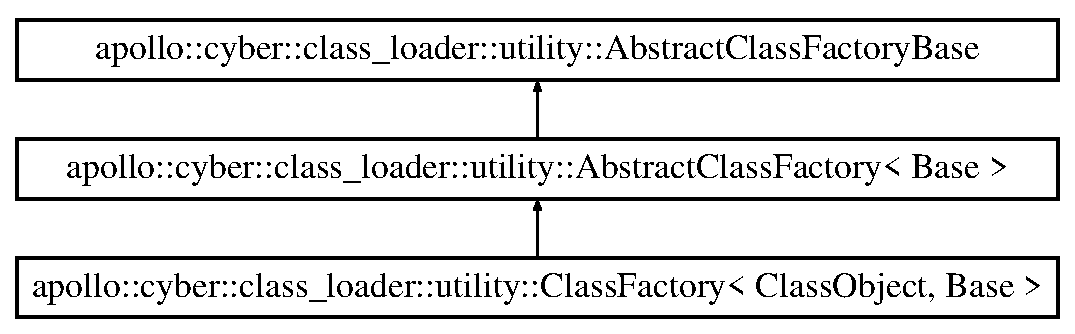
\includegraphics[height=3.000000cm]{classapollo_1_1cyber_1_1class__loader_1_1utility_1_1AbstractClassFactory}
\end{center}
\end{figure}
\subsection*{Public Member Functions}
\begin{DoxyCompactItemize}
\item 
\hyperlink{classapollo_1_1cyber_1_1class__loader_1_1utility_1_1AbstractClassFactory_ab0013ed740cae566717e534e16345ed0}{Abstract\-Class\-Factory} (const std\-::string \&class\-\_\-name, const std\-::string \&base\-\_\-class\-\_\-name)
\item 
virtual Base $\ast$ \hyperlink{classapollo_1_1cyber_1_1class__loader_1_1utility_1_1AbstractClassFactory_ae603a03f06c93b5f0475e63a0f2a9402}{Create\-Obj} () const =0
\end{DoxyCompactItemize}
\subsection*{Private Member Functions}
\begin{DoxyCompactItemize}
\item 
\hyperlink{classapollo_1_1cyber_1_1class__loader_1_1utility_1_1AbstractClassFactory_a85e48f47ba55628db5366e5d0ffa93d6}{Abstract\-Class\-Factory} ()
\item 
\hyperlink{classapollo_1_1cyber_1_1class__loader_1_1utility_1_1AbstractClassFactory_a78e77a1598aca2b898d1a6323bb785af}{Abstract\-Class\-Factory} (const \hyperlink{classapollo_1_1cyber_1_1class__loader_1_1utility_1_1AbstractClassFactory}{Abstract\-Class\-Factory} \&)
\item 
\hyperlink{classapollo_1_1cyber_1_1class__loader_1_1utility_1_1AbstractClassFactory}{Abstract\-Class\-Factory} \& \hyperlink{classapollo_1_1cyber_1_1class__loader_1_1utility_1_1AbstractClassFactory_a2e3f984f03050a8ddc9fb47664a6d109}{operator=} (const \hyperlink{classapollo_1_1cyber_1_1class__loader_1_1utility_1_1AbstractClassFactory}{Abstract\-Class\-Factory} \&)
\end{DoxyCompactItemize}
\subsection*{Additional Inherited Members}


\subsection{Constructor \& Destructor Documentation}
\hypertarget{classapollo_1_1cyber_1_1class__loader_1_1utility_1_1AbstractClassFactory_ab0013ed740cae566717e534e16345ed0}{\index{apollo\-::cyber\-::class\-\_\-loader\-::utility\-::\-Abstract\-Class\-Factory@{apollo\-::cyber\-::class\-\_\-loader\-::utility\-::\-Abstract\-Class\-Factory}!Abstract\-Class\-Factory@{Abstract\-Class\-Factory}}
\index{Abstract\-Class\-Factory@{Abstract\-Class\-Factory}!apollo::cyber::class_loader::utility::AbstractClassFactory@{apollo\-::cyber\-::class\-\_\-loader\-::utility\-::\-Abstract\-Class\-Factory}}
\subsubsection[{Abstract\-Class\-Factory}]{\setlength{\rightskip}{0pt plus 5cm}template$<$typename Base$>$ {\bf apollo\-::cyber\-::class\-\_\-loader\-::utility\-::\-Abstract\-Class\-Factory}$<$ Base $>$\-::{\bf Abstract\-Class\-Factory} (
\begin{DoxyParamCaption}
\item[{const std\-::string \&}]{class\-\_\-name, }
\item[{const std\-::string \&}]{base\-\_\-class\-\_\-name}
\end{DoxyParamCaption}
)\hspace{0.3cm}{\ttfamily [inline]}}}\label{classapollo_1_1cyber_1_1class__loader_1_1utility_1_1AbstractClassFactory_ab0013ed740cae566717e534e16345ed0}
\hypertarget{classapollo_1_1cyber_1_1class__loader_1_1utility_1_1AbstractClassFactory_a85e48f47ba55628db5366e5d0ffa93d6}{\index{apollo\-::cyber\-::class\-\_\-loader\-::utility\-::\-Abstract\-Class\-Factory@{apollo\-::cyber\-::class\-\_\-loader\-::utility\-::\-Abstract\-Class\-Factory}!Abstract\-Class\-Factory@{Abstract\-Class\-Factory}}
\index{Abstract\-Class\-Factory@{Abstract\-Class\-Factory}!apollo::cyber::class_loader::utility::AbstractClassFactory@{apollo\-::cyber\-::class\-\_\-loader\-::utility\-::\-Abstract\-Class\-Factory}}
\subsubsection[{Abstract\-Class\-Factory}]{\setlength{\rightskip}{0pt plus 5cm}template$<$typename Base$>$ {\bf apollo\-::cyber\-::class\-\_\-loader\-::utility\-::\-Abstract\-Class\-Factory}$<$ Base $>$\-::{\bf Abstract\-Class\-Factory} (
\begin{DoxyParamCaption}
{}
\end{DoxyParamCaption}
)\hspace{0.3cm}{\ttfamily [private]}}}\label{classapollo_1_1cyber_1_1class__loader_1_1utility_1_1AbstractClassFactory_a85e48f47ba55628db5366e5d0ffa93d6}
\hypertarget{classapollo_1_1cyber_1_1class__loader_1_1utility_1_1AbstractClassFactory_a78e77a1598aca2b898d1a6323bb785af}{\index{apollo\-::cyber\-::class\-\_\-loader\-::utility\-::\-Abstract\-Class\-Factory@{apollo\-::cyber\-::class\-\_\-loader\-::utility\-::\-Abstract\-Class\-Factory}!Abstract\-Class\-Factory@{Abstract\-Class\-Factory}}
\index{Abstract\-Class\-Factory@{Abstract\-Class\-Factory}!apollo::cyber::class_loader::utility::AbstractClassFactory@{apollo\-::cyber\-::class\-\_\-loader\-::utility\-::\-Abstract\-Class\-Factory}}
\subsubsection[{Abstract\-Class\-Factory}]{\setlength{\rightskip}{0pt plus 5cm}template$<$typename Base$>$ {\bf apollo\-::cyber\-::class\-\_\-loader\-::utility\-::\-Abstract\-Class\-Factory}$<$ Base $>$\-::{\bf Abstract\-Class\-Factory} (
\begin{DoxyParamCaption}
\item[{const {\bf Abstract\-Class\-Factory}$<$ Base $>$ \&}]{}
\end{DoxyParamCaption}
)\hspace{0.3cm}{\ttfamily [private]}}}\label{classapollo_1_1cyber_1_1class__loader_1_1utility_1_1AbstractClassFactory_a78e77a1598aca2b898d1a6323bb785af}


\subsection{Member Function Documentation}
\hypertarget{classapollo_1_1cyber_1_1class__loader_1_1utility_1_1AbstractClassFactory_ae603a03f06c93b5f0475e63a0f2a9402}{\index{apollo\-::cyber\-::class\-\_\-loader\-::utility\-::\-Abstract\-Class\-Factory@{apollo\-::cyber\-::class\-\_\-loader\-::utility\-::\-Abstract\-Class\-Factory}!Create\-Obj@{Create\-Obj}}
\index{Create\-Obj@{Create\-Obj}!apollo::cyber::class_loader::utility::AbstractClassFactory@{apollo\-::cyber\-::class\-\_\-loader\-::utility\-::\-Abstract\-Class\-Factory}}
\subsubsection[{Create\-Obj}]{\setlength{\rightskip}{0pt plus 5cm}template$<$typename Base$>$ virtual Base$\ast$ {\bf apollo\-::cyber\-::class\-\_\-loader\-::utility\-::\-Abstract\-Class\-Factory}$<$ Base $>$\-::Create\-Obj (
\begin{DoxyParamCaption}
{}
\end{DoxyParamCaption}
) const\hspace{0.3cm}{\ttfamily [pure virtual]}}}\label{classapollo_1_1cyber_1_1class__loader_1_1utility_1_1AbstractClassFactory_ae603a03f06c93b5f0475e63a0f2a9402}


Implemented in \hyperlink{classapollo_1_1cyber_1_1class__loader_1_1utility_1_1ClassFactory_afe170d362f95f097b72fa4de58ee06ca}{apollo\-::cyber\-::class\-\_\-loader\-::utility\-::\-Class\-Factory$<$ Class\-Object, Base $>$}.

\hypertarget{classapollo_1_1cyber_1_1class__loader_1_1utility_1_1AbstractClassFactory_a2e3f984f03050a8ddc9fb47664a6d109}{\index{apollo\-::cyber\-::class\-\_\-loader\-::utility\-::\-Abstract\-Class\-Factory@{apollo\-::cyber\-::class\-\_\-loader\-::utility\-::\-Abstract\-Class\-Factory}!operator=@{operator=}}
\index{operator=@{operator=}!apollo::cyber::class_loader::utility::AbstractClassFactory@{apollo\-::cyber\-::class\-\_\-loader\-::utility\-::\-Abstract\-Class\-Factory}}
\subsubsection[{operator=}]{\setlength{\rightskip}{0pt plus 5cm}template$<$typename Base$>$ {\bf Abstract\-Class\-Factory}\& {\bf apollo\-::cyber\-::class\-\_\-loader\-::utility\-::\-Abstract\-Class\-Factory}$<$ Base $>$\-::operator= (
\begin{DoxyParamCaption}
\item[{const {\bf Abstract\-Class\-Factory}$<$ Base $>$ \&}]{}
\end{DoxyParamCaption}
)\hspace{0.3cm}{\ttfamily [private]}}}\label{classapollo_1_1cyber_1_1class__loader_1_1utility_1_1AbstractClassFactory_a2e3f984f03050a8ddc9fb47664a6d109}


The documentation for this class was generated from the following file\-:\begin{DoxyCompactItemize}
\item 
class\-\_\-loader/utility/\hyperlink{class__factory_8h}{class\-\_\-factory.\-h}\end{DoxyCompactItemize}

\hypertarget{classapollo_1_1cyber_1_1class__loader_1_1utility_1_1AbstractClassFactoryBase}{\section{apollo\-:\-:cyber\-:\-:class\-\_\-loader\-:\-:utility\-:\-:Abstract\-Class\-Factory\-Base Class Reference}
\label{classapollo_1_1cyber_1_1class__loader_1_1utility_1_1AbstractClassFactoryBase}\index{apollo\-::cyber\-::class\-\_\-loader\-::utility\-::\-Abstract\-Class\-Factory\-Base@{apollo\-::cyber\-::class\-\_\-loader\-::utility\-::\-Abstract\-Class\-Factory\-Base}}
}


{\ttfamily \#include $<$class\-\_\-factory.\-h$>$}

Inheritance diagram for apollo\-:\-:cyber\-:\-:class\-\_\-loader\-:\-:utility\-:\-:Abstract\-Class\-Factory\-Base\-:\begin{figure}[H]
\begin{center}
\leavevmode
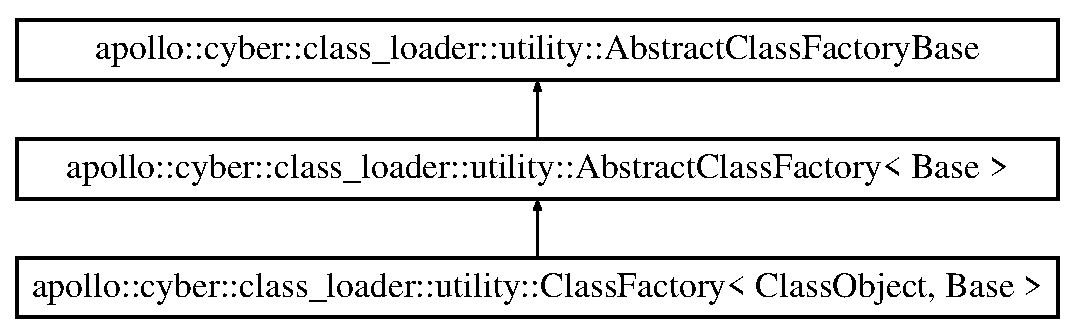
\includegraphics[height=3.000000cm]{classapollo_1_1cyber_1_1class__loader_1_1utility_1_1AbstractClassFactoryBase}
\end{center}
\end{figure}
\subsection*{Public Member Functions}
\begin{DoxyCompactItemize}
\item 
\hyperlink{classapollo_1_1cyber_1_1class__loader_1_1utility_1_1AbstractClassFactoryBase_ae205a32cbe37f7b8ca778ca405852aaf}{Abstract\-Class\-Factory\-Base} (const std\-::string \&class\-\_\-name, const std\-::string \&base\-\_\-class\-\_\-name)
\item 
virtual \hyperlink{classapollo_1_1cyber_1_1class__loader_1_1utility_1_1AbstractClassFactoryBase_a1a9e03fefa1d1911c8c2a92762044b54}{$\sim$\-Abstract\-Class\-Factory\-Base} ()
\item 
void \hyperlink{classapollo_1_1cyber_1_1class__loader_1_1utility_1_1AbstractClassFactoryBase_a55d911877a8e8586d93abbdd90329d6f}{Set\-Relative\-Library\-Path} (const std\-::string \&library\-\_\-path)
\item 
void \hyperlink{classapollo_1_1cyber_1_1class__loader_1_1utility_1_1AbstractClassFactoryBase_a72444d8d01b94d17b8b1782bb6073872}{Add\-Owned\-Class\-Loader} (\hyperlink{classapollo_1_1cyber_1_1class__loader_1_1ClassLoader}{Class\-Loader} $\ast$loader)
\item 
void \hyperlink{classapollo_1_1cyber_1_1class__loader_1_1utility_1_1AbstractClassFactoryBase_aa57fd78d52ebc1f9fb1214498c0be2e7}{Remove\-Owned\-Class\-Loader} (const \hyperlink{classapollo_1_1cyber_1_1class__loader_1_1ClassLoader}{Class\-Loader} $\ast$loader)
\item 
bool \hyperlink{classapollo_1_1cyber_1_1class__loader_1_1utility_1_1AbstractClassFactoryBase_ae1471153574b83c4f4205c6ad55174c6}{Is\-Owned\-By} (const \hyperlink{classapollo_1_1cyber_1_1class__loader_1_1ClassLoader}{Class\-Loader} $\ast$loader)
\item 
bool \hyperlink{classapollo_1_1cyber_1_1class__loader_1_1utility_1_1AbstractClassFactoryBase_a6212125ab8292eee20a0bd58d4a0ba1d}{Is\-Owned\-By\-Anybody} ()
\item 
std\-::vector$<$ \hyperlink{classapollo_1_1cyber_1_1class__loader_1_1ClassLoader}{Class\-Loader} $\ast$ $>$ \hyperlink{classapollo_1_1cyber_1_1class__loader_1_1utility_1_1AbstractClassFactoryBase_a287a1480163fa6254148eb74947292be}{Get\-Relative\-Class\-Loaders} ()
\item 
const std\-::string \hyperlink{classapollo_1_1cyber_1_1class__loader_1_1utility_1_1AbstractClassFactoryBase_ac538fd1b4f313d2a47c6748b983d04ea}{Get\-Relative\-Library\-Path} () const 
\item 
const std\-::string \hyperlink{classapollo_1_1cyber_1_1class__loader_1_1utility_1_1AbstractClassFactoryBase_a47971dd0e73299250ea338dc927b3e90}{Get\-Base\-Class\-Name} () const 
\item 
const std\-::string \hyperlink{classapollo_1_1cyber_1_1class__loader_1_1utility_1_1AbstractClassFactoryBase_a4033b25aebc159a72555e5079d09a5cf}{Get\-Class\-Name} () const 
\end{DoxyCompactItemize}
\subsection*{Protected Attributes}
\begin{DoxyCompactItemize}
\item 
std\-::vector$<$ \hyperlink{classapollo_1_1cyber_1_1class__loader_1_1ClassLoader}{Class\-Loader} $\ast$ $>$ \hyperlink{classapollo_1_1cyber_1_1class__loader_1_1utility_1_1AbstractClassFactoryBase_a799a4b8522bd2ea3a18a93f609fb11e3}{relative\-\_\-class\-\_\-loaders\-\_\-}
\item 
std\-::string \hyperlink{classapollo_1_1cyber_1_1class__loader_1_1utility_1_1AbstractClassFactoryBase_a1c2cc5e713ea276459d1e9d6a64f706c}{relative\-\_\-library\-\_\-path\-\_\-}
\item 
std\-::string \hyperlink{classapollo_1_1cyber_1_1class__loader_1_1utility_1_1AbstractClassFactoryBase_a88a382cea8c075811b0415d3d30d1c8f}{base\-\_\-class\-\_\-name\-\_\-}
\item 
std\-::string \hyperlink{classapollo_1_1cyber_1_1class__loader_1_1utility_1_1AbstractClassFactoryBase_adcbcb8ef76b8b1275daa473685335864}{class\-\_\-name\-\_\-}
\end{DoxyCompactItemize}


\subsection{Constructor \& Destructor Documentation}
\hypertarget{classapollo_1_1cyber_1_1class__loader_1_1utility_1_1AbstractClassFactoryBase_ae205a32cbe37f7b8ca778ca405852aaf}{\index{apollo\-::cyber\-::class\-\_\-loader\-::utility\-::\-Abstract\-Class\-Factory\-Base@{apollo\-::cyber\-::class\-\_\-loader\-::utility\-::\-Abstract\-Class\-Factory\-Base}!Abstract\-Class\-Factory\-Base@{Abstract\-Class\-Factory\-Base}}
\index{Abstract\-Class\-Factory\-Base@{Abstract\-Class\-Factory\-Base}!apollo::cyber::class_loader::utility::AbstractClassFactoryBase@{apollo\-::cyber\-::class\-\_\-loader\-::utility\-::\-Abstract\-Class\-Factory\-Base}}
\subsubsection[{Abstract\-Class\-Factory\-Base}]{\setlength{\rightskip}{0pt plus 5cm}apollo\-::cyber\-::class\-\_\-loader\-::utility\-::\-Abstract\-Class\-Factory\-Base\-::\-Abstract\-Class\-Factory\-Base (
\begin{DoxyParamCaption}
\item[{const std\-::string \&}]{class\-\_\-name, }
\item[{const std\-::string \&}]{base\-\_\-class\-\_\-name}
\end{DoxyParamCaption}
)}}\label{classapollo_1_1cyber_1_1class__loader_1_1utility_1_1AbstractClassFactoryBase_ae205a32cbe37f7b8ca778ca405852aaf}
\hypertarget{classapollo_1_1cyber_1_1class__loader_1_1utility_1_1AbstractClassFactoryBase_a1a9e03fefa1d1911c8c2a92762044b54}{\index{apollo\-::cyber\-::class\-\_\-loader\-::utility\-::\-Abstract\-Class\-Factory\-Base@{apollo\-::cyber\-::class\-\_\-loader\-::utility\-::\-Abstract\-Class\-Factory\-Base}!$\sim$\-Abstract\-Class\-Factory\-Base@{$\sim$\-Abstract\-Class\-Factory\-Base}}
\index{$\sim$\-Abstract\-Class\-Factory\-Base@{$\sim$\-Abstract\-Class\-Factory\-Base}!apollo::cyber::class_loader::utility::AbstractClassFactoryBase@{apollo\-::cyber\-::class\-\_\-loader\-::utility\-::\-Abstract\-Class\-Factory\-Base}}
\subsubsection[{$\sim$\-Abstract\-Class\-Factory\-Base}]{\setlength{\rightskip}{0pt plus 5cm}virtual apollo\-::cyber\-::class\-\_\-loader\-::utility\-::\-Abstract\-Class\-Factory\-Base\-::$\sim$\-Abstract\-Class\-Factory\-Base (
\begin{DoxyParamCaption}
{}
\end{DoxyParamCaption}
)\hspace{0.3cm}{\ttfamily [virtual]}}}\label{classapollo_1_1cyber_1_1class__loader_1_1utility_1_1AbstractClassFactoryBase_a1a9e03fefa1d1911c8c2a92762044b54}


\subsection{Member Function Documentation}
\hypertarget{classapollo_1_1cyber_1_1class__loader_1_1utility_1_1AbstractClassFactoryBase_a72444d8d01b94d17b8b1782bb6073872}{\index{apollo\-::cyber\-::class\-\_\-loader\-::utility\-::\-Abstract\-Class\-Factory\-Base@{apollo\-::cyber\-::class\-\_\-loader\-::utility\-::\-Abstract\-Class\-Factory\-Base}!Add\-Owned\-Class\-Loader@{Add\-Owned\-Class\-Loader}}
\index{Add\-Owned\-Class\-Loader@{Add\-Owned\-Class\-Loader}!apollo::cyber::class_loader::utility::AbstractClassFactoryBase@{apollo\-::cyber\-::class\-\_\-loader\-::utility\-::\-Abstract\-Class\-Factory\-Base}}
\subsubsection[{Add\-Owned\-Class\-Loader}]{\setlength{\rightskip}{0pt plus 5cm}void apollo\-::cyber\-::class\-\_\-loader\-::utility\-::\-Abstract\-Class\-Factory\-Base\-::\-Add\-Owned\-Class\-Loader (
\begin{DoxyParamCaption}
\item[{{\bf Class\-Loader} $\ast$}]{loader}
\end{DoxyParamCaption}
)}}\label{classapollo_1_1cyber_1_1class__loader_1_1utility_1_1AbstractClassFactoryBase_a72444d8d01b94d17b8b1782bb6073872}
\hypertarget{classapollo_1_1cyber_1_1class__loader_1_1utility_1_1AbstractClassFactoryBase_a47971dd0e73299250ea338dc927b3e90}{\index{apollo\-::cyber\-::class\-\_\-loader\-::utility\-::\-Abstract\-Class\-Factory\-Base@{apollo\-::cyber\-::class\-\_\-loader\-::utility\-::\-Abstract\-Class\-Factory\-Base}!Get\-Base\-Class\-Name@{Get\-Base\-Class\-Name}}
\index{Get\-Base\-Class\-Name@{Get\-Base\-Class\-Name}!apollo::cyber::class_loader::utility::AbstractClassFactoryBase@{apollo\-::cyber\-::class\-\_\-loader\-::utility\-::\-Abstract\-Class\-Factory\-Base}}
\subsubsection[{Get\-Base\-Class\-Name}]{\setlength{\rightskip}{0pt plus 5cm}const std\-::string apollo\-::cyber\-::class\-\_\-loader\-::utility\-::\-Abstract\-Class\-Factory\-Base\-::\-Get\-Base\-Class\-Name (
\begin{DoxyParamCaption}
{}
\end{DoxyParamCaption}
) const}}\label{classapollo_1_1cyber_1_1class__loader_1_1utility_1_1AbstractClassFactoryBase_a47971dd0e73299250ea338dc927b3e90}
\hypertarget{classapollo_1_1cyber_1_1class__loader_1_1utility_1_1AbstractClassFactoryBase_a4033b25aebc159a72555e5079d09a5cf}{\index{apollo\-::cyber\-::class\-\_\-loader\-::utility\-::\-Abstract\-Class\-Factory\-Base@{apollo\-::cyber\-::class\-\_\-loader\-::utility\-::\-Abstract\-Class\-Factory\-Base}!Get\-Class\-Name@{Get\-Class\-Name}}
\index{Get\-Class\-Name@{Get\-Class\-Name}!apollo::cyber::class_loader::utility::AbstractClassFactoryBase@{apollo\-::cyber\-::class\-\_\-loader\-::utility\-::\-Abstract\-Class\-Factory\-Base}}
\subsubsection[{Get\-Class\-Name}]{\setlength{\rightskip}{0pt plus 5cm}const std\-::string apollo\-::cyber\-::class\-\_\-loader\-::utility\-::\-Abstract\-Class\-Factory\-Base\-::\-Get\-Class\-Name (
\begin{DoxyParamCaption}
{}
\end{DoxyParamCaption}
) const}}\label{classapollo_1_1cyber_1_1class__loader_1_1utility_1_1AbstractClassFactoryBase_a4033b25aebc159a72555e5079d09a5cf}
\hypertarget{classapollo_1_1cyber_1_1class__loader_1_1utility_1_1AbstractClassFactoryBase_a287a1480163fa6254148eb74947292be}{\index{apollo\-::cyber\-::class\-\_\-loader\-::utility\-::\-Abstract\-Class\-Factory\-Base@{apollo\-::cyber\-::class\-\_\-loader\-::utility\-::\-Abstract\-Class\-Factory\-Base}!Get\-Relative\-Class\-Loaders@{Get\-Relative\-Class\-Loaders}}
\index{Get\-Relative\-Class\-Loaders@{Get\-Relative\-Class\-Loaders}!apollo::cyber::class_loader::utility::AbstractClassFactoryBase@{apollo\-::cyber\-::class\-\_\-loader\-::utility\-::\-Abstract\-Class\-Factory\-Base}}
\subsubsection[{Get\-Relative\-Class\-Loaders}]{\setlength{\rightskip}{0pt plus 5cm}std\-::vector$<${\bf Class\-Loader}$\ast$$>$ apollo\-::cyber\-::class\-\_\-loader\-::utility\-::\-Abstract\-Class\-Factory\-Base\-::\-Get\-Relative\-Class\-Loaders (
\begin{DoxyParamCaption}
{}
\end{DoxyParamCaption}
)}}\label{classapollo_1_1cyber_1_1class__loader_1_1utility_1_1AbstractClassFactoryBase_a287a1480163fa6254148eb74947292be}
\hypertarget{classapollo_1_1cyber_1_1class__loader_1_1utility_1_1AbstractClassFactoryBase_ac538fd1b4f313d2a47c6748b983d04ea}{\index{apollo\-::cyber\-::class\-\_\-loader\-::utility\-::\-Abstract\-Class\-Factory\-Base@{apollo\-::cyber\-::class\-\_\-loader\-::utility\-::\-Abstract\-Class\-Factory\-Base}!Get\-Relative\-Library\-Path@{Get\-Relative\-Library\-Path}}
\index{Get\-Relative\-Library\-Path@{Get\-Relative\-Library\-Path}!apollo::cyber::class_loader::utility::AbstractClassFactoryBase@{apollo\-::cyber\-::class\-\_\-loader\-::utility\-::\-Abstract\-Class\-Factory\-Base}}
\subsubsection[{Get\-Relative\-Library\-Path}]{\setlength{\rightskip}{0pt plus 5cm}const std\-::string apollo\-::cyber\-::class\-\_\-loader\-::utility\-::\-Abstract\-Class\-Factory\-Base\-::\-Get\-Relative\-Library\-Path (
\begin{DoxyParamCaption}
{}
\end{DoxyParamCaption}
) const}}\label{classapollo_1_1cyber_1_1class__loader_1_1utility_1_1AbstractClassFactoryBase_ac538fd1b4f313d2a47c6748b983d04ea}
\hypertarget{classapollo_1_1cyber_1_1class__loader_1_1utility_1_1AbstractClassFactoryBase_ae1471153574b83c4f4205c6ad55174c6}{\index{apollo\-::cyber\-::class\-\_\-loader\-::utility\-::\-Abstract\-Class\-Factory\-Base@{apollo\-::cyber\-::class\-\_\-loader\-::utility\-::\-Abstract\-Class\-Factory\-Base}!Is\-Owned\-By@{Is\-Owned\-By}}
\index{Is\-Owned\-By@{Is\-Owned\-By}!apollo::cyber::class_loader::utility::AbstractClassFactoryBase@{apollo\-::cyber\-::class\-\_\-loader\-::utility\-::\-Abstract\-Class\-Factory\-Base}}
\subsubsection[{Is\-Owned\-By}]{\setlength{\rightskip}{0pt plus 5cm}bool apollo\-::cyber\-::class\-\_\-loader\-::utility\-::\-Abstract\-Class\-Factory\-Base\-::\-Is\-Owned\-By (
\begin{DoxyParamCaption}
\item[{const {\bf Class\-Loader} $\ast$}]{loader}
\end{DoxyParamCaption}
)}}\label{classapollo_1_1cyber_1_1class__loader_1_1utility_1_1AbstractClassFactoryBase_ae1471153574b83c4f4205c6ad55174c6}
\hypertarget{classapollo_1_1cyber_1_1class__loader_1_1utility_1_1AbstractClassFactoryBase_a6212125ab8292eee20a0bd58d4a0ba1d}{\index{apollo\-::cyber\-::class\-\_\-loader\-::utility\-::\-Abstract\-Class\-Factory\-Base@{apollo\-::cyber\-::class\-\_\-loader\-::utility\-::\-Abstract\-Class\-Factory\-Base}!Is\-Owned\-By\-Anybody@{Is\-Owned\-By\-Anybody}}
\index{Is\-Owned\-By\-Anybody@{Is\-Owned\-By\-Anybody}!apollo::cyber::class_loader::utility::AbstractClassFactoryBase@{apollo\-::cyber\-::class\-\_\-loader\-::utility\-::\-Abstract\-Class\-Factory\-Base}}
\subsubsection[{Is\-Owned\-By\-Anybody}]{\setlength{\rightskip}{0pt plus 5cm}bool apollo\-::cyber\-::class\-\_\-loader\-::utility\-::\-Abstract\-Class\-Factory\-Base\-::\-Is\-Owned\-By\-Anybody (
\begin{DoxyParamCaption}
{}
\end{DoxyParamCaption}
)}}\label{classapollo_1_1cyber_1_1class__loader_1_1utility_1_1AbstractClassFactoryBase_a6212125ab8292eee20a0bd58d4a0ba1d}
\hypertarget{classapollo_1_1cyber_1_1class__loader_1_1utility_1_1AbstractClassFactoryBase_aa57fd78d52ebc1f9fb1214498c0be2e7}{\index{apollo\-::cyber\-::class\-\_\-loader\-::utility\-::\-Abstract\-Class\-Factory\-Base@{apollo\-::cyber\-::class\-\_\-loader\-::utility\-::\-Abstract\-Class\-Factory\-Base}!Remove\-Owned\-Class\-Loader@{Remove\-Owned\-Class\-Loader}}
\index{Remove\-Owned\-Class\-Loader@{Remove\-Owned\-Class\-Loader}!apollo::cyber::class_loader::utility::AbstractClassFactoryBase@{apollo\-::cyber\-::class\-\_\-loader\-::utility\-::\-Abstract\-Class\-Factory\-Base}}
\subsubsection[{Remove\-Owned\-Class\-Loader}]{\setlength{\rightskip}{0pt plus 5cm}void apollo\-::cyber\-::class\-\_\-loader\-::utility\-::\-Abstract\-Class\-Factory\-Base\-::\-Remove\-Owned\-Class\-Loader (
\begin{DoxyParamCaption}
\item[{const {\bf Class\-Loader} $\ast$}]{loader}
\end{DoxyParamCaption}
)}}\label{classapollo_1_1cyber_1_1class__loader_1_1utility_1_1AbstractClassFactoryBase_aa57fd78d52ebc1f9fb1214498c0be2e7}
\hypertarget{classapollo_1_1cyber_1_1class__loader_1_1utility_1_1AbstractClassFactoryBase_a55d911877a8e8586d93abbdd90329d6f}{\index{apollo\-::cyber\-::class\-\_\-loader\-::utility\-::\-Abstract\-Class\-Factory\-Base@{apollo\-::cyber\-::class\-\_\-loader\-::utility\-::\-Abstract\-Class\-Factory\-Base}!Set\-Relative\-Library\-Path@{Set\-Relative\-Library\-Path}}
\index{Set\-Relative\-Library\-Path@{Set\-Relative\-Library\-Path}!apollo::cyber::class_loader::utility::AbstractClassFactoryBase@{apollo\-::cyber\-::class\-\_\-loader\-::utility\-::\-Abstract\-Class\-Factory\-Base}}
\subsubsection[{Set\-Relative\-Library\-Path}]{\setlength{\rightskip}{0pt plus 5cm}void apollo\-::cyber\-::class\-\_\-loader\-::utility\-::\-Abstract\-Class\-Factory\-Base\-::\-Set\-Relative\-Library\-Path (
\begin{DoxyParamCaption}
\item[{const std\-::string \&}]{library\-\_\-path}
\end{DoxyParamCaption}
)}}\label{classapollo_1_1cyber_1_1class__loader_1_1utility_1_1AbstractClassFactoryBase_a55d911877a8e8586d93abbdd90329d6f}


\subsection{Member Data Documentation}
\hypertarget{classapollo_1_1cyber_1_1class__loader_1_1utility_1_1AbstractClassFactoryBase_a88a382cea8c075811b0415d3d30d1c8f}{\index{apollo\-::cyber\-::class\-\_\-loader\-::utility\-::\-Abstract\-Class\-Factory\-Base@{apollo\-::cyber\-::class\-\_\-loader\-::utility\-::\-Abstract\-Class\-Factory\-Base}!base\-\_\-class\-\_\-name\-\_\-@{base\-\_\-class\-\_\-name\-\_\-}}
\index{base\-\_\-class\-\_\-name\-\_\-@{base\-\_\-class\-\_\-name\-\_\-}!apollo::cyber::class_loader::utility::AbstractClassFactoryBase@{apollo\-::cyber\-::class\-\_\-loader\-::utility\-::\-Abstract\-Class\-Factory\-Base}}
\subsubsection[{base\-\_\-class\-\_\-name\-\_\-}]{\setlength{\rightskip}{0pt plus 5cm}std\-::string apollo\-::cyber\-::class\-\_\-loader\-::utility\-::\-Abstract\-Class\-Factory\-Base\-::base\-\_\-class\-\_\-name\-\_\-\hspace{0.3cm}{\ttfamily [protected]}}}\label{classapollo_1_1cyber_1_1class__loader_1_1utility_1_1AbstractClassFactoryBase_a88a382cea8c075811b0415d3d30d1c8f}
\hypertarget{classapollo_1_1cyber_1_1class__loader_1_1utility_1_1AbstractClassFactoryBase_adcbcb8ef76b8b1275daa473685335864}{\index{apollo\-::cyber\-::class\-\_\-loader\-::utility\-::\-Abstract\-Class\-Factory\-Base@{apollo\-::cyber\-::class\-\_\-loader\-::utility\-::\-Abstract\-Class\-Factory\-Base}!class\-\_\-name\-\_\-@{class\-\_\-name\-\_\-}}
\index{class\-\_\-name\-\_\-@{class\-\_\-name\-\_\-}!apollo::cyber::class_loader::utility::AbstractClassFactoryBase@{apollo\-::cyber\-::class\-\_\-loader\-::utility\-::\-Abstract\-Class\-Factory\-Base}}
\subsubsection[{class\-\_\-name\-\_\-}]{\setlength{\rightskip}{0pt plus 5cm}std\-::string apollo\-::cyber\-::class\-\_\-loader\-::utility\-::\-Abstract\-Class\-Factory\-Base\-::class\-\_\-name\-\_\-\hspace{0.3cm}{\ttfamily [protected]}}}\label{classapollo_1_1cyber_1_1class__loader_1_1utility_1_1AbstractClassFactoryBase_adcbcb8ef76b8b1275daa473685335864}
\hypertarget{classapollo_1_1cyber_1_1class__loader_1_1utility_1_1AbstractClassFactoryBase_a799a4b8522bd2ea3a18a93f609fb11e3}{\index{apollo\-::cyber\-::class\-\_\-loader\-::utility\-::\-Abstract\-Class\-Factory\-Base@{apollo\-::cyber\-::class\-\_\-loader\-::utility\-::\-Abstract\-Class\-Factory\-Base}!relative\-\_\-class\-\_\-loaders\-\_\-@{relative\-\_\-class\-\_\-loaders\-\_\-}}
\index{relative\-\_\-class\-\_\-loaders\-\_\-@{relative\-\_\-class\-\_\-loaders\-\_\-}!apollo::cyber::class_loader::utility::AbstractClassFactoryBase@{apollo\-::cyber\-::class\-\_\-loader\-::utility\-::\-Abstract\-Class\-Factory\-Base}}
\subsubsection[{relative\-\_\-class\-\_\-loaders\-\_\-}]{\setlength{\rightskip}{0pt plus 5cm}std\-::vector$<${\bf Class\-Loader}$\ast$$>$ apollo\-::cyber\-::class\-\_\-loader\-::utility\-::\-Abstract\-Class\-Factory\-Base\-::relative\-\_\-class\-\_\-loaders\-\_\-\hspace{0.3cm}{\ttfamily [protected]}}}\label{classapollo_1_1cyber_1_1class__loader_1_1utility_1_1AbstractClassFactoryBase_a799a4b8522bd2ea3a18a93f609fb11e3}
\hypertarget{classapollo_1_1cyber_1_1class__loader_1_1utility_1_1AbstractClassFactoryBase_a1c2cc5e713ea276459d1e9d6a64f706c}{\index{apollo\-::cyber\-::class\-\_\-loader\-::utility\-::\-Abstract\-Class\-Factory\-Base@{apollo\-::cyber\-::class\-\_\-loader\-::utility\-::\-Abstract\-Class\-Factory\-Base}!relative\-\_\-library\-\_\-path\-\_\-@{relative\-\_\-library\-\_\-path\-\_\-}}
\index{relative\-\_\-library\-\_\-path\-\_\-@{relative\-\_\-library\-\_\-path\-\_\-}!apollo::cyber::class_loader::utility::AbstractClassFactoryBase@{apollo\-::cyber\-::class\-\_\-loader\-::utility\-::\-Abstract\-Class\-Factory\-Base}}
\subsubsection[{relative\-\_\-library\-\_\-path\-\_\-}]{\setlength{\rightskip}{0pt plus 5cm}std\-::string apollo\-::cyber\-::class\-\_\-loader\-::utility\-::\-Abstract\-Class\-Factory\-Base\-::relative\-\_\-library\-\_\-path\-\_\-\hspace{0.3cm}{\ttfamily [protected]}}}\label{classapollo_1_1cyber_1_1class__loader_1_1utility_1_1AbstractClassFactoryBase_a1c2cc5e713ea276459d1e9d6a64f706c}


The documentation for this class was generated from the following file\-:\begin{DoxyCompactItemize}
\item 
class\-\_\-loader/utility/\hyperlink{class__factory_8h}{class\-\_\-factory.\-h}\end{DoxyCompactItemize}

\hypertarget{classapollo_1_1cyber_1_1data_1_1fusion_1_1AllLatest}{\section{apollo\-:\-:cyber\-:\-:data\-:\-:fusion\-:\-:All\-Latest$<$ M0, M1, M2, M3 $>$ Class Template Reference}
\label{classapollo_1_1cyber_1_1data_1_1fusion_1_1AllLatest}\index{apollo\-::cyber\-::data\-::fusion\-::\-All\-Latest$<$ M0, M1, M2, M3 $>$@{apollo\-::cyber\-::data\-::fusion\-::\-All\-Latest$<$ M0, M1, M2, M3 $>$}}
}


{\ttfamily \#include $<$all\-\_\-latest.\-h$>$}

Inheritance diagram for apollo\-:\-:cyber\-:\-:data\-:\-:fusion\-:\-:All\-Latest$<$ M0, M1, M2, M3 $>$\-:\begin{figure}[H]
\begin{center}
\leavevmode
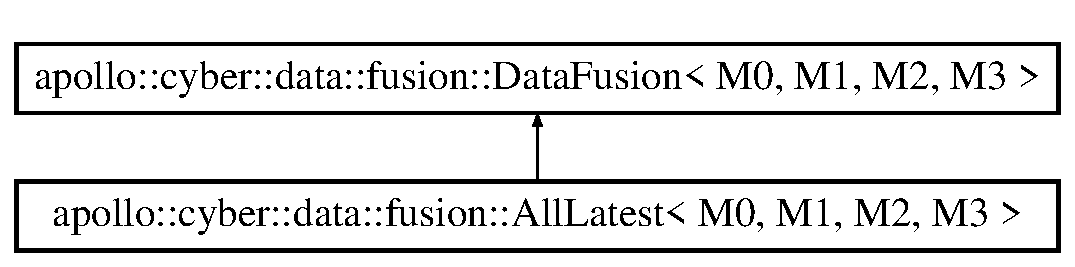
\includegraphics[height=2.000000cm]{classapollo_1_1cyber_1_1data_1_1fusion_1_1AllLatest}
\end{center}
\end{figure}
\subsection*{Public Member Functions}
\begin{DoxyCompactItemize}
\item 
\hyperlink{classapollo_1_1cyber_1_1data_1_1fusion_1_1AllLatest_ad33d846e93021bdebbfea75dca4c7308}{All\-Latest} (const \hyperlink{classapollo_1_1cyber_1_1data_1_1ChannelBuffer}{Channel\-Buffer}$<$ M0 $>$ \&buffer\-\_\-0, const \hyperlink{classapollo_1_1cyber_1_1data_1_1ChannelBuffer}{Channel\-Buffer}$<$ M1 $>$ \&buffer\-\_\-1, const \hyperlink{classapollo_1_1cyber_1_1data_1_1ChannelBuffer}{Channel\-Buffer}$<$ M2 $>$ \&buffer\-\_\-2, const \hyperlink{classapollo_1_1cyber_1_1data_1_1ChannelBuffer}{Channel\-Buffer}$<$ M3 $>$ \&buffer\-\_\-3)
\item 
bool \hyperlink{classapollo_1_1cyber_1_1data_1_1fusion_1_1AllLatest_a44540e0552d2d451372e9f591ad0e3a0}{Fusion} (uint64\-\_\-t $\ast$index, std\-::shared\-\_\-ptr$<$ M0 $>$ \&m0, std\-::shared\-\_\-ptr$<$ M1 $>$ \&m1, std\-::shared\-\_\-ptr$<$ M2 $>$ \&m2, std\-::shared\-\_\-ptr$<$ M3 $>$ \&m3) override
\end{DoxyCompactItemize}
\subsection*{Private Attributes}
\begin{DoxyCompactItemize}
\item 
\hyperlink{classapollo_1_1cyber_1_1data_1_1ChannelBuffer}{Channel\-Buffer}$<$ M0 $>$ \hyperlink{classapollo_1_1cyber_1_1data_1_1fusion_1_1AllLatest_a55f4ad5862771d69f0c15c6fbef8bf48}{buffer\-\_\-m0\-\_\-}
\item 
\hyperlink{classapollo_1_1cyber_1_1data_1_1ChannelBuffer}{Channel\-Buffer}$<$ M1 $>$ \hyperlink{classapollo_1_1cyber_1_1data_1_1fusion_1_1AllLatest_ac74a96b814c80ecdd431a18c60ff5af9}{buffer\-\_\-m1\-\_\-}
\item 
\hyperlink{classapollo_1_1cyber_1_1data_1_1ChannelBuffer}{Channel\-Buffer}$<$ M2 $>$ \hyperlink{classapollo_1_1cyber_1_1data_1_1fusion_1_1AllLatest_aa7a73968cc0be58137c8f5f5125d9ffd}{buffer\-\_\-m2\-\_\-}
\item 
\hyperlink{classapollo_1_1cyber_1_1data_1_1ChannelBuffer}{Channel\-Buffer}$<$ M3 $>$ \hyperlink{classapollo_1_1cyber_1_1data_1_1fusion_1_1AllLatest_a3e12a49b61212793f208880c19ed7819}{buffer\-\_\-m3\-\_\-}
\end{DoxyCompactItemize}


\subsection{Constructor \& Destructor Documentation}
\hypertarget{classapollo_1_1cyber_1_1data_1_1fusion_1_1AllLatest_ad33d846e93021bdebbfea75dca4c7308}{\index{apollo\-::cyber\-::data\-::fusion\-::\-All\-Latest@{apollo\-::cyber\-::data\-::fusion\-::\-All\-Latest}!All\-Latest@{All\-Latest}}
\index{All\-Latest@{All\-Latest}!apollo::cyber::data::fusion::AllLatest@{apollo\-::cyber\-::data\-::fusion\-::\-All\-Latest}}
\subsubsection[{All\-Latest}]{\setlength{\rightskip}{0pt plus 5cm}template$<$typename M0, typename M1 = Null\-Type, typename M2 = Null\-Type, typename M3 = Null\-Type$>$ {\bf apollo\-::cyber\-::data\-::fusion\-::\-All\-Latest}$<$ M0, M1, M2, M3 $>$\-::{\bf All\-Latest} (
\begin{DoxyParamCaption}
\item[{const {\bf Channel\-Buffer}$<$ M0 $>$ \&}]{buffer\-\_\-0, }
\item[{const {\bf Channel\-Buffer}$<$ M1 $>$ \&}]{buffer\-\_\-1, }
\item[{const {\bf Channel\-Buffer}$<$ M2 $>$ \&}]{buffer\-\_\-2, }
\item[{const {\bf Channel\-Buffer}$<$ M3 $>$ \&}]{buffer\-\_\-3}
\end{DoxyParamCaption}
)\hspace{0.3cm}{\ttfamily [inline]}}}\label{classapollo_1_1cyber_1_1data_1_1fusion_1_1AllLatest_ad33d846e93021bdebbfea75dca4c7308}


\subsection{Member Function Documentation}
\hypertarget{classapollo_1_1cyber_1_1data_1_1fusion_1_1AllLatest_a44540e0552d2d451372e9f591ad0e3a0}{\index{apollo\-::cyber\-::data\-::fusion\-::\-All\-Latest@{apollo\-::cyber\-::data\-::fusion\-::\-All\-Latest}!Fusion@{Fusion}}
\index{Fusion@{Fusion}!apollo::cyber::data::fusion::AllLatest@{apollo\-::cyber\-::data\-::fusion\-::\-All\-Latest}}
\subsubsection[{Fusion}]{\setlength{\rightskip}{0pt plus 5cm}template$<$typename M0, typename M1 = Null\-Type, typename M2 = Null\-Type, typename M3 = Null\-Type$>$ bool {\bf apollo\-::cyber\-::data\-::fusion\-::\-All\-Latest}$<$ M0, M1, M2, M3 $>$\-::Fusion (
\begin{DoxyParamCaption}
\item[{uint64\-\_\-t $\ast$}]{index, }
\item[{std\-::shared\-\_\-ptr$<$ M0 $>$ \&}]{m0, }
\item[{std\-::shared\-\_\-ptr$<$ M1 $>$ \&}]{m1, }
\item[{std\-::shared\-\_\-ptr$<$ M2 $>$ \&}]{m2, }
\item[{std\-::shared\-\_\-ptr$<$ M3 $>$ \&}]{m3}
\end{DoxyParamCaption}
)\hspace{0.3cm}{\ttfamily [inline]}, {\ttfamily [override]}, {\ttfamily [virtual]}}}\label{classapollo_1_1cyber_1_1data_1_1fusion_1_1AllLatest_a44540e0552d2d451372e9f591ad0e3a0}


Implements \hyperlink{classapollo_1_1cyber_1_1data_1_1fusion_1_1DataFusion_af992dd51063725886f3dce401ae08cbf}{apollo\-::cyber\-::data\-::fusion\-::\-Data\-Fusion$<$ M0, M1, M2, M3 $>$}.



\subsection{Member Data Documentation}
\hypertarget{classapollo_1_1cyber_1_1data_1_1fusion_1_1AllLatest_a55f4ad5862771d69f0c15c6fbef8bf48}{\index{apollo\-::cyber\-::data\-::fusion\-::\-All\-Latest@{apollo\-::cyber\-::data\-::fusion\-::\-All\-Latest}!buffer\-\_\-m0\-\_\-@{buffer\-\_\-m0\-\_\-}}
\index{buffer\-\_\-m0\-\_\-@{buffer\-\_\-m0\-\_\-}!apollo::cyber::data::fusion::AllLatest@{apollo\-::cyber\-::data\-::fusion\-::\-All\-Latest}}
\subsubsection[{buffer\-\_\-m0\-\_\-}]{\setlength{\rightskip}{0pt plus 5cm}template$<$typename M0, typename M1 = Null\-Type, typename M2 = Null\-Type, typename M3 = Null\-Type$>$ {\bf Channel\-Buffer}$<$M0$>$ {\bf apollo\-::cyber\-::data\-::fusion\-::\-All\-Latest}$<$ M0, M1, M2, M3 $>$\-::buffer\-\_\-m0\-\_\-\hspace{0.3cm}{\ttfamily [private]}}}\label{classapollo_1_1cyber_1_1data_1_1fusion_1_1AllLatest_a55f4ad5862771d69f0c15c6fbef8bf48}
\hypertarget{classapollo_1_1cyber_1_1data_1_1fusion_1_1AllLatest_ac74a96b814c80ecdd431a18c60ff5af9}{\index{apollo\-::cyber\-::data\-::fusion\-::\-All\-Latest@{apollo\-::cyber\-::data\-::fusion\-::\-All\-Latest}!buffer\-\_\-m1\-\_\-@{buffer\-\_\-m1\-\_\-}}
\index{buffer\-\_\-m1\-\_\-@{buffer\-\_\-m1\-\_\-}!apollo::cyber::data::fusion::AllLatest@{apollo\-::cyber\-::data\-::fusion\-::\-All\-Latest}}
\subsubsection[{buffer\-\_\-m1\-\_\-}]{\setlength{\rightskip}{0pt plus 5cm}template$<$typename M0, typename M1 = Null\-Type, typename M2 = Null\-Type, typename M3 = Null\-Type$>$ {\bf Channel\-Buffer}$<$M1$>$ {\bf apollo\-::cyber\-::data\-::fusion\-::\-All\-Latest}$<$ M0, M1, M2, M3 $>$\-::buffer\-\_\-m1\-\_\-\hspace{0.3cm}{\ttfamily [private]}}}\label{classapollo_1_1cyber_1_1data_1_1fusion_1_1AllLatest_ac74a96b814c80ecdd431a18c60ff5af9}
\hypertarget{classapollo_1_1cyber_1_1data_1_1fusion_1_1AllLatest_aa7a73968cc0be58137c8f5f5125d9ffd}{\index{apollo\-::cyber\-::data\-::fusion\-::\-All\-Latest@{apollo\-::cyber\-::data\-::fusion\-::\-All\-Latest}!buffer\-\_\-m2\-\_\-@{buffer\-\_\-m2\-\_\-}}
\index{buffer\-\_\-m2\-\_\-@{buffer\-\_\-m2\-\_\-}!apollo::cyber::data::fusion::AllLatest@{apollo\-::cyber\-::data\-::fusion\-::\-All\-Latest}}
\subsubsection[{buffer\-\_\-m2\-\_\-}]{\setlength{\rightskip}{0pt plus 5cm}template$<$typename M0, typename M1 = Null\-Type, typename M2 = Null\-Type, typename M3 = Null\-Type$>$ {\bf Channel\-Buffer}$<$M2$>$ {\bf apollo\-::cyber\-::data\-::fusion\-::\-All\-Latest}$<$ M0, M1, M2, M3 $>$\-::buffer\-\_\-m2\-\_\-\hspace{0.3cm}{\ttfamily [private]}}}\label{classapollo_1_1cyber_1_1data_1_1fusion_1_1AllLatest_aa7a73968cc0be58137c8f5f5125d9ffd}
\hypertarget{classapollo_1_1cyber_1_1data_1_1fusion_1_1AllLatest_a3e12a49b61212793f208880c19ed7819}{\index{apollo\-::cyber\-::data\-::fusion\-::\-All\-Latest@{apollo\-::cyber\-::data\-::fusion\-::\-All\-Latest}!buffer\-\_\-m3\-\_\-@{buffer\-\_\-m3\-\_\-}}
\index{buffer\-\_\-m3\-\_\-@{buffer\-\_\-m3\-\_\-}!apollo::cyber::data::fusion::AllLatest@{apollo\-::cyber\-::data\-::fusion\-::\-All\-Latest}}
\subsubsection[{buffer\-\_\-m3\-\_\-}]{\setlength{\rightskip}{0pt plus 5cm}template$<$typename M0, typename M1 = Null\-Type, typename M2 = Null\-Type, typename M3 = Null\-Type$>$ {\bf Channel\-Buffer}$<$M3$>$ {\bf apollo\-::cyber\-::data\-::fusion\-::\-All\-Latest}$<$ M0, M1, M2, M3 $>$\-::buffer\-\_\-m3\-\_\-\hspace{0.3cm}{\ttfamily [private]}}}\label{classapollo_1_1cyber_1_1data_1_1fusion_1_1AllLatest_a3e12a49b61212793f208880c19ed7819}


The documentation for this class was generated from the following file\-:\begin{DoxyCompactItemize}
\item 
data/fusion/\hyperlink{all__latest_8h}{all\-\_\-latest.\-h}\end{DoxyCompactItemize}

\hypertarget{classapollo_1_1cyber_1_1data_1_1fusion_1_1AllLatest_3_01M0_00_01M1_00_01M2_00_01NullType_01_4}{\section{apollo\-:\-:cyber\-:\-:data\-:\-:fusion\-:\-:All\-Latest$<$ M0, M1, M2, Null\-Type $>$ Class Template Reference}
\label{classapollo_1_1cyber_1_1data_1_1fusion_1_1AllLatest_3_01M0_00_01M1_00_01M2_00_01NullType_01_4}\index{apollo\-::cyber\-::data\-::fusion\-::\-All\-Latest$<$ M0, M1, M2, Null\-Type $>$@{apollo\-::cyber\-::data\-::fusion\-::\-All\-Latest$<$ M0, M1, M2, Null\-Type $>$}}
}


{\ttfamily \#include $<$all\-\_\-latest.\-h$>$}

Inheritance diagram for apollo\-:\-:cyber\-:\-:data\-:\-:fusion\-:\-:All\-Latest$<$ M0, M1, M2, Null\-Type $>$\-:\begin{figure}[H]
\begin{center}
\leavevmode
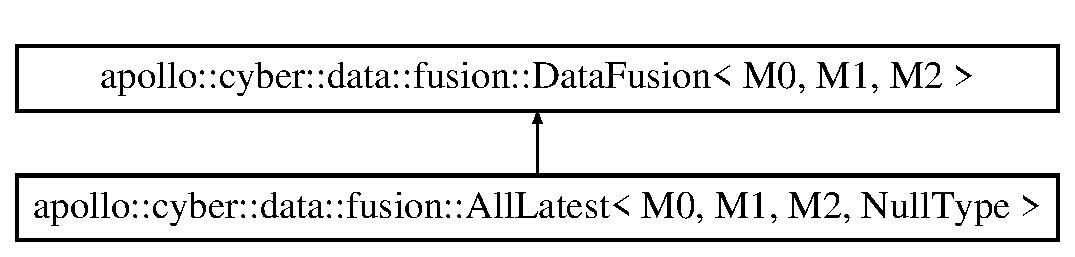
\includegraphics[height=2.000000cm]{classapollo_1_1cyber_1_1data_1_1fusion_1_1AllLatest_3_01M0_00_01M1_00_01M2_00_01NullType_01_4}
\end{center}
\end{figure}
\subsection*{Public Member Functions}
\begin{DoxyCompactItemize}
\item 
\hyperlink{classapollo_1_1cyber_1_1data_1_1fusion_1_1AllLatest_3_01M0_00_01M1_00_01M2_00_01NullType_01_4_aab8f0ed8723d141f268d9a975005ba17}{All\-Latest} (const \hyperlink{classapollo_1_1cyber_1_1data_1_1ChannelBuffer}{Channel\-Buffer}$<$ M0 $>$ \&buffer\-\_\-0, const \hyperlink{classapollo_1_1cyber_1_1data_1_1ChannelBuffer}{Channel\-Buffer}$<$ M1 $>$ \&buffer\-\_\-1, const \hyperlink{classapollo_1_1cyber_1_1data_1_1ChannelBuffer}{Channel\-Buffer}$<$ M2 $>$ \&buffer\-\_\-2)
\item 
bool \hyperlink{classapollo_1_1cyber_1_1data_1_1fusion_1_1AllLatest_3_01M0_00_01M1_00_01M2_00_01NullType_01_4_a7929bf92d377a90ad90978665710807b}{Fusion} (uint64\-\_\-t $\ast$index, std\-::shared\-\_\-ptr$<$ M0 $>$ \&m0, std\-::shared\-\_\-ptr$<$ M1 $>$ \&m1, std\-::shared\-\_\-ptr$<$ M2 $>$ \&m2) override
\end{DoxyCompactItemize}
\subsection*{Private Attributes}
\begin{DoxyCompactItemize}
\item 
\hyperlink{classapollo_1_1cyber_1_1data_1_1ChannelBuffer}{Channel\-Buffer}$<$ M0 $>$ \hyperlink{classapollo_1_1cyber_1_1data_1_1fusion_1_1AllLatest_3_01M0_00_01M1_00_01M2_00_01NullType_01_4_a085490a2914d1ebe6fec256dff263b45}{buffer\-\_\-m0\-\_\-}
\item 
\hyperlink{classapollo_1_1cyber_1_1data_1_1ChannelBuffer}{Channel\-Buffer}$<$ M1 $>$ \hyperlink{classapollo_1_1cyber_1_1data_1_1fusion_1_1AllLatest_3_01M0_00_01M1_00_01M2_00_01NullType_01_4_aaacbccd6888963ae0a62b23de2e2af37}{buffer\-\_\-m1\-\_\-}
\item 
\hyperlink{classapollo_1_1cyber_1_1data_1_1ChannelBuffer}{Channel\-Buffer}$<$ M2 $>$ \hyperlink{classapollo_1_1cyber_1_1data_1_1fusion_1_1AllLatest_3_01M0_00_01M1_00_01M2_00_01NullType_01_4_a6023138c347550bc7c5671cfbce8aa20}{buffer\-\_\-m2\-\_\-}
\end{DoxyCompactItemize}


\subsection{Constructor \& Destructor Documentation}
\hypertarget{classapollo_1_1cyber_1_1data_1_1fusion_1_1AllLatest_3_01M0_00_01M1_00_01M2_00_01NullType_01_4_aab8f0ed8723d141f268d9a975005ba17}{\index{apollo\-::cyber\-::data\-::fusion\-::\-All\-Latest$<$ M0, M1, M2, Null\-Type $>$@{apollo\-::cyber\-::data\-::fusion\-::\-All\-Latest$<$ M0, M1, M2, Null\-Type $>$}!All\-Latest@{All\-Latest}}
\index{All\-Latest@{All\-Latest}!apollo::cyber::data::fusion::AllLatest< M0, M1, M2, NullType >@{apollo\-::cyber\-::data\-::fusion\-::\-All\-Latest$<$ M0, M1, M2, Null\-Type $>$}}
\subsubsection[{All\-Latest}]{\setlength{\rightskip}{0pt plus 5cm}template$<$typename M0 , typename M1 , typename M2 $>$ {\bf apollo\-::cyber\-::data\-::fusion\-::\-All\-Latest}$<$ M0, M1, M2, {\bf Null\-Type} $>$\-::{\bf All\-Latest} (
\begin{DoxyParamCaption}
\item[{const {\bf Channel\-Buffer}$<$ M0 $>$ \&}]{buffer\-\_\-0, }
\item[{const {\bf Channel\-Buffer}$<$ M1 $>$ \&}]{buffer\-\_\-1, }
\item[{const {\bf Channel\-Buffer}$<$ M2 $>$ \&}]{buffer\-\_\-2}
\end{DoxyParamCaption}
)\hspace{0.3cm}{\ttfamily [inline]}}}\label{classapollo_1_1cyber_1_1data_1_1fusion_1_1AllLatest_3_01M0_00_01M1_00_01M2_00_01NullType_01_4_aab8f0ed8723d141f268d9a975005ba17}


\subsection{Member Function Documentation}
\hypertarget{classapollo_1_1cyber_1_1data_1_1fusion_1_1AllLatest_3_01M0_00_01M1_00_01M2_00_01NullType_01_4_a7929bf92d377a90ad90978665710807b}{\index{apollo\-::cyber\-::data\-::fusion\-::\-All\-Latest$<$ M0, M1, M2, Null\-Type $>$@{apollo\-::cyber\-::data\-::fusion\-::\-All\-Latest$<$ M0, M1, M2, Null\-Type $>$}!Fusion@{Fusion}}
\index{Fusion@{Fusion}!apollo::cyber::data::fusion::AllLatest< M0, M1, M2, NullType >@{apollo\-::cyber\-::data\-::fusion\-::\-All\-Latest$<$ M0, M1, M2, Null\-Type $>$}}
\subsubsection[{Fusion}]{\setlength{\rightskip}{0pt plus 5cm}template$<$typename M0 , typename M1 , typename M2 $>$ bool {\bf apollo\-::cyber\-::data\-::fusion\-::\-All\-Latest}$<$ M0, M1, M2, {\bf Null\-Type} $>$\-::Fusion (
\begin{DoxyParamCaption}
\item[{uint64\-\_\-t $\ast$}]{index, }
\item[{std\-::shared\-\_\-ptr$<$ M0 $>$ \&}]{m0, }
\item[{std\-::shared\-\_\-ptr$<$ M1 $>$ \&}]{m1, }
\item[{std\-::shared\-\_\-ptr$<$ M2 $>$ \&}]{m2}
\end{DoxyParamCaption}
)\hspace{0.3cm}{\ttfamily [inline]}, {\ttfamily [override]}}}\label{classapollo_1_1cyber_1_1data_1_1fusion_1_1AllLatest_3_01M0_00_01M1_00_01M2_00_01NullType_01_4_a7929bf92d377a90ad90978665710807b}


\subsection{Member Data Documentation}
\hypertarget{classapollo_1_1cyber_1_1data_1_1fusion_1_1AllLatest_3_01M0_00_01M1_00_01M2_00_01NullType_01_4_a085490a2914d1ebe6fec256dff263b45}{\index{apollo\-::cyber\-::data\-::fusion\-::\-All\-Latest$<$ M0, M1, M2, Null\-Type $>$@{apollo\-::cyber\-::data\-::fusion\-::\-All\-Latest$<$ M0, M1, M2, Null\-Type $>$}!buffer\-\_\-m0\-\_\-@{buffer\-\_\-m0\-\_\-}}
\index{buffer\-\_\-m0\-\_\-@{buffer\-\_\-m0\-\_\-}!apollo::cyber::data::fusion::AllLatest< M0, M1, M2, NullType >@{apollo\-::cyber\-::data\-::fusion\-::\-All\-Latest$<$ M0, M1, M2, Null\-Type $>$}}
\subsubsection[{buffer\-\_\-m0\-\_\-}]{\setlength{\rightskip}{0pt plus 5cm}template$<$typename M0 , typename M1 , typename M2 $>$ {\bf Channel\-Buffer}$<$M0$>$ {\bf apollo\-::cyber\-::data\-::fusion\-::\-All\-Latest}$<$ M0, M1, M2, {\bf Null\-Type} $>$\-::buffer\-\_\-m0\-\_\-\hspace{0.3cm}{\ttfamily [private]}}}\label{classapollo_1_1cyber_1_1data_1_1fusion_1_1AllLatest_3_01M0_00_01M1_00_01M2_00_01NullType_01_4_a085490a2914d1ebe6fec256dff263b45}
\hypertarget{classapollo_1_1cyber_1_1data_1_1fusion_1_1AllLatest_3_01M0_00_01M1_00_01M2_00_01NullType_01_4_aaacbccd6888963ae0a62b23de2e2af37}{\index{apollo\-::cyber\-::data\-::fusion\-::\-All\-Latest$<$ M0, M1, M2, Null\-Type $>$@{apollo\-::cyber\-::data\-::fusion\-::\-All\-Latest$<$ M0, M1, M2, Null\-Type $>$}!buffer\-\_\-m1\-\_\-@{buffer\-\_\-m1\-\_\-}}
\index{buffer\-\_\-m1\-\_\-@{buffer\-\_\-m1\-\_\-}!apollo::cyber::data::fusion::AllLatest< M0, M1, M2, NullType >@{apollo\-::cyber\-::data\-::fusion\-::\-All\-Latest$<$ M0, M1, M2, Null\-Type $>$}}
\subsubsection[{buffer\-\_\-m1\-\_\-}]{\setlength{\rightskip}{0pt plus 5cm}template$<$typename M0 , typename M1 , typename M2 $>$ {\bf Channel\-Buffer}$<$M1$>$ {\bf apollo\-::cyber\-::data\-::fusion\-::\-All\-Latest}$<$ M0, M1, M2, {\bf Null\-Type} $>$\-::buffer\-\_\-m1\-\_\-\hspace{0.3cm}{\ttfamily [private]}}}\label{classapollo_1_1cyber_1_1data_1_1fusion_1_1AllLatest_3_01M0_00_01M1_00_01M2_00_01NullType_01_4_aaacbccd6888963ae0a62b23de2e2af37}
\hypertarget{classapollo_1_1cyber_1_1data_1_1fusion_1_1AllLatest_3_01M0_00_01M1_00_01M2_00_01NullType_01_4_a6023138c347550bc7c5671cfbce8aa20}{\index{apollo\-::cyber\-::data\-::fusion\-::\-All\-Latest$<$ M0, M1, M2, Null\-Type $>$@{apollo\-::cyber\-::data\-::fusion\-::\-All\-Latest$<$ M0, M1, M2, Null\-Type $>$}!buffer\-\_\-m2\-\_\-@{buffer\-\_\-m2\-\_\-}}
\index{buffer\-\_\-m2\-\_\-@{buffer\-\_\-m2\-\_\-}!apollo::cyber::data::fusion::AllLatest< M0, M1, M2, NullType >@{apollo\-::cyber\-::data\-::fusion\-::\-All\-Latest$<$ M0, M1, M2, Null\-Type $>$}}
\subsubsection[{buffer\-\_\-m2\-\_\-}]{\setlength{\rightskip}{0pt plus 5cm}template$<$typename M0 , typename M1 , typename M2 $>$ {\bf Channel\-Buffer}$<$M2$>$ {\bf apollo\-::cyber\-::data\-::fusion\-::\-All\-Latest}$<$ M0, M1, M2, {\bf Null\-Type} $>$\-::buffer\-\_\-m2\-\_\-\hspace{0.3cm}{\ttfamily [private]}}}\label{classapollo_1_1cyber_1_1data_1_1fusion_1_1AllLatest_3_01M0_00_01M1_00_01M2_00_01NullType_01_4_a6023138c347550bc7c5671cfbce8aa20}


The documentation for this class was generated from the following file\-:\begin{DoxyCompactItemize}
\item 
data/fusion/\hyperlink{all__latest_8h}{all\-\_\-latest.\-h}\end{DoxyCompactItemize}

\hypertarget{classapollo_1_1cyber_1_1data_1_1fusion_1_1AllLatest_3_01M0_00_01M1_00_01NullType_00_01NullType_01_4}{\section{apollo\-:\-:cyber\-:\-:data\-:\-:fusion\-:\-:All\-Latest$<$ M0, M1, Null\-Type, Null\-Type $>$ Class Template Reference}
\label{classapollo_1_1cyber_1_1data_1_1fusion_1_1AllLatest_3_01M0_00_01M1_00_01NullType_00_01NullType_01_4}\index{apollo\-::cyber\-::data\-::fusion\-::\-All\-Latest$<$ M0, M1, Null\-Type, Null\-Type $>$@{apollo\-::cyber\-::data\-::fusion\-::\-All\-Latest$<$ M0, M1, Null\-Type, Null\-Type $>$}}
}


{\ttfamily \#include $<$all\-\_\-latest.\-h$>$}

Inheritance diagram for apollo\-:\-:cyber\-:\-:data\-:\-:fusion\-:\-:All\-Latest$<$ M0, M1, Null\-Type, Null\-Type $>$\-:\begin{figure}[H]
\begin{center}
\leavevmode
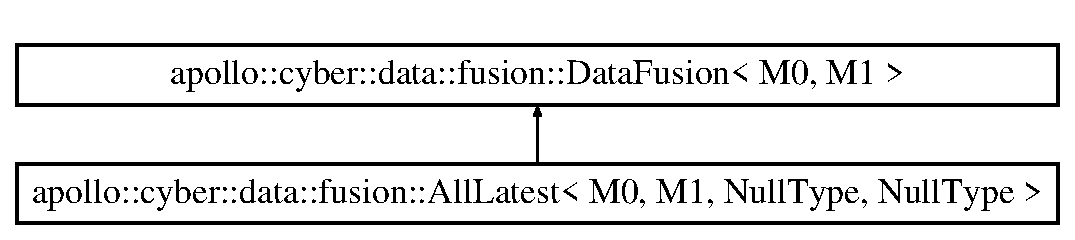
\includegraphics[height=2.000000cm]{classapollo_1_1cyber_1_1data_1_1fusion_1_1AllLatest_3_01M0_00_01M1_00_01NullType_00_01NullType_01_4}
\end{center}
\end{figure}
\subsection*{Public Member Functions}
\begin{DoxyCompactItemize}
\item 
\hyperlink{classapollo_1_1cyber_1_1data_1_1fusion_1_1AllLatest_3_01M0_00_01M1_00_01NullType_00_01NullType_01_4_aef6c11535619fac4e9adf9944ef98f60}{All\-Latest} (const \hyperlink{classapollo_1_1cyber_1_1data_1_1ChannelBuffer}{Channel\-Buffer}$<$ M0 $>$ \&buffer\-\_\-0, const \hyperlink{classapollo_1_1cyber_1_1data_1_1ChannelBuffer}{Channel\-Buffer}$<$ M1 $>$ \&buffer\-\_\-1)
\item 
bool \hyperlink{classapollo_1_1cyber_1_1data_1_1fusion_1_1AllLatest_3_01M0_00_01M1_00_01NullType_00_01NullType_01_4_a4b33c327a6f5e962f2a523bbd6825e6c}{Fusion} (uint64\-\_\-t $\ast$index, std\-::shared\-\_\-ptr$<$ M0 $>$ \&m0, std\-::shared\-\_\-ptr$<$ M1 $>$ \&m1) override
\end{DoxyCompactItemize}
\subsection*{Private Attributes}
\begin{DoxyCompactItemize}
\item 
\hyperlink{classapollo_1_1cyber_1_1data_1_1ChannelBuffer}{Channel\-Buffer}$<$ M0 $>$ \hyperlink{classapollo_1_1cyber_1_1data_1_1fusion_1_1AllLatest_3_01M0_00_01M1_00_01NullType_00_01NullType_01_4_a36d8435a223930fc4b6c7ed1f2a4d2e7}{buffer\-\_\-m0\-\_\-}
\item 
\hyperlink{classapollo_1_1cyber_1_1data_1_1ChannelBuffer}{Channel\-Buffer}$<$ M1 $>$ \hyperlink{classapollo_1_1cyber_1_1data_1_1fusion_1_1AllLatest_3_01M0_00_01M1_00_01NullType_00_01NullType_01_4_a5fded1f4f01a2e0fd1888f0a45053bfc}{buffer\-\_\-m1\-\_\-}
\end{DoxyCompactItemize}


\subsection{Constructor \& Destructor Documentation}
\hypertarget{classapollo_1_1cyber_1_1data_1_1fusion_1_1AllLatest_3_01M0_00_01M1_00_01NullType_00_01NullType_01_4_aef6c11535619fac4e9adf9944ef98f60}{\index{apollo\-::cyber\-::data\-::fusion\-::\-All\-Latest$<$ M0, M1, Null\-Type, Null\-Type $>$@{apollo\-::cyber\-::data\-::fusion\-::\-All\-Latest$<$ M0, M1, Null\-Type, Null\-Type $>$}!All\-Latest@{All\-Latest}}
\index{All\-Latest@{All\-Latest}!apollo::cyber::data::fusion::AllLatest< M0, M1, NullType, NullType >@{apollo\-::cyber\-::data\-::fusion\-::\-All\-Latest$<$ M0, M1, Null\-Type, Null\-Type $>$}}
\subsubsection[{All\-Latest}]{\setlength{\rightskip}{0pt plus 5cm}template$<$typename M0 , typename M1 $>$ {\bf apollo\-::cyber\-::data\-::fusion\-::\-All\-Latest}$<$ M0, M1, {\bf Null\-Type}, {\bf Null\-Type} $>$\-::{\bf All\-Latest} (
\begin{DoxyParamCaption}
\item[{const {\bf Channel\-Buffer}$<$ M0 $>$ \&}]{buffer\-\_\-0, }
\item[{const {\bf Channel\-Buffer}$<$ M1 $>$ \&}]{buffer\-\_\-1}
\end{DoxyParamCaption}
)\hspace{0.3cm}{\ttfamily [inline]}}}\label{classapollo_1_1cyber_1_1data_1_1fusion_1_1AllLatest_3_01M0_00_01M1_00_01NullType_00_01NullType_01_4_aef6c11535619fac4e9adf9944ef98f60}


\subsection{Member Function Documentation}
\hypertarget{classapollo_1_1cyber_1_1data_1_1fusion_1_1AllLatest_3_01M0_00_01M1_00_01NullType_00_01NullType_01_4_a4b33c327a6f5e962f2a523bbd6825e6c}{\index{apollo\-::cyber\-::data\-::fusion\-::\-All\-Latest$<$ M0, M1, Null\-Type, Null\-Type $>$@{apollo\-::cyber\-::data\-::fusion\-::\-All\-Latest$<$ M0, M1, Null\-Type, Null\-Type $>$}!Fusion@{Fusion}}
\index{Fusion@{Fusion}!apollo::cyber::data::fusion::AllLatest< M0, M1, NullType, NullType >@{apollo\-::cyber\-::data\-::fusion\-::\-All\-Latest$<$ M0, M1, Null\-Type, Null\-Type $>$}}
\subsubsection[{Fusion}]{\setlength{\rightskip}{0pt plus 5cm}template$<$typename M0 , typename M1 $>$ bool {\bf apollo\-::cyber\-::data\-::fusion\-::\-All\-Latest}$<$ M0, M1, {\bf Null\-Type}, {\bf Null\-Type} $>$\-::Fusion (
\begin{DoxyParamCaption}
\item[{uint64\-\_\-t $\ast$}]{index, }
\item[{std\-::shared\-\_\-ptr$<$ M0 $>$ \&}]{m0, }
\item[{std\-::shared\-\_\-ptr$<$ M1 $>$ \&}]{m1}
\end{DoxyParamCaption}
)\hspace{0.3cm}{\ttfamily [inline]}, {\ttfamily [override]}}}\label{classapollo_1_1cyber_1_1data_1_1fusion_1_1AllLatest_3_01M0_00_01M1_00_01NullType_00_01NullType_01_4_a4b33c327a6f5e962f2a523bbd6825e6c}


\subsection{Member Data Documentation}
\hypertarget{classapollo_1_1cyber_1_1data_1_1fusion_1_1AllLatest_3_01M0_00_01M1_00_01NullType_00_01NullType_01_4_a36d8435a223930fc4b6c7ed1f2a4d2e7}{\index{apollo\-::cyber\-::data\-::fusion\-::\-All\-Latest$<$ M0, M1, Null\-Type, Null\-Type $>$@{apollo\-::cyber\-::data\-::fusion\-::\-All\-Latest$<$ M0, M1, Null\-Type, Null\-Type $>$}!buffer\-\_\-m0\-\_\-@{buffer\-\_\-m0\-\_\-}}
\index{buffer\-\_\-m0\-\_\-@{buffer\-\_\-m0\-\_\-}!apollo::cyber::data::fusion::AllLatest< M0, M1, NullType, NullType >@{apollo\-::cyber\-::data\-::fusion\-::\-All\-Latest$<$ M0, M1, Null\-Type, Null\-Type $>$}}
\subsubsection[{buffer\-\_\-m0\-\_\-}]{\setlength{\rightskip}{0pt plus 5cm}template$<$typename M0 , typename M1 $>$ {\bf Channel\-Buffer}$<$M0$>$ {\bf apollo\-::cyber\-::data\-::fusion\-::\-All\-Latest}$<$ M0, M1, {\bf Null\-Type}, {\bf Null\-Type} $>$\-::buffer\-\_\-m0\-\_\-\hspace{0.3cm}{\ttfamily [private]}}}\label{classapollo_1_1cyber_1_1data_1_1fusion_1_1AllLatest_3_01M0_00_01M1_00_01NullType_00_01NullType_01_4_a36d8435a223930fc4b6c7ed1f2a4d2e7}
\hypertarget{classapollo_1_1cyber_1_1data_1_1fusion_1_1AllLatest_3_01M0_00_01M1_00_01NullType_00_01NullType_01_4_a5fded1f4f01a2e0fd1888f0a45053bfc}{\index{apollo\-::cyber\-::data\-::fusion\-::\-All\-Latest$<$ M0, M1, Null\-Type, Null\-Type $>$@{apollo\-::cyber\-::data\-::fusion\-::\-All\-Latest$<$ M0, M1, Null\-Type, Null\-Type $>$}!buffer\-\_\-m1\-\_\-@{buffer\-\_\-m1\-\_\-}}
\index{buffer\-\_\-m1\-\_\-@{buffer\-\_\-m1\-\_\-}!apollo::cyber::data::fusion::AllLatest< M0, M1, NullType, NullType >@{apollo\-::cyber\-::data\-::fusion\-::\-All\-Latest$<$ M0, M1, Null\-Type, Null\-Type $>$}}
\subsubsection[{buffer\-\_\-m1\-\_\-}]{\setlength{\rightskip}{0pt plus 5cm}template$<$typename M0 , typename M1 $>$ {\bf Channel\-Buffer}$<$M1$>$ {\bf apollo\-::cyber\-::data\-::fusion\-::\-All\-Latest}$<$ M0, M1, {\bf Null\-Type}, {\bf Null\-Type} $>$\-::buffer\-\_\-m1\-\_\-\hspace{0.3cm}{\ttfamily [private]}}}\label{classapollo_1_1cyber_1_1data_1_1fusion_1_1AllLatest_3_01M0_00_01M1_00_01NullType_00_01NullType_01_4_a5fded1f4f01a2e0fd1888f0a45053bfc}


The documentation for this class was generated from the following file\-:\begin{DoxyCompactItemize}
\item 
data/fusion/\hyperlink{all__latest_8h}{all\-\_\-latest.\-h}\end{DoxyCompactItemize}

\hypertarget{classapollo_1_1cyber_1_1logger_1_1AsyncLogger}{\section{apollo\-:\-:cyber\-:\-:logger\-:\-:Async\-Logger Class Reference}
\label{classapollo_1_1cyber_1_1logger_1_1AsyncLogger}\index{apollo\-::cyber\-::logger\-::\-Async\-Logger@{apollo\-::cyber\-::logger\-::\-Async\-Logger}}
}


{\ttfamily \#include $<$async\-\_\-logger.\-h$>$}

Inheritance diagram for apollo\-:\-:cyber\-:\-:logger\-:\-:Async\-Logger\-:\begin{figure}[H]
\begin{center}
\leavevmode
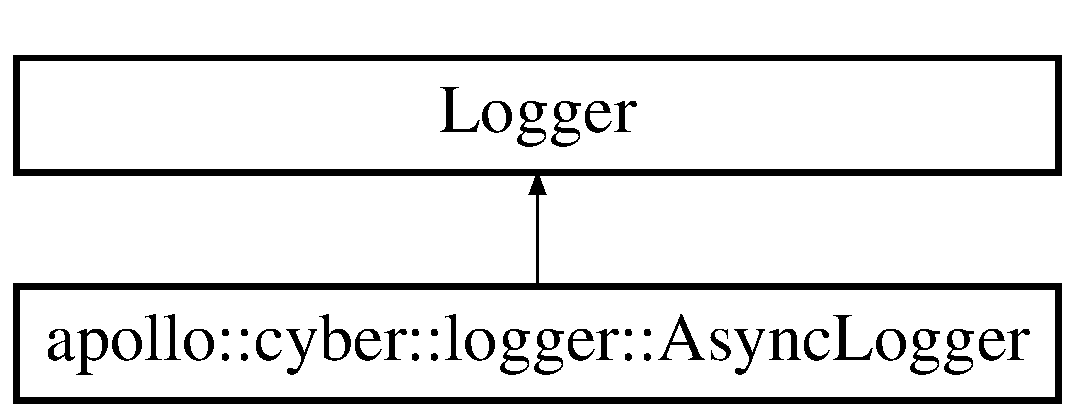
\includegraphics[height=2.000000cm]{classapollo_1_1cyber_1_1logger_1_1AsyncLogger}
\end{center}
\end{figure}
\subsection*{Classes}
\begin{DoxyCompactItemize}
\item 
struct \hyperlink{structapollo_1_1cyber_1_1logger_1_1AsyncLogger_1_1Buffer}{Buffer}
\item 
struct \hyperlink{structapollo_1_1cyber_1_1logger_1_1AsyncLogger_1_1Msg}{Msg}
\end{DoxyCompactItemize}
\subsection*{Public Member Functions}
\begin{DoxyCompactItemize}
\item 
\hyperlink{classapollo_1_1cyber_1_1logger_1_1AsyncLogger_ab512ca5b0980840bd97187b8b8bf68a7}{Async\-Logger} (google\-::base\-::\-Logger $\ast$wrapped, int max\-\_\-buffer\-\_\-bytes)
\item 
\hyperlink{classapollo_1_1cyber_1_1logger_1_1AsyncLogger_ab81c56987b35eac2468293214cc0831a}{$\sim$\-Async\-Logger} ()
\item 
void \hyperlink{classapollo_1_1cyber_1_1logger_1_1AsyncLogger_a57a56cd44d68c932c229638169a8ece1}{Start} ()
\item 
void \hyperlink{classapollo_1_1cyber_1_1logger_1_1AsyncLogger_a36aceb58b08edfba1417d18d60996811}{Stop} ()
\item 
void \hyperlink{classapollo_1_1cyber_1_1logger_1_1AsyncLogger_abe281a699f379c7274ef0fc9fe171eab}{Write} (bool force\-\_\-flush, time\-\_\-t timestamp, const char $\ast$message, int message\-\_\-len) override
\item 
void \hyperlink{classapollo_1_1cyber_1_1logger_1_1AsyncLogger_a75894f5de117c03d05c013f2638639a1}{Flush} () override
\item 
uint32\-\_\-t \hyperlink{classapollo_1_1cyber_1_1logger_1_1AsyncLogger_af14fc46b26821895b40def530a4a5aeb}{Log\-Size} () override
\item 
const std\-::thread $\ast$ \hyperlink{classapollo_1_1cyber_1_1logger_1_1AsyncLogger_ac71b6d358d78e0912524c1b8359baa2f}{Log\-Thread} () const 
\end{DoxyCompactItemize}
\subsection*{Private Types}
\begin{DoxyCompactItemize}
\item 
enum \hyperlink{classapollo_1_1cyber_1_1logger_1_1AsyncLogger_ac693c5c55875861feb508ed2b60223a4}{State} \{ \hyperlink{classapollo_1_1cyber_1_1logger_1_1AsyncLogger_ac693c5c55875861feb508ed2b60223a4a05e01a42de2ef2f76fc008c2f2ac0b11}{I\-N\-I\-T\-T\-E\-D}, 
\hyperlink{classapollo_1_1cyber_1_1logger_1_1AsyncLogger_ac693c5c55875861feb508ed2b60223a4ad883b067d35376bd78b0f301a0200704}{R\-U\-N\-N\-I\-N\-G}, 
\hyperlink{classapollo_1_1cyber_1_1logger_1_1AsyncLogger_ac693c5c55875861feb508ed2b60223a4a26a879c1a0c30577cff7af5688a3b55f}{S\-T\-O\-P\-P\-E\-D}
 \}
\end{DoxyCompactItemize}
\subsection*{Private Member Functions}
\begin{DoxyCompactItemize}
\item 
bool \hyperlink{classapollo_1_1cyber_1_1logger_1_1AsyncLogger_a52f8a409bf0dceb86e9e484a494a166c}{Buffer\-Full} (const \hyperlink{structapollo_1_1cyber_1_1logger_1_1AsyncLogger_1_1Buffer}{Buffer} \&buf) const 
\item 
void \hyperlink{classapollo_1_1cyber_1_1logger_1_1AsyncLogger_af1600cd1348d78c6ab0e806928a2d50b}{Run\-Thread} ()
\item 
\hyperlink{classapollo_1_1cyber_1_1logger_1_1AsyncLogger_afa782e83a5e5d08d7ff7da08c6f194ac}{D\-I\-S\-A\-L\-L\-O\-W\-\_\-\-C\-O\-P\-Y\-\_\-\-A\-N\-D\-\_\-\-A\-S\-S\-I\-G\-N} (\hyperlink{classapollo_1_1cyber_1_1logger_1_1AsyncLogger}{Async\-Logger})
\end{DoxyCompactItemize}
\subsection*{Private Attributes}
\begin{DoxyCompactItemize}
\item 
int \hyperlink{classapollo_1_1cyber_1_1logger_1_1AsyncLogger_aa335015aac6cf1e4a7ef9def98cc5f33}{max\-\_\-buffer\-\_\-bytes\-\_\-}
\item 
google\-::base\-::\-Logger $\ast$const \hyperlink{classapollo_1_1cyber_1_1logger_1_1AsyncLogger_a4d7679337ba167a45f75c006f9c2f340}{wrapped\-\_\-}
\item 
std\-::thread \hyperlink{classapollo_1_1cyber_1_1logger_1_1AsyncLogger_a973fb1d166acaab52815ded79cadec25}{thread\-\_\-}
\item 
uint64\-\_\-t \hyperlink{classapollo_1_1cyber_1_1logger_1_1AsyncLogger_a52a5941a5ed779bac9b1469677dfd8fa}{flush\-\_\-count\-\_\-} = 0
\item 
uint64\-\_\-t \hyperlink{classapollo_1_1cyber_1_1logger_1_1AsyncLogger_ae50ea372dfdfe32615dc5d25664c8075}{drop\-\_\-count\-\_\-} = 0
\item 
std\-::mutex \hyperlink{classapollo_1_1cyber_1_1logger_1_1AsyncLogger_a822d34060bc2e4bc3c1b5dbb80a62470}{mutex\-\_\-}
\item 
std\-::condition\-\_\-variable \hyperlink{classapollo_1_1cyber_1_1logger_1_1AsyncLogger_a606516963229bb28e70cf5599e993798}{wake\-\_\-flusher\-\_\-cv\-\_\-}
\item 
std\-::condition\-\_\-variable \hyperlink{classapollo_1_1cyber_1_1logger_1_1AsyncLogger_ac317fa7ba8ac170fcaebee103b861aa6}{flush\-\_\-complete\-\_\-cv\-\_\-}
\item 
std\-::unique\-\_\-ptr$<$ \hyperlink{structapollo_1_1cyber_1_1logger_1_1AsyncLogger_1_1Buffer}{Buffer} $>$ \hyperlink{classapollo_1_1cyber_1_1logger_1_1AsyncLogger_a89a6be9354f86ddcfabe1d313117b43d}{active\-\_\-buf\-\_\-}
\item 
std\-::unique\-\_\-ptr$<$ \hyperlink{structapollo_1_1cyber_1_1logger_1_1AsyncLogger_1_1Buffer}{Buffer} $>$ \hyperlink{classapollo_1_1cyber_1_1logger_1_1AsyncLogger_ae78d3263cf93ea38811ab00e2afc6d1c}{flushing\-\_\-buf\-\_\-}
\item 
\hyperlink{classapollo_1_1cyber_1_1logger_1_1AsyncLogger_ac693c5c55875861feb508ed2b60223a4}{State} \hyperlink{classapollo_1_1cyber_1_1logger_1_1AsyncLogger_a01dbb42c36800aa824b929ddba8332d8}{state\-\_\-} = \hyperlink{classapollo_1_1cyber_1_1logger_1_1AsyncLogger_ac693c5c55875861feb508ed2b60223a4a05e01a42de2ef2f76fc008c2f2ac0b11}{I\-N\-I\-T\-T\-E\-D}
\end{DoxyCompactItemize}


\subsection{Member Enumeration Documentation}
\hypertarget{classapollo_1_1cyber_1_1logger_1_1AsyncLogger_ac693c5c55875861feb508ed2b60223a4}{\index{apollo\-::cyber\-::logger\-::\-Async\-Logger@{apollo\-::cyber\-::logger\-::\-Async\-Logger}!State@{State}}
\index{State@{State}!apollo::cyber::logger::AsyncLogger@{apollo\-::cyber\-::logger\-::\-Async\-Logger}}
\subsubsection[{State}]{\setlength{\rightskip}{0pt plus 5cm}enum {\bf apollo\-::cyber\-::logger\-::\-Async\-Logger\-::\-State}\hspace{0.3cm}{\ttfamily [private]}}}\label{classapollo_1_1cyber_1_1logger_1_1AsyncLogger_ac693c5c55875861feb508ed2b60223a4}
\begin{Desc}
\item[Enumerator]\par
\begin{description}
\index{I\-N\-I\-T\-T\-E\-D@{I\-N\-I\-T\-T\-E\-D}!apollo\-::cyber\-::logger\-::\-Async\-Logger@{apollo\-::cyber\-::logger\-::\-Async\-Logger}}\index{apollo\-::cyber\-::logger\-::\-Async\-Logger@{apollo\-::cyber\-::logger\-::\-Async\-Logger}!I\-N\-I\-T\-T\-E\-D@{I\-N\-I\-T\-T\-E\-D}}\item[{\em 
\hypertarget{classapollo_1_1cyber_1_1logger_1_1AsyncLogger_ac693c5c55875861feb508ed2b60223a4a05e01a42de2ef2f76fc008c2f2ac0b11}{I\-N\-I\-T\-T\-E\-D}\label{classapollo_1_1cyber_1_1logger_1_1AsyncLogger_ac693c5c55875861feb508ed2b60223a4a05e01a42de2ef2f76fc008c2f2ac0b11}
}]\index{R\-U\-N\-N\-I\-N\-G@{R\-U\-N\-N\-I\-N\-G}!apollo\-::cyber\-::logger\-::\-Async\-Logger@{apollo\-::cyber\-::logger\-::\-Async\-Logger}}\index{apollo\-::cyber\-::logger\-::\-Async\-Logger@{apollo\-::cyber\-::logger\-::\-Async\-Logger}!R\-U\-N\-N\-I\-N\-G@{R\-U\-N\-N\-I\-N\-G}}\item[{\em 
\hypertarget{classapollo_1_1cyber_1_1logger_1_1AsyncLogger_ac693c5c55875861feb508ed2b60223a4ad883b067d35376bd78b0f301a0200704}{R\-U\-N\-N\-I\-N\-G}\label{classapollo_1_1cyber_1_1logger_1_1AsyncLogger_ac693c5c55875861feb508ed2b60223a4ad883b067d35376bd78b0f301a0200704}
}]\index{S\-T\-O\-P\-P\-E\-D@{S\-T\-O\-P\-P\-E\-D}!apollo\-::cyber\-::logger\-::\-Async\-Logger@{apollo\-::cyber\-::logger\-::\-Async\-Logger}}\index{apollo\-::cyber\-::logger\-::\-Async\-Logger@{apollo\-::cyber\-::logger\-::\-Async\-Logger}!S\-T\-O\-P\-P\-E\-D@{S\-T\-O\-P\-P\-E\-D}}\item[{\em 
\hypertarget{classapollo_1_1cyber_1_1logger_1_1AsyncLogger_ac693c5c55875861feb508ed2b60223a4a26a879c1a0c30577cff7af5688a3b55f}{S\-T\-O\-P\-P\-E\-D}\label{classapollo_1_1cyber_1_1logger_1_1AsyncLogger_ac693c5c55875861feb508ed2b60223a4a26a879c1a0c30577cff7af5688a3b55f}
}]\end{description}
\end{Desc}


\subsection{Constructor \& Destructor Documentation}
\hypertarget{classapollo_1_1cyber_1_1logger_1_1AsyncLogger_ab512ca5b0980840bd97187b8b8bf68a7}{\index{apollo\-::cyber\-::logger\-::\-Async\-Logger@{apollo\-::cyber\-::logger\-::\-Async\-Logger}!Async\-Logger@{Async\-Logger}}
\index{Async\-Logger@{Async\-Logger}!apollo::cyber::logger::AsyncLogger@{apollo\-::cyber\-::logger\-::\-Async\-Logger}}
\subsubsection[{Async\-Logger}]{\setlength{\rightskip}{0pt plus 5cm}apollo\-::cyber\-::logger\-::\-Async\-Logger\-::\-Async\-Logger (
\begin{DoxyParamCaption}
\item[{google\-::base\-::\-Logger $\ast$}]{wrapped, }
\item[{int}]{max\-\_\-buffer\-\_\-bytes}
\end{DoxyParamCaption}
)\hspace{0.3cm}{\ttfamily [explicit]}}}\label{classapollo_1_1cyber_1_1logger_1_1AsyncLogger_ab512ca5b0980840bd97187b8b8bf68a7}
\hypertarget{classapollo_1_1cyber_1_1logger_1_1AsyncLogger_ab81c56987b35eac2468293214cc0831a}{\index{apollo\-::cyber\-::logger\-::\-Async\-Logger@{apollo\-::cyber\-::logger\-::\-Async\-Logger}!$\sim$\-Async\-Logger@{$\sim$\-Async\-Logger}}
\index{$\sim$\-Async\-Logger@{$\sim$\-Async\-Logger}!apollo::cyber::logger::AsyncLogger@{apollo\-::cyber\-::logger\-::\-Async\-Logger}}
\subsubsection[{$\sim$\-Async\-Logger}]{\setlength{\rightskip}{0pt plus 5cm}apollo\-::cyber\-::logger\-::\-Async\-Logger\-::$\sim$\-Async\-Logger (
\begin{DoxyParamCaption}
{}
\end{DoxyParamCaption}
)}}\label{classapollo_1_1cyber_1_1logger_1_1AsyncLogger_ab81c56987b35eac2468293214cc0831a}


\subsection{Member Function Documentation}
\hypertarget{classapollo_1_1cyber_1_1logger_1_1AsyncLogger_a52f8a409bf0dceb86e9e484a494a166c}{\index{apollo\-::cyber\-::logger\-::\-Async\-Logger@{apollo\-::cyber\-::logger\-::\-Async\-Logger}!Buffer\-Full@{Buffer\-Full}}
\index{Buffer\-Full@{Buffer\-Full}!apollo::cyber::logger::AsyncLogger@{apollo\-::cyber\-::logger\-::\-Async\-Logger}}
\subsubsection[{Buffer\-Full}]{\setlength{\rightskip}{0pt plus 5cm}bool apollo\-::cyber\-::logger\-::\-Async\-Logger\-::\-Buffer\-Full (
\begin{DoxyParamCaption}
\item[{const {\bf Buffer} \&}]{buf}
\end{DoxyParamCaption}
) const\hspace{0.3cm}{\ttfamily [private]}}}\label{classapollo_1_1cyber_1_1logger_1_1AsyncLogger_a52f8a409bf0dceb86e9e484a494a166c}
\hypertarget{classapollo_1_1cyber_1_1logger_1_1AsyncLogger_afa782e83a5e5d08d7ff7da08c6f194ac}{\index{apollo\-::cyber\-::logger\-::\-Async\-Logger@{apollo\-::cyber\-::logger\-::\-Async\-Logger}!D\-I\-S\-A\-L\-L\-O\-W\-\_\-\-C\-O\-P\-Y\-\_\-\-A\-N\-D\-\_\-\-A\-S\-S\-I\-G\-N@{D\-I\-S\-A\-L\-L\-O\-W\-\_\-\-C\-O\-P\-Y\-\_\-\-A\-N\-D\-\_\-\-A\-S\-S\-I\-G\-N}}
\index{D\-I\-S\-A\-L\-L\-O\-W\-\_\-\-C\-O\-P\-Y\-\_\-\-A\-N\-D\-\_\-\-A\-S\-S\-I\-G\-N@{D\-I\-S\-A\-L\-L\-O\-W\-\_\-\-C\-O\-P\-Y\-\_\-\-A\-N\-D\-\_\-\-A\-S\-S\-I\-G\-N}!apollo::cyber::logger::AsyncLogger@{apollo\-::cyber\-::logger\-::\-Async\-Logger}}
\subsubsection[{D\-I\-S\-A\-L\-L\-O\-W\-\_\-\-C\-O\-P\-Y\-\_\-\-A\-N\-D\-\_\-\-A\-S\-S\-I\-G\-N}]{\setlength{\rightskip}{0pt plus 5cm}apollo\-::cyber\-::logger\-::\-Async\-Logger\-::\-D\-I\-S\-A\-L\-L\-O\-W\-\_\-\-C\-O\-P\-Y\-\_\-\-A\-N\-D\-\_\-\-A\-S\-S\-I\-G\-N (
\begin{DoxyParamCaption}
\item[{{\bf Async\-Logger}}]{}
\end{DoxyParamCaption}
)\hspace{0.3cm}{\ttfamily [private]}}}\label{classapollo_1_1cyber_1_1logger_1_1AsyncLogger_afa782e83a5e5d08d7ff7da08c6f194ac}
\hypertarget{classapollo_1_1cyber_1_1logger_1_1AsyncLogger_a75894f5de117c03d05c013f2638639a1}{\index{apollo\-::cyber\-::logger\-::\-Async\-Logger@{apollo\-::cyber\-::logger\-::\-Async\-Logger}!Flush@{Flush}}
\index{Flush@{Flush}!apollo::cyber::logger::AsyncLogger@{apollo\-::cyber\-::logger\-::\-Async\-Logger}}
\subsubsection[{Flush}]{\setlength{\rightskip}{0pt plus 5cm}void apollo\-::cyber\-::logger\-::\-Async\-Logger\-::\-Flush (
\begin{DoxyParamCaption}
{}
\end{DoxyParamCaption}
)\hspace{0.3cm}{\ttfamily [override]}}}\label{classapollo_1_1cyber_1_1logger_1_1AsyncLogger_a75894f5de117c03d05c013f2638639a1}
\hypertarget{classapollo_1_1cyber_1_1logger_1_1AsyncLogger_af14fc46b26821895b40def530a4a5aeb}{\index{apollo\-::cyber\-::logger\-::\-Async\-Logger@{apollo\-::cyber\-::logger\-::\-Async\-Logger}!Log\-Size@{Log\-Size}}
\index{Log\-Size@{Log\-Size}!apollo::cyber::logger::AsyncLogger@{apollo\-::cyber\-::logger\-::\-Async\-Logger}}
\subsubsection[{Log\-Size}]{\setlength{\rightskip}{0pt plus 5cm}uint32\-\_\-t apollo\-::cyber\-::logger\-::\-Async\-Logger\-::\-Log\-Size (
\begin{DoxyParamCaption}
{}
\end{DoxyParamCaption}
)\hspace{0.3cm}{\ttfamily [override]}}}\label{classapollo_1_1cyber_1_1logger_1_1AsyncLogger_af14fc46b26821895b40def530a4a5aeb}
\hypertarget{classapollo_1_1cyber_1_1logger_1_1AsyncLogger_ac71b6d358d78e0912524c1b8359baa2f}{\index{apollo\-::cyber\-::logger\-::\-Async\-Logger@{apollo\-::cyber\-::logger\-::\-Async\-Logger}!Log\-Thread@{Log\-Thread}}
\index{Log\-Thread@{Log\-Thread}!apollo::cyber::logger::AsyncLogger@{apollo\-::cyber\-::logger\-::\-Async\-Logger}}
\subsubsection[{Log\-Thread}]{\setlength{\rightskip}{0pt plus 5cm}const std\-::thread$\ast$ apollo\-::cyber\-::logger\-::\-Async\-Logger\-::\-Log\-Thread (
\begin{DoxyParamCaption}
{}
\end{DoxyParamCaption}
) const\hspace{0.3cm}{\ttfamily [inline]}}}\label{classapollo_1_1cyber_1_1logger_1_1AsyncLogger_ac71b6d358d78e0912524c1b8359baa2f}
\hypertarget{classapollo_1_1cyber_1_1logger_1_1AsyncLogger_af1600cd1348d78c6ab0e806928a2d50b}{\index{apollo\-::cyber\-::logger\-::\-Async\-Logger@{apollo\-::cyber\-::logger\-::\-Async\-Logger}!Run\-Thread@{Run\-Thread}}
\index{Run\-Thread@{Run\-Thread}!apollo::cyber::logger::AsyncLogger@{apollo\-::cyber\-::logger\-::\-Async\-Logger}}
\subsubsection[{Run\-Thread}]{\setlength{\rightskip}{0pt plus 5cm}void apollo\-::cyber\-::logger\-::\-Async\-Logger\-::\-Run\-Thread (
\begin{DoxyParamCaption}
{}
\end{DoxyParamCaption}
)\hspace{0.3cm}{\ttfamily [private]}}}\label{classapollo_1_1cyber_1_1logger_1_1AsyncLogger_af1600cd1348d78c6ab0e806928a2d50b}
\hypertarget{classapollo_1_1cyber_1_1logger_1_1AsyncLogger_a57a56cd44d68c932c229638169a8ece1}{\index{apollo\-::cyber\-::logger\-::\-Async\-Logger@{apollo\-::cyber\-::logger\-::\-Async\-Logger}!Start@{Start}}
\index{Start@{Start}!apollo::cyber::logger::AsyncLogger@{apollo\-::cyber\-::logger\-::\-Async\-Logger}}
\subsubsection[{Start}]{\setlength{\rightskip}{0pt plus 5cm}void apollo\-::cyber\-::logger\-::\-Async\-Logger\-::\-Start (
\begin{DoxyParamCaption}
{}
\end{DoxyParamCaption}
)}}\label{classapollo_1_1cyber_1_1logger_1_1AsyncLogger_a57a56cd44d68c932c229638169a8ece1}
\hypertarget{classapollo_1_1cyber_1_1logger_1_1AsyncLogger_a36aceb58b08edfba1417d18d60996811}{\index{apollo\-::cyber\-::logger\-::\-Async\-Logger@{apollo\-::cyber\-::logger\-::\-Async\-Logger}!Stop@{Stop}}
\index{Stop@{Stop}!apollo::cyber::logger::AsyncLogger@{apollo\-::cyber\-::logger\-::\-Async\-Logger}}
\subsubsection[{Stop}]{\setlength{\rightskip}{0pt plus 5cm}void apollo\-::cyber\-::logger\-::\-Async\-Logger\-::\-Stop (
\begin{DoxyParamCaption}
{}
\end{DoxyParamCaption}
)}}\label{classapollo_1_1cyber_1_1logger_1_1AsyncLogger_a36aceb58b08edfba1417d18d60996811}
\hypertarget{classapollo_1_1cyber_1_1logger_1_1AsyncLogger_abe281a699f379c7274ef0fc9fe171eab}{\index{apollo\-::cyber\-::logger\-::\-Async\-Logger@{apollo\-::cyber\-::logger\-::\-Async\-Logger}!Write@{Write}}
\index{Write@{Write}!apollo::cyber::logger::AsyncLogger@{apollo\-::cyber\-::logger\-::\-Async\-Logger}}
\subsubsection[{Write}]{\setlength{\rightskip}{0pt plus 5cm}void apollo\-::cyber\-::logger\-::\-Async\-Logger\-::\-Write (
\begin{DoxyParamCaption}
\item[{bool}]{force\-\_\-flush, }
\item[{time\-\_\-t}]{timestamp, }
\item[{const char $\ast$}]{message, }
\item[{int}]{message\-\_\-len}
\end{DoxyParamCaption}
)\hspace{0.3cm}{\ttfamily [override]}}}\label{classapollo_1_1cyber_1_1logger_1_1AsyncLogger_abe281a699f379c7274ef0fc9fe171eab}


\subsection{Member Data Documentation}
\hypertarget{classapollo_1_1cyber_1_1logger_1_1AsyncLogger_a89a6be9354f86ddcfabe1d313117b43d}{\index{apollo\-::cyber\-::logger\-::\-Async\-Logger@{apollo\-::cyber\-::logger\-::\-Async\-Logger}!active\-\_\-buf\-\_\-@{active\-\_\-buf\-\_\-}}
\index{active\-\_\-buf\-\_\-@{active\-\_\-buf\-\_\-}!apollo::cyber::logger::AsyncLogger@{apollo\-::cyber\-::logger\-::\-Async\-Logger}}
\subsubsection[{active\-\_\-buf\-\_\-}]{\setlength{\rightskip}{0pt plus 5cm}std\-::unique\-\_\-ptr$<${\bf Buffer}$>$ apollo\-::cyber\-::logger\-::\-Async\-Logger\-::active\-\_\-buf\-\_\-\hspace{0.3cm}{\ttfamily [private]}}}\label{classapollo_1_1cyber_1_1logger_1_1AsyncLogger_a89a6be9354f86ddcfabe1d313117b43d}
\hypertarget{classapollo_1_1cyber_1_1logger_1_1AsyncLogger_ae50ea372dfdfe32615dc5d25664c8075}{\index{apollo\-::cyber\-::logger\-::\-Async\-Logger@{apollo\-::cyber\-::logger\-::\-Async\-Logger}!drop\-\_\-count\-\_\-@{drop\-\_\-count\-\_\-}}
\index{drop\-\_\-count\-\_\-@{drop\-\_\-count\-\_\-}!apollo::cyber::logger::AsyncLogger@{apollo\-::cyber\-::logger\-::\-Async\-Logger}}
\subsubsection[{drop\-\_\-count\-\_\-}]{\setlength{\rightskip}{0pt plus 5cm}uint64\-\_\-t apollo\-::cyber\-::logger\-::\-Async\-Logger\-::drop\-\_\-count\-\_\- = 0\hspace{0.3cm}{\ttfamily [private]}}}\label{classapollo_1_1cyber_1_1logger_1_1AsyncLogger_ae50ea372dfdfe32615dc5d25664c8075}
\hypertarget{classapollo_1_1cyber_1_1logger_1_1AsyncLogger_ac317fa7ba8ac170fcaebee103b861aa6}{\index{apollo\-::cyber\-::logger\-::\-Async\-Logger@{apollo\-::cyber\-::logger\-::\-Async\-Logger}!flush\-\_\-complete\-\_\-cv\-\_\-@{flush\-\_\-complete\-\_\-cv\-\_\-}}
\index{flush\-\_\-complete\-\_\-cv\-\_\-@{flush\-\_\-complete\-\_\-cv\-\_\-}!apollo::cyber::logger::AsyncLogger@{apollo\-::cyber\-::logger\-::\-Async\-Logger}}
\subsubsection[{flush\-\_\-complete\-\_\-cv\-\_\-}]{\setlength{\rightskip}{0pt plus 5cm}std\-::condition\-\_\-variable apollo\-::cyber\-::logger\-::\-Async\-Logger\-::flush\-\_\-complete\-\_\-cv\-\_\-\hspace{0.3cm}{\ttfamily [private]}}}\label{classapollo_1_1cyber_1_1logger_1_1AsyncLogger_ac317fa7ba8ac170fcaebee103b861aa6}
\hypertarget{classapollo_1_1cyber_1_1logger_1_1AsyncLogger_a52a5941a5ed779bac9b1469677dfd8fa}{\index{apollo\-::cyber\-::logger\-::\-Async\-Logger@{apollo\-::cyber\-::logger\-::\-Async\-Logger}!flush\-\_\-count\-\_\-@{flush\-\_\-count\-\_\-}}
\index{flush\-\_\-count\-\_\-@{flush\-\_\-count\-\_\-}!apollo::cyber::logger::AsyncLogger@{apollo\-::cyber\-::logger\-::\-Async\-Logger}}
\subsubsection[{flush\-\_\-count\-\_\-}]{\setlength{\rightskip}{0pt plus 5cm}uint64\-\_\-t apollo\-::cyber\-::logger\-::\-Async\-Logger\-::flush\-\_\-count\-\_\- = 0\hspace{0.3cm}{\ttfamily [private]}}}\label{classapollo_1_1cyber_1_1logger_1_1AsyncLogger_a52a5941a5ed779bac9b1469677dfd8fa}
\hypertarget{classapollo_1_1cyber_1_1logger_1_1AsyncLogger_ae78d3263cf93ea38811ab00e2afc6d1c}{\index{apollo\-::cyber\-::logger\-::\-Async\-Logger@{apollo\-::cyber\-::logger\-::\-Async\-Logger}!flushing\-\_\-buf\-\_\-@{flushing\-\_\-buf\-\_\-}}
\index{flushing\-\_\-buf\-\_\-@{flushing\-\_\-buf\-\_\-}!apollo::cyber::logger::AsyncLogger@{apollo\-::cyber\-::logger\-::\-Async\-Logger}}
\subsubsection[{flushing\-\_\-buf\-\_\-}]{\setlength{\rightskip}{0pt plus 5cm}std\-::unique\-\_\-ptr$<${\bf Buffer}$>$ apollo\-::cyber\-::logger\-::\-Async\-Logger\-::flushing\-\_\-buf\-\_\-\hspace{0.3cm}{\ttfamily [private]}}}\label{classapollo_1_1cyber_1_1logger_1_1AsyncLogger_ae78d3263cf93ea38811ab00e2afc6d1c}
\hypertarget{classapollo_1_1cyber_1_1logger_1_1AsyncLogger_aa335015aac6cf1e4a7ef9def98cc5f33}{\index{apollo\-::cyber\-::logger\-::\-Async\-Logger@{apollo\-::cyber\-::logger\-::\-Async\-Logger}!max\-\_\-buffer\-\_\-bytes\-\_\-@{max\-\_\-buffer\-\_\-bytes\-\_\-}}
\index{max\-\_\-buffer\-\_\-bytes\-\_\-@{max\-\_\-buffer\-\_\-bytes\-\_\-}!apollo::cyber::logger::AsyncLogger@{apollo\-::cyber\-::logger\-::\-Async\-Logger}}
\subsubsection[{max\-\_\-buffer\-\_\-bytes\-\_\-}]{\setlength{\rightskip}{0pt plus 5cm}int apollo\-::cyber\-::logger\-::\-Async\-Logger\-::max\-\_\-buffer\-\_\-bytes\-\_\-\hspace{0.3cm}{\ttfamily [private]}}}\label{classapollo_1_1cyber_1_1logger_1_1AsyncLogger_aa335015aac6cf1e4a7ef9def98cc5f33}
\hypertarget{classapollo_1_1cyber_1_1logger_1_1AsyncLogger_a822d34060bc2e4bc3c1b5dbb80a62470}{\index{apollo\-::cyber\-::logger\-::\-Async\-Logger@{apollo\-::cyber\-::logger\-::\-Async\-Logger}!mutex\-\_\-@{mutex\-\_\-}}
\index{mutex\-\_\-@{mutex\-\_\-}!apollo::cyber::logger::AsyncLogger@{apollo\-::cyber\-::logger\-::\-Async\-Logger}}
\subsubsection[{mutex\-\_\-}]{\setlength{\rightskip}{0pt plus 5cm}std\-::mutex apollo\-::cyber\-::logger\-::\-Async\-Logger\-::mutex\-\_\-\hspace{0.3cm}{\ttfamily [private]}}}\label{classapollo_1_1cyber_1_1logger_1_1AsyncLogger_a822d34060bc2e4bc3c1b5dbb80a62470}
\hypertarget{classapollo_1_1cyber_1_1logger_1_1AsyncLogger_a01dbb42c36800aa824b929ddba8332d8}{\index{apollo\-::cyber\-::logger\-::\-Async\-Logger@{apollo\-::cyber\-::logger\-::\-Async\-Logger}!state\-\_\-@{state\-\_\-}}
\index{state\-\_\-@{state\-\_\-}!apollo::cyber::logger::AsyncLogger@{apollo\-::cyber\-::logger\-::\-Async\-Logger}}
\subsubsection[{state\-\_\-}]{\setlength{\rightskip}{0pt plus 5cm}{\bf State} apollo\-::cyber\-::logger\-::\-Async\-Logger\-::state\-\_\- = {\bf I\-N\-I\-T\-T\-E\-D}\hspace{0.3cm}{\ttfamily [private]}}}\label{classapollo_1_1cyber_1_1logger_1_1AsyncLogger_a01dbb42c36800aa824b929ddba8332d8}
\hypertarget{classapollo_1_1cyber_1_1logger_1_1AsyncLogger_a973fb1d166acaab52815ded79cadec25}{\index{apollo\-::cyber\-::logger\-::\-Async\-Logger@{apollo\-::cyber\-::logger\-::\-Async\-Logger}!thread\-\_\-@{thread\-\_\-}}
\index{thread\-\_\-@{thread\-\_\-}!apollo::cyber::logger::AsyncLogger@{apollo\-::cyber\-::logger\-::\-Async\-Logger}}
\subsubsection[{thread\-\_\-}]{\setlength{\rightskip}{0pt plus 5cm}std\-::thread apollo\-::cyber\-::logger\-::\-Async\-Logger\-::thread\-\_\-\hspace{0.3cm}{\ttfamily [private]}}}\label{classapollo_1_1cyber_1_1logger_1_1AsyncLogger_a973fb1d166acaab52815ded79cadec25}
\hypertarget{classapollo_1_1cyber_1_1logger_1_1AsyncLogger_a606516963229bb28e70cf5599e993798}{\index{apollo\-::cyber\-::logger\-::\-Async\-Logger@{apollo\-::cyber\-::logger\-::\-Async\-Logger}!wake\-\_\-flusher\-\_\-cv\-\_\-@{wake\-\_\-flusher\-\_\-cv\-\_\-}}
\index{wake\-\_\-flusher\-\_\-cv\-\_\-@{wake\-\_\-flusher\-\_\-cv\-\_\-}!apollo::cyber::logger::AsyncLogger@{apollo\-::cyber\-::logger\-::\-Async\-Logger}}
\subsubsection[{wake\-\_\-flusher\-\_\-cv\-\_\-}]{\setlength{\rightskip}{0pt plus 5cm}std\-::condition\-\_\-variable apollo\-::cyber\-::logger\-::\-Async\-Logger\-::wake\-\_\-flusher\-\_\-cv\-\_\-\hspace{0.3cm}{\ttfamily [private]}}}\label{classapollo_1_1cyber_1_1logger_1_1AsyncLogger_a606516963229bb28e70cf5599e993798}
\hypertarget{classapollo_1_1cyber_1_1logger_1_1AsyncLogger_a4d7679337ba167a45f75c006f9c2f340}{\index{apollo\-::cyber\-::logger\-::\-Async\-Logger@{apollo\-::cyber\-::logger\-::\-Async\-Logger}!wrapped\-\_\-@{wrapped\-\_\-}}
\index{wrapped\-\_\-@{wrapped\-\_\-}!apollo::cyber::logger::AsyncLogger@{apollo\-::cyber\-::logger\-::\-Async\-Logger}}
\subsubsection[{wrapped\-\_\-}]{\setlength{\rightskip}{0pt plus 5cm}google\-::base\-::\-Logger$\ast$ const apollo\-::cyber\-::logger\-::\-Async\-Logger\-::wrapped\-\_\-\hspace{0.3cm}{\ttfamily [private]}}}\label{classapollo_1_1cyber_1_1logger_1_1AsyncLogger_a4d7679337ba167a45f75c006f9c2f340}


The documentation for this class was generated from the following file\-:\begin{DoxyCompactItemize}
\item 
logger/\hyperlink{async__logger_8h}{async\-\_\-logger.\-h}\end{DoxyCompactItemize}

\hypertarget{classapollo_1_1cyber_1_1base_1_1AtomicHashMap}{\section{apollo\-:\-:cyber\-:\-:base\-:\-:Atomic\-Hash\-Map$<$ K, V, Table\-Size, std\-:\-:enable\-\_\-if$<$ std\-:\-:is\-\_\-integral$<$ K $>$\-:\-:value \&\&(Table\-Size \&(Table\-Size-\/1))==0, int $>$\-:\-:type $>$ Class Template Reference}
\label{classapollo_1_1cyber_1_1base_1_1AtomicHashMap}\index{apollo\-::cyber\-::base\-::\-Atomic\-Hash\-Map$<$ K, V, Table\-Size, std\-::enable\-\_\-if$<$ std\-::is\-\_\-integral$<$ K $>$\-::value \&\&(\-Table\-Size \&(\-Table\-Size-\/1))==0, int $>$\-::type $>$@{apollo\-::cyber\-::base\-::\-Atomic\-Hash\-Map$<$ K, V, Table\-Size, std\-::enable\-\_\-if$<$ std\-::is\-\_\-integral$<$ K $>$\-::value \&\&(\-Table\-Size \&(\-Table\-Size-\/1))==0, int $>$\-::type $>$}}
}


A implementation of lock-\/free fixed size hash map.  




{\ttfamily \#include $<$atomic\-\_\-hash\-\_\-map.\-h$>$}

\subsection*{Classes}
\begin{DoxyCompactItemize}
\item 
class \hyperlink{classapollo_1_1cyber_1_1base_1_1AtomicHashMap_1_1Bucket}{Bucket}
\item 
struct \hyperlink{structapollo_1_1cyber_1_1base_1_1AtomicHashMap_1_1Entry}{Entry}
\end{DoxyCompactItemize}
\subsection*{Public Member Functions}
\begin{DoxyCompactItemize}
\item 
\hyperlink{classapollo_1_1cyber_1_1base_1_1AtomicHashMap_aa1a83359c21d93a096e806382f03e129}{Atomic\-Hash\-Map} ()
\item 
\hyperlink{classapollo_1_1cyber_1_1base_1_1AtomicHashMap_aa27dda760cfb4332fe043d5c23242c20}{Atomic\-Hash\-Map} (const \hyperlink{classapollo_1_1cyber_1_1base_1_1AtomicHashMap}{Atomic\-Hash\-Map} \&other)=delete
\item 
\hyperlink{classapollo_1_1cyber_1_1base_1_1AtomicHashMap}{Atomic\-Hash\-Map} \& \hyperlink{classapollo_1_1cyber_1_1base_1_1AtomicHashMap_a780be857f6f6d0330da564afd8266620}{operator=} (const \hyperlink{classapollo_1_1cyber_1_1base_1_1AtomicHashMap}{Atomic\-Hash\-Map} \&other)=delete
\item 
bool \hyperlink{classapollo_1_1cyber_1_1base_1_1AtomicHashMap_ac038ea2f8018172914fcadb807a970a8}{Has} (K key)
\item 
bool \hyperlink{classapollo_1_1cyber_1_1base_1_1AtomicHashMap_a0cffa9d1d855e4733f18071b0d7a077d}{Get} (K key, V $\ast$$\ast$\hyperlink{namespaceapollo_1_1cyber_1_1base_aa3e2fff9b18a1214af4a70546fb7120f}{value})
\item 
bool \hyperlink{classapollo_1_1cyber_1_1base_1_1AtomicHashMap_a3b8fc8d906e4e6c116c991cd178c8655}{Get} (K key, V $\ast$\hyperlink{namespaceapollo_1_1cyber_1_1base_aa3e2fff9b18a1214af4a70546fb7120f}{value})
\item 
void \hyperlink{classapollo_1_1cyber_1_1base_1_1AtomicHashMap_a9ed2851c909e8ac9662f92d81df18efe}{Set} (K key)
\item 
void \hyperlink{classapollo_1_1cyber_1_1base_1_1AtomicHashMap_a595719e722207e09c63feb85b505ef36}{Set} (K key, const V \&\hyperlink{namespaceapollo_1_1cyber_1_1base_aa3e2fff9b18a1214af4a70546fb7120f}{value})
\item 
void \hyperlink{classapollo_1_1cyber_1_1base_1_1AtomicHashMap_ac4c44e27832b4965f999eeed068938d1}{Set} (K key, V \&\&\hyperlink{namespaceapollo_1_1cyber_1_1base_aa3e2fff9b18a1214af4a70546fb7120f}{value})
\end{DoxyCompactItemize}
\subsection*{Private Attributes}
\begin{DoxyCompactItemize}
\item 
\hyperlink{classapollo_1_1cyber_1_1base_1_1AtomicHashMap_1_1Bucket}{Bucket} \hyperlink{classapollo_1_1cyber_1_1base_1_1AtomicHashMap_aab575e13b07e0465956aeb1aaef42e22}{table\-\_\-} \mbox{[}Table\-Size\mbox{]}
\item 
uint64\-\_\-t \hyperlink{classapollo_1_1cyber_1_1base_1_1AtomicHashMap_ada585ac9c1211917c1d08bf3ef77281f}{capacity\-\_\-}
\item 
uint64\-\_\-t \hyperlink{classapollo_1_1cyber_1_1base_1_1AtomicHashMap_adb15b0fce4c41fa3b25a32b5ba7e23bc}{mode\-\_\-num\-\_\-}
\end{DoxyCompactItemize}


\subsection{Detailed Description}
\subsubsection*{template$<$typename K, typename V, std\-::size\-\_\-t Table\-Size = 128, typename std\-::enable\-\_\-if$<$ std\-::is\-\_\-integral$<$ K $>$\-::value \&\&(\-Table\-Size \&(\-Table\-Size-\/1))==0, int $>$\-::type = 0$>$class apollo\-::cyber\-::base\-::\-Atomic\-Hash\-Map$<$ K, V, Table\-Size, std\-::enable\-\_\-if$<$ std\-::is\-\_\-integral$<$ K $>$\-::value \&\&(\-Table\-Size \&(\-Table\-Size-\/1))==0, int $>$\-::type $>$}

A implementation of lock-\/free fixed size hash map. 


\begin{DoxyTemplParams}{Template Parameters}
{\em K} & Type of key, must be integral \\
\hline
{\em V} & Type of value \\
\hline
{\em 128} & Size of hash table \\
\hline
{\em 0} & Type traits, use for checking types of key \& value \\
\hline
\end{DoxyTemplParams}


\subsection{Constructor \& Destructor Documentation}
\hypertarget{classapollo_1_1cyber_1_1base_1_1AtomicHashMap_aa1a83359c21d93a096e806382f03e129}{\index{apollo\-::cyber\-::base\-::\-Atomic\-Hash\-Map@{apollo\-::cyber\-::base\-::\-Atomic\-Hash\-Map}!Atomic\-Hash\-Map@{Atomic\-Hash\-Map}}
\index{Atomic\-Hash\-Map@{Atomic\-Hash\-Map}!apollo::cyber::base::AtomicHashMap@{apollo\-::cyber\-::base\-::\-Atomic\-Hash\-Map}}
\subsubsection[{Atomic\-Hash\-Map}]{\setlength{\rightskip}{0pt plus 5cm}template$<$typename K, typename V, std\-::size\-\_\-t Table\-Size = 128, typename std\-::enable\-\_\-if$<$ std\-::is\-\_\-integral$<$ K $>$\-::value \&\&(\-Table\-Size \&(\-Table\-Size-\/1))==0, int $>$\-::type = 0$>$ {\bf apollo\-::cyber\-::base\-::\-Atomic\-Hash\-Map}$<$ K, V, Table\-Size, type $>$\-::{\bf Atomic\-Hash\-Map} (
\begin{DoxyParamCaption}
{}
\end{DoxyParamCaption}
)\hspace{0.3cm}{\ttfamily [inline]}}}\label{classapollo_1_1cyber_1_1base_1_1AtomicHashMap_aa1a83359c21d93a096e806382f03e129}
\hypertarget{classapollo_1_1cyber_1_1base_1_1AtomicHashMap_aa27dda760cfb4332fe043d5c23242c20}{\index{apollo\-::cyber\-::base\-::\-Atomic\-Hash\-Map@{apollo\-::cyber\-::base\-::\-Atomic\-Hash\-Map}!Atomic\-Hash\-Map@{Atomic\-Hash\-Map}}
\index{Atomic\-Hash\-Map@{Atomic\-Hash\-Map}!apollo::cyber::base::AtomicHashMap@{apollo\-::cyber\-::base\-::\-Atomic\-Hash\-Map}}
\subsubsection[{Atomic\-Hash\-Map}]{\setlength{\rightskip}{0pt plus 5cm}template$<$typename K, typename V, std\-::size\-\_\-t Table\-Size = 128, typename std\-::enable\-\_\-if$<$ std\-::is\-\_\-integral$<$ K $>$\-::value \&\&(\-Table\-Size \&(\-Table\-Size-\/1))==0, int $>$\-::type = 0$>$ {\bf apollo\-::cyber\-::base\-::\-Atomic\-Hash\-Map}$<$ K, V, Table\-Size, type $>$\-::{\bf Atomic\-Hash\-Map} (
\begin{DoxyParamCaption}
\item[{const {\bf Atomic\-Hash\-Map}$<$ K, V, Table\-Size, std\-::enable\-\_\-if$<$ std\-::is\-\_\-integral$<$ K $>$\-::{\bf value} \&\&(Table\-Size \&(Table\-Size-\/1))==0, int $>$\-::type $>$ \&}]{other}
\end{DoxyParamCaption}
)\hspace{0.3cm}{\ttfamily [delete]}}}\label{classapollo_1_1cyber_1_1base_1_1AtomicHashMap_aa27dda760cfb4332fe043d5c23242c20}


\subsection{Member Function Documentation}
\hypertarget{classapollo_1_1cyber_1_1base_1_1AtomicHashMap_a0cffa9d1d855e4733f18071b0d7a077d}{\index{apollo\-::cyber\-::base\-::\-Atomic\-Hash\-Map@{apollo\-::cyber\-::base\-::\-Atomic\-Hash\-Map}!Get@{Get}}
\index{Get@{Get}!apollo::cyber::base::AtomicHashMap@{apollo\-::cyber\-::base\-::\-Atomic\-Hash\-Map}}
\subsubsection[{Get}]{\setlength{\rightskip}{0pt plus 5cm}template$<$typename K, typename V, std\-::size\-\_\-t Table\-Size = 128, typename std\-::enable\-\_\-if$<$ std\-::is\-\_\-integral$<$ K $>$\-::value \&\&(\-Table\-Size \&(\-Table\-Size-\/1))==0, int $>$\-::type = 0$>$ bool {\bf apollo\-::cyber\-::base\-::\-Atomic\-Hash\-Map}$<$ K, V, Table\-Size, type $>$\-::Get (
\begin{DoxyParamCaption}
\item[{K}]{key, }
\item[{V $\ast$$\ast$}]{value}
\end{DoxyParamCaption}
)\hspace{0.3cm}{\ttfamily [inline]}}}\label{classapollo_1_1cyber_1_1base_1_1AtomicHashMap_a0cffa9d1d855e4733f18071b0d7a077d}
\hypertarget{classapollo_1_1cyber_1_1base_1_1AtomicHashMap_a3b8fc8d906e4e6c116c991cd178c8655}{\index{apollo\-::cyber\-::base\-::\-Atomic\-Hash\-Map@{apollo\-::cyber\-::base\-::\-Atomic\-Hash\-Map}!Get@{Get}}
\index{Get@{Get}!apollo::cyber::base::AtomicHashMap@{apollo\-::cyber\-::base\-::\-Atomic\-Hash\-Map}}
\subsubsection[{Get}]{\setlength{\rightskip}{0pt plus 5cm}template$<$typename K, typename V, std\-::size\-\_\-t Table\-Size = 128, typename std\-::enable\-\_\-if$<$ std\-::is\-\_\-integral$<$ K $>$\-::value \&\&(\-Table\-Size \&(\-Table\-Size-\/1))==0, int $>$\-::type = 0$>$ bool {\bf apollo\-::cyber\-::base\-::\-Atomic\-Hash\-Map}$<$ K, V, Table\-Size, type $>$\-::Get (
\begin{DoxyParamCaption}
\item[{K}]{key, }
\item[{V $\ast$}]{value}
\end{DoxyParamCaption}
)\hspace{0.3cm}{\ttfamily [inline]}}}\label{classapollo_1_1cyber_1_1base_1_1AtomicHashMap_a3b8fc8d906e4e6c116c991cd178c8655}
\hypertarget{classapollo_1_1cyber_1_1base_1_1AtomicHashMap_ac038ea2f8018172914fcadb807a970a8}{\index{apollo\-::cyber\-::base\-::\-Atomic\-Hash\-Map@{apollo\-::cyber\-::base\-::\-Atomic\-Hash\-Map}!Has@{Has}}
\index{Has@{Has}!apollo::cyber::base::AtomicHashMap@{apollo\-::cyber\-::base\-::\-Atomic\-Hash\-Map}}
\subsubsection[{Has}]{\setlength{\rightskip}{0pt plus 5cm}template$<$typename K, typename V, std\-::size\-\_\-t Table\-Size = 128, typename std\-::enable\-\_\-if$<$ std\-::is\-\_\-integral$<$ K $>$\-::value \&\&(\-Table\-Size \&(\-Table\-Size-\/1))==0, int $>$\-::type = 0$>$ bool {\bf apollo\-::cyber\-::base\-::\-Atomic\-Hash\-Map}$<$ K, V, Table\-Size, type $>$\-::Has (
\begin{DoxyParamCaption}
\item[{K}]{key}
\end{DoxyParamCaption}
)\hspace{0.3cm}{\ttfamily [inline]}}}\label{classapollo_1_1cyber_1_1base_1_1AtomicHashMap_ac038ea2f8018172914fcadb807a970a8}
\hypertarget{classapollo_1_1cyber_1_1base_1_1AtomicHashMap_a780be857f6f6d0330da564afd8266620}{\index{apollo\-::cyber\-::base\-::\-Atomic\-Hash\-Map@{apollo\-::cyber\-::base\-::\-Atomic\-Hash\-Map}!operator=@{operator=}}
\index{operator=@{operator=}!apollo::cyber::base::AtomicHashMap@{apollo\-::cyber\-::base\-::\-Atomic\-Hash\-Map}}
\subsubsection[{operator=}]{\setlength{\rightskip}{0pt plus 5cm}template$<$typename K, typename V, std\-::size\-\_\-t Table\-Size = 128, typename std\-::enable\-\_\-if$<$ std\-::is\-\_\-integral$<$ K $>$\-::value \&\&(\-Table\-Size \&(\-Table\-Size-\/1))==0, int $>$\-::type = 0$>$ {\bf Atomic\-Hash\-Map}\& {\bf apollo\-::cyber\-::base\-::\-Atomic\-Hash\-Map}$<$ K, V, Table\-Size, type $>$\-::operator= (
\begin{DoxyParamCaption}
\item[{const {\bf Atomic\-Hash\-Map}$<$ K, V, Table\-Size, std\-::enable\-\_\-if$<$ std\-::is\-\_\-integral$<$ K $>$\-::{\bf value} \&\&(Table\-Size \&(Table\-Size-\/1))==0, int $>$\-::type $>$ \&}]{other}
\end{DoxyParamCaption}
)\hspace{0.3cm}{\ttfamily [delete]}}}\label{classapollo_1_1cyber_1_1base_1_1AtomicHashMap_a780be857f6f6d0330da564afd8266620}
\hypertarget{classapollo_1_1cyber_1_1base_1_1AtomicHashMap_a9ed2851c909e8ac9662f92d81df18efe}{\index{apollo\-::cyber\-::base\-::\-Atomic\-Hash\-Map@{apollo\-::cyber\-::base\-::\-Atomic\-Hash\-Map}!Set@{Set}}
\index{Set@{Set}!apollo::cyber::base::AtomicHashMap@{apollo\-::cyber\-::base\-::\-Atomic\-Hash\-Map}}
\subsubsection[{Set}]{\setlength{\rightskip}{0pt plus 5cm}template$<$typename K, typename V, std\-::size\-\_\-t Table\-Size = 128, typename std\-::enable\-\_\-if$<$ std\-::is\-\_\-integral$<$ K $>$\-::value \&\&(\-Table\-Size \&(\-Table\-Size-\/1))==0, int $>$\-::type = 0$>$ void {\bf apollo\-::cyber\-::base\-::\-Atomic\-Hash\-Map}$<$ K, V, Table\-Size, type $>$\-::Set (
\begin{DoxyParamCaption}
\item[{K}]{key}
\end{DoxyParamCaption}
)\hspace{0.3cm}{\ttfamily [inline]}}}\label{classapollo_1_1cyber_1_1base_1_1AtomicHashMap_a9ed2851c909e8ac9662f92d81df18efe}
\hypertarget{classapollo_1_1cyber_1_1base_1_1AtomicHashMap_a595719e722207e09c63feb85b505ef36}{\index{apollo\-::cyber\-::base\-::\-Atomic\-Hash\-Map@{apollo\-::cyber\-::base\-::\-Atomic\-Hash\-Map}!Set@{Set}}
\index{Set@{Set}!apollo::cyber::base::AtomicHashMap@{apollo\-::cyber\-::base\-::\-Atomic\-Hash\-Map}}
\subsubsection[{Set}]{\setlength{\rightskip}{0pt plus 5cm}template$<$typename K, typename V, std\-::size\-\_\-t Table\-Size = 128, typename std\-::enable\-\_\-if$<$ std\-::is\-\_\-integral$<$ K $>$\-::value \&\&(\-Table\-Size \&(\-Table\-Size-\/1))==0, int $>$\-::type = 0$>$ void {\bf apollo\-::cyber\-::base\-::\-Atomic\-Hash\-Map}$<$ K, V, Table\-Size, type $>$\-::Set (
\begin{DoxyParamCaption}
\item[{K}]{key, }
\item[{const V \&}]{value}
\end{DoxyParamCaption}
)\hspace{0.3cm}{\ttfamily [inline]}}}\label{classapollo_1_1cyber_1_1base_1_1AtomicHashMap_a595719e722207e09c63feb85b505ef36}
\hypertarget{classapollo_1_1cyber_1_1base_1_1AtomicHashMap_ac4c44e27832b4965f999eeed068938d1}{\index{apollo\-::cyber\-::base\-::\-Atomic\-Hash\-Map@{apollo\-::cyber\-::base\-::\-Atomic\-Hash\-Map}!Set@{Set}}
\index{Set@{Set}!apollo::cyber::base::AtomicHashMap@{apollo\-::cyber\-::base\-::\-Atomic\-Hash\-Map}}
\subsubsection[{Set}]{\setlength{\rightskip}{0pt plus 5cm}template$<$typename K, typename V, std\-::size\-\_\-t Table\-Size = 128, typename std\-::enable\-\_\-if$<$ std\-::is\-\_\-integral$<$ K $>$\-::value \&\&(\-Table\-Size \&(\-Table\-Size-\/1))==0, int $>$\-::type = 0$>$ void {\bf apollo\-::cyber\-::base\-::\-Atomic\-Hash\-Map}$<$ K, V, Table\-Size, type $>$\-::Set (
\begin{DoxyParamCaption}
\item[{K}]{key, }
\item[{V \&\&}]{value}
\end{DoxyParamCaption}
)\hspace{0.3cm}{\ttfamily [inline]}}}\label{classapollo_1_1cyber_1_1base_1_1AtomicHashMap_ac4c44e27832b4965f999eeed068938d1}


\subsection{Member Data Documentation}
\hypertarget{classapollo_1_1cyber_1_1base_1_1AtomicHashMap_ada585ac9c1211917c1d08bf3ef77281f}{\index{apollo\-::cyber\-::base\-::\-Atomic\-Hash\-Map@{apollo\-::cyber\-::base\-::\-Atomic\-Hash\-Map}!capacity\-\_\-@{capacity\-\_\-}}
\index{capacity\-\_\-@{capacity\-\_\-}!apollo::cyber::base::AtomicHashMap@{apollo\-::cyber\-::base\-::\-Atomic\-Hash\-Map}}
\subsubsection[{capacity\-\_\-}]{\setlength{\rightskip}{0pt plus 5cm}template$<$typename K, typename V, std\-::size\-\_\-t Table\-Size = 128, typename std\-::enable\-\_\-if$<$ std\-::is\-\_\-integral$<$ K $>$\-::value \&\&(\-Table\-Size \&(\-Table\-Size-\/1))==0, int $>$\-::type = 0$>$ uint64\-\_\-t {\bf apollo\-::cyber\-::base\-::\-Atomic\-Hash\-Map}$<$ K, V, Table\-Size, type $>$\-::capacity\-\_\-\hspace{0.3cm}{\ttfamily [private]}}}\label{classapollo_1_1cyber_1_1base_1_1AtomicHashMap_ada585ac9c1211917c1d08bf3ef77281f}
\hypertarget{classapollo_1_1cyber_1_1base_1_1AtomicHashMap_adb15b0fce4c41fa3b25a32b5ba7e23bc}{\index{apollo\-::cyber\-::base\-::\-Atomic\-Hash\-Map@{apollo\-::cyber\-::base\-::\-Atomic\-Hash\-Map}!mode\-\_\-num\-\_\-@{mode\-\_\-num\-\_\-}}
\index{mode\-\_\-num\-\_\-@{mode\-\_\-num\-\_\-}!apollo::cyber::base::AtomicHashMap@{apollo\-::cyber\-::base\-::\-Atomic\-Hash\-Map}}
\subsubsection[{mode\-\_\-num\-\_\-}]{\setlength{\rightskip}{0pt plus 5cm}template$<$typename K, typename V, std\-::size\-\_\-t Table\-Size = 128, typename std\-::enable\-\_\-if$<$ std\-::is\-\_\-integral$<$ K $>$\-::value \&\&(\-Table\-Size \&(\-Table\-Size-\/1))==0, int $>$\-::type = 0$>$ uint64\-\_\-t {\bf apollo\-::cyber\-::base\-::\-Atomic\-Hash\-Map}$<$ K, V, Table\-Size, type $>$\-::mode\-\_\-num\-\_\-\hspace{0.3cm}{\ttfamily [private]}}}\label{classapollo_1_1cyber_1_1base_1_1AtomicHashMap_adb15b0fce4c41fa3b25a32b5ba7e23bc}
\hypertarget{classapollo_1_1cyber_1_1base_1_1AtomicHashMap_aab575e13b07e0465956aeb1aaef42e22}{\index{apollo\-::cyber\-::base\-::\-Atomic\-Hash\-Map@{apollo\-::cyber\-::base\-::\-Atomic\-Hash\-Map}!table\-\_\-@{table\-\_\-}}
\index{table\-\_\-@{table\-\_\-}!apollo::cyber::base::AtomicHashMap@{apollo\-::cyber\-::base\-::\-Atomic\-Hash\-Map}}
\subsubsection[{table\-\_\-}]{\setlength{\rightskip}{0pt plus 5cm}template$<$typename K, typename V, std\-::size\-\_\-t Table\-Size = 128, typename std\-::enable\-\_\-if$<$ std\-::is\-\_\-integral$<$ K $>$\-::value \&\&(\-Table\-Size \&(\-Table\-Size-\/1))==0, int $>$\-::type = 0$>$ {\bf Bucket} {\bf apollo\-::cyber\-::base\-::\-Atomic\-Hash\-Map}$<$ K, V, Table\-Size, type $>$\-::table\-\_\-\mbox{[}Table\-Size\mbox{]}\hspace{0.3cm}{\ttfamily [private]}}}\label{classapollo_1_1cyber_1_1base_1_1AtomicHashMap_aab575e13b07e0465956aeb1aaef42e22}


The documentation for this class was generated from the following file\-:\begin{DoxyCompactItemize}
\item 
base/\hyperlink{atomic__hash__map_8h}{atomic\-\_\-hash\-\_\-map.\-h}\end{DoxyCompactItemize}

\hypertarget{classapollo_1_1cyber_1_1base_1_1AtomicRWLock}{\section{apollo\-:\-:cyber\-:\-:base\-:\-:Atomic\-R\-W\-Lock Class Reference}
\label{classapollo_1_1cyber_1_1base_1_1AtomicRWLock}\index{apollo\-::cyber\-::base\-::\-Atomic\-R\-W\-Lock@{apollo\-::cyber\-::base\-::\-Atomic\-R\-W\-Lock}}
}


{\ttfamily \#include $<$atomic\-\_\-rw\-\_\-lock.\-h$>$}

\subsection*{Public Member Functions}
\begin{DoxyCompactItemize}
\item 
\hyperlink{classapollo_1_1cyber_1_1base_1_1AtomicRWLock_ac95a9bd44dde5cb5478fb47f2e884ea2}{Atomic\-R\-W\-Lock} ()
\item 
\hyperlink{classapollo_1_1cyber_1_1base_1_1AtomicRWLock_adba8c36fa57f40852590ba1390f03427}{Atomic\-R\-W\-Lock} (bool write\-\_\-first)
\end{DoxyCompactItemize}
\subsection*{Static Public Attributes}
\begin{DoxyCompactItemize}
\item 
static const int32\-\_\-t \hyperlink{classapollo_1_1cyber_1_1base_1_1AtomicRWLock_a85da033794c4e6cf82e6a8e89266ee40}{R\-W\-\_\-\-L\-O\-C\-K\-\_\-\-F\-R\-E\-E} = 0
\item 
static const int32\-\_\-t \hyperlink{classapollo_1_1cyber_1_1base_1_1AtomicRWLock_add34af0709bcc95f70afbce7a4b6c7e3}{W\-R\-I\-T\-E\-\_\-\-E\-X\-C\-L\-U\-S\-I\-V\-E} = -\/1
\item 
static const uint32\-\_\-t \hyperlink{classapollo_1_1cyber_1_1base_1_1AtomicRWLock_a16fe6c0b37ad30c852de92297798ad43}{M\-A\-X\-\_\-\-R\-E\-T\-R\-Y\-\_\-\-T\-I\-M\-E\-S} = 5
\end{DoxyCompactItemize}
\subsection*{Private Member Functions}
\begin{DoxyCompactItemize}
\item 
void \hyperlink{classapollo_1_1cyber_1_1base_1_1AtomicRWLock_a4d45cdc1aeaaf52cf7e921ef84bc69a9}{Read\-Lock} ()
\item 
void \hyperlink{classapollo_1_1cyber_1_1base_1_1AtomicRWLock_a7837026bb217ea454dc683d7b6531c00}{Write\-Lock} ()
\item 
void \hyperlink{classapollo_1_1cyber_1_1base_1_1AtomicRWLock_a5394b943ae73dea59b98882411610724}{Read\-Unlock} ()
\item 
void \hyperlink{classapollo_1_1cyber_1_1base_1_1AtomicRWLock_a26e5a8629da1eef7b544c5f5639d1b2c}{Write\-Unlock} ()
\item 
\hyperlink{classapollo_1_1cyber_1_1base_1_1AtomicRWLock_ae3d12c1d8676b8ad4b1174b38d3bff19}{Atomic\-R\-W\-Lock} (const \hyperlink{classapollo_1_1cyber_1_1base_1_1AtomicRWLock}{Atomic\-R\-W\-Lock} \&)=delete
\item 
\hyperlink{classapollo_1_1cyber_1_1base_1_1AtomicRWLock}{Atomic\-R\-W\-Lock} \& \hyperlink{classapollo_1_1cyber_1_1base_1_1AtomicRWLock_a8f6c54b39ff17f2ac4b4cf1c5855d484}{operator=} (const \hyperlink{classapollo_1_1cyber_1_1base_1_1AtomicRWLock}{Atomic\-R\-W\-Lock} \&)=delete
\end{DoxyCompactItemize}
\subsection*{Private Attributes}
\begin{DoxyCompactItemize}
\item 
std\-::atomic$<$ uint32\-\_\-t $>$ \hyperlink{classapollo_1_1cyber_1_1base_1_1AtomicRWLock_a1b6e55bbdbe5579f2e6285a1f56ef5f2}{write\-\_\-lock\-\_\-wait\-\_\-num\-\_\-} = \{0\}
\item 
std\-::atomic$<$ int32\-\_\-t $>$ \hyperlink{classapollo_1_1cyber_1_1base_1_1AtomicRWLock_adc27774c468c75ba9c8658ed5d194719}{lock\-\_\-num\-\_\-} = \{0\}
\item 
bool \hyperlink{classapollo_1_1cyber_1_1base_1_1AtomicRWLock_af446ca384d8cd987ac6cd9f742004748}{write\-\_\-first\-\_\-} = true
\end{DoxyCompactItemize}
\subsection*{Friends}
\begin{DoxyCompactItemize}
\item 
class \hyperlink{classapollo_1_1cyber_1_1base_1_1AtomicRWLock_ae3346b483392ff21d4bbdce25f722d10}{Read\-Lock\-Guard$<$ Atomic\-R\-W\-Lock $>$}
\item 
class \hyperlink{classapollo_1_1cyber_1_1base_1_1AtomicRWLock_a6f70f95c6312deffd395854efd15b7fd}{Write\-Lock\-Guard$<$ Atomic\-R\-W\-Lock $>$}
\end{DoxyCompactItemize}


\subsection{Constructor \& Destructor Documentation}
\hypertarget{classapollo_1_1cyber_1_1base_1_1AtomicRWLock_ac95a9bd44dde5cb5478fb47f2e884ea2}{\index{apollo\-::cyber\-::base\-::\-Atomic\-R\-W\-Lock@{apollo\-::cyber\-::base\-::\-Atomic\-R\-W\-Lock}!Atomic\-R\-W\-Lock@{Atomic\-R\-W\-Lock}}
\index{Atomic\-R\-W\-Lock@{Atomic\-R\-W\-Lock}!apollo::cyber::base::AtomicRWLock@{apollo\-::cyber\-::base\-::\-Atomic\-R\-W\-Lock}}
\subsubsection[{Atomic\-R\-W\-Lock}]{\setlength{\rightskip}{0pt plus 5cm}apollo\-::cyber\-::base\-::\-Atomic\-R\-W\-Lock\-::\-Atomic\-R\-W\-Lock (
\begin{DoxyParamCaption}
{}
\end{DoxyParamCaption}
)\hspace{0.3cm}{\ttfamily [inline]}}}\label{classapollo_1_1cyber_1_1base_1_1AtomicRWLock_ac95a9bd44dde5cb5478fb47f2e884ea2}
\hypertarget{classapollo_1_1cyber_1_1base_1_1AtomicRWLock_adba8c36fa57f40852590ba1390f03427}{\index{apollo\-::cyber\-::base\-::\-Atomic\-R\-W\-Lock@{apollo\-::cyber\-::base\-::\-Atomic\-R\-W\-Lock}!Atomic\-R\-W\-Lock@{Atomic\-R\-W\-Lock}}
\index{Atomic\-R\-W\-Lock@{Atomic\-R\-W\-Lock}!apollo::cyber::base::AtomicRWLock@{apollo\-::cyber\-::base\-::\-Atomic\-R\-W\-Lock}}
\subsubsection[{Atomic\-R\-W\-Lock}]{\setlength{\rightskip}{0pt plus 5cm}apollo\-::cyber\-::base\-::\-Atomic\-R\-W\-Lock\-::\-Atomic\-R\-W\-Lock (
\begin{DoxyParamCaption}
\item[{bool}]{write\-\_\-first}
\end{DoxyParamCaption}
)\hspace{0.3cm}{\ttfamily [inline]}, {\ttfamily [explicit]}}}\label{classapollo_1_1cyber_1_1base_1_1AtomicRWLock_adba8c36fa57f40852590ba1390f03427}
\hypertarget{classapollo_1_1cyber_1_1base_1_1AtomicRWLock_ae3d12c1d8676b8ad4b1174b38d3bff19}{\index{apollo\-::cyber\-::base\-::\-Atomic\-R\-W\-Lock@{apollo\-::cyber\-::base\-::\-Atomic\-R\-W\-Lock}!Atomic\-R\-W\-Lock@{Atomic\-R\-W\-Lock}}
\index{Atomic\-R\-W\-Lock@{Atomic\-R\-W\-Lock}!apollo::cyber::base::AtomicRWLock@{apollo\-::cyber\-::base\-::\-Atomic\-R\-W\-Lock}}
\subsubsection[{Atomic\-R\-W\-Lock}]{\setlength{\rightskip}{0pt plus 5cm}apollo\-::cyber\-::base\-::\-Atomic\-R\-W\-Lock\-::\-Atomic\-R\-W\-Lock (
\begin{DoxyParamCaption}
\item[{const {\bf Atomic\-R\-W\-Lock} \&}]{}
\end{DoxyParamCaption}
)\hspace{0.3cm}{\ttfamily [private]}, {\ttfamily [delete]}}}\label{classapollo_1_1cyber_1_1base_1_1AtomicRWLock_ae3d12c1d8676b8ad4b1174b38d3bff19}


\subsection{Member Function Documentation}
\hypertarget{classapollo_1_1cyber_1_1base_1_1AtomicRWLock_a8f6c54b39ff17f2ac4b4cf1c5855d484}{\index{apollo\-::cyber\-::base\-::\-Atomic\-R\-W\-Lock@{apollo\-::cyber\-::base\-::\-Atomic\-R\-W\-Lock}!operator=@{operator=}}
\index{operator=@{operator=}!apollo::cyber::base::AtomicRWLock@{apollo\-::cyber\-::base\-::\-Atomic\-R\-W\-Lock}}
\subsubsection[{operator=}]{\setlength{\rightskip}{0pt plus 5cm}{\bf Atomic\-R\-W\-Lock}\& apollo\-::cyber\-::base\-::\-Atomic\-R\-W\-Lock\-::operator= (
\begin{DoxyParamCaption}
\item[{const {\bf Atomic\-R\-W\-Lock} \&}]{}
\end{DoxyParamCaption}
)\hspace{0.3cm}{\ttfamily [private]}, {\ttfamily [delete]}}}\label{classapollo_1_1cyber_1_1base_1_1AtomicRWLock_a8f6c54b39ff17f2ac4b4cf1c5855d484}
\hypertarget{classapollo_1_1cyber_1_1base_1_1AtomicRWLock_a4d45cdc1aeaaf52cf7e921ef84bc69a9}{\index{apollo\-::cyber\-::base\-::\-Atomic\-R\-W\-Lock@{apollo\-::cyber\-::base\-::\-Atomic\-R\-W\-Lock}!Read\-Lock@{Read\-Lock}}
\index{Read\-Lock@{Read\-Lock}!apollo::cyber::base::AtomicRWLock@{apollo\-::cyber\-::base\-::\-Atomic\-R\-W\-Lock}}
\subsubsection[{Read\-Lock}]{\setlength{\rightskip}{0pt plus 5cm}void apollo\-::cyber\-::base\-::\-Atomic\-R\-W\-Lock\-::\-Read\-Lock (
\begin{DoxyParamCaption}
{}
\end{DoxyParamCaption}
)\hspace{0.3cm}{\ttfamily [inline]}, {\ttfamily [private]}}}\label{classapollo_1_1cyber_1_1base_1_1AtomicRWLock_a4d45cdc1aeaaf52cf7e921ef84bc69a9}
\hypertarget{classapollo_1_1cyber_1_1base_1_1AtomicRWLock_a5394b943ae73dea59b98882411610724}{\index{apollo\-::cyber\-::base\-::\-Atomic\-R\-W\-Lock@{apollo\-::cyber\-::base\-::\-Atomic\-R\-W\-Lock}!Read\-Unlock@{Read\-Unlock}}
\index{Read\-Unlock@{Read\-Unlock}!apollo::cyber::base::AtomicRWLock@{apollo\-::cyber\-::base\-::\-Atomic\-R\-W\-Lock}}
\subsubsection[{Read\-Unlock}]{\setlength{\rightskip}{0pt plus 5cm}void apollo\-::cyber\-::base\-::\-Atomic\-R\-W\-Lock\-::\-Read\-Unlock (
\begin{DoxyParamCaption}
{}
\end{DoxyParamCaption}
)\hspace{0.3cm}{\ttfamily [inline]}, {\ttfamily [private]}}}\label{classapollo_1_1cyber_1_1base_1_1AtomicRWLock_a5394b943ae73dea59b98882411610724}
\hypertarget{classapollo_1_1cyber_1_1base_1_1AtomicRWLock_a7837026bb217ea454dc683d7b6531c00}{\index{apollo\-::cyber\-::base\-::\-Atomic\-R\-W\-Lock@{apollo\-::cyber\-::base\-::\-Atomic\-R\-W\-Lock}!Write\-Lock@{Write\-Lock}}
\index{Write\-Lock@{Write\-Lock}!apollo::cyber::base::AtomicRWLock@{apollo\-::cyber\-::base\-::\-Atomic\-R\-W\-Lock}}
\subsubsection[{Write\-Lock}]{\setlength{\rightskip}{0pt plus 5cm}void apollo\-::cyber\-::base\-::\-Atomic\-R\-W\-Lock\-::\-Write\-Lock (
\begin{DoxyParamCaption}
{}
\end{DoxyParamCaption}
)\hspace{0.3cm}{\ttfamily [inline]}, {\ttfamily [private]}}}\label{classapollo_1_1cyber_1_1base_1_1AtomicRWLock_a7837026bb217ea454dc683d7b6531c00}
\hypertarget{classapollo_1_1cyber_1_1base_1_1AtomicRWLock_a26e5a8629da1eef7b544c5f5639d1b2c}{\index{apollo\-::cyber\-::base\-::\-Atomic\-R\-W\-Lock@{apollo\-::cyber\-::base\-::\-Atomic\-R\-W\-Lock}!Write\-Unlock@{Write\-Unlock}}
\index{Write\-Unlock@{Write\-Unlock}!apollo::cyber::base::AtomicRWLock@{apollo\-::cyber\-::base\-::\-Atomic\-R\-W\-Lock}}
\subsubsection[{Write\-Unlock}]{\setlength{\rightskip}{0pt plus 5cm}void apollo\-::cyber\-::base\-::\-Atomic\-R\-W\-Lock\-::\-Write\-Unlock (
\begin{DoxyParamCaption}
{}
\end{DoxyParamCaption}
)\hspace{0.3cm}{\ttfamily [inline]}, {\ttfamily [private]}}}\label{classapollo_1_1cyber_1_1base_1_1AtomicRWLock_a26e5a8629da1eef7b544c5f5639d1b2c}


\subsection{Friends And Related Function Documentation}
\hypertarget{classapollo_1_1cyber_1_1base_1_1AtomicRWLock_ae3346b483392ff21d4bbdce25f722d10}{\index{apollo\-::cyber\-::base\-::\-Atomic\-R\-W\-Lock@{apollo\-::cyber\-::base\-::\-Atomic\-R\-W\-Lock}!Read\-Lock\-Guard$<$ Atomic\-R\-W\-Lock $>$@{Read\-Lock\-Guard$<$ Atomic\-R\-W\-Lock $>$}}
\index{Read\-Lock\-Guard$<$ Atomic\-R\-W\-Lock $>$@{Read\-Lock\-Guard$<$ Atomic\-R\-W\-Lock $>$}!apollo::cyber::base::AtomicRWLock@{apollo\-::cyber\-::base\-::\-Atomic\-R\-W\-Lock}}
\subsubsection[{Read\-Lock\-Guard$<$ Atomic\-R\-W\-Lock $>$}]{\setlength{\rightskip}{0pt plus 5cm}friend class {\bf Read\-Lock\-Guard}$<$ {\bf Atomic\-R\-W\-Lock} $>$\hspace{0.3cm}{\ttfamily [friend]}}}\label{classapollo_1_1cyber_1_1base_1_1AtomicRWLock_ae3346b483392ff21d4bbdce25f722d10}
\hypertarget{classapollo_1_1cyber_1_1base_1_1AtomicRWLock_a6f70f95c6312deffd395854efd15b7fd}{\index{apollo\-::cyber\-::base\-::\-Atomic\-R\-W\-Lock@{apollo\-::cyber\-::base\-::\-Atomic\-R\-W\-Lock}!Write\-Lock\-Guard$<$ Atomic\-R\-W\-Lock $>$@{Write\-Lock\-Guard$<$ Atomic\-R\-W\-Lock $>$}}
\index{Write\-Lock\-Guard$<$ Atomic\-R\-W\-Lock $>$@{Write\-Lock\-Guard$<$ Atomic\-R\-W\-Lock $>$}!apollo::cyber::base::AtomicRWLock@{apollo\-::cyber\-::base\-::\-Atomic\-R\-W\-Lock}}
\subsubsection[{Write\-Lock\-Guard$<$ Atomic\-R\-W\-Lock $>$}]{\setlength{\rightskip}{0pt plus 5cm}friend class {\bf Write\-Lock\-Guard}$<$ {\bf Atomic\-R\-W\-Lock} $>$\hspace{0.3cm}{\ttfamily [friend]}}}\label{classapollo_1_1cyber_1_1base_1_1AtomicRWLock_a6f70f95c6312deffd395854efd15b7fd}


\subsection{Member Data Documentation}
\hypertarget{classapollo_1_1cyber_1_1base_1_1AtomicRWLock_adc27774c468c75ba9c8658ed5d194719}{\index{apollo\-::cyber\-::base\-::\-Atomic\-R\-W\-Lock@{apollo\-::cyber\-::base\-::\-Atomic\-R\-W\-Lock}!lock\-\_\-num\-\_\-@{lock\-\_\-num\-\_\-}}
\index{lock\-\_\-num\-\_\-@{lock\-\_\-num\-\_\-}!apollo::cyber::base::AtomicRWLock@{apollo\-::cyber\-::base\-::\-Atomic\-R\-W\-Lock}}
\subsubsection[{lock\-\_\-num\-\_\-}]{\setlength{\rightskip}{0pt plus 5cm}std\-::atomic$<$int32\-\_\-t$>$ apollo\-::cyber\-::base\-::\-Atomic\-R\-W\-Lock\-::lock\-\_\-num\-\_\- = \{0\}\hspace{0.3cm}{\ttfamily [private]}}}\label{classapollo_1_1cyber_1_1base_1_1AtomicRWLock_adc27774c468c75ba9c8658ed5d194719}
\hypertarget{classapollo_1_1cyber_1_1base_1_1AtomicRWLock_a16fe6c0b37ad30c852de92297798ad43}{\index{apollo\-::cyber\-::base\-::\-Atomic\-R\-W\-Lock@{apollo\-::cyber\-::base\-::\-Atomic\-R\-W\-Lock}!M\-A\-X\-\_\-\-R\-E\-T\-R\-Y\-\_\-\-T\-I\-M\-E\-S@{M\-A\-X\-\_\-\-R\-E\-T\-R\-Y\-\_\-\-T\-I\-M\-E\-S}}
\index{M\-A\-X\-\_\-\-R\-E\-T\-R\-Y\-\_\-\-T\-I\-M\-E\-S@{M\-A\-X\-\_\-\-R\-E\-T\-R\-Y\-\_\-\-T\-I\-M\-E\-S}!apollo::cyber::base::AtomicRWLock@{apollo\-::cyber\-::base\-::\-Atomic\-R\-W\-Lock}}
\subsubsection[{M\-A\-X\-\_\-\-R\-E\-T\-R\-Y\-\_\-\-T\-I\-M\-E\-S}]{\setlength{\rightskip}{0pt plus 5cm}const uint32\-\_\-t apollo\-::cyber\-::base\-::\-Atomic\-R\-W\-Lock\-::\-M\-A\-X\-\_\-\-R\-E\-T\-R\-Y\-\_\-\-T\-I\-M\-E\-S = 5\hspace{0.3cm}{\ttfamily [static]}}}\label{classapollo_1_1cyber_1_1base_1_1AtomicRWLock_a16fe6c0b37ad30c852de92297798ad43}
\hypertarget{classapollo_1_1cyber_1_1base_1_1AtomicRWLock_a85da033794c4e6cf82e6a8e89266ee40}{\index{apollo\-::cyber\-::base\-::\-Atomic\-R\-W\-Lock@{apollo\-::cyber\-::base\-::\-Atomic\-R\-W\-Lock}!R\-W\-\_\-\-L\-O\-C\-K\-\_\-\-F\-R\-E\-E@{R\-W\-\_\-\-L\-O\-C\-K\-\_\-\-F\-R\-E\-E}}
\index{R\-W\-\_\-\-L\-O\-C\-K\-\_\-\-F\-R\-E\-E@{R\-W\-\_\-\-L\-O\-C\-K\-\_\-\-F\-R\-E\-E}!apollo::cyber::base::AtomicRWLock@{apollo\-::cyber\-::base\-::\-Atomic\-R\-W\-Lock}}
\subsubsection[{R\-W\-\_\-\-L\-O\-C\-K\-\_\-\-F\-R\-E\-E}]{\setlength{\rightskip}{0pt plus 5cm}const int32\-\_\-t apollo\-::cyber\-::base\-::\-Atomic\-R\-W\-Lock\-::\-R\-W\-\_\-\-L\-O\-C\-K\-\_\-\-F\-R\-E\-E = 0\hspace{0.3cm}{\ttfamily [static]}}}\label{classapollo_1_1cyber_1_1base_1_1AtomicRWLock_a85da033794c4e6cf82e6a8e89266ee40}
\hypertarget{classapollo_1_1cyber_1_1base_1_1AtomicRWLock_add34af0709bcc95f70afbce7a4b6c7e3}{\index{apollo\-::cyber\-::base\-::\-Atomic\-R\-W\-Lock@{apollo\-::cyber\-::base\-::\-Atomic\-R\-W\-Lock}!W\-R\-I\-T\-E\-\_\-\-E\-X\-C\-L\-U\-S\-I\-V\-E@{W\-R\-I\-T\-E\-\_\-\-E\-X\-C\-L\-U\-S\-I\-V\-E}}
\index{W\-R\-I\-T\-E\-\_\-\-E\-X\-C\-L\-U\-S\-I\-V\-E@{W\-R\-I\-T\-E\-\_\-\-E\-X\-C\-L\-U\-S\-I\-V\-E}!apollo::cyber::base::AtomicRWLock@{apollo\-::cyber\-::base\-::\-Atomic\-R\-W\-Lock}}
\subsubsection[{W\-R\-I\-T\-E\-\_\-\-E\-X\-C\-L\-U\-S\-I\-V\-E}]{\setlength{\rightskip}{0pt plus 5cm}const int32\-\_\-t apollo\-::cyber\-::base\-::\-Atomic\-R\-W\-Lock\-::\-W\-R\-I\-T\-E\-\_\-\-E\-X\-C\-L\-U\-S\-I\-V\-E = -\/1\hspace{0.3cm}{\ttfamily [static]}}}\label{classapollo_1_1cyber_1_1base_1_1AtomicRWLock_add34af0709bcc95f70afbce7a4b6c7e3}
\hypertarget{classapollo_1_1cyber_1_1base_1_1AtomicRWLock_af446ca384d8cd987ac6cd9f742004748}{\index{apollo\-::cyber\-::base\-::\-Atomic\-R\-W\-Lock@{apollo\-::cyber\-::base\-::\-Atomic\-R\-W\-Lock}!write\-\_\-first\-\_\-@{write\-\_\-first\-\_\-}}
\index{write\-\_\-first\-\_\-@{write\-\_\-first\-\_\-}!apollo::cyber::base::AtomicRWLock@{apollo\-::cyber\-::base\-::\-Atomic\-R\-W\-Lock}}
\subsubsection[{write\-\_\-first\-\_\-}]{\setlength{\rightskip}{0pt plus 5cm}bool apollo\-::cyber\-::base\-::\-Atomic\-R\-W\-Lock\-::write\-\_\-first\-\_\- = true\hspace{0.3cm}{\ttfamily [private]}}}\label{classapollo_1_1cyber_1_1base_1_1AtomicRWLock_af446ca384d8cd987ac6cd9f742004748}
\hypertarget{classapollo_1_1cyber_1_1base_1_1AtomicRWLock_a1b6e55bbdbe5579f2e6285a1f56ef5f2}{\index{apollo\-::cyber\-::base\-::\-Atomic\-R\-W\-Lock@{apollo\-::cyber\-::base\-::\-Atomic\-R\-W\-Lock}!write\-\_\-lock\-\_\-wait\-\_\-num\-\_\-@{write\-\_\-lock\-\_\-wait\-\_\-num\-\_\-}}
\index{write\-\_\-lock\-\_\-wait\-\_\-num\-\_\-@{write\-\_\-lock\-\_\-wait\-\_\-num\-\_\-}!apollo::cyber::base::AtomicRWLock@{apollo\-::cyber\-::base\-::\-Atomic\-R\-W\-Lock}}
\subsubsection[{write\-\_\-lock\-\_\-wait\-\_\-num\-\_\-}]{\setlength{\rightskip}{0pt plus 5cm}std\-::atomic$<$uint32\-\_\-t$>$ apollo\-::cyber\-::base\-::\-Atomic\-R\-W\-Lock\-::write\-\_\-lock\-\_\-wait\-\_\-num\-\_\- = \{0\}\hspace{0.3cm}{\ttfamily [private]}}}\label{classapollo_1_1cyber_1_1base_1_1AtomicRWLock_a1b6e55bbdbe5579f2e6285a1f56ef5f2}


The documentation for this class was generated from the following file\-:\begin{DoxyCompactItemize}
\item 
base/\hyperlink{atomic__rw__lock_8h}{atomic\-\_\-rw\-\_\-lock.\-h}\end{DoxyCompactItemize}

\hypertarget{classapollo_1_1cyber_1_1transport_1_1AttributesFiller}{\section{apollo\-:\-:cyber\-:\-:transport\-:\-:Attributes\-Filler Class Reference}
\label{classapollo_1_1cyber_1_1transport_1_1AttributesFiller}\index{apollo\-::cyber\-::transport\-::\-Attributes\-Filler@{apollo\-::cyber\-::transport\-::\-Attributes\-Filler}}
}


{\ttfamily \#include $<$attributes\-\_\-filler.\-h$>$}

\subsection*{Public Member Functions}
\begin{DoxyCompactItemize}
\item 
\hyperlink{classapollo_1_1cyber_1_1transport_1_1AttributesFiller_a6983e5484017410d54d050c13ef014c8}{Attributes\-Filler} ()
\item 
virtual \hyperlink{classapollo_1_1cyber_1_1transport_1_1AttributesFiller_a3719bb94df1e9893a83f46a27e9a9b04}{$\sim$\-Attributes\-Filler} ()
\end{DoxyCompactItemize}
\subsection*{Static Public Member Functions}
\begin{DoxyCompactItemize}
\item 
static bool \hyperlink{classapollo_1_1cyber_1_1transport_1_1AttributesFiller_aa19197b63feea199a1625819909977ae}{Fill\-In\-Pub\-Attr} (const std\-::string \&channel\-\_\-name, const Qos\-Profile \&qos, eprosima\-::fastrtps\-::\-Publisher\-Attributes $\ast$pub\-\_\-attr)
\item 
static bool \hyperlink{classapollo_1_1cyber_1_1transport_1_1AttributesFiller_ae4b39f7692486ce7e911ec440ee21eea}{Fill\-In\-Sub\-Attr} (const std\-::string \&channel\-\_\-name, const Qos\-Profile \&qos, eprosima\-::fastrtps\-::\-Subscriber\-Attributes $\ast$sub\-\_\-attr)
\end{DoxyCompactItemize}


\subsection{Constructor \& Destructor Documentation}
\hypertarget{classapollo_1_1cyber_1_1transport_1_1AttributesFiller_a6983e5484017410d54d050c13ef014c8}{\index{apollo\-::cyber\-::transport\-::\-Attributes\-Filler@{apollo\-::cyber\-::transport\-::\-Attributes\-Filler}!Attributes\-Filler@{Attributes\-Filler}}
\index{Attributes\-Filler@{Attributes\-Filler}!apollo::cyber::transport::AttributesFiller@{apollo\-::cyber\-::transport\-::\-Attributes\-Filler}}
\subsubsection[{Attributes\-Filler}]{\setlength{\rightskip}{0pt plus 5cm}apollo\-::cyber\-::transport\-::\-Attributes\-Filler\-::\-Attributes\-Filler (
\begin{DoxyParamCaption}
{}
\end{DoxyParamCaption}
)}}\label{classapollo_1_1cyber_1_1transport_1_1AttributesFiller_a6983e5484017410d54d050c13ef014c8}
\hypertarget{classapollo_1_1cyber_1_1transport_1_1AttributesFiller_a3719bb94df1e9893a83f46a27e9a9b04}{\index{apollo\-::cyber\-::transport\-::\-Attributes\-Filler@{apollo\-::cyber\-::transport\-::\-Attributes\-Filler}!$\sim$\-Attributes\-Filler@{$\sim$\-Attributes\-Filler}}
\index{$\sim$\-Attributes\-Filler@{$\sim$\-Attributes\-Filler}!apollo::cyber::transport::AttributesFiller@{apollo\-::cyber\-::transport\-::\-Attributes\-Filler}}
\subsubsection[{$\sim$\-Attributes\-Filler}]{\setlength{\rightskip}{0pt plus 5cm}virtual apollo\-::cyber\-::transport\-::\-Attributes\-Filler\-::$\sim$\-Attributes\-Filler (
\begin{DoxyParamCaption}
{}
\end{DoxyParamCaption}
)\hspace{0.3cm}{\ttfamily [virtual]}}}\label{classapollo_1_1cyber_1_1transport_1_1AttributesFiller_a3719bb94df1e9893a83f46a27e9a9b04}


\subsection{Member Function Documentation}
\hypertarget{classapollo_1_1cyber_1_1transport_1_1AttributesFiller_aa19197b63feea199a1625819909977ae}{\index{apollo\-::cyber\-::transport\-::\-Attributes\-Filler@{apollo\-::cyber\-::transport\-::\-Attributes\-Filler}!Fill\-In\-Pub\-Attr@{Fill\-In\-Pub\-Attr}}
\index{Fill\-In\-Pub\-Attr@{Fill\-In\-Pub\-Attr}!apollo::cyber::transport::AttributesFiller@{apollo\-::cyber\-::transport\-::\-Attributes\-Filler}}
\subsubsection[{Fill\-In\-Pub\-Attr}]{\setlength{\rightskip}{0pt plus 5cm}static bool apollo\-::cyber\-::transport\-::\-Attributes\-Filler\-::\-Fill\-In\-Pub\-Attr (
\begin{DoxyParamCaption}
\item[{const std\-::string \&}]{channel\-\_\-name, }
\item[{const Qos\-Profile \&}]{qos, }
\item[{eprosima\-::fastrtps\-::\-Publisher\-Attributes $\ast$}]{pub\-\_\-attr}
\end{DoxyParamCaption}
)\hspace{0.3cm}{\ttfamily [static]}}}\label{classapollo_1_1cyber_1_1transport_1_1AttributesFiller_aa19197b63feea199a1625819909977ae}
\hypertarget{classapollo_1_1cyber_1_1transport_1_1AttributesFiller_ae4b39f7692486ce7e911ec440ee21eea}{\index{apollo\-::cyber\-::transport\-::\-Attributes\-Filler@{apollo\-::cyber\-::transport\-::\-Attributes\-Filler}!Fill\-In\-Sub\-Attr@{Fill\-In\-Sub\-Attr}}
\index{Fill\-In\-Sub\-Attr@{Fill\-In\-Sub\-Attr}!apollo::cyber::transport::AttributesFiller@{apollo\-::cyber\-::transport\-::\-Attributes\-Filler}}
\subsubsection[{Fill\-In\-Sub\-Attr}]{\setlength{\rightskip}{0pt plus 5cm}static bool apollo\-::cyber\-::transport\-::\-Attributes\-Filler\-::\-Fill\-In\-Sub\-Attr (
\begin{DoxyParamCaption}
\item[{const std\-::string \&}]{channel\-\_\-name, }
\item[{const Qos\-Profile \&}]{qos, }
\item[{eprosima\-::fastrtps\-::\-Subscriber\-Attributes $\ast$}]{sub\-\_\-attr}
\end{DoxyParamCaption}
)\hspace{0.3cm}{\ttfamily [static]}}}\label{classapollo_1_1cyber_1_1transport_1_1AttributesFiller_ae4b39f7692486ce7e911ec440ee21eea}


The documentation for this class was generated from the following file\-:\begin{DoxyCompactItemize}
\item 
transport/rtps/\hyperlink{attributes__filler_8h}{attributes\-\_\-filler.\-h}\end{DoxyCompactItemize}

\hypertarget{structapollo_1_1cyber_1_1record_1_1BagMessage}{\section{apollo\-:\-:cyber\-:\-:record\-:\-:Bag\-Message Struct Reference}
\label{structapollo_1_1cyber_1_1record_1_1BagMessage}\index{apollo\-::cyber\-::record\-::\-Bag\-Message@{apollo\-::cyber\-::record\-::\-Bag\-Message}}
}


{\ttfamily \#include $<$py\-\_\-record.\-h$>$}

\subsection*{Public Attributes}
\begin{DoxyCompactItemize}
\item 
uint64\-\_\-t \hyperlink{structapollo_1_1cyber_1_1record_1_1BagMessage_afe7fffa20a64414ff8a5cf710ce9a06c}{timestamp} = 0
\item 
std\-::string \hyperlink{structapollo_1_1cyber_1_1record_1_1BagMessage_ac3ab88f059bb07ecd48d9fc3af2f001d}{channel\-\_\-name} = \char`\"{}\char`\"{}
\item 
std\-::string \hyperlink{structapollo_1_1cyber_1_1record_1_1BagMessage_af57cc78e5af39036a2b5374795a31dc0}{data} = \char`\"{}\char`\"{}
\item 
std\-::string \hyperlink{structapollo_1_1cyber_1_1record_1_1BagMessage_a2b36d8c047935f60f4d4fa42fa984c46}{data\-\_\-type} = \char`\"{}\char`\"{}
\item 
bool \hyperlink{structapollo_1_1cyber_1_1record_1_1BagMessage_ab5656e5d9f1be2b9cc239bd09cf469f0}{end} = true
\end{DoxyCompactItemize}


\subsection{Member Data Documentation}
\hypertarget{structapollo_1_1cyber_1_1record_1_1BagMessage_ac3ab88f059bb07ecd48d9fc3af2f001d}{\index{apollo\-::cyber\-::record\-::\-Bag\-Message@{apollo\-::cyber\-::record\-::\-Bag\-Message}!channel\-\_\-name@{channel\-\_\-name}}
\index{channel\-\_\-name@{channel\-\_\-name}!apollo::cyber::record::BagMessage@{apollo\-::cyber\-::record\-::\-Bag\-Message}}
\subsubsection[{channel\-\_\-name}]{\setlength{\rightskip}{0pt plus 5cm}std\-::string apollo\-::cyber\-::record\-::\-Bag\-Message\-::channel\-\_\-name = \char`\"{}\char`\"{}}}\label{structapollo_1_1cyber_1_1record_1_1BagMessage_ac3ab88f059bb07ecd48d9fc3af2f001d}
\hypertarget{structapollo_1_1cyber_1_1record_1_1BagMessage_af57cc78e5af39036a2b5374795a31dc0}{\index{apollo\-::cyber\-::record\-::\-Bag\-Message@{apollo\-::cyber\-::record\-::\-Bag\-Message}!data@{data}}
\index{data@{data}!apollo::cyber::record::BagMessage@{apollo\-::cyber\-::record\-::\-Bag\-Message}}
\subsubsection[{data}]{\setlength{\rightskip}{0pt plus 5cm}std\-::string apollo\-::cyber\-::record\-::\-Bag\-Message\-::data = \char`\"{}\char`\"{}}}\label{structapollo_1_1cyber_1_1record_1_1BagMessage_af57cc78e5af39036a2b5374795a31dc0}
\hypertarget{structapollo_1_1cyber_1_1record_1_1BagMessage_a2b36d8c047935f60f4d4fa42fa984c46}{\index{apollo\-::cyber\-::record\-::\-Bag\-Message@{apollo\-::cyber\-::record\-::\-Bag\-Message}!data\-\_\-type@{data\-\_\-type}}
\index{data\-\_\-type@{data\-\_\-type}!apollo::cyber::record::BagMessage@{apollo\-::cyber\-::record\-::\-Bag\-Message}}
\subsubsection[{data\-\_\-type}]{\setlength{\rightskip}{0pt plus 5cm}std\-::string apollo\-::cyber\-::record\-::\-Bag\-Message\-::data\-\_\-type = \char`\"{}\char`\"{}}}\label{structapollo_1_1cyber_1_1record_1_1BagMessage_a2b36d8c047935f60f4d4fa42fa984c46}
\hypertarget{structapollo_1_1cyber_1_1record_1_1BagMessage_ab5656e5d9f1be2b9cc239bd09cf469f0}{\index{apollo\-::cyber\-::record\-::\-Bag\-Message@{apollo\-::cyber\-::record\-::\-Bag\-Message}!end@{end}}
\index{end@{end}!apollo::cyber::record::BagMessage@{apollo\-::cyber\-::record\-::\-Bag\-Message}}
\subsubsection[{end}]{\setlength{\rightskip}{0pt plus 5cm}bool apollo\-::cyber\-::record\-::\-Bag\-Message\-::end = true}}\label{structapollo_1_1cyber_1_1record_1_1BagMessage_ab5656e5d9f1be2b9cc239bd09cf469f0}
\hypertarget{structapollo_1_1cyber_1_1record_1_1BagMessage_afe7fffa20a64414ff8a5cf710ce9a06c}{\index{apollo\-::cyber\-::record\-::\-Bag\-Message@{apollo\-::cyber\-::record\-::\-Bag\-Message}!timestamp@{timestamp}}
\index{timestamp@{timestamp}!apollo::cyber::record::BagMessage@{apollo\-::cyber\-::record\-::\-Bag\-Message}}
\subsubsection[{timestamp}]{\setlength{\rightskip}{0pt plus 5cm}uint64\-\_\-t apollo\-::cyber\-::record\-::\-Bag\-Message\-::timestamp = 0}}\label{structapollo_1_1cyber_1_1record_1_1BagMessage_afe7fffa20a64414ff8a5cf710ce9a06c}


The documentation for this struct was generated from the following file\-:\begin{DoxyCompactItemize}
\item 
py\-\_\-wrapper/\hyperlink{py__record_8h}{py\-\_\-record.\-h}\end{DoxyCompactItemize}

\hypertarget{classapollo_1_1cyber_1_1Binary}{\section{apollo\-:\-:cyber\-:\-:Binary Class Reference}
\label{classapollo_1_1cyber_1_1Binary}\index{apollo\-::cyber\-::\-Binary@{apollo\-::cyber\-::\-Binary}}
}


{\ttfamily \#include $<$binary.\-h$>$}

\subsection*{Static Public Member Functions}
\begin{DoxyCompactItemize}
\item 
static std\-::string \hyperlink{classapollo_1_1cyber_1_1Binary_a50d15e631b94618a48cb83daaadf6478}{Get\-Name} ()
\item 
static void \hyperlink{classapollo_1_1cyber_1_1Binary_accd64c51625d29c9b7e9ccf278c3f240}{Set\-Name} (const std\-::string \&name)
\item 
static std\-::string \& \hyperlink{classapollo_1_1cyber_1_1Binary_a9a9f2b85e6053472381643f347c7cd67}{Get\-Name\-Ref} ()
\end{DoxyCompactItemize}


\subsection{Member Function Documentation}
\hypertarget{classapollo_1_1cyber_1_1Binary_a50d15e631b94618a48cb83daaadf6478}{\index{apollo\-::cyber\-::\-Binary@{apollo\-::cyber\-::\-Binary}!Get\-Name@{Get\-Name}}
\index{Get\-Name@{Get\-Name}!apollo::cyber::Binary@{apollo\-::cyber\-::\-Binary}}
\subsubsection[{Get\-Name}]{\setlength{\rightskip}{0pt plus 5cm}static std\-::string apollo\-::cyber\-::\-Binary\-::\-Get\-Name (
\begin{DoxyParamCaption}
{}
\end{DoxyParamCaption}
)\hspace{0.3cm}{\ttfamily [inline]}, {\ttfamily [static]}}}\label{classapollo_1_1cyber_1_1Binary_a50d15e631b94618a48cb83daaadf6478}
\hypertarget{classapollo_1_1cyber_1_1Binary_a9a9f2b85e6053472381643f347c7cd67}{\index{apollo\-::cyber\-::\-Binary@{apollo\-::cyber\-::\-Binary}!Get\-Name\-Ref@{Get\-Name\-Ref}}
\index{Get\-Name\-Ref@{Get\-Name\-Ref}!apollo::cyber::Binary@{apollo\-::cyber\-::\-Binary}}
\subsubsection[{Get\-Name\-Ref}]{\setlength{\rightskip}{0pt plus 5cm}static std\-::string\& apollo\-::cyber\-::\-Binary\-::\-Get\-Name\-Ref (
\begin{DoxyParamCaption}
{}
\end{DoxyParamCaption}
)\hspace{0.3cm}{\ttfamily [inline]}, {\ttfamily [static]}}}\label{classapollo_1_1cyber_1_1Binary_a9a9f2b85e6053472381643f347c7cd67}
\hypertarget{classapollo_1_1cyber_1_1Binary_accd64c51625d29c9b7e9ccf278c3f240}{\index{apollo\-::cyber\-::\-Binary@{apollo\-::cyber\-::\-Binary}!Set\-Name@{Set\-Name}}
\index{Set\-Name@{Set\-Name}!apollo::cyber::Binary@{apollo\-::cyber\-::\-Binary}}
\subsubsection[{Set\-Name}]{\setlength{\rightskip}{0pt plus 5cm}static void apollo\-::cyber\-::\-Binary\-::\-Set\-Name (
\begin{DoxyParamCaption}
\item[{const std\-::string \&}]{name}
\end{DoxyParamCaption}
)\hspace{0.3cm}{\ttfamily [inline]}, {\ttfamily [static]}}}\label{classapollo_1_1cyber_1_1Binary_accd64c51625d29c9b7e9ccf278c3f240}


The documentation for this class was generated from the following file\-:\begin{DoxyCompactItemize}
\item 
\hyperlink{binary_8h}{binary.\-h}\end{DoxyCompactItemize}

\hypertarget{classapollo_1_1cyber_1_1transport_1_1Block}{\section{apollo\-:\-:cyber\-:\-:transport\-:\-:Block Class Reference}
\label{classapollo_1_1cyber_1_1transport_1_1Block}\index{apollo\-::cyber\-::transport\-::\-Block@{apollo\-::cyber\-::transport\-::\-Block}}
}


{\ttfamily \#include $<$block.\-h$>$}

\subsection*{Public Member Functions}
\begin{DoxyCompactItemize}
\item 
\hyperlink{classapollo_1_1cyber_1_1transport_1_1Block_a9069d5ba3265d520033ffdccf5d42467}{Block} ()
\item 
virtual \hyperlink{classapollo_1_1cyber_1_1transport_1_1Block_a4bea887c31217d39b284cc606d7f62b0}{$\sim$\-Block} ()
\item 
uint64\-\_\-t \hyperlink{classapollo_1_1cyber_1_1transport_1_1Block_a94adc49b2be3c61768a567ed38578a91}{msg\-\_\-size} () const 
\item 
void \hyperlink{classapollo_1_1cyber_1_1transport_1_1Block_a31948abbf6b568069943e4b3001a2b3f}{set\-\_\-msg\-\_\-size} (uint64\-\_\-t \hyperlink{classapollo_1_1cyber_1_1transport_1_1Block_a94adc49b2be3c61768a567ed38578a91}{msg\-\_\-size})
\item 
uint64\-\_\-t \hyperlink{classapollo_1_1cyber_1_1transport_1_1Block_af4572d31a030678c23048cafbdaae546}{msg\-\_\-info\-\_\-size} () const 
\item 
void \hyperlink{classapollo_1_1cyber_1_1transport_1_1Block_a529dec981a8273703c565063b9d74378}{set\-\_\-msg\-\_\-info\-\_\-size} (uint64\-\_\-t \hyperlink{classapollo_1_1cyber_1_1transport_1_1Block_af4572d31a030678c23048cafbdaae546}{msg\-\_\-info\-\_\-size})
\end{DoxyCompactItemize}
\subsection*{Static Public Attributes}
\begin{DoxyCompactItemize}
\item 
static const int32\-\_\-t \hyperlink{classapollo_1_1cyber_1_1transport_1_1Block_a4c116708012944222d2085da107ef9e9}{k\-R\-W\-Lock\-Free}
\item 
static const int32\-\_\-t \hyperlink{classapollo_1_1cyber_1_1transport_1_1Block_aae8790e464c9baf1dcfbaa5e836dd3bb}{k\-Write\-Exclusive}
\item 
static const int32\-\_\-t \hyperlink{classapollo_1_1cyber_1_1transport_1_1Block_ab6478a1a49b3f2edbfb4355d16d19ec2}{k\-Max\-Try\-Lock\-Times}
\end{DoxyCompactItemize}
\subsection*{Private Member Functions}
\begin{DoxyCompactItemize}
\item 
bool \hyperlink{classapollo_1_1cyber_1_1transport_1_1Block_a79e0b61814fdd0ba55734d0017b06ec9}{Try\-Lock\-For\-Write} ()
\item 
bool \hyperlink{classapollo_1_1cyber_1_1transport_1_1Block_ad4236c6e29aad911ce47530bf8e04b5d}{Try\-Lock\-For\-Read} ()
\item 
void \hyperlink{classapollo_1_1cyber_1_1transport_1_1Block_a65798da9b41997e646e49e32258ba6cd}{Release\-Write\-Lock} ()
\item 
void \hyperlink{classapollo_1_1cyber_1_1transport_1_1Block_aacbf18bfaa062a1e9be733c8342af79b}{Release\-Read\-Lock} ()
\end{DoxyCompactItemize}
\subsection*{Private Attributes}
\begin{DoxyCompactItemize}
\item 
volatile std\-::atomic$<$ int32\-\_\-t $>$ \hyperlink{classapollo_1_1cyber_1_1transport_1_1Block_a8bf07ade84f828523975c578bf354021}{lock\-\_\-num\-\_\-} = \{0\}
\item 
uint64\-\_\-t \hyperlink{classapollo_1_1cyber_1_1transport_1_1Block_a2626f093e96f3b5697753e4b6f561507}{msg\-\_\-size\-\_\-}
\item 
uint64\-\_\-t \hyperlink{classapollo_1_1cyber_1_1transport_1_1Block_a7ee8f352a21a677cb194ca109056a762}{msg\-\_\-info\-\_\-size\-\_\-}
\end{DoxyCompactItemize}
\subsection*{Friends}
\begin{DoxyCompactItemize}
\item 
class \hyperlink{classapollo_1_1cyber_1_1transport_1_1Block_a3686fc7786dbff5d4f068e021ebacdca}{Segment}
\end{DoxyCompactItemize}


\subsection{Constructor \& Destructor Documentation}
\hypertarget{classapollo_1_1cyber_1_1transport_1_1Block_a9069d5ba3265d520033ffdccf5d42467}{\index{apollo\-::cyber\-::transport\-::\-Block@{apollo\-::cyber\-::transport\-::\-Block}!Block@{Block}}
\index{Block@{Block}!apollo::cyber::transport::Block@{apollo\-::cyber\-::transport\-::\-Block}}
\subsubsection[{Block}]{\setlength{\rightskip}{0pt plus 5cm}apollo\-::cyber\-::transport\-::\-Block\-::\-Block (
\begin{DoxyParamCaption}
{}
\end{DoxyParamCaption}
)}}\label{classapollo_1_1cyber_1_1transport_1_1Block_a9069d5ba3265d520033ffdccf5d42467}
\hypertarget{classapollo_1_1cyber_1_1transport_1_1Block_a4bea887c31217d39b284cc606d7f62b0}{\index{apollo\-::cyber\-::transport\-::\-Block@{apollo\-::cyber\-::transport\-::\-Block}!$\sim$\-Block@{$\sim$\-Block}}
\index{$\sim$\-Block@{$\sim$\-Block}!apollo::cyber::transport::Block@{apollo\-::cyber\-::transport\-::\-Block}}
\subsubsection[{$\sim$\-Block}]{\setlength{\rightskip}{0pt plus 5cm}virtual apollo\-::cyber\-::transport\-::\-Block\-::$\sim$\-Block (
\begin{DoxyParamCaption}
{}
\end{DoxyParamCaption}
)\hspace{0.3cm}{\ttfamily [virtual]}}}\label{classapollo_1_1cyber_1_1transport_1_1Block_a4bea887c31217d39b284cc606d7f62b0}


\subsection{Member Function Documentation}
\hypertarget{classapollo_1_1cyber_1_1transport_1_1Block_af4572d31a030678c23048cafbdaae546}{\index{apollo\-::cyber\-::transport\-::\-Block@{apollo\-::cyber\-::transport\-::\-Block}!msg\-\_\-info\-\_\-size@{msg\-\_\-info\-\_\-size}}
\index{msg\-\_\-info\-\_\-size@{msg\-\_\-info\-\_\-size}!apollo::cyber::transport::Block@{apollo\-::cyber\-::transport\-::\-Block}}
\subsubsection[{msg\-\_\-info\-\_\-size}]{\setlength{\rightskip}{0pt plus 5cm}uint64\-\_\-t apollo\-::cyber\-::transport\-::\-Block\-::msg\-\_\-info\-\_\-size (
\begin{DoxyParamCaption}
{}
\end{DoxyParamCaption}
) const\hspace{0.3cm}{\ttfamily [inline]}}}\label{classapollo_1_1cyber_1_1transport_1_1Block_af4572d31a030678c23048cafbdaae546}
\hypertarget{classapollo_1_1cyber_1_1transport_1_1Block_a94adc49b2be3c61768a567ed38578a91}{\index{apollo\-::cyber\-::transport\-::\-Block@{apollo\-::cyber\-::transport\-::\-Block}!msg\-\_\-size@{msg\-\_\-size}}
\index{msg\-\_\-size@{msg\-\_\-size}!apollo::cyber::transport::Block@{apollo\-::cyber\-::transport\-::\-Block}}
\subsubsection[{msg\-\_\-size}]{\setlength{\rightskip}{0pt plus 5cm}uint64\-\_\-t apollo\-::cyber\-::transport\-::\-Block\-::msg\-\_\-size (
\begin{DoxyParamCaption}
{}
\end{DoxyParamCaption}
) const\hspace{0.3cm}{\ttfamily [inline]}}}\label{classapollo_1_1cyber_1_1transport_1_1Block_a94adc49b2be3c61768a567ed38578a91}
\hypertarget{classapollo_1_1cyber_1_1transport_1_1Block_aacbf18bfaa062a1e9be733c8342af79b}{\index{apollo\-::cyber\-::transport\-::\-Block@{apollo\-::cyber\-::transport\-::\-Block}!Release\-Read\-Lock@{Release\-Read\-Lock}}
\index{Release\-Read\-Lock@{Release\-Read\-Lock}!apollo::cyber::transport::Block@{apollo\-::cyber\-::transport\-::\-Block}}
\subsubsection[{Release\-Read\-Lock}]{\setlength{\rightskip}{0pt plus 5cm}void apollo\-::cyber\-::transport\-::\-Block\-::\-Release\-Read\-Lock (
\begin{DoxyParamCaption}
{}
\end{DoxyParamCaption}
)\hspace{0.3cm}{\ttfamily [private]}}}\label{classapollo_1_1cyber_1_1transport_1_1Block_aacbf18bfaa062a1e9be733c8342af79b}
\hypertarget{classapollo_1_1cyber_1_1transport_1_1Block_a65798da9b41997e646e49e32258ba6cd}{\index{apollo\-::cyber\-::transport\-::\-Block@{apollo\-::cyber\-::transport\-::\-Block}!Release\-Write\-Lock@{Release\-Write\-Lock}}
\index{Release\-Write\-Lock@{Release\-Write\-Lock}!apollo::cyber::transport::Block@{apollo\-::cyber\-::transport\-::\-Block}}
\subsubsection[{Release\-Write\-Lock}]{\setlength{\rightskip}{0pt plus 5cm}void apollo\-::cyber\-::transport\-::\-Block\-::\-Release\-Write\-Lock (
\begin{DoxyParamCaption}
{}
\end{DoxyParamCaption}
)\hspace{0.3cm}{\ttfamily [private]}}}\label{classapollo_1_1cyber_1_1transport_1_1Block_a65798da9b41997e646e49e32258ba6cd}
\hypertarget{classapollo_1_1cyber_1_1transport_1_1Block_a529dec981a8273703c565063b9d74378}{\index{apollo\-::cyber\-::transport\-::\-Block@{apollo\-::cyber\-::transport\-::\-Block}!set\-\_\-msg\-\_\-info\-\_\-size@{set\-\_\-msg\-\_\-info\-\_\-size}}
\index{set\-\_\-msg\-\_\-info\-\_\-size@{set\-\_\-msg\-\_\-info\-\_\-size}!apollo::cyber::transport::Block@{apollo\-::cyber\-::transport\-::\-Block}}
\subsubsection[{set\-\_\-msg\-\_\-info\-\_\-size}]{\setlength{\rightskip}{0pt plus 5cm}void apollo\-::cyber\-::transport\-::\-Block\-::set\-\_\-msg\-\_\-info\-\_\-size (
\begin{DoxyParamCaption}
\item[{uint64\-\_\-t}]{msg\-\_\-info\-\_\-size}
\end{DoxyParamCaption}
)\hspace{0.3cm}{\ttfamily [inline]}}}\label{classapollo_1_1cyber_1_1transport_1_1Block_a529dec981a8273703c565063b9d74378}
\hypertarget{classapollo_1_1cyber_1_1transport_1_1Block_a31948abbf6b568069943e4b3001a2b3f}{\index{apollo\-::cyber\-::transport\-::\-Block@{apollo\-::cyber\-::transport\-::\-Block}!set\-\_\-msg\-\_\-size@{set\-\_\-msg\-\_\-size}}
\index{set\-\_\-msg\-\_\-size@{set\-\_\-msg\-\_\-size}!apollo::cyber::transport::Block@{apollo\-::cyber\-::transport\-::\-Block}}
\subsubsection[{set\-\_\-msg\-\_\-size}]{\setlength{\rightskip}{0pt plus 5cm}void apollo\-::cyber\-::transport\-::\-Block\-::set\-\_\-msg\-\_\-size (
\begin{DoxyParamCaption}
\item[{uint64\-\_\-t}]{msg\-\_\-size}
\end{DoxyParamCaption}
)\hspace{0.3cm}{\ttfamily [inline]}}}\label{classapollo_1_1cyber_1_1transport_1_1Block_a31948abbf6b568069943e4b3001a2b3f}
\hypertarget{classapollo_1_1cyber_1_1transport_1_1Block_ad4236c6e29aad911ce47530bf8e04b5d}{\index{apollo\-::cyber\-::transport\-::\-Block@{apollo\-::cyber\-::transport\-::\-Block}!Try\-Lock\-For\-Read@{Try\-Lock\-For\-Read}}
\index{Try\-Lock\-For\-Read@{Try\-Lock\-For\-Read}!apollo::cyber::transport::Block@{apollo\-::cyber\-::transport\-::\-Block}}
\subsubsection[{Try\-Lock\-For\-Read}]{\setlength{\rightskip}{0pt plus 5cm}bool apollo\-::cyber\-::transport\-::\-Block\-::\-Try\-Lock\-For\-Read (
\begin{DoxyParamCaption}
{}
\end{DoxyParamCaption}
)\hspace{0.3cm}{\ttfamily [private]}}}\label{classapollo_1_1cyber_1_1transport_1_1Block_ad4236c6e29aad911ce47530bf8e04b5d}
\hypertarget{classapollo_1_1cyber_1_1transport_1_1Block_a79e0b61814fdd0ba55734d0017b06ec9}{\index{apollo\-::cyber\-::transport\-::\-Block@{apollo\-::cyber\-::transport\-::\-Block}!Try\-Lock\-For\-Write@{Try\-Lock\-For\-Write}}
\index{Try\-Lock\-For\-Write@{Try\-Lock\-For\-Write}!apollo::cyber::transport::Block@{apollo\-::cyber\-::transport\-::\-Block}}
\subsubsection[{Try\-Lock\-For\-Write}]{\setlength{\rightskip}{0pt plus 5cm}bool apollo\-::cyber\-::transport\-::\-Block\-::\-Try\-Lock\-For\-Write (
\begin{DoxyParamCaption}
{}
\end{DoxyParamCaption}
)\hspace{0.3cm}{\ttfamily [private]}}}\label{classapollo_1_1cyber_1_1transport_1_1Block_a79e0b61814fdd0ba55734d0017b06ec9}


\subsection{Friends And Related Function Documentation}
\hypertarget{classapollo_1_1cyber_1_1transport_1_1Block_a3686fc7786dbff5d4f068e021ebacdca}{\index{apollo\-::cyber\-::transport\-::\-Block@{apollo\-::cyber\-::transport\-::\-Block}!Segment@{Segment}}
\index{Segment@{Segment}!apollo::cyber::transport::Block@{apollo\-::cyber\-::transport\-::\-Block}}
\subsubsection[{Segment}]{\setlength{\rightskip}{0pt plus 5cm}friend class {\bf Segment}\hspace{0.3cm}{\ttfamily [friend]}}}\label{classapollo_1_1cyber_1_1transport_1_1Block_a3686fc7786dbff5d4f068e021ebacdca}


\subsection{Member Data Documentation}
\hypertarget{classapollo_1_1cyber_1_1transport_1_1Block_ab6478a1a49b3f2edbfb4355d16d19ec2}{\index{apollo\-::cyber\-::transport\-::\-Block@{apollo\-::cyber\-::transport\-::\-Block}!k\-Max\-Try\-Lock\-Times@{k\-Max\-Try\-Lock\-Times}}
\index{k\-Max\-Try\-Lock\-Times@{k\-Max\-Try\-Lock\-Times}!apollo::cyber::transport::Block@{apollo\-::cyber\-::transport\-::\-Block}}
\subsubsection[{k\-Max\-Try\-Lock\-Times}]{\setlength{\rightskip}{0pt plus 5cm}const int32\-\_\-t apollo\-::cyber\-::transport\-::\-Block\-::k\-Max\-Try\-Lock\-Times\hspace{0.3cm}{\ttfamily [static]}}}\label{classapollo_1_1cyber_1_1transport_1_1Block_ab6478a1a49b3f2edbfb4355d16d19ec2}
\hypertarget{classapollo_1_1cyber_1_1transport_1_1Block_a4c116708012944222d2085da107ef9e9}{\index{apollo\-::cyber\-::transport\-::\-Block@{apollo\-::cyber\-::transport\-::\-Block}!k\-R\-W\-Lock\-Free@{k\-R\-W\-Lock\-Free}}
\index{k\-R\-W\-Lock\-Free@{k\-R\-W\-Lock\-Free}!apollo::cyber::transport::Block@{apollo\-::cyber\-::transport\-::\-Block}}
\subsubsection[{k\-R\-W\-Lock\-Free}]{\setlength{\rightskip}{0pt plus 5cm}const int32\-\_\-t apollo\-::cyber\-::transport\-::\-Block\-::k\-R\-W\-Lock\-Free\hspace{0.3cm}{\ttfamily [static]}}}\label{classapollo_1_1cyber_1_1transport_1_1Block_a4c116708012944222d2085da107ef9e9}
\hypertarget{classapollo_1_1cyber_1_1transport_1_1Block_aae8790e464c9baf1dcfbaa5e836dd3bb}{\index{apollo\-::cyber\-::transport\-::\-Block@{apollo\-::cyber\-::transport\-::\-Block}!k\-Write\-Exclusive@{k\-Write\-Exclusive}}
\index{k\-Write\-Exclusive@{k\-Write\-Exclusive}!apollo::cyber::transport::Block@{apollo\-::cyber\-::transport\-::\-Block}}
\subsubsection[{k\-Write\-Exclusive}]{\setlength{\rightskip}{0pt plus 5cm}const int32\-\_\-t apollo\-::cyber\-::transport\-::\-Block\-::k\-Write\-Exclusive\hspace{0.3cm}{\ttfamily [static]}}}\label{classapollo_1_1cyber_1_1transport_1_1Block_aae8790e464c9baf1dcfbaa5e836dd3bb}
\hypertarget{classapollo_1_1cyber_1_1transport_1_1Block_a8bf07ade84f828523975c578bf354021}{\index{apollo\-::cyber\-::transport\-::\-Block@{apollo\-::cyber\-::transport\-::\-Block}!lock\-\_\-num\-\_\-@{lock\-\_\-num\-\_\-}}
\index{lock\-\_\-num\-\_\-@{lock\-\_\-num\-\_\-}!apollo::cyber::transport::Block@{apollo\-::cyber\-::transport\-::\-Block}}
\subsubsection[{lock\-\_\-num\-\_\-}]{\setlength{\rightskip}{0pt plus 5cm}volatile std\-::atomic$<$int32\-\_\-t$>$ apollo\-::cyber\-::transport\-::\-Block\-::lock\-\_\-num\-\_\- = \{0\}\hspace{0.3cm}{\ttfamily [private]}}}\label{classapollo_1_1cyber_1_1transport_1_1Block_a8bf07ade84f828523975c578bf354021}
\hypertarget{classapollo_1_1cyber_1_1transport_1_1Block_a7ee8f352a21a677cb194ca109056a762}{\index{apollo\-::cyber\-::transport\-::\-Block@{apollo\-::cyber\-::transport\-::\-Block}!msg\-\_\-info\-\_\-size\-\_\-@{msg\-\_\-info\-\_\-size\-\_\-}}
\index{msg\-\_\-info\-\_\-size\-\_\-@{msg\-\_\-info\-\_\-size\-\_\-}!apollo::cyber::transport::Block@{apollo\-::cyber\-::transport\-::\-Block}}
\subsubsection[{msg\-\_\-info\-\_\-size\-\_\-}]{\setlength{\rightskip}{0pt plus 5cm}uint64\-\_\-t apollo\-::cyber\-::transport\-::\-Block\-::msg\-\_\-info\-\_\-size\-\_\-\hspace{0.3cm}{\ttfamily [private]}}}\label{classapollo_1_1cyber_1_1transport_1_1Block_a7ee8f352a21a677cb194ca109056a762}
\hypertarget{classapollo_1_1cyber_1_1transport_1_1Block_a2626f093e96f3b5697753e4b6f561507}{\index{apollo\-::cyber\-::transport\-::\-Block@{apollo\-::cyber\-::transport\-::\-Block}!msg\-\_\-size\-\_\-@{msg\-\_\-size\-\_\-}}
\index{msg\-\_\-size\-\_\-@{msg\-\_\-size\-\_\-}!apollo::cyber::transport::Block@{apollo\-::cyber\-::transport\-::\-Block}}
\subsubsection[{msg\-\_\-size\-\_\-}]{\setlength{\rightskip}{0pt plus 5cm}uint64\-\_\-t apollo\-::cyber\-::transport\-::\-Block\-::msg\-\_\-size\-\_\-\hspace{0.3cm}{\ttfamily [private]}}}\label{classapollo_1_1cyber_1_1transport_1_1Block_a2626f093e96f3b5697753e4b6f561507}


The documentation for this class was generated from the following file\-:\begin{DoxyCompactItemize}
\item 
transport/shm/\hyperlink{block_8h}{block.\-h}\end{DoxyCompactItemize}

\hypertarget{classapollo_1_1cyber_1_1blocker_1_1Blocker}{\section{apollo\-:\-:cyber\-:\-:blocker\-:\-:Blocker$<$ T $>$ Class Template Reference}
\label{classapollo_1_1cyber_1_1blocker_1_1Blocker}\index{apollo\-::cyber\-::blocker\-::\-Blocker$<$ T $>$@{apollo\-::cyber\-::blocker\-::\-Blocker$<$ T $>$}}
}


{\ttfamily \#include $<$blocker.\-h$>$}

Inheritance diagram for apollo\-:\-:cyber\-:\-:blocker\-:\-:Blocker$<$ T $>$\-:\begin{figure}[H]
\begin{center}
\leavevmode
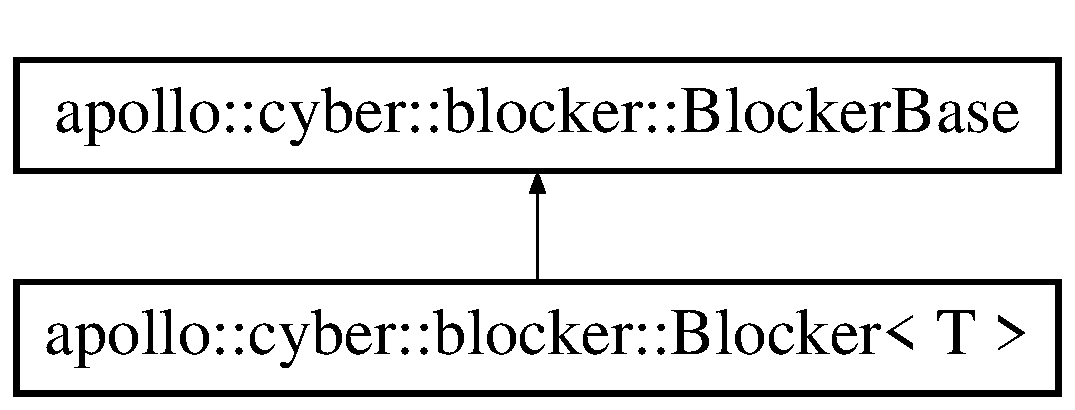
\includegraphics[height=2.000000cm]{classapollo_1_1cyber_1_1blocker_1_1Blocker}
\end{center}
\end{figure}
\subsection*{Public Types}
\begin{DoxyCompactItemize}
\item 
using \hyperlink{classapollo_1_1cyber_1_1blocker_1_1Blocker_ab6f5eb86a03109c66581e377a896650a}{Message\-Type} = T
\item 
using \hyperlink{classapollo_1_1cyber_1_1blocker_1_1Blocker_acfdb26545f6e05820e043a22ed91ed1d}{Message\-Ptr} = std\-::shared\-\_\-ptr$<$ T $>$
\item 
using \hyperlink{classapollo_1_1cyber_1_1blocker_1_1Blocker_a4c973a5afc09ca2b666f9436f2e74189}{Message\-Queue} = std\-::list$<$ \hyperlink{classapollo_1_1cyber_1_1blocker_1_1Blocker_acfdb26545f6e05820e043a22ed91ed1d}{Message\-Ptr} $>$
\item 
using \hyperlink{classapollo_1_1cyber_1_1blocker_1_1Blocker_aadf3f89fd884e1d9d2464172ede9213f}{Callback} = std\-::function$<$ void(const \hyperlink{classapollo_1_1cyber_1_1blocker_1_1Blocker_acfdb26545f6e05820e043a22ed91ed1d}{Message\-Ptr} \&)$>$
\item 
using \hyperlink{classapollo_1_1cyber_1_1blocker_1_1Blocker_ace3015075930b98718441655315002d5}{Callback\-Map} = std\-::unordered\-\_\-map$<$ std\-::string, \hyperlink{classapollo_1_1cyber_1_1blocker_1_1Blocker_aadf3f89fd884e1d9d2464172ede9213f}{Callback} $>$
\item 
using \hyperlink{classapollo_1_1cyber_1_1blocker_1_1Blocker_a62c6fc3bb53c24ed9dd2bc69bdad7e3d}{Iterator} = typename std\-::list$<$ std\-::shared\-\_\-ptr$<$ T $>$$>$\-::const\-\_\-iterator
\end{DoxyCompactItemize}
\subsection*{Public Member Functions}
\begin{DoxyCompactItemize}
\item 
\hyperlink{classapollo_1_1cyber_1_1blocker_1_1Blocker_a088532493a0783825880ed2dbf97f783}{Blocker} (const \hyperlink{structapollo_1_1cyber_1_1blocker_1_1BlockerAttr}{Blocker\-Attr} \&attr)
\item 
virtual \hyperlink{classapollo_1_1cyber_1_1blocker_1_1Blocker_a843112b632a8700b492e91161e3792ea}{$\sim$\-Blocker} ()
\item 
void \hyperlink{classapollo_1_1cyber_1_1blocker_1_1Blocker_a6c07deb7c68f3007f484048cac1ae532}{Publish} (const \hyperlink{classapollo_1_1cyber_1_1blocker_1_1Blocker_ab6f5eb86a03109c66581e377a896650a}{Message\-Type} \&msg)
\item 
void \hyperlink{classapollo_1_1cyber_1_1blocker_1_1Blocker_a511886deab8a981a9f054d3f3622825a}{Publish} (const \hyperlink{classapollo_1_1cyber_1_1blocker_1_1Blocker_acfdb26545f6e05820e043a22ed91ed1d}{Message\-Ptr} \&msg)
\item 
void \hyperlink{classapollo_1_1cyber_1_1blocker_1_1Blocker_a2c1d83849cd31a60e0cd77fa20c0fb28}{Clear\-Observed} () override
\item 
void \hyperlink{classapollo_1_1cyber_1_1blocker_1_1Blocker_a541bf01ca37ca188743d43f0130f8ea7}{Clear\-Published} () override
\item 
void \hyperlink{classapollo_1_1cyber_1_1blocker_1_1Blocker_aa2daeae7b6757bbe6a8066ed045dc891}{Observe} () override
\item 
bool \hyperlink{classapollo_1_1cyber_1_1blocker_1_1Blocker_a629bb4a79c48af5998c52036b27dbc7a}{Is\-Observed\-Empty} () const override
\item 
bool \hyperlink{classapollo_1_1cyber_1_1blocker_1_1Blocker_ac6d16f3829849b236509dde3bbae3b29}{Is\-Published\-Empty} () const override
\item 
bool \hyperlink{classapollo_1_1cyber_1_1blocker_1_1Blocker_a76e6a44944c9fc6608ebb4b609fc8504}{Subscribe} (const std\-::string \&callback\-\_\-id, const \hyperlink{classapollo_1_1cyber_1_1blocker_1_1Blocker_aadf3f89fd884e1d9d2464172ede9213f}{Callback} \&callback)
\item 
bool \hyperlink{classapollo_1_1cyber_1_1blocker_1_1Blocker_a4223c5b06e38b685fcab97605822fdc1}{Unsubscribe} (const std\-::string \&callback\-\_\-id) override
\item 
const \hyperlink{classapollo_1_1cyber_1_1blocker_1_1Blocker_ab6f5eb86a03109c66581e377a896650a}{Message\-Type} \& \hyperlink{classapollo_1_1cyber_1_1blocker_1_1Blocker_aa1afd44fb9b388c73c6aed51464dffe4}{Get\-Latest\-Observed} () const 
\item 
const \hyperlink{classapollo_1_1cyber_1_1blocker_1_1Blocker_acfdb26545f6e05820e043a22ed91ed1d}{Message\-Ptr} \hyperlink{classapollo_1_1cyber_1_1blocker_1_1Blocker_a14020fb49d3a2a52cf272ea2b7a4e971}{Get\-Latest\-Observed\-Ptr} () const 
\item 
const \hyperlink{classapollo_1_1cyber_1_1blocker_1_1Blocker_acfdb26545f6e05820e043a22ed91ed1d}{Message\-Ptr} \hyperlink{classapollo_1_1cyber_1_1blocker_1_1Blocker_a2ea6fb30c5190f2ed392bbe339ca7a9a}{Get\-Oldest\-Observed\-Ptr} () const 
\item 
const \hyperlink{classapollo_1_1cyber_1_1blocker_1_1Blocker_acfdb26545f6e05820e043a22ed91ed1d}{Message\-Ptr} \hyperlink{classapollo_1_1cyber_1_1blocker_1_1Blocker_ace2b23ef87620044f3931af23160f988}{Get\-Latest\-Published\-Ptr} () const 
\item 
\hyperlink{classapollo_1_1cyber_1_1blocker_1_1Blocker_a62c6fc3bb53c24ed9dd2bc69bdad7e3d}{Iterator} \hyperlink{classapollo_1_1cyber_1_1blocker_1_1Blocker_a679d0ffebcc4fa6f48c81f6c82f3ec92}{Observed\-Begin} () const 
\item 
\hyperlink{classapollo_1_1cyber_1_1blocker_1_1Blocker_a62c6fc3bb53c24ed9dd2bc69bdad7e3d}{Iterator} \hyperlink{classapollo_1_1cyber_1_1blocker_1_1Blocker_a91dea08c6179aa55994a7a842db100ef}{Observed\-End} () const 
\item 
size\-\_\-t \hyperlink{classapollo_1_1cyber_1_1blocker_1_1Blocker_a1560ce78043183df8b2d287cdc3824ed}{capacity} () const override
\item 
void \hyperlink{classapollo_1_1cyber_1_1blocker_1_1Blocker_ad2eef40f68908fc02c76be48cfc55b63}{set\-\_\-capacity} (size\-\_\-t \hyperlink{classapollo_1_1cyber_1_1blocker_1_1Blocker_a1560ce78043183df8b2d287cdc3824ed}{capacity}) override
\item 
const std\-::string \& \hyperlink{classapollo_1_1cyber_1_1blocker_1_1Blocker_ad121ab8e1fb379cd348267cccdc62624}{channel\-\_\-name} () const override
\end{DoxyCompactItemize}
\subsection*{Private Member Functions}
\begin{DoxyCompactItemize}
\item 
void \hyperlink{classapollo_1_1cyber_1_1blocker_1_1Blocker_a7372e1e554c724a5ca55de47837780da}{Reset} () override
\item 
void \hyperlink{classapollo_1_1cyber_1_1blocker_1_1Blocker_a2bb2d0e7cc2822d3898d9e374b54ee47}{Enqueue} (const \hyperlink{classapollo_1_1cyber_1_1blocker_1_1Blocker_acfdb26545f6e05820e043a22ed91ed1d}{Message\-Ptr} \&msg)
\item 
void \hyperlink{classapollo_1_1cyber_1_1blocker_1_1Blocker_a5c1c4c139f5ed9219ff22c9faf037944}{Notify} (const \hyperlink{classapollo_1_1cyber_1_1blocker_1_1Blocker_acfdb26545f6e05820e043a22ed91ed1d}{Message\-Ptr} \&msg)
\end{DoxyCompactItemize}
\subsection*{Private Attributes}
\begin{DoxyCompactItemize}
\item 
\hyperlink{structapollo_1_1cyber_1_1blocker_1_1BlockerAttr}{Blocker\-Attr} \hyperlink{classapollo_1_1cyber_1_1blocker_1_1Blocker_a31770fde4b92797a07af4f3eadb824ff}{attr\-\_\-}
\item 
\hyperlink{classapollo_1_1cyber_1_1blocker_1_1Blocker_a4c973a5afc09ca2b666f9436f2e74189}{Message\-Queue} \hyperlink{classapollo_1_1cyber_1_1blocker_1_1Blocker_ae27c916e638e027b4d06e6ff5a385b07}{observed\-\_\-msg\-\_\-queue\-\_\-}
\item 
\hyperlink{classapollo_1_1cyber_1_1blocker_1_1Blocker_a4c973a5afc09ca2b666f9436f2e74189}{Message\-Queue} \hyperlink{classapollo_1_1cyber_1_1blocker_1_1Blocker_afeb0c15d39a0c555540858cfc86a2ce3}{published\-\_\-msg\-\_\-queue\-\_\-}
\item 
std\-::mutex \hyperlink{classapollo_1_1cyber_1_1blocker_1_1Blocker_ab6e6114fe76a04ec1b92c13482cffa00}{msg\-\_\-mutex\-\_\-}
\item 
\hyperlink{classapollo_1_1cyber_1_1blocker_1_1Blocker_ace3015075930b98718441655315002d5}{Callback\-Map} \hyperlink{classapollo_1_1cyber_1_1blocker_1_1Blocker_a930f027bbb0fa388b72301b376fa75b2}{published\-\_\-callbacks\-\_\-}
\item 
std\-::mutex \hyperlink{classapollo_1_1cyber_1_1blocker_1_1Blocker_aef42b424d6fe0416c40d3ea5110cbc7f}{cb\-\_\-mutex\-\_\-}
\item 
\hyperlink{classapollo_1_1cyber_1_1blocker_1_1Blocker_ab6f5eb86a03109c66581e377a896650a}{Message\-Type} \hyperlink{classapollo_1_1cyber_1_1blocker_1_1Blocker_a0b66558da5f459f983f120203583e613}{dummy\-\_\-msg\-\_\-}
\end{DoxyCompactItemize}
\subsection*{Friends}
\begin{DoxyCompactItemize}
\item 
class \hyperlink{classapollo_1_1cyber_1_1blocker_1_1Blocker_a125f26fb85cd399c64b22b95df83f810}{Blocker\-Manager}
\end{DoxyCompactItemize}


\subsection{Member Typedef Documentation}
\hypertarget{classapollo_1_1cyber_1_1blocker_1_1Blocker_aadf3f89fd884e1d9d2464172ede9213f}{\index{apollo\-::cyber\-::blocker\-::\-Blocker@{apollo\-::cyber\-::blocker\-::\-Blocker}!Callback@{Callback}}
\index{Callback@{Callback}!apollo::cyber::blocker::Blocker@{apollo\-::cyber\-::blocker\-::\-Blocker}}
\subsubsection[{Callback}]{\setlength{\rightskip}{0pt plus 5cm}template$<$typename T$>$ using {\bf apollo\-::cyber\-::blocker\-::\-Blocker}$<$ T $>$\-::{\bf Callback} =  std\-::function$<$void(const {\bf Message\-Ptr}\&)$>$}}\label{classapollo_1_1cyber_1_1blocker_1_1Blocker_aadf3f89fd884e1d9d2464172ede9213f}
\hypertarget{classapollo_1_1cyber_1_1blocker_1_1Blocker_ace3015075930b98718441655315002d5}{\index{apollo\-::cyber\-::blocker\-::\-Blocker@{apollo\-::cyber\-::blocker\-::\-Blocker}!Callback\-Map@{Callback\-Map}}
\index{Callback\-Map@{Callback\-Map}!apollo::cyber::blocker::Blocker@{apollo\-::cyber\-::blocker\-::\-Blocker}}
\subsubsection[{Callback\-Map}]{\setlength{\rightskip}{0pt plus 5cm}template$<$typename T$>$ using {\bf apollo\-::cyber\-::blocker\-::\-Blocker}$<$ T $>$\-::{\bf Callback\-Map} =  std\-::unordered\-\_\-map$<$std\-::string, {\bf Callback}$>$}}\label{classapollo_1_1cyber_1_1blocker_1_1Blocker_ace3015075930b98718441655315002d5}
\hypertarget{classapollo_1_1cyber_1_1blocker_1_1Blocker_a62c6fc3bb53c24ed9dd2bc69bdad7e3d}{\index{apollo\-::cyber\-::blocker\-::\-Blocker@{apollo\-::cyber\-::blocker\-::\-Blocker}!Iterator@{Iterator}}
\index{Iterator@{Iterator}!apollo::cyber::blocker::Blocker@{apollo\-::cyber\-::blocker\-::\-Blocker}}
\subsubsection[{Iterator}]{\setlength{\rightskip}{0pt plus 5cm}template$<$typename T$>$ using {\bf apollo\-::cyber\-::blocker\-::\-Blocker}$<$ T $>$\-::{\bf Iterator} =  typename std\-::list$<$std\-::shared\-\_\-ptr$<$T$>$$>$\-::const\-\_\-iterator}}\label{classapollo_1_1cyber_1_1blocker_1_1Blocker_a62c6fc3bb53c24ed9dd2bc69bdad7e3d}
\hypertarget{classapollo_1_1cyber_1_1blocker_1_1Blocker_acfdb26545f6e05820e043a22ed91ed1d}{\index{apollo\-::cyber\-::blocker\-::\-Blocker@{apollo\-::cyber\-::blocker\-::\-Blocker}!Message\-Ptr@{Message\-Ptr}}
\index{Message\-Ptr@{Message\-Ptr}!apollo::cyber::blocker::Blocker@{apollo\-::cyber\-::blocker\-::\-Blocker}}
\subsubsection[{Message\-Ptr}]{\setlength{\rightskip}{0pt plus 5cm}template$<$typename T$>$ using {\bf apollo\-::cyber\-::blocker\-::\-Blocker}$<$ T $>$\-::{\bf Message\-Ptr} =  std\-::shared\-\_\-ptr$<$T$>$}}\label{classapollo_1_1cyber_1_1blocker_1_1Blocker_acfdb26545f6e05820e043a22ed91ed1d}
\hypertarget{classapollo_1_1cyber_1_1blocker_1_1Blocker_a4c973a5afc09ca2b666f9436f2e74189}{\index{apollo\-::cyber\-::blocker\-::\-Blocker@{apollo\-::cyber\-::blocker\-::\-Blocker}!Message\-Queue@{Message\-Queue}}
\index{Message\-Queue@{Message\-Queue}!apollo::cyber::blocker::Blocker@{apollo\-::cyber\-::blocker\-::\-Blocker}}
\subsubsection[{Message\-Queue}]{\setlength{\rightskip}{0pt plus 5cm}template$<$typename T$>$ using {\bf apollo\-::cyber\-::blocker\-::\-Blocker}$<$ T $>$\-::{\bf Message\-Queue} =  std\-::list$<${\bf Message\-Ptr}$>$}}\label{classapollo_1_1cyber_1_1blocker_1_1Blocker_a4c973a5afc09ca2b666f9436f2e74189}
\hypertarget{classapollo_1_1cyber_1_1blocker_1_1Blocker_ab6f5eb86a03109c66581e377a896650a}{\index{apollo\-::cyber\-::blocker\-::\-Blocker@{apollo\-::cyber\-::blocker\-::\-Blocker}!Message\-Type@{Message\-Type}}
\index{Message\-Type@{Message\-Type}!apollo::cyber::blocker::Blocker@{apollo\-::cyber\-::blocker\-::\-Blocker}}
\subsubsection[{Message\-Type}]{\setlength{\rightskip}{0pt plus 5cm}template$<$typename T$>$ using {\bf apollo\-::cyber\-::blocker\-::\-Blocker}$<$ T $>$\-::{\bf Message\-Type} =  T}}\label{classapollo_1_1cyber_1_1blocker_1_1Blocker_ab6f5eb86a03109c66581e377a896650a}


\subsection{Constructor \& Destructor Documentation}
\hypertarget{classapollo_1_1cyber_1_1blocker_1_1Blocker_a088532493a0783825880ed2dbf97f783}{\index{apollo\-::cyber\-::blocker\-::\-Blocker@{apollo\-::cyber\-::blocker\-::\-Blocker}!Blocker@{Blocker}}
\index{Blocker@{Blocker}!apollo::cyber::blocker::Blocker@{apollo\-::cyber\-::blocker\-::\-Blocker}}
\subsubsection[{Blocker}]{\setlength{\rightskip}{0pt plus 5cm}template$<$typename T $>$ {\bf apollo\-::cyber\-::blocker\-::\-Blocker}$<$ T $>$\-::{\bf Blocker} (
\begin{DoxyParamCaption}
\item[{const {\bf Blocker\-Attr} \&}]{attr}
\end{DoxyParamCaption}
)\hspace{0.3cm}{\ttfamily [explicit]}}}\label{classapollo_1_1cyber_1_1blocker_1_1Blocker_a088532493a0783825880ed2dbf97f783}
\hypertarget{classapollo_1_1cyber_1_1blocker_1_1Blocker_a843112b632a8700b492e91161e3792ea}{\index{apollo\-::cyber\-::blocker\-::\-Blocker@{apollo\-::cyber\-::blocker\-::\-Blocker}!$\sim$\-Blocker@{$\sim$\-Blocker}}
\index{$\sim$\-Blocker@{$\sim$\-Blocker}!apollo::cyber::blocker::Blocker@{apollo\-::cyber\-::blocker\-::\-Blocker}}
\subsubsection[{$\sim$\-Blocker}]{\setlength{\rightskip}{0pt plus 5cm}template$<$typename T $>$ {\bf apollo\-::cyber\-::blocker\-::\-Blocker}$<$ T $>$\-::$\sim${\bf Blocker} (
\begin{DoxyParamCaption}
{}
\end{DoxyParamCaption}
)\hspace{0.3cm}{\ttfamily [virtual]}}}\label{classapollo_1_1cyber_1_1blocker_1_1Blocker_a843112b632a8700b492e91161e3792ea}


\subsection{Member Function Documentation}
\hypertarget{classapollo_1_1cyber_1_1blocker_1_1Blocker_a1560ce78043183df8b2d287cdc3824ed}{\index{apollo\-::cyber\-::blocker\-::\-Blocker@{apollo\-::cyber\-::blocker\-::\-Blocker}!capacity@{capacity}}
\index{capacity@{capacity}!apollo::cyber::blocker::Blocker@{apollo\-::cyber\-::blocker\-::\-Blocker}}
\subsubsection[{capacity}]{\setlength{\rightskip}{0pt plus 5cm}template$<$typename T $>$ size\-\_\-t {\bf apollo\-::cyber\-::blocker\-::\-Blocker}$<$ T $>$\-::capacity (
\begin{DoxyParamCaption}
{}
\end{DoxyParamCaption}
) const\hspace{0.3cm}{\ttfamily [override]}, {\ttfamily [virtual]}}}\label{classapollo_1_1cyber_1_1blocker_1_1Blocker_a1560ce78043183df8b2d287cdc3824ed}


Implements \hyperlink{classapollo_1_1cyber_1_1blocker_1_1BlockerBase_a4b38e9b2314553bfd14edc8c0f80806d}{apollo\-::cyber\-::blocker\-::\-Blocker\-Base}.

\hypertarget{classapollo_1_1cyber_1_1blocker_1_1Blocker_ad121ab8e1fb379cd348267cccdc62624}{\index{apollo\-::cyber\-::blocker\-::\-Blocker@{apollo\-::cyber\-::blocker\-::\-Blocker}!channel\-\_\-name@{channel\-\_\-name}}
\index{channel\-\_\-name@{channel\-\_\-name}!apollo::cyber::blocker::Blocker@{apollo\-::cyber\-::blocker\-::\-Blocker}}
\subsubsection[{channel\-\_\-name}]{\setlength{\rightskip}{0pt plus 5cm}template$<$typename T $>$ const std\-::string \& {\bf apollo\-::cyber\-::blocker\-::\-Blocker}$<$ T $>$\-::channel\-\_\-name (
\begin{DoxyParamCaption}
{}
\end{DoxyParamCaption}
) const\hspace{0.3cm}{\ttfamily [override]}, {\ttfamily [virtual]}}}\label{classapollo_1_1cyber_1_1blocker_1_1Blocker_ad121ab8e1fb379cd348267cccdc62624}


Implements \hyperlink{classapollo_1_1cyber_1_1blocker_1_1BlockerBase_aa9606bd0d65712dfd8c62bee4db5180b}{apollo\-::cyber\-::blocker\-::\-Blocker\-Base}.

\hypertarget{classapollo_1_1cyber_1_1blocker_1_1Blocker_a2c1d83849cd31a60e0cd77fa20c0fb28}{\index{apollo\-::cyber\-::blocker\-::\-Blocker@{apollo\-::cyber\-::blocker\-::\-Blocker}!Clear\-Observed@{Clear\-Observed}}
\index{Clear\-Observed@{Clear\-Observed}!apollo::cyber::blocker::Blocker@{apollo\-::cyber\-::blocker\-::\-Blocker}}
\subsubsection[{Clear\-Observed}]{\setlength{\rightskip}{0pt plus 5cm}template$<$typename T $>$ void {\bf apollo\-::cyber\-::blocker\-::\-Blocker}$<$ T $>$\-::Clear\-Observed (
\begin{DoxyParamCaption}
{}
\end{DoxyParamCaption}
)\hspace{0.3cm}{\ttfamily [override]}, {\ttfamily [virtual]}}}\label{classapollo_1_1cyber_1_1blocker_1_1Blocker_a2c1d83849cd31a60e0cd77fa20c0fb28}


Implements \hyperlink{classapollo_1_1cyber_1_1blocker_1_1BlockerBase_aa644c34503729364e5742f36f4246469}{apollo\-::cyber\-::blocker\-::\-Blocker\-Base}.

\hypertarget{classapollo_1_1cyber_1_1blocker_1_1Blocker_a541bf01ca37ca188743d43f0130f8ea7}{\index{apollo\-::cyber\-::blocker\-::\-Blocker@{apollo\-::cyber\-::blocker\-::\-Blocker}!Clear\-Published@{Clear\-Published}}
\index{Clear\-Published@{Clear\-Published}!apollo::cyber::blocker::Blocker@{apollo\-::cyber\-::blocker\-::\-Blocker}}
\subsubsection[{Clear\-Published}]{\setlength{\rightskip}{0pt plus 5cm}template$<$typename T $>$ void {\bf apollo\-::cyber\-::blocker\-::\-Blocker}$<$ T $>$\-::Clear\-Published (
\begin{DoxyParamCaption}
{}
\end{DoxyParamCaption}
)\hspace{0.3cm}{\ttfamily [override]}, {\ttfamily [virtual]}}}\label{classapollo_1_1cyber_1_1blocker_1_1Blocker_a541bf01ca37ca188743d43f0130f8ea7}


Implements \hyperlink{classapollo_1_1cyber_1_1blocker_1_1BlockerBase_a79270e6fab5378d6b40162fb4322d189}{apollo\-::cyber\-::blocker\-::\-Blocker\-Base}.

\hypertarget{classapollo_1_1cyber_1_1blocker_1_1Blocker_a2bb2d0e7cc2822d3898d9e374b54ee47}{\index{apollo\-::cyber\-::blocker\-::\-Blocker@{apollo\-::cyber\-::blocker\-::\-Blocker}!Enqueue@{Enqueue}}
\index{Enqueue@{Enqueue}!apollo::cyber::blocker::Blocker@{apollo\-::cyber\-::blocker\-::\-Blocker}}
\subsubsection[{Enqueue}]{\setlength{\rightskip}{0pt plus 5cm}template$<$typename T $>$ void {\bf apollo\-::cyber\-::blocker\-::\-Blocker}$<$ T $>$\-::Enqueue (
\begin{DoxyParamCaption}
\item[{const {\bf Message\-Ptr} \&}]{msg}
\end{DoxyParamCaption}
)\hspace{0.3cm}{\ttfamily [private]}}}\label{classapollo_1_1cyber_1_1blocker_1_1Blocker_a2bb2d0e7cc2822d3898d9e374b54ee47}
\hypertarget{classapollo_1_1cyber_1_1blocker_1_1Blocker_aa1afd44fb9b388c73c6aed51464dffe4}{\index{apollo\-::cyber\-::blocker\-::\-Blocker@{apollo\-::cyber\-::blocker\-::\-Blocker}!Get\-Latest\-Observed@{Get\-Latest\-Observed}}
\index{Get\-Latest\-Observed@{Get\-Latest\-Observed}!apollo::cyber::blocker::Blocker@{apollo\-::cyber\-::blocker\-::\-Blocker}}
\subsubsection[{Get\-Latest\-Observed}]{\setlength{\rightskip}{0pt plus 5cm}template$<$typename T $>$ auto {\bf apollo\-::cyber\-::blocker\-::\-Blocker}$<$ T $>$\-::Get\-Latest\-Observed (
\begin{DoxyParamCaption}
{}
\end{DoxyParamCaption}
) const}}\label{classapollo_1_1cyber_1_1blocker_1_1Blocker_aa1afd44fb9b388c73c6aed51464dffe4}
\hypertarget{classapollo_1_1cyber_1_1blocker_1_1Blocker_a14020fb49d3a2a52cf272ea2b7a4e971}{\index{apollo\-::cyber\-::blocker\-::\-Blocker@{apollo\-::cyber\-::blocker\-::\-Blocker}!Get\-Latest\-Observed\-Ptr@{Get\-Latest\-Observed\-Ptr}}
\index{Get\-Latest\-Observed\-Ptr@{Get\-Latest\-Observed\-Ptr}!apollo::cyber::blocker::Blocker@{apollo\-::cyber\-::blocker\-::\-Blocker}}
\subsubsection[{Get\-Latest\-Observed\-Ptr}]{\setlength{\rightskip}{0pt plus 5cm}template$<$typename T $>$ auto {\bf apollo\-::cyber\-::blocker\-::\-Blocker}$<$ T $>$\-::Get\-Latest\-Observed\-Ptr (
\begin{DoxyParamCaption}
{}
\end{DoxyParamCaption}
) const}}\label{classapollo_1_1cyber_1_1blocker_1_1Blocker_a14020fb49d3a2a52cf272ea2b7a4e971}
\hypertarget{classapollo_1_1cyber_1_1blocker_1_1Blocker_ace2b23ef87620044f3931af23160f988}{\index{apollo\-::cyber\-::blocker\-::\-Blocker@{apollo\-::cyber\-::blocker\-::\-Blocker}!Get\-Latest\-Published\-Ptr@{Get\-Latest\-Published\-Ptr}}
\index{Get\-Latest\-Published\-Ptr@{Get\-Latest\-Published\-Ptr}!apollo::cyber::blocker::Blocker@{apollo\-::cyber\-::blocker\-::\-Blocker}}
\subsubsection[{Get\-Latest\-Published\-Ptr}]{\setlength{\rightskip}{0pt plus 5cm}template$<$typename T $>$ auto {\bf apollo\-::cyber\-::blocker\-::\-Blocker}$<$ T $>$\-::Get\-Latest\-Published\-Ptr (
\begin{DoxyParamCaption}
{}
\end{DoxyParamCaption}
) const}}\label{classapollo_1_1cyber_1_1blocker_1_1Blocker_ace2b23ef87620044f3931af23160f988}
\hypertarget{classapollo_1_1cyber_1_1blocker_1_1Blocker_a2ea6fb30c5190f2ed392bbe339ca7a9a}{\index{apollo\-::cyber\-::blocker\-::\-Blocker@{apollo\-::cyber\-::blocker\-::\-Blocker}!Get\-Oldest\-Observed\-Ptr@{Get\-Oldest\-Observed\-Ptr}}
\index{Get\-Oldest\-Observed\-Ptr@{Get\-Oldest\-Observed\-Ptr}!apollo::cyber::blocker::Blocker@{apollo\-::cyber\-::blocker\-::\-Blocker}}
\subsubsection[{Get\-Oldest\-Observed\-Ptr}]{\setlength{\rightskip}{0pt plus 5cm}template$<$typename T $>$ auto {\bf apollo\-::cyber\-::blocker\-::\-Blocker}$<$ T $>$\-::Get\-Oldest\-Observed\-Ptr (
\begin{DoxyParamCaption}
{}
\end{DoxyParamCaption}
) const}}\label{classapollo_1_1cyber_1_1blocker_1_1Blocker_a2ea6fb30c5190f2ed392bbe339ca7a9a}
\hypertarget{classapollo_1_1cyber_1_1blocker_1_1Blocker_a629bb4a79c48af5998c52036b27dbc7a}{\index{apollo\-::cyber\-::blocker\-::\-Blocker@{apollo\-::cyber\-::blocker\-::\-Blocker}!Is\-Observed\-Empty@{Is\-Observed\-Empty}}
\index{Is\-Observed\-Empty@{Is\-Observed\-Empty}!apollo::cyber::blocker::Blocker@{apollo\-::cyber\-::blocker\-::\-Blocker}}
\subsubsection[{Is\-Observed\-Empty}]{\setlength{\rightskip}{0pt plus 5cm}template$<$typename T $>$ bool {\bf apollo\-::cyber\-::blocker\-::\-Blocker}$<$ T $>$\-::Is\-Observed\-Empty (
\begin{DoxyParamCaption}
{}
\end{DoxyParamCaption}
) const\hspace{0.3cm}{\ttfamily [override]}, {\ttfamily [virtual]}}}\label{classapollo_1_1cyber_1_1blocker_1_1Blocker_a629bb4a79c48af5998c52036b27dbc7a}


Implements \hyperlink{classapollo_1_1cyber_1_1blocker_1_1BlockerBase_ae362222ab521ba70e034c41a602a2f28}{apollo\-::cyber\-::blocker\-::\-Blocker\-Base}.

\hypertarget{classapollo_1_1cyber_1_1blocker_1_1Blocker_ac6d16f3829849b236509dde3bbae3b29}{\index{apollo\-::cyber\-::blocker\-::\-Blocker@{apollo\-::cyber\-::blocker\-::\-Blocker}!Is\-Published\-Empty@{Is\-Published\-Empty}}
\index{Is\-Published\-Empty@{Is\-Published\-Empty}!apollo::cyber::blocker::Blocker@{apollo\-::cyber\-::blocker\-::\-Blocker}}
\subsubsection[{Is\-Published\-Empty}]{\setlength{\rightskip}{0pt plus 5cm}template$<$typename T $>$ bool {\bf apollo\-::cyber\-::blocker\-::\-Blocker}$<$ T $>$\-::Is\-Published\-Empty (
\begin{DoxyParamCaption}
{}
\end{DoxyParamCaption}
) const\hspace{0.3cm}{\ttfamily [override]}, {\ttfamily [virtual]}}}\label{classapollo_1_1cyber_1_1blocker_1_1Blocker_ac6d16f3829849b236509dde3bbae3b29}


Implements \hyperlink{classapollo_1_1cyber_1_1blocker_1_1BlockerBase_a38759de3825c1768af583bebe334aaf1}{apollo\-::cyber\-::blocker\-::\-Blocker\-Base}.

\hypertarget{classapollo_1_1cyber_1_1blocker_1_1Blocker_a5c1c4c139f5ed9219ff22c9faf037944}{\index{apollo\-::cyber\-::blocker\-::\-Blocker@{apollo\-::cyber\-::blocker\-::\-Blocker}!Notify@{Notify}}
\index{Notify@{Notify}!apollo::cyber::blocker::Blocker@{apollo\-::cyber\-::blocker\-::\-Blocker}}
\subsubsection[{Notify}]{\setlength{\rightskip}{0pt plus 5cm}template$<$typename T $>$ void {\bf apollo\-::cyber\-::blocker\-::\-Blocker}$<$ T $>$\-::Notify (
\begin{DoxyParamCaption}
\item[{const {\bf Message\-Ptr} \&}]{msg}
\end{DoxyParamCaption}
)\hspace{0.3cm}{\ttfamily [private]}}}\label{classapollo_1_1cyber_1_1blocker_1_1Blocker_a5c1c4c139f5ed9219ff22c9faf037944}
\hypertarget{classapollo_1_1cyber_1_1blocker_1_1Blocker_aa2daeae7b6757bbe6a8066ed045dc891}{\index{apollo\-::cyber\-::blocker\-::\-Blocker@{apollo\-::cyber\-::blocker\-::\-Blocker}!Observe@{Observe}}
\index{Observe@{Observe}!apollo::cyber::blocker::Blocker@{apollo\-::cyber\-::blocker\-::\-Blocker}}
\subsubsection[{Observe}]{\setlength{\rightskip}{0pt plus 5cm}template$<$typename T $>$ void {\bf apollo\-::cyber\-::blocker\-::\-Blocker}$<$ T $>$\-::Observe (
\begin{DoxyParamCaption}
{}
\end{DoxyParamCaption}
)\hspace{0.3cm}{\ttfamily [override]}, {\ttfamily [virtual]}}}\label{classapollo_1_1cyber_1_1blocker_1_1Blocker_aa2daeae7b6757bbe6a8066ed045dc891}


Implements \hyperlink{classapollo_1_1cyber_1_1blocker_1_1BlockerBase_ad14b2e2e37c4436f2ef72e78505aa271}{apollo\-::cyber\-::blocker\-::\-Blocker\-Base}.

\hypertarget{classapollo_1_1cyber_1_1blocker_1_1Blocker_a679d0ffebcc4fa6f48c81f6c82f3ec92}{\index{apollo\-::cyber\-::blocker\-::\-Blocker@{apollo\-::cyber\-::blocker\-::\-Blocker}!Observed\-Begin@{Observed\-Begin}}
\index{Observed\-Begin@{Observed\-Begin}!apollo::cyber::blocker::Blocker@{apollo\-::cyber\-::blocker\-::\-Blocker}}
\subsubsection[{Observed\-Begin}]{\setlength{\rightskip}{0pt plus 5cm}template$<$typename T $>$ auto {\bf apollo\-::cyber\-::blocker\-::\-Blocker}$<$ T $>$\-::Observed\-Begin (
\begin{DoxyParamCaption}
{}
\end{DoxyParamCaption}
) const}}\label{classapollo_1_1cyber_1_1blocker_1_1Blocker_a679d0ffebcc4fa6f48c81f6c82f3ec92}
\hypertarget{classapollo_1_1cyber_1_1blocker_1_1Blocker_a91dea08c6179aa55994a7a842db100ef}{\index{apollo\-::cyber\-::blocker\-::\-Blocker@{apollo\-::cyber\-::blocker\-::\-Blocker}!Observed\-End@{Observed\-End}}
\index{Observed\-End@{Observed\-End}!apollo::cyber::blocker::Blocker@{apollo\-::cyber\-::blocker\-::\-Blocker}}
\subsubsection[{Observed\-End}]{\setlength{\rightskip}{0pt plus 5cm}template$<$typename T $>$ auto {\bf apollo\-::cyber\-::blocker\-::\-Blocker}$<$ T $>$\-::Observed\-End (
\begin{DoxyParamCaption}
{}
\end{DoxyParamCaption}
) const}}\label{classapollo_1_1cyber_1_1blocker_1_1Blocker_a91dea08c6179aa55994a7a842db100ef}
\hypertarget{classapollo_1_1cyber_1_1blocker_1_1Blocker_a6c07deb7c68f3007f484048cac1ae532}{\index{apollo\-::cyber\-::blocker\-::\-Blocker@{apollo\-::cyber\-::blocker\-::\-Blocker}!Publish@{Publish}}
\index{Publish@{Publish}!apollo::cyber::blocker::Blocker@{apollo\-::cyber\-::blocker\-::\-Blocker}}
\subsubsection[{Publish}]{\setlength{\rightskip}{0pt plus 5cm}template$<$typename T $>$ void {\bf apollo\-::cyber\-::blocker\-::\-Blocker}$<$ T $>$\-::Publish (
\begin{DoxyParamCaption}
\item[{const {\bf Message\-Type} \&}]{msg}
\end{DoxyParamCaption}
)}}\label{classapollo_1_1cyber_1_1blocker_1_1Blocker_a6c07deb7c68f3007f484048cac1ae532}
\hypertarget{classapollo_1_1cyber_1_1blocker_1_1Blocker_a511886deab8a981a9f054d3f3622825a}{\index{apollo\-::cyber\-::blocker\-::\-Blocker@{apollo\-::cyber\-::blocker\-::\-Blocker}!Publish@{Publish}}
\index{Publish@{Publish}!apollo::cyber::blocker::Blocker@{apollo\-::cyber\-::blocker\-::\-Blocker}}
\subsubsection[{Publish}]{\setlength{\rightskip}{0pt plus 5cm}template$<$typename T $>$ void {\bf apollo\-::cyber\-::blocker\-::\-Blocker}$<$ T $>$\-::Publish (
\begin{DoxyParamCaption}
\item[{const {\bf Message\-Ptr} \&}]{msg}
\end{DoxyParamCaption}
)}}\label{classapollo_1_1cyber_1_1blocker_1_1Blocker_a511886deab8a981a9f054d3f3622825a}
\hypertarget{classapollo_1_1cyber_1_1blocker_1_1Blocker_a7372e1e554c724a5ca55de47837780da}{\index{apollo\-::cyber\-::blocker\-::\-Blocker@{apollo\-::cyber\-::blocker\-::\-Blocker}!Reset@{Reset}}
\index{Reset@{Reset}!apollo::cyber::blocker::Blocker@{apollo\-::cyber\-::blocker\-::\-Blocker}}
\subsubsection[{Reset}]{\setlength{\rightskip}{0pt plus 5cm}template$<$typename T $>$ void {\bf apollo\-::cyber\-::blocker\-::\-Blocker}$<$ T $>$\-::Reset (
\begin{DoxyParamCaption}
{}
\end{DoxyParamCaption}
)\hspace{0.3cm}{\ttfamily [override]}, {\ttfamily [private]}, {\ttfamily [virtual]}}}\label{classapollo_1_1cyber_1_1blocker_1_1Blocker_a7372e1e554c724a5ca55de47837780da}


Implements \hyperlink{classapollo_1_1cyber_1_1blocker_1_1BlockerBase_a32fd8d73c7d5a5e4e2521f95126934d4}{apollo\-::cyber\-::blocker\-::\-Blocker\-Base}.

\hypertarget{classapollo_1_1cyber_1_1blocker_1_1Blocker_ad2eef40f68908fc02c76be48cfc55b63}{\index{apollo\-::cyber\-::blocker\-::\-Blocker@{apollo\-::cyber\-::blocker\-::\-Blocker}!set\-\_\-capacity@{set\-\_\-capacity}}
\index{set\-\_\-capacity@{set\-\_\-capacity}!apollo::cyber::blocker::Blocker@{apollo\-::cyber\-::blocker\-::\-Blocker}}
\subsubsection[{set\-\_\-capacity}]{\setlength{\rightskip}{0pt plus 5cm}template$<$typename T $>$ void {\bf apollo\-::cyber\-::blocker\-::\-Blocker}$<$ T $>$\-::set\-\_\-capacity (
\begin{DoxyParamCaption}
\item[{size\-\_\-t}]{capacity}
\end{DoxyParamCaption}
)\hspace{0.3cm}{\ttfamily [override]}, {\ttfamily [virtual]}}}\label{classapollo_1_1cyber_1_1blocker_1_1Blocker_ad2eef40f68908fc02c76be48cfc55b63}


Implements \hyperlink{classapollo_1_1cyber_1_1blocker_1_1BlockerBase_aa3db5ee03360d7d645dad38c0352e4e6}{apollo\-::cyber\-::blocker\-::\-Blocker\-Base}.

\hypertarget{classapollo_1_1cyber_1_1blocker_1_1Blocker_a76e6a44944c9fc6608ebb4b609fc8504}{\index{apollo\-::cyber\-::blocker\-::\-Blocker@{apollo\-::cyber\-::blocker\-::\-Blocker}!Subscribe@{Subscribe}}
\index{Subscribe@{Subscribe}!apollo::cyber::blocker::Blocker@{apollo\-::cyber\-::blocker\-::\-Blocker}}
\subsubsection[{Subscribe}]{\setlength{\rightskip}{0pt plus 5cm}template$<$typename T $>$ bool {\bf apollo\-::cyber\-::blocker\-::\-Blocker}$<$ T $>$\-::Subscribe (
\begin{DoxyParamCaption}
\item[{const std\-::string \&}]{callback\-\_\-id, }
\item[{const {\bf Callback} \&}]{callback}
\end{DoxyParamCaption}
)}}\label{classapollo_1_1cyber_1_1blocker_1_1Blocker_a76e6a44944c9fc6608ebb4b609fc8504}
\hypertarget{classapollo_1_1cyber_1_1blocker_1_1Blocker_a4223c5b06e38b685fcab97605822fdc1}{\index{apollo\-::cyber\-::blocker\-::\-Blocker@{apollo\-::cyber\-::blocker\-::\-Blocker}!Unsubscribe@{Unsubscribe}}
\index{Unsubscribe@{Unsubscribe}!apollo::cyber::blocker::Blocker@{apollo\-::cyber\-::blocker\-::\-Blocker}}
\subsubsection[{Unsubscribe}]{\setlength{\rightskip}{0pt plus 5cm}template$<$typename T $>$ bool {\bf apollo\-::cyber\-::blocker\-::\-Blocker}$<$ T $>$\-::Unsubscribe (
\begin{DoxyParamCaption}
\item[{const std\-::string \&}]{callback\-\_\-id}
\end{DoxyParamCaption}
)\hspace{0.3cm}{\ttfamily [override]}, {\ttfamily [virtual]}}}\label{classapollo_1_1cyber_1_1blocker_1_1Blocker_a4223c5b06e38b685fcab97605822fdc1}


Implements \hyperlink{classapollo_1_1cyber_1_1blocker_1_1BlockerBase_a8fd56887517c5015e32cd96544cd2d6a}{apollo\-::cyber\-::blocker\-::\-Blocker\-Base}.



\subsection{Friends And Related Function Documentation}
\hypertarget{classapollo_1_1cyber_1_1blocker_1_1Blocker_a125f26fb85cd399c64b22b95df83f810}{\index{apollo\-::cyber\-::blocker\-::\-Blocker@{apollo\-::cyber\-::blocker\-::\-Blocker}!Blocker\-Manager@{Blocker\-Manager}}
\index{Blocker\-Manager@{Blocker\-Manager}!apollo::cyber::blocker::Blocker@{apollo\-::cyber\-::blocker\-::\-Blocker}}
\subsubsection[{Blocker\-Manager}]{\setlength{\rightskip}{0pt plus 5cm}template$<$typename T$>$ friend class {\bf Blocker\-Manager}\hspace{0.3cm}{\ttfamily [friend]}}}\label{classapollo_1_1cyber_1_1blocker_1_1Blocker_a125f26fb85cd399c64b22b95df83f810}


\subsection{Member Data Documentation}
\hypertarget{classapollo_1_1cyber_1_1blocker_1_1Blocker_a31770fde4b92797a07af4f3eadb824ff}{\index{apollo\-::cyber\-::blocker\-::\-Blocker@{apollo\-::cyber\-::blocker\-::\-Blocker}!attr\-\_\-@{attr\-\_\-}}
\index{attr\-\_\-@{attr\-\_\-}!apollo::cyber::blocker::Blocker@{apollo\-::cyber\-::blocker\-::\-Blocker}}
\subsubsection[{attr\-\_\-}]{\setlength{\rightskip}{0pt plus 5cm}template$<$typename T$>$ {\bf Blocker\-Attr} {\bf apollo\-::cyber\-::blocker\-::\-Blocker}$<$ T $>$\-::attr\-\_\-\hspace{0.3cm}{\ttfamily [private]}}}\label{classapollo_1_1cyber_1_1blocker_1_1Blocker_a31770fde4b92797a07af4f3eadb824ff}
\hypertarget{classapollo_1_1cyber_1_1blocker_1_1Blocker_aef42b424d6fe0416c40d3ea5110cbc7f}{\index{apollo\-::cyber\-::blocker\-::\-Blocker@{apollo\-::cyber\-::blocker\-::\-Blocker}!cb\-\_\-mutex\-\_\-@{cb\-\_\-mutex\-\_\-}}
\index{cb\-\_\-mutex\-\_\-@{cb\-\_\-mutex\-\_\-}!apollo::cyber::blocker::Blocker@{apollo\-::cyber\-::blocker\-::\-Blocker}}
\subsubsection[{cb\-\_\-mutex\-\_\-}]{\setlength{\rightskip}{0pt plus 5cm}template$<$typename T$>$ std\-::mutex {\bf apollo\-::cyber\-::blocker\-::\-Blocker}$<$ T $>$\-::cb\-\_\-mutex\-\_\-\hspace{0.3cm}{\ttfamily [mutable]}, {\ttfamily [private]}}}\label{classapollo_1_1cyber_1_1blocker_1_1Blocker_aef42b424d6fe0416c40d3ea5110cbc7f}
\hypertarget{classapollo_1_1cyber_1_1blocker_1_1Blocker_a0b66558da5f459f983f120203583e613}{\index{apollo\-::cyber\-::blocker\-::\-Blocker@{apollo\-::cyber\-::blocker\-::\-Blocker}!dummy\-\_\-msg\-\_\-@{dummy\-\_\-msg\-\_\-}}
\index{dummy\-\_\-msg\-\_\-@{dummy\-\_\-msg\-\_\-}!apollo::cyber::blocker::Blocker@{apollo\-::cyber\-::blocker\-::\-Blocker}}
\subsubsection[{dummy\-\_\-msg\-\_\-}]{\setlength{\rightskip}{0pt plus 5cm}template$<$typename T$>$ {\bf Message\-Type} {\bf apollo\-::cyber\-::blocker\-::\-Blocker}$<$ T $>$\-::dummy\-\_\-msg\-\_\-\hspace{0.3cm}{\ttfamily [private]}}}\label{classapollo_1_1cyber_1_1blocker_1_1Blocker_a0b66558da5f459f983f120203583e613}
\hypertarget{classapollo_1_1cyber_1_1blocker_1_1Blocker_ab6e6114fe76a04ec1b92c13482cffa00}{\index{apollo\-::cyber\-::blocker\-::\-Blocker@{apollo\-::cyber\-::blocker\-::\-Blocker}!msg\-\_\-mutex\-\_\-@{msg\-\_\-mutex\-\_\-}}
\index{msg\-\_\-mutex\-\_\-@{msg\-\_\-mutex\-\_\-}!apollo::cyber::blocker::Blocker@{apollo\-::cyber\-::blocker\-::\-Blocker}}
\subsubsection[{msg\-\_\-mutex\-\_\-}]{\setlength{\rightskip}{0pt plus 5cm}template$<$typename T$>$ std\-::mutex {\bf apollo\-::cyber\-::blocker\-::\-Blocker}$<$ T $>$\-::msg\-\_\-mutex\-\_\-\hspace{0.3cm}{\ttfamily [mutable]}, {\ttfamily [private]}}}\label{classapollo_1_1cyber_1_1blocker_1_1Blocker_ab6e6114fe76a04ec1b92c13482cffa00}
\hypertarget{classapollo_1_1cyber_1_1blocker_1_1Blocker_ae27c916e638e027b4d06e6ff5a385b07}{\index{apollo\-::cyber\-::blocker\-::\-Blocker@{apollo\-::cyber\-::blocker\-::\-Blocker}!observed\-\_\-msg\-\_\-queue\-\_\-@{observed\-\_\-msg\-\_\-queue\-\_\-}}
\index{observed\-\_\-msg\-\_\-queue\-\_\-@{observed\-\_\-msg\-\_\-queue\-\_\-}!apollo::cyber::blocker::Blocker@{apollo\-::cyber\-::blocker\-::\-Blocker}}
\subsubsection[{observed\-\_\-msg\-\_\-queue\-\_\-}]{\setlength{\rightskip}{0pt plus 5cm}template$<$typename T$>$ {\bf Message\-Queue} {\bf apollo\-::cyber\-::blocker\-::\-Blocker}$<$ T $>$\-::observed\-\_\-msg\-\_\-queue\-\_\-\hspace{0.3cm}{\ttfamily [private]}}}\label{classapollo_1_1cyber_1_1blocker_1_1Blocker_ae27c916e638e027b4d06e6ff5a385b07}
\hypertarget{classapollo_1_1cyber_1_1blocker_1_1Blocker_a930f027bbb0fa388b72301b376fa75b2}{\index{apollo\-::cyber\-::blocker\-::\-Blocker@{apollo\-::cyber\-::blocker\-::\-Blocker}!published\-\_\-callbacks\-\_\-@{published\-\_\-callbacks\-\_\-}}
\index{published\-\_\-callbacks\-\_\-@{published\-\_\-callbacks\-\_\-}!apollo::cyber::blocker::Blocker@{apollo\-::cyber\-::blocker\-::\-Blocker}}
\subsubsection[{published\-\_\-callbacks\-\_\-}]{\setlength{\rightskip}{0pt plus 5cm}template$<$typename T$>$ {\bf Callback\-Map} {\bf apollo\-::cyber\-::blocker\-::\-Blocker}$<$ T $>$\-::published\-\_\-callbacks\-\_\-\hspace{0.3cm}{\ttfamily [private]}}}\label{classapollo_1_1cyber_1_1blocker_1_1Blocker_a930f027bbb0fa388b72301b376fa75b2}
\hypertarget{classapollo_1_1cyber_1_1blocker_1_1Blocker_afeb0c15d39a0c555540858cfc86a2ce3}{\index{apollo\-::cyber\-::blocker\-::\-Blocker@{apollo\-::cyber\-::blocker\-::\-Blocker}!published\-\_\-msg\-\_\-queue\-\_\-@{published\-\_\-msg\-\_\-queue\-\_\-}}
\index{published\-\_\-msg\-\_\-queue\-\_\-@{published\-\_\-msg\-\_\-queue\-\_\-}!apollo::cyber::blocker::Blocker@{apollo\-::cyber\-::blocker\-::\-Blocker}}
\subsubsection[{published\-\_\-msg\-\_\-queue\-\_\-}]{\setlength{\rightskip}{0pt plus 5cm}template$<$typename T$>$ {\bf Message\-Queue} {\bf apollo\-::cyber\-::blocker\-::\-Blocker}$<$ T $>$\-::published\-\_\-msg\-\_\-queue\-\_\-\hspace{0.3cm}{\ttfamily [private]}}}\label{classapollo_1_1cyber_1_1blocker_1_1Blocker_afeb0c15d39a0c555540858cfc86a2ce3}


The documentation for this class was generated from the following file\-:\begin{DoxyCompactItemize}
\item 
blocker/\hyperlink{blocker_8h}{blocker.\-h}\end{DoxyCompactItemize}

\hypertarget{structapollo_1_1cyber_1_1blocker_1_1BlockerAttr}{\section{apollo\-:\-:cyber\-:\-:blocker\-:\-:Blocker\-Attr Struct Reference}
\label{structapollo_1_1cyber_1_1blocker_1_1BlockerAttr}\index{apollo\-::cyber\-::blocker\-::\-Blocker\-Attr@{apollo\-::cyber\-::blocker\-::\-Blocker\-Attr}}
}


{\ttfamily \#include $<$blocker.\-h$>$}

\subsection*{Public Member Functions}
\begin{DoxyCompactItemize}
\item 
\hyperlink{structapollo_1_1cyber_1_1blocker_1_1BlockerAttr_a92b49ec1c15140529af125c4564e74da}{Blocker\-Attr} ()
\item 
\hyperlink{structapollo_1_1cyber_1_1blocker_1_1BlockerAttr_a67b6974da8f485564fba38c798731020}{Blocker\-Attr} (const std\-::string \&channel)
\item 
\hyperlink{structapollo_1_1cyber_1_1blocker_1_1BlockerAttr_a5bcf6983e3209f8e3707640d5c88aaef}{Blocker\-Attr} (size\-\_\-t cap, const std\-::string \&channel)
\item 
\hyperlink{structapollo_1_1cyber_1_1blocker_1_1BlockerAttr_a2eee05c6ef614ac1876aa4cbcdebf7b3}{Blocker\-Attr} (const \hyperlink{structapollo_1_1cyber_1_1blocker_1_1BlockerAttr}{Blocker\-Attr} \&attr)
\end{DoxyCompactItemize}
\subsection*{Public Attributes}
\begin{DoxyCompactItemize}
\item 
size\-\_\-t \hyperlink{structapollo_1_1cyber_1_1blocker_1_1BlockerAttr_a6b3a70ebf5ed158445ca952263d90921}{capacity}
\item 
std\-::string \hyperlink{structapollo_1_1cyber_1_1blocker_1_1BlockerAttr_a10e1a69f1ab4ba0c95ce0584eec4bca1}{channel\-\_\-name}
\end{DoxyCompactItemize}


\subsection{Constructor \& Destructor Documentation}
\hypertarget{structapollo_1_1cyber_1_1blocker_1_1BlockerAttr_a92b49ec1c15140529af125c4564e74da}{\index{apollo\-::cyber\-::blocker\-::\-Blocker\-Attr@{apollo\-::cyber\-::blocker\-::\-Blocker\-Attr}!Blocker\-Attr@{Blocker\-Attr}}
\index{Blocker\-Attr@{Blocker\-Attr}!apollo::cyber::blocker::BlockerAttr@{apollo\-::cyber\-::blocker\-::\-Blocker\-Attr}}
\subsubsection[{Blocker\-Attr}]{\setlength{\rightskip}{0pt plus 5cm}apollo\-::cyber\-::blocker\-::\-Blocker\-Attr\-::\-Blocker\-Attr (
\begin{DoxyParamCaption}
{}
\end{DoxyParamCaption}
)\hspace{0.3cm}{\ttfamily [inline]}}}\label{structapollo_1_1cyber_1_1blocker_1_1BlockerAttr_a92b49ec1c15140529af125c4564e74da}
\hypertarget{structapollo_1_1cyber_1_1blocker_1_1BlockerAttr_a67b6974da8f485564fba38c798731020}{\index{apollo\-::cyber\-::blocker\-::\-Blocker\-Attr@{apollo\-::cyber\-::blocker\-::\-Blocker\-Attr}!Blocker\-Attr@{Blocker\-Attr}}
\index{Blocker\-Attr@{Blocker\-Attr}!apollo::cyber::blocker::BlockerAttr@{apollo\-::cyber\-::blocker\-::\-Blocker\-Attr}}
\subsubsection[{Blocker\-Attr}]{\setlength{\rightskip}{0pt plus 5cm}apollo\-::cyber\-::blocker\-::\-Blocker\-Attr\-::\-Blocker\-Attr (
\begin{DoxyParamCaption}
\item[{const std\-::string \&}]{channel}
\end{DoxyParamCaption}
)\hspace{0.3cm}{\ttfamily [inline]}, {\ttfamily [explicit]}}}\label{structapollo_1_1cyber_1_1blocker_1_1BlockerAttr_a67b6974da8f485564fba38c798731020}
\hypertarget{structapollo_1_1cyber_1_1blocker_1_1BlockerAttr_a5bcf6983e3209f8e3707640d5c88aaef}{\index{apollo\-::cyber\-::blocker\-::\-Blocker\-Attr@{apollo\-::cyber\-::blocker\-::\-Blocker\-Attr}!Blocker\-Attr@{Blocker\-Attr}}
\index{Blocker\-Attr@{Blocker\-Attr}!apollo::cyber::blocker::BlockerAttr@{apollo\-::cyber\-::blocker\-::\-Blocker\-Attr}}
\subsubsection[{Blocker\-Attr}]{\setlength{\rightskip}{0pt plus 5cm}apollo\-::cyber\-::blocker\-::\-Blocker\-Attr\-::\-Blocker\-Attr (
\begin{DoxyParamCaption}
\item[{size\-\_\-t}]{cap, }
\item[{const std\-::string \&}]{channel}
\end{DoxyParamCaption}
)\hspace{0.3cm}{\ttfamily [inline]}}}\label{structapollo_1_1cyber_1_1blocker_1_1BlockerAttr_a5bcf6983e3209f8e3707640d5c88aaef}
\hypertarget{structapollo_1_1cyber_1_1blocker_1_1BlockerAttr_a2eee05c6ef614ac1876aa4cbcdebf7b3}{\index{apollo\-::cyber\-::blocker\-::\-Blocker\-Attr@{apollo\-::cyber\-::blocker\-::\-Blocker\-Attr}!Blocker\-Attr@{Blocker\-Attr}}
\index{Blocker\-Attr@{Blocker\-Attr}!apollo::cyber::blocker::BlockerAttr@{apollo\-::cyber\-::blocker\-::\-Blocker\-Attr}}
\subsubsection[{Blocker\-Attr}]{\setlength{\rightskip}{0pt plus 5cm}apollo\-::cyber\-::blocker\-::\-Blocker\-Attr\-::\-Blocker\-Attr (
\begin{DoxyParamCaption}
\item[{const {\bf Blocker\-Attr} \&}]{attr}
\end{DoxyParamCaption}
)\hspace{0.3cm}{\ttfamily [inline]}}}\label{structapollo_1_1cyber_1_1blocker_1_1BlockerAttr_a2eee05c6ef614ac1876aa4cbcdebf7b3}


\subsection{Member Data Documentation}
\hypertarget{structapollo_1_1cyber_1_1blocker_1_1BlockerAttr_a6b3a70ebf5ed158445ca952263d90921}{\index{apollo\-::cyber\-::blocker\-::\-Blocker\-Attr@{apollo\-::cyber\-::blocker\-::\-Blocker\-Attr}!capacity@{capacity}}
\index{capacity@{capacity}!apollo::cyber::blocker::BlockerAttr@{apollo\-::cyber\-::blocker\-::\-Blocker\-Attr}}
\subsubsection[{capacity}]{\setlength{\rightskip}{0pt plus 5cm}size\-\_\-t apollo\-::cyber\-::blocker\-::\-Blocker\-Attr\-::capacity}}\label{structapollo_1_1cyber_1_1blocker_1_1BlockerAttr_a6b3a70ebf5ed158445ca952263d90921}
\hypertarget{structapollo_1_1cyber_1_1blocker_1_1BlockerAttr_a10e1a69f1ab4ba0c95ce0584eec4bca1}{\index{apollo\-::cyber\-::blocker\-::\-Blocker\-Attr@{apollo\-::cyber\-::blocker\-::\-Blocker\-Attr}!channel\-\_\-name@{channel\-\_\-name}}
\index{channel\-\_\-name@{channel\-\_\-name}!apollo::cyber::blocker::BlockerAttr@{apollo\-::cyber\-::blocker\-::\-Blocker\-Attr}}
\subsubsection[{channel\-\_\-name}]{\setlength{\rightskip}{0pt plus 5cm}std\-::string apollo\-::cyber\-::blocker\-::\-Blocker\-Attr\-::channel\-\_\-name}}\label{structapollo_1_1cyber_1_1blocker_1_1BlockerAttr_a10e1a69f1ab4ba0c95ce0584eec4bca1}


The documentation for this struct was generated from the following file\-:\begin{DoxyCompactItemize}
\item 
blocker/\hyperlink{blocker_8h}{blocker.\-h}\end{DoxyCompactItemize}

\hypertarget{classapollo_1_1cyber_1_1blocker_1_1BlockerBase}{\section{apollo\-:\-:cyber\-:\-:blocker\-:\-:Blocker\-Base Class Reference}
\label{classapollo_1_1cyber_1_1blocker_1_1BlockerBase}\index{apollo\-::cyber\-::blocker\-::\-Blocker\-Base@{apollo\-::cyber\-::blocker\-::\-Blocker\-Base}}
}


{\ttfamily \#include $<$blocker.\-h$>$}

Inheritance diagram for apollo\-:\-:cyber\-:\-:blocker\-:\-:Blocker\-Base\-:\begin{figure}[H]
\begin{center}
\leavevmode
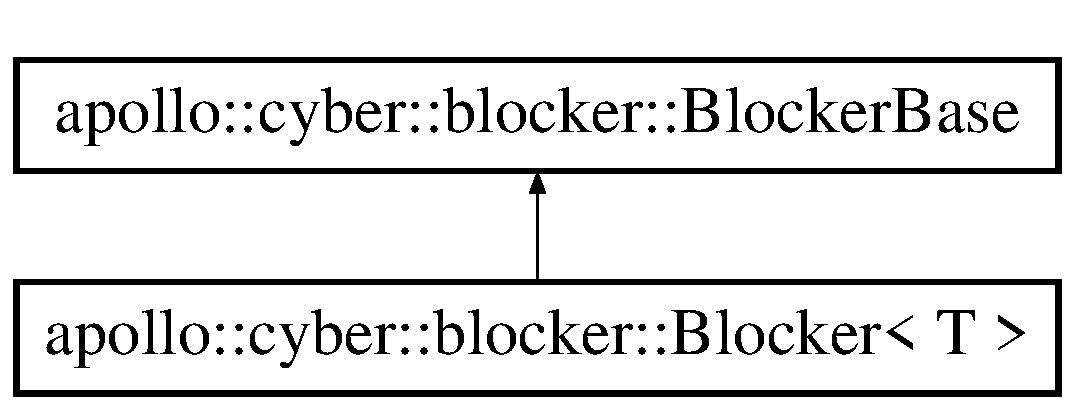
\includegraphics[height=2.000000cm]{classapollo_1_1cyber_1_1blocker_1_1BlockerBase}
\end{center}
\end{figure}
\subsection*{Public Member Functions}
\begin{DoxyCompactItemize}
\item 
virtual \hyperlink{classapollo_1_1cyber_1_1blocker_1_1BlockerBase_a101aef7ac0d785ae7b622356c73c9a00}{$\sim$\-Blocker\-Base} ()=default
\item 
virtual void \hyperlink{classapollo_1_1cyber_1_1blocker_1_1BlockerBase_a32fd8d73c7d5a5e4e2521f95126934d4}{Reset} ()=0
\item 
virtual void \hyperlink{classapollo_1_1cyber_1_1blocker_1_1BlockerBase_aa644c34503729364e5742f36f4246469}{Clear\-Observed} ()=0
\item 
virtual void \hyperlink{classapollo_1_1cyber_1_1blocker_1_1BlockerBase_a79270e6fab5378d6b40162fb4322d189}{Clear\-Published} ()=0
\item 
virtual void \hyperlink{classapollo_1_1cyber_1_1blocker_1_1BlockerBase_ad14b2e2e37c4436f2ef72e78505aa271}{Observe} ()=0
\item 
virtual bool \hyperlink{classapollo_1_1cyber_1_1blocker_1_1BlockerBase_ae362222ab521ba70e034c41a602a2f28}{Is\-Observed\-Empty} () const =0
\item 
virtual bool \hyperlink{classapollo_1_1cyber_1_1blocker_1_1BlockerBase_a38759de3825c1768af583bebe334aaf1}{Is\-Published\-Empty} () const =0
\item 
virtual bool \hyperlink{classapollo_1_1cyber_1_1blocker_1_1BlockerBase_a8fd56887517c5015e32cd96544cd2d6a}{Unsubscribe} (const std\-::string \&callback\-\_\-id)=0
\item 
virtual size\-\_\-t \hyperlink{classapollo_1_1cyber_1_1blocker_1_1BlockerBase_a4b38e9b2314553bfd14edc8c0f80806d}{capacity} () const =0
\item 
virtual void \hyperlink{classapollo_1_1cyber_1_1blocker_1_1BlockerBase_aa3db5ee03360d7d645dad38c0352e4e6}{set\-\_\-capacity} (size\-\_\-t \hyperlink{classapollo_1_1cyber_1_1blocker_1_1BlockerBase_a4b38e9b2314553bfd14edc8c0f80806d}{capacity})=0
\item 
virtual const std\-::string \& \hyperlink{classapollo_1_1cyber_1_1blocker_1_1BlockerBase_aa9606bd0d65712dfd8c62bee4db5180b}{channel\-\_\-name} () const =0
\end{DoxyCompactItemize}


\subsection{Constructor \& Destructor Documentation}
\hypertarget{classapollo_1_1cyber_1_1blocker_1_1BlockerBase_a101aef7ac0d785ae7b622356c73c9a00}{\index{apollo\-::cyber\-::blocker\-::\-Blocker\-Base@{apollo\-::cyber\-::blocker\-::\-Blocker\-Base}!$\sim$\-Blocker\-Base@{$\sim$\-Blocker\-Base}}
\index{$\sim$\-Blocker\-Base@{$\sim$\-Blocker\-Base}!apollo::cyber::blocker::BlockerBase@{apollo\-::cyber\-::blocker\-::\-Blocker\-Base}}
\subsubsection[{$\sim$\-Blocker\-Base}]{\setlength{\rightskip}{0pt plus 5cm}virtual apollo\-::cyber\-::blocker\-::\-Blocker\-Base\-::$\sim$\-Blocker\-Base (
\begin{DoxyParamCaption}
{}
\end{DoxyParamCaption}
)\hspace{0.3cm}{\ttfamily [virtual]}, {\ttfamily [default]}}}\label{classapollo_1_1cyber_1_1blocker_1_1BlockerBase_a101aef7ac0d785ae7b622356c73c9a00}


\subsection{Member Function Documentation}
\hypertarget{classapollo_1_1cyber_1_1blocker_1_1BlockerBase_a4b38e9b2314553bfd14edc8c0f80806d}{\index{apollo\-::cyber\-::blocker\-::\-Blocker\-Base@{apollo\-::cyber\-::blocker\-::\-Blocker\-Base}!capacity@{capacity}}
\index{capacity@{capacity}!apollo::cyber::blocker::BlockerBase@{apollo\-::cyber\-::blocker\-::\-Blocker\-Base}}
\subsubsection[{capacity}]{\setlength{\rightskip}{0pt plus 5cm}virtual size\-\_\-t apollo\-::cyber\-::blocker\-::\-Blocker\-Base\-::capacity (
\begin{DoxyParamCaption}
{}
\end{DoxyParamCaption}
) const\hspace{0.3cm}{\ttfamily [pure virtual]}}}\label{classapollo_1_1cyber_1_1blocker_1_1BlockerBase_a4b38e9b2314553bfd14edc8c0f80806d}


Implemented in \hyperlink{classapollo_1_1cyber_1_1blocker_1_1Blocker_a1560ce78043183df8b2d287cdc3824ed}{apollo\-::cyber\-::blocker\-::\-Blocker$<$ T $>$}.

\hypertarget{classapollo_1_1cyber_1_1blocker_1_1BlockerBase_aa9606bd0d65712dfd8c62bee4db5180b}{\index{apollo\-::cyber\-::blocker\-::\-Blocker\-Base@{apollo\-::cyber\-::blocker\-::\-Blocker\-Base}!channel\-\_\-name@{channel\-\_\-name}}
\index{channel\-\_\-name@{channel\-\_\-name}!apollo::cyber::blocker::BlockerBase@{apollo\-::cyber\-::blocker\-::\-Blocker\-Base}}
\subsubsection[{channel\-\_\-name}]{\setlength{\rightskip}{0pt plus 5cm}virtual const std\-::string\& apollo\-::cyber\-::blocker\-::\-Blocker\-Base\-::channel\-\_\-name (
\begin{DoxyParamCaption}
{}
\end{DoxyParamCaption}
) const\hspace{0.3cm}{\ttfamily [pure virtual]}}}\label{classapollo_1_1cyber_1_1blocker_1_1BlockerBase_aa9606bd0d65712dfd8c62bee4db5180b}


Implemented in \hyperlink{classapollo_1_1cyber_1_1blocker_1_1Blocker_ad121ab8e1fb379cd348267cccdc62624}{apollo\-::cyber\-::blocker\-::\-Blocker$<$ T $>$}.

\hypertarget{classapollo_1_1cyber_1_1blocker_1_1BlockerBase_aa644c34503729364e5742f36f4246469}{\index{apollo\-::cyber\-::blocker\-::\-Blocker\-Base@{apollo\-::cyber\-::blocker\-::\-Blocker\-Base}!Clear\-Observed@{Clear\-Observed}}
\index{Clear\-Observed@{Clear\-Observed}!apollo::cyber::blocker::BlockerBase@{apollo\-::cyber\-::blocker\-::\-Blocker\-Base}}
\subsubsection[{Clear\-Observed}]{\setlength{\rightskip}{0pt plus 5cm}virtual void apollo\-::cyber\-::blocker\-::\-Blocker\-Base\-::\-Clear\-Observed (
\begin{DoxyParamCaption}
{}
\end{DoxyParamCaption}
)\hspace{0.3cm}{\ttfamily [pure virtual]}}}\label{classapollo_1_1cyber_1_1blocker_1_1BlockerBase_aa644c34503729364e5742f36f4246469}


Implemented in \hyperlink{classapollo_1_1cyber_1_1blocker_1_1Blocker_a2c1d83849cd31a60e0cd77fa20c0fb28}{apollo\-::cyber\-::blocker\-::\-Blocker$<$ T $>$}.

\hypertarget{classapollo_1_1cyber_1_1blocker_1_1BlockerBase_a79270e6fab5378d6b40162fb4322d189}{\index{apollo\-::cyber\-::blocker\-::\-Blocker\-Base@{apollo\-::cyber\-::blocker\-::\-Blocker\-Base}!Clear\-Published@{Clear\-Published}}
\index{Clear\-Published@{Clear\-Published}!apollo::cyber::blocker::BlockerBase@{apollo\-::cyber\-::blocker\-::\-Blocker\-Base}}
\subsubsection[{Clear\-Published}]{\setlength{\rightskip}{0pt plus 5cm}virtual void apollo\-::cyber\-::blocker\-::\-Blocker\-Base\-::\-Clear\-Published (
\begin{DoxyParamCaption}
{}
\end{DoxyParamCaption}
)\hspace{0.3cm}{\ttfamily [pure virtual]}}}\label{classapollo_1_1cyber_1_1blocker_1_1BlockerBase_a79270e6fab5378d6b40162fb4322d189}


Implemented in \hyperlink{classapollo_1_1cyber_1_1blocker_1_1Blocker_a541bf01ca37ca188743d43f0130f8ea7}{apollo\-::cyber\-::blocker\-::\-Blocker$<$ T $>$}.

\hypertarget{classapollo_1_1cyber_1_1blocker_1_1BlockerBase_ae362222ab521ba70e034c41a602a2f28}{\index{apollo\-::cyber\-::blocker\-::\-Blocker\-Base@{apollo\-::cyber\-::blocker\-::\-Blocker\-Base}!Is\-Observed\-Empty@{Is\-Observed\-Empty}}
\index{Is\-Observed\-Empty@{Is\-Observed\-Empty}!apollo::cyber::blocker::BlockerBase@{apollo\-::cyber\-::blocker\-::\-Blocker\-Base}}
\subsubsection[{Is\-Observed\-Empty}]{\setlength{\rightskip}{0pt plus 5cm}virtual bool apollo\-::cyber\-::blocker\-::\-Blocker\-Base\-::\-Is\-Observed\-Empty (
\begin{DoxyParamCaption}
{}
\end{DoxyParamCaption}
) const\hspace{0.3cm}{\ttfamily [pure virtual]}}}\label{classapollo_1_1cyber_1_1blocker_1_1BlockerBase_ae362222ab521ba70e034c41a602a2f28}


Implemented in \hyperlink{classapollo_1_1cyber_1_1blocker_1_1Blocker_a629bb4a79c48af5998c52036b27dbc7a}{apollo\-::cyber\-::blocker\-::\-Blocker$<$ T $>$}.

\hypertarget{classapollo_1_1cyber_1_1blocker_1_1BlockerBase_a38759de3825c1768af583bebe334aaf1}{\index{apollo\-::cyber\-::blocker\-::\-Blocker\-Base@{apollo\-::cyber\-::blocker\-::\-Blocker\-Base}!Is\-Published\-Empty@{Is\-Published\-Empty}}
\index{Is\-Published\-Empty@{Is\-Published\-Empty}!apollo::cyber::blocker::BlockerBase@{apollo\-::cyber\-::blocker\-::\-Blocker\-Base}}
\subsubsection[{Is\-Published\-Empty}]{\setlength{\rightskip}{0pt plus 5cm}virtual bool apollo\-::cyber\-::blocker\-::\-Blocker\-Base\-::\-Is\-Published\-Empty (
\begin{DoxyParamCaption}
{}
\end{DoxyParamCaption}
) const\hspace{0.3cm}{\ttfamily [pure virtual]}}}\label{classapollo_1_1cyber_1_1blocker_1_1BlockerBase_a38759de3825c1768af583bebe334aaf1}


Implemented in \hyperlink{classapollo_1_1cyber_1_1blocker_1_1Blocker_ac6d16f3829849b236509dde3bbae3b29}{apollo\-::cyber\-::blocker\-::\-Blocker$<$ T $>$}.

\hypertarget{classapollo_1_1cyber_1_1blocker_1_1BlockerBase_ad14b2e2e37c4436f2ef72e78505aa271}{\index{apollo\-::cyber\-::blocker\-::\-Blocker\-Base@{apollo\-::cyber\-::blocker\-::\-Blocker\-Base}!Observe@{Observe}}
\index{Observe@{Observe}!apollo::cyber::blocker::BlockerBase@{apollo\-::cyber\-::blocker\-::\-Blocker\-Base}}
\subsubsection[{Observe}]{\setlength{\rightskip}{0pt plus 5cm}virtual void apollo\-::cyber\-::blocker\-::\-Blocker\-Base\-::\-Observe (
\begin{DoxyParamCaption}
{}
\end{DoxyParamCaption}
)\hspace{0.3cm}{\ttfamily [pure virtual]}}}\label{classapollo_1_1cyber_1_1blocker_1_1BlockerBase_ad14b2e2e37c4436f2ef72e78505aa271}


Implemented in \hyperlink{classapollo_1_1cyber_1_1blocker_1_1Blocker_aa2daeae7b6757bbe6a8066ed045dc891}{apollo\-::cyber\-::blocker\-::\-Blocker$<$ T $>$}.

\hypertarget{classapollo_1_1cyber_1_1blocker_1_1BlockerBase_a32fd8d73c7d5a5e4e2521f95126934d4}{\index{apollo\-::cyber\-::blocker\-::\-Blocker\-Base@{apollo\-::cyber\-::blocker\-::\-Blocker\-Base}!Reset@{Reset}}
\index{Reset@{Reset}!apollo::cyber::blocker::BlockerBase@{apollo\-::cyber\-::blocker\-::\-Blocker\-Base}}
\subsubsection[{Reset}]{\setlength{\rightskip}{0pt plus 5cm}virtual void apollo\-::cyber\-::blocker\-::\-Blocker\-Base\-::\-Reset (
\begin{DoxyParamCaption}
{}
\end{DoxyParamCaption}
)\hspace{0.3cm}{\ttfamily [pure virtual]}}}\label{classapollo_1_1cyber_1_1blocker_1_1BlockerBase_a32fd8d73c7d5a5e4e2521f95126934d4}


Implemented in \hyperlink{classapollo_1_1cyber_1_1blocker_1_1Blocker_a7372e1e554c724a5ca55de47837780da}{apollo\-::cyber\-::blocker\-::\-Blocker$<$ T $>$}.

\hypertarget{classapollo_1_1cyber_1_1blocker_1_1BlockerBase_aa3db5ee03360d7d645dad38c0352e4e6}{\index{apollo\-::cyber\-::blocker\-::\-Blocker\-Base@{apollo\-::cyber\-::blocker\-::\-Blocker\-Base}!set\-\_\-capacity@{set\-\_\-capacity}}
\index{set\-\_\-capacity@{set\-\_\-capacity}!apollo::cyber::blocker::BlockerBase@{apollo\-::cyber\-::blocker\-::\-Blocker\-Base}}
\subsubsection[{set\-\_\-capacity}]{\setlength{\rightskip}{0pt plus 5cm}virtual void apollo\-::cyber\-::blocker\-::\-Blocker\-Base\-::set\-\_\-capacity (
\begin{DoxyParamCaption}
\item[{size\-\_\-t}]{capacity}
\end{DoxyParamCaption}
)\hspace{0.3cm}{\ttfamily [pure virtual]}}}\label{classapollo_1_1cyber_1_1blocker_1_1BlockerBase_aa3db5ee03360d7d645dad38c0352e4e6}


Implemented in \hyperlink{classapollo_1_1cyber_1_1blocker_1_1Blocker_ad2eef40f68908fc02c76be48cfc55b63}{apollo\-::cyber\-::blocker\-::\-Blocker$<$ T $>$}.

\hypertarget{classapollo_1_1cyber_1_1blocker_1_1BlockerBase_a8fd56887517c5015e32cd96544cd2d6a}{\index{apollo\-::cyber\-::blocker\-::\-Blocker\-Base@{apollo\-::cyber\-::blocker\-::\-Blocker\-Base}!Unsubscribe@{Unsubscribe}}
\index{Unsubscribe@{Unsubscribe}!apollo::cyber::blocker::BlockerBase@{apollo\-::cyber\-::blocker\-::\-Blocker\-Base}}
\subsubsection[{Unsubscribe}]{\setlength{\rightskip}{0pt plus 5cm}virtual bool apollo\-::cyber\-::blocker\-::\-Blocker\-Base\-::\-Unsubscribe (
\begin{DoxyParamCaption}
\item[{const std\-::string \&}]{callback\-\_\-id}
\end{DoxyParamCaption}
)\hspace{0.3cm}{\ttfamily [pure virtual]}}}\label{classapollo_1_1cyber_1_1blocker_1_1BlockerBase_a8fd56887517c5015e32cd96544cd2d6a}


Implemented in \hyperlink{classapollo_1_1cyber_1_1blocker_1_1Blocker_a4223c5b06e38b685fcab97605822fdc1}{apollo\-::cyber\-::blocker\-::\-Blocker$<$ T $>$}.



The documentation for this class was generated from the following file\-:\begin{DoxyCompactItemize}
\item 
blocker/\hyperlink{blocker_8h}{blocker.\-h}\end{DoxyCompactItemize}

\hypertarget{classapollo_1_1cyber_1_1blocker_1_1BlockerManager}{\section{apollo\-:\-:cyber\-:\-:blocker\-:\-:Blocker\-Manager Class Reference}
\label{classapollo_1_1cyber_1_1blocker_1_1BlockerManager}\index{apollo\-::cyber\-::blocker\-::\-Blocker\-Manager@{apollo\-::cyber\-::blocker\-::\-Blocker\-Manager}}
}


{\ttfamily \#include $<$blocker\-\_\-manager.\-h$>$}

\subsection*{Public Types}
\begin{DoxyCompactItemize}
\item 
using \hyperlink{classapollo_1_1cyber_1_1blocker_1_1BlockerManager_aab93de92687db46229801f733c741334}{Blocker\-Map} = std\-::unordered\-\_\-map$<$ std\-::string, std\-::shared\-\_\-ptr$<$ \hyperlink{classapollo_1_1cyber_1_1blocker_1_1BlockerBase}{Blocker\-Base} $>$$>$
\end{DoxyCompactItemize}
\subsection*{Public Member Functions}
\begin{DoxyCompactItemize}
\item 
virtual \hyperlink{classapollo_1_1cyber_1_1blocker_1_1BlockerManager_a9507c5a941e01053a258badd91d5bb5e}{$\sim$\-Blocker\-Manager} ()
\item 
{\footnotesize template$<$typename T $>$ }\\bool \hyperlink{classapollo_1_1cyber_1_1blocker_1_1BlockerManager_a02cf4d2417c97da763663052e5997c51}{Publish} (const std\-::string \&channel\-\_\-name, const typename \hyperlink{classapollo_1_1cyber_1_1blocker_1_1Blocker}{Blocker}$<$ T $>$\-::Message\-Ptr \&msg)
\item 
{\footnotesize template$<$typename T $>$ }\\bool \hyperlink{classapollo_1_1cyber_1_1blocker_1_1BlockerManager_a9240b9cb2f282a740e863b9e81bbbe06}{Publish} (const std\-::string \&channel\-\_\-name, const typename \hyperlink{classapollo_1_1cyber_1_1blocker_1_1Blocker}{Blocker}$<$ T $>$\-::Message\-Type \&msg)
\item 
{\footnotesize template$<$typename T $>$ }\\bool \hyperlink{classapollo_1_1cyber_1_1blocker_1_1BlockerManager_adf88edc35b0ea77921145adc2298e23b}{Subscribe} (const std\-::string \&channel\-\_\-name, size\-\_\-t capacity, const std\-::string \&callback\-\_\-id, const typename \hyperlink{classapollo_1_1cyber_1_1blocker_1_1Blocker}{Blocker}$<$ T $>$\-::Callback \&callback)
\item 
{\footnotesize template$<$typename T $>$ }\\bool \hyperlink{classapollo_1_1cyber_1_1blocker_1_1BlockerManager_a9275edf629662a3800e3089f3dd91c3a}{Unsubscribe} (const std\-::string \&channel\-\_\-name, const std\-::string \&callback\-\_\-id)
\item 
{\footnotesize template$<$typename T $>$ }\\std\-::shared\-\_\-ptr$<$ \hyperlink{classapollo_1_1cyber_1_1blocker_1_1Blocker}{Blocker}$<$ T $>$ $>$ \hyperlink{classapollo_1_1cyber_1_1blocker_1_1BlockerManager_ae6b3a620a508fac29bc657eac4b88d46}{Get\-Blocker} (const std\-::string \&channel\-\_\-name)
\item 
{\footnotesize template$<$typename T $>$ }\\std\-::shared\-\_\-ptr$<$ \hyperlink{classapollo_1_1cyber_1_1blocker_1_1Blocker}{Blocker}$<$ T $>$ $>$ \hyperlink{classapollo_1_1cyber_1_1blocker_1_1BlockerManager_a8b675f3729363e53c7a09d267c560ac5}{Get\-Or\-Create\-Blocker} (const \hyperlink{structapollo_1_1cyber_1_1blocker_1_1BlockerAttr}{Blocker\-Attr} \&attr)
\item 
void \hyperlink{classapollo_1_1cyber_1_1blocker_1_1BlockerManager_a6577db9e414c1567b9d0df15ccadcb1f}{Observe} ()
\item 
void \hyperlink{classapollo_1_1cyber_1_1blocker_1_1BlockerManager_a5146d37bdbc55c29b2f82ff8b8c6af64}{Reset} ()
\end{DoxyCompactItemize}
\subsection*{Static Public Member Functions}
\begin{DoxyCompactItemize}
\item 
static const std\-::shared\-\_\-ptr\\*
$<$ \hyperlink{classapollo_1_1cyber_1_1blocker_1_1BlockerManager}{Blocker\-Manager} $>$ \& \hyperlink{classapollo_1_1cyber_1_1blocker_1_1BlockerManager_a2fd73d2d9c2a50820750d68aea0a9c1b}{Instance} ()
\end{DoxyCompactItemize}
\subsection*{Private Member Functions}
\begin{DoxyCompactItemize}
\item 
\hyperlink{classapollo_1_1cyber_1_1blocker_1_1BlockerManager_ad5317e0dea1d15074e99c073d3aa9615}{Blocker\-Manager} ()
\item 
\hyperlink{classapollo_1_1cyber_1_1blocker_1_1BlockerManager_a42ef19cb5d583093f35ef2a85f8ceb88}{Blocker\-Manager} (const \hyperlink{classapollo_1_1cyber_1_1blocker_1_1BlockerManager}{Blocker\-Manager} \&)=delete
\item 
\hyperlink{classapollo_1_1cyber_1_1blocker_1_1BlockerManager}{Blocker\-Manager} \& \hyperlink{classapollo_1_1cyber_1_1blocker_1_1BlockerManager_a315c9dc141d141bf0c707bf3dc56b841}{operator=} (const \hyperlink{classapollo_1_1cyber_1_1blocker_1_1BlockerManager}{Blocker\-Manager} \&)=delete
\end{DoxyCompactItemize}
\subsection*{Private Attributes}
\begin{DoxyCompactItemize}
\item 
\hyperlink{classapollo_1_1cyber_1_1blocker_1_1BlockerManager_aab93de92687db46229801f733c741334}{Blocker\-Map} \hyperlink{classapollo_1_1cyber_1_1blocker_1_1BlockerManager_a63cbedd8313717b3f8fc8ad8133329bc}{blockers\-\_\-}
\item 
std\-::mutex \hyperlink{classapollo_1_1cyber_1_1blocker_1_1BlockerManager_a84ba4d0f791c3ff2b835dbfa91d325ea}{blocker\-\_\-mutex\-\_\-}
\end{DoxyCompactItemize}


\subsection{Member Typedef Documentation}
\hypertarget{classapollo_1_1cyber_1_1blocker_1_1BlockerManager_aab93de92687db46229801f733c741334}{\index{apollo\-::cyber\-::blocker\-::\-Blocker\-Manager@{apollo\-::cyber\-::blocker\-::\-Blocker\-Manager}!Blocker\-Map@{Blocker\-Map}}
\index{Blocker\-Map@{Blocker\-Map}!apollo::cyber::blocker::BlockerManager@{apollo\-::cyber\-::blocker\-::\-Blocker\-Manager}}
\subsubsection[{Blocker\-Map}]{\setlength{\rightskip}{0pt plus 5cm}using {\bf apollo\-::cyber\-::blocker\-::\-Blocker\-Manager\-::\-Blocker\-Map} =  std\-::unordered\-\_\-map$<$std\-::string, std\-::shared\-\_\-ptr$<${\bf Blocker\-Base}$>$$>$}}\label{classapollo_1_1cyber_1_1blocker_1_1BlockerManager_aab93de92687db46229801f733c741334}


\subsection{Constructor \& Destructor Documentation}
\hypertarget{classapollo_1_1cyber_1_1blocker_1_1BlockerManager_a9507c5a941e01053a258badd91d5bb5e}{\index{apollo\-::cyber\-::blocker\-::\-Blocker\-Manager@{apollo\-::cyber\-::blocker\-::\-Blocker\-Manager}!$\sim$\-Blocker\-Manager@{$\sim$\-Blocker\-Manager}}
\index{$\sim$\-Blocker\-Manager@{$\sim$\-Blocker\-Manager}!apollo::cyber::blocker::BlockerManager@{apollo\-::cyber\-::blocker\-::\-Blocker\-Manager}}
\subsubsection[{$\sim$\-Blocker\-Manager}]{\setlength{\rightskip}{0pt plus 5cm}virtual apollo\-::cyber\-::blocker\-::\-Blocker\-Manager\-::$\sim$\-Blocker\-Manager (
\begin{DoxyParamCaption}
{}
\end{DoxyParamCaption}
)\hspace{0.3cm}{\ttfamily [virtual]}}}\label{classapollo_1_1cyber_1_1blocker_1_1BlockerManager_a9507c5a941e01053a258badd91d5bb5e}
\hypertarget{classapollo_1_1cyber_1_1blocker_1_1BlockerManager_ad5317e0dea1d15074e99c073d3aa9615}{\index{apollo\-::cyber\-::blocker\-::\-Blocker\-Manager@{apollo\-::cyber\-::blocker\-::\-Blocker\-Manager}!Blocker\-Manager@{Blocker\-Manager}}
\index{Blocker\-Manager@{Blocker\-Manager}!apollo::cyber::blocker::BlockerManager@{apollo\-::cyber\-::blocker\-::\-Blocker\-Manager}}
\subsubsection[{Blocker\-Manager}]{\setlength{\rightskip}{0pt plus 5cm}apollo\-::cyber\-::blocker\-::\-Blocker\-Manager\-::\-Blocker\-Manager (
\begin{DoxyParamCaption}
{}
\end{DoxyParamCaption}
)\hspace{0.3cm}{\ttfamily [private]}}}\label{classapollo_1_1cyber_1_1blocker_1_1BlockerManager_ad5317e0dea1d15074e99c073d3aa9615}
\hypertarget{classapollo_1_1cyber_1_1blocker_1_1BlockerManager_a42ef19cb5d583093f35ef2a85f8ceb88}{\index{apollo\-::cyber\-::blocker\-::\-Blocker\-Manager@{apollo\-::cyber\-::blocker\-::\-Blocker\-Manager}!Blocker\-Manager@{Blocker\-Manager}}
\index{Blocker\-Manager@{Blocker\-Manager}!apollo::cyber::blocker::BlockerManager@{apollo\-::cyber\-::blocker\-::\-Blocker\-Manager}}
\subsubsection[{Blocker\-Manager}]{\setlength{\rightskip}{0pt plus 5cm}apollo\-::cyber\-::blocker\-::\-Blocker\-Manager\-::\-Blocker\-Manager (
\begin{DoxyParamCaption}
\item[{const {\bf Blocker\-Manager} \&}]{}
\end{DoxyParamCaption}
)\hspace{0.3cm}{\ttfamily [private]}, {\ttfamily [delete]}}}\label{classapollo_1_1cyber_1_1blocker_1_1BlockerManager_a42ef19cb5d583093f35ef2a85f8ceb88}


\subsection{Member Function Documentation}
\hypertarget{classapollo_1_1cyber_1_1blocker_1_1BlockerManager_ae6b3a620a508fac29bc657eac4b88d46}{\index{apollo\-::cyber\-::blocker\-::\-Blocker\-Manager@{apollo\-::cyber\-::blocker\-::\-Blocker\-Manager}!Get\-Blocker@{Get\-Blocker}}
\index{Get\-Blocker@{Get\-Blocker}!apollo::cyber::blocker::BlockerManager@{apollo\-::cyber\-::blocker\-::\-Blocker\-Manager}}
\subsubsection[{Get\-Blocker}]{\setlength{\rightskip}{0pt plus 5cm}template$<$typename T $>$ std\-::shared\-\_\-ptr$<$ {\bf Blocker}$<$ T $>$ $>$ apollo\-::cyber\-::blocker\-::\-Blocker\-Manager\-::\-Get\-Blocker (
\begin{DoxyParamCaption}
\item[{const std\-::string \&}]{channel\-\_\-name}
\end{DoxyParamCaption}
)}}\label{classapollo_1_1cyber_1_1blocker_1_1BlockerManager_ae6b3a620a508fac29bc657eac4b88d46}
\hypertarget{classapollo_1_1cyber_1_1blocker_1_1BlockerManager_a8b675f3729363e53c7a09d267c560ac5}{\index{apollo\-::cyber\-::blocker\-::\-Blocker\-Manager@{apollo\-::cyber\-::blocker\-::\-Blocker\-Manager}!Get\-Or\-Create\-Blocker@{Get\-Or\-Create\-Blocker}}
\index{Get\-Or\-Create\-Blocker@{Get\-Or\-Create\-Blocker}!apollo::cyber::blocker::BlockerManager@{apollo\-::cyber\-::blocker\-::\-Blocker\-Manager}}
\subsubsection[{Get\-Or\-Create\-Blocker}]{\setlength{\rightskip}{0pt plus 5cm}template$<$typename T $>$ std\-::shared\-\_\-ptr$<$ {\bf Blocker}$<$ T $>$ $>$ apollo\-::cyber\-::blocker\-::\-Blocker\-Manager\-::\-Get\-Or\-Create\-Blocker (
\begin{DoxyParamCaption}
\item[{const {\bf Blocker\-Attr} \&}]{attr}
\end{DoxyParamCaption}
)}}\label{classapollo_1_1cyber_1_1blocker_1_1BlockerManager_a8b675f3729363e53c7a09d267c560ac5}
\hypertarget{classapollo_1_1cyber_1_1blocker_1_1BlockerManager_a2fd73d2d9c2a50820750d68aea0a9c1b}{\index{apollo\-::cyber\-::blocker\-::\-Blocker\-Manager@{apollo\-::cyber\-::blocker\-::\-Blocker\-Manager}!Instance@{Instance}}
\index{Instance@{Instance}!apollo::cyber::blocker::BlockerManager@{apollo\-::cyber\-::blocker\-::\-Blocker\-Manager}}
\subsubsection[{Instance}]{\setlength{\rightskip}{0pt plus 5cm}static const std\-::shared\-\_\-ptr$<${\bf Blocker\-Manager}$>$\& apollo\-::cyber\-::blocker\-::\-Blocker\-Manager\-::\-Instance (
\begin{DoxyParamCaption}
{}
\end{DoxyParamCaption}
)\hspace{0.3cm}{\ttfamily [inline]}, {\ttfamily [static]}}}\label{classapollo_1_1cyber_1_1blocker_1_1BlockerManager_a2fd73d2d9c2a50820750d68aea0a9c1b}
\hypertarget{classapollo_1_1cyber_1_1blocker_1_1BlockerManager_a6577db9e414c1567b9d0df15ccadcb1f}{\index{apollo\-::cyber\-::blocker\-::\-Blocker\-Manager@{apollo\-::cyber\-::blocker\-::\-Blocker\-Manager}!Observe@{Observe}}
\index{Observe@{Observe}!apollo::cyber::blocker::BlockerManager@{apollo\-::cyber\-::blocker\-::\-Blocker\-Manager}}
\subsubsection[{Observe}]{\setlength{\rightskip}{0pt plus 5cm}void apollo\-::cyber\-::blocker\-::\-Blocker\-Manager\-::\-Observe (
\begin{DoxyParamCaption}
{}
\end{DoxyParamCaption}
)}}\label{classapollo_1_1cyber_1_1blocker_1_1BlockerManager_a6577db9e414c1567b9d0df15ccadcb1f}
\hypertarget{classapollo_1_1cyber_1_1blocker_1_1BlockerManager_a315c9dc141d141bf0c707bf3dc56b841}{\index{apollo\-::cyber\-::blocker\-::\-Blocker\-Manager@{apollo\-::cyber\-::blocker\-::\-Blocker\-Manager}!operator=@{operator=}}
\index{operator=@{operator=}!apollo::cyber::blocker::BlockerManager@{apollo\-::cyber\-::blocker\-::\-Blocker\-Manager}}
\subsubsection[{operator=}]{\setlength{\rightskip}{0pt plus 5cm}{\bf Blocker\-Manager}\& apollo\-::cyber\-::blocker\-::\-Blocker\-Manager\-::operator= (
\begin{DoxyParamCaption}
\item[{const {\bf Blocker\-Manager} \&}]{}
\end{DoxyParamCaption}
)\hspace{0.3cm}{\ttfamily [private]}, {\ttfamily [delete]}}}\label{classapollo_1_1cyber_1_1blocker_1_1BlockerManager_a315c9dc141d141bf0c707bf3dc56b841}
\hypertarget{classapollo_1_1cyber_1_1blocker_1_1BlockerManager_a02cf4d2417c97da763663052e5997c51}{\index{apollo\-::cyber\-::blocker\-::\-Blocker\-Manager@{apollo\-::cyber\-::blocker\-::\-Blocker\-Manager}!Publish@{Publish}}
\index{Publish@{Publish}!apollo::cyber::blocker::BlockerManager@{apollo\-::cyber\-::blocker\-::\-Blocker\-Manager}}
\subsubsection[{Publish}]{\setlength{\rightskip}{0pt plus 5cm}template$<$typename T $>$ bool apollo\-::cyber\-::blocker\-::\-Blocker\-Manager\-::\-Publish (
\begin{DoxyParamCaption}
\item[{const std\-::string \&}]{channel\-\_\-name, }
\item[{const typename {\bf Blocker}$<$ T $>$\-::Message\-Ptr \&}]{msg}
\end{DoxyParamCaption}
)}}\label{classapollo_1_1cyber_1_1blocker_1_1BlockerManager_a02cf4d2417c97da763663052e5997c51}
\hypertarget{classapollo_1_1cyber_1_1blocker_1_1BlockerManager_a9240b9cb2f282a740e863b9e81bbbe06}{\index{apollo\-::cyber\-::blocker\-::\-Blocker\-Manager@{apollo\-::cyber\-::blocker\-::\-Blocker\-Manager}!Publish@{Publish}}
\index{Publish@{Publish}!apollo::cyber::blocker::BlockerManager@{apollo\-::cyber\-::blocker\-::\-Blocker\-Manager}}
\subsubsection[{Publish}]{\setlength{\rightskip}{0pt plus 5cm}template$<$typename T $>$ bool apollo\-::cyber\-::blocker\-::\-Blocker\-Manager\-::\-Publish (
\begin{DoxyParamCaption}
\item[{const std\-::string \&}]{channel\-\_\-name, }
\item[{const typename {\bf Blocker}$<$ T $>$\-::Message\-Type \&}]{msg}
\end{DoxyParamCaption}
)}}\label{classapollo_1_1cyber_1_1blocker_1_1BlockerManager_a9240b9cb2f282a740e863b9e81bbbe06}
\hypertarget{classapollo_1_1cyber_1_1blocker_1_1BlockerManager_a5146d37bdbc55c29b2f82ff8b8c6af64}{\index{apollo\-::cyber\-::blocker\-::\-Blocker\-Manager@{apollo\-::cyber\-::blocker\-::\-Blocker\-Manager}!Reset@{Reset}}
\index{Reset@{Reset}!apollo::cyber::blocker::BlockerManager@{apollo\-::cyber\-::blocker\-::\-Blocker\-Manager}}
\subsubsection[{Reset}]{\setlength{\rightskip}{0pt plus 5cm}void apollo\-::cyber\-::blocker\-::\-Blocker\-Manager\-::\-Reset (
\begin{DoxyParamCaption}
{}
\end{DoxyParamCaption}
)}}\label{classapollo_1_1cyber_1_1blocker_1_1BlockerManager_a5146d37bdbc55c29b2f82ff8b8c6af64}
\hypertarget{classapollo_1_1cyber_1_1blocker_1_1BlockerManager_adf88edc35b0ea77921145adc2298e23b}{\index{apollo\-::cyber\-::blocker\-::\-Blocker\-Manager@{apollo\-::cyber\-::blocker\-::\-Blocker\-Manager}!Subscribe@{Subscribe}}
\index{Subscribe@{Subscribe}!apollo::cyber::blocker::BlockerManager@{apollo\-::cyber\-::blocker\-::\-Blocker\-Manager}}
\subsubsection[{Subscribe}]{\setlength{\rightskip}{0pt plus 5cm}template$<$typename T $>$ bool apollo\-::cyber\-::blocker\-::\-Blocker\-Manager\-::\-Subscribe (
\begin{DoxyParamCaption}
\item[{const std\-::string \&}]{channel\-\_\-name, }
\item[{size\-\_\-t}]{capacity, }
\item[{const std\-::string \&}]{callback\-\_\-id, }
\item[{const typename {\bf Blocker}$<$ T $>$\-::Callback \&}]{callback}
\end{DoxyParamCaption}
)}}\label{classapollo_1_1cyber_1_1blocker_1_1BlockerManager_adf88edc35b0ea77921145adc2298e23b}
\hypertarget{classapollo_1_1cyber_1_1blocker_1_1BlockerManager_a9275edf629662a3800e3089f3dd91c3a}{\index{apollo\-::cyber\-::blocker\-::\-Blocker\-Manager@{apollo\-::cyber\-::blocker\-::\-Blocker\-Manager}!Unsubscribe@{Unsubscribe}}
\index{Unsubscribe@{Unsubscribe}!apollo::cyber::blocker::BlockerManager@{apollo\-::cyber\-::blocker\-::\-Blocker\-Manager}}
\subsubsection[{Unsubscribe}]{\setlength{\rightskip}{0pt plus 5cm}template$<$typename T $>$ bool apollo\-::cyber\-::blocker\-::\-Blocker\-Manager\-::\-Unsubscribe (
\begin{DoxyParamCaption}
\item[{const std\-::string \&}]{channel\-\_\-name, }
\item[{const std\-::string \&}]{callback\-\_\-id}
\end{DoxyParamCaption}
)}}\label{classapollo_1_1cyber_1_1blocker_1_1BlockerManager_a9275edf629662a3800e3089f3dd91c3a}


\subsection{Member Data Documentation}
\hypertarget{classapollo_1_1cyber_1_1blocker_1_1BlockerManager_a84ba4d0f791c3ff2b835dbfa91d325ea}{\index{apollo\-::cyber\-::blocker\-::\-Blocker\-Manager@{apollo\-::cyber\-::blocker\-::\-Blocker\-Manager}!blocker\-\_\-mutex\-\_\-@{blocker\-\_\-mutex\-\_\-}}
\index{blocker\-\_\-mutex\-\_\-@{blocker\-\_\-mutex\-\_\-}!apollo::cyber::blocker::BlockerManager@{apollo\-::cyber\-::blocker\-::\-Blocker\-Manager}}
\subsubsection[{blocker\-\_\-mutex\-\_\-}]{\setlength{\rightskip}{0pt plus 5cm}std\-::mutex apollo\-::cyber\-::blocker\-::\-Blocker\-Manager\-::blocker\-\_\-mutex\-\_\-\hspace{0.3cm}{\ttfamily [private]}}}\label{classapollo_1_1cyber_1_1blocker_1_1BlockerManager_a84ba4d0f791c3ff2b835dbfa91d325ea}
\hypertarget{classapollo_1_1cyber_1_1blocker_1_1BlockerManager_a63cbedd8313717b3f8fc8ad8133329bc}{\index{apollo\-::cyber\-::blocker\-::\-Blocker\-Manager@{apollo\-::cyber\-::blocker\-::\-Blocker\-Manager}!blockers\-\_\-@{blockers\-\_\-}}
\index{blockers\-\_\-@{blockers\-\_\-}!apollo::cyber::blocker::BlockerManager@{apollo\-::cyber\-::blocker\-::\-Blocker\-Manager}}
\subsubsection[{blockers\-\_\-}]{\setlength{\rightskip}{0pt plus 5cm}{\bf Blocker\-Map} apollo\-::cyber\-::blocker\-::\-Blocker\-Manager\-::blockers\-\_\-\hspace{0.3cm}{\ttfamily [private]}}}\label{classapollo_1_1cyber_1_1blocker_1_1BlockerManager_a63cbedd8313717b3f8fc8ad8133329bc}


The documentation for this class was generated from the following file\-:\begin{DoxyCompactItemize}
\item 
blocker/\hyperlink{blocker__manager_8h}{blocker\-\_\-manager.\-h}\end{DoxyCompactItemize}

\hypertarget{classapollo_1_1cyber_1_1base_1_1BlockWaitStrategy}{\section{apollo\-:\-:cyber\-:\-:base\-:\-:Block\-Wait\-Strategy Class Reference}
\label{classapollo_1_1cyber_1_1base_1_1BlockWaitStrategy}\index{apollo\-::cyber\-::base\-::\-Block\-Wait\-Strategy@{apollo\-::cyber\-::base\-::\-Block\-Wait\-Strategy}}
}


{\ttfamily \#include $<$wait\-\_\-strategy.\-h$>$}

Inheritance diagram for apollo\-:\-:cyber\-:\-:base\-:\-:Block\-Wait\-Strategy\-:\begin{figure}[H]
\begin{center}
\leavevmode
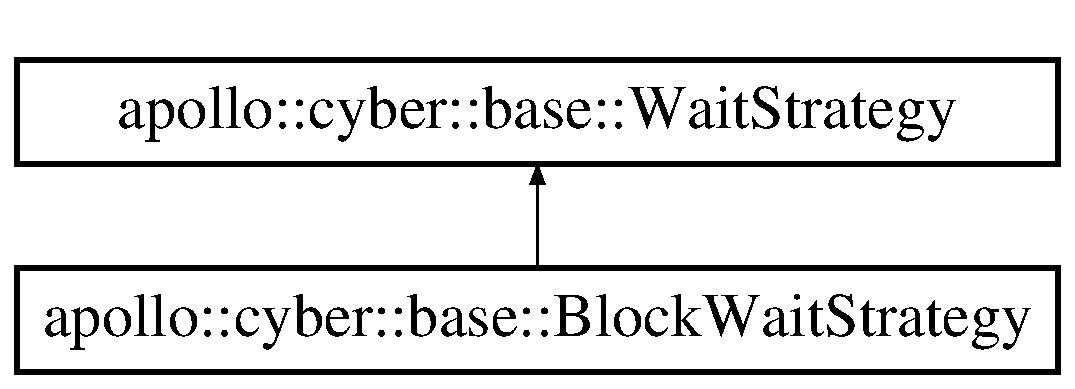
\includegraphics[height=2.000000cm]{classapollo_1_1cyber_1_1base_1_1BlockWaitStrategy}
\end{center}
\end{figure}
\subsection*{Public Member Functions}
\begin{DoxyCompactItemize}
\item 
\hyperlink{classapollo_1_1cyber_1_1base_1_1BlockWaitStrategy_a3a84cd077ae77dfc1abfe13401fa4cea}{Block\-Wait\-Strategy} ()
\item 
void \hyperlink{classapollo_1_1cyber_1_1base_1_1BlockWaitStrategy_ae8f8c929ddcc0973e18337a12535eb76}{Notify\-One} () override
\item 
bool \hyperlink{classapollo_1_1cyber_1_1base_1_1BlockWaitStrategy_a9be79b6f4cb8f78fb1715e2f221ebdff}{Empty\-Wait} () override
\item 
void \hyperlink{classapollo_1_1cyber_1_1base_1_1BlockWaitStrategy_a7f883544b4a59a5b250e7f9bddd7c2b7}{Break\-All\-Wait} ()
\end{DoxyCompactItemize}
\subsection*{Private Attributes}
\begin{DoxyCompactItemize}
\item 
std\-::mutex \hyperlink{classapollo_1_1cyber_1_1base_1_1BlockWaitStrategy_adca22a19b9f79e8a952001bba1286fb0}{mutex\-\_\-}
\item 
std\-::condition\-\_\-variable \hyperlink{classapollo_1_1cyber_1_1base_1_1BlockWaitStrategy_a9bc9e755055037e813f8a180ef4f609d}{cv\-\_\-}
\end{DoxyCompactItemize}


\subsection{Constructor \& Destructor Documentation}
\hypertarget{classapollo_1_1cyber_1_1base_1_1BlockWaitStrategy_a3a84cd077ae77dfc1abfe13401fa4cea}{\index{apollo\-::cyber\-::base\-::\-Block\-Wait\-Strategy@{apollo\-::cyber\-::base\-::\-Block\-Wait\-Strategy}!Block\-Wait\-Strategy@{Block\-Wait\-Strategy}}
\index{Block\-Wait\-Strategy@{Block\-Wait\-Strategy}!apollo::cyber::base::BlockWaitStrategy@{apollo\-::cyber\-::base\-::\-Block\-Wait\-Strategy}}
\subsubsection[{Block\-Wait\-Strategy}]{\setlength{\rightskip}{0pt plus 5cm}apollo\-::cyber\-::base\-::\-Block\-Wait\-Strategy\-::\-Block\-Wait\-Strategy (
\begin{DoxyParamCaption}
{}
\end{DoxyParamCaption}
)\hspace{0.3cm}{\ttfamily [inline]}}}\label{classapollo_1_1cyber_1_1base_1_1BlockWaitStrategy_a3a84cd077ae77dfc1abfe13401fa4cea}


\subsection{Member Function Documentation}
\hypertarget{classapollo_1_1cyber_1_1base_1_1BlockWaitStrategy_a7f883544b4a59a5b250e7f9bddd7c2b7}{\index{apollo\-::cyber\-::base\-::\-Block\-Wait\-Strategy@{apollo\-::cyber\-::base\-::\-Block\-Wait\-Strategy}!Break\-All\-Wait@{Break\-All\-Wait}}
\index{Break\-All\-Wait@{Break\-All\-Wait}!apollo::cyber::base::BlockWaitStrategy@{apollo\-::cyber\-::base\-::\-Block\-Wait\-Strategy}}
\subsubsection[{Break\-All\-Wait}]{\setlength{\rightskip}{0pt plus 5cm}void apollo\-::cyber\-::base\-::\-Block\-Wait\-Strategy\-::\-Break\-All\-Wait (
\begin{DoxyParamCaption}
{}
\end{DoxyParamCaption}
)\hspace{0.3cm}{\ttfamily [inline]}, {\ttfamily [virtual]}}}\label{classapollo_1_1cyber_1_1base_1_1BlockWaitStrategy_a7f883544b4a59a5b250e7f9bddd7c2b7}


Reimplemented from \hyperlink{classapollo_1_1cyber_1_1base_1_1WaitStrategy_a521db3e728b67be1b89e16207dce014f}{apollo\-::cyber\-::base\-::\-Wait\-Strategy}.

\hypertarget{classapollo_1_1cyber_1_1base_1_1BlockWaitStrategy_a9be79b6f4cb8f78fb1715e2f221ebdff}{\index{apollo\-::cyber\-::base\-::\-Block\-Wait\-Strategy@{apollo\-::cyber\-::base\-::\-Block\-Wait\-Strategy}!Empty\-Wait@{Empty\-Wait}}
\index{Empty\-Wait@{Empty\-Wait}!apollo::cyber::base::BlockWaitStrategy@{apollo\-::cyber\-::base\-::\-Block\-Wait\-Strategy}}
\subsubsection[{Empty\-Wait}]{\setlength{\rightskip}{0pt plus 5cm}bool apollo\-::cyber\-::base\-::\-Block\-Wait\-Strategy\-::\-Empty\-Wait (
\begin{DoxyParamCaption}
{}
\end{DoxyParamCaption}
)\hspace{0.3cm}{\ttfamily [inline]}, {\ttfamily [override]}, {\ttfamily [virtual]}}}\label{classapollo_1_1cyber_1_1base_1_1BlockWaitStrategy_a9be79b6f4cb8f78fb1715e2f221ebdff}


Implements \hyperlink{classapollo_1_1cyber_1_1base_1_1WaitStrategy_a5801f343cd1567ec6ee586b9845446e3}{apollo\-::cyber\-::base\-::\-Wait\-Strategy}.

\hypertarget{classapollo_1_1cyber_1_1base_1_1BlockWaitStrategy_ae8f8c929ddcc0973e18337a12535eb76}{\index{apollo\-::cyber\-::base\-::\-Block\-Wait\-Strategy@{apollo\-::cyber\-::base\-::\-Block\-Wait\-Strategy}!Notify\-One@{Notify\-One}}
\index{Notify\-One@{Notify\-One}!apollo::cyber::base::BlockWaitStrategy@{apollo\-::cyber\-::base\-::\-Block\-Wait\-Strategy}}
\subsubsection[{Notify\-One}]{\setlength{\rightskip}{0pt plus 5cm}void apollo\-::cyber\-::base\-::\-Block\-Wait\-Strategy\-::\-Notify\-One (
\begin{DoxyParamCaption}
{}
\end{DoxyParamCaption}
)\hspace{0.3cm}{\ttfamily [inline]}, {\ttfamily [override]}, {\ttfamily [virtual]}}}\label{classapollo_1_1cyber_1_1base_1_1BlockWaitStrategy_ae8f8c929ddcc0973e18337a12535eb76}


Reimplemented from \hyperlink{classapollo_1_1cyber_1_1base_1_1WaitStrategy_aec07f0b6c8f19538c324c7b1e3296dc3}{apollo\-::cyber\-::base\-::\-Wait\-Strategy}.



\subsection{Member Data Documentation}
\hypertarget{classapollo_1_1cyber_1_1base_1_1BlockWaitStrategy_a9bc9e755055037e813f8a180ef4f609d}{\index{apollo\-::cyber\-::base\-::\-Block\-Wait\-Strategy@{apollo\-::cyber\-::base\-::\-Block\-Wait\-Strategy}!cv\-\_\-@{cv\-\_\-}}
\index{cv\-\_\-@{cv\-\_\-}!apollo::cyber::base::BlockWaitStrategy@{apollo\-::cyber\-::base\-::\-Block\-Wait\-Strategy}}
\subsubsection[{cv\-\_\-}]{\setlength{\rightskip}{0pt plus 5cm}std\-::condition\-\_\-variable apollo\-::cyber\-::base\-::\-Block\-Wait\-Strategy\-::cv\-\_\-\hspace{0.3cm}{\ttfamily [private]}}}\label{classapollo_1_1cyber_1_1base_1_1BlockWaitStrategy_a9bc9e755055037e813f8a180ef4f609d}
\hypertarget{classapollo_1_1cyber_1_1base_1_1BlockWaitStrategy_adca22a19b9f79e8a952001bba1286fb0}{\index{apollo\-::cyber\-::base\-::\-Block\-Wait\-Strategy@{apollo\-::cyber\-::base\-::\-Block\-Wait\-Strategy}!mutex\-\_\-@{mutex\-\_\-}}
\index{mutex\-\_\-@{mutex\-\_\-}!apollo::cyber::base::BlockWaitStrategy@{apollo\-::cyber\-::base\-::\-Block\-Wait\-Strategy}}
\subsubsection[{mutex\-\_\-}]{\setlength{\rightskip}{0pt plus 5cm}std\-::mutex apollo\-::cyber\-::base\-::\-Block\-Wait\-Strategy\-::mutex\-\_\-\hspace{0.3cm}{\ttfamily [private]}}}\label{classapollo_1_1cyber_1_1base_1_1BlockWaitStrategy_adca22a19b9f79e8a952001bba1286fb0}


The documentation for this class was generated from the following file\-:\begin{DoxyCompactItemize}
\item 
base/\hyperlink{wait__strategy_8h}{wait\-\_\-strategy.\-h}\end{DoxyCompactItemize}

\hypertarget{classapollo_1_1cyber_1_1base_1_1BoundedQueue}{\section{apollo\-:\-:cyber\-:\-:base\-:\-:Bounded\-Queue$<$ T $>$ Class Template Reference}
\label{classapollo_1_1cyber_1_1base_1_1BoundedQueue}\index{apollo\-::cyber\-::base\-::\-Bounded\-Queue$<$ T $>$@{apollo\-::cyber\-::base\-::\-Bounded\-Queue$<$ T $>$}}
}


{\ttfamily \#include $<$bounded\-\_\-queue.\-h$>$}

\subsection*{Public Types}
\begin{DoxyCompactItemize}
\item 
using \hyperlink{classapollo_1_1cyber_1_1base_1_1BoundedQueue_a7ed1030141bc62c66ce2c41b6bfdfa58}{value\-\_\-type} = T
\item 
using \hyperlink{classapollo_1_1cyber_1_1base_1_1BoundedQueue_a3e14c54e4e45f2c586432a976e455e84}{size\-\_\-type} = uint64\-\_\-t
\end{DoxyCompactItemize}
\subsection*{Public Member Functions}
\begin{DoxyCompactItemize}
\item 
\hyperlink{classapollo_1_1cyber_1_1base_1_1BoundedQueue_adfb504463c84df45f7331b3a5bc0b2dc}{Bounded\-Queue} ()
\item 
\hyperlink{classapollo_1_1cyber_1_1base_1_1BoundedQueue}{Bounded\-Queue} \& \hyperlink{classapollo_1_1cyber_1_1base_1_1BoundedQueue_a58546812b4cf14dcefd0c7cbbb1f1ce7}{operator=} (const \hyperlink{classapollo_1_1cyber_1_1base_1_1BoundedQueue}{Bounded\-Queue} \&other)=delete
\item 
\hyperlink{classapollo_1_1cyber_1_1base_1_1BoundedQueue_a37d3d2f6bb4198183bb50410b1549d9e}{Bounded\-Queue} (const \hyperlink{classapollo_1_1cyber_1_1base_1_1BoundedQueue}{Bounded\-Queue} \&other)=delete
\item 
\hyperlink{classapollo_1_1cyber_1_1base_1_1BoundedQueue_afee156d51ff7a99b632018b323d081ea}{$\sim$\-Bounded\-Queue} ()
\item 
bool \hyperlink{classapollo_1_1cyber_1_1base_1_1BoundedQueue_ab533131fead9b6582000e8e36e25a16a}{Init} (uint64\-\_\-t size)
\item 
bool \hyperlink{classapollo_1_1cyber_1_1base_1_1BoundedQueue_a251cc10b72fdccbdc7afea437268d5aa}{Init} (uint64\-\_\-t size, \hyperlink{classapollo_1_1cyber_1_1base_1_1WaitStrategy}{Wait\-Strategy} $\ast$strategy)
\item 
bool \hyperlink{classapollo_1_1cyber_1_1base_1_1BoundedQueue_acd1f2d44c5ebeede766e1af9035aa9a9}{Enqueue} (const T \&element)
\item 
bool \hyperlink{classapollo_1_1cyber_1_1base_1_1BoundedQueue_afac8fe0282970f47d94cf042f1b0229b}{Enqueue} (T \&\&element)
\item 
bool \hyperlink{classapollo_1_1cyber_1_1base_1_1BoundedQueue_a71e93856645945df2895ce546ecac613}{Wait\-Enqueue} (const T \&element)
\item 
bool \hyperlink{classapollo_1_1cyber_1_1base_1_1BoundedQueue_a564154e9448d98d2843aa5cfc1cf2f5e}{Wait\-Enqueue} (T \&\&element)
\item 
bool \hyperlink{classapollo_1_1cyber_1_1base_1_1BoundedQueue_ade44ba27167b91f52b7247f18ef7f1b4}{Dequeue} (T $\ast$element)
\item 
bool \hyperlink{classapollo_1_1cyber_1_1base_1_1BoundedQueue_ae83724056afdf4033566ec0d9d817717}{Wait\-Dequeue} (T $\ast$element)
\item 
uint64\-\_\-t \hyperlink{classapollo_1_1cyber_1_1base_1_1BoundedQueue_a05e943aa86950fd3ed422cbd75e8a458}{Size} ()
\item 
bool \hyperlink{classapollo_1_1cyber_1_1base_1_1BoundedQueue_a7de0b45b5ea30ec7af76385baa2431b6}{Empty} ()
\item 
void \hyperlink{classapollo_1_1cyber_1_1base_1_1BoundedQueue_ae7da6c10b79cfb65a1135b5a8502dadb}{Set\-Wait\-Strategy} (\hyperlink{classapollo_1_1cyber_1_1base_1_1WaitStrategy}{Wait\-Strategy} $\ast$\hyperlink{classapollo_1_1cyber_1_1base_1_1WaitStrategy}{Wait\-Strategy})
\item 
void \hyperlink{classapollo_1_1cyber_1_1base_1_1BoundedQueue_ad99770e53baaee283b6f1a8b94c6fe24}{Break\-All\-Wait} ()
\item 
uint64\-\_\-t \hyperlink{classapollo_1_1cyber_1_1base_1_1BoundedQueue_a825734364aeb208103c337ac10af8f97}{Head} ()
\item 
uint64\-\_\-t \hyperlink{classapollo_1_1cyber_1_1base_1_1BoundedQueue_a70d560976becd0eae0351bf62df5833f}{Tail} ()
\item 
uint64\-\_\-t \hyperlink{classapollo_1_1cyber_1_1base_1_1BoundedQueue_a6da695b0d88188df69312d8b4c2fac9f}{Commit} ()
\end{DoxyCompactItemize}
\subsection*{Private Member Functions}
\begin{DoxyCompactItemize}
\item 
uint64\-\_\-t \hyperlink{classapollo_1_1cyber_1_1base_1_1BoundedQueue_ad61a734caa076be4afc41fcc198d4922}{Get\-Index} (uint64\-\_\-t num)
\end{DoxyCompactItemize}
\subsection*{Private Attributes}
\begin{DoxyCompactItemize}
\item 
std\-::atomic$<$ uint64\-\_\-t $>$ \hyperlink{classapollo_1_1cyber_1_1base_1_1BoundedQueue_afcb7d1df454d64b1b480caf678af1a10}{head\-\_\-} = \{0\}
\item 
std\-::atomic$<$ uint64\-\_\-t $>$ \hyperlink{classapollo_1_1cyber_1_1base_1_1BoundedQueue_a9b0101e530013d6587259b40a5937b2d}{tail\-\_\-} = \{1\}
\item 
std\-::atomic$<$ uint64\-\_\-t $>$ \hyperlink{classapollo_1_1cyber_1_1base_1_1BoundedQueue_a8ea7d0921f586ec3bbd616967fe7f5a3}{commit\-\_\-} = \{1\}
\item 
uint64\-\_\-t \hyperlink{classapollo_1_1cyber_1_1base_1_1BoundedQueue_a05a534d5530191d523f8d5a976dbae31}{pool\-\_\-size\-\_\-} = 0
\item 
T $\ast$ \hyperlink{classapollo_1_1cyber_1_1base_1_1BoundedQueue_ab7651509420fec29fb2f9fb013bd8df3}{pool\-\_\-} = nullptr
\item 
std\-::unique\-\_\-ptr$<$ \hyperlink{classapollo_1_1cyber_1_1base_1_1WaitStrategy}{Wait\-Strategy} $>$ \hyperlink{classapollo_1_1cyber_1_1base_1_1BoundedQueue_a123bf235b77d2927e4319b0ceb3dc45c}{wait\-\_\-strategy\-\_\-} = nullptr
\item 
volatile bool \hyperlink{classapollo_1_1cyber_1_1base_1_1BoundedQueue_a750b9ec4961d2e4da6b97cd79d866292}{break\-\_\-all\-\_\-wait\-\_\-} = false
\end{DoxyCompactItemize}


\subsection{Member Typedef Documentation}
\hypertarget{classapollo_1_1cyber_1_1base_1_1BoundedQueue_a3e14c54e4e45f2c586432a976e455e84}{\index{apollo\-::cyber\-::base\-::\-Bounded\-Queue@{apollo\-::cyber\-::base\-::\-Bounded\-Queue}!size\-\_\-type@{size\-\_\-type}}
\index{size\-\_\-type@{size\-\_\-type}!apollo::cyber::base::BoundedQueue@{apollo\-::cyber\-::base\-::\-Bounded\-Queue}}
\subsubsection[{size\-\_\-type}]{\setlength{\rightskip}{0pt plus 5cm}template$<$typename T$>$ using {\bf apollo\-::cyber\-::base\-::\-Bounded\-Queue}$<$ T $>$\-::{\bf size\-\_\-type} =  uint64\-\_\-t}}\label{classapollo_1_1cyber_1_1base_1_1BoundedQueue_a3e14c54e4e45f2c586432a976e455e84}
\hypertarget{classapollo_1_1cyber_1_1base_1_1BoundedQueue_a7ed1030141bc62c66ce2c41b6bfdfa58}{\index{apollo\-::cyber\-::base\-::\-Bounded\-Queue@{apollo\-::cyber\-::base\-::\-Bounded\-Queue}!value\-\_\-type@{value\-\_\-type}}
\index{value\-\_\-type@{value\-\_\-type}!apollo::cyber::base::BoundedQueue@{apollo\-::cyber\-::base\-::\-Bounded\-Queue}}
\subsubsection[{value\-\_\-type}]{\setlength{\rightskip}{0pt plus 5cm}template$<$typename T$>$ using {\bf apollo\-::cyber\-::base\-::\-Bounded\-Queue}$<$ T $>$\-::{\bf value\-\_\-type} =  T}}\label{classapollo_1_1cyber_1_1base_1_1BoundedQueue_a7ed1030141bc62c66ce2c41b6bfdfa58}


\subsection{Constructor \& Destructor Documentation}
\hypertarget{classapollo_1_1cyber_1_1base_1_1BoundedQueue_adfb504463c84df45f7331b3a5bc0b2dc}{\index{apollo\-::cyber\-::base\-::\-Bounded\-Queue@{apollo\-::cyber\-::base\-::\-Bounded\-Queue}!Bounded\-Queue@{Bounded\-Queue}}
\index{Bounded\-Queue@{Bounded\-Queue}!apollo::cyber::base::BoundedQueue@{apollo\-::cyber\-::base\-::\-Bounded\-Queue}}
\subsubsection[{Bounded\-Queue}]{\setlength{\rightskip}{0pt plus 5cm}template$<$typename T$>$ {\bf apollo\-::cyber\-::base\-::\-Bounded\-Queue}$<$ T $>$\-::{\bf Bounded\-Queue} (
\begin{DoxyParamCaption}
{}
\end{DoxyParamCaption}
)\hspace{0.3cm}{\ttfamily [inline]}}}\label{classapollo_1_1cyber_1_1base_1_1BoundedQueue_adfb504463c84df45f7331b3a5bc0b2dc}
\hypertarget{classapollo_1_1cyber_1_1base_1_1BoundedQueue_a37d3d2f6bb4198183bb50410b1549d9e}{\index{apollo\-::cyber\-::base\-::\-Bounded\-Queue@{apollo\-::cyber\-::base\-::\-Bounded\-Queue}!Bounded\-Queue@{Bounded\-Queue}}
\index{Bounded\-Queue@{Bounded\-Queue}!apollo::cyber::base::BoundedQueue@{apollo\-::cyber\-::base\-::\-Bounded\-Queue}}
\subsubsection[{Bounded\-Queue}]{\setlength{\rightskip}{0pt plus 5cm}template$<$typename T$>$ {\bf apollo\-::cyber\-::base\-::\-Bounded\-Queue}$<$ T $>$\-::{\bf Bounded\-Queue} (
\begin{DoxyParamCaption}
\item[{const {\bf Bounded\-Queue}$<$ T $>$ \&}]{other}
\end{DoxyParamCaption}
)\hspace{0.3cm}{\ttfamily [delete]}}}\label{classapollo_1_1cyber_1_1base_1_1BoundedQueue_a37d3d2f6bb4198183bb50410b1549d9e}
\hypertarget{classapollo_1_1cyber_1_1base_1_1BoundedQueue_afee156d51ff7a99b632018b323d081ea}{\index{apollo\-::cyber\-::base\-::\-Bounded\-Queue@{apollo\-::cyber\-::base\-::\-Bounded\-Queue}!$\sim$\-Bounded\-Queue@{$\sim$\-Bounded\-Queue}}
\index{$\sim$\-Bounded\-Queue@{$\sim$\-Bounded\-Queue}!apollo::cyber::base::BoundedQueue@{apollo\-::cyber\-::base\-::\-Bounded\-Queue}}
\subsubsection[{$\sim$\-Bounded\-Queue}]{\setlength{\rightskip}{0pt plus 5cm}template$<$typename T $>$ {\bf apollo\-::cyber\-::base\-::\-Bounded\-Queue}$<$ T $>$\-::$\sim${\bf Bounded\-Queue} (
\begin{DoxyParamCaption}
{}
\end{DoxyParamCaption}
)}}\label{classapollo_1_1cyber_1_1base_1_1BoundedQueue_afee156d51ff7a99b632018b323d081ea}


\subsection{Member Function Documentation}
\hypertarget{classapollo_1_1cyber_1_1base_1_1BoundedQueue_ad99770e53baaee283b6f1a8b94c6fe24}{\index{apollo\-::cyber\-::base\-::\-Bounded\-Queue@{apollo\-::cyber\-::base\-::\-Bounded\-Queue}!Break\-All\-Wait@{Break\-All\-Wait}}
\index{Break\-All\-Wait@{Break\-All\-Wait}!apollo::cyber::base::BoundedQueue@{apollo\-::cyber\-::base\-::\-Bounded\-Queue}}
\subsubsection[{Break\-All\-Wait}]{\setlength{\rightskip}{0pt plus 5cm}template$<$typename T $>$ void {\bf apollo\-::cyber\-::base\-::\-Bounded\-Queue}$<$ T $>$\-::Break\-All\-Wait (
\begin{DoxyParamCaption}
{}
\end{DoxyParamCaption}
)\hspace{0.3cm}{\ttfamily [inline]}}}\label{classapollo_1_1cyber_1_1base_1_1BoundedQueue_ad99770e53baaee283b6f1a8b94c6fe24}
\hypertarget{classapollo_1_1cyber_1_1base_1_1BoundedQueue_a6da695b0d88188df69312d8b4c2fac9f}{\index{apollo\-::cyber\-::base\-::\-Bounded\-Queue@{apollo\-::cyber\-::base\-::\-Bounded\-Queue}!Commit@{Commit}}
\index{Commit@{Commit}!apollo::cyber::base::BoundedQueue@{apollo\-::cyber\-::base\-::\-Bounded\-Queue}}
\subsubsection[{Commit}]{\setlength{\rightskip}{0pt plus 5cm}template$<$typename T$>$ uint64\-\_\-t {\bf apollo\-::cyber\-::base\-::\-Bounded\-Queue}$<$ T $>$\-::Commit (
\begin{DoxyParamCaption}
{}
\end{DoxyParamCaption}
)\hspace{0.3cm}{\ttfamily [inline]}}}\label{classapollo_1_1cyber_1_1base_1_1BoundedQueue_a6da695b0d88188df69312d8b4c2fac9f}
\hypertarget{classapollo_1_1cyber_1_1base_1_1BoundedQueue_ade44ba27167b91f52b7247f18ef7f1b4}{\index{apollo\-::cyber\-::base\-::\-Bounded\-Queue@{apollo\-::cyber\-::base\-::\-Bounded\-Queue}!Dequeue@{Dequeue}}
\index{Dequeue@{Dequeue}!apollo::cyber::base::BoundedQueue@{apollo\-::cyber\-::base\-::\-Bounded\-Queue}}
\subsubsection[{Dequeue}]{\setlength{\rightskip}{0pt plus 5cm}template$<$typename T$>$ bool {\bf apollo\-::cyber\-::base\-::\-Bounded\-Queue}$<$ T $>$\-::Dequeue (
\begin{DoxyParamCaption}
\item[{T $\ast$}]{element}
\end{DoxyParamCaption}
)}}\label{classapollo_1_1cyber_1_1base_1_1BoundedQueue_ade44ba27167b91f52b7247f18ef7f1b4}
\hypertarget{classapollo_1_1cyber_1_1base_1_1BoundedQueue_a7de0b45b5ea30ec7af76385baa2431b6}{\index{apollo\-::cyber\-::base\-::\-Bounded\-Queue@{apollo\-::cyber\-::base\-::\-Bounded\-Queue}!Empty@{Empty}}
\index{Empty@{Empty}!apollo::cyber::base::BoundedQueue@{apollo\-::cyber\-::base\-::\-Bounded\-Queue}}
\subsubsection[{Empty}]{\setlength{\rightskip}{0pt plus 5cm}template$<$typename T $>$ bool {\bf apollo\-::cyber\-::base\-::\-Bounded\-Queue}$<$ T $>$\-::Empty (
\begin{DoxyParamCaption}
{}
\end{DoxyParamCaption}
)\hspace{0.3cm}{\ttfamily [inline]}}}\label{classapollo_1_1cyber_1_1base_1_1BoundedQueue_a7de0b45b5ea30ec7af76385baa2431b6}
\hypertarget{classapollo_1_1cyber_1_1base_1_1BoundedQueue_acd1f2d44c5ebeede766e1af9035aa9a9}{\index{apollo\-::cyber\-::base\-::\-Bounded\-Queue@{apollo\-::cyber\-::base\-::\-Bounded\-Queue}!Enqueue@{Enqueue}}
\index{Enqueue@{Enqueue}!apollo::cyber::base::BoundedQueue@{apollo\-::cyber\-::base\-::\-Bounded\-Queue}}
\subsubsection[{Enqueue}]{\setlength{\rightskip}{0pt plus 5cm}template$<$typename T$>$ bool {\bf apollo\-::cyber\-::base\-::\-Bounded\-Queue}$<$ T $>$\-::Enqueue (
\begin{DoxyParamCaption}
\item[{const T \&}]{element}
\end{DoxyParamCaption}
)}}\label{classapollo_1_1cyber_1_1base_1_1BoundedQueue_acd1f2d44c5ebeede766e1af9035aa9a9}
\hypertarget{classapollo_1_1cyber_1_1base_1_1BoundedQueue_afac8fe0282970f47d94cf042f1b0229b}{\index{apollo\-::cyber\-::base\-::\-Bounded\-Queue@{apollo\-::cyber\-::base\-::\-Bounded\-Queue}!Enqueue@{Enqueue}}
\index{Enqueue@{Enqueue}!apollo::cyber::base::BoundedQueue@{apollo\-::cyber\-::base\-::\-Bounded\-Queue}}
\subsubsection[{Enqueue}]{\setlength{\rightskip}{0pt plus 5cm}template$<$typename T$>$ bool {\bf apollo\-::cyber\-::base\-::\-Bounded\-Queue}$<$ T $>$\-::Enqueue (
\begin{DoxyParamCaption}
\item[{T \&\&}]{element}
\end{DoxyParamCaption}
)}}\label{classapollo_1_1cyber_1_1base_1_1BoundedQueue_afac8fe0282970f47d94cf042f1b0229b}
\hypertarget{classapollo_1_1cyber_1_1base_1_1BoundedQueue_ad61a734caa076be4afc41fcc198d4922}{\index{apollo\-::cyber\-::base\-::\-Bounded\-Queue@{apollo\-::cyber\-::base\-::\-Bounded\-Queue}!Get\-Index@{Get\-Index}}
\index{Get\-Index@{Get\-Index}!apollo::cyber::base::BoundedQueue@{apollo\-::cyber\-::base\-::\-Bounded\-Queue}}
\subsubsection[{Get\-Index}]{\setlength{\rightskip}{0pt plus 5cm}template$<$typename T $>$ uint64\-\_\-t {\bf apollo\-::cyber\-::base\-::\-Bounded\-Queue}$<$ T $>$\-::Get\-Index (
\begin{DoxyParamCaption}
\item[{uint64\-\_\-t}]{num}
\end{DoxyParamCaption}
)\hspace{0.3cm}{\ttfamily [inline]}, {\ttfamily [private]}}}\label{classapollo_1_1cyber_1_1base_1_1BoundedQueue_ad61a734caa076be4afc41fcc198d4922}
\hypertarget{classapollo_1_1cyber_1_1base_1_1BoundedQueue_a825734364aeb208103c337ac10af8f97}{\index{apollo\-::cyber\-::base\-::\-Bounded\-Queue@{apollo\-::cyber\-::base\-::\-Bounded\-Queue}!Head@{Head}}
\index{Head@{Head}!apollo::cyber::base::BoundedQueue@{apollo\-::cyber\-::base\-::\-Bounded\-Queue}}
\subsubsection[{Head}]{\setlength{\rightskip}{0pt plus 5cm}template$<$typename T$>$ uint64\-\_\-t {\bf apollo\-::cyber\-::base\-::\-Bounded\-Queue}$<$ T $>$\-::Head (
\begin{DoxyParamCaption}
{}
\end{DoxyParamCaption}
)\hspace{0.3cm}{\ttfamily [inline]}}}\label{classapollo_1_1cyber_1_1base_1_1BoundedQueue_a825734364aeb208103c337ac10af8f97}
\hypertarget{classapollo_1_1cyber_1_1base_1_1BoundedQueue_ab533131fead9b6582000e8e36e25a16a}{\index{apollo\-::cyber\-::base\-::\-Bounded\-Queue@{apollo\-::cyber\-::base\-::\-Bounded\-Queue}!Init@{Init}}
\index{Init@{Init}!apollo::cyber::base::BoundedQueue@{apollo\-::cyber\-::base\-::\-Bounded\-Queue}}
\subsubsection[{Init}]{\setlength{\rightskip}{0pt plus 5cm}template$<$typename T $>$ bool {\bf apollo\-::cyber\-::base\-::\-Bounded\-Queue}$<$ T $>$\-::Init (
\begin{DoxyParamCaption}
\item[{uint64\-\_\-t}]{size}
\end{DoxyParamCaption}
)\hspace{0.3cm}{\ttfamily [inline]}}}\label{classapollo_1_1cyber_1_1base_1_1BoundedQueue_ab533131fead9b6582000e8e36e25a16a}
\hypertarget{classapollo_1_1cyber_1_1base_1_1BoundedQueue_a251cc10b72fdccbdc7afea437268d5aa}{\index{apollo\-::cyber\-::base\-::\-Bounded\-Queue@{apollo\-::cyber\-::base\-::\-Bounded\-Queue}!Init@{Init}}
\index{Init@{Init}!apollo::cyber::base::BoundedQueue@{apollo\-::cyber\-::base\-::\-Bounded\-Queue}}
\subsubsection[{Init}]{\setlength{\rightskip}{0pt plus 5cm}template$<$typename T $>$ bool {\bf apollo\-::cyber\-::base\-::\-Bounded\-Queue}$<$ T $>$\-::Init (
\begin{DoxyParamCaption}
\item[{uint64\-\_\-t}]{size, }
\item[{{\bf Wait\-Strategy} $\ast$}]{strategy}
\end{DoxyParamCaption}
)}}\label{classapollo_1_1cyber_1_1base_1_1BoundedQueue_a251cc10b72fdccbdc7afea437268d5aa}
\hypertarget{classapollo_1_1cyber_1_1base_1_1BoundedQueue_a58546812b4cf14dcefd0c7cbbb1f1ce7}{\index{apollo\-::cyber\-::base\-::\-Bounded\-Queue@{apollo\-::cyber\-::base\-::\-Bounded\-Queue}!operator=@{operator=}}
\index{operator=@{operator=}!apollo::cyber::base::BoundedQueue@{apollo\-::cyber\-::base\-::\-Bounded\-Queue}}
\subsubsection[{operator=}]{\setlength{\rightskip}{0pt plus 5cm}template$<$typename T$>$ {\bf Bounded\-Queue}\& {\bf apollo\-::cyber\-::base\-::\-Bounded\-Queue}$<$ T $>$\-::operator= (
\begin{DoxyParamCaption}
\item[{const {\bf Bounded\-Queue}$<$ T $>$ \&}]{other}
\end{DoxyParamCaption}
)\hspace{0.3cm}{\ttfamily [delete]}}}\label{classapollo_1_1cyber_1_1base_1_1BoundedQueue_a58546812b4cf14dcefd0c7cbbb1f1ce7}
\hypertarget{classapollo_1_1cyber_1_1base_1_1BoundedQueue_ae7da6c10b79cfb65a1135b5a8502dadb}{\index{apollo\-::cyber\-::base\-::\-Bounded\-Queue@{apollo\-::cyber\-::base\-::\-Bounded\-Queue}!Set\-Wait\-Strategy@{Set\-Wait\-Strategy}}
\index{Set\-Wait\-Strategy@{Set\-Wait\-Strategy}!apollo::cyber::base::BoundedQueue@{apollo\-::cyber\-::base\-::\-Bounded\-Queue}}
\subsubsection[{Set\-Wait\-Strategy}]{\setlength{\rightskip}{0pt plus 5cm}template$<$typename T $>$ void {\bf apollo\-::cyber\-::base\-::\-Bounded\-Queue}$<$ T $>$\-::Set\-Wait\-Strategy (
\begin{DoxyParamCaption}
\item[{{\bf Wait\-Strategy} $\ast$}]{Wait\-Strategy}
\end{DoxyParamCaption}
)\hspace{0.3cm}{\ttfamily [inline]}}}\label{classapollo_1_1cyber_1_1base_1_1BoundedQueue_ae7da6c10b79cfb65a1135b5a8502dadb}
\hypertarget{classapollo_1_1cyber_1_1base_1_1BoundedQueue_a05e943aa86950fd3ed422cbd75e8a458}{\index{apollo\-::cyber\-::base\-::\-Bounded\-Queue@{apollo\-::cyber\-::base\-::\-Bounded\-Queue}!Size@{Size}}
\index{Size@{Size}!apollo::cyber::base::BoundedQueue@{apollo\-::cyber\-::base\-::\-Bounded\-Queue}}
\subsubsection[{Size}]{\setlength{\rightskip}{0pt plus 5cm}template$<$typename T $>$ uint64\-\_\-t {\bf apollo\-::cyber\-::base\-::\-Bounded\-Queue}$<$ T $>$\-::Size (
\begin{DoxyParamCaption}
{}
\end{DoxyParamCaption}
)\hspace{0.3cm}{\ttfamily [inline]}}}\label{classapollo_1_1cyber_1_1base_1_1BoundedQueue_a05e943aa86950fd3ed422cbd75e8a458}
\hypertarget{classapollo_1_1cyber_1_1base_1_1BoundedQueue_a70d560976becd0eae0351bf62df5833f}{\index{apollo\-::cyber\-::base\-::\-Bounded\-Queue@{apollo\-::cyber\-::base\-::\-Bounded\-Queue}!Tail@{Tail}}
\index{Tail@{Tail}!apollo::cyber::base::BoundedQueue@{apollo\-::cyber\-::base\-::\-Bounded\-Queue}}
\subsubsection[{Tail}]{\setlength{\rightskip}{0pt plus 5cm}template$<$typename T$>$ uint64\-\_\-t {\bf apollo\-::cyber\-::base\-::\-Bounded\-Queue}$<$ T $>$\-::Tail (
\begin{DoxyParamCaption}
{}
\end{DoxyParamCaption}
)\hspace{0.3cm}{\ttfamily [inline]}}}\label{classapollo_1_1cyber_1_1base_1_1BoundedQueue_a70d560976becd0eae0351bf62df5833f}
\hypertarget{classapollo_1_1cyber_1_1base_1_1BoundedQueue_ae83724056afdf4033566ec0d9d817717}{\index{apollo\-::cyber\-::base\-::\-Bounded\-Queue@{apollo\-::cyber\-::base\-::\-Bounded\-Queue}!Wait\-Dequeue@{Wait\-Dequeue}}
\index{Wait\-Dequeue@{Wait\-Dequeue}!apollo::cyber::base::BoundedQueue@{apollo\-::cyber\-::base\-::\-Bounded\-Queue}}
\subsubsection[{Wait\-Dequeue}]{\setlength{\rightskip}{0pt plus 5cm}template$<$typename T$>$ bool {\bf apollo\-::cyber\-::base\-::\-Bounded\-Queue}$<$ T $>$\-::Wait\-Dequeue (
\begin{DoxyParamCaption}
\item[{T $\ast$}]{element}
\end{DoxyParamCaption}
)}}\label{classapollo_1_1cyber_1_1base_1_1BoundedQueue_ae83724056afdf4033566ec0d9d817717}
\hypertarget{classapollo_1_1cyber_1_1base_1_1BoundedQueue_a71e93856645945df2895ce546ecac613}{\index{apollo\-::cyber\-::base\-::\-Bounded\-Queue@{apollo\-::cyber\-::base\-::\-Bounded\-Queue}!Wait\-Enqueue@{Wait\-Enqueue}}
\index{Wait\-Enqueue@{Wait\-Enqueue}!apollo::cyber::base::BoundedQueue@{apollo\-::cyber\-::base\-::\-Bounded\-Queue}}
\subsubsection[{Wait\-Enqueue}]{\setlength{\rightskip}{0pt plus 5cm}template$<$typename T$>$ bool {\bf apollo\-::cyber\-::base\-::\-Bounded\-Queue}$<$ T $>$\-::Wait\-Enqueue (
\begin{DoxyParamCaption}
\item[{const T \&}]{element}
\end{DoxyParamCaption}
)}}\label{classapollo_1_1cyber_1_1base_1_1BoundedQueue_a71e93856645945df2895ce546ecac613}
\hypertarget{classapollo_1_1cyber_1_1base_1_1BoundedQueue_a564154e9448d98d2843aa5cfc1cf2f5e}{\index{apollo\-::cyber\-::base\-::\-Bounded\-Queue@{apollo\-::cyber\-::base\-::\-Bounded\-Queue}!Wait\-Enqueue@{Wait\-Enqueue}}
\index{Wait\-Enqueue@{Wait\-Enqueue}!apollo::cyber::base::BoundedQueue@{apollo\-::cyber\-::base\-::\-Bounded\-Queue}}
\subsubsection[{Wait\-Enqueue}]{\setlength{\rightskip}{0pt plus 5cm}template$<$typename T$>$ bool {\bf apollo\-::cyber\-::base\-::\-Bounded\-Queue}$<$ T $>$\-::Wait\-Enqueue (
\begin{DoxyParamCaption}
\item[{T \&\&}]{element}
\end{DoxyParamCaption}
)}}\label{classapollo_1_1cyber_1_1base_1_1BoundedQueue_a564154e9448d98d2843aa5cfc1cf2f5e}


\subsection{Member Data Documentation}
\hypertarget{classapollo_1_1cyber_1_1base_1_1BoundedQueue_a750b9ec4961d2e4da6b97cd79d866292}{\index{apollo\-::cyber\-::base\-::\-Bounded\-Queue@{apollo\-::cyber\-::base\-::\-Bounded\-Queue}!break\-\_\-all\-\_\-wait\-\_\-@{break\-\_\-all\-\_\-wait\-\_\-}}
\index{break\-\_\-all\-\_\-wait\-\_\-@{break\-\_\-all\-\_\-wait\-\_\-}!apollo::cyber::base::BoundedQueue@{apollo\-::cyber\-::base\-::\-Bounded\-Queue}}
\subsubsection[{break\-\_\-all\-\_\-wait\-\_\-}]{\setlength{\rightskip}{0pt plus 5cm}template$<$typename T$>$ volatile bool {\bf apollo\-::cyber\-::base\-::\-Bounded\-Queue}$<$ T $>$\-::break\-\_\-all\-\_\-wait\-\_\- = false\hspace{0.3cm}{\ttfamily [private]}}}\label{classapollo_1_1cyber_1_1base_1_1BoundedQueue_a750b9ec4961d2e4da6b97cd79d866292}
\hypertarget{classapollo_1_1cyber_1_1base_1_1BoundedQueue_a8ea7d0921f586ec3bbd616967fe7f5a3}{\index{apollo\-::cyber\-::base\-::\-Bounded\-Queue@{apollo\-::cyber\-::base\-::\-Bounded\-Queue}!commit\-\_\-@{commit\-\_\-}}
\index{commit\-\_\-@{commit\-\_\-}!apollo::cyber::base::BoundedQueue@{apollo\-::cyber\-::base\-::\-Bounded\-Queue}}
\subsubsection[{commit\-\_\-}]{\setlength{\rightskip}{0pt plus 5cm}template$<$typename T$>$ std\-::atomic$<$uint64\-\_\-t$>$ {\bf apollo\-::cyber\-::base\-::\-Bounded\-Queue}$<$ T $>$\-::commit\-\_\- = \{1\}\hspace{0.3cm}{\ttfamily [private]}}}\label{classapollo_1_1cyber_1_1base_1_1BoundedQueue_a8ea7d0921f586ec3bbd616967fe7f5a3}
\hypertarget{classapollo_1_1cyber_1_1base_1_1BoundedQueue_afcb7d1df454d64b1b480caf678af1a10}{\index{apollo\-::cyber\-::base\-::\-Bounded\-Queue@{apollo\-::cyber\-::base\-::\-Bounded\-Queue}!head\-\_\-@{head\-\_\-}}
\index{head\-\_\-@{head\-\_\-}!apollo::cyber::base::BoundedQueue@{apollo\-::cyber\-::base\-::\-Bounded\-Queue}}
\subsubsection[{head\-\_\-}]{\setlength{\rightskip}{0pt plus 5cm}template$<$typename T$>$ std\-::atomic$<$uint64\-\_\-t$>$ {\bf apollo\-::cyber\-::base\-::\-Bounded\-Queue}$<$ T $>$\-::head\-\_\- = \{0\}\hspace{0.3cm}{\ttfamily [private]}}}\label{classapollo_1_1cyber_1_1base_1_1BoundedQueue_afcb7d1df454d64b1b480caf678af1a10}
\hypertarget{classapollo_1_1cyber_1_1base_1_1BoundedQueue_ab7651509420fec29fb2f9fb013bd8df3}{\index{apollo\-::cyber\-::base\-::\-Bounded\-Queue@{apollo\-::cyber\-::base\-::\-Bounded\-Queue}!pool\-\_\-@{pool\-\_\-}}
\index{pool\-\_\-@{pool\-\_\-}!apollo::cyber::base::BoundedQueue@{apollo\-::cyber\-::base\-::\-Bounded\-Queue}}
\subsubsection[{pool\-\_\-}]{\setlength{\rightskip}{0pt plus 5cm}template$<$typename T$>$ T$\ast$ {\bf apollo\-::cyber\-::base\-::\-Bounded\-Queue}$<$ T $>$\-::pool\-\_\- = nullptr\hspace{0.3cm}{\ttfamily [private]}}}\label{classapollo_1_1cyber_1_1base_1_1BoundedQueue_ab7651509420fec29fb2f9fb013bd8df3}
\hypertarget{classapollo_1_1cyber_1_1base_1_1BoundedQueue_a05a534d5530191d523f8d5a976dbae31}{\index{apollo\-::cyber\-::base\-::\-Bounded\-Queue@{apollo\-::cyber\-::base\-::\-Bounded\-Queue}!pool\-\_\-size\-\_\-@{pool\-\_\-size\-\_\-}}
\index{pool\-\_\-size\-\_\-@{pool\-\_\-size\-\_\-}!apollo::cyber::base::BoundedQueue@{apollo\-::cyber\-::base\-::\-Bounded\-Queue}}
\subsubsection[{pool\-\_\-size\-\_\-}]{\setlength{\rightskip}{0pt plus 5cm}template$<$typename T$>$ uint64\-\_\-t {\bf apollo\-::cyber\-::base\-::\-Bounded\-Queue}$<$ T $>$\-::pool\-\_\-size\-\_\- = 0\hspace{0.3cm}{\ttfamily [private]}}}\label{classapollo_1_1cyber_1_1base_1_1BoundedQueue_a05a534d5530191d523f8d5a976dbae31}
\hypertarget{classapollo_1_1cyber_1_1base_1_1BoundedQueue_a9b0101e530013d6587259b40a5937b2d}{\index{apollo\-::cyber\-::base\-::\-Bounded\-Queue@{apollo\-::cyber\-::base\-::\-Bounded\-Queue}!tail\-\_\-@{tail\-\_\-}}
\index{tail\-\_\-@{tail\-\_\-}!apollo::cyber::base::BoundedQueue@{apollo\-::cyber\-::base\-::\-Bounded\-Queue}}
\subsubsection[{tail\-\_\-}]{\setlength{\rightskip}{0pt plus 5cm}template$<$typename T$>$ std\-::atomic$<$uint64\-\_\-t$>$ {\bf apollo\-::cyber\-::base\-::\-Bounded\-Queue}$<$ T $>$\-::tail\-\_\- = \{1\}\hspace{0.3cm}{\ttfamily [private]}}}\label{classapollo_1_1cyber_1_1base_1_1BoundedQueue_a9b0101e530013d6587259b40a5937b2d}
\hypertarget{classapollo_1_1cyber_1_1base_1_1BoundedQueue_a123bf235b77d2927e4319b0ceb3dc45c}{\index{apollo\-::cyber\-::base\-::\-Bounded\-Queue@{apollo\-::cyber\-::base\-::\-Bounded\-Queue}!wait\-\_\-strategy\-\_\-@{wait\-\_\-strategy\-\_\-}}
\index{wait\-\_\-strategy\-\_\-@{wait\-\_\-strategy\-\_\-}!apollo::cyber::base::BoundedQueue@{apollo\-::cyber\-::base\-::\-Bounded\-Queue}}
\subsubsection[{wait\-\_\-strategy\-\_\-}]{\setlength{\rightskip}{0pt plus 5cm}template$<$typename T$>$ std\-::unique\-\_\-ptr$<${\bf Wait\-Strategy}$>$ {\bf apollo\-::cyber\-::base\-::\-Bounded\-Queue}$<$ T $>$\-::wait\-\_\-strategy\-\_\- = nullptr\hspace{0.3cm}{\ttfamily [private]}}}\label{classapollo_1_1cyber_1_1base_1_1BoundedQueue_a123bf235b77d2927e4319b0ceb3dc45c}


The documentation for this class was generated from the following file\-:\begin{DoxyCompactItemize}
\item 
base/\hyperlink{bounded__queue_8h}{bounded\-\_\-queue.\-h}\end{DoxyCompactItemize}

\hypertarget{classapollo_1_1cyber_1_1base_1_1AtomicHashMap_1_1Bucket}{\section{apollo\-:\-:cyber\-:\-:base\-:\-:Atomic\-Hash\-Map$<$ K, V, Table\-Size, std\-:\-:enable\-\_\-if$<$ std\-:\-:is\-\_\-integral$<$ K $>$\-:\-:value \&\&(Table\-Size \&(Table\-Size-\/1))==0, int $>$\-:\-:type $>$\-:\-:Bucket Class Reference}
\label{classapollo_1_1cyber_1_1base_1_1AtomicHashMap_1_1Bucket}\index{apollo\-::cyber\-::base\-::\-Atomic\-Hash\-Map$<$ K, V, Table\-Size, std\-::enable\-\_\-if$<$ std\-::is\-\_\-integral$<$ K $>$\-::value \&\&(\-Table\-Size \&(\-Table\-Size-\/1))==0, int $>$\-::type $>$\-::\-Bucket@{apollo\-::cyber\-::base\-::\-Atomic\-Hash\-Map$<$ K, V, Table\-Size, std\-::enable\-\_\-if$<$ std\-::is\-\_\-integral$<$ K $>$\-::value \&\&(\-Table\-Size \&(\-Table\-Size-\/1))==0, int $>$\-::type $>$\-::\-Bucket}}
}
\subsection*{Public Member Functions}
\begin{DoxyCompactItemize}
\item 
\hyperlink{classapollo_1_1cyber_1_1base_1_1AtomicHashMap_1_1Bucket_a6d7968e613f57c1f45c687e937002def}{Bucket} ()
\item 
\hyperlink{classapollo_1_1cyber_1_1base_1_1AtomicHashMap_1_1Bucket_ab8588807dff84dee88f5a7ee18724d4c}{$\sim$\-Bucket} ()
\item 
bool \hyperlink{classapollo_1_1cyber_1_1base_1_1AtomicHashMap_1_1Bucket_a2d8891754500ca4192856a7f7614829a}{Has} (K key)
\item 
bool \hyperlink{classapollo_1_1cyber_1_1base_1_1AtomicHashMap_1_1Bucket_ac221662e95bf2d7c5589cab2766cd788}{Find} (K key, \hyperlink{structapollo_1_1cyber_1_1base_1_1AtomicHashMap_1_1Entry}{Entry} $\ast$$\ast$prev\-\_\-ptr, \hyperlink{structapollo_1_1cyber_1_1base_1_1AtomicHashMap_1_1Entry}{Entry} $\ast$$\ast$target\-\_\-ptr)
\item 
void \hyperlink{classapollo_1_1cyber_1_1base_1_1AtomicHashMap_1_1Bucket_aa3cba2cbce1ff70d05aeee20b85ef496}{Insert} (K key, const V \&\hyperlink{namespaceapollo_1_1cyber_1_1base_aa3e2fff9b18a1214af4a70546fb7120f}{value})
\item 
void \hyperlink{classapollo_1_1cyber_1_1base_1_1AtomicHashMap_1_1Bucket_a54408f179b728a7e7928443d57a034dc}{Insert} (K key, V \&\&\hyperlink{namespaceapollo_1_1cyber_1_1base_aa3e2fff9b18a1214af4a70546fb7120f}{value})
\item 
void \hyperlink{classapollo_1_1cyber_1_1base_1_1AtomicHashMap_1_1Bucket_ae363c6757f59ff0031776577e4bb7c03}{Insert} (K key)
\item 
bool \hyperlink{classapollo_1_1cyber_1_1base_1_1AtomicHashMap_1_1Bucket_a0de1875c51ca5d8692e8055f5da7d54c}{Get} (K key, V $\ast$$\ast$\hyperlink{namespaceapollo_1_1cyber_1_1base_aa3e2fff9b18a1214af4a70546fb7120f}{value})
\end{DoxyCompactItemize}
\subsection*{Public Attributes}
\begin{DoxyCompactItemize}
\item 
\hyperlink{structapollo_1_1cyber_1_1base_1_1AtomicHashMap_1_1Entry}{Entry} $\ast$ \hyperlink{classapollo_1_1cyber_1_1base_1_1AtomicHashMap_1_1Bucket_a4564f028e20a090f229c18968c4636b5}{head\-\_\-}
\end{DoxyCompactItemize}


\subsection{Constructor \& Destructor Documentation}
\hypertarget{classapollo_1_1cyber_1_1base_1_1AtomicHashMap_1_1Bucket_a6d7968e613f57c1f45c687e937002def}{\index{apollo\-::cyber\-::base\-::\-Atomic\-Hash\-Map\-::\-Bucket@{apollo\-::cyber\-::base\-::\-Atomic\-Hash\-Map\-::\-Bucket}!Bucket@{Bucket}}
\index{Bucket@{Bucket}!apollo::cyber::base::AtomicHashMap::Bucket@{apollo\-::cyber\-::base\-::\-Atomic\-Hash\-Map\-::\-Bucket}}
\subsubsection[{Bucket}]{\setlength{\rightskip}{0pt plus 5cm}template$<$typename K, typename V, std\-::size\-\_\-t Table\-Size = 128, typename std\-::enable\-\_\-if$<$ std\-::is\-\_\-integral$<$ K $>$\-::value \&\&(\-Table\-Size \&(\-Table\-Size-\/1))==0, int $>$\-::type = 0$>$ {\bf apollo\-::cyber\-::base\-::\-Atomic\-Hash\-Map}$<$ K, V, Table\-Size, type $>$\-::Bucket\-::\-Bucket (
\begin{DoxyParamCaption}
{}
\end{DoxyParamCaption}
)\hspace{0.3cm}{\ttfamily [inline]}}}\label{classapollo_1_1cyber_1_1base_1_1AtomicHashMap_1_1Bucket_a6d7968e613f57c1f45c687e937002def}
\hypertarget{classapollo_1_1cyber_1_1base_1_1AtomicHashMap_1_1Bucket_ab8588807dff84dee88f5a7ee18724d4c}{\index{apollo\-::cyber\-::base\-::\-Atomic\-Hash\-Map\-::\-Bucket@{apollo\-::cyber\-::base\-::\-Atomic\-Hash\-Map\-::\-Bucket}!$\sim$\-Bucket@{$\sim$\-Bucket}}
\index{$\sim$\-Bucket@{$\sim$\-Bucket}!apollo::cyber::base::AtomicHashMap::Bucket@{apollo\-::cyber\-::base\-::\-Atomic\-Hash\-Map\-::\-Bucket}}
\subsubsection[{$\sim$\-Bucket}]{\setlength{\rightskip}{0pt plus 5cm}template$<$typename K, typename V, std\-::size\-\_\-t Table\-Size = 128, typename std\-::enable\-\_\-if$<$ std\-::is\-\_\-integral$<$ K $>$\-::value \&\&(\-Table\-Size \&(\-Table\-Size-\/1))==0, int $>$\-::type = 0$>$ {\bf apollo\-::cyber\-::base\-::\-Atomic\-Hash\-Map}$<$ K, V, Table\-Size, type $>$\-::Bucket\-::$\sim$\-Bucket (
\begin{DoxyParamCaption}
{}
\end{DoxyParamCaption}
)\hspace{0.3cm}{\ttfamily [inline]}}}\label{classapollo_1_1cyber_1_1base_1_1AtomicHashMap_1_1Bucket_ab8588807dff84dee88f5a7ee18724d4c}


\subsection{Member Function Documentation}
\hypertarget{classapollo_1_1cyber_1_1base_1_1AtomicHashMap_1_1Bucket_ac221662e95bf2d7c5589cab2766cd788}{\index{apollo\-::cyber\-::base\-::\-Atomic\-Hash\-Map\-::\-Bucket@{apollo\-::cyber\-::base\-::\-Atomic\-Hash\-Map\-::\-Bucket}!Find@{Find}}
\index{Find@{Find}!apollo::cyber::base::AtomicHashMap::Bucket@{apollo\-::cyber\-::base\-::\-Atomic\-Hash\-Map\-::\-Bucket}}
\subsubsection[{Find}]{\setlength{\rightskip}{0pt plus 5cm}template$<$typename K, typename V, std\-::size\-\_\-t Table\-Size = 128, typename std\-::enable\-\_\-if$<$ std\-::is\-\_\-integral$<$ K $>$\-::value \&\&(\-Table\-Size \&(\-Table\-Size-\/1))==0, int $>$\-::type = 0$>$ bool {\bf apollo\-::cyber\-::base\-::\-Atomic\-Hash\-Map}$<$ K, V, Table\-Size, type $>$\-::Bucket\-::\-Find (
\begin{DoxyParamCaption}
\item[{K}]{key, }
\item[{{\bf Entry} $\ast$$\ast$}]{prev\-\_\-ptr, }
\item[{{\bf Entry} $\ast$$\ast$}]{target\-\_\-ptr}
\end{DoxyParamCaption}
)\hspace{0.3cm}{\ttfamily [inline]}}}\label{classapollo_1_1cyber_1_1base_1_1AtomicHashMap_1_1Bucket_ac221662e95bf2d7c5589cab2766cd788}
\hypertarget{classapollo_1_1cyber_1_1base_1_1AtomicHashMap_1_1Bucket_a0de1875c51ca5d8692e8055f5da7d54c}{\index{apollo\-::cyber\-::base\-::\-Atomic\-Hash\-Map\-::\-Bucket@{apollo\-::cyber\-::base\-::\-Atomic\-Hash\-Map\-::\-Bucket}!Get@{Get}}
\index{Get@{Get}!apollo::cyber::base::AtomicHashMap::Bucket@{apollo\-::cyber\-::base\-::\-Atomic\-Hash\-Map\-::\-Bucket}}
\subsubsection[{Get}]{\setlength{\rightskip}{0pt plus 5cm}template$<$typename K, typename V, std\-::size\-\_\-t Table\-Size = 128, typename std\-::enable\-\_\-if$<$ std\-::is\-\_\-integral$<$ K $>$\-::value \&\&(\-Table\-Size \&(\-Table\-Size-\/1))==0, int $>$\-::type = 0$>$ bool {\bf apollo\-::cyber\-::base\-::\-Atomic\-Hash\-Map}$<$ K, V, Table\-Size, type $>$\-::Bucket\-::\-Get (
\begin{DoxyParamCaption}
\item[{K}]{key, }
\item[{V $\ast$$\ast$}]{value}
\end{DoxyParamCaption}
)\hspace{0.3cm}{\ttfamily [inline]}}}\label{classapollo_1_1cyber_1_1base_1_1AtomicHashMap_1_1Bucket_a0de1875c51ca5d8692e8055f5da7d54c}
\hypertarget{classapollo_1_1cyber_1_1base_1_1AtomicHashMap_1_1Bucket_a2d8891754500ca4192856a7f7614829a}{\index{apollo\-::cyber\-::base\-::\-Atomic\-Hash\-Map\-::\-Bucket@{apollo\-::cyber\-::base\-::\-Atomic\-Hash\-Map\-::\-Bucket}!Has@{Has}}
\index{Has@{Has}!apollo::cyber::base::AtomicHashMap::Bucket@{apollo\-::cyber\-::base\-::\-Atomic\-Hash\-Map\-::\-Bucket}}
\subsubsection[{Has}]{\setlength{\rightskip}{0pt plus 5cm}template$<$typename K, typename V, std\-::size\-\_\-t Table\-Size = 128, typename std\-::enable\-\_\-if$<$ std\-::is\-\_\-integral$<$ K $>$\-::value \&\&(\-Table\-Size \&(\-Table\-Size-\/1))==0, int $>$\-::type = 0$>$ bool {\bf apollo\-::cyber\-::base\-::\-Atomic\-Hash\-Map}$<$ K, V, Table\-Size, type $>$\-::Bucket\-::\-Has (
\begin{DoxyParamCaption}
\item[{K}]{key}
\end{DoxyParamCaption}
)\hspace{0.3cm}{\ttfamily [inline]}}}\label{classapollo_1_1cyber_1_1base_1_1AtomicHashMap_1_1Bucket_a2d8891754500ca4192856a7f7614829a}
\hypertarget{classapollo_1_1cyber_1_1base_1_1AtomicHashMap_1_1Bucket_aa3cba2cbce1ff70d05aeee20b85ef496}{\index{apollo\-::cyber\-::base\-::\-Atomic\-Hash\-Map\-::\-Bucket@{apollo\-::cyber\-::base\-::\-Atomic\-Hash\-Map\-::\-Bucket}!Insert@{Insert}}
\index{Insert@{Insert}!apollo::cyber::base::AtomicHashMap::Bucket@{apollo\-::cyber\-::base\-::\-Atomic\-Hash\-Map\-::\-Bucket}}
\subsubsection[{Insert}]{\setlength{\rightskip}{0pt plus 5cm}template$<$typename K, typename V, std\-::size\-\_\-t Table\-Size = 128, typename std\-::enable\-\_\-if$<$ std\-::is\-\_\-integral$<$ K $>$\-::value \&\&(\-Table\-Size \&(\-Table\-Size-\/1))==0, int $>$\-::type = 0$>$ void {\bf apollo\-::cyber\-::base\-::\-Atomic\-Hash\-Map}$<$ K, V, Table\-Size, type $>$\-::Bucket\-::\-Insert (
\begin{DoxyParamCaption}
\item[{K}]{key, }
\item[{const V \&}]{value}
\end{DoxyParamCaption}
)\hspace{0.3cm}{\ttfamily [inline]}}}\label{classapollo_1_1cyber_1_1base_1_1AtomicHashMap_1_1Bucket_aa3cba2cbce1ff70d05aeee20b85ef496}
\hypertarget{classapollo_1_1cyber_1_1base_1_1AtomicHashMap_1_1Bucket_a54408f179b728a7e7928443d57a034dc}{\index{apollo\-::cyber\-::base\-::\-Atomic\-Hash\-Map\-::\-Bucket@{apollo\-::cyber\-::base\-::\-Atomic\-Hash\-Map\-::\-Bucket}!Insert@{Insert}}
\index{Insert@{Insert}!apollo::cyber::base::AtomicHashMap::Bucket@{apollo\-::cyber\-::base\-::\-Atomic\-Hash\-Map\-::\-Bucket}}
\subsubsection[{Insert}]{\setlength{\rightskip}{0pt plus 5cm}template$<$typename K, typename V, std\-::size\-\_\-t Table\-Size = 128, typename std\-::enable\-\_\-if$<$ std\-::is\-\_\-integral$<$ K $>$\-::value \&\&(\-Table\-Size \&(\-Table\-Size-\/1))==0, int $>$\-::type = 0$>$ void {\bf apollo\-::cyber\-::base\-::\-Atomic\-Hash\-Map}$<$ K, V, Table\-Size, type $>$\-::Bucket\-::\-Insert (
\begin{DoxyParamCaption}
\item[{K}]{key, }
\item[{V \&\&}]{value}
\end{DoxyParamCaption}
)\hspace{0.3cm}{\ttfamily [inline]}}}\label{classapollo_1_1cyber_1_1base_1_1AtomicHashMap_1_1Bucket_a54408f179b728a7e7928443d57a034dc}
\hypertarget{classapollo_1_1cyber_1_1base_1_1AtomicHashMap_1_1Bucket_ae363c6757f59ff0031776577e4bb7c03}{\index{apollo\-::cyber\-::base\-::\-Atomic\-Hash\-Map\-::\-Bucket@{apollo\-::cyber\-::base\-::\-Atomic\-Hash\-Map\-::\-Bucket}!Insert@{Insert}}
\index{Insert@{Insert}!apollo::cyber::base::AtomicHashMap::Bucket@{apollo\-::cyber\-::base\-::\-Atomic\-Hash\-Map\-::\-Bucket}}
\subsubsection[{Insert}]{\setlength{\rightskip}{0pt plus 5cm}template$<$typename K, typename V, std\-::size\-\_\-t Table\-Size = 128, typename std\-::enable\-\_\-if$<$ std\-::is\-\_\-integral$<$ K $>$\-::value \&\&(\-Table\-Size \&(\-Table\-Size-\/1))==0, int $>$\-::type = 0$>$ void {\bf apollo\-::cyber\-::base\-::\-Atomic\-Hash\-Map}$<$ K, V, Table\-Size, type $>$\-::Bucket\-::\-Insert (
\begin{DoxyParamCaption}
\item[{K}]{key}
\end{DoxyParamCaption}
)\hspace{0.3cm}{\ttfamily [inline]}}}\label{classapollo_1_1cyber_1_1base_1_1AtomicHashMap_1_1Bucket_ae363c6757f59ff0031776577e4bb7c03}


\subsection{Member Data Documentation}
\hypertarget{classapollo_1_1cyber_1_1base_1_1AtomicHashMap_1_1Bucket_a4564f028e20a090f229c18968c4636b5}{\index{apollo\-::cyber\-::base\-::\-Atomic\-Hash\-Map\-::\-Bucket@{apollo\-::cyber\-::base\-::\-Atomic\-Hash\-Map\-::\-Bucket}!head\-\_\-@{head\-\_\-}}
\index{head\-\_\-@{head\-\_\-}!apollo::cyber::base::AtomicHashMap::Bucket@{apollo\-::cyber\-::base\-::\-Atomic\-Hash\-Map\-::\-Bucket}}
\subsubsection[{head\-\_\-}]{\setlength{\rightskip}{0pt plus 5cm}template$<$typename K, typename V, std\-::size\-\_\-t Table\-Size = 128, typename std\-::enable\-\_\-if$<$ std\-::is\-\_\-integral$<$ K $>$\-::value \&\&(\-Table\-Size \&(\-Table\-Size-\/1))==0, int $>$\-::type = 0$>$ {\bf Entry}$\ast$ {\bf apollo\-::cyber\-::base\-::\-Atomic\-Hash\-Map}$<$ K, V, Table\-Size, type $>$\-::Bucket\-::head\-\_\-}}\label{classapollo_1_1cyber_1_1base_1_1AtomicHashMap_1_1Bucket_a4564f028e20a090f229c18968c4636b5}


The documentation for this class was generated from the following file\-:\begin{DoxyCompactItemize}
\item 
base/\hyperlink{atomic__hash__map_8h}{atomic\-\_\-hash\-\_\-map.\-h}\end{DoxyCompactItemize}

\hypertarget{structapollo_1_1cyber_1_1logger_1_1AsyncLogger_1_1Buffer}{\section{apollo\-:\-:cyber\-:\-:logger\-:\-:Async\-Logger\-:\-:Buffer Struct Reference}
\label{structapollo_1_1cyber_1_1logger_1_1AsyncLogger_1_1Buffer}\index{apollo\-::cyber\-::logger\-::\-Async\-Logger\-::\-Buffer@{apollo\-::cyber\-::logger\-::\-Async\-Logger\-::\-Buffer}}
}
\subsection*{Public Member Functions}
\begin{DoxyCompactItemize}
\item 
\hyperlink{structapollo_1_1cyber_1_1logger_1_1AsyncLogger_1_1Buffer_ab25f705c60cb7b6a45d208dbb1fa1b40}{Buffer} ()
\item 
void \hyperlink{structapollo_1_1cyber_1_1logger_1_1AsyncLogger_1_1Buffer_aa191b2df2565ae9b3d937a92b83fbd7e}{clear} ()
\item 
void \hyperlink{structapollo_1_1cyber_1_1logger_1_1AsyncLogger_1_1Buffer_ae00006eb63bc2e3248c8029c65adabee}{add} (\hyperlink{structapollo_1_1cyber_1_1logger_1_1AsyncLogger_1_1Msg}{Msg} \&\&msg, bool force\-\_\-flush)
\item 
bool \hyperlink{structapollo_1_1cyber_1_1logger_1_1AsyncLogger_1_1Buffer_aa8102cd3065cf8a45bcbeae371ecae9e}{needs\-\_\-flush\-\_\-or\-\_\-write} () const 
\end{DoxyCompactItemize}
\subsection*{Public Attributes}
\begin{DoxyCompactItemize}
\item 
std\-::vector$<$ \hyperlink{structapollo_1_1cyber_1_1logger_1_1AsyncLogger_1_1Msg}{Msg} $>$ \hyperlink{structapollo_1_1cyber_1_1logger_1_1AsyncLogger_1_1Buffer_a8b95c833f3fccbe32a8b1dd9a814c018}{messages}
\item 
std\-::atomic$<$ int $>$ \hyperlink{structapollo_1_1cyber_1_1logger_1_1AsyncLogger_1_1Buffer_a48e0490978aeaa590cbe4a8697926a9a}{size} = \{0\}
\item 
bool \hyperlink{structapollo_1_1cyber_1_1logger_1_1AsyncLogger_1_1Buffer_a56de07f3921488c1085e807ad40fda2c}{flush} = false
\end{DoxyCompactItemize}
\subsection*{Private Member Functions}
\begin{DoxyCompactItemize}
\item 
\hyperlink{structapollo_1_1cyber_1_1logger_1_1AsyncLogger_1_1Buffer_a9fb640a7e65ad95e95df262b521b4b82}{D\-I\-S\-A\-L\-L\-O\-W\-\_\-\-C\-O\-P\-Y\-\_\-\-A\-N\-D\-\_\-\-A\-S\-S\-I\-G\-N} (\hyperlink{structapollo_1_1cyber_1_1logger_1_1AsyncLogger_1_1Buffer}{Buffer})
\end{DoxyCompactItemize}


\subsection{Constructor \& Destructor Documentation}
\hypertarget{structapollo_1_1cyber_1_1logger_1_1AsyncLogger_1_1Buffer_ab25f705c60cb7b6a45d208dbb1fa1b40}{\index{apollo\-::cyber\-::logger\-::\-Async\-Logger\-::\-Buffer@{apollo\-::cyber\-::logger\-::\-Async\-Logger\-::\-Buffer}!Buffer@{Buffer}}
\index{Buffer@{Buffer}!apollo::cyber::logger::AsyncLogger::Buffer@{apollo\-::cyber\-::logger\-::\-Async\-Logger\-::\-Buffer}}
\subsubsection[{Buffer}]{\setlength{\rightskip}{0pt plus 5cm}apollo\-::cyber\-::logger\-::\-Async\-Logger\-::\-Buffer\-::\-Buffer (
\begin{DoxyParamCaption}
{}
\end{DoxyParamCaption}
)\hspace{0.3cm}{\ttfamily [inline]}}}\label{structapollo_1_1cyber_1_1logger_1_1AsyncLogger_1_1Buffer_ab25f705c60cb7b6a45d208dbb1fa1b40}


\subsection{Member Function Documentation}
\hypertarget{structapollo_1_1cyber_1_1logger_1_1AsyncLogger_1_1Buffer_ae00006eb63bc2e3248c8029c65adabee}{\index{apollo\-::cyber\-::logger\-::\-Async\-Logger\-::\-Buffer@{apollo\-::cyber\-::logger\-::\-Async\-Logger\-::\-Buffer}!add@{add}}
\index{add@{add}!apollo::cyber::logger::AsyncLogger::Buffer@{apollo\-::cyber\-::logger\-::\-Async\-Logger\-::\-Buffer}}
\subsubsection[{add}]{\setlength{\rightskip}{0pt plus 5cm}void apollo\-::cyber\-::logger\-::\-Async\-Logger\-::\-Buffer\-::add (
\begin{DoxyParamCaption}
\item[{{\bf Msg} \&\&}]{msg, }
\item[{bool}]{force\-\_\-flush}
\end{DoxyParamCaption}
)\hspace{0.3cm}{\ttfamily [inline]}}}\label{structapollo_1_1cyber_1_1logger_1_1AsyncLogger_1_1Buffer_ae00006eb63bc2e3248c8029c65adabee}
\hypertarget{structapollo_1_1cyber_1_1logger_1_1AsyncLogger_1_1Buffer_aa191b2df2565ae9b3d937a92b83fbd7e}{\index{apollo\-::cyber\-::logger\-::\-Async\-Logger\-::\-Buffer@{apollo\-::cyber\-::logger\-::\-Async\-Logger\-::\-Buffer}!clear@{clear}}
\index{clear@{clear}!apollo::cyber::logger::AsyncLogger::Buffer@{apollo\-::cyber\-::logger\-::\-Async\-Logger\-::\-Buffer}}
\subsubsection[{clear}]{\setlength{\rightskip}{0pt plus 5cm}void apollo\-::cyber\-::logger\-::\-Async\-Logger\-::\-Buffer\-::clear (
\begin{DoxyParamCaption}
{}
\end{DoxyParamCaption}
)\hspace{0.3cm}{\ttfamily [inline]}}}\label{structapollo_1_1cyber_1_1logger_1_1AsyncLogger_1_1Buffer_aa191b2df2565ae9b3d937a92b83fbd7e}
\hypertarget{structapollo_1_1cyber_1_1logger_1_1AsyncLogger_1_1Buffer_a9fb640a7e65ad95e95df262b521b4b82}{\index{apollo\-::cyber\-::logger\-::\-Async\-Logger\-::\-Buffer@{apollo\-::cyber\-::logger\-::\-Async\-Logger\-::\-Buffer}!D\-I\-S\-A\-L\-L\-O\-W\-\_\-\-C\-O\-P\-Y\-\_\-\-A\-N\-D\-\_\-\-A\-S\-S\-I\-G\-N@{D\-I\-S\-A\-L\-L\-O\-W\-\_\-\-C\-O\-P\-Y\-\_\-\-A\-N\-D\-\_\-\-A\-S\-S\-I\-G\-N}}
\index{D\-I\-S\-A\-L\-L\-O\-W\-\_\-\-C\-O\-P\-Y\-\_\-\-A\-N\-D\-\_\-\-A\-S\-S\-I\-G\-N@{D\-I\-S\-A\-L\-L\-O\-W\-\_\-\-C\-O\-P\-Y\-\_\-\-A\-N\-D\-\_\-\-A\-S\-S\-I\-G\-N}!apollo::cyber::logger::AsyncLogger::Buffer@{apollo\-::cyber\-::logger\-::\-Async\-Logger\-::\-Buffer}}
\subsubsection[{D\-I\-S\-A\-L\-L\-O\-W\-\_\-\-C\-O\-P\-Y\-\_\-\-A\-N\-D\-\_\-\-A\-S\-S\-I\-G\-N}]{\setlength{\rightskip}{0pt plus 5cm}apollo\-::cyber\-::logger\-::\-Async\-Logger\-::\-Buffer\-::\-D\-I\-S\-A\-L\-L\-O\-W\-\_\-\-C\-O\-P\-Y\-\_\-\-A\-N\-D\-\_\-\-A\-S\-S\-I\-G\-N (
\begin{DoxyParamCaption}
\item[{{\bf Buffer}}]{}
\end{DoxyParamCaption}
)\hspace{0.3cm}{\ttfamily [private]}}}\label{structapollo_1_1cyber_1_1logger_1_1AsyncLogger_1_1Buffer_a9fb640a7e65ad95e95df262b521b4b82}
\hypertarget{structapollo_1_1cyber_1_1logger_1_1AsyncLogger_1_1Buffer_aa8102cd3065cf8a45bcbeae371ecae9e}{\index{apollo\-::cyber\-::logger\-::\-Async\-Logger\-::\-Buffer@{apollo\-::cyber\-::logger\-::\-Async\-Logger\-::\-Buffer}!needs\-\_\-flush\-\_\-or\-\_\-write@{needs\-\_\-flush\-\_\-or\-\_\-write}}
\index{needs\-\_\-flush\-\_\-or\-\_\-write@{needs\-\_\-flush\-\_\-or\-\_\-write}!apollo::cyber::logger::AsyncLogger::Buffer@{apollo\-::cyber\-::logger\-::\-Async\-Logger\-::\-Buffer}}
\subsubsection[{needs\-\_\-flush\-\_\-or\-\_\-write}]{\setlength{\rightskip}{0pt plus 5cm}bool apollo\-::cyber\-::logger\-::\-Async\-Logger\-::\-Buffer\-::needs\-\_\-flush\-\_\-or\-\_\-write (
\begin{DoxyParamCaption}
{}
\end{DoxyParamCaption}
) const\hspace{0.3cm}{\ttfamily [inline]}}}\label{structapollo_1_1cyber_1_1logger_1_1AsyncLogger_1_1Buffer_aa8102cd3065cf8a45bcbeae371ecae9e}


\subsection{Member Data Documentation}
\hypertarget{structapollo_1_1cyber_1_1logger_1_1AsyncLogger_1_1Buffer_a56de07f3921488c1085e807ad40fda2c}{\index{apollo\-::cyber\-::logger\-::\-Async\-Logger\-::\-Buffer@{apollo\-::cyber\-::logger\-::\-Async\-Logger\-::\-Buffer}!flush@{flush}}
\index{flush@{flush}!apollo::cyber::logger::AsyncLogger::Buffer@{apollo\-::cyber\-::logger\-::\-Async\-Logger\-::\-Buffer}}
\subsubsection[{flush}]{\setlength{\rightskip}{0pt plus 5cm}bool apollo\-::cyber\-::logger\-::\-Async\-Logger\-::\-Buffer\-::flush = false}}\label{structapollo_1_1cyber_1_1logger_1_1AsyncLogger_1_1Buffer_a56de07f3921488c1085e807ad40fda2c}
\hypertarget{structapollo_1_1cyber_1_1logger_1_1AsyncLogger_1_1Buffer_a8b95c833f3fccbe32a8b1dd9a814c018}{\index{apollo\-::cyber\-::logger\-::\-Async\-Logger\-::\-Buffer@{apollo\-::cyber\-::logger\-::\-Async\-Logger\-::\-Buffer}!messages@{messages}}
\index{messages@{messages}!apollo::cyber::logger::AsyncLogger::Buffer@{apollo\-::cyber\-::logger\-::\-Async\-Logger\-::\-Buffer}}
\subsubsection[{messages}]{\setlength{\rightskip}{0pt plus 5cm}std\-::vector$<${\bf Msg}$>$ apollo\-::cyber\-::logger\-::\-Async\-Logger\-::\-Buffer\-::messages}}\label{structapollo_1_1cyber_1_1logger_1_1AsyncLogger_1_1Buffer_a8b95c833f3fccbe32a8b1dd9a814c018}
\hypertarget{structapollo_1_1cyber_1_1logger_1_1AsyncLogger_1_1Buffer_a48e0490978aeaa590cbe4a8697926a9a}{\index{apollo\-::cyber\-::logger\-::\-Async\-Logger\-::\-Buffer@{apollo\-::cyber\-::logger\-::\-Async\-Logger\-::\-Buffer}!size@{size}}
\index{size@{size}!apollo::cyber::logger::AsyncLogger::Buffer@{apollo\-::cyber\-::logger\-::\-Async\-Logger\-::\-Buffer}}
\subsubsection[{size}]{\setlength{\rightskip}{0pt plus 5cm}std\-::atomic$<$int$>$ apollo\-::cyber\-::logger\-::\-Async\-Logger\-::\-Buffer\-::size = \{0\}}}\label{structapollo_1_1cyber_1_1logger_1_1AsyncLogger_1_1Buffer_a48e0490978aeaa590cbe4a8697926a9a}


The documentation for this struct was generated from the following file\-:\begin{DoxyCompactItemize}
\item 
logger/\hyperlink{async__logger_8h}{async\-\_\-logger.\-h}\end{DoxyCompactItemize}

\hypertarget{classapollo_1_1cyber_1_1base_1_1BusySpinWaitStrategy}{\section{apollo\-:\-:cyber\-:\-:base\-:\-:Busy\-Spin\-Wait\-Strategy Class Reference}
\label{classapollo_1_1cyber_1_1base_1_1BusySpinWaitStrategy}\index{apollo\-::cyber\-::base\-::\-Busy\-Spin\-Wait\-Strategy@{apollo\-::cyber\-::base\-::\-Busy\-Spin\-Wait\-Strategy}}
}


{\ttfamily \#include $<$wait\-\_\-strategy.\-h$>$}

Inheritance diagram for apollo\-:\-:cyber\-:\-:base\-:\-:Busy\-Spin\-Wait\-Strategy\-:\begin{figure}[H]
\begin{center}
\leavevmode
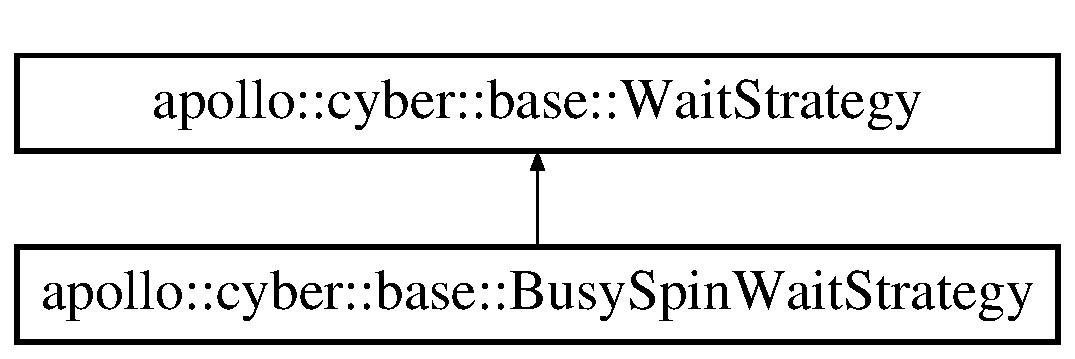
\includegraphics[height=2.000000cm]{classapollo_1_1cyber_1_1base_1_1BusySpinWaitStrategy}
\end{center}
\end{figure}
\subsection*{Public Member Functions}
\begin{DoxyCompactItemize}
\item 
\hyperlink{classapollo_1_1cyber_1_1base_1_1BusySpinWaitStrategy_afdae9c8112da0739681ca0bf706f8265}{Busy\-Spin\-Wait\-Strategy} ()
\item 
bool \hyperlink{classapollo_1_1cyber_1_1base_1_1BusySpinWaitStrategy_a4201786d6f41c09260d2e88e2a2e4027}{Empty\-Wait} () override
\end{DoxyCompactItemize}


\subsection{Constructor \& Destructor Documentation}
\hypertarget{classapollo_1_1cyber_1_1base_1_1BusySpinWaitStrategy_afdae9c8112da0739681ca0bf706f8265}{\index{apollo\-::cyber\-::base\-::\-Busy\-Spin\-Wait\-Strategy@{apollo\-::cyber\-::base\-::\-Busy\-Spin\-Wait\-Strategy}!Busy\-Spin\-Wait\-Strategy@{Busy\-Spin\-Wait\-Strategy}}
\index{Busy\-Spin\-Wait\-Strategy@{Busy\-Spin\-Wait\-Strategy}!apollo::cyber::base::BusySpinWaitStrategy@{apollo\-::cyber\-::base\-::\-Busy\-Spin\-Wait\-Strategy}}
\subsubsection[{Busy\-Spin\-Wait\-Strategy}]{\setlength{\rightskip}{0pt plus 5cm}apollo\-::cyber\-::base\-::\-Busy\-Spin\-Wait\-Strategy\-::\-Busy\-Spin\-Wait\-Strategy (
\begin{DoxyParamCaption}
{}
\end{DoxyParamCaption}
)\hspace{0.3cm}{\ttfamily [inline]}}}\label{classapollo_1_1cyber_1_1base_1_1BusySpinWaitStrategy_afdae9c8112da0739681ca0bf706f8265}


\subsection{Member Function Documentation}
\hypertarget{classapollo_1_1cyber_1_1base_1_1BusySpinWaitStrategy_a4201786d6f41c09260d2e88e2a2e4027}{\index{apollo\-::cyber\-::base\-::\-Busy\-Spin\-Wait\-Strategy@{apollo\-::cyber\-::base\-::\-Busy\-Spin\-Wait\-Strategy}!Empty\-Wait@{Empty\-Wait}}
\index{Empty\-Wait@{Empty\-Wait}!apollo::cyber::base::BusySpinWaitStrategy@{apollo\-::cyber\-::base\-::\-Busy\-Spin\-Wait\-Strategy}}
\subsubsection[{Empty\-Wait}]{\setlength{\rightskip}{0pt plus 5cm}bool apollo\-::cyber\-::base\-::\-Busy\-Spin\-Wait\-Strategy\-::\-Empty\-Wait (
\begin{DoxyParamCaption}
{}
\end{DoxyParamCaption}
)\hspace{0.3cm}{\ttfamily [inline]}, {\ttfamily [override]}, {\ttfamily [virtual]}}}\label{classapollo_1_1cyber_1_1base_1_1BusySpinWaitStrategy_a4201786d6f41c09260d2e88e2a2e4027}


Implements \hyperlink{classapollo_1_1cyber_1_1base_1_1WaitStrategy_a5801f343cd1567ec6ee586b9845446e3}{apollo\-::cyber\-::base\-::\-Wait\-Strategy}.



The documentation for this class was generated from the following file\-:\begin{DoxyCompactItemize}
\item 
base/\hyperlink{wait__strategy_8h}{wait\-\_\-strategy.\-h}\end{DoxyCompactItemize}

\hypertarget{classapollo_1_1cyber_1_1data_1_1CacheBuffer}{\section{apollo\-:\-:cyber\-:\-:data\-:\-:Cache\-Buffer$<$ T $>$ Class Template Reference}
\label{classapollo_1_1cyber_1_1data_1_1CacheBuffer}\index{apollo\-::cyber\-::data\-::\-Cache\-Buffer$<$ T $>$@{apollo\-::cyber\-::data\-::\-Cache\-Buffer$<$ T $>$}}
}


{\ttfamily \#include $<$cache\-\_\-buffer.\-h$>$}

\subsection*{Public Types}
\begin{DoxyCompactItemize}
\item 
using \hyperlink{classapollo_1_1cyber_1_1data_1_1CacheBuffer_a5ecd4f15649a5a8cdfe374728dfc525d}{value\-\_\-type} = T
\item 
using \hyperlink{classapollo_1_1cyber_1_1data_1_1CacheBuffer_aeec34cc7bc656b116ad54e5642c7f9dc}{size\-\_\-type} = std\-::size\-\_\-t
\end{DoxyCompactItemize}
\subsection*{Public Member Functions}
\begin{DoxyCompactItemize}
\item 
\hyperlink{classapollo_1_1cyber_1_1data_1_1CacheBuffer_aa7c9d5f696010ed4698485be38b7765c}{Cache\-Buffer} (uint32\-\_\-t size)
\item 
\hyperlink{classapollo_1_1cyber_1_1data_1_1CacheBuffer_af74bd9506613e92e1ca1b17f648919c8}{Cache\-Buffer} (const \hyperlink{classapollo_1_1cyber_1_1data_1_1CacheBuffer}{Cache\-Buffer} \&rhs)
\item 
T \& \hyperlink{classapollo_1_1cyber_1_1data_1_1CacheBuffer_acf961c03dfb313efee16ecc82e2dd173}{operator\mbox{[}$\,$\mbox{]}} (const uint64\-\_\-t \&pos)
\item 
const T \& \hyperlink{classapollo_1_1cyber_1_1data_1_1CacheBuffer_a6ff94280150adba58355143f04074dfc}{at} (const uint64\-\_\-t \&pos) const 
\item 
uint64\-\_\-t \hyperlink{classapollo_1_1cyber_1_1data_1_1CacheBuffer_ac3571527fa181e9d502e6ddc1cff1781}{Head} () const 
\item 
uint64\-\_\-t \hyperlink{classapollo_1_1cyber_1_1data_1_1CacheBuffer_a3981ddab2e7ec5018623b4598b6d624b}{Tail} () const 
\item 
uint64\-\_\-t \hyperlink{classapollo_1_1cyber_1_1data_1_1CacheBuffer_a6a8aa1c796dbbe2c30d44da9073c44b4}{Size} () const 
\item 
const T \& \hyperlink{classapollo_1_1cyber_1_1data_1_1CacheBuffer_ac2fb55bdcf49b1e535880445bcffd034}{Front} () const 
\item 
const T \& \hyperlink{classapollo_1_1cyber_1_1data_1_1CacheBuffer_a9bc0ad702d7471e25d67c53a9ff14a6a}{Back} () const 
\item 
bool \hyperlink{classapollo_1_1cyber_1_1data_1_1CacheBuffer_a274a1d5f8a68f932e2e98c92e6f03223}{Empty} () const 
\item 
bool \hyperlink{classapollo_1_1cyber_1_1data_1_1CacheBuffer_acfdc5bac267080f793233648228f6463}{Full} () const 
\item 
void \hyperlink{classapollo_1_1cyber_1_1data_1_1CacheBuffer_af3ebad1c52b091d2b3e540d98a9e0bd2}{Fill} (const T \&value)
\item 
std\-::mutex \& \hyperlink{classapollo_1_1cyber_1_1data_1_1CacheBuffer_abd49ff1c56aa99e1bf38b6f0adc8df98}{Mutex} ()
\end{DoxyCompactItemize}
\subsection*{Private Member Functions}
\begin{DoxyCompactItemize}
\item 
\hyperlink{classapollo_1_1cyber_1_1data_1_1CacheBuffer}{Cache\-Buffer} \& \hyperlink{classapollo_1_1cyber_1_1data_1_1CacheBuffer_ab4d656d337d744664f53ba5e7879aef9}{operator=} (const \hyperlink{classapollo_1_1cyber_1_1data_1_1CacheBuffer}{Cache\-Buffer} \&other)=delete
\item 
uint64\-\_\-t \hyperlink{classapollo_1_1cyber_1_1data_1_1CacheBuffer_ab0f2af50e3d6e7a367ca92eb1c5614c9}{Get\-Index} (const uint64\-\_\-t \&pos) const 
\end{DoxyCompactItemize}
\subsection*{Private Attributes}
\begin{DoxyCompactItemize}
\item 
uint64\-\_\-t \hyperlink{classapollo_1_1cyber_1_1data_1_1CacheBuffer_ad93c0d4ea1554ca5cd755d7b2a920d9a}{head\-\_\-} = 0
\item 
uint64\-\_\-t \hyperlink{classapollo_1_1cyber_1_1data_1_1CacheBuffer_ad293745c1a892594ae8c934a793c32ce}{tail\-\_\-} = 0
\item 
uint64\-\_\-t \hyperlink{classapollo_1_1cyber_1_1data_1_1CacheBuffer_a8b100fbcee82983f35f98822907e82bc}{capacity\-\_\-} = 0
\item 
std\-::vector$<$ T $>$ \hyperlink{classapollo_1_1cyber_1_1data_1_1CacheBuffer_ab452281ecd9ee969582fca3fda207a3a}{buffer\-\_\-}
\item 
std\-::mutex \hyperlink{classapollo_1_1cyber_1_1data_1_1CacheBuffer_a6161b6de3bd9b4837491cd16a4cdb716}{mutex\-\_\-}
\end{DoxyCompactItemize}


\subsection{Member Typedef Documentation}
\hypertarget{classapollo_1_1cyber_1_1data_1_1CacheBuffer_aeec34cc7bc656b116ad54e5642c7f9dc}{\index{apollo\-::cyber\-::data\-::\-Cache\-Buffer@{apollo\-::cyber\-::data\-::\-Cache\-Buffer}!size\-\_\-type@{size\-\_\-type}}
\index{size\-\_\-type@{size\-\_\-type}!apollo::cyber::data::CacheBuffer@{apollo\-::cyber\-::data\-::\-Cache\-Buffer}}
\subsubsection[{size\-\_\-type}]{\setlength{\rightskip}{0pt plus 5cm}template$<$typename T $>$ using {\bf apollo\-::cyber\-::data\-::\-Cache\-Buffer}$<$ T $>$\-::{\bf size\-\_\-type} =  std\-::size\-\_\-t}}\label{classapollo_1_1cyber_1_1data_1_1CacheBuffer_aeec34cc7bc656b116ad54e5642c7f9dc}
\hypertarget{classapollo_1_1cyber_1_1data_1_1CacheBuffer_a5ecd4f15649a5a8cdfe374728dfc525d}{\index{apollo\-::cyber\-::data\-::\-Cache\-Buffer@{apollo\-::cyber\-::data\-::\-Cache\-Buffer}!value\-\_\-type@{value\-\_\-type}}
\index{value\-\_\-type@{value\-\_\-type}!apollo::cyber::data::CacheBuffer@{apollo\-::cyber\-::data\-::\-Cache\-Buffer}}
\subsubsection[{value\-\_\-type}]{\setlength{\rightskip}{0pt plus 5cm}template$<$typename T $>$ using {\bf apollo\-::cyber\-::data\-::\-Cache\-Buffer}$<$ T $>$\-::{\bf value\-\_\-type} =  T}}\label{classapollo_1_1cyber_1_1data_1_1CacheBuffer_a5ecd4f15649a5a8cdfe374728dfc525d}


\subsection{Constructor \& Destructor Documentation}
\hypertarget{classapollo_1_1cyber_1_1data_1_1CacheBuffer_aa7c9d5f696010ed4698485be38b7765c}{\index{apollo\-::cyber\-::data\-::\-Cache\-Buffer@{apollo\-::cyber\-::data\-::\-Cache\-Buffer}!Cache\-Buffer@{Cache\-Buffer}}
\index{Cache\-Buffer@{Cache\-Buffer}!apollo::cyber::data::CacheBuffer@{apollo\-::cyber\-::data\-::\-Cache\-Buffer}}
\subsubsection[{Cache\-Buffer}]{\setlength{\rightskip}{0pt plus 5cm}template$<$typename T $>$ {\bf apollo\-::cyber\-::data\-::\-Cache\-Buffer}$<$ T $>$\-::{\bf Cache\-Buffer} (
\begin{DoxyParamCaption}
\item[{uint32\-\_\-t}]{size}
\end{DoxyParamCaption}
)\hspace{0.3cm}{\ttfamily [inline]}, {\ttfamily [explicit]}}}\label{classapollo_1_1cyber_1_1data_1_1CacheBuffer_aa7c9d5f696010ed4698485be38b7765c}
\hypertarget{classapollo_1_1cyber_1_1data_1_1CacheBuffer_af74bd9506613e92e1ca1b17f648919c8}{\index{apollo\-::cyber\-::data\-::\-Cache\-Buffer@{apollo\-::cyber\-::data\-::\-Cache\-Buffer}!Cache\-Buffer@{Cache\-Buffer}}
\index{Cache\-Buffer@{Cache\-Buffer}!apollo::cyber::data::CacheBuffer@{apollo\-::cyber\-::data\-::\-Cache\-Buffer}}
\subsubsection[{Cache\-Buffer}]{\setlength{\rightskip}{0pt plus 5cm}template$<$typename T $>$ {\bf apollo\-::cyber\-::data\-::\-Cache\-Buffer}$<$ T $>$\-::{\bf Cache\-Buffer} (
\begin{DoxyParamCaption}
\item[{const {\bf Cache\-Buffer}$<$ T $>$ \&}]{rhs}
\end{DoxyParamCaption}
)\hspace{0.3cm}{\ttfamily [inline]}}}\label{classapollo_1_1cyber_1_1data_1_1CacheBuffer_af74bd9506613e92e1ca1b17f648919c8}


\subsection{Member Function Documentation}
\hypertarget{classapollo_1_1cyber_1_1data_1_1CacheBuffer_a6ff94280150adba58355143f04074dfc}{\index{apollo\-::cyber\-::data\-::\-Cache\-Buffer@{apollo\-::cyber\-::data\-::\-Cache\-Buffer}!at@{at}}
\index{at@{at}!apollo::cyber::data::CacheBuffer@{apollo\-::cyber\-::data\-::\-Cache\-Buffer}}
\subsubsection[{at}]{\setlength{\rightskip}{0pt plus 5cm}template$<$typename T $>$ const T\& {\bf apollo\-::cyber\-::data\-::\-Cache\-Buffer}$<$ T $>$\-::at (
\begin{DoxyParamCaption}
\item[{const uint64\-\_\-t \&}]{pos}
\end{DoxyParamCaption}
) const\hspace{0.3cm}{\ttfamily [inline]}}}\label{classapollo_1_1cyber_1_1data_1_1CacheBuffer_a6ff94280150adba58355143f04074dfc}
\hypertarget{classapollo_1_1cyber_1_1data_1_1CacheBuffer_a9bc0ad702d7471e25d67c53a9ff14a6a}{\index{apollo\-::cyber\-::data\-::\-Cache\-Buffer@{apollo\-::cyber\-::data\-::\-Cache\-Buffer}!Back@{Back}}
\index{Back@{Back}!apollo::cyber::data::CacheBuffer@{apollo\-::cyber\-::data\-::\-Cache\-Buffer}}
\subsubsection[{Back}]{\setlength{\rightskip}{0pt plus 5cm}template$<$typename T $>$ const T\& {\bf apollo\-::cyber\-::data\-::\-Cache\-Buffer}$<$ T $>$\-::Back (
\begin{DoxyParamCaption}
{}
\end{DoxyParamCaption}
) const\hspace{0.3cm}{\ttfamily [inline]}}}\label{classapollo_1_1cyber_1_1data_1_1CacheBuffer_a9bc0ad702d7471e25d67c53a9ff14a6a}
\hypertarget{classapollo_1_1cyber_1_1data_1_1CacheBuffer_a274a1d5f8a68f932e2e98c92e6f03223}{\index{apollo\-::cyber\-::data\-::\-Cache\-Buffer@{apollo\-::cyber\-::data\-::\-Cache\-Buffer}!Empty@{Empty}}
\index{Empty@{Empty}!apollo::cyber::data::CacheBuffer@{apollo\-::cyber\-::data\-::\-Cache\-Buffer}}
\subsubsection[{Empty}]{\setlength{\rightskip}{0pt plus 5cm}template$<$typename T $>$ bool {\bf apollo\-::cyber\-::data\-::\-Cache\-Buffer}$<$ T $>$\-::Empty (
\begin{DoxyParamCaption}
{}
\end{DoxyParamCaption}
) const\hspace{0.3cm}{\ttfamily [inline]}}}\label{classapollo_1_1cyber_1_1data_1_1CacheBuffer_a274a1d5f8a68f932e2e98c92e6f03223}
\hypertarget{classapollo_1_1cyber_1_1data_1_1CacheBuffer_af3ebad1c52b091d2b3e540d98a9e0bd2}{\index{apollo\-::cyber\-::data\-::\-Cache\-Buffer@{apollo\-::cyber\-::data\-::\-Cache\-Buffer}!Fill@{Fill}}
\index{Fill@{Fill}!apollo::cyber::data::CacheBuffer@{apollo\-::cyber\-::data\-::\-Cache\-Buffer}}
\subsubsection[{Fill}]{\setlength{\rightskip}{0pt plus 5cm}template$<$typename T $>$ void {\bf apollo\-::cyber\-::data\-::\-Cache\-Buffer}$<$ T $>$\-::Fill (
\begin{DoxyParamCaption}
\item[{const T \&}]{value}
\end{DoxyParamCaption}
)\hspace{0.3cm}{\ttfamily [inline]}}}\label{classapollo_1_1cyber_1_1data_1_1CacheBuffer_af3ebad1c52b091d2b3e540d98a9e0bd2}
\hypertarget{classapollo_1_1cyber_1_1data_1_1CacheBuffer_ac2fb55bdcf49b1e535880445bcffd034}{\index{apollo\-::cyber\-::data\-::\-Cache\-Buffer@{apollo\-::cyber\-::data\-::\-Cache\-Buffer}!Front@{Front}}
\index{Front@{Front}!apollo::cyber::data::CacheBuffer@{apollo\-::cyber\-::data\-::\-Cache\-Buffer}}
\subsubsection[{Front}]{\setlength{\rightskip}{0pt plus 5cm}template$<$typename T $>$ const T\& {\bf apollo\-::cyber\-::data\-::\-Cache\-Buffer}$<$ T $>$\-::Front (
\begin{DoxyParamCaption}
{}
\end{DoxyParamCaption}
) const\hspace{0.3cm}{\ttfamily [inline]}}}\label{classapollo_1_1cyber_1_1data_1_1CacheBuffer_ac2fb55bdcf49b1e535880445bcffd034}
\hypertarget{classapollo_1_1cyber_1_1data_1_1CacheBuffer_acfdc5bac267080f793233648228f6463}{\index{apollo\-::cyber\-::data\-::\-Cache\-Buffer@{apollo\-::cyber\-::data\-::\-Cache\-Buffer}!Full@{Full}}
\index{Full@{Full}!apollo::cyber::data::CacheBuffer@{apollo\-::cyber\-::data\-::\-Cache\-Buffer}}
\subsubsection[{Full}]{\setlength{\rightskip}{0pt plus 5cm}template$<$typename T $>$ bool {\bf apollo\-::cyber\-::data\-::\-Cache\-Buffer}$<$ T $>$\-::Full (
\begin{DoxyParamCaption}
{}
\end{DoxyParamCaption}
) const\hspace{0.3cm}{\ttfamily [inline]}}}\label{classapollo_1_1cyber_1_1data_1_1CacheBuffer_acfdc5bac267080f793233648228f6463}
\hypertarget{classapollo_1_1cyber_1_1data_1_1CacheBuffer_ab0f2af50e3d6e7a367ca92eb1c5614c9}{\index{apollo\-::cyber\-::data\-::\-Cache\-Buffer@{apollo\-::cyber\-::data\-::\-Cache\-Buffer}!Get\-Index@{Get\-Index}}
\index{Get\-Index@{Get\-Index}!apollo::cyber::data::CacheBuffer@{apollo\-::cyber\-::data\-::\-Cache\-Buffer}}
\subsubsection[{Get\-Index}]{\setlength{\rightskip}{0pt plus 5cm}template$<$typename T $>$ uint64\-\_\-t {\bf apollo\-::cyber\-::data\-::\-Cache\-Buffer}$<$ T $>$\-::Get\-Index (
\begin{DoxyParamCaption}
\item[{const uint64\-\_\-t \&}]{pos}
\end{DoxyParamCaption}
) const\hspace{0.3cm}{\ttfamily [inline]}, {\ttfamily [private]}}}\label{classapollo_1_1cyber_1_1data_1_1CacheBuffer_ab0f2af50e3d6e7a367ca92eb1c5614c9}
\hypertarget{classapollo_1_1cyber_1_1data_1_1CacheBuffer_ac3571527fa181e9d502e6ddc1cff1781}{\index{apollo\-::cyber\-::data\-::\-Cache\-Buffer@{apollo\-::cyber\-::data\-::\-Cache\-Buffer}!Head@{Head}}
\index{Head@{Head}!apollo::cyber::data::CacheBuffer@{apollo\-::cyber\-::data\-::\-Cache\-Buffer}}
\subsubsection[{Head}]{\setlength{\rightskip}{0pt plus 5cm}template$<$typename T $>$ uint64\-\_\-t {\bf apollo\-::cyber\-::data\-::\-Cache\-Buffer}$<$ T $>$\-::Head (
\begin{DoxyParamCaption}
{}
\end{DoxyParamCaption}
) const\hspace{0.3cm}{\ttfamily [inline]}}}\label{classapollo_1_1cyber_1_1data_1_1CacheBuffer_ac3571527fa181e9d502e6ddc1cff1781}
\hypertarget{classapollo_1_1cyber_1_1data_1_1CacheBuffer_abd49ff1c56aa99e1bf38b6f0adc8df98}{\index{apollo\-::cyber\-::data\-::\-Cache\-Buffer@{apollo\-::cyber\-::data\-::\-Cache\-Buffer}!Mutex@{Mutex}}
\index{Mutex@{Mutex}!apollo::cyber::data::CacheBuffer@{apollo\-::cyber\-::data\-::\-Cache\-Buffer}}
\subsubsection[{Mutex}]{\setlength{\rightskip}{0pt plus 5cm}template$<$typename T $>$ std\-::mutex\& {\bf apollo\-::cyber\-::data\-::\-Cache\-Buffer}$<$ T $>$\-::Mutex (
\begin{DoxyParamCaption}
{}
\end{DoxyParamCaption}
)\hspace{0.3cm}{\ttfamily [inline]}}}\label{classapollo_1_1cyber_1_1data_1_1CacheBuffer_abd49ff1c56aa99e1bf38b6f0adc8df98}
\hypertarget{classapollo_1_1cyber_1_1data_1_1CacheBuffer_ab4d656d337d744664f53ba5e7879aef9}{\index{apollo\-::cyber\-::data\-::\-Cache\-Buffer@{apollo\-::cyber\-::data\-::\-Cache\-Buffer}!operator=@{operator=}}
\index{operator=@{operator=}!apollo::cyber::data::CacheBuffer@{apollo\-::cyber\-::data\-::\-Cache\-Buffer}}
\subsubsection[{operator=}]{\setlength{\rightskip}{0pt plus 5cm}template$<$typename T $>$ {\bf Cache\-Buffer}\& {\bf apollo\-::cyber\-::data\-::\-Cache\-Buffer}$<$ T $>$\-::operator= (
\begin{DoxyParamCaption}
\item[{const {\bf Cache\-Buffer}$<$ T $>$ \&}]{other}
\end{DoxyParamCaption}
)\hspace{0.3cm}{\ttfamily [private]}, {\ttfamily [delete]}}}\label{classapollo_1_1cyber_1_1data_1_1CacheBuffer_ab4d656d337d744664f53ba5e7879aef9}
\hypertarget{classapollo_1_1cyber_1_1data_1_1CacheBuffer_acf961c03dfb313efee16ecc82e2dd173}{\index{apollo\-::cyber\-::data\-::\-Cache\-Buffer@{apollo\-::cyber\-::data\-::\-Cache\-Buffer}!operator\mbox{[}$\,$\mbox{]}@{operator[]}}
\index{operator\mbox{[}$\,$\mbox{]}@{operator[]}!apollo::cyber::data::CacheBuffer@{apollo\-::cyber\-::data\-::\-Cache\-Buffer}}
\subsubsection[{operator[]}]{\setlength{\rightskip}{0pt plus 5cm}template$<$typename T $>$ T\& {\bf apollo\-::cyber\-::data\-::\-Cache\-Buffer}$<$ T $>$\-::operator\mbox{[}$\,$\mbox{]} (
\begin{DoxyParamCaption}
\item[{const uint64\-\_\-t \&}]{pos}
\end{DoxyParamCaption}
)\hspace{0.3cm}{\ttfamily [inline]}}}\label{classapollo_1_1cyber_1_1data_1_1CacheBuffer_acf961c03dfb313efee16ecc82e2dd173}
\hypertarget{classapollo_1_1cyber_1_1data_1_1CacheBuffer_a6a8aa1c796dbbe2c30d44da9073c44b4}{\index{apollo\-::cyber\-::data\-::\-Cache\-Buffer@{apollo\-::cyber\-::data\-::\-Cache\-Buffer}!Size@{Size}}
\index{Size@{Size}!apollo::cyber::data::CacheBuffer@{apollo\-::cyber\-::data\-::\-Cache\-Buffer}}
\subsubsection[{Size}]{\setlength{\rightskip}{0pt plus 5cm}template$<$typename T $>$ uint64\-\_\-t {\bf apollo\-::cyber\-::data\-::\-Cache\-Buffer}$<$ T $>$\-::Size (
\begin{DoxyParamCaption}
{}
\end{DoxyParamCaption}
) const\hspace{0.3cm}{\ttfamily [inline]}}}\label{classapollo_1_1cyber_1_1data_1_1CacheBuffer_a6a8aa1c796dbbe2c30d44da9073c44b4}
\hypertarget{classapollo_1_1cyber_1_1data_1_1CacheBuffer_a3981ddab2e7ec5018623b4598b6d624b}{\index{apollo\-::cyber\-::data\-::\-Cache\-Buffer@{apollo\-::cyber\-::data\-::\-Cache\-Buffer}!Tail@{Tail}}
\index{Tail@{Tail}!apollo::cyber::data::CacheBuffer@{apollo\-::cyber\-::data\-::\-Cache\-Buffer}}
\subsubsection[{Tail}]{\setlength{\rightskip}{0pt plus 5cm}template$<$typename T $>$ uint64\-\_\-t {\bf apollo\-::cyber\-::data\-::\-Cache\-Buffer}$<$ T $>$\-::Tail (
\begin{DoxyParamCaption}
{}
\end{DoxyParamCaption}
) const\hspace{0.3cm}{\ttfamily [inline]}}}\label{classapollo_1_1cyber_1_1data_1_1CacheBuffer_a3981ddab2e7ec5018623b4598b6d624b}


\subsection{Member Data Documentation}
\hypertarget{classapollo_1_1cyber_1_1data_1_1CacheBuffer_ab452281ecd9ee969582fca3fda207a3a}{\index{apollo\-::cyber\-::data\-::\-Cache\-Buffer@{apollo\-::cyber\-::data\-::\-Cache\-Buffer}!buffer\-\_\-@{buffer\-\_\-}}
\index{buffer\-\_\-@{buffer\-\_\-}!apollo::cyber::data::CacheBuffer@{apollo\-::cyber\-::data\-::\-Cache\-Buffer}}
\subsubsection[{buffer\-\_\-}]{\setlength{\rightskip}{0pt plus 5cm}template$<$typename T $>$ std\-::vector$<$T$>$ {\bf apollo\-::cyber\-::data\-::\-Cache\-Buffer}$<$ T $>$\-::buffer\-\_\-\hspace{0.3cm}{\ttfamily [private]}}}\label{classapollo_1_1cyber_1_1data_1_1CacheBuffer_ab452281ecd9ee969582fca3fda207a3a}
\hypertarget{classapollo_1_1cyber_1_1data_1_1CacheBuffer_a8b100fbcee82983f35f98822907e82bc}{\index{apollo\-::cyber\-::data\-::\-Cache\-Buffer@{apollo\-::cyber\-::data\-::\-Cache\-Buffer}!capacity\-\_\-@{capacity\-\_\-}}
\index{capacity\-\_\-@{capacity\-\_\-}!apollo::cyber::data::CacheBuffer@{apollo\-::cyber\-::data\-::\-Cache\-Buffer}}
\subsubsection[{capacity\-\_\-}]{\setlength{\rightskip}{0pt plus 5cm}template$<$typename T $>$ uint64\-\_\-t {\bf apollo\-::cyber\-::data\-::\-Cache\-Buffer}$<$ T $>$\-::capacity\-\_\- = 0\hspace{0.3cm}{\ttfamily [private]}}}\label{classapollo_1_1cyber_1_1data_1_1CacheBuffer_a8b100fbcee82983f35f98822907e82bc}
\hypertarget{classapollo_1_1cyber_1_1data_1_1CacheBuffer_ad93c0d4ea1554ca5cd755d7b2a920d9a}{\index{apollo\-::cyber\-::data\-::\-Cache\-Buffer@{apollo\-::cyber\-::data\-::\-Cache\-Buffer}!head\-\_\-@{head\-\_\-}}
\index{head\-\_\-@{head\-\_\-}!apollo::cyber::data::CacheBuffer@{apollo\-::cyber\-::data\-::\-Cache\-Buffer}}
\subsubsection[{head\-\_\-}]{\setlength{\rightskip}{0pt plus 5cm}template$<$typename T $>$ uint64\-\_\-t {\bf apollo\-::cyber\-::data\-::\-Cache\-Buffer}$<$ T $>$\-::head\-\_\- = 0\hspace{0.3cm}{\ttfamily [private]}}}\label{classapollo_1_1cyber_1_1data_1_1CacheBuffer_ad93c0d4ea1554ca5cd755d7b2a920d9a}
\hypertarget{classapollo_1_1cyber_1_1data_1_1CacheBuffer_a6161b6de3bd9b4837491cd16a4cdb716}{\index{apollo\-::cyber\-::data\-::\-Cache\-Buffer@{apollo\-::cyber\-::data\-::\-Cache\-Buffer}!mutex\-\_\-@{mutex\-\_\-}}
\index{mutex\-\_\-@{mutex\-\_\-}!apollo::cyber::data::CacheBuffer@{apollo\-::cyber\-::data\-::\-Cache\-Buffer}}
\subsubsection[{mutex\-\_\-}]{\setlength{\rightskip}{0pt plus 5cm}template$<$typename T $>$ std\-::mutex {\bf apollo\-::cyber\-::data\-::\-Cache\-Buffer}$<$ T $>$\-::mutex\-\_\-\hspace{0.3cm}{\ttfamily [mutable]}, {\ttfamily [private]}}}\label{classapollo_1_1cyber_1_1data_1_1CacheBuffer_a6161b6de3bd9b4837491cd16a4cdb716}
\hypertarget{classapollo_1_1cyber_1_1data_1_1CacheBuffer_ad293745c1a892594ae8c934a793c32ce}{\index{apollo\-::cyber\-::data\-::\-Cache\-Buffer@{apollo\-::cyber\-::data\-::\-Cache\-Buffer}!tail\-\_\-@{tail\-\_\-}}
\index{tail\-\_\-@{tail\-\_\-}!apollo::cyber::data::CacheBuffer@{apollo\-::cyber\-::data\-::\-Cache\-Buffer}}
\subsubsection[{tail\-\_\-}]{\setlength{\rightskip}{0pt plus 5cm}template$<$typename T $>$ uint64\-\_\-t {\bf apollo\-::cyber\-::data\-::\-Cache\-Buffer}$<$ T $>$\-::tail\-\_\- = 0\hspace{0.3cm}{\ttfamily [private]}}}\label{classapollo_1_1cyber_1_1data_1_1CacheBuffer_ad293745c1a892594ae8c934a793c32ce}


The documentation for this class was generated from the following file\-:\begin{DoxyCompactItemize}
\item 
data/\hyperlink{cache__buffer_8h}{cache\-\_\-buffer.\-h}\end{DoxyCompactItemize}

\hypertarget{structapollo_1_1cyber_1_1transport_1_1History_1_1CachedMessage}{\section{apollo\-:\-:cyber\-:\-:transport\-:\-:History$<$ Message\-T $>$\-:\-:Cached\-Message Struct Reference}
\label{structapollo_1_1cyber_1_1transport_1_1History_1_1CachedMessage}\index{apollo\-::cyber\-::transport\-::\-History$<$ Message\-T $>$\-::\-Cached\-Message@{apollo\-::cyber\-::transport\-::\-History$<$ Message\-T $>$\-::\-Cached\-Message}}
}


{\ttfamily \#include $<$history.\-h$>$}

\subsection*{Public Member Functions}
\begin{DoxyCompactItemize}
\item 
\hyperlink{structapollo_1_1cyber_1_1transport_1_1History_1_1CachedMessage_aa98e44d2f2df28d756f36f631c4737a8}{Cached\-Message} (const \hyperlink{classapollo_1_1cyber_1_1transport_1_1History_a4c11720b1c1d14eafb9fec5436a0d7c0}{Message\-Ptr} \&message, const \hyperlink{classapollo_1_1cyber_1_1transport_1_1MessageInfo}{Message\-Info} \&message\-\_\-info)
\end{DoxyCompactItemize}
\subsection*{Public Attributes}
\begin{DoxyCompactItemize}
\item 
\hyperlink{classapollo_1_1cyber_1_1transport_1_1History_a4c11720b1c1d14eafb9fec5436a0d7c0}{Message\-Ptr} \hyperlink{structapollo_1_1cyber_1_1transport_1_1History_1_1CachedMessage_a48a1ca0f2407b79c69fc63f3ad5fbd46}{msg}
\item 
\hyperlink{classapollo_1_1cyber_1_1transport_1_1MessageInfo}{Message\-Info} \hyperlink{structapollo_1_1cyber_1_1transport_1_1History_1_1CachedMessage_a42ec71985e1d8e8bd86ea77232301278}{msg\-\_\-info}
\end{DoxyCompactItemize}


\subsection{Constructor \& Destructor Documentation}
\hypertarget{structapollo_1_1cyber_1_1transport_1_1History_1_1CachedMessage_aa98e44d2f2df28d756f36f631c4737a8}{\index{apollo\-::cyber\-::transport\-::\-History\-::\-Cached\-Message@{apollo\-::cyber\-::transport\-::\-History\-::\-Cached\-Message}!Cached\-Message@{Cached\-Message}}
\index{Cached\-Message@{Cached\-Message}!apollo::cyber::transport::History::CachedMessage@{apollo\-::cyber\-::transport\-::\-History\-::\-Cached\-Message}}
\subsubsection[{Cached\-Message}]{\setlength{\rightskip}{0pt plus 5cm}template$<$typename Message\-T $>$ {\bf apollo\-::cyber\-::transport\-::\-History}$<$ Message\-T $>$\-::Cached\-Message\-::\-Cached\-Message (
\begin{DoxyParamCaption}
\item[{const {\bf Message\-Ptr} \&}]{message, }
\item[{const {\bf Message\-Info} \&}]{message\-\_\-info}
\end{DoxyParamCaption}
)\hspace{0.3cm}{\ttfamily [inline]}}}\label{structapollo_1_1cyber_1_1transport_1_1History_1_1CachedMessage_aa98e44d2f2df28d756f36f631c4737a8}


\subsection{Member Data Documentation}
\hypertarget{structapollo_1_1cyber_1_1transport_1_1History_1_1CachedMessage_a48a1ca0f2407b79c69fc63f3ad5fbd46}{\index{apollo\-::cyber\-::transport\-::\-History\-::\-Cached\-Message@{apollo\-::cyber\-::transport\-::\-History\-::\-Cached\-Message}!msg@{msg}}
\index{msg@{msg}!apollo::cyber::transport::History::CachedMessage@{apollo\-::cyber\-::transport\-::\-History\-::\-Cached\-Message}}
\subsubsection[{msg}]{\setlength{\rightskip}{0pt plus 5cm}template$<$typename Message\-T $>$ {\bf Message\-Ptr} {\bf apollo\-::cyber\-::transport\-::\-History}$<$ Message\-T $>$\-::Cached\-Message\-::msg}}\label{structapollo_1_1cyber_1_1transport_1_1History_1_1CachedMessage_a48a1ca0f2407b79c69fc63f3ad5fbd46}
\hypertarget{structapollo_1_1cyber_1_1transport_1_1History_1_1CachedMessage_a42ec71985e1d8e8bd86ea77232301278}{\index{apollo\-::cyber\-::transport\-::\-History\-::\-Cached\-Message@{apollo\-::cyber\-::transport\-::\-History\-::\-Cached\-Message}!msg\-\_\-info@{msg\-\_\-info}}
\index{msg\-\_\-info@{msg\-\_\-info}!apollo::cyber::transport::History::CachedMessage@{apollo\-::cyber\-::transport\-::\-History\-::\-Cached\-Message}}
\subsubsection[{msg\-\_\-info}]{\setlength{\rightskip}{0pt plus 5cm}template$<$typename Message\-T $>$ {\bf Message\-Info} {\bf apollo\-::cyber\-::transport\-::\-History}$<$ Message\-T $>$\-::Cached\-Message\-::msg\-\_\-info}}\label{structapollo_1_1cyber_1_1transport_1_1History_1_1CachedMessage_a42ec71985e1d8e8bd86ea77232301278}


The documentation for this struct was generated from the following file\-:\begin{DoxyCompactItemize}
\item 
transport/message/\hyperlink{history_8h}{history.\-h}\end{DoxyCompactItemize}

\hypertarget{classapollo_1_1cyber_1_1base_1_1CCObjectPool}{\section{apollo\-:\-:cyber\-:\-:base\-:\-:C\-C\-Object\-Pool$<$ T $>$ Class Template Reference}
\label{classapollo_1_1cyber_1_1base_1_1CCObjectPool}\index{apollo\-::cyber\-::base\-::\-C\-C\-Object\-Pool$<$ T $>$@{apollo\-::cyber\-::base\-::\-C\-C\-Object\-Pool$<$ T $>$}}
}


{\ttfamily \#include $<$concurrent\-\_\-object\-\_\-pool.\-h$>$}

Inheritance diagram for apollo\-:\-:cyber\-:\-:base\-:\-:C\-C\-Object\-Pool$<$ T $>$\-:\begin{figure}[H]
\begin{center}
\leavevmode
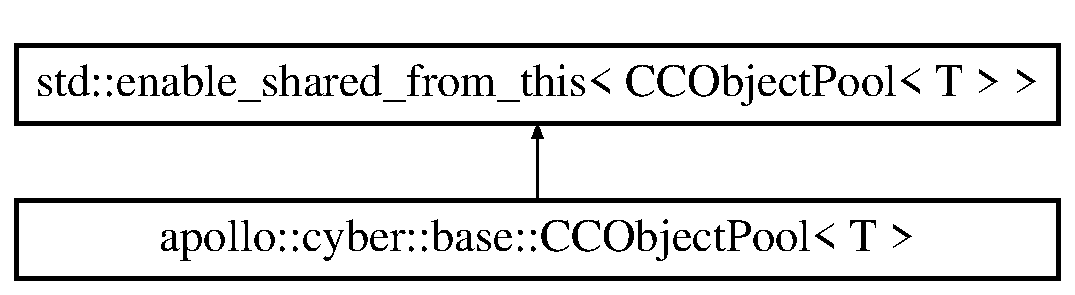
\includegraphics[height=2.000000cm]{classapollo_1_1cyber_1_1base_1_1CCObjectPool}
\end{center}
\end{figure}
\subsection*{Classes}
\begin{DoxyCompactItemize}
\item 
struct \hyperlink{structapollo_1_1cyber_1_1base_1_1CCObjectPool_1_1Head}{Head}
\item 
struct \hyperlink{structapollo_1_1cyber_1_1base_1_1CCObjectPool_1_1Node}{Node}
\end{DoxyCompactItemize}
\subsection*{Public Member Functions}
\begin{DoxyCompactItemize}
\item 
\hyperlink{classapollo_1_1cyber_1_1base_1_1CCObjectPool_aef6bb40c0a7105fcafa6f36eec1990f1}{C\-C\-Object\-Pool} (uint32\-\_\-t \hyperlink{classapollo_1_1cyber_1_1base_1_1CCObjectPool_a60a5ad05a90e7c32542454162b46b2cc}{size})
\item 
virtual \hyperlink{classapollo_1_1cyber_1_1base_1_1CCObjectPool_a66e73519d6e04f2575f474132677cd65}{$\sim$\-C\-C\-Object\-Pool} ()
\item 
{\footnotesize template$<$typename... Args$>$ }\\void \hyperlink{classapollo_1_1cyber_1_1base_1_1CCObjectPool_ab92a199f84762cd01e980c960c8d0990}{Construct\-All} (Args \&\&...args)
\item 
{\footnotesize template$<$typename... Args$>$ }\\std\-::shared\-\_\-ptr$<$ T $>$ \hyperlink{classapollo_1_1cyber_1_1base_1_1CCObjectPool_aa0be7adc9df9571d064f0d0f85c99398}{Construct\-Object} (Args \&\&...args)
\item 
std\-::shared\-\_\-ptr$<$ T $>$ \hyperlink{classapollo_1_1cyber_1_1base_1_1CCObjectPool_a2185323d56b9150be49dd891fa9823bd}{Get\-Object} ()
\item 
void \hyperlink{classapollo_1_1cyber_1_1base_1_1CCObjectPool_a32587174920cbf5b3ff400bb2870b49d}{Release\-Object} (T $\ast$)
\item 
uint32\-\_\-t \hyperlink{classapollo_1_1cyber_1_1base_1_1CCObjectPool_a60a5ad05a90e7c32542454162b46b2cc}{size} () const 
\end{DoxyCompactItemize}
\subsection*{Private Member Functions}
\begin{DoxyCompactItemize}
\item 
\hyperlink{classapollo_1_1cyber_1_1base_1_1CCObjectPool_a816f40fca7251af2f4296cbb061cf33f}{C\-C\-Object\-Pool} (\hyperlink{classapollo_1_1cyber_1_1base_1_1CCObjectPool}{C\-C\-Object\-Pool} \&)=delete
\item 
\hyperlink{classapollo_1_1cyber_1_1base_1_1CCObjectPool}{C\-C\-Object\-Pool} \& \hyperlink{classapollo_1_1cyber_1_1base_1_1CCObjectPool_ac870b2539ea47c8ae31fc27c4e3bc8d8}{operator=} (\hyperlink{classapollo_1_1cyber_1_1base_1_1CCObjectPool}{C\-C\-Object\-Pool} \&)=delete
\item 
bool \hyperlink{classapollo_1_1cyber_1_1base_1_1CCObjectPool_acbaa170bbe0171d605f3f640626685ba}{Find\-Free\-Head} (\hyperlink{structapollo_1_1cyber_1_1base_1_1CCObjectPool_1_1Head}{Head} $\ast$head)
\end{DoxyCompactItemize}
\subsection*{Private Attributes}
\begin{DoxyCompactItemize}
\item 
std\-::atomic$<$ \hyperlink{structapollo_1_1cyber_1_1base_1_1CCObjectPool_1_1Head}{Head} $>$ \hyperlink{classapollo_1_1cyber_1_1base_1_1CCObjectPool_a40fd41481676d2e6ddac5d3237e7f234}{free\-\_\-head\-\_\-}
\item 
\hyperlink{structapollo_1_1cyber_1_1base_1_1CCObjectPool_1_1Node}{Node} $\ast$ \hyperlink{classapollo_1_1cyber_1_1base_1_1CCObjectPool_ad5fdd44b05eac5aa18d54fdec5928dfb}{node\-\_\-arena\-\_\-} = nullptr
\item 
uint32\-\_\-t \hyperlink{classapollo_1_1cyber_1_1base_1_1CCObjectPool_a3aaed740b510502df0ac4190b8e1734f}{capacity\-\_\-} = 0
\end{DoxyCompactItemize}


\subsection{Constructor \& Destructor Documentation}
\hypertarget{classapollo_1_1cyber_1_1base_1_1CCObjectPool_aef6bb40c0a7105fcafa6f36eec1990f1}{\index{apollo\-::cyber\-::base\-::\-C\-C\-Object\-Pool@{apollo\-::cyber\-::base\-::\-C\-C\-Object\-Pool}!C\-C\-Object\-Pool@{C\-C\-Object\-Pool}}
\index{C\-C\-Object\-Pool@{C\-C\-Object\-Pool}!apollo::cyber::base::CCObjectPool@{apollo\-::cyber\-::base\-::\-C\-C\-Object\-Pool}}
\subsubsection[{C\-C\-Object\-Pool}]{\setlength{\rightskip}{0pt plus 5cm}template$<$typename T $>$ {\bf apollo\-::cyber\-::base\-::\-C\-C\-Object\-Pool}$<$ T $>$\-::{\bf C\-C\-Object\-Pool} (
\begin{DoxyParamCaption}
\item[{uint32\-\_\-t}]{size}
\end{DoxyParamCaption}
)\hspace{0.3cm}{\ttfamily [explicit]}}}\label{classapollo_1_1cyber_1_1base_1_1CCObjectPool_aef6bb40c0a7105fcafa6f36eec1990f1}
\hypertarget{classapollo_1_1cyber_1_1base_1_1CCObjectPool_a66e73519d6e04f2575f474132677cd65}{\index{apollo\-::cyber\-::base\-::\-C\-C\-Object\-Pool@{apollo\-::cyber\-::base\-::\-C\-C\-Object\-Pool}!$\sim$\-C\-C\-Object\-Pool@{$\sim$\-C\-C\-Object\-Pool}}
\index{$\sim$\-C\-C\-Object\-Pool@{$\sim$\-C\-C\-Object\-Pool}!apollo::cyber::base::CCObjectPool@{apollo\-::cyber\-::base\-::\-C\-C\-Object\-Pool}}
\subsubsection[{$\sim$\-C\-C\-Object\-Pool}]{\setlength{\rightskip}{0pt plus 5cm}template$<$typename T $>$ {\bf apollo\-::cyber\-::base\-::\-C\-C\-Object\-Pool}$<$ T $>$\-::$\sim${\bf C\-C\-Object\-Pool} (
\begin{DoxyParamCaption}
{}
\end{DoxyParamCaption}
)\hspace{0.3cm}{\ttfamily [virtual]}}}\label{classapollo_1_1cyber_1_1base_1_1CCObjectPool_a66e73519d6e04f2575f474132677cd65}
\hypertarget{classapollo_1_1cyber_1_1base_1_1CCObjectPool_a816f40fca7251af2f4296cbb061cf33f}{\index{apollo\-::cyber\-::base\-::\-C\-C\-Object\-Pool@{apollo\-::cyber\-::base\-::\-C\-C\-Object\-Pool}!C\-C\-Object\-Pool@{C\-C\-Object\-Pool}}
\index{C\-C\-Object\-Pool@{C\-C\-Object\-Pool}!apollo::cyber::base::CCObjectPool@{apollo\-::cyber\-::base\-::\-C\-C\-Object\-Pool}}
\subsubsection[{C\-C\-Object\-Pool}]{\setlength{\rightskip}{0pt plus 5cm}template$<$typename T $>$ {\bf apollo\-::cyber\-::base\-::\-C\-C\-Object\-Pool}$<$ T $>$\-::{\bf C\-C\-Object\-Pool} (
\begin{DoxyParamCaption}
\item[{{\bf C\-C\-Object\-Pool}$<$ T $>$ \&}]{}
\end{DoxyParamCaption}
)\hspace{0.3cm}{\ttfamily [private]}, {\ttfamily [delete]}}}\label{classapollo_1_1cyber_1_1base_1_1CCObjectPool_a816f40fca7251af2f4296cbb061cf33f}


\subsection{Member Function Documentation}
\hypertarget{classapollo_1_1cyber_1_1base_1_1CCObjectPool_ab92a199f84762cd01e980c960c8d0990}{\index{apollo\-::cyber\-::base\-::\-C\-C\-Object\-Pool@{apollo\-::cyber\-::base\-::\-C\-C\-Object\-Pool}!Construct\-All@{Construct\-All}}
\index{Construct\-All@{Construct\-All}!apollo::cyber::base::CCObjectPool@{apollo\-::cyber\-::base\-::\-C\-C\-Object\-Pool}}
\subsubsection[{Construct\-All}]{\setlength{\rightskip}{0pt plus 5cm}template$<$typename T $>$ template$<$typename... Args$>$ void {\bf apollo\-::cyber\-::base\-::\-C\-C\-Object\-Pool}$<$ T $>$\-::Construct\-All (
\begin{DoxyParamCaption}
\item[{Args \&\&...}]{args}
\end{DoxyParamCaption}
)}}\label{classapollo_1_1cyber_1_1base_1_1CCObjectPool_ab92a199f84762cd01e980c960c8d0990}
\hypertarget{classapollo_1_1cyber_1_1base_1_1CCObjectPool_aa0be7adc9df9571d064f0d0f85c99398}{\index{apollo\-::cyber\-::base\-::\-C\-C\-Object\-Pool@{apollo\-::cyber\-::base\-::\-C\-C\-Object\-Pool}!Construct\-Object@{Construct\-Object}}
\index{Construct\-Object@{Construct\-Object}!apollo::cyber::base::CCObjectPool@{apollo\-::cyber\-::base\-::\-C\-C\-Object\-Pool}}
\subsubsection[{Construct\-Object}]{\setlength{\rightskip}{0pt plus 5cm}template$<$typename T $>$ template$<$typename... Args$>$ std\-::shared\-\_\-ptr$<$ T $>$ {\bf apollo\-::cyber\-::base\-::\-C\-C\-Object\-Pool}$<$ T $>$\-::Construct\-Object (
\begin{DoxyParamCaption}
\item[{Args \&\&...}]{args}
\end{DoxyParamCaption}
)}}\label{classapollo_1_1cyber_1_1base_1_1CCObjectPool_aa0be7adc9df9571d064f0d0f85c99398}
\hypertarget{classapollo_1_1cyber_1_1base_1_1CCObjectPool_acbaa170bbe0171d605f3f640626685ba}{\index{apollo\-::cyber\-::base\-::\-C\-C\-Object\-Pool@{apollo\-::cyber\-::base\-::\-C\-C\-Object\-Pool}!Find\-Free\-Head@{Find\-Free\-Head}}
\index{Find\-Free\-Head@{Find\-Free\-Head}!apollo::cyber::base::CCObjectPool@{apollo\-::cyber\-::base\-::\-C\-C\-Object\-Pool}}
\subsubsection[{Find\-Free\-Head}]{\setlength{\rightskip}{0pt plus 5cm}template$<$typename T $>$ bool {\bf apollo\-::cyber\-::base\-::\-C\-C\-Object\-Pool}$<$ T $>$\-::Find\-Free\-Head (
\begin{DoxyParamCaption}
\item[{{\bf Head} $\ast$}]{head}
\end{DoxyParamCaption}
)\hspace{0.3cm}{\ttfamily [private]}}}\label{classapollo_1_1cyber_1_1base_1_1CCObjectPool_acbaa170bbe0171d605f3f640626685ba}
\hypertarget{classapollo_1_1cyber_1_1base_1_1CCObjectPool_a2185323d56b9150be49dd891fa9823bd}{\index{apollo\-::cyber\-::base\-::\-C\-C\-Object\-Pool@{apollo\-::cyber\-::base\-::\-C\-C\-Object\-Pool}!Get\-Object@{Get\-Object}}
\index{Get\-Object@{Get\-Object}!apollo::cyber::base::CCObjectPool@{apollo\-::cyber\-::base\-::\-C\-C\-Object\-Pool}}
\subsubsection[{Get\-Object}]{\setlength{\rightskip}{0pt plus 5cm}template$<$typename T $>$ std\-::shared\-\_\-ptr$<$ T $>$ {\bf apollo\-::cyber\-::base\-::\-C\-C\-Object\-Pool}$<$ T $>$\-::Get\-Object (
\begin{DoxyParamCaption}
{}
\end{DoxyParamCaption}
)}}\label{classapollo_1_1cyber_1_1base_1_1CCObjectPool_a2185323d56b9150be49dd891fa9823bd}
\hypertarget{classapollo_1_1cyber_1_1base_1_1CCObjectPool_ac870b2539ea47c8ae31fc27c4e3bc8d8}{\index{apollo\-::cyber\-::base\-::\-C\-C\-Object\-Pool@{apollo\-::cyber\-::base\-::\-C\-C\-Object\-Pool}!operator=@{operator=}}
\index{operator=@{operator=}!apollo::cyber::base::CCObjectPool@{apollo\-::cyber\-::base\-::\-C\-C\-Object\-Pool}}
\subsubsection[{operator=}]{\setlength{\rightskip}{0pt plus 5cm}template$<$typename T $>$ {\bf C\-C\-Object\-Pool}\& {\bf apollo\-::cyber\-::base\-::\-C\-C\-Object\-Pool}$<$ T $>$\-::operator= (
\begin{DoxyParamCaption}
\item[{{\bf C\-C\-Object\-Pool}$<$ T $>$ \&}]{}
\end{DoxyParamCaption}
)\hspace{0.3cm}{\ttfamily [private]}, {\ttfamily [delete]}}}\label{classapollo_1_1cyber_1_1base_1_1CCObjectPool_ac870b2539ea47c8ae31fc27c4e3bc8d8}
\hypertarget{classapollo_1_1cyber_1_1base_1_1CCObjectPool_a32587174920cbf5b3ff400bb2870b49d}{\index{apollo\-::cyber\-::base\-::\-C\-C\-Object\-Pool@{apollo\-::cyber\-::base\-::\-C\-C\-Object\-Pool}!Release\-Object@{Release\-Object}}
\index{Release\-Object@{Release\-Object}!apollo::cyber::base::CCObjectPool@{apollo\-::cyber\-::base\-::\-C\-C\-Object\-Pool}}
\subsubsection[{Release\-Object}]{\setlength{\rightskip}{0pt plus 5cm}template$<$typename T $>$ void {\bf apollo\-::cyber\-::base\-::\-C\-C\-Object\-Pool}$<$ T $>$\-::Release\-Object (
\begin{DoxyParamCaption}
\item[{T $\ast$}]{object}
\end{DoxyParamCaption}
)}}\label{classapollo_1_1cyber_1_1base_1_1CCObjectPool_a32587174920cbf5b3ff400bb2870b49d}
\hypertarget{classapollo_1_1cyber_1_1base_1_1CCObjectPool_a60a5ad05a90e7c32542454162b46b2cc}{\index{apollo\-::cyber\-::base\-::\-C\-C\-Object\-Pool@{apollo\-::cyber\-::base\-::\-C\-C\-Object\-Pool}!size@{size}}
\index{size@{size}!apollo::cyber::base::CCObjectPool@{apollo\-::cyber\-::base\-::\-C\-C\-Object\-Pool}}
\subsubsection[{size}]{\setlength{\rightskip}{0pt plus 5cm}template$<$typename T $>$ uint32\-\_\-t {\bf apollo\-::cyber\-::base\-::\-C\-C\-Object\-Pool}$<$ T $>$\-::size (
\begin{DoxyParamCaption}
{}
\end{DoxyParamCaption}
) const}}\label{classapollo_1_1cyber_1_1base_1_1CCObjectPool_a60a5ad05a90e7c32542454162b46b2cc}


\subsection{Member Data Documentation}
\hypertarget{classapollo_1_1cyber_1_1base_1_1CCObjectPool_a3aaed740b510502df0ac4190b8e1734f}{\index{apollo\-::cyber\-::base\-::\-C\-C\-Object\-Pool@{apollo\-::cyber\-::base\-::\-C\-C\-Object\-Pool}!capacity\-\_\-@{capacity\-\_\-}}
\index{capacity\-\_\-@{capacity\-\_\-}!apollo::cyber::base::CCObjectPool@{apollo\-::cyber\-::base\-::\-C\-C\-Object\-Pool}}
\subsubsection[{capacity\-\_\-}]{\setlength{\rightskip}{0pt plus 5cm}template$<$typename T $>$ uint32\-\_\-t {\bf apollo\-::cyber\-::base\-::\-C\-C\-Object\-Pool}$<$ T $>$\-::capacity\-\_\- = 0\hspace{0.3cm}{\ttfamily [private]}}}\label{classapollo_1_1cyber_1_1base_1_1CCObjectPool_a3aaed740b510502df0ac4190b8e1734f}
\hypertarget{classapollo_1_1cyber_1_1base_1_1CCObjectPool_a40fd41481676d2e6ddac5d3237e7f234}{\index{apollo\-::cyber\-::base\-::\-C\-C\-Object\-Pool@{apollo\-::cyber\-::base\-::\-C\-C\-Object\-Pool}!free\-\_\-head\-\_\-@{free\-\_\-head\-\_\-}}
\index{free\-\_\-head\-\_\-@{free\-\_\-head\-\_\-}!apollo::cyber::base::CCObjectPool@{apollo\-::cyber\-::base\-::\-C\-C\-Object\-Pool}}
\subsubsection[{free\-\_\-head\-\_\-}]{\setlength{\rightskip}{0pt plus 5cm}template$<$typename T $>$ std\-::atomic$<${\bf Head}$>$ {\bf apollo\-::cyber\-::base\-::\-C\-C\-Object\-Pool}$<$ T $>$\-::free\-\_\-head\-\_\-\hspace{0.3cm}{\ttfamily [private]}}}\label{classapollo_1_1cyber_1_1base_1_1CCObjectPool_a40fd41481676d2e6ddac5d3237e7f234}
\hypertarget{classapollo_1_1cyber_1_1base_1_1CCObjectPool_ad5fdd44b05eac5aa18d54fdec5928dfb}{\index{apollo\-::cyber\-::base\-::\-C\-C\-Object\-Pool@{apollo\-::cyber\-::base\-::\-C\-C\-Object\-Pool}!node\-\_\-arena\-\_\-@{node\-\_\-arena\-\_\-}}
\index{node\-\_\-arena\-\_\-@{node\-\_\-arena\-\_\-}!apollo::cyber::base::CCObjectPool@{apollo\-::cyber\-::base\-::\-C\-C\-Object\-Pool}}
\subsubsection[{node\-\_\-arena\-\_\-}]{\setlength{\rightskip}{0pt plus 5cm}template$<$typename T $>$ {\bf Node}$\ast$ {\bf apollo\-::cyber\-::base\-::\-C\-C\-Object\-Pool}$<$ T $>$\-::node\-\_\-arena\-\_\- = nullptr\hspace{0.3cm}{\ttfamily [private]}}}\label{classapollo_1_1cyber_1_1base_1_1CCObjectPool_ad5fdd44b05eac5aa18d54fdec5928dfb}


The documentation for this class was generated from the following file\-:\begin{DoxyCompactItemize}
\item 
base/\hyperlink{concurrent__object__pool_8h}{concurrent\-\_\-object\-\_\-pool.\-h}\end{DoxyCompactItemize}

\hypertarget{classapollo_1_1cyber_1_1data_1_1ChannelBuffer}{\section{apollo\-:\-:cyber\-:\-:data\-:\-:Channel\-Buffer$<$ T $>$ Class Template Reference}
\label{classapollo_1_1cyber_1_1data_1_1ChannelBuffer}\index{apollo\-::cyber\-::data\-::\-Channel\-Buffer$<$ T $>$@{apollo\-::cyber\-::data\-::\-Channel\-Buffer$<$ T $>$}}
}


{\ttfamily \#include $<$channel\-\_\-buffer.\-h$>$}

\subsection*{Public Types}
\begin{DoxyCompactItemize}
\item 
using \hyperlink{classapollo_1_1cyber_1_1data_1_1ChannelBuffer_a4d0e8b23e4b308b61ca0154970cec77f}{Buffer\-Type} = \hyperlink{classapollo_1_1cyber_1_1data_1_1CacheBuffer}{Cache\-Buffer}$<$ std\-::shared\-\_\-ptr$<$ T $>$$>$
\end{DoxyCompactItemize}
\subsection*{Public Member Functions}
\begin{DoxyCompactItemize}
\item 
\hyperlink{classapollo_1_1cyber_1_1data_1_1ChannelBuffer_af90aee7c0f697fc64c495829816d28fd}{Channel\-Buffer} (uint64\-\_\-t \hyperlink{classapollo_1_1cyber_1_1data_1_1ChannelBuffer_abb1ae153da4014b45a4c5591e3209a53}{channel\-\_\-id}, \hyperlink{classapollo_1_1cyber_1_1data_1_1ChannelBuffer_a4d0e8b23e4b308b61ca0154970cec77f}{Buffer\-Type} $\ast$buffer)
\item 
bool \hyperlink{classapollo_1_1cyber_1_1data_1_1ChannelBuffer_a8f82b68889d1cc8f68760103fcfdb4ed}{Fetch} (uint64\-\_\-t $\ast$index, std\-::shared\-\_\-ptr$<$ T $>$ \&m)
\item 
bool \hyperlink{classapollo_1_1cyber_1_1data_1_1ChannelBuffer_a29071a969030a646c7d7becd894e8767}{Latest} (std\-::shared\-\_\-ptr$<$ T $>$ \&m)
\item 
bool \hyperlink{classapollo_1_1cyber_1_1data_1_1ChannelBuffer_a6e58caceefc98711d66d4bbeb07b51d8}{Fetch\-Multi} (uint64\-\_\-t fetch\-\_\-size, std\-::vector$<$ std\-::shared\-\_\-ptr$<$ T $>$$>$ $\ast$vec)
\item 
uint64\-\_\-t \hyperlink{classapollo_1_1cyber_1_1data_1_1ChannelBuffer_abb1ae153da4014b45a4c5591e3209a53}{channel\-\_\-id} () const 
\item 
std\-::shared\-\_\-ptr$<$ \hyperlink{classapollo_1_1cyber_1_1data_1_1ChannelBuffer_a4d0e8b23e4b308b61ca0154970cec77f}{Buffer\-Type} $>$ \hyperlink{classapollo_1_1cyber_1_1data_1_1ChannelBuffer_abb9e4babe4169c9b3cd3125f84a7da1f}{Buffer} () const 
\end{DoxyCompactItemize}
\subsection*{Private Attributes}
\begin{DoxyCompactItemize}
\item 
uint64\-\_\-t \hyperlink{classapollo_1_1cyber_1_1data_1_1ChannelBuffer_a019c648fb3ffbc85bd2639878b70e120}{channel\-\_\-id\-\_\-}
\item 
std\-::shared\-\_\-ptr$<$ \hyperlink{classapollo_1_1cyber_1_1data_1_1ChannelBuffer_a4d0e8b23e4b308b61ca0154970cec77f}{Buffer\-Type} $>$ \hyperlink{classapollo_1_1cyber_1_1data_1_1ChannelBuffer_a5db350f9adda047d243e1ea696b13ccc}{buffer\-\_\-}
\end{DoxyCompactItemize}


\subsection{Member Typedef Documentation}
\hypertarget{classapollo_1_1cyber_1_1data_1_1ChannelBuffer_a4d0e8b23e4b308b61ca0154970cec77f}{\index{apollo\-::cyber\-::data\-::\-Channel\-Buffer@{apollo\-::cyber\-::data\-::\-Channel\-Buffer}!Buffer\-Type@{Buffer\-Type}}
\index{Buffer\-Type@{Buffer\-Type}!apollo::cyber::data::ChannelBuffer@{apollo\-::cyber\-::data\-::\-Channel\-Buffer}}
\subsubsection[{Buffer\-Type}]{\setlength{\rightskip}{0pt plus 5cm}template$<$typename T$>$ using {\bf apollo\-::cyber\-::data\-::\-Channel\-Buffer}$<$ T $>$\-::{\bf Buffer\-Type} =  {\bf Cache\-Buffer}$<$std\-::shared\-\_\-ptr$<$T$>$$>$}}\label{classapollo_1_1cyber_1_1data_1_1ChannelBuffer_a4d0e8b23e4b308b61ca0154970cec77f}


\subsection{Constructor \& Destructor Documentation}
\hypertarget{classapollo_1_1cyber_1_1data_1_1ChannelBuffer_af90aee7c0f697fc64c495829816d28fd}{\index{apollo\-::cyber\-::data\-::\-Channel\-Buffer@{apollo\-::cyber\-::data\-::\-Channel\-Buffer}!Channel\-Buffer@{Channel\-Buffer}}
\index{Channel\-Buffer@{Channel\-Buffer}!apollo::cyber::data::ChannelBuffer@{apollo\-::cyber\-::data\-::\-Channel\-Buffer}}
\subsubsection[{Channel\-Buffer}]{\setlength{\rightskip}{0pt plus 5cm}template$<$typename T$>$ {\bf apollo\-::cyber\-::data\-::\-Channel\-Buffer}$<$ T $>$\-::{\bf Channel\-Buffer} (
\begin{DoxyParamCaption}
\item[{uint64\-\_\-t}]{channel\-\_\-id, }
\item[{{\bf Buffer\-Type} $\ast$}]{buffer}
\end{DoxyParamCaption}
)\hspace{0.3cm}{\ttfamily [inline]}}}\label{classapollo_1_1cyber_1_1data_1_1ChannelBuffer_af90aee7c0f697fc64c495829816d28fd}


\subsection{Member Function Documentation}
\hypertarget{classapollo_1_1cyber_1_1data_1_1ChannelBuffer_abb9e4babe4169c9b3cd3125f84a7da1f}{\index{apollo\-::cyber\-::data\-::\-Channel\-Buffer@{apollo\-::cyber\-::data\-::\-Channel\-Buffer}!Buffer@{Buffer}}
\index{Buffer@{Buffer}!apollo::cyber::data::ChannelBuffer@{apollo\-::cyber\-::data\-::\-Channel\-Buffer}}
\subsubsection[{Buffer}]{\setlength{\rightskip}{0pt plus 5cm}template$<$typename T$>$ std\-::shared\-\_\-ptr$<${\bf Buffer\-Type}$>$ {\bf apollo\-::cyber\-::data\-::\-Channel\-Buffer}$<$ T $>$\-::Buffer (
\begin{DoxyParamCaption}
{}
\end{DoxyParamCaption}
) const\hspace{0.3cm}{\ttfamily [inline]}}}\label{classapollo_1_1cyber_1_1data_1_1ChannelBuffer_abb9e4babe4169c9b3cd3125f84a7da1f}
\hypertarget{classapollo_1_1cyber_1_1data_1_1ChannelBuffer_abb1ae153da4014b45a4c5591e3209a53}{\index{apollo\-::cyber\-::data\-::\-Channel\-Buffer@{apollo\-::cyber\-::data\-::\-Channel\-Buffer}!channel\-\_\-id@{channel\-\_\-id}}
\index{channel\-\_\-id@{channel\-\_\-id}!apollo::cyber::data::ChannelBuffer@{apollo\-::cyber\-::data\-::\-Channel\-Buffer}}
\subsubsection[{channel\-\_\-id}]{\setlength{\rightskip}{0pt plus 5cm}template$<$typename T$>$ uint64\-\_\-t {\bf apollo\-::cyber\-::data\-::\-Channel\-Buffer}$<$ T $>$\-::channel\-\_\-id (
\begin{DoxyParamCaption}
{}
\end{DoxyParamCaption}
) const\hspace{0.3cm}{\ttfamily [inline]}}}\label{classapollo_1_1cyber_1_1data_1_1ChannelBuffer_abb1ae153da4014b45a4c5591e3209a53}
\hypertarget{classapollo_1_1cyber_1_1data_1_1ChannelBuffer_a8f82b68889d1cc8f68760103fcfdb4ed}{\index{apollo\-::cyber\-::data\-::\-Channel\-Buffer@{apollo\-::cyber\-::data\-::\-Channel\-Buffer}!Fetch@{Fetch}}
\index{Fetch@{Fetch}!apollo::cyber::data::ChannelBuffer@{apollo\-::cyber\-::data\-::\-Channel\-Buffer}}
\subsubsection[{Fetch}]{\setlength{\rightskip}{0pt plus 5cm}template$<$typename T$>$ bool {\bf apollo\-::cyber\-::data\-::\-Channel\-Buffer}$<$ T $>$\-::Fetch (
\begin{DoxyParamCaption}
\item[{uint64\-\_\-t $\ast$}]{index, }
\item[{std\-::shared\-\_\-ptr$<$ T $>$ \&}]{m}
\end{DoxyParamCaption}
)}}\label{classapollo_1_1cyber_1_1data_1_1ChannelBuffer_a8f82b68889d1cc8f68760103fcfdb4ed}
\hypertarget{classapollo_1_1cyber_1_1data_1_1ChannelBuffer_a6e58caceefc98711d66d4bbeb07b51d8}{\index{apollo\-::cyber\-::data\-::\-Channel\-Buffer@{apollo\-::cyber\-::data\-::\-Channel\-Buffer}!Fetch\-Multi@{Fetch\-Multi}}
\index{Fetch\-Multi@{Fetch\-Multi}!apollo::cyber::data::ChannelBuffer@{apollo\-::cyber\-::data\-::\-Channel\-Buffer}}
\subsubsection[{Fetch\-Multi}]{\setlength{\rightskip}{0pt plus 5cm}template$<$typename T$>$ bool {\bf apollo\-::cyber\-::data\-::\-Channel\-Buffer}$<$ T $>$\-::Fetch\-Multi (
\begin{DoxyParamCaption}
\item[{uint64\-\_\-t}]{fetch\-\_\-size, }
\item[{std\-::vector$<$ std\-::shared\-\_\-ptr$<$ T $>$$>$ $\ast$}]{vec}
\end{DoxyParamCaption}
)}}\label{classapollo_1_1cyber_1_1data_1_1ChannelBuffer_a6e58caceefc98711d66d4bbeb07b51d8}
\hypertarget{classapollo_1_1cyber_1_1data_1_1ChannelBuffer_a29071a969030a646c7d7becd894e8767}{\index{apollo\-::cyber\-::data\-::\-Channel\-Buffer@{apollo\-::cyber\-::data\-::\-Channel\-Buffer}!Latest@{Latest}}
\index{Latest@{Latest}!apollo::cyber::data::ChannelBuffer@{apollo\-::cyber\-::data\-::\-Channel\-Buffer}}
\subsubsection[{Latest}]{\setlength{\rightskip}{0pt plus 5cm}template$<$typename T$>$ bool {\bf apollo\-::cyber\-::data\-::\-Channel\-Buffer}$<$ T $>$\-::Latest (
\begin{DoxyParamCaption}
\item[{std\-::shared\-\_\-ptr$<$ T $>$ \&}]{m}
\end{DoxyParamCaption}
)}}\label{classapollo_1_1cyber_1_1data_1_1ChannelBuffer_a29071a969030a646c7d7becd894e8767}


\subsection{Member Data Documentation}
\hypertarget{classapollo_1_1cyber_1_1data_1_1ChannelBuffer_a5db350f9adda047d243e1ea696b13ccc}{\index{apollo\-::cyber\-::data\-::\-Channel\-Buffer@{apollo\-::cyber\-::data\-::\-Channel\-Buffer}!buffer\-\_\-@{buffer\-\_\-}}
\index{buffer\-\_\-@{buffer\-\_\-}!apollo::cyber::data::ChannelBuffer@{apollo\-::cyber\-::data\-::\-Channel\-Buffer}}
\subsubsection[{buffer\-\_\-}]{\setlength{\rightskip}{0pt plus 5cm}template$<$typename T$>$ std\-::shared\-\_\-ptr$<${\bf Buffer\-Type}$>$ {\bf apollo\-::cyber\-::data\-::\-Channel\-Buffer}$<$ T $>$\-::buffer\-\_\-\hspace{0.3cm}{\ttfamily [private]}}}\label{classapollo_1_1cyber_1_1data_1_1ChannelBuffer_a5db350f9adda047d243e1ea696b13ccc}
\hypertarget{classapollo_1_1cyber_1_1data_1_1ChannelBuffer_a019c648fb3ffbc85bd2639878b70e120}{\index{apollo\-::cyber\-::data\-::\-Channel\-Buffer@{apollo\-::cyber\-::data\-::\-Channel\-Buffer}!channel\-\_\-id\-\_\-@{channel\-\_\-id\-\_\-}}
\index{channel\-\_\-id\-\_\-@{channel\-\_\-id\-\_\-}!apollo::cyber::data::ChannelBuffer@{apollo\-::cyber\-::data\-::\-Channel\-Buffer}}
\subsubsection[{channel\-\_\-id\-\_\-}]{\setlength{\rightskip}{0pt plus 5cm}template$<$typename T$>$ uint64\-\_\-t {\bf apollo\-::cyber\-::data\-::\-Channel\-Buffer}$<$ T $>$\-::channel\-\_\-id\-\_\-\hspace{0.3cm}{\ttfamily [private]}}}\label{classapollo_1_1cyber_1_1data_1_1ChannelBuffer_a019c648fb3ffbc85bd2639878b70e120}


The documentation for this class was generated from the following file\-:\begin{DoxyCompactItemize}
\item 
data/\hyperlink{channel__buffer_8h}{channel\-\_\-buffer.\-h}\end{DoxyCompactItemize}

\hypertarget{classapollo_1_1cyber_1_1service__discovery_1_1ChannelManager}{\section{apollo\-:\-:cyber\-:\-:service\-\_\-discovery\-:\-:Channel\-Manager Class Reference}
\label{classapollo_1_1cyber_1_1service__discovery_1_1ChannelManager}\index{apollo\-::cyber\-::service\-\_\-discovery\-::\-Channel\-Manager@{apollo\-::cyber\-::service\-\_\-discovery\-::\-Channel\-Manager}}
}


{\ttfamily \#include $<$channel\-\_\-manager.\-h$>$}

Inheritance diagram for apollo\-:\-:cyber\-:\-:service\-\_\-discovery\-:\-:Channel\-Manager\-:\begin{figure}[H]
\begin{center}
\leavevmode
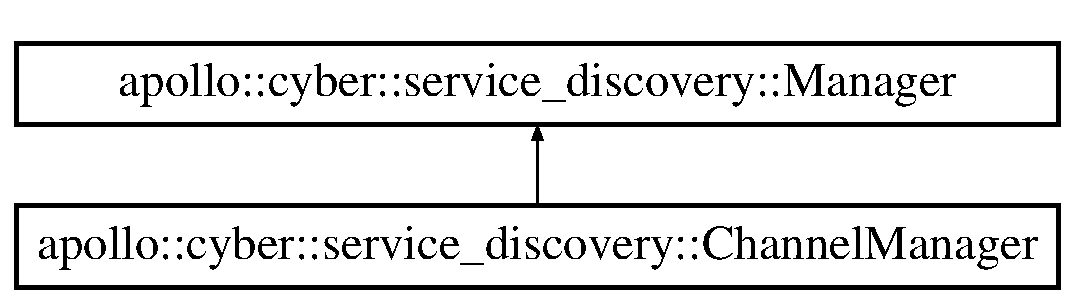
\includegraphics[height=2.000000cm]{classapollo_1_1cyber_1_1service__discovery_1_1ChannelManager}
\end{center}
\end{figure}
\subsection*{Public Types}
\begin{DoxyCompactItemize}
\item 
using \hyperlink{classapollo_1_1cyber_1_1service__discovery_1_1ChannelManager_a3690fc3677abdb994d1de9b996f66cf6}{Role\-Attr\-Vec} = std\-::vector$<$ proto\-::\-Role\-Attributes $>$
\item 
using \hyperlink{classapollo_1_1cyber_1_1service__discovery_1_1ChannelManager_ab34e0a39795d6002f20de1388e8e099b}{Writer\-Warehouse} = \hyperlink{classapollo_1_1cyber_1_1service__discovery_1_1MultiValueWarehouse}{Multi\-Value\-Warehouse}
\item 
using \hyperlink{classapollo_1_1cyber_1_1service__discovery_1_1ChannelManager_adf7b96601a2dec7f06fb190d1a7b537d}{Reader\-Warehouse} = \hyperlink{classapollo_1_1cyber_1_1service__discovery_1_1MultiValueWarehouse}{Multi\-Value\-Warehouse}
\item 
using \hyperlink{classapollo_1_1cyber_1_1service__discovery_1_1ChannelManager_a5ce07d9955d5944b039583db211c2d25}{Exempted\-Message\-Types} = std\-::unordered\-\_\-set$<$ std\-::string $>$
\end{DoxyCompactItemize}
\subsection*{Public Member Functions}
\begin{DoxyCompactItemize}
\item 
\hyperlink{classapollo_1_1cyber_1_1service__discovery_1_1ChannelManager_af4e4908c4172f7ff1703fea322611137}{Channel\-Manager} ()
\item 
virtual \hyperlink{classapollo_1_1cyber_1_1service__discovery_1_1ChannelManager_a32fb19451ed63f5bb92b4b2beb4eddcf}{$\sim$\-Channel\-Manager} ()
\item 
void \hyperlink{classapollo_1_1cyber_1_1service__discovery_1_1ChannelManager_aebc9f5fa682a8eba522a93ccebed3811}{Get\-Channel\-Names} (std\-::vector$<$ std\-::string $>$ $\ast$channels)
\item 
void \hyperlink{classapollo_1_1cyber_1_1service__discovery_1_1ChannelManager_a2259a9d33b8391ffb2ec307f6c442bc8}{Get\-Proto\-Desc} (const std\-::string \&channel\-\_\-name, std\-::string $\ast$proto\-\_\-desc)
\item 
void \hyperlink{classapollo_1_1cyber_1_1service__discovery_1_1ChannelManager_a06a205015433a25d5f2acf20eee4c445}{Get\-Msg\-Type} (const std\-::string \&channel\-\_\-name, std\-::string $\ast$msg\-\_\-type)
\item 
bool \hyperlink{classapollo_1_1cyber_1_1service__discovery_1_1ChannelManager_a2d481f65124c1cdb70b66b81055f667f}{Has\-Writer} (const std\-::string \&channel\-\_\-name)
\item 
void \hyperlink{classapollo_1_1cyber_1_1service__discovery_1_1ChannelManager_ada1e428556994da13575932c6feee98b}{Get\-Writers} (\hyperlink{classapollo_1_1cyber_1_1service__discovery_1_1ChannelManager_a3690fc3677abdb994d1de9b996f66cf6}{Role\-Attr\-Vec} $\ast$writers)
\item 
void \hyperlink{classapollo_1_1cyber_1_1service__discovery_1_1ChannelManager_a928e0afa8478cb244f3dd5d872694f38}{Get\-Writers\-Of\-Node} (const std\-::string \&node\-\_\-name, \hyperlink{classapollo_1_1cyber_1_1service__discovery_1_1ChannelManager_a3690fc3677abdb994d1de9b996f66cf6}{Role\-Attr\-Vec} $\ast$writers)
\item 
void \hyperlink{classapollo_1_1cyber_1_1service__discovery_1_1ChannelManager_a35bfdd2076a4789c23e9add4c868b5e7}{Get\-Writers\-Of\-Channel} (const std\-::string \&channel\-\_\-name, \hyperlink{classapollo_1_1cyber_1_1service__discovery_1_1ChannelManager_a3690fc3677abdb994d1de9b996f66cf6}{Role\-Attr\-Vec} $\ast$writers)
\item 
bool \hyperlink{classapollo_1_1cyber_1_1service__discovery_1_1ChannelManager_aa7e63842773a5f7d2b92bd856dc553dd}{Has\-Reader} (const std\-::string \&channel\-\_\-name)
\item 
void \hyperlink{classapollo_1_1cyber_1_1service__discovery_1_1ChannelManager_ae33f40f1a1e771b70e114b661bdeccd7}{Get\-Readers} (\hyperlink{classapollo_1_1cyber_1_1service__discovery_1_1ChannelManager_a3690fc3677abdb994d1de9b996f66cf6}{Role\-Attr\-Vec} $\ast$readers)
\item 
void \hyperlink{classapollo_1_1cyber_1_1service__discovery_1_1ChannelManager_a24c51f2ba8f6cf15fb7c3f44baf496d1}{Get\-Readers\-Of\-Node} (const std\-::string \&node\-\_\-name, \hyperlink{classapollo_1_1cyber_1_1service__discovery_1_1ChannelManager_a3690fc3677abdb994d1de9b996f66cf6}{Role\-Attr\-Vec} $\ast$readers)
\item 
void \hyperlink{classapollo_1_1cyber_1_1service__discovery_1_1ChannelManager_ad20c8af51bdacf9f1a6ecf7ce7bb371d}{Get\-Readers\-Of\-Channel} (const std\-::string \&channel\-\_\-name, \hyperlink{classapollo_1_1cyber_1_1service__discovery_1_1ChannelManager_a3690fc3677abdb994d1de9b996f66cf6}{Role\-Attr\-Vec} $\ast$readers)
\item 
void \hyperlink{classapollo_1_1cyber_1_1service__discovery_1_1ChannelManager_a4d77d8400933c94b6338c9fea4b91d8b}{Get\-Upstream\-Of\-Node} (const std\-::string \&node\-\_\-name, \hyperlink{classapollo_1_1cyber_1_1service__discovery_1_1ChannelManager_a3690fc3677abdb994d1de9b996f66cf6}{Role\-Attr\-Vec} $\ast$upstream\-\_\-nodes)
\item 
void \hyperlink{classapollo_1_1cyber_1_1service__discovery_1_1ChannelManager_aff6f6c68372acdf0768804bba4a45898}{Get\-Downstream\-Of\-Node} (const std\-::string \&node\-\_\-name, \hyperlink{classapollo_1_1cyber_1_1service__discovery_1_1ChannelManager_a3690fc3677abdb994d1de9b996f66cf6}{Role\-Attr\-Vec} $\ast$downstream\-\_\-nodes)
\item 
\hyperlink{namespaceapollo_1_1cyber_1_1service__discovery_a463f9fa98e31287620adc568e1299c79}{Flow\-Direction} \hyperlink{classapollo_1_1cyber_1_1service__discovery_1_1ChannelManager_aefde1d2e4d5134dbf726fe1ad362246a}{Get\-Flow\-Direction} (const std\-::string \&lhs\-\_\-node\-\_\-name, const std\-::string \&rhs\-\_\-node\-\_\-name)
\item 
bool \hyperlink{classapollo_1_1cyber_1_1service__discovery_1_1ChannelManager_ad7a6a93c25b30eca132bd945f1771a59}{Is\-Message\-Type\-Matching} (const std\-::string \&lhs, const std\-::string \&rhs)
\end{DoxyCompactItemize}
\subsection*{Private Member Functions}
\begin{DoxyCompactItemize}
\item 
bool \hyperlink{classapollo_1_1cyber_1_1service__discovery_1_1ChannelManager_a470b79e3a7780121ede3552956722cf7}{Check} (const Role\-Attributes \&attr) override
\item 
void \hyperlink{classapollo_1_1cyber_1_1service__discovery_1_1ChannelManager_ae4ed92f11a64d7ef4bb30680dad64493}{Dispose} (const Change\-Msg \&msg) override
\item 
void \hyperlink{classapollo_1_1cyber_1_1service__discovery_1_1ChannelManager_a4e39fc638d77bbe6d397299fa30ff6d6}{On\-Topo\-Module\-Leave} (const std\-::string \&host\-\_\-name, int process\-\_\-id) override
\item 
void \hyperlink{classapollo_1_1cyber_1_1service__discovery_1_1ChannelManager_aea63c8f1e8d638ef930c3c7ddd3b62ab}{Dispose\-Join} (const Change\-Msg \&msg)
\item 
void \hyperlink{classapollo_1_1cyber_1_1service__discovery_1_1ChannelManager_aa39a85495ea9eb83d6946405576bd1cb}{Dispose\-Leave} (const Change\-Msg \&msg)
\item 
void \hyperlink{classapollo_1_1cyber_1_1service__discovery_1_1ChannelManager_af48675ed66194fca37daad411c19d589}{Scan\-Message\-Type} (const Change\-Msg \&msg)
\end{DoxyCompactItemize}
\subsection*{Private Attributes}
\begin{DoxyCompactItemize}
\item 
\hyperlink{classapollo_1_1cyber_1_1service__discovery_1_1ChannelManager_a5ce07d9955d5944b039583db211c2d25}{Exempted\-Message\-Types} \hyperlink{classapollo_1_1cyber_1_1service__discovery_1_1ChannelManager_a673d2f5f6577c37ca44263f7a7295324}{exempted\-\_\-msg\-\_\-types\-\_\-}
\item 
\hyperlink{classapollo_1_1cyber_1_1service__discovery_1_1Graph}{Graph} \hyperlink{classapollo_1_1cyber_1_1service__discovery_1_1ChannelManager_aee4753f128f1a79a983e065c8775294a}{node\-\_\-graph\-\_\-}
\item 
\hyperlink{classapollo_1_1cyber_1_1service__discovery_1_1ChannelManager_ab34e0a39795d6002f20de1388e8e099b}{Writer\-Warehouse} \hyperlink{classapollo_1_1cyber_1_1service__discovery_1_1ChannelManager_a964857ce80f55467c86f0abd0dbf3419}{node\-\_\-writers\-\_\-}
\item 
\hyperlink{classapollo_1_1cyber_1_1service__discovery_1_1ChannelManager_adf7b96601a2dec7f06fb190d1a7b537d}{Reader\-Warehouse} \hyperlink{classapollo_1_1cyber_1_1service__discovery_1_1ChannelManager_aa021bd1e52a883766c5691ed2695bfb4}{node\-\_\-readers\-\_\-}
\item 
\hyperlink{classapollo_1_1cyber_1_1service__discovery_1_1ChannelManager_ab34e0a39795d6002f20de1388e8e099b}{Writer\-Warehouse} \hyperlink{classapollo_1_1cyber_1_1service__discovery_1_1ChannelManager_ac88e60402cb5f9799803f993a9c85138}{channel\-\_\-writers\-\_\-}
\item 
\hyperlink{classapollo_1_1cyber_1_1service__discovery_1_1ChannelManager_adf7b96601a2dec7f06fb190d1a7b537d}{Reader\-Warehouse} \hyperlink{classapollo_1_1cyber_1_1service__discovery_1_1ChannelManager_a14272c348659973742aae0a343ba1705}{channel\-\_\-readers\-\_\-}
\end{DoxyCompactItemize}
\subsection*{Friends}
\begin{DoxyCompactItemize}
\item 
class \hyperlink{classapollo_1_1cyber_1_1service__discovery_1_1ChannelManager_ae83aaddaeb682129a07c148e01291cdd}{Topology\-Manager}
\end{DoxyCompactItemize}
\subsection*{Additional Inherited Members}


\subsection{Member Typedef Documentation}
\hypertarget{classapollo_1_1cyber_1_1service__discovery_1_1ChannelManager_a5ce07d9955d5944b039583db211c2d25}{\index{apollo\-::cyber\-::service\-\_\-discovery\-::\-Channel\-Manager@{apollo\-::cyber\-::service\-\_\-discovery\-::\-Channel\-Manager}!Exempted\-Message\-Types@{Exempted\-Message\-Types}}
\index{Exempted\-Message\-Types@{Exempted\-Message\-Types}!apollo::cyber::service_discovery::ChannelManager@{apollo\-::cyber\-::service\-\_\-discovery\-::\-Channel\-Manager}}
\subsubsection[{Exempted\-Message\-Types}]{\setlength{\rightskip}{0pt plus 5cm}using {\bf apollo\-::cyber\-::service\-\_\-discovery\-::\-Channel\-Manager\-::\-Exempted\-Message\-Types} =  std\-::unordered\-\_\-set$<$std\-::string$>$}}\label{classapollo_1_1cyber_1_1service__discovery_1_1ChannelManager_a5ce07d9955d5944b039583db211c2d25}
\hypertarget{classapollo_1_1cyber_1_1service__discovery_1_1ChannelManager_adf7b96601a2dec7f06fb190d1a7b537d}{\index{apollo\-::cyber\-::service\-\_\-discovery\-::\-Channel\-Manager@{apollo\-::cyber\-::service\-\_\-discovery\-::\-Channel\-Manager}!Reader\-Warehouse@{Reader\-Warehouse}}
\index{Reader\-Warehouse@{Reader\-Warehouse}!apollo::cyber::service_discovery::ChannelManager@{apollo\-::cyber\-::service\-\_\-discovery\-::\-Channel\-Manager}}
\subsubsection[{Reader\-Warehouse}]{\setlength{\rightskip}{0pt plus 5cm}using {\bf apollo\-::cyber\-::service\-\_\-discovery\-::\-Channel\-Manager\-::\-Reader\-Warehouse} =  {\bf Multi\-Value\-Warehouse}}}\label{classapollo_1_1cyber_1_1service__discovery_1_1ChannelManager_adf7b96601a2dec7f06fb190d1a7b537d}
\hypertarget{classapollo_1_1cyber_1_1service__discovery_1_1ChannelManager_a3690fc3677abdb994d1de9b996f66cf6}{\index{apollo\-::cyber\-::service\-\_\-discovery\-::\-Channel\-Manager@{apollo\-::cyber\-::service\-\_\-discovery\-::\-Channel\-Manager}!Role\-Attr\-Vec@{Role\-Attr\-Vec}}
\index{Role\-Attr\-Vec@{Role\-Attr\-Vec}!apollo::cyber::service_discovery::ChannelManager@{apollo\-::cyber\-::service\-\_\-discovery\-::\-Channel\-Manager}}
\subsubsection[{Role\-Attr\-Vec}]{\setlength{\rightskip}{0pt plus 5cm}using {\bf apollo\-::cyber\-::service\-\_\-discovery\-::\-Channel\-Manager\-::\-Role\-Attr\-Vec} =  std\-::vector$<$proto\-::\-Role\-Attributes$>$}}\label{classapollo_1_1cyber_1_1service__discovery_1_1ChannelManager_a3690fc3677abdb994d1de9b996f66cf6}
\hypertarget{classapollo_1_1cyber_1_1service__discovery_1_1ChannelManager_ab34e0a39795d6002f20de1388e8e099b}{\index{apollo\-::cyber\-::service\-\_\-discovery\-::\-Channel\-Manager@{apollo\-::cyber\-::service\-\_\-discovery\-::\-Channel\-Manager}!Writer\-Warehouse@{Writer\-Warehouse}}
\index{Writer\-Warehouse@{Writer\-Warehouse}!apollo::cyber::service_discovery::ChannelManager@{apollo\-::cyber\-::service\-\_\-discovery\-::\-Channel\-Manager}}
\subsubsection[{Writer\-Warehouse}]{\setlength{\rightskip}{0pt plus 5cm}using {\bf apollo\-::cyber\-::service\-\_\-discovery\-::\-Channel\-Manager\-::\-Writer\-Warehouse} =  {\bf Multi\-Value\-Warehouse}}}\label{classapollo_1_1cyber_1_1service__discovery_1_1ChannelManager_ab34e0a39795d6002f20de1388e8e099b}


\subsection{Constructor \& Destructor Documentation}
\hypertarget{classapollo_1_1cyber_1_1service__discovery_1_1ChannelManager_af4e4908c4172f7ff1703fea322611137}{\index{apollo\-::cyber\-::service\-\_\-discovery\-::\-Channel\-Manager@{apollo\-::cyber\-::service\-\_\-discovery\-::\-Channel\-Manager}!Channel\-Manager@{Channel\-Manager}}
\index{Channel\-Manager@{Channel\-Manager}!apollo::cyber::service_discovery::ChannelManager@{apollo\-::cyber\-::service\-\_\-discovery\-::\-Channel\-Manager}}
\subsubsection[{Channel\-Manager}]{\setlength{\rightskip}{0pt plus 5cm}apollo\-::cyber\-::service\-\_\-discovery\-::\-Channel\-Manager\-::\-Channel\-Manager (
\begin{DoxyParamCaption}
{}
\end{DoxyParamCaption}
)}}\label{classapollo_1_1cyber_1_1service__discovery_1_1ChannelManager_af4e4908c4172f7ff1703fea322611137}
\hypertarget{classapollo_1_1cyber_1_1service__discovery_1_1ChannelManager_a32fb19451ed63f5bb92b4b2beb4eddcf}{\index{apollo\-::cyber\-::service\-\_\-discovery\-::\-Channel\-Manager@{apollo\-::cyber\-::service\-\_\-discovery\-::\-Channel\-Manager}!$\sim$\-Channel\-Manager@{$\sim$\-Channel\-Manager}}
\index{$\sim$\-Channel\-Manager@{$\sim$\-Channel\-Manager}!apollo::cyber::service_discovery::ChannelManager@{apollo\-::cyber\-::service\-\_\-discovery\-::\-Channel\-Manager}}
\subsubsection[{$\sim$\-Channel\-Manager}]{\setlength{\rightskip}{0pt plus 5cm}virtual apollo\-::cyber\-::service\-\_\-discovery\-::\-Channel\-Manager\-::$\sim$\-Channel\-Manager (
\begin{DoxyParamCaption}
{}
\end{DoxyParamCaption}
)\hspace{0.3cm}{\ttfamily [virtual]}}}\label{classapollo_1_1cyber_1_1service__discovery_1_1ChannelManager_a32fb19451ed63f5bb92b4b2beb4eddcf}


\subsection{Member Function Documentation}
\hypertarget{classapollo_1_1cyber_1_1service__discovery_1_1ChannelManager_a470b79e3a7780121ede3552956722cf7}{\index{apollo\-::cyber\-::service\-\_\-discovery\-::\-Channel\-Manager@{apollo\-::cyber\-::service\-\_\-discovery\-::\-Channel\-Manager}!Check@{Check}}
\index{Check@{Check}!apollo::cyber::service_discovery::ChannelManager@{apollo\-::cyber\-::service\-\_\-discovery\-::\-Channel\-Manager}}
\subsubsection[{Check}]{\setlength{\rightskip}{0pt plus 5cm}bool apollo\-::cyber\-::service\-\_\-discovery\-::\-Channel\-Manager\-::\-Check (
\begin{DoxyParamCaption}
\item[{const Role\-Attributes \&}]{attr}
\end{DoxyParamCaption}
)\hspace{0.3cm}{\ttfamily [override]}, {\ttfamily [private]}, {\ttfamily [virtual]}}}\label{classapollo_1_1cyber_1_1service__discovery_1_1ChannelManager_a470b79e3a7780121ede3552956722cf7}


Implements \hyperlink{classapollo_1_1cyber_1_1service__discovery_1_1Manager_acfa0224581a6722daf4861f34e4c11ef}{apollo\-::cyber\-::service\-\_\-discovery\-::\-Manager}.

\hypertarget{classapollo_1_1cyber_1_1service__discovery_1_1ChannelManager_ae4ed92f11a64d7ef4bb30680dad64493}{\index{apollo\-::cyber\-::service\-\_\-discovery\-::\-Channel\-Manager@{apollo\-::cyber\-::service\-\_\-discovery\-::\-Channel\-Manager}!Dispose@{Dispose}}
\index{Dispose@{Dispose}!apollo::cyber::service_discovery::ChannelManager@{apollo\-::cyber\-::service\-\_\-discovery\-::\-Channel\-Manager}}
\subsubsection[{Dispose}]{\setlength{\rightskip}{0pt plus 5cm}void apollo\-::cyber\-::service\-\_\-discovery\-::\-Channel\-Manager\-::\-Dispose (
\begin{DoxyParamCaption}
\item[{const Change\-Msg \&}]{msg}
\end{DoxyParamCaption}
)\hspace{0.3cm}{\ttfamily [override]}, {\ttfamily [private]}, {\ttfamily [virtual]}}}\label{classapollo_1_1cyber_1_1service__discovery_1_1ChannelManager_ae4ed92f11a64d7ef4bb30680dad64493}


Implements \hyperlink{classapollo_1_1cyber_1_1service__discovery_1_1Manager_a6e36e4095291597364ce4b37ee1c897b}{apollo\-::cyber\-::service\-\_\-discovery\-::\-Manager}.

\hypertarget{classapollo_1_1cyber_1_1service__discovery_1_1ChannelManager_aea63c8f1e8d638ef930c3c7ddd3b62ab}{\index{apollo\-::cyber\-::service\-\_\-discovery\-::\-Channel\-Manager@{apollo\-::cyber\-::service\-\_\-discovery\-::\-Channel\-Manager}!Dispose\-Join@{Dispose\-Join}}
\index{Dispose\-Join@{Dispose\-Join}!apollo::cyber::service_discovery::ChannelManager@{apollo\-::cyber\-::service\-\_\-discovery\-::\-Channel\-Manager}}
\subsubsection[{Dispose\-Join}]{\setlength{\rightskip}{0pt plus 5cm}void apollo\-::cyber\-::service\-\_\-discovery\-::\-Channel\-Manager\-::\-Dispose\-Join (
\begin{DoxyParamCaption}
\item[{const Change\-Msg \&}]{msg}
\end{DoxyParamCaption}
)\hspace{0.3cm}{\ttfamily [private]}}}\label{classapollo_1_1cyber_1_1service__discovery_1_1ChannelManager_aea63c8f1e8d638ef930c3c7ddd3b62ab}
\hypertarget{classapollo_1_1cyber_1_1service__discovery_1_1ChannelManager_aa39a85495ea9eb83d6946405576bd1cb}{\index{apollo\-::cyber\-::service\-\_\-discovery\-::\-Channel\-Manager@{apollo\-::cyber\-::service\-\_\-discovery\-::\-Channel\-Manager}!Dispose\-Leave@{Dispose\-Leave}}
\index{Dispose\-Leave@{Dispose\-Leave}!apollo::cyber::service_discovery::ChannelManager@{apollo\-::cyber\-::service\-\_\-discovery\-::\-Channel\-Manager}}
\subsubsection[{Dispose\-Leave}]{\setlength{\rightskip}{0pt plus 5cm}void apollo\-::cyber\-::service\-\_\-discovery\-::\-Channel\-Manager\-::\-Dispose\-Leave (
\begin{DoxyParamCaption}
\item[{const Change\-Msg \&}]{msg}
\end{DoxyParamCaption}
)\hspace{0.3cm}{\ttfamily [private]}}}\label{classapollo_1_1cyber_1_1service__discovery_1_1ChannelManager_aa39a85495ea9eb83d6946405576bd1cb}
\hypertarget{classapollo_1_1cyber_1_1service__discovery_1_1ChannelManager_aebc9f5fa682a8eba522a93ccebed3811}{\index{apollo\-::cyber\-::service\-\_\-discovery\-::\-Channel\-Manager@{apollo\-::cyber\-::service\-\_\-discovery\-::\-Channel\-Manager}!Get\-Channel\-Names@{Get\-Channel\-Names}}
\index{Get\-Channel\-Names@{Get\-Channel\-Names}!apollo::cyber::service_discovery::ChannelManager@{apollo\-::cyber\-::service\-\_\-discovery\-::\-Channel\-Manager}}
\subsubsection[{Get\-Channel\-Names}]{\setlength{\rightskip}{0pt plus 5cm}void apollo\-::cyber\-::service\-\_\-discovery\-::\-Channel\-Manager\-::\-Get\-Channel\-Names (
\begin{DoxyParamCaption}
\item[{std\-::vector$<$ std\-::string $>$ $\ast$}]{channels}
\end{DoxyParamCaption}
)}}\label{classapollo_1_1cyber_1_1service__discovery_1_1ChannelManager_aebc9f5fa682a8eba522a93ccebed3811}
\hypertarget{classapollo_1_1cyber_1_1service__discovery_1_1ChannelManager_aff6f6c68372acdf0768804bba4a45898}{\index{apollo\-::cyber\-::service\-\_\-discovery\-::\-Channel\-Manager@{apollo\-::cyber\-::service\-\_\-discovery\-::\-Channel\-Manager}!Get\-Downstream\-Of\-Node@{Get\-Downstream\-Of\-Node}}
\index{Get\-Downstream\-Of\-Node@{Get\-Downstream\-Of\-Node}!apollo::cyber::service_discovery::ChannelManager@{apollo\-::cyber\-::service\-\_\-discovery\-::\-Channel\-Manager}}
\subsubsection[{Get\-Downstream\-Of\-Node}]{\setlength{\rightskip}{0pt plus 5cm}void apollo\-::cyber\-::service\-\_\-discovery\-::\-Channel\-Manager\-::\-Get\-Downstream\-Of\-Node (
\begin{DoxyParamCaption}
\item[{const std\-::string \&}]{node\-\_\-name, }
\item[{{\bf Role\-Attr\-Vec} $\ast$}]{downstream\-\_\-nodes}
\end{DoxyParamCaption}
)}}\label{classapollo_1_1cyber_1_1service__discovery_1_1ChannelManager_aff6f6c68372acdf0768804bba4a45898}
\hypertarget{classapollo_1_1cyber_1_1service__discovery_1_1ChannelManager_aefde1d2e4d5134dbf726fe1ad362246a}{\index{apollo\-::cyber\-::service\-\_\-discovery\-::\-Channel\-Manager@{apollo\-::cyber\-::service\-\_\-discovery\-::\-Channel\-Manager}!Get\-Flow\-Direction@{Get\-Flow\-Direction}}
\index{Get\-Flow\-Direction@{Get\-Flow\-Direction}!apollo::cyber::service_discovery::ChannelManager@{apollo\-::cyber\-::service\-\_\-discovery\-::\-Channel\-Manager}}
\subsubsection[{Get\-Flow\-Direction}]{\setlength{\rightskip}{0pt plus 5cm}{\bf Flow\-Direction} apollo\-::cyber\-::service\-\_\-discovery\-::\-Channel\-Manager\-::\-Get\-Flow\-Direction (
\begin{DoxyParamCaption}
\item[{const std\-::string \&}]{lhs\-\_\-node\-\_\-name, }
\item[{const std\-::string \&}]{rhs\-\_\-node\-\_\-name}
\end{DoxyParamCaption}
)}}\label{classapollo_1_1cyber_1_1service__discovery_1_1ChannelManager_aefde1d2e4d5134dbf726fe1ad362246a}
\hypertarget{classapollo_1_1cyber_1_1service__discovery_1_1ChannelManager_a06a205015433a25d5f2acf20eee4c445}{\index{apollo\-::cyber\-::service\-\_\-discovery\-::\-Channel\-Manager@{apollo\-::cyber\-::service\-\_\-discovery\-::\-Channel\-Manager}!Get\-Msg\-Type@{Get\-Msg\-Type}}
\index{Get\-Msg\-Type@{Get\-Msg\-Type}!apollo::cyber::service_discovery::ChannelManager@{apollo\-::cyber\-::service\-\_\-discovery\-::\-Channel\-Manager}}
\subsubsection[{Get\-Msg\-Type}]{\setlength{\rightskip}{0pt plus 5cm}void apollo\-::cyber\-::service\-\_\-discovery\-::\-Channel\-Manager\-::\-Get\-Msg\-Type (
\begin{DoxyParamCaption}
\item[{const std\-::string \&}]{channel\-\_\-name, }
\item[{std\-::string $\ast$}]{msg\-\_\-type}
\end{DoxyParamCaption}
)}}\label{classapollo_1_1cyber_1_1service__discovery_1_1ChannelManager_a06a205015433a25d5f2acf20eee4c445}
\hypertarget{classapollo_1_1cyber_1_1service__discovery_1_1ChannelManager_a2259a9d33b8391ffb2ec307f6c442bc8}{\index{apollo\-::cyber\-::service\-\_\-discovery\-::\-Channel\-Manager@{apollo\-::cyber\-::service\-\_\-discovery\-::\-Channel\-Manager}!Get\-Proto\-Desc@{Get\-Proto\-Desc}}
\index{Get\-Proto\-Desc@{Get\-Proto\-Desc}!apollo::cyber::service_discovery::ChannelManager@{apollo\-::cyber\-::service\-\_\-discovery\-::\-Channel\-Manager}}
\subsubsection[{Get\-Proto\-Desc}]{\setlength{\rightskip}{0pt plus 5cm}void apollo\-::cyber\-::service\-\_\-discovery\-::\-Channel\-Manager\-::\-Get\-Proto\-Desc (
\begin{DoxyParamCaption}
\item[{const std\-::string \&}]{channel\-\_\-name, }
\item[{std\-::string $\ast$}]{proto\-\_\-desc}
\end{DoxyParamCaption}
)}}\label{classapollo_1_1cyber_1_1service__discovery_1_1ChannelManager_a2259a9d33b8391ffb2ec307f6c442bc8}
\hypertarget{classapollo_1_1cyber_1_1service__discovery_1_1ChannelManager_ae33f40f1a1e771b70e114b661bdeccd7}{\index{apollo\-::cyber\-::service\-\_\-discovery\-::\-Channel\-Manager@{apollo\-::cyber\-::service\-\_\-discovery\-::\-Channel\-Manager}!Get\-Readers@{Get\-Readers}}
\index{Get\-Readers@{Get\-Readers}!apollo::cyber::service_discovery::ChannelManager@{apollo\-::cyber\-::service\-\_\-discovery\-::\-Channel\-Manager}}
\subsubsection[{Get\-Readers}]{\setlength{\rightskip}{0pt plus 5cm}void apollo\-::cyber\-::service\-\_\-discovery\-::\-Channel\-Manager\-::\-Get\-Readers (
\begin{DoxyParamCaption}
\item[{{\bf Role\-Attr\-Vec} $\ast$}]{readers}
\end{DoxyParamCaption}
)}}\label{classapollo_1_1cyber_1_1service__discovery_1_1ChannelManager_ae33f40f1a1e771b70e114b661bdeccd7}
\hypertarget{classapollo_1_1cyber_1_1service__discovery_1_1ChannelManager_ad20c8af51bdacf9f1a6ecf7ce7bb371d}{\index{apollo\-::cyber\-::service\-\_\-discovery\-::\-Channel\-Manager@{apollo\-::cyber\-::service\-\_\-discovery\-::\-Channel\-Manager}!Get\-Readers\-Of\-Channel@{Get\-Readers\-Of\-Channel}}
\index{Get\-Readers\-Of\-Channel@{Get\-Readers\-Of\-Channel}!apollo::cyber::service_discovery::ChannelManager@{apollo\-::cyber\-::service\-\_\-discovery\-::\-Channel\-Manager}}
\subsubsection[{Get\-Readers\-Of\-Channel}]{\setlength{\rightskip}{0pt plus 5cm}void apollo\-::cyber\-::service\-\_\-discovery\-::\-Channel\-Manager\-::\-Get\-Readers\-Of\-Channel (
\begin{DoxyParamCaption}
\item[{const std\-::string \&}]{channel\-\_\-name, }
\item[{{\bf Role\-Attr\-Vec} $\ast$}]{readers}
\end{DoxyParamCaption}
)}}\label{classapollo_1_1cyber_1_1service__discovery_1_1ChannelManager_ad20c8af51bdacf9f1a6ecf7ce7bb371d}
\hypertarget{classapollo_1_1cyber_1_1service__discovery_1_1ChannelManager_a24c51f2ba8f6cf15fb7c3f44baf496d1}{\index{apollo\-::cyber\-::service\-\_\-discovery\-::\-Channel\-Manager@{apollo\-::cyber\-::service\-\_\-discovery\-::\-Channel\-Manager}!Get\-Readers\-Of\-Node@{Get\-Readers\-Of\-Node}}
\index{Get\-Readers\-Of\-Node@{Get\-Readers\-Of\-Node}!apollo::cyber::service_discovery::ChannelManager@{apollo\-::cyber\-::service\-\_\-discovery\-::\-Channel\-Manager}}
\subsubsection[{Get\-Readers\-Of\-Node}]{\setlength{\rightskip}{0pt plus 5cm}void apollo\-::cyber\-::service\-\_\-discovery\-::\-Channel\-Manager\-::\-Get\-Readers\-Of\-Node (
\begin{DoxyParamCaption}
\item[{const std\-::string \&}]{node\-\_\-name, }
\item[{{\bf Role\-Attr\-Vec} $\ast$}]{readers}
\end{DoxyParamCaption}
)}}\label{classapollo_1_1cyber_1_1service__discovery_1_1ChannelManager_a24c51f2ba8f6cf15fb7c3f44baf496d1}
\hypertarget{classapollo_1_1cyber_1_1service__discovery_1_1ChannelManager_a4d77d8400933c94b6338c9fea4b91d8b}{\index{apollo\-::cyber\-::service\-\_\-discovery\-::\-Channel\-Manager@{apollo\-::cyber\-::service\-\_\-discovery\-::\-Channel\-Manager}!Get\-Upstream\-Of\-Node@{Get\-Upstream\-Of\-Node}}
\index{Get\-Upstream\-Of\-Node@{Get\-Upstream\-Of\-Node}!apollo::cyber::service_discovery::ChannelManager@{apollo\-::cyber\-::service\-\_\-discovery\-::\-Channel\-Manager}}
\subsubsection[{Get\-Upstream\-Of\-Node}]{\setlength{\rightskip}{0pt plus 5cm}void apollo\-::cyber\-::service\-\_\-discovery\-::\-Channel\-Manager\-::\-Get\-Upstream\-Of\-Node (
\begin{DoxyParamCaption}
\item[{const std\-::string \&}]{node\-\_\-name, }
\item[{{\bf Role\-Attr\-Vec} $\ast$}]{upstream\-\_\-nodes}
\end{DoxyParamCaption}
)}}\label{classapollo_1_1cyber_1_1service__discovery_1_1ChannelManager_a4d77d8400933c94b6338c9fea4b91d8b}
\hypertarget{classapollo_1_1cyber_1_1service__discovery_1_1ChannelManager_ada1e428556994da13575932c6feee98b}{\index{apollo\-::cyber\-::service\-\_\-discovery\-::\-Channel\-Manager@{apollo\-::cyber\-::service\-\_\-discovery\-::\-Channel\-Manager}!Get\-Writers@{Get\-Writers}}
\index{Get\-Writers@{Get\-Writers}!apollo::cyber::service_discovery::ChannelManager@{apollo\-::cyber\-::service\-\_\-discovery\-::\-Channel\-Manager}}
\subsubsection[{Get\-Writers}]{\setlength{\rightskip}{0pt plus 5cm}void apollo\-::cyber\-::service\-\_\-discovery\-::\-Channel\-Manager\-::\-Get\-Writers (
\begin{DoxyParamCaption}
\item[{{\bf Role\-Attr\-Vec} $\ast$}]{writers}
\end{DoxyParamCaption}
)}}\label{classapollo_1_1cyber_1_1service__discovery_1_1ChannelManager_ada1e428556994da13575932c6feee98b}
\hypertarget{classapollo_1_1cyber_1_1service__discovery_1_1ChannelManager_a35bfdd2076a4789c23e9add4c868b5e7}{\index{apollo\-::cyber\-::service\-\_\-discovery\-::\-Channel\-Manager@{apollo\-::cyber\-::service\-\_\-discovery\-::\-Channel\-Manager}!Get\-Writers\-Of\-Channel@{Get\-Writers\-Of\-Channel}}
\index{Get\-Writers\-Of\-Channel@{Get\-Writers\-Of\-Channel}!apollo::cyber::service_discovery::ChannelManager@{apollo\-::cyber\-::service\-\_\-discovery\-::\-Channel\-Manager}}
\subsubsection[{Get\-Writers\-Of\-Channel}]{\setlength{\rightskip}{0pt plus 5cm}void apollo\-::cyber\-::service\-\_\-discovery\-::\-Channel\-Manager\-::\-Get\-Writers\-Of\-Channel (
\begin{DoxyParamCaption}
\item[{const std\-::string \&}]{channel\-\_\-name, }
\item[{{\bf Role\-Attr\-Vec} $\ast$}]{writers}
\end{DoxyParamCaption}
)}}\label{classapollo_1_1cyber_1_1service__discovery_1_1ChannelManager_a35bfdd2076a4789c23e9add4c868b5e7}
\hypertarget{classapollo_1_1cyber_1_1service__discovery_1_1ChannelManager_a928e0afa8478cb244f3dd5d872694f38}{\index{apollo\-::cyber\-::service\-\_\-discovery\-::\-Channel\-Manager@{apollo\-::cyber\-::service\-\_\-discovery\-::\-Channel\-Manager}!Get\-Writers\-Of\-Node@{Get\-Writers\-Of\-Node}}
\index{Get\-Writers\-Of\-Node@{Get\-Writers\-Of\-Node}!apollo::cyber::service_discovery::ChannelManager@{apollo\-::cyber\-::service\-\_\-discovery\-::\-Channel\-Manager}}
\subsubsection[{Get\-Writers\-Of\-Node}]{\setlength{\rightskip}{0pt plus 5cm}void apollo\-::cyber\-::service\-\_\-discovery\-::\-Channel\-Manager\-::\-Get\-Writers\-Of\-Node (
\begin{DoxyParamCaption}
\item[{const std\-::string \&}]{node\-\_\-name, }
\item[{{\bf Role\-Attr\-Vec} $\ast$}]{writers}
\end{DoxyParamCaption}
)}}\label{classapollo_1_1cyber_1_1service__discovery_1_1ChannelManager_a928e0afa8478cb244f3dd5d872694f38}
\hypertarget{classapollo_1_1cyber_1_1service__discovery_1_1ChannelManager_aa7e63842773a5f7d2b92bd856dc553dd}{\index{apollo\-::cyber\-::service\-\_\-discovery\-::\-Channel\-Manager@{apollo\-::cyber\-::service\-\_\-discovery\-::\-Channel\-Manager}!Has\-Reader@{Has\-Reader}}
\index{Has\-Reader@{Has\-Reader}!apollo::cyber::service_discovery::ChannelManager@{apollo\-::cyber\-::service\-\_\-discovery\-::\-Channel\-Manager}}
\subsubsection[{Has\-Reader}]{\setlength{\rightskip}{0pt plus 5cm}bool apollo\-::cyber\-::service\-\_\-discovery\-::\-Channel\-Manager\-::\-Has\-Reader (
\begin{DoxyParamCaption}
\item[{const std\-::string \&}]{channel\-\_\-name}
\end{DoxyParamCaption}
)}}\label{classapollo_1_1cyber_1_1service__discovery_1_1ChannelManager_aa7e63842773a5f7d2b92bd856dc553dd}
\hypertarget{classapollo_1_1cyber_1_1service__discovery_1_1ChannelManager_a2d481f65124c1cdb70b66b81055f667f}{\index{apollo\-::cyber\-::service\-\_\-discovery\-::\-Channel\-Manager@{apollo\-::cyber\-::service\-\_\-discovery\-::\-Channel\-Manager}!Has\-Writer@{Has\-Writer}}
\index{Has\-Writer@{Has\-Writer}!apollo::cyber::service_discovery::ChannelManager@{apollo\-::cyber\-::service\-\_\-discovery\-::\-Channel\-Manager}}
\subsubsection[{Has\-Writer}]{\setlength{\rightskip}{0pt plus 5cm}bool apollo\-::cyber\-::service\-\_\-discovery\-::\-Channel\-Manager\-::\-Has\-Writer (
\begin{DoxyParamCaption}
\item[{const std\-::string \&}]{channel\-\_\-name}
\end{DoxyParamCaption}
)}}\label{classapollo_1_1cyber_1_1service__discovery_1_1ChannelManager_a2d481f65124c1cdb70b66b81055f667f}
\hypertarget{classapollo_1_1cyber_1_1service__discovery_1_1ChannelManager_ad7a6a93c25b30eca132bd945f1771a59}{\index{apollo\-::cyber\-::service\-\_\-discovery\-::\-Channel\-Manager@{apollo\-::cyber\-::service\-\_\-discovery\-::\-Channel\-Manager}!Is\-Message\-Type\-Matching@{Is\-Message\-Type\-Matching}}
\index{Is\-Message\-Type\-Matching@{Is\-Message\-Type\-Matching}!apollo::cyber::service_discovery::ChannelManager@{apollo\-::cyber\-::service\-\_\-discovery\-::\-Channel\-Manager}}
\subsubsection[{Is\-Message\-Type\-Matching}]{\setlength{\rightskip}{0pt plus 5cm}bool apollo\-::cyber\-::service\-\_\-discovery\-::\-Channel\-Manager\-::\-Is\-Message\-Type\-Matching (
\begin{DoxyParamCaption}
\item[{const std\-::string \&}]{lhs, }
\item[{const std\-::string \&}]{rhs}
\end{DoxyParamCaption}
)}}\label{classapollo_1_1cyber_1_1service__discovery_1_1ChannelManager_ad7a6a93c25b30eca132bd945f1771a59}
\hypertarget{classapollo_1_1cyber_1_1service__discovery_1_1ChannelManager_a4e39fc638d77bbe6d397299fa30ff6d6}{\index{apollo\-::cyber\-::service\-\_\-discovery\-::\-Channel\-Manager@{apollo\-::cyber\-::service\-\_\-discovery\-::\-Channel\-Manager}!On\-Topo\-Module\-Leave@{On\-Topo\-Module\-Leave}}
\index{On\-Topo\-Module\-Leave@{On\-Topo\-Module\-Leave}!apollo::cyber::service_discovery::ChannelManager@{apollo\-::cyber\-::service\-\_\-discovery\-::\-Channel\-Manager}}
\subsubsection[{On\-Topo\-Module\-Leave}]{\setlength{\rightskip}{0pt plus 5cm}void apollo\-::cyber\-::service\-\_\-discovery\-::\-Channel\-Manager\-::\-On\-Topo\-Module\-Leave (
\begin{DoxyParamCaption}
\item[{const std\-::string \&}]{host\-\_\-name, }
\item[{int}]{process\-\_\-id}
\end{DoxyParamCaption}
)\hspace{0.3cm}{\ttfamily [override]}, {\ttfamily [private]}, {\ttfamily [virtual]}}}\label{classapollo_1_1cyber_1_1service__discovery_1_1ChannelManager_a4e39fc638d77bbe6d397299fa30ff6d6}


Implements \hyperlink{classapollo_1_1cyber_1_1service__discovery_1_1Manager_a95a679e0fc7904e6f1a8b2fdd139cc03}{apollo\-::cyber\-::service\-\_\-discovery\-::\-Manager}.

\hypertarget{classapollo_1_1cyber_1_1service__discovery_1_1ChannelManager_af48675ed66194fca37daad411c19d589}{\index{apollo\-::cyber\-::service\-\_\-discovery\-::\-Channel\-Manager@{apollo\-::cyber\-::service\-\_\-discovery\-::\-Channel\-Manager}!Scan\-Message\-Type@{Scan\-Message\-Type}}
\index{Scan\-Message\-Type@{Scan\-Message\-Type}!apollo::cyber::service_discovery::ChannelManager@{apollo\-::cyber\-::service\-\_\-discovery\-::\-Channel\-Manager}}
\subsubsection[{Scan\-Message\-Type}]{\setlength{\rightskip}{0pt plus 5cm}void apollo\-::cyber\-::service\-\_\-discovery\-::\-Channel\-Manager\-::\-Scan\-Message\-Type (
\begin{DoxyParamCaption}
\item[{const Change\-Msg \&}]{msg}
\end{DoxyParamCaption}
)\hspace{0.3cm}{\ttfamily [private]}}}\label{classapollo_1_1cyber_1_1service__discovery_1_1ChannelManager_af48675ed66194fca37daad411c19d589}


\subsection{Friends And Related Function Documentation}
\hypertarget{classapollo_1_1cyber_1_1service__discovery_1_1ChannelManager_ae83aaddaeb682129a07c148e01291cdd}{\index{apollo\-::cyber\-::service\-\_\-discovery\-::\-Channel\-Manager@{apollo\-::cyber\-::service\-\_\-discovery\-::\-Channel\-Manager}!Topology\-Manager@{Topology\-Manager}}
\index{Topology\-Manager@{Topology\-Manager}!apollo::cyber::service_discovery::ChannelManager@{apollo\-::cyber\-::service\-\_\-discovery\-::\-Channel\-Manager}}
\subsubsection[{Topology\-Manager}]{\setlength{\rightskip}{0pt plus 5cm}friend class {\bf Topology\-Manager}\hspace{0.3cm}{\ttfamily [friend]}}}\label{classapollo_1_1cyber_1_1service__discovery_1_1ChannelManager_ae83aaddaeb682129a07c148e01291cdd}


\subsection{Member Data Documentation}
\hypertarget{classapollo_1_1cyber_1_1service__discovery_1_1ChannelManager_a14272c348659973742aae0a343ba1705}{\index{apollo\-::cyber\-::service\-\_\-discovery\-::\-Channel\-Manager@{apollo\-::cyber\-::service\-\_\-discovery\-::\-Channel\-Manager}!channel\-\_\-readers\-\_\-@{channel\-\_\-readers\-\_\-}}
\index{channel\-\_\-readers\-\_\-@{channel\-\_\-readers\-\_\-}!apollo::cyber::service_discovery::ChannelManager@{apollo\-::cyber\-::service\-\_\-discovery\-::\-Channel\-Manager}}
\subsubsection[{channel\-\_\-readers\-\_\-}]{\setlength{\rightskip}{0pt plus 5cm}{\bf Reader\-Warehouse} apollo\-::cyber\-::service\-\_\-discovery\-::\-Channel\-Manager\-::channel\-\_\-readers\-\_\-\hspace{0.3cm}{\ttfamily [private]}}}\label{classapollo_1_1cyber_1_1service__discovery_1_1ChannelManager_a14272c348659973742aae0a343ba1705}
\hypertarget{classapollo_1_1cyber_1_1service__discovery_1_1ChannelManager_ac88e60402cb5f9799803f993a9c85138}{\index{apollo\-::cyber\-::service\-\_\-discovery\-::\-Channel\-Manager@{apollo\-::cyber\-::service\-\_\-discovery\-::\-Channel\-Manager}!channel\-\_\-writers\-\_\-@{channel\-\_\-writers\-\_\-}}
\index{channel\-\_\-writers\-\_\-@{channel\-\_\-writers\-\_\-}!apollo::cyber::service_discovery::ChannelManager@{apollo\-::cyber\-::service\-\_\-discovery\-::\-Channel\-Manager}}
\subsubsection[{channel\-\_\-writers\-\_\-}]{\setlength{\rightskip}{0pt plus 5cm}{\bf Writer\-Warehouse} apollo\-::cyber\-::service\-\_\-discovery\-::\-Channel\-Manager\-::channel\-\_\-writers\-\_\-\hspace{0.3cm}{\ttfamily [private]}}}\label{classapollo_1_1cyber_1_1service__discovery_1_1ChannelManager_ac88e60402cb5f9799803f993a9c85138}
\hypertarget{classapollo_1_1cyber_1_1service__discovery_1_1ChannelManager_a673d2f5f6577c37ca44263f7a7295324}{\index{apollo\-::cyber\-::service\-\_\-discovery\-::\-Channel\-Manager@{apollo\-::cyber\-::service\-\_\-discovery\-::\-Channel\-Manager}!exempted\-\_\-msg\-\_\-types\-\_\-@{exempted\-\_\-msg\-\_\-types\-\_\-}}
\index{exempted\-\_\-msg\-\_\-types\-\_\-@{exempted\-\_\-msg\-\_\-types\-\_\-}!apollo::cyber::service_discovery::ChannelManager@{apollo\-::cyber\-::service\-\_\-discovery\-::\-Channel\-Manager}}
\subsubsection[{exempted\-\_\-msg\-\_\-types\-\_\-}]{\setlength{\rightskip}{0pt plus 5cm}{\bf Exempted\-Message\-Types} apollo\-::cyber\-::service\-\_\-discovery\-::\-Channel\-Manager\-::exempted\-\_\-msg\-\_\-types\-\_\-\hspace{0.3cm}{\ttfamily [private]}}}\label{classapollo_1_1cyber_1_1service__discovery_1_1ChannelManager_a673d2f5f6577c37ca44263f7a7295324}
\hypertarget{classapollo_1_1cyber_1_1service__discovery_1_1ChannelManager_aee4753f128f1a79a983e065c8775294a}{\index{apollo\-::cyber\-::service\-\_\-discovery\-::\-Channel\-Manager@{apollo\-::cyber\-::service\-\_\-discovery\-::\-Channel\-Manager}!node\-\_\-graph\-\_\-@{node\-\_\-graph\-\_\-}}
\index{node\-\_\-graph\-\_\-@{node\-\_\-graph\-\_\-}!apollo::cyber::service_discovery::ChannelManager@{apollo\-::cyber\-::service\-\_\-discovery\-::\-Channel\-Manager}}
\subsubsection[{node\-\_\-graph\-\_\-}]{\setlength{\rightskip}{0pt plus 5cm}{\bf Graph} apollo\-::cyber\-::service\-\_\-discovery\-::\-Channel\-Manager\-::node\-\_\-graph\-\_\-\hspace{0.3cm}{\ttfamily [private]}}}\label{classapollo_1_1cyber_1_1service__discovery_1_1ChannelManager_aee4753f128f1a79a983e065c8775294a}
\hypertarget{classapollo_1_1cyber_1_1service__discovery_1_1ChannelManager_aa021bd1e52a883766c5691ed2695bfb4}{\index{apollo\-::cyber\-::service\-\_\-discovery\-::\-Channel\-Manager@{apollo\-::cyber\-::service\-\_\-discovery\-::\-Channel\-Manager}!node\-\_\-readers\-\_\-@{node\-\_\-readers\-\_\-}}
\index{node\-\_\-readers\-\_\-@{node\-\_\-readers\-\_\-}!apollo::cyber::service_discovery::ChannelManager@{apollo\-::cyber\-::service\-\_\-discovery\-::\-Channel\-Manager}}
\subsubsection[{node\-\_\-readers\-\_\-}]{\setlength{\rightskip}{0pt plus 5cm}{\bf Reader\-Warehouse} apollo\-::cyber\-::service\-\_\-discovery\-::\-Channel\-Manager\-::node\-\_\-readers\-\_\-\hspace{0.3cm}{\ttfamily [private]}}}\label{classapollo_1_1cyber_1_1service__discovery_1_1ChannelManager_aa021bd1e52a883766c5691ed2695bfb4}
\hypertarget{classapollo_1_1cyber_1_1service__discovery_1_1ChannelManager_a964857ce80f55467c86f0abd0dbf3419}{\index{apollo\-::cyber\-::service\-\_\-discovery\-::\-Channel\-Manager@{apollo\-::cyber\-::service\-\_\-discovery\-::\-Channel\-Manager}!node\-\_\-writers\-\_\-@{node\-\_\-writers\-\_\-}}
\index{node\-\_\-writers\-\_\-@{node\-\_\-writers\-\_\-}!apollo::cyber::service_discovery::ChannelManager@{apollo\-::cyber\-::service\-\_\-discovery\-::\-Channel\-Manager}}
\subsubsection[{node\-\_\-writers\-\_\-}]{\setlength{\rightskip}{0pt plus 5cm}{\bf Writer\-Warehouse} apollo\-::cyber\-::service\-\_\-discovery\-::\-Channel\-Manager\-::node\-\_\-writers\-\_\-\hspace{0.3cm}{\ttfamily [private]}}}\label{classapollo_1_1cyber_1_1service__discovery_1_1ChannelManager_a964857ce80f55467c86f0abd0dbf3419}


The documentation for this class was generated from the following file\-:\begin{DoxyCompactItemize}
\item 
service\-\_\-discovery/specific\-\_\-manager/\hyperlink{channel__manager_8h}{channel\-\_\-manager.\-h}\end{DoxyCompactItemize}

\hypertarget{classapollo_1_1cyber_1_1scheduler_1_1ChoreographyContext}{\section{apollo\-:\-:cyber\-:\-:scheduler\-:\-:Choreography\-Context Class Reference}
\label{classapollo_1_1cyber_1_1scheduler_1_1ChoreographyContext}\index{apollo\-::cyber\-::scheduler\-::\-Choreography\-Context@{apollo\-::cyber\-::scheduler\-::\-Choreography\-Context}}
}


{\ttfamily \#include $<$choreography\-\_\-context.\-h$>$}

Inheritance diagram for apollo\-:\-:cyber\-:\-:scheduler\-:\-:Choreography\-Context\-:\begin{figure}[H]
\begin{center}
\leavevmode
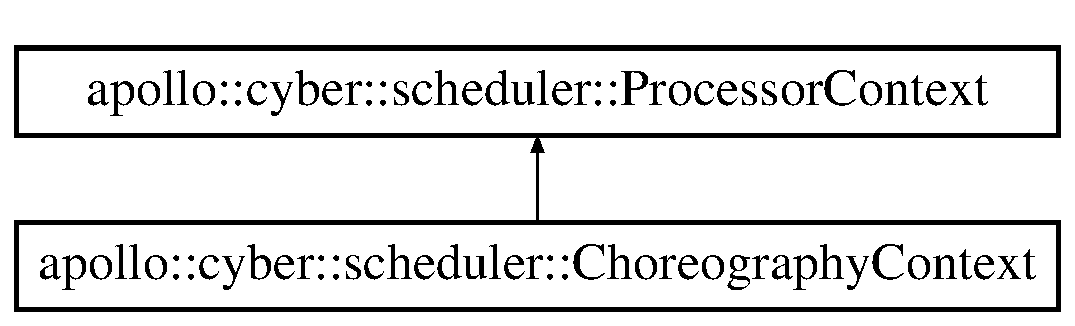
\includegraphics[height=2.000000cm]{classapollo_1_1cyber_1_1scheduler_1_1ChoreographyContext}
\end{center}
\end{figure}
\subsection*{Public Member Functions}
\begin{DoxyCompactItemize}
\item 
void \hyperlink{classapollo_1_1cyber_1_1scheduler_1_1ChoreographyContext_ab56d352881d30f192738920ec4809e32}{Remove\-C\-Routine} (uint64\-\_\-t crid)
\item 
std\-::shared\-\_\-ptr$<$ \hyperlink{classapollo_1_1cyber_1_1croutine_1_1CRoutine}{C\-Routine} $>$ \hyperlink{classapollo_1_1cyber_1_1scheduler_1_1ChoreographyContext_aab1c6b9f912a43e1339fa99f2e3631b6}{Next\-Routine} () override
\item 
bool \hyperlink{classapollo_1_1cyber_1_1scheduler_1_1ChoreographyContext_a68bf8c57755cb932518ae9fe8b6fa196}{Enqueue} (const std\-::shared\-\_\-ptr$<$ \hyperlink{classapollo_1_1cyber_1_1croutine_1_1CRoutine}{C\-Routine} $>$ \&)
\item 
void \hyperlink{classapollo_1_1cyber_1_1scheduler_1_1ChoreographyContext_a7ee909ed845a79cdc00a649504d15174}{Notify} ()
\item 
void \hyperlink{classapollo_1_1cyber_1_1scheduler_1_1ChoreographyContext_a895fb1717d71bb0e53abfdc5f9a7a768}{Wait} () override
\end{DoxyCompactItemize}
\subsection*{Private Attributes}
\begin{DoxyCompactItemize}
\item 
std\-::mutex \hyperlink{classapollo_1_1cyber_1_1scheduler_1_1ChoreographyContext_a4955bd10541d5f68187f69a5c9c25f2f}{mtx\-\_\-wq\-\_\-}
\item 
std\-::condition\-\_\-variable \hyperlink{classapollo_1_1cyber_1_1scheduler_1_1ChoreographyContext_a6089935be7f61f7231d1e0d822562d71}{cv\-\_\-wq\-\_\-}
\item 
\hyperlink{classapollo_1_1cyber_1_1base_1_1AtomicRWLock}{Atomic\-R\-W\-Lock} \hyperlink{classapollo_1_1cyber_1_1scheduler_1_1ChoreographyContext_a758b50ddb206c4792e855afaa15f6f2c}{rq\-\_\-lk\-\_\-}
\item 
std\-::multimap$<$ uint32\-\_\-t, \\*
std\-::shared\-\_\-ptr$<$ \hyperlink{classapollo_1_1cyber_1_1croutine_1_1CRoutine}{C\-Routine} $>$\\*
, std\-::greater$<$ uint32\-\_\-t $>$ $>$ \hyperlink{classapollo_1_1cyber_1_1scheduler_1_1ChoreographyContext_a9a1cbbf369ba6b3343f48d8b7fe062ad}{cr\-\_\-queue\-\_\-}
\end{DoxyCompactItemize}
\subsection*{Additional Inherited Members}


\subsection{Member Function Documentation}
\hypertarget{classapollo_1_1cyber_1_1scheduler_1_1ChoreographyContext_a68bf8c57755cb932518ae9fe8b6fa196}{\index{apollo\-::cyber\-::scheduler\-::\-Choreography\-Context@{apollo\-::cyber\-::scheduler\-::\-Choreography\-Context}!Enqueue@{Enqueue}}
\index{Enqueue@{Enqueue}!apollo::cyber::scheduler::ChoreographyContext@{apollo\-::cyber\-::scheduler\-::\-Choreography\-Context}}
\subsubsection[{Enqueue}]{\setlength{\rightskip}{0pt plus 5cm}bool apollo\-::cyber\-::scheduler\-::\-Choreography\-Context\-::\-Enqueue (
\begin{DoxyParamCaption}
\item[{const std\-::shared\-\_\-ptr$<$ {\bf C\-Routine} $>$ \&}]{}
\end{DoxyParamCaption}
)}}\label{classapollo_1_1cyber_1_1scheduler_1_1ChoreographyContext_a68bf8c57755cb932518ae9fe8b6fa196}
\hypertarget{classapollo_1_1cyber_1_1scheduler_1_1ChoreographyContext_aab1c6b9f912a43e1339fa99f2e3631b6}{\index{apollo\-::cyber\-::scheduler\-::\-Choreography\-Context@{apollo\-::cyber\-::scheduler\-::\-Choreography\-Context}!Next\-Routine@{Next\-Routine}}
\index{Next\-Routine@{Next\-Routine}!apollo::cyber::scheduler::ChoreographyContext@{apollo\-::cyber\-::scheduler\-::\-Choreography\-Context}}
\subsubsection[{Next\-Routine}]{\setlength{\rightskip}{0pt plus 5cm}std\-::shared\-\_\-ptr$<${\bf C\-Routine}$>$ apollo\-::cyber\-::scheduler\-::\-Choreography\-Context\-::\-Next\-Routine (
\begin{DoxyParamCaption}
{}
\end{DoxyParamCaption}
)\hspace{0.3cm}{\ttfamily [override]}, {\ttfamily [virtual]}}}\label{classapollo_1_1cyber_1_1scheduler_1_1ChoreographyContext_aab1c6b9f912a43e1339fa99f2e3631b6}


Implements \hyperlink{classapollo_1_1cyber_1_1scheduler_1_1ProcessorContext_a0923b50903b11612234355566ab573e0}{apollo\-::cyber\-::scheduler\-::\-Processor\-Context}.

\hypertarget{classapollo_1_1cyber_1_1scheduler_1_1ChoreographyContext_a7ee909ed845a79cdc00a649504d15174}{\index{apollo\-::cyber\-::scheduler\-::\-Choreography\-Context@{apollo\-::cyber\-::scheduler\-::\-Choreography\-Context}!Notify@{Notify}}
\index{Notify@{Notify}!apollo::cyber::scheduler::ChoreographyContext@{apollo\-::cyber\-::scheduler\-::\-Choreography\-Context}}
\subsubsection[{Notify}]{\setlength{\rightskip}{0pt plus 5cm}void apollo\-::cyber\-::scheduler\-::\-Choreography\-Context\-::\-Notify (
\begin{DoxyParamCaption}
{}
\end{DoxyParamCaption}
)}}\label{classapollo_1_1cyber_1_1scheduler_1_1ChoreographyContext_a7ee909ed845a79cdc00a649504d15174}
\hypertarget{classapollo_1_1cyber_1_1scheduler_1_1ChoreographyContext_ab56d352881d30f192738920ec4809e32}{\index{apollo\-::cyber\-::scheduler\-::\-Choreography\-Context@{apollo\-::cyber\-::scheduler\-::\-Choreography\-Context}!Remove\-C\-Routine@{Remove\-C\-Routine}}
\index{Remove\-C\-Routine@{Remove\-C\-Routine}!apollo::cyber::scheduler::ChoreographyContext@{apollo\-::cyber\-::scheduler\-::\-Choreography\-Context}}
\subsubsection[{Remove\-C\-Routine}]{\setlength{\rightskip}{0pt plus 5cm}void apollo\-::cyber\-::scheduler\-::\-Choreography\-Context\-::\-Remove\-C\-Routine (
\begin{DoxyParamCaption}
\item[{uint64\-\_\-t}]{crid}
\end{DoxyParamCaption}
)}}\label{classapollo_1_1cyber_1_1scheduler_1_1ChoreographyContext_ab56d352881d30f192738920ec4809e32}
\hypertarget{classapollo_1_1cyber_1_1scheduler_1_1ChoreographyContext_a895fb1717d71bb0e53abfdc5f9a7a768}{\index{apollo\-::cyber\-::scheduler\-::\-Choreography\-Context@{apollo\-::cyber\-::scheduler\-::\-Choreography\-Context}!Wait@{Wait}}
\index{Wait@{Wait}!apollo::cyber::scheduler::ChoreographyContext@{apollo\-::cyber\-::scheduler\-::\-Choreography\-Context}}
\subsubsection[{Wait}]{\setlength{\rightskip}{0pt plus 5cm}void apollo\-::cyber\-::scheduler\-::\-Choreography\-Context\-::\-Wait (
\begin{DoxyParamCaption}
{}
\end{DoxyParamCaption}
)\hspace{0.3cm}{\ttfamily [override]}, {\ttfamily [virtual]}}}\label{classapollo_1_1cyber_1_1scheduler_1_1ChoreographyContext_a895fb1717d71bb0e53abfdc5f9a7a768}


Implements \hyperlink{classapollo_1_1cyber_1_1scheduler_1_1ProcessorContext_a0a2e1914277be7a5fe81f459c83b6644}{apollo\-::cyber\-::scheduler\-::\-Processor\-Context}.



\subsection{Member Data Documentation}
\hypertarget{classapollo_1_1cyber_1_1scheduler_1_1ChoreographyContext_a9a1cbbf369ba6b3343f48d8b7fe062ad}{\index{apollo\-::cyber\-::scheduler\-::\-Choreography\-Context@{apollo\-::cyber\-::scheduler\-::\-Choreography\-Context}!cr\-\_\-queue\-\_\-@{cr\-\_\-queue\-\_\-}}
\index{cr\-\_\-queue\-\_\-@{cr\-\_\-queue\-\_\-}!apollo::cyber::scheduler::ChoreographyContext@{apollo\-::cyber\-::scheduler\-::\-Choreography\-Context}}
\subsubsection[{cr\-\_\-queue\-\_\-}]{\setlength{\rightskip}{0pt plus 5cm}std\-::multimap$<$uint32\-\_\-t, std\-::shared\-\_\-ptr$<${\bf C\-Routine}$>$, std\-::greater$<$uint32\-\_\-t$>$ $>$ apollo\-::cyber\-::scheduler\-::\-Choreography\-Context\-::cr\-\_\-queue\-\_\-\hspace{0.3cm}{\ttfamily [private]}}}\label{classapollo_1_1cyber_1_1scheduler_1_1ChoreographyContext_a9a1cbbf369ba6b3343f48d8b7fe062ad}
\hypertarget{classapollo_1_1cyber_1_1scheduler_1_1ChoreographyContext_a6089935be7f61f7231d1e0d822562d71}{\index{apollo\-::cyber\-::scheduler\-::\-Choreography\-Context@{apollo\-::cyber\-::scheduler\-::\-Choreography\-Context}!cv\-\_\-wq\-\_\-@{cv\-\_\-wq\-\_\-}}
\index{cv\-\_\-wq\-\_\-@{cv\-\_\-wq\-\_\-}!apollo::cyber::scheduler::ChoreographyContext@{apollo\-::cyber\-::scheduler\-::\-Choreography\-Context}}
\subsubsection[{cv\-\_\-wq\-\_\-}]{\setlength{\rightskip}{0pt plus 5cm}std\-::condition\-\_\-variable apollo\-::cyber\-::scheduler\-::\-Choreography\-Context\-::cv\-\_\-wq\-\_\-\hspace{0.3cm}{\ttfamily [private]}}}\label{classapollo_1_1cyber_1_1scheduler_1_1ChoreographyContext_a6089935be7f61f7231d1e0d822562d71}
\hypertarget{classapollo_1_1cyber_1_1scheduler_1_1ChoreographyContext_a4955bd10541d5f68187f69a5c9c25f2f}{\index{apollo\-::cyber\-::scheduler\-::\-Choreography\-Context@{apollo\-::cyber\-::scheduler\-::\-Choreography\-Context}!mtx\-\_\-wq\-\_\-@{mtx\-\_\-wq\-\_\-}}
\index{mtx\-\_\-wq\-\_\-@{mtx\-\_\-wq\-\_\-}!apollo::cyber::scheduler::ChoreographyContext@{apollo\-::cyber\-::scheduler\-::\-Choreography\-Context}}
\subsubsection[{mtx\-\_\-wq\-\_\-}]{\setlength{\rightskip}{0pt plus 5cm}std\-::mutex apollo\-::cyber\-::scheduler\-::\-Choreography\-Context\-::mtx\-\_\-wq\-\_\-\hspace{0.3cm}{\ttfamily [private]}}}\label{classapollo_1_1cyber_1_1scheduler_1_1ChoreographyContext_a4955bd10541d5f68187f69a5c9c25f2f}
\hypertarget{classapollo_1_1cyber_1_1scheduler_1_1ChoreographyContext_a758b50ddb206c4792e855afaa15f6f2c}{\index{apollo\-::cyber\-::scheduler\-::\-Choreography\-Context@{apollo\-::cyber\-::scheduler\-::\-Choreography\-Context}!rq\-\_\-lk\-\_\-@{rq\-\_\-lk\-\_\-}}
\index{rq\-\_\-lk\-\_\-@{rq\-\_\-lk\-\_\-}!apollo::cyber::scheduler::ChoreographyContext@{apollo\-::cyber\-::scheduler\-::\-Choreography\-Context}}
\subsubsection[{rq\-\_\-lk\-\_\-}]{\setlength{\rightskip}{0pt plus 5cm}{\bf Atomic\-R\-W\-Lock} apollo\-::cyber\-::scheduler\-::\-Choreography\-Context\-::rq\-\_\-lk\-\_\-\hspace{0.3cm}{\ttfamily [private]}}}\label{classapollo_1_1cyber_1_1scheduler_1_1ChoreographyContext_a758b50ddb206c4792e855afaa15f6f2c}


The documentation for this class was generated from the following file\-:\begin{DoxyCompactItemize}
\item 
scheduler/policy/\hyperlink{choreography__context_8h}{choreography\-\_\-context.\-h}\end{DoxyCompactItemize}

\hypertarget{structapollo_1_1cyber_1_1record_1_1Chunk}{\section{apollo\-:\-:cyber\-:\-:record\-:\-:Chunk Struct Reference}
\label{structapollo_1_1cyber_1_1record_1_1Chunk}\index{apollo\-::cyber\-::record\-::\-Chunk@{apollo\-::cyber\-::record\-::\-Chunk}}
}


{\ttfamily \#include $<$record\-\_\-file\-\_\-writer.\-h$>$}

\subsection*{Public Member Functions}
\begin{DoxyCompactItemize}
\item 
\hyperlink{structapollo_1_1cyber_1_1record_1_1Chunk_a2cf02bb8d216f44ecff00f4e08c07897}{Chunk} ()
\item 
void \hyperlink{structapollo_1_1cyber_1_1record_1_1Chunk_a05ac768236d95c41080758f19b7d5a98}{clear} ()
\item 
void \hyperlink{structapollo_1_1cyber_1_1record_1_1Chunk_a9f06f76b5e1ea3609f8314cf52dc0899}{add} (const Single\-Message \&message)
\item 
bool \hyperlink{structapollo_1_1cyber_1_1record_1_1Chunk_a9cc10421521b0bb0b3e0c92f3bf5dfed}{empty} ()
\end{DoxyCompactItemize}
\subsection*{Public Attributes}
\begin{DoxyCompactItemize}
\item 
std\-::mutex \hyperlink{structapollo_1_1cyber_1_1record_1_1Chunk_af89d9a0952404a4d3f3877da67b40128}{mutex\-\_\-}
\item 
Chunk\-Header \hyperlink{structapollo_1_1cyber_1_1record_1_1Chunk_a8dbd3eaef5f4c44b84b4003acaa2fc0b}{header\-\_\-}
\item 
Chunk\-Body \hyperlink{structapollo_1_1cyber_1_1record_1_1Chunk_a00672597f6ebfdf2dbeaabd580d9909b}{body\-\_\-}
\end{DoxyCompactItemize}


\subsection{Constructor \& Destructor Documentation}
\hypertarget{structapollo_1_1cyber_1_1record_1_1Chunk_a2cf02bb8d216f44ecff00f4e08c07897}{\index{apollo\-::cyber\-::record\-::\-Chunk@{apollo\-::cyber\-::record\-::\-Chunk}!Chunk@{Chunk}}
\index{Chunk@{Chunk}!apollo::cyber::record::Chunk@{apollo\-::cyber\-::record\-::\-Chunk}}
\subsubsection[{Chunk}]{\setlength{\rightskip}{0pt plus 5cm}apollo\-::cyber\-::record\-::\-Chunk\-::\-Chunk (
\begin{DoxyParamCaption}
{}
\end{DoxyParamCaption}
)\hspace{0.3cm}{\ttfamily [inline]}}}\label{structapollo_1_1cyber_1_1record_1_1Chunk_a2cf02bb8d216f44ecff00f4e08c07897}


\subsection{Member Function Documentation}
\hypertarget{structapollo_1_1cyber_1_1record_1_1Chunk_a9f06f76b5e1ea3609f8314cf52dc0899}{\index{apollo\-::cyber\-::record\-::\-Chunk@{apollo\-::cyber\-::record\-::\-Chunk}!add@{add}}
\index{add@{add}!apollo::cyber::record::Chunk@{apollo\-::cyber\-::record\-::\-Chunk}}
\subsubsection[{add}]{\setlength{\rightskip}{0pt plus 5cm}void apollo\-::cyber\-::record\-::\-Chunk\-::add (
\begin{DoxyParamCaption}
\item[{const Single\-Message \&}]{message}
\end{DoxyParamCaption}
)\hspace{0.3cm}{\ttfamily [inline]}}}\label{structapollo_1_1cyber_1_1record_1_1Chunk_a9f06f76b5e1ea3609f8314cf52dc0899}
\hypertarget{structapollo_1_1cyber_1_1record_1_1Chunk_a05ac768236d95c41080758f19b7d5a98}{\index{apollo\-::cyber\-::record\-::\-Chunk@{apollo\-::cyber\-::record\-::\-Chunk}!clear@{clear}}
\index{clear@{clear}!apollo::cyber::record::Chunk@{apollo\-::cyber\-::record\-::\-Chunk}}
\subsubsection[{clear}]{\setlength{\rightskip}{0pt plus 5cm}void apollo\-::cyber\-::record\-::\-Chunk\-::clear (
\begin{DoxyParamCaption}
{}
\end{DoxyParamCaption}
)\hspace{0.3cm}{\ttfamily [inline]}}}\label{structapollo_1_1cyber_1_1record_1_1Chunk_a05ac768236d95c41080758f19b7d5a98}
\hypertarget{structapollo_1_1cyber_1_1record_1_1Chunk_a9cc10421521b0bb0b3e0c92f3bf5dfed}{\index{apollo\-::cyber\-::record\-::\-Chunk@{apollo\-::cyber\-::record\-::\-Chunk}!empty@{empty}}
\index{empty@{empty}!apollo::cyber::record::Chunk@{apollo\-::cyber\-::record\-::\-Chunk}}
\subsubsection[{empty}]{\setlength{\rightskip}{0pt plus 5cm}bool apollo\-::cyber\-::record\-::\-Chunk\-::empty (
\begin{DoxyParamCaption}
{}
\end{DoxyParamCaption}
)\hspace{0.3cm}{\ttfamily [inline]}}}\label{structapollo_1_1cyber_1_1record_1_1Chunk_a9cc10421521b0bb0b3e0c92f3bf5dfed}


\subsection{Member Data Documentation}
\hypertarget{structapollo_1_1cyber_1_1record_1_1Chunk_a00672597f6ebfdf2dbeaabd580d9909b}{\index{apollo\-::cyber\-::record\-::\-Chunk@{apollo\-::cyber\-::record\-::\-Chunk}!body\-\_\-@{body\-\_\-}}
\index{body\-\_\-@{body\-\_\-}!apollo::cyber::record::Chunk@{apollo\-::cyber\-::record\-::\-Chunk}}
\subsubsection[{body\-\_\-}]{\setlength{\rightskip}{0pt plus 5cm}Chunk\-Body apollo\-::cyber\-::record\-::\-Chunk\-::body\-\_\-}}\label{structapollo_1_1cyber_1_1record_1_1Chunk_a00672597f6ebfdf2dbeaabd580d9909b}
\hypertarget{structapollo_1_1cyber_1_1record_1_1Chunk_a8dbd3eaef5f4c44b84b4003acaa2fc0b}{\index{apollo\-::cyber\-::record\-::\-Chunk@{apollo\-::cyber\-::record\-::\-Chunk}!header\-\_\-@{header\-\_\-}}
\index{header\-\_\-@{header\-\_\-}!apollo::cyber::record::Chunk@{apollo\-::cyber\-::record\-::\-Chunk}}
\subsubsection[{header\-\_\-}]{\setlength{\rightskip}{0pt plus 5cm}Chunk\-Header apollo\-::cyber\-::record\-::\-Chunk\-::header\-\_\-}}\label{structapollo_1_1cyber_1_1record_1_1Chunk_a8dbd3eaef5f4c44b84b4003acaa2fc0b}
\hypertarget{structapollo_1_1cyber_1_1record_1_1Chunk_af89d9a0952404a4d3f3877da67b40128}{\index{apollo\-::cyber\-::record\-::\-Chunk@{apollo\-::cyber\-::record\-::\-Chunk}!mutex\-\_\-@{mutex\-\_\-}}
\index{mutex\-\_\-@{mutex\-\_\-}!apollo::cyber::record::Chunk@{apollo\-::cyber\-::record\-::\-Chunk}}
\subsubsection[{mutex\-\_\-}]{\setlength{\rightskip}{0pt plus 5cm}std\-::mutex apollo\-::cyber\-::record\-::\-Chunk\-::mutex\-\_\-}}\label{structapollo_1_1cyber_1_1record_1_1Chunk_af89d9a0952404a4d3f3877da67b40128}


The documentation for this struct was generated from the following file\-:\begin{DoxyCompactItemize}
\item 
record/file/\hyperlink{record__file__writer_8h}{record\-\_\-file\-\_\-writer.\-h}\end{DoxyCompactItemize}

\hypertarget{classapollo_1_1cyber_1_1class__loader_1_1utility_1_1ClassFactory}{\section{apollo\-:\-:cyber\-:\-:class\-\_\-loader\-:\-:utility\-:\-:Class\-Factory$<$ Class\-Object, Base $>$ Class Template Reference}
\label{classapollo_1_1cyber_1_1class__loader_1_1utility_1_1ClassFactory}\index{apollo\-::cyber\-::class\-\_\-loader\-::utility\-::\-Class\-Factory$<$ Class\-Object, Base $>$@{apollo\-::cyber\-::class\-\_\-loader\-::utility\-::\-Class\-Factory$<$ Class\-Object, Base $>$}}
}


{\ttfamily \#include $<$class\-\_\-factory.\-h$>$}

Inheritance diagram for apollo\-:\-:cyber\-:\-:class\-\_\-loader\-:\-:utility\-:\-:Class\-Factory$<$ Class\-Object, Base $>$\-:\begin{figure}[H]
\begin{center}
\leavevmode
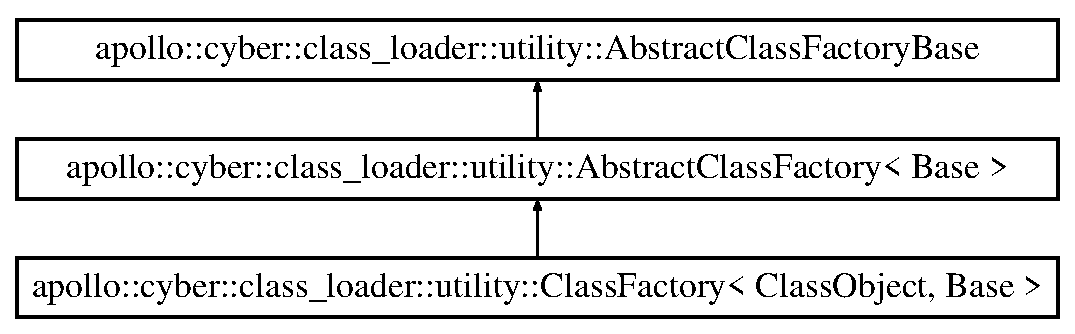
\includegraphics[height=3.000000cm]{classapollo_1_1cyber_1_1class__loader_1_1utility_1_1ClassFactory}
\end{center}
\end{figure}
\subsection*{Public Member Functions}
\begin{DoxyCompactItemize}
\item 
\hyperlink{classapollo_1_1cyber_1_1class__loader_1_1utility_1_1ClassFactory_afef5f19f3398b4156864319b42889cda}{Class\-Factory} (const std\-::string \&class\-\_\-name, const std\-::string \&base\-\_\-class\-\_\-name)
\item 
Base $\ast$ \hyperlink{classapollo_1_1cyber_1_1class__loader_1_1utility_1_1ClassFactory_afe170d362f95f097b72fa4de58ee06ca}{Create\-Obj} () const 
\end{DoxyCompactItemize}
\subsection*{Additional Inherited Members}


\subsection{Constructor \& Destructor Documentation}
\hypertarget{classapollo_1_1cyber_1_1class__loader_1_1utility_1_1ClassFactory_afef5f19f3398b4156864319b42889cda}{\index{apollo\-::cyber\-::class\-\_\-loader\-::utility\-::\-Class\-Factory@{apollo\-::cyber\-::class\-\_\-loader\-::utility\-::\-Class\-Factory}!Class\-Factory@{Class\-Factory}}
\index{Class\-Factory@{Class\-Factory}!apollo::cyber::class_loader::utility::ClassFactory@{apollo\-::cyber\-::class\-\_\-loader\-::utility\-::\-Class\-Factory}}
\subsubsection[{Class\-Factory}]{\setlength{\rightskip}{0pt plus 5cm}template$<$typename Class\-Object, typename Base$>$ {\bf apollo\-::cyber\-::class\-\_\-loader\-::utility\-::\-Class\-Factory}$<$ Class\-Object, Base $>$\-::{\bf Class\-Factory} (
\begin{DoxyParamCaption}
\item[{const std\-::string \&}]{class\-\_\-name, }
\item[{const std\-::string \&}]{base\-\_\-class\-\_\-name}
\end{DoxyParamCaption}
)\hspace{0.3cm}{\ttfamily [inline]}}}\label{classapollo_1_1cyber_1_1class__loader_1_1utility_1_1ClassFactory_afef5f19f3398b4156864319b42889cda}


\subsection{Member Function Documentation}
\hypertarget{classapollo_1_1cyber_1_1class__loader_1_1utility_1_1ClassFactory_afe170d362f95f097b72fa4de58ee06ca}{\index{apollo\-::cyber\-::class\-\_\-loader\-::utility\-::\-Class\-Factory@{apollo\-::cyber\-::class\-\_\-loader\-::utility\-::\-Class\-Factory}!Create\-Obj@{Create\-Obj}}
\index{Create\-Obj@{Create\-Obj}!apollo::cyber::class_loader::utility::ClassFactory@{apollo\-::cyber\-::class\-\_\-loader\-::utility\-::\-Class\-Factory}}
\subsubsection[{Create\-Obj}]{\setlength{\rightskip}{0pt plus 5cm}template$<$typename Class\-Object, typename Base$>$ Base$\ast$ {\bf apollo\-::cyber\-::class\-\_\-loader\-::utility\-::\-Class\-Factory}$<$ Class\-Object, Base $>$\-::Create\-Obj (
\begin{DoxyParamCaption}
{}
\end{DoxyParamCaption}
) const\hspace{0.3cm}{\ttfamily [inline]}, {\ttfamily [virtual]}}}\label{classapollo_1_1cyber_1_1class__loader_1_1utility_1_1ClassFactory_afe170d362f95f097b72fa4de58ee06ca}


Implements \hyperlink{classapollo_1_1cyber_1_1class__loader_1_1utility_1_1AbstractClassFactory_ae603a03f06c93b5f0475e63a0f2a9402}{apollo\-::cyber\-::class\-\_\-loader\-::utility\-::\-Abstract\-Class\-Factory$<$ Base $>$}.



The documentation for this class was generated from the following file\-:\begin{DoxyCompactItemize}
\item 
class\-\_\-loader/utility/\hyperlink{class__factory_8h}{class\-\_\-factory.\-h}\end{DoxyCompactItemize}

\hypertarget{classapollo_1_1cyber_1_1scheduler_1_1ClassicContext}{\section{apollo\-:\-:cyber\-:\-:scheduler\-:\-:Classic\-Context Class Reference}
\label{classapollo_1_1cyber_1_1scheduler_1_1ClassicContext}\index{apollo\-::cyber\-::scheduler\-::\-Classic\-Context@{apollo\-::cyber\-::scheduler\-::\-Classic\-Context}}
}


{\ttfamily \#include $<$classic\-\_\-context.\-h$>$}

Inheritance diagram for apollo\-:\-:cyber\-:\-:scheduler\-:\-:Classic\-Context\-:\begin{figure}[H]
\begin{center}
\leavevmode
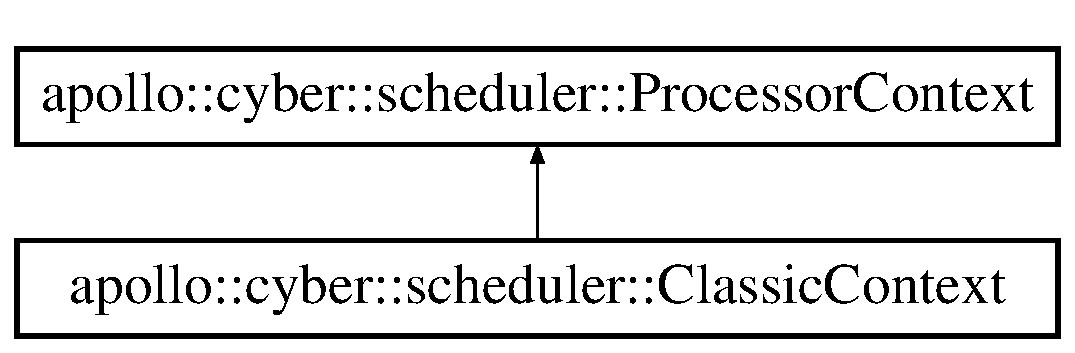
\includegraphics[height=2.000000cm]{classapollo_1_1cyber_1_1scheduler_1_1ClassicContext}
\end{center}
\end{figure}
\subsection*{Public Member Functions}
\begin{DoxyCompactItemize}
\item 
\hyperlink{classapollo_1_1cyber_1_1scheduler_1_1ClassicContext_a663924838acb75ef7c041bc435a8142f}{Classic\-Context} ()
\item 
\hyperlink{classapollo_1_1cyber_1_1scheduler_1_1ClassicContext_aeaaa88d1cab549ab2800f5e229c1244a}{Classic\-Context} (const std\-::string \&group\-\_\-name)
\item 
std\-::shared\-\_\-ptr$<$ \hyperlink{classapollo_1_1cyber_1_1croutine_1_1CRoutine}{C\-Routine} $>$ \hyperlink{classapollo_1_1cyber_1_1scheduler_1_1ClassicContext_a6a9ffd7b5fb645a97b7daf93d4973025}{Next\-Routine} () override
\item 
void \hyperlink{classapollo_1_1cyber_1_1scheduler_1_1ClassicContext_ac32e655ea3689a0bc06c9003852fd0a3}{Wait} () override
\item 
void \hyperlink{classapollo_1_1cyber_1_1scheduler_1_1ClassicContext_aa6c94b93d17fb4f546c8f2f7e74f832a}{Shutdown} () override
\end{DoxyCompactItemize}
\subsection*{Static Public Member Functions}
\begin{DoxyCompactItemize}
\item 
static void \hyperlink{classapollo_1_1cyber_1_1scheduler_1_1ClassicContext_afaa6f92a7ea305b55cd96763cbdd2a90}{Notify} (const std\-::string \&group\-\_\-name)
\end{DoxyCompactItemize}
\subsection*{Static Public Attributes}
\begin{DoxyCompactItemize}
\item 
static \hyperlink{namespaceapollo_1_1cyber_1_1scheduler_ad4f939996840b0f02dafc9a779dfefd7}{R\-Q\-\_\-\-L\-O\-C\-K\-\_\-\-G\-R\-O\-U\-P} \hyperlink{classapollo_1_1cyber_1_1scheduler_1_1ClassicContext_a10adfb1632c4cb5049273262cb997333}{rq\-\_\-locks\-\_\-}
\item 
static \hyperlink{namespaceapollo_1_1cyber_1_1scheduler_aea5742ba3cc52566de1eeeeaac1a8714}{C\-R\-\_\-\-G\-R\-O\-U\-P} \hyperlink{classapollo_1_1cyber_1_1scheduler_1_1ClassicContext_a22519e2ac14bf14f0b81e4a3a3befcfb}{cr\-\_\-group\-\_\-}
\item 
static \hyperlink{namespaceapollo_1_1cyber_1_1scheduler_a38dec21bb0dcc34727c9a215020abb70}{G\-R\-P\-\_\-\-W\-Q\-\_\-\-M\-U\-T\-E\-X} \hyperlink{classapollo_1_1cyber_1_1scheduler_1_1ClassicContext_a48ad41105f3adbc71ca925a08ff987ee}{mtx\-\_\-wq\-\_\-}
\item 
static \hyperlink{namespaceapollo_1_1cyber_1_1scheduler_aaaf29077b955c494a8b6ef756e02ed4d}{G\-R\-P\-\_\-\-W\-Q\-\_\-\-C\-V} \hyperlink{classapollo_1_1cyber_1_1scheduler_1_1ClassicContext_abc70c8c180700b17f5048020f21b6fd0}{cv\-\_\-wq\-\_\-}
\end{DoxyCompactItemize}
\subsection*{Private Member Functions}
\begin{DoxyCompactItemize}
\item 
void \hyperlink{classapollo_1_1cyber_1_1scheduler_1_1ClassicContext_a2f4f0b6749ceb22e645c8ca2567f903a}{Init\-Group} (const std\-::string \&group\-\_\-name)
\end{DoxyCompactItemize}
\subsection*{Private Attributes}
\begin{DoxyCompactItemize}
\item 
std\-::chrono\-::steady\-\_\-clock\-::time\-\_\-point \hyperlink{classapollo_1_1cyber_1_1scheduler_1_1ClassicContext_abc30359d23f986f35b0c01ff81d6ccc1}{wake\-\_\-time\-\_\-}
\item 
bool \hyperlink{classapollo_1_1cyber_1_1scheduler_1_1ClassicContext_a094e0d83afedbb7530649d54b17f9e65}{need\-\_\-sleep\-\_\-} = false
\item 
\hyperlink{namespaceapollo_1_1cyber_1_1scheduler_ac66e3c3cdda21d9be8ea0692401913a2}{M\-U\-L\-T\-I\-\_\-\-P\-R\-I\-O\-\_\-\-Q\-U\-E\-U\-E} $\ast$ \hyperlink{classapollo_1_1cyber_1_1scheduler_1_1ClassicContext_aa3ed67cfe2876f8fd1e1388867cad234}{multi\-\_\-pri\-\_\-rq\-\_\-} = nullptr
\item 
\hyperlink{namespaceapollo_1_1cyber_1_1scheduler_a714aab7bf591e6d2f48fafdbbb1dda02}{L\-O\-C\-K\-\_\-\-Q\-U\-E\-U\-E} $\ast$ \hyperlink{classapollo_1_1cyber_1_1scheduler_1_1ClassicContext_af6e0adf912a3056950ded3660aabb9ec}{lq\-\_\-} = nullptr
\item 
\hyperlink{classapollo_1_1cyber_1_1scheduler_1_1MutexWrapper}{Mutex\-Wrapper} $\ast$ \hyperlink{classapollo_1_1cyber_1_1scheduler_1_1ClassicContext_a12aaac26d8fbeea3ac3124eb08528409}{mtx\-\_\-wrapper\-\_\-} = nullptr
\item 
\hyperlink{classapollo_1_1cyber_1_1scheduler_1_1CvWrapper}{Cv\-Wrapper} $\ast$ \hyperlink{classapollo_1_1cyber_1_1scheduler_1_1ClassicContext_a39f22a14b1997f761659f2fe8cbade8b}{cw\-\_\-} = nullptr
\end{DoxyCompactItemize}
\subsection*{Additional Inherited Members}


\subsection{Constructor \& Destructor Documentation}
\hypertarget{classapollo_1_1cyber_1_1scheduler_1_1ClassicContext_a663924838acb75ef7c041bc435a8142f}{\index{apollo\-::cyber\-::scheduler\-::\-Classic\-Context@{apollo\-::cyber\-::scheduler\-::\-Classic\-Context}!Classic\-Context@{Classic\-Context}}
\index{Classic\-Context@{Classic\-Context}!apollo::cyber::scheduler::ClassicContext@{apollo\-::cyber\-::scheduler\-::\-Classic\-Context}}
\subsubsection[{Classic\-Context}]{\setlength{\rightskip}{0pt plus 5cm}apollo\-::cyber\-::scheduler\-::\-Classic\-Context\-::\-Classic\-Context (
\begin{DoxyParamCaption}
{}
\end{DoxyParamCaption}
)}}\label{classapollo_1_1cyber_1_1scheduler_1_1ClassicContext_a663924838acb75ef7c041bc435a8142f}
\hypertarget{classapollo_1_1cyber_1_1scheduler_1_1ClassicContext_aeaaa88d1cab549ab2800f5e229c1244a}{\index{apollo\-::cyber\-::scheduler\-::\-Classic\-Context@{apollo\-::cyber\-::scheduler\-::\-Classic\-Context}!Classic\-Context@{Classic\-Context}}
\index{Classic\-Context@{Classic\-Context}!apollo::cyber::scheduler::ClassicContext@{apollo\-::cyber\-::scheduler\-::\-Classic\-Context}}
\subsubsection[{Classic\-Context}]{\setlength{\rightskip}{0pt plus 5cm}apollo\-::cyber\-::scheduler\-::\-Classic\-Context\-::\-Classic\-Context (
\begin{DoxyParamCaption}
\item[{const std\-::string \&}]{group\-\_\-name}
\end{DoxyParamCaption}
)\hspace{0.3cm}{\ttfamily [explicit]}}}\label{classapollo_1_1cyber_1_1scheduler_1_1ClassicContext_aeaaa88d1cab549ab2800f5e229c1244a}


\subsection{Member Function Documentation}
\hypertarget{classapollo_1_1cyber_1_1scheduler_1_1ClassicContext_a2f4f0b6749ceb22e645c8ca2567f903a}{\index{apollo\-::cyber\-::scheduler\-::\-Classic\-Context@{apollo\-::cyber\-::scheduler\-::\-Classic\-Context}!Init\-Group@{Init\-Group}}
\index{Init\-Group@{Init\-Group}!apollo::cyber::scheduler::ClassicContext@{apollo\-::cyber\-::scheduler\-::\-Classic\-Context}}
\subsubsection[{Init\-Group}]{\setlength{\rightskip}{0pt plus 5cm}void apollo\-::cyber\-::scheduler\-::\-Classic\-Context\-::\-Init\-Group (
\begin{DoxyParamCaption}
\item[{const std\-::string \&}]{group\-\_\-name}
\end{DoxyParamCaption}
)\hspace{0.3cm}{\ttfamily [private]}}}\label{classapollo_1_1cyber_1_1scheduler_1_1ClassicContext_a2f4f0b6749ceb22e645c8ca2567f903a}
\hypertarget{classapollo_1_1cyber_1_1scheduler_1_1ClassicContext_a6a9ffd7b5fb645a97b7daf93d4973025}{\index{apollo\-::cyber\-::scheduler\-::\-Classic\-Context@{apollo\-::cyber\-::scheduler\-::\-Classic\-Context}!Next\-Routine@{Next\-Routine}}
\index{Next\-Routine@{Next\-Routine}!apollo::cyber::scheduler::ClassicContext@{apollo\-::cyber\-::scheduler\-::\-Classic\-Context}}
\subsubsection[{Next\-Routine}]{\setlength{\rightskip}{0pt plus 5cm}std\-::shared\-\_\-ptr$<${\bf C\-Routine}$>$ apollo\-::cyber\-::scheduler\-::\-Classic\-Context\-::\-Next\-Routine (
\begin{DoxyParamCaption}
{}
\end{DoxyParamCaption}
)\hspace{0.3cm}{\ttfamily [override]}, {\ttfamily [virtual]}}}\label{classapollo_1_1cyber_1_1scheduler_1_1ClassicContext_a6a9ffd7b5fb645a97b7daf93d4973025}


Implements \hyperlink{classapollo_1_1cyber_1_1scheduler_1_1ProcessorContext_a0923b50903b11612234355566ab573e0}{apollo\-::cyber\-::scheduler\-::\-Processor\-Context}.

\hypertarget{classapollo_1_1cyber_1_1scheduler_1_1ClassicContext_afaa6f92a7ea305b55cd96763cbdd2a90}{\index{apollo\-::cyber\-::scheduler\-::\-Classic\-Context@{apollo\-::cyber\-::scheduler\-::\-Classic\-Context}!Notify@{Notify}}
\index{Notify@{Notify}!apollo::cyber::scheduler::ClassicContext@{apollo\-::cyber\-::scheduler\-::\-Classic\-Context}}
\subsubsection[{Notify}]{\setlength{\rightskip}{0pt plus 5cm}static void apollo\-::cyber\-::scheduler\-::\-Classic\-Context\-::\-Notify (
\begin{DoxyParamCaption}
\item[{const std\-::string \&}]{group\-\_\-name}
\end{DoxyParamCaption}
)\hspace{0.3cm}{\ttfamily [static]}}}\label{classapollo_1_1cyber_1_1scheduler_1_1ClassicContext_afaa6f92a7ea305b55cd96763cbdd2a90}
\hypertarget{classapollo_1_1cyber_1_1scheduler_1_1ClassicContext_aa6c94b93d17fb4f546c8f2f7e74f832a}{\index{apollo\-::cyber\-::scheduler\-::\-Classic\-Context@{apollo\-::cyber\-::scheduler\-::\-Classic\-Context}!Shutdown@{Shutdown}}
\index{Shutdown@{Shutdown}!apollo::cyber::scheduler::ClassicContext@{apollo\-::cyber\-::scheduler\-::\-Classic\-Context}}
\subsubsection[{Shutdown}]{\setlength{\rightskip}{0pt plus 5cm}void apollo\-::cyber\-::scheduler\-::\-Classic\-Context\-::\-Shutdown (
\begin{DoxyParamCaption}
{}
\end{DoxyParamCaption}
)\hspace{0.3cm}{\ttfamily [override]}, {\ttfamily [virtual]}}}\label{classapollo_1_1cyber_1_1scheduler_1_1ClassicContext_aa6c94b93d17fb4f546c8f2f7e74f832a}


Reimplemented from \hyperlink{classapollo_1_1cyber_1_1scheduler_1_1ProcessorContext_ab36b8e9524ea0e02cba88b7d4e0e3079}{apollo\-::cyber\-::scheduler\-::\-Processor\-Context}.

\hypertarget{classapollo_1_1cyber_1_1scheduler_1_1ClassicContext_ac32e655ea3689a0bc06c9003852fd0a3}{\index{apollo\-::cyber\-::scheduler\-::\-Classic\-Context@{apollo\-::cyber\-::scheduler\-::\-Classic\-Context}!Wait@{Wait}}
\index{Wait@{Wait}!apollo::cyber::scheduler::ClassicContext@{apollo\-::cyber\-::scheduler\-::\-Classic\-Context}}
\subsubsection[{Wait}]{\setlength{\rightskip}{0pt plus 5cm}void apollo\-::cyber\-::scheduler\-::\-Classic\-Context\-::\-Wait (
\begin{DoxyParamCaption}
{}
\end{DoxyParamCaption}
)\hspace{0.3cm}{\ttfamily [override]}, {\ttfamily [virtual]}}}\label{classapollo_1_1cyber_1_1scheduler_1_1ClassicContext_ac32e655ea3689a0bc06c9003852fd0a3}


Implements \hyperlink{classapollo_1_1cyber_1_1scheduler_1_1ProcessorContext_a0a2e1914277be7a5fe81f459c83b6644}{apollo\-::cyber\-::scheduler\-::\-Processor\-Context}.



\subsection{Member Data Documentation}
\hypertarget{classapollo_1_1cyber_1_1scheduler_1_1ClassicContext_a22519e2ac14bf14f0b81e4a3a3befcfb}{\index{apollo\-::cyber\-::scheduler\-::\-Classic\-Context@{apollo\-::cyber\-::scheduler\-::\-Classic\-Context}!cr\-\_\-group\-\_\-@{cr\-\_\-group\-\_\-}}
\index{cr\-\_\-group\-\_\-@{cr\-\_\-group\-\_\-}!apollo::cyber::scheduler::ClassicContext@{apollo\-::cyber\-::scheduler\-::\-Classic\-Context}}
\subsubsection[{cr\-\_\-group\-\_\-}]{\setlength{\rightskip}{0pt plus 5cm}{\bf C\-R\-\_\-\-G\-R\-O\-U\-P} apollo\-::cyber\-::scheduler\-::\-Classic\-Context\-::cr\-\_\-group\-\_\-\hspace{0.3cm}{\ttfamily [static]}}}\label{classapollo_1_1cyber_1_1scheduler_1_1ClassicContext_a22519e2ac14bf14f0b81e4a3a3befcfb}
\hypertarget{classapollo_1_1cyber_1_1scheduler_1_1ClassicContext_abc70c8c180700b17f5048020f21b6fd0}{\index{apollo\-::cyber\-::scheduler\-::\-Classic\-Context@{apollo\-::cyber\-::scheduler\-::\-Classic\-Context}!cv\-\_\-wq\-\_\-@{cv\-\_\-wq\-\_\-}}
\index{cv\-\_\-wq\-\_\-@{cv\-\_\-wq\-\_\-}!apollo::cyber::scheduler::ClassicContext@{apollo\-::cyber\-::scheduler\-::\-Classic\-Context}}
\subsubsection[{cv\-\_\-wq\-\_\-}]{\setlength{\rightskip}{0pt plus 5cm}{\bf G\-R\-P\-\_\-\-W\-Q\-\_\-\-C\-V} apollo\-::cyber\-::scheduler\-::\-Classic\-Context\-::cv\-\_\-wq\-\_\-\hspace{0.3cm}{\ttfamily [static]}}}\label{classapollo_1_1cyber_1_1scheduler_1_1ClassicContext_abc70c8c180700b17f5048020f21b6fd0}
\hypertarget{classapollo_1_1cyber_1_1scheduler_1_1ClassicContext_a39f22a14b1997f761659f2fe8cbade8b}{\index{apollo\-::cyber\-::scheduler\-::\-Classic\-Context@{apollo\-::cyber\-::scheduler\-::\-Classic\-Context}!cw\-\_\-@{cw\-\_\-}}
\index{cw\-\_\-@{cw\-\_\-}!apollo::cyber::scheduler::ClassicContext@{apollo\-::cyber\-::scheduler\-::\-Classic\-Context}}
\subsubsection[{cw\-\_\-}]{\setlength{\rightskip}{0pt plus 5cm}{\bf Cv\-Wrapper}$\ast$ apollo\-::cyber\-::scheduler\-::\-Classic\-Context\-::cw\-\_\- = nullptr\hspace{0.3cm}{\ttfamily [private]}}}\label{classapollo_1_1cyber_1_1scheduler_1_1ClassicContext_a39f22a14b1997f761659f2fe8cbade8b}
\hypertarget{classapollo_1_1cyber_1_1scheduler_1_1ClassicContext_af6e0adf912a3056950ded3660aabb9ec}{\index{apollo\-::cyber\-::scheduler\-::\-Classic\-Context@{apollo\-::cyber\-::scheduler\-::\-Classic\-Context}!lq\-\_\-@{lq\-\_\-}}
\index{lq\-\_\-@{lq\-\_\-}!apollo::cyber::scheduler::ClassicContext@{apollo\-::cyber\-::scheduler\-::\-Classic\-Context}}
\subsubsection[{lq\-\_\-}]{\setlength{\rightskip}{0pt plus 5cm}{\bf L\-O\-C\-K\-\_\-\-Q\-U\-E\-U\-E}$\ast$ apollo\-::cyber\-::scheduler\-::\-Classic\-Context\-::lq\-\_\- = nullptr\hspace{0.3cm}{\ttfamily [private]}}}\label{classapollo_1_1cyber_1_1scheduler_1_1ClassicContext_af6e0adf912a3056950ded3660aabb9ec}
\hypertarget{classapollo_1_1cyber_1_1scheduler_1_1ClassicContext_a48ad41105f3adbc71ca925a08ff987ee}{\index{apollo\-::cyber\-::scheduler\-::\-Classic\-Context@{apollo\-::cyber\-::scheduler\-::\-Classic\-Context}!mtx\-\_\-wq\-\_\-@{mtx\-\_\-wq\-\_\-}}
\index{mtx\-\_\-wq\-\_\-@{mtx\-\_\-wq\-\_\-}!apollo::cyber::scheduler::ClassicContext@{apollo\-::cyber\-::scheduler\-::\-Classic\-Context}}
\subsubsection[{mtx\-\_\-wq\-\_\-}]{\setlength{\rightskip}{0pt plus 5cm}{\bf G\-R\-P\-\_\-\-W\-Q\-\_\-\-M\-U\-T\-E\-X} apollo\-::cyber\-::scheduler\-::\-Classic\-Context\-::mtx\-\_\-wq\-\_\-\hspace{0.3cm}{\ttfamily [static]}}}\label{classapollo_1_1cyber_1_1scheduler_1_1ClassicContext_a48ad41105f3adbc71ca925a08ff987ee}
\hypertarget{classapollo_1_1cyber_1_1scheduler_1_1ClassicContext_a12aaac26d8fbeea3ac3124eb08528409}{\index{apollo\-::cyber\-::scheduler\-::\-Classic\-Context@{apollo\-::cyber\-::scheduler\-::\-Classic\-Context}!mtx\-\_\-wrapper\-\_\-@{mtx\-\_\-wrapper\-\_\-}}
\index{mtx\-\_\-wrapper\-\_\-@{mtx\-\_\-wrapper\-\_\-}!apollo::cyber::scheduler::ClassicContext@{apollo\-::cyber\-::scheduler\-::\-Classic\-Context}}
\subsubsection[{mtx\-\_\-wrapper\-\_\-}]{\setlength{\rightskip}{0pt plus 5cm}{\bf Mutex\-Wrapper}$\ast$ apollo\-::cyber\-::scheduler\-::\-Classic\-Context\-::mtx\-\_\-wrapper\-\_\- = nullptr\hspace{0.3cm}{\ttfamily [private]}}}\label{classapollo_1_1cyber_1_1scheduler_1_1ClassicContext_a12aaac26d8fbeea3ac3124eb08528409}
\hypertarget{classapollo_1_1cyber_1_1scheduler_1_1ClassicContext_aa3ed67cfe2876f8fd1e1388867cad234}{\index{apollo\-::cyber\-::scheduler\-::\-Classic\-Context@{apollo\-::cyber\-::scheduler\-::\-Classic\-Context}!multi\-\_\-pri\-\_\-rq\-\_\-@{multi\-\_\-pri\-\_\-rq\-\_\-}}
\index{multi\-\_\-pri\-\_\-rq\-\_\-@{multi\-\_\-pri\-\_\-rq\-\_\-}!apollo::cyber::scheduler::ClassicContext@{apollo\-::cyber\-::scheduler\-::\-Classic\-Context}}
\subsubsection[{multi\-\_\-pri\-\_\-rq\-\_\-}]{\setlength{\rightskip}{0pt plus 5cm}{\bf M\-U\-L\-T\-I\-\_\-\-P\-R\-I\-O\-\_\-\-Q\-U\-E\-U\-E}$\ast$ apollo\-::cyber\-::scheduler\-::\-Classic\-Context\-::multi\-\_\-pri\-\_\-rq\-\_\- = nullptr\hspace{0.3cm}{\ttfamily [private]}}}\label{classapollo_1_1cyber_1_1scheduler_1_1ClassicContext_aa3ed67cfe2876f8fd1e1388867cad234}
\hypertarget{classapollo_1_1cyber_1_1scheduler_1_1ClassicContext_a094e0d83afedbb7530649d54b17f9e65}{\index{apollo\-::cyber\-::scheduler\-::\-Classic\-Context@{apollo\-::cyber\-::scheduler\-::\-Classic\-Context}!need\-\_\-sleep\-\_\-@{need\-\_\-sleep\-\_\-}}
\index{need\-\_\-sleep\-\_\-@{need\-\_\-sleep\-\_\-}!apollo::cyber::scheduler::ClassicContext@{apollo\-::cyber\-::scheduler\-::\-Classic\-Context}}
\subsubsection[{need\-\_\-sleep\-\_\-}]{\setlength{\rightskip}{0pt plus 5cm}bool apollo\-::cyber\-::scheduler\-::\-Classic\-Context\-::need\-\_\-sleep\-\_\- = false\hspace{0.3cm}{\ttfamily [private]}}}\label{classapollo_1_1cyber_1_1scheduler_1_1ClassicContext_a094e0d83afedbb7530649d54b17f9e65}
\hypertarget{classapollo_1_1cyber_1_1scheduler_1_1ClassicContext_a10adfb1632c4cb5049273262cb997333}{\index{apollo\-::cyber\-::scheduler\-::\-Classic\-Context@{apollo\-::cyber\-::scheduler\-::\-Classic\-Context}!rq\-\_\-locks\-\_\-@{rq\-\_\-locks\-\_\-}}
\index{rq\-\_\-locks\-\_\-@{rq\-\_\-locks\-\_\-}!apollo::cyber::scheduler::ClassicContext@{apollo\-::cyber\-::scheduler\-::\-Classic\-Context}}
\subsubsection[{rq\-\_\-locks\-\_\-}]{\setlength{\rightskip}{0pt plus 5cm}{\bf R\-Q\-\_\-\-L\-O\-C\-K\-\_\-\-G\-R\-O\-U\-P} apollo\-::cyber\-::scheduler\-::\-Classic\-Context\-::rq\-\_\-locks\-\_\-\hspace{0.3cm}{\ttfamily [static]}}}\label{classapollo_1_1cyber_1_1scheduler_1_1ClassicContext_a10adfb1632c4cb5049273262cb997333}
\hypertarget{classapollo_1_1cyber_1_1scheduler_1_1ClassicContext_abc30359d23f986f35b0c01ff81d6ccc1}{\index{apollo\-::cyber\-::scheduler\-::\-Classic\-Context@{apollo\-::cyber\-::scheduler\-::\-Classic\-Context}!wake\-\_\-time\-\_\-@{wake\-\_\-time\-\_\-}}
\index{wake\-\_\-time\-\_\-@{wake\-\_\-time\-\_\-}!apollo::cyber::scheduler::ClassicContext@{apollo\-::cyber\-::scheduler\-::\-Classic\-Context}}
\subsubsection[{wake\-\_\-time\-\_\-}]{\setlength{\rightskip}{0pt plus 5cm}std\-::chrono\-::steady\-\_\-clock\-::time\-\_\-point apollo\-::cyber\-::scheduler\-::\-Classic\-Context\-::wake\-\_\-time\-\_\-\hspace{0.3cm}{\ttfamily [private]}}}\label{classapollo_1_1cyber_1_1scheduler_1_1ClassicContext_abc30359d23f986f35b0c01ff81d6ccc1}


The documentation for this class was generated from the following file\-:\begin{DoxyCompactItemize}
\item 
scheduler/policy/\hyperlink{classic__context_8h}{classic\-\_\-context.\-h}\end{DoxyCompactItemize}

\hypertarget{classapollo_1_1cyber_1_1class__loader_1_1ClassLoader}{\section{apollo\-:\-:cyber\-:\-:class\-\_\-loader\-:\-:Class\-Loader Class Reference}
\label{classapollo_1_1cyber_1_1class__loader_1_1ClassLoader}\index{apollo\-::cyber\-::class\-\_\-loader\-::\-Class\-Loader@{apollo\-::cyber\-::class\-\_\-loader\-::\-Class\-Loader}}
}


{\ttfamily \#include $<$class\-\_\-loader.\-h$>$}

\subsection*{Public Member Functions}
\begin{DoxyCompactItemize}
\item 
\hyperlink{classapollo_1_1cyber_1_1class__loader_1_1ClassLoader_ae563608511e63fade96914581cf30f26}{Class\-Loader} (const std\-::string \&library\-\_\-path)
\item 
virtual \hyperlink{classapollo_1_1cyber_1_1class__loader_1_1ClassLoader_a55141d6d041e0f3ac3b304a75c5e3e8f}{$\sim$\-Class\-Loader} ()
\item 
bool \hyperlink{classapollo_1_1cyber_1_1class__loader_1_1ClassLoader_a68a84173ef3e6be8efc2608fe9904bb4}{Is\-Library\-Loaded} ()
\item 
bool \hyperlink{classapollo_1_1cyber_1_1class__loader_1_1ClassLoader_a1a3b7f75f4f52cc1e187404bac779283}{Load\-Library} ()
\item 
int \hyperlink{classapollo_1_1cyber_1_1class__loader_1_1ClassLoader_ad255edf388b7bbb53701e68807ab4295}{Unload\-Library} ()
\item 
const std\-::string \hyperlink{classapollo_1_1cyber_1_1class__loader_1_1ClassLoader_a1600e6d8a1841af3214505fc953f07e8}{Get\-Library\-Path} () const 
\item 
{\footnotesize template$<$typename Base $>$ }\\std\-::vector$<$ std\-::string $>$ \hyperlink{classapollo_1_1cyber_1_1class__loader_1_1ClassLoader_a43103c22c08798fce3eaa7263e608e9d}{Get\-Valid\-Class\-Names} ()
\item 
{\footnotesize template$<$typename Base $>$ }\\std\-::shared\-\_\-ptr$<$ Base $>$ \hyperlink{classapollo_1_1cyber_1_1class__loader_1_1ClassLoader_ad869f2d0f2933e13b2e7765785287e41}{Create\-Class\-Obj} (const std\-::string \&class\-\_\-name)
\item 
{\footnotesize template$<$typename Base $>$ }\\bool \hyperlink{classapollo_1_1cyber_1_1class__loader_1_1ClassLoader_a9717e7566534e5395b3d3b8d4229f473}{Is\-Class\-Valid} (const std\-::string \&class\-\_\-name)
\end{DoxyCompactItemize}
\subsection*{Private Member Functions}
\begin{DoxyCompactItemize}
\item 
{\footnotesize template$<$typename Base $>$ }\\void \hyperlink{classapollo_1_1cyber_1_1class__loader_1_1ClassLoader_a779fe6d14fe1b895383bddfb260593f1}{On\-Class\-Obj\-Deleter} (Base $\ast$obj)
\end{DoxyCompactItemize}
\subsection*{Private Attributes}
\begin{DoxyCompactItemize}
\item 
std\-::string \hyperlink{classapollo_1_1cyber_1_1class__loader_1_1ClassLoader_ac2ce35233a9866b5ed83180b23ce6e16}{library\-\_\-path\-\_\-}
\item 
int \hyperlink{classapollo_1_1cyber_1_1class__loader_1_1ClassLoader_aa60b8b3da81bcfb874e6c5202522409f}{loadlib\-\_\-ref\-\_\-count\-\_\-}
\item 
std\-::mutex \hyperlink{classapollo_1_1cyber_1_1class__loader_1_1ClassLoader_adb3ba15dcff9f555885bcaf4be5f737d}{loadlib\-\_\-ref\-\_\-count\-\_\-mutex\-\_\-}
\item 
int \hyperlink{classapollo_1_1cyber_1_1class__loader_1_1ClassLoader_affd77449c6ff1c46e459d3e9c696ea7e}{classobj\-\_\-ref\-\_\-count\-\_\-}
\item 
std\-::mutex \hyperlink{classapollo_1_1cyber_1_1class__loader_1_1ClassLoader_af1ecab3d122a58aedea2029ca95a29ba}{classobj\-\_\-ref\-\_\-count\-\_\-mutex\-\_\-}
\end{DoxyCompactItemize}


\subsection{Detailed Description}
for library load,createclass object 

\subsection{Constructor \& Destructor Documentation}
\hypertarget{classapollo_1_1cyber_1_1class__loader_1_1ClassLoader_ae563608511e63fade96914581cf30f26}{\index{apollo\-::cyber\-::class\-\_\-loader\-::\-Class\-Loader@{apollo\-::cyber\-::class\-\_\-loader\-::\-Class\-Loader}!Class\-Loader@{Class\-Loader}}
\index{Class\-Loader@{Class\-Loader}!apollo::cyber::class_loader::ClassLoader@{apollo\-::cyber\-::class\-\_\-loader\-::\-Class\-Loader}}
\subsubsection[{Class\-Loader}]{\setlength{\rightskip}{0pt plus 5cm}apollo\-::cyber\-::class\-\_\-loader\-::\-Class\-Loader\-::\-Class\-Loader (
\begin{DoxyParamCaption}
\item[{const std\-::string \&}]{library\-\_\-path}
\end{DoxyParamCaption}
)\hspace{0.3cm}{\ttfamily [explicit]}}}\label{classapollo_1_1cyber_1_1class__loader_1_1ClassLoader_ae563608511e63fade96914581cf30f26}
\hypertarget{classapollo_1_1cyber_1_1class__loader_1_1ClassLoader_a55141d6d041e0f3ac3b304a75c5e3e8f}{\index{apollo\-::cyber\-::class\-\_\-loader\-::\-Class\-Loader@{apollo\-::cyber\-::class\-\_\-loader\-::\-Class\-Loader}!$\sim$\-Class\-Loader@{$\sim$\-Class\-Loader}}
\index{$\sim$\-Class\-Loader@{$\sim$\-Class\-Loader}!apollo::cyber::class_loader::ClassLoader@{apollo\-::cyber\-::class\-\_\-loader\-::\-Class\-Loader}}
\subsubsection[{$\sim$\-Class\-Loader}]{\setlength{\rightskip}{0pt plus 5cm}virtual apollo\-::cyber\-::class\-\_\-loader\-::\-Class\-Loader\-::$\sim$\-Class\-Loader (
\begin{DoxyParamCaption}
{}
\end{DoxyParamCaption}
)\hspace{0.3cm}{\ttfamily [virtual]}}}\label{classapollo_1_1cyber_1_1class__loader_1_1ClassLoader_a55141d6d041e0f3ac3b304a75c5e3e8f}


\subsection{Member Function Documentation}
\hypertarget{classapollo_1_1cyber_1_1class__loader_1_1ClassLoader_ad869f2d0f2933e13b2e7765785287e41}{\index{apollo\-::cyber\-::class\-\_\-loader\-::\-Class\-Loader@{apollo\-::cyber\-::class\-\_\-loader\-::\-Class\-Loader}!Create\-Class\-Obj@{Create\-Class\-Obj}}
\index{Create\-Class\-Obj@{Create\-Class\-Obj}!apollo::cyber::class_loader::ClassLoader@{apollo\-::cyber\-::class\-\_\-loader\-::\-Class\-Loader}}
\subsubsection[{Create\-Class\-Obj}]{\setlength{\rightskip}{0pt plus 5cm}template$<$typename Base $>$ std\-::shared\-\_\-ptr$<$ Base $>$ apollo\-::cyber\-::class\-\_\-loader\-::\-Class\-Loader\-::\-Create\-Class\-Obj (
\begin{DoxyParamCaption}
\item[{const std\-::string \&}]{class\-\_\-name}
\end{DoxyParamCaption}
)}}\label{classapollo_1_1cyber_1_1class__loader_1_1ClassLoader_ad869f2d0f2933e13b2e7765785287e41}
\hypertarget{classapollo_1_1cyber_1_1class__loader_1_1ClassLoader_a1600e6d8a1841af3214505fc953f07e8}{\index{apollo\-::cyber\-::class\-\_\-loader\-::\-Class\-Loader@{apollo\-::cyber\-::class\-\_\-loader\-::\-Class\-Loader}!Get\-Library\-Path@{Get\-Library\-Path}}
\index{Get\-Library\-Path@{Get\-Library\-Path}!apollo::cyber::class_loader::ClassLoader@{apollo\-::cyber\-::class\-\_\-loader\-::\-Class\-Loader}}
\subsubsection[{Get\-Library\-Path}]{\setlength{\rightskip}{0pt plus 5cm}const std\-::string apollo\-::cyber\-::class\-\_\-loader\-::\-Class\-Loader\-::\-Get\-Library\-Path (
\begin{DoxyParamCaption}
{}
\end{DoxyParamCaption}
) const}}\label{classapollo_1_1cyber_1_1class__loader_1_1ClassLoader_a1600e6d8a1841af3214505fc953f07e8}
\hypertarget{classapollo_1_1cyber_1_1class__loader_1_1ClassLoader_a43103c22c08798fce3eaa7263e608e9d}{\index{apollo\-::cyber\-::class\-\_\-loader\-::\-Class\-Loader@{apollo\-::cyber\-::class\-\_\-loader\-::\-Class\-Loader}!Get\-Valid\-Class\-Names@{Get\-Valid\-Class\-Names}}
\index{Get\-Valid\-Class\-Names@{Get\-Valid\-Class\-Names}!apollo::cyber::class_loader::ClassLoader@{apollo\-::cyber\-::class\-\_\-loader\-::\-Class\-Loader}}
\subsubsection[{Get\-Valid\-Class\-Names}]{\setlength{\rightskip}{0pt plus 5cm}template$<$typename Base $>$ std\-::vector$<$ std\-::string $>$ apollo\-::cyber\-::class\-\_\-loader\-::\-Class\-Loader\-::\-Get\-Valid\-Class\-Names (
\begin{DoxyParamCaption}
{}
\end{DoxyParamCaption}
)}}\label{classapollo_1_1cyber_1_1class__loader_1_1ClassLoader_a43103c22c08798fce3eaa7263e608e9d}
\hypertarget{classapollo_1_1cyber_1_1class__loader_1_1ClassLoader_a9717e7566534e5395b3d3b8d4229f473}{\index{apollo\-::cyber\-::class\-\_\-loader\-::\-Class\-Loader@{apollo\-::cyber\-::class\-\_\-loader\-::\-Class\-Loader}!Is\-Class\-Valid@{Is\-Class\-Valid}}
\index{Is\-Class\-Valid@{Is\-Class\-Valid}!apollo::cyber::class_loader::ClassLoader@{apollo\-::cyber\-::class\-\_\-loader\-::\-Class\-Loader}}
\subsubsection[{Is\-Class\-Valid}]{\setlength{\rightskip}{0pt plus 5cm}template$<$typename Base $>$ bool apollo\-::cyber\-::class\-\_\-loader\-::\-Class\-Loader\-::\-Is\-Class\-Valid (
\begin{DoxyParamCaption}
\item[{const std\-::string \&}]{class\-\_\-name}
\end{DoxyParamCaption}
)}}\label{classapollo_1_1cyber_1_1class__loader_1_1ClassLoader_a9717e7566534e5395b3d3b8d4229f473}
\hypertarget{classapollo_1_1cyber_1_1class__loader_1_1ClassLoader_a68a84173ef3e6be8efc2608fe9904bb4}{\index{apollo\-::cyber\-::class\-\_\-loader\-::\-Class\-Loader@{apollo\-::cyber\-::class\-\_\-loader\-::\-Class\-Loader}!Is\-Library\-Loaded@{Is\-Library\-Loaded}}
\index{Is\-Library\-Loaded@{Is\-Library\-Loaded}!apollo::cyber::class_loader::ClassLoader@{apollo\-::cyber\-::class\-\_\-loader\-::\-Class\-Loader}}
\subsubsection[{Is\-Library\-Loaded}]{\setlength{\rightskip}{0pt plus 5cm}bool apollo\-::cyber\-::class\-\_\-loader\-::\-Class\-Loader\-::\-Is\-Library\-Loaded (
\begin{DoxyParamCaption}
{}
\end{DoxyParamCaption}
)}}\label{classapollo_1_1cyber_1_1class__loader_1_1ClassLoader_a68a84173ef3e6be8efc2608fe9904bb4}
\hypertarget{classapollo_1_1cyber_1_1class__loader_1_1ClassLoader_a1a3b7f75f4f52cc1e187404bac779283}{\index{apollo\-::cyber\-::class\-\_\-loader\-::\-Class\-Loader@{apollo\-::cyber\-::class\-\_\-loader\-::\-Class\-Loader}!Load\-Library@{Load\-Library}}
\index{Load\-Library@{Load\-Library}!apollo::cyber::class_loader::ClassLoader@{apollo\-::cyber\-::class\-\_\-loader\-::\-Class\-Loader}}
\subsubsection[{Load\-Library}]{\setlength{\rightskip}{0pt plus 5cm}bool apollo\-::cyber\-::class\-\_\-loader\-::\-Class\-Loader\-::\-Load\-Library (
\begin{DoxyParamCaption}
{}
\end{DoxyParamCaption}
)}}\label{classapollo_1_1cyber_1_1class__loader_1_1ClassLoader_a1a3b7f75f4f52cc1e187404bac779283}
\hypertarget{classapollo_1_1cyber_1_1class__loader_1_1ClassLoader_a779fe6d14fe1b895383bddfb260593f1}{\index{apollo\-::cyber\-::class\-\_\-loader\-::\-Class\-Loader@{apollo\-::cyber\-::class\-\_\-loader\-::\-Class\-Loader}!On\-Class\-Obj\-Deleter@{On\-Class\-Obj\-Deleter}}
\index{On\-Class\-Obj\-Deleter@{On\-Class\-Obj\-Deleter}!apollo::cyber::class_loader::ClassLoader@{apollo\-::cyber\-::class\-\_\-loader\-::\-Class\-Loader}}
\subsubsection[{On\-Class\-Obj\-Deleter}]{\setlength{\rightskip}{0pt plus 5cm}template$<$typename Base $>$ void apollo\-::cyber\-::class\-\_\-loader\-::\-Class\-Loader\-::\-On\-Class\-Obj\-Deleter (
\begin{DoxyParamCaption}
\item[{Base $\ast$}]{obj}
\end{DoxyParamCaption}
)\hspace{0.3cm}{\ttfamily [private]}}}\label{classapollo_1_1cyber_1_1class__loader_1_1ClassLoader_a779fe6d14fe1b895383bddfb260593f1}
\hypertarget{classapollo_1_1cyber_1_1class__loader_1_1ClassLoader_ad255edf388b7bbb53701e68807ab4295}{\index{apollo\-::cyber\-::class\-\_\-loader\-::\-Class\-Loader@{apollo\-::cyber\-::class\-\_\-loader\-::\-Class\-Loader}!Unload\-Library@{Unload\-Library}}
\index{Unload\-Library@{Unload\-Library}!apollo::cyber::class_loader::ClassLoader@{apollo\-::cyber\-::class\-\_\-loader\-::\-Class\-Loader}}
\subsubsection[{Unload\-Library}]{\setlength{\rightskip}{0pt plus 5cm}int apollo\-::cyber\-::class\-\_\-loader\-::\-Class\-Loader\-::\-Unload\-Library (
\begin{DoxyParamCaption}
{}
\end{DoxyParamCaption}
)}}\label{classapollo_1_1cyber_1_1class__loader_1_1ClassLoader_ad255edf388b7bbb53701e68807ab4295}


\subsection{Member Data Documentation}
\hypertarget{classapollo_1_1cyber_1_1class__loader_1_1ClassLoader_affd77449c6ff1c46e459d3e9c696ea7e}{\index{apollo\-::cyber\-::class\-\_\-loader\-::\-Class\-Loader@{apollo\-::cyber\-::class\-\_\-loader\-::\-Class\-Loader}!classobj\-\_\-ref\-\_\-count\-\_\-@{classobj\-\_\-ref\-\_\-count\-\_\-}}
\index{classobj\-\_\-ref\-\_\-count\-\_\-@{classobj\-\_\-ref\-\_\-count\-\_\-}!apollo::cyber::class_loader::ClassLoader@{apollo\-::cyber\-::class\-\_\-loader\-::\-Class\-Loader}}
\subsubsection[{classobj\-\_\-ref\-\_\-count\-\_\-}]{\setlength{\rightskip}{0pt plus 5cm}int apollo\-::cyber\-::class\-\_\-loader\-::\-Class\-Loader\-::classobj\-\_\-ref\-\_\-count\-\_\-\hspace{0.3cm}{\ttfamily [private]}}}\label{classapollo_1_1cyber_1_1class__loader_1_1ClassLoader_affd77449c6ff1c46e459d3e9c696ea7e}
\hypertarget{classapollo_1_1cyber_1_1class__loader_1_1ClassLoader_af1ecab3d122a58aedea2029ca95a29ba}{\index{apollo\-::cyber\-::class\-\_\-loader\-::\-Class\-Loader@{apollo\-::cyber\-::class\-\_\-loader\-::\-Class\-Loader}!classobj\-\_\-ref\-\_\-count\-\_\-mutex\-\_\-@{classobj\-\_\-ref\-\_\-count\-\_\-mutex\-\_\-}}
\index{classobj\-\_\-ref\-\_\-count\-\_\-mutex\-\_\-@{classobj\-\_\-ref\-\_\-count\-\_\-mutex\-\_\-}!apollo::cyber::class_loader::ClassLoader@{apollo\-::cyber\-::class\-\_\-loader\-::\-Class\-Loader}}
\subsubsection[{classobj\-\_\-ref\-\_\-count\-\_\-mutex\-\_\-}]{\setlength{\rightskip}{0pt plus 5cm}std\-::mutex apollo\-::cyber\-::class\-\_\-loader\-::\-Class\-Loader\-::classobj\-\_\-ref\-\_\-count\-\_\-mutex\-\_\-\hspace{0.3cm}{\ttfamily [private]}}}\label{classapollo_1_1cyber_1_1class__loader_1_1ClassLoader_af1ecab3d122a58aedea2029ca95a29ba}
\hypertarget{classapollo_1_1cyber_1_1class__loader_1_1ClassLoader_ac2ce35233a9866b5ed83180b23ce6e16}{\index{apollo\-::cyber\-::class\-\_\-loader\-::\-Class\-Loader@{apollo\-::cyber\-::class\-\_\-loader\-::\-Class\-Loader}!library\-\_\-path\-\_\-@{library\-\_\-path\-\_\-}}
\index{library\-\_\-path\-\_\-@{library\-\_\-path\-\_\-}!apollo::cyber::class_loader::ClassLoader@{apollo\-::cyber\-::class\-\_\-loader\-::\-Class\-Loader}}
\subsubsection[{library\-\_\-path\-\_\-}]{\setlength{\rightskip}{0pt plus 5cm}std\-::string apollo\-::cyber\-::class\-\_\-loader\-::\-Class\-Loader\-::library\-\_\-path\-\_\-\hspace{0.3cm}{\ttfamily [private]}}}\label{classapollo_1_1cyber_1_1class__loader_1_1ClassLoader_ac2ce35233a9866b5ed83180b23ce6e16}
\hypertarget{classapollo_1_1cyber_1_1class__loader_1_1ClassLoader_aa60b8b3da81bcfb874e6c5202522409f}{\index{apollo\-::cyber\-::class\-\_\-loader\-::\-Class\-Loader@{apollo\-::cyber\-::class\-\_\-loader\-::\-Class\-Loader}!loadlib\-\_\-ref\-\_\-count\-\_\-@{loadlib\-\_\-ref\-\_\-count\-\_\-}}
\index{loadlib\-\_\-ref\-\_\-count\-\_\-@{loadlib\-\_\-ref\-\_\-count\-\_\-}!apollo::cyber::class_loader::ClassLoader@{apollo\-::cyber\-::class\-\_\-loader\-::\-Class\-Loader}}
\subsubsection[{loadlib\-\_\-ref\-\_\-count\-\_\-}]{\setlength{\rightskip}{0pt plus 5cm}int apollo\-::cyber\-::class\-\_\-loader\-::\-Class\-Loader\-::loadlib\-\_\-ref\-\_\-count\-\_\-\hspace{0.3cm}{\ttfamily [private]}}}\label{classapollo_1_1cyber_1_1class__loader_1_1ClassLoader_aa60b8b3da81bcfb874e6c5202522409f}
\hypertarget{classapollo_1_1cyber_1_1class__loader_1_1ClassLoader_adb3ba15dcff9f555885bcaf4be5f737d}{\index{apollo\-::cyber\-::class\-\_\-loader\-::\-Class\-Loader@{apollo\-::cyber\-::class\-\_\-loader\-::\-Class\-Loader}!loadlib\-\_\-ref\-\_\-count\-\_\-mutex\-\_\-@{loadlib\-\_\-ref\-\_\-count\-\_\-mutex\-\_\-}}
\index{loadlib\-\_\-ref\-\_\-count\-\_\-mutex\-\_\-@{loadlib\-\_\-ref\-\_\-count\-\_\-mutex\-\_\-}!apollo::cyber::class_loader::ClassLoader@{apollo\-::cyber\-::class\-\_\-loader\-::\-Class\-Loader}}
\subsubsection[{loadlib\-\_\-ref\-\_\-count\-\_\-mutex\-\_\-}]{\setlength{\rightskip}{0pt plus 5cm}std\-::mutex apollo\-::cyber\-::class\-\_\-loader\-::\-Class\-Loader\-::loadlib\-\_\-ref\-\_\-count\-\_\-mutex\-\_\-\hspace{0.3cm}{\ttfamily [private]}}}\label{classapollo_1_1cyber_1_1class__loader_1_1ClassLoader_adb3ba15dcff9f555885bcaf4be5f737d}


The documentation for this class was generated from the following file\-:\begin{DoxyCompactItemize}
\item 
class\-\_\-loader/\hyperlink{class__loader_8h}{class\-\_\-loader.\-h}\end{DoxyCompactItemize}

\hypertarget{classapollo_1_1cyber_1_1class__loader_1_1ClassLoaderManager}{\section{apollo\-:\-:cyber\-:\-:class\-\_\-loader\-:\-:Class\-Loader\-Manager Class Reference}
\label{classapollo_1_1cyber_1_1class__loader_1_1ClassLoaderManager}\index{apollo\-::cyber\-::class\-\_\-loader\-::\-Class\-Loader\-Manager@{apollo\-::cyber\-::class\-\_\-loader\-::\-Class\-Loader\-Manager}}
}


{\ttfamily \#include $<$class\-\_\-loader\-\_\-manager.\-h$>$}

\subsection*{Public Member Functions}
\begin{DoxyCompactItemize}
\item 
\hyperlink{classapollo_1_1cyber_1_1class__loader_1_1ClassLoaderManager_ae67511bbe6bee61a082c339a53532ca8}{Class\-Loader\-Manager} ()
\item 
virtual \hyperlink{classapollo_1_1cyber_1_1class__loader_1_1ClassLoaderManager_aea360adf2529cb95b9590b7c1565a3e9}{$\sim$\-Class\-Loader\-Manager} ()
\item 
bool \hyperlink{classapollo_1_1cyber_1_1class__loader_1_1ClassLoaderManager_a9953c5cfabd0852891dcb6699d8e3dd1}{Load\-Library} (const std\-::string \&library\-\_\-path)
\item 
void \hyperlink{classapollo_1_1cyber_1_1class__loader_1_1ClassLoaderManager_a73f7454c0410084137a927ad49b75104}{Unload\-All\-Library} ()
\item 
bool \hyperlink{classapollo_1_1cyber_1_1class__loader_1_1ClassLoaderManager_a62b76f761a0e500f93f075387300eccb}{Is\-Library\-Valid} (const std\-::string \&library\-\_\-path)
\item 
{\footnotesize template$<$typename Base $>$ }\\std\-::shared\-\_\-ptr$<$ Base $>$ \hyperlink{classapollo_1_1cyber_1_1class__loader_1_1ClassLoaderManager_a9679e70f73c8215e99fb1ecc7fa10043}{Create\-Class\-Obj} (const std\-::string \&class\-\_\-name)
\item 
{\footnotesize template$<$typename Base $>$ }\\std\-::shared\-\_\-ptr$<$ Base $>$ \hyperlink{classapollo_1_1cyber_1_1class__loader_1_1ClassLoaderManager_a3f52ab9d057116be16cd2dc92efa48f5}{Create\-Class\-Obj} (const std\-::string \&class\-\_\-name, const std\-::string \&library\-\_\-path)
\item 
{\footnotesize template$<$typename Base $>$ }\\bool \hyperlink{classapollo_1_1cyber_1_1class__loader_1_1ClassLoaderManager_a4bd67245e45cf40d99681139fb48d04f}{Is\-Class\-Valid} (const std\-::string \&class\-\_\-name)
\item 
{\footnotesize template$<$typename Base $>$ }\\std\-::vector$<$ std\-::string $>$ \hyperlink{classapollo_1_1cyber_1_1class__loader_1_1ClassLoaderManager_ab75b7537616bf990a4b0008fac17bb69}{Get\-Valid\-Class\-Names} ()
\end{DoxyCompactItemize}
\subsection*{Private Member Functions}
\begin{DoxyCompactItemize}
\item 
\hyperlink{classapollo_1_1cyber_1_1class__loader_1_1ClassLoader}{Class\-Loader} $\ast$ \hyperlink{classapollo_1_1cyber_1_1class__loader_1_1ClassLoaderManager_a3d06e6d3f449f7430061b22f61a01f9a}{Get\-Class\-Loader\-By\-Lib\-Path} (const std\-::string \&library\-\_\-path)
\item 
std\-::vector$<$ \hyperlink{classapollo_1_1cyber_1_1class__loader_1_1ClassLoader}{Class\-Loader} $\ast$ $>$ \hyperlink{classapollo_1_1cyber_1_1class__loader_1_1ClassLoaderManager_a5bed06b0e19310694bd5016868c72fe3}{Get\-All\-Valid\-Class\-Loaders} ()
\item 
std\-::vector$<$ std\-::string $>$ \hyperlink{classapollo_1_1cyber_1_1class__loader_1_1ClassLoaderManager_a82d6543d465a5fd2e19d46a1b9842a59}{Get\-All\-Valid\-Lib\-Path} ()
\item 
int \hyperlink{classapollo_1_1cyber_1_1class__loader_1_1ClassLoaderManager_a6cd6ba7d38e395d61353058d7eebc26d}{Unload\-Library} (const std\-::string \&library\-\_\-path)
\end{DoxyCompactItemize}
\subsection*{Private Attributes}
\begin{DoxyCompactItemize}
\item 
std\-::mutex \hyperlink{classapollo_1_1cyber_1_1class__loader_1_1ClassLoaderManager_a994b015a75ed982747df24c95fbae762}{libpath\-\_\-loader\-\_\-map\-\_\-mutex\-\_\-}
\item 
std\-::map$<$ std\-::string, \\*
\hyperlink{classapollo_1_1cyber_1_1class__loader_1_1ClassLoader}{Class\-Loader} $\ast$ $>$ \hyperlink{classapollo_1_1cyber_1_1class__loader_1_1ClassLoaderManager_a22bbb1ede2aa1ebe5e80650df9bdba7f}{libpath\-\_\-loader\-\_\-map\-\_\-}
\end{DoxyCompactItemize}


\subsection{Constructor \& Destructor Documentation}
\hypertarget{classapollo_1_1cyber_1_1class__loader_1_1ClassLoaderManager_ae67511bbe6bee61a082c339a53532ca8}{\index{apollo\-::cyber\-::class\-\_\-loader\-::\-Class\-Loader\-Manager@{apollo\-::cyber\-::class\-\_\-loader\-::\-Class\-Loader\-Manager}!Class\-Loader\-Manager@{Class\-Loader\-Manager}}
\index{Class\-Loader\-Manager@{Class\-Loader\-Manager}!apollo::cyber::class_loader::ClassLoaderManager@{apollo\-::cyber\-::class\-\_\-loader\-::\-Class\-Loader\-Manager}}
\subsubsection[{Class\-Loader\-Manager}]{\setlength{\rightskip}{0pt plus 5cm}apollo\-::cyber\-::class\-\_\-loader\-::\-Class\-Loader\-Manager\-::\-Class\-Loader\-Manager (
\begin{DoxyParamCaption}
{}
\end{DoxyParamCaption}
)}}\label{classapollo_1_1cyber_1_1class__loader_1_1ClassLoaderManager_ae67511bbe6bee61a082c339a53532ca8}
\hypertarget{classapollo_1_1cyber_1_1class__loader_1_1ClassLoaderManager_aea360adf2529cb95b9590b7c1565a3e9}{\index{apollo\-::cyber\-::class\-\_\-loader\-::\-Class\-Loader\-Manager@{apollo\-::cyber\-::class\-\_\-loader\-::\-Class\-Loader\-Manager}!$\sim$\-Class\-Loader\-Manager@{$\sim$\-Class\-Loader\-Manager}}
\index{$\sim$\-Class\-Loader\-Manager@{$\sim$\-Class\-Loader\-Manager}!apollo::cyber::class_loader::ClassLoaderManager@{apollo\-::cyber\-::class\-\_\-loader\-::\-Class\-Loader\-Manager}}
\subsubsection[{$\sim$\-Class\-Loader\-Manager}]{\setlength{\rightskip}{0pt plus 5cm}virtual apollo\-::cyber\-::class\-\_\-loader\-::\-Class\-Loader\-Manager\-::$\sim$\-Class\-Loader\-Manager (
\begin{DoxyParamCaption}
{}
\end{DoxyParamCaption}
)\hspace{0.3cm}{\ttfamily [virtual]}}}\label{classapollo_1_1cyber_1_1class__loader_1_1ClassLoaderManager_aea360adf2529cb95b9590b7c1565a3e9}


\subsection{Member Function Documentation}
\hypertarget{classapollo_1_1cyber_1_1class__loader_1_1ClassLoaderManager_a9679e70f73c8215e99fb1ecc7fa10043}{\index{apollo\-::cyber\-::class\-\_\-loader\-::\-Class\-Loader\-Manager@{apollo\-::cyber\-::class\-\_\-loader\-::\-Class\-Loader\-Manager}!Create\-Class\-Obj@{Create\-Class\-Obj}}
\index{Create\-Class\-Obj@{Create\-Class\-Obj}!apollo::cyber::class_loader::ClassLoaderManager@{apollo\-::cyber\-::class\-\_\-loader\-::\-Class\-Loader\-Manager}}
\subsubsection[{Create\-Class\-Obj}]{\setlength{\rightskip}{0pt plus 5cm}template$<$typename Base $>$ std\-::shared\-\_\-ptr$<$ Base $>$ apollo\-::cyber\-::class\-\_\-loader\-::\-Class\-Loader\-Manager\-::\-Create\-Class\-Obj (
\begin{DoxyParamCaption}
\item[{const std\-::string \&}]{class\-\_\-name}
\end{DoxyParamCaption}
)}}\label{classapollo_1_1cyber_1_1class__loader_1_1ClassLoaderManager_a9679e70f73c8215e99fb1ecc7fa10043}
\hypertarget{classapollo_1_1cyber_1_1class__loader_1_1ClassLoaderManager_a3f52ab9d057116be16cd2dc92efa48f5}{\index{apollo\-::cyber\-::class\-\_\-loader\-::\-Class\-Loader\-Manager@{apollo\-::cyber\-::class\-\_\-loader\-::\-Class\-Loader\-Manager}!Create\-Class\-Obj@{Create\-Class\-Obj}}
\index{Create\-Class\-Obj@{Create\-Class\-Obj}!apollo::cyber::class_loader::ClassLoaderManager@{apollo\-::cyber\-::class\-\_\-loader\-::\-Class\-Loader\-Manager}}
\subsubsection[{Create\-Class\-Obj}]{\setlength{\rightskip}{0pt plus 5cm}template$<$typename Base $>$ std\-::shared\-\_\-ptr$<$ Base $>$ apollo\-::cyber\-::class\-\_\-loader\-::\-Class\-Loader\-Manager\-::\-Create\-Class\-Obj (
\begin{DoxyParamCaption}
\item[{const std\-::string \&}]{class\-\_\-name, }
\item[{const std\-::string \&}]{library\-\_\-path}
\end{DoxyParamCaption}
)}}\label{classapollo_1_1cyber_1_1class__loader_1_1ClassLoaderManager_a3f52ab9d057116be16cd2dc92efa48f5}
\hypertarget{classapollo_1_1cyber_1_1class__loader_1_1ClassLoaderManager_a5bed06b0e19310694bd5016868c72fe3}{\index{apollo\-::cyber\-::class\-\_\-loader\-::\-Class\-Loader\-Manager@{apollo\-::cyber\-::class\-\_\-loader\-::\-Class\-Loader\-Manager}!Get\-All\-Valid\-Class\-Loaders@{Get\-All\-Valid\-Class\-Loaders}}
\index{Get\-All\-Valid\-Class\-Loaders@{Get\-All\-Valid\-Class\-Loaders}!apollo::cyber::class_loader::ClassLoaderManager@{apollo\-::cyber\-::class\-\_\-loader\-::\-Class\-Loader\-Manager}}
\subsubsection[{Get\-All\-Valid\-Class\-Loaders}]{\setlength{\rightskip}{0pt plus 5cm}std\-::vector$<${\bf Class\-Loader}$\ast$$>$ apollo\-::cyber\-::class\-\_\-loader\-::\-Class\-Loader\-Manager\-::\-Get\-All\-Valid\-Class\-Loaders (
\begin{DoxyParamCaption}
{}
\end{DoxyParamCaption}
)\hspace{0.3cm}{\ttfamily [private]}}}\label{classapollo_1_1cyber_1_1class__loader_1_1ClassLoaderManager_a5bed06b0e19310694bd5016868c72fe3}
\hypertarget{classapollo_1_1cyber_1_1class__loader_1_1ClassLoaderManager_a82d6543d465a5fd2e19d46a1b9842a59}{\index{apollo\-::cyber\-::class\-\_\-loader\-::\-Class\-Loader\-Manager@{apollo\-::cyber\-::class\-\_\-loader\-::\-Class\-Loader\-Manager}!Get\-All\-Valid\-Lib\-Path@{Get\-All\-Valid\-Lib\-Path}}
\index{Get\-All\-Valid\-Lib\-Path@{Get\-All\-Valid\-Lib\-Path}!apollo::cyber::class_loader::ClassLoaderManager@{apollo\-::cyber\-::class\-\_\-loader\-::\-Class\-Loader\-Manager}}
\subsubsection[{Get\-All\-Valid\-Lib\-Path}]{\setlength{\rightskip}{0pt plus 5cm}std\-::vector$<$std\-::string$>$ apollo\-::cyber\-::class\-\_\-loader\-::\-Class\-Loader\-Manager\-::\-Get\-All\-Valid\-Lib\-Path (
\begin{DoxyParamCaption}
{}
\end{DoxyParamCaption}
)\hspace{0.3cm}{\ttfamily [private]}}}\label{classapollo_1_1cyber_1_1class__loader_1_1ClassLoaderManager_a82d6543d465a5fd2e19d46a1b9842a59}
\hypertarget{classapollo_1_1cyber_1_1class__loader_1_1ClassLoaderManager_a3d06e6d3f449f7430061b22f61a01f9a}{\index{apollo\-::cyber\-::class\-\_\-loader\-::\-Class\-Loader\-Manager@{apollo\-::cyber\-::class\-\_\-loader\-::\-Class\-Loader\-Manager}!Get\-Class\-Loader\-By\-Lib\-Path@{Get\-Class\-Loader\-By\-Lib\-Path}}
\index{Get\-Class\-Loader\-By\-Lib\-Path@{Get\-Class\-Loader\-By\-Lib\-Path}!apollo::cyber::class_loader::ClassLoaderManager@{apollo\-::cyber\-::class\-\_\-loader\-::\-Class\-Loader\-Manager}}
\subsubsection[{Get\-Class\-Loader\-By\-Lib\-Path}]{\setlength{\rightskip}{0pt plus 5cm}{\bf Class\-Loader}$\ast$ apollo\-::cyber\-::class\-\_\-loader\-::\-Class\-Loader\-Manager\-::\-Get\-Class\-Loader\-By\-Lib\-Path (
\begin{DoxyParamCaption}
\item[{const std\-::string \&}]{library\-\_\-path}
\end{DoxyParamCaption}
)\hspace{0.3cm}{\ttfamily [private]}}}\label{classapollo_1_1cyber_1_1class__loader_1_1ClassLoaderManager_a3d06e6d3f449f7430061b22f61a01f9a}
\hypertarget{classapollo_1_1cyber_1_1class__loader_1_1ClassLoaderManager_ab75b7537616bf990a4b0008fac17bb69}{\index{apollo\-::cyber\-::class\-\_\-loader\-::\-Class\-Loader\-Manager@{apollo\-::cyber\-::class\-\_\-loader\-::\-Class\-Loader\-Manager}!Get\-Valid\-Class\-Names@{Get\-Valid\-Class\-Names}}
\index{Get\-Valid\-Class\-Names@{Get\-Valid\-Class\-Names}!apollo::cyber::class_loader::ClassLoaderManager@{apollo\-::cyber\-::class\-\_\-loader\-::\-Class\-Loader\-Manager}}
\subsubsection[{Get\-Valid\-Class\-Names}]{\setlength{\rightskip}{0pt plus 5cm}template$<$typename Base $>$ std\-::vector$<$ std\-::string $>$ apollo\-::cyber\-::class\-\_\-loader\-::\-Class\-Loader\-Manager\-::\-Get\-Valid\-Class\-Names (
\begin{DoxyParamCaption}
{}
\end{DoxyParamCaption}
)}}\label{classapollo_1_1cyber_1_1class__loader_1_1ClassLoaderManager_ab75b7537616bf990a4b0008fac17bb69}
\hypertarget{classapollo_1_1cyber_1_1class__loader_1_1ClassLoaderManager_a4bd67245e45cf40d99681139fb48d04f}{\index{apollo\-::cyber\-::class\-\_\-loader\-::\-Class\-Loader\-Manager@{apollo\-::cyber\-::class\-\_\-loader\-::\-Class\-Loader\-Manager}!Is\-Class\-Valid@{Is\-Class\-Valid}}
\index{Is\-Class\-Valid@{Is\-Class\-Valid}!apollo::cyber::class_loader::ClassLoaderManager@{apollo\-::cyber\-::class\-\_\-loader\-::\-Class\-Loader\-Manager}}
\subsubsection[{Is\-Class\-Valid}]{\setlength{\rightskip}{0pt plus 5cm}template$<$typename Base $>$ bool apollo\-::cyber\-::class\-\_\-loader\-::\-Class\-Loader\-Manager\-::\-Is\-Class\-Valid (
\begin{DoxyParamCaption}
\item[{const std\-::string \&}]{class\-\_\-name}
\end{DoxyParamCaption}
)}}\label{classapollo_1_1cyber_1_1class__loader_1_1ClassLoaderManager_a4bd67245e45cf40d99681139fb48d04f}
\hypertarget{classapollo_1_1cyber_1_1class__loader_1_1ClassLoaderManager_a62b76f761a0e500f93f075387300eccb}{\index{apollo\-::cyber\-::class\-\_\-loader\-::\-Class\-Loader\-Manager@{apollo\-::cyber\-::class\-\_\-loader\-::\-Class\-Loader\-Manager}!Is\-Library\-Valid@{Is\-Library\-Valid}}
\index{Is\-Library\-Valid@{Is\-Library\-Valid}!apollo::cyber::class_loader::ClassLoaderManager@{apollo\-::cyber\-::class\-\_\-loader\-::\-Class\-Loader\-Manager}}
\subsubsection[{Is\-Library\-Valid}]{\setlength{\rightskip}{0pt plus 5cm}bool apollo\-::cyber\-::class\-\_\-loader\-::\-Class\-Loader\-Manager\-::\-Is\-Library\-Valid (
\begin{DoxyParamCaption}
\item[{const std\-::string \&}]{library\-\_\-path}
\end{DoxyParamCaption}
)}}\label{classapollo_1_1cyber_1_1class__loader_1_1ClassLoaderManager_a62b76f761a0e500f93f075387300eccb}
\hypertarget{classapollo_1_1cyber_1_1class__loader_1_1ClassLoaderManager_a9953c5cfabd0852891dcb6699d8e3dd1}{\index{apollo\-::cyber\-::class\-\_\-loader\-::\-Class\-Loader\-Manager@{apollo\-::cyber\-::class\-\_\-loader\-::\-Class\-Loader\-Manager}!Load\-Library@{Load\-Library}}
\index{Load\-Library@{Load\-Library}!apollo::cyber::class_loader::ClassLoaderManager@{apollo\-::cyber\-::class\-\_\-loader\-::\-Class\-Loader\-Manager}}
\subsubsection[{Load\-Library}]{\setlength{\rightskip}{0pt plus 5cm}bool apollo\-::cyber\-::class\-\_\-loader\-::\-Class\-Loader\-Manager\-::\-Load\-Library (
\begin{DoxyParamCaption}
\item[{const std\-::string \&}]{library\-\_\-path}
\end{DoxyParamCaption}
)}}\label{classapollo_1_1cyber_1_1class__loader_1_1ClassLoaderManager_a9953c5cfabd0852891dcb6699d8e3dd1}
\hypertarget{classapollo_1_1cyber_1_1class__loader_1_1ClassLoaderManager_a73f7454c0410084137a927ad49b75104}{\index{apollo\-::cyber\-::class\-\_\-loader\-::\-Class\-Loader\-Manager@{apollo\-::cyber\-::class\-\_\-loader\-::\-Class\-Loader\-Manager}!Unload\-All\-Library@{Unload\-All\-Library}}
\index{Unload\-All\-Library@{Unload\-All\-Library}!apollo::cyber::class_loader::ClassLoaderManager@{apollo\-::cyber\-::class\-\_\-loader\-::\-Class\-Loader\-Manager}}
\subsubsection[{Unload\-All\-Library}]{\setlength{\rightskip}{0pt plus 5cm}void apollo\-::cyber\-::class\-\_\-loader\-::\-Class\-Loader\-Manager\-::\-Unload\-All\-Library (
\begin{DoxyParamCaption}
{}
\end{DoxyParamCaption}
)}}\label{classapollo_1_1cyber_1_1class__loader_1_1ClassLoaderManager_a73f7454c0410084137a927ad49b75104}
\hypertarget{classapollo_1_1cyber_1_1class__loader_1_1ClassLoaderManager_a6cd6ba7d38e395d61353058d7eebc26d}{\index{apollo\-::cyber\-::class\-\_\-loader\-::\-Class\-Loader\-Manager@{apollo\-::cyber\-::class\-\_\-loader\-::\-Class\-Loader\-Manager}!Unload\-Library@{Unload\-Library}}
\index{Unload\-Library@{Unload\-Library}!apollo::cyber::class_loader::ClassLoaderManager@{apollo\-::cyber\-::class\-\_\-loader\-::\-Class\-Loader\-Manager}}
\subsubsection[{Unload\-Library}]{\setlength{\rightskip}{0pt plus 5cm}int apollo\-::cyber\-::class\-\_\-loader\-::\-Class\-Loader\-Manager\-::\-Unload\-Library (
\begin{DoxyParamCaption}
\item[{const std\-::string \&}]{library\-\_\-path}
\end{DoxyParamCaption}
)\hspace{0.3cm}{\ttfamily [private]}}}\label{classapollo_1_1cyber_1_1class__loader_1_1ClassLoaderManager_a6cd6ba7d38e395d61353058d7eebc26d}


\subsection{Member Data Documentation}
\hypertarget{classapollo_1_1cyber_1_1class__loader_1_1ClassLoaderManager_a22bbb1ede2aa1ebe5e80650df9bdba7f}{\index{apollo\-::cyber\-::class\-\_\-loader\-::\-Class\-Loader\-Manager@{apollo\-::cyber\-::class\-\_\-loader\-::\-Class\-Loader\-Manager}!libpath\-\_\-loader\-\_\-map\-\_\-@{libpath\-\_\-loader\-\_\-map\-\_\-}}
\index{libpath\-\_\-loader\-\_\-map\-\_\-@{libpath\-\_\-loader\-\_\-map\-\_\-}!apollo::cyber::class_loader::ClassLoaderManager@{apollo\-::cyber\-::class\-\_\-loader\-::\-Class\-Loader\-Manager}}
\subsubsection[{libpath\-\_\-loader\-\_\-map\-\_\-}]{\setlength{\rightskip}{0pt plus 5cm}std\-::map$<$std\-::string, {\bf Class\-Loader}$\ast$$>$ apollo\-::cyber\-::class\-\_\-loader\-::\-Class\-Loader\-Manager\-::libpath\-\_\-loader\-\_\-map\-\_\-\hspace{0.3cm}{\ttfamily [private]}}}\label{classapollo_1_1cyber_1_1class__loader_1_1ClassLoaderManager_a22bbb1ede2aa1ebe5e80650df9bdba7f}
\hypertarget{classapollo_1_1cyber_1_1class__loader_1_1ClassLoaderManager_a994b015a75ed982747df24c95fbae762}{\index{apollo\-::cyber\-::class\-\_\-loader\-::\-Class\-Loader\-Manager@{apollo\-::cyber\-::class\-\_\-loader\-::\-Class\-Loader\-Manager}!libpath\-\_\-loader\-\_\-map\-\_\-mutex\-\_\-@{libpath\-\_\-loader\-\_\-map\-\_\-mutex\-\_\-}}
\index{libpath\-\_\-loader\-\_\-map\-\_\-mutex\-\_\-@{libpath\-\_\-loader\-\_\-map\-\_\-mutex\-\_\-}!apollo::cyber::class_loader::ClassLoaderManager@{apollo\-::cyber\-::class\-\_\-loader\-::\-Class\-Loader\-Manager}}
\subsubsection[{libpath\-\_\-loader\-\_\-map\-\_\-mutex\-\_\-}]{\setlength{\rightskip}{0pt plus 5cm}std\-::mutex apollo\-::cyber\-::class\-\_\-loader\-::\-Class\-Loader\-Manager\-::libpath\-\_\-loader\-\_\-map\-\_\-mutex\-\_\-\hspace{0.3cm}{\ttfamily [private]}}}\label{classapollo_1_1cyber_1_1class__loader_1_1ClassLoaderManager_a994b015a75ed982747df24c95fbae762}


The documentation for this class was generated from the following file\-:\begin{DoxyCompactItemize}
\item 
class\-\_\-loader/\hyperlink{class__loader__manager_8h}{class\-\_\-loader\-\_\-manager.\-h}\end{DoxyCompactItemize}

\hypertarget{classapollo_1_1cyber_1_1Client}{\section{apollo\-:\-:cyber\-:\-:Client$<$ Request, Response $>$ Class Template Reference}
\label{classapollo_1_1cyber_1_1Client}\index{apollo\-::cyber\-::\-Client$<$ Request, Response $>$@{apollo\-::cyber\-::\-Client$<$ Request, Response $>$}}
}


{\ttfamily \#include $<$client.\-h$>$}

Inheritance diagram for apollo\-:\-:cyber\-:\-:Client$<$ Request, Response $>$\-:\begin{figure}[H]
\begin{center}
\leavevmode
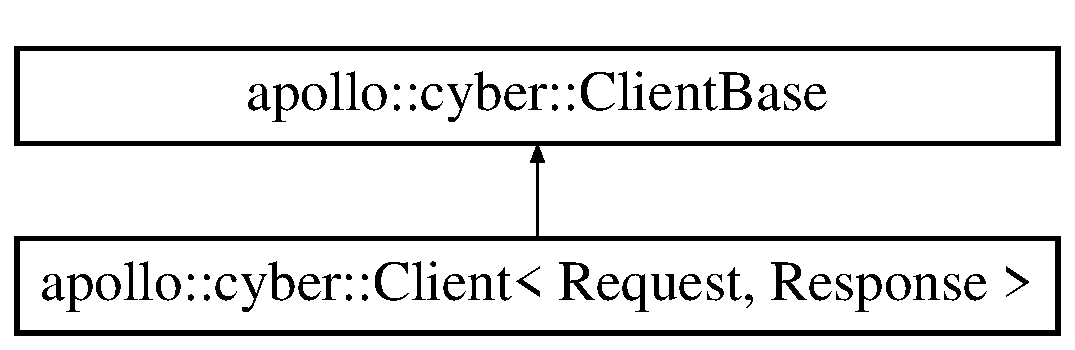
\includegraphics[height=2.000000cm]{classapollo_1_1cyber_1_1Client}
\end{center}
\end{figure}
\subsection*{Public Types}
\begin{DoxyCompactItemize}
\item 
using \hyperlink{classapollo_1_1cyber_1_1Client_ac30a67b1a2c1b6d37963968172c290a5}{Shared\-Request} = typename std\-::shared\-\_\-ptr$<$ Request $>$
\item 
using \hyperlink{classapollo_1_1cyber_1_1Client_af6198651a41ac3ed1b8c4c4bdb31bc71}{Shared\-Response} = typename std\-::shared\-\_\-ptr$<$ Response $>$
\item 
using \hyperlink{classapollo_1_1cyber_1_1Client_a0e85359f3942a4fe56bbecba331ed29e}{Promise} = std\-::promise$<$ \hyperlink{classapollo_1_1cyber_1_1Client_af6198651a41ac3ed1b8c4c4bdb31bc71}{Shared\-Response} $>$
\item 
using \hyperlink{classapollo_1_1cyber_1_1Client_aefa3f85f666c6495bdf92c1bacb36802}{Shared\-Promise} = std\-::shared\-\_\-ptr$<$ \hyperlink{classapollo_1_1cyber_1_1Client_a0e85359f3942a4fe56bbecba331ed29e}{Promise} $>$
\item 
using \hyperlink{classapollo_1_1cyber_1_1Client_ae8316f7e75af5319222df2dce376eebc}{Shared\-Future} = std\-::shared\-\_\-future$<$ \hyperlink{classapollo_1_1cyber_1_1Client_af6198651a41ac3ed1b8c4c4bdb31bc71}{Shared\-Response} $>$
\item 
using \hyperlink{classapollo_1_1cyber_1_1Client_a995b86997b158bccf18e65dd077cf406}{Callback\-Type} = std\-::function$<$ void(\hyperlink{classapollo_1_1cyber_1_1Client_ae8316f7e75af5319222df2dce376eebc}{Shared\-Future})$>$
\end{DoxyCompactItemize}
\subsection*{Public Member Functions}
\begin{DoxyCompactItemize}
\item 
\hyperlink{classapollo_1_1cyber_1_1Client_a1ca1a0a5afa944750dded3726623534e}{Client} (const std\-::string \&node\-\_\-name, const std\-::string \&service\-\_\-name)
\item 
\hyperlink{classapollo_1_1cyber_1_1Client_a729e32c0d4f2dc7643f9cc5903a3166a}{Client} ()=delete
\item 
virtual \hyperlink{classapollo_1_1cyber_1_1Client_a6b08fc310fcf911beb0910da47e740d0}{$\sim$\-Client} ()
\item 
bool \hyperlink{classapollo_1_1cyber_1_1Client_af20d217d504b1e20a0d01015b4c97d74}{Init} ()
\item 
\hyperlink{classapollo_1_1cyber_1_1Client_af6198651a41ac3ed1b8c4c4bdb31bc71}{Shared\-Response} \hyperlink{classapollo_1_1cyber_1_1Client_afa9ed1738bb63776acd9478d5e922afd}{Send\-Request} (\hyperlink{classapollo_1_1cyber_1_1Client_ac30a67b1a2c1b6d37963968172c290a5}{Shared\-Request} request, const std\-::chrono\-::seconds \&timeout\-\_\-s=std\-::chrono\-::seconds(5))
\item 
\hyperlink{classapollo_1_1cyber_1_1Client_af6198651a41ac3ed1b8c4c4bdb31bc71}{Shared\-Response} \hyperlink{classapollo_1_1cyber_1_1Client_aa6ac6d852d5e216f6d794aa61df4564c}{Send\-Request} (const Request \&request, const std\-::chrono\-::seconds \&timeout\-\_\-s=std\-::chrono\-::seconds(5))
\item 
\hyperlink{classapollo_1_1cyber_1_1Client_ae8316f7e75af5319222df2dce376eebc}{Shared\-Future} \hyperlink{classapollo_1_1cyber_1_1Client_ace5807ab43406cdbfdcab251c8b20457}{Async\-Send\-Request} (\hyperlink{classapollo_1_1cyber_1_1Client_ac30a67b1a2c1b6d37963968172c290a5}{Shared\-Request} request)
\item 
\hyperlink{classapollo_1_1cyber_1_1Client_ae8316f7e75af5319222df2dce376eebc}{Shared\-Future} \hyperlink{classapollo_1_1cyber_1_1Client_a346137af09141a3bd0010bcf37098912}{Async\-Send\-Request} (const Request \&request)
\item 
\hyperlink{classapollo_1_1cyber_1_1Client_ae8316f7e75af5319222df2dce376eebc}{Shared\-Future} \hyperlink{classapollo_1_1cyber_1_1Client_aea594efa1e32a529b9428bc06cc0d5d3}{Async\-Send\-Request} (\hyperlink{classapollo_1_1cyber_1_1Client_ac30a67b1a2c1b6d37963968172c290a5}{Shared\-Request} request, \hyperlink{classapollo_1_1cyber_1_1Client_a995b86997b158bccf18e65dd077cf406}{Callback\-Type} \&\&cb)
\item 
bool \hyperlink{classapollo_1_1cyber_1_1Client_a08a71d99f64374f6f06236848fbfe57c}{Service\-Is\-Ready} () const 
\item 
void \hyperlink{classapollo_1_1cyber_1_1Client_a7315a6cd9c733e844f0bd8e01006f491}{Destroy} ()
\item 
{\footnotesize template$<$typename Ratio\-T  = std\-::milli$>$ }\\bool \hyperlink{classapollo_1_1cyber_1_1Client_a374c271636f7f3a292f16845a37d825c}{Wait\-For\-Service} (std\-::chrono\-::duration$<$ int64\-\_\-t, Ratio\-T $>$ timeout=std\-::chrono\-::duration$<$ int64\-\_\-t, Ratio\-T $>$(-\/1))
\end{DoxyCompactItemize}
\subsection*{Private Member Functions}
\begin{DoxyCompactItemize}
\item 
void \hyperlink{classapollo_1_1cyber_1_1Client_a16d7df4f790876ca772e8c2d8b275ec3}{Handle\-Response} (const std\-::shared\-\_\-ptr$<$ Response $>$ \&response, const \hyperlink{classapollo_1_1cyber_1_1transport_1_1MessageInfo}{transport\-::\-Message\-Info} \&request\-\_\-info)
\item 
bool \hyperlink{classapollo_1_1cyber_1_1Client_aa7eccad0fe36e39ccefc3b74df4bed72}{Is\-Init} (void) const 
\end{DoxyCompactItemize}
\subsection*{Private Attributes}
\begin{DoxyCompactItemize}
\item 
std\-::string \hyperlink{classapollo_1_1cyber_1_1Client_a742636a4c7f051463094919eaa9e6165}{node\-\_\-name\-\_\-}
\item 
std\-::function$<$ void(const \\*
std\-::shared\-\_\-ptr$<$ Response $>$\\*
 \&, const \\*
\hyperlink{classapollo_1_1cyber_1_1transport_1_1MessageInfo}{transport\-::\-Message\-Info} \&)$>$ \hyperlink{classapollo_1_1cyber_1_1Client_a19e85f76c829899b989a7fcafe5aae97}{response\-\_\-callback\-\_\-}
\item 
std\-::unordered\-\_\-map$<$ uint64\-\_\-t, \\*
std\-::tuple$<$ \hyperlink{classapollo_1_1cyber_1_1Client_aefa3f85f666c6495bdf92c1bacb36802}{Shared\-Promise}, \\*
\hyperlink{classapollo_1_1cyber_1_1Client_a995b86997b158bccf18e65dd077cf406}{Callback\-Type}, \hyperlink{classapollo_1_1cyber_1_1Client_ae8316f7e75af5319222df2dce376eebc}{Shared\-Future} $>$ $>$ \hyperlink{classapollo_1_1cyber_1_1Client_acf3fd35613077fc52bf4706c5ee4b69f}{pending\-\_\-requests\-\_\-}
\item 
std\-::mutex \hyperlink{classapollo_1_1cyber_1_1Client_a63eaaeb862aaa0ad2d7b2314bfb4fd6e}{pending\-\_\-requests\-\_\-mutex\-\_\-}
\item 
std\-::shared\-\_\-ptr\\*
$<$ \hyperlink{classapollo_1_1cyber_1_1transport_1_1Transmitter}{transport\-::\-Transmitter}\\*
$<$ Request $>$ $>$ \hyperlink{classapollo_1_1cyber_1_1Client_a1586ab328b13d0f26190e13d78c5eb63}{request\-\_\-transmitter\-\_\-}
\item 
std\-::shared\-\_\-ptr\\*
$<$ \hyperlink{classapollo_1_1cyber_1_1transport_1_1Receiver}{transport\-::\-Receiver}\\*
$<$ Response $>$ $>$ \hyperlink{classapollo_1_1cyber_1_1Client_ad9afa7f2bd2f2fec4c3af05104b5d21a}{response\-\_\-receiver\-\_\-}
\item 
std\-::string \hyperlink{classapollo_1_1cyber_1_1Client_a164eeec085d6018b94887d920afc4d8d}{request\-\_\-channel\-\_\-}
\item 
std\-::string \hyperlink{classapollo_1_1cyber_1_1Client_a8c0017f09d7384b81c4c82a1707f6d2f}{response\-\_\-channel\-\_\-}
\item 
\hyperlink{classapollo_1_1cyber_1_1transport_1_1Identity}{transport\-::\-Identity} \hyperlink{classapollo_1_1cyber_1_1Client_a9b8f371424fa143d2dff7397fdfdc177}{writer\-\_\-id\-\_\-}
\item 
uint64\-\_\-t \hyperlink{classapollo_1_1cyber_1_1Client_a701360a2ff5dc2d4615f539e344c65f6}{sequence\-\_\-number\-\_\-}
\end{DoxyCompactItemize}
\subsection*{Additional Inherited Members}


\subsection{Member Typedef Documentation}
\hypertarget{classapollo_1_1cyber_1_1Client_a995b86997b158bccf18e65dd077cf406}{\index{apollo\-::cyber\-::\-Client@{apollo\-::cyber\-::\-Client}!Callback\-Type@{Callback\-Type}}
\index{Callback\-Type@{Callback\-Type}!apollo::cyber::Client@{apollo\-::cyber\-::\-Client}}
\subsubsection[{Callback\-Type}]{\setlength{\rightskip}{0pt plus 5cm}template$<$typename Request, typename Response$>$ using {\bf apollo\-::cyber\-::\-Client}$<$ Request, Response $>$\-::{\bf Callback\-Type} =  std\-::function$<$void({\bf Shared\-Future})$>$}}\label{classapollo_1_1cyber_1_1Client_a995b86997b158bccf18e65dd077cf406}
\hypertarget{classapollo_1_1cyber_1_1Client_a0e85359f3942a4fe56bbecba331ed29e}{\index{apollo\-::cyber\-::\-Client@{apollo\-::cyber\-::\-Client}!Promise@{Promise}}
\index{Promise@{Promise}!apollo::cyber::Client@{apollo\-::cyber\-::\-Client}}
\subsubsection[{Promise}]{\setlength{\rightskip}{0pt plus 5cm}template$<$typename Request, typename Response$>$ using {\bf apollo\-::cyber\-::\-Client}$<$ Request, Response $>$\-::{\bf Promise} =  std\-::promise$<${\bf Shared\-Response}$>$}}\label{classapollo_1_1cyber_1_1Client_a0e85359f3942a4fe56bbecba331ed29e}
\hypertarget{classapollo_1_1cyber_1_1Client_ae8316f7e75af5319222df2dce376eebc}{\index{apollo\-::cyber\-::\-Client@{apollo\-::cyber\-::\-Client}!Shared\-Future@{Shared\-Future}}
\index{Shared\-Future@{Shared\-Future}!apollo::cyber::Client@{apollo\-::cyber\-::\-Client}}
\subsubsection[{Shared\-Future}]{\setlength{\rightskip}{0pt plus 5cm}template$<$typename Request, typename Response$>$ using {\bf apollo\-::cyber\-::\-Client}$<$ Request, Response $>$\-::{\bf Shared\-Future} =  std\-::shared\-\_\-future$<${\bf Shared\-Response}$>$}}\label{classapollo_1_1cyber_1_1Client_ae8316f7e75af5319222df2dce376eebc}
\hypertarget{classapollo_1_1cyber_1_1Client_aefa3f85f666c6495bdf92c1bacb36802}{\index{apollo\-::cyber\-::\-Client@{apollo\-::cyber\-::\-Client}!Shared\-Promise@{Shared\-Promise}}
\index{Shared\-Promise@{Shared\-Promise}!apollo::cyber::Client@{apollo\-::cyber\-::\-Client}}
\subsubsection[{Shared\-Promise}]{\setlength{\rightskip}{0pt plus 5cm}template$<$typename Request, typename Response$>$ using {\bf apollo\-::cyber\-::\-Client}$<$ Request, Response $>$\-::{\bf Shared\-Promise} =  std\-::shared\-\_\-ptr$<${\bf Promise}$>$}}\label{classapollo_1_1cyber_1_1Client_aefa3f85f666c6495bdf92c1bacb36802}
\hypertarget{classapollo_1_1cyber_1_1Client_ac30a67b1a2c1b6d37963968172c290a5}{\index{apollo\-::cyber\-::\-Client@{apollo\-::cyber\-::\-Client}!Shared\-Request@{Shared\-Request}}
\index{Shared\-Request@{Shared\-Request}!apollo::cyber::Client@{apollo\-::cyber\-::\-Client}}
\subsubsection[{Shared\-Request}]{\setlength{\rightskip}{0pt plus 5cm}template$<$typename Request, typename Response$>$ using {\bf apollo\-::cyber\-::\-Client}$<$ Request, Response $>$\-::{\bf Shared\-Request} =  typename std\-::shared\-\_\-ptr$<$Request$>$}}\label{classapollo_1_1cyber_1_1Client_ac30a67b1a2c1b6d37963968172c290a5}
\hypertarget{classapollo_1_1cyber_1_1Client_af6198651a41ac3ed1b8c4c4bdb31bc71}{\index{apollo\-::cyber\-::\-Client@{apollo\-::cyber\-::\-Client}!Shared\-Response@{Shared\-Response}}
\index{Shared\-Response@{Shared\-Response}!apollo::cyber::Client@{apollo\-::cyber\-::\-Client}}
\subsubsection[{Shared\-Response}]{\setlength{\rightskip}{0pt plus 5cm}template$<$typename Request, typename Response$>$ using {\bf apollo\-::cyber\-::\-Client}$<$ Request, Response $>$\-::{\bf Shared\-Response} =  typename std\-::shared\-\_\-ptr$<$Response$>$}}\label{classapollo_1_1cyber_1_1Client_af6198651a41ac3ed1b8c4c4bdb31bc71}


\subsection{Constructor \& Destructor Documentation}
\hypertarget{classapollo_1_1cyber_1_1Client_a1ca1a0a5afa944750dded3726623534e}{\index{apollo\-::cyber\-::\-Client@{apollo\-::cyber\-::\-Client}!Client@{Client}}
\index{Client@{Client}!apollo::cyber::Client@{apollo\-::cyber\-::\-Client}}
\subsubsection[{Client}]{\setlength{\rightskip}{0pt plus 5cm}template$<$typename Request, typename Response$>$ {\bf apollo\-::cyber\-::\-Client}$<$ Request, Response $>$\-::{\bf Client} (
\begin{DoxyParamCaption}
\item[{const std\-::string \&}]{node\-\_\-name, }
\item[{const std\-::string \&}]{service\-\_\-name}
\end{DoxyParamCaption}
)\hspace{0.3cm}{\ttfamily [inline]}}}\label{classapollo_1_1cyber_1_1Client_a1ca1a0a5afa944750dded3726623534e}
\hypertarget{classapollo_1_1cyber_1_1Client_a729e32c0d4f2dc7643f9cc5903a3166a}{\index{apollo\-::cyber\-::\-Client@{apollo\-::cyber\-::\-Client}!Client@{Client}}
\index{Client@{Client}!apollo::cyber::Client@{apollo\-::cyber\-::\-Client}}
\subsubsection[{Client}]{\setlength{\rightskip}{0pt plus 5cm}template$<$typename Request, typename Response$>$ {\bf apollo\-::cyber\-::\-Client}$<$ Request, Response $>$\-::{\bf Client} (
\begin{DoxyParamCaption}
{}
\end{DoxyParamCaption}
)\hspace{0.3cm}{\ttfamily [delete]}}}\label{classapollo_1_1cyber_1_1Client_a729e32c0d4f2dc7643f9cc5903a3166a}
\hypertarget{classapollo_1_1cyber_1_1Client_a6b08fc310fcf911beb0910da47e740d0}{\index{apollo\-::cyber\-::\-Client@{apollo\-::cyber\-::\-Client}!$\sim$\-Client@{$\sim$\-Client}}
\index{$\sim$\-Client@{$\sim$\-Client}!apollo::cyber::Client@{apollo\-::cyber\-::\-Client}}
\subsubsection[{$\sim$\-Client}]{\setlength{\rightskip}{0pt plus 5cm}template$<$typename Request, typename Response$>$ virtual {\bf apollo\-::cyber\-::\-Client}$<$ Request, Response $>$\-::$\sim${\bf Client} (
\begin{DoxyParamCaption}
{}
\end{DoxyParamCaption}
)\hspace{0.3cm}{\ttfamily [inline]}, {\ttfamily [virtual]}}}\label{classapollo_1_1cyber_1_1Client_a6b08fc310fcf911beb0910da47e740d0}


\subsection{Member Function Documentation}
\hypertarget{classapollo_1_1cyber_1_1Client_ace5807ab43406cdbfdcab251c8b20457}{\index{apollo\-::cyber\-::\-Client@{apollo\-::cyber\-::\-Client}!Async\-Send\-Request@{Async\-Send\-Request}}
\index{Async\-Send\-Request@{Async\-Send\-Request}!apollo::cyber::Client@{apollo\-::cyber\-::\-Client}}
\subsubsection[{Async\-Send\-Request}]{\setlength{\rightskip}{0pt plus 5cm}template$<$typename Request , typename Response $>$ {\bf Client}$<$ Request, Response $>$\-::{\bf Shared\-Future} {\bf apollo\-::cyber\-::\-Client}$<$ Request, Response $>$\-::Async\-Send\-Request (
\begin{DoxyParamCaption}
\item[{{\bf Shared\-Request}}]{request}
\end{DoxyParamCaption}
)}}\label{classapollo_1_1cyber_1_1Client_ace5807ab43406cdbfdcab251c8b20457}
\hypertarget{classapollo_1_1cyber_1_1Client_a346137af09141a3bd0010bcf37098912}{\index{apollo\-::cyber\-::\-Client@{apollo\-::cyber\-::\-Client}!Async\-Send\-Request@{Async\-Send\-Request}}
\index{Async\-Send\-Request@{Async\-Send\-Request}!apollo::cyber::Client@{apollo\-::cyber\-::\-Client}}
\subsubsection[{Async\-Send\-Request}]{\setlength{\rightskip}{0pt plus 5cm}template$<$typename Request , typename Response $>$ {\bf Client}$<$ Request, Response $>$\-::{\bf Shared\-Future} {\bf apollo\-::cyber\-::\-Client}$<$ Request, Response $>$\-::Async\-Send\-Request (
\begin{DoxyParamCaption}
\item[{const Request \&}]{request}
\end{DoxyParamCaption}
)}}\label{classapollo_1_1cyber_1_1Client_a346137af09141a3bd0010bcf37098912}
\hypertarget{classapollo_1_1cyber_1_1Client_aea594efa1e32a529b9428bc06cc0d5d3}{\index{apollo\-::cyber\-::\-Client@{apollo\-::cyber\-::\-Client}!Async\-Send\-Request@{Async\-Send\-Request}}
\index{Async\-Send\-Request@{Async\-Send\-Request}!apollo::cyber::Client@{apollo\-::cyber\-::\-Client}}
\subsubsection[{Async\-Send\-Request}]{\setlength{\rightskip}{0pt plus 5cm}template$<$typename Request , typename Response $>$ {\bf Client}$<$ Request, Response $>$\-::{\bf Shared\-Future} {\bf apollo\-::cyber\-::\-Client}$<$ Request, Response $>$\-::Async\-Send\-Request (
\begin{DoxyParamCaption}
\item[{{\bf Shared\-Request}}]{request, }
\item[{{\bf Callback\-Type} \&\&}]{cb}
\end{DoxyParamCaption}
)}}\label{classapollo_1_1cyber_1_1Client_aea594efa1e32a529b9428bc06cc0d5d3}
\hypertarget{classapollo_1_1cyber_1_1Client_a7315a6cd9c733e844f0bd8e01006f491}{\index{apollo\-::cyber\-::\-Client@{apollo\-::cyber\-::\-Client}!Destroy@{Destroy}}
\index{Destroy@{Destroy}!apollo::cyber::Client@{apollo\-::cyber\-::\-Client}}
\subsubsection[{Destroy}]{\setlength{\rightskip}{0pt plus 5cm}template$<$typename Request , typename Response $>$ void {\bf apollo\-::cyber\-::\-Client}$<$ Request, Response $>$\-::Destroy (
\begin{DoxyParamCaption}
{}
\end{DoxyParamCaption}
)\hspace{0.3cm}{\ttfamily [virtual]}}}\label{classapollo_1_1cyber_1_1Client_a7315a6cd9c733e844f0bd8e01006f491}


Implements \hyperlink{classapollo_1_1cyber_1_1ClientBase_a144df36f1d8e9ec5923e3ad77a4ee634}{apollo\-::cyber\-::\-Client\-Base}.

\hypertarget{classapollo_1_1cyber_1_1Client_a16d7df4f790876ca772e8c2d8b275ec3}{\index{apollo\-::cyber\-::\-Client@{apollo\-::cyber\-::\-Client}!Handle\-Response@{Handle\-Response}}
\index{Handle\-Response@{Handle\-Response}!apollo::cyber::Client@{apollo\-::cyber\-::\-Client}}
\subsubsection[{Handle\-Response}]{\setlength{\rightskip}{0pt plus 5cm}template$<$typename Request , typename Response $>$ void {\bf apollo\-::cyber\-::\-Client}$<$ Request, Response $>$\-::Handle\-Response (
\begin{DoxyParamCaption}
\item[{const std\-::shared\-\_\-ptr$<$ Response $>$ \&}]{response, }
\item[{const {\bf transport\-::\-Message\-Info} \&}]{request\-\_\-info}
\end{DoxyParamCaption}
)\hspace{0.3cm}{\ttfamily [private]}}}\label{classapollo_1_1cyber_1_1Client_a16d7df4f790876ca772e8c2d8b275ec3}
\hypertarget{classapollo_1_1cyber_1_1Client_af20d217d504b1e20a0d01015b4c97d74}{\index{apollo\-::cyber\-::\-Client@{apollo\-::cyber\-::\-Client}!Init@{Init}}
\index{Init@{Init}!apollo::cyber::Client@{apollo\-::cyber\-::\-Client}}
\subsubsection[{Init}]{\setlength{\rightskip}{0pt plus 5cm}template$<$typename Request , typename Response $>$ bool {\bf apollo\-::cyber\-::\-Client}$<$ Request, Response $>$\-::Init (
\begin{DoxyParamCaption}
{}
\end{DoxyParamCaption}
)}}\label{classapollo_1_1cyber_1_1Client_af20d217d504b1e20a0d01015b4c97d74}
\hypertarget{classapollo_1_1cyber_1_1Client_aa7eccad0fe36e39ccefc3b74df4bed72}{\index{apollo\-::cyber\-::\-Client@{apollo\-::cyber\-::\-Client}!Is\-Init@{Is\-Init}}
\index{Is\-Init@{Is\-Init}!apollo::cyber::Client@{apollo\-::cyber\-::\-Client}}
\subsubsection[{Is\-Init}]{\setlength{\rightskip}{0pt plus 5cm}template$<$typename Request, typename Response$>$ bool {\bf apollo\-::cyber\-::\-Client}$<$ Request, Response $>$\-::Is\-Init (
\begin{DoxyParamCaption}
\item[{void}]{}
\end{DoxyParamCaption}
) const\hspace{0.3cm}{\ttfamily [inline]}, {\ttfamily [private]}}}\label{classapollo_1_1cyber_1_1Client_aa7eccad0fe36e39ccefc3b74df4bed72}
\hypertarget{classapollo_1_1cyber_1_1Client_afa9ed1738bb63776acd9478d5e922afd}{\index{apollo\-::cyber\-::\-Client@{apollo\-::cyber\-::\-Client}!Send\-Request@{Send\-Request}}
\index{Send\-Request@{Send\-Request}!apollo::cyber::Client@{apollo\-::cyber\-::\-Client}}
\subsubsection[{Send\-Request}]{\setlength{\rightskip}{0pt plus 5cm}template$<$typename Request , typename Response $>$ {\bf Client}$<$ Request, Response $>$\-::{\bf Shared\-Response} {\bf apollo\-::cyber\-::\-Client}$<$ Request, Response $>$\-::Send\-Request (
\begin{DoxyParamCaption}
\item[{{\bf Shared\-Request}}]{request, }
\item[{const std\-::chrono\-::seconds \&}]{timeout\-\_\-s = {\ttfamily std\-:\-:chrono\-:\-:seconds(5)}}
\end{DoxyParamCaption}
)}}\label{classapollo_1_1cyber_1_1Client_afa9ed1738bb63776acd9478d5e922afd}
\hypertarget{classapollo_1_1cyber_1_1Client_aa6ac6d852d5e216f6d794aa61df4564c}{\index{apollo\-::cyber\-::\-Client@{apollo\-::cyber\-::\-Client}!Send\-Request@{Send\-Request}}
\index{Send\-Request@{Send\-Request}!apollo::cyber::Client@{apollo\-::cyber\-::\-Client}}
\subsubsection[{Send\-Request}]{\setlength{\rightskip}{0pt plus 5cm}template$<$typename Request , typename Response $>$ {\bf Client}$<$ Request, Response $>$\-::{\bf Shared\-Response} {\bf apollo\-::cyber\-::\-Client}$<$ Request, Response $>$\-::Send\-Request (
\begin{DoxyParamCaption}
\item[{const Request \&}]{request, }
\item[{const std\-::chrono\-::seconds \&}]{timeout\-\_\-s = {\ttfamily std\-:\-:chrono\-:\-:seconds(5)}}
\end{DoxyParamCaption}
)}}\label{classapollo_1_1cyber_1_1Client_aa6ac6d852d5e216f6d794aa61df4564c}
\hypertarget{classapollo_1_1cyber_1_1Client_a08a71d99f64374f6f06236848fbfe57c}{\index{apollo\-::cyber\-::\-Client@{apollo\-::cyber\-::\-Client}!Service\-Is\-Ready@{Service\-Is\-Ready}}
\index{Service\-Is\-Ready@{Service\-Is\-Ready}!apollo::cyber::Client@{apollo\-::cyber\-::\-Client}}
\subsubsection[{Service\-Is\-Ready}]{\setlength{\rightskip}{0pt plus 5cm}template$<$typename Request , typename Response $>$ bool {\bf apollo\-::cyber\-::\-Client}$<$ Request, Response $>$\-::Service\-Is\-Ready (
\begin{DoxyParamCaption}
{}
\end{DoxyParamCaption}
) const\hspace{0.3cm}{\ttfamily [virtual]}}}\label{classapollo_1_1cyber_1_1Client_a08a71d99f64374f6f06236848fbfe57c}


Implements \hyperlink{classapollo_1_1cyber_1_1ClientBase_af21c54a3f02783626ce5ae5eea621bda}{apollo\-::cyber\-::\-Client\-Base}.

\hypertarget{classapollo_1_1cyber_1_1Client_a374c271636f7f3a292f16845a37d825c}{\index{apollo\-::cyber\-::\-Client@{apollo\-::cyber\-::\-Client}!Wait\-For\-Service@{Wait\-For\-Service}}
\index{Wait\-For\-Service@{Wait\-For\-Service}!apollo::cyber::Client@{apollo\-::cyber\-::\-Client}}
\subsubsection[{Wait\-For\-Service}]{\setlength{\rightskip}{0pt plus 5cm}template$<$typename Request, typename Response$>$ template$<$typename Ratio\-T  = std\-::milli$>$ bool {\bf apollo\-::cyber\-::\-Client}$<$ Request, Response $>$\-::Wait\-For\-Service (
\begin{DoxyParamCaption}
\item[{std\-::chrono\-::duration$<$ int64\-\_\-t, Ratio\-T $>$}]{timeout = {\ttfamily std\-:\-:chrono\-:\-:duration$<$int64\-\_\-t,~RatioT$>$(-\/1)}}
\end{DoxyParamCaption}
)\hspace{0.3cm}{\ttfamily [inline]}}}\label{classapollo_1_1cyber_1_1Client_a374c271636f7f3a292f16845a37d825c}


\subsection{Member Data Documentation}
\hypertarget{classapollo_1_1cyber_1_1Client_a742636a4c7f051463094919eaa9e6165}{\index{apollo\-::cyber\-::\-Client@{apollo\-::cyber\-::\-Client}!node\-\_\-name\-\_\-@{node\-\_\-name\-\_\-}}
\index{node\-\_\-name\-\_\-@{node\-\_\-name\-\_\-}!apollo::cyber::Client@{apollo\-::cyber\-::\-Client}}
\subsubsection[{node\-\_\-name\-\_\-}]{\setlength{\rightskip}{0pt plus 5cm}template$<$typename Request, typename Response$>$ std\-::string {\bf apollo\-::cyber\-::\-Client}$<$ Request, Response $>$\-::node\-\_\-name\-\_\-\hspace{0.3cm}{\ttfamily [private]}}}\label{classapollo_1_1cyber_1_1Client_a742636a4c7f051463094919eaa9e6165}
\hypertarget{classapollo_1_1cyber_1_1Client_acf3fd35613077fc52bf4706c5ee4b69f}{\index{apollo\-::cyber\-::\-Client@{apollo\-::cyber\-::\-Client}!pending\-\_\-requests\-\_\-@{pending\-\_\-requests\-\_\-}}
\index{pending\-\_\-requests\-\_\-@{pending\-\_\-requests\-\_\-}!apollo::cyber::Client@{apollo\-::cyber\-::\-Client}}
\subsubsection[{pending\-\_\-requests\-\_\-}]{\setlength{\rightskip}{0pt plus 5cm}template$<$typename Request, typename Response$>$ std\-::unordered\-\_\-map$<$uint64\-\_\-t, std\-::tuple$<${\bf Shared\-Promise}, {\bf Callback\-Type}, {\bf Shared\-Future}$>$ $>$ {\bf apollo\-::cyber\-::\-Client}$<$ Request, Response $>$\-::pending\-\_\-requests\-\_\-\hspace{0.3cm}{\ttfamily [private]}}}\label{classapollo_1_1cyber_1_1Client_acf3fd35613077fc52bf4706c5ee4b69f}
\hypertarget{classapollo_1_1cyber_1_1Client_a63eaaeb862aaa0ad2d7b2314bfb4fd6e}{\index{apollo\-::cyber\-::\-Client@{apollo\-::cyber\-::\-Client}!pending\-\_\-requests\-\_\-mutex\-\_\-@{pending\-\_\-requests\-\_\-mutex\-\_\-}}
\index{pending\-\_\-requests\-\_\-mutex\-\_\-@{pending\-\_\-requests\-\_\-mutex\-\_\-}!apollo::cyber::Client@{apollo\-::cyber\-::\-Client}}
\subsubsection[{pending\-\_\-requests\-\_\-mutex\-\_\-}]{\setlength{\rightskip}{0pt plus 5cm}template$<$typename Request, typename Response$>$ std\-::mutex {\bf apollo\-::cyber\-::\-Client}$<$ Request, Response $>$\-::pending\-\_\-requests\-\_\-mutex\-\_\-\hspace{0.3cm}{\ttfamily [private]}}}\label{classapollo_1_1cyber_1_1Client_a63eaaeb862aaa0ad2d7b2314bfb4fd6e}
\hypertarget{classapollo_1_1cyber_1_1Client_a164eeec085d6018b94887d920afc4d8d}{\index{apollo\-::cyber\-::\-Client@{apollo\-::cyber\-::\-Client}!request\-\_\-channel\-\_\-@{request\-\_\-channel\-\_\-}}
\index{request\-\_\-channel\-\_\-@{request\-\_\-channel\-\_\-}!apollo::cyber::Client@{apollo\-::cyber\-::\-Client}}
\subsubsection[{request\-\_\-channel\-\_\-}]{\setlength{\rightskip}{0pt plus 5cm}template$<$typename Request, typename Response$>$ std\-::string {\bf apollo\-::cyber\-::\-Client}$<$ Request, Response $>$\-::request\-\_\-channel\-\_\-\hspace{0.3cm}{\ttfamily [private]}}}\label{classapollo_1_1cyber_1_1Client_a164eeec085d6018b94887d920afc4d8d}
\hypertarget{classapollo_1_1cyber_1_1Client_a1586ab328b13d0f26190e13d78c5eb63}{\index{apollo\-::cyber\-::\-Client@{apollo\-::cyber\-::\-Client}!request\-\_\-transmitter\-\_\-@{request\-\_\-transmitter\-\_\-}}
\index{request\-\_\-transmitter\-\_\-@{request\-\_\-transmitter\-\_\-}!apollo::cyber::Client@{apollo\-::cyber\-::\-Client}}
\subsubsection[{request\-\_\-transmitter\-\_\-}]{\setlength{\rightskip}{0pt plus 5cm}template$<$typename Request, typename Response$>$ std\-::shared\-\_\-ptr$<${\bf transport\-::\-Transmitter}$<$Request$>$ $>$ {\bf apollo\-::cyber\-::\-Client}$<$ Request, Response $>$\-::request\-\_\-transmitter\-\_\-\hspace{0.3cm}{\ttfamily [private]}}}\label{classapollo_1_1cyber_1_1Client_a1586ab328b13d0f26190e13d78c5eb63}
\hypertarget{classapollo_1_1cyber_1_1Client_a19e85f76c829899b989a7fcafe5aae97}{\index{apollo\-::cyber\-::\-Client@{apollo\-::cyber\-::\-Client}!response\-\_\-callback\-\_\-@{response\-\_\-callback\-\_\-}}
\index{response\-\_\-callback\-\_\-@{response\-\_\-callback\-\_\-}!apollo::cyber::Client@{apollo\-::cyber\-::\-Client}}
\subsubsection[{response\-\_\-callback\-\_\-}]{\setlength{\rightskip}{0pt plus 5cm}template$<$typename Request, typename Response$>$ std\-::function$<$void(const std\-::shared\-\_\-ptr$<$Response$>$\&, const {\bf transport\-::\-Message\-Info}\&)$>$ {\bf apollo\-::cyber\-::\-Client}$<$ Request, Response $>$\-::response\-\_\-callback\-\_\-\hspace{0.3cm}{\ttfamily [private]}}}\label{classapollo_1_1cyber_1_1Client_a19e85f76c829899b989a7fcafe5aae97}
\hypertarget{classapollo_1_1cyber_1_1Client_a8c0017f09d7384b81c4c82a1707f6d2f}{\index{apollo\-::cyber\-::\-Client@{apollo\-::cyber\-::\-Client}!response\-\_\-channel\-\_\-@{response\-\_\-channel\-\_\-}}
\index{response\-\_\-channel\-\_\-@{response\-\_\-channel\-\_\-}!apollo::cyber::Client@{apollo\-::cyber\-::\-Client}}
\subsubsection[{response\-\_\-channel\-\_\-}]{\setlength{\rightskip}{0pt plus 5cm}template$<$typename Request, typename Response$>$ std\-::string {\bf apollo\-::cyber\-::\-Client}$<$ Request, Response $>$\-::response\-\_\-channel\-\_\-\hspace{0.3cm}{\ttfamily [private]}}}\label{classapollo_1_1cyber_1_1Client_a8c0017f09d7384b81c4c82a1707f6d2f}
\hypertarget{classapollo_1_1cyber_1_1Client_ad9afa7f2bd2f2fec4c3af05104b5d21a}{\index{apollo\-::cyber\-::\-Client@{apollo\-::cyber\-::\-Client}!response\-\_\-receiver\-\_\-@{response\-\_\-receiver\-\_\-}}
\index{response\-\_\-receiver\-\_\-@{response\-\_\-receiver\-\_\-}!apollo::cyber::Client@{apollo\-::cyber\-::\-Client}}
\subsubsection[{response\-\_\-receiver\-\_\-}]{\setlength{\rightskip}{0pt plus 5cm}template$<$typename Request, typename Response$>$ std\-::shared\-\_\-ptr$<${\bf transport\-::\-Receiver}$<$Response$>$ $>$ {\bf apollo\-::cyber\-::\-Client}$<$ Request, Response $>$\-::response\-\_\-receiver\-\_\-\hspace{0.3cm}{\ttfamily [private]}}}\label{classapollo_1_1cyber_1_1Client_ad9afa7f2bd2f2fec4c3af05104b5d21a}
\hypertarget{classapollo_1_1cyber_1_1Client_a701360a2ff5dc2d4615f539e344c65f6}{\index{apollo\-::cyber\-::\-Client@{apollo\-::cyber\-::\-Client}!sequence\-\_\-number\-\_\-@{sequence\-\_\-number\-\_\-}}
\index{sequence\-\_\-number\-\_\-@{sequence\-\_\-number\-\_\-}!apollo::cyber::Client@{apollo\-::cyber\-::\-Client}}
\subsubsection[{sequence\-\_\-number\-\_\-}]{\setlength{\rightskip}{0pt plus 5cm}template$<$typename Request, typename Response$>$ uint64\-\_\-t {\bf apollo\-::cyber\-::\-Client}$<$ Request, Response $>$\-::sequence\-\_\-number\-\_\-\hspace{0.3cm}{\ttfamily [private]}}}\label{classapollo_1_1cyber_1_1Client_a701360a2ff5dc2d4615f539e344c65f6}
\hypertarget{classapollo_1_1cyber_1_1Client_a9b8f371424fa143d2dff7397fdfdc177}{\index{apollo\-::cyber\-::\-Client@{apollo\-::cyber\-::\-Client}!writer\-\_\-id\-\_\-@{writer\-\_\-id\-\_\-}}
\index{writer\-\_\-id\-\_\-@{writer\-\_\-id\-\_\-}!apollo::cyber::Client@{apollo\-::cyber\-::\-Client}}
\subsubsection[{writer\-\_\-id\-\_\-}]{\setlength{\rightskip}{0pt plus 5cm}template$<$typename Request, typename Response$>$ {\bf transport\-::\-Identity} {\bf apollo\-::cyber\-::\-Client}$<$ Request, Response $>$\-::writer\-\_\-id\-\_\-\hspace{0.3cm}{\ttfamily [private]}}}\label{classapollo_1_1cyber_1_1Client_a9b8f371424fa143d2dff7397fdfdc177}


The documentation for this class was generated from the following file\-:\begin{DoxyCompactItemize}
\item 
service/\hyperlink{client_8h}{client.\-h}\end{DoxyCompactItemize}

\hypertarget{classapollo_1_1cyber_1_1ClientBase}{\section{apollo\-:\-:cyber\-:\-:Client\-Base Class Reference}
\label{classapollo_1_1cyber_1_1ClientBase}\index{apollo\-::cyber\-::\-Client\-Base@{apollo\-::cyber\-::\-Client\-Base}}
}


{\ttfamily \#include $<$client\-\_\-base.\-h$>$}

Inheritance diagram for apollo\-:\-:cyber\-:\-:Client\-Base\-:\begin{figure}[H]
\begin{center}
\leavevmode
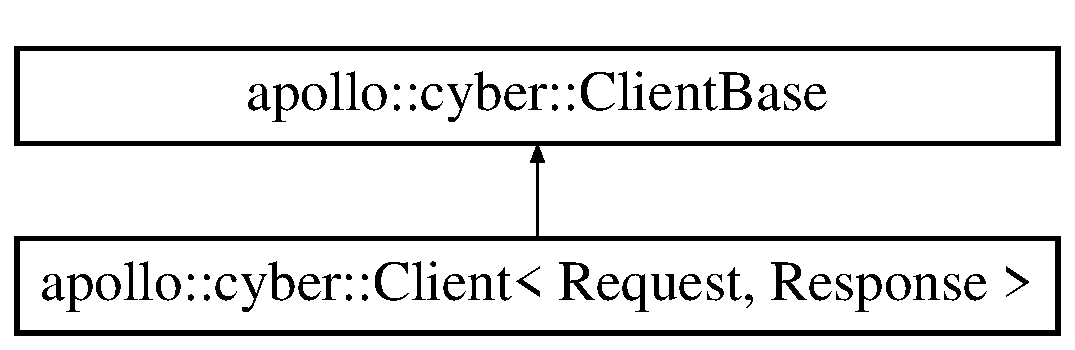
\includegraphics[height=2.000000cm]{classapollo_1_1cyber_1_1ClientBase}
\end{center}
\end{figure}
\subsection*{Public Member Functions}
\begin{DoxyCompactItemize}
\item 
\hyperlink{classapollo_1_1cyber_1_1ClientBase_a11ae882f14c81d424e6065e84e274032}{Client\-Base} (const std\-::string \&service\-\_\-name)
\item 
virtual \hyperlink{classapollo_1_1cyber_1_1ClientBase_a415c5d2ee0ef5bf9fd55c9536417c718}{$\sim$\-Client\-Base} ()
\item 
virtual void \hyperlink{classapollo_1_1cyber_1_1ClientBase_a144df36f1d8e9ec5923e3ad77a4ee634}{Destroy} ()=0
\item 
const std\-::string \& \hyperlink{classapollo_1_1cyber_1_1ClientBase_a9d29607d93d7d68ccc3b248ef6f9cf47}{Service\-Name} () const 
\item 
virtual bool \hyperlink{classapollo_1_1cyber_1_1ClientBase_af21c54a3f02783626ce5ae5eea621bda}{Service\-Is\-Ready} () const =0
\end{DoxyCompactItemize}
\subsection*{Protected Member Functions}
\begin{DoxyCompactItemize}
\item 
bool \hyperlink{classapollo_1_1cyber_1_1ClientBase_ad6c2d2b853720a17de21f3bc25b6aae9}{Wait\-For\-Service\-Nanoseconds} (std\-::chrono\-::nanoseconds time\-\_\-out)
\end{DoxyCompactItemize}
\subsection*{Protected Attributes}
\begin{DoxyCompactItemize}
\item 
std\-::string \hyperlink{classapollo_1_1cyber_1_1ClientBase_a91831fd30272eb760345dbfe6db86b44}{service\-\_\-name\-\_\-}
\end{DoxyCompactItemize}


\subsection{Constructor \& Destructor Documentation}
\hypertarget{classapollo_1_1cyber_1_1ClientBase_a11ae882f14c81d424e6065e84e274032}{\index{apollo\-::cyber\-::\-Client\-Base@{apollo\-::cyber\-::\-Client\-Base}!Client\-Base@{Client\-Base}}
\index{Client\-Base@{Client\-Base}!apollo::cyber::ClientBase@{apollo\-::cyber\-::\-Client\-Base}}
\subsubsection[{Client\-Base}]{\setlength{\rightskip}{0pt plus 5cm}apollo\-::cyber\-::\-Client\-Base\-::\-Client\-Base (
\begin{DoxyParamCaption}
\item[{const std\-::string \&}]{service\-\_\-name}
\end{DoxyParamCaption}
)\hspace{0.3cm}{\ttfamily [inline]}, {\ttfamily [explicit]}}}\label{classapollo_1_1cyber_1_1ClientBase_a11ae882f14c81d424e6065e84e274032}
\hypertarget{classapollo_1_1cyber_1_1ClientBase_a415c5d2ee0ef5bf9fd55c9536417c718}{\index{apollo\-::cyber\-::\-Client\-Base@{apollo\-::cyber\-::\-Client\-Base}!$\sim$\-Client\-Base@{$\sim$\-Client\-Base}}
\index{$\sim$\-Client\-Base@{$\sim$\-Client\-Base}!apollo::cyber::ClientBase@{apollo\-::cyber\-::\-Client\-Base}}
\subsubsection[{$\sim$\-Client\-Base}]{\setlength{\rightskip}{0pt plus 5cm}virtual apollo\-::cyber\-::\-Client\-Base\-::$\sim$\-Client\-Base (
\begin{DoxyParamCaption}
{}
\end{DoxyParamCaption}
)\hspace{0.3cm}{\ttfamily [inline]}, {\ttfamily [virtual]}}}\label{classapollo_1_1cyber_1_1ClientBase_a415c5d2ee0ef5bf9fd55c9536417c718}


\subsection{Member Function Documentation}
\hypertarget{classapollo_1_1cyber_1_1ClientBase_a144df36f1d8e9ec5923e3ad77a4ee634}{\index{apollo\-::cyber\-::\-Client\-Base@{apollo\-::cyber\-::\-Client\-Base}!Destroy@{Destroy}}
\index{Destroy@{Destroy}!apollo::cyber::ClientBase@{apollo\-::cyber\-::\-Client\-Base}}
\subsubsection[{Destroy}]{\setlength{\rightskip}{0pt plus 5cm}virtual void apollo\-::cyber\-::\-Client\-Base\-::\-Destroy (
\begin{DoxyParamCaption}
{}
\end{DoxyParamCaption}
)\hspace{0.3cm}{\ttfamily [pure virtual]}}}\label{classapollo_1_1cyber_1_1ClientBase_a144df36f1d8e9ec5923e3ad77a4ee634}


Implemented in \hyperlink{classapollo_1_1cyber_1_1Client_a7315a6cd9c733e844f0bd8e01006f491}{apollo\-::cyber\-::\-Client$<$ Request, Response $>$}.

\hypertarget{classapollo_1_1cyber_1_1ClientBase_af21c54a3f02783626ce5ae5eea621bda}{\index{apollo\-::cyber\-::\-Client\-Base@{apollo\-::cyber\-::\-Client\-Base}!Service\-Is\-Ready@{Service\-Is\-Ready}}
\index{Service\-Is\-Ready@{Service\-Is\-Ready}!apollo::cyber::ClientBase@{apollo\-::cyber\-::\-Client\-Base}}
\subsubsection[{Service\-Is\-Ready}]{\setlength{\rightskip}{0pt plus 5cm}virtual bool apollo\-::cyber\-::\-Client\-Base\-::\-Service\-Is\-Ready (
\begin{DoxyParamCaption}
{}
\end{DoxyParamCaption}
) const\hspace{0.3cm}{\ttfamily [pure virtual]}}}\label{classapollo_1_1cyber_1_1ClientBase_af21c54a3f02783626ce5ae5eea621bda}


Implemented in \hyperlink{classapollo_1_1cyber_1_1Client_a08a71d99f64374f6f06236848fbfe57c}{apollo\-::cyber\-::\-Client$<$ Request, Response $>$}.

\hypertarget{classapollo_1_1cyber_1_1ClientBase_a9d29607d93d7d68ccc3b248ef6f9cf47}{\index{apollo\-::cyber\-::\-Client\-Base@{apollo\-::cyber\-::\-Client\-Base}!Service\-Name@{Service\-Name}}
\index{Service\-Name@{Service\-Name}!apollo::cyber::ClientBase@{apollo\-::cyber\-::\-Client\-Base}}
\subsubsection[{Service\-Name}]{\setlength{\rightskip}{0pt plus 5cm}const std\-::string\& apollo\-::cyber\-::\-Client\-Base\-::\-Service\-Name (
\begin{DoxyParamCaption}
{}
\end{DoxyParamCaption}
) const\hspace{0.3cm}{\ttfamily [inline]}}}\label{classapollo_1_1cyber_1_1ClientBase_a9d29607d93d7d68ccc3b248ef6f9cf47}
\hypertarget{classapollo_1_1cyber_1_1ClientBase_ad6c2d2b853720a17de21f3bc25b6aae9}{\index{apollo\-::cyber\-::\-Client\-Base@{apollo\-::cyber\-::\-Client\-Base}!Wait\-For\-Service\-Nanoseconds@{Wait\-For\-Service\-Nanoseconds}}
\index{Wait\-For\-Service\-Nanoseconds@{Wait\-For\-Service\-Nanoseconds}!apollo::cyber::ClientBase@{apollo\-::cyber\-::\-Client\-Base}}
\subsubsection[{Wait\-For\-Service\-Nanoseconds}]{\setlength{\rightskip}{0pt plus 5cm}bool apollo\-::cyber\-::\-Client\-Base\-::\-Wait\-For\-Service\-Nanoseconds (
\begin{DoxyParamCaption}
\item[{std\-::chrono\-::nanoseconds}]{time\-\_\-out}
\end{DoxyParamCaption}
)\hspace{0.3cm}{\ttfamily [inline]}, {\ttfamily [protected]}}}\label{classapollo_1_1cyber_1_1ClientBase_ad6c2d2b853720a17de21f3bc25b6aae9}


\subsection{Member Data Documentation}
\hypertarget{classapollo_1_1cyber_1_1ClientBase_a91831fd30272eb760345dbfe6db86b44}{\index{apollo\-::cyber\-::\-Client\-Base@{apollo\-::cyber\-::\-Client\-Base}!service\-\_\-name\-\_\-@{service\-\_\-name\-\_\-}}
\index{service\-\_\-name\-\_\-@{service\-\_\-name\-\_\-}!apollo::cyber::ClientBase@{apollo\-::cyber\-::\-Client\-Base}}
\subsubsection[{service\-\_\-name\-\_\-}]{\setlength{\rightskip}{0pt plus 5cm}std\-::string apollo\-::cyber\-::\-Client\-Base\-::service\-\_\-name\-\_\-\hspace{0.3cm}{\ttfamily [protected]}}}\label{classapollo_1_1cyber_1_1ClientBase_a91831fd30272eb760345dbfe6db86b44}


The documentation for this class was generated from the following file\-:\begin{DoxyCompactItemize}
\item 
service/\hyperlink{client__base_8h}{client\-\_\-base.\-h}\end{DoxyCompactItemize}

\hypertarget{classCommonComponentSample}{\section{Common\-Component\-Sample Class Reference}
\label{classCommonComponentSample}\index{Common\-Component\-Sample@{Common\-Component\-Sample}}
}


{\ttfamily \#include $<$common\-\_\-component\-\_\-example.\-h$>$}

Inheritance diagram for Common\-Component\-Sample\-:\begin{figure}[H]
\begin{center}
\leavevmode
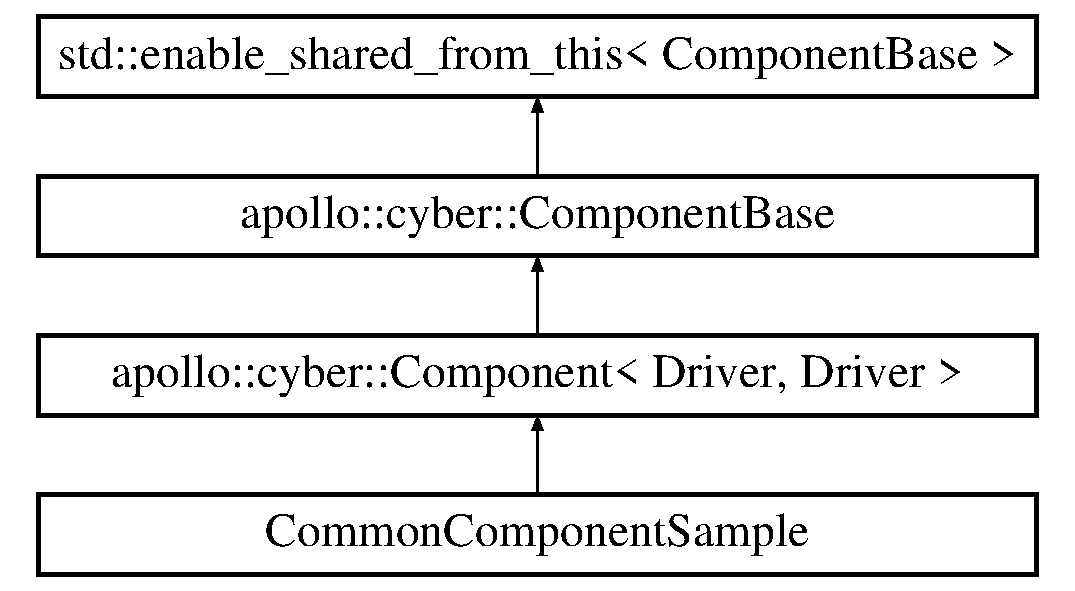
\includegraphics[height=4.000000cm]{classCommonComponentSample}
\end{center}
\end{figure}
\subsection*{Public Member Functions}
\begin{DoxyCompactItemize}
\item 
bool \hyperlink{classCommonComponentSample_ae2a3f8c8ce4b9cfd9c6b357628bc84ee}{Init} () override
\item 
bool \hyperlink{classCommonComponentSample_ab84ea2f74b8ab92a74733b392319ea5e}{Proc} (const std\-::shared\-\_\-ptr$<$ Driver $>$ \&msg0, const std\-::shared\-\_\-ptr$<$ Driver $>$ \&msg1) override
\end{DoxyCompactItemize}
\subsection*{Additional Inherited Members}


\subsection{Member Function Documentation}
\hypertarget{classCommonComponentSample_ae2a3f8c8ce4b9cfd9c6b357628bc84ee}{\index{Common\-Component\-Sample@{Common\-Component\-Sample}!Init@{Init}}
\index{Init@{Init}!CommonComponentSample@{Common\-Component\-Sample}}
\subsubsection[{Init}]{\setlength{\rightskip}{0pt plus 5cm}bool Common\-Component\-Sample\-::\-Init (
\begin{DoxyParamCaption}
{}
\end{DoxyParamCaption}
)\hspace{0.3cm}{\ttfamily [override]}, {\ttfamily [virtual]}}}\label{classCommonComponentSample_ae2a3f8c8ce4b9cfd9c6b357628bc84ee}


Implements \hyperlink{classapollo_1_1cyber_1_1ComponentBase_ae9901cb3bfa8ef33c42b465606dbe0e5}{apollo\-::cyber\-::\-Component\-Base}.

\hypertarget{classCommonComponentSample_ab84ea2f74b8ab92a74733b392319ea5e}{\index{Common\-Component\-Sample@{Common\-Component\-Sample}!Proc@{Proc}}
\index{Proc@{Proc}!CommonComponentSample@{Common\-Component\-Sample}}
\subsubsection[{Proc}]{\setlength{\rightskip}{0pt plus 5cm}bool Common\-Component\-Sample\-::\-Proc (
\begin{DoxyParamCaption}
\item[{const std\-::shared\-\_\-ptr$<$ Driver $>$ \&}]{msg0, }
\item[{const std\-::shared\-\_\-ptr$<$ Driver $>$ \&}]{msg1}
\end{DoxyParamCaption}
)\hspace{0.3cm}{\ttfamily [override]}}}\label{classCommonComponentSample_ab84ea2f74b8ab92a74733b392319ea5e}


The documentation for this class was generated from the following file\-:\begin{DoxyCompactItemize}
\item 
examples/common\-\_\-component\-\_\-example/\hyperlink{common__component__example_8h}{common\-\_\-component\-\_\-example.\-h}\end{DoxyCompactItemize}

\hypertarget{classapollo_1_1cyber_1_1Component}{\section{apollo\-:\-:cyber\-:\-:Component$<$ M0, M1, M2, M3 $>$ Class Template Reference}
\label{classapollo_1_1cyber_1_1Component}\index{apollo\-::cyber\-::\-Component$<$ M0, M1, M2, M3 $>$@{apollo\-::cyber\-::\-Component$<$ M0, M1, M2, M3 $>$}}
}


{\ttfamily \#include $<$component.\-h$>$}

Inheritance diagram for apollo\-:\-:cyber\-:\-:Component$<$ M0, M1, M2, M3 $>$\-:\begin{figure}[H]
\begin{center}
\leavevmode
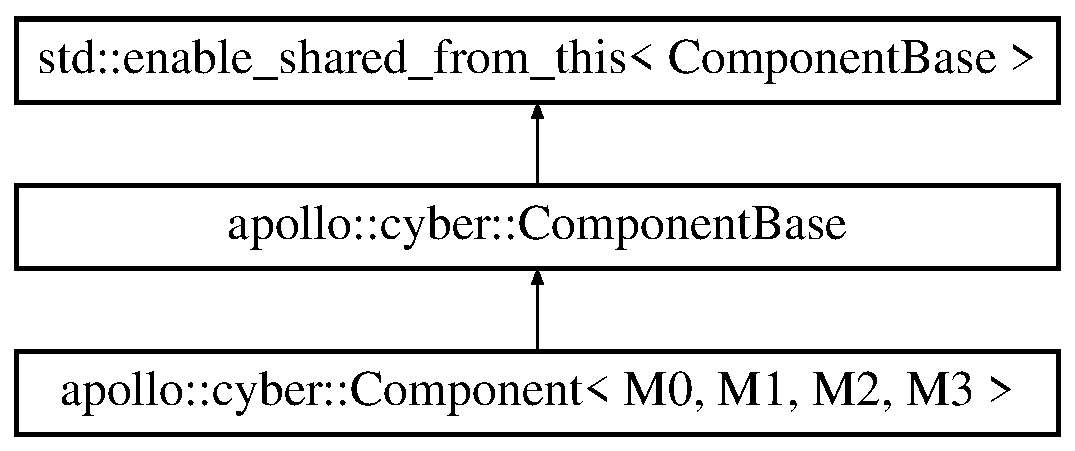
\includegraphics[height=3.000000cm]{classapollo_1_1cyber_1_1Component}
\end{center}
\end{figure}
\subsection*{Public Member Functions}
\begin{DoxyCompactItemize}
\item 
\hyperlink{classapollo_1_1cyber_1_1Component_a37ccb4740d819327ac929b703d8cf9ae}{Component} ()
\item 
\hyperlink{classapollo_1_1cyber_1_1Component_af65ebeab9e345f27089095fe64e3b4f6}{$\sim$\-Component} () override
\item 
bool \hyperlink{classapollo_1_1cyber_1_1Component_ae68b7c7dce67c4d5c6c024c910bb9d92}{Initialize} (const Component\-Config \&config) override
\item 
bool \hyperlink{classapollo_1_1cyber_1_1Component_a3083d711406cfad7c11d60a0fadad274}{Process} (const std\-::shared\-\_\-ptr$<$ M0 $>$ \&msg0, const std\-::shared\-\_\-ptr$<$ M1 $>$ \&msg1, const std\-::shared\-\_\-ptr$<$ M2 $>$ \&msg2, const std\-::shared\-\_\-ptr$<$ M3 $>$ \&msg3)
\end{DoxyCompactItemize}
\subsection*{Private Member Functions}
\begin{DoxyCompactItemize}
\item 
virtual bool \hyperlink{classapollo_1_1cyber_1_1Component_a9c909a2d1b6b53eaf6e4c9d95fc7aaec}{Proc} (const std\-::shared\-\_\-ptr$<$ M0 $>$ \&msg0, const std\-::shared\-\_\-ptr$<$ M1 $>$ \&msg1, const std\-::shared\-\_\-ptr$<$ M2 $>$ \&msg2, const std\-::shared\-\_\-ptr$<$ M3 $>$ \&msg3)=0
\end{DoxyCompactItemize}
\subsection*{Additional Inherited Members}


\subsection{Constructor \& Destructor Documentation}
\hypertarget{classapollo_1_1cyber_1_1Component_a37ccb4740d819327ac929b703d8cf9ae}{\index{apollo\-::cyber\-::\-Component@{apollo\-::cyber\-::\-Component}!Component@{Component}}
\index{Component@{Component}!apollo::cyber::Component@{apollo\-::cyber\-::\-Component}}
\subsubsection[{Component}]{\setlength{\rightskip}{0pt plus 5cm}template$<$typename M0 = Null\-Type, typename M1 = Null\-Type, typename M2 = Null\-Type, typename M3 = Null\-Type$>$ {\bf apollo\-::cyber\-::\-Component}$<$ M0, M1, M2, M3 $>$\-::{\bf Component} (
\begin{DoxyParamCaption}
{}
\end{DoxyParamCaption}
)\hspace{0.3cm}{\ttfamily [inline]}}}\label{classapollo_1_1cyber_1_1Component_a37ccb4740d819327ac929b703d8cf9ae}
\hypertarget{classapollo_1_1cyber_1_1Component_af65ebeab9e345f27089095fe64e3b4f6}{\index{apollo\-::cyber\-::\-Component@{apollo\-::cyber\-::\-Component}!$\sim$\-Component@{$\sim$\-Component}}
\index{$\sim$\-Component@{$\sim$\-Component}!apollo::cyber::Component@{apollo\-::cyber\-::\-Component}}
\subsubsection[{$\sim$\-Component}]{\setlength{\rightskip}{0pt plus 5cm}template$<$typename M0 = Null\-Type, typename M1 = Null\-Type, typename M2 = Null\-Type, typename M3 = Null\-Type$>$ {\bf apollo\-::cyber\-::\-Component}$<$ M0, M1, M2, M3 $>$\-::$\sim${\bf Component} (
\begin{DoxyParamCaption}
{}
\end{DoxyParamCaption}
)\hspace{0.3cm}{\ttfamily [inline]}, {\ttfamily [override]}}}\label{classapollo_1_1cyber_1_1Component_af65ebeab9e345f27089095fe64e3b4f6}


\subsection{Member Function Documentation}
\hypertarget{classapollo_1_1cyber_1_1Component_ae68b7c7dce67c4d5c6c024c910bb9d92}{\index{apollo\-::cyber\-::\-Component@{apollo\-::cyber\-::\-Component}!Initialize@{Initialize}}
\index{Initialize@{Initialize}!apollo::cyber::Component@{apollo\-::cyber\-::\-Component}}
\subsubsection[{Initialize}]{\setlength{\rightskip}{0pt plus 5cm}template$<$typename M0 , typename M1 , typename M2 , typename M3 $>$ bool {\bf apollo\-::cyber\-::\-Component}$<$ M0, M1, M2, M3 $>$\-::Initialize (
\begin{DoxyParamCaption}
\item[{const Component\-Config \&}]{config}
\end{DoxyParamCaption}
)\hspace{0.3cm}{\ttfamily [inline]}, {\ttfamily [override]}, {\ttfamily [virtual]}}}\label{classapollo_1_1cyber_1_1Component_ae68b7c7dce67c4d5c6c024c910bb9d92}


Reimplemented from \hyperlink{classapollo_1_1cyber_1_1ComponentBase_a234ab17fb5f504179b9f49d344e72882}{apollo\-::cyber\-::\-Component\-Base}.

\hypertarget{classapollo_1_1cyber_1_1Component_a9c909a2d1b6b53eaf6e4c9d95fc7aaec}{\index{apollo\-::cyber\-::\-Component@{apollo\-::cyber\-::\-Component}!Proc@{Proc}}
\index{Proc@{Proc}!apollo::cyber::Component@{apollo\-::cyber\-::\-Component}}
\subsubsection[{Proc}]{\setlength{\rightskip}{0pt plus 5cm}template$<$typename M0 = Null\-Type, typename M1 = Null\-Type, typename M2 = Null\-Type, typename M3 = Null\-Type$>$ virtual bool {\bf apollo\-::cyber\-::\-Component}$<$ M0, M1, M2, M3 $>$\-::Proc (
\begin{DoxyParamCaption}
\item[{const std\-::shared\-\_\-ptr$<$ M0 $>$ \&}]{msg0, }
\item[{const std\-::shared\-\_\-ptr$<$ M1 $>$ \&}]{msg1, }
\item[{const std\-::shared\-\_\-ptr$<$ M2 $>$ \&}]{msg2, }
\item[{const std\-::shared\-\_\-ptr$<$ M3 $>$ \&}]{msg3}
\end{DoxyParamCaption}
)\hspace{0.3cm}{\ttfamily [private]}, {\ttfamily [pure virtual]}}}\label{classapollo_1_1cyber_1_1Component_a9c909a2d1b6b53eaf6e4c9d95fc7aaec}
\hypertarget{classapollo_1_1cyber_1_1Component_a3083d711406cfad7c11d60a0fadad274}{\index{apollo\-::cyber\-::\-Component@{apollo\-::cyber\-::\-Component}!Process@{Process}}
\index{Process@{Process}!apollo::cyber::Component@{apollo\-::cyber\-::\-Component}}
\subsubsection[{Process}]{\setlength{\rightskip}{0pt plus 5cm}template$<$typename M0, typename M1, typename M2, typename M3$>$ bool {\bf apollo\-::cyber\-::\-Component}$<$ M0, M1, M2, M3 $>$\-::Process (
\begin{DoxyParamCaption}
\item[{const std\-::shared\-\_\-ptr$<$ M0 $>$ \&}]{msg0, }
\item[{const std\-::shared\-\_\-ptr$<$ M1 $>$ \&}]{msg1, }
\item[{const std\-::shared\-\_\-ptr$<$ M2 $>$ \&}]{msg2, }
\item[{const std\-::shared\-\_\-ptr$<$ M3 $>$ \&}]{msg3}
\end{DoxyParamCaption}
)}}\label{classapollo_1_1cyber_1_1Component_a3083d711406cfad7c11d60a0fadad274}


The documentation for this class was generated from the following file\-:\begin{DoxyCompactItemize}
\item 
component/\hyperlink{component_8h}{component.\-h}\end{DoxyCompactItemize}

\hypertarget{classapollo_1_1cyber_1_1Component_3_01M0_00_01M1_00_01M2_00_01NullType_01_4}{\section{apollo\-:\-:cyber\-:\-:Component$<$ M0, M1, M2, Null\-Type $>$ Class Template Reference}
\label{classapollo_1_1cyber_1_1Component_3_01M0_00_01M1_00_01M2_00_01NullType_01_4}\index{apollo\-::cyber\-::\-Component$<$ M0, M1, M2, Null\-Type $>$@{apollo\-::cyber\-::\-Component$<$ M0, M1, M2, Null\-Type $>$}}
}


{\ttfamily \#include $<$component.\-h$>$}

Inheritance diagram for apollo\-:\-:cyber\-:\-:Component$<$ M0, M1, M2, Null\-Type $>$\-:\begin{figure}[H]
\begin{center}
\leavevmode
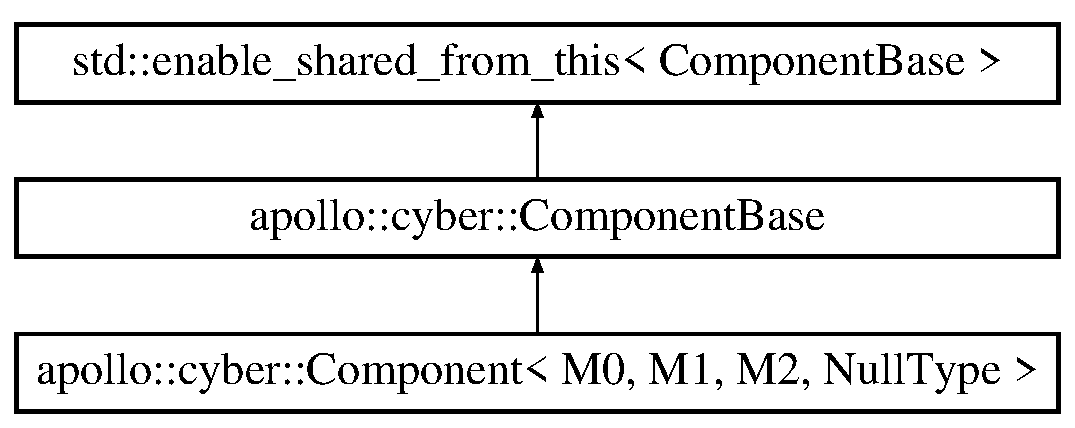
\includegraphics[height=3.000000cm]{classapollo_1_1cyber_1_1Component_3_01M0_00_01M1_00_01M2_00_01NullType_01_4}
\end{center}
\end{figure}
\subsection*{Public Member Functions}
\begin{DoxyCompactItemize}
\item 
\hyperlink{classapollo_1_1cyber_1_1Component_3_01M0_00_01M1_00_01M2_00_01NullType_01_4_a4f364f7e6d63005932bec12e055c9387}{Component} ()
\item 
\hyperlink{classapollo_1_1cyber_1_1Component_3_01M0_00_01M1_00_01M2_00_01NullType_01_4_a44914b8640994ffc0fd2c5618a88ea44}{$\sim$\-Component} () override
\item 
bool \hyperlink{classapollo_1_1cyber_1_1Component_3_01M0_00_01M1_00_01M2_00_01NullType_01_4_ae890450f0eb587c8ea7fbfa91259876a}{Initialize} (const Component\-Config \&config) override
\item 
bool \hyperlink{classapollo_1_1cyber_1_1Component_3_01M0_00_01M1_00_01M2_00_01NullType_01_4_a0eaa3a774441dc451576e4c369b48139}{Process} (const std\-::shared\-\_\-ptr$<$ M0 $>$ \&msg0, const std\-::shared\-\_\-ptr$<$ M1 $>$ \&msg1, const std\-::shared\-\_\-ptr$<$ M2 $>$ \&msg2)
\end{DoxyCompactItemize}
\subsection*{Private Member Functions}
\begin{DoxyCompactItemize}
\item 
virtual bool \hyperlink{classapollo_1_1cyber_1_1Component_3_01M0_00_01M1_00_01M2_00_01NullType_01_4_adf9bb797c34d0eed163a7f95d1c6bcd7}{Proc} (const std\-::shared\-\_\-ptr$<$ M0 $>$ \&msg, const std\-::shared\-\_\-ptr$<$ M1 $>$ \&msg1, const std\-::shared\-\_\-ptr$<$ M2 $>$ \&msg2)=0
\end{DoxyCompactItemize}
\subsection*{Additional Inherited Members}


\subsection{Constructor \& Destructor Documentation}
\hypertarget{classapollo_1_1cyber_1_1Component_3_01M0_00_01M1_00_01M2_00_01NullType_01_4_a4f364f7e6d63005932bec12e055c9387}{\index{apollo\-::cyber\-::\-Component$<$ M0, M1, M2, Null\-Type $>$@{apollo\-::cyber\-::\-Component$<$ M0, M1, M2, Null\-Type $>$}!Component@{Component}}
\index{Component@{Component}!apollo::cyber::Component< M0, M1, M2, NullType >@{apollo\-::cyber\-::\-Component$<$ M0, M1, M2, Null\-Type $>$}}
\subsubsection[{Component}]{\setlength{\rightskip}{0pt plus 5cm}template$<$typename M0 , typename M1 , typename M2 $>$ {\bf apollo\-::cyber\-::\-Component}$<$ M0, M1, M2, {\bf Null\-Type} $>$\-::{\bf Component} (
\begin{DoxyParamCaption}
{}
\end{DoxyParamCaption}
)\hspace{0.3cm}{\ttfamily [inline]}}}\label{classapollo_1_1cyber_1_1Component_3_01M0_00_01M1_00_01M2_00_01NullType_01_4_a4f364f7e6d63005932bec12e055c9387}
\hypertarget{classapollo_1_1cyber_1_1Component_3_01M0_00_01M1_00_01M2_00_01NullType_01_4_a44914b8640994ffc0fd2c5618a88ea44}{\index{apollo\-::cyber\-::\-Component$<$ M0, M1, M2, Null\-Type $>$@{apollo\-::cyber\-::\-Component$<$ M0, M1, M2, Null\-Type $>$}!$\sim$\-Component@{$\sim$\-Component}}
\index{$\sim$\-Component@{$\sim$\-Component}!apollo::cyber::Component< M0, M1, M2, NullType >@{apollo\-::cyber\-::\-Component$<$ M0, M1, M2, Null\-Type $>$}}
\subsubsection[{$\sim$\-Component}]{\setlength{\rightskip}{0pt plus 5cm}template$<$typename M0 , typename M1 , typename M2 $>$ {\bf apollo\-::cyber\-::\-Component}$<$ M0, M1, M2, {\bf Null\-Type} $>$\-::$\sim${\bf Component} (
\begin{DoxyParamCaption}
{}
\end{DoxyParamCaption}
)\hspace{0.3cm}{\ttfamily [inline]}, {\ttfamily [override]}}}\label{classapollo_1_1cyber_1_1Component_3_01M0_00_01M1_00_01M2_00_01NullType_01_4_a44914b8640994ffc0fd2c5618a88ea44}


\subsection{Member Function Documentation}
\hypertarget{classapollo_1_1cyber_1_1Component_3_01M0_00_01M1_00_01M2_00_01NullType_01_4_ae890450f0eb587c8ea7fbfa91259876a}{\index{apollo\-::cyber\-::\-Component$<$ M0, M1, M2, Null\-Type $>$@{apollo\-::cyber\-::\-Component$<$ M0, M1, M2, Null\-Type $>$}!Initialize@{Initialize}}
\index{Initialize@{Initialize}!apollo::cyber::Component< M0, M1, M2, NullType >@{apollo\-::cyber\-::\-Component$<$ M0, M1, M2, Null\-Type $>$}}
\subsubsection[{Initialize}]{\setlength{\rightskip}{0pt plus 5cm}template$<$typename M0 , typename M1 , typename M2 $>$ bool {\bf apollo\-::cyber\-::\-Component}$<$ M0, M1, M2, {\bf Null\-Type} $>$\-::Initialize (
\begin{DoxyParamCaption}
\item[{const Component\-Config \&}]{config}
\end{DoxyParamCaption}
)\hspace{0.3cm}{\ttfamily [override]}, {\ttfamily [virtual]}}}\label{classapollo_1_1cyber_1_1Component_3_01M0_00_01M1_00_01M2_00_01NullType_01_4_ae890450f0eb587c8ea7fbfa91259876a}


Reimplemented from \hyperlink{classapollo_1_1cyber_1_1ComponentBase_a234ab17fb5f504179b9f49d344e72882}{apollo\-::cyber\-::\-Component\-Base}.

\hypertarget{classapollo_1_1cyber_1_1Component_3_01M0_00_01M1_00_01M2_00_01NullType_01_4_adf9bb797c34d0eed163a7f95d1c6bcd7}{\index{apollo\-::cyber\-::\-Component$<$ M0, M1, M2, Null\-Type $>$@{apollo\-::cyber\-::\-Component$<$ M0, M1, M2, Null\-Type $>$}!Proc@{Proc}}
\index{Proc@{Proc}!apollo::cyber::Component< M0, M1, M2, NullType >@{apollo\-::cyber\-::\-Component$<$ M0, M1, M2, Null\-Type $>$}}
\subsubsection[{Proc}]{\setlength{\rightskip}{0pt plus 5cm}template$<$typename M0 , typename M1 , typename M2 $>$ virtual bool {\bf apollo\-::cyber\-::\-Component}$<$ M0, M1, M2, {\bf Null\-Type} $>$\-::Proc (
\begin{DoxyParamCaption}
\item[{const std\-::shared\-\_\-ptr$<$ M0 $>$ \&}]{msg, }
\item[{const std\-::shared\-\_\-ptr$<$ M1 $>$ \&}]{msg1, }
\item[{const std\-::shared\-\_\-ptr$<$ M2 $>$ \&}]{msg2}
\end{DoxyParamCaption}
)\hspace{0.3cm}{\ttfamily [private]}, {\ttfamily [pure virtual]}}}\label{classapollo_1_1cyber_1_1Component_3_01M0_00_01M1_00_01M2_00_01NullType_01_4_adf9bb797c34d0eed163a7f95d1c6bcd7}
\hypertarget{classapollo_1_1cyber_1_1Component_3_01M0_00_01M1_00_01M2_00_01NullType_01_4_a0eaa3a774441dc451576e4c369b48139}{\index{apollo\-::cyber\-::\-Component$<$ M0, M1, M2, Null\-Type $>$@{apollo\-::cyber\-::\-Component$<$ M0, M1, M2, Null\-Type $>$}!Process@{Process}}
\index{Process@{Process}!apollo::cyber::Component< M0, M1, M2, NullType >@{apollo\-::cyber\-::\-Component$<$ M0, M1, M2, Null\-Type $>$}}
\subsubsection[{Process}]{\setlength{\rightskip}{0pt plus 5cm}template$<$typename M0 , typename M1 , typename M2 $>$ bool {\bf apollo\-::cyber\-::\-Component}$<$ M0, M1, M2, {\bf Null\-Type} $>$\-::Process (
\begin{DoxyParamCaption}
\item[{const std\-::shared\-\_\-ptr$<$ M0 $>$ \&}]{msg0, }
\item[{const std\-::shared\-\_\-ptr$<$ M1 $>$ \&}]{msg1, }
\item[{const std\-::shared\-\_\-ptr$<$ M2 $>$ \&}]{msg2}
\end{DoxyParamCaption}
)}}\label{classapollo_1_1cyber_1_1Component_3_01M0_00_01M1_00_01M2_00_01NullType_01_4_a0eaa3a774441dc451576e4c369b48139}


The documentation for this class was generated from the following file\-:\begin{DoxyCompactItemize}
\item 
component/\hyperlink{component_8h}{component.\-h}\end{DoxyCompactItemize}

\hypertarget{classapollo_1_1cyber_1_1Component_3_01M0_00_01M1_00_01NullType_00_01NullType_01_4}{\section{apollo\-:\-:cyber\-:\-:Component$<$ M0, M1, Null\-Type, Null\-Type $>$ Class Template Reference}
\label{classapollo_1_1cyber_1_1Component_3_01M0_00_01M1_00_01NullType_00_01NullType_01_4}\index{apollo\-::cyber\-::\-Component$<$ M0, M1, Null\-Type, Null\-Type $>$@{apollo\-::cyber\-::\-Component$<$ M0, M1, Null\-Type, Null\-Type $>$}}
}


{\ttfamily \#include $<$component.\-h$>$}

Inheritance diagram for apollo\-:\-:cyber\-:\-:Component$<$ M0, M1, Null\-Type, Null\-Type $>$\-:\begin{figure}[H]
\begin{center}
\leavevmode
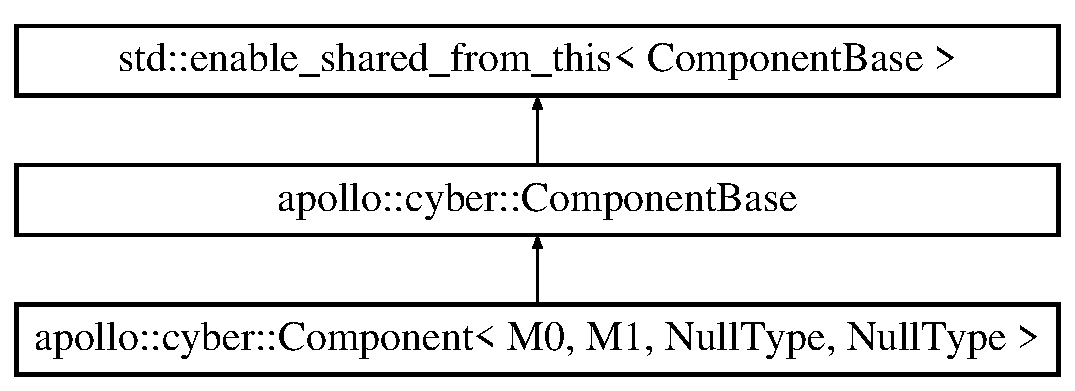
\includegraphics[height=3.000000cm]{classapollo_1_1cyber_1_1Component_3_01M0_00_01M1_00_01NullType_00_01NullType_01_4}
\end{center}
\end{figure}
\subsection*{Public Member Functions}
\begin{DoxyCompactItemize}
\item 
\hyperlink{classapollo_1_1cyber_1_1Component_3_01M0_00_01M1_00_01NullType_00_01NullType_01_4_ace00fd57f08d90d2bc8f985933134474}{Component} ()
\item 
\hyperlink{classapollo_1_1cyber_1_1Component_3_01M0_00_01M1_00_01NullType_00_01NullType_01_4_a8de0c0d0b19262388f1935e5c5e3f6f2}{$\sim$\-Component} () override
\item 
bool \hyperlink{classapollo_1_1cyber_1_1Component_3_01M0_00_01M1_00_01NullType_00_01NullType_01_4_ab3c98c371afed14286ed36f89eb84e7f}{Initialize} (const Component\-Config \&config) override
\item 
bool \hyperlink{classapollo_1_1cyber_1_1Component_3_01M0_00_01M1_00_01NullType_00_01NullType_01_4_abbdb287a3556d1eb229374bf3a5f0d35}{Process} (const std\-::shared\-\_\-ptr$<$ M0 $>$ \&msg0, const std\-::shared\-\_\-ptr$<$ M1 $>$ \&msg1)
\end{DoxyCompactItemize}
\subsection*{Private Member Functions}
\begin{DoxyCompactItemize}
\item 
virtual bool \hyperlink{classapollo_1_1cyber_1_1Component_3_01M0_00_01M1_00_01NullType_00_01NullType_01_4_afc67aa49c528e5c692f5f5223a5afab6}{Proc} (const std\-::shared\-\_\-ptr$<$ M0 $>$ \&msg, const std\-::shared\-\_\-ptr$<$ M1 $>$ \&msg1)=0
\end{DoxyCompactItemize}
\subsection*{Additional Inherited Members}


\subsection{Constructor \& Destructor Documentation}
\hypertarget{classapollo_1_1cyber_1_1Component_3_01M0_00_01M1_00_01NullType_00_01NullType_01_4_ace00fd57f08d90d2bc8f985933134474}{\index{apollo\-::cyber\-::\-Component$<$ M0, M1, Null\-Type, Null\-Type $>$@{apollo\-::cyber\-::\-Component$<$ M0, M1, Null\-Type, Null\-Type $>$}!Component@{Component}}
\index{Component@{Component}!apollo::cyber::Component< M0, M1, NullType, NullType >@{apollo\-::cyber\-::\-Component$<$ M0, M1, Null\-Type, Null\-Type $>$}}
\subsubsection[{Component}]{\setlength{\rightskip}{0pt plus 5cm}template$<$typename M0 , typename M1 $>$ {\bf apollo\-::cyber\-::\-Component}$<$ M0, M1, {\bf Null\-Type}, {\bf Null\-Type} $>$\-::{\bf Component} (
\begin{DoxyParamCaption}
{}
\end{DoxyParamCaption}
)\hspace{0.3cm}{\ttfamily [inline]}}}\label{classapollo_1_1cyber_1_1Component_3_01M0_00_01M1_00_01NullType_00_01NullType_01_4_ace00fd57f08d90d2bc8f985933134474}
\hypertarget{classapollo_1_1cyber_1_1Component_3_01M0_00_01M1_00_01NullType_00_01NullType_01_4_a8de0c0d0b19262388f1935e5c5e3f6f2}{\index{apollo\-::cyber\-::\-Component$<$ M0, M1, Null\-Type, Null\-Type $>$@{apollo\-::cyber\-::\-Component$<$ M0, M1, Null\-Type, Null\-Type $>$}!$\sim$\-Component@{$\sim$\-Component}}
\index{$\sim$\-Component@{$\sim$\-Component}!apollo::cyber::Component< M0, M1, NullType, NullType >@{apollo\-::cyber\-::\-Component$<$ M0, M1, Null\-Type, Null\-Type $>$}}
\subsubsection[{$\sim$\-Component}]{\setlength{\rightskip}{0pt plus 5cm}template$<$typename M0 , typename M1 $>$ {\bf apollo\-::cyber\-::\-Component}$<$ M0, M1, {\bf Null\-Type}, {\bf Null\-Type} $>$\-::$\sim${\bf Component} (
\begin{DoxyParamCaption}
{}
\end{DoxyParamCaption}
)\hspace{0.3cm}{\ttfamily [inline]}, {\ttfamily [override]}}}\label{classapollo_1_1cyber_1_1Component_3_01M0_00_01M1_00_01NullType_00_01NullType_01_4_a8de0c0d0b19262388f1935e5c5e3f6f2}


\subsection{Member Function Documentation}
\hypertarget{classapollo_1_1cyber_1_1Component_3_01M0_00_01M1_00_01NullType_00_01NullType_01_4_ab3c98c371afed14286ed36f89eb84e7f}{\index{apollo\-::cyber\-::\-Component$<$ M0, M1, Null\-Type, Null\-Type $>$@{apollo\-::cyber\-::\-Component$<$ M0, M1, Null\-Type, Null\-Type $>$}!Initialize@{Initialize}}
\index{Initialize@{Initialize}!apollo::cyber::Component< M0, M1, NullType, NullType >@{apollo\-::cyber\-::\-Component$<$ M0, M1, Null\-Type, Null\-Type $>$}}
\subsubsection[{Initialize}]{\setlength{\rightskip}{0pt plus 5cm}template$<$typename M0 , typename M1 $>$ bool {\bf apollo\-::cyber\-::\-Component}$<$ M0, M1, {\bf Null\-Type}, {\bf Null\-Type} $>$\-::Initialize (
\begin{DoxyParamCaption}
\item[{const Component\-Config \&}]{config}
\end{DoxyParamCaption}
)\hspace{0.3cm}{\ttfamily [override]}, {\ttfamily [virtual]}}}\label{classapollo_1_1cyber_1_1Component_3_01M0_00_01M1_00_01NullType_00_01NullType_01_4_ab3c98c371afed14286ed36f89eb84e7f}


Reimplemented from \hyperlink{classapollo_1_1cyber_1_1ComponentBase_a234ab17fb5f504179b9f49d344e72882}{apollo\-::cyber\-::\-Component\-Base}.

\hypertarget{classapollo_1_1cyber_1_1Component_3_01M0_00_01M1_00_01NullType_00_01NullType_01_4_afc67aa49c528e5c692f5f5223a5afab6}{\index{apollo\-::cyber\-::\-Component$<$ M0, M1, Null\-Type, Null\-Type $>$@{apollo\-::cyber\-::\-Component$<$ M0, M1, Null\-Type, Null\-Type $>$}!Proc@{Proc}}
\index{Proc@{Proc}!apollo::cyber::Component< M0, M1, NullType, NullType >@{apollo\-::cyber\-::\-Component$<$ M0, M1, Null\-Type, Null\-Type $>$}}
\subsubsection[{Proc}]{\setlength{\rightskip}{0pt plus 5cm}template$<$typename M0 , typename M1 $>$ virtual bool {\bf apollo\-::cyber\-::\-Component}$<$ M0, M1, {\bf Null\-Type}, {\bf Null\-Type} $>$\-::Proc (
\begin{DoxyParamCaption}
\item[{const std\-::shared\-\_\-ptr$<$ M0 $>$ \&}]{msg, }
\item[{const std\-::shared\-\_\-ptr$<$ M1 $>$ \&}]{msg1}
\end{DoxyParamCaption}
)\hspace{0.3cm}{\ttfamily [private]}, {\ttfamily [pure virtual]}}}\label{classapollo_1_1cyber_1_1Component_3_01M0_00_01M1_00_01NullType_00_01NullType_01_4_afc67aa49c528e5c692f5f5223a5afab6}
\hypertarget{classapollo_1_1cyber_1_1Component_3_01M0_00_01M1_00_01NullType_00_01NullType_01_4_abbdb287a3556d1eb229374bf3a5f0d35}{\index{apollo\-::cyber\-::\-Component$<$ M0, M1, Null\-Type, Null\-Type $>$@{apollo\-::cyber\-::\-Component$<$ M0, M1, Null\-Type, Null\-Type $>$}!Process@{Process}}
\index{Process@{Process}!apollo::cyber::Component< M0, M1, NullType, NullType >@{apollo\-::cyber\-::\-Component$<$ M0, M1, Null\-Type, Null\-Type $>$}}
\subsubsection[{Process}]{\setlength{\rightskip}{0pt plus 5cm}template$<$typename M0 , typename M1 $>$ bool {\bf apollo\-::cyber\-::\-Component}$<$ M0, M1, {\bf Null\-Type}, {\bf Null\-Type} $>$\-::Process (
\begin{DoxyParamCaption}
\item[{const std\-::shared\-\_\-ptr$<$ M0 $>$ \&}]{msg0, }
\item[{const std\-::shared\-\_\-ptr$<$ M1 $>$ \&}]{msg1}
\end{DoxyParamCaption}
)}}\label{classapollo_1_1cyber_1_1Component_3_01M0_00_01M1_00_01NullType_00_01NullType_01_4_abbdb287a3556d1eb229374bf3a5f0d35}


The documentation for this class was generated from the following file\-:\begin{DoxyCompactItemize}
\item 
component/\hyperlink{component_8h}{component.\-h}\end{DoxyCompactItemize}

\hypertarget{classapollo_1_1cyber_1_1Component_3_01M0_00_01NullType_00_01NullType_00_01NullType_01_4}{\section{apollo\-:\-:cyber\-:\-:Component$<$ M0, Null\-Type, Null\-Type, Null\-Type $>$ Class Template Reference}
\label{classapollo_1_1cyber_1_1Component_3_01M0_00_01NullType_00_01NullType_00_01NullType_01_4}\index{apollo\-::cyber\-::\-Component$<$ M0, Null\-Type, Null\-Type, Null\-Type $>$@{apollo\-::cyber\-::\-Component$<$ M0, Null\-Type, Null\-Type, Null\-Type $>$}}
}


{\ttfamily \#include $<$component.\-h$>$}

Inheritance diagram for apollo\-:\-:cyber\-:\-:Component$<$ M0, Null\-Type, Null\-Type, Null\-Type $>$\-:\begin{figure}[H]
\begin{center}
\leavevmode
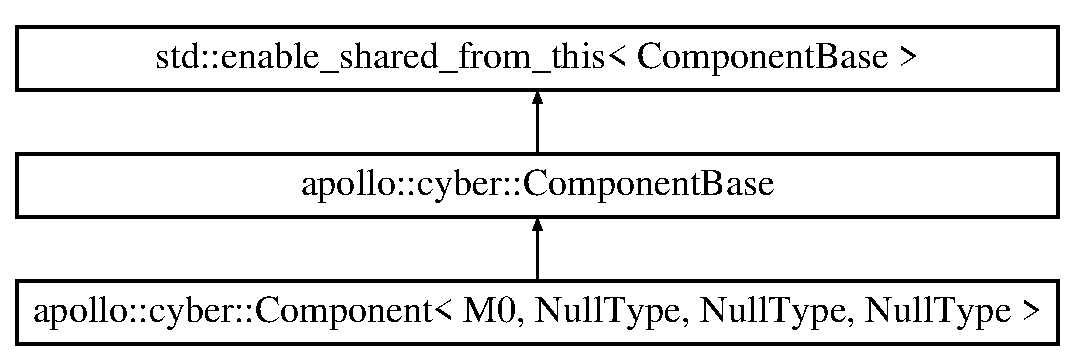
\includegraphics[height=3.000000cm]{classapollo_1_1cyber_1_1Component_3_01M0_00_01NullType_00_01NullType_00_01NullType_01_4}
\end{center}
\end{figure}
\subsection*{Public Member Functions}
\begin{DoxyCompactItemize}
\item 
\hyperlink{classapollo_1_1cyber_1_1Component_3_01M0_00_01NullType_00_01NullType_00_01NullType_01_4_ab60cf2e080f214df6cff585a30f46819}{Component} ()
\item 
\hyperlink{classapollo_1_1cyber_1_1Component_3_01M0_00_01NullType_00_01NullType_00_01NullType_01_4_a69ff6100886963072387ebd81c7d7b16}{$\sim$\-Component} () override
\item 
bool \hyperlink{classapollo_1_1cyber_1_1Component_3_01M0_00_01NullType_00_01NullType_00_01NullType_01_4_a9e859b2698539158448b19aa156f48d6}{Initialize} (const Component\-Config \&config) override
\item 
bool \hyperlink{classapollo_1_1cyber_1_1Component_3_01M0_00_01NullType_00_01NullType_00_01NullType_01_4_a99ec1c8222855604b21f2f5d17e15638}{Process} (const std\-::shared\-\_\-ptr$<$ M0 $>$ \&msg)
\end{DoxyCompactItemize}
\subsection*{Private Member Functions}
\begin{DoxyCompactItemize}
\item 
virtual bool \hyperlink{classapollo_1_1cyber_1_1Component_3_01M0_00_01NullType_00_01NullType_00_01NullType_01_4_a3b0571d72293add923316368fcf96a17}{Proc} (const std\-::shared\-\_\-ptr$<$ M0 $>$ \&msg)=0
\end{DoxyCompactItemize}
\subsection*{Additional Inherited Members}


\subsection{Constructor \& Destructor Documentation}
\hypertarget{classapollo_1_1cyber_1_1Component_3_01M0_00_01NullType_00_01NullType_00_01NullType_01_4_ab60cf2e080f214df6cff585a30f46819}{\index{apollo\-::cyber\-::\-Component$<$ M0, Null\-Type, Null\-Type, Null\-Type $>$@{apollo\-::cyber\-::\-Component$<$ M0, Null\-Type, Null\-Type, Null\-Type $>$}!Component@{Component}}
\index{Component@{Component}!apollo::cyber::Component< M0, NullType, NullType, NullType >@{apollo\-::cyber\-::\-Component$<$ M0, Null\-Type, Null\-Type, Null\-Type $>$}}
\subsubsection[{Component}]{\setlength{\rightskip}{0pt plus 5cm}template$<$typename M0 $>$ {\bf apollo\-::cyber\-::\-Component}$<$ M0, {\bf Null\-Type}, {\bf Null\-Type}, {\bf Null\-Type} $>$\-::{\bf Component} (
\begin{DoxyParamCaption}
{}
\end{DoxyParamCaption}
)\hspace{0.3cm}{\ttfamily [inline]}}}\label{classapollo_1_1cyber_1_1Component_3_01M0_00_01NullType_00_01NullType_00_01NullType_01_4_ab60cf2e080f214df6cff585a30f46819}
\hypertarget{classapollo_1_1cyber_1_1Component_3_01M0_00_01NullType_00_01NullType_00_01NullType_01_4_a69ff6100886963072387ebd81c7d7b16}{\index{apollo\-::cyber\-::\-Component$<$ M0, Null\-Type, Null\-Type, Null\-Type $>$@{apollo\-::cyber\-::\-Component$<$ M0, Null\-Type, Null\-Type, Null\-Type $>$}!$\sim$\-Component@{$\sim$\-Component}}
\index{$\sim$\-Component@{$\sim$\-Component}!apollo::cyber::Component< M0, NullType, NullType, NullType >@{apollo\-::cyber\-::\-Component$<$ M0, Null\-Type, Null\-Type, Null\-Type $>$}}
\subsubsection[{$\sim$\-Component}]{\setlength{\rightskip}{0pt plus 5cm}template$<$typename M0 $>$ {\bf apollo\-::cyber\-::\-Component}$<$ M0, {\bf Null\-Type}, {\bf Null\-Type}, {\bf Null\-Type} $>$\-::$\sim${\bf Component} (
\begin{DoxyParamCaption}
{}
\end{DoxyParamCaption}
)\hspace{0.3cm}{\ttfamily [inline]}, {\ttfamily [override]}}}\label{classapollo_1_1cyber_1_1Component_3_01M0_00_01NullType_00_01NullType_00_01NullType_01_4_a69ff6100886963072387ebd81c7d7b16}


\subsection{Member Function Documentation}
\hypertarget{classapollo_1_1cyber_1_1Component_3_01M0_00_01NullType_00_01NullType_00_01NullType_01_4_a9e859b2698539158448b19aa156f48d6}{\index{apollo\-::cyber\-::\-Component$<$ M0, Null\-Type, Null\-Type, Null\-Type $>$@{apollo\-::cyber\-::\-Component$<$ M0, Null\-Type, Null\-Type, Null\-Type $>$}!Initialize@{Initialize}}
\index{Initialize@{Initialize}!apollo::cyber::Component< M0, NullType, NullType, NullType >@{apollo\-::cyber\-::\-Component$<$ M0, Null\-Type, Null\-Type, Null\-Type $>$}}
\subsubsection[{Initialize}]{\setlength{\rightskip}{0pt plus 5cm}template$<$typename M0 $>$ bool {\bf apollo\-::cyber\-::\-Component}$<$ M0, {\bf Null\-Type}, {\bf Null\-Type}, {\bf Null\-Type} $>$\-::Initialize (
\begin{DoxyParamCaption}
\item[{const Component\-Config \&}]{config}
\end{DoxyParamCaption}
)\hspace{0.3cm}{\ttfamily [override]}, {\ttfamily [virtual]}}}\label{classapollo_1_1cyber_1_1Component_3_01M0_00_01NullType_00_01NullType_00_01NullType_01_4_a9e859b2698539158448b19aa156f48d6}


Reimplemented from \hyperlink{classapollo_1_1cyber_1_1ComponentBase_a234ab17fb5f504179b9f49d344e72882}{apollo\-::cyber\-::\-Component\-Base}.

\hypertarget{classapollo_1_1cyber_1_1Component_3_01M0_00_01NullType_00_01NullType_00_01NullType_01_4_a3b0571d72293add923316368fcf96a17}{\index{apollo\-::cyber\-::\-Component$<$ M0, Null\-Type, Null\-Type, Null\-Type $>$@{apollo\-::cyber\-::\-Component$<$ M0, Null\-Type, Null\-Type, Null\-Type $>$}!Proc@{Proc}}
\index{Proc@{Proc}!apollo::cyber::Component< M0, NullType, NullType, NullType >@{apollo\-::cyber\-::\-Component$<$ M0, Null\-Type, Null\-Type, Null\-Type $>$}}
\subsubsection[{Proc}]{\setlength{\rightskip}{0pt plus 5cm}template$<$typename M0 $>$ virtual bool {\bf apollo\-::cyber\-::\-Component}$<$ M0, {\bf Null\-Type}, {\bf Null\-Type}, {\bf Null\-Type} $>$\-::Proc (
\begin{DoxyParamCaption}
\item[{const std\-::shared\-\_\-ptr$<$ M0 $>$ \&}]{msg}
\end{DoxyParamCaption}
)\hspace{0.3cm}{\ttfamily [private]}, {\ttfamily [pure virtual]}}}\label{classapollo_1_1cyber_1_1Component_3_01M0_00_01NullType_00_01NullType_00_01NullType_01_4_a3b0571d72293add923316368fcf96a17}
\hypertarget{classapollo_1_1cyber_1_1Component_3_01M0_00_01NullType_00_01NullType_00_01NullType_01_4_a99ec1c8222855604b21f2f5d17e15638}{\index{apollo\-::cyber\-::\-Component$<$ M0, Null\-Type, Null\-Type, Null\-Type $>$@{apollo\-::cyber\-::\-Component$<$ M0, Null\-Type, Null\-Type, Null\-Type $>$}!Process@{Process}}
\index{Process@{Process}!apollo::cyber::Component< M0, NullType, NullType, NullType >@{apollo\-::cyber\-::\-Component$<$ M0, Null\-Type, Null\-Type, Null\-Type $>$}}
\subsubsection[{Process}]{\setlength{\rightskip}{0pt plus 5cm}template$<$typename M0 $>$ bool {\bf apollo\-::cyber\-::\-Component}$<$ M0, {\bf Null\-Type}, {\bf Null\-Type}, {\bf Null\-Type} $>$\-::Process (
\begin{DoxyParamCaption}
\item[{const std\-::shared\-\_\-ptr$<$ M0 $>$ \&}]{msg}
\end{DoxyParamCaption}
)}}\label{classapollo_1_1cyber_1_1Component_3_01M0_00_01NullType_00_01NullType_00_01NullType_01_4_a99ec1c8222855604b21f2f5d17e15638}


The documentation for this class was generated from the following file\-:\begin{DoxyCompactItemize}
\item 
component/\hyperlink{component_8h}{component.\-h}\end{DoxyCompactItemize}

\hypertarget{classapollo_1_1cyber_1_1Component_3_01NullType_00_01NullType_00_01NullType_00_01NullType_01_4}{\section{apollo\-:\-:cyber\-:\-:Component$<$ Null\-Type, Null\-Type, Null\-Type, Null\-Type $>$ Class Template Reference}
\label{classapollo_1_1cyber_1_1Component_3_01NullType_00_01NullType_00_01NullType_00_01NullType_01_4}\index{apollo\-::cyber\-::\-Component$<$ Null\-Type, Null\-Type, Null\-Type, Null\-Type $>$@{apollo\-::cyber\-::\-Component$<$ Null\-Type, Null\-Type, Null\-Type, Null\-Type $>$}}
}


{\ttfamily \#include $<$component.\-h$>$}

Inheritance diagram for apollo\-:\-:cyber\-:\-:Component$<$ Null\-Type, Null\-Type, Null\-Type, Null\-Type $>$\-:\begin{figure}[H]
\begin{center}
\leavevmode
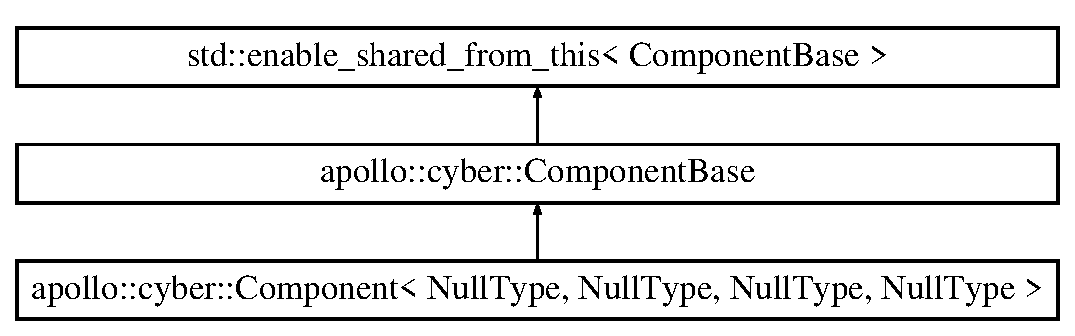
\includegraphics[height=3.000000cm]{classapollo_1_1cyber_1_1Component_3_01NullType_00_01NullType_00_01NullType_00_01NullType_01_4}
\end{center}
\end{figure}
\subsection*{Public Member Functions}
\begin{DoxyCompactItemize}
\item 
\hyperlink{classapollo_1_1cyber_1_1Component_3_01NullType_00_01NullType_00_01NullType_00_01NullType_01_4_ae98b0732d4a874991a0fef7f93fb0fc5}{Component} ()
\item 
\hyperlink{classapollo_1_1cyber_1_1Component_3_01NullType_00_01NullType_00_01NullType_00_01NullType_01_4_a4905afe141dbe487ae0a9ded030a98ea}{$\sim$\-Component} () override
\item 
bool \hyperlink{classapollo_1_1cyber_1_1Component_3_01NullType_00_01NullType_00_01NullType_00_01NullType_01_4_a8890f8e7c2b7d81f70802e879ff71c22}{Initialize} (const Component\-Config \&config) override
\end{DoxyCompactItemize}
\subsection*{Additional Inherited Members}


\subsection{Constructor \& Destructor Documentation}
\hypertarget{classapollo_1_1cyber_1_1Component_3_01NullType_00_01NullType_00_01NullType_00_01NullType_01_4_ae98b0732d4a874991a0fef7f93fb0fc5}{\index{apollo\-::cyber\-::\-Component$<$ Null\-Type, Null\-Type, Null\-Type, Null\-Type $>$@{apollo\-::cyber\-::\-Component$<$ Null\-Type, Null\-Type, Null\-Type, Null\-Type $>$}!Component@{Component}}
\index{Component@{Component}!apollo::cyber::Component< NullType, NullType, NullType, NullType >@{apollo\-::cyber\-::\-Component$<$ Null\-Type, Null\-Type, Null\-Type, Null\-Type $>$}}
\subsubsection[{Component}]{\setlength{\rightskip}{0pt plus 5cm}{\bf apollo\-::cyber\-::\-Component}$<$ {\bf Null\-Type}, {\bf Null\-Type}, {\bf Null\-Type}, {\bf Null\-Type} $>$\-::{\bf Component} (
\begin{DoxyParamCaption}
{}
\end{DoxyParamCaption}
)\hspace{0.3cm}{\ttfamily [inline]}}}\label{classapollo_1_1cyber_1_1Component_3_01NullType_00_01NullType_00_01NullType_00_01NullType_01_4_ae98b0732d4a874991a0fef7f93fb0fc5}
\hypertarget{classapollo_1_1cyber_1_1Component_3_01NullType_00_01NullType_00_01NullType_00_01NullType_01_4_a4905afe141dbe487ae0a9ded030a98ea}{\index{apollo\-::cyber\-::\-Component$<$ Null\-Type, Null\-Type, Null\-Type, Null\-Type $>$@{apollo\-::cyber\-::\-Component$<$ Null\-Type, Null\-Type, Null\-Type, Null\-Type $>$}!$\sim$\-Component@{$\sim$\-Component}}
\index{$\sim$\-Component@{$\sim$\-Component}!apollo::cyber::Component< NullType, NullType, NullType, NullType >@{apollo\-::cyber\-::\-Component$<$ Null\-Type, Null\-Type, Null\-Type, Null\-Type $>$}}
\subsubsection[{$\sim$\-Component}]{\setlength{\rightskip}{0pt plus 5cm}{\bf apollo\-::cyber\-::\-Component}$<$ {\bf Null\-Type}, {\bf Null\-Type}, {\bf Null\-Type}, {\bf Null\-Type} $>$\-::$\sim${\bf Component} (
\begin{DoxyParamCaption}
{}
\end{DoxyParamCaption}
)\hspace{0.3cm}{\ttfamily [inline]}, {\ttfamily [override]}}}\label{classapollo_1_1cyber_1_1Component_3_01NullType_00_01NullType_00_01NullType_00_01NullType_01_4_a4905afe141dbe487ae0a9ded030a98ea}


\subsection{Member Function Documentation}
\hypertarget{classapollo_1_1cyber_1_1Component_3_01NullType_00_01NullType_00_01NullType_00_01NullType_01_4_a8890f8e7c2b7d81f70802e879ff71c22}{\index{apollo\-::cyber\-::\-Component$<$ Null\-Type, Null\-Type, Null\-Type, Null\-Type $>$@{apollo\-::cyber\-::\-Component$<$ Null\-Type, Null\-Type, Null\-Type, Null\-Type $>$}!Initialize@{Initialize}}
\index{Initialize@{Initialize}!apollo::cyber::Component< NullType, NullType, NullType, NullType >@{apollo\-::cyber\-::\-Component$<$ Null\-Type, Null\-Type, Null\-Type, Null\-Type $>$}}
\subsubsection[{Initialize}]{\setlength{\rightskip}{0pt plus 5cm}bool {\bf apollo\-::cyber\-::\-Component}$<$ {\bf Null\-Type}, {\bf Null\-Type}, {\bf Null\-Type}, {\bf Null\-Type} $>$\-::Initialize (
\begin{DoxyParamCaption}
\item[{const Component\-Config \&}]{config}
\end{DoxyParamCaption}
)\hspace{0.3cm}{\ttfamily [override]}, {\ttfamily [virtual]}}}\label{classapollo_1_1cyber_1_1Component_3_01NullType_00_01NullType_00_01NullType_00_01NullType_01_4_a8890f8e7c2b7d81f70802e879ff71c22}


Reimplemented from \hyperlink{classapollo_1_1cyber_1_1ComponentBase_a234ab17fb5f504179b9f49d344e72882}{apollo\-::cyber\-::\-Component\-Base}.



The documentation for this class was generated from the following file\-:\begin{DoxyCompactItemize}
\item 
component/\hyperlink{component_8h}{component.\-h}\end{DoxyCompactItemize}

\hypertarget{classapollo_1_1cyber_1_1ComponentBase}{\section{apollo\-:\-:cyber\-:\-:Component\-Base Class Reference}
\label{classapollo_1_1cyber_1_1ComponentBase}\index{apollo\-::cyber\-::\-Component\-Base@{apollo\-::cyber\-::\-Component\-Base}}
}


{\ttfamily \#include $<$component\-\_\-base.\-h$>$}

Inheritance diagram for apollo\-:\-:cyber\-:\-:Component\-Base\-:\begin{figure}[H]
\begin{center}
\leavevmode
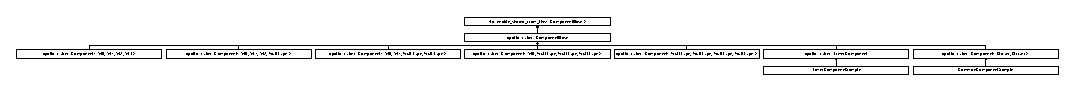
\includegraphics[height=0.774818cm]{classapollo_1_1cyber_1_1ComponentBase}
\end{center}
\end{figure}
\subsection*{Public Types}
\begin{DoxyCompactItemize}
\item 
{\footnotesize template$<$typename M $>$ }\\using \hyperlink{classapollo_1_1cyber_1_1ComponentBase_afca61d12e5699b85020c0d4250e132f9}{Reader} = \hyperlink{classapollo_1_1cyber_1_1Reader}{cyber\-::\-Reader}$<$ M $>$
\end{DoxyCompactItemize}
\subsection*{Public Member Functions}
\begin{DoxyCompactItemize}
\item 
virtual \hyperlink{classapollo_1_1cyber_1_1ComponentBase_a1a6c3712519c64c9f652c9f7bd62814a}{$\sim$\-Component\-Base} ()
\item 
virtual bool \hyperlink{classapollo_1_1cyber_1_1ComponentBase_a234ab17fb5f504179b9f49d344e72882}{Initialize} (const Component\-Config \&config)
\item 
virtual bool \hyperlink{classapollo_1_1cyber_1_1ComponentBase_a37d357e2eceb17811db7a7acaae59047}{Initialize} (const Timer\-Component\-Config \&config)
\item 
virtual void \hyperlink{classapollo_1_1cyber_1_1ComponentBase_a6d584e0ab4d990fdad46f845d2e43167}{Shutdown} ()
\item 
{\footnotesize template$<$typename T $>$ }\\bool \hyperlink{classapollo_1_1cyber_1_1ComponentBase_a6757b622cfa042adc580dc8a89a668f8}{Get\-Proto\-Config} (T $\ast$config) const 
\end{DoxyCompactItemize}
\subsection*{Protected Member Functions}
\begin{DoxyCompactItemize}
\item 
virtual bool \hyperlink{classapollo_1_1cyber_1_1ComponentBase_ae9901cb3bfa8ef33c42b465606dbe0e5}{Init} ()=0
\item 
virtual void \hyperlink{classapollo_1_1cyber_1_1ComponentBase_a05394f4bc5c70604f45a9194b1948aa4}{Clear} ()
\item 
const std\-::string \& \hyperlink{classapollo_1_1cyber_1_1ComponentBase_a77aaf08fe82edd39034868519d5be4cc}{Config\-File\-Path} () const 
\item 
void \hyperlink{classapollo_1_1cyber_1_1ComponentBase_afc6983393f7b411e673b09edd90e1643}{Load\-Config\-Files} (const Component\-Config \&config)
\item 
void \hyperlink{classapollo_1_1cyber_1_1ComponentBase_aa6e7e5f9294f87bb5ff8c859ed1def27}{Load\-Config\-Files} (const Timer\-Component\-Config \&config)
\end{DoxyCompactItemize}
\subsection*{Protected Attributes}
\begin{DoxyCompactItemize}
\item 
std\-::atomic$<$ bool $>$ \hyperlink{classapollo_1_1cyber_1_1ComponentBase_a8e11428c0f4b5566ac3a602cef96516c}{is\-\_\-shutdown\-\_\-} = \{false\}
\item 
std\-::shared\-\_\-ptr$<$ \hyperlink{classapollo_1_1cyber_1_1Node}{Node} $>$ \hyperlink{classapollo_1_1cyber_1_1ComponentBase_ae561da7f75d403c45eca1ff3d0cfe2c8}{node\-\_\-} = nullptr
\item 
std\-::string \hyperlink{classapollo_1_1cyber_1_1ComponentBase_afb307772b21999bdb29e2ec866acfc75}{config\-\_\-file\-\_\-path\-\_\-} = \char`\"{}\char`\"{}
\item 
std\-::vector$<$ std\-::shared\-\_\-ptr\\*
$<$ \hyperlink{classapollo_1_1cyber_1_1ReaderBase}{Reader\-Base} $>$ $>$ \hyperlink{classapollo_1_1cyber_1_1ComponentBase_a381445ac2102bd1a34dbf87fef480919}{readers\-\_\-}
\end{DoxyCompactItemize}


\subsection{Member Typedef Documentation}
\hypertarget{classapollo_1_1cyber_1_1ComponentBase_afca61d12e5699b85020c0d4250e132f9}{\index{apollo\-::cyber\-::\-Component\-Base@{apollo\-::cyber\-::\-Component\-Base}!Reader@{Reader}}
\index{Reader@{Reader}!apollo::cyber::ComponentBase@{apollo\-::cyber\-::\-Component\-Base}}
\subsubsection[{Reader}]{\setlength{\rightskip}{0pt plus 5cm}template$<$typename M $>$ using {\bf apollo\-::cyber\-::\-Component\-Base\-::\-Reader} =  {\bf cyber\-::\-Reader}$<$M$>$}}\label{classapollo_1_1cyber_1_1ComponentBase_afca61d12e5699b85020c0d4250e132f9}


\subsection{Constructor \& Destructor Documentation}
\hypertarget{classapollo_1_1cyber_1_1ComponentBase_a1a6c3712519c64c9f652c9f7bd62814a}{\index{apollo\-::cyber\-::\-Component\-Base@{apollo\-::cyber\-::\-Component\-Base}!$\sim$\-Component\-Base@{$\sim$\-Component\-Base}}
\index{$\sim$\-Component\-Base@{$\sim$\-Component\-Base}!apollo::cyber::ComponentBase@{apollo\-::cyber\-::\-Component\-Base}}
\subsubsection[{$\sim$\-Component\-Base}]{\setlength{\rightskip}{0pt plus 5cm}virtual apollo\-::cyber\-::\-Component\-Base\-::$\sim$\-Component\-Base (
\begin{DoxyParamCaption}
{}
\end{DoxyParamCaption}
)\hspace{0.3cm}{\ttfamily [inline]}, {\ttfamily [virtual]}}}\label{classapollo_1_1cyber_1_1ComponentBase_a1a6c3712519c64c9f652c9f7bd62814a}


\subsection{Member Function Documentation}
\hypertarget{classapollo_1_1cyber_1_1ComponentBase_a05394f4bc5c70604f45a9194b1948aa4}{\index{apollo\-::cyber\-::\-Component\-Base@{apollo\-::cyber\-::\-Component\-Base}!Clear@{Clear}}
\index{Clear@{Clear}!apollo::cyber::ComponentBase@{apollo\-::cyber\-::\-Component\-Base}}
\subsubsection[{Clear}]{\setlength{\rightskip}{0pt plus 5cm}virtual void apollo\-::cyber\-::\-Component\-Base\-::\-Clear (
\begin{DoxyParamCaption}
{}
\end{DoxyParamCaption}
)\hspace{0.3cm}{\ttfamily [inline]}, {\ttfamily [protected]}, {\ttfamily [virtual]}}}\label{classapollo_1_1cyber_1_1ComponentBase_a05394f4bc5c70604f45a9194b1948aa4}
\hypertarget{classapollo_1_1cyber_1_1ComponentBase_a77aaf08fe82edd39034868519d5be4cc}{\index{apollo\-::cyber\-::\-Component\-Base@{apollo\-::cyber\-::\-Component\-Base}!Config\-File\-Path@{Config\-File\-Path}}
\index{Config\-File\-Path@{Config\-File\-Path}!apollo::cyber::ComponentBase@{apollo\-::cyber\-::\-Component\-Base}}
\subsubsection[{Config\-File\-Path}]{\setlength{\rightskip}{0pt plus 5cm}const std\-::string\& apollo\-::cyber\-::\-Component\-Base\-::\-Config\-File\-Path (
\begin{DoxyParamCaption}
{}
\end{DoxyParamCaption}
) const\hspace{0.3cm}{\ttfamily [inline]}, {\ttfamily [protected]}}}\label{classapollo_1_1cyber_1_1ComponentBase_a77aaf08fe82edd39034868519d5be4cc}
\hypertarget{classapollo_1_1cyber_1_1ComponentBase_a6757b622cfa042adc580dc8a89a668f8}{\index{apollo\-::cyber\-::\-Component\-Base@{apollo\-::cyber\-::\-Component\-Base}!Get\-Proto\-Config@{Get\-Proto\-Config}}
\index{Get\-Proto\-Config@{Get\-Proto\-Config}!apollo::cyber::ComponentBase@{apollo\-::cyber\-::\-Component\-Base}}
\subsubsection[{Get\-Proto\-Config}]{\setlength{\rightskip}{0pt plus 5cm}template$<$typename T $>$ bool apollo\-::cyber\-::\-Component\-Base\-::\-Get\-Proto\-Config (
\begin{DoxyParamCaption}
\item[{T $\ast$}]{config}
\end{DoxyParamCaption}
) const\hspace{0.3cm}{\ttfamily [inline]}}}\label{classapollo_1_1cyber_1_1ComponentBase_a6757b622cfa042adc580dc8a89a668f8}
\hypertarget{classapollo_1_1cyber_1_1ComponentBase_ae9901cb3bfa8ef33c42b465606dbe0e5}{\index{apollo\-::cyber\-::\-Component\-Base@{apollo\-::cyber\-::\-Component\-Base}!Init@{Init}}
\index{Init@{Init}!apollo::cyber::ComponentBase@{apollo\-::cyber\-::\-Component\-Base}}
\subsubsection[{Init}]{\setlength{\rightskip}{0pt plus 5cm}virtual bool apollo\-::cyber\-::\-Component\-Base\-::\-Init (
\begin{DoxyParamCaption}
{}
\end{DoxyParamCaption}
)\hspace{0.3cm}{\ttfamily [protected]}, {\ttfamily [pure virtual]}}}\label{classapollo_1_1cyber_1_1ComponentBase_ae9901cb3bfa8ef33c42b465606dbe0e5}


Implemented in \hyperlink{classapollo_1_1cyber_1_1TimerComponent_a1aca7ad923de44fba59a868988563ad3}{apollo\-::cyber\-::\-Timer\-Component}, \hyperlink{classTimerComponentSample_a9c22f7d8495e603211cfff603441e8b9}{Timer\-Component\-Sample}, and \hyperlink{classCommonComponentSample_ae2a3f8c8ce4b9cfd9c6b357628bc84ee}{Common\-Component\-Sample}.

\hypertarget{classapollo_1_1cyber_1_1ComponentBase_a234ab17fb5f504179b9f49d344e72882}{\index{apollo\-::cyber\-::\-Component\-Base@{apollo\-::cyber\-::\-Component\-Base}!Initialize@{Initialize}}
\index{Initialize@{Initialize}!apollo::cyber::ComponentBase@{apollo\-::cyber\-::\-Component\-Base}}
\subsubsection[{Initialize}]{\setlength{\rightskip}{0pt plus 5cm}virtual bool apollo\-::cyber\-::\-Component\-Base\-::\-Initialize (
\begin{DoxyParamCaption}
\item[{const Component\-Config \&}]{config}
\end{DoxyParamCaption}
)\hspace{0.3cm}{\ttfamily [inline]}, {\ttfamily [virtual]}}}\label{classapollo_1_1cyber_1_1ComponentBase_a234ab17fb5f504179b9f49d344e72882}


Reimplemented in \hyperlink{classapollo_1_1cyber_1_1Component_3_01M0_00_01M1_00_01M2_00_01NullType_01_4_ae890450f0eb587c8ea7fbfa91259876a}{apollo\-::cyber\-::\-Component$<$ M0, M1, M2, Null\-Type $>$}, \hyperlink{classapollo_1_1cyber_1_1Component_3_01M0_00_01M1_00_01NullType_00_01NullType_01_4_ab3c98c371afed14286ed36f89eb84e7f}{apollo\-::cyber\-::\-Component$<$ M0, M1, Null\-Type, Null\-Type $>$}, \hyperlink{classapollo_1_1cyber_1_1Component_3_01M0_00_01NullType_00_01NullType_00_01NullType_01_4_a9e859b2698539158448b19aa156f48d6}{apollo\-::cyber\-::\-Component$<$ M0, Null\-Type, Null\-Type, Null\-Type $>$}, \hyperlink{classapollo_1_1cyber_1_1Component_3_01NullType_00_01NullType_00_01NullType_00_01NullType_01_4_a8890f8e7c2b7d81f70802e879ff71c22}{apollo\-::cyber\-::\-Component$<$ Null\-Type, Null\-Type, Null\-Type, Null\-Type $>$}, \hyperlink{classapollo_1_1cyber_1_1Component_ae68b7c7dce67c4d5c6c024c910bb9d92}{apollo\-::cyber\-::\-Component$<$ M0, M1, M2, M3 $>$}, and \hyperlink{classapollo_1_1cyber_1_1Component_ae68b7c7dce67c4d5c6c024c910bb9d92}{apollo\-::cyber\-::\-Component$<$ Driver, Driver $>$}.

\hypertarget{classapollo_1_1cyber_1_1ComponentBase_a37d357e2eceb17811db7a7acaae59047}{\index{apollo\-::cyber\-::\-Component\-Base@{apollo\-::cyber\-::\-Component\-Base}!Initialize@{Initialize}}
\index{Initialize@{Initialize}!apollo::cyber::ComponentBase@{apollo\-::cyber\-::\-Component\-Base}}
\subsubsection[{Initialize}]{\setlength{\rightskip}{0pt plus 5cm}virtual bool apollo\-::cyber\-::\-Component\-Base\-::\-Initialize (
\begin{DoxyParamCaption}
\item[{const Timer\-Component\-Config \&}]{config}
\end{DoxyParamCaption}
)\hspace{0.3cm}{\ttfamily [inline]}, {\ttfamily [virtual]}}}\label{classapollo_1_1cyber_1_1ComponentBase_a37d357e2eceb17811db7a7acaae59047}


Reimplemented in \hyperlink{classapollo_1_1cyber_1_1TimerComponent_ab3ccbb7662d6b83d1d58d790a6d1713d}{apollo\-::cyber\-::\-Timer\-Component}.

\hypertarget{classapollo_1_1cyber_1_1ComponentBase_afc6983393f7b411e673b09edd90e1643}{\index{apollo\-::cyber\-::\-Component\-Base@{apollo\-::cyber\-::\-Component\-Base}!Load\-Config\-Files@{Load\-Config\-Files}}
\index{Load\-Config\-Files@{Load\-Config\-Files}!apollo::cyber::ComponentBase@{apollo\-::cyber\-::\-Component\-Base}}
\subsubsection[{Load\-Config\-Files}]{\setlength{\rightskip}{0pt plus 5cm}void apollo\-::cyber\-::\-Component\-Base\-::\-Load\-Config\-Files (
\begin{DoxyParamCaption}
\item[{const Component\-Config \&}]{config}
\end{DoxyParamCaption}
)\hspace{0.3cm}{\ttfamily [inline]}, {\ttfamily [protected]}}}\label{classapollo_1_1cyber_1_1ComponentBase_afc6983393f7b411e673b09edd90e1643}
\hypertarget{classapollo_1_1cyber_1_1ComponentBase_aa6e7e5f9294f87bb5ff8c859ed1def27}{\index{apollo\-::cyber\-::\-Component\-Base@{apollo\-::cyber\-::\-Component\-Base}!Load\-Config\-Files@{Load\-Config\-Files}}
\index{Load\-Config\-Files@{Load\-Config\-Files}!apollo::cyber::ComponentBase@{apollo\-::cyber\-::\-Component\-Base}}
\subsubsection[{Load\-Config\-Files}]{\setlength{\rightskip}{0pt plus 5cm}void apollo\-::cyber\-::\-Component\-Base\-::\-Load\-Config\-Files (
\begin{DoxyParamCaption}
\item[{const Timer\-Component\-Config \&}]{config}
\end{DoxyParamCaption}
)\hspace{0.3cm}{\ttfamily [inline]}, {\ttfamily [protected]}}}\label{classapollo_1_1cyber_1_1ComponentBase_aa6e7e5f9294f87bb5ff8c859ed1def27}
\hypertarget{classapollo_1_1cyber_1_1ComponentBase_a6d584e0ab4d990fdad46f845d2e43167}{\index{apollo\-::cyber\-::\-Component\-Base@{apollo\-::cyber\-::\-Component\-Base}!Shutdown@{Shutdown}}
\index{Shutdown@{Shutdown}!apollo::cyber::ComponentBase@{apollo\-::cyber\-::\-Component\-Base}}
\subsubsection[{Shutdown}]{\setlength{\rightskip}{0pt plus 5cm}virtual void apollo\-::cyber\-::\-Component\-Base\-::\-Shutdown (
\begin{DoxyParamCaption}
{}
\end{DoxyParamCaption}
)\hspace{0.3cm}{\ttfamily [inline]}, {\ttfamily [virtual]}}}\label{classapollo_1_1cyber_1_1ComponentBase_a6d584e0ab4d990fdad46f845d2e43167}


\subsection{Member Data Documentation}
\hypertarget{classapollo_1_1cyber_1_1ComponentBase_afb307772b21999bdb29e2ec866acfc75}{\index{apollo\-::cyber\-::\-Component\-Base@{apollo\-::cyber\-::\-Component\-Base}!config\-\_\-file\-\_\-path\-\_\-@{config\-\_\-file\-\_\-path\-\_\-}}
\index{config\-\_\-file\-\_\-path\-\_\-@{config\-\_\-file\-\_\-path\-\_\-}!apollo::cyber::ComponentBase@{apollo\-::cyber\-::\-Component\-Base}}
\subsubsection[{config\-\_\-file\-\_\-path\-\_\-}]{\setlength{\rightskip}{0pt plus 5cm}std\-::string apollo\-::cyber\-::\-Component\-Base\-::config\-\_\-file\-\_\-path\-\_\- = \char`\"{}\char`\"{}\hspace{0.3cm}{\ttfamily [protected]}}}\label{classapollo_1_1cyber_1_1ComponentBase_afb307772b21999bdb29e2ec866acfc75}
\hypertarget{classapollo_1_1cyber_1_1ComponentBase_a8e11428c0f4b5566ac3a602cef96516c}{\index{apollo\-::cyber\-::\-Component\-Base@{apollo\-::cyber\-::\-Component\-Base}!is\-\_\-shutdown\-\_\-@{is\-\_\-shutdown\-\_\-}}
\index{is\-\_\-shutdown\-\_\-@{is\-\_\-shutdown\-\_\-}!apollo::cyber::ComponentBase@{apollo\-::cyber\-::\-Component\-Base}}
\subsubsection[{is\-\_\-shutdown\-\_\-}]{\setlength{\rightskip}{0pt plus 5cm}std\-::atomic$<$bool$>$ apollo\-::cyber\-::\-Component\-Base\-::is\-\_\-shutdown\-\_\- = \{false\}\hspace{0.3cm}{\ttfamily [protected]}}}\label{classapollo_1_1cyber_1_1ComponentBase_a8e11428c0f4b5566ac3a602cef96516c}
\hypertarget{classapollo_1_1cyber_1_1ComponentBase_ae561da7f75d403c45eca1ff3d0cfe2c8}{\index{apollo\-::cyber\-::\-Component\-Base@{apollo\-::cyber\-::\-Component\-Base}!node\-\_\-@{node\-\_\-}}
\index{node\-\_\-@{node\-\_\-}!apollo::cyber::ComponentBase@{apollo\-::cyber\-::\-Component\-Base}}
\subsubsection[{node\-\_\-}]{\setlength{\rightskip}{0pt plus 5cm}std\-::shared\-\_\-ptr$<${\bf Node}$>$ apollo\-::cyber\-::\-Component\-Base\-::node\-\_\- = nullptr\hspace{0.3cm}{\ttfamily [protected]}}}\label{classapollo_1_1cyber_1_1ComponentBase_ae561da7f75d403c45eca1ff3d0cfe2c8}
\hypertarget{classapollo_1_1cyber_1_1ComponentBase_a381445ac2102bd1a34dbf87fef480919}{\index{apollo\-::cyber\-::\-Component\-Base@{apollo\-::cyber\-::\-Component\-Base}!readers\-\_\-@{readers\-\_\-}}
\index{readers\-\_\-@{readers\-\_\-}!apollo::cyber::ComponentBase@{apollo\-::cyber\-::\-Component\-Base}}
\subsubsection[{readers\-\_\-}]{\setlength{\rightskip}{0pt plus 5cm}std\-::vector$<$std\-::shared\-\_\-ptr$<${\bf Reader\-Base}$>$ $>$ apollo\-::cyber\-::\-Component\-Base\-::readers\-\_\-\hspace{0.3cm}{\ttfamily [protected]}}}\label{classapollo_1_1cyber_1_1ComponentBase_a381445ac2102bd1a34dbf87fef480919}


The documentation for this class was generated from the following file\-:\begin{DoxyCompactItemize}
\item 
component/\hyperlink{component__base_8h}{component\-\_\-base.\-h}\end{DoxyCompactItemize}

\hypertarget{classapollo_1_1cyber_1_1transport_1_1ConditionNotifier}{\section{apollo\-:\-:cyber\-:\-:transport\-:\-:Condition\-Notifier Class Reference}
\label{classapollo_1_1cyber_1_1transport_1_1ConditionNotifier}\index{apollo\-::cyber\-::transport\-::\-Condition\-Notifier@{apollo\-::cyber\-::transport\-::\-Condition\-Notifier}}
}


{\ttfamily \#include $<$condition\-\_\-notifier.\-h$>$}

Inheritance diagram for apollo\-:\-:cyber\-:\-:transport\-:\-:Condition\-Notifier\-:\begin{figure}[H]
\begin{center}
\leavevmode
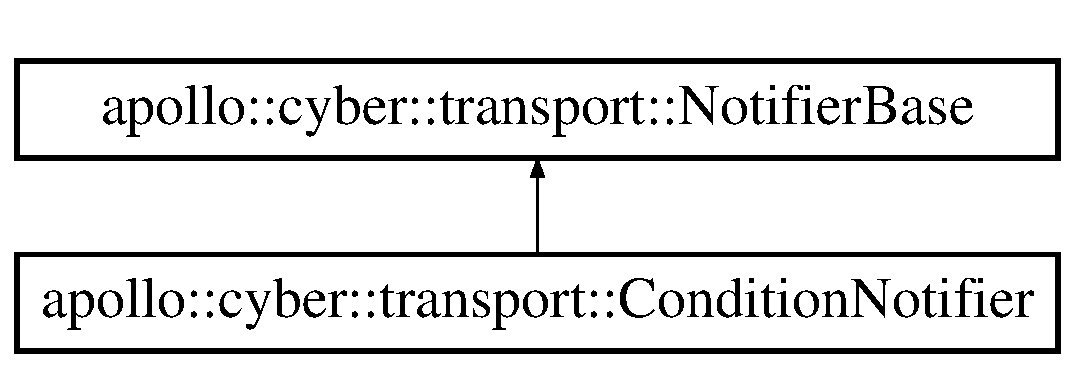
\includegraphics[height=2.000000cm]{classapollo_1_1cyber_1_1transport_1_1ConditionNotifier}
\end{center}
\end{figure}
\subsection*{Classes}
\begin{DoxyCompactItemize}
\item 
struct \hyperlink{structapollo_1_1cyber_1_1transport_1_1ConditionNotifier_1_1Indicator}{Indicator}
\end{DoxyCompactItemize}
\subsection*{Public Member Functions}
\begin{DoxyCompactItemize}
\item 
virtual \hyperlink{classapollo_1_1cyber_1_1transport_1_1ConditionNotifier_a7e4bd95c4da5a8d1e6194c255ee75eb3}{$\sim$\-Condition\-Notifier} ()
\item 
void \hyperlink{classapollo_1_1cyber_1_1transport_1_1ConditionNotifier_a057d3f71a69a9913107416166a01a81b}{Shutdown} () override
\item 
bool \hyperlink{classapollo_1_1cyber_1_1transport_1_1ConditionNotifier_ad9d938243de75dc7b015ca2ca9819f01}{Notify} (const \hyperlink{classapollo_1_1cyber_1_1transport_1_1ReadableInfo}{Readable\-Info} \&info) override
\item 
bool \hyperlink{classapollo_1_1cyber_1_1transport_1_1ConditionNotifier_a961bd6d94fdae4ffa6a7413a95932db5}{Listen} (int timeout\-\_\-ms, \hyperlink{classapollo_1_1cyber_1_1transport_1_1ReadableInfo}{Readable\-Info} $\ast$info) override
\end{DoxyCompactItemize}
\subsection*{Static Public Member Functions}
\begin{DoxyCompactItemize}
\item 
static const char $\ast$ \hyperlink{classapollo_1_1cyber_1_1transport_1_1ConditionNotifier_a176c1ca8f3cbc3c15ff2fba4eb0280e2}{Type} ()
\end{DoxyCompactItemize}
\subsection*{Private Member Functions}
\begin{DoxyCompactItemize}
\item 
bool \hyperlink{classapollo_1_1cyber_1_1transport_1_1ConditionNotifier_a822ee78c2f903e366f3c58cc9a9eafa1}{Init} ()
\item 
bool \hyperlink{classapollo_1_1cyber_1_1transport_1_1ConditionNotifier_a506f0777ddba9729af366d6df37b40ad}{Open\-Or\-Create} ()
\item 
bool \hyperlink{classapollo_1_1cyber_1_1transport_1_1ConditionNotifier_afaf6b12a6030861f6ad009b6cfd42f27}{Open\-Only} ()
\item 
bool \hyperlink{classapollo_1_1cyber_1_1transport_1_1ConditionNotifier_aa72b3769316e25e2d4faee6eac8c30a2}{Remove} ()
\item 
void \hyperlink{classapollo_1_1cyber_1_1transport_1_1ConditionNotifier_a5094406c9605ef19b646208ae6036d77}{Reset} ()
\end{DoxyCompactItemize}
\subsection*{Private Attributes}
\begin{DoxyCompactItemize}
\item 
key\-\_\-t \hyperlink{classapollo_1_1cyber_1_1transport_1_1ConditionNotifier_aa5d9958e7a5c7abc7f04ce84f0385c9a}{key\-\_\-} = 0
\item 
void $\ast$ \hyperlink{classapollo_1_1cyber_1_1transport_1_1ConditionNotifier_a22cba07e5cce1d0a782c51f3bcbb09c8}{managed\-\_\-shm\-\_\-} = nullptr
\item 
size\-\_\-t \hyperlink{classapollo_1_1cyber_1_1transport_1_1ConditionNotifier_a48fcd814d133e570bcaaed0527e72edc}{shm\-\_\-size\-\_\-} = 0
\item 
\hyperlink{structapollo_1_1cyber_1_1transport_1_1ConditionNotifier_1_1Indicator}{Indicator} $\ast$ \hyperlink{classapollo_1_1cyber_1_1transport_1_1ConditionNotifier_ac9867419135c8a5484cc1296a69ee7e0}{indicator\-\_\-} = nullptr
\item 
uint64\-\_\-t \hyperlink{classapollo_1_1cyber_1_1transport_1_1ConditionNotifier_a55460f4f3c02cd6cb0d5e0dcabd7576e}{next\-\_\-listen\-\_\-num\-\_\-} = 0
\item 
std\-::atomic$<$ bool $>$ \hyperlink{classapollo_1_1cyber_1_1transport_1_1ConditionNotifier_af8e320c5121acbb3b50956ac7519fdb8}{is\-\_\-shutdown\-\_\-} = \{false\}
\end{DoxyCompactItemize}


\subsection{Constructor \& Destructor Documentation}
\hypertarget{classapollo_1_1cyber_1_1transport_1_1ConditionNotifier_a7e4bd95c4da5a8d1e6194c255ee75eb3}{\index{apollo\-::cyber\-::transport\-::\-Condition\-Notifier@{apollo\-::cyber\-::transport\-::\-Condition\-Notifier}!$\sim$\-Condition\-Notifier@{$\sim$\-Condition\-Notifier}}
\index{$\sim$\-Condition\-Notifier@{$\sim$\-Condition\-Notifier}!apollo::cyber::transport::ConditionNotifier@{apollo\-::cyber\-::transport\-::\-Condition\-Notifier}}
\subsubsection[{$\sim$\-Condition\-Notifier}]{\setlength{\rightskip}{0pt plus 5cm}virtual apollo\-::cyber\-::transport\-::\-Condition\-Notifier\-::$\sim$\-Condition\-Notifier (
\begin{DoxyParamCaption}
{}
\end{DoxyParamCaption}
)\hspace{0.3cm}{\ttfamily [virtual]}}}\label{classapollo_1_1cyber_1_1transport_1_1ConditionNotifier_a7e4bd95c4da5a8d1e6194c255ee75eb3}


\subsection{Member Function Documentation}
\hypertarget{classapollo_1_1cyber_1_1transport_1_1ConditionNotifier_a822ee78c2f903e366f3c58cc9a9eafa1}{\index{apollo\-::cyber\-::transport\-::\-Condition\-Notifier@{apollo\-::cyber\-::transport\-::\-Condition\-Notifier}!Init@{Init}}
\index{Init@{Init}!apollo::cyber::transport::ConditionNotifier@{apollo\-::cyber\-::transport\-::\-Condition\-Notifier}}
\subsubsection[{Init}]{\setlength{\rightskip}{0pt plus 5cm}bool apollo\-::cyber\-::transport\-::\-Condition\-Notifier\-::\-Init (
\begin{DoxyParamCaption}
{}
\end{DoxyParamCaption}
)\hspace{0.3cm}{\ttfamily [private]}}}\label{classapollo_1_1cyber_1_1transport_1_1ConditionNotifier_a822ee78c2f903e366f3c58cc9a9eafa1}
\hypertarget{classapollo_1_1cyber_1_1transport_1_1ConditionNotifier_a961bd6d94fdae4ffa6a7413a95932db5}{\index{apollo\-::cyber\-::transport\-::\-Condition\-Notifier@{apollo\-::cyber\-::transport\-::\-Condition\-Notifier}!Listen@{Listen}}
\index{Listen@{Listen}!apollo::cyber::transport::ConditionNotifier@{apollo\-::cyber\-::transport\-::\-Condition\-Notifier}}
\subsubsection[{Listen}]{\setlength{\rightskip}{0pt plus 5cm}bool apollo\-::cyber\-::transport\-::\-Condition\-Notifier\-::\-Listen (
\begin{DoxyParamCaption}
\item[{int}]{timeout\-\_\-ms, }
\item[{{\bf Readable\-Info} $\ast$}]{info}
\end{DoxyParamCaption}
)\hspace{0.3cm}{\ttfamily [override]}, {\ttfamily [virtual]}}}\label{classapollo_1_1cyber_1_1transport_1_1ConditionNotifier_a961bd6d94fdae4ffa6a7413a95932db5}


Implements \hyperlink{classapollo_1_1cyber_1_1transport_1_1NotifierBase_aa42f5b65d60d3b61a919f09b7605775b}{apollo\-::cyber\-::transport\-::\-Notifier\-Base}.

\hypertarget{classapollo_1_1cyber_1_1transport_1_1ConditionNotifier_ad9d938243de75dc7b015ca2ca9819f01}{\index{apollo\-::cyber\-::transport\-::\-Condition\-Notifier@{apollo\-::cyber\-::transport\-::\-Condition\-Notifier}!Notify@{Notify}}
\index{Notify@{Notify}!apollo::cyber::transport::ConditionNotifier@{apollo\-::cyber\-::transport\-::\-Condition\-Notifier}}
\subsubsection[{Notify}]{\setlength{\rightskip}{0pt plus 5cm}bool apollo\-::cyber\-::transport\-::\-Condition\-Notifier\-::\-Notify (
\begin{DoxyParamCaption}
\item[{const {\bf Readable\-Info} \&}]{info}
\end{DoxyParamCaption}
)\hspace{0.3cm}{\ttfamily [override]}, {\ttfamily [virtual]}}}\label{classapollo_1_1cyber_1_1transport_1_1ConditionNotifier_ad9d938243de75dc7b015ca2ca9819f01}


Implements \hyperlink{classapollo_1_1cyber_1_1transport_1_1NotifierBase_aef2741bc38fa6b7aca8c1cfb012975dd}{apollo\-::cyber\-::transport\-::\-Notifier\-Base}.

\hypertarget{classapollo_1_1cyber_1_1transport_1_1ConditionNotifier_afaf6b12a6030861f6ad009b6cfd42f27}{\index{apollo\-::cyber\-::transport\-::\-Condition\-Notifier@{apollo\-::cyber\-::transport\-::\-Condition\-Notifier}!Open\-Only@{Open\-Only}}
\index{Open\-Only@{Open\-Only}!apollo::cyber::transport::ConditionNotifier@{apollo\-::cyber\-::transport\-::\-Condition\-Notifier}}
\subsubsection[{Open\-Only}]{\setlength{\rightskip}{0pt plus 5cm}bool apollo\-::cyber\-::transport\-::\-Condition\-Notifier\-::\-Open\-Only (
\begin{DoxyParamCaption}
{}
\end{DoxyParamCaption}
)\hspace{0.3cm}{\ttfamily [private]}}}\label{classapollo_1_1cyber_1_1transport_1_1ConditionNotifier_afaf6b12a6030861f6ad009b6cfd42f27}
\hypertarget{classapollo_1_1cyber_1_1transport_1_1ConditionNotifier_a506f0777ddba9729af366d6df37b40ad}{\index{apollo\-::cyber\-::transport\-::\-Condition\-Notifier@{apollo\-::cyber\-::transport\-::\-Condition\-Notifier}!Open\-Or\-Create@{Open\-Or\-Create}}
\index{Open\-Or\-Create@{Open\-Or\-Create}!apollo::cyber::transport::ConditionNotifier@{apollo\-::cyber\-::transport\-::\-Condition\-Notifier}}
\subsubsection[{Open\-Or\-Create}]{\setlength{\rightskip}{0pt plus 5cm}bool apollo\-::cyber\-::transport\-::\-Condition\-Notifier\-::\-Open\-Or\-Create (
\begin{DoxyParamCaption}
{}
\end{DoxyParamCaption}
)\hspace{0.3cm}{\ttfamily [private]}}}\label{classapollo_1_1cyber_1_1transport_1_1ConditionNotifier_a506f0777ddba9729af366d6df37b40ad}
\hypertarget{classapollo_1_1cyber_1_1transport_1_1ConditionNotifier_aa72b3769316e25e2d4faee6eac8c30a2}{\index{apollo\-::cyber\-::transport\-::\-Condition\-Notifier@{apollo\-::cyber\-::transport\-::\-Condition\-Notifier}!Remove@{Remove}}
\index{Remove@{Remove}!apollo::cyber::transport::ConditionNotifier@{apollo\-::cyber\-::transport\-::\-Condition\-Notifier}}
\subsubsection[{Remove}]{\setlength{\rightskip}{0pt plus 5cm}bool apollo\-::cyber\-::transport\-::\-Condition\-Notifier\-::\-Remove (
\begin{DoxyParamCaption}
{}
\end{DoxyParamCaption}
)\hspace{0.3cm}{\ttfamily [private]}}}\label{classapollo_1_1cyber_1_1transport_1_1ConditionNotifier_aa72b3769316e25e2d4faee6eac8c30a2}
\hypertarget{classapollo_1_1cyber_1_1transport_1_1ConditionNotifier_a5094406c9605ef19b646208ae6036d77}{\index{apollo\-::cyber\-::transport\-::\-Condition\-Notifier@{apollo\-::cyber\-::transport\-::\-Condition\-Notifier}!Reset@{Reset}}
\index{Reset@{Reset}!apollo::cyber::transport::ConditionNotifier@{apollo\-::cyber\-::transport\-::\-Condition\-Notifier}}
\subsubsection[{Reset}]{\setlength{\rightskip}{0pt plus 5cm}void apollo\-::cyber\-::transport\-::\-Condition\-Notifier\-::\-Reset (
\begin{DoxyParamCaption}
{}
\end{DoxyParamCaption}
)\hspace{0.3cm}{\ttfamily [private]}}}\label{classapollo_1_1cyber_1_1transport_1_1ConditionNotifier_a5094406c9605ef19b646208ae6036d77}
\hypertarget{classapollo_1_1cyber_1_1transport_1_1ConditionNotifier_a057d3f71a69a9913107416166a01a81b}{\index{apollo\-::cyber\-::transport\-::\-Condition\-Notifier@{apollo\-::cyber\-::transport\-::\-Condition\-Notifier}!Shutdown@{Shutdown}}
\index{Shutdown@{Shutdown}!apollo::cyber::transport::ConditionNotifier@{apollo\-::cyber\-::transport\-::\-Condition\-Notifier}}
\subsubsection[{Shutdown}]{\setlength{\rightskip}{0pt plus 5cm}void apollo\-::cyber\-::transport\-::\-Condition\-Notifier\-::\-Shutdown (
\begin{DoxyParamCaption}
{}
\end{DoxyParamCaption}
)\hspace{0.3cm}{\ttfamily [override]}, {\ttfamily [virtual]}}}\label{classapollo_1_1cyber_1_1transport_1_1ConditionNotifier_a057d3f71a69a9913107416166a01a81b}


Implements \hyperlink{classapollo_1_1cyber_1_1transport_1_1NotifierBase_a48e05bdc97d573893234846fcbd9be46}{apollo\-::cyber\-::transport\-::\-Notifier\-Base}.

\hypertarget{classapollo_1_1cyber_1_1transport_1_1ConditionNotifier_a176c1ca8f3cbc3c15ff2fba4eb0280e2}{\index{apollo\-::cyber\-::transport\-::\-Condition\-Notifier@{apollo\-::cyber\-::transport\-::\-Condition\-Notifier}!Type@{Type}}
\index{Type@{Type}!apollo::cyber::transport::ConditionNotifier@{apollo\-::cyber\-::transport\-::\-Condition\-Notifier}}
\subsubsection[{Type}]{\setlength{\rightskip}{0pt plus 5cm}static const char$\ast$ apollo\-::cyber\-::transport\-::\-Condition\-Notifier\-::\-Type (
\begin{DoxyParamCaption}
{}
\end{DoxyParamCaption}
)\hspace{0.3cm}{\ttfamily [inline]}, {\ttfamily [static]}}}\label{classapollo_1_1cyber_1_1transport_1_1ConditionNotifier_a176c1ca8f3cbc3c15ff2fba4eb0280e2}


\subsection{Member Data Documentation}
\hypertarget{classapollo_1_1cyber_1_1transport_1_1ConditionNotifier_ac9867419135c8a5484cc1296a69ee7e0}{\index{apollo\-::cyber\-::transport\-::\-Condition\-Notifier@{apollo\-::cyber\-::transport\-::\-Condition\-Notifier}!indicator\-\_\-@{indicator\-\_\-}}
\index{indicator\-\_\-@{indicator\-\_\-}!apollo::cyber::transport::ConditionNotifier@{apollo\-::cyber\-::transport\-::\-Condition\-Notifier}}
\subsubsection[{indicator\-\_\-}]{\setlength{\rightskip}{0pt plus 5cm}{\bf Indicator}$\ast$ apollo\-::cyber\-::transport\-::\-Condition\-Notifier\-::indicator\-\_\- = nullptr\hspace{0.3cm}{\ttfamily [private]}}}\label{classapollo_1_1cyber_1_1transport_1_1ConditionNotifier_ac9867419135c8a5484cc1296a69ee7e0}
\hypertarget{classapollo_1_1cyber_1_1transport_1_1ConditionNotifier_af8e320c5121acbb3b50956ac7519fdb8}{\index{apollo\-::cyber\-::transport\-::\-Condition\-Notifier@{apollo\-::cyber\-::transport\-::\-Condition\-Notifier}!is\-\_\-shutdown\-\_\-@{is\-\_\-shutdown\-\_\-}}
\index{is\-\_\-shutdown\-\_\-@{is\-\_\-shutdown\-\_\-}!apollo::cyber::transport::ConditionNotifier@{apollo\-::cyber\-::transport\-::\-Condition\-Notifier}}
\subsubsection[{is\-\_\-shutdown\-\_\-}]{\setlength{\rightskip}{0pt plus 5cm}std\-::atomic$<$bool$>$ apollo\-::cyber\-::transport\-::\-Condition\-Notifier\-::is\-\_\-shutdown\-\_\- = \{false\}\hspace{0.3cm}{\ttfamily [private]}}}\label{classapollo_1_1cyber_1_1transport_1_1ConditionNotifier_af8e320c5121acbb3b50956ac7519fdb8}
\hypertarget{classapollo_1_1cyber_1_1transport_1_1ConditionNotifier_aa5d9958e7a5c7abc7f04ce84f0385c9a}{\index{apollo\-::cyber\-::transport\-::\-Condition\-Notifier@{apollo\-::cyber\-::transport\-::\-Condition\-Notifier}!key\-\_\-@{key\-\_\-}}
\index{key\-\_\-@{key\-\_\-}!apollo::cyber::transport::ConditionNotifier@{apollo\-::cyber\-::transport\-::\-Condition\-Notifier}}
\subsubsection[{key\-\_\-}]{\setlength{\rightskip}{0pt plus 5cm}key\-\_\-t apollo\-::cyber\-::transport\-::\-Condition\-Notifier\-::key\-\_\- = 0\hspace{0.3cm}{\ttfamily [private]}}}\label{classapollo_1_1cyber_1_1transport_1_1ConditionNotifier_aa5d9958e7a5c7abc7f04ce84f0385c9a}
\hypertarget{classapollo_1_1cyber_1_1transport_1_1ConditionNotifier_a22cba07e5cce1d0a782c51f3bcbb09c8}{\index{apollo\-::cyber\-::transport\-::\-Condition\-Notifier@{apollo\-::cyber\-::transport\-::\-Condition\-Notifier}!managed\-\_\-shm\-\_\-@{managed\-\_\-shm\-\_\-}}
\index{managed\-\_\-shm\-\_\-@{managed\-\_\-shm\-\_\-}!apollo::cyber::transport::ConditionNotifier@{apollo\-::cyber\-::transport\-::\-Condition\-Notifier}}
\subsubsection[{managed\-\_\-shm\-\_\-}]{\setlength{\rightskip}{0pt plus 5cm}void$\ast$ apollo\-::cyber\-::transport\-::\-Condition\-Notifier\-::managed\-\_\-shm\-\_\- = nullptr\hspace{0.3cm}{\ttfamily [private]}}}\label{classapollo_1_1cyber_1_1transport_1_1ConditionNotifier_a22cba07e5cce1d0a782c51f3bcbb09c8}
\hypertarget{classapollo_1_1cyber_1_1transport_1_1ConditionNotifier_a55460f4f3c02cd6cb0d5e0dcabd7576e}{\index{apollo\-::cyber\-::transport\-::\-Condition\-Notifier@{apollo\-::cyber\-::transport\-::\-Condition\-Notifier}!next\-\_\-listen\-\_\-num\-\_\-@{next\-\_\-listen\-\_\-num\-\_\-}}
\index{next\-\_\-listen\-\_\-num\-\_\-@{next\-\_\-listen\-\_\-num\-\_\-}!apollo::cyber::transport::ConditionNotifier@{apollo\-::cyber\-::transport\-::\-Condition\-Notifier}}
\subsubsection[{next\-\_\-listen\-\_\-num\-\_\-}]{\setlength{\rightskip}{0pt plus 5cm}uint64\-\_\-t apollo\-::cyber\-::transport\-::\-Condition\-Notifier\-::next\-\_\-listen\-\_\-num\-\_\- = 0\hspace{0.3cm}{\ttfamily [private]}}}\label{classapollo_1_1cyber_1_1transport_1_1ConditionNotifier_a55460f4f3c02cd6cb0d5e0dcabd7576e}
\hypertarget{classapollo_1_1cyber_1_1transport_1_1ConditionNotifier_a48fcd814d133e570bcaaed0527e72edc}{\index{apollo\-::cyber\-::transport\-::\-Condition\-Notifier@{apollo\-::cyber\-::transport\-::\-Condition\-Notifier}!shm\-\_\-size\-\_\-@{shm\-\_\-size\-\_\-}}
\index{shm\-\_\-size\-\_\-@{shm\-\_\-size\-\_\-}!apollo::cyber::transport::ConditionNotifier@{apollo\-::cyber\-::transport\-::\-Condition\-Notifier}}
\subsubsection[{shm\-\_\-size\-\_\-}]{\setlength{\rightskip}{0pt plus 5cm}size\-\_\-t apollo\-::cyber\-::transport\-::\-Condition\-Notifier\-::shm\-\_\-size\-\_\- = 0\hspace{0.3cm}{\ttfamily [private]}}}\label{classapollo_1_1cyber_1_1transport_1_1ConditionNotifier_a48fcd814d133e570bcaaed0527e72edc}


The documentation for this class was generated from the following file\-:\begin{DoxyCompactItemize}
\item 
transport/shm/\hyperlink{condition__notifier_8h}{condition\-\_\-notifier.\-h}\end{DoxyCompactItemize}

\hypertarget{classapollo_1_1cyber_1_1base_1_1Connection}{\section{apollo\-:\-:cyber\-:\-:base\-:\-:Connection$<$ Args $>$ Class Template Reference}
\label{classapollo_1_1cyber_1_1base_1_1Connection}\index{apollo\-::cyber\-::base\-::\-Connection$<$ Args $>$@{apollo\-::cyber\-::base\-::\-Connection$<$ Args $>$}}
}


{\ttfamily \#include $<$signal.\-h$>$}

\subsection*{Public Types}
\begin{DoxyCompactItemize}
\item 
using \hyperlink{classapollo_1_1cyber_1_1base_1_1Connection_aaa42d1898c38f0d66f1a4883661846ed}{Slot\-Ptr} = std\-::shared\-\_\-ptr$<$ \hyperlink{classapollo_1_1cyber_1_1base_1_1Slot}{Slot}$<$ Args...$>$$>$
\item 
using \hyperlink{classapollo_1_1cyber_1_1base_1_1Connection_a5ce878427399ecea970daa38c90b6de7}{Signal\-Ptr} = \hyperlink{classapollo_1_1cyber_1_1base_1_1Signal}{Signal}$<$ Args...$>$ $\ast$
\end{DoxyCompactItemize}
\subsection*{Public Member Functions}
\begin{DoxyCompactItemize}
\item 
\hyperlink{classapollo_1_1cyber_1_1base_1_1Connection_a39bd124d6ab7e8717ea86d9d150ae7c7}{Connection} ()
\item 
\hyperlink{classapollo_1_1cyber_1_1base_1_1Connection_aa8176d264a079b925d980f1b17c3ad3d}{Connection} (const \hyperlink{classapollo_1_1cyber_1_1base_1_1Connection_aaa42d1898c38f0d66f1a4883661846ed}{Slot\-Ptr} \&slot, const \hyperlink{classapollo_1_1cyber_1_1base_1_1Connection_a5ce878427399ecea970daa38c90b6de7}{Signal\-Ptr} \&signal)
\item 
virtual \hyperlink{classapollo_1_1cyber_1_1base_1_1Connection_a14156ac0d78b9dbb466746588df070b9}{$\sim$\-Connection} ()
\item 
\hyperlink{classapollo_1_1cyber_1_1base_1_1Connection}{Connection} \& \hyperlink{classapollo_1_1cyber_1_1base_1_1Connection_ac73ebb2dae4b6a709eefbd8d0fc43d23}{operator=} (const \hyperlink{classapollo_1_1cyber_1_1base_1_1Connection}{Connection} \&another)
\item 
bool \hyperlink{classapollo_1_1cyber_1_1base_1_1Connection_ab72af6dc33a506fd425a0163d94fdef3}{Has\-Slot} (const \hyperlink{classapollo_1_1cyber_1_1base_1_1Connection_aaa42d1898c38f0d66f1a4883661846ed}{Slot\-Ptr} \&slot) const 
\item 
bool \hyperlink{classapollo_1_1cyber_1_1base_1_1Connection_a181583a49cabf998ba2cc5d1584ba417}{Is\-Connected} () const 
\item 
bool \hyperlink{classapollo_1_1cyber_1_1base_1_1Connection_ab727adacf368b3fd3f8991d7b1405729}{Disconnect} ()
\end{DoxyCompactItemize}
\subsection*{Private Attributes}
\begin{DoxyCompactItemize}
\item 
\hyperlink{classapollo_1_1cyber_1_1base_1_1Connection_aaa42d1898c38f0d66f1a4883661846ed}{Slot\-Ptr} \hyperlink{classapollo_1_1cyber_1_1base_1_1Connection_a8b8a7dedee1d95437e5a957e54681f7d}{slot\-\_\-}
\item 
\hyperlink{classapollo_1_1cyber_1_1base_1_1Connection_a5ce878427399ecea970daa38c90b6de7}{Signal\-Ptr} \hyperlink{classapollo_1_1cyber_1_1base_1_1Connection_ab709b99980eb8f93424837336e66752f}{signal\-\_\-}
\end{DoxyCompactItemize}


\subsection{Member Typedef Documentation}
\hypertarget{classapollo_1_1cyber_1_1base_1_1Connection_a5ce878427399ecea970daa38c90b6de7}{\index{apollo\-::cyber\-::base\-::\-Connection@{apollo\-::cyber\-::base\-::\-Connection}!Signal\-Ptr@{Signal\-Ptr}}
\index{Signal\-Ptr@{Signal\-Ptr}!apollo::cyber::base::Connection@{apollo\-::cyber\-::base\-::\-Connection}}
\subsubsection[{Signal\-Ptr}]{\setlength{\rightskip}{0pt plus 5cm}template$<$typename... Args$>$ using {\bf apollo\-::cyber\-::base\-::\-Connection}$<$ Args $>$\-::{\bf Signal\-Ptr} =  {\bf Signal}$<$Args...$>$$\ast$}}\label{classapollo_1_1cyber_1_1base_1_1Connection_a5ce878427399ecea970daa38c90b6de7}
\hypertarget{classapollo_1_1cyber_1_1base_1_1Connection_aaa42d1898c38f0d66f1a4883661846ed}{\index{apollo\-::cyber\-::base\-::\-Connection@{apollo\-::cyber\-::base\-::\-Connection}!Slot\-Ptr@{Slot\-Ptr}}
\index{Slot\-Ptr@{Slot\-Ptr}!apollo::cyber::base::Connection@{apollo\-::cyber\-::base\-::\-Connection}}
\subsubsection[{Slot\-Ptr}]{\setlength{\rightskip}{0pt plus 5cm}template$<$typename... Args$>$ using {\bf apollo\-::cyber\-::base\-::\-Connection}$<$ Args $>$\-::{\bf Slot\-Ptr} =  std\-::shared\-\_\-ptr$<${\bf Slot}$<$Args...$>$$>$}}\label{classapollo_1_1cyber_1_1base_1_1Connection_aaa42d1898c38f0d66f1a4883661846ed}


\subsection{Constructor \& Destructor Documentation}
\hypertarget{classapollo_1_1cyber_1_1base_1_1Connection_a39bd124d6ab7e8717ea86d9d150ae7c7}{\index{apollo\-::cyber\-::base\-::\-Connection@{apollo\-::cyber\-::base\-::\-Connection}!Connection@{Connection}}
\index{Connection@{Connection}!apollo::cyber::base::Connection@{apollo\-::cyber\-::base\-::\-Connection}}
\subsubsection[{Connection}]{\setlength{\rightskip}{0pt plus 5cm}template$<$typename... Args$>$ {\bf apollo\-::cyber\-::base\-::\-Connection}$<$ Args $>$\-::{\bf Connection} (
\begin{DoxyParamCaption}
{}
\end{DoxyParamCaption}
)\hspace{0.3cm}{\ttfamily [inline]}}}\label{classapollo_1_1cyber_1_1base_1_1Connection_a39bd124d6ab7e8717ea86d9d150ae7c7}
\hypertarget{classapollo_1_1cyber_1_1base_1_1Connection_aa8176d264a079b925d980f1b17c3ad3d}{\index{apollo\-::cyber\-::base\-::\-Connection@{apollo\-::cyber\-::base\-::\-Connection}!Connection@{Connection}}
\index{Connection@{Connection}!apollo::cyber::base::Connection@{apollo\-::cyber\-::base\-::\-Connection}}
\subsubsection[{Connection}]{\setlength{\rightskip}{0pt plus 5cm}template$<$typename... Args$>$ {\bf apollo\-::cyber\-::base\-::\-Connection}$<$ Args $>$\-::{\bf Connection} (
\begin{DoxyParamCaption}
\item[{const {\bf Slot\-Ptr} \&}]{slot, }
\item[{const {\bf Signal\-Ptr} \&}]{signal}
\end{DoxyParamCaption}
)\hspace{0.3cm}{\ttfamily [inline]}}}\label{classapollo_1_1cyber_1_1base_1_1Connection_aa8176d264a079b925d980f1b17c3ad3d}
\hypertarget{classapollo_1_1cyber_1_1base_1_1Connection_a14156ac0d78b9dbb466746588df070b9}{\index{apollo\-::cyber\-::base\-::\-Connection@{apollo\-::cyber\-::base\-::\-Connection}!$\sim$\-Connection@{$\sim$\-Connection}}
\index{$\sim$\-Connection@{$\sim$\-Connection}!apollo::cyber::base::Connection@{apollo\-::cyber\-::base\-::\-Connection}}
\subsubsection[{$\sim$\-Connection}]{\setlength{\rightskip}{0pt plus 5cm}template$<$typename... Args$>$ virtual {\bf apollo\-::cyber\-::base\-::\-Connection}$<$ Args $>$\-::$\sim${\bf Connection} (
\begin{DoxyParamCaption}
{}
\end{DoxyParamCaption}
)\hspace{0.3cm}{\ttfamily [inline]}, {\ttfamily [virtual]}}}\label{classapollo_1_1cyber_1_1base_1_1Connection_a14156ac0d78b9dbb466746588df070b9}


\subsection{Member Function Documentation}
\hypertarget{classapollo_1_1cyber_1_1base_1_1Connection_ab727adacf368b3fd3f8991d7b1405729}{\index{apollo\-::cyber\-::base\-::\-Connection@{apollo\-::cyber\-::base\-::\-Connection}!Disconnect@{Disconnect}}
\index{Disconnect@{Disconnect}!apollo::cyber::base::Connection@{apollo\-::cyber\-::base\-::\-Connection}}
\subsubsection[{Disconnect}]{\setlength{\rightskip}{0pt plus 5cm}template$<$typename... Args$>$ bool {\bf apollo\-::cyber\-::base\-::\-Connection}$<$ Args $>$\-::Disconnect (
\begin{DoxyParamCaption}
{}
\end{DoxyParamCaption}
)\hspace{0.3cm}{\ttfamily [inline]}}}\label{classapollo_1_1cyber_1_1base_1_1Connection_ab727adacf368b3fd3f8991d7b1405729}
\hypertarget{classapollo_1_1cyber_1_1base_1_1Connection_ab72af6dc33a506fd425a0163d94fdef3}{\index{apollo\-::cyber\-::base\-::\-Connection@{apollo\-::cyber\-::base\-::\-Connection}!Has\-Slot@{Has\-Slot}}
\index{Has\-Slot@{Has\-Slot}!apollo::cyber::base::Connection@{apollo\-::cyber\-::base\-::\-Connection}}
\subsubsection[{Has\-Slot}]{\setlength{\rightskip}{0pt plus 5cm}template$<$typename... Args$>$ bool {\bf apollo\-::cyber\-::base\-::\-Connection}$<$ Args $>$\-::Has\-Slot (
\begin{DoxyParamCaption}
\item[{const {\bf Slot\-Ptr} \&}]{slot}
\end{DoxyParamCaption}
) const\hspace{0.3cm}{\ttfamily [inline]}}}\label{classapollo_1_1cyber_1_1base_1_1Connection_ab72af6dc33a506fd425a0163d94fdef3}
\hypertarget{classapollo_1_1cyber_1_1base_1_1Connection_a181583a49cabf998ba2cc5d1584ba417}{\index{apollo\-::cyber\-::base\-::\-Connection@{apollo\-::cyber\-::base\-::\-Connection}!Is\-Connected@{Is\-Connected}}
\index{Is\-Connected@{Is\-Connected}!apollo::cyber::base::Connection@{apollo\-::cyber\-::base\-::\-Connection}}
\subsubsection[{Is\-Connected}]{\setlength{\rightskip}{0pt plus 5cm}template$<$typename... Args$>$ bool {\bf apollo\-::cyber\-::base\-::\-Connection}$<$ Args $>$\-::Is\-Connected (
\begin{DoxyParamCaption}
{}
\end{DoxyParamCaption}
) const\hspace{0.3cm}{\ttfamily [inline]}}}\label{classapollo_1_1cyber_1_1base_1_1Connection_a181583a49cabf998ba2cc5d1584ba417}
\hypertarget{classapollo_1_1cyber_1_1base_1_1Connection_ac73ebb2dae4b6a709eefbd8d0fc43d23}{\index{apollo\-::cyber\-::base\-::\-Connection@{apollo\-::cyber\-::base\-::\-Connection}!operator=@{operator=}}
\index{operator=@{operator=}!apollo::cyber::base::Connection@{apollo\-::cyber\-::base\-::\-Connection}}
\subsubsection[{operator=}]{\setlength{\rightskip}{0pt plus 5cm}template$<$typename... Args$>$ {\bf Connection}\& {\bf apollo\-::cyber\-::base\-::\-Connection}$<$ Args $>$\-::operator= (
\begin{DoxyParamCaption}
\item[{const {\bf Connection}$<$ Args $>$ \&}]{another}
\end{DoxyParamCaption}
)\hspace{0.3cm}{\ttfamily [inline]}}}\label{classapollo_1_1cyber_1_1base_1_1Connection_ac73ebb2dae4b6a709eefbd8d0fc43d23}


\subsection{Member Data Documentation}
\hypertarget{classapollo_1_1cyber_1_1base_1_1Connection_ab709b99980eb8f93424837336e66752f}{\index{apollo\-::cyber\-::base\-::\-Connection@{apollo\-::cyber\-::base\-::\-Connection}!signal\-\_\-@{signal\-\_\-}}
\index{signal\-\_\-@{signal\-\_\-}!apollo::cyber::base::Connection@{apollo\-::cyber\-::base\-::\-Connection}}
\subsubsection[{signal\-\_\-}]{\setlength{\rightskip}{0pt plus 5cm}template$<$typename... Args$>$ {\bf Signal\-Ptr} {\bf apollo\-::cyber\-::base\-::\-Connection}$<$ Args $>$\-::signal\-\_\-\hspace{0.3cm}{\ttfamily [private]}}}\label{classapollo_1_1cyber_1_1base_1_1Connection_ab709b99980eb8f93424837336e66752f}
\hypertarget{classapollo_1_1cyber_1_1base_1_1Connection_a8b8a7dedee1d95437e5a957e54681f7d}{\index{apollo\-::cyber\-::base\-::\-Connection@{apollo\-::cyber\-::base\-::\-Connection}!slot\-\_\-@{slot\-\_\-}}
\index{slot\-\_\-@{slot\-\_\-}!apollo::cyber::base::Connection@{apollo\-::cyber\-::base\-::\-Connection}}
\subsubsection[{slot\-\_\-}]{\setlength{\rightskip}{0pt plus 5cm}template$<$typename... Args$>$ {\bf Slot\-Ptr} {\bf apollo\-::cyber\-::base\-::\-Connection}$<$ Args $>$\-::slot\-\_\-\hspace{0.3cm}{\ttfamily [private]}}}\label{classapollo_1_1cyber_1_1base_1_1Connection_a8b8a7dedee1d95437e5a957e54681f7d}


The documentation for this class was generated from the following file\-:\begin{DoxyCompactItemize}
\item 
base/\hyperlink{signal_8h}{signal.\-h}\end{DoxyCompactItemize}

\hypertarget{classapollo_1_1cyber_1_1croutine_1_1CRoutine}{\section{apollo\-:\-:cyber\-:\-:croutine\-:\-:C\-Routine Class Reference}
\label{classapollo_1_1cyber_1_1croutine_1_1CRoutine}\index{apollo\-::cyber\-::croutine\-::\-C\-Routine@{apollo\-::cyber\-::croutine\-::\-C\-Routine}}
}


{\ttfamily \#include $<$croutine.\-h$>$}

\subsection*{Public Member Functions}
\begin{DoxyCompactItemize}
\item 
\hyperlink{classapollo_1_1cyber_1_1croutine_1_1CRoutine_a975b0f29db65bec8b2e333610da3c0bc}{C\-Routine} (const \hyperlink{namespaceapollo_1_1cyber_1_1croutine_a5c1d994c8a08504b270fd8c4ba57d282}{Routine\-Func} \&\hyperlink{namespaceapollo_1_1cyber_1_1croutine_a10b1486257a9f9174f905a6f4a54523f}{func})
\item 
virtual \hyperlink{classapollo_1_1cyber_1_1croutine_1_1CRoutine_a2a69d0e45efb1b84b591adf8cd2c7212}{$\sim$\-C\-Routine} ()
\item 
bool \hyperlink{classapollo_1_1cyber_1_1croutine_1_1CRoutine_ada6c072e791b4f0ee01fc4e41bffebfb}{Acquire} ()
\item 
void \hyperlink{classapollo_1_1cyber_1_1croutine_1_1CRoutine_af4f0281b87b2b0f37bf2526c1073143b}{Release} ()
\item 
void \hyperlink{classapollo_1_1cyber_1_1croutine_1_1CRoutine_aab4da1d64d40ce35e4054b867bfdeab9}{Set\-Update\-Flag} ()
\item 
\hyperlink{namespaceapollo_1_1cyber_1_1croutine_a9b2ec600d9734ed2e857a7235cec5e48}{Routine\-State} \hyperlink{classapollo_1_1cyber_1_1croutine_1_1CRoutine_af0e8e2d8bd5e06088951633585e770e4}{Resume} ()
\item 
\hyperlink{namespaceapollo_1_1cyber_1_1croutine_a9b2ec600d9734ed2e857a7235cec5e48}{Routine\-State} \hyperlink{classapollo_1_1cyber_1_1croutine_1_1CRoutine_abe2081e7ccc944e14a13ee5140f6dc3f}{Update\-State} ()
\item 
\hyperlink{structapollo_1_1cyber_1_1croutine_1_1RoutineContext}{Routine\-Context} $\ast$ \hyperlink{classapollo_1_1cyber_1_1croutine_1_1CRoutine_adc87070b8f79e63163e7aff885e84e84}{Get\-Context} ()
\item 
char $\ast$$\ast$ \hyperlink{classapollo_1_1cyber_1_1croutine_1_1CRoutine_a13151bd71806ca69ff7c13317ec9ff61}{Get\-Stack} ()
\item 
void \hyperlink{classapollo_1_1cyber_1_1croutine_1_1CRoutine_a194bf92eb5b29da955f41cfaa1c6f3d1}{Run} ()
\item 
void \hyperlink{classapollo_1_1cyber_1_1croutine_1_1CRoutine_acbf7f66f0ef56449837e02eb74a2feb3}{Stop} ()
\item 
void \hyperlink{classapollo_1_1cyber_1_1croutine_1_1CRoutine_aa2872097862baf607809ebe793f04920}{Wake} ()
\item 
void \hyperlink{classapollo_1_1cyber_1_1croutine_1_1CRoutine_a47ba7e433c0ca462eaafa87b78150c27}{Hang\-Up} ()
\item 
void \hyperlink{classapollo_1_1cyber_1_1croutine_1_1CRoutine_a7a7a609b9eea30ff016c79fd7e57b9e6}{Sleep} (const \hyperlink{namespaceapollo_1_1cyber_1_1croutine_aae31aee73e46be40ab635496b4d9d1e2}{Duration} \&sleep\-\_\-duration)
\item 
\hyperlink{namespaceapollo_1_1cyber_1_1croutine_a9b2ec600d9734ed2e857a7235cec5e48}{Routine\-State} \hyperlink{classapollo_1_1cyber_1_1croutine_1_1CRoutine_a457b30f1df6a1f3970b9e547bd6bb5e7}{state} () const 
\item 
void \hyperlink{classapollo_1_1cyber_1_1croutine_1_1CRoutine_a4e8b6724f43265bed0f7dba494e9edaa}{set\-\_\-state} (const \hyperlink{namespaceapollo_1_1cyber_1_1croutine_a9b2ec600d9734ed2e857a7235cec5e48}{Routine\-State} \&\hyperlink{classapollo_1_1cyber_1_1croutine_1_1CRoutine_a457b30f1df6a1f3970b9e547bd6bb5e7}{state})
\item 
uint64\-\_\-t \hyperlink{classapollo_1_1cyber_1_1croutine_1_1CRoutine_a4903bd33854f6b3e17d6be0b54c5109b}{id} () const 
\item 
void \hyperlink{classapollo_1_1cyber_1_1croutine_1_1CRoutine_a2551eee849d330a804bbf9216c2abf5d}{set\-\_\-id} (uint64\-\_\-t \hyperlink{classapollo_1_1cyber_1_1croutine_1_1CRoutine_a4903bd33854f6b3e17d6be0b54c5109b}{id})
\item 
const std\-::string \& \hyperlink{classapollo_1_1cyber_1_1croutine_1_1CRoutine_aa147ad950a110afa069542a1ca0a2386}{name} () const 
\item 
void \hyperlink{classapollo_1_1cyber_1_1croutine_1_1CRoutine_acc9e6fb1cab74150a16b145eec95b1df}{set\-\_\-name} (const std\-::string \&\hyperlink{classapollo_1_1cyber_1_1croutine_1_1CRoutine_aa147ad950a110afa069542a1ca0a2386}{name})
\item 
int \hyperlink{classapollo_1_1cyber_1_1croutine_1_1CRoutine_a3ef77a24e406fb936236856157e9a876}{processor\-\_\-id} () const 
\item 
void \hyperlink{classapollo_1_1cyber_1_1croutine_1_1CRoutine_a9c32b9446e3ac3f804e488be62277256}{set\-\_\-processor\-\_\-id} (int \hyperlink{classapollo_1_1cyber_1_1croutine_1_1CRoutine_a3ef77a24e406fb936236856157e9a876}{processor\-\_\-id})
\item 
uint32\-\_\-t \hyperlink{classapollo_1_1cyber_1_1croutine_1_1CRoutine_a4da6e71a8af8ead34f7b33e62825f2c9}{priority} () const 
\item 
void \hyperlink{classapollo_1_1cyber_1_1croutine_1_1CRoutine_a1756e023222be1144a8f361583b3ea71}{set\-\_\-priority} (uint32\-\_\-t \hyperlink{classapollo_1_1cyber_1_1croutine_1_1CRoutine_a4da6e71a8af8ead34f7b33e62825f2c9}{priority})
\item 
std\-::chrono\-::steady\-\_\-clock\-::time\-\_\-point \hyperlink{classapollo_1_1cyber_1_1croutine_1_1CRoutine_a0251da00fee4d7419cd3049665ef8a8d}{wake\-\_\-time} () const 
\item 
void \hyperlink{classapollo_1_1cyber_1_1croutine_1_1CRoutine_a4a9d689d0c9e0a7d610803eadee9f1c5}{set\-\_\-group\-\_\-name} (const std\-::string \&\hyperlink{classapollo_1_1cyber_1_1croutine_1_1CRoutine_ac249fb0aa8d4ba70ffa8d7743186981e}{group\-\_\-name})
\item 
const std\-::string \& \hyperlink{classapollo_1_1cyber_1_1croutine_1_1CRoutine_ac249fb0aa8d4ba70ffa8d7743186981e}{group\-\_\-name} ()
\end{DoxyCompactItemize}
\subsection*{Static Public Member Functions}
\begin{DoxyCompactItemize}
\item 
static void \hyperlink{classapollo_1_1cyber_1_1croutine_1_1CRoutine_a095302ea55cd7dc4809aa4b151b8a6e2}{Yield} ()
\item 
static void \hyperlink{classapollo_1_1cyber_1_1croutine_1_1CRoutine_aa54aaa31c0df232da81e2824ba3410d8}{Yield} (const \hyperlink{namespaceapollo_1_1cyber_1_1croutine_a9b2ec600d9734ed2e857a7235cec5e48}{Routine\-State} \&\hyperlink{classapollo_1_1cyber_1_1croutine_1_1CRoutine_a457b30f1df6a1f3970b9e547bd6bb5e7}{state})
\item 
static void \hyperlink{classapollo_1_1cyber_1_1croutine_1_1CRoutine_aed7766993950c35cf0e16cc114b4c43d}{Set\-Main\-Context} (const std\-::shared\-\_\-ptr$<$ \hyperlink{structapollo_1_1cyber_1_1croutine_1_1RoutineContext}{Routine\-Context} $>$ \&context)
\item 
static \hyperlink{classapollo_1_1cyber_1_1croutine_1_1CRoutine}{C\-Routine} $\ast$ \hyperlink{classapollo_1_1cyber_1_1croutine_1_1CRoutine_a5dcf3f88f2e1d959ef71e92bc34a18be}{Get\-Current\-Routine} ()
\item 
static char $\ast$$\ast$ \hyperlink{classapollo_1_1cyber_1_1croutine_1_1CRoutine_a6c69c023c597b85b4bf74d4f871f2f61}{Get\-Main\-Stack} ()
\end{DoxyCompactItemize}
\subsection*{Private Member Functions}
\begin{DoxyCompactItemize}
\item 
\hyperlink{classapollo_1_1cyber_1_1croutine_1_1CRoutine_a7dc0fef4185513d49373bc93566fc033}{C\-Routine} (\hyperlink{classapollo_1_1cyber_1_1croutine_1_1CRoutine}{C\-Routine} \&)=delete
\item 
\hyperlink{classapollo_1_1cyber_1_1croutine_1_1CRoutine}{C\-Routine} \& \hyperlink{classapollo_1_1cyber_1_1croutine_1_1CRoutine_addd133a708f590f95e39df3fb8cb10f2}{operator=} (\hyperlink{classapollo_1_1cyber_1_1croutine_1_1CRoutine}{C\-Routine} \&)=delete
\end{DoxyCompactItemize}
\subsection*{Private Attributes}
\begin{DoxyCompactItemize}
\item 
std\-::string \hyperlink{classapollo_1_1cyber_1_1croutine_1_1CRoutine_a1a5fc3c9a9e30f211a92a89763d2cbab}{name\-\_\-}
\item 
std\-::chrono\-::steady\-\_\-clock\-::time\-\_\-point \hyperlink{classapollo_1_1cyber_1_1croutine_1_1CRoutine_abd2684b9c1a6fcbbe4afcc1b5f8b6ccc}{wake\-\_\-time\-\_\-}
\item 
\hyperlink{namespaceapollo_1_1cyber_1_1croutine_a5c1d994c8a08504b270fd8c4ba57d282}{Routine\-Func} \hyperlink{classapollo_1_1cyber_1_1croutine_1_1CRoutine_a35c97acd271cbe079df11e4b4490b729}{func\-\_\-}
\item 
\hyperlink{namespaceapollo_1_1cyber_1_1croutine_a9b2ec600d9734ed2e857a7235cec5e48}{Routine\-State} \hyperlink{classapollo_1_1cyber_1_1croutine_1_1CRoutine_a50f7996bfdacc4455012d2701b91890e}{state\-\_\-}
\item 
std\-::shared\-\_\-ptr$<$ \hyperlink{structapollo_1_1cyber_1_1croutine_1_1RoutineContext}{Routine\-Context} $>$ \hyperlink{classapollo_1_1cyber_1_1croutine_1_1CRoutine_a68165b138d7cfc1b200e830970ad3289}{context\-\_\-}
\item 
std\-::atomic\-\_\-flag \hyperlink{classapollo_1_1cyber_1_1croutine_1_1CRoutine_a1fc4d2d426dba2b0e4381e67348869ae}{lock\-\_\-} = A\-T\-O\-M\-I\-C\-\_\-\-F\-L\-A\-G\-\_\-\-I\-N\-I\-T
\item 
std\-::atomic\-\_\-flag \hyperlink{classapollo_1_1cyber_1_1croutine_1_1CRoutine_a1f4f88bf13f02aa9d963159db66570ad}{updated\-\_\-} = A\-T\-O\-M\-I\-C\-\_\-\-F\-L\-A\-G\-\_\-\-I\-N\-I\-T
\item 
bool \hyperlink{classapollo_1_1cyber_1_1croutine_1_1CRoutine_ae4784009fb5e1cc2ea1c71739af50fd5}{force\-\_\-stop\-\_\-} = false
\item 
int \hyperlink{classapollo_1_1cyber_1_1croutine_1_1CRoutine_a9d05239ef9bdf626d9044a2cbae13485}{processor\-\_\-id\-\_\-} = -\/1
\item 
uint32\-\_\-t \hyperlink{classapollo_1_1cyber_1_1croutine_1_1CRoutine_a0e6d7a63a90b8c53f1001d9e75015fdc}{priority\-\_\-} = 0
\item 
uint64\-\_\-t \hyperlink{classapollo_1_1cyber_1_1croutine_1_1CRoutine_abbd791fd6d8e2aa9a996fdd2bf221cf7}{id\-\_\-} = 0
\item 
std\-::string \hyperlink{classapollo_1_1cyber_1_1croutine_1_1CRoutine_ada07af0832975eb46a12f4b84ff022d0}{group\-\_\-name\-\_\-}
\end{DoxyCompactItemize}
\subsection*{Static Private Attributes}
\begin{DoxyCompactItemize}
\item 
static thread\-\_\-local \hyperlink{classapollo_1_1cyber_1_1croutine_1_1CRoutine}{C\-Routine} $\ast$ \hyperlink{classapollo_1_1cyber_1_1croutine_1_1CRoutine_ac73dddcfe8792f48c26ed08e1b8101f8}{current\-\_\-routine\-\_\-}
\item 
static thread\-\_\-local char $\ast$ \hyperlink{classapollo_1_1cyber_1_1croutine_1_1CRoutine_a9466601d9e5d320bf651bc896e9c6fcb}{main\-\_\-stack\-\_\-}
\end{DoxyCompactItemize}


\subsection{Constructor \& Destructor Documentation}
\hypertarget{classapollo_1_1cyber_1_1croutine_1_1CRoutine_a975b0f29db65bec8b2e333610da3c0bc}{\index{apollo\-::cyber\-::croutine\-::\-C\-Routine@{apollo\-::cyber\-::croutine\-::\-C\-Routine}!C\-Routine@{C\-Routine}}
\index{C\-Routine@{C\-Routine}!apollo::cyber::croutine::CRoutine@{apollo\-::cyber\-::croutine\-::\-C\-Routine}}
\subsubsection[{C\-Routine}]{\setlength{\rightskip}{0pt plus 5cm}apollo\-::cyber\-::croutine\-::\-C\-Routine\-::\-C\-Routine (
\begin{DoxyParamCaption}
\item[{const {\bf Routine\-Func} \&}]{func}
\end{DoxyParamCaption}
)\hspace{0.3cm}{\ttfamily [explicit]}}}\label{classapollo_1_1cyber_1_1croutine_1_1CRoutine_a975b0f29db65bec8b2e333610da3c0bc}
\hypertarget{classapollo_1_1cyber_1_1croutine_1_1CRoutine_a2a69d0e45efb1b84b591adf8cd2c7212}{\index{apollo\-::cyber\-::croutine\-::\-C\-Routine@{apollo\-::cyber\-::croutine\-::\-C\-Routine}!$\sim$\-C\-Routine@{$\sim$\-C\-Routine}}
\index{$\sim$\-C\-Routine@{$\sim$\-C\-Routine}!apollo::cyber::croutine::CRoutine@{apollo\-::cyber\-::croutine\-::\-C\-Routine}}
\subsubsection[{$\sim$\-C\-Routine}]{\setlength{\rightskip}{0pt plus 5cm}virtual apollo\-::cyber\-::croutine\-::\-C\-Routine\-::$\sim$\-C\-Routine (
\begin{DoxyParamCaption}
{}
\end{DoxyParamCaption}
)\hspace{0.3cm}{\ttfamily [virtual]}}}\label{classapollo_1_1cyber_1_1croutine_1_1CRoutine_a2a69d0e45efb1b84b591adf8cd2c7212}
\hypertarget{classapollo_1_1cyber_1_1croutine_1_1CRoutine_a7dc0fef4185513d49373bc93566fc033}{\index{apollo\-::cyber\-::croutine\-::\-C\-Routine@{apollo\-::cyber\-::croutine\-::\-C\-Routine}!C\-Routine@{C\-Routine}}
\index{C\-Routine@{C\-Routine}!apollo::cyber::croutine::CRoutine@{apollo\-::cyber\-::croutine\-::\-C\-Routine}}
\subsubsection[{C\-Routine}]{\setlength{\rightskip}{0pt plus 5cm}apollo\-::cyber\-::croutine\-::\-C\-Routine\-::\-C\-Routine (
\begin{DoxyParamCaption}
\item[{{\bf C\-Routine} \&}]{}
\end{DoxyParamCaption}
)\hspace{0.3cm}{\ttfamily [private]}, {\ttfamily [delete]}}}\label{classapollo_1_1cyber_1_1croutine_1_1CRoutine_a7dc0fef4185513d49373bc93566fc033}


\subsection{Member Function Documentation}
\hypertarget{classapollo_1_1cyber_1_1croutine_1_1CRoutine_ada6c072e791b4f0ee01fc4e41bffebfb}{\index{apollo\-::cyber\-::croutine\-::\-C\-Routine@{apollo\-::cyber\-::croutine\-::\-C\-Routine}!Acquire@{Acquire}}
\index{Acquire@{Acquire}!apollo::cyber::croutine::CRoutine@{apollo\-::cyber\-::croutine\-::\-C\-Routine}}
\subsubsection[{Acquire}]{\setlength{\rightskip}{0pt plus 5cm}bool apollo\-::cyber\-::croutine\-::\-C\-Routine\-::\-Acquire (
\begin{DoxyParamCaption}
{}
\end{DoxyParamCaption}
)\hspace{0.3cm}{\ttfamily [inline]}}}\label{classapollo_1_1cyber_1_1croutine_1_1CRoutine_ada6c072e791b4f0ee01fc4e41bffebfb}
\hypertarget{classapollo_1_1cyber_1_1croutine_1_1CRoutine_adc87070b8f79e63163e7aff885e84e84}{\index{apollo\-::cyber\-::croutine\-::\-C\-Routine@{apollo\-::cyber\-::croutine\-::\-C\-Routine}!Get\-Context@{Get\-Context}}
\index{Get\-Context@{Get\-Context}!apollo::cyber::croutine::CRoutine@{apollo\-::cyber\-::croutine\-::\-C\-Routine}}
\subsubsection[{Get\-Context}]{\setlength{\rightskip}{0pt plus 5cm}{\bf Routine\-Context} $\ast$ apollo\-::cyber\-::croutine\-::\-C\-Routine\-::\-Get\-Context (
\begin{DoxyParamCaption}
{}
\end{DoxyParamCaption}
)\hspace{0.3cm}{\ttfamily [inline]}}}\label{classapollo_1_1cyber_1_1croutine_1_1CRoutine_adc87070b8f79e63163e7aff885e84e84}
\hypertarget{classapollo_1_1cyber_1_1croutine_1_1CRoutine_a5dcf3f88f2e1d959ef71e92bc34a18be}{\index{apollo\-::cyber\-::croutine\-::\-C\-Routine@{apollo\-::cyber\-::croutine\-::\-C\-Routine}!Get\-Current\-Routine@{Get\-Current\-Routine}}
\index{Get\-Current\-Routine@{Get\-Current\-Routine}!apollo::cyber::croutine::CRoutine@{apollo\-::cyber\-::croutine\-::\-C\-Routine}}
\subsubsection[{Get\-Current\-Routine}]{\setlength{\rightskip}{0pt plus 5cm}{\bf C\-Routine} $\ast$ apollo\-::cyber\-::croutine\-::\-C\-Routine\-::\-Get\-Current\-Routine (
\begin{DoxyParamCaption}
{}
\end{DoxyParamCaption}
)\hspace{0.3cm}{\ttfamily [inline]}, {\ttfamily [static]}}}\label{classapollo_1_1cyber_1_1croutine_1_1CRoutine_a5dcf3f88f2e1d959ef71e92bc34a18be}
\hypertarget{classapollo_1_1cyber_1_1croutine_1_1CRoutine_a6c69c023c597b85b4bf74d4f871f2f61}{\index{apollo\-::cyber\-::croutine\-::\-C\-Routine@{apollo\-::cyber\-::croutine\-::\-C\-Routine}!Get\-Main\-Stack@{Get\-Main\-Stack}}
\index{Get\-Main\-Stack@{Get\-Main\-Stack}!apollo::cyber::croutine::CRoutine@{apollo\-::cyber\-::croutine\-::\-C\-Routine}}
\subsubsection[{Get\-Main\-Stack}]{\setlength{\rightskip}{0pt plus 5cm}char $\ast$$\ast$ apollo\-::cyber\-::croutine\-::\-C\-Routine\-::\-Get\-Main\-Stack (
\begin{DoxyParamCaption}
{}
\end{DoxyParamCaption}
)\hspace{0.3cm}{\ttfamily [inline]}, {\ttfamily [static]}}}\label{classapollo_1_1cyber_1_1croutine_1_1CRoutine_a6c69c023c597b85b4bf74d4f871f2f61}
\hypertarget{classapollo_1_1cyber_1_1croutine_1_1CRoutine_a13151bd71806ca69ff7c13317ec9ff61}{\index{apollo\-::cyber\-::croutine\-::\-C\-Routine@{apollo\-::cyber\-::croutine\-::\-C\-Routine}!Get\-Stack@{Get\-Stack}}
\index{Get\-Stack@{Get\-Stack}!apollo::cyber::croutine::CRoutine@{apollo\-::cyber\-::croutine\-::\-C\-Routine}}
\subsubsection[{Get\-Stack}]{\setlength{\rightskip}{0pt plus 5cm}char $\ast$$\ast$ apollo\-::cyber\-::croutine\-::\-C\-Routine\-::\-Get\-Stack (
\begin{DoxyParamCaption}
{}
\end{DoxyParamCaption}
)\hspace{0.3cm}{\ttfamily [inline]}}}\label{classapollo_1_1cyber_1_1croutine_1_1CRoutine_a13151bd71806ca69ff7c13317ec9ff61}
\hypertarget{classapollo_1_1cyber_1_1croutine_1_1CRoutine_ac249fb0aa8d4ba70ffa8d7743186981e}{\index{apollo\-::cyber\-::croutine\-::\-C\-Routine@{apollo\-::cyber\-::croutine\-::\-C\-Routine}!group\-\_\-name@{group\-\_\-name}}
\index{group\-\_\-name@{group\-\_\-name}!apollo::cyber::croutine::CRoutine@{apollo\-::cyber\-::croutine\-::\-C\-Routine}}
\subsubsection[{group\-\_\-name}]{\setlength{\rightskip}{0pt plus 5cm}const std\-::string\& apollo\-::cyber\-::croutine\-::\-C\-Routine\-::group\-\_\-name (
\begin{DoxyParamCaption}
{}
\end{DoxyParamCaption}
)\hspace{0.3cm}{\ttfamily [inline]}}}\label{classapollo_1_1cyber_1_1croutine_1_1CRoutine_ac249fb0aa8d4ba70ffa8d7743186981e}
\hypertarget{classapollo_1_1cyber_1_1croutine_1_1CRoutine_a47ba7e433c0ca462eaafa87b78150c27}{\index{apollo\-::cyber\-::croutine\-::\-C\-Routine@{apollo\-::cyber\-::croutine\-::\-C\-Routine}!Hang\-Up@{Hang\-Up}}
\index{Hang\-Up@{Hang\-Up}!apollo::cyber::croutine::CRoutine@{apollo\-::cyber\-::croutine\-::\-C\-Routine}}
\subsubsection[{Hang\-Up}]{\setlength{\rightskip}{0pt plus 5cm}void apollo\-::cyber\-::croutine\-::\-C\-Routine\-::\-Hang\-Up (
\begin{DoxyParamCaption}
{}
\end{DoxyParamCaption}
)\hspace{0.3cm}{\ttfamily [inline]}}}\label{classapollo_1_1cyber_1_1croutine_1_1CRoutine_a47ba7e433c0ca462eaafa87b78150c27}
\hypertarget{classapollo_1_1cyber_1_1croutine_1_1CRoutine_a4903bd33854f6b3e17d6be0b54c5109b}{\index{apollo\-::cyber\-::croutine\-::\-C\-Routine@{apollo\-::cyber\-::croutine\-::\-C\-Routine}!id@{id}}
\index{id@{id}!apollo::cyber::croutine::CRoutine@{apollo\-::cyber\-::croutine\-::\-C\-Routine}}
\subsubsection[{id}]{\setlength{\rightskip}{0pt plus 5cm}uint64\-\_\-t apollo\-::cyber\-::croutine\-::\-C\-Routine\-::id (
\begin{DoxyParamCaption}
{}
\end{DoxyParamCaption}
) const\hspace{0.3cm}{\ttfamily [inline]}}}\label{classapollo_1_1cyber_1_1croutine_1_1CRoutine_a4903bd33854f6b3e17d6be0b54c5109b}
\hypertarget{classapollo_1_1cyber_1_1croutine_1_1CRoutine_aa147ad950a110afa069542a1ca0a2386}{\index{apollo\-::cyber\-::croutine\-::\-C\-Routine@{apollo\-::cyber\-::croutine\-::\-C\-Routine}!name@{name}}
\index{name@{name}!apollo::cyber::croutine::CRoutine@{apollo\-::cyber\-::croutine\-::\-C\-Routine}}
\subsubsection[{name}]{\setlength{\rightskip}{0pt plus 5cm}const std\-::string \& apollo\-::cyber\-::croutine\-::\-C\-Routine\-::name (
\begin{DoxyParamCaption}
{}
\end{DoxyParamCaption}
) const\hspace{0.3cm}{\ttfamily [inline]}}}\label{classapollo_1_1cyber_1_1croutine_1_1CRoutine_aa147ad950a110afa069542a1ca0a2386}
\hypertarget{classapollo_1_1cyber_1_1croutine_1_1CRoutine_addd133a708f590f95e39df3fb8cb10f2}{\index{apollo\-::cyber\-::croutine\-::\-C\-Routine@{apollo\-::cyber\-::croutine\-::\-C\-Routine}!operator=@{operator=}}
\index{operator=@{operator=}!apollo::cyber::croutine::CRoutine@{apollo\-::cyber\-::croutine\-::\-C\-Routine}}
\subsubsection[{operator=}]{\setlength{\rightskip}{0pt plus 5cm}{\bf C\-Routine}\& apollo\-::cyber\-::croutine\-::\-C\-Routine\-::operator= (
\begin{DoxyParamCaption}
\item[{{\bf C\-Routine} \&}]{}
\end{DoxyParamCaption}
)\hspace{0.3cm}{\ttfamily [private]}, {\ttfamily [delete]}}}\label{classapollo_1_1cyber_1_1croutine_1_1CRoutine_addd133a708f590f95e39df3fb8cb10f2}
\hypertarget{classapollo_1_1cyber_1_1croutine_1_1CRoutine_a4da6e71a8af8ead34f7b33e62825f2c9}{\index{apollo\-::cyber\-::croutine\-::\-C\-Routine@{apollo\-::cyber\-::croutine\-::\-C\-Routine}!priority@{priority}}
\index{priority@{priority}!apollo::cyber::croutine::CRoutine@{apollo\-::cyber\-::croutine\-::\-C\-Routine}}
\subsubsection[{priority}]{\setlength{\rightskip}{0pt plus 5cm}uint32\-\_\-t apollo\-::cyber\-::croutine\-::\-C\-Routine\-::priority (
\begin{DoxyParamCaption}
{}
\end{DoxyParamCaption}
) const\hspace{0.3cm}{\ttfamily [inline]}}}\label{classapollo_1_1cyber_1_1croutine_1_1CRoutine_a4da6e71a8af8ead34f7b33e62825f2c9}
\hypertarget{classapollo_1_1cyber_1_1croutine_1_1CRoutine_a3ef77a24e406fb936236856157e9a876}{\index{apollo\-::cyber\-::croutine\-::\-C\-Routine@{apollo\-::cyber\-::croutine\-::\-C\-Routine}!processor\-\_\-id@{processor\-\_\-id}}
\index{processor\-\_\-id@{processor\-\_\-id}!apollo::cyber::croutine::CRoutine@{apollo\-::cyber\-::croutine\-::\-C\-Routine}}
\subsubsection[{processor\-\_\-id}]{\setlength{\rightskip}{0pt plus 5cm}int apollo\-::cyber\-::croutine\-::\-C\-Routine\-::processor\-\_\-id (
\begin{DoxyParamCaption}
{}
\end{DoxyParamCaption}
) const\hspace{0.3cm}{\ttfamily [inline]}}}\label{classapollo_1_1cyber_1_1croutine_1_1CRoutine_a3ef77a24e406fb936236856157e9a876}
\hypertarget{classapollo_1_1cyber_1_1croutine_1_1CRoutine_af4f0281b87b2b0f37bf2526c1073143b}{\index{apollo\-::cyber\-::croutine\-::\-C\-Routine@{apollo\-::cyber\-::croutine\-::\-C\-Routine}!Release@{Release}}
\index{Release@{Release}!apollo::cyber::croutine::CRoutine@{apollo\-::cyber\-::croutine\-::\-C\-Routine}}
\subsubsection[{Release}]{\setlength{\rightskip}{0pt plus 5cm}void apollo\-::cyber\-::croutine\-::\-C\-Routine\-::\-Release (
\begin{DoxyParamCaption}
{}
\end{DoxyParamCaption}
)\hspace{0.3cm}{\ttfamily [inline]}}}\label{classapollo_1_1cyber_1_1croutine_1_1CRoutine_af4f0281b87b2b0f37bf2526c1073143b}
\hypertarget{classapollo_1_1cyber_1_1croutine_1_1CRoutine_af0e8e2d8bd5e06088951633585e770e4}{\index{apollo\-::cyber\-::croutine\-::\-C\-Routine@{apollo\-::cyber\-::croutine\-::\-C\-Routine}!Resume@{Resume}}
\index{Resume@{Resume}!apollo::cyber::croutine::CRoutine@{apollo\-::cyber\-::croutine\-::\-C\-Routine}}
\subsubsection[{Resume}]{\setlength{\rightskip}{0pt plus 5cm}{\bf Routine\-State} apollo\-::cyber\-::croutine\-::\-C\-Routine\-::\-Resume (
\begin{DoxyParamCaption}
{}
\end{DoxyParamCaption}
)}}\label{classapollo_1_1cyber_1_1croutine_1_1CRoutine_af0e8e2d8bd5e06088951633585e770e4}
\hypertarget{classapollo_1_1cyber_1_1croutine_1_1CRoutine_a194bf92eb5b29da955f41cfaa1c6f3d1}{\index{apollo\-::cyber\-::croutine\-::\-C\-Routine@{apollo\-::cyber\-::croutine\-::\-C\-Routine}!Run@{Run}}
\index{Run@{Run}!apollo::cyber::croutine::CRoutine@{apollo\-::cyber\-::croutine\-::\-C\-Routine}}
\subsubsection[{Run}]{\setlength{\rightskip}{0pt plus 5cm}void apollo\-::cyber\-::croutine\-::\-C\-Routine\-::\-Run (
\begin{DoxyParamCaption}
{}
\end{DoxyParamCaption}
)\hspace{0.3cm}{\ttfamily [inline]}}}\label{classapollo_1_1cyber_1_1croutine_1_1CRoutine_a194bf92eb5b29da955f41cfaa1c6f3d1}
\hypertarget{classapollo_1_1cyber_1_1croutine_1_1CRoutine_a4a9d689d0c9e0a7d610803eadee9f1c5}{\index{apollo\-::cyber\-::croutine\-::\-C\-Routine@{apollo\-::cyber\-::croutine\-::\-C\-Routine}!set\-\_\-group\-\_\-name@{set\-\_\-group\-\_\-name}}
\index{set\-\_\-group\-\_\-name@{set\-\_\-group\-\_\-name}!apollo::cyber::croutine::CRoutine@{apollo\-::cyber\-::croutine\-::\-C\-Routine}}
\subsubsection[{set\-\_\-group\-\_\-name}]{\setlength{\rightskip}{0pt plus 5cm}void apollo\-::cyber\-::croutine\-::\-C\-Routine\-::set\-\_\-group\-\_\-name (
\begin{DoxyParamCaption}
\item[{const std\-::string \&}]{group\-\_\-name}
\end{DoxyParamCaption}
)\hspace{0.3cm}{\ttfamily [inline]}}}\label{classapollo_1_1cyber_1_1croutine_1_1CRoutine_a4a9d689d0c9e0a7d610803eadee9f1c5}
\hypertarget{classapollo_1_1cyber_1_1croutine_1_1CRoutine_a2551eee849d330a804bbf9216c2abf5d}{\index{apollo\-::cyber\-::croutine\-::\-C\-Routine@{apollo\-::cyber\-::croutine\-::\-C\-Routine}!set\-\_\-id@{set\-\_\-id}}
\index{set\-\_\-id@{set\-\_\-id}!apollo::cyber::croutine::CRoutine@{apollo\-::cyber\-::croutine\-::\-C\-Routine}}
\subsubsection[{set\-\_\-id}]{\setlength{\rightskip}{0pt plus 5cm}void apollo\-::cyber\-::croutine\-::\-C\-Routine\-::set\-\_\-id (
\begin{DoxyParamCaption}
\item[{uint64\-\_\-t}]{id}
\end{DoxyParamCaption}
)\hspace{0.3cm}{\ttfamily [inline]}}}\label{classapollo_1_1cyber_1_1croutine_1_1CRoutine_a2551eee849d330a804bbf9216c2abf5d}
\hypertarget{classapollo_1_1cyber_1_1croutine_1_1CRoutine_acc9e6fb1cab74150a16b145eec95b1df}{\index{apollo\-::cyber\-::croutine\-::\-C\-Routine@{apollo\-::cyber\-::croutine\-::\-C\-Routine}!set\-\_\-name@{set\-\_\-name}}
\index{set\-\_\-name@{set\-\_\-name}!apollo::cyber::croutine::CRoutine@{apollo\-::cyber\-::croutine\-::\-C\-Routine}}
\subsubsection[{set\-\_\-name}]{\setlength{\rightskip}{0pt plus 5cm}void apollo\-::cyber\-::croutine\-::\-C\-Routine\-::set\-\_\-name (
\begin{DoxyParamCaption}
\item[{const std\-::string \&}]{name}
\end{DoxyParamCaption}
)\hspace{0.3cm}{\ttfamily [inline]}}}\label{classapollo_1_1cyber_1_1croutine_1_1CRoutine_acc9e6fb1cab74150a16b145eec95b1df}
\hypertarget{classapollo_1_1cyber_1_1croutine_1_1CRoutine_a1756e023222be1144a8f361583b3ea71}{\index{apollo\-::cyber\-::croutine\-::\-C\-Routine@{apollo\-::cyber\-::croutine\-::\-C\-Routine}!set\-\_\-priority@{set\-\_\-priority}}
\index{set\-\_\-priority@{set\-\_\-priority}!apollo::cyber::croutine::CRoutine@{apollo\-::cyber\-::croutine\-::\-C\-Routine}}
\subsubsection[{set\-\_\-priority}]{\setlength{\rightskip}{0pt plus 5cm}void apollo\-::cyber\-::croutine\-::\-C\-Routine\-::set\-\_\-priority (
\begin{DoxyParamCaption}
\item[{uint32\-\_\-t}]{priority}
\end{DoxyParamCaption}
)\hspace{0.3cm}{\ttfamily [inline]}}}\label{classapollo_1_1cyber_1_1croutine_1_1CRoutine_a1756e023222be1144a8f361583b3ea71}
\hypertarget{classapollo_1_1cyber_1_1croutine_1_1CRoutine_a9c32b9446e3ac3f804e488be62277256}{\index{apollo\-::cyber\-::croutine\-::\-C\-Routine@{apollo\-::cyber\-::croutine\-::\-C\-Routine}!set\-\_\-processor\-\_\-id@{set\-\_\-processor\-\_\-id}}
\index{set\-\_\-processor\-\_\-id@{set\-\_\-processor\-\_\-id}!apollo::cyber::croutine::CRoutine@{apollo\-::cyber\-::croutine\-::\-C\-Routine}}
\subsubsection[{set\-\_\-processor\-\_\-id}]{\setlength{\rightskip}{0pt plus 5cm}void apollo\-::cyber\-::croutine\-::\-C\-Routine\-::set\-\_\-processor\-\_\-id (
\begin{DoxyParamCaption}
\item[{int}]{processor\-\_\-id}
\end{DoxyParamCaption}
)\hspace{0.3cm}{\ttfamily [inline]}}}\label{classapollo_1_1cyber_1_1croutine_1_1CRoutine_a9c32b9446e3ac3f804e488be62277256}
\hypertarget{classapollo_1_1cyber_1_1croutine_1_1CRoutine_a4e8b6724f43265bed0f7dba494e9edaa}{\index{apollo\-::cyber\-::croutine\-::\-C\-Routine@{apollo\-::cyber\-::croutine\-::\-C\-Routine}!set\-\_\-state@{set\-\_\-state}}
\index{set\-\_\-state@{set\-\_\-state}!apollo::cyber::croutine::CRoutine@{apollo\-::cyber\-::croutine\-::\-C\-Routine}}
\subsubsection[{set\-\_\-state}]{\setlength{\rightskip}{0pt plus 5cm}void apollo\-::cyber\-::croutine\-::\-C\-Routine\-::set\-\_\-state (
\begin{DoxyParamCaption}
\item[{const {\bf Routine\-State} \&}]{state}
\end{DoxyParamCaption}
)\hspace{0.3cm}{\ttfamily [inline]}}}\label{classapollo_1_1cyber_1_1croutine_1_1CRoutine_a4e8b6724f43265bed0f7dba494e9edaa}
\hypertarget{classapollo_1_1cyber_1_1croutine_1_1CRoutine_aed7766993950c35cf0e16cc114b4c43d}{\index{apollo\-::cyber\-::croutine\-::\-C\-Routine@{apollo\-::cyber\-::croutine\-::\-C\-Routine}!Set\-Main\-Context@{Set\-Main\-Context}}
\index{Set\-Main\-Context@{Set\-Main\-Context}!apollo::cyber::croutine::CRoutine@{apollo\-::cyber\-::croutine\-::\-C\-Routine}}
\subsubsection[{Set\-Main\-Context}]{\setlength{\rightskip}{0pt plus 5cm}static void apollo\-::cyber\-::croutine\-::\-C\-Routine\-::\-Set\-Main\-Context (
\begin{DoxyParamCaption}
\item[{const std\-::shared\-\_\-ptr$<$ {\bf Routine\-Context} $>$ \&}]{context}
\end{DoxyParamCaption}
)\hspace{0.3cm}{\ttfamily [static]}}}\label{classapollo_1_1cyber_1_1croutine_1_1CRoutine_aed7766993950c35cf0e16cc114b4c43d}
\hypertarget{classapollo_1_1cyber_1_1croutine_1_1CRoutine_aab4da1d64d40ce35e4054b867bfdeab9}{\index{apollo\-::cyber\-::croutine\-::\-C\-Routine@{apollo\-::cyber\-::croutine\-::\-C\-Routine}!Set\-Update\-Flag@{Set\-Update\-Flag}}
\index{Set\-Update\-Flag@{Set\-Update\-Flag}!apollo::cyber::croutine::CRoutine@{apollo\-::cyber\-::croutine\-::\-C\-Routine}}
\subsubsection[{Set\-Update\-Flag}]{\setlength{\rightskip}{0pt plus 5cm}void apollo\-::cyber\-::croutine\-::\-C\-Routine\-::\-Set\-Update\-Flag (
\begin{DoxyParamCaption}
{}
\end{DoxyParamCaption}
)\hspace{0.3cm}{\ttfamily [inline]}}}\label{classapollo_1_1cyber_1_1croutine_1_1CRoutine_aab4da1d64d40ce35e4054b867bfdeab9}
\hypertarget{classapollo_1_1cyber_1_1croutine_1_1CRoutine_a7a7a609b9eea30ff016c79fd7e57b9e6}{\index{apollo\-::cyber\-::croutine\-::\-C\-Routine@{apollo\-::cyber\-::croutine\-::\-C\-Routine}!Sleep@{Sleep}}
\index{Sleep@{Sleep}!apollo::cyber::croutine::CRoutine@{apollo\-::cyber\-::croutine\-::\-C\-Routine}}
\subsubsection[{Sleep}]{\setlength{\rightskip}{0pt plus 5cm}void apollo\-::cyber\-::croutine\-::\-C\-Routine\-::\-Sleep (
\begin{DoxyParamCaption}
\item[{const {\bf Duration} \&}]{sleep\-\_\-duration}
\end{DoxyParamCaption}
)\hspace{0.3cm}{\ttfamily [inline]}}}\label{classapollo_1_1cyber_1_1croutine_1_1CRoutine_a7a7a609b9eea30ff016c79fd7e57b9e6}
\hypertarget{classapollo_1_1cyber_1_1croutine_1_1CRoutine_a457b30f1df6a1f3970b9e547bd6bb5e7}{\index{apollo\-::cyber\-::croutine\-::\-C\-Routine@{apollo\-::cyber\-::croutine\-::\-C\-Routine}!state@{state}}
\index{state@{state}!apollo::cyber::croutine::CRoutine@{apollo\-::cyber\-::croutine\-::\-C\-Routine}}
\subsubsection[{state}]{\setlength{\rightskip}{0pt plus 5cm}{\bf Routine\-State} apollo\-::cyber\-::croutine\-::\-C\-Routine\-::state (
\begin{DoxyParamCaption}
{}
\end{DoxyParamCaption}
) const\hspace{0.3cm}{\ttfamily [inline]}}}\label{classapollo_1_1cyber_1_1croutine_1_1CRoutine_a457b30f1df6a1f3970b9e547bd6bb5e7}
\hypertarget{classapollo_1_1cyber_1_1croutine_1_1CRoutine_acbf7f66f0ef56449837e02eb74a2feb3}{\index{apollo\-::cyber\-::croutine\-::\-C\-Routine@{apollo\-::cyber\-::croutine\-::\-C\-Routine}!Stop@{Stop}}
\index{Stop@{Stop}!apollo::cyber::croutine::CRoutine@{apollo\-::cyber\-::croutine\-::\-C\-Routine}}
\subsubsection[{Stop}]{\setlength{\rightskip}{0pt plus 5cm}void apollo\-::cyber\-::croutine\-::\-C\-Routine\-::\-Stop (
\begin{DoxyParamCaption}
{}
\end{DoxyParamCaption}
)}}\label{classapollo_1_1cyber_1_1croutine_1_1CRoutine_acbf7f66f0ef56449837e02eb74a2feb3}
\hypertarget{classapollo_1_1cyber_1_1croutine_1_1CRoutine_abe2081e7ccc944e14a13ee5140f6dc3f}{\index{apollo\-::cyber\-::croutine\-::\-C\-Routine@{apollo\-::cyber\-::croutine\-::\-C\-Routine}!Update\-State@{Update\-State}}
\index{Update\-State@{Update\-State}!apollo::cyber::croutine::CRoutine@{apollo\-::cyber\-::croutine\-::\-C\-Routine}}
\subsubsection[{Update\-State}]{\setlength{\rightskip}{0pt plus 5cm}{\bf Routine\-State} apollo\-::cyber\-::croutine\-::\-C\-Routine\-::\-Update\-State (
\begin{DoxyParamCaption}
{}
\end{DoxyParamCaption}
)\hspace{0.3cm}{\ttfamily [inline]}}}\label{classapollo_1_1cyber_1_1croutine_1_1CRoutine_abe2081e7ccc944e14a13ee5140f6dc3f}
\hypertarget{classapollo_1_1cyber_1_1croutine_1_1CRoutine_aa2872097862baf607809ebe793f04920}{\index{apollo\-::cyber\-::croutine\-::\-C\-Routine@{apollo\-::cyber\-::croutine\-::\-C\-Routine}!Wake@{Wake}}
\index{Wake@{Wake}!apollo::cyber::croutine::CRoutine@{apollo\-::cyber\-::croutine\-::\-C\-Routine}}
\subsubsection[{Wake}]{\setlength{\rightskip}{0pt plus 5cm}void apollo\-::cyber\-::croutine\-::\-C\-Routine\-::\-Wake (
\begin{DoxyParamCaption}
{}
\end{DoxyParamCaption}
)\hspace{0.3cm}{\ttfamily [inline]}}}\label{classapollo_1_1cyber_1_1croutine_1_1CRoutine_aa2872097862baf607809ebe793f04920}
\hypertarget{classapollo_1_1cyber_1_1croutine_1_1CRoutine_a0251da00fee4d7419cd3049665ef8a8d}{\index{apollo\-::cyber\-::croutine\-::\-C\-Routine@{apollo\-::cyber\-::croutine\-::\-C\-Routine}!wake\-\_\-time@{wake\-\_\-time}}
\index{wake\-\_\-time@{wake\-\_\-time}!apollo::cyber::croutine::CRoutine@{apollo\-::cyber\-::croutine\-::\-C\-Routine}}
\subsubsection[{wake\-\_\-time}]{\setlength{\rightskip}{0pt plus 5cm}std\-::chrono\-::steady\-\_\-clock\-::time\-\_\-point apollo\-::cyber\-::croutine\-::\-C\-Routine\-::wake\-\_\-time (
\begin{DoxyParamCaption}
{}
\end{DoxyParamCaption}
) const\hspace{0.3cm}{\ttfamily [inline]}}}\label{classapollo_1_1cyber_1_1croutine_1_1CRoutine_a0251da00fee4d7419cd3049665ef8a8d}
\hypertarget{classapollo_1_1cyber_1_1croutine_1_1CRoutine_a095302ea55cd7dc4809aa4b151b8a6e2}{\index{apollo\-::cyber\-::croutine\-::\-C\-Routine@{apollo\-::cyber\-::croutine\-::\-C\-Routine}!Yield@{Yield}}
\index{Yield@{Yield}!apollo::cyber::croutine::CRoutine@{apollo\-::cyber\-::croutine\-::\-C\-Routine}}
\subsubsection[{Yield}]{\setlength{\rightskip}{0pt plus 5cm}void apollo\-::cyber\-::croutine\-::\-C\-Routine\-::\-Yield (
\begin{DoxyParamCaption}
{}
\end{DoxyParamCaption}
)\hspace{0.3cm}{\ttfamily [inline]}, {\ttfamily [static]}}}\label{classapollo_1_1cyber_1_1croutine_1_1CRoutine_a095302ea55cd7dc4809aa4b151b8a6e2}
\hypertarget{classapollo_1_1cyber_1_1croutine_1_1CRoutine_aa54aaa31c0df232da81e2824ba3410d8}{\index{apollo\-::cyber\-::croutine\-::\-C\-Routine@{apollo\-::cyber\-::croutine\-::\-C\-Routine}!Yield@{Yield}}
\index{Yield@{Yield}!apollo::cyber::croutine::CRoutine@{apollo\-::cyber\-::croutine\-::\-C\-Routine}}
\subsubsection[{Yield}]{\setlength{\rightskip}{0pt plus 5cm}void apollo\-::cyber\-::croutine\-::\-C\-Routine\-::\-Yield (
\begin{DoxyParamCaption}
\item[{const {\bf Routine\-State} \&}]{state}
\end{DoxyParamCaption}
)\hspace{0.3cm}{\ttfamily [inline]}, {\ttfamily [static]}}}\label{classapollo_1_1cyber_1_1croutine_1_1CRoutine_aa54aaa31c0df232da81e2824ba3410d8}


\subsection{Member Data Documentation}
\hypertarget{classapollo_1_1cyber_1_1croutine_1_1CRoutine_a68165b138d7cfc1b200e830970ad3289}{\index{apollo\-::cyber\-::croutine\-::\-C\-Routine@{apollo\-::cyber\-::croutine\-::\-C\-Routine}!context\-\_\-@{context\-\_\-}}
\index{context\-\_\-@{context\-\_\-}!apollo::cyber::croutine::CRoutine@{apollo\-::cyber\-::croutine\-::\-C\-Routine}}
\subsubsection[{context\-\_\-}]{\setlength{\rightskip}{0pt plus 5cm}std\-::shared\-\_\-ptr$<${\bf Routine\-Context}$>$ apollo\-::cyber\-::croutine\-::\-C\-Routine\-::context\-\_\-\hspace{0.3cm}{\ttfamily [private]}}}\label{classapollo_1_1cyber_1_1croutine_1_1CRoutine_a68165b138d7cfc1b200e830970ad3289}
\hypertarget{classapollo_1_1cyber_1_1croutine_1_1CRoutine_ac73dddcfe8792f48c26ed08e1b8101f8}{\index{apollo\-::cyber\-::croutine\-::\-C\-Routine@{apollo\-::cyber\-::croutine\-::\-C\-Routine}!current\-\_\-routine\-\_\-@{current\-\_\-routine\-\_\-}}
\index{current\-\_\-routine\-\_\-@{current\-\_\-routine\-\_\-}!apollo::cyber::croutine::CRoutine@{apollo\-::cyber\-::croutine\-::\-C\-Routine}}
\subsubsection[{current\-\_\-routine\-\_\-}]{\setlength{\rightskip}{0pt plus 5cm}thread\-\_\-local {\bf C\-Routine}$\ast$ apollo\-::cyber\-::croutine\-::\-C\-Routine\-::current\-\_\-routine\-\_\-\hspace{0.3cm}{\ttfamily [static]}, {\ttfamily [private]}}}\label{classapollo_1_1cyber_1_1croutine_1_1CRoutine_ac73dddcfe8792f48c26ed08e1b8101f8}
\hypertarget{classapollo_1_1cyber_1_1croutine_1_1CRoutine_ae4784009fb5e1cc2ea1c71739af50fd5}{\index{apollo\-::cyber\-::croutine\-::\-C\-Routine@{apollo\-::cyber\-::croutine\-::\-C\-Routine}!force\-\_\-stop\-\_\-@{force\-\_\-stop\-\_\-}}
\index{force\-\_\-stop\-\_\-@{force\-\_\-stop\-\_\-}!apollo::cyber::croutine::CRoutine@{apollo\-::cyber\-::croutine\-::\-C\-Routine}}
\subsubsection[{force\-\_\-stop\-\_\-}]{\setlength{\rightskip}{0pt plus 5cm}bool apollo\-::cyber\-::croutine\-::\-C\-Routine\-::force\-\_\-stop\-\_\- = false\hspace{0.3cm}{\ttfamily [private]}}}\label{classapollo_1_1cyber_1_1croutine_1_1CRoutine_ae4784009fb5e1cc2ea1c71739af50fd5}
\hypertarget{classapollo_1_1cyber_1_1croutine_1_1CRoutine_a35c97acd271cbe079df11e4b4490b729}{\index{apollo\-::cyber\-::croutine\-::\-C\-Routine@{apollo\-::cyber\-::croutine\-::\-C\-Routine}!func\-\_\-@{func\-\_\-}}
\index{func\-\_\-@{func\-\_\-}!apollo::cyber::croutine::CRoutine@{apollo\-::cyber\-::croutine\-::\-C\-Routine}}
\subsubsection[{func\-\_\-}]{\setlength{\rightskip}{0pt plus 5cm}{\bf Routine\-Func} apollo\-::cyber\-::croutine\-::\-C\-Routine\-::func\-\_\-\hspace{0.3cm}{\ttfamily [private]}}}\label{classapollo_1_1cyber_1_1croutine_1_1CRoutine_a35c97acd271cbe079df11e4b4490b729}
\hypertarget{classapollo_1_1cyber_1_1croutine_1_1CRoutine_ada07af0832975eb46a12f4b84ff022d0}{\index{apollo\-::cyber\-::croutine\-::\-C\-Routine@{apollo\-::cyber\-::croutine\-::\-C\-Routine}!group\-\_\-name\-\_\-@{group\-\_\-name\-\_\-}}
\index{group\-\_\-name\-\_\-@{group\-\_\-name\-\_\-}!apollo::cyber::croutine::CRoutine@{apollo\-::cyber\-::croutine\-::\-C\-Routine}}
\subsubsection[{group\-\_\-name\-\_\-}]{\setlength{\rightskip}{0pt plus 5cm}std\-::string apollo\-::cyber\-::croutine\-::\-C\-Routine\-::group\-\_\-name\-\_\-\hspace{0.3cm}{\ttfamily [private]}}}\label{classapollo_1_1cyber_1_1croutine_1_1CRoutine_ada07af0832975eb46a12f4b84ff022d0}
\hypertarget{classapollo_1_1cyber_1_1croutine_1_1CRoutine_abbd791fd6d8e2aa9a996fdd2bf221cf7}{\index{apollo\-::cyber\-::croutine\-::\-C\-Routine@{apollo\-::cyber\-::croutine\-::\-C\-Routine}!id\-\_\-@{id\-\_\-}}
\index{id\-\_\-@{id\-\_\-}!apollo::cyber::croutine::CRoutine@{apollo\-::cyber\-::croutine\-::\-C\-Routine}}
\subsubsection[{id\-\_\-}]{\setlength{\rightskip}{0pt plus 5cm}uint64\-\_\-t apollo\-::cyber\-::croutine\-::\-C\-Routine\-::id\-\_\- = 0\hspace{0.3cm}{\ttfamily [private]}}}\label{classapollo_1_1cyber_1_1croutine_1_1CRoutine_abbd791fd6d8e2aa9a996fdd2bf221cf7}
\hypertarget{classapollo_1_1cyber_1_1croutine_1_1CRoutine_a1fc4d2d426dba2b0e4381e67348869ae}{\index{apollo\-::cyber\-::croutine\-::\-C\-Routine@{apollo\-::cyber\-::croutine\-::\-C\-Routine}!lock\-\_\-@{lock\-\_\-}}
\index{lock\-\_\-@{lock\-\_\-}!apollo::cyber::croutine::CRoutine@{apollo\-::cyber\-::croutine\-::\-C\-Routine}}
\subsubsection[{lock\-\_\-}]{\setlength{\rightskip}{0pt plus 5cm}std\-::atomic\-\_\-flag apollo\-::cyber\-::croutine\-::\-C\-Routine\-::lock\-\_\- = A\-T\-O\-M\-I\-C\-\_\-\-F\-L\-A\-G\-\_\-\-I\-N\-I\-T\hspace{0.3cm}{\ttfamily [private]}}}\label{classapollo_1_1cyber_1_1croutine_1_1CRoutine_a1fc4d2d426dba2b0e4381e67348869ae}
\hypertarget{classapollo_1_1cyber_1_1croutine_1_1CRoutine_a9466601d9e5d320bf651bc896e9c6fcb}{\index{apollo\-::cyber\-::croutine\-::\-C\-Routine@{apollo\-::cyber\-::croutine\-::\-C\-Routine}!main\-\_\-stack\-\_\-@{main\-\_\-stack\-\_\-}}
\index{main\-\_\-stack\-\_\-@{main\-\_\-stack\-\_\-}!apollo::cyber::croutine::CRoutine@{apollo\-::cyber\-::croutine\-::\-C\-Routine}}
\subsubsection[{main\-\_\-stack\-\_\-}]{\setlength{\rightskip}{0pt plus 5cm}thread\-\_\-local char$\ast$ apollo\-::cyber\-::croutine\-::\-C\-Routine\-::main\-\_\-stack\-\_\-\hspace{0.3cm}{\ttfamily [static]}, {\ttfamily [private]}}}\label{classapollo_1_1cyber_1_1croutine_1_1CRoutine_a9466601d9e5d320bf651bc896e9c6fcb}
\hypertarget{classapollo_1_1cyber_1_1croutine_1_1CRoutine_a1a5fc3c9a9e30f211a92a89763d2cbab}{\index{apollo\-::cyber\-::croutine\-::\-C\-Routine@{apollo\-::cyber\-::croutine\-::\-C\-Routine}!name\-\_\-@{name\-\_\-}}
\index{name\-\_\-@{name\-\_\-}!apollo::cyber::croutine::CRoutine@{apollo\-::cyber\-::croutine\-::\-C\-Routine}}
\subsubsection[{name\-\_\-}]{\setlength{\rightskip}{0pt plus 5cm}std\-::string apollo\-::cyber\-::croutine\-::\-C\-Routine\-::name\-\_\-\hspace{0.3cm}{\ttfamily [private]}}}\label{classapollo_1_1cyber_1_1croutine_1_1CRoutine_a1a5fc3c9a9e30f211a92a89763d2cbab}
\hypertarget{classapollo_1_1cyber_1_1croutine_1_1CRoutine_a0e6d7a63a90b8c53f1001d9e75015fdc}{\index{apollo\-::cyber\-::croutine\-::\-C\-Routine@{apollo\-::cyber\-::croutine\-::\-C\-Routine}!priority\-\_\-@{priority\-\_\-}}
\index{priority\-\_\-@{priority\-\_\-}!apollo::cyber::croutine::CRoutine@{apollo\-::cyber\-::croutine\-::\-C\-Routine}}
\subsubsection[{priority\-\_\-}]{\setlength{\rightskip}{0pt plus 5cm}uint32\-\_\-t apollo\-::cyber\-::croutine\-::\-C\-Routine\-::priority\-\_\- = 0\hspace{0.3cm}{\ttfamily [private]}}}\label{classapollo_1_1cyber_1_1croutine_1_1CRoutine_a0e6d7a63a90b8c53f1001d9e75015fdc}
\hypertarget{classapollo_1_1cyber_1_1croutine_1_1CRoutine_a9d05239ef9bdf626d9044a2cbae13485}{\index{apollo\-::cyber\-::croutine\-::\-C\-Routine@{apollo\-::cyber\-::croutine\-::\-C\-Routine}!processor\-\_\-id\-\_\-@{processor\-\_\-id\-\_\-}}
\index{processor\-\_\-id\-\_\-@{processor\-\_\-id\-\_\-}!apollo::cyber::croutine::CRoutine@{apollo\-::cyber\-::croutine\-::\-C\-Routine}}
\subsubsection[{processor\-\_\-id\-\_\-}]{\setlength{\rightskip}{0pt plus 5cm}int apollo\-::cyber\-::croutine\-::\-C\-Routine\-::processor\-\_\-id\-\_\- = -\/1\hspace{0.3cm}{\ttfamily [private]}}}\label{classapollo_1_1cyber_1_1croutine_1_1CRoutine_a9d05239ef9bdf626d9044a2cbae13485}
\hypertarget{classapollo_1_1cyber_1_1croutine_1_1CRoutine_a50f7996bfdacc4455012d2701b91890e}{\index{apollo\-::cyber\-::croutine\-::\-C\-Routine@{apollo\-::cyber\-::croutine\-::\-C\-Routine}!state\-\_\-@{state\-\_\-}}
\index{state\-\_\-@{state\-\_\-}!apollo::cyber::croutine::CRoutine@{apollo\-::cyber\-::croutine\-::\-C\-Routine}}
\subsubsection[{state\-\_\-}]{\setlength{\rightskip}{0pt plus 5cm}{\bf Routine\-State} apollo\-::cyber\-::croutine\-::\-C\-Routine\-::state\-\_\-\hspace{0.3cm}{\ttfamily [private]}}}\label{classapollo_1_1cyber_1_1croutine_1_1CRoutine_a50f7996bfdacc4455012d2701b91890e}
\hypertarget{classapollo_1_1cyber_1_1croutine_1_1CRoutine_a1f4f88bf13f02aa9d963159db66570ad}{\index{apollo\-::cyber\-::croutine\-::\-C\-Routine@{apollo\-::cyber\-::croutine\-::\-C\-Routine}!updated\-\_\-@{updated\-\_\-}}
\index{updated\-\_\-@{updated\-\_\-}!apollo::cyber::croutine::CRoutine@{apollo\-::cyber\-::croutine\-::\-C\-Routine}}
\subsubsection[{updated\-\_\-}]{\setlength{\rightskip}{0pt plus 5cm}std\-::atomic\-\_\-flag apollo\-::cyber\-::croutine\-::\-C\-Routine\-::updated\-\_\- = A\-T\-O\-M\-I\-C\-\_\-\-F\-L\-A\-G\-\_\-\-I\-N\-I\-T\hspace{0.3cm}{\ttfamily [private]}}}\label{classapollo_1_1cyber_1_1croutine_1_1CRoutine_a1f4f88bf13f02aa9d963159db66570ad}
\hypertarget{classapollo_1_1cyber_1_1croutine_1_1CRoutine_abd2684b9c1a6fcbbe4afcc1b5f8b6ccc}{\index{apollo\-::cyber\-::croutine\-::\-C\-Routine@{apollo\-::cyber\-::croutine\-::\-C\-Routine}!wake\-\_\-time\-\_\-@{wake\-\_\-time\-\_\-}}
\index{wake\-\_\-time\-\_\-@{wake\-\_\-time\-\_\-}!apollo::cyber::croutine::CRoutine@{apollo\-::cyber\-::croutine\-::\-C\-Routine}}
\subsubsection[{wake\-\_\-time\-\_\-}]{\setlength{\rightskip}{0pt plus 5cm}std\-::chrono\-::steady\-\_\-clock\-::time\-\_\-point apollo\-::cyber\-::croutine\-::\-C\-Routine\-::wake\-\_\-time\-\_\-\hspace{0.3cm}{\ttfamily [private]}}}\label{classapollo_1_1cyber_1_1croutine_1_1CRoutine_abd2684b9c1a6fcbbe4afcc1b5f8b6ccc}
{\bfseries Initial value\-:}
\begin{DoxyCode}
=
      std::chrono::steady\_clock::now()
\end{DoxyCode}


The documentation for this class was generated from the following file\-:\begin{DoxyCompactItemize}
\item 
croutine/\hyperlink{croutine_8h}{croutine.\-h}\end{DoxyCompactItemize}

\hypertarget{classapollo_1_1cyber_1_1scheduler_1_1CvWrapper}{\section{apollo\-:\-:cyber\-:\-:scheduler\-:\-:Cv\-Wrapper Class Reference}
\label{classapollo_1_1cyber_1_1scheduler_1_1CvWrapper}\index{apollo\-::cyber\-::scheduler\-::\-Cv\-Wrapper@{apollo\-::cyber\-::scheduler\-::\-Cv\-Wrapper}}
}


{\ttfamily \#include $<$cv\-\_\-wrapper.\-h$>$}

\subsection*{Public Member Functions}
\begin{DoxyCompactItemize}
\item 
\hyperlink{classapollo_1_1cyber_1_1scheduler_1_1CvWrapper}{Cv\-Wrapper} \& \hyperlink{classapollo_1_1cyber_1_1scheduler_1_1CvWrapper_acfef4b07c601ecf7e848954604118075}{operator=} (const \hyperlink{classapollo_1_1cyber_1_1scheduler_1_1CvWrapper}{Cv\-Wrapper} \&other)=delete
\item 
std\-::condition\-\_\-variable \& \hyperlink{classapollo_1_1cyber_1_1scheduler_1_1CvWrapper_a3e9e358d8809e72cfbdd9cb482db1f54}{Cv} ()
\end{DoxyCompactItemize}
\subsection*{Private Attributes}
\begin{DoxyCompactItemize}
\item 
std\-::condition\-\_\-variable \hyperlink{classapollo_1_1cyber_1_1scheduler_1_1CvWrapper_a5eb86d1df76a13a371d55a2090ab755f}{cv\-\_\-}
\end{DoxyCompactItemize}


\subsection{Member Function Documentation}
\hypertarget{classapollo_1_1cyber_1_1scheduler_1_1CvWrapper_a3e9e358d8809e72cfbdd9cb482db1f54}{\index{apollo\-::cyber\-::scheduler\-::\-Cv\-Wrapper@{apollo\-::cyber\-::scheduler\-::\-Cv\-Wrapper}!Cv@{Cv}}
\index{Cv@{Cv}!apollo::cyber::scheduler::CvWrapper@{apollo\-::cyber\-::scheduler\-::\-Cv\-Wrapper}}
\subsubsection[{Cv}]{\setlength{\rightskip}{0pt plus 5cm}std\-::condition\-\_\-variable\& apollo\-::cyber\-::scheduler\-::\-Cv\-Wrapper\-::\-Cv (
\begin{DoxyParamCaption}
{}
\end{DoxyParamCaption}
)\hspace{0.3cm}{\ttfamily [inline]}}}\label{classapollo_1_1cyber_1_1scheduler_1_1CvWrapper_a3e9e358d8809e72cfbdd9cb482db1f54}
\hypertarget{classapollo_1_1cyber_1_1scheduler_1_1CvWrapper_acfef4b07c601ecf7e848954604118075}{\index{apollo\-::cyber\-::scheduler\-::\-Cv\-Wrapper@{apollo\-::cyber\-::scheduler\-::\-Cv\-Wrapper}!operator=@{operator=}}
\index{operator=@{operator=}!apollo::cyber::scheduler::CvWrapper@{apollo\-::cyber\-::scheduler\-::\-Cv\-Wrapper}}
\subsubsection[{operator=}]{\setlength{\rightskip}{0pt plus 5cm}{\bf Cv\-Wrapper}\& apollo\-::cyber\-::scheduler\-::\-Cv\-Wrapper\-::operator= (
\begin{DoxyParamCaption}
\item[{const {\bf Cv\-Wrapper} \&}]{other}
\end{DoxyParamCaption}
)\hspace{0.3cm}{\ttfamily [delete]}}}\label{classapollo_1_1cyber_1_1scheduler_1_1CvWrapper_acfef4b07c601ecf7e848954604118075}


\subsection{Member Data Documentation}
\hypertarget{classapollo_1_1cyber_1_1scheduler_1_1CvWrapper_a5eb86d1df76a13a371d55a2090ab755f}{\index{apollo\-::cyber\-::scheduler\-::\-Cv\-Wrapper@{apollo\-::cyber\-::scheduler\-::\-Cv\-Wrapper}!cv\-\_\-@{cv\-\_\-}}
\index{cv\-\_\-@{cv\-\_\-}!apollo::cyber::scheduler::CvWrapper@{apollo\-::cyber\-::scheduler\-::\-Cv\-Wrapper}}
\subsubsection[{cv\-\_\-}]{\setlength{\rightskip}{0pt plus 5cm}std\-::condition\-\_\-variable apollo\-::cyber\-::scheduler\-::\-Cv\-Wrapper\-::cv\-\_\-\hspace{0.3cm}{\ttfamily [mutable]}, {\ttfamily [private]}}}\label{classapollo_1_1cyber_1_1scheduler_1_1CvWrapper_a5eb86d1df76a13a371d55a2090ab755f}


The documentation for this class was generated from the following file\-:\begin{DoxyCompactItemize}
\item 
scheduler/common/\hyperlink{cv__wrapper_8h}{cv\-\_\-wrapper.\-h}\end{DoxyCompactItemize}

\hypertarget{classCyberTopologyMessage}{\section{Cyber\-Topology\-Message Class Reference}
\label{classCyberTopologyMessage}\index{Cyber\-Topology\-Message@{Cyber\-Topology\-Message}}
}


{\ttfamily \#include $<$cyber\-\_\-topology\-\_\-message.\-h$>$}

Inheritance diagram for Cyber\-Topology\-Message\-:\begin{figure}[H]
\begin{center}
\leavevmode
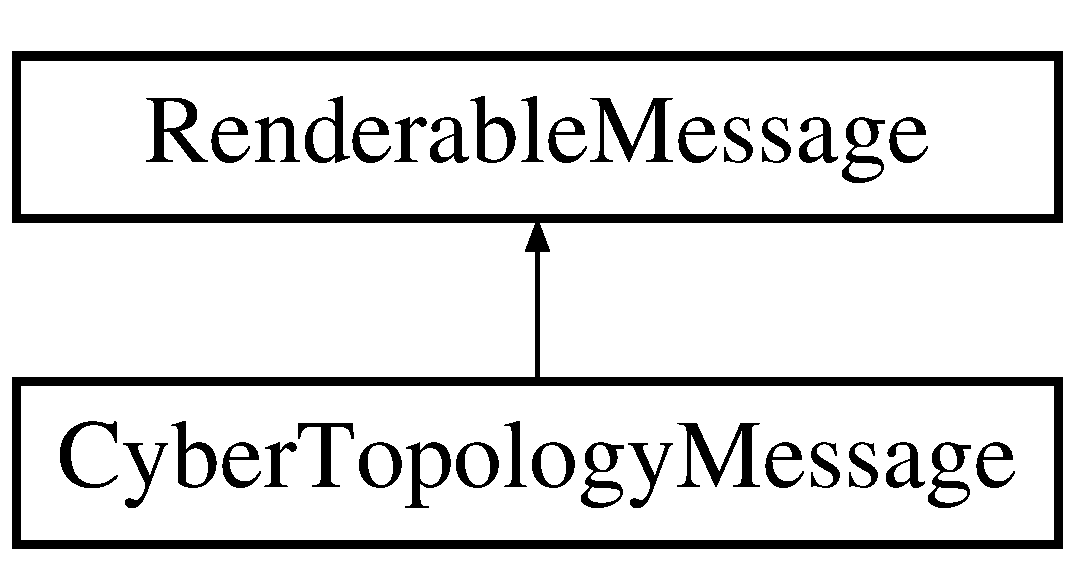
\includegraphics[height=2.000000cm]{classCyberTopologyMessage}
\end{center}
\end{figure}
\subsection*{Public Member Functions}
\begin{DoxyCompactItemize}
\item 
\hyperlink{classCyberTopologyMessage_ad29cc7035f525cb12cf25f0925656f74}{Cyber\-Topology\-Message} (const std\-::string \&channel)
\item 
\hyperlink{classCyberTopologyMessage_a79e7cc8a9ae14ac907c987131f86153e}{$\sim$\-Cyber\-Topology\-Message} ()
\item 
void \hyperlink{classCyberTopologyMessage_aed410d8532bc9230d35f61cebcee4824}{Render} (const \hyperlink{classScreen}{Screen} $\ast$s, int key) override
\item 
\hyperlink{classRenderableMessage}{Renderable\-Message} $\ast$ \hyperlink{classCyberTopologyMessage_afc36cda612863d6a940bef1509f39f16}{Child} (int index) const override
\item 
void \hyperlink{classCyberTopologyMessage_aeb57388a8b56c68681ab48f8ea5e5ea7}{Topology\-Changed} (const apollo\-::cyber\-::proto\-::\-Change\-Msg \&change\-\_\-msg)
\item 
void \hyperlink{classCyberTopologyMessage_a7ebd8b12a5e56099a2aec1aac9c1825e}{Add\-Reader\-Writer} (const apollo\-::cyber\-::proto\-::\-Role\-Attributes \&role, bool is\-Writer)
\end{DoxyCompactItemize}
\subsection*{Private Types}
\begin{DoxyCompactItemize}
\item 
enum \hyperlink{classCyberTopologyMessage_a19a78ae56d2bd909e1b1403b3db83c52}{Second\-Column\-Type} \{ \hyperlink{classCyberTopologyMessage_a19a78ae56d2bd909e1b1403b3db83c52a20b67ff6d86442b20819a3cd48bfc603}{Second\-Column\-Type\-::\-Message\-Type}, 
\hyperlink{classCyberTopologyMessage_a19a78ae56d2bd909e1b1403b3db83c52ace684cd329278d8b9193d22926686db5}{Second\-Column\-Type\-::\-Message\-Frame\-Ratio}
 \}
\end{DoxyCompactItemize}
\subsection*{Private Member Functions}
\begin{DoxyCompactItemize}
\item 
\hyperlink{classCyberTopologyMessage_acd5200e9387d9d989177b64deb426b17}{Cyber\-Topology\-Message} (const \hyperlink{classCyberTopologyMessage}{Cyber\-Topology\-Message} \&)=delete
\item 
\hyperlink{classCyberTopologyMessage}{Cyber\-Topology\-Message} \& \hyperlink{classCyberTopologyMessage_a9783107b7c5254325ecf6d6f59a22d4e}{operator=} (const \hyperlink{classCyberTopologyMessage}{Cyber\-Topology\-Message} \&)=delete
\item 
void \hyperlink{classCyberTopologyMessage_a4a61d42621d8db354727a18e9495a190}{Change\-State} (const \hyperlink{classScreen}{Screen} $\ast$s, int key)
\item 
bool \hyperlink{classCyberTopologyMessage_a2c775a5c10fce9c33f5316f877c9f018}{is\-From\-Here} (const std\-::string \&node\-Name)
\item 
std\-::map$<$ std\-::string, \\*
\hyperlink{classGeneralChannelMessage}{General\-Channel\-Message} $\ast$ $>$\\*
\-::const\-\_\-iterator \hyperlink{classCyberTopologyMessage_ade141cee6b72beee0a1255292bfa5124}{find\-Child} (int index) const 
\end{DoxyCompactItemize}
\subsection*{Private Attributes}
\begin{DoxyCompactItemize}
\item 
\hyperlink{classCyberTopologyMessage_a19a78ae56d2bd909e1b1403b3db83c52}{Second\-Column\-Type} \hyperlink{classCyberTopologyMessage_a1154eec678920dfada21e1f406dc28d0}{second\-\_\-column\-\_\-}
\item 
int \hyperlink{classCyberTopologyMessage_a3cc7dce72601c852f9f602f242b72e73}{pid\-\_\-}
\item 
int \hyperlink{classCyberTopologyMessage_ac3a5fef5a512872150261b3c32fafc60}{col1\-\_\-width\-\_\-}
\item 
const std\-::string \& \hyperlink{classCyberTopologyMessage_a5896a556d8bfbe583d112690f025a063}{specified\-\_\-channel\-\_\-}
\item 
std\-::map$<$ std\-::string, \\*
\hyperlink{classGeneralChannelMessage}{General\-Channel\-Message} $\ast$ $>$ \hyperlink{classCyberTopologyMessage_a982b69f726e8f42a1c3a0389865d84f8}{all\-\_\-channels\-\_\-map\-\_\-}
\end{DoxyCompactItemize}
\subsection*{Additional Inherited Members}


\subsection{Member Enumeration Documentation}
\hypertarget{classCyberTopologyMessage_a19a78ae56d2bd909e1b1403b3db83c52}{\index{Cyber\-Topology\-Message@{Cyber\-Topology\-Message}!Second\-Column\-Type@{Second\-Column\-Type}}
\index{Second\-Column\-Type@{Second\-Column\-Type}!CyberTopologyMessage@{Cyber\-Topology\-Message}}
\subsubsection[{Second\-Column\-Type}]{\setlength{\rightskip}{0pt plus 5cm}enum {\bf Cyber\-Topology\-Message\-::\-Second\-Column\-Type}\hspace{0.3cm}{\ttfamily [strong]}, {\ttfamily [private]}}}\label{classCyberTopologyMessage_a19a78ae56d2bd909e1b1403b3db83c52}
\begin{Desc}
\item[Enumerator]\par
\begin{description}
\index{Message\-Type@{Message\-Type}!Cyber\-Topology\-Message@{Cyber\-Topology\-Message}}\index{Cyber\-Topology\-Message@{Cyber\-Topology\-Message}!Message\-Type@{Message\-Type}}\item[{\em 
\hypertarget{classCyberTopologyMessage_a19a78ae56d2bd909e1b1403b3db83c52a20b67ff6d86442b20819a3cd48bfc603}{Message\-Type}\label{classCyberTopologyMessage_a19a78ae56d2bd909e1b1403b3db83c52a20b67ff6d86442b20819a3cd48bfc603}
}]\index{Message\-Frame\-Ratio@{Message\-Frame\-Ratio}!Cyber\-Topology\-Message@{Cyber\-Topology\-Message}}\index{Cyber\-Topology\-Message@{Cyber\-Topology\-Message}!Message\-Frame\-Ratio@{Message\-Frame\-Ratio}}\item[{\em 
\hypertarget{classCyberTopologyMessage_a19a78ae56d2bd909e1b1403b3db83c52ace684cd329278d8b9193d22926686db5}{Message\-Frame\-Ratio}\label{classCyberTopologyMessage_a19a78ae56d2bd909e1b1403b3db83c52ace684cd329278d8b9193d22926686db5}
}]\end{description}
\end{Desc}


\subsection{Constructor \& Destructor Documentation}
\hypertarget{classCyberTopologyMessage_ad29cc7035f525cb12cf25f0925656f74}{\index{Cyber\-Topology\-Message@{Cyber\-Topology\-Message}!Cyber\-Topology\-Message@{Cyber\-Topology\-Message}}
\index{Cyber\-Topology\-Message@{Cyber\-Topology\-Message}!CyberTopologyMessage@{Cyber\-Topology\-Message}}
\subsubsection[{Cyber\-Topology\-Message}]{\setlength{\rightskip}{0pt plus 5cm}Cyber\-Topology\-Message\-::\-Cyber\-Topology\-Message (
\begin{DoxyParamCaption}
\item[{const std\-::string \&}]{channel}
\end{DoxyParamCaption}
)\hspace{0.3cm}{\ttfamily [explicit]}}}\label{classCyberTopologyMessage_ad29cc7035f525cb12cf25f0925656f74}
\hypertarget{classCyberTopologyMessage_a79e7cc8a9ae14ac907c987131f86153e}{\index{Cyber\-Topology\-Message@{Cyber\-Topology\-Message}!$\sim$\-Cyber\-Topology\-Message@{$\sim$\-Cyber\-Topology\-Message}}
\index{$\sim$\-Cyber\-Topology\-Message@{$\sim$\-Cyber\-Topology\-Message}!CyberTopologyMessage@{Cyber\-Topology\-Message}}
\subsubsection[{$\sim$\-Cyber\-Topology\-Message}]{\setlength{\rightskip}{0pt plus 5cm}Cyber\-Topology\-Message\-::$\sim$\-Cyber\-Topology\-Message (
\begin{DoxyParamCaption}
{}
\end{DoxyParamCaption}
)}}\label{classCyberTopologyMessage_a79e7cc8a9ae14ac907c987131f86153e}
\hypertarget{classCyberTopologyMessage_acd5200e9387d9d989177b64deb426b17}{\index{Cyber\-Topology\-Message@{Cyber\-Topology\-Message}!Cyber\-Topology\-Message@{Cyber\-Topology\-Message}}
\index{Cyber\-Topology\-Message@{Cyber\-Topology\-Message}!CyberTopologyMessage@{Cyber\-Topology\-Message}}
\subsubsection[{Cyber\-Topology\-Message}]{\setlength{\rightskip}{0pt plus 5cm}Cyber\-Topology\-Message\-::\-Cyber\-Topology\-Message (
\begin{DoxyParamCaption}
\item[{const {\bf Cyber\-Topology\-Message} \&}]{}
\end{DoxyParamCaption}
)\hspace{0.3cm}{\ttfamily [private]}, {\ttfamily [delete]}}}\label{classCyberTopologyMessage_acd5200e9387d9d989177b64deb426b17}


\subsection{Member Function Documentation}
\hypertarget{classCyberTopologyMessage_a7ebd8b12a5e56099a2aec1aac9c1825e}{\index{Cyber\-Topology\-Message@{Cyber\-Topology\-Message}!Add\-Reader\-Writer@{Add\-Reader\-Writer}}
\index{Add\-Reader\-Writer@{Add\-Reader\-Writer}!CyberTopologyMessage@{Cyber\-Topology\-Message}}
\subsubsection[{Add\-Reader\-Writer}]{\setlength{\rightskip}{0pt plus 5cm}void Cyber\-Topology\-Message\-::\-Add\-Reader\-Writer (
\begin{DoxyParamCaption}
\item[{const apollo\-::cyber\-::proto\-::\-Role\-Attributes \&}]{role, }
\item[{bool}]{is\-Writer}
\end{DoxyParamCaption}
)}}\label{classCyberTopologyMessage_a7ebd8b12a5e56099a2aec1aac9c1825e}
\hypertarget{classCyberTopologyMessage_a4a61d42621d8db354727a18e9495a190}{\index{Cyber\-Topology\-Message@{Cyber\-Topology\-Message}!Change\-State@{Change\-State}}
\index{Change\-State@{Change\-State}!CyberTopologyMessage@{Cyber\-Topology\-Message}}
\subsubsection[{Change\-State}]{\setlength{\rightskip}{0pt plus 5cm}void Cyber\-Topology\-Message\-::\-Change\-State (
\begin{DoxyParamCaption}
\item[{const {\bf Screen} $\ast$}]{s, }
\item[{int}]{key}
\end{DoxyParamCaption}
)\hspace{0.3cm}{\ttfamily [private]}}}\label{classCyberTopologyMessage_a4a61d42621d8db354727a18e9495a190}
\hypertarget{classCyberTopologyMessage_afc36cda612863d6a940bef1509f39f16}{\index{Cyber\-Topology\-Message@{Cyber\-Topology\-Message}!Child@{Child}}
\index{Child@{Child}!CyberTopologyMessage@{Cyber\-Topology\-Message}}
\subsubsection[{Child}]{\setlength{\rightskip}{0pt plus 5cm}{\bf Renderable\-Message}$\ast$ Cyber\-Topology\-Message\-::\-Child (
\begin{DoxyParamCaption}
\item[{int}]{index}
\end{DoxyParamCaption}
) const\hspace{0.3cm}{\ttfamily [override]}, {\ttfamily [virtual]}}}\label{classCyberTopologyMessage_afc36cda612863d6a940bef1509f39f16}


Implements \hyperlink{classRenderableMessage_a0f933ad0befd4d3cf3a95e205c7398d6}{Renderable\-Message}.

\hypertarget{classCyberTopologyMessage_ade141cee6b72beee0a1255292bfa5124}{\index{Cyber\-Topology\-Message@{Cyber\-Topology\-Message}!find\-Child@{find\-Child}}
\index{find\-Child@{find\-Child}!CyberTopologyMessage@{Cyber\-Topology\-Message}}
\subsubsection[{find\-Child}]{\setlength{\rightskip}{0pt plus 5cm}std\-::map$<$std\-::string, {\bf General\-Channel\-Message}$\ast$$>$\-::const\-\_\-iterator Cyber\-Topology\-Message\-::find\-Child (
\begin{DoxyParamCaption}
\item[{int}]{index}
\end{DoxyParamCaption}
) const\hspace{0.3cm}{\ttfamily [private]}}}\label{classCyberTopologyMessage_ade141cee6b72beee0a1255292bfa5124}
\hypertarget{classCyberTopologyMessage_a2c775a5c10fce9c33f5316f877c9f018}{\index{Cyber\-Topology\-Message@{Cyber\-Topology\-Message}!is\-From\-Here@{is\-From\-Here}}
\index{is\-From\-Here@{is\-From\-Here}!CyberTopologyMessage@{Cyber\-Topology\-Message}}
\subsubsection[{is\-From\-Here}]{\setlength{\rightskip}{0pt plus 5cm}bool Cyber\-Topology\-Message\-::is\-From\-Here (
\begin{DoxyParamCaption}
\item[{const std\-::string \&}]{node\-Name}
\end{DoxyParamCaption}
)\hspace{0.3cm}{\ttfamily [private]}}}\label{classCyberTopologyMessage_a2c775a5c10fce9c33f5316f877c9f018}
\hypertarget{classCyberTopologyMessage_a9783107b7c5254325ecf6d6f59a22d4e}{\index{Cyber\-Topology\-Message@{Cyber\-Topology\-Message}!operator=@{operator=}}
\index{operator=@{operator=}!CyberTopologyMessage@{Cyber\-Topology\-Message}}
\subsubsection[{operator=}]{\setlength{\rightskip}{0pt plus 5cm}{\bf Cyber\-Topology\-Message}\& Cyber\-Topology\-Message\-::operator= (
\begin{DoxyParamCaption}
\item[{const {\bf Cyber\-Topology\-Message} \&}]{}
\end{DoxyParamCaption}
)\hspace{0.3cm}{\ttfamily [private]}, {\ttfamily [delete]}}}\label{classCyberTopologyMessage_a9783107b7c5254325ecf6d6f59a22d4e}
\hypertarget{classCyberTopologyMessage_aed410d8532bc9230d35f61cebcee4824}{\index{Cyber\-Topology\-Message@{Cyber\-Topology\-Message}!Render@{Render}}
\index{Render@{Render}!CyberTopologyMessage@{Cyber\-Topology\-Message}}
\subsubsection[{Render}]{\setlength{\rightskip}{0pt plus 5cm}void Cyber\-Topology\-Message\-::\-Render (
\begin{DoxyParamCaption}
\item[{const {\bf Screen} $\ast$}]{s, }
\item[{int}]{key}
\end{DoxyParamCaption}
)\hspace{0.3cm}{\ttfamily [override]}, {\ttfamily [virtual]}}}\label{classCyberTopologyMessage_aed410d8532bc9230d35f61cebcee4824}


Implements \hyperlink{classRenderableMessage_a3f65c247f5db9bb4918bca7d665bbdc6}{Renderable\-Message}.

\hypertarget{classCyberTopologyMessage_aeb57388a8b56c68681ab48f8ea5e5ea7}{\index{Cyber\-Topology\-Message@{Cyber\-Topology\-Message}!Topology\-Changed@{Topology\-Changed}}
\index{Topology\-Changed@{Topology\-Changed}!CyberTopologyMessage@{Cyber\-Topology\-Message}}
\subsubsection[{Topology\-Changed}]{\setlength{\rightskip}{0pt plus 5cm}void Cyber\-Topology\-Message\-::\-Topology\-Changed (
\begin{DoxyParamCaption}
\item[{const apollo\-::cyber\-::proto\-::\-Change\-Msg \&}]{change\-\_\-msg}
\end{DoxyParamCaption}
)}}\label{classCyberTopologyMessage_aeb57388a8b56c68681ab48f8ea5e5ea7}


\subsection{Member Data Documentation}
\hypertarget{classCyberTopologyMessage_a982b69f726e8f42a1c3a0389865d84f8}{\index{Cyber\-Topology\-Message@{Cyber\-Topology\-Message}!all\-\_\-channels\-\_\-map\-\_\-@{all\-\_\-channels\-\_\-map\-\_\-}}
\index{all\-\_\-channels\-\_\-map\-\_\-@{all\-\_\-channels\-\_\-map\-\_\-}!CyberTopologyMessage@{Cyber\-Topology\-Message}}
\subsubsection[{all\-\_\-channels\-\_\-map\-\_\-}]{\setlength{\rightskip}{0pt plus 5cm}std\-::map$<$std\-::string, {\bf General\-Channel\-Message}$\ast$$>$ Cyber\-Topology\-Message\-::all\-\_\-channels\-\_\-map\-\_\-\hspace{0.3cm}{\ttfamily [private]}}}\label{classCyberTopologyMessage_a982b69f726e8f42a1c3a0389865d84f8}
\hypertarget{classCyberTopologyMessage_ac3a5fef5a512872150261b3c32fafc60}{\index{Cyber\-Topology\-Message@{Cyber\-Topology\-Message}!col1\-\_\-width\-\_\-@{col1\-\_\-width\-\_\-}}
\index{col1\-\_\-width\-\_\-@{col1\-\_\-width\-\_\-}!CyberTopologyMessage@{Cyber\-Topology\-Message}}
\subsubsection[{col1\-\_\-width\-\_\-}]{\setlength{\rightskip}{0pt plus 5cm}int Cyber\-Topology\-Message\-::col1\-\_\-width\-\_\-\hspace{0.3cm}{\ttfamily [private]}}}\label{classCyberTopologyMessage_ac3a5fef5a512872150261b3c32fafc60}
\hypertarget{classCyberTopologyMessage_a3cc7dce72601c852f9f602f242b72e73}{\index{Cyber\-Topology\-Message@{Cyber\-Topology\-Message}!pid\-\_\-@{pid\-\_\-}}
\index{pid\-\_\-@{pid\-\_\-}!CyberTopologyMessage@{Cyber\-Topology\-Message}}
\subsubsection[{pid\-\_\-}]{\setlength{\rightskip}{0pt plus 5cm}int Cyber\-Topology\-Message\-::pid\-\_\-\hspace{0.3cm}{\ttfamily [private]}}}\label{classCyberTopologyMessage_a3cc7dce72601c852f9f602f242b72e73}
\hypertarget{classCyberTopologyMessage_a1154eec678920dfada21e1f406dc28d0}{\index{Cyber\-Topology\-Message@{Cyber\-Topology\-Message}!second\-\_\-column\-\_\-@{second\-\_\-column\-\_\-}}
\index{second\-\_\-column\-\_\-@{second\-\_\-column\-\_\-}!CyberTopologyMessage@{Cyber\-Topology\-Message}}
\subsubsection[{second\-\_\-column\-\_\-}]{\setlength{\rightskip}{0pt plus 5cm}{\bf Second\-Column\-Type} Cyber\-Topology\-Message\-::second\-\_\-column\-\_\-\hspace{0.3cm}{\ttfamily [private]}}}\label{classCyberTopologyMessage_a1154eec678920dfada21e1f406dc28d0}
\hypertarget{classCyberTopologyMessage_a5896a556d8bfbe583d112690f025a063}{\index{Cyber\-Topology\-Message@{Cyber\-Topology\-Message}!specified\-\_\-channel\-\_\-@{specified\-\_\-channel\-\_\-}}
\index{specified\-\_\-channel\-\_\-@{specified\-\_\-channel\-\_\-}!CyberTopologyMessage@{Cyber\-Topology\-Message}}
\subsubsection[{specified\-\_\-channel\-\_\-}]{\setlength{\rightskip}{0pt plus 5cm}const std\-::string\& Cyber\-Topology\-Message\-::specified\-\_\-channel\-\_\-\hspace{0.3cm}{\ttfamily [private]}}}\label{classCyberTopologyMessage_a5896a556d8bfbe583d112690f025a063}


The documentation for this class was generated from the following file\-:\begin{DoxyCompactItemize}
\item 
tools/cyber\-\_\-monitor/\hyperlink{cyber__topology__message_8h}{cyber\-\_\-topology\-\_\-message.\-h}\end{DoxyCompactItemize}

\hypertarget{classapollo_1_1cyber_1_1data_1_1DataDispatcher}{\section{apollo\-:\-:cyber\-:\-:data\-:\-:Data\-Dispatcher$<$ T $>$ Class Template Reference}
\label{classapollo_1_1cyber_1_1data_1_1DataDispatcher}\index{apollo\-::cyber\-::data\-::\-Data\-Dispatcher$<$ T $>$@{apollo\-::cyber\-::data\-::\-Data\-Dispatcher$<$ T $>$}}
}


{\ttfamily \#include $<$data\-\_\-dispatcher.\-h$>$}

\subsection*{Public Types}
\begin{DoxyCompactItemize}
\item 
using \hyperlink{classapollo_1_1cyber_1_1data_1_1DataDispatcher_a705b3d7e33c176168be27202c1e9269f}{Buffer\-Vector} = std\-::vector$<$ std\-::weak\-\_\-ptr$<$ \hyperlink{classapollo_1_1cyber_1_1data_1_1CacheBuffer}{Cache\-Buffer}$<$ std\-::shared\-\_\-ptr$<$ T $>$$>$$>$$>$
\end{DoxyCompactItemize}
\subsection*{Public Member Functions}
\begin{DoxyCompactItemize}
\item 
\hyperlink{classapollo_1_1cyber_1_1data_1_1DataDispatcher_a00fbebfb574538bd47f427f48aa2cb8d}{$\sim$\-Data\-Dispatcher} ()
\item 
void \hyperlink{classapollo_1_1cyber_1_1data_1_1DataDispatcher_a5c25d4ea21bfc0f7333c07a7da9b27d2}{Add\-Buffer} (const \hyperlink{classapollo_1_1cyber_1_1data_1_1ChannelBuffer}{Channel\-Buffer}$<$ T $>$ \&channel\-\_\-buffer)
\item 
bool \hyperlink{classapollo_1_1cyber_1_1data_1_1DataDispatcher_a96935453604a6f47112f417897c07aeb}{Dispatch} (const uint64\-\_\-t channel\-\_\-id, const std\-::shared\-\_\-ptr$<$ T $>$ \&msg)
\end{DoxyCompactItemize}
\subsection*{Private Attributes}
\begin{DoxyCompactItemize}
\item 
\hyperlink{classapollo_1_1cyber_1_1data_1_1DataNotifier}{Data\-Notifier} $\ast$ \hyperlink{classapollo_1_1cyber_1_1data_1_1DataDispatcher_a171868a783ef9a7fb75739c9910b5157}{notifier\-\_\-} = Data\-Notifier\-::\-Instance()
\item 
std\-::mutex \hyperlink{classapollo_1_1cyber_1_1data_1_1DataDispatcher_ad6c0557358e14fb05e07a04cf3e026cb}{buffers\-\_\-map\-\_\-mutex\-\_\-}
\item 
\hyperlink{classapollo_1_1cyber_1_1base_1_1AtomicHashMap}{Atomic\-Hash\-Map}$<$ uint64\-\_\-t, \\*
\hyperlink{classapollo_1_1cyber_1_1data_1_1DataDispatcher_a705b3d7e33c176168be27202c1e9269f}{Buffer\-Vector} $>$ \hyperlink{classapollo_1_1cyber_1_1data_1_1DataDispatcher_ad7468b681e765b85516f17a34553eece}{buffers\-\_\-map\-\_\-}
\end{DoxyCompactItemize}


\subsection{Member Typedef Documentation}
\hypertarget{classapollo_1_1cyber_1_1data_1_1DataDispatcher_a705b3d7e33c176168be27202c1e9269f}{\index{apollo\-::cyber\-::data\-::\-Data\-Dispatcher@{apollo\-::cyber\-::data\-::\-Data\-Dispatcher}!Buffer\-Vector@{Buffer\-Vector}}
\index{Buffer\-Vector@{Buffer\-Vector}!apollo::cyber::data::DataDispatcher@{apollo\-::cyber\-::data\-::\-Data\-Dispatcher}}
\subsubsection[{Buffer\-Vector}]{\setlength{\rightskip}{0pt plus 5cm}template$<$typename T $>$ using {\bf apollo\-::cyber\-::data\-::\-Data\-Dispatcher}$<$ T $>$\-::{\bf Buffer\-Vector} =  std\-::vector$<$std\-::weak\-\_\-ptr$<${\bf Cache\-Buffer}$<$std\-::shared\-\_\-ptr$<$T$>$$>$$>$$>$}}\label{classapollo_1_1cyber_1_1data_1_1DataDispatcher_a705b3d7e33c176168be27202c1e9269f}


\subsection{Constructor \& Destructor Documentation}
\hypertarget{classapollo_1_1cyber_1_1data_1_1DataDispatcher_a00fbebfb574538bd47f427f48aa2cb8d}{\index{apollo\-::cyber\-::data\-::\-Data\-Dispatcher@{apollo\-::cyber\-::data\-::\-Data\-Dispatcher}!$\sim$\-Data\-Dispatcher@{$\sim$\-Data\-Dispatcher}}
\index{$\sim$\-Data\-Dispatcher@{$\sim$\-Data\-Dispatcher}!apollo::cyber::data::DataDispatcher@{apollo\-::cyber\-::data\-::\-Data\-Dispatcher}}
\subsubsection[{$\sim$\-Data\-Dispatcher}]{\setlength{\rightskip}{0pt plus 5cm}template$<$typename T $>$ {\bf apollo\-::cyber\-::data\-::\-Data\-Dispatcher}$<$ T $>$\-::$\sim${\bf Data\-Dispatcher} (
\begin{DoxyParamCaption}
{}
\end{DoxyParamCaption}
)\hspace{0.3cm}{\ttfamily [inline]}}}\label{classapollo_1_1cyber_1_1data_1_1DataDispatcher_a00fbebfb574538bd47f427f48aa2cb8d}


\subsection{Member Function Documentation}
\hypertarget{classapollo_1_1cyber_1_1data_1_1DataDispatcher_a5c25d4ea21bfc0f7333c07a7da9b27d2}{\index{apollo\-::cyber\-::data\-::\-Data\-Dispatcher@{apollo\-::cyber\-::data\-::\-Data\-Dispatcher}!Add\-Buffer@{Add\-Buffer}}
\index{Add\-Buffer@{Add\-Buffer}!apollo::cyber::data::DataDispatcher@{apollo\-::cyber\-::data\-::\-Data\-Dispatcher}}
\subsubsection[{Add\-Buffer}]{\setlength{\rightskip}{0pt plus 5cm}template$<$typename T $>$ void {\bf apollo\-::cyber\-::data\-::\-Data\-Dispatcher}$<$ T $>$\-::Add\-Buffer (
\begin{DoxyParamCaption}
\item[{const {\bf Channel\-Buffer}$<$ T $>$ \&}]{channel\-\_\-buffer}
\end{DoxyParamCaption}
)}}\label{classapollo_1_1cyber_1_1data_1_1DataDispatcher_a5c25d4ea21bfc0f7333c07a7da9b27d2}
\hypertarget{classapollo_1_1cyber_1_1data_1_1DataDispatcher_a96935453604a6f47112f417897c07aeb}{\index{apollo\-::cyber\-::data\-::\-Data\-Dispatcher@{apollo\-::cyber\-::data\-::\-Data\-Dispatcher}!Dispatch@{Dispatch}}
\index{Dispatch@{Dispatch}!apollo::cyber::data::DataDispatcher@{apollo\-::cyber\-::data\-::\-Data\-Dispatcher}}
\subsubsection[{Dispatch}]{\setlength{\rightskip}{0pt plus 5cm}template$<$typename T $>$ bool {\bf apollo\-::cyber\-::data\-::\-Data\-Dispatcher}$<$ T $>$\-::Dispatch (
\begin{DoxyParamCaption}
\item[{const uint64\-\_\-t}]{channel\-\_\-id, }
\item[{const std\-::shared\-\_\-ptr$<$ T $>$ \&}]{msg}
\end{DoxyParamCaption}
)}}\label{classapollo_1_1cyber_1_1data_1_1DataDispatcher_a96935453604a6f47112f417897c07aeb}


\subsection{Member Data Documentation}
\hypertarget{classapollo_1_1cyber_1_1data_1_1DataDispatcher_ad7468b681e765b85516f17a34553eece}{\index{apollo\-::cyber\-::data\-::\-Data\-Dispatcher@{apollo\-::cyber\-::data\-::\-Data\-Dispatcher}!buffers\-\_\-map\-\_\-@{buffers\-\_\-map\-\_\-}}
\index{buffers\-\_\-map\-\_\-@{buffers\-\_\-map\-\_\-}!apollo::cyber::data::DataDispatcher@{apollo\-::cyber\-::data\-::\-Data\-Dispatcher}}
\subsubsection[{buffers\-\_\-map\-\_\-}]{\setlength{\rightskip}{0pt plus 5cm}template$<$typename T $>$ {\bf Atomic\-Hash\-Map}$<$uint64\-\_\-t, {\bf Buffer\-Vector}$>$ {\bf apollo\-::cyber\-::data\-::\-Data\-Dispatcher}$<$ T $>$\-::buffers\-\_\-map\-\_\-\hspace{0.3cm}{\ttfamily [private]}}}\label{classapollo_1_1cyber_1_1data_1_1DataDispatcher_ad7468b681e765b85516f17a34553eece}
\hypertarget{classapollo_1_1cyber_1_1data_1_1DataDispatcher_ad6c0557358e14fb05e07a04cf3e026cb}{\index{apollo\-::cyber\-::data\-::\-Data\-Dispatcher@{apollo\-::cyber\-::data\-::\-Data\-Dispatcher}!buffers\-\_\-map\-\_\-mutex\-\_\-@{buffers\-\_\-map\-\_\-mutex\-\_\-}}
\index{buffers\-\_\-map\-\_\-mutex\-\_\-@{buffers\-\_\-map\-\_\-mutex\-\_\-}!apollo::cyber::data::DataDispatcher@{apollo\-::cyber\-::data\-::\-Data\-Dispatcher}}
\subsubsection[{buffers\-\_\-map\-\_\-mutex\-\_\-}]{\setlength{\rightskip}{0pt plus 5cm}template$<$typename T $>$ std\-::mutex {\bf apollo\-::cyber\-::data\-::\-Data\-Dispatcher}$<$ T $>$\-::buffers\-\_\-map\-\_\-mutex\-\_\-\hspace{0.3cm}{\ttfamily [private]}}}\label{classapollo_1_1cyber_1_1data_1_1DataDispatcher_ad6c0557358e14fb05e07a04cf3e026cb}
\hypertarget{classapollo_1_1cyber_1_1data_1_1DataDispatcher_a171868a783ef9a7fb75739c9910b5157}{\index{apollo\-::cyber\-::data\-::\-Data\-Dispatcher@{apollo\-::cyber\-::data\-::\-Data\-Dispatcher}!notifier\-\_\-@{notifier\-\_\-}}
\index{notifier\-\_\-@{notifier\-\_\-}!apollo::cyber::data::DataDispatcher@{apollo\-::cyber\-::data\-::\-Data\-Dispatcher}}
\subsubsection[{notifier\-\_\-}]{\setlength{\rightskip}{0pt plus 5cm}template$<$typename T $>$ {\bf Data\-Notifier}$\ast$ {\bf apollo\-::cyber\-::data\-::\-Data\-Dispatcher}$<$ T $>$\-::notifier\-\_\- = Data\-Notifier\-::\-Instance()\hspace{0.3cm}{\ttfamily [private]}}}\label{classapollo_1_1cyber_1_1data_1_1DataDispatcher_a171868a783ef9a7fb75739c9910b5157}


The documentation for this class was generated from the following file\-:\begin{DoxyCompactItemize}
\item 
data/\hyperlink{data__dispatcher_8h}{data\-\_\-dispatcher.\-h}\end{DoxyCompactItemize}

\hypertarget{classapollo_1_1cyber_1_1data_1_1fusion_1_1DataFusion}{\section{apollo\-:\-:cyber\-:\-:data\-:\-:fusion\-:\-:Data\-Fusion$<$ M0, M1, M2, M3 $>$ Class Template Reference}
\label{classapollo_1_1cyber_1_1data_1_1fusion_1_1DataFusion}\index{apollo\-::cyber\-::data\-::fusion\-::\-Data\-Fusion$<$ M0, M1, M2, M3 $>$@{apollo\-::cyber\-::data\-::fusion\-::\-Data\-Fusion$<$ M0, M1, M2, M3 $>$}}
}


{\ttfamily \#include $<$data\-\_\-fusion.\-h$>$}

Inheritance diagram for apollo\-:\-:cyber\-:\-:data\-:\-:fusion\-:\-:Data\-Fusion$<$ M0, M1, M2, M3 $>$\-:\begin{figure}[H]
\begin{center}
\leavevmode
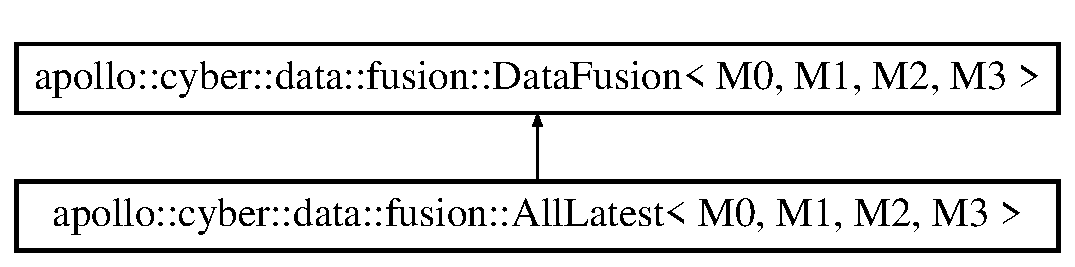
\includegraphics[height=2.000000cm]{classapollo_1_1cyber_1_1data_1_1fusion_1_1DataFusion}
\end{center}
\end{figure}
\subsection*{Public Member Functions}
\begin{DoxyCompactItemize}
\item 
virtual \hyperlink{classapollo_1_1cyber_1_1data_1_1fusion_1_1DataFusion_a8d7a7673ce90ccd8ab5a5c550c84029e}{$\sim$\-Data\-Fusion} ()
\item 
virtual bool \hyperlink{classapollo_1_1cyber_1_1data_1_1fusion_1_1DataFusion_af992dd51063725886f3dce401ae08cbf}{Fusion} (uint64\-\_\-t $\ast$index, std\-::shared\-\_\-ptr$<$ M0 $>$ \&m0, std\-::shared\-\_\-ptr$<$ M1 $>$ \&m1, std\-::shared\-\_\-ptr$<$ M2 $>$ \&m2, std\-::shared\-\_\-ptr$<$ M3 $>$ \&m3)=0
\end{DoxyCompactItemize}


\subsection{Constructor \& Destructor Documentation}
\hypertarget{classapollo_1_1cyber_1_1data_1_1fusion_1_1DataFusion_a8d7a7673ce90ccd8ab5a5c550c84029e}{\index{apollo\-::cyber\-::data\-::fusion\-::\-Data\-Fusion@{apollo\-::cyber\-::data\-::fusion\-::\-Data\-Fusion}!$\sim$\-Data\-Fusion@{$\sim$\-Data\-Fusion}}
\index{$\sim$\-Data\-Fusion@{$\sim$\-Data\-Fusion}!apollo::cyber::data::fusion::DataFusion@{apollo\-::cyber\-::data\-::fusion\-::\-Data\-Fusion}}
\subsubsection[{$\sim$\-Data\-Fusion}]{\setlength{\rightskip}{0pt plus 5cm}template$<$typename M0, typename M1 = Null\-Type, typename M2 = Null\-Type, typename M3 = Null\-Type$>$ virtual {\bf apollo\-::cyber\-::data\-::fusion\-::\-Data\-Fusion}$<$ M0, M1, M2, M3 $>$\-::$\sim${\bf Data\-Fusion} (
\begin{DoxyParamCaption}
{}
\end{DoxyParamCaption}
)\hspace{0.3cm}{\ttfamily [inline]}, {\ttfamily [virtual]}}}\label{classapollo_1_1cyber_1_1data_1_1fusion_1_1DataFusion_a8d7a7673ce90ccd8ab5a5c550c84029e}


\subsection{Member Function Documentation}
\hypertarget{classapollo_1_1cyber_1_1data_1_1fusion_1_1DataFusion_af992dd51063725886f3dce401ae08cbf}{\index{apollo\-::cyber\-::data\-::fusion\-::\-Data\-Fusion@{apollo\-::cyber\-::data\-::fusion\-::\-Data\-Fusion}!Fusion@{Fusion}}
\index{Fusion@{Fusion}!apollo::cyber::data::fusion::DataFusion@{apollo\-::cyber\-::data\-::fusion\-::\-Data\-Fusion}}
\subsubsection[{Fusion}]{\setlength{\rightskip}{0pt plus 5cm}template$<$typename M0, typename M1 = Null\-Type, typename M2 = Null\-Type, typename M3 = Null\-Type$>$ virtual bool {\bf apollo\-::cyber\-::data\-::fusion\-::\-Data\-Fusion}$<$ M0, M1, M2, M3 $>$\-::Fusion (
\begin{DoxyParamCaption}
\item[{uint64\-\_\-t $\ast$}]{index, }
\item[{std\-::shared\-\_\-ptr$<$ M0 $>$ \&}]{m0, }
\item[{std\-::shared\-\_\-ptr$<$ M1 $>$ \&}]{m1, }
\item[{std\-::shared\-\_\-ptr$<$ M2 $>$ \&}]{m2, }
\item[{std\-::shared\-\_\-ptr$<$ M3 $>$ \&}]{m3}
\end{DoxyParamCaption}
)\hspace{0.3cm}{\ttfamily [pure virtual]}}}\label{classapollo_1_1cyber_1_1data_1_1fusion_1_1DataFusion_af992dd51063725886f3dce401ae08cbf}


Implemented in \hyperlink{classapollo_1_1cyber_1_1data_1_1fusion_1_1AllLatest_a44540e0552d2d451372e9f591ad0e3a0}{apollo\-::cyber\-::data\-::fusion\-::\-All\-Latest$<$ M0, M1, M2, M3 $>$}.



The documentation for this class was generated from the following file\-:\begin{DoxyCompactItemize}
\item 
data/fusion/\hyperlink{data__fusion_8h}{data\-\_\-fusion.\-h}\end{DoxyCompactItemize}

\hypertarget{classapollo_1_1cyber_1_1data_1_1fusion_1_1DataFusion_3_01M0_00_01M1_00_01M2_00_01NullType_01_4}{\section{apollo\-:\-:cyber\-:\-:data\-:\-:fusion\-:\-:Data\-Fusion$<$ M0, M1, M2, Null\-Type $>$ Class Template Reference}
\label{classapollo_1_1cyber_1_1data_1_1fusion_1_1DataFusion_3_01M0_00_01M1_00_01M2_00_01NullType_01_4}\index{apollo\-::cyber\-::data\-::fusion\-::\-Data\-Fusion$<$ M0, M1, M2, Null\-Type $>$@{apollo\-::cyber\-::data\-::fusion\-::\-Data\-Fusion$<$ M0, M1, M2, Null\-Type $>$}}
}


{\ttfamily \#include $<$data\-\_\-fusion.\-h$>$}

\subsection*{Public Member Functions}
\begin{DoxyCompactItemize}
\item 
virtual \hyperlink{classapollo_1_1cyber_1_1data_1_1fusion_1_1DataFusion_3_01M0_00_01M1_00_01M2_00_01NullType_01_4_a49939ae97307fd1b1478eef4b9d377b5}{$\sim$\-Data\-Fusion} ()
\item 
virtual bool \hyperlink{classapollo_1_1cyber_1_1data_1_1fusion_1_1DataFusion_3_01M0_00_01M1_00_01M2_00_01NullType_01_4_a420b16045031aee29f16441f1102984e}{Fusion} (uint64\-\_\-t $\ast$index, std\-::shared\-\_\-ptr$<$ M0 $>$ \&m0, std\-::shared\-\_\-ptr$<$ M1 $>$ \&m1, std\-::shared\-\_\-ptr$<$ M2 $>$ \&m2)=0
\end{DoxyCompactItemize}


\subsection{Constructor \& Destructor Documentation}
\hypertarget{classapollo_1_1cyber_1_1data_1_1fusion_1_1DataFusion_3_01M0_00_01M1_00_01M2_00_01NullType_01_4_a49939ae97307fd1b1478eef4b9d377b5}{\index{apollo\-::cyber\-::data\-::fusion\-::\-Data\-Fusion$<$ M0, M1, M2, Null\-Type $>$@{apollo\-::cyber\-::data\-::fusion\-::\-Data\-Fusion$<$ M0, M1, M2, Null\-Type $>$}!$\sim$\-Data\-Fusion@{$\sim$\-Data\-Fusion}}
\index{$\sim$\-Data\-Fusion@{$\sim$\-Data\-Fusion}!apollo::cyber::data::fusion::DataFusion< M0, M1, M2, NullType >@{apollo\-::cyber\-::data\-::fusion\-::\-Data\-Fusion$<$ M0, M1, M2, Null\-Type $>$}}
\subsubsection[{$\sim$\-Data\-Fusion}]{\setlength{\rightskip}{0pt plus 5cm}template$<$typename M0 , typename M1 , typename M2 $>$ virtual {\bf apollo\-::cyber\-::data\-::fusion\-::\-Data\-Fusion}$<$ M0, M1, M2, {\bf Null\-Type} $>$\-::$\sim${\bf Data\-Fusion} (
\begin{DoxyParamCaption}
{}
\end{DoxyParamCaption}
)\hspace{0.3cm}{\ttfamily [inline]}, {\ttfamily [virtual]}}}\label{classapollo_1_1cyber_1_1data_1_1fusion_1_1DataFusion_3_01M0_00_01M1_00_01M2_00_01NullType_01_4_a49939ae97307fd1b1478eef4b9d377b5}


\subsection{Member Function Documentation}
\hypertarget{classapollo_1_1cyber_1_1data_1_1fusion_1_1DataFusion_3_01M0_00_01M1_00_01M2_00_01NullType_01_4_a420b16045031aee29f16441f1102984e}{\index{apollo\-::cyber\-::data\-::fusion\-::\-Data\-Fusion$<$ M0, M1, M2, Null\-Type $>$@{apollo\-::cyber\-::data\-::fusion\-::\-Data\-Fusion$<$ M0, M1, M2, Null\-Type $>$}!Fusion@{Fusion}}
\index{Fusion@{Fusion}!apollo::cyber::data::fusion::DataFusion< M0, M1, M2, NullType >@{apollo\-::cyber\-::data\-::fusion\-::\-Data\-Fusion$<$ M0, M1, M2, Null\-Type $>$}}
\subsubsection[{Fusion}]{\setlength{\rightskip}{0pt plus 5cm}template$<$typename M0 , typename M1 , typename M2 $>$ virtual bool {\bf apollo\-::cyber\-::data\-::fusion\-::\-Data\-Fusion}$<$ M0, M1, M2, {\bf Null\-Type} $>$\-::Fusion (
\begin{DoxyParamCaption}
\item[{uint64\-\_\-t $\ast$}]{index, }
\item[{std\-::shared\-\_\-ptr$<$ M0 $>$ \&}]{m0, }
\item[{std\-::shared\-\_\-ptr$<$ M1 $>$ \&}]{m1, }
\item[{std\-::shared\-\_\-ptr$<$ M2 $>$ \&}]{m2}
\end{DoxyParamCaption}
)\hspace{0.3cm}{\ttfamily [pure virtual]}}}\label{classapollo_1_1cyber_1_1data_1_1fusion_1_1DataFusion_3_01M0_00_01M1_00_01M2_00_01NullType_01_4_a420b16045031aee29f16441f1102984e}


The documentation for this class was generated from the following file\-:\begin{DoxyCompactItemize}
\item 
data/fusion/\hyperlink{data__fusion_8h}{data\-\_\-fusion.\-h}\end{DoxyCompactItemize}

\hypertarget{classapollo_1_1cyber_1_1data_1_1fusion_1_1DataFusion_3_01M0_00_01M1_00_01NullType_00_01NullType_01_4}{\section{apollo\-:\-:cyber\-:\-:data\-:\-:fusion\-:\-:Data\-Fusion$<$ M0, M1, Null\-Type, Null\-Type $>$ Class Template Reference}
\label{classapollo_1_1cyber_1_1data_1_1fusion_1_1DataFusion_3_01M0_00_01M1_00_01NullType_00_01NullType_01_4}\index{apollo\-::cyber\-::data\-::fusion\-::\-Data\-Fusion$<$ M0, M1, Null\-Type, Null\-Type $>$@{apollo\-::cyber\-::data\-::fusion\-::\-Data\-Fusion$<$ M0, M1, Null\-Type, Null\-Type $>$}}
}


{\ttfamily \#include $<$data\-\_\-fusion.\-h$>$}

\subsection*{Public Member Functions}
\begin{DoxyCompactItemize}
\item 
virtual \hyperlink{classapollo_1_1cyber_1_1data_1_1fusion_1_1DataFusion_3_01M0_00_01M1_00_01NullType_00_01NullType_01_4_a00ddb3bdc41bb1bc565b19855a0144c4}{$\sim$\-Data\-Fusion} ()
\item 
virtual bool \hyperlink{classapollo_1_1cyber_1_1data_1_1fusion_1_1DataFusion_3_01M0_00_01M1_00_01NullType_00_01NullType_01_4_a6b9cf51903537b06774714ba4279aadb}{Fusion} (uint64\-\_\-t $\ast$index, std\-::shared\-\_\-ptr$<$ M0 $>$ \&m0, std\-::shared\-\_\-ptr$<$ M1 $>$ \&m1)=0
\end{DoxyCompactItemize}


\subsection{Constructor \& Destructor Documentation}
\hypertarget{classapollo_1_1cyber_1_1data_1_1fusion_1_1DataFusion_3_01M0_00_01M1_00_01NullType_00_01NullType_01_4_a00ddb3bdc41bb1bc565b19855a0144c4}{\index{apollo\-::cyber\-::data\-::fusion\-::\-Data\-Fusion$<$ M0, M1, Null\-Type, Null\-Type $>$@{apollo\-::cyber\-::data\-::fusion\-::\-Data\-Fusion$<$ M0, M1, Null\-Type, Null\-Type $>$}!$\sim$\-Data\-Fusion@{$\sim$\-Data\-Fusion}}
\index{$\sim$\-Data\-Fusion@{$\sim$\-Data\-Fusion}!apollo::cyber::data::fusion::DataFusion< M0, M1, NullType, NullType >@{apollo\-::cyber\-::data\-::fusion\-::\-Data\-Fusion$<$ M0, M1, Null\-Type, Null\-Type $>$}}
\subsubsection[{$\sim$\-Data\-Fusion}]{\setlength{\rightskip}{0pt plus 5cm}template$<$typename M0 , typename M1 $>$ virtual {\bf apollo\-::cyber\-::data\-::fusion\-::\-Data\-Fusion}$<$ M0, M1, {\bf Null\-Type}, {\bf Null\-Type} $>$\-::$\sim${\bf Data\-Fusion} (
\begin{DoxyParamCaption}
{}
\end{DoxyParamCaption}
)\hspace{0.3cm}{\ttfamily [inline]}, {\ttfamily [virtual]}}}\label{classapollo_1_1cyber_1_1data_1_1fusion_1_1DataFusion_3_01M0_00_01M1_00_01NullType_00_01NullType_01_4_a00ddb3bdc41bb1bc565b19855a0144c4}


\subsection{Member Function Documentation}
\hypertarget{classapollo_1_1cyber_1_1data_1_1fusion_1_1DataFusion_3_01M0_00_01M1_00_01NullType_00_01NullType_01_4_a6b9cf51903537b06774714ba4279aadb}{\index{apollo\-::cyber\-::data\-::fusion\-::\-Data\-Fusion$<$ M0, M1, Null\-Type, Null\-Type $>$@{apollo\-::cyber\-::data\-::fusion\-::\-Data\-Fusion$<$ M0, M1, Null\-Type, Null\-Type $>$}!Fusion@{Fusion}}
\index{Fusion@{Fusion}!apollo::cyber::data::fusion::DataFusion< M0, M1, NullType, NullType >@{apollo\-::cyber\-::data\-::fusion\-::\-Data\-Fusion$<$ M0, M1, Null\-Type, Null\-Type $>$}}
\subsubsection[{Fusion}]{\setlength{\rightskip}{0pt plus 5cm}template$<$typename M0 , typename M1 $>$ virtual bool {\bf apollo\-::cyber\-::data\-::fusion\-::\-Data\-Fusion}$<$ M0, M1, {\bf Null\-Type}, {\bf Null\-Type} $>$\-::Fusion (
\begin{DoxyParamCaption}
\item[{uint64\-\_\-t $\ast$}]{index, }
\item[{std\-::shared\-\_\-ptr$<$ M0 $>$ \&}]{m0, }
\item[{std\-::shared\-\_\-ptr$<$ M1 $>$ \&}]{m1}
\end{DoxyParamCaption}
)\hspace{0.3cm}{\ttfamily [pure virtual]}}}\label{classapollo_1_1cyber_1_1data_1_1fusion_1_1DataFusion_3_01M0_00_01M1_00_01NullType_00_01NullType_01_4_a6b9cf51903537b06774714ba4279aadb}


The documentation for this class was generated from the following file\-:\begin{DoxyCompactItemize}
\item 
data/fusion/\hyperlink{data__fusion_8h}{data\-\_\-fusion.\-h}\end{DoxyCompactItemize}

\hypertarget{classapollo_1_1cyber_1_1data_1_1DataNotifier}{\section{apollo\-:\-:cyber\-:\-:data\-:\-:Data\-Notifier Class Reference}
\label{classapollo_1_1cyber_1_1data_1_1DataNotifier}\index{apollo\-::cyber\-::data\-::\-Data\-Notifier@{apollo\-::cyber\-::data\-::\-Data\-Notifier}}
}


{\ttfamily \#include $<$data\-\_\-notifier.\-h$>$}

\subsection*{Public Types}
\begin{DoxyCompactItemize}
\item 
using \hyperlink{classapollo_1_1cyber_1_1data_1_1DataNotifier_a32a6a858ae70632d5a6533fb1f16ed2a}{Notify\-Vector} = std\-::vector$<$ std\-::shared\-\_\-ptr$<$ \hyperlink{structapollo_1_1cyber_1_1data_1_1Notifier}{Notifier} $>$$>$
\end{DoxyCompactItemize}
\subsection*{Public Member Functions}
\begin{DoxyCompactItemize}
\item 
\hyperlink{classapollo_1_1cyber_1_1data_1_1DataNotifier_ae1b83ee9238a49eb78876ed5da759c8f}{$\sim$\-Data\-Notifier} ()
\item 
void \hyperlink{classapollo_1_1cyber_1_1data_1_1DataNotifier_a7d08646b3ac8758b2021d24bbc7dabb8}{Add\-Notifier} (uint64\-\_\-t channel\-\_\-id, const std\-::shared\-\_\-ptr$<$ \hyperlink{structapollo_1_1cyber_1_1data_1_1Notifier}{Notifier} $>$ \&notifier)
\item 
bool \hyperlink{classapollo_1_1cyber_1_1data_1_1DataNotifier_a28ae002832e1c7c35a26888b0b5417f9}{Notify} (const uint64\-\_\-t channel\-\_\-id)
\end{DoxyCompactItemize}
\subsection*{Private Attributes}
\begin{DoxyCompactItemize}
\item 
std\-::mutex \hyperlink{classapollo_1_1cyber_1_1data_1_1DataNotifier_a6e73bd4fadc7ed461f4077ea905e50f6}{notifies\-\_\-map\-\_\-mutex\-\_\-}
\item 
\hyperlink{classapollo_1_1cyber_1_1base_1_1AtomicHashMap}{Atomic\-Hash\-Map}$<$ uint64\-\_\-t, \\*
\hyperlink{classapollo_1_1cyber_1_1data_1_1DataNotifier_a32a6a858ae70632d5a6533fb1f16ed2a}{Notify\-Vector} $>$ \hyperlink{classapollo_1_1cyber_1_1data_1_1DataNotifier_acbb98cccf2b075c3c455b9bc2b16013c}{notifies\-\_\-map\-\_\-}
\end{DoxyCompactItemize}


\subsection{Member Typedef Documentation}
\hypertarget{classapollo_1_1cyber_1_1data_1_1DataNotifier_a32a6a858ae70632d5a6533fb1f16ed2a}{\index{apollo\-::cyber\-::data\-::\-Data\-Notifier@{apollo\-::cyber\-::data\-::\-Data\-Notifier}!Notify\-Vector@{Notify\-Vector}}
\index{Notify\-Vector@{Notify\-Vector}!apollo::cyber::data::DataNotifier@{apollo\-::cyber\-::data\-::\-Data\-Notifier}}
\subsubsection[{Notify\-Vector}]{\setlength{\rightskip}{0pt plus 5cm}using {\bf apollo\-::cyber\-::data\-::\-Data\-Notifier\-::\-Notify\-Vector} =  std\-::vector$<$std\-::shared\-\_\-ptr$<${\bf Notifier}$>$$>$}}\label{classapollo_1_1cyber_1_1data_1_1DataNotifier_a32a6a858ae70632d5a6533fb1f16ed2a}


\subsection{Constructor \& Destructor Documentation}
\hypertarget{classapollo_1_1cyber_1_1data_1_1DataNotifier_ae1b83ee9238a49eb78876ed5da759c8f}{\index{apollo\-::cyber\-::data\-::\-Data\-Notifier@{apollo\-::cyber\-::data\-::\-Data\-Notifier}!$\sim$\-Data\-Notifier@{$\sim$\-Data\-Notifier}}
\index{$\sim$\-Data\-Notifier@{$\sim$\-Data\-Notifier}!apollo::cyber::data::DataNotifier@{apollo\-::cyber\-::data\-::\-Data\-Notifier}}
\subsubsection[{$\sim$\-Data\-Notifier}]{\setlength{\rightskip}{0pt plus 5cm}apollo\-::cyber\-::data\-::\-Data\-Notifier\-::$\sim$\-Data\-Notifier (
\begin{DoxyParamCaption}
{}
\end{DoxyParamCaption}
)\hspace{0.3cm}{\ttfamily [inline]}}}\label{classapollo_1_1cyber_1_1data_1_1DataNotifier_ae1b83ee9238a49eb78876ed5da759c8f}


\subsection{Member Function Documentation}
\hypertarget{classapollo_1_1cyber_1_1data_1_1DataNotifier_a7d08646b3ac8758b2021d24bbc7dabb8}{\index{apollo\-::cyber\-::data\-::\-Data\-Notifier@{apollo\-::cyber\-::data\-::\-Data\-Notifier}!Add\-Notifier@{Add\-Notifier}}
\index{Add\-Notifier@{Add\-Notifier}!apollo::cyber::data::DataNotifier@{apollo\-::cyber\-::data\-::\-Data\-Notifier}}
\subsubsection[{Add\-Notifier}]{\setlength{\rightskip}{0pt plus 5cm}void apollo\-::cyber\-::data\-::\-Data\-Notifier\-::\-Add\-Notifier (
\begin{DoxyParamCaption}
\item[{uint64\-\_\-t}]{channel\-\_\-id, }
\item[{const std\-::shared\-\_\-ptr$<$ {\bf Notifier} $>$ \&}]{notifier}
\end{DoxyParamCaption}
)\hspace{0.3cm}{\ttfamily [inline]}}}\label{classapollo_1_1cyber_1_1data_1_1DataNotifier_a7d08646b3ac8758b2021d24bbc7dabb8}
\hypertarget{classapollo_1_1cyber_1_1data_1_1DataNotifier_a28ae002832e1c7c35a26888b0b5417f9}{\index{apollo\-::cyber\-::data\-::\-Data\-Notifier@{apollo\-::cyber\-::data\-::\-Data\-Notifier}!Notify@{Notify}}
\index{Notify@{Notify}!apollo::cyber::data::DataNotifier@{apollo\-::cyber\-::data\-::\-Data\-Notifier}}
\subsubsection[{Notify}]{\setlength{\rightskip}{0pt plus 5cm}bool apollo\-::cyber\-::data\-::\-Data\-Notifier\-::\-Notify (
\begin{DoxyParamCaption}
\item[{const uint64\-\_\-t}]{channel\-\_\-id}
\end{DoxyParamCaption}
)\hspace{0.3cm}{\ttfamily [inline]}}}\label{classapollo_1_1cyber_1_1data_1_1DataNotifier_a28ae002832e1c7c35a26888b0b5417f9}


\subsection{Member Data Documentation}
\hypertarget{classapollo_1_1cyber_1_1data_1_1DataNotifier_acbb98cccf2b075c3c455b9bc2b16013c}{\index{apollo\-::cyber\-::data\-::\-Data\-Notifier@{apollo\-::cyber\-::data\-::\-Data\-Notifier}!notifies\-\_\-map\-\_\-@{notifies\-\_\-map\-\_\-}}
\index{notifies\-\_\-map\-\_\-@{notifies\-\_\-map\-\_\-}!apollo::cyber::data::DataNotifier@{apollo\-::cyber\-::data\-::\-Data\-Notifier}}
\subsubsection[{notifies\-\_\-map\-\_\-}]{\setlength{\rightskip}{0pt plus 5cm}{\bf Atomic\-Hash\-Map}$<$uint64\-\_\-t, {\bf Notify\-Vector}$>$ apollo\-::cyber\-::data\-::\-Data\-Notifier\-::notifies\-\_\-map\-\_\-\hspace{0.3cm}{\ttfamily [private]}}}\label{classapollo_1_1cyber_1_1data_1_1DataNotifier_acbb98cccf2b075c3c455b9bc2b16013c}
\hypertarget{classapollo_1_1cyber_1_1data_1_1DataNotifier_a6e73bd4fadc7ed461f4077ea905e50f6}{\index{apollo\-::cyber\-::data\-::\-Data\-Notifier@{apollo\-::cyber\-::data\-::\-Data\-Notifier}!notifies\-\_\-map\-\_\-mutex\-\_\-@{notifies\-\_\-map\-\_\-mutex\-\_\-}}
\index{notifies\-\_\-map\-\_\-mutex\-\_\-@{notifies\-\_\-map\-\_\-mutex\-\_\-}!apollo::cyber::data::DataNotifier@{apollo\-::cyber\-::data\-::\-Data\-Notifier}}
\subsubsection[{notifies\-\_\-map\-\_\-mutex\-\_\-}]{\setlength{\rightskip}{0pt plus 5cm}std\-::mutex apollo\-::cyber\-::data\-::\-Data\-Notifier\-::notifies\-\_\-map\-\_\-mutex\-\_\-\hspace{0.3cm}{\ttfamily [private]}}}\label{classapollo_1_1cyber_1_1data_1_1DataNotifier_a6e73bd4fadc7ed461f4077ea905e50f6}


The documentation for this class was generated from the following file\-:\begin{DoxyCompactItemize}
\item 
data/\hyperlink{data__notifier_8h}{data\-\_\-notifier.\-h}\end{DoxyCompactItemize}

\hypertarget{classapollo_1_1cyber_1_1data_1_1DataVisitor}{\section{apollo\-:\-:cyber\-:\-:data\-:\-:Data\-Visitor$<$ M0, M1, M2, M3 $>$ Class Template Reference}
\label{classapollo_1_1cyber_1_1data_1_1DataVisitor}\index{apollo\-::cyber\-::data\-::\-Data\-Visitor$<$ M0, M1, M2, M3 $>$@{apollo\-::cyber\-::data\-::\-Data\-Visitor$<$ M0, M1, M2, M3 $>$}}
}


{\ttfamily \#include $<$data\-\_\-visitor.\-h$>$}

Inheritance diagram for apollo\-:\-:cyber\-:\-:data\-:\-:Data\-Visitor$<$ M0, M1, M2, M3 $>$\-:\begin{figure}[H]
\begin{center}
\leavevmode
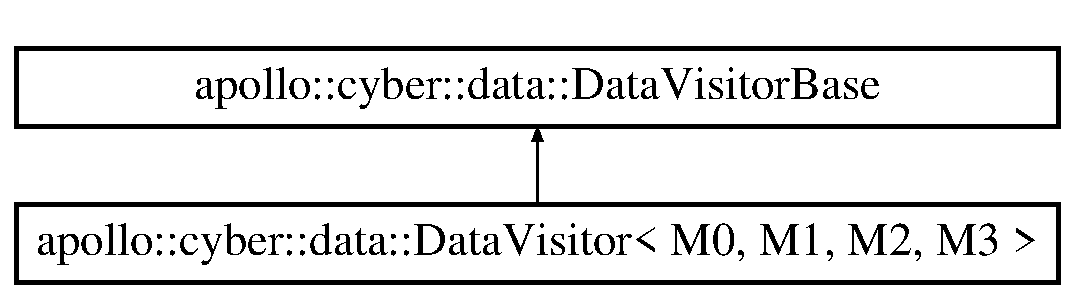
\includegraphics[height=2.000000cm]{classapollo_1_1cyber_1_1data_1_1DataVisitor}
\end{center}
\end{figure}
\subsection*{Public Member Functions}
\begin{DoxyCompactItemize}
\item 
\hyperlink{classapollo_1_1cyber_1_1data_1_1DataVisitor_aa3c92107af063ccb62fc22afc38edc88}{Data\-Visitor} (const std\-::vector$<$ \hyperlink{structapollo_1_1cyber_1_1data_1_1VisitorConfig}{Visitor\-Config} $>$ \&configs)
\item 
\hyperlink{classapollo_1_1cyber_1_1data_1_1DataVisitor_a3e230cff333bf53b0f957b4de5a5bca1}{$\sim$\-Data\-Visitor} ()
\item 
bool \hyperlink{classapollo_1_1cyber_1_1data_1_1DataVisitor_a61ba4cb95ec8fbb5293d76afde794965}{Try\-Fetch} (std\-::shared\-\_\-ptr$<$ M0 $>$ \&m0, std\-::shared\-\_\-ptr$<$ M1 $>$ \&m1, std\-::shared\-\_\-ptr$<$ M2 $>$ \&m2, std\-::shared\-\_\-ptr$<$ M3 $>$ \&m3)
\end{DoxyCompactItemize}
\subsection*{Private Attributes}
\begin{DoxyCompactItemize}
\item 
\hyperlink{classapollo_1_1cyber_1_1data_1_1fusion_1_1DataFusion}{fusion\-::\-Data\-Fusion}$<$ M0, M1, M2, \\*
M3 $>$ $\ast$ \hyperlink{classapollo_1_1cyber_1_1data_1_1DataVisitor_a514ffc2170635b2cd8bf017fbe54f2ab}{data\-\_\-fusion\-\_\-} = nullptr
\item 
\hyperlink{classapollo_1_1cyber_1_1data_1_1ChannelBuffer}{Channel\-Buffer}$<$ M0 $>$ \hyperlink{classapollo_1_1cyber_1_1data_1_1DataVisitor_aadc37e90886bb1a67db1aacc04886d72}{buffer\-\_\-m0\-\_\-}
\item 
\hyperlink{classapollo_1_1cyber_1_1data_1_1ChannelBuffer}{Channel\-Buffer}$<$ M1 $>$ \hyperlink{classapollo_1_1cyber_1_1data_1_1DataVisitor_afd0449bddcb881e18ae46658d3ddb0a9}{buffer\-\_\-m1\-\_\-}
\item 
\hyperlink{classapollo_1_1cyber_1_1data_1_1ChannelBuffer}{Channel\-Buffer}$<$ M2 $>$ \hyperlink{classapollo_1_1cyber_1_1data_1_1DataVisitor_a2dc3d9334f9518e65a9819c63bf5fa63}{buffer\-\_\-m2\-\_\-}
\item 
\hyperlink{classapollo_1_1cyber_1_1data_1_1ChannelBuffer}{Channel\-Buffer}$<$ M3 $>$ \hyperlink{classapollo_1_1cyber_1_1data_1_1DataVisitor_af59b0b1507bb1230495202a03ece6f14}{buffer\-\_\-m3\-\_\-}
\end{DoxyCompactItemize}
\subsection*{Additional Inherited Members}


\subsection{Constructor \& Destructor Documentation}
\hypertarget{classapollo_1_1cyber_1_1data_1_1DataVisitor_aa3c92107af063ccb62fc22afc38edc88}{\index{apollo\-::cyber\-::data\-::\-Data\-Visitor@{apollo\-::cyber\-::data\-::\-Data\-Visitor}!Data\-Visitor@{Data\-Visitor}}
\index{Data\-Visitor@{Data\-Visitor}!apollo::cyber::data::DataVisitor@{apollo\-::cyber\-::data\-::\-Data\-Visitor}}
\subsubsection[{Data\-Visitor}]{\setlength{\rightskip}{0pt plus 5cm}template$<$typename M0 , typename M1  = Null\-Type, typename M2  = Null\-Type, typename M3  = Null\-Type$>$ {\bf apollo\-::cyber\-::data\-::\-Data\-Visitor}$<$ M0, M1, M2, M3 $>$\-::{\bf Data\-Visitor} (
\begin{DoxyParamCaption}
\item[{const std\-::vector$<$ {\bf Visitor\-Config} $>$ \&}]{configs}
\end{DoxyParamCaption}
)\hspace{0.3cm}{\ttfamily [inline]}, {\ttfamily [explicit]}}}\label{classapollo_1_1cyber_1_1data_1_1DataVisitor_aa3c92107af063ccb62fc22afc38edc88}
\hypertarget{classapollo_1_1cyber_1_1data_1_1DataVisitor_a3e230cff333bf53b0f957b4de5a5bca1}{\index{apollo\-::cyber\-::data\-::\-Data\-Visitor@{apollo\-::cyber\-::data\-::\-Data\-Visitor}!$\sim$\-Data\-Visitor@{$\sim$\-Data\-Visitor}}
\index{$\sim$\-Data\-Visitor@{$\sim$\-Data\-Visitor}!apollo::cyber::data::DataVisitor@{apollo\-::cyber\-::data\-::\-Data\-Visitor}}
\subsubsection[{$\sim$\-Data\-Visitor}]{\setlength{\rightskip}{0pt plus 5cm}template$<$typename M0 , typename M1  = Null\-Type, typename M2  = Null\-Type, typename M3  = Null\-Type$>$ {\bf apollo\-::cyber\-::data\-::\-Data\-Visitor}$<$ M0, M1, M2, M3 $>$\-::$\sim${\bf Data\-Visitor} (
\begin{DoxyParamCaption}
{}
\end{DoxyParamCaption}
)\hspace{0.3cm}{\ttfamily [inline]}}}\label{classapollo_1_1cyber_1_1data_1_1DataVisitor_a3e230cff333bf53b0f957b4de5a5bca1}


\subsection{Member Function Documentation}
\hypertarget{classapollo_1_1cyber_1_1data_1_1DataVisitor_a61ba4cb95ec8fbb5293d76afde794965}{\index{apollo\-::cyber\-::data\-::\-Data\-Visitor@{apollo\-::cyber\-::data\-::\-Data\-Visitor}!Try\-Fetch@{Try\-Fetch}}
\index{Try\-Fetch@{Try\-Fetch}!apollo::cyber::data::DataVisitor@{apollo\-::cyber\-::data\-::\-Data\-Visitor}}
\subsubsection[{Try\-Fetch}]{\setlength{\rightskip}{0pt plus 5cm}template$<$typename M0 , typename M1  = Null\-Type, typename M2  = Null\-Type, typename M3  = Null\-Type$>$ bool {\bf apollo\-::cyber\-::data\-::\-Data\-Visitor}$<$ M0, M1, M2, M3 $>$\-::Try\-Fetch (
\begin{DoxyParamCaption}
\item[{std\-::shared\-\_\-ptr$<$ M0 $>$ \&}]{m0, }
\item[{std\-::shared\-\_\-ptr$<$ M1 $>$ \&}]{m1, }
\item[{std\-::shared\-\_\-ptr$<$ M2 $>$ \&}]{m2, }
\item[{std\-::shared\-\_\-ptr$<$ M3 $>$ \&}]{m3}
\end{DoxyParamCaption}
)\hspace{0.3cm}{\ttfamily [inline]}}}\label{classapollo_1_1cyber_1_1data_1_1DataVisitor_a61ba4cb95ec8fbb5293d76afde794965}


\subsection{Member Data Documentation}
\hypertarget{classapollo_1_1cyber_1_1data_1_1DataVisitor_aadc37e90886bb1a67db1aacc04886d72}{\index{apollo\-::cyber\-::data\-::\-Data\-Visitor@{apollo\-::cyber\-::data\-::\-Data\-Visitor}!buffer\-\_\-m0\-\_\-@{buffer\-\_\-m0\-\_\-}}
\index{buffer\-\_\-m0\-\_\-@{buffer\-\_\-m0\-\_\-}!apollo::cyber::data::DataVisitor@{apollo\-::cyber\-::data\-::\-Data\-Visitor}}
\subsubsection[{buffer\-\_\-m0\-\_\-}]{\setlength{\rightskip}{0pt plus 5cm}template$<$typename M0 , typename M1  = Null\-Type, typename M2  = Null\-Type, typename M3  = Null\-Type$>$ {\bf Channel\-Buffer}$<$M0$>$ {\bf apollo\-::cyber\-::data\-::\-Data\-Visitor}$<$ M0, M1, M2, M3 $>$\-::buffer\-\_\-m0\-\_\-\hspace{0.3cm}{\ttfamily [private]}}}\label{classapollo_1_1cyber_1_1data_1_1DataVisitor_aadc37e90886bb1a67db1aacc04886d72}
\hypertarget{classapollo_1_1cyber_1_1data_1_1DataVisitor_afd0449bddcb881e18ae46658d3ddb0a9}{\index{apollo\-::cyber\-::data\-::\-Data\-Visitor@{apollo\-::cyber\-::data\-::\-Data\-Visitor}!buffer\-\_\-m1\-\_\-@{buffer\-\_\-m1\-\_\-}}
\index{buffer\-\_\-m1\-\_\-@{buffer\-\_\-m1\-\_\-}!apollo::cyber::data::DataVisitor@{apollo\-::cyber\-::data\-::\-Data\-Visitor}}
\subsubsection[{buffer\-\_\-m1\-\_\-}]{\setlength{\rightskip}{0pt plus 5cm}template$<$typename M0 , typename M1  = Null\-Type, typename M2  = Null\-Type, typename M3  = Null\-Type$>$ {\bf Channel\-Buffer}$<$M1$>$ {\bf apollo\-::cyber\-::data\-::\-Data\-Visitor}$<$ M0, M1, M2, M3 $>$\-::buffer\-\_\-m1\-\_\-\hspace{0.3cm}{\ttfamily [private]}}}\label{classapollo_1_1cyber_1_1data_1_1DataVisitor_afd0449bddcb881e18ae46658d3ddb0a9}
\hypertarget{classapollo_1_1cyber_1_1data_1_1DataVisitor_a2dc3d9334f9518e65a9819c63bf5fa63}{\index{apollo\-::cyber\-::data\-::\-Data\-Visitor@{apollo\-::cyber\-::data\-::\-Data\-Visitor}!buffer\-\_\-m2\-\_\-@{buffer\-\_\-m2\-\_\-}}
\index{buffer\-\_\-m2\-\_\-@{buffer\-\_\-m2\-\_\-}!apollo::cyber::data::DataVisitor@{apollo\-::cyber\-::data\-::\-Data\-Visitor}}
\subsubsection[{buffer\-\_\-m2\-\_\-}]{\setlength{\rightskip}{0pt plus 5cm}template$<$typename M0 , typename M1  = Null\-Type, typename M2  = Null\-Type, typename M3  = Null\-Type$>$ {\bf Channel\-Buffer}$<$M2$>$ {\bf apollo\-::cyber\-::data\-::\-Data\-Visitor}$<$ M0, M1, M2, M3 $>$\-::buffer\-\_\-m2\-\_\-\hspace{0.3cm}{\ttfamily [private]}}}\label{classapollo_1_1cyber_1_1data_1_1DataVisitor_a2dc3d9334f9518e65a9819c63bf5fa63}
\hypertarget{classapollo_1_1cyber_1_1data_1_1DataVisitor_af59b0b1507bb1230495202a03ece6f14}{\index{apollo\-::cyber\-::data\-::\-Data\-Visitor@{apollo\-::cyber\-::data\-::\-Data\-Visitor}!buffer\-\_\-m3\-\_\-@{buffer\-\_\-m3\-\_\-}}
\index{buffer\-\_\-m3\-\_\-@{buffer\-\_\-m3\-\_\-}!apollo::cyber::data::DataVisitor@{apollo\-::cyber\-::data\-::\-Data\-Visitor}}
\subsubsection[{buffer\-\_\-m3\-\_\-}]{\setlength{\rightskip}{0pt plus 5cm}template$<$typename M0 , typename M1  = Null\-Type, typename M2  = Null\-Type, typename M3  = Null\-Type$>$ {\bf Channel\-Buffer}$<$M3$>$ {\bf apollo\-::cyber\-::data\-::\-Data\-Visitor}$<$ M0, M1, M2, M3 $>$\-::buffer\-\_\-m3\-\_\-\hspace{0.3cm}{\ttfamily [private]}}}\label{classapollo_1_1cyber_1_1data_1_1DataVisitor_af59b0b1507bb1230495202a03ece6f14}
\hypertarget{classapollo_1_1cyber_1_1data_1_1DataVisitor_a514ffc2170635b2cd8bf017fbe54f2ab}{\index{apollo\-::cyber\-::data\-::\-Data\-Visitor@{apollo\-::cyber\-::data\-::\-Data\-Visitor}!data\-\_\-fusion\-\_\-@{data\-\_\-fusion\-\_\-}}
\index{data\-\_\-fusion\-\_\-@{data\-\_\-fusion\-\_\-}!apollo::cyber::data::DataVisitor@{apollo\-::cyber\-::data\-::\-Data\-Visitor}}
\subsubsection[{data\-\_\-fusion\-\_\-}]{\setlength{\rightskip}{0pt plus 5cm}template$<$typename M0 , typename M1  = Null\-Type, typename M2  = Null\-Type, typename M3  = Null\-Type$>$ {\bf fusion\-::\-Data\-Fusion}$<$M0, M1, M2, M3$>$$\ast$ {\bf apollo\-::cyber\-::data\-::\-Data\-Visitor}$<$ M0, M1, M2, M3 $>$\-::data\-\_\-fusion\-\_\- = nullptr\hspace{0.3cm}{\ttfamily [private]}}}\label{classapollo_1_1cyber_1_1data_1_1DataVisitor_a514ffc2170635b2cd8bf017fbe54f2ab}


The documentation for this class was generated from the following file\-:\begin{DoxyCompactItemize}
\item 
data/\hyperlink{data__visitor_8h}{data\-\_\-visitor.\-h}\end{DoxyCompactItemize}

\hypertarget{classapollo_1_1cyber_1_1data_1_1DataVisitor_3_01M0_00_01M1_00_01M2_00_01NullType_01_4}{\section{apollo\-:\-:cyber\-:\-:data\-:\-:Data\-Visitor$<$ M0, M1, M2, Null\-Type $>$ Class Template Reference}
\label{classapollo_1_1cyber_1_1data_1_1DataVisitor_3_01M0_00_01M1_00_01M2_00_01NullType_01_4}\index{apollo\-::cyber\-::data\-::\-Data\-Visitor$<$ M0, M1, M2, Null\-Type $>$@{apollo\-::cyber\-::data\-::\-Data\-Visitor$<$ M0, M1, M2, Null\-Type $>$}}
}


{\ttfamily \#include $<$data\-\_\-visitor.\-h$>$}

Inheritance diagram for apollo\-:\-:cyber\-:\-:data\-:\-:Data\-Visitor$<$ M0, M1, M2, Null\-Type $>$\-:\begin{figure}[H]
\begin{center}
\leavevmode
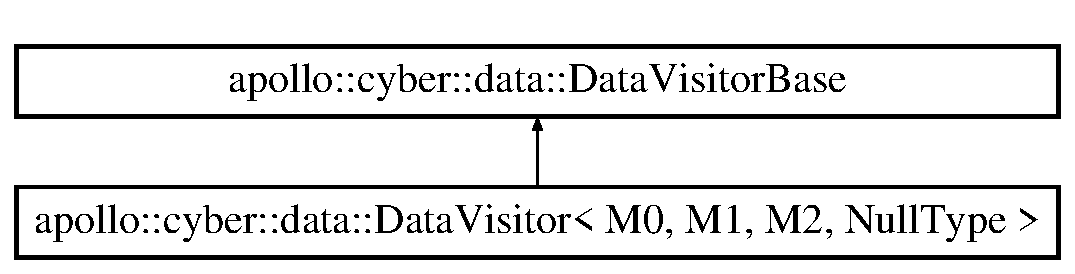
\includegraphics[height=2.000000cm]{classapollo_1_1cyber_1_1data_1_1DataVisitor_3_01M0_00_01M1_00_01M2_00_01NullType_01_4}
\end{center}
\end{figure}
\subsection*{Public Member Functions}
\begin{DoxyCompactItemize}
\item 
\hyperlink{classapollo_1_1cyber_1_1data_1_1DataVisitor_3_01M0_00_01M1_00_01M2_00_01NullType_01_4_a9095e2ee598089eae64782d078eaf7c5}{Data\-Visitor} (const std\-::vector$<$ \hyperlink{structapollo_1_1cyber_1_1data_1_1VisitorConfig}{Visitor\-Config} $>$ \&configs)
\item 
\hyperlink{classapollo_1_1cyber_1_1data_1_1DataVisitor_3_01M0_00_01M1_00_01M2_00_01NullType_01_4_a6902bea879c6427dcc70e1fdc6883834}{$\sim$\-Data\-Visitor} ()
\item 
bool \hyperlink{classapollo_1_1cyber_1_1data_1_1DataVisitor_3_01M0_00_01M1_00_01M2_00_01NullType_01_4_a252cf8bdc02e71e5845872a0489d0425}{Try\-Fetch} (std\-::shared\-\_\-ptr$<$ M0 $>$ \&m0, std\-::shared\-\_\-ptr$<$ M1 $>$ \&m1, std\-::shared\-\_\-ptr$<$ M2 $>$ \&m2)
\end{DoxyCompactItemize}
\subsection*{Private Attributes}
\begin{DoxyCompactItemize}
\item 
\hyperlink{classapollo_1_1cyber_1_1data_1_1fusion_1_1DataFusion}{fusion\-::\-Data\-Fusion}$<$ M0, M1, M2 $>$ $\ast$ \hyperlink{classapollo_1_1cyber_1_1data_1_1DataVisitor_3_01M0_00_01M1_00_01M2_00_01NullType_01_4_a84a90a04bbe766d4e0cbf063be5bdc59}{data\-\_\-fusion\-\_\-} = nullptr
\item 
\hyperlink{classapollo_1_1cyber_1_1data_1_1ChannelBuffer}{Channel\-Buffer}$<$ M0 $>$ \hyperlink{classapollo_1_1cyber_1_1data_1_1DataVisitor_3_01M0_00_01M1_00_01M2_00_01NullType_01_4_a70d4d6ba83925cbf3944cb0ebb517ba7}{buffer\-\_\-m0\-\_\-}
\item 
\hyperlink{classapollo_1_1cyber_1_1data_1_1ChannelBuffer}{Channel\-Buffer}$<$ M1 $>$ \hyperlink{classapollo_1_1cyber_1_1data_1_1DataVisitor_3_01M0_00_01M1_00_01M2_00_01NullType_01_4_a386121942253c6fedf37b8d57fca8d9b}{buffer\-\_\-m1\-\_\-}
\item 
\hyperlink{classapollo_1_1cyber_1_1data_1_1ChannelBuffer}{Channel\-Buffer}$<$ M2 $>$ \hyperlink{classapollo_1_1cyber_1_1data_1_1DataVisitor_3_01M0_00_01M1_00_01M2_00_01NullType_01_4_a80b92e97959fdc21afe4ddc138374b99}{buffer\-\_\-m2\-\_\-}
\end{DoxyCompactItemize}
\subsection*{Additional Inherited Members}


\subsection{Constructor \& Destructor Documentation}
\hypertarget{classapollo_1_1cyber_1_1data_1_1DataVisitor_3_01M0_00_01M1_00_01M2_00_01NullType_01_4_a9095e2ee598089eae64782d078eaf7c5}{\index{apollo\-::cyber\-::data\-::\-Data\-Visitor$<$ M0, M1, M2, Null\-Type $>$@{apollo\-::cyber\-::data\-::\-Data\-Visitor$<$ M0, M1, M2, Null\-Type $>$}!Data\-Visitor@{Data\-Visitor}}
\index{Data\-Visitor@{Data\-Visitor}!apollo::cyber::data::DataVisitor< M0, M1, M2, NullType >@{apollo\-::cyber\-::data\-::\-Data\-Visitor$<$ M0, M1, M2, Null\-Type $>$}}
\subsubsection[{Data\-Visitor}]{\setlength{\rightskip}{0pt plus 5cm}template$<$typename M0 , typename M1 , typename M2 $>$ {\bf apollo\-::cyber\-::data\-::\-Data\-Visitor}$<$ M0, M1, M2, {\bf Null\-Type} $>$\-::{\bf Data\-Visitor} (
\begin{DoxyParamCaption}
\item[{const std\-::vector$<$ {\bf Visitor\-Config} $>$ \&}]{configs}
\end{DoxyParamCaption}
)\hspace{0.3cm}{\ttfamily [inline]}, {\ttfamily [explicit]}}}\label{classapollo_1_1cyber_1_1data_1_1DataVisitor_3_01M0_00_01M1_00_01M2_00_01NullType_01_4_a9095e2ee598089eae64782d078eaf7c5}
\hypertarget{classapollo_1_1cyber_1_1data_1_1DataVisitor_3_01M0_00_01M1_00_01M2_00_01NullType_01_4_a6902bea879c6427dcc70e1fdc6883834}{\index{apollo\-::cyber\-::data\-::\-Data\-Visitor$<$ M0, M1, M2, Null\-Type $>$@{apollo\-::cyber\-::data\-::\-Data\-Visitor$<$ M0, M1, M2, Null\-Type $>$}!$\sim$\-Data\-Visitor@{$\sim$\-Data\-Visitor}}
\index{$\sim$\-Data\-Visitor@{$\sim$\-Data\-Visitor}!apollo::cyber::data::DataVisitor< M0, M1, M2, NullType >@{apollo\-::cyber\-::data\-::\-Data\-Visitor$<$ M0, M1, M2, Null\-Type $>$}}
\subsubsection[{$\sim$\-Data\-Visitor}]{\setlength{\rightskip}{0pt plus 5cm}template$<$typename M0 , typename M1 , typename M2 $>$ {\bf apollo\-::cyber\-::data\-::\-Data\-Visitor}$<$ M0, M1, M2, {\bf Null\-Type} $>$\-::$\sim${\bf Data\-Visitor} (
\begin{DoxyParamCaption}
{}
\end{DoxyParamCaption}
)\hspace{0.3cm}{\ttfamily [inline]}}}\label{classapollo_1_1cyber_1_1data_1_1DataVisitor_3_01M0_00_01M1_00_01M2_00_01NullType_01_4_a6902bea879c6427dcc70e1fdc6883834}


\subsection{Member Function Documentation}
\hypertarget{classapollo_1_1cyber_1_1data_1_1DataVisitor_3_01M0_00_01M1_00_01M2_00_01NullType_01_4_a252cf8bdc02e71e5845872a0489d0425}{\index{apollo\-::cyber\-::data\-::\-Data\-Visitor$<$ M0, M1, M2, Null\-Type $>$@{apollo\-::cyber\-::data\-::\-Data\-Visitor$<$ M0, M1, M2, Null\-Type $>$}!Try\-Fetch@{Try\-Fetch}}
\index{Try\-Fetch@{Try\-Fetch}!apollo::cyber::data::DataVisitor< M0, M1, M2, NullType >@{apollo\-::cyber\-::data\-::\-Data\-Visitor$<$ M0, M1, M2, Null\-Type $>$}}
\subsubsection[{Try\-Fetch}]{\setlength{\rightskip}{0pt plus 5cm}template$<$typename M0 , typename M1 , typename M2 $>$ bool {\bf apollo\-::cyber\-::data\-::\-Data\-Visitor}$<$ M0, M1, M2, {\bf Null\-Type} $>$\-::Try\-Fetch (
\begin{DoxyParamCaption}
\item[{std\-::shared\-\_\-ptr$<$ M0 $>$ \&}]{m0, }
\item[{std\-::shared\-\_\-ptr$<$ M1 $>$ \&}]{m1, }
\item[{std\-::shared\-\_\-ptr$<$ M2 $>$ \&}]{m2}
\end{DoxyParamCaption}
)\hspace{0.3cm}{\ttfamily [inline]}}}\label{classapollo_1_1cyber_1_1data_1_1DataVisitor_3_01M0_00_01M1_00_01M2_00_01NullType_01_4_a252cf8bdc02e71e5845872a0489d0425}


\subsection{Member Data Documentation}
\hypertarget{classapollo_1_1cyber_1_1data_1_1DataVisitor_3_01M0_00_01M1_00_01M2_00_01NullType_01_4_a70d4d6ba83925cbf3944cb0ebb517ba7}{\index{apollo\-::cyber\-::data\-::\-Data\-Visitor$<$ M0, M1, M2, Null\-Type $>$@{apollo\-::cyber\-::data\-::\-Data\-Visitor$<$ M0, M1, M2, Null\-Type $>$}!buffer\-\_\-m0\-\_\-@{buffer\-\_\-m0\-\_\-}}
\index{buffer\-\_\-m0\-\_\-@{buffer\-\_\-m0\-\_\-}!apollo::cyber::data::DataVisitor< M0, M1, M2, NullType >@{apollo\-::cyber\-::data\-::\-Data\-Visitor$<$ M0, M1, M2, Null\-Type $>$}}
\subsubsection[{buffer\-\_\-m0\-\_\-}]{\setlength{\rightskip}{0pt plus 5cm}template$<$typename M0 , typename M1 , typename M2 $>$ {\bf Channel\-Buffer}$<$M0$>$ {\bf apollo\-::cyber\-::data\-::\-Data\-Visitor}$<$ M0, M1, M2, {\bf Null\-Type} $>$\-::buffer\-\_\-m0\-\_\-\hspace{0.3cm}{\ttfamily [private]}}}\label{classapollo_1_1cyber_1_1data_1_1DataVisitor_3_01M0_00_01M1_00_01M2_00_01NullType_01_4_a70d4d6ba83925cbf3944cb0ebb517ba7}
\hypertarget{classapollo_1_1cyber_1_1data_1_1DataVisitor_3_01M0_00_01M1_00_01M2_00_01NullType_01_4_a386121942253c6fedf37b8d57fca8d9b}{\index{apollo\-::cyber\-::data\-::\-Data\-Visitor$<$ M0, M1, M2, Null\-Type $>$@{apollo\-::cyber\-::data\-::\-Data\-Visitor$<$ M0, M1, M2, Null\-Type $>$}!buffer\-\_\-m1\-\_\-@{buffer\-\_\-m1\-\_\-}}
\index{buffer\-\_\-m1\-\_\-@{buffer\-\_\-m1\-\_\-}!apollo::cyber::data::DataVisitor< M0, M1, M2, NullType >@{apollo\-::cyber\-::data\-::\-Data\-Visitor$<$ M0, M1, M2, Null\-Type $>$}}
\subsubsection[{buffer\-\_\-m1\-\_\-}]{\setlength{\rightskip}{0pt plus 5cm}template$<$typename M0 , typename M1 , typename M2 $>$ {\bf Channel\-Buffer}$<$M1$>$ {\bf apollo\-::cyber\-::data\-::\-Data\-Visitor}$<$ M0, M1, M2, {\bf Null\-Type} $>$\-::buffer\-\_\-m1\-\_\-\hspace{0.3cm}{\ttfamily [private]}}}\label{classapollo_1_1cyber_1_1data_1_1DataVisitor_3_01M0_00_01M1_00_01M2_00_01NullType_01_4_a386121942253c6fedf37b8d57fca8d9b}
\hypertarget{classapollo_1_1cyber_1_1data_1_1DataVisitor_3_01M0_00_01M1_00_01M2_00_01NullType_01_4_a80b92e97959fdc21afe4ddc138374b99}{\index{apollo\-::cyber\-::data\-::\-Data\-Visitor$<$ M0, M1, M2, Null\-Type $>$@{apollo\-::cyber\-::data\-::\-Data\-Visitor$<$ M0, M1, M2, Null\-Type $>$}!buffer\-\_\-m2\-\_\-@{buffer\-\_\-m2\-\_\-}}
\index{buffer\-\_\-m2\-\_\-@{buffer\-\_\-m2\-\_\-}!apollo::cyber::data::DataVisitor< M0, M1, M2, NullType >@{apollo\-::cyber\-::data\-::\-Data\-Visitor$<$ M0, M1, M2, Null\-Type $>$}}
\subsubsection[{buffer\-\_\-m2\-\_\-}]{\setlength{\rightskip}{0pt plus 5cm}template$<$typename M0 , typename M1 , typename M2 $>$ {\bf Channel\-Buffer}$<$M2$>$ {\bf apollo\-::cyber\-::data\-::\-Data\-Visitor}$<$ M0, M1, M2, {\bf Null\-Type} $>$\-::buffer\-\_\-m2\-\_\-\hspace{0.3cm}{\ttfamily [private]}}}\label{classapollo_1_1cyber_1_1data_1_1DataVisitor_3_01M0_00_01M1_00_01M2_00_01NullType_01_4_a80b92e97959fdc21afe4ddc138374b99}
\hypertarget{classapollo_1_1cyber_1_1data_1_1DataVisitor_3_01M0_00_01M1_00_01M2_00_01NullType_01_4_a84a90a04bbe766d4e0cbf063be5bdc59}{\index{apollo\-::cyber\-::data\-::\-Data\-Visitor$<$ M0, M1, M2, Null\-Type $>$@{apollo\-::cyber\-::data\-::\-Data\-Visitor$<$ M0, M1, M2, Null\-Type $>$}!data\-\_\-fusion\-\_\-@{data\-\_\-fusion\-\_\-}}
\index{data\-\_\-fusion\-\_\-@{data\-\_\-fusion\-\_\-}!apollo::cyber::data::DataVisitor< M0, M1, M2, NullType >@{apollo\-::cyber\-::data\-::\-Data\-Visitor$<$ M0, M1, M2, Null\-Type $>$}}
\subsubsection[{data\-\_\-fusion\-\_\-}]{\setlength{\rightskip}{0pt plus 5cm}template$<$typename M0 , typename M1 , typename M2 $>$ {\bf fusion\-::\-Data\-Fusion}$<$M0, M1, M2$>$$\ast$ {\bf apollo\-::cyber\-::data\-::\-Data\-Visitor}$<$ M0, M1, M2, {\bf Null\-Type} $>$\-::data\-\_\-fusion\-\_\- = nullptr\hspace{0.3cm}{\ttfamily [private]}}}\label{classapollo_1_1cyber_1_1data_1_1DataVisitor_3_01M0_00_01M1_00_01M2_00_01NullType_01_4_a84a90a04bbe766d4e0cbf063be5bdc59}


The documentation for this class was generated from the following file\-:\begin{DoxyCompactItemize}
\item 
data/\hyperlink{data__visitor_8h}{data\-\_\-visitor.\-h}\end{DoxyCompactItemize}

\hypertarget{classapollo_1_1cyber_1_1data_1_1DataVisitor_3_01M0_00_01M1_00_01NullType_00_01NullType_01_4}{\section{apollo\-:\-:cyber\-:\-:data\-:\-:Data\-Visitor$<$ M0, M1, Null\-Type, Null\-Type $>$ Class Template Reference}
\label{classapollo_1_1cyber_1_1data_1_1DataVisitor_3_01M0_00_01M1_00_01NullType_00_01NullType_01_4}\index{apollo\-::cyber\-::data\-::\-Data\-Visitor$<$ M0, M1, Null\-Type, Null\-Type $>$@{apollo\-::cyber\-::data\-::\-Data\-Visitor$<$ M0, M1, Null\-Type, Null\-Type $>$}}
}


{\ttfamily \#include $<$data\-\_\-visitor.\-h$>$}

Inheritance diagram for apollo\-:\-:cyber\-:\-:data\-:\-:Data\-Visitor$<$ M0, M1, Null\-Type, Null\-Type $>$\-:\begin{figure}[H]
\begin{center}
\leavevmode
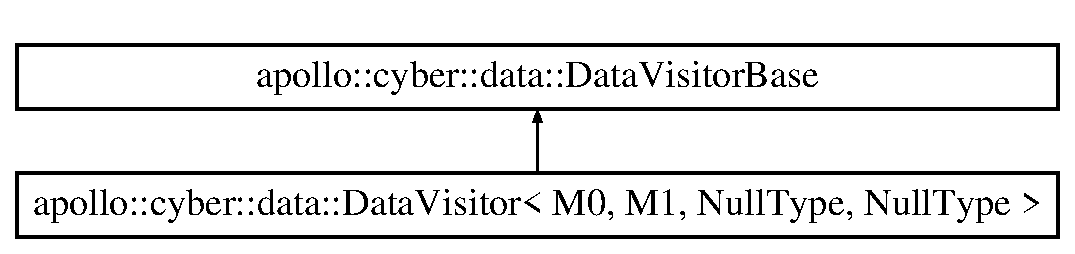
\includegraphics[height=2.000000cm]{classapollo_1_1cyber_1_1data_1_1DataVisitor_3_01M0_00_01M1_00_01NullType_00_01NullType_01_4}
\end{center}
\end{figure}
\subsection*{Public Member Functions}
\begin{DoxyCompactItemize}
\item 
\hyperlink{classapollo_1_1cyber_1_1data_1_1DataVisitor_3_01M0_00_01M1_00_01NullType_00_01NullType_01_4_a80c2d63eb733d49914472df81f44419b}{Data\-Visitor} (const std\-::vector$<$ \hyperlink{structapollo_1_1cyber_1_1data_1_1VisitorConfig}{Visitor\-Config} $>$ \&configs)
\item 
\hyperlink{classapollo_1_1cyber_1_1data_1_1DataVisitor_3_01M0_00_01M1_00_01NullType_00_01NullType_01_4_a94267ad93bcda46bb0b561bcdd38317e}{$\sim$\-Data\-Visitor} ()
\item 
bool \hyperlink{classapollo_1_1cyber_1_1data_1_1DataVisitor_3_01M0_00_01M1_00_01NullType_00_01NullType_01_4_a4fab945c809cb23efd401607d040321b}{Try\-Fetch} (std\-::shared\-\_\-ptr$<$ M0 $>$ \&m0, std\-::shared\-\_\-ptr$<$ M1 $>$ \&m1)
\end{DoxyCompactItemize}
\subsection*{Private Attributes}
\begin{DoxyCompactItemize}
\item 
\hyperlink{classapollo_1_1cyber_1_1data_1_1fusion_1_1DataFusion}{fusion\-::\-Data\-Fusion}$<$ M0, M1 $>$ $\ast$ \hyperlink{classapollo_1_1cyber_1_1data_1_1DataVisitor_3_01M0_00_01M1_00_01NullType_00_01NullType_01_4_a78ad754826bf212cdac717346331dfb2}{data\-\_\-fusion\-\_\-} = nullptr
\item 
\hyperlink{classapollo_1_1cyber_1_1data_1_1ChannelBuffer}{Channel\-Buffer}$<$ M0 $>$ \hyperlink{classapollo_1_1cyber_1_1data_1_1DataVisitor_3_01M0_00_01M1_00_01NullType_00_01NullType_01_4_a6cabc871c6cf0d49e3d5dbaf6081219c}{buffer\-\_\-m0\-\_\-}
\item 
\hyperlink{classapollo_1_1cyber_1_1data_1_1ChannelBuffer}{Channel\-Buffer}$<$ M1 $>$ \hyperlink{classapollo_1_1cyber_1_1data_1_1DataVisitor_3_01M0_00_01M1_00_01NullType_00_01NullType_01_4_a3a8ba95bb88c577c55e36ab2ac12e552}{buffer\-\_\-m1\-\_\-}
\end{DoxyCompactItemize}
\subsection*{Additional Inherited Members}


\subsection{Constructor \& Destructor Documentation}
\hypertarget{classapollo_1_1cyber_1_1data_1_1DataVisitor_3_01M0_00_01M1_00_01NullType_00_01NullType_01_4_a80c2d63eb733d49914472df81f44419b}{\index{apollo\-::cyber\-::data\-::\-Data\-Visitor$<$ M0, M1, Null\-Type, Null\-Type $>$@{apollo\-::cyber\-::data\-::\-Data\-Visitor$<$ M0, M1, Null\-Type, Null\-Type $>$}!Data\-Visitor@{Data\-Visitor}}
\index{Data\-Visitor@{Data\-Visitor}!apollo::cyber::data::DataVisitor< M0, M1, NullType, NullType >@{apollo\-::cyber\-::data\-::\-Data\-Visitor$<$ M0, M1, Null\-Type, Null\-Type $>$}}
\subsubsection[{Data\-Visitor}]{\setlength{\rightskip}{0pt plus 5cm}template$<$typename M0 , typename M1 $>$ {\bf apollo\-::cyber\-::data\-::\-Data\-Visitor}$<$ M0, M1, {\bf Null\-Type}, {\bf Null\-Type} $>$\-::{\bf Data\-Visitor} (
\begin{DoxyParamCaption}
\item[{const std\-::vector$<$ {\bf Visitor\-Config} $>$ \&}]{configs}
\end{DoxyParamCaption}
)\hspace{0.3cm}{\ttfamily [inline]}, {\ttfamily [explicit]}}}\label{classapollo_1_1cyber_1_1data_1_1DataVisitor_3_01M0_00_01M1_00_01NullType_00_01NullType_01_4_a80c2d63eb733d49914472df81f44419b}
\hypertarget{classapollo_1_1cyber_1_1data_1_1DataVisitor_3_01M0_00_01M1_00_01NullType_00_01NullType_01_4_a94267ad93bcda46bb0b561bcdd38317e}{\index{apollo\-::cyber\-::data\-::\-Data\-Visitor$<$ M0, M1, Null\-Type, Null\-Type $>$@{apollo\-::cyber\-::data\-::\-Data\-Visitor$<$ M0, M1, Null\-Type, Null\-Type $>$}!$\sim$\-Data\-Visitor@{$\sim$\-Data\-Visitor}}
\index{$\sim$\-Data\-Visitor@{$\sim$\-Data\-Visitor}!apollo::cyber::data::DataVisitor< M0, M1, NullType, NullType >@{apollo\-::cyber\-::data\-::\-Data\-Visitor$<$ M0, M1, Null\-Type, Null\-Type $>$}}
\subsubsection[{$\sim$\-Data\-Visitor}]{\setlength{\rightskip}{0pt plus 5cm}template$<$typename M0 , typename M1 $>$ {\bf apollo\-::cyber\-::data\-::\-Data\-Visitor}$<$ M0, M1, {\bf Null\-Type}, {\bf Null\-Type} $>$\-::$\sim${\bf Data\-Visitor} (
\begin{DoxyParamCaption}
{}
\end{DoxyParamCaption}
)\hspace{0.3cm}{\ttfamily [inline]}}}\label{classapollo_1_1cyber_1_1data_1_1DataVisitor_3_01M0_00_01M1_00_01NullType_00_01NullType_01_4_a94267ad93bcda46bb0b561bcdd38317e}


\subsection{Member Function Documentation}
\hypertarget{classapollo_1_1cyber_1_1data_1_1DataVisitor_3_01M0_00_01M1_00_01NullType_00_01NullType_01_4_a4fab945c809cb23efd401607d040321b}{\index{apollo\-::cyber\-::data\-::\-Data\-Visitor$<$ M0, M1, Null\-Type, Null\-Type $>$@{apollo\-::cyber\-::data\-::\-Data\-Visitor$<$ M0, M1, Null\-Type, Null\-Type $>$}!Try\-Fetch@{Try\-Fetch}}
\index{Try\-Fetch@{Try\-Fetch}!apollo::cyber::data::DataVisitor< M0, M1, NullType, NullType >@{apollo\-::cyber\-::data\-::\-Data\-Visitor$<$ M0, M1, Null\-Type, Null\-Type $>$}}
\subsubsection[{Try\-Fetch}]{\setlength{\rightskip}{0pt plus 5cm}template$<$typename M0 , typename M1 $>$ bool {\bf apollo\-::cyber\-::data\-::\-Data\-Visitor}$<$ M0, M1, {\bf Null\-Type}, {\bf Null\-Type} $>$\-::Try\-Fetch (
\begin{DoxyParamCaption}
\item[{std\-::shared\-\_\-ptr$<$ M0 $>$ \&}]{m0, }
\item[{std\-::shared\-\_\-ptr$<$ M1 $>$ \&}]{m1}
\end{DoxyParamCaption}
)\hspace{0.3cm}{\ttfamily [inline]}}}\label{classapollo_1_1cyber_1_1data_1_1DataVisitor_3_01M0_00_01M1_00_01NullType_00_01NullType_01_4_a4fab945c809cb23efd401607d040321b}


\subsection{Member Data Documentation}
\hypertarget{classapollo_1_1cyber_1_1data_1_1DataVisitor_3_01M0_00_01M1_00_01NullType_00_01NullType_01_4_a6cabc871c6cf0d49e3d5dbaf6081219c}{\index{apollo\-::cyber\-::data\-::\-Data\-Visitor$<$ M0, M1, Null\-Type, Null\-Type $>$@{apollo\-::cyber\-::data\-::\-Data\-Visitor$<$ M0, M1, Null\-Type, Null\-Type $>$}!buffer\-\_\-m0\-\_\-@{buffer\-\_\-m0\-\_\-}}
\index{buffer\-\_\-m0\-\_\-@{buffer\-\_\-m0\-\_\-}!apollo::cyber::data::DataVisitor< M0, M1, NullType, NullType >@{apollo\-::cyber\-::data\-::\-Data\-Visitor$<$ M0, M1, Null\-Type, Null\-Type $>$}}
\subsubsection[{buffer\-\_\-m0\-\_\-}]{\setlength{\rightskip}{0pt plus 5cm}template$<$typename M0 , typename M1 $>$ {\bf Channel\-Buffer}$<$M0$>$ {\bf apollo\-::cyber\-::data\-::\-Data\-Visitor}$<$ M0, M1, {\bf Null\-Type}, {\bf Null\-Type} $>$\-::buffer\-\_\-m0\-\_\-\hspace{0.3cm}{\ttfamily [private]}}}\label{classapollo_1_1cyber_1_1data_1_1DataVisitor_3_01M0_00_01M1_00_01NullType_00_01NullType_01_4_a6cabc871c6cf0d49e3d5dbaf6081219c}
\hypertarget{classapollo_1_1cyber_1_1data_1_1DataVisitor_3_01M0_00_01M1_00_01NullType_00_01NullType_01_4_a3a8ba95bb88c577c55e36ab2ac12e552}{\index{apollo\-::cyber\-::data\-::\-Data\-Visitor$<$ M0, M1, Null\-Type, Null\-Type $>$@{apollo\-::cyber\-::data\-::\-Data\-Visitor$<$ M0, M1, Null\-Type, Null\-Type $>$}!buffer\-\_\-m1\-\_\-@{buffer\-\_\-m1\-\_\-}}
\index{buffer\-\_\-m1\-\_\-@{buffer\-\_\-m1\-\_\-}!apollo::cyber::data::DataVisitor< M0, M1, NullType, NullType >@{apollo\-::cyber\-::data\-::\-Data\-Visitor$<$ M0, M1, Null\-Type, Null\-Type $>$}}
\subsubsection[{buffer\-\_\-m1\-\_\-}]{\setlength{\rightskip}{0pt plus 5cm}template$<$typename M0 , typename M1 $>$ {\bf Channel\-Buffer}$<$M1$>$ {\bf apollo\-::cyber\-::data\-::\-Data\-Visitor}$<$ M0, M1, {\bf Null\-Type}, {\bf Null\-Type} $>$\-::buffer\-\_\-m1\-\_\-\hspace{0.3cm}{\ttfamily [private]}}}\label{classapollo_1_1cyber_1_1data_1_1DataVisitor_3_01M0_00_01M1_00_01NullType_00_01NullType_01_4_a3a8ba95bb88c577c55e36ab2ac12e552}
\hypertarget{classapollo_1_1cyber_1_1data_1_1DataVisitor_3_01M0_00_01M1_00_01NullType_00_01NullType_01_4_a78ad754826bf212cdac717346331dfb2}{\index{apollo\-::cyber\-::data\-::\-Data\-Visitor$<$ M0, M1, Null\-Type, Null\-Type $>$@{apollo\-::cyber\-::data\-::\-Data\-Visitor$<$ M0, M1, Null\-Type, Null\-Type $>$}!data\-\_\-fusion\-\_\-@{data\-\_\-fusion\-\_\-}}
\index{data\-\_\-fusion\-\_\-@{data\-\_\-fusion\-\_\-}!apollo::cyber::data::DataVisitor< M0, M1, NullType, NullType >@{apollo\-::cyber\-::data\-::\-Data\-Visitor$<$ M0, M1, Null\-Type, Null\-Type $>$}}
\subsubsection[{data\-\_\-fusion\-\_\-}]{\setlength{\rightskip}{0pt plus 5cm}template$<$typename M0 , typename M1 $>$ {\bf fusion\-::\-Data\-Fusion}$<$M0, M1$>$$\ast$ {\bf apollo\-::cyber\-::data\-::\-Data\-Visitor}$<$ M0, M1, {\bf Null\-Type}, {\bf Null\-Type} $>$\-::data\-\_\-fusion\-\_\- = nullptr\hspace{0.3cm}{\ttfamily [private]}}}\label{classapollo_1_1cyber_1_1data_1_1DataVisitor_3_01M0_00_01M1_00_01NullType_00_01NullType_01_4_a78ad754826bf212cdac717346331dfb2}


The documentation for this class was generated from the following file\-:\begin{DoxyCompactItemize}
\item 
data/\hyperlink{data__visitor_8h}{data\-\_\-visitor.\-h}\end{DoxyCompactItemize}

\hypertarget{classapollo_1_1cyber_1_1data_1_1DataVisitor_3_01M0_00_01NullType_00_01NullType_00_01NullType_01_4}{\section{apollo\-:\-:cyber\-:\-:data\-:\-:Data\-Visitor$<$ M0, Null\-Type, Null\-Type, Null\-Type $>$ Class Template Reference}
\label{classapollo_1_1cyber_1_1data_1_1DataVisitor_3_01M0_00_01NullType_00_01NullType_00_01NullType_01_4}\index{apollo\-::cyber\-::data\-::\-Data\-Visitor$<$ M0, Null\-Type, Null\-Type, Null\-Type $>$@{apollo\-::cyber\-::data\-::\-Data\-Visitor$<$ M0, Null\-Type, Null\-Type, Null\-Type $>$}}
}


{\ttfamily \#include $<$data\-\_\-visitor.\-h$>$}

Inheritance diagram for apollo\-:\-:cyber\-:\-:data\-:\-:Data\-Visitor$<$ M0, Null\-Type, Null\-Type, Null\-Type $>$\-:\begin{figure}[H]
\begin{center}
\leavevmode
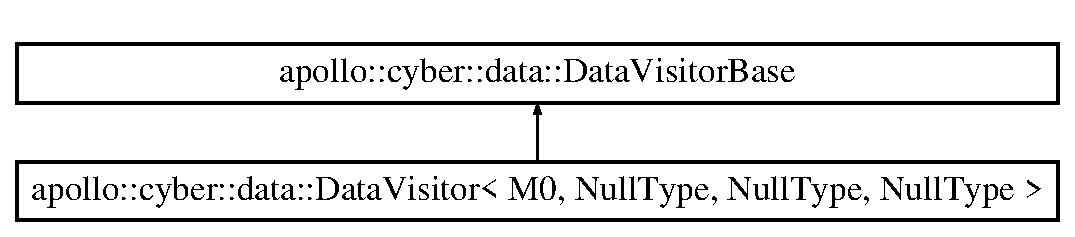
\includegraphics[height=2.000000cm]{classapollo_1_1cyber_1_1data_1_1DataVisitor_3_01M0_00_01NullType_00_01NullType_00_01NullType_01_4}
\end{center}
\end{figure}
\subsection*{Public Member Functions}
\begin{DoxyCompactItemize}
\item 
\hyperlink{classapollo_1_1cyber_1_1data_1_1DataVisitor_3_01M0_00_01NullType_00_01NullType_00_01NullType_01_4_a79966a0db2a4d5f536cdb40013f2cbb5}{Data\-Visitor} (const \hyperlink{structapollo_1_1cyber_1_1data_1_1VisitorConfig}{Visitor\-Config} \&configs)
\item 
\hyperlink{classapollo_1_1cyber_1_1data_1_1DataVisitor_3_01M0_00_01NullType_00_01NullType_00_01NullType_01_4_a3177a3f23c49188f242deb65409c67e7}{Data\-Visitor} (uint64\-\_\-t channel\-\_\-id, uint32\-\_\-t queue\-\_\-size)
\item 
bool \hyperlink{classapollo_1_1cyber_1_1data_1_1DataVisitor_3_01M0_00_01NullType_00_01NullType_00_01NullType_01_4_a2030f650aeebdaaafcffdb3217bcd1d5}{Try\-Fetch} (std\-::shared\-\_\-ptr$<$ M0 $>$ \&m0)
\end{DoxyCompactItemize}
\subsection*{Private Attributes}
\begin{DoxyCompactItemize}
\item 
\hyperlink{classapollo_1_1cyber_1_1data_1_1ChannelBuffer}{Channel\-Buffer}$<$ M0 $>$ \hyperlink{classapollo_1_1cyber_1_1data_1_1DataVisitor_3_01M0_00_01NullType_00_01NullType_00_01NullType_01_4_a71f818743c76bcbfbb3bbe687ce1f2ce}{buffer\-\_\-}
\end{DoxyCompactItemize}
\subsection*{Additional Inherited Members}


\subsection{Constructor \& Destructor Documentation}
\hypertarget{classapollo_1_1cyber_1_1data_1_1DataVisitor_3_01M0_00_01NullType_00_01NullType_00_01NullType_01_4_a79966a0db2a4d5f536cdb40013f2cbb5}{\index{apollo\-::cyber\-::data\-::\-Data\-Visitor$<$ M0, Null\-Type, Null\-Type, Null\-Type $>$@{apollo\-::cyber\-::data\-::\-Data\-Visitor$<$ M0, Null\-Type, Null\-Type, Null\-Type $>$}!Data\-Visitor@{Data\-Visitor}}
\index{Data\-Visitor@{Data\-Visitor}!apollo::cyber::data::DataVisitor< M0, NullType, NullType, NullType >@{apollo\-::cyber\-::data\-::\-Data\-Visitor$<$ M0, Null\-Type, Null\-Type, Null\-Type $>$}}
\subsubsection[{Data\-Visitor}]{\setlength{\rightskip}{0pt plus 5cm}template$<$typename M0 $>$ {\bf apollo\-::cyber\-::data\-::\-Data\-Visitor}$<$ M0, {\bf Null\-Type}, {\bf Null\-Type}, {\bf Null\-Type} $>$\-::{\bf Data\-Visitor} (
\begin{DoxyParamCaption}
\item[{const {\bf Visitor\-Config} \&}]{configs}
\end{DoxyParamCaption}
)\hspace{0.3cm}{\ttfamily [inline]}, {\ttfamily [explicit]}}}\label{classapollo_1_1cyber_1_1data_1_1DataVisitor_3_01M0_00_01NullType_00_01NullType_00_01NullType_01_4_a79966a0db2a4d5f536cdb40013f2cbb5}
\hypertarget{classapollo_1_1cyber_1_1data_1_1DataVisitor_3_01M0_00_01NullType_00_01NullType_00_01NullType_01_4_a3177a3f23c49188f242deb65409c67e7}{\index{apollo\-::cyber\-::data\-::\-Data\-Visitor$<$ M0, Null\-Type, Null\-Type, Null\-Type $>$@{apollo\-::cyber\-::data\-::\-Data\-Visitor$<$ M0, Null\-Type, Null\-Type, Null\-Type $>$}!Data\-Visitor@{Data\-Visitor}}
\index{Data\-Visitor@{Data\-Visitor}!apollo::cyber::data::DataVisitor< M0, NullType, NullType, NullType >@{apollo\-::cyber\-::data\-::\-Data\-Visitor$<$ M0, Null\-Type, Null\-Type, Null\-Type $>$}}
\subsubsection[{Data\-Visitor}]{\setlength{\rightskip}{0pt plus 5cm}template$<$typename M0 $>$ {\bf apollo\-::cyber\-::data\-::\-Data\-Visitor}$<$ M0, {\bf Null\-Type}, {\bf Null\-Type}, {\bf Null\-Type} $>$\-::{\bf Data\-Visitor} (
\begin{DoxyParamCaption}
\item[{uint64\-\_\-t}]{channel\-\_\-id, }
\item[{uint32\-\_\-t}]{queue\-\_\-size}
\end{DoxyParamCaption}
)\hspace{0.3cm}{\ttfamily [inline]}}}\label{classapollo_1_1cyber_1_1data_1_1DataVisitor_3_01M0_00_01NullType_00_01NullType_00_01NullType_01_4_a3177a3f23c49188f242deb65409c67e7}


\subsection{Member Function Documentation}
\hypertarget{classapollo_1_1cyber_1_1data_1_1DataVisitor_3_01M0_00_01NullType_00_01NullType_00_01NullType_01_4_a2030f650aeebdaaafcffdb3217bcd1d5}{\index{apollo\-::cyber\-::data\-::\-Data\-Visitor$<$ M0, Null\-Type, Null\-Type, Null\-Type $>$@{apollo\-::cyber\-::data\-::\-Data\-Visitor$<$ M0, Null\-Type, Null\-Type, Null\-Type $>$}!Try\-Fetch@{Try\-Fetch}}
\index{Try\-Fetch@{Try\-Fetch}!apollo::cyber::data::DataVisitor< M0, NullType, NullType, NullType >@{apollo\-::cyber\-::data\-::\-Data\-Visitor$<$ M0, Null\-Type, Null\-Type, Null\-Type $>$}}
\subsubsection[{Try\-Fetch}]{\setlength{\rightskip}{0pt plus 5cm}template$<$typename M0 $>$ bool {\bf apollo\-::cyber\-::data\-::\-Data\-Visitor}$<$ M0, {\bf Null\-Type}, {\bf Null\-Type}, {\bf Null\-Type} $>$\-::Try\-Fetch (
\begin{DoxyParamCaption}
\item[{std\-::shared\-\_\-ptr$<$ M0 $>$ \&}]{m0}
\end{DoxyParamCaption}
)\hspace{0.3cm}{\ttfamily [inline]}}}\label{classapollo_1_1cyber_1_1data_1_1DataVisitor_3_01M0_00_01NullType_00_01NullType_00_01NullType_01_4_a2030f650aeebdaaafcffdb3217bcd1d5}


\subsection{Member Data Documentation}
\hypertarget{classapollo_1_1cyber_1_1data_1_1DataVisitor_3_01M0_00_01NullType_00_01NullType_00_01NullType_01_4_a71f818743c76bcbfbb3bbe687ce1f2ce}{\index{apollo\-::cyber\-::data\-::\-Data\-Visitor$<$ M0, Null\-Type, Null\-Type, Null\-Type $>$@{apollo\-::cyber\-::data\-::\-Data\-Visitor$<$ M0, Null\-Type, Null\-Type, Null\-Type $>$}!buffer\-\_\-@{buffer\-\_\-}}
\index{buffer\-\_\-@{buffer\-\_\-}!apollo::cyber::data::DataVisitor< M0, NullType, NullType, NullType >@{apollo\-::cyber\-::data\-::\-Data\-Visitor$<$ M0, Null\-Type, Null\-Type, Null\-Type $>$}}
\subsubsection[{buffer\-\_\-}]{\setlength{\rightskip}{0pt plus 5cm}template$<$typename M0 $>$ {\bf Channel\-Buffer}$<$M0$>$ {\bf apollo\-::cyber\-::data\-::\-Data\-Visitor}$<$ M0, {\bf Null\-Type}, {\bf Null\-Type}, {\bf Null\-Type} $>$\-::buffer\-\_\-\hspace{0.3cm}{\ttfamily [private]}}}\label{classapollo_1_1cyber_1_1data_1_1DataVisitor_3_01M0_00_01NullType_00_01NullType_00_01NullType_01_4_a71f818743c76bcbfbb3bbe687ce1f2ce}


The documentation for this class was generated from the following file\-:\begin{DoxyCompactItemize}
\item 
data/\hyperlink{data__visitor_8h}{data\-\_\-visitor.\-h}\end{DoxyCompactItemize}

\hypertarget{classapollo_1_1cyber_1_1data_1_1DataVisitorBase}{\section{apollo\-:\-:cyber\-:\-:data\-:\-:Data\-Visitor\-Base Class Reference}
\label{classapollo_1_1cyber_1_1data_1_1DataVisitorBase}\index{apollo\-::cyber\-::data\-::\-Data\-Visitor\-Base@{apollo\-::cyber\-::data\-::\-Data\-Visitor\-Base}}
}


{\ttfamily \#include $<$data\-\_\-visitor\-\_\-base.\-h$>$}

Inheritance diagram for apollo\-:\-:cyber\-:\-:data\-:\-:Data\-Visitor\-Base\-:\begin{figure}[H]
\begin{center}
\leavevmode
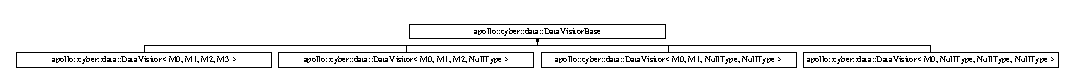
\includegraphics[height=0.682927cm]{classapollo_1_1cyber_1_1data_1_1DataVisitorBase}
\end{center}
\end{figure}
\subsection*{Public Member Functions}
\begin{DoxyCompactItemize}
\item 
\hyperlink{classapollo_1_1cyber_1_1data_1_1DataVisitorBase_a8197ea5e78feb49af879c99bf313cad9}{Data\-Visitor\-Base} ()
\item 
void \hyperlink{classapollo_1_1cyber_1_1data_1_1DataVisitorBase_af810d69a0f617eef9f86ac579f2a4339}{Register\-Notify\-Callback} (std\-::function$<$ void()$>$ \&\&callback)
\end{DoxyCompactItemize}
\subsection*{Protected Member Functions}
\begin{DoxyCompactItemize}
\item 
\hyperlink{classapollo_1_1cyber_1_1data_1_1DataVisitorBase_a1114079807721d7986c48b0b7fc00b5c}{Data\-Visitor\-Base} (const \hyperlink{classapollo_1_1cyber_1_1data_1_1DataVisitorBase}{Data\-Visitor\-Base} \&)=delete
\item 
\hyperlink{classapollo_1_1cyber_1_1data_1_1DataVisitorBase}{Data\-Visitor\-Base} \& \hyperlink{classapollo_1_1cyber_1_1data_1_1DataVisitorBase_ae4533b7ce5ee6dcaf617c1ff1f42d052}{operator=} (const \hyperlink{classapollo_1_1cyber_1_1data_1_1DataVisitorBase}{Data\-Visitor\-Base} \&)=delete
\end{DoxyCompactItemize}
\subsection*{Protected Attributes}
\begin{DoxyCompactItemize}
\item 
uint64\-\_\-t \hyperlink{classapollo_1_1cyber_1_1data_1_1DataVisitorBase_a976dda8aacd357161f4b6e49b699063e}{next\-\_\-msg\-\_\-index\-\_\-} = 0
\item 
\hyperlink{classapollo_1_1cyber_1_1data_1_1DataNotifier}{Data\-Notifier} $\ast$ \hyperlink{classapollo_1_1cyber_1_1data_1_1DataVisitorBase_ac8ac7c3bb6c789652df9155e65504ae8}{data\-\_\-notifier\-\_\-} = Data\-Notifier\-::\-Instance()
\item 
std\-::shared\-\_\-ptr$<$ \hyperlink{structapollo_1_1cyber_1_1data_1_1Notifier}{Notifier} $>$ \hyperlink{classapollo_1_1cyber_1_1data_1_1DataVisitorBase_a812c283846d1071937478c6ad23daa17}{notifier\-\_\-}
\end{DoxyCompactItemize}


\subsection{Constructor \& Destructor Documentation}
\hypertarget{classapollo_1_1cyber_1_1data_1_1DataVisitorBase_a8197ea5e78feb49af879c99bf313cad9}{\index{apollo\-::cyber\-::data\-::\-Data\-Visitor\-Base@{apollo\-::cyber\-::data\-::\-Data\-Visitor\-Base}!Data\-Visitor\-Base@{Data\-Visitor\-Base}}
\index{Data\-Visitor\-Base@{Data\-Visitor\-Base}!apollo::cyber::data::DataVisitorBase@{apollo\-::cyber\-::data\-::\-Data\-Visitor\-Base}}
\subsubsection[{Data\-Visitor\-Base}]{\setlength{\rightskip}{0pt plus 5cm}apollo\-::cyber\-::data\-::\-Data\-Visitor\-Base\-::\-Data\-Visitor\-Base (
\begin{DoxyParamCaption}
{}
\end{DoxyParamCaption}
)\hspace{0.3cm}{\ttfamily [inline]}}}\label{classapollo_1_1cyber_1_1data_1_1DataVisitorBase_a8197ea5e78feb49af879c99bf313cad9}
\hypertarget{classapollo_1_1cyber_1_1data_1_1DataVisitorBase_a1114079807721d7986c48b0b7fc00b5c}{\index{apollo\-::cyber\-::data\-::\-Data\-Visitor\-Base@{apollo\-::cyber\-::data\-::\-Data\-Visitor\-Base}!Data\-Visitor\-Base@{Data\-Visitor\-Base}}
\index{Data\-Visitor\-Base@{Data\-Visitor\-Base}!apollo::cyber::data::DataVisitorBase@{apollo\-::cyber\-::data\-::\-Data\-Visitor\-Base}}
\subsubsection[{Data\-Visitor\-Base}]{\setlength{\rightskip}{0pt plus 5cm}apollo\-::cyber\-::data\-::\-Data\-Visitor\-Base\-::\-Data\-Visitor\-Base (
\begin{DoxyParamCaption}
\item[{const {\bf Data\-Visitor\-Base} \&}]{}
\end{DoxyParamCaption}
)\hspace{0.3cm}{\ttfamily [protected]}, {\ttfamily [delete]}}}\label{classapollo_1_1cyber_1_1data_1_1DataVisitorBase_a1114079807721d7986c48b0b7fc00b5c}


\subsection{Member Function Documentation}
\hypertarget{classapollo_1_1cyber_1_1data_1_1DataVisitorBase_ae4533b7ce5ee6dcaf617c1ff1f42d052}{\index{apollo\-::cyber\-::data\-::\-Data\-Visitor\-Base@{apollo\-::cyber\-::data\-::\-Data\-Visitor\-Base}!operator=@{operator=}}
\index{operator=@{operator=}!apollo::cyber::data::DataVisitorBase@{apollo\-::cyber\-::data\-::\-Data\-Visitor\-Base}}
\subsubsection[{operator=}]{\setlength{\rightskip}{0pt plus 5cm}{\bf Data\-Visitor\-Base}\& apollo\-::cyber\-::data\-::\-Data\-Visitor\-Base\-::operator= (
\begin{DoxyParamCaption}
\item[{const {\bf Data\-Visitor\-Base} \&}]{}
\end{DoxyParamCaption}
)\hspace{0.3cm}{\ttfamily [protected]}, {\ttfamily [delete]}}}\label{classapollo_1_1cyber_1_1data_1_1DataVisitorBase_ae4533b7ce5ee6dcaf617c1ff1f42d052}
\hypertarget{classapollo_1_1cyber_1_1data_1_1DataVisitorBase_af810d69a0f617eef9f86ac579f2a4339}{\index{apollo\-::cyber\-::data\-::\-Data\-Visitor\-Base@{apollo\-::cyber\-::data\-::\-Data\-Visitor\-Base}!Register\-Notify\-Callback@{Register\-Notify\-Callback}}
\index{Register\-Notify\-Callback@{Register\-Notify\-Callback}!apollo::cyber::data::DataVisitorBase@{apollo\-::cyber\-::data\-::\-Data\-Visitor\-Base}}
\subsubsection[{Register\-Notify\-Callback}]{\setlength{\rightskip}{0pt plus 5cm}void apollo\-::cyber\-::data\-::\-Data\-Visitor\-Base\-::\-Register\-Notify\-Callback (
\begin{DoxyParamCaption}
\item[{std\-::function$<$ void()$>$ \&\&}]{callback}
\end{DoxyParamCaption}
)\hspace{0.3cm}{\ttfamily [inline]}}}\label{classapollo_1_1cyber_1_1data_1_1DataVisitorBase_af810d69a0f617eef9f86ac579f2a4339}


\subsection{Member Data Documentation}
\hypertarget{classapollo_1_1cyber_1_1data_1_1DataVisitorBase_ac8ac7c3bb6c789652df9155e65504ae8}{\index{apollo\-::cyber\-::data\-::\-Data\-Visitor\-Base@{apollo\-::cyber\-::data\-::\-Data\-Visitor\-Base}!data\-\_\-notifier\-\_\-@{data\-\_\-notifier\-\_\-}}
\index{data\-\_\-notifier\-\_\-@{data\-\_\-notifier\-\_\-}!apollo::cyber::data::DataVisitorBase@{apollo\-::cyber\-::data\-::\-Data\-Visitor\-Base}}
\subsubsection[{data\-\_\-notifier\-\_\-}]{\setlength{\rightskip}{0pt plus 5cm}{\bf Data\-Notifier}$\ast$ apollo\-::cyber\-::data\-::\-Data\-Visitor\-Base\-::data\-\_\-notifier\-\_\- = Data\-Notifier\-::\-Instance()\hspace{0.3cm}{\ttfamily [protected]}}}\label{classapollo_1_1cyber_1_1data_1_1DataVisitorBase_ac8ac7c3bb6c789652df9155e65504ae8}
\hypertarget{classapollo_1_1cyber_1_1data_1_1DataVisitorBase_a976dda8aacd357161f4b6e49b699063e}{\index{apollo\-::cyber\-::data\-::\-Data\-Visitor\-Base@{apollo\-::cyber\-::data\-::\-Data\-Visitor\-Base}!next\-\_\-msg\-\_\-index\-\_\-@{next\-\_\-msg\-\_\-index\-\_\-}}
\index{next\-\_\-msg\-\_\-index\-\_\-@{next\-\_\-msg\-\_\-index\-\_\-}!apollo::cyber::data::DataVisitorBase@{apollo\-::cyber\-::data\-::\-Data\-Visitor\-Base}}
\subsubsection[{next\-\_\-msg\-\_\-index\-\_\-}]{\setlength{\rightskip}{0pt plus 5cm}uint64\-\_\-t apollo\-::cyber\-::data\-::\-Data\-Visitor\-Base\-::next\-\_\-msg\-\_\-index\-\_\- = 0\hspace{0.3cm}{\ttfamily [protected]}}}\label{classapollo_1_1cyber_1_1data_1_1DataVisitorBase_a976dda8aacd357161f4b6e49b699063e}
\hypertarget{classapollo_1_1cyber_1_1data_1_1DataVisitorBase_a812c283846d1071937478c6ad23daa17}{\index{apollo\-::cyber\-::data\-::\-Data\-Visitor\-Base@{apollo\-::cyber\-::data\-::\-Data\-Visitor\-Base}!notifier\-\_\-@{notifier\-\_\-}}
\index{notifier\-\_\-@{notifier\-\_\-}!apollo::cyber::data::DataVisitorBase@{apollo\-::cyber\-::data\-::\-Data\-Visitor\-Base}}
\subsubsection[{notifier\-\_\-}]{\setlength{\rightskip}{0pt plus 5cm}std\-::shared\-\_\-ptr$<${\bf Notifier}$>$ apollo\-::cyber\-::data\-::\-Data\-Visitor\-Base\-::notifier\-\_\-\hspace{0.3cm}{\ttfamily [protected]}}}\label{classapollo_1_1cyber_1_1data_1_1DataVisitorBase_a812c283846d1071937478c6ad23daa17}


The documentation for this class was generated from the following file\-:\begin{DoxyCompactItemize}
\item 
data/\hyperlink{data__visitor__base_8h}{data\-\_\-visitor\-\_\-base.\-h}\end{DoxyCompactItemize}

\hypertarget{classapollo_1_1cyber_1_1message_1_1PyMessageWrap_1_1Descriptor}{\section{apollo\-:\-:cyber\-:\-:message\-:\-:Py\-Message\-Wrap\-:\-:Descriptor Class Reference}
\label{classapollo_1_1cyber_1_1message_1_1PyMessageWrap_1_1Descriptor}\index{apollo\-::cyber\-::message\-::\-Py\-Message\-Wrap\-::\-Descriptor@{apollo\-::cyber\-::message\-::\-Py\-Message\-Wrap\-::\-Descriptor}}
}


{\ttfamily \#include $<$py\-\_\-message.\-h$>$}

\subsection*{Public Member Functions}
\begin{DoxyCompactItemize}
\item 
std\-::string \hyperlink{classapollo_1_1cyber_1_1message_1_1PyMessageWrap_1_1Descriptor_a3676d5f8e664604517960ceb69a995e4}{full\-\_\-name} () const 
\item 
std\-::string \hyperlink{classapollo_1_1cyber_1_1message_1_1PyMessageWrap_1_1Descriptor_a1a7460d7d8d5cc51eff5cc83c605d5cc}{name} () const 
\end{DoxyCompactItemize}


\subsection{Member Function Documentation}
\hypertarget{classapollo_1_1cyber_1_1message_1_1PyMessageWrap_1_1Descriptor_a3676d5f8e664604517960ceb69a995e4}{\index{apollo\-::cyber\-::message\-::\-Py\-Message\-Wrap\-::\-Descriptor@{apollo\-::cyber\-::message\-::\-Py\-Message\-Wrap\-::\-Descriptor}!full\-\_\-name@{full\-\_\-name}}
\index{full\-\_\-name@{full\-\_\-name}!apollo::cyber::message::PyMessageWrap::Descriptor@{apollo\-::cyber\-::message\-::\-Py\-Message\-Wrap\-::\-Descriptor}}
\subsubsection[{full\-\_\-name}]{\setlength{\rightskip}{0pt plus 5cm}std\-::string apollo\-::cyber\-::message\-::\-Py\-Message\-Wrap\-::\-Descriptor\-::full\-\_\-name (
\begin{DoxyParamCaption}
{}
\end{DoxyParamCaption}
) const\hspace{0.3cm}{\ttfamily [inline]}}}\label{classapollo_1_1cyber_1_1message_1_1PyMessageWrap_1_1Descriptor_a3676d5f8e664604517960ceb69a995e4}
\hypertarget{classapollo_1_1cyber_1_1message_1_1PyMessageWrap_1_1Descriptor_a1a7460d7d8d5cc51eff5cc83c605d5cc}{\index{apollo\-::cyber\-::message\-::\-Py\-Message\-Wrap\-::\-Descriptor@{apollo\-::cyber\-::message\-::\-Py\-Message\-Wrap\-::\-Descriptor}!name@{name}}
\index{name@{name}!apollo::cyber::message::PyMessageWrap::Descriptor@{apollo\-::cyber\-::message\-::\-Py\-Message\-Wrap\-::\-Descriptor}}
\subsubsection[{name}]{\setlength{\rightskip}{0pt plus 5cm}std\-::string apollo\-::cyber\-::message\-::\-Py\-Message\-Wrap\-::\-Descriptor\-::name (
\begin{DoxyParamCaption}
{}
\end{DoxyParamCaption}
) const\hspace{0.3cm}{\ttfamily [inline]}}}\label{classapollo_1_1cyber_1_1message_1_1PyMessageWrap_1_1Descriptor_a1a7460d7d8d5cc51eff5cc83c605d5cc}


The documentation for this class was generated from the following file\-:\begin{DoxyCompactItemize}
\item 
message/\hyperlink{py__message_8h}{py\-\_\-message.\-h}\end{DoxyCompactItemize}

\hypertarget{classapollo_1_1cyber_1_1transport_1_1Dispatcher}{\section{apollo\-:\-:cyber\-:\-:transport\-:\-:Dispatcher Class Reference}
\label{classapollo_1_1cyber_1_1transport_1_1Dispatcher}\index{apollo\-::cyber\-::transport\-::\-Dispatcher@{apollo\-::cyber\-::transport\-::\-Dispatcher}}
}


{\ttfamily \#include $<$dispatcher.\-h$>$}

Inheritance diagram for apollo\-:\-:cyber\-:\-:transport\-:\-:Dispatcher\-:\begin{figure}[H]
\begin{center}
\leavevmode
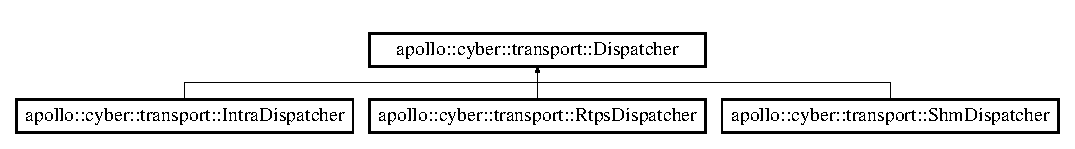
\includegraphics[height=1.549101cm]{classapollo_1_1cyber_1_1transport_1_1Dispatcher}
\end{center}
\end{figure}
\subsection*{Public Member Functions}
\begin{DoxyCompactItemize}
\item 
\hyperlink{classapollo_1_1cyber_1_1transport_1_1Dispatcher_a7b740666b178815f3bef327a223fe39f}{Dispatcher} ()
\item 
virtual \hyperlink{classapollo_1_1cyber_1_1transport_1_1Dispatcher_a6d28df2005ee5409e4dedb0e80a6bb91}{$\sim$\-Dispatcher} ()
\item 
virtual void \hyperlink{classapollo_1_1cyber_1_1transport_1_1Dispatcher_a87c80d37d0b6218218ad888888ad0d08}{Shutdown} ()
\item 
{\footnotesize template$<$typename Message\-T $>$ }\\void \hyperlink{classapollo_1_1cyber_1_1transport_1_1Dispatcher_a0e145dae91537eb77d7b09745b08bd97}{Add\-Listener} (const Role\-Attributes \&self\-\_\-attr, const \hyperlink{namespaceapollo_1_1cyber_1_1transport_aade3f4d41770972ae44166cdde27e2d8}{Message\-Listener}$<$ Message\-T $>$ \&listener)
\item 
{\footnotesize template$<$typename Message\-T $>$ }\\void \hyperlink{classapollo_1_1cyber_1_1transport_1_1Dispatcher_a57032c00ea89222e65f3c3c5ce2ca498}{Add\-Listener} (const Role\-Attributes \&self\-\_\-attr, const Role\-Attributes \&opposite\-\_\-attr, const \hyperlink{namespaceapollo_1_1cyber_1_1transport_aade3f4d41770972ae44166cdde27e2d8}{Message\-Listener}$<$ Message\-T $>$ \&listener)
\item 
{\footnotesize template$<$typename Message\-T $>$ }\\void \hyperlink{classapollo_1_1cyber_1_1transport_1_1Dispatcher_a24ced235e749abc47265d6ffade4f8bc}{Remove\-Listener} (const Role\-Attributes \&self\-\_\-attr)
\item 
{\footnotesize template$<$typename Message\-T $>$ }\\void \hyperlink{classapollo_1_1cyber_1_1transport_1_1Dispatcher_af81d7e383f5cb1c4b92ab4dd84125997}{Remove\-Listener} (const Role\-Attributes \&self\-\_\-attr, const Role\-Attributes \&opposite\-\_\-attr)
\item 
bool \hyperlink{classapollo_1_1cyber_1_1transport_1_1Dispatcher_a7bea7181659fa46204434dbdba90e00f}{Has\-Channel} (uint64\-\_\-t channel\-\_\-id)
\end{DoxyCompactItemize}
\subsection*{Protected Attributes}
\begin{DoxyCompactItemize}
\item 
std\-::atomic$<$ bool $>$ \hyperlink{classapollo_1_1cyber_1_1transport_1_1Dispatcher_a014ad0d3a3d8830aec03c8a47a00b385}{is\-\_\-shutdown\-\_\-}
\item 
\hyperlink{classapollo_1_1cyber_1_1base_1_1AtomicHashMap}{Atomic\-Hash\-Map}$<$ uint64\-\_\-t, \\*
\hyperlink{namespaceapollo_1_1cyber_1_1transport_a7748946e9ae4f2e24a82aadd4f02d3b6}{Listener\-Handler\-Base\-Ptr} $>$ \hyperlink{classapollo_1_1cyber_1_1transport_1_1Dispatcher_aec5b13dcc35013468812f0ea0bd0dd89}{msg\-\_\-listeners\-\_\-}
\item 
\hyperlink{classapollo_1_1cyber_1_1base_1_1AtomicRWLock}{base\-::\-Atomic\-R\-W\-Lock} \hyperlink{classapollo_1_1cyber_1_1transport_1_1Dispatcher_a93d037058df25c609f9d2e24f62bd67e}{rw\-\_\-lock\-\_\-}
\end{DoxyCompactItemize}


\subsection{Constructor \& Destructor Documentation}
\hypertarget{classapollo_1_1cyber_1_1transport_1_1Dispatcher_a7b740666b178815f3bef327a223fe39f}{\index{apollo\-::cyber\-::transport\-::\-Dispatcher@{apollo\-::cyber\-::transport\-::\-Dispatcher}!Dispatcher@{Dispatcher}}
\index{Dispatcher@{Dispatcher}!apollo::cyber::transport::Dispatcher@{apollo\-::cyber\-::transport\-::\-Dispatcher}}
\subsubsection[{Dispatcher}]{\setlength{\rightskip}{0pt plus 5cm}apollo\-::cyber\-::transport\-::\-Dispatcher\-::\-Dispatcher (
\begin{DoxyParamCaption}
{}
\end{DoxyParamCaption}
)}}\label{classapollo_1_1cyber_1_1transport_1_1Dispatcher_a7b740666b178815f3bef327a223fe39f}
\hypertarget{classapollo_1_1cyber_1_1transport_1_1Dispatcher_a6d28df2005ee5409e4dedb0e80a6bb91}{\index{apollo\-::cyber\-::transport\-::\-Dispatcher@{apollo\-::cyber\-::transport\-::\-Dispatcher}!$\sim$\-Dispatcher@{$\sim$\-Dispatcher}}
\index{$\sim$\-Dispatcher@{$\sim$\-Dispatcher}!apollo::cyber::transport::Dispatcher@{apollo\-::cyber\-::transport\-::\-Dispatcher}}
\subsubsection[{$\sim$\-Dispatcher}]{\setlength{\rightskip}{0pt plus 5cm}virtual apollo\-::cyber\-::transport\-::\-Dispatcher\-::$\sim$\-Dispatcher (
\begin{DoxyParamCaption}
{}
\end{DoxyParamCaption}
)\hspace{0.3cm}{\ttfamily [virtual]}}}\label{classapollo_1_1cyber_1_1transport_1_1Dispatcher_a6d28df2005ee5409e4dedb0e80a6bb91}


\subsection{Member Function Documentation}
\hypertarget{classapollo_1_1cyber_1_1transport_1_1Dispatcher_a0e145dae91537eb77d7b09745b08bd97}{\index{apollo\-::cyber\-::transport\-::\-Dispatcher@{apollo\-::cyber\-::transport\-::\-Dispatcher}!Add\-Listener@{Add\-Listener}}
\index{Add\-Listener@{Add\-Listener}!apollo::cyber::transport::Dispatcher@{apollo\-::cyber\-::transport\-::\-Dispatcher}}
\subsubsection[{Add\-Listener}]{\setlength{\rightskip}{0pt plus 5cm}template$<$typename Message\-T $>$ void apollo\-::cyber\-::transport\-::\-Dispatcher\-::\-Add\-Listener (
\begin{DoxyParamCaption}
\item[{const Role\-Attributes \&}]{self\-\_\-attr, }
\item[{const {\bf Message\-Listener}$<$ Message\-T $>$ \&}]{listener}
\end{DoxyParamCaption}
)}}\label{classapollo_1_1cyber_1_1transport_1_1Dispatcher_a0e145dae91537eb77d7b09745b08bd97}
\hypertarget{classapollo_1_1cyber_1_1transport_1_1Dispatcher_a57032c00ea89222e65f3c3c5ce2ca498}{\index{apollo\-::cyber\-::transport\-::\-Dispatcher@{apollo\-::cyber\-::transport\-::\-Dispatcher}!Add\-Listener@{Add\-Listener}}
\index{Add\-Listener@{Add\-Listener}!apollo::cyber::transport::Dispatcher@{apollo\-::cyber\-::transport\-::\-Dispatcher}}
\subsubsection[{Add\-Listener}]{\setlength{\rightskip}{0pt plus 5cm}template$<$typename Message\-T $>$ void apollo\-::cyber\-::transport\-::\-Dispatcher\-::\-Add\-Listener (
\begin{DoxyParamCaption}
\item[{const Role\-Attributes \&}]{self\-\_\-attr, }
\item[{const Role\-Attributes \&}]{opposite\-\_\-attr, }
\item[{const {\bf Message\-Listener}$<$ Message\-T $>$ \&}]{listener}
\end{DoxyParamCaption}
)}}\label{classapollo_1_1cyber_1_1transport_1_1Dispatcher_a57032c00ea89222e65f3c3c5ce2ca498}
\hypertarget{classapollo_1_1cyber_1_1transport_1_1Dispatcher_a7bea7181659fa46204434dbdba90e00f}{\index{apollo\-::cyber\-::transport\-::\-Dispatcher@{apollo\-::cyber\-::transport\-::\-Dispatcher}!Has\-Channel@{Has\-Channel}}
\index{Has\-Channel@{Has\-Channel}!apollo::cyber::transport::Dispatcher@{apollo\-::cyber\-::transport\-::\-Dispatcher}}
\subsubsection[{Has\-Channel}]{\setlength{\rightskip}{0pt plus 5cm}bool apollo\-::cyber\-::transport\-::\-Dispatcher\-::\-Has\-Channel (
\begin{DoxyParamCaption}
\item[{uint64\-\_\-t}]{channel\-\_\-id}
\end{DoxyParamCaption}
)}}\label{classapollo_1_1cyber_1_1transport_1_1Dispatcher_a7bea7181659fa46204434dbdba90e00f}
\hypertarget{classapollo_1_1cyber_1_1transport_1_1Dispatcher_a24ced235e749abc47265d6ffade4f8bc}{\index{apollo\-::cyber\-::transport\-::\-Dispatcher@{apollo\-::cyber\-::transport\-::\-Dispatcher}!Remove\-Listener@{Remove\-Listener}}
\index{Remove\-Listener@{Remove\-Listener}!apollo::cyber::transport::Dispatcher@{apollo\-::cyber\-::transport\-::\-Dispatcher}}
\subsubsection[{Remove\-Listener}]{\setlength{\rightskip}{0pt plus 5cm}template$<$typename Message\-T $>$ void apollo\-::cyber\-::transport\-::\-Dispatcher\-::\-Remove\-Listener (
\begin{DoxyParamCaption}
\item[{const Role\-Attributes \&}]{self\-\_\-attr}
\end{DoxyParamCaption}
)}}\label{classapollo_1_1cyber_1_1transport_1_1Dispatcher_a24ced235e749abc47265d6ffade4f8bc}
\hypertarget{classapollo_1_1cyber_1_1transport_1_1Dispatcher_af81d7e383f5cb1c4b92ab4dd84125997}{\index{apollo\-::cyber\-::transport\-::\-Dispatcher@{apollo\-::cyber\-::transport\-::\-Dispatcher}!Remove\-Listener@{Remove\-Listener}}
\index{Remove\-Listener@{Remove\-Listener}!apollo::cyber::transport::Dispatcher@{apollo\-::cyber\-::transport\-::\-Dispatcher}}
\subsubsection[{Remove\-Listener}]{\setlength{\rightskip}{0pt plus 5cm}template$<$typename Message\-T $>$ void apollo\-::cyber\-::transport\-::\-Dispatcher\-::\-Remove\-Listener (
\begin{DoxyParamCaption}
\item[{const Role\-Attributes \&}]{self\-\_\-attr, }
\item[{const Role\-Attributes \&}]{opposite\-\_\-attr}
\end{DoxyParamCaption}
)}}\label{classapollo_1_1cyber_1_1transport_1_1Dispatcher_af81d7e383f5cb1c4b92ab4dd84125997}
\hypertarget{classapollo_1_1cyber_1_1transport_1_1Dispatcher_a87c80d37d0b6218218ad888888ad0d08}{\index{apollo\-::cyber\-::transport\-::\-Dispatcher@{apollo\-::cyber\-::transport\-::\-Dispatcher}!Shutdown@{Shutdown}}
\index{Shutdown@{Shutdown}!apollo::cyber::transport::Dispatcher@{apollo\-::cyber\-::transport\-::\-Dispatcher}}
\subsubsection[{Shutdown}]{\setlength{\rightskip}{0pt plus 5cm}virtual void apollo\-::cyber\-::transport\-::\-Dispatcher\-::\-Shutdown (
\begin{DoxyParamCaption}
{}
\end{DoxyParamCaption}
)\hspace{0.3cm}{\ttfamily [virtual]}}}\label{classapollo_1_1cyber_1_1transport_1_1Dispatcher_a87c80d37d0b6218218ad888888ad0d08}


Reimplemented in \hyperlink{classapollo_1_1cyber_1_1transport_1_1RtpsDispatcher_a6dae71a55d15ec41f5ca6b5bfb9a452a}{apollo\-::cyber\-::transport\-::\-Rtps\-Dispatcher}, and \hyperlink{classapollo_1_1cyber_1_1transport_1_1ShmDispatcher_a8924e420134ea725eb03a680bb98abd7}{apollo\-::cyber\-::transport\-::\-Shm\-Dispatcher}.



\subsection{Member Data Documentation}
\hypertarget{classapollo_1_1cyber_1_1transport_1_1Dispatcher_a014ad0d3a3d8830aec03c8a47a00b385}{\index{apollo\-::cyber\-::transport\-::\-Dispatcher@{apollo\-::cyber\-::transport\-::\-Dispatcher}!is\-\_\-shutdown\-\_\-@{is\-\_\-shutdown\-\_\-}}
\index{is\-\_\-shutdown\-\_\-@{is\-\_\-shutdown\-\_\-}!apollo::cyber::transport::Dispatcher@{apollo\-::cyber\-::transport\-::\-Dispatcher}}
\subsubsection[{is\-\_\-shutdown\-\_\-}]{\setlength{\rightskip}{0pt plus 5cm}std\-::atomic$<$bool$>$ apollo\-::cyber\-::transport\-::\-Dispatcher\-::is\-\_\-shutdown\-\_\-\hspace{0.3cm}{\ttfamily [protected]}}}\label{classapollo_1_1cyber_1_1transport_1_1Dispatcher_a014ad0d3a3d8830aec03c8a47a00b385}
\hypertarget{classapollo_1_1cyber_1_1transport_1_1Dispatcher_aec5b13dcc35013468812f0ea0bd0dd89}{\index{apollo\-::cyber\-::transport\-::\-Dispatcher@{apollo\-::cyber\-::transport\-::\-Dispatcher}!msg\-\_\-listeners\-\_\-@{msg\-\_\-listeners\-\_\-}}
\index{msg\-\_\-listeners\-\_\-@{msg\-\_\-listeners\-\_\-}!apollo::cyber::transport::Dispatcher@{apollo\-::cyber\-::transport\-::\-Dispatcher}}
\subsubsection[{msg\-\_\-listeners\-\_\-}]{\setlength{\rightskip}{0pt plus 5cm}{\bf Atomic\-Hash\-Map}$<$uint64\-\_\-t, {\bf Listener\-Handler\-Base\-Ptr}$>$ apollo\-::cyber\-::transport\-::\-Dispatcher\-::msg\-\_\-listeners\-\_\-\hspace{0.3cm}{\ttfamily [protected]}}}\label{classapollo_1_1cyber_1_1transport_1_1Dispatcher_aec5b13dcc35013468812f0ea0bd0dd89}
\hypertarget{classapollo_1_1cyber_1_1transport_1_1Dispatcher_a93d037058df25c609f9d2e24f62bd67e}{\index{apollo\-::cyber\-::transport\-::\-Dispatcher@{apollo\-::cyber\-::transport\-::\-Dispatcher}!rw\-\_\-lock\-\_\-@{rw\-\_\-lock\-\_\-}}
\index{rw\-\_\-lock\-\_\-@{rw\-\_\-lock\-\_\-}!apollo::cyber::transport::Dispatcher@{apollo\-::cyber\-::transport\-::\-Dispatcher}}
\subsubsection[{rw\-\_\-lock\-\_\-}]{\setlength{\rightskip}{0pt plus 5cm}{\bf base\-::\-Atomic\-R\-W\-Lock} apollo\-::cyber\-::transport\-::\-Dispatcher\-::rw\-\_\-lock\-\_\-\hspace{0.3cm}{\ttfamily [protected]}}}\label{classapollo_1_1cyber_1_1transport_1_1Dispatcher_a93d037058df25c609f9d2e24f62bd67e}


The documentation for this class was generated from the following file\-:\begin{DoxyCompactItemize}
\item 
transport/dispatcher/\hyperlink{dispatcher_8h}{dispatcher.\-h}\end{DoxyCompactItemize}

\hypertarget{classapollo_1_1cyber_1_1Duration}{\section{apollo\-:\-:cyber\-:\-:Duration Class Reference}
\label{classapollo_1_1cyber_1_1Duration}\index{apollo\-::cyber\-::\-Duration@{apollo\-::cyber\-::\-Duration}}
}


{\ttfamily \#include $<$duration.\-h$>$}

\subsection*{Public Member Functions}
\begin{DoxyCompactItemize}
\item 
\hyperlink{classapollo_1_1cyber_1_1Duration_a7a5e661b09ebf84ccbd8dbead9f77963}{Duration} ()
\item 
\hyperlink{classapollo_1_1cyber_1_1Duration_a16699eaf9e0a21e070ad63b6fe7993c6}{Duration} (int64\-\_\-t nanoseconds)
\item 
\hyperlink{classapollo_1_1cyber_1_1Duration_abb9c8becd41cc055936a2a18195735a8}{Duration} (int nanoseconds)
\item 
\hyperlink{classapollo_1_1cyber_1_1Duration_a5496457a72e19aafa01eadee586c0666}{Duration} (double seconds)
\item 
\hyperlink{classapollo_1_1cyber_1_1Duration_a766cc1a77762fbf1868b31ccea3a454c}{Duration} (uint32\-\_\-t seconds, uint32\-\_\-t nanoseconds)
\item 
\hyperlink{classapollo_1_1cyber_1_1Duration_a96eea1cb85abd7f665b8ffd2ae6e6346}{Duration} (const \hyperlink{classapollo_1_1cyber_1_1Duration}{Duration} \&other)
\item 
\hyperlink{classapollo_1_1cyber_1_1Duration}{Duration} \& \hyperlink{classapollo_1_1cyber_1_1Duration_ae98ef6b05c7ab3e66b49353f5461db86}{operator=} (const \hyperlink{classapollo_1_1cyber_1_1Duration}{Duration} \&other)
\item 
\hyperlink{classapollo_1_1cyber_1_1Duration_a83ef21a27de322184c9faa25026d88c8}{$\sim$\-Duration} ()
\item 
double \hyperlink{classapollo_1_1cyber_1_1Duration_a61ed856e5c40cf6675845a27c7d7182f}{To\-Second} () const 
\item 
int64\-\_\-t \hyperlink{classapollo_1_1cyber_1_1Duration_aa5e9e105c79b7087494cb7b6677f0c85}{To\-Nanosecond} () const 
\item 
bool \hyperlink{classapollo_1_1cyber_1_1Duration_aa9acb321bac196fc2fb5f6e84825bb6a}{Is\-Zero} () const 
\item 
void \hyperlink{classapollo_1_1cyber_1_1Duration_a240ddeaf69ee492e54c09518191c789b}{Sleep} () const 
\item 
\hyperlink{classapollo_1_1cyber_1_1Duration}{Duration} \hyperlink{classapollo_1_1cyber_1_1Duration_afd2507261eeedbfa387e28d3954709f1}{operator+} (const \hyperlink{classapollo_1_1cyber_1_1Duration}{Duration} \&rhs) const 
\item 
\hyperlink{classapollo_1_1cyber_1_1Duration}{Duration} \hyperlink{classapollo_1_1cyber_1_1Duration_a4a07adceef070a4c0d9225bd69ea5f8a}{operator-\/} (const \hyperlink{classapollo_1_1cyber_1_1Duration}{Duration} \&rhs) const 
\item 
\hyperlink{classapollo_1_1cyber_1_1Duration}{Duration} \hyperlink{classapollo_1_1cyber_1_1Duration_a9f0615f3c445ac6850b9c0f295dd9552}{operator-\/} () const 
\item 
\hyperlink{classapollo_1_1cyber_1_1Duration}{Duration} \hyperlink{classapollo_1_1cyber_1_1Duration_af7c1442e0950357809d9452df2674459}{operator$\ast$} (double scale) const 
\item 
\hyperlink{classapollo_1_1cyber_1_1Duration}{Duration} \& \hyperlink{classapollo_1_1cyber_1_1Duration_a32669135bc80a8211f81df67110da7c0}{operator+=} (const \hyperlink{classapollo_1_1cyber_1_1Duration}{Duration} \&rhs)
\item 
\hyperlink{classapollo_1_1cyber_1_1Duration}{Duration} \& \hyperlink{classapollo_1_1cyber_1_1Duration_aae3b5dacb40e0ef43ad955b6ee63c39a}{operator-\/=} (const \hyperlink{classapollo_1_1cyber_1_1Duration}{Duration} \&rhs)
\item 
\hyperlink{classapollo_1_1cyber_1_1Duration}{Duration} \& \hyperlink{classapollo_1_1cyber_1_1Duration_ae4058c0c81fecb76a2e33de5beddc337}{operator$\ast$=} (double scale)
\item 
bool \hyperlink{classapollo_1_1cyber_1_1Duration_a02d320ebe06cbce72bb554c228f57942}{operator==} (const \hyperlink{classapollo_1_1cyber_1_1Duration}{Duration} \&rhs) const 
\item 
bool \hyperlink{classapollo_1_1cyber_1_1Duration_a34d9a42e50f5ab65416f92f8b340b9da}{operator!=} (const \hyperlink{classapollo_1_1cyber_1_1Duration}{Duration} \&rhs) const 
\item 
bool \hyperlink{classapollo_1_1cyber_1_1Duration_ad57ff542c093f69d52d5fcd1e9bef3e9}{operator$>$} (const \hyperlink{classapollo_1_1cyber_1_1Duration}{Duration} \&rhs) const 
\item 
bool \hyperlink{classapollo_1_1cyber_1_1Duration_aafe6d4c78a88c7fc4cfd8969bc3d3dbc}{operator$<$} (const \hyperlink{classapollo_1_1cyber_1_1Duration}{Duration} \&rhs) const 
\item 
bool \hyperlink{classapollo_1_1cyber_1_1Duration_ab95228ad318e860cd242be863ba064d3}{operator$>$=} (const \hyperlink{classapollo_1_1cyber_1_1Duration}{Duration} \&rhs) const 
\item 
bool \hyperlink{classapollo_1_1cyber_1_1Duration_a2dcd98c7a530dac26f54539cd698473f}{operator$<$=} (const \hyperlink{classapollo_1_1cyber_1_1Duration}{Duration} \&rhs) const 
\end{DoxyCompactItemize}
\subsection*{Private Attributes}
\begin{DoxyCompactItemize}
\item 
int64\-\_\-t \hyperlink{classapollo_1_1cyber_1_1Duration_aa7c53ba8085b28586fac1e915a356d3b}{nanoseconds\-\_\-} = 0
\end{DoxyCompactItemize}


\subsection{Constructor \& Destructor Documentation}
\hypertarget{classapollo_1_1cyber_1_1Duration_a7a5e661b09ebf84ccbd8dbead9f77963}{\index{apollo\-::cyber\-::\-Duration@{apollo\-::cyber\-::\-Duration}!Duration@{Duration}}
\index{Duration@{Duration}!apollo::cyber::Duration@{apollo\-::cyber\-::\-Duration}}
\subsubsection[{Duration}]{\setlength{\rightskip}{0pt plus 5cm}apollo\-::cyber\-::\-Duration\-::\-Duration (
\begin{DoxyParamCaption}
{}
\end{DoxyParamCaption}
)\hspace{0.3cm}{\ttfamily [inline]}}}\label{classapollo_1_1cyber_1_1Duration_a7a5e661b09ebf84ccbd8dbead9f77963}
\hypertarget{classapollo_1_1cyber_1_1Duration_a16699eaf9e0a21e070ad63b6fe7993c6}{\index{apollo\-::cyber\-::\-Duration@{apollo\-::cyber\-::\-Duration}!Duration@{Duration}}
\index{Duration@{Duration}!apollo::cyber::Duration@{apollo\-::cyber\-::\-Duration}}
\subsubsection[{Duration}]{\setlength{\rightskip}{0pt plus 5cm}apollo\-::cyber\-::\-Duration\-::\-Duration (
\begin{DoxyParamCaption}
\item[{int64\-\_\-t}]{nanoseconds}
\end{DoxyParamCaption}
)\hspace{0.3cm}{\ttfamily [explicit]}}}\label{classapollo_1_1cyber_1_1Duration_a16699eaf9e0a21e070ad63b6fe7993c6}
\hypertarget{classapollo_1_1cyber_1_1Duration_abb9c8becd41cc055936a2a18195735a8}{\index{apollo\-::cyber\-::\-Duration@{apollo\-::cyber\-::\-Duration}!Duration@{Duration}}
\index{Duration@{Duration}!apollo::cyber::Duration@{apollo\-::cyber\-::\-Duration}}
\subsubsection[{Duration}]{\setlength{\rightskip}{0pt plus 5cm}apollo\-::cyber\-::\-Duration\-::\-Duration (
\begin{DoxyParamCaption}
\item[{int}]{nanoseconds}
\end{DoxyParamCaption}
)\hspace{0.3cm}{\ttfamily [explicit]}}}\label{classapollo_1_1cyber_1_1Duration_abb9c8becd41cc055936a2a18195735a8}
\hypertarget{classapollo_1_1cyber_1_1Duration_a5496457a72e19aafa01eadee586c0666}{\index{apollo\-::cyber\-::\-Duration@{apollo\-::cyber\-::\-Duration}!Duration@{Duration}}
\index{Duration@{Duration}!apollo::cyber::Duration@{apollo\-::cyber\-::\-Duration}}
\subsubsection[{Duration}]{\setlength{\rightskip}{0pt plus 5cm}apollo\-::cyber\-::\-Duration\-::\-Duration (
\begin{DoxyParamCaption}
\item[{double}]{seconds}
\end{DoxyParamCaption}
)\hspace{0.3cm}{\ttfamily [explicit]}}}\label{classapollo_1_1cyber_1_1Duration_a5496457a72e19aafa01eadee586c0666}
\hypertarget{classapollo_1_1cyber_1_1Duration_a766cc1a77762fbf1868b31ccea3a454c}{\index{apollo\-::cyber\-::\-Duration@{apollo\-::cyber\-::\-Duration}!Duration@{Duration}}
\index{Duration@{Duration}!apollo::cyber::Duration@{apollo\-::cyber\-::\-Duration}}
\subsubsection[{Duration}]{\setlength{\rightskip}{0pt plus 5cm}apollo\-::cyber\-::\-Duration\-::\-Duration (
\begin{DoxyParamCaption}
\item[{uint32\-\_\-t}]{seconds, }
\item[{uint32\-\_\-t}]{nanoseconds}
\end{DoxyParamCaption}
)\hspace{0.3cm}{\ttfamily [explicit]}}}\label{classapollo_1_1cyber_1_1Duration_a766cc1a77762fbf1868b31ccea3a454c}
\hypertarget{classapollo_1_1cyber_1_1Duration_a96eea1cb85abd7f665b8ffd2ae6e6346}{\index{apollo\-::cyber\-::\-Duration@{apollo\-::cyber\-::\-Duration}!Duration@{Duration}}
\index{Duration@{Duration}!apollo::cyber::Duration@{apollo\-::cyber\-::\-Duration}}
\subsubsection[{Duration}]{\setlength{\rightskip}{0pt plus 5cm}apollo\-::cyber\-::\-Duration\-::\-Duration (
\begin{DoxyParamCaption}
\item[{const {\bf Duration} \&}]{other}
\end{DoxyParamCaption}
)}}\label{classapollo_1_1cyber_1_1Duration_a96eea1cb85abd7f665b8ffd2ae6e6346}
\hypertarget{classapollo_1_1cyber_1_1Duration_a83ef21a27de322184c9faa25026d88c8}{\index{apollo\-::cyber\-::\-Duration@{apollo\-::cyber\-::\-Duration}!$\sim$\-Duration@{$\sim$\-Duration}}
\index{$\sim$\-Duration@{$\sim$\-Duration}!apollo::cyber::Duration@{apollo\-::cyber\-::\-Duration}}
\subsubsection[{$\sim$\-Duration}]{\setlength{\rightskip}{0pt plus 5cm}apollo\-::cyber\-::\-Duration\-::$\sim$\-Duration (
\begin{DoxyParamCaption}
{}
\end{DoxyParamCaption}
)\hspace{0.3cm}{\ttfamily [inline]}}}\label{classapollo_1_1cyber_1_1Duration_a83ef21a27de322184c9faa25026d88c8}


\subsection{Member Function Documentation}
\hypertarget{classapollo_1_1cyber_1_1Duration_aa9acb321bac196fc2fb5f6e84825bb6a}{\index{apollo\-::cyber\-::\-Duration@{apollo\-::cyber\-::\-Duration}!Is\-Zero@{Is\-Zero}}
\index{Is\-Zero@{Is\-Zero}!apollo::cyber::Duration@{apollo\-::cyber\-::\-Duration}}
\subsubsection[{Is\-Zero}]{\setlength{\rightskip}{0pt plus 5cm}bool apollo\-::cyber\-::\-Duration\-::\-Is\-Zero (
\begin{DoxyParamCaption}
{}
\end{DoxyParamCaption}
) const}}\label{classapollo_1_1cyber_1_1Duration_aa9acb321bac196fc2fb5f6e84825bb6a}
\hypertarget{classapollo_1_1cyber_1_1Duration_a34d9a42e50f5ab65416f92f8b340b9da}{\index{apollo\-::cyber\-::\-Duration@{apollo\-::cyber\-::\-Duration}!operator!=@{operator!=}}
\index{operator!=@{operator!=}!apollo::cyber::Duration@{apollo\-::cyber\-::\-Duration}}
\subsubsection[{operator!=}]{\setlength{\rightskip}{0pt plus 5cm}bool apollo\-::cyber\-::\-Duration\-::operator!= (
\begin{DoxyParamCaption}
\item[{const {\bf Duration} \&}]{rhs}
\end{DoxyParamCaption}
) const}}\label{classapollo_1_1cyber_1_1Duration_a34d9a42e50f5ab65416f92f8b340b9da}
\hypertarget{classapollo_1_1cyber_1_1Duration_af7c1442e0950357809d9452df2674459}{\index{apollo\-::cyber\-::\-Duration@{apollo\-::cyber\-::\-Duration}!operator$\ast$@{operator$\ast$}}
\index{operator$\ast$@{operator$\ast$}!apollo::cyber::Duration@{apollo\-::cyber\-::\-Duration}}
\subsubsection[{operator$\ast$}]{\setlength{\rightskip}{0pt plus 5cm}{\bf Duration} apollo\-::cyber\-::\-Duration\-::operator$\ast$ (
\begin{DoxyParamCaption}
\item[{double}]{scale}
\end{DoxyParamCaption}
) const}}\label{classapollo_1_1cyber_1_1Duration_af7c1442e0950357809d9452df2674459}
\hypertarget{classapollo_1_1cyber_1_1Duration_ae4058c0c81fecb76a2e33de5beddc337}{\index{apollo\-::cyber\-::\-Duration@{apollo\-::cyber\-::\-Duration}!operator$\ast$=@{operator$\ast$=}}
\index{operator$\ast$=@{operator$\ast$=}!apollo::cyber::Duration@{apollo\-::cyber\-::\-Duration}}
\subsubsection[{operator$\ast$=}]{\setlength{\rightskip}{0pt plus 5cm}{\bf Duration}\& apollo\-::cyber\-::\-Duration\-::operator$\ast$= (
\begin{DoxyParamCaption}
\item[{double}]{scale}
\end{DoxyParamCaption}
)}}\label{classapollo_1_1cyber_1_1Duration_ae4058c0c81fecb76a2e33de5beddc337}
\hypertarget{classapollo_1_1cyber_1_1Duration_afd2507261eeedbfa387e28d3954709f1}{\index{apollo\-::cyber\-::\-Duration@{apollo\-::cyber\-::\-Duration}!operator+@{operator+}}
\index{operator+@{operator+}!apollo::cyber::Duration@{apollo\-::cyber\-::\-Duration}}
\subsubsection[{operator+}]{\setlength{\rightskip}{0pt plus 5cm}{\bf Duration} apollo\-::cyber\-::\-Duration\-::operator+ (
\begin{DoxyParamCaption}
\item[{const {\bf Duration} \&}]{rhs}
\end{DoxyParamCaption}
) const}}\label{classapollo_1_1cyber_1_1Duration_afd2507261eeedbfa387e28d3954709f1}
\hypertarget{classapollo_1_1cyber_1_1Duration_a32669135bc80a8211f81df67110da7c0}{\index{apollo\-::cyber\-::\-Duration@{apollo\-::cyber\-::\-Duration}!operator+=@{operator+=}}
\index{operator+=@{operator+=}!apollo::cyber::Duration@{apollo\-::cyber\-::\-Duration}}
\subsubsection[{operator+=}]{\setlength{\rightskip}{0pt plus 5cm}{\bf Duration}\& apollo\-::cyber\-::\-Duration\-::operator+= (
\begin{DoxyParamCaption}
\item[{const {\bf Duration} \&}]{rhs}
\end{DoxyParamCaption}
)}}\label{classapollo_1_1cyber_1_1Duration_a32669135bc80a8211f81df67110da7c0}
\hypertarget{classapollo_1_1cyber_1_1Duration_a4a07adceef070a4c0d9225bd69ea5f8a}{\index{apollo\-::cyber\-::\-Duration@{apollo\-::cyber\-::\-Duration}!operator-\/@{operator-\/}}
\index{operator-\/@{operator-\/}!apollo::cyber::Duration@{apollo\-::cyber\-::\-Duration}}
\subsubsection[{operator-\/}]{\setlength{\rightskip}{0pt plus 5cm}{\bf Duration} apollo\-::cyber\-::\-Duration\-::operator-\/ (
\begin{DoxyParamCaption}
\item[{const {\bf Duration} \&}]{rhs}
\end{DoxyParamCaption}
) const}}\label{classapollo_1_1cyber_1_1Duration_a4a07adceef070a4c0d9225bd69ea5f8a}
\hypertarget{classapollo_1_1cyber_1_1Duration_a9f0615f3c445ac6850b9c0f295dd9552}{\index{apollo\-::cyber\-::\-Duration@{apollo\-::cyber\-::\-Duration}!operator-\/@{operator-\/}}
\index{operator-\/@{operator-\/}!apollo::cyber::Duration@{apollo\-::cyber\-::\-Duration}}
\subsubsection[{operator-\/}]{\setlength{\rightskip}{0pt plus 5cm}{\bf Duration} apollo\-::cyber\-::\-Duration\-::operator-\/ (
\begin{DoxyParamCaption}
{}
\end{DoxyParamCaption}
) const}}\label{classapollo_1_1cyber_1_1Duration_a9f0615f3c445ac6850b9c0f295dd9552}
\hypertarget{classapollo_1_1cyber_1_1Duration_aae3b5dacb40e0ef43ad955b6ee63c39a}{\index{apollo\-::cyber\-::\-Duration@{apollo\-::cyber\-::\-Duration}!operator-\/=@{operator-\/=}}
\index{operator-\/=@{operator-\/=}!apollo::cyber::Duration@{apollo\-::cyber\-::\-Duration}}
\subsubsection[{operator-\/=}]{\setlength{\rightskip}{0pt plus 5cm}{\bf Duration}\& apollo\-::cyber\-::\-Duration\-::operator-\/= (
\begin{DoxyParamCaption}
\item[{const {\bf Duration} \&}]{rhs}
\end{DoxyParamCaption}
)}}\label{classapollo_1_1cyber_1_1Duration_aae3b5dacb40e0ef43ad955b6ee63c39a}
\hypertarget{classapollo_1_1cyber_1_1Duration_aafe6d4c78a88c7fc4cfd8969bc3d3dbc}{\index{apollo\-::cyber\-::\-Duration@{apollo\-::cyber\-::\-Duration}!operator$<$@{operator$<$}}
\index{operator$<$@{operator$<$}!apollo::cyber::Duration@{apollo\-::cyber\-::\-Duration}}
\subsubsection[{operator$<$}]{\setlength{\rightskip}{0pt plus 5cm}bool apollo\-::cyber\-::\-Duration\-::operator$<$ (
\begin{DoxyParamCaption}
\item[{const {\bf Duration} \&}]{rhs}
\end{DoxyParamCaption}
) const}}\label{classapollo_1_1cyber_1_1Duration_aafe6d4c78a88c7fc4cfd8969bc3d3dbc}
\hypertarget{classapollo_1_1cyber_1_1Duration_a2dcd98c7a530dac26f54539cd698473f}{\index{apollo\-::cyber\-::\-Duration@{apollo\-::cyber\-::\-Duration}!operator$<$=@{operator$<$=}}
\index{operator$<$=@{operator$<$=}!apollo::cyber::Duration@{apollo\-::cyber\-::\-Duration}}
\subsubsection[{operator$<$=}]{\setlength{\rightskip}{0pt plus 5cm}bool apollo\-::cyber\-::\-Duration\-::operator$<$= (
\begin{DoxyParamCaption}
\item[{const {\bf Duration} \&}]{rhs}
\end{DoxyParamCaption}
) const}}\label{classapollo_1_1cyber_1_1Duration_a2dcd98c7a530dac26f54539cd698473f}
\hypertarget{classapollo_1_1cyber_1_1Duration_ae98ef6b05c7ab3e66b49353f5461db86}{\index{apollo\-::cyber\-::\-Duration@{apollo\-::cyber\-::\-Duration}!operator=@{operator=}}
\index{operator=@{operator=}!apollo::cyber::Duration@{apollo\-::cyber\-::\-Duration}}
\subsubsection[{operator=}]{\setlength{\rightskip}{0pt plus 5cm}{\bf Duration}\& apollo\-::cyber\-::\-Duration\-::operator= (
\begin{DoxyParamCaption}
\item[{const {\bf Duration} \&}]{other}
\end{DoxyParamCaption}
)}}\label{classapollo_1_1cyber_1_1Duration_ae98ef6b05c7ab3e66b49353f5461db86}
\hypertarget{classapollo_1_1cyber_1_1Duration_a02d320ebe06cbce72bb554c228f57942}{\index{apollo\-::cyber\-::\-Duration@{apollo\-::cyber\-::\-Duration}!operator==@{operator==}}
\index{operator==@{operator==}!apollo::cyber::Duration@{apollo\-::cyber\-::\-Duration}}
\subsubsection[{operator==}]{\setlength{\rightskip}{0pt plus 5cm}bool apollo\-::cyber\-::\-Duration\-::operator== (
\begin{DoxyParamCaption}
\item[{const {\bf Duration} \&}]{rhs}
\end{DoxyParamCaption}
) const}}\label{classapollo_1_1cyber_1_1Duration_a02d320ebe06cbce72bb554c228f57942}
\hypertarget{classapollo_1_1cyber_1_1Duration_ad57ff542c093f69d52d5fcd1e9bef3e9}{\index{apollo\-::cyber\-::\-Duration@{apollo\-::cyber\-::\-Duration}!operator$>$@{operator$>$}}
\index{operator$>$@{operator$>$}!apollo::cyber::Duration@{apollo\-::cyber\-::\-Duration}}
\subsubsection[{operator$>$}]{\setlength{\rightskip}{0pt plus 5cm}bool apollo\-::cyber\-::\-Duration\-::operator$>$ (
\begin{DoxyParamCaption}
\item[{const {\bf Duration} \&}]{rhs}
\end{DoxyParamCaption}
) const}}\label{classapollo_1_1cyber_1_1Duration_ad57ff542c093f69d52d5fcd1e9bef3e9}
\hypertarget{classapollo_1_1cyber_1_1Duration_ab95228ad318e860cd242be863ba064d3}{\index{apollo\-::cyber\-::\-Duration@{apollo\-::cyber\-::\-Duration}!operator$>$=@{operator$>$=}}
\index{operator$>$=@{operator$>$=}!apollo::cyber::Duration@{apollo\-::cyber\-::\-Duration}}
\subsubsection[{operator$>$=}]{\setlength{\rightskip}{0pt plus 5cm}bool apollo\-::cyber\-::\-Duration\-::operator$>$= (
\begin{DoxyParamCaption}
\item[{const {\bf Duration} \&}]{rhs}
\end{DoxyParamCaption}
) const}}\label{classapollo_1_1cyber_1_1Duration_ab95228ad318e860cd242be863ba064d3}
\hypertarget{classapollo_1_1cyber_1_1Duration_a240ddeaf69ee492e54c09518191c789b}{\index{apollo\-::cyber\-::\-Duration@{apollo\-::cyber\-::\-Duration}!Sleep@{Sleep}}
\index{Sleep@{Sleep}!apollo::cyber::Duration@{apollo\-::cyber\-::\-Duration}}
\subsubsection[{Sleep}]{\setlength{\rightskip}{0pt plus 5cm}void apollo\-::cyber\-::\-Duration\-::\-Sleep (
\begin{DoxyParamCaption}
{}
\end{DoxyParamCaption}
) const}}\label{classapollo_1_1cyber_1_1Duration_a240ddeaf69ee492e54c09518191c789b}
\hypertarget{classapollo_1_1cyber_1_1Duration_aa5e9e105c79b7087494cb7b6677f0c85}{\index{apollo\-::cyber\-::\-Duration@{apollo\-::cyber\-::\-Duration}!To\-Nanosecond@{To\-Nanosecond}}
\index{To\-Nanosecond@{To\-Nanosecond}!apollo::cyber::Duration@{apollo\-::cyber\-::\-Duration}}
\subsubsection[{To\-Nanosecond}]{\setlength{\rightskip}{0pt plus 5cm}int64\-\_\-t apollo\-::cyber\-::\-Duration\-::\-To\-Nanosecond (
\begin{DoxyParamCaption}
{}
\end{DoxyParamCaption}
) const}}\label{classapollo_1_1cyber_1_1Duration_aa5e9e105c79b7087494cb7b6677f0c85}
\hypertarget{classapollo_1_1cyber_1_1Duration_a61ed856e5c40cf6675845a27c7d7182f}{\index{apollo\-::cyber\-::\-Duration@{apollo\-::cyber\-::\-Duration}!To\-Second@{To\-Second}}
\index{To\-Second@{To\-Second}!apollo::cyber::Duration@{apollo\-::cyber\-::\-Duration}}
\subsubsection[{To\-Second}]{\setlength{\rightskip}{0pt plus 5cm}double apollo\-::cyber\-::\-Duration\-::\-To\-Second (
\begin{DoxyParamCaption}
{}
\end{DoxyParamCaption}
) const}}\label{classapollo_1_1cyber_1_1Duration_a61ed856e5c40cf6675845a27c7d7182f}


\subsection{Member Data Documentation}
\hypertarget{classapollo_1_1cyber_1_1Duration_aa7c53ba8085b28586fac1e915a356d3b}{\index{apollo\-::cyber\-::\-Duration@{apollo\-::cyber\-::\-Duration}!nanoseconds\-\_\-@{nanoseconds\-\_\-}}
\index{nanoseconds\-\_\-@{nanoseconds\-\_\-}!apollo::cyber::Duration@{apollo\-::cyber\-::\-Duration}}
\subsubsection[{nanoseconds\-\_\-}]{\setlength{\rightskip}{0pt plus 5cm}int64\-\_\-t apollo\-::cyber\-::\-Duration\-::nanoseconds\-\_\- = 0\hspace{0.3cm}{\ttfamily [private]}}}\label{classapollo_1_1cyber_1_1Duration_aa7c53ba8085b28586fac1e915a356d3b}


The documentation for this class was generated from the following file\-:\begin{DoxyCompactItemize}
\item 
time/\hyperlink{duration_8h}{duration.\-h}\end{DoxyCompactItemize}

\hypertarget{classapollo_1_1cyber_1_1service__discovery_1_1Edge}{\section{apollo\-:\-:cyber\-:\-:service\-\_\-discovery\-:\-:Edge Class Reference}
\label{classapollo_1_1cyber_1_1service__discovery_1_1Edge}\index{apollo\-::cyber\-::service\-\_\-discovery\-::\-Edge@{apollo\-::cyber\-::service\-\_\-discovery\-::\-Edge}}
}


{\ttfamily \#include $<$graph.\-h$>$}

\subsection*{Public Member Functions}
\begin{DoxyCompactItemize}
\item 
\hyperlink{classapollo_1_1cyber_1_1service__discovery_1_1Edge_ab09bd5871713f14e72d898dc9d276cc8}{Edge} ()
\item 
\hyperlink{classapollo_1_1cyber_1_1service__discovery_1_1Edge_a6c6293df6cbf044adb9765b8def173b7}{Edge} (const \hyperlink{classapollo_1_1cyber_1_1service__discovery_1_1Edge}{Edge} \&other)
\item 
\hyperlink{classapollo_1_1cyber_1_1service__discovery_1_1Edge_a1d5d0fc75b92e628f777364a16fedeec}{Edge} (const \hyperlink{classapollo_1_1cyber_1_1service__discovery_1_1Vertice}{Vertice} \&\hyperlink{classapollo_1_1cyber_1_1service__discovery_1_1Edge_a52a73f7576ac8f0a7a23ac58afe53da5}{src}, const \hyperlink{classapollo_1_1cyber_1_1service__discovery_1_1Vertice}{Vertice} \&\hyperlink{classapollo_1_1cyber_1_1service__discovery_1_1Edge_a79e5638ded81cff42d04c2887dc9e3c2}{dst}, const std\-::string \&val)
\item 
virtual \hyperlink{classapollo_1_1cyber_1_1service__discovery_1_1Edge_aba8a6ab93683ec1160b866f37c2d5897}{$\sim$\-Edge} ()
\item 
\hyperlink{classapollo_1_1cyber_1_1service__discovery_1_1Edge}{Edge} \& \hyperlink{classapollo_1_1cyber_1_1service__discovery_1_1Edge_a0319a9d4ddbe2c65dfd3dc51fe0b09f5}{operator=} (const \hyperlink{classapollo_1_1cyber_1_1service__discovery_1_1Edge}{Edge} \&rhs)
\item 
bool \hyperlink{classapollo_1_1cyber_1_1service__discovery_1_1Edge_a42a2865e39328094afb6bf8feec82dbc}{operator==} (const \hyperlink{classapollo_1_1cyber_1_1service__discovery_1_1Edge}{Edge} \&rhs) const 
\item 
bool \hyperlink{classapollo_1_1cyber_1_1service__discovery_1_1Edge_a8aeefae3093f5b3571308de7d0c19dcb}{Is\-Valid} () const 
\item 
std\-::string \hyperlink{classapollo_1_1cyber_1_1service__discovery_1_1Edge_a961a34ace9c4aad924a6efe30865a502}{Get\-Key} () const 
\item 
const \hyperlink{classapollo_1_1cyber_1_1service__discovery_1_1Vertice}{Vertice} \& \hyperlink{classapollo_1_1cyber_1_1service__discovery_1_1Edge_a52a73f7576ac8f0a7a23ac58afe53da5}{src} () const 
\item 
void \hyperlink{classapollo_1_1cyber_1_1service__discovery_1_1Edge_a1f57d16e2c9297616540fff6e6d85478}{set\-\_\-src} (const \hyperlink{classapollo_1_1cyber_1_1service__discovery_1_1Vertice}{Vertice} \&v)
\item 
const \hyperlink{classapollo_1_1cyber_1_1service__discovery_1_1Vertice}{Vertice} \& \hyperlink{classapollo_1_1cyber_1_1service__discovery_1_1Edge_a79e5638ded81cff42d04c2887dc9e3c2}{dst} () const 
\item 
void \hyperlink{classapollo_1_1cyber_1_1service__discovery_1_1Edge_a23cf5957a86947000d8dea946427d7d6}{set\-\_\-dst} (const \hyperlink{classapollo_1_1cyber_1_1service__discovery_1_1Vertice}{Vertice} \&v)
\item 
const std\-::string \& \hyperlink{classapollo_1_1cyber_1_1service__discovery_1_1Edge_acc54dcfa102adc5feec5d8639c6a20d5}{value} () const 
\item 
void \hyperlink{classapollo_1_1cyber_1_1service__discovery_1_1Edge_a0acb9d44d001a8ec407439dd62db9ea3}{set\-\_\-value} (const std\-::string \&val)
\end{DoxyCompactItemize}
\subsection*{Private Attributes}
\begin{DoxyCompactItemize}
\item 
\hyperlink{classapollo_1_1cyber_1_1service__discovery_1_1Vertice}{Vertice} \hyperlink{classapollo_1_1cyber_1_1service__discovery_1_1Edge_a2cb418e47f70d5961d249e7c4ad49e05}{src\-\_\-}
\item 
\hyperlink{classapollo_1_1cyber_1_1service__discovery_1_1Vertice}{Vertice} \hyperlink{classapollo_1_1cyber_1_1service__discovery_1_1Edge_ac1767f0915a805d69f8494562c755d39}{dst\-\_\-}
\item 
std\-::string \hyperlink{classapollo_1_1cyber_1_1service__discovery_1_1Edge_aa9d24a2d7d30ffea77d8dd52b52483a0}{value\-\_\-}
\end{DoxyCompactItemize}


\subsection{Constructor \& Destructor Documentation}
\hypertarget{classapollo_1_1cyber_1_1service__discovery_1_1Edge_ab09bd5871713f14e72d898dc9d276cc8}{\index{apollo\-::cyber\-::service\-\_\-discovery\-::\-Edge@{apollo\-::cyber\-::service\-\_\-discovery\-::\-Edge}!Edge@{Edge}}
\index{Edge@{Edge}!apollo::cyber::service_discovery::Edge@{apollo\-::cyber\-::service\-\_\-discovery\-::\-Edge}}
\subsubsection[{Edge}]{\setlength{\rightskip}{0pt plus 5cm}apollo\-::cyber\-::service\-\_\-discovery\-::\-Edge\-::\-Edge (
\begin{DoxyParamCaption}
{}
\end{DoxyParamCaption}
)}}\label{classapollo_1_1cyber_1_1service__discovery_1_1Edge_ab09bd5871713f14e72d898dc9d276cc8}
\hypertarget{classapollo_1_1cyber_1_1service__discovery_1_1Edge_a6c6293df6cbf044adb9765b8def173b7}{\index{apollo\-::cyber\-::service\-\_\-discovery\-::\-Edge@{apollo\-::cyber\-::service\-\_\-discovery\-::\-Edge}!Edge@{Edge}}
\index{Edge@{Edge}!apollo::cyber::service_discovery::Edge@{apollo\-::cyber\-::service\-\_\-discovery\-::\-Edge}}
\subsubsection[{Edge}]{\setlength{\rightskip}{0pt plus 5cm}apollo\-::cyber\-::service\-\_\-discovery\-::\-Edge\-::\-Edge (
\begin{DoxyParamCaption}
\item[{const {\bf Edge} \&}]{other}
\end{DoxyParamCaption}
)}}\label{classapollo_1_1cyber_1_1service__discovery_1_1Edge_a6c6293df6cbf044adb9765b8def173b7}
\hypertarget{classapollo_1_1cyber_1_1service__discovery_1_1Edge_a1d5d0fc75b92e628f777364a16fedeec}{\index{apollo\-::cyber\-::service\-\_\-discovery\-::\-Edge@{apollo\-::cyber\-::service\-\_\-discovery\-::\-Edge}!Edge@{Edge}}
\index{Edge@{Edge}!apollo::cyber::service_discovery::Edge@{apollo\-::cyber\-::service\-\_\-discovery\-::\-Edge}}
\subsubsection[{Edge}]{\setlength{\rightskip}{0pt plus 5cm}apollo\-::cyber\-::service\-\_\-discovery\-::\-Edge\-::\-Edge (
\begin{DoxyParamCaption}
\item[{const {\bf Vertice} \&}]{src, }
\item[{const {\bf Vertice} \&}]{dst, }
\item[{const std\-::string \&}]{val}
\end{DoxyParamCaption}
)}}\label{classapollo_1_1cyber_1_1service__discovery_1_1Edge_a1d5d0fc75b92e628f777364a16fedeec}
\hypertarget{classapollo_1_1cyber_1_1service__discovery_1_1Edge_aba8a6ab93683ec1160b866f37c2d5897}{\index{apollo\-::cyber\-::service\-\_\-discovery\-::\-Edge@{apollo\-::cyber\-::service\-\_\-discovery\-::\-Edge}!$\sim$\-Edge@{$\sim$\-Edge}}
\index{$\sim$\-Edge@{$\sim$\-Edge}!apollo::cyber::service_discovery::Edge@{apollo\-::cyber\-::service\-\_\-discovery\-::\-Edge}}
\subsubsection[{$\sim$\-Edge}]{\setlength{\rightskip}{0pt plus 5cm}virtual apollo\-::cyber\-::service\-\_\-discovery\-::\-Edge\-::$\sim$\-Edge (
\begin{DoxyParamCaption}
{}
\end{DoxyParamCaption}
)\hspace{0.3cm}{\ttfamily [virtual]}}}\label{classapollo_1_1cyber_1_1service__discovery_1_1Edge_aba8a6ab93683ec1160b866f37c2d5897}


\subsection{Member Function Documentation}
\hypertarget{classapollo_1_1cyber_1_1service__discovery_1_1Edge_a79e5638ded81cff42d04c2887dc9e3c2}{\index{apollo\-::cyber\-::service\-\_\-discovery\-::\-Edge@{apollo\-::cyber\-::service\-\_\-discovery\-::\-Edge}!dst@{dst}}
\index{dst@{dst}!apollo::cyber::service_discovery::Edge@{apollo\-::cyber\-::service\-\_\-discovery\-::\-Edge}}
\subsubsection[{dst}]{\setlength{\rightskip}{0pt plus 5cm}const {\bf Vertice}\& apollo\-::cyber\-::service\-\_\-discovery\-::\-Edge\-::dst (
\begin{DoxyParamCaption}
{}
\end{DoxyParamCaption}
) const\hspace{0.3cm}{\ttfamily [inline]}}}\label{classapollo_1_1cyber_1_1service__discovery_1_1Edge_a79e5638ded81cff42d04c2887dc9e3c2}
\hypertarget{classapollo_1_1cyber_1_1service__discovery_1_1Edge_a961a34ace9c4aad924a6efe30865a502}{\index{apollo\-::cyber\-::service\-\_\-discovery\-::\-Edge@{apollo\-::cyber\-::service\-\_\-discovery\-::\-Edge}!Get\-Key@{Get\-Key}}
\index{Get\-Key@{Get\-Key}!apollo::cyber::service_discovery::Edge@{apollo\-::cyber\-::service\-\_\-discovery\-::\-Edge}}
\subsubsection[{Get\-Key}]{\setlength{\rightskip}{0pt plus 5cm}std\-::string apollo\-::cyber\-::service\-\_\-discovery\-::\-Edge\-::\-Get\-Key (
\begin{DoxyParamCaption}
{}
\end{DoxyParamCaption}
) const}}\label{classapollo_1_1cyber_1_1service__discovery_1_1Edge_a961a34ace9c4aad924a6efe30865a502}
\hypertarget{classapollo_1_1cyber_1_1service__discovery_1_1Edge_a8aeefae3093f5b3571308de7d0c19dcb}{\index{apollo\-::cyber\-::service\-\_\-discovery\-::\-Edge@{apollo\-::cyber\-::service\-\_\-discovery\-::\-Edge}!Is\-Valid@{Is\-Valid}}
\index{Is\-Valid@{Is\-Valid}!apollo::cyber::service_discovery::Edge@{apollo\-::cyber\-::service\-\_\-discovery\-::\-Edge}}
\subsubsection[{Is\-Valid}]{\setlength{\rightskip}{0pt plus 5cm}bool apollo\-::cyber\-::service\-\_\-discovery\-::\-Edge\-::\-Is\-Valid (
\begin{DoxyParamCaption}
{}
\end{DoxyParamCaption}
) const}}\label{classapollo_1_1cyber_1_1service__discovery_1_1Edge_a8aeefae3093f5b3571308de7d0c19dcb}
\hypertarget{classapollo_1_1cyber_1_1service__discovery_1_1Edge_a0319a9d4ddbe2c65dfd3dc51fe0b09f5}{\index{apollo\-::cyber\-::service\-\_\-discovery\-::\-Edge@{apollo\-::cyber\-::service\-\_\-discovery\-::\-Edge}!operator=@{operator=}}
\index{operator=@{operator=}!apollo::cyber::service_discovery::Edge@{apollo\-::cyber\-::service\-\_\-discovery\-::\-Edge}}
\subsubsection[{operator=}]{\setlength{\rightskip}{0pt plus 5cm}{\bf Edge}\& apollo\-::cyber\-::service\-\_\-discovery\-::\-Edge\-::operator= (
\begin{DoxyParamCaption}
\item[{const {\bf Edge} \&}]{rhs}
\end{DoxyParamCaption}
)}}\label{classapollo_1_1cyber_1_1service__discovery_1_1Edge_a0319a9d4ddbe2c65dfd3dc51fe0b09f5}
\hypertarget{classapollo_1_1cyber_1_1service__discovery_1_1Edge_a42a2865e39328094afb6bf8feec82dbc}{\index{apollo\-::cyber\-::service\-\_\-discovery\-::\-Edge@{apollo\-::cyber\-::service\-\_\-discovery\-::\-Edge}!operator==@{operator==}}
\index{operator==@{operator==}!apollo::cyber::service_discovery::Edge@{apollo\-::cyber\-::service\-\_\-discovery\-::\-Edge}}
\subsubsection[{operator==}]{\setlength{\rightskip}{0pt plus 5cm}bool apollo\-::cyber\-::service\-\_\-discovery\-::\-Edge\-::operator== (
\begin{DoxyParamCaption}
\item[{const {\bf Edge} \&}]{rhs}
\end{DoxyParamCaption}
) const}}\label{classapollo_1_1cyber_1_1service__discovery_1_1Edge_a42a2865e39328094afb6bf8feec82dbc}
\hypertarget{classapollo_1_1cyber_1_1service__discovery_1_1Edge_a23cf5957a86947000d8dea946427d7d6}{\index{apollo\-::cyber\-::service\-\_\-discovery\-::\-Edge@{apollo\-::cyber\-::service\-\_\-discovery\-::\-Edge}!set\-\_\-dst@{set\-\_\-dst}}
\index{set\-\_\-dst@{set\-\_\-dst}!apollo::cyber::service_discovery::Edge@{apollo\-::cyber\-::service\-\_\-discovery\-::\-Edge}}
\subsubsection[{set\-\_\-dst}]{\setlength{\rightskip}{0pt plus 5cm}void apollo\-::cyber\-::service\-\_\-discovery\-::\-Edge\-::set\-\_\-dst (
\begin{DoxyParamCaption}
\item[{const {\bf Vertice} \&}]{v}
\end{DoxyParamCaption}
)\hspace{0.3cm}{\ttfamily [inline]}}}\label{classapollo_1_1cyber_1_1service__discovery_1_1Edge_a23cf5957a86947000d8dea946427d7d6}
\hypertarget{classapollo_1_1cyber_1_1service__discovery_1_1Edge_a1f57d16e2c9297616540fff6e6d85478}{\index{apollo\-::cyber\-::service\-\_\-discovery\-::\-Edge@{apollo\-::cyber\-::service\-\_\-discovery\-::\-Edge}!set\-\_\-src@{set\-\_\-src}}
\index{set\-\_\-src@{set\-\_\-src}!apollo::cyber::service_discovery::Edge@{apollo\-::cyber\-::service\-\_\-discovery\-::\-Edge}}
\subsubsection[{set\-\_\-src}]{\setlength{\rightskip}{0pt plus 5cm}void apollo\-::cyber\-::service\-\_\-discovery\-::\-Edge\-::set\-\_\-src (
\begin{DoxyParamCaption}
\item[{const {\bf Vertice} \&}]{v}
\end{DoxyParamCaption}
)\hspace{0.3cm}{\ttfamily [inline]}}}\label{classapollo_1_1cyber_1_1service__discovery_1_1Edge_a1f57d16e2c9297616540fff6e6d85478}
\hypertarget{classapollo_1_1cyber_1_1service__discovery_1_1Edge_a0acb9d44d001a8ec407439dd62db9ea3}{\index{apollo\-::cyber\-::service\-\_\-discovery\-::\-Edge@{apollo\-::cyber\-::service\-\_\-discovery\-::\-Edge}!set\-\_\-value@{set\-\_\-value}}
\index{set\-\_\-value@{set\-\_\-value}!apollo::cyber::service_discovery::Edge@{apollo\-::cyber\-::service\-\_\-discovery\-::\-Edge}}
\subsubsection[{set\-\_\-value}]{\setlength{\rightskip}{0pt plus 5cm}void apollo\-::cyber\-::service\-\_\-discovery\-::\-Edge\-::set\-\_\-value (
\begin{DoxyParamCaption}
\item[{const std\-::string \&}]{val}
\end{DoxyParamCaption}
)\hspace{0.3cm}{\ttfamily [inline]}}}\label{classapollo_1_1cyber_1_1service__discovery_1_1Edge_a0acb9d44d001a8ec407439dd62db9ea3}
\hypertarget{classapollo_1_1cyber_1_1service__discovery_1_1Edge_a52a73f7576ac8f0a7a23ac58afe53da5}{\index{apollo\-::cyber\-::service\-\_\-discovery\-::\-Edge@{apollo\-::cyber\-::service\-\_\-discovery\-::\-Edge}!src@{src}}
\index{src@{src}!apollo::cyber::service_discovery::Edge@{apollo\-::cyber\-::service\-\_\-discovery\-::\-Edge}}
\subsubsection[{src}]{\setlength{\rightskip}{0pt plus 5cm}const {\bf Vertice}\& apollo\-::cyber\-::service\-\_\-discovery\-::\-Edge\-::src (
\begin{DoxyParamCaption}
{}
\end{DoxyParamCaption}
) const\hspace{0.3cm}{\ttfamily [inline]}}}\label{classapollo_1_1cyber_1_1service__discovery_1_1Edge_a52a73f7576ac8f0a7a23ac58afe53da5}
\hypertarget{classapollo_1_1cyber_1_1service__discovery_1_1Edge_acc54dcfa102adc5feec5d8639c6a20d5}{\index{apollo\-::cyber\-::service\-\_\-discovery\-::\-Edge@{apollo\-::cyber\-::service\-\_\-discovery\-::\-Edge}!value@{value}}
\index{value@{value}!apollo::cyber::service_discovery::Edge@{apollo\-::cyber\-::service\-\_\-discovery\-::\-Edge}}
\subsubsection[{value}]{\setlength{\rightskip}{0pt plus 5cm}const std\-::string\& apollo\-::cyber\-::service\-\_\-discovery\-::\-Edge\-::value (
\begin{DoxyParamCaption}
{}
\end{DoxyParamCaption}
) const\hspace{0.3cm}{\ttfamily [inline]}}}\label{classapollo_1_1cyber_1_1service__discovery_1_1Edge_acc54dcfa102adc5feec5d8639c6a20d5}


\subsection{Member Data Documentation}
\hypertarget{classapollo_1_1cyber_1_1service__discovery_1_1Edge_ac1767f0915a805d69f8494562c755d39}{\index{apollo\-::cyber\-::service\-\_\-discovery\-::\-Edge@{apollo\-::cyber\-::service\-\_\-discovery\-::\-Edge}!dst\-\_\-@{dst\-\_\-}}
\index{dst\-\_\-@{dst\-\_\-}!apollo::cyber::service_discovery::Edge@{apollo\-::cyber\-::service\-\_\-discovery\-::\-Edge}}
\subsubsection[{dst\-\_\-}]{\setlength{\rightskip}{0pt plus 5cm}{\bf Vertice} apollo\-::cyber\-::service\-\_\-discovery\-::\-Edge\-::dst\-\_\-\hspace{0.3cm}{\ttfamily [private]}}}\label{classapollo_1_1cyber_1_1service__discovery_1_1Edge_ac1767f0915a805d69f8494562c755d39}
\hypertarget{classapollo_1_1cyber_1_1service__discovery_1_1Edge_a2cb418e47f70d5961d249e7c4ad49e05}{\index{apollo\-::cyber\-::service\-\_\-discovery\-::\-Edge@{apollo\-::cyber\-::service\-\_\-discovery\-::\-Edge}!src\-\_\-@{src\-\_\-}}
\index{src\-\_\-@{src\-\_\-}!apollo::cyber::service_discovery::Edge@{apollo\-::cyber\-::service\-\_\-discovery\-::\-Edge}}
\subsubsection[{src\-\_\-}]{\setlength{\rightskip}{0pt plus 5cm}{\bf Vertice} apollo\-::cyber\-::service\-\_\-discovery\-::\-Edge\-::src\-\_\-\hspace{0.3cm}{\ttfamily [private]}}}\label{classapollo_1_1cyber_1_1service__discovery_1_1Edge_a2cb418e47f70d5961d249e7c4ad49e05}
\hypertarget{classapollo_1_1cyber_1_1service__discovery_1_1Edge_aa9d24a2d7d30ffea77d8dd52b52483a0}{\index{apollo\-::cyber\-::service\-\_\-discovery\-::\-Edge@{apollo\-::cyber\-::service\-\_\-discovery\-::\-Edge}!value\-\_\-@{value\-\_\-}}
\index{value\-\_\-@{value\-\_\-}!apollo::cyber::service_discovery::Edge@{apollo\-::cyber\-::service\-\_\-discovery\-::\-Edge}}
\subsubsection[{value\-\_\-}]{\setlength{\rightskip}{0pt plus 5cm}std\-::string apollo\-::cyber\-::service\-\_\-discovery\-::\-Edge\-::value\-\_\-\hspace{0.3cm}{\ttfamily [private]}}}\label{classapollo_1_1cyber_1_1service__discovery_1_1Edge_aa9d24a2d7d30ffea77d8dd52b52483a0}


The documentation for this class was generated from the following file\-:\begin{DoxyCompactItemize}
\item 
service\-\_\-discovery/container/\hyperlink{graph_8h}{graph.\-h}\end{DoxyCompactItemize}

\hypertarget{classapollo_1_1cyber_1_1transport_1_1Endpoint}{\section{apollo\-:\-:cyber\-:\-:transport\-:\-:Endpoint Class Reference}
\label{classapollo_1_1cyber_1_1transport_1_1Endpoint}\index{apollo\-::cyber\-::transport\-::\-Endpoint@{apollo\-::cyber\-::transport\-::\-Endpoint}}
}


{\ttfamily \#include $<$endpoint.\-h$>$}

Inheritance diagram for apollo\-:\-:cyber\-:\-:transport\-:\-:Endpoint\-:\begin{figure}[H]
\begin{center}
\leavevmode
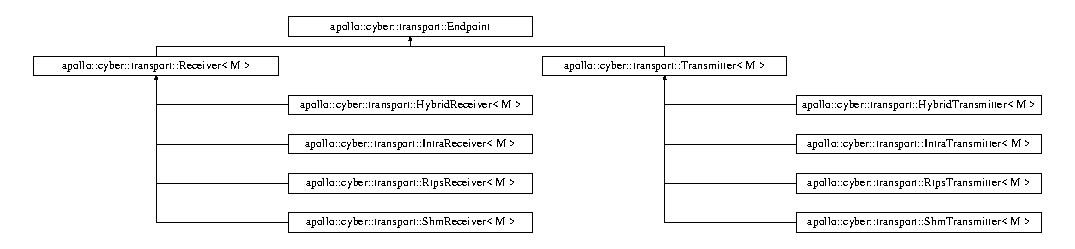
\includegraphics[height=2.896552cm]{classapollo_1_1cyber_1_1transport_1_1Endpoint}
\end{center}
\end{figure}
\subsection*{Public Member Functions}
\begin{DoxyCompactItemize}
\item 
\hyperlink{classapollo_1_1cyber_1_1transport_1_1Endpoint_a9ac289b2b1952934f326ab80bc63beb2}{Endpoint} (const Role\-Attributes \&attr)
\item 
virtual \hyperlink{classapollo_1_1cyber_1_1transport_1_1Endpoint_ace4552dd897f8ec3a8276529061c2ca4}{$\sim$\-Endpoint} ()
\item 
const \hyperlink{classapollo_1_1cyber_1_1transport_1_1Identity}{Identity} \& \hyperlink{classapollo_1_1cyber_1_1transport_1_1Endpoint_aa362f1ca16c50755e20e6f59362a37fc}{id} () const 
\item 
const Role\-Attributes \& \hyperlink{classapollo_1_1cyber_1_1transport_1_1Endpoint_a618711f01e375eab74b46845b193fa77}{attributes} () const 
\end{DoxyCompactItemize}
\subsection*{Protected Attributes}
\begin{DoxyCompactItemize}
\item 
bool \hyperlink{classapollo_1_1cyber_1_1transport_1_1Endpoint_a018bd12d292d6f46e97bb34d3054d5d2}{enabled\-\_\-}
\item 
\hyperlink{classapollo_1_1cyber_1_1transport_1_1Identity}{Identity} \hyperlink{classapollo_1_1cyber_1_1transport_1_1Endpoint_ab13e5b3e9b7b614f687159ad7ff07655}{id\-\_\-}
\item 
Role\-Attributes \hyperlink{classapollo_1_1cyber_1_1transport_1_1Endpoint_ae5eef9d783a55addf75c73f3b2d3d922}{attr\-\_\-}
\end{DoxyCompactItemize}


\subsection{Constructor \& Destructor Documentation}
\hypertarget{classapollo_1_1cyber_1_1transport_1_1Endpoint_a9ac289b2b1952934f326ab80bc63beb2}{\index{apollo\-::cyber\-::transport\-::\-Endpoint@{apollo\-::cyber\-::transport\-::\-Endpoint}!Endpoint@{Endpoint}}
\index{Endpoint@{Endpoint}!apollo::cyber::transport::Endpoint@{apollo\-::cyber\-::transport\-::\-Endpoint}}
\subsubsection[{Endpoint}]{\setlength{\rightskip}{0pt plus 5cm}apollo\-::cyber\-::transport\-::\-Endpoint\-::\-Endpoint (
\begin{DoxyParamCaption}
\item[{const Role\-Attributes \&}]{attr}
\end{DoxyParamCaption}
)\hspace{0.3cm}{\ttfamily [explicit]}}}\label{classapollo_1_1cyber_1_1transport_1_1Endpoint_a9ac289b2b1952934f326ab80bc63beb2}
\hypertarget{classapollo_1_1cyber_1_1transport_1_1Endpoint_ace4552dd897f8ec3a8276529061c2ca4}{\index{apollo\-::cyber\-::transport\-::\-Endpoint@{apollo\-::cyber\-::transport\-::\-Endpoint}!$\sim$\-Endpoint@{$\sim$\-Endpoint}}
\index{$\sim$\-Endpoint@{$\sim$\-Endpoint}!apollo::cyber::transport::Endpoint@{apollo\-::cyber\-::transport\-::\-Endpoint}}
\subsubsection[{$\sim$\-Endpoint}]{\setlength{\rightskip}{0pt plus 5cm}virtual apollo\-::cyber\-::transport\-::\-Endpoint\-::$\sim$\-Endpoint (
\begin{DoxyParamCaption}
{}
\end{DoxyParamCaption}
)\hspace{0.3cm}{\ttfamily [virtual]}}}\label{classapollo_1_1cyber_1_1transport_1_1Endpoint_ace4552dd897f8ec3a8276529061c2ca4}


\subsection{Member Function Documentation}
\hypertarget{classapollo_1_1cyber_1_1transport_1_1Endpoint_a618711f01e375eab74b46845b193fa77}{\index{apollo\-::cyber\-::transport\-::\-Endpoint@{apollo\-::cyber\-::transport\-::\-Endpoint}!attributes@{attributes}}
\index{attributes@{attributes}!apollo::cyber::transport::Endpoint@{apollo\-::cyber\-::transport\-::\-Endpoint}}
\subsubsection[{attributes}]{\setlength{\rightskip}{0pt plus 5cm}const Role\-Attributes\& apollo\-::cyber\-::transport\-::\-Endpoint\-::attributes (
\begin{DoxyParamCaption}
{}
\end{DoxyParamCaption}
) const\hspace{0.3cm}{\ttfamily [inline]}}}\label{classapollo_1_1cyber_1_1transport_1_1Endpoint_a618711f01e375eab74b46845b193fa77}
\hypertarget{classapollo_1_1cyber_1_1transport_1_1Endpoint_aa362f1ca16c50755e20e6f59362a37fc}{\index{apollo\-::cyber\-::transport\-::\-Endpoint@{apollo\-::cyber\-::transport\-::\-Endpoint}!id@{id}}
\index{id@{id}!apollo::cyber::transport::Endpoint@{apollo\-::cyber\-::transport\-::\-Endpoint}}
\subsubsection[{id}]{\setlength{\rightskip}{0pt plus 5cm}const {\bf Identity}\& apollo\-::cyber\-::transport\-::\-Endpoint\-::id (
\begin{DoxyParamCaption}
{}
\end{DoxyParamCaption}
) const\hspace{0.3cm}{\ttfamily [inline]}}}\label{classapollo_1_1cyber_1_1transport_1_1Endpoint_aa362f1ca16c50755e20e6f59362a37fc}


\subsection{Member Data Documentation}
\hypertarget{classapollo_1_1cyber_1_1transport_1_1Endpoint_ae5eef9d783a55addf75c73f3b2d3d922}{\index{apollo\-::cyber\-::transport\-::\-Endpoint@{apollo\-::cyber\-::transport\-::\-Endpoint}!attr\-\_\-@{attr\-\_\-}}
\index{attr\-\_\-@{attr\-\_\-}!apollo::cyber::transport::Endpoint@{apollo\-::cyber\-::transport\-::\-Endpoint}}
\subsubsection[{attr\-\_\-}]{\setlength{\rightskip}{0pt plus 5cm}Role\-Attributes apollo\-::cyber\-::transport\-::\-Endpoint\-::attr\-\_\-\hspace{0.3cm}{\ttfamily [protected]}}}\label{classapollo_1_1cyber_1_1transport_1_1Endpoint_ae5eef9d783a55addf75c73f3b2d3d922}
\hypertarget{classapollo_1_1cyber_1_1transport_1_1Endpoint_a018bd12d292d6f46e97bb34d3054d5d2}{\index{apollo\-::cyber\-::transport\-::\-Endpoint@{apollo\-::cyber\-::transport\-::\-Endpoint}!enabled\-\_\-@{enabled\-\_\-}}
\index{enabled\-\_\-@{enabled\-\_\-}!apollo::cyber::transport::Endpoint@{apollo\-::cyber\-::transport\-::\-Endpoint}}
\subsubsection[{enabled\-\_\-}]{\setlength{\rightskip}{0pt plus 5cm}bool apollo\-::cyber\-::transport\-::\-Endpoint\-::enabled\-\_\-\hspace{0.3cm}{\ttfamily [protected]}}}\label{classapollo_1_1cyber_1_1transport_1_1Endpoint_a018bd12d292d6f46e97bb34d3054d5d2}
\hypertarget{classapollo_1_1cyber_1_1transport_1_1Endpoint_ab13e5b3e9b7b614f687159ad7ff07655}{\index{apollo\-::cyber\-::transport\-::\-Endpoint@{apollo\-::cyber\-::transport\-::\-Endpoint}!id\-\_\-@{id\-\_\-}}
\index{id\-\_\-@{id\-\_\-}!apollo::cyber::transport::Endpoint@{apollo\-::cyber\-::transport\-::\-Endpoint}}
\subsubsection[{id\-\_\-}]{\setlength{\rightskip}{0pt plus 5cm}{\bf Identity} apollo\-::cyber\-::transport\-::\-Endpoint\-::id\-\_\-\hspace{0.3cm}{\ttfamily [protected]}}}\label{classapollo_1_1cyber_1_1transport_1_1Endpoint_ab13e5b3e9b7b614f687159ad7ff07655}


The documentation for this class was generated from the following file\-:\begin{DoxyCompactItemize}
\item 
transport/common/\hyperlink{endpoint_8h}{endpoint.\-h}\end{DoxyCompactItemize}

\hypertarget{structapollo_1_1cyber_1_1base_1_1AtomicHashMap_1_1Entry}{\section{apollo\-:\-:cyber\-:\-:base\-:\-:Atomic\-Hash\-Map$<$ K, V, Table\-Size, std\-:\-:enable\-\_\-if$<$ std\-:\-:is\-\_\-integral$<$ K $>$\-:\-:value \&\&(Table\-Size \&(Table\-Size-\/1))==0, int $>$\-:\-:type $>$\-:\-:Entry Struct Reference}
\label{structapollo_1_1cyber_1_1base_1_1AtomicHashMap_1_1Entry}\index{apollo\-::cyber\-::base\-::\-Atomic\-Hash\-Map$<$ K, V, Table\-Size, std\-::enable\-\_\-if$<$ std\-::is\-\_\-integral$<$ K $>$\-::value \&\&(\-Table\-Size \&(\-Table\-Size-\/1))==0, int $>$\-::type $>$\-::\-Entry@{apollo\-::cyber\-::base\-::\-Atomic\-Hash\-Map$<$ K, V, Table\-Size, std\-::enable\-\_\-if$<$ std\-::is\-\_\-integral$<$ K $>$\-::value \&\&(\-Table\-Size \&(\-Table\-Size-\/1))==0, int $>$\-::type $>$\-::\-Entry}}
}
\subsection*{Public Member Functions}
\begin{DoxyCompactItemize}
\item 
\hyperlink{structapollo_1_1cyber_1_1base_1_1AtomicHashMap_1_1Entry_ae852819828fc6a7b68db072dea8640b9}{Entry} ()
\item 
\hyperlink{structapollo_1_1cyber_1_1base_1_1AtomicHashMap_1_1Entry_a325c68fbf78f04f185fdf7b69f893917}{Entry} (K \hyperlink{structapollo_1_1cyber_1_1base_1_1AtomicHashMap_1_1Entry_a92d89dfd94973438aa8db43a8bbebee6}{key})
\item 
\hyperlink{structapollo_1_1cyber_1_1base_1_1AtomicHashMap_1_1Entry_aa9d4d2fcabc83b9969e2d56336afcf52}{Entry} (K \hyperlink{structapollo_1_1cyber_1_1base_1_1AtomicHashMap_1_1Entry_a92d89dfd94973438aa8db43a8bbebee6}{key}, const V \&\hyperlink{namespaceapollo_1_1cyber_1_1base_aa3e2fff9b18a1214af4a70546fb7120f}{value})
\item 
\hyperlink{structapollo_1_1cyber_1_1base_1_1AtomicHashMap_1_1Entry_af5776001b463532d197e002e411ed8f1}{Entry} (K \hyperlink{structapollo_1_1cyber_1_1base_1_1AtomicHashMap_1_1Entry_a92d89dfd94973438aa8db43a8bbebee6}{key}, V \&\&\hyperlink{namespaceapollo_1_1cyber_1_1base_aa3e2fff9b18a1214af4a70546fb7120f}{value})
\item 
\hyperlink{structapollo_1_1cyber_1_1base_1_1AtomicHashMap_1_1Entry_a70be561c45093c3010e8d08a12aaafa8}{$\sim$\-Entry} ()
\end{DoxyCompactItemize}
\subsection*{Public Attributes}
\begin{DoxyCompactItemize}
\item 
K \hyperlink{structapollo_1_1cyber_1_1base_1_1AtomicHashMap_1_1Entry_a92d89dfd94973438aa8db43a8bbebee6}{key} = 0
\item 
std\-::atomic$<$ V $\ast$ $>$ \hyperlink{structapollo_1_1cyber_1_1base_1_1AtomicHashMap_1_1Entry_ac717cbc0d8b0e10085e6458790f2a30f}{value\-\_\-ptr} = \{nullptr\}
\item 
std\-::atomic$<$ \hyperlink{structapollo_1_1cyber_1_1base_1_1AtomicHashMap_1_1Entry}{Entry} $\ast$ $>$ \hyperlink{structapollo_1_1cyber_1_1base_1_1AtomicHashMap_1_1Entry_af0f925e9c620cb000999d0dafd872e0f}{next} = \{nullptr\}
\end{DoxyCompactItemize}


\subsection{Constructor \& Destructor Documentation}
\hypertarget{structapollo_1_1cyber_1_1base_1_1AtomicHashMap_1_1Entry_ae852819828fc6a7b68db072dea8640b9}{\index{apollo\-::cyber\-::base\-::\-Atomic\-Hash\-Map\-::\-Entry@{apollo\-::cyber\-::base\-::\-Atomic\-Hash\-Map\-::\-Entry}!Entry@{Entry}}
\index{Entry@{Entry}!apollo::cyber::base::AtomicHashMap::Entry@{apollo\-::cyber\-::base\-::\-Atomic\-Hash\-Map\-::\-Entry}}
\subsubsection[{Entry}]{\setlength{\rightskip}{0pt plus 5cm}template$<$typename K, typename V, std\-::size\-\_\-t Table\-Size = 128, typename std\-::enable\-\_\-if$<$ std\-::is\-\_\-integral$<$ K $>$\-::value \&\&(\-Table\-Size \&(\-Table\-Size-\/1))==0, int $>$\-::type = 0$>$ {\bf apollo\-::cyber\-::base\-::\-Atomic\-Hash\-Map}$<$ K, V, Table\-Size, type $>$\-::Entry\-::\-Entry (
\begin{DoxyParamCaption}
{}
\end{DoxyParamCaption}
)\hspace{0.3cm}{\ttfamily [inline]}}}\label{structapollo_1_1cyber_1_1base_1_1AtomicHashMap_1_1Entry_ae852819828fc6a7b68db072dea8640b9}
\hypertarget{structapollo_1_1cyber_1_1base_1_1AtomicHashMap_1_1Entry_a325c68fbf78f04f185fdf7b69f893917}{\index{apollo\-::cyber\-::base\-::\-Atomic\-Hash\-Map\-::\-Entry@{apollo\-::cyber\-::base\-::\-Atomic\-Hash\-Map\-::\-Entry}!Entry@{Entry}}
\index{Entry@{Entry}!apollo::cyber::base::AtomicHashMap::Entry@{apollo\-::cyber\-::base\-::\-Atomic\-Hash\-Map\-::\-Entry}}
\subsubsection[{Entry}]{\setlength{\rightskip}{0pt plus 5cm}template$<$typename K, typename V, std\-::size\-\_\-t Table\-Size = 128, typename std\-::enable\-\_\-if$<$ std\-::is\-\_\-integral$<$ K $>$\-::value \&\&(\-Table\-Size \&(\-Table\-Size-\/1))==0, int $>$\-::type = 0$>$ {\bf apollo\-::cyber\-::base\-::\-Atomic\-Hash\-Map}$<$ K, V, Table\-Size, type $>$\-::Entry\-::\-Entry (
\begin{DoxyParamCaption}
\item[{K}]{key}
\end{DoxyParamCaption}
)\hspace{0.3cm}{\ttfamily [inline]}, {\ttfamily [explicit]}}}\label{structapollo_1_1cyber_1_1base_1_1AtomicHashMap_1_1Entry_a325c68fbf78f04f185fdf7b69f893917}
\hypertarget{structapollo_1_1cyber_1_1base_1_1AtomicHashMap_1_1Entry_aa9d4d2fcabc83b9969e2d56336afcf52}{\index{apollo\-::cyber\-::base\-::\-Atomic\-Hash\-Map\-::\-Entry@{apollo\-::cyber\-::base\-::\-Atomic\-Hash\-Map\-::\-Entry}!Entry@{Entry}}
\index{Entry@{Entry}!apollo::cyber::base::AtomicHashMap::Entry@{apollo\-::cyber\-::base\-::\-Atomic\-Hash\-Map\-::\-Entry}}
\subsubsection[{Entry}]{\setlength{\rightskip}{0pt plus 5cm}template$<$typename K, typename V, std\-::size\-\_\-t Table\-Size = 128, typename std\-::enable\-\_\-if$<$ std\-::is\-\_\-integral$<$ K $>$\-::value \&\&(\-Table\-Size \&(\-Table\-Size-\/1))==0, int $>$\-::type = 0$>$ {\bf apollo\-::cyber\-::base\-::\-Atomic\-Hash\-Map}$<$ K, V, Table\-Size, type $>$\-::Entry\-::\-Entry (
\begin{DoxyParamCaption}
\item[{K}]{key, }
\item[{const V \&}]{value}
\end{DoxyParamCaption}
)\hspace{0.3cm}{\ttfamily [inline]}}}\label{structapollo_1_1cyber_1_1base_1_1AtomicHashMap_1_1Entry_aa9d4d2fcabc83b9969e2d56336afcf52}
\hypertarget{structapollo_1_1cyber_1_1base_1_1AtomicHashMap_1_1Entry_af5776001b463532d197e002e411ed8f1}{\index{apollo\-::cyber\-::base\-::\-Atomic\-Hash\-Map\-::\-Entry@{apollo\-::cyber\-::base\-::\-Atomic\-Hash\-Map\-::\-Entry}!Entry@{Entry}}
\index{Entry@{Entry}!apollo::cyber::base::AtomicHashMap::Entry@{apollo\-::cyber\-::base\-::\-Atomic\-Hash\-Map\-::\-Entry}}
\subsubsection[{Entry}]{\setlength{\rightskip}{0pt plus 5cm}template$<$typename K, typename V, std\-::size\-\_\-t Table\-Size = 128, typename std\-::enable\-\_\-if$<$ std\-::is\-\_\-integral$<$ K $>$\-::value \&\&(\-Table\-Size \&(\-Table\-Size-\/1))==0, int $>$\-::type = 0$>$ {\bf apollo\-::cyber\-::base\-::\-Atomic\-Hash\-Map}$<$ K, V, Table\-Size, type $>$\-::Entry\-::\-Entry (
\begin{DoxyParamCaption}
\item[{K}]{key, }
\item[{V \&\&}]{value}
\end{DoxyParamCaption}
)\hspace{0.3cm}{\ttfamily [inline]}}}\label{structapollo_1_1cyber_1_1base_1_1AtomicHashMap_1_1Entry_af5776001b463532d197e002e411ed8f1}
\hypertarget{structapollo_1_1cyber_1_1base_1_1AtomicHashMap_1_1Entry_a70be561c45093c3010e8d08a12aaafa8}{\index{apollo\-::cyber\-::base\-::\-Atomic\-Hash\-Map\-::\-Entry@{apollo\-::cyber\-::base\-::\-Atomic\-Hash\-Map\-::\-Entry}!$\sim$\-Entry@{$\sim$\-Entry}}
\index{$\sim$\-Entry@{$\sim$\-Entry}!apollo::cyber::base::AtomicHashMap::Entry@{apollo\-::cyber\-::base\-::\-Atomic\-Hash\-Map\-::\-Entry}}
\subsubsection[{$\sim$\-Entry}]{\setlength{\rightskip}{0pt plus 5cm}template$<$typename K, typename V, std\-::size\-\_\-t Table\-Size = 128, typename std\-::enable\-\_\-if$<$ std\-::is\-\_\-integral$<$ K $>$\-::value \&\&(\-Table\-Size \&(\-Table\-Size-\/1))==0, int $>$\-::type = 0$>$ {\bf apollo\-::cyber\-::base\-::\-Atomic\-Hash\-Map}$<$ K, V, Table\-Size, type $>$\-::Entry\-::$\sim$\-Entry (
\begin{DoxyParamCaption}
{}
\end{DoxyParamCaption}
)\hspace{0.3cm}{\ttfamily [inline]}}}\label{structapollo_1_1cyber_1_1base_1_1AtomicHashMap_1_1Entry_a70be561c45093c3010e8d08a12aaafa8}


\subsection{Member Data Documentation}
\hypertarget{structapollo_1_1cyber_1_1base_1_1AtomicHashMap_1_1Entry_a92d89dfd94973438aa8db43a8bbebee6}{\index{apollo\-::cyber\-::base\-::\-Atomic\-Hash\-Map\-::\-Entry@{apollo\-::cyber\-::base\-::\-Atomic\-Hash\-Map\-::\-Entry}!key@{key}}
\index{key@{key}!apollo::cyber::base::AtomicHashMap::Entry@{apollo\-::cyber\-::base\-::\-Atomic\-Hash\-Map\-::\-Entry}}
\subsubsection[{key}]{\setlength{\rightskip}{0pt plus 5cm}template$<$typename K, typename V, std\-::size\-\_\-t Table\-Size = 128, typename std\-::enable\-\_\-if$<$ std\-::is\-\_\-integral$<$ K $>$\-::value \&\&(\-Table\-Size \&(\-Table\-Size-\/1))==0, int $>$\-::type = 0$>$ K {\bf apollo\-::cyber\-::base\-::\-Atomic\-Hash\-Map}$<$ K, V, Table\-Size, type $>$\-::Entry\-::key = 0}}\label{structapollo_1_1cyber_1_1base_1_1AtomicHashMap_1_1Entry_a92d89dfd94973438aa8db43a8bbebee6}
\hypertarget{structapollo_1_1cyber_1_1base_1_1AtomicHashMap_1_1Entry_af0f925e9c620cb000999d0dafd872e0f}{\index{apollo\-::cyber\-::base\-::\-Atomic\-Hash\-Map\-::\-Entry@{apollo\-::cyber\-::base\-::\-Atomic\-Hash\-Map\-::\-Entry}!next@{next}}
\index{next@{next}!apollo::cyber::base::AtomicHashMap::Entry@{apollo\-::cyber\-::base\-::\-Atomic\-Hash\-Map\-::\-Entry}}
\subsubsection[{next}]{\setlength{\rightskip}{0pt plus 5cm}template$<$typename K, typename V, std\-::size\-\_\-t Table\-Size = 128, typename std\-::enable\-\_\-if$<$ std\-::is\-\_\-integral$<$ K $>$\-::value \&\&(\-Table\-Size \&(\-Table\-Size-\/1))==0, int $>$\-::type = 0$>$ std\-::atomic$<${\bf Entry} $\ast$$>$ {\bf apollo\-::cyber\-::base\-::\-Atomic\-Hash\-Map}$<$ K, V, Table\-Size, type $>$\-::Entry\-::next = \{nullptr\}}}\label{structapollo_1_1cyber_1_1base_1_1AtomicHashMap_1_1Entry_af0f925e9c620cb000999d0dafd872e0f}
\hypertarget{structapollo_1_1cyber_1_1base_1_1AtomicHashMap_1_1Entry_ac717cbc0d8b0e10085e6458790f2a30f}{\index{apollo\-::cyber\-::base\-::\-Atomic\-Hash\-Map\-::\-Entry@{apollo\-::cyber\-::base\-::\-Atomic\-Hash\-Map\-::\-Entry}!value\-\_\-ptr@{value\-\_\-ptr}}
\index{value\-\_\-ptr@{value\-\_\-ptr}!apollo::cyber::base::AtomicHashMap::Entry@{apollo\-::cyber\-::base\-::\-Atomic\-Hash\-Map\-::\-Entry}}
\subsubsection[{value\-\_\-ptr}]{\setlength{\rightskip}{0pt plus 5cm}template$<$typename K, typename V, std\-::size\-\_\-t Table\-Size = 128, typename std\-::enable\-\_\-if$<$ std\-::is\-\_\-integral$<$ K $>$\-::value \&\&(\-Table\-Size \&(\-Table\-Size-\/1))==0, int $>$\-::type = 0$>$ std\-::atomic$<$V $\ast$$>$ {\bf apollo\-::cyber\-::base\-::\-Atomic\-Hash\-Map}$<$ K, V, Table\-Size, type $>$\-::Entry\-::value\-\_\-ptr = \{nullptr\}}}\label{structapollo_1_1cyber_1_1base_1_1AtomicHashMap_1_1Entry_ac717cbc0d8b0e10085e6458790f2a30f}


The documentation for this struct was generated from the following file\-:\begin{DoxyCompactItemize}
\item 
base/\hyperlink{atomic__hash__map_8h}{atomic\-\_\-hash\-\_\-map.\-h}\end{DoxyCompactItemize}

\hypertarget{classapollo_1_1cyber_1_1message_1_1ErrorCollector}{\section{apollo\-:\-:cyber\-:\-:message\-:\-:Error\-Collector Class Reference}
\label{classapollo_1_1cyber_1_1message_1_1ErrorCollector}\index{apollo\-::cyber\-::message\-::\-Error\-Collector@{apollo\-::cyber\-::message\-::\-Error\-Collector}}
}


{\ttfamily \#include $<$protobuf\-\_\-factory.\-h$>$}

Inheritance diagram for apollo\-:\-:cyber\-:\-:message\-:\-:Error\-Collector\-:\begin{figure}[H]
\begin{center}
\leavevmode
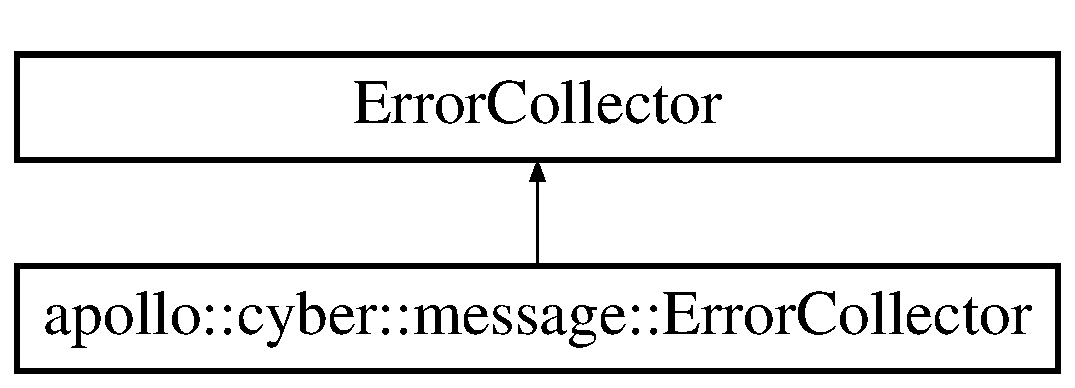
\includegraphics[height=2.000000cm]{classapollo_1_1cyber_1_1message_1_1ErrorCollector}
\end{center}
\end{figure}
\subsection*{Private Types}
\begin{DoxyCompactItemize}
\item 
using \hyperlink{classapollo_1_1cyber_1_1message_1_1ErrorCollector_ac39eb350844e7897054ed7552e67a64b}{Error\-Location} = google\-::protobuf\-::\-Descriptor\-Pool\-::\-Error\-Collector\-::\-Error\-Location
\end{DoxyCompactItemize}
\subsection*{Private Member Functions}
\begin{DoxyCompactItemize}
\item 
void \hyperlink{classapollo_1_1cyber_1_1message_1_1ErrorCollector_aff2683e6605e847d7a6b4ffbf86d32fb}{Add\-Error} (const std\-::string \&filename, const std\-::string \&element\-\_\-name, const google\-::protobuf\-::\-Message $\ast$descriptor, \hyperlink{classapollo_1_1cyber_1_1message_1_1ErrorCollector_ac39eb350844e7897054ed7552e67a64b}{Error\-Location} location, const std\-::string \&message) override
\item 
void \hyperlink{classapollo_1_1cyber_1_1message_1_1ErrorCollector_a9f447ed3a2bdd079f0501131040f71da}{Add\-Warning} (const std\-::string \&filename, const std\-::string \&element\-\_\-name, const google\-::protobuf\-::\-Message $\ast$descriptor, \hyperlink{classapollo_1_1cyber_1_1message_1_1ErrorCollector_ac39eb350844e7897054ed7552e67a64b}{Error\-Location} location, const std\-::string \&message) override
\end{DoxyCompactItemize}


\subsection{Member Typedef Documentation}
\hypertarget{classapollo_1_1cyber_1_1message_1_1ErrorCollector_ac39eb350844e7897054ed7552e67a64b}{\index{apollo\-::cyber\-::message\-::\-Error\-Collector@{apollo\-::cyber\-::message\-::\-Error\-Collector}!Error\-Location@{Error\-Location}}
\index{Error\-Location@{Error\-Location}!apollo::cyber::message::ErrorCollector@{apollo\-::cyber\-::message\-::\-Error\-Collector}}
\subsubsection[{Error\-Location}]{\setlength{\rightskip}{0pt plus 5cm}using {\bf apollo\-::cyber\-::message\-::\-Error\-Collector\-::\-Error\-Location} =  google\-::protobuf\-::\-Descriptor\-Pool\-::\-Error\-Collector\-::\-Error\-Location\hspace{0.3cm}{\ttfamily [private]}}}\label{classapollo_1_1cyber_1_1message_1_1ErrorCollector_ac39eb350844e7897054ed7552e67a64b}


\subsection{Member Function Documentation}
\hypertarget{classapollo_1_1cyber_1_1message_1_1ErrorCollector_aff2683e6605e847d7a6b4ffbf86d32fb}{\index{apollo\-::cyber\-::message\-::\-Error\-Collector@{apollo\-::cyber\-::message\-::\-Error\-Collector}!Add\-Error@{Add\-Error}}
\index{Add\-Error@{Add\-Error}!apollo::cyber::message::ErrorCollector@{apollo\-::cyber\-::message\-::\-Error\-Collector}}
\subsubsection[{Add\-Error}]{\setlength{\rightskip}{0pt plus 5cm}void apollo\-::cyber\-::message\-::\-Error\-Collector\-::\-Add\-Error (
\begin{DoxyParamCaption}
\item[{const std\-::string \&}]{filename, }
\item[{const std\-::string \&}]{element\-\_\-name, }
\item[{const google\-::protobuf\-::\-Message $\ast$}]{descriptor, }
\item[{{\bf Error\-Location}}]{location, }
\item[{const std\-::string \&}]{message}
\end{DoxyParamCaption}
)\hspace{0.3cm}{\ttfamily [override]}, {\ttfamily [private]}}}\label{classapollo_1_1cyber_1_1message_1_1ErrorCollector_aff2683e6605e847d7a6b4ffbf86d32fb}
\hypertarget{classapollo_1_1cyber_1_1message_1_1ErrorCollector_a9f447ed3a2bdd079f0501131040f71da}{\index{apollo\-::cyber\-::message\-::\-Error\-Collector@{apollo\-::cyber\-::message\-::\-Error\-Collector}!Add\-Warning@{Add\-Warning}}
\index{Add\-Warning@{Add\-Warning}!apollo::cyber::message::ErrorCollector@{apollo\-::cyber\-::message\-::\-Error\-Collector}}
\subsubsection[{Add\-Warning}]{\setlength{\rightskip}{0pt plus 5cm}void apollo\-::cyber\-::message\-::\-Error\-Collector\-::\-Add\-Warning (
\begin{DoxyParamCaption}
\item[{const std\-::string \&}]{filename, }
\item[{const std\-::string \&}]{element\-\_\-name, }
\item[{const google\-::protobuf\-::\-Message $\ast$}]{descriptor, }
\item[{{\bf Error\-Location}}]{location, }
\item[{const std\-::string \&}]{message}
\end{DoxyParamCaption}
)\hspace{0.3cm}{\ttfamily [override]}, {\ttfamily [private]}}}\label{classapollo_1_1cyber_1_1message_1_1ErrorCollector_a9f447ed3a2bdd079f0501131040f71da}


The documentation for this class was generated from the following file\-:\begin{DoxyCompactItemize}
\item 
message/\hyperlink{protobuf__factory_8h}{protobuf\-\_\-factory.\-h}\end{DoxyCompactItemize}

\hypertarget{classapollo_1_1cyber_1_1event_1_1EventBase}{\section{apollo\-:\-:cyber\-:\-:event\-:\-:Event\-Base Class Reference}
\label{classapollo_1_1cyber_1_1event_1_1EventBase}\index{apollo\-::cyber\-::event\-::\-Event\-Base@{apollo\-::cyber\-::event\-::\-Event\-Base}}
}


{\ttfamily \#include $<$perf\-\_\-event.\-h$>$}

Inheritance diagram for apollo\-:\-:cyber\-:\-:event\-:\-:Event\-Base\-:\begin{figure}[H]
\begin{center}
\leavevmode
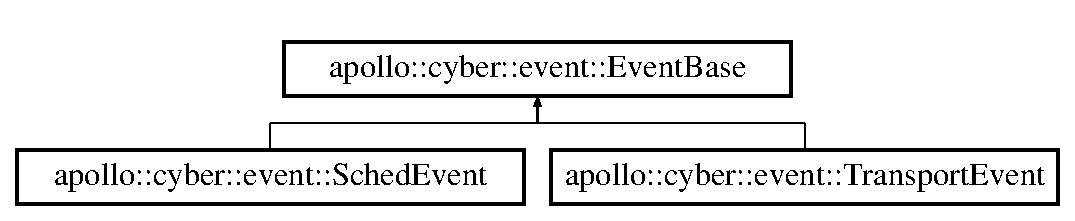
\includegraphics[height=2.000000cm]{classapollo_1_1cyber_1_1event_1_1EventBase}
\end{center}
\end{figure}
\subsection*{Public Member Functions}
\begin{DoxyCompactItemize}
\item 
virtual std\-::string \hyperlink{classapollo_1_1cyber_1_1event_1_1EventBase_a76173ad9c315ed775371469d612b489d}{Serialize\-To\-String} ()=0
\item 
void \hyperlink{classapollo_1_1cyber_1_1event_1_1EventBase_ad7322836ed1d5d2a1a1c5bbf88f04df0}{set\-\_\-eid} (int eid)
\item 
void \hyperlink{classapollo_1_1cyber_1_1event_1_1EventBase_aae9bb6e39842338f1139c6496d71dfb6}{set\-\_\-etype} (int etype)
\item 
void \hyperlink{classapollo_1_1cyber_1_1event_1_1EventBase_a3b0ef301b6eb0bd03c0c98e4c85ae29e}{set\-\_\-stamp} (uint64\-\_\-t stamp)
\item 
virtual void \hyperlink{classapollo_1_1cyber_1_1event_1_1EventBase_adca308f7a8828fc85f7a7c47f8e62938}{set\-\_\-cr\-\_\-id} (uint64\-\_\-t cr\-\_\-id)
\item 
virtual void \hyperlink{classapollo_1_1cyber_1_1event_1_1EventBase_a9b0dbb9c9db334795fb32523be945e20}{set\-\_\-cr\-\_\-state} (int cr\-\_\-state)
\item 
virtual void \hyperlink{classapollo_1_1cyber_1_1event_1_1EventBase_a892ea37f81adc4981bc91396919c4e9a}{set\-\_\-proc\-\_\-id} (int proc\-\_\-id)
\item 
virtual void \hyperlink{classapollo_1_1cyber_1_1event_1_1EventBase_a3023ba9bdcd8996d879099ac19647465}{set\-\_\-fetch\-\_\-res} (int fetch\-\_\-res)
\item 
virtual void \hyperlink{classapollo_1_1cyber_1_1event_1_1EventBase_ae70276f235359287b75a72b932903bf1}{set\-\_\-msg\-\_\-seq} (uint64\-\_\-t msg\-\_\-seq)
\item 
virtual void \hyperlink{classapollo_1_1cyber_1_1event_1_1EventBase_af2db22e91dcce677a59ecab489685542}{set\-\_\-channel\-\_\-id} (uint64\-\_\-t channel\-\_\-id)
\end{DoxyCompactItemize}
\subsection*{Protected Attributes}
\begin{DoxyCompactItemize}
\item 
int \hyperlink{classapollo_1_1cyber_1_1event_1_1EventBase_ae26baa01961de359956540b4e5f98ad5}{etype\-\_\-}
\item 
int \hyperlink{classapollo_1_1cyber_1_1event_1_1EventBase_a1d9e13642a28e712a16bff0224e0b6fe}{eid\-\_\-}
\item 
uint64\-\_\-t \hyperlink{classapollo_1_1cyber_1_1event_1_1EventBase_afaeda733409e3addc6e7f839b694333d}{stamp\-\_\-}
\end{DoxyCompactItemize}


\subsection{Member Function Documentation}
\hypertarget{classapollo_1_1cyber_1_1event_1_1EventBase_a76173ad9c315ed775371469d612b489d}{\index{apollo\-::cyber\-::event\-::\-Event\-Base@{apollo\-::cyber\-::event\-::\-Event\-Base}!Serialize\-To\-String@{Serialize\-To\-String}}
\index{Serialize\-To\-String@{Serialize\-To\-String}!apollo::cyber::event::EventBase@{apollo\-::cyber\-::event\-::\-Event\-Base}}
\subsubsection[{Serialize\-To\-String}]{\setlength{\rightskip}{0pt plus 5cm}virtual std\-::string apollo\-::cyber\-::event\-::\-Event\-Base\-::\-Serialize\-To\-String (
\begin{DoxyParamCaption}
{}
\end{DoxyParamCaption}
)\hspace{0.3cm}{\ttfamily [pure virtual]}}}\label{classapollo_1_1cyber_1_1event_1_1EventBase_a76173ad9c315ed775371469d612b489d}


Implemented in \hyperlink{classapollo_1_1cyber_1_1event_1_1TransportEvent_ac006e30964aa5ddf8325a2a4187474b9}{apollo\-::cyber\-::event\-::\-Transport\-Event}, and \hyperlink{classapollo_1_1cyber_1_1event_1_1SchedEvent_a92a8ce80dac62e102d79010845c37b5b}{apollo\-::cyber\-::event\-::\-Sched\-Event}.

\hypertarget{classapollo_1_1cyber_1_1event_1_1EventBase_af2db22e91dcce677a59ecab489685542}{\index{apollo\-::cyber\-::event\-::\-Event\-Base@{apollo\-::cyber\-::event\-::\-Event\-Base}!set\-\_\-channel\-\_\-id@{set\-\_\-channel\-\_\-id}}
\index{set\-\_\-channel\-\_\-id@{set\-\_\-channel\-\_\-id}!apollo::cyber::event::EventBase@{apollo\-::cyber\-::event\-::\-Event\-Base}}
\subsubsection[{set\-\_\-channel\-\_\-id}]{\setlength{\rightskip}{0pt plus 5cm}virtual void apollo\-::cyber\-::event\-::\-Event\-Base\-::set\-\_\-channel\-\_\-id (
\begin{DoxyParamCaption}
\item[{uint64\-\_\-t}]{channel\-\_\-id}
\end{DoxyParamCaption}
)\hspace{0.3cm}{\ttfamily [inline]}, {\ttfamily [virtual]}}}\label{classapollo_1_1cyber_1_1event_1_1EventBase_af2db22e91dcce677a59ecab489685542}


Reimplemented in \hyperlink{classapollo_1_1cyber_1_1event_1_1TransportEvent_a474cc7b64211525b00a5fd4f2238fd51}{apollo\-::cyber\-::event\-::\-Transport\-Event}.

\hypertarget{classapollo_1_1cyber_1_1event_1_1EventBase_adca308f7a8828fc85f7a7c47f8e62938}{\index{apollo\-::cyber\-::event\-::\-Event\-Base@{apollo\-::cyber\-::event\-::\-Event\-Base}!set\-\_\-cr\-\_\-id@{set\-\_\-cr\-\_\-id}}
\index{set\-\_\-cr\-\_\-id@{set\-\_\-cr\-\_\-id}!apollo::cyber::event::EventBase@{apollo\-::cyber\-::event\-::\-Event\-Base}}
\subsubsection[{set\-\_\-cr\-\_\-id}]{\setlength{\rightskip}{0pt plus 5cm}virtual void apollo\-::cyber\-::event\-::\-Event\-Base\-::set\-\_\-cr\-\_\-id (
\begin{DoxyParamCaption}
\item[{uint64\-\_\-t}]{cr\-\_\-id}
\end{DoxyParamCaption}
)\hspace{0.3cm}{\ttfamily [inline]}, {\ttfamily [virtual]}}}\label{classapollo_1_1cyber_1_1event_1_1EventBase_adca308f7a8828fc85f7a7c47f8e62938}


Reimplemented in \hyperlink{classapollo_1_1cyber_1_1event_1_1SchedEvent_a22cfd60eaefdf7647263d3270d3f3244}{apollo\-::cyber\-::event\-::\-Sched\-Event}.

\hypertarget{classapollo_1_1cyber_1_1event_1_1EventBase_a9b0dbb9c9db334795fb32523be945e20}{\index{apollo\-::cyber\-::event\-::\-Event\-Base@{apollo\-::cyber\-::event\-::\-Event\-Base}!set\-\_\-cr\-\_\-state@{set\-\_\-cr\-\_\-state}}
\index{set\-\_\-cr\-\_\-state@{set\-\_\-cr\-\_\-state}!apollo::cyber::event::EventBase@{apollo\-::cyber\-::event\-::\-Event\-Base}}
\subsubsection[{set\-\_\-cr\-\_\-state}]{\setlength{\rightskip}{0pt plus 5cm}virtual void apollo\-::cyber\-::event\-::\-Event\-Base\-::set\-\_\-cr\-\_\-state (
\begin{DoxyParamCaption}
\item[{int}]{cr\-\_\-state}
\end{DoxyParamCaption}
)\hspace{0.3cm}{\ttfamily [inline]}, {\ttfamily [virtual]}}}\label{classapollo_1_1cyber_1_1event_1_1EventBase_a9b0dbb9c9db334795fb32523be945e20}


Reimplemented in \hyperlink{classapollo_1_1cyber_1_1event_1_1SchedEvent_ae9b63ed13d7df3a671bb74988ff87bf6}{apollo\-::cyber\-::event\-::\-Sched\-Event}.

\hypertarget{classapollo_1_1cyber_1_1event_1_1EventBase_ad7322836ed1d5d2a1a1c5bbf88f04df0}{\index{apollo\-::cyber\-::event\-::\-Event\-Base@{apollo\-::cyber\-::event\-::\-Event\-Base}!set\-\_\-eid@{set\-\_\-eid}}
\index{set\-\_\-eid@{set\-\_\-eid}!apollo::cyber::event::EventBase@{apollo\-::cyber\-::event\-::\-Event\-Base}}
\subsubsection[{set\-\_\-eid}]{\setlength{\rightskip}{0pt plus 5cm}void apollo\-::cyber\-::event\-::\-Event\-Base\-::set\-\_\-eid (
\begin{DoxyParamCaption}
\item[{int}]{eid}
\end{DoxyParamCaption}
)\hspace{0.3cm}{\ttfamily [inline]}}}\label{classapollo_1_1cyber_1_1event_1_1EventBase_ad7322836ed1d5d2a1a1c5bbf88f04df0}
\hypertarget{classapollo_1_1cyber_1_1event_1_1EventBase_aae9bb6e39842338f1139c6496d71dfb6}{\index{apollo\-::cyber\-::event\-::\-Event\-Base@{apollo\-::cyber\-::event\-::\-Event\-Base}!set\-\_\-etype@{set\-\_\-etype}}
\index{set\-\_\-etype@{set\-\_\-etype}!apollo::cyber::event::EventBase@{apollo\-::cyber\-::event\-::\-Event\-Base}}
\subsubsection[{set\-\_\-etype}]{\setlength{\rightskip}{0pt plus 5cm}void apollo\-::cyber\-::event\-::\-Event\-Base\-::set\-\_\-etype (
\begin{DoxyParamCaption}
\item[{int}]{etype}
\end{DoxyParamCaption}
)\hspace{0.3cm}{\ttfamily [inline]}}}\label{classapollo_1_1cyber_1_1event_1_1EventBase_aae9bb6e39842338f1139c6496d71dfb6}
\hypertarget{classapollo_1_1cyber_1_1event_1_1EventBase_a3023ba9bdcd8996d879099ac19647465}{\index{apollo\-::cyber\-::event\-::\-Event\-Base@{apollo\-::cyber\-::event\-::\-Event\-Base}!set\-\_\-fetch\-\_\-res@{set\-\_\-fetch\-\_\-res}}
\index{set\-\_\-fetch\-\_\-res@{set\-\_\-fetch\-\_\-res}!apollo::cyber::event::EventBase@{apollo\-::cyber\-::event\-::\-Event\-Base}}
\subsubsection[{set\-\_\-fetch\-\_\-res}]{\setlength{\rightskip}{0pt plus 5cm}virtual void apollo\-::cyber\-::event\-::\-Event\-Base\-::set\-\_\-fetch\-\_\-res (
\begin{DoxyParamCaption}
\item[{int}]{fetch\-\_\-res}
\end{DoxyParamCaption}
)\hspace{0.3cm}{\ttfamily [inline]}, {\ttfamily [virtual]}}}\label{classapollo_1_1cyber_1_1event_1_1EventBase_a3023ba9bdcd8996d879099ac19647465}
\hypertarget{classapollo_1_1cyber_1_1event_1_1EventBase_ae70276f235359287b75a72b932903bf1}{\index{apollo\-::cyber\-::event\-::\-Event\-Base@{apollo\-::cyber\-::event\-::\-Event\-Base}!set\-\_\-msg\-\_\-seq@{set\-\_\-msg\-\_\-seq}}
\index{set\-\_\-msg\-\_\-seq@{set\-\_\-msg\-\_\-seq}!apollo::cyber::event::EventBase@{apollo\-::cyber\-::event\-::\-Event\-Base}}
\subsubsection[{set\-\_\-msg\-\_\-seq}]{\setlength{\rightskip}{0pt plus 5cm}virtual void apollo\-::cyber\-::event\-::\-Event\-Base\-::set\-\_\-msg\-\_\-seq (
\begin{DoxyParamCaption}
\item[{uint64\-\_\-t}]{msg\-\_\-seq}
\end{DoxyParamCaption}
)\hspace{0.3cm}{\ttfamily [inline]}, {\ttfamily [virtual]}}}\label{classapollo_1_1cyber_1_1event_1_1EventBase_ae70276f235359287b75a72b932903bf1}


Reimplemented in \hyperlink{classapollo_1_1cyber_1_1event_1_1TransportEvent_a0a3297ffaaabc6127133714209bb0c6f}{apollo\-::cyber\-::event\-::\-Transport\-Event}.

\hypertarget{classapollo_1_1cyber_1_1event_1_1EventBase_a892ea37f81adc4981bc91396919c4e9a}{\index{apollo\-::cyber\-::event\-::\-Event\-Base@{apollo\-::cyber\-::event\-::\-Event\-Base}!set\-\_\-proc\-\_\-id@{set\-\_\-proc\-\_\-id}}
\index{set\-\_\-proc\-\_\-id@{set\-\_\-proc\-\_\-id}!apollo::cyber::event::EventBase@{apollo\-::cyber\-::event\-::\-Event\-Base}}
\subsubsection[{set\-\_\-proc\-\_\-id}]{\setlength{\rightskip}{0pt plus 5cm}virtual void apollo\-::cyber\-::event\-::\-Event\-Base\-::set\-\_\-proc\-\_\-id (
\begin{DoxyParamCaption}
\item[{int}]{proc\-\_\-id}
\end{DoxyParamCaption}
)\hspace{0.3cm}{\ttfamily [inline]}, {\ttfamily [virtual]}}}\label{classapollo_1_1cyber_1_1event_1_1EventBase_a892ea37f81adc4981bc91396919c4e9a}


Reimplemented in \hyperlink{classapollo_1_1cyber_1_1event_1_1SchedEvent_aa4d016a3c5a507c58b195e3d99f92f2b}{apollo\-::cyber\-::event\-::\-Sched\-Event}.

\hypertarget{classapollo_1_1cyber_1_1event_1_1EventBase_a3b0ef301b6eb0bd03c0c98e4c85ae29e}{\index{apollo\-::cyber\-::event\-::\-Event\-Base@{apollo\-::cyber\-::event\-::\-Event\-Base}!set\-\_\-stamp@{set\-\_\-stamp}}
\index{set\-\_\-stamp@{set\-\_\-stamp}!apollo::cyber::event::EventBase@{apollo\-::cyber\-::event\-::\-Event\-Base}}
\subsubsection[{set\-\_\-stamp}]{\setlength{\rightskip}{0pt plus 5cm}void apollo\-::cyber\-::event\-::\-Event\-Base\-::set\-\_\-stamp (
\begin{DoxyParamCaption}
\item[{uint64\-\_\-t}]{stamp}
\end{DoxyParamCaption}
)\hspace{0.3cm}{\ttfamily [inline]}}}\label{classapollo_1_1cyber_1_1event_1_1EventBase_a3b0ef301b6eb0bd03c0c98e4c85ae29e}


\subsection{Member Data Documentation}
\hypertarget{classapollo_1_1cyber_1_1event_1_1EventBase_a1d9e13642a28e712a16bff0224e0b6fe}{\index{apollo\-::cyber\-::event\-::\-Event\-Base@{apollo\-::cyber\-::event\-::\-Event\-Base}!eid\-\_\-@{eid\-\_\-}}
\index{eid\-\_\-@{eid\-\_\-}!apollo::cyber::event::EventBase@{apollo\-::cyber\-::event\-::\-Event\-Base}}
\subsubsection[{eid\-\_\-}]{\setlength{\rightskip}{0pt plus 5cm}int apollo\-::cyber\-::event\-::\-Event\-Base\-::eid\-\_\-\hspace{0.3cm}{\ttfamily [protected]}}}\label{classapollo_1_1cyber_1_1event_1_1EventBase_a1d9e13642a28e712a16bff0224e0b6fe}
\hypertarget{classapollo_1_1cyber_1_1event_1_1EventBase_ae26baa01961de359956540b4e5f98ad5}{\index{apollo\-::cyber\-::event\-::\-Event\-Base@{apollo\-::cyber\-::event\-::\-Event\-Base}!etype\-\_\-@{etype\-\_\-}}
\index{etype\-\_\-@{etype\-\_\-}!apollo::cyber::event::EventBase@{apollo\-::cyber\-::event\-::\-Event\-Base}}
\subsubsection[{etype\-\_\-}]{\setlength{\rightskip}{0pt plus 5cm}int apollo\-::cyber\-::event\-::\-Event\-Base\-::etype\-\_\-\hspace{0.3cm}{\ttfamily [protected]}}}\label{classapollo_1_1cyber_1_1event_1_1EventBase_ae26baa01961de359956540b4e5f98ad5}
\hypertarget{classapollo_1_1cyber_1_1event_1_1EventBase_afaeda733409e3addc6e7f839b694333d}{\index{apollo\-::cyber\-::event\-::\-Event\-Base@{apollo\-::cyber\-::event\-::\-Event\-Base}!stamp\-\_\-@{stamp\-\_\-}}
\index{stamp\-\_\-@{stamp\-\_\-}!apollo::cyber::event::EventBase@{apollo\-::cyber\-::event\-::\-Event\-Base}}
\subsubsection[{stamp\-\_\-}]{\setlength{\rightskip}{0pt plus 5cm}uint64\-\_\-t apollo\-::cyber\-::event\-::\-Event\-Base\-::stamp\-\_\-\hspace{0.3cm}{\ttfamily [protected]}}}\label{classapollo_1_1cyber_1_1event_1_1EventBase_afaeda733409e3addc6e7f839b694333d}


The documentation for this class was generated from the following file\-:\begin{DoxyCompactItemize}
\item 
event/\hyperlink{perf__event_8h}{perf\-\_\-event.\-h}\end{DoxyCompactItemize}

\hypertarget{classGeneralChannelMessage}{\section{General\-Channel\-Message Class Reference}
\label{classGeneralChannelMessage}\index{General\-Channel\-Message@{General\-Channel\-Message}}
}


{\ttfamily \#include $<$general\-\_\-channel\-\_\-message.\-h$>$}

Inheritance diagram for General\-Channel\-Message\-:\begin{figure}[H]
\begin{center}
\leavevmode
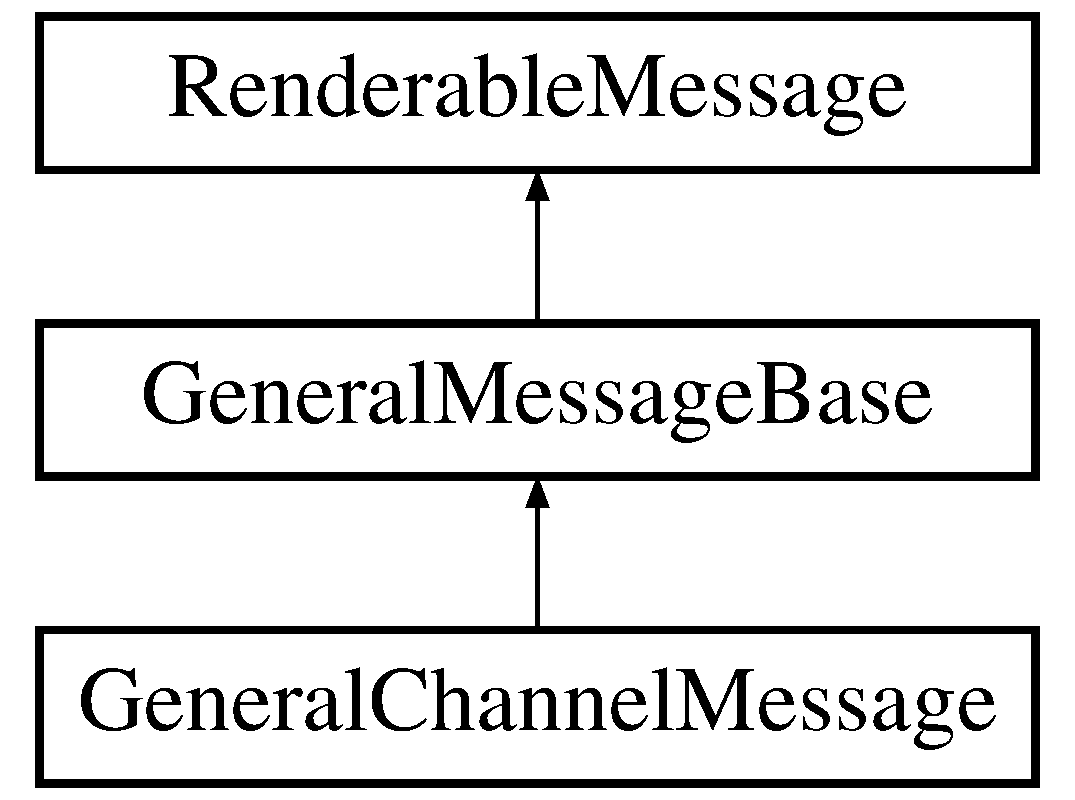
\includegraphics[height=3.000000cm]{classGeneralChannelMessage}
\end{center}
\end{figure}
\subsection*{Public Types}
\begin{DoxyCompactItemize}
\item 
enum \hyperlink{classGeneralChannelMessage_a4273153a78b91f1bbc1005c7fc83a42b}{Error\-Code} \{ \\*
\hyperlink{classGeneralChannelMessage_a4273153a78b91f1bbc1005c7fc83a42ba2f11a39e60eea72e5258966863e92dbb}{Error\-Code\-::\-New\-Sub\-Class\-Failed} = -\/1, 
\hyperlink{classGeneralChannelMessage_a4273153a78b91f1bbc1005c7fc83a42ba6e17b68c7b260823b72268f4abaa63d8}{Error\-Code\-::\-Create\-Node\-Failed} = -\/2, 
\hyperlink{classGeneralChannelMessage_a4273153a78b91f1bbc1005c7fc83a42baf3e17a336aaf0ce3288af8cc88f84acd}{Error\-Code\-::\-Create\-Reader\-Failed} = -\/3, 
\hyperlink{classGeneralChannelMessage_a4273153a78b91f1bbc1005c7fc83a42ba2bce9ea8de55f42d5c705d31d88b580c}{Error\-Code\-::\-Message\-Type\-Is\-Empty} = -\/4, 
\\*
\hyperlink{classGeneralChannelMessage_a4273153a78b91f1bbc1005c7fc83a42ba1c1458480e4efd15e595dd35828d389d}{Error\-Code\-::\-Channel\-Name\-Or\-Node\-Name\-Is\-Empty} = -\/5, 
\hyperlink{classGeneralChannelMessage_a4273153a78b91f1bbc1005c7fc83a42bae125b94e8445980203008e098f9c713f}{Error\-Code\-::\-No\-Close\-Channel} = -\/6
 \}
\end{DoxyCompactItemize}
\subsection*{Public Member Functions}
\begin{DoxyCompactItemize}
\item 
\hyperlink{classGeneralChannelMessage_a4b4051170a0227f18d3807b3da6290c8}{$\sim$\-General\-Channel\-Message} ()
\item 
std\-::string \hyperlink{classGeneralChannelMessage_acd67da9cdc84072627c42879469b2095}{Get\-Channel\-Name} (void) const 
\item 
void \hyperlink{classGeneralChannelMessage_ac8732e4bbf847a2218d78d57d0b9565b}{set\-\_\-message\-\_\-type} (const std\-::string \&msg\-Type\-Name)
\item 
const std\-::string \& \hyperlink{classGeneralChannelMessage_acffb0de01ee3fd896df64f7caed59ae3}{message\-\_\-type} (void) const 
\item 
bool \hyperlink{classGeneralChannelMessage_a112d3c8d26558666a5ee296c7e890699}{is\-\_\-enabled} (void) const 
\item 
bool \hyperlink{classGeneralChannelMessage_aa62162c570cfc990be7b5045406ea2ee}{has\-\_\-message\-\_\-come} (void) const 
\item 
double \hyperlink{classGeneralChannelMessage_ae607e8278605ccb88ea541965a2ff4bd}{frame\-\_\-ratio} (void) override
\item 
const std\-::string \& \hyperlink{classGeneralChannelMessage_a3df832daecc2a56b91c1a4165668a699}{Node\-Name} (void) const 
\item 
void \hyperlink{classGeneralChannelMessage_afa6acec81e88dbc16cfcb06651462da3}{add\-\_\-reader} (const std\-::string \&reader)
\item 
void \hyperlink{classGeneralChannelMessage_a54d35b4c1a5a2d042266fe7ef1591c42}{del\-\_\-reader} (const std\-::string \&reader)
\item 
void \hyperlink{classGeneralChannelMessage_aa9c664e67c018d7ddee6287a15972971}{add\-\_\-writer} (const std\-::string \&writer)
\item 
void \hyperlink{classGeneralChannelMessage_aedf08c4b88d2662a627f22b5a20c4ba9}{del\-\_\-writer} (const std\-::string \&writer)
\item 
void \hyperlink{classGeneralChannelMessage_af7f60b4c6e275dbfd0347aa2f8a2ac14}{Render} (const \hyperlink{classScreen}{Screen} $\ast$s, int key) override
\item 
void \hyperlink{classGeneralChannelMessage_a8ff914f416cc8684335a58b56f17c54d}{Close\-Channel} (void)
\end{DoxyCompactItemize}
\subsection*{Static Public Member Functions}
\begin{DoxyCompactItemize}
\item 
static const char $\ast$ \hyperlink{classGeneralChannelMessage_aacef197db8365b40ebc65d33874831a2}{err\-Code2\-Str} (\hyperlink{classGeneralChannelMessage_a4273153a78b91f1bbc1005c7fc83a42b}{Error\-Code} err\-Code)
\item 
static bool \hyperlink{classGeneralChannelMessage_a78584063709d67ee1cd73ce4e3a5e152}{is\-Error\-Code} (void $\ast$ptr)
\item 
static \hyperlink{classGeneralChannelMessage_a4273153a78b91f1bbc1005c7fc83a42b}{Error\-Code} \hyperlink{classGeneralChannelMessage_aa2a46a58ecfda4b9e6277f8d48101d5a}{cast\-Ptr2\-Error\-Code} (void $\ast$ptr)
\item 
static \hyperlink{classGeneralChannelMessage}{General\-Channel\-Message} $\ast$ \hyperlink{classGeneralChannelMessage_ae54666aaf4da7e77fedfaf9c6d0f4966}{cast\-Error\-Code2\-Ptr} (\hyperlink{classGeneralChannelMessage_a4273153a78b91f1bbc1005c7fc83a42b}{Error\-Code} err\-Code)
\end{DoxyCompactItemize}
\subsection*{Private Types}
\begin{DoxyCompactItemize}
\item 
enum \hyperlink{classGeneralChannelMessage_aa051da5753574d8fe644fdbcc2cd2412}{State} \{ \hyperlink{classGeneralChannelMessage_aa051da5753574d8fe644fdbcc2cd2412ad528eed6edec05921bab7a484e1f48f0}{State\-::\-Show\-Debug\-String}, 
\hyperlink{classGeneralChannelMessage_aa051da5753574d8fe644fdbcc2cd2412ae43857c44f7a3268c1a71df7a2150cca}{State\-::\-Show\-Info}
 \}
\end{DoxyCompactItemize}
\subsection*{Private Member Functions}
\begin{DoxyCompactItemize}
\item 
\hyperlink{classGeneralChannelMessage_a390e8b45e9b980c6cc6e2f3c1d36ece9}{General\-Channel\-Message} (const std\-::string \&node\-Name, \hyperlink{classRenderableMessage}{Renderable\-Message} $\ast$\hyperlink{classRenderableMessage_ab23728d14d9aff3efa0af7639ec6059c}{parent}=nullptr)
\item 
\hyperlink{classGeneralChannelMessage_ac6269c5ac192942c72566f2a6399e465}{General\-Channel\-Message} (const \hyperlink{classGeneralChannelMessage}{General\-Channel\-Message} \&)=delete
\item 
\hyperlink{classGeneralChannelMessage}{General\-Channel\-Message} \& \hyperlink{classGeneralChannelMessage_ab6a1a17b601ac4b41e687022ff0ec434}{operator=} (const \hyperlink{classGeneralChannelMessage}{General\-Channel\-Message} \&)=delete
\item 
void \hyperlink{classGeneralChannelMessage_aefdf77ab4c8e43b86af7128aaaa5ccac}{update\-Raw\-Message} (const std\-::shared\-\_\-ptr$<$ \hyperlink{structapollo_1_1cyber_1_1message_1_1RawMessage}{apollo\-::cyber\-::message\-::\-Raw\-Message} $>$ \&raw\-Msg)
\item 
std\-::shared\-\_\-ptr\\*
$<$ \hyperlink{structapollo_1_1cyber_1_1message_1_1RawMessage}{apollo\-::cyber\-::message\-::\-Raw\-Message} $>$ \hyperlink{classGeneralChannelMessage_a347060b4136af1997b77ac6671dbb860}{Copy\-Msg\-Ptr} (void) const 
\item 
\hyperlink{classGeneralChannelMessage}{General\-Channel\-Message} $\ast$ \hyperlink{classGeneralChannelMessage_ae1bc06baa0d31bb6757fb5d27f034da9}{Open\-Channel} (const std\-::string \&channel\-Name)
\item 
void \hyperlink{classGeneralChannelMessage_a47717a3ab362e45cad05f94495168386}{Render\-Debug\-String} (const \hyperlink{classScreen}{Screen} $\ast$s, int key, unsigned line\-No)
\item 
void \hyperlink{classGeneralChannelMessage_a15801ad66f9891d77cb9dbe3e606803e}{Render\-Info} (const \hyperlink{classScreen}{Screen} $\ast$s, int key, unsigned line\-No)
\item 
void \hyperlink{classGeneralChannelMessage_ac5344c725f27ad9bd126cc67a8a2238a}{set\-\_\-has\-\_\-message\-\_\-come} (bool b)
\end{DoxyCompactItemize}
\subsection*{Static Private Member Functions}
\begin{DoxyCompactItemize}
\item 
static void \hyperlink{classGeneralChannelMessage_a1427cf97f758b92c79262934bab20e28}{Do\-Delete} (std\-::vector$<$ std\-::string $>$ \&vec, const std\-::string \&str)
\item 
static void \hyperlink{classGeneralChannelMessage_a4795285b54ebe85294e2b9ce4ce8440c}{Do\-Add} (std\-::vector$<$ std\-::string $>$ \&vec, const std\-::string \&str)
\end{DoxyCompactItemize}
\subsection*{Private Attributes}
\begin{DoxyCompactItemize}
\item 
enum \hyperlink{classGeneralChannelMessage_aa051da5753574d8fe644fdbcc2cd2412}{General\-Channel\-Message\-::\-State} \hyperlink{classGeneralChannelMessage_a7b1412a227a2ec0d3baedc0938f931df}{current\-\_\-state\-\_\-}
\item 
bool \hyperlink{classGeneralChannelMessage_af5e386e99b7a8722b485d027e2ed75bd}{has\-\_\-message\-\_\-come\-\_\-}
\item 
std\-::string \hyperlink{classGeneralChannelMessage_a1d25120dc72e5010565823a544783efc}{message\-\_\-type\-\_\-}
\item 
std\-::atomic$<$ int $>$ \hyperlink{classGeneralChannelMessage_a3da8072e2c9d5ed6b510378384d2dc4f}{frame\-\_\-counter\-\_\-}
\item 
\hyperlink{classapollo_1_1cyber_1_1Time}{apollo\-::cyber\-::\-Time} \hyperlink{classGeneralChannelMessage_a8ff50746033122e3479db0cd923a8860}{last\-\_\-time\-\_\-}
\item 
\hyperlink{classapollo_1_1cyber_1_1Time}{apollo\-::cyber\-::\-Time} \hyperlink{classGeneralChannelMessage_a10a1b559a2fd9741bb268fbe1c4290d2}{msg\-\_\-time\-\_\-}
\item 
\hyperlink{classapollo_1_1cyber_1_1Time}{apollo\-::cyber\-::\-Time} \hyperlink{classGeneralChannelMessage_ad1f7f60900caf4cc8cfba0fb83961a43}{time\-\_\-last\-\_\-calc\-\_\-} = \hyperlink{classapollo_1_1cyber_1_1Time_abb3f07caa00e1e76d3040e9f725afc09}{apollo\-::cyber\-::\-Time\-::\-Mono\-Time}()
\item 
std\-::unique\-\_\-ptr\\*
$<$ \hyperlink{classapollo_1_1cyber_1_1Node}{apollo\-::cyber\-::\-Node} $>$ \hyperlink{classGeneralChannelMessage_a9663241eded60406a25281d650713ec5}{channel\-\_\-node\-\_\-}
\item 
std\-::string \hyperlink{classGeneralChannelMessage_a123a419e25302adacba1f1984bc70b22}{node\-\_\-name\-\_\-}
\item 
std\-::vector$<$ std\-::string $>$ \hyperlink{classGeneralChannelMessage_a2839fca91027887bdb8c7e9df077c105}{readers\-\_\-}
\item 
std\-::vector$<$ std\-::string $>$ \hyperlink{classGeneralChannelMessage_aff8aed1cdbd9bfebcea0b2bb5f5c6c5b}{writers\-\_\-}
\item 
std\-::shared\-\_\-ptr\\*
$<$ \hyperlink{structapollo_1_1cyber_1_1message_1_1RawMessage}{apollo\-::cyber\-::message\-::\-Raw\-Message} $>$ \hyperlink{classGeneralChannelMessage_a6b288701779537fb1a9846214d9ebeac}{channel\-\_\-message\-\_\-}
\item 
std\-::shared\-\_\-ptr\\*
$<$ \hyperlink{classapollo_1_1cyber_1_1Reader}{apollo\-::cyber\-::\-Reader}\\*
$<$ \hyperlink{structapollo_1_1cyber_1_1message_1_1RawMessage}{apollo\-::cyber\-::message\-::\-Raw\-Message} $>$ $>$ \hyperlink{classGeneralChannelMessage_a6fbe63b8ee339b6bbf99736aa6a873cf}{channel\-\_\-reader\-\_\-}
\item 
std\-::mutex \hyperlink{classGeneralChannelMessage_a58d9c04f21d27bcbcce36073f4325c7e}{inner\-\_\-lock\-\_\-}
\item 
google\-::protobuf\-::\-Message $\ast$ \hyperlink{classGeneralChannelMessage_ab150e16ccbb7e536a0b6e6276e3eca7a}{raw\-\_\-msg\-\_\-class\-\_\-}
\end{DoxyCompactItemize}
\subsection*{Friends}
\begin{DoxyCompactItemize}
\item 
class \hyperlink{classGeneralChannelMessage_ae90c7f27bec878186a229b7b314512f6}{Cyber\-Topology\-Message}
\item 
class \hyperlink{classGeneralChannelMessage_abcf2c2516937d8e5700b72b878385bb2}{General\-Message}
\end{DoxyCompactItemize}
\subsection*{Additional Inherited Members}


\subsection{Member Enumeration Documentation}
\hypertarget{classGeneralChannelMessage_a4273153a78b91f1bbc1005c7fc83a42b}{\index{General\-Channel\-Message@{General\-Channel\-Message}!Error\-Code@{Error\-Code}}
\index{Error\-Code@{Error\-Code}!GeneralChannelMessage@{General\-Channel\-Message}}
\subsubsection[{Error\-Code}]{\setlength{\rightskip}{0pt plus 5cm}enum {\bf General\-Channel\-Message\-::\-Error\-Code}\hspace{0.3cm}{\ttfamily [strong]}}}\label{classGeneralChannelMessage_a4273153a78b91f1bbc1005c7fc83a42b}
\begin{Desc}
\item[Enumerator]\par
\begin{description}
\index{New\-Sub\-Class\-Failed@{New\-Sub\-Class\-Failed}!General\-Channel\-Message@{General\-Channel\-Message}}\index{General\-Channel\-Message@{General\-Channel\-Message}!New\-Sub\-Class\-Failed@{New\-Sub\-Class\-Failed}}\item[{\em 
\hypertarget{classGeneralChannelMessage_a4273153a78b91f1bbc1005c7fc83a42ba2f11a39e60eea72e5258966863e92dbb}{New\-Sub\-Class\-Failed}\label{classGeneralChannelMessage_a4273153a78b91f1bbc1005c7fc83a42ba2f11a39e60eea72e5258966863e92dbb}
}]\index{Create\-Node\-Failed@{Create\-Node\-Failed}!General\-Channel\-Message@{General\-Channel\-Message}}\index{General\-Channel\-Message@{General\-Channel\-Message}!Create\-Node\-Failed@{Create\-Node\-Failed}}\item[{\em 
\hypertarget{classGeneralChannelMessage_a4273153a78b91f1bbc1005c7fc83a42ba6e17b68c7b260823b72268f4abaa63d8}{Create\-Node\-Failed}\label{classGeneralChannelMessage_a4273153a78b91f1bbc1005c7fc83a42ba6e17b68c7b260823b72268f4abaa63d8}
}]\index{Create\-Reader\-Failed@{Create\-Reader\-Failed}!General\-Channel\-Message@{General\-Channel\-Message}}\index{General\-Channel\-Message@{General\-Channel\-Message}!Create\-Reader\-Failed@{Create\-Reader\-Failed}}\item[{\em 
\hypertarget{classGeneralChannelMessage_a4273153a78b91f1bbc1005c7fc83a42baf3e17a336aaf0ce3288af8cc88f84acd}{Create\-Reader\-Failed}\label{classGeneralChannelMessage_a4273153a78b91f1bbc1005c7fc83a42baf3e17a336aaf0ce3288af8cc88f84acd}
}]\index{Message\-Type\-Is\-Empty@{Message\-Type\-Is\-Empty}!General\-Channel\-Message@{General\-Channel\-Message}}\index{General\-Channel\-Message@{General\-Channel\-Message}!Message\-Type\-Is\-Empty@{Message\-Type\-Is\-Empty}}\item[{\em 
\hypertarget{classGeneralChannelMessage_a4273153a78b91f1bbc1005c7fc83a42ba2bce9ea8de55f42d5c705d31d88b580c}{Message\-Type\-Is\-Empty}\label{classGeneralChannelMessage_a4273153a78b91f1bbc1005c7fc83a42ba2bce9ea8de55f42d5c705d31d88b580c}
}]\index{Channel\-Name\-Or\-Node\-Name\-Is\-Empty@{Channel\-Name\-Or\-Node\-Name\-Is\-Empty}!General\-Channel\-Message@{General\-Channel\-Message}}\index{General\-Channel\-Message@{General\-Channel\-Message}!Channel\-Name\-Or\-Node\-Name\-Is\-Empty@{Channel\-Name\-Or\-Node\-Name\-Is\-Empty}}\item[{\em 
\hypertarget{classGeneralChannelMessage_a4273153a78b91f1bbc1005c7fc83a42ba1c1458480e4efd15e595dd35828d389d}{Channel\-Name\-Or\-Node\-Name\-Is\-Empty}\label{classGeneralChannelMessage_a4273153a78b91f1bbc1005c7fc83a42ba1c1458480e4efd15e595dd35828d389d}
}]\index{No\-Close\-Channel@{No\-Close\-Channel}!General\-Channel\-Message@{General\-Channel\-Message}}\index{General\-Channel\-Message@{General\-Channel\-Message}!No\-Close\-Channel@{No\-Close\-Channel}}\item[{\em 
\hypertarget{classGeneralChannelMessage_a4273153a78b91f1bbc1005c7fc83a42bae125b94e8445980203008e098f9c713f}{No\-Close\-Channel}\label{classGeneralChannelMessage_a4273153a78b91f1bbc1005c7fc83a42bae125b94e8445980203008e098f9c713f}
}]\end{description}
\end{Desc}
\hypertarget{classGeneralChannelMessage_aa051da5753574d8fe644fdbcc2cd2412}{\index{General\-Channel\-Message@{General\-Channel\-Message}!State@{State}}
\index{State@{State}!GeneralChannelMessage@{General\-Channel\-Message}}
\subsubsection[{State}]{\setlength{\rightskip}{0pt plus 5cm}enum {\bf General\-Channel\-Message\-::\-State}\hspace{0.3cm}{\ttfamily [strong]}, {\ttfamily [private]}}}\label{classGeneralChannelMessage_aa051da5753574d8fe644fdbcc2cd2412}
\begin{Desc}
\item[Enumerator]\par
\begin{description}
\index{Show\-Debug\-String@{Show\-Debug\-String}!General\-Channel\-Message@{General\-Channel\-Message}}\index{General\-Channel\-Message@{General\-Channel\-Message}!Show\-Debug\-String@{Show\-Debug\-String}}\item[{\em 
\hypertarget{classGeneralChannelMessage_aa051da5753574d8fe644fdbcc2cd2412ad528eed6edec05921bab7a484e1f48f0}{Show\-Debug\-String}\label{classGeneralChannelMessage_aa051da5753574d8fe644fdbcc2cd2412ad528eed6edec05921bab7a484e1f48f0}
}]\index{Show\-Info@{Show\-Info}!General\-Channel\-Message@{General\-Channel\-Message}}\index{General\-Channel\-Message@{General\-Channel\-Message}!Show\-Info@{Show\-Info}}\item[{\em 
\hypertarget{classGeneralChannelMessage_aa051da5753574d8fe644fdbcc2cd2412ae43857c44f7a3268c1a71df7a2150cca}{Show\-Info}\label{classGeneralChannelMessage_aa051da5753574d8fe644fdbcc2cd2412ae43857c44f7a3268c1a71df7a2150cca}
}]\end{description}
\end{Desc}


\subsection{Constructor \& Destructor Documentation}
\hypertarget{classGeneralChannelMessage_a4b4051170a0227f18d3807b3da6290c8}{\index{General\-Channel\-Message@{General\-Channel\-Message}!$\sim$\-General\-Channel\-Message@{$\sim$\-General\-Channel\-Message}}
\index{$\sim$\-General\-Channel\-Message@{$\sim$\-General\-Channel\-Message}!GeneralChannelMessage@{General\-Channel\-Message}}
\subsubsection[{$\sim$\-General\-Channel\-Message}]{\setlength{\rightskip}{0pt plus 5cm}General\-Channel\-Message\-::$\sim$\-General\-Channel\-Message (
\begin{DoxyParamCaption}
{}
\end{DoxyParamCaption}
)\hspace{0.3cm}{\ttfamily [inline]}}}\label{classGeneralChannelMessage_a4b4051170a0227f18d3807b3da6290c8}
\hypertarget{classGeneralChannelMessage_a390e8b45e9b980c6cc6e2f3c1d36ece9}{\index{General\-Channel\-Message@{General\-Channel\-Message}!General\-Channel\-Message@{General\-Channel\-Message}}
\index{General\-Channel\-Message@{General\-Channel\-Message}!GeneralChannelMessage@{General\-Channel\-Message}}
\subsubsection[{General\-Channel\-Message}]{\setlength{\rightskip}{0pt plus 5cm}General\-Channel\-Message\-::\-General\-Channel\-Message (
\begin{DoxyParamCaption}
\item[{const std\-::string \&}]{node\-Name, }
\item[{{\bf Renderable\-Message} $\ast$}]{parent = {\ttfamily nullptr}}
\end{DoxyParamCaption}
)\hspace{0.3cm}{\ttfamily [inline]}, {\ttfamily [explicit]}, {\ttfamily [private]}}}\label{classGeneralChannelMessage_a390e8b45e9b980c6cc6e2f3c1d36ece9}
\hypertarget{classGeneralChannelMessage_ac6269c5ac192942c72566f2a6399e465}{\index{General\-Channel\-Message@{General\-Channel\-Message}!General\-Channel\-Message@{General\-Channel\-Message}}
\index{General\-Channel\-Message@{General\-Channel\-Message}!GeneralChannelMessage@{General\-Channel\-Message}}
\subsubsection[{General\-Channel\-Message}]{\setlength{\rightskip}{0pt plus 5cm}General\-Channel\-Message\-::\-General\-Channel\-Message (
\begin{DoxyParamCaption}
\item[{const {\bf General\-Channel\-Message} \&}]{}
\end{DoxyParamCaption}
)\hspace{0.3cm}{\ttfamily [private]}, {\ttfamily [delete]}}}\label{classGeneralChannelMessage_ac6269c5ac192942c72566f2a6399e465}


\subsection{Member Function Documentation}
\hypertarget{classGeneralChannelMessage_afa6acec81e88dbc16cfcb06651462da3}{\index{General\-Channel\-Message@{General\-Channel\-Message}!add\-\_\-reader@{add\-\_\-reader}}
\index{add\-\_\-reader@{add\-\_\-reader}!GeneralChannelMessage@{General\-Channel\-Message}}
\subsubsection[{add\-\_\-reader}]{\setlength{\rightskip}{0pt plus 5cm}void General\-Channel\-Message\-::add\-\_\-reader (
\begin{DoxyParamCaption}
\item[{const std\-::string \&}]{reader}
\end{DoxyParamCaption}
)\hspace{0.3cm}{\ttfamily [inline]}}}\label{classGeneralChannelMessage_afa6acec81e88dbc16cfcb06651462da3}
\hypertarget{classGeneralChannelMessage_aa9c664e67c018d7ddee6287a15972971}{\index{General\-Channel\-Message@{General\-Channel\-Message}!add\-\_\-writer@{add\-\_\-writer}}
\index{add\-\_\-writer@{add\-\_\-writer}!GeneralChannelMessage@{General\-Channel\-Message}}
\subsubsection[{add\-\_\-writer}]{\setlength{\rightskip}{0pt plus 5cm}void General\-Channel\-Message\-::add\-\_\-writer (
\begin{DoxyParamCaption}
\item[{const std\-::string \&}]{writer}
\end{DoxyParamCaption}
)\hspace{0.3cm}{\ttfamily [inline]}}}\label{classGeneralChannelMessage_aa9c664e67c018d7ddee6287a15972971}
\hypertarget{classGeneralChannelMessage_ae54666aaf4da7e77fedfaf9c6d0f4966}{\index{General\-Channel\-Message@{General\-Channel\-Message}!cast\-Error\-Code2\-Ptr@{cast\-Error\-Code2\-Ptr}}
\index{cast\-Error\-Code2\-Ptr@{cast\-Error\-Code2\-Ptr}!GeneralChannelMessage@{General\-Channel\-Message}}
\subsubsection[{cast\-Error\-Code2\-Ptr}]{\setlength{\rightskip}{0pt plus 5cm}static {\bf General\-Channel\-Message}$\ast$ General\-Channel\-Message\-::cast\-Error\-Code2\-Ptr (
\begin{DoxyParamCaption}
\item[{{\bf Error\-Code}}]{err\-Code}
\end{DoxyParamCaption}
)\hspace{0.3cm}{\ttfamily [inline]}, {\ttfamily [static]}}}\label{classGeneralChannelMessage_ae54666aaf4da7e77fedfaf9c6d0f4966}
\hypertarget{classGeneralChannelMessage_aa2a46a58ecfda4b9e6277f8d48101d5a}{\index{General\-Channel\-Message@{General\-Channel\-Message}!cast\-Ptr2\-Error\-Code@{cast\-Ptr2\-Error\-Code}}
\index{cast\-Ptr2\-Error\-Code@{cast\-Ptr2\-Error\-Code}!GeneralChannelMessage@{General\-Channel\-Message}}
\subsubsection[{cast\-Ptr2\-Error\-Code}]{\setlength{\rightskip}{0pt plus 5cm}static {\bf Error\-Code} General\-Channel\-Message\-::cast\-Ptr2\-Error\-Code (
\begin{DoxyParamCaption}
\item[{void $\ast$}]{ptr}
\end{DoxyParamCaption}
)\hspace{0.3cm}{\ttfamily [inline]}, {\ttfamily [static]}}}\label{classGeneralChannelMessage_aa2a46a58ecfda4b9e6277f8d48101d5a}
\hypertarget{classGeneralChannelMessage_a8ff914f416cc8684335a58b56f17c54d}{\index{General\-Channel\-Message@{General\-Channel\-Message}!Close\-Channel@{Close\-Channel}}
\index{Close\-Channel@{Close\-Channel}!GeneralChannelMessage@{General\-Channel\-Message}}
\subsubsection[{Close\-Channel}]{\setlength{\rightskip}{0pt plus 5cm}void General\-Channel\-Message\-::\-Close\-Channel (
\begin{DoxyParamCaption}
\item[{void}]{}
\end{DoxyParamCaption}
)\hspace{0.3cm}{\ttfamily [inline]}}}\label{classGeneralChannelMessage_a8ff914f416cc8684335a58b56f17c54d}
\hypertarget{classGeneralChannelMessage_a347060b4136af1997b77ac6671dbb860}{\index{General\-Channel\-Message@{General\-Channel\-Message}!Copy\-Msg\-Ptr@{Copy\-Msg\-Ptr}}
\index{Copy\-Msg\-Ptr@{Copy\-Msg\-Ptr}!GeneralChannelMessage@{General\-Channel\-Message}}
\subsubsection[{Copy\-Msg\-Ptr}]{\setlength{\rightskip}{0pt plus 5cm}std\-::shared\-\_\-ptr$<${\bf apollo\-::cyber\-::message\-::\-Raw\-Message}$>$ General\-Channel\-Message\-::\-Copy\-Msg\-Ptr (
\begin{DoxyParamCaption}
\item[{void}]{}
\end{DoxyParamCaption}
) const\hspace{0.3cm}{\ttfamily [inline]}, {\ttfamily [private]}}}\label{classGeneralChannelMessage_a347060b4136af1997b77ac6671dbb860}
\hypertarget{classGeneralChannelMessage_a54d35b4c1a5a2d042266fe7ef1591c42}{\index{General\-Channel\-Message@{General\-Channel\-Message}!del\-\_\-reader@{del\-\_\-reader}}
\index{del\-\_\-reader@{del\-\_\-reader}!GeneralChannelMessage@{General\-Channel\-Message}}
\subsubsection[{del\-\_\-reader}]{\setlength{\rightskip}{0pt plus 5cm}void General\-Channel\-Message\-::del\-\_\-reader (
\begin{DoxyParamCaption}
\item[{const std\-::string \&}]{reader}
\end{DoxyParamCaption}
)\hspace{0.3cm}{\ttfamily [inline]}}}\label{classGeneralChannelMessage_a54d35b4c1a5a2d042266fe7ef1591c42}
\hypertarget{classGeneralChannelMessage_aedf08c4b88d2662a627f22b5a20c4ba9}{\index{General\-Channel\-Message@{General\-Channel\-Message}!del\-\_\-writer@{del\-\_\-writer}}
\index{del\-\_\-writer@{del\-\_\-writer}!GeneralChannelMessage@{General\-Channel\-Message}}
\subsubsection[{del\-\_\-writer}]{\setlength{\rightskip}{0pt plus 5cm}void General\-Channel\-Message\-::del\-\_\-writer (
\begin{DoxyParamCaption}
\item[{const std\-::string \&}]{writer}
\end{DoxyParamCaption}
)\hspace{0.3cm}{\ttfamily [inline]}}}\label{classGeneralChannelMessage_aedf08c4b88d2662a627f22b5a20c4ba9}
\hypertarget{classGeneralChannelMessage_a4795285b54ebe85294e2b9ce4ce8440c}{\index{General\-Channel\-Message@{General\-Channel\-Message}!Do\-Add@{Do\-Add}}
\index{Do\-Add@{Do\-Add}!GeneralChannelMessage@{General\-Channel\-Message}}
\subsubsection[{Do\-Add}]{\setlength{\rightskip}{0pt plus 5cm}static void General\-Channel\-Message\-::\-Do\-Add (
\begin{DoxyParamCaption}
\item[{std\-::vector$<$ std\-::string $>$ \&}]{vec, }
\item[{const std\-::string \&}]{str}
\end{DoxyParamCaption}
)\hspace{0.3cm}{\ttfamily [inline]}, {\ttfamily [static]}, {\ttfamily [private]}}}\label{classGeneralChannelMessage_a4795285b54ebe85294e2b9ce4ce8440c}
\hypertarget{classGeneralChannelMessage_a1427cf97f758b92c79262934bab20e28}{\index{General\-Channel\-Message@{General\-Channel\-Message}!Do\-Delete@{Do\-Delete}}
\index{Do\-Delete@{Do\-Delete}!GeneralChannelMessage@{General\-Channel\-Message}}
\subsubsection[{Do\-Delete}]{\setlength{\rightskip}{0pt plus 5cm}static void General\-Channel\-Message\-::\-Do\-Delete (
\begin{DoxyParamCaption}
\item[{std\-::vector$<$ std\-::string $>$ \&}]{vec, }
\item[{const std\-::string \&}]{str}
\end{DoxyParamCaption}
)\hspace{0.3cm}{\ttfamily [inline]}, {\ttfamily [static]}, {\ttfamily [private]}}}\label{classGeneralChannelMessage_a1427cf97f758b92c79262934bab20e28}
\hypertarget{classGeneralChannelMessage_aacef197db8365b40ebc65d33874831a2}{\index{General\-Channel\-Message@{General\-Channel\-Message}!err\-Code2\-Str@{err\-Code2\-Str}}
\index{err\-Code2\-Str@{err\-Code2\-Str}!GeneralChannelMessage@{General\-Channel\-Message}}
\subsubsection[{err\-Code2\-Str}]{\setlength{\rightskip}{0pt plus 5cm}static const char$\ast$ General\-Channel\-Message\-::err\-Code2\-Str (
\begin{DoxyParamCaption}
\item[{{\bf Error\-Code}}]{err\-Code}
\end{DoxyParamCaption}
)\hspace{0.3cm}{\ttfamily [static]}}}\label{classGeneralChannelMessage_aacef197db8365b40ebc65d33874831a2}
\hypertarget{classGeneralChannelMessage_ae607e8278605ccb88ea541965a2ff4bd}{\index{General\-Channel\-Message@{General\-Channel\-Message}!frame\-\_\-ratio@{frame\-\_\-ratio}}
\index{frame\-\_\-ratio@{frame\-\_\-ratio}!GeneralChannelMessage@{General\-Channel\-Message}}
\subsubsection[{frame\-\_\-ratio}]{\setlength{\rightskip}{0pt plus 5cm}double General\-Channel\-Message\-::frame\-\_\-ratio (
\begin{DoxyParamCaption}
\item[{void}]{}
\end{DoxyParamCaption}
)\hspace{0.3cm}{\ttfamily [override]}, {\ttfamily [virtual]}}}\label{classGeneralChannelMessage_ae607e8278605ccb88ea541965a2ff4bd}


Reimplemented from \hyperlink{classRenderableMessage_a7b8a1627a96d0b0658be68c1ad6b99a5}{Renderable\-Message}.

\hypertarget{classGeneralChannelMessage_acd67da9cdc84072627c42879469b2095}{\index{General\-Channel\-Message@{General\-Channel\-Message}!Get\-Channel\-Name@{Get\-Channel\-Name}}
\index{Get\-Channel\-Name@{Get\-Channel\-Name}!GeneralChannelMessage@{General\-Channel\-Message}}
\subsubsection[{Get\-Channel\-Name}]{\setlength{\rightskip}{0pt plus 5cm}std\-::string General\-Channel\-Message\-::\-Get\-Channel\-Name (
\begin{DoxyParamCaption}
\item[{void}]{}
\end{DoxyParamCaption}
) const\hspace{0.3cm}{\ttfamily [inline]}}}\label{classGeneralChannelMessage_acd67da9cdc84072627c42879469b2095}
\hypertarget{classGeneralChannelMessage_aa62162c570cfc990be7b5045406ea2ee}{\index{General\-Channel\-Message@{General\-Channel\-Message}!has\-\_\-message\-\_\-come@{has\-\_\-message\-\_\-come}}
\index{has\-\_\-message\-\_\-come@{has\-\_\-message\-\_\-come}!GeneralChannelMessage@{General\-Channel\-Message}}
\subsubsection[{has\-\_\-message\-\_\-come}]{\setlength{\rightskip}{0pt plus 5cm}bool General\-Channel\-Message\-::has\-\_\-message\-\_\-come (
\begin{DoxyParamCaption}
\item[{void}]{}
\end{DoxyParamCaption}
) const\hspace{0.3cm}{\ttfamily [inline]}}}\label{classGeneralChannelMessage_aa62162c570cfc990be7b5045406ea2ee}
\hypertarget{classGeneralChannelMessage_a112d3c8d26558666a5ee296c7e890699}{\index{General\-Channel\-Message@{General\-Channel\-Message}!is\-\_\-enabled@{is\-\_\-enabled}}
\index{is\-\_\-enabled@{is\-\_\-enabled}!GeneralChannelMessage@{General\-Channel\-Message}}
\subsubsection[{is\-\_\-enabled}]{\setlength{\rightskip}{0pt plus 5cm}bool General\-Channel\-Message\-::is\-\_\-enabled (
\begin{DoxyParamCaption}
\item[{void}]{}
\end{DoxyParamCaption}
) const\hspace{0.3cm}{\ttfamily [inline]}}}\label{classGeneralChannelMessage_a112d3c8d26558666a5ee296c7e890699}
\hypertarget{classGeneralChannelMessage_a78584063709d67ee1cd73ce4e3a5e152}{\index{General\-Channel\-Message@{General\-Channel\-Message}!is\-Error\-Code@{is\-Error\-Code}}
\index{is\-Error\-Code@{is\-Error\-Code}!GeneralChannelMessage@{General\-Channel\-Message}}
\subsubsection[{is\-Error\-Code}]{\setlength{\rightskip}{0pt plus 5cm}static bool General\-Channel\-Message\-::is\-Error\-Code (
\begin{DoxyParamCaption}
\item[{void $\ast$}]{ptr}
\end{DoxyParamCaption}
)\hspace{0.3cm}{\ttfamily [static]}}}\label{classGeneralChannelMessage_a78584063709d67ee1cd73ce4e3a5e152}
\hypertarget{classGeneralChannelMessage_acffb0de01ee3fd896df64f7caed59ae3}{\index{General\-Channel\-Message@{General\-Channel\-Message}!message\-\_\-type@{message\-\_\-type}}
\index{message\-\_\-type@{message\-\_\-type}!GeneralChannelMessage@{General\-Channel\-Message}}
\subsubsection[{message\-\_\-type}]{\setlength{\rightskip}{0pt plus 5cm}const std\-::string\& General\-Channel\-Message\-::message\-\_\-type (
\begin{DoxyParamCaption}
\item[{void}]{}
\end{DoxyParamCaption}
) const\hspace{0.3cm}{\ttfamily [inline]}}}\label{classGeneralChannelMessage_acffb0de01ee3fd896df64f7caed59ae3}
\hypertarget{classGeneralChannelMessage_a3df832daecc2a56b91c1a4165668a699}{\index{General\-Channel\-Message@{General\-Channel\-Message}!Node\-Name@{Node\-Name}}
\index{Node\-Name@{Node\-Name}!GeneralChannelMessage@{General\-Channel\-Message}}
\subsubsection[{Node\-Name}]{\setlength{\rightskip}{0pt plus 5cm}const std\-::string\& General\-Channel\-Message\-::\-Node\-Name (
\begin{DoxyParamCaption}
\item[{void}]{}
\end{DoxyParamCaption}
) const\hspace{0.3cm}{\ttfamily [inline]}}}\label{classGeneralChannelMessage_a3df832daecc2a56b91c1a4165668a699}
\hypertarget{classGeneralChannelMessage_ae1bc06baa0d31bb6757fb5d27f034da9}{\index{General\-Channel\-Message@{General\-Channel\-Message}!Open\-Channel@{Open\-Channel}}
\index{Open\-Channel@{Open\-Channel}!GeneralChannelMessage@{General\-Channel\-Message}}
\subsubsection[{Open\-Channel}]{\setlength{\rightskip}{0pt plus 5cm}{\bf General\-Channel\-Message}$\ast$ General\-Channel\-Message\-::\-Open\-Channel (
\begin{DoxyParamCaption}
\item[{const std\-::string \&}]{channel\-Name}
\end{DoxyParamCaption}
)\hspace{0.3cm}{\ttfamily [private]}}}\label{classGeneralChannelMessage_ae1bc06baa0d31bb6757fb5d27f034da9}
\hypertarget{classGeneralChannelMessage_ab6a1a17b601ac4b41e687022ff0ec434}{\index{General\-Channel\-Message@{General\-Channel\-Message}!operator=@{operator=}}
\index{operator=@{operator=}!GeneralChannelMessage@{General\-Channel\-Message}}
\subsubsection[{operator=}]{\setlength{\rightskip}{0pt plus 5cm}{\bf General\-Channel\-Message}\& General\-Channel\-Message\-::operator= (
\begin{DoxyParamCaption}
\item[{const {\bf General\-Channel\-Message} \&}]{}
\end{DoxyParamCaption}
)\hspace{0.3cm}{\ttfamily [private]}, {\ttfamily [delete]}}}\label{classGeneralChannelMessage_ab6a1a17b601ac4b41e687022ff0ec434}
\hypertarget{classGeneralChannelMessage_af7f60b4c6e275dbfd0347aa2f8a2ac14}{\index{General\-Channel\-Message@{General\-Channel\-Message}!Render@{Render}}
\index{Render@{Render}!GeneralChannelMessage@{General\-Channel\-Message}}
\subsubsection[{Render}]{\setlength{\rightskip}{0pt plus 5cm}void General\-Channel\-Message\-::\-Render (
\begin{DoxyParamCaption}
\item[{const {\bf Screen} $\ast$}]{s, }
\item[{int}]{key}
\end{DoxyParamCaption}
)\hspace{0.3cm}{\ttfamily [override]}, {\ttfamily [virtual]}}}\label{classGeneralChannelMessage_af7f60b4c6e275dbfd0347aa2f8a2ac14}


Implements \hyperlink{classRenderableMessage_a3f65c247f5db9bb4918bca7d665bbdc6}{Renderable\-Message}.

\hypertarget{classGeneralChannelMessage_a47717a3ab362e45cad05f94495168386}{\index{General\-Channel\-Message@{General\-Channel\-Message}!Render\-Debug\-String@{Render\-Debug\-String}}
\index{Render\-Debug\-String@{Render\-Debug\-String}!GeneralChannelMessage@{General\-Channel\-Message}}
\subsubsection[{Render\-Debug\-String}]{\setlength{\rightskip}{0pt plus 5cm}void General\-Channel\-Message\-::\-Render\-Debug\-String (
\begin{DoxyParamCaption}
\item[{const {\bf Screen} $\ast$}]{s, }
\item[{int}]{key, }
\item[{unsigned}]{line\-No}
\end{DoxyParamCaption}
)\hspace{0.3cm}{\ttfamily [private]}}}\label{classGeneralChannelMessage_a47717a3ab362e45cad05f94495168386}
\hypertarget{classGeneralChannelMessage_a15801ad66f9891d77cb9dbe3e606803e}{\index{General\-Channel\-Message@{General\-Channel\-Message}!Render\-Info@{Render\-Info}}
\index{Render\-Info@{Render\-Info}!GeneralChannelMessage@{General\-Channel\-Message}}
\subsubsection[{Render\-Info}]{\setlength{\rightskip}{0pt plus 5cm}void General\-Channel\-Message\-::\-Render\-Info (
\begin{DoxyParamCaption}
\item[{const {\bf Screen} $\ast$}]{s, }
\item[{int}]{key, }
\item[{unsigned}]{line\-No}
\end{DoxyParamCaption}
)\hspace{0.3cm}{\ttfamily [private]}}}\label{classGeneralChannelMessage_a15801ad66f9891d77cb9dbe3e606803e}
\hypertarget{classGeneralChannelMessage_ac5344c725f27ad9bd126cc67a8a2238a}{\index{General\-Channel\-Message@{General\-Channel\-Message}!set\-\_\-has\-\_\-message\-\_\-come@{set\-\_\-has\-\_\-message\-\_\-come}}
\index{set\-\_\-has\-\_\-message\-\_\-come@{set\-\_\-has\-\_\-message\-\_\-come}!GeneralChannelMessage@{General\-Channel\-Message}}
\subsubsection[{set\-\_\-has\-\_\-message\-\_\-come}]{\setlength{\rightskip}{0pt plus 5cm}void General\-Channel\-Message\-::set\-\_\-has\-\_\-message\-\_\-come (
\begin{DoxyParamCaption}
\item[{bool}]{b}
\end{DoxyParamCaption}
)\hspace{0.3cm}{\ttfamily [inline]}, {\ttfamily [private]}}}\label{classGeneralChannelMessage_ac5344c725f27ad9bd126cc67a8a2238a}
\hypertarget{classGeneralChannelMessage_ac8732e4bbf847a2218d78d57d0b9565b}{\index{General\-Channel\-Message@{General\-Channel\-Message}!set\-\_\-message\-\_\-type@{set\-\_\-message\-\_\-type}}
\index{set\-\_\-message\-\_\-type@{set\-\_\-message\-\_\-type}!GeneralChannelMessage@{General\-Channel\-Message}}
\subsubsection[{set\-\_\-message\-\_\-type}]{\setlength{\rightskip}{0pt plus 5cm}void General\-Channel\-Message\-::set\-\_\-message\-\_\-type (
\begin{DoxyParamCaption}
\item[{const std\-::string \&}]{msg\-Type\-Name}
\end{DoxyParamCaption}
)\hspace{0.3cm}{\ttfamily [inline]}}}\label{classGeneralChannelMessage_ac8732e4bbf847a2218d78d57d0b9565b}
\hypertarget{classGeneralChannelMessage_aefdf77ab4c8e43b86af7128aaaa5ccac}{\index{General\-Channel\-Message@{General\-Channel\-Message}!update\-Raw\-Message@{update\-Raw\-Message}}
\index{update\-Raw\-Message@{update\-Raw\-Message}!GeneralChannelMessage@{General\-Channel\-Message}}
\subsubsection[{update\-Raw\-Message}]{\setlength{\rightskip}{0pt plus 5cm}void General\-Channel\-Message\-::update\-Raw\-Message (
\begin{DoxyParamCaption}
\item[{const std\-::shared\-\_\-ptr$<$ {\bf apollo\-::cyber\-::message\-::\-Raw\-Message} $>$ \&}]{raw\-Msg}
\end{DoxyParamCaption}
)\hspace{0.3cm}{\ttfamily [inline]}, {\ttfamily [private]}}}\label{classGeneralChannelMessage_aefdf77ab4c8e43b86af7128aaaa5ccac}


\subsection{Friends And Related Function Documentation}
\hypertarget{classGeneralChannelMessage_ae90c7f27bec878186a229b7b314512f6}{\index{General\-Channel\-Message@{General\-Channel\-Message}!Cyber\-Topology\-Message@{Cyber\-Topology\-Message}}
\index{Cyber\-Topology\-Message@{Cyber\-Topology\-Message}!GeneralChannelMessage@{General\-Channel\-Message}}
\subsubsection[{Cyber\-Topology\-Message}]{\setlength{\rightskip}{0pt plus 5cm}friend class {\bf Cyber\-Topology\-Message}\hspace{0.3cm}{\ttfamily [friend]}}}\label{classGeneralChannelMessage_ae90c7f27bec878186a229b7b314512f6}
\hypertarget{classGeneralChannelMessage_abcf2c2516937d8e5700b72b878385bb2}{\index{General\-Channel\-Message@{General\-Channel\-Message}!General\-Message@{General\-Message}}
\index{General\-Message@{General\-Message}!GeneralChannelMessage@{General\-Channel\-Message}}
\subsubsection[{General\-Message}]{\setlength{\rightskip}{0pt plus 5cm}friend class {\bf General\-Message}\hspace{0.3cm}{\ttfamily [friend]}}}\label{classGeneralChannelMessage_abcf2c2516937d8e5700b72b878385bb2}


\subsection{Member Data Documentation}
\hypertarget{classGeneralChannelMessage_a6b288701779537fb1a9846214d9ebeac}{\index{General\-Channel\-Message@{General\-Channel\-Message}!channel\-\_\-message\-\_\-@{channel\-\_\-message\-\_\-}}
\index{channel\-\_\-message\-\_\-@{channel\-\_\-message\-\_\-}!GeneralChannelMessage@{General\-Channel\-Message}}
\subsubsection[{channel\-\_\-message\-\_\-}]{\setlength{\rightskip}{0pt plus 5cm}std\-::shared\-\_\-ptr$<${\bf apollo\-::cyber\-::message\-::\-Raw\-Message}$>$ General\-Channel\-Message\-::channel\-\_\-message\-\_\-\hspace{0.3cm}{\ttfamily [private]}}}\label{classGeneralChannelMessage_a6b288701779537fb1a9846214d9ebeac}
\hypertarget{classGeneralChannelMessage_a9663241eded60406a25281d650713ec5}{\index{General\-Channel\-Message@{General\-Channel\-Message}!channel\-\_\-node\-\_\-@{channel\-\_\-node\-\_\-}}
\index{channel\-\_\-node\-\_\-@{channel\-\_\-node\-\_\-}!GeneralChannelMessage@{General\-Channel\-Message}}
\subsubsection[{channel\-\_\-node\-\_\-}]{\setlength{\rightskip}{0pt plus 5cm}std\-::unique\-\_\-ptr$<${\bf apollo\-::cyber\-::\-Node}$>$ General\-Channel\-Message\-::channel\-\_\-node\-\_\-\hspace{0.3cm}{\ttfamily [private]}}}\label{classGeneralChannelMessage_a9663241eded60406a25281d650713ec5}
\hypertarget{classGeneralChannelMessage_a6fbe63b8ee339b6bbf99736aa6a873cf}{\index{General\-Channel\-Message@{General\-Channel\-Message}!channel\-\_\-reader\-\_\-@{channel\-\_\-reader\-\_\-}}
\index{channel\-\_\-reader\-\_\-@{channel\-\_\-reader\-\_\-}!GeneralChannelMessage@{General\-Channel\-Message}}
\subsubsection[{channel\-\_\-reader\-\_\-}]{\setlength{\rightskip}{0pt plus 5cm}std\-::shared\-\_\-ptr$<${\bf apollo\-::cyber\-::\-Reader}$<${\bf apollo\-::cyber\-::message\-::\-Raw\-Message}$>$ $>$ General\-Channel\-Message\-::channel\-\_\-reader\-\_\-\hspace{0.3cm}{\ttfamily [private]}}}\label{classGeneralChannelMessage_a6fbe63b8ee339b6bbf99736aa6a873cf}
\hypertarget{classGeneralChannelMessage_a7b1412a227a2ec0d3baedc0938f931df}{\index{General\-Channel\-Message@{General\-Channel\-Message}!current\-\_\-state\-\_\-@{current\-\_\-state\-\_\-}}
\index{current\-\_\-state\-\_\-@{current\-\_\-state\-\_\-}!GeneralChannelMessage@{General\-Channel\-Message}}
\subsubsection[{current\-\_\-state\-\_\-}]{\setlength{\rightskip}{0pt plus 5cm}enum {\bf General\-Channel\-Message\-::\-State}  General\-Channel\-Message\-::current\-\_\-state\-\_\-\hspace{0.3cm}{\ttfamily [private]}}}\label{classGeneralChannelMessage_a7b1412a227a2ec0d3baedc0938f931df}
\hypertarget{classGeneralChannelMessage_a3da8072e2c9d5ed6b510378384d2dc4f}{\index{General\-Channel\-Message@{General\-Channel\-Message}!frame\-\_\-counter\-\_\-@{frame\-\_\-counter\-\_\-}}
\index{frame\-\_\-counter\-\_\-@{frame\-\_\-counter\-\_\-}!GeneralChannelMessage@{General\-Channel\-Message}}
\subsubsection[{frame\-\_\-counter\-\_\-}]{\setlength{\rightskip}{0pt plus 5cm}std\-::atomic$<$int$>$ General\-Channel\-Message\-::frame\-\_\-counter\-\_\-\hspace{0.3cm}{\ttfamily [private]}}}\label{classGeneralChannelMessage_a3da8072e2c9d5ed6b510378384d2dc4f}
\hypertarget{classGeneralChannelMessage_af5e386e99b7a8722b485d027e2ed75bd}{\index{General\-Channel\-Message@{General\-Channel\-Message}!has\-\_\-message\-\_\-come\-\_\-@{has\-\_\-message\-\_\-come\-\_\-}}
\index{has\-\_\-message\-\_\-come\-\_\-@{has\-\_\-message\-\_\-come\-\_\-}!GeneralChannelMessage@{General\-Channel\-Message}}
\subsubsection[{has\-\_\-message\-\_\-come\-\_\-}]{\setlength{\rightskip}{0pt plus 5cm}bool General\-Channel\-Message\-::has\-\_\-message\-\_\-come\-\_\-\hspace{0.3cm}{\ttfamily [private]}}}\label{classGeneralChannelMessage_af5e386e99b7a8722b485d027e2ed75bd}
\hypertarget{classGeneralChannelMessage_a58d9c04f21d27bcbcce36073f4325c7e}{\index{General\-Channel\-Message@{General\-Channel\-Message}!inner\-\_\-lock\-\_\-@{inner\-\_\-lock\-\_\-}}
\index{inner\-\_\-lock\-\_\-@{inner\-\_\-lock\-\_\-}!GeneralChannelMessage@{General\-Channel\-Message}}
\subsubsection[{inner\-\_\-lock\-\_\-}]{\setlength{\rightskip}{0pt plus 5cm}std\-::mutex General\-Channel\-Message\-::inner\-\_\-lock\-\_\-\hspace{0.3cm}{\ttfamily [mutable]}, {\ttfamily [private]}}}\label{classGeneralChannelMessage_a58d9c04f21d27bcbcce36073f4325c7e}
\hypertarget{classGeneralChannelMessage_a8ff50746033122e3479db0cd923a8860}{\index{General\-Channel\-Message@{General\-Channel\-Message}!last\-\_\-time\-\_\-@{last\-\_\-time\-\_\-}}
\index{last\-\_\-time\-\_\-@{last\-\_\-time\-\_\-}!GeneralChannelMessage@{General\-Channel\-Message}}
\subsubsection[{last\-\_\-time\-\_\-}]{\setlength{\rightskip}{0pt plus 5cm}{\bf apollo\-::cyber\-::\-Time} General\-Channel\-Message\-::last\-\_\-time\-\_\-\hspace{0.3cm}{\ttfamily [private]}}}\label{classGeneralChannelMessage_a8ff50746033122e3479db0cd923a8860}
\hypertarget{classGeneralChannelMessage_a1d25120dc72e5010565823a544783efc}{\index{General\-Channel\-Message@{General\-Channel\-Message}!message\-\_\-type\-\_\-@{message\-\_\-type\-\_\-}}
\index{message\-\_\-type\-\_\-@{message\-\_\-type\-\_\-}!GeneralChannelMessage@{General\-Channel\-Message}}
\subsubsection[{message\-\_\-type\-\_\-}]{\setlength{\rightskip}{0pt plus 5cm}std\-::string General\-Channel\-Message\-::message\-\_\-type\-\_\-\hspace{0.3cm}{\ttfamily [private]}}}\label{classGeneralChannelMessage_a1d25120dc72e5010565823a544783efc}
\hypertarget{classGeneralChannelMessage_a10a1b559a2fd9741bb268fbe1c4290d2}{\index{General\-Channel\-Message@{General\-Channel\-Message}!msg\-\_\-time\-\_\-@{msg\-\_\-time\-\_\-}}
\index{msg\-\_\-time\-\_\-@{msg\-\_\-time\-\_\-}!GeneralChannelMessage@{General\-Channel\-Message}}
\subsubsection[{msg\-\_\-time\-\_\-}]{\setlength{\rightskip}{0pt plus 5cm}{\bf apollo\-::cyber\-::\-Time} General\-Channel\-Message\-::msg\-\_\-time\-\_\-\hspace{0.3cm}{\ttfamily [private]}}}\label{classGeneralChannelMessage_a10a1b559a2fd9741bb268fbe1c4290d2}
\hypertarget{classGeneralChannelMessage_a123a419e25302adacba1f1984bc70b22}{\index{General\-Channel\-Message@{General\-Channel\-Message}!node\-\_\-name\-\_\-@{node\-\_\-name\-\_\-}}
\index{node\-\_\-name\-\_\-@{node\-\_\-name\-\_\-}!GeneralChannelMessage@{General\-Channel\-Message}}
\subsubsection[{node\-\_\-name\-\_\-}]{\setlength{\rightskip}{0pt plus 5cm}std\-::string General\-Channel\-Message\-::node\-\_\-name\-\_\-\hspace{0.3cm}{\ttfamily [private]}}}\label{classGeneralChannelMessage_a123a419e25302adacba1f1984bc70b22}
\hypertarget{classGeneralChannelMessage_ab150e16ccbb7e536a0b6e6276e3eca7a}{\index{General\-Channel\-Message@{General\-Channel\-Message}!raw\-\_\-msg\-\_\-class\-\_\-@{raw\-\_\-msg\-\_\-class\-\_\-}}
\index{raw\-\_\-msg\-\_\-class\-\_\-@{raw\-\_\-msg\-\_\-class\-\_\-}!GeneralChannelMessage@{General\-Channel\-Message}}
\subsubsection[{raw\-\_\-msg\-\_\-class\-\_\-}]{\setlength{\rightskip}{0pt plus 5cm}google\-::protobuf\-::\-Message$\ast$ General\-Channel\-Message\-::raw\-\_\-msg\-\_\-class\-\_\-\hspace{0.3cm}{\ttfamily [private]}}}\label{classGeneralChannelMessage_ab150e16ccbb7e536a0b6e6276e3eca7a}
\hypertarget{classGeneralChannelMessage_a2839fca91027887bdb8c7e9df077c105}{\index{General\-Channel\-Message@{General\-Channel\-Message}!readers\-\_\-@{readers\-\_\-}}
\index{readers\-\_\-@{readers\-\_\-}!GeneralChannelMessage@{General\-Channel\-Message}}
\subsubsection[{readers\-\_\-}]{\setlength{\rightskip}{0pt plus 5cm}std\-::vector$<$std\-::string$>$ General\-Channel\-Message\-::readers\-\_\-\hspace{0.3cm}{\ttfamily [private]}}}\label{classGeneralChannelMessage_a2839fca91027887bdb8c7e9df077c105}
\hypertarget{classGeneralChannelMessage_ad1f7f60900caf4cc8cfba0fb83961a43}{\index{General\-Channel\-Message@{General\-Channel\-Message}!time\-\_\-last\-\_\-calc\-\_\-@{time\-\_\-last\-\_\-calc\-\_\-}}
\index{time\-\_\-last\-\_\-calc\-\_\-@{time\-\_\-last\-\_\-calc\-\_\-}!GeneralChannelMessage@{General\-Channel\-Message}}
\subsubsection[{time\-\_\-last\-\_\-calc\-\_\-}]{\setlength{\rightskip}{0pt plus 5cm}{\bf apollo\-::cyber\-::\-Time} General\-Channel\-Message\-::time\-\_\-last\-\_\-calc\-\_\- = {\bf apollo\-::cyber\-::\-Time\-::\-Mono\-Time}()\hspace{0.3cm}{\ttfamily [private]}}}\label{classGeneralChannelMessage_ad1f7f60900caf4cc8cfba0fb83961a43}
\hypertarget{classGeneralChannelMessage_aff8aed1cdbd9bfebcea0b2bb5f5c6c5b}{\index{General\-Channel\-Message@{General\-Channel\-Message}!writers\-\_\-@{writers\-\_\-}}
\index{writers\-\_\-@{writers\-\_\-}!GeneralChannelMessage@{General\-Channel\-Message}}
\subsubsection[{writers\-\_\-}]{\setlength{\rightskip}{0pt plus 5cm}std\-::vector$<$std\-::string$>$ General\-Channel\-Message\-::writers\-\_\-\hspace{0.3cm}{\ttfamily [private]}}}\label{classGeneralChannelMessage_aff8aed1cdbd9bfebcea0b2bb5f5c6c5b}


The documentation for this class was generated from the following file\-:\begin{DoxyCompactItemize}
\item 
tools/cyber\-\_\-monitor/\hyperlink{general__channel__message_8h}{general\-\_\-channel\-\_\-message.\-h}\end{DoxyCompactItemize}

\hypertarget{classGeneralMessage}{\section{General\-Message Class Reference}
\label{classGeneralMessage}\index{General\-Message@{General\-Message}}
}


{\ttfamily \#include $<$general\-\_\-message.\-h$>$}

Inheritance diagram for General\-Message\-:\begin{figure}[H]
\begin{center}
\leavevmode
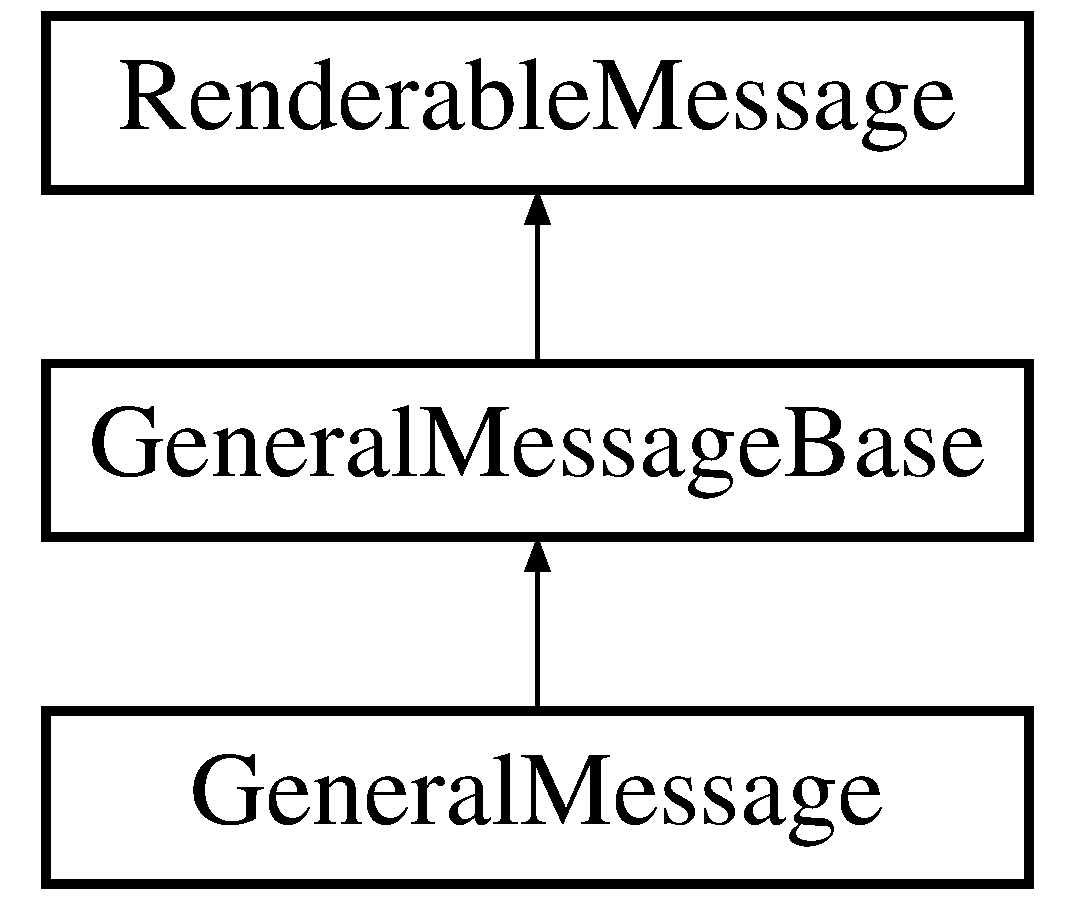
\includegraphics[height=3.000000cm]{classGeneralMessage}
\end{center}
\end{figure}
\subsection*{Public Member Functions}
\begin{DoxyCompactItemize}
\item 
\hyperlink{classGeneralMessage_ab1c0ee4586ae031d955533780f0e1dae}{General\-Message} (\hyperlink{classGeneralMessageBase}{General\-Message\-Base} $\ast$\hyperlink{classRenderableMessage_ab23728d14d9aff3efa0af7639ec6059c}{parent}, const google\-::protobuf\-::\-Message $\ast$msg, const google\-::protobuf\-::\-Reflection $\ast$reflection, const google\-::protobuf\-::\-Field\-Descriptor $\ast$field)
\item 
\hyperlink{classGeneralMessage_abc6d0f99cd6edc640027df3929628b36}{$\sim$\-General\-Message} ()
\item 
void \hyperlink{classGeneralMessage_a382210348f197d8b83a3d5a795e04852}{Render} (const \hyperlink{classScreen}{Screen} $\ast$s, int key) override
\end{DoxyCompactItemize}
\subsection*{Private Member Functions}
\begin{DoxyCompactItemize}
\item 
\hyperlink{classGeneralMessage_ad7972b90bd017a6993fe6585aa1227b2}{General\-Message} (const \hyperlink{classGeneralMessage}{General\-Message} \&)=delete
\item 
\hyperlink{classGeneralMessage}{General\-Message} \& \hyperlink{classGeneralMessage_a21635e2f4d5c9da0200db43add363383}{operator=} (const \hyperlink{classGeneralMessage}{General\-Message} \&)=delete
\end{DoxyCompactItemize}
\subsection*{Private Attributes}
\begin{DoxyCompactItemize}
\item 
int \hyperlink{classGeneralMessage_a5a14f5070ecf60e853ff57de0eb14cbe}{item\-Index\-\_\-}
\item 
bool \hyperlink{classGeneralMessage_aa4574eb1aa08869087923fadcc7c8ea1}{is\-\_\-folded\-\_\-}
\item 
const \\*
google\-::protobuf\-::\-Field\-Descriptor $\ast$ \hyperlink{classGeneralMessage_adde304145c9d3c9183ecdab343cecbcb}{field\-\_\-}
\item 
const google\-::protobuf\-::\-Message $\ast$ \hyperlink{classGeneralMessage_a2190da87b7dd7402133992d44fb98230}{message\-\_\-ptr\-\_\-}
\item 
const \\*
google\-::protobuf\-::\-Reflection $\ast$ \hyperlink{classGeneralMessage_ab56cddfdf8a104d774626dc1acd5f23d}{reflection\-\_\-ptr\-\_\-}
\end{DoxyCompactItemize}
\subsection*{Additional Inherited Members}


\subsection{Constructor \& Destructor Documentation}
\hypertarget{classGeneralMessage_ab1c0ee4586ae031d955533780f0e1dae}{\index{General\-Message@{General\-Message}!General\-Message@{General\-Message}}
\index{General\-Message@{General\-Message}!GeneralMessage@{General\-Message}}
\subsubsection[{General\-Message}]{\setlength{\rightskip}{0pt plus 5cm}General\-Message\-::\-General\-Message (
\begin{DoxyParamCaption}
\item[{{\bf General\-Message\-Base} $\ast$}]{parent, }
\item[{const google\-::protobuf\-::\-Message $\ast$}]{msg, }
\item[{const google\-::protobuf\-::\-Reflection $\ast$}]{reflection, }
\item[{const google\-::protobuf\-::\-Field\-Descriptor $\ast$}]{field}
\end{DoxyParamCaption}
)\hspace{0.3cm}{\ttfamily [explicit]}}}\label{classGeneralMessage_ab1c0ee4586ae031d955533780f0e1dae}
\hypertarget{classGeneralMessage_abc6d0f99cd6edc640027df3929628b36}{\index{General\-Message@{General\-Message}!$\sim$\-General\-Message@{$\sim$\-General\-Message}}
\index{$\sim$\-General\-Message@{$\sim$\-General\-Message}!GeneralMessage@{General\-Message}}
\subsubsection[{$\sim$\-General\-Message}]{\setlength{\rightskip}{0pt plus 5cm}General\-Message\-::$\sim$\-General\-Message (
\begin{DoxyParamCaption}
{}
\end{DoxyParamCaption}
)\hspace{0.3cm}{\ttfamily [inline]}}}\label{classGeneralMessage_abc6d0f99cd6edc640027df3929628b36}
\hypertarget{classGeneralMessage_ad7972b90bd017a6993fe6585aa1227b2}{\index{General\-Message@{General\-Message}!General\-Message@{General\-Message}}
\index{General\-Message@{General\-Message}!GeneralMessage@{General\-Message}}
\subsubsection[{General\-Message}]{\setlength{\rightskip}{0pt plus 5cm}General\-Message\-::\-General\-Message (
\begin{DoxyParamCaption}
\item[{const {\bf General\-Message} \&}]{}
\end{DoxyParamCaption}
)\hspace{0.3cm}{\ttfamily [private]}, {\ttfamily [delete]}}}\label{classGeneralMessage_ad7972b90bd017a6993fe6585aa1227b2}


\subsection{Member Function Documentation}
\hypertarget{classGeneralMessage_a21635e2f4d5c9da0200db43add363383}{\index{General\-Message@{General\-Message}!operator=@{operator=}}
\index{operator=@{operator=}!GeneralMessage@{General\-Message}}
\subsubsection[{operator=}]{\setlength{\rightskip}{0pt plus 5cm}{\bf General\-Message}\& General\-Message\-::operator= (
\begin{DoxyParamCaption}
\item[{const {\bf General\-Message} \&}]{}
\end{DoxyParamCaption}
)\hspace{0.3cm}{\ttfamily [private]}, {\ttfamily [delete]}}}\label{classGeneralMessage_a21635e2f4d5c9da0200db43add363383}
\hypertarget{classGeneralMessage_a382210348f197d8b83a3d5a795e04852}{\index{General\-Message@{General\-Message}!Render@{Render}}
\index{Render@{Render}!GeneralMessage@{General\-Message}}
\subsubsection[{Render}]{\setlength{\rightskip}{0pt plus 5cm}void General\-Message\-::\-Render (
\begin{DoxyParamCaption}
\item[{const {\bf Screen} $\ast$}]{s, }
\item[{int}]{key}
\end{DoxyParamCaption}
)\hspace{0.3cm}{\ttfamily [override]}, {\ttfamily [virtual]}}}\label{classGeneralMessage_a382210348f197d8b83a3d5a795e04852}


Implements \hyperlink{classRenderableMessage_a3f65c247f5db9bb4918bca7d665bbdc6}{Renderable\-Message}.



\subsection{Member Data Documentation}
\hypertarget{classGeneralMessage_adde304145c9d3c9183ecdab343cecbcb}{\index{General\-Message@{General\-Message}!field\-\_\-@{field\-\_\-}}
\index{field\-\_\-@{field\-\_\-}!GeneralMessage@{General\-Message}}
\subsubsection[{field\-\_\-}]{\setlength{\rightskip}{0pt plus 5cm}const google\-::protobuf\-::\-Field\-Descriptor$\ast$ General\-Message\-::field\-\_\-\hspace{0.3cm}{\ttfamily [private]}}}\label{classGeneralMessage_adde304145c9d3c9183ecdab343cecbcb}
\hypertarget{classGeneralMessage_aa4574eb1aa08869087923fadcc7c8ea1}{\index{General\-Message@{General\-Message}!is\-\_\-folded\-\_\-@{is\-\_\-folded\-\_\-}}
\index{is\-\_\-folded\-\_\-@{is\-\_\-folded\-\_\-}!GeneralMessage@{General\-Message}}
\subsubsection[{is\-\_\-folded\-\_\-}]{\setlength{\rightskip}{0pt plus 5cm}bool General\-Message\-::is\-\_\-folded\-\_\-\hspace{0.3cm}{\ttfamily [private]}}}\label{classGeneralMessage_aa4574eb1aa08869087923fadcc7c8ea1}
\hypertarget{classGeneralMessage_a5a14f5070ecf60e853ff57de0eb14cbe}{\index{General\-Message@{General\-Message}!item\-Index\-\_\-@{item\-Index\-\_\-}}
\index{item\-Index\-\_\-@{item\-Index\-\_\-}!GeneralMessage@{General\-Message}}
\subsubsection[{item\-Index\-\_\-}]{\setlength{\rightskip}{0pt plus 5cm}int General\-Message\-::item\-Index\-\_\-\hspace{0.3cm}{\ttfamily [private]}}}\label{classGeneralMessage_a5a14f5070ecf60e853ff57de0eb14cbe}
\hypertarget{classGeneralMessage_a2190da87b7dd7402133992d44fb98230}{\index{General\-Message@{General\-Message}!message\-\_\-ptr\-\_\-@{message\-\_\-ptr\-\_\-}}
\index{message\-\_\-ptr\-\_\-@{message\-\_\-ptr\-\_\-}!GeneralMessage@{General\-Message}}
\subsubsection[{message\-\_\-ptr\-\_\-}]{\setlength{\rightskip}{0pt plus 5cm}const google\-::protobuf\-::\-Message$\ast$ General\-Message\-::message\-\_\-ptr\-\_\-\hspace{0.3cm}{\ttfamily [private]}}}\label{classGeneralMessage_a2190da87b7dd7402133992d44fb98230}
\hypertarget{classGeneralMessage_ab56cddfdf8a104d774626dc1acd5f23d}{\index{General\-Message@{General\-Message}!reflection\-\_\-ptr\-\_\-@{reflection\-\_\-ptr\-\_\-}}
\index{reflection\-\_\-ptr\-\_\-@{reflection\-\_\-ptr\-\_\-}!GeneralMessage@{General\-Message}}
\subsubsection[{reflection\-\_\-ptr\-\_\-}]{\setlength{\rightskip}{0pt plus 5cm}const google\-::protobuf\-::\-Reflection$\ast$ General\-Message\-::reflection\-\_\-ptr\-\_\-\hspace{0.3cm}{\ttfamily [private]}}}\label{classGeneralMessage_ab56cddfdf8a104d774626dc1acd5f23d}


The documentation for this class was generated from the following file\-:\begin{DoxyCompactItemize}
\item 
tools/cyber\-\_\-monitor/\hyperlink{general__message_8h}{general\-\_\-message.\-h}\end{DoxyCompactItemize}

\hypertarget{classGeneralMessageBase}{\section{General\-Message\-Base Class Reference}
\label{classGeneralMessageBase}\index{General\-Message\-Base@{General\-Message\-Base}}
}


{\ttfamily \#include $<$general\-\_\-message\-\_\-base.\-h$>$}

Inheritance diagram for General\-Message\-Base\-:\begin{figure}[H]
\begin{center}
\leavevmode
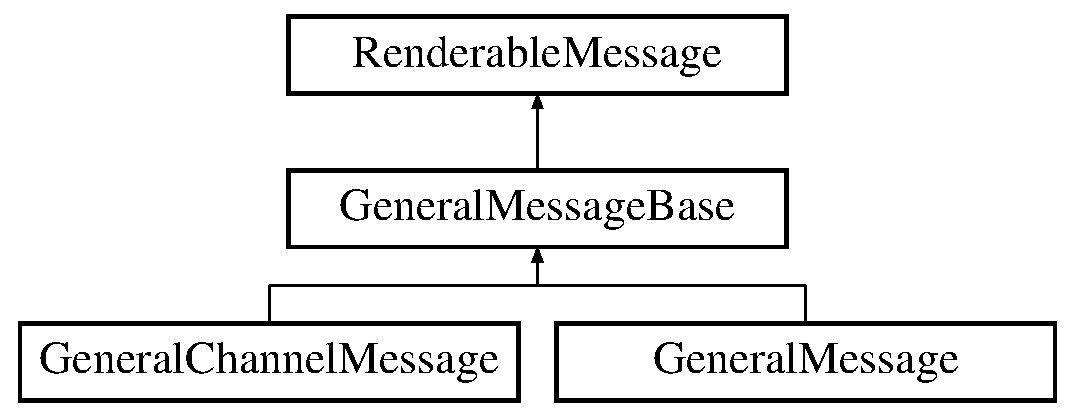
\includegraphics[height=3.000000cm]{classGeneralMessageBase}
\end{center}
\end{figure}
\subsection*{Protected Member Functions}
\begin{DoxyCompactItemize}
\item 
void \hyperlink{classGeneralMessageBase_a7b063ed053799b40e65b4fc36d53ffe8}{insert\-Repeated\-Message} (int line\-No, \hyperlink{classGeneralMessageBase}{General\-Message\-Base} $\ast$item)
\item 
\hyperlink{classRenderableMessage}{Renderable\-Message} $\ast$ \hyperlink{classGeneralMessageBase_a9ab394f1176382bbef06e1b7c37e35ee}{Child} (int line\-No) const override
\item 
\hyperlink{classGeneralMessageBase_a94b72a6e3f9cfe7204bd17f589840a77}{General\-Message\-Base} (\hyperlink{classRenderableMessage}{Renderable\-Message} $\ast$\hyperlink{classRenderableMessage_ab23728d14d9aff3efa0af7639ec6059c}{parent}=nullptr)
\item 
\hyperlink{classGeneralMessageBase_ab50f085176c924a1d08a805419499a6d}{$\sim$\-General\-Message\-Base} (void)
\item 
void \hyperlink{classGeneralMessageBase_a30f39896e2bb072ac8f67e46e6c95e41}{clear} (void)
\item 
\hyperlink{classGeneralMessageBase_af9e00565fe280e45a0155f583057ddbd}{General\-Message\-Base} (const \hyperlink{classGeneralMessageBase}{General\-Message\-Base} \&)=delete
\item 
\hyperlink{classGeneralMessageBase}{General\-Message\-Base} \& \hyperlink{classGeneralMessageBase_aa360714a5ea853427bfd7662f8928d8c}{operator=} (const \hyperlink{classGeneralMessageBase}{General\-Message\-Base} \&)=delete
\end{DoxyCompactItemize}
\subsection*{Static Protected Member Functions}
\begin{DoxyCompactItemize}
\item 
static void \hyperlink{classGeneralMessageBase_acb22b24b458fbb199de702736e136be3}{Print\-Message} (\hyperlink{classGeneralMessageBase}{General\-Message\-Base} $\ast$base\-Msg, const google\-::protobuf\-::\-Message \&msg, int \&jump\-Lines, const \hyperlink{classScreen}{Screen} $\ast$s, unsigned \&line\-No, int indent)
\item 
static void \hyperlink{classGeneralMessageBase_abb2b6d5c8a9399cc6e3eab14a0bec0c7}{Print\-Field} (\hyperlink{classGeneralMessageBase}{General\-Message\-Base} $\ast$base\-Msg, const google\-::protobuf\-::\-Message \&msg, int \&jump\-Lines, const \hyperlink{classScreen}{Screen} $\ast$s, unsigned \&line\-No, int indent, const google\-::protobuf\-::\-Reflection $\ast$ref, const google\-::protobuf\-::\-Field\-Descriptor $\ast$field, int index)
\item 
static int \hyperlink{classGeneralMessageBase_a3b3feba460a716d68348a54d274dd675}{line\-Count} (const google\-::protobuf\-::\-Message \&msg, int screen\-Width)
\item 
static int \hyperlink{classGeneralMessageBase_a4af9e501c26db8741b458ab477fe9aaa}{line\-Count\-Of\-Field} (const google\-::protobuf\-::\-Message \&msg, int screen\-Width, const google\-::protobuf\-::\-Field\-Descriptor $\ast$field, const google\-::protobuf\-::\-Reflection $\ast$reflection, bool is\-\_\-folded=true)
\end{DoxyCompactItemize}
\subsection*{Protected Attributes}
\begin{DoxyCompactItemize}
\item 
std\-::map$<$ const int, \\*
\hyperlink{classGeneralMessageBase}{General\-Message\-Base} $\ast$ $>$ \hyperlink{classGeneralMessageBase_a5ff98bf477e95204ca2021be372d3eba}{children\-\_\-map\-\_\-}
\end{DoxyCompactItemize}
\subsection*{Additional Inherited Members}


\subsection{Constructor \& Destructor Documentation}
\hypertarget{classGeneralMessageBase_a94b72a6e3f9cfe7204bd17f589840a77}{\index{General\-Message\-Base@{General\-Message\-Base}!General\-Message\-Base@{General\-Message\-Base}}
\index{General\-Message\-Base@{General\-Message\-Base}!GeneralMessageBase@{General\-Message\-Base}}
\subsubsection[{General\-Message\-Base}]{\setlength{\rightskip}{0pt plus 5cm}General\-Message\-Base\-::\-General\-Message\-Base (
\begin{DoxyParamCaption}
\item[{{\bf Renderable\-Message} $\ast$}]{parent = {\ttfamily nullptr}}
\end{DoxyParamCaption}
)\hspace{0.3cm}{\ttfamily [inline]}, {\ttfamily [explicit]}, {\ttfamily [protected]}}}\label{classGeneralMessageBase_a94b72a6e3f9cfe7204bd17f589840a77}
\hypertarget{classGeneralMessageBase_ab50f085176c924a1d08a805419499a6d}{\index{General\-Message\-Base@{General\-Message\-Base}!$\sim$\-General\-Message\-Base@{$\sim$\-General\-Message\-Base}}
\index{$\sim$\-General\-Message\-Base@{$\sim$\-General\-Message\-Base}!GeneralMessageBase@{General\-Message\-Base}}
\subsubsection[{$\sim$\-General\-Message\-Base}]{\setlength{\rightskip}{0pt plus 5cm}General\-Message\-Base\-::$\sim$\-General\-Message\-Base (
\begin{DoxyParamCaption}
\item[{void}]{}
\end{DoxyParamCaption}
)\hspace{0.3cm}{\ttfamily [inline]}, {\ttfamily [protected]}}}\label{classGeneralMessageBase_ab50f085176c924a1d08a805419499a6d}
\hypertarget{classGeneralMessageBase_af9e00565fe280e45a0155f583057ddbd}{\index{General\-Message\-Base@{General\-Message\-Base}!General\-Message\-Base@{General\-Message\-Base}}
\index{General\-Message\-Base@{General\-Message\-Base}!GeneralMessageBase@{General\-Message\-Base}}
\subsubsection[{General\-Message\-Base}]{\setlength{\rightskip}{0pt plus 5cm}General\-Message\-Base\-::\-General\-Message\-Base (
\begin{DoxyParamCaption}
\item[{const {\bf General\-Message\-Base} \&}]{}
\end{DoxyParamCaption}
)\hspace{0.3cm}{\ttfamily [protected]}, {\ttfamily [delete]}}}\label{classGeneralMessageBase_af9e00565fe280e45a0155f583057ddbd}


\subsection{Member Function Documentation}
\hypertarget{classGeneralMessageBase_a9ab394f1176382bbef06e1b7c37e35ee}{\index{General\-Message\-Base@{General\-Message\-Base}!Child@{Child}}
\index{Child@{Child}!GeneralMessageBase@{General\-Message\-Base}}
\subsubsection[{Child}]{\setlength{\rightskip}{0pt plus 5cm}{\bf Renderable\-Message}$\ast$ General\-Message\-Base\-::\-Child (
\begin{DoxyParamCaption}
\item[{int}]{line\-No}
\end{DoxyParamCaption}
) const\hspace{0.3cm}{\ttfamily [override]}, {\ttfamily [protected]}, {\ttfamily [virtual]}}}\label{classGeneralMessageBase_a9ab394f1176382bbef06e1b7c37e35ee}


Implements \hyperlink{classRenderableMessage_a0f933ad0befd4d3cf3a95e205c7398d6}{Renderable\-Message}.

\hypertarget{classGeneralMessageBase_a30f39896e2bb072ac8f67e46e6c95e41}{\index{General\-Message\-Base@{General\-Message\-Base}!clear@{clear}}
\index{clear@{clear}!GeneralMessageBase@{General\-Message\-Base}}
\subsubsection[{clear}]{\setlength{\rightskip}{0pt plus 5cm}void General\-Message\-Base\-::clear (
\begin{DoxyParamCaption}
\item[{void}]{}
\end{DoxyParamCaption}
)\hspace{0.3cm}{\ttfamily [inline]}, {\ttfamily [protected]}}}\label{classGeneralMessageBase_a30f39896e2bb072ac8f67e46e6c95e41}
\hypertarget{classGeneralMessageBase_a7b063ed053799b40e65b4fc36d53ffe8}{\index{General\-Message\-Base@{General\-Message\-Base}!insert\-Repeated\-Message@{insert\-Repeated\-Message}}
\index{insert\-Repeated\-Message@{insert\-Repeated\-Message}!GeneralMessageBase@{General\-Message\-Base}}
\subsubsection[{insert\-Repeated\-Message}]{\setlength{\rightskip}{0pt plus 5cm}void General\-Message\-Base\-::insert\-Repeated\-Message (
\begin{DoxyParamCaption}
\item[{int}]{line\-No, }
\item[{{\bf General\-Message\-Base} $\ast$}]{item}
\end{DoxyParamCaption}
)\hspace{0.3cm}{\ttfamily [inline]}, {\ttfamily [protected]}}}\label{classGeneralMessageBase_a7b063ed053799b40e65b4fc36d53ffe8}
\hypertarget{classGeneralMessageBase_a3b3feba460a716d68348a54d274dd675}{\index{General\-Message\-Base@{General\-Message\-Base}!line\-Count@{line\-Count}}
\index{line\-Count@{line\-Count}!GeneralMessageBase@{General\-Message\-Base}}
\subsubsection[{line\-Count}]{\setlength{\rightskip}{0pt plus 5cm}static int General\-Message\-Base\-::line\-Count (
\begin{DoxyParamCaption}
\item[{const google\-::protobuf\-::\-Message \&}]{msg, }
\item[{int}]{screen\-Width}
\end{DoxyParamCaption}
)\hspace{0.3cm}{\ttfamily [static]}, {\ttfamily [protected]}}}\label{classGeneralMessageBase_a3b3feba460a716d68348a54d274dd675}
\hypertarget{classGeneralMessageBase_a4af9e501c26db8741b458ab477fe9aaa}{\index{General\-Message\-Base@{General\-Message\-Base}!line\-Count\-Of\-Field@{line\-Count\-Of\-Field}}
\index{line\-Count\-Of\-Field@{line\-Count\-Of\-Field}!GeneralMessageBase@{General\-Message\-Base}}
\subsubsection[{line\-Count\-Of\-Field}]{\setlength{\rightskip}{0pt plus 5cm}static int General\-Message\-Base\-::line\-Count\-Of\-Field (
\begin{DoxyParamCaption}
\item[{const google\-::protobuf\-::\-Message \&}]{msg, }
\item[{int}]{screen\-Width, }
\item[{const google\-::protobuf\-::\-Field\-Descriptor $\ast$}]{field, }
\item[{const google\-::protobuf\-::\-Reflection $\ast$}]{reflection, }
\item[{bool}]{is\-\_\-folded = {\ttfamily true}}
\end{DoxyParamCaption}
)\hspace{0.3cm}{\ttfamily [static]}, {\ttfamily [protected]}}}\label{classGeneralMessageBase_a4af9e501c26db8741b458ab477fe9aaa}
\hypertarget{classGeneralMessageBase_aa360714a5ea853427bfd7662f8928d8c}{\index{General\-Message\-Base@{General\-Message\-Base}!operator=@{operator=}}
\index{operator=@{operator=}!GeneralMessageBase@{General\-Message\-Base}}
\subsubsection[{operator=}]{\setlength{\rightskip}{0pt plus 5cm}{\bf General\-Message\-Base}\& General\-Message\-Base\-::operator= (
\begin{DoxyParamCaption}
\item[{const {\bf General\-Message\-Base} \&}]{}
\end{DoxyParamCaption}
)\hspace{0.3cm}{\ttfamily [protected]}, {\ttfamily [delete]}}}\label{classGeneralMessageBase_aa360714a5ea853427bfd7662f8928d8c}
\hypertarget{classGeneralMessageBase_abb2b6d5c8a9399cc6e3eab14a0bec0c7}{\index{General\-Message\-Base@{General\-Message\-Base}!Print\-Field@{Print\-Field}}
\index{Print\-Field@{Print\-Field}!GeneralMessageBase@{General\-Message\-Base}}
\subsubsection[{Print\-Field}]{\setlength{\rightskip}{0pt plus 5cm}static void General\-Message\-Base\-::\-Print\-Field (
\begin{DoxyParamCaption}
\item[{{\bf General\-Message\-Base} $\ast$}]{base\-Msg, }
\item[{const google\-::protobuf\-::\-Message \&}]{msg, }
\item[{int \&}]{jump\-Lines, }
\item[{const {\bf Screen} $\ast$}]{s, }
\item[{unsigned \&}]{line\-No, }
\item[{int}]{indent, }
\item[{const google\-::protobuf\-::\-Reflection $\ast$}]{ref, }
\item[{const google\-::protobuf\-::\-Field\-Descriptor $\ast$}]{field, }
\item[{int}]{index}
\end{DoxyParamCaption}
)\hspace{0.3cm}{\ttfamily [static]}, {\ttfamily [protected]}}}\label{classGeneralMessageBase_abb2b6d5c8a9399cc6e3eab14a0bec0c7}
\hypertarget{classGeneralMessageBase_acb22b24b458fbb199de702736e136be3}{\index{General\-Message\-Base@{General\-Message\-Base}!Print\-Message@{Print\-Message}}
\index{Print\-Message@{Print\-Message}!GeneralMessageBase@{General\-Message\-Base}}
\subsubsection[{Print\-Message}]{\setlength{\rightskip}{0pt plus 5cm}static void General\-Message\-Base\-::\-Print\-Message (
\begin{DoxyParamCaption}
\item[{{\bf General\-Message\-Base} $\ast$}]{base\-Msg, }
\item[{const google\-::protobuf\-::\-Message \&}]{msg, }
\item[{int \&}]{jump\-Lines, }
\item[{const {\bf Screen} $\ast$}]{s, }
\item[{unsigned \&}]{line\-No, }
\item[{int}]{indent}
\end{DoxyParamCaption}
)\hspace{0.3cm}{\ttfamily [static]}, {\ttfamily [protected]}}}\label{classGeneralMessageBase_acb22b24b458fbb199de702736e136be3}


\subsection{Member Data Documentation}
\hypertarget{classGeneralMessageBase_a5ff98bf477e95204ca2021be372d3eba}{\index{General\-Message\-Base@{General\-Message\-Base}!children\-\_\-map\-\_\-@{children\-\_\-map\-\_\-}}
\index{children\-\_\-map\-\_\-@{children\-\_\-map\-\_\-}!GeneralMessageBase@{General\-Message\-Base}}
\subsubsection[{children\-\_\-map\-\_\-}]{\setlength{\rightskip}{0pt plus 5cm}std\-::map$<$const int, {\bf General\-Message\-Base}$\ast$$>$ General\-Message\-Base\-::children\-\_\-map\-\_\-\hspace{0.3cm}{\ttfamily [protected]}}}\label{classGeneralMessageBase_a5ff98bf477e95204ca2021be372d3eba}


The documentation for this class was generated from the following file\-:\begin{DoxyCompactItemize}
\item 
tools/cyber\-\_\-monitor/\hyperlink{general__message__base_8h}{general\-\_\-message\-\_\-base.\-h}\end{DoxyCompactItemize}

\hypertarget{classapollo_1_1cyber_1_1common_1_1GlobalData}{\section{apollo\-:\-:cyber\-:\-:common\-:\-:Global\-Data Class Reference}
\label{classapollo_1_1cyber_1_1common_1_1GlobalData}\index{apollo\-::cyber\-::common\-::\-Global\-Data@{apollo\-::cyber\-::common\-::\-Global\-Data}}
}


{\ttfamily \#include $<$global\-\_\-data.\-h$>$}

\subsection*{Public Member Functions}
\begin{DoxyCompactItemize}
\item 
\hyperlink{classapollo_1_1cyber_1_1common_1_1GlobalData_a3b09d9ae8e74fcef1cae2bf4f5158bf1}{$\sim$\-Global\-Data} ()
\item 
int \hyperlink{classapollo_1_1cyber_1_1common_1_1GlobalData_a2f1b262b59b5a1e2176abf605675445e}{Process\-Id} () const 
\item 
void \hyperlink{classapollo_1_1cyber_1_1common_1_1GlobalData_a4d223acbe0c85c107370c9b896c211f2}{Set\-Process\-Group} (const std\-::string \&process\-\_\-group)
\item 
const std\-::string \& \hyperlink{classapollo_1_1cyber_1_1common_1_1GlobalData_a3e25c18dbd9c16898961d4a074c748f5}{Process\-Group} () const 
\item 
void \hyperlink{classapollo_1_1cyber_1_1common_1_1GlobalData_a21d271e642503138b530ed46d67e00df}{Set\-Sched\-Name} (const std\-::string \&sched\-\_\-name)
\item 
const std\-::string \& \hyperlink{classapollo_1_1cyber_1_1common_1_1GlobalData_abf1643620bdf25ad1016a03e7841ae1c}{Sched\-Name} () const 
\item 
const std\-::string \& \hyperlink{classapollo_1_1cyber_1_1common_1_1GlobalData_aa946201520faeded91601a50617fa74a}{Host\-Ip} () const 
\item 
const std\-::string \& \hyperlink{classapollo_1_1cyber_1_1common_1_1GlobalData_a00072980ed047a9688ac219b056fb163}{Host\-Name} () const 
\item 
const Cyber\-Config \& \hyperlink{classapollo_1_1cyber_1_1common_1_1GlobalData_a08aae1b46abb6128259bffa1946e40fe}{Config} () const 
\item 
void \hyperlink{classapollo_1_1cyber_1_1common_1_1GlobalData_a84d3895acc1aac14760fd5fe99073ce3}{Enable\-Simulation\-Mode} ()
\item 
void \hyperlink{classapollo_1_1cyber_1_1common_1_1GlobalData_a7dc766c13bcbd249bd2a1005045f174f}{Disable\-Simulation\-Mode} ()
\item 
bool \hyperlink{classapollo_1_1cyber_1_1common_1_1GlobalData_a67841cc056f7409327d6311361620868}{Is\-Reality\-Mode} () const 
\end{DoxyCompactItemize}
\subsection*{Static Public Member Functions}
\begin{DoxyCompactItemize}
\item 
static uint64\-\_\-t \hyperlink{classapollo_1_1cyber_1_1common_1_1GlobalData_afc3ae45dd4d4d8a7f58be886278868fd}{Generate\-Hash\-Id} (const std\-::string \&name)
\item 
static uint64\-\_\-t \hyperlink{classapollo_1_1cyber_1_1common_1_1GlobalData_abdf52d28bad0e345e1e10187dd162ef5}{Register\-Node} (const std\-::string \&node\-\_\-name)
\item 
static std\-::string \hyperlink{classapollo_1_1cyber_1_1common_1_1GlobalData_a41d3e913a6731fa546fb92b8116225d4}{Get\-Node\-By\-Id} (uint64\-\_\-t id)
\item 
static uint64\-\_\-t \hyperlink{classapollo_1_1cyber_1_1common_1_1GlobalData_a26e453f2a86db03acf98831cddada877}{Register\-Channel} (const std\-::string \&channel)
\item 
static std\-::string \hyperlink{classapollo_1_1cyber_1_1common_1_1GlobalData_aa5ae9e9ab709bb13fb4dc78b1d496ed6}{Get\-Channel\-By\-Id} (uint64\-\_\-t id)
\item 
static uint64\-\_\-t \hyperlink{classapollo_1_1cyber_1_1common_1_1GlobalData_aec94b2b14e6a688047079359425bd722}{Register\-Service} (const std\-::string \&service)
\item 
static std\-::string \hyperlink{classapollo_1_1cyber_1_1common_1_1GlobalData_a2e1b9892463890d8db30adb7f6df3271}{Get\-Service\-By\-Id} (uint64\-\_\-t id)
\item 
static uint64\-\_\-t \hyperlink{classapollo_1_1cyber_1_1common_1_1GlobalData_a47232f187a9a19fe153dc016086d3e67}{Register\-Task\-Name} (const std\-::string \&task\-\_\-name)
\item 
static std\-::string \hyperlink{classapollo_1_1cyber_1_1common_1_1GlobalData_a57aa373577f79859997b0cc1927f7507}{Get\-Task\-Name\-By\-Id} (uint64\-\_\-t id)
\end{DoxyCompactItemize}
\subsection*{Private Member Functions}
\begin{DoxyCompactItemize}
\item 
void \hyperlink{classapollo_1_1cyber_1_1common_1_1GlobalData_a5434087f192431f4e8261cc4188db09d}{Init\-Host\-Info} ()
\item 
bool \hyperlink{classapollo_1_1cyber_1_1common_1_1GlobalData_a82f8e1f2dc28bab4c49a44374cf8db90}{Init\-Config} ()
\end{DoxyCompactItemize}
\subsection*{Private Attributes}
\begin{DoxyCompactItemize}
\item 
Cyber\-Config \hyperlink{classapollo_1_1cyber_1_1common_1_1GlobalData_a8efeddcd2e684e46bac9c51c6090a7fb}{config\-\_\-}
\item 
std\-::string \hyperlink{classapollo_1_1cyber_1_1common_1_1GlobalData_aef658f6aa36b7d7ac0cb38136daf7cce}{host\-\_\-ip\-\_\-}
\item 
std\-::string \hyperlink{classapollo_1_1cyber_1_1common_1_1GlobalData_a5f6e56d8227a41b2ee57b5ea8c5f2746}{host\-\_\-name\-\_\-}
\item 
int \hyperlink{classapollo_1_1cyber_1_1common_1_1GlobalData_a5e587220e06a0b2d7e6dc92edf39b2c3}{process\-\_\-id\-\_\-}
\item 
std\-::string \hyperlink{classapollo_1_1cyber_1_1common_1_1GlobalData_acad7df736c167ed6c4a948fab5f6c294}{process\-\_\-group\-\_\-}
\item 
std\-::string \hyperlink{classapollo_1_1cyber_1_1common_1_1GlobalData_a907005048a52bc169827433783e14463}{sched\-\_\-name\-\_\-} = \char`\"{}C\-Y\-B\-E\-R\-\_\-\-D\-E\-F\-A\-U\-L\-T\char`\"{}
\item 
bool \hyperlink{classapollo_1_1cyber_1_1common_1_1GlobalData_aab8e6ddd2ca6b1633cb97cd4df6ee8ba}{is\-\_\-reality\-\_\-mode\-\_\-}
\end{DoxyCompactItemize}
\subsection*{Static Private Attributes}
\begin{DoxyCompactItemize}
\item 
static Atomic\-Hash\-Map$<$ uint64\-\_\-t, \\*
std\-::string, 512 $>$ \hyperlink{classapollo_1_1cyber_1_1common_1_1GlobalData_a8cfa861e6f13217ed4d53c59f5245a38}{node\-\_\-id\-\_\-map\-\_\-}
\item 
static Atomic\-Hash\-Map$<$ uint64\-\_\-t, \\*
std\-::string, 256 $>$ \hyperlink{classapollo_1_1cyber_1_1common_1_1GlobalData_ad28c90146805267fce1420eb2d146151}{channel\-\_\-id\-\_\-map\-\_\-}
\item 
static Atomic\-Hash\-Map$<$ uint64\-\_\-t, \\*
std\-::string, 256 $>$ \hyperlink{classapollo_1_1cyber_1_1common_1_1GlobalData_aa275354102633f341e7b639afcf90b2d}{service\-\_\-id\-\_\-map\-\_\-}
\item 
static Atomic\-Hash\-Map$<$ uint64\-\_\-t, \\*
std\-::string, 256 $>$ \hyperlink{classapollo_1_1cyber_1_1common_1_1GlobalData_adac61bb03ae049915507e3f3e9077790}{task\-\_\-id\-\_\-map\-\_\-}
\end{DoxyCompactItemize}


\subsection{Constructor \& Destructor Documentation}
\hypertarget{classapollo_1_1cyber_1_1common_1_1GlobalData_a3b09d9ae8e74fcef1cae2bf4f5158bf1}{\index{apollo\-::cyber\-::common\-::\-Global\-Data@{apollo\-::cyber\-::common\-::\-Global\-Data}!$\sim$\-Global\-Data@{$\sim$\-Global\-Data}}
\index{$\sim$\-Global\-Data@{$\sim$\-Global\-Data}!apollo::cyber::common::GlobalData@{apollo\-::cyber\-::common\-::\-Global\-Data}}
\subsubsection[{$\sim$\-Global\-Data}]{\setlength{\rightskip}{0pt plus 5cm}apollo\-::cyber\-::common\-::\-Global\-Data\-::$\sim$\-Global\-Data (
\begin{DoxyParamCaption}
{}
\end{DoxyParamCaption}
)}}\label{classapollo_1_1cyber_1_1common_1_1GlobalData_a3b09d9ae8e74fcef1cae2bf4f5158bf1}


\subsection{Member Function Documentation}
\hypertarget{classapollo_1_1cyber_1_1common_1_1GlobalData_a08aae1b46abb6128259bffa1946e40fe}{\index{apollo\-::cyber\-::common\-::\-Global\-Data@{apollo\-::cyber\-::common\-::\-Global\-Data}!Config@{Config}}
\index{Config@{Config}!apollo::cyber::common::GlobalData@{apollo\-::cyber\-::common\-::\-Global\-Data}}
\subsubsection[{Config}]{\setlength{\rightskip}{0pt plus 5cm}const Cyber\-Config\& apollo\-::cyber\-::common\-::\-Global\-Data\-::\-Config (
\begin{DoxyParamCaption}
{}
\end{DoxyParamCaption}
) const}}\label{classapollo_1_1cyber_1_1common_1_1GlobalData_a08aae1b46abb6128259bffa1946e40fe}
\hypertarget{classapollo_1_1cyber_1_1common_1_1GlobalData_a7dc766c13bcbd249bd2a1005045f174f}{\index{apollo\-::cyber\-::common\-::\-Global\-Data@{apollo\-::cyber\-::common\-::\-Global\-Data}!Disable\-Simulation\-Mode@{Disable\-Simulation\-Mode}}
\index{Disable\-Simulation\-Mode@{Disable\-Simulation\-Mode}!apollo::cyber::common::GlobalData@{apollo\-::cyber\-::common\-::\-Global\-Data}}
\subsubsection[{Disable\-Simulation\-Mode}]{\setlength{\rightskip}{0pt plus 5cm}void apollo\-::cyber\-::common\-::\-Global\-Data\-::\-Disable\-Simulation\-Mode (
\begin{DoxyParamCaption}
{}
\end{DoxyParamCaption}
)}}\label{classapollo_1_1cyber_1_1common_1_1GlobalData_a7dc766c13bcbd249bd2a1005045f174f}
\hypertarget{classapollo_1_1cyber_1_1common_1_1GlobalData_a84d3895acc1aac14760fd5fe99073ce3}{\index{apollo\-::cyber\-::common\-::\-Global\-Data@{apollo\-::cyber\-::common\-::\-Global\-Data}!Enable\-Simulation\-Mode@{Enable\-Simulation\-Mode}}
\index{Enable\-Simulation\-Mode@{Enable\-Simulation\-Mode}!apollo::cyber::common::GlobalData@{apollo\-::cyber\-::common\-::\-Global\-Data}}
\subsubsection[{Enable\-Simulation\-Mode}]{\setlength{\rightskip}{0pt plus 5cm}void apollo\-::cyber\-::common\-::\-Global\-Data\-::\-Enable\-Simulation\-Mode (
\begin{DoxyParamCaption}
{}
\end{DoxyParamCaption}
)}}\label{classapollo_1_1cyber_1_1common_1_1GlobalData_a84d3895acc1aac14760fd5fe99073ce3}
\hypertarget{classapollo_1_1cyber_1_1common_1_1GlobalData_afc3ae45dd4d4d8a7f58be886278868fd}{\index{apollo\-::cyber\-::common\-::\-Global\-Data@{apollo\-::cyber\-::common\-::\-Global\-Data}!Generate\-Hash\-Id@{Generate\-Hash\-Id}}
\index{Generate\-Hash\-Id@{Generate\-Hash\-Id}!apollo::cyber::common::GlobalData@{apollo\-::cyber\-::common\-::\-Global\-Data}}
\subsubsection[{Generate\-Hash\-Id}]{\setlength{\rightskip}{0pt plus 5cm}static uint64\-\_\-t apollo\-::cyber\-::common\-::\-Global\-Data\-::\-Generate\-Hash\-Id (
\begin{DoxyParamCaption}
\item[{const std\-::string \&}]{name}
\end{DoxyParamCaption}
)\hspace{0.3cm}{\ttfamily [inline]}, {\ttfamily [static]}}}\label{classapollo_1_1cyber_1_1common_1_1GlobalData_afc3ae45dd4d4d8a7f58be886278868fd}
\hypertarget{classapollo_1_1cyber_1_1common_1_1GlobalData_aa5ae9e9ab709bb13fb4dc78b1d496ed6}{\index{apollo\-::cyber\-::common\-::\-Global\-Data@{apollo\-::cyber\-::common\-::\-Global\-Data}!Get\-Channel\-By\-Id@{Get\-Channel\-By\-Id}}
\index{Get\-Channel\-By\-Id@{Get\-Channel\-By\-Id}!apollo::cyber::common::GlobalData@{apollo\-::cyber\-::common\-::\-Global\-Data}}
\subsubsection[{Get\-Channel\-By\-Id}]{\setlength{\rightskip}{0pt plus 5cm}static std\-::string apollo\-::cyber\-::common\-::\-Global\-Data\-::\-Get\-Channel\-By\-Id (
\begin{DoxyParamCaption}
\item[{uint64\-\_\-t}]{id}
\end{DoxyParamCaption}
)\hspace{0.3cm}{\ttfamily [static]}}}\label{classapollo_1_1cyber_1_1common_1_1GlobalData_aa5ae9e9ab709bb13fb4dc78b1d496ed6}
\hypertarget{classapollo_1_1cyber_1_1common_1_1GlobalData_a41d3e913a6731fa546fb92b8116225d4}{\index{apollo\-::cyber\-::common\-::\-Global\-Data@{apollo\-::cyber\-::common\-::\-Global\-Data}!Get\-Node\-By\-Id@{Get\-Node\-By\-Id}}
\index{Get\-Node\-By\-Id@{Get\-Node\-By\-Id}!apollo::cyber::common::GlobalData@{apollo\-::cyber\-::common\-::\-Global\-Data}}
\subsubsection[{Get\-Node\-By\-Id}]{\setlength{\rightskip}{0pt plus 5cm}static std\-::string apollo\-::cyber\-::common\-::\-Global\-Data\-::\-Get\-Node\-By\-Id (
\begin{DoxyParamCaption}
\item[{uint64\-\_\-t}]{id}
\end{DoxyParamCaption}
)\hspace{0.3cm}{\ttfamily [static]}}}\label{classapollo_1_1cyber_1_1common_1_1GlobalData_a41d3e913a6731fa546fb92b8116225d4}
\hypertarget{classapollo_1_1cyber_1_1common_1_1GlobalData_a2e1b9892463890d8db30adb7f6df3271}{\index{apollo\-::cyber\-::common\-::\-Global\-Data@{apollo\-::cyber\-::common\-::\-Global\-Data}!Get\-Service\-By\-Id@{Get\-Service\-By\-Id}}
\index{Get\-Service\-By\-Id@{Get\-Service\-By\-Id}!apollo::cyber::common::GlobalData@{apollo\-::cyber\-::common\-::\-Global\-Data}}
\subsubsection[{Get\-Service\-By\-Id}]{\setlength{\rightskip}{0pt plus 5cm}static std\-::string apollo\-::cyber\-::common\-::\-Global\-Data\-::\-Get\-Service\-By\-Id (
\begin{DoxyParamCaption}
\item[{uint64\-\_\-t}]{id}
\end{DoxyParamCaption}
)\hspace{0.3cm}{\ttfamily [static]}}}\label{classapollo_1_1cyber_1_1common_1_1GlobalData_a2e1b9892463890d8db30adb7f6df3271}
\hypertarget{classapollo_1_1cyber_1_1common_1_1GlobalData_a57aa373577f79859997b0cc1927f7507}{\index{apollo\-::cyber\-::common\-::\-Global\-Data@{apollo\-::cyber\-::common\-::\-Global\-Data}!Get\-Task\-Name\-By\-Id@{Get\-Task\-Name\-By\-Id}}
\index{Get\-Task\-Name\-By\-Id@{Get\-Task\-Name\-By\-Id}!apollo::cyber::common::GlobalData@{apollo\-::cyber\-::common\-::\-Global\-Data}}
\subsubsection[{Get\-Task\-Name\-By\-Id}]{\setlength{\rightskip}{0pt plus 5cm}static std\-::string apollo\-::cyber\-::common\-::\-Global\-Data\-::\-Get\-Task\-Name\-By\-Id (
\begin{DoxyParamCaption}
\item[{uint64\-\_\-t}]{id}
\end{DoxyParamCaption}
)\hspace{0.3cm}{\ttfamily [static]}}}\label{classapollo_1_1cyber_1_1common_1_1GlobalData_a57aa373577f79859997b0cc1927f7507}
\hypertarget{classapollo_1_1cyber_1_1common_1_1GlobalData_aa946201520faeded91601a50617fa74a}{\index{apollo\-::cyber\-::common\-::\-Global\-Data@{apollo\-::cyber\-::common\-::\-Global\-Data}!Host\-Ip@{Host\-Ip}}
\index{Host\-Ip@{Host\-Ip}!apollo::cyber::common::GlobalData@{apollo\-::cyber\-::common\-::\-Global\-Data}}
\subsubsection[{Host\-Ip}]{\setlength{\rightskip}{0pt plus 5cm}const std\-::string\& apollo\-::cyber\-::common\-::\-Global\-Data\-::\-Host\-Ip (
\begin{DoxyParamCaption}
{}
\end{DoxyParamCaption}
) const}}\label{classapollo_1_1cyber_1_1common_1_1GlobalData_aa946201520faeded91601a50617fa74a}
\hypertarget{classapollo_1_1cyber_1_1common_1_1GlobalData_a00072980ed047a9688ac219b056fb163}{\index{apollo\-::cyber\-::common\-::\-Global\-Data@{apollo\-::cyber\-::common\-::\-Global\-Data}!Host\-Name@{Host\-Name}}
\index{Host\-Name@{Host\-Name}!apollo::cyber::common::GlobalData@{apollo\-::cyber\-::common\-::\-Global\-Data}}
\subsubsection[{Host\-Name}]{\setlength{\rightskip}{0pt plus 5cm}const std\-::string\& apollo\-::cyber\-::common\-::\-Global\-Data\-::\-Host\-Name (
\begin{DoxyParamCaption}
{}
\end{DoxyParamCaption}
) const}}\label{classapollo_1_1cyber_1_1common_1_1GlobalData_a00072980ed047a9688ac219b056fb163}
\hypertarget{classapollo_1_1cyber_1_1common_1_1GlobalData_a82f8e1f2dc28bab4c49a44374cf8db90}{\index{apollo\-::cyber\-::common\-::\-Global\-Data@{apollo\-::cyber\-::common\-::\-Global\-Data}!Init\-Config@{Init\-Config}}
\index{Init\-Config@{Init\-Config}!apollo::cyber::common::GlobalData@{apollo\-::cyber\-::common\-::\-Global\-Data}}
\subsubsection[{Init\-Config}]{\setlength{\rightskip}{0pt plus 5cm}bool apollo\-::cyber\-::common\-::\-Global\-Data\-::\-Init\-Config (
\begin{DoxyParamCaption}
{}
\end{DoxyParamCaption}
)\hspace{0.3cm}{\ttfamily [private]}}}\label{classapollo_1_1cyber_1_1common_1_1GlobalData_a82f8e1f2dc28bab4c49a44374cf8db90}
\hypertarget{classapollo_1_1cyber_1_1common_1_1GlobalData_a5434087f192431f4e8261cc4188db09d}{\index{apollo\-::cyber\-::common\-::\-Global\-Data@{apollo\-::cyber\-::common\-::\-Global\-Data}!Init\-Host\-Info@{Init\-Host\-Info}}
\index{Init\-Host\-Info@{Init\-Host\-Info}!apollo::cyber::common::GlobalData@{apollo\-::cyber\-::common\-::\-Global\-Data}}
\subsubsection[{Init\-Host\-Info}]{\setlength{\rightskip}{0pt plus 5cm}void apollo\-::cyber\-::common\-::\-Global\-Data\-::\-Init\-Host\-Info (
\begin{DoxyParamCaption}
{}
\end{DoxyParamCaption}
)\hspace{0.3cm}{\ttfamily [private]}}}\label{classapollo_1_1cyber_1_1common_1_1GlobalData_a5434087f192431f4e8261cc4188db09d}
\hypertarget{classapollo_1_1cyber_1_1common_1_1GlobalData_a67841cc056f7409327d6311361620868}{\index{apollo\-::cyber\-::common\-::\-Global\-Data@{apollo\-::cyber\-::common\-::\-Global\-Data}!Is\-Reality\-Mode@{Is\-Reality\-Mode}}
\index{Is\-Reality\-Mode@{Is\-Reality\-Mode}!apollo::cyber::common::GlobalData@{apollo\-::cyber\-::common\-::\-Global\-Data}}
\subsubsection[{Is\-Reality\-Mode}]{\setlength{\rightskip}{0pt plus 5cm}bool apollo\-::cyber\-::common\-::\-Global\-Data\-::\-Is\-Reality\-Mode (
\begin{DoxyParamCaption}
{}
\end{DoxyParamCaption}
) const}}\label{classapollo_1_1cyber_1_1common_1_1GlobalData_a67841cc056f7409327d6311361620868}
\hypertarget{classapollo_1_1cyber_1_1common_1_1GlobalData_a3e25c18dbd9c16898961d4a074c748f5}{\index{apollo\-::cyber\-::common\-::\-Global\-Data@{apollo\-::cyber\-::common\-::\-Global\-Data}!Process\-Group@{Process\-Group}}
\index{Process\-Group@{Process\-Group}!apollo::cyber::common::GlobalData@{apollo\-::cyber\-::common\-::\-Global\-Data}}
\subsubsection[{Process\-Group}]{\setlength{\rightskip}{0pt plus 5cm}const std\-::string\& apollo\-::cyber\-::common\-::\-Global\-Data\-::\-Process\-Group (
\begin{DoxyParamCaption}
{}
\end{DoxyParamCaption}
) const}}\label{classapollo_1_1cyber_1_1common_1_1GlobalData_a3e25c18dbd9c16898961d4a074c748f5}
\hypertarget{classapollo_1_1cyber_1_1common_1_1GlobalData_a2f1b262b59b5a1e2176abf605675445e}{\index{apollo\-::cyber\-::common\-::\-Global\-Data@{apollo\-::cyber\-::common\-::\-Global\-Data}!Process\-Id@{Process\-Id}}
\index{Process\-Id@{Process\-Id}!apollo::cyber::common::GlobalData@{apollo\-::cyber\-::common\-::\-Global\-Data}}
\subsubsection[{Process\-Id}]{\setlength{\rightskip}{0pt plus 5cm}int apollo\-::cyber\-::common\-::\-Global\-Data\-::\-Process\-Id (
\begin{DoxyParamCaption}
{}
\end{DoxyParamCaption}
) const}}\label{classapollo_1_1cyber_1_1common_1_1GlobalData_a2f1b262b59b5a1e2176abf605675445e}
\hypertarget{classapollo_1_1cyber_1_1common_1_1GlobalData_a26e453f2a86db03acf98831cddada877}{\index{apollo\-::cyber\-::common\-::\-Global\-Data@{apollo\-::cyber\-::common\-::\-Global\-Data}!Register\-Channel@{Register\-Channel}}
\index{Register\-Channel@{Register\-Channel}!apollo::cyber::common::GlobalData@{apollo\-::cyber\-::common\-::\-Global\-Data}}
\subsubsection[{Register\-Channel}]{\setlength{\rightskip}{0pt plus 5cm}static uint64\-\_\-t apollo\-::cyber\-::common\-::\-Global\-Data\-::\-Register\-Channel (
\begin{DoxyParamCaption}
\item[{const std\-::string \&}]{channel}
\end{DoxyParamCaption}
)\hspace{0.3cm}{\ttfamily [static]}}}\label{classapollo_1_1cyber_1_1common_1_1GlobalData_a26e453f2a86db03acf98831cddada877}
\hypertarget{classapollo_1_1cyber_1_1common_1_1GlobalData_abdf52d28bad0e345e1e10187dd162ef5}{\index{apollo\-::cyber\-::common\-::\-Global\-Data@{apollo\-::cyber\-::common\-::\-Global\-Data}!Register\-Node@{Register\-Node}}
\index{Register\-Node@{Register\-Node}!apollo::cyber::common::GlobalData@{apollo\-::cyber\-::common\-::\-Global\-Data}}
\subsubsection[{Register\-Node}]{\setlength{\rightskip}{0pt plus 5cm}static uint64\-\_\-t apollo\-::cyber\-::common\-::\-Global\-Data\-::\-Register\-Node (
\begin{DoxyParamCaption}
\item[{const std\-::string \&}]{node\-\_\-name}
\end{DoxyParamCaption}
)\hspace{0.3cm}{\ttfamily [static]}}}\label{classapollo_1_1cyber_1_1common_1_1GlobalData_abdf52d28bad0e345e1e10187dd162ef5}
\hypertarget{classapollo_1_1cyber_1_1common_1_1GlobalData_aec94b2b14e6a688047079359425bd722}{\index{apollo\-::cyber\-::common\-::\-Global\-Data@{apollo\-::cyber\-::common\-::\-Global\-Data}!Register\-Service@{Register\-Service}}
\index{Register\-Service@{Register\-Service}!apollo::cyber::common::GlobalData@{apollo\-::cyber\-::common\-::\-Global\-Data}}
\subsubsection[{Register\-Service}]{\setlength{\rightskip}{0pt plus 5cm}static uint64\-\_\-t apollo\-::cyber\-::common\-::\-Global\-Data\-::\-Register\-Service (
\begin{DoxyParamCaption}
\item[{const std\-::string \&}]{service}
\end{DoxyParamCaption}
)\hspace{0.3cm}{\ttfamily [static]}}}\label{classapollo_1_1cyber_1_1common_1_1GlobalData_aec94b2b14e6a688047079359425bd722}
\hypertarget{classapollo_1_1cyber_1_1common_1_1GlobalData_a47232f187a9a19fe153dc016086d3e67}{\index{apollo\-::cyber\-::common\-::\-Global\-Data@{apollo\-::cyber\-::common\-::\-Global\-Data}!Register\-Task\-Name@{Register\-Task\-Name}}
\index{Register\-Task\-Name@{Register\-Task\-Name}!apollo::cyber::common::GlobalData@{apollo\-::cyber\-::common\-::\-Global\-Data}}
\subsubsection[{Register\-Task\-Name}]{\setlength{\rightskip}{0pt plus 5cm}static uint64\-\_\-t apollo\-::cyber\-::common\-::\-Global\-Data\-::\-Register\-Task\-Name (
\begin{DoxyParamCaption}
\item[{const std\-::string \&}]{task\-\_\-name}
\end{DoxyParamCaption}
)\hspace{0.3cm}{\ttfamily [static]}}}\label{classapollo_1_1cyber_1_1common_1_1GlobalData_a47232f187a9a19fe153dc016086d3e67}
\hypertarget{classapollo_1_1cyber_1_1common_1_1GlobalData_abf1643620bdf25ad1016a03e7841ae1c}{\index{apollo\-::cyber\-::common\-::\-Global\-Data@{apollo\-::cyber\-::common\-::\-Global\-Data}!Sched\-Name@{Sched\-Name}}
\index{Sched\-Name@{Sched\-Name}!apollo::cyber::common::GlobalData@{apollo\-::cyber\-::common\-::\-Global\-Data}}
\subsubsection[{Sched\-Name}]{\setlength{\rightskip}{0pt plus 5cm}const std\-::string\& apollo\-::cyber\-::common\-::\-Global\-Data\-::\-Sched\-Name (
\begin{DoxyParamCaption}
{}
\end{DoxyParamCaption}
) const}}\label{classapollo_1_1cyber_1_1common_1_1GlobalData_abf1643620bdf25ad1016a03e7841ae1c}
\hypertarget{classapollo_1_1cyber_1_1common_1_1GlobalData_a4d223acbe0c85c107370c9b896c211f2}{\index{apollo\-::cyber\-::common\-::\-Global\-Data@{apollo\-::cyber\-::common\-::\-Global\-Data}!Set\-Process\-Group@{Set\-Process\-Group}}
\index{Set\-Process\-Group@{Set\-Process\-Group}!apollo::cyber::common::GlobalData@{apollo\-::cyber\-::common\-::\-Global\-Data}}
\subsubsection[{Set\-Process\-Group}]{\setlength{\rightskip}{0pt plus 5cm}void apollo\-::cyber\-::common\-::\-Global\-Data\-::\-Set\-Process\-Group (
\begin{DoxyParamCaption}
\item[{const std\-::string \&}]{process\-\_\-group}
\end{DoxyParamCaption}
)}}\label{classapollo_1_1cyber_1_1common_1_1GlobalData_a4d223acbe0c85c107370c9b896c211f2}
\hypertarget{classapollo_1_1cyber_1_1common_1_1GlobalData_a21d271e642503138b530ed46d67e00df}{\index{apollo\-::cyber\-::common\-::\-Global\-Data@{apollo\-::cyber\-::common\-::\-Global\-Data}!Set\-Sched\-Name@{Set\-Sched\-Name}}
\index{Set\-Sched\-Name@{Set\-Sched\-Name}!apollo::cyber::common::GlobalData@{apollo\-::cyber\-::common\-::\-Global\-Data}}
\subsubsection[{Set\-Sched\-Name}]{\setlength{\rightskip}{0pt plus 5cm}void apollo\-::cyber\-::common\-::\-Global\-Data\-::\-Set\-Sched\-Name (
\begin{DoxyParamCaption}
\item[{const std\-::string \&}]{sched\-\_\-name}
\end{DoxyParamCaption}
)}}\label{classapollo_1_1cyber_1_1common_1_1GlobalData_a21d271e642503138b530ed46d67e00df}


\subsection{Member Data Documentation}
\hypertarget{classapollo_1_1cyber_1_1common_1_1GlobalData_ad28c90146805267fce1420eb2d146151}{\index{apollo\-::cyber\-::common\-::\-Global\-Data@{apollo\-::cyber\-::common\-::\-Global\-Data}!channel\-\_\-id\-\_\-map\-\_\-@{channel\-\_\-id\-\_\-map\-\_\-}}
\index{channel\-\_\-id\-\_\-map\-\_\-@{channel\-\_\-id\-\_\-map\-\_\-}!apollo::cyber::common::GlobalData@{apollo\-::cyber\-::common\-::\-Global\-Data}}
\subsubsection[{channel\-\_\-id\-\_\-map\-\_\-}]{\setlength{\rightskip}{0pt plus 5cm}Atomic\-Hash\-Map$<$uint64\-\_\-t, std\-::string, 256$>$ apollo\-::cyber\-::common\-::\-Global\-Data\-::channel\-\_\-id\-\_\-map\-\_\-\hspace{0.3cm}{\ttfamily [static]}, {\ttfamily [private]}}}\label{classapollo_1_1cyber_1_1common_1_1GlobalData_ad28c90146805267fce1420eb2d146151}
\hypertarget{classapollo_1_1cyber_1_1common_1_1GlobalData_a8efeddcd2e684e46bac9c51c6090a7fb}{\index{apollo\-::cyber\-::common\-::\-Global\-Data@{apollo\-::cyber\-::common\-::\-Global\-Data}!config\-\_\-@{config\-\_\-}}
\index{config\-\_\-@{config\-\_\-}!apollo::cyber::common::GlobalData@{apollo\-::cyber\-::common\-::\-Global\-Data}}
\subsubsection[{config\-\_\-}]{\setlength{\rightskip}{0pt plus 5cm}Cyber\-Config apollo\-::cyber\-::common\-::\-Global\-Data\-::config\-\_\-\hspace{0.3cm}{\ttfamily [private]}}}\label{classapollo_1_1cyber_1_1common_1_1GlobalData_a8efeddcd2e684e46bac9c51c6090a7fb}
\hypertarget{classapollo_1_1cyber_1_1common_1_1GlobalData_aef658f6aa36b7d7ac0cb38136daf7cce}{\index{apollo\-::cyber\-::common\-::\-Global\-Data@{apollo\-::cyber\-::common\-::\-Global\-Data}!host\-\_\-ip\-\_\-@{host\-\_\-ip\-\_\-}}
\index{host\-\_\-ip\-\_\-@{host\-\_\-ip\-\_\-}!apollo::cyber::common::GlobalData@{apollo\-::cyber\-::common\-::\-Global\-Data}}
\subsubsection[{host\-\_\-ip\-\_\-}]{\setlength{\rightskip}{0pt plus 5cm}std\-::string apollo\-::cyber\-::common\-::\-Global\-Data\-::host\-\_\-ip\-\_\-\hspace{0.3cm}{\ttfamily [private]}}}\label{classapollo_1_1cyber_1_1common_1_1GlobalData_aef658f6aa36b7d7ac0cb38136daf7cce}
\hypertarget{classapollo_1_1cyber_1_1common_1_1GlobalData_a5f6e56d8227a41b2ee57b5ea8c5f2746}{\index{apollo\-::cyber\-::common\-::\-Global\-Data@{apollo\-::cyber\-::common\-::\-Global\-Data}!host\-\_\-name\-\_\-@{host\-\_\-name\-\_\-}}
\index{host\-\_\-name\-\_\-@{host\-\_\-name\-\_\-}!apollo::cyber::common::GlobalData@{apollo\-::cyber\-::common\-::\-Global\-Data}}
\subsubsection[{host\-\_\-name\-\_\-}]{\setlength{\rightskip}{0pt plus 5cm}std\-::string apollo\-::cyber\-::common\-::\-Global\-Data\-::host\-\_\-name\-\_\-\hspace{0.3cm}{\ttfamily [private]}}}\label{classapollo_1_1cyber_1_1common_1_1GlobalData_a5f6e56d8227a41b2ee57b5ea8c5f2746}
\hypertarget{classapollo_1_1cyber_1_1common_1_1GlobalData_aab8e6ddd2ca6b1633cb97cd4df6ee8ba}{\index{apollo\-::cyber\-::common\-::\-Global\-Data@{apollo\-::cyber\-::common\-::\-Global\-Data}!is\-\_\-reality\-\_\-mode\-\_\-@{is\-\_\-reality\-\_\-mode\-\_\-}}
\index{is\-\_\-reality\-\_\-mode\-\_\-@{is\-\_\-reality\-\_\-mode\-\_\-}!apollo::cyber::common::GlobalData@{apollo\-::cyber\-::common\-::\-Global\-Data}}
\subsubsection[{is\-\_\-reality\-\_\-mode\-\_\-}]{\setlength{\rightskip}{0pt plus 5cm}bool apollo\-::cyber\-::common\-::\-Global\-Data\-::is\-\_\-reality\-\_\-mode\-\_\-\hspace{0.3cm}{\ttfamily [private]}}}\label{classapollo_1_1cyber_1_1common_1_1GlobalData_aab8e6ddd2ca6b1633cb97cd4df6ee8ba}
\hypertarget{classapollo_1_1cyber_1_1common_1_1GlobalData_a8cfa861e6f13217ed4d53c59f5245a38}{\index{apollo\-::cyber\-::common\-::\-Global\-Data@{apollo\-::cyber\-::common\-::\-Global\-Data}!node\-\_\-id\-\_\-map\-\_\-@{node\-\_\-id\-\_\-map\-\_\-}}
\index{node\-\_\-id\-\_\-map\-\_\-@{node\-\_\-id\-\_\-map\-\_\-}!apollo::cyber::common::GlobalData@{apollo\-::cyber\-::common\-::\-Global\-Data}}
\subsubsection[{node\-\_\-id\-\_\-map\-\_\-}]{\setlength{\rightskip}{0pt plus 5cm}Atomic\-Hash\-Map$<$uint64\-\_\-t, std\-::string, 512$>$ apollo\-::cyber\-::common\-::\-Global\-Data\-::node\-\_\-id\-\_\-map\-\_\-\hspace{0.3cm}{\ttfamily [static]}, {\ttfamily [private]}}}\label{classapollo_1_1cyber_1_1common_1_1GlobalData_a8cfa861e6f13217ed4d53c59f5245a38}
\hypertarget{classapollo_1_1cyber_1_1common_1_1GlobalData_acad7df736c167ed6c4a948fab5f6c294}{\index{apollo\-::cyber\-::common\-::\-Global\-Data@{apollo\-::cyber\-::common\-::\-Global\-Data}!process\-\_\-group\-\_\-@{process\-\_\-group\-\_\-}}
\index{process\-\_\-group\-\_\-@{process\-\_\-group\-\_\-}!apollo::cyber::common::GlobalData@{apollo\-::cyber\-::common\-::\-Global\-Data}}
\subsubsection[{process\-\_\-group\-\_\-}]{\setlength{\rightskip}{0pt plus 5cm}std\-::string apollo\-::cyber\-::common\-::\-Global\-Data\-::process\-\_\-group\-\_\-\hspace{0.3cm}{\ttfamily [private]}}}\label{classapollo_1_1cyber_1_1common_1_1GlobalData_acad7df736c167ed6c4a948fab5f6c294}
\hypertarget{classapollo_1_1cyber_1_1common_1_1GlobalData_a5e587220e06a0b2d7e6dc92edf39b2c3}{\index{apollo\-::cyber\-::common\-::\-Global\-Data@{apollo\-::cyber\-::common\-::\-Global\-Data}!process\-\_\-id\-\_\-@{process\-\_\-id\-\_\-}}
\index{process\-\_\-id\-\_\-@{process\-\_\-id\-\_\-}!apollo::cyber::common::GlobalData@{apollo\-::cyber\-::common\-::\-Global\-Data}}
\subsubsection[{process\-\_\-id\-\_\-}]{\setlength{\rightskip}{0pt plus 5cm}int apollo\-::cyber\-::common\-::\-Global\-Data\-::process\-\_\-id\-\_\-\hspace{0.3cm}{\ttfamily [private]}}}\label{classapollo_1_1cyber_1_1common_1_1GlobalData_a5e587220e06a0b2d7e6dc92edf39b2c3}
\hypertarget{classapollo_1_1cyber_1_1common_1_1GlobalData_a907005048a52bc169827433783e14463}{\index{apollo\-::cyber\-::common\-::\-Global\-Data@{apollo\-::cyber\-::common\-::\-Global\-Data}!sched\-\_\-name\-\_\-@{sched\-\_\-name\-\_\-}}
\index{sched\-\_\-name\-\_\-@{sched\-\_\-name\-\_\-}!apollo::cyber::common::GlobalData@{apollo\-::cyber\-::common\-::\-Global\-Data}}
\subsubsection[{sched\-\_\-name\-\_\-}]{\setlength{\rightskip}{0pt plus 5cm}std\-::string apollo\-::cyber\-::common\-::\-Global\-Data\-::sched\-\_\-name\-\_\- = \char`\"{}C\-Y\-B\-E\-R\-\_\-\-D\-E\-F\-A\-U\-L\-T\char`\"{}\hspace{0.3cm}{\ttfamily [private]}}}\label{classapollo_1_1cyber_1_1common_1_1GlobalData_a907005048a52bc169827433783e14463}
\hypertarget{classapollo_1_1cyber_1_1common_1_1GlobalData_aa275354102633f341e7b639afcf90b2d}{\index{apollo\-::cyber\-::common\-::\-Global\-Data@{apollo\-::cyber\-::common\-::\-Global\-Data}!service\-\_\-id\-\_\-map\-\_\-@{service\-\_\-id\-\_\-map\-\_\-}}
\index{service\-\_\-id\-\_\-map\-\_\-@{service\-\_\-id\-\_\-map\-\_\-}!apollo::cyber::common::GlobalData@{apollo\-::cyber\-::common\-::\-Global\-Data}}
\subsubsection[{service\-\_\-id\-\_\-map\-\_\-}]{\setlength{\rightskip}{0pt plus 5cm}Atomic\-Hash\-Map$<$uint64\-\_\-t, std\-::string, 256$>$ apollo\-::cyber\-::common\-::\-Global\-Data\-::service\-\_\-id\-\_\-map\-\_\-\hspace{0.3cm}{\ttfamily [static]}, {\ttfamily [private]}}}\label{classapollo_1_1cyber_1_1common_1_1GlobalData_aa275354102633f341e7b639afcf90b2d}
\hypertarget{classapollo_1_1cyber_1_1common_1_1GlobalData_adac61bb03ae049915507e3f3e9077790}{\index{apollo\-::cyber\-::common\-::\-Global\-Data@{apollo\-::cyber\-::common\-::\-Global\-Data}!task\-\_\-id\-\_\-map\-\_\-@{task\-\_\-id\-\_\-map\-\_\-}}
\index{task\-\_\-id\-\_\-map\-\_\-@{task\-\_\-id\-\_\-map\-\_\-}!apollo::cyber::common::GlobalData@{apollo\-::cyber\-::common\-::\-Global\-Data}}
\subsubsection[{task\-\_\-id\-\_\-map\-\_\-}]{\setlength{\rightskip}{0pt plus 5cm}Atomic\-Hash\-Map$<$uint64\-\_\-t, std\-::string, 256$>$ apollo\-::cyber\-::common\-::\-Global\-Data\-::task\-\_\-id\-\_\-map\-\_\-\hspace{0.3cm}{\ttfamily [static]}, {\ttfamily [private]}}}\label{classapollo_1_1cyber_1_1common_1_1GlobalData_adac61bb03ae049915507e3f3e9077790}


The documentation for this class was generated from the following file\-:\begin{DoxyCompactItemize}
\item 
common/\hyperlink{global__data_8h}{global\-\_\-data.\-h}\end{DoxyCompactItemize}

\hypertarget{classapollo_1_1cyber_1_1service__discovery_1_1Graph}{\section{apollo\-:\-:cyber\-:\-:service\-\_\-discovery\-:\-:Graph Class Reference}
\label{classapollo_1_1cyber_1_1service__discovery_1_1Graph}\index{apollo\-::cyber\-::service\-\_\-discovery\-::\-Graph@{apollo\-::cyber\-::service\-\_\-discovery\-::\-Graph}}
}


{\ttfamily \#include $<$graph.\-h$>$}

\subsection*{Classes}
\begin{DoxyCompactItemize}
\item 
struct \hyperlink{structapollo_1_1cyber_1_1service__discovery_1_1Graph_1_1RelatedVertices}{Related\-Vertices}
\end{DoxyCompactItemize}
\subsection*{Public Types}
\begin{DoxyCompactItemize}
\item 
using \hyperlink{classapollo_1_1cyber_1_1service__discovery_1_1Graph_ad9bc989f8c0b0495694872a2bb65f008}{Vertice\-Set} = std\-::unordered\-\_\-map$<$ std\-::string, \hyperlink{classapollo_1_1cyber_1_1service__discovery_1_1Vertice}{Vertice} $>$
\item 
using \hyperlink{classapollo_1_1cyber_1_1service__discovery_1_1Graph_a10a571d907b509c8d5026d5209e8edc9}{Adjacency\-List} = std\-::unordered\-\_\-map$<$ std\-::string, \hyperlink{classapollo_1_1cyber_1_1service__discovery_1_1Graph_ad9bc989f8c0b0495694872a2bb65f008}{Vertice\-Set} $>$
\end{DoxyCompactItemize}
\subsection*{Public Member Functions}
\begin{DoxyCompactItemize}
\item 
\hyperlink{classapollo_1_1cyber_1_1service__discovery_1_1Graph_a50698f103057f739a4651ea2a16bbe19}{Graph} ()
\item 
virtual \hyperlink{classapollo_1_1cyber_1_1service__discovery_1_1Graph_a28c666ff84beff1b107455a920ea1c6b}{$\sim$\-Graph} ()
\item 
void \hyperlink{classapollo_1_1cyber_1_1service__discovery_1_1Graph_a5b20125a0bcfbebd47b2bb68c2b43961}{Insert} (const \hyperlink{classapollo_1_1cyber_1_1service__discovery_1_1Edge}{Edge} \&e)
\item 
void \hyperlink{classapollo_1_1cyber_1_1service__discovery_1_1Graph_a921bf81cecef62fe5621ac45042f0589}{Delete} (const \hyperlink{classapollo_1_1cyber_1_1service__discovery_1_1Edge}{Edge} \&e)
\item 
uint32\-\_\-t \hyperlink{classapollo_1_1cyber_1_1service__discovery_1_1Graph_a2dd897c1c5d12192c4ed6128617be573}{Get\-Num\-Of\-Edge} ()
\item 
\hyperlink{namespaceapollo_1_1cyber_1_1service__discovery_a463f9fa98e31287620adc568e1299c79}{Flow\-Direction} \hyperlink{classapollo_1_1cyber_1_1service__discovery_1_1Graph_a8046937e5ba9c37966c1146cca73149b}{Get\-Direction\-Of} (const \hyperlink{classapollo_1_1cyber_1_1service__discovery_1_1Vertice}{Vertice} \&lhs, const \hyperlink{classapollo_1_1cyber_1_1service__discovery_1_1Vertice}{Vertice} \&rhs)
\end{DoxyCompactItemize}
\subsection*{Private Types}
\begin{DoxyCompactItemize}
\item 
using \hyperlink{classapollo_1_1cyber_1_1service__discovery_1_1Graph_ac45189064420abb326708f92fa17205a}{Edge\-Info} = std\-::unordered\-\_\-map$<$ std\-::string, \hyperlink{structapollo_1_1cyber_1_1service__discovery_1_1Graph_1_1RelatedVertices}{Related\-Vertices} $>$
\end{DoxyCompactItemize}
\subsection*{Private Member Functions}
\begin{DoxyCompactItemize}
\item 
void \hyperlink{classapollo_1_1cyber_1_1service__discovery_1_1Graph_a0011c94b84f1f5019abe9707d27bc64a}{Insert\-Outgoing\-Edge} (const \hyperlink{classapollo_1_1cyber_1_1service__discovery_1_1Edge}{Edge} \&e)
\item 
void \hyperlink{classapollo_1_1cyber_1_1service__discovery_1_1Graph_aac0a755052600861f4d051ae0763e768}{Insert\-Incoming\-Edge} (const \hyperlink{classapollo_1_1cyber_1_1service__discovery_1_1Edge}{Edge} \&e)
\item 
void \hyperlink{classapollo_1_1cyber_1_1service__discovery_1_1Graph_ae1391e8b9baaf33abae6b96c2a4cf4b3}{Insert\-Complete\-Edge} (const \hyperlink{classapollo_1_1cyber_1_1service__discovery_1_1Edge}{Edge} \&e)
\item 
void \hyperlink{classapollo_1_1cyber_1_1service__discovery_1_1Graph_abb689b821a7c124f31f71ab5e1d54560}{Delete\-Outgoing\-Edge} (const \hyperlink{classapollo_1_1cyber_1_1service__discovery_1_1Edge}{Edge} \&e)
\item 
void \hyperlink{classapollo_1_1cyber_1_1service__discovery_1_1Graph_a1db840aa96f7bf1c6d89e528092254cc}{Delete\-Incoming\-Edge} (const \hyperlink{classapollo_1_1cyber_1_1service__discovery_1_1Edge}{Edge} \&e)
\item 
void \hyperlink{classapollo_1_1cyber_1_1service__discovery_1_1Graph_abe4a81fa7390cce8de5232e59a9b5424}{Delete\-Complete\-Edge} (const \hyperlink{classapollo_1_1cyber_1_1service__discovery_1_1Edge}{Edge} \&e)
\item 
bool \hyperlink{classapollo_1_1cyber_1_1service__discovery_1_1Graph_ad335fbccdbe08d2bc5b9b3319a6c951a}{Level\-Traverse} (const \hyperlink{classapollo_1_1cyber_1_1service__discovery_1_1Vertice}{Vertice} \&start, const \hyperlink{classapollo_1_1cyber_1_1service__discovery_1_1Vertice}{Vertice} \&end)
\end{DoxyCompactItemize}
\subsection*{Private Attributes}
\begin{DoxyCompactItemize}
\item 
\hyperlink{classapollo_1_1cyber_1_1service__discovery_1_1Graph_ac45189064420abb326708f92fa17205a}{Edge\-Info} \hyperlink{classapollo_1_1cyber_1_1service__discovery_1_1Graph_a74968952c03f0c041066d7018e9a5d3d}{edges\-\_\-}
\item 
\hyperlink{classapollo_1_1cyber_1_1service__discovery_1_1Graph_a10a571d907b509c8d5026d5209e8edc9}{Adjacency\-List} \hyperlink{classapollo_1_1cyber_1_1service__discovery_1_1Graph_ae41f952e2dd84c01534f193ac3a089fa}{list\-\_\-}
\item 
\hyperlink{classapollo_1_1cyber_1_1base_1_1AtomicRWLock}{base\-::\-Atomic\-R\-W\-Lock} \hyperlink{classapollo_1_1cyber_1_1service__discovery_1_1Graph_a7b06cdf8ac753e9e571b7e5789ad7bc1}{rw\-\_\-lock\-\_\-}
\end{DoxyCompactItemize}


\subsection{Member Typedef Documentation}
\hypertarget{classapollo_1_1cyber_1_1service__discovery_1_1Graph_a10a571d907b509c8d5026d5209e8edc9}{\index{apollo\-::cyber\-::service\-\_\-discovery\-::\-Graph@{apollo\-::cyber\-::service\-\_\-discovery\-::\-Graph}!Adjacency\-List@{Adjacency\-List}}
\index{Adjacency\-List@{Adjacency\-List}!apollo::cyber::service_discovery::Graph@{apollo\-::cyber\-::service\-\_\-discovery\-::\-Graph}}
\subsubsection[{Adjacency\-List}]{\setlength{\rightskip}{0pt plus 5cm}using {\bf apollo\-::cyber\-::service\-\_\-discovery\-::\-Graph\-::\-Adjacency\-List} =  std\-::unordered\-\_\-map$<$std\-::string, {\bf Vertice\-Set}$>$}}\label{classapollo_1_1cyber_1_1service__discovery_1_1Graph_a10a571d907b509c8d5026d5209e8edc9}
\hypertarget{classapollo_1_1cyber_1_1service__discovery_1_1Graph_ac45189064420abb326708f92fa17205a}{\index{apollo\-::cyber\-::service\-\_\-discovery\-::\-Graph@{apollo\-::cyber\-::service\-\_\-discovery\-::\-Graph}!Edge\-Info@{Edge\-Info}}
\index{Edge\-Info@{Edge\-Info}!apollo::cyber::service_discovery::Graph@{apollo\-::cyber\-::service\-\_\-discovery\-::\-Graph}}
\subsubsection[{Edge\-Info}]{\setlength{\rightskip}{0pt plus 5cm}using {\bf apollo\-::cyber\-::service\-\_\-discovery\-::\-Graph\-::\-Edge\-Info} =  std\-::unordered\-\_\-map$<$std\-::string, {\bf Related\-Vertices}$>$\hspace{0.3cm}{\ttfamily [private]}}}\label{classapollo_1_1cyber_1_1service__discovery_1_1Graph_ac45189064420abb326708f92fa17205a}
\hypertarget{classapollo_1_1cyber_1_1service__discovery_1_1Graph_ad9bc989f8c0b0495694872a2bb65f008}{\index{apollo\-::cyber\-::service\-\_\-discovery\-::\-Graph@{apollo\-::cyber\-::service\-\_\-discovery\-::\-Graph}!Vertice\-Set@{Vertice\-Set}}
\index{Vertice\-Set@{Vertice\-Set}!apollo::cyber::service_discovery::Graph@{apollo\-::cyber\-::service\-\_\-discovery\-::\-Graph}}
\subsubsection[{Vertice\-Set}]{\setlength{\rightskip}{0pt plus 5cm}using {\bf apollo\-::cyber\-::service\-\_\-discovery\-::\-Graph\-::\-Vertice\-Set} =  std\-::unordered\-\_\-map$<$std\-::string, {\bf Vertice}$>$}}\label{classapollo_1_1cyber_1_1service__discovery_1_1Graph_ad9bc989f8c0b0495694872a2bb65f008}


\subsection{Constructor \& Destructor Documentation}
\hypertarget{classapollo_1_1cyber_1_1service__discovery_1_1Graph_a50698f103057f739a4651ea2a16bbe19}{\index{apollo\-::cyber\-::service\-\_\-discovery\-::\-Graph@{apollo\-::cyber\-::service\-\_\-discovery\-::\-Graph}!Graph@{Graph}}
\index{Graph@{Graph}!apollo::cyber::service_discovery::Graph@{apollo\-::cyber\-::service\-\_\-discovery\-::\-Graph}}
\subsubsection[{Graph}]{\setlength{\rightskip}{0pt plus 5cm}apollo\-::cyber\-::service\-\_\-discovery\-::\-Graph\-::\-Graph (
\begin{DoxyParamCaption}
{}
\end{DoxyParamCaption}
)}}\label{classapollo_1_1cyber_1_1service__discovery_1_1Graph_a50698f103057f739a4651ea2a16bbe19}
\hypertarget{classapollo_1_1cyber_1_1service__discovery_1_1Graph_a28c666ff84beff1b107455a920ea1c6b}{\index{apollo\-::cyber\-::service\-\_\-discovery\-::\-Graph@{apollo\-::cyber\-::service\-\_\-discovery\-::\-Graph}!$\sim$\-Graph@{$\sim$\-Graph}}
\index{$\sim$\-Graph@{$\sim$\-Graph}!apollo::cyber::service_discovery::Graph@{apollo\-::cyber\-::service\-\_\-discovery\-::\-Graph}}
\subsubsection[{$\sim$\-Graph}]{\setlength{\rightskip}{0pt plus 5cm}virtual apollo\-::cyber\-::service\-\_\-discovery\-::\-Graph\-::$\sim$\-Graph (
\begin{DoxyParamCaption}
{}
\end{DoxyParamCaption}
)\hspace{0.3cm}{\ttfamily [virtual]}}}\label{classapollo_1_1cyber_1_1service__discovery_1_1Graph_a28c666ff84beff1b107455a920ea1c6b}


\subsection{Member Function Documentation}
\hypertarget{classapollo_1_1cyber_1_1service__discovery_1_1Graph_a921bf81cecef62fe5621ac45042f0589}{\index{apollo\-::cyber\-::service\-\_\-discovery\-::\-Graph@{apollo\-::cyber\-::service\-\_\-discovery\-::\-Graph}!Delete@{Delete}}
\index{Delete@{Delete}!apollo::cyber::service_discovery::Graph@{apollo\-::cyber\-::service\-\_\-discovery\-::\-Graph}}
\subsubsection[{Delete}]{\setlength{\rightskip}{0pt plus 5cm}void apollo\-::cyber\-::service\-\_\-discovery\-::\-Graph\-::\-Delete (
\begin{DoxyParamCaption}
\item[{const {\bf Edge} \&}]{e}
\end{DoxyParamCaption}
)}}\label{classapollo_1_1cyber_1_1service__discovery_1_1Graph_a921bf81cecef62fe5621ac45042f0589}
\hypertarget{classapollo_1_1cyber_1_1service__discovery_1_1Graph_abe4a81fa7390cce8de5232e59a9b5424}{\index{apollo\-::cyber\-::service\-\_\-discovery\-::\-Graph@{apollo\-::cyber\-::service\-\_\-discovery\-::\-Graph}!Delete\-Complete\-Edge@{Delete\-Complete\-Edge}}
\index{Delete\-Complete\-Edge@{Delete\-Complete\-Edge}!apollo::cyber::service_discovery::Graph@{apollo\-::cyber\-::service\-\_\-discovery\-::\-Graph}}
\subsubsection[{Delete\-Complete\-Edge}]{\setlength{\rightskip}{0pt plus 5cm}void apollo\-::cyber\-::service\-\_\-discovery\-::\-Graph\-::\-Delete\-Complete\-Edge (
\begin{DoxyParamCaption}
\item[{const {\bf Edge} \&}]{e}
\end{DoxyParamCaption}
)\hspace{0.3cm}{\ttfamily [private]}}}\label{classapollo_1_1cyber_1_1service__discovery_1_1Graph_abe4a81fa7390cce8de5232e59a9b5424}
\hypertarget{classapollo_1_1cyber_1_1service__discovery_1_1Graph_a1db840aa96f7bf1c6d89e528092254cc}{\index{apollo\-::cyber\-::service\-\_\-discovery\-::\-Graph@{apollo\-::cyber\-::service\-\_\-discovery\-::\-Graph}!Delete\-Incoming\-Edge@{Delete\-Incoming\-Edge}}
\index{Delete\-Incoming\-Edge@{Delete\-Incoming\-Edge}!apollo::cyber::service_discovery::Graph@{apollo\-::cyber\-::service\-\_\-discovery\-::\-Graph}}
\subsubsection[{Delete\-Incoming\-Edge}]{\setlength{\rightskip}{0pt plus 5cm}void apollo\-::cyber\-::service\-\_\-discovery\-::\-Graph\-::\-Delete\-Incoming\-Edge (
\begin{DoxyParamCaption}
\item[{const {\bf Edge} \&}]{e}
\end{DoxyParamCaption}
)\hspace{0.3cm}{\ttfamily [private]}}}\label{classapollo_1_1cyber_1_1service__discovery_1_1Graph_a1db840aa96f7bf1c6d89e528092254cc}
\hypertarget{classapollo_1_1cyber_1_1service__discovery_1_1Graph_abb689b821a7c124f31f71ab5e1d54560}{\index{apollo\-::cyber\-::service\-\_\-discovery\-::\-Graph@{apollo\-::cyber\-::service\-\_\-discovery\-::\-Graph}!Delete\-Outgoing\-Edge@{Delete\-Outgoing\-Edge}}
\index{Delete\-Outgoing\-Edge@{Delete\-Outgoing\-Edge}!apollo::cyber::service_discovery::Graph@{apollo\-::cyber\-::service\-\_\-discovery\-::\-Graph}}
\subsubsection[{Delete\-Outgoing\-Edge}]{\setlength{\rightskip}{0pt plus 5cm}void apollo\-::cyber\-::service\-\_\-discovery\-::\-Graph\-::\-Delete\-Outgoing\-Edge (
\begin{DoxyParamCaption}
\item[{const {\bf Edge} \&}]{e}
\end{DoxyParamCaption}
)\hspace{0.3cm}{\ttfamily [private]}}}\label{classapollo_1_1cyber_1_1service__discovery_1_1Graph_abb689b821a7c124f31f71ab5e1d54560}
\hypertarget{classapollo_1_1cyber_1_1service__discovery_1_1Graph_a8046937e5ba9c37966c1146cca73149b}{\index{apollo\-::cyber\-::service\-\_\-discovery\-::\-Graph@{apollo\-::cyber\-::service\-\_\-discovery\-::\-Graph}!Get\-Direction\-Of@{Get\-Direction\-Of}}
\index{Get\-Direction\-Of@{Get\-Direction\-Of}!apollo::cyber::service_discovery::Graph@{apollo\-::cyber\-::service\-\_\-discovery\-::\-Graph}}
\subsubsection[{Get\-Direction\-Of}]{\setlength{\rightskip}{0pt plus 5cm}{\bf Flow\-Direction} apollo\-::cyber\-::service\-\_\-discovery\-::\-Graph\-::\-Get\-Direction\-Of (
\begin{DoxyParamCaption}
\item[{const {\bf Vertice} \&}]{lhs, }
\item[{const {\bf Vertice} \&}]{rhs}
\end{DoxyParamCaption}
)}}\label{classapollo_1_1cyber_1_1service__discovery_1_1Graph_a8046937e5ba9c37966c1146cca73149b}
\hypertarget{classapollo_1_1cyber_1_1service__discovery_1_1Graph_a2dd897c1c5d12192c4ed6128617be573}{\index{apollo\-::cyber\-::service\-\_\-discovery\-::\-Graph@{apollo\-::cyber\-::service\-\_\-discovery\-::\-Graph}!Get\-Num\-Of\-Edge@{Get\-Num\-Of\-Edge}}
\index{Get\-Num\-Of\-Edge@{Get\-Num\-Of\-Edge}!apollo::cyber::service_discovery::Graph@{apollo\-::cyber\-::service\-\_\-discovery\-::\-Graph}}
\subsubsection[{Get\-Num\-Of\-Edge}]{\setlength{\rightskip}{0pt plus 5cm}uint32\-\_\-t apollo\-::cyber\-::service\-\_\-discovery\-::\-Graph\-::\-Get\-Num\-Of\-Edge (
\begin{DoxyParamCaption}
{}
\end{DoxyParamCaption}
)}}\label{classapollo_1_1cyber_1_1service__discovery_1_1Graph_a2dd897c1c5d12192c4ed6128617be573}
\hypertarget{classapollo_1_1cyber_1_1service__discovery_1_1Graph_a5b20125a0bcfbebd47b2bb68c2b43961}{\index{apollo\-::cyber\-::service\-\_\-discovery\-::\-Graph@{apollo\-::cyber\-::service\-\_\-discovery\-::\-Graph}!Insert@{Insert}}
\index{Insert@{Insert}!apollo::cyber::service_discovery::Graph@{apollo\-::cyber\-::service\-\_\-discovery\-::\-Graph}}
\subsubsection[{Insert}]{\setlength{\rightskip}{0pt plus 5cm}void apollo\-::cyber\-::service\-\_\-discovery\-::\-Graph\-::\-Insert (
\begin{DoxyParamCaption}
\item[{const {\bf Edge} \&}]{e}
\end{DoxyParamCaption}
)}}\label{classapollo_1_1cyber_1_1service__discovery_1_1Graph_a5b20125a0bcfbebd47b2bb68c2b43961}
\hypertarget{classapollo_1_1cyber_1_1service__discovery_1_1Graph_ae1391e8b9baaf33abae6b96c2a4cf4b3}{\index{apollo\-::cyber\-::service\-\_\-discovery\-::\-Graph@{apollo\-::cyber\-::service\-\_\-discovery\-::\-Graph}!Insert\-Complete\-Edge@{Insert\-Complete\-Edge}}
\index{Insert\-Complete\-Edge@{Insert\-Complete\-Edge}!apollo::cyber::service_discovery::Graph@{apollo\-::cyber\-::service\-\_\-discovery\-::\-Graph}}
\subsubsection[{Insert\-Complete\-Edge}]{\setlength{\rightskip}{0pt plus 5cm}void apollo\-::cyber\-::service\-\_\-discovery\-::\-Graph\-::\-Insert\-Complete\-Edge (
\begin{DoxyParamCaption}
\item[{const {\bf Edge} \&}]{e}
\end{DoxyParamCaption}
)\hspace{0.3cm}{\ttfamily [private]}}}\label{classapollo_1_1cyber_1_1service__discovery_1_1Graph_ae1391e8b9baaf33abae6b96c2a4cf4b3}
\hypertarget{classapollo_1_1cyber_1_1service__discovery_1_1Graph_aac0a755052600861f4d051ae0763e768}{\index{apollo\-::cyber\-::service\-\_\-discovery\-::\-Graph@{apollo\-::cyber\-::service\-\_\-discovery\-::\-Graph}!Insert\-Incoming\-Edge@{Insert\-Incoming\-Edge}}
\index{Insert\-Incoming\-Edge@{Insert\-Incoming\-Edge}!apollo::cyber::service_discovery::Graph@{apollo\-::cyber\-::service\-\_\-discovery\-::\-Graph}}
\subsubsection[{Insert\-Incoming\-Edge}]{\setlength{\rightskip}{0pt plus 5cm}void apollo\-::cyber\-::service\-\_\-discovery\-::\-Graph\-::\-Insert\-Incoming\-Edge (
\begin{DoxyParamCaption}
\item[{const {\bf Edge} \&}]{e}
\end{DoxyParamCaption}
)\hspace{0.3cm}{\ttfamily [private]}}}\label{classapollo_1_1cyber_1_1service__discovery_1_1Graph_aac0a755052600861f4d051ae0763e768}
\hypertarget{classapollo_1_1cyber_1_1service__discovery_1_1Graph_a0011c94b84f1f5019abe9707d27bc64a}{\index{apollo\-::cyber\-::service\-\_\-discovery\-::\-Graph@{apollo\-::cyber\-::service\-\_\-discovery\-::\-Graph}!Insert\-Outgoing\-Edge@{Insert\-Outgoing\-Edge}}
\index{Insert\-Outgoing\-Edge@{Insert\-Outgoing\-Edge}!apollo::cyber::service_discovery::Graph@{apollo\-::cyber\-::service\-\_\-discovery\-::\-Graph}}
\subsubsection[{Insert\-Outgoing\-Edge}]{\setlength{\rightskip}{0pt plus 5cm}void apollo\-::cyber\-::service\-\_\-discovery\-::\-Graph\-::\-Insert\-Outgoing\-Edge (
\begin{DoxyParamCaption}
\item[{const {\bf Edge} \&}]{e}
\end{DoxyParamCaption}
)\hspace{0.3cm}{\ttfamily [private]}}}\label{classapollo_1_1cyber_1_1service__discovery_1_1Graph_a0011c94b84f1f5019abe9707d27bc64a}
\hypertarget{classapollo_1_1cyber_1_1service__discovery_1_1Graph_ad335fbccdbe08d2bc5b9b3319a6c951a}{\index{apollo\-::cyber\-::service\-\_\-discovery\-::\-Graph@{apollo\-::cyber\-::service\-\_\-discovery\-::\-Graph}!Level\-Traverse@{Level\-Traverse}}
\index{Level\-Traverse@{Level\-Traverse}!apollo::cyber::service_discovery::Graph@{apollo\-::cyber\-::service\-\_\-discovery\-::\-Graph}}
\subsubsection[{Level\-Traverse}]{\setlength{\rightskip}{0pt plus 5cm}bool apollo\-::cyber\-::service\-\_\-discovery\-::\-Graph\-::\-Level\-Traverse (
\begin{DoxyParamCaption}
\item[{const {\bf Vertice} \&}]{start, }
\item[{const {\bf Vertice} \&}]{end}
\end{DoxyParamCaption}
)\hspace{0.3cm}{\ttfamily [private]}}}\label{classapollo_1_1cyber_1_1service__discovery_1_1Graph_ad335fbccdbe08d2bc5b9b3319a6c951a}


\subsection{Member Data Documentation}
\hypertarget{classapollo_1_1cyber_1_1service__discovery_1_1Graph_a74968952c03f0c041066d7018e9a5d3d}{\index{apollo\-::cyber\-::service\-\_\-discovery\-::\-Graph@{apollo\-::cyber\-::service\-\_\-discovery\-::\-Graph}!edges\-\_\-@{edges\-\_\-}}
\index{edges\-\_\-@{edges\-\_\-}!apollo::cyber::service_discovery::Graph@{apollo\-::cyber\-::service\-\_\-discovery\-::\-Graph}}
\subsubsection[{edges\-\_\-}]{\setlength{\rightskip}{0pt plus 5cm}{\bf Edge\-Info} apollo\-::cyber\-::service\-\_\-discovery\-::\-Graph\-::edges\-\_\-\hspace{0.3cm}{\ttfamily [private]}}}\label{classapollo_1_1cyber_1_1service__discovery_1_1Graph_a74968952c03f0c041066d7018e9a5d3d}
\hypertarget{classapollo_1_1cyber_1_1service__discovery_1_1Graph_ae41f952e2dd84c01534f193ac3a089fa}{\index{apollo\-::cyber\-::service\-\_\-discovery\-::\-Graph@{apollo\-::cyber\-::service\-\_\-discovery\-::\-Graph}!list\-\_\-@{list\-\_\-}}
\index{list\-\_\-@{list\-\_\-}!apollo::cyber::service_discovery::Graph@{apollo\-::cyber\-::service\-\_\-discovery\-::\-Graph}}
\subsubsection[{list\-\_\-}]{\setlength{\rightskip}{0pt plus 5cm}{\bf Adjacency\-List} apollo\-::cyber\-::service\-\_\-discovery\-::\-Graph\-::list\-\_\-\hspace{0.3cm}{\ttfamily [private]}}}\label{classapollo_1_1cyber_1_1service__discovery_1_1Graph_ae41f952e2dd84c01534f193ac3a089fa}
\hypertarget{classapollo_1_1cyber_1_1service__discovery_1_1Graph_a7b06cdf8ac753e9e571b7e5789ad7bc1}{\index{apollo\-::cyber\-::service\-\_\-discovery\-::\-Graph@{apollo\-::cyber\-::service\-\_\-discovery\-::\-Graph}!rw\-\_\-lock\-\_\-@{rw\-\_\-lock\-\_\-}}
\index{rw\-\_\-lock\-\_\-@{rw\-\_\-lock\-\_\-}!apollo::cyber::service_discovery::Graph@{apollo\-::cyber\-::service\-\_\-discovery\-::\-Graph}}
\subsubsection[{rw\-\_\-lock\-\_\-}]{\setlength{\rightskip}{0pt plus 5cm}{\bf base\-::\-Atomic\-R\-W\-Lock} apollo\-::cyber\-::service\-\_\-discovery\-::\-Graph\-::rw\-\_\-lock\-\_\-\hspace{0.3cm}{\ttfamily [private]}}}\label{classapollo_1_1cyber_1_1service__discovery_1_1Graph_a7b06cdf8ac753e9e571b7e5789ad7bc1}


The documentation for this class was generated from the following file\-:\begin{DoxyCompactItemize}
\item 
service\-\_\-discovery/container/\hyperlink{graph_8h}{graph.\-h}\end{DoxyCompactItemize}

\hypertarget{structapollo_1_1cyber_1_1HandlePackage}{\section{apollo\-:\-:cyber\-:\-:Handle\-Package Struct Reference}
\label{structapollo_1_1cyber_1_1HandlePackage}\index{apollo\-::cyber\-::\-Handle\-Package@{apollo\-::cyber\-::\-Handle\-Package}}
}


{\ttfamily \#include $<$timing\-\_\-slot.\-h$>$}

\subsection*{Public Attributes}
\begin{DoxyCompactItemize}
\item 
uint64\-\_\-t \hyperlink{structapollo_1_1cyber_1_1HandlePackage_a8fc466c98c0f2b17e3d71f7de7083bdd}{id}
\item 
\hyperlink{namespaceapollo_1_1cyber_a73f7b365c4d923725c0a03bfb8c97978}{Call\-Handler} \hyperlink{structapollo_1_1cyber_1_1HandlePackage_afdfaa32a9d2e2260993b781f840af3f3}{handle}
\end{DoxyCompactItemize}


\subsection{Member Data Documentation}
\hypertarget{structapollo_1_1cyber_1_1HandlePackage_afdfaa32a9d2e2260993b781f840af3f3}{\index{apollo\-::cyber\-::\-Handle\-Package@{apollo\-::cyber\-::\-Handle\-Package}!handle@{handle}}
\index{handle@{handle}!apollo::cyber::HandlePackage@{apollo\-::cyber\-::\-Handle\-Package}}
\subsubsection[{handle}]{\setlength{\rightskip}{0pt plus 5cm}{\bf Call\-Handler} apollo\-::cyber\-::\-Handle\-Package\-::handle}}\label{structapollo_1_1cyber_1_1HandlePackage_afdfaa32a9d2e2260993b781f840af3f3}
\hypertarget{structapollo_1_1cyber_1_1HandlePackage_a8fc466c98c0f2b17e3d71f7de7083bdd}{\index{apollo\-::cyber\-::\-Handle\-Package@{apollo\-::cyber\-::\-Handle\-Package}!id@{id}}
\index{id@{id}!apollo::cyber::HandlePackage@{apollo\-::cyber\-::\-Handle\-Package}}
\subsubsection[{id}]{\setlength{\rightskip}{0pt plus 5cm}uint64\-\_\-t apollo\-::cyber\-::\-Handle\-Package\-::id}}\label{structapollo_1_1cyber_1_1HandlePackage_a8fc466c98c0f2b17e3d71f7de7083bdd}


The documentation for this struct was generated from the following file\-:\begin{DoxyCompactItemize}
\item 
timer/\hyperlink{timing__slot_8h}{timing\-\_\-slot.\-h}\end{DoxyCompactItemize}

\hypertarget{classapollo_1_1cyber_1_1message_1_1HasSerializer}{\section{apollo\-:\-:cyber\-:\-:message\-:\-:Has\-Serializer$<$ T $>$ Class Template Reference}
\label{classapollo_1_1cyber_1_1message_1_1HasSerializer}\index{apollo\-::cyber\-::message\-::\-Has\-Serializer$<$ T $>$@{apollo\-::cyber\-::message\-::\-Has\-Serializer$<$ T $>$}}
}


{\ttfamily \#include $<$message\-\_\-traits.\-h$>$}

\subsection*{Static Public Attributes}
\begin{DoxyCompactItemize}
\item 
static constexpr bool \hyperlink{classapollo_1_1cyber_1_1message_1_1HasSerializer_a27c4c58e5968d17a83eee501af7fad89}{value}
\end{DoxyCompactItemize}


\subsection{Member Data Documentation}
\hypertarget{classapollo_1_1cyber_1_1message_1_1HasSerializer_a27c4c58e5968d17a83eee501af7fad89}{\index{apollo\-::cyber\-::message\-::\-Has\-Serializer@{apollo\-::cyber\-::message\-::\-Has\-Serializer}!value@{value}}
\index{value@{value}!apollo::cyber::message::HasSerializer@{apollo\-::cyber\-::message\-::\-Has\-Serializer}}
\subsubsection[{value}]{\setlength{\rightskip}{0pt plus 5cm}template$<$typename T $>$ constexpr bool {\bf apollo\-::cyber\-::message\-::\-Has\-Serializer}$<$ T $>$\-::value\hspace{0.3cm}{\ttfamily [static]}}}\label{classapollo_1_1cyber_1_1message_1_1HasSerializer_a27c4c58e5968d17a83eee501af7fad89}
{\bfseries Initial value\-:}
\begin{DoxyCode}
=
      \hyperlink{namespaceapollo_1_1cyber_1_1base_aa3e2fff9b18a1214af4a70546fb7120f}{HasSerializeToString<T>::value} && 
      \hyperlink{namespaceapollo_1_1cyber_1_1base_aa3e2fff9b18a1214af4a70546fb7120f}{HasParseFromString<T>::value} &&
      \hyperlink{namespaceapollo_1_1cyber_1_1base_aa3e2fff9b18a1214af4a70546fb7120f}{HasSerializeToArray<T>::value} && 
      \hyperlink{namespaceapollo_1_1cyber_1_1base_aa3e2fff9b18a1214af4a70546fb7120f}{HasParseFromArray<T>::value}
\end{DoxyCode}


The documentation for this class was generated from the following file\-:\begin{DoxyCompactItemize}
\item 
message/\hyperlink{message__traits_8h}{message\-\_\-traits.\-h}\end{DoxyCompactItemize}

\hypertarget{structapollo_1_1cyber_1_1base_1_1CCObjectPool_1_1Head}{\section{apollo\-:\-:cyber\-:\-:base\-:\-:C\-C\-Object\-Pool$<$ T $>$\-:\-:Head Struct Reference}
\label{structapollo_1_1cyber_1_1base_1_1CCObjectPool_1_1Head}\index{apollo\-::cyber\-::base\-::\-C\-C\-Object\-Pool$<$ T $>$\-::\-Head@{apollo\-::cyber\-::base\-::\-C\-C\-Object\-Pool$<$ T $>$\-::\-Head}}
}
\subsection*{Public Attributes}
\begin{DoxyCompactItemize}
\item 
uintptr\-\_\-t \hyperlink{structapollo_1_1cyber_1_1base_1_1CCObjectPool_1_1Head_a634e0d4acbff58d1f9484f90eccfc56a}{count}
\item 
\hyperlink{structapollo_1_1cyber_1_1base_1_1CCObjectPool_1_1Node}{Node} $\ast$ \hyperlink{structapollo_1_1cyber_1_1base_1_1CCObjectPool_1_1Head_a069db95d820e82efff968314caf2b737}{node}
\end{DoxyCompactItemize}


\subsection{Member Data Documentation}
\hypertarget{structapollo_1_1cyber_1_1base_1_1CCObjectPool_1_1Head_a634e0d4acbff58d1f9484f90eccfc56a}{\index{apollo\-::cyber\-::base\-::\-C\-C\-Object\-Pool\-::\-Head@{apollo\-::cyber\-::base\-::\-C\-C\-Object\-Pool\-::\-Head}!count@{count}}
\index{count@{count}!apollo::cyber::base::CCObjectPool::Head@{apollo\-::cyber\-::base\-::\-C\-C\-Object\-Pool\-::\-Head}}
\subsubsection[{count}]{\setlength{\rightskip}{0pt plus 5cm}template$<$typename T $>$ uintptr\-\_\-t {\bf apollo\-::cyber\-::base\-::\-C\-C\-Object\-Pool}$<$ T $>$\-::Head\-::count}}\label{structapollo_1_1cyber_1_1base_1_1CCObjectPool_1_1Head_a634e0d4acbff58d1f9484f90eccfc56a}
\hypertarget{structapollo_1_1cyber_1_1base_1_1CCObjectPool_1_1Head_a069db95d820e82efff968314caf2b737}{\index{apollo\-::cyber\-::base\-::\-C\-C\-Object\-Pool\-::\-Head@{apollo\-::cyber\-::base\-::\-C\-C\-Object\-Pool\-::\-Head}!node@{node}}
\index{node@{node}!apollo::cyber::base::CCObjectPool::Head@{apollo\-::cyber\-::base\-::\-C\-C\-Object\-Pool\-::\-Head}}
\subsubsection[{node}]{\setlength{\rightskip}{0pt plus 5cm}template$<$typename T $>$ {\bf Node}$\ast$ {\bf apollo\-::cyber\-::base\-::\-C\-C\-Object\-Pool}$<$ T $>$\-::Head\-::node}}\label{structapollo_1_1cyber_1_1base_1_1CCObjectPool_1_1Head_a069db95d820e82efff968314caf2b737}


The documentation for this struct was generated from the following file\-:\begin{DoxyCompactItemize}
\item 
base/\hyperlink{concurrent__object__pool_8h}{concurrent\-\_\-object\-\_\-pool.\-h}\end{DoxyCompactItemize}

\hypertarget{classapollo_1_1cyber_1_1record_1_1HeaderBuilder}{\section{apollo\-:\-:cyber\-:\-:record\-:\-:Header\-Builder Class Reference}
\label{classapollo_1_1cyber_1_1record_1_1HeaderBuilder}\index{apollo\-::cyber\-::record\-::\-Header\-Builder@{apollo\-::cyber\-::record\-::\-Header\-Builder}}
}


{\ttfamily \#include $<$header\-\_\-builder.\-h$>$}

\subsection*{Static Public Member Functions}
\begin{DoxyCompactItemize}
\item 
static Header \hyperlink{classapollo_1_1cyber_1_1record_1_1HeaderBuilder_afdb6d4f30768fe543e20ae42c1a7f63b}{Get\-Header\-With\-Segment\-Params} (const uint64\-\_\-t segment\-\_\-interval, const uint64\-\_\-t segment\-\_\-raw\-\_\-size)
\item 
static Header \hyperlink{classapollo_1_1cyber_1_1record_1_1HeaderBuilder_af9ce70c917ba37246a9bc91e8a035e15}{Get\-Header\-With\-Chunk\-Params} (const uint64\-\_\-t chunk\-\_\-interval, const uint64\-\_\-t chunk\-\_\-raw\-\_\-size)
\item 
static Header \hyperlink{classapollo_1_1cyber_1_1record_1_1HeaderBuilder_a6912a76ae65bef9165f24654a02e2c8b}{Get\-Header} ()
\end{DoxyCompactItemize}
\subsection*{Static Private Attributes}
\begin{DoxyCompactItemize}
\item 
static const uint32\-\_\-t \hyperlink{classapollo_1_1cyber_1_1record_1_1HeaderBuilder_a03b1010861ba604c86b9492e31defdc3}{M\-A\-J\-O\-R\-\_\-\-V\-E\-R\-S\-I\-O\-N\-\_\-} = 1
\item 
static const uint32\-\_\-t \hyperlink{classapollo_1_1cyber_1_1record_1_1HeaderBuilder_ac6d71c6ce128e1a440381bc3c7b017b7}{M\-I\-N\-O\-R\-\_\-\-V\-E\-R\-S\-I\-O\-N\-\_\-} = 0
\item 
static const Compress\-Type \hyperlink{classapollo_1_1cyber_1_1record_1_1HeaderBuilder_aa639687fc14644cdccb36dc57bbf2bf2}{C\-O\-M\-P\-R\-E\-S\-S\-\_\-\-T\-Y\-P\-E\-\_\-} = Compress\-Type\-::\-C\-O\-M\-P\-R\-E\-S\-S\-\_\-\-N\-O\-N\-E
\item 
static const uint64\-\_\-t \hyperlink{classapollo_1_1cyber_1_1record_1_1HeaderBuilder_ab38d31ea9629861522bf37f9d9f6c33b}{C\-H\-U\-N\-K\-\_\-\-I\-N\-T\-E\-R\-V\-A\-L\-\_\-} = 20 $\ast$ 1000 $\ast$ 1000 $\ast$ 1000\-U\-L\-L
\item 
static const uint64\-\_\-t \hyperlink{classapollo_1_1cyber_1_1record_1_1HeaderBuilder_a22f9572d9b028a576078790a7745cf74}{S\-E\-G\-M\-E\-N\-T\-\_\-\-I\-N\-T\-E\-R\-V\-A\-L\-\_\-} = 60 $\ast$ 1000 $\ast$ 1000 $\ast$ 1000\-U\-L\-L
\item 
static const uint64\-\_\-t \hyperlink{classapollo_1_1cyber_1_1record_1_1HeaderBuilder_ac362989d14c7dac1a3ac2999e1995422}{C\-H\-U\-N\-K\-\_\-\-R\-A\-W\-\_\-\-S\-I\-Z\-E\-\_\-} = 200 $\ast$ 1024 $\ast$ 1024\-U\-L\-L
\item 
static const uint64\-\_\-t \hyperlink{classapollo_1_1cyber_1_1record_1_1HeaderBuilder_acdaee20ce6f5c6227aefa2f09ec14f15}{S\-E\-G\-M\-E\-N\-T\-\_\-\-R\-A\-W\-\_\-\-S\-I\-Z\-E\-\_\-} = 2048 $\ast$ 1024 $\ast$ 1024\-U\-L\-L
\end{DoxyCompactItemize}


\subsection{Member Function Documentation}
\hypertarget{classapollo_1_1cyber_1_1record_1_1HeaderBuilder_a6912a76ae65bef9165f24654a02e2c8b}{\index{apollo\-::cyber\-::record\-::\-Header\-Builder@{apollo\-::cyber\-::record\-::\-Header\-Builder}!Get\-Header@{Get\-Header}}
\index{Get\-Header@{Get\-Header}!apollo::cyber::record::HeaderBuilder@{apollo\-::cyber\-::record\-::\-Header\-Builder}}
\subsubsection[{Get\-Header}]{\setlength{\rightskip}{0pt plus 5cm}static Header apollo\-::cyber\-::record\-::\-Header\-Builder\-::\-Get\-Header (
\begin{DoxyParamCaption}
{}
\end{DoxyParamCaption}
)\hspace{0.3cm}{\ttfamily [static]}}}\label{classapollo_1_1cyber_1_1record_1_1HeaderBuilder_a6912a76ae65bef9165f24654a02e2c8b}
\hypertarget{classapollo_1_1cyber_1_1record_1_1HeaderBuilder_af9ce70c917ba37246a9bc91e8a035e15}{\index{apollo\-::cyber\-::record\-::\-Header\-Builder@{apollo\-::cyber\-::record\-::\-Header\-Builder}!Get\-Header\-With\-Chunk\-Params@{Get\-Header\-With\-Chunk\-Params}}
\index{Get\-Header\-With\-Chunk\-Params@{Get\-Header\-With\-Chunk\-Params}!apollo::cyber::record::HeaderBuilder@{apollo\-::cyber\-::record\-::\-Header\-Builder}}
\subsubsection[{Get\-Header\-With\-Chunk\-Params}]{\setlength{\rightskip}{0pt plus 5cm}static Header apollo\-::cyber\-::record\-::\-Header\-Builder\-::\-Get\-Header\-With\-Chunk\-Params (
\begin{DoxyParamCaption}
\item[{const uint64\-\_\-t}]{chunk\-\_\-interval, }
\item[{const uint64\-\_\-t}]{chunk\-\_\-raw\-\_\-size}
\end{DoxyParamCaption}
)\hspace{0.3cm}{\ttfamily [static]}}}\label{classapollo_1_1cyber_1_1record_1_1HeaderBuilder_af9ce70c917ba37246a9bc91e8a035e15}
\hypertarget{classapollo_1_1cyber_1_1record_1_1HeaderBuilder_afdb6d4f30768fe543e20ae42c1a7f63b}{\index{apollo\-::cyber\-::record\-::\-Header\-Builder@{apollo\-::cyber\-::record\-::\-Header\-Builder}!Get\-Header\-With\-Segment\-Params@{Get\-Header\-With\-Segment\-Params}}
\index{Get\-Header\-With\-Segment\-Params@{Get\-Header\-With\-Segment\-Params}!apollo::cyber::record::HeaderBuilder@{apollo\-::cyber\-::record\-::\-Header\-Builder}}
\subsubsection[{Get\-Header\-With\-Segment\-Params}]{\setlength{\rightskip}{0pt plus 5cm}static Header apollo\-::cyber\-::record\-::\-Header\-Builder\-::\-Get\-Header\-With\-Segment\-Params (
\begin{DoxyParamCaption}
\item[{const uint64\-\_\-t}]{segment\-\_\-interval, }
\item[{const uint64\-\_\-t}]{segment\-\_\-raw\-\_\-size}
\end{DoxyParamCaption}
)\hspace{0.3cm}{\ttfamily [static]}}}\label{classapollo_1_1cyber_1_1record_1_1HeaderBuilder_afdb6d4f30768fe543e20ae42c1a7f63b}


\subsection{Member Data Documentation}
\hypertarget{classapollo_1_1cyber_1_1record_1_1HeaderBuilder_ab38d31ea9629861522bf37f9d9f6c33b}{\index{apollo\-::cyber\-::record\-::\-Header\-Builder@{apollo\-::cyber\-::record\-::\-Header\-Builder}!C\-H\-U\-N\-K\-\_\-\-I\-N\-T\-E\-R\-V\-A\-L\-\_\-@{C\-H\-U\-N\-K\-\_\-\-I\-N\-T\-E\-R\-V\-A\-L\-\_\-}}
\index{C\-H\-U\-N\-K\-\_\-\-I\-N\-T\-E\-R\-V\-A\-L\-\_\-@{C\-H\-U\-N\-K\-\_\-\-I\-N\-T\-E\-R\-V\-A\-L\-\_\-}!apollo::cyber::record::HeaderBuilder@{apollo\-::cyber\-::record\-::\-Header\-Builder}}
\subsubsection[{C\-H\-U\-N\-K\-\_\-\-I\-N\-T\-E\-R\-V\-A\-L\-\_\-}]{\setlength{\rightskip}{0pt plus 5cm}const uint64\-\_\-t apollo\-::cyber\-::record\-::\-Header\-Builder\-::\-C\-H\-U\-N\-K\-\_\-\-I\-N\-T\-E\-R\-V\-A\-L\-\_\- = 20 $\ast$ 1000 $\ast$ 1000 $\ast$ 1000\-U\-L\-L\hspace{0.3cm}{\ttfamily [static]}, {\ttfamily [private]}}}\label{classapollo_1_1cyber_1_1record_1_1HeaderBuilder_ab38d31ea9629861522bf37f9d9f6c33b}
\hypertarget{classapollo_1_1cyber_1_1record_1_1HeaderBuilder_ac362989d14c7dac1a3ac2999e1995422}{\index{apollo\-::cyber\-::record\-::\-Header\-Builder@{apollo\-::cyber\-::record\-::\-Header\-Builder}!C\-H\-U\-N\-K\-\_\-\-R\-A\-W\-\_\-\-S\-I\-Z\-E\-\_\-@{C\-H\-U\-N\-K\-\_\-\-R\-A\-W\-\_\-\-S\-I\-Z\-E\-\_\-}}
\index{C\-H\-U\-N\-K\-\_\-\-R\-A\-W\-\_\-\-S\-I\-Z\-E\-\_\-@{C\-H\-U\-N\-K\-\_\-\-R\-A\-W\-\_\-\-S\-I\-Z\-E\-\_\-}!apollo::cyber::record::HeaderBuilder@{apollo\-::cyber\-::record\-::\-Header\-Builder}}
\subsubsection[{C\-H\-U\-N\-K\-\_\-\-R\-A\-W\-\_\-\-S\-I\-Z\-E\-\_\-}]{\setlength{\rightskip}{0pt plus 5cm}const uint64\-\_\-t apollo\-::cyber\-::record\-::\-Header\-Builder\-::\-C\-H\-U\-N\-K\-\_\-\-R\-A\-W\-\_\-\-S\-I\-Z\-E\-\_\- = 200 $\ast$ 1024 $\ast$ 1024\-U\-L\-L\hspace{0.3cm}{\ttfamily [static]}, {\ttfamily [private]}}}\label{classapollo_1_1cyber_1_1record_1_1HeaderBuilder_ac362989d14c7dac1a3ac2999e1995422}
\hypertarget{classapollo_1_1cyber_1_1record_1_1HeaderBuilder_aa639687fc14644cdccb36dc57bbf2bf2}{\index{apollo\-::cyber\-::record\-::\-Header\-Builder@{apollo\-::cyber\-::record\-::\-Header\-Builder}!C\-O\-M\-P\-R\-E\-S\-S\-\_\-\-T\-Y\-P\-E\-\_\-@{C\-O\-M\-P\-R\-E\-S\-S\-\_\-\-T\-Y\-P\-E\-\_\-}}
\index{C\-O\-M\-P\-R\-E\-S\-S\-\_\-\-T\-Y\-P\-E\-\_\-@{C\-O\-M\-P\-R\-E\-S\-S\-\_\-\-T\-Y\-P\-E\-\_\-}!apollo::cyber::record::HeaderBuilder@{apollo\-::cyber\-::record\-::\-Header\-Builder}}
\subsubsection[{C\-O\-M\-P\-R\-E\-S\-S\-\_\-\-T\-Y\-P\-E\-\_\-}]{\setlength{\rightskip}{0pt plus 5cm}const Compress\-Type apollo\-::cyber\-::record\-::\-Header\-Builder\-::\-C\-O\-M\-P\-R\-E\-S\-S\-\_\-\-T\-Y\-P\-E\-\_\- = Compress\-Type\-::\-C\-O\-M\-P\-R\-E\-S\-S\-\_\-\-N\-O\-N\-E\hspace{0.3cm}{\ttfamily [static]}, {\ttfamily [private]}}}\label{classapollo_1_1cyber_1_1record_1_1HeaderBuilder_aa639687fc14644cdccb36dc57bbf2bf2}
\hypertarget{classapollo_1_1cyber_1_1record_1_1HeaderBuilder_a03b1010861ba604c86b9492e31defdc3}{\index{apollo\-::cyber\-::record\-::\-Header\-Builder@{apollo\-::cyber\-::record\-::\-Header\-Builder}!M\-A\-J\-O\-R\-\_\-\-V\-E\-R\-S\-I\-O\-N\-\_\-@{M\-A\-J\-O\-R\-\_\-\-V\-E\-R\-S\-I\-O\-N\-\_\-}}
\index{M\-A\-J\-O\-R\-\_\-\-V\-E\-R\-S\-I\-O\-N\-\_\-@{M\-A\-J\-O\-R\-\_\-\-V\-E\-R\-S\-I\-O\-N\-\_\-}!apollo::cyber::record::HeaderBuilder@{apollo\-::cyber\-::record\-::\-Header\-Builder}}
\subsubsection[{M\-A\-J\-O\-R\-\_\-\-V\-E\-R\-S\-I\-O\-N\-\_\-}]{\setlength{\rightskip}{0pt plus 5cm}const uint32\-\_\-t apollo\-::cyber\-::record\-::\-Header\-Builder\-::\-M\-A\-J\-O\-R\-\_\-\-V\-E\-R\-S\-I\-O\-N\-\_\- = 1\hspace{0.3cm}{\ttfamily [static]}, {\ttfamily [private]}}}\label{classapollo_1_1cyber_1_1record_1_1HeaderBuilder_a03b1010861ba604c86b9492e31defdc3}
\hypertarget{classapollo_1_1cyber_1_1record_1_1HeaderBuilder_ac6d71c6ce128e1a440381bc3c7b017b7}{\index{apollo\-::cyber\-::record\-::\-Header\-Builder@{apollo\-::cyber\-::record\-::\-Header\-Builder}!M\-I\-N\-O\-R\-\_\-\-V\-E\-R\-S\-I\-O\-N\-\_\-@{M\-I\-N\-O\-R\-\_\-\-V\-E\-R\-S\-I\-O\-N\-\_\-}}
\index{M\-I\-N\-O\-R\-\_\-\-V\-E\-R\-S\-I\-O\-N\-\_\-@{M\-I\-N\-O\-R\-\_\-\-V\-E\-R\-S\-I\-O\-N\-\_\-}!apollo::cyber::record::HeaderBuilder@{apollo\-::cyber\-::record\-::\-Header\-Builder}}
\subsubsection[{M\-I\-N\-O\-R\-\_\-\-V\-E\-R\-S\-I\-O\-N\-\_\-}]{\setlength{\rightskip}{0pt plus 5cm}const uint32\-\_\-t apollo\-::cyber\-::record\-::\-Header\-Builder\-::\-M\-I\-N\-O\-R\-\_\-\-V\-E\-R\-S\-I\-O\-N\-\_\- = 0\hspace{0.3cm}{\ttfamily [static]}, {\ttfamily [private]}}}\label{classapollo_1_1cyber_1_1record_1_1HeaderBuilder_ac6d71c6ce128e1a440381bc3c7b017b7}
\hypertarget{classapollo_1_1cyber_1_1record_1_1HeaderBuilder_a22f9572d9b028a576078790a7745cf74}{\index{apollo\-::cyber\-::record\-::\-Header\-Builder@{apollo\-::cyber\-::record\-::\-Header\-Builder}!S\-E\-G\-M\-E\-N\-T\-\_\-\-I\-N\-T\-E\-R\-V\-A\-L\-\_\-@{S\-E\-G\-M\-E\-N\-T\-\_\-\-I\-N\-T\-E\-R\-V\-A\-L\-\_\-}}
\index{S\-E\-G\-M\-E\-N\-T\-\_\-\-I\-N\-T\-E\-R\-V\-A\-L\-\_\-@{S\-E\-G\-M\-E\-N\-T\-\_\-\-I\-N\-T\-E\-R\-V\-A\-L\-\_\-}!apollo::cyber::record::HeaderBuilder@{apollo\-::cyber\-::record\-::\-Header\-Builder}}
\subsubsection[{S\-E\-G\-M\-E\-N\-T\-\_\-\-I\-N\-T\-E\-R\-V\-A\-L\-\_\-}]{\setlength{\rightskip}{0pt plus 5cm}const uint64\-\_\-t apollo\-::cyber\-::record\-::\-Header\-Builder\-::\-S\-E\-G\-M\-E\-N\-T\-\_\-\-I\-N\-T\-E\-R\-V\-A\-L\-\_\- = 60 $\ast$ 1000 $\ast$ 1000 $\ast$ 1000\-U\-L\-L\hspace{0.3cm}{\ttfamily [static]}, {\ttfamily [private]}}}\label{classapollo_1_1cyber_1_1record_1_1HeaderBuilder_a22f9572d9b028a576078790a7745cf74}
\hypertarget{classapollo_1_1cyber_1_1record_1_1HeaderBuilder_acdaee20ce6f5c6227aefa2f09ec14f15}{\index{apollo\-::cyber\-::record\-::\-Header\-Builder@{apollo\-::cyber\-::record\-::\-Header\-Builder}!S\-E\-G\-M\-E\-N\-T\-\_\-\-R\-A\-W\-\_\-\-S\-I\-Z\-E\-\_\-@{S\-E\-G\-M\-E\-N\-T\-\_\-\-R\-A\-W\-\_\-\-S\-I\-Z\-E\-\_\-}}
\index{S\-E\-G\-M\-E\-N\-T\-\_\-\-R\-A\-W\-\_\-\-S\-I\-Z\-E\-\_\-@{S\-E\-G\-M\-E\-N\-T\-\_\-\-R\-A\-W\-\_\-\-S\-I\-Z\-E\-\_\-}!apollo::cyber::record::HeaderBuilder@{apollo\-::cyber\-::record\-::\-Header\-Builder}}
\subsubsection[{S\-E\-G\-M\-E\-N\-T\-\_\-\-R\-A\-W\-\_\-\-S\-I\-Z\-E\-\_\-}]{\setlength{\rightskip}{0pt plus 5cm}const uint64\-\_\-t apollo\-::cyber\-::record\-::\-Header\-Builder\-::\-S\-E\-G\-M\-E\-N\-T\-\_\-\-R\-A\-W\-\_\-\-S\-I\-Z\-E\-\_\- = 2048 $\ast$ 1024 $\ast$ 1024\-U\-L\-L\hspace{0.3cm}{\ttfamily [static]}, {\ttfamily [private]}}}\label{classapollo_1_1cyber_1_1record_1_1HeaderBuilder_acdaee20ce6f5c6227aefa2f09ec14f15}


The documentation for this class was generated from the following file\-:\begin{DoxyCompactItemize}
\item 
record/\hyperlink{header__builder_8h}{header\-\_\-builder.\-h}\end{DoxyCompactItemize}

\hypertarget{classapollo_1_1cyber_1_1transport_1_1History}{\section{apollo\-:\-:cyber\-:\-:transport\-:\-:History$<$ Message\-T $>$ Class Template Reference}
\label{classapollo_1_1cyber_1_1transport_1_1History}\index{apollo\-::cyber\-::transport\-::\-History$<$ Message\-T $>$@{apollo\-::cyber\-::transport\-::\-History$<$ Message\-T $>$}}
}


{\ttfamily \#include $<$history.\-h$>$}

\subsection*{Classes}
\begin{DoxyCompactItemize}
\item 
struct \hyperlink{structapollo_1_1cyber_1_1transport_1_1History_1_1CachedMessage}{Cached\-Message}
\end{DoxyCompactItemize}
\subsection*{Public Types}
\begin{DoxyCompactItemize}
\item 
using \hyperlink{classapollo_1_1cyber_1_1transport_1_1History_a4c11720b1c1d14eafb9fec5436a0d7c0}{Message\-Ptr} = std\-::shared\-\_\-ptr$<$ Message\-T $>$
\end{DoxyCompactItemize}
\subsection*{Public Member Functions}
\begin{DoxyCompactItemize}
\item 
\hyperlink{classapollo_1_1cyber_1_1transport_1_1History_a00fc9a50f3d3f8657c36174ef1b12894}{History} (const \hyperlink{structapollo_1_1cyber_1_1transport_1_1HistoryAttributes}{History\-Attributes} \&attr)
\item 
virtual \hyperlink{classapollo_1_1cyber_1_1transport_1_1History_a587dfce1602c9b27c936144d04a95417}{$\sim$\-History} ()
\item 
void \hyperlink{classapollo_1_1cyber_1_1transport_1_1History_a47de5fc2f21b1dd17d2a16d530ba613a}{Enable} ()
\item 
void \hyperlink{classapollo_1_1cyber_1_1transport_1_1History_a19e4751f0545392b6aeb703c74771318}{Disable} ()
\item 
void \hyperlink{classapollo_1_1cyber_1_1transport_1_1History_ad468ac9221d8cd8f647034e302af76f6}{Add} (const \hyperlink{classapollo_1_1cyber_1_1transport_1_1History_a4c11720b1c1d14eafb9fec5436a0d7c0}{Message\-Ptr} \&msg, const \hyperlink{classapollo_1_1cyber_1_1transport_1_1MessageInfo}{Message\-Info} \&msg\-\_\-info)
\item 
void \hyperlink{classapollo_1_1cyber_1_1transport_1_1History_a7af63e269651bd78f39ecd80b2d4f548}{Clear} ()
\item 
void \hyperlink{classapollo_1_1cyber_1_1transport_1_1History_abd26ece6879ece861fdcbd145a6cb377}{Get\-Cached\-Message} (std\-::vector$<$ \hyperlink{structapollo_1_1cyber_1_1transport_1_1History_1_1CachedMessage}{Cached\-Message} $>$ $\ast$msgs) const 
\item 
size\-\_\-t \hyperlink{classapollo_1_1cyber_1_1transport_1_1History_afe153bb3a7b9092f6e5a195b8899d2c7}{Get\-Size} () const 
\item 
uint32\-\_\-t \hyperlink{classapollo_1_1cyber_1_1transport_1_1History_ae190a8c127778cfca6d09cf22bbe06dc}{depth} () const 
\item 
uint32\-\_\-t \hyperlink{classapollo_1_1cyber_1_1transport_1_1History_a2002e82d861dd993254e04151ec4a97d}{max\-\_\-depth} () const 
\end{DoxyCompactItemize}
\subsection*{Private Attributes}
\begin{DoxyCompactItemize}
\item 
bool \hyperlink{classapollo_1_1cyber_1_1transport_1_1History_a069e631128a251e29a0c5aa226bf6cf0}{enabled\-\_\-}
\item 
uint32\-\_\-t \hyperlink{classapollo_1_1cyber_1_1transport_1_1History_af3e8c06815f54811dbfd8c9ca57a9207}{depth\-\_\-}
\item 
uint32\-\_\-t \hyperlink{classapollo_1_1cyber_1_1transport_1_1History_aa9abd9c1faa847d3f1ab18be1915d5a2}{max\-\_\-depth\-\_\-}
\item 
std\-::list$<$ \hyperlink{structapollo_1_1cyber_1_1transport_1_1History_1_1CachedMessage}{Cached\-Message} $>$ \hyperlink{classapollo_1_1cyber_1_1transport_1_1History_a6e9ef1bf010e3890b0635309c59fe9ad}{msgs\-\_\-}
\item 
std\-::mutex \hyperlink{classapollo_1_1cyber_1_1transport_1_1History_ab0d0a8c6137aad70ce16d99a0bfcf381}{msgs\-\_\-mutex\-\_\-}
\end{DoxyCompactItemize}


\subsection{Member Typedef Documentation}
\hypertarget{classapollo_1_1cyber_1_1transport_1_1History_a4c11720b1c1d14eafb9fec5436a0d7c0}{\index{apollo\-::cyber\-::transport\-::\-History@{apollo\-::cyber\-::transport\-::\-History}!Message\-Ptr@{Message\-Ptr}}
\index{Message\-Ptr@{Message\-Ptr}!apollo::cyber::transport::History@{apollo\-::cyber\-::transport\-::\-History}}
\subsubsection[{Message\-Ptr}]{\setlength{\rightskip}{0pt plus 5cm}template$<$typename Message\-T $>$ using {\bf apollo\-::cyber\-::transport\-::\-History}$<$ Message\-T $>$\-::{\bf Message\-Ptr} =  std\-::shared\-\_\-ptr$<$Message\-T$>$}}\label{classapollo_1_1cyber_1_1transport_1_1History_a4c11720b1c1d14eafb9fec5436a0d7c0}


\subsection{Constructor \& Destructor Documentation}
\hypertarget{classapollo_1_1cyber_1_1transport_1_1History_a00fc9a50f3d3f8657c36174ef1b12894}{\index{apollo\-::cyber\-::transport\-::\-History@{apollo\-::cyber\-::transport\-::\-History}!History@{History}}
\index{History@{History}!apollo::cyber::transport::History@{apollo\-::cyber\-::transport\-::\-History}}
\subsubsection[{History}]{\setlength{\rightskip}{0pt plus 5cm}template$<$typename Message\-T $>$ {\bf apollo\-::cyber\-::transport\-::\-History}$<$ Message\-T $>$\-::{\bf History} (
\begin{DoxyParamCaption}
\item[{const {\bf History\-Attributes} \&}]{attr}
\end{DoxyParamCaption}
)\hspace{0.3cm}{\ttfamily [explicit]}}}\label{classapollo_1_1cyber_1_1transport_1_1History_a00fc9a50f3d3f8657c36174ef1b12894}
\hypertarget{classapollo_1_1cyber_1_1transport_1_1History_a587dfce1602c9b27c936144d04a95417}{\index{apollo\-::cyber\-::transport\-::\-History@{apollo\-::cyber\-::transport\-::\-History}!$\sim$\-History@{$\sim$\-History}}
\index{$\sim$\-History@{$\sim$\-History}!apollo::cyber::transport::History@{apollo\-::cyber\-::transport\-::\-History}}
\subsubsection[{$\sim$\-History}]{\setlength{\rightskip}{0pt plus 5cm}template$<$typename Message\-T $>$ {\bf apollo\-::cyber\-::transport\-::\-History}$<$ Message\-T $>$\-::$\sim${\bf History} (
\begin{DoxyParamCaption}
{}
\end{DoxyParamCaption}
)\hspace{0.3cm}{\ttfamily [virtual]}}}\label{classapollo_1_1cyber_1_1transport_1_1History_a587dfce1602c9b27c936144d04a95417}


\subsection{Member Function Documentation}
\hypertarget{classapollo_1_1cyber_1_1transport_1_1History_ad468ac9221d8cd8f647034e302af76f6}{\index{apollo\-::cyber\-::transport\-::\-History@{apollo\-::cyber\-::transport\-::\-History}!Add@{Add}}
\index{Add@{Add}!apollo::cyber::transport::History@{apollo\-::cyber\-::transport\-::\-History}}
\subsubsection[{Add}]{\setlength{\rightskip}{0pt plus 5cm}template$<$typename Message\-T $>$ void {\bf apollo\-::cyber\-::transport\-::\-History}$<$ Message\-T $>$\-::Add (
\begin{DoxyParamCaption}
\item[{const {\bf Message\-Ptr} \&}]{msg, }
\item[{const {\bf Message\-Info} \&}]{msg\-\_\-info}
\end{DoxyParamCaption}
)}}\label{classapollo_1_1cyber_1_1transport_1_1History_ad468ac9221d8cd8f647034e302af76f6}
\hypertarget{classapollo_1_1cyber_1_1transport_1_1History_a7af63e269651bd78f39ecd80b2d4f548}{\index{apollo\-::cyber\-::transport\-::\-History@{apollo\-::cyber\-::transport\-::\-History}!Clear@{Clear}}
\index{Clear@{Clear}!apollo::cyber::transport::History@{apollo\-::cyber\-::transport\-::\-History}}
\subsubsection[{Clear}]{\setlength{\rightskip}{0pt plus 5cm}template$<$typename Message\-T $>$ void {\bf apollo\-::cyber\-::transport\-::\-History}$<$ Message\-T $>$\-::Clear (
\begin{DoxyParamCaption}
{}
\end{DoxyParamCaption}
)}}\label{classapollo_1_1cyber_1_1transport_1_1History_a7af63e269651bd78f39ecd80b2d4f548}
\hypertarget{classapollo_1_1cyber_1_1transport_1_1History_ae190a8c127778cfca6d09cf22bbe06dc}{\index{apollo\-::cyber\-::transport\-::\-History@{apollo\-::cyber\-::transport\-::\-History}!depth@{depth}}
\index{depth@{depth}!apollo::cyber::transport::History@{apollo\-::cyber\-::transport\-::\-History}}
\subsubsection[{depth}]{\setlength{\rightskip}{0pt plus 5cm}template$<$typename Message\-T $>$ uint32\-\_\-t {\bf apollo\-::cyber\-::transport\-::\-History}$<$ Message\-T $>$\-::depth (
\begin{DoxyParamCaption}
{}
\end{DoxyParamCaption}
) const\hspace{0.3cm}{\ttfamily [inline]}}}\label{classapollo_1_1cyber_1_1transport_1_1History_ae190a8c127778cfca6d09cf22bbe06dc}
\hypertarget{classapollo_1_1cyber_1_1transport_1_1History_a19e4751f0545392b6aeb703c74771318}{\index{apollo\-::cyber\-::transport\-::\-History@{apollo\-::cyber\-::transport\-::\-History}!Disable@{Disable}}
\index{Disable@{Disable}!apollo::cyber::transport::History@{apollo\-::cyber\-::transport\-::\-History}}
\subsubsection[{Disable}]{\setlength{\rightskip}{0pt plus 5cm}template$<$typename Message\-T $>$ void {\bf apollo\-::cyber\-::transport\-::\-History}$<$ Message\-T $>$\-::Disable (
\begin{DoxyParamCaption}
{}
\end{DoxyParamCaption}
)\hspace{0.3cm}{\ttfamily [inline]}}}\label{classapollo_1_1cyber_1_1transport_1_1History_a19e4751f0545392b6aeb703c74771318}
\hypertarget{classapollo_1_1cyber_1_1transport_1_1History_a47de5fc2f21b1dd17d2a16d530ba613a}{\index{apollo\-::cyber\-::transport\-::\-History@{apollo\-::cyber\-::transport\-::\-History}!Enable@{Enable}}
\index{Enable@{Enable}!apollo::cyber::transport::History@{apollo\-::cyber\-::transport\-::\-History}}
\subsubsection[{Enable}]{\setlength{\rightskip}{0pt plus 5cm}template$<$typename Message\-T $>$ void {\bf apollo\-::cyber\-::transport\-::\-History}$<$ Message\-T $>$\-::Enable (
\begin{DoxyParamCaption}
{}
\end{DoxyParamCaption}
)\hspace{0.3cm}{\ttfamily [inline]}}}\label{classapollo_1_1cyber_1_1transport_1_1History_a47de5fc2f21b1dd17d2a16d530ba613a}
\hypertarget{classapollo_1_1cyber_1_1transport_1_1History_abd26ece6879ece861fdcbd145a6cb377}{\index{apollo\-::cyber\-::transport\-::\-History@{apollo\-::cyber\-::transport\-::\-History}!Get\-Cached\-Message@{Get\-Cached\-Message}}
\index{Get\-Cached\-Message@{Get\-Cached\-Message}!apollo::cyber::transport::History@{apollo\-::cyber\-::transport\-::\-History}}
\subsubsection[{Get\-Cached\-Message}]{\setlength{\rightskip}{0pt plus 5cm}template$<$typename Message\-T $>$ void {\bf apollo\-::cyber\-::transport\-::\-History}$<$ Message\-T $>$\-::Get\-Cached\-Message (
\begin{DoxyParamCaption}
\item[{std\-::vector$<$ {\bf Cached\-Message} $>$ $\ast$}]{msgs}
\end{DoxyParamCaption}
) const}}\label{classapollo_1_1cyber_1_1transport_1_1History_abd26ece6879ece861fdcbd145a6cb377}
\hypertarget{classapollo_1_1cyber_1_1transport_1_1History_afe153bb3a7b9092f6e5a195b8899d2c7}{\index{apollo\-::cyber\-::transport\-::\-History@{apollo\-::cyber\-::transport\-::\-History}!Get\-Size@{Get\-Size}}
\index{Get\-Size@{Get\-Size}!apollo::cyber::transport::History@{apollo\-::cyber\-::transport\-::\-History}}
\subsubsection[{Get\-Size}]{\setlength{\rightskip}{0pt plus 5cm}template$<$typename Message\-T $>$ size\-\_\-t {\bf apollo\-::cyber\-::transport\-::\-History}$<$ Message\-T $>$\-::Get\-Size (
\begin{DoxyParamCaption}
{}
\end{DoxyParamCaption}
) const}}\label{classapollo_1_1cyber_1_1transport_1_1History_afe153bb3a7b9092f6e5a195b8899d2c7}
\hypertarget{classapollo_1_1cyber_1_1transport_1_1History_a2002e82d861dd993254e04151ec4a97d}{\index{apollo\-::cyber\-::transport\-::\-History@{apollo\-::cyber\-::transport\-::\-History}!max\-\_\-depth@{max\-\_\-depth}}
\index{max\-\_\-depth@{max\-\_\-depth}!apollo::cyber::transport::History@{apollo\-::cyber\-::transport\-::\-History}}
\subsubsection[{max\-\_\-depth}]{\setlength{\rightskip}{0pt plus 5cm}template$<$typename Message\-T $>$ uint32\-\_\-t {\bf apollo\-::cyber\-::transport\-::\-History}$<$ Message\-T $>$\-::max\-\_\-depth (
\begin{DoxyParamCaption}
{}
\end{DoxyParamCaption}
) const\hspace{0.3cm}{\ttfamily [inline]}}}\label{classapollo_1_1cyber_1_1transport_1_1History_a2002e82d861dd993254e04151ec4a97d}


\subsection{Member Data Documentation}
\hypertarget{classapollo_1_1cyber_1_1transport_1_1History_af3e8c06815f54811dbfd8c9ca57a9207}{\index{apollo\-::cyber\-::transport\-::\-History@{apollo\-::cyber\-::transport\-::\-History}!depth\-\_\-@{depth\-\_\-}}
\index{depth\-\_\-@{depth\-\_\-}!apollo::cyber::transport::History@{apollo\-::cyber\-::transport\-::\-History}}
\subsubsection[{depth\-\_\-}]{\setlength{\rightskip}{0pt plus 5cm}template$<$typename Message\-T $>$ uint32\-\_\-t {\bf apollo\-::cyber\-::transport\-::\-History}$<$ Message\-T $>$\-::depth\-\_\-\hspace{0.3cm}{\ttfamily [private]}}}\label{classapollo_1_1cyber_1_1transport_1_1History_af3e8c06815f54811dbfd8c9ca57a9207}
\hypertarget{classapollo_1_1cyber_1_1transport_1_1History_a069e631128a251e29a0c5aa226bf6cf0}{\index{apollo\-::cyber\-::transport\-::\-History@{apollo\-::cyber\-::transport\-::\-History}!enabled\-\_\-@{enabled\-\_\-}}
\index{enabled\-\_\-@{enabled\-\_\-}!apollo::cyber::transport::History@{apollo\-::cyber\-::transport\-::\-History}}
\subsubsection[{enabled\-\_\-}]{\setlength{\rightskip}{0pt plus 5cm}template$<$typename Message\-T $>$ bool {\bf apollo\-::cyber\-::transport\-::\-History}$<$ Message\-T $>$\-::enabled\-\_\-\hspace{0.3cm}{\ttfamily [private]}}}\label{classapollo_1_1cyber_1_1transport_1_1History_a069e631128a251e29a0c5aa226bf6cf0}
\hypertarget{classapollo_1_1cyber_1_1transport_1_1History_aa9abd9c1faa847d3f1ab18be1915d5a2}{\index{apollo\-::cyber\-::transport\-::\-History@{apollo\-::cyber\-::transport\-::\-History}!max\-\_\-depth\-\_\-@{max\-\_\-depth\-\_\-}}
\index{max\-\_\-depth\-\_\-@{max\-\_\-depth\-\_\-}!apollo::cyber::transport::History@{apollo\-::cyber\-::transport\-::\-History}}
\subsubsection[{max\-\_\-depth\-\_\-}]{\setlength{\rightskip}{0pt plus 5cm}template$<$typename Message\-T $>$ uint32\-\_\-t {\bf apollo\-::cyber\-::transport\-::\-History}$<$ Message\-T $>$\-::max\-\_\-depth\-\_\-\hspace{0.3cm}{\ttfamily [private]}}}\label{classapollo_1_1cyber_1_1transport_1_1History_aa9abd9c1faa847d3f1ab18be1915d5a2}
\hypertarget{classapollo_1_1cyber_1_1transport_1_1History_a6e9ef1bf010e3890b0635309c59fe9ad}{\index{apollo\-::cyber\-::transport\-::\-History@{apollo\-::cyber\-::transport\-::\-History}!msgs\-\_\-@{msgs\-\_\-}}
\index{msgs\-\_\-@{msgs\-\_\-}!apollo::cyber::transport::History@{apollo\-::cyber\-::transport\-::\-History}}
\subsubsection[{msgs\-\_\-}]{\setlength{\rightskip}{0pt plus 5cm}template$<$typename Message\-T $>$ std\-::list$<${\bf Cached\-Message}$>$ {\bf apollo\-::cyber\-::transport\-::\-History}$<$ Message\-T $>$\-::msgs\-\_\-\hspace{0.3cm}{\ttfamily [private]}}}\label{classapollo_1_1cyber_1_1transport_1_1History_a6e9ef1bf010e3890b0635309c59fe9ad}
\hypertarget{classapollo_1_1cyber_1_1transport_1_1History_ab0d0a8c6137aad70ce16d99a0bfcf381}{\index{apollo\-::cyber\-::transport\-::\-History@{apollo\-::cyber\-::transport\-::\-History}!msgs\-\_\-mutex\-\_\-@{msgs\-\_\-mutex\-\_\-}}
\index{msgs\-\_\-mutex\-\_\-@{msgs\-\_\-mutex\-\_\-}!apollo::cyber::transport::History@{apollo\-::cyber\-::transport\-::\-History}}
\subsubsection[{msgs\-\_\-mutex\-\_\-}]{\setlength{\rightskip}{0pt plus 5cm}template$<$typename Message\-T $>$ std\-::mutex {\bf apollo\-::cyber\-::transport\-::\-History}$<$ Message\-T $>$\-::msgs\-\_\-mutex\-\_\-\hspace{0.3cm}{\ttfamily [mutable]}, {\ttfamily [private]}}}\label{classapollo_1_1cyber_1_1transport_1_1History_ab0d0a8c6137aad70ce16d99a0bfcf381}


The documentation for this class was generated from the following file\-:\begin{DoxyCompactItemize}
\item 
transport/message/\hyperlink{history_8h}{history.\-h}\end{DoxyCompactItemize}

\hypertarget{structapollo_1_1cyber_1_1transport_1_1HistoryAttributes}{\section{apollo\-:\-:cyber\-:\-:transport\-:\-:History\-Attributes Struct Reference}
\label{structapollo_1_1cyber_1_1transport_1_1HistoryAttributes}\index{apollo\-::cyber\-::transport\-::\-History\-Attributes@{apollo\-::cyber\-::transport\-::\-History\-Attributes}}
}


{\ttfamily \#include $<$history\-\_\-attributes.\-h$>$}

\subsection*{Public Member Functions}
\begin{DoxyCompactItemize}
\item 
\hyperlink{structapollo_1_1cyber_1_1transport_1_1HistoryAttributes_a431efe2017d6f1aba975a0ec14905161}{History\-Attributes} ()
\item 
\hyperlink{structapollo_1_1cyber_1_1transport_1_1HistoryAttributes_ab391074c6adf21ac9404e084934c8063}{History\-Attributes} (const proto\-::\-Qos\-History\-Policy \&qos\-\_\-history\-\_\-policy, uint32\-\_\-t history\-\_\-depth)
\end{DoxyCompactItemize}
\subsection*{Public Attributes}
\begin{DoxyCompactItemize}
\item 
proto\-::\-Qos\-History\-Policy \hyperlink{structapollo_1_1cyber_1_1transport_1_1HistoryAttributes_ad5b9c8f33bf4b55830eace547e39b8eb}{history\-\_\-policy}
\item 
uint32\-\_\-t \hyperlink{structapollo_1_1cyber_1_1transport_1_1HistoryAttributes_ab414b595e3a7f637657b854c36b3cfa9}{depth}
\end{DoxyCompactItemize}


\subsection{Constructor \& Destructor Documentation}
\hypertarget{structapollo_1_1cyber_1_1transport_1_1HistoryAttributes_a431efe2017d6f1aba975a0ec14905161}{\index{apollo\-::cyber\-::transport\-::\-History\-Attributes@{apollo\-::cyber\-::transport\-::\-History\-Attributes}!History\-Attributes@{History\-Attributes}}
\index{History\-Attributes@{History\-Attributes}!apollo::cyber::transport::HistoryAttributes@{apollo\-::cyber\-::transport\-::\-History\-Attributes}}
\subsubsection[{History\-Attributes}]{\setlength{\rightskip}{0pt plus 5cm}apollo\-::cyber\-::transport\-::\-History\-Attributes\-::\-History\-Attributes (
\begin{DoxyParamCaption}
{}
\end{DoxyParamCaption}
)\hspace{0.3cm}{\ttfamily [inline]}}}\label{structapollo_1_1cyber_1_1transport_1_1HistoryAttributes_a431efe2017d6f1aba975a0ec14905161}
\hypertarget{structapollo_1_1cyber_1_1transport_1_1HistoryAttributes_ab391074c6adf21ac9404e084934c8063}{\index{apollo\-::cyber\-::transport\-::\-History\-Attributes@{apollo\-::cyber\-::transport\-::\-History\-Attributes}!History\-Attributes@{History\-Attributes}}
\index{History\-Attributes@{History\-Attributes}!apollo::cyber::transport::HistoryAttributes@{apollo\-::cyber\-::transport\-::\-History\-Attributes}}
\subsubsection[{History\-Attributes}]{\setlength{\rightskip}{0pt plus 5cm}apollo\-::cyber\-::transport\-::\-History\-Attributes\-::\-History\-Attributes (
\begin{DoxyParamCaption}
\item[{const proto\-::\-Qos\-History\-Policy \&}]{qos\-\_\-history\-\_\-policy, }
\item[{uint32\-\_\-t}]{history\-\_\-depth}
\end{DoxyParamCaption}
)\hspace{0.3cm}{\ttfamily [inline]}}}\label{structapollo_1_1cyber_1_1transport_1_1HistoryAttributes_ab391074c6adf21ac9404e084934c8063}


\subsection{Member Data Documentation}
\hypertarget{structapollo_1_1cyber_1_1transport_1_1HistoryAttributes_ab414b595e3a7f637657b854c36b3cfa9}{\index{apollo\-::cyber\-::transport\-::\-History\-Attributes@{apollo\-::cyber\-::transport\-::\-History\-Attributes}!depth@{depth}}
\index{depth@{depth}!apollo::cyber::transport::HistoryAttributes@{apollo\-::cyber\-::transport\-::\-History\-Attributes}}
\subsubsection[{depth}]{\setlength{\rightskip}{0pt plus 5cm}uint32\-\_\-t apollo\-::cyber\-::transport\-::\-History\-Attributes\-::depth}}\label{structapollo_1_1cyber_1_1transport_1_1HistoryAttributes_ab414b595e3a7f637657b854c36b3cfa9}
\hypertarget{structapollo_1_1cyber_1_1transport_1_1HistoryAttributes_ad5b9c8f33bf4b55830eace547e39b8eb}{\index{apollo\-::cyber\-::transport\-::\-History\-Attributes@{apollo\-::cyber\-::transport\-::\-History\-Attributes}!history\-\_\-policy@{history\-\_\-policy}}
\index{history\-\_\-policy@{history\-\_\-policy}!apollo::cyber::transport::HistoryAttributes@{apollo\-::cyber\-::transport\-::\-History\-Attributes}}
\subsubsection[{history\-\_\-policy}]{\setlength{\rightskip}{0pt plus 5cm}proto\-::\-Qos\-History\-Policy apollo\-::cyber\-::transport\-::\-History\-Attributes\-::history\-\_\-policy}}\label{structapollo_1_1cyber_1_1transport_1_1HistoryAttributes_ad5b9c8f33bf4b55830eace547e39b8eb}


The documentation for this struct was generated from the following file\-:\begin{DoxyCompactItemize}
\item 
transport/message/\hyperlink{history__attributes_8h}{history\-\_\-attributes.\-h}\end{DoxyCompactItemize}

\hypertarget{classapollo_1_1cyber_1_1transport_1_1HybridReceiver}{\section{apollo\-:\-:cyber\-:\-:transport\-:\-:Hybrid\-Receiver$<$ M $>$ Class Template Reference}
\label{classapollo_1_1cyber_1_1transport_1_1HybridReceiver}\index{apollo\-::cyber\-::transport\-::\-Hybrid\-Receiver$<$ M $>$@{apollo\-::cyber\-::transport\-::\-Hybrid\-Receiver$<$ M $>$}}
}


{\ttfamily \#include $<$hybrid\-\_\-receiver.\-h$>$}

Inheritance diagram for apollo\-:\-:cyber\-:\-:transport\-:\-:Hybrid\-Receiver$<$ M $>$\-:\begin{figure}[H]
\begin{center}
\leavevmode
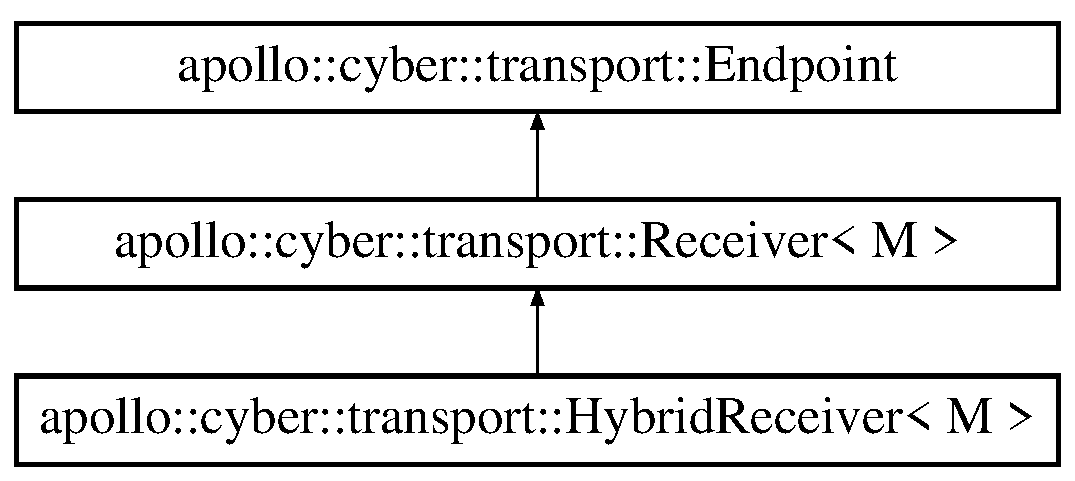
\includegraphics[height=3.000000cm]{classapollo_1_1cyber_1_1transport_1_1HybridReceiver}
\end{center}
\end{figure}
\subsection*{Public Types}
\begin{DoxyCompactItemize}
\item 
using \hyperlink{classapollo_1_1cyber_1_1transport_1_1HybridReceiver_a29d008855b7b25d060137a19da928c53}{History\-Ptr} = std\-::shared\-\_\-ptr$<$ \hyperlink{classapollo_1_1cyber_1_1transport_1_1History}{History}$<$ M $>$$>$
\item 
using \hyperlink{classapollo_1_1cyber_1_1transport_1_1HybridReceiver_aa59a9c5e8a30dd56cd84e1a463d05e7c}{Receiver\-Ptr} = std\-::shared\-\_\-ptr$<$ \hyperlink{classapollo_1_1cyber_1_1transport_1_1Receiver}{Receiver}$<$ M $>$$>$
\item 
using \hyperlink{classapollo_1_1cyber_1_1transport_1_1HybridReceiver_a70475c40e8f9c33ebd8126df3ab71e18}{Receiver\-Container} = std\-::unordered\-\_\-map$<$ Optional\-Mode, \hyperlink{classapollo_1_1cyber_1_1transport_1_1HybridReceiver_aa59a9c5e8a30dd56cd84e1a463d05e7c}{Receiver\-Ptr}, std\-::hash$<$ int $>$$>$
\item 
using \hyperlink{classapollo_1_1cyber_1_1transport_1_1HybridReceiver_a6295cabae20a58ee02454f59d9c09986}{Transmitter\-Container} = std\-::unordered\-\_\-map$<$ Optional\-Mode, std\-::unordered\-\_\-map$<$ uint64\-\_\-t, Role\-Attributes $>$, std\-::hash$<$ int $>$$>$
\item 
using \hyperlink{classapollo_1_1cyber_1_1transport_1_1HybridReceiver_aec763c6c2f52e839f873b00193627626}{Communication\-Mode\-Ptr} = std\-::shared\-\_\-ptr$<$ proto\-::\-Communication\-Mode $>$
\item 
using \hyperlink{classapollo_1_1cyber_1_1transport_1_1HybridReceiver_abefb4dc42db917f5891670997814231c}{Mapping\-Table} = std\-::unordered\-\_\-map$<$ \hyperlink{namespaceapollo_1_1cyber_a688ac951fd0a3965da4acdc34c92e50f}{Relation}, Optional\-Mode, std\-::hash$<$ int $>$$>$
\end{DoxyCompactItemize}
\subsection*{Public Member Functions}
\begin{DoxyCompactItemize}
\item 
\hyperlink{classapollo_1_1cyber_1_1transport_1_1HybridReceiver_a626fda476274421711a50146d6218a69}{Hybrid\-Receiver} (const Role\-Attributes \&attr, const typename \hyperlink{classapollo_1_1cyber_1_1transport_1_1Receiver}{Receiver}$<$ M $>$\-::\hyperlink{classapollo_1_1cyber_1_1transport_1_1Receiver_abd906fd03582b49acbdc81b48a8974aa}{Message\-Listener} \&msg\-\_\-listener, const \hyperlink{namespaceapollo_1_1cyber_1_1transport_a4214d0780331276d0384d0b57e3bc688}{Participant\-Ptr} \&participant)
\item 
virtual \hyperlink{classapollo_1_1cyber_1_1transport_1_1HybridReceiver_ade26db508c0a771c4bf26ef3077d3fd9}{$\sim$\-Hybrid\-Receiver} ()
\item 
void \hyperlink{classapollo_1_1cyber_1_1transport_1_1HybridReceiver_a38add467c1fe59a584dac3a31b141c7c}{Enable} () override
\item 
void \hyperlink{classapollo_1_1cyber_1_1transport_1_1HybridReceiver_a90ed14fc589847bd9d5c7b8e1f3e4fd6}{Disable} () override
\item 
void \hyperlink{classapollo_1_1cyber_1_1transport_1_1HybridReceiver_aa4ec9837875d4f508be7f9098a69e5cb}{Enable} (const Role\-Attributes \&opposite\-\_\-attr) override
\item 
void \hyperlink{classapollo_1_1cyber_1_1transport_1_1HybridReceiver_ae4c99434d96215e60580dd14622c4482}{Disable} (const Role\-Attributes \&opposite\-\_\-attr) override
\end{DoxyCompactItemize}
\subsection*{Private Member Functions}
\begin{DoxyCompactItemize}
\item 
void \hyperlink{classapollo_1_1cyber_1_1transport_1_1HybridReceiver_a1eb6243268daf94d62199f2b5d20a4b4}{Init\-Mode} ()
\item 
void \hyperlink{classapollo_1_1cyber_1_1transport_1_1HybridReceiver_a8dad1a54fe3805615e08aeba16392ef6}{Obtain\-Config} ()
\item 
void \hyperlink{classapollo_1_1cyber_1_1transport_1_1HybridReceiver_ac144d497bd484cb2e9882776eb7e0076}{Init\-History} ()
\item 
void \hyperlink{classapollo_1_1cyber_1_1transport_1_1HybridReceiver_a4e2c7f8785a008d9264582b16d19c61e}{Init\-Receivers} ()
\item 
void \hyperlink{classapollo_1_1cyber_1_1transport_1_1HybridReceiver_a8952919c3a6b3b0bf7b7b8b0f0d79f5a}{Clear\-Receivers} ()
\item 
void \hyperlink{classapollo_1_1cyber_1_1transport_1_1HybridReceiver_acadee13b8b6a22395f46b21fe7549614}{Init\-Transmitters} ()
\item 
void \hyperlink{classapollo_1_1cyber_1_1transport_1_1HybridReceiver_a16139e677ea56e82a51c78bd72587ae8}{Clear\-Transmitters} ()
\item 
void \hyperlink{classapollo_1_1cyber_1_1transport_1_1HybridReceiver_a67017f9439548f98a30c6dcc1f7431f9}{Receive\-History\-Msg} (const Role\-Attributes \&opposite\-\_\-attr)
\item 
void \hyperlink{classapollo_1_1cyber_1_1transport_1_1HybridReceiver_a300e68502aada5c5d92fe47d50b4c153}{Thread\-Func} (const Role\-Attributes \&opposite\-\_\-attr)
\item 
\hyperlink{namespaceapollo_1_1cyber_a688ac951fd0a3965da4acdc34c92e50f}{Relation} \hyperlink{classapollo_1_1cyber_1_1transport_1_1HybridReceiver_ac899b765428d18b737c5bc40b5fdde7d}{Get\-Relation} (const Role\-Attributes \&opposite\-\_\-attr)
\end{DoxyCompactItemize}
\subsection*{Private Attributes}
\begin{DoxyCompactItemize}
\item 
\hyperlink{classapollo_1_1cyber_1_1transport_1_1HybridReceiver_a29d008855b7b25d060137a19da928c53}{History\-Ptr} \hyperlink{classapollo_1_1cyber_1_1transport_1_1HybridReceiver_a71fe92773a83ee153382b6b7f9e8c8a7}{history\-\_\-}
\item 
\hyperlink{classapollo_1_1cyber_1_1transport_1_1HybridReceiver_a70475c40e8f9c33ebd8126df3ab71e18}{Receiver\-Container} \hyperlink{classapollo_1_1cyber_1_1transport_1_1HybridReceiver_a1f74e7e19cf92397729389922da60d57}{receivers\-\_\-}
\item 
\hyperlink{classapollo_1_1cyber_1_1transport_1_1HybridReceiver_a6295cabae20a58ee02454f59d9c09986}{Transmitter\-Container} \hyperlink{classapollo_1_1cyber_1_1transport_1_1HybridReceiver_a0763ec6d7247a952123cdc5a0c2fa7f2}{transmitters\-\_\-}
\item 
std\-::mutex \hyperlink{classapollo_1_1cyber_1_1transport_1_1HybridReceiver_acd72be19a7680b7c7e87593e7803f016}{mutex\-\_\-}
\item 
\hyperlink{classapollo_1_1cyber_1_1transport_1_1HybridReceiver_aec763c6c2f52e839f873b00193627626}{Communication\-Mode\-Ptr} \hyperlink{classapollo_1_1cyber_1_1transport_1_1HybridReceiver_a2b1451e2a1668ed26172ebaf33520e58}{mode\-\_\-}
\item 
\hyperlink{classapollo_1_1cyber_1_1transport_1_1HybridReceiver_abefb4dc42db917f5891670997814231c}{Mapping\-Table} \hyperlink{classapollo_1_1cyber_1_1transport_1_1HybridReceiver_aee5d1880835e3edba742fbcf89478e2d}{mapping\-\_\-table\-\_\-}
\item 
\hyperlink{namespaceapollo_1_1cyber_1_1transport_a4214d0780331276d0384d0b57e3bc688}{Participant\-Ptr} \hyperlink{classapollo_1_1cyber_1_1transport_1_1HybridReceiver_ae166879e80acc07e56f178f50eac3fd4}{participant\-\_\-}
\end{DoxyCompactItemize}
\subsection*{Additional Inherited Members}


\subsection{Member Typedef Documentation}
\hypertarget{classapollo_1_1cyber_1_1transport_1_1HybridReceiver_aec763c6c2f52e839f873b00193627626}{\index{apollo\-::cyber\-::transport\-::\-Hybrid\-Receiver@{apollo\-::cyber\-::transport\-::\-Hybrid\-Receiver}!Communication\-Mode\-Ptr@{Communication\-Mode\-Ptr}}
\index{Communication\-Mode\-Ptr@{Communication\-Mode\-Ptr}!apollo::cyber::transport::HybridReceiver@{apollo\-::cyber\-::transport\-::\-Hybrid\-Receiver}}
\subsubsection[{Communication\-Mode\-Ptr}]{\setlength{\rightskip}{0pt plus 5cm}template$<$typename M $>$ using {\bf apollo\-::cyber\-::transport\-::\-Hybrid\-Receiver}$<$ M $>$\-::{\bf Communication\-Mode\-Ptr} =  std\-::shared\-\_\-ptr$<$proto\-::\-Communication\-Mode$>$}}\label{classapollo_1_1cyber_1_1transport_1_1HybridReceiver_aec763c6c2f52e839f873b00193627626}
\hypertarget{classapollo_1_1cyber_1_1transport_1_1HybridReceiver_a29d008855b7b25d060137a19da928c53}{\index{apollo\-::cyber\-::transport\-::\-Hybrid\-Receiver@{apollo\-::cyber\-::transport\-::\-Hybrid\-Receiver}!History\-Ptr@{History\-Ptr}}
\index{History\-Ptr@{History\-Ptr}!apollo::cyber::transport::HybridReceiver@{apollo\-::cyber\-::transport\-::\-Hybrid\-Receiver}}
\subsubsection[{History\-Ptr}]{\setlength{\rightskip}{0pt plus 5cm}template$<$typename M $>$ using {\bf apollo\-::cyber\-::transport\-::\-Hybrid\-Receiver}$<$ M $>$\-::{\bf History\-Ptr} =  std\-::shared\-\_\-ptr$<${\bf History}$<$M$>$$>$}}\label{classapollo_1_1cyber_1_1transport_1_1HybridReceiver_a29d008855b7b25d060137a19da928c53}
\hypertarget{classapollo_1_1cyber_1_1transport_1_1HybridReceiver_abefb4dc42db917f5891670997814231c}{\index{apollo\-::cyber\-::transport\-::\-Hybrid\-Receiver@{apollo\-::cyber\-::transport\-::\-Hybrid\-Receiver}!Mapping\-Table@{Mapping\-Table}}
\index{Mapping\-Table@{Mapping\-Table}!apollo::cyber::transport::HybridReceiver@{apollo\-::cyber\-::transport\-::\-Hybrid\-Receiver}}
\subsubsection[{Mapping\-Table}]{\setlength{\rightskip}{0pt plus 5cm}template$<$typename M $>$ using {\bf apollo\-::cyber\-::transport\-::\-Hybrid\-Receiver}$<$ M $>$\-::{\bf Mapping\-Table} =  std\-::unordered\-\_\-map$<${\bf Relation}, Optional\-Mode, std\-::hash$<$int$>$$>$}}\label{classapollo_1_1cyber_1_1transport_1_1HybridReceiver_abefb4dc42db917f5891670997814231c}
\hypertarget{classapollo_1_1cyber_1_1transport_1_1HybridReceiver_a70475c40e8f9c33ebd8126df3ab71e18}{\index{apollo\-::cyber\-::transport\-::\-Hybrid\-Receiver@{apollo\-::cyber\-::transport\-::\-Hybrid\-Receiver}!Receiver\-Container@{Receiver\-Container}}
\index{Receiver\-Container@{Receiver\-Container}!apollo::cyber::transport::HybridReceiver@{apollo\-::cyber\-::transport\-::\-Hybrid\-Receiver}}
\subsubsection[{Receiver\-Container}]{\setlength{\rightskip}{0pt plus 5cm}template$<$typename M $>$ using {\bf apollo\-::cyber\-::transport\-::\-Hybrid\-Receiver}$<$ M $>$\-::{\bf Receiver\-Container} =  std\-::unordered\-\_\-map$<$Optional\-Mode, {\bf Receiver\-Ptr}, std\-::hash$<$int$>$$>$}}\label{classapollo_1_1cyber_1_1transport_1_1HybridReceiver_a70475c40e8f9c33ebd8126df3ab71e18}
\hypertarget{classapollo_1_1cyber_1_1transport_1_1HybridReceiver_aa59a9c5e8a30dd56cd84e1a463d05e7c}{\index{apollo\-::cyber\-::transport\-::\-Hybrid\-Receiver@{apollo\-::cyber\-::transport\-::\-Hybrid\-Receiver}!Receiver\-Ptr@{Receiver\-Ptr}}
\index{Receiver\-Ptr@{Receiver\-Ptr}!apollo::cyber::transport::HybridReceiver@{apollo\-::cyber\-::transport\-::\-Hybrid\-Receiver}}
\subsubsection[{Receiver\-Ptr}]{\setlength{\rightskip}{0pt plus 5cm}template$<$typename M $>$ using {\bf apollo\-::cyber\-::transport\-::\-Hybrid\-Receiver}$<$ M $>$\-::{\bf Receiver\-Ptr} =  std\-::shared\-\_\-ptr$<${\bf Receiver}$<$M$>$$>$}}\label{classapollo_1_1cyber_1_1transport_1_1HybridReceiver_aa59a9c5e8a30dd56cd84e1a463d05e7c}
\hypertarget{classapollo_1_1cyber_1_1transport_1_1HybridReceiver_a6295cabae20a58ee02454f59d9c09986}{\index{apollo\-::cyber\-::transport\-::\-Hybrid\-Receiver@{apollo\-::cyber\-::transport\-::\-Hybrid\-Receiver}!Transmitter\-Container@{Transmitter\-Container}}
\index{Transmitter\-Container@{Transmitter\-Container}!apollo::cyber::transport::HybridReceiver@{apollo\-::cyber\-::transport\-::\-Hybrid\-Receiver}}
\subsubsection[{Transmitter\-Container}]{\setlength{\rightskip}{0pt plus 5cm}template$<$typename M $>$ using {\bf apollo\-::cyber\-::transport\-::\-Hybrid\-Receiver}$<$ M $>$\-::{\bf Transmitter\-Container} =  std\-::unordered\-\_\-map$<$Optional\-Mode, std\-::unordered\-\_\-map$<$uint64\-\_\-t, Role\-Attributes$>$, std\-::hash$<$int$>$$>$}}\label{classapollo_1_1cyber_1_1transport_1_1HybridReceiver_a6295cabae20a58ee02454f59d9c09986}


\subsection{Constructor \& Destructor Documentation}
\hypertarget{classapollo_1_1cyber_1_1transport_1_1HybridReceiver_a626fda476274421711a50146d6218a69}{\index{apollo\-::cyber\-::transport\-::\-Hybrid\-Receiver@{apollo\-::cyber\-::transport\-::\-Hybrid\-Receiver}!Hybrid\-Receiver@{Hybrid\-Receiver}}
\index{Hybrid\-Receiver@{Hybrid\-Receiver}!apollo::cyber::transport::HybridReceiver@{apollo\-::cyber\-::transport\-::\-Hybrid\-Receiver}}
\subsubsection[{Hybrid\-Receiver}]{\setlength{\rightskip}{0pt plus 5cm}template$<$typename M $>$ {\bf apollo\-::cyber\-::transport\-::\-Hybrid\-Receiver}$<$ M $>$\-::{\bf Hybrid\-Receiver} (
\begin{DoxyParamCaption}
\item[{const Role\-Attributes \&}]{attr, }
\item[{const typename {\bf Receiver}$<$ M $>$\-::{\bf Message\-Listener} \&}]{msg\-\_\-listener, }
\item[{const {\bf Participant\-Ptr} \&}]{participant}
\end{DoxyParamCaption}
)}}\label{classapollo_1_1cyber_1_1transport_1_1HybridReceiver_a626fda476274421711a50146d6218a69}
\hypertarget{classapollo_1_1cyber_1_1transport_1_1HybridReceiver_ade26db508c0a771c4bf26ef3077d3fd9}{\index{apollo\-::cyber\-::transport\-::\-Hybrid\-Receiver@{apollo\-::cyber\-::transport\-::\-Hybrid\-Receiver}!$\sim$\-Hybrid\-Receiver@{$\sim$\-Hybrid\-Receiver}}
\index{$\sim$\-Hybrid\-Receiver@{$\sim$\-Hybrid\-Receiver}!apollo::cyber::transport::HybridReceiver@{apollo\-::cyber\-::transport\-::\-Hybrid\-Receiver}}
\subsubsection[{$\sim$\-Hybrid\-Receiver}]{\setlength{\rightskip}{0pt plus 5cm}template$<$typename M $>$ {\bf apollo\-::cyber\-::transport\-::\-Hybrid\-Receiver}$<$ M $>$\-::$\sim${\bf Hybrid\-Receiver} (
\begin{DoxyParamCaption}
{}
\end{DoxyParamCaption}
)\hspace{0.3cm}{\ttfamily [virtual]}}}\label{classapollo_1_1cyber_1_1transport_1_1HybridReceiver_ade26db508c0a771c4bf26ef3077d3fd9}


\subsection{Member Function Documentation}
\hypertarget{classapollo_1_1cyber_1_1transport_1_1HybridReceiver_a8952919c3a6b3b0bf7b7b8b0f0d79f5a}{\index{apollo\-::cyber\-::transport\-::\-Hybrid\-Receiver@{apollo\-::cyber\-::transport\-::\-Hybrid\-Receiver}!Clear\-Receivers@{Clear\-Receivers}}
\index{Clear\-Receivers@{Clear\-Receivers}!apollo::cyber::transport::HybridReceiver@{apollo\-::cyber\-::transport\-::\-Hybrid\-Receiver}}
\subsubsection[{Clear\-Receivers}]{\setlength{\rightskip}{0pt plus 5cm}template$<$typename M $>$ void {\bf apollo\-::cyber\-::transport\-::\-Hybrid\-Receiver}$<$ M $>$\-::Clear\-Receivers (
\begin{DoxyParamCaption}
{}
\end{DoxyParamCaption}
)\hspace{0.3cm}{\ttfamily [private]}}}\label{classapollo_1_1cyber_1_1transport_1_1HybridReceiver_a8952919c3a6b3b0bf7b7b8b0f0d79f5a}
\hypertarget{classapollo_1_1cyber_1_1transport_1_1HybridReceiver_a16139e677ea56e82a51c78bd72587ae8}{\index{apollo\-::cyber\-::transport\-::\-Hybrid\-Receiver@{apollo\-::cyber\-::transport\-::\-Hybrid\-Receiver}!Clear\-Transmitters@{Clear\-Transmitters}}
\index{Clear\-Transmitters@{Clear\-Transmitters}!apollo::cyber::transport::HybridReceiver@{apollo\-::cyber\-::transport\-::\-Hybrid\-Receiver}}
\subsubsection[{Clear\-Transmitters}]{\setlength{\rightskip}{0pt plus 5cm}template$<$typename M $>$ void {\bf apollo\-::cyber\-::transport\-::\-Hybrid\-Receiver}$<$ M $>$\-::Clear\-Transmitters (
\begin{DoxyParamCaption}
{}
\end{DoxyParamCaption}
)\hspace{0.3cm}{\ttfamily [private]}}}\label{classapollo_1_1cyber_1_1transport_1_1HybridReceiver_a16139e677ea56e82a51c78bd72587ae8}
\hypertarget{classapollo_1_1cyber_1_1transport_1_1HybridReceiver_a90ed14fc589847bd9d5c7b8e1f3e4fd6}{\index{apollo\-::cyber\-::transport\-::\-Hybrid\-Receiver@{apollo\-::cyber\-::transport\-::\-Hybrid\-Receiver}!Disable@{Disable}}
\index{Disable@{Disable}!apollo::cyber::transport::HybridReceiver@{apollo\-::cyber\-::transport\-::\-Hybrid\-Receiver}}
\subsubsection[{Disable}]{\setlength{\rightskip}{0pt plus 5cm}template$<$typename M $>$ void {\bf apollo\-::cyber\-::transport\-::\-Hybrid\-Receiver}$<$ M $>$\-::Disable (
\begin{DoxyParamCaption}
{}
\end{DoxyParamCaption}
)\hspace{0.3cm}{\ttfamily [override]}, {\ttfamily [virtual]}}}\label{classapollo_1_1cyber_1_1transport_1_1HybridReceiver_a90ed14fc589847bd9d5c7b8e1f3e4fd6}


Implements \hyperlink{classapollo_1_1cyber_1_1transport_1_1Receiver_af9f317df425a33bc364662a59be28bf5}{apollo\-::cyber\-::transport\-::\-Receiver$<$ M $>$}.

\hypertarget{classapollo_1_1cyber_1_1transport_1_1HybridReceiver_ae4c99434d96215e60580dd14622c4482}{\index{apollo\-::cyber\-::transport\-::\-Hybrid\-Receiver@{apollo\-::cyber\-::transport\-::\-Hybrid\-Receiver}!Disable@{Disable}}
\index{Disable@{Disable}!apollo::cyber::transport::HybridReceiver@{apollo\-::cyber\-::transport\-::\-Hybrid\-Receiver}}
\subsubsection[{Disable}]{\setlength{\rightskip}{0pt plus 5cm}template$<$typename M $>$ void {\bf apollo\-::cyber\-::transport\-::\-Hybrid\-Receiver}$<$ M $>$\-::Disable (
\begin{DoxyParamCaption}
\item[{const Role\-Attributes \&}]{opposite\-\_\-attr}
\end{DoxyParamCaption}
)\hspace{0.3cm}{\ttfamily [override]}, {\ttfamily [virtual]}}}\label{classapollo_1_1cyber_1_1transport_1_1HybridReceiver_ae4c99434d96215e60580dd14622c4482}


Implements \hyperlink{classapollo_1_1cyber_1_1transport_1_1Receiver_a26a4b466924d472f830f856b675bb44a}{apollo\-::cyber\-::transport\-::\-Receiver$<$ M $>$}.

\hypertarget{classapollo_1_1cyber_1_1transport_1_1HybridReceiver_a38add467c1fe59a584dac3a31b141c7c}{\index{apollo\-::cyber\-::transport\-::\-Hybrid\-Receiver@{apollo\-::cyber\-::transport\-::\-Hybrid\-Receiver}!Enable@{Enable}}
\index{Enable@{Enable}!apollo::cyber::transport::HybridReceiver@{apollo\-::cyber\-::transport\-::\-Hybrid\-Receiver}}
\subsubsection[{Enable}]{\setlength{\rightskip}{0pt plus 5cm}template$<$typename M $>$ void {\bf apollo\-::cyber\-::transport\-::\-Hybrid\-Receiver}$<$ M $>$\-::Enable (
\begin{DoxyParamCaption}
{}
\end{DoxyParamCaption}
)\hspace{0.3cm}{\ttfamily [override]}, {\ttfamily [virtual]}}}\label{classapollo_1_1cyber_1_1transport_1_1HybridReceiver_a38add467c1fe59a584dac3a31b141c7c}


Implements \hyperlink{classapollo_1_1cyber_1_1transport_1_1Receiver_a77c93406c2ab9254562d595bfaecabbc}{apollo\-::cyber\-::transport\-::\-Receiver$<$ M $>$}.

\hypertarget{classapollo_1_1cyber_1_1transport_1_1HybridReceiver_aa4ec9837875d4f508be7f9098a69e5cb}{\index{apollo\-::cyber\-::transport\-::\-Hybrid\-Receiver@{apollo\-::cyber\-::transport\-::\-Hybrid\-Receiver}!Enable@{Enable}}
\index{Enable@{Enable}!apollo::cyber::transport::HybridReceiver@{apollo\-::cyber\-::transport\-::\-Hybrid\-Receiver}}
\subsubsection[{Enable}]{\setlength{\rightskip}{0pt plus 5cm}template$<$typename M $>$ void {\bf apollo\-::cyber\-::transport\-::\-Hybrid\-Receiver}$<$ M $>$\-::Enable (
\begin{DoxyParamCaption}
\item[{const Role\-Attributes \&}]{opposite\-\_\-attr}
\end{DoxyParamCaption}
)\hspace{0.3cm}{\ttfamily [override]}, {\ttfamily [virtual]}}}\label{classapollo_1_1cyber_1_1transport_1_1HybridReceiver_aa4ec9837875d4f508be7f9098a69e5cb}


Implements \hyperlink{classapollo_1_1cyber_1_1transport_1_1Receiver_a2436ecca6981d910911d359cd1df4610}{apollo\-::cyber\-::transport\-::\-Receiver$<$ M $>$}.

\hypertarget{classapollo_1_1cyber_1_1transport_1_1HybridReceiver_ac899b765428d18b737c5bc40b5fdde7d}{\index{apollo\-::cyber\-::transport\-::\-Hybrid\-Receiver@{apollo\-::cyber\-::transport\-::\-Hybrid\-Receiver}!Get\-Relation@{Get\-Relation}}
\index{Get\-Relation@{Get\-Relation}!apollo::cyber::transport::HybridReceiver@{apollo\-::cyber\-::transport\-::\-Hybrid\-Receiver}}
\subsubsection[{Get\-Relation}]{\setlength{\rightskip}{0pt plus 5cm}template$<$typename M $>$ {\bf Relation} {\bf apollo\-::cyber\-::transport\-::\-Hybrid\-Receiver}$<$ M $>$\-::Get\-Relation (
\begin{DoxyParamCaption}
\item[{const Role\-Attributes \&}]{opposite\-\_\-attr}
\end{DoxyParamCaption}
)\hspace{0.3cm}{\ttfamily [private]}}}\label{classapollo_1_1cyber_1_1transport_1_1HybridReceiver_ac899b765428d18b737c5bc40b5fdde7d}
\hypertarget{classapollo_1_1cyber_1_1transport_1_1HybridReceiver_ac144d497bd484cb2e9882776eb7e0076}{\index{apollo\-::cyber\-::transport\-::\-Hybrid\-Receiver@{apollo\-::cyber\-::transport\-::\-Hybrid\-Receiver}!Init\-History@{Init\-History}}
\index{Init\-History@{Init\-History}!apollo::cyber::transport::HybridReceiver@{apollo\-::cyber\-::transport\-::\-Hybrid\-Receiver}}
\subsubsection[{Init\-History}]{\setlength{\rightskip}{0pt plus 5cm}template$<$typename M $>$ void {\bf apollo\-::cyber\-::transport\-::\-Hybrid\-Receiver}$<$ M $>$\-::Init\-History (
\begin{DoxyParamCaption}
{}
\end{DoxyParamCaption}
)\hspace{0.3cm}{\ttfamily [private]}}}\label{classapollo_1_1cyber_1_1transport_1_1HybridReceiver_ac144d497bd484cb2e9882776eb7e0076}
\hypertarget{classapollo_1_1cyber_1_1transport_1_1HybridReceiver_a1eb6243268daf94d62199f2b5d20a4b4}{\index{apollo\-::cyber\-::transport\-::\-Hybrid\-Receiver@{apollo\-::cyber\-::transport\-::\-Hybrid\-Receiver}!Init\-Mode@{Init\-Mode}}
\index{Init\-Mode@{Init\-Mode}!apollo::cyber::transport::HybridReceiver@{apollo\-::cyber\-::transport\-::\-Hybrid\-Receiver}}
\subsubsection[{Init\-Mode}]{\setlength{\rightskip}{0pt plus 5cm}template$<$typename M $>$ void {\bf apollo\-::cyber\-::transport\-::\-Hybrid\-Receiver}$<$ M $>$\-::Init\-Mode (
\begin{DoxyParamCaption}
{}
\end{DoxyParamCaption}
)\hspace{0.3cm}{\ttfamily [private]}}}\label{classapollo_1_1cyber_1_1transport_1_1HybridReceiver_a1eb6243268daf94d62199f2b5d20a4b4}
\hypertarget{classapollo_1_1cyber_1_1transport_1_1HybridReceiver_a4e2c7f8785a008d9264582b16d19c61e}{\index{apollo\-::cyber\-::transport\-::\-Hybrid\-Receiver@{apollo\-::cyber\-::transport\-::\-Hybrid\-Receiver}!Init\-Receivers@{Init\-Receivers}}
\index{Init\-Receivers@{Init\-Receivers}!apollo::cyber::transport::HybridReceiver@{apollo\-::cyber\-::transport\-::\-Hybrid\-Receiver}}
\subsubsection[{Init\-Receivers}]{\setlength{\rightskip}{0pt plus 5cm}template$<$typename M $>$ void {\bf apollo\-::cyber\-::transport\-::\-Hybrid\-Receiver}$<$ M $>$\-::Init\-Receivers (
\begin{DoxyParamCaption}
{}
\end{DoxyParamCaption}
)\hspace{0.3cm}{\ttfamily [private]}}}\label{classapollo_1_1cyber_1_1transport_1_1HybridReceiver_a4e2c7f8785a008d9264582b16d19c61e}
\hypertarget{classapollo_1_1cyber_1_1transport_1_1HybridReceiver_acadee13b8b6a22395f46b21fe7549614}{\index{apollo\-::cyber\-::transport\-::\-Hybrid\-Receiver@{apollo\-::cyber\-::transport\-::\-Hybrid\-Receiver}!Init\-Transmitters@{Init\-Transmitters}}
\index{Init\-Transmitters@{Init\-Transmitters}!apollo::cyber::transport::HybridReceiver@{apollo\-::cyber\-::transport\-::\-Hybrid\-Receiver}}
\subsubsection[{Init\-Transmitters}]{\setlength{\rightskip}{0pt plus 5cm}template$<$typename M $>$ void {\bf apollo\-::cyber\-::transport\-::\-Hybrid\-Receiver}$<$ M $>$\-::Init\-Transmitters (
\begin{DoxyParamCaption}
{}
\end{DoxyParamCaption}
)\hspace{0.3cm}{\ttfamily [private]}}}\label{classapollo_1_1cyber_1_1transport_1_1HybridReceiver_acadee13b8b6a22395f46b21fe7549614}
\hypertarget{classapollo_1_1cyber_1_1transport_1_1HybridReceiver_a8dad1a54fe3805615e08aeba16392ef6}{\index{apollo\-::cyber\-::transport\-::\-Hybrid\-Receiver@{apollo\-::cyber\-::transport\-::\-Hybrid\-Receiver}!Obtain\-Config@{Obtain\-Config}}
\index{Obtain\-Config@{Obtain\-Config}!apollo::cyber::transport::HybridReceiver@{apollo\-::cyber\-::transport\-::\-Hybrid\-Receiver}}
\subsubsection[{Obtain\-Config}]{\setlength{\rightskip}{0pt plus 5cm}template$<$typename M $>$ void {\bf apollo\-::cyber\-::transport\-::\-Hybrid\-Receiver}$<$ M $>$\-::Obtain\-Config (
\begin{DoxyParamCaption}
{}
\end{DoxyParamCaption}
)\hspace{0.3cm}{\ttfamily [private]}}}\label{classapollo_1_1cyber_1_1transport_1_1HybridReceiver_a8dad1a54fe3805615e08aeba16392ef6}
\hypertarget{classapollo_1_1cyber_1_1transport_1_1HybridReceiver_a67017f9439548f98a30c6dcc1f7431f9}{\index{apollo\-::cyber\-::transport\-::\-Hybrid\-Receiver@{apollo\-::cyber\-::transport\-::\-Hybrid\-Receiver}!Receive\-History\-Msg@{Receive\-History\-Msg}}
\index{Receive\-History\-Msg@{Receive\-History\-Msg}!apollo::cyber::transport::HybridReceiver@{apollo\-::cyber\-::transport\-::\-Hybrid\-Receiver}}
\subsubsection[{Receive\-History\-Msg}]{\setlength{\rightskip}{0pt plus 5cm}template$<$typename M $>$ void {\bf apollo\-::cyber\-::transport\-::\-Hybrid\-Receiver}$<$ M $>$\-::Receive\-History\-Msg (
\begin{DoxyParamCaption}
\item[{const Role\-Attributes \&}]{opposite\-\_\-attr}
\end{DoxyParamCaption}
)\hspace{0.3cm}{\ttfamily [private]}}}\label{classapollo_1_1cyber_1_1transport_1_1HybridReceiver_a67017f9439548f98a30c6dcc1f7431f9}
\hypertarget{classapollo_1_1cyber_1_1transport_1_1HybridReceiver_a300e68502aada5c5d92fe47d50b4c153}{\index{apollo\-::cyber\-::transport\-::\-Hybrid\-Receiver@{apollo\-::cyber\-::transport\-::\-Hybrid\-Receiver}!Thread\-Func@{Thread\-Func}}
\index{Thread\-Func@{Thread\-Func}!apollo::cyber::transport::HybridReceiver@{apollo\-::cyber\-::transport\-::\-Hybrid\-Receiver}}
\subsubsection[{Thread\-Func}]{\setlength{\rightskip}{0pt plus 5cm}template$<$typename M $>$ void {\bf apollo\-::cyber\-::transport\-::\-Hybrid\-Receiver}$<$ M $>$\-::Thread\-Func (
\begin{DoxyParamCaption}
\item[{const Role\-Attributes \&}]{opposite\-\_\-attr}
\end{DoxyParamCaption}
)\hspace{0.3cm}{\ttfamily [private]}}}\label{classapollo_1_1cyber_1_1transport_1_1HybridReceiver_a300e68502aada5c5d92fe47d50b4c153}


\subsection{Member Data Documentation}
\hypertarget{classapollo_1_1cyber_1_1transport_1_1HybridReceiver_a71fe92773a83ee153382b6b7f9e8c8a7}{\index{apollo\-::cyber\-::transport\-::\-Hybrid\-Receiver@{apollo\-::cyber\-::transport\-::\-Hybrid\-Receiver}!history\-\_\-@{history\-\_\-}}
\index{history\-\_\-@{history\-\_\-}!apollo::cyber::transport::HybridReceiver@{apollo\-::cyber\-::transport\-::\-Hybrid\-Receiver}}
\subsubsection[{history\-\_\-}]{\setlength{\rightskip}{0pt plus 5cm}template$<$typename M $>$ {\bf History\-Ptr} {\bf apollo\-::cyber\-::transport\-::\-Hybrid\-Receiver}$<$ M $>$\-::history\-\_\-\hspace{0.3cm}{\ttfamily [private]}}}\label{classapollo_1_1cyber_1_1transport_1_1HybridReceiver_a71fe92773a83ee153382b6b7f9e8c8a7}
\hypertarget{classapollo_1_1cyber_1_1transport_1_1HybridReceiver_aee5d1880835e3edba742fbcf89478e2d}{\index{apollo\-::cyber\-::transport\-::\-Hybrid\-Receiver@{apollo\-::cyber\-::transport\-::\-Hybrid\-Receiver}!mapping\-\_\-table\-\_\-@{mapping\-\_\-table\-\_\-}}
\index{mapping\-\_\-table\-\_\-@{mapping\-\_\-table\-\_\-}!apollo::cyber::transport::HybridReceiver@{apollo\-::cyber\-::transport\-::\-Hybrid\-Receiver}}
\subsubsection[{mapping\-\_\-table\-\_\-}]{\setlength{\rightskip}{0pt plus 5cm}template$<$typename M $>$ {\bf Mapping\-Table} {\bf apollo\-::cyber\-::transport\-::\-Hybrid\-Receiver}$<$ M $>$\-::mapping\-\_\-table\-\_\-\hspace{0.3cm}{\ttfamily [private]}}}\label{classapollo_1_1cyber_1_1transport_1_1HybridReceiver_aee5d1880835e3edba742fbcf89478e2d}
\hypertarget{classapollo_1_1cyber_1_1transport_1_1HybridReceiver_a2b1451e2a1668ed26172ebaf33520e58}{\index{apollo\-::cyber\-::transport\-::\-Hybrid\-Receiver@{apollo\-::cyber\-::transport\-::\-Hybrid\-Receiver}!mode\-\_\-@{mode\-\_\-}}
\index{mode\-\_\-@{mode\-\_\-}!apollo::cyber::transport::HybridReceiver@{apollo\-::cyber\-::transport\-::\-Hybrid\-Receiver}}
\subsubsection[{mode\-\_\-}]{\setlength{\rightskip}{0pt plus 5cm}template$<$typename M $>$ {\bf Communication\-Mode\-Ptr} {\bf apollo\-::cyber\-::transport\-::\-Hybrid\-Receiver}$<$ M $>$\-::mode\-\_\-\hspace{0.3cm}{\ttfamily [private]}}}\label{classapollo_1_1cyber_1_1transport_1_1HybridReceiver_a2b1451e2a1668ed26172ebaf33520e58}
\hypertarget{classapollo_1_1cyber_1_1transport_1_1HybridReceiver_acd72be19a7680b7c7e87593e7803f016}{\index{apollo\-::cyber\-::transport\-::\-Hybrid\-Receiver@{apollo\-::cyber\-::transport\-::\-Hybrid\-Receiver}!mutex\-\_\-@{mutex\-\_\-}}
\index{mutex\-\_\-@{mutex\-\_\-}!apollo::cyber::transport::HybridReceiver@{apollo\-::cyber\-::transport\-::\-Hybrid\-Receiver}}
\subsubsection[{mutex\-\_\-}]{\setlength{\rightskip}{0pt plus 5cm}template$<$typename M $>$ std\-::mutex {\bf apollo\-::cyber\-::transport\-::\-Hybrid\-Receiver}$<$ M $>$\-::mutex\-\_\-\hspace{0.3cm}{\ttfamily [private]}}}\label{classapollo_1_1cyber_1_1transport_1_1HybridReceiver_acd72be19a7680b7c7e87593e7803f016}
\hypertarget{classapollo_1_1cyber_1_1transport_1_1HybridReceiver_ae166879e80acc07e56f178f50eac3fd4}{\index{apollo\-::cyber\-::transport\-::\-Hybrid\-Receiver@{apollo\-::cyber\-::transport\-::\-Hybrid\-Receiver}!participant\-\_\-@{participant\-\_\-}}
\index{participant\-\_\-@{participant\-\_\-}!apollo::cyber::transport::HybridReceiver@{apollo\-::cyber\-::transport\-::\-Hybrid\-Receiver}}
\subsubsection[{participant\-\_\-}]{\setlength{\rightskip}{0pt plus 5cm}template$<$typename M $>$ {\bf Participant\-Ptr} {\bf apollo\-::cyber\-::transport\-::\-Hybrid\-Receiver}$<$ M $>$\-::participant\-\_\-\hspace{0.3cm}{\ttfamily [private]}}}\label{classapollo_1_1cyber_1_1transport_1_1HybridReceiver_ae166879e80acc07e56f178f50eac3fd4}
\hypertarget{classapollo_1_1cyber_1_1transport_1_1HybridReceiver_a1f74e7e19cf92397729389922da60d57}{\index{apollo\-::cyber\-::transport\-::\-Hybrid\-Receiver@{apollo\-::cyber\-::transport\-::\-Hybrid\-Receiver}!receivers\-\_\-@{receivers\-\_\-}}
\index{receivers\-\_\-@{receivers\-\_\-}!apollo::cyber::transport::HybridReceiver@{apollo\-::cyber\-::transport\-::\-Hybrid\-Receiver}}
\subsubsection[{receivers\-\_\-}]{\setlength{\rightskip}{0pt plus 5cm}template$<$typename M $>$ {\bf Receiver\-Container} {\bf apollo\-::cyber\-::transport\-::\-Hybrid\-Receiver}$<$ M $>$\-::receivers\-\_\-\hspace{0.3cm}{\ttfamily [private]}}}\label{classapollo_1_1cyber_1_1transport_1_1HybridReceiver_a1f74e7e19cf92397729389922da60d57}
\hypertarget{classapollo_1_1cyber_1_1transport_1_1HybridReceiver_a0763ec6d7247a952123cdc5a0c2fa7f2}{\index{apollo\-::cyber\-::transport\-::\-Hybrid\-Receiver@{apollo\-::cyber\-::transport\-::\-Hybrid\-Receiver}!transmitters\-\_\-@{transmitters\-\_\-}}
\index{transmitters\-\_\-@{transmitters\-\_\-}!apollo::cyber::transport::HybridReceiver@{apollo\-::cyber\-::transport\-::\-Hybrid\-Receiver}}
\subsubsection[{transmitters\-\_\-}]{\setlength{\rightskip}{0pt plus 5cm}template$<$typename M $>$ {\bf Transmitter\-Container} {\bf apollo\-::cyber\-::transport\-::\-Hybrid\-Receiver}$<$ M $>$\-::transmitters\-\_\-\hspace{0.3cm}{\ttfamily [private]}}}\label{classapollo_1_1cyber_1_1transport_1_1HybridReceiver_a0763ec6d7247a952123cdc5a0c2fa7f2}


The documentation for this class was generated from the following file\-:\begin{DoxyCompactItemize}
\item 
transport/receiver/\hyperlink{hybrid__receiver_8h}{hybrid\-\_\-receiver.\-h}\end{DoxyCompactItemize}

\hypertarget{classapollo_1_1cyber_1_1transport_1_1HybridTransmitter}{\section{apollo\-:\-:cyber\-:\-:transport\-:\-:Hybrid\-Transmitter$<$ M $>$ Class Template Reference}
\label{classapollo_1_1cyber_1_1transport_1_1HybridTransmitter}\index{apollo\-::cyber\-::transport\-::\-Hybrid\-Transmitter$<$ M $>$@{apollo\-::cyber\-::transport\-::\-Hybrid\-Transmitter$<$ M $>$}}
}


{\ttfamily \#include $<$hybrid\-\_\-transmitter.\-h$>$}

Inheritance diagram for apollo\-:\-:cyber\-:\-:transport\-:\-:Hybrid\-Transmitter$<$ M $>$\-:\begin{figure}[H]
\begin{center}
\leavevmode
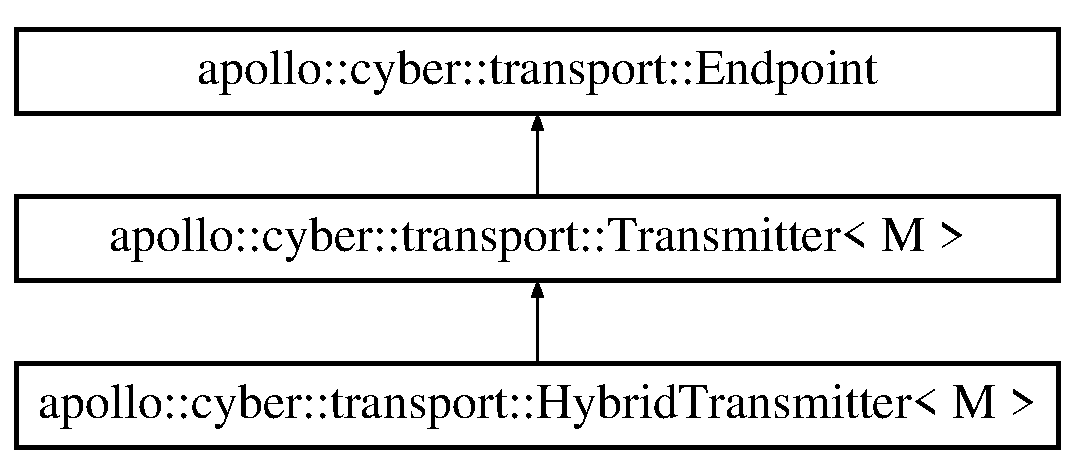
\includegraphics[height=3.000000cm]{classapollo_1_1cyber_1_1transport_1_1HybridTransmitter}
\end{center}
\end{figure}
\subsection*{Public Types}
\begin{DoxyCompactItemize}
\item 
using \hyperlink{classapollo_1_1cyber_1_1transport_1_1HybridTransmitter_ae4da0fb39a90d084d271b8522afc0881}{Message\-Ptr} = std\-::shared\-\_\-ptr$<$ M $>$
\item 
using \hyperlink{classapollo_1_1cyber_1_1transport_1_1HybridTransmitter_aee5ef32dcbaab6fcd68459e5f5afd6d8}{History\-Ptr} = std\-::shared\-\_\-ptr$<$ \hyperlink{classapollo_1_1cyber_1_1transport_1_1History}{History}$<$ M $>$$>$
\item 
using \hyperlink{classapollo_1_1cyber_1_1transport_1_1HybridTransmitter_ab5d6589b441adbb0aeebde895b21c569}{Transmitter\-Ptr} = std\-::shared\-\_\-ptr$<$ \hyperlink{classapollo_1_1cyber_1_1transport_1_1Transmitter}{Transmitter}$<$ M $>$$>$
\item 
using \hyperlink{classapollo_1_1cyber_1_1transport_1_1HybridTransmitter_a79fe84264b152838a2a921ca7c428d31}{Transmitter\-Map} = std\-::unordered\-\_\-map$<$ Optional\-Mode, \hyperlink{classapollo_1_1cyber_1_1transport_1_1HybridTransmitter_ab5d6589b441adbb0aeebde895b21c569}{Transmitter\-Ptr}, std\-::hash$<$ int $>$$>$
\item 
using \hyperlink{classapollo_1_1cyber_1_1transport_1_1HybridTransmitter_a57d8d230cedd2328577b9789ab964a5c}{Receiver\-Map} = std\-::unordered\-\_\-map$<$ Optional\-Mode, std\-::set$<$ uint64\-\_\-t $>$, std\-::hash$<$ int $>$$>$
\item 
using \hyperlink{classapollo_1_1cyber_1_1transport_1_1HybridTransmitter_aebca8e1bc93bfde3563c0c8b8c92bfa9}{Communication\-Mode\-Ptr} = std\-::shared\-\_\-ptr$<$ proto\-::\-Communication\-Mode $>$
\item 
using \hyperlink{classapollo_1_1cyber_1_1transport_1_1HybridTransmitter_a7073fcd5fe2232785a883a3f494d00ed}{Mapping\-Table} = std\-::unordered\-\_\-map$<$ \hyperlink{namespaceapollo_1_1cyber_a688ac951fd0a3965da4acdc34c92e50f}{Relation}, Optional\-Mode, std\-::hash$<$ int $>$$>$
\end{DoxyCompactItemize}
\subsection*{Public Member Functions}
\begin{DoxyCompactItemize}
\item 
\hyperlink{classapollo_1_1cyber_1_1transport_1_1HybridTransmitter_a90dae149351190abc01613a5a251e1df}{Hybrid\-Transmitter} (const Role\-Attributes \&attr, const \hyperlink{namespaceapollo_1_1cyber_1_1transport_a4214d0780331276d0384d0b57e3bc688}{Participant\-Ptr} \&participant)
\item 
virtual \hyperlink{classapollo_1_1cyber_1_1transport_1_1HybridTransmitter_acc4dd5cb2c487025c98495418e892839}{$\sim$\-Hybrid\-Transmitter} ()
\item 
void \hyperlink{classapollo_1_1cyber_1_1transport_1_1HybridTransmitter_af1d4c607ebc0c0fd5c28d0c3644ba333}{Enable} () override
\item 
void \hyperlink{classapollo_1_1cyber_1_1transport_1_1HybridTransmitter_a6bd7f1c0477247a80f79e6a845d7b3cd}{Disable} () override
\item 
void \hyperlink{classapollo_1_1cyber_1_1transport_1_1HybridTransmitter_a164dfe249d1bd676ccdeedd8eb1a9722}{Enable} (const Role\-Attributes \&opposite\-\_\-attr) override
\item 
void \hyperlink{classapollo_1_1cyber_1_1transport_1_1HybridTransmitter_affb916656d7c94753bc1fba374c0cc3c}{Disable} (const Role\-Attributes \&opposite\-\_\-attr) override
\item 
bool \hyperlink{classapollo_1_1cyber_1_1transport_1_1HybridTransmitter_a322bcb6a0b2fcff5ddb41b682605e333}{Transmit} (const \hyperlink{classapollo_1_1cyber_1_1transport_1_1HybridTransmitter_ae4da0fb39a90d084d271b8522afc0881}{Message\-Ptr} \&msg, const \hyperlink{classapollo_1_1cyber_1_1transport_1_1MessageInfo}{Message\-Info} \&msg\-\_\-info) override
\end{DoxyCompactItemize}
\subsection*{Private Member Functions}
\begin{DoxyCompactItemize}
\item 
void \hyperlink{classapollo_1_1cyber_1_1transport_1_1HybridTransmitter_a112c505ec2d012c405518a8d26221886}{Init\-Mode} ()
\item 
void \hyperlink{classapollo_1_1cyber_1_1transport_1_1HybridTransmitter_ad69e5147bff4f23df4c58ff0866d440b}{Obtain\-Config} ()
\item 
void \hyperlink{classapollo_1_1cyber_1_1transport_1_1HybridTransmitter_aafab9b42792093c316ac32c181e7d9ba}{Init\-History} ()
\item 
void \hyperlink{classapollo_1_1cyber_1_1transport_1_1HybridTransmitter_a9ee522016a1cedfc360067d759b0b04b}{Init\-Transmitters} ()
\item 
void \hyperlink{classapollo_1_1cyber_1_1transport_1_1HybridTransmitter_ad8fa4eec069e0ceb98273c50fe3ef00f}{Clear\-Transmitters} ()
\item 
void \hyperlink{classapollo_1_1cyber_1_1transport_1_1HybridTransmitter_a3b28ba5a4581e098d607d58d86002d20}{Init\-Receivers} ()
\item 
void \hyperlink{classapollo_1_1cyber_1_1transport_1_1HybridTransmitter_a138a7e206a9d937836dc3ee6f2bd0bdd}{Clear\-Receivers} ()
\item 
void \hyperlink{classapollo_1_1cyber_1_1transport_1_1HybridTransmitter_a6ba2d63c5a73fefbd628bef77951f8f0}{Transmit\-History\-Msg} (const Role\-Attributes \&opposite\-\_\-attr)
\item 
void \hyperlink{classapollo_1_1cyber_1_1transport_1_1HybridTransmitter_a03357a2fe13777d6c6408e49b6c9bb01}{Thread\-Func} (const Role\-Attributes \&opposite\-\_\-attr, const std\-::vector$<$ typename \hyperlink{classapollo_1_1cyber_1_1transport_1_1History}{History}$<$ M $>$\-::Cached\-Message $>$ \&msgs)
\item 
\hyperlink{namespaceapollo_1_1cyber_a688ac951fd0a3965da4acdc34c92e50f}{Relation} \hyperlink{classapollo_1_1cyber_1_1transport_1_1HybridTransmitter_ad71f1d4b5095d514a18e9efd2d249c9b}{Get\-Relation} (const Role\-Attributes \&opposite\-\_\-attr)
\end{DoxyCompactItemize}
\subsection*{Private Attributes}
\begin{DoxyCompactItemize}
\item 
\hyperlink{classapollo_1_1cyber_1_1transport_1_1HybridTransmitter_aee5ef32dcbaab6fcd68459e5f5afd6d8}{History\-Ptr} \hyperlink{classapollo_1_1cyber_1_1transport_1_1HybridTransmitter_a1017c9487fef9eabf20b6b6b29eda7a1}{history\-\_\-}
\item 
\hyperlink{classapollo_1_1cyber_1_1transport_1_1HybridTransmitter_a79fe84264b152838a2a921ca7c428d31}{Transmitter\-Map} \hyperlink{classapollo_1_1cyber_1_1transport_1_1HybridTransmitter_af892972e289032b86439449acb60fffe}{transmitters\-\_\-}
\item 
\hyperlink{classapollo_1_1cyber_1_1transport_1_1HybridTransmitter_a57d8d230cedd2328577b9789ab964a5c}{Receiver\-Map} \hyperlink{classapollo_1_1cyber_1_1transport_1_1HybridTransmitter_aa6ef011a6f48194c1472ed77694df9e2}{receivers\-\_\-}
\item 
std\-::mutex \hyperlink{classapollo_1_1cyber_1_1transport_1_1HybridTransmitter_a176663880b7f2fad09dfca0bbadd00bf}{mutex\-\_\-}
\item 
\hyperlink{classapollo_1_1cyber_1_1transport_1_1HybridTransmitter_aebca8e1bc93bfde3563c0c8b8c92bfa9}{Communication\-Mode\-Ptr} \hyperlink{classapollo_1_1cyber_1_1transport_1_1HybridTransmitter_a81a8c87167bf743445c97e903e3bffd1}{mode\-\_\-}
\item 
\hyperlink{classapollo_1_1cyber_1_1transport_1_1HybridTransmitter_a7073fcd5fe2232785a883a3f494d00ed}{Mapping\-Table} \hyperlink{classapollo_1_1cyber_1_1transport_1_1HybridTransmitter_a8002d94e9c7b130cc68cc7721e96a5e7}{mapping\-\_\-table\-\_\-}
\item 
\hyperlink{namespaceapollo_1_1cyber_1_1transport_a4214d0780331276d0384d0b57e3bc688}{Participant\-Ptr} \hyperlink{classapollo_1_1cyber_1_1transport_1_1HybridTransmitter_a7edc04c43198a2ff400e7ef9d41c5e18}{participant\-\_\-}
\end{DoxyCompactItemize}
\subsection*{Additional Inherited Members}


\subsection{Member Typedef Documentation}
\hypertarget{classapollo_1_1cyber_1_1transport_1_1HybridTransmitter_aebca8e1bc93bfde3563c0c8b8c92bfa9}{\index{apollo\-::cyber\-::transport\-::\-Hybrid\-Transmitter@{apollo\-::cyber\-::transport\-::\-Hybrid\-Transmitter}!Communication\-Mode\-Ptr@{Communication\-Mode\-Ptr}}
\index{Communication\-Mode\-Ptr@{Communication\-Mode\-Ptr}!apollo::cyber::transport::HybridTransmitter@{apollo\-::cyber\-::transport\-::\-Hybrid\-Transmitter}}
\subsubsection[{Communication\-Mode\-Ptr}]{\setlength{\rightskip}{0pt plus 5cm}template$<$typename M $>$ using {\bf apollo\-::cyber\-::transport\-::\-Hybrid\-Transmitter}$<$ M $>$\-::{\bf Communication\-Mode\-Ptr} =  std\-::shared\-\_\-ptr$<$proto\-::\-Communication\-Mode$>$}}\label{classapollo_1_1cyber_1_1transport_1_1HybridTransmitter_aebca8e1bc93bfde3563c0c8b8c92bfa9}
\hypertarget{classapollo_1_1cyber_1_1transport_1_1HybridTransmitter_aee5ef32dcbaab6fcd68459e5f5afd6d8}{\index{apollo\-::cyber\-::transport\-::\-Hybrid\-Transmitter@{apollo\-::cyber\-::transport\-::\-Hybrid\-Transmitter}!History\-Ptr@{History\-Ptr}}
\index{History\-Ptr@{History\-Ptr}!apollo::cyber::transport::HybridTransmitter@{apollo\-::cyber\-::transport\-::\-Hybrid\-Transmitter}}
\subsubsection[{History\-Ptr}]{\setlength{\rightskip}{0pt plus 5cm}template$<$typename M $>$ using {\bf apollo\-::cyber\-::transport\-::\-Hybrid\-Transmitter}$<$ M $>$\-::{\bf History\-Ptr} =  std\-::shared\-\_\-ptr$<${\bf History}$<$M$>$$>$}}\label{classapollo_1_1cyber_1_1transport_1_1HybridTransmitter_aee5ef32dcbaab6fcd68459e5f5afd6d8}
\hypertarget{classapollo_1_1cyber_1_1transport_1_1HybridTransmitter_a7073fcd5fe2232785a883a3f494d00ed}{\index{apollo\-::cyber\-::transport\-::\-Hybrid\-Transmitter@{apollo\-::cyber\-::transport\-::\-Hybrid\-Transmitter}!Mapping\-Table@{Mapping\-Table}}
\index{Mapping\-Table@{Mapping\-Table}!apollo::cyber::transport::HybridTransmitter@{apollo\-::cyber\-::transport\-::\-Hybrid\-Transmitter}}
\subsubsection[{Mapping\-Table}]{\setlength{\rightskip}{0pt plus 5cm}template$<$typename M $>$ using {\bf apollo\-::cyber\-::transport\-::\-Hybrid\-Transmitter}$<$ M $>$\-::{\bf Mapping\-Table} =  std\-::unordered\-\_\-map$<${\bf Relation}, Optional\-Mode, std\-::hash$<$int$>$$>$}}\label{classapollo_1_1cyber_1_1transport_1_1HybridTransmitter_a7073fcd5fe2232785a883a3f494d00ed}
\hypertarget{classapollo_1_1cyber_1_1transport_1_1HybridTransmitter_ae4da0fb39a90d084d271b8522afc0881}{\index{apollo\-::cyber\-::transport\-::\-Hybrid\-Transmitter@{apollo\-::cyber\-::transport\-::\-Hybrid\-Transmitter}!Message\-Ptr@{Message\-Ptr}}
\index{Message\-Ptr@{Message\-Ptr}!apollo::cyber::transport::HybridTransmitter@{apollo\-::cyber\-::transport\-::\-Hybrid\-Transmitter}}
\subsubsection[{Message\-Ptr}]{\setlength{\rightskip}{0pt plus 5cm}template$<$typename M $>$ using {\bf apollo\-::cyber\-::transport\-::\-Hybrid\-Transmitter}$<$ M $>$\-::{\bf Message\-Ptr} =  std\-::shared\-\_\-ptr$<$M$>$}}\label{classapollo_1_1cyber_1_1transport_1_1HybridTransmitter_ae4da0fb39a90d084d271b8522afc0881}
\hypertarget{classapollo_1_1cyber_1_1transport_1_1HybridTransmitter_a57d8d230cedd2328577b9789ab964a5c}{\index{apollo\-::cyber\-::transport\-::\-Hybrid\-Transmitter@{apollo\-::cyber\-::transport\-::\-Hybrid\-Transmitter}!Receiver\-Map@{Receiver\-Map}}
\index{Receiver\-Map@{Receiver\-Map}!apollo::cyber::transport::HybridTransmitter@{apollo\-::cyber\-::transport\-::\-Hybrid\-Transmitter}}
\subsubsection[{Receiver\-Map}]{\setlength{\rightskip}{0pt plus 5cm}template$<$typename M $>$ using {\bf apollo\-::cyber\-::transport\-::\-Hybrid\-Transmitter}$<$ M $>$\-::{\bf Receiver\-Map} =  std\-::unordered\-\_\-map$<$Optional\-Mode, std\-::set$<$uint64\-\_\-t$>$, std\-::hash$<$int$>$$>$}}\label{classapollo_1_1cyber_1_1transport_1_1HybridTransmitter_a57d8d230cedd2328577b9789ab964a5c}
\hypertarget{classapollo_1_1cyber_1_1transport_1_1HybridTransmitter_a79fe84264b152838a2a921ca7c428d31}{\index{apollo\-::cyber\-::transport\-::\-Hybrid\-Transmitter@{apollo\-::cyber\-::transport\-::\-Hybrid\-Transmitter}!Transmitter\-Map@{Transmitter\-Map}}
\index{Transmitter\-Map@{Transmitter\-Map}!apollo::cyber::transport::HybridTransmitter@{apollo\-::cyber\-::transport\-::\-Hybrid\-Transmitter}}
\subsubsection[{Transmitter\-Map}]{\setlength{\rightskip}{0pt plus 5cm}template$<$typename M $>$ using {\bf apollo\-::cyber\-::transport\-::\-Hybrid\-Transmitter}$<$ M $>$\-::{\bf Transmitter\-Map} =  std\-::unordered\-\_\-map$<$Optional\-Mode, {\bf Transmitter\-Ptr}, std\-::hash$<$int$>$$>$}}\label{classapollo_1_1cyber_1_1transport_1_1HybridTransmitter_a79fe84264b152838a2a921ca7c428d31}
\hypertarget{classapollo_1_1cyber_1_1transport_1_1HybridTransmitter_ab5d6589b441adbb0aeebde895b21c569}{\index{apollo\-::cyber\-::transport\-::\-Hybrid\-Transmitter@{apollo\-::cyber\-::transport\-::\-Hybrid\-Transmitter}!Transmitter\-Ptr@{Transmitter\-Ptr}}
\index{Transmitter\-Ptr@{Transmitter\-Ptr}!apollo::cyber::transport::HybridTransmitter@{apollo\-::cyber\-::transport\-::\-Hybrid\-Transmitter}}
\subsubsection[{Transmitter\-Ptr}]{\setlength{\rightskip}{0pt plus 5cm}template$<$typename M $>$ using {\bf apollo\-::cyber\-::transport\-::\-Hybrid\-Transmitter}$<$ M $>$\-::{\bf Transmitter\-Ptr} =  std\-::shared\-\_\-ptr$<${\bf Transmitter}$<$M$>$$>$}}\label{classapollo_1_1cyber_1_1transport_1_1HybridTransmitter_ab5d6589b441adbb0aeebde895b21c569}


\subsection{Constructor \& Destructor Documentation}
\hypertarget{classapollo_1_1cyber_1_1transport_1_1HybridTransmitter_a90dae149351190abc01613a5a251e1df}{\index{apollo\-::cyber\-::transport\-::\-Hybrid\-Transmitter@{apollo\-::cyber\-::transport\-::\-Hybrid\-Transmitter}!Hybrid\-Transmitter@{Hybrid\-Transmitter}}
\index{Hybrid\-Transmitter@{Hybrid\-Transmitter}!apollo::cyber::transport::HybridTransmitter@{apollo\-::cyber\-::transport\-::\-Hybrid\-Transmitter}}
\subsubsection[{Hybrid\-Transmitter}]{\setlength{\rightskip}{0pt plus 5cm}template$<$typename M $>$ {\bf apollo\-::cyber\-::transport\-::\-Hybrid\-Transmitter}$<$ M $>$\-::{\bf Hybrid\-Transmitter} (
\begin{DoxyParamCaption}
\item[{const Role\-Attributes \&}]{attr, }
\item[{const {\bf Participant\-Ptr} \&}]{participant}
\end{DoxyParamCaption}
)}}\label{classapollo_1_1cyber_1_1transport_1_1HybridTransmitter_a90dae149351190abc01613a5a251e1df}
\hypertarget{classapollo_1_1cyber_1_1transport_1_1HybridTransmitter_acc4dd5cb2c487025c98495418e892839}{\index{apollo\-::cyber\-::transport\-::\-Hybrid\-Transmitter@{apollo\-::cyber\-::transport\-::\-Hybrid\-Transmitter}!$\sim$\-Hybrid\-Transmitter@{$\sim$\-Hybrid\-Transmitter}}
\index{$\sim$\-Hybrid\-Transmitter@{$\sim$\-Hybrid\-Transmitter}!apollo::cyber::transport::HybridTransmitter@{apollo\-::cyber\-::transport\-::\-Hybrid\-Transmitter}}
\subsubsection[{$\sim$\-Hybrid\-Transmitter}]{\setlength{\rightskip}{0pt plus 5cm}template$<$typename M $>$ {\bf apollo\-::cyber\-::transport\-::\-Hybrid\-Transmitter}$<$ M $>$\-::$\sim${\bf Hybrid\-Transmitter} (
\begin{DoxyParamCaption}
{}
\end{DoxyParamCaption}
)\hspace{0.3cm}{\ttfamily [virtual]}}}\label{classapollo_1_1cyber_1_1transport_1_1HybridTransmitter_acc4dd5cb2c487025c98495418e892839}


\subsection{Member Function Documentation}
\hypertarget{classapollo_1_1cyber_1_1transport_1_1HybridTransmitter_a138a7e206a9d937836dc3ee6f2bd0bdd}{\index{apollo\-::cyber\-::transport\-::\-Hybrid\-Transmitter@{apollo\-::cyber\-::transport\-::\-Hybrid\-Transmitter}!Clear\-Receivers@{Clear\-Receivers}}
\index{Clear\-Receivers@{Clear\-Receivers}!apollo::cyber::transport::HybridTransmitter@{apollo\-::cyber\-::transport\-::\-Hybrid\-Transmitter}}
\subsubsection[{Clear\-Receivers}]{\setlength{\rightskip}{0pt plus 5cm}template$<$typename M $>$ void {\bf apollo\-::cyber\-::transport\-::\-Hybrid\-Transmitter}$<$ M $>$\-::Clear\-Receivers (
\begin{DoxyParamCaption}
{}
\end{DoxyParamCaption}
)\hspace{0.3cm}{\ttfamily [private]}}}\label{classapollo_1_1cyber_1_1transport_1_1HybridTransmitter_a138a7e206a9d937836dc3ee6f2bd0bdd}
\hypertarget{classapollo_1_1cyber_1_1transport_1_1HybridTransmitter_ad8fa4eec069e0ceb98273c50fe3ef00f}{\index{apollo\-::cyber\-::transport\-::\-Hybrid\-Transmitter@{apollo\-::cyber\-::transport\-::\-Hybrid\-Transmitter}!Clear\-Transmitters@{Clear\-Transmitters}}
\index{Clear\-Transmitters@{Clear\-Transmitters}!apollo::cyber::transport::HybridTransmitter@{apollo\-::cyber\-::transport\-::\-Hybrid\-Transmitter}}
\subsubsection[{Clear\-Transmitters}]{\setlength{\rightskip}{0pt plus 5cm}template$<$typename M $>$ void {\bf apollo\-::cyber\-::transport\-::\-Hybrid\-Transmitter}$<$ M $>$\-::Clear\-Transmitters (
\begin{DoxyParamCaption}
{}
\end{DoxyParamCaption}
)\hspace{0.3cm}{\ttfamily [private]}}}\label{classapollo_1_1cyber_1_1transport_1_1HybridTransmitter_ad8fa4eec069e0ceb98273c50fe3ef00f}
\hypertarget{classapollo_1_1cyber_1_1transport_1_1HybridTransmitter_a6bd7f1c0477247a80f79e6a845d7b3cd}{\index{apollo\-::cyber\-::transport\-::\-Hybrid\-Transmitter@{apollo\-::cyber\-::transport\-::\-Hybrid\-Transmitter}!Disable@{Disable}}
\index{Disable@{Disable}!apollo::cyber::transport::HybridTransmitter@{apollo\-::cyber\-::transport\-::\-Hybrid\-Transmitter}}
\subsubsection[{Disable}]{\setlength{\rightskip}{0pt plus 5cm}template$<$typename M $>$ void {\bf apollo\-::cyber\-::transport\-::\-Hybrid\-Transmitter}$<$ M $>$\-::Disable (
\begin{DoxyParamCaption}
{}
\end{DoxyParamCaption}
)\hspace{0.3cm}{\ttfamily [override]}, {\ttfamily [virtual]}}}\label{classapollo_1_1cyber_1_1transport_1_1HybridTransmitter_a6bd7f1c0477247a80f79e6a845d7b3cd}


Implements \hyperlink{classapollo_1_1cyber_1_1transport_1_1Transmitter_a24bc426b201239fceff22535351a1903}{apollo\-::cyber\-::transport\-::\-Transmitter$<$ M $>$}.

\hypertarget{classapollo_1_1cyber_1_1transport_1_1HybridTransmitter_affb916656d7c94753bc1fba374c0cc3c}{\index{apollo\-::cyber\-::transport\-::\-Hybrid\-Transmitter@{apollo\-::cyber\-::transport\-::\-Hybrid\-Transmitter}!Disable@{Disable}}
\index{Disable@{Disable}!apollo::cyber::transport::HybridTransmitter@{apollo\-::cyber\-::transport\-::\-Hybrid\-Transmitter}}
\subsubsection[{Disable}]{\setlength{\rightskip}{0pt plus 5cm}template$<$typename M $>$ void {\bf apollo\-::cyber\-::transport\-::\-Hybrid\-Transmitter}$<$ M $>$\-::Disable (
\begin{DoxyParamCaption}
\item[{const Role\-Attributes \&}]{opposite\-\_\-attr}
\end{DoxyParamCaption}
)\hspace{0.3cm}{\ttfamily [override]}, {\ttfamily [virtual]}}}\label{classapollo_1_1cyber_1_1transport_1_1HybridTransmitter_affb916656d7c94753bc1fba374c0cc3c}


Reimplemented from \hyperlink{classapollo_1_1cyber_1_1transport_1_1Transmitter_ad467f468e0a7e078d36cb294c838377f}{apollo\-::cyber\-::transport\-::\-Transmitter$<$ M $>$}.

\hypertarget{classapollo_1_1cyber_1_1transport_1_1HybridTransmitter_af1d4c607ebc0c0fd5c28d0c3644ba333}{\index{apollo\-::cyber\-::transport\-::\-Hybrid\-Transmitter@{apollo\-::cyber\-::transport\-::\-Hybrid\-Transmitter}!Enable@{Enable}}
\index{Enable@{Enable}!apollo::cyber::transport::HybridTransmitter@{apollo\-::cyber\-::transport\-::\-Hybrid\-Transmitter}}
\subsubsection[{Enable}]{\setlength{\rightskip}{0pt plus 5cm}template$<$typename M $>$ void {\bf apollo\-::cyber\-::transport\-::\-Hybrid\-Transmitter}$<$ M $>$\-::Enable (
\begin{DoxyParamCaption}
{}
\end{DoxyParamCaption}
)\hspace{0.3cm}{\ttfamily [override]}, {\ttfamily [virtual]}}}\label{classapollo_1_1cyber_1_1transport_1_1HybridTransmitter_af1d4c607ebc0c0fd5c28d0c3644ba333}


Implements \hyperlink{classapollo_1_1cyber_1_1transport_1_1Transmitter_aa4fd1ee72a6ba751226570e4ff54920d}{apollo\-::cyber\-::transport\-::\-Transmitter$<$ M $>$}.

\hypertarget{classapollo_1_1cyber_1_1transport_1_1HybridTransmitter_a164dfe249d1bd676ccdeedd8eb1a9722}{\index{apollo\-::cyber\-::transport\-::\-Hybrid\-Transmitter@{apollo\-::cyber\-::transport\-::\-Hybrid\-Transmitter}!Enable@{Enable}}
\index{Enable@{Enable}!apollo::cyber::transport::HybridTransmitter@{apollo\-::cyber\-::transport\-::\-Hybrid\-Transmitter}}
\subsubsection[{Enable}]{\setlength{\rightskip}{0pt plus 5cm}template$<$typename M $>$ void {\bf apollo\-::cyber\-::transport\-::\-Hybrid\-Transmitter}$<$ M $>$\-::Enable (
\begin{DoxyParamCaption}
\item[{const Role\-Attributes \&}]{opposite\-\_\-attr}
\end{DoxyParamCaption}
)\hspace{0.3cm}{\ttfamily [override]}, {\ttfamily [virtual]}}}\label{classapollo_1_1cyber_1_1transport_1_1HybridTransmitter_a164dfe249d1bd676ccdeedd8eb1a9722}


Reimplemented from \hyperlink{classapollo_1_1cyber_1_1transport_1_1Transmitter_a4217ea4d53f13ef59252feea3e621397}{apollo\-::cyber\-::transport\-::\-Transmitter$<$ M $>$}.

\hypertarget{classapollo_1_1cyber_1_1transport_1_1HybridTransmitter_ad71f1d4b5095d514a18e9efd2d249c9b}{\index{apollo\-::cyber\-::transport\-::\-Hybrid\-Transmitter@{apollo\-::cyber\-::transport\-::\-Hybrid\-Transmitter}!Get\-Relation@{Get\-Relation}}
\index{Get\-Relation@{Get\-Relation}!apollo::cyber::transport::HybridTransmitter@{apollo\-::cyber\-::transport\-::\-Hybrid\-Transmitter}}
\subsubsection[{Get\-Relation}]{\setlength{\rightskip}{0pt plus 5cm}template$<$typename M $>$ {\bf Relation} {\bf apollo\-::cyber\-::transport\-::\-Hybrid\-Transmitter}$<$ M $>$\-::Get\-Relation (
\begin{DoxyParamCaption}
\item[{const Role\-Attributes \&}]{opposite\-\_\-attr}
\end{DoxyParamCaption}
)\hspace{0.3cm}{\ttfamily [private]}}}\label{classapollo_1_1cyber_1_1transport_1_1HybridTransmitter_ad71f1d4b5095d514a18e9efd2d249c9b}
\hypertarget{classapollo_1_1cyber_1_1transport_1_1HybridTransmitter_aafab9b42792093c316ac32c181e7d9ba}{\index{apollo\-::cyber\-::transport\-::\-Hybrid\-Transmitter@{apollo\-::cyber\-::transport\-::\-Hybrid\-Transmitter}!Init\-History@{Init\-History}}
\index{Init\-History@{Init\-History}!apollo::cyber::transport::HybridTransmitter@{apollo\-::cyber\-::transport\-::\-Hybrid\-Transmitter}}
\subsubsection[{Init\-History}]{\setlength{\rightskip}{0pt plus 5cm}template$<$typename M $>$ void {\bf apollo\-::cyber\-::transport\-::\-Hybrid\-Transmitter}$<$ M $>$\-::Init\-History (
\begin{DoxyParamCaption}
{}
\end{DoxyParamCaption}
)\hspace{0.3cm}{\ttfamily [private]}}}\label{classapollo_1_1cyber_1_1transport_1_1HybridTransmitter_aafab9b42792093c316ac32c181e7d9ba}
\hypertarget{classapollo_1_1cyber_1_1transport_1_1HybridTransmitter_a112c505ec2d012c405518a8d26221886}{\index{apollo\-::cyber\-::transport\-::\-Hybrid\-Transmitter@{apollo\-::cyber\-::transport\-::\-Hybrid\-Transmitter}!Init\-Mode@{Init\-Mode}}
\index{Init\-Mode@{Init\-Mode}!apollo::cyber::transport::HybridTransmitter@{apollo\-::cyber\-::transport\-::\-Hybrid\-Transmitter}}
\subsubsection[{Init\-Mode}]{\setlength{\rightskip}{0pt plus 5cm}template$<$typename M $>$ void {\bf apollo\-::cyber\-::transport\-::\-Hybrid\-Transmitter}$<$ M $>$\-::Init\-Mode (
\begin{DoxyParamCaption}
{}
\end{DoxyParamCaption}
)\hspace{0.3cm}{\ttfamily [private]}}}\label{classapollo_1_1cyber_1_1transport_1_1HybridTransmitter_a112c505ec2d012c405518a8d26221886}
\hypertarget{classapollo_1_1cyber_1_1transport_1_1HybridTransmitter_a3b28ba5a4581e098d607d58d86002d20}{\index{apollo\-::cyber\-::transport\-::\-Hybrid\-Transmitter@{apollo\-::cyber\-::transport\-::\-Hybrid\-Transmitter}!Init\-Receivers@{Init\-Receivers}}
\index{Init\-Receivers@{Init\-Receivers}!apollo::cyber::transport::HybridTransmitter@{apollo\-::cyber\-::transport\-::\-Hybrid\-Transmitter}}
\subsubsection[{Init\-Receivers}]{\setlength{\rightskip}{0pt plus 5cm}template$<$typename M $>$ void {\bf apollo\-::cyber\-::transport\-::\-Hybrid\-Transmitter}$<$ M $>$\-::Init\-Receivers (
\begin{DoxyParamCaption}
{}
\end{DoxyParamCaption}
)\hspace{0.3cm}{\ttfamily [private]}}}\label{classapollo_1_1cyber_1_1transport_1_1HybridTransmitter_a3b28ba5a4581e098d607d58d86002d20}
\hypertarget{classapollo_1_1cyber_1_1transport_1_1HybridTransmitter_a9ee522016a1cedfc360067d759b0b04b}{\index{apollo\-::cyber\-::transport\-::\-Hybrid\-Transmitter@{apollo\-::cyber\-::transport\-::\-Hybrid\-Transmitter}!Init\-Transmitters@{Init\-Transmitters}}
\index{Init\-Transmitters@{Init\-Transmitters}!apollo::cyber::transport::HybridTransmitter@{apollo\-::cyber\-::transport\-::\-Hybrid\-Transmitter}}
\subsubsection[{Init\-Transmitters}]{\setlength{\rightskip}{0pt plus 5cm}template$<$typename M $>$ void {\bf apollo\-::cyber\-::transport\-::\-Hybrid\-Transmitter}$<$ M $>$\-::Init\-Transmitters (
\begin{DoxyParamCaption}
{}
\end{DoxyParamCaption}
)\hspace{0.3cm}{\ttfamily [private]}}}\label{classapollo_1_1cyber_1_1transport_1_1HybridTransmitter_a9ee522016a1cedfc360067d759b0b04b}
\hypertarget{classapollo_1_1cyber_1_1transport_1_1HybridTransmitter_ad69e5147bff4f23df4c58ff0866d440b}{\index{apollo\-::cyber\-::transport\-::\-Hybrid\-Transmitter@{apollo\-::cyber\-::transport\-::\-Hybrid\-Transmitter}!Obtain\-Config@{Obtain\-Config}}
\index{Obtain\-Config@{Obtain\-Config}!apollo::cyber::transport::HybridTransmitter@{apollo\-::cyber\-::transport\-::\-Hybrid\-Transmitter}}
\subsubsection[{Obtain\-Config}]{\setlength{\rightskip}{0pt plus 5cm}template$<$typename M $>$ void {\bf apollo\-::cyber\-::transport\-::\-Hybrid\-Transmitter}$<$ M $>$\-::Obtain\-Config (
\begin{DoxyParamCaption}
{}
\end{DoxyParamCaption}
)\hspace{0.3cm}{\ttfamily [private]}}}\label{classapollo_1_1cyber_1_1transport_1_1HybridTransmitter_ad69e5147bff4f23df4c58ff0866d440b}
\hypertarget{classapollo_1_1cyber_1_1transport_1_1HybridTransmitter_a03357a2fe13777d6c6408e49b6c9bb01}{\index{apollo\-::cyber\-::transport\-::\-Hybrid\-Transmitter@{apollo\-::cyber\-::transport\-::\-Hybrid\-Transmitter}!Thread\-Func@{Thread\-Func}}
\index{Thread\-Func@{Thread\-Func}!apollo::cyber::transport::HybridTransmitter@{apollo\-::cyber\-::transport\-::\-Hybrid\-Transmitter}}
\subsubsection[{Thread\-Func}]{\setlength{\rightskip}{0pt plus 5cm}template$<$typename M $>$ void {\bf apollo\-::cyber\-::transport\-::\-Hybrid\-Transmitter}$<$ M $>$\-::Thread\-Func (
\begin{DoxyParamCaption}
\item[{const Role\-Attributes \&}]{opposite\-\_\-attr, }
\item[{const std\-::vector$<$ typename {\bf History}$<$ M $>$\-::Cached\-Message $>$ \&}]{msgs}
\end{DoxyParamCaption}
)\hspace{0.3cm}{\ttfamily [private]}}}\label{classapollo_1_1cyber_1_1transport_1_1HybridTransmitter_a03357a2fe13777d6c6408e49b6c9bb01}
\hypertarget{classapollo_1_1cyber_1_1transport_1_1HybridTransmitter_a322bcb6a0b2fcff5ddb41b682605e333}{\index{apollo\-::cyber\-::transport\-::\-Hybrid\-Transmitter@{apollo\-::cyber\-::transport\-::\-Hybrid\-Transmitter}!Transmit@{Transmit}}
\index{Transmit@{Transmit}!apollo::cyber::transport::HybridTransmitter@{apollo\-::cyber\-::transport\-::\-Hybrid\-Transmitter}}
\subsubsection[{Transmit}]{\setlength{\rightskip}{0pt plus 5cm}template$<$typename M $>$ bool {\bf apollo\-::cyber\-::transport\-::\-Hybrid\-Transmitter}$<$ M $>$\-::Transmit (
\begin{DoxyParamCaption}
\item[{const {\bf Message\-Ptr} \&}]{msg, }
\item[{const {\bf Message\-Info} \&}]{msg\-\_\-info}
\end{DoxyParamCaption}
)\hspace{0.3cm}{\ttfamily [override]}, {\ttfamily [virtual]}}}\label{classapollo_1_1cyber_1_1transport_1_1HybridTransmitter_a322bcb6a0b2fcff5ddb41b682605e333}


Implements \hyperlink{classapollo_1_1cyber_1_1transport_1_1Transmitter_af3a4b7fb0a6dcc1bd00437c121b18e19}{apollo\-::cyber\-::transport\-::\-Transmitter$<$ M $>$}.

\hypertarget{classapollo_1_1cyber_1_1transport_1_1HybridTransmitter_a6ba2d63c5a73fefbd628bef77951f8f0}{\index{apollo\-::cyber\-::transport\-::\-Hybrid\-Transmitter@{apollo\-::cyber\-::transport\-::\-Hybrid\-Transmitter}!Transmit\-History\-Msg@{Transmit\-History\-Msg}}
\index{Transmit\-History\-Msg@{Transmit\-History\-Msg}!apollo::cyber::transport::HybridTransmitter@{apollo\-::cyber\-::transport\-::\-Hybrid\-Transmitter}}
\subsubsection[{Transmit\-History\-Msg}]{\setlength{\rightskip}{0pt plus 5cm}template$<$typename M $>$ void {\bf apollo\-::cyber\-::transport\-::\-Hybrid\-Transmitter}$<$ M $>$\-::Transmit\-History\-Msg (
\begin{DoxyParamCaption}
\item[{const Role\-Attributes \&}]{opposite\-\_\-attr}
\end{DoxyParamCaption}
)\hspace{0.3cm}{\ttfamily [private]}}}\label{classapollo_1_1cyber_1_1transport_1_1HybridTransmitter_a6ba2d63c5a73fefbd628bef77951f8f0}


\subsection{Member Data Documentation}
\hypertarget{classapollo_1_1cyber_1_1transport_1_1HybridTransmitter_a1017c9487fef9eabf20b6b6b29eda7a1}{\index{apollo\-::cyber\-::transport\-::\-Hybrid\-Transmitter@{apollo\-::cyber\-::transport\-::\-Hybrid\-Transmitter}!history\-\_\-@{history\-\_\-}}
\index{history\-\_\-@{history\-\_\-}!apollo::cyber::transport::HybridTransmitter@{apollo\-::cyber\-::transport\-::\-Hybrid\-Transmitter}}
\subsubsection[{history\-\_\-}]{\setlength{\rightskip}{0pt plus 5cm}template$<$typename M $>$ {\bf History\-Ptr} {\bf apollo\-::cyber\-::transport\-::\-Hybrid\-Transmitter}$<$ M $>$\-::history\-\_\-\hspace{0.3cm}{\ttfamily [private]}}}\label{classapollo_1_1cyber_1_1transport_1_1HybridTransmitter_a1017c9487fef9eabf20b6b6b29eda7a1}
\hypertarget{classapollo_1_1cyber_1_1transport_1_1HybridTransmitter_a8002d94e9c7b130cc68cc7721e96a5e7}{\index{apollo\-::cyber\-::transport\-::\-Hybrid\-Transmitter@{apollo\-::cyber\-::transport\-::\-Hybrid\-Transmitter}!mapping\-\_\-table\-\_\-@{mapping\-\_\-table\-\_\-}}
\index{mapping\-\_\-table\-\_\-@{mapping\-\_\-table\-\_\-}!apollo::cyber::transport::HybridTransmitter@{apollo\-::cyber\-::transport\-::\-Hybrid\-Transmitter}}
\subsubsection[{mapping\-\_\-table\-\_\-}]{\setlength{\rightskip}{0pt plus 5cm}template$<$typename M $>$ {\bf Mapping\-Table} {\bf apollo\-::cyber\-::transport\-::\-Hybrid\-Transmitter}$<$ M $>$\-::mapping\-\_\-table\-\_\-\hspace{0.3cm}{\ttfamily [private]}}}\label{classapollo_1_1cyber_1_1transport_1_1HybridTransmitter_a8002d94e9c7b130cc68cc7721e96a5e7}
\hypertarget{classapollo_1_1cyber_1_1transport_1_1HybridTransmitter_a81a8c87167bf743445c97e903e3bffd1}{\index{apollo\-::cyber\-::transport\-::\-Hybrid\-Transmitter@{apollo\-::cyber\-::transport\-::\-Hybrid\-Transmitter}!mode\-\_\-@{mode\-\_\-}}
\index{mode\-\_\-@{mode\-\_\-}!apollo::cyber::transport::HybridTransmitter@{apollo\-::cyber\-::transport\-::\-Hybrid\-Transmitter}}
\subsubsection[{mode\-\_\-}]{\setlength{\rightskip}{0pt plus 5cm}template$<$typename M $>$ {\bf Communication\-Mode\-Ptr} {\bf apollo\-::cyber\-::transport\-::\-Hybrid\-Transmitter}$<$ M $>$\-::mode\-\_\-\hspace{0.3cm}{\ttfamily [private]}}}\label{classapollo_1_1cyber_1_1transport_1_1HybridTransmitter_a81a8c87167bf743445c97e903e3bffd1}
\hypertarget{classapollo_1_1cyber_1_1transport_1_1HybridTransmitter_a176663880b7f2fad09dfca0bbadd00bf}{\index{apollo\-::cyber\-::transport\-::\-Hybrid\-Transmitter@{apollo\-::cyber\-::transport\-::\-Hybrid\-Transmitter}!mutex\-\_\-@{mutex\-\_\-}}
\index{mutex\-\_\-@{mutex\-\_\-}!apollo::cyber::transport::HybridTransmitter@{apollo\-::cyber\-::transport\-::\-Hybrid\-Transmitter}}
\subsubsection[{mutex\-\_\-}]{\setlength{\rightskip}{0pt plus 5cm}template$<$typename M $>$ std\-::mutex {\bf apollo\-::cyber\-::transport\-::\-Hybrid\-Transmitter}$<$ M $>$\-::mutex\-\_\-\hspace{0.3cm}{\ttfamily [private]}}}\label{classapollo_1_1cyber_1_1transport_1_1HybridTransmitter_a176663880b7f2fad09dfca0bbadd00bf}
\hypertarget{classapollo_1_1cyber_1_1transport_1_1HybridTransmitter_a7edc04c43198a2ff400e7ef9d41c5e18}{\index{apollo\-::cyber\-::transport\-::\-Hybrid\-Transmitter@{apollo\-::cyber\-::transport\-::\-Hybrid\-Transmitter}!participant\-\_\-@{participant\-\_\-}}
\index{participant\-\_\-@{participant\-\_\-}!apollo::cyber::transport::HybridTransmitter@{apollo\-::cyber\-::transport\-::\-Hybrid\-Transmitter}}
\subsubsection[{participant\-\_\-}]{\setlength{\rightskip}{0pt plus 5cm}template$<$typename M $>$ {\bf Participant\-Ptr} {\bf apollo\-::cyber\-::transport\-::\-Hybrid\-Transmitter}$<$ M $>$\-::participant\-\_\-\hspace{0.3cm}{\ttfamily [private]}}}\label{classapollo_1_1cyber_1_1transport_1_1HybridTransmitter_a7edc04c43198a2ff400e7ef9d41c5e18}
\hypertarget{classapollo_1_1cyber_1_1transport_1_1HybridTransmitter_aa6ef011a6f48194c1472ed77694df9e2}{\index{apollo\-::cyber\-::transport\-::\-Hybrid\-Transmitter@{apollo\-::cyber\-::transport\-::\-Hybrid\-Transmitter}!receivers\-\_\-@{receivers\-\_\-}}
\index{receivers\-\_\-@{receivers\-\_\-}!apollo::cyber::transport::HybridTransmitter@{apollo\-::cyber\-::transport\-::\-Hybrid\-Transmitter}}
\subsubsection[{receivers\-\_\-}]{\setlength{\rightskip}{0pt plus 5cm}template$<$typename M $>$ {\bf Receiver\-Map} {\bf apollo\-::cyber\-::transport\-::\-Hybrid\-Transmitter}$<$ M $>$\-::receivers\-\_\-\hspace{0.3cm}{\ttfamily [private]}}}\label{classapollo_1_1cyber_1_1transport_1_1HybridTransmitter_aa6ef011a6f48194c1472ed77694df9e2}
\hypertarget{classapollo_1_1cyber_1_1transport_1_1HybridTransmitter_af892972e289032b86439449acb60fffe}{\index{apollo\-::cyber\-::transport\-::\-Hybrid\-Transmitter@{apollo\-::cyber\-::transport\-::\-Hybrid\-Transmitter}!transmitters\-\_\-@{transmitters\-\_\-}}
\index{transmitters\-\_\-@{transmitters\-\_\-}!apollo::cyber::transport::HybridTransmitter@{apollo\-::cyber\-::transport\-::\-Hybrid\-Transmitter}}
\subsubsection[{transmitters\-\_\-}]{\setlength{\rightskip}{0pt plus 5cm}template$<$typename M $>$ {\bf Transmitter\-Map} {\bf apollo\-::cyber\-::transport\-::\-Hybrid\-Transmitter}$<$ M $>$\-::transmitters\-\_\-\hspace{0.3cm}{\ttfamily [private]}}}\label{classapollo_1_1cyber_1_1transport_1_1HybridTransmitter_af892972e289032b86439449acb60fffe}


The documentation for this class was generated from the following file\-:\begin{DoxyCompactItemize}
\item 
transport/transmitter/\hyperlink{hybrid__transmitter_8h}{hybrid\-\_\-transmitter.\-h}\end{DoxyCompactItemize}

\hypertarget{classapollo_1_1cyber_1_1transport_1_1Identity}{\section{apollo\-:\-:cyber\-:\-:transport\-:\-:Identity Class Reference}
\label{classapollo_1_1cyber_1_1transport_1_1Identity}\index{apollo\-::cyber\-::transport\-::\-Identity@{apollo\-::cyber\-::transport\-::\-Identity}}
}


{\ttfamily \#include $<$identity.\-h$>$}

\subsection*{Public Member Functions}
\begin{DoxyCompactItemize}
\item 
\hyperlink{classapollo_1_1cyber_1_1transport_1_1Identity_a9a0538753eaccfbbc7a4e0769c633363}{Identity} (bool need\-\_\-generate=true)
\item 
\hyperlink{classapollo_1_1cyber_1_1transport_1_1Identity_a0bc1fd4be6f6e2f261fd7ae898f958b5}{Identity} (const \hyperlink{classapollo_1_1cyber_1_1transport_1_1Identity}{Identity} \&another)
\item 
virtual \hyperlink{classapollo_1_1cyber_1_1transport_1_1Identity_a74fa4459f582ad4da760654d03ef1cbd}{$\sim$\-Identity} ()
\item 
\hyperlink{classapollo_1_1cyber_1_1transport_1_1Identity}{Identity} \& \hyperlink{classapollo_1_1cyber_1_1transport_1_1Identity_a8356a20c8b878c5d577f841f2ce87591}{operator=} (const \hyperlink{classapollo_1_1cyber_1_1transport_1_1Identity}{Identity} \&another)
\item 
bool \hyperlink{classapollo_1_1cyber_1_1transport_1_1Identity_a59f528baf1c5b2f5712a64e2d98c422a}{operator==} (const \hyperlink{classapollo_1_1cyber_1_1transport_1_1Identity}{Identity} \&another) const 
\item 
bool \hyperlink{classapollo_1_1cyber_1_1transport_1_1Identity_a98e144c5fbbf44e82777e3978a660c08}{operator!=} (const \hyperlink{classapollo_1_1cyber_1_1transport_1_1Identity}{Identity} \&another) const 
\item 
const std\-::string \& \hyperlink{classapollo_1_1cyber_1_1transport_1_1Identity_a9271dd863859cbbfb335ca6a1530c758}{To\-String} () const 
\item 
size\-\_\-t \hyperlink{classapollo_1_1cyber_1_1transport_1_1Identity_a1b73edd4f6e7c5a24f5c78fd2aca8c6c}{Length} () const 
\item 
uint64\-\_\-t \hyperlink{classapollo_1_1cyber_1_1transport_1_1Identity_a2cf3af8ad55218c1b10d83d0ca6c5591}{Hash\-Value} () const 
\item 
const char $\ast$ \hyperlink{classapollo_1_1cyber_1_1transport_1_1Identity_ad991c250712f3c4af049e6ba29f26868}{data} () const 
\item 
void \hyperlink{classapollo_1_1cyber_1_1transport_1_1Identity_a89a4a7febc6d7d56be3b8be6326769a0}{set\-\_\-data} (const char $\ast$\hyperlink{classapollo_1_1cyber_1_1transport_1_1Identity_ad991c250712f3c4af049e6ba29f26868}{data})
\end{DoxyCompactItemize}
\subsection*{Private Member Functions}
\begin{DoxyCompactItemize}
\item 
void \hyperlink{classapollo_1_1cyber_1_1transport_1_1Identity_a15caf0a6806581b59c3e29183523cdff}{Update} ()
\end{DoxyCompactItemize}
\subsection*{Private Attributes}
\begin{DoxyCompactItemize}
\item 
char \hyperlink{classapollo_1_1cyber_1_1transport_1_1Identity_a93e404c11841639d4d76365ef7c543a5}{data\-\_\-} \mbox{[}\hyperlink{namespaceapollo_1_1cyber_1_1transport_a5c7448aa493a6ccbc3191720dc7a15ce}{I\-D\-\_\-\-S\-I\-Z\-E}\mbox{]}
\item 
uint64\-\_\-t \hyperlink{classapollo_1_1cyber_1_1transport_1_1Identity_a92061e946f250dba87a7833337d6d5e8}{hash\-\_\-value\-\_\-}
\item 
std\-::string \hyperlink{classapollo_1_1cyber_1_1transport_1_1Identity_af8049eb6984ba84d1651537a9608421a}{hash\-\_\-value\-\_\-str\-\_\-}
\end{DoxyCompactItemize}


\subsection{Constructor \& Destructor Documentation}
\hypertarget{classapollo_1_1cyber_1_1transport_1_1Identity_a9a0538753eaccfbbc7a4e0769c633363}{\index{apollo\-::cyber\-::transport\-::\-Identity@{apollo\-::cyber\-::transport\-::\-Identity}!Identity@{Identity}}
\index{Identity@{Identity}!apollo::cyber::transport::Identity@{apollo\-::cyber\-::transport\-::\-Identity}}
\subsubsection[{Identity}]{\setlength{\rightskip}{0pt plus 5cm}apollo\-::cyber\-::transport\-::\-Identity\-::\-Identity (
\begin{DoxyParamCaption}
\item[{bool}]{need\-\_\-generate = {\ttfamily true}}
\end{DoxyParamCaption}
)\hspace{0.3cm}{\ttfamily [explicit]}}}\label{classapollo_1_1cyber_1_1transport_1_1Identity_a9a0538753eaccfbbc7a4e0769c633363}
\hypertarget{classapollo_1_1cyber_1_1transport_1_1Identity_a0bc1fd4be6f6e2f261fd7ae898f958b5}{\index{apollo\-::cyber\-::transport\-::\-Identity@{apollo\-::cyber\-::transport\-::\-Identity}!Identity@{Identity}}
\index{Identity@{Identity}!apollo::cyber::transport::Identity@{apollo\-::cyber\-::transport\-::\-Identity}}
\subsubsection[{Identity}]{\setlength{\rightskip}{0pt plus 5cm}apollo\-::cyber\-::transport\-::\-Identity\-::\-Identity (
\begin{DoxyParamCaption}
\item[{const {\bf Identity} \&}]{another}
\end{DoxyParamCaption}
)}}\label{classapollo_1_1cyber_1_1transport_1_1Identity_a0bc1fd4be6f6e2f261fd7ae898f958b5}
\hypertarget{classapollo_1_1cyber_1_1transport_1_1Identity_a74fa4459f582ad4da760654d03ef1cbd}{\index{apollo\-::cyber\-::transport\-::\-Identity@{apollo\-::cyber\-::transport\-::\-Identity}!$\sim$\-Identity@{$\sim$\-Identity}}
\index{$\sim$\-Identity@{$\sim$\-Identity}!apollo::cyber::transport::Identity@{apollo\-::cyber\-::transport\-::\-Identity}}
\subsubsection[{$\sim$\-Identity}]{\setlength{\rightskip}{0pt plus 5cm}virtual apollo\-::cyber\-::transport\-::\-Identity\-::$\sim$\-Identity (
\begin{DoxyParamCaption}
{}
\end{DoxyParamCaption}
)\hspace{0.3cm}{\ttfamily [virtual]}}}\label{classapollo_1_1cyber_1_1transport_1_1Identity_a74fa4459f582ad4da760654d03ef1cbd}


\subsection{Member Function Documentation}
\hypertarget{classapollo_1_1cyber_1_1transport_1_1Identity_ad991c250712f3c4af049e6ba29f26868}{\index{apollo\-::cyber\-::transport\-::\-Identity@{apollo\-::cyber\-::transport\-::\-Identity}!data@{data}}
\index{data@{data}!apollo::cyber::transport::Identity@{apollo\-::cyber\-::transport\-::\-Identity}}
\subsubsection[{data}]{\setlength{\rightskip}{0pt plus 5cm}const char$\ast$ apollo\-::cyber\-::transport\-::\-Identity\-::data (
\begin{DoxyParamCaption}
{}
\end{DoxyParamCaption}
) const\hspace{0.3cm}{\ttfamily [inline]}}}\label{classapollo_1_1cyber_1_1transport_1_1Identity_ad991c250712f3c4af049e6ba29f26868}
\hypertarget{classapollo_1_1cyber_1_1transport_1_1Identity_a2cf3af8ad55218c1b10d83d0ca6c5591}{\index{apollo\-::cyber\-::transport\-::\-Identity@{apollo\-::cyber\-::transport\-::\-Identity}!Hash\-Value@{Hash\-Value}}
\index{Hash\-Value@{Hash\-Value}!apollo::cyber::transport::Identity@{apollo\-::cyber\-::transport\-::\-Identity}}
\subsubsection[{Hash\-Value}]{\setlength{\rightskip}{0pt plus 5cm}uint64\-\_\-t apollo\-::cyber\-::transport\-::\-Identity\-::\-Hash\-Value (
\begin{DoxyParamCaption}
{}
\end{DoxyParamCaption}
) const}}\label{classapollo_1_1cyber_1_1transport_1_1Identity_a2cf3af8ad55218c1b10d83d0ca6c5591}
\hypertarget{classapollo_1_1cyber_1_1transport_1_1Identity_a1b73edd4f6e7c5a24f5c78fd2aca8c6c}{\index{apollo\-::cyber\-::transport\-::\-Identity@{apollo\-::cyber\-::transport\-::\-Identity}!Length@{Length}}
\index{Length@{Length}!apollo::cyber::transport::Identity@{apollo\-::cyber\-::transport\-::\-Identity}}
\subsubsection[{Length}]{\setlength{\rightskip}{0pt plus 5cm}size\-\_\-t apollo\-::cyber\-::transport\-::\-Identity\-::\-Length (
\begin{DoxyParamCaption}
{}
\end{DoxyParamCaption}
) const}}\label{classapollo_1_1cyber_1_1transport_1_1Identity_a1b73edd4f6e7c5a24f5c78fd2aca8c6c}
\hypertarget{classapollo_1_1cyber_1_1transport_1_1Identity_a98e144c5fbbf44e82777e3978a660c08}{\index{apollo\-::cyber\-::transport\-::\-Identity@{apollo\-::cyber\-::transport\-::\-Identity}!operator!=@{operator!=}}
\index{operator!=@{operator!=}!apollo::cyber::transport::Identity@{apollo\-::cyber\-::transport\-::\-Identity}}
\subsubsection[{operator!=}]{\setlength{\rightskip}{0pt plus 5cm}bool apollo\-::cyber\-::transport\-::\-Identity\-::operator!= (
\begin{DoxyParamCaption}
\item[{const {\bf Identity} \&}]{another}
\end{DoxyParamCaption}
) const}}\label{classapollo_1_1cyber_1_1transport_1_1Identity_a98e144c5fbbf44e82777e3978a660c08}
\hypertarget{classapollo_1_1cyber_1_1transport_1_1Identity_a8356a20c8b878c5d577f841f2ce87591}{\index{apollo\-::cyber\-::transport\-::\-Identity@{apollo\-::cyber\-::transport\-::\-Identity}!operator=@{operator=}}
\index{operator=@{operator=}!apollo::cyber::transport::Identity@{apollo\-::cyber\-::transport\-::\-Identity}}
\subsubsection[{operator=}]{\setlength{\rightskip}{0pt plus 5cm}{\bf Identity}\& apollo\-::cyber\-::transport\-::\-Identity\-::operator= (
\begin{DoxyParamCaption}
\item[{const {\bf Identity} \&}]{another}
\end{DoxyParamCaption}
)}}\label{classapollo_1_1cyber_1_1transport_1_1Identity_a8356a20c8b878c5d577f841f2ce87591}
\hypertarget{classapollo_1_1cyber_1_1transport_1_1Identity_a59f528baf1c5b2f5712a64e2d98c422a}{\index{apollo\-::cyber\-::transport\-::\-Identity@{apollo\-::cyber\-::transport\-::\-Identity}!operator==@{operator==}}
\index{operator==@{operator==}!apollo::cyber::transport::Identity@{apollo\-::cyber\-::transport\-::\-Identity}}
\subsubsection[{operator==}]{\setlength{\rightskip}{0pt plus 5cm}bool apollo\-::cyber\-::transport\-::\-Identity\-::operator== (
\begin{DoxyParamCaption}
\item[{const {\bf Identity} \&}]{another}
\end{DoxyParamCaption}
) const}}\label{classapollo_1_1cyber_1_1transport_1_1Identity_a59f528baf1c5b2f5712a64e2d98c422a}
\hypertarget{classapollo_1_1cyber_1_1transport_1_1Identity_a89a4a7febc6d7d56be3b8be6326769a0}{\index{apollo\-::cyber\-::transport\-::\-Identity@{apollo\-::cyber\-::transport\-::\-Identity}!set\-\_\-data@{set\-\_\-data}}
\index{set\-\_\-data@{set\-\_\-data}!apollo::cyber::transport::Identity@{apollo\-::cyber\-::transport\-::\-Identity}}
\subsubsection[{set\-\_\-data}]{\setlength{\rightskip}{0pt plus 5cm}void apollo\-::cyber\-::transport\-::\-Identity\-::set\-\_\-data (
\begin{DoxyParamCaption}
\item[{const char $\ast$}]{data}
\end{DoxyParamCaption}
)\hspace{0.3cm}{\ttfamily [inline]}}}\label{classapollo_1_1cyber_1_1transport_1_1Identity_a89a4a7febc6d7d56be3b8be6326769a0}
\hypertarget{classapollo_1_1cyber_1_1transport_1_1Identity_a9271dd863859cbbfb335ca6a1530c758}{\index{apollo\-::cyber\-::transport\-::\-Identity@{apollo\-::cyber\-::transport\-::\-Identity}!To\-String@{To\-String}}
\index{To\-String@{To\-String}!apollo::cyber::transport::Identity@{apollo\-::cyber\-::transport\-::\-Identity}}
\subsubsection[{To\-String}]{\setlength{\rightskip}{0pt plus 5cm}const std\-::string\& apollo\-::cyber\-::transport\-::\-Identity\-::\-To\-String (
\begin{DoxyParamCaption}
{}
\end{DoxyParamCaption}
) const}}\label{classapollo_1_1cyber_1_1transport_1_1Identity_a9271dd863859cbbfb335ca6a1530c758}
\hypertarget{classapollo_1_1cyber_1_1transport_1_1Identity_a15caf0a6806581b59c3e29183523cdff}{\index{apollo\-::cyber\-::transport\-::\-Identity@{apollo\-::cyber\-::transport\-::\-Identity}!Update@{Update}}
\index{Update@{Update}!apollo::cyber::transport::Identity@{apollo\-::cyber\-::transport\-::\-Identity}}
\subsubsection[{Update}]{\setlength{\rightskip}{0pt plus 5cm}void apollo\-::cyber\-::transport\-::\-Identity\-::\-Update (
\begin{DoxyParamCaption}
{}
\end{DoxyParamCaption}
)\hspace{0.3cm}{\ttfamily [private]}}}\label{classapollo_1_1cyber_1_1transport_1_1Identity_a15caf0a6806581b59c3e29183523cdff}


\subsection{Member Data Documentation}
\hypertarget{classapollo_1_1cyber_1_1transport_1_1Identity_a93e404c11841639d4d76365ef7c543a5}{\index{apollo\-::cyber\-::transport\-::\-Identity@{apollo\-::cyber\-::transport\-::\-Identity}!data\-\_\-@{data\-\_\-}}
\index{data\-\_\-@{data\-\_\-}!apollo::cyber::transport::Identity@{apollo\-::cyber\-::transport\-::\-Identity}}
\subsubsection[{data\-\_\-}]{\setlength{\rightskip}{0pt plus 5cm}char apollo\-::cyber\-::transport\-::\-Identity\-::data\-\_\-\mbox{[}{\bf I\-D\-\_\-\-S\-I\-Z\-E}\mbox{]}\hspace{0.3cm}{\ttfamily [private]}}}\label{classapollo_1_1cyber_1_1transport_1_1Identity_a93e404c11841639d4d76365ef7c543a5}
\hypertarget{classapollo_1_1cyber_1_1transport_1_1Identity_a92061e946f250dba87a7833337d6d5e8}{\index{apollo\-::cyber\-::transport\-::\-Identity@{apollo\-::cyber\-::transport\-::\-Identity}!hash\-\_\-value\-\_\-@{hash\-\_\-value\-\_\-}}
\index{hash\-\_\-value\-\_\-@{hash\-\_\-value\-\_\-}!apollo::cyber::transport::Identity@{apollo\-::cyber\-::transport\-::\-Identity}}
\subsubsection[{hash\-\_\-value\-\_\-}]{\setlength{\rightskip}{0pt plus 5cm}uint64\-\_\-t apollo\-::cyber\-::transport\-::\-Identity\-::hash\-\_\-value\-\_\-\hspace{0.3cm}{\ttfamily [private]}}}\label{classapollo_1_1cyber_1_1transport_1_1Identity_a92061e946f250dba87a7833337d6d5e8}
\hypertarget{classapollo_1_1cyber_1_1transport_1_1Identity_af8049eb6984ba84d1651537a9608421a}{\index{apollo\-::cyber\-::transport\-::\-Identity@{apollo\-::cyber\-::transport\-::\-Identity}!hash\-\_\-value\-\_\-str\-\_\-@{hash\-\_\-value\-\_\-str\-\_\-}}
\index{hash\-\_\-value\-\_\-str\-\_\-@{hash\-\_\-value\-\_\-str\-\_\-}!apollo::cyber::transport::Identity@{apollo\-::cyber\-::transport\-::\-Identity}}
\subsubsection[{hash\-\_\-value\-\_\-str\-\_\-}]{\setlength{\rightskip}{0pt plus 5cm}std\-::string apollo\-::cyber\-::transport\-::\-Identity\-::hash\-\_\-value\-\_\-str\-\_\-\hspace{0.3cm}{\ttfamily [private]}}}\label{classapollo_1_1cyber_1_1transport_1_1Identity_af8049eb6984ba84d1651537a9608421a}


The documentation for this class was generated from the following file\-:\begin{DoxyCompactItemize}
\item 
transport/common/\hyperlink{identity_8h}{identity.\-h}\end{DoxyCompactItemize}

\hypertarget{structapollo_1_1cyber_1_1transport_1_1ConditionNotifier_1_1Indicator}{\section{apollo\-:\-:cyber\-:\-:transport\-:\-:Condition\-Notifier\-:\-:Indicator Struct Reference}
\label{structapollo_1_1cyber_1_1transport_1_1ConditionNotifier_1_1Indicator}\index{apollo\-::cyber\-::transport\-::\-Condition\-Notifier\-::\-Indicator@{apollo\-::cyber\-::transport\-::\-Condition\-Notifier\-::\-Indicator}}
}
\subsection*{Public Attributes}
\begin{DoxyCompactItemize}
\item 
std\-::atomic$<$ uint64\-\_\-t $>$ \hyperlink{structapollo_1_1cyber_1_1transport_1_1ConditionNotifier_1_1Indicator_a1982f4b9b860d3141523143518567049}{next\-\_\-idx\-\_\-to\-\_\-write} = \{0\}
\item 
std\-::atomic$<$ uint64\-\_\-t $>$ \hyperlink{structapollo_1_1cyber_1_1transport_1_1ConditionNotifier_1_1Indicator_a10e7c84d2e0c307c9c72f5160f83d8ec}{written\-\_\-info\-\_\-num} = \{0\}
\item 
\hyperlink{classapollo_1_1cyber_1_1transport_1_1ReadableInfo}{Readable\-Info} \hyperlink{structapollo_1_1cyber_1_1transport_1_1ConditionNotifier_1_1Indicator_aa5c93bf8b4d22a52019d524ef1991455}{infos} \mbox{[}\hyperlink{namespaceapollo_1_1cyber_1_1transport_a12bcc39dba9d39eab46f409750a9e1e8}{k\-Buf\-Length}\mbox{]}
\end{DoxyCompactItemize}


\subsection{Member Data Documentation}
\hypertarget{structapollo_1_1cyber_1_1transport_1_1ConditionNotifier_1_1Indicator_aa5c93bf8b4d22a52019d524ef1991455}{\index{apollo\-::cyber\-::transport\-::\-Condition\-Notifier\-::\-Indicator@{apollo\-::cyber\-::transport\-::\-Condition\-Notifier\-::\-Indicator}!infos@{infos}}
\index{infos@{infos}!apollo::cyber::transport::ConditionNotifier::Indicator@{apollo\-::cyber\-::transport\-::\-Condition\-Notifier\-::\-Indicator}}
\subsubsection[{infos}]{\setlength{\rightskip}{0pt plus 5cm}{\bf Readable\-Info} apollo\-::cyber\-::transport\-::\-Condition\-Notifier\-::\-Indicator\-::infos\mbox{[}{\bf k\-Buf\-Length}\mbox{]}}}\label{structapollo_1_1cyber_1_1transport_1_1ConditionNotifier_1_1Indicator_aa5c93bf8b4d22a52019d524ef1991455}
\hypertarget{structapollo_1_1cyber_1_1transport_1_1ConditionNotifier_1_1Indicator_a1982f4b9b860d3141523143518567049}{\index{apollo\-::cyber\-::transport\-::\-Condition\-Notifier\-::\-Indicator@{apollo\-::cyber\-::transport\-::\-Condition\-Notifier\-::\-Indicator}!next\-\_\-idx\-\_\-to\-\_\-write@{next\-\_\-idx\-\_\-to\-\_\-write}}
\index{next\-\_\-idx\-\_\-to\-\_\-write@{next\-\_\-idx\-\_\-to\-\_\-write}!apollo::cyber::transport::ConditionNotifier::Indicator@{apollo\-::cyber\-::transport\-::\-Condition\-Notifier\-::\-Indicator}}
\subsubsection[{next\-\_\-idx\-\_\-to\-\_\-write}]{\setlength{\rightskip}{0pt plus 5cm}std\-::atomic$<$uint64\-\_\-t$>$ apollo\-::cyber\-::transport\-::\-Condition\-Notifier\-::\-Indicator\-::next\-\_\-idx\-\_\-to\-\_\-write = \{0\}}}\label{structapollo_1_1cyber_1_1transport_1_1ConditionNotifier_1_1Indicator_a1982f4b9b860d3141523143518567049}
\hypertarget{structapollo_1_1cyber_1_1transport_1_1ConditionNotifier_1_1Indicator_a10e7c84d2e0c307c9c72f5160f83d8ec}{\index{apollo\-::cyber\-::transport\-::\-Condition\-Notifier\-::\-Indicator@{apollo\-::cyber\-::transport\-::\-Condition\-Notifier\-::\-Indicator}!written\-\_\-info\-\_\-num@{written\-\_\-info\-\_\-num}}
\index{written\-\_\-info\-\_\-num@{written\-\_\-info\-\_\-num}!apollo::cyber::transport::ConditionNotifier::Indicator@{apollo\-::cyber\-::transport\-::\-Condition\-Notifier\-::\-Indicator}}
\subsubsection[{written\-\_\-info\-\_\-num}]{\setlength{\rightskip}{0pt plus 5cm}std\-::atomic$<$uint64\-\_\-t$>$ apollo\-::cyber\-::transport\-::\-Condition\-Notifier\-::\-Indicator\-::written\-\_\-info\-\_\-num = \{0\}}}\label{structapollo_1_1cyber_1_1transport_1_1ConditionNotifier_1_1Indicator_a10e7c84d2e0c307c9c72f5160f83d8ec}


The documentation for this struct was generated from the following file\-:\begin{DoxyCompactItemize}
\item 
transport/shm/\hyperlink{condition__notifier_8h}{condition\-\_\-notifier.\-h}\end{DoxyCompactItemize}

\hypertarget{classapollo_1_1cyber_1_1record_1_1Info}{\section{apollo\-:\-:cyber\-:\-:record\-:\-:Info Class Reference}
\label{classapollo_1_1cyber_1_1record_1_1Info}\index{apollo\-::cyber\-::record\-::\-Info@{apollo\-::cyber\-::record\-::\-Info}}
}


{\ttfamily \#include $<$info.\-h$>$}

\subsection*{Public Member Functions}
\begin{DoxyCompactItemize}
\item 
\hyperlink{classapollo_1_1cyber_1_1record_1_1Info_a37e4d99c610b7aa71ed7bf012611a4d5}{Info} ()
\item 
\hyperlink{classapollo_1_1cyber_1_1record_1_1Info_a74eb3b318a317c6e2e4e17dfd645c491}{$\sim$\-Info} ()
\item 
bool \hyperlink{classapollo_1_1cyber_1_1record_1_1Info_a916442dadf114c5f44dba8401ba4b4fe}{Display} (const std\-::string \&file)
\end{DoxyCompactItemize}


\subsection{Constructor \& Destructor Documentation}
\hypertarget{classapollo_1_1cyber_1_1record_1_1Info_a37e4d99c610b7aa71ed7bf012611a4d5}{\index{apollo\-::cyber\-::record\-::\-Info@{apollo\-::cyber\-::record\-::\-Info}!Info@{Info}}
\index{Info@{Info}!apollo::cyber::record::Info@{apollo\-::cyber\-::record\-::\-Info}}
\subsubsection[{Info}]{\setlength{\rightskip}{0pt plus 5cm}apollo\-::cyber\-::record\-::\-Info\-::\-Info (
\begin{DoxyParamCaption}
{}
\end{DoxyParamCaption}
)}}\label{classapollo_1_1cyber_1_1record_1_1Info_a37e4d99c610b7aa71ed7bf012611a4d5}
\hypertarget{classapollo_1_1cyber_1_1record_1_1Info_a74eb3b318a317c6e2e4e17dfd645c491}{\index{apollo\-::cyber\-::record\-::\-Info@{apollo\-::cyber\-::record\-::\-Info}!$\sim$\-Info@{$\sim$\-Info}}
\index{$\sim$\-Info@{$\sim$\-Info}!apollo::cyber::record::Info@{apollo\-::cyber\-::record\-::\-Info}}
\subsubsection[{$\sim$\-Info}]{\setlength{\rightskip}{0pt plus 5cm}apollo\-::cyber\-::record\-::\-Info\-::$\sim$\-Info (
\begin{DoxyParamCaption}
{}
\end{DoxyParamCaption}
)}}\label{classapollo_1_1cyber_1_1record_1_1Info_a74eb3b318a317c6e2e4e17dfd645c491}


\subsection{Member Function Documentation}
\hypertarget{classapollo_1_1cyber_1_1record_1_1Info_a916442dadf114c5f44dba8401ba4b4fe}{\index{apollo\-::cyber\-::record\-::\-Info@{apollo\-::cyber\-::record\-::\-Info}!Display@{Display}}
\index{Display@{Display}!apollo::cyber::record::Info@{apollo\-::cyber\-::record\-::\-Info}}
\subsubsection[{Display}]{\setlength{\rightskip}{0pt plus 5cm}bool apollo\-::cyber\-::record\-::\-Info\-::\-Display (
\begin{DoxyParamCaption}
\item[{const std\-::string \&}]{file}
\end{DoxyParamCaption}
)}}\label{classapollo_1_1cyber_1_1record_1_1Info_a916442dadf114c5f44dba8401ba4b4fe}


The documentation for this class was generated from the following file\-:\begin{DoxyCompactItemize}
\item 
tools/cyber\-\_\-recorder/\hyperlink{info_8h}{info.\-h}\end{DoxyCompactItemize}

\hypertarget{classapollo_1_1cyber_1_1transport_1_1IntraDispatcher}{\section{apollo\-:\-:cyber\-:\-:transport\-:\-:Intra\-Dispatcher Class Reference}
\label{classapollo_1_1cyber_1_1transport_1_1IntraDispatcher}\index{apollo\-::cyber\-::transport\-::\-Intra\-Dispatcher@{apollo\-::cyber\-::transport\-::\-Intra\-Dispatcher}}
}


{\ttfamily \#include $<$intra\-\_\-dispatcher.\-h$>$}

Inheritance diagram for apollo\-:\-:cyber\-:\-:transport\-:\-:Intra\-Dispatcher\-:\begin{figure}[H]
\begin{center}
\leavevmode
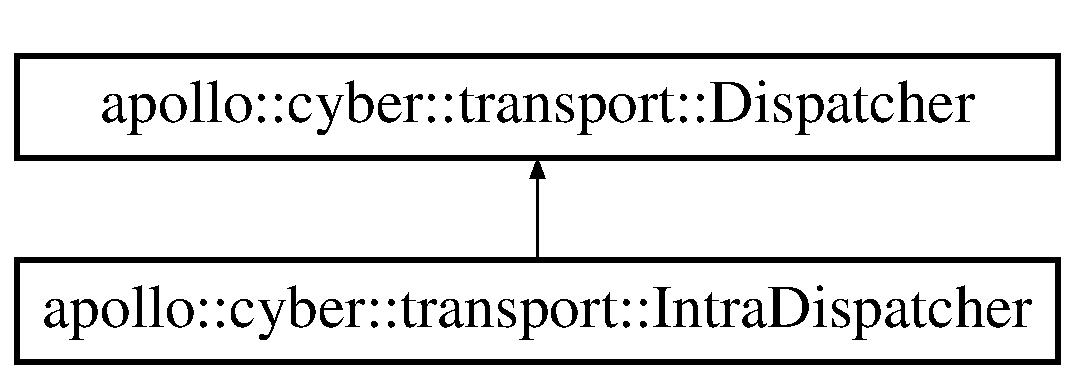
\includegraphics[height=2.000000cm]{classapollo_1_1cyber_1_1transport_1_1IntraDispatcher}
\end{center}
\end{figure}
\subsection*{Public Member Functions}
\begin{DoxyCompactItemize}
\item 
virtual \hyperlink{classapollo_1_1cyber_1_1transport_1_1IntraDispatcher_a2eee7291beff361006efd6d3dbfb26c5}{$\sim$\-Intra\-Dispatcher} ()
\item 
{\footnotesize template$<$typename Message\-T $>$ }\\void \hyperlink{classapollo_1_1cyber_1_1transport_1_1IntraDispatcher_a458c68701438bdcb83c3c7745200201f}{On\-Message} (uint64\-\_\-t channel\-\_\-id, const std\-::shared\-\_\-ptr$<$ Message\-T $>$ \&message, const \hyperlink{classapollo_1_1cyber_1_1transport_1_1MessageInfo}{Message\-Info} \&message\-\_\-info)
\end{DoxyCompactItemize}
\subsection*{Additional Inherited Members}


\subsection{Constructor \& Destructor Documentation}
\hypertarget{classapollo_1_1cyber_1_1transport_1_1IntraDispatcher_a2eee7291beff361006efd6d3dbfb26c5}{\index{apollo\-::cyber\-::transport\-::\-Intra\-Dispatcher@{apollo\-::cyber\-::transport\-::\-Intra\-Dispatcher}!$\sim$\-Intra\-Dispatcher@{$\sim$\-Intra\-Dispatcher}}
\index{$\sim$\-Intra\-Dispatcher@{$\sim$\-Intra\-Dispatcher}!apollo::cyber::transport::IntraDispatcher@{apollo\-::cyber\-::transport\-::\-Intra\-Dispatcher}}
\subsubsection[{$\sim$\-Intra\-Dispatcher}]{\setlength{\rightskip}{0pt plus 5cm}virtual apollo\-::cyber\-::transport\-::\-Intra\-Dispatcher\-::$\sim$\-Intra\-Dispatcher (
\begin{DoxyParamCaption}
{}
\end{DoxyParamCaption}
)\hspace{0.3cm}{\ttfamily [virtual]}}}\label{classapollo_1_1cyber_1_1transport_1_1IntraDispatcher_a2eee7291beff361006efd6d3dbfb26c5}


\subsection{Member Function Documentation}
\hypertarget{classapollo_1_1cyber_1_1transport_1_1IntraDispatcher_a458c68701438bdcb83c3c7745200201f}{\index{apollo\-::cyber\-::transport\-::\-Intra\-Dispatcher@{apollo\-::cyber\-::transport\-::\-Intra\-Dispatcher}!On\-Message@{On\-Message}}
\index{On\-Message@{On\-Message}!apollo::cyber::transport::IntraDispatcher@{apollo\-::cyber\-::transport\-::\-Intra\-Dispatcher}}
\subsubsection[{On\-Message}]{\setlength{\rightskip}{0pt plus 5cm}template$<$typename Message\-T $>$ void apollo\-::cyber\-::transport\-::\-Intra\-Dispatcher\-::\-On\-Message (
\begin{DoxyParamCaption}
\item[{uint64\-\_\-t}]{channel\-\_\-id, }
\item[{const std\-::shared\-\_\-ptr$<$ Message\-T $>$ \&}]{message, }
\item[{const {\bf Message\-Info} \&}]{message\-\_\-info}
\end{DoxyParamCaption}
)}}\label{classapollo_1_1cyber_1_1transport_1_1IntraDispatcher_a458c68701438bdcb83c3c7745200201f}


The documentation for this class was generated from the following file\-:\begin{DoxyCompactItemize}
\item 
transport/dispatcher/\hyperlink{intra__dispatcher_8h}{intra\-\_\-dispatcher.\-h}\end{DoxyCompactItemize}

\hypertarget{classapollo_1_1cyber_1_1message_1_1IntraMessage}{\section{apollo\-:\-:cyber\-:\-:message\-:\-:Intra\-Message Class Reference}
\label{classapollo_1_1cyber_1_1message_1_1IntraMessage}\index{apollo\-::cyber\-::message\-::\-Intra\-Message@{apollo\-::cyber\-::message\-::\-Intra\-Message}}
}


{\ttfamily \#include $<$intra\-\_\-message.\-h$>$}



The documentation for this class was generated from the following file\-:\begin{DoxyCompactItemize}
\item 
message/\hyperlink{intra__message_8h}{intra\-\_\-message.\-h}\end{DoxyCompactItemize}

\hypertarget{classapollo_1_1cyber_1_1blocker_1_1IntraReader}{\section{apollo\-:\-:cyber\-:\-:blocker\-:\-:Intra\-Reader$<$ Message\-T $>$ Class Template Reference}
\label{classapollo_1_1cyber_1_1blocker_1_1IntraReader}\index{apollo\-::cyber\-::blocker\-::\-Intra\-Reader$<$ Message\-T $>$@{apollo\-::cyber\-::blocker\-::\-Intra\-Reader$<$ Message\-T $>$}}
}


{\ttfamily \#include $<$intra\-\_\-reader.\-h$>$}

Inheritance diagram for apollo\-:\-:cyber\-:\-:blocker\-:\-:Intra\-Reader$<$ Message\-T $>$\-:\begin{figure}[H]
\begin{center}
\leavevmode
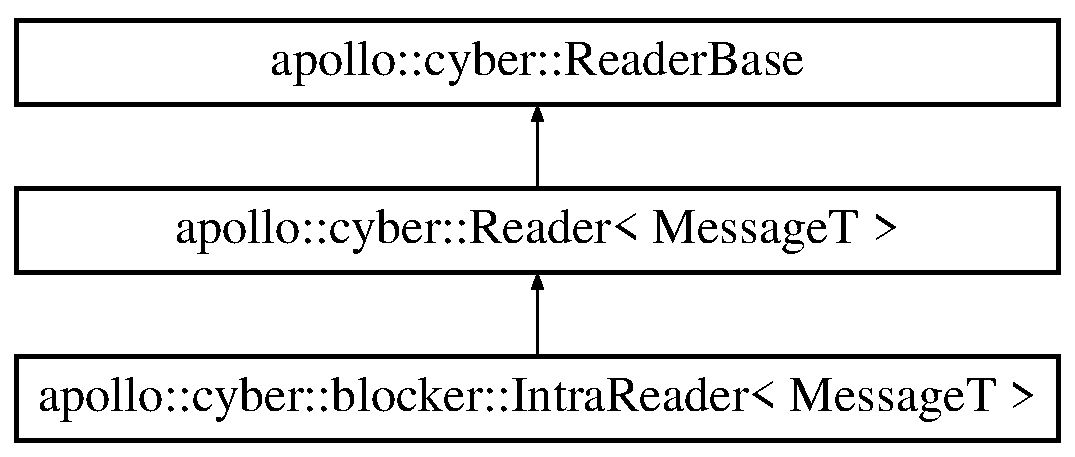
\includegraphics[height=3.000000cm]{classapollo_1_1cyber_1_1blocker_1_1IntraReader}
\end{center}
\end{figure}
\subsection*{Public Types}
\begin{DoxyCompactItemize}
\item 
using \hyperlink{classapollo_1_1cyber_1_1blocker_1_1IntraReader_aa4e9071f397bee80ba4ab42e7d1f165d}{Message\-Ptr} = std\-::shared\-\_\-ptr$<$ Message\-T $>$
\item 
using \hyperlink{classapollo_1_1cyber_1_1blocker_1_1IntraReader_a15cf88ac9399d324aeb685bec11c8afe}{Callback} = std\-::function$<$ void(const std\-::shared\-\_\-ptr$<$ Message\-T $>$ \&)$>$
\item 
using \hyperlink{classapollo_1_1cyber_1_1blocker_1_1IntraReader_a34f048290fe0ff40e672a485835ccfc9}{Iterator} = typename std\-::list$<$ std\-::shared\-\_\-ptr$<$ Message\-T $>$$>$\-::const\-\_\-iterator
\end{DoxyCompactItemize}
\subsection*{Public Member Functions}
\begin{DoxyCompactItemize}
\item 
\hyperlink{classapollo_1_1cyber_1_1blocker_1_1IntraReader_a591de348f97ac5ec0e378e1fb92c617d}{Intra\-Reader} (const proto\-::\-Role\-Attributes \&attr, const \hyperlink{classapollo_1_1cyber_1_1blocker_1_1IntraReader_a15cf88ac9399d324aeb685bec11c8afe}{Callback} \&callback)
\item 
virtual \hyperlink{classapollo_1_1cyber_1_1blocker_1_1IntraReader_a0921409f222aec564d34d8814dd94266}{$\sim$\-Intra\-Reader} ()
\item 
bool \hyperlink{classapollo_1_1cyber_1_1blocker_1_1IntraReader_a43e61ca2814c9ca792b89c67e2a02daf}{Init} () override
\item 
void \hyperlink{classapollo_1_1cyber_1_1blocker_1_1IntraReader_a4f6fb242d33858198474001f855626dc}{Shutdown} () override
\item 
void \hyperlink{classapollo_1_1cyber_1_1blocker_1_1IntraReader_a10695c39f2444febe5963747a578df29}{Clear\-Data} () override
\item 
void \hyperlink{classapollo_1_1cyber_1_1blocker_1_1IntraReader_a8f509c61e3b4b406cbe2beb53558e821}{Observe} () override
\item 
bool \hyperlink{classapollo_1_1cyber_1_1blocker_1_1IntraReader_a69f5c5029cba88c2a23528efe6a69457}{Empty} () const override
\item 
bool \hyperlink{classapollo_1_1cyber_1_1blocker_1_1IntraReader_a398c31e1c4918adc42e771e183eb244a}{Has\-Received} () const override
\item 
void \hyperlink{classapollo_1_1cyber_1_1blocker_1_1IntraReader_a2c155cd435cacc890cbffc4e0a3299e7}{Enqueue} (const std\-::shared\-\_\-ptr$<$ Message\-T $>$ \&msg) override
\item 
void \hyperlink{classapollo_1_1cyber_1_1blocker_1_1IntraReader_a699f5630c23afb609aa55a63528d2361}{Set\-History\-Depth} (const uint32\-\_\-t \&depth) override
\item 
uint32\-\_\-t \hyperlink{classapollo_1_1cyber_1_1blocker_1_1IntraReader_adb4056ff1f7ed30e7fbff720fb85887a}{Get\-History\-Depth} () const override
\item 
std\-::shared\-\_\-ptr$<$ Message\-T $>$ \hyperlink{classapollo_1_1cyber_1_1blocker_1_1IntraReader_a85adf523b69aa8a0ca72f801c07486fc}{Get\-Latest\-Observed} () const override
\item 
std\-::shared\-\_\-ptr$<$ Message\-T $>$ \hyperlink{classapollo_1_1cyber_1_1blocker_1_1IntraReader_a4ecd786720ee58f0b53cee186f0a4713}{Get\-Oldest\-Observed} () const override
\item 
\hyperlink{classapollo_1_1cyber_1_1blocker_1_1IntraReader_a34f048290fe0ff40e672a485835ccfc9}{Iterator} \hyperlink{classapollo_1_1cyber_1_1blocker_1_1IntraReader_a9249758337ab94e2aefe657f1f8a3580}{Begin} () const override
\item 
\hyperlink{classapollo_1_1cyber_1_1blocker_1_1IntraReader_a34f048290fe0ff40e672a485835ccfc9}{Iterator} \hyperlink{classapollo_1_1cyber_1_1blocker_1_1IntraReader_ab94a92e11479f932b99f1c2e1f2df931}{End} () const override
\end{DoxyCompactItemize}
\subsection*{Private Member Functions}
\begin{DoxyCompactItemize}
\item 
void \hyperlink{classapollo_1_1cyber_1_1blocker_1_1IntraReader_a4310e459238cf6c5c23dab4b96236f2e}{On\-Message} (const \hyperlink{classapollo_1_1cyber_1_1blocker_1_1IntraReader_aa4e9071f397bee80ba4ab42e7d1f165d}{Message\-Ptr} \&msg\-\_\-ptr)
\end{DoxyCompactItemize}
\subsection*{Private Attributes}
\begin{DoxyCompactItemize}
\item 
\hyperlink{classapollo_1_1cyber_1_1blocker_1_1IntraReader_a15cf88ac9399d324aeb685bec11c8afe}{Callback} \hyperlink{classapollo_1_1cyber_1_1blocker_1_1IntraReader_adf1bc681d8decbd80ba6a69039f1851b}{msg\-\_\-callback\-\_\-}
\end{DoxyCompactItemize}
\subsection*{Additional Inherited Members}


\subsection{Member Typedef Documentation}
\hypertarget{classapollo_1_1cyber_1_1blocker_1_1IntraReader_a15cf88ac9399d324aeb685bec11c8afe}{\index{apollo\-::cyber\-::blocker\-::\-Intra\-Reader@{apollo\-::cyber\-::blocker\-::\-Intra\-Reader}!Callback@{Callback}}
\index{Callback@{Callback}!apollo::cyber::blocker::IntraReader@{apollo\-::cyber\-::blocker\-::\-Intra\-Reader}}
\subsubsection[{Callback}]{\setlength{\rightskip}{0pt plus 5cm}template$<$typename Message\-T $>$ using {\bf apollo\-::cyber\-::blocker\-::\-Intra\-Reader}$<$ Message\-T $>$\-::{\bf Callback} =  std\-::function$<$void(const std\-::shared\-\_\-ptr$<$Message\-T$>$\&)$>$}}\label{classapollo_1_1cyber_1_1blocker_1_1IntraReader_a15cf88ac9399d324aeb685bec11c8afe}
\hypertarget{classapollo_1_1cyber_1_1blocker_1_1IntraReader_a34f048290fe0ff40e672a485835ccfc9}{\index{apollo\-::cyber\-::blocker\-::\-Intra\-Reader@{apollo\-::cyber\-::blocker\-::\-Intra\-Reader}!Iterator@{Iterator}}
\index{Iterator@{Iterator}!apollo::cyber::blocker::IntraReader@{apollo\-::cyber\-::blocker\-::\-Intra\-Reader}}
\subsubsection[{Iterator}]{\setlength{\rightskip}{0pt plus 5cm}template$<$typename Message\-T $>$ using {\bf apollo\-::cyber\-::blocker\-::\-Intra\-Reader}$<$ Message\-T $>$\-::{\bf Iterator} =  typename std\-::list$<$std\-::shared\-\_\-ptr$<$Message\-T$>$$>$\-::const\-\_\-iterator}}\label{classapollo_1_1cyber_1_1blocker_1_1IntraReader_a34f048290fe0ff40e672a485835ccfc9}
\hypertarget{classapollo_1_1cyber_1_1blocker_1_1IntraReader_aa4e9071f397bee80ba4ab42e7d1f165d}{\index{apollo\-::cyber\-::blocker\-::\-Intra\-Reader@{apollo\-::cyber\-::blocker\-::\-Intra\-Reader}!Message\-Ptr@{Message\-Ptr}}
\index{Message\-Ptr@{Message\-Ptr}!apollo::cyber::blocker::IntraReader@{apollo\-::cyber\-::blocker\-::\-Intra\-Reader}}
\subsubsection[{Message\-Ptr}]{\setlength{\rightskip}{0pt plus 5cm}template$<$typename Message\-T $>$ using {\bf apollo\-::cyber\-::blocker\-::\-Intra\-Reader}$<$ Message\-T $>$\-::{\bf Message\-Ptr} =  std\-::shared\-\_\-ptr$<$Message\-T$>$}}\label{classapollo_1_1cyber_1_1blocker_1_1IntraReader_aa4e9071f397bee80ba4ab42e7d1f165d}


\subsection{Constructor \& Destructor Documentation}
\hypertarget{classapollo_1_1cyber_1_1blocker_1_1IntraReader_a591de348f97ac5ec0e378e1fb92c617d}{\index{apollo\-::cyber\-::blocker\-::\-Intra\-Reader@{apollo\-::cyber\-::blocker\-::\-Intra\-Reader}!Intra\-Reader@{Intra\-Reader}}
\index{Intra\-Reader@{Intra\-Reader}!apollo::cyber::blocker::IntraReader@{apollo\-::cyber\-::blocker\-::\-Intra\-Reader}}
\subsubsection[{Intra\-Reader}]{\setlength{\rightskip}{0pt plus 5cm}template$<$typename Message\-T $>$ {\bf apollo\-::cyber\-::blocker\-::\-Intra\-Reader}$<$ Message\-T $>$\-::{\bf Intra\-Reader} (
\begin{DoxyParamCaption}
\item[{const proto\-::\-Role\-Attributes \&}]{attr, }
\item[{const {\bf Callback} \&}]{callback}
\end{DoxyParamCaption}
)}}\label{classapollo_1_1cyber_1_1blocker_1_1IntraReader_a591de348f97ac5ec0e378e1fb92c617d}
\hypertarget{classapollo_1_1cyber_1_1blocker_1_1IntraReader_a0921409f222aec564d34d8814dd94266}{\index{apollo\-::cyber\-::blocker\-::\-Intra\-Reader@{apollo\-::cyber\-::blocker\-::\-Intra\-Reader}!$\sim$\-Intra\-Reader@{$\sim$\-Intra\-Reader}}
\index{$\sim$\-Intra\-Reader@{$\sim$\-Intra\-Reader}!apollo::cyber::blocker::IntraReader@{apollo\-::cyber\-::blocker\-::\-Intra\-Reader}}
\subsubsection[{$\sim$\-Intra\-Reader}]{\setlength{\rightskip}{0pt plus 5cm}template$<$typename Message\-T $>$ {\bf apollo\-::cyber\-::blocker\-::\-Intra\-Reader}$<$ Message\-T $>$\-::$\sim${\bf Intra\-Reader} (
\begin{DoxyParamCaption}
{}
\end{DoxyParamCaption}
)\hspace{0.3cm}{\ttfamily [virtual]}}}\label{classapollo_1_1cyber_1_1blocker_1_1IntraReader_a0921409f222aec564d34d8814dd94266}


\subsection{Member Function Documentation}
\hypertarget{classapollo_1_1cyber_1_1blocker_1_1IntraReader_a9249758337ab94e2aefe657f1f8a3580}{\index{apollo\-::cyber\-::blocker\-::\-Intra\-Reader@{apollo\-::cyber\-::blocker\-::\-Intra\-Reader}!Begin@{Begin}}
\index{Begin@{Begin}!apollo::cyber::blocker::IntraReader@{apollo\-::cyber\-::blocker\-::\-Intra\-Reader}}
\subsubsection[{Begin}]{\setlength{\rightskip}{0pt plus 5cm}template$<$typename Message\-T $>$ auto {\bf apollo\-::cyber\-::blocker\-::\-Intra\-Reader}$<$ Message\-T $>$\-::Begin (
\begin{DoxyParamCaption}
{}
\end{DoxyParamCaption}
) const\hspace{0.3cm}{\ttfamily [override]}, {\ttfamily [virtual]}}}\label{classapollo_1_1cyber_1_1blocker_1_1IntraReader_a9249758337ab94e2aefe657f1f8a3580}


Reimplemented from \hyperlink{classapollo_1_1cyber_1_1Reader_a5fff77810d6a55099b507eb9e4a6135c}{apollo\-::cyber\-::\-Reader$<$ Message\-T $>$}.

\hypertarget{classapollo_1_1cyber_1_1blocker_1_1IntraReader_a10695c39f2444febe5963747a578df29}{\index{apollo\-::cyber\-::blocker\-::\-Intra\-Reader@{apollo\-::cyber\-::blocker\-::\-Intra\-Reader}!Clear\-Data@{Clear\-Data}}
\index{Clear\-Data@{Clear\-Data}!apollo::cyber::blocker::IntraReader@{apollo\-::cyber\-::blocker\-::\-Intra\-Reader}}
\subsubsection[{Clear\-Data}]{\setlength{\rightskip}{0pt plus 5cm}template$<$typename Message\-T $>$ void {\bf apollo\-::cyber\-::blocker\-::\-Intra\-Reader}$<$ Message\-T $>$\-::Clear\-Data (
\begin{DoxyParamCaption}
{}
\end{DoxyParamCaption}
)\hspace{0.3cm}{\ttfamily [override]}, {\ttfamily [virtual]}}}\label{classapollo_1_1cyber_1_1blocker_1_1IntraReader_a10695c39f2444febe5963747a578df29}


Implements \hyperlink{classapollo_1_1cyber_1_1ReaderBase_a6bf09eafd9a155192d6e623f90c881e0}{apollo\-::cyber\-::\-Reader\-Base}.

\hypertarget{classapollo_1_1cyber_1_1blocker_1_1IntraReader_a69f5c5029cba88c2a23528efe6a69457}{\index{apollo\-::cyber\-::blocker\-::\-Intra\-Reader@{apollo\-::cyber\-::blocker\-::\-Intra\-Reader}!Empty@{Empty}}
\index{Empty@{Empty}!apollo::cyber::blocker::IntraReader@{apollo\-::cyber\-::blocker\-::\-Intra\-Reader}}
\subsubsection[{Empty}]{\setlength{\rightskip}{0pt plus 5cm}template$<$typename Message\-T $>$ bool {\bf apollo\-::cyber\-::blocker\-::\-Intra\-Reader}$<$ Message\-T $>$\-::Empty (
\begin{DoxyParamCaption}
{}
\end{DoxyParamCaption}
) const\hspace{0.3cm}{\ttfamily [override]}, {\ttfamily [virtual]}}}\label{classapollo_1_1cyber_1_1blocker_1_1IntraReader_a69f5c5029cba88c2a23528efe6a69457}


Implements \hyperlink{classapollo_1_1cyber_1_1ReaderBase_a9f70abd4ac366a0e173f210db1512ffc}{apollo\-::cyber\-::\-Reader\-Base}.

\hypertarget{classapollo_1_1cyber_1_1blocker_1_1IntraReader_ab94a92e11479f932b99f1c2e1f2df931}{\index{apollo\-::cyber\-::blocker\-::\-Intra\-Reader@{apollo\-::cyber\-::blocker\-::\-Intra\-Reader}!End@{End}}
\index{End@{End}!apollo::cyber::blocker::IntraReader@{apollo\-::cyber\-::blocker\-::\-Intra\-Reader}}
\subsubsection[{End}]{\setlength{\rightskip}{0pt plus 5cm}template$<$typename Message\-T $>$ auto {\bf apollo\-::cyber\-::blocker\-::\-Intra\-Reader}$<$ Message\-T $>$\-::End (
\begin{DoxyParamCaption}
{}
\end{DoxyParamCaption}
) const\hspace{0.3cm}{\ttfamily [override]}, {\ttfamily [virtual]}}}\label{classapollo_1_1cyber_1_1blocker_1_1IntraReader_ab94a92e11479f932b99f1c2e1f2df931}


Reimplemented from \hyperlink{classapollo_1_1cyber_1_1Reader_a1e670b90e2896b668b8061860d6e953f}{apollo\-::cyber\-::\-Reader$<$ Message\-T $>$}.

\hypertarget{classapollo_1_1cyber_1_1blocker_1_1IntraReader_a2c155cd435cacc890cbffc4e0a3299e7}{\index{apollo\-::cyber\-::blocker\-::\-Intra\-Reader@{apollo\-::cyber\-::blocker\-::\-Intra\-Reader}!Enqueue@{Enqueue}}
\index{Enqueue@{Enqueue}!apollo::cyber::blocker::IntraReader@{apollo\-::cyber\-::blocker\-::\-Intra\-Reader}}
\subsubsection[{Enqueue}]{\setlength{\rightskip}{0pt plus 5cm}template$<$typename Message\-T $>$ void {\bf apollo\-::cyber\-::blocker\-::\-Intra\-Reader}$<$ Message\-T $>$\-::Enqueue (
\begin{DoxyParamCaption}
\item[{const std\-::shared\-\_\-ptr$<$ Message\-T $>$ \&}]{msg}
\end{DoxyParamCaption}
)\hspace{0.3cm}{\ttfamily [override]}, {\ttfamily [virtual]}}}\label{classapollo_1_1cyber_1_1blocker_1_1IntraReader_a2c155cd435cacc890cbffc4e0a3299e7}


Reimplemented from \hyperlink{classapollo_1_1cyber_1_1Reader_a9acce2d137849540e434596de51b10bf}{apollo\-::cyber\-::\-Reader$<$ Message\-T $>$}.

\hypertarget{classapollo_1_1cyber_1_1blocker_1_1IntraReader_adb4056ff1f7ed30e7fbff720fb85887a}{\index{apollo\-::cyber\-::blocker\-::\-Intra\-Reader@{apollo\-::cyber\-::blocker\-::\-Intra\-Reader}!Get\-History\-Depth@{Get\-History\-Depth}}
\index{Get\-History\-Depth@{Get\-History\-Depth}!apollo::cyber::blocker::IntraReader@{apollo\-::cyber\-::blocker\-::\-Intra\-Reader}}
\subsubsection[{Get\-History\-Depth}]{\setlength{\rightskip}{0pt plus 5cm}template$<$typename Message\-T $>$ uint32\-\_\-t {\bf apollo\-::cyber\-::blocker\-::\-Intra\-Reader}$<$ Message\-T $>$\-::Get\-History\-Depth (
\begin{DoxyParamCaption}
{}
\end{DoxyParamCaption}
) const\hspace{0.3cm}{\ttfamily [override]}, {\ttfamily [virtual]}}}\label{classapollo_1_1cyber_1_1blocker_1_1IntraReader_adb4056ff1f7ed30e7fbff720fb85887a}


Reimplemented from \hyperlink{classapollo_1_1cyber_1_1Reader_a6e1d8dd73f052175e1599286f54ba80c}{apollo\-::cyber\-::\-Reader$<$ Message\-T $>$}.

\hypertarget{classapollo_1_1cyber_1_1blocker_1_1IntraReader_a85adf523b69aa8a0ca72f801c07486fc}{\index{apollo\-::cyber\-::blocker\-::\-Intra\-Reader@{apollo\-::cyber\-::blocker\-::\-Intra\-Reader}!Get\-Latest\-Observed@{Get\-Latest\-Observed}}
\index{Get\-Latest\-Observed@{Get\-Latest\-Observed}!apollo::cyber::blocker::IntraReader@{apollo\-::cyber\-::blocker\-::\-Intra\-Reader}}
\subsubsection[{Get\-Latest\-Observed}]{\setlength{\rightskip}{0pt plus 5cm}template$<$typename Message\-T $>$ std\-::shared\-\_\-ptr$<$ Message\-T $>$ {\bf apollo\-::cyber\-::blocker\-::\-Intra\-Reader}$<$ Message\-T $>$\-::Get\-Latest\-Observed (
\begin{DoxyParamCaption}
{}
\end{DoxyParamCaption}
) const\hspace{0.3cm}{\ttfamily [override]}, {\ttfamily [virtual]}}}\label{classapollo_1_1cyber_1_1blocker_1_1IntraReader_a85adf523b69aa8a0ca72f801c07486fc}


Reimplemented from \hyperlink{classapollo_1_1cyber_1_1Reader_ac3fabcbcb3eac7570fc719f07cdaac27}{apollo\-::cyber\-::\-Reader$<$ Message\-T $>$}.

\hypertarget{classapollo_1_1cyber_1_1blocker_1_1IntraReader_a4ecd786720ee58f0b53cee186f0a4713}{\index{apollo\-::cyber\-::blocker\-::\-Intra\-Reader@{apollo\-::cyber\-::blocker\-::\-Intra\-Reader}!Get\-Oldest\-Observed@{Get\-Oldest\-Observed}}
\index{Get\-Oldest\-Observed@{Get\-Oldest\-Observed}!apollo::cyber::blocker::IntraReader@{apollo\-::cyber\-::blocker\-::\-Intra\-Reader}}
\subsubsection[{Get\-Oldest\-Observed}]{\setlength{\rightskip}{0pt plus 5cm}template$<$typename Message\-T $>$ std\-::shared\-\_\-ptr$<$ Message\-T $>$ {\bf apollo\-::cyber\-::blocker\-::\-Intra\-Reader}$<$ Message\-T $>$\-::Get\-Oldest\-Observed (
\begin{DoxyParamCaption}
{}
\end{DoxyParamCaption}
) const\hspace{0.3cm}{\ttfamily [override]}, {\ttfamily [virtual]}}}\label{classapollo_1_1cyber_1_1blocker_1_1IntraReader_a4ecd786720ee58f0b53cee186f0a4713}


Reimplemented from \hyperlink{classapollo_1_1cyber_1_1Reader_a787bb122252d2e2a86fdb04a81d6beca}{apollo\-::cyber\-::\-Reader$<$ Message\-T $>$}.

\hypertarget{classapollo_1_1cyber_1_1blocker_1_1IntraReader_a398c31e1c4918adc42e771e183eb244a}{\index{apollo\-::cyber\-::blocker\-::\-Intra\-Reader@{apollo\-::cyber\-::blocker\-::\-Intra\-Reader}!Has\-Received@{Has\-Received}}
\index{Has\-Received@{Has\-Received}!apollo::cyber::blocker::IntraReader@{apollo\-::cyber\-::blocker\-::\-Intra\-Reader}}
\subsubsection[{Has\-Received}]{\setlength{\rightskip}{0pt plus 5cm}template$<$typename Message\-T $>$ bool {\bf apollo\-::cyber\-::blocker\-::\-Intra\-Reader}$<$ Message\-T $>$\-::Has\-Received (
\begin{DoxyParamCaption}
{}
\end{DoxyParamCaption}
) const\hspace{0.3cm}{\ttfamily [override]}, {\ttfamily [virtual]}}}\label{classapollo_1_1cyber_1_1blocker_1_1IntraReader_a398c31e1c4918adc42e771e183eb244a}


Implements \hyperlink{classapollo_1_1cyber_1_1ReaderBase_a42a2e0a6c898cc3da881b1531a608995}{apollo\-::cyber\-::\-Reader\-Base}.

\hypertarget{classapollo_1_1cyber_1_1blocker_1_1IntraReader_a43e61ca2814c9ca792b89c67e2a02daf}{\index{apollo\-::cyber\-::blocker\-::\-Intra\-Reader@{apollo\-::cyber\-::blocker\-::\-Intra\-Reader}!Init@{Init}}
\index{Init@{Init}!apollo::cyber::blocker::IntraReader@{apollo\-::cyber\-::blocker\-::\-Intra\-Reader}}
\subsubsection[{Init}]{\setlength{\rightskip}{0pt plus 5cm}template$<$typename Message\-T $>$ bool {\bf apollo\-::cyber\-::blocker\-::\-Intra\-Reader}$<$ Message\-T $>$\-::Init (
\begin{DoxyParamCaption}
{}
\end{DoxyParamCaption}
)\hspace{0.3cm}{\ttfamily [override]}, {\ttfamily [virtual]}}}\label{classapollo_1_1cyber_1_1blocker_1_1IntraReader_a43e61ca2814c9ca792b89c67e2a02daf}


Implements \hyperlink{classapollo_1_1cyber_1_1ReaderBase_a58e95863a3ea4e744ddff5914456ad7d}{apollo\-::cyber\-::\-Reader\-Base}.

\hypertarget{classapollo_1_1cyber_1_1blocker_1_1IntraReader_a8f509c61e3b4b406cbe2beb53558e821}{\index{apollo\-::cyber\-::blocker\-::\-Intra\-Reader@{apollo\-::cyber\-::blocker\-::\-Intra\-Reader}!Observe@{Observe}}
\index{Observe@{Observe}!apollo::cyber::blocker::IntraReader@{apollo\-::cyber\-::blocker\-::\-Intra\-Reader}}
\subsubsection[{Observe}]{\setlength{\rightskip}{0pt plus 5cm}template$<$typename Message\-T $>$ void {\bf apollo\-::cyber\-::blocker\-::\-Intra\-Reader}$<$ Message\-T $>$\-::Observe (
\begin{DoxyParamCaption}
{}
\end{DoxyParamCaption}
)\hspace{0.3cm}{\ttfamily [override]}, {\ttfamily [virtual]}}}\label{classapollo_1_1cyber_1_1blocker_1_1IntraReader_a8f509c61e3b4b406cbe2beb53558e821}


Implements \hyperlink{classapollo_1_1cyber_1_1ReaderBase_a3cfeb975a301fe9094221f105d387e55}{apollo\-::cyber\-::\-Reader\-Base}.

\hypertarget{classapollo_1_1cyber_1_1blocker_1_1IntraReader_a4310e459238cf6c5c23dab4b96236f2e}{\index{apollo\-::cyber\-::blocker\-::\-Intra\-Reader@{apollo\-::cyber\-::blocker\-::\-Intra\-Reader}!On\-Message@{On\-Message}}
\index{On\-Message@{On\-Message}!apollo::cyber::blocker::IntraReader@{apollo\-::cyber\-::blocker\-::\-Intra\-Reader}}
\subsubsection[{On\-Message}]{\setlength{\rightskip}{0pt plus 5cm}template$<$typename Message\-T $>$ void {\bf apollo\-::cyber\-::blocker\-::\-Intra\-Reader}$<$ Message\-T $>$\-::On\-Message (
\begin{DoxyParamCaption}
\item[{const {\bf Message\-Ptr} \&}]{msg\-\_\-ptr}
\end{DoxyParamCaption}
)\hspace{0.3cm}{\ttfamily [private]}}}\label{classapollo_1_1cyber_1_1blocker_1_1IntraReader_a4310e459238cf6c5c23dab4b96236f2e}
\hypertarget{classapollo_1_1cyber_1_1blocker_1_1IntraReader_a699f5630c23afb609aa55a63528d2361}{\index{apollo\-::cyber\-::blocker\-::\-Intra\-Reader@{apollo\-::cyber\-::blocker\-::\-Intra\-Reader}!Set\-History\-Depth@{Set\-History\-Depth}}
\index{Set\-History\-Depth@{Set\-History\-Depth}!apollo::cyber::blocker::IntraReader@{apollo\-::cyber\-::blocker\-::\-Intra\-Reader}}
\subsubsection[{Set\-History\-Depth}]{\setlength{\rightskip}{0pt plus 5cm}template$<$typename Message\-T $>$ void {\bf apollo\-::cyber\-::blocker\-::\-Intra\-Reader}$<$ Message\-T $>$\-::Set\-History\-Depth (
\begin{DoxyParamCaption}
\item[{const uint32\-\_\-t \&}]{depth}
\end{DoxyParamCaption}
)\hspace{0.3cm}{\ttfamily [override]}, {\ttfamily [virtual]}}}\label{classapollo_1_1cyber_1_1blocker_1_1IntraReader_a699f5630c23afb609aa55a63528d2361}


Reimplemented from \hyperlink{classapollo_1_1cyber_1_1Reader_a20a9b73c463c8f65b9592bb295745fa6}{apollo\-::cyber\-::\-Reader$<$ Message\-T $>$}.

\hypertarget{classapollo_1_1cyber_1_1blocker_1_1IntraReader_a4f6fb242d33858198474001f855626dc}{\index{apollo\-::cyber\-::blocker\-::\-Intra\-Reader@{apollo\-::cyber\-::blocker\-::\-Intra\-Reader}!Shutdown@{Shutdown}}
\index{Shutdown@{Shutdown}!apollo::cyber::blocker::IntraReader@{apollo\-::cyber\-::blocker\-::\-Intra\-Reader}}
\subsubsection[{Shutdown}]{\setlength{\rightskip}{0pt plus 5cm}template$<$typename Message\-T $>$ void {\bf apollo\-::cyber\-::blocker\-::\-Intra\-Reader}$<$ Message\-T $>$\-::Shutdown (
\begin{DoxyParamCaption}
{}
\end{DoxyParamCaption}
)\hspace{0.3cm}{\ttfamily [override]}, {\ttfamily [virtual]}}}\label{classapollo_1_1cyber_1_1blocker_1_1IntraReader_a4f6fb242d33858198474001f855626dc}


Implements \hyperlink{classapollo_1_1cyber_1_1ReaderBase_a340d56ab095e4ee0789e9ae6c3097730}{apollo\-::cyber\-::\-Reader\-Base}.



\subsection{Member Data Documentation}
\hypertarget{classapollo_1_1cyber_1_1blocker_1_1IntraReader_adf1bc681d8decbd80ba6a69039f1851b}{\index{apollo\-::cyber\-::blocker\-::\-Intra\-Reader@{apollo\-::cyber\-::blocker\-::\-Intra\-Reader}!msg\-\_\-callback\-\_\-@{msg\-\_\-callback\-\_\-}}
\index{msg\-\_\-callback\-\_\-@{msg\-\_\-callback\-\_\-}!apollo::cyber::blocker::IntraReader@{apollo\-::cyber\-::blocker\-::\-Intra\-Reader}}
\subsubsection[{msg\-\_\-callback\-\_\-}]{\setlength{\rightskip}{0pt plus 5cm}template$<$typename Message\-T $>$ {\bf Callback} {\bf apollo\-::cyber\-::blocker\-::\-Intra\-Reader}$<$ Message\-T $>$\-::msg\-\_\-callback\-\_\-\hspace{0.3cm}{\ttfamily [private]}}}\label{classapollo_1_1cyber_1_1blocker_1_1IntraReader_adf1bc681d8decbd80ba6a69039f1851b}


The documentation for this class was generated from the following file\-:\begin{DoxyCompactItemize}
\item 
blocker/\hyperlink{intra__reader_8h}{intra\-\_\-reader.\-h}\end{DoxyCompactItemize}

\hypertarget{classapollo_1_1cyber_1_1transport_1_1IntraReceiver}{\section{apollo\-:\-:cyber\-:\-:transport\-:\-:Intra\-Receiver$<$ M $>$ Class Template Reference}
\label{classapollo_1_1cyber_1_1transport_1_1IntraReceiver}\index{apollo\-::cyber\-::transport\-::\-Intra\-Receiver$<$ M $>$@{apollo\-::cyber\-::transport\-::\-Intra\-Receiver$<$ M $>$}}
}


{\ttfamily \#include $<$intra\-\_\-receiver.\-h$>$}

Inheritance diagram for apollo\-:\-:cyber\-:\-:transport\-:\-:Intra\-Receiver$<$ M $>$\-:\begin{figure}[H]
\begin{center}
\leavevmode
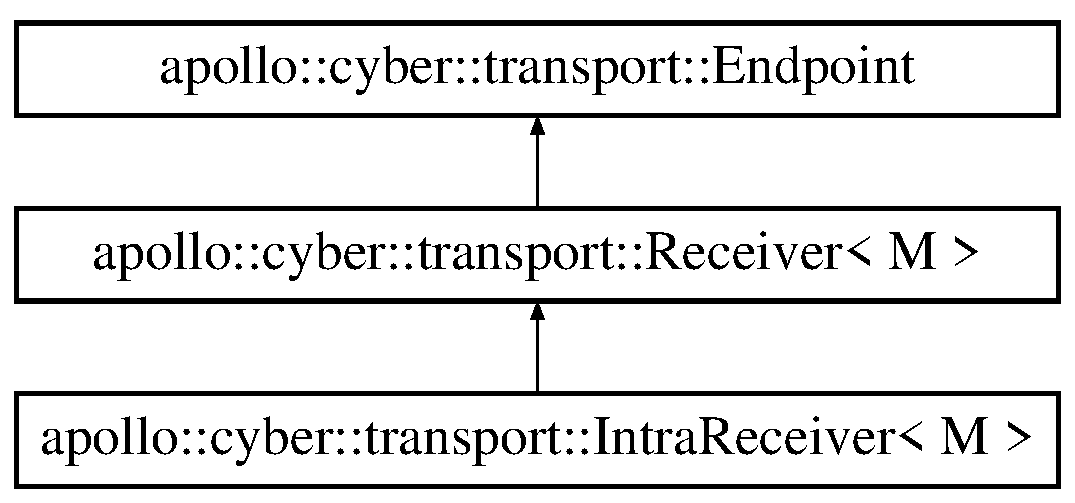
\includegraphics[height=3.000000cm]{classapollo_1_1cyber_1_1transport_1_1IntraReceiver}
\end{center}
\end{figure}
\subsection*{Public Member Functions}
\begin{DoxyCompactItemize}
\item 
\hyperlink{classapollo_1_1cyber_1_1transport_1_1IntraReceiver_a29c01b845450c6bb165d370c971f8609}{Intra\-Receiver} (const Role\-Attributes \&attr, const typename \hyperlink{classapollo_1_1cyber_1_1transport_1_1Receiver}{Receiver}$<$ M $>$\-::\hyperlink{classapollo_1_1cyber_1_1transport_1_1Receiver_abd906fd03582b49acbdc81b48a8974aa}{Message\-Listener} \&msg\-\_\-listener)
\item 
virtual \hyperlink{classapollo_1_1cyber_1_1transport_1_1IntraReceiver_a196c34905f08a271ef54495995fa4d6c}{$\sim$\-Intra\-Receiver} ()
\item 
void \hyperlink{classapollo_1_1cyber_1_1transport_1_1IntraReceiver_a34ff25c3a402ac5d04bd4b95fe1caee5}{Enable} () override
\item 
void \hyperlink{classapollo_1_1cyber_1_1transport_1_1IntraReceiver_a6737814d7652ca2272f4099cbafc33a1}{Disable} () override
\item 
void \hyperlink{classapollo_1_1cyber_1_1transport_1_1IntraReceiver_ae99f0f99dbd6de9b4c3a5ca443d8dd13}{Enable} (const Role\-Attributes \&opposite\-\_\-attr) override
\item 
void \hyperlink{classapollo_1_1cyber_1_1transport_1_1IntraReceiver_a51d5d2db5cc14599160a6192790a1296}{Disable} (const Role\-Attributes \&opposite\-\_\-attr) override
\end{DoxyCompactItemize}
\subsection*{Private Attributes}
\begin{DoxyCompactItemize}
\item 
\hyperlink{namespaceapollo_1_1cyber_1_1transport_af059bf179d7ece8cb6ee52f0157568de}{Intra\-Dispatcher\-Ptr} \hyperlink{classapollo_1_1cyber_1_1transport_1_1IntraReceiver_a92cf4ca8bb025023e5c7f5441c736dcd}{dispatcher\-\_\-}
\end{DoxyCompactItemize}
\subsection*{Additional Inherited Members}


\subsection{Constructor \& Destructor Documentation}
\hypertarget{classapollo_1_1cyber_1_1transport_1_1IntraReceiver_a29c01b845450c6bb165d370c971f8609}{\index{apollo\-::cyber\-::transport\-::\-Intra\-Receiver@{apollo\-::cyber\-::transport\-::\-Intra\-Receiver}!Intra\-Receiver@{Intra\-Receiver}}
\index{Intra\-Receiver@{Intra\-Receiver}!apollo::cyber::transport::IntraReceiver@{apollo\-::cyber\-::transport\-::\-Intra\-Receiver}}
\subsubsection[{Intra\-Receiver}]{\setlength{\rightskip}{0pt plus 5cm}template$<$typename M $>$ {\bf apollo\-::cyber\-::transport\-::\-Intra\-Receiver}$<$ M $>$\-::{\bf Intra\-Receiver} (
\begin{DoxyParamCaption}
\item[{const Role\-Attributes \&}]{attr, }
\item[{const typename {\bf Receiver}$<$ M $>$\-::{\bf Message\-Listener} \&}]{msg\-\_\-listener}
\end{DoxyParamCaption}
)}}\label{classapollo_1_1cyber_1_1transport_1_1IntraReceiver_a29c01b845450c6bb165d370c971f8609}
\hypertarget{classapollo_1_1cyber_1_1transport_1_1IntraReceiver_a196c34905f08a271ef54495995fa4d6c}{\index{apollo\-::cyber\-::transport\-::\-Intra\-Receiver@{apollo\-::cyber\-::transport\-::\-Intra\-Receiver}!$\sim$\-Intra\-Receiver@{$\sim$\-Intra\-Receiver}}
\index{$\sim$\-Intra\-Receiver@{$\sim$\-Intra\-Receiver}!apollo::cyber::transport::IntraReceiver@{apollo\-::cyber\-::transport\-::\-Intra\-Receiver}}
\subsubsection[{$\sim$\-Intra\-Receiver}]{\setlength{\rightskip}{0pt plus 5cm}template$<$typename M $>$ {\bf apollo\-::cyber\-::transport\-::\-Intra\-Receiver}$<$ M $>$\-::$\sim${\bf Intra\-Receiver} (
\begin{DoxyParamCaption}
{}
\end{DoxyParamCaption}
)\hspace{0.3cm}{\ttfamily [virtual]}}}\label{classapollo_1_1cyber_1_1transport_1_1IntraReceiver_a196c34905f08a271ef54495995fa4d6c}


\subsection{Member Function Documentation}
\hypertarget{classapollo_1_1cyber_1_1transport_1_1IntraReceiver_a6737814d7652ca2272f4099cbafc33a1}{\index{apollo\-::cyber\-::transport\-::\-Intra\-Receiver@{apollo\-::cyber\-::transport\-::\-Intra\-Receiver}!Disable@{Disable}}
\index{Disable@{Disable}!apollo::cyber::transport::IntraReceiver@{apollo\-::cyber\-::transport\-::\-Intra\-Receiver}}
\subsubsection[{Disable}]{\setlength{\rightskip}{0pt plus 5cm}template$<$typename M $>$ void {\bf apollo\-::cyber\-::transport\-::\-Intra\-Receiver}$<$ M $>$\-::Disable (
\begin{DoxyParamCaption}
{}
\end{DoxyParamCaption}
)\hspace{0.3cm}{\ttfamily [override]}, {\ttfamily [virtual]}}}\label{classapollo_1_1cyber_1_1transport_1_1IntraReceiver_a6737814d7652ca2272f4099cbafc33a1}


Implements \hyperlink{classapollo_1_1cyber_1_1transport_1_1Receiver_af9f317df425a33bc364662a59be28bf5}{apollo\-::cyber\-::transport\-::\-Receiver$<$ M $>$}.

\hypertarget{classapollo_1_1cyber_1_1transport_1_1IntraReceiver_a51d5d2db5cc14599160a6192790a1296}{\index{apollo\-::cyber\-::transport\-::\-Intra\-Receiver@{apollo\-::cyber\-::transport\-::\-Intra\-Receiver}!Disable@{Disable}}
\index{Disable@{Disable}!apollo::cyber::transport::IntraReceiver@{apollo\-::cyber\-::transport\-::\-Intra\-Receiver}}
\subsubsection[{Disable}]{\setlength{\rightskip}{0pt plus 5cm}template$<$typename M $>$ void {\bf apollo\-::cyber\-::transport\-::\-Intra\-Receiver}$<$ M $>$\-::Disable (
\begin{DoxyParamCaption}
\item[{const Role\-Attributes \&}]{opposite\-\_\-attr}
\end{DoxyParamCaption}
)\hspace{0.3cm}{\ttfamily [override]}, {\ttfamily [virtual]}}}\label{classapollo_1_1cyber_1_1transport_1_1IntraReceiver_a51d5d2db5cc14599160a6192790a1296}


Implements \hyperlink{classapollo_1_1cyber_1_1transport_1_1Receiver_a26a4b466924d472f830f856b675bb44a}{apollo\-::cyber\-::transport\-::\-Receiver$<$ M $>$}.

\hypertarget{classapollo_1_1cyber_1_1transport_1_1IntraReceiver_a34ff25c3a402ac5d04bd4b95fe1caee5}{\index{apollo\-::cyber\-::transport\-::\-Intra\-Receiver@{apollo\-::cyber\-::transport\-::\-Intra\-Receiver}!Enable@{Enable}}
\index{Enable@{Enable}!apollo::cyber::transport::IntraReceiver@{apollo\-::cyber\-::transport\-::\-Intra\-Receiver}}
\subsubsection[{Enable}]{\setlength{\rightskip}{0pt plus 5cm}template$<$typename M $>$ void {\bf apollo\-::cyber\-::transport\-::\-Intra\-Receiver}$<$ M $>$\-::Enable (
\begin{DoxyParamCaption}
{}
\end{DoxyParamCaption}
)\hspace{0.3cm}{\ttfamily [override]}, {\ttfamily [virtual]}}}\label{classapollo_1_1cyber_1_1transport_1_1IntraReceiver_a34ff25c3a402ac5d04bd4b95fe1caee5}


Implements \hyperlink{classapollo_1_1cyber_1_1transport_1_1Receiver_a77c93406c2ab9254562d595bfaecabbc}{apollo\-::cyber\-::transport\-::\-Receiver$<$ M $>$}.

\hypertarget{classapollo_1_1cyber_1_1transport_1_1IntraReceiver_ae99f0f99dbd6de9b4c3a5ca443d8dd13}{\index{apollo\-::cyber\-::transport\-::\-Intra\-Receiver@{apollo\-::cyber\-::transport\-::\-Intra\-Receiver}!Enable@{Enable}}
\index{Enable@{Enable}!apollo::cyber::transport::IntraReceiver@{apollo\-::cyber\-::transport\-::\-Intra\-Receiver}}
\subsubsection[{Enable}]{\setlength{\rightskip}{0pt plus 5cm}template$<$typename M $>$ void {\bf apollo\-::cyber\-::transport\-::\-Intra\-Receiver}$<$ M $>$\-::Enable (
\begin{DoxyParamCaption}
\item[{const Role\-Attributes \&}]{opposite\-\_\-attr}
\end{DoxyParamCaption}
)\hspace{0.3cm}{\ttfamily [override]}, {\ttfamily [virtual]}}}\label{classapollo_1_1cyber_1_1transport_1_1IntraReceiver_ae99f0f99dbd6de9b4c3a5ca443d8dd13}


Implements \hyperlink{classapollo_1_1cyber_1_1transport_1_1Receiver_a2436ecca6981d910911d359cd1df4610}{apollo\-::cyber\-::transport\-::\-Receiver$<$ M $>$}.



\subsection{Member Data Documentation}
\hypertarget{classapollo_1_1cyber_1_1transport_1_1IntraReceiver_a92cf4ca8bb025023e5c7f5441c736dcd}{\index{apollo\-::cyber\-::transport\-::\-Intra\-Receiver@{apollo\-::cyber\-::transport\-::\-Intra\-Receiver}!dispatcher\-\_\-@{dispatcher\-\_\-}}
\index{dispatcher\-\_\-@{dispatcher\-\_\-}!apollo::cyber::transport::IntraReceiver@{apollo\-::cyber\-::transport\-::\-Intra\-Receiver}}
\subsubsection[{dispatcher\-\_\-}]{\setlength{\rightskip}{0pt plus 5cm}template$<$typename M $>$ {\bf Intra\-Dispatcher\-Ptr} {\bf apollo\-::cyber\-::transport\-::\-Intra\-Receiver}$<$ M $>$\-::dispatcher\-\_\-\hspace{0.3cm}{\ttfamily [private]}}}\label{classapollo_1_1cyber_1_1transport_1_1IntraReceiver_a92cf4ca8bb025023e5c7f5441c736dcd}


The documentation for this class was generated from the following file\-:\begin{DoxyCompactItemize}
\item 
transport/receiver/\hyperlink{intra__receiver_8h}{intra\-\_\-receiver.\-h}\end{DoxyCompactItemize}

\hypertarget{classapollo_1_1cyber_1_1transport_1_1IntraTransmitter}{\section{apollo\-:\-:cyber\-:\-:transport\-:\-:Intra\-Transmitter$<$ M $>$ Class Template Reference}
\label{classapollo_1_1cyber_1_1transport_1_1IntraTransmitter}\index{apollo\-::cyber\-::transport\-::\-Intra\-Transmitter$<$ M $>$@{apollo\-::cyber\-::transport\-::\-Intra\-Transmitter$<$ M $>$}}
}


{\ttfamily \#include $<$intra\-\_\-transmitter.\-h$>$}

Inheritance diagram for apollo\-:\-:cyber\-:\-:transport\-:\-:Intra\-Transmitter$<$ M $>$\-:\begin{figure}[H]
\begin{center}
\leavevmode
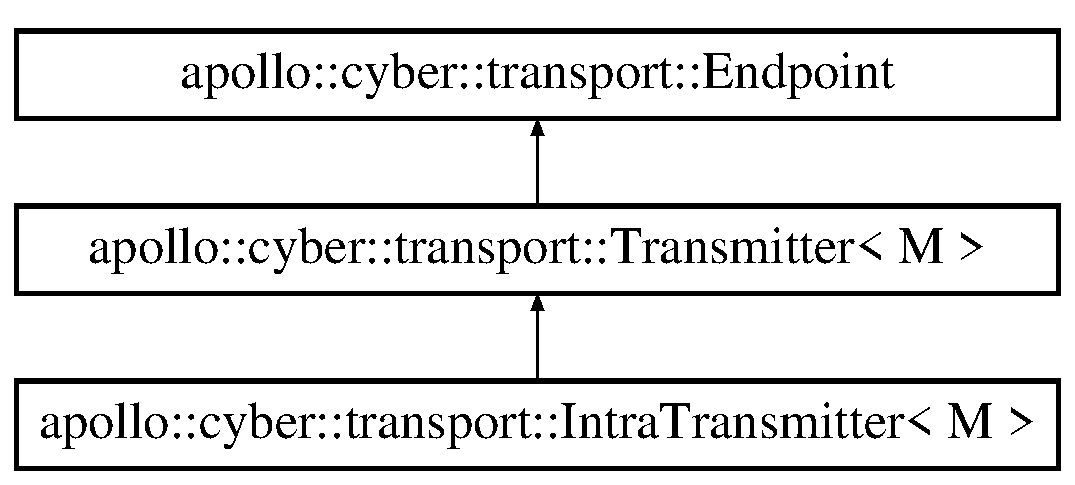
\includegraphics[height=3.000000cm]{classapollo_1_1cyber_1_1transport_1_1IntraTransmitter}
\end{center}
\end{figure}
\subsection*{Public Types}
\begin{DoxyCompactItemize}
\item 
using \hyperlink{classapollo_1_1cyber_1_1transport_1_1IntraTransmitter_ae47240b6bbe5421bb9d2e4b87d2ff98e}{Message\-Ptr} = std\-::shared\-\_\-ptr$<$ M $>$
\end{DoxyCompactItemize}
\subsection*{Public Member Functions}
\begin{DoxyCompactItemize}
\item 
\hyperlink{classapollo_1_1cyber_1_1transport_1_1IntraTransmitter_a1aecd865eff74d333f636675eb2c9383}{Intra\-Transmitter} (const Role\-Attributes \&attr)
\item 
virtual \hyperlink{classapollo_1_1cyber_1_1transport_1_1IntraTransmitter_ae672e4cfafd5f968acb439f36b0c4a10}{$\sim$\-Intra\-Transmitter} ()
\item 
void \hyperlink{classapollo_1_1cyber_1_1transport_1_1IntraTransmitter_ae8fec0fd79775a79e8998ec87b83e9b8}{Enable} () override
\item 
void \hyperlink{classapollo_1_1cyber_1_1transport_1_1IntraTransmitter_ad6bb7e42eb0486f755a64a555f3e9727}{Disable} () override
\item 
bool \hyperlink{classapollo_1_1cyber_1_1transport_1_1IntraTransmitter_a230dcd2a4cd7582326a1a21050b9b298}{Transmit} (const \hyperlink{classapollo_1_1cyber_1_1transport_1_1IntraTransmitter_ae47240b6bbe5421bb9d2e4b87d2ff98e}{Message\-Ptr} \&msg, const \hyperlink{classapollo_1_1cyber_1_1transport_1_1MessageInfo}{Message\-Info} \&msg\-\_\-info) override
\end{DoxyCompactItemize}
\subsection*{Private Attributes}
\begin{DoxyCompactItemize}
\item 
uint64\-\_\-t \hyperlink{classapollo_1_1cyber_1_1transport_1_1IntraTransmitter_ae0d14adfb5f776a9698b3d6e5f883216}{channel\-\_\-id\-\_\-}
\item 
\hyperlink{namespaceapollo_1_1cyber_1_1transport_af059bf179d7ece8cb6ee52f0157568de}{Intra\-Dispatcher\-Ptr} \hyperlink{classapollo_1_1cyber_1_1transport_1_1IntraTransmitter_a8290039108f635c0de7cf37ae7c8b966}{dispatcher\-\_\-}
\end{DoxyCompactItemize}
\subsection*{Additional Inherited Members}


\subsection{Member Typedef Documentation}
\hypertarget{classapollo_1_1cyber_1_1transport_1_1IntraTransmitter_ae47240b6bbe5421bb9d2e4b87d2ff98e}{\index{apollo\-::cyber\-::transport\-::\-Intra\-Transmitter@{apollo\-::cyber\-::transport\-::\-Intra\-Transmitter}!Message\-Ptr@{Message\-Ptr}}
\index{Message\-Ptr@{Message\-Ptr}!apollo::cyber::transport::IntraTransmitter@{apollo\-::cyber\-::transport\-::\-Intra\-Transmitter}}
\subsubsection[{Message\-Ptr}]{\setlength{\rightskip}{0pt plus 5cm}template$<$typename M $>$ using {\bf apollo\-::cyber\-::transport\-::\-Intra\-Transmitter}$<$ M $>$\-::{\bf Message\-Ptr} =  std\-::shared\-\_\-ptr$<$M$>$}}\label{classapollo_1_1cyber_1_1transport_1_1IntraTransmitter_ae47240b6bbe5421bb9d2e4b87d2ff98e}


\subsection{Constructor \& Destructor Documentation}
\hypertarget{classapollo_1_1cyber_1_1transport_1_1IntraTransmitter_a1aecd865eff74d333f636675eb2c9383}{\index{apollo\-::cyber\-::transport\-::\-Intra\-Transmitter@{apollo\-::cyber\-::transport\-::\-Intra\-Transmitter}!Intra\-Transmitter@{Intra\-Transmitter}}
\index{Intra\-Transmitter@{Intra\-Transmitter}!apollo::cyber::transport::IntraTransmitter@{apollo\-::cyber\-::transport\-::\-Intra\-Transmitter}}
\subsubsection[{Intra\-Transmitter}]{\setlength{\rightskip}{0pt plus 5cm}template$<$typename M $>$ {\bf apollo\-::cyber\-::transport\-::\-Intra\-Transmitter}$<$ M $>$\-::{\bf Intra\-Transmitter} (
\begin{DoxyParamCaption}
\item[{const Role\-Attributes \&}]{attr}
\end{DoxyParamCaption}
)\hspace{0.3cm}{\ttfamily [explicit]}}}\label{classapollo_1_1cyber_1_1transport_1_1IntraTransmitter_a1aecd865eff74d333f636675eb2c9383}
\hypertarget{classapollo_1_1cyber_1_1transport_1_1IntraTransmitter_ae672e4cfafd5f968acb439f36b0c4a10}{\index{apollo\-::cyber\-::transport\-::\-Intra\-Transmitter@{apollo\-::cyber\-::transport\-::\-Intra\-Transmitter}!$\sim$\-Intra\-Transmitter@{$\sim$\-Intra\-Transmitter}}
\index{$\sim$\-Intra\-Transmitter@{$\sim$\-Intra\-Transmitter}!apollo::cyber::transport::IntraTransmitter@{apollo\-::cyber\-::transport\-::\-Intra\-Transmitter}}
\subsubsection[{$\sim$\-Intra\-Transmitter}]{\setlength{\rightskip}{0pt plus 5cm}template$<$typename M $>$ {\bf apollo\-::cyber\-::transport\-::\-Intra\-Transmitter}$<$ M $>$\-::$\sim${\bf Intra\-Transmitter} (
\begin{DoxyParamCaption}
{}
\end{DoxyParamCaption}
)\hspace{0.3cm}{\ttfamily [virtual]}}}\label{classapollo_1_1cyber_1_1transport_1_1IntraTransmitter_ae672e4cfafd5f968acb439f36b0c4a10}


\subsection{Member Function Documentation}
\hypertarget{classapollo_1_1cyber_1_1transport_1_1IntraTransmitter_ad6bb7e42eb0486f755a64a555f3e9727}{\index{apollo\-::cyber\-::transport\-::\-Intra\-Transmitter@{apollo\-::cyber\-::transport\-::\-Intra\-Transmitter}!Disable@{Disable}}
\index{Disable@{Disable}!apollo::cyber::transport::IntraTransmitter@{apollo\-::cyber\-::transport\-::\-Intra\-Transmitter}}
\subsubsection[{Disable}]{\setlength{\rightskip}{0pt plus 5cm}template$<$typename M $>$ void {\bf apollo\-::cyber\-::transport\-::\-Intra\-Transmitter}$<$ M $>$\-::Disable (
\begin{DoxyParamCaption}
{}
\end{DoxyParamCaption}
)\hspace{0.3cm}{\ttfamily [override]}, {\ttfamily [virtual]}}}\label{classapollo_1_1cyber_1_1transport_1_1IntraTransmitter_ad6bb7e42eb0486f755a64a555f3e9727}


Implements \hyperlink{classapollo_1_1cyber_1_1transport_1_1Transmitter_a24bc426b201239fceff22535351a1903}{apollo\-::cyber\-::transport\-::\-Transmitter$<$ M $>$}.

\hypertarget{classapollo_1_1cyber_1_1transport_1_1IntraTransmitter_ae8fec0fd79775a79e8998ec87b83e9b8}{\index{apollo\-::cyber\-::transport\-::\-Intra\-Transmitter@{apollo\-::cyber\-::transport\-::\-Intra\-Transmitter}!Enable@{Enable}}
\index{Enable@{Enable}!apollo::cyber::transport::IntraTransmitter@{apollo\-::cyber\-::transport\-::\-Intra\-Transmitter}}
\subsubsection[{Enable}]{\setlength{\rightskip}{0pt plus 5cm}template$<$typename M $>$ void {\bf apollo\-::cyber\-::transport\-::\-Intra\-Transmitter}$<$ M $>$\-::Enable (
\begin{DoxyParamCaption}
{}
\end{DoxyParamCaption}
)\hspace{0.3cm}{\ttfamily [override]}, {\ttfamily [virtual]}}}\label{classapollo_1_1cyber_1_1transport_1_1IntraTransmitter_ae8fec0fd79775a79e8998ec87b83e9b8}


Implements \hyperlink{classapollo_1_1cyber_1_1transport_1_1Transmitter_aa4fd1ee72a6ba751226570e4ff54920d}{apollo\-::cyber\-::transport\-::\-Transmitter$<$ M $>$}.

\hypertarget{classapollo_1_1cyber_1_1transport_1_1IntraTransmitter_a230dcd2a4cd7582326a1a21050b9b298}{\index{apollo\-::cyber\-::transport\-::\-Intra\-Transmitter@{apollo\-::cyber\-::transport\-::\-Intra\-Transmitter}!Transmit@{Transmit}}
\index{Transmit@{Transmit}!apollo::cyber::transport::IntraTransmitter@{apollo\-::cyber\-::transport\-::\-Intra\-Transmitter}}
\subsubsection[{Transmit}]{\setlength{\rightskip}{0pt plus 5cm}template$<$typename M $>$ bool {\bf apollo\-::cyber\-::transport\-::\-Intra\-Transmitter}$<$ M $>$\-::Transmit (
\begin{DoxyParamCaption}
\item[{const {\bf Message\-Ptr} \&}]{msg, }
\item[{const {\bf Message\-Info} \&}]{msg\-\_\-info}
\end{DoxyParamCaption}
)\hspace{0.3cm}{\ttfamily [override]}, {\ttfamily [virtual]}}}\label{classapollo_1_1cyber_1_1transport_1_1IntraTransmitter_a230dcd2a4cd7582326a1a21050b9b298}


Implements \hyperlink{classapollo_1_1cyber_1_1transport_1_1Transmitter_af3a4b7fb0a6dcc1bd00437c121b18e19}{apollo\-::cyber\-::transport\-::\-Transmitter$<$ M $>$}.



\subsection{Member Data Documentation}
\hypertarget{classapollo_1_1cyber_1_1transport_1_1IntraTransmitter_ae0d14adfb5f776a9698b3d6e5f883216}{\index{apollo\-::cyber\-::transport\-::\-Intra\-Transmitter@{apollo\-::cyber\-::transport\-::\-Intra\-Transmitter}!channel\-\_\-id\-\_\-@{channel\-\_\-id\-\_\-}}
\index{channel\-\_\-id\-\_\-@{channel\-\_\-id\-\_\-}!apollo::cyber::transport::IntraTransmitter@{apollo\-::cyber\-::transport\-::\-Intra\-Transmitter}}
\subsubsection[{channel\-\_\-id\-\_\-}]{\setlength{\rightskip}{0pt plus 5cm}template$<$typename M $>$ uint64\-\_\-t {\bf apollo\-::cyber\-::transport\-::\-Intra\-Transmitter}$<$ M $>$\-::channel\-\_\-id\-\_\-\hspace{0.3cm}{\ttfamily [private]}}}\label{classapollo_1_1cyber_1_1transport_1_1IntraTransmitter_ae0d14adfb5f776a9698b3d6e5f883216}
\hypertarget{classapollo_1_1cyber_1_1transport_1_1IntraTransmitter_a8290039108f635c0de7cf37ae7c8b966}{\index{apollo\-::cyber\-::transport\-::\-Intra\-Transmitter@{apollo\-::cyber\-::transport\-::\-Intra\-Transmitter}!dispatcher\-\_\-@{dispatcher\-\_\-}}
\index{dispatcher\-\_\-@{dispatcher\-\_\-}!apollo::cyber::transport::IntraTransmitter@{apollo\-::cyber\-::transport\-::\-Intra\-Transmitter}}
\subsubsection[{dispatcher\-\_\-}]{\setlength{\rightskip}{0pt plus 5cm}template$<$typename M $>$ {\bf Intra\-Dispatcher\-Ptr} {\bf apollo\-::cyber\-::transport\-::\-Intra\-Transmitter}$<$ M $>$\-::dispatcher\-\_\-\hspace{0.3cm}{\ttfamily [private]}}}\label{classapollo_1_1cyber_1_1transport_1_1IntraTransmitter_a8290039108f635c0de7cf37ae7c8b966}


The documentation for this class was generated from the following file\-:\begin{DoxyCompactItemize}
\item 
transport/transmitter/\hyperlink{intra__transmitter_8h}{intra\-\_\-transmitter.\-h}\end{DoxyCompactItemize}

\hypertarget{classapollo_1_1cyber_1_1blocker_1_1IntraWriter}{\section{apollo\-:\-:cyber\-:\-:blocker\-:\-:Intra\-Writer$<$ Message\-T $>$ Class Template Reference}
\label{classapollo_1_1cyber_1_1blocker_1_1IntraWriter}\index{apollo\-::cyber\-::blocker\-::\-Intra\-Writer$<$ Message\-T $>$@{apollo\-::cyber\-::blocker\-::\-Intra\-Writer$<$ Message\-T $>$}}
}


{\ttfamily \#include $<$intra\-\_\-writer.\-h$>$}

Inheritance diagram for apollo\-:\-:cyber\-:\-:blocker\-:\-:Intra\-Writer$<$ Message\-T $>$\-:\begin{figure}[H]
\begin{center}
\leavevmode
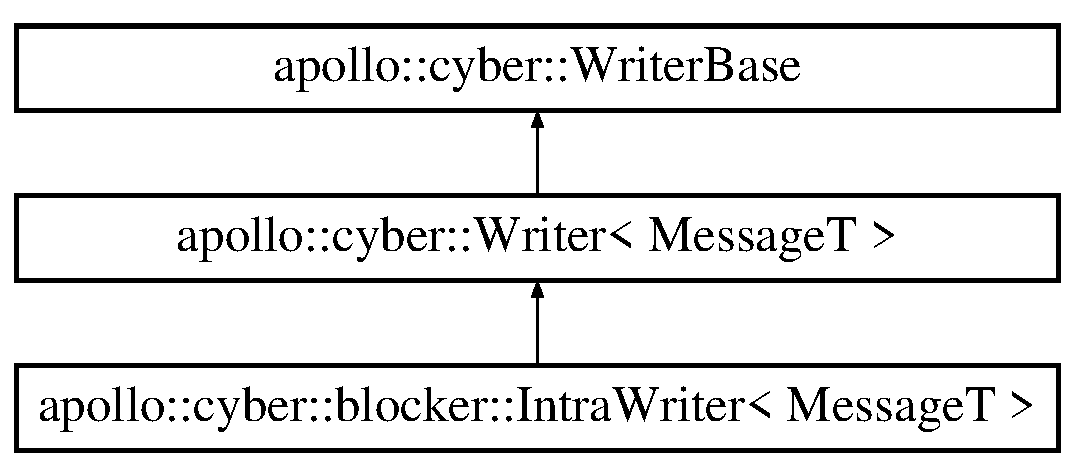
\includegraphics[height=3.000000cm]{classapollo_1_1cyber_1_1blocker_1_1IntraWriter}
\end{center}
\end{figure}
\subsection*{Public Types}
\begin{DoxyCompactItemize}
\item 
using \hyperlink{classapollo_1_1cyber_1_1blocker_1_1IntraWriter_a34952ec52c4ab25fdbbbbc5cb17868f4}{Message\-Ptr} = std\-::shared\-\_\-ptr$<$ Message\-T $>$
\item 
using \hyperlink{classapollo_1_1cyber_1_1blocker_1_1IntraWriter_a92d37eb69d0c02aa8eef3824e24b2f64}{Blocker\-Manager\-Ptr} = std\-::shared\-\_\-ptr$<$ \hyperlink{classapollo_1_1cyber_1_1blocker_1_1BlockerManager}{Blocker\-Manager} $>$
\end{DoxyCompactItemize}
\subsection*{Public Member Functions}
\begin{DoxyCompactItemize}
\item 
\hyperlink{classapollo_1_1cyber_1_1blocker_1_1IntraWriter_a8aa1a26e062bcebcb5f94bf33d28f8eb}{Intra\-Writer} (const proto\-::\-Role\-Attributes \&attr)
\item 
virtual \hyperlink{classapollo_1_1cyber_1_1blocker_1_1IntraWriter_a98864e9c9712bee3ff0e2be73838a600}{$\sim$\-Intra\-Writer} ()
\item 
bool \hyperlink{classapollo_1_1cyber_1_1blocker_1_1IntraWriter_a31e64a8ffd68620398509723ec9d2481}{Init} () override
\item 
void \hyperlink{classapollo_1_1cyber_1_1blocker_1_1IntraWriter_a61e18b7c53d860a2f141b057177d33a0}{Shutdown} () override
\item 
bool \hyperlink{classapollo_1_1cyber_1_1blocker_1_1IntraWriter_a81d327aca81aee982eba2143f5a8f1d6}{Write} (const Message\-T \&msg) override
\item 
bool \hyperlink{classapollo_1_1cyber_1_1blocker_1_1IntraWriter_a48491a940e99954b19c7eb26710d04b8}{Write} (const \hyperlink{classapollo_1_1cyber_1_1blocker_1_1IntraWriter_a34952ec52c4ab25fdbbbbc5cb17868f4}{Message\-Ptr} \&msg\-\_\-ptr) override
\end{DoxyCompactItemize}
\subsection*{Private Attributes}
\begin{DoxyCompactItemize}
\item 
\hyperlink{classapollo_1_1cyber_1_1blocker_1_1IntraWriter_a92d37eb69d0c02aa8eef3824e24b2f64}{Blocker\-Manager\-Ptr} \hyperlink{classapollo_1_1cyber_1_1blocker_1_1IntraWriter_a9e27c825322758f604452cebf6ce0313}{blocker\-\_\-manager\-\_\-}
\end{DoxyCompactItemize}
\subsection*{Additional Inherited Members}


\subsection{Member Typedef Documentation}
\hypertarget{classapollo_1_1cyber_1_1blocker_1_1IntraWriter_a92d37eb69d0c02aa8eef3824e24b2f64}{\index{apollo\-::cyber\-::blocker\-::\-Intra\-Writer@{apollo\-::cyber\-::blocker\-::\-Intra\-Writer}!Blocker\-Manager\-Ptr@{Blocker\-Manager\-Ptr}}
\index{Blocker\-Manager\-Ptr@{Blocker\-Manager\-Ptr}!apollo::cyber::blocker::IntraWriter@{apollo\-::cyber\-::blocker\-::\-Intra\-Writer}}
\subsubsection[{Blocker\-Manager\-Ptr}]{\setlength{\rightskip}{0pt plus 5cm}template$<$typename Message\-T $>$ using {\bf apollo\-::cyber\-::blocker\-::\-Intra\-Writer}$<$ Message\-T $>$\-::{\bf Blocker\-Manager\-Ptr} =  std\-::shared\-\_\-ptr$<${\bf Blocker\-Manager}$>$}}\label{classapollo_1_1cyber_1_1blocker_1_1IntraWriter_a92d37eb69d0c02aa8eef3824e24b2f64}
\hypertarget{classapollo_1_1cyber_1_1blocker_1_1IntraWriter_a34952ec52c4ab25fdbbbbc5cb17868f4}{\index{apollo\-::cyber\-::blocker\-::\-Intra\-Writer@{apollo\-::cyber\-::blocker\-::\-Intra\-Writer}!Message\-Ptr@{Message\-Ptr}}
\index{Message\-Ptr@{Message\-Ptr}!apollo::cyber::blocker::IntraWriter@{apollo\-::cyber\-::blocker\-::\-Intra\-Writer}}
\subsubsection[{Message\-Ptr}]{\setlength{\rightskip}{0pt plus 5cm}template$<$typename Message\-T $>$ using {\bf apollo\-::cyber\-::blocker\-::\-Intra\-Writer}$<$ Message\-T $>$\-::{\bf Message\-Ptr} =  std\-::shared\-\_\-ptr$<$Message\-T$>$}}\label{classapollo_1_1cyber_1_1blocker_1_1IntraWriter_a34952ec52c4ab25fdbbbbc5cb17868f4}


\subsection{Constructor \& Destructor Documentation}
\hypertarget{classapollo_1_1cyber_1_1blocker_1_1IntraWriter_a8aa1a26e062bcebcb5f94bf33d28f8eb}{\index{apollo\-::cyber\-::blocker\-::\-Intra\-Writer@{apollo\-::cyber\-::blocker\-::\-Intra\-Writer}!Intra\-Writer@{Intra\-Writer}}
\index{Intra\-Writer@{Intra\-Writer}!apollo::cyber::blocker::IntraWriter@{apollo\-::cyber\-::blocker\-::\-Intra\-Writer}}
\subsubsection[{Intra\-Writer}]{\setlength{\rightskip}{0pt plus 5cm}template$<$typename Message\-T $>$ {\bf apollo\-::cyber\-::blocker\-::\-Intra\-Writer}$<$ Message\-T $>$\-::{\bf Intra\-Writer} (
\begin{DoxyParamCaption}
\item[{const proto\-::\-Role\-Attributes \&}]{attr}
\end{DoxyParamCaption}
)\hspace{0.3cm}{\ttfamily [explicit]}}}\label{classapollo_1_1cyber_1_1blocker_1_1IntraWriter_a8aa1a26e062bcebcb5f94bf33d28f8eb}
\hypertarget{classapollo_1_1cyber_1_1blocker_1_1IntraWriter_a98864e9c9712bee3ff0e2be73838a600}{\index{apollo\-::cyber\-::blocker\-::\-Intra\-Writer@{apollo\-::cyber\-::blocker\-::\-Intra\-Writer}!$\sim$\-Intra\-Writer@{$\sim$\-Intra\-Writer}}
\index{$\sim$\-Intra\-Writer@{$\sim$\-Intra\-Writer}!apollo::cyber::blocker::IntraWriter@{apollo\-::cyber\-::blocker\-::\-Intra\-Writer}}
\subsubsection[{$\sim$\-Intra\-Writer}]{\setlength{\rightskip}{0pt plus 5cm}template$<$typename Message\-T $>$ {\bf apollo\-::cyber\-::blocker\-::\-Intra\-Writer}$<$ Message\-T $>$\-::$\sim${\bf Intra\-Writer} (
\begin{DoxyParamCaption}
{}
\end{DoxyParamCaption}
)\hspace{0.3cm}{\ttfamily [virtual]}}}\label{classapollo_1_1cyber_1_1blocker_1_1IntraWriter_a98864e9c9712bee3ff0e2be73838a600}


\subsection{Member Function Documentation}
\hypertarget{classapollo_1_1cyber_1_1blocker_1_1IntraWriter_a31e64a8ffd68620398509723ec9d2481}{\index{apollo\-::cyber\-::blocker\-::\-Intra\-Writer@{apollo\-::cyber\-::blocker\-::\-Intra\-Writer}!Init@{Init}}
\index{Init@{Init}!apollo::cyber::blocker::IntraWriter@{apollo\-::cyber\-::blocker\-::\-Intra\-Writer}}
\subsubsection[{Init}]{\setlength{\rightskip}{0pt plus 5cm}template$<$typename Message\-T $>$ bool {\bf apollo\-::cyber\-::blocker\-::\-Intra\-Writer}$<$ Message\-T $>$\-::Init (
\begin{DoxyParamCaption}
{}
\end{DoxyParamCaption}
)\hspace{0.3cm}{\ttfamily [override]}, {\ttfamily [virtual]}}}\label{classapollo_1_1cyber_1_1blocker_1_1IntraWriter_a31e64a8ffd68620398509723ec9d2481}


Implements \hyperlink{classapollo_1_1cyber_1_1WriterBase_acff05a3215b2a2da4b2a140069ac001d}{apollo\-::cyber\-::\-Writer\-Base}.

\hypertarget{classapollo_1_1cyber_1_1blocker_1_1IntraWriter_a61e18b7c53d860a2f141b057177d33a0}{\index{apollo\-::cyber\-::blocker\-::\-Intra\-Writer@{apollo\-::cyber\-::blocker\-::\-Intra\-Writer}!Shutdown@{Shutdown}}
\index{Shutdown@{Shutdown}!apollo::cyber::blocker::IntraWriter@{apollo\-::cyber\-::blocker\-::\-Intra\-Writer}}
\subsubsection[{Shutdown}]{\setlength{\rightskip}{0pt plus 5cm}template$<$typename Message\-T $>$ void {\bf apollo\-::cyber\-::blocker\-::\-Intra\-Writer}$<$ Message\-T $>$\-::Shutdown (
\begin{DoxyParamCaption}
{}
\end{DoxyParamCaption}
)\hspace{0.3cm}{\ttfamily [override]}, {\ttfamily [virtual]}}}\label{classapollo_1_1cyber_1_1blocker_1_1IntraWriter_a61e18b7c53d860a2f141b057177d33a0}


Implements \hyperlink{classapollo_1_1cyber_1_1WriterBase_ad2f187881a2832ece860eb11d69acc8b}{apollo\-::cyber\-::\-Writer\-Base}.

\hypertarget{classapollo_1_1cyber_1_1blocker_1_1IntraWriter_a81d327aca81aee982eba2143f5a8f1d6}{\index{apollo\-::cyber\-::blocker\-::\-Intra\-Writer@{apollo\-::cyber\-::blocker\-::\-Intra\-Writer}!Write@{Write}}
\index{Write@{Write}!apollo::cyber::blocker::IntraWriter@{apollo\-::cyber\-::blocker\-::\-Intra\-Writer}}
\subsubsection[{Write}]{\setlength{\rightskip}{0pt plus 5cm}template$<$typename Message\-T $>$ bool {\bf apollo\-::cyber\-::blocker\-::\-Intra\-Writer}$<$ Message\-T $>$\-::Write (
\begin{DoxyParamCaption}
\item[{const Message\-T \&}]{msg}
\end{DoxyParamCaption}
)\hspace{0.3cm}{\ttfamily [override]}, {\ttfamily [virtual]}}}\label{classapollo_1_1cyber_1_1blocker_1_1IntraWriter_a81d327aca81aee982eba2143f5a8f1d6}


Reimplemented from \hyperlink{classapollo_1_1cyber_1_1Writer_ac801147d965824c910da92626e4b9b05}{apollo\-::cyber\-::\-Writer$<$ Message\-T $>$}.

\hypertarget{classapollo_1_1cyber_1_1blocker_1_1IntraWriter_a48491a940e99954b19c7eb26710d04b8}{\index{apollo\-::cyber\-::blocker\-::\-Intra\-Writer@{apollo\-::cyber\-::blocker\-::\-Intra\-Writer}!Write@{Write}}
\index{Write@{Write}!apollo::cyber::blocker::IntraWriter@{apollo\-::cyber\-::blocker\-::\-Intra\-Writer}}
\subsubsection[{Write}]{\setlength{\rightskip}{0pt plus 5cm}template$<$typename Message\-T $>$ bool {\bf apollo\-::cyber\-::blocker\-::\-Intra\-Writer}$<$ Message\-T $>$\-::Write (
\begin{DoxyParamCaption}
\item[{const {\bf Message\-Ptr} \&}]{msg\-\_\-ptr}
\end{DoxyParamCaption}
)\hspace{0.3cm}{\ttfamily [override]}, {\ttfamily [virtual]}}}\label{classapollo_1_1cyber_1_1blocker_1_1IntraWriter_a48491a940e99954b19c7eb26710d04b8}


Reimplemented from \hyperlink{classapollo_1_1cyber_1_1Writer_a793eaf46f34f2d46d0225a1a6cc3fd50}{apollo\-::cyber\-::\-Writer$<$ Message\-T $>$}.



\subsection{Member Data Documentation}
\hypertarget{classapollo_1_1cyber_1_1blocker_1_1IntraWriter_a9e27c825322758f604452cebf6ce0313}{\index{apollo\-::cyber\-::blocker\-::\-Intra\-Writer@{apollo\-::cyber\-::blocker\-::\-Intra\-Writer}!blocker\-\_\-manager\-\_\-@{blocker\-\_\-manager\-\_\-}}
\index{blocker\-\_\-manager\-\_\-@{blocker\-\_\-manager\-\_\-}!apollo::cyber::blocker::IntraWriter@{apollo\-::cyber\-::blocker\-::\-Intra\-Writer}}
\subsubsection[{blocker\-\_\-manager\-\_\-}]{\setlength{\rightskip}{0pt plus 5cm}template$<$typename Message\-T $>$ {\bf Blocker\-Manager\-Ptr} {\bf apollo\-::cyber\-::blocker\-::\-Intra\-Writer}$<$ Message\-T $>$\-::blocker\-\_\-manager\-\_\-\hspace{0.3cm}{\ttfamily [private]}}}\label{classapollo_1_1cyber_1_1blocker_1_1IntraWriter_a9e27c825322758f604452cebf6ce0313}


The documentation for this class was generated from the following file\-:\begin{DoxyCompactItemize}
\item 
blocker/\hyperlink{intra__writer_8h}{intra\-\_\-writer.\-h}\end{DoxyCompactItemize}

\hypertarget{classapollo_1_1cyber_1_1record_1_1RecordViewer_1_1Iterator}{\section{apollo\-:\-:cyber\-:\-:record\-:\-:Record\-Viewer\-:\-:Iterator Class Reference}
\label{classapollo_1_1cyber_1_1record_1_1RecordViewer_1_1Iterator}\index{apollo\-::cyber\-::record\-::\-Record\-Viewer\-::\-Iterator@{apollo\-::cyber\-::record\-::\-Record\-Viewer\-::\-Iterator}}
}


{\ttfamily \#include $<$record\-\_\-viewer.\-h$>$}

\subsection*{Public Types}
\begin{DoxyCompactItemize}
\item 
using \hyperlink{classapollo_1_1cyber_1_1record_1_1RecordViewer_1_1Iterator_a45e3f7f65e6c5d011bcf253ddf994e42}{iterator\-\_\-category} = std\-::input\-\_\-iterator\-\_\-tag
\item 
using \hyperlink{classapollo_1_1cyber_1_1record_1_1RecordViewer_1_1Iterator_a0de09c9c8009daa91416ddcfcf3b222e}{value\-\_\-type} = \hyperlink{structapollo_1_1cyber_1_1record_1_1RecordMessage}{Record\-Message}
\item 
using \hyperlink{classapollo_1_1cyber_1_1record_1_1RecordViewer_1_1Iterator_a744368463a3f6ed5345c4614bff536f7}{difference\-\_\-type} = int
\item 
using \hyperlink{classapollo_1_1cyber_1_1record_1_1RecordViewer_1_1Iterator_a9f3cbce1cbf35a09693e35abd4c21728}{pointer} = \hyperlink{structapollo_1_1cyber_1_1record_1_1RecordMessage}{Record\-Message} $\ast$
\item 
using \hyperlink{classapollo_1_1cyber_1_1record_1_1RecordViewer_1_1Iterator_a670a19f28cd3f2db0e69d0167787021a}{reference} = \hyperlink{structapollo_1_1cyber_1_1record_1_1RecordMessage}{Record\-Message} \&
\end{DoxyCompactItemize}
\subsection*{Public Member Functions}
\begin{DoxyCompactItemize}
\item 
\hyperlink{classapollo_1_1cyber_1_1record_1_1RecordViewer_1_1Iterator_ac08d6746bb571e1830bb63873c0b84c2}{Iterator} (\hyperlink{classapollo_1_1cyber_1_1record_1_1RecordViewer}{Record\-Viewer} $\ast$viewer, bool \hyperlink{classapollo_1_1cyber_1_1record_1_1RecordViewer_a142bc45d0387f9982573aba250d3bebd}{end}=false)
\item 
\hyperlink{classapollo_1_1cyber_1_1record_1_1RecordViewer_1_1Iterator_a575b3b0b688618b2898caa82ffbfe420}{Iterator} ()
\item 
virtual \hyperlink{classapollo_1_1cyber_1_1record_1_1RecordViewer_1_1Iterator_a4be1cd45d37cdba7a2f7cb670d788f11}{$\sim$\-Iterator} ()
\item 
bool \hyperlink{classapollo_1_1cyber_1_1record_1_1RecordViewer_1_1Iterator_a12fe2b96833075c538f2d6ed30026d72}{operator==} (\hyperlink{classapollo_1_1cyber_1_1record_1_1RecordViewer_1_1Iterator}{Iterator} const \&other) const 
\item 
bool \hyperlink{classapollo_1_1cyber_1_1record_1_1RecordViewer_1_1Iterator_abf1b097103f74b27846f906b7e9c2bfe}{operator!=} (const \hyperlink{classapollo_1_1cyber_1_1record_1_1RecordViewer_1_1Iterator}{Iterator} \&rhs) const 
\item 
void \hyperlink{classapollo_1_1cyber_1_1record_1_1RecordViewer_1_1Iterator_a84e0cc6e08eb354ce6380d71c2f3e088}{operator++} ()
\item 
\hyperlink{classapollo_1_1cyber_1_1record_1_1RecordViewer_1_1Iterator_a9f3cbce1cbf35a09693e35abd4c21728}{pointer} \hyperlink{classapollo_1_1cyber_1_1record_1_1RecordViewer_1_1Iterator_ae934f4a9e60c2cab6d017f1e52691c28}{operator-\/$>$} ()
\item 
\hyperlink{classapollo_1_1cyber_1_1record_1_1RecordViewer_1_1Iterator_a670a19f28cd3f2db0e69d0167787021a}{reference} \hyperlink{classapollo_1_1cyber_1_1record_1_1RecordViewer_1_1Iterator_a91f936e4915f0398cfe59129c9cf22b0}{operator$\ast$} ()
\end{DoxyCompactItemize}
\subsection*{Private Attributes}
\begin{DoxyCompactItemize}
\item 
bool \hyperlink{classapollo_1_1cyber_1_1record_1_1RecordViewer_1_1Iterator_ab0b210fd00c859793652337d6162836e}{end\-\_\-} = false
\item 
uint64\-\_\-t \hyperlink{classapollo_1_1cyber_1_1record_1_1RecordViewer_1_1Iterator_a70fbcc7e167eccd93e569eef2220aada}{index\-\_\-} = 0
\item 
\hyperlink{classapollo_1_1cyber_1_1record_1_1RecordViewer}{Record\-Viewer} $\ast$ \hyperlink{classapollo_1_1cyber_1_1record_1_1RecordViewer_1_1Iterator_a3ff81d30a9a632768e017ca86ab3d703}{viewer\-\_\-} = nullptr
\item 
\hyperlink{classapollo_1_1cyber_1_1record_1_1RecordViewer_1_1Iterator_a0de09c9c8009daa91416ddcfcf3b222e}{value\-\_\-type} \hyperlink{classapollo_1_1cyber_1_1record_1_1RecordViewer_1_1Iterator_a1b6754c5978ca4f98b7bd492c6fb1fa9}{message\-\_\-instance\-\_\-}
\end{DoxyCompactItemize}


\subsection{Member Typedef Documentation}
\hypertarget{classapollo_1_1cyber_1_1record_1_1RecordViewer_1_1Iterator_a744368463a3f6ed5345c4614bff536f7}{\index{apollo\-::cyber\-::record\-::\-Record\-Viewer\-::\-Iterator@{apollo\-::cyber\-::record\-::\-Record\-Viewer\-::\-Iterator}!difference\-\_\-type@{difference\-\_\-type}}
\index{difference\-\_\-type@{difference\-\_\-type}!apollo::cyber::record::RecordViewer::Iterator@{apollo\-::cyber\-::record\-::\-Record\-Viewer\-::\-Iterator}}
\subsubsection[{difference\-\_\-type}]{\setlength{\rightskip}{0pt plus 5cm}using {\bf apollo\-::cyber\-::record\-::\-Record\-Viewer\-::\-Iterator\-::difference\-\_\-type} =  int}}\label{classapollo_1_1cyber_1_1record_1_1RecordViewer_1_1Iterator_a744368463a3f6ed5345c4614bff536f7}
\hypertarget{classapollo_1_1cyber_1_1record_1_1RecordViewer_1_1Iterator_a45e3f7f65e6c5d011bcf253ddf994e42}{\index{apollo\-::cyber\-::record\-::\-Record\-Viewer\-::\-Iterator@{apollo\-::cyber\-::record\-::\-Record\-Viewer\-::\-Iterator}!iterator\-\_\-category@{iterator\-\_\-category}}
\index{iterator\-\_\-category@{iterator\-\_\-category}!apollo::cyber::record::RecordViewer::Iterator@{apollo\-::cyber\-::record\-::\-Record\-Viewer\-::\-Iterator}}
\subsubsection[{iterator\-\_\-category}]{\setlength{\rightskip}{0pt plus 5cm}using {\bf apollo\-::cyber\-::record\-::\-Record\-Viewer\-::\-Iterator\-::iterator\-\_\-category} =  std\-::input\-\_\-iterator\-\_\-tag}}\label{classapollo_1_1cyber_1_1record_1_1RecordViewer_1_1Iterator_a45e3f7f65e6c5d011bcf253ddf994e42}
\hypertarget{classapollo_1_1cyber_1_1record_1_1RecordViewer_1_1Iterator_a9f3cbce1cbf35a09693e35abd4c21728}{\index{apollo\-::cyber\-::record\-::\-Record\-Viewer\-::\-Iterator@{apollo\-::cyber\-::record\-::\-Record\-Viewer\-::\-Iterator}!pointer@{pointer}}
\index{pointer@{pointer}!apollo::cyber::record::RecordViewer::Iterator@{apollo\-::cyber\-::record\-::\-Record\-Viewer\-::\-Iterator}}
\subsubsection[{pointer}]{\setlength{\rightskip}{0pt plus 5cm}using {\bf apollo\-::cyber\-::record\-::\-Record\-Viewer\-::\-Iterator\-::pointer} =  {\bf Record\-Message}$\ast$}}\label{classapollo_1_1cyber_1_1record_1_1RecordViewer_1_1Iterator_a9f3cbce1cbf35a09693e35abd4c21728}
\hypertarget{classapollo_1_1cyber_1_1record_1_1RecordViewer_1_1Iterator_a670a19f28cd3f2db0e69d0167787021a}{\index{apollo\-::cyber\-::record\-::\-Record\-Viewer\-::\-Iterator@{apollo\-::cyber\-::record\-::\-Record\-Viewer\-::\-Iterator}!reference@{reference}}
\index{reference@{reference}!apollo::cyber::record::RecordViewer::Iterator@{apollo\-::cyber\-::record\-::\-Record\-Viewer\-::\-Iterator}}
\subsubsection[{reference}]{\setlength{\rightskip}{0pt plus 5cm}using {\bf apollo\-::cyber\-::record\-::\-Record\-Viewer\-::\-Iterator\-::reference} =  {\bf Record\-Message}\&}}\label{classapollo_1_1cyber_1_1record_1_1RecordViewer_1_1Iterator_a670a19f28cd3f2db0e69d0167787021a}
\hypertarget{classapollo_1_1cyber_1_1record_1_1RecordViewer_1_1Iterator_a0de09c9c8009daa91416ddcfcf3b222e}{\index{apollo\-::cyber\-::record\-::\-Record\-Viewer\-::\-Iterator@{apollo\-::cyber\-::record\-::\-Record\-Viewer\-::\-Iterator}!value\-\_\-type@{value\-\_\-type}}
\index{value\-\_\-type@{value\-\_\-type}!apollo::cyber::record::RecordViewer::Iterator@{apollo\-::cyber\-::record\-::\-Record\-Viewer\-::\-Iterator}}
\subsubsection[{value\-\_\-type}]{\setlength{\rightskip}{0pt plus 5cm}using {\bf apollo\-::cyber\-::record\-::\-Record\-Viewer\-::\-Iterator\-::value\-\_\-type} =  {\bf Record\-Message}}}\label{classapollo_1_1cyber_1_1record_1_1RecordViewer_1_1Iterator_a0de09c9c8009daa91416ddcfcf3b222e}


\subsection{Constructor \& Destructor Documentation}
\hypertarget{classapollo_1_1cyber_1_1record_1_1RecordViewer_1_1Iterator_ac08d6746bb571e1830bb63873c0b84c2}{\index{apollo\-::cyber\-::record\-::\-Record\-Viewer\-::\-Iterator@{apollo\-::cyber\-::record\-::\-Record\-Viewer\-::\-Iterator}!Iterator@{Iterator}}
\index{Iterator@{Iterator}!apollo::cyber::record::RecordViewer::Iterator@{apollo\-::cyber\-::record\-::\-Record\-Viewer\-::\-Iterator}}
\subsubsection[{Iterator}]{\setlength{\rightskip}{0pt plus 5cm}apollo\-::cyber\-::record\-::\-Record\-Viewer\-::\-Iterator\-::\-Iterator (
\begin{DoxyParamCaption}
\item[{{\bf Record\-Viewer} $\ast$}]{viewer, }
\item[{bool}]{end = {\ttfamily false}}
\end{DoxyParamCaption}
)\hspace{0.3cm}{\ttfamily [explicit]}}}\label{classapollo_1_1cyber_1_1record_1_1RecordViewer_1_1Iterator_ac08d6746bb571e1830bb63873c0b84c2}
\hypertarget{classapollo_1_1cyber_1_1record_1_1RecordViewer_1_1Iterator_a575b3b0b688618b2898caa82ffbfe420}{\index{apollo\-::cyber\-::record\-::\-Record\-Viewer\-::\-Iterator@{apollo\-::cyber\-::record\-::\-Record\-Viewer\-::\-Iterator}!Iterator@{Iterator}}
\index{Iterator@{Iterator}!apollo::cyber::record::RecordViewer::Iterator@{apollo\-::cyber\-::record\-::\-Record\-Viewer\-::\-Iterator}}
\subsubsection[{Iterator}]{\setlength{\rightskip}{0pt plus 5cm}apollo\-::cyber\-::record\-::\-Record\-Viewer\-::\-Iterator\-::\-Iterator (
\begin{DoxyParamCaption}
{}
\end{DoxyParamCaption}
)\hspace{0.3cm}{\ttfamily [inline]}}}\label{classapollo_1_1cyber_1_1record_1_1RecordViewer_1_1Iterator_a575b3b0b688618b2898caa82ffbfe420}
\hypertarget{classapollo_1_1cyber_1_1record_1_1RecordViewer_1_1Iterator_a4be1cd45d37cdba7a2f7cb670d788f11}{\index{apollo\-::cyber\-::record\-::\-Record\-Viewer\-::\-Iterator@{apollo\-::cyber\-::record\-::\-Record\-Viewer\-::\-Iterator}!$\sim$\-Iterator@{$\sim$\-Iterator}}
\index{$\sim$\-Iterator@{$\sim$\-Iterator}!apollo::cyber::record::RecordViewer::Iterator@{apollo\-::cyber\-::record\-::\-Record\-Viewer\-::\-Iterator}}
\subsubsection[{$\sim$\-Iterator}]{\setlength{\rightskip}{0pt plus 5cm}virtual apollo\-::cyber\-::record\-::\-Record\-Viewer\-::\-Iterator\-::$\sim$\-Iterator (
\begin{DoxyParamCaption}
{}
\end{DoxyParamCaption}
)\hspace{0.3cm}{\ttfamily [inline]}, {\ttfamily [virtual]}}}\label{classapollo_1_1cyber_1_1record_1_1RecordViewer_1_1Iterator_a4be1cd45d37cdba7a2f7cb670d788f11}


\subsection{Member Function Documentation}
\hypertarget{classapollo_1_1cyber_1_1record_1_1RecordViewer_1_1Iterator_abf1b097103f74b27846f906b7e9c2bfe}{\index{apollo\-::cyber\-::record\-::\-Record\-Viewer\-::\-Iterator@{apollo\-::cyber\-::record\-::\-Record\-Viewer\-::\-Iterator}!operator!=@{operator!=}}
\index{operator!=@{operator!=}!apollo::cyber::record::RecordViewer::Iterator@{apollo\-::cyber\-::record\-::\-Record\-Viewer\-::\-Iterator}}
\subsubsection[{operator!=}]{\setlength{\rightskip}{0pt plus 5cm}bool apollo\-::cyber\-::record\-::\-Record\-Viewer\-::\-Iterator\-::operator!= (
\begin{DoxyParamCaption}
\item[{const {\bf Iterator} \&}]{rhs}
\end{DoxyParamCaption}
) const}}\label{classapollo_1_1cyber_1_1record_1_1RecordViewer_1_1Iterator_abf1b097103f74b27846f906b7e9c2bfe}
\hypertarget{classapollo_1_1cyber_1_1record_1_1RecordViewer_1_1Iterator_a91f936e4915f0398cfe59129c9cf22b0}{\index{apollo\-::cyber\-::record\-::\-Record\-Viewer\-::\-Iterator@{apollo\-::cyber\-::record\-::\-Record\-Viewer\-::\-Iterator}!operator$\ast$@{operator$\ast$}}
\index{operator$\ast$@{operator$\ast$}!apollo::cyber::record::RecordViewer::Iterator@{apollo\-::cyber\-::record\-::\-Record\-Viewer\-::\-Iterator}}
\subsubsection[{operator$\ast$}]{\setlength{\rightskip}{0pt plus 5cm}{\bf reference} apollo\-::cyber\-::record\-::\-Record\-Viewer\-::\-Iterator\-::operator$\ast$ (
\begin{DoxyParamCaption}
{}
\end{DoxyParamCaption}
)}}\label{classapollo_1_1cyber_1_1record_1_1RecordViewer_1_1Iterator_a91f936e4915f0398cfe59129c9cf22b0}
\hypertarget{classapollo_1_1cyber_1_1record_1_1RecordViewer_1_1Iterator_a84e0cc6e08eb354ce6380d71c2f3e088}{\index{apollo\-::cyber\-::record\-::\-Record\-Viewer\-::\-Iterator@{apollo\-::cyber\-::record\-::\-Record\-Viewer\-::\-Iterator}!operator++@{operator++}}
\index{operator++@{operator++}!apollo::cyber::record::RecordViewer::Iterator@{apollo\-::cyber\-::record\-::\-Record\-Viewer\-::\-Iterator}}
\subsubsection[{operator++}]{\setlength{\rightskip}{0pt plus 5cm}void apollo\-::cyber\-::record\-::\-Record\-Viewer\-::\-Iterator\-::operator++ (
\begin{DoxyParamCaption}
{}
\end{DoxyParamCaption}
)}}\label{classapollo_1_1cyber_1_1record_1_1RecordViewer_1_1Iterator_a84e0cc6e08eb354ce6380d71c2f3e088}
\hypertarget{classapollo_1_1cyber_1_1record_1_1RecordViewer_1_1Iterator_ae934f4a9e60c2cab6d017f1e52691c28}{\index{apollo\-::cyber\-::record\-::\-Record\-Viewer\-::\-Iterator@{apollo\-::cyber\-::record\-::\-Record\-Viewer\-::\-Iterator}!operator-\/$>$@{operator-\/$>$}}
\index{operator-\/$>$@{operator-\/$>$}!apollo::cyber::record::RecordViewer::Iterator@{apollo\-::cyber\-::record\-::\-Record\-Viewer\-::\-Iterator}}
\subsubsection[{operator-\/$>$}]{\setlength{\rightskip}{0pt plus 5cm}{\bf pointer} apollo\-::cyber\-::record\-::\-Record\-Viewer\-::\-Iterator\-::operator-\/$>$ (
\begin{DoxyParamCaption}
{}
\end{DoxyParamCaption}
)}}\label{classapollo_1_1cyber_1_1record_1_1RecordViewer_1_1Iterator_ae934f4a9e60c2cab6d017f1e52691c28}
\hypertarget{classapollo_1_1cyber_1_1record_1_1RecordViewer_1_1Iterator_a12fe2b96833075c538f2d6ed30026d72}{\index{apollo\-::cyber\-::record\-::\-Record\-Viewer\-::\-Iterator@{apollo\-::cyber\-::record\-::\-Record\-Viewer\-::\-Iterator}!operator==@{operator==}}
\index{operator==@{operator==}!apollo::cyber::record::RecordViewer::Iterator@{apollo\-::cyber\-::record\-::\-Record\-Viewer\-::\-Iterator}}
\subsubsection[{operator==}]{\setlength{\rightskip}{0pt plus 5cm}bool apollo\-::cyber\-::record\-::\-Record\-Viewer\-::\-Iterator\-::operator== (
\begin{DoxyParamCaption}
\item[{{\bf Iterator} const \&}]{other}
\end{DoxyParamCaption}
) const}}\label{classapollo_1_1cyber_1_1record_1_1RecordViewer_1_1Iterator_a12fe2b96833075c538f2d6ed30026d72}


\subsection{Member Data Documentation}
\hypertarget{classapollo_1_1cyber_1_1record_1_1RecordViewer_1_1Iterator_ab0b210fd00c859793652337d6162836e}{\index{apollo\-::cyber\-::record\-::\-Record\-Viewer\-::\-Iterator@{apollo\-::cyber\-::record\-::\-Record\-Viewer\-::\-Iterator}!end\-\_\-@{end\-\_\-}}
\index{end\-\_\-@{end\-\_\-}!apollo::cyber::record::RecordViewer::Iterator@{apollo\-::cyber\-::record\-::\-Record\-Viewer\-::\-Iterator}}
\subsubsection[{end\-\_\-}]{\setlength{\rightskip}{0pt plus 5cm}bool apollo\-::cyber\-::record\-::\-Record\-Viewer\-::\-Iterator\-::end\-\_\- = false\hspace{0.3cm}{\ttfamily [private]}}}\label{classapollo_1_1cyber_1_1record_1_1RecordViewer_1_1Iterator_ab0b210fd00c859793652337d6162836e}
\hypertarget{classapollo_1_1cyber_1_1record_1_1RecordViewer_1_1Iterator_a70fbcc7e167eccd93e569eef2220aada}{\index{apollo\-::cyber\-::record\-::\-Record\-Viewer\-::\-Iterator@{apollo\-::cyber\-::record\-::\-Record\-Viewer\-::\-Iterator}!index\-\_\-@{index\-\_\-}}
\index{index\-\_\-@{index\-\_\-}!apollo::cyber::record::RecordViewer::Iterator@{apollo\-::cyber\-::record\-::\-Record\-Viewer\-::\-Iterator}}
\subsubsection[{index\-\_\-}]{\setlength{\rightskip}{0pt plus 5cm}uint64\-\_\-t apollo\-::cyber\-::record\-::\-Record\-Viewer\-::\-Iterator\-::index\-\_\- = 0\hspace{0.3cm}{\ttfamily [private]}}}\label{classapollo_1_1cyber_1_1record_1_1RecordViewer_1_1Iterator_a70fbcc7e167eccd93e569eef2220aada}
\hypertarget{classapollo_1_1cyber_1_1record_1_1RecordViewer_1_1Iterator_a1b6754c5978ca4f98b7bd492c6fb1fa9}{\index{apollo\-::cyber\-::record\-::\-Record\-Viewer\-::\-Iterator@{apollo\-::cyber\-::record\-::\-Record\-Viewer\-::\-Iterator}!message\-\_\-instance\-\_\-@{message\-\_\-instance\-\_\-}}
\index{message\-\_\-instance\-\_\-@{message\-\_\-instance\-\_\-}!apollo::cyber::record::RecordViewer::Iterator@{apollo\-::cyber\-::record\-::\-Record\-Viewer\-::\-Iterator}}
\subsubsection[{message\-\_\-instance\-\_\-}]{\setlength{\rightskip}{0pt plus 5cm}{\bf value\-\_\-type} apollo\-::cyber\-::record\-::\-Record\-Viewer\-::\-Iterator\-::message\-\_\-instance\-\_\-\hspace{0.3cm}{\ttfamily [private]}}}\label{classapollo_1_1cyber_1_1record_1_1RecordViewer_1_1Iterator_a1b6754c5978ca4f98b7bd492c6fb1fa9}
\hypertarget{classapollo_1_1cyber_1_1record_1_1RecordViewer_1_1Iterator_a3ff81d30a9a632768e017ca86ab3d703}{\index{apollo\-::cyber\-::record\-::\-Record\-Viewer\-::\-Iterator@{apollo\-::cyber\-::record\-::\-Record\-Viewer\-::\-Iterator}!viewer\-\_\-@{viewer\-\_\-}}
\index{viewer\-\_\-@{viewer\-\_\-}!apollo::cyber::record::RecordViewer::Iterator@{apollo\-::cyber\-::record\-::\-Record\-Viewer\-::\-Iterator}}
\subsubsection[{viewer\-\_\-}]{\setlength{\rightskip}{0pt plus 5cm}{\bf Record\-Viewer}$\ast$ apollo\-::cyber\-::record\-::\-Record\-Viewer\-::\-Iterator\-::viewer\-\_\- = nullptr\hspace{0.3cm}{\ttfamily [private]}}}\label{classapollo_1_1cyber_1_1record_1_1RecordViewer_1_1Iterator_a3ff81d30a9a632768e017ca86ab3d703}


The documentation for this class was generated from the following file\-:\begin{DoxyCompactItemize}
\item 
record/\hyperlink{record__viewer_8h}{record\-\_\-viewer.\-h}\end{DoxyCompactItemize}

\hypertarget{classapollo_1_1cyber_1_1transport_1_1ListenerHandler}{\section{apollo\-:\-:cyber\-:\-:transport\-:\-:Listener\-Handler$<$ Message\-T $>$ Class Template Reference}
\label{classapollo_1_1cyber_1_1transport_1_1ListenerHandler}\index{apollo\-::cyber\-::transport\-::\-Listener\-Handler$<$ Message\-T $>$@{apollo\-::cyber\-::transport\-::\-Listener\-Handler$<$ Message\-T $>$}}
}


{\ttfamily \#include $<$listener\-\_\-handler.\-h$>$}

Inheritance diagram for apollo\-:\-:cyber\-:\-:transport\-:\-:Listener\-Handler$<$ Message\-T $>$\-:\begin{figure}[H]
\begin{center}
\leavevmode
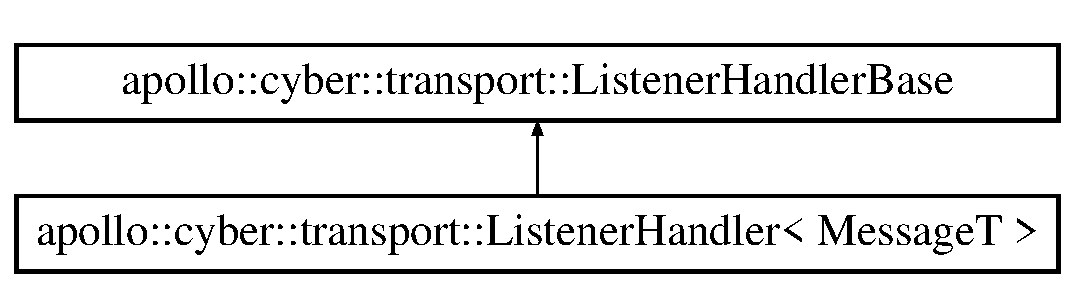
\includegraphics[height=2.000000cm]{classapollo_1_1cyber_1_1transport_1_1ListenerHandler}
\end{center}
\end{figure}
\subsection*{Public Types}
\begin{DoxyCompactItemize}
\item 
using \hyperlink{classapollo_1_1cyber_1_1transport_1_1ListenerHandler_a52a658e4523db4704b6d7e97f326d774}{Message} = std\-::shared\-\_\-ptr$<$ Message\-T $>$
\item 
using \hyperlink{classapollo_1_1cyber_1_1transport_1_1ListenerHandler_a9ca5ce35c021aae1145e8e25a5fda0a0}{Message\-Signal} = \hyperlink{classapollo_1_1cyber_1_1base_1_1Signal}{base\-::\-Signal}$<$ const \hyperlink{classapollo_1_1cyber_1_1transport_1_1ListenerHandler_a52a658e4523db4704b6d7e97f326d774}{Message} \&, const \hyperlink{classapollo_1_1cyber_1_1transport_1_1MessageInfo}{Message\-Info} \& $>$
\item 
using \hyperlink{classapollo_1_1cyber_1_1transport_1_1ListenerHandler_a96764e623a89ce8a872d2e43b6408d98}{Listener} = std\-::function$<$ void(const \hyperlink{classapollo_1_1cyber_1_1transport_1_1ListenerHandler_a52a658e4523db4704b6d7e97f326d774}{Message} \&, const \hyperlink{classapollo_1_1cyber_1_1transport_1_1MessageInfo}{Message\-Info} \&)$>$
\item 
using \hyperlink{classapollo_1_1cyber_1_1transport_1_1ListenerHandler_a6f33e5f36f457a51129671f22c159ddf}{Message\-Connection} = \hyperlink{classapollo_1_1cyber_1_1base_1_1Connection}{base\-::\-Connection}$<$ const \hyperlink{classapollo_1_1cyber_1_1transport_1_1ListenerHandler_a52a658e4523db4704b6d7e97f326d774}{Message} \&, const \hyperlink{classapollo_1_1cyber_1_1transport_1_1MessageInfo}{Message\-Info} \& $>$
\item 
using \hyperlink{classapollo_1_1cyber_1_1transport_1_1ListenerHandler_a5a6f5bc05280412183b1d0f65ce5e683}{Connection\-Map} = std\-::unordered\-\_\-map$<$ uint64\-\_\-t, \hyperlink{classapollo_1_1cyber_1_1transport_1_1ListenerHandler_a6f33e5f36f457a51129671f22c159ddf}{Message\-Connection} $>$
\end{DoxyCompactItemize}
\subsection*{Public Member Functions}
\begin{DoxyCompactItemize}
\item 
\hyperlink{classapollo_1_1cyber_1_1transport_1_1ListenerHandler_a7030c8148e7194124974615d18b6c713}{Listener\-Handler} ()
\item 
virtual \hyperlink{classapollo_1_1cyber_1_1transport_1_1ListenerHandler_a08c179bc5a9e22cb8a7184e85c9ee43b}{$\sim$\-Listener\-Handler} ()
\item 
void \hyperlink{classapollo_1_1cyber_1_1transport_1_1ListenerHandler_a55db7d72212c0fb491a23cb867183c9c}{Connect} (uint64\-\_\-t self\-\_\-id, const \hyperlink{classapollo_1_1cyber_1_1transport_1_1ListenerHandler_a96764e623a89ce8a872d2e43b6408d98}{Listener} \&listener)
\item 
void \hyperlink{classapollo_1_1cyber_1_1transport_1_1ListenerHandler_a653c56feedf335a9854241425f466b10}{Connect} (uint64\-\_\-t self\-\_\-id, uint64\-\_\-t oppo\-\_\-id, const \hyperlink{classapollo_1_1cyber_1_1transport_1_1ListenerHandler_a96764e623a89ce8a872d2e43b6408d98}{Listener} \&listener)
\item 
void \hyperlink{classapollo_1_1cyber_1_1transport_1_1ListenerHandler_a49732b06a8186e67f648efedca552224}{Disconnect} (uint64\-\_\-t self\-\_\-id) override
\item 
void \hyperlink{classapollo_1_1cyber_1_1transport_1_1ListenerHandler_a5bf12aac3e98dc9b1ba3f33e6170cad8}{Disconnect} (uint64\-\_\-t self\-\_\-id, uint64\-\_\-t oppo\-\_\-id) override
\item 
void \hyperlink{classapollo_1_1cyber_1_1transport_1_1ListenerHandler_a60da04ecf96ee8b5f669e3d598136441}{Run} (const \hyperlink{classapollo_1_1cyber_1_1transport_1_1ListenerHandler_a52a658e4523db4704b6d7e97f326d774}{Message} \&msg, const \hyperlink{classapollo_1_1cyber_1_1transport_1_1MessageInfo}{Message\-Info} \&msg\-\_\-info)
\item 
{\footnotesize template$<$$>$ }\\\hyperlink{classapollo_1_1cyber_1_1transport_1_1ListenerHandler_ab6f903ef1495188f830e7b1bff8f1622}{Listener\-Handler} ()
\end{DoxyCompactItemize}
\subsection*{Private Types}
\begin{DoxyCompactItemize}
\item 
using \hyperlink{classapollo_1_1cyber_1_1transport_1_1ListenerHandler_adbbec4596a920f50c937047a31c7019d}{Signal\-Ptr} = std\-::shared\-\_\-ptr$<$ \hyperlink{classapollo_1_1cyber_1_1transport_1_1ListenerHandler_a9ca5ce35c021aae1145e8e25a5fda0a0}{Message\-Signal} $>$
\item 
using \hyperlink{classapollo_1_1cyber_1_1transport_1_1ListenerHandler_ab534f02021dc0d897b0f1161a604b835}{Message\-Signal\-Map} = std\-::unordered\-\_\-map$<$ uint64\-\_\-t, \hyperlink{classapollo_1_1cyber_1_1transport_1_1ListenerHandler_adbbec4596a920f50c937047a31c7019d}{Signal\-Ptr} $>$
\end{DoxyCompactItemize}
\subsection*{Private Attributes}
\begin{DoxyCompactItemize}
\item 
\hyperlink{classapollo_1_1cyber_1_1transport_1_1ListenerHandler_a9ca5ce35c021aae1145e8e25a5fda0a0}{Message\-Signal} \hyperlink{classapollo_1_1cyber_1_1transport_1_1ListenerHandler_ac43fe4e3f5d7bbd16f21606f19cb349e}{signal\-\_\-}
\item 
\hyperlink{classapollo_1_1cyber_1_1transport_1_1ListenerHandler_a5a6f5bc05280412183b1d0f65ce5e683}{Connection\-Map} \hyperlink{classapollo_1_1cyber_1_1transport_1_1ListenerHandler_a305d0d57ad20695d87607abc21d50d37}{signal\-\_\-conns\-\_\-}
\item 
\hyperlink{classapollo_1_1cyber_1_1transport_1_1ListenerHandler_ab534f02021dc0d897b0f1161a604b835}{Message\-Signal\-Map} \hyperlink{classapollo_1_1cyber_1_1transport_1_1ListenerHandler_ac550b705bbbc6a60cb13d5208db3a716}{signals\-\_\-}
\item 
std\-::unordered\-\_\-map$<$ uint64\-\_\-t, \\*
\hyperlink{classapollo_1_1cyber_1_1transport_1_1ListenerHandler_a5a6f5bc05280412183b1d0f65ce5e683}{Connection\-Map} $>$ \hyperlink{classapollo_1_1cyber_1_1transport_1_1ListenerHandler_aae870e557a50628cfe739df1a8ab6547}{signals\-\_\-conns\-\_\-}
\item 
\hyperlink{classapollo_1_1cyber_1_1base_1_1AtomicRWLock}{base\-::\-Atomic\-R\-W\-Lock} \hyperlink{classapollo_1_1cyber_1_1transport_1_1ListenerHandler_adc3e16ad07f7ae7fd46fcd905880f216}{rw\-\_\-lock\-\_\-}
\end{DoxyCompactItemize}
\subsection*{Additional Inherited Members}


\subsection{Member Typedef Documentation}
\hypertarget{classapollo_1_1cyber_1_1transport_1_1ListenerHandler_a5a6f5bc05280412183b1d0f65ce5e683}{\index{apollo\-::cyber\-::transport\-::\-Listener\-Handler@{apollo\-::cyber\-::transport\-::\-Listener\-Handler}!Connection\-Map@{Connection\-Map}}
\index{Connection\-Map@{Connection\-Map}!apollo::cyber::transport::ListenerHandler@{apollo\-::cyber\-::transport\-::\-Listener\-Handler}}
\subsubsection[{Connection\-Map}]{\setlength{\rightskip}{0pt plus 5cm}template$<$typename Message\-T $>$ using {\bf apollo\-::cyber\-::transport\-::\-Listener\-Handler}$<$ Message\-T $>$\-::{\bf Connection\-Map} =  std\-::unordered\-\_\-map$<$uint64\-\_\-t, {\bf Message\-Connection}$>$}}\label{classapollo_1_1cyber_1_1transport_1_1ListenerHandler_a5a6f5bc05280412183b1d0f65ce5e683}
\hypertarget{classapollo_1_1cyber_1_1transport_1_1ListenerHandler_a96764e623a89ce8a872d2e43b6408d98}{\index{apollo\-::cyber\-::transport\-::\-Listener\-Handler@{apollo\-::cyber\-::transport\-::\-Listener\-Handler}!Listener@{Listener}}
\index{Listener@{Listener}!apollo::cyber::transport::ListenerHandler@{apollo\-::cyber\-::transport\-::\-Listener\-Handler}}
\subsubsection[{Listener}]{\setlength{\rightskip}{0pt plus 5cm}template$<$typename Message\-T $>$ using {\bf apollo\-::cyber\-::transport\-::\-Listener\-Handler}$<$ Message\-T $>$\-::{\bf Listener} =  std\-::function$<$void(const {\bf Message}\&, const {\bf Message\-Info}\&)$>$}}\label{classapollo_1_1cyber_1_1transport_1_1ListenerHandler_a96764e623a89ce8a872d2e43b6408d98}
\hypertarget{classapollo_1_1cyber_1_1transport_1_1ListenerHandler_a52a658e4523db4704b6d7e97f326d774}{\index{apollo\-::cyber\-::transport\-::\-Listener\-Handler@{apollo\-::cyber\-::transport\-::\-Listener\-Handler}!Message@{Message}}
\index{Message@{Message}!apollo::cyber::transport::ListenerHandler@{apollo\-::cyber\-::transport\-::\-Listener\-Handler}}
\subsubsection[{Message}]{\setlength{\rightskip}{0pt plus 5cm}template$<$typename Message\-T $>$ using {\bf apollo\-::cyber\-::transport\-::\-Listener\-Handler}$<$ Message\-T $>$\-::{\bf Message} =  std\-::shared\-\_\-ptr$<$Message\-T$>$}}\label{classapollo_1_1cyber_1_1transport_1_1ListenerHandler_a52a658e4523db4704b6d7e97f326d774}
\hypertarget{classapollo_1_1cyber_1_1transport_1_1ListenerHandler_a6f33e5f36f457a51129671f22c159ddf}{\index{apollo\-::cyber\-::transport\-::\-Listener\-Handler@{apollo\-::cyber\-::transport\-::\-Listener\-Handler}!Message\-Connection@{Message\-Connection}}
\index{Message\-Connection@{Message\-Connection}!apollo::cyber::transport::ListenerHandler@{apollo\-::cyber\-::transport\-::\-Listener\-Handler}}
\subsubsection[{Message\-Connection}]{\setlength{\rightskip}{0pt plus 5cm}template$<$typename Message\-T $>$ using {\bf apollo\-::cyber\-::transport\-::\-Listener\-Handler}$<$ Message\-T $>$\-::{\bf Message\-Connection} =  {\bf base\-::\-Connection}$<$const {\bf Message}\&, const {\bf Message\-Info}\&$>$}}\label{classapollo_1_1cyber_1_1transport_1_1ListenerHandler_a6f33e5f36f457a51129671f22c159ddf}
\hypertarget{classapollo_1_1cyber_1_1transport_1_1ListenerHandler_a9ca5ce35c021aae1145e8e25a5fda0a0}{\index{apollo\-::cyber\-::transport\-::\-Listener\-Handler@{apollo\-::cyber\-::transport\-::\-Listener\-Handler}!Message\-Signal@{Message\-Signal}}
\index{Message\-Signal@{Message\-Signal}!apollo::cyber::transport::ListenerHandler@{apollo\-::cyber\-::transport\-::\-Listener\-Handler}}
\subsubsection[{Message\-Signal}]{\setlength{\rightskip}{0pt plus 5cm}template$<$typename Message\-T $>$ using {\bf apollo\-::cyber\-::transport\-::\-Listener\-Handler}$<$ Message\-T $>$\-::{\bf Message\-Signal} =  {\bf base\-::\-Signal}$<$const {\bf Message}\&, const {\bf Message\-Info}\&$>$}}\label{classapollo_1_1cyber_1_1transport_1_1ListenerHandler_a9ca5ce35c021aae1145e8e25a5fda0a0}
\hypertarget{classapollo_1_1cyber_1_1transport_1_1ListenerHandler_ab534f02021dc0d897b0f1161a604b835}{\index{apollo\-::cyber\-::transport\-::\-Listener\-Handler@{apollo\-::cyber\-::transport\-::\-Listener\-Handler}!Message\-Signal\-Map@{Message\-Signal\-Map}}
\index{Message\-Signal\-Map@{Message\-Signal\-Map}!apollo::cyber::transport::ListenerHandler@{apollo\-::cyber\-::transport\-::\-Listener\-Handler}}
\subsubsection[{Message\-Signal\-Map}]{\setlength{\rightskip}{0pt plus 5cm}template$<$typename Message\-T $>$ using {\bf apollo\-::cyber\-::transport\-::\-Listener\-Handler}$<$ Message\-T $>$\-::{\bf Message\-Signal\-Map} =  std\-::unordered\-\_\-map$<$uint64\-\_\-t, {\bf Signal\-Ptr}$>$\hspace{0.3cm}{\ttfamily [private]}}}\label{classapollo_1_1cyber_1_1transport_1_1ListenerHandler_ab534f02021dc0d897b0f1161a604b835}
\hypertarget{classapollo_1_1cyber_1_1transport_1_1ListenerHandler_adbbec4596a920f50c937047a31c7019d}{\index{apollo\-::cyber\-::transport\-::\-Listener\-Handler@{apollo\-::cyber\-::transport\-::\-Listener\-Handler}!Signal\-Ptr@{Signal\-Ptr}}
\index{Signal\-Ptr@{Signal\-Ptr}!apollo::cyber::transport::ListenerHandler@{apollo\-::cyber\-::transport\-::\-Listener\-Handler}}
\subsubsection[{Signal\-Ptr}]{\setlength{\rightskip}{0pt plus 5cm}template$<$typename Message\-T $>$ using {\bf apollo\-::cyber\-::transport\-::\-Listener\-Handler}$<$ Message\-T $>$\-::{\bf Signal\-Ptr} =  std\-::shared\-\_\-ptr$<${\bf Message\-Signal}$>$\hspace{0.3cm}{\ttfamily [private]}}}\label{classapollo_1_1cyber_1_1transport_1_1ListenerHandler_adbbec4596a920f50c937047a31c7019d}


\subsection{Constructor \& Destructor Documentation}
\hypertarget{classapollo_1_1cyber_1_1transport_1_1ListenerHandler_a7030c8148e7194124974615d18b6c713}{\index{apollo\-::cyber\-::transport\-::\-Listener\-Handler@{apollo\-::cyber\-::transport\-::\-Listener\-Handler}!Listener\-Handler@{Listener\-Handler}}
\index{Listener\-Handler@{Listener\-Handler}!apollo::cyber::transport::ListenerHandler@{apollo\-::cyber\-::transport\-::\-Listener\-Handler}}
\subsubsection[{Listener\-Handler}]{\setlength{\rightskip}{0pt plus 5cm}template$<$typename Message\-T $>$ {\bf apollo\-::cyber\-::transport\-::\-Listener\-Handler}$<$ Message\-T $>$\-::{\bf Listener\-Handler} (
\begin{DoxyParamCaption}
{}
\end{DoxyParamCaption}
)\hspace{0.3cm}{\ttfamily [inline]}}}\label{classapollo_1_1cyber_1_1transport_1_1ListenerHandler_a7030c8148e7194124974615d18b6c713}
\hypertarget{classapollo_1_1cyber_1_1transport_1_1ListenerHandler_a08c179bc5a9e22cb8a7184e85c9ee43b}{\index{apollo\-::cyber\-::transport\-::\-Listener\-Handler@{apollo\-::cyber\-::transport\-::\-Listener\-Handler}!$\sim$\-Listener\-Handler@{$\sim$\-Listener\-Handler}}
\index{$\sim$\-Listener\-Handler@{$\sim$\-Listener\-Handler}!apollo::cyber::transport::ListenerHandler@{apollo\-::cyber\-::transport\-::\-Listener\-Handler}}
\subsubsection[{$\sim$\-Listener\-Handler}]{\setlength{\rightskip}{0pt plus 5cm}template$<$typename Message\-T $>$ virtual {\bf apollo\-::cyber\-::transport\-::\-Listener\-Handler}$<$ Message\-T $>$\-::$\sim${\bf Listener\-Handler} (
\begin{DoxyParamCaption}
{}
\end{DoxyParamCaption}
)\hspace{0.3cm}{\ttfamily [inline]}, {\ttfamily [virtual]}}}\label{classapollo_1_1cyber_1_1transport_1_1ListenerHandler_a08c179bc5a9e22cb8a7184e85c9ee43b}
\hypertarget{classapollo_1_1cyber_1_1transport_1_1ListenerHandler_ab6f903ef1495188f830e7b1bff8f1622}{\index{apollo\-::cyber\-::transport\-::\-Listener\-Handler@{apollo\-::cyber\-::transport\-::\-Listener\-Handler}!Listener\-Handler@{Listener\-Handler}}
\index{Listener\-Handler@{Listener\-Handler}!apollo::cyber::transport::ListenerHandler@{apollo\-::cyber\-::transport\-::\-Listener\-Handler}}
\subsubsection[{Listener\-Handler}]{\setlength{\rightskip}{0pt plus 5cm}template$<$$>$ {\bf apollo\-::cyber\-::transport\-::\-Listener\-Handler}$<$ {\bf message\-::\-Raw\-Message} $>$\-::{\bf Listener\-Handler} (
\begin{DoxyParamCaption}
{}
\end{DoxyParamCaption}
)\hspace{0.3cm}{\ttfamily [inline]}}}\label{classapollo_1_1cyber_1_1transport_1_1ListenerHandler_ab6f903ef1495188f830e7b1bff8f1622}


\subsection{Member Function Documentation}
\hypertarget{classapollo_1_1cyber_1_1transport_1_1ListenerHandler_a55db7d72212c0fb491a23cb867183c9c}{\index{apollo\-::cyber\-::transport\-::\-Listener\-Handler@{apollo\-::cyber\-::transport\-::\-Listener\-Handler}!Connect@{Connect}}
\index{Connect@{Connect}!apollo::cyber::transport::ListenerHandler@{apollo\-::cyber\-::transport\-::\-Listener\-Handler}}
\subsubsection[{Connect}]{\setlength{\rightskip}{0pt plus 5cm}template$<$typename Message\-T $>$ void {\bf apollo\-::cyber\-::transport\-::\-Listener\-Handler}$<$ Message\-T $>$\-::Connect (
\begin{DoxyParamCaption}
\item[{uint64\-\_\-t}]{self\-\_\-id, }
\item[{const {\bf Listener} \&}]{listener}
\end{DoxyParamCaption}
)}}\label{classapollo_1_1cyber_1_1transport_1_1ListenerHandler_a55db7d72212c0fb491a23cb867183c9c}
\hypertarget{classapollo_1_1cyber_1_1transport_1_1ListenerHandler_a653c56feedf335a9854241425f466b10}{\index{apollo\-::cyber\-::transport\-::\-Listener\-Handler@{apollo\-::cyber\-::transport\-::\-Listener\-Handler}!Connect@{Connect}}
\index{Connect@{Connect}!apollo::cyber::transport::ListenerHandler@{apollo\-::cyber\-::transport\-::\-Listener\-Handler}}
\subsubsection[{Connect}]{\setlength{\rightskip}{0pt plus 5cm}template$<$typename Message\-T $>$ void {\bf apollo\-::cyber\-::transport\-::\-Listener\-Handler}$<$ Message\-T $>$\-::Connect (
\begin{DoxyParamCaption}
\item[{uint64\-\_\-t}]{self\-\_\-id, }
\item[{uint64\-\_\-t}]{oppo\-\_\-id, }
\item[{const {\bf Listener} \&}]{listener}
\end{DoxyParamCaption}
)}}\label{classapollo_1_1cyber_1_1transport_1_1ListenerHandler_a653c56feedf335a9854241425f466b10}
\hypertarget{classapollo_1_1cyber_1_1transport_1_1ListenerHandler_a49732b06a8186e67f648efedca552224}{\index{apollo\-::cyber\-::transport\-::\-Listener\-Handler@{apollo\-::cyber\-::transport\-::\-Listener\-Handler}!Disconnect@{Disconnect}}
\index{Disconnect@{Disconnect}!apollo::cyber::transport::ListenerHandler@{apollo\-::cyber\-::transport\-::\-Listener\-Handler}}
\subsubsection[{Disconnect}]{\setlength{\rightskip}{0pt plus 5cm}template$<$typename Message\-T $>$ void {\bf apollo\-::cyber\-::transport\-::\-Listener\-Handler}$<$ Message\-T $>$\-::Disconnect (
\begin{DoxyParamCaption}
\item[{uint64\-\_\-t}]{self\-\_\-id}
\end{DoxyParamCaption}
)\hspace{0.3cm}{\ttfamily [override]}, {\ttfamily [virtual]}}}\label{classapollo_1_1cyber_1_1transport_1_1ListenerHandler_a49732b06a8186e67f648efedca552224}


Implements \hyperlink{classapollo_1_1cyber_1_1transport_1_1ListenerHandlerBase_ae66df407b61383d946788ff7a37e9b20}{apollo\-::cyber\-::transport\-::\-Listener\-Handler\-Base}.

\hypertarget{classapollo_1_1cyber_1_1transport_1_1ListenerHandler_a5bf12aac3e98dc9b1ba3f33e6170cad8}{\index{apollo\-::cyber\-::transport\-::\-Listener\-Handler@{apollo\-::cyber\-::transport\-::\-Listener\-Handler}!Disconnect@{Disconnect}}
\index{Disconnect@{Disconnect}!apollo::cyber::transport::ListenerHandler@{apollo\-::cyber\-::transport\-::\-Listener\-Handler}}
\subsubsection[{Disconnect}]{\setlength{\rightskip}{0pt plus 5cm}template$<$typename Message\-T $>$ void {\bf apollo\-::cyber\-::transport\-::\-Listener\-Handler}$<$ Message\-T $>$\-::Disconnect (
\begin{DoxyParamCaption}
\item[{uint64\-\_\-t}]{self\-\_\-id, }
\item[{uint64\-\_\-t}]{oppo\-\_\-id}
\end{DoxyParamCaption}
)\hspace{0.3cm}{\ttfamily [override]}, {\ttfamily [virtual]}}}\label{classapollo_1_1cyber_1_1transport_1_1ListenerHandler_a5bf12aac3e98dc9b1ba3f33e6170cad8}


Implements \hyperlink{classapollo_1_1cyber_1_1transport_1_1ListenerHandlerBase_afa2a7202373e5756b631d3f7dd325b09}{apollo\-::cyber\-::transport\-::\-Listener\-Handler\-Base}.

\hypertarget{classapollo_1_1cyber_1_1transport_1_1ListenerHandler_a60da04ecf96ee8b5f669e3d598136441}{\index{apollo\-::cyber\-::transport\-::\-Listener\-Handler@{apollo\-::cyber\-::transport\-::\-Listener\-Handler}!Run@{Run}}
\index{Run@{Run}!apollo::cyber::transport::ListenerHandler@{apollo\-::cyber\-::transport\-::\-Listener\-Handler}}
\subsubsection[{Run}]{\setlength{\rightskip}{0pt plus 5cm}template$<$typename Message\-T $>$ void {\bf apollo\-::cyber\-::transport\-::\-Listener\-Handler}$<$ Message\-T $>$\-::Run (
\begin{DoxyParamCaption}
\item[{const {\bf Message} \&}]{msg, }
\item[{const {\bf Message\-Info} \&}]{msg\-\_\-info}
\end{DoxyParamCaption}
)}}\label{classapollo_1_1cyber_1_1transport_1_1ListenerHandler_a60da04ecf96ee8b5f669e3d598136441}


\subsection{Member Data Documentation}
\hypertarget{classapollo_1_1cyber_1_1transport_1_1ListenerHandler_adc3e16ad07f7ae7fd46fcd905880f216}{\index{apollo\-::cyber\-::transport\-::\-Listener\-Handler@{apollo\-::cyber\-::transport\-::\-Listener\-Handler}!rw\-\_\-lock\-\_\-@{rw\-\_\-lock\-\_\-}}
\index{rw\-\_\-lock\-\_\-@{rw\-\_\-lock\-\_\-}!apollo::cyber::transport::ListenerHandler@{apollo\-::cyber\-::transport\-::\-Listener\-Handler}}
\subsubsection[{rw\-\_\-lock\-\_\-}]{\setlength{\rightskip}{0pt plus 5cm}template$<$typename Message\-T $>$ {\bf base\-::\-Atomic\-R\-W\-Lock} {\bf apollo\-::cyber\-::transport\-::\-Listener\-Handler}$<$ Message\-T $>$\-::rw\-\_\-lock\-\_\-\hspace{0.3cm}{\ttfamily [private]}}}\label{classapollo_1_1cyber_1_1transport_1_1ListenerHandler_adc3e16ad07f7ae7fd46fcd905880f216}
\hypertarget{classapollo_1_1cyber_1_1transport_1_1ListenerHandler_ac43fe4e3f5d7bbd16f21606f19cb349e}{\index{apollo\-::cyber\-::transport\-::\-Listener\-Handler@{apollo\-::cyber\-::transport\-::\-Listener\-Handler}!signal\-\_\-@{signal\-\_\-}}
\index{signal\-\_\-@{signal\-\_\-}!apollo::cyber::transport::ListenerHandler@{apollo\-::cyber\-::transport\-::\-Listener\-Handler}}
\subsubsection[{signal\-\_\-}]{\setlength{\rightskip}{0pt plus 5cm}template$<$typename Message\-T $>$ {\bf Message\-Signal} {\bf apollo\-::cyber\-::transport\-::\-Listener\-Handler}$<$ Message\-T $>$\-::signal\-\_\-\hspace{0.3cm}{\ttfamily [private]}}}\label{classapollo_1_1cyber_1_1transport_1_1ListenerHandler_ac43fe4e3f5d7bbd16f21606f19cb349e}
\hypertarget{classapollo_1_1cyber_1_1transport_1_1ListenerHandler_a305d0d57ad20695d87607abc21d50d37}{\index{apollo\-::cyber\-::transport\-::\-Listener\-Handler@{apollo\-::cyber\-::transport\-::\-Listener\-Handler}!signal\-\_\-conns\-\_\-@{signal\-\_\-conns\-\_\-}}
\index{signal\-\_\-conns\-\_\-@{signal\-\_\-conns\-\_\-}!apollo::cyber::transport::ListenerHandler@{apollo\-::cyber\-::transport\-::\-Listener\-Handler}}
\subsubsection[{signal\-\_\-conns\-\_\-}]{\setlength{\rightskip}{0pt plus 5cm}template$<$typename Message\-T $>$ {\bf Connection\-Map} {\bf apollo\-::cyber\-::transport\-::\-Listener\-Handler}$<$ Message\-T $>$\-::signal\-\_\-conns\-\_\-\hspace{0.3cm}{\ttfamily [private]}}}\label{classapollo_1_1cyber_1_1transport_1_1ListenerHandler_a305d0d57ad20695d87607abc21d50d37}
\hypertarget{classapollo_1_1cyber_1_1transport_1_1ListenerHandler_ac550b705bbbc6a60cb13d5208db3a716}{\index{apollo\-::cyber\-::transport\-::\-Listener\-Handler@{apollo\-::cyber\-::transport\-::\-Listener\-Handler}!signals\-\_\-@{signals\-\_\-}}
\index{signals\-\_\-@{signals\-\_\-}!apollo::cyber::transport::ListenerHandler@{apollo\-::cyber\-::transport\-::\-Listener\-Handler}}
\subsubsection[{signals\-\_\-}]{\setlength{\rightskip}{0pt plus 5cm}template$<$typename Message\-T $>$ {\bf Message\-Signal\-Map} {\bf apollo\-::cyber\-::transport\-::\-Listener\-Handler}$<$ Message\-T $>$\-::signals\-\_\-\hspace{0.3cm}{\ttfamily [private]}}}\label{classapollo_1_1cyber_1_1transport_1_1ListenerHandler_ac550b705bbbc6a60cb13d5208db3a716}
\hypertarget{classapollo_1_1cyber_1_1transport_1_1ListenerHandler_aae870e557a50628cfe739df1a8ab6547}{\index{apollo\-::cyber\-::transport\-::\-Listener\-Handler@{apollo\-::cyber\-::transport\-::\-Listener\-Handler}!signals\-\_\-conns\-\_\-@{signals\-\_\-conns\-\_\-}}
\index{signals\-\_\-conns\-\_\-@{signals\-\_\-conns\-\_\-}!apollo::cyber::transport::ListenerHandler@{apollo\-::cyber\-::transport\-::\-Listener\-Handler}}
\subsubsection[{signals\-\_\-conns\-\_\-}]{\setlength{\rightskip}{0pt plus 5cm}template$<$typename Message\-T $>$ std\-::unordered\-\_\-map$<$uint64\-\_\-t, {\bf Connection\-Map}$>$ {\bf apollo\-::cyber\-::transport\-::\-Listener\-Handler}$<$ Message\-T $>$\-::signals\-\_\-conns\-\_\-\hspace{0.3cm}{\ttfamily [private]}}}\label{classapollo_1_1cyber_1_1transport_1_1ListenerHandler_aae870e557a50628cfe739df1a8ab6547}


The documentation for this class was generated from the following file\-:\begin{DoxyCompactItemize}
\item 
transport/message/\hyperlink{listener__handler_8h}{listener\-\_\-handler.\-h}\end{DoxyCompactItemize}

\hypertarget{classapollo_1_1cyber_1_1transport_1_1ListenerHandlerBase}{\section{apollo\-:\-:cyber\-:\-:transport\-:\-:Listener\-Handler\-Base Class Reference}
\label{classapollo_1_1cyber_1_1transport_1_1ListenerHandlerBase}\index{apollo\-::cyber\-::transport\-::\-Listener\-Handler\-Base@{apollo\-::cyber\-::transport\-::\-Listener\-Handler\-Base}}
}


{\ttfamily \#include $<$listener\-\_\-handler.\-h$>$}

Inheritance diagram for apollo\-:\-:cyber\-:\-:transport\-:\-:Listener\-Handler\-Base\-:\begin{figure}[H]
\begin{center}
\leavevmode
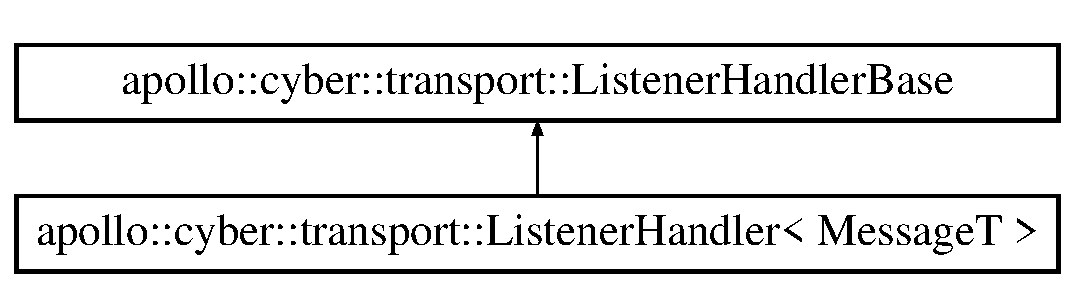
\includegraphics[height=2.000000cm]{classapollo_1_1cyber_1_1transport_1_1ListenerHandlerBase}
\end{center}
\end{figure}
\subsection*{Public Member Functions}
\begin{DoxyCompactItemize}
\item 
\hyperlink{classapollo_1_1cyber_1_1transport_1_1ListenerHandlerBase_a81d575ab9ccab7f0251c5af9d2d83fcb}{Listener\-Handler\-Base} ()
\item 
virtual \hyperlink{classapollo_1_1cyber_1_1transport_1_1ListenerHandlerBase_aa0b311470262f7c36de7e46abf1b1ac5}{$\sim$\-Listener\-Handler\-Base} ()
\item 
virtual void \hyperlink{classapollo_1_1cyber_1_1transport_1_1ListenerHandlerBase_ae66df407b61383d946788ff7a37e9b20}{Disconnect} (uint64\-\_\-t self\-\_\-id)=0
\item 
virtual void \hyperlink{classapollo_1_1cyber_1_1transport_1_1ListenerHandlerBase_afa2a7202373e5756b631d3f7dd325b09}{Disconnect} (uint64\-\_\-t self\-\_\-id, uint64\-\_\-t oppo\-\_\-id)=0
\item 
bool \hyperlink{classapollo_1_1cyber_1_1transport_1_1ListenerHandlerBase_a43cc98c3b19d658bae964432c0b75d41}{Is\-Raw\-Message} () const 
\end{DoxyCompactItemize}
\subsection*{Protected Attributes}
\begin{DoxyCompactItemize}
\item 
bool \hyperlink{classapollo_1_1cyber_1_1transport_1_1ListenerHandlerBase_a566139fbf45bb82f3120159f34bb60d5}{is\-\_\-raw\-\_\-message\-\_\-} = false
\end{DoxyCompactItemize}


\subsection{Constructor \& Destructor Documentation}
\hypertarget{classapollo_1_1cyber_1_1transport_1_1ListenerHandlerBase_a81d575ab9ccab7f0251c5af9d2d83fcb}{\index{apollo\-::cyber\-::transport\-::\-Listener\-Handler\-Base@{apollo\-::cyber\-::transport\-::\-Listener\-Handler\-Base}!Listener\-Handler\-Base@{Listener\-Handler\-Base}}
\index{Listener\-Handler\-Base@{Listener\-Handler\-Base}!apollo::cyber::transport::ListenerHandlerBase@{apollo\-::cyber\-::transport\-::\-Listener\-Handler\-Base}}
\subsubsection[{Listener\-Handler\-Base}]{\setlength{\rightskip}{0pt plus 5cm}apollo\-::cyber\-::transport\-::\-Listener\-Handler\-Base\-::\-Listener\-Handler\-Base (
\begin{DoxyParamCaption}
{}
\end{DoxyParamCaption}
)\hspace{0.3cm}{\ttfamily [inline]}}}\label{classapollo_1_1cyber_1_1transport_1_1ListenerHandlerBase_a81d575ab9ccab7f0251c5af9d2d83fcb}
\hypertarget{classapollo_1_1cyber_1_1transport_1_1ListenerHandlerBase_aa0b311470262f7c36de7e46abf1b1ac5}{\index{apollo\-::cyber\-::transport\-::\-Listener\-Handler\-Base@{apollo\-::cyber\-::transport\-::\-Listener\-Handler\-Base}!$\sim$\-Listener\-Handler\-Base@{$\sim$\-Listener\-Handler\-Base}}
\index{$\sim$\-Listener\-Handler\-Base@{$\sim$\-Listener\-Handler\-Base}!apollo::cyber::transport::ListenerHandlerBase@{apollo\-::cyber\-::transport\-::\-Listener\-Handler\-Base}}
\subsubsection[{$\sim$\-Listener\-Handler\-Base}]{\setlength{\rightskip}{0pt plus 5cm}virtual apollo\-::cyber\-::transport\-::\-Listener\-Handler\-Base\-::$\sim$\-Listener\-Handler\-Base (
\begin{DoxyParamCaption}
{}
\end{DoxyParamCaption}
)\hspace{0.3cm}{\ttfamily [inline]}, {\ttfamily [virtual]}}}\label{classapollo_1_1cyber_1_1transport_1_1ListenerHandlerBase_aa0b311470262f7c36de7e46abf1b1ac5}


\subsection{Member Function Documentation}
\hypertarget{classapollo_1_1cyber_1_1transport_1_1ListenerHandlerBase_ae66df407b61383d946788ff7a37e9b20}{\index{apollo\-::cyber\-::transport\-::\-Listener\-Handler\-Base@{apollo\-::cyber\-::transport\-::\-Listener\-Handler\-Base}!Disconnect@{Disconnect}}
\index{Disconnect@{Disconnect}!apollo::cyber::transport::ListenerHandlerBase@{apollo\-::cyber\-::transport\-::\-Listener\-Handler\-Base}}
\subsubsection[{Disconnect}]{\setlength{\rightskip}{0pt plus 5cm}virtual void apollo\-::cyber\-::transport\-::\-Listener\-Handler\-Base\-::\-Disconnect (
\begin{DoxyParamCaption}
\item[{uint64\-\_\-t}]{self\-\_\-id}
\end{DoxyParamCaption}
)\hspace{0.3cm}{\ttfamily [pure virtual]}}}\label{classapollo_1_1cyber_1_1transport_1_1ListenerHandlerBase_ae66df407b61383d946788ff7a37e9b20}


Implemented in \hyperlink{classapollo_1_1cyber_1_1transport_1_1ListenerHandler_a49732b06a8186e67f648efedca552224}{apollo\-::cyber\-::transport\-::\-Listener\-Handler$<$ Message\-T $>$}.

\hypertarget{classapollo_1_1cyber_1_1transport_1_1ListenerHandlerBase_afa2a7202373e5756b631d3f7dd325b09}{\index{apollo\-::cyber\-::transport\-::\-Listener\-Handler\-Base@{apollo\-::cyber\-::transport\-::\-Listener\-Handler\-Base}!Disconnect@{Disconnect}}
\index{Disconnect@{Disconnect}!apollo::cyber::transport::ListenerHandlerBase@{apollo\-::cyber\-::transport\-::\-Listener\-Handler\-Base}}
\subsubsection[{Disconnect}]{\setlength{\rightskip}{0pt plus 5cm}virtual void apollo\-::cyber\-::transport\-::\-Listener\-Handler\-Base\-::\-Disconnect (
\begin{DoxyParamCaption}
\item[{uint64\-\_\-t}]{self\-\_\-id, }
\item[{uint64\-\_\-t}]{oppo\-\_\-id}
\end{DoxyParamCaption}
)\hspace{0.3cm}{\ttfamily [pure virtual]}}}\label{classapollo_1_1cyber_1_1transport_1_1ListenerHandlerBase_afa2a7202373e5756b631d3f7dd325b09}


Implemented in \hyperlink{classapollo_1_1cyber_1_1transport_1_1ListenerHandler_a5bf12aac3e98dc9b1ba3f33e6170cad8}{apollo\-::cyber\-::transport\-::\-Listener\-Handler$<$ Message\-T $>$}.

\hypertarget{classapollo_1_1cyber_1_1transport_1_1ListenerHandlerBase_a43cc98c3b19d658bae964432c0b75d41}{\index{apollo\-::cyber\-::transport\-::\-Listener\-Handler\-Base@{apollo\-::cyber\-::transport\-::\-Listener\-Handler\-Base}!Is\-Raw\-Message@{Is\-Raw\-Message}}
\index{Is\-Raw\-Message@{Is\-Raw\-Message}!apollo::cyber::transport::ListenerHandlerBase@{apollo\-::cyber\-::transport\-::\-Listener\-Handler\-Base}}
\subsubsection[{Is\-Raw\-Message}]{\setlength{\rightskip}{0pt plus 5cm}bool apollo\-::cyber\-::transport\-::\-Listener\-Handler\-Base\-::\-Is\-Raw\-Message (
\begin{DoxyParamCaption}
{}
\end{DoxyParamCaption}
) const\hspace{0.3cm}{\ttfamily [inline]}}}\label{classapollo_1_1cyber_1_1transport_1_1ListenerHandlerBase_a43cc98c3b19d658bae964432c0b75d41}


\subsection{Member Data Documentation}
\hypertarget{classapollo_1_1cyber_1_1transport_1_1ListenerHandlerBase_a566139fbf45bb82f3120159f34bb60d5}{\index{apollo\-::cyber\-::transport\-::\-Listener\-Handler\-Base@{apollo\-::cyber\-::transport\-::\-Listener\-Handler\-Base}!is\-\_\-raw\-\_\-message\-\_\-@{is\-\_\-raw\-\_\-message\-\_\-}}
\index{is\-\_\-raw\-\_\-message\-\_\-@{is\-\_\-raw\-\_\-message\-\_\-}!apollo::cyber::transport::ListenerHandlerBase@{apollo\-::cyber\-::transport\-::\-Listener\-Handler\-Base}}
\subsubsection[{is\-\_\-raw\-\_\-message\-\_\-}]{\setlength{\rightskip}{0pt plus 5cm}bool apollo\-::cyber\-::transport\-::\-Listener\-Handler\-Base\-::is\-\_\-raw\-\_\-message\-\_\- = false\hspace{0.3cm}{\ttfamily [protected]}}}\label{classapollo_1_1cyber_1_1transport_1_1ListenerHandlerBase_a566139fbf45bb82f3120159f34bb60d5}


The documentation for this class was generated from the following file\-:\begin{DoxyCompactItemize}
\item 
transport/message/\hyperlink{listener__handler_8h}{listener\-\_\-handler.\-h}\end{DoxyCompactItemize}

\hypertarget{classapollo_1_1cyber_1_1logger_1_1LogFileObject}{\section{apollo\-:\-:cyber\-:\-:logger\-:\-:Log\-File\-Object Class Reference}
\label{classapollo_1_1cyber_1_1logger_1_1LogFileObject}\index{apollo\-::cyber\-::logger\-::\-Log\-File\-Object@{apollo\-::cyber\-::logger\-::\-Log\-File\-Object}}
}


{\ttfamily \#include $<$log\-\_\-file\-\_\-object.\-h$>$}

Inheritance diagram for apollo\-:\-:cyber\-:\-:logger\-:\-:Log\-File\-Object\-:\begin{figure}[H]
\begin{center}
\leavevmode
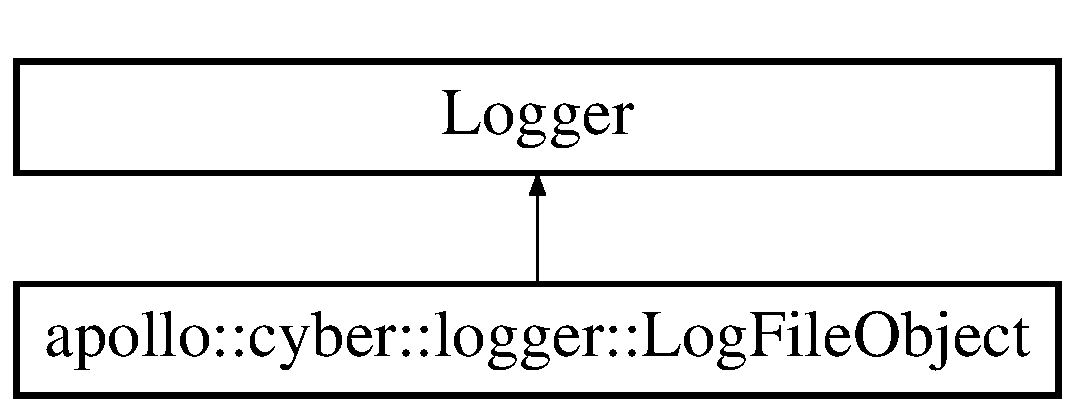
\includegraphics[height=2.000000cm]{classapollo_1_1cyber_1_1logger_1_1LogFileObject}
\end{center}
\end{figure}
\subsection*{Public Member Functions}
\begin{DoxyCompactItemize}
\item 
\hyperlink{classapollo_1_1cyber_1_1logger_1_1LogFileObject_a833a101b1328a34ff04b98c85f191721}{Log\-File\-Object} (google\-::\-Log\-Severity severity, const char $\ast$base\-\_\-filename)
\item 
\hyperlink{classapollo_1_1cyber_1_1logger_1_1LogFileObject_a03a476423210920b568648da3f80d3f2}{$\sim$\-Log\-File\-Object} ()
\item 
void \hyperlink{classapollo_1_1cyber_1_1logger_1_1LogFileObject_a9ba7a234cc8702170c305e0de970b012}{Write} (bool force\-\_\-flush, time\-\_\-t timestamp, const char $\ast$message, int message\-\_\-len) override
\item 
void \hyperlink{classapollo_1_1cyber_1_1logger_1_1LogFileObject_a7757684686f25c4ad6b552eb8d2d7457}{Set\-Basename} (const char $\ast$basename)
\item 
void \hyperlink{classapollo_1_1cyber_1_1logger_1_1LogFileObject_a5d4e55c263bd8e49b4882360cec74f78}{Set\-Extension} (const char $\ast$ext)
\item 
void \hyperlink{classapollo_1_1cyber_1_1logger_1_1LogFileObject_ae04342c963cd10bdc5bb2bbec192144f}{Set\-Symlink\-Basename} (const char $\ast$symlink\-\_\-basename)
\item 
void \hyperlink{classapollo_1_1cyber_1_1logger_1_1LogFileObject_ab398b6843a9302ef00b2817687d61f27}{Flush} () override
\item 
virtual uint32\-\_\-t \hyperlink{classapollo_1_1cyber_1_1logger_1_1LogFileObject_a380638b75320fe715433f87d522c543d}{Log\-Size} ()
\item 
void \hyperlink{classapollo_1_1cyber_1_1logger_1_1LogFileObject_a50388bac680858687619b981a42dc502}{Flush\-Unlocked} ()
\end{DoxyCompactItemize}
\subsection*{Private Member Functions}
\begin{DoxyCompactItemize}
\item 
bool \hyperlink{classapollo_1_1cyber_1_1logger_1_1LogFileObject_abbb5038197a577095037fac0e621a54b}{Create\-Logfile} (const std\-::string \&time\-\_\-pid\-\_\-string)
\end{DoxyCompactItemize}
\subsection*{Private Attributes}
\begin{DoxyCompactItemize}
\item 
std\-::mutex \hyperlink{classapollo_1_1cyber_1_1logger_1_1LogFileObject_a963d7f19da516b4ef514e37c4d926761}{lock\-\_\-}
\item 
bool \hyperlink{classapollo_1_1cyber_1_1logger_1_1LogFileObject_aaa83cf494797e8bcfaf70ba841890628}{base\-\_\-filename\-\_\-selected\-\_\-}
\item 
std\-::string \hyperlink{classapollo_1_1cyber_1_1logger_1_1LogFileObject_a2ddb3d2bcce49c4367a18eb59bdced97}{base\-\_\-filename\-\_\-}
\item 
std\-::string \hyperlink{classapollo_1_1cyber_1_1logger_1_1LogFileObject_a74857bfefb3231e64de3c43c05e6609d}{base\-\_\-filepath\-\_\-}
\item 
std\-::string \hyperlink{classapollo_1_1cyber_1_1logger_1_1LogFileObject_a5eab9f067f8b03af6d6fad057e85d063}{symlink\-\_\-basename\-\_\-}
\item 
std\-::string \hyperlink{classapollo_1_1cyber_1_1logger_1_1LogFileObject_a90ef513fcb9261914726fc5481725dcc}{filename\-\_\-extension\-\_\-}
\item 
F\-I\-L\-E $\ast$ \hyperlink{classapollo_1_1cyber_1_1logger_1_1LogFileObject_a76d70145494f68e1aa844f7013d5a7b2}{file\-\_\-}
\item 
google\-::\-Log\-Severity \hyperlink{classapollo_1_1cyber_1_1logger_1_1LogFileObject_a55b503945f312ba3315099707efee8c4}{severity\-\_\-}
\item 
uint32\-\_\-t \hyperlink{classapollo_1_1cyber_1_1logger_1_1LogFileObject_a29647683fc52c6fb388f4662b5248805}{bytes\-\_\-since\-\_\-flush\-\_\-}
\item 
uint32\-\_\-t \hyperlink{classapollo_1_1cyber_1_1logger_1_1LogFileObject_a7edba80c0f9d4b4fd4c38a775ffe8416}{dropped\-\_\-mem\-\_\-length\-\_\-}
\item 
uint32\-\_\-t \hyperlink{classapollo_1_1cyber_1_1logger_1_1LogFileObject_acadfc2b256c6c7f1d06ea76e406379eb}{file\-\_\-length\-\_\-}
\item 
unsigned int \hyperlink{classapollo_1_1cyber_1_1logger_1_1LogFileObject_a6a8883b31139aeaf0473eeaff7a71e3a}{rollover\-\_\-attempt\-\_\-}
\item 
int64\-\_\-t \hyperlink{classapollo_1_1cyber_1_1logger_1_1LogFileObject_a3b16662e6a2caf874be92e22ee1cb706}{next\-\_\-flush\-\_\-time\-\_\-}
\end{DoxyCompactItemize}
\subsection*{Static Private Attributes}
\begin{DoxyCompactItemize}
\item 
static const uint32\-\_\-t \hyperlink{classapollo_1_1cyber_1_1logger_1_1LogFileObject_a22a58c8d3d04ab9beaf28e5aa28601c9}{k\-Rollover\-Attempt\-Frequency} = 0x20
\end{DoxyCompactItemize}


\subsection{Constructor \& Destructor Documentation}
\hypertarget{classapollo_1_1cyber_1_1logger_1_1LogFileObject_a833a101b1328a34ff04b98c85f191721}{\index{apollo\-::cyber\-::logger\-::\-Log\-File\-Object@{apollo\-::cyber\-::logger\-::\-Log\-File\-Object}!Log\-File\-Object@{Log\-File\-Object}}
\index{Log\-File\-Object@{Log\-File\-Object}!apollo::cyber::logger::LogFileObject@{apollo\-::cyber\-::logger\-::\-Log\-File\-Object}}
\subsubsection[{Log\-File\-Object}]{\setlength{\rightskip}{0pt plus 5cm}apollo\-::cyber\-::logger\-::\-Log\-File\-Object\-::\-Log\-File\-Object (
\begin{DoxyParamCaption}
\item[{google\-::\-Log\-Severity}]{severity, }
\item[{const char $\ast$}]{base\-\_\-filename}
\end{DoxyParamCaption}
)}}\label{classapollo_1_1cyber_1_1logger_1_1LogFileObject_a833a101b1328a34ff04b98c85f191721}
\hypertarget{classapollo_1_1cyber_1_1logger_1_1LogFileObject_a03a476423210920b568648da3f80d3f2}{\index{apollo\-::cyber\-::logger\-::\-Log\-File\-Object@{apollo\-::cyber\-::logger\-::\-Log\-File\-Object}!$\sim$\-Log\-File\-Object@{$\sim$\-Log\-File\-Object}}
\index{$\sim$\-Log\-File\-Object@{$\sim$\-Log\-File\-Object}!apollo::cyber::logger::LogFileObject@{apollo\-::cyber\-::logger\-::\-Log\-File\-Object}}
\subsubsection[{$\sim$\-Log\-File\-Object}]{\setlength{\rightskip}{0pt plus 5cm}apollo\-::cyber\-::logger\-::\-Log\-File\-Object\-::$\sim$\-Log\-File\-Object (
\begin{DoxyParamCaption}
{}
\end{DoxyParamCaption}
)}}\label{classapollo_1_1cyber_1_1logger_1_1LogFileObject_a03a476423210920b568648da3f80d3f2}


\subsection{Member Function Documentation}
\hypertarget{classapollo_1_1cyber_1_1logger_1_1LogFileObject_abbb5038197a577095037fac0e621a54b}{\index{apollo\-::cyber\-::logger\-::\-Log\-File\-Object@{apollo\-::cyber\-::logger\-::\-Log\-File\-Object}!Create\-Logfile@{Create\-Logfile}}
\index{Create\-Logfile@{Create\-Logfile}!apollo::cyber::logger::LogFileObject@{apollo\-::cyber\-::logger\-::\-Log\-File\-Object}}
\subsubsection[{Create\-Logfile}]{\setlength{\rightskip}{0pt plus 5cm}bool apollo\-::cyber\-::logger\-::\-Log\-File\-Object\-::\-Create\-Logfile (
\begin{DoxyParamCaption}
\item[{const std\-::string \&}]{time\-\_\-pid\-\_\-string}
\end{DoxyParamCaption}
)\hspace{0.3cm}{\ttfamily [private]}}}\label{classapollo_1_1cyber_1_1logger_1_1LogFileObject_abbb5038197a577095037fac0e621a54b}
\hypertarget{classapollo_1_1cyber_1_1logger_1_1LogFileObject_ab398b6843a9302ef00b2817687d61f27}{\index{apollo\-::cyber\-::logger\-::\-Log\-File\-Object@{apollo\-::cyber\-::logger\-::\-Log\-File\-Object}!Flush@{Flush}}
\index{Flush@{Flush}!apollo::cyber::logger::LogFileObject@{apollo\-::cyber\-::logger\-::\-Log\-File\-Object}}
\subsubsection[{Flush}]{\setlength{\rightskip}{0pt plus 5cm}void apollo\-::cyber\-::logger\-::\-Log\-File\-Object\-::\-Flush (
\begin{DoxyParamCaption}
{}
\end{DoxyParamCaption}
)\hspace{0.3cm}{\ttfamily [override]}}}\label{classapollo_1_1cyber_1_1logger_1_1LogFileObject_ab398b6843a9302ef00b2817687d61f27}
\hypertarget{classapollo_1_1cyber_1_1logger_1_1LogFileObject_a50388bac680858687619b981a42dc502}{\index{apollo\-::cyber\-::logger\-::\-Log\-File\-Object@{apollo\-::cyber\-::logger\-::\-Log\-File\-Object}!Flush\-Unlocked@{Flush\-Unlocked}}
\index{Flush\-Unlocked@{Flush\-Unlocked}!apollo::cyber::logger::LogFileObject@{apollo\-::cyber\-::logger\-::\-Log\-File\-Object}}
\subsubsection[{Flush\-Unlocked}]{\setlength{\rightskip}{0pt plus 5cm}void apollo\-::cyber\-::logger\-::\-Log\-File\-Object\-::\-Flush\-Unlocked (
\begin{DoxyParamCaption}
{}
\end{DoxyParamCaption}
)}}\label{classapollo_1_1cyber_1_1logger_1_1LogFileObject_a50388bac680858687619b981a42dc502}
\hypertarget{classapollo_1_1cyber_1_1logger_1_1LogFileObject_a380638b75320fe715433f87d522c543d}{\index{apollo\-::cyber\-::logger\-::\-Log\-File\-Object@{apollo\-::cyber\-::logger\-::\-Log\-File\-Object}!Log\-Size@{Log\-Size}}
\index{Log\-Size@{Log\-Size}!apollo::cyber::logger::LogFileObject@{apollo\-::cyber\-::logger\-::\-Log\-File\-Object}}
\subsubsection[{Log\-Size}]{\setlength{\rightskip}{0pt plus 5cm}virtual uint32\-\_\-t apollo\-::cyber\-::logger\-::\-Log\-File\-Object\-::\-Log\-Size (
\begin{DoxyParamCaption}
{}
\end{DoxyParamCaption}
)\hspace{0.3cm}{\ttfamily [inline]}, {\ttfamily [virtual]}}}\label{classapollo_1_1cyber_1_1logger_1_1LogFileObject_a380638b75320fe715433f87d522c543d}
\hypertarget{classapollo_1_1cyber_1_1logger_1_1LogFileObject_a7757684686f25c4ad6b552eb8d2d7457}{\index{apollo\-::cyber\-::logger\-::\-Log\-File\-Object@{apollo\-::cyber\-::logger\-::\-Log\-File\-Object}!Set\-Basename@{Set\-Basename}}
\index{Set\-Basename@{Set\-Basename}!apollo::cyber::logger::LogFileObject@{apollo\-::cyber\-::logger\-::\-Log\-File\-Object}}
\subsubsection[{Set\-Basename}]{\setlength{\rightskip}{0pt plus 5cm}void apollo\-::cyber\-::logger\-::\-Log\-File\-Object\-::\-Set\-Basename (
\begin{DoxyParamCaption}
\item[{const char $\ast$}]{basename}
\end{DoxyParamCaption}
)}}\label{classapollo_1_1cyber_1_1logger_1_1LogFileObject_a7757684686f25c4ad6b552eb8d2d7457}
\hypertarget{classapollo_1_1cyber_1_1logger_1_1LogFileObject_a5d4e55c263bd8e49b4882360cec74f78}{\index{apollo\-::cyber\-::logger\-::\-Log\-File\-Object@{apollo\-::cyber\-::logger\-::\-Log\-File\-Object}!Set\-Extension@{Set\-Extension}}
\index{Set\-Extension@{Set\-Extension}!apollo::cyber::logger::LogFileObject@{apollo\-::cyber\-::logger\-::\-Log\-File\-Object}}
\subsubsection[{Set\-Extension}]{\setlength{\rightskip}{0pt plus 5cm}void apollo\-::cyber\-::logger\-::\-Log\-File\-Object\-::\-Set\-Extension (
\begin{DoxyParamCaption}
\item[{const char $\ast$}]{ext}
\end{DoxyParamCaption}
)}}\label{classapollo_1_1cyber_1_1logger_1_1LogFileObject_a5d4e55c263bd8e49b4882360cec74f78}
\hypertarget{classapollo_1_1cyber_1_1logger_1_1LogFileObject_ae04342c963cd10bdc5bb2bbec192144f}{\index{apollo\-::cyber\-::logger\-::\-Log\-File\-Object@{apollo\-::cyber\-::logger\-::\-Log\-File\-Object}!Set\-Symlink\-Basename@{Set\-Symlink\-Basename}}
\index{Set\-Symlink\-Basename@{Set\-Symlink\-Basename}!apollo::cyber::logger::LogFileObject@{apollo\-::cyber\-::logger\-::\-Log\-File\-Object}}
\subsubsection[{Set\-Symlink\-Basename}]{\setlength{\rightskip}{0pt plus 5cm}void apollo\-::cyber\-::logger\-::\-Log\-File\-Object\-::\-Set\-Symlink\-Basename (
\begin{DoxyParamCaption}
\item[{const char $\ast$}]{symlink\-\_\-basename}
\end{DoxyParamCaption}
)}}\label{classapollo_1_1cyber_1_1logger_1_1LogFileObject_ae04342c963cd10bdc5bb2bbec192144f}
\hypertarget{classapollo_1_1cyber_1_1logger_1_1LogFileObject_a9ba7a234cc8702170c305e0de970b012}{\index{apollo\-::cyber\-::logger\-::\-Log\-File\-Object@{apollo\-::cyber\-::logger\-::\-Log\-File\-Object}!Write@{Write}}
\index{Write@{Write}!apollo::cyber::logger::LogFileObject@{apollo\-::cyber\-::logger\-::\-Log\-File\-Object}}
\subsubsection[{Write}]{\setlength{\rightskip}{0pt plus 5cm}void apollo\-::cyber\-::logger\-::\-Log\-File\-Object\-::\-Write (
\begin{DoxyParamCaption}
\item[{bool}]{force\-\_\-flush, }
\item[{time\-\_\-t}]{timestamp, }
\item[{const char $\ast$}]{message, }
\item[{int}]{message\-\_\-len}
\end{DoxyParamCaption}
)\hspace{0.3cm}{\ttfamily [override]}}}\label{classapollo_1_1cyber_1_1logger_1_1LogFileObject_a9ba7a234cc8702170c305e0de970b012}


\subsection{Member Data Documentation}
\hypertarget{classapollo_1_1cyber_1_1logger_1_1LogFileObject_a2ddb3d2bcce49c4367a18eb59bdced97}{\index{apollo\-::cyber\-::logger\-::\-Log\-File\-Object@{apollo\-::cyber\-::logger\-::\-Log\-File\-Object}!base\-\_\-filename\-\_\-@{base\-\_\-filename\-\_\-}}
\index{base\-\_\-filename\-\_\-@{base\-\_\-filename\-\_\-}!apollo::cyber::logger::LogFileObject@{apollo\-::cyber\-::logger\-::\-Log\-File\-Object}}
\subsubsection[{base\-\_\-filename\-\_\-}]{\setlength{\rightskip}{0pt plus 5cm}std\-::string apollo\-::cyber\-::logger\-::\-Log\-File\-Object\-::base\-\_\-filename\-\_\-\hspace{0.3cm}{\ttfamily [private]}}}\label{classapollo_1_1cyber_1_1logger_1_1LogFileObject_a2ddb3d2bcce49c4367a18eb59bdced97}
\hypertarget{classapollo_1_1cyber_1_1logger_1_1LogFileObject_aaa83cf494797e8bcfaf70ba841890628}{\index{apollo\-::cyber\-::logger\-::\-Log\-File\-Object@{apollo\-::cyber\-::logger\-::\-Log\-File\-Object}!base\-\_\-filename\-\_\-selected\-\_\-@{base\-\_\-filename\-\_\-selected\-\_\-}}
\index{base\-\_\-filename\-\_\-selected\-\_\-@{base\-\_\-filename\-\_\-selected\-\_\-}!apollo::cyber::logger::LogFileObject@{apollo\-::cyber\-::logger\-::\-Log\-File\-Object}}
\subsubsection[{base\-\_\-filename\-\_\-selected\-\_\-}]{\setlength{\rightskip}{0pt plus 5cm}bool apollo\-::cyber\-::logger\-::\-Log\-File\-Object\-::base\-\_\-filename\-\_\-selected\-\_\-\hspace{0.3cm}{\ttfamily [private]}}}\label{classapollo_1_1cyber_1_1logger_1_1LogFileObject_aaa83cf494797e8bcfaf70ba841890628}
\hypertarget{classapollo_1_1cyber_1_1logger_1_1LogFileObject_a74857bfefb3231e64de3c43c05e6609d}{\index{apollo\-::cyber\-::logger\-::\-Log\-File\-Object@{apollo\-::cyber\-::logger\-::\-Log\-File\-Object}!base\-\_\-filepath\-\_\-@{base\-\_\-filepath\-\_\-}}
\index{base\-\_\-filepath\-\_\-@{base\-\_\-filepath\-\_\-}!apollo::cyber::logger::LogFileObject@{apollo\-::cyber\-::logger\-::\-Log\-File\-Object}}
\subsubsection[{base\-\_\-filepath\-\_\-}]{\setlength{\rightskip}{0pt plus 5cm}std\-::string apollo\-::cyber\-::logger\-::\-Log\-File\-Object\-::base\-\_\-filepath\-\_\-\hspace{0.3cm}{\ttfamily [private]}}}\label{classapollo_1_1cyber_1_1logger_1_1LogFileObject_a74857bfefb3231e64de3c43c05e6609d}
\hypertarget{classapollo_1_1cyber_1_1logger_1_1LogFileObject_a29647683fc52c6fb388f4662b5248805}{\index{apollo\-::cyber\-::logger\-::\-Log\-File\-Object@{apollo\-::cyber\-::logger\-::\-Log\-File\-Object}!bytes\-\_\-since\-\_\-flush\-\_\-@{bytes\-\_\-since\-\_\-flush\-\_\-}}
\index{bytes\-\_\-since\-\_\-flush\-\_\-@{bytes\-\_\-since\-\_\-flush\-\_\-}!apollo::cyber::logger::LogFileObject@{apollo\-::cyber\-::logger\-::\-Log\-File\-Object}}
\subsubsection[{bytes\-\_\-since\-\_\-flush\-\_\-}]{\setlength{\rightskip}{0pt plus 5cm}uint32\-\_\-t apollo\-::cyber\-::logger\-::\-Log\-File\-Object\-::bytes\-\_\-since\-\_\-flush\-\_\-\hspace{0.3cm}{\ttfamily [private]}}}\label{classapollo_1_1cyber_1_1logger_1_1LogFileObject_a29647683fc52c6fb388f4662b5248805}
\hypertarget{classapollo_1_1cyber_1_1logger_1_1LogFileObject_a7edba80c0f9d4b4fd4c38a775ffe8416}{\index{apollo\-::cyber\-::logger\-::\-Log\-File\-Object@{apollo\-::cyber\-::logger\-::\-Log\-File\-Object}!dropped\-\_\-mem\-\_\-length\-\_\-@{dropped\-\_\-mem\-\_\-length\-\_\-}}
\index{dropped\-\_\-mem\-\_\-length\-\_\-@{dropped\-\_\-mem\-\_\-length\-\_\-}!apollo::cyber::logger::LogFileObject@{apollo\-::cyber\-::logger\-::\-Log\-File\-Object}}
\subsubsection[{dropped\-\_\-mem\-\_\-length\-\_\-}]{\setlength{\rightskip}{0pt plus 5cm}uint32\-\_\-t apollo\-::cyber\-::logger\-::\-Log\-File\-Object\-::dropped\-\_\-mem\-\_\-length\-\_\-\hspace{0.3cm}{\ttfamily [private]}}}\label{classapollo_1_1cyber_1_1logger_1_1LogFileObject_a7edba80c0f9d4b4fd4c38a775ffe8416}
\hypertarget{classapollo_1_1cyber_1_1logger_1_1LogFileObject_a76d70145494f68e1aa844f7013d5a7b2}{\index{apollo\-::cyber\-::logger\-::\-Log\-File\-Object@{apollo\-::cyber\-::logger\-::\-Log\-File\-Object}!file\-\_\-@{file\-\_\-}}
\index{file\-\_\-@{file\-\_\-}!apollo::cyber::logger::LogFileObject@{apollo\-::cyber\-::logger\-::\-Log\-File\-Object}}
\subsubsection[{file\-\_\-}]{\setlength{\rightskip}{0pt plus 5cm}F\-I\-L\-E$\ast$ apollo\-::cyber\-::logger\-::\-Log\-File\-Object\-::file\-\_\-\hspace{0.3cm}{\ttfamily [private]}}}\label{classapollo_1_1cyber_1_1logger_1_1LogFileObject_a76d70145494f68e1aa844f7013d5a7b2}
\hypertarget{classapollo_1_1cyber_1_1logger_1_1LogFileObject_acadfc2b256c6c7f1d06ea76e406379eb}{\index{apollo\-::cyber\-::logger\-::\-Log\-File\-Object@{apollo\-::cyber\-::logger\-::\-Log\-File\-Object}!file\-\_\-length\-\_\-@{file\-\_\-length\-\_\-}}
\index{file\-\_\-length\-\_\-@{file\-\_\-length\-\_\-}!apollo::cyber::logger::LogFileObject@{apollo\-::cyber\-::logger\-::\-Log\-File\-Object}}
\subsubsection[{file\-\_\-length\-\_\-}]{\setlength{\rightskip}{0pt plus 5cm}uint32\-\_\-t apollo\-::cyber\-::logger\-::\-Log\-File\-Object\-::file\-\_\-length\-\_\-\hspace{0.3cm}{\ttfamily [private]}}}\label{classapollo_1_1cyber_1_1logger_1_1LogFileObject_acadfc2b256c6c7f1d06ea76e406379eb}
\hypertarget{classapollo_1_1cyber_1_1logger_1_1LogFileObject_a90ef513fcb9261914726fc5481725dcc}{\index{apollo\-::cyber\-::logger\-::\-Log\-File\-Object@{apollo\-::cyber\-::logger\-::\-Log\-File\-Object}!filename\-\_\-extension\-\_\-@{filename\-\_\-extension\-\_\-}}
\index{filename\-\_\-extension\-\_\-@{filename\-\_\-extension\-\_\-}!apollo::cyber::logger::LogFileObject@{apollo\-::cyber\-::logger\-::\-Log\-File\-Object}}
\subsubsection[{filename\-\_\-extension\-\_\-}]{\setlength{\rightskip}{0pt plus 5cm}std\-::string apollo\-::cyber\-::logger\-::\-Log\-File\-Object\-::filename\-\_\-extension\-\_\-\hspace{0.3cm}{\ttfamily [private]}}}\label{classapollo_1_1cyber_1_1logger_1_1LogFileObject_a90ef513fcb9261914726fc5481725dcc}
\hypertarget{classapollo_1_1cyber_1_1logger_1_1LogFileObject_a22a58c8d3d04ab9beaf28e5aa28601c9}{\index{apollo\-::cyber\-::logger\-::\-Log\-File\-Object@{apollo\-::cyber\-::logger\-::\-Log\-File\-Object}!k\-Rollover\-Attempt\-Frequency@{k\-Rollover\-Attempt\-Frequency}}
\index{k\-Rollover\-Attempt\-Frequency@{k\-Rollover\-Attempt\-Frequency}!apollo::cyber::logger::LogFileObject@{apollo\-::cyber\-::logger\-::\-Log\-File\-Object}}
\subsubsection[{k\-Rollover\-Attempt\-Frequency}]{\setlength{\rightskip}{0pt plus 5cm}const uint32\-\_\-t apollo\-::cyber\-::logger\-::\-Log\-File\-Object\-::k\-Rollover\-Attempt\-Frequency = 0x20\hspace{0.3cm}{\ttfamily [static]}, {\ttfamily [private]}}}\label{classapollo_1_1cyber_1_1logger_1_1LogFileObject_a22a58c8d3d04ab9beaf28e5aa28601c9}
\hypertarget{classapollo_1_1cyber_1_1logger_1_1LogFileObject_a963d7f19da516b4ef514e37c4d926761}{\index{apollo\-::cyber\-::logger\-::\-Log\-File\-Object@{apollo\-::cyber\-::logger\-::\-Log\-File\-Object}!lock\-\_\-@{lock\-\_\-}}
\index{lock\-\_\-@{lock\-\_\-}!apollo::cyber::logger::LogFileObject@{apollo\-::cyber\-::logger\-::\-Log\-File\-Object}}
\subsubsection[{lock\-\_\-}]{\setlength{\rightskip}{0pt plus 5cm}std\-::mutex apollo\-::cyber\-::logger\-::\-Log\-File\-Object\-::lock\-\_\-\hspace{0.3cm}{\ttfamily [private]}}}\label{classapollo_1_1cyber_1_1logger_1_1LogFileObject_a963d7f19da516b4ef514e37c4d926761}
\hypertarget{classapollo_1_1cyber_1_1logger_1_1LogFileObject_a3b16662e6a2caf874be92e22ee1cb706}{\index{apollo\-::cyber\-::logger\-::\-Log\-File\-Object@{apollo\-::cyber\-::logger\-::\-Log\-File\-Object}!next\-\_\-flush\-\_\-time\-\_\-@{next\-\_\-flush\-\_\-time\-\_\-}}
\index{next\-\_\-flush\-\_\-time\-\_\-@{next\-\_\-flush\-\_\-time\-\_\-}!apollo::cyber::logger::LogFileObject@{apollo\-::cyber\-::logger\-::\-Log\-File\-Object}}
\subsubsection[{next\-\_\-flush\-\_\-time\-\_\-}]{\setlength{\rightskip}{0pt plus 5cm}int64\-\_\-t apollo\-::cyber\-::logger\-::\-Log\-File\-Object\-::next\-\_\-flush\-\_\-time\-\_\-\hspace{0.3cm}{\ttfamily [private]}}}\label{classapollo_1_1cyber_1_1logger_1_1LogFileObject_a3b16662e6a2caf874be92e22ee1cb706}
\hypertarget{classapollo_1_1cyber_1_1logger_1_1LogFileObject_a6a8883b31139aeaf0473eeaff7a71e3a}{\index{apollo\-::cyber\-::logger\-::\-Log\-File\-Object@{apollo\-::cyber\-::logger\-::\-Log\-File\-Object}!rollover\-\_\-attempt\-\_\-@{rollover\-\_\-attempt\-\_\-}}
\index{rollover\-\_\-attempt\-\_\-@{rollover\-\_\-attempt\-\_\-}!apollo::cyber::logger::LogFileObject@{apollo\-::cyber\-::logger\-::\-Log\-File\-Object}}
\subsubsection[{rollover\-\_\-attempt\-\_\-}]{\setlength{\rightskip}{0pt plus 5cm}unsigned int apollo\-::cyber\-::logger\-::\-Log\-File\-Object\-::rollover\-\_\-attempt\-\_\-\hspace{0.3cm}{\ttfamily [private]}}}\label{classapollo_1_1cyber_1_1logger_1_1LogFileObject_a6a8883b31139aeaf0473eeaff7a71e3a}
\hypertarget{classapollo_1_1cyber_1_1logger_1_1LogFileObject_a55b503945f312ba3315099707efee8c4}{\index{apollo\-::cyber\-::logger\-::\-Log\-File\-Object@{apollo\-::cyber\-::logger\-::\-Log\-File\-Object}!severity\-\_\-@{severity\-\_\-}}
\index{severity\-\_\-@{severity\-\_\-}!apollo::cyber::logger::LogFileObject@{apollo\-::cyber\-::logger\-::\-Log\-File\-Object}}
\subsubsection[{severity\-\_\-}]{\setlength{\rightskip}{0pt plus 5cm}google\-::\-Log\-Severity apollo\-::cyber\-::logger\-::\-Log\-File\-Object\-::severity\-\_\-\hspace{0.3cm}{\ttfamily [private]}}}\label{classapollo_1_1cyber_1_1logger_1_1LogFileObject_a55b503945f312ba3315099707efee8c4}
\hypertarget{classapollo_1_1cyber_1_1logger_1_1LogFileObject_a5eab9f067f8b03af6d6fad057e85d063}{\index{apollo\-::cyber\-::logger\-::\-Log\-File\-Object@{apollo\-::cyber\-::logger\-::\-Log\-File\-Object}!symlink\-\_\-basename\-\_\-@{symlink\-\_\-basename\-\_\-}}
\index{symlink\-\_\-basename\-\_\-@{symlink\-\_\-basename\-\_\-}!apollo::cyber::logger::LogFileObject@{apollo\-::cyber\-::logger\-::\-Log\-File\-Object}}
\subsubsection[{symlink\-\_\-basename\-\_\-}]{\setlength{\rightskip}{0pt plus 5cm}std\-::string apollo\-::cyber\-::logger\-::\-Log\-File\-Object\-::symlink\-\_\-basename\-\_\-\hspace{0.3cm}{\ttfamily [private]}}}\label{classapollo_1_1cyber_1_1logger_1_1LogFileObject_a5eab9f067f8b03af6d6fad057e85d063}


The documentation for this class was generated from the following file\-:\begin{DoxyCompactItemize}
\item 
logger/\hyperlink{log__file__object_8h}{log\-\_\-file\-\_\-object.\-h}\end{DoxyCompactItemize}

\hypertarget{classapollo_1_1cyber_1_1logger_1_1Logger}{\section{apollo\-:\-:cyber\-:\-:logger\-:\-:Logger Class Reference}
\label{classapollo_1_1cyber_1_1logger_1_1Logger}\index{apollo\-::cyber\-::logger\-::\-Logger@{apollo\-::cyber\-::logger\-::\-Logger}}
}


{\ttfamily \#include $<$logger.\-h$>$}

Inheritance diagram for apollo\-:\-:cyber\-:\-:logger\-:\-:Logger\-:\begin{figure}[H]
\begin{center}
\leavevmode
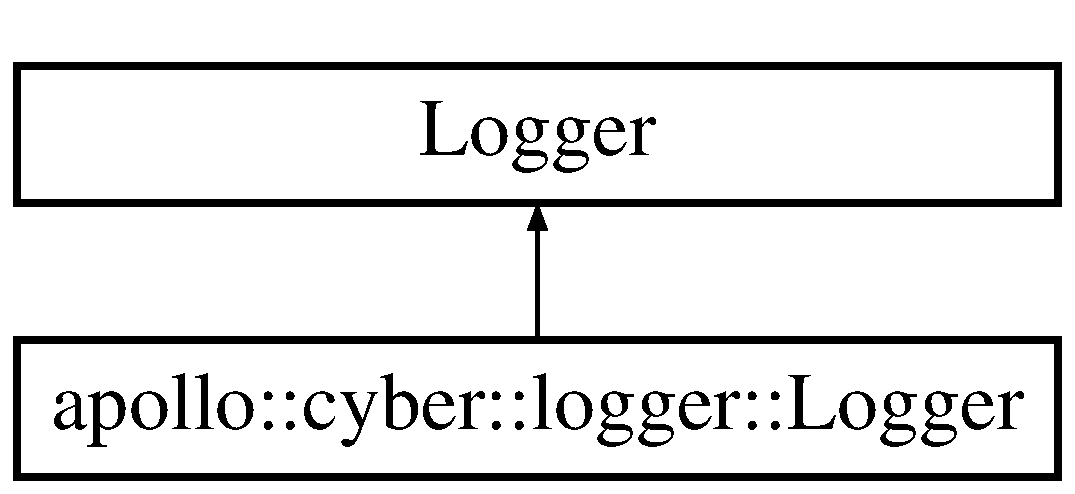
\includegraphics[height=2.000000cm]{classapollo_1_1cyber_1_1logger_1_1Logger}
\end{center}
\end{figure}
\subsection*{Public Member Functions}
\begin{DoxyCompactItemize}
\item 
\hyperlink{classapollo_1_1cyber_1_1logger_1_1Logger_ae66fdd9a20171e47e9e2074aa0880a4d}{Logger} (google\-::base\-::\-Logger $\ast$wrapped)
\item 
\hyperlink{classapollo_1_1cyber_1_1logger_1_1Logger_a7238886d763068ac235125dbea29189b}{$\sim$\-Logger} ()
\item 
void \hyperlink{classapollo_1_1cyber_1_1logger_1_1Logger_a714b49458650913f6eadf078f93aabd1}{Write} (bool force\-\_\-flush, time\-\_\-t timestamp, const char $\ast$message, int message\-\_\-len) override
\item 
void \hyperlink{classapollo_1_1cyber_1_1logger_1_1Logger_a7cc4e4b73f4c974022e38982b8567ed3}{Flush} () override
\item 
uint32\-\_\-t \hyperlink{classapollo_1_1cyber_1_1logger_1_1Logger_a3f4323607c447f93b01f84c9a4c22113}{Log\-Size} () override
\end{DoxyCompactItemize}
\subsection*{Private Attributes}
\begin{DoxyCompactItemize}
\item 
google\-::base\-::\-Logger $\ast$const \hyperlink{classapollo_1_1cyber_1_1logger_1_1Logger_a80db29c400adaba27edbe8a1aec55f90}{wrapped\-\_\-}
\item 
std\-::mutex \hyperlink{classapollo_1_1cyber_1_1logger_1_1Logger_a127c753b55ea9542c8b88882fd4c0b2e}{mutex\-\_\-}
\end{DoxyCompactItemize}


\subsection{Constructor \& Destructor Documentation}
\hypertarget{classapollo_1_1cyber_1_1logger_1_1Logger_ae66fdd9a20171e47e9e2074aa0880a4d}{\index{apollo\-::cyber\-::logger\-::\-Logger@{apollo\-::cyber\-::logger\-::\-Logger}!Logger@{Logger}}
\index{Logger@{Logger}!apollo::cyber::logger::Logger@{apollo\-::cyber\-::logger\-::\-Logger}}
\subsubsection[{Logger}]{\setlength{\rightskip}{0pt plus 5cm}apollo\-::cyber\-::logger\-::\-Logger\-::\-Logger (
\begin{DoxyParamCaption}
\item[{google\-::base\-::\-Logger $\ast$}]{wrapped}
\end{DoxyParamCaption}
)\hspace{0.3cm}{\ttfamily [explicit]}}}\label{classapollo_1_1cyber_1_1logger_1_1Logger_ae66fdd9a20171e47e9e2074aa0880a4d}
\hypertarget{classapollo_1_1cyber_1_1logger_1_1Logger_a7238886d763068ac235125dbea29189b}{\index{apollo\-::cyber\-::logger\-::\-Logger@{apollo\-::cyber\-::logger\-::\-Logger}!$\sim$\-Logger@{$\sim$\-Logger}}
\index{$\sim$\-Logger@{$\sim$\-Logger}!apollo::cyber::logger::Logger@{apollo\-::cyber\-::logger\-::\-Logger}}
\subsubsection[{$\sim$\-Logger}]{\setlength{\rightskip}{0pt plus 5cm}apollo\-::cyber\-::logger\-::\-Logger\-::$\sim$\-Logger (
\begin{DoxyParamCaption}
{}
\end{DoxyParamCaption}
)}}\label{classapollo_1_1cyber_1_1logger_1_1Logger_a7238886d763068ac235125dbea29189b}


\subsection{Member Function Documentation}
\hypertarget{classapollo_1_1cyber_1_1logger_1_1Logger_a7cc4e4b73f4c974022e38982b8567ed3}{\index{apollo\-::cyber\-::logger\-::\-Logger@{apollo\-::cyber\-::logger\-::\-Logger}!Flush@{Flush}}
\index{Flush@{Flush}!apollo::cyber::logger::Logger@{apollo\-::cyber\-::logger\-::\-Logger}}
\subsubsection[{Flush}]{\setlength{\rightskip}{0pt plus 5cm}void apollo\-::cyber\-::logger\-::\-Logger\-::\-Flush (
\begin{DoxyParamCaption}
{}
\end{DoxyParamCaption}
)\hspace{0.3cm}{\ttfamily [override]}}}\label{classapollo_1_1cyber_1_1logger_1_1Logger_a7cc4e4b73f4c974022e38982b8567ed3}
\hypertarget{classapollo_1_1cyber_1_1logger_1_1Logger_a3f4323607c447f93b01f84c9a4c22113}{\index{apollo\-::cyber\-::logger\-::\-Logger@{apollo\-::cyber\-::logger\-::\-Logger}!Log\-Size@{Log\-Size}}
\index{Log\-Size@{Log\-Size}!apollo::cyber::logger::Logger@{apollo\-::cyber\-::logger\-::\-Logger}}
\subsubsection[{Log\-Size}]{\setlength{\rightskip}{0pt plus 5cm}uint32\-\_\-t apollo\-::cyber\-::logger\-::\-Logger\-::\-Log\-Size (
\begin{DoxyParamCaption}
{}
\end{DoxyParamCaption}
)\hspace{0.3cm}{\ttfamily [override]}}}\label{classapollo_1_1cyber_1_1logger_1_1Logger_a3f4323607c447f93b01f84c9a4c22113}
\hypertarget{classapollo_1_1cyber_1_1logger_1_1Logger_a714b49458650913f6eadf078f93aabd1}{\index{apollo\-::cyber\-::logger\-::\-Logger@{apollo\-::cyber\-::logger\-::\-Logger}!Write@{Write}}
\index{Write@{Write}!apollo::cyber::logger::Logger@{apollo\-::cyber\-::logger\-::\-Logger}}
\subsubsection[{Write}]{\setlength{\rightskip}{0pt plus 5cm}void apollo\-::cyber\-::logger\-::\-Logger\-::\-Write (
\begin{DoxyParamCaption}
\item[{bool}]{force\-\_\-flush, }
\item[{time\-\_\-t}]{timestamp, }
\item[{const char $\ast$}]{message, }
\item[{int}]{message\-\_\-len}
\end{DoxyParamCaption}
)\hspace{0.3cm}{\ttfamily [override]}}}\label{classapollo_1_1cyber_1_1logger_1_1Logger_a714b49458650913f6eadf078f93aabd1}


\subsection{Member Data Documentation}
\hypertarget{classapollo_1_1cyber_1_1logger_1_1Logger_a127c753b55ea9542c8b88882fd4c0b2e}{\index{apollo\-::cyber\-::logger\-::\-Logger@{apollo\-::cyber\-::logger\-::\-Logger}!mutex\-\_\-@{mutex\-\_\-}}
\index{mutex\-\_\-@{mutex\-\_\-}!apollo::cyber::logger::Logger@{apollo\-::cyber\-::logger\-::\-Logger}}
\subsubsection[{mutex\-\_\-}]{\setlength{\rightskip}{0pt plus 5cm}std\-::mutex apollo\-::cyber\-::logger\-::\-Logger\-::mutex\-\_\-\hspace{0.3cm}{\ttfamily [private]}}}\label{classapollo_1_1cyber_1_1logger_1_1Logger_a127c753b55ea9542c8b88882fd4c0b2e}
\hypertarget{classapollo_1_1cyber_1_1logger_1_1Logger_a80db29c400adaba27edbe8a1aec55f90}{\index{apollo\-::cyber\-::logger\-::\-Logger@{apollo\-::cyber\-::logger\-::\-Logger}!wrapped\-\_\-@{wrapped\-\_\-}}
\index{wrapped\-\_\-@{wrapped\-\_\-}!apollo::cyber::logger::Logger@{apollo\-::cyber\-::logger\-::\-Logger}}
\subsubsection[{wrapped\-\_\-}]{\setlength{\rightskip}{0pt plus 5cm}google\-::base\-::\-Logger$\ast$ const apollo\-::cyber\-::logger\-::\-Logger\-::wrapped\-\_\-\hspace{0.3cm}{\ttfamily [private]}}}\label{classapollo_1_1cyber_1_1logger_1_1Logger_a80db29c400adaba27edbe8a1aec55f90}


The documentation for this class was generated from the following file\-:\begin{DoxyCompactItemize}
\item 
logger/\hyperlink{logger_8h}{logger.\-h}\end{DoxyCompactItemize}

\hypertarget{classapollo_1_1cyber_1_1service__discovery_1_1Manager}{\section{apollo\-:\-:cyber\-:\-:service\-\_\-discovery\-:\-:Manager Class Reference}
\label{classapollo_1_1cyber_1_1service__discovery_1_1Manager}\index{apollo\-::cyber\-::service\-\_\-discovery\-::\-Manager@{apollo\-::cyber\-::service\-\_\-discovery\-::\-Manager}}
}


{\ttfamily \#include $<$manager.\-h$>$}

Inheritance diagram for apollo\-:\-:cyber\-:\-:service\-\_\-discovery\-:\-:Manager\-:\begin{figure}[H]
\begin{center}
\leavevmode
\includegraphics[height=1.212121cm]{classapollo_1_1cyber_1_1service__discovery_1_1Manager}
\end{center}
\end{figure}
\subsection*{Public Types}
\begin{DoxyCompactItemize}
\item 
using \hyperlink{classapollo_1_1cyber_1_1service__discovery_1_1Manager_a9730b844d88e23f65d5dcbcfca1a7d59}{Change\-Signal} = \hyperlink{classapollo_1_1cyber_1_1base_1_1Signal}{base\-::\-Signal}$<$ const Change\-Msg \& $>$
\item 
using \hyperlink{classapollo_1_1cyber_1_1service__discovery_1_1Manager_a1e08b690a5829fbabeb6d3aea5ab8320}{Change\-Func} = std\-::function$<$ void(const Change\-Msg \&)$>$
\item 
using \hyperlink{classapollo_1_1cyber_1_1service__discovery_1_1Manager_ab43fa282f6aa1b3b1180a1e416b98b68}{Change\-Connection} = \hyperlink{classapollo_1_1cyber_1_1base_1_1Connection}{base\-::\-Connection}$<$ const Change\-Msg \& $>$
\item 
using \hyperlink{classapollo_1_1cyber_1_1service__discovery_1_1Manager_a7576b9ac293ff99af06e30a971df5dce}{Rtps\-Participant} = eprosima\-::fastrtps\-::\-Participant
\item 
using \hyperlink{classapollo_1_1cyber_1_1service__discovery_1_1Manager_a1b8464bc115c49a16a0d943c7cb5ef32}{Rtps\-Publisher\-Attr} = eprosima\-::fastrtps\-::\-Publisher\-Attributes
\item 
using \hyperlink{classapollo_1_1cyber_1_1service__discovery_1_1Manager_ac16fc5e01d6d107cbb865d6d8127f622}{Rtps\-Subscriber\-Attr} = eprosima\-::fastrtps\-::\-Subscriber\-Attributes
\end{DoxyCompactItemize}
\subsection*{Public Member Functions}
\begin{DoxyCompactItemize}
\item 
\hyperlink{classapollo_1_1cyber_1_1service__discovery_1_1Manager_a8bc33aa7aefffcaa50ebf3ca12b4dd48}{Manager} ()
\item 
virtual \hyperlink{classapollo_1_1cyber_1_1service__discovery_1_1Manager_ae683108196b8958825bb4142ab98a378}{$\sim$\-Manager} ()
\item 
bool \hyperlink{classapollo_1_1cyber_1_1service__discovery_1_1Manager_a0a007e927b14cb2584a9b97b1c8ec299}{Start\-Discovery} (\hyperlink{classapollo_1_1cyber_1_1service__discovery_1_1Manager_a7576b9ac293ff99af06e30a971df5dce}{Rtps\-Participant} $\ast$participant)
\item 
void \hyperlink{classapollo_1_1cyber_1_1service__discovery_1_1Manager_ae06ca49d144ab1ca78cfd30f204e4caa}{Stop\-Discovery} ()
\item 
virtual void \hyperlink{classapollo_1_1cyber_1_1service__discovery_1_1Manager_a4a4e6fc42da96478d0ff6ca5d8f21ad7}{Shutdown} ()
\item 
bool \hyperlink{classapollo_1_1cyber_1_1service__discovery_1_1Manager_a21da44e9c4c3fe10af7005c4d5eec894}{Join} (const Role\-Attributes \&attr, Role\-Type role, bool need\-\_\-publish=true)
\item 
bool \hyperlink{classapollo_1_1cyber_1_1service__discovery_1_1Manager_abf37a1b3c4f23425fcdbd46ec0a3b632}{Leave} (const Role\-Attributes \&attr, Role\-Type role)
\item 
\hyperlink{classapollo_1_1cyber_1_1service__discovery_1_1Manager_ab43fa282f6aa1b3b1180a1e416b98b68}{Change\-Connection} \hyperlink{classapollo_1_1cyber_1_1service__discovery_1_1Manager_abe0325759c5c14d16cfe2e2b1460b9ce}{Add\-Change\-Listener} (const \hyperlink{classapollo_1_1cyber_1_1service__discovery_1_1Manager_a1e08b690a5829fbabeb6d3aea5ab8320}{Change\-Func} \&func)
\item 
void \hyperlink{classapollo_1_1cyber_1_1service__discovery_1_1Manager_a2e46899f22d9e001b10a7e49ef61bd0c}{Remove\-Change\-Listener} (const \hyperlink{classapollo_1_1cyber_1_1service__discovery_1_1Manager_ab43fa282f6aa1b3b1180a1e416b98b68}{Change\-Connection} \&conn)
\item 
virtual void \hyperlink{classapollo_1_1cyber_1_1service__discovery_1_1Manager_a95a679e0fc7904e6f1a8b2fdd139cc03}{On\-Topo\-Module\-Leave} (const std\-::string \&host\-\_\-name, int process\-\_\-id)=0
\end{DoxyCompactItemize}
\subsection*{Protected Member Functions}
\begin{DoxyCompactItemize}
\item 
bool \hyperlink{classapollo_1_1cyber_1_1service__discovery_1_1Manager_a722f92a9db32919ef83b9fbfcaaff85a}{Create\-Publisher} (\hyperlink{classapollo_1_1cyber_1_1service__discovery_1_1Manager_a7576b9ac293ff99af06e30a971df5dce}{Rtps\-Participant} $\ast$participant)
\item 
bool \hyperlink{classapollo_1_1cyber_1_1service__discovery_1_1Manager_a777040a412671e776f1f750933a629f3}{Create\-Subscriber} (\hyperlink{classapollo_1_1cyber_1_1service__discovery_1_1Manager_a7576b9ac293ff99af06e30a971df5dce}{Rtps\-Participant} $\ast$participant)
\item 
virtual bool \hyperlink{classapollo_1_1cyber_1_1service__discovery_1_1Manager_acfa0224581a6722daf4861f34e4c11ef}{Check} (const Role\-Attributes \&attr)=0
\item 
virtual void \hyperlink{classapollo_1_1cyber_1_1service__discovery_1_1Manager_a6e36e4095291597364ce4b37ee1c897b}{Dispose} (const Change\-Msg \&msg)=0
\item 
virtual bool \hyperlink{classapollo_1_1cyber_1_1service__discovery_1_1Manager_ab3221bff519725654e6e232d6ad528e0}{Need\-Publish} (const Change\-Msg \&msg) const 
\item 
void \hyperlink{classapollo_1_1cyber_1_1service__discovery_1_1Manager_a0aee2af4344c78f97ec72b885d98ab5d}{Convert} (const Role\-Attributes \&attr, Role\-Type role, Operate\-Type opt, Change\-Msg $\ast$msg)
\item 
void \hyperlink{classapollo_1_1cyber_1_1service__discovery_1_1Manager_a086e96a029a1f05a0561d57e541c9526}{Notify} (const Change\-Msg \&msg)
\item 
bool \hyperlink{classapollo_1_1cyber_1_1service__discovery_1_1Manager_a2a82d0febb575ddd693184b639016426}{Publish} (const Change\-Msg \&msg)
\item 
void \hyperlink{classapollo_1_1cyber_1_1service__discovery_1_1Manager_a8c4903e0876ace79003d4e2994be43ab}{On\-Remote\-Change} (const std\-::string \&msg\-\_\-str)
\item 
bool \hyperlink{classapollo_1_1cyber_1_1service__discovery_1_1Manager_a26c75e76647b6753e1565c4129c518f7}{Is\-From\-Same\-Process} (const Change\-Msg \&msg)
\end{DoxyCompactItemize}
\subsection*{Protected Attributes}
\begin{DoxyCompactItemize}
\item 
std\-::atomic$<$ bool $>$ \hyperlink{classapollo_1_1cyber_1_1service__discovery_1_1Manager_a260bde7ce1d7749c3cb35e98b820d278}{is\-\_\-shutdown\-\_\-}
\item 
std\-::atomic$<$ bool $>$ \hyperlink{classapollo_1_1cyber_1_1service__discovery_1_1Manager_a8a8bd0560f76ccb0be2a37fd62fbb2d8}{is\-\_\-discovery\-\_\-started\-\_\-}
\item 
int \hyperlink{classapollo_1_1cyber_1_1service__discovery_1_1Manager_a901cf709cf2707faf0ced991bc2da591}{allowed\-\_\-role\-\_\-}
\item 
Change\-Type \hyperlink{classapollo_1_1cyber_1_1service__discovery_1_1Manager_a26dbcd395983f96ff00060648e16ff93}{change\-\_\-type\-\_\-}
\item 
std\-::string \hyperlink{classapollo_1_1cyber_1_1service__discovery_1_1Manager_a6e221053092ac40fd6810510a3eb10cc}{host\-\_\-name\-\_\-}
\item 
int \hyperlink{classapollo_1_1cyber_1_1service__discovery_1_1Manager_ac251ffb4700b4b901451ad9f103ccdd8}{process\-\_\-id\-\_\-}
\item 
std\-::string \hyperlink{classapollo_1_1cyber_1_1service__discovery_1_1Manager_a2ff877c30b287c1a5c7efeedfde0afe0}{channel\-\_\-name\-\_\-}
\item 
eprosima\-::fastrtps\-::\-Publisher $\ast$ \hyperlink{classapollo_1_1cyber_1_1service__discovery_1_1Manager_ab5caa9d2feb69e9746f6371a908d2661}{publisher\-\_\-}
\item 
eprosima\-::fastrtps\-::\-Subscriber $\ast$ \hyperlink{classapollo_1_1cyber_1_1service__discovery_1_1Manager_a4324a7de5c025ab948d210916bbadcb2}{subscriber\-\_\-}
\item 
\hyperlink{classapollo_1_1cyber_1_1service__discovery_1_1SubscriberListener}{Subscriber\-Listener} $\ast$ \hyperlink{classapollo_1_1cyber_1_1service__discovery_1_1Manager_a8dd4cf136c87d16027530af545cb0842}{listener\-\_\-}
\item 
\hyperlink{classapollo_1_1cyber_1_1service__discovery_1_1Manager_a9730b844d88e23f65d5dcbcfca1a7d59}{Change\-Signal} \hyperlink{classapollo_1_1cyber_1_1service__discovery_1_1Manager_af92680680a5e900f48f8a39d9a0524f9}{signal\-\_\-}
\end{DoxyCompactItemize}


\subsection{Member Typedef Documentation}
\hypertarget{classapollo_1_1cyber_1_1service__discovery_1_1Manager_ab43fa282f6aa1b3b1180a1e416b98b68}{\index{apollo\-::cyber\-::service\-\_\-discovery\-::\-Manager@{apollo\-::cyber\-::service\-\_\-discovery\-::\-Manager}!Change\-Connection@{Change\-Connection}}
\index{Change\-Connection@{Change\-Connection}!apollo::cyber::service_discovery::Manager@{apollo\-::cyber\-::service\-\_\-discovery\-::\-Manager}}
\subsubsection[{Change\-Connection}]{\setlength{\rightskip}{0pt plus 5cm}using {\bf apollo\-::cyber\-::service\-\_\-discovery\-::\-Manager\-::\-Change\-Connection} =  {\bf base\-::\-Connection}$<$const Change\-Msg\&$>$}}\label{classapollo_1_1cyber_1_1service__discovery_1_1Manager_ab43fa282f6aa1b3b1180a1e416b98b68}
\hypertarget{classapollo_1_1cyber_1_1service__discovery_1_1Manager_a1e08b690a5829fbabeb6d3aea5ab8320}{\index{apollo\-::cyber\-::service\-\_\-discovery\-::\-Manager@{apollo\-::cyber\-::service\-\_\-discovery\-::\-Manager}!Change\-Func@{Change\-Func}}
\index{Change\-Func@{Change\-Func}!apollo::cyber::service_discovery::Manager@{apollo\-::cyber\-::service\-\_\-discovery\-::\-Manager}}
\subsubsection[{Change\-Func}]{\setlength{\rightskip}{0pt plus 5cm}using {\bf apollo\-::cyber\-::service\-\_\-discovery\-::\-Manager\-::\-Change\-Func} =  std\-::function$<$void(const Change\-Msg\&)$>$}}\label{classapollo_1_1cyber_1_1service__discovery_1_1Manager_a1e08b690a5829fbabeb6d3aea5ab8320}
\hypertarget{classapollo_1_1cyber_1_1service__discovery_1_1Manager_a9730b844d88e23f65d5dcbcfca1a7d59}{\index{apollo\-::cyber\-::service\-\_\-discovery\-::\-Manager@{apollo\-::cyber\-::service\-\_\-discovery\-::\-Manager}!Change\-Signal@{Change\-Signal}}
\index{Change\-Signal@{Change\-Signal}!apollo::cyber::service_discovery::Manager@{apollo\-::cyber\-::service\-\_\-discovery\-::\-Manager}}
\subsubsection[{Change\-Signal}]{\setlength{\rightskip}{0pt plus 5cm}using {\bf apollo\-::cyber\-::service\-\_\-discovery\-::\-Manager\-::\-Change\-Signal} =  {\bf base\-::\-Signal}$<$const Change\-Msg\&$>$}}\label{classapollo_1_1cyber_1_1service__discovery_1_1Manager_a9730b844d88e23f65d5dcbcfca1a7d59}
\hypertarget{classapollo_1_1cyber_1_1service__discovery_1_1Manager_a7576b9ac293ff99af06e30a971df5dce}{\index{apollo\-::cyber\-::service\-\_\-discovery\-::\-Manager@{apollo\-::cyber\-::service\-\_\-discovery\-::\-Manager}!Rtps\-Participant@{Rtps\-Participant}}
\index{Rtps\-Participant@{Rtps\-Participant}!apollo::cyber::service_discovery::Manager@{apollo\-::cyber\-::service\-\_\-discovery\-::\-Manager}}
\subsubsection[{Rtps\-Participant}]{\setlength{\rightskip}{0pt plus 5cm}using {\bf apollo\-::cyber\-::service\-\_\-discovery\-::\-Manager\-::\-Rtps\-Participant} =  eprosima\-::fastrtps\-::\-Participant}}\label{classapollo_1_1cyber_1_1service__discovery_1_1Manager_a7576b9ac293ff99af06e30a971df5dce}
\hypertarget{classapollo_1_1cyber_1_1service__discovery_1_1Manager_a1b8464bc115c49a16a0d943c7cb5ef32}{\index{apollo\-::cyber\-::service\-\_\-discovery\-::\-Manager@{apollo\-::cyber\-::service\-\_\-discovery\-::\-Manager}!Rtps\-Publisher\-Attr@{Rtps\-Publisher\-Attr}}
\index{Rtps\-Publisher\-Attr@{Rtps\-Publisher\-Attr}!apollo::cyber::service_discovery::Manager@{apollo\-::cyber\-::service\-\_\-discovery\-::\-Manager}}
\subsubsection[{Rtps\-Publisher\-Attr}]{\setlength{\rightskip}{0pt plus 5cm}using {\bf apollo\-::cyber\-::service\-\_\-discovery\-::\-Manager\-::\-Rtps\-Publisher\-Attr} =  eprosima\-::fastrtps\-::\-Publisher\-Attributes}}\label{classapollo_1_1cyber_1_1service__discovery_1_1Manager_a1b8464bc115c49a16a0d943c7cb5ef32}
\hypertarget{classapollo_1_1cyber_1_1service__discovery_1_1Manager_ac16fc5e01d6d107cbb865d6d8127f622}{\index{apollo\-::cyber\-::service\-\_\-discovery\-::\-Manager@{apollo\-::cyber\-::service\-\_\-discovery\-::\-Manager}!Rtps\-Subscriber\-Attr@{Rtps\-Subscriber\-Attr}}
\index{Rtps\-Subscriber\-Attr@{Rtps\-Subscriber\-Attr}!apollo::cyber::service_discovery::Manager@{apollo\-::cyber\-::service\-\_\-discovery\-::\-Manager}}
\subsubsection[{Rtps\-Subscriber\-Attr}]{\setlength{\rightskip}{0pt plus 5cm}using {\bf apollo\-::cyber\-::service\-\_\-discovery\-::\-Manager\-::\-Rtps\-Subscriber\-Attr} =  eprosima\-::fastrtps\-::\-Subscriber\-Attributes}}\label{classapollo_1_1cyber_1_1service__discovery_1_1Manager_ac16fc5e01d6d107cbb865d6d8127f622}


\subsection{Constructor \& Destructor Documentation}
\hypertarget{classapollo_1_1cyber_1_1service__discovery_1_1Manager_a8bc33aa7aefffcaa50ebf3ca12b4dd48}{\index{apollo\-::cyber\-::service\-\_\-discovery\-::\-Manager@{apollo\-::cyber\-::service\-\_\-discovery\-::\-Manager}!Manager@{Manager}}
\index{Manager@{Manager}!apollo::cyber::service_discovery::Manager@{apollo\-::cyber\-::service\-\_\-discovery\-::\-Manager}}
\subsubsection[{Manager}]{\setlength{\rightskip}{0pt plus 5cm}apollo\-::cyber\-::service\-\_\-discovery\-::\-Manager\-::\-Manager (
\begin{DoxyParamCaption}
{}
\end{DoxyParamCaption}
)}}\label{classapollo_1_1cyber_1_1service__discovery_1_1Manager_a8bc33aa7aefffcaa50ebf3ca12b4dd48}
\hypertarget{classapollo_1_1cyber_1_1service__discovery_1_1Manager_ae683108196b8958825bb4142ab98a378}{\index{apollo\-::cyber\-::service\-\_\-discovery\-::\-Manager@{apollo\-::cyber\-::service\-\_\-discovery\-::\-Manager}!$\sim$\-Manager@{$\sim$\-Manager}}
\index{$\sim$\-Manager@{$\sim$\-Manager}!apollo::cyber::service_discovery::Manager@{apollo\-::cyber\-::service\-\_\-discovery\-::\-Manager}}
\subsubsection[{$\sim$\-Manager}]{\setlength{\rightskip}{0pt plus 5cm}virtual apollo\-::cyber\-::service\-\_\-discovery\-::\-Manager\-::$\sim$\-Manager (
\begin{DoxyParamCaption}
{}
\end{DoxyParamCaption}
)\hspace{0.3cm}{\ttfamily [virtual]}}}\label{classapollo_1_1cyber_1_1service__discovery_1_1Manager_ae683108196b8958825bb4142ab98a378}


\subsection{Member Function Documentation}
\hypertarget{classapollo_1_1cyber_1_1service__discovery_1_1Manager_abe0325759c5c14d16cfe2e2b1460b9ce}{\index{apollo\-::cyber\-::service\-\_\-discovery\-::\-Manager@{apollo\-::cyber\-::service\-\_\-discovery\-::\-Manager}!Add\-Change\-Listener@{Add\-Change\-Listener}}
\index{Add\-Change\-Listener@{Add\-Change\-Listener}!apollo::cyber::service_discovery::Manager@{apollo\-::cyber\-::service\-\_\-discovery\-::\-Manager}}
\subsubsection[{Add\-Change\-Listener}]{\setlength{\rightskip}{0pt plus 5cm}{\bf Change\-Connection} apollo\-::cyber\-::service\-\_\-discovery\-::\-Manager\-::\-Add\-Change\-Listener (
\begin{DoxyParamCaption}
\item[{const {\bf Change\-Func} \&}]{func}
\end{DoxyParamCaption}
)}}\label{classapollo_1_1cyber_1_1service__discovery_1_1Manager_abe0325759c5c14d16cfe2e2b1460b9ce}
\hypertarget{classapollo_1_1cyber_1_1service__discovery_1_1Manager_acfa0224581a6722daf4861f34e4c11ef}{\index{apollo\-::cyber\-::service\-\_\-discovery\-::\-Manager@{apollo\-::cyber\-::service\-\_\-discovery\-::\-Manager}!Check@{Check}}
\index{Check@{Check}!apollo::cyber::service_discovery::Manager@{apollo\-::cyber\-::service\-\_\-discovery\-::\-Manager}}
\subsubsection[{Check}]{\setlength{\rightskip}{0pt plus 5cm}virtual bool apollo\-::cyber\-::service\-\_\-discovery\-::\-Manager\-::\-Check (
\begin{DoxyParamCaption}
\item[{const Role\-Attributes \&}]{attr}
\end{DoxyParamCaption}
)\hspace{0.3cm}{\ttfamily [protected]}, {\ttfamily [pure virtual]}}}\label{classapollo_1_1cyber_1_1service__discovery_1_1Manager_acfa0224581a6722daf4861f34e4c11ef}


Implemented in \hyperlink{classapollo_1_1cyber_1_1service__discovery_1_1ChannelManager_a470b79e3a7780121ede3552956722cf7}{apollo\-::cyber\-::service\-\_\-discovery\-::\-Channel\-Manager}, \hyperlink{classapollo_1_1cyber_1_1service__discovery_1_1ServiceManager_aba4d8350c1f20a9b07084a714fe87428}{apollo\-::cyber\-::service\-\_\-discovery\-::\-Service\-Manager}, and \hyperlink{classapollo_1_1cyber_1_1service__discovery_1_1NodeManager_affa8f0c21cffc2ff647f6823acc928e2}{apollo\-::cyber\-::service\-\_\-discovery\-::\-Node\-Manager}.

\hypertarget{classapollo_1_1cyber_1_1service__discovery_1_1Manager_a0aee2af4344c78f97ec72b885d98ab5d}{\index{apollo\-::cyber\-::service\-\_\-discovery\-::\-Manager@{apollo\-::cyber\-::service\-\_\-discovery\-::\-Manager}!Convert@{Convert}}
\index{Convert@{Convert}!apollo::cyber::service_discovery::Manager@{apollo\-::cyber\-::service\-\_\-discovery\-::\-Manager}}
\subsubsection[{Convert}]{\setlength{\rightskip}{0pt plus 5cm}void apollo\-::cyber\-::service\-\_\-discovery\-::\-Manager\-::\-Convert (
\begin{DoxyParamCaption}
\item[{const Role\-Attributes \&}]{attr, }
\item[{Role\-Type}]{role, }
\item[{Operate\-Type}]{opt, }
\item[{Change\-Msg $\ast$}]{msg}
\end{DoxyParamCaption}
)\hspace{0.3cm}{\ttfamily [protected]}}}\label{classapollo_1_1cyber_1_1service__discovery_1_1Manager_a0aee2af4344c78f97ec72b885d98ab5d}
\hypertarget{classapollo_1_1cyber_1_1service__discovery_1_1Manager_a722f92a9db32919ef83b9fbfcaaff85a}{\index{apollo\-::cyber\-::service\-\_\-discovery\-::\-Manager@{apollo\-::cyber\-::service\-\_\-discovery\-::\-Manager}!Create\-Publisher@{Create\-Publisher}}
\index{Create\-Publisher@{Create\-Publisher}!apollo::cyber::service_discovery::Manager@{apollo\-::cyber\-::service\-\_\-discovery\-::\-Manager}}
\subsubsection[{Create\-Publisher}]{\setlength{\rightskip}{0pt plus 5cm}bool apollo\-::cyber\-::service\-\_\-discovery\-::\-Manager\-::\-Create\-Publisher (
\begin{DoxyParamCaption}
\item[{{\bf Rtps\-Participant} $\ast$}]{participant}
\end{DoxyParamCaption}
)\hspace{0.3cm}{\ttfamily [protected]}}}\label{classapollo_1_1cyber_1_1service__discovery_1_1Manager_a722f92a9db32919ef83b9fbfcaaff85a}
\hypertarget{classapollo_1_1cyber_1_1service__discovery_1_1Manager_a777040a412671e776f1f750933a629f3}{\index{apollo\-::cyber\-::service\-\_\-discovery\-::\-Manager@{apollo\-::cyber\-::service\-\_\-discovery\-::\-Manager}!Create\-Subscriber@{Create\-Subscriber}}
\index{Create\-Subscriber@{Create\-Subscriber}!apollo::cyber::service_discovery::Manager@{apollo\-::cyber\-::service\-\_\-discovery\-::\-Manager}}
\subsubsection[{Create\-Subscriber}]{\setlength{\rightskip}{0pt plus 5cm}bool apollo\-::cyber\-::service\-\_\-discovery\-::\-Manager\-::\-Create\-Subscriber (
\begin{DoxyParamCaption}
\item[{{\bf Rtps\-Participant} $\ast$}]{participant}
\end{DoxyParamCaption}
)\hspace{0.3cm}{\ttfamily [protected]}}}\label{classapollo_1_1cyber_1_1service__discovery_1_1Manager_a777040a412671e776f1f750933a629f3}
\hypertarget{classapollo_1_1cyber_1_1service__discovery_1_1Manager_a6e36e4095291597364ce4b37ee1c897b}{\index{apollo\-::cyber\-::service\-\_\-discovery\-::\-Manager@{apollo\-::cyber\-::service\-\_\-discovery\-::\-Manager}!Dispose@{Dispose}}
\index{Dispose@{Dispose}!apollo::cyber::service_discovery::Manager@{apollo\-::cyber\-::service\-\_\-discovery\-::\-Manager}}
\subsubsection[{Dispose}]{\setlength{\rightskip}{0pt plus 5cm}virtual void apollo\-::cyber\-::service\-\_\-discovery\-::\-Manager\-::\-Dispose (
\begin{DoxyParamCaption}
\item[{const Change\-Msg \&}]{msg}
\end{DoxyParamCaption}
)\hspace{0.3cm}{\ttfamily [protected]}, {\ttfamily [pure virtual]}}}\label{classapollo_1_1cyber_1_1service__discovery_1_1Manager_a6e36e4095291597364ce4b37ee1c897b}


Implemented in \hyperlink{classapollo_1_1cyber_1_1service__discovery_1_1ChannelManager_ae4ed92f11a64d7ef4bb30680dad64493}{apollo\-::cyber\-::service\-\_\-discovery\-::\-Channel\-Manager}, \hyperlink{classapollo_1_1cyber_1_1service__discovery_1_1ServiceManager_a8a1117b41cc2e7f5620ad62639fb0fe8}{apollo\-::cyber\-::service\-\_\-discovery\-::\-Service\-Manager}, and \hyperlink{classapollo_1_1cyber_1_1service__discovery_1_1NodeManager_a908f3fca225735f0277f1a9801f71334}{apollo\-::cyber\-::service\-\_\-discovery\-::\-Node\-Manager}.

\hypertarget{classapollo_1_1cyber_1_1service__discovery_1_1Manager_a26c75e76647b6753e1565c4129c518f7}{\index{apollo\-::cyber\-::service\-\_\-discovery\-::\-Manager@{apollo\-::cyber\-::service\-\_\-discovery\-::\-Manager}!Is\-From\-Same\-Process@{Is\-From\-Same\-Process}}
\index{Is\-From\-Same\-Process@{Is\-From\-Same\-Process}!apollo::cyber::service_discovery::Manager@{apollo\-::cyber\-::service\-\_\-discovery\-::\-Manager}}
\subsubsection[{Is\-From\-Same\-Process}]{\setlength{\rightskip}{0pt plus 5cm}bool apollo\-::cyber\-::service\-\_\-discovery\-::\-Manager\-::\-Is\-From\-Same\-Process (
\begin{DoxyParamCaption}
\item[{const Change\-Msg \&}]{msg}
\end{DoxyParamCaption}
)\hspace{0.3cm}{\ttfamily [protected]}}}\label{classapollo_1_1cyber_1_1service__discovery_1_1Manager_a26c75e76647b6753e1565c4129c518f7}
\hypertarget{classapollo_1_1cyber_1_1service__discovery_1_1Manager_a21da44e9c4c3fe10af7005c4d5eec894}{\index{apollo\-::cyber\-::service\-\_\-discovery\-::\-Manager@{apollo\-::cyber\-::service\-\_\-discovery\-::\-Manager}!Join@{Join}}
\index{Join@{Join}!apollo::cyber::service_discovery::Manager@{apollo\-::cyber\-::service\-\_\-discovery\-::\-Manager}}
\subsubsection[{Join}]{\setlength{\rightskip}{0pt plus 5cm}bool apollo\-::cyber\-::service\-\_\-discovery\-::\-Manager\-::\-Join (
\begin{DoxyParamCaption}
\item[{const Role\-Attributes \&}]{attr, }
\item[{Role\-Type}]{role, }
\item[{bool}]{need\-\_\-publish = {\ttfamily true}}
\end{DoxyParamCaption}
)}}\label{classapollo_1_1cyber_1_1service__discovery_1_1Manager_a21da44e9c4c3fe10af7005c4d5eec894}
\hypertarget{classapollo_1_1cyber_1_1service__discovery_1_1Manager_abf37a1b3c4f23425fcdbd46ec0a3b632}{\index{apollo\-::cyber\-::service\-\_\-discovery\-::\-Manager@{apollo\-::cyber\-::service\-\_\-discovery\-::\-Manager}!Leave@{Leave}}
\index{Leave@{Leave}!apollo::cyber::service_discovery::Manager@{apollo\-::cyber\-::service\-\_\-discovery\-::\-Manager}}
\subsubsection[{Leave}]{\setlength{\rightskip}{0pt plus 5cm}bool apollo\-::cyber\-::service\-\_\-discovery\-::\-Manager\-::\-Leave (
\begin{DoxyParamCaption}
\item[{const Role\-Attributes \&}]{attr, }
\item[{Role\-Type}]{role}
\end{DoxyParamCaption}
)}}\label{classapollo_1_1cyber_1_1service__discovery_1_1Manager_abf37a1b3c4f23425fcdbd46ec0a3b632}
\hypertarget{classapollo_1_1cyber_1_1service__discovery_1_1Manager_ab3221bff519725654e6e232d6ad528e0}{\index{apollo\-::cyber\-::service\-\_\-discovery\-::\-Manager@{apollo\-::cyber\-::service\-\_\-discovery\-::\-Manager}!Need\-Publish@{Need\-Publish}}
\index{Need\-Publish@{Need\-Publish}!apollo::cyber::service_discovery::Manager@{apollo\-::cyber\-::service\-\_\-discovery\-::\-Manager}}
\subsubsection[{Need\-Publish}]{\setlength{\rightskip}{0pt plus 5cm}virtual bool apollo\-::cyber\-::service\-\_\-discovery\-::\-Manager\-::\-Need\-Publish (
\begin{DoxyParamCaption}
\item[{const Change\-Msg \&}]{msg}
\end{DoxyParamCaption}
) const\hspace{0.3cm}{\ttfamily [protected]}, {\ttfamily [virtual]}}}\label{classapollo_1_1cyber_1_1service__discovery_1_1Manager_ab3221bff519725654e6e232d6ad528e0}
\hypertarget{classapollo_1_1cyber_1_1service__discovery_1_1Manager_a086e96a029a1f05a0561d57e541c9526}{\index{apollo\-::cyber\-::service\-\_\-discovery\-::\-Manager@{apollo\-::cyber\-::service\-\_\-discovery\-::\-Manager}!Notify@{Notify}}
\index{Notify@{Notify}!apollo::cyber::service_discovery::Manager@{apollo\-::cyber\-::service\-\_\-discovery\-::\-Manager}}
\subsubsection[{Notify}]{\setlength{\rightskip}{0pt plus 5cm}void apollo\-::cyber\-::service\-\_\-discovery\-::\-Manager\-::\-Notify (
\begin{DoxyParamCaption}
\item[{const Change\-Msg \&}]{msg}
\end{DoxyParamCaption}
)\hspace{0.3cm}{\ttfamily [protected]}}}\label{classapollo_1_1cyber_1_1service__discovery_1_1Manager_a086e96a029a1f05a0561d57e541c9526}
\hypertarget{classapollo_1_1cyber_1_1service__discovery_1_1Manager_a8c4903e0876ace79003d4e2994be43ab}{\index{apollo\-::cyber\-::service\-\_\-discovery\-::\-Manager@{apollo\-::cyber\-::service\-\_\-discovery\-::\-Manager}!On\-Remote\-Change@{On\-Remote\-Change}}
\index{On\-Remote\-Change@{On\-Remote\-Change}!apollo::cyber::service_discovery::Manager@{apollo\-::cyber\-::service\-\_\-discovery\-::\-Manager}}
\subsubsection[{On\-Remote\-Change}]{\setlength{\rightskip}{0pt plus 5cm}void apollo\-::cyber\-::service\-\_\-discovery\-::\-Manager\-::\-On\-Remote\-Change (
\begin{DoxyParamCaption}
\item[{const std\-::string \&}]{msg\-\_\-str}
\end{DoxyParamCaption}
)\hspace{0.3cm}{\ttfamily [protected]}}}\label{classapollo_1_1cyber_1_1service__discovery_1_1Manager_a8c4903e0876ace79003d4e2994be43ab}
\hypertarget{classapollo_1_1cyber_1_1service__discovery_1_1Manager_a95a679e0fc7904e6f1a8b2fdd139cc03}{\index{apollo\-::cyber\-::service\-\_\-discovery\-::\-Manager@{apollo\-::cyber\-::service\-\_\-discovery\-::\-Manager}!On\-Topo\-Module\-Leave@{On\-Topo\-Module\-Leave}}
\index{On\-Topo\-Module\-Leave@{On\-Topo\-Module\-Leave}!apollo::cyber::service_discovery::Manager@{apollo\-::cyber\-::service\-\_\-discovery\-::\-Manager}}
\subsubsection[{On\-Topo\-Module\-Leave}]{\setlength{\rightskip}{0pt plus 5cm}virtual void apollo\-::cyber\-::service\-\_\-discovery\-::\-Manager\-::\-On\-Topo\-Module\-Leave (
\begin{DoxyParamCaption}
\item[{const std\-::string \&}]{host\-\_\-name, }
\item[{int}]{process\-\_\-id}
\end{DoxyParamCaption}
)\hspace{0.3cm}{\ttfamily [pure virtual]}}}\label{classapollo_1_1cyber_1_1service__discovery_1_1Manager_a95a679e0fc7904e6f1a8b2fdd139cc03}


Implemented in \hyperlink{classapollo_1_1cyber_1_1service__discovery_1_1ChannelManager_a4e39fc638d77bbe6d397299fa30ff6d6}{apollo\-::cyber\-::service\-\_\-discovery\-::\-Channel\-Manager}, \hyperlink{classapollo_1_1cyber_1_1service__discovery_1_1ServiceManager_a1b154f0679b49c2ee378f8d7e591b222}{apollo\-::cyber\-::service\-\_\-discovery\-::\-Service\-Manager}, and \hyperlink{classapollo_1_1cyber_1_1service__discovery_1_1NodeManager_ae397dee1edf09f1c89bd546b36f6c3cf}{apollo\-::cyber\-::service\-\_\-discovery\-::\-Node\-Manager}.

\hypertarget{classapollo_1_1cyber_1_1service__discovery_1_1Manager_a2a82d0febb575ddd693184b639016426}{\index{apollo\-::cyber\-::service\-\_\-discovery\-::\-Manager@{apollo\-::cyber\-::service\-\_\-discovery\-::\-Manager}!Publish@{Publish}}
\index{Publish@{Publish}!apollo::cyber::service_discovery::Manager@{apollo\-::cyber\-::service\-\_\-discovery\-::\-Manager}}
\subsubsection[{Publish}]{\setlength{\rightskip}{0pt plus 5cm}bool apollo\-::cyber\-::service\-\_\-discovery\-::\-Manager\-::\-Publish (
\begin{DoxyParamCaption}
\item[{const Change\-Msg \&}]{msg}
\end{DoxyParamCaption}
)\hspace{0.3cm}{\ttfamily [protected]}}}\label{classapollo_1_1cyber_1_1service__discovery_1_1Manager_a2a82d0febb575ddd693184b639016426}
\hypertarget{classapollo_1_1cyber_1_1service__discovery_1_1Manager_a2e46899f22d9e001b10a7e49ef61bd0c}{\index{apollo\-::cyber\-::service\-\_\-discovery\-::\-Manager@{apollo\-::cyber\-::service\-\_\-discovery\-::\-Manager}!Remove\-Change\-Listener@{Remove\-Change\-Listener}}
\index{Remove\-Change\-Listener@{Remove\-Change\-Listener}!apollo::cyber::service_discovery::Manager@{apollo\-::cyber\-::service\-\_\-discovery\-::\-Manager}}
\subsubsection[{Remove\-Change\-Listener}]{\setlength{\rightskip}{0pt plus 5cm}void apollo\-::cyber\-::service\-\_\-discovery\-::\-Manager\-::\-Remove\-Change\-Listener (
\begin{DoxyParamCaption}
\item[{const {\bf Change\-Connection} \&}]{conn}
\end{DoxyParamCaption}
)}}\label{classapollo_1_1cyber_1_1service__discovery_1_1Manager_a2e46899f22d9e001b10a7e49ef61bd0c}
\hypertarget{classapollo_1_1cyber_1_1service__discovery_1_1Manager_a4a4e6fc42da96478d0ff6ca5d8f21ad7}{\index{apollo\-::cyber\-::service\-\_\-discovery\-::\-Manager@{apollo\-::cyber\-::service\-\_\-discovery\-::\-Manager}!Shutdown@{Shutdown}}
\index{Shutdown@{Shutdown}!apollo::cyber::service_discovery::Manager@{apollo\-::cyber\-::service\-\_\-discovery\-::\-Manager}}
\subsubsection[{Shutdown}]{\setlength{\rightskip}{0pt plus 5cm}virtual void apollo\-::cyber\-::service\-\_\-discovery\-::\-Manager\-::\-Shutdown (
\begin{DoxyParamCaption}
{}
\end{DoxyParamCaption}
)\hspace{0.3cm}{\ttfamily [virtual]}}}\label{classapollo_1_1cyber_1_1service__discovery_1_1Manager_a4a4e6fc42da96478d0ff6ca5d8f21ad7}
\hypertarget{classapollo_1_1cyber_1_1service__discovery_1_1Manager_a0a007e927b14cb2584a9b97b1c8ec299}{\index{apollo\-::cyber\-::service\-\_\-discovery\-::\-Manager@{apollo\-::cyber\-::service\-\_\-discovery\-::\-Manager}!Start\-Discovery@{Start\-Discovery}}
\index{Start\-Discovery@{Start\-Discovery}!apollo::cyber::service_discovery::Manager@{apollo\-::cyber\-::service\-\_\-discovery\-::\-Manager}}
\subsubsection[{Start\-Discovery}]{\setlength{\rightskip}{0pt plus 5cm}bool apollo\-::cyber\-::service\-\_\-discovery\-::\-Manager\-::\-Start\-Discovery (
\begin{DoxyParamCaption}
\item[{{\bf Rtps\-Participant} $\ast$}]{participant}
\end{DoxyParamCaption}
)}}\label{classapollo_1_1cyber_1_1service__discovery_1_1Manager_a0a007e927b14cb2584a9b97b1c8ec299}
\hypertarget{classapollo_1_1cyber_1_1service__discovery_1_1Manager_ae06ca49d144ab1ca78cfd30f204e4caa}{\index{apollo\-::cyber\-::service\-\_\-discovery\-::\-Manager@{apollo\-::cyber\-::service\-\_\-discovery\-::\-Manager}!Stop\-Discovery@{Stop\-Discovery}}
\index{Stop\-Discovery@{Stop\-Discovery}!apollo::cyber::service_discovery::Manager@{apollo\-::cyber\-::service\-\_\-discovery\-::\-Manager}}
\subsubsection[{Stop\-Discovery}]{\setlength{\rightskip}{0pt plus 5cm}void apollo\-::cyber\-::service\-\_\-discovery\-::\-Manager\-::\-Stop\-Discovery (
\begin{DoxyParamCaption}
{}
\end{DoxyParamCaption}
)}}\label{classapollo_1_1cyber_1_1service__discovery_1_1Manager_ae06ca49d144ab1ca78cfd30f204e4caa}


\subsection{Member Data Documentation}
\hypertarget{classapollo_1_1cyber_1_1service__discovery_1_1Manager_a901cf709cf2707faf0ced991bc2da591}{\index{apollo\-::cyber\-::service\-\_\-discovery\-::\-Manager@{apollo\-::cyber\-::service\-\_\-discovery\-::\-Manager}!allowed\-\_\-role\-\_\-@{allowed\-\_\-role\-\_\-}}
\index{allowed\-\_\-role\-\_\-@{allowed\-\_\-role\-\_\-}!apollo::cyber::service_discovery::Manager@{apollo\-::cyber\-::service\-\_\-discovery\-::\-Manager}}
\subsubsection[{allowed\-\_\-role\-\_\-}]{\setlength{\rightskip}{0pt plus 5cm}int apollo\-::cyber\-::service\-\_\-discovery\-::\-Manager\-::allowed\-\_\-role\-\_\-\hspace{0.3cm}{\ttfamily [protected]}}}\label{classapollo_1_1cyber_1_1service__discovery_1_1Manager_a901cf709cf2707faf0ced991bc2da591}
\hypertarget{classapollo_1_1cyber_1_1service__discovery_1_1Manager_a26dbcd395983f96ff00060648e16ff93}{\index{apollo\-::cyber\-::service\-\_\-discovery\-::\-Manager@{apollo\-::cyber\-::service\-\_\-discovery\-::\-Manager}!change\-\_\-type\-\_\-@{change\-\_\-type\-\_\-}}
\index{change\-\_\-type\-\_\-@{change\-\_\-type\-\_\-}!apollo::cyber::service_discovery::Manager@{apollo\-::cyber\-::service\-\_\-discovery\-::\-Manager}}
\subsubsection[{change\-\_\-type\-\_\-}]{\setlength{\rightskip}{0pt plus 5cm}Change\-Type apollo\-::cyber\-::service\-\_\-discovery\-::\-Manager\-::change\-\_\-type\-\_\-\hspace{0.3cm}{\ttfamily [protected]}}}\label{classapollo_1_1cyber_1_1service__discovery_1_1Manager_a26dbcd395983f96ff00060648e16ff93}
\hypertarget{classapollo_1_1cyber_1_1service__discovery_1_1Manager_a2ff877c30b287c1a5c7efeedfde0afe0}{\index{apollo\-::cyber\-::service\-\_\-discovery\-::\-Manager@{apollo\-::cyber\-::service\-\_\-discovery\-::\-Manager}!channel\-\_\-name\-\_\-@{channel\-\_\-name\-\_\-}}
\index{channel\-\_\-name\-\_\-@{channel\-\_\-name\-\_\-}!apollo::cyber::service_discovery::Manager@{apollo\-::cyber\-::service\-\_\-discovery\-::\-Manager}}
\subsubsection[{channel\-\_\-name\-\_\-}]{\setlength{\rightskip}{0pt plus 5cm}std\-::string apollo\-::cyber\-::service\-\_\-discovery\-::\-Manager\-::channel\-\_\-name\-\_\-\hspace{0.3cm}{\ttfamily [protected]}}}\label{classapollo_1_1cyber_1_1service__discovery_1_1Manager_a2ff877c30b287c1a5c7efeedfde0afe0}
\hypertarget{classapollo_1_1cyber_1_1service__discovery_1_1Manager_a6e221053092ac40fd6810510a3eb10cc}{\index{apollo\-::cyber\-::service\-\_\-discovery\-::\-Manager@{apollo\-::cyber\-::service\-\_\-discovery\-::\-Manager}!host\-\_\-name\-\_\-@{host\-\_\-name\-\_\-}}
\index{host\-\_\-name\-\_\-@{host\-\_\-name\-\_\-}!apollo::cyber::service_discovery::Manager@{apollo\-::cyber\-::service\-\_\-discovery\-::\-Manager}}
\subsubsection[{host\-\_\-name\-\_\-}]{\setlength{\rightskip}{0pt plus 5cm}std\-::string apollo\-::cyber\-::service\-\_\-discovery\-::\-Manager\-::host\-\_\-name\-\_\-\hspace{0.3cm}{\ttfamily [protected]}}}\label{classapollo_1_1cyber_1_1service__discovery_1_1Manager_a6e221053092ac40fd6810510a3eb10cc}
\hypertarget{classapollo_1_1cyber_1_1service__discovery_1_1Manager_a8a8bd0560f76ccb0be2a37fd62fbb2d8}{\index{apollo\-::cyber\-::service\-\_\-discovery\-::\-Manager@{apollo\-::cyber\-::service\-\_\-discovery\-::\-Manager}!is\-\_\-discovery\-\_\-started\-\_\-@{is\-\_\-discovery\-\_\-started\-\_\-}}
\index{is\-\_\-discovery\-\_\-started\-\_\-@{is\-\_\-discovery\-\_\-started\-\_\-}!apollo::cyber::service_discovery::Manager@{apollo\-::cyber\-::service\-\_\-discovery\-::\-Manager}}
\subsubsection[{is\-\_\-discovery\-\_\-started\-\_\-}]{\setlength{\rightskip}{0pt plus 5cm}std\-::atomic$<$bool$>$ apollo\-::cyber\-::service\-\_\-discovery\-::\-Manager\-::is\-\_\-discovery\-\_\-started\-\_\-\hspace{0.3cm}{\ttfamily [protected]}}}\label{classapollo_1_1cyber_1_1service__discovery_1_1Manager_a8a8bd0560f76ccb0be2a37fd62fbb2d8}
\hypertarget{classapollo_1_1cyber_1_1service__discovery_1_1Manager_a260bde7ce1d7749c3cb35e98b820d278}{\index{apollo\-::cyber\-::service\-\_\-discovery\-::\-Manager@{apollo\-::cyber\-::service\-\_\-discovery\-::\-Manager}!is\-\_\-shutdown\-\_\-@{is\-\_\-shutdown\-\_\-}}
\index{is\-\_\-shutdown\-\_\-@{is\-\_\-shutdown\-\_\-}!apollo::cyber::service_discovery::Manager@{apollo\-::cyber\-::service\-\_\-discovery\-::\-Manager}}
\subsubsection[{is\-\_\-shutdown\-\_\-}]{\setlength{\rightskip}{0pt plus 5cm}std\-::atomic$<$bool$>$ apollo\-::cyber\-::service\-\_\-discovery\-::\-Manager\-::is\-\_\-shutdown\-\_\-\hspace{0.3cm}{\ttfamily [protected]}}}\label{classapollo_1_1cyber_1_1service__discovery_1_1Manager_a260bde7ce1d7749c3cb35e98b820d278}
\hypertarget{classapollo_1_1cyber_1_1service__discovery_1_1Manager_a8dd4cf136c87d16027530af545cb0842}{\index{apollo\-::cyber\-::service\-\_\-discovery\-::\-Manager@{apollo\-::cyber\-::service\-\_\-discovery\-::\-Manager}!listener\-\_\-@{listener\-\_\-}}
\index{listener\-\_\-@{listener\-\_\-}!apollo::cyber::service_discovery::Manager@{apollo\-::cyber\-::service\-\_\-discovery\-::\-Manager}}
\subsubsection[{listener\-\_\-}]{\setlength{\rightskip}{0pt plus 5cm}{\bf Subscriber\-Listener}$\ast$ apollo\-::cyber\-::service\-\_\-discovery\-::\-Manager\-::listener\-\_\-\hspace{0.3cm}{\ttfamily [protected]}}}\label{classapollo_1_1cyber_1_1service__discovery_1_1Manager_a8dd4cf136c87d16027530af545cb0842}
\hypertarget{classapollo_1_1cyber_1_1service__discovery_1_1Manager_ac251ffb4700b4b901451ad9f103ccdd8}{\index{apollo\-::cyber\-::service\-\_\-discovery\-::\-Manager@{apollo\-::cyber\-::service\-\_\-discovery\-::\-Manager}!process\-\_\-id\-\_\-@{process\-\_\-id\-\_\-}}
\index{process\-\_\-id\-\_\-@{process\-\_\-id\-\_\-}!apollo::cyber::service_discovery::Manager@{apollo\-::cyber\-::service\-\_\-discovery\-::\-Manager}}
\subsubsection[{process\-\_\-id\-\_\-}]{\setlength{\rightskip}{0pt plus 5cm}int apollo\-::cyber\-::service\-\_\-discovery\-::\-Manager\-::process\-\_\-id\-\_\-\hspace{0.3cm}{\ttfamily [protected]}}}\label{classapollo_1_1cyber_1_1service__discovery_1_1Manager_ac251ffb4700b4b901451ad9f103ccdd8}
\hypertarget{classapollo_1_1cyber_1_1service__discovery_1_1Manager_ab5caa9d2feb69e9746f6371a908d2661}{\index{apollo\-::cyber\-::service\-\_\-discovery\-::\-Manager@{apollo\-::cyber\-::service\-\_\-discovery\-::\-Manager}!publisher\-\_\-@{publisher\-\_\-}}
\index{publisher\-\_\-@{publisher\-\_\-}!apollo::cyber::service_discovery::Manager@{apollo\-::cyber\-::service\-\_\-discovery\-::\-Manager}}
\subsubsection[{publisher\-\_\-}]{\setlength{\rightskip}{0pt plus 5cm}eprosima\-::fastrtps\-::\-Publisher$\ast$ apollo\-::cyber\-::service\-\_\-discovery\-::\-Manager\-::publisher\-\_\-\hspace{0.3cm}{\ttfamily [protected]}}}\label{classapollo_1_1cyber_1_1service__discovery_1_1Manager_ab5caa9d2feb69e9746f6371a908d2661}
\hypertarget{classapollo_1_1cyber_1_1service__discovery_1_1Manager_af92680680a5e900f48f8a39d9a0524f9}{\index{apollo\-::cyber\-::service\-\_\-discovery\-::\-Manager@{apollo\-::cyber\-::service\-\_\-discovery\-::\-Manager}!signal\-\_\-@{signal\-\_\-}}
\index{signal\-\_\-@{signal\-\_\-}!apollo::cyber::service_discovery::Manager@{apollo\-::cyber\-::service\-\_\-discovery\-::\-Manager}}
\subsubsection[{signal\-\_\-}]{\setlength{\rightskip}{0pt plus 5cm}{\bf Change\-Signal} apollo\-::cyber\-::service\-\_\-discovery\-::\-Manager\-::signal\-\_\-\hspace{0.3cm}{\ttfamily [protected]}}}\label{classapollo_1_1cyber_1_1service__discovery_1_1Manager_af92680680a5e900f48f8a39d9a0524f9}
\hypertarget{classapollo_1_1cyber_1_1service__discovery_1_1Manager_a4324a7de5c025ab948d210916bbadcb2}{\index{apollo\-::cyber\-::service\-\_\-discovery\-::\-Manager@{apollo\-::cyber\-::service\-\_\-discovery\-::\-Manager}!subscriber\-\_\-@{subscriber\-\_\-}}
\index{subscriber\-\_\-@{subscriber\-\_\-}!apollo::cyber::service_discovery::Manager@{apollo\-::cyber\-::service\-\_\-discovery\-::\-Manager}}
\subsubsection[{subscriber\-\_\-}]{\setlength{\rightskip}{0pt plus 5cm}eprosima\-::fastrtps\-::\-Subscriber$\ast$ apollo\-::cyber\-::service\-\_\-discovery\-::\-Manager\-::subscriber\-\_\-\hspace{0.3cm}{\ttfamily [protected]}}}\label{classapollo_1_1cyber_1_1service__discovery_1_1Manager_a4324a7de5c025ab948d210916bbadcb2}


The documentation for this class was generated from the following file\-:\begin{DoxyCompactItemize}
\item 
service\-\_\-discovery/specific\-\_\-manager/\hyperlink{manager_8h}{manager.\-h}\end{DoxyCompactItemize}

\hypertarget{classapollo_1_1cyber_1_1message_1_1MessageHeader}{\section{apollo\-:\-:cyber\-:\-:message\-:\-:Message\-Header Class Reference}
\label{classapollo_1_1cyber_1_1message_1_1MessageHeader}\index{apollo\-::cyber\-::message\-::\-Message\-Header@{apollo\-::cyber\-::message\-::\-Message\-Header}}
}


{\ttfamily \#include $<$message\-\_\-header.\-h$>$}

\subsection*{Public Member Functions}
\begin{DoxyCompactItemize}
\item 
\hyperlink{classapollo_1_1cyber_1_1message_1_1MessageHeader_af52824de447d4a7df048d222a35c5a77}{Message\-Header} ()
\item 
bool \hyperlink{classapollo_1_1cyber_1_1message_1_1MessageHeader_a98acea330d88e7b1e51a23096f6b9d48}{is\-\_\-magic\-\_\-num\-\_\-match} (const char $\ast$other, size\-\_\-t other\-\_\-len) const 
\item 
void \hyperlink{classapollo_1_1cyber_1_1message_1_1MessageHeader_a598229cf13fd5fc274e99570d5fd722f}{reset\-\_\-magic\-\_\-num} ()
\item 
uint64\-\_\-t \hyperlink{classapollo_1_1cyber_1_1message_1_1MessageHeader_a3a64ad940f8cda65f9b87f619a9393c3}{seq} () const 
\item 
void \hyperlink{classapollo_1_1cyber_1_1message_1_1MessageHeader_a6e71f588723345e5dd88dc2ae29fcd9b}{set\-\_\-seq} (uint64\-\_\-t \hyperlink{classapollo_1_1cyber_1_1message_1_1MessageHeader_a3a64ad940f8cda65f9b87f619a9393c3}{seq})
\item 
void \hyperlink{classapollo_1_1cyber_1_1message_1_1MessageHeader_a7ebaa59d78b24a1cc1c937bb0359dfd5}{reset\-\_\-seq} ()
\item 
uint64\-\_\-t \hyperlink{classapollo_1_1cyber_1_1message_1_1MessageHeader_abe2dd963a2e3919d7206fc28f2fe5ef5}{timestamp\-\_\-ns} () const 
\item 
void \hyperlink{classapollo_1_1cyber_1_1message_1_1MessageHeader_a17b0f9ea407b931d803e87ace9920faf}{set\-\_\-timestamp\-\_\-ns} (uint64\-\_\-t \hyperlink{classapollo_1_1cyber_1_1message_1_1MessageHeader_abe2dd963a2e3919d7206fc28f2fe5ef5}{timestamp\-\_\-ns})
\item 
void \hyperlink{classapollo_1_1cyber_1_1message_1_1MessageHeader_ab2c896c0ab9630789737b3526c1576e5}{reset\-\_\-timestamp\-\_\-ns} ()
\item 
uint64\-\_\-t \hyperlink{classapollo_1_1cyber_1_1message_1_1MessageHeader_a31d59a1e9132a5c9e286c896b9e140d4}{src\-\_\-id} () const 
\item 
void \hyperlink{classapollo_1_1cyber_1_1message_1_1MessageHeader_ab4253dccbe0c9e613c20345a8d98d639}{set\-\_\-src\-\_\-id} (uint64\-\_\-t \hyperlink{classapollo_1_1cyber_1_1message_1_1MessageHeader_a31d59a1e9132a5c9e286c896b9e140d4}{src\-\_\-id})
\item 
void \hyperlink{classapollo_1_1cyber_1_1message_1_1MessageHeader_a5a668772eeb29055f196c718424e228a}{reset\-\_\-src\-\_\-id} ()
\item 
uint64\-\_\-t \hyperlink{classapollo_1_1cyber_1_1message_1_1MessageHeader_a873ac84249a1bc4a1b9523ec0f67eaed}{dst\-\_\-id} () const 
\item 
void \hyperlink{classapollo_1_1cyber_1_1message_1_1MessageHeader_a554ef650d172753151075acd2575c0d4}{set\-\_\-dst\-\_\-id} (uint64\-\_\-t \hyperlink{classapollo_1_1cyber_1_1message_1_1MessageHeader_a873ac84249a1bc4a1b9523ec0f67eaed}{dst\-\_\-id})
\item 
void \hyperlink{classapollo_1_1cyber_1_1message_1_1MessageHeader_a3159a2a21048431ef64e4a6c9c49c537}{reset\-\_\-dst\-\_\-id} ()
\item 
const char $\ast$ \hyperlink{classapollo_1_1cyber_1_1message_1_1MessageHeader_a288834adb4d393378e80f851dbb40467}{msg\-\_\-type} () const 
\item 
void \hyperlink{classapollo_1_1cyber_1_1message_1_1MessageHeader_a57c7f03d660ec4c89800f3e68d464051}{set\-\_\-msg\-\_\-type} (const char $\ast$\hyperlink{classapollo_1_1cyber_1_1message_1_1MessageHeader_a288834adb4d393378e80f851dbb40467}{msg\-\_\-type}, size\-\_\-t msg\-\_\-type\-\_\-len)
\item 
void \hyperlink{classapollo_1_1cyber_1_1message_1_1MessageHeader_a6ac9b54c79ea606b9c3559790081cb67}{reset\-\_\-msg\-\_\-type} ()
\item 
void \hyperlink{classapollo_1_1cyber_1_1message_1_1MessageHeader_a9708f674f9f0a8255f8c9cd9806351bb}{reset\-\_\-res} ()
\item 
uint32\-\_\-t \hyperlink{classapollo_1_1cyber_1_1message_1_1MessageHeader_ad00ad3dbaf22ee8f2eb8bb9b3c156162}{content\-\_\-size} () const 
\item 
void \hyperlink{classapollo_1_1cyber_1_1message_1_1MessageHeader_a6c2f3d9888d5ef0d1598cb02e2aece96}{set\-\_\-content\-\_\-size} (uint32\-\_\-t \hyperlink{classapollo_1_1cyber_1_1message_1_1MessageHeader_ad00ad3dbaf22ee8f2eb8bb9b3c156162}{content\-\_\-size})
\item 
void \hyperlink{classapollo_1_1cyber_1_1message_1_1MessageHeader_a1fe15c266854b18bb81d71bb8f85f35d}{reset\-\_\-content\-\_\-size} ()
\end{DoxyCompactItemize}
\subsection*{Private Member Functions}
\begin{DoxyCompactItemize}
\item 
void \hyperlink{classapollo_1_1cyber_1_1message_1_1MessageHeader_a0f8e768da0eec41c2ef70ef244b14189}{Convert32\-To\-Array} (uint32\-\_\-t input, char $\ast$output)
\item 
void \hyperlink{classapollo_1_1cyber_1_1message_1_1MessageHeader_a77631867b6c7ff3698d44907de62be34}{Convert64\-To\-Array} (uint64\-\_\-t input, char $\ast$output)
\item 
uint32\-\_\-t \hyperlink{classapollo_1_1cyber_1_1message_1_1MessageHeader_a63db25f71935953b15a5d65df7c30d4c}{Convert\-Array\-To32} (const char $\ast$input) const 
\item 
uint64\-\_\-t \hyperlink{classapollo_1_1cyber_1_1message_1_1MessageHeader_a5b565be0fce8b33be14fbc76bc496ade}{Convert\-Array\-To64} (const char $\ast$input) const 
\end{DoxyCompactItemize}
\subsection*{Private Attributes}
\begin{DoxyCompactItemize}
\item 
char \hyperlink{classapollo_1_1cyber_1_1message_1_1MessageHeader_a5ee4416632bf689c13579b0624431f22}{magic\-\_\-num\-\_\-} \mbox{[}8\mbox{]}
\item 
char \hyperlink{classapollo_1_1cyber_1_1message_1_1MessageHeader_a7e62e4bc94904b3fc2ceb14a5d98148b}{seq\-\_\-} \mbox{[}8\mbox{]}
\item 
char \hyperlink{classapollo_1_1cyber_1_1message_1_1MessageHeader_a160761ee05fb6fa0bb24d09a0ab8ce25}{timestamp\-\_\-ns\-\_\-} \mbox{[}8\mbox{]}
\item 
char \hyperlink{classapollo_1_1cyber_1_1message_1_1MessageHeader_ac3936e44b33a484870cee43906ebf2ff}{src\-\_\-id\-\_\-} \mbox{[}8\mbox{]}
\item 
char \hyperlink{classapollo_1_1cyber_1_1message_1_1MessageHeader_aea5539f8d9b9ed79aa443cc223b7fa9c}{dst\-\_\-id\-\_\-} \mbox{[}8\mbox{]}
\item 
char \hyperlink{classapollo_1_1cyber_1_1message_1_1MessageHeader_a41f07c196c177be3ea78423d8d8dd61e}{msg\-\_\-type\-\_\-} \mbox{[}129\mbox{]}
\item 
char \hyperlink{classapollo_1_1cyber_1_1message_1_1MessageHeader_ad518443800c31bd4a7cdec97d63c1985}{res\-\_\-} \mbox{[}19\mbox{]}
\item 
char \hyperlink{classapollo_1_1cyber_1_1message_1_1MessageHeader_a70d07ea16aa774b404f8c10686548152}{content\-\_\-size\-\_\-} \mbox{[}4\mbox{]}
\end{DoxyCompactItemize}


\subsection{Constructor \& Destructor Documentation}
\hypertarget{classapollo_1_1cyber_1_1message_1_1MessageHeader_af52824de447d4a7df048d222a35c5a77}{\index{apollo\-::cyber\-::message\-::\-Message\-Header@{apollo\-::cyber\-::message\-::\-Message\-Header}!Message\-Header@{Message\-Header}}
\index{Message\-Header@{Message\-Header}!apollo::cyber::message::MessageHeader@{apollo\-::cyber\-::message\-::\-Message\-Header}}
\subsubsection[{Message\-Header}]{\setlength{\rightskip}{0pt plus 5cm}apollo\-::cyber\-::message\-::\-Message\-Header\-::\-Message\-Header (
\begin{DoxyParamCaption}
{}
\end{DoxyParamCaption}
)\hspace{0.3cm}{\ttfamily [inline]}}}\label{classapollo_1_1cyber_1_1message_1_1MessageHeader_af52824de447d4a7df048d222a35c5a77}


\subsection{Member Function Documentation}
\hypertarget{classapollo_1_1cyber_1_1message_1_1MessageHeader_ad00ad3dbaf22ee8f2eb8bb9b3c156162}{\index{apollo\-::cyber\-::message\-::\-Message\-Header@{apollo\-::cyber\-::message\-::\-Message\-Header}!content\-\_\-size@{content\-\_\-size}}
\index{content\-\_\-size@{content\-\_\-size}!apollo::cyber::message::MessageHeader@{apollo\-::cyber\-::message\-::\-Message\-Header}}
\subsubsection[{content\-\_\-size}]{\setlength{\rightskip}{0pt plus 5cm}uint32\-\_\-t apollo\-::cyber\-::message\-::\-Message\-Header\-::content\-\_\-size (
\begin{DoxyParamCaption}
{}
\end{DoxyParamCaption}
) const\hspace{0.3cm}{\ttfamily [inline]}}}\label{classapollo_1_1cyber_1_1message_1_1MessageHeader_ad00ad3dbaf22ee8f2eb8bb9b3c156162}
\hypertarget{classapollo_1_1cyber_1_1message_1_1MessageHeader_a0f8e768da0eec41c2ef70ef244b14189}{\index{apollo\-::cyber\-::message\-::\-Message\-Header@{apollo\-::cyber\-::message\-::\-Message\-Header}!Convert32\-To\-Array@{Convert32\-To\-Array}}
\index{Convert32\-To\-Array@{Convert32\-To\-Array}!apollo::cyber::message::MessageHeader@{apollo\-::cyber\-::message\-::\-Message\-Header}}
\subsubsection[{Convert32\-To\-Array}]{\setlength{\rightskip}{0pt plus 5cm}void apollo\-::cyber\-::message\-::\-Message\-Header\-::\-Convert32\-To\-Array (
\begin{DoxyParamCaption}
\item[{uint32\-\_\-t}]{input, }
\item[{char $\ast$}]{output}
\end{DoxyParamCaption}
)\hspace{0.3cm}{\ttfamily [inline]}, {\ttfamily [private]}}}\label{classapollo_1_1cyber_1_1message_1_1MessageHeader_a0f8e768da0eec41c2ef70ef244b14189}
\hypertarget{classapollo_1_1cyber_1_1message_1_1MessageHeader_a77631867b6c7ff3698d44907de62be34}{\index{apollo\-::cyber\-::message\-::\-Message\-Header@{apollo\-::cyber\-::message\-::\-Message\-Header}!Convert64\-To\-Array@{Convert64\-To\-Array}}
\index{Convert64\-To\-Array@{Convert64\-To\-Array}!apollo::cyber::message::MessageHeader@{apollo\-::cyber\-::message\-::\-Message\-Header}}
\subsubsection[{Convert64\-To\-Array}]{\setlength{\rightskip}{0pt plus 5cm}void apollo\-::cyber\-::message\-::\-Message\-Header\-::\-Convert64\-To\-Array (
\begin{DoxyParamCaption}
\item[{uint64\-\_\-t}]{input, }
\item[{char $\ast$}]{output}
\end{DoxyParamCaption}
)\hspace{0.3cm}{\ttfamily [inline]}, {\ttfamily [private]}}}\label{classapollo_1_1cyber_1_1message_1_1MessageHeader_a77631867b6c7ff3698d44907de62be34}
\hypertarget{classapollo_1_1cyber_1_1message_1_1MessageHeader_a63db25f71935953b15a5d65df7c30d4c}{\index{apollo\-::cyber\-::message\-::\-Message\-Header@{apollo\-::cyber\-::message\-::\-Message\-Header}!Convert\-Array\-To32@{Convert\-Array\-To32}}
\index{Convert\-Array\-To32@{Convert\-Array\-To32}!apollo::cyber::message::MessageHeader@{apollo\-::cyber\-::message\-::\-Message\-Header}}
\subsubsection[{Convert\-Array\-To32}]{\setlength{\rightskip}{0pt plus 5cm}uint32\-\_\-t apollo\-::cyber\-::message\-::\-Message\-Header\-::\-Convert\-Array\-To32 (
\begin{DoxyParamCaption}
\item[{const char $\ast$}]{input}
\end{DoxyParamCaption}
) const\hspace{0.3cm}{\ttfamily [inline]}, {\ttfamily [private]}}}\label{classapollo_1_1cyber_1_1message_1_1MessageHeader_a63db25f71935953b15a5d65df7c30d4c}
\hypertarget{classapollo_1_1cyber_1_1message_1_1MessageHeader_a5b565be0fce8b33be14fbc76bc496ade}{\index{apollo\-::cyber\-::message\-::\-Message\-Header@{apollo\-::cyber\-::message\-::\-Message\-Header}!Convert\-Array\-To64@{Convert\-Array\-To64}}
\index{Convert\-Array\-To64@{Convert\-Array\-To64}!apollo::cyber::message::MessageHeader@{apollo\-::cyber\-::message\-::\-Message\-Header}}
\subsubsection[{Convert\-Array\-To64}]{\setlength{\rightskip}{0pt plus 5cm}uint64\-\_\-t apollo\-::cyber\-::message\-::\-Message\-Header\-::\-Convert\-Array\-To64 (
\begin{DoxyParamCaption}
\item[{const char $\ast$}]{input}
\end{DoxyParamCaption}
) const\hspace{0.3cm}{\ttfamily [inline]}, {\ttfamily [private]}}}\label{classapollo_1_1cyber_1_1message_1_1MessageHeader_a5b565be0fce8b33be14fbc76bc496ade}
\hypertarget{classapollo_1_1cyber_1_1message_1_1MessageHeader_a873ac84249a1bc4a1b9523ec0f67eaed}{\index{apollo\-::cyber\-::message\-::\-Message\-Header@{apollo\-::cyber\-::message\-::\-Message\-Header}!dst\-\_\-id@{dst\-\_\-id}}
\index{dst\-\_\-id@{dst\-\_\-id}!apollo::cyber::message::MessageHeader@{apollo\-::cyber\-::message\-::\-Message\-Header}}
\subsubsection[{dst\-\_\-id}]{\setlength{\rightskip}{0pt plus 5cm}uint64\-\_\-t apollo\-::cyber\-::message\-::\-Message\-Header\-::dst\-\_\-id (
\begin{DoxyParamCaption}
{}
\end{DoxyParamCaption}
) const\hspace{0.3cm}{\ttfamily [inline]}}}\label{classapollo_1_1cyber_1_1message_1_1MessageHeader_a873ac84249a1bc4a1b9523ec0f67eaed}
\hypertarget{classapollo_1_1cyber_1_1message_1_1MessageHeader_a98acea330d88e7b1e51a23096f6b9d48}{\index{apollo\-::cyber\-::message\-::\-Message\-Header@{apollo\-::cyber\-::message\-::\-Message\-Header}!is\-\_\-magic\-\_\-num\-\_\-match@{is\-\_\-magic\-\_\-num\-\_\-match}}
\index{is\-\_\-magic\-\_\-num\-\_\-match@{is\-\_\-magic\-\_\-num\-\_\-match}!apollo::cyber::message::MessageHeader@{apollo\-::cyber\-::message\-::\-Message\-Header}}
\subsubsection[{is\-\_\-magic\-\_\-num\-\_\-match}]{\setlength{\rightskip}{0pt plus 5cm}bool apollo\-::cyber\-::message\-::\-Message\-Header\-::is\-\_\-magic\-\_\-num\-\_\-match (
\begin{DoxyParamCaption}
\item[{const char $\ast$}]{other, }
\item[{size\-\_\-t}]{other\-\_\-len}
\end{DoxyParamCaption}
) const\hspace{0.3cm}{\ttfamily [inline]}}}\label{classapollo_1_1cyber_1_1message_1_1MessageHeader_a98acea330d88e7b1e51a23096f6b9d48}
\hypertarget{classapollo_1_1cyber_1_1message_1_1MessageHeader_a288834adb4d393378e80f851dbb40467}{\index{apollo\-::cyber\-::message\-::\-Message\-Header@{apollo\-::cyber\-::message\-::\-Message\-Header}!msg\-\_\-type@{msg\-\_\-type}}
\index{msg\-\_\-type@{msg\-\_\-type}!apollo::cyber::message::MessageHeader@{apollo\-::cyber\-::message\-::\-Message\-Header}}
\subsubsection[{msg\-\_\-type}]{\setlength{\rightskip}{0pt plus 5cm}const char$\ast$ apollo\-::cyber\-::message\-::\-Message\-Header\-::msg\-\_\-type (
\begin{DoxyParamCaption}
{}
\end{DoxyParamCaption}
) const\hspace{0.3cm}{\ttfamily [inline]}}}\label{classapollo_1_1cyber_1_1message_1_1MessageHeader_a288834adb4d393378e80f851dbb40467}
\hypertarget{classapollo_1_1cyber_1_1message_1_1MessageHeader_a1fe15c266854b18bb81d71bb8f85f35d}{\index{apollo\-::cyber\-::message\-::\-Message\-Header@{apollo\-::cyber\-::message\-::\-Message\-Header}!reset\-\_\-content\-\_\-size@{reset\-\_\-content\-\_\-size}}
\index{reset\-\_\-content\-\_\-size@{reset\-\_\-content\-\_\-size}!apollo::cyber::message::MessageHeader@{apollo\-::cyber\-::message\-::\-Message\-Header}}
\subsubsection[{reset\-\_\-content\-\_\-size}]{\setlength{\rightskip}{0pt plus 5cm}void apollo\-::cyber\-::message\-::\-Message\-Header\-::reset\-\_\-content\-\_\-size (
\begin{DoxyParamCaption}
{}
\end{DoxyParamCaption}
)\hspace{0.3cm}{\ttfamily [inline]}}}\label{classapollo_1_1cyber_1_1message_1_1MessageHeader_a1fe15c266854b18bb81d71bb8f85f35d}
\hypertarget{classapollo_1_1cyber_1_1message_1_1MessageHeader_a3159a2a21048431ef64e4a6c9c49c537}{\index{apollo\-::cyber\-::message\-::\-Message\-Header@{apollo\-::cyber\-::message\-::\-Message\-Header}!reset\-\_\-dst\-\_\-id@{reset\-\_\-dst\-\_\-id}}
\index{reset\-\_\-dst\-\_\-id@{reset\-\_\-dst\-\_\-id}!apollo::cyber::message::MessageHeader@{apollo\-::cyber\-::message\-::\-Message\-Header}}
\subsubsection[{reset\-\_\-dst\-\_\-id}]{\setlength{\rightskip}{0pt plus 5cm}void apollo\-::cyber\-::message\-::\-Message\-Header\-::reset\-\_\-dst\-\_\-id (
\begin{DoxyParamCaption}
{}
\end{DoxyParamCaption}
)\hspace{0.3cm}{\ttfamily [inline]}}}\label{classapollo_1_1cyber_1_1message_1_1MessageHeader_a3159a2a21048431ef64e4a6c9c49c537}
\hypertarget{classapollo_1_1cyber_1_1message_1_1MessageHeader_a598229cf13fd5fc274e99570d5fd722f}{\index{apollo\-::cyber\-::message\-::\-Message\-Header@{apollo\-::cyber\-::message\-::\-Message\-Header}!reset\-\_\-magic\-\_\-num@{reset\-\_\-magic\-\_\-num}}
\index{reset\-\_\-magic\-\_\-num@{reset\-\_\-magic\-\_\-num}!apollo::cyber::message::MessageHeader@{apollo\-::cyber\-::message\-::\-Message\-Header}}
\subsubsection[{reset\-\_\-magic\-\_\-num}]{\setlength{\rightskip}{0pt plus 5cm}void apollo\-::cyber\-::message\-::\-Message\-Header\-::reset\-\_\-magic\-\_\-num (
\begin{DoxyParamCaption}
{}
\end{DoxyParamCaption}
)\hspace{0.3cm}{\ttfamily [inline]}}}\label{classapollo_1_1cyber_1_1message_1_1MessageHeader_a598229cf13fd5fc274e99570d5fd722f}
\hypertarget{classapollo_1_1cyber_1_1message_1_1MessageHeader_a6ac9b54c79ea606b9c3559790081cb67}{\index{apollo\-::cyber\-::message\-::\-Message\-Header@{apollo\-::cyber\-::message\-::\-Message\-Header}!reset\-\_\-msg\-\_\-type@{reset\-\_\-msg\-\_\-type}}
\index{reset\-\_\-msg\-\_\-type@{reset\-\_\-msg\-\_\-type}!apollo::cyber::message::MessageHeader@{apollo\-::cyber\-::message\-::\-Message\-Header}}
\subsubsection[{reset\-\_\-msg\-\_\-type}]{\setlength{\rightskip}{0pt plus 5cm}void apollo\-::cyber\-::message\-::\-Message\-Header\-::reset\-\_\-msg\-\_\-type (
\begin{DoxyParamCaption}
{}
\end{DoxyParamCaption}
)\hspace{0.3cm}{\ttfamily [inline]}}}\label{classapollo_1_1cyber_1_1message_1_1MessageHeader_a6ac9b54c79ea606b9c3559790081cb67}
\hypertarget{classapollo_1_1cyber_1_1message_1_1MessageHeader_a9708f674f9f0a8255f8c9cd9806351bb}{\index{apollo\-::cyber\-::message\-::\-Message\-Header@{apollo\-::cyber\-::message\-::\-Message\-Header}!reset\-\_\-res@{reset\-\_\-res}}
\index{reset\-\_\-res@{reset\-\_\-res}!apollo::cyber::message::MessageHeader@{apollo\-::cyber\-::message\-::\-Message\-Header}}
\subsubsection[{reset\-\_\-res}]{\setlength{\rightskip}{0pt plus 5cm}void apollo\-::cyber\-::message\-::\-Message\-Header\-::reset\-\_\-res (
\begin{DoxyParamCaption}
{}
\end{DoxyParamCaption}
)\hspace{0.3cm}{\ttfamily [inline]}}}\label{classapollo_1_1cyber_1_1message_1_1MessageHeader_a9708f674f9f0a8255f8c9cd9806351bb}
\hypertarget{classapollo_1_1cyber_1_1message_1_1MessageHeader_a7ebaa59d78b24a1cc1c937bb0359dfd5}{\index{apollo\-::cyber\-::message\-::\-Message\-Header@{apollo\-::cyber\-::message\-::\-Message\-Header}!reset\-\_\-seq@{reset\-\_\-seq}}
\index{reset\-\_\-seq@{reset\-\_\-seq}!apollo::cyber::message::MessageHeader@{apollo\-::cyber\-::message\-::\-Message\-Header}}
\subsubsection[{reset\-\_\-seq}]{\setlength{\rightskip}{0pt plus 5cm}void apollo\-::cyber\-::message\-::\-Message\-Header\-::reset\-\_\-seq (
\begin{DoxyParamCaption}
{}
\end{DoxyParamCaption}
)\hspace{0.3cm}{\ttfamily [inline]}}}\label{classapollo_1_1cyber_1_1message_1_1MessageHeader_a7ebaa59d78b24a1cc1c937bb0359dfd5}
\hypertarget{classapollo_1_1cyber_1_1message_1_1MessageHeader_a5a668772eeb29055f196c718424e228a}{\index{apollo\-::cyber\-::message\-::\-Message\-Header@{apollo\-::cyber\-::message\-::\-Message\-Header}!reset\-\_\-src\-\_\-id@{reset\-\_\-src\-\_\-id}}
\index{reset\-\_\-src\-\_\-id@{reset\-\_\-src\-\_\-id}!apollo::cyber::message::MessageHeader@{apollo\-::cyber\-::message\-::\-Message\-Header}}
\subsubsection[{reset\-\_\-src\-\_\-id}]{\setlength{\rightskip}{0pt plus 5cm}void apollo\-::cyber\-::message\-::\-Message\-Header\-::reset\-\_\-src\-\_\-id (
\begin{DoxyParamCaption}
{}
\end{DoxyParamCaption}
)\hspace{0.3cm}{\ttfamily [inline]}}}\label{classapollo_1_1cyber_1_1message_1_1MessageHeader_a5a668772eeb29055f196c718424e228a}
\hypertarget{classapollo_1_1cyber_1_1message_1_1MessageHeader_ab2c896c0ab9630789737b3526c1576e5}{\index{apollo\-::cyber\-::message\-::\-Message\-Header@{apollo\-::cyber\-::message\-::\-Message\-Header}!reset\-\_\-timestamp\-\_\-ns@{reset\-\_\-timestamp\-\_\-ns}}
\index{reset\-\_\-timestamp\-\_\-ns@{reset\-\_\-timestamp\-\_\-ns}!apollo::cyber::message::MessageHeader@{apollo\-::cyber\-::message\-::\-Message\-Header}}
\subsubsection[{reset\-\_\-timestamp\-\_\-ns}]{\setlength{\rightskip}{0pt plus 5cm}void apollo\-::cyber\-::message\-::\-Message\-Header\-::reset\-\_\-timestamp\-\_\-ns (
\begin{DoxyParamCaption}
{}
\end{DoxyParamCaption}
)\hspace{0.3cm}{\ttfamily [inline]}}}\label{classapollo_1_1cyber_1_1message_1_1MessageHeader_ab2c896c0ab9630789737b3526c1576e5}
\hypertarget{classapollo_1_1cyber_1_1message_1_1MessageHeader_a3a64ad940f8cda65f9b87f619a9393c3}{\index{apollo\-::cyber\-::message\-::\-Message\-Header@{apollo\-::cyber\-::message\-::\-Message\-Header}!seq@{seq}}
\index{seq@{seq}!apollo::cyber::message::MessageHeader@{apollo\-::cyber\-::message\-::\-Message\-Header}}
\subsubsection[{seq}]{\setlength{\rightskip}{0pt plus 5cm}uint64\-\_\-t apollo\-::cyber\-::message\-::\-Message\-Header\-::seq (
\begin{DoxyParamCaption}
{}
\end{DoxyParamCaption}
) const\hspace{0.3cm}{\ttfamily [inline]}}}\label{classapollo_1_1cyber_1_1message_1_1MessageHeader_a3a64ad940f8cda65f9b87f619a9393c3}
\hypertarget{classapollo_1_1cyber_1_1message_1_1MessageHeader_a6c2f3d9888d5ef0d1598cb02e2aece96}{\index{apollo\-::cyber\-::message\-::\-Message\-Header@{apollo\-::cyber\-::message\-::\-Message\-Header}!set\-\_\-content\-\_\-size@{set\-\_\-content\-\_\-size}}
\index{set\-\_\-content\-\_\-size@{set\-\_\-content\-\_\-size}!apollo::cyber::message::MessageHeader@{apollo\-::cyber\-::message\-::\-Message\-Header}}
\subsubsection[{set\-\_\-content\-\_\-size}]{\setlength{\rightskip}{0pt plus 5cm}void apollo\-::cyber\-::message\-::\-Message\-Header\-::set\-\_\-content\-\_\-size (
\begin{DoxyParamCaption}
\item[{uint32\-\_\-t}]{content\-\_\-size}
\end{DoxyParamCaption}
)\hspace{0.3cm}{\ttfamily [inline]}}}\label{classapollo_1_1cyber_1_1message_1_1MessageHeader_a6c2f3d9888d5ef0d1598cb02e2aece96}
\hypertarget{classapollo_1_1cyber_1_1message_1_1MessageHeader_a554ef650d172753151075acd2575c0d4}{\index{apollo\-::cyber\-::message\-::\-Message\-Header@{apollo\-::cyber\-::message\-::\-Message\-Header}!set\-\_\-dst\-\_\-id@{set\-\_\-dst\-\_\-id}}
\index{set\-\_\-dst\-\_\-id@{set\-\_\-dst\-\_\-id}!apollo::cyber::message::MessageHeader@{apollo\-::cyber\-::message\-::\-Message\-Header}}
\subsubsection[{set\-\_\-dst\-\_\-id}]{\setlength{\rightskip}{0pt plus 5cm}void apollo\-::cyber\-::message\-::\-Message\-Header\-::set\-\_\-dst\-\_\-id (
\begin{DoxyParamCaption}
\item[{uint64\-\_\-t}]{dst\-\_\-id}
\end{DoxyParamCaption}
)\hspace{0.3cm}{\ttfamily [inline]}}}\label{classapollo_1_1cyber_1_1message_1_1MessageHeader_a554ef650d172753151075acd2575c0d4}
\hypertarget{classapollo_1_1cyber_1_1message_1_1MessageHeader_a57c7f03d660ec4c89800f3e68d464051}{\index{apollo\-::cyber\-::message\-::\-Message\-Header@{apollo\-::cyber\-::message\-::\-Message\-Header}!set\-\_\-msg\-\_\-type@{set\-\_\-msg\-\_\-type}}
\index{set\-\_\-msg\-\_\-type@{set\-\_\-msg\-\_\-type}!apollo::cyber::message::MessageHeader@{apollo\-::cyber\-::message\-::\-Message\-Header}}
\subsubsection[{set\-\_\-msg\-\_\-type}]{\setlength{\rightskip}{0pt plus 5cm}void apollo\-::cyber\-::message\-::\-Message\-Header\-::set\-\_\-msg\-\_\-type (
\begin{DoxyParamCaption}
\item[{const char $\ast$}]{msg\-\_\-type, }
\item[{size\-\_\-t}]{msg\-\_\-type\-\_\-len}
\end{DoxyParamCaption}
)\hspace{0.3cm}{\ttfamily [inline]}}}\label{classapollo_1_1cyber_1_1message_1_1MessageHeader_a57c7f03d660ec4c89800f3e68d464051}
\hypertarget{classapollo_1_1cyber_1_1message_1_1MessageHeader_a6e71f588723345e5dd88dc2ae29fcd9b}{\index{apollo\-::cyber\-::message\-::\-Message\-Header@{apollo\-::cyber\-::message\-::\-Message\-Header}!set\-\_\-seq@{set\-\_\-seq}}
\index{set\-\_\-seq@{set\-\_\-seq}!apollo::cyber::message::MessageHeader@{apollo\-::cyber\-::message\-::\-Message\-Header}}
\subsubsection[{set\-\_\-seq}]{\setlength{\rightskip}{0pt plus 5cm}void apollo\-::cyber\-::message\-::\-Message\-Header\-::set\-\_\-seq (
\begin{DoxyParamCaption}
\item[{uint64\-\_\-t}]{seq}
\end{DoxyParamCaption}
)\hspace{0.3cm}{\ttfamily [inline]}}}\label{classapollo_1_1cyber_1_1message_1_1MessageHeader_a6e71f588723345e5dd88dc2ae29fcd9b}
\hypertarget{classapollo_1_1cyber_1_1message_1_1MessageHeader_ab4253dccbe0c9e613c20345a8d98d639}{\index{apollo\-::cyber\-::message\-::\-Message\-Header@{apollo\-::cyber\-::message\-::\-Message\-Header}!set\-\_\-src\-\_\-id@{set\-\_\-src\-\_\-id}}
\index{set\-\_\-src\-\_\-id@{set\-\_\-src\-\_\-id}!apollo::cyber::message::MessageHeader@{apollo\-::cyber\-::message\-::\-Message\-Header}}
\subsubsection[{set\-\_\-src\-\_\-id}]{\setlength{\rightskip}{0pt plus 5cm}void apollo\-::cyber\-::message\-::\-Message\-Header\-::set\-\_\-src\-\_\-id (
\begin{DoxyParamCaption}
\item[{uint64\-\_\-t}]{src\-\_\-id}
\end{DoxyParamCaption}
)\hspace{0.3cm}{\ttfamily [inline]}}}\label{classapollo_1_1cyber_1_1message_1_1MessageHeader_ab4253dccbe0c9e613c20345a8d98d639}
\hypertarget{classapollo_1_1cyber_1_1message_1_1MessageHeader_a17b0f9ea407b931d803e87ace9920faf}{\index{apollo\-::cyber\-::message\-::\-Message\-Header@{apollo\-::cyber\-::message\-::\-Message\-Header}!set\-\_\-timestamp\-\_\-ns@{set\-\_\-timestamp\-\_\-ns}}
\index{set\-\_\-timestamp\-\_\-ns@{set\-\_\-timestamp\-\_\-ns}!apollo::cyber::message::MessageHeader@{apollo\-::cyber\-::message\-::\-Message\-Header}}
\subsubsection[{set\-\_\-timestamp\-\_\-ns}]{\setlength{\rightskip}{0pt plus 5cm}void apollo\-::cyber\-::message\-::\-Message\-Header\-::set\-\_\-timestamp\-\_\-ns (
\begin{DoxyParamCaption}
\item[{uint64\-\_\-t}]{timestamp\-\_\-ns}
\end{DoxyParamCaption}
)\hspace{0.3cm}{\ttfamily [inline]}}}\label{classapollo_1_1cyber_1_1message_1_1MessageHeader_a17b0f9ea407b931d803e87ace9920faf}
\hypertarget{classapollo_1_1cyber_1_1message_1_1MessageHeader_a31d59a1e9132a5c9e286c896b9e140d4}{\index{apollo\-::cyber\-::message\-::\-Message\-Header@{apollo\-::cyber\-::message\-::\-Message\-Header}!src\-\_\-id@{src\-\_\-id}}
\index{src\-\_\-id@{src\-\_\-id}!apollo::cyber::message::MessageHeader@{apollo\-::cyber\-::message\-::\-Message\-Header}}
\subsubsection[{src\-\_\-id}]{\setlength{\rightskip}{0pt plus 5cm}uint64\-\_\-t apollo\-::cyber\-::message\-::\-Message\-Header\-::src\-\_\-id (
\begin{DoxyParamCaption}
{}
\end{DoxyParamCaption}
) const\hspace{0.3cm}{\ttfamily [inline]}}}\label{classapollo_1_1cyber_1_1message_1_1MessageHeader_a31d59a1e9132a5c9e286c896b9e140d4}
\hypertarget{classapollo_1_1cyber_1_1message_1_1MessageHeader_abe2dd963a2e3919d7206fc28f2fe5ef5}{\index{apollo\-::cyber\-::message\-::\-Message\-Header@{apollo\-::cyber\-::message\-::\-Message\-Header}!timestamp\-\_\-ns@{timestamp\-\_\-ns}}
\index{timestamp\-\_\-ns@{timestamp\-\_\-ns}!apollo::cyber::message::MessageHeader@{apollo\-::cyber\-::message\-::\-Message\-Header}}
\subsubsection[{timestamp\-\_\-ns}]{\setlength{\rightskip}{0pt plus 5cm}uint64\-\_\-t apollo\-::cyber\-::message\-::\-Message\-Header\-::timestamp\-\_\-ns (
\begin{DoxyParamCaption}
{}
\end{DoxyParamCaption}
) const\hspace{0.3cm}{\ttfamily [inline]}}}\label{classapollo_1_1cyber_1_1message_1_1MessageHeader_abe2dd963a2e3919d7206fc28f2fe5ef5}


\subsection{Member Data Documentation}
\hypertarget{classapollo_1_1cyber_1_1message_1_1MessageHeader_a70d07ea16aa774b404f8c10686548152}{\index{apollo\-::cyber\-::message\-::\-Message\-Header@{apollo\-::cyber\-::message\-::\-Message\-Header}!content\-\_\-size\-\_\-@{content\-\_\-size\-\_\-}}
\index{content\-\_\-size\-\_\-@{content\-\_\-size\-\_\-}!apollo::cyber::message::MessageHeader@{apollo\-::cyber\-::message\-::\-Message\-Header}}
\subsubsection[{content\-\_\-size\-\_\-}]{\setlength{\rightskip}{0pt plus 5cm}char apollo\-::cyber\-::message\-::\-Message\-Header\-::content\-\_\-size\-\_\-\mbox{[}4\mbox{]}\hspace{0.3cm}{\ttfamily [private]}}}\label{classapollo_1_1cyber_1_1message_1_1MessageHeader_a70d07ea16aa774b404f8c10686548152}
\hypertarget{classapollo_1_1cyber_1_1message_1_1MessageHeader_aea5539f8d9b9ed79aa443cc223b7fa9c}{\index{apollo\-::cyber\-::message\-::\-Message\-Header@{apollo\-::cyber\-::message\-::\-Message\-Header}!dst\-\_\-id\-\_\-@{dst\-\_\-id\-\_\-}}
\index{dst\-\_\-id\-\_\-@{dst\-\_\-id\-\_\-}!apollo::cyber::message::MessageHeader@{apollo\-::cyber\-::message\-::\-Message\-Header}}
\subsubsection[{dst\-\_\-id\-\_\-}]{\setlength{\rightskip}{0pt plus 5cm}char apollo\-::cyber\-::message\-::\-Message\-Header\-::dst\-\_\-id\-\_\-\mbox{[}8\mbox{]}\hspace{0.3cm}{\ttfamily [private]}}}\label{classapollo_1_1cyber_1_1message_1_1MessageHeader_aea5539f8d9b9ed79aa443cc223b7fa9c}
\hypertarget{classapollo_1_1cyber_1_1message_1_1MessageHeader_a5ee4416632bf689c13579b0624431f22}{\index{apollo\-::cyber\-::message\-::\-Message\-Header@{apollo\-::cyber\-::message\-::\-Message\-Header}!magic\-\_\-num\-\_\-@{magic\-\_\-num\-\_\-}}
\index{magic\-\_\-num\-\_\-@{magic\-\_\-num\-\_\-}!apollo::cyber::message::MessageHeader@{apollo\-::cyber\-::message\-::\-Message\-Header}}
\subsubsection[{magic\-\_\-num\-\_\-}]{\setlength{\rightskip}{0pt plus 5cm}char apollo\-::cyber\-::message\-::\-Message\-Header\-::magic\-\_\-num\-\_\-\mbox{[}8\mbox{]}\hspace{0.3cm}{\ttfamily [private]}}}\label{classapollo_1_1cyber_1_1message_1_1MessageHeader_a5ee4416632bf689c13579b0624431f22}
\hypertarget{classapollo_1_1cyber_1_1message_1_1MessageHeader_a41f07c196c177be3ea78423d8d8dd61e}{\index{apollo\-::cyber\-::message\-::\-Message\-Header@{apollo\-::cyber\-::message\-::\-Message\-Header}!msg\-\_\-type\-\_\-@{msg\-\_\-type\-\_\-}}
\index{msg\-\_\-type\-\_\-@{msg\-\_\-type\-\_\-}!apollo::cyber::message::MessageHeader@{apollo\-::cyber\-::message\-::\-Message\-Header}}
\subsubsection[{msg\-\_\-type\-\_\-}]{\setlength{\rightskip}{0pt plus 5cm}char apollo\-::cyber\-::message\-::\-Message\-Header\-::msg\-\_\-type\-\_\-\mbox{[}129\mbox{]}\hspace{0.3cm}{\ttfamily [private]}}}\label{classapollo_1_1cyber_1_1message_1_1MessageHeader_a41f07c196c177be3ea78423d8d8dd61e}
\hypertarget{classapollo_1_1cyber_1_1message_1_1MessageHeader_ad518443800c31bd4a7cdec97d63c1985}{\index{apollo\-::cyber\-::message\-::\-Message\-Header@{apollo\-::cyber\-::message\-::\-Message\-Header}!res\-\_\-@{res\-\_\-}}
\index{res\-\_\-@{res\-\_\-}!apollo::cyber::message::MessageHeader@{apollo\-::cyber\-::message\-::\-Message\-Header}}
\subsubsection[{res\-\_\-}]{\setlength{\rightskip}{0pt plus 5cm}char apollo\-::cyber\-::message\-::\-Message\-Header\-::res\-\_\-\mbox{[}19\mbox{]}\hspace{0.3cm}{\ttfamily [private]}}}\label{classapollo_1_1cyber_1_1message_1_1MessageHeader_ad518443800c31bd4a7cdec97d63c1985}
\hypertarget{classapollo_1_1cyber_1_1message_1_1MessageHeader_a7e62e4bc94904b3fc2ceb14a5d98148b}{\index{apollo\-::cyber\-::message\-::\-Message\-Header@{apollo\-::cyber\-::message\-::\-Message\-Header}!seq\-\_\-@{seq\-\_\-}}
\index{seq\-\_\-@{seq\-\_\-}!apollo::cyber::message::MessageHeader@{apollo\-::cyber\-::message\-::\-Message\-Header}}
\subsubsection[{seq\-\_\-}]{\setlength{\rightskip}{0pt plus 5cm}char apollo\-::cyber\-::message\-::\-Message\-Header\-::seq\-\_\-\mbox{[}8\mbox{]}\hspace{0.3cm}{\ttfamily [private]}}}\label{classapollo_1_1cyber_1_1message_1_1MessageHeader_a7e62e4bc94904b3fc2ceb14a5d98148b}
\hypertarget{classapollo_1_1cyber_1_1message_1_1MessageHeader_ac3936e44b33a484870cee43906ebf2ff}{\index{apollo\-::cyber\-::message\-::\-Message\-Header@{apollo\-::cyber\-::message\-::\-Message\-Header}!src\-\_\-id\-\_\-@{src\-\_\-id\-\_\-}}
\index{src\-\_\-id\-\_\-@{src\-\_\-id\-\_\-}!apollo::cyber::message::MessageHeader@{apollo\-::cyber\-::message\-::\-Message\-Header}}
\subsubsection[{src\-\_\-id\-\_\-}]{\setlength{\rightskip}{0pt plus 5cm}char apollo\-::cyber\-::message\-::\-Message\-Header\-::src\-\_\-id\-\_\-\mbox{[}8\mbox{]}\hspace{0.3cm}{\ttfamily [private]}}}\label{classapollo_1_1cyber_1_1message_1_1MessageHeader_ac3936e44b33a484870cee43906ebf2ff}
\hypertarget{classapollo_1_1cyber_1_1message_1_1MessageHeader_a160761ee05fb6fa0bb24d09a0ab8ce25}{\index{apollo\-::cyber\-::message\-::\-Message\-Header@{apollo\-::cyber\-::message\-::\-Message\-Header}!timestamp\-\_\-ns\-\_\-@{timestamp\-\_\-ns\-\_\-}}
\index{timestamp\-\_\-ns\-\_\-@{timestamp\-\_\-ns\-\_\-}!apollo::cyber::message::MessageHeader@{apollo\-::cyber\-::message\-::\-Message\-Header}}
\subsubsection[{timestamp\-\_\-ns\-\_\-}]{\setlength{\rightskip}{0pt plus 5cm}char apollo\-::cyber\-::message\-::\-Message\-Header\-::timestamp\-\_\-ns\-\_\-\mbox{[}8\mbox{]}\hspace{0.3cm}{\ttfamily [private]}}}\label{classapollo_1_1cyber_1_1message_1_1MessageHeader_a160761ee05fb6fa0bb24d09a0ab8ce25}


The documentation for this class was generated from the following file\-:\begin{DoxyCompactItemize}
\item 
message/\hyperlink{message__header_8h}{message\-\_\-header.\-h}\end{DoxyCompactItemize}

\hypertarget{classapollo_1_1cyber_1_1transport_1_1MessageInfo}{\section{apollo\-:\-:cyber\-:\-:transport\-:\-:Message\-Info Class Reference}
\label{classapollo_1_1cyber_1_1transport_1_1MessageInfo}\index{apollo\-::cyber\-::transport\-::\-Message\-Info@{apollo\-::cyber\-::transport\-::\-Message\-Info}}
}


{\ttfamily \#include $<$message\-\_\-info.\-h$>$}

\subsection*{Public Member Functions}
\begin{DoxyCompactItemize}
\item 
\hyperlink{classapollo_1_1cyber_1_1transport_1_1MessageInfo_a0875a4e3be0cc511282597c76d0446ce}{Message\-Info} ()
\item 
\hyperlink{classapollo_1_1cyber_1_1transport_1_1MessageInfo_a85ed297eb127e4974279b18161dfeef6}{Message\-Info} (const \hyperlink{classapollo_1_1cyber_1_1transport_1_1Identity}{Identity} \&\hyperlink{classapollo_1_1cyber_1_1transport_1_1MessageInfo_a7c61d9db0a53649e8ad7f65e91bc3815}{sender\-\_\-id}, uint64\-\_\-t \hyperlink{classapollo_1_1cyber_1_1transport_1_1MessageInfo_af0935046db714cc4eef7211e6acc8274}{seq\-\_\-num})
\item 
\hyperlink{classapollo_1_1cyber_1_1transport_1_1MessageInfo_a163d1c03b3520e853cf444196095d867}{Message\-Info} (const \hyperlink{classapollo_1_1cyber_1_1transport_1_1Identity}{Identity} \&\hyperlink{classapollo_1_1cyber_1_1transport_1_1MessageInfo_a7c61d9db0a53649e8ad7f65e91bc3815}{sender\-\_\-id}, uint64\-\_\-t \hyperlink{classapollo_1_1cyber_1_1transport_1_1MessageInfo_af0935046db714cc4eef7211e6acc8274}{seq\-\_\-num}, const \hyperlink{classapollo_1_1cyber_1_1transport_1_1Identity}{Identity} \&\hyperlink{classapollo_1_1cyber_1_1transport_1_1MessageInfo_a016351ea844d3192a46ec075b154aeb3}{spare\-\_\-id})
\item 
\hyperlink{classapollo_1_1cyber_1_1transport_1_1MessageInfo_a2e0f68952e424accd1fcedcfc0d909c4}{Message\-Info} (const \hyperlink{classapollo_1_1cyber_1_1transport_1_1MessageInfo}{Message\-Info} \&another)
\item 
virtual \hyperlink{classapollo_1_1cyber_1_1transport_1_1MessageInfo_ae146fc9f2cb5081ebefc6cb5afe816f7}{$\sim$\-Message\-Info} ()
\item 
\hyperlink{classapollo_1_1cyber_1_1transport_1_1MessageInfo}{Message\-Info} \& \hyperlink{classapollo_1_1cyber_1_1transport_1_1MessageInfo_a3e5affcf878f115503e388693f2be957}{operator=} (const \hyperlink{classapollo_1_1cyber_1_1transport_1_1MessageInfo}{Message\-Info} \&another)
\item 
bool \hyperlink{classapollo_1_1cyber_1_1transport_1_1MessageInfo_a303549cbf3624886b6d220b6a1f76457}{operator==} (const \hyperlink{classapollo_1_1cyber_1_1transport_1_1MessageInfo}{Message\-Info} \&another) const 
\item 
bool \hyperlink{classapollo_1_1cyber_1_1transport_1_1MessageInfo_a39b389826b1997bfe19fc2c88f322519}{Serialize\-To} (std\-::string $\ast$dst) const 
\item 
bool \hyperlink{classapollo_1_1cyber_1_1transport_1_1MessageInfo_ad88d5374dd1ed1616e119afd66d1c09d}{Serialize\-To} (char $\ast$dst, std\-::size\-\_\-t len) const 
\item 
bool \hyperlink{classapollo_1_1cyber_1_1transport_1_1MessageInfo_a52f208ec2fdaaf015dbee6a2be26f184}{Deserialize\-From} (const std\-::string \&src)
\item 
bool \hyperlink{classapollo_1_1cyber_1_1transport_1_1MessageInfo_a2c40187ca0ea8319a96a3f8b6a727c2b}{Deserialize\-From} (const char $\ast$src, std\-::size\-\_\-t len)
\item 
const \hyperlink{classapollo_1_1cyber_1_1transport_1_1Identity}{Identity} \& \hyperlink{classapollo_1_1cyber_1_1transport_1_1MessageInfo_a7c61d9db0a53649e8ad7f65e91bc3815}{sender\-\_\-id} () const 
\item 
void \hyperlink{classapollo_1_1cyber_1_1transport_1_1MessageInfo_afaf8b4a3937a29852afecca78d6b2596}{set\-\_\-sender\-\_\-id} (const \hyperlink{classapollo_1_1cyber_1_1transport_1_1Identity}{Identity} \&\hyperlink{classapollo_1_1cyber_1_1transport_1_1MessageInfo_a7c61d9db0a53649e8ad7f65e91bc3815}{sender\-\_\-id})
\item 
uint64\-\_\-t \hyperlink{classapollo_1_1cyber_1_1transport_1_1MessageInfo_af0935046db714cc4eef7211e6acc8274}{seq\-\_\-num} () const 
\item 
void \hyperlink{classapollo_1_1cyber_1_1transport_1_1MessageInfo_a286d05c1db0f97292d005067190bdef3}{set\-\_\-seq\-\_\-num} (uint64\-\_\-t \hyperlink{classapollo_1_1cyber_1_1transport_1_1MessageInfo_af0935046db714cc4eef7211e6acc8274}{seq\-\_\-num})
\item 
const \hyperlink{classapollo_1_1cyber_1_1transport_1_1Identity}{Identity} \& \hyperlink{classapollo_1_1cyber_1_1transport_1_1MessageInfo_a016351ea844d3192a46ec075b154aeb3}{spare\-\_\-id} () const 
\item 
void \hyperlink{classapollo_1_1cyber_1_1transport_1_1MessageInfo_a5335c6a9b563c9d3fcf35119a38283c0}{set\-\_\-spare\-\_\-id} (const \hyperlink{classapollo_1_1cyber_1_1transport_1_1Identity}{Identity} \&\hyperlink{classapollo_1_1cyber_1_1transport_1_1MessageInfo_a016351ea844d3192a46ec075b154aeb3}{spare\-\_\-id})
\end{DoxyCompactItemize}
\subsection*{Static Public Attributes}
\begin{DoxyCompactItemize}
\item 
static const std\-::size\-\_\-t \hyperlink{classapollo_1_1cyber_1_1transport_1_1MessageInfo_a7506dd643a8a4d2b3707f54d424b7389}{k\-Size}
\end{DoxyCompactItemize}
\subsection*{Private Attributes}
\begin{DoxyCompactItemize}
\item 
\hyperlink{classapollo_1_1cyber_1_1transport_1_1Identity}{Identity} \hyperlink{classapollo_1_1cyber_1_1transport_1_1MessageInfo_a30a37ac7e733d9d8f7b8465fb165925d}{sender\-\_\-id\-\_\-}
\item 
uint64\-\_\-t \hyperlink{classapollo_1_1cyber_1_1transport_1_1MessageInfo_a78abfdb342da85f376042164f02141c7}{seq\-\_\-num\-\_\-}
\item 
\hyperlink{classapollo_1_1cyber_1_1transport_1_1Identity}{Identity} \hyperlink{classapollo_1_1cyber_1_1transport_1_1MessageInfo_aac263f9a5ad9550b87af4b0284656c47}{spare\-\_\-id\-\_\-}
\end{DoxyCompactItemize}


\subsection{Constructor \& Destructor Documentation}
\hypertarget{classapollo_1_1cyber_1_1transport_1_1MessageInfo_a0875a4e3be0cc511282597c76d0446ce}{\index{apollo\-::cyber\-::transport\-::\-Message\-Info@{apollo\-::cyber\-::transport\-::\-Message\-Info}!Message\-Info@{Message\-Info}}
\index{Message\-Info@{Message\-Info}!apollo::cyber::transport::MessageInfo@{apollo\-::cyber\-::transport\-::\-Message\-Info}}
\subsubsection[{Message\-Info}]{\setlength{\rightskip}{0pt plus 5cm}apollo\-::cyber\-::transport\-::\-Message\-Info\-::\-Message\-Info (
\begin{DoxyParamCaption}
{}
\end{DoxyParamCaption}
)}}\label{classapollo_1_1cyber_1_1transport_1_1MessageInfo_a0875a4e3be0cc511282597c76d0446ce}
\hypertarget{classapollo_1_1cyber_1_1transport_1_1MessageInfo_a85ed297eb127e4974279b18161dfeef6}{\index{apollo\-::cyber\-::transport\-::\-Message\-Info@{apollo\-::cyber\-::transport\-::\-Message\-Info}!Message\-Info@{Message\-Info}}
\index{Message\-Info@{Message\-Info}!apollo::cyber::transport::MessageInfo@{apollo\-::cyber\-::transport\-::\-Message\-Info}}
\subsubsection[{Message\-Info}]{\setlength{\rightskip}{0pt plus 5cm}apollo\-::cyber\-::transport\-::\-Message\-Info\-::\-Message\-Info (
\begin{DoxyParamCaption}
\item[{const {\bf Identity} \&}]{sender\-\_\-id, }
\item[{uint64\-\_\-t}]{seq\-\_\-num}
\end{DoxyParamCaption}
)}}\label{classapollo_1_1cyber_1_1transport_1_1MessageInfo_a85ed297eb127e4974279b18161dfeef6}
\hypertarget{classapollo_1_1cyber_1_1transport_1_1MessageInfo_a163d1c03b3520e853cf444196095d867}{\index{apollo\-::cyber\-::transport\-::\-Message\-Info@{apollo\-::cyber\-::transport\-::\-Message\-Info}!Message\-Info@{Message\-Info}}
\index{Message\-Info@{Message\-Info}!apollo::cyber::transport::MessageInfo@{apollo\-::cyber\-::transport\-::\-Message\-Info}}
\subsubsection[{Message\-Info}]{\setlength{\rightskip}{0pt plus 5cm}apollo\-::cyber\-::transport\-::\-Message\-Info\-::\-Message\-Info (
\begin{DoxyParamCaption}
\item[{const {\bf Identity} \&}]{sender\-\_\-id, }
\item[{uint64\-\_\-t}]{seq\-\_\-num, }
\item[{const {\bf Identity} \&}]{spare\-\_\-id}
\end{DoxyParamCaption}
)}}\label{classapollo_1_1cyber_1_1transport_1_1MessageInfo_a163d1c03b3520e853cf444196095d867}
\hypertarget{classapollo_1_1cyber_1_1transport_1_1MessageInfo_a2e0f68952e424accd1fcedcfc0d909c4}{\index{apollo\-::cyber\-::transport\-::\-Message\-Info@{apollo\-::cyber\-::transport\-::\-Message\-Info}!Message\-Info@{Message\-Info}}
\index{Message\-Info@{Message\-Info}!apollo::cyber::transport::MessageInfo@{apollo\-::cyber\-::transport\-::\-Message\-Info}}
\subsubsection[{Message\-Info}]{\setlength{\rightskip}{0pt plus 5cm}apollo\-::cyber\-::transport\-::\-Message\-Info\-::\-Message\-Info (
\begin{DoxyParamCaption}
\item[{const {\bf Message\-Info} \&}]{another}
\end{DoxyParamCaption}
)}}\label{classapollo_1_1cyber_1_1transport_1_1MessageInfo_a2e0f68952e424accd1fcedcfc0d909c4}
\hypertarget{classapollo_1_1cyber_1_1transport_1_1MessageInfo_ae146fc9f2cb5081ebefc6cb5afe816f7}{\index{apollo\-::cyber\-::transport\-::\-Message\-Info@{apollo\-::cyber\-::transport\-::\-Message\-Info}!$\sim$\-Message\-Info@{$\sim$\-Message\-Info}}
\index{$\sim$\-Message\-Info@{$\sim$\-Message\-Info}!apollo::cyber::transport::MessageInfo@{apollo\-::cyber\-::transport\-::\-Message\-Info}}
\subsubsection[{$\sim$\-Message\-Info}]{\setlength{\rightskip}{0pt plus 5cm}virtual apollo\-::cyber\-::transport\-::\-Message\-Info\-::$\sim$\-Message\-Info (
\begin{DoxyParamCaption}
{}
\end{DoxyParamCaption}
)\hspace{0.3cm}{\ttfamily [virtual]}}}\label{classapollo_1_1cyber_1_1transport_1_1MessageInfo_ae146fc9f2cb5081ebefc6cb5afe816f7}


\subsection{Member Function Documentation}
\hypertarget{classapollo_1_1cyber_1_1transport_1_1MessageInfo_a52f208ec2fdaaf015dbee6a2be26f184}{\index{apollo\-::cyber\-::transport\-::\-Message\-Info@{apollo\-::cyber\-::transport\-::\-Message\-Info}!Deserialize\-From@{Deserialize\-From}}
\index{Deserialize\-From@{Deserialize\-From}!apollo::cyber::transport::MessageInfo@{apollo\-::cyber\-::transport\-::\-Message\-Info}}
\subsubsection[{Deserialize\-From}]{\setlength{\rightskip}{0pt plus 5cm}bool apollo\-::cyber\-::transport\-::\-Message\-Info\-::\-Deserialize\-From (
\begin{DoxyParamCaption}
\item[{const std\-::string \&}]{src}
\end{DoxyParamCaption}
)}}\label{classapollo_1_1cyber_1_1transport_1_1MessageInfo_a52f208ec2fdaaf015dbee6a2be26f184}
\hypertarget{classapollo_1_1cyber_1_1transport_1_1MessageInfo_a2c40187ca0ea8319a96a3f8b6a727c2b}{\index{apollo\-::cyber\-::transport\-::\-Message\-Info@{apollo\-::cyber\-::transport\-::\-Message\-Info}!Deserialize\-From@{Deserialize\-From}}
\index{Deserialize\-From@{Deserialize\-From}!apollo::cyber::transport::MessageInfo@{apollo\-::cyber\-::transport\-::\-Message\-Info}}
\subsubsection[{Deserialize\-From}]{\setlength{\rightskip}{0pt plus 5cm}bool apollo\-::cyber\-::transport\-::\-Message\-Info\-::\-Deserialize\-From (
\begin{DoxyParamCaption}
\item[{const char $\ast$}]{src, }
\item[{std\-::size\-\_\-t}]{len}
\end{DoxyParamCaption}
)}}\label{classapollo_1_1cyber_1_1transport_1_1MessageInfo_a2c40187ca0ea8319a96a3f8b6a727c2b}
\hypertarget{classapollo_1_1cyber_1_1transport_1_1MessageInfo_a3e5affcf878f115503e388693f2be957}{\index{apollo\-::cyber\-::transport\-::\-Message\-Info@{apollo\-::cyber\-::transport\-::\-Message\-Info}!operator=@{operator=}}
\index{operator=@{operator=}!apollo::cyber::transport::MessageInfo@{apollo\-::cyber\-::transport\-::\-Message\-Info}}
\subsubsection[{operator=}]{\setlength{\rightskip}{0pt plus 5cm}{\bf Message\-Info}\& apollo\-::cyber\-::transport\-::\-Message\-Info\-::operator= (
\begin{DoxyParamCaption}
\item[{const {\bf Message\-Info} \&}]{another}
\end{DoxyParamCaption}
)}}\label{classapollo_1_1cyber_1_1transport_1_1MessageInfo_a3e5affcf878f115503e388693f2be957}
\hypertarget{classapollo_1_1cyber_1_1transport_1_1MessageInfo_a303549cbf3624886b6d220b6a1f76457}{\index{apollo\-::cyber\-::transport\-::\-Message\-Info@{apollo\-::cyber\-::transport\-::\-Message\-Info}!operator==@{operator==}}
\index{operator==@{operator==}!apollo::cyber::transport::MessageInfo@{apollo\-::cyber\-::transport\-::\-Message\-Info}}
\subsubsection[{operator==}]{\setlength{\rightskip}{0pt plus 5cm}bool apollo\-::cyber\-::transport\-::\-Message\-Info\-::operator== (
\begin{DoxyParamCaption}
\item[{const {\bf Message\-Info} \&}]{another}
\end{DoxyParamCaption}
) const}}\label{classapollo_1_1cyber_1_1transport_1_1MessageInfo_a303549cbf3624886b6d220b6a1f76457}
\hypertarget{classapollo_1_1cyber_1_1transport_1_1MessageInfo_a7c61d9db0a53649e8ad7f65e91bc3815}{\index{apollo\-::cyber\-::transport\-::\-Message\-Info@{apollo\-::cyber\-::transport\-::\-Message\-Info}!sender\-\_\-id@{sender\-\_\-id}}
\index{sender\-\_\-id@{sender\-\_\-id}!apollo::cyber::transport::MessageInfo@{apollo\-::cyber\-::transport\-::\-Message\-Info}}
\subsubsection[{sender\-\_\-id}]{\setlength{\rightskip}{0pt plus 5cm}const {\bf Identity}\& apollo\-::cyber\-::transport\-::\-Message\-Info\-::sender\-\_\-id (
\begin{DoxyParamCaption}
{}
\end{DoxyParamCaption}
) const\hspace{0.3cm}{\ttfamily [inline]}}}\label{classapollo_1_1cyber_1_1transport_1_1MessageInfo_a7c61d9db0a53649e8ad7f65e91bc3815}
\hypertarget{classapollo_1_1cyber_1_1transport_1_1MessageInfo_af0935046db714cc4eef7211e6acc8274}{\index{apollo\-::cyber\-::transport\-::\-Message\-Info@{apollo\-::cyber\-::transport\-::\-Message\-Info}!seq\-\_\-num@{seq\-\_\-num}}
\index{seq\-\_\-num@{seq\-\_\-num}!apollo::cyber::transport::MessageInfo@{apollo\-::cyber\-::transport\-::\-Message\-Info}}
\subsubsection[{seq\-\_\-num}]{\setlength{\rightskip}{0pt plus 5cm}uint64\-\_\-t apollo\-::cyber\-::transport\-::\-Message\-Info\-::seq\-\_\-num (
\begin{DoxyParamCaption}
{}
\end{DoxyParamCaption}
) const\hspace{0.3cm}{\ttfamily [inline]}}}\label{classapollo_1_1cyber_1_1transport_1_1MessageInfo_af0935046db714cc4eef7211e6acc8274}
\hypertarget{classapollo_1_1cyber_1_1transport_1_1MessageInfo_a39b389826b1997bfe19fc2c88f322519}{\index{apollo\-::cyber\-::transport\-::\-Message\-Info@{apollo\-::cyber\-::transport\-::\-Message\-Info}!Serialize\-To@{Serialize\-To}}
\index{Serialize\-To@{Serialize\-To}!apollo::cyber::transport::MessageInfo@{apollo\-::cyber\-::transport\-::\-Message\-Info}}
\subsubsection[{Serialize\-To}]{\setlength{\rightskip}{0pt plus 5cm}bool apollo\-::cyber\-::transport\-::\-Message\-Info\-::\-Serialize\-To (
\begin{DoxyParamCaption}
\item[{std\-::string $\ast$}]{dst}
\end{DoxyParamCaption}
) const}}\label{classapollo_1_1cyber_1_1transport_1_1MessageInfo_a39b389826b1997bfe19fc2c88f322519}
\hypertarget{classapollo_1_1cyber_1_1transport_1_1MessageInfo_ad88d5374dd1ed1616e119afd66d1c09d}{\index{apollo\-::cyber\-::transport\-::\-Message\-Info@{apollo\-::cyber\-::transport\-::\-Message\-Info}!Serialize\-To@{Serialize\-To}}
\index{Serialize\-To@{Serialize\-To}!apollo::cyber::transport::MessageInfo@{apollo\-::cyber\-::transport\-::\-Message\-Info}}
\subsubsection[{Serialize\-To}]{\setlength{\rightskip}{0pt plus 5cm}bool apollo\-::cyber\-::transport\-::\-Message\-Info\-::\-Serialize\-To (
\begin{DoxyParamCaption}
\item[{char $\ast$}]{dst, }
\item[{std\-::size\-\_\-t}]{len}
\end{DoxyParamCaption}
) const}}\label{classapollo_1_1cyber_1_1transport_1_1MessageInfo_ad88d5374dd1ed1616e119afd66d1c09d}
\hypertarget{classapollo_1_1cyber_1_1transport_1_1MessageInfo_afaf8b4a3937a29852afecca78d6b2596}{\index{apollo\-::cyber\-::transport\-::\-Message\-Info@{apollo\-::cyber\-::transport\-::\-Message\-Info}!set\-\_\-sender\-\_\-id@{set\-\_\-sender\-\_\-id}}
\index{set\-\_\-sender\-\_\-id@{set\-\_\-sender\-\_\-id}!apollo::cyber::transport::MessageInfo@{apollo\-::cyber\-::transport\-::\-Message\-Info}}
\subsubsection[{set\-\_\-sender\-\_\-id}]{\setlength{\rightskip}{0pt plus 5cm}void apollo\-::cyber\-::transport\-::\-Message\-Info\-::set\-\_\-sender\-\_\-id (
\begin{DoxyParamCaption}
\item[{const {\bf Identity} \&}]{sender\-\_\-id}
\end{DoxyParamCaption}
)\hspace{0.3cm}{\ttfamily [inline]}}}\label{classapollo_1_1cyber_1_1transport_1_1MessageInfo_afaf8b4a3937a29852afecca78d6b2596}
\hypertarget{classapollo_1_1cyber_1_1transport_1_1MessageInfo_a286d05c1db0f97292d005067190bdef3}{\index{apollo\-::cyber\-::transport\-::\-Message\-Info@{apollo\-::cyber\-::transport\-::\-Message\-Info}!set\-\_\-seq\-\_\-num@{set\-\_\-seq\-\_\-num}}
\index{set\-\_\-seq\-\_\-num@{set\-\_\-seq\-\_\-num}!apollo::cyber::transport::MessageInfo@{apollo\-::cyber\-::transport\-::\-Message\-Info}}
\subsubsection[{set\-\_\-seq\-\_\-num}]{\setlength{\rightskip}{0pt plus 5cm}void apollo\-::cyber\-::transport\-::\-Message\-Info\-::set\-\_\-seq\-\_\-num (
\begin{DoxyParamCaption}
\item[{uint64\-\_\-t}]{seq\-\_\-num}
\end{DoxyParamCaption}
)\hspace{0.3cm}{\ttfamily [inline]}}}\label{classapollo_1_1cyber_1_1transport_1_1MessageInfo_a286d05c1db0f97292d005067190bdef3}
\hypertarget{classapollo_1_1cyber_1_1transport_1_1MessageInfo_a5335c6a9b563c9d3fcf35119a38283c0}{\index{apollo\-::cyber\-::transport\-::\-Message\-Info@{apollo\-::cyber\-::transport\-::\-Message\-Info}!set\-\_\-spare\-\_\-id@{set\-\_\-spare\-\_\-id}}
\index{set\-\_\-spare\-\_\-id@{set\-\_\-spare\-\_\-id}!apollo::cyber::transport::MessageInfo@{apollo\-::cyber\-::transport\-::\-Message\-Info}}
\subsubsection[{set\-\_\-spare\-\_\-id}]{\setlength{\rightskip}{0pt plus 5cm}void apollo\-::cyber\-::transport\-::\-Message\-Info\-::set\-\_\-spare\-\_\-id (
\begin{DoxyParamCaption}
\item[{const {\bf Identity} \&}]{spare\-\_\-id}
\end{DoxyParamCaption}
)\hspace{0.3cm}{\ttfamily [inline]}}}\label{classapollo_1_1cyber_1_1transport_1_1MessageInfo_a5335c6a9b563c9d3fcf35119a38283c0}
\hypertarget{classapollo_1_1cyber_1_1transport_1_1MessageInfo_a016351ea844d3192a46ec075b154aeb3}{\index{apollo\-::cyber\-::transport\-::\-Message\-Info@{apollo\-::cyber\-::transport\-::\-Message\-Info}!spare\-\_\-id@{spare\-\_\-id}}
\index{spare\-\_\-id@{spare\-\_\-id}!apollo::cyber::transport::MessageInfo@{apollo\-::cyber\-::transport\-::\-Message\-Info}}
\subsubsection[{spare\-\_\-id}]{\setlength{\rightskip}{0pt plus 5cm}const {\bf Identity}\& apollo\-::cyber\-::transport\-::\-Message\-Info\-::spare\-\_\-id (
\begin{DoxyParamCaption}
{}
\end{DoxyParamCaption}
) const\hspace{0.3cm}{\ttfamily [inline]}}}\label{classapollo_1_1cyber_1_1transport_1_1MessageInfo_a016351ea844d3192a46ec075b154aeb3}


\subsection{Member Data Documentation}
\hypertarget{classapollo_1_1cyber_1_1transport_1_1MessageInfo_a7506dd643a8a4d2b3707f54d424b7389}{\index{apollo\-::cyber\-::transport\-::\-Message\-Info@{apollo\-::cyber\-::transport\-::\-Message\-Info}!k\-Size@{k\-Size}}
\index{k\-Size@{k\-Size}!apollo::cyber::transport::MessageInfo@{apollo\-::cyber\-::transport\-::\-Message\-Info}}
\subsubsection[{k\-Size}]{\setlength{\rightskip}{0pt plus 5cm}const std\-::size\-\_\-t apollo\-::cyber\-::transport\-::\-Message\-Info\-::k\-Size\hspace{0.3cm}{\ttfamily [static]}}}\label{classapollo_1_1cyber_1_1transport_1_1MessageInfo_a7506dd643a8a4d2b3707f54d424b7389}
\hypertarget{classapollo_1_1cyber_1_1transport_1_1MessageInfo_a30a37ac7e733d9d8f7b8465fb165925d}{\index{apollo\-::cyber\-::transport\-::\-Message\-Info@{apollo\-::cyber\-::transport\-::\-Message\-Info}!sender\-\_\-id\-\_\-@{sender\-\_\-id\-\_\-}}
\index{sender\-\_\-id\-\_\-@{sender\-\_\-id\-\_\-}!apollo::cyber::transport::MessageInfo@{apollo\-::cyber\-::transport\-::\-Message\-Info}}
\subsubsection[{sender\-\_\-id\-\_\-}]{\setlength{\rightskip}{0pt plus 5cm}{\bf Identity} apollo\-::cyber\-::transport\-::\-Message\-Info\-::sender\-\_\-id\-\_\-\hspace{0.3cm}{\ttfamily [private]}}}\label{classapollo_1_1cyber_1_1transport_1_1MessageInfo_a30a37ac7e733d9d8f7b8465fb165925d}
\hypertarget{classapollo_1_1cyber_1_1transport_1_1MessageInfo_a78abfdb342da85f376042164f02141c7}{\index{apollo\-::cyber\-::transport\-::\-Message\-Info@{apollo\-::cyber\-::transport\-::\-Message\-Info}!seq\-\_\-num\-\_\-@{seq\-\_\-num\-\_\-}}
\index{seq\-\_\-num\-\_\-@{seq\-\_\-num\-\_\-}!apollo::cyber::transport::MessageInfo@{apollo\-::cyber\-::transport\-::\-Message\-Info}}
\subsubsection[{seq\-\_\-num\-\_\-}]{\setlength{\rightskip}{0pt plus 5cm}uint64\-\_\-t apollo\-::cyber\-::transport\-::\-Message\-Info\-::seq\-\_\-num\-\_\-\hspace{0.3cm}{\ttfamily [private]}}}\label{classapollo_1_1cyber_1_1transport_1_1MessageInfo_a78abfdb342da85f376042164f02141c7}
\hypertarget{classapollo_1_1cyber_1_1transport_1_1MessageInfo_aac263f9a5ad9550b87af4b0284656c47}{\index{apollo\-::cyber\-::transport\-::\-Message\-Info@{apollo\-::cyber\-::transport\-::\-Message\-Info}!spare\-\_\-id\-\_\-@{spare\-\_\-id\-\_\-}}
\index{spare\-\_\-id\-\_\-@{spare\-\_\-id\-\_\-}!apollo::cyber::transport::MessageInfo@{apollo\-::cyber\-::transport\-::\-Message\-Info}}
\subsubsection[{spare\-\_\-id\-\_\-}]{\setlength{\rightskip}{0pt plus 5cm}{\bf Identity} apollo\-::cyber\-::transport\-::\-Message\-Info\-::spare\-\_\-id\-\_\-\hspace{0.3cm}{\ttfamily [private]}}}\label{classapollo_1_1cyber_1_1transport_1_1MessageInfo_aac263f9a5ad9550b87af4b0284656c47}


The documentation for this class was generated from the following file\-:\begin{DoxyCompactItemize}
\item 
transport/message/\hyperlink{message__info_8h}{message\-\_\-info.\-h}\end{DoxyCompactItemize}

\hypertarget{classapollo_1_1cyber_1_1mainboard_1_1ModuleArgument}{\section{apollo\-:\-:cyber\-:\-:mainboard\-:\-:Module\-Argument Class Reference}
\label{classapollo_1_1cyber_1_1mainboard_1_1ModuleArgument}\index{apollo\-::cyber\-::mainboard\-::\-Module\-Argument@{apollo\-::cyber\-::mainboard\-::\-Module\-Argument}}
}


{\ttfamily \#include $<$module\-\_\-argument.\-h$>$}

\subsection*{Public Member Functions}
\begin{DoxyCompactItemize}
\item 
\hyperlink{classapollo_1_1cyber_1_1mainboard_1_1ModuleArgument_a7166085b9312729d7239fee89f78318a}{Module\-Argument} ()
\item 
virtual \hyperlink{classapollo_1_1cyber_1_1mainboard_1_1ModuleArgument_ab6b48cf32ae57d0e5b4d983ca81f46d3}{$\sim$\-Module\-Argument} ()
\item 
void \hyperlink{classapollo_1_1cyber_1_1mainboard_1_1ModuleArgument_a379cf2026e2e7b14c36eade3edc0756d}{Display\-Usage} ()
\item 
void \hyperlink{classapollo_1_1cyber_1_1mainboard_1_1ModuleArgument_a9ceac6702b644d5a1456abefc297246f}{Parse\-Argument} (int argc, char $\ast$const argv\mbox{[}$\,$\mbox{]})
\item 
void \hyperlink{classapollo_1_1cyber_1_1mainboard_1_1ModuleArgument_a3dcb5d3f0fb59df1ba95db07eb404f12}{Get\-Options} (const int argc, char $\ast$const argv\mbox{[}$\,$\mbox{]})
\item 
std\-::string \hyperlink{classapollo_1_1cyber_1_1mainboard_1_1ModuleArgument_ad11123c463a6954c676e73096eb8767a}{Get\-Binary\-Name} () const 
\item 
std\-::string \hyperlink{classapollo_1_1cyber_1_1mainboard_1_1ModuleArgument_a9500250c4954ffb4c576c8cfcf0474f3}{Get\-Process\-Group} () const 
\item 
std\-::string \hyperlink{classapollo_1_1cyber_1_1mainboard_1_1ModuleArgument_a15096c4d30938849a84189b1531fda06}{Get\-Sched\-Name} () const 
\item 
std\-::list$<$ std\-::string $>$ \hyperlink{classapollo_1_1cyber_1_1mainboard_1_1ModuleArgument_a4efe388c9f930f20331028222ce79c40}{Get\-D\-A\-G\-Conf\-List} () const 
\end{DoxyCompactItemize}
\subsection*{Private Attributes}
\begin{DoxyCompactItemize}
\item 
std\-::list$<$ std\-::string $>$ \hyperlink{classapollo_1_1cyber_1_1mainboard_1_1ModuleArgument_afd298a7996bf2e497798688fef513f2e}{dag\-\_\-conf\-\_\-list\-\_\-}
\item 
std\-::string \hyperlink{classapollo_1_1cyber_1_1mainboard_1_1ModuleArgument_a012202fa831d8bad7157cc68f899d34d}{binary\-\_\-name\-\_\-}
\item 
std\-::string \hyperlink{classapollo_1_1cyber_1_1mainboard_1_1ModuleArgument_a773ad76f63af797e26dcdf7b47b56a79}{process\-\_\-group\-\_\-}
\item 
std\-::string \hyperlink{classapollo_1_1cyber_1_1mainboard_1_1ModuleArgument_ab6148cdc17b5eaf9fc798bb0df18c40e}{sched\-\_\-name\-\_\-}
\end{DoxyCompactItemize}


\subsection{Constructor \& Destructor Documentation}
\hypertarget{classapollo_1_1cyber_1_1mainboard_1_1ModuleArgument_a7166085b9312729d7239fee89f78318a}{\index{apollo\-::cyber\-::mainboard\-::\-Module\-Argument@{apollo\-::cyber\-::mainboard\-::\-Module\-Argument}!Module\-Argument@{Module\-Argument}}
\index{Module\-Argument@{Module\-Argument}!apollo::cyber::mainboard::ModuleArgument@{apollo\-::cyber\-::mainboard\-::\-Module\-Argument}}
\subsubsection[{Module\-Argument}]{\setlength{\rightskip}{0pt plus 5cm}apollo\-::cyber\-::mainboard\-::\-Module\-Argument\-::\-Module\-Argument (
\begin{DoxyParamCaption}
{}
\end{DoxyParamCaption}
)}}\label{classapollo_1_1cyber_1_1mainboard_1_1ModuleArgument_a7166085b9312729d7239fee89f78318a}
\hypertarget{classapollo_1_1cyber_1_1mainboard_1_1ModuleArgument_ab6b48cf32ae57d0e5b4d983ca81f46d3}{\index{apollo\-::cyber\-::mainboard\-::\-Module\-Argument@{apollo\-::cyber\-::mainboard\-::\-Module\-Argument}!$\sim$\-Module\-Argument@{$\sim$\-Module\-Argument}}
\index{$\sim$\-Module\-Argument@{$\sim$\-Module\-Argument}!apollo::cyber::mainboard::ModuleArgument@{apollo\-::cyber\-::mainboard\-::\-Module\-Argument}}
\subsubsection[{$\sim$\-Module\-Argument}]{\setlength{\rightskip}{0pt plus 5cm}virtual apollo\-::cyber\-::mainboard\-::\-Module\-Argument\-::$\sim$\-Module\-Argument (
\begin{DoxyParamCaption}
{}
\end{DoxyParamCaption}
)\hspace{0.3cm}{\ttfamily [virtual]}}}\label{classapollo_1_1cyber_1_1mainboard_1_1ModuleArgument_ab6b48cf32ae57d0e5b4d983ca81f46d3}


\subsection{Member Function Documentation}
\hypertarget{classapollo_1_1cyber_1_1mainboard_1_1ModuleArgument_a379cf2026e2e7b14c36eade3edc0756d}{\index{apollo\-::cyber\-::mainboard\-::\-Module\-Argument@{apollo\-::cyber\-::mainboard\-::\-Module\-Argument}!Display\-Usage@{Display\-Usage}}
\index{Display\-Usage@{Display\-Usage}!apollo::cyber::mainboard::ModuleArgument@{apollo\-::cyber\-::mainboard\-::\-Module\-Argument}}
\subsubsection[{Display\-Usage}]{\setlength{\rightskip}{0pt plus 5cm}void apollo\-::cyber\-::mainboard\-::\-Module\-Argument\-::\-Display\-Usage (
\begin{DoxyParamCaption}
{}
\end{DoxyParamCaption}
)}}\label{classapollo_1_1cyber_1_1mainboard_1_1ModuleArgument_a379cf2026e2e7b14c36eade3edc0756d}
\hypertarget{classapollo_1_1cyber_1_1mainboard_1_1ModuleArgument_ad11123c463a6954c676e73096eb8767a}{\index{apollo\-::cyber\-::mainboard\-::\-Module\-Argument@{apollo\-::cyber\-::mainboard\-::\-Module\-Argument}!Get\-Binary\-Name@{Get\-Binary\-Name}}
\index{Get\-Binary\-Name@{Get\-Binary\-Name}!apollo::cyber::mainboard::ModuleArgument@{apollo\-::cyber\-::mainboard\-::\-Module\-Argument}}
\subsubsection[{Get\-Binary\-Name}]{\setlength{\rightskip}{0pt plus 5cm}std\-::string apollo\-::cyber\-::mainboard\-::\-Module\-Argument\-::\-Get\-Binary\-Name (
\begin{DoxyParamCaption}
{}
\end{DoxyParamCaption}
) const\hspace{0.3cm}{\ttfamily [inline]}}}\label{classapollo_1_1cyber_1_1mainboard_1_1ModuleArgument_ad11123c463a6954c676e73096eb8767a}
\hypertarget{classapollo_1_1cyber_1_1mainboard_1_1ModuleArgument_a4efe388c9f930f20331028222ce79c40}{\index{apollo\-::cyber\-::mainboard\-::\-Module\-Argument@{apollo\-::cyber\-::mainboard\-::\-Module\-Argument}!Get\-D\-A\-G\-Conf\-List@{Get\-D\-A\-G\-Conf\-List}}
\index{Get\-D\-A\-G\-Conf\-List@{Get\-D\-A\-G\-Conf\-List}!apollo::cyber::mainboard::ModuleArgument@{apollo\-::cyber\-::mainboard\-::\-Module\-Argument}}
\subsubsection[{Get\-D\-A\-G\-Conf\-List}]{\setlength{\rightskip}{0pt plus 5cm}std\-::list$<$std\-::string$>$ apollo\-::cyber\-::mainboard\-::\-Module\-Argument\-::\-Get\-D\-A\-G\-Conf\-List (
\begin{DoxyParamCaption}
{}
\end{DoxyParamCaption}
) const\hspace{0.3cm}{\ttfamily [inline]}}}\label{classapollo_1_1cyber_1_1mainboard_1_1ModuleArgument_a4efe388c9f930f20331028222ce79c40}
\hypertarget{classapollo_1_1cyber_1_1mainboard_1_1ModuleArgument_a3dcb5d3f0fb59df1ba95db07eb404f12}{\index{apollo\-::cyber\-::mainboard\-::\-Module\-Argument@{apollo\-::cyber\-::mainboard\-::\-Module\-Argument}!Get\-Options@{Get\-Options}}
\index{Get\-Options@{Get\-Options}!apollo::cyber::mainboard::ModuleArgument@{apollo\-::cyber\-::mainboard\-::\-Module\-Argument}}
\subsubsection[{Get\-Options}]{\setlength{\rightskip}{0pt plus 5cm}void apollo\-::cyber\-::mainboard\-::\-Module\-Argument\-::\-Get\-Options (
\begin{DoxyParamCaption}
\item[{const int}]{argc, }
\item[{char $\ast$const}]{argv\mbox{[}$\,$\mbox{]}}
\end{DoxyParamCaption}
)}}\label{classapollo_1_1cyber_1_1mainboard_1_1ModuleArgument_a3dcb5d3f0fb59df1ba95db07eb404f12}
\hypertarget{classapollo_1_1cyber_1_1mainboard_1_1ModuleArgument_a9500250c4954ffb4c576c8cfcf0474f3}{\index{apollo\-::cyber\-::mainboard\-::\-Module\-Argument@{apollo\-::cyber\-::mainboard\-::\-Module\-Argument}!Get\-Process\-Group@{Get\-Process\-Group}}
\index{Get\-Process\-Group@{Get\-Process\-Group}!apollo::cyber::mainboard::ModuleArgument@{apollo\-::cyber\-::mainboard\-::\-Module\-Argument}}
\subsubsection[{Get\-Process\-Group}]{\setlength{\rightskip}{0pt plus 5cm}std\-::string apollo\-::cyber\-::mainboard\-::\-Module\-Argument\-::\-Get\-Process\-Group (
\begin{DoxyParamCaption}
{}
\end{DoxyParamCaption}
) const\hspace{0.3cm}{\ttfamily [inline]}}}\label{classapollo_1_1cyber_1_1mainboard_1_1ModuleArgument_a9500250c4954ffb4c576c8cfcf0474f3}
\hypertarget{classapollo_1_1cyber_1_1mainboard_1_1ModuleArgument_a15096c4d30938849a84189b1531fda06}{\index{apollo\-::cyber\-::mainboard\-::\-Module\-Argument@{apollo\-::cyber\-::mainboard\-::\-Module\-Argument}!Get\-Sched\-Name@{Get\-Sched\-Name}}
\index{Get\-Sched\-Name@{Get\-Sched\-Name}!apollo::cyber::mainboard::ModuleArgument@{apollo\-::cyber\-::mainboard\-::\-Module\-Argument}}
\subsubsection[{Get\-Sched\-Name}]{\setlength{\rightskip}{0pt plus 5cm}std\-::string apollo\-::cyber\-::mainboard\-::\-Module\-Argument\-::\-Get\-Sched\-Name (
\begin{DoxyParamCaption}
{}
\end{DoxyParamCaption}
) const\hspace{0.3cm}{\ttfamily [inline]}}}\label{classapollo_1_1cyber_1_1mainboard_1_1ModuleArgument_a15096c4d30938849a84189b1531fda06}
\hypertarget{classapollo_1_1cyber_1_1mainboard_1_1ModuleArgument_a9ceac6702b644d5a1456abefc297246f}{\index{apollo\-::cyber\-::mainboard\-::\-Module\-Argument@{apollo\-::cyber\-::mainboard\-::\-Module\-Argument}!Parse\-Argument@{Parse\-Argument}}
\index{Parse\-Argument@{Parse\-Argument}!apollo::cyber::mainboard::ModuleArgument@{apollo\-::cyber\-::mainboard\-::\-Module\-Argument}}
\subsubsection[{Parse\-Argument}]{\setlength{\rightskip}{0pt plus 5cm}void apollo\-::cyber\-::mainboard\-::\-Module\-Argument\-::\-Parse\-Argument (
\begin{DoxyParamCaption}
\item[{int}]{argc, }
\item[{char $\ast$const}]{argv\mbox{[}$\,$\mbox{]}}
\end{DoxyParamCaption}
)}}\label{classapollo_1_1cyber_1_1mainboard_1_1ModuleArgument_a9ceac6702b644d5a1456abefc297246f}


\subsection{Member Data Documentation}
\hypertarget{classapollo_1_1cyber_1_1mainboard_1_1ModuleArgument_a012202fa831d8bad7157cc68f899d34d}{\index{apollo\-::cyber\-::mainboard\-::\-Module\-Argument@{apollo\-::cyber\-::mainboard\-::\-Module\-Argument}!binary\-\_\-name\-\_\-@{binary\-\_\-name\-\_\-}}
\index{binary\-\_\-name\-\_\-@{binary\-\_\-name\-\_\-}!apollo::cyber::mainboard::ModuleArgument@{apollo\-::cyber\-::mainboard\-::\-Module\-Argument}}
\subsubsection[{binary\-\_\-name\-\_\-}]{\setlength{\rightskip}{0pt plus 5cm}std\-::string apollo\-::cyber\-::mainboard\-::\-Module\-Argument\-::binary\-\_\-name\-\_\-\hspace{0.3cm}{\ttfamily [private]}}}\label{classapollo_1_1cyber_1_1mainboard_1_1ModuleArgument_a012202fa831d8bad7157cc68f899d34d}
\hypertarget{classapollo_1_1cyber_1_1mainboard_1_1ModuleArgument_afd298a7996bf2e497798688fef513f2e}{\index{apollo\-::cyber\-::mainboard\-::\-Module\-Argument@{apollo\-::cyber\-::mainboard\-::\-Module\-Argument}!dag\-\_\-conf\-\_\-list\-\_\-@{dag\-\_\-conf\-\_\-list\-\_\-}}
\index{dag\-\_\-conf\-\_\-list\-\_\-@{dag\-\_\-conf\-\_\-list\-\_\-}!apollo::cyber::mainboard::ModuleArgument@{apollo\-::cyber\-::mainboard\-::\-Module\-Argument}}
\subsubsection[{dag\-\_\-conf\-\_\-list\-\_\-}]{\setlength{\rightskip}{0pt plus 5cm}std\-::list$<$std\-::string$>$ apollo\-::cyber\-::mainboard\-::\-Module\-Argument\-::dag\-\_\-conf\-\_\-list\-\_\-\hspace{0.3cm}{\ttfamily [private]}}}\label{classapollo_1_1cyber_1_1mainboard_1_1ModuleArgument_afd298a7996bf2e497798688fef513f2e}
\hypertarget{classapollo_1_1cyber_1_1mainboard_1_1ModuleArgument_a773ad76f63af797e26dcdf7b47b56a79}{\index{apollo\-::cyber\-::mainboard\-::\-Module\-Argument@{apollo\-::cyber\-::mainboard\-::\-Module\-Argument}!process\-\_\-group\-\_\-@{process\-\_\-group\-\_\-}}
\index{process\-\_\-group\-\_\-@{process\-\_\-group\-\_\-}!apollo::cyber::mainboard::ModuleArgument@{apollo\-::cyber\-::mainboard\-::\-Module\-Argument}}
\subsubsection[{process\-\_\-group\-\_\-}]{\setlength{\rightskip}{0pt plus 5cm}std\-::string apollo\-::cyber\-::mainboard\-::\-Module\-Argument\-::process\-\_\-group\-\_\-\hspace{0.3cm}{\ttfamily [private]}}}\label{classapollo_1_1cyber_1_1mainboard_1_1ModuleArgument_a773ad76f63af797e26dcdf7b47b56a79}
\hypertarget{classapollo_1_1cyber_1_1mainboard_1_1ModuleArgument_ab6148cdc17b5eaf9fc798bb0df18c40e}{\index{apollo\-::cyber\-::mainboard\-::\-Module\-Argument@{apollo\-::cyber\-::mainboard\-::\-Module\-Argument}!sched\-\_\-name\-\_\-@{sched\-\_\-name\-\_\-}}
\index{sched\-\_\-name\-\_\-@{sched\-\_\-name\-\_\-}!apollo::cyber::mainboard::ModuleArgument@{apollo\-::cyber\-::mainboard\-::\-Module\-Argument}}
\subsubsection[{sched\-\_\-name\-\_\-}]{\setlength{\rightskip}{0pt plus 5cm}std\-::string apollo\-::cyber\-::mainboard\-::\-Module\-Argument\-::sched\-\_\-name\-\_\-\hspace{0.3cm}{\ttfamily [private]}}}\label{classapollo_1_1cyber_1_1mainboard_1_1ModuleArgument_ab6148cdc17b5eaf9fc798bb0df18c40e}


The documentation for this class was generated from the following file\-:\begin{DoxyCompactItemize}
\item 
mainboard/\hyperlink{module__argument_8h}{module\-\_\-argument.\-h}\end{DoxyCompactItemize}

\hypertarget{classapollo_1_1cyber_1_1mainboard_1_1ModuleController}{\section{apollo\-:\-:cyber\-:\-:mainboard\-:\-:Module\-Controller Class Reference}
\label{classapollo_1_1cyber_1_1mainboard_1_1ModuleController}\index{apollo\-::cyber\-::mainboard\-::\-Module\-Controller@{apollo\-::cyber\-::mainboard\-::\-Module\-Controller}}
}


{\ttfamily \#include $<$module\-\_\-controller.\-h$>$}

\subsection*{Public Member Functions}
\begin{DoxyCompactItemize}
\item 
\hyperlink{classapollo_1_1cyber_1_1mainboard_1_1ModuleController_a047e17499f1b777f6f6be791a40a1c76}{Module\-Controller} (const \hyperlink{classapollo_1_1cyber_1_1mainboard_1_1ModuleArgument}{Module\-Argument} \&args)
\item 
virtual \hyperlink{classapollo_1_1cyber_1_1mainboard_1_1ModuleController_afbd407169fe01900bdf58dc592bd38b6}{$\sim$\-Module\-Controller} ()
\item 
bool \hyperlink{classapollo_1_1cyber_1_1mainboard_1_1ModuleController_a38579b5ff6e9d9272324da7a2c5681a5}{Init} ()
\item 
bool \hyperlink{classapollo_1_1cyber_1_1mainboard_1_1ModuleController_ae8d327a0219a894f21645962d2e070fb}{Load\-All} ()
\item 
void \hyperlink{classapollo_1_1cyber_1_1mainboard_1_1ModuleController_ab2378b5653c8b5b17498c7a9f7ce15f8}{Clear} ()
\end{DoxyCompactItemize}
\subsection*{Private Member Functions}
\begin{DoxyCompactItemize}
\item 
bool \hyperlink{classapollo_1_1cyber_1_1mainboard_1_1ModuleController_aafd53f7c626097358365b5db265cd4fa}{Load\-Module} (const std\-::string \&path)
\item 
bool \hyperlink{classapollo_1_1cyber_1_1mainboard_1_1ModuleController_a344552c7d638106832348922b136fc4f}{Load\-Module} (const Dag\-Config \&dag\-\_\-config)
\end{DoxyCompactItemize}
\subsection*{Private Attributes}
\begin{DoxyCompactItemize}
\item 
\hyperlink{classapollo_1_1cyber_1_1mainboard_1_1ModuleArgument}{Module\-Argument} \hyperlink{classapollo_1_1cyber_1_1mainboard_1_1ModuleController_a59f9d35eda721b8cbc53e3cb3a1f0bc4}{args\-\_\-}
\item 
\hyperlink{classapollo_1_1cyber_1_1class__loader_1_1ClassLoaderManager}{class\-\_\-loader\-::\-Class\-Loader\-Manager} \hyperlink{classapollo_1_1cyber_1_1mainboard_1_1ModuleController_a2bb220ce165f65bb2caa18ee2bfacb06}{class\-\_\-loader\-\_\-manager\-\_\-}
\item 
std\-::vector$<$ std\-::shared\-\_\-ptr\\*
$<$ \hyperlink{classapollo_1_1cyber_1_1ComponentBase}{Component\-Base} $>$ $>$ \hyperlink{classapollo_1_1cyber_1_1mainboard_1_1ModuleController_a65e6f89c1acc8ba2509ed81ebe8e8b69}{component\-\_\-list\-\_\-}
\end{DoxyCompactItemize}


\subsection{Constructor \& Destructor Documentation}
\hypertarget{classapollo_1_1cyber_1_1mainboard_1_1ModuleController_a047e17499f1b777f6f6be791a40a1c76}{\index{apollo\-::cyber\-::mainboard\-::\-Module\-Controller@{apollo\-::cyber\-::mainboard\-::\-Module\-Controller}!Module\-Controller@{Module\-Controller}}
\index{Module\-Controller@{Module\-Controller}!apollo::cyber::mainboard::ModuleController@{apollo\-::cyber\-::mainboard\-::\-Module\-Controller}}
\subsubsection[{Module\-Controller}]{\setlength{\rightskip}{0pt plus 5cm}apollo\-::cyber\-::mainboard\-::\-Module\-Controller\-::\-Module\-Controller (
\begin{DoxyParamCaption}
\item[{const {\bf Module\-Argument} \&}]{args}
\end{DoxyParamCaption}
)\hspace{0.3cm}{\ttfamily [explicit]}}}\label{classapollo_1_1cyber_1_1mainboard_1_1ModuleController_a047e17499f1b777f6f6be791a40a1c76}
\hypertarget{classapollo_1_1cyber_1_1mainboard_1_1ModuleController_afbd407169fe01900bdf58dc592bd38b6}{\index{apollo\-::cyber\-::mainboard\-::\-Module\-Controller@{apollo\-::cyber\-::mainboard\-::\-Module\-Controller}!$\sim$\-Module\-Controller@{$\sim$\-Module\-Controller}}
\index{$\sim$\-Module\-Controller@{$\sim$\-Module\-Controller}!apollo::cyber::mainboard::ModuleController@{apollo\-::cyber\-::mainboard\-::\-Module\-Controller}}
\subsubsection[{$\sim$\-Module\-Controller}]{\setlength{\rightskip}{0pt plus 5cm}virtual apollo\-::cyber\-::mainboard\-::\-Module\-Controller\-::$\sim$\-Module\-Controller (
\begin{DoxyParamCaption}
{}
\end{DoxyParamCaption}
)\hspace{0.3cm}{\ttfamily [virtual]}}}\label{classapollo_1_1cyber_1_1mainboard_1_1ModuleController_afbd407169fe01900bdf58dc592bd38b6}


\subsection{Member Function Documentation}
\hypertarget{classapollo_1_1cyber_1_1mainboard_1_1ModuleController_ab2378b5653c8b5b17498c7a9f7ce15f8}{\index{apollo\-::cyber\-::mainboard\-::\-Module\-Controller@{apollo\-::cyber\-::mainboard\-::\-Module\-Controller}!Clear@{Clear}}
\index{Clear@{Clear}!apollo::cyber::mainboard::ModuleController@{apollo\-::cyber\-::mainboard\-::\-Module\-Controller}}
\subsubsection[{Clear}]{\setlength{\rightskip}{0pt plus 5cm}void apollo\-::cyber\-::mainboard\-::\-Module\-Controller\-::\-Clear (
\begin{DoxyParamCaption}
{}
\end{DoxyParamCaption}
)}}\label{classapollo_1_1cyber_1_1mainboard_1_1ModuleController_ab2378b5653c8b5b17498c7a9f7ce15f8}
\hypertarget{classapollo_1_1cyber_1_1mainboard_1_1ModuleController_a38579b5ff6e9d9272324da7a2c5681a5}{\index{apollo\-::cyber\-::mainboard\-::\-Module\-Controller@{apollo\-::cyber\-::mainboard\-::\-Module\-Controller}!Init@{Init}}
\index{Init@{Init}!apollo::cyber::mainboard::ModuleController@{apollo\-::cyber\-::mainboard\-::\-Module\-Controller}}
\subsubsection[{Init}]{\setlength{\rightskip}{0pt plus 5cm}bool apollo\-::cyber\-::mainboard\-::\-Module\-Controller\-::\-Init (
\begin{DoxyParamCaption}
{}
\end{DoxyParamCaption}
)}}\label{classapollo_1_1cyber_1_1mainboard_1_1ModuleController_a38579b5ff6e9d9272324da7a2c5681a5}
\hypertarget{classapollo_1_1cyber_1_1mainboard_1_1ModuleController_ae8d327a0219a894f21645962d2e070fb}{\index{apollo\-::cyber\-::mainboard\-::\-Module\-Controller@{apollo\-::cyber\-::mainboard\-::\-Module\-Controller}!Load\-All@{Load\-All}}
\index{Load\-All@{Load\-All}!apollo::cyber::mainboard::ModuleController@{apollo\-::cyber\-::mainboard\-::\-Module\-Controller}}
\subsubsection[{Load\-All}]{\setlength{\rightskip}{0pt plus 5cm}bool apollo\-::cyber\-::mainboard\-::\-Module\-Controller\-::\-Load\-All (
\begin{DoxyParamCaption}
{}
\end{DoxyParamCaption}
)}}\label{classapollo_1_1cyber_1_1mainboard_1_1ModuleController_ae8d327a0219a894f21645962d2e070fb}
\hypertarget{classapollo_1_1cyber_1_1mainboard_1_1ModuleController_aafd53f7c626097358365b5db265cd4fa}{\index{apollo\-::cyber\-::mainboard\-::\-Module\-Controller@{apollo\-::cyber\-::mainboard\-::\-Module\-Controller}!Load\-Module@{Load\-Module}}
\index{Load\-Module@{Load\-Module}!apollo::cyber::mainboard::ModuleController@{apollo\-::cyber\-::mainboard\-::\-Module\-Controller}}
\subsubsection[{Load\-Module}]{\setlength{\rightskip}{0pt plus 5cm}bool apollo\-::cyber\-::mainboard\-::\-Module\-Controller\-::\-Load\-Module (
\begin{DoxyParamCaption}
\item[{const std\-::string \&}]{path}
\end{DoxyParamCaption}
)\hspace{0.3cm}{\ttfamily [private]}}}\label{classapollo_1_1cyber_1_1mainboard_1_1ModuleController_aafd53f7c626097358365b5db265cd4fa}
\hypertarget{classapollo_1_1cyber_1_1mainboard_1_1ModuleController_a344552c7d638106832348922b136fc4f}{\index{apollo\-::cyber\-::mainboard\-::\-Module\-Controller@{apollo\-::cyber\-::mainboard\-::\-Module\-Controller}!Load\-Module@{Load\-Module}}
\index{Load\-Module@{Load\-Module}!apollo::cyber::mainboard::ModuleController@{apollo\-::cyber\-::mainboard\-::\-Module\-Controller}}
\subsubsection[{Load\-Module}]{\setlength{\rightskip}{0pt plus 5cm}bool apollo\-::cyber\-::mainboard\-::\-Module\-Controller\-::\-Load\-Module (
\begin{DoxyParamCaption}
\item[{const Dag\-Config \&}]{dag\-\_\-config}
\end{DoxyParamCaption}
)\hspace{0.3cm}{\ttfamily [private]}}}\label{classapollo_1_1cyber_1_1mainboard_1_1ModuleController_a344552c7d638106832348922b136fc4f}


\subsection{Member Data Documentation}
\hypertarget{classapollo_1_1cyber_1_1mainboard_1_1ModuleController_a59f9d35eda721b8cbc53e3cb3a1f0bc4}{\index{apollo\-::cyber\-::mainboard\-::\-Module\-Controller@{apollo\-::cyber\-::mainboard\-::\-Module\-Controller}!args\-\_\-@{args\-\_\-}}
\index{args\-\_\-@{args\-\_\-}!apollo::cyber::mainboard::ModuleController@{apollo\-::cyber\-::mainboard\-::\-Module\-Controller}}
\subsubsection[{args\-\_\-}]{\setlength{\rightskip}{0pt plus 5cm}{\bf Module\-Argument} apollo\-::cyber\-::mainboard\-::\-Module\-Controller\-::args\-\_\-\hspace{0.3cm}{\ttfamily [private]}}}\label{classapollo_1_1cyber_1_1mainboard_1_1ModuleController_a59f9d35eda721b8cbc53e3cb3a1f0bc4}
\hypertarget{classapollo_1_1cyber_1_1mainboard_1_1ModuleController_a2bb220ce165f65bb2caa18ee2bfacb06}{\index{apollo\-::cyber\-::mainboard\-::\-Module\-Controller@{apollo\-::cyber\-::mainboard\-::\-Module\-Controller}!class\-\_\-loader\-\_\-manager\-\_\-@{class\-\_\-loader\-\_\-manager\-\_\-}}
\index{class\-\_\-loader\-\_\-manager\-\_\-@{class\-\_\-loader\-\_\-manager\-\_\-}!apollo::cyber::mainboard::ModuleController@{apollo\-::cyber\-::mainboard\-::\-Module\-Controller}}
\subsubsection[{class\-\_\-loader\-\_\-manager\-\_\-}]{\setlength{\rightskip}{0pt plus 5cm}{\bf class\-\_\-loader\-::\-Class\-Loader\-Manager} apollo\-::cyber\-::mainboard\-::\-Module\-Controller\-::class\-\_\-loader\-\_\-manager\-\_\-\hspace{0.3cm}{\ttfamily [private]}}}\label{classapollo_1_1cyber_1_1mainboard_1_1ModuleController_a2bb220ce165f65bb2caa18ee2bfacb06}
\hypertarget{classapollo_1_1cyber_1_1mainboard_1_1ModuleController_a65e6f89c1acc8ba2509ed81ebe8e8b69}{\index{apollo\-::cyber\-::mainboard\-::\-Module\-Controller@{apollo\-::cyber\-::mainboard\-::\-Module\-Controller}!component\-\_\-list\-\_\-@{component\-\_\-list\-\_\-}}
\index{component\-\_\-list\-\_\-@{component\-\_\-list\-\_\-}!apollo::cyber::mainboard::ModuleController@{apollo\-::cyber\-::mainboard\-::\-Module\-Controller}}
\subsubsection[{component\-\_\-list\-\_\-}]{\setlength{\rightskip}{0pt plus 5cm}std\-::vector$<$std\-::shared\-\_\-ptr$<${\bf Component\-Base}$>$ $>$ apollo\-::cyber\-::mainboard\-::\-Module\-Controller\-::component\-\_\-list\-\_\-\hspace{0.3cm}{\ttfamily [private]}}}\label{classapollo_1_1cyber_1_1mainboard_1_1ModuleController_a65e6f89c1acc8ba2509ed81ebe8e8b69}


The documentation for this class was generated from the following file\-:\begin{DoxyCompactItemize}
\item 
mainboard/\hyperlink{module__controller_8h}{module\-\_\-controller.\-h}\end{DoxyCompactItemize}

\hypertarget{structapollo_1_1cyber_1_1logger_1_1AsyncLogger_1_1Msg}{\section{apollo\-:\-:cyber\-:\-:logger\-:\-:Async\-Logger\-:\-:Msg Struct Reference}
\label{structapollo_1_1cyber_1_1logger_1_1AsyncLogger_1_1Msg}\index{apollo\-::cyber\-::logger\-::\-Async\-Logger\-::\-Msg@{apollo\-::cyber\-::logger\-::\-Async\-Logger\-::\-Msg}}
}
\subsection*{Public Member Functions}
\begin{DoxyCompactItemize}
\item 
\hyperlink{structapollo_1_1cyber_1_1logger_1_1AsyncLogger_1_1Msg_a63f56c31542f0ef19da78e550a238a9b}{Msg} (time\-\_\-t \hyperlink{structapollo_1_1cyber_1_1logger_1_1AsyncLogger_1_1Msg_a35ff514a7adda9483a8ace83ef3d88e6}{ts}, std\-::string \&\&\hyperlink{structapollo_1_1cyber_1_1logger_1_1AsyncLogger_1_1Msg_a69f346007aaf17c8cc69297fecffb5f7}{message}, int32\-\_\-t \hyperlink{structapollo_1_1cyber_1_1logger_1_1AsyncLogger_1_1Msg_a4118d2f0f6a96024b5c95eb73f743c15}{level})
\end{DoxyCompactItemize}
\subsection*{Public Attributes}
\begin{DoxyCompactItemize}
\item 
time\-\_\-t \hyperlink{structapollo_1_1cyber_1_1logger_1_1AsyncLogger_1_1Msg_a35ff514a7adda9483a8ace83ef3d88e6}{ts}
\item 
std\-::string \hyperlink{structapollo_1_1cyber_1_1logger_1_1AsyncLogger_1_1Msg_a69f346007aaf17c8cc69297fecffb5f7}{message}
\item 
int32\-\_\-t \hyperlink{structapollo_1_1cyber_1_1logger_1_1AsyncLogger_1_1Msg_a4118d2f0f6a96024b5c95eb73f743c15}{level}
\end{DoxyCompactItemize}


\subsection{Constructor \& Destructor Documentation}
\hypertarget{structapollo_1_1cyber_1_1logger_1_1AsyncLogger_1_1Msg_a63f56c31542f0ef19da78e550a238a9b}{\index{apollo\-::cyber\-::logger\-::\-Async\-Logger\-::\-Msg@{apollo\-::cyber\-::logger\-::\-Async\-Logger\-::\-Msg}!Msg@{Msg}}
\index{Msg@{Msg}!apollo::cyber::logger::AsyncLogger::Msg@{apollo\-::cyber\-::logger\-::\-Async\-Logger\-::\-Msg}}
\subsubsection[{Msg}]{\setlength{\rightskip}{0pt plus 5cm}apollo\-::cyber\-::logger\-::\-Async\-Logger\-::\-Msg\-::\-Msg (
\begin{DoxyParamCaption}
\item[{time\-\_\-t}]{ts, }
\item[{std\-::string \&\&}]{message, }
\item[{int32\-\_\-t}]{level}
\end{DoxyParamCaption}
)\hspace{0.3cm}{\ttfamily [inline]}}}\label{structapollo_1_1cyber_1_1logger_1_1AsyncLogger_1_1Msg_a63f56c31542f0ef19da78e550a238a9b}


\subsection{Member Data Documentation}
\hypertarget{structapollo_1_1cyber_1_1logger_1_1AsyncLogger_1_1Msg_a4118d2f0f6a96024b5c95eb73f743c15}{\index{apollo\-::cyber\-::logger\-::\-Async\-Logger\-::\-Msg@{apollo\-::cyber\-::logger\-::\-Async\-Logger\-::\-Msg}!level@{level}}
\index{level@{level}!apollo::cyber::logger::AsyncLogger::Msg@{apollo\-::cyber\-::logger\-::\-Async\-Logger\-::\-Msg}}
\subsubsection[{level}]{\setlength{\rightskip}{0pt plus 5cm}int32\-\_\-t apollo\-::cyber\-::logger\-::\-Async\-Logger\-::\-Msg\-::level}}\label{structapollo_1_1cyber_1_1logger_1_1AsyncLogger_1_1Msg_a4118d2f0f6a96024b5c95eb73f743c15}
\hypertarget{structapollo_1_1cyber_1_1logger_1_1AsyncLogger_1_1Msg_a69f346007aaf17c8cc69297fecffb5f7}{\index{apollo\-::cyber\-::logger\-::\-Async\-Logger\-::\-Msg@{apollo\-::cyber\-::logger\-::\-Async\-Logger\-::\-Msg}!message@{message}}
\index{message@{message}!apollo::cyber::logger::AsyncLogger::Msg@{apollo\-::cyber\-::logger\-::\-Async\-Logger\-::\-Msg}}
\subsubsection[{message}]{\setlength{\rightskip}{0pt plus 5cm}std\-::string apollo\-::cyber\-::logger\-::\-Async\-Logger\-::\-Msg\-::message}}\label{structapollo_1_1cyber_1_1logger_1_1AsyncLogger_1_1Msg_a69f346007aaf17c8cc69297fecffb5f7}
\hypertarget{structapollo_1_1cyber_1_1logger_1_1AsyncLogger_1_1Msg_a35ff514a7adda9483a8ace83ef3d88e6}{\index{apollo\-::cyber\-::logger\-::\-Async\-Logger\-::\-Msg@{apollo\-::cyber\-::logger\-::\-Async\-Logger\-::\-Msg}!ts@{ts}}
\index{ts@{ts}!apollo::cyber::logger::AsyncLogger::Msg@{apollo\-::cyber\-::logger\-::\-Async\-Logger\-::\-Msg}}
\subsubsection[{ts}]{\setlength{\rightskip}{0pt plus 5cm}time\-\_\-t apollo\-::cyber\-::logger\-::\-Async\-Logger\-::\-Msg\-::ts}}\label{structapollo_1_1cyber_1_1logger_1_1AsyncLogger_1_1Msg_a35ff514a7adda9483a8ace83ef3d88e6}


The documentation for this struct was generated from the following file\-:\begin{DoxyCompactItemize}
\item 
logger/\hyperlink{async__logger_8h}{async\-\_\-logger.\-h}\end{DoxyCompactItemize}

\hypertarget{classapollo_1_1cyber_1_1transport_1_1MulticastNotifier}{\section{apollo\-:\-:cyber\-:\-:transport\-:\-:Multicast\-Notifier Class Reference}
\label{classapollo_1_1cyber_1_1transport_1_1MulticastNotifier}\index{apollo\-::cyber\-::transport\-::\-Multicast\-Notifier@{apollo\-::cyber\-::transport\-::\-Multicast\-Notifier}}
}


{\ttfamily \#include $<$multicast\-\_\-notifier.\-h$>$}

Inheritance diagram for apollo\-:\-:cyber\-:\-:transport\-:\-:Multicast\-Notifier\-:\begin{figure}[H]
\begin{center}
\leavevmode
\includegraphics[height=2.000000cm]{classapollo_1_1cyber_1_1transport_1_1MulticastNotifier}
\end{center}
\end{figure}
\subsection*{Public Member Functions}
\begin{DoxyCompactItemize}
\item 
virtual \hyperlink{classapollo_1_1cyber_1_1transport_1_1MulticastNotifier_a7e18b50ee9cb30f00919b00dd5a7c18b}{$\sim$\-Multicast\-Notifier} ()
\item 
void \hyperlink{classapollo_1_1cyber_1_1transport_1_1MulticastNotifier_ad93fdda54a6d3064dc613ea558f3be2b}{Shutdown} () override
\item 
bool \hyperlink{classapollo_1_1cyber_1_1transport_1_1MulticastNotifier_a646ced665934a2f9748d2739badf862b}{Notify} (const \hyperlink{classapollo_1_1cyber_1_1transport_1_1ReadableInfo}{Readable\-Info} \&info) override
\item 
bool \hyperlink{classapollo_1_1cyber_1_1transport_1_1MulticastNotifier_a6b30e7919744b11f756870428cf6ea8f}{Listen} (int timeout\-\_\-ms, \hyperlink{classapollo_1_1cyber_1_1transport_1_1ReadableInfo}{Readable\-Info} $\ast$info) override
\end{DoxyCompactItemize}
\subsection*{Static Public Member Functions}
\begin{DoxyCompactItemize}
\item 
static const char $\ast$ \hyperlink{classapollo_1_1cyber_1_1transport_1_1MulticastNotifier_a9d0c06c12c0a762d831ec471fe573a33}{Type} ()
\end{DoxyCompactItemize}
\subsection*{Private Member Functions}
\begin{DoxyCompactItemize}
\item 
bool \hyperlink{classapollo_1_1cyber_1_1transport_1_1MulticastNotifier_ac2b91f27981667d3ef8990683d00d999}{Init} ()
\end{DoxyCompactItemize}
\subsection*{Private Attributes}
\begin{DoxyCompactItemize}
\item 
int \hyperlink{classapollo_1_1cyber_1_1transport_1_1MulticastNotifier_aef815f74c3b4dd01aef9693f18cf7d6a}{notify\-\_\-fd\-\_\-} = -\/1
\item 
struct sockaddr\-\_\-in \hyperlink{classapollo_1_1cyber_1_1transport_1_1MulticastNotifier_a1a48d464db71ad53df1591216d7e2cd9}{notify\-\_\-addr\-\_\-}
\item 
int \hyperlink{classapollo_1_1cyber_1_1transport_1_1MulticastNotifier_a4150e9370ea8474be481600ad25d2647}{listen\-\_\-fd\-\_\-} = -\/1
\item 
struct sockaddr\-\_\-in \hyperlink{classapollo_1_1cyber_1_1transport_1_1MulticastNotifier_a2e6f8c40757ee7ad5c0ec48e9d91104b}{listen\-\_\-addr\-\_\-}
\item 
std\-::atomic$<$ bool $>$ \hyperlink{classapollo_1_1cyber_1_1transport_1_1MulticastNotifier_a2cd662c27a3365871e80cda03335dd35}{is\-\_\-shutdown\-\_\-} = \{false\}
\end{DoxyCompactItemize}


\subsection{Constructor \& Destructor Documentation}
\hypertarget{classapollo_1_1cyber_1_1transport_1_1MulticastNotifier_a7e18b50ee9cb30f00919b00dd5a7c18b}{\index{apollo\-::cyber\-::transport\-::\-Multicast\-Notifier@{apollo\-::cyber\-::transport\-::\-Multicast\-Notifier}!$\sim$\-Multicast\-Notifier@{$\sim$\-Multicast\-Notifier}}
\index{$\sim$\-Multicast\-Notifier@{$\sim$\-Multicast\-Notifier}!apollo::cyber::transport::MulticastNotifier@{apollo\-::cyber\-::transport\-::\-Multicast\-Notifier}}
\subsubsection[{$\sim$\-Multicast\-Notifier}]{\setlength{\rightskip}{0pt plus 5cm}virtual apollo\-::cyber\-::transport\-::\-Multicast\-Notifier\-::$\sim$\-Multicast\-Notifier (
\begin{DoxyParamCaption}
{}
\end{DoxyParamCaption}
)\hspace{0.3cm}{\ttfamily [virtual]}}}\label{classapollo_1_1cyber_1_1transport_1_1MulticastNotifier_a7e18b50ee9cb30f00919b00dd5a7c18b}


\subsection{Member Function Documentation}
\hypertarget{classapollo_1_1cyber_1_1transport_1_1MulticastNotifier_ac2b91f27981667d3ef8990683d00d999}{\index{apollo\-::cyber\-::transport\-::\-Multicast\-Notifier@{apollo\-::cyber\-::transport\-::\-Multicast\-Notifier}!Init@{Init}}
\index{Init@{Init}!apollo::cyber::transport::MulticastNotifier@{apollo\-::cyber\-::transport\-::\-Multicast\-Notifier}}
\subsubsection[{Init}]{\setlength{\rightskip}{0pt plus 5cm}bool apollo\-::cyber\-::transport\-::\-Multicast\-Notifier\-::\-Init (
\begin{DoxyParamCaption}
{}
\end{DoxyParamCaption}
)\hspace{0.3cm}{\ttfamily [private]}}}\label{classapollo_1_1cyber_1_1transport_1_1MulticastNotifier_ac2b91f27981667d3ef8990683d00d999}
\hypertarget{classapollo_1_1cyber_1_1transport_1_1MulticastNotifier_a6b30e7919744b11f756870428cf6ea8f}{\index{apollo\-::cyber\-::transport\-::\-Multicast\-Notifier@{apollo\-::cyber\-::transport\-::\-Multicast\-Notifier}!Listen@{Listen}}
\index{Listen@{Listen}!apollo::cyber::transport::MulticastNotifier@{apollo\-::cyber\-::transport\-::\-Multicast\-Notifier}}
\subsubsection[{Listen}]{\setlength{\rightskip}{0pt plus 5cm}bool apollo\-::cyber\-::transport\-::\-Multicast\-Notifier\-::\-Listen (
\begin{DoxyParamCaption}
\item[{int}]{timeout\-\_\-ms, }
\item[{{\bf Readable\-Info} $\ast$}]{info}
\end{DoxyParamCaption}
)\hspace{0.3cm}{\ttfamily [override]}, {\ttfamily [virtual]}}}\label{classapollo_1_1cyber_1_1transport_1_1MulticastNotifier_a6b30e7919744b11f756870428cf6ea8f}


Implements \hyperlink{classapollo_1_1cyber_1_1transport_1_1NotifierBase_aa42f5b65d60d3b61a919f09b7605775b}{apollo\-::cyber\-::transport\-::\-Notifier\-Base}.

\hypertarget{classapollo_1_1cyber_1_1transport_1_1MulticastNotifier_a646ced665934a2f9748d2739badf862b}{\index{apollo\-::cyber\-::transport\-::\-Multicast\-Notifier@{apollo\-::cyber\-::transport\-::\-Multicast\-Notifier}!Notify@{Notify}}
\index{Notify@{Notify}!apollo::cyber::transport::MulticastNotifier@{apollo\-::cyber\-::transport\-::\-Multicast\-Notifier}}
\subsubsection[{Notify}]{\setlength{\rightskip}{0pt plus 5cm}bool apollo\-::cyber\-::transport\-::\-Multicast\-Notifier\-::\-Notify (
\begin{DoxyParamCaption}
\item[{const {\bf Readable\-Info} \&}]{info}
\end{DoxyParamCaption}
)\hspace{0.3cm}{\ttfamily [override]}, {\ttfamily [virtual]}}}\label{classapollo_1_1cyber_1_1transport_1_1MulticastNotifier_a646ced665934a2f9748d2739badf862b}


Implements \hyperlink{classapollo_1_1cyber_1_1transport_1_1NotifierBase_aef2741bc38fa6b7aca8c1cfb012975dd}{apollo\-::cyber\-::transport\-::\-Notifier\-Base}.

\hypertarget{classapollo_1_1cyber_1_1transport_1_1MulticastNotifier_ad93fdda54a6d3064dc613ea558f3be2b}{\index{apollo\-::cyber\-::transport\-::\-Multicast\-Notifier@{apollo\-::cyber\-::transport\-::\-Multicast\-Notifier}!Shutdown@{Shutdown}}
\index{Shutdown@{Shutdown}!apollo::cyber::transport::MulticastNotifier@{apollo\-::cyber\-::transport\-::\-Multicast\-Notifier}}
\subsubsection[{Shutdown}]{\setlength{\rightskip}{0pt plus 5cm}void apollo\-::cyber\-::transport\-::\-Multicast\-Notifier\-::\-Shutdown (
\begin{DoxyParamCaption}
{}
\end{DoxyParamCaption}
)\hspace{0.3cm}{\ttfamily [override]}, {\ttfamily [virtual]}}}\label{classapollo_1_1cyber_1_1transport_1_1MulticastNotifier_ad93fdda54a6d3064dc613ea558f3be2b}


Implements \hyperlink{classapollo_1_1cyber_1_1transport_1_1NotifierBase_a48e05bdc97d573893234846fcbd9be46}{apollo\-::cyber\-::transport\-::\-Notifier\-Base}.

\hypertarget{classapollo_1_1cyber_1_1transport_1_1MulticastNotifier_a9d0c06c12c0a762d831ec471fe573a33}{\index{apollo\-::cyber\-::transport\-::\-Multicast\-Notifier@{apollo\-::cyber\-::transport\-::\-Multicast\-Notifier}!Type@{Type}}
\index{Type@{Type}!apollo::cyber::transport::MulticastNotifier@{apollo\-::cyber\-::transport\-::\-Multicast\-Notifier}}
\subsubsection[{Type}]{\setlength{\rightskip}{0pt plus 5cm}static const char$\ast$ apollo\-::cyber\-::transport\-::\-Multicast\-Notifier\-::\-Type (
\begin{DoxyParamCaption}
{}
\end{DoxyParamCaption}
)\hspace{0.3cm}{\ttfamily [inline]}, {\ttfamily [static]}}}\label{classapollo_1_1cyber_1_1transport_1_1MulticastNotifier_a9d0c06c12c0a762d831ec471fe573a33}


\subsection{Member Data Documentation}
\hypertarget{classapollo_1_1cyber_1_1transport_1_1MulticastNotifier_a2cd662c27a3365871e80cda03335dd35}{\index{apollo\-::cyber\-::transport\-::\-Multicast\-Notifier@{apollo\-::cyber\-::transport\-::\-Multicast\-Notifier}!is\-\_\-shutdown\-\_\-@{is\-\_\-shutdown\-\_\-}}
\index{is\-\_\-shutdown\-\_\-@{is\-\_\-shutdown\-\_\-}!apollo::cyber::transport::MulticastNotifier@{apollo\-::cyber\-::transport\-::\-Multicast\-Notifier}}
\subsubsection[{is\-\_\-shutdown\-\_\-}]{\setlength{\rightskip}{0pt plus 5cm}std\-::atomic$<$bool$>$ apollo\-::cyber\-::transport\-::\-Multicast\-Notifier\-::is\-\_\-shutdown\-\_\- = \{false\}\hspace{0.3cm}{\ttfamily [private]}}}\label{classapollo_1_1cyber_1_1transport_1_1MulticastNotifier_a2cd662c27a3365871e80cda03335dd35}
\hypertarget{classapollo_1_1cyber_1_1transport_1_1MulticastNotifier_a2e6f8c40757ee7ad5c0ec48e9d91104b}{\index{apollo\-::cyber\-::transport\-::\-Multicast\-Notifier@{apollo\-::cyber\-::transport\-::\-Multicast\-Notifier}!listen\-\_\-addr\-\_\-@{listen\-\_\-addr\-\_\-}}
\index{listen\-\_\-addr\-\_\-@{listen\-\_\-addr\-\_\-}!apollo::cyber::transport::MulticastNotifier@{apollo\-::cyber\-::transport\-::\-Multicast\-Notifier}}
\subsubsection[{listen\-\_\-addr\-\_\-}]{\setlength{\rightskip}{0pt plus 5cm}struct sockaddr\-\_\-in apollo\-::cyber\-::transport\-::\-Multicast\-Notifier\-::listen\-\_\-addr\-\_\-\hspace{0.3cm}{\ttfamily [private]}}}\label{classapollo_1_1cyber_1_1transport_1_1MulticastNotifier_a2e6f8c40757ee7ad5c0ec48e9d91104b}
\hypertarget{classapollo_1_1cyber_1_1transport_1_1MulticastNotifier_a4150e9370ea8474be481600ad25d2647}{\index{apollo\-::cyber\-::transport\-::\-Multicast\-Notifier@{apollo\-::cyber\-::transport\-::\-Multicast\-Notifier}!listen\-\_\-fd\-\_\-@{listen\-\_\-fd\-\_\-}}
\index{listen\-\_\-fd\-\_\-@{listen\-\_\-fd\-\_\-}!apollo::cyber::transport::MulticastNotifier@{apollo\-::cyber\-::transport\-::\-Multicast\-Notifier}}
\subsubsection[{listen\-\_\-fd\-\_\-}]{\setlength{\rightskip}{0pt plus 5cm}int apollo\-::cyber\-::transport\-::\-Multicast\-Notifier\-::listen\-\_\-fd\-\_\- = -\/1\hspace{0.3cm}{\ttfamily [private]}}}\label{classapollo_1_1cyber_1_1transport_1_1MulticastNotifier_a4150e9370ea8474be481600ad25d2647}
\hypertarget{classapollo_1_1cyber_1_1transport_1_1MulticastNotifier_a1a48d464db71ad53df1591216d7e2cd9}{\index{apollo\-::cyber\-::transport\-::\-Multicast\-Notifier@{apollo\-::cyber\-::transport\-::\-Multicast\-Notifier}!notify\-\_\-addr\-\_\-@{notify\-\_\-addr\-\_\-}}
\index{notify\-\_\-addr\-\_\-@{notify\-\_\-addr\-\_\-}!apollo::cyber::transport::MulticastNotifier@{apollo\-::cyber\-::transport\-::\-Multicast\-Notifier}}
\subsubsection[{notify\-\_\-addr\-\_\-}]{\setlength{\rightskip}{0pt plus 5cm}struct sockaddr\-\_\-in apollo\-::cyber\-::transport\-::\-Multicast\-Notifier\-::notify\-\_\-addr\-\_\-\hspace{0.3cm}{\ttfamily [private]}}}\label{classapollo_1_1cyber_1_1transport_1_1MulticastNotifier_a1a48d464db71ad53df1591216d7e2cd9}
\hypertarget{classapollo_1_1cyber_1_1transport_1_1MulticastNotifier_aef815f74c3b4dd01aef9693f18cf7d6a}{\index{apollo\-::cyber\-::transport\-::\-Multicast\-Notifier@{apollo\-::cyber\-::transport\-::\-Multicast\-Notifier}!notify\-\_\-fd\-\_\-@{notify\-\_\-fd\-\_\-}}
\index{notify\-\_\-fd\-\_\-@{notify\-\_\-fd\-\_\-}!apollo::cyber::transport::MulticastNotifier@{apollo\-::cyber\-::transport\-::\-Multicast\-Notifier}}
\subsubsection[{notify\-\_\-fd\-\_\-}]{\setlength{\rightskip}{0pt plus 5cm}int apollo\-::cyber\-::transport\-::\-Multicast\-Notifier\-::notify\-\_\-fd\-\_\- = -\/1\hspace{0.3cm}{\ttfamily [private]}}}\label{classapollo_1_1cyber_1_1transport_1_1MulticastNotifier_aef815f74c3b4dd01aef9693f18cf7d6a}


The documentation for this class was generated from the following file\-:\begin{DoxyCompactItemize}
\item 
transport/shm/\hyperlink{multicast__notifier_8h}{multicast\-\_\-notifier.\-h}\end{DoxyCompactItemize}

\hypertarget{classapollo_1_1cyber_1_1service__discovery_1_1MultiValueWarehouse}{\section{apollo\-:\-:cyber\-:\-:service\-\_\-discovery\-:\-:Multi\-Value\-Warehouse Class Reference}
\label{classapollo_1_1cyber_1_1service__discovery_1_1MultiValueWarehouse}\index{apollo\-::cyber\-::service\-\_\-discovery\-::\-Multi\-Value\-Warehouse@{apollo\-::cyber\-::service\-\_\-discovery\-::\-Multi\-Value\-Warehouse}}
}


{\ttfamily \#include $<$multi\-\_\-value\-\_\-warehouse.\-h$>$}

Inheritance diagram for apollo\-:\-:cyber\-:\-:service\-\_\-discovery\-:\-:Multi\-Value\-Warehouse\-:\begin{figure}[H]
\begin{center}
\leavevmode
\includegraphics[height=2.000000cm]{classapollo_1_1cyber_1_1service__discovery_1_1MultiValueWarehouse}
\end{center}
\end{figure}
\subsection*{Public Types}
\begin{DoxyCompactItemize}
\item 
using \hyperlink{classapollo_1_1cyber_1_1service__discovery_1_1MultiValueWarehouse_ac7825b1126cd0ce4193fb1c6de2e1159}{Role\-Map} = std\-::unordered\-\_\-multimap$<$ uint64\-\_\-t, \hyperlink{namespaceapollo_1_1cyber_1_1service__discovery_a47c65bbb4b41d9ae41bfbd33271df525}{Role\-Ptr} $>$
\end{DoxyCompactItemize}
\subsection*{Public Member Functions}
\begin{DoxyCompactItemize}
\item 
\hyperlink{classapollo_1_1cyber_1_1service__discovery_1_1MultiValueWarehouse_ab137a895871b0a5e9742bb38fea6db7f}{Multi\-Value\-Warehouse} ()
\item 
virtual \hyperlink{classapollo_1_1cyber_1_1service__discovery_1_1MultiValueWarehouse_ae1e7e62f8d412dcc5ec93edc94c6fe2f}{$\sim$\-Multi\-Value\-Warehouse} ()
\item 
bool \hyperlink{classapollo_1_1cyber_1_1service__discovery_1_1MultiValueWarehouse_accd3db47b675921fd1ac27c224467069}{Add} (uint64\-\_\-t key, const \hyperlink{namespaceapollo_1_1cyber_1_1service__discovery_a47c65bbb4b41d9ae41bfbd33271df525}{Role\-Ptr} \&role, bool ignore\-\_\-if\-\_\-exist=true) override
\item 
void \hyperlink{classapollo_1_1cyber_1_1service__discovery_1_1MultiValueWarehouse_a78118000cb24fb6899cb4dc2f46023de}{Clear} () override
\item 
std\-::size\-\_\-t \hyperlink{classapollo_1_1cyber_1_1service__discovery_1_1MultiValueWarehouse_a7fb59c1ab79ba957b0da337ec4488d49}{Size} () override
\item 
void \hyperlink{classapollo_1_1cyber_1_1service__discovery_1_1MultiValueWarehouse_ac96d1a2faf4b62343c565b282d03f036}{Remove} (uint64\-\_\-t key) override
\item 
void \hyperlink{classapollo_1_1cyber_1_1service__discovery_1_1MultiValueWarehouse_ac61b78aa52c1b7115d19ca6a5a419f0b}{Remove} (uint64\-\_\-t key, const \hyperlink{namespaceapollo_1_1cyber_1_1service__discovery_a47c65bbb4b41d9ae41bfbd33271df525}{Role\-Ptr} \&role) override
\item 
void \hyperlink{classapollo_1_1cyber_1_1service__discovery_1_1MultiValueWarehouse_a50032c7ce957cf1d2508b43b6fcf73e2}{Remove} (const proto\-::\-Role\-Attributes \&target\-\_\-attr) override
\item 
bool \hyperlink{classapollo_1_1cyber_1_1service__discovery_1_1MultiValueWarehouse_a0d4f03663bf91e70c7b44570085a989b}{Search} (uint64\-\_\-t key) override
\item 
bool \hyperlink{classapollo_1_1cyber_1_1service__discovery_1_1MultiValueWarehouse_a6381d4cd1a9b4290ca5b2fafd7238226}{Search} (uint64\-\_\-t key, \hyperlink{namespaceapollo_1_1cyber_1_1service__discovery_a47c65bbb4b41d9ae41bfbd33271df525}{Role\-Ptr} $\ast$first\-\_\-matched\-\_\-role) override
\item 
bool \hyperlink{classapollo_1_1cyber_1_1service__discovery_1_1MultiValueWarehouse_a709b52d620cf7b32e47555fc507d79db}{Search} (uint64\-\_\-t key, proto\-::\-Role\-Attributes $\ast$first\-\_\-matched\-\_\-role\-\_\-attr) override
\item 
bool \hyperlink{classapollo_1_1cyber_1_1service__discovery_1_1MultiValueWarehouse_aa5330ff3c6788887b1373e6878f1816f}{Search} (uint64\-\_\-t key, std\-::vector$<$ \hyperlink{namespaceapollo_1_1cyber_1_1service__discovery_a47c65bbb4b41d9ae41bfbd33271df525}{Role\-Ptr} $>$ $\ast$matched\-\_\-roles) override
\item 
bool \hyperlink{classapollo_1_1cyber_1_1service__discovery_1_1MultiValueWarehouse_acc3ed44f34a5b8736b8a2f3c3ff5593b}{Search} (uint64\-\_\-t key, std\-::vector$<$ proto\-::\-Role\-Attributes $>$ $\ast$matched\-\_\-roles\-\_\-attr) override
\item 
bool \hyperlink{classapollo_1_1cyber_1_1service__discovery_1_1MultiValueWarehouse_af5dca21f644c0f2d1d10f5dd68996823}{Search} (const proto\-::\-Role\-Attributes \&target\-\_\-attr) override
\item 
bool \hyperlink{classapollo_1_1cyber_1_1service__discovery_1_1MultiValueWarehouse_a1fdf37b96214172a0a9a0f988a6278ec}{Search} (const proto\-::\-Role\-Attributes \&target\-\_\-attr, \hyperlink{namespaceapollo_1_1cyber_1_1service__discovery_a47c65bbb4b41d9ae41bfbd33271df525}{Role\-Ptr} $\ast$first\-\_\-matched) override
\item 
bool \hyperlink{classapollo_1_1cyber_1_1service__discovery_1_1MultiValueWarehouse_a4221f9d02cc798048b0273504a9311f8}{Search} (const proto\-::\-Role\-Attributes \&target\-\_\-attr, proto\-::\-Role\-Attributes $\ast$first\-\_\-matched\-\_\-role\-\_\-attr) override
\item 
bool \hyperlink{classapollo_1_1cyber_1_1service__discovery_1_1MultiValueWarehouse_acb403c3473dbdf772bd98ed3dc9fcb81}{Search} (const proto\-::\-Role\-Attributes \&target\-\_\-attr, std\-::vector$<$ \hyperlink{namespaceapollo_1_1cyber_1_1service__discovery_a47c65bbb4b41d9ae41bfbd33271df525}{Role\-Ptr} $>$ $\ast$matched\-\_\-roles) override
\item 
bool \hyperlink{classapollo_1_1cyber_1_1service__discovery_1_1MultiValueWarehouse_ad82b63e4466fb527f021620c282ed371}{Search} (const proto\-::\-Role\-Attributes \&target\-\_\-attr, std\-::vector$<$ proto\-::\-Role\-Attributes $>$ $\ast$matched\-\_\-roles\-\_\-attr) override
\item 
void \hyperlink{classapollo_1_1cyber_1_1service__discovery_1_1MultiValueWarehouse_a986c2ba47627ee7abfddd86425412eb1}{Get\-All\-Roles} (std\-::vector$<$ \hyperlink{namespaceapollo_1_1cyber_1_1service__discovery_a47c65bbb4b41d9ae41bfbd33271df525}{Role\-Ptr} $>$ $\ast$roles) override
\item 
void \hyperlink{classapollo_1_1cyber_1_1service__discovery_1_1MultiValueWarehouse_aa1b70c69f72cd975095b7624a6b83e3f}{Get\-All\-Roles} (std\-::vector$<$ proto\-::\-Role\-Attributes $>$ $\ast$roles\-\_\-attr) override
\end{DoxyCompactItemize}
\subsection*{Private Attributes}
\begin{DoxyCompactItemize}
\item 
\hyperlink{classapollo_1_1cyber_1_1service__discovery_1_1MultiValueWarehouse_ac7825b1126cd0ce4193fb1c6de2e1159}{Role\-Map} \hyperlink{classapollo_1_1cyber_1_1service__discovery_1_1MultiValueWarehouse_a8c064f1d708e8c0b905454df8efbf00c}{roles\-\_\-}
\item 
\hyperlink{classapollo_1_1cyber_1_1base_1_1AtomicRWLock}{base\-::\-Atomic\-R\-W\-Lock} \hyperlink{classapollo_1_1cyber_1_1service__discovery_1_1MultiValueWarehouse_a0b5aad2758df1db3e170337b9775abb6}{rw\-\_\-lock\-\_\-}
\end{DoxyCompactItemize}


\subsection{Member Typedef Documentation}
\hypertarget{classapollo_1_1cyber_1_1service__discovery_1_1MultiValueWarehouse_ac7825b1126cd0ce4193fb1c6de2e1159}{\index{apollo\-::cyber\-::service\-\_\-discovery\-::\-Multi\-Value\-Warehouse@{apollo\-::cyber\-::service\-\_\-discovery\-::\-Multi\-Value\-Warehouse}!Role\-Map@{Role\-Map}}
\index{Role\-Map@{Role\-Map}!apollo::cyber::service_discovery::MultiValueWarehouse@{apollo\-::cyber\-::service\-\_\-discovery\-::\-Multi\-Value\-Warehouse}}
\subsubsection[{Role\-Map}]{\setlength{\rightskip}{0pt plus 5cm}using {\bf apollo\-::cyber\-::service\-\_\-discovery\-::\-Multi\-Value\-Warehouse\-::\-Role\-Map} =  std\-::unordered\-\_\-multimap$<$uint64\-\_\-t, {\bf Role\-Ptr}$>$}}\label{classapollo_1_1cyber_1_1service__discovery_1_1MultiValueWarehouse_ac7825b1126cd0ce4193fb1c6de2e1159}


\subsection{Constructor \& Destructor Documentation}
\hypertarget{classapollo_1_1cyber_1_1service__discovery_1_1MultiValueWarehouse_ab137a895871b0a5e9742bb38fea6db7f}{\index{apollo\-::cyber\-::service\-\_\-discovery\-::\-Multi\-Value\-Warehouse@{apollo\-::cyber\-::service\-\_\-discovery\-::\-Multi\-Value\-Warehouse}!Multi\-Value\-Warehouse@{Multi\-Value\-Warehouse}}
\index{Multi\-Value\-Warehouse@{Multi\-Value\-Warehouse}!apollo::cyber::service_discovery::MultiValueWarehouse@{apollo\-::cyber\-::service\-\_\-discovery\-::\-Multi\-Value\-Warehouse}}
\subsubsection[{Multi\-Value\-Warehouse}]{\setlength{\rightskip}{0pt plus 5cm}apollo\-::cyber\-::service\-\_\-discovery\-::\-Multi\-Value\-Warehouse\-::\-Multi\-Value\-Warehouse (
\begin{DoxyParamCaption}
{}
\end{DoxyParamCaption}
)\hspace{0.3cm}{\ttfamily [inline]}}}\label{classapollo_1_1cyber_1_1service__discovery_1_1MultiValueWarehouse_ab137a895871b0a5e9742bb38fea6db7f}
\hypertarget{classapollo_1_1cyber_1_1service__discovery_1_1MultiValueWarehouse_ae1e7e62f8d412dcc5ec93edc94c6fe2f}{\index{apollo\-::cyber\-::service\-\_\-discovery\-::\-Multi\-Value\-Warehouse@{apollo\-::cyber\-::service\-\_\-discovery\-::\-Multi\-Value\-Warehouse}!$\sim$\-Multi\-Value\-Warehouse@{$\sim$\-Multi\-Value\-Warehouse}}
\index{$\sim$\-Multi\-Value\-Warehouse@{$\sim$\-Multi\-Value\-Warehouse}!apollo::cyber::service_discovery::MultiValueWarehouse@{apollo\-::cyber\-::service\-\_\-discovery\-::\-Multi\-Value\-Warehouse}}
\subsubsection[{$\sim$\-Multi\-Value\-Warehouse}]{\setlength{\rightskip}{0pt plus 5cm}virtual apollo\-::cyber\-::service\-\_\-discovery\-::\-Multi\-Value\-Warehouse\-::$\sim$\-Multi\-Value\-Warehouse (
\begin{DoxyParamCaption}
{}
\end{DoxyParamCaption}
)\hspace{0.3cm}{\ttfamily [inline]}, {\ttfamily [virtual]}}}\label{classapollo_1_1cyber_1_1service__discovery_1_1MultiValueWarehouse_ae1e7e62f8d412dcc5ec93edc94c6fe2f}


\subsection{Member Function Documentation}
\hypertarget{classapollo_1_1cyber_1_1service__discovery_1_1MultiValueWarehouse_accd3db47b675921fd1ac27c224467069}{\index{apollo\-::cyber\-::service\-\_\-discovery\-::\-Multi\-Value\-Warehouse@{apollo\-::cyber\-::service\-\_\-discovery\-::\-Multi\-Value\-Warehouse}!Add@{Add}}
\index{Add@{Add}!apollo::cyber::service_discovery::MultiValueWarehouse@{apollo\-::cyber\-::service\-\_\-discovery\-::\-Multi\-Value\-Warehouse}}
\subsubsection[{Add}]{\setlength{\rightskip}{0pt plus 5cm}bool apollo\-::cyber\-::service\-\_\-discovery\-::\-Multi\-Value\-Warehouse\-::\-Add (
\begin{DoxyParamCaption}
\item[{uint64\-\_\-t}]{key, }
\item[{const {\bf Role\-Ptr} \&}]{role, }
\item[{bool}]{ignore\-\_\-if\-\_\-exist = {\ttfamily true}}
\end{DoxyParamCaption}
)\hspace{0.3cm}{\ttfamily [override]}, {\ttfamily [virtual]}}}\label{classapollo_1_1cyber_1_1service__discovery_1_1MultiValueWarehouse_accd3db47b675921fd1ac27c224467069}


Implements \hyperlink{classapollo_1_1cyber_1_1service__discovery_1_1WarehouseBase_adf9fe2ed8875839b635f701f480504cf}{apollo\-::cyber\-::service\-\_\-discovery\-::\-Warehouse\-Base}.

\hypertarget{classapollo_1_1cyber_1_1service__discovery_1_1MultiValueWarehouse_a78118000cb24fb6899cb4dc2f46023de}{\index{apollo\-::cyber\-::service\-\_\-discovery\-::\-Multi\-Value\-Warehouse@{apollo\-::cyber\-::service\-\_\-discovery\-::\-Multi\-Value\-Warehouse}!Clear@{Clear}}
\index{Clear@{Clear}!apollo::cyber::service_discovery::MultiValueWarehouse@{apollo\-::cyber\-::service\-\_\-discovery\-::\-Multi\-Value\-Warehouse}}
\subsubsection[{Clear}]{\setlength{\rightskip}{0pt plus 5cm}void apollo\-::cyber\-::service\-\_\-discovery\-::\-Multi\-Value\-Warehouse\-::\-Clear (
\begin{DoxyParamCaption}
{}
\end{DoxyParamCaption}
)\hspace{0.3cm}{\ttfamily [override]}, {\ttfamily [virtual]}}}\label{classapollo_1_1cyber_1_1service__discovery_1_1MultiValueWarehouse_a78118000cb24fb6899cb4dc2f46023de}


Implements \hyperlink{classapollo_1_1cyber_1_1service__discovery_1_1WarehouseBase_a9cecd6e55fc85b08b47eafe9e1205d4d}{apollo\-::cyber\-::service\-\_\-discovery\-::\-Warehouse\-Base}.

\hypertarget{classapollo_1_1cyber_1_1service__discovery_1_1MultiValueWarehouse_a986c2ba47627ee7abfddd86425412eb1}{\index{apollo\-::cyber\-::service\-\_\-discovery\-::\-Multi\-Value\-Warehouse@{apollo\-::cyber\-::service\-\_\-discovery\-::\-Multi\-Value\-Warehouse}!Get\-All\-Roles@{Get\-All\-Roles}}
\index{Get\-All\-Roles@{Get\-All\-Roles}!apollo::cyber::service_discovery::MultiValueWarehouse@{apollo\-::cyber\-::service\-\_\-discovery\-::\-Multi\-Value\-Warehouse}}
\subsubsection[{Get\-All\-Roles}]{\setlength{\rightskip}{0pt plus 5cm}void apollo\-::cyber\-::service\-\_\-discovery\-::\-Multi\-Value\-Warehouse\-::\-Get\-All\-Roles (
\begin{DoxyParamCaption}
\item[{std\-::vector$<$ {\bf Role\-Ptr} $>$ $\ast$}]{roles}
\end{DoxyParamCaption}
)\hspace{0.3cm}{\ttfamily [override]}, {\ttfamily [virtual]}}}\label{classapollo_1_1cyber_1_1service__discovery_1_1MultiValueWarehouse_a986c2ba47627ee7abfddd86425412eb1}


Implements \hyperlink{classapollo_1_1cyber_1_1service__discovery_1_1WarehouseBase_a7c1565f4a852da30e331d6354b369ebb}{apollo\-::cyber\-::service\-\_\-discovery\-::\-Warehouse\-Base}.

\hypertarget{classapollo_1_1cyber_1_1service__discovery_1_1MultiValueWarehouse_aa1b70c69f72cd975095b7624a6b83e3f}{\index{apollo\-::cyber\-::service\-\_\-discovery\-::\-Multi\-Value\-Warehouse@{apollo\-::cyber\-::service\-\_\-discovery\-::\-Multi\-Value\-Warehouse}!Get\-All\-Roles@{Get\-All\-Roles}}
\index{Get\-All\-Roles@{Get\-All\-Roles}!apollo::cyber::service_discovery::MultiValueWarehouse@{apollo\-::cyber\-::service\-\_\-discovery\-::\-Multi\-Value\-Warehouse}}
\subsubsection[{Get\-All\-Roles}]{\setlength{\rightskip}{0pt plus 5cm}void apollo\-::cyber\-::service\-\_\-discovery\-::\-Multi\-Value\-Warehouse\-::\-Get\-All\-Roles (
\begin{DoxyParamCaption}
\item[{std\-::vector$<$ proto\-::\-Role\-Attributes $>$ $\ast$}]{roles\-\_\-attr}
\end{DoxyParamCaption}
)\hspace{0.3cm}{\ttfamily [override]}, {\ttfamily [virtual]}}}\label{classapollo_1_1cyber_1_1service__discovery_1_1MultiValueWarehouse_aa1b70c69f72cd975095b7624a6b83e3f}


Implements \hyperlink{classapollo_1_1cyber_1_1service__discovery_1_1WarehouseBase_a95343b4852d3913c9764f41f0be0fb9e}{apollo\-::cyber\-::service\-\_\-discovery\-::\-Warehouse\-Base}.

\hypertarget{classapollo_1_1cyber_1_1service__discovery_1_1MultiValueWarehouse_ac96d1a2faf4b62343c565b282d03f036}{\index{apollo\-::cyber\-::service\-\_\-discovery\-::\-Multi\-Value\-Warehouse@{apollo\-::cyber\-::service\-\_\-discovery\-::\-Multi\-Value\-Warehouse}!Remove@{Remove}}
\index{Remove@{Remove}!apollo::cyber::service_discovery::MultiValueWarehouse@{apollo\-::cyber\-::service\-\_\-discovery\-::\-Multi\-Value\-Warehouse}}
\subsubsection[{Remove}]{\setlength{\rightskip}{0pt plus 5cm}void apollo\-::cyber\-::service\-\_\-discovery\-::\-Multi\-Value\-Warehouse\-::\-Remove (
\begin{DoxyParamCaption}
\item[{uint64\-\_\-t}]{key}
\end{DoxyParamCaption}
)\hspace{0.3cm}{\ttfamily [override]}, {\ttfamily [virtual]}}}\label{classapollo_1_1cyber_1_1service__discovery_1_1MultiValueWarehouse_ac96d1a2faf4b62343c565b282d03f036}


Implements \hyperlink{classapollo_1_1cyber_1_1service__discovery_1_1WarehouseBase_a27db5c1c3556b2ac5648dbb732043192}{apollo\-::cyber\-::service\-\_\-discovery\-::\-Warehouse\-Base}.

\hypertarget{classapollo_1_1cyber_1_1service__discovery_1_1MultiValueWarehouse_ac61b78aa52c1b7115d19ca6a5a419f0b}{\index{apollo\-::cyber\-::service\-\_\-discovery\-::\-Multi\-Value\-Warehouse@{apollo\-::cyber\-::service\-\_\-discovery\-::\-Multi\-Value\-Warehouse}!Remove@{Remove}}
\index{Remove@{Remove}!apollo::cyber::service_discovery::MultiValueWarehouse@{apollo\-::cyber\-::service\-\_\-discovery\-::\-Multi\-Value\-Warehouse}}
\subsubsection[{Remove}]{\setlength{\rightskip}{0pt plus 5cm}void apollo\-::cyber\-::service\-\_\-discovery\-::\-Multi\-Value\-Warehouse\-::\-Remove (
\begin{DoxyParamCaption}
\item[{uint64\-\_\-t}]{key, }
\item[{const {\bf Role\-Ptr} \&}]{role}
\end{DoxyParamCaption}
)\hspace{0.3cm}{\ttfamily [override]}, {\ttfamily [virtual]}}}\label{classapollo_1_1cyber_1_1service__discovery_1_1MultiValueWarehouse_ac61b78aa52c1b7115d19ca6a5a419f0b}


Implements \hyperlink{classapollo_1_1cyber_1_1service__discovery_1_1WarehouseBase_a03312166f883df1eb41afa6bb7cf6287}{apollo\-::cyber\-::service\-\_\-discovery\-::\-Warehouse\-Base}.

\hypertarget{classapollo_1_1cyber_1_1service__discovery_1_1MultiValueWarehouse_a50032c7ce957cf1d2508b43b6fcf73e2}{\index{apollo\-::cyber\-::service\-\_\-discovery\-::\-Multi\-Value\-Warehouse@{apollo\-::cyber\-::service\-\_\-discovery\-::\-Multi\-Value\-Warehouse}!Remove@{Remove}}
\index{Remove@{Remove}!apollo::cyber::service_discovery::MultiValueWarehouse@{apollo\-::cyber\-::service\-\_\-discovery\-::\-Multi\-Value\-Warehouse}}
\subsubsection[{Remove}]{\setlength{\rightskip}{0pt plus 5cm}void apollo\-::cyber\-::service\-\_\-discovery\-::\-Multi\-Value\-Warehouse\-::\-Remove (
\begin{DoxyParamCaption}
\item[{const proto\-::\-Role\-Attributes \&}]{target\-\_\-attr}
\end{DoxyParamCaption}
)\hspace{0.3cm}{\ttfamily [override]}, {\ttfamily [virtual]}}}\label{classapollo_1_1cyber_1_1service__discovery_1_1MultiValueWarehouse_a50032c7ce957cf1d2508b43b6fcf73e2}


Implements \hyperlink{classapollo_1_1cyber_1_1service__discovery_1_1WarehouseBase_a2b1a87fa8806f212f5502e2d6fe2f30b}{apollo\-::cyber\-::service\-\_\-discovery\-::\-Warehouse\-Base}.

\hypertarget{classapollo_1_1cyber_1_1service__discovery_1_1MultiValueWarehouse_a0d4f03663bf91e70c7b44570085a989b}{\index{apollo\-::cyber\-::service\-\_\-discovery\-::\-Multi\-Value\-Warehouse@{apollo\-::cyber\-::service\-\_\-discovery\-::\-Multi\-Value\-Warehouse}!Search@{Search}}
\index{Search@{Search}!apollo::cyber::service_discovery::MultiValueWarehouse@{apollo\-::cyber\-::service\-\_\-discovery\-::\-Multi\-Value\-Warehouse}}
\subsubsection[{Search}]{\setlength{\rightskip}{0pt plus 5cm}bool apollo\-::cyber\-::service\-\_\-discovery\-::\-Multi\-Value\-Warehouse\-::\-Search (
\begin{DoxyParamCaption}
\item[{uint64\-\_\-t}]{key}
\end{DoxyParamCaption}
)\hspace{0.3cm}{\ttfamily [override]}, {\ttfamily [virtual]}}}\label{classapollo_1_1cyber_1_1service__discovery_1_1MultiValueWarehouse_a0d4f03663bf91e70c7b44570085a989b}


Implements \hyperlink{classapollo_1_1cyber_1_1service__discovery_1_1WarehouseBase_a6c7a223edc8b3b02666c318c9992be02}{apollo\-::cyber\-::service\-\_\-discovery\-::\-Warehouse\-Base}.

\hypertarget{classapollo_1_1cyber_1_1service__discovery_1_1MultiValueWarehouse_a6381d4cd1a9b4290ca5b2fafd7238226}{\index{apollo\-::cyber\-::service\-\_\-discovery\-::\-Multi\-Value\-Warehouse@{apollo\-::cyber\-::service\-\_\-discovery\-::\-Multi\-Value\-Warehouse}!Search@{Search}}
\index{Search@{Search}!apollo::cyber::service_discovery::MultiValueWarehouse@{apollo\-::cyber\-::service\-\_\-discovery\-::\-Multi\-Value\-Warehouse}}
\subsubsection[{Search}]{\setlength{\rightskip}{0pt plus 5cm}bool apollo\-::cyber\-::service\-\_\-discovery\-::\-Multi\-Value\-Warehouse\-::\-Search (
\begin{DoxyParamCaption}
\item[{uint64\-\_\-t}]{key, }
\item[{{\bf Role\-Ptr} $\ast$}]{first\-\_\-matched\-\_\-role}
\end{DoxyParamCaption}
)\hspace{0.3cm}{\ttfamily [override]}, {\ttfamily [virtual]}}}\label{classapollo_1_1cyber_1_1service__discovery_1_1MultiValueWarehouse_a6381d4cd1a9b4290ca5b2fafd7238226}


Implements \hyperlink{classapollo_1_1cyber_1_1service__discovery_1_1WarehouseBase_a2294a1bae82fcb65a1f854a1e3d8f677}{apollo\-::cyber\-::service\-\_\-discovery\-::\-Warehouse\-Base}.

\hypertarget{classapollo_1_1cyber_1_1service__discovery_1_1MultiValueWarehouse_a709b52d620cf7b32e47555fc507d79db}{\index{apollo\-::cyber\-::service\-\_\-discovery\-::\-Multi\-Value\-Warehouse@{apollo\-::cyber\-::service\-\_\-discovery\-::\-Multi\-Value\-Warehouse}!Search@{Search}}
\index{Search@{Search}!apollo::cyber::service_discovery::MultiValueWarehouse@{apollo\-::cyber\-::service\-\_\-discovery\-::\-Multi\-Value\-Warehouse}}
\subsubsection[{Search}]{\setlength{\rightskip}{0pt plus 5cm}bool apollo\-::cyber\-::service\-\_\-discovery\-::\-Multi\-Value\-Warehouse\-::\-Search (
\begin{DoxyParamCaption}
\item[{uint64\-\_\-t}]{key, }
\item[{proto\-::\-Role\-Attributes $\ast$}]{first\-\_\-matched\-\_\-role\-\_\-attr}
\end{DoxyParamCaption}
)\hspace{0.3cm}{\ttfamily [override]}, {\ttfamily [virtual]}}}\label{classapollo_1_1cyber_1_1service__discovery_1_1MultiValueWarehouse_a709b52d620cf7b32e47555fc507d79db}


Implements \hyperlink{classapollo_1_1cyber_1_1service__discovery_1_1WarehouseBase_aa6b471913855b73127521857a4b2dde5}{apollo\-::cyber\-::service\-\_\-discovery\-::\-Warehouse\-Base}.

\hypertarget{classapollo_1_1cyber_1_1service__discovery_1_1MultiValueWarehouse_aa5330ff3c6788887b1373e6878f1816f}{\index{apollo\-::cyber\-::service\-\_\-discovery\-::\-Multi\-Value\-Warehouse@{apollo\-::cyber\-::service\-\_\-discovery\-::\-Multi\-Value\-Warehouse}!Search@{Search}}
\index{Search@{Search}!apollo::cyber::service_discovery::MultiValueWarehouse@{apollo\-::cyber\-::service\-\_\-discovery\-::\-Multi\-Value\-Warehouse}}
\subsubsection[{Search}]{\setlength{\rightskip}{0pt plus 5cm}bool apollo\-::cyber\-::service\-\_\-discovery\-::\-Multi\-Value\-Warehouse\-::\-Search (
\begin{DoxyParamCaption}
\item[{uint64\-\_\-t}]{key, }
\item[{std\-::vector$<$ {\bf Role\-Ptr} $>$ $\ast$}]{matched\-\_\-roles}
\end{DoxyParamCaption}
)\hspace{0.3cm}{\ttfamily [override]}, {\ttfamily [virtual]}}}\label{classapollo_1_1cyber_1_1service__discovery_1_1MultiValueWarehouse_aa5330ff3c6788887b1373e6878f1816f}


Implements \hyperlink{classapollo_1_1cyber_1_1service__discovery_1_1WarehouseBase_a6d5bf47e2d4a438851f7b56c8ecff8c0}{apollo\-::cyber\-::service\-\_\-discovery\-::\-Warehouse\-Base}.

\hypertarget{classapollo_1_1cyber_1_1service__discovery_1_1MultiValueWarehouse_acc3ed44f34a5b8736b8a2f3c3ff5593b}{\index{apollo\-::cyber\-::service\-\_\-discovery\-::\-Multi\-Value\-Warehouse@{apollo\-::cyber\-::service\-\_\-discovery\-::\-Multi\-Value\-Warehouse}!Search@{Search}}
\index{Search@{Search}!apollo::cyber::service_discovery::MultiValueWarehouse@{apollo\-::cyber\-::service\-\_\-discovery\-::\-Multi\-Value\-Warehouse}}
\subsubsection[{Search}]{\setlength{\rightskip}{0pt plus 5cm}bool apollo\-::cyber\-::service\-\_\-discovery\-::\-Multi\-Value\-Warehouse\-::\-Search (
\begin{DoxyParamCaption}
\item[{uint64\-\_\-t}]{key, }
\item[{std\-::vector$<$ proto\-::\-Role\-Attributes $>$ $\ast$}]{matched\-\_\-roles\-\_\-attr}
\end{DoxyParamCaption}
)\hspace{0.3cm}{\ttfamily [override]}, {\ttfamily [virtual]}}}\label{classapollo_1_1cyber_1_1service__discovery_1_1MultiValueWarehouse_acc3ed44f34a5b8736b8a2f3c3ff5593b}


Implements \hyperlink{classapollo_1_1cyber_1_1service__discovery_1_1WarehouseBase_aad706abb3dfb23ff1c5d10e88fa91940}{apollo\-::cyber\-::service\-\_\-discovery\-::\-Warehouse\-Base}.

\hypertarget{classapollo_1_1cyber_1_1service__discovery_1_1MultiValueWarehouse_af5dca21f644c0f2d1d10f5dd68996823}{\index{apollo\-::cyber\-::service\-\_\-discovery\-::\-Multi\-Value\-Warehouse@{apollo\-::cyber\-::service\-\_\-discovery\-::\-Multi\-Value\-Warehouse}!Search@{Search}}
\index{Search@{Search}!apollo::cyber::service_discovery::MultiValueWarehouse@{apollo\-::cyber\-::service\-\_\-discovery\-::\-Multi\-Value\-Warehouse}}
\subsubsection[{Search}]{\setlength{\rightskip}{0pt plus 5cm}bool apollo\-::cyber\-::service\-\_\-discovery\-::\-Multi\-Value\-Warehouse\-::\-Search (
\begin{DoxyParamCaption}
\item[{const proto\-::\-Role\-Attributes \&}]{target\-\_\-attr}
\end{DoxyParamCaption}
)\hspace{0.3cm}{\ttfamily [override]}, {\ttfamily [virtual]}}}\label{classapollo_1_1cyber_1_1service__discovery_1_1MultiValueWarehouse_af5dca21f644c0f2d1d10f5dd68996823}


Implements \hyperlink{classapollo_1_1cyber_1_1service__discovery_1_1WarehouseBase_a634b5bca3df82e1e86720a36b0bb6acc}{apollo\-::cyber\-::service\-\_\-discovery\-::\-Warehouse\-Base}.

\hypertarget{classapollo_1_1cyber_1_1service__discovery_1_1MultiValueWarehouse_a1fdf37b96214172a0a9a0f988a6278ec}{\index{apollo\-::cyber\-::service\-\_\-discovery\-::\-Multi\-Value\-Warehouse@{apollo\-::cyber\-::service\-\_\-discovery\-::\-Multi\-Value\-Warehouse}!Search@{Search}}
\index{Search@{Search}!apollo::cyber::service_discovery::MultiValueWarehouse@{apollo\-::cyber\-::service\-\_\-discovery\-::\-Multi\-Value\-Warehouse}}
\subsubsection[{Search}]{\setlength{\rightskip}{0pt plus 5cm}bool apollo\-::cyber\-::service\-\_\-discovery\-::\-Multi\-Value\-Warehouse\-::\-Search (
\begin{DoxyParamCaption}
\item[{const proto\-::\-Role\-Attributes \&}]{target\-\_\-attr, }
\item[{{\bf Role\-Ptr} $\ast$}]{first\-\_\-matched}
\end{DoxyParamCaption}
)\hspace{0.3cm}{\ttfamily [override]}, {\ttfamily [virtual]}}}\label{classapollo_1_1cyber_1_1service__discovery_1_1MultiValueWarehouse_a1fdf37b96214172a0a9a0f988a6278ec}


Implements \hyperlink{classapollo_1_1cyber_1_1service__discovery_1_1WarehouseBase_a9735a6a80026cd83aa140885ece16233}{apollo\-::cyber\-::service\-\_\-discovery\-::\-Warehouse\-Base}.

\hypertarget{classapollo_1_1cyber_1_1service__discovery_1_1MultiValueWarehouse_a4221f9d02cc798048b0273504a9311f8}{\index{apollo\-::cyber\-::service\-\_\-discovery\-::\-Multi\-Value\-Warehouse@{apollo\-::cyber\-::service\-\_\-discovery\-::\-Multi\-Value\-Warehouse}!Search@{Search}}
\index{Search@{Search}!apollo::cyber::service_discovery::MultiValueWarehouse@{apollo\-::cyber\-::service\-\_\-discovery\-::\-Multi\-Value\-Warehouse}}
\subsubsection[{Search}]{\setlength{\rightskip}{0pt plus 5cm}bool apollo\-::cyber\-::service\-\_\-discovery\-::\-Multi\-Value\-Warehouse\-::\-Search (
\begin{DoxyParamCaption}
\item[{const proto\-::\-Role\-Attributes \&}]{target\-\_\-attr, }
\item[{proto\-::\-Role\-Attributes $\ast$}]{first\-\_\-matched\-\_\-role\-\_\-attr}
\end{DoxyParamCaption}
)\hspace{0.3cm}{\ttfamily [override]}, {\ttfamily [virtual]}}}\label{classapollo_1_1cyber_1_1service__discovery_1_1MultiValueWarehouse_a4221f9d02cc798048b0273504a9311f8}


Implements \hyperlink{classapollo_1_1cyber_1_1service__discovery_1_1WarehouseBase_a6911eb3141b838250dd281a321a690de}{apollo\-::cyber\-::service\-\_\-discovery\-::\-Warehouse\-Base}.

\hypertarget{classapollo_1_1cyber_1_1service__discovery_1_1MultiValueWarehouse_acb403c3473dbdf772bd98ed3dc9fcb81}{\index{apollo\-::cyber\-::service\-\_\-discovery\-::\-Multi\-Value\-Warehouse@{apollo\-::cyber\-::service\-\_\-discovery\-::\-Multi\-Value\-Warehouse}!Search@{Search}}
\index{Search@{Search}!apollo::cyber::service_discovery::MultiValueWarehouse@{apollo\-::cyber\-::service\-\_\-discovery\-::\-Multi\-Value\-Warehouse}}
\subsubsection[{Search}]{\setlength{\rightskip}{0pt plus 5cm}bool apollo\-::cyber\-::service\-\_\-discovery\-::\-Multi\-Value\-Warehouse\-::\-Search (
\begin{DoxyParamCaption}
\item[{const proto\-::\-Role\-Attributes \&}]{target\-\_\-attr, }
\item[{std\-::vector$<$ {\bf Role\-Ptr} $>$ $\ast$}]{matched\-\_\-roles}
\end{DoxyParamCaption}
)\hspace{0.3cm}{\ttfamily [override]}, {\ttfamily [virtual]}}}\label{classapollo_1_1cyber_1_1service__discovery_1_1MultiValueWarehouse_acb403c3473dbdf772bd98ed3dc9fcb81}


Implements \hyperlink{classapollo_1_1cyber_1_1service__discovery_1_1WarehouseBase_a5ad083b13db1921e613a2c6303d0881f}{apollo\-::cyber\-::service\-\_\-discovery\-::\-Warehouse\-Base}.

\hypertarget{classapollo_1_1cyber_1_1service__discovery_1_1MultiValueWarehouse_ad82b63e4466fb527f021620c282ed371}{\index{apollo\-::cyber\-::service\-\_\-discovery\-::\-Multi\-Value\-Warehouse@{apollo\-::cyber\-::service\-\_\-discovery\-::\-Multi\-Value\-Warehouse}!Search@{Search}}
\index{Search@{Search}!apollo::cyber::service_discovery::MultiValueWarehouse@{apollo\-::cyber\-::service\-\_\-discovery\-::\-Multi\-Value\-Warehouse}}
\subsubsection[{Search}]{\setlength{\rightskip}{0pt plus 5cm}bool apollo\-::cyber\-::service\-\_\-discovery\-::\-Multi\-Value\-Warehouse\-::\-Search (
\begin{DoxyParamCaption}
\item[{const proto\-::\-Role\-Attributes \&}]{target\-\_\-attr, }
\item[{std\-::vector$<$ proto\-::\-Role\-Attributes $>$ $\ast$}]{matched\-\_\-roles\-\_\-attr}
\end{DoxyParamCaption}
)\hspace{0.3cm}{\ttfamily [override]}, {\ttfamily [virtual]}}}\label{classapollo_1_1cyber_1_1service__discovery_1_1MultiValueWarehouse_ad82b63e4466fb527f021620c282ed371}


Implements \hyperlink{classapollo_1_1cyber_1_1service__discovery_1_1WarehouseBase_a06a4eeebfafee845cac5b19a72d2590a}{apollo\-::cyber\-::service\-\_\-discovery\-::\-Warehouse\-Base}.

\hypertarget{classapollo_1_1cyber_1_1service__discovery_1_1MultiValueWarehouse_a7fb59c1ab79ba957b0da337ec4488d49}{\index{apollo\-::cyber\-::service\-\_\-discovery\-::\-Multi\-Value\-Warehouse@{apollo\-::cyber\-::service\-\_\-discovery\-::\-Multi\-Value\-Warehouse}!Size@{Size}}
\index{Size@{Size}!apollo::cyber::service_discovery::MultiValueWarehouse@{apollo\-::cyber\-::service\-\_\-discovery\-::\-Multi\-Value\-Warehouse}}
\subsubsection[{Size}]{\setlength{\rightskip}{0pt plus 5cm}std\-::size\-\_\-t apollo\-::cyber\-::service\-\_\-discovery\-::\-Multi\-Value\-Warehouse\-::\-Size (
\begin{DoxyParamCaption}
{}
\end{DoxyParamCaption}
)\hspace{0.3cm}{\ttfamily [override]}, {\ttfamily [virtual]}}}\label{classapollo_1_1cyber_1_1service__discovery_1_1MultiValueWarehouse_a7fb59c1ab79ba957b0da337ec4488d49}


Implements \hyperlink{classapollo_1_1cyber_1_1service__discovery_1_1WarehouseBase_ac7af8481d1770471effacbf7b7dd0b64}{apollo\-::cyber\-::service\-\_\-discovery\-::\-Warehouse\-Base}.



\subsection{Member Data Documentation}
\hypertarget{classapollo_1_1cyber_1_1service__discovery_1_1MultiValueWarehouse_a8c064f1d708e8c0b905454df8efbf00c}{\index{apollo\-::cyber\-::service\-\_\-discovery\-::\-Multi\-Value\-Warehouse@{apollo\-::cyber\-::service\-\_\-discovery\-::\-Multi\-Value\-Warehouse}!roles\-\_\-@{roles\-\_\-}}
\index{roles\-\_\-@{roles\-\_\-}!apollo::cyber::service_discovery::MultiValueWarehouse@{apollo\-::cyber\-::service\-\_\-discovery\-::\-Multi\-Value\-Warehouse}}
\subsubsection[{roles\-\_\-}]{\setlength{\rightskip}{0pt plus 5cm}{\bf Role\-Map} apollo\-::cyber\-::service\-\_\-discovery\-::\-Multi\-Value\-Warehouse\-::roles\-\_\-\hspace{0.3cm}{\ttfamily [private]}}}\label{classapollo_1_1cyber_1_1service__discovery_1_1MultiValueWarehouse_a8c064f1d708e8c0b905454df8efbf00c}
\hypertarget{classapollo_1_1cyber_1_1service__discovery_1_1MultiValueWarehouse_a0b5aad2758df1db3e170337b9775abb6}{\index{apollo\-::cyber\-::service\-\_\-discovery\-::\-Multi\-Value\-Warehouse@{apollo\-::cyber\-::service\-\_\-discovery\-::\-Multi\-Value\-Warehouse}!rw\-\_\-lock\-\_\-@{rw\-\_\-lock\-\_\-}}
\index{rw\-\_\-lock\-\_\-@{rw\-\_\-lock\-\_\-}!apollo::cyber::service_discovery::MultiValueWarehouse@{apollo\-::cyber\-::service\-\_\-discovery\-::\-Multi\-Value\-Warehouse}}
\subsubsection[{rw\-\_\-lock\-\_\-}]{\setlength{\rightskip}{0pt plus 5cm}{\bf base\-::\-Atomic\-R\-W\-Lock} apollo\-::cyber\-::service\-\_\-discovery\-::\-Multi\-Value\-Warehouse\-::rw\-\_\-lock\-\_\-\hspace{0.3cm}{\ttfamily [private]}}}\label{classapollo_1_1cyber_1_1service__discovery_1_1MultiValueWarehouse_a0b5aad2758df1db3e170337b9775abb6}


The documentation for this class was generated from the following file\-:\begin{DoxyCompactItemize}
\item 
service\-\_\-discovery/container/\hyperlink{multi__value__warehouse_8h}{multi\-\_\-value\-\_\-warehouse.\-h}\end{DoxyCompactItemize}

\hypertarget{classapollo_1_1cyber_1_1scheduler_1_1MutexWrapper}{\section{apollo\-:\-:cyber\-:\-:scheduler\-:\-:Mutex\-Wrapper Class Reference}
\label{classapollo_1_1cyber_1_1scheduler_1_1MutexWrapper}\index{apollo\-::cyber\-::scheduler\-::\-Mutex\-Wrapper@{apollo\-::cyber\-::scheduler\-::\-Mutex\-Wrapper}}
}


{\ttfamily \#include $<$mutex\-\_\-wrapper.\-h$>$}

\subsection*{Public Member Functions}
\begin{DoxyCompactItemize}
\item 
\hyperlink{classapollo_1_1cyber_1_1scheduler_1_1MutexWrapper}{Mutex\-Wrapper} \& \hyperlink{classapollo_1_1cyber_1_1scheduler_1_1MutexWrapper_ac4ff34bfcdb1e7fbb5ee1dde2edbcd96}{operator=} (const \hyperlink{classapollo_1_1cyber_1_1scheduler_1_1MutexWrapper}{Mutex\-Wrapper} \&other)=delete
\item 
std\-::mutex \& \hyperlink{classapollo_1_1cyber_1_1scheduler_1_1MutexWrapper_a1991ff8beac244b3c5298a2a1031a4f0}{Mutex} ()
\end{DoxyCompactItemize}
\subsection*{Private Attributes}
\begin{DoxyCompactItemize}
\item 
std\-::mutex \hyperlink{classapollo_1_1cyber_1_1scheduler_1_1MutexWrapper_a99fcc976748625f57e25fffc097ce8c5}{mutex\-\_\-}
\end{DoxyCompactItemize}


\subsection{Member Function Documentation}
\hypertarget{classapollo_1_1cyber_1_1scheduler_1_1MutexWrapper_a1991ff8beac244b3c5298a2a1031a4f0}{\index{apollo\-::cyber\-::scheduler\-::\-Mutex\-Wrapper@{apollo\-::cyber\-::scheduler\-::\-Mutex\-Wrapper}!Mutex@{Mutex}}
\index{Mutex@{Mutex}!apollo::cyber::scheduler::MutexWrapper@{apollo\-::cyber\-::scheduler\-::\-Mutex\-Wrapper}}
\subsubsection[{Mutex}]{\setlength{\rightskip}{0pt plus 5cm}std\-::mutex\& apollo\-::cyber\-::scheduler\-::\-Mutex\-Wrapper\-::\-Mutex (
\begin{DoxyParamCaption}
{}
\end{DoxyParamCaption}
)\hspace{0.3cm}{\ttfamily [inline]}}}\label{classapollo_1_1cyber_1_1scheduler_1_1MutexWrapper_a1991ff8beac244b3c5298a2a1031a4f0}
\hypertarget{classapollo_1_1cyber_1_1scheduler_1_1MutexWrapper_ac4ff34bfcdb1e7fbb5ee1dde2edbcd96}{\index{apollo\-::cyber\-::scheduler\-::\-Mutex\-Wrapper@{apollo\-::cyber\-::scheduler\-::\-Mutex\-Wrapper}!operator=@{operator=}}
\index{operator=@{operator=}!apollo::cyber::scheduler::MutexWrapper@{apollo\-::cyber\-::scheduler\-::\-Mutex\-Wrapper}}
\subsubsection[{operator=}]{\setlength{\rightskip}{0pt plus 5cm}{\bf Mutex\-Wrapper}\& apollo\-::cyber\-::scheduler\-::\-Mutex\-Wrapper\-::operator= (
\begin{DoxyParamCaption}
\item[{const {\bf Mutex\-Wrapper} \&}]{other}
\end{DoxyParamCaption}
)\hspace{0.3cm}{\ttfamily [delete]}}}\label{classapollo_1_1cyber_1_1scheduler_1_1MutexWrapper_ac4ff34bfcdb1e7fbb5ee1dde2edbcd96}


\subsection{Member Data Documentation}
\hypertarget{classapollo_1_1cyber_1_1scheduler_1_1MutexWrapper_a99fcc976748625f57e25fffc097ce8c5}{\index{apollo\-::cyber\-::scheduler\-::\-Mutex\-Wrapper@{apollo\-::cyber\-::scheduler\-::\-Mutex\-Wrapper}!mutex\-\_\-@{mutex\-\_\-}}
\index{mutex\-\_\-@{mutex\-\_\-}!apollo::cyber::scheduler::MutexWrapper@{apollo\-::cyber\-::scheduler\-::\-Mutex\-Wrapper}}
\subsubsection[{mutex\-\_\-}]{\setlength{\rightskip}{0pt plus 5cm}std\-::mutex apollo\-::cyber\-::scheduler\-::\-Mutex\-Wrapper\-::mutex\-\_\-\hspace{0.3cm}{\ttfamily [mutable]}, {\ttfamily [private]}}}\label{classapollo_1_1cyber_1_1scheduler_1_1MutexWrapper_a99fcc976748625f57e25fffc097ce8c5}


The documentation for this class was generated from the following file\-:\begin{DoxyCompactItemize}
\item 
scheduler/common/\hyperlink{mutex__wrapper_8h}{mutex\-\_\-wrapper.\-h}\end{DoxyCompactItemize}

\hypertarget{structapollo_1_1cyber_1_1base_1_1UnboundedQueue_1_1Node}{\section{apollo\-:\-:cyber\-:\-:base\-:\-:Unbounded\-Queue$<$ T $>$\-:\-:Node Struct Reference}
\label{structapollo_1_1cyber_1_1base_1_1UnboundedQueue_1_1Node}\index{apollo\-::cyber\-::base\-::\-Unbounded\-Queue$<$ T $>$\-::\-Node@{apollo\-::cyber\-::base\-::\-Unbounded\-Queue$<$ T $>$\-::\-Node}}
}
\subsection*{Public Member Functions}
\begin{DoxyCompactItemize}
\item 
\hyperlink{structapollo_1_1cyber_1_1base_1_1UnboundedQueue_1_1Node_a801b24a5c1c8723fcb2fcb2234ede5ed}{Node} ()
\item 
void \hyperlink{structapollo_1_1cyber_1_1base_1_1UnboundedQueue_1_1Node_ab42a25d6b979341517561498ec6ef9f8}{release} ()
\end{DoxyCompactItemize}
\subsection*{Public Attributes}
\begin{DoxyCompactItemize}
\item 
T \hyperlink{structapollo_1_1cyber_1_1base_1_1UnboundedQueue_1_1Node_a9bc7d18c73019f923588336f91cba5df}{data}
\item 
std\-::atomic$<$ uint32\-\_\-t $>$ \hyperlink{structapollo_1_1cyber_1_1base_1_1UnboundedQueue_1_1Node_a083b6184f84c240769267e0823b34d89}{ref\-\_\-count}
\item 
\hyperlink{structapollo_1_1cyber_1_1base_1_1UnboundedQueue_1_1Node}{Node} $\ast$ \hyperlink{structapollo_1_1cyber_1_1base_1_1UnboundedQueue_1_1Node_a9431bfb8cc5ff8be4870a1456f36f8c3}{next} = nullptr
\end{DoxyCompactItemize}


\subsection{Constructor \& Destructor Documentation}
\hypertarget{structapollo_1_1cyber_1_1base_1_1UnboundedQueue_1_1Node_a801b24a5c1c8723fcb2fcb2234ede5ed}{\index{apollo\-::cyber\-::base\-::\-Unbounded\-Queue\-::\-Node@{apollo\-::cyber\-::base\-::\-Unbounded\-Queue\-::\-Node}!Node@{Node}}
\index{Node@{Node}!apollo::cyber::base::UnboundedQueue::Node@{apollo\-::cyber\-::base\-::\-Unbounded\-Queue\-::\-Node}}
\subsubsection[{Node}]{\setlength{\rightskip}{0pt plus 5cm}template$<$typename T $>$ {\bf apollo\-::cyber\-::base\-::\-Unbounded\-Queue}$<$ T $>$\-::Node\-::\-Node (
\begin{DoxyParamCaption}
{}
\end{DoxyParamCaption}
)\hspace{0.3cm}{\ttfamily [inline]}}}\label{structapollo_1_1cyber_1_1base_1_1UnboundedQueue_1_1Node_a801b24a5c1c8723fcb2fcb2234ede5ed}


\subsection{Member Function Documentation}
\hypertarget{structapollo_1_1cyber_1_1base_1_1UnboundedQueue_1_1Node_ab42a25d6b979341517561498ec6ef9f8}{\index{apollo\-::cyber\-::base\-::\-Unbounded\-Queue\-::\-Node@{apollo\-::cyber\-::base\-::\-Unbounded\-Queue\-::\-Node}!release@{release}}
\index{release@{release}!apollo::cyber::base::UnboundedQueue::Node@{apollo\-::cyber\-::base\-::\-Unbounded\-Queue\-::\-Node}}
\subsubsection[{release}]{\setlength{\rightskip}{0pt plus 5cm}template$<$typename T $>$ void {\bf apollo\-::cyber\-::base\-::\-Unbounded\-Queue}$<$ T $>$\-::Node\-::release (
\begin{DoxyParamCaption}
{}
\end{DoxyParamCaption}
)\hspace{0.3cm}{\ttfamily [inline]}}}\label{structapollo_1_1cyber_1_1base_1_1UnboundedQueue_1_1Node_ab42a25d6b979341517561498ec6ef9f8}


\subsection{Member Data Documentation}
\hypertarget{structapollo_1_1cyber_1_1base_1_1UnboundedQueue_1_1Node_a9bc7d18c73019f923588336f91cba5df}{\index{apollo\-::cyber\-::base\-::\-Unbounded\-Queue\-::\-Node@{apollo\-::cyber\-::base\-::\-Unbounded\-Queue\-::\-Node}!data@{data}}
\index{data@{data}!apollo::cyber::base::UnboundedQueue::Node@{apollo\-::cyber\-::base\-::\-Unbounded\-Queue\-::\-Node}}
\subsubsection[{data}]{\setlength{\rightskip}{0pt plus 5cm}template$<$typename T $>$ T {\bf apollo\-::cyber\-::base\-::\-Unbounded\-Queue}$<$ T $>$\-::Node\-::data}}\label{structapollo_1_1cyber_1_1base_1_1UnboundedQueue_1_1Node_a9bc7d18c73019f923588336f91cba5df}
\hypertarget{structapollo_1_1cyber_1_1base_1_1UnboundedQueue_1_1Node_a9431bfb8cc5ff8be4870a1456f36f8c3}{\index{apollo\-::cyber\-::base\-::\-Unbounded\-Queue\-::\-Node@{apollo\-::cyber\-::base\-::\-Unbounded\-Queue\-::\-Node}!next@{next}}
\index{next@{next}!apollo::cyber::base::UnboundedQueue::Node@{apollo\-::cyber\-::base\-::\-Unbounded\-Queue\-::\-Node}}
\subsubsection[{next}]{\setlength{\rightskip}{0pt plus 5cm}template$<$typename T $>$ {\bf Node}$\ast$ {\bf apollo\-::cyber\-::base\-::\-Unbounded\-Queue}$<$ T $>$\-::Node\-::next = nullptr}}\label{structapollo_1_1cyber_1_1base_1_1UnboundedQueue_1_1Node_a9431bfb8cc5ff8be4870a1456f36f8c3}
\hypertarget{structapollo_1_1cyber_1_1base_1_1UnboundedQueue_1_1Node_a083b6184f84c240769267e0823b34d89}{\index{apollo\-::cyber\-::base\-::\-Unbounded\-Queue\-::\-Node@{apollo\-::cyber\-::base\-::\-Unbounded\-Queue\-::\-Node}!ref\-\_\-count@{ref\-\_\-count}}
\index{ref\-\_\-count@{ref\-\_\-count}!apollo::cyber::base::UnboundedQueue::Node@{apollo\-::cyber\-::base\-::\-Unbounded\-Queue\-::\-Node}}
\subsubsection[{ref\-\_\-count}]{\setlength{\rightskip}{0pt plus 5cm}template$<$typename T $>$ std\-::atomic$<$uint32\-\_\-t$>$ {\bf apollo\-::cyber\-::base\-::\-Unbounded\-Queue}$<$ T $>$\-::Node\-::ref\-\_\-count}}\label{structapollo_1_1cyber_1_1base_1_1UnboundedQueue_1_1Node_a083b6184f84c240769267e0823b34d89}


The documentation for this struct was generated from the following file\-:\begin{DoxyCompactItemize}
\item 
base/\hyperlink{unbounded__queue_8h}{unbounded\-\_\-queue.\-h}\end{DoxyCompactItemize}

\hypertarget{structapollo_1_1cyber_1_1base_1_1ObjectPool_1_1Node}{\section{apollo\-:\-:cyber\-:\-:base\-:\-:Object\-Pool$<$ T $>$\-:\-:Node Struct Reference}
\label{structapollo_1_1cyber_1_1base_1_1ObjectPool_1_1Node}\index{apollo\-::cyber\-::base\-::\-Object\-Pool$<$ T $>$\-::\-Node@{apollo\-::cyber\-::base\-::\-Object\-Pool$<$ T $>$\-::\-Node}}
}
\subsection*{Public Attributes}
\begin{DoxyCompactItemize}
\item 
T \hyperlink{structapollo_1_1cyber_1_1base_1_1ObjectPool_1_1Node_a991d230da210daa4ee3ce7bada58a4e8}{object}
\item 
\hyperlink{structapollo_1_1cyber_1_1base_1_1ObjectPool_1_1Node}{Node} $\ast$ \hyperlink{structapollo_1_1cyber_1_1base_1_1ObjectPool_1_1Node_a989677551881b0ef8130081dd737423a}{next}
\end{DoxyCompactItemize}


\subsection{Member Data Documentation}
\hypertarget{structapollo_1_1cyber_1_1base_1_1ObjectPool_1_1Node_a989677551881b0ef8130081dd737423a}{\index{apollo\-::cyber\-::base\-::\-Object\-Pool\-::\-Node@{apollo\-::cyber\-::base\-::\-Object\-Pool\-::\-Node}!next@{next}}
\index{next@{next}!apollo::cyber::base::ObjectPool::Node@{apollo\-::cyber\-::base\-::\-Object\-Pool\-::\-Node}}
\subsubsection[{next}]{\setlength{\rightskip}{0pt plus 5cm}template$<$typename T $>$ {\bf Node}$\ast$ {\bf apollo\-::cyber\-::base\-::\-Object\-Pool}$<$ T $>$\-::Node\-::next}}\label{structapollo_1_1cyber_1_1base_1_1ObjectPool_1_1Node_a989677551881b0ef8130081dd737423a}
\hypertarget{structapollo_1_1cyber_1_1base_1_1ObjectPool_1_1Node_a991d230da210daa4ee3ce7bada58a4e8}{\index{apollo\-::cyber\-::base\-::\-Object\-Pool\-::\-Node@{apollo\-::cyber\-::base\-::\-Object\-Pool\-::\-Node}!object@{object}}
\index{object@{object}!apollo::cyber::base::ObjectPool::Node@{apollo\-::cyber\-::base\-::\-Object\-Pool\-::\-Node}}
\subsubsection[{object}]{\setlength{\rightskip}{0pt plus 5cm}template$<$typename T $>$ T {\bf apollo\-::cyber\-::base\-::\-Object\-Pool}$<$ T $>$\-::Node\-::object}}\label{structapollo_1_1cyber_1_1base_1_1ObjectPool_1_1Node_a991d230da210daa4ee3ce7bada58a4e8}


The documentation for this struct was generated from the following file\-:\begin{DoxyCompactItemize}
\item 
base/\hyperlink{object__pool_8h}{object\-\_\-pool.\-h}\end{DoxyCompactItemize}

\hypertarget{classapollo_1_1cyber_1_1Node}{\section{apollo\-:\-:cyber\-:\-:Node Class Reference}
\label{classapollo_1_1cyber_1_1Node}\index{apollo\-::cyber\-::\-Node@{apollo\-::cyber\-::\-Node}}
}


{\ttfamily \#include $<$node.\-h$>$}

\subsection*{Public Member Functions}
\begin{DoxyCompactItemize}
\item 
virtual \hyperlink{classapollo_1_1cyber_1_1Node_a5dda5dd93c37631a8d4601398d0abf52}{$\sim$\-Node} ()
\item 
const std\-::string \& \hyperlink{classapollo_1_1cyber_1_1Node_a0fd0e39463d3407904f726217c0b9dbb}{Name} () const 
\item 
{\footnotesize template$<$typename Message\-T $>$ }\\auto \hyperlink{classapollo_1_1cyber_1_1Node_a6ba09b337623830c2a3c53e3f70de285}{Create\-Writer} (const proto\-::\-Role\-Attributes \&role\-\_\-attr) -\/$>$ std\-::shared\-\_\-ptr$<$ \hyperlink{classapollo_1_1cyber_1_1Writer}{Writer}$<$ Message\-T $>$$>$
\item 
{\footnotesize template$<$typename Message\-T $>$ }\\auto \hyperlink{classapollo_1_1cyber_1_1Node_acf60041ea3a94a5d002acaf1c8c74aee}{Create\-Reader} (const std\-::string \&channel\-\_\-name, const \hyperlink{namespaceapollo_1_1cyber_ac2b119de9ef52dbfcee3b6e8d497adc4}{Callback\-Func}$<$ Message\-T $>$ \&reader\-\_\-func=nullptr) -\/$>$ std\-::shared\-\_\-ptr$<$ \hyperlink{classapollo_1_1cyber_1_1Reader}{cyber\-::\-Reader}$<$ Message\-T $>$$>$
\item 
{\footnotesize template$<$typename Message\-T $>$ }\\auto \hyperlink{classapollo_1_1cyber_1_1Node_a2e17c58e7b3cd8867991cab633d90b8f}{Create\-Reader} (const \hyperlink{structapollo_1_1cyber_1_1ReaderConfig}{Reader\-Config} \&config, const \hyperlink{namespaceapollo_1_1cyber_ac2b119de9ef52dbfcee3b6e8d497adc4}{Callback\-Func}$<$ Message\-T $>$ \&reader\-\_\-func=nullptr) -\/$>$ std\-::shared\-\_\-ptr$<$ \hyperlink{classapollo_1_1cyber_1_1Reader}{cyber\-::\-Reader}$<$ Message\-T $>$$>$
\item 
{\footnotesize template$<$typename Message\-T $>$ }\\auto \hyperlink{classapollo_1_1cyber_1_1Node_a1d2ff5d6345df80ab6f519539ef62f9f}{Create\-Reader} (const proto\-::\-Role\-Attributes \&role\-\_\-attr, const \hyperlink{namespaceapollo_1_1cyber_ac2b119de9ef52dbfcee3b6e8d497adc4}{Callback\-Func}$<$ Message\-T $>$ \&reader\-\_\-func=nullptr) -\/$>$ std\-::shared\-\_\-ptr$<$ \hyperlink{classapollo_1_1cyber_1_1Reader}{cyber\-::\-Reader}$<$ Message\-T $>$$>$
\item 
{\footnotesize template$<$typename Message\-T $>$ }\\auto \hyperlink{classapollo_1_1cyber_1_1Node_acb01c315d71730e31fbd7687f99ad664}{Create\-Writer} (const std\-::string \&channel\-\_\-name) -\/$>$ std\-::shared\-\_\-ptr$<$ \hyperlink{classapollo_1_1cyber_1_1Writer}{Writer}$<$ Message\-T $>$$>$
\item 
{\footnotesize template$<$typename Request , typename Response $>$ }\\auto \hyperlink{classapollo_1_1cyber_1_1Node_aaa9b8d603becaf7ef00354f780d0680f}{Create\-Service} (const std\-::string \&service\-\_\-name, const typename \hyperlink{classapollo_1_1cyber_1_1Service}{Service}$<$ Request, Response $>$\-::Service\-Callback \&service\-\_\-calllback) -\/$>$ std\-::shared\-\_\-ptr$<$ \hyperlink{classapollo_1_1cyber_1_1Service}{Service}$<$ Request, Response $>$$>$
\item 
{\footnotesize template$<$typename Request , typename Response $>$ }\\auto \hyperlink{classapollo_1_1cyber_1_1Node_a5686ca1d8eebcb4b75d40aaf4b38cb62}{Create\-Client} (const std\-::string \&service\-\_\-name) -\/$>$ std\-::shared\-\_\-ptr$<$ \hyperlink{classapollo_1_1cyber_1_1Client}{Client}$<$ Request, Response $>$$>$
\item 
void \hyperlink{classapollo_1_1cyber_1_1Node_a4be2b14c6792747f8656dd919d27ab08}{Observe} ()
\item 
void \hyperlink{classapollo_1_1cyber_1_1Node_a0ea323d8977f0bf34ab980aa08abe538}{Clear\-Data} ()
\item 
{\footnotesize template$<$typename Message\-T $>$ }\\auto \hyperlink{classapollo_1_1cyber_1_1Node_ae327333999356195de0643ce21e27ec9}{Get\-Reader} (const std\-::string \&channel\-\_\-name) -\/$>$ std\-::shared\-\_\-ptr$<$ \hyperlink{classapollo_1_1cyber_1_1Reader}{Reader}$<$ Message\-T $>$$>$
\end{DoxyCompactItemize}
\subsection*{Private Member Functions}
\begin{DoxyCompactItemize}
\item 
\hyperlink{classapollo_1_1cyber_1_1Node_abc8fb29c7802cebbcc5af4cc3fec5b5c}{Node} (const std\-::string \&node\-\_\-name, const std\-::string \&name\-\_\-space=\char`\"{}\char`\"{})
\end{DoxyCompactItemize}
\subsection*{Private Attributes}
\begin{DoxyCompactItemize}
\item 
std\-::string \hyperlink{classapollo_1_1cyber_1_1Node_afc778da4ec0270b109bdc9dd22b435ad}{node\-\_\-name\-\_\-}
\item 
std\-::string \hyperlink{classapollo_1_1cyber_1_1Node_ad7fbce28b454e6f419cbae9c9e55f665}{name\-\_\-space\-\_\-}
\item 
std\-::mutex \hyperlink{classapollo_1_1cyber_1_1Node_a1da65038b46901c730a9b50a1f0f38d6}{readers\-\_\-mutex\-\_\-}
\item 
std\-::map$<$ std\-::string, \\*
std\-::shared\-\_\-ptr$<$ \hyperlink{classapollo_1_1cyber_1_1ReaderBase}{Reader\-Base} $>$ $>$ \hyperlink{classapollo_1_1cyber_1_1Node_ab62dc14e42c5c1585405690d9af1401b}{readers\-\_\-}
\item 
std\-::unique\-\_\-ptr$<$ \hyperlink{classapollo_1_1cyber_1_1NodeChannelImpl}{Node\-Channel\-Impl} $>$ \hyperlink{classapollo_1_1cyber_1_1Node_aca5b98e6450b2c8f7a399f25e128fc70}{node\-\_\-channel\-\_\-impl\-\_\-} = nullptr
\item 
std\-::unique\-\_\-ptr$<$ \hyperlink{classapollo_1_1cyber_1_1NodeServiceImpl}{Node\-Service\-Impl} $>$ \hyperlink{classapollo_1_1cyber_1_1Node_af99eb9acecc7ee0fc373a94938833579}{node\-\_\-service\-\_\-impl\-\_\-} = nullptr
\end{DoxyCompactItemize}
\subsection*{Friends}
\begin{DoxyCompactItemize}
\item 
{\footnotesize template$<$typename M0 , typename M1 , typename M2 , typename M3 $>$ }\\class \hyperlink{classapollo_1_1cyber_1_1Node_a734c4a9f2abda26d833396f447e6fc27}{Component}
\item 
class \hyperlink{classapollo_1_1cyber_1_1Node_a0a63d0a707df18a6aaaabbb3a39e65cd}{Timer\-Component}
\item 
std\-::unique\-\_\-ptr$<$ \hyperlink{classapollo_1_1cyber_1_1Node}{Node} $>$ \hyperlink{classapollo_1_1cyber_1_1Node_a1ce7fed0a950c53fb2d27a5fc4861b41}{Create\-Node} (const std\-::string \&, const std\-::string \&)
\end{DoxyCompactItemize}


\subsection{Constructor \& Destructor Documentation}
\hypertarget{classapollo_1_1cyber_1_1Node_a5dda5dd93c37631a8d4601398d0abf52}{\index{apollo\-::cyber\-::\-Node@{apollo\-::cyber\-::\-Node}!$\sim$\-Node@{$\sim$\-Node}}
\index{$\sim$\-Node@{$\sim$\-Node}!apollo::cyber::Node@{apollo\-::cyber\-::\-Node}}
\subsubsection[{$\sim$\-Node}]{\setlength{\rightskip}{0pt plus 5cm}virtual apollo\-::cyber\-::\-Node\-::$\sim$\-Node (
\begin{DoxyParamCaption}
{}
\end{DoxyParamCaption}
)\hspace{0.3cm}{\ttfamily [virtual]}}}\label{classapollo_1_1cyber_1_1Node_a5dda5dd93c37631a8d4601398d0abf52}
\hypertarget{classapollo_1_1cyber_1_1Node_abc8fb29c7802cebbcc5af4cc3fec5b5c}{\index{apollo\-::cyber\-::\-Node@{apollo\-::cyber\-::\-Node}!Node@{Node}}
\index{Node@{Node}!apollo::cyber::Node@{apollo\-::cyber\-::\-Node}}
\subsubsection[{Node}]{\setlength{\rightskip}{0pt plus 5cm}apollo\-::cyber\-::\-Node\-::\-Node (
\begin{DoxyParamCaption}
\item[{const std\-::string \&}]{node\-\_\-name, }
\item[{const std\-::string \&}]{name\-\_\-space = {\ttfamily \char`\"{}\char`\"{}}}
\end{DoxyParamCaption}
)\hspace{0.3cm}{\ttfamily [explicit]}, {\ttfamily [private]}}}\label{classapollo_1_1cyber_1_1Node_abc8fb29c7802cebbcc5af4cc3fec5b5c}


\subsection{Member Function Documentation}
\hypertarget{classapollo_1_1cyber_1_1Node_a0ea323d8977f0bf34ab980aa08abe538}{\index{apollo\-::cyber\-::\-Node@{apollo\-::cyber\-::\-Node}!Clear\-Data@{Clear\-Data}}
\index{Clear\-Data@{Clear\-Data}!apollo::cyber::Node@{apollo\-::cyber\-::\-Node}}
\subsubsection[{Clear\-Data}]{\setlength{\rightskip}{0pt plus 5cm}void apollo\-::cyber\-::\-Node\-::\-Clear\-Data (
\begin{DoxyParamCaption}
{}
\end{DoxyParamCaption}
)}}\label{classapollo_1_1cyber_1_1Node_a0ea323d8977f0bf34ab980aa08abe538}
\hypertarget{classapollo_1_1cyber_1_1Node_a5686ca1d8eebcb4b75d40aaf4b38cb62}{\index{apollo\-::cyber\-::\-Node@{apollo\-::cyber\-::\-Node}!Create\-Client@{Create\-Client}}
\index{Create\-Client@{Create\-Client}!apollo::cyber::Node@{apollo\-::cyber\-::\-Node}}
\subsubsection[{Create\-Client}]{\setlength{\rightskip}{0pt plus 5cm}template$<$typename Request , typename Response $>$ auto apollo\-::cyber\-::\-Node\-::\-Create\-Client (
\begin{DoxyParamCaption}
\item[{const std\-::string \&}]{service\-\_\-name}
\end{DoxyParamCaption}
) -\/$>$ std\-::shared\-\_\-ptr$<${\bf Client}$<$Request, Response$>$$>$}}\label{classapollo_1_1cyber_1_1Node_a5686ca1d8eebcb4b75d40aaf4b38cb62}
\hypertarget{classapollo_1_1cyber_1_1Node_acf60041ea3a94a5d002acaf1c8c74aee}{\index{apollo\-::cyber\-::\-Node@{apollo\-::cyber\-::\-Node}!Create\-Reader@{Create\-Reader}}
\index{Create\-Reader@{Create\-Reader}!apollo::cyber::Node@{apollo\-::cyber\-::\-Node}}
\subsubsection[{Create\-Reader}]{\setlength{\rightskip}{0pt plus 5cm}template$<$typename Message\-T $>$ auto apollo\-::cyber\-::\-Node\-::\-Create\-Reader (
\begin{DoxyParamCaption}
\item[{const std\-::string \&}]{channel\-\_\-name, }
\item[{const {\bf Callback\-Func}$<$ Message\-T $>$ \&}]{reader\-\_\-func = {\ttfamily nullptr}}
\end{DoxyParamCaption}
) -\/$>$ std\-::shared\-\_\-ptr$<${\bf cyber\-::\-Reader}$<$Message\-T$>$$>$}}\label{classapollo_1_1cyber_1_1Node_acf60041ea3a94a5d002acaf1c8c74aee}
\hypertarget{classapollo_1_1cyber_1_1Node_a2e17c58e7b3cd8867991cab633d90b8f}{\index{apollo\-::cyber\-::\-Node@{apollo\-::cyber\-::\-Node}!Create\-Reader@{Create\-Reader}}
\index{Create\-Reader@{Create\-Reader}!apollo::cyber::Node@{apollo\-::cyber\-::\-Node}}
\subsubsection[{Create\-Reader}]{\setlength{\rightskip}{0pt plus 5cm}template$<$typename Message\-T $>$ auto apollo\-::cyber\-::\-Node\-::\-Create\-Reader (
\begin{DoxyParamCaption}
\item[{const {\bf Reader\-Config} \&}]{config, }
\item[{const {\bf Callback\-Func}$<$ Message\-T $>$ \&}]{reader\-\_\-func = {\ttfamily nullptr}}
\end{DoxyParamCaption}
) -\/$>$ std\-::shared\-\_\-ptr$<${\bf cyber\-::\-Reader}$<$Message\-T$>$$>$}}\label{classapollo_1_1cyber_1_1Node_a2e17c58e7b3cd8867991cab633d90b8f}
\hypertarget{classapollo_1_1cyber_1_1Node_a1d2ff5d6345df80ab6f519539ef62f9f}{\index{apollo\-::cyber\-::\-Node@{apollo\-::cyber\-::\-Node}!Create\-Reader@{Create\-Reader}}
\index{Create\-Reader@{Create\-Reader}!apollo::cyber::Node@{apollo\-::cyber\-::\-Node}}
\subsubsection[{Create\-Reader}]{\setlength{\rightskip}{0pt plus 5cm}template$<$typename Message\-T $>$ auto apollo\-::cyber\-::\-Node\-::\-Create\-Reader (
\begin{DoxyParamCaption}
\item[{const proto\-::\-Role\-Attributes \&}]{role\-\_\-attr, }
\item[{const {\bf Callback\-Func}$<$ Message\-T $>$ \&}]{reader\-\_\-func = {\ttfamily nullptr}}
\end{DoxyParamCaption}
) -\/$>$ std\-::shared\-\_\-ptr$<${\bf cyber\-::\-Reader}$<$Message\-T$>$$>$}}\label{classapollo_1_1cyber_1_1Node_a1d2ff5d6345df80ab6f519539ef62f9f}
\hypertarget{classapollo_1_1cyber_1_1Node_aaa9b8d603becaf7ef00354f780d0680f}{\index{apollo\-::cyber\-::\-Node@{apollo\-::cyber\-::\-Node}!Create\-Service@{Create\-Service}}
\index{Create\-Service@{Create\-Service}!apollo::cyber::Node@{apollo\-::cyber\-::\-Node}}
\subsubsection[{Create\-Service}]{\setlength{\rightskip}{0pt plus 5cm}template$<$typename Request , typename Response $>$ auto apollo\-::cyber\-::\-Node\-::\-Create\-Service (
\begin{DoxyParamCaption}
\item[{const std\-::string \&}]{service\-\_\-name, }
\item[{const typename {\bf Service}$<$ Request, Response $>$\-::Service\-Callback \&}]{service\-\_\-calllback}
\end{DoxyParamCaption}
) -\/$>$ std\-::shared\-\_\-ptr$<${\bf Service}$<$Request, Response$>$$>$}}\label{classapollo_1_1cyber_1_1Node_aaa9b8d603becaf7ef00354f780d0680f}
\hypertarget{classapollo_1_1cyber_1_1Node_a6ba09b337623830c2a3c53e3f70de285}{\index{apollo\-::cyber\-::\-Node@{apollo\-::cyber\-::\-Node}!Create\-Writer@{Create\-Writer}}
\index{Create\-Writer@{Create\-Writer}!apollo::cyber::Node@{apollo\-::cyber\-::\-Node}}
\subsubsection[{Create\-Writer}]{\setlength{\rightskip}{0pt plus 5cm}template$<$typename Message\-T $>$ auto apollo\-::cyber\-::\-Node\-::\-Create\-Writer (
\begin{DoxyParamCaption}
\item[{const proto\-::\-Role\-Attributes \&}]{role\-\_\-attr}
\end{DoxyParamCaption}
) -\/$>$ std\-::shared\-\_\-ptr$<${\bf Writer}$<$Message\-T$>$$>$}}\label{classapollo_1_1cyber_1_1Node_a6ba09b337623830c2a3c53e3f70de285}
\hypertarget{classapollo_1_1cyber_1_1Node_acb01c315d71730e31fbd7687f99ad664}{\index{apollo\-::cyber\-::\-Node@{apollo\-::cyber\-::\-Node}!Create\-Writer@{Create\-Writer}}
\index{Create\-Writer@{Create\-Writer}!apollo::cyber::Node@{apollo\-::cyber\-::\-Node}}
\subsubsection[{Create\-Writer}]{\setlength{\rightskip}{0pt plus 5cm}template$<$typename Message\-T $>$ auto apollo\-::cyber\-::\-Node\-::\-Create\-Writer (
\begin{DoxyParamCaption}
\item[{const std\-::string \&}]{channel\-\_\-name}
\end{DoxyParamCaption}
) -\/$>$ std\-::shared\-\_\-ptr$<${\bf Writer}$<$Message\-T$>$$>$}}\label{classapollo_1_1cyber_1_1Node_acb01c315d71730e31fbd7687f99ad664}
\hypertarget{classapollo_1_1cyber_1_1Node_ae327333999356195de0643ce21e27ec9}{\index{apollo\-::cyber\-::\-Node@{apollo\-::cyber\-::\-Node}!Get\-Reader@{Get\-Reader}}
\index{Get\-Reader@{Get\-Reader}!apollo::cyber::Node@{apollo\-::cyber\-::\-Node}}
\subsubsection[{Get\-Reader}]{\setlength{\rightskip}{0pt plus 5cm}template$<$typename Message\-T $>$ auto apollo\-::cyber\-::\-Node\-::\-Get\-Reader (
\begin{DoxyParamCaption}
\item[{const std\-::string \&}]{channel\-\_\-name}
\end{DoxyParamCaption}
) -\/$>$ std\-::shared\-\_\-ptr$<${\bf Reader}$<$Message\-T$>$$>$}}\label{classapollo_1_1cyber_1_1Node_ae327333999356195de0643ce21e27ec9}
\hypertarget{classapollo_1_1cyber_1_1Node_a0fd0e39463d3407904f726217c0b9dbb}{\index{apollo\-::cyber\-::\-Node@{apollo\-::cyber\-::\-Node}!Name@{Name}}
\index{Name@{Name}!apollo::cyber::Node@{apollo\-::cyber\-::\-Node}}
\subsubsection[{Name}]{\setlength{\rightskip}{0pt plus 5cm}const std\-::string\& apollo\-::cyber\-::\-Node\-::\-Name (
\begin{DoxyParamCaption}
{}
\end{DoxyParamCaption}
) const}}\label{classapollo_1_1cyber_1_1Node_a0fd0e39463d3407904f726217c0b9dbb}
\hypertarget{classapollo_1_1cyber_1_1Node_a4be2b14c6792747f8656dd919d27ab08}{\index{apollo\-::cyber\-::\-Node@{apollo\-::cyber\-::\-Node}!Observe@{Observe}}
\index{Observe@{Observe}!apollo::cyber::Node@{apollo\-::cyber\-::\-Node}}
\subsubsection[{Observe}]{\setlength{\rightskip}{0pt plus 5cm}void apollo\-::cyber\-::\-Node\-::\-Observe (
\begin{DoxyParamCaption}
{}
\end{DoxyParamCaption}
)}}\label{classapollo_1_1cyber_1_1Node_a4be2b14c6792747f8656dd919d27ab08}


\subsection{Friends And Related Function Documentation}
\hypertarget{classapollo_1_1cyber_1_1Node_a734c4a9f2abda26d833396f447e6fc27}{\index{apollo\-::cyber\-::\-Node@{apollo\-::cyber\-::\-Node}!Component@{Component}}
\index{Component@{Component}!apollo::cyber::Node@{apollo\-::cyber\-::\-Node}}
\subsubsection[{Component}]{\setlength{\rightskip}{0pt plus 5cm}template$<$typename M0 , typename M1 , typename M2 , typename M3 $>$ friend class {\bf Component}\hspace{0.3cm}{\ttfamily [friend]}}}\label{classapollo_1_1cyber_1_1Node_a734c4a9f2abda26d833396f447e6fc27}
\hypertarget{classapollo_1_1cyber_1_1Node_a1ce7fed0a950c53fb2d27a5fc4861b41}{\index{apollo\-::cyber\-::\-Node@{apollo\-::cyber\-::\-Node}!Create\-Node@{Create\-Node}}
\index{Create\-Node@{Create\-Node}!apollo::cyber::Node@{apollo\-::cyber\-::\-Node}}
\subsubsection[{Create\-Node}]{\setlength{\rightskip}{0pt plus 5cm}std\-::unique\-\_\-ptr$<${\bf Node}$>$ Create\-Node (
\begin{DoxyParamCaption}
\item[{const std\-::string \&}]{, }
\item[{const std\-::string \&}]{}
\end{DoxyParamCaption}
)\hspace{0.3cm}{\ttfamily [friend]}}}\label{classapollo_1_1cyber_1_1Node_a1ce7fed0a950c53fb2d27a5fc4861b41}
\hypertarget{classapollo_1_1cyber_1_1Node_a0a63d0a707df18a6aaaabbb3a39e65cd}{\index{apollo\-::cyber\-::\-Node@{apollo\-::cyber\-::\-Node}!Timer\-Component@{Timer\-Component}}
\index{Timer\-Component@{Timer\-Component}!apollo::cyber::Node@{apollo\-::cyber\-::\-Node}}
\subsubsection[{Timer\-Component}]{\setlength{\rightskip}{0pt plus 5cm}friend class {\bf Timer\-Component}\hspace{0.3cm}{\ttfamily [friend]}}}\label{classapollo_1_1cyber_1_1Node_a0a63d0a707df18a6aaaabbb3a39e65cd}


\subsection{Member Data Documentation}
\hypertarget{classapollo_1_1cyber_1_1Node_ad7fbce28b454e6f419cbae9c9e55f665}{\index{apollo\-::cyber\-::\-Node@{apollo\-::cyber\-::\-Node}!name\-\_\-space\-\_\-@{name\-\_\-space\-\_\-}}
\index{name\-\_\-space\-\_\-@{name\-\_\-space\-\_\-}!apollo::cyber::Node@{apollo\-::cyber\-::\-Node}}
\subsubsection[{name\-\_\-space\-\_\-}]{\setlength{\rightskip}{0pt plus 5cm}std\-::string apollo\-::cyber\-::\-Node\-::name\-\_\-space\-\_\-\hspace{0.3cm}{\ttfamily [private]}}}\label{classapollo_1_1cyber_1_1Node_ad7fbce28b454e6f419cbae9c9e55f665}
\hypertarget{classapollo_1_1cyber_1_1Node_aca5b98e6450b2c8f7a399f25e128fc70}{\index{apollo\-::cyber\-::\-Node@{apollo\-::cyber\-::\-Node}!node\-\_\-channel\-\_\-impl\-\_\-@{node\-\_\-channel\-\_\-impl\-\_\-}}
\index{node\-\_\-channel\-\_\-impl\-\_\-@{node\-\_\-channel\-\_\-impl\-\_\-}!apollo::cyber::Node@{apollo\-::cyber\-::\-Node}}
\subsubsection[{node\-\_\-channel\-\_\-impl\-\_\-}]{\setlength{\rightskip}{0pt plus 5cm}std\-::unique\-\_\-ptr$<${\bf Node\-Channel\-Impl}$>$ apollo\-::cyber\-::\-Node\-::node\-\_\-channel\-\_\-impl\-\_\- = nullptr\hspace{0.3cm}{\ttfamily [private]}}}\label{classapollo_1_1cyber_1_1Node_aca5b98e6450b2c8f7a399f25e128fc70}
\hypertarget{classapollo_1_1cyber_1_1Node_afc778da4ec0270b109bdc9dd22b435ad}{\index{apollo\-::cyber\-::\-Node@{apollo\-::cyber\-::\-Node}!node\-\_\-name\-\_\-@{node\-\_\-name\-\_\-}}
\index{node\-\_\-name\-\_\-@{node\-\_\-name\-\_\-}!apollo::cyber::Node@{apollo\-::cyber\-::\-Node}}
\subsubsection[{node\-\_\-name\-\_\-}]{\setlength{\rightskip}{0pt plus 5cm}std\-::string apollo\-::cyber\-::\-Node\-::node\-\_\-name\-\_\-\hspace{0.3cm}{\ttfamily [private]}}}\label{classapollo_1_1cyber_1_1Node_afc778da4ec0270b109bdc9dd22b435ad}
\hypertarget{classapollo_1_1cyber_1_1Node_af99eb9acecc7ee0fc373a94938833579}{\index{apollo\-::cyber\-::\-Node@{apollo\-::cyber\-::\-Node}!node\-\_\-service\-\_\-impl\-\_\-@{node\-\_\-service\-\_\-impl\-\_\-}}
\index{node\-\_\-service\-\_\-impl\-\_\-@{node\-\_\-service\-\_\-impl\-\_\-}!apollo::cyber::Node@{apollo\-::cyber\-::\-Node}}
\subsubsection[{node\-\_\-service\-\_\-impl\-\_\-}]{\setlength{\rightskip}{0pt plus 5cm}std\-::unique\-\_\-ptr$<${\bf Node\-Service\-Impl}$>$ apollo\-::cyber\-::\-Node\-::node\-\_\-service\-\_\-impl\-\_\- = nullptr\hspace{0.3cm}{\ttfamily [private]}}}\label{classapollo_1_1cyber_1_1Node_af99eb9acecc7ee0fc373a94938833579}
\hypertarget{classapollo_1_1cyber_1_1Node_ab62dc14e42c5c1585405690d9af1401b}{\index{apollo\-::cyber\-::\-Node@{apollo\-::cyber\-::\-Node}!readers\-\_\-@{readers\-\_\-}}
\index{readers\-\_\-@{readers\-\_\-}!apollo::cyber::Node@{apollo\-::cyber\-::\-Node}}
\subsubsection[{readers\-\_\-}]{\setlength{\rightskip}{0pt plus 5cm}std\-::map$<$std\-::string, std\-::shared\-\_\-ptr$<${\bf Reader\-Base}$>$ $>$ apollo\-::cyber\-::\-Node\-::readers\-\_\-\hspace{0.3cm}{\ttfamily [private]}}}\label{classapollo_1_1cyber_1_1Node_ab62dc14e42c5c1585405690d9af1401b}
\hypertarget{classapollo_1_1cyber_1_1Node_a1da65038b46901c730a9b50a1f0f38d6}{\index{apollo\-::cyber\-::\-Node@{apollo\-::cyber\-::\-Node}!readers\-\_\-mutex\-\_\-@{readers\-\_\-mutex\-\_\-}}
\index{readers\-\_\-mutex\-\_\-@{readers\-\_\-mutex\-\_\-}!apollo::cyber::Node@{apollo\-::cyber\-::\-Node}}
\subsubsection[{readers\-\_\-mutex\-\_\-}]{\setlength{\rightskip}{0pt plus 5cm}std\-::mutex apollo\-::cyber\-::\-Node\-::readers\-\_\-mutex\-\_\-\hspace{0.3cm}{\ttfamily [private]}}}\label{classapollo_1_1cyber_1_1Node_a1da65038b46901c730a9b50a1f0f38d6}


The documentation for this class was generated from the following file\-:\begin{DoxyCompactItemize}
\item 
node/\hyperlink{node_8h}{node.\-h}\end{DoxyCompactItemize}

\hypertarget{structapollo_1_1cyber_1_1base_1_1CCObjectPool_1_1Node}{\section{apollo\-:\-:cyber\-:\-:base\-:\-:C\-C\-Object\-Pool$<$ T $>$\-:\-:Node Struct Reference}
\label{structapollo_1_1cyber_1_1base_1_1CCObjectPool_1_1Node}\index{apollo\-::cyber\-::base\-::\-C\-C\-Object\-Pool$<$ T $>$\-::\-Node@{apollo\-::cyber\-::base\-::\-C\-C\-Object\-Pool$<$ T $>$\-::\-Node}}
}
\subsection*{Public Attributes}
\begin{DoxyCompactItemize}
\item 
T \hyperlink{structapollo_1_1cyber_1_1base_1_1CCObjectPool_1_1Node_a1a77b93787b4f6a76e3af7e59c48d331}{object}
\item 
\hyperlink{structapollo_1_1cyber_1_1base_1_1CCObjectPool_1_1Node}{Node} $\ast$ \hyperlink{structapollo_1_1cyber_1_1base_1_1CCObjectPool_1_1Node_ab9cffe2cbaba864c115a0ee01572f4d6}{next}
\end{DoxyCompactItemize}


\subsection{Member Data Documentation}
\hypertarget{structapollo_1_1cyber_1_1base_1_1CCObjectPool_1_1Node_ab9cffe2cbaba864c115a0ee01572f4d6}{\index{apollo\-::cyber\-::base\-::\-C\-C\-Object\-Pool\-::\-Node@{apollo\-::cyber\-::base\-::\-C\-C\-Object\-Pool\-::\-Node}!next@{next}}
\index{next@{next}!apollo::cyber::base::CCObjectPool::Node@{apollo\-::cyber\-::base\-::\-C\-C\-Object\-Pool\-::\-Node}}
\subsubsection[{next}]{\setlength{\rightskip}{0pt plus 5cm}template$<$typename T $>$ {\bf Node}$\ast$ {\bf apollo\-::cyber\-::base\-::\-C\-C\-Object\-Pool}$<$ T $>$\-::Node\-::next}}\label{structapollo_1_1cyber_1_1base_1_1CCObjectPool_1_1Node_ab9cffe2cbaba864c115a0ee01572f4d6}
\hypertarget{structapollo_1_1cyber_1_1base_1_1CCObjectPool_1_1Node_a1a77b93787b4f6a76e3af7e59c48d331}{\index{apollo\-::cyber\-::base\-::\-C\-C\-Object\-Pool\-::\-Node@{apollo\-::cyber\-::base\-::\-C\-C\-Object\-Pool\-::\-Node}!object@{object}}
\index{object@{object}!apollo::cyber::base::CCObjectPool::Node@{apollo\-::cyber\-::base\-::\-C\-C\-Object\-Pool\-::\-Node}}
\subsubsection[{object}]{\setlength{\rightskip}{0pt plus 5cm}template$<$typename T $>$ T {\bf apollo\-::cyber\-::base\-::\-C\-C\-Object\-Pool}$<$ T $>$\-::Node\-::object}}\label{structapollo_1_1cyber_1_1base_1_1CCObjectPool_1_1Node_a1a77b93787b4f6a76e3af7e59c48d331}


The documentation for this struct was generated from the following file\-:\begin{DoxyCompactItemize}
\item 
base/\hyperlink{concurrent__object__pool_8h}{concurrent\-\_\-object\-\_\-pool.\-h}\end{DoxyCompactItemize}

\hypertarget{classapollo_1_1cyber_1_1NodeChannelImpl}{\section{apollo\-:\-:cyber\-:\-:Node\-Channel\-Impl Class Reference}
\label{classapollo_1_1cyber_1_1NodeChannelImpl}\index{apollo\-::cyber\-::\-Node\-Channel\-Impl@{apollo\-::cyber\-::\-Node\-Channel\-Impl}}
}


{\ttfamily \#include $<$node\-\_\-channel\-\_\-impl.\-h$>$}

\subsection*{Public Types}
\begin{DoxyCompactItemize}
\item 
using \hyperlink{classapollo_1_1cyber_1_1NodeChannelImpl_a76419b008ecf39b123338689c251b253}{Node\-Manager\-Ptr} = std\-::shared\-\_\-ptr$<$ \hyperlink{classapollo_1_1cyber_1_1service__discovery_1_1NodeManager}{service\-\_\-discovery\-::\-Node\-Manager} $>$
\end{DoxyCompactItemize}
\subsection*{Public Member Functions}
\begin{DoxyCompactItemize}
\item 
\hyperlink{classapollo_1_1cyber_1_1NodeChannelImpl_ac50ae040942a835396f296213b3f030a}{Node\-Channel\-Impl} (const std\-::string \&node\-\_\-name)
\item 
virtual \hyperlink{classapollo_1_1cyber_1_1NodeChannelImpl_aeaed99822b9bc30590213d62179f387f}{$\sim$\-Node\-Channel\-Impl} ()
\item 
const std\-::string \& \hyperlink{classapollo_1_1cyber_1_1NodeChannelImpl_a2b099aa90db9523d1a6db5629acb77a6}{Node\-Name} () const 
\end{DoxyCompactItemize}
\subsection*{Private Member Functions}
\begin{DoxyCompactItemize}
\item 
{\footnotesize template$<$typename Message\-T $>$ }\\auto \hyperlink{classapollo_1_1cyber_1_1NodeChannelImpl_aa1befa9b25159bfd054258855d6287ef}{Create\-Writer} (const proto\-::\-Role\-Attributes \&role\-\_\-attr) -\/$>$ std\-::shared\-\_\-ptr$<$ \hyperlink{classapollo_1_1cyber_1_1Writer}{Writer}$<$ Message\-T $>$$>$
\item 
{\footnotesize template$<$typename Message\-T $>$ }\\auto \hyperlink{classapollo_1_1cyber_1_1NodeChannelImpl_ace079e0f685ee7a5b970c0e8a9ca187a}{Create\-Writer} (const std\-::string \&channel\-\_\-name) -\/$>$ std\-::shared\-\_\-ptr$<$ \hyperlink{classapollo_1_1cyber_1_1Writer}{Writer}$<$ Message\-T $>$$>$
\item 
{\footnotesize template$<$typename Message\-T $>$ }\\auto \hyperlink{classapollo_1_1cyber_1_1NodeChannelImpl_a4f0027a3b81bddc8f2c498998e00840e}{Create\-Reader} (const std\-::string \&channel\-\_\-name, const \hyperlink{namespaceapollo_1_1cyber_ac2b119de9ef52dbfcee3b6e8d497adc4}{Callback\-Func}$<$ Message\-T $>$ \&reader\-\_\-func) -\/$>$ std\-::shared\-\_\-ptr$<$ \hyperlink{classapollo_1_1cyber_1_1Reader}{Reader}$<$ Message\-T $>$$>$
\item 
{\footnotesize template$<$typename Message\-T $>$ }\\auto \hyperlink{classapollo_1_1cyber_1_1NodeChannelImpl_a61a53d4d924ce53cd294f704712187d7}{Create\-Reader} (const \hyperlink{structapollo_1_1cyber_1_1ReaderConfig}{Reader\-Config} \&config, const \hyperlink{namespaceapollo_1_1cyber_ac2b119de9ef52dbfcee3b6e8d497adc4}{Callback\-Func}$<$ Message\-T $>$ \&reader\-\_\-func) -\/$>$ std\-::shared\-\_\-ptr$<$ \hyperlink{classapollo_1_1cyber_1_1Reader}{Reader}$<$ Message\-T $>$$>$
\item 
{\footnotesize template$<$typename Message\-T $>$ }\\auto \hyperlink{classapollo_1_1cyber_1_1NodeChannelImpl_a8bb02d57241215c11db8bc70c2e034f7}{Create\-Reader} (const proto\-::\-Role\-Attributes \&role\-\_\-attr, const \hyperlink{namespaceapollo_1_1cyber_ac2b119de9ef52dbfcee3b6e8d497adc4}{Callback\-Func}$<$ Message\-T $>$ \&reader\-\_\-func, uint32\-\_\-t pending\-\_\-queue\-\_\-size=\hyperlink{namespaceapollo_1_1cyber_a2f6db02a0b926d2d76f73ce52c149047}{D\-E\-F\-A\-U\-L\-T\-\_\-\-P\-E\-N\-D\-I\-N\-G\-\_\-\-Q\-U\-E\-U\-E\-\_\-\-S\-I\-Z\-E}) -\/$>$ std\-::shared\-\_\-ptr$<$ \hyperlink{classapollo_1_1cyber_1_1Reader}{Reader}$<$ Message\-T $>$$>$
\item 
{\footnotesize template$<$typename Message\-T $>$ }\\auto \hyperlink{classapollo_1_1cyber_1_1NodeChannelImpl_a16211c260254fc5de88e573daef35992}{Create\-Reader} (const proto\-::\-Role\-Attributes \&role\-\_\-attr) -\/$>$ std\-::shared\-\_\-ptr$<$ \hyperlink{classapollo_1_1cyber_1_1Reader}{Reader}$<$ Message\-T $>$$>$
\item 
{\footnotesize template$<$typename Message\-T $>$ }\\void \hyperlink{classapollo_1_1cyber_1_1NodeChannelImpl_a3fd429d543a8f56607f76d590fe0294b}{Fill\-In\-Attr} (proto\-::\-Role\-Attributes $\ast$attr)
\end{DoxyCompactItemize}
\subsection*{Private Attributes}
\begin{DoxyCompactItemize}
\item 
bool \hyperlink{classapollo_1_1cyber_1_1NodeChannelImpl_a2727f3bf4d17159d40a227907e724f77}{is\-\_\-reality\-\_\-mode\-\_\-}
\item 
std\-::string \hyperlink{classapollo_1_1cyber_1_1NodeChannelImpl_a51ce4992fd91e72b19136aec54e4daad}{node\-\_\-name\-\_\-}
\item 
proto\-::\-Role\-Attributes \hyperlink{classapollo_1_1cyber_1_1NodeChannelImpl_ab33e7d859d8d8dfcaebcb792ed0d35d8}{node\-\_\-attr\-\_\-}
\item 
\hyperlink{classapollo_1_1cyber_1_1NodeChannelImpl_a76419b008ecf39b123338689c251b253}{Node\-Manager\-Ptr} \hyperlink{classapollo_1_1cyber_1_1NodeChannelImpl_a7ec5af6525870f87b9f0cc7b2863bd2a}{node\-\_\-manager\-\_\-} = nullptr
\end{DoxyCompactItemize}
\subsection*{Friends}
\begin{DoxyCompactItemize}
\item 
class \hyperlink{classapollo_1_1cyber_1_1NodeChannelImpl_a6db9d28bd448a131448276ee03de1e6d}{Node}
\end{DoxyCompactItemize}


\subsection{Member Typedef Documentation}
\hypertarget{classapollo_1_1cyber_1_1NodeChannelImpl_a76419b008ecf39b123338689c251b253}{\index{apollo\-::cyber\-::\-Node\-Channel\-Impl@{apollo\-::cyber\-::\-Node\-Channel\-Impl}!Node\-Manager\-Ptr@{Node\-Manager\-Ptr}}
\index{Node\-Manager\-Ptr@{Node\-Manager\-Ptr}!apollo::cyber::NodeChannelImpl@{apollo\-::cyber\-::\-Node\-Channel\-Impl}}
\subsubsection[{Node\-Manager\-Ptr}]{\setlength{\rightskip}{0pt plus 5cm}using {\bf apollo\-::cyber\-::\-Node\-Channel\-Impl\-::\-Node\-Manager\-Ptr} =  std\-::shared\-\_\-ptr$<${\bf service\-\_\-discovery\-::\-Node\-Manager}$>$}}\label{classapollo_1_1cyber_1_1NodeChannelImpl_a76419b008ecf39b123338689c251b253}


\subsection{Constructor \& Destructor Documentation}
\hypertarget{classapollo_1_1cyber_1_1NodeChannelImpl_ac50ae040942a835396f296213b3f030a}{\index{apollo\-::cyber\-::\-Node\-Channel\-Impl@{apollo\-::cyber\-::\-Node\-Channel\-Impl}!Node\-Channel\-Impl@{Node\-Channel\-Impl}}
\index{Node\-Channel\-Impl@{Node\-Channel\-Impl}!apollo::cyber::NodeChannelImpl@{apollo\-::cyber\-::\-Node\-Channel\-Impl}}
\subsubsection[{Node\-Channel\-Impl}]{\setlength{\rightskip}{0pt plus 5cm}apollo\-::cyber\-::\-Node\-Channel\-Impl\-::\-Node\-Channel\-Impl (
\begin{DoxyParamCaption}
\item[{const std\-::string \&}]{node\-\_\-name}
\end{DoxyParamCaption}
)\hspace{0.3cm}{\ttfamily [inline]}, {\ttfamily [explicit]}}}\label{classapollo_1_1cyber_1_1NodeChannelImpl_ac50ae040942a835396f296213b3f030a}
\hypertarget{classapollo_1_1cyber_1_1NodeChannelImpl_aeaed99822b9bc30590213d62179f387f}{\index{apollo\-::cyber\-::\-Node\-Channel\-Impl@{apollo\-::cyber\-::\-Node\-Channel\-Impl}!$\sim$\-Node\-Channel\-Impl@{$\sim$\-Node\-Channel\-Impl}}
\index{$\sim$\-Node\-Channel\-Impl@{$\sim$\-Node\-Channel\-Impl}!apollo::cyber::NodeChannelImpl@{apollo\-::cyber\-::\-Node\-Channel\-Impl}}
\subsubsection[{$\sim$\-Node\-Channel\-Impl}]{\setlength{\rightskip}{0pt plus 5cm}virtual apollo\-::cyber\-::\-Node\-Channel\-Impl\-::$\sim$\-Node\-Channel\-Impl (
\begin{DoxyParamCaption}
{}
\end{DoxyParamCaption}
)\hspace{0.3cm}{\ttfamily [inline]}, {\ttfamily [virtual]}}}\label{classapollo_1_1cyber_1_1NodeChannelImpl_aeaed99822b9bc30590213d62179f387f}


\subsection{Member Function Documentation}
\hypertarget{classapollo_1_1cyber_1_1NodeChannelImpl_a4f0027a3b81bddc8f2c498998e00840e}{\index{apollo\-::cyber\-::\-Node\-Channel\-Impl@{apollo\-::cyber\-::\-Node\-Channel\-Impl}!Create\-Reader@{Create\-Reader}}
\index{Create\-Reader@{Create\-Reader}!apollo::cyber::NodeChannelImpl@{apollo\-::cyber\-::\-Node\-Channel\-Impl}}
\subsubsection[{Create\-Reader}]{\setlength{\rightskip}{0pt plus 5cm}template$<$typename Message\-T $>$ auto apollo\-::cyber\-::\-Node\-Channel\-Impl\-::\-Create\-Reader (
\begin{DoxyParamCaption}
\item[{const std\-::string \&}]{channel\-\_\-name, }
\item[{const {\bf Callback\-Func}$<$ Message\-T $>$ \&}]{reader\-\_\-func}
\end{DoxyParamCaption}
) -\/$>$ std\-::shared\-\_\-ptr$<${\bf Reader}$<$Message\-T$>$$>$\hspace{0.3cm}{\ttfamily [private]}}}\label{classapollo_1_1cyber_1_1NodeChannelImpl_a4f0027a3b81bddc8f2c498998e00840e}
\hypertarget{classapollo_1_1cyber_1_1NodeChannelImpl_a61a53d4d924ce53cd294f704712187d7}{\index{apollo\-::cyber\-::\-Node\-Channel\-Impl@{apollo\-::cyber\-::\-Node\-Channel\-Impl}!Create\-Reader@{Create\-Reader}}
\index{Create\-Reader@{Create\-Reader}!apollo::cyber::NodeChannelImpl@{apollo\-::cyber\-::\-Node\-Channel\-Impl}}
\subsubsection[{Create\-Reader}]{\setlength{\rightskip}{0pt plus 5cm}template$<$typename Message\-T $>$ auto apollo\-::cyber\-::\-Node\-Channel\-Impl\-::\-Create\-Reader (
\begin{DoxyParamCaption}
\item[{const {\bf Reader\-Config} \&}]{config, }
\item[{const {\bf Callback\-Func}$<$ Message\-T $>$ \&}]{reader\-\_\-func}
\end{DoxyParamCaption}
) -\/$>$ std\-::shared\-\_\-ptr$<${\bf Reader}$<$Message\-T$>$$>$\hspace{0.3cm}{\ttfamily [private]}}}\label{classapollo_1_1cyber_1_1NodeChannelImpl_a61a53d4d924ce53cd294f704712187d7}
\hypertarget{classapollo_1_1cyber_1_1NodeChannelImpl_a8bb02d57241215c11db8bc70c2e034f7}{\index{apollo\-::cyber\-::\-Node\-Channel\-Impl@{apollo\-::cyber\-::\-Node\-Channel\-Impl}!Create\-Reader@{Create\-Reader}}
\index{Create\-Reader@{Create\-Reader}!apollo::cyber::NodeChannelImpl@{apollo\-::cyber\-::\-Node\-Channel\-Impl}}
\subsubsection[{Create\-Reader}]{\setlength{\rightskip}{0pt plus 5cm}template$<$typename Message\-T $>$ auto apollo\-::cyber\-::\-Node\-Channel\-Impl\-::\-Create\-Reader (
\begin{DoxyParamCaption}
\item[{const proto\-::\-Role\-Attributes \&}]{role\-\_\-attr, }
\item[{const {\bf Callback\-Func}$<$ Message\-T $>$ \&}]{reader\-\_\-func, }
\item[{uint32\-\_\-t}]{pending\-\_\-queue\-\_\-size = {\ttfamily {\bf D\-E\-F\-A\-U\-L\-T\-\_\-\-P\-E\-N\-D\-I\-N\-G\-\_\-\-Q\-U\-E\-U\-E\-\_\-\-S\-I\-Z\-E}}}
\end{DoxyParamCaption}
) -\/$>$ std\-::shared\-\_\-ptr$<${\bf Reader}$<$Message\-T$>$$>$\hspace{0.3cm}{\ttfamily [private]}}}\label{classapollo_1_1cyber_1_1NodeChannelImpl_a8bb02d57241215c11db8bc70c2e034f7}
\hypertarget{classapollo_1_1cyber_1_1NodeChannelImpl_a16211c260254fc5de88e573daef35992}{\index{apollo\-::cyber\-::\-Node\-Channel\-Impl@{apollo\-::cyber\-::\-Node\-Channel\-Impl}!Create\-Reader@{Create\-Reader}}
\index{Create\-Reader@{Create\-Reader}!apollo::cyber::NodeChannelImpl@{apollo\-::cyber\-::\-Node\-Channel\-Impl}}
\subsubsection[{Create\-Reader}]{\setlength{\rightskip}{0pt plus 5cm}template$<$typename Message\-T $>$ auto apollo\-::cyber\-::\-Node\-Channel\-Impl\-::\-Create\-Reader (
\begin{DoxyParamCaption}
\item[{const proto\-::\-Role\-Attributes \&}]{role\-\_\-attr}
\end{DoxyParamCaption}
) -\/$>$ std\-::shared\-\_\-ptr$<${\bf Reader}$<$Message\-T$>$$>$\hspace{0.3cm}{\ttfamily [private]}}}\label{classapollo_1_1cyber_1_1NodeChannelImpl_a16211c260254fc5de88e573daef35992}
\hypertarget{classapollo_1_1cyber_1_1NodeChannelImpl_aa1befa9b25159bfd054258855d6287ef}{\index{apollo\-::cyber\-::\-Node\-Channel\-Impl@{apollo\-::cyber\-::\-Node\-Channel\-Impl}!Create\-Writer@{Create\-Writer}}
\index{Create\-Writer@{Create\-Writer}!apollo::cyber::NodeChannelImpl@{apollo\-::cyber\-::\-Node\-Channel\-Impl}}
\subsubsection[{Create\-Writer}]{\setlength{\rightskip}{0pt plus 5cm}template$<$typename Message\-T $>$ auto apollo\-::cyber\-::\-Node\-Channel\-Impl\-::\-Create\-Writer (
\begin{DoxyParamCaption}
\item[{const proto\-::\-Role\-Attributes \&}]{role\-\_\-attr}
\end{DoxyParamCaption}
) -\/$>$ std\-::shared\-\_\-ptr$<${\bf Writer}$<$Message\-T$>$$>$\hspace{0.3cm}{\ttfamily [private]}}}\label{classapollo_1_1cyber_1_1NodeChannelImpl_aa1befa9b25159bfd054258855d6287ef}
\hypertarget{classapollo_1_1cyber_1_1NodeChannelImpl_ace079e0f685ee7a5b970c0e8a9ca187a}{\index{apollo\-::cyber\-::\-Node\-Channel\-Impl@{apollo\-::cyber\-::\-Node\-Channel\-Impl}!Create\-Writer@{Create\-Writer}}
\index{Create\-Writer@{Create\-Writer}!apollo::cyber::NodeChannelImpl@{apollo\-::cyber\-::\-Node\-Channel\-Impl}}
\subsubsection[{Create\-Writer}]{\setlength{\rightskip}{0pt plus 5cm}template$<$typename Message\-T $>$ auto apollo\-::cyber\-::\-Node\-Channel\-Impl\-::\-Create\-Writer (
\begin{DoxyParamCaption}
\item[{const std\-::string \&}]{channel\-\_\-name}
\end{DoxyParamCaption}
) -\/$>$ std\-::shared\-\_\-ptr$<${\bf Writer}$<$Message\-T$>$$>$\hspace{0.3cm}{\ttfamily [private]}}}\label{classapollo_1_1cyber_1_1NodeChannelImpl_ace079e0f685ee7a5b970c0e8a9ca187a}
\hypertarget{classapollo_1_1cyber_1_1NodeChannelImpl_a3fd429d543a8f56607f76d590fe0294b}{\index{apollo\-::cyber\-::\-Node\-Channel\-Impl@{apollo\-::cyber\-::\-Node\-Channel\-Impl}!Fill\-In\-Attr@{Fill\-In\-Attr}}
\index{Fill\-In\-Attr@{Fill\-In\-Attr}!apollo::cyber::NodeChannelImpl@{apollo\-::cyber\-::\-Node\-Channel\-Impl}}
\subsubsection[{Fill\-In\-Attr}]{\setlength{\rightskip}{0pt plus 5cm}template$<$typename Message\-T $>$ void apollo\-::cyber\-::\-Node\-Channel\-Impl\-::\-Fill\-In\-Attr (
\begin{DoxyParamCaption}
\item[{proto\-::\-Role\-Attributes $\ast$}]{attr}
\end{DoxyParamCaption}
)\hspace{0.3cm}{\ttfamily [private]}}}\label{classapollo_1_1cyber_1_1NodeChannelImpl_a3fd429d543a8f56607f76d590fe0294b}
\hypertarget{classapollo_1_1cyber_1_1NodeChannelImpl_a2b099aa90db9523d1a6db5629acb77a6}{\index{apollo\-::cyber\-::\-Node\-Channel\-Impl@{apollo\-::cyber\-::\-Node\-Channel\-Impl}!Node\-Name@{Node\-Name}}
\index{Node\-Name@{Node\-Name}!apollo::cyber::NodeChannelImpl@{apollo\-::cyber\-::\-Node\-Channel\-Impl}}
\subsubsection[{Node\-Name}]{\setlength{\rightskip}{0pt plus 5cm}const std\-::string\& apollo\-::cyber\-::\-Node\-Channel\-Impl\-::\-Node\-Name (
\begin{DoxyParamCaption}
{}
\end{DoxyParamCaption}
) const\hspace{0.3cm}{\ttfamily [inline]}}}\label{classapollo_1_1cyber_1_1NodeChannelImpl_a2b099aa90db9523d1a6db5629acb77a6}


\subsection{Friends And Related Function Documentation}
\hypertarget{classapollo_1_1cyber_1_1NodeChannelImpl_a6db9d28bd448a131448276ee03de1e6d}{\index{apollo\-::cyber\-::\-Node\-Channel\-Impl@{apollo\-::cyber\-::\-Node\-Channel\-Impl}!Node@{Node}}
\index{Node@{Node}!apollo::cyber::NodeChannelImpl@{apollo\-::cyber\-::\-Node\-Channel\-Impl}}
\subsubsection[{Node}]{\setlength{\rightskip}{0pt plus 5cm}friend class {\bf Node}\hspace{0.3cm}{\ttfamily [friend]}}}\label{classapollo_1_1cyber_1_1NodeChannelImpl_a6db9d28bd448a131448276ee03de1e6d}


\subsection{Member Data Documentation}
\hypertarget{classapollo_1_1cyber_1_1NodeChannelImpl_a2727f3bf4d17159d40a227907e724f77}{\index{apollo\-::cyber\-::\-Node\-Channel\-Impl@{apollo\-::cyber\-::\-Node\-Channel\-Impl}!is\-\_\-reality\-\_\-mode\-\_\-@{is\-\_\-reality\-\_\-mode\-\_\-}}
\index{is\-\_\-reality\-\_\-mode\-\_\-@{is\-\_\-reality\-\_\-mode\-\_\-}!apollo::cyber::NodeChannelImpl@{apollo\-::cyber\-::\-Node\-Channel\-Impl}}
\subsubsection[{is\-\_\-reality\-\_\-mode\-\_\-}]{\setlength{\rightskip}{0pt plus 5cm}bool apollo\-::cyber\-::\-Node\-Channel\-Impl\-::is\-\_\-reality\-\_\-mode\-\_\-\hspace{0.3cm}{\ttfamily [private]}}}\label{classapollo_1_1cyber_1_1NodeChannelImpl_a2727f3bf4d17159d40a227907e724f77}
\hypertarget{classapollo_1_1cyber_1_1NodeChannelImpl_ab33e7d859d8d8dfcaebcb792ed0d35d8}{\index{apollo\-::cyber\-::\-Node\-Channel\-Impl@{apollo\-::cyber\-::\-Node\-Channel\-Impl}!node\-\_\-attr\-\_\-@{node\-\_\-attr\-\_\-}}
\index{node\-\_\-attr\-\_\-@{node\-\_\-attr\-\_\-}!apollo::cyber::NodeChannelImpl@{apollo\-::cyber\-::\-Node\-Channel\-Impl}}
\subsubsection[{node\-\_\-attr\-\_\-}]{\setlength{\rightskip}{0pt plus 5cm}proto\-::\-Role\-Attributes apollo\-::cyber\-::\-Node\-Channel\-Impl\-::node\-\_\-attr\-\_\-\hspace{0.3cm}{\ttfamily [private]}}}\label{classapollo_1_1cyber_1_1NodeChannelImpl_ab33e7d859d8d8dfcaebcb792ed0d35d8}
\hypertarget{classapollo_1_1cyber_1_1NodeChannelImpl_a7ec5af6525870f87b9f0cc7b2863bd2a}{\index{apollo\-::cyber\-::\-Node\-Channel\-Impl@{apollo\-::cyber\-::\-Node\-Channel\-Impl}!node\-\_\-manager\-\_\-@{node\-\_\-manager\-\_\-}}
\index{node\-\_\-manager\-\_\-@{node\-\_\-manager\-\_\-}!apollo::cyber::NodeChannelImpl@{apollo\-::cyber\-::\-Node\-Channel\-Impl}}
\subsubsection[{node\-\_\-manager\-\_\-}]{\setlength{\rightskip}{0pt plus 5cm}{\bf Node\-Manager\-Ptr} apollo\-::cyber\-::\-Node\-Channel\-Impl\-::node\-\_\-manager\-\_\- = nullptr\hspace{0.3cm}{\ttfamily [private]}}}\label{classapollo_1_1cyber_1_1NodeChannelImpl_a7ec5af6525870f87b9f0cc7b2863bd2a}
\hypertarget{classapollo_1_1cyber_1_1NodeChannelImpl_a51ce4992fd91e72b19136aec54e4daad}{\index{apollo\-::cyber\-::\-Node\-Channel\-Impl@{apollo\-::cyber\-::\-Node\-Channel\-Impl}!node\-\_\-name\-\_\-@{node\-\_\-name\-\_\-}}
\index{node\-\_\-name\-\_\-@{node\-\_\-name\-\_\-}!apollo::cyber::NodeChannelImpl@{apollo\-::cyber\-::\-Node\-Channel\-Impl}}
\subsubsection[{node\-\_\-name\-\_\-}]{\setlength{\rightskip}{0pt plus 5cm}std\-::string apollo\-::cyber\-::\-Node\-Channel\-Impl\-::node\-\_\-name\-\_\-\hspace{0.3cm}{\ttfamily [private]}}}\label{classapollo_1_1cyber_1_1NodeChannelImpl_a51ce4992fd91e72b19136aec54e4daad}


The documentation for this class was generated from the following file\-:\begin{DoxyCompactItemize}
\item 
node/\hyperlink{node__channel__impl_8h}{node\-\_\-channel\-\_\-impl.\-h}\end{DoxyCompactItemize}

\hypertarget{classapollo_1_1cyber_1_1service__discovery_1_1NodeManager}{\section{apollo\-:\-:cyber\-:\-:service\-\_\-discovery\-:\-:Node\-Manager Class Reference}
\label{classapollo_1_1cyber_1_1service__discovery_1_1NodeManager}\index{apollo\-::cyber\-::service\-\_\-discovery\-::\-Node\-Manager@{apollo\-::cyber\-::service\-\_\-discovery\-::\-Node\-Manager}}
}


{\ttfamily \#include $<$node\-\_\-manager.\-h$>$}

Inheritance diagram for apollo\-:\-:cyber\-:\-:service\-\_\-discovery\-:\-:Node\-Manager\-:\begin{figure}[H]
\begin{center}
\leavevmode
\includegraphics[height=2.000000cm]{classapollo_1_1cyber_1_1service__discovery_1_1NodeManager}
\end{center}
\end{figure}
\subsection*{Public Types}
\begin{DoxyCompactItemize}
\item 
using \hyperlink{classapollo_1_1cyber_1_1service__discovery_1_1NodeManager_a796b7cfdc0e321399e31300f224d80e0}{Role\-Attr\-Vec} = std\-::vector$<$ Role\-Attributes $>$
\item 
using \hyperlink{classapollo_1_1cyber_1_1service__discovery_1_1NodeManager_a3482319db4df86634ca8459c794c3d0e}{Node\-Warehouse} = \hyperlink{classapollo_1_1cyber_1_1service__discovery_1_1SingleValueWarehouse}{Single\-Value\-Warehouse}
\end{DoxyCompactItemize}
\subsection*{Public Member Functions}
\begin{DoxyCompactItemize}
\item 
\hyperlink{classapollo_1_1cyber_1_1service__discovery_1_1NodeManager_aba168c7a1303300bfd95e5754583f38f}{Node\-Manager} ()
\item 
virtual \hyperlink{classapollo_1_1cyber_1_1service__discovery_1_1NodeManager_a22460c63286ab14c9610248e3d989a7c}{$\sim$\-Node\-Manager} ()
\item 
bool \hyperlink{classapollo_1_1cyber_1_1service__discovery_1_1NodeManager_a90bd5fcc2d6bce0c78a27bd421262bf8}{Has\-Node} (const std\-::string \&node\-\_\-name)
\item 
void \hyperlink{classapollo_1_1cyber_1_1service__discovery_1_1NodeManager_a13ef3fdcf4c138dd984e0cfc1089ae3a}{Get\-Nodes} (\hyperlink{classapollo_1_1cyber_1_1service__discovery_1_1NodeManager_a796b7cfdc0e321399e31300f224d80e0}{Role\-Attr\-Vec} $\ast$nodes)
\end{DoxyCompactItemize}
\subsection*{Private Member Functions}
\begin{DoxyCompactItemize}
\item 
bool \hyperlink{classapollo_1_1cyber_1_1service__discovery_1_1NodeManager_affa8f0c21cffc2ff647f6823acc928e2}{Check} (const Role\-Attributes \&attr) override
\item 
void \hyperlink{classapollo_1_1cyber_1_1service__discovery_1_1NodeManager_a908f3fca225735f0277f1a9801f71334}{Dispose} (const Change\-Msg \&msg) override
\item 
void \hyperlink{classapollo_1_1cyber_1_1service__discovery_1_1NodeManager_ae397dee1edf09f1c89bd546b36f6c3cf}{On\-Topo\-Module\-Leave} (const std\-::string \&host\-\_\-name, int process\-\_\-id) override
\item 
void \hyperlink{classapollo_1_1cyber_1_1service__discovery_1_1NodeManager_abfd94763b5059c77cfd761e53a2e7439}{Dispose\-Join} (const Change\-Msg \&msg)
\item 
void \hyperlink{classapollo_1_1cyber_1_1service__discovery_1_1NodeManager_accf089b16771c1d874c0293ce994f1cf}{Dispose\-Leave} (const Change\-Msg \&msg)
\end{DoxyCompactItemize}
\subsection*{Private Attributes}
\begin{DoxyCompactItemize}
\item 
\hyperlink{classapollo_1_1cyber_1_1service__discovery_1_1NodeManager_a3482319db4df86634ca8459c794c3d0e}{Node\-Warehouse} \hyperlink{classapollo_1_1cyber_1_1service__discovery_1_1NodeManager_a62b25f2a35068e34963f8faa0faa9509}{nodes\-\_\-}
\end{DoxyCompactItemize}
\subsection*{Friends}
\begin{DoxyCompactItemize}
\item 
class \hyperlink{classapollo_1_1cyber_1_1service__discovery_1_1NodeManager_ae83aaddaeb682129a07c148e01291cdd}{Topology\-Manager}
\end{DoxyCompactItemize}
\subsection*{Additional Inherited Members}


\subsection{Member Typedef Documentation}
\hypertarget{classapollo_1_1cyber_1_1service__discovery_1_1NodeManager_a3482319db4df86634ca8459c794c3d0e}{\index{apollo\-::cyber\-::service\-\_\-discovery\-::\-Node\-Manager@{apollo\-::cyber\-::service\-\_\-discovery\-::\-Node\-Manager}!Node\-Warehouse@{Node\-Warehouse}}
\index{Node\-Warehouse@{Node\-Warehouse}!apollo::cyber::service_discovery::NodeManager@{apollo\-::cyber\-::service\-\_\-discovery\-::\-Node\-Manager}}
\subsubsection[{Node\-Warehouse}]{\setlength{\rightskip}{0pt plus 5cm}using {\bf apollo\-::cyber\-::service\-\_\-discovery\-::\-Node\-Manager\-::\-Node\-Warehouse} =  {\bf Single\-Value\-Warehouse}}}\label{classapollo_1_1cyber_1_1service__discovery_1_1NodeManager_a3482319db4df86634ca8459c794c3d0e}
\hypertarget{classapollo_1_1cyber_1_1service__discovery_1_1NodeManager_a796b7cfdc0e321399e31300f224d80e0}{\index{apollo\-::cyber\-::service\-\_\-discovery\-::\-Node\-Manager@{apollo\-::cyber\-::service\-\_\-discovery\-::\-Node\-Manager}!Role\-Attr\-Vec@{Role\-Attr\-Vec}}
\index{Role\-Attr\-Vec@{Role\-Attr\-Vec}!apollo::cyber::service_discovery::NodeManager@{apollo\-::cyber\-::service\-\_\-discovery\-::\-Node\-Manager}}
\subsubsection[{Role\-Attr\-Vec}]{\setlength{\rightskip}{0pt plus 5cm}using {\bf apollo\-::cyber\-::service\-\_\-discovery\-::\-Node\-Manager\-::\-Role\-Attr\-Vec} =  std\-::vector$<$Role\-Attributes$>$}}\label{classapollo_1_1cyber_1_1service__discovery_1_1NodeManager_a796b7cfdc0e321399e31300f224d80e0}


\subsection{Constructor \& Destructor Documentation}
\hypertarget{classapollo_1_1cyber_1_1service__discovery_1_1NodeManager_aba168c7a1303300bfd95e5754583f38f}{\index{apollo\-::cyber\-::service\-\_\-discovery\-::\-Node\-Manager@{apollo\-::cyber\-::service\-\_\-discovery\-::\-Node\-Manager}!Node\-Manager@{Node\-Manager}}
\index{Node\-Manager@{Node\-Manager}!apollo::cyber::service_discovery::NodeManager@{apollo\-::cyber\-::service\-\_\-discovery\-::\-Node\-Manager}}
\subsubsection[{Node\-Manager}]{\setlength{\rightskip}{0pt plus 5cm}apollo\-::cyber\-::service\-\_\-discovery\-::\-Node\-Manager\-::\-Node\-Manager (
\begin{DoxyParamCaption}
{}
\end{DoxyParamCaption}
)}}\label{classapollo_1_1cyber_1_1service__discovery_1_1NodeManager_aba168c7a1303300bfd95e5754583f38f}
\hypertarget{classapollo_1_1cyber_1_1service__discovery_1_1NodeManager_a22460c63286ab14c9610248e3d989a7c}{\index{apollo\-::cyber\-::service\-\_\-discovery\-::\-Node\-Manager@{apollo\-::cyber\-::service\-\_\-discovery\-::\-Node\-Manager}!$\sim$\-Node\-Manager@{$\sim$\-Node\-Manager}}
\index{$\sim$\-Node\-Manager@{$\sim$\-Node\-Manager}!apollo::cyber::service_discovery::NodeManager@{apollo\-::cyber\-::service\-\_\-discovery\-::\-Node\-Manager}}
\subsubsection[{$\sim$\-Node\-Manager}]{\setlength{\rightskip}{0pt plus 5cm}virtual apollo\-::cyber\-::service\-\_\-discovery\-::\-Node\-Manager\-::$\sim$\-Node\-Manager (
\begin{DoxyParamCaption}
{}
\end{DoxyParamCaption}
)\hspace{0.3cm}{\ttfamily [virtual]}}}\label{classapollo_1_1cyber_1_1service__discovery_1_1NodeManager_a22460c63286ab14c9610248e3d989a7c}


\subsection{Member Function Documentation}
\hypertarget{classapollo_1_1cyber_1_1service__discovery_1_1NodeManager_affa8f0c21cffc2ff647f6823acc928e2}{\index{apollo\-::cyber\-::service\-\_\-discovery\-::\-Node\-Manager@{apollo\-::cyber\-::service\-\_\-discovery\-::\-Node\-Manager}!Check@{Check}}
\index{Check@{Check}!apollo::cyber::service_discovery::NodeManager@{apollo\-::cyber\-::service\-\_\-discovery\-::\-Node\-Manager}}
\subsubsection[{Check}]{\setlength{\rightskip}{0pt plus 5cm}bool apollo\-::cyber\-::service\-\_\-discovery\-::\-Node\-Manager\-::\-Check (
\begin{DoxyParamCaption}
\item[{const Role\-Attributes \&}]{attr}
\end{DoxyParamCaption}
)\hspace{0.3cm}{\ttfamily [override]}, {\ttfamily [private]}, {\ttfamily [virtual]}}}\label{classapollo_1_1cyber_1_1service__discovery_1_1NodeManager_affa8f0c21cffc2ff647f6823acc928e2}


Implements \hyperlink{classapollo_1_1cyber_1_1service__discovery_1_1Manager_acfa0224581a6722daf4861f34e4c11ef}{apollo\-::cyber\-::service\-\_\-discovery\-::\-Manager}.

\hypertarget{classapollo_1_1cyber_1_1service__discovery_1_1NodeManager_a908f3fca225735f0277f1a9801f71334}{\index{apollo\-::cyber\-::service\-\_\-discovery\-::\-Node\-Manager@{apollo\-::cyber\-::service\-\_\-discovery\-::\-Node\-Manager}!Dispose@{Dispose}}
\index{Dispose@{Dispose}!apollo::cyber::service_discovery::NodeManager@{apollo\-::cyber\-::service\-\_\-discovery\-::\-Node\-Manager}}
\subsubsection[{Dispose}]{\setlength{\rightskip}{0pt plus 5cm}void apollo\-::cyber\-::service\-\_\-discovery\-::\-Node\-Manager\-::\-Dispose (
\begin{DoxyParamCaption}
\item[{const Change\-Msg \&}]{msg}
\end{DoxyParamCaption}
)\hspace{0.3cm}{\ttfamily [override]}, {\ttfamily [private]}, {\ttfamily [virtual]}}}\label{classapollo_1_1cyber_1_1service__discovery_1_1NodeManager_a908f3fca225735f0277f1a9801f71334}


Implements \hyperlink{classapollo_1_1cyber_1_1service__discovery_1_1Manager_a6e36e4095291597364ce4b37ee1c897b}{apollo\-::cyber\-::service\-\_\-discovery\-::\-Manager}.

\hypertarget{classapollo_1_1cyber_1_1service__discovery_1_1NodeManager_abfd94763b5059c77cfd761e53a2e7439}{\index{apollo\-::cyber\-::service\-\_\-discovery\-::\-Node\-Manager@{apollo\-::cyber\-::service\-\_\-discovery\-::\-Node\-Manager}!Dispose\-Join@{Dispose\-Join}}
\index{Dispose\-Join@{Dispose\-Join}!apollo::cyber::service_discovery::NodeManager@{apollo\-::cyber\-::service\-\_\-discovery\-::\-Node\-Manager}}
\subsubsection[{Dispose\-Join}]{\setlength{\rightskip}{0pt plus 5cm}void apollo\-::cyber\-::service\-\_\-discovery\-::\-Node\-Manager\-::\-Dispose\-Join (
\begin{DoxyParamCaption}
\item[{const Change\-Msg \&}]{msg}
\end{DoxyParamCaption}
)\hspace{0.3cm}{\ttfamily [private]}}}\label{classapollo_1_1cyber_1_1service__discovery_1_1NodeManager_abfd94763b5059c77cfd761e53a2e7439}
\hypertarget{classapollo_1_1cyber_1_1service__discovery_1_1NodeManager_accf089b16771c1d874c0293ce994f1cf}{\index{apollo\-::cyber\-::service\-\_\-discovery\-::\-Node\-Manager@{apollo\-::cyber\-::service\-\_\-discovery\-::\-Node\-Manager}!Dispose\-Leave@{Dispose\-Leave}}
\index{Dispose\-Leave@{Dispose\-Leave}!apollo::cyber::service_discovery::NodeManager@{apollo\-::cyber\-::service\-\_\-discovery\-::\-Node\-Manager}}
\subsubsection[{Dispose\-Leave}]{\setlength{\rightskip}{0pt plus 5cm}void apollo\-::cyber\-::service\-\_\-discovery\-::\-Node\-Manager\-::\-Dispose\-Leave (
\begin{DoxyParamCaption}
\item[{const Change\-Msg \&}]{msg}
\end{DoxyParamCaption}
)\hspace{0.3cm}{\ttfamily [private]}}}\label{classapollo_1_1cyber_1_1service__discovery_1_1NodeManager_accf089b16771c1d874c0293ce994f1cf}
\hypertarget{classapollo_1_1cyber_1_1service__discovery_1_1NodeManager_a13ef3fdcf4c138dd984e0cfc1089ae3a}{\index{apollo\-::cyber\-::service\-\_\-discovery\-::\-Node\-Manager@{apollo\-::cyber\-::service\-\_\-discovery\-::\-Node\-Manager}!Get\-Nodes@{Get\-Nodes}}
\index{Get\-Nodes@{Get\-Nodes}!apollo::cyber::service_discovery::NodeManager@{apollo\-::cyber\-::service\-\_\-discovery\-::\-Node\-Manager}}
\subsubsection[{Get\-Nodes}]{\setlength{\rightskip}{0pt plus 5cm}void apollo\-::cyber\-::service\-\_\-discovery\-::\-Node\-Manager\-::\-Get\-Nodes (
\begin{DoxyParamCaption}
\item[{{\bf Role\-Attr\-Vec} $\ast$}]{nodes}
\end{DoxyParamCaption}
)}}\label{classapollo_1_1cyber_1_1service__discovery_1_1NodeManager_a13ef3fdcf4c138dd984e0cfc1089ae3a}
\hypertarget{classapollo_1_1cyber_1_1service__discovery_1_1NodeManager_a90bd5fcc2d6bce0c78a27bd421262bf8}{\index{apollo\-::cyber\-::service\-\_\-discovery\-::\-Node\-Manager@{apollo\-::cyber\-::service\-\_\-discovery\-::\-Node\-Manager}!Has\-Node@{Has\-Node}}
\index{Has\-Node@{Has\-Node}!apollo::cyber::service_discovery::NodeManager@{apollo\-::cyber\-::service\-\_\-discovery\-::\-Node\-Manager}}
\subsubsection[{Has\-Node}]{\setlength{\rightskip}{0pt plus 5cm}bool apollo\-::cyber\-::service\-\_\-discovery\-::\-Node\-Manager\-::\-Has\-Node (
\begin{DoxyParamCaption}
\item[{const std\-::string \&}]{node\-\_\-name}
\end{DoxyParamCaption}
)}}\label{classapollo_1_1cyber_1_1service__discovery_1_1NodeManager_a90bd5fcc2d6bce0c78a27bd421262bf8}
\hypertarget{classapollo_1_1cyber_1_1service__discovery_1_1NodeManager_ae397dee1edf09f1c89bd546b36f6c3cf}{\index{apollo\-::cyber\-::service\-\_\-discovery\-::\-Node\-Manager@{apollo\-::cyber\-::service\-\_\-discovery\-::\-Node\-Manager}!On\-Topo\-Module\-Leave@{On\-Topo\-Module\-Leave}}
\index{On\-Topo\-Module\-Leave@{On\-Topo\-Module\-Leave}!apollo::cyber::service_discovery::NodeManager@{apollo\-::cyber\-::service\-\_\-discovery\-::\-Node\-Manager}}
\subsubsection[{On\-Topo\-Module\-Leave}]{\setlength{\rightskip}{0pt plus 5cm}void apollo\-::cyber\-::service\-\_\-discovery\-::\-Node\-Manager\-::\-On\-Topo\-Module\-Leave (
\begin{DoxyParamCaption}
\item[{const std\-::string \&}]{host\-\_\-name, }
\item[{int}]{process\-\_\-id}
\end{DoxyParamCaption}
)\hspace{0.3cm}{\ttfamily [override]}, {\ttfamily [private]}, {\ttfamily [virtual]}}}\label{classapollo_1_1cyber_1_1service__discovery_1_1NodeManager_ae397dee1edf09f1c89bd546b36f6c3cf}


Implements \hyperlink{classapollo_1_1cyber_1_1service__discovery_1_1Manager_a95a679e0fc7904e6f1a8b2fdd139cc03}{apollo\-::cyber\-::service\-\_\-discovery\-::\-Manager}.



\subsection{Friends And Related Function Documentation}
\hypertarget{classapollo_1_1cyber_1_1service__discovery_1_1NodeManager_ae83aaddaeb682129a07c148e01291cdd}{\index{apollo\-::cyber\-::service\-\_\-discovery\-::\-Node\-Manager@{apollo\-::cyber\-::service\-\_\-discovery\-::\-Node\-Manager}!Topology\-Manager@{Topology\-Manager}}
\index{Topology\-Manager@{Topology\-Manager}!apollo::cyber::service_discovery::NodeManager@{apollo\-::cyber\-::service\-\_\-discovery\-::\-Node\-Manager}}
\subsubsection[{Topology\-Manager}]{\setlength{\rightskip}{0pt plus 5cm}friend class {\bf Topology\-Manager}\hspace{0.3cm}{\ttfamily [friend]}}}\label{classapollo_1_1cyber_1_1service__discovery_1_1NodeManager_ae83aaddaeb682129a07c148e01291cdd}


\subsection{Member Data Documentation}
\hypertarget{classapollo_1_1cyber_1_1service__discovery_1_1NodeManager_a62b25f2a35068e34963f8faa0faa9509}{\index{apollo\-::cyber\-::service\-\_\-discovery\-::\-Node\-Manager@{apollo\-::cyber\-::service\-\_\-discovery\-::\-Node\-Manager}!nodes\-\_\-@{nodes\-\_\-}}
\index{nodes\-\_\-@{nodes\-\_\-}!apollo::cyber::service_discovery::NodeManager@{apollo\-::cyber\-::service\-\_\-discovery\-::\-Node\-Manager}}
\subsubsection[{nodes\-\_\-}]{\setlength{\rightskip}{0pt plus 5cm}{\bf Node\-Warehouse} apollo\-::cyber\-::service\-\_\-discovery\-::\-Node\-Manager\-::nodes\-\_\-\hspace{0.3cm}{\ttfamily [private]}}}\label{classapollo_1_1cyber_1_1service__discovery_1_1NodeManager_a62b25f2a35068e34963f8faa0faa9509}


The documentation for this class was generated from the following file\-:\begin{DoxyCompactItemize}
\item 
service\-\_\-discovery/specific\-\_\-manager/\hyperlink{node__manager_8h}{node\-\_\-manager.\-h}\end{DoxyCompactItemize}

\hypertarget{classapollo_1_1cyber_1_1NodeServiceImpl}{\section{apollo\-:\-:cyber\-:\-:Node\-Service\-Impl Class Reference}
\label{classapollo_1_1cyber_1_1NodeServiceImpl}\index{apollo\-::cyber\-::\-Node\-Service\-Impl@{apollo\-::cyber\-::\-Node\-Service\-Impl}}
}


{\ttfamily \#include $<$node\-\_\-service\-\_\-impl.\-h$>$}

\subsection*{Public Member Functions}
\begin{DoxyCompactItemize}
\item 
\hyperlink{classapollo_1_1cyber_1_1NodeServiceImpl_ac518c6b95388e87a0243c53e4cdab402}{Node\-Service\-Impl} (const std\-::string \&node\-\_\-name)
\item 
\hyperlink{classapollo_1_1cyber_1_1NodeServiceImpl_a559f15a34d47e87450f8366242f699c2}{Node\-Service\-Impl} ()=delete
\item 
\hyperlink{classapollo_1_1cyber_1_1NodeServiceImpl_a80eba07a61bf286d23b547e8ad5fe07a}{$\sim$\-Node\-Service\-Impl} ()
\end{DoxyCompactItemize}
\subsection*{Private Member Functions}
\begin{DoxyCompactItemize}
\item 
{\footnotesize template$<$typename Request , typename Response $>$ }\\auto \hyperlink{classapollo_1_1cyber_1_1NodeServiceImpl_a617b7fee0b96d3115e70143745004935}{Create\-Service} (const std\-::string \&service\-\_\-name, const typename \hyperlink{classapollo_1_1cyber_1_1Service}{Service}$<$ Request, Response $>$\-::Service\-Callback \&service\-\_\-calllback) -\/$>$ typename std\-::shared\-\_\-ptr$<$ \hyperlink{classapollo_1_1cyber_1_1Service}{Service}$<$ Request, Response $>$$>$
\item 
{\footnotesize template$<$typename Request , typename Response $>$ }\\auto \hyperlink{classapollo_1_1cyber_1_1NodeServiceImpl_ae5e61b7a241ded9d370fef484abb0064}{Create\-Client} (const std\-::string \&service\-\_\-name) -\/$>$ typename std\-::shared\-\_\-ptr$<$ \hyperlink{classapollo_1_1cyber_1_1Client}{Client}$<$ Request, Response $>$$>$
\end{DoxyCompactItemize}
\subsection*{Private Attributes}
\begin{DoxyCompactItemize}
\item 
std\-::vector$<$ std\-::weak\-\_\-ptr\\*
$<$ \hyperlink{classapollo_1_1cyber_1_1ServiceBase}{Service\-Base} $>$ $>$ \hyperlink{classapollo_1_1cyber_1_1NodeServiceImpl_a5c763412befbe5299c797e670d4be36d}{service\-\_\-list\-\_\-}
\item 
std\-::vector$<$ std\-::weak\-\_\-ptr\\*
$<$ \hyperlink{classapollo_1_1cyber_1_1ClientBase}{Client\-Base} $>$ $>$ \hyperlink{classapollo_1_1cyber_1_1NodeServiceImpl_a6b9e4bdf90743f8ae324ef1a44ed883f}{client\-\_\-list\-\_\-}
\item 
std\-::string \hyperlink{classapollo_1_1cyber_1_1NodeServiceImpl_a8f9533d4f5e1f460bd8ee0e76644c912}{node\-\_\-name\-\_\-}
\item 
proto\-::\-Role\-Attributes \hyperlink{classapollo_1_1cyber_1_1NodeServiceImpl_a762c2be3d310b7af1c0da1b83df54349}{attr\-\_\-}
\end{DoxyCompactItemize}
\subsection*{Friends}
\begin{DoxyCompactItemize}
\item 
class \hyperlink{classapollo_1_1cyber_1_1NodeServiceImpl_a6db9d28bd448a131448276ee03de1e6d}{Node}
\end{DoxyCompactItemize}


\subsection{Constructor \& Destructor Documentation}
\hypertarget{classapollo_1_1cyber_1_1NodeServiceImpl_ac518c6b95388e87a0243c53e4cdab402}{\index{apollo\-::cyber\-::\-Node\-Service\-Impl@{apollo\-::cyber\-::\-Node\-Service\-Impl}!Node\-Service\-Impl@{Node\-Service\-Impl}}
\index{Node\-Service\-Impl@{Node\-Service\-Impl}!apollo::cyber::NodeServiceImpl@{apollo\-::cyber\-::\-Node\-Service\-Impl}}
\subsubsection[{Node\-Service\-Impl}]{\setlength{\rightskip}{0pt plus 5cm}apollo\-::cyber\-::\-Node\-Service\-Impl\-::\-Node\-Service\-Impl (
\begin{DoxyParamCaption}
\item[{const std\-::string \&}]{node\-\_\-name}
\end{DoxyParamCaption}
)\hspace{0.3cm}{\ttfamily [inline]}, {\ttfamily [explicit]}}}\label{classapollo_1_1cyber_1_1NodeServiceImpl_ac518c6b95388e87a0243c53e4cdab402}
\hypertarget{classapollo_1_1cyber_1_1NodeServiceImpl_a559f15a34d47e87450f8366242f699c2}{\index{apollo\-::cyber\-::\-Node\-Service\-Impl@{apollo\-::cyber\-::\-Node\-Service\-Impl}!Node\-Service\-Impl@{Node\-Service\-Impl}}
\index{Node\-Service\-Impl@{Node\-Service\-Impl}!apollo::cyber::NodeServiceImpl@{apollo\-::cyber\-::\-Node\-Service\-Impl}}
\subsubsection[{Node\-Service\-Impl}]{\setlength{\rightskip}{0pt plus 5cm}apollo\-::cyber\-::\-Node\-Service\-Impl\-::\-Node\-Service\-Impl (
\begin{DoxyParamCaption}
{}
\end{DoxyParamCaption}
)\hspace{0.3cm}{\ttfamily [delete]}}}\label{classapollo_1_1cyber_1_1NodeServiceImpl_a559f15a34d47e87450f8366242f699c2}
\hypertarget{classapollo_1_1cyber_1_1NodeServiceImpl_a80eba07a61bf286d23b547e8ad5fe07a}{\index{apollo\-::cyber\-::\-Node\-Service\-Impl@{apollo\-::cyber\-::\-Node\-Service\-Impl}!$\sim$\-Node\-Service\-Impl@{$\sim$\-Node\-Service\-Impl}}
\index{$\sim$\-Node\-Service\-Impl@{$\sim$\-Node\-Service\-Impl}!apollo::cyber::NodeServiceImpl@{apollo\-::cyber\-::\-Node\-Service\-Impl}}
\subsubsection[{$\sim$\-Node\-Service\-Impl}]{\setlength{\rightskip}{0pt plus 5cm}apollo\-::cyber\-::\-Node\-Service\-Impl\-::$\sim$\-Node\-Service\-Impl (
\begin{DoxyParamCaption}
{}
\end{DoxyParamCaption}
)\hspace{0.3cm}{\ttfamily [inline]}}}\label{classapollo_1_1cyber_1_1NodeServiceImpl_a80eba07a61bf286d23b547e8ad5fe07a}


\subsection{Member Function Documentation}
\hypertarget{classapollo_1_1cyber_1_1NodeServiceImpl_ae5e61b7a241ded9d370fef484abb0064}{\index{apollo\-::cyber\-::\-Node\-Service\-Impl@{apollo\-::cyber\-::\-Node\-Service\-Impl}!Create\-Client@{Create\-Client}}
\index{Create\-Client@{Create\-Client}!apollo::cyber::NodeServiceImpl@{apollo\-::cyber\-::\-Node\-Service\-Impl}}
\subsubsection[{Create\-Client}]{\setlength{\rightskip}{0pt plus 5cm}template$<$typename Request , typename Response $>$ auto apollo\-::cyber\-::\-Node\-Service\-Impl\-::\-Create\-Client (
\begin{DoxyParamCaption}
\item[{const std\-::string \&}]{service\-\_\-name}
\end{DoxyParamCaption}
) -\/$>$ typename std\-::shared\-\_\-ptr$<${\bf Client}$<$Request, Response$>$$>$\hspace{0.3cm}{\ttfamily [private]}}}\label{classapollo_1_1cyber_1_1NodeServiceImpl_ae5e61b7a241ded9d370fef484abb0064}
\hypertarget{classapollo_1_1cyber_1_1NodeServiceImpl_a617b7fee0b96d3115e70143745004935}{\index{apollo\-::cyber\-::\-Node\-Service\-Impl@{apollo\-::cyber\-::\-Node\-Service\-Impl}!Create\-Service@{Create\-Service}}
\index{Create\-Service@{Create\-Service}!apollo::cyber::NodeServiceImpl@{apollo\-::cyber\-::\-Node\-Service\-Impl}}
\subsubsection[{Create\-Service}]{\setlength{\rightskip}{0pt plus 5cm}template$<$typename Request , typename Response $>$ auto apollo\-::cyber\-::\-Node\-Service\-Impl\-::\-Create\-Service (
\begin{DoxyParamCaption}
\item[{const std\-::string \&}]{service\-\_\-name, }
\item[{const typename {\bf Service}$<$ Request, Response $>$\-::Service\-Callback \&}]{service\-\_\-calllback}
\end{DoxyParamCaption}
) -\/$>$ typename std\-::shared\-\_\-ptr$<${\bf Service}$<$Request, Response$>$$>$\hspace{0.3cm}{\ttfamily [private]}}}\label{classapollo_1_1cyber_1_1NodeServiceImpl_a617b7fee0b96d3115e70143745004935}


\subsection{Friends And Related Function Documentation}
\hypertarget{classapollo_1_1cyber_1_1NodeServiceImpl_a6db9d28bd448a131448276ee03de1e6d}{\index{apollo\-::cyber\-::\-Node\-Service\-Impl@{apollo\-::cyber\-::\-Node\-Service\-Impl}!Node@{Node}}
\index{Node@{Node}!apollo::cyber::NodeServiceImpl@{apollo\-::cyber\-::\-Node\-Service\-Impl}}
\subsubsection[{Node}]{\setlength{\rightskip}{0pt plus 5cm}friend class {\bf Node}\hspace{0.3cm}{\ttfamily [friend]}}}\label{classapollo_1_1cyber_1_1NodeServiceImpl_a6db9d28bd448a131448276ee03de1e6d}


\subsection{Member Data Documentation}
\hypertarget{classapollo_1_1cyber_1_1NodeServiceImpl_a762c2be3d310b7af1c0da1b83df54349}{\index{apollo\-::cyber\-::\-Node\-Service\-Impl@{apollo\-::cyber\-::\-Node\-Service\-Impl}!attr\-\_\-@{attr\-\_\-}}
\index{attr\-\_\-@{attr\-\_\-}!apollo::cyber::NodeServiceImpl@{apollo\-::cyber\-::\-Node\-Service\-Impl}}
\subsubsection[{attr\-\_\-}]{\setlength{\rightskip}{0pt plus 5cm}proto\-::\-Role\-Attributes apollo\-::cyber\-::\-Node\-Service\-Impl\-::attr\-\_\-\hspace{0.3cm}{\ttfamily [private]}}}\label{classapollo_1_1cyber_1_1NodeServiceImpl_a762c2be3d310b7af1c0da1b83df54349}
\hypertarget{classapollo_1_1cyber_1_1NodeServiceImpl_a6b9e4bdf90743f8ae324ef1a44ed883f}{\index{apollo\-::cyber\-::\-Node\-Service\-Impl@{apollo\-::cyber\-::\-Node\-Service\-Impl}!client\-\_\-list\-\_\-@{client\-\_\-list\-\_\-}}
\index{client\-\_\-list\-\_\-@{client\-\_\-list\-\_\-}!apollo::cyber::NodeServiceImpl@{apollo\-::cyber\-::\-Node\-Service\-Impl}}
\subsubsection[{client\-\_\-list\-\_\-}]{\setlength{\rightskip}{0pt plus 5cm}std\-::vector$<$std\-::weak\-\_\-ptr$<${\bf Client\-Base}$>$ $>$ apollo\-::cyber\-::\-Node\-Service\-Impl\-::client\-\_\-list\-\_\-\hspace{0.3cm}{\ttfamily [private]}}}\label{classapollo_1_1cyber_1_1NodeServiceImpl_a6b9e4bdf90743f8ae324ef1a44ed883f}
\hypertarget{classapollo_1_1cyber_1_1NodeServiceImpl_a8f9533d4f5e1f460bd8ee0e76644c912}{\index{apollo\-::cyber\-::\-Node\-Service\-Impl@{apollo\-::cyber\-::\-Node\-Service\-Impl}!node\-\_\-name\-\_\-@{node\-\_\-name\-\_\-}}
\index{node\-\_\-name\-\_\-@{node\-\_\-name\-\_\-}!apollo::cyber::NodeServiceImpl@{apollo\-::cyber\-::\-Node\-Service\-Impl}}
\subsubsection[{node\-\_\-name\-\_\-}]{\setlength{\rightskip}{0pt plus 5cm}std\-::string apollo\-::cyber\-::\-Node\-Service\-Impl\-::node\-\_\-name\-\_\-\hspace{0.3cm}{\ttfamily [private]}}}\label{classapollo_1_1cyber_1_1NodeServiceImpl_a8f9533d4f5e1f460bd8ee0e76644c912}
\hypertarget{classapollo_1_1cyber_1_1NodeServiceImpl_a5c763412befbe5299c797e670d4be36d}{\index{apollo\-::cyber\-::\-Node\-Service\-Impl@{apollo\-::cyber\-::\-Node\-Service\-Impl}!service\-\_\-list\-\_\-@{service\-\_\-list\-\_\-}}
\index{service\-\_\-list\-\_\-@{service\-\_\-list\-\_\-}!apollo::cyber::NodeServiceImpl@{apollo\-::cyber\-::\-Node\-Service\-Impl}}
\subsubsection[{service\-\_\-list\-\_\-}]{\setlength{\rightskip}{0pt plus 5cm}std\-::vector$<$std\-::weak\-\_\-ptr$<${\bf Service\-Base}$>$ $>$ apollo\-::cyber\-::\-Node\-Service\-Impl\-::service\-\_\-list\-\_\-\hspace{0.3cm}{\ttfamily [private]}}}\label{classapollo_1_1cyber_1_1NodeServiceImpl_a5c763412befbe5299c797e670d4be36d}


The documentation for this class was generated from the following file\-:\begin{DoxyCompactItemize}
\item 
node/\hyperlink{node__service__impl_8h}{node\-\_\-service\-\_\-impl.\-h}\end{DoxyCompactItemize}

\hypertarget{structapollo_1_1cyber_1_1data_1_1Notifier}{\section{apollo\-:\-:cyber\-:\-:data\-:\-:Notifier Struct Reference}
\label{structapollo_1_1cyber_1_1data_1_1Notifier}\index{apollo\-::cyber\-::data\-::\-Notifier@{apollo\-::cyber\-::data\-::\-Notifier}}
}


{\ttfamily \#include $<$data\-\_\-notifier.\-h$>$}

\subsection*{Public Attributes}
\begin{DoxyCompactItemize}
\item 
std\-::function$<$ void()$>$ \hyperlink{structapollo_1_1cyber_1_1data_1_1Notifier_aeb5a3a415e795cf559c375b239e7aeda}{callback}
\end{DoxyCompactItemize}


\subsection{Member Data Documentation}
\hypertarget{structapollo_1_1cyber_1_1data_1_1Notifier_aeb5a3a415e795cf559c375b239e7aeda}{\index{apollo\-::cyber\-::data\-::\-Notifier@{apollo\-::cyber\-::data\-::\-Notifier}!callback@{callback}}
\index{callback@{callback}!apollo::cyber::data::Notifier@{apollo\-::cyber\-::data\-::\-Notifier}}
\subsubsection[{callback}]{\setlength{\rightskip}{0pt plus 5cm}std\-::function$<$void()$>$ apollo\-::cyber\-::data\-::\-Notifier\-::callback}}\label{structapollo_1_1cyber_1_1data_1_1Notifier_aeb5a3a415e795cf559c375b239e7aeda}


The documentation for this struct was generated from the following file\-:\begin{DoxyCompactItemize}
\item 
data/\hyperlink{data__notifier_8h}{data\-\_\-notifier.\-h}\end{DoxyCompactItemize}

\hypertarget{classapollo_1_1cyber_1_1transport_1_1NotifierBase}{\section{apollo\-:\-:cyber\-:\-:transport\-:\-:Notifier\-Base Class Reference}
\label{classapollo_1_1cyber_1_1transport_1_1NotifierBase}\index{apollo\-::cyber\-::transport\-::\-Notifier\-Base@{apollo\-::cyber\-::transport\-::\-Notifier\-Base}}
}


{\ttfamily \#include $<$notifier\-\_\-base.\-h$>$}

Inheritance diagram for apollo\-:\-:cyber\-:\-:transport\-:\-:Notifier\-Base\-:\begin{figure}[H]
\begin{center}
\leavevmode
\includegraphics[height=2.000000cm]{classapollo_1_1cyber_1_1transport_1_1NotifierBase}
\end{center}
\end{figure}
\subsection*{Public Member Functions}
\begin{DoxyCompactItemize}
\item 
virtual \hyperlink{classapollo_1_1cyber_1_1transport_1_1NotifierBase_ab1f83a69f899c80831045278da0a11ba}{$\sim$\-Notifier\-Base} ()=default
\item 
virtual void \hyperlink{classapollo_1_1cyber_1_1transport_1_1NotifierBase_a48e05bdc97d573893234846fcbd9be46}{Shutdown} ()=0
\item 
virtual bool \hyperlink{classapollo_1_1cyber_1_1transport_1_1NotifierBase_aef2741bc38fa6b7aca8c1cfb012975dd}{Notify} (const \hyperlink{classapollo_1_1cyber_1_1transport_1_1ReadableInfo}{Readable\-Info} \&info)=0
\item 
virtual bool \hyperlink{classapollo_1_1cyber_1_1transport_1_1NotifierBase_aa42f5b65d60d3b61a919f09b7605775b}{Listen} (int timeout\-\_\-ms, \hyperlink{classapollo_1_1cyber_1_1transport_1_1ReadableInfo}{Readable\-Info} $\ast$info)=0
\end{DoxyCompactItemize}


\subsection{Constructor \& Destructor Documentation}
\hypertarget{classapollo_1_1cyber_1_1transport_1_1NotifierBase_ab1f83a69f899c80831045278da0a11ba}{\index{apollo\-::cyber\-::transport\-::\-Notifier\-Base@{apollo\-::cyber\-::transport\-::\-Notifier\-Base}!$\sim$\-Notifier\-Base@{$\sim$\-Notifier\-Base}}
\index{$\sim$\-Notifier\-Base@{$\sim$\-Notifier\-Base}!apollo::cyber::transport::NotifierBase@{apollo\-::cyber\-::transport\-::\-Notifier\-Base}}
\subsubsection[{$\sim$\-Notifier\-Base}]{\setlength{\rightskip}{0pt plus 5cm}virtual apollo\-::cyber\-::transport\-::\-Notifier\-Base\-::$\sim$\-Notifier\-Base (
\begin{DoxyParamCaption}
{}
\end{DoxyParamCaption}
)\hspace{0.3cm}{\ttfamily [virtual]}, {\ttfamily [default]}}}\label{classapollo_1_1cyber_1_1transport_1_1NotifierBase_ab1f83a69f899c80831045278da0a11ba}


\subsection{Member Function Documentation}
\hypertarget{classapollo_1_1cyber_1_1transport_1_1NotifierBase_aa42f5b65d60d3b61a919f09b7605775b}{\index{apollo\-::cyber\-::transport\-::\-Notifier\-Base@{apollo\-::cyber\-::transport\-::\-Notifier\-Base}!Listen@{Listen}}
\index{Listen@{Listen}!apollo::cyber::transport::NotifierBase@{apollo\-::cyber\-::transport\-::\-Notifier\-Base}}
\subsubsection[{Listen}]{\setlength{\rightskip}{0pt plus 5cm}virtual bool apollo\-::cyber\-::transport\-::\-Notifier\-Base\-::\-Listen (
\begin{DoxyParamCaption}
\item[{int}]{timeout\-\_\-ms, }
\item[{{\bf Readable\-Info} $\ast$}]{info}
\end{DoxyParamCaption}
)\hspace{0.3cm}{\ttfamily [pure virtual]}}}\label{classapollo_1_1cyber_1_1transport_1_1NotifierBase_aa42f5b65d60d3b61a919f09b7605775b}


Implemented in \hyperlink{classapollo_1_1cyber_1_1transport_1_1ConditionNotifier_a961bd6d94fdae4ffa6a7413a95932db5}{apollo\-::cyber\-::transport\-::\-Condition\-Notifier}, and \hyperlink{classapollo_1_1cyber_1_1transport_1_1MulticastNotifier_a6b30e7919744b11f756870428cf6ea8f}{apollo\-::cyber\-::transport\-::\-Multicast\-Notifier}.

\hypertarget{classapollo_1_1cyber_1_1transport_1_1NotifierBase_aef2741bc38fa6b7aca8c1cfb012975dd}{\index{apollo\-::cyber\-::transport\-::\-Notifier\-Base@{apollo\-::cyber\-::transport\-::\-Notifier\-Base}!Notify@{Notify}}
\index{Notify@{Notify}!apollo::cyber::transport::NotifierBase@{apollo\-::cyber\-::transport\-::\-Notifier\-Base}}
\subsubsection[{Notify}]{\setlength{\rightskip}{0pt plus 5cm}virtual bool apollo\-::cyber\-::transport\-::\-Notifier\-Base\-::\-Notify (
\begin{DoxyParamCaption}
\item[{const {\bf Readable\-Info} \&}]{info}
\end{DoxyParamCaption}
)\hspace{0.3cm}{\ttfamily [pure virtual]}}}\label{classapollo_1_1cyber_1_1transport_1_1NotifierBase_aef2741bc38fa6b7aca8c1cfb012975dd}


Implemented in \hyperlink{classapollo_1_1cyber_1_1transport_1_1ConditionNotifier_ad9d938243de75dc7b015ca2ca9819f01}{apollo\-::cyber\-::transport\-::\-Condition\-Notifier}, and \hyperlink{classapollo_1_1cyber_1_1transport_1_1MulticastNotifier_a646ced665934a2f9748d2739badf862b}{apollo\-::cyber\-::transport\-::\-Multicast\-Notifier}.

\hypertarget{classapollo_1_1cyber_1_1transport_1_1NotifierBase_a48e05bdc97d573893234846fcbd9be46}{\index{apollo\-::cyber\-::transport\-::\-Notifier\-Base@{apollo\-::cyber\-::transport\-::\-Notifier\-Base}!Shutdown@{Shutdown}}
\index{Shutdown@{Shutdown}!apollo::cyber::transport::NotifierBase@{apollo\-::cyber\-::transport\-::\-Notifier\-Base}}
\subsubsection[{Shutdown}]{\setlength{\rightskip}{0pt plus 5cm}virtual void apollo\-::cyber\-::transport\-::\-Notifier\-Base\-::\-Shutdown (
\begin{DoxyParamCaption}
{}
\end{DoxyParamCaption}
)\hspace{0.3cm}{\ttfamily [pure virtual]}}}\label{classapollo_1_1cyber_1_1transport_1_1NotifierBase_a48e05bdc97d573893234846fcbd9be46}


Implemented in \hyperlink{classapollo_1_1cyber_1_1transport_1_1ConditionNotifier_a057d3f71a69a9913107416166a01a81b}{apollo\-::cyber\-::transport\-::\-Condition\-Notifier}, and \hyperlink{classapollo_1_1cyber_1_1transport_1_1MulticastNotifier_ad93fdda54a6d3064dc613ea558f3be2b}{apollo\-::cyber\-::transport\-::\-Multicast\-Notifier}.



The documentation for this class was generated from the following file\-:\begin{DoxyCompactItemize}
\item 
transport/shm/\hyperlink{notifier__base_8h}{notifier\-\_\-base.\-h}\end{DoxyCompactItemize}

\hypertarget{classapollo_1_1cyber_1_1transport_1_1NotifierFactory}{\section{apollo\-:\-:cyber\-:\-:transport\-:\-:Notifier\-Factory Class Reference}
\label{classapollo_1_1cyber_1_1transport_1_1NotifierFactory}\index{apollo\-::cyber\-::transport\-::\-Notifier\-Factory@{apollo\-::cyber\-::transport\-::\-Notifier\-Factory}}
}


{\ttfamily \#include $<$notifier\-\_\-factory.\-h$>$}

\subsection*{Static Public Member Functions}
\begin{DoxyCompactItemize}
\item 
static \hyperlink{namespaceapollo_1_1cyber_1_1transport_ad7de1bbf34457c17c4d04b9bbfe152b4}{Notifier\-Ptr} \hyperlink{classapollo_1_1cyber_1_1transport_1_1NotifierFactory_a6399d8f720e458ca14fb4ff36a1cec97}{Create\-Notifier} ()
\end{DoxyCompactItemize}
\subsection*{Static Private Member Functions}
\begin{DoxyCompactItemize}
\item 
static \hyperlink{namespaceapollo_1_1cyber_1_1transport_ad7de1bbf34457c17c4d04b9bbfe152b4}{Notifier\-Ptr} \hyperlink{classapollo_1_1cyber_1_1transport_1_1NotifierFactory_aaa302032c767ab41150af69e7f40d04f}{Create\-Condition\-Notifier} ()
\item 
static \hyperlink{namespaceapollo_1_1cyber_1_1transport_ad7de1bbf34457c17c4d04b9bbfe152b4}{Notifier\-Ptr} \hyperlink{classapollo_1_1cyber_1_1transport_1_1NotifierFactory_a6b8d6a8523cdcbd8120981409301af53}{Create\-Multicast\-Notifier} ()
\end{DoxyCompactItemize}


\subsection{Member Function Documentation}
\hypertarget{classapollo_1_1cyber_1_1transport_1_1NotifierFactory_aaa302032c767ab41150af69e7f40d04f}{\index{apollo\-::cyber\-::transport\-::\-Notifier\-Factory@{apollo\-::cyber\-::transport\-::\-Notifier\-Factory}!Create\-Condition\-Notifier@{Create\-Condition\-Notifier}}
\index{Create\-Condition\-Notifier@{Create\-Condition\-Notifier}!apollo::cyber::transport::NotifierFactory@{apollo\-::cyber\-::transport\-::\-Notifier\-Factory}}
\subsubsection[{Create\-Condition\-Notifier}]{\setlength{\rightskip}{0pt plus 5cm}static {\bf Notifier\-Ptr} apollo\-::cyber\-::transport\-::\-Notifier\-Factory\-::\-Create\-Condition\-Notifier (
\begin{DoxyParamCaption}
{}
\end{DoxyParamCaption}
)\hspace{0.3cm}{\ttfamily [static]}, {\ttfamily [private]}}}\label{classapollo_1_1cyber_1_1transport_1_1NotifierFactory_aaa302032c767ab41150af69e7f40d04f}
\hypertarget{classapollo_1_1cyber_1_1transport_1_1NotifierFactory_a6b8d6a8523cdcbd8120981409301af53}{\index{apollo\-::cyber\-::transport\-::\-Notifier\-Factory@{apollo\-::cyber\-::transport\-::\-Notifier\-Factory}!Create\-Multicast\-Notifier@{Create\-Multicast\-Notifier}}
\index{Create\-Multicast\-Notifier@{Create\-Multicast\-Notifier}!apollo::cyber::transport::NotifierFactory@{apollo\-::cyber\-::transport\-::\-Notifier\-Factory}}
\subsubsection[{Create\-Multicast\-Notifier}]{\setlength{\rightskip}{0pt plus 5cm}static {\bf Notifier\-Ptr} apollo\-::cyber\-::transport\-::\-Notifier\-Factory\-::\-Create\-Multicast\-Notifier (
\begin{DoxyParamCaption}
{}
\end{DoxyParamCaption}
)\hspace{0.3cm}{\ttfamily [static]}, {\ttfamily [private]}}}\label{classapollo_1_1cyber_1_1transport_1_1NotifierFactory_a6b8d6a8523cdcbd8120981409301af53}
\hypertarget{classapollo_1_1cyber_1_1transport_1_1NotifierFactory_a6399d8f720e458ca14fb4ff36a1cec97}{\index{apollo\-::cyber\-::transport\-::\-Notifier\-Factory@{apollo\-::cyber\-::transport\-::\-Notifier\-Factory}!Create\-Notifier@{Create\-Notifier}}
\index{Create\-Notifier@{Create\-Notifier}!apollo::cyber::transport::NotifierFactory@{apollo\-::cyber\-::transport\-::\-Notifier\-Factory}}
\subsubsection[{Create\-Notifier}]{\setlength{\rightskip}{0pt plus 5cm}static {\bf Notifier\-Ptr} apollo\-::cyber\-::transport\-::\-Notifier\-Factory\-::\-Create\-Notifier (
\begin{DoxyParamCaption}
{}
\end{DoxyParamCaption}
)\hspace{0.3cm}{\ttfamily [static]}}}\label{classapollo_1_1cyber_1_1transport_1_1NotifierFactory_a6399d8f720e458ca14fb4ff36a1cec97}


The documentation for this class was generated from the following file\-:\begin{DoxyCompactItemize}
\item 
transport/shm/\hyperlink{notifier__factory_8h}{notifier\-\_\-factory.\-h}\end{DoxyCompactItemize}

\hypertarget{classapollo_1_1cyber_1_1NullType}{\section{apollo\-:\-:cyber\-:\-:Null\-Type Class Reference}
\label{classapollo_1_1cyber_1_1NullType}\index{apollo\-::cyber\-::\-Null\-Type@{apollo\-::cyber\-::\-Null\-Type}}
}


{\ttfamily \#include $<$types.\-h$>$}



The documentation for this class was generated from the following file\-:\begin{DoxyCompactItemize}
\item 
common/\hyperlink{types_8h}{types.\-h}\end{DoxyCompactItemize}

\hypertarget{classapollo_1_1cyber_1_1base_1_1ObjectPool}{\section{apollo\-:\-:cyber\-:\-:base\-:\-:Object\-Pool$<$ T $>$ Class Template Reference}
\label{classapollo_1_1cyber_1_1base_1_1ObjectPool}\index{apollo\-::cyber\-::base\-::\-Object\-Pool$<$ T $>$@{apollo\-::cyber\-::base\-::\-Object\-Pool$<$ T $>$}}
}


{\ttfamily \#include $<$object\-\_\-pool.\-h$>$}

Inheritance diagram for apollo\-:\-:cyber\-:\-:base\-:\-:Object\-Pool$<$ T $>$\-:\begin{figure}[H]
\begin{center}
\leavevmode
\includegraphics[height=2.000000cm]{classapollo_1_1cyber_1_1base_1_1ObjectPool}
\end{center}
\end{figure}
\subsection*{Classes}
\begin{DoxyCompactItemize}
\item 
struct \hyperlink{structapollo_1_1cyber_1_1base_1_1ObjectPool_1_1Node}{Node}
\end{DoxyCompactItemize}
\subsection*{Public Types}
\begin{DoxyCompactItemize}
\item 
using \hyperlink{classapollo_1_1cyber_1_1base_1_1ObjectPool_af46b770564c8080f800088ea25d9a830}{Init\-Func} = std\-::function$<$ void(T $\ast$)$>$
\item 
using \hyperlink{classapollo_1_1cyber_1_1base_1_1ObjectPool_a40cf6e156676c64e8803be8ed930c43a}{Object\-Pool\-Ptr} = std\-::shared\-\_\-ptr$<$ \hyperlink{classapollo_1_1cyber_1_1base_1_1ObjectPool}{Object\-Pool}$<$ T $>$$>$
\end{DoxyCompactItemize}
\subsection*{Public Member Functions}
\begin{DoxyCompactItemize}
\item 
{\footnotesize template$<$typename... Args$>$ }\\\hyperlink{classapollo_1_1cyber_1_1base_1_1ObjectPool_a8b01de4b6ca2c440f92828bcd98ca516}{Object\-Pool} (uint32\-\_\-t num\-\_\-objects, Args \&\&...args)
\item 
{\footnotesize template$<$typename... Args$>$ }\\\hyperlink{classapollo_1_1cyber_1_1base_1_1ObjectPool_ac3f237b9bc56ef248cb3b5e4a957608e}{Object\-Pool} (uint32\-\_\-t num\-\_\-objects, \hyperlink{classapollo_1_1cyber_1_1base_1_1ObjectPool_af46b770564c8080f800088ea25d9a830}{Init\-Func} f, Args \&\&...args)
\item 
virtual \hyperlink{classapollo_1_1cyber_1_1base_1_1ObjectPool_a3c7a5f92aecd8e99967b55036ca49fb5}{$\sim$\-Object\-Pool} ()
\item 
std\-::shared\-\_\-ptr$<$ T $>$ \hyperlink{classapollo_1_1cyber_1_1base_1_1ObjectPool_aff04cf85d0e04a74b5286b023d1613e2}{Get\-Object} ()
\end{DoxyCompactItemize}
\subsection*{Private Member Functions}
\begin{DoxyCompactItemize}
\item 
\hyperlink{classapollo_1_1cyber_1_1base_1_1ObjectPool_ad62c5841ee350f3e81e6c79b8471d70f}{Object\-Pool} (\hyperlink{classapollo_1_1cyber_1_1base_1_1ObjectPool}{Object\-Pool} \&)=delete
\item 
\hyperlink{classapollo_1_1cyber_1_1base_1_1ObjectPool}{Object\-Pool} \& \hyperlink{classapollo_1_1cyber_1_1base_1_1ObjectPool_acbac34af271062daba15ea32f0f74305}{operator=} (\hyperlink{classapollo_1_1cyber_1_1base_1_1ObjectPool}{Object\-Pool} \&)=delete
\item 
void \hyperlink{classapollo_1_1cyber_1_1base_1_1ObjectPool_aafd45e0efa58c46403e2a4ae066817a3}{Release\-Object} (T $\ast$)
\end{DoxyCompactItemize}
\subsection*{Private Attributes}
\begin{DoxyCompactItemize}
\item 
uint32\-\_\-t \hyperlink{classapollo_1_1cyber_1_1base_1_1ObjectPool_a83d8b9c2acc9e54022d86a6758087ad4}{num\-\_\-objects\-\_\-} = 0
\item 
char $\ast$ \hyperlink{classapollo_1_1cyber_1_1base_1_1ObjectPool_a611e7b13c400c42846d870fcc668ddfb}{object\-\_\-arena\-\_\-} = nullptr
\item 
\hyperlink{structapollo_1_1cyber_1_1base_1_1ObjectPool_1_1Node}{Node} $\ast$ \hyperlink{classapollo_1_1cyber_1_1base_1_1ObjectPool_a2b393acf60e1b2ec7a75006af09dda23}{free\-\_\-head\-\_\-} = nullptr
\end{DoxyCompactItemize}


\subsection{Member Typedef Documentation}
\hypertarget{classapollo_1_1cyber_1_1base_1_1ObjectPool_af46b770564c8080f800088ea25d9a830}{\index{apollo\-::cyber\-::base\-::\-Object\-Pool@{apollo\-::cyber\-::base\-::\-Object\-Pool}!Init\-Func@{Init\-Func}}
\index{Init\-Func@{Init\-Func}!apollo::cyber::base::ObjectPool@{apollo\-::cyber\-::base\-::\-Object\-Pool}}
\subsubsection[{Init\-Func}]{\setlength{\rightskip}{0pt plus 5cm}template$<$typename T $>$ using {\bf apollo\-::cyber\-::base\-::\-Object\-Pool}$<$ T $>$\-::{\bf Init\-Func} =  std\-::function$<$void(T $\ast$)$>$}}\label{classapollo_1_1cyber_1_1base_1_1ObjectPool_af46b770564c8080f800088ea25d9a830}
\hypertarget{classapollo_1_1cyber_1_1base_1_1ObjectPool_a40cf6e156676c64e8803be8ed930c43a}{\index{apollo\-::cyber\-::base\-::\-Object\-Pool@{apollo\-::cyber\-::base\-::\-Object\-Pool}!Object\-Pool\-Ptr@{Object\-Pool\-Ptr}}
\index{Object\-Pool\-Ptr@{Object\-Pool\-Ptr}!apollo::cyber::base::ObjectPool@{apollo\-::cyber\-::base\-::\-Object\-Pool}}
\subsubsection[{Object\-Pool\-Ptr}]{\setlength{\rightskip}{0pt plus 5cm}template$<$typename T $>$ using {\bf apollo\-::cyber\-::base\-::\-Object\-Pool}$<$ T $>$\-::{\bf Object\-Pool\-Ptr} =  std\-::shared\-\_\-ptr$<${\bf Object\-Pool}$<$T$>$$>$}}\label{classapollo_1_1cyber_1_1base_1_1ObjectPool_a40cf6e156676c64e8803be8ed930c43a}


\subsection{Constructor \& Destructor Documentation}
\hypertarget{classapollo_1_1cyber_1_1base_1_1ObjectPool_a8b01de4b6ca2c440f92828bcd98ca516}{\index{apollo\-::cyber\-::base\-::\-Object\-Pool@{apollo\-::cyber\-::base\-::\-Object\-Pool}!Object\-Pool@{Object\-Pool}}
\index{Object\-Pool@{Object\-Pool}!apollo::cyber::base::ObjectPool@{apollo\-::cyber\-::base\-::\-Object\-Pool}}
\subsubsection[{Object\-Pool}]{\setlength{\rightskip}{0pt plus 5cm}template$<$typename T $>$ template$<$typename... Args$>$ {\bf apollo\-::cyber\-::base\-::\-Object\-Pool}$<$ T $>$\-::{\bf Object\-Pool} (
\begin{DoxyParamCaption}
\item[{uint32\-\_\-t}]{num\-\_\-objects, }
\item[{Args \&\&...}]{args}
\end{DoxyParamCaption}
)\hspace{0.3cm}{\ttfamily [explicit]}}}\label{classapollo_1_1cyber_1_1base_1_1ObjectPool_a8b01de4b6ca2c440f92828bcd98ca516}
\hypertarget{classapollo_1_1cyber_1_1base_1_1ObjectPool_ac3f237b9bc56ef248cb3b5e4a957608e}{\index{apollo\-::cyber\-::base\-::\-Object\-Pool@{apollo\-::cyber\-::base\-::\-Object\-Pool}!Object\-Pool@{Object\-Pool}}
\index{Object\-Pool@{Object\-Pool}!apollo::cyber::base::ObjectPool@{apollo\-::cyber\-::base\-::\-Object\-Pool}}
\subsubsection[{Object\-Pool}]{\setlength{\rightskip}{0pt plus 5cm}template$<$typename T $>$ template$<$typename... Args$>$ {\bf apollo\-::cyber\-::base\-::\-Object\-Pool}$<$ T $>$\-::{\bf Object\-Pool} (
\begin{DoxyParamCaption}
\item[{uint32\-\_\-t}]{num\-\_\-objects, }
\item[{{\bf Init\-Func}}]{f, }
\item[{Args \&\&...}]{args}
\end{DoxyParamCaption}
)}}\label{classapollo_1_1cyber_1_1base_1_1ObjectPool_ac3f237b9bc56ef248cb3b5e4a957608e}
\hypertarget{classapollo_1_1cyber_1_1base_1_1ObjectPool_a3c7a5f92aecd8e99967b55036ca49fb5}{\index{apollo\-::cyber\-::base\-::\-Object\-Pool@{apollo\-::cyber\-::base\-::\-Object\-Pool}!$\sim$\-Object\-Pool@{$\sim$\-Object\-Pool}}
\index{$\sim$\-Object\-Pool@{$\sim$\-Object\-Pool}!apollo::cyber::base::ObjectPool@{apollo\-::cyber\-::base\-::\-Object\-Pool}}
\subsubsection[{$\sim$\-Object\-Pool}]{\setlength{\rightskip}{0pt plus 5cm}template$<$typename T $>$ {\bf apollo\-::cyber\-::base\-::\-Object\-Pool}$<$ T $>$\-::$\sim${\bf Object\-Pool} (
\begin{DoxyParamCaption}
{}
\end{DoxyParamCaption}
)\hspace{0.3cm}{\ttfamily [virtual]}}}\label{classapollo_1_1cyber_1_1base_1_1ObjectPool_a3c7a5f92aecd8e99967b55036ca49fb5}
\hypertarget{classapollo_1_1cyber_1_1base_1_1ObjectPool_ad62c5841ee350f3e81e6c79b8471d70f}{\index{apollo\-::cyber\-::base\-::\-Object\-Pool@{apollo\-::cyber\-::base\-::\-Object\-Pool}!Object\-Pool@{Object\-Pool}}
\index{Object\-Pool@{Object\-Pool}!apollo::cyber::base::ObjectPool@{apollo\-::cyber\-::base\-::\-Object\-Pool}}
\subsubsection[{Object\-Pool}]{\setlength{\rightskip}{0pt plus 5cm}template$<$typename T $>$ {\bf apollo\-::cyber\-::base\-::\-Object\-Pool}$<$ T $>$\-::{\bf Object\-Pool} (
\begin{DoxyParamCaption}
\item[{{\bf Object\-Pool}$<$ T $>$ \&}]{}
\end{DoxyParamCaption}
)\hspace{0.3cm}{\ttfamily [private]}, {\ttfamily [delete]}}}\label{classapollo_1_1cyber_1_1base_1_1ObjectPool_ad62c5841ee350f3e81e6c79b8471d70f}


\subsection{Member Function Documentation}
\hypertarget{classapollo_1_1cyber_1_1base_1_1ObjectPool_aff04cf85d0e04a74b5286b023d1613e2}{\index{apollo\-::cyber\-::base\-::\-Object\-Pool@{apollo\-::cyber\-::base\-::\-Object\-Pool}!Get\-Object@{Get\-Object}}
\index{Get\-Object@{Get\-Object}!apollo::cyber::base::ObjectPool@{apollo\-::cyber\-::base\-::\-Object\-Pool}}
\subsubsection[{Get\-Object}]{\setlength{\rightskip}{0pt plus 5cm}template$<$typename T $>$ std\-::shared\-\_\-ptr$<$ T $>$ {\bf apollo\-::cyber\-::base\-::\-Object\-Pool}$<$ T $>$\-::Get\-Object (
\begin{DoxyParamCaption}
{}
\end{DoxyParamCaption}
)}}\label{classapollo_1_1cyber_1_1base_1_1ObjectPool_aff04cf85d0e04a74b5286b023d1613e2}
\hypertarget{classapollo_1_1cyber_1_1base_1_1ObjectPool_acbac34af271062daba15ea32f0f74305}{\index{apollo\-::cyber\-::base\-::\-Object\-Pool@{apollo\-::cyber\-::base\-::\-Object\-Pool}!operator=@{operator=}}
\index{operator=@{operator=}!apollo::cyber::base::ObjectPool@{apollo\-::cyber\-::base\-::\-Object\-Pool}}
\subsubsection[{operator=}]{\setlength{\rightskip}{0pt plus 5cm}template$<$typename T $>$ {\bf Object\-Pool}\& {\bf apollo\-::cyber\-::base\-::\-Object\-Pool}$<$ T $>$\-::operator= (
\begin{DoxyParamCaption}
\item[{{\bf Object\-Pool}$<$ T $>$ \&}]{}
\end{DoxyParamCaption}
)\hspace{0.3cm}{\ttfamily [private]}, {\ttfamily [delete]}}}\label{classapollo_1_1cyber_1_1base_1_1ObjectPool_acbac34af271062daba15ea32f0f74305}
\hypertarget{classapollo_1_1cyber_1_1base_1_1ObjectPool_aafd45e0efa58c46403e2a4ae066817a3}{\index{apollo\-::cyber\-::base\-::\-Object\-Pool@{apollo\-::cyber\-::base\-::\-Object\-Pool}!Release\-Object@{Release\-Object}}
\index{Release\-Object@{Release\-Object}!apollo::cyber::base::ObjectPool@{apollo\-::cyber\-::base\-::\-Object\-Pool}}
\subsubsection[{Release\-Object}]{\setlength{\rightskip}{0pt plus 5cm}template$<$typename T $>$ void {\bf apollo\-::cyber\-::base\-::\-Object\-Pool}$<$ T $>$\-::Release\-Object (
\begin{DoxyParamCaption}
\item[{T $\ast$}]{object}
\end{DoxyParamCaption}
)\hspace{0.3cm}{\ttfamily [private]}}}\label{classapollo_1_1cyber_1_1base_1_1ObjectPool_aafd45e0efa58c46403e2a4ae066817a3}


\subsection{Member Data Documentation}
\hypertarget{classapollo_1_1cyber_1_1base_1_1ObjectPool_a2b393acf60e1b2ec7a75006af09dda23}{\index{apollo\-::cyber\-::base\-::\-Object\-Pool@{apollo\-::cyber\-::base\-::\-Object\-Pool}!free\-\_\-head\-\_\-@{free\-\_\-head\-\_\-}}
\index{free\-\_\-head\-\_\-@{free\-\_\-head\-\_\-}!apollo::cyber::base::ObjectPool@{apollo\-::cyber\-::base\-::\-Object\-Pool}}
\subsubsection[{free\-\_\-head\-\_\-}]{\setlength{\rightskip}{0pt plus 5cm}template$<$typename T $>$ {\bf Node}$\ast$ {\bf apollo\-::cyber\-::base\-::\-Object\-Pool}$<$ T $>$\-::free\-\_\-head\-\_\- = nullptr\hspace{0.3cm}{\ttfamily [private]}}}\label{classapollo_1_1cyber_1_1base_1_1ObjectPool_a2b393acf60e1b2ec7a75006af09dda23}
\hypertarget{classapollo_1_1cyber_1_1base_1_1ObjectPool_a83d8b9c2acc9e54022d86a6758087ad4}{\index{apollo\-::cyber\-::base\-::\-Object\-Pool@{apollo\-::cyber\-::base\-::\-Object\-Pool}!num\-\_\-objects\-\_\-@{num\-\_\-objects\-\_\-}}
\index{num\-\_\-objects\-\_\-@{num\-\_\-objects\-\_\-}!apollo::cyber::base::ObjectPool@{apollo\-::cyber\-::base\-::\-Object\-Pool}}
\subsubsection[{num\-\_\-objects\-\_\-}]{\setlength{\rightskip}{0pt plus 5cm}template$<$typename T $>$ uint32\-\_\-t {\bf apollo\-::cyber\-::base\-::\-Object\-Pool}$<$ T $>$\-::num\-\_\-objects\-\_\- = 0\hspace{0.3cm}{\ttfamily [private]}}}\label{classapollo_1_1cyber_1_1base_1_1ObjectPool_a83d8b9c2acc9e54022d86a6758087ad4}
\hypertarget{classapollo_1_1cyber_1_1base_1_1ObjectPool_a611e7b13c400c42846d870fcc668ddfb}{\index{apollo\-::cyber\-::base\-::\-Object\-Pool@{apollo\-::cyber\-::base\-::\-Object\-Pool}!object\-\_\-arena\-\_\-@{object\-\_\-arena\-\_\-}}
\index{object\-\_\-arena\-\_\-@{object\-\_\-arena\-\_\-}!apollo::cyber::base::ObjectPool@{apollo\-::cyber\-::base\-::\-Object\-Pool}}
\subsubsection[{object\-\_\-arena\-\_\-}]{\setlength{\rightskip}{0pt plus 5cm}template$<$typename T $>$ char$\ast$ {\bf apollo\-::cyber\-::base\-::\-Object\-Pool}$<$ T $>$\-::object\-\_\-arena\-\_\- = nullptr\hspace{0.3cm}{\ttfamily [private]}}}\label{classapollo_1_1cyber_1_1base_1_1ObjectPool_a611e7b13c400c42846d870fcc668ddfb}


The documentation for this class was generated from the following file\-:\begin{DoxyCompactItemize}
\item 
base/\hyperlink{object__pool_8h}{object\-\_\-pool.\-h}\end{DoxyCompactItemize}

\hypertarget{classapollo_1_1cyber_1_1Parameter}{\section{apollo\-:\-:cyber\-:\-:Parameter Class Reference}
\label{classapollo_1_1cyber_1_1Parameter}\index{apollo\-::cyber\-::\-Parameter@{apollo\-::cyber\-::\-Parameter}}
}


{\ttfamily \#include $<$parameter.\-h$>$}

\subsection*{Public Member Functions}
\begin{DoxyCompactItemize}
\item 
\hyperlink{classapollo_1_1cyber_1_1Parameter_a821e2ddc98cc19c985d77e0371d74366}{Parameter} ()
\item 
\hyperlink{classapollo_1_1cyber_1_1Parameter_a626c40f9cd316a6a5dfc136596cd8083}{Parameter} (const \hyperlink{classapollo_1_1cyber_1_1Parameter}{Parameter} \&parameter)
\item 
\hyperlink{classapollo_1_1cyber_1_1Parameter_afb61538a8a543f979a5787e224c66f53}{Parameter} (const std\-::string \&name)
\item 
\hyperlink{classapollo_1_1cyber_1_1Parameter_a5ff93d70601bac8f4ff1a0092c88f75d}{Parameter} (const std\-::string \&name, const bool bool\-\_\-value)
\item 
\hyperlink{classapollo_1_1cyber_1_1Parameter_aa7b936546d672590f8cd662b1ef87912}{Parameter} (const std\-::string \&name, const int int\-\_\-value)
\item 
\hyperlink{classapollo_1_1cyber_1_1Parameter_a2ff0fddb34b46deff5ec701c8512eb7b}{Parameter} (const std\-::string \&name, const int64\-\_\-t int\-\_\-value)
\item 
\hyperlink{classapollo_1_1cyber_1_1Parameter_a41d7d10b81f88c468dcbbbbe2fb8bb37}{Parameter} (const std\-::string \&name, const float double\-\_\-value)
\item 
\hyperlink{classapollo_1_1cyber_1_1Parameter_a73ed7f1d7e933f6bfe851a2f1b939067}{Parameter} (const std\-::string \&name, const double double\-\_\-value)
\item 
\hyperlink{classapollo_1_1cyber_1_1Parameter_a9e25544df18fd111ce4f678cf8463a32}{Parameter} (const std\-::string \&name, const std\-::string \&string\-\_\-value)
\item 
\hyperlink{classapollo_1_1cyber_1_1Parameter_a11ebed14ade310567b4c150d713f964c}{Parameter} (const std\-::string \&name, const char $\ast$string\-\_\-value)
\item 
\hyperlink{classapollo_1_1cyber_1_1Parameter_a6c004100b2f5c821dd54f9c643b2da5e}{Parameter} (const std\-::string \&name, const std\-::string \&msg\-\_\-str, const std\-::string \&full\-\_\-name, const std\-::string \&proto\-\_\-desc)
\item 
\hyperlink{classapollo_1_1cyber_1_1Parameter_ad7a3beb3bed6448d31e9143b4a244fe0}{Parameter} (const std\-::string \&name, const google\-::protobuf\-::\-Message \&msg)
\item 
void \hyperlink{classapollo_1_1cyber_1_1Parameter_a3cd699d1884588eacd665cfa2070351f}{From\-Proto\-Param} (const Param \&param)
\begin{DoxyCompactList}\small\item\em Parse a cyber\-::proto\-::\-Param object to cyber\-::parameter\-::\-Parameter object. \end{DoxyCompactList}\item 
Param \hyperlink{classapollo_1_1cyber_1_1Parameter_a3c278e4a712d6dbc0cd1bfd37f6fea24}{To\-Proto\-Param} () const 
\begin{DoxyCompactList}\small\item\em Parse a cyber\-::parameter\-::\-Parameter object to cyber\-::proto\-::\-Param object. \end{DoxyCompactList}\item 
Param\-Type \hyperlink{classapollo_1_1cyber_1_1Parameter_af24b9d74e869e311a49462adefe7b918}{Type} () const 
\begin{DoxyCompactList}\small\item\em Get the cyber\-:parameter\-:\-:Parameter\-Type of this object. \end{DoxyCompactList}\item 
std\-::string \hyperlink{classapollo_1_1cyber_1_1Parameter_a351f1ea21333d16047249f587f937acb}{Type\-Name} () const 
\item 
std\-::string \hyperlink{classapollo_1_1cyber_1_1Parameter_a17f94a44576b1e90cc2f4d59e997be30}{Descriptor} () const 
\item 
const std\-::string \hyperlink{classapollo_1_1cyber_1_1Parameter_a1a586ca2296aca2c8d397fc4ec56a272}{Name} () const 
\item 
bool \hyperlink{classapollo_1_1cyber_1_1Parameter_a5b1801efef34c80376cd49cba51baea5}{As\-Bool} () const 
\item 
int64\-\_\-t \hyperlink{classapollo_1_1cyber_1_1Parameter_ac7b1bdfa2b1ec92990b187e17bfbf24d}{As\-Int64} () const 
\item 
double \hyperlink{classapollo_1_1cyber_1_1Parameter_afbfcc7a9bcf9355ebff30ce575ca3cc5}{As\-Double} () const 
\item 
const std\-::string \hyperlink{classapollo_1_1cyber_1_1Parameter_adfa876fd84203bb8e0301bd268260e64}{As\-String} () const 
\item 
std\-::string \hyperlink{classapollo_1_1cyber_1_1Parameter_a4d71bbc64ad58d2bd309d9cf2e44f640}{Debug\-String} () const 
\item 
{\footnotesize template$<$typename Value\-Type $>$ }\\std\-::enable\-\_\-if\\*
$<$ std\-::is\-\_\-base\-\_\-of\\*
$<$ google\-::protobuf\-::\-Message, \\*
Value\-Type $>$\-::value, Value\-Type $>$\\*
\-::type \hyperlink{classapollo_1_1cyber_1_1Parameter_a768aa5c2af5ee132b23bd1081df0b624}{value} () const 
\item 
{\footnotesize template$<$typename Value\-Type $>$ }\\std\-::enable\-\_\-if\\*
$<$ std\-::is\-\_\-integral$<$ Value\-Type $>$\\*
\-::value \&\&!std\-::is\-\_\-same\\*
$<$ Value\-Type, bool $>$\-::value, \\*
Value\-Type $>$\-::type \hyperlink{classapollo_1_1cyber_1_1Parameter_a09f62e5f348c2980472c63ef60aee19e}{value} () const 
\item 
{\footnotesize template$<$typename Value\-Type $>$ }\\std\-::enable\-\_\-if\\*
$<$ std\-::is\-\_\-floating\-\_\-point\\*
$<$ Value\-Type $>$\-::value, \\*
Value\-Type $>$\-::type \hyperlink{classapollo_1_1cyber_1_1Parameter_acb21950095c7f082e53a69d185d09db6}{value} () const 
\item 
{\footnotesize template$<$typename Value\-Type $>$ }\\std\-::enable\-\_\-if\\*
$<$ std\-::is\-\_\-convertible\\*
$<$ Value\-Type, std\-::string $>$\\*
\-::value, const std\-::string \& $>$\\*
\-::type \hyperlink{classapollo_1_1cyber_1_1Parameter_a8f07da13a7e689fd2a05ffdb2789f8c4}{value} () const 
\item 
{\footnotesize template$<$typename Value\-Type $>$ }\\std\-::enable\-\_\-if$<$ std\-::is\-\_\-same\\*
$<$ Value\-Type, bool $>$\-::value, \\*
bool $>$\-::type \hyperlink{classapollo_1_1cyber_1_1Parameter_a380d65d34dc7d2a0c4221647316b71da}{value} () const 
\end{DoxyCompactItemize}
\subsection*{Private Attributes}
\begin{DoxyCompactItemize}
\item 
Param \hyperlink{classapollo_1_1cyber_1_1Parameter_af14040486811156fb1a4f76140623f11}{param\-\_\-}
\end{DoxyCompactItemize}


\subsection{Constructor \& Destructor Documentation}
\hypertarget{classapollo_1_1cyber_1_1Parameter_a821e2ddc98cc19c985d77e0371d74366}{\index{apollo\-::cyber\-::\-Parameter@{apollo\-::cyber\-::\-Parameter}!Parameter@{Parameter}}
\index{Parameter@{Parameter}!apollo::cyber::Parameter@{apollo\-::cyber\-::\-Parameter}}
\subsubsection[{Parameter}]{\setlength{\rightskip}{0pt plus 5cm}apollo\-::cyber\-::\-Parameter\-::\-Parameter (
\begin{DoxyParamCaption}
{}
\end{DoxyParamCaption}
)}}\label{classapollo_1_1cyber_1_1Parameter_a821e2ddc98cc19c985d77e0371d74366}
\hypertarget{classapollo_1_1cyber_1_1Parameter_a626c40f9cd316a6a5dfc136596cd8083}{\index{apollo\-::cyber\-::\-Parameter@{apollo\-::cyber\-::\-Parameter}!Parameter@{Parameter}}
\index{Parameter@{Parameter}!apollo::cyber::Parameter@{apollo\-::cyber\-::\-Parameter}}
\subsubsection[{Parameter}]{\setlength{\rightskip}{0pt plus 5cm}apollo\-::cyber\-::\-Parameter\-::\-Parameter (
\begin{DoxyParamCaption}
\item[{const {\bf Parameter} \&}]{parameter}
\end{DoxyParamCaption}
)\hspace{0.3cm}{\ttfamily [explicit]}}}\label{classapollo_1_1cyber_1_1Parameter_a626c40f9cd316a6a5dfc136596cd8083}
\hypertarget{classapollo_1_1cyber_1_1Parameter_afb61538a8a543f979a5787e224c66f53}{\index{apollo\-::cyber\-::\-Parameter@{apollo\-::cyber\-::\-Parameter}!Parameter@{Parameter}}
\index{Parameter@{Parameter}!apollo::cyber::Parameter@{apollo\-::cyber\-::\-Parameter}}
\subsubsection[{Parameter}]{\setlength{\rightskip}{0pt plus 5cm}apollo\-::cyber\-::\-Parameter\-::\-Parameter (
\begin{DoxyParamCaption}
\item[{const std\-::string \&}]{name}
\end{DoxyParamCaption}
)\hspace{0.3cm}{\ttfamily [explicit]}}}\label{classapollo_1_1cyber_1_1Parameter_afb61538a8a543f979a5787e224c66f53}
\hypertarget{classapollo_1_1cyber_1_1Parameter_a5ff93d70601bac8f4ff1a0092c88f75d}{\index{apollo\-::cyber\-::\-Parameter@{apollo\-::cyber\-::\-Parameter}!Parameter@{Parameter}}
\index{Parameter@{Parameter}!apollo::cyber::Parameter@{apollo\-::cyber\-::\-Parameter}}
\subsubsection[{Parameter}]{\setlength{\rightskip}{0pt plus 5cm}apollo\-::cyber\-::\-Parameter\-::\-Parameter (
\begin{DoxyParamCaption}
\item[{const std\-::string \&}]{name, }
\item[{const bool}]{bool\-\_\-value}
\end{DoxyParamCaption}
)}}\label{classapollo_1_1cyber_1_1Parameter_a5ff93d70601bac8f4ff1a0092c88f75d}
\hypertarget{classapollo_1_1cyber_1_1Parameter_aa7b936546d672590f8cd662b1ef87912}{\index{apollo\-::cyber\-::\-Parameter@{apollo\-::cyber\-::\-Parameter}!Parameter@{Parameter}}
\index{Parameter@{Parameter}!apollo::cyber::Parameter@{apollo\-::cyber\-::\-Parameter}}
\subsubsection[{Parameter}]{\setlength{\rightskip}{0pt plus 5cm}apollo\-::cyber\-::\-Parameter\-::\-Parameter (
\begin{DoxyParamCaption}
\item[{const std\-::string \&}]{name, }
\item[{const int}]{int\-\_\-value}
\end{DoxyParamCaption}
)}}\label{classapollo_1_1cyber_1_1Parameter_aa7b936546d672590f8cd662b1ef87912}
\hypertarget{classapollo_1_1cyber_1_1Parameter_a2ff0fddb34b46deff5ec701c8512eb7b}{\index{apollo\-::cyber\-::\-Parameter@{apollo\-::cyber\-::\-Parameter}!Parameter@{Parameter}}
\index{Parameter@{Parameter}!apollo::cyber::Parameter@{apollo\-::cyber\-::\-Parameter}}
\subsubsection[{Parameter}]{\setlength{\rightskip}{0pt plus 5cm}apollo\-::cyber\-::\-Parameter\-::\-Parameter (
\begin{DoxyParamCaption}
\item[{const std\-::string \&}]{name, }
\item[{const int64\-\_\-t}]{int\-\_\-value}
\end{DoxyParamCaption}
)}}\label{classapollo_1_1cyber_1_1Parameter_a2ff0fddb34b46deff5ec701c8512eb7b}
\hypertarget{classapollo_1_1cyber_1_1Parameter_a41d7d10b81f88c468dcbbbbe2fb8bb37}{\index{apollo\-::cyber\-::\-Parameter@{apollo\-::cyber\-::\-Parameter}!Parameter@{Parameter}}
\index{Parameter@{Parameter}!apollo::cyber::Parameter@{apollo\-::cyber\-::\-Parameter}}
\subsubsection[{Parameter}]{\setlength{\rightskip}{0pt plus 5cm}apollo\-::cyber\-::\-Parameter\-::\-Parameter (
\begin{DoxyParamCaption}
\item[{const std\-::string \&}]{name, }
\item[{const float}]{double\-\_\-value}
\end{DoxyParamCaption}
)}}\label{classapollo_1_1cyber_1_1Parameter_a41d7d10b81f88c468dcbbbbe2fb8bb37}
\hypertarget{classapollo_1_1cyber_1_1Parameter_a73ed7f1d7e933f6bfe851a2f1b939067}{\index{apollo\-::cyber\-::\-Parameter@{apollo\-::cyber\-::\-Parameter}!Parameter@{Parameter}}
\index{Parameter@{Parameter}!apollo::cyber::Parameter@{apollo\-::cyber\-::\-Parameter}}
\subsubsection[{Parameter}]{\setlength{\rightskip}{0pt plus 5cm}apollo\-::cyber\-::\-Parameter\-::\-Parameter (
\begin{DoxyParamCaption}
\item[{const std\-::string \&}]{name, }
\item[{const double}]{double\-\_\-value}
\end{DoxyParamCaption}
)}}\label{classapollo_1_1cyber_1_1Parameter_a73ed7f1d7e933f6bfe851a2f1b939067}
\hypertarget{classapollo_1_1cyber_1_1Parameter_a9e25544df18fd111ce4f678cf8463a32}{\index{apollo\-::cyber\-::\-Parameter@{apollo\-::cyber\-::\-Parameter}!Parameter@{Parameter}}
\index{Parameter@{Parameter}!apollo::cyber::Parameter@{apollo\-::cyber\-::\-Parameter}}
\subsubsection[{Parameter}]{\setlength{\rightskip}{0pt plus 5cm}apollo\-::cyber\-::\-Parameter\-::\-Parameter (
\begin{DoxyParamCaption}
\item[{const std\-::string \&}]{name, }
\item[{const std\-::string \&}]{string\-\_\-value}
\end{DoxyParamCaption}
)}}\label{classapollo_1_1cyber_1_1Parameter_a9e25544df18fd111ce4f678cf8463a32}
\hypertarget{classapollo_1_1cyber_1_1Parameter_a11ebed14ade310567b4c150d713f964c}{\index{apollo\-::cyber\-::\-Parameter@{apollo\-::cyber\-::\-Parameter}!Parameter@{Parameter}}
\index{Parameter@{Parameter}!apollo::cyber::Parameter@{apollo\-::cyber\-::\-Parameter}}
\subsubsection[{Parameter}]{\setlength{\rightskip}{0pt plus 5cm}apollo\-::cyber\-::\-Parameter\-::\-Parameter (
\begin{DoxyParamCaption}
\item[{const std\-::string \&}]{name, }
\item[{const char $\ast$}]{string\-\_\-value}
\end{DoxyParamCaption}
)}}\label{classapollo_1_1cyber_1_1Parameter_a11ebed14ade310567b4c150d713f964c}
\hypertarget{classapollo_1_1cyber_1_1Parameter_a6c004100b2f5c821dd54f9c643b2da5e}{\index{apollo\-::cyber\-::\-Parameter@{apollo\-::cyber\-::\-Parameter}!Parameter@{Parameter}}
\index{Parameter@{Parameter}!apollo::cyber::Parameter@{apollo\-::cyber\-::\-Parameter}}
\subsubsection[{Parameter}]{\setlength{\rightskip}{0pt plus 5cm}apollo\-::cyber\-::\-Parameter\-::\-Parameter (
\begin{DoxyParamCaption}
\item[{const std\-::string \&}]{name, }
\item[{const std\-::string \&}]{msg\-\_\-str, }
\item[{const std\-::string \&}]{full\-\_\-name, }
\item[{const std\-::string \&}]{proto\-\_\-desc}
\end{DoxyParamCaption}
)}}\label{classapollo_1_1cyber_1_1Parameter_a6c004100b2f5c821dd54f9c643b2da5e}
\hypertarget{classapollo_1_1cyber_1_1Parameter_ad7a3beb3bed6448d31e9143b4a244fe0}{\index{apollo\-::cyber\-::\-Parameter@{apollo\-::cyber\-::\-Parameter}!Parameter@{Parameter}}
\index{Parameter@{Parameter}!apollo::cyber::Parameter@{apollo\-::cyber\-::\-Parameter}}
\subsubsection[{Parameter}]{\setlength{\rightskip}{0pt plus 5cm}apollo\-::cyber\-::\-Parameter\-::\-Parameter (
\begin{DoxyParamCaption}
\item[{const std\-::string \&}]{name, }
\item[{const google\-::protobuf\-::\-Message \&}]{msg}
\end{DoxyParamCaption}
)}}\label{classapollo_1_1cyber_1_1Parameter_ad7a3beb3bed6448d31e9143b4a244fe0}


\subsection{Member Function Documentation}
\hypertarget{classapollo_1_1cyber_1_1Parameter_a5b1801efef34c80376cd49cba51baea5}{\index{apollo\-::cyber\-::\-Parameter@{apollo\-::cyber\-::\-Parameter}!As\-Bool@{As\-Bool}}
\index{As\-Bool@{As\-Bool}!apollo::cyber::Parameter@{apollo\-::cyber\-::\-Parameter}}
\subsubsection[{As\-Bool}]{\setlength{\rightskip}{0pt plus 5cm}bool apollo\-::cyber\-::\-Parameter\-::\-As\-Bool (
\begin{DoxyParamCaption}
{}
\end{DoxyParamCaption}
) const\hspace{0.3cm}{\ttfamily [inline]}}}\label{classapollo_1_1cyber_1_1Parameter_a5b1801efef34c80376cd49cba51baea5}
\hypertarget{classapollo_1_1cyber_1_1Parameter_afbfcc7a9bcf9355ebff30ce575ca3cc5}{\index{apollo\-::cyber\-::\-Parameter@{apollo\-::cyber\-::\-Parameter}!As\-Double@{As\-Double}}
\index{As\-Double@{As\-Double}!apollo::cyber::Parameter@{apollo\-::cyber\-::\-Parameter}}
\subsubsection[{As\-Double}]{\setlength{\rightskip}{0pt plus 5cm}double apollo\-::cyber\-::\-Parameter\-::\-As\-Double (
\begin{DoxyParamCaption}
{}
\end{DoxyParamCaption}
) const\hspace{0.3cm}{\ttfamily [inline]}}}\label{classapollo_1_1cyber_1_1Parameter_afbfcc7a9bcf9355ebff30ce575ca3cc5}
\hypertarget{classapollo_1_1cyber_1_1Parameter_ac7b1bdfa2b1ec92990b187e17bfbf24d}{\index{apollo\-::cyber\-::\-Parameter@{apollo\-::cyber\-::\-Parameter}!As\-Int64@{As\-Int64}}
\index{As\-Int64@{As\-Int64}!apollo::cyber::Parameter@{apollo\-::cyber\-::\-Parameter}}
\subsubsection[{As\-Int64}]{\setlength{\rightskip}{0pt plus 5cm}int64\-\_\-t apollo\-::cyber\-::\-Parameter\-::\-As\-Int64 (
\begin{DoxyParamCaption}
{}
\end{DoxyParamCaption}
) const\hspace{0.3cm}{\ttfamily [inline]}}}\label{classapollo_1_1cyber_1_1Parameter_ac7b1bdfa2b1ec92990b187e17bfbf24d}
\hypertarget{classapollo_1_1cyber_1_1Parameter_adfa876fd84203bb8e0301bd268260e64}{\index{apollo\-::cyber\-::\-Parameter@{apollo\-::cyber\-::\-Parameter}!As\-String@{As\-String}}
\index{As\-String@{As\-String}!apollo::cyber::Parameter@{apollo\-::cyber\-::\-Parameter}}
\subsubsection[{As\-String}]{\setlength{\rightskip}{0pt plus 5cm}const std\-::string apollo\-::cyber\-::\-Parameter\-::\-As\-String (
\begin{DoxyParamCaption}
{}
\end{DoxyParamCaption}
) const\hspace{0.3cm}{\ttfamily [inline]}}}\label{classapollo_1_1cyber_1_1Parameter_adfa876fd84203bb8e0301bd268260e64}
\hypertarget{classapollo_1_1cyber_1_1Parameter_a4d71bbc64ad58d2bd309d9cf2e44f640}{\index{apollo\-::cyber\-::\-Parameter@{apollo\-::cyber\-::\-Parameter}!Debug\-String@{Debug\-String}}
\index{Debug\-String@{Debug\-String}!apollo::cyber::Parameter@{apollo\-::cyber\-::\-Parameter}}
\subsubsection[{Debug\-String}]{\setlength{\rightskip}{0pt plus 5cm}std\-::string apollo\-::cyber\-::\-Parameter\-::\-Debug\-String (
\begin{DoxyParamCaption}
{}
\end{DoxyParamCaption}
) const}}\label{classapollo_1_1cyber_1_1Parameter_a4d71bbc64ad58d2bd309d9cf2e44f640}
\hypertarget{classapollo_1_1cyber_1_1Parameter_a17f94a44576b1e90cc2f4d59e997be30}{\index{apollo\-::cyber\-::\-Parameter@{apollo\-::cyber\-::\-Parameter}!Descriptor@{Descriptor}}
\index{Descriptor@{Descriptor}!apollo::cyber::Parameter@{apollo\-::cyber\-::\-Parameter}}
\subsubsection[{Descriptor}]{\setlength{\rightskip}{0pt plus 5cm}std\-::string apollo\-::cyber\-::\-Parameter\-::\-Descriptor (
\begin{DoxyParamCaption}
{}
\end{DoxyParamCaption}
) const\hspace{0.3cm}{\ttfamily [inline]}}}\label{classapollo_1_1cyber_1_1Parameter_a17f94a44576b1e90cc2f4d59e997be30}
\hypertarget{classapollo_1_1cyber_1_1Parameter_a3cd699d1884588eacd665cfa2070351f}{\index{apollo\-::cyber\-::\-Parameter@{apollo\-::cyber\-::\-Parameter}!From\-Proto\-Param@{From\-Proto\-Param}}
\index{From\-Proto\-Param@{From\-Proto\-Param}!apollo::cyber::Parameter@{apollo\-::cyber\-::\-Parameter}}
\subsubsection[{From\-Proto\-Param}]{\setlength{\rightskip}{0pt plus 5cm}void apollo\-::cyber\-::\-Parameter\-::\-From\-Proto\-Param (
\begin{DoxyParamCaption}
\item[{const Param \&}]{param}
\end{DoxyParamCaption}
)}}\label{classapollo_1_1cyber_1_1Parameter_a3cd699d1884588eacd665cfa2070351f}


Parse a cyber\-::proto\-::\-Param object to cyber\-::parameter\-::\-Parameter object. 


\begin{DoxyParams}{Parameters}
{\em param} & The cyber\-::proto\-::\-Param object parse from \\
\hline
{\em parameter} & A pointer to the target \hyperlink{classapollo_1_1cyber_1_1Parameter}{Parameter} object \\
\hline
\end{DoxyParams}
\begin{DoxyReturn}{Returns}
True if parse ok, otherwise False 
\end{DoxyReturn}
\hypertarget{classapollo_1_1cyber_1_1Parameter_a1a586ca2296aca2c8d397fc4ec56a272}{\index{apollo\-::cyber\-::\-Parameter@{apollo\-::cyber\-::\-Parameter}!Name@{Name}}
\index{Name@{Name}!apollo::cyber::Parameter@{apollo\-::cyber\-::\-Parameter}}
\subsubsection[{Name}]{\setlength{\rightskip}{0pt plus 5cm}const std\-::string apollo\-::cyber\-::\-Parameter\-::\-Name (
\begin{DoxyParamCaption}
{}
\end{DoxyParamCaption}
) const\hspace{0.3cm}{\ttfamily [inline]}}}\label{classapollo_1_1cyber_1_1Parameter_a1a586ca2296aca2c8d397fc4ec56a272}
\hypertarget{classapollo_1_1cyber_1_1Parameter_a3c278e4a712d6dbc0cd1bfd37f6fea24}{\index{apollo\-::cyber\-::\-Parameter@{apollo\-::cyber\-::\-Parameter}!To\-Proto\-Param@{To\-Proto\-Param}}
\index{To\-Proto\-Param@{To\-Proto\-Param}!apollo::cyber::Parameter@{apollo\-::cyber\-::\-Parameter}}
\subsubsection[{To\-Proto\-Param}]{\setlength{\rightskip}{0pt plus 5cm}Param apollo\-::cyber\-::\-Parameter\-::\-To\-Proto\-Param (
\begin{DoxyParamCaption}
{}
\end{DoxyParamCaption}
) const}}\label{classapollo_1_1cyber_1_1Parameter_a3c278e4a712d6dbc0cd1bfd37f6fea24}


Parse a cyber\-::parameter\-::\-Parameter object to cyber\-::proto\-::\-Param object. 

\begin{DoxyReturn}{Returns}
The target cyber\-::proto\-::\-Param object 
\end{DoxyReturn}
\hypertarget{classapollo_1_1cyber_1_1Parameter_af24b9d74e869e311a49462adefe7b918}{\index{apollo\-::cyber\-::\-Parameter@{apollo\-::cyber\-::\-Parameter}!Type@{Type}}
\index{Type@{Type}!apollo::cyber::Parameter@{apollo\-::cyber\-::\-Parameter}}
\subsubsection[{Type}]{\setlength{\rightskip}{0pt plus 5cm}Param\-Type apollo\-::cyber\-::\-Parameter\-::\-Type (
\begin{DoxyParamCaption}
{}
\end{DoxyParamCaption}
) const\hspace{0.3cm}{\ttfamily [inline]}}}\label{classapollo_1_1cyber_1_1Parameter_af24b9d74e869e311a49462adefe7b918}


Get the cyber\-:parameter\-:\-:Parameter\-Type of this object. 

\begin{DoxyReturn}{Returns}
cyber\-:parameter\-:\-:Parameter\-Type 
\end{DoxyReturn}
\hypertarget{classapollo_1_1cyber_1_1Parameter_a351f1ea21333d16047249f587f937acb}{\index{apollo\-::cyber\-::\-Parameter@{apollo\-::cyber\-::\-Parameter}!Type\-Name@{Type\-Name}}
\index{Type\-Name@{Type\-Name}!apollo::cyber::Parameter@{apollo\-::cyber\-::\-Parameter}}
\subsubsection[{Type\-Name}]{\setlength{\rightskip}{0pt plus 5cm}std\-::string apollo\-::cyber\-::\-Parameter\-::\-Type\-Name (
\begin{DoxyParamCaption}
{}
\end{DoxyParamCaption}
) const\hspace{0.3cm}{\ttfamily [inline]}}}\label{classapollo_1_1cyber_1_1Parameter_a351f1ea21333d16047249f587f937acb}
\hypertarget{classapollo_1_1cyber_1_1Parameter_a768aa5c2af5ee132b23bd1081df0b624}{\index{apollo\-::cyber\-::\-Parameter@{apollo\-::cyber\-::\-Parameter}!value@{value}}
\index{value@{value}!apollo::cyber::Parameter@{apollo\-::cyber\-::\-Parameter}}
\subsubsection[{value}]{\setlength{\rightskip}{0pt plus 5cm}template$<$typename Value\-Type $>$ std\-::enable\-\_\-if$<$ std\-::is\-\_\-base\-\_\-of$<$ google\-::protobuf\-::\-Message, Value\-Type $>$\-::value, Value\-Type $>$\-::type apollo\-::cyber\-::\-Parameter\-::value (
\begin{DoxyParamCaption}
{}
\end{DoxyParamCaption}
) const}}\label{classapollo_1_1cyber_1_1Parameter_a768aa5c2af5ee132b23bd1081df0b624}
\hypertarget{classapollo_1_1cyber_1_1Parameter_a09f62e5f348c2980472c63ef60aee19e}{\index{apollo\-::cyber\-::\-Parameter@{apollo\-::cyber\-::\-Parameter}!value@{value}}
\index{value@{value}!apollo::cyber::Parameter@{apollo\-::cyber\-::\-Parameter}}
\subsubsection[{value}]{\setlength{\rightskip}{0pt plus 5cm}template$<$typename Value\-Type $>$ std\-::enable\-\_\-if$<$ std\-::is\-\_\-integral$<$ Value\-Type $>$\-::value \&\&!std\-::is\-\_\-same$<$ Value\-Type, bool $>$\-::value, Value\-Type $>$\-::type apollo\-::cyber\-::\-Parameter\-::value (
\begin{DoxyParamCaption}
{}
\end{DoxyParamCaption}
) const}}\label{classapollo_1_1cyber_1_1Parameter_a09f62e5f348c2980472c63ef60aee19e}
\hypertarget{classapollo_1_1cyber_1_1Parameter_acb21950095c7f082e53a69d185d09db6}{\index{apollo\-::cyber\-::\-Parameter@{apollo\-::cyber\-::\-Parameter}!value@{value}}
\index{value@{value}!apollo::cyber::Parameter@{apollo\-::cyber\-::\-Parameter}}
\subsubsection[{value}]{\setlength{\rightskip}{0pt plus 5cm}template$<$typename Value\-Type $>$ std\-::enable\-\_\-if$<$ std\-::is\-\_\-floating\-\_\-point$<$ Value\-Type $>$\-::value, Value\-Type $>$\-::type apollo\-::cyber\-::\-Parameter\-::value (
\begin{DoxyParamCaption}
{}
\end{DoxyParamCaption}
) const}}\label{classapollo_1_1cyber_1_1Parameter_acb21950095c7f082e53a69d185d09db6}
\hypertarget{classapollo_1_1cyber_1_1Parameter_a8f07da13a7e689fd2a05ffdb2789f8c4}{\index{apollo\-::cyber\-::\-Parameter@{apollo\-::cyber\-::\-Parameter}!value@{value}}
\index{value@{value}!apollo::cyber::Parameter@{apollo\-::cyber\-::\-Parameter}}
\subsubsection[{value}]{\setlength{\rightskip}{0pt plus 5cm}template$<$typename Value\-Type $>$ std\-::enable\-\_\-if$<$ std\-::is\-\_\-convertible$<$ Value\-Type, std\-::string $>$\-::value, const std\-::string \& $>$\-::type apollo\-::cyber\-::\-Parameter\-::value (
\begin{DoxyParamCaption}
{}
\end{DoxyParamCaption}
) const}}\label{classapollo_1_1cyber_1_1Parameter_a8f07da13a7e689fd2a05ffdb2789f8c4}
\hypertarget{classapollo_1_1cyber_1_1Parameter_a380d65d34dc7d2a0c4221647316b71da}{\index{apollo\-::cyber\-::\-Parameter@{apollo\-::cyber\-::\-Parameter}!value@{value}}
\index{value@{value}!apollo::cyber::Parameter@{apollo\-::cyber\-::\-Parameter}}
\subsubsection[{value}]{\setlength{\rightskip}{0pt plus 5cm}template$<$typename Value\-Type $>$ std\-::enable\-\_\-if$<$ std\-::is\-\_\-same$<$ Value\-Type, bool $>$\-::value, bool $>$\-::type apollo\-::cyber\-::\-Parameter\-::value (
\begin{DoxyParamCaption}
{}
\end{DoxyParamCaption}
) const}}\label{classapollo_1_1cyber_1_1Parameter_a380d65d34dc7d2a0c4221647316b71da}


\subsection{Member Data Documentation}
\hypertarget{classapollo_1_1cyber_1_1Parameter_af14040486811156fb1a4f76140623f11}{\index{apollo\-::cyber\-::\-Parameter@{apollo\-::cyber\-::\-Parameter}!param\-\_\-@{param\-\_\-}}
\index{param\-\_\-@{param\-\_\-}!apollo::cyber::Parameter@{apollo\-::cyber\-::\-Parameter}}
\subsubsection[{param\-\_\-}]{\setlength{\rightskip}{0pt plus 5cm}Param apollo\-::cyber\-::\-Parameter\-::param\-\_\-\hspace{0.3cm}{\ttfamily [private]}}}\label{classapollo_1_1cyber_1_1Parameter_af14040486811156fb1a4f76140623f11}


The documentation for this class was generated from the following file\-:\begin{DoxyCompactItemize}
\item 
parameter/\hyperlink{parameter_8h}{parameter.\-h}\end{DoxyCompactItemize}

\hypertarget{classapollo_1_1cyber_1_1ParameterClient}{\section{apollo\-:\-:cyber\-:\-:Parameter\-Client Class Reference}
\label{classapollo_1_1cyber_1_1ParameterClient}\index{apollo\-::cyber\-::\-Parameter\-Client@{apollo\-::cyber\-::\-Parameter\-Client}}
}


{\ttfamily \#include $<$parameter\-\_\-client.\-h$>$}

\subsection*{Public Types}
\begin{DoxyCompactItemize}
\item 
using \hyperlink{classapollo_1_1cyber_1_1ParameterClient_abbe01b23559ca1166de439023c2aacd1}{Param} = apollo\-::cyber\-::proto\-::\-Param
\item 
using \hyperlink{classapollo_1_1cyber_1_1ParameterClient_ab50cca8d23f4fc3d41825d39d4d9364c}{Node\-Name} = apollo\-::cyber\-::proto\-::\-Node\-Name
\item 
using \hyperlink{classapollo_1_1cyber_1_1ParameterClient_aab6e735de877c2611b2354ea1371c142}{Param\-Name} = apollo\-::cyber\-::proto\-::\-Param\-Name
\item 
using \hyperlink{classapollo_1_1cyber_1_1ParameterClient_a3dd146d628d94d3705dccf625dbca038}{Bool\-Result} = apollo\-::cyber\-::proto\-::\-Bool\-Result
\item 
using \hyperlink{classapollo_1_1cyber_1_1ParameterClient_ad8de8a070f7cae18effe35ee1b3defb4}{Params} = apollo\-::cyber\-::proto\-::\-Params
\item 
using \hyperlink{classapollo_1_1cyber_1_1ParameterClient_a8ec0154a2d14d3852069716a4b553c5f}{Get\-Parameter\-Client} = \hyperlink{classapollo_1_1cyber_1_1Client}{Client}$<$ \hyperlink{classapollo_1_1cyber_1_1ParameterClient_aab6e735de877c2611b2354ea1371c142}{Param\-Name}, \hyperlink{classapollo_1_1cyber_1_1ParameterClient_abbe01b23559ca1166de439023c2aacd1}{Param} $>$
\item 
using \hyperlink{classapollo_1_1cyber_1_1ParameterClient_a2148326d395df8bc05fa03e1c92ad8fc}{Set\-Parameter\-Client} = \hyperlink{classapollo_1_1cyber_1_1Client}{Client}$<$ \hyperlink{classapollo_1_1cyber_1_1ParameterClient_abbe01b23559ca1166de439023c2aacd1}{Param}, \hyperlink{classapollo_1_1cyber_1_1ParameterClient_a3dd146d628d94d3705dccf625dbca038}{Bool\-Result} $>$
\item 
using \hyperlink{classapollo_1_1cyber_1_1ParameterClient_a5a6fef80c4ea818e6380dd49fe4843e9}{List\-Parameters\-Client} = \hyperlink{classapollo_1_1cyber_1_1Client}{Client}$<$ \hyperlink{classapollo_1_1cyber_1_1ParameterClient_ab50cca8d23f4fc3d41825d39d4d9364c}{Node\-Name}, \hyperlink{classapollo_1_1cyber_1_1ParameterClient_ad8de8a070f7cae18effe35ee1b3defb4}{Params} $>$
\end{DoxyCompactItemize}
\subsection*{Public Member Functions}
\begin{DoxyCompactItemize}
\item 
\hyperlink{classapollo_1_1cyber_1_1ParameterClient_a0a63cdffa8cf0a8793c964c1fad96dcb}{Parameter\-Client} (const std\-::shared\-\_\-ptr$<$ \hyperlink{classapollo_1_1cyber_1_1Node}{Node} $>$ \&node, const std\-::string \&service\-\_\-node\-\_\-name)
\begin{DoxyCompactList}\small\item\em Construct a new \hyperlink{classapollo_1_1cyber_1_1ParameterClient}{Parameter\-Client} object. \end{DoxyCompactList}\item 
bool \hyperlink{classapollo_1_1cyber_1_1ParameterClient_a8da3339334f14b14d89ae3c812f1a314}{Get\-Parameter} (const std\-::string \&param\-\_\-name, \hyperlink{classapollo_1_1cyber_1_1Parameter}{Parameter} $\ast$parameter)
\begin{DoxyCompactList}\small\item\em Get the \hyperlink{classapollo_1_1cyber_1_1Parameter}{Parameter} object. \end{DoxyCompactList}\item 
bool \hyperlink{classapollo_1_1cyber_1_1ParameterClient_a7862da312d013c50c82e4f6ae291ceb5}{Set\-Parameter} (const \hyperlink{classapollo_1_1cyber_1_1Parameter}{Parameter} \&parameter)
\begin{DoxyCompactList}\small\item\em Set the \hyperlink{classapollo_1_1cyber_1_1Parameter}{Parameter} object. \end{DoxyCompactList}\item 
bool \hyperlink{classapollo_1_1cyber_1_1ParameterClient_a1d8e6989c1e26d7fd3a5411171a7ccd6}{List\-Parameters} (std\-::vector$<$ \hyperlink{classapollo_1_1cyber_1_1Parameter}{Parameter} $>$ $\ast$parameters)
\begin{DoxyCompactList}\small\item\em Get all the \hyperlink{classapollo_1_1cyber_1_1Parameter}{Parameter} objects. \end{DoxyCompactList}\end{DoxyCompactItemize}
\subsection*{Private Attributes}
\begin{DoxyCompactItemize}
\item 
std\-::shared\-\_\-ptr$<$ \hyperlink{classapollo_1_1cyber_1_1Node}{Node} $>$ \hyperlink{classapollo_1_1cyber_1_1ParameterClient_af5b1cc3adbe4ac895b0a208156a233b9}{node\-\_\-}
\item 
std\-::shared\-\_\-ptr\\*
$<$ \hyperlink{classapollo_1_1cyber_1_1ParameterClient_a8ec0154a2d14d3852069716a4b553c5f}{Get\-Parameter\-Client} $>$ \hyperlink{classapollo_1_1cyber_1_1ParameterClient_a465bd69389ab52ec3712ac9ec0e8597b}{get\-\_\-parameter\-\_\-client\-\_\-}
\item 
std\-::shared\-\_\-ptr\\*
$<$ \hyperlink{classapollo_1_1cyber_1_1ParameterClient_a2148326d395df8bc05fa03e1c92ad8fc}{Set\-Parameter\-Client} $>$ \hyperlink{classapollo_1_1cyber_1_1ParameterClient_a7c2d404d40870ee96fe51ca736ca8dd0}{set\-\_\-parameter\-\_\-client\-\_\-}
\item 
std\-::shared\-\_\-ptr\\*
$<$ \hyperlink{classapollo_1_1cyber_1_1ParameterClient_a5a6fef80c4ea818e6380dd49fe4843e9}{List\-Parameters\-Client} $>$ \hyperlink{classapollo_1_1cyber_1_1ParameterClient_ad8aa89ded98dc6f21245cf6145ba6888}{list\-\_\-parameters\-\_\-client\-\_\-}
\end{DoxyCompactItemize}


\subsection{Member Typedef Documentation}
\hypertarget{classapollo_1_1cyber_1_1ParameterClient_a3dd146d628d94d3705dccf625dbca038}{\index{apollo\-::cyber\-::\-Parameter\-Client@{apollo\-::cyber\-::\-Parameter\-Client}!Bool\-Result@{Bool\-Result}}
\index{Bool\-Result@{Bool\-Result}!apollo::cyber::ParameterClient@{apollo\-::cyber\-::\-Parameter\-Client}}
\subsubsection[{Bool\-Result}]{\setlength{\rightskip}{0pt plus 5cm}using {\bf apollo\-::cyber\-::\-Parameter\-Client\-::\-Bool\-Result} =  apollo\-::cyber\-::proto\-::\-Bool\-Result}}\label{classapollo_1_1cyber_1_1ParameterClient_a3dd146d628d94d3705dccf625dbca038}
\hypertarget{classapollo_1_1cyber_1_1ParameterClient_a8ec0154a2d14d3852069716a4b553c5f}{\index{apollo\-::cyber\-::\-Parameter\-Client@{apollo\-::cyber\-::\-Parameter\-Client}!Get\-Parameter\-Client@{Get\-Parameter\-Client}}
\index{Get\-Parameter\-Client@{Get\-Parameter\-Client}!apollo::cyber::ParameterClient@{apollo\-::cyber\-::\-Parameter\-Client}}
\subsubsection[{Get\-Parameter\-Client}]{\setlength{\rightskip}{0pt plus 5cm}using {\bf apollo\-::cyber\-::\-Parameter\-Client\-::\-Get\-Parameter\-Client} =  {\bf Client}$<${\bf Param\-Name}, {\bf Param}$>$}}\label{classapollo_1_1cyber_1_1ParameterClient_a8ec0154a2d14d3852069716a4b553c5f}
\hypertarget{classapollo_1_1cyber_1_1ParameterClient_a5a6fef80c4ea818e6380dd49fe4843e9}{\index{apollo\-::cyber\-::\-Parameter\-Client@{apollo\-::cyber\-::\-Parameter\-Client}!List\-Parameters\-Client@{List\-Parameters\-Client}}
\index{List\-Parameters\-Client@{List\-Parameters\-Client}!apollo::cyber::ParameterClient@{apollo\-::cyber\-::\-Parameter\-Client}}
\subsubsection[{List\-Parameters\-Client}]{\setlength{\rightskip}{0pt plus 5cm}using {\bf apollo\-::cyber\-::\-Parameter\-Client\-::\-List\-Parameters\-Client} =  {\bf Client}$<${\bf Node\-Name}, {\bf Params}$>$}}\label{classapollo_1_1cyber_1_1ParameterClient_a5a6fef80c4ea818e6380dd49fe4843e9}
\hypertarget{classapollo_1_1cyber_1_1ParameterClient_ab50cca8d23f4fc3d41825d39d4d9364c}{\index{apollo\-::cyber\-::\-Parameter\-Client@{apollo\-::cyber\-::\-Parameter\-Client}!Node\-Name@{Node\-Name}}
\index{Node\-Name@{Node\-Name}!apollo::cyber::ParameterClient@{apollo\-::cyber\-::\-Parameter\-Client}}
\subsubsection[{Node\-Name}]{\setlength{\rightskip}{0pt plus 5cm}using {\bf apollo\-::cyber\-::\-Parameter\-Client\-::\-Node\-Name} =  apollo\-::cyber\-::proto\-::\-Node\-Name}}\label{classapollo_1_1cyber_1_1ParameterClient_ab50cca8d23f4fc3d41825d39d4d9364c}
\hypertarget{classapollo_1_1cyber_1_1ParameterClient_abbe01b23559ca1166de439023c2aacd1}{\index{apollo\-::cyber\-::\-Parameter\-Client@{apollo\-::cyber\-::\-Parameter\-Client}!Param@{Param}}
\index{Param@{Param}!apollo::cyber::ParameterClient@{apollo\-::cyber\-::\-Parameter\-Client}}
\subsubsection[{Param}]{\setlength{\rightskip}{0pt plus 5cm}using {\bf apollo\-::cyber\-::\-Parameter\-Client\-::\-Param} =  apollo\-::cyber\-::proto\-::\-Param}}\label{classapollo_1_1cyber_1_1ParameterClient_abbe01b23559ca1166de439023c2aacd1}
\hypertarget{classapollo_1_1cyber_1_1ParameterClient_aab6e735de877c2611b2354ea1371c142}{\index{apollo\-::cyber\-::\-Parameter\-Client@{apollo\-::cyber\-::\-Parameter\-Client}!Param\-Name@{Param\-Name}}
\index{Param\-Name@{Param\-Name}!apollo::cyber::ParameterClient@{apollo\-::cyber\-::\-Parameter\-Client}}
\subsubsection[{Param\-Name}]{\setlength{\rightskip}{0pt plus 5cm}using {\bf apollo\-::cyber\-::\-Parameter\-Client\-::\-Param\-Name} =  apollo\-::cyber\-::proto\-::\-Param\-Name}}\label{classapollo_1_1cyber_1_1ParameterClient_aab6e735de877c2611b2354ea1371c142}
\hypertarget{classapollo_1_1cyber_1_1ParameterClient_ad8de8a070f7cae18effe35ee1b3defb4}{\index{apollo\-::cyber\-::\-Parameter\-Client@{apollo\-::cyber\-::\-Parameter\-Client}!Params@{Params}}
\index{Params@{Params}!apollo::cyber::ParameterClient@{apollo\-::cyber\-::\-Parameter\-Client}}
\subsubsection[{Params}]{\setlength{\rightskip}{0pt plus 5cm}using {\bf apollo\-::cyber\-::\-Parameter\-Client\-::\-Params} =  apollo\-::cyber\-::proto\-::\-Params}}\label{classapollo_1_1cyber_1_1ParameterClient_ad8de8a070f7cae18effe35ee1b3defb4}
\hypertarget{classapollo_1_1cyber_1_1ParameterClient_a2148326d395df8bc05fa03e1c92ad8fc}{\index{apollo\-::cyber\-::\-Parameter\-Client@{apollo\-::cyber\-::\-Parameter\-Client}!Set\-Parameter\-Client@{Set\-Parameter\-Client}}
\index{Set\-Parameter\-Client@{Set\-Parameter\-Client}!apollo::cyber::ParameterClient@{apollo\-::cyber\-::\-Parameter\-Client}}
\subsubsection[{Set\-Parameter\-Client}]{\setlength{\rightskip}{0pt plus 5cm}using {\bf apollo\-::cyber\-::\-Parameter\-Client\-::\-Set\-Parameter\-Client} =  {\bf Client}$<${\bf Param}, {\bf Bool\-Result}$>$}}\label{classapollo_1_1cyber_1_1ParameterClient_a2148326d395df8bc05fa03e1c92ad8fc}


\subsection{Constructor \& Destructor Documentation}
\hypertarget{classapollo_1_1cyber_1_1ParameterClient_a0a63cdffa8cf0a8793c964c1fad96dcb}{\index{apollo\-::cyber\-::\-Parameter\-Client@{apollo\-::cyber\-::\-Parameter\-Client}!Parameter\-Client@{Parameter\-Client}}
\index{Parameter\-Client@{Parameter\-Client}!apollo::cyber::ParameterClient@{apollo\-::cyber\-::\-Parameter\-Client}}
\subsubsection[{Parameter\-Client}]{\setlength{\rightskip}{0pt plus 5cm}apollo\-::cyber\-::\-Parameter\-Client\-::\-Parameter\-Client (
\begin{DoxyParamCaption}
\item[{const std\-::shared\-\_\-ptr$<$ {\bf Node} $>$ \&}]{node, }
\item[{const std\-::string \&}]{service\-\_\-node\-\_\-name}
\end{DoxyParamCaption}
)}}\label{classapollo_1_1cyber_1_1ParameterClient_a0a63cdffa8cf0a8793c964c1fad96dcb}


Construct a new \hyperlink{classapollo_1_1cyber_1_1ParameterClient}{Parameter\-Client} object. 


\begin{DoxyParams}{Parameters}
{\em node} & shared\-\_\-ptr of the node handler \\
\hline
{\em service\-\_\-node\-\_\-name} & node name which provide a param services \\
\hline
\end{DoxyParams}


\subsection{Member Function Documentation}
\hypertarget{classapollo_1_1cyber_1_1ParameterClient_a8da3339334f14b14d89ae3c812f1a314}{\index{apollo\-::cyber\-::\-Parameter\-Client@{apollo\-::cyber\-::\-Parameter\-Client}!Get\-Parameter@{Get\-Parameter}}
\index{Get\-Parameter@{Get\-Parameter}!apollo::cyber::ParameterClient@{apollo\-::cyber\-::\-Parameter\-Client}}
\subsubsection[{Get\-Parameter}]{\setlength{\rightskip}{0pt plus 5cm}bool apollo\-::cyber\-::\-Parameter\-Client\-::\-Get\-Parameter (
\begin{DoxyParamCaption}
\item[{const std\-::string \&}]{param\-\_\-name, }
\item[{{\bf Parameter} $\ast$}]{parameter}
\end{DoxyParamCaption}
)}}\label{classapollo_1_1cyber_1_1ParameterClient_a8da3339334f14b14d89ae3c812f1a314}


Get the \hyperlink{classapollo_1_1cyber_1_1Parameter}{Parameter} object. 


\begin{DoxyParams}{Parameters}
{\em param\-\_\-name} & \\
\hline
{\em parameter} & the pointer to store \\
\hline
\end{DoxyParams}
\begin{DoxyReturn}{Returns}
true 

false call service fail or timeout 
\end{DoxyReturn}
\hypertarget{classapollo_1_1cyber_1_1ParameterClient_a1d8e6989c1e26d7fd3a5411171a7ccd6}{\index{apollo\-::cyber\-::\-Parameter\-Client@{apollo\-::cyber\-::\-Parameter\-Client}!List\-Parameters@{List\-Parameters}}
\index{List\-Parameters@{List\-Parameters}!apollo::cyber::ParameterClient@{apollo\-::cyber\-::\-Parameter\-Client}}
\subsubsection[{List\-Parameters}]{\setlength{\rightskip}{0pt plus 5cm}bool apollo\-::cyber\-::\-Parameter\-Client\-::\-List\-Parameters (
\begin{DoxyParamCaption}
\item[{std\-::vector$<$ {\bf Parameter} $>$ $\ast$}]{parameters}
\end{DoxyParamCaption}
)}}\label{classapollo_1_1cyber_1_1ParameterClient_a1d8e6989c1e26d7fd3a5411171a7ccd6}


Get all the \hyperlink{classapollo_1_1cyber_1_1Parameter}{Parameter} objects. 


\begin{DoxyParams}{Parameters}
{\em parameters} & pointer of vector to store all the parameters \\
\hline
\end{DoxyParams}
\begin{DoxyReturn}{Returns}
true 

false call service fail or timeout 
\end{DoxyReturn}
\hypertarget{classapollo_1_1cyber_1_1ParameterClient_a7862da312d013c50c82e4f6ae291ceb5}{\index{apollo\-::cyber\-::\-Parameter\-Client@{apollo\-::cyber\-::\-Parameter\-Client}!Set\-Parameter@{Set\-Parameter}}
\index{Set\-Parameter@{Set\-Parameter}!apollo::cyber::ParameterClient@{apollo\-::cyber\-::\-Parameter\-Client}}
\subsubsection[{Set\-Parameter}]{\setlength{\rightskip}{0pt plus 5cm}bool apollo\-::cyber\-::\-Parameter\-Client\-::\-Set\-Parameter (
\begin{DoxyParamCaption}
\item[{const {\bf Parameter} \&}]{parameter}
\end{DoxyParamCaption}
)}}\label{classapollo_1_1cyber_1_1ParameterClient_a7862da312d013c50c82e4f6ae291ceb5}


Set the \hyperlink{classapollo_1_1cyber_1_1Parameter}{Parameter} object. 


\begin{DoxyParams}{Parameters}
{\em parameter} & parameter to be set \\
\hline
\end{DoxyParams}
\begin{DoxyReturn}{Returns}
true set parameter succues 

false 1. call service timeout
\begin{DoxyEnumerate}
\item parameter not exists The corresponding log will be recorded at the same time 
\end{DoxyEnumerate}
\end{DoxyReturn}


\subsection{Member Data Documentation}
\hypertarget{classapollo_1_1cyber_1_1ParameterClient_a465bd69389ab52ec3712ac9ec0e8597b}{\index{apollo\-::cyber\-::\-Parameter\-Client@{apollo\-::cyber\-::\-Parameter\-Client}!get\-\_\-parameter\-\_\-client\-\_\-@{get\-\_\-parameter\-\_\-client\-\_\-}}
\index{get\-\_\-parameter\-\_\-client\-\_\-@{get\-\_\-parameter\-\_\-client\-\_\-}!apollo::cyber::ParameterClient@{apollo\-::cyber\-::\-Parameter\-Client}}
\subsubsection[{get\-\_\-parameter\-\_\-client\-\_\-}]{\setlength{\rightskip}{0pt plus 5cm}std\-::shared\-\_\-ptr$<${\bf Get\-Parameter\-Client}$>$ apollo\-::cyber\-::\-Parameter\-Client\-::get\-\_\-parameter\-\_\-client\-\_\-\hspace{0.3cm}{\ttfamily [private]}}}\label{classapollo_1_1cyber_1_1ParameterClient_a465bd69389ab52ec3712ac9ec0e8597b}
\hypertarget{classapollo_1_1cyber_1_1ParameterClient_ad8aa89ded98dc6f21245cf6145ba6888}{\index{apollo\-::cyber\-::\-Parameter\-Client@{apollo\-::cyber\-::\-Parameter\-Client}!list\-\_\-parameters\-\_\-client\-\_\-@{list\-\_\-parameters\-\_\-client\-\_\-}}
\index{list\-\_\-parameters\-\_\-client\-\_\-@{list\-\_\-parameters\-\_\-client\-\_\-}!apollo::cyber::ParameterClient@{apollo\-::cyber\-::\-Parameter\-Client}}
\subsubsection[{list\-\_\-parameters\-\_\-client\-\_\-}]{\setlength{\rightskip}{0pt plus 5cm}std\-::shared\-\_\-ptr$<${\bf List\-Parameters\-Client}$>$ apollo\-::cyber\-::\-Parameter\-Client\-::list\-\_\-parameters\-\_\-client\-\_\-\hspace{0.3cm}{\ttfamily [private]}}}\label{classapollo_1_1cyber_1_1ParameterClient_ad8aa89ded98dc6f21245cf6145ba6888}
\hypertarget{classapollo_1_1cyber_1_1ParameterClient_af5b1cc3adbe4ac895b0a208156a233b9}{\index{apollo\-::cyber\-::\-Parameter\-Client@{apollo\-::cyber\-::\-Parameter\-Client}!node\-\_\-@{node\-\_\-}}
\index{node\-\_\-@{node\-\_\-}!apollo::cyber::ParameterClient@{apollo\-::cyber\-::\-Parameter\-Client}}
\subsubsection[{node\-\_\-}]{\setlength{\rightskip}{0pt plus 5cm}std\-::shared\-\_\-ptr$<${\bf Node}$>$ apollo\-::cyber\-::\-Parameter\-Client\-::node\-\_\-\hspace{0.3cm}{\ttfamily [private]}}}\label{classapollo_1_1cyber_1_1ParameterClient_af5b1cc3adbe4ac895b0a208156a233b9}
\hypertarget{classapollo_1_1cyber_1_1ParameterClient_a7c2d404d40870ee96fe51ca736ca8dd0}{\index{apollo\-::cyber\-::\-Parameter\-Client@{apollo\-::cyber\-::\-Parameter\-Client}!set\-\_\-parameter\-\_\-client\-\_\-@{set\-\_\-parameter\-\_\-client\-\_\-}}
\index{set\-\_\-parameter\-\_\-client\-\_\-@{set\-\_\-parameter\-\_\-client\-\_\-}!apollo::cyber::ParameterClient@{apollo\-::cyber\-::\-Parameter\-Client}}
\subsubsection[{set\-\_\-parameter\-\_\-client\-\_\-}]{\setlength{\rightskip}{0pt plus 5cm}std\-::shared\-\_\-ptr$<${\bf Set\-Parameter\-Client}$>$ apollo\-::cyber\-::\-Parameter\-Client\-::set\-\_\-parameter\-\_\-client\-\_\-\hspace{0.3cm}{\ttfamily [private]}}}\label{classapollo_1_1cyber_1_1ParameterClient_a7c2d404d40870ee96fe51ca736ca8dd0}


The documentation for this class was generated from the following file\-:\begin{DoxyCompactItemize}
\item 
parameter/\hyperlink{parameter__client_8h}{parameter\-\_\-client.\-h}\end{DoxyCompactItemize}

\hypertarget{classapollo_1_1cyber_1_1ParameterServer}{\section{apollo\-:\-:cyber\-:\-:Parameter\-Server Class Reference}
\label{classapollo_1_1cyber_1_1ParameterServer}\index{apollo\-::cyber\-::\-Parameter\-Server@{apollo\-::cyber\-::\-Parameter\-Server}}
}


{\ttfamily \#include $<$parameter\-\_\-server.\-h$>$}

\subsection*{Public Types}
\begin{DoxyCompactItemize}
\item 
using \hyperlink{classapollo_1_1cyber_1_1ParameterServer_aabdbb6b8047a5748cb9e4f336650e303}{Param} = apollo\-::cyber\-::proto\-::\-Param
\item 
using \hyperlink{classapollo_1_1cyber_1_1ParameterServer_ac7ab499bb218b50675bb950b500bbae8}{Node\-Name} = apollo\-::cyber\-::proto\-::\-Node\-Name
\item 
using \hyperlink{classapollo_1_1cyber_1_1ParameterServer_a9a36f8371c476a478cbce477c443aa16}{Param\-Name} = apollo\-::cyber\-::proto\-::\-Param\-Name
\item 
using \hyperlink{classapollo_1_1cyber_1_1ParameterServer_a603661a34f7d6cff05fb6cf5618b96b9}{Bool\-Result} = apollo\-::cyber\-::proto\-::\-Bool\-Result
\item 
using \hyperlink{classapollo_1_1cyber_1_1ParameterServer_adc6130bafd919f927f669737307a12d1}{Params} = apollo\-::cyber\-::proto\-::\-Params
\end{DoxyCompactItemize}
\subsection*{Public Member Functions}
\begin{DoxyCompactItemize}
\item 
\hyperlink{classapollo_1_1cyber_1_1ParameterServer_ac976496689a128ce5db8059aa1ca9e54}{Parameter\-Server} (const std\-::shared\-\_\-ptr$<$ \hyperlink{classapollo_1_1cyber_1_1Node}{Node} $>$ \&node)
\begin{DoxyCompactList}\small\item\em Construct a new \hyperlink{classapollo_1_1cyber_1_1ParameterServer}{Parameter\-Server} object. \end{DoxyCompactList}\item 
void \hyperlink{classapollo_1_1cyber_1_1ParameterServer_ad54689c4cf62b72601a1fed489fa05b3}{Set\-Parameter} (const \hyperlink{classapollo_1_1cyber_1_1Parameter}{Parameter} \&parmeter)
\begin{DoxyCompactList}\small\item\em Set the \hyperlink{classapollo_1_1cyber_1_1Parameter}{Parameter} object. \end{DoxyCompactList}\item 
bool \hyperlink{classapollo_1_1cyber_1_1ParameterServer_aaf09c1da116708008070cfb1e306988c}{Get\-Parameter} (const std\-::string \&parameter\-\_\-name, \hyperlink{classapollo_1_1cyber_1_1Parameter}{Parameter} $\ast$parameter)
\begin{DoxyCompactList}\small\item\em Get the \hyperlink{classapollo_1_1cyber_1_1Parameter}{Parameter} object. \end{DoxyCompactList}\item 
void \hyperlink{classapollo_1_1cyber_1_1ParameterServer_a49103f681e732d45eba0c6d4fe57ca34}{List\-Parameters} (std\-::vector$<$ \hyperlink{classapollo_1_1cyber_1_1Parameter}{Parameter} $>$ $\ast$parameters)
\begin{DoxyCompactList}\small\item\em get all the parameters \end{DoxyCompactList}\end{DoxyCompactItemize}
\subsection*{Private Attributes}
\begin{DoxyCompactItemize}
\item 
std\-::shared\-\_\-ptr$<$ \hyperlink{classapollo_1_1cyber_1_1Node}{Node} $>$ \hyperlink{classapollo_1_1cyber_1_1ParameterServer_aff97f5c8d606d874176a4a547be55a8b}{node\-\_\-}
\item 
std\-::shared\-\_\-ptr$<$ \hyperlink{classapollo_1_1cyber_1_1Service}{Service}\\*
$<$ \hyperlink{classapollo_1_1cyber_1_1ParameterServer_a9a36f8371c476a478cbce477c443aa16}{Param\-Name}, \hyperlink{classapollo_1_1cyber_1_1ParameterServer_aabdbb6b8047a5748cb9e4f336650e303}{Param} $>$ $>$ \hyperlink{classapollo_1_1cyber_1_1ParameterServer_adf90630f82004589b443f9c24b66f230}{get\-\_\-parameter\-\_\-service\-\_\-}
\item 
std\-::shared\-\_\-ptr$<$ \hyperlink{classapollo_1_1cyber_1_1Service}{Service}\\*
$<$ \hyperlink{classapollo_1_1cyber_1_1ParameterServer_aabdbb6b8047a5748cb9e4f336650e303}{Param}, \hyperlink{classapollo_1_1cyber_1_1ParameterServer_a603661a34f7d6cff05fb6cf5618b96b9}{Bool\-Result} $>$ $>$ \hyperlink{classapollo_1_1cyber_1_1ParameterServer_a2f6c6c91e98fd38bbc3dfdbee24746d3}{set\-\_\-parameter\-\_\-service\-\_\-}
\item 
std\-::shared\-\_\-ptr$<$ \hyperlink{classapollo_1_1cyber_1_1Service}{Service}\\*
$<$ \hyperlink{classapollo_1_1cyber_1_1ParameterServer_ac7ab499bb218b50675bb950b500bbae8}{Node\-Name}, \hyperlink{classapollo_1_1cyber_1_1ParameterServer_adc6130bafd919f927f669737307a12d1}{Params} $>$ $>$ \hyperlink{classapollo_1_1cyber_1_1ParameterServer_a64f0850ba2189ecf105e0e9cf14bde94}{list\-\_\-parameters\-\_\-service\-\_\-}
\item 
std\-::mutex \hyperlink{classapollo_1_1cyber_1_1ParameterServer_aa18f1fc802ab7bef852a7c4f37d18b1d}{param\-\_\-map\-\_\-mutex\-\_\-}
\item 
std\-::unordered\-\_\-map\\*
$<$ std\-::string, \hyperlink{classapollo_1_1cyber_1_1ParameterServer_aabdbb6b8047a5748cb9e4f336650e303}{Param} $>$ \hyperlink{classapollo_1_1cyber_1_1ParameterServer_acad7d9ac54e984ba5e857366b4c80e7e}{param\-\_\-map\-\_\-}
\end{DoxyCompactItemize}


\subsection{Member Typedef Documentation}
\hypertarget{classapollo_1_1cyber_1_1ParameterServer_a603661a34f7d6cff05fb6cf5618b96b9}{\index{apollo\-::cyber\-::\-Parameter\-Server@{apollo\-::cyber\-::\-Parameter\-Server}!Bool\-Result@{Bool\-Result}}
\index{Bool\-Result@{Bool\-Result}!apollo::cyber::ParameterServer@{apollo\-::cyber\-::\-Parameter\-Server}}
\subsubsection[{Bool\-Result}]{\setlength{\rightskip}{0pt plus 5cm}using {\bf apollo\-::cyber\-::\-Parameter\-Server\-::\-Bool\-Result} =  apollo\-::cyber\-::proto\-::\-Bool\-Result}}\label{classapollo_1_1cyber_1_1ParameterServer_a603661a34f7d6cff05fb6cf5618b96b9}
\hypertarget{classapollo_1_1cyber_1_1ParameterServer_ac7ab499bb218b50675bb950b500bbae8}{\index{apollo\-::cyber\-::\-Parameter\-Server@{apollo\-::cyber\-::\-Parameter\-Server}!Node\-Name@{Node\-Name}}
\index{Node\-Name@{Node\-Name}!apollo::cyber::ParameterServer@{apollo\-::cyber\-::\-Parameter\-Server}}
\subsubsection[{Node\-Name}]{\setlength{\rightskip}{0pt plus 5cm}using {\bf apollo\-::cyber\-::\-Parameter\-Server\-::\-Node\-Name} =  apollo\-::cyber\-::proto\-::\-Node\-Name}}\label{classapollo_1_1cyber_1_1ParameterServer_ac7ab499bb218b50675bb950b500bbae8}
\hypertarget{classapollo_1_1cyber_1_1ParameterServer_aabdbb6b8047a5748cb9e4f336650e303}{\index{apollo\-::cyber\-::\-Parameter\-Server@{apollo\-::cyber\-::\-Parameter\-Server}!Param@{Param}}
\index{Param@{Param}!apollo::cyber::ParameterServer@{apollo\-::cyber\-::\-Parameter\-Server}}
\subsubsection[{Param}]{\setlength{\rightskip}{0pt plus 5cm}using {\bf apollo\-::cyber\-::\-Parameter\-Server\-::\-Param} =  apollo\-::cyber\-::proto\-::\-Param}}\label{classapollo_1_1cyber_1_1ParameterServer_aabdbb6b8047a5748cb9e4f336650e303}
\hypertarget{classapollo_1_1cyber_1_1ParameterServer_a9a36f8371c476a478cbce477c443aa16}{\index{apollo\-::cyber\-::\-Parameter\-Server@{apollo\-::cyber\-::\-Parameter\-Server}!Param\-Name@{Param\-Name}}
\index{Param\-Name@{Param\-Name}!apollo::cyber::ParameterServer@{apollo\-::cyber\-::\-Parameter\-Server}}
\subsubsection[{Param\-Name}]{\setlength{\rightskip}{0pt plus 5cm}using {\bf apollo\-::cyber\-::\-Parameter\-Server\-::\-Param\-Name} =  apollo\-::cyber\-::proto\-::\-Param\-Name}}\label{classapollo_1_1cyber_1_1ParameterServer_a9a36f8371c476a478cbce477c443aa16}
\hypertarget{classapollo_1_1cyber_1_1ParameterServer_adc6130bafd919f927f669737307a12d1}{\index{apollo\-::cyber\-::\-Parameter\-Server@{apollo\-::cyber\-::\-Parameter\-Server}!Params@{Params}}
\index{Params@{Params}!apollo::cyber::ParameterServer@{apollo\-::cyber\-::\-Parameter\-Server}}
\subsubsection[{Params}]{\setlength{\rightskip}{0pt plus 5cm}using {\bf apollo\-::cyber\-::\-Parameter\-Server\-::\-Params} =  apollo\-::cyber\-::proto\-::\-Params}}\label{classapollo_1_1cyber_1_1ParameterServer_adc6130bafd919f927f669737307a12d1}


\subsection{Constructor \& Destructor Documentation}
\hypertarget{classapollo_1_1cyber_1_1ParameterServer_ac976496689a128ce5db8059aa1ca9e54}{\index{apollo\-::cyber\-::\-Parameter\-Server@{apollo\-::cyber\-::\-Parameter\-Server}!Parameter\-Server@{Parameter\-Server}}
\index{Parameter\-Server@{Parameter\-Server}!apollo::cyber::ParameterServer@{apollo\-::cyber\-::\-Parameter\-Server}}
\subsubsection[{Parameter\-Server}]{\setlength{\rightskip}{0pt plus 5cm}apollo\-::cyber\-::\-Parameter\-Server\-::\-Parameter\-Server (
\begin{DoxyParamCaption}
\item[{const std\-::shared\-\_\-ptr$<$ {\bf Node} $>$ \&}]{node}
\end{DoxyParamCaption}
)\hspace{0.3cm}{\ttfamily [explicit]}}}\label{classapollo_1_1cyber_1_1ParameterServer_ac976496689a128ce5db8059aa1ca9e54}


Construct a new \hyperlink{classapollo_1_1cyber_1_1ParameterServer}{Parameter\-Server} object. 


\begin{DoxyParams}{Parameters}
{\em node} & shared\-\_\-ptr of the node handler \\
\hline
\end{DoxyParams}


\subsection{Member Function Documentation}
\hypertarget{classapollo_1_1cyber_1_1ParameterServer_aaf09c1da116708008070cfb1e306988c}{\index{apollo\-::cyber\-::\-Parameter\-Server@{apollo\-::cyber\-::\-Parameter\-Server}!Get\-Parameter@{Get\-Parameter}}
\index{Get\-Parameter@{Get\-Parameter}!apollo::cyber::ParameterServer@{apollo\-::cyber\-::\-Parameter\-Server}}
\subsubsection[{Get\-Parameter}]{\setlength{\rightskip}{0pt plus 5cm}bool apollo\-::cyber\-::\-Parameter\-Server\-::\-Get\-Parameter (
\begin{DoxyParamCaption}
\item[{const std\-::string \&}]{parameter\-\_\-name, }
\item[{{\bf Parameter} $\ast$}]{parameter}
\end{DoxyParamCaption}
)}}\label{classapollo_1_1cyber_1_1ParameterServer_aaf09c1da116708008070cfb1e306988c}


Get the \hyperlink{classapollo_1_1cyber_1_1Parameter}{Parameter} object. 


\begin{DoxyParams}{Parameters}
{\em parameter\-\_\-name} & name of the parameer want to get \\
\hline
{\em parameter} & pointer to store parameter want to get \\
\hline
\end{DoxyParams}
\begin{DoxyReturn}{Returns}
true get parameter success 

false parameter not exists 
\end{DoxyReturn}
\hypertarget{classapollo_1_1cyber_1_1ParameterServer_a49103f681e732d45eba0c6d4fe57ca34}{\index{apollo\-::cyber\-::\-Parameter\-Server@{apollo\-::cyber\-::\-Parameter\-Server}!List\-Parameters@{List\-Parameters}}
\index{List\-Parameters@{List\-Parameters}!apollo::cyber::ParameterServer@{apollo\-::cyber\-::\-Parameter\-Server}}
\subsubsection[{List\-Parameters}]{\setlength{\rightskip}{0pt plus 5cm}void apollo\-::cyber\-::\-Parameter\-Server\-::\-List\-Parameters (
\begin{DoxyParamCaption}
\item[{std\-::vector$<$ {\bf Parameter} $>$ $\ast$}]{parameters}
\end{DoxyParamCaption}
)}}\label{classapollo_1_1cyber_1_1ParameterServer_a49103f681e732d45eba0c6d4fe57ca34}


get all the parameters 


\begin{DoxyParams}{Parameters}
{\em parameters} & \\
\hline
\end{DoxyParams}
\hypertarget{classapollo_1_1cyber_1_1ParameterServer_ad54689c4cf62b72601a1fed489fa05b3}{\index{apollo\-::cyber\-::\-Parameter\-Server@{apollo\-::cyber\-::\-Parameter\-Server}!Set\-Parameter@{Set\-Parameter}}
\index{Set\-Parameter@{Set\-Parameter}!apollo::cyber::ParameterServer@{apollo\-::cyber\-::\-Parameter\-Server}}
\subsubsection[{Set\-Parameter}]{\setlength{\rightskip}{0pt plus 5cm}void apollo\-::cyber\-::\-Parameter\-Server\-::\-Set\-Parameter (
\begin{DoxyParamCaption}
\item[{const {\bf Parameter} \&}]{parmeter}
\end{DoxyParamCaption}
)}}\label{classapollo_1_1cyber_1_1ParameterServer_ad54689c4cf62b72601a1fed489fa05b3}


Set the \hyperlink{classapollo_1_1cyber_1_1Parameter}{Parameter} object. 


\begin{DoxyParams}{Parameters}
{\em parmeter} & parameter to be set \\
\hline
\end{DoxyParams}


\subsection{Member Data Documentation}
\hypertarget{classapollo_1_1cyber_1_1ParameterServer_adf90630f82004589b443f9c24b66f230}{\index{apollo\-::cyber\-::\-Parameter\-Server@{apollo\-::cyber\-::\-Parameter\-Server}!get\-\_\-parameter\-\_\-service\-\_\-@{get\-\_\-parameter\-\_\-service\-\_\-}}
\index{get\-\_\-parameter\-\_\-service\-\_\-@{get\-\_\-parameter\-\_\-service\-\_\-}!apollo::cyber::ParameterServer@{apollo\-::cyber\-::\-Parameter\-Server}}
\subsubsection[{get\-\_\-parameter\-\_\-service\-\_\-}]{\setlength{\rightskip}{0pt plus 5cm}std\-::shared\-\_\-ptr$<${\bf Service}$<${\bf Param\-Name}, {\bf Param}$>$ $>$ apollo\-::cyber\-::\-Parameter\-Server\-::get\-\_\-parameter\-\_\-service\-\_\-\hspace{0.3cm}{\ttfamily [private]}}}\label{classapollo_1_1cyber_1_1ParameterServer_adf90630f82004589b443f9c24b66f230}
\hypertarget{classapollo_1_1cyber_1_1ParameterServer_a64f0850ba2189ecf105e0e9cf14bde94}{\index{apollo\-::cyber\-::\-Parameter\-Server@{apollo\-::cyber\-::\-Parameter\-Server}!list\-\_\-parameters\-\_\-service\-\_\-@{list\-\_\-parameters\-\_\-service\-\_\-}}
\index{list\-\_\-parameters\-\_\-service\-\_\-@{list\-\_\-parameters\-\_\-service\-\_\-}!apollo::cyber::ParameterServer@{apollo\-::cyber\-::\-Parameter\-Server}}
\subsubsection[{list\-\_\-parameters\-\_\-service\-\_\-}]{\setlength{\rightskip}{0pt plus 5cm}std\-::shared\-\_\-ptr$<${\bf Service}$<${\bf Node\-Name}, {\bf Params}$>$ $>$ apollo\-::cyber\-::\-Parameter\-Server\-::list\-\_\-parameters\-\_\-service\-\_\-\hspace{0.3cm}{\ttfamily [private]}}}\label{classapollo_1_1cyber_1_1ParameterServer_a64f0850ba2189ecf105e0e9cf14bde94}
\hypertarget{classapollo_1_1cyber_1_1ParameterServer_aff97f5c8d606d874176a4a547be55a8b}{\index{apollo\-::cyber\-::\-Parameter\-Server@{apollo\-::cyber\-::\-Parameter\-Server}!node\-\_\-@{node\-\_\-}}
\index{node\-\_\-@{node\-\_\-}!apollo::cyber::ParameterServer@{apollo\-::cyber\-::\-Parameter\-Server}}
\subsubsection[{node\-\_\-}]{\setlength{\rightskip}{0pt plus 5cm}std\-::shared\-\_\-ptr$<${\bf Node}$>$ apollo\-::cyber\-::\-Parameter\-Server\-::node\-\_\-\hspace{0.3cm}{\ttfamily [private]}}}\label{classapollo_1_1cyber_1_1ParameterServer_aff97f5c8d606d874176a4a547be55a8b}
\hypertarget{classapollo_1_1cyber_1_1ParameterServer_acad7d9ac54e984ba5e857366b4c80e7e}{\index{apollo\-::cyber\-::\-Parameter\-Server@{apollo\-::cyber\-::\-Parameter\-Server}!param\-\_\-map\-\_\-@{param\-\_\-map\-\_\-}}
\index{param\-\_\-map\-\_\-@{param\-\_\-map\-\_\-}!apollo::cyber::ParameterServer@{apollo\-::cyber\-::\-Parameter\-Server}}
\subsubsection[{param\-\_\-map\-\_\-}]{\setlength{\rightskip}{0pt plus 5cm}std\-::unordered\-\_\-map$<$std\-::string, {\bf Param}$>$ apollo\-::cyber\-::\-Parameter\-Server\-::param\-\_\-map\-\_\-\hspace{0.3cm}{\ttfamily [private]}}}\label{classapollo_1_1cyber_1_1ParameterServer_acad7d9ac54e984ba5e857366b4c80e7e}
\hypertarget{classapollo_1_1cyber_1_1ParameterServer_aa18f1fc802ab7bef852a7c4f37d18b1d}{\index{apollo\-::cyber\-::\-Parameter\-Server@{apollo\-::cyber\-::\-Parameter\-Server}!param\-\_\-map\-\_\-mutex\-\_\-@{param\-\_\-map\-\_\-mutex\-\_\-}}
\index{param\-\_\-map\-\_\-mutex\-\_\-@{param\-\_\-map\-\_\-mutex\-\_\-}!apollo::cyber::ParameterServer@{apollo\-::cyber\-::\-Parameter\-Server}}
\subsubsection[{param\-\_\-map\-\_\-mutex\-\_\-}]{\setlength{\rightskip}{0pt plus 5cm}std\-::mutex apollo\-::cyber\-::\-Parameter\-Server\-::param\-\_\-map\-\_\-mutex\-\_\-\hspace{0.3cm}{\ttfamily [private]}}}\label{classapollo_1_1cyber_1_1ParameterServer_aa18f1fc802ab7bef852a7c4f37d18b1d}
\hypertarget{classapollo_1_1cyber_1_1ParameterServer_a2f6c6c91e98fd38bbc3dfdbee24746d3}{\index{apollo\-::cyber\-::\-Parameter\-Server@{apollo\-::cyber\-::\-Parameter\-Server}!set\-\_\-parameter\-\_\-service\-\_\-@{set\-\_\-parameter\-\_\-service\-\_\-}}
\index{set\-\_\-parameter\-\_\-service\-\_\-@{set\-\_\-parameter\-\_\-service\-\_\-}!apollo::cyber::ParameterServer@{apollo\-::cyber\-::\-Parameter\-Server}}
\subsubsection[{set\-\_\-parameter\-\_\-service\-\_\-}]{\setlength{\rightskip}{0pt plus 5cm}std\-::shared\-\_\-ptr$<${\bf Service}$<${\bf Param}, {\bf Bool\-Result}$>$ $>$ apollo\-::cyber\-::\-Parameter\-Server\-::set\-\_\-parameter\-\_\-service\-\_\-\hspace{0.3cm}{\ttfamily [private]}}}\label{classapollo_1_1cyber_1_1ParameterServer_a2f6c6c91e98fd38bbc3dfdbee24746d3}


The documentation for this class was generated from the following file\-:\begin{DoxyCompactItemize}
\item 
parameter/\hyperlink{parameter__server_8h}{parameter\-\_\-server.\-h}\end{DoxyCompactItemize}

\hypertarget{classapollo_1_1cyber_1_1transport_1_1Participant}{\section{apollo\-:\-:cyber\-:\-:transport\-:\-:Participant Class Reference}
\label{classapollo_1_1cyber_1_1transport_1_1Participant}\index{apollo\-::cyber\-::transport\-::\-Participant@{apollo\-::cyber\-::transport\-::\-Participant}}
}


{\ttfamily \#include $<$participant.\-h$>$}

\subsection*{Public Member Functions}
\begin{DoxyCompactItemize}
\item 
\hyperlink{classapollo_1_1cyber_1_1transport_1_1Participant_a65fc1c33077f19a4255a9d3d77a03753}{Participant} (const std\-::string \&name, int send\-\_\-port, eprosima\-::fastrtps\-::\-Participant\-Listener $\ast$listener=nullptr)
\item 
virtual \hyperlink{classapollo_1_1cyber_1_1transport_1_1Participant_a5d75479a92e17008cb14d7e4db0addb0}{$\sim$\-Participant} ()
\item 
void \hyperlink{classapollo_1_1cyber_1_1transport_1_1Participant_ae794dca25344f7d22fc3b2ab2f12242e}{Shutdown} ()
\item 
eprosima\-::fastrtps\-::\-Participant $\ast$ \hyperlink{classapollo_1_1cyber_1_1transport_1_1Participant_a380d8eaf9b9f5d94d616fc89fc8bc81e}{fastrtps\-\_\-participant} ()
\item 
bool \hyperlink{classapollo_1_1cyber_1_1transport_1_1Participant_ac38b333e96db55e8aaf8aab51f2d55c8}{is\-\_\-shutdown} () const 
\end{DoxyCompactItemize}
\subsection*{Private Member Functions}
\begin{DoxyCompactItemize}
\item 
void \hyperlink{classapollo_1_1cyber_1_1transport_1_1Participant_a49b7ddbf6944ad9ba187bb14f79d6da2}{Create\-Fast\-Rtps\-Participant} (const std\-::string \&name, int send\-\_\-port, eprosima\-::fastrtps\-::\-Participant\-Listener $\ast$listener)
\end{DoxyCompactItemize}
\subsection*{Private Attributes}
\begin{DoxyCompactItemize}
\item 
std\-::atomic$<$ bool $>$ \hyperlink{classapollo_1_1cyber_1_1transport_1_1Participant_a76d3249cc1e74aa3877c23900df847e8}{shutdown\-\_\-}
\item 
std\-::string \hyperlink{classapollo_1_1cyber_1_1transport_1_1Participant_a2625e1ae6564f0c993948f94408d30c5}{name\-\_\-}
\item 
int \hyperlink{classapollo_1_1cyber_1_1transport_1_1Participant_a618c13275cdd3a4efb23cb22d1dc8de1}{send\-\_\-port\-\_\-}
\item 
eprosima\-::fastrtps\-::\-Participant\-Listener $\ast$ \hyperlink{classapollo_1_1cyber_1_1transport_1_1Participant_a3d54979f405234c2951247230db1c179}{listener\-\_\-}
\item 
\hyperlink{classapollo_1_1cyber_1_1transport_1_1UnderlayMessageType}{Underlay\-Message\-Type} \hyperlink{classapollo_1_1cyber_1_1transport_1_1Participant_ab125364c51c025db996d0ef245b4a0e0}{type\-\_\-}
\item 
eprosima\-::fastrtps\-::\-Participant $\ast$ \hyperlink{classapollo_1_1cyber_1_1transport_1_1Participant_a5c915b44cfcdcdb1f119d32dbd09fe09}{fastrtps\-\_\-participant\-\_\-}
\item 
std\-::mutex \hyperlink{classapollo_1_1cyber_1_1transport_1_1Participant_af1722d7b981059db589b92ac6f128665}{mutex\-\_\-}
\end{DoxyCompactItemize}


\subsection{Constructor \& Destructor Documentation}
\hypertarget{classapollo_1_1cyber_1_1transport_1_1Participant_a65fc1c33077f19a4255a9d3d77a03753}{\index{apollo\-::cyber\-::transport\-::\-Participant@{apollo\-::cyber\-::transport\-::\-Participant}!Participant@{Participant}}
\index{Participant@{Participant}!apollo::cyber::transport::Participant@{apollo\-::cyber\-::transport\-::\-Participant}}
\subsubsection[{Participant}]{\setlength{\rightskip}{0pt plus 5cm}apollo\-::cyber\-::transport\-::\-Participant\-::\-Participant (
\begin{DoxyParamCaption}
\item[{const std\-::string \&}]{name, }
\item[{int}]{send\-\_\-port, }
\item[{eprosima\-::fastrtps\-::\-Participant\-Listener $\ast$}]{listener = {\ttfamily nullptr}}
\end{DoxyParamCaption}
)}}\label{classapollo_1_1cyber_1_1transport_1_1Participant_a65fc1c33077f19a4255a9d3d77a03753}
\hypertarget{classapollo_1_1cyber_1_1transport_1_1Participant_a5d75479a92e17008cb14d7e4db0addb0}{\index{apollo\-::cyber\-::transport\-::\-Participant@{apollo\-::cyber\-::transport\-::\-Participant}!$\sim$\-Participant@{$\sim$\-Participant}}
\index{$\sim$\-Participant@{$\sim$\-Participant}!apollo::cyber::transport::Participant@{apollo\-::cyber\-::transport\-::\-Participant}}
\subsubsection[{$\sim$\-Participant}]{\setlength{\rightskip}{0pt plus 5cm}virtual apollo\-::cyber\-::transport\-::\-Participant\-::$\sim$\-Participant (
\begin{DoxyParamCaption}
{}
\end{DoxyParamCaption}
)\hspace{0.3cm}{\ttfamily [virtual]}}}\label{classapollo_1_1cyber_1_1transport_1_1Participant_a5d75479a92e17008cb14d7e4db0addb0}


\subsection{Member Function Documentation}
\hypertarget{classapollo_1_1cyber_1_1transport_1_1Participant_a49b7ddbf6944ad9ba187bb14f79d6da2}{\index{apollo\-::cyber\-::transport\-::\-Participant@{apollo\-::cyber\-::transport\-::\-Participant}!Create\-Fast\-Rtps\-Participant@{Create\-Fast\-Rtps\-Participant}}
\index{Create\-Fast\-Rtps\-Participant@{Create\-Fast\-Rtps\-Participant}!apollo::cyber::transport::Participant@{apollo\-::cyber\-::transport\-::\-Participant}}
\subsubsection[{Create\-Fast\-Rtps\-Participant}]{\setlength{\rightskip}{0pt plus 5cm}void apollo\-::cyber\-::transport\-::\-Participant\-::\-Create\-Fast\-Rtps\-Participant (
\begin{DoxyParamCaption}
\item[{const std\-::string \&}]{name, }
\item[{int}]{send\-\_\-port, }
\item[{eprosima\-::fastrtps\-::\-Participant\-Listener $\ast$}]{listener}
\end{DoxyParamCaption}
)\hspace{0.3cm}{\ttfamily [private]}}}\label{classapollo_1_1cyber_1_1transport_1_1Participant_a49b7ddbf6944ad9ba187bb14f79d6da2}
\hypertarget{classapollo_1_1cyber_1_1transport_1_1Participant_a380d8eaf9b9f5d94d616fc89fc8bc81e}{\index{apollo\-::cyber\-::transport\-::\-Participant@{apollo\-::cyber\-::transport\-::\-Participant}!fastrtps\-\_\-participant@{fastrtps\-\_\-participant}}
\index{fastrtps\-\_\-participant@{fastrtps\-\_\-participant}!apollo::cyber::transport::Participant@{apollo\-::cyber\-::transport\-::\-Participant}}
\subsubsection[{fastrtps\-\_\-participant}]{\setlength{\rightskip}{0pt plus 5cm}eprosima\-::fastrtps\-::\-Participant$\ast$ apollo\-::cyber\-::transport\-::\-Participant\-::fastrtps\-\_\-participant (
\begin{DoxyParamCaption}
{}
\end{DoxyParamCaption}
)}}\label{classapollo_1_1cyber_1_1transport_1_1Participant_a380d8eaf9b9f5d94d616fc89fc8bc81e}
\hypertarget{classapollo_1_1cyber_1_1transport_1_1Participant_ac38b333e96db55e8aaf8aab51f2d55c8}{\index{apollo\-::cyber\-::transport\-::\-Participant@{apollo\-::cyber\-::transport\-::\-Participant}!is\-\_\-shutdown@{is\-\_\-shutdown}}
\index{is\-\_\-shutdown@{is\-\_\-shutdown}!apollo::cyber::transport::Participant@{apollo\-::cyber\-::transport\-::\-Participant}}
\subsubsection[{is\-\_\-shutdown}]{\setlength{\rightskip}{0pt plus 5cm}bool apollo\-::cyber\-::transport\-::\-Participant\-::is\-\_\-shutdown (
\begin{DoxyParamCaption}
{}
\end{DoxyParamCaption}
) const\hspace{0.3cm}{\ttfamily [inline]}}}\label{classapollo_1_1cyber_1_1transport_1_1Participant_ac38b333e96db55e8aaf8aab51f2d55c8}
\hypertarget{classapollo_1_1cyber_1_1transport_1_1Participant_ae794dca25344f7d22fc3b2ab2f12242e}{\index{apollo\-::cyber\-::transport\-::\-Participant@{apollo\-::cyber\-::transport\-::\-Participant}!Shutdown@{Shutdown}}
\index{Shutdown@{Shutdown}!apollo::cyber::transport::Participant@{apollo\-::cyber\-::transport\-::\-Participant}}
\subsubsection[{Shutdown}]{\setlength{\rightskip}{0pt plus 5cm}void apollo\-::cyber\-::transport\-::\-Participant\-::\-Shutdown (
\begin{DoxyParamCaption}
{}
\end{DoxyParamCaption}
)}}\label{classapollo_1_1cyber_1_1transport_1_1Participant_ae794dca25344f7d22fc3b2ab2f12242e}


\subsection{Member Data Documentation}
\hypertarget{classapollo_1_1cyber_1_1transport_1_1Participant_a5c915b44cfcdcdb1f119d32dbd09fe09}{\index{apollo\-::cyber\-::transport\-::\-Participant@{apollo\-::cyber\-::transport\-::\-Participant}!fastrtps\-\_\-participant\-\_\-@{fastrtps\-\_\-participant\-\_\-}}
\index{fastrtps\-\_\-participant\-\_\-@{fastrtps\-\_\-participant\-\_\-}!apollo::cyber::transport::Participant@{apollo\-::cyber\-::transport\-::\-Participant}}
\subsubsection[{fastrtps\-\_\-participant\-\_\-}]{\setlength{\rightskip}{0pt plus 5cm}eprosima\-::fastrtps\-::\-Participant$\ast$ apollo\-::cyber\-::transport\-::\-Participant\-::fastrtps\-\_\-participant\-\_\-\hspace{0.3cm}{\ttfamily [private]}}}\label{classapollo_1_1cyber_1_1transport_1_1Participant_a5c915b44cfcdcdb1f119d32dbd09fe09}
\hypertarget{classapollo_1_1cyber_1_1transport_1_1Participant_a3d54979f405234c2951247230db1c179}{\index{apollo\-::cyber\-::transport\-::\-Participant@{apollo\-::cyber\-::transport\-::\-Participant}!listener\-\_\-@{listener\-\_\-}}
\index{listener\-\_\-@{listener\-\_\-}!apollo::cyber::transport::Participant@{apollo\-::cyber\-::transport\-::\-Participant}}
\subsubsection[{listener\-\_\-}]{\setlength{\rightskip}{0pt plus 5cm}eprosima\-::fastrtps\-::\-Participant\-Listener$\ast$ apollo\-::cyber\-::transport\-::\-Participant\-::listener\-\_\-\hspace{0.3cm}{\ttfamily [private]}}}\label{classapollo_1_1cyber_1_1transport_1_1Participant_a3d54979f405234c2951247230db1c179}
\hypertarget{classapollo_1_1cyber_1_1transport_1_1Participant_af1722d7b981059db589b92ac6f128665}{\index{apollo\-::cyber\-::transport\-::\-Participant@{apollo\-::cyber\-::transport\-::\-Participant}!mutex\-\_\-@{mutex\-\_\-}}
\index{mutex\-\_\-@{mutex\-\_\-}!apollo::cyber::transport::Participant@{apollo\-::cyber\-::transport\-::\-Participant}}
\subsubsection[{mutex\-\_\-}]{\setlength{\rightskip}{0pt plus 5cm}std\-::mutex apollo\-::cyber\-::transport\-::\-Participant\-::mutex\-\_\-\hspace{0.3cm}{\ttfamily [private]}}}\label{classapollo_1_1cyber_1_1transport_1_1Participant_af1722d7b981059db589b92ac6f128665}
\hypertarget{classapollo_1_1cyber_1_1transport_1_1Participant_a2625e1ae6564f0c993948f94408d30c5}{\index{apollo\-::cyber\-::transport\-::\-Participant@{apollo\-::cyber\-::transport\-::\-Participant}!name\-\_\-@{name\-\_\-}}
\index{name\-\_\-@{name\-\_\-}!apollo::cyber::transport::Participant@{apollo\-::cyber\-::transport\-::\-Participant}}
\subsubsection[{name\-\_\-}]{\setlength{\rightskip}{0pt plus 5cm}std\-::string apollo\-::cyber\-::transport\-::\-Participant\-::name\-\_\-\hspace{0.3cm}{\ttfamily [private]}}}\label{classapollo_1_1cyber_1_1transport_1_1Participant_a2625e1ae6564f0c993948f94408d30c5}
\hypertarget{classapollo_1_1cyber_1_1transport_1_1Participant_a618c13275cdd3a4efb23cb22d1dc8de1}{\index{apollo\-::cyber\-::transport\-::\-Participant@{apollo\-::cyber\-::transport\-::\-Participant}!send\-\_\-port\-\_\-@{send\-\_\-port\-\_\-}}
\index{send\-\_\-port\-\_\-@{send\-\_\-port\-\_\-}!apollo::cyber::transport::Participant@{apollo\-::cyber\-::transport\-::\-Participant}}
\subsubsection[{send\-\_\-port\-\_\-}]{\setlength{\rightskip}{0pt plus 5cm}int apollo\-::cyber\-::transport\-::\-Participant\-::send\-\_\-port\-\_\-\hspace{0.3cm}{\ttfamily [private]}}}\label{classapollo_1_1cyber_1_1transport_1_1Participant_a618c13275cdd3a4efb23cb22d1dc8de1}
\hypertarget{classapollo_1_1cyber_1_1transport_1_1Participant_a76d3249cc1e74aa3877c23900df847e8}{\index{apollo\-::cyber\-::transport\-::\-Participant@{apollo\-::cyber\-::transport\-::\-Participant}!shutdown\-\_\-@{shutdown\-\_\-}}
\index{shutdown\-\_\-@{shutdown\-\_\-}!apollo::cyber::transport::Participant@{apollo\-::cyber\-::transport\-::\-Participant}}
\subsubsection[{shutdown\-\_\-}]{\setlength{\rightskip}{0pt plus 5cm}std\-::atomic$<$bool$>$ apollo\-::cyber\-::transport\-::\-Participant\-::shutdown\-\_\-\hspace{0.3cm}{\ttfamily [private]}}}\label{classapollo_1_1cyber_1_1transport_1_1Participant_a76d3249cc1e74aa3877c23900df847e8}
\hypertarget{classapollo_1_1cyber_1_1transport_1_1Participant_ab125364c51c025db996d0ef245b4a0e0}{\index{apollo\-::cyber\-::transport\-::\-Participant@{apollo\-::cyber\-::transport\-::\-Participant}!type\-\_\-@{type\-\_\-}}
\index{type\-\_\-@{type\-\_\-}!apollo::cyber::transport::Participant@{apollo\-::cyber\-::transport\-::\-Participant}}
\subsubsection[{type\-\_\-}]{\setlength{\rightskip}{0pt plus 5cm}{\bf Underlay\-Message\-Type} apollo\-::cyber\-::transport\-::\-Participant\-::type\-\_\-\hspace{0.3cm}{\ttfamily [private]}}}\label{classapollo_1_1cyber_1_1transport_1_1Participant_ab125364c51c025db996d0ef245b4a0e0}


The documentation for this class was generated from the following file\-:\begin{DoxyCompactItemize}
\item 
transport/rtps/\hyperlink{participant_8h}{participant.\-h}\end{DoxyCompactItemize}

\hypertarget{classapollo_1_1cyber_1_1service__discovery_1_1ParticipantListener}{\section{apollo\-:\-:cyber\-:\-:service\-\_\-discovery\-:\-:Participant\-Listener Class Reference}
\label{classapollo_1_1cyber_1_1service__discovery_1_1ParticipantListener}\index{apollo\-::cyber\-::service\-\_\-discovery\-::\-Participant\-Listener@{apollo\-::cyber\-::service\-\_\-discovery\-::\-Participant\-Listener}}
}


{\ttfamily \#include $<$participant\-\_\-listener.\-h$>$}

Inheritance diagram for apollo\-:\-:cyber\-:\-:service\-\_\-discovery\-:\-:Participant\-Listener\-:\begin{figure}[H]
\begin{center}
\leavevmode
\includegraphics[height=2.000000cm]{classapollo_1_1cyber_1_1service__discovery_1_1ParticipantListener}
\end{center}
\end{figure}
\subsection*{Public Types}
\begin{DoxyCompactItemize}
\item 
using \hyperlink{classapollo_1_1cyber_1_1service__discovery_1_1ParticipantListener_aeb34c3abc88e4f17c1954756e9f2b8db}{Change\-Func} = std\-::function$<$ void(const eprosima\-::fastrtps\-::\-Participant\-Discovery\-Info \&info)$>$
\end{DoxyCompactItemize}
\subsection*{Public Member Functions}
\begin{DoxyCompactItemize}
\item 
\hyperlink{classapollo_1_1cyber_1_1service__discovery_1_1ParticipantListener_afafab55249cfd837187ff60f658bd513}{Participant\-Listener} (const \hyperlink{classapollo_1_1cyber_1_1service__discovery_1_1ParticipantListener_aeb34c3abc88e4f17c1954756e9f2b8db}{Change\-Func} \&callback)
\item 
virtual \hyperlink{classapollo_1_1cyber_1_1service__discovery_1_1ParticipantListener_a5744b2e997460e2c19dd78c9729bf93b}{$\sim$\-Participant\-Listener} ()
\item 
virtual void \hyperlink{classapollo_1_1cyber_1_1service__discovery_1_1ParticipantListener_a86f23dfd64617a447da7c9772767e901}{on\-Participant\-Discovery} (eprosima\-::fastrtps\-::\-Participant $\ast$p, eprosima\-::fastrtps\-::\-Participant\-Discovery\-Info info)
\end{DoxyCompactItemize}
\subsection*{Private Attributes}
\begin{DoxyCompactItemize}
\item 
\hyperlink{classapollo_1_1cyber_1_1service__discovery_1_1ParticipantListener_aeb34c3abc88e4f17c1954756e9f2b8db}{Change\-Func} \hyperlink{classapollo_1_1cyber_1_1service__discovery_1_1ParticipantListener_ac402f1152bd826e26d4e2153e87cb5d9}{callback\-\_\-}
\item 
std\-::mutex \hyperlink{classapollo_1_1cyber_1_1service__discovery_1_1ParticipantListener_ac9df2d48a1b024f63f85f68cb2965088}{mutex\-\_\-}
\end{DoxyCompactItemize}


\subsection{Member Typedef Documentation}
\hypertarget{classapollo_1_1cyber_1_1service__discovery_1_1ParticipantListener_aeb34c3abc88e4f17c1954756e9f2b8db}{\index{apollo\-::cyber\-::service\-\_\-discovery\-::\-Participant\-Listener@{apollo\-::cyber\-::service\-\_\-discovery\-::\-Participant\-Listener}!Change\-Func@{Change\-Func}}
\index{Change\-Func@{Change\-Func}!apollo::cyber::service_discovery::ParticipantListener@{apollo\-::cyber\-::service\-\_\-discovery\-::\-Participant\-Listener}}
\subsubsection[{Change\-Func}]{\setlength{\rightskip}{0pt plus 5cm}using {\bf apollo\-::cyber\-::service\-\_\-discovery\-::\-Participant\-Listener\-::\-Change\-Func} =  std\-::function$<$void( const eprosima\-::fastrtps\-::\-Participant\-Discovery\-Info\& info)$>$}}\label{classapollo_1_1cyber_1_1service__discovery_1_1ParticipantListener_aeb34c3abc88e4f17c1954756e9f2b8db}


\subsection{Constructor \& Destructor Documentation}
\hypertarget{classapollo_1_1cyber_1_1service__discovery_1_1ParticipantListener_afafab55249cfd837187ff60f658bd513}{\index{apollo\-::cyber\-::service\-\_\-discovery\-::\-Participant\-Listener@{apollo\-::cyber\-::service\-\_\-discovery\-::\-Participant\-Listener}!Participant\-Listener@{Participant\-Listener}}
\index{Participant\-Listener@{Participant\-Listener}!apollo::cyber::service_discovery::ParticipantListener@{apollo\-::cyber\-::service\-\_\-discovery\-::\-Participant\-Listener}}
\subsubsection[{Participant\-Listener}]{\setlength{\rightskip}{0pt plus 5cm}apollo\-::cyber\-::service\-\_\-discovery\-::\-Participant\-Listener\-::\-Participant\-Listener (
\begin{DoxyParamCaption}
\item[{const {\bf Change\-Func} \&}]{callback}
\end{DoxyParamCaption}
)\hspace{0.3cm}{\ttfamily [explicit]}}}\label{classapollo_1_1cyber_1_1service__discovery_1_1ParticipantListener_afafab55249cfd837187ff60f658bd513}
\hypertarget{classapollo_1_1cyber_1_1service__discovery_1_1ParticipantListener_a5744b2e997460e2c19dd78c9729bf93b}{\index{apollo\-::cyber\-::service\-\_\-discovery\-::\-Participant\-Listener@{apollo\-::cyber\-::service\-\_\-discovery\-::\-Participant\-Listener}!$\sim$\-Participant\-Listener@{$\sim$\-Participant\-Listener}}
\index{$\sim$\-Participant\-Listener@{$\sim$\-Participant\-Listener}!apollo::cyber::service_discovery::ParticipantListener@{apollo\-::cyber\-::service\-\_\-discovery\-::\-Participant\-Listener}}
\subsubsection[{$\sim$\-Participant\-Listener}]{\setlength{\rightskip}{0pt plus 5cm}virtual apollo\-::cyber\-::service\-\_\-discovery\-::\-Participant\-Listener\-::$\sim$\-Participant\-Listener (
\begin{DoxyParamCaption}
{}
\end{DoxyParamCaption}
)\hspace{0.3cm}{\ttfamily [virtual]}}}\label{classapollo_1_1cyber_1_1service__discovery_1_1ParticipantListener_a5744b2e997460e2c19dd78c9729bf93b}


\subsection{Member Function Documentation}
\hypertarget{classapollo_1_1cyber_1_1service__discovery_1_1ParticipantListener_a86f23dfd64617a447da7c9772767e901}{\index{apollo\-::cyber\-::service\-\_\-discovery\-::\-Participant\-Listener@{apollo\-::cyber\-::service\-\_\-discovery\-::\-Participant\-Listener}!on\-Participant\-Discovery@{on\-Participant\-Discovery}}
\index{on\-Participant\-Discovery@{on\-Participant\-Discovery}!apollo::cyber::service_discovery::ParticipantListener@{apollo\-::cyber\-::service\-\_\-discovery\-::\-Participant\-Listener}}
\subsubsection[{on\-Participant\-Discovery}]{\setlength{\rightskip}{0pt plus 5cm}virtual void apollo\-::cyber\-::service\-\_\-discovery\-::\-Participant\-Listener\-::on\-Participant\-Discovery (
\begin{DoxyParamCaption}
\item[{eprosima\-::fastrtps\-::\-Participant $\ast$}]{p, }
\item[{eprosima\-::fastrtps\-::\-Participant\-Discovery\-Info}]{info}
\end{DoxyParamCaption}
)\hspace{0.3cm}{\ttfamily [virtual]}}}\label{classapollo_1_1cyber_1_1service__discovery_1_1ParticipantListener_a86f23dfd64617a447da7c9772767e901}


\subsection{Member Data Documentation}
\hypertarget{classapollo_1_1cyber_1_1service__discovery_1_1ParticipantListener_ac402f1152bd826e26d4e2153e87cb5d9}{\index{apollo\-::cyber\-::service\-\_\-discovery\-::\-Participant\-Listener@{apollo\-::cyber\-::service\-\_\-discovery\-::\-Participant\-Listener}!callback\-\_\-@{callback\-\_\-}}
\index{callback\-\_\-@{callback\-\_\-}!apollo::cyber::service_discovery::ParticipantListener@{apollo\-::cyber\-::service\-\_\-discovery\-::\-Participant\-Listener}}
\subsubsection[{callback\-\_\-}]{\setlength{\rightskip}{0pt plus 5cm}{\bf Change\-Func} apollo\-::cyber\-::service\-\_\-discovery\-::\-Participant\-Listener\-::callback\-\_\-\hspace{0.3cm}{\ttfamily [private]}}}\label{classapollo_1_1cyber_1_1service__discovery_1_1ParticipantListener_ac402f1152bd826e26d4e2153e87cb5d9}
\hypertarget{classapollo_1_1cyber_1_1service__discovery_1_1ParticipantListener_ac9df2d48a1b024f63f85f68cb2965088}{\index{apollo\-::cyber\-::service\-\_\-discovery\-::\-Participant\-Listener@{apollo\-::cyber\-::service\-\_\-discovery\-::\-Participant\-Listener}!mutex\-\_\-@{mutex\-\_\-}}
\index{mutex\-\_\-@{mutex\-\_\-}!apollo::cyber::service_discovery::ParticipantListener@{apollo\-::cyber\-::service\-\_\-discovery\-::\-Participant\-Listener}}
\subsubsection[{mutex\-\_\-}]{\setlength{\rightskip}{0pt plus 5cm}std\-::mutex apollo\-::cyber\-::service\-\_\-discovery\-::\-Participant\-Listener\-::mutex\-\_\-\hspace{0.3cm}{\ttfamily [private]}}}\label{classapollo_1_1cyber_1_1service__discovery_1_1ParticipantListener_ac9df2d48a1b024f63f85f68cb2965088}


The documentation for this class was generated from the following file\-:\begin{DoxyCompactItemize}
\item 
service\-\_\-discovery/communication/\hyperlink{participant__listener_8h}{participant\-\_\-listener.\-h}\end{DoxyCompactItemize}

\hypertarget{classapollo_1_1cyber_1_1event_1_1PerfEventCache}{\section{apollo\-:\-:cyber\-:\-:event\-:\-:Perf\-Event\-Cache Class Reference}
\label{classapollo_1_1cyber_1_1event_1_1PerfEventCache}\index{apollo\-::cyber\-::event\-::\-Perf\-Event\-Cache@{apollo\-::cyber\-::event\-::\-Perf\-Event\-Cache}}
}


{\ttfamily \#include $<$perf\-\_\-event\-\_\-cache.\-h$>$}

\subsection*{Public Types}
\begin{DoxyCompactItemize}
\item 
using \hyperlink{classapollo_1_1cyber_1_1event_1_1PerfEventCache_a97c9a532fd89d72c664547eba0f39525}{Event\-Base\-Ptr} = std\-::shared\-\_\-ptr$<$ \hyperlink{classapollo_1_1cyber_1_1event_1_1EventBase}{Event\-Base} $>$
\end{DoxyCompactItemize}
\subsection*{Public Member Functions}
\begin{DoxyCompactItemize}
\item 
\hyperlink{classapollo_1_1cyber_1_1event_1_1PerfEventCache_a5225c72f643d172f8a02beeb6eb84b51}{$\sim$\-Perf\-Event\-Cache} ()
\item 
void \hyperlink{classapollo_1_1cyber_1_1event_1_1PerfEventCache_a8046148fae61146484ce98d2694c0a0c}{Add\-Sched\-Event} (const \hyperlink{namespaceapollo_1_1cyber_1_1event_ab72445ee0247295d6699d5f251e11b83}{Sched\-Perf} event\-\_\-id, const uint64\-\_\-t cr\-\_\-id, const int proc\-\_\-id, const int cr\-\_\-state=-\/1)
\item 
void \hyperlink{classapollo_1_1cyber_1_1event_1_1PerfEventCache_a2d915a242d915c6247de01cd54086488}{Add\-Transport\-Event} (const \hyperlink{namespaceapollo_1_1cyber_1_1event_a2918dc8c778172bc4a921da7fe02ad84}{Trans\-Perf} event\-\_\-id, const uint64\-\_\-t channel\-\_\-id, const uint64\-\_\-t msg\-\_\-seq)
\end{DoxyCompactItemize}
\subsection*{Private Member Functions}
\begin{DoxyCompactItemize}
\item 
void \hyperlink{classapollo_1_1cyber_1_1event_1_1PerfEventCache_aadc41f95023b4a56b5d119a08a69ffd5}{Start} ()
\item 
void \hyperlink{classapollo_1_1cyber_1_1event_1_1PerfEventCache_ad981b82b1aa24d850346eb9ec1307aec}{Run} ()
\end{DoxyCompactItemize}
\subsection*{Private Attributes}
\begin{DoxyCompactItemize}
\item 
std\-::thread \hyperlink{classapollo_1_1cyber_1_1event_1_1PerfEventCache_a72da8ae6b3a52a0533c5df4398f7463a}{io\-\_\-thread\-\_\-}
\item 
std\-::ofstream \hyperlink{classapollo_1_1cyber_1_1event_1_1PerfEventCache_ad190a19395906ca0eede7b1526b64964}{of\-\_\-}
\item 
bool \hyperlink{classapollo_1_1cyber_1_1event_1_1PerfEventCache_a91a46c1094cff4af13c2af59c884ccbc}{enable\-\_\-trans\-\_\-perf\-\_\-} = false
\item 
bool \hyperlink{classapollo_1_1cyber_1_1event_1_1PerfEventCache_af4b2ddc5105d2d75a2aca49a219bced4}{enable\-\_\-sched\-\_\-perf\-\_\-} = false
\item 
std\-::atomic$<$ bool $>$ \hyperlink{classapollo_1_1cyber_1_1event_1_1PerfEventCache_a4f064542c80809a3d11e8d274e01a0f2}{shutdown\-\_\-} = \{false\}
\item 
\hyperlink{classapollo_1_1cyber_1_1base_1_1BoundedQueue}{base\-::\-Bounded\-Queue}$<$ \hyperlink{classapollo_1_1cyber_1_1event_1_1PerfEventCache_a97c9a532fd89d72c664547eba0f39525}{Event\-Base\-Ptr} $>$ \hyperlink{classapollo_1_1cyber_1_1event_1_1PerfEventCache_a0c19917b6624f25f5519d3d3383bcdf7}{event\-\_\-queue\-\_\-}
\item 
const int \hyperlink{classapollo_1_1cyber_1_1event_1_1PerfEventCache_a3eededccf54705415c8bde9035aa21f0}{k\-Flush\-Size} = 512
\item 
const uint64\-\_\-t \hyperlink{classapollo_1_1cyber_1_1event_1_1PerfEventCache_a2722b97e9e3d6712ffca9cee99b6fe22}{k\-Event\-Queue\-Size} = 8192
\end{DoxyCompactItemize}


\subsection{Member Typedef Documentation}
\hypertarget{classapollo_1_1cyber_1_1event_1_1PerfEventCache_a97c9a532fd89d72c664547eba0f39525}{\index{apollo\-::cyber\-::event\-::\-Perf\-Event\-Cache@{apollo\-::cyber\-::event\-::\-Perf\-Event\-Cache}!Event\-Base\-Ptr@{Event\-Base\-Ptr}}
\index{Event\-Base\-Ptr@{Event\-Base\-Ptr}!apollo::cyber::event::PerfEventCache@{apollo\-::cyber\-::event\-::\-Perf\-Event\-Cache}}
\subsubsection[{Event\-Base\-Ptr}]{\setlength{\rightskip}{0pt plus 5cm}using {\bf apollo\-::cyber\-::event\-::\-Perf\-Event\-Cache\-::\-Event\-Base\-Ptr} =  std\-::shared\-\_\-ptr$<${\bf Event\-Base}$>$}}\label{classapollo_1_1cyber_1_1event_1_1PerfEventCache_a97c9a532fd89d72c664547eba0f39525}


\subsection{Constructor \& Destructor Documentation}
\hypertarget{classapollo_1_1cyber_1_1event_1_1PerfEventCache_a5225c72f643d172f8a02beeb6eb84b51}{\index{apollo\-::cyber\-::event\-::\-Perf\-Event\-Cache@{apollo\-::cyber\-::event\-::\-Perf\-Event\-Cache}!$\sim$\-Perf\-Event\-Cache@{$\sim$\-Perf\-Event\-Cache}}
\index{$\sim$\-Perf\-Event\-Cache@{$\sim$\-Perf\-Event\-Cache}!apollo::cyber::event::PerfEventCache@{apollo\-::cyber\-::event\-::\-Perf\-Event\-Cache}}
\subsubsection[{$\sim$\-Perf\-Event\-Cache}]{\setlength{\rightskip}{0pt plus 5cm}apollo\-::cyber\-::event\-::\-Perf\-Event\-Cache\-::$\sim$\-Perf\-Event\-Cache (
\begin{DoxyParamCaption}
{}
\end{DoxyParamCaption}
)}}\label{classapollo_1_1cyber_1_1event_1_1PerfEventCache_a5225c72f643d172f8a02beeb6eb84b51}


\subsection{Member Function Documentation}
\hypertarget{classapollo_1_1cyber_1_1event_1_1PerfEventCache_a8046148fae61146484ce98d2694c0a0c}{\index{apollo\-::cyber\-::event\-::\-Perf\-Event\-Cache@{apollo\-::cyber\-::event\-::\-Perf\-Event\-Cache}!Add\-Sched\-Event@{Add\-Sched\-Event}}
\index{Add\-Sched\-Event@{Add\-Sched\-Event}!apollo::cyber::event::PerfEventCache@{apollo\-::cyber\-::event\-::\-Perf\-Event\-Cache}}
\subsubsection[{Add\-Sched\-Event}]{\setlength{\rightskip}{0pt plus 5cm}void apollo\-::cyber\-::event\-::\-Perf\-Event\-Cache\-::\-Add\-Sched\-Event (
\begin{DoxyParamCaption}
\item[{const {\bf Sched\-Perf}}]{event\-\_\-id, }
\item[{const uint64\-\_\-t}]{cr\-\_\-id, }
\item[{const int}]{proc\-\_\-id, }
\item[{const int}]{cr\-\_\-state = {\ttfamily -\/1}}
\end{DoxyParamCaption}
)}}\label{classapollo_1_1cyber_1_1event_1_1PerfEventCache_a8046148fae61146484ce98d2694c0a0c}
\hypertarget{classapollo_1_1cyber_1_1event_1_1PerfEventCache_a2d915a242d915c6247de01cd54086488}{\index{apollo\-::cyber\-::event\-::\-Perf\-Event\-Cache@{apollo\-::cyber\-::event\-::\-Perf\-Event\-Cache}!Add\-Transport\-Event@{Add\-Transport\-Event}}
\index{Add\-Transport\-Event@{Add\-Transport\-Event}!apollo::cyber::event::PerfEventCache@{apollo\-::cyber\-::event\-::\-Perf\-Event\-Cache}}
\subsubsection[{Add\-Transport\-Event}]{\setlength{\rightskip}{0pt plus 5cm}void apollo\-::cyber\-::event\-::\-Perf\-Event\-Cache\-::\-Add\-Transport\-Event (
\begin{DoxyParamCaption}
\item[{const {\bf Trans\-Perf}}]{event\-\_\-id, }
\item[{const uint64\-\_\-t}]{channel\-\_\-id, }
\item[{const uint64\-\_\-t}]{msg\-\_\-seq}
\end{DoxyParamCaption}
)}}\label{classapollo_1_1cyber_1_1event_1_1PerfEventCache_a2d915a242d915c6247de01cd54086488}
\hypertarget{classapollo_1_1cyber_1_1event_1_1PerfEventCache_ad981b82b1aa24d850346eb9ec1307aec}{\index{apollo\-::cyber\-::event\-::\-Perf\-Event\-Cache@{apollo\-::cyber\-::event\-::\-Perf\-Event\-Cache}!Run@{Run}}
\index{Run@{Run}!apollo::cyber::event::PerfEventCache@{apollo\-::cyber\-::event\-::\-Perf\-Event\-Cache}}
\subsubsection[{Run}]{\setlength{\rightskip}{0pt plus 5cm}void apollo\-::cyber\-::event\-::\-Perf\-Event\-Cache\-::\-Run (
\begin{DoxyParamCaption}
{}
\end{DoxyParamCaption}
)\hspace{0.3cm}{\ttfamily [private]}}}\label{classapollo_1_1cyber_1_1event_1_1PerfEventCache_ad981b82b1aa24d850346eb9ec1307aec}
\hypertarget{classapollo_1_1cyber_1_1event_1_1PerfEventCache_aadc41f95023b4a56b5d119a08a69ffd5}{\index{apollo\-::cyber\-::event\-::\-Perf\-Event\-Cache@{apollo\-::cyber\-::event\-::\-Perf\-Event\-Cache}!Start@{Start}}
\index{Start@{Start}!apollo::cyber::event::PerfEventCache@{apollo\-::cyber\-::event\-::\-Perf\-Event\-Cache}}
\subsubsection[{Start}]{\setlength{\rightskip}{0pt plus 5cm}void apollo\-::cyber\-::event\-::\-Perf\-Event\-Cache\-::\-Start (
\begin{DoxyParamCaption}
{}
\end{DoxyParamCaption}
)\hspace{0.3cm}{\ttfamily [private]}}}\label{classapollo_1_1cyber_1_1event_1_1PerfEventCache_aadc41f95023b4a56b5d119a08a69ffd5}


\subsection{Member Data Documentation}
\hypertarget{classapollo_1_1cyber_1_1event_1_1PerfEventCache_af4b2ddc5105d2d75a2aca49a219bced4}{\index{apollo\-::cyber\-::event\-::\-Perf\-Event\-Cache@{apollo\-::cyber\-::event\-::\-Perf\-Event\-Cache}!enable\-\_\-sched\-\_\-perf\-\_\-@{enable\-\_\-sched\-\_\-perf\-\_\-}}
\index{enable\-\_\-sched\-\_\-perf\-\_\-@{enable\-\_\-sched\-\_\-perf\-\_\-}!apollo::cyber::event::PerfEventCache@{apollo\-::cyber\-::event\-::\-Perf\-Event\-Cache}}
\subsubsection[{enable\-\_\-sched\-\_\-perf\-\_\-}]{\setlength{\rightskip}{0pt plus 5cm}bool apollo\-::cyber\-::event\-::\-Perf\-Event\-Cache\-::enable\-\_\-sched\-\_\-perf\-\_\- = false\hspace{0.3cm}{\ttfamily [private]}}}\label{classapollo_1_1cyber_1_1event_1_1PerfEventCache_af4b2ddc5105d2d75a2aca49a219bced4}
\hypertarget{classapollo_1_1cyber_1_1event_1_1PerfEventCache_a91a46c1094cff4af13c2af59c884ccbc}{\index{apollo\-::cyber\-::event\-::\-Perf\-Event\-Cache@{apollo\-::cyber\-::event\-::\-Perf\-Event\-Cache}!enable\-\_\-trans\-\_\-perf\-\_\-@{enable\-\_\-trans\-\_\-perf\-\_\-}}
\index{enable\-\_\-trans\-\_\-perf\-\_\-@{enable\-\_\-trans\-\_\-perf\-\_\-}!apollo::cyber::event::PerfEventCache@{apollo\-::cyber\-::event\-::\-Perf\-Event\-Cache}}
\subsubsection[{enable\-\_\-trans\-\_\-perf\-\_\-}]{\setlength{\rightskip}{0pt plus 5cm}bool apollo\-::cyber\-::event\-::\-Perf\-Event\-Cache\-::enable\-\_\-trans\-\_\-perf\-\_\- = false\hspace{0.3cm}{\ttfamily [private]}}}\label{classapollo_1_1cyber_1_1event_1_1PerfEventCache_a91a46c1094cff4af13c2af59c884ccbc}
\hypertarget{classapollo_1_1cyber_1_1event_1_1PerfEventCache_a0c19917b6624f25f5519d3d3383bcdf7}{\index{apollo\-::cyber\-::event\-::\-Perf\-Event\-Cache@{apollo\-::cyber\-::event\-::\-Perf\-Event\-Cache}!event\-\_\-queue\-\_\-@{event\-\_\-queue\-\_\-}}
\index{event\-\_\-queue\-\_\-@{event\-\_\-queue\-\_\-}!apollo::cyber::event::PerfEventCache@{apollo\-::cyber\-::event\-::\-Perf\-Event\-Cache}}
\subsubsection[{event\-\_\-queue\-\_\-}]{\setlength{\rightskip}{0pt plus 5cm}{\bf base\-::\-Bounded\-Queue}$<${\bf Event\-Base\-Ptr}$>$ apollo\-::cyber\-::event\-::\-Perf\-Event\-Cache\-::event\-\_\-queue\-\_\-\hspace{0.3cm}{\ttfamily [private]}}}\label{classapollo_1_1cyber_1_1event_1_1PerfEventCache_a0c19917b6624f25f5519d3d3383bcdf7}
\hypertarget{classapollo_1_1cyber_1_1event_1_1PerfEventCache_a72da8ae6b3a52a0533c5df4398f7463a}{\index{apollo\-::cyber\-::event\-::\-Perf\-Event\-Cache@{apollo\-::cyber\-::event\-::\-Perf\-Event\-Cache}!io\-\_\-thread\-\_\-@{io\-\_\-thread\-\_\-}}
\index{io\-\_\-thread\-\_\-@{io\-\_\-thread\-\_\-}!apollo::cyber::event::PerfEventCache@{apollo\-::cyber\-::event\-::\-Perf\-Event\-Cache}}
\subsubsection[{io\-\_\-thread\-\_\-}]{\setlength{\rightskip}{0pt plus 5cm}std\-::thread apollo\-::cyber\-::event\-::\-Perf\-Event\-Cache\-::io\-\_\-thread\-\_\-\hspace{0.3cm}{\ttfamily [private]}}}\label{classapollo_1_1cyber_1_1event_1_1PerfEventCache_a72da8ae6b3a52a0533c5df4398f7463a}
\hypertarget{classapollo_1_1cyber_1_1event_1_1PerfEventCache_a2722b97e9e3d6712ffca9cee99b6fe22}{\index{apollo\-::cyber\-::event\-::\-Perf\-Event\-Cache@{apollo\-::cyber\-::event\-::\-Perf\-Event\-Cache}!k\-Event\-Queue\-Size@{k\-Event\-Queue\-Size}}
\index{k\-Event\-Queue\-Size@{k\-Event\-Queue\-Size}!apollo::cyber::event::PerfEventCache@{apollo\-::cyber\-::event\-::\-Perf\-Event\-Cache}}
\subsubsection[{k\-Event\-Queue\-Size}]{\setlength{\rightskip}{0pt plus 5cm}const uint64\-\_\-t apollo\-::cyber\-::event\-::\-Perf\-Event\-Cache\-::k\-Event\-Queue\-Size = 8192\hspace{0.3cm}{\ttfamily [private]}}}\label{classapollo_1_1cyber_1_1event_1_1PerfEventCache_a2722b97e9e3d6712ffca9cee99b6fe22}
\hypertarget{classapollo_1_1cyber_1_1event_1_1PerfEventCache_a3eededccf54705415c8bde9035aa21f0}{\index{apollo\-::cyber\-::event\-::\-Perf\-Event\-Cache@{apollo\-::cyber\-::event\-::\-Perf\-Event\-Cache}!k\-Flush\-Size@{k\-Flush\-Size}}
\index{k\-Flush\-Size@{k\-Flush\-Size}!apollo::cyber::event::PerfEventCache@{apollo\-::cyber\-::event\-::\-Perf\-Event\-Cache}}
\subsubsection[{k\-Flush\-Size}]{\setlength{\rightskip}{0pt plus 5cm}const int apollo\-::cyber\-::event\-::\-Perf\-Event\-Cache\-::k\-Flush\-Size = 512\hspace{0.3cm}{\ttfamily [private]}}}\label{classapollo_1_1cyber_1_1event_1_1PerfEventCache_a3eededccf54705415c8bde9035aa21f0}
\hypertarget{classapollo_1_1cyber_1_1event_1_1PerfEventCache_ad190a19395906ca0eede7b1526b64964}{\index{apollo\-::cyber\-::event\-::\-Perf\-Event\-Cache@{apollo\-::cyber\-::event\-::\-Perf\-Event\-Cache}!of\-\_\-@{of\-\_\-}}
\index{of\-\_\-@{of\-\_\-}!apollo::cyber::event::PerfEventCache@{apollo\-::cyber\-::event\-::\-Perf\-Event\-Cache}}
\subsubsection[{of\-\_\-}]{\setlength{\rightskip}{0pt plus 5cm}std\-::ofstream apollo\-::cyber\-::event\-::\-Perf\-Event\-Cache\-::of\-\_\-\hspace{0.3cm}{\ttfamily [private]}}}\label{classapollo_1_1cyber_1_1event_1_1PerfEventCache_ad190a19395906ca0eede7b1526b64964}
\hypertarget{classapollo_1_1cyber_1_1event_1_1PerfEventCache_a4f064542c80809a3d11e8d274e01a0f2}{\index{apollo\-::cyber\-::event\-::\-Perf\-Event\-Cache@{apollo\-::cyber\-::event\-::\-Perf\-Event\-Cache}!shutdown\-\_\-@{shutdown\-\_\-}}
\index{shutdown\-\_\-@{shutdown\-\_\-}!apollo::cyber::event::PerfEventCache@{apollo\-::cyber\-::event\-::\-Perf\-Event\-Cache}}
\subsubsection[{shutdown\-\_\-}]{\setlength{\rightskip}{0pt plus 5cm}std\-::atomic$<$bool$>$ apollo\-::cyber\-::event\-::\-Perf\-Event\-Cache\-::shutdown\-\_\- = \{false\}\hspace{0.3cm}{\ttfamily [private]}}}\label{classapollo_1_1cyber_1_1event_1_1PerfEventCache_a4f064542c80809a3d11e8d274e01a0f2}


The documentation for this class was generated from the following file\-:\begin{DoxyCompactItemize}
\item 
event/\hyperlink{perf__event__cache_8h}{perf\-\_\-event\-\_\-cache.\-h}\end{DoxyCompactItemize}

\hypertarget{classapollo_1_1cyber_1_1record_1_1Player}{\section{apollo\-:\-:cyber\-:\-:record\-:\-:Player Class Reference}
\label{classapollo_1_1cyber_1_1record_1_1Player}\index{apollo\-::cyber\-::record\-::\-Player@{apollo\-::cyber\-::record\-::\-Player}}
}


{\ttfamily \#include $<$player.\-h$>$}

\subsection*{Public Types}
\begin{DoxyCompactItemize}
\item 
using \hyperlink{classapollo_1_1cyber_1_1record_1_1Player_a37e1db52ec97f2d722a96728ee34eca4}{Consumer\-Ptr} = std\-::unique\-\_\-ptr$<$ \hyperlink{classapollo_1_1cyber_1_1record_1_1PlayTaskConsumer}{Play\-Task\-Consumer} $>$
\item 
using \hyperlink{classapollo_1_1cyber_1_1record_1_1Player_acc295a5b34f4d9286c0e5abdb19708cc}{Producer\-Ptr} = std\-::unique\-\_\-ptr$<$ \hyperlink{classapollo_1_1cyber_1_1record_1_1PlayTaskProducer}{Play\-Task\-Producer} $>$
\item 
using \hyperlink{classapollo_1_1cyber_1_1record_1_1Player_ab31c13eb2f49c83db3e5ab2241e4a649}{Task\-Buffer\-Ptr} = std\-::shared\-\_\-ptr$<$ \hyperlink{classapollo_1_1cyber_1_1record_1_1PlayTaskBuffer}{Play\-Task\-Buffer} $>$
\end{DoxyCompactItemize}
\subsection*{Public Member Functions}
\begin{DoxyCompactItemize}
\item 
\hyperlink{classapollo_1_1cyber_1_1record_1_1Player_ab89e817d3d8512bcf9762af369b02672}{Player} (const \hyperlink{structapollo_1_1cyber_1_1record_1_1PlayParam}{Play\-Param} \&play\-\_\-param)
\item 
virtual \hyperlink{classapollo_1_1cyber_1_1record_1_1Player_ae1e86522775d303fdba52ea7ff34705d}{$\sim$\-Player} ()
\item 
bool \hyperlink{classapollo_1_1cyber_1_1record_1_1Player_adfbffc4391f36a9cec88f8acba8aa141}{Init} ()
\item 
bool \hyperlink{classapollo_1_1cyber_1_1record_1_1Player_a1b61426aa2b2e3a2df4062fbf82950bc}{Start} ()
\item 
bool \hyperlink{classapollo_1_1cyber_1_1record_1_1Player_a9ef25420e7c353ba933b12eeacab67c0}{Stop} ()
\end{DoxyCompactItemize}
\subsection*{Private Member Functions}
\begin{DoxyCompactItemize}
\item 
void \hyperlink{classapollo_1_1cyber_1_1record_1_1Player_ac25ec278b511f4dd55b742326821c7b5}{Thread\-Func\-\_\-\-Term} ()
\end{DoxyCompactItemize}
\subsection*{Private Attributes}
\begin{DoxyCompactItemize}
\item 
std\-::atomic$<$ bool $>$ \hyperlink{classapollo_1_1cyber_1_1record_1_1Player_af26d2f34900605500fa1955ac2b3838a}{is\-\_\-initialized\-\_\-} = \{false\}
\item 
std\-::atomic$<$ bool $>$ \hyperlink{classapollo_1_1cyber_1_1record_1_1Player_a06233a1abd0c23ffe9c60d5ff2072178}{is\-\_\-stopped\-\_\-} = \{false\}
\item 
std\-::atomic$<$ bool $>$ \hyperlink{classapollo_1_1cyber_1_1record_1_1Player_ad00ace4d6e2aa7ea28bcddd8465c1c73}{is\-\_\-paused\-\_\-} = \{false\}
\item 
std\-::atomic$<$ bool $>$ \hyperlink{classapollo_1_1cyber_1_1record_1_1Player_aa72c517c6103865219e1ae06bea8c626}{is\-\_\-playonce\-\_\-} = \{false\}
\item 
\hyperlink{classapollo_1_1cyber_1_1record_1_1Player_a37e1db52ec97f2d722a96728ee34eca4}{Consumer\-Ptr} \hyperlink{classapollo_1_1cyber_1_1record_1_1Player_ad2321d30d8cff70ed29c66eafc24fc1c}{consumer\-\_\-}
\item 
\hyperlink{classapollo_1_1cyber_1_1record_1_1Player_acc295a5b34f4d9286c0e5abdb19708cc}{Producer\-Ptr} \hyperlink{classapollo_1_1cyber_1_1record_1_1Player_a3c9d9a11a48225b805ee705d9ec84a36}{producer\-\_\-}
\item 
\hyperlink{classapollo_1_1cyber_1_1record_1_1Player_ab31c13eb2f49c83db3e5ab2241e4a649}{Task\-Buffer\-Ptr} \hyperlink{classapollo_1_1cyber_1_1record_1_1Player_a7a09a28c3998b3d7f897ced5e0deaef7}{task\-\_\-buffer\-\_\-}
\item 
std\-::shared\-\_\-ptr$<$ std\-::thread $>$ \hyperlink{classapollo_1_1cyber_1_1record_1_1Player_a2b9c27a08ad0b994faf3476196daea5c}{term\-\_\-thread\-\_\-} = nullptr
\end{DoxyCompactItemize}
\subsection*{Static Private Attributes}
\begin{DoxyCompactItemize}
\item 
static const uint64\-\_\-t \hyperlink{classapollo_1_1cyber_1_1record_1_1Player_a9e39f4fbfcd0aa471833f3e33e3ed61a}{k\-Sleep\-Interval\-Mili\-Sec}
\end{DoxyCompactItemize}


\subsection{Member Typedef Documentation}
\hypertarget{classapollo_1_1cyber_1_1record_1_1Player_a37e1db52ec97f2d722a96728ee34eca4}{\index{apollo\-::cyber\-::record\-::\-Player@{apollo\-::cyber\-::record\-::\-Player}!Consumer\-Ptr@{Consumer\-Ptr}}
\index{Consumer\-Ptr@{Consumer\-Ptr}!apollo::cyber::record::Player@{apollo\-::cyber\-::record\-::\-Player}}
\subsubsection[{Consumer\-Ptr}]{\setlength{\rightskip}{0pt plus 5cm}using {\bf apollo\-::cyber\-::record\-::\-Player\-::\-Consumer\-Ptr} =  std\-::unique\-\_\-ptr$<${\bf Play\-Task\-Consumer}$>$}}\label{classapollo_1_1cyber_1_1record_1_1Player_a37e1db52ec97f2d722a96728ee34eca4}
\hypertarget{classapollo_1_1cyber_1_1record_1_1Player_acc295a5b34f4d9286c0e5abdb19708cc}{\index{apollo\-::cyber\-::record\-::\-Player@{apollo\-::cyber\-::record\-::\-Player}!Producer\-Ptr@{Producer\-Ptr}}
\index{Producer\-Ptr@{Producer\-Ptr}!apollo::cyber::record::Player@{apollo\-::cyber\-::record\-::\-Player}}
\subsubsection[{Producer\-Ptr}]{\setlength{\rightskip}{0pt plus 5cm}using {\bf apollo\-::cyber\-::record\-::\-Player\-::\-Producer\-Ptr} =  std\-::unique\-\_\-ptr$<${\bf Play\-Task\-Producer}$>$}}\label{classapollo_1_1cyber_1_1record_1_1Player_acc295a5b34f4d9286c0e5abdb19708cc}
\hypertarget{classapollo_1_1cyber_1_1record_1_1Player_ab31c13eb2f49c83db3e5ab2241e4a649}{\index{apollo\-::cyber\-::record\-::\-Player@{apollo\-::cyber\-::record\-::\-Player}!Task\-Buffer\-Ptr@{Task\-Buffer\-Ptr}}
\index{Task\-Buffer\-Ptr@{Task\-Buffer\-Ptr}!apollo::cyber::record::Player@{apollo\-::cyber\-::record\-::\-Player}}
\subsubsection[{Task\-Buffer\-Ptr}]{\setlength{\rightskip}{0pt plus 5cm}using {\bf apollo\-::cyber\-::record\-::\-Player\-::\-Task\-Buffer\-Ptr} =  std\-::shared\-\_\-ptr$<${\bf Play\-Task\-Buffer}$>$}}\label{classapollo_1_1cyber_1_1record_1_1Player_ab31c13eb2f49c83db3e5ab2241e4a649}


\subsection{Constructor \& Destructor Documentation}
\hypertarget{classapollo_1_1cyber_1_1record_1_1Player_ab89e817d3d8512bcf9762af369b02672}{\index{apollo\-::cyber\-::record\-::\-Player@{apollo\-::cyber\-::record\-::\-Player}!Player@{Player}}
\index{Player@{Player}!apollo::cyber::record::Player@{apollo\-::cyber\-::record\-::\-Player}}
\subsubsection[{Player}]{\setlength{\rightskip}{0pt plus 5cm}apollo\-::cyber\-::record\-::\-Player\-::\-Player (
\begin{DoxyParamCaption}
\item[{const {\bf Play\-Param} \&}]{play\-\_\-param}
\end{DoxyParamCaption}
)\hspace{0.3cm}{\ttfamily [explicit]}}}\label{classapollo_1_1cyber_1_1record_1_1Player_ab89e817d3d8512bcf9762af369b02672}
\hypertarget{classapollo_1_1cyber_1_1record_1_1Player_ae1e86522775d303fdba52ea7ff34705d}{\index{apollo\-::cyber\-::record\-::\-Player@{apollo\-::cyber\-::record\-::\-Player}!$\sim$\-Player@{$\sim$\-Player}}
\index{$\sim$\-Player@{$\sim$\-Player}!apollo::cyber::record::Player@{apollo\-::cyber\-::record\-::\-Player}}
\subsubsection[{$\sim$\-Player}]{\setlength{\rightskip}{0pt plus 5cm}virtual apollo\-::cyber\-::record\-::\-Player\-::$\sim$\-Player (
\begin{DoxyParamCaption}
{}
\end{DoxyParamCaption}
)\hspace{0.3cm}{\ttfamily [virtual]}}}\label{classapollo_1_1cyber_1_1record_1_1Player_ae1e86522775d303fdba52ea7ff34705d}


\subsection{Member Function Documentation}
\hypertarget{classapollo_1_1cyber_1_1record_1_1Player_adfbffc4391f36a9cec88f8acba8aa141}{\index{apollo\-::cyber\-::record\-::\-Player@{apollo\-::cyber\-::record\-::\-Player}!Init@{Init}}
\index{Init@{Init}!apollo::cyber::record::Player@{apollo\-::cyber\-::record\-::\-Player}}
\subsubsection[{Init}]{\setlength{\rightskip}{0pt plus 5cm}bool apollo\-::cyber\-::record\-::\-Player\-::\-Init (
\begin{DoxyParamCaption}
{}
\end{DoxyParamCaption}
)}}\label{classapollo_1_1cyber_1_1record_1_1Player_adfbffc4391f36a9cec88f8acba8aa141}
\hypertarget{classapollo_1_1cyber_1_1record_1_1Player_a1b61426aa2b2e3a2df4062fbf82950bc}{\index{apollo\-::cyber\-::record\-::\-Player@{apollo\-::cyber\-::record\-::\-Player}!Start@{Start}}
\index{Start@{Start}!apollo::cyber::record::Player@{apollo\-::cyber\-::record\-::\-Player}}
\subsubsection[{Start}]{\setlength{\rightskip}{0pt plus 5cm}bool apollo\-::cyber\-::record\-::\-Player\-::\-Start (
\begin{DoxyParamCaption}
{}
\end{DoxyParamCaption}
)}}\label{classapollo_1_1cyber_1_1record_1_1Player_a1b61426aa2b2e3a2df4062fbf82950bc}
\hypertarget{classapollo_1_1cyber_1_1record_1_1Player_a9ef25420e7c353ba933b12eeacab67c0}{\index{apollo\-::cyber\-::record\-::\-Player@{apollo\-::cyber\-::record\-::\-Player}!Stop@{Stop}}
\index{Stop@{Stop}!apollo::cyber::record::Player@{apollo\-::cyber\-::record\-::\-Player}}
\subsubsection[{Stop}]{\setlength{\rightskip}{0pt plus 5cm}bool apollo\-::cyber\-::record\-::\-Player\-::\-Stop (
\begin{DoxyParamCaption}
{}
\end{DoxyParamCaption}
)}}\label{classapollo_1_1cyber_1_1record_1_1Player_a9ef25420e7c353ba933b12eeacab67c0}
\hypertarget{classapollo_1_1cyber_1_1record_1_1Player_ac25ec278b511f4dd55b742326821c7b5}{\index{apollo\-::cyber\-::record\-::\-Player@{apollo\-::cyber\-::record\-::\-Player}!Thread\-Func\-\_\-\-Term@{Thread\-Func\-\_\-\-Term}}
\index{Thread\-Func\-\_\-\-Term@{Thread\-Func\-\_\-\-Term}!apollo::cyber::record::Player@{apollo\-::cyber\-::record\-::\-Player}}
\subsubsection[{Thread\-Func\-\_\-\-Term}]{\setlength{\rightskip}{0pt plus 5cm}void apollo\-::cyber\-::record\-::\-Player\-::\-Thread\-Func\-\_\-\-Term (
\begin{DoxyParamCaption}
{}
\end{DoxyParamCaption}
)\hspace{0.3cm}{\ttfamily [private]}}}\label{classapollo_1_1cyber_1_1record_1_1Player_ac25ec278b511f4dd55b742326821c7b5}


\subsection{Member Data Documentation}
\hypertarget{classapollo_1_1cyber_1_1record_1_1Player_ad2321d30d8cff70ed29c66eafc24fc1c}{\index{apollo\-::cyber\-::record\-::\-Player@{apollo\-::cyber\-::record\-::\-Player}!consumer\-\_\-@{consumer\-\_\-}}
\index{consumer\-\_\-@{consumer\-\_\-}!apollo::cyber::record::Player@{apollo\-::cyber\-::record\-::\-Player}}
\subsubsection[{consumer\-\_\-}]{\setlength{\rightskip}{0pt plus 5cm}{\bf Consumer\-Ptr} apollo\-::cyber\-::record\-::\-Player\-::consumer\-\_\-\hspace{0.3cm}{\ttfamily [private]}}}\label{classapollo_1_1cyber_1_1record_1_1Player_ad2321d30d8cff70ed29c66eafc24fc1c}
\hypertarget{classapollo_1_1cyber_1_1record_1_1Player_af26d2f34900605500fa1955ac2b3838a}{\index{apollo\-::cyber\-::record\-::\-Player@{apollo\-::cyber\-::record\-::\-Player}!is\-\_\-initialized\-\_\-@{is\-\_\-initialized\-\_\-}}
\index{is\-\_\-initialized\-\_\-@{is\-\_\-initialized\-\_\-}!apollo::cyber::record::Player@{apollo\-::cyber\-::record\-::\-Player}}
\subsubsection[{is\-\_\-initialized\-\_\-}]{\setlength{\rightskip}{0pt plus 5cm}std\-::atomic$<$bool$>$ apollo\-::cyber\-::record\-::\-Player\-::is\-\_\-initialized\-\_\- = \{false\}\hspace{0.3cm}{\ttfamily [private]}}}\label{classapollo_1_1cyber_1_1record_1_1Player_af26d2f34900605500fa1955ac2b3838a}
\hypertarget{classapollo_1_1cyber_1_1record_1_1Player_ad00ace4d6e2aa7ea28bcddd8465c1c73}{\index{apollo\-::cyber\-::record\-::\-Player@{apollo\-::cyber\-::record\-::\-Player}!is\-\_\-paused\-\_\-@{is\-\_\-paused\-\_\-}}
\index{is\-\_\-paused\-\_\-@{is\-\_\-paused\-\_\-}!apollo::cyber::record::Player@{apollo\-::cyber\-::record\-::\-Player}}
\subsubsection[{is\-\_\-paused\-\_\-}]{\setlength{\rightskip}{0pt plus 5cm}std\-::atomic$<$bool$>$ apollo\-::cyber\-::record\-::\-Player\-::is\-\_\-paused\-\_\- = \{false\}\hspace{0.3cm}{\ttfamily [private]}}}\label{classapollo_1_1cyber_1_1record_1_1Player_ad00ace4d6e2aa7ea28bcddd8465c1c73}
\hypertarget{classapollo_1_1cyber_1_1record_1_1Player_aa72c517c6103865219e1ae06bea8c626}{\index{apollo\-::cyber\-::record\-::\-Player@{apollo\-::cyber\-::record\-::\-Player}!is\-\_\-playonce\-\_\-@{is\-\_\-playonce\-\_\-}}
\index{is\-\_\-playonce\-\_\-@{is\-\_\-playonce\-\_\-}!apollo::cyber::record::Player@{apollo\-::cyber\-::record\-::\-Player}}
\subsubsection[{is\-\_\-playonce\-\_\-}]{\setlength{\rightskip}{0pt plus 5cm}std\-::atomic$<$bool$>$ apollo\-::cyber\-::record\-::\-Player\-::is\-\_\-playonce\-\_\- = \{false\}\hspace{0.3cm}{\ttfamily [private]}}}\label{classapollo_1_1cyber_1_1record_1_1Player_aa72c517c6103865219e1ae06bea8c626}
\hypertarget{classapollo_1_1cyber_1_1record_1_1Player_a06233a1abd0c23ffe9c60d5ff2072178}{\index{apollo\-::cyber\-::record\-::\-Player@{apollo\-::cyber\-::record\-::\-Player}!is\-\_\-stopped\-\_\-@{is\-\_\-stopped\-\_\-}}
\index{is\-\_\-stopped\-\_\-@{is\-\_\-stopped\-\_\-}!apollo::cyber::record::Player@{apollo\-::cyber\-::record\-::\-Player}}
\subsubsection[{is\-\_\-stopped\-\_\-}]{\setlength{\rightskip}{0pt plus 5cm}std\-::atomic$<$bool$>$ apollo\-::cyber\-::record\-::\-Player\-::is\-\_\-stopped\-\_\- = \{false\}\hspace{0.3cm}{\ttfamily [private]}}}\label{classapollo_1_1cyber_1_1record_1_1Player_a06233a1abd0c23ffe9c60d5ff2072178}
\hypertarget{classapollo_1_1cyber_1_1record_1_1Player_a9e39f4fbfcd0aa471833f3e33e3ed61a}{\index{apollo\-::cyber\-::record\-::\-Player@{apollo\-::cyber\-::record\-::\-Player}!k\-Sleep\-Interval\-Mili\-Sec@{k\-Sleep\-Interval\-Mili\-Sec}}
\index{k\-Sleep\-Interval\-Mili\-Sec@{k\-Sleep\-Interval\-Mili\-Sec}!apollo::cyber::record::Player@{apollo\-::cyber\-::record\-::\-Player}}
\subsubsection[{k\-Sleep\-Interval\-Mili\-Sec}]{\setlength{\rightskip}{0pt plus 5cm}const uint64\-\_\-t apollo\-::cyber\-::record\-::\-Player\-::k\-Sleep\-Interval\-Mili\-Sec\hspace{0.3cm}{\ttfamily [static]}, {\ttfamily [private]}}}\label{classapollo_1_1cyber_1_1record_1_1Player_a9e39f4fbfcd0aa471833f3e33e3ed61a}
\hypertarget{classapollo_1_1cyber_1_1record_1_1Player_a3c9d9a11a48225b805ee705d9ec84a36}{\index{apollo\-::cyber\-::record\-::\-Player@{apollo\-::cyber\-::record\-::\-Player}!producer\-\_\-@{producer\-\_\-}}
\index{producer\-\_\-@{producer\-\_\-}!apollo::cyber::record::Player@{apollo\-::cyber\-::record\-::\-Player}}
\subsubsection[{producer\-\_\-}]{\setlength{\rightskip}{0pt plus 5cm}{\bf Producer\-Ptr} apollo\-::cyber\-::record\-::\-Player\-::producer\-\_\-\hspace{0.3cm}{\ttfamily [private]}}}\label{classapollo_1_1cyber_1_1record_1_1Player_a3c9d9a11a48225b805ee705d9ec84a36}
\hypertarget{classapollo_1_1cyber_1_1record_1_1Player_a7a09a28c3998b3d7f897ced5e0deaef7}{\index{apollo\-::cyber\-::record\-::\-Player@{apollo\-::cyber\-::record\-::\-Player}!task\-\_\-buffer\-\_\-@{task\-\_\-buffer\-\_\-}}
\index{task\-\_\-buffer\-\_\-@{task\-\_\-buffer\-\_\-}!apollo::cyber::record::Player@{apollo\-::cyber\-::record\-::\-Player}}
\subsubsection[{task\-\_\-buffer\-\_\-}]{\setlength{\rightskip}{0pt plus 5cm}{\bf Task\-Buffer\-Ptr} apollo\-::cyber\-::record\-::\-Player\-::task\-\_\-buffer\-\_\-\hspace{0.3cm}{\ttfamily [private]}}}\label{classapollo_1_1cyber_1_1record_1_1Player_a7a09a28c3998b3d7f897ced5e0deaef7}
\hypertarget{classapollo_1_1cyber_1_1record_1_1Player_a2b9c27a08ad0b994faf3476196daea5c}{\index{apollo\-::cyber\-::record\-::\-Player@{apollo\-::cyber\-::record\-::\-Player}!term\-\_\-thread\-\_\-@{term\-\_\-thread\-\_\-}}
\index{term\-\_\-thread\-\_\-@{term\-\_\-thread\-\_\-}!apollo::cyber::record::Player@{apollo\-::cyber\-::record\-::\-Player}}
\subsubsection[{term\-\_\-thread\-\_\-}]{\setlength{\rightskip}{0pt plus 5cm}std\-::shared\-\_\-ptr$<$std\-::thread$>$ apollo\-::cyber\-::record\-::\-Player\-::term\-\_\-thread\-\_\- = nullptr\hspace{0.3cm}{\ttfamily [private]}}}\label{classapollo_1_1cyber_1_1record_1_1Player_a2b9c27a08ad0b994faf3476196daea5c}


The documentation for this class was generated from the following file\-:\begin{DoxyCompactItemize}
\item 
tools/cyber\-\_\-recorder/player/\hyperlink{player_8h}{player.\-h}\end{DoxyCompactItemize}

\hypertarget{structapollo_1_1cyber_1_1record_1_1PlayParam}{\section{apollo\-:\-:cyber\-:\-:record\-:\-:Play\-Param Struct Reference}
\label{structapollo_1_1cyber_1_1record_1_1PlayParam}\index{apollo\-::cyber\-::record\-::\-Play\-Param@{apollo\-::cyber\-::record\-::\-Play\-Param}}
}


{\ttfamily \#include $<$play\-\_\-param.\-h$>$}

\subsection*{Public Attributes}
\begin{DoxyCompactItemize}
\item 
bool \hyperlink{structapollo_1_1cyber_1_1record_1_1PlayParam_a6b1290678c59c2f72539f310b4081ab6}{is\-\_\-play\-\_\-all\-\_\-channels} = false
\item 
bool \hyperlink{structapollo_1_1cyber_1_1record_1_1PlayParam_a955bbc0e6fc32101be21e995dfa069ef}{is\-\_\-loop\-\_\-playback} = false
\item 
double \hyperlink{structapollo_1_1cyber_1_1record_1_1PlayParam_ae04dbf5694326031dad9969da95d21d7}{play\-\_\-rate} = 1.\-0
\item 
uint64\-\_\-t \hyperlink{structapollo_1_1cyber_1_1record_1_1PlayParam_a83de3891ae9ea600af05823001510a25}{begin\-\_\-time\-\_\-ns} = 0
\item 
uint64\-\_\-t \hyperlink{structapollo_1_1cyber_1_1record_1_1PlayParam_a24c2a12ff114d45e9ca03692d719cffe}{end\-\_\-time\-\_\-ns} = U\-I\-N\-T64\-\_\-\-M\-A\-X
\item 
uint64\-\_\-t \hyperlink{structapollo_1_1cyber_1_1record_1_1PlayParam_ad47628af7a81f39cf99e5a91e07920b7}{start\-\_\-time\-\_\-s} = 0
\item 
uint64\-\_\-t \hyperlink{structapollo_1_1cyber_1_1record_1_1PlayParam_a976af29b30740dcf343c9ab5f0261d14}{delay\-\_\-time\-\_\-s} = 0
\item 
uint32\-\_\-t \hyperlink{structapollo_1_1cyber_1_1record_1_1PlayParam_a91947975bc9f81a3191e0f288ef8daea}{preload\-\_\-time\-\_\-s} = 3
\item 
std\-::set$<$ std\-::string $>$ \hyperlink{structapollo_1_1cyber_1_1record_1_1PlayParam_a804a341003f70ea77edac2a16c27200f}{files\-\_\-to\-\_\-play}
\item 
std\-::set$<$ std\-::string $>$ \hyperlink{structapollo_1_1cyber_1_1record_1_1PlayParam_aa288fd591320af1f97dff4754f79fa5e}{channels\-\_\-to\-\_\-play}
\item 
std\-::set$<$ std\-::string $>$ \hyperlink{structapollo_1_1cyber_1_1record_1_1PlayParam_a098a61b23644e187d8ae5fa34b8f8769}{black\-\_\-channels}
\end{DoxyCompactItemize}


\subsection{Member Data Documentation}
\hypertarget{structapollo_1_1cyber_1_1record_1_1PlayParam_a83de3891ae9ea600af05823001510a25}{\index{apollo\-::cyber\-::record\-::\-Play\-Param@{apollo\-::cyber\-::record\-::\-Play\-Param}!begin\-\_\-time\-\_\-ns@{begin\-\_\-time\-\_\-ns}}
\index{begin\-\_\-time\-\_\-ns@{begin\-\_\-time\-\_\-ns}!apollo::cyber::record::PlayParam@{apollo\-::cyber\-::record\-::\-Play\-Param}}
\subsubsection[{begin\-\_\-time\-\_\-ns}]{\setlength{\rightskip}{0pt plus 5cm}uint64\-\_\-t apollo\-::cyber\-::record\-::\-Play\-Param\-::begin\-\_\-time\-\_\-ns = 0}}\label{structapollo_1_1cyber_1_1record_1_1PlayParam_a83de3891ae9ea600af05823001510a25}
\hypertarget{structapollo_1_1cyber_1_1record_1_1PlayParam_a098a61b23644e187d8ae5fa34b8f8769}{\index{apollo\-::cyber\-::record\-::\-Play\-Param@{apollo\-::cyber\-::record\-::\-Play\-Param}!black\-\_\-channels@{black\-\_\-channels}}
\index{black\-\_\-channels@{black\-\_\-channels}!apollo::cyber::record::PlayParam@{apollo\-::cyber\-::record\-::\-Play\-Param}}
\subsubsection[{black\-\_\-channels}]{\setlength{\rightskip}{0pt plus 5cm}std\-::set$<$std\-::string$>$ apollo\-::cyber\-::record\-::\-Play\-Param\-::black\-\_\-channels}}\label{structapollo_1_1cyber_1_1record_1_1PlayParam_a098a61b23644e187d8ae5fa34b8f8769}
\hypertarget{structapollo_1_1cyber_1_1record_1_1PlayParam_aa288fd591320af1f97dff4754f79fa5e}{\index{apollo\-::cyber\-::record\-::\-Play\-Param@{apollo\-::cyber\-::record\-::\-Play\-Param}!channels\-\_\-to\-\_\-play@{channels\-\_\-to\-\_\-play}}
\index{channels\-\_\-to\-\_\-play@{channels\-\_\-to\-\_\-play}!apollo::cyber::record::PlayParam@{apollo\-::cyber\-::record\-::\-Play\-Param}}
\subsubsection[{channels\-\_\-to\-\_\-play}]{\setlength{\rightskip}{0pt plus 5cm}std\-::set$<$std\-::string$>$ apollo\-::cyber\-::record\-::\-Play\-Param\-::channels\-\_\-to\-\_\-play}}\label{structapollo_1_1cyber_1_1record_1_1PlayParam_aa288fd591320af1f97dff4754f79fa5e}
\hypertarget{structapollo_1_1cyber_1_1record_1_1PlayParam_a976af29b30740dcf343c9ab5f0261d14}{\index{apollo\-::cyber\-::record\-::\-Play\-Param@{apollo\-::cyber\-::record\-::\-Play\-Param}!delay\-\_\-time\-\_\-s@{delay\-\_\-time\-\_\-s}}
\index{delay\-\_\-time\-\_\-s@{delay\-\_\-time\-\_\-s}!apollo::cyber::record::PlayParam@{apollo\-::cyber\-::record\-::\-Play\-Param}}
\subsubsection[{delay\-\_\-time\-\_\-s}]{\setlength{\rightskip}{0pt plus 5cm}uint64\-\_\-t apollo\-::cyber\-::record\-::\-Play\-Param\-::delay\-\_\-time\-\_\-s = 0}}\label{structapollo_1_1cyber_1_1record_1_1PlayParam_a976af29b30740dcf343c9ab5f0261d14}
\hypertarget{structapollo_1_1cyber_1_1record_1_1PlayParam_a24c2a12ff114d45e9ca03692d719cffe}{\index{apollo\-::cyber\-::record\-::\-Play\-Param@{apollo\-::cyber\-::record\-::\-Play\-Param}!end\-\_\-time\-\_\-ns@{end\-\_\-time\-\_\-ns}}
\index{end\-\_\-time\-\_\-ns@{end\-\_\-time\-\_\-ns}!apollo::cyber::record::PlayParam@{apollo\-::cyber\-::record\-::\-Play\-Param}}
\subsubsection[{end\-\_\-time\-\_\-ns}]{\setlength{\rightskip}{0pt plus 5cm}uint64\-\_\-t apollo\-::cyber\-::record\-::\-Play\-Param\-::end\-\_\-time\-\_\-ns = U\-I\-N\-T64\-\_\-\-M\-A\-X}}\label{structapollo_1_1cyber_1_1record_1_1PlayParam_a24c2a12ff114d45e9ca03692d719cffe}
\hypertarget{structapollo_1_1cyber_1_1record_1_1PlayParam_a804a341003f70ea77edac2a16c27200f}{\index{apollo\-::cyber\-::record\-::\-Play\-Param@{apollo\-::cyber\-::record\-::\-Play\-Param}!files\-\_\-to\-\_\-play@{files\-\_\-to\-\_\-play}}
\index{files\-\_\-to\-\_\-play@{files\-\_\-to\-\_\-play}!apollo::cyber::record::PlayParam@{apollo\-::cyber\-::record\-::\-Play\-Param}}
\subsubsection[{files\-\_\-to\-\_\-play}]{\setlength{\rightskip}{0pt plus 5cm}std\-::set$<$std\-::string$>$ apollo\-::cyber\-::record\-::\-Play\-Param\-::files\-\_\-to\-\_\-play}}\label{structapollo_1_1cyber_1_1record_1_1PlayParam_a804a341003f70ea77edac2a16c27200f}
\hypertarget{structapollo_1_1cyber_1_1record_1_1PlayParam_a955bbc0e6fc32101be21e995dfa069ef}{\index{apollo\-::cyber\-::record\-::\-Play\-Param@{apollo\-::cyber\-::record\-::\-Play\-Param}!is\-\_\-loop\-\_\-playback@{is\-\_\-loop\-\_\-playback}}
\index{is\-\_\-loop\-\_\-playback@{is\-\_\-loop\-\_\-playback}!apollo::cyber::record::PlayParam@{apollo\-::cyber\-::record\-::\-Play\-Param}}
\subsubsection[{is\-\_\-loop\-\_\-playback}]{\setlength{\rightskip}{0pt plus 5cm}bool apollo\-::cyber\-::record\-::\-Play\-Param\-::is\-\_\-loop\-\_\-playback = false}}\label{structapollo_1_1cyber_1_1record_1_1PlayParam_a955bbc0e6fc32101be21e995dfa069ef}
\hypertarget{structapollo_1_1cyber_1_1record_1_1PlayParam_a6b1290678c59c2f72539f310b4081ab6}{\index{apollo\-::cyber\-::record\-::\-Play\-Param@{apollo\-::cyber\-::record\-::\-Play\-Param}!is\-\_\-play\-\_\-all\-\_\-channels@{is\-\_\-play\-\_\-all\-\_\-channels}}
\index{is\-\_\-play\-\_\-all\-\_\-channels@{is\-\_\-play\-\_\-all\-\_\-channels}!apollo::cyber::record::PlayParam@{apollo\-::cyber\-::record\-::\-Play\-Param}}
\subsubsection[{is\-\_\-play\-\_\-all\-\_\-channels}]{\setlength{\rightskip}{0pt plus 5cm}bool apollo\-::cyber\-::record\-::\-Play\-Param\-::is\-\_\-play\-\_\-all\-\_\-channels = false}}\label{structapollo_1_1cyber_1_1record_1_1PlayParam_a6b1290678c59c2f72539f310b4081ab6}
\hypertarget{structapollo_1_1cyber_1_1record_1_1PlayParam_ae04dbf5694326031dad9969da95d21d7}{\index{apollo\-::cyber\-::record\-::\-Play\-Param@{apollo\-::cyber\-::record\-::\-Play\-Param}!play\-\_\-rate@{play\-\_\-rate}}
\index{play\-\_\-rate@{play\-\_\-rate}!apollo::cyber::record::PlayParam@{apollo\-::cyber\-::record\-::\-Play\-Param}}
\subsubsection[{play\-\_\-rate}]{\setlength{\rightskip}{0pt plus 5cm}double apollo\-::cyber\-::record\-::\-Play\-Param\-::play\-\_\-rate = 1.\-0}}\label{structapollo_1_1cyber_1_1record_1_1PlayParam_ae04dbf5694326031dad9969da95d21d7}
\hypertarget{structapollo_1_1cyber_1_1record_1_1PlayParam_a91947975bc9f81a3191e0f288ef8daea}{\index{apollo\-::cyber\-::record\-::\-Play\-Param@{apollo\-::cyber\-::record\-::\-Play\-Param}!preload\-\_\-time\-\_\-s@{preload\-\_\-time\-\_\-s}}
\index{preload\-\_\-time\-\_\-s@{preload\-\_\-time\-\_\-s}!apollo::cyber::record::PlayParam@{apollo\-::cyber\-::record\-::\-Play\-Param}}
\subsubsection[{preload\-\_\-time\-\_\-s}]{\setlength{\rightskip}{0pt plus 5cm}uint32\-\_\-t apollo\-::cyber\-::record\-::\-Play\-Param\-::preload\-\_\-time\-\_\-s = 3}}\label{structapollo_1_1cyber_1_1record_1_1PlayParam_a91947975bc9f81a3191e0f288ef8daea}
\hypertarget{structapollo_1_1cyber_1_1record_1_1PlayParam_ad47628af7a81f39cf99e5a91e07920b7}{\index{apollo\-::cyber\-::record\-::\-Play\-Param@{apollo\-::cyber\-::record\-::\-Play\-Param}!start\-\_\-time\-\_\-s@{start\-\_\-time\-\_\-s}}
\index{start\-\_\-time\-\_\-s@{start\-\_\-time\-\_\-s}!apollo::cyber::record::PlayParam@{apollo\-::cyber\-::record\-::\-Play\-Param}}
\subsubsection[{start\-\_\-time\-\_\-s}]{\setlength{\rightskip}{0pt plus 5cm}uint64\-\_\-t apollo\-::cyber\-::record\-::\-Play\-Param\-::start\-\_\-time\-\_\-s = 0}}\label{structapollo_1_1cyber_1_1record_1_1PlayParam_ad47628af7a81f39cf99e5a91e07920b7}


The documentation for this struct was generated from the following file\-:\begin{DoxyCompactItemize}
\item 
tools/cyber\-\_\-recorder/player/\hyperlink{play__param_8h}{play\-\_\-param.\-h}\end{DoxyCompactItemize}

\hypertarget{classapollo_1_1cyber_1_1record_1_1PlayTask}{\section{apollo\-:\-:cyber\-:\-:record\-:\-:Play\-Task Class Reference}
\label{classapollo_1_1cyber_1_1record_1_1PlayTask}\index{apollo\-::cyber\-::record\-::\-Play\-Task@{apollo\-::cyber\-::record\-::\-Play\-Task}}
}


{\ttfamily \#include $<$play\-\_\-task.\-h$>$}

\subsection*{Public Types}
\begin{DoxyCompactItemize}
\item 
using \hyperlink{classapollo_1_1cyber_1_1record_1_1PlayTask_a77f6d771bbb5a21c67a533a3c36efb77}{Message\-Ptr} = std\-::shared\-\_\-ptr$<$ \hyperlink{structapollo_1_1cyber_1_1message_1_1RawMessage}{message\-::\-Raw\-Message} $>$
\item 
using \hyperlink{classapollo_1_1cyber_1_1record_1_1PlayTask_ab836ae21967a8fc00e1b556152bbfc9a}{Writer\-Ptr} = std\-::shared\-\_\-ptr$<$ \hyperlink{classapollo_1_1cyber_1_1Writer}{Writer}$<$ \hyperlink{structapollo_1_1cyber_1_1message_1_1RawMessage}{message\-::\-Raw\-Message} $>$$>$
\end{DoxyCompactItemize}
\subsection*{Public Member Functions}
\begin{DoxyCompactItemize}
\item 
\hyperlink{classapollo_1_1cyber_1_1record_1_1PlayTask_aabfe95d4b9fe2bf8be17b70af9d8cb1e}{Play\-Task} (const \hyperlink{classapollo_1_1cyber_1_1record_1_1PlayTask_a77f6d771bbb5a21c67a533a3c36efb77}{Message\-Ptr} \&msg, const \hyperlink{classapollo_1_1cyber_1_1record_1_1PlayTask_ab836ae21967a8fc00e1b556152bbfc9a}{Writer\-Ptr} \&writer, uint64\-\_\-t \hyperlink{classapollo_1_1cyber_1_1record_1_1PlayTask_ab0eab97ac4bea60ce30f5e1809c37be1}{msg\-\_\-real\-\_\-time\-\_\-ns}, uint64\-\_\-t \hyperlink{classapollo_1_1cyber_1_1record_1_1PlayTask_adeb245b818b190947264ed04ab7c1d77}{msg\-\_\-play\-\_\-time\-\_\-ns})
\item 
virtual \hyperlink{classapollo_1_1cyber_1_1record_1_1PlayTask_a1e38b526d329a121ddc24d899d38ec94}{$\sim$\-Play\-Task} ()
\item 
void \hyperlink{classapollo_1_1cyber_1_1record_1_1PlayTask_aba31dc77d54fcd939a16263b5f6b951f}{Play} ()
\item 
uint64\-\_\-t \hyperlink{classapollo_1_1cyber_1_1record_1_1PlayTask_ab0eab97ac4bea60ce30f5e1809c37be1}{msg\-\_\-real\-\_\-time\-\_\-ns} () const 
\item 
uint64\-\_\-t \hyperlink{classapollo_1_1cyber_1_1record_1_1PlayTask_adeb245b818b190947264ed04ab7c1d77}{msg\-\_\-play\-\_\-time\-\_\-ns} () const 
\end{DoxyCompactItemize}
\subsection*{Static Public Member Functions}
\begin{DoxyCompactItemize}
\item 
static uint64\-\_\-t \hyperlink{classapollo_1_1cyber_1_1record_1_1PlayTask_ae7df85963bce5bba5df858ad2387de6c}{played\-\_\-msg\-\_\-num} ()
\end{DoxyCompactItemize}
\subsection*{Private Attributes}
\begin{DoxyCompactItemize}
\item 
\hyperlink{classapollo_1_1cyber_1_1record_1_1PlayTask_a77f6d771bbb5a21c67a533a3c36efb77}{Message\-Ptr} \hyperlink{classapollo_1_1cyber_1_1record_1_1PlayTask_ac0c040bc6bd5628570185f0e4ffbdeef}{msg\-\_\-}
\item 
\hyperlink{classapollo_1_1cyber_1_1record_1_1PlayTask_ab836ae21967a8fc00e1b556152bbfc9a}{Writer\-Ptr} \hyperlink{classapollo_1_1cyber_1_1record_1_1PlayTask_ae2caf470e78e9d706b321d9891d9f44b}{writer\-\_\-}
\item 
uint64\-\_\-t \hyperlink{classapollo_1_1cyber_1_1record_1_1PlayTask_af16f2eb40c896c70086bdc41207cb5b8}{msg\-\_\-real\-\_\-time\-\_\-ns\-\_\-}
\item 
uint64\-\_\-t \hyperlink{classapollo_1_1cyber_1_1record_1_1PlayTask_a02659dc739c25371b3062e6dd3a5bb57}{msg\-\_\-play\-\_\-time\-\_\-ns\-\_\-}
\end{DoxyCompactItemize}
\subsection*{Static Private Attributes}
\begin{DoxyCompactItemize}
\item 
static std\-::atomic$<$ uint64\-\_\-t $>$ \hyperlink{classapollo_1_1cyber_1_1record_1_1PlayTask_a5dd34256985b04cbd9e22e57cd5d5f61}{played\-\_\-msg\-\_\-num\-\_\-}
\end{DoxyCompactItemize}


\subsection{Member Typedef Documentation}
\hypertarget{classapollo_1_1cyber_1_1record_1_1PlayTask_a77f6d771bbb5a21c67a533a3c36efb77}{\index{apollo\-::cyber\-::record\-::\-Play\-Task@{apollo\-::cyber\-::record\-::\-Play\-Task}!Message\-Ptr@{Message\-Ptr}}
\index{Message\-Ptr@{Message\-Ptr}!apollo::cyber::record::PlayTask@{apollo\-::cyber\-::record\-::\-Play\-Task}}
\subsubsection[{Message\-Ptr}]{\setlength{\rightskip}{0pt plus 5cm}using {\bf apollo\-::cyber\-::record\-::\-Play\-Task\-::\-Message\-Ptr} =  std\-::shared\-\_\-ptr$<${\bf message\-::\-Raw\-Message}$>$}}\label{classapollo_1_1cyber_1_1record_1_1PlayTask_a77f6d771bbb5a21c67a533a3c36efb77}
\hypertarget{classapollo_1_1cyber_1_1record_1_1PlayTask_ab836ae21967a8fc00e1b556152bbfc9a}{\index{apollo\-::cyber\-::record\-::\-Play\-Task@{apollo\-::cyber\-::record\-::\-Play\-Task}!Writer\-Ptr@{Writer\-Ptr}}
\index{Writer\-Ptr@{Writer\-Ptr}!apollo::cyber::record::PlayTask@{apollo\-::cyber\-::record\-::\-Play\-Task}}
\subsubsection[{Writer\-Ptr}]{\setlength{\rightskip}{0pt plus 5cm}using {\bf apollo\-::cyber\-::record\-::\-Play\-Task\-::\-Writer\-Ptr} =  std\-::shared\-\_\-ptr$<${\bf Writer}$<${\bf message\-::\-Raw\-Message}$>$$>$}}\label{classapollo_1_1cyber_1_1record_1_1PlayTask_ab836ae21967a8fc00e1b556152bbfc9a}


\subsection{Constructor \& Destructor Documentation}
\hypertarget{classapollo_1_1cyber_1_1record_1_1PlayTask_aabfe95d4b9fe2bf8be17b70af9d8cb1e}{\index{apollo\-::cyber\-::record\-::\-Play\-Task@{apollo\-::cyber\-::record\-::\-Play\-Task}!Play\-Task@{Play\-Task}}
\index{Play\-Task@{Play\-Task}!apollo::cyber::record::PlayTask@{apollo\-::cyber\-::record\-::\-Play\-Task}}
\subsubsection[{Play\-Task}]{\setlength{\rightskip}{0pt plus 5cm}apollo\-::cyber\-::record\-::\-Play\-Task\-::\-Play\-Task (
\begin{DoxyParamCaption}
\item[{const {\bf Message\-Ptr} \&}]{msg, }
\item[{const {\bf Writer\-Ptr} \&}]{writer, }
\item[{uint64\-\_\-t}]{msg\-\_\-real\-\_\-time\-\_\-ns, }
\item[{uint64\-\_\-t}]{msg\-\_\-play\-\_\-time\-\_\-ns}
\end{DoxyParamCaption}
)}}\label{classapollo_1_1cyber_1_1record_1_1PlayTask_aabfe95d4b9fe2bf8be17b70af9d8cb1e}
\hypertarget{classapollo_1_1cyber_1_1record_1_1PlayTask_a1e38b526d329a121ddc24d899d38ec94}{\index{apollo\-::cyber\-::record\-::\-Play\-Task@{apollo\-::cyber\-::record\-::\-Play\-Task}!$\sim$\-Play\-Task@{$\sim$\-Play\-Task}}
\index{$\sim$\-Play\-Task@{$\sim$\-Play\-Task}!apollo::cyber::record::PlayTask@{apollo\-::cyber\-::record\-::\-Play\-Task}}
\subsubsection[{$\sim$\-Play\-Task}]{\setlength{\rightskip}{0pt plus 5cm}virtual apollo\-::cyber\-::record\-::\-Play\-Task\-::$\sim$\-Play\-Task (
\begin{DoxyParamCaption}
{}
\end{DoxyParamCaption}
)\hspace{0.3cm}{\ttfamily [inline]}, {\ttfamily [virtual]}}}\label{classapollo_1_1cyber_1_1record_1_1PlayTask_a1e38b526d329a121ddc24d899d38ec94}


\subsection{Member Function Documentation}
\hypertarget{classapollo_1_1cyber_1_1record_1_1PlayTask_adeb245b818b190947264ed04ab7c1d77}{\index{apollo\-::cyber\-::record\-::\-Play\-Task@{apollo\-::cyber\-::record\-::\-Play\-Task}!msg\-\_\-play\-\_\-time\-\_\-ns@{msg\-\_\-play\-\_\-time\-\_\-ns}}
\index{msg\-\_\-play\-\_\-time\-\_\-ns@{msg\-\_\-play\-\_\-time\-\_\-ns}!apollo::cyber::record::PlayTask@{apollo\-::cyber\-::record\-::\-Play\-Task}}
\subsubsection[{msg\-\_\-play\-\_\-time\-\_\-ns}]{\setlength{\rightskip}{0pt plus 5cm}uint64\-\_\-t apollo\-::cyber\-::record\-::\-Play\-Task\-::msg\-\_\-play\-\_\-time\-\_\-ns (
\begin{DoxyParamCaption}
{}
\end{DoxyParamCaption}
) const\hspace{0.3cm}{\ttfamily [inline]}}}\label{classapollo_1_1cyber_1_1record_1_1PlayTask_adeb245b818b190947264ed04ab7c1d77}
\hypertarget{classapollo_1_1cyber_1_1record_1_1PlayTask_ab0eab97ac4bea60ce30f5e1809c37be1}{\index{apollo\-::cyber\-::record\-::\-Play\-Task@{apollo\-::cyber\-::record\-::\-Play\-Task}!msg\-\_\-real\-\_\-time\-\_\-ns@{msg\-\_\-real\-\_\-time\-\_\-ns}}
\index{msg\-\_\-real\-\_\-time\-\_\-ns@{msg\-\_\-real\-\_\-time\-\_\-ns}!apollo::cyber::record::PlayTask@{apollo\-::cyber\-::record\-::\-Play\-Task}}
\subsubsection[{msg\-\_\-real\-\_\-time\-\_\-ns}]{\setlength{\rightskip}{0pt plus 5cm}uint64\-\_\-t apollo\-::cyber\-::record\-::\-Play\-Task\-::msg\-\_\-real\-\_\-time\-\_\-ns (
\begin{DoxyParamCaption}
{}
\end{DoxyParamCaption}
) const\hspace{0.3cm}{\ttfamily [inline]}}}\label{classapollo_1_1cyber_1_1record_1_1PlayTask_ab0eab97ac4bea60ce30f5e1809c37be1}
\hypertarget{classapollo_1_1cyber_1_1record_1_1PlayTask_aba31dc77d54fcd939a16263b5f6b951f}{\index{apollo\-::cyber\-::record\-::\-Play\-Task@{apollo\-::cyber\-::record\-::\-Play\-Task}!Play@{Play}}
\index{Play@{Play}!apollo::cyber::record::PlayTask@{apollo\-::cyber\-::record\-::\-Play\-Task}}
\subsubsection[{Play}]{\setlength{\rightskip}{0pt plus 5cm}void apollo\-::cyber\-::record\-::\-Play\-Task\-::\-Play (
\begin{DoxyParamCaption}
{}
\end{DoxyParamCaption}
)}}\label{classapollo_1_1cyber_1_1record_1_1PlayTask_aba31dc77d54fcd939a16263b5f6b951f}
\hypertarget{classapollo_1_1cyber_1_1record_1_1PlayTask_ae7df85963bce5bba5df858ad2387de6c}{\index{apollo\-::cyber\-::record\-::\-Play\-Task@{apollo\-::cyber\-::record\-::\-Play\-Task}!played\-\_\-msg\-\_\-num@{played\-\_\-msg\-\_\-num}}
\index{played\-\_\-msg\-\_\-num@{played\-\_\-msg\-\_\-num}!apollo::cyber::record::PlayTask@{apollo\-::cyber\-::record\-::\-Play\-Task}}
\subsubsection[{played\-\_\-msg\-\_\-num}]{\setlength{\rightskip}{0pt plus 5cm}static uint64\-\_\-t apollo\-::cyber\-::record\-::\-Play\-Task\-::played\-\_\-msg\-\_\-num (
\begin{DoxyParamCaption}
{}
\end{DoxyParamCaption}
)\hspace{0.3cm}{\ttfamily [inline]}, {\ttfamily [static]}}}\label{classapollo_1_1cyber_1_1record_1_1PlayTask_ae7df85963bce5bba5df858ad2387de6c}


\subsection{Member Data Documentation}
\hypertarget{classapollo_1_1cyber_1_1record_1_1PlayTask_ac0c040bc6bd5628570185f0e4ffbdeef}{\index{apollo\-::cyber\-::record\-::\-Play\-Task@{apollo\-::cyber\-::record\-::\-Play\-Task}!msg\-\_\-@{msg\-\_\-}}
\index{msg\-\_\-@{msg\-\_\-}!apollo::cyber::record::PlayTask@{apollo\-::cyber\-::record\-::\-Play\-Task}}
\subsubsection[{msg\-\_\-}]{\setlength{\rightskip}{0pt plus 5cm}{\bf Message\-Ptr} apollo\-::cyber\-::record\-::\-Play\-Task\-::msg\-\_\-\hspace{0.3cm}{\ttfamily [private]}}}\label{classapollo_1_1cyber_1_1record_1_1PlayTask_ac0c040bc6bd5628570185f0e4ffbdeef}
\hypertarget{classapollo_1_1cyber_1_1record_1_1PlayTask_a02659dc739c25371b3062e6dd3a5bb57}{\index{apollo\-::cyber\-::record\-::\-Play\-Task@{apollo\-::cyber\-::record\-::\-Play\-Task}!msg\-\_\-play\-\_\-time\-\_\-ns\-\_\-@{msg\-\_\-play\-\_\-time\-\_\-ns\-\_\-}}
\index{msg\-\_\-play\-\_\-time\-\_\-ns\-\_\-@{msg\-\_\-play\-\_\-time\-\_\-ns\-\_\-}!apollo::cyber::record::PlayTask@{apollo\-::cyber\-::record\-::\-Play\-Task}}
\subsubsection[{msg\-\_\-play\-\_\-time\-\_\-ns\-\_\-}]{\setlength{\rightskip}{0pt plus 5cm}uint64\-\_\-t apollo\-::cyber\-::record\-::\-Play\-Task\-::msg\-\_\-play\-\_\-time\-\_\-ns\-\_\-\hspace{0.3cm}{\ttfamily [private]}}}\label{classapollo_1_1cyber_1_1record_1_1PlayTask_a02659dc739c25371b3062e6dd3a5bb57}
\hypertarget{classapollo_1_1cyber_1_1record_1_1PlayTask_af16f2eb40c896c70086bdc41207cb5b8}{\index{apollo\-::cyber\-::record\-::\-Play\-Task@{apollo\-::cyber\-::record\-::\-Play\-Task}!msg\-\_\-real\-\_\-time\-\_\-ns\-\_\-@{msg\-\_\-real\-\_\-time\-\_\-ns\-\_\-}}
\index{msg\-\_\-real\-\_\-time\-\_\-ns\-\_\-@{msg\-\_\-real\-\_\-time\-\_\-ns\-\_\-}!apollo::cyber::record::PlayTask@{apollo\-::cyber\-::record\-::\-Play\-Task}}
\subsubsection[{msg\-\_\-real\-\_\-time\-\_\-ns\-\_\-}]{\setlength{\rightskip}{0pt plus 5cm}uint64\-\_\-t apollo\-::cyber\-::record\-::\-Play\-Task\-::msg\-\_\-real\-\_\-time\-\_\-ns\-\_\-\hspace{0.3cm}{\ttfamily [private]}}}\label{classapollo_1_1cyber_1_1record_1_1PlayTask_af16f2eb40c896c70086bdc41207cb5b8}
\hypertarget{classapollo_1_1cyber_1_1record_1_1PlayTask_a5dd34256985b04cbd9e22e57cd5d5f61}{\index{apollo\-::cyber\-::record\-::\-Play\-Task@{apollo\-::cyber\-::record\-::\-Play\-Task}!played\-\_\-msg\-\_\-num\-\_\-@{played\-\_\-msg\-\_\-num\-\_\-}}
\index{played\-\_\-msg\-\_\-num\-\_\-@{played\-\_\-msg\-\_\-num\-\_\-}!apollo::cyber::record::PlayTask@{apollo\-::cyber\-::record\-::\-Play\-Task}}
\subsubsection[{played\-\_\-msg\-\_\-num\-\_\-}]{\setlength{\rightskip}{0pt plus 5cm}std\-::atomic$<$uint64\-\_\-t$>$ apollo\-::cyber\-::record\-::\-Play\-Task\-::played\-\_\-msg\-\_\-num\-\_\-\hspace{0.3cm}{\ttfamily [static]}, {\ttfamily [private]}}}\label{classapollo_1_1cyber_1_1record_1_1PlayTask_a5dd34256985b04cbd9e22e57cd5d5f61}
\hypertarget{classapollo_1_1cyber_1_1record_1_1PlayTask_ae2caf470e78e9d706b321d9891d9f44b}{\index{apollo\-::cyber\-::record\-::\-Play\-Task@{apollo\-::cyber\-::record\-::\-Play\-Task}!writer\-\_\-@{writer\-\_\-}}
\index{writer\-\_\-@{writer\-\_\-}!apollo::cyber::record::PlayTask@{apollo\-::cyber\-::record\-::\-Play\-Task}}
\subsubsection[{writer\-\_\-}]{\setlength{\rightskip}{0pt plus 5cm}{\bf Writer\-Ptr} apollo\-::cyber\-::record\-::\-Play\-Task\-::writer\-\_\-\hspace{0.3cm}{\ttfamily [private]}}}\label{classapollo_1_1cyber_1_1record_1_1PlayTask_ae2caf470e78e9d706b321d9891d9f44b}


The documentation for this class was generated from the following file\-:\begin{DoxyCompactItemize}
\item 
tools/cyber\-\_\-recorder/player/\hyperlink{play__task_8h}{play\-\_\-task.\-h}\end{DoxyCompactItemize}

\hypertarget{classapollo_1_1cyber_1_1record_1_1PlayTaskBuffer}{\section{apollo\-:\-:cyber\-:\-:record\-:\-:Play\-Task\-Buffer Class Reference}
\label{classapollo_1_1cyber_1_1record_1_1PlayTaskBuffer}\index{apollo\-::cyber\-::record\-::\-Play\-Task\-Buffer@{apollo\-::cyber\-::record\-::\-Play\-Task\-Buffer}}
}


{\ttfamily \#include $<$play\-\_\-task\-\_\-buffer.\-h$>$}

\subsection*{Public Types}
\begin{DoxyCompactItemize}
\item 
using \hyperlink{classapollo_1_1cyber_1_1record_1_1PlayTaskBuffer_abdab9410dfa9e3ea1ff24159f2def04f}{Task\-Ptr} = std\-::shared\-\_\-ptr$<$ \hyperlink{classapollo_1_1cyber_1_1record_1_1PlayTask}{Play\-Task} $>$
\item 
using \hyperlink{classapollo_1_1cyber_1_1record_1_1PlayTaskBuffer_a86f981e02cc0d763c58afdd89b0db510}{Task\-Map} = std\-::multimap$<$ uint64\-\_\-t, \hyperlink{classapollo_1_1cyber_1_1record_1_1PlayTaskBuffer_abdab9410dfa9e3ea1ff24159f2def04f}{Task\-Ptr} $>$
\end{DoxyCompactItemize}
\subsection*{Public Member Functions}
\begin{DoxyCompactItemize}
\item 
\hyperlink{classapollo_1_1cyber_1_1record_1_1PlayTaskBuffer_a04dad02bd480aa696e9cb8f1c7df2775}{Play\-Task\-Buffer} ()
\item 
virtual \hyperlink{classapollo_1_1cyber_1_1record_1_1PlayTaskBuffer_a66a4e421a23fc3e67fd332197fa12c43}{$\sim$\-Play\-Task\-Buffer} ()
\item 
size\-\_\-t \hyperlink{classapollo_1_1cyber_1_1record_1_1PlayTaskBuffer_ac55eb5a8ce38f8d2bed2c900ac8b8b42}{Size} () const 
\item 
bool \hyperlink{classapollo_1_1cyber_1_1record_1_1PlayTaskBuffer_acc53cf6e820900208d155d4bce82467e}{Empty} () const 
\item 
void \hyperlink{classapollo_1_1cyber_1_1record_1_1PlayTaskBuffer_af25951447b2d3aaccad81200ff465280}{Push} (const \hyperlink{classapollo_1_1cyber_1_1record_1_1PlayTaskBuffer_abdab9410dfa9e3ea1ff24159f2def04f}{Task\-Ptr} \&task)
\item 
\hyperlink{classapollo_1_1cyber_1_1record_1_1PlayTaskBuffer_abdab9410dfa9e3ea1ff24159f2def04f}{Task\-Ptr} \hyperlink{classapollo_1_1cyber_1_1record_1_1PlayTaskBuffer_ab62f0719b82c466efd5f22785b4f8c22}{Front} ()
\item 
void \hyperlink{classapollo_1_1cyber_1_1record_1_1PlayTaskBuffer_ac0b92aa25c06c8ffd6f04756ea4daea9}{Pop\-Front} ()
\end{DoxyCompactItemize}
\subsection*{Private Attributes}
\begin{DoxyCompactItemize}
\item 
\hyperlink{classapollo_1_1cyber_1_1record_1_1PlayTaskBuffer_a86f981e02cc0d763c58afdd89b0db510}{Task\-Map} \hyperlink{classapollo_1_1cyber_1_1record_1_1PlayTaskBuffer_a4d96a5bc32297ceb367780f555d323d8}{tasks\-\_\-}
\item 
std\-::mutex \hyperlink{classapollo_1_1cyber_1_1record_1_1PlayTaskBuffer_a1ffbe36785389d7f80ee266898ab1348}{mutex\-\_\-}
\end{DoxyCompactItemize}


\subsection{Member Typedef Documentation}
\hypertarget{classapollo_1_1cyber_1_1record_1_1PlayTaskBuffer_a86f981e02cc0d763c58afdd89b0db510}{\index{apollo\-::cyber\-::record\-::\-Play\-Task\-Buffer@{apollo\-::cyber\-::record\-::\-Play\-Task\-Buffer}!Task\-Map@{Task\-Map}}
\index{Task\-Map@{Task\-Map}!apollo::cyber::record::PlayTaskBuffer@{apollo\-::cyber\-::record\-::\-Play\-Task\-Buffer}}
\subsubsection[{Task\-Map}]{\setlength{\rightskip}{0pt plus 5cm}using {\bf apollo\-::cyber\-::record\-::\-Play\-Task\-Buffer\-::\-Task\-Map} =  std\-::multimap$<$uint64\-\_\-t, {\bf Task\-Ptr}$>$}}\label{classapollo_1_1cyber_1_1record_1_1PlayTaskBuffer_a86f981e02cc0d763c58afdd89b0db510}
\hypertarget{classapollo_1_1cyber_1_1record_1_1PlayTaskBuffer_abdab9410dfa9e3ea1ff24159f2def04f}{\index{apollo\-::cyber\-::record\-::\-Play\-Task\-Buffer@{apollo\-::cyber\-::record\-::\-Play\-Task\-Buffer}!Task\-Ptr@{Task\-Ptr}}
\index{Task\-Ptr@{Task\-Ptr}!apollo::cyber::record::PlayTaskBuffer@{apollo\-::cyber\-::record\-::\-Play\-Task\-Buffer}}
\subsubsection[{Task\-Ptr}]{\setlength{\rightskip}{0pt plus 5cm}using {\bf apollo\-::cyber\-::record\-::\-Play\-Task\-Buffer\-::\-Task\-Ptr} =  std\-::shared\-\_\-ptr$<${\bf Play\-Task}$>$}}\label{classapollo_1_1cyber_1_1record_1_1PlayTaskBuffer_abdab9410dfa9e3ea1ff24159f2def04f}


\subsection{Constructor \& Destructor Documentation}
\hypertarget{classapollo_1_1cyber_1_1record_1_1PlayTaskBuffer_a04dad02bd480aa696e9cb8f1c7df2775}{\index{apollo\-::cyber\-::record\-::\-Play\-Task\-Buffer@{apollo\-::cyber\-::record\-::\-Play\-Task\-Buffer}!Play\-Task\-Buffer@{Play\-Task\-Buffer}}
\index{Play\-Task\-Buffer@{Play\-Task\-Buffer}!apollo::cyber::record::PlayTaskBuffer@{apollo\-::cyber\-::record\-::\-Play\-Task\-Buffer}}
\subsubsection[{Play\-Task\-Buffer}]{\setlength{\rightskip}{0pt plus 5cm}apollo\-::cyber\-::record\-::\-Play\-Task\-Buffer\-::\-Play\-Task\-Buffer (
\begin{DoxyParamCaption}
{}
\end{DoxyParamCaption}
)}}\label{classapollo_1_1cyber_1_1record_1_1PlayTaskBuffer_a04dad02bd480aa696e9cb8f1c7df2775}
\hypertarget{classapollo_1_1cyber_1_1record_1_1PlayTaskBuffer_a66a4e421a23fc3e67fd332197fa12c43}{\index{apollo\-::cyber\-::record\-::\-Play\-Task\-Buffer@{apollo\-::cyber\-::record\-::\-Play\-Task\-Buffer}!$\sim$\-Play\-Task\-Buffer@{$\sim$\-Play\-Task\-Buffer}}
\index{$\sim$\-Play\-Task\-Buffer@{$\sim$\-Play\-Task\-Buffer}!apollo::cyber::record::PlayTaskBuffer@{apollo\-::cyber\-::record\-::\-Play\-Task\-Buffer}}
\subsubsection[{$\sim$\-Play\-Task\-Buffer}]{\setlength{\rightskip}{0pt plus 5cm}virtual apollo\-::cyber\-::record\-::\-Play\-Task\-Buffer\-::$\sim$\-Play\-Task\-Buffer (
\begin{DoxyParamCaption}
{}
\end{DoxyParamCaption}
)\hspace{0.3cm}{\ttfamily [virtual]}}}\label{classapollo_1_1cyber_1_1record_1_1PlayTaskBuffer_a66a4e421a23fc3e67fd332197fa12c43}


\subsection{Member Function Documentation}
\hypertarget{classapollo_1_1cyber_1_1record_1_1PlayTaskBuffer_acc53cf6e820900208d155d4bce82467e}{\index{apollo\-::cyber\-::record\-::\-Play\-Task\-Buffer@{apollo\-::cyber\-::record\-::\-Play\-Task\-Buffer}!Empty@{Empty}}
\index{Empty@{Empty}!apollo::cyber::record::PlayTaskBuffer@{apollo\-::cyber\-::record\-::\-Play\-Task\-Buffer}}
\subsubsection[{Empty}]{\setlength{\rightskip}{0pt plus 5cm}bool apollo\-::cyber\-::record\-::\-Play\-Task\-Buffer\-::\-Empty (
\begin{DoxyParamCaption}
{}
\end{DoxyParamCaption}
) const}}\label{classapollo_1_1cyber_1_1record_1_1PlayTaskBuffer_acc53cf6e820900208d155d4bce82467e}
\hypertarget{classapollo_1_1cyber_1_1record_1_1PlayTaskBuffer_ab62f0719b82c466efd5f22785b4f8c22}{\index{apollo\-::cyber\-::record\-::\-Play\-Task\-Buffer@{apollo\-::cyber\-::record\-::\-Play\-Task\-Buffer}!Front@{Front}}
\index{Front@{Front}!apollo::cyber::record::PlayTaskBuffer@{apollo\-::cyber\-::record\-::\-Play\-Task\-Buffer}}
\subsubsection[{Front}]{\setlength{\rightskip}{0pt plus 5cm}{\bf Task\-Ptr} apollo\-::cyber\-::record\-::\-Play\-Task\-Buffer\-::\-Front (
\begin{DoxyParamCaption}
{}
\end{DoxyParamCaption}
)}}\label{classapollo_1_1cyber_1_1record_1_1PlayTaskBuffer_ab62f0719b82c466efd5f22785b4f8c22}
\hypertarget{classapollo_1_1cyber_1_1record_1_1PlayTaskBuffer_ac0b92aa25c06c8ffd6f04756ea4daea9}{\index{apollo\-::cyber\-::record\-::\-Play\-Task\-Buffer@{apollo\-::cyber\-::record\-::\-Play\-Task\-Buffer}!Pop\-Front@{Pop\-Front}}
\index{Pop\-Front@{Pop\-Front}!apollo::cyber::record::PlayTaskBuffer@{apollo\-::cyber\-::record\-::\-Play\-Task\-Buffer}}
\subsubsection[{Pop\-Front}]{\setlength{\rightskip}{0pt plus 5cm}void apollo\-::cyber\-::record\-::\-Play\-Task\-Buffer\-::\-Pop\-Front (
\begin{DoxyParamCaption}
{}
\end{DoxyParamCaption}
)}}\label{classapollo_1_1cyber_1_1record_1_1PlayTaskBuffer_ac0b92aa25c06c8ffd6f04756ea4daea9}
\hypertarget{classapollo_1_1cyber_1_1record_1_1PlayTaskBuffer_af25951447b2d3aaccad81200ff465280}{\index{apollo\-::cyber\-::record\-::\-Play\-Task\-Buffer@{apollo\-::cyber\-::record\-::\-Play\-Task\-Buffer}!Push@{Push}}
\index{Push@{Push}!apollo::cyber::record::PlayTaskBuffer@{apollo\-::cyber\-::record\-::\-Play\-Task\-Buffer}}
\subsubsection[{Push}]{\setlength{\rightskip}{0pt plus 5cm}void apollo\-::cyber\-::record\-::\-Play\-Task\-Buffer\-::\-Push (
\begin{DoxyParamCaption}
\item[{const {\bf Task\-Ptr} \&}]{task}
\end{DoxyParamCaption}
)}}\label{classapollo_1_1cyber_1_1record_1_1PlayTaskBuffer_af25951447b2d3aaccad81200ff465280}
\hypertarget{classapollo_1_1cyber_1_1record_1_1PlayTaskBuffer_ac55eb5a8ce38f8d2bed2c900ac8b8b42}{\index{apollo\-::cyber\-::record\-::\-Play\-Task\-Buffer@{apollo\-::cyber\-::record\-::\-Play\-Task\-Buffer}!Size@{Size}}
\index{Size@{Size}!apollo::cyber::record::PlayTaskBuffer@{apollo\-::cyber\-::record\-::\-Play\-Task\-Buffer}}
\subsubsection[{Size}]{\setlength{\rightskip}{0pt plus 5cm}size\-\_\-t apollo\-::cyber\-::record\-::\-Play\-Task\-Buffer\-::\-Size (
\begin{DoxyParamCaption}
{}
\end{DoxyParamCaption}
) const}}\label{classapollo_1_1cyber_1_1record_1_1PlayTaskBuffer_ac55eb5a8ce38f8d2bed2c900ac8b8b42}


\subsection{Member Data Documentation}
\hypertarget{classapollo_1_1cyber_1_1record_1_1PlayTaskBuffer_a1ffbe36785389d7f80ee266898ab1348}{\index{apollo\-::cyber\-::record\-::\-Play\-Task\-Buffer@{apollo\-::cyber\-::record\-::\-Play\-Task\-Buffer}!mutex\-\_\-@{mutex\-\_\-}}
\index{mutex\-\_\-@{mutex\-\_\-}!apollo::cyber::record::PlayTaskBuffer@{apollo\-::cyber\-::record\-::\-Play\-Task\-Buffer}}
\subsubsection[{mutex\-\_\-}]{\setlength{\rightskip}{0pt plus 5cm}std\-::mutex apollo\-::cyber\-::record\-::\-Play\-Task\-Buffer\-::mutex\-\_\-\hspace{0.3cm}{\ttfamily [mutable]}, {\ttfamily [private]}}}\label{classapollo_1_1cyber_1_1record_1_1PlayTaskBuffer_a1ffbe36785389d7f80ee266898ab1348}
\hypertarget{classapollo_1_1cyber_1_1record_1_1PlayTaskBuffer_a4d96a5bc32297ceb367780f555d323d8}{\index{apollo\-::cyber\-::record\-::\-Play\-Task\-Buffer@{apollo\-::cyber\-::record\-::\-Play\-Task\-Buffer}!tasks\-\_\-@{tasks\-\_\-}}
\index{tasks\-\_\-@{tasks\-\_\-}!apollo::cyber::record::PlayTaskBuffer@{apollo\-::cyber\-::record\-::\-Play\-Task\-Buffer}}
\subsubsection[{tasks\-\_\-}]{\setlength{\rightskip}{0pt plus 5cm}{\bf Task\-Map} apollo\-::cyber\-::record\-::\-Play\-Task\-Buffer\-::tasks\-\_\-\hspace{0.3cm}{\ttfamily [private]}}}\label{classapollo_1_1cyber_1_1record_1_1PlayTaskBuffer_a4d96a5bc32297ceb367780f555d323d8}


The documentation for this class was generated from the following file\-:\begin{DoxyCompactItemize}
\item 
tools/cyber\-\_\-recorder/player/\hyperlink{play__task__buffer_8h}{play\-\_\-task\-\_\-buffer.\-h}\end{DoxyCompactItemize}

\hypertarget{classapollo_1_1cyber_1_1record_1_1PlayTaskConsumer}{\section{apollo\-:\-:cyber\-:\-:record\-:\-:Play\-Task\-Consumer Class Reference}
\label{classapollo_1_1cyber_1_1record_1_1PlayTaskConsumer}\index{apollo\-::cyber\-::record\-::\-Play\-Task\-Consumer@{apollo\-::cyber\-::record\-::\-Play\-Task\-Consumer}}
}


{\ttfamily \#include $<$play\-\_\-task\-\_\-consumer.\-h$>$}

\subsection*{Public Types}
\begin{DoxyCompactItemize}
\item 
using \hyperlink{classapollo_1_1cyber_1_1record_1_1PlayTaskConsumer_afb48697be572010d788d1fa66e4aaa1f}{Thread\-Ptr} = std\-::unique\-\_\-ptr$<$ std\-::thread $>$
\item 
using \hyperlink{classapollo_1_1cyber_1_1record_1_1PlayTaskConsumer_aaec143d18559ee0406ab272d8cbaab2e}{Task\-Buffer\-Ptr} = std\-::shared\-\_\-ptr$<$ \hyperlink{classapollo_1_1cyber_1_1record_1_1PlayTaskBuffer}{Play\-Task\-Buffer} $>$
\end{DoxyCompactItemize}
\subsection*{Public Member Functions}
\begin{DoxyCompactItemize}
\item 
\hyperlink{classapollo_1_1cyber_1_1record_1_1PlayTaskConsumer_ab7f35c6eb0dd42c3ace65e2b621697d5}{Play\-Task\-Consumer} (const \hyperlink{classapollo_1_1cyber_1_1record_1_1PlayTaskConsumer_aaec143d18559ee0406ab272d8cbaab2e}{Task\-Buffer\-Ptr} \&task\-\_\-buffer, double play\-\_\-rate=1.\-0)
\item 
virtual \hyperlink{classapollo_1_1cyber_1_1record_1_1PlayTaskConsumer_a9de397f0ef677c03f0b408522422f04e}{$\sim$\-Play\-Task\-Consumer} ()
\item 
void \hyperlink{classapollo_1_1cyber_1_1record_1_1PlayTaskConsumer_ab597d60b9ec88fa2083185f3d8d7b5eb}{Start} (uint64\-\_\-t begin\-\_\-time\-\_\-ns)
\item 
void \hyperlink{classapollo_1_1cyber_1_1record_1_1PlayTaskConsumer_a9e007fa78aa0ff9a085121a3fb14547d}{Stop} ()
\item 
void \hyperlink{classapollo_1_1cyber_1_1record_1_1PlayTaskConsumer_a9ff80ad33c5d3c9d85e752cd853a9013}{Pause} ()
\item 
void \hyperlink{classapollo_1_1cyber_1_1record_1_1PlayTaskConsumer_a93c44f6d7a711e8404802578d68a61db}{Play\-Once} ()
\item 
void \hyperlink{classapollo_1_1cyber_1_1record_1_1PlayTaskConsumer_afd87654910feff4c942433d2c96885c7}{Continue} ()
\item 
uint64\-\_\-t \hyperlink{classapollo_1_1cyber_1_1record_1_1PlayTaskConsumer_ad080c04d05610530507f5df290f36162}{base\-\_\-msg\-\_\-play\-\_\-time\-\_\-ns} () const 
\item 
uint64\-\_\-t \hyperlink{classapollo_1_1cyber_1_1record_1_1PlayTaskConsumer_a09d0e4ae820aad2c70ffcaf0e1778f68}{base\-\_\-msg\-\_\-real\-\_\-time\-\_\-ns} () const 
\item 
uint64\-\_\-t \hyperlink{classapollo_1_1cyber_1_1record_1_1PlayTaskConsumer_a8bd0e222eeb2ce7bbf3e464991cd8021}{last\-\_\-played\-\_\-msg\-\_\-real\-\_\-time\-\_\-ns} () const 
\end{DoxyCompactItemize}
\subsection*{Private Member Functions}
\begin{DoxyCompactItemize}
\item 
void \hyperlink{classapollo_1_1cyber_1_1record_1_1PlayTaskConsumer_a1cd9d11456b01845fa9bfcbbb0a87b99}{Thread\-Func} ()
\end{DoxyCompactItemize}
\subsection*{Private Attributes}
\begin{DoxyCompactItemize}
\item 
double \hyperlink{classapollo_1_1cyber_1_1record_1_1PlayTaskConsumer_a911272033b43eb7a7fdba3799989fea3}{play\-\_\-rate\-\_\-}
\item 
\hyperlink{classapollo_1_1cyber_1_1record_1_1PlayTaskConsumer_afb48697be572010d788d1fa66e4aaa1f}{Thread\-Ptr} \hyperlink{classapollo_1_1cyber_1_1record_1_1PlayTaskConsumer_ad45dca736ccde70f941229975b666482}{consume\-\_\-th\-\_\-}
\item 
\hyperlink{classapollo_1_1cyber_1_1record_1_1PlayTaskConsumer_aaec143d18559ee0406ab272d8cbaab2e}{Task\-Buffer\-Ptr} \hyperlink{classapollo_1_1cyber_1_1record_1_1PlayTaskConsumer_acedbbb448f8819556afd8167db8b7b49}{task\-\_\-buffer\-\_\-}
\item 
std\-::atomic$<$ bool $>$ \hyperlink{classapollo_1_1cyber_1_1record_1_1PlayTaskConsumer_ad2a475e6bc6a738141aa55735b69de27}{is\-\_\-stopped\-\_\-}
\item 
std\-::atomic$<$ bool $>$ \hyperlink{classapollo_1_1cyber_1_1record_1_1PlayTaskConsumer_a578abc859d9a317153dc7b2c8a2c3b45}{is\-\_\-paused\-\_\-}
\item 
std\-::atomic$<$ bool $>$ \hyperlink{classapollo_1_1cyber_1_1record_1_1PlayTaskConsumer_a6295a09a99d209b4ef63340f3d36f2d2}{is\-\_\-playonce\-\_\-}
\item 
uint64\-\_\-t \hyperlink{classapollo_1_1cyber_1_1record_1_1PlayTaskConsumer_a5834ff486ca86361715b76111705476c}{begin\-\_\-time\-\_\-ns\-\_\-}
\item 
uint64\-\_\-t \hyperlink{classapollo_1_1cyber_1_1record_1_1PlayTaskConsumer_a10336c843c8c4ce540b03721f980016b}{base\-\_\-msg\-\_\-play\-\_\-time\-\_\-ns\-\_\-}
\item 
uint64\-\_\-t \hyperlink{classapollo_1_1cyber_1_1record_1_1PlayTaskConsumer_a1c17037c2c115ad0a754d7386dfd1015}{base\-\_\-msg\-\_\-real\-\_\-time\-\_\-ns\-\_\-}
\item 
uint64\-\_\-t \hyperlink{classapollo_1_1cyber_1_1record_1_1PlayTaskConsumer_af33ee43ed506b78a09f517386348ba95}{last\-\_\-played\-\_\-msg\-\_\-real\-\_\-time\-\_\-ns\-\_\-}
\end{DoxyCompactItemize}
\subsection*{Static Private Attributes}
\begin{DoxyCompactItemize}
\item 
static const uint64\-\_\-t \hyperlink{classapollo_1_1cyber_1_1record_1_1PlayTaskConsumer_a980451c4e32dd8aa852aa6d76546ce90}{k\-Pause\-Sleep\-Nano\-Sec}
\item 
static const uint64\-\_\-t \hyperlink{classapollo_1_1cyber_1_1record_1_1PlayTaskConsumer_a6ad2f06bbf25d01836e10dade833b51d}{k\-Wait\-Produce\-Sleep\-Nano\-Sec}
\item 
static const uint64\-\_\-t \hyperlink{classapollo_1_1cyber_1_1record_1_1PlayTaskConsumer_a7b5af77e31d88ece6ff17c518301e702}{M\-I\-N\-\_\-\-S\-L\-E\-E\-P\-\_\-\-D\-U\-R\-A\-T\-I\-O\-N\-\_\-\-N\-S}
\end{DoxyCompactItemize}


\subsection{Member Typedef Documentation}
\hypertarget{classapollo_1_1cyber_1_1record_1_1PlayTaskConsumer_aaec143d18559ee0406ab272d8cbaab2e}{\index{apollo\-::cyber\-::record\-::\-Play\-Task\-Consumer@{apollo\-::cyber\-::record\-::\-Play\-Task\-Consumer}!Task\-Buffer\-Ptr@{Task\-Buffer\-Ptr}}
\index{Task\-Buffer\-Ptr@{Task\-Buffer\-Ptr}!apollo::cyber::record::PlayTaskConsumer@{apollo\-::cyber\-::record\-::\-Play\-Task\-Consumer}}
\subsubsection[{Task\-Buffer\-Ptr}]{\setlength{\rightskip}{0pt plus 5cm}using {\bf apollo\-::cyber\-::record\-::\-Play\-Task\-Consumer\-::\-Task\-Buffer\-Ptr} =  std\-::shared\-\_\-ptr$<${\bf Play\-Task\-Buffer}$>$}}\label{classapollo_1_1cyber_1_1record_1_1PlayTaskConsumer_aaec143d18559ee0406ab272d8cbaab2e}
\hypertarget{classapollo_1_1cyber_1_1record_1_1PlayTaskConsumer_afb48697be572010d788d1fa66e4aaa1f}{\index{apollo\-::cyber\-::record\-::\-Play\-Task\-Consumer@{apollo\-::cyber\-::record\-::\-Play\-Task\-Consumer}!Thread\-Ptr@{Thread\-Ptr}}
\index{Thread\-Ptr@{Thread\-Ptr}!apollo::cyber::record::PlayTaskConsumer@{apollo\-::cyber\-::record\-::\-Play\-Task\-Consumer}}
\subsubsection[{Thread\-Ptr}]{\setlength{\rightskip}{0pt plus 5cm}using {\bf apollo\-::cyber\-::record\-::\-Play\-Task\-Consumer\-::\-Thread\-Ptr} =  std\-::unique\-\_\-ptr$<$std\-::thread$>$}}\label{classapollo_1_1cyber_1_1record_1_1PlayTaskConsumer_afb48697be572010d788d1fa66e4aaa1f}


\subsection{Constructor \& Destructor Documentation}
\hypertarget{classapollo_1_1cyber_1_1record_1_1PlayTaskConsumer_ab7f35c6eb0dd42c3ace65e2b621697d5}{\index{apollo\-::cyber\-::record\-::\-Play\-Task\-Consumer@{apollo\-::cyber\-::record\-::\-Play\-Task\-Consumer}!Play\-Task\-Consumer@{Play\-Task\-Consumer}}
\index{Play\-Task\-Consumer@{Play\-Task\-Consumer}!apollo::cyber::record::PlayTaskConsumer@{apollo\-::cyber\-::record\-::\-Play\-Task\-Consumer}}
\subsubsection[{Play\-Task\-Consumer}]{\setlength{\rightskip}{0pt plus 5cm}apollo\-::cyber\-::record\-::\-Play\-Task\-Consumer\-::\-Play\-Task\-Consumer (
\begin{DoxyParamCaption}
\item[{const {\bf Task\-Buffer\-Ptr} \&}]{task\-\_\-buffer, }
\item[{double}]{play\-\_\-rate = {\ttfamily 1.0}}
\end{DoxyParamCaption}
)\hspace{0.3cm}{\ttfamily [explicit]}}}\label{classapollo_1_1cyber_1_1record_1_1PlayTaskConsumer_ab7f35c6eb0dd42c3ace65e2b621697d5}
\hypertarget{classapollo_1_1cyber_1_1record_1_1PlayTaskConsumer_a9de397f0ef677c03f0b408522422f04e}{\index{apollo\-::cyber\-::record\-::\-Play\-Task\-Consumer@{apollo\-::cyber\-::record\-::\-Play\-Task\-Consumer}!$\sim$\-Play\-Task\-Consumer@{$\sim$\-Play\-Task\-Consumer}}
\index{$\sim$\-Play\-Task\-Consumer@{$\sim$\-Play\-Task\-Consumer}!apollo::cyber::record::PlayTaskConsumer@{apollo\-::cyber\-::record\-::\-Play\-Task\-Consumer}}
\subsubsection[{$\sim$\-Play\-Task\-Consumer}]{\setlength{\rightskip}{0pt plus 5cm}virtual apollo\-::cyber\-::record\-::\-Play\-Task\-Consumer\-::$\sim$\-Play\-Task\-Consumer (
\begin{DoxyParamCaption}
{}
\end{DoxyParamCaption}
)\hspace{0.3cm}{\ttfamily [virtual]}}}\label{classapollo_1_1cyber_1_1record_1_1PlayTaskConsumer_a9de397f0ef677c03f0b408522422f04e}


\subsection{Member Function Documentation}
\hypertarget{classapollo_1_1cyber_1_1record_1_1PlayTaskConsumer_ad080c04d05610530507f5df290f36162}{\index{apollo\-::cyber\-::record\-::\-Play\-Task\-Consumer@{apollo\-::cyber\-::record\-::\-Play\-Task\-Consumer}!base\-\_\-msg\-\_\-play\-\_\-time\-\_\-ns@{base\-\_\-msg\-\_\-play\-\_\-time\-\_\-ns}}
\index{base\-\_\-msg\-\_\-play\-\_\-time\-\_\-ns@{base\-\_\-msg\-\_\-play\-\_\-time\-\_\-ns}!apollo::cyber::record::PlayTaskConsumer@{apollo\-::cyber\-::record\-::\-Play\-Task\-Consumer}}
\subsubsection[{base\-\_\-msg\-\_\-play\-\_\-time\-\_\-ns}]{\setlength{\rightskip}{0pt plus 5cm}uint64\-\_\-t apollo\-::cyber\-::record\-::\-Play\-Task\-Consumer\-::base\-\_\-msg\-\_\-play\-\_\-time\-\_\-ns (
\begin{DoxyParamCaption}
{}
\end{DoxyParamCaption}
) const\hspace{0.3cm}{\ttfamily [inline]}}}\label{classapollo_1_1cyber_1_1record_1_1PlayTaskConsumer_ad080c04d05610530507f5df290f36162}
\hypertarget{classapollo_1_1cyber_1_1record_1_1PlayTaskConsumer_a09d0e4ae820aad2c70ffcaf0e1778f68}{\index{apollo\-::cyber\-::record\-::\-Play\-Task\-Consumer@{apollo\-::cyber\-::record\-::\-Play\-Task\-Consumer}!base\-\_\-msg\-\_\-real\-\_\-time\-\_\-ns@{base\-\_\-msg\-\_\-real\-\_\-time\-\_\-ns}}
\index{base\-\_\-msg\-\_\-real\-\_\-time\-\_\-ns@{base\-\_\-msg\-\_\-real\-\_\-time\-\_\-ns}!apollo::cyber::record::PlayTaskConsumer@{apollo\-::cyber\-::record\-::\-Play\-Task\-Consumer}}
\subsubsection[{base\-\_\-msg\-\_\-real\-\_\-time\-\_\-ns}]{\setlength{\rightskip}{0pt plus 5cm}uint64\-\_\-t apollo\-::cyber\-::record\-::\-Play\-Task\-Consumer\-::base\-\_\-msg\-\_\-real\-\_\-time\-\_\-ns (
\begin{DoxyParamCaption}
{}
\end{DoxyParamCaption}
) const\hspace{0.3cm}{\ttfamily [inline]}}}\label{classapollo_1_1cyber_1_1record_1_1PlayTaskConsumer_a09d0e4ae820aad2c70ffcaf0e1778f68}
\hypertarget{classapollo_1_1cyber_1_1record_1_1PlayTaskConsumer_afd87654910feff4c942433d2c96885c7}{\index{apollo\-::cyber\-::record\-::\-Play\-Task\-Consumer@{apollo\-::cyber\-::record\-::\-Play\-Task\-Consumer}!Continue@{Continue}}
\index{Continue@{Continue}!apollo::cyber::record::PlayTaskConsumer@{apollo\-::cyber\-::record\-::\-Play\-Task\-Consumer}}
\subsubsection[{Continue}]{\setlength{\rightskip}{0pt plus 5cm}void apollo\-::cyber\-::record\-::\-Play\-Task\-Consumer\-::\-Continue (
\begin{DoxyParamCaption}
{}
\end{DoxyParamCaption}
)\hspace{0.3cm}{\ttfamily [inline]}}}\label{classapollo_1_1cyber_1_1record_1_1PlayTaskConsumer_afd87654910feff4c942433d2c96885c7}
\hypertarget{classapollo_1_1cyber_1_1record_1_1PlayTaskConsumer_a8bd0e222eeb2ce7bbf3e464991cd8021}{\index{apollo\-::cyber\-::record\-::\-Play\-Task\-Consumer@{apollo\-::cyber\-::record\-::\-Play\-Task\-Consumer}!last\-\_\-played\-\_\-msg\-\_\-real\-\_\-time\-\_\-ns@{last\-\_\-played\-\_\-msg\-\_\-real\-\_\-time\-\_\-ns}}
\index{last\-\_\-played\-\_\-msg\-\_\-real\-\_\-time\-\_\-ns@{last\-\_\-played\-\_\-msg\-\_\-real\-\_\-time\-\_\-ns}!apollo::cyber::record::PlayTaskConsumer@{apollo\-::cyber\-::record\-::\-Play\-Task\-Consumer}}
\subsubsection[{last\-\_\-played\-\_\-msg\-\_\-real\-\_\-time\-\_\-ns}]{\setlength{\rightskip}{0pt plus 5cm}uint64\-\_\-t apollo\-::cyber\-::record\-::\-Play\-Task\-Consumer\-::last\-\_\-played\-\_\-msg\-\_\-real\-\_\-time\-\_\-ns (
\begin{DoxyParamCaption}
{}
\end{DoxyParamCaption}
) const\hspace{0.3cm}{\ttfamily [inline]}}}\label{classapollo_1_1cyber_1_1record_1_1PlayTaskConsumer_a8bd0e222eeb2ce7bbf3e464991cd8021}
\hypertarget{classapollo_1_1cyber_1_1record_1_1PlayTaskConsumer_a9ff80ad33c5d3c9d85e752cd853a9013}{\index{apollo\-::cyber\-::record\-::\-Play\-Task\-Consumer@{apollo\-::cyber\-::record\-::\-Play\-Task\-Consumer}!Pause@{Pause}}
\index{Pause@{Pause}!apollo::cyber::record::PlayTaskConsumer@{apollo\-::cyber\-::record\-::\-Play\-Task\-Consumer}}
\subsubsection[{Pause}]{\setlength{\rightskip}{0pt plus 5cm}void apollo\-::cyber\-::record\-::\-Play\-Task\-Consumer\-::\-Pause (
\begin{DoxyParamCaption}
{}
\end{DoxyParamCaption}
)\hspace{0.3cm}{\ttfamily [inline]}}}\label{classapollo_1_1cyber_1_1record_1_1PlayTaskConsumer_a9ff80ad33c5d3c9d85e752cd853a9013}
\hypertarget{classapollo_1_1cyber_1_1record_1_1PlayTaskConsumer_a93c44f6d7a711e8404802578d68a61db}{\index{apollo\-::cyber\-::record\-::\-Play\-Task\-Consumer@{apollo\-::cyber\-::record\-::\-Play\-Task\-Consumer}!Play\-Once@{Play\-Once}}
\index{Play\-Once@{Play\-Once}!apollo::cyber::record::PlayTaskConsumer@{apollo\-::cyber\-::record\-::\-Play\-Task\-Consumer}}
\subsubsection[{Play\-Once}]{\setlength{\rightskip}{0pt plus 5cm}void apollo\-::cyber\-::record\-::\-Play\-Task\-Consumer\-::\-Play\-Once (
\begin{DoxyParamCaption}
{}
\end{DoxyParamCaption}
)\hspace{0.3cm}{\ttfamily [inline]}}}\label{classapollo_1_1cyber_1_1record_1_1PlayTaskConsumer_a93c44f6d7a711e8404802578d68a61db}
\hypertarget{classapollo_1_1cyber_1_1record_1_1PlayTaskConsumer_ab597d60b9ec88fa2083185f3d8d7b5eb}{\index{apollo\-::cyber\-::record\-::\-Play\-Task\-Consumer@{apollo\-::cyber\-::record\-::\-Play\-Task\-Consumer}!Start@{Start}}
\index{Start@{Start}!apollo::cyber::record::PlayTaskConsumer@{apollo\-::cyber\-::record\-::\-Play\-Task\-Consumer}}
\subsubsection[{Start}]{\setlength{\rightskip}{0pt plus 5cm}void apollo\-::cyber\-::record\-::\-Play\-Task\-Consumer\-::\-Start (
\begin{DoxyParamCaption}
\item[{uint64\-\_\-t}]{begin\-\_\-time\-\_\-ns}
\end{DoxyParamCaption}
)}}\label{classapollo_1_1cyber_1_1record_1_1PlayTaskConsumer_ab597d60b9ec88fa2083185f3d8d7b5eb}
\hypertarget{classapollo_1_1cyber_1_1record_1_1PlayTaskConsumer_a9e007fa78aa0ff9a085121a3fb14547d}{\index{apollo\-::cyber\-::record\-::\-Play\-Task\-Consumer@{apollo\-::cyber\-::record\-::\-Play\-Task\-Consumer}!Stop@{Stop}}
\index{Stop@{Stop}!apollo::cyber::record::PlayTaskConsumer@{apollo\-::cyber\-::record\-::\-Play\-Task\-Consumer}}
\subsubsection[{Stop}]{\setlength{\rightskip}{0pt plus 5cm}void apollo\-::cyber\-::record\-::\-Play\-Task\-Consumer\-::\-Stop (
\begin{DoxyParamCaption}
{}
\end{DoxyParamCaption}
)}}\label{classapollo_1_1cyber_1_1record_1_1PlayTaskConsumer_a9e007fa78aa0ff9a085121a3fb14547d}
\hypertarget{classapollo_1_1cyber_1_1record_1_1PlayTaskConsumer_a1cd9d11456b01845fa9bfcbbb0a87b99}{\index{apollo\-::cyber\-::record\-::\-Play\-Task\-Consumer@{apollo\-::cyber\-::record\-::\-Play\-Task\-Consumer}!Thread\-Func@{Thread\-Func}}
\index{Thread\-Func@{Thread\-Func}!apollo::cyber::record::PlayTaskConsumer@{apollo\-::cyber\-::record\-::\-Play\-Task\-Consumer}}
\subsubsection[{Thread\-Func}]{\setlength{\rightskip}{0pt plus 5cm}void apollo\-::cyber\-::record\-::\-Play\-Task\-Consumer\-::\-Thread\-Func (
\begin{DoxyParamCaption}
{}
\end{DoxyParamCaption}
)\hspace{0.3cm}{\ttfamily [private]}}}\label{classapollo_1_1cyber_1_1record_1_1PlayTaskConsumer_a1cd9d11456b01845fa9bfcbbb0a87b99}


\subsection{Member Data Documentation}
\hypertarget{classapollo_1_1cyber_1_1record_1_1PlayTaskConsumer_a10336c843c8c4ce540b03721f980016b}{\index{apollo\-::cyber\-::record\-::\-Play\-Task\-Consumer@{apollo\-::cyber\-::record\-::\-Play\-Task\-Consumer}!base\-\_\-msg\-\_\-play\-\_\-time\-\_\-ns\-\_\-@{base\-\_\-msg\-\_\-play\-\_\-time\-\_\-ns\-\_\-}}
\index{base\-\_\-msg\-\_\-play\-\_\-time\-\_\-ns\-\_\-@{base\-\_\-msg\-\_\-play\-\_\-time\-\_\-ns\-\_\-}!apollo::cyber::record::PlayTaskConsumer@{apollo\-::cyber\-::record\-::\-Play\-Task\-Consumer}}
\subsubsection[{base\-\_\-msg\-\_\-play\-\_\-time\-\_\-ns\-\_\-}]{\setlength{\rightskip}{0pt plus 5cm}uint64\-\_\-t apollo\-::cyber\-::record\-::\-Play\-Task\-Consumer\-::base\-\_\-msg\-\_\-play\-\_\-time\-\_\-ns\-\_\-\hspace{0.3cm}{\ttfamily [private]}}}\label{classapollo_1_1cyber_1_1record_1_1PlayTaskConsumer_a10336c843c8c4ce540b03721f980016b}
\hypertarget{classapollo_1_1cyber_1_1record_1_1PlayTaskConsumer_a1c17037c2c115ad0a754d7386dfd1015}{\index{apollo\-::cyber\-::record\-::\-Play\-Task\-Consumer@{apollo\-::cyber\-::record\-::\-Play\-Task\-Consumer}!base\-\_\-msg\-\_\-real\-\_\-time\-\_\-ns\-\_\-@{base\-\_\-msg\-\_\-real\-\_\-time\-\_\-ns\-\_\-}}
\index{base\-\_\-msg\-\_\-real\-\_\-time\-\_\-ns\-\_\-@{base\-\_\-msg\-\_\-real\-\_\-time\-\_\-ns\-\_\-}!apollo::cyber::record::PlayTaskConsumer@{apollo\-::cyber\-::record\-::\-Play\-Task\-Consumer}}
\subsubsection[{base\-\_\-msg\-\_\-real\-\_\-time\-\_\-ns\-\_\-}]{\setlength{\rightskip}{0pt plus 5cm}uint64\-\_\-t apollo\-::cyber\-::record\-::\-Play\-Task\-Consumer\-::base\-\_\-msg\-\_\-real\-\_\-time\-\_\-ns\-\_\-\hspace{0.3cm}{\ttfamily [private]}}}\label{classapollo_1_1cyber_1_1record_1_1PlayTaskConsumer_a1c17037c2c115ad0a754d7386dfd1015}
\hypertarget{classapollo_1_1cyber_1_1record_1_1PlayTaskConsumer_a5834ff486ca86361715b76111705476c}{\index{apollo\-::cyber\-::record\-::\-Play\-Task\-Consumer@{apollo\-::cyber\-::record\-::\-Play\-Task\-Consumer}!begin\-\_\-time\-\_\-ns\-\_\-@{begin\-\_\-time\-\_\-ns\-\_\-}}
\index{begin\-\_\-time\-\_\-ns\-\_\-@{begin\-\_\-time\-\_\-ns\-\_\-}!apollo::cyber::record::PlayTaskConsumer@{apollo\-::cyber\-::record\-::\-Play\-Task\-Consumer}}
\subsubsection[{begin\-\_\-time\-\_\-ns\-\_\-}]{\setlength{\rightskip}{0pt plus 5cm}uint64\-\_\-t apollo\-::cyber\-::record\-::\-Play\-Task\-Consumer\-::begin\-\_\-time\-\_\-ns\-\_\-\hspace{0.3cm}{\ttfamily [private]}}}\label{classapollo_1_1cyber_1_1record_1_1PlayTaskConsumer_a5834ff486ca86361715b76111705476c}
\hypertarget{classapollo_1_1cyber_1_1record_1_1PlayTaskConsumer_ad45dca736ccde70f941229975b666482}{\index{apollo\-::cyber\-::record\-::\-Play\-Task\-Consumer@{apollo\-::cyber\-::record\-::\-Play\-Task\-Consumer}!consume\-\_\-th\-\_\-@{consume\-\_\-th\-\_\-}}
\index{consume\-\_\-th\-\_\-@{consume\-\_\-th\-\_\-}!apollo::cyber::record::PlayTaskConsumer@{apollo\-::cyber\-::record\-::\-Play\-Task\-Consumer}}
\subsubsection[{consume\-\_\-th\-\_\-}]{\setlength{\rightskip}{0pt plus 5cm}{\bf Thread\-Ptr} apollo\-::cyber\-::record\-::\-Play\-Task\-Consumer\-::consume\-\_\-th\-\_\-\hspace{0.3cm}{\ttfamily [private]}}}\label{classapollo_1_1cyber_1_1record_1_1PlayTaskConsumer_ad45dca736ccde70f941229975b666482}
\hypertarget{classapollo_1_1cyber_1_1record_1_1PlayTaskConsumer_a578abc859d9a317153dc7b2c8a2c3b45}{\index{apollo\-::cyber\-::record\-::\-Play\-Task\-Consumer@{apollo\-::cyber\-::record\-::\-Play\-Task\-Consumer}!is\-\_\-paused\-\_\-@{is\-\_\-paused\-\_\-}}
\index{is\-\_\-paused\-\_\-@{is\-\_\-paused\-\_\-}!apollo::cyber::record::PlayTaskConsumer@{apollo\-::cyber\-::record\-::\-Play\-Task\-Consumer}}
\subsubsection[{is\-\_\-paused\-\_\-}]{\setlength{\rightskip}{0pt plus 5cm}std\-::atomic$<$bool$>$ apollo\-::cyber\-::record\-::\-Play\-Task\-Consumer\-::is\-\_\-paused\-\_\-\hspace{0.3cm}{\ttfamily [private]}}}\label{classapollo_1_1cyber_1_1record_1_1PlayTaskConsumer_a578abc859d9a317153dc7b2c8a2c3b45}
\hypertarget{classapollo_1_1cyber_1_1record_1_1PlayTaskConsumer_a6295a09a99d209b4ef63340f3d36f2d2}{\index{apollo\-::cyber\-::record\-::\-Play\-Task\-Consumer@{apollo\-::cyber\-::record\-::\-Play\-Task\-Consumer}!is\-\_\-playonce\-\_\-@{is\-\_\-playonce\-\_\-}}
\index{is\-\_\-playonce\-\_\-@{is\-\_\-playonce\-\_\-}!apollo::cyber::record::PlayTaskConsumer@{apollo\-::cyber\-::record\-::\-Play\-Task\-Consumer}}
\subsubsection[{is\-\_\-playonce\-\_\-}]{\setlength{\rightskip}{0pt plus 5cm}std\-::atomic$<$bool$>$ apollo\-::cyber\-::record\-::\-Play\-Task\-Consumer\-::is\-\_\-playonce\-\_\-\hspace{0.3cm}{\ttfamily [private]}}}\label{classapollo_1_1cyber_1_1record_1_1PlayTaskConsumer_a6295a09a99d209b4ef63340f3d36f2d2}
\hypertarget{classapollo_1_1cyber_1_1record_1_1PlayTaskConsumer_ad2a475e6bc6a738141aa55735b69de27}{\index{apollo\-::cyber\-::record\-::\-Play\-Task\-Consumer@{apollo\-::cyber\-::record\-::\-Play\-Task\-Consumer}!is\-\_\-stopped\-\_\-@{is\-\_\-stopped\-\_\-}}
\index{is\-\_\-stopped\-\_\-@{is\-\_\-stopped\-\_\-}!apollo::cyber::record::PlayTaskConsumer@{apollo\-::cyber\-::record\-::\-Play\-Task\-Consumer}}
\subsubsection[{is\-\_\-stopped\-\_\-}]{\setlength{\rightskip}{0pt plus 5cm}std\-::atomic$<$bool$>$ apollo\-::cyber\-::record\-::\-Play\-Task\-Consumer\-::is\-\_\-stopped\-\_\-\hspace{0.3cm}{\ttfamily [private]}}}\label{classapollo_1_1cyber_1_1record_1_1PlayTaskConsumer_ad2a475e6bc6a738141aa55735b69de27}
\hypertarget{classapollo_1_1cyber_1_1record_1_1PlayTaskConsumer_a980451c4e32dd8aa852aa6d76546ce90}{\index{apollo\-::cyber\-::record\-::\-Play\-Task\-Consumer@{apollo\-::cyber\-::record\-::\-Play\-Task\-Consumer}!k\-Pause\-Sleep\-Nano\-Sec@{k\-Pause\-Sleep\-Nano\-Sec}}
\index{k\-Pause\-Sleep\-Nano\-Sec@{k\-Pause\-Sleep\-Nano\-Sec}!apollo::cyber::record::PlayTaskConsumer@{apollo\-::cyber\-::record\-::\-Play\-Task\-Consumer}}
\subsubsection[{k\-Pause\-Sleep\-Nano\-Sec}]{\setlength{\rightskip}{0pt plus 5cm}const uint64\-\_\-t apollo\-::cyber\-::record\-::\-Play\-Task\-Consumer\-::k\-Pause\-Sleep\-Nano\-Sec\hspace{0.3cm}{\ttfamily [static]}, {\ttfamily [private]}}}\label{classapollo_1_1cyber_1_1record_1_1PlayTaskConsumer_a980451c4e32dd8aa852aa6d76546ce90}
\hypertarget{classapollo_1_1cyber_1_1record_1_1PlayTaskConsumer_a6ad2f06bbf25d01836e10dade833b51d}{\index{apollo\-::cyber\-::record\-::\-Play\-Task\-Consumer@{apollo\-::cyber\-::record\-::\-Play\-Task\-Consumer}!k\-Wait\-Produce\-Sleep\-Nano\-Sec@{k\-Wait\-Produce\-Sleep\-Nano\-Sec}}
\index{k\-Wait\-Produce\-Sleep\-Nano\-Sec@{k\-Wait\-Produce\-Sleep\-Nano\-Sec}!apollo::cyber::record::PlayTaskConsumer@{apollo\-::cyber\-::record\-::\-Play\-Task\-Consumer}}
\subsubsection[{k\-Wait\-Produce\-Sleep\-Nano\-Sec}]{\setlength{\rightskip}{0pt plus 5cm}const uint64\-\_\-t apollo\-::cyber\-::record\-::\-Play\-Task\-Consumer\-::k\-Wait\-Produce\-Sleep\-Nano\-Sec\hspace{0.3cm}{\ttfamily [static]}, {\ttfamily [private]}}}\label{classapollo_1_1cyber_1_1record_1_1PlayTaskConsumer_a6ad2f06bbf25d01836e10dade833b51d}
\hypertarget{classapollo_1_1cyber_1_1record_1_1PlayTaskConsumer_af33ee43ed506b78a09f517386348ba95}{\index{apollo\-::cyber\-::record\-::\-Play\-Task\-Consumer@{apollo\-::cyber\-::record\-::\-Play\-Task\-Consumer}!last\-\_\-played\-\_\-msg\-\_\-real\-\_\-time\-\_\-ns\-\_\-@{last\-\_\-played\-\_\-msg\-\_\-real\-\_\-time\-\_\-ns\-\_\-}}
\index{last\-\_\-played\-\_\-msg\-\_\-real\-\_\-time\-\_\-ns\-\_\-@{last\-\_\-played\-\_\-msg\-\_\-real\-\_\-time\-\_\-ns\-\_\-}!apollo::cyber::record::PlayTaskConsumer@{apollo\-::cyber\-::record\-::\-Play\-Task\-Consumer}}
\subsubsection[{last\-\_\-played\-\_\-msg\-\_\-real\-\_\-time\-\_\-ns\-\_\-}]{\setlength{\rightskip}{0pt plus 5cm}uint64\-\_\-t apollo\-::cyber\-::record\-::\-Play\-Task\-Consumer\-::last\-\_\-played\-\_\-msg\-\_\-real\-\_\-time\-\_\-ns\-\_\-\hspace{0.3cm}{\ttfamily [private]}}}\label{classapollo_1_1cyber_1_1record_1_1PlayTaskConsumer_af33ee43ed506b78a09f517386348ba95}
\hypertarget{classapollo_1_1cyber_1_1record_1_1PlayTaskConsumer_a7b5af77e31d88ece6ff17c518301e702}{\index{apollo\-::cyber\-::record\-::\-Play\-Task\-Consumer@{apollo\-::cyber\-::record\-::\-Play\-Task\-Consumer}!M\-I\-N\-\_\-\-S\-L\-E\-E\-P\-\_\-\-D\-U\-R\-A\-T\-I\-O\-N\-\_\-\-N\-S@{M\-I\-N\-\_\-\-S\-L\-E\-E\-P\-\_\-\-D\-U\-R\-A\-T\-I\-O\-N\-\_\-\-N\-S}}
\index{M\-I\-N\-\_\-\-S\-L\-E\-E\-P\-\_\-\-D\-U\-R\-A\-T\-I\-O\-N\-\_\-\-N\-S@{M\-I\-N\-\_\-\-S\-L\-E\-E\-P\-\_\-\-D\-U\-R\-A\-T\-I\-O\-N\-\_\-\-N\-S}!apollo::cyber::record::PlayTaskConsumer@{apollo\-::cyber\-::record\-::\-Play\-Task\-Consumer}}
\subsubsection[{M\-I\-N\-\_\-\-S\-L\-E\-E\-P\-\_\-\-D\-U\-R\-A\-T\-I\-O\-N\-\_\-\-N\-S}]{\setlength{\rightskip}{0pt plus 5cm}const uint64\-\_\-t apollo\-::cyber\-::record\-::\-Play\-Task\-Consumer\-::\-M\-I\-N\-\_\-\-S\-L\-E\-E\-P\-\_\-\-D\-U\-R\-A\-T\-I\-O\-N\-\_\-\-N\-S\hspace{0.3cm}{\ttfamily [static]}, {\ttfamily [private]}}}\label{classapollo_1_1cyber_1_1record_1_1PlayTaskConsumer_a7b5af77e31d88ece6ff17c518301e702}
\hypertarget{classapollo_1_1cyber_1_1record_1_1PlayTaskConsumer_a911272033b43eb7a7fdba3799989fea3}{\index{apollo\-::cyber\-::record\-::\-Play\-Task\-Consumer@{apollo\-::cyber\-::record\-::\-Play\-Task\-Consumer}!play\-\_\-rate\-\_\-@{play\-\_\-rate\-\_\-}}
\index{play\-\_\-rate\-\_\-@{play\-\_\-rate\-\_\-}!apollo::cyber::record::PlayTaskConsumer@{apollo\-::cyber\-::record\-::\-Play\-Task\-Consumer}}
\subsubsection[{play\-\_\-rate\-\_\-}]{\setlength{\rightskip}{0pt plus 5cm}double apollo\-::cyber\-::record\-::\-Play\-Task\-Consumer\-::play\-\_\-rate\-\_\-\hspace{0.3cm}{\ttfamily [private]}}}\label{classapollo_1_1cyber_1_1record_1_1PlayTaskConsumer_a911272033b43eb7a7fdba3799989fea3}
\hypertarget{classapollo_1_1cyber_1_1record_1_1PlayTaskConsumer_acedbbb448f8819556afd8167db8b7b49}{\index{apollo\-::cyber\-::record\-::\-Play\-Task\-Consumer@{apollo\-::cyber\-::record\-::\-Play\-Task\-Consumer}!task\-\_\-buffer\-\_\-@{task\-\_\-buffer\-\_\-}}
\index{task\-\_\-buffer\-\_\-@{task\-\_\-buffer\-\_\-}!apollo::cyber::record::PlayTaskConsumer@{apollo\-::cyber\-::record\-::\-Play\-Task\-Consumer}}
\subsubsection[{task\-\_\-buffer\-\_\-}]{\setlength{\rightskip}{0pt plus 5cm}{\bf Task\-Buffer\-Ptr} apollo\-::cyber\-::record\-::\-Play\-Task\-Consumer\-::task\-\_\-buffer\-\_\-\hspace{0.3cm}{\ttfamily [private]}}}\label{classapollo_1_1cyber_1_1record_1_1PlayTaskConsumer_acedbbb448f8819556afd8167db8b7b49}


The documentation for this class was generated from the following file\-:\begin{DoxyCompactItemize}
\item 
tools/cyber\-\_\-recorder/player/\hyperlink{play__task__consumer_8h}{play\-\_\-task\-\_\-consumer.\-h}\end{DoxyCompactItemize}

\hypertarget{classapollo_1_1cyber_1_1record_1_1PlayTaskProducer}{\section{apollo\-:\-:cyber\-:\-:record\-:\-:Play\-Task\-Producer Class Reference}
\label{classapollo_1_1cyber_1_1record_1_1PlayTaskProducer}\index{apollo\-::cyber\-::record\-::\-Play\-Task\-Producer@{apollo\-::cyber\-::record\-::\-Play\-Task\-Producer}}
}


{\ttfamily \#include $<$play\-\_\-task\-\_\-producer.\-h$>$}

\subsection*{Public Types}
\begin{DoxyCompactItemize}
\item 
using \hyperlink{classapollo_1_1cyber_1_1record_1_1PlayTaskProducer_a60273f70488f8bb52d6112a32ec502bb}{Node\-Ptr} = std\-::shared\-\_\-ptr$<$ \hyperlink{classapollo_1_1cyber_1_1Node}{Node} $>$
\item 
using \hyperlink{classapollo_1_1cyber_1_1record_1_1PlayTaskProducer_a55cdb4cb1be634a50c15e7c78b6b11ff}{Thread\-Ptr} = std\-::unique\-\_\-ptr$<$ std\-::thread $>$
\item 
using \hyperlink{classapollo_1_1cyber_1_1record_1_1PlayTaskProducer_a1a4a252c8c244a445f580a9c768c017d}{Task\-Buffer\-Ptr} = std\-::shared\-\_\-ptr$<$ \hyperlink{classapollo_1_1cyber_1_1record_1_1PlayTaskBuffer}{Play\-Task\-Buffer} $>$
\item 
using \hyperlink{classapollo_1_1cyber_1_1record_1_1PlayTaskProducer_a06a6d2bd59dd7225b3ea570fcc391b14}{Record\-Reader\-Ptr} = std\-::shared\-\_\-ptr$<$ \hyperlink{classapollo_1_1cyber_1_1record_1_1RecordReader}{Record\-Reader} $>$
\item 
using \hyperlink{classapollo_1_1cyber_1_1record_1_1PlayTaskProducer_a6e942a0d93a125434e567f9b1073ce4d}{Writer\-Ptr} = std\-::shared\-\_\-ptr$<$ \hyperlink{classapollo_1_1cyber_1_1Writer}{Writer}$<$ \hyperlink{structapollo_1_1cyber_1_1message_1_1RawMessage}{message\-::\-Raw\-Message} $>$$>$
\item 
using \hyperlink{classapollo_1_1cyber_1_1record_1_1PlayTaskProducer_a044a3f88182daefbe597f7b1bbc49f5d}{Writer\-Map} = std\-::unordered\-\_\-map$<$ std\-::string, \hyperlink{classapollo_1_1cyber_1_1record_1_1PlayTaskProducer_a6e942a0d93a125434e567f9b1073ce4d}{Writer\-Ptr} $>$
\item 
using \hyperlink{classapollo_1_1cyber_1_1record_1_1PlayTaskProducer_add93e531edd181faebfd9917c0c3930e}{Message\-Type\-Map} = std\-::unordered\-\_\-map$<$ std\-::string, std\-::string $>$
\end{DoxyCompactItemize}
\subsection*{Public Member Functions}
\begin{DoxyCompactItemize}
\item 
\hyperlink{classapollo_1_1cyber_1_1record_1_1PlayTaskProducer_a66e6a04b3f690355e593465aeb9ef1e0}{Play\-Task\-Producer} (const \hyperlink{classapollo_1_1cyber_1_1record_1_1PlayTaskProducer_a1a4a252c8c244a445f580a9c768c017d}{Task\-Buffer\-Ptr} \&task\-\_\-buffer, const \hyperlink{structapollo_1_1cyber_1_1record_1_1PlayParam}{Play\-Param} \&\hyperlink{classapollo_1_1cyber_1_1record_1_1PlayTaskProducer_a39ca7aec4622d5cd4abdc8805748ba7d}{play\-\_\-param})
\item 
virtual \hyperlink{classapollo_1_1cyber_1_1record_1_1PlayTaskProducer_a4dbc2e89ca8c92782ff8d4a527b17ed4}{$\sim$\-Play\-Task\-Producer} ()
\item 
bool \hyperlink{classapollo_1_1cyber_1_1record_1_1PlayTaskProducer_a2dfd444aad1c481bddda51d5d5b4e4f1}{Init} ()
\item 
void \hyperlink{classapollo_1_1cyber_1_1record_1_1PlayTaskProducer_a9f2d67183e461ff515a3dc10a9a0426e}{Start} ()
\item 
void \hyperlink{classapollo_1_1cyber_1_1record_1_1PlayTaskProducer_a158e6eaad01b4e2a0e7492582d135724}{Stop} ()
\item 
const \hyperlink{structapollo_1_1cyber_1_1record_1_1PlayParam}{Play\-Param} \& \hyperlink{classapollo_1_1cyber_1_1record_1_1PlayTaskProducer_a39ca7aec4622d5cd4abdc8805748ba7d}{play\-\_\-param} () const 
\item 
bool \hyperlink{classapollo_1_1cyber_1_1record_1_1PlayTaskProducer_a4c0a12788529f3146a9f474030e4fca3}{is\-\_\-stopped} () const 
\end{DoxyCompactItemize}
\subsection*{Private Member Functions}
\begin{DoxyCompactItemize}
\item 
bool \hyperlink{classapollo_1_1cyber_1_1record_1_1PlayTaskProducer_a542b9714f11d1d95fd455b3514549c0d}{Read\-Record\-Info} ()
\item 
bool \hyperlink{classapollo_1_1cyber_1_1record_1_1PlayTaskProducer_a0258c4db3fb860b3d66fe1a328c13249}{Update\-Play\-Param} ()
\item 
bool \hyperlink{classapollo_1_1cyber_1_1record_1_1PlayTaskProducer_a3f11303f16726816adce4fea8cb3b6c0}{Create\-Writers} ()
\item 
void \hyperlink{classapollo_1_1cyber_1_1record_1_1PlayTaskProducer_ac53d8915deeb967d327ea3ef6357bff2}{Thread\-Func} ()
\end{DoxyCompactItemize}
\subsection*{Private Attributes}
\begin{DoxyCompactItemize}
\item 
\hyperlink{structapollo_1_1cyber_1_1record_1_1PlayParam}{Play\-Param} \hyperlink{classapollo_1_1cyber_1_1record_1_1PlayTaskProducer_a518f01619a1c1eca007d2efaac91eb4f}{play\-\_\-param\-\_\-}
\item 
\hyperlink{classapollo_1_1cyber_1_1record_1_1PlayTaskProducer_a1a4a252c8c244a445f580a9c768c017d}{Task\-Buffer\-Ptr} \hyperlink{classapollo_1_1cyber_1_1record_1_1PlayTaskProducer_a6bc06840de3053b660c0d6a4240210bf}{task\-\_\-buffer\-\_\-}
\item 
\hyperlink{classapollo_1_1cyber_1_1record_1_1PlayTaskProducer_a55cdb4cb1be634a50c15e7c78b6b11ff}{Thread\-Ptr} \hyperlink{classapollo_1_1cyber_1_1record_1_1PlayTaskProducer_a6fd517ac3afa0c607f3edd637ed0469c}{produce\-\_\-th\-\_\-}
\item 
std\-::atomic$<$ bool $>$ \hyperlink{classapollo_1_1cyber_1_1record_1_1PlayTaskProducer_afdbb4d6483006ba644b659dda5379e80}{is\-\_\-initialized\-\_\-}
\item 
std\-::atomic$<$ bool $>$ \hyperlink{classapollo_1_1cyber_1_1record_1_1PlayTaskProducer_aa0019319f8e6fd9f729c2afbd8e0ca54}{is\-\_\-stopped\-\_\-}
\item 
\hyperlink{classapollo_1_1cyber_1_1record_1_1PlayTaskProducer_a60273f70488f8bb52d6112a32ec502bb}{Node\-Ptr} \hyperlink{classapollo_1_1cyber_1_1record_1_1PlayTaskProducer_ad28ce3bbe97649688619eb59e04184f7}{node\-\_\-}
\item 
\hyperlink{classapollo_1_1cyber_1_1record_1_1PlayTaskProducer_a044a3f88182daefbe597f7b1bbc49f5d}{Writer\-Map} \hyperlink{classapollo_1_1cyber_1_1record_1_1PlayTaskProducer_a1583c13552aa874fecf2b37961e9b82b}{writers\-\_\-}
\item 
\hyperlink{classapollo_1_1cyber_1_1record_1_1PlayTaskProducer_add93e531edd181faebfd9917c0c3930e}{Message\-Type\-Map} \hyperlink{classapollo_1_1cyber_1_1record_1_1PlayTaskProducer_a572d33ce3224a0e9c38b1dde539e3d25}{msg\-\_\-types\-\_\-}
\item 
std\-::vector$<$ \hyperlink{classapollo_1_1cyber_1_1record_1_1PlayTaskProducer_a06a6d2bd59dd7225b3ea570fcc391b14}{Record\-Reader\-Ptr} $>$ \hyperlink{classapollo_1_1cyber_1_1record_1_1PlayTaskProducer_a18151f4c9cbddab7a2e2e4087adcca56}{record\-\_\-readers\-\_\-}
\item 
uint64\-\_\-t \hyperlink{classapollo_1_1cyber_1_1record_1_1PlayTaskProducer_a3674d18b42cadfb40cd310f475ddbcda}{earliest\-\_\-begin\-\_\-time\-\_\-}
\item 
uint64\-\_\-t \hyperlink{classapollo_1_1cyber_1_1record_1_1PlayTaskProducer_abf138d5ebe68bc5deb479e9d200e8141}{latest\-\_\-end\-\_\-time\-\_\-}
\item 
uint64\-\_\-t \hyperlink{classapollo_1_1cyber_1_1record_1_1PlayTaskProducer_acb0ceee2f2602642b78806d06966698e}{total\-\_\-msg\-\_\-num\-\_\-}
\end{DoxyCompactItemize}
\subsection*{Static Private Attributes}
\begin{DoxyCompactItemize}
\item 
static const uint32\-\_\-t \hyperlink{classapollo_1_1cyber_1_1record_1_1PlayTaskProducer_ab5ce8efb0daa8c2fc23ad91b946853c9}{k\-Min\-Task\-Buffer\-Size}
\item 
static const uint32\-\_\-t \hyperlink{classapollo_1_1cyber_1_1record_1_1PlayTaskProducer_a68a2a00fe9e5a6c1cfcb0cee8f1766af}{k\-Preload\-Time\-Sec}
\item 
static const uint64\-\_\-t \hyperlink{classapollo_1_1cyber_1_1record_1_1PlayTaskProducer_a453abe5ef6182e100992b8ce44a2545e}{k\-Sleep\-Interval\-Nano\-Sec}
\end{DoxyCompactItemize}


\subsection{Member Typedef Documentation}
\hypertarget{classapollo_1_1cyber_1_1record_1_1PlayTaskProducer_add93e531edd181faebfd9917c0c3930e}{\index{apollo\-::cyber\-::record\-::\-Play\-Task\-Producer@{apollo\-::cyber\-::record\-::\-Play\-Task\-Producer}!Message\-Type\-Map@{Message\-Type\-Map}}
\index{Message\-Type\-Map@{Message\-Type\-Map}!apollo::cyber::record::PlayTaskProducer@{apollo\-::cyber\-::record\-::\-Play\-Task\-Producer}}
\subsubsection[{Message\-Type\-Map}]{\setlength{\rightskip}{0pt plus 5cm}using {\bf apollo\-::cyber\-::record\-::\-Play\-Task\-Producer\-::\-Message\-Type\-Map} =  std\-::unordered\-\_\-map$<$std\-::string, std\-::string$>$}}\label{classapollo_1_1cyber_1_1record_1_1PlayTaskProducer_add93e531edd181faebfd9917c0c3930e}
\hypertarget{classapollo_1_1cyber_1_1record_1_1PlayTaskProducer_a60273f70488f8bb52d6112a32ec502bb}{\index{apollo\-::cyber\-::record\-::\-Play\-Task\-Producer@{apollo\-::cyber\-::record\-::\-Play\-Task\-Producer}!Node\-Ptr@{Node\-Ptr}}
\index{Node\-Ptr@{Node\-Ptr}!apollo::cyber::record::PlayTaskProducer@{apollo\-::cyber\-::record\-::\-Play\-Task\-Producer}}
\subsubsection[{Node\-Ptr}]{\setlength{\rightskip}{0pt plus 5cm}using {\bf apollo\-::cyber\-::record\-::\-Play\-Task\-Producer\-::\-Node\-Ptr} =  std\-::shared\-\_\-ptr$<${\bf Node}$>$}}\label{classapollo_1_1cyber_1_1record_1_1PlayTaskProducer_a60273f70488f8bb52d6112a32ec502bb}
\hypertarget{classapollo_1_1cyber_1_1record_1_1PlayTaskProducer_a06a6d2bd59dd7225b3ea570fcc391b14}{\index{apollo\-::cyber\-::record\-::\-Play\-Task\-Producer@{apollo\-::cyber\-::record\-::\-Play\-Task\-Producer}!Record\-Reader\-Ptr@{Record\-Reader\-Ptr}}
\index{Record\-Reader\-Ptr@{Record\-Reader\-Ptr}!apollo::cyber::record::PlayTaskProducer@{apollo\-::cyber\-::record\-::\-Play\-Task\-Producer}}
\subsubsection[{Record\-Reader\-Ptr}]{\setlength{\rightskip}{0pt plus 5cm}using {\bf apollo\-::cyber\-::record\-::\-Play\-Task\-Producer\-::\-Record\-Reader\-Ptr} =  std\-::shared\-\_\-ptr$<${\bf Record\-Reader}$>$}}\label{classapollo_1_1cyber_1_1record_1_1PlayTaskProducer_a06a6d2bd59dd7225b3ea570fcc391b14}
\hypertarget{classapollo_1_1cyber_1_1record_1_1PlayTaskProducer_a1a4a252c8c244a445f580a9c768c017d}{\index{apollo\-::cyber\-::record\-::\-Play\-Task\-Producer@{apollo\-::cyber\-::record\-::\-Play\-Task\-Producer}!Task\-Buffer\-Ptr@{Task\-Buffer\-Ptr}}
\index{Task\-Buffer\-Ptr@{Task\-Buffer\-Ptr}!apollo::cyber::record::PlayTaskProducer@{apollo\-::cyber\-::record\-::\-Play\-Task\-Producer}}
\subsubsection[{Task\-Buffer\-Ptr}]{\setlength{\rightskip}{0pt plus 5cm}using {\bf apollo\-::cyber\-::record\-::\-Play\-Task\-Producer\-::\-Task\-Buffer\-Ptr} =  std\-::shared\-\_\-ptr$<${\bf Play\-Task\-Buffer}$>$}}\label{classapollo_1_1cyber_1_1record_1_1PlayTaskProducer_a1a4a252c8c244a445f580a9c768c017d}
\hypertarget{classapollo_1_1cyber_1_1record_1_1PlayTaskProducer_a55cdb4cb1be634a50c15e7c78b6b11ff}{\index{apollo\-::cyber\-::record\-::\-Play\-Task\-Producer@{apollo\-::cyber\-::record\-::\-Play\-Task\-Producer}!Thread\-Ptr@{Thread\-Ptr}}
\index{Thread\-Ptr@{Thread\-Ptr}!apollo::cyber::record::PlayTaskProducer@{apollo\-::cyber\-::record\-::\-Play\-Task\-Producer}}
\subsubsection[{Thread\-Ptr}]{\setlength{\rightskip}{0pt plus 5cm}using {\bf apollo\-::cyber\-::record\-::\-Play\-Task\-Producer\-::\-Thread\-Ptr} =  std\-::unique\-\_\-ptr$<$std\-::thread$>$}}\label{classapollo_1_1cyber_1_1record_1_1PlayTaskProducer_a55cdb4cb1be634a50c15e7c78b6b11ff}
\hypertarget{classapollo_1_1cyber_1_1record_1_1PlayTaskProducer_a044a3f88182daefbe597f7b1bbc49f5d}{\index{apollo\-::cyber\-::record\-::\-Play\-Task\-Producer@{apollo\-::cyber\-::record\-::\-Play\-Task\-Producer}!Writer\-Map@{Writer\-Map}}
\index{Writer\-Map@{Writer\-Map}!apollo::cyber::record::PlayTaskProducer@{apollo\-::cyber\-::record\-::\-Play\-Task\-Producer}}
\subsubsection[{Writer\-Map}]{\setlength{\rightskip}{0pt plus 5cm}using {\bf apollo\-::cyber\-::record\-::\-Play\-Task\-Producer\-::\-Writer\-Map} =  std\-::unordered\-\_\-map$<$std\-::string, {\bf Writer\-Ptr}$>$}}\label{classapollo_1_1cyber_1_1record_1_1PlayTaskProducer_a044a3f88182daefbe597f7b1bbc49f5d}
\hypertarget{classapollo_1_1cyber_1_1record_1_1PlayTaskProducer_a6e942a0d93a125434e567f9b1073ce4d}{\index{apollo\-::cyber\-::record\-::\-Play\-Task\-Producer@{apollo\-::cyber\-::record\-::\-Play\-Task\-Producer}!Writer\-Ptr@{Writer\-Ptr}}
\index{Writer\-Ptr@{Writer\-Ptr}!apollo::cyber::record::PlayTaskProducer@{apollo\-::cyber\-::record\-::\-Play\-Task\-Producer}}
\subsubsection[{Writer\-Ptr}]{\setlength{\rightskip}{0pt plus 5cm}using {\bf apollo\-::cyber\-::record\-::\-Play\-Task\-Producer\-::\-Writer\-Ptr} =  std\-::shared\-\_\-ptr$<${\bf Writer}$<${\bf message\-::\-Raw\-Message}$>$$>$}}\label{classapollo_1_1cyber_1_1record_1_1PlayTaskProducer_a6e942a0d93a125434e567f9b1073ce4d}


\subsection{Constructor \& Destructor Documentation}
\hypertarget{classapollo_1_1cyber_1_1record_1_1PlayTaskProducer_a66e6a04b3f690355e593465aeb9ef1e0}{\index{apollo\-::cyber\-::record\-::\-Play\-Task\-Producer@{apollo\-::cyber\-::record\-::\-Play\-Task\-Producer}!Play\-Task\-Producer@{Play\-Task\-Producer}}
\index{Play\-Task\-Producer@{Play\-Task\-Producer}!apollo::cyber::record::PlayTaskProducer@{apollo\-::cyber\-::record\-::\-Play\-Task\-Producer}}
\subsubsection[{Play\-Task\-Producer}]{\setlength{\rightskip}{0pt plus 5cm}apollo\-::cyber\-::record\-::\-Play\-Task\-Producer\-::\-Play\-Task\-Producer (
\begin{DoxyParamCaption}
\item[{const {\bf Task\-Buffer\-Ptr} \&}]{task\-\_\-buffer, }
\item[{const {\bf Play\-Param} \&}]{play\-\_\-param}
\end{DoxyParamCaption}
)}}\label{classapollo_1_1cyber_1_1record_1_1PlayTaskProducer_a66e6a04b3f690355e593465aeb9ef1e0}
\hypertarget{classapollo_1_1cyber_1_1record_1_1PlayTaskProducer_a4dbc2e89ca8c92782ff8d4a527b17ed4}{\index{apollo\-::cyber\-::record\-::\-Play\-Task\-Producer@{apollo\-::cyber\-::record\-::\-Play\-Task\-Producer}!$\sim$\-Play\-Task\-Producer@{$\sim$\-Play\-Task\-Producer}}
\index{$\sim$\-Play\-Task\-Producer@{$\sim$\-Play\-Task\-Producer}!apollo::cyber::record::PlayTaskProducer@{apollo\-::cyber\-::record\-::\-Play\-Task\-Producer}}
\subsubsection[{$\sim$\-Play\-Task\-Producer}]{\setlength{\rightskip}{0pt plus 5cm}virtual apollo\-::cyber\-::record\-::\-Play\-Task\-Producer\-::$\sim$\-Play\-Task\-Producer (
\begin{DoxyParamCaption}
{}
\end{DoxyParamCaption}
)\hspace{0.3cm}{\ttfamily [virtual]}}}\label{classapollo_1_1cyber_1_1record_1_1PlayTaskProducer_a4dbc2e89ca8c92782ff8d4a527b17ed4}


\subsection{Member Function Documentation}
\hypertarget{classapollo_1_1cyber_1_1record_1_1PlayTaskProducer_a3f11303f16726816adce4fea8cb3b6c0}{\index{apollo\-::cyber\-::record\-::\-Play\-Task\-Producer@{apollo\-::cyber\-::record\-::\-Play\-Task\-Producer}!Create\-Writers@{Create\-Writers}}
\index{Create\-Writers@{Create\-Writers}!apollo::cyber::record::PlayTaskProducer@{apollo\-::cyber\-::record\-::\-Play\-Task\-Producer}}
\subsubsection[{Create\-Writers}]{\setlength{\rightskip}{0pt plus 5cm}bool apollo\-::cyber\-::record\-::\-Play\-Task\-Producer\-::\-Create\-Writers (
\begin{DoxyParamCaption}
{}
\end{DoxyParamCaption}
)\hspace{0.3cm}{\ttfamily [private]}}}\label{classapollo_1_1cyber_1_1record_1_1PlayTaskProducer_a3f11303f16726816adce4fea8cb3b6c0}
\hypertarget{classapollo_1_1cyber_1_1record_1_1PlayTaskProducer_a2dfd444aad1c481bddda51d5d5b4e4f1}{\index{apollo\-::cyber\-::record\-::\-Play\-Task\-Producer@{apollo\-::cyber\-::record\-::\-Play\-Task\-Producer}!Init@{Init}}
\index{Init@{Init}!apollo::cyber::record::PlayTaskProducer@{apollo\-::cyber\-::record\-::\-Play\-Task\-Producer}}
\subsubsection[{Init}]{\setlength{\rightskip}{0pt plus 5cm}bool apollo\-::cyber\-::record\-::\-Play\-Task\-Producer\-::\-Init (
\begin{DoxyParamCaption}
{}
\end{DoxyParamCaption}
)}}\label{classapollo_1_1cyber_1_1record_1_1PlayTaskProducer_a2dfd444aad1c481bddda51d5d5b4e4f1}
\hypertarget{classapollo_1_1cyber_1_1record_1_1PlayTaskProducer_a4c0a12788529f3146a9f474030e4fca3}{\index{apollo\-::cyber\-::record\-::\-Play\-Task\-Producer@{apollo\-::cyber\-::record\-::\-Play\-Task\-Producer}!is\-\_\-stopped@{is\-\_\-stopped}}
\index{is\-\_\-stopped@{is\-\_\-stopped}!apollo::cyber::record::PlayTaskProducer@{apollo\-::cyber\-::record\-::\-Play\-Task\-Producer}}
\subsubsection[{is\-\_\-stopped}]{\setlength{\rightskip}{0pt plus 5cm}bool apollo\-::cyber\-::record\-::\-Play\-Task\-Producer\-::is\-\_\-stopped (
\begin{DoxyParamCaption}
{}
\end{DoxyParamCaption}
) const\hspace{0.3cm}{\ttfamily [inline]}}}\label{classapollo_1_1cyber_1_1record_1_1PlayTaskProducer_a4c0a12788529f3146a9f474030e4fca3}
\hypertarget{classapollo_1_1cyber_1_1record_1_1PlayTaskProducer_a39ca7aec4622d5cd4abdc8805748ba7d}{\index{apollo\-::cyber\-::record\-::\-Play\-Task\-Producer@{apollo\-::cyber\-::record\-::\-Play\-Task\-Producer}!play\-\_\-param@{play\-\_\-param}}
\index{play\-\_\-param@{play\-\_\-param}!apollo::cyber::record::PlayTaskProducer@{apollo\-::cyber\-::record\-::\-Play\-Task\-Producer}}
\subsubsection[{play\-\_\-param}]{\setlength{\rightskip}{0pt plus 5cm}const {\bf Play\-Param}\& apollo\-::cyber\-::record\-::\-Play\-Task\-Producer\-::play\-\_\-param (
\begin{DoxyParamCaption}
{}
\end{DoxyParamCaption}
) const\hspace{0.3cm}{\ttfamily [inline]}}}\label{classapollo_1_1cyber_1_1record_1_1PlayTaskProducer_a39ca7aec4622d5cd4abdc8805748ba7d}
\hypertarget{classapollo_1_1cyber_1_1record_1_1PlayTaskProducer_a542b9714f11d1d95fd455b3514549c0d}{\index{apollo\-::cyber\-::record\-::\-Play\-Task\-Producer@{apollo\-::cyber\-::record\-::\-Play\-Task\-Producer}!Read\-Record\-Info@{Read\-Record\-Info}}
\index{Read\-Record\-Info@{Read\-Record\-Info}!apollo::cyber::record::PlayTaskProducer@{apollo\-::cyber\-::record\-::\-Play\-Task\-Producer}}
\subsubsection[{Read\-Record\-Info}]{\setlength{\rightskip}{0pt plus 5cm}bool apollo\-::cyber\-::record\-::\-Play\-Task\-Producer\-::\-Read\-Record\-Info (
\begin{DoxyParamCaption}
{}
\end{DoxyParamCaption}
)\hspace{0.3cm}{\ttfamily [private]}}}\label{classapollo_1_1cyber_1_1record_1_1PlayTaskProducer_a542b9714f11d1d95fd455b3514549c0d}
\hypertarget{classapollo_1_1cyber_1_1record_1_1PlayTaskProducer_a9f2d67183e461ff515a3dc10a9a0426e}{\index{apollo\-::cyber\-::record\-::\-Play\-Task\-Producer@{apollo\-::cyber\-::record\-::\-Play\-Task\-Producer}!Start@{Start}}
\index{Start@{Start}!apollo::cyber::record::PlayTaskProducer@{apollo\-::cyber\-::record\-::\-Play\-Task\-Producer}}
\subsubsection[{Start}]{\setlength{\rightskip}{0pt plus 5cm}void apollo\-::cyber\-::record\-::\-Play\-Task\-Producer\-::\-Start (
\begin{DoxyParamCaption}
{}
\end{DoxyParamCaption}
)}}\label{classapollo_1_1cyber_1_1record_1_1PlayTaskProducer_a9f2d67183e461ff515a3dc10a9a0426e}
\hypertarget{classapollo_1_1cyber_1_1record_1_1PlayTaskProducer_a158e6eaad01b4e2a0e7492582d135724}{\index{apollo\-::cyber\-::record\-::\-Play\-Task\-Producer@{apollo\-::cyber\-::record\-::\-Play\-Task\-Producer}!Stop@{Stop}}
\index{Stop@{Stop}!apollo::cyber::record::PlayTaskProducer@{apollo\-::cyber\-::record\-::\-Play\-Task\-Producer}}
\subsubsection[{Stop}]{\setlength{\rightskip}{0pt plus 5cm}void apollo\-::cyber\-::record\-::\-Play\-Task\-Producer\-::\-Stop (
\begin{DoxyParamCaption}
{}
\end{DoxyParamCaption}
)}}\label{classapollo_1_1cyber_1_1record_1_1PlayTaskProducer_a158e6eaad01b4e2a0e7492582d135724}
\hypertarget{classapollo_1_1cyber_1_1record_1_1PlayTaskProducer_ac53d8915deeb967d327ea3ef6357bff2}{\index{apollo\-::cyber\-::record\-::\-Play\-Task\-Producer@{apollo\-::cyber\-::record\-::\-Play\-Task\-Producer}!Thread\-Func@{Thread\-Func}}
\index{Thread\-Func@{Thread\-Func}!apollo::cyber::record::PlayTaskProducer@{apollo\-::cyber\-::record\-::\-Play\-Task\-Producer}}
\subsubsection[{Thread\-Func}]{\setlength{\rightskip}{0pt plus 5cm}void apollo\-::cyber\-::record\-::\-Play\-Task\-Producer\-::\-Thread\-Func (
\begin{DoxyParamCaption}
{}
\end{DoxyParamCaption}
)\hspace{0.3cm}{\ttfamily [private]}}}\label{classapollo_1_1cyber_1_1record_1_1PlayTaskProducer_ac53d8915deeb967d327ea3ef6357bff2}
\hypertarget{classapollo_1_1cyber_1_1record_1_1PlayTaskProducer_a0258c4db3fb860b3d66fe1a328c13249}{\index{apollo\-::cyber\-::record\-::\-Play\-Task\-Producer@{apollo\-::cyber\-::record\-::\-Play\-Task\-Producer}!Update\-Play\-Param@{Update\-Play\-Param}}
\index{Update\-Play\-Param@{Update\-Play\-Param}!apollo::cyber::record::PlayTaskProducer@{apollo\-::cyber\-::record\-::\-Play\-Task\-Producer}}
\subsubsection[{Update\-Play\-Param}]{\setlength{\rightskip}{0pt plus 5cm}bool apollo\-::cyber\-::record\-::\-Play\-Task\-Producer\-::\-Update\-Play\-Param (
\begin{DoxyParamCaption}
{}
\end{DoxyParamCaption}
)\hspace{0.3cm}{\ttfamily [private]}}}\label{classapollo_1_1cyber_1_1record_1_1PlayTaskProducer_a0258c4db3fb860b3d66fe1a328c13249}


\subsection{Member Data Documentation}
\hypertarget{classapollo_1_1cyber_1_1record_1_1PlayTaskProducer_a3674d18b42cadfb40cd310f475ddbcda}{\index{apollo\-::cyber\-::record\-::\-Play\-Task\-Producer@{apollo\-::cyber\-::record\-::\-Play\-Task\-Producer}!earliest\-\_\-begin\-\_\-time\-\_\-@{earliest\-\_\-begin\-\_\-time\-\_\-}}
\index{earliest\-\_\-begin\-\_\-time\-\_\-@{earliest\-\_\-begin\-\_\-time\-\_\-}!apollo::cyber::record::PlayTaskProducer@{apollo\-::cyber\-::record\-::\-Play\-Task\-Producer}}
\subsubsection[{earliest\-\_\-begin\-\_\-time\-\_\-}]{\setlength{\rightskip}{0pt plus 5cm}uint64\-\_\-t apollo\-::cyber\-::record\-::\-Play\-Task\-Producer\-::earliest\-\_\-begin\-\_\-time\-\_\-\hspace{0.3cm}{\ttfamily [private]}}}\label{classapollo_1_1cyber_1_1record_1_1PlayTaskProducer_a3674d18b42cadfb40cd310f475ddbcda}
\hypertarget{classapollo_1_1cyber_1_1record_1_1PlayTaskProducer_afdbb4d6483006ba644b659dda5379e80}{\index{apollo\-::cyber\-::record\-::\-Play\-Task\-Producer@{apollo\-::cyber\-::record\-::\-Play\-Task\-Producer}!is\-\_\-initialized\-\_\-@{is\-\_\-initialized\-\_\-}}
\index{is\-\_\-initialized\-\_\-@{is\-\_\-initialized\-\_\-}!apollo::cyber::record::PlayTaskProducer@{apollo\-::cyber\-::record\-::\-Play\-Task\-Producer}}
\subsubsection[{is\-\_\-initialized\-\_\-}]{\setlength{\rightskip}{0pt plus 5cm}std\-::atomic$<$bool$>$ apollo\-::cyber\-::record\-::\-Play\-Task\-Producer\-::is\-\_\-initialized\-\_\-\hspace{0.3cm}{\ttfamily [private]}}}\label{classapollo_1_1cyber_1_1record_1_1PlayTaskProducer_afdbb4d6483006ba644b659dda5379e80}
\hypertarget{classapollo_1_1cyber_1_1record_1_1PlayTaskProducer_aa0019319f8e6fd9f729c2afbd8e0ca54}{\index{apollo\-::cyber\-::record\-::\-Play\-Task\-Producer@{apollo\-::cyber\-::record\-::\-Play\-Task\-Producer}!is\-\_\-stopped\-\_\-@{is\-\_\-stopped\-\_\-}}
\index{is\-\_\-stopped\-\_\-@{is\-\_\-stopped\-\_\-}!apollo::cyber::record::PlayTaskProducer@{apollo\-::cyber\-::record\-::\-Play\-Task\-Producer}}
\subsubsection[{is\-\_\-stopped\-\_\-}]{\setlength{\rightskip}{0pt plus 5cm}std\-::atomic$<$bool$>$ apollo\-::cyber\-::record\-::\-Play\-Task\-Producer\-::is\-\_\-stopped\-\_\-\hspace{0.3cm}{\ttfamily [private]}}}\label{classapollo_1_1cyber_1_1record_1_1PlayTaskProducer_aa0019319f8e6fd9f729c2afbd8e0ca54}
\hypertarget{classapollo_1_1cyber_1_1record_1_1PlayTaskProducer_ab5ce8efb0daa8c2fc23ad91b946853c9}{\index{apollo\-::cyber\-::record\-::\-Play\-Task\-Producer@{apollo\-::cyber\-::record\-::\-Play\-Task\-Producer}!k\-Min\-Task\-Buffer\-Size@{k\-Min\-Task\-Buffer\-Size}}
\index{k\-Min\-Task\-Buffer\-Size@{k\-Min\-Task\-Buffer\-Size}!apollo::cyber::record::PlayTaskProducer@{apollo\-::cyber\-::record\-::\-Play\-Task\-Producer}}
\subsubsection[{k\-Min\-Task\-Buffer\-Size}]{\setlength{\rightskip}{0pt plus 5cm}const uint32\-\_\-t apollo\-::cyber\-::record\-::\-Play\-Task\-Producer\-::k\-Min\-Task\-Buffer\-Size\hspace{0.3cm}{\ttfamily [static]}, {\ttfamily [private]}}}\label{classapollo_1_1cyber_1_1record_1_1PlayTaskProducer_ab5ce8efb0daa8c2fc23ad91b946853c9}
\hypertarget{classapollo_1_1cyber_1_1record_1_1PlayTaskProducer_a68a2a00fe9e5a6c1cfcb0cee8f1766af}{\index{apollo\-::cyber\-::record\-::\-Play\-Task\-Producer@{apollo\-::cyber\-::record\-::\-Play\-Task\-Producer}!k\-Preload\-Time\-Sec@{k\-Preload\-Time\-Sec}}
\index{k\-Preload\-Time\-Sec@{k\-Preload\-Time\-Sec}!apollo::cyber::record::PlayTaskProducer@{apollo\-::cyber\-::record\-::\-Play\-Task\-Producer}}
\subsubsection[{k\-Preload\-Time\-Sec}]{\setlength{\rightskip}{0pt plus 5cm}const uint32\-\_\-t apollo\-::cyber\-::record\-::\-Play\-Task\-Producer\-::k\-Preload\-Time\-Sec\hspace{0.3cm}{\ttfamily [static]}, {\ttfamily [private]}}}\label{classapollo_1_1cyber_1_1record_1_1PlayTaskProducer_a68a2a00fe9e5a6c1cfcb0cee8f1766af}
\hypertarget{classapollo_1_1cyber_1_1record_1_1PlayTaskProducer_a453abe5ef6182e100992b8ce44a2545e}{\index{apollo\-::cyber\-::record\-::\-Play\-Task\-Producer@{apollo\-::cyber\-::record\-::\-Play\-Task\-Producer}!k\-Sleep\-Interval\-Nano\-Sec@{k\-Sleep\-Interval\-Nano\-Sec}}
\index{k\-Sleep\-Interval\-Nano\-Sec@{k\-Sleep\-Interval\-Nano\-Sec}!apollo::cyber::record::PlayTaskProducer@{apollo\-::cyber\-::record\-::\-Play\-Task\-Producer}}
\subsubsection[{k\-Sleep\-Interval\-Nano\-Sec}]{\setlength{\rightskip}{0pt plus 5cm}const uint64\-\_\-t apollo\-::cyber\-::record\-::\-Play\-Task\-Producer\-::k\-Sleep\-Interval\-Nano\-Sec\hspace{0.3cm}{\ttfamily [static]}, {\ttfamily [private]}}}\label{classapollo_1_1cyber_1_1record_1_1PlayTaskProducer_a453abe5ef6182e100992b8ce44a2545e}
\hypertarget{classapollo_1_1cyber_1_1record_1_1PlayTaskProducer_abf138d5ebe68bc5deb479e9d200e8141}{\index{apollo\-::cyber\-::record\-::\-Play\-Task\-Producer@{apollo\-::cyber\-::record\-::\-Play\-Task\-Producer}!latest\-\_\-end\-\_\-time\-\_\-@{latest\-\_\-end\-\_\-time\-\_\-}}
\index{latest\-\_\-end\-\_\-time\-\_\-@{latest\-\_\-end\-\_\-time\-\_\-}!apollo::cyber::record::PlayTaskProducer@{apollo\-::cyber\-::record\-::\-Play\-Task\-Producer}}
\subsubsection[{latest\-\_\-end\-\_\-time\-\_\-}]{\setlength{\rightskip}{0pt plus 5cm}uint64\-\_\-t apollo\-::cyber\-::record\-::\-Play\-Task\-Producer\-::latest\-\_\-end\-\_\-time\-\_\-\hspace{0.3cm}{\ttfamily [private]}}}\label{classapollo_1_1cyber_1_1record_1_1PlayTaskProducer_abf138d5ebe68bc5deb479e9d200e8141}
\hypertarget{classapollo_1_1cyber_1_1record_1_1PlayTaskProducer_a572d33ce3224a0e9c38b1dde539e3d25}{\index{apollo\-::cyber\-::record\-::\-Play\-Task\-Producer@{apollo\-::cyber\-::record\-::\-Play\-Task\-Producer}!msg\-\_\-types\-\_\-@{msg\-\_\-types\-\_\-}}
\index{msg\-\_\-types\-\_\-@{msg\-\_\-types\-\_\-}!apollo::cyber::record::PlayTaskProducer@{apollo\-::cyber\-::record\-::\-Play\-Task\-Producer}}
\subsubsection[{msg\-\_\-types\-\_\-}]{\setlength{\rightskip}{0pt plus 5cm}{\bf Message\-Type\-Map} apollo\-::cyber\-::record\-::\-Play\-Task\-Producer\-::msg\-\_\-types\-\_\-\hspace{0.3cm}{\ttfamily [private]}}}\label{classapollo_1_1cyber_1_1record_1_1PlayTaskProducer_a572d33ce3224a0e9c38b1dde539e3d25}
\hypertarget{classapollo_1_1cyber_1_1record_1_1PlayTaskProducer_ad28ce3bbe97649688619eb59e04184f7}{\index{apollo\-::cyber\-::record\-::\-Play\-Task\-Producer@{apollo\-::cyber\-::record\-::\-Play\-Task\-Producer}!node\-\_\-@{node\-\_\-}}
\index{node\-\_\-@{node\-\_\-}!apollo::cyber::record::PlayTaskProducer@{apollo\-::cyber\-::record\-::\-Play\-Task\-Producer}}
\subsubsection[{node\-\_\-}]{\setlength{\rightskip}{0pt plus 5cm}{\bf Node\-Ptr} apollo\-::cyber\-::record\-::\-Play\-Task\-Producer\-::node\-\_\-\hspace{0.3cm}{\ttfamily [private]}}}\label{classapollo_1_1cyber_1_1record_1_1PlayTaskProducer_ad28ce3bbe97649688619eb59e04184f7}
\hypertarget{classapollo_1_1cyber_1_1record_1_1PlayTaskProducer_a518f01619a1c1eca007d2efaac91eb4f}{\index{apollo\-::cyber\-::record\-::\-Play\-Task\-Producer@{apollo\-::cyber\-::record\-::\-Play\-Task\-Producer}!play\-\_\-param\-\_\-@{play\-\_\-param\-\_\-}}
\index{play\-\_\-param\-\_\-@{play\-\_\-param\-\_\-}!apollo::cyber::record::PlayTaskProducer@{apollo\-::cyber\-::record\-::\-Play\-Task\-Producer}}
\subsubsection[{play\-\_\-param\-\_\-}]{\setlength{\rightskip}{0pt plus 5cm}{\bf Play\-Param} apollo\-::cyber\-::record\-::\-Play\-Task\-Producer\-::play\-\_\-param\-\_\-\hspace{0.3cm}{\ttfamily [private]}}}\label{classapollo_1_1cyber_1_1record_1_1PlayTaskProducer_a518f01619a1c1eca007d2efaac91eb4f}
\hypertarget{classapollo_1_1cyber_1_1record_1_1PlayTaskProducer_a6fd517ac3afa0c607f3edd637ed0469c}{\index{apollo\-::cyber\-::record\-::\-Play\-Task\-Producer@{apollo\-::cyber\-::record\-::\-Play\-Task\-Producer}!produce\-\_\-th\-\_\-@{produce\-\_\-th\-\_\-}}
\index{produce\-\_\-th\-\_\-@{produce\-\_\-th\-\_\-}!apollo::cyber::record::PlayTaskProducer@{apollo\-::cyber\-::record\-::\-Play\-Task\-Producer}}
\subsubsection[{produce\-\_\-th\-\_\-}]{\setlength{\rightskip}{0pt plus 5cm}{\bf Thread\-Ptr} apollo\-::cyber\-::record\-::\-Play\-Task\-Producer\-::produce\-\_\-th\-\_\-\hspace{0.3cm}{\ttfamily [private]}}}\label{classapollo_1_1cyber_1_1record_1_1PlayTaskProducer_a6fd517ac3afa0c607f3edd637ed0469c}
\hypertarget{classapollo_1_1cyber_1_1record_1_1PlayTaskProducer_a18151f4c9cbddab7a2e2e4087adcca56}{\index{apollo\-::cyber\-::record\-::\-Play\-Task\-Producer@{apollo\-::cyber\-::record\-::\-Play\-Task\-Producer}!record\-\_\-readers\-\_\-@{record\-\_\-readers\-\_\-}}
\index{record\-\_\-readers\-\_\-@{record\-\_\-readers\-\_\-}!apollo::cyber::record::PlayTaskProducer@{apollo\-::cyber\-::record\-::\-Play\-Task\-Producer}}
\subsubsection[{record\-\_\-readers\-\_\-}]{\setlength{\rightskip}{0pt plus 5cm}std\-::vector$<${\bf Record\-Reader\-Ptr}$>$ apollo\-::cyber\-::record\-::\-Play\-Task\-Producer\-::record\-\_\-readers\-\_\-\hspace{0.3cm}{\ttfamily [private]}}}\label{classapollo_1_1cyber_1_1record_1_1PlayTaskProducer_a18151f4c9cbddab7a2e2e4087adcca56}
\hypertarget{classapollo_1_1cyber_1_1record_1_1PlayTaskProducer_a6bc06840de3053b660c0d6a4240210bf}{\index{apollo\-::cyber\-::record\-::\-Play\-Task\-Producer@{apollo\-::cyber\-::record\-::\-Play\-Task\-Producer}!task\-\_\-buffer\-\_\-@{task\-\_\-buffer\-\_\-}}
\index{task\-\_\-buffer\-\_\-@{task\-\_\-buffer\-\_\-}!apollo::cyber::record::PlayTaskProducer@{apollo\-::cyber\-::record\-::\-Play\-Task\-Producer}}
\subsubsection[{task\-\_\-buffer\-\_\-}]{\setlength{\rightskip}{0pt plus 5cm}{\bf Task\-Buffer\-Ptr} apollo\-::cyber\-::record\-::\-Play\-Task\-Producer\-::task\-\_\-buffer\-\_\-\hspace{0.3cm}{\ttfamily [private]}}}\label{classapollo_1_1cyber_1_1record_1_1PlayTaskProducer_a6bc06840de3053b660c0d6a4240210bf}
\hypertarget{classapollo_1_1cyber_1_1record_1_1PlayTaskProducer_acb0ceee2f2602642b78806d06966698e}{\index{apollo\-::cyber\-::record\-::\-Play\-Task\-Producer@{apollo\-::cyber\-::record\-::\-Play\-Task\-Producer}!total\-\_\-msg\-\_\-num\-\_\-@{total\-\_\-msg\-\_\-num\-\_\-}}
\index{total\-\_\-msg\-\_\-num\-\_\-@{total\-\_\-msg\-\_\-num\-\_\-}!apollo::cyber::record::PlayTaskProducer@{apollo\-::cyber\-::record\-::\-Play\-Task\-Producer}}
\subsubsection[{total\-\_\-msg\-\_\-num\-\_\-}]{\setlength{\rightskip}{0pt plus 5cm}uint64\-\_\-t apollo\-::cyber\-::record\-::\-Play\-Task\-Producer\-::total\-\_\-msg\-\_\-num\-\_\-\hspace{0.3cm}{\ttfamily [private]}}}\label{classapollo_1_1cyber_1_1record_1_1PlayTaskProducer_acb0ceee2f2602642b78806d06966698e}
\hypertarget{classapollo_1_1cyber_1_1record_1_1PlayTaskProducer_a1583c13552aa874fecf2b37961e9b82b}{\index{apollo\-::cyber\-::record\-::\-Play\-Task\-Producer@{apollo\-::cyber\-::record\-::\-Play\-Task\-Producer}!writers\-\_\-@{writers\-\_\-}}
\index{writers\-\_\-@{writers\-\_\-}!apollo::cyber::record::PlayTaskProducer@{apollo\-::cyber\-::record\-::\-Play\-Task\-Producer}}
\subsubsection[{writers\-\_\-}]{\setlength{\rightskip}{0pt plus 5cm}{\bf Writer\-Map} apollo\-::cyber\-::record\-::\-Play\-Task\-Producer\-::writers\-\_\-\hspace{0.3cm}{\ttfamily [private]}}}\label{classapollo_1_1cyber_1_1record_1_1PlayTaskProducer_a1583c13552aa874fecf2b37961e9b82b}


The documentation for this class was generated from the following file\-:\begin{DoxyCompactItemize}
\item 
tools/cyber\-\_\-recorder/player/\hyperlink{play__task__producer_8h}{play\-\_\-task\-\_\-producer.\-h}\end{DoxyCompactItemize}

\hypertarget{structapollo_1_1cyber_1_1io_1_1PollCtrlParam}{\section{apollo\-:\-:cyber\-:\-:io\-:\-:Poll\-Ctrl\-Param Struct Reference}
\label{structapollo_1_1cyber_1_1io_1_1PollCtrlParam}\index{apollo\-::cyber\-::io\-::\-Poll\-Ctrl\-Param@{apollo\-::cyber\-::io\-::\-Poll\-Ctrl\-Param}}
}


{\ttfamily \#include $<$poll\-\_\-data.\-h$>$}

\subsection*{Public Attributes}
\begin{DoxyCompactItemize}
\item 
int \hyperlink{structapollo_1_1cyber_1_1io_1_1PollCtrlParam_acf526d6e0c32d68dca0b34e22f41afd2}{operation}
\item 
int \hyperlink{structapollo_1_1cyber_1_1io_1_1PollCtrlParam_a4cd35fd6797c3681f1267dc1f1dfd603}{fd}
\item 
epoll\-\_\-event \hyperlink{structapollo_1_1cyber_1_1io_1_1PollCtrlParam_ae485376eff2473d06a683c13681ec42d}{event}
\end{DoxyCompactItemize}


\subsection{Member Data Documentation}
\hypertarget{structapollo_1_1cyber_1_1io_1_1PollCtrlParam_ae485376eff2473d06a683c13681ec42d}{\index{apollo\-::cyber\-::io\-::\-Poll\-Ctrl\-Param@{apollo\-::cyber\-::io\-::\-Poll\-Ctrl\-Param}!event@{event}}
\index{event@{event}!apollo::cyber::io::PollCtrlParam@{apollo\-::cyber\-::io\-::\-Poll\-Ctrl\-Param}}
\subsubsection[{event}]{\setlength{\rightskip}{0pt plus 5cm}epoll\-\_\-event apollo\-::cyber\-::io\-::\-Poll\-Ctrl\-Param\-::event}}\label{structapollo_1_1cyber_1_1io_1_1PollCtrlParam_ae485376eff2473d06a683c13681ec42d}
\hypertarget{structapollo_1_1cyber_1_1io_1_1PollCtrlParam_a4cd35fd6797c3681f1267dc1f1dfd603}{\index{apollo\-::cyber\-::io\-::\-Poll\-Ctrl\-Param@{apollo\-::cyber\-::io\-::\-Poll\-Ctrl\-Param}!fd@{fd}}
\index{fd@{fd}!apollo::cyber::io::PollCtrlParam@{apollo\-::cyber\-::io\-::\-Poll\-Ctrl\-Param}}
\subsubsection[{fd}]{\setlength{\rightskip}{0pt plus 5cm}int apollo\-::cyber\-::io\-::\-Poll\-Ctrl\-Param\-::fd}}\label{structapollo_1_1cyber_1_1io_1_1PollCtrlParam_a4cd35fd6797c3681f1267dc1f1dfd603}
\hypertarget{structapollo_1_1cyber_1_1io_1_1PollCtrlParam_acf526d6e0c32d68dca0b34e22f41afd2}{\index{apollo\-::cyber\-::io\-::\-Poll\-Ctrl\-Param@{apollo\-::cyber\-::io\-::\-Poll\-Ctrl\-Param}!operation@{operation}}
\index{operation@{operation}!apollo::cyber::io::PollCtrlParam@{apollo\-::cyber\-::io\-::\-Poll\-Ctrl\-Param}}
\subsubsection[{operation}]{\setlength{\rightskip}{0pt plus 5cm}int apollo\-::cyber\-::io\-::\-Poll\-Ctrl\-Param\-::operation}}\label{structapollo_1_1cyber_1_1io_1_1PollCtrlParam_acf526d6e0c32d68dca0b34e22f41afd2}


The documentation for this struct was generated from the following file\-:\begin{DoxyCompactItemize}
\item 
io/\hyperlink{poll__data_8h}{poll\-\_\-data.\-h}\end{DoxyCompactItemize}

\hypertarget{classapollo_1_1cyber_1_1io_1_1Poller}{\section{apollo\-:\-:cyber\-:\-:io\-:\-:Poller Class Reference}
\label{classapollo_1_1cyber_1_1io_1_1Poller}\index{apollo\-::cyber\-::io\-::\-Poller@{apollo\-::cyber\-::io\-::\-Poller}}
}


{\ttfamily \#include $<$poller.\-h$>$}

\subsection*{Public Types}
\begin{DoxyCompactItemize}
\item 
using \hyperlink{classapollo_1_1cyber_1_1io_1_1Poller_afca2e09142da5f57cfca966402953bf2}{Request\-Ptr} = std\-::shared\-\_\-ptr$<$ \hyperlink{structapollo_1_1cyber_1_1io_1_1PollRequest}{Poll\-Request} $>$
\item 
using \hyperlink{classapollo_1_1cyber_1_1io_1_1Poller_a46cf3c8b1cd0c34c0daf7dd076cddc63}{Request\-Map} = std\-::unordered\-\_\-map$<$ int, \hyperlink{classapollo_1_1cyber_1_1io_1_1Poller_afca2e09142da5f57cfca966402953bf2}{Request\-Ptr} $>$
\item 
using \hyperlink{classapollo_1_1cyber_1_1io_1_1Poller_a8b5069a91f056c7b473bcfd02ff2aaad}{Ctrl\-Param\-Map} = std\-::unordered\-\_\-map$<$ int, \hyperlink{structapollo_1_1cyber_1_1io_1_1PollCtrlParam}{Poll\-Ctrl\-Param} $>$
\end{DoxyCompactItemize}
\subsection*{Public Member Functions}
\begin{DoxyCompactItemize}
\item 
virtual \hyperlink{classapollo_1_1cyber_1_1io_1_1Poller_a3d4410cd424c87e76f258e3b41d37ab5}{$\sim$\-Poller} ()
\item 
void \hyperlink{classapollo_1_1cyber_1_1io_1_1Poller_a0eec83658cd929f9c2515d5779e3e129}{Shutdown} ()
\item 
bool \hyperlink{classapollo_1_1cyber_1_1io_1_1Poller_ae403021b629890022daceda8640c5a9c}{Register} (const \hyperlink{structapollo_1_1cyber_1_1io_1_1PollRequest}{Poll\-Request} \&req)
\item 
bool \hyperlink{classapollo_1_1cyber_1_1io_1_1Poller_a3a1f73729383b8840bc797f83e3f9518}{Unregister} (const \hyperlink{structapollo_1_1cyber_1_1io_1_1PollRequest}{Poll\-Request} \&req)
\end{DoxyCompactItemize}
\subsection*{Private Member Functions}
\begin{DoxyCompactItemize}
\item 
bool \hyperlink{classapollo_1_1cyber_1_1io_1_1Poller_a3d904d64d3a2f4f0a29695a0263f9f82}{Init} ()
\item 
void \hyperlink{classapollo_1_1cyber_1_1io_1_1Poller_aa3e2338ecaeb8cb5ce0cbfdb15d7eb79}{Clear} ()
\item 
void \hyperlink{classapollo_1_1cyber_1_1io_1_1Poller_ae2d156bf9966263391597b959c9515ab}{Poll} (int timeout\-\_\-ms)
\item 
void \hyperlink{classapollo_1_1cyber_1_1io_1_1Poller_ab5de085f3ce0d9030d02a81b17f21d7e}{Thread\-Func} ()
\item 
void \hyperlink{classapollo_1_1cyber_1_1io_1_1Poller_a32b96845dcf187f57eb322ceb8b76c89}{Handle\-Changes} ()
\item 
int \hyperlink{classapollo_1_1cyber_1_1io_1_1Poller_ad106607e755fc50c05d81a91fccca9d8}{Get\-Timeout\-Ms} ()
\item 
void \hyperlink{classapollo_1_1cyber_1_1io_1_1Poller_a5a8bb1e33405acb498772bc02fa816bf}{Notify} ()
\end{DoxyCompactItemize}
\subsection*{Private Attributes}
\begin{DoxyCompactItemize}
\item 
int \hyperlink{classapollo_1_1cyber_1_1io_1_1Poller_af669bb62157becf9016f69df5b1b5660}{epoll\-\_\-fd\-\_\-} = -\/1
\item 
std\-::thread \hyperlink{classapollo_1_1cyber_1_1io_1_1Poller_a2145143a3849794f4faf3aa7c5c0b841}{thread\-\_\-}
\item 
std\-::atomic$<$ bool $>$ \hyperlink{classapollo_1_1cyber_1_1io_1_1Poller_a5792d1208ae12538fe5b26d40fd6ca45}{is\-\_\-shutdown\-\_\-} = \{true\}
\item 
int \hyperlink{classapollo_1_1cyber_1_1io_1_1Poller_aa75b020f05c88884f277c2f2e7d7e6be}{pipe\-\_\-fd\-\_\-} \mbox{[}2\mbox{]} = \{-\/1, -\/1\}
\item 
std\-::mutex \hyperlink{classapollo_1_1cyber_1_1io_1_1Poller_a3df124c7d788692895df721bc51cc70e}{pipe\-\_\-mutex\-\_\-}
\item 
\hyperlink{classapollo_1_1cyber_1_1io_1_1Poller_a46cf3c8b1cd0c34c0daf7dd076cddc63}{Request\-Map} \hyperlink{classapollo_1_1cyber_1_1io_1_1Poller_a23832294a91e3659fd279314aa351612}{requests\-\_\-}
\item 
\hyperlink{classapollo_1_1cyber_1_1io_1_1Poller_a8b5069a91f056c7b473bcfd02ff2aaad}{Ctrl\-Param\-Map} \hyperlink{classapollo_1_1cyber_1_1io_1_1Poller_a4f0f2b3d4c68325fc3cefb0a4cdddfa9}{ctrl\-\_\-params\-\_\-}
\item 
\hyperlink{classapollo_1_1cyber_1_1base_1_1AtomicRWLock}{base\-::\-Atomic\-R\-W\-Lock} \hyperlink{classapollo_1_1cyber_1_1io_1_1Poller_a3f852093b8de045b394577a4c8a833eb}{poll\-\_\-data\-\_\-lock\-\_\-}
\item 
const int \hyperlink{classapollo_1_1cyber_1_1io_1_1Poller_a68e2ded7a858f416c9bd248e61af1b66}{k\-Poll\-Size} = 32
\item 
const int \hyperlink{classapollo_1_1cyber_1_1io_1_1Poller_ad4c45237b9d3db1d4efb8d1cc7fe5a6d}{k\-Poll\-Timeout\-Ms} = 100
\end{DoxyCompactItemize}


\subsection{Member Typedef Documentation}
\hypertarget{classapollo_1_1cyber_1_1io_1_1Poller_a8b5069a91f056c7b473bcfd02ff2aaad}{\index{apollo\-::cyber\-::io\-::\-Poller@{apollo\-::cyber\-::io\-::\-Poller}!Ctrl\-Param\-Map@{Ctrl\-Param\-Map}}
\index{Ctrl\-Param\-Map@{Ctrl\-Param\-Map}!apollo::cyber::io::Poller@{apollo\-::cyber\-::io\-::\-Poller}}
\subsubsection[{Ctrl\-Param\-Map}]{\setlength{\rightskip}{0pt plus 5cm}using {\bf apollo\-::cyber\-::io\-::\-Poller\-::\-Ctrl\-Param\-Map} =  std\-::unordered\-\_\-map$<$int, {\bf Poll\-Ctrl\-Param}$>$}}\label{classapollo_1_1cyber_1_1io_1_1Poller_a8b5069a91f056c7b473bcfd02ff2aaad}
\hypertarget{classapollo_1_1cyber_1_1io_1_1Poller_a46cf3c8b1cd0c34c0daf7dd076cddc63}{\index{apollo\-::cyber\-::io\-::\-Poller@{apollo\-::cyber\-::io\-::\-Poller}!Request\-Map@{Request\-Map}}
\index{Request\-Map@{Request\-Map}!apollo::cyber::io::Poller@{apollo\-::cyber\-::io\-::\-Poller}}
\subsubsection[{Request\-Map}]{\setlength{\rightskip}{0pt plus 5cm}using {\bf apollo\-::cyber\-::io\-::\-Poller\-::\-Request\-Map} =  std\-::unordered\-\_\-map$<$int, {\bf Request\-Ptr}$>$}}\label{classapollo_1_1cyber_1_1io_1_1Poller_a46cf3c8b1cd0c34c0daf7dd076cddc63}
\hypertarget{classapollo_1_1cyber_1_1io_1_1Poller_afca2e09142da5f57cfca966402953bf2}{\index{apollo\-::cyber\-::io\-::\-Poller@{apollo\-::cyber\-::io\-::\-Poller}!Request\-Ptr@{Request\-Ptr}}
\index{Request\-Ptr@{Request\-Ptr}!apollo::cyber::io::Poller@{apollo\-::cyber\-::io\-::\-Poller}}
\subsubsection[{Request\-Ptr}]{\setlength{\rightskip}{0pt plus 5cm}using {\bf apollo\-::cyber\-::io\-::\-Poller\-::\-Request\-Ptr} =  std\-::shared\-\_\-ptr$<${\bf Poll\-Request}$>$}}\label{classapollo_1_1cyber_1_1io_1_1Poller_afca2e09142da5f57cfca966402953bf2}


\subsection{Constructor \& Destructor Documentation}
\hypertarget{classapollo_1_1cyber_1_1io_1_1Poller_a3d4410cd424c87e76f258e3b41d37ab5}{\index{apollo\-::cyber\-::io\-::\-Poller@{apollo\-::cyber\-::io\-::\-Poller}!$\sim$\-Poller@{$\sim$\-Poller}}
\index{$\sim$\-Poller@{$\sim$\-Poller}!apollo::cyber::io::Poller@{apollo\-::cyber\-::io\-::\-Poller}}
\subsubsection[{$\sim$\-Poller}]{\setlength{\rightskip}{0pt plus 5cm}virtual apollo\-::cyber\-::io\-::\-Poller\-::$\sim$\-Poller (
\begin{DoxyParamCaption}
{}
\end{DoxyParamCaption}
)\hspace{0.3cm}{\ttfamily [virtual]}}}\label{classapollo_1_1cyber_1_1io_1_1Poller_a3d4410cd424c87e76f258e3b41d37ab5}


\subsection{Member Function Documentation}
\hypertarget{classapollo_1_1cyber_1_1io_1_1Poller_aa3e2338ecaeb8cb5ce0cbfdb15d7eb79}{\index{apollo\-::cyber\-::io\-::\-Poller@{apollo\-::cyber\-::io\-::\-Poller}!Clear@{Clear}}
\index{Clear@{Clear}!apollo::cyber::io::Poller@{apollo\-::cyber\-::io\-::\-Poller}}
\subsubsection[{Clear}]{\setlength{\rightskip}{0pt plus 5cm}void apollo\-::cyber\-::io\-::\-Poller\-::\-Clear (
\begin{DoxyParamCaption}
{}
\end{DoxyParamCaption}
)\hspace{0.3cm}{\ttfamily [private]}}}\label{classapollo_1_1cyber_1_1io_1_1Poller_aa3e2338ecaeb8cb5ce0cbfdb15d7eb79}
\hypertarget{classapollo_1_1cyber_1_1io_1_1Poller_ad106607e755fc50c05d81a91fccca9d8}{\index{apollo\-::cyber\-::io\-::\-Poller@{apollo\-::cyber\-::io\-::\-Poller}!Get\-Timeout\-Ms@{Get\-Timeout\-Ms}}
\index{Get\-Timeout\-Ms@{Get\-Timeout\-Ms}!apollo::cyber::io::Poller@{apollo\-::cyber\-::io\-::\-Poller}}
\subsubsection[{Get\-Timeout\-Ms}]{\setlength{\rightskip}{0pt plus 5cm}int apollo\-::cyber\-::io\-::\-Poller\-::\-Get\-Timeout\-Ms (
\begin{DoxyParamCaption}
{}
\end{DoxyParamCaption}
)\hspace{0.3cm}{\ttfamily [private]}}}\label{classapollo_1_1cyber_1_1io_1_1Poller_ad106607e755fc50c05d81a91fccca9d8}
\hypertarget{classapollo_1_1cyber_1_1io_1_1Poller_a32b96845dcf187f57eb322ceb8b76c89}{\index{apollo\-::cyber\-::io\-::\-Poller@{apollo\-::cyber\-::io\-::\-Poller}!Handle\-Changes@{Handle\-Changes}}
\index{Handle\-Changes@{Handle\-Changes}!apollo::cyber::io::Poller@{apollo\-::cyber\-::io\-::\-Poller}}
\subsubsection[{Handle\-Changes}]{\setlength{\rightskip}{0pt plus 5cm}void apollo\-::cyber\-::io\-::\-Poller\-::\-Handle\-Changes (
\begin{DoxyParamCaption}
{}
\end{DoxyParamCaption}
)\hspace{0.3cm}{\ttfamily [private]}}}\label{classapollo_1_1cyber_1_1io_1_1Poller_a32b96845dcf187f57eb322ceb8b76c89}
\hypertarget{classapollo_1_1cyber_1_1io_1_1Poller_a3d904d64d3a2f4f0a29695a0263f9f82}{\index{apollo\-::cyber\-::io\-::\-Poller@{apollo\-::cyber\-::io\-::\-Poller}!Init@{Init}}
\index{Init@{Init}!apollo::cyber::io::Poller@{apollo\-::cyber\-::io\-::\-Poller}}
\subsubsection[{Init}]{\setlength{\rightskip}{0pt plus 5cm}bool apollo\-::cyber\-::io\-::\-Poller\-::\-Init (
\begin{DoxyParamCaption}
{}
\end{DoxyParamCaption}
)\hspace{0.3cm}{\ttfamily [private]}}}\label{classapollo_1_1cyber_1_1io_1_1Poller_a3d904d64d3a2f4f0a29695a0263f9f82}
\hypertarget{classapollo_1_1cyber_1_1io_1_1Poller_a5a8bb1e33405acb498772bc02fa816bf}{\index{apollo\-::cyber\-::io\-::\-Poller@{apollo\-::cyber\-::io\-::\-Poller}!Notify@{Notify}}
\index{Notify@{Notify}!apollo::cyber::io::Poller@{apollo\-::cyber\-::io\-::\-Poller}}
\subsubsection[{Notify}]{\setlength{\rightskip}{0pt plus 5cm}void apollo\-::cyber\-::io\-::\-Poller\-::\-Notify (
\begin{DoxyParamCaption}
{}
\end{DoxyParamCaption}
)\hspace{0.3cm}{\ttfamily [private]}}}\label{classapollo_1_1cyber_1_1io_1_1Poller_a5a8bb1e33405acb498772bc02fa816bf}
\hypertarget{classapollo_1_1cyber_1_1io_1_1Poller_ae2d156bf9966263391597b959c9515ab}{\index{apollo\-::cyber\-::io\-::\-Poller@{apollo\-::cyber\-::io\-::\-Poller}!Poll@{Poll}}
\index{Poll@{Poll}!apollo::cyber::io::Poller@{apollo\-::cyber\-::io\-::\-Poller}}
\subsubsection[{Poll}]{\setlength{\rightskip}{0pt plus 5cm}void apollo\-::cyber\-::io\-::\-Poller\-::\-Poll (
\begin{DoxyParamCaption}
\item[{int}]{timeout\-\_\-ms}
\end{DoxyParamCaption}
)\hspace{0.3cm}{\ttfamily [private]}}}\label{classapollo_1_1cyber_1_1io_1_1Poller_ae2d156bf9966263391597b959c9515ab}
\hypertarget{classapollo_1_1cyber_1_1io_1_1Poller_ae403021b629890022daceda8640c5a9c}{\index{apollo\-::cyber\-::io\-::\-Poller@{apollo\-::cyber\-::io\-::\-Poller}!Register@{Register}}
\index{Register@{Register}!apollo::cyber::io::Poller@{apollo\-::cyber\-::io\-::\-Poller}}
\subsubsection[{Register}]{\setlength{\rightskip}{0pt plus 5cm}bool apollo\-::cyber\-::io\-::\-Poller\-::\-Register (
\begin{DoxyParamCaption}
\item[{const {\bf Poll\-Request} \&}]{req}
\end{DoxyParamCaption}
)}}\label{classapollo_1_1cyber_1_1io_1_1Poller_ae403021b629890022daceda8640c5a9c}
\hypertarget{classapollo_1_1cyber_1_1io_1_1Poller_a0eec83658cd929f9c2515d5779e3e129}{\index{apollo\-::cyber\-::io\-::\-Poller@{apollo\-::cyber\-::io\-::\-Poller}!Shutdown@{Shutdown}}
\index{Shutdown@{Shutdown}!apollo::cyber::io::Poller@{apollo\-::cyber\-::io\-::\-Poller}}
\subsubsection[{Shutdown}]{\setlength{\rightskip}{0pt plus 5cm}void apollo\-::cyber\-::io\-::\-Poller\-::\-Shutdown (
\begin{DoxyParamCaption}
{}
\end{DoxyParamCaption}
)}}\label{classapollo_1_1cyber_1_1io_1_1Poller_a0eec83658cd929f9c2515d5779e3e129}
\hypertarget{classapollo_1_1cyber_1_1io_1_1Poller_ab5de085f3ce0d9030d02a81b17f21d7e}{\index{apollo\-::cyber\-::io\-::\-Poller@{apollo\-::cyber\-::io\-::\-Poller}!Thread\-Func@{Thread\-Func}}
\index{Thread\-Func@{Thread\-Func}!apollo::cyber::io::Poller@{apollo\-::cyber\-::io\-::\-Poller}}
\subsubsection[{Thread\-Func}]{\setlength{\rightskip}{0pt plus 5cm}void apollo\-::cyber\-::io\-::\-Poller\-::\-Thread\-Func (
\begin{DoxyParamCaption}
{}
\end{DoxyParamCaption}
)\hspace{0.3cm}{\ttfamily [private]}}}\label{classapollo_1_1cyber_1_1io_1_1Poller_ab5de085f3ce0d9030d02a81b17f21d7e}
\hypertarget{classapollo_1_1cyber_1_1io_1_1Poller_a3a1f73729383b8840bc797f83e3f9518}{\index{apollo\-::cyber\-::io\-::\-Poller@{apollo\-::cyber\-::io\-::\-Poller}!Unregister@{Unregister}}
\index{Unregister@{Unregister}!apollo::cyber::io::Poller@{apollo\-::cyber\-::io\-::\-Poller}}
\subsubsection[{Unregister}]{\setlength{\rightskip}{0pt plus 5cm}bool apollo\-::cyber\-::io\-::\-Poller\-::\-Unregister (
\begin{DoxyParamCaption}
\item[{const {\bf Poll\-Request} \&}]{req}
\end{DoxyParamCaption}
)}}\label{classapollo_1_1cyber_1_1io_1_1Poller_a3a1f73729383b8840bc797f83e3f9518}


\subsection{Member Data Documentation}
\hypertarget{classapollo_1_1cyber_1_1io_1_1Poller_a4f0f2b3d4c68325fc3cefb0a4cdddfa9}{\index{apollo\-::cyber\-::io\-::\-Poller@{apollo\-::cyber\-::io\-::\-Poller}!ctrl\-\_\-params\-\_\-@{ctrl\-\_\-params\-\_\-}}
\index{ctrl\-\_\-params\-\_\-@{ctrl\-\_\-params\-\_\-}!apollo::cyber::io::Poller@{apollo\-::cyber\-::io\-::\-Poller}}
\subsubsection[{ctrl\-\_\-params\-\_\-}]{\setlength{\rightskip}{0pt plus 5cm}{\bf Ctrl\-Param\-Map} apollo\-::cyber\-::io\-::\-Poller\-::ctrl\-\_\-params\-\_\-\hspace{0.3cm}{\ttfamily [private]}}}\label{classapollo_1_1cyber_1_1io_1_1Poller_a4f0f2b3d4c68325fc3cefb0a4cdddfa9}
\hypertarget{classapollo_1_1cyber_1_1io_1_1Poller_af669bb62157becf9016f69df5b1b5660}{\index{apollo\-::cyber\-::io\-::\-Poller@{apollo\-::cyber\-::io\-::\-Poller}!epoll\-\_\-fd\-\_\-@{epoll\-\_\-fd\-\_\-}}
\index{epoll\-\_\-fd\-\_\-@{epoll\-\_\-fd\-\_\-}!apollo::cyber::io::Poller@{apollo\-::cyber\-::io\-::\-Poller}}
\subsubsection[{epoll\-\_\-fd\-\_\-}]{\setlength{\rightskip}{0pt plus 5cm}int apollo\-::cyber\-::io\-::\-Poller\-::epoll\-\_\-fd\-\_\- = -\/1\hspace{0.3cm}{\ttfamily [private]}}}\label{classapollo_1_1cyber_1_1io_1_1Poller_af669bb62157becf9016f69df5b1b5660}
\hypertarget{classapollo_1_1cyber_1_1io_1_1Poller_a5792d1208ae12538fe5b26d40fd6ca45}{\index{apollo\-::cyber\-::io\-::\-Poller@{apollo\-::cyber\-::io\-::\-Poller}!is\-\_\-shutdown\-\_\-@{is\-\_\-shutdown\-\_\-}}
\index{is\-\_\-shutdown\-\_\-@{is\-\_\-shutdown\-\_\-}!apollo::cyber::io::Poller@{apollo\-::cyber\-::io\-::\-Poller}}
\subsubsection[{is\-\_\-shutdown\-\_\-}]{\setlength{\rightskip}{0pt plus 5cm}std\-::atomic$<$bool$>$ apollo\-::cyber\-::io\-::\-Poller\-::is\-\_\-shutdown\-\_\- = \{true\}\hspace{0.3cm}{\ttfamily [private]}}}\label{classapollo_1_1cyber_1_1io_1_1Poller_a5792d1208ae12538fe5b26d40fd6ca45}
\hypertarget{classapollo_1_1cyber_1_1io_1_1Poller_a68e2ded7a858f416c9bd248e61af1b66}{\index{apollo\-::cyber\-::io\-::\-Poller@{apollo\-::cyber\-::io\-::\-Poller}!k\-Poll\-Size@{k\-Poll\-Size}}
\index{k\-Poll\-Size@{k\-Poll\-Size}!apollo::cyber::io::Poller@{apollo\-::cyber\-::io\-::\-Poller}}
\subsubsection[{k\-Poll\-Size}]{\setlength{\rightskip}{0pt plus 5cm}const int apollo\-::cyber\-::io\-::\-Poller\-::k\-Poll\-Size = 32\hspace{0.3cm}{\ttfamily [private]}}}\label{classapollo_1_1cyber_1_1io_1_1Poller_a68e2ded7a858f416c9bd248e61af1b66}
\hypertarget{classapollo_1_1cyber_1_1io_1_1Poller_ad4c45237b9d3db1d4efb8d1cc7fe5a6d}{\index{apollo\-::cyber\-::io\-::\-Poller@{apollo\-::cyber\-::io\-::\-Poller}!k\-Poll\-Timeout\-Ms@{k\-Poll\-Timeout\-Ms}}
\index{k\-Poll\-Timeout\-Ms@{k\-Poll\-Timeout\-Ms}!apollo::cyber::io::Poller@{apollo\-::cyber\-::io\-::\-Poller}}
\subsubsection[{k\-Poll\-Timeout\-Ms}]{\setlength{\rightskip}{0pt plus 5cm}const int apollo\-::cyber\-::io\-::\-Poller\-::k\-Poll\-Timeout\-Ms = 100\hspace{0.3cm}{\ttfamily [private]}}}\label{classapollo_1_1cyber_1_1io_1_1Poller_ad4c45237b9d3db1d4efb8d1cc7fe5a6d}
\hypertarget{classapollo_1_1cyber_1_1io_1_1Poller_aa75b020f05c88884f277c2f2e7d7e6be}{\index{apollo\-::cyber\-::io\-::\-Poller@{apollo\-::cyber\-::io\-::\-Poller}!pipe\-\_\-fd\-\_\-@{pipe\-\_\-fd\-\_\-}}
\index{pipe\-\_\-fd\-\_\-@{pipe\-\_\-fd\-\_\-}!apollo::cyber::io::Poller@{apollo\-::cyber\-::io\-::\-Poller}}
\subsubsection[{pipe\-\_\-fd\-\_\-}]{\setlength{\rightskip}{0pt plus 5cm}int apollo\-::cyber\-::io\-::\-Poller\-::pipe\-\_\-fd\-\_\-\mbox{[}2\mbox{]} = \{-\/1, -\/1\}\hspace{0.3cm}{\ttfamily [private]}}}\label{classapollo_1_1cyber_1_1io_1_1Poller_aa75b020f05c88884f277c2f2e7d7e6be}
\hypertarget{classapollo_1_1cyber_1_1io_1_1Poller_a3df124c7d788692895df721bc51cc70e}{\index{apollo\-::cyber\-::io\-::\-Poller@{apollo\-::cyber\-::io\-::\-Poller}!pipe\-\_\-mutex\-\_\-@{pipe\-\_\-mutex\-\_\-}}
\index{pipe\-\_\-mutex\-\_\-@{pipe\-\_\-mutex\-\_\-}!apollo::cyber::io::Poller@{apollo\-::cyber\-::io\-::\-Poller}}
\subsubsection[{pipe\-\_\-mutex\-\_\-}]{\setlength{\rightskip}{0pt plus 5cm}std\-::mutex apollo\-::cyber\-::io\-::\-Poller\-::pipe\-\_\-mutex\-\_\-\hspace{0.3cm}{\ttfamily [private]}}}\label{classapollo_1_1cyber_1_1io_1_1Poller_a3df124c7d788692895df721bc51cc70e}
\hypertarget{classapollo_1_1cyber_1_1io_1_1Poller_a3f852093b8de045b394577a4c8a833eb}{\index{apollo\-::cyber\-::io\-::\-Poller@{apollo\-::cyber\-::io\-::\-Poller}!poll\-\_\-data\-\_\-lock\-\_\-@{poll\-\_\-data\-\_\-lock\-\_\-}}
\index{poll\-\_\-data\-\_\-lock\-\_\-@{poll\-\_\-data\-\_\-lock\-\_\-}!apollo::cyber::io::Poller@{apollo\-::cyber\-::io\-::\-Poller}}
\subsubsection[{poll\-\_\-data\-\_\-lock\-\_\-}]{\setlength{\rightskip}{0pt plus 5cm}{\bf base\-::\-Atomic\-R\-W\-Lock} apollo\-::cyber\-::io\-::\-Poller\-::poll\-\_\-data\-\_\-lock\-\_\-\hspace{0.3cm}{\ttfamily [private]}}}\label{classapollo_1_1cyber_1_1io_1_1Poller_a3f852093b8de045b394577a4c8a833eb}
\hypertarget{classapollo_1_1cyber_1_1io_1_1Poller_a23832294a91e3659fd279314aa351612}{\index{apollo\-::cyber\-::io\-::\-Poller@{apollo\-::cyber\-::io\-::\-Poller}!requests\-\_\-@{requests\-\_\-}}
\index{requests\-\_\-@{requests\-\_\-}!apollo::cyber::io::Poller@{apollo\-::cyber\-::io\-::\-Poller}}
\subsubsection[{requests\-\_\-}]{\setlength{\rightskip}{0pt plus 5cm}{\bf Request\-Map} apollo\-::cyber\-::io\-::\-Poller\-::requests\-\_\-\hspace{0.3cm}{\ttfamily [private]}}}\label{classapollo_1_1cyber_1_1io_1_1Poller_a23832294a91e3659fd279314aa351612}
\hypertarget{classapollo_1_1cyber_1_1io_1_1Poller_a2145143a3849794f4faf3aa7c5c0b841}{\index{apollo\-::cyber\-::io\-::\-Poller@{apollo\-::cyber\-::io\-::\-Poller}!thread\-\_\-@{thread\-\_\-}}
\index{thread\-\_\-@{thread\-\_\-}!apollo::cyber::io::Poller@{apollo\-::cyber\-::io\-::\-Poller}}
\subsubsection[{thread\-\_\-}]{\setlength{\rightskip}{0pt plus 5cm}std\-::thread apollo\-::cyber\-::io\-::\-Poller\-::thread\-\_\-\hspace{0.3cm}{\ttfamily [private]}}}\label{classapollo_1_1cyber_1_1io_1_1Poller_a2145143a3849794f4faf3aa7c5c0b841}


The documentation for this class was generated from the following file\-:\begin{DoxyCompactItemize}
\item 
io/\hyperlink{poller_8h}{poller.\-h}\end{DoxyCompactItemize}

\hypertarget{classapollo_1_1cyber_1_1io_1_1PollHandler}{\section{apollo\-:\-:cyber\-:\-:io\-:\-:Poll\-Handler Class Reference}
\label{classapollo_1_1cyber_1_1io_1_1PollHandler}\index{apollo\-::cyber\-::io\-::\-Poll\-Handler@{apollo\-::cyber\-::io\-::\-Poll\-Handler}}
}


{\ttfamily \#include $<$poll\-\_\-handler.\-h$>$}

\subsection*{Public Member Functions}
\begin{DoxyCompactItemize}
\item 
\hyperlink{classapollo_1_1cyber_1_1io_1_1PollHandler_a76ca72e5b1d11a8637c25780cde5a4f9}{Poll\-Handler} (int \hyperlink{classapollo_1_1cyber_1_1io_1_1PollHandler_a96bc89096b9d14e90757aa45c718dc7e}{fd})
\item 
virtual \hyperlink{classapollo_1_1cyber_1_1io_1_1PollHandler_a8297452d3e48919663e1321037bb2dd5}{$\sim$\-Poll\-Handler} ()=default
\item 
bool \hyperlink{classapollo_1_1cyber_1_1io_1_1PollHandler_aa961d347555371be6a427b4486c3fbee}{Block} (int timeout\-\_\-ms, bool is\-\_\-read)
\item 
bool \hyperlink{classapollo_1_1cyber_1_1io_1_1PollHandler_aa2495fb2fefe8a3d177d3cbd8a0747e3}{Unblock} ()
\item 
int \hyperlink{classapollo_1_1cyber_1_1io_1_1PollHandler_a96bc89096b9d14e90757aa45c718dc7e}{fd} () const 
\item 
void \hyperlink{classapollo_1_1cyber_1_1io_1_1PollHandler_a3a87743decf43bacbc7ee33020897af7}{set\-\_\-fd} (int \hyperlink{classapollo_1_1cyber_1_1io_1_1PollHandler_a96bc89096b9d14e90757aa45c718dc7e}{fd})
\end{DoxyCompactItemize}
\subsection*{Private Member Functions}
\begin{DoxyCompactItemize}
\item 
bool \hyperlink{classapollo_1_1cyber_1_1io_1_1PollHandler_a27097ea224090326391a17873b5aaeac}{Check} (int timeout\-\_\-ms)
\item 
void \hyperlink{classapollo_1_1cyber_1_1io_1_1PollHandler_a88c449c8d5906053d201128b17a7bfb3}{Fill} (int timeout\-\_\-ms, bool is\-\_\-read)
\item 
void \hyperlink{classapollo_1_1cyber_1_1io_1_1PollHandler_a5e401e4bbca6a9b81787816c9e89cc6c}{Response\-Callback} (const \hyperlink{structapollo_1_1cyber_1_1io_1_1PollResponse}{Poll\-Response} \&rsp)
\end{DoxyCompactItemize}
\subsection*{Private Attributes}
\begin{DoxyCompactItemize}
\item 
int \hyperlink{classapollo_1_1cyber_1_1io_1_1PollHandler_a27290227ef927a9299dff726b8c3058f}{fd\-\_\-}
\item 
\hyperlink{structapollo_1_1cyber_1_1io_1_1PollRequest}{Poll\-Request} \hyperlink{classapollo_1_1cyber_1_1io_1_1PollHandler_a2115ffe4a901a60ff4d6ad036d67688b}{request\-\_\-}
\item 
\hyperlink{structapollo_1_1cyber_1_1io_1_1PollResponse}{Poll\-Response} \hyperlink{classapollo_1_1cyber_1_1io_1_1PollHandler_afcceaca4a6ad4d3c40407d40a21acc50}{response\-\_\-}
\item 
std\-::atomic$<$ bool $>$ \hyperlink{classapollo_1_1cyber_1_1io_1_1PollHandler_a7a5305d7ce1c7821bed181b40cbd20d9}{is\-\_\-read\-\_\-}
\item 
std\-::atomic$<$ bool $>$ \hyperlink{classapollo_1_1cyber_1_1io_1_1PollHandler_a3f00c1b8f8024207f125e5c05b156048}{is\-\_\-blocking\-\_\-}
\item 
\hyperlink{classapollo_1_1cyber_1_1croutine_1_1CRoutine}{croutine\-::\-C\-Routine} $\ast$ \hyperlink{classapollo_1_1cyber_1_1io_1_1PollHandler_a25783e7da986f5414a3d8120a391c16c}{routine\-\_\-}
\end{DoxyCompactItemize}


\subsection{Constructor \& Destructor Documentation}
\hypertarget{classapollo_1_1cyber_1_1io_1_1PollHandler_a76ca72e5b1d11a8637c25780cde5a4f9}{\index{apollo\-::cyber\-::io\-::\-Poll\-Handler@{apollo\-::cyber\-::io\-::\-Poll\-Handler}!Poll\-Handler@{Poll\-Handler}}
\index{Poll\-Handler@{Poll\-Handler}!apollo::cyber::io::PollHandler@{apollo\-::cyber\-::io\-::\-Poll\-Handler}}
\subsubsection[{Poll\-Handler}]{\setlength{\rightskip}{0pt plus 5cm}apollo\-::cyber\-::io\-::\-Poll\-Handler\-::\-Poll\-Handler (
\begin{DoxyParamCaption}
\item[{int}]{fd}
\end{DoxyParamCaption}
)\hspace{0.3cm}{\ttfamily [explicit]}}}\label{classapollo_1_1cyber_1_1io_1_1PollHandler_a76ca72e5b1d11a8637c25780cde5a4f9}
\hypertarget{classapollo_1_1cyber_1_1io_1_1PollHandler_a8297452d3e48919663e1321037bb2dd5}{\index{apollo\-::cyber\-::io\-::\-Poll\-Handler@{apollo\-::cyber\-::io\-::\-Poll\-Handler}!$\sim$\-Poll\-Handler@{$\sim$\-Poll\-Handler}}
\index{$\sim$\-Poll\-Handler@{$\sim$\-Poll\-Handler}!apollo::cyber::io::PollHandler@{apollo\-::cyber\-::io\-::\-Poll\-Handler}}
\subsubsection[{$\sim$\-Poll\-Handler}]{\setlength{\rightskip}{0pt plus 5cm}virtual apollo\-::cyber\-::io\-::\-Poll\-Handler\-::$\sim$\-Poll\-Handler (
\begin{DoxyParamCaption}
{}
\end{DoxyParamCaption}
)\hspace{0.3cm}{\ttfamily [virtual]}, {\ttfamily [default]}}}\label{classapollo_1_1cyber_1_1io_1_1PollHandler_a8297452d3e48919663e1321037bb2dd5}


\subsection{Member Function Documentation}
\hypertarget{classapollo_1_1cyber_1_1io_1_1PollHandler_aa961d347555371be6a427b4486c3fbee}{\index{apollo\-::cyber\-::io\-::\-Poll\-Handler@{apollo\-::cyber\-::io\-::\-Poll\-Handler}!Block@{Block}}
\index{Block@{Block}!apollo::cyber::io::PollHandler@{apollo\-::cyber\-::io\-::\-Poll\-Handler}}
\subsubsection[{Block}]{\setlength{\rightskip}{0pt plus 5cm}bool apollo\-::cyber\-::io\-::\-Poll\-Handler\-::\-Block (
\begin{DoxyParamCaption}
\item[{int}]{timeout\-\_\-ms, }
\item[{bool}]{is\-\_\-read}
\end{DoxyParamCaption}
)}}\label{classapollo_1_1cyber_1_1io_1_1PollHandler_aa961d347555371be6a427b4486c3fbee}
\hypertarget{classapollo_1_1cyber_1_1io_1_1PollHandler_a27097ea224090326391a17873b5aaeac}{\index{apollo\-::cyber\-::io\-::\-Poll\-Handler@{apollo\-::cyber\-::io\-::\-Poll\-Handler}!Check@{Check}}
\index{Check@{Check}!apollo::cyber::io::PollHandler@{apollo\-::cyber\-::io\-::\-Poll\-Handler}}
\subsubsection[{Check}]{\setlength{\rightskip}{0pt plus 5cm}bool apollo\-::cyber\-::io\-::\-Poll\-Handler\-::\-Check (
\begin{DoxyParamCaption}
\item[{int}]{timeout\-\_\-ms}
\end{DoxyParamCaption}
)\hspace{0.3cm}{\ttfamily [private]}}}\label{classapollo_1_1cyber_1_1io_1_1PollHandler_a27097ea224090326391a17873b5aaeac}
\hypertarget{classapollo_1_1cyber_1_1io_1_1PollHandler_a96bc89096b9d14e90757aa45c718dc7e}{\index{apollo\-::cyber\-::io\-::\-Poll\-Handler@{apollo\-::cyber\-::io\-::\-Poll\-Handler}!fd@{fd}}
\index{fd@{fd}!apollo::cyber::io::PollHandler@{apollo\-::cyber\-::io\-::\-Poll\-Handler}}
\subsubsection[{fd}]{\setlength{\rightskip}{0pt plus 5cm}int apollo\-::cyber\-::io\-::\-Poll\-Handler\-::fd (
\begin{DoxyParamCaption}
{}
\end{DoxyParamCaption}
) const\hspace{0.3cm}{\ttfamily [inline]}}}\label{classapollo_1_1cyber_1_1io_1_1PollHandler_a96bc89096b9d14e90757aa45c718dc7e}
\hypertarget{classapollo_1_1cyber_1_1io_1_1PollHandler_a88c449c8d5906053d201128b17a7bfb3}{\index{apollo\-::cyber\-::io\-::\-Poll\-Handler@{apollo\-::cyber\-::io\-::\-Poll\-Handler}!Fill@{Fill}}
\index{Fill@{Fill}!apollo::cyber::io::PollHandler@{apollo\-::cyber\-::io\-::\-Poll\-Handler}}
\subsubsection[{Fill}]{\setlength{\rightskip}{0pt plus 5cm}void apollo\-::cyber\-::io\-::\-Poll\-Handler\-::\-Fill (
\begin{DoxyParamCaption}
\item[{int}]{timeout\-\_\-ms, }
\item[{bool}]{is\-\_\-read}
\end{DoxyParamCaption}
)\hspace{0.3cm}{\ttfamily [private]}}}\label{classapollo_1_1cyber_1_1io_1_1PollHandler_a88c449c8d5906053d201128b17a7bfb3}
\hypertarget{classapollo_1_1cyber_1_1io_1_1PollHandler_a5e401e4bbca6a9b81787816c9e89cc6c}{\index{apollo\-::cyber\-::io\-::\-Poll\-Handler@{apollo\-::cyber\-::io\-::\-Poll\-Handler}!Response\-Callback@{Response\-Callback}}
\index{Response\-Callback@{Response\-Callback}!apollo::cyber::io::PollHandler@{apollo\-::cyber\-::io\-::\-Poll\-Handler}}
\subsubsection[{Response\-Callback}]{\setlength{\rightskip}{0pt plus 5cm}void apollo\-::cyber\-::io\-::\-Poll\-Handler\-::\-Response\-Callback (
\begin{DoxyParamCaption}
\item[{const {\bf Poll\-Response} \&}]{rsp}
\end{DoxyParamCaption}
)\hspace{0.3cm}{\ttfamily [private]}}}\label{classapollo_1_1cyber_1_1io_1_1PollHandler_a5e401e4bbca6a9b81787816c9e89cc6c}
\hypertarget{classapollo_1_1cyber_1_1io_1_1PollHandler_a3a87743decf43bacbc7ee33020897af7}{\index{apollo\-::cyber\-::io\-::\-Poll\-Handler@{apollo\-::cyber\-::io\-::\-Poll\-Handler}!set\-\_\-fd@{set\-\_\-fd}}
\index{set\-\_\-fd@{set\-\_\-fd}!apollo::cyber::io::PollHandler@{apollo\-::cyber\-::io\-::\-Poll\-Handler}}
\subsubsection[{set\-\_\-fd}]{\setlength{\rightskip}{0pt plus 5cm}void apollo\-::cyber\-::io\-::\-Poll\-Handler\-::set\-\_\-fd (
\begin{DoxyParamCaption}
\item[{int}]{fd}
\end{DoxyParamCaption}
)\hspace{0.3cm}{\ttfamily [inline]}}}\label{classapollo_1_1cyber_1_1io_1_1PollHandler_a3a87743decf43bacbc7ee33020897af7}
\hypertarget{classapollo_1_1cyber_1_1io_1_1PollHandler_aa2495fb2fefe8a3d177d3cbd8a0747e3}{\index{apollo\-::cyber\-::io\-::\-Poll\-Handler@{apollo\-::cyber\-::io\-::\-Poll\-Handler}!Unblock@{Unblock}}
\index{Unblock@{Unblock}!apollo::cyber::io::PollHandler@{apollo\-::cyber\-::io\-::\-Poll\-Handler}}
\subsubsection[{Unblock}]{\setlength{\rightskip}{0pt plus 5cm}bool apollo\-::cyber\-::io\-::\-Poll\-Handler\-::\-Unblock (
\begin{DoxyParamCaption}
{}
\end{DoxyParamCaption}
)}}\label{classapollo_1_1cyber_1_1io_1_1PollHandler_aa2495fb2fefe8a3d177d3cbd8a0747e3}


\subsection{Member Data Documentation}
\hypertarget{classapollo_1_1cyber_1_1io_1_1PollHandler_a27290227ef927a9299dff726b8c3058f}{\index{apollo\-::cyber\-::io\-::\-Poll\-Handler@{apollo\-::cyber\-::io\-::\-Poll\-Handler}!fd\-\_\-@{fd\-\_\-}}
\index{fd\-\_\-@{fd\-\_\-}!apollo::cyber::io::PollHandler@{apollo\-::cyber\-::io\-::\-Poll\-Handler}}
\subsubsection[{fd\-\_\-}]{\setlength{\rightskip}{0pt plus 5cm}int apollo\-::cyber\-::io\-::\-Poll\-Handler\-::fd\-\_\-\hspace{0.3cm}{\ttfamily [private]}}}\label{classapollo_1_1cyber_1_1io_1_1PollHandler_a27290227ef927a9299dff726b8c3058f}
\hypertarget{classapollo_1_1cyber_1_1io_1_1PollHandler_a3f00c1b8f8024207f125e5c05b156048}{\index{apollo\-::cyber\-::io\-::\-Poll\-Handler@{apollo\-::cyber\-::io\-::\-Poll\-Handler}!is\-\_\-blocking\-\_\-@{is\-\_\-blocking\-\_\-}}
\index{is\-\_\-blocking\-\_\-@{is\-\_\-blocking\-\_\-}!apollo::cyber::io::PollHandler@{apollo\-::cyber\-::io\-::\-Poll\-Handler}}
\subsubsection[{is\-\_\-blocking\-\_\-}]{\setlength{\rightskip}{0pt plus 5cm}std\-::atomic$<$bool$>$ apollo\-::cyber\-::io\-::\-Poll\-Handler\-::is\-\_\-blocking\-\_\-\hspace{0.3cm}{\ttfamily [private]}}}\label{classapollo_1_1cyber_1_1io_1_1PollHandler_a3f00c1b8f8024207f125e5c05b156048}
\hypertarget{classapollo_1_1cyber_1_1io_1_1PollHandler_a7a5305d7ce1c7821bed181b40cbd20d9}{\index{apollo\-::cyber\-::io\-::\-Poll\-Handler@{apollo\-::cyber\-::io\-::\-Poll\-Handler}!is\-\_\-read\-\_\-@{is\-\_\-read\-\_\-}}
\index{is\-\_\-read\-\_\-@{is\-\_\-read\-\_\-}!apollo::cyber::io::PollHandler@{apollo\-::cyber\-::io\-::\-Poll\-Handler}}
\subsubsection[{is\-\_\-read\-\_\-}]{\setlength{\rightskip}{0pt plus 5cm}std\-::atomic$<$bool$>$ apollo\-::cyber\-::io\-::\-Poll\-Handler\-::is\-\_\-read\-\_\-\hspace{0.3cm}{\ttfamily [private]}}}\label{classapollo_1_1cyber_1_1io_1_1PollHandler_a7a5305d7ce1c7821bed181b40cbd20d9}
\hypertarget{classapollo_1_1cyber_1_1io_1_1PollHandler_a2115ffe4a901a60ff4d6ad036d67688b}{\index{apollo\-::cyber\-::io\-::\-Poll\-Handler@{apollo\-::cyber\-::io\-::\-Poll\-Handler}!request\-\_\-@{request\-\_\-}}
\index{request\-\_\-@{request\-\_\-}!apollo::cyber::io::PollHandler@{apollo\-::cyber\-::io\-::\-Poll\-Handler}}
\subsubsection[{request\-\_\-}]{\setlength{\rightskip}{0pt plus 5cm}{\bf Poll\-Request} apollo\-::cyber\-::io\-::\-Poll\-Handler\-::request\-\_\-\hspace{0.3cm}{\ttfamily [private]}}}\label{classapollo_1_1cyber_1_1io_1_1PollHandler_a2115ffe4a901a60ff4d6ad036d67688b}
\hypertarget{classapollo_1_1cyber_1_1io_1_1PollHandler_afcceaca4a6ad4d3c40407d40a21acc50}{\index{apollo\-::cyber\-::io\-::\-Poll\-Handler@{apollo\-::cyber\-::io\-::\-Poll\-Handler}!response\-\_\-@{response\-\_\-}}
\index{response\-\_\-@{response\-\_\-}!apollo::cyber::io::PollHandler@{apollo\-::cyber\-::io\-::\-Poll\-Handler}}
\subsubsection[{response\-\_\-}]{\setlength{\rightskip}{0pt plus 5cm}{\bf Poll\-Response} apollo\-::cyber\-::io\-::\-Poll\-Handler\-::response\-\_\-\hspace{0.3cm}{\ttfamily [private]}}}\label{classapollo_1_1cyber_1_1io_1_1PollHandler_afcceaca4a6ad4d3c40407d40a21acc50}
\hypertarget{classapollo_1_1cyber_1_1io_1_1PollHandler_a25783e7da986f5414a3d8120a391c16c}{\index{apollo\-::cyber\-::io\-::\-Poll\-Handler@{apollo\-::cyber\-::io\-::\-Poll\-Handler}!routine\-\_\-@{routine\-\_\-}}
\index{routine\-\_\-@{routine\-\_\-}!apollo::cyber::io::PollHandler@{apollo\-::cyber\-::io\-::\-Poll\-Handler}}
\subsubsection[{routine\-\_\-}]{\setlength{\rightskip}{0pt plus 5cm}{\bf croutine\-::\-C\-Routine}$\ast$ apollo\-::cyber\-::io\-::\-Poll\-Handler\-::routine\-\_\-\hspace{0.3cm}{\ttfamily [private]}}}\label{classapollo_1_1cyber_1_1io_1_1PollHandler_a25783e7da986f5414a3d8120a391c16c}


The documentation for this class was generated from the following file\-:\begin{DoxyCompactItemize}
\item 
io/\hyperlink{poll__handler_8h}{poll\-\_\-handler.\-h}\end{DoxyCompactItemize}

\hypertarget{structapollo_1_1cyber_1_1io_1_1PollRequest}{\section{apollo\-:\-:cyber\-:\-:io\-:\-:Poll\-Request Struct Reference}
\label{structapollo_1_1cyber_1_1io_1_1PollRequest}\index{apollo\-::cyber\-::io\-::\-Poll\-Request@{apollo\-::cyber\-::io\-::\-Poll\-Request}}
}


{\ttfamily \#include $<$poll\-\_\-data.\-h$>$}

\subsection*{Public Attributes}
\begin{DoxyCompactItemize}
\item 
int \hyperlink{structapollo_1_1cyber_1_1io_1_1PollRequest_ab3f2f7ba232afefcce9a9a8f398e2bf6}{fd} = -\/1
\item 
uint32\-\_\-t \hyperlink{structapollo_1_1cyber_1_1io_1_1PollRequest_a9f3f5c8b8e95c755079f430f254d14c8}{events} = 0
\item 
int \hyperlink{structapollo_1_1cyber_1_1io_1_1PollRequest_ace3df86548fb7b6a99583c5abc1cccaa}{timeout\-\_\-ms} = -\/1
\item 
std\-::function$<$ void(const \\*
\hyperlink{structapollo_1_1cyber_1_1io_1_1PollResponse}{Poll\-Response} \&)$>$ \hyperlink{structapollo_1_1cyber_1_1io_1_1PollRequest_a596e0d2d7684c2cc417374f4feabacdb}{callback} = nullptr
\end{DoxyCompactItemize}


\subsection{Member Data Documentation}
\hypertarget{structapollo_1_1cyber_1_1io_1_1PollRequest_a596e0d2d7684c2cc417374f4feabacdb}{\index{apollo\-::cyber\-::io\-::\-Poll\-Request@{apollo\-::cyber\-::io\-::\-Poll\-Request}!callback@{callback}}
\index{callback@{callback}!apollo::cyber::io::PollRequest@{apollo\-::cyber\-::io\-::\-Poll\-Request}}
\subsubsection[{callback}]{\setlength{\rightskip}{0pt plus 5cm}std\-::function$<$void(const {\bf Poll\-Response}\&)$>$ apollo\-::cyber\-::io\-::\-Poll\-Request\-::callback = nullptr}}\label{structapollo_1_1cyber_1_1io_1_1PollRequest_a596e0d2d7684c2cc417374f4feabacdb}
\hypertarget{structapollo_1_1cyber_1_1io_1_1PollRequest_a9f3f5c8b8e95c755079f430f254d14c8}{\index{apollo\-::cyber\-::io\-::\-Poll\-Request@{apollo\-::cyber\-::io\-::\-Poll\-Request}!events@{events}}
\index{events@{events}!apollo::cyber::io::PollRequest@{apollo\-::cyber\-::io\-::\-Poll\-Request}}
\subsubsection[{events}]{\setlength{\rightskip}{0pt plus 5cm}uint32\-\_\-t apollo\-::cyber\-::io\-::\-Poll\-Request\-::events = 0}}\label{structapollo_1_1cyber_1_1io_1_1PollRequest_a9f3f5c8b8e95c755079f430f254d14c8}
\hypertarget{structapollo_1_1cyber_1_1io_1_1PollRequest_ab3f2f7ba232afefcce9a9a8f398e2bf6}{\index{apollo\-::cyber\-::io\-::\-Poll\-Request@{apollo\-::cyber\-::io\-::\-Poll\-Request}!fd@{fd}}
\index{fd@{fd}!apollo::cyber::io::PollRequest@{apollo\-::cyber\-::io\-::\-Poll\-Request}}
\subsubsection[{fd}]{\setlength{\rightskip}{0pt plus 5cm}int apollo\-::cyber\-::io\-::\-Poll\-Request\-::fd = -\/1}}\label{structapollo_1_1cyber_1_1io_1_1PollRequest_ab3f2f7ba232afefcce9a9a8f398e2bf6}
\hypertarget{structapollo_1_1cyber_1_1io_1_1PollRequest_ace3df86548fb7b6a99583c5abc1cccaa}{\index{apollo\-::cyber\-::io\-::\-Poll\-Request@{apollo\-::cyber\-::io\-::\-Poll\-Request}!timeout\-\_\-ms@{timeout\-\_\-ms}}
\index{timeout\-\_\-ms@{timeout\-\_\-ms}!apollo::cyber::io::PollRequest@{apollo\-::cyber\-::io\-::\-Poll\-Request}}
\subsubsection[{timeout\-\_\-ms}]{\setlength{\rightskip}{0pt plus 5cm}int apollo\-::cyber\-::io\-::\-Poll\-Request\-::timeout\-\_\-ms = -\/1}}\label{structapollo_1_1cyber_1_1io_1_1PollRequest_ace3df86548fb7b6a99583c5abc1cccaa}


The documentation for this struct was generated from the following file\-:\begin{DoxyCompactItemize}
\item 
io/\hyperlink{poll__data_8h}{poll\-\_\-data.\-h}\end{DoxyCompactItemize}

\hypertarget{structapollo_1_1cyber_1_1io_1_1PollResponse}{\section{apollo\-:\-:cyber\-:\-:io\-:\-:Poll\-Response Struct Reference}
\label{structapollo_1_1cyber_1_1io_1_1PollResponse}\index{apollo\-::cyber\-::io\-::\-Poll\-Response@{apollo\-::cyber\-::io\-::\-Poll\-Response}}
}


{\ttfamily \#include $<$poll\-\_\-data.\-h$>$}

\subsection*{Public Member Functions}
\begin{DoxyCompactItemize}
\item 
\hyperlink{structapollo_1_1cyber_1_1io_1_1PollResponse_a9a5ee376a62d69c2dc9b352378db9a98}{Poll\-Response} (uint32\-\_\-t e=0)
\end{DoxyCompactItemize}
\subsection*{Public Attributes}
\begin{DoxyCompactItemize}
\item 
uint32\-\_\-t \hyperlink{structapollo_1_1cyber_1_1io_1_1PollResponse_a9dd5ed052627f12b9b317d5f7e89a525}{events}
\end{DoxyCompactItemize}


\subsection{Constructor \& Destructor Documentation}
\hypertarget{structapollo_1_1cyber_1_1io_1_1PollResponse_a9a5ee376a62d69c2dc9b352378db9a98}{\index{apollo\-::cyber\-::io\-::\-Poll\-Response@{apollo\-::cyber\-::io\-::\-Poll\-Response}!Poll\-Response@{Poll\-Response}}
\index{Poll\-Response@{Poll\-Response}!apollo::cyber::io::PollResponse@{apollo\-::cyber\-::io\-::\-Poll\-Response}}
\subsubsection[{Poll\-Response}]{\setlength{\rightskip}{0pt plus 5cm}apollo\-::cyber\-::io\-::\-Poll\-Response\-::\-Poll\-Response (
\begin{DoxyParamCaption}
\item[{uint32\-\_\-t}]{e = {\ttfamily 0}}
\end{DoxyParamCaption}
)\hspace{0.3cm}{\ttfamily [inline]}, {\ttfamily [explicit]}}}\label{structapollo_1_1cyber_1_1io_1_1PollResponse_a9a5ee376a62d69c2dc9b352378db9a98}


\subsection{Member Data Documentation}
\hypertarget{structapollo_1_1cyber_1_1io_1_1PollResponse_a9dd5ed052627f12b9b317d5f7e89a525}{\index{apollo\-::cyber\-::io\-::\-Poll\-Response@{apollo\-::cyber\-::io\-::\-Poll\-Response}!events@{events}}
\index{events@{events}!apollo::cyber::io::PollResponse@{apollo\-::cyber\-::io\-::\-Poll\-Response}}
\subsubsection[{events}]{\setlength{\rightskip}{0pt plus 5cm}uint32\-\_\-t apollo\-::cyber\-::io\-::\-Poll\-Response\-::events}}\label{structapollo_1_1cyber_1_1io_1_1PollResponse_a9dd5ed052627f12b9b317d5f7e89a525}


The documentation for this struct was generated from the following file\-:\begin{DoxyCompactItemize}
\item 
io/\hyperlink{poll__data_8h}{poll\-\_\-data.\-h}\end{DoxyCompactItemize}

\hypertarget{classapollo_1_1cyber_1_1scheduler_1_1Processor}{\section{apollo\-:\-:cyber\-:\-:scheduler\-:\-:Processor Class Reference}
\label{classapollo_1_1cyber_1_1scheduler_1_1Processor}\index{apollo\-::cyber\-::scheduler\-::\-Processor@{apollo\-::cyber\-::scheduler\-::\-Processor}}
}


{\ttfamily \#include $<$processor.\-h$>$}

\subsection*{Public Member Functions}
\begin{DoxyCompactItemize}
\item 
\hyperlink{classapollo_1_1cyber_1_1scheduler_1_1Processor_a7a3447f8b5b52ff3a06ddd49af89cc94}{Processor} ()
\item 
virtual \hyperlink{classapollo_1_1cyber_1_1scheduler_1_1Processor_a1cdaf1b21f6ce895d2174bf606a09b94}{$\sim$\-Processor} ()
\item 
void \hyperlink{classapollo_1_1cyber_1_1scheduler_1_1Processor_a80d4e7a40b6cc550567e3ce65501f50b}{Run} ()
\item 
void \hyperlink{classapollo_1_1cyber_1_1scheduler_1_1Processor_a051ca1c0c4db0c90c486b81826c58108}{Stop} ()
\item 
void \hyperlink{classapollo_1_1cyber_1_1scheduler_1_1Processor_a3129843a2a28a39cdfe3bb261aedee03}{Bind\-Context} (const std\-::shared\-\_\-ptr$<$ \hyperlink{classapollo_1_1cyber_1_1scheduler_1_1ProcessorContext}{Processor\-Context} $>$ \&context)
\item 
void \hyperlink{classapollo_1_1cyber_1_1scheduler_1_1Processor_a4df86a908d96bbf1e072a6918d6ff2b0}{Set\-Affinity} (const std\-::vector$<$ int $>$ \&, const std\-::string \&, int)
\item 
void \hyperlink{classapollo_1_1cyber_1_1scheduler_1_1Processor_a9d95a996d51cc0cb9b59dfa81047d80d}{Set\-Sched\-Policy} (std\-::string spolicy, int sched\-\_\-priority)
\end{DoxyCompactItemize}
\subsection*{Private Attributes}
\begin{DoxyCompactItemize}
\item 
std\-::shared\-\_\-ptr$<$ \hyperlink{classapollo_1_1cyber_1_1scheduler_1_1ProcessorContext}{Processor\-Context} $>$ \hyperlink{classapollo_1_1cyber_1_1scheduler_1_1Processor_aeec2ffd44e4449e5a14f62bc4ce90473}{context\-\_\-}
\item 
std\-::condition\-\_\-variable \hyperlink{classapollo_1_1cyber_1_1scheduler_1_1Processor_a7cb6c27d4d7922832e3a357438f129e6}{cv\-\_\-ctx\-\_\-}
\item 
std\-::once\-\_\-flag \hyperlink{classapollo_1_1cyber_1_1scheduler_1_1Processor_af8d792d6a520ca8a91e82e14026d1f62}{thread\-\_\-flag\-\_\-}
\item 
std\-::mutex \hyperlink{classapollo_1_1cyber_1_1scheduler_1_1Processor_aa2f22c012a66da1ada177e5839a0c8b9}{mtx\-\_\-ctx\-\_\-}
\item 
std\-::thread \hyperlink{classapollo_1_1cyber_1_1scheduler_1_1Processor_a2a0aaa17f63537e1cf23676b2645fbf3}{thread\-\_\-}
\item 
std\-::atomic$<$ pid\-\_\-t $>$ \hyperlink{classapollo_1_1cyber_1_1scheduler_1_1Processor_a6cdc919faf4daee51d13c77f07b79194}{tid\-\_\-}
\item 
std\-::atomic$<$ bool $>$ \hyperlink{classapollo_1_1cyber_1_1scheduler_1_1Processor_a7d77fcdd037bb308488b6f2bdb135101}{running\-\_\-} \{false\}
\end{DoxyCompactItemize}


\subsection{Constructor \& Destructor Documentation}
\hypertarget{classapollo_1_1cyber_1_1scheduler_1_1Processor_a7a3447f8b5b52ff3a06ddd49af89cc94}{\index{apollo\-::cyber\-::scheduler\-::\-Processor@{apollo\-::cyber\-::scheduler\-::\-Processor}!Processor@{Processor}}
\index{Processor@{Processor}!apollo::cyber::scheduler::Processor@{apollo\-::cyber\-::scheduler\-::\-Processor}}
\subsubsection[{Processor}]{\setlength{\rightskip}{0pt plus 5cm}apollo\-::cyber\-::scheduler\-::\-Processor\-::\-Processor (
\begin{DoxyParamCaption}
{}
\end{DoxyParamCaption}
)}}\label{classapollo_1_1cyber_1_1scheduler_1_1Processor_a7a3447f8b5b52ff3a06ddd49af89cc94}
\hypertarget{classapollo_1_1cyber_1_1scheduler_1_1Processor_a1cdaf1b21f6ce895d2174bf606a09b94}{\index{apollo\-::cyber\-::scheduler\-::\-Processor@{apollo\-::cyber\-::scheduler\-::\-Processor}!$\sim$\-Processor@{$\sim$\-Processor}}
\index{$\sim$\-Processor@{$\sim$\-Processor}!apollo::cyber::scheduler::Processor@{apollo\-::cyber\-::scheduler\-::\-Processor}}
\subsubsection[{$\sim$\-Processor}]{\setlength{\rightskip}{0pt plus 5cm}virtual apollo\-::cyber\-::scheduler\-::\-Processor\-::$\sim$\-Processor (
\begin{DoxyParamCaption}
{}
\end{DoxyParamCaption}
)\hspace{0.3cm}{\ttfamily [virtual]}}}\label{classapollo_1_1cyber_1_1scheduler_1_1Processor_a1cdaf1b21f6ce895d2174bf606a09b94}


\subsection{Member Function Documentation}
\hypertarget{classapollo_1_1cyber_1_1scheduler_1_1Processor_a3129843a2a28a39cdfe3bb261aedee03}{\index{apollo\-::cyber\-::scheduler\-::\-Processor@{apollo\-::cyber\-::scheduler\-::\-Processor}!Bind\-Context@{Bind\-Context}}
\index{Bind\-Context@{Bind\-Context}!apollo::cyber::scheduler::Processor@{apollo\-::cyber\-::scheduler\-::\-Processor}}
\subsubsection[{Bind\-Context}]{\setlength{\rightskip}{0pt plus 5cm}void apollo\-::cyber\-::scheduler\-::\-Processor\-::\-Bind\-Context (
\begin{DoxyParamCaption}
\item[{const std\-::shared\-\_\-ptr$<$ {\bf Processor\-Context} $>$ \&}]{context}
\end{DoxyParamCaption}
)}}\label{classapollo_1_1cyber_1_1scheduler_1_1Processor_a3129843a2a28a39cdfe3bb261aedee03}
\hypertarget{classapollo_1_1cyber_1_1scheduler_1_1Processor_a80d4e7a40b6cc550567e3ce65501f50b}{\index{apollo\-::cyber\-::scheduler\-::\-Processor@{apollo\-::cyber\-::scheduler\-::\-Processor}!Run@{Run}}
\index{Run@{Run}!apollo::cyber::scheduler::Processor@{apollo\-::cyber\-::scheduler\-::\-Processor}}
\subsubsection[{Run}]{\setlength{\rightskip}{0pt plus 5cm}void apollo\-::cyber\-::scheduler\-::\-Processor\-::\-Run (
\begin{DoxyParamCaption}
{}
\end{DoxyParamCaption}
)}}\label{classapollo_1_1cyber_1_1scheduler_1_1Processor_a80d4e7a40b6cc550567e3ce65501f50b}
\hypertarget{classapollo_1_1cyber_1_1scheduler_1_1Processor_a4df86a908d96bbf1e072a6918d6ff2b0}{\index{apollo\-::cyber\-::scheduler\-::\-Processor@{apollo\-::cyber\-::scheduler\-::\-Processor}!Set\-Affinity@{Set\-Affinity}}
\index{Set\-Affinity@{Set\-Affinity}!apollo::cyber::scheduler::Processor@{apollo\-::cyber\-::scheduler\-::\-Processor}}
\subsubsection[{Set\-Affinity}]{\setlength{\rightskip}{0pt plus 5cm}void apollo\-::cyber\-::scheduler\-::\-Processor\-::\-Set\-Affinity (
\begin{DoxyParamCaption}
\item[{const std\-::vector$<$ int $>$ \&}]{, }
\item[{const std\-::string \&}]{, }
\item[{int}]{}
\end{DoxyParamCaption}
)}}\label{classapollo_1_1cyber_1_1scheduler_1_1Processor_a4df86a908d96bbf1e072a6918d6ff2b0}
\hypertarget{classapollo_1_1cyber_1_1scheduler_1_1Processor_a9d95a996d51cc0cb9b59dfa81047d80d}{\index{apollo\-::cyber\-::scheduler\-::\-Processor@{apollo\-::cyber\-::scheduler\-::\-Processor}!Set\-Sched\-Policy@{Set\-Sched\-Policy}}
\index{Set\-Sched\-Policy@{Set\-Sched\-Policy}!apollo::cyber::scheduler::Processor@{apollo\-::cyber\-::scheduler\-::\-Processor}}
\subsubsection[{Set\-Sched\-Policy}]{\setlength{\rightskip}{0pt plus 5cm}void apollo\-::cyber\-::scheduler\-::\-Processor\-::\-Set\-Sched\-Policy (
\begin{DoxyParamCaption}
\item[{std\-::string}]{spolicy, }
\item[{int}]{sched\-\_\-priority}
\end{DoxyParamCaption}
)}}\label{classapollo_1_1cyber_1_1scheduler_1_1Processor_a9d95a996d51cc0cb9b59dfa81047d80d}
\hypertarget{classapollo_1_1cyber_1_1scheduler_1_1Processor_a051ca1c0c4db0c90c486b81826c58108}{\index{apollo\-::cyber\-::scheduler\-::\-Processor@{apollo\-::cyber\-::scheduler\-::\-Processor}!Stop@{Stop}}
\index{Stop@{Stop}!apollo::cyber::scheduler::Processor@{apollo\-::cyber\-::scheduler\-::\-Processor}}
\subsubsection[{Stop}]{\setlength{\rightskip}{0pt plus 5cm}void apollo\-::cyber\-::scheduler\-::\-Processor\-::\-Stop (
\begin{DoxyParamCaption}
{}
\end{DoxyParamCaption}
)}}\label{classapollo_1_1cyber_1_1scheduler_1_1Processor_a051ca1c0c4db0c90c486b81826c58108}


\subsection{Member Data Documentation}
\hypertarget{classapollo_1_1cyber_1_1scheduler_1_1Processor_aeec2ffd44e4449e5a14f62bc4ce90473}{\index{apollo\-::cyber\-::scheduler\-::\-Processor@{apollo\-::cyber\-::scheduler\-::\-Processor}!context\-\_\-@{context\-\_\-}}
\index{context\-\_\-@{context\-\_\-}!apollo::cyber::scheduler::Processor@{apollo\-::cyber\-::scheduler\-::\-Processor}}
\subsubsection[{context\-\_\-}]{\setlength{\rightskip}{0pt plus 5cm}std\-::shared\-\_\-ptr$<${\bf Processor\-Context}$>$ apollo\-::cyber\-::scheduler\-::\-Processor\-::context\-\_\-\hspace{0.3cm}{\ttfamily [private]}}}\label{classapollo_1_1cyber_1_1scheduler_1_1Processor_aeec2ffd44e4449e5a14f62bc4ce90473}
\hypertarget{classapollo_1_1cyber_1_1scheduler_1_1Processor_a7cb6c27d4d7922832e3a357438f129e6}{\index{apollo\-::cyber\-::scheduler\-::\-Processor@{apollo\-::cyber\-::scheduler\-::\-Processor}!cv\-\_\-ctx\-\_\-@{cv\-\_\-ctx\-\_\-}}
\index{cv\-\_\-ctx\-\_\-@{cv\-\_\-ctx\-\_\-}!apollo::cyber::scheduler::Processor@{apollo\-::cyber\-::scheduler\-::\-Processor}}
\subsubsection[{cv\-\_\-ctx\-\_\-}]{\setlength{\rightskip}{0pt plus 5cm}std\-::condition\-\_\-variable apollo\-::cyber\-::scheduler\-::\-Processor\-::cv\-\_\-ctx\-\_\-\hspace{0.3cm}{\ttfamily [private]}}}\label{classapollo_1_1cyber_1_1scheduler_1_1Processor_a7cb6c27d4d7922832e3a357438f129e6}
\hypertarget{classapollo_1_1cyber_1_1scheduler_1_1Processor_aa2f22c012a66da1ada177e5839a0c8b9}{\index{apollo\-::cyber\-::scheduler\-::\-Processor@{apollo\-::cyber\-::scheduler\-::\-Processor}!mtx\-\_\-ctx\-\_\-@{mtx\-\_\-ctx\-\_\-}}
\index{mtx\-\_\-ctx\-\_\-@{mtx\-\_\-ctx\-\_\-}!apollo::cyber::scheduler::Processor@{apollo\-::cyber\-::scheduler\-::\-Processor}}
\subsubsection[{mtx\-\_\-ctx\-\_\-}]{\setlength{\rightskip}{0pt plus 5cm}std\-::mutex apollo\-::cyber\-::scheduler\-::\-Processor\-::mtx\-\_\-ctx\-\_\-\hspace{0.3cm}{\ttfamily [private]}}}\label{classapollo_1_1cyber_1_1scheduler_1_1Processor_aa2f22c012a66da1ada177e5839a0c8b9}
\hypertarget{classapollo_1_1cyber_1_1scheduler_1_1Processor_a7d77fcdd037bb308488b6f2bdb135101}{\index{apollo\-::cyber\-::scheduler\-::\-Processor@{apollo\-::cyber\-::scheduler\-::\-Processor}!running\-\_\-@{running\-\_\-}}
\index{running\-\_\-@{running\-\_\-}!apollo::cyber::scheduler::Processor@{apollo\-::cyber\-::scheduler\-::\-Processor}}
\subsubsection[{running\-\_\-}]{\setlength{\rightskip}{0pt plus 5cm}std\-::atomic$<$bool$>$ apollo\-::cyber\-::scheduler\-::\-Processor\-::running\-\_\- \{false\}\hspace{0.3cm}{\ttfamily [private]}}}\label{classapollo_1_1cyber_1_1scheduler_1_1Processor_a7d77fcdd037bb308488b6f2bdb135101}
\hypertarget{classapollo_1_1cyber_1_1scheduler_1_1Processor_a2a0aaa17f63537e1cf23676b2645fbf3}{\index{apollo\-::cyber\-::scheduler\-::\-Processor@{apollo\-::cyber\-::scheduler\-::\-Processor}!thread\-\_\-@{thread\-\_\-}}
\index{thread\-\_\-@{thread\-\_\-}!apollo::cyber::scheduler::Processor@{apollo\-::cyber\-::scheduler\-::\-Processor}}
\subsubsection[{thread\-\_\-}]{\setlength{\rightskip}{0pt plus 5cm}std\-::thread apollo\-::cyber\-::scheduler\-::\-Processor\-::thread\-\_\-\hspace{0.3cm}{\ttfamily [private]}}}\label{classapollo_1_1cyber_1_1scheduler_1_1Processor_a2a0aaa17f63537e1cf23676b2645fbf3}
\hypertarget{classapollo_1_1cyber_1_1scheduler_1_1Processor_af8d792d6a520ca8a91e82e14026d1f62}{\index{apollo\-::cyber\-::scheduler\-::\-Processor@{apollo\-::cyber\-::scheduler\-::\-Processor}!thread\-\_\-flag\-\_\-@{thread\-\_\-flag\-\_\-}}
\index{thread\-\_\-flag\-\_\-@{thread\-\_\-flag\-\_\-}!apollo::cyber::scheduler::Processor@{apollo\-::cyber\-::scheduler\-::\-Processor}}
\subsubsection[{thread\-\_\-flag\-\_\-}]{\setlength{\rightskip}{0pt plus 5cm}std\-::once\-\_\-flag apollo\-::cyber\-::scheduler\-::\-Processor\-::thread\-\_\-flag\-\_\-\hspace{0.3cm}{\ttfamily [private]}}}\label{classapollo_1_1cyber_1_1scheduler_1_1Processor_af8d792d6a520ca8a91e82e14026d1f62}
\hypertarget{classapollo_1_1cyber_1_1scheduler_1_1Processor_a6cdc919faf4daee51d13c77f07b79194}{\index{apollo\-::cyber\-::scheduler\-::\-Processor@{apollo\-::cyber\-::scheduler\-::\-Processor}!tid\-\_\-@{tid\-\_\-}}
\index{tid\-\_\-@{tid\-\_\-}!apollo::cyber::scheduler::Processor@{apollo\-::cyber\-::scheduler\-::\-Processor}}
\subsubsection[{tid\-\_\-}]{\setlength{\rightskip}{0pt plus 5cm}std\-::atomic$<$pid\-\_\-t$>$ apollo\-::cyber\-::scheduler\-::\-Processor\-::tid\-\_\-\hspace{0.3cm}{\ttfamily [private]}}}\label{classapollo_1_1cyber_1_1scheduler_1_1Processor_a6cdc919faf4daee51d13c77f07b79194}


The documentation for this class was generated from the following file\-:\begin{DoxyCompactItemize}
\item 
scheduler/\hyperlink{processor_8h}{processor.\-h}\end{DoxyCompactItemize}

\hypertarget{classapollo_1_1cyber_1_1scheduler_1_1ProcessorContext}{\section{apollo\-:\-:cyber\-:\-:scheduler\-:\-:Processor\-Context Class Reference}
\label{classapollo_1_1cyber_1_1scheduler_1_1ProcessorContext}\index{apollo\-::cyber\-::scheduler\-::\-Processor\-Context@{apollo\-::cyber\-::scheduler\-::\-Processor\-Context}}
}


{\ttfamily \#include $<$processor\-\_\-context.\-h$>$}

Inheritance diagram for apollo\-:\-:cyber\-:\-:scheduler\-:\-:Processor\-Context\-:\begin{figure}[H]
\begin{center}
\leavevmode
\includegraphics[height=1.964912cm]{classapollo_1_1cyber_1_1scheduler_1_1ProcessorContext}
\end{center}
\end{figure}
\subsection*{Public Member Functions}
\begin{DoxyCompactItemize}
\item 
virtual void \hyperlink{classapollo_1_1cyber_1_1scheduler_1_1ProcessorContext_ab36b8e9524ea0e02cba88b7d4e0e3079}{Shutdown} ()
\item 
virtual std\-::shared\-\_\-ptr$<$ \hyperlink{classapollo_1_1cyber_1_1croutine_1_1CRoutine}{C\-Routine} $>$ \hyperlink{classapollo_1_1cyber_1_1scheduler_1_1ProcessorContext_a0923b50903b11612234355566ab573e0}{Next\-Routine} ()=0
\item 
virtual void \hyperlink{classapollo_1_1cyber_1_1scheduler_1_1ProcessorContext_a0a2e1914277be7a5fe81f459c83b6644}{Wait} ()=0
\end{DoxyCompactItemize}
\subsection*{Protected Attributes}
\begin{DoxyCompactItemize}
\item 
bool \hyperlink{classapollo_1_1cyber_1_1scheduler_1_1ProcessorContext_a19eebaac060d52fb252077f59762a97e}{stop\-\_\-} = false
\item 
std\-::atomic\-\_\-flag \hyperlink{classapollo_1_1cyber_1_1scheduler_1_1ProcessorContext_ad4e0ac53246d1d65b4d14a1f438715e3}{notified\-\_\-} = A\-T\-O\-M\-I\-C\-\_\-\-F\-L\-A\-G\-\_\-\-I\-N\-I\-T
\end{DoxyCompactItemize}


\subsection{Member Function Documentation}
\hypertarget{classapollo_1_1cyber_1_1scheduler_1_1ProcessorContext_a0923b50903b11612234355566ab573e0}{\index{apollo\-::cyber\-::scheduler\-::\-Processor\-Context@{apollo\-::cyber\-::scheduler\-::\-Processor\-Context}!Next\-Routine@{Next\-Routine}}
\index{Next\-Routine@{Next\-Routine}!apollo::cyber::scheduler::ProcessorContext@{apollo\-::cyber\-::scheduler\-::\-Processor\-Context}}
\subsubsection[{Next\-Routine}]{\setlength{\rightskip}{0pt plus 5cm}virtual std\-::shared\-\_\-ptr$<${\bf C\-Routine}$>$ apollo\-::cyber\-::scheduler\-::\-Processor\-Context\-::\-Next\-Routine (
\begin{DoxyParamCaption}
{}
\end{DoxyParamCaption}
)\hspace{0.3cm}{\ttfamily [pure virtual]}}}\label{classapollo_1_1cyber_1_1scheduler_1_1ProcessorContext_a0923b50903b11612234355566ab573e0}


Implemented in \hyperlink{classapollo_1_1cyber_1_1scheduler_1_1ClassicContext_a6a9ffd7b5fb645a97b7daf93d4973025}{apollo\-::cyber\-::scheduler\-::\-Classic\-Context}, and \hyperlink{classapollo_1_1cyber_1_1scheduler_1_1ChoreographyContext_aab1c6b9f912a43e1339fa99f2e3631b6}{apollo\-::cyber\-::scheduler\-::\-Choreography\-Context}.

\hypertarget{classapollo_1_1cyber_1_1scheduler_1_1ProcessorContext_ab36b8e9524ea0e02cba88b7d4e0e3079}{\index{apollo\-::cyber\-::scheduler\-::\-Processor\-Context@{apollo\-::cyber\-::scheduler\-::\-Processor\-Context}!Shutdown@{Shutdown}}
\index{Shutdown@{Shutdown}!apollo::cyber::scheduler::ProcessorContext@{apollo\-::cyber\-::scheduler\-::\-Processor\-Context}}
\subsubsection[{Shutdown}]{\setlength{\rightskip}{0pt plus 5cm}virtual void apollo\-::cyber\-::scheduler\-::\-Processor\-Context\-::\-Shutdown (
\begin{DoxyParamCaption}
{}
\end{DoxyParamCaption}
)\hspace{0.3cm}{\ttfamily [virtual]}}}\label{classapollo_1_1cyber_1_1scheduler_1_1ProcessorContext_ab36b8e9524ea0e02cba88b7d4e0e3079}


Reimplemented in \hyperlink{classapollo_1_1cyber_1_1scheduler_1_1ClassicContext_aa6c94b93d17fb4f546c8f2f7e74f832a}{apollo\-::cyber\-::scheduler\-::\-Classic\-Context}.

\hypertarget{classapollo_1_1cyber_1_1scheduler_1_1ProcessorContext_a0a2e1914277be7a5fe81f459c83b6644}{\index{apollo\-::cyber\-::scheduler\-::\-Processor\-Context@{apollo\-::cyber\-::scheduler\-::\-Processor\-Context}!Wait@{Wait}}
\index{Wait@{Wait}!apollo::cyber::scheduler::ProcessorContext@{apollo\-::cyber\-::scheduler\-::\-Processor\-Context}}
\subsubsection[{Wait}]{\setlength{\rightskip}{0pt plus 5cm}virtual void apollo\-::cyber\-::scheduler\-::\-Processor\-Context\-::\-Wait (
\begin{DoxyParamCaption}
{}
\end{DoxyParamCaption}
)\hspace{0.3cm}{\ttfamily [pure virtual]}}}\label{classapollo_1_1cyber_1_1scheduler_1_1ProcessorContext_a0a2e1914277be7a5fe81f459c83b6644}


Implemented in \hyperlink{classapollo_1_1cyber_1_1scheduler_1_1ClassicContext_ac32e655ea3689a0bc06c9003852fd0a3}{apollo\-::cyber\-::scheduler\-::\-Classic\-Context}, and \hyperlink{classapollo_1_1cyber_1_1scheduler_1_1ChoreographyContext_a895fb1717d71bb0e53abfdc5f9a7a768}{apollo\-::cyber\-::scheduler\-::\-Choreography\-Context}.



\subsection{Member Data Documentation}
\hypertarget{classapollo_1_1cyber_1_1scheduler_1_1ProcessorContext_ad4e0ac53246d1d65b4d14a1f438715e3}{\index{apollo\-::cyber\-::scheduler\-::\-Processor\-Context@{apollo\-::cyber\-::scheduler\-::\-Processor\-Context}!notified\-\_\-@{notified\-\_\-}}
\index{notified\-\_\-@{notified\-\_\-}!apollo::cyber::scheduler::ProcessorContext@{apollo\-::cyber\-::scheduler\-::\-Processor\-Context}}
\subsubsection[{notified\-\_\-}]{\setlength{\rightskip}{0pt plus 5cm}std\-::atomic\-\_\-flag apollo\-::cyber\-::scheduler\-::\-Processor\-Context\-::notified\-\_\- = A\-T\-O\-M\-I\-C\-\_\-\-F\-L\-A\-G\-\_\-\-I\-N\-I\-T\hspace{0.3cm}{\ttfamily [protected]}}}\label{classapollo_1_1cyber_1_1scheduler_1_1ProcessorContext_ad4e0ac53246d1d65b4d14a1f438715e3}
\hypertarget{classapollo_1_1cyber_1_1scheduler_1_1ProcessorContext_a19eebaac060d52fb252077f59762a97e}{\index{apollo\-::cyber\-::scheduler\-::\-Processor\-Context@{apollo\-::cyber\-::scheduler\-::\-Processor\-Context}!stop\-\_\-@{stop\-\_\-}}
\index{stop\-\_\-@{stop\-\_\-}!apollo::cyber::scheduler::ProcessorContext@{apollo\-::cyber\-::scheduler\-::\-Processor\-Context}}
\subsubsection[{stop\-\_\-}]{\setlength{\rightskip}{0pt plus 5cm}bool apollo\-::cyber\-::scheduler\-::\-Processor\-Context\-::stop\-\_\- = false\hspace{0.3cm}{\ttfamily [protected]}}}\label{classapollo_1_1cyber_1_1scheduler_1_1ProcessorContext_a19eebaac060d52fb252077f59762a97e}


The documentation for this class was generated from the following file\-:\begin{DoxyCompactItemize}
\item 
scheduler/\hyperlink{processor__context_8h}{processor\-\_\-context.\-h}\end{DoxyCompactItemize}

\hypertarget{classapollo_1_1cyber_1_1message_1_1ProtobufFactory}{\section{apollo\-:\-:cyber\-:\-:message\-:\-:Protobuf\-Factory Class Reference}
\label{classapollo_1_1cyber_1_1message_1_1ProtobufFactory}\index{apollo\-::cyber\-::message\-::\-Protobuf\-Factory@{apollo\-::cyber\-::message\-::\-Protobuf\-Factory}}
}


{\ttfamily \#include $<$protobuf\-\_\-factory.\-h$>$}

\subsection*{Public Member Functions}
\begin{DoxyCompactItemize}
\item 
\hyperlink{classapollo_1_1cyber_1_1message_1_1ProtobufFactory_a3fab943f6f9d2c5d7bc14aea1e1bb02f}{$\sim$\-Protobuf\-Factory} ()
\item 
bool \hyperlink{classapollo_1_1cyber_1_1message_1_1ProtobufFactory_a28e6888421ed69854760067707251132}{Register\-Message} (const std\-::string \&proto\-\_\-desc\-\_\-str)
\item 
bool \hyperlink{classapollo_1_1cyber_1_1message_1_1ProtobufFactory_a7447830ef927a587f5a61e43db290116}{Register\-Python\-Message} (const std\-::string \&proto\-\_\-str)
\item 
bool \hyperlink{classapollo_1_1cyber_1_1message_1_1ProtobufFactory_a9c66829001d077097204caa85a256f35}{Register\-Message} (const google\-::protobuf\-::\-Message \&message)
\item 
bool \hyperlink{classapollo_1_1cyber_1_1message_1_1ProtobufFactory_a812fef889296b4c1c16adf73bb0c37d3}{Register\-Message} (const Descriptor \&desc)
\item 
bool \hyperlink{classapollo_1_1cyber_1_1message_1_1ProtobufFactory_a9a496ef71145954a1a473bc6443c294d}{Register\-Message} (const File\-Descriptor\-Proto \&file\-\_\-desc\-\_\-proto)
\item 
void \hyperlink{classapollo_1_1cyber_1_1message_1_1ProtobufFactory_a36b7f4ba5945f4c89d157a51bc8539fd}{Get\-Descriptor\-String} (const std\-::string \&type, std\-::string $\ast$desc\-\_\-str)
\item 
google\-::protobuf\-::\-Message $\ast$ \hyperlink{classapollo_1_1cyber_1_1message_1_1ProtobufFactory_a07a04ac066aa60627656b90f49d07daa}{Generate\-Message\-By\-Type} (const std\-::string \&type) const 
\item 
const Descriptor $\ast$ \hyperlink{classapollo_1_1cyber_1_1message_1_1ProtobufFactory_a374b2b507e4eba3f9eb0ce9c192242a8}{Find\-Message\-Type\-By\-Name} (const std\-::string \&type) const 
\item 
const \\*
google\-::protobuf\-::\-Service\-Descriptor $\ast$ \hyperlink{classapollo_1_1cyber_1_1message_1_1ProtobufFactory_a665ea192ef367b2a89a769dd4f9192e6}{Find\-Service\-By\-Name} (const std\-::string \&name) const 
\item 
void \hyperlink{classapollo_1_1cyber_1_1message_1_1ProtobufFactory_a8124a5e604099823afed63e56f68a8ee}{Get\-Python\-Desc} (const std\-::string \&type, std\-::string $\ast$desc\-\_\-str)
\end{DoxyCompactItemize}
\subsection*{Static Public Member Functions}
\begin{DoxyCompactItemize}
\item 
static void \hyperlink{classapollo_1_1cyber_1_1message_1_1ProtobufFactory_aebba7fa34a0530ec76cf2fd33b3e6e3b}{Get\-Descriptor\-String} (const google\-::protobuf\-::\-Message \&message, std\-::string $\ast$desc\-\_\-str)
\item 
static void \hyperlink{classapollo_1_1cyber_1_1message_1_1ProtobufFactory_af86aa18822ec4d6bcc3fa0c3e44aa1ca}{Get\-Descriptor\-String} (const Descriptor $\ast$desc, std\-::string $\ast$desc\-\_\-str)
\end{DoxyCompactItemize}
\subsection*{Private Member Functions}
\begin{DoxyCompactItemize}
\item 
bool \hyperlink{classapollo_1_1cyber_1_1message_1_1ProtobufFactory_adb2411e8d12351e71fbfd58c3dfbc1fa}{Register\-Message} (const Proto\-Desc \&proto\-\_\-desc)
\item 
google\-::protobuf\-::\-Message $\ast$ \hyperlink{classapollo_1_1cyber_1_1message_1_1ProtobufFactory_a136d095376f83008b148dce9e58e1c78}{Get\-Message\-By\-Generated\-Type} (const std\-::string \&type) const 
\item 
\hyperlink{classapollo_1_1cyber_1_1message_1_1ProtobufFactory_a20badc63425053336d32c5db3eae9bbb}{D\-E\-C\-L\-A\-R\-E\-\_\-\-S\-I\-N\-G\-L\-E\-T\-O\-N} (\hyperlink{classapollo_1_1cyber_1_1message_1_1ProtobufFactory}{Protobuf\-Factory})
\end{DoxyCompactItemize}
\subsection*{Static Private Member Functions}
\begin{DoxyCompactItemize}
\item 
static bool \hyperlink{classapollo_1_1cyber_1_1message_1_1ProtobufFactory_a23536f75415803f0cbe42de8294a9799}{Get\-Proto\-Desc} (const File\-Descriptor $\ast$file\-\_\-desc, Proto\-Desc $\ast$proto\-\_\-desc)
\end{DoxyCompactItemize}
\subsection*{Private Attributes}
\begin{DoxyCompactItemize}
\item 
std\-::mutex \hyperlink{classapollo_1_1cyber_1_1message_1_1ProtobufFactory_a9acd5bbdb9ef74852b7d89fa6863f109}{register\-\_\-mutex\-\_\-}
\item 
std\-::unique\-\_\-ptr$<$ Descriptor\-Pool $>$ \hyperlink{classapollo_1_1cyber_1_1message_1_1ProtobufFactory_ad6c3d990545216334e424c5bb6f00d65}{pool\-\_\-} = nullptr
\item 
std\-::unique\-\_\-ptr\\*
$<$ Dynamic\-Message\-Factory $>$ \hyperlink{classapollo_1_1cyber_1_1message_1_1ProtobufFactory_a2c4114fa07c22295e0e79f00ce02daca}{factory\-\_\-} = nullptr
\end{DoxyCompactItemize}


\subsection{Constructor \& Destructor Documentation}
\hypertarget{classapollo_1_1cyber_1_1message_1_1ProtobufFactory_a3fab943f6f9d2c5d7bc14aea1e1bb02f}{\index{apollo\-::cyber\-::message\-::\-Protobuf\-Factory@{apollo\-::cyber\-::message\-::\-Protobuf\-Factory}!$\sim$\-Protobuf\-Factory@{$\sim$\-Protobuf\-Factory}}
\index{$\sim$\-Protobuf\-Factory@{$\sim$\-Protobuf\-Factory}!apollo::cyber::message::ProtobufFactory@{apollo\-::cyber\-::message\-::\-Protobuf\-Factory}}
\subsubsection[{$\sim$\-Protobuf\-Factory}]{\setlength{\rightskip}{0pt plus 5cm}apollo\-::cyber\-::message\-::\-Protobuf\-Factory\-::$\sim$\-Protobuf\-Factory (
\begin{DoxyParamCaption}
{}
\end{DoxyParamCaption}
)}}\label{classapollo_1_1cyber_1_1message_1_1ProtobufFactory_a3fab943f6f9d2c5d7bc14aea1e1bb02f}


\subsection{Member Function Documentation}
\hypertarget{classapollo_1_1cyber_1_1message_1_1ProtobufFactory_a20badc63425053336d32c5db3eae9bbb}{\index{apollo\-::cyber\-::message\-::\-Protobuf\-Factory@{apollo\-::cyber\-::message\-::\-Protobuf\-Factory}!D\-E\-C\-L\-A\-R\-E\-\_\-\-S\-I\-N\-G\-L\-E\-T\-O\-N@{D\-E\-C\-L\-A\-R\-E\-\_\-\-S\-I\-N\-G\-L\-E\-T\-O\-N}}
\index{D\-E\-C\-L\-A\-R\-E\-\_\-\-S\-I\-N\-G\-L\-E\-T\-O\-N@{D\-E\-C\-L\-A\-R\-E\-\_\-\-S\-I\-N\-G\-L\-E\-T\-O\-N}!apollo::cyber::message::ProtobufFactory@{apollo\-::cyber\-::message\-::\-Protobuf\-Factory}}
\subsubsection[{D\-E\-C\-L\-A\-R\-E\-\_\-\-S\-I\-N\-G\-L\-E\-T\-O\-N}]{\setlength{\rightskip}{0pt plus 5cm}apollo\-::cyber\-::message\-::\-Protobuf\-Factory\-::\-D\-E\-C\-L\-A\-R\-E\-\_\-\-S\-I\-N\-G\-L\-E\-T\-O\-N (
\begin{DoxyParamCaption}
\item[{{\bf Protobuf\-Factory}}]{}
\end{DoxyParamCaption}
)\hspace{0.3cm}{\ttfamily [private]}}}\label{classapollo_1_1cyber_1_1message_1_1ProtobufFactory_a20badc63425053336d32c5db3eae9bbb}
\hypertarget{classapollo_1_1cyber_1_1message_1_1ProtobufFactory_a374b2b507e4eba3f9eb0ce9c192242a8}{\index{apollo\-::cyber\-::message\-::\-Protobuf\-Factory@{apollo\-::cyber\-::message\-::\-Protobuf\-Factory}!Find\-Message\-Type\-By\-Name@{Find\-Message\-Type\-By\-Name}}
\index{Find\-Message\-Type\-By\-Name@{Find\-Message\-Type\-By\-Name}!apollo::cyber::message::ProtobufFactory@{apollo\-::cyber\-::message\-::\-Protobuf\-Factory}}
\subsubsection[{Find\-Message\-Type\-By\-Name}]{\setlength{\rightskip}{0pt plus 5cm}const Descriptor$\ast$ apollo\-::cyber\-::message\-::\-Protobuf\-Factory\-::\-Find\-Message\-Type\-By\-Name (
\begin{DoxyParamCaption}
\item[{const std\-::string \&}]{type}
\end{DoxyParamCaption}
) const}}\label{classapollo_1_1cyber_1_1message_1_1ProtobufFactory_a374b2b507e4eba3f9eb0ce9c192242a8}
\hypertarget{classapollo_1_1cyber_1_1message_1_1ProtobufFactory_a665ea192ef367b2a89a769dd4f9192e6}{\index{apollo\-::cyber\-::message\-::\-Protobuf\-Factory@{apollo\-::cyber\-::message\-::\-Protobuf\-Factory}!Find\-Service\-By\-Name@{Find\-Service\-By\-Name}}
\index{Find\-Service\-By\-Name@{Find\-Service\-By\-Name}!apollo::cyber::message::ProtobufFactory@{apollo\-::cyber\-::message\-::\-Protobuf\-Factory}}
\subsubsection[{Find\-Service\-By\-Name}]{\setlength{\rightskip}{0pt plus 5cm}const google\-::protobuf\-::\-Service\-Descriptor$\ast$ apollo\-::cyber\-::message\-::\-Protobuf\-Factory\-::\-Find\-Service\-By\-Name (
\begin{DoxyParamCaption}
\item[{const std\-::string \&}]{name}
\end{DoxyParamCaption}
) const}}\label{classapollo_1_1cyber_1_1message_1_1ProtobufFactory_a665ea192ef367b2a89a769dd4f9192e6}
\hypertarget{classapollo_1_1cyber_1_1message_1_1ProtobufFactory_a07a04ac066aa60627656b90f49d07daa}{\index{apollo\-::cyber\-::message\-::\-Protobuf\-Factory@{apollo\-::cyber\-::message\-::\-Protobuf\-Factory}!Generate\-Message\-By\-Type@{Generate\-Message\-By\-Type}}
\index{Generate\-Message\-By\-Type@{Generate\-Message\-By\-Type}!apollo::cyber::message::ProtobufFactory@{apollo\-::cyber\-::message\-::\-Protobuf\-Factory}}
\subsubsection[{Generate\-Message\-By\-Type}]{\setlength{\rightskip}{0pt plus 5cm}google\-::protobuf\-::\-Message$\ast$ apollo\-::cyber\-::message\-::\-Protobuf\-Factory\-::\-Generate\-Message\-By\-Type (
\begin{DoxyParamCaption}
\item[{const std\-::string \&}]{type}
\end{DoxyParamCaption}
) const}}\label{classapollo_1_1cyber_1_1message_1_1ProtobufFactory_a07a04ac066aa60627656b90f49d07daa}
\hypertarget{classapollo_1_1cyber_1_1message_1_1ProtobufFactory_aebba7fa34a0530ec76cf2fd33b3e6e3b}{\index{apollo\-::cyber\-::message\-::\-Protobuf\-Factory@{apollo\-::cyber\-::message\-::\-Protobuf\-Factory}!Get\-Descriptor\-String@{Get\-Descriptor\-String}}
\index{Get\-Descriptor\-String@{Get\-Descriptor\-String}!apollo::cyber::message::ProtobufFactory@{apollo\-::cyber\-::message\-::\-Protobuf\-Factory}}
\subsubsection[{Get\-Descriptor\-String}]{\setlength{\rightskip}{0pt plus 5cm}static void apollo\-::cyber\-::message\-::\-Protobuf\-Factory\-::\-Get\-Descriptor\-String (
\begin{DoxyParamCaption}
\item[{const google\-::protobuf\-::\-Message \&}]{message, }
\item[{std\-::string $\ast$}]{desc\-\_\-str}
\end{DoxyParamCaption}
)\hspace{0.3cm}{\ttfamily [static]}}}\label{classapollo_1_1cyber_1_1message_1_1ProtobufFactory_aebba7fa34a0530ec76cf2fd33b3e6e3b}
\hypertarget{classapollo_1_1cyber_1_1message_1_1ProtobufFactory_af86aa18822ec4d6bcc3fa0c3e44aa1ca}{\index{apollo\-::cyber\-::message\-::\-Protobuf\-Factory@{apollo\-::cyber\-::message\-::\-Protobuf\-Factory}!Get\-Descriptor\-String@{Get\-Descriptor\-String}}
\index{Get\-Descriptor\-String@{Get\-Descriptor\-String}!apollo::cyber::message::ProtobufFactory@{apollo\-::cyber\-::message\-::\-Protobuf\-Factory}}
\subsubsection[{Get\-Descriptor\-String}]{\setlength{\rightskip}{0pt plus 5cm}static void apollo\-::cyber\-::message\-::\-Protobuf\-Factory\-::\-Get\-Descriptor\-String (
\begin{DoxyParamCaption}
\item[{const Descriptor $\ast$}]{desc, }
\item[{std\-::string $\ast$}]{desc\-\_\-str}
\end{DoxyParamCaption}
)\hspace{0.3cm}{\ttfamily [static]}}}\label{classapollo_1_1cyber_1_1message_1_1ProtobufFactory_af86aa18822ec4d6bcc3fa0c3e44aa1ca}
\hypertarget{classapollo_1_1cyber_1_1message_1_1ProtobufFactory_a36b7f4ba5945f4c89d157a51bc8539fd}{\index{apollo\-::cyber\-::message\-::\-Protobuf\-Factory@{apollo\-::cyber\-::message\-::\-Protobuf\-Factory}!Get\-Descriptor\-String@{Get\-Descriptor\-String}}
\index{Get\-Descriptor\-String@{Get\-Descriptor\-String}!apollo::cyber::message::ProtobufFactory@{apollo\-::cyber\-::message\-::\-Protobuf\-Factory}}
\subsubsection[{Get\-Descriptor\-String}]{\setlength{\rightskip}{0pt plus 5cm}void apollo\-::cyber\-::message\-::\-Protobuf\-Factory\-::\-Get\-Descriptor\-String (
\begin{DoxyParamCaption}
\item[{const std\-::string \&}]{type, }
\item[{std\-::string $\ast$}]{desc\-\_\-str}
\end{DoxyParamCaption}
)}}\label{classapollo_1_1cyber_1_1message_1_1ProtobufFactory_a36b7f4ba5945f4c89d157a51bc8539fd}
\hypertarget{classapollo_1_1cyber_1_1message_1_1ProtobufFactory_a136d095376f83008b148dce9e58e1c78}{\index{apollo\-::cyber\-::message\-::\-Protobuf\-Factory@{apollo\-::cyber\-::message\-::\-Protobuf\-Factory}!Get\-Message\-By\-Generated\-Type@{Get\-Message\-By\-Generated\-Type}}
\index{Get\-Message\-By\-Generated\-Type@{Get\-Message\-By\-Generated\-Type}!apollo::cyber::message::ProtobufFactory@{apollo\-::cyber\-::message\-::\-Protobuf\-Factory}}
\subsubsection[{Get\-Message\-By\-Generated\-Type}]{\setlength{\rightskip}{0pt plus 5cm}google\-::protobuf\-::\-Message$\ast$ apollo\-::cyber\-::message\-::\-Protobuf\-Factory\-::\-Get\-Message\-By\-Generated\-Type (
\begin{DoxyParamCaption}
\item[{const std\-::string \&}]{type}
\end{DoxyParamCaption}
) const\hspace{0.3cm}{\ttfamily [private]}}}\label{classapollo_1_1cyber_1_1message_1_1ProtobufFactory_a136d095376f83008b148dce9e58e1c78}
\hypertarget{classapollo_1_1cyber_1_1message_1_1ProtobufFactory_a23536f75415803f0cbe42de8294a9799}{\index{apollo\-::cyber\-::message\-::\-Protobuf\-Factory@{apollo\-::cyber\-::message\-::\-Protobuf\-Factory}!Get\-Proto\-Desc@{Get\-Proto\-Desc}}
\index{Get\-Proto\-Desc@{Get\-Proto\-Desc}!apollo::cyber::message::ProtobufFactory@{apollo\-::cyber\-::message\-::\-Protobuf\-Factory}}
\subsubsection[{Get\-Proto\-Desc}]{\setlength{\rightskip}{0pt plus 5cm}static bool apollo\-::cyber\-::message\-::\-Protobuf\-Factory\-::\-Get\-Proto\-Desc (
\begin{DoxyParamCaption}
\item[{const File\-Descriptor $\ast$}]{file\-\_\-desc, }
\item[{Proto\-Desc $\ast$}]{proto\-\_\-desc}
\end{DoxyParamCaption}
)\hspace{0.3cm}{\ttfamily [static]}, {\ttfamily [private]}}}\label{classapollo_1_1cyber_1_1message_1_1ProtobufFactory_a23536f75415803f0cbe42de8294a9799}
\hypertarget{classapollo_1_1cyber_1_1message_1_1ProtobufFactory_a8124a5e604099823afed63e56f68a8ee}{\index{apollo\-::cyber\-::message\-::\-Protobuf\-Factory@{apollo\-::cyber\-::message\-::\-Protobuf\-Factory}!Get\-Python\-Desc@{Get\-Python\-Desc}}
\index{Get\-Python\-Desc@{Get\-Python\-Desc}!apollo::cyber::message::ProtobufFactory@{apollo\-::cyber\-::message\-::\-Protobuf\-Factory}}
\subsubsection[{Get\-Python\-Desc}]{\setlength{\rightskip}{0pt plus 5cm}void apollo\-::cyber\-::message\-::\-Protobuf\-Factory\-::\-Get\-Python\-Desc (
\begin{DoxyParamCaption}
\item[{const std\-::string \&}]{type, }
\item[{std\-::string $\ast$}]{desc\-\_\-str}
\end{DoxyParamCaption}
)}}\label{classapollo_1_1cyber_1_1message_1_1ProtobufFactory_a8124a5e604099823afed63e56f68a8ee}
\hypertarget{classapollo_1_1cyber_1_1message_1_1ProtobufFactory_a28e6888421ed69854760067707251132}{\index{apollo\-::cyber\-::message\-::\-Protobuf\-Factory@{apollo\-::cyber\-::message\-::\-Protobuf\-Factory}!Register\-Message@{Register\-Message}}
\index{Register\-Message@{Register\-Message}!apollo::cyber::message::ProtobufFactory@{apollo\-::cyber\-::message\-::\-Protobuf\-Factory}}
\subsubsection[{Register\-Message}]{\setlength{\rightskip}{0pt plus 5cm}bool apollo\-::cyber\-::message\-::\-Protobuf\-Factory\-::\-Register\-Message (
\begin{DoxyParamCaption}
\item[{const std\-::string \&}]{proto\-\_\-desc\-\_\-str}
\end{DoxyParamCaption}
)}}\label{classapollo_1_1cyber_1_1message_1_1ProtobufFactory_a28e6888421ed69854760067707251132}
\hypertarget{classapollo_1_1cyber_1_1message_1_1ProtobufFactory_a9c66829001d077097204caa85a256f35}{\index{apollo\-::cyber\-::message\-::\-Protobuf\-Factory@{apollo\-::cyber\-::message\-::\-Protobuf\-Factory}!Register\-Message@{Register\-Message}}
\index{Register\-Message@{Register\-Message}!apollo::cyber::message::ProtobufFactory@{apollo\-::cyber\-::message\-::\-Protobuf\-Factory}}
\subsubsection[{Register\-Message}]{\setlength{\rightskip}{0pt plus 5cm}bool apollo\-::cyber\-::message\-::\-Protobuf\-Factory\-::\-Register\-Message (
\begin{DoxyParamCaption}
\item[{const google\-::protobuf\-::\-Message \&}]{message}
\end{DoxyParamCaption}
)}}\label{classapollo_1_1cyber_1_1message_1_1ProtobufFactory_a9c66829001d077097204caa85a256f35}
\hypertarget{classapollo_1_1cyber_1_1message_1_1ProtobufFactory_a812fef889296b4c1c16adf73bb0c37d3}{\index{apollo\-::cyber\-::message\-::\-Protobuf\-Factory@{apollo\-::cyber\-::message\-::\-Protobuf\-Factory}!Register\-Message@{Register\-Message}}
\index{Register\-Message@{Register\-Message}!apollo::cyber::message::ProtobufFactory@{apollo\-::cyber\-::message\-::\-Protobuf\-Factory}}
\subsubsection[{Register\-Message}]{\setlength{\rightskip}{0pt plus 5cm}bool apollo\-::cyber\-::message\-::\-Protobuf\-Factory\-::\-Register\-Message (
\begin{DoxyParamCaption}
\item[{const Descriptor \&}]{desc}
\end{DoxyParamCaption}
)}}\label{classapollo_1_1cyber_1_1message_1_1ProtobufFactory_a812fef889296b4c1c16adf73bb0c37d3}
\hypertarget{classapollo_1_1cyber_1_1message_1_1ProtobufFactory_a9a496ef71145954a1a473bc6443c294d}{\index{apollo\-::cyber\-::message\-::\-Protobuf\-Factory@{apollo\-::cyber\-::message\-::\-Protobuf\-Factory}!Register\-Message@{Register\-Message}}
\index{Register\-Message@{Register\-Message}!apollo::cyber::message::ProtobufFactory@{apollo\-::cyber\-::message\-::\-Protobuf\-Factory}}
\subsubsection[{Register\-Message}]{\setlength{\rightskip}{0pt plus 5cm}bool apollo\-::cyber\-::message\-::\-Protobuf\-Factory\-::\-Register\-Message (
\begin{DoxyParamCaption}
\item[{const File\-Descriptor\-Proto \&}]{file\-\_\-desc\-\_\-proto}
\end{DoxyParamCaption}
)}}\label{classapollo_1_1cyber_1_1message_1_1ProtobufFactory_a9a496ef71145954a1a473bc6443c294d}
\hypertarget{classapollo_1_1cyber_1_1message_1_1ProtobufFactory_adb2411e8d12351e71fbfd58c3dfbc1fa}{\index{apollo\-::cyber\-::message\-::\-Protobuf\-Factory@{apollo\-::cyber\-::message\-::\-Protobuf\-Factory}!Register\-Message@{Register\-Message}}
\index{Register\-Message@{Register\-Message}!apollo::cyber::message::ProtobufFactory@{apollo\-::cyber\-::message\-::\-Protobuf\-Factory}}
\subsubsection[{Register\-Message}]{\setlength{\rightskip}{0pt plus 5cm}bool apollo\-::cyber\-::message\-::\-Protobuf\-Factory\-::\-Register\-Message (
\begin{DoxyParamCaption}
\item[{const Proto\-Desc \&}]{proto\-\_\-desc}
\end{DoxyParamCaption}
)\hspace{0.3cm}{\ttfamily [private]}}}\label{classapollo_1_1cyber_1_1message_1_1ProtobufFactory_adb2411e8d12351e71fbfd58c3dfbc1fa}
\hypertarget{classapollo_1_1cyber_1_1message_1_1ProtobufFactory_a7447830ef927a587f5a61e43db290116}{\index{apollo\-::cyber\-::message\-::\-Protobuf\-Factory@{apollo\-::cyber\-::message\-::\-Protobuf\-Factory}!Register\-Python\-Message@{Register\-Python\-Message}}
\index{Register\-Python\-Message@{Register\-Python\-Message}!apollo::cyber::message::ProtobufFactory@{apollo\-::cyber\-::message\-::\-Protobuf\-Factory}}
\subsubsection[{Register\-Python\-Message}]{\setlength{\rightskip}{0pt plus 5cm}bool apollo\-::cyber\-::message\-::\-Protobuf\-Factory\-::\-Register\-Python\-Message (
\begin{DoxyParamCaption}
\item[{const std\-::string \&}]{proto\-\_\-str}
\end{DoxyParamCaption}
)}}\label{classapollo_1_1cyber_1_1message_1_1ProtobufFactory_a7447830ef927a587f5a61e43db290116}


\subsection{Member Data Documentation}
\hypertarget{classapollo_1_1cyber_1_1message_1_1ProtobufFactory_a2c4114fa07c22295e0e79f00ce02daca}{\index{apollo\-::cyber\-::message\-::\-Protobuf\-Factory@{apollo\-::cyber\-::message\-::\-Protobuf\-Factory}!factory\-\_\-@{factory\-\_\-}}
\index{factory\-\_\-@{factory\-\_\-}!apollo::cyber::message::ProtobufFactory@{apollo\-::cyber\-::message\-::\-Protobuf\-Factory}}
\subsubsection[{factory\-\_\-}]{\setlength{\rightskip}{0pt plus 5cm}std\-::unique\-\_\-ptr$<$Dynamic\-Message\-Factory$>$ apollo\-::cyber\-::message\-::\-Protobuf\-Factory\-::factory\-\_\- = nullptr\hspace{0.3cm}{\ttfamily [private]}}}\label{classapollo_1_1cyber_1_1message_1_1ProtobufFactory_a2c4114fa07c22295e0e79f00ce02daca}
\hypertarget{classapollo_1_1cyber_1_1message_1_1ProtobufFactory_ad6c3d990545216334e424c5bb6f00d65}{\index{apollo\-::cyber\-::message\-::\-Protobuf\-Factory@{apollo\-::cyber\-::message\-::\-Protobuf\-Factory}!pool\-\_\-@{pool\-\_\-}}
\index{pool\-\_\-@{pool\-\_\-}!apollo::cyber::message::ProtobufFactory@{apollo\-::cyber\-::message\-::\-Protobuf\-Factory}}
\subsubsection[{pool\-\_\-}]{\setlength{\rightskip}{0pt plus 5cm}std\-::unique\-\_\-ptr$<$Descriptor\-Pool$>$ apollo\-::cyber\-::message\-::\-Protobuf\-Factory\-::pool\-\_\- = nullptr\hspace{0.3cm}{\ttfamily [private]}}}\label{classapollo_1_1cyber_1_1message_1_1ProtobufFactory_ad6c3d990545216334e424c5bb6f00d65}
\hypertarget{classapollo_1_1cyber_1_1message_1_1ProtobufFactory_a9acd5bbdb9ef74852b7d89fa6863f109}{\index{apollo\-::cyber\-::message\-::\-Protobuf\-Factory@{apollo\-::cyber\-::message\-::\-Protobuf\-Factory}!register\-\_\-mutex\-\_\-@{register\-\_\-mutex\-\_\-}}
\index{register\-\_\-mutex\-\_\-@{register\-\_\-mutex\-\_\-}!apollo::cyber::message::ProtobufFactory@{apollo\-::cyber\-::message\-::\-Protobuf\-Factory}}
\subsubsection[{register\-\_\-mutex\-\_\-}]{\setlength{\rightskip}{0pt plus 5cm}std\-::mutex apollo\-::cyber\-::message\-::\-Protobuf\-Factory\-::register\-\_\-mutex\-\_\-\hspace{0.3cm}{\ttfamily [private]}}}\label{classapollo_1_1cyber_1_1message_1_1ProtobufFactory_a9acd5bbdb9ef74852b7d89fa6863f109}


The documentation for this class was generated from the following file\-:\begin{DoxyCompactItemize}
\item 
message/\hyperlink{protobuf__factory_8h}{protobuf\-\_\-factory.\-h}\end{DoxyCompactItemize}

\hypertarget{classapollo_1_1cyber_1_1PyChannelManager}{\section{apollo\-:\-:cyber\-:\-:Py\-Channel\-Manager Class Reference}
\label{classapollo_1_1cyber_1_1PyChannelManager}\index{apollo\-::cyber\-::\-Py\-Channel\-Manager@{apollo\-::cyber\-::\-Py\-Channel\-Manager}}
}


{\ttfamily \#include $<$py\-\_\-topology\-\_\-manager.\-h$>$}

\subsection*{Public Member Functions}
\begin{DoxyCompactItemize}
\item 
\hyperlink{classapollo_1_1cyber_1_1PyChannelManager_ac7980eaebbdef26c98d80a8a1a27727d}{Py\-Channel\-Manager} ()
\item 
const char $\ast$ \hyperlink{classapollo_1_1cyber_1_1PyChannelManager_ad30a3ad7c39f5efdde5c437d94a231ef}{Connect\-Char} (const char $\ast$convert\-\_\-temp1, const char $\ast$convert\-\_\-temp2)
\item 
Py\-Object $\ast$ \hyperlink{classapollo_1_1cyber_1_1PyChannelManager_a201a0a0b5eb755da5f857d407d3ad115}{Get\-Channel\-List} ()
\item 
Py\-Object $\ast$ \hyperlink{classapollo_1_1cyber_1_1PyChannelManager_afb9d972800579d2293dc2d8c4f62e82c}{Get\-Reader\-List} ()
\item 
Py\-Object $\ast$ \hyperlink{classapollo_1_1cyber_1_1PyChannelManager_a8c335bdbe71473a614a21c353018bd60}{Get\-Writer\-List} ()
\item 
Py\-Object $\ast$ \hyperlink{classapollo_1_1cyber_1_1PyChannelManager_a1d475d95e87771f4cb96162f6f5016cb}{Get\-Writers\-Of\-Node} (const std\-::string \&node\-\_\-name)
\item 
Py\-Object $\ast$ \hyperlink{classapollo_1_1cyber_1_1PyChannelManager_a77578d714c1e85aff76cab9faf932b10}{Get\-Readers\-Of\-Node} (const std\-::string \&node\-\_\-name)
\item 
Py\-Object $\ast$ \hyperlink{classapollo_1_1cyber_1_1PyChannelManager_a3db60fa956d988d77fd0bc2ba7aa7a2e}{Show\-Channel\-Info} (const std\-::string \&channel\-\_\-name)
\end{DoxyCompactItemize}
\subsection*{Private Attributes}
\begin{DoxyCompactItemize}
\item 
\hyperlink{classapollo_1_1cyber_1_1service__discovery_1_1TopologyManager}{apollo\-::cyber\-::service\-\_\-discovery\-::\-Topology\-Manager} $\ast$ \hyperlink{classapollo_1_1cyber_1_1PyChannelManager_a822395e10ee276181538accdf963954a}{topology\-\_\-} = nullptr
\item 
std\-::shared\-\_\-ptr\\*
$<$ \hyperlink{classapollo_1_1cyber_1_1service__discovery_1_1NodeManager}{apollo\-::cyber\-::service\-\_\-discovery\-::\-Node\-Manager} $>$ \hyperlink{classapollo_1_1cyber_1_1PyChannelManager_a6303387a1cf513d8273cb0f053bb968a}{node\-\_\-manager\-\_\-}
\item 
std\-::shared\-\_\-ptr\\*
$<$ \hyperlink{classapollo_1_1cyber_1_1service__discovery_1_1ChannelManager}{apollo\-::cyber\-::service\-\_\-discovery\-::\-Channel\-Manager} $>$ \hyperlink{classapollo_1_1cyber_1_1PyChannelManager_adf83b1bd71811828a97febc9d3080eb6}{channel\-\_\-manager\-\_\-}
\end{DoxyCompactItemize}


\subsection{Constructor \& Destructor Documentation}
\hypertarget{classapollo_1_1cyber_1_1PyChannelManager_ac7980eaebbdef26c98d80a8a1a27727d}{\index{apollo\-::cyber\-::\-Py\-Channel\-Manager@{apollo\-::cyber\-::\-Py\-Channel\-Manager}!Py\-Channel\-Manager@{Py\-Channel\-Manager}}
\index{Py\-Channel\-Manager@{Py\-Channel\-Manager}!apollo::cyber::PyChannelManager@{apollo\-::cyber\-::\-Py\-Channel\-Manager}}
\subsubsection[{Py\-Channel\-Manager}]{\setlength{\rightskip}{0pt plus 5cm}apollo\-::cyber\-::\-Py\-Channel\-Manager\-::\-Py\-Channel\-Manager (
\begin{DoxyParamCaption}
{}
\end{DoxyParamCaption}
)\hspace{0.3cm}{\ttfamily [inline]}}}\label{classapollo_1_1cyber_1_1PyChannelManager_ac7980eaebbdef26c98d80a8a1a27727d}


\subsection{Member Function Documentation}
\hypertarget{classapollo_1_1cyber_1_1PyChannelManager_ad30a3ad7c39f5efdde5c437d94a231ef}{\index{apollo\-::cyber\-::\-Py\-Channel\-Manager@{apollo\-::cyber\-::\-Py\-Channel\-Manager}!Connect\-Char@{Connect\-Char}}
\index{Connect\-Char@{Connect\-Char}!apollo::cyber::PyChannelManager@{apollo\-::cyber\-::\-Py\-Channel\-Manager}}
\subsubsection[{Connect\-Char}]{\setlength{\rightskip}{0pt plus 5cm}const char$\ast$ apollo\-::cyber\-::\-Py\-Channel\-Manager\-::\-Connect\-Char (
\begin{DoxyParamCaption}
\item[{const char $\ast$}]{convert\-\_\-temp1, }
\item[{const char $\ast$}]{convert\-\_\-temp2}
\end{DoxyParamCaption}
)\hspace{0.3cm}{\ttfamily [inline]}}}\label{classapollo_1_1cyber_1_1PyChannelManager_ad30a3ad7c39f5efdde5c437d94a231ef}
\hypertarget{classapollo_1_1cyber_1_1PyChannelManager_a201a0a0b5eb755da5f857d407d3ad115}{\index{apollo\-::cyber\-::\-Py\-Channel\-Manager@{apollo\-::cyber\-::\-Py\-Channel\-Manager}!Get\-Channel\-List@{Get\-Channel\-List}}
\index{Get\-Channel\-List@{Get\-Channel\-List}!apollo::cyber::PyChannelManager@{apollo\-::cyber\-::\-Py\-Channel\-Manager}}
\subsubsection[{Get\-Channel\-List}]{\setlength{\rightskip}{0pt plus 5cm}Py\-Object$\ast$ apollo\-::cyber\-::\-Py\-Channel\-Manager\-::\-Get\-Channel\-List (
\begin{DoxyParamCaption}
{}
\end{DoxyParamCaption}
)\hspace{0.3cm}{\ttfamily [inline]}}}\label{classapollo_1_1cyber_1_1PyChannelManager_a201a0a0b5eb755da5f857d407d3ad115}
\hypertarget{classapollo_1_1cyber_1_1PyChannelManager_afb9d972800579d2293dc2d8c4f62e82c}{\index{apollo\-::cyber\-::\-Py\-Channel\-Manager@{apollo\-::cyber\-::\-Py\-Channel\-Manager}!Get\-Reader\-List@{Get\-Reader\-List}}
\index{Get\-Reader\-List@{Get\-Reader\-List}!apollo::cyber::PyChannelManager@{apollo\-::cyber\-::\-Py\-Channel\-Manager}}
\subsubsection[{Get\-Reader\-List}]{\setlength{\rightskip}{0pt plus 5cm}Py\-Object$\ast$ apollo\-::cyber\-::\-Py\-Channel\-Manager\-::\-Get\-Reader\-List (
\begin{DoxyParamCaption}
{}
\end{DoxyParamCaption}
)\hspace{0.3cm}{\ttfamily [inline]}}}\label{classapollo_1_1cyber_1_1PyChannelManager_afb9d972800579d2293dc2d8c4f62e82c}
\hypertarget{classapollo_1_1cyber_1_1PyChannelManager_a77578d714c1e85aff76cab9faf932b10}{\index{apollo\-::cyber\-::\-Py\-Channel\-Manager@{apollo\-::cyber\-::\-Py\-Channel\-Manager}!Get\-Readers\-Of\-Node@{Get\-Readers\-Of\-Node}}
\index{Get\-Readers\-Of\-Node@{Get\-Readers\-Of\-Node}!apollo::cyber::PyChannelManager@{apollo\-::cyber\-::\-Py\-Channel\-Manager}}
\subsubsection[{Get\-Readers\-Of\-Node}]{\setlength{\rightskip}{0pt plus 5cm}Py\-Object$\ast$ apollo\-::cyber\-::\-Py\-Channel\-Manager\-::\-Get\-Readers\-Of\-Node (
\begin{DoxyParamCaption}
\item[{const std\-::string \&}]{node\-\_\-name}
\end{DoxyParamCaption}
)\hspace{0.3cm}{\ttfamily [inline]}}}\label{classapollo_1_1cyber_1_1PyChannelManager_a77578d714c1e85aff76cab9faf932b10}
\hypertarget{classapollo_1_1cyber_1_1PyChannelManager_a8c335bdbe71473a614a21c353018bd60}{\index{apollo\-::cyber\-::\-Py\-Channel\-Manager@{apollo\-::cyber\-::\-Py\-Channel\-Manager}!Get\-Writer\-List@{Get\-Writer\-List}}
\index{Get\-Writer\-List@{Get\-Writer\-List}!apollo::cyber::PyChannelManager@{apollo\-::cyber\-::\-Py\-Channel\-Manager}}
\subsubsection[{Get\-Writer\-List}]{\setlength{\rightskip}{0pt plus 5cm}Py\-Object$\ast$ apollo\-::cyber\-::\-Py\-Channel\-Manager\-::\-Get\-Writer\-List (
\begin{DoxyParamCaption}
{}
\end{DoxyParamCaption}
)\hspace{0.3cm}{\ttfamily [inline]}}}\label{classapollo_1_1cyber_1_1PyChannelManager_a8c335bdbe71473a614a21c353018bd60}
\hypertarget{classapollo_1_1cyber_1_1PyChannelManager_a1d475d95e87771f4cb96162f6f5016cb}{\index{apollo\-::cyber\-::\-Py\-Channel\-Manager@{apollo\-::cyber\-::\-Py\-Channel\-Manager}!Get\-Writers\-Of\-Node@{Get\-Writers\-Of\-Node}}
\index{Get\-Writers\-Of\-Node@{Get\-Writers\-Of\-Node}!apollo::cyber::PyChannelManager@{apollo\-::cyber\-::\-Py\-Channel\-Manager}}
\subsubsection[{Get\-Writers\-Of\-Node}]{\setlength{\rightskip}{0pt plus 5cm}Py\-Object$\ast$ apollo\-::cyber\-::\-Py\-Channel\-Manager\-::\-Get\-Writers\-Of\-Node (
\begin{DoxyParamCaption}
\item[{const std\-::string \&}]{node\-\_\-name}
\end{DoxyParamCaption}
)\hspace{0.3cm}{\ttfamily [inline]}}}\label{classapollo_1_1cyber_1_1PyChannelManager_a1d475d95e87771f4cb96162f6f5016cb}
\hypertarget{classapollo_1_1cyber_1_1PyChannelManager_a3db60fa956d988d77fd0bc2ba7aa7a2e}{\index{apollo\-::cyber\-::\-Py\-Channel\-Manager@{apollo\-::cyber\-::\-Py\-Channel\-Manager}!Show\-Channel\-Info@{Show\-Channel\-Info}}
\index{Show\-Channel\-Info@{Show\-Channel\-Info}!apollo::cyber::PyChannelManager@{apollo\-::cyber\-::\-Py\-Channel\-Manager}}
\subsubsection[{Show\-Channel\-Info}]{\setlength{\rightskip}{0pt plus 5cm}Py\-Object$\ast$ apollo\-::cyber\-::\-Py\-Channel\-Manager\-::\-Show\-Channel\-Info (
\begin{DoxyParamCaption}
\item[{const std\-::string \&}]{channel\-\_\-name}
\end{DoxyParamCaption}
)\hspace{0.3cm}{\ttfamily [inline]}}}\label{classapollo_1_1cyber_1_1PyChannelManager_a3db60fa956d988d77fd0bc2ba7aa7a2e}


\subsection{Member Data Documentation}
\hypertarget{classapollo_1_1cyber_1_1PyChannelManager_adf83b1bd71811828a97febc9d3080eb6}{\index{apollo\-::cyber\-::\-Py\-Channel\-Manager@{apollo\-::cyber\-::\-Py\-Channel\-Manager}!channel\-\_\-manager\-\_\-@{channel\-\_\-manager\-\_\-}}
\index{channel\-\_\-manager\-\_\-@{channel\-\_\-manager\-\_\-}!apollo::cyber::PyChannelManager@{apollo\-::cyber\-::\-Py\-Channel\-Manager}}
\subsubsection[{channel\-\_\-manager\-\_\-}]{\setlength{\rightskip}{0pt plus 5cm}std\-::shared\-\_\-ptr$<${\bf apollo\-::cyber\-::service\-\_\-discovery\-::\-Channel\-Manager}$>$ apollo\-::cyber\-::\-Py\-Channel\-Manager\-::channel\-\_\-manager\-\_\-\hspace{0.3cm}{\ttfamily [private]}}}\label{classapollo_1_1cyber_1_1PyChannelManager_adf83b1bd71811828a97febc9d3080eb6}
\hypertarget{classapollo_1_1cyber_1_1PyChannelManager_a6303387a1cf513d8273cb0f053bb968a}{\index{apollo\-::cyber\-::\-Py\-Channel\-Manager@{apollo\-::cyber\-::\-Py\-Channel\-Manager}!node\-\_\-manager\-\_\-@{node\-\_\-manager\-\_\-}}
\index{node\-\_\-manager\-\_\-@{node\-\_\-manager\-\_\-}!apollo::cyber::PyChannelManager@{apollo\-::cyber\-::\-Py\-Channel\-Manager}}
\subsubsection[{node\-\_\-manager\-\_\-}]{\setlength{\rightskip}{0pt plus 5cm}std\-::shared\-\_\-ptr$<${\bf apollo\-::cyber\-::service\-\_\-discovery\-::\-Node\-Manager}$>$ apollo\-::cyber\-::\-Py\-Channel\-Manager\-::node\-\_\-manager\-\_\-\hspace{0.3cm}{\ttfamily [private]}}}\label{classapollo_1_1cyber_1_1PyChannelManager_a6303387a1cf513d8273cb0f053bb968a}
\hypertarget{classapollo_1_1cyber_1_1PyChannelManager_a822395e10ee276181538accdf963954a}{\index{apollo\-::cyber\-::\-Py\-Channel\-Manager@{apollo\-::cyber\-::\-Py\-Channel\-Manager}!topology\-\_\-@{topology\-\_\-}}
\index{topology\-\_\-@{topology\-\_\-}!apollo::cyber::PyChannelManager@{apollo\-::cyber\-::\-Py\-Channel\-Manager}}
\subsubsection[{topology\-\_\-}]{\setlength{\rightskip}{0pt plus 5cm}{\bf apollo\-::cyber\-::service\-\_\-discovery\-::\-Topology\-Manager}$\ast$ apollo\-::cyber\-::\-Py\-Channel\-Manager\-::topology\-\_\- = nullptr\hspace{0.3cm}{\ttfamily [private]}}}\label{classapollo_1_1cyber_1_1PyChannelManager_a822395e10ee276181538accdf963954a}


The documentation for this class was generated from the following file\-:\begin{DoxyCompactItemize}
\item 
py\-\_\-wrapper/\hyperlink{py__topology__manager_8h}{py\-\_\-topology\-\_\-manager.\-h}\end{DoxyCompactItemize}

\hypertarget{classapollo_1_1cyber_1_1PyChannelUtils}{\section{apollo\-:\-:cyber\-:\-:Py\-Channel\-Utils Class Reference}
\label{classapollo_1_1cyber_1_1PyChannelUtils}\index{apollo\-::cyber\-::\-Py\-Channel\-Utils@{apollo\-::cyber\-::\-Py\-Channel\-Utils}}
}


{\ttfamily \#include $<$py\-\_\-node.\-h$>$}

\subsection*{Static Public Member Functions}
\begin{DoxyCompactItemize}
\item 
static std\-::string \hyperlink{classapollo_1_1cyber_1_1PyChannelUtils_a8997c2679558c43a3f0ec17c811f086d}{get\-\_\-debugstring\-\_\-by\-\_\-msgtype\-\_\-rawmsgdata} (const std\-::string \&msg\-\_\-type, const std\-::string \&rawmsgdata)
\item 
static std\-::string \hyperlink{classapollo_1_1cyber_1_1PyChannelUtils_a772358632a3dd2cf8b942c8f44213b02}{get\-\_\-msgtype\-\_\-by\-\_\-channelname} (const std\-::string \&channel\-\_\-name, uint8\-\_\-t sleep\-\_\-s=0)
\item 
static std\-::vector$<$ std\-::string $>$ \hyperlink{classapollo_1_1cyber_1_1PyChannelUtils_adb165c24a0eb5189bc344569c6c8eb30}{get\-\_\-active\-\_\-channels} (uint8\-\_\-t sleep\-\_\-s=2)
\item 
static std\-::unordered\-\_\-map\\*
$<$ std\-::string, std\-::vector\\*
$<$ std\-::string $>$ $>$ \hyperlink{classapollo_1_1cyber_1_1PyChannelUtils_a13a833541adf543076f97d6531139b1b}{get\-\_\-channels\-\_\-info} (uint8\-\_\-t sleep\-\_\-s=2)
\end{DoxyCompactItemize}
\subsection*{Static Private Attributes}
\begin{DoxyCompactItemize}
\item 
static google\-::protobuf\-::\-Message $\ast$ \hyperlink{classapollo_1_1cyber_1_1PyChannelUtils_a550b93539f7a24e67b3294439a69144c}{raw\-\_\-msg\-\_\-class\-\_\-} = nullptr
\end{DoxyCompactItemize}


\subsection{Member Function Documentation}
\hypertarget{classapollo_1_1cyber_1_1PyChannelUtils_adb165c24a0eb5189bc344569c6c8eb30}{\index{apollo\-::cyber\-::\-Py\-Channel\-Utils@{apollo\-::cyber\-::\-Py\-Channel\-Utils}!get\-\_\-active\-\_\-channels@{get\-\_\-active\-\_\-channels}}
\index{get\-\_\-active\-\_\-channels@{get\-\_\-active\-\_\-channels}!apollo::cyber::PyChannelUtils@{apollo\-::cyber\-::\-Py\-Channel\-Utils}}
\subsubsection[{get\-\_\-active\-\_\-channels}]{\setlength{\rightskip}{0pt plus 5cm}static std\-::vector$<$std\-::string$>$ apollo\-::cyber\-::\-Py\-Channel\-Utils\-::get\-\_\-active\-\_\-channels (
\begin{DoxyParamCaption}
\item[{uint8\-\_\-t}]{sleep\-\_\-s = {\ttfamily 2}}
\end{DoxyParamCaption}
)\hspace{0.3cm}{\ttfamily [inline]}, {\ttfamily [static]}}}\label{classapollo_1_1cyber_1_1PyChannelUtils_adb165c24a0eb5189bc344569c6c8eb30}
\hypertarget{classapollo_1_1cyber_1_1PyChannelUtils_a13a833541adf543076f97d6531139b1b}{\index{apollo\-::cyber\-::\-Py\-Channel\-Utils@{apollo\-::cyber\-::\-Py\-Channel\-Utils}!get\-\_\-channels\-\_\-info@{get\-\_\-channels\-\_\-info}}
\index{get\-\_\-channels\-\_\-info@{get\-\_\-channels\-\_\-info}!apollo::cyber::PyChannelUtils@{apollo\-::cyber\-::\-Py\-Channel\-Utils}}
\subsubsection[{get\-\_\-channels\-\_\-info}]{\setlength{\rightskip}{0pt plus 5cm}static std\-::unordered\-\_\-map$<$std\-::string, std\-::vector$<$std\-::string$>$ $>$ apollo\-::cyber\-::\-Py\-Channel\-Utils\-::get\-\_\-channels\-\_\-info (
\begin{DoxyParamCaption}
\item[{uint8\-\_\-t}]{sleep\-\_\-s = {\ttfamily 2}}
\end{DoxyParamCaption}
)\hspace{0.3cm}{\ttfamily [inline]}, {\ttfamily [static]}}}\label{classapollo_1_1cyber_1_1PyChannelUtils_a13a833541adf543076f97d6531139b1b}
\hypertarget{classapollo_1_1cyber_1_1PyChannelUtils_a8997c2679558c43a3f0ec17c811f086d}{\index{apollo\-::cyber\-::\-Py\-Channel\-Utils@{apollo\-::cyber\-::\-Py\-Channel\-Utils}!get\-\_\-debugstring\-\_\-by\-\_\-msgtype\-\_\-rawmsgdata@{get\-\_\-debugstring\-\_\-by\-\_\-msgtype\-\_\-rawmsgdata}}
\index{get\-\_\-debugstring\-\_\-by\-\_\-msgtype\-\_\-rawmsgdata@{get\-\_\-debugstring\-\_\-by\-\_\-msgtype\-\_\-rawmsgdata}!apollo::cyber::PyChannelUtils@{apollo\-::cyber\-::\-Py\-Channel\-Utils}}
\subsubsection[{get\-\_\-debugstring\-\_\-by\-\_\-msgtype\-\_\-rawmsgdata}]{\setlength{\rightskip}{0pt plus 5cm}static std\-::string apollo\-::cyber\-::\-Py\-Channel\-Utils\-::get\-\_\-debugstring\-\_\-by\-\_\-msgtype\-\_\-rawmsgdata (
\begin{DoxyParamCaption}
\item[{const std\-::string \&}]{msg\-\_\-type, }
\item[{const std\-::string \&}]{rawmsgdata}
\end{DoxyParamCaption}
)\hspace{0.3cm}{\ttfamily [inline]}, {\ttfamily [static]}}}\label{classapollo_1_1cyber_1_1PyChannelUtils_a8997c2679558c43a3f0ec17c811f086d}
\hypertarget{classapollo_1_1cyber_1_1PyChannelUtils_a772358632a3dd2cf8b942c8f44213b02}{\index{apollo\-::cyber\-::\-Py\-Channel\-Utils@{apollo\-::cyber\-::\-Py\-Channel\-Utils}!get\-\_\-msgtype\-\_\-by\-\_\-channelname@{get\-\_\-msgtype\-\_\-by\-\_\-channelname}}
\index{get\-\_\-msgtype\-\_\-by\-\_\-channelname@{get\-\_\-msgtype\-\_\-by\-\_\-channelname}!apollo::cyber::PyChannelUtils@{apollo\-::cyber\-::\-Py\-Channel\-Utils}}
\subsubsection[{get\-\_\-msgtype\-\_\-by\-\_\-channelname}]{\setlength{\rightskip}{0pt plus 5cm}static std\-::string apollo\-::cyber\-::\-Py\-Channel\-Utils\-::get\-\_\-msgtype\-\_\-by\-\_\-channelname (
\begin{DoxyParamCaption}
\item[{const std\-::string \&}]{channel\-\_\-name, }
\item[{uint8\-\_\-t}]{sleep\-\_\-s = {\ttfamily 0}}
\end{DoxyParamCaption}
)\hspace{0.3cm}{\ttfamily [inline]}, {\ttfamily [static]}}}\label{classapollo_1_1cyber_1_1PyChannelUtils_a772358632a3dd2cf8b942c8f44213b02}


\subsection{Member Data Documentation}
\hypertarget{classapollo_1_1cyber_1_1PyChannelUtils_a550b93539f7a24e67b3294439a69144c}{\index{apollo\-::cyber\-::\-Py\-Channel\-Utils@{apollo\-::cyber\-::\-Py\-Channel\-Utils}!raw\-\_\-msg\-\_\-class\-\_\-@{raw\-\_\-msg\-\_\-class\-\_\-}}
\index{raw\-\_\-msg\-\_\-class\-\_\-@{raw\-\_\-msg\-\_\-class\-\_\-}!apollo::cyber::PyChannelUtils@{apollo\-::cyber\-::\-Py\-Channel\-Utils}}
\subsubsection[{raw\-\_\-msg\-\_\-class\-\_\-}]{\setlength{\rightskip}{0pt plus 5cm}google\-::protobuf\-::\-Message $\ast$ apollo\-::cyber\-::\-Py\-Channel\-Utils\-::raw\-\_\-msg\-\_\-class\-\_\- = nullptr\hspace{0.3cm}{\ttfamily [static]}, {\ttfamily [private]}}}\label{classapollo_1_1cyber_1_1PyChannelUtils_a550b93539f7a24e67b3294439a69144c}


The documentation for this class was generated from the following file\-:\begin{DoxyCompactItemize}
\item 
py\-\_\-wrapper/\hyperlink{py__node_8h}{py\-\_\-node.\-h}\end{DoxyCompactItemize}

\hypertarget{classapollo_1_1cyber_1_1PyClient}{\section{apollo\-:\-:cyber\-:\-:Py\-Client Class Reference}
\label{classapollo_1_1cyber_1_1PyClient}\index{apollo\-::cyber\-::\-Py\-Client@{apollo\-::cyber\-::\-Py\-Client}}
}


{\ttfamily \#include $<$py\-\_\-node.\-h$>$}

\subsection*{Public Member Functions}
\begin{DoxyCompactItemize}
\item 
\hyperlink{classapollo_1_1cyber_1_1PyClient_aa7214912717a75a177d899bb9c38b8f7}{Py\-Client} (const std\-::string \&name, const std\-::string \&data\-\_\-type, \hyperlink{classapollo_1_1cyber_1_1Node}{Node} $\ast$node)
\item 
\hyperlink{classapollo_1_1cyber_1_1PyClient_a37a081098f9b01ed0ac0687836e33b56}{$\sim$\-Py\-Client} ()
\item 
std\-::string \hyperlink{classapollo_1_1cyber_1_1PyClient_a5d689436e5fa0a5d23064b2626469ca1}{send\-\_\-request} (std\-::string request)
\end{DoxyCompactItemize}
\subsection*{Private Attributes}
\begin{DoxyCompactItemize}
\item 
\hyperlink{classapollo_1_1cyber_1_1Node}{Node} $\ast$ \hyperlink{classapollo_1_1cyber_1_1PyClient_a01dad8b3f92d223ae877dde18f1a8e78}{node\-\_\-}
\item 
std\-::string \hyperlink{classapollo_1_1cyber_1_1PyClient_ab9e092b072bf453da77f0ef9d9a5aeea}{service\-\_\-name\-\_\-}
\item 
std\-::string \hyperlink{classapollo_1_1cyber_1_1PyClient_a10b154765aeedf03563f23e8a341a91e}{data\-\_\-type\-\_\-}
\item 
std\-::shared\-\_\-ptr$<$ \hyperlink{classapollo_1_1cyber_1_1Client}{Client}\\*
$<$ \hyperlink{classapollo_1_1cyber_1_1message_1_1PyMessageWrap}{message\-::\-Py\-Message\-Wrap}, \\*
\hyperlink{classapollo_1_1cyber_1_1message_1_1PyMessageWrap}{message\-::\-Py\-Message\-Wrap} $>$ $>$ \hyperlink{classapollo_1_1cyber_1_1PyClient_a77642834603486811a27135ba0634481}{client\-\_\-}
\end{DoxyCompactItemize}


\subsection{Constructor \& Destructor Documentation}
\hypertarget{classapollo_1_1cyber_1_1PyClient_aa7214912717a75a177d899bb9c38b8f7}{\index{apollo\-::cyber\-::\-Py\-Client@{apollo\-::cyber\-::\-Py\-Client}!Py\-Client@{Py\-Client}}
\index{Py\-Client@{Py\-Client}!apollo::cyber::PyClient@{apollo\-::cyber\-::\-Py\-Client}}
\subsubsection[{Py\-Client}]{\setlength{\rightskip}{0pt plus 5cm}apollo\-::cyber\-::\-Py\-Client\-::\-Py\-Client (
\begin{DoxyParamCaption}
\item[{const std\-::string \&}]{name, }
\item[{const std\-::string \&}]{data\-\_\-type, }
\item[{{\bf Node} $\ast$}]{node}
\end{DoxyParamCaption}
)\hspace{0.3cm}{\ttfamily [inline]}}}\label{classapollo_1_1cyber_1_1PyClient_aa7214912717a75a177d899bb9c38b8f7}
\hypertarget{classapollo_1_1cyber_1_1PyClient_a37a081098f9b01ed0ac0687836e33b56}{\index{apollo\-::cyber\-::\-Py\-Client@{apollo\-::cyber\-::\-Py\-Client}!$\sim$\-Py\-Client@{$\sim$\-Py\-Client}}
\index{$\sim$\-Py\-Client@{$\sim$\-Py\-Client}!apollo::cyber::PyClient@{apollo\-::cyber\-::\-Py\-Client}}
\subsubsection[{$\sim$\-Py\-Client}]{\setlength{\rightskip}{0pt plus 5cm}apollo\-::cyber\-::\-Py\-Client\-::$\sim$\-Py\-Client (
\begin{DoxyParamCaption}
{}
\end{DoxyParamCaption}
)\hspace{0.3cm}{\ttfamily [inline]}}}\label{classapollo_1_1cyber_1_1PyClient_a37a081098f9b01ed0ac0687836e33b56}


\subsection{Member Function Documentation}
\hypertarget{classapollo_1_1cyber_1_1PyClient_a5d689436e5fa0a5d23064b2626469ca1}{\index{apollo\-::cyber\-::\-Py\-Client@{apollo\-::cyber\-::\-Py\-Client}!send\-\_\-request@{send\-\_\-request}}
\index{send\-\_\-request@{send\-\_\-request}!apollo::cyber::PyClient@{apollo\-::cyber\-::\-Py\-Client}}
\subsubsection[{send\-\_\-request}]{\setlength{\rightskip}{0pt plus 5cm}std\-::string apollo\-::cyber\-::\-Py\-Client\-::send\-\_\-request (
\begin{DoxyParamCaption}
\item[{std\-::string}]{request}
\end{DoxyParamCaption}
)\hspace{0.3cm}{\ttfamily [inline]}}}\label{classapollo_1_1cyber_1_1PyClient_a5d689436e5fa0a5d23064b2626469ca1}


\subsection{Member Data Documentation}
\hypertarget{classapollo_1_1cyber_1_1PyClient_a77642834603486811a27135ba0634481}{\index{apollo\-::cyber\-::\-Py\-Client@{apollo\-::cyber\-::\-Py\-Client}!client\-\_\-@{client\-\_\-}}
\index{client\-\_\-@{client\-\_\-}!apollo::cyber::PyClient@{apollo\-::cyber\-::\-Py\-Client}}
\subsubsection[{client\-\_\-}]{\setlength{\rightskip}{0pt plus 5cm}std\-::shared\-\_\-ptr$<${\bf Client}$<${\bf message\-::\-Py\-Message\-Wrap}, {\bf message\-::\-Py\-Message\-Wrap}$>$ $>$ apollo\-::cyber\-::\-Py\-Client\-::client\-\_\-\hspace{0.3cm}{\ttfamily [private]}}}\label{classapollo_1_1cyber_1_1PyClient_a77642834603486811a27135ba0634481}
\hypertarget{classapollo_1_1cyber_1_1PyClient_a10b154765aeedf03563f23e8a341a91e}{\index{apollo\-::cyber\-::\-Py\-Client@{apollo\-::cyber\-::\-Py\-Client}!data\-\_\-type\-\_\-@{data\-\_\-type\-\_\-}}
\index{data\-\_\-type\-\_\-@{data\-\_\-type\-\_\-}!apollo::cyber::PyClient@{apollo\-::cyber\-::\-Py\-Client}}
\subsubsection[{data\-\_\-type\-\_\-}]{\setlength{\rightskip}{0pt plus 5cm}std\-::string apollo\-::cyber\-::\-Py\-Client\-::data\-\_\-type\-\_\-\hspace{0.3cm}{\ttfamily [private]}}}\label{classapollo_1_1cyber_1_1PyClient_a10b154765aeedf03563f23e8a341a91e}
\hypertarget{classapollo_1_1cyber_1_1PyClient_a01dad8b3f92d223ae877dde18f1a8e78}{\index{apollo\-::cyber\-::\-Py\-Client@{apollo\-::cyber\-::\-Py\-Client}!node\-\_\-@{node\-\_\-}}
\index{node\-\_\-@{node\-\_\-}!apollo::cyber::PyClient@{apollo\-::cyber\-::\-Py\-Client}}
\subsubsection[{node\-\_\-}]{\setlength{\rightskip}{0pt plus 5cm}{\bf Node}$\ast$ apollo\-::cyber\-::\-Py\-Client\-::node\-\_\-\hspace{0.3cm}{\ttfamily [private]}}}\label{classapollo_1_1cyber_1_1PyClient_a01dad8b3f92d223ae877dde18f1a8e78}
\hypertarget{classapollo_1_1cyber_1_1PyClient_ab9e092b072bf453da77f0ef9d9a5aeea}{\index{apollo\-::cyber\-::\-Py\-Client@{apollo\-::cyber\-::\-Py\-Client}!service\-\_\-name\-\_\-@{service\-\_\-name\-\_\-}}
\index{service\-\_\-name\-\_\-@{service\-\_\-name\-\_\-}!apollo::cyber::PyClient@{apollo\-::cyber\-::\-Py\-Client}}
\subsubsection[{service\-\_\-name\-\_\-}]{\setlength{\rightskip}{0pt plus 5cm}std\-::string apollo\-::cyber\-::\-Py\-Client\-::service\-\_\-name\-\_\-\hspace{0.3cm}{\ttfamily [private]}}}\label{classapollo_1_1cyber_1_1PyClient_ab9e092b072bf453da77f0ef9d9a5aeea}


The documentation for this class was generated from the following file\-:\begin{DoxyCompactItemize}
\item 
py\-\_\-wrapper/\hyperlink{py__node_8h}{py\-\_\-node.\-h}\end{DoxyCompactItemize}

\hypertarget{classapollo_1_1cyber_1_1PyDuration}{\section{apollo\-:\-:cyber\-:\-:Py\-Duration Class Reference}
\label{classapollo_1_1cyber_1_1PyDuration}\index{apollo\-::cyber\-::\-Py\-Duration@{apollo\-::cyber\-::\-Py\-Duration}}
}


{\ttfamily \#include $<$py\-\_\-time.\-h$>$}

\subsection*{Public Member Functions}
\begin{DoxyCompactItemize}
\item 
\hyperlink{classapollo_1_1cyber_1_1PyDuration_a179ebb37f6d71f3437f81a2df438ca78}{Py\-Duration} (int64\-\_\-t nanoseconds)
\item 
\hyperlink{classapollo_1_1cyber_1_1PyDuration_ad033b1b395e27098a4cbaa2166625e80}{$\sim$\-Py\-Duration} ()
\item 
void \hyperlink{classapollo_1_1cyber_1_1PyDuration_a0ed135a2dffc0105af5af12500ff7a1e}{sleep} () const 
\end{DoxyCompactItemize}
\subsection*{Private Attributes}
\begin{DoxyCompactItemize}
\item 
std\-::shared\-\_\-ptr$<$ \hyperlink{classapollo_1_1cyber_1_1Duration}{Duration} $>$ \hyperlink{classapollo_1_1cyber_1_1PyDuration_a842d5b66f4981d02ad53f4e869b4adef}{duration\-\_\-} = nullptr
\end{DoxyCompactItemize}


\subsection{Constructor \& Destructor Documentation}
\hypertarget{classapollo_1_1cyber_1_1PyDuration_a179ebb37f6d71f3437f81a2df438ca78}{\index{apollo\-::cyber\-::\-Py\-Duration@{apollo\-::cyber\-::\-Py\-Duration}!Py\-Duration@{Py\-Duration}}
\index{Py\-Duration@{Py\-Duration}!apollo::cyber::PyDuration@{apollo\-::cyber\-::\-Py\-Duration}}
\subsubsection[{Py\-Duration}]{\setlength{\rightskip}{0pt plus 5cm}apollo\-::cyber\-::\-Py\-Duration\-::\-Py\-Duration (
\begin{DoxyParamCaption}
\item[{int64\-\_\-t}]{nanoseconds}
\end{DoxyParamCaption}
)\hspace{0.3cm}{\ttfamily [inline]}, {\ttfamily [explicit]}}}\label{classapollo_1_1cyber_1_1PyDuration_a179ebb37f6d71f3437f81a2df438ca78}
\hypertarget{classapollo_1_1cyber_1_1PyDuration_ad033b1b395e27098a4cbaa2166625e80}{\index{apollo\-::cyber\-::\-Py\-Duration@{apollo\-::cyber\-::\-Py\-Duration}!$\sim$\-Py\-Duration@{$\sim$\-Py\-Duration}}
\index{$\sim$\-Py\-Duration@{$\sim$\-Py\-Duration}!apollo::cyber::PyDuration@{apollo\-::cyber\-::\-Py\-Duration}}
\subsubsection[{$\sim$\-Py\-Duration}]{\setlength{\rightskip}{0pt plus 5cm}apollo\-::cyber\-::\-Py\-Duration\-::$\sim$\-Py\-Duration (
\begin{DoxyParamCaption}
{}
\end{DoxyParamCaption}
)\hspace{0.3cm}{\ttfamily [inline]}}}\label{classapollo_1_1cyber_1_1PyDuration_ad033b1b395e27098a4cbaa2166625e80}


\subsection{Member Function Documentation}
\hypertarget{classapollo_1_1cyber_1_1PyDuration_a0ed135a2dffc0105af5af12500ff7a1e}{\index{apollo\-::cyber\-::\-Py\-Duration@{apollo\-::cyber\-::\-Py\-Duration}!sleep@{sleep}}
\index{sleep@{sleep}!apollo::cyber::PyDuration@{apollo\-::cyber\-::\-Py\-Duration}}
\subsubsection[{sleep}]{\setlength{\rightskip}{0pt plus 5cm}void apollo\-::cyber\-::\-Py\-Duration\-::sleep (
\begin{DoxyParamCaption}
{}
\end{DoxyParamCaption}
) const\hspace{0.3cm}{\ttfamily [inline]}}}\label{classapollo_1_1cyber_1_1PyDuration_a0ed135a2dffc0105af5af12500ff7a1e}


\subsection{Member Data Documentation}
\hypertarget{classapollo_1_1cyber_1_1PyDuration_a842d5b66f4981d02ad53f4e869b4adef}{\index{apollo\-::cyber\-::\-Py\-Duration@{apollo\-::cyber\-::\-Py\-Duration}!duration\-\_\-@{duration\-\_\-}}
\index{duration\-\_\-@{duration\-\_\-}!apollo::cyber::PyDuration@{apollo\-::cyber\-::\-Py\-Duration}}
\subsubsection[{duration\-\_\-}]{\setlength{\rightskip}{0pt plus 5cm}std\-::shared\-\_\-ptr$<${\bf Duration}$>$ apollo\-::cyber\-::\-Py\-Duration\-::duration\-\_\- = nullptr\hspace{0.3cm}{\ttfamily [private]}}}\label{classapollo_1_1cyber_1_1PyDuration_a842d5b66f4981d02ad53f4e869b4adef}


The documentation for this class was generated from the following file\-:\begin{DoxyCompactItemize}
\item 
py\-\_\-wrapper/\hyperlink{py__time_8h}{py\-\_\-time.\-h}\end{DoxyCompactItemize}

\hypertarget{classapollo_1_1cyber_1_1message_1_1PyMessageWrap}{\section{apollo\-:\-:cyber\-:\-:message\-:\-:Py\-Message\-Wrap Class Reference}
\label{classapollo_1_1cyber_1_1message_1_1PyMessageWrap}\index{apollo\-::cyber\-::message\-::\-Py\-Message\-Wrap@{apollo\-::cyber\-::message\-::\-Py\-Message\-Wrap}}
}


{\ttfamily \#include $<$py\-\_\-message.\-h$>$}

\subsection*{Classes}
\begin{DoxyCompactItemize}
\item 
class \hyperlink{classapollo_1_1cyber_1_1message_1_1PyMessageWrap_1_1Descriptor}{Descriptor}
\end{DoxyCompactItemize}
\subsection*{Public Member Functions}
\begin{DoxyCompactItemize}
\item 
\hyperlink{classapollo_1_1cyber_1_1message_1_1PyMessageWrap_afee16e2be887e76d7541d18a50597c99}{Py\-Message\-Wrap} ()
\item 
\hyperlink{classapollo_1_1cyber_1_1message_1_1PyMessageWrap_a91764a5f338c6db0a333f58423a54a8d}{Py\-Message\-Wrap} (const std\-::string \&msg, const std\-::string \&\hyperlink{classapollo_1_1cyber_1_1message_1_1PyMessageWrap_a22acd879a7d1f5f0bc631fe35a340e46}{type\-\_\-name})
\item 
\hyperlink{classapollo_1_1cyber_1_1message_1_1PyMessageWrap_aa29c3193a5a4d8ae123e5fc95ac72a00}{Py\-Message\-Wrap} (const \hyperlink{classapollo_1_1cyber_1_1message_1_1PyMessageWrap}{Py\-Message\-Wrap} \&msg)
\item 
virtual \hyperlink{classapollo_1_1cyber_1_1message_1_1PyMessageWrap_a296d5b0f8510e1dd8583269d761b3366}{$\sim$\-Py\-Message\-Wrap} ()
\item 
bool \hyperlink{classapollo_1_1cyber_1_1message_1_1PyMessageWrap_a73014cb1cfb7e55db20dff56015d05e1}{Serialize\-To\-Array} (void $\ast$\hyperlink{classapollo_1_1cyber_1_1message_1_1PyMessageWrap_a555cdbc94dc2d7dd8731c430ce2162f8}{data}, int size) const 
\item 
bool \hyperlink{classapollo_1_1cyber_1_1message_1_1PyMessageWrap_abec5b4646d56c120a9e9f4853c02e506}{Serialize\-To\-String} (std\-::string $\ast$output) const 
\item 
bool \hyperlink{classapollo_1_1cyber_1_1message_1_1PyMessageWrap_a6a7d1a5bfdaa56abcea8adb9c6c9ca61}{Parse\-From\-Array} (const void $\ast$\hyperlink{classapollo_1_1cyber_1_1message_1_1PyMessageWrap_a555cdbc94dc2d7dd8731c430ce2162f8}{data}, int size)
\item 
bool \hyperlink{classapollo_1_1cyber_1_1message_1_1PyMessageWrap_aabd1e75c765bd486ec7e1a8d3bb9c9dd}{Parse\-From\-String} (const std\-::string \&msgstr)
\item 
int \hyperlink{classapollo_1_1cyber_1_1message_1_1PyMessageWrap_a5444586ea014dea049f7323abdae7818}{Byte\-Size} () const 
\item 
const std\-::string \& \hyperlink{classapollo_1_1cyber_1_1message_1_1PyMessageWrap_a555cdbc94dc2d7dd8731c430ce2162f8}{data} () const 
\item 
void \hyperlink{classapollo_1_1cyber_1_1message_1_1PyMessageWrap_a874e045ca9bea882996e2988d99822ab}{set\-\_\-data} (const std\-::string \&msg)
\item 
const std\-::string \& \hyperlink{classapollo_1_1cyber_1_1message_1_1PyMessageWrap_a22acd879a7d1f5f0bc631fe35a340e46}{type\-\_\-name} ()
\item 
void \hyperlink{classapollo_1_1cyber_1_1message_1_1PyMessageWrap_afa88ed767a773b42fe79293f110bfd53}{set\-\_\-type\-\_\-name} (const std\-::string \&\hyperlink{classapollo_1_1cyber_1_1message_1_1PyMessageWrap_a22acd879a7d1f5f0bc631fe35a340e46}{type\-\_\-name})
\end{DoxyCompactItemize}
\subsection*{Static Public Member Functions}
\begin{DoxyCompactItemize}
\item 
static const \hyperlink{classapollo_1_1cyber_1_1message_1_1PyMessageWrap_1_1Descriptor}{Descriptor} $\ast$ \hyperlink{classapollo_1_1cyber_1_1message_1_1PyMessageWrap_ae1a16e7f449dc7d1e9b0f6e0ccf35e29}{descriptor} ()
\item 
static std\-::string \hyperlink{classapollo_1_1cyber_1_1message_1_1PyMessageWrap_a9941457c59045d4e919fc461ab421fc9}{Type\-Name} ()
\item 
static void \hyperlink{classapollo_1_1cyber_1_1message_1_1PyMessageWrap_a4f86413a70bab63821d62eee7b16d3f2}{Get\-Descriptor\-String} (const std\-::string \&type, std\-::string $\ast$desc\-\_\-str)
\end{DoxyCompactItemize}
\subsection*{Private Attributes}
\begin{DoxyCompactItemize}
\item 
std\-::string \hyperlink{classapollo_1_1cyber_1_1message_1_1PyMessageWrap_ac44859ce8f9f14415236f122a8594e14}{data\-\_\-}
\item 
std\-::string \hyperlink{classapollo_1_1cyber_1_1message_1_1PyMessageWrap_a91c454f1972daa37cd846a0bd436d19b}{type\-\_\-name\-\_\-}
\end{DoxyCompactItemize}


\subsection{Constructor \& Destructor Documentation}
\hypertarget{classapollo_1_1cyber_1_1message_1_1PyMessageWrap_afee16e2be887e76d7541d18a50597c99}{\index{apollo\-::cyber\-::message\-::\-Py\-Message\-Wrap@{apollo\-::cyber\-::message\-::\-Py\-Message\-Wrap}!Py\-Message\-Wrap@{Py\-Message\-Wrap}}
\index{Py\-Message\-Wrap@{Py\-Message\-Wrap}!apollo::cyber::message::PyMessageWrap@{apollo\-::cyber\-::message\-::\-Py\-Message\-Wrap}}
\subsubsection[{Py\-Message\-Wrap}]{\setlength{\rightskip}{0pt plus 5cm}apollo\-::cyber\-::message\-::\-Py\-Message\-Wrap\-::\-Py\-Message\-Wrap (
\begin{DoxyParamCaption}
{}
\end{DoxyParamCaption}
)\hspace{0.3cm}{\ttfamily [inline]}}}\label{classapollo_1_1cyber_1_1message_1_1PyMessageWrap_afee16e2be887e76d7541d18a50597c99}
\hypertarget{classapollo_1_1cyber_1_1message_1_1PyMessageWrap_a91764a5f338c6db0a333f58423a54a8d}{\index{apollo\-::cyber\-::message\-::\-Py\-Message\-Wrap@{apollo\-::cyber\-::message\-::\-Py\-Message\-Wrap}!Py\-Message\-Wrap@{Py\-Message\-Wrap}}
\index{Py\-Message\-Wrap@{Py\-Message\-Wrap}!apollo::cyber::message::PyMessageWrap@{apollo\-::cyber\-::message\-::\-Py\-Message\-Wrap}}
\subsubsection[{Py\-Message\-Wrap}]{\setlength{\rightskip}{0pt plus 5cm}apollo\-::cyber\-::message\-::\-Py\-Message\-Wrap\-::\-Py\-Message\-Wrap (
\begin{DoxyParamCaption}
\item[{const std\-::string \&}]{msg, }
\item[{const std\-::string \&}]{type\-\_\-name}
\end{DoxyParamCaption}
)\hspace{0.3cm}{\ttfamily [inline]}}}\label{classapollo_1_1cyber_1_1message_1_1PyMessageWrap_a91764a5f338c6db0a333f58423a54a8d}
\hypertarget{classapollo_1_1cyber_1_1message_1_1PyMessageWrap_aa29c3193a5a4d8ae123e5fc95ac72a00}{\index{apollo\-::cyber\-::message\-::\-Py\-Message\-Wrap@{apollo\-::cyber\-::message\-::\-Py\-Message\-Wrap}!Py\-Message\-Wrap@{Py\-Message\-Wrap}}
\index{Py\-Message\-Wrap@{Py\-Message\-Wrap}!apollo::cyber::message::PyMessageWrap@{apollo\-::cyber\-::message\-::\-Py\-Message\-Wrap}}
\subsubsection[{Py\-Message\-Wrap}]{\setlength{\rightskip}{0pt plus 5cm}apollo\-::cyber\-::message\-::\-Py\-Message\-Wrap\-::\-Py\-Message\-Wrap (
\begin{DoxyParamCaption}
\item[{const {\bf Py\-Message\-Wrap} \&}]{msg}
\end{DoxyParamCaption}
)\hspace{0.3cm}{\ttfamily [inline]}}}\label{classapollo_1_1cyber_1_1message_1_1PyMessageWrap_aa29c3193a5a4d8ae123e5fc95ac72a00}
\hypertarget{classapollo_1_1cyber_1_1message_1_1PyMessageWrap_a296d5b0f8510e1dd8583269d761b3366}{\index{apollo\-::cyber\-::message\-::\-Py\-Message\-Wrap@{apollo\-::cyber\-::message\-::\-Py\-Message\-Wrap}!$\sim$\-Py\-Message\-Wrap@{$\sim$\-Py\-Message\-Wrap}}
\index{$\sim$\-Py\-Message\-Wrap@{$\sim$\-Py\-Message\-Wrap}!apollo::cyber::message::PyMessageWrap@{apollo\-::cyber\-::message\-::\-Py\-Message\-Wrap}}
\subsubsection[{$\sim$\-Py\-Message\-Wrap}]{\setlength{\rightskip}{0pt plus 5cm}virtual apollo\-::cyber\-::message\-::\-Py\-Message\-Wrap\-::$\sim$\-Py\-Message\-Wrap (
\begin{DoxyParamCaption}
{}
\end{DoxyParamCaption}
)\hspace{0.3cm}{\ttfamily [inline]}, {\ttfamily [virtual]}}}\label{classapollo_1_1cyber_1_1message_1_1PyMessageWrap_a296d5b0f8510e1dd8583269d761b3366}


\subsection{Member Function Documentation}
\hypertarget{classapollo_1_1cyber_1_1message_1_1PyMessageWrap_a5444586ea014dea049f7323abdae7818}{\index{apollo\-::cyber\-::message\-::\-Py\-Message\-Wrap@{apollo\-::cyber\-::message\-::\-Py\-Message\-Wrap}!Byte\-Size@{Byte\-Size}}
\index{Byte\-Size@{Byte\-Size}!apollo::cyber::message::PyMessageWrap@{apollo\-::cyber\-::message\-::\-Py\-Message\-Wrap}}
\subsubsection[{Byte\-Size}]{\setlength{\rightskip}{0pt plus 5cm}int apollo\-::cyber\-::message\-::\-Py\-Message\-Wrap\-::\-Byte\-Size (
\begin{DoxyParamCaption}
{}
\end{DoxyParamCaption}
) const\hspace{0.3cm}{\ttfamily [inline]}}}\label{classapollo_1_1cyber_1_1message_1_1PyMessageWrap_a5444586ea014dea049f7323abdae7818}
\hypertarget{classapollo_1_1cyber_1_1message_1_1PyMessageWrap_a555cdbc94dc2d7dd8731c430ce2162f8}{\index{apollo\-::cyber\-::message\-::\-Py\-Message\-Wrap@{apollo\-::cyber\-::message\-::\-Py\-Message\-Wrap}!data@{data}}
\index{data@{data}!apollo::cyber::message::PyMessageWrap@{apollo\-::cyber\-::message\-::\-Py\-Message\-Wrap}}
\subsubsection[{data}]{\setlength{\rightskip}{0pt plus 5cm}const std\-::string \& apollo\-::cyber\-::message\-::\-Py\-Message\-Wrap\-::data (
\begin{DoxyParamCaption}
{}
\end{DoxyParamCaption}
) const\hspace{0.3cm}{\ttfamily [inline]}}}\label{classapollo_1_1cyber_1_1message_1_1PyMessageWrap_a555cdbc94dc2d7dd8731c430ce2162f8}
\hypertarget{classapollo_1_1cyber_1_1message_1_1PyMessageWrap_ae1a16e7f449dc7d1e9b0f6e0ccf35e29}{\index{apollo\-::cyber\-::message\-::\-Py\-Message\-Wrap@{apollo\-::cyber\-::message\-::\-Py\-Message\-Wrap}!descriptor@{descriptor}}
\index{descriptor@{descriptor}!apollo::cyber::message::PyMessageWrap@{apollo\-::cyber\-::message\-::\-Py\-Message\-Wrap}}
\subsubsection[{descriptor}]{\setlength{\rightskip}{0pt plus 5cm}const {\bf Py\-Message\-Wrap\-::\-Descriptor} $\ast$ apollo\-::cyber\-::message\-::\-Py\-Message\-Wrap\-::descriptor (
\begin{DoxyParamCaption}
{}
\end{DoxyParamCaption}
)\hspace{0.3cm}{\ttfamily [inline]}, {\ttfamily [static]}}}\label{classapollo_1_1cyber_1_1message_1_1PyMessageWrap_ae1a16e7f449dc7d1e9b0f6e0ccf35e29}
\hypertarget{classapollo_1_1cyber_1_1message_1_1PyMessageWrap_a4f86413a70bab63821d62eee7b16d3f2}{\index{apollo\-::cyber\-::message\-::\-Py\-Message\-Wrap@{apollo\-::cyber\-::message\-::\-Py\-Message\-Wrap}!Get\-Descriptor\-String@{Get\-Descriptor\-String}}
\index{Get\-Descriptor\-String@{Get\-Descriptor\-String}!apollo::cyber::message::PyMessageWrap@{apollo\-::cyber\-::message\-::\-Py\-Message\-Wrap}}
\subsubsection[{Get\-Descriptor\-String}]{\setlength{\rightskip}{0pt plus 5cm}void apollo\-::cyber\-::message\-::\-Py\-Message\-Wrap\-::\-Get\-Descriptor\-String (
\begin{DoxyParamCaption}
\item[{const std\-::string \&}]{type, }
\item[{std\-::string $\ast$}]{desc\-\_\-str}
\end{DoxyParamCaption}
)\hspace{0.3cm}{\ttfamily [inline]}, {\ttfamily [static]}}}\label{classapollo_1_1cyber_1_1message_1_1PyMessageWrap_a4f86413a70bab63821d62eee7b16d3f2}
\hypertarget{classapollo_1_1cyber_1_1message_1_1PyMessageWrap_a6a7d1a5bfdaa56abcea8adb9c6c9ca61}{\index{apollo\-::cyber\-::message\-::\-Py\-Message\-Wrap@{apollo\-::cyber\-::message\-::\-Py\-Message\-Wrap}!Parse\-From\-Array@{Parse\-From\-Array}}
\index{Parse\-From\-Array@{Parse\-From\-Array}!apollo::cyber::message::PyMessageWrap@{apollo\-::cyber\-::message\-::\-Py\-Message\-Wrap}}
\subsubsection[{Parse\-From\-Array}]{\setlength{\rightskip}{0pt plus 5cm}bool apollo\-::cyber\-::message\-::\-Py\-Message\-Wrap\-::\-Parse\-From\-Array (
\begin{DoxyParamCaption}
\item[{const void $\ast$}]{data, }
\item[{int}]{size}
\end{DoxyParamCaption}
)\hspace{0.3cm}{\ttfamily [inline]}}}\label{classapollo_1_1cyber_1_1message_1_1PyMessageWrap_a6a7d1a5bfdaa56abcea8adb9c6c9ca61}
\hypertarget{classapollo_1_1cyber_1_1message_1_1PyMessageWrap_aabd1e75c765bd486ec7e1a8d3bb9c9dd}{\index{apollo\-::cyber\-::message\-::\-Py\-Message\-Wrap@{apollo\-::cyber\-::message\-::\-Py\-Message\-Wrap}!Parse\-From\-String@{Parse\-From\-String}}
\index{Parse\-From\-String@{Parse\-From\-String}!apollo::cyber::message::PyMessageWrap@{apollo\-::cyber\-::message\-::\-Py\-Message\-Wrap}}
\subsubsection[{Parse\-From\-String}]{\setlength{\rightskip}{0pt plus 5cm}bool apollo\-::cyber\-::message\-::\-Py\-Message\-Wrap\-::\-Parse\-From\-String (
\begin{DoxyParamCaption}
\item[{const std\-::string \&}]{msgstr}
\end{DoxyParamCaption}
)\hspace{0.3cm}{\ttfamily [inline]}}}\label{classapollo_1_1cyber_1_1message_1_1PyMessageWrap_aabd1e75c765bd486ec7e1a8d3bb9c9dd}
\hypertarget{classapollo_1_1cyber_1_1message_1_1PyMessageWrap_a73014cb1cfb7e55db20dff56015d05e1}{\index{apollo\-::cyber\-::message\-::\-Py\-Message\-Wrap@{apollo\-::cyber\-::message\-::\-Py\-Message\-Wrap}!Serialize\-To\-Array@{Serialize\-To\-Array}}
\index{Serialize\-To\-Array@{Serialize\-To\-Array}!apollo::cyber::message::PyMessageWrap@{apollo\-::cyber\-::message\-::\-Py\-Message\-Wrap}}
\subsubsection[{Serialize\-To\-Array}]{\setlength{\rightskip}{0pt plus 5cm}bool apollo\-::cyber\-::message\-::\-Py\-Message\-Wrap\-::\-Serialize\-To\-Array (
\begin{DoxyParamCaption}
\item[{void $\ast$}]{data, }
\item[{int}]{size}
\end{DoxyParamCaption}
) const\hspace{0.3cm}{\ttfamily [inline]}}}\label{classapollo_1_1cyber_1_1message_1_1PyMessageWrap_a73014cb1cfb7e55db20dff56015d05e1}
\hypertarget{classapollo_1_1cyber_1_1message_1_1PyMessageWrap_abec5b4646d56c120a9e9f4853c02e506}{\index{apollo\-::cyber\-::message\-::\-Py\-Message\-Wrap@{apollo\-::cyber\-::message\-::\-Py\-Message\-Wrap}!Serialize\-To\-String@{Serialize\-To\-String}}
\index{Serialize\-To\-String@{Serialize\-To\-String}!apollo::cyber::message::PyMessageWrap@{apollo\-::cyber\-::message\-::\-Py\-Message\-Wrap}}
\subsubsection[{Serialize\-To\-String}]{\setlength{\rightskip}{0pt plus 5cm}bool apollo\-::cyber\-::message\-::\-Py\-Message\-Wrap\-::\-Serialize\-To\-String (
\begin{DoxyParamCaption}
\item[{std\-::string $\ast$}]{output}
\end{DoxyParamCaption}
) const\hspace{0.3cm}{\ttfamily [inline]}}}\label{classapollo_1_1cyber_1_1message_1_1PyMessageWrap_abec5b4646d56c120a9e9f4853c02e506}
\hypertarget{classapollo_1_1cyber_1_1message_1_1PyMessageWrap_a874e045ca9bea882996e2988d99822ab}{\index{apollo\-::cyber\-::message\-::\-Py\-Message\-Wrap@{apollo\-::cyber\-::message\-::\-Py\-Message\-Wrap}!set\-\_\-data@{set\-\_\-data}}
\index{set\-\_\-data@{set\-\_\-data}!apollo::cyber::message::PyMessageWrap@{apollo\-::cyber\-::message\-::\-Py\-Message\-Wrap}}
\subsubsection[{set\-\_\-data}]{\setlength{\rightskip}{0pt plus 5cm}void apollo\-::cyber\-::message\-::\-Py\-Message\-Wrap\-::set\-\_\-data (
\begin{DoxyParamCaption}
\item[{const std\-::string \&}]{msg}
\end{DoxyParamCaption}
)\hspace{0.3cm}{\ttfamily [inline]}}}\label{classapollo_1_1cyber_1_1message_1_1PyMessageWrap_a874e045ca9bea882996e2988d99822ab}
\hypertarget{classapollo_1_1cyber_1_1message_1_1PyMessageWrap_afa88ed767a773b42fe79293f110bfd53}{\index{apollo\-::cyber\-::message\-::\-Py\-Message\-Wrap@{apollo\-::cyber\-::message\-::\-Py\-Message\-Wrap}!set\-\_\-type\-\_\-name@{set\-\_\-type\-\_\-name}}
\index{set\-\_\-type\-\_\-name@{set\-\_\-type\-\_\-name}!apollo::cyber::message::PyMessageWrap@{apollo\-::cyber\-::message\-::\-Py\-Message\-Wrap}}
\subsubsection[{set\-\_\-type\-\_\-name}]{\setlength{\rightskip}{0pt plus 5cm}void apollo\-::cyber\-::message\-::\-Py\-Message\-Wrap\-::set\-\_\-type\-\_\-name (
\begin{DoxyParamCaption}
\item[{const std\-::string \&}]{type\-\_\-name}
\end{DoxyParamCaption}
)\hspace{0.3cm}{\ttfamily [inline]}}}\label{classapollo_1_1cyber_1_1message_1_1PyMessageWrap_afa88ed767a773b42fe79293f110bfd53}
\hypertarget{classapollo_1_1cyber_1_1message_1_1PyMessageWrap_a22acd879a7d1f5f0bc631fe35a340e46}{\index{apollo\-::cyber\-::message\-::\-Py\-Message\-Wrap@{apollo\-::cyber\-::message\-::\-Py\-Message\-Wrap}!type\-\_\-name@{type\-\_\-name}}
\index{type\-\_\-name@{type\-\_\-name}!apollo::cyber::message::PyMessageWrap@{apollo\-::cyber\-::message\-::\-Py\-Message\-Wrap}}
\subsubsection[{type\-\_\-name}]{\setlength{\rightskip}{0pt plus 5cm}const std\-::string \& apollo\-::cyber\-::message\-::\-Py\-Message\-Wrap\-::type\-\_\-name (
\begin{DoxyParamCaption}
{}
\end{DoxyParamCaption}
)\hspace{0.3cm}{\ttfamily [inline]}}}\label{classapollo_1_1cyber_1_1message_1_1PyMessageWrap_a22acd879a7d1f5f0bc631fe35a340e46}
\hypertarget{classapollo_1_1cyber_1_1message_1_1PyMessageWrap_a9941457c59045d4e919fc461ab421fc9}{\index{apollo\-::cyber\-::message\-::\-Py\-Message\-Wrap@{apollo\-::cyber\-::message\-::\-Py\-Message\-Wrap}!Type\-Name@{Type\-Name}}
\index{Type\-Name@{Type\-Name}!apollo::cyber::message::PyMessageWrap@{apollo\-::cyber\-::message\-::\-Py\-Message\-Wrap}}
\subsubsection[{Type\-Name}]{\setlength{\rightskip}{0pt plus 5cm}std\-::string apollo\-::cyber\-::message\-::\-Py\-Message\-Wrap\-::\-Type\-Name (
\begin{DoxyParamCaption}
{}
\end{DoxyParamCaption}
)\hspace{0.3cm}{\ttfamily [inline]}, {\ttfamily [static]}}}\label{classapollo_1_1cyber_1_1message_1_1PyMessageWrap_a9941457c59045d4e919fc461ab421fc9}


\subsection{Member Data Documentation}
\hypertarget{classapollo_1_1cyber_1_1message_1_1PyMessageWrap_ac44859ce8f9f14415236f122a8594e14}{\index{apollo\-::cyber\-::message\-::\-Py\-Message\-Wrap@{apollo\-::cyber\-::message\-::\-Py\-Message\-Wrap}!data\-\_\-@{data\-\_\-}}
\index{data\-\_\-@{data\-\_\-}!apollo::cyber::message::PyMessageWrap@{apollo\-::cyber\-::message\-::\-Py\-Message\-Wrap}}
\subsubsection[{data\-\_\-}]{\setlength{\rightskip}{0pt plus 5cm}std\-::string apollo\-::cyber\-::message\-::\-Py\-Message\-Wrap\-::data\-\_\-\hspace{0.3cm}{\ttfamily [private]}}}\label{classapollo_1_1cyber_1_1message_1_1PyMessageWrap_ac44859ce8f9f14415236f122a8594e14}
\hypertarget{classapollo_1_1cyber_1_1message_1_1PyMessageWrap_a91c454f1972daa37cd846a0bd436d19b}{\index{apollo\-::cyber\-::message\-::\-Py\-Message\-Wrap@{apollo\-::cyber\-::message\-::\-Py\-Message\-Wrap}!type\-\_\-name\-\_\-@{type\-\_\-name\-\_\-}}
\index{type\-\_\-name\-\_\-@{type\-\_\-name\-\_\-}!apollo::cyber::message::PyMessageWrap@{apollo\-::cyber\-::message\-::\-Py\-Message\-Wrap}}
\subsubsection[{type\-\_\-name\-\_\-}]{\setlength{\rightskip}{0pt plus 5cm}std\-::string apollo\-::cyber\-::message\-::\-Py\-Message\-Wrap\-::type\-\_\-name\-\_\-\hspace{0.3cm}{\ttfamily [private]}}}\label{classapollo_1_1cyber_1_1message_1_1PyMessageWrap_a91c454f1972daa37cd846a0bd436d19b}


The documentation for this class was generated from the following file\-:\begin{DoxyCompactItemize}
\item 
message/\hyperlink{py__message_8h}{py\-\_\-message.\-h}\end{DoxyCompactItemize}

\hypertarget{classapollo_1_1cyber_1_1PyNode}{\section{apollo\-:\-:cyber\-:\-:Py\-Node Class Reference}
\label{classapollo_1_1cyber_1_1PyNode}\index{apollo\-::cyber\-::\-Py\-Node@{apollo\-::cyber\-::\-Py\-Node}}
}


{\ttfamily \#include $<$py\-\_\-node.\-h$>$}

\subsection*{Public Member Functions}
\begin{DoxyCompactItemize}
\item 
\hyperlink{classapollo_1_1cyber_1_1PyNode_a1fd745580dbd3402c16e2e5741057583}{Py\-Node} (const std\-::string \&node\-\_\-name)
\item 
\hyperlink{classapollo_1_1cyber_1_1PyNode_a72ef7b8357f4744c0fd5f5bd13c143f6}{$\sim$\-Py\-Node} ()
\item 
void \hyperlink{classapollo_1_1cyber_1_1PyNode_a5b9bca8bb275c76086e21113c829194e}{shutdown} ()
\item 
\hyperlink{classapollo_1_1cyber_1_1PyWriter}{Py\-Writer} $\ast$ \hyperlink{classapollo_1_1cyber_1_1PyNode_a3bcbe1170b63bb7552119540b793675c}{create\-\_\-writer} (const std\-::string \&channel, const std\-::string \&type, uint32\-\_\-t qos\-\_\-depth=1)
\item 
void \hyperlink{classapollo_1_1cyber_1_1PyNode_adb37cff1b766781878d43d4caf7fe183}{register\-\_\-message} (const std\-::string \&desc)
\item 
\hyperlink{classapollo_1_1cyber_1_1PyReader}{Py\-Reader} $\ast$ \hyperlink{classapollo_1_1cyber_1_1PyNode_a51040dbfb514b3758576677cdab32a01}{create\-\_\-reader} (const std\-::string \&channel, const std\-::string \&type)
\item 
\hyperlink{classapollo_1_1cyber_1_1PyService}{Py\-Service} $\ast$ \hyperlink{classapollo_1_1cyber_1_1PyNode_a045d1b609d47c236be36617cc033067b}{create\-\_\-service} (const std\-::string \&service, const std\-::string \&type)
\item 
\hyperlink{classapollo_1_1cyber_1_1PyClient}{Py\-Client} $\ast$ \hyperlink{classapollo_1_1cyber_1_1PyNode_a6e6275ce1059d4b6868be9996112058d}{create\-\_\-client} (const std\-::string \&service, const std\-::string \&type)
\end{DoxyCompactItemize}
\subsection*{Private Attributes}
\begin{DoxyCompactItemize}
\item 
std\-::string \hyperlink{classapollo_1_1cyber_1_1PyNode_aaabbfc592e52cc2501e2b4c9685927c9}{node\-\_\-name\-\_\-}
\item 
std\-::unique\-\_\-ptr$<$ \hyperlink{classapollo_1_1cyber_1_1Node}{Node} $>$ \hyperlink{classapollo_1_1cyber_1_1PyNode_a366c56a5a7c1d5c03a72c1ebcf246820}{node\-\_\-} = nullptr
\end{DoxyCompactItemize}


\subsection{Constructor \& Destructor Documentation}
\hypertarget{classapollo_1_1cyber_1_1PyNode_a1fd745580dbd3402c16e2e5741057583}{\index{apollo\-::cyber\-::\-Py\-Node@{apollo\-::cyber\-::\-Py\-Node}!Py\-Node@{Py\-Node}}
\index{Py\-Node@{Py\-Node}!apollo::cyber::PyNode@{apollo\-::cyber\-::\-Py\-Node}}
\subsubsection[{Py\-Node}]{\setlength{\rightskip}{0pt plus 5cm}apollo\-::cyber\-::\-Py\-Node\-::\-Py\-Node (
\begin{DoxyParamCaption}
\item[{const std\-::string \&}]{node\-\_\-name}
\end{DoxyParamCaption}
)\hspace{0.3cm}{\ttfamily [inline]}, {\ttfamily [explicit]}}}\label{classapollo_1_1cyber_1_1PyNode_a1fd745580dbd3402c16e2e5741057583}
\hypertarget{classapollo_1_1cyber_1_1PyNode_a72ef7b8357f4744c0fd5f5bd13c143f6}{\index{apollo\-::cyber\-::\-Py\-Node@{apollo\-::cyber\-::\-Py\-Node}!$\sim$\-Py\-Node@{$\sim$\-Py\-Node}}
\index{$\sim$\-Py\-Node@{$\sim$\-Py\-Node}!apollo::cyber::PyNode@{apollo\-::cyber\-::\-Py\-Node}}
\subsubsection[{$\sim$\-Py\-Node}]{\setlength{\rightskip}{0pt plus 5cm}apollo\-::cyber\-::\-Py\-Node\-::$\sim$\-Py\-Node (
\begin{DoxyParamCaption}
{}
\end{DoxyParamCaption}
)\hspace{0.3cm}{\ttfamily [inline]}}}\label{classapollo_1_1cyber_1_1PyNode_a72ef7b8357f4744c0fd5f5bd13c143f6}


\subsection{Member Function Documentation}
\hypertarget{classapollo_1_1cyber_1_1PyNode_a6e6275ce1059d4b6868be9996112058d}{\index{apollo\-::cyber\-::\-Py\-Node@{apollo\-::cyber\-::\-Py\-Node}!create\-\_\-client@{create\-\_\-client}}
\index{create\-\_\-client@{create\-\_\-client}!apollo::cyber::PyNode@{apollo\-::cyber\-::\-Py\-Node}}
\subsubsection[{create\-\_\-client}]{\setlength{\rightskip}{0pt plus 5cm}{\bf Py\-Client}$\ast$ apollo\-::cyber\-::\-Py\-Node\-::create\-\_\-client (
\begin{DoxyParamCaption}
\item[{const std\-::string \&}]{service, }
\item[{const std\-::string \&}]{type}
\end{DoxyParamCaption}
)\hspace{0.3cm}{\ttfamily [inline]}}}\label{classapollo_1_1cyber_1_1PyNode_a6e6275ce1059d4b6868be9996112058d}
\hypertarget{classapollo_1_1cyber_1_1PyNode_a51040dbfb514b3758576677cdab32a01}{\index{apollo\-::cyber\-::\-Py\-Node@{apollo\-::cyber\-::\-Py\-Node}!create\-\_\-reader@{create\-\_\-reader}}
\index{create\-\_\-reader@{create\-\_\-reader}!apollo::cyber::PyNode@{apollo\-::cyber\-::\-Py\-Node}}
\subsubsection[{create\-\_\-reader}]{\setlength{\rightskip}{0pt plus 5cm}{\bf Py\-Reader}$\ast$ apollo\-::cyber\-::\-Py\-Node\-::create\-\_\-reader (
\begin{DoxyParamCaption}
\item[{const std\-::string \&}]{channel, }
\item[{const std\-::string \&}]{type}
\end{DoxyParamCaption}
)\hspace{0.3cm}{\ttfamily [inline]}}}\label{classapollo_1_1cyber_1_1PyNode_a51040dbfb514b3758576677cdab32a01}
\hypertarget{classapollo_1_1cyber_1_1PyNode_a045d1b609d47c236be36617cc033067b}{\index{apollo\-::cyber\-::\-Py\-Node@{apollo\-::cyber\-::\-Py\-Node}!create\-\_\-service@{create\-\_\-service}}
\index{create\-\_\-service@{create\-\_\-service}!apollo::cyber::PyNode@{apollo\-::cyber\-::\-Py\-Node}}
\subsubsection[{create\-\_\-service}]{\setlength{\rightskip}{0pt plus 5cm}{\bf Py\-Service}$\ast$ apollo\-::cyber\-::\-Py\-Node\-::create\-\_\-service (
\begin{DoxyParamCaption}
\item[{const std\-::string \&}]{service, }
\item[{const std\-::string \&}]{type}
\end{DoxyParamCaption}
)\hspace{0.3cm}{\ttfamily [inline]}}}\label{classapollo_1_1cyber_1_1PyNode_a045d1b609d47c236be36617cc033067b}
\hypertarget{classapollo_1_1cyber_1_1PyNode_a3bcbe1170b63bb7552119540b793675c}{\index{apollo\-::cyber\-::\-Py\-Node@{apollo\-::cyber\-::\-Py\-Node}!create\-\_\-writer@{create\-\_\-writer}}
\index{create\-\_\-writer@{create\-\_\-writer}!apollo::cyber::PyNode@{apollo\-::cyber\-::\-Py\-Node}}
\subsubsection[{create\-\_\-writer}]{\setlength{\rightskip}{0pt plus 5cm}{\bf Py\-Writer}$\ast$ apollo\-::cyber\-::\-Py\-Node\-::create\-\_\-writer (
\begin{DoxyParamCaption}
\item[{const std\-::string \&}]{channel, }
\item[{const std\-::string \&}]{type, }
\item[{uint32\-\_\-t}]{qos\-\_\-depth = {\ttfamily 1}}
\end{DoxyParamCaption}
)\hspace{0.3cm}{\ttfamily [inline]}}}\label{classapollo_1_1cyber_1_1PyNode_a3bcbe1170b63bb7552119540b793675c}
\hypertarget{classapollo_1_1cyber_1_1PyNode_adb37cff1b766781878d43d4caf7fe183}{\index{apollo\-::cyber\-::\-Py\-Node@{apollo\-::cyber\-::\-Py\-Node}!register\-\_\-message@{register\-\_\-message}}
\index{register\-\_\-message@{register\-\_\-message}!apollo::cyber::PyNode@{apollo\-::cyber\-::\-Py\-Node}}
\subsubsection[{register\-\_\-message}]{\setlength{\rightskip}{0pt plus 5cm}void apollo\-::cyber\-::\-Py\-Node\-::register\-\_\-message (
\begin{DoxyParamCaption}
\item[{const std\-::string \&}]{desc}
\end{DoxyParamCaption}
)\hspace{0.3cm}{\ttfamily [inline]}}}\label{classapollo_1_1cyber_1_1PyNode_adb37cff1b766781878d43d4caf7fe183}
\hypertarget{classapollo_1_1cyber_1_1PyNode_a5b9bca8bb275c76086e21113c829194e}{\index{apollo\-::cyber\-::\-Py\-Node@{apollo\-::cyber\-::\-Py\-Node}!shutdown@{shutdown}}
\index{shutdown@{shutdown}!apollo::cyber::PyNode@{apollo\-::cyber\-::\-Py\-Node}}
\subsubsection[{shutdown}]{\setlength{\rightskip}{0pt plus 5cm}void apollo\-::cyber\-::\-Py\-Node\-::shutdown (
\begin{DoxyParamCaption}
{}
\end{DoxyParamCaption}
)\hspace{0.3cm}{\ttfamily [inline]}}}\label{classapollo_1_1cyber_1_1PyNode_a5b9bca8bb275c76086e21113c829194e}


\subsection{Member Data Documentation}
\hypertarget{classapollo_1_1cyber_1_1PyNode_a366c56a5a7c1d5c03a72c1ebcf246820}{\index{apollo\-::cyber\-::\-Py\-Node@{apollo\-::cyber\-::\-Py\-Node}!node\-\_\-@{node\-\_\-}}
\index{node\-\_\-@{node\-\_\-}!apollo::cyber::PyNode@{apollo\-::cyber\-::\-Py\-Node}}
\subsubsection[{node\-\_\-}]{\setlength{\rightskip}{0pt plus 5cm}std\-::unique\-\_\-ptr$<${\bf Node}$>$ apollo\-::cyber\-::\-Py\-Node\-::node\-\_\- = nullptr\hspace{0.3cm}{\ttfamily [private]}}}\label{classapollo_1_1cyber_1_1PyNode_a366c56a5a7c1d5c03a72c1ebcf246820}
\hypertarget{classapollo_1_1cyber_1_1PyNode_aaabbfc592e52cc2501e2b4c9685927c9}{\index{apollo\-::cyber\-::\-Py\-Node@{apollo\-::cyber\-::\-Py\-Node}!node\-\_\-name\-\_\-@{node\-\_\-name\-\_\-}}
\index{node\-\_\-name\-\_\-@{node\-\_\-name\-\_\-}!apollo::cyber::PyNode@{apollo\-::cyber\-::\-Py\-Node}}
\subsubsection[{node\-\_\-name\-\_\-}]{\setlength{\rightskip}{0pt plus 5cm}std\-::string apollo\-::cyber\-::\-Py\-Node\-::node\-\_\-name\-\_\-\hspace{0.3cm}{\ttfamily [private]}}}\label{classapollo_1_1cyber_1_1PyNode_aaabbfc592e52cc2501e2b4c9685927c9}


The documentation for this class was generated from the following file\-:\begin{DoxyCompactItemize}
\item 
py\-\_\-wrapper/\hyperlink{py__node_8h}{py\-\_\-node.\-h}\end{DoxyCompactItemize}

\hypertarget{classapollo_1_1cyber_1_1PyNodeManager}{\section{apollo\-:\-:cyber\-:\-:Py\-Node\-Manager Class Reference}
\label{classapollo_1_1cyber_1_1PyNodeManager}\index{apollo\-::cyber\-::\-Py\-Node\-Manager@{apollo\-::cyber\-::\-Py\-Node\-Manager}}
}


{\ttfamily \#include $<$py\-\_\-topology\-\_\-manager.\-h$>$}

\subsection*{Public Member Functions}
\begin{DoxyCompactItemize}
\item 
\hyperlink{classapollo_1_1cyber_1_1PyNodeManager_a892d62ca98912c5ae56fc81514a832d9}{Py\-Node\-Manager} ()
\item 
bool \hyperlink{classapollo_1_1cyber_1_1PyNodeManager_ab2053777715d03544004689de37295e9}{Has\-Node} (const std\-::string \&node\-\_\-name)
\item 
Py\-Object $\ast$ \hyperlink{classapollo_1_1cyber_1_1PyNodeManager_a3e63d327c299ce691eaaabca5efc975f}{Get\-Node\-List} ()
\item 
const char $\ast$ \hyperlink{classapollo_1_1cyber_1_1PyNodeManager_a04aa85c18ba9cb02de34cfd9a1c90694}{Connect\-Char} (const char $\ast$convert\-\_\-temp1, const char $\ast$convert\-\_\-temp2)
\item 
Py\-Object $\ast$ \hyperlink{classapollo_1_1cyber_1_1PyNodeManager_ae11d574bd9a4c24528eb9e0d0946f74b}{Show\-Node\-Info} (const std\-::string \&node\-\_\-name)
\end{DoxyCompactItemize}
\subsection*{Private Attributes}
\begin{DoxyCompactItemize}
\item 
\hyperlink{classapollo_1_1cyber_1_1service__discovery_1_1TopologyManager}{apollo\-::cyber\-::service\-\_\-discovery\-::\-Topology\-Manager} $\ast$ \hyperlink{classapollo_1_1cyber_1_1PyNodeManager_ab72b315e5e7a19954bbd5f4e27a347d6}{topology\-\_\-} = nullptr
\item 
std\-::shared\-\_\-ptr\\*
$<$ \hyperlink{classapollo_1_1cyber_1_1service__discovery_1_1NodeManager}{apollo\-::cyber\-::service\-\_\-discovery\-::\-Node\-Manager} $>$ \hyperlink{classapollo_1_1cyber_1_1PyNodeManager_a57c79a8bbc1471e37a605558acd8e949}{node\-\_\-manager\-\_\-}
\item 
std\-::shared\-\_\-ptr\\*
$<$ \hyperlink{classapollo_1_1cyber_1_1service__discovery_1_1ChannelManager}{apollo\-::cyber\-::service\-\_\-discovery\-::\-Channel\-Manager} $>$ \hyperlink{classapollo_1_1cyber_1_1PyNodeManager_a45882a06e6b80f7f5125aba07c7d61ca}{channel\-\_\-manager\-\_\-}
\end{DoxyCompactItemize}


\subsection{Constructor \& Destructor Documentation}
\hypertarget{classapollo_1_1cyber_1_1PyNodeManager_a892d62ca98912c5ae56fc81514a832d9}{\index{apollo\-::cyber\-::\-Py\-Node\-Manager@{apollo\-::cyber\-::\-Py\-Node\-Manager}!Py\-Node\-Manager@{Py\-Node\-Manager}}
\index{Py\-Node\-Manager@{Py\-Node\-Manager}!apollo::cyber::PyNodeManager@{apollo\-::cyber\-::\-Py\-Node\-Manager}}
\subsubsection[{Py\-Node\-Manager}]{\setlength{\rightskip}{0pt plus 5cm}apollo\-::cyber\-::\-Py\-Node\-Manager\-::\-Py\-Node\-Manager (
\begin{DoxyParamCaption}
{}
\end{DoxyParamCaption}
)\hspace{0.3cm}{\ttfamily [inline]}}}\label{classapollo_1_1cyber_1_1PyNodeManager_a892d62ca98912c5ae56fc81514a832d9}


\subsection{Member Function Documentation}
\hypertarget{classapollo_1_1cyber_1_1PyNodeManager_a04aa85c18ba9cb02de34cfd9a1c90694}{\index{apollo\-::cyber\-::\-Py\-Node\-Manager@{apollo\-::cyber\-::\-Py\-Node\-Manager}!Connect\-Char@{Connect\-Char}}
\index{Connect\-Char@{Connect\-Char}!apollo::cyber::PyNodeManager@{apollo\-::cyber\-::\-Py\-Node\-Manager}}
\subsubsection[{Connect\-Char}]{\setlength{\rightskip}{0pt plus 5cm}const char$\ast$ apollo\-::cyber\-::\-Py\-Node\-Manager\-::\-Connect\-Char (
\begin{DoxyParamCaption}
\item[{const char $\ast$}]{convert\-\_\-temp1, }
\item[{const char $\ast$}]{convert\-\_\-temp2}
\end{DoxyParamCaption}
)\hspace{0.3cm}{\ttfamily [inline]}}}\label{classapollo_1_1cyber_1_1PyNodeManager_a04aa85c18ba9cb02de34cfd9a1c90694}
\hypertarget{classapollo_1_1cyber_1_1PyNodeManager_a3e63d327c299ce691eaaabca5efc975f}{\index{apollo\-::cyber\-::\-Py\-Node\-Manager@{apollo\-::cyber\-::\-Py\-Node\-Manager}!Get\-Node\-List@{Get\-Node\-List}}
\index{Get\-Node\-List@{Get\-Node\-List}!apollo::cyber::PyNodeManager@{apollo\-::cyber\-::\-Py\-Node\-Manager}}
\subsubsection[{Get\-Node\-List}]{\setlength{\rightskip}{0pt plus 5cm}Py\-Object$\ast$ apollo\-::cyber\-::\-Py\-Node\-Manager\-::\-Get\-Node\-List (
\begin{DoxyParamCaption}
{}
\end{DoxyParamCaption}
)\hspace{0.3cm}{\ttfamily [inline]}}}\label{classapollo_1_1cyber_1_1PyNodeManager_a3e63d327c299ce691eaaabca5efc975f}
\hypertarget{classapollo_1_1cyber_1_1PyNodeManager_ab2053777715d03544004689de37295e9}{\index{apollo\-::cyber\-::\-Py\-Node\-Manager@{apollo\-::cyber\-::\-Py\-Node\-Manager}!Has\-Node@{Has\-Node}}
\index{Has\-Node@{Has\-Node}!apollo::cyber::PyNodeManager@{apollo\-::cyber\-::\-Py\-Node\-Manager}}
\subsubsection[{Has\-Node}]{\setlength{\rightskip}{0pt plus 5cm}bool apollo\-::cyber\-::\-Py\-Node\-Manager\-::\-Has\-Node (
\begin{DoxyParamCaption}
\item[{const std\-::string \&}]{node\-\_\-name}
\end{DoxyParamCaption}
)\hspace{0.3cm}{\ttfamily [inline]}}}\label{classapollo_1_1cyber_1_1PyNodeManager_ab2053777715d03544004689de37295e9}
\hypertarget{classapollo_1_1cyber_1_1PyNodeManager_ae11d574bd9a4c24528eb9e0d0946f74b}{\index{apollo\-::cyber\-::\-Py\-Node\-Manager@{apollo\-::cyber\-::\-Py\-Node\-Manager}!Show\-Node\-Info@{Show\-Node\-Info}}
\index{Show\-Node\-Info@{Show\-Node\-Info}!apollo::cyber::PyNodeManager@{apollo\-::cyber\-::\-Py\-Node\-Manager}}
\subsubsection[{Show\-Node\-Info}]{\setlength{\rightskip}{0pt plus 5cm}Py\-Object$\ast$ apollo\-::cyber\-::\-Py\-Node\-Manager\-::\-Show\-Node\-Info (
\begin{DoxyParamCaption}
\item[{const std\-::string \&}]{node\-\_\-name}
\end{DoxyParamCaption}
)\hspace{0.3cm}{\ttfamily [inline]}}}\label{classapollo_1_1cyber_1_1PyNodeManager_ae11d574bd9a4c24528eb9e0d0946f74b}


\subsection{Member Data Documentation}
\hypertarget{classapollo_1_1cyber_1_1PyNodeManager_a45882a06e6b80f7f5125aba07c7d61ca}{\index{apollo\-::cyber\-::\-Py\-Node\-Manager@{apollo\-::cyber\-::\-Py\-Node\-Manager}!channel\-\_\-manager\-\_\-@{channel\-\_\-manager\-\_\-}}
\index{channel\-\_\-manager\-\_\-@{channel\-\_\-manager\-\_\-}!apollo::cyber::PyNodeManager@{apollo\-::cyber\-::\-Py\-Node\-Manager}}
\subsubsection[{channel\-\_\-manager\-\_\-}]{\setlength{\rightskip}{0pt plus 5cm}std\-::shared\-\_\-ptr$<${\bf apollo\-::cyber\-::service\-\_\-discovery\-::\-Channel\-Manager}$>$ apollo\-::cyber\-::\-Py\-Node\-Manager\-::channel\-\_\-manager\-\_\-\hspace{0.3cm}{\ttfamily [private]}}}\label{classapollo_1_1cyber_1_1PyNodeManager_a45882a06e6b80f7f5125aba07c7d61ca}
\hypertarget{classapollo_1_1cyber_1_1PyNodeManager_a57c79a8bbc1471e37a605558acd8e949}{\index{apollo\-::cyber\-::\-Py\-Node\-Manager@{apollo\-::cyber\-::\-Py\-Node\-Manager}!node\-\_\-manager\-\_\-@{node\-\_\-manager\-\_\-}}
\index{node\-\_\-manager\-\_\-@{node\-\_\-manager\-\_\-}!apollo::cyber::PyNodeManager@{apollo\-::cyber\-::\-Py\-Node\-Manager}}
\subsubsection[{node\-\_\-manager\-\_\-}]{\setlength{\rightskip}{0pt plus 5cm}std\-::shared\-\_\-ptr$<${\bf apollo\-::cyber\-::service\-\_\-discovery\-::\-Node\-Manager}$>$ apollo\-::cyber\-::\-Py\-Node\-Manager\-::node\-\_\-manager\-\_\-\hspace{0.3cm}{\ttfamily [private]}}}\label{classapollo_1_1cyber_1_1PyNodeManager_a57c79a8bbc1471e37a605558acd8e949}
\hypertarget{classapollo_1_1cyber_1_1PyNodeManager_ab72b315e5e7a19954bbd5f4e27a347d6}{\index{apollo\-::cyber\-::\-Py\-Node\-Manager@{apollo\-::cyber\-::\-Py\-Node\-Manager}!topology\-\_\-@{topology\-\_\-}}
\index{topology\-\_\-@{topology\-\_\-}!apollo::cyber::PyNodeManager@{apollo\-::cyber\-::\-Py\-Node\-Manager}}
\subsubsection[{topology\-\_\-}]{\setlength{\rightskip}{0pt plus 5cm}{\bf apollo\-::cyber\-::service\-\_\-discovery\-::\-Topology\-Manager}$\ast$ apollo\-::cyber\-::\-Py\-Node\-Manager\-::topology\-\_\- = nullptr\hspace{0.3cm}{\ttfamily [private]}}}\label{classapollo_1_1cyber_1_1PyNodeManager_ab72b315e5e7a19954bbd5f4e27a347d6}


The documentation for this class was generated from the following file\-:\begin{DoxyCompactItemize}
\item 
py\-\_\-wrapper/\hyperlink{py__topology__manager_8h}{py\-\_\-topology\-\_\-manager.\-h}\end{DoxyCompactItemize}

\hypertarget{classapollo_1_1cyber_1_1PyRate}{\section{apollo\-:\-:cyber\-:\-:Py\-Rate Class Reference}
\label{classapollo_1_1cyber_1_1PyRate}\index{apollo\-::cyber\-::\-Py\-Rate@{apollo\-::cyber\-::\-Py\-Rate}}
}


{\ttfamily \#include $<$py\-\_\-time.\-h$>$}

\subsection*{Public Member Functions}
\begin{DoxyCompactItemize}
\item 
\hyperlink{classapollo_1_1cyber_1_1PyRate_af66bcbcd8ad149f4805985102e298ff2}{Py\-Rate} (uint64\-\_\-t nanoseconds)
\item 
\hyperlink{classapollo_1_1cyber_1_1PyRate_ad702688e546c2bae4b4bc3c818b55c4e}{$\sim$\-Py\-Rate} ()
\item 
void \hyperlink{classapollo_1_1cyber_1_1PyRate_a667bd78df8c1dd9f14e0820183ea0e25}{sleep} () const 
\item 
void \hyperlink{classapollo_1_1cyber_1_1PyRate_a2b934705deb6c0b5f3d7ca32ef197a4c}{reset} () const 
\item 
uint64\-\_\-t \hyperlink{classapollo_1_1cyber_1_1PyRate_a6021d949f918ae5b4dc65ac8b3e8403e}{get\-\_\-cycle\-\_\-time} () const 
\item 
uint64\-\_\-t \hyperlink{classapollo_1_1cyber_1_1PyRate_af9b1a9e7dc26e7bfd308bf6101e0f8c2}{get\-\_\-expected\-\_\-cycle\-\_\-time} () const 
\end{DoxyCompactItemize}
\subsection*{Private Attributes}
\begin{DoxyCompactItemize}
\item 
std\-::shared\-\_\-ptr$<$ \hyperlink{classapollo_1_1cyber_1_1Rate}{Rate} $>$ \hyperlink{classapollo_1_1cyber_1_1PyRate_a6e4b617e790a9c30c514970232dae587}{rate\-\_\-} = nullptr
\end{DoxyCompactItemize}


\subsection{Constructor \& Destructor Documentation}
\hypertarget{classapollo_1_1cyber_1_1PyRate_af66bcbcd8ad149f4805985102e298ff2}{\index{apollo\-::cyber\-::\-Py\-Rate@{apollo\-::cyber\-::\-Py\-Rate}!Py\-Rate@{Py\-Rate}}
\index{Py\-Rate@{Py\-Rate}!apollo::cyber::PyRate@{apollo\-::cyber\-::\-Py\-Rate}}
\subsubsection[{Py\-Rate}]{\setlength{\rightskip}{0pt plus 5cm}apollo\-::cyber\-::\-Py\-Rate\-::\-Py\-Rate (
\begin{DoxyParamCaption}
\item[{uint64\-\_\-t}]{nanoseconds}
\end{DoxyParamCaption}
)\hspace{0.3cm}{\ttfamily [inline]}, {\ttfamily [explicit]}}}\label{classapollo_1_1cyber_1_1PyRate_af66bcbcd8ad149f4805985102e298ff2}
\hypertarget{classapollo_1_1cyber_1_1PyRate_ad702688e546c2bae4b4bc3c818b55c4e}{\index{apollo\-::cyber\-::\-Py\-Rate@{apollo\-::cyber\-::\-Py\-Rate}!$\sim$\-Py\-Rate@{$\sim$\-Py\-Rate}}
\index{$\sim$\-Py\-Rate@{$\sim$\-Py\-Rate}!apollo::cyber::PyRate@{apollo\-::cyber\-::\-Py\-Rate}}
\subsubsection[{$\sim$\-Py\-Rate}]{\setlength{\rightskip}{0pt plus 5cm}apollo\-::cyber\-::\-Py\-Rate\-::$\sim$\-Py\-Rate (
\begin{DoxyParamCaption}
{}
\end{DoxyParamCaption}
)\hspace{0.3cm}{\ttfamily [inline]}}}\label{classapollo_1_1cyber_1_1PyRate_ad702688e546c2bae4b4bc3c818b55c4e}


\subsection{Member Function Documentation}
\hypertarget{classapollo_1_1cyber_1_1PyRate_a6021d949f918ae5b4dc65ac8b3e8403e}{\index{apollo\-::cyber\-::\-Py\-Rate@{apollo\-::cyber\-::\-Py\-Rate}!get\-\_\-cycle\-\_\-time@{get\-\_\-cycle\-\_\-time}}
\index{get\-\_\-cycle\-\_\-time@{get\-\_\-cycle\-\_\-time}!apollo::cyber::PyRate@{apollo\-::cyber\-::\-Py\-Rate}}
\subsubsection[{get\-\_\-cycle\-\_\-time}]{\setlength{\rightskip}{0pt plus 5cm}uint64\-\_\-t apollo\-::cyber\-::\-Py\-Rate\-::get\-\_\-cycle\-\_\-time (
\begin{DoxyParamCaption}
{}
\end{DoxyParamCaption}
) const\hspace{0.3cm}{\ttfamily [inline]}}}\label{classapollo_1_1cyber_1_1PyRate_a6021d949f918ae5b4dc65ac8b3e8403e}
\hypertarget{classapollo_1_1cyber_1_1PyRate_af9b1a9e7dc26e7bfd308bf6101e0f8c2}{\index{apollo\-::cyber\-::\-Py\-Rate@{apollo\-::cyber\-::\-Py\-Rate}!get\-\_\-expected\-\_\-cycle\-\_\-time@{get\-\_\-expected\-\_\-cycle\-\_\-time}}
\index{get\-\_\-expected\-\_\-cycle\-\_\-time@{get\-\_\-expected\-\_\-cycle\-\_\-time}!apollo::cyber::PyRate@{apollo\-::cyber\-::\-Py\-Rate}}
\subsubsection[{get\-\_\-expected\-\_\-cycle\-\_\-time}]{\setlength{\rightskip}{0pt plus 5cm}uint64\-\_\-t apollo\-::cyber\-::\-Py\-Rate\-::get\-\_\-expected\-\_\-cycle\-\_\-time (
\begin{DoxyParamCaption}
{}
\end{DoxyParamCaption}
) const\hspace{0.3cm}{\ttfamily [inline]}}}\label{classapollo_1_1cyber_1_1PyRate_af9b1a9e7dc26e7bfd308bf6101e0f8c2}
\hypertarget{classapollo_1_1cyber_1_1PyRate_a2b934705deb6c0b5f3d7ca32ef197a4c}{\index{apollo\-::cyber\-::\-Py\-Rate@{apollo\-::cyber\-::\-Py\-Rate}!reset@{reset}}
\index{reset@{reset}!apollo::cyber::PyRate@{apollo\-::cyber\-::\-Py\-Rate}}
\subsubsection[{reset}]{\setlength{\rightskip}{0pt plus 5cm}void apollo\-::cyber\-::\-Py\-Rate\-::reset (
\begin{DoxyParamCaption}
{}
\end{DoxyParamCaption}
) const\hspace{0.3cm}{\ttfamily [inline]}}}\label{classapollo_1_1cyber_1_1PyRate_a2b934705deb6c0b5f3d7ca32ef197a4c}
\hypertarget{classapollo_1_1cyber_1_1PyRate_a667bd78df8c1dd9f14e0820183ea0e25}{\index{apollo\-::cyber\-::\-Py\-Rate@{apollo\-::cyber\-::\-Py\-Rate}!sleep@{sleep}}
\index{sleep@{sleep}!apollo::cyber::PyRate@{apollo\-::cyber\-::\-Py\-Rate}}
\subsubsection[{sleep}]{\setlength{\rightskip}{0pt plus 5cm}void apollo\-::cyber\-::\-Py\-Rate\-::sleep (
\begin{DoxyParamCaption}
{}
\end{DoxyParamCaption}
) const\hspace{0.3cm}{\ttfamily [inline]}}}\label{classapollo_1_1cyber_1_1PyRate_a667bd78df8c1dd9f14e0820183ea0e25}


\subsection{Member Data Documentation}
\hypertarget{classapollo_1_1cyber_1_1PyRate_a6e4b617e790a9c30c514970232dae587}{\index{apollo\-::cyber\-::\-Py\-Rate@{apollo\-::cyber\-::\-Py\-Rate}!rate\-\_\-@{rate\-\_\-}}
\index{rate\-\_\-@{rate\-\_\-}!apollo::cyber::PyRate@{apollo\-::cyber\-::\-Py\-Rate}}
\subsubsection[{rate\-\_\-}]{\setlength{\rightskip}{0pt plus 5cm}std\-::shared\-\_\-ptr$<${\bf Rate}$>$ apollo\-::cyber\-::\-Py\-Rate\-::rate\-\_\- = nullptr\hspace{0.3cm}{\ttfamily [private]}}}\label{classapollo_1_1cyber_1_1PyRate_a6e4b617e790a9c30c514970232dae587}


The documentation for this class was generated from the following file\-:\begin{DoxyCompactItemize}
\item 
py\-\_\-wrapper/\hyperlink{py__time_8h}{py\-\_\-time.\-h}\end{DoxyCompactItemize}

\hypertarget{classapollo_1_1cyber_1_1PyReader}{\section{apollo\-:\-:cyber\-:\-:Py\-Reader Class Reference}
\label{classapollo_1_1cyber_1_1PyReader}\index{apollo\-::cyber\-::\-Py\-Reader@{apollo\-::cyber\-::\-Py\-Reader}}
}


{\ttfamily \#include $<$py\-\_\-node.\-h$>$}

\subsection*{Public Member Functions}
\begin{DoxyCompactItemize}
\item 
\hyperlink{classapollo_1_1cyber_1_1PyReader_af5e97dfbc8da2df60b9c06bb4f0c7063}{Py\-Reader} (const std\-::string \&channel, const std\-::string \&type, \hyperlink{classapollo_1_1cyber_1_1Node}{Node} $\ast$node)
\item 
\hyperlink{classapollo_1_1cyber_1_1PyReader_a362405a62a638498f8eef80d8b257553}{$\sim$\-Py\-Reader} ()
\item 
void \hyperlink{classapollo_1_1cyber_1_1PyReader_a20dc2580266ac9c4004c507346956471}{register\-\_\-func} (int($\ast$func)(const char $\ast$))
\item 
std\-::string \hyperlink{classapollo_1_1cyber_1_1PyReader_a19b8a58d48a04ef2ec2a92901301815d}{read} (bool wait=false)
\end{DoxyCompactItemize}
\subsection*{Private Member Functions}
\begin{DoxyCompactItemize}
\item 
void \hyperlink{classapollo_1_1cyber_1_1PyReader_ac7f447071f9755e5e9e0d0cec4b5aa56}{cb} (const std\-::shared\-\_\-ptr$<$ const \hyperlink{classapollo_1_1cyber_1_1message_1_1PyMessageWrap}{message\-::\-Py\-Message\-Wrap} $>$ \&message)
\item 
void \hyperlink{classapollo_1_1cyber_1_1PyReader_a931bebe0f7e695ee3ffc01bb3978338b}{cb\-\_\-rawmsg} (const std\-::shared\-\_\-ptr$<$ const \hyperlink{structapollo_1_1cyber_1_1message_1_1RawMessage}{message\-::\-Raw\-Message} $>$ \&message)
\end{DoxyCompactItemize}
\subsection*{Private Attributes}
\begin{DoxyCompactItemize}
\item 
std\-::string \hyperlink{classapollo_1_1cyber_1_1PyReader_ad351960d55897e870477559d435edf44}{channel\-\_\-name\-\_\-}
\item 
std\-::string \hyperlink{classapollo_1_1cyber_1_1PyReader_ad76d5814bde082f4cfb80a6530e8fea2}{data\-\_\-type\-\_\-}
\item 
\hyperlink{classapollo_1_1cyber_1_1Node}{Node} $\ast$ \hyperlink{classapollo_1_1cyber_1_1PyReader_a536eec8704c82a257a9d5055ce423186}{node\-\_\-} = nullptr
\item 
int($\ast$ \hyperlink{classapollo_1_1cyber_1_1PyReader_a5ac7fd363685049b09cb164e44b94290}{func\-\_\-} )(const char $\ast$) = nullptr
\item 
std\-::shared\-\_\-ptr$<$ \hyperlink{classapollo_1_1cyber_1_1Reader}{Reader}\\*
$<$ \hyperlink{classapollo_1_1cyber_1_1message_1_1PyMessageWrap}{message\-::\-Py\-Message\-Wrap} $>$ $>$ \hyperlink{classapollo_1_1cyber_1_1PyReader_abf457a5943e3bb6e4ad42349ff864688}{reader\-\_\-} = nullptr
\item 
std\-::deque$<$ std\-::string $>$ \hyperlink{classapollo_1_1cyber_1_1PyReader_a5d52ffc981f3a9f4a73db50a0e581951}{cache\-\_\-}
\item 
std\-::mutex \hyperlink{classapollo_1_1cyber_1_1PyReader_a65d8b0d144d43363766a7b30739d3ae9}{msg\-\_\-lock\-\_\-}
\item 
std\-::condition\-\_\-variable \hyperlink{classapollo_1_1cyber_1_1PyReader_afef93e420ce1fe81783ee2e533aff74b}{msg\-\_\-cond\-\_\-}
\item 
std\-::shared\-\_\-ptr$<$ \hyperlink{classapollo_1_1cyber_1_1Reader}{Reader}\\*
$<$ \hyperlink{structapollo_1_1cyber_1_1message_1_1RawMessage}{message\-::\-Raw\-Message} $>$ $>$ \hyperlink{classapollo_1_1cyber_1_1PyReader_a314d7f61cb04390baf3cb2cf113b3020}{reader\-\_\-rawmsg\-\_\-} = nullptr
\end{DoxyCompactItemize}


\subsection{Constructor \& Destructor Documentation}
\hypertarget{classapollo_1_1cyber_1_1PyReader_af5e97dfbc8da2df60b9c06bb4f0c7063}{\index{apollo\-::cyber\-::\-Py\-Reader@{apollo\-::cyber\-::\-Py\-Reader}!Py\-Reader@{Py\-Reader}}
\index{Py\-Reader@{Py\-Reader}!apollo::cyber::PyReader@{apollo\-::cyber\-::\-Py\-Reader}}
\subsubsection[{Py\-Reader}]{\setlength{\rightskip}{0pt plus 5cm}apollo\-::cyber\-::\-Py\-Reader\-::\-Py\-Reader (
\begin{DoxyParamCaption}
\item[{const std\-::string \&}]{channel, }
\item[{const std\-::string \&}]{type, }
\item[{{\bf Node} $\ast$}]{node}
\end{DoxyParamCaption}
)\hspace{0.3cm}{\ttfamily [inline]}}}\label{classapollo_1_1cyber_1_1PyReader_af5e97dfbc8da2df60b9c06bb4f0c7063}
\hypertarget{classapollo_1_1cyber_1_1PyReader_a362405a62a638498f8eef80d8b257553}{\index{apollo\-::cyber\-::\-Py\-Reader@{apollo\-::cyber\-::\-Py\-Reader}!$\sim$\-Py\-Reader@{$\sim$\-Py\-Reader}}
\index{$\sim$\-Py\-Reader@{$\sim$\-Py\-Reader}!apollo::cyber::PyReader@{apollo\-::cyber\-::\-Py\-Reader}}
\subsubsection[{$\sim$\-Py\-Reader}]{\setlength{\rightskip}{0pt plus 5cm}apollo\-::cyber\-::\-Py\-Reader\-::$\sim$\-Py\-Reader (
\begin{DoxyParamCaption}
{}
\end{DoxyParamCaption}
)\hspace{0.3cm}{\ttfamily [inline]}}}\label{classapollo_1_1cyber_1_1PyReader_a362405a62a638498f8eef80d8b257553}


\subsection{Member Function Documentation}
\hypertarget{classapollo_1_1cyber_1_1PyReader_ac7f447071f9755e5e9e0d0cec4b5aa56}{\index{apollo\-::cyber\-::\-Py\-Reader@{apollo\-::cyber\-::\-Py\-Reader}!cb@{cb}}
\index{cb@{cb}!apollo::cyber::PyReader@{apollo\-::cyber\-::\-Py\-Reader}}
\subsubsection[{cb}]{\setlength{\rightskip}{0pt plus 5cm}void apollo\-::cyber\-::\-Py\-Reader\-::cb (
\begin{DoxyParamCaption}
\item[{const std\-::shared\-\_\-ptr$<$ const {\bf message\-::\-Py\-Message\-Wrap} $>$ \&}]{message}
\end{DoxyParamCaption}
)\hspace{0.3cm}{\ttfamily [inline]}, {\ttfamily [private]}}}\label{classapollo_1_1cyber_1_1PyReader_ac7f447071f9755e5e9e0d0cec4b5aa56}
\hypertarget{classapollo_1_1cyber_1_1PyReader_a931bebe0f7e695ee3ffc01bb3978338b}{\index{apollo\-::cyber\-::\-Py\-Reader@{apollo\-::cyber\-::\-Py\-Reader}!cb\-\_\-rawmsg@{cb\-\_\-rawmsg}}
\index{cb\-\_\-rawmsg@{cb\-\_\-rawmsg}!apollo::cyber::PyReader@{apollo\-::cyber\-::\-Py\-Reader}}
\subsubsection[{cb\-\_\-rawmsg}]{\setlength{\rightskip}{0pt plus 5cm}void apollo\-::cyber\-::\-Py\-Reader\-::cb\-\_\-rawmsg (
\begin{DoxyParamCaption}
\item[{const std\-::shared\-\_\-ptr$<$ const {\bf message\-::\-Raw\-Message} $>$ \&}]{message}
\end{DoxyParamCaption}
)\hspace{0.3cm}{\ttfamily [inline]}, {\ttfamily [private]}}}\label{classapollo_1_1cyber_1_1PyReader_a931bebe0f7e695ee3ffc01bb3978338b}
\hypertarget{classapollo_1_1cyber_1_1PyReader_a19b8a58d48a04ef2ec2a92901301815d}{\index{apollo\-::cyber\-::\-Py\-Reader@{apollo\-::cyber\-::\-Py\-Reader}!read@{read}}
\index{read@{read}!apollo::cyber::PyReader@{apollo\-::cyber\-::\-Py\-Reader}}
\subsubsection[{read}]{\setlength{\rightskip}{0pt plus 5cm}std\-::string apollo\-::cyber\-::\-Py\-Reader\-::read (
\begin{DoxyParamCaption}
\item[{bool}]{wait = {\ttfamily false}}
\end{DoxyParamCaption}
)\hspace{0.3cm}{\ttfamily [inline]}}}\label{classapollo_1_1cyber_1_1PyReader_a19b8a58d48a04ef2ec2a92901301815d}
\hypertarget{classapollo_1_1cyber_1_1PyReader_a20dc2580266ac9c4004c507346956471}{\index{apollo\-::cyber\-::\-Py\-Reader@{apollo\-::cyber\-::\-Py\-Reader}!register\-\_\-func@{register\-\_\-func}}
\index{register\-\_\-func@{register\-\_\-func}!apollo::cyber::PyReader@{apollo\-::cyber\-::\-Py\-Reader}}
\subsubsection[{register\-\_\-func}]{\setlength{\rightskip}{0pt plus 5cm}void apollo\-::cyber\-::\-Py\-Reader\-::register\-\_\-func (
\begin{DoxyParamCaption}
\item[{int($\ast$)(const char $\ast$)}]{func}
\end{DoxyParamCaption}
)\hspace{0.3cm}{\ttfamily [inline]}}}\label{classapollo_1_1cyber_1_1PyReader_a20dc2580266ac9c4004c507346956471}


\subsection{Member Data Documentation}
\hypertarget{classapollo_1_1cyber_1_1PyReader_a5d52ffc981f3a9f4a73db50a0e581951}{\index{apollo\-::cyber\-::\-Py\-Reader@{apollo\-::cyber\-::\-Py\-Reader}!cache\-\_\-@{cache\-\_\-}}
\index{cache\-\_\-@{cache\-\_\-}!apollo::cyber::PyReader@{apollo\-::cyber\-::\-Py\-Reader}}
\subsubsection[{cache\-\_\-}]{\setlength{\rightskip}{0pt plus 5cm}std\-::deque$<$std\-::string$>$ apollo\-::cyber\-::\-Py\-Reader\-::cache\-\_\-\hspace{0.3cm}{\ttfamily [private]}}}\label{classapollo_1_1cyber_1_1PyReader_a5d52ffc981f3a9f4a73db50a0e581951}
\hypertarget{classapollo_1_1cyber_1_1PyReader_ad351960d55897e870477559d435edf44}{\index{apollo\-::cyber\-::\-Py\-Reader@{apollo\-::cyber\-::\-Py\-Reader}!channel\-\_\-name\-\_\-@{channel\-\_\-name\-\_\-}}
\index{channel\-\_\-name\-\_\-@{channel\-\_\-name\-\_\-}!apollo::cyber::PyReader@{apollo\-::cyber\-::\-Py\-Reader}}
\subsubsection[{channel\-\_\-name\-\_\-}]{\setlength{\rightskip}{0pt plus 5cm}std\-::string apollo\-::cyber\-::\-Py\-Reader\-::channel\-\_\-name\-\_\-\hspace{0.3cm}{\ttfamily [private]}}}\label{classapollo_1_1cyber_1_1PyReader_ad351960d55897e870477559d435edf44}
\hypertarget{classapollo_1_1cyber_1_1PyReader_ad76d5814bde082f4cfb80a6530e8fea2}{\index{apollo\-::cyber\-::\-Py\-Reader@{apollo\-::cyber\-::\-Py\-Reader}!data\-\_\-type\-\_\-@{data\-\_\-type\-\_\-}}
\index{data\-\_\-type\-\_\-@{data\-\_\-type\-\_\-}!apollo::cyber::PyReader@{apollo\-::cyber\-::\-Py\-Reader}}
\subsubsection[{data\-\_\-type\-\_\-}]{\setlength{\rightskip}{0pt plus 5cm}std\-::string apollo\-::cyber\-::\-Py\-Reader\-::data\-\_\-type\-\_\-\hspace{0.3cm}{\ttfamily [private]}}}\label{classapollo_1_1cyber_1_1PyReader_ad76d5814bde082f4cfb80a6530e8fea2}
\hypertarget{classapollo_1_1cyber_1_1PyReader_a5ac7fd363685049b09cb164e44b94290}{\index{apollo\-::cyber\-::\-Py\-Reader@{apollo\-::cyber\-::\-Py\-Reader}!func\-\_\-@{func\-\_\-}}
\index{func\-\_\-@{func\-\_\-}!apollo::cyber::PyReader@{apollo\-::cyber\-::\-Py\-Reader}}
\subsubsection[{func\-\_\-}]{\setlength{\rightskip}{0pt plus 5cm}int($\ast$ apollo\-::cyber\-::\-Py\-Reader\-::func\-\_\-)(const char $\ast$) = nullptr\hspace{0.3cm}{\ttfamily [private]}}}\label{classapollo_1_1cyber_1_1PyReader_a5ac7fd363685049b09cb164e44b94290}
\hypertarget{classapollo_1_1cyber_1_1PyReader_afef93e420ce1fe81783ee2e533aff74b}{\index{apollo\-::cyber\-::\-Py\-Reader@{apollo\-::cyber\-::\-Py\-Reader}!msg\-\_\-cond\-\_\-@{msg\-\_\-cond\-\_\-}}
\index{msg\-\_\-cond\-\_\-@{msg\-\_\-cond\-\_\-}!apollo::cyber::PyReader@{apollo\-::cyber\-::\-Py\-Reader}}
\subsubsection[{msg\-\_\-cond\-\_\-}]{\setlength{\rightskip}{0pt plus 5cm}std\-::condition\-\_\-variable apollo\-::cyber\-::\-Py\-Reader\-::msg\-\_\-cond\-\_\-\hspace{0.3cm}{\ttfamily [private]}}}\label{classapollo_1_1cyber_1_1PyReader_afef93e420ce1fe81783ee2e533aff74b}
\hypertarget{classapollo_1_1cyber_1_1PyReader_a65d8b0d144d43363766a7b30739d3ae9}{\index{apollo\-::cyber\-::\-Py\-Reader@{apollo\-::cyber\-::\-Py\-Reader}!msg\-\_\-lock\-\_\-@{msg\-\_\-lock\-\_\-}}
\index{msg\-\_\-lock\-\_\-@{msg\-\_\-lock\-\_\-}!apollo::cyber::PyReader@{apollo\-::cyber\-::\-Py\-Reader}}
\subsubsection[{msg\-\_\-lock\-\_\-}]{\setlength{\rightskip}{0pt plus 5cm}std\-::mutex apollo\-::cyber\-::\-Py\-Reader\-::msg\-\_\-lock\-\_\-\hspace{0.3cm}{\ttfamily [private]}}}\label{classapollo_1_1cyber_1_1PyReader_a65d8b0d144d43363766a7b30739d3ae9}
\hypertarget{classapollo_1_1cyber_1_1PyReader_a536eec8704c82a257a9d5055ce423186}{\index{apollo\-::cyber\-::\-Py\-Reader@{apollo\-::cyber\-::\-Py\-Reader}!node\-\_\-@{node\-\_\-}}
\index{node\-\_\-@{node\-\_\-}!apollo::cyber::PyReader@{apollo\-::cyber\-::\-Py\-Reader}}
\subsubsection[{node\-\_\-}]{\setlength{\rightskip}{0pt plus 5cm}{\bf Node}$\ast$ apollo\-::cyber\-::\-Py\-Reader\-::node\-\_\- = nullptr\hspace{0.3cm}{\ttfamily [private]}}}\label{classapollo_1_1cyber_1_1PyReader_a536eec8704c82a257a9d5055ce423186}
\hypertarget{classapollo_1_1cyber_1_1PyReader_abf457a5943e3bb6e4ad42349ff864688}{\index{apollo\-::cyber\-::\-Py\-Reader@{apollo\-::cyber\-::\-Py\-Reader}!reader\-\_\-@{reader\-\_\-}}
\index{reader\-\_\-@{reader\-\_\-}!apollo::cyber::PyReader@{apollo\-::cyber\-::\-Py\-Reader}}
\subsubsection[{reader\-\_\-}]{\setlength{\rightskip}{0pt plus 5cm}std\-::shared\-\_\-ptr$<${\bf Reader}$<${\bf message\-::\-Py\-Message\-Wrap}$>$ $>$ apollo\-::cyber\-::\-Py\-Reader\-::reader\-\_\- = nullptr\hspace{0.3cm}{\ttfamily [private]}}}\label{classapollo_1_1cyber_1_1PyReader_abf457a5943e3bb6e4ad42349ff864688}
\hypertarget{classapollo_1_1cyber_1_1PyReader_a314d7f61cb04390baf3cb2cf113b3020}{\index{apollo\-::cyber\-::\-Py\-Reader@{apollo\-::cyber\-::\-Py\-Reader}!reader\-\_\-rawmsg\-\_\-@{reader\-\_\-rawmsg\-\_\-}}
\index{reader\-\_\-rawmsg\-\_\-@{reader\-\_\-rawmsg\-\_\-}!apollo::cyber::PyReader@{apollo\-::cyber\-::\-Py\-Reader}}
\subsubsection[{reader\-\_\-rawmsg\-\_\-}]{\setlength{\rightskip}{0pt plus 5cm}std\-::shared\-\_\-ptr$<${\bf Reader}$<${\bf message\-::\-Raw\-Message}$>$ $>$ apollo\-::cyber\-::\-Py\-Reader\-::reader\-\_\-rawmsg\-\_\- = nullptr\hspace{0.3cm}{\ttfamily [private]}}}\label{classapollo_1_1cyber_1_1PyReader_a314d7f61cb04390baf3cb2cf113b3020}


The documentation for this class was generated from the following file\-:\begin{DoxyCompactItemize}
\item 
py\-\_\-wrapper/\hyperlink{py__node_8h}{py\-\_\-node.\-h}\end{DoxyCompactItemize}

\hypertarget{classapollo_1_1cyber_1_1record_1_1PyRecordReader}{\section{apollo\-:\-:cyber\-:\-:record\-:\-:Py\-Record\-Reader Class Reference}
\label{classapollo_1_1cyber_1_1record_1_1PyRecordReader}\index{apollo\-::cyber\-::record\-::\-Py\-Record\-Reader@{apollo\-::cyber\-::record\-::\-Py\-Record\-Reader}}
}


{\ttfamily \#include $<$py\-\_\-record.\-h$>$}

\subsection*{Public Member Functions}
\begin{DoxyCompactItemize}
\item 
\hyperlink{classapollo_1_1cyber_1_1record_1_1PyRecordReader_a57770c8176a97006b2e587845880191d}{Py\-Record\-Reader} (const std\-::string \&file)
\item 
\hyperlink{classapollo_1_1cyber_1_1record_1_1PyRecordReader_ac0cd485b489b79567a4e657594798b21}{$\sim$\-Py\-Record\-Reader} ()
\item 
\hyperlink{structapollo_1_1cyber_1_1record_1_1BagMessage}{Bag\-Message} \hyperlink{classapollo_1_1cyber_1_1record_1_1PyRecordReader_aa682c6445ee6799d98e46f33d8353cc6}{Read\-Message} (uint64\-\_\-t begin\-\_\-time=0, uint64\-\_\-t end\-\_\-time=U\-I\-N\-T64\-\_\-\-M\-A\-X)
\item 
uint64\-\_\-t \hyperlink{classapollo_1_1cyber_1_1record_1_1PyRecordReader_afb59af31bf49af17b0642b1eff54a1ad}{Get\-Message\-Number} (const std\-::string \&channel\-\_\-name)
\item 
std\-::string \hyperlink{classapollo_1_1cyber_1_1record_1_1PyRecordReader_a338409c644018cb25538ae1b532eb48f}{Get\-Message\-Type} (const std\-::string \&channel\-\_\-name)
\item 
std\-::string \hyperlink{classapollo_1_1cyber_1_1record_1_1PyRecordReader_a2c51b1c407e5a329fa46bb3e48b97069}{Get\-Proto\-Desc} (const std\-::string \&channel\-\_\-name)
\item 
std\-::string \hyperlink{classapollo_1_1cyber_1_1record_1_1PyRecordReader_a699287ca14b87a920e345cb24c1d1894}{Get\-Header\-String} ()
\item 
void \hyperlink{classapollo_1_1cyber_1_1record_1_1PyRecordReader_a211c8acd04663a5f860c85ca3ca991d4}{Reset} ()
\item 
std\-::set$<$ std\-::string $>$ \hyperlink{classapollo_1_1cyber_1_1record_1_1PyRecordReader_a5f3da46178770a4b59a750da0b45215b}{Get\-Channel\-List} () const 
\end{DoxyCompactItemize}
\subsection*{Private Attributes}
\begin{DoxyCompactItemize}
\item 
std\-::unique\-\_\-ptr$<$ \hyperlink{classapollo_1_1cyber_1_1record_1_1RecordReader}{Record\-Reader} $>$ \hyperlink{classapollo_1_1cyber_1_1record_1_1PyRecordReader_af1f41c4fcbcd038c07fb3b6cedb1c1d6}{record\-\_\-reader\-\_\-}
\end{DoxyCompactItemize}


\subsection{Constructor \& Destructor Documentation}
\hypertarget{classapollo_1_1cyber_1_1record_1_1PyRecordReader_a57770c8176a97006b2e587845880191d}{\index{apollo\-::cyber\-::record\-::\-Py\-Record\-Reader@{apollo\-::cyber\-::record\-::\-Py\-Record\-Reader}!Py\-Record\-Reader@{Py\-Record\-Reader}}
\index{Py\-Record\-Reader@{Py\-Record\-Reader}!apollo::cyber::record::PyRecordReader@{apollo\-::cyber\-::record\-::\-Py\-Record\-Reader}}
\subsubsection[{Py\-Record\-Reader}]{\setlength{\rightskip}{0pt plus 5cm}apollo\-::cyber\-::record\-::\-Py\-Record\-Reader\-::\-Py\-Record\-Reader (
\begin{DoxyParamCaption}
\item[{const std\-::string \&}]{file}
\end{DoxyParamCaption}
)\hspace{0.3cm}{\ttfamily [inline]}, {\ttfamily [explicit]}}}\label{classapollo_1_1cyber_1_1record_1_1PyRecordReader_a57770c8176a97006b2e587845880191d}
\hypertarget{classapollo_1_1cyber_1_1record_1_1PyRecordReader_ac0cd485b489b79567a4e657594798b21}{\index{apollo\-::cyber\-::record\-::\-Py\-Record\-Reader@{apollo\-::cyber\-::record\-::\-Py\-Record\-Reader}!$\sim$\-Py\-Record\-Reader@{$\sim$\-Py\-Record\-Reader}}
\index{$\sim$\-Py\-Record\-Reader@{$\sim$\-Py\-Record\-Reader}!apollo::cyber::record::PyRecordReader@{apollo\-::cyber\-::record\-::\-Py\-Record\-Reader}}
\subsubsection[{$\sim$\-Py\-Record\-Reader}]{\setlength{\rightskip}{0pt plus 5cm}apollo\-::cyber\-::record\-::\-Py\-Record\-Reader\-::$\sim$\-Py\-Record\-Reader (
\begin{DoxyParamCaption}
{}
\end{DoxyParamCaption}
)\hspace{0.3cm}{\ttfamily [inline]}}}\label{classapollo_1_1cyber_1_1record_1_1PyRecordReader_ac0cd485b489b79567a4e657594798b21}


\subsection{Member Function Documentation}
\hypertarget{classapollo_1_1cyber_1_1record_1_1PyRecordReader_a5f3da46178770a4b59a750da0b45215b}{\index{apollo\-::cyber\-::record\-::\-Py\-Record\-Reader@{apollo\-::cyber\-::record\-::\-Py\-Record\-Reader}!Get\-Channel\-List@{Get\-Channel\-List}}
\index{Get\-Channel\-List@{Get\-Channel\-List}!apollo::cyber::record::PyRecordReader@{apollo\-::cyber\-::record\-::\-Py\-Record\-Reader}}
\subsubsection[{Get\-Channel\-List}]{\setlength{\rightskip}{0pt plus 5cm}std\-::set$<$std\-::string$>$ apollo\-::cyber\-::record\-::\-Py\-Record\-Reader\-::\-Get\-Channel\-List (
\begin{DoxyParamCaption}
{}
\end{DoxyParamCaption}
) const\hspace{0.3cm}{\ttfamily [inline]}}}\label{classapollo_1_1cyber_1_1record_1_1PyRecordReader_a5f3da46178770a4b59a750da0b45215b}
\hypertarget{classapollo_1_1cyber_1_1record_1_1PyRecordReader_a699287ca14b87a920e345cb24c1d1894}{\index{apollo\-::cyber\-::record\-::\-Py\-Record\-Reader@{apollo\-::cyber\-::record\-::\-Py\-Record\-Reader}!Get\-Header\-String@{Get\-Header\-String}}
\index{Get\-Header\-String@{Get\-Header\-String}!apollo::cyber::record::PyRecordReader@{apollo\-::cyber\-::record\-::\-Py\-Record\-Reader}}
\subsubsection[{Get\-Header\-String}]{\setlength{\rightskip}{0pt plus 5cm}std\-::string apollo\-::cyber\-::record\-::\-Py\-Record\-Reader\-::\-Get\-Header\-String (
\begin{DoxyParamCaption}
{}
\end{DoxyParamCaption}
)\hspace{0.3cm}{\ttfamily [inline]}}}\label{classapollo_1_1cyber_1_1record_1_1PyRecordReader_a699287ca14b87a920e345cb24c1d1894}
\hypertarget{classapollo_1_1cyber_1_1record_1_1PyRecordReader_afb59af31bf49af17b0642b1eff54a1ad}{\index{apollo\-::cyber\-::record\-::\-Py\-Record\-Reader@{apollo\-::cyber\-::record\-::\-Py\-Record\-Reader}!Get\-Message\-Number@{Get\-Message\-Number}}
\index{Get\-Message\-Number@{Get\-Message\-Number}!apollo::cyber::record::PyRecordReader@{apollo\-::cyber\-::record\-::\-Py\-Record\-Reader}}
\subsubsection[{Get\-Message\-Number}]{\setlength{\rightskip}{0pt plus 5cm}uint64\-\_\-t apollo\-::cyber\-::record\-::\-Py\-Record\-Reader\-::\-Get\-Message\-Number (
\begin{DoxyParamCaption}
\item[{const std\-::string \&}]{channel\-\_\-name}
\end{DoxyParamCaption}
)\hspace{0.3cm}{\ttfamily [inline]}}}\label{classapollo_1_1cyber_1_1record_1_1PyRecordReader_afb59af31bf49af17b0642b1eff54a1ad}
\hypertarget{classapollo_1_1cyber_1_1record_1_1PyRecordReader_a338409c644018cb25538ae1b532eb48f}{\index{apollo\-::cyber\-::record\-::\-Py\-Record\-Reader@{apollo\-::cyber\-::record\-::\-Py\-Record\-Reader}!Get\-Message\-Type@{Get\-Message\-Type}}
\index{Get\-Message\-Type@{Get\-Message\-Type}!apollo::cyber::record::PyRecordReader@{apollo\-::cyber\-::record\-::\-Py\-Record\-Reader}}
\subsubsection[{Get\-Message\-Type}]{\setlength{\rightskip}{0pt plus 5cm}std\-::string apollo\-::cyber\-::record\-::\-Py\-Record\-Reader\-::\-Get\-Message\-Type (
\begin{DoxyParamCaption}
\item[{const std\-::string \&}]{channel\-\_\-name}
\end{DoxyParamCaption}
)\hspace{0.3cm}{\ttfamily [inline]}}}\label{classapollo_1_1cyber_1_1record_1_1PyRecordReader_a338409c644018cb25538ae1b532eb48f}
\hypertarget{classapollo_1_1cyber_1_1record_1_1PyRecordReader_a2c51b1c407e5a329fa46bb3e48b97069}{\index{apollo\-::cyber\-::record\-::\-Py\-Record\-Reader@{apollo\-::cyber\-::record\-::\-Py\-Record\-Reader}!Get\-Proto\-Desc@{Get\-Proto\-Desc}}
\index{Get\-Proto\-Desc@{Get\-Proto\-Desc}!apollo::cyber::record::PyRecordReader@{apollo\-::cyber\-::record\-::\-Py\-Record\-Reader}}
\subsubsection[{Get\-Proto\-Desc}]{\setlength{\rightskip}{0pt plus 5cm}std\-::string apollo\-::cyber\-::record\-::\-Py\-Record\-Reader\-::\-Get\-Proto\-Desc (
\begin{DoxyParamCaption}
\item[{const std\-::string \&}]{channel\-\_\-name}
\end{DoxyParamCaption}
)\hspace{0.3cm}{\ttfamily [inline]}}}\label{classapollo_1_1cyber_1_1record_1_1PyRecordReader_a2c51b1c407e5a329fa46bb3e48b97069}
\hypertarget{classapollo_1_1cyber_1_1record_1_1PyRecordReader_aa682c6445ee6799d98e46f33d8353cc6}{\index{apollo\-::cyber\-::record\-::\-Py\-Record\-Reader@{apollo\-::cyber\-::record\-::\-Py\-Record\-Reader}!Read\-Message@{Read\-Message}}
\index{Read\-Message@{Read\-Message}!apollo::cyber::record::PyRecordReader@{apollo\-::cyber\-::record\-::\-Py\-Record\-Reader}}
\subsubsection[{Read\-Message}]{\setlength{\rightskip}{0pt plus 5cm}{\bf Bag\-Message} apollo\-::cyber\-::record\-::\-Py\-Record\-Reader\-::\-Read\-Message (
\begin{DoxyParamCaption}
\item[{uint64\-\_\-t}]{begin\-\_\-time = {\ttfamily 0}, }
\item[{uint64\-\_\-t}]{end\-\_\-time = {\ttfamily UINT64\-\_\-MAX}}
\end{DoxyParamCaption}
)\hspace{0.3cm}{\ttfamily [inline]}}}\label{classapollo_1_1cyber_1_1record_1_1PyRecordReader_aa682c6445ee6799d98e46f33d8353cc6}
\hypertarget{classapollo_1_1cyber_1_1record_1_1PyRecordReader_a211c8acd04663a5f860c85ca3ca991d4}{\index{apollo\-::cyber\-::record\-::\-Py\-Record\-Reader@{apollo\-::cyber\-::record\-::\-Py\-Record\-Reader}!Reset@{Reset}}
\index{Reset@{Reset}!apollo::cyber::record::PyRecordReader@{apollo\-::cyber\-::record\-::\-Py\-Record\-Reader}}
\subsubsection[{Reset}]{\setlength{\rightskip}{0pt plus 5cm}void apollo\-::cyber\-::record\-::\-Py\-Record\-Reader\-::\-Reset (
\begin{DoxyParamCaption}
{}
\end{DoxyParamCaption}
)\hspace{0.3cm}{\ttfamily [inline]}}}\label{classapollo_1_1cyber_1_1record_1_1PyRecordReader_a211c8acd04663a5f860c85ca3ca991d4}


\subsection{Member Data Documentation}
\hypertarget{classapollo_1_1cyber_1_1record_1_1PyRecordReader_af1f41c4fcbcd038c07fb3b6cedb1c1d6}{\index{apollo\-::cyber\-::record\-::\-Py\-Record\-Reader@{apollo\-::cyber\-::record\-::\-Py\-Record\-Reader}!record\-\_\-reader\-\_\-@{record\-\_\-reader\-\_\-}}
\index{record\-\_\-reader\-\_\-@{record\-\_\-reader\-\_\-}!apollo::cyber::record::PyRecordReader@{apollo\-::cyber\-::record\-::\-Py\-Record\-Reader}}
\subsubsection[{record\-\_\-reader\-\_\-}]{\setlength{\rightskip}{0pt plus 5cm}std\-::unique\-\_\-ptr$<${\bf Record\-Reader}$>$ apollo\-::cyber\-::record\-::\-Py\-Record\-Reader\-::record\-\_\-reader\-\_\-\hspace{0.3cm}{\ttfamily [private]}}}\label{classapollo_1_1cyber_1_1record_1_1PyRecordReader_af1f41c4fcbcd038c07fb3b6cedb1c1d6}


The documentation for this class was generated from the following file\-:\begin{DoxyCompactItemize}
\item 
py\-\_\-wrapper/\hyperlink{py__record_8h}{py\-\_\-record.\-h}\end{DoxyCompactItemize}

\hypertarget{classapollo_1_1cyber_1_1record_1_1PyRecordWriter}{\section{apollo\-:\-:cyber\-:\-:record\-:\-:Py\-Record\-Writer Class Reference}
\label{classapollo_1_1cyber_1_1record_1_1PyRecordWriter}\index{apollo\-::cyber\-::record\-::\-Py\-Record\-Writer@{apollo\-::cyber\-::record\-::\-Py\-Record\-Writer}}
}


{\ttfamily \#include $<$py\-\_\-record.\-h$>$}

\subsection*{Public Member Functions}
\begin{DoxyCompactItemize}
\item 
\hyperlink{classapollo_1_1cyber_1_1record_1_1PyRecordWriter_a9fbd7bdbfb251a59d90dd1535ffeac5e}{Py\-Record\-Writer} ()
\item 
\hyperlink{classapollo_1_1cyber_1_1record_1_1PyRecordWriter_a278d241db74c545354877944f3ae665b}{$\sim$\-Py\-Record\-Writer} ()
\item 
bool \hyperlink{classapollo_1_1cyber_1_1record_1_1PyRecordWriter_a461eea566b4447da72f8b3bcb8c03244}{Open} (const std\-::string \&path)
\item 
void \hyperlink{classapollo_1_1cyber_1_1record_1_1PyRecordWriter_a718ea73418d44d10179cf95ab60ccc8d}{Close} ()
\item 
bool \hyperlink{classapollo_1_1cyber_1_1record_1_1PyRecordWriter_a00f9e052511947bf3f369005c29c0341}{Write\-Channel} (const std\-::string \&channel\-\_\-str, const std\-::string \&type, const std\-::string \&proto\-\_\-desc)
\item 
bool \hyperlink{classapollo_1_1cyber_1_1record_1_1PyRecordWriter_a0eb33ce4ca06646085190502dd423564}{Write\-Message} (const std\-::string \&channel\-\_\-name, const std\-::string \&rawmessage, uint64\-\_\-t time, const std\-::string \&proto\-\_\-desc=\char`\"{}\char`\"{})
\item 
bool \hyperlink{classapollo_1_1cyber_1_1record_1_1PyRecordWriter_a6715e3d11febf8811b4f149edf33dd54}{Set\-Size\-Of\-File\-Segmentation} (uint64\-\_\-t size\-\_\-kilobytes)
\item 
bool \hyperlink{classapollo_1_1cyber_1_1record_1_1PyRecordWriter_ac1d7638bf4dac0b2d8f744178f6620cf}{Set\-Interval\-Of\-File\-Segmentation} (uint64\-\_\-t time\-\_\-sec)
\item 
uint64\-\_\-t \hyperlink{classapollo_1_1cyber_1_1record_1_1PyRecordWriter_a83a48265d06992510ccbc3137c261da5}{Get\-Message\-Number} (const std\-::string \&channel\-\_\-name) const 
\item 
const std\-::string \& \hyperlink{classapollo_1_1cyber_1_1record_1_1PyRecordWriter_a8328864e885992d02d55def76884ae87}{Get\-Message\-Type} (const std\-::string \&channel\-\_\-name) const 
\item 
const std\-::string \& \hyperlink{classapollo_1_1cyber_1_1record_1_1PyRecordWriter_a629a32f83f3ccd84f7af509ad9b675f7}{Get\-Proto\-Desc} (const std\-::string \&channel\-\_\-name) const 
\end{DoxyCompactItemize}
\subsection*{Private Attributes}
\begin{DoxyCompactItemize}
\item 
\hyperlink{classapollo_1_1cyber_1_1record_1_1RecordWriter}{Record\-Writer} \hyperlink{classapollo_1_1cyber_1_1record_1_1PyRecordWriter_ade935b0197d4d232cb9d807a8baa0e06}{record\-\_\-writer\-\_\-}
\end{DoxyCompactItemize}


\subsection{Constructor \& Destructor Documentation}
\hypertarget{classapollo_1_1cyber_1_1record_1_1PyRecordWriter_a9fbd7bdbfb251a59d90dd1535ffeac5e}{\index{apollo\-::cyber\-::record\-::\-Py\-Record\-Writer@{apollo\-::cyber\-::record\-::\-Py\-Record\-Writer}!Py\-Record\-Writer@{Py\-Record\-Writer}}
\index{Py\-Record\-Writer@{Py\-Record\-Writer}!apollo::cyber::record::PyRecordWriter@{apollo\-::cyber\-::record\-::\-Py\-Record\-Writer}}
\subsubsection[{Py\-Record\-Writer}]{\setlength{\rightskip}{0pt plus 5cm}apollo\-::cyber\-::record\-::\-Py\-Record\-Writer\-::\-Py\-Record\-Writer (
\begin{DoxyParamCaption}
{}
\end{DoxyParamCaption}
)\hspace{0.3cm}{\ttfamily [inline]}}}\label{classapollo_1_1cyber_1_1record_1_1PyRecordWriter_a9fbd7bdbfb251a59d90dd1535ffeac5e}
\hypertarget{classapollo_1_1cyber_1_1record_1_1PyRecordWriter_a278d241db74c545354877944f3ae665b}{\index{apollo\-::cyber\-::record\-::\-Py\-Record\-Writer@{apollo\-::cyber\-::record\-::\-Py\-Record\-Writer}!$\sim$\-Py\-Record\-Writer@{$\sim$\-Py\-Record\-Writer}}
\index{$\sim$\-Py\-Record\-Writer@{$\sim$\-Py\-Record\-Writer}!apollo::cyber::record::PyRecordWriter@{apollo\-::cyber\-::record\-::\-Py\-Record\-Writer}}
\subsubsection[{$\sim$\-Py\-Record\-Writer}]{\setlength{\rightskip}{0pt plus 5cm}apollo\-::cyber\-::record\-::\-Py\-Record\-Writer\-::$\sim$\-Py\-Record\-Writer (
\begin{DoxyParamCaption}
{}
\end{DoxyParamCaption}
)\hspace{0.3cm}{\ttfamily [inline]}}}\label{classapollo_1_1cyber_1_1record_1_1PyRecordWriter_a278d241db74c545354877944f3ae665b}


\subsection{Member Function Documentation}
\hypertarget{classapollo_1_1cyber_1_1record_1_1PyRecordWriter_a718ea73418d44d10179cf95ab60ccc8d}{\index{apollo\-::cyber\-::record\-::\-Py\-Record\-Writer@{apollo\-::cyber\-::record\-::\-Py\-Record\-Writer}!Close@{Close}}
\index{Close@{Close}!apollo::cyber::record::PyRecordWriter@{apollo\-::cyber\-::record\-::\-Py\-Record\-Writer}}
\subsubsection[{Close}]{\setlength{\rightskip}{0pt plus 5cm}void apollo\-::cyber\-::record\-::\-Py\-Record\-Writer\-::\-Close (
\begin{DoxyParamCaption}
{}
\end{DoxyParamCaption}
)\hspace{0.3cm}{\ttfamily [inline]}}}\label{classapollo_1_1cyber_1_1record_1_1PyRecordWriter_a718ea73418d44d10179cf95ab60ccc8d}
\hypertarget{classapollo_1_1cyber_1_1record_1_1PyRecordWriter_a83a48265d06992510ccbc3137c261da5}{\index{apollo\-::cyber\-::record\-::\-Py\-Record\-Writer@{apollo\-::cyber\-::record\-::\-Py\-Record\-Writer}!Get\-Message\-Number@{Get\-Message\-Number}}
\index{Get\-Message\-Number@{Get\-Message\-Number}!apollo::cyber::record::PyRecordWriter@{apollo\-::cyber\-::record\-::\-Py\-Record\-Writer}}
\subsubsection[{Get\-Message\-Number}]{\setlength{\rightskip}{0pt plus 5cm}uint64\-\_\-t apollo\-::cyber\-::record\-::\-Py\-Record\-Writer\-::\-Get\-Message\-Number (
\begin{DoxyParamCaption}
\item[{const std\-::string \&}]{channel\-\_\-name}
\end{DoxyParamCaption}
) const\hspace{0.3cm}{\ttfamily [inline]}}}\label{classapollo_1_1cyber_1_1record_1_1PyRecordWriter_a83a48265d06992510ccbc3137c261da5}
\hypertarget{classapollo_1_1cyber_1_1record_1_1PyRecordWriter_a8328864e885992d02d55def76884ae87}{\index{apollo\-::cyber\-::record\-::\-Py\-Record\-Writer@{apollo\-::cyber\-::record\-::\-Py\-Record\-Writer}!Get\-Message\-Type@{Get\-Message\-Type}}
\index{Get\-Message\-Type@{Get\-Message\-Type}!apollo::cyber::record::PyRecordWriter@{apollo\-::cyber\-::record\-::\-Py\-Record\-Writer}}
\subsubsection[{Get\-Message\-Type}]{\setlength{\rightskip}{0pt plus 5cm}const std\-::string\& apollo\-::cyber\-::record\-::\-Py\-Record\-Writer\-::\-Get\-Message\-Type (
\begin{DoxyParamCaption}
\item[{const std\-::string \&}]{channel\-\_\-name}
\end{DoxyParamCaption}
) const\hspace{0.3cm}{\ttfamily [inline]}}}\label{classapollo_1_1cyber_1_1record_1_1PyRecordWriter_a8328864e885992d02d55def76884ae87}
\hypertarget{classapollo_1_1cyber_1_1record_1_1PyRecordWriter_a629a32f83f3ccd84f7af509ad9b675f7}{\index{apollo\-::cyber\-::record\-::\-Py\-Record\-Writer@{apollo\-::cyber\-::record\-::\-Py\-Record\-Writer}!Get\-Proto\-Desc@{Get\-Proto\-Desc}}
\index{Get\-Proto\-Desc@{Get\-Proto\-Desc}!apollo::cyber::record::PyRecordWriter@{apollo\-::cyber\-::record\-::\-Py\-Record\-Writer}}
\subsubsection[{Get\-Proto\-Desc}]{\setlength{\rightskip}{0pt plus 5cm}const std\-::string\& apollo\-::cyber\-::record\-::\-Py\-Record\-Writer\-::\-Get\-Proto\-Desc (
\begin{DoxyParamCaption}
\item[{const std\-::string \&}]{channel\-\_\-name}
\end{DoxyParamCaption}
) const\hspace{0.3cm}{\ttfamily [inline]}}}\label{classapollo_1_1cyber_1_1record_1_1PyRecordWriter_a629a32f83f3ccd84f7af509ad9b675f7}
\hypertarget{classapollo_1_1cyber_1_1record_1_1PyRecordWriter_a461eea566b4447da72f8b3bcb8c03244}{\index{apollo\-::cyber\-::record\-::\-Py\-Record\-Writer@{apollo\-::cyber\-::record\-::\-Py\-Record\-Writer}!Open@{Open}}
\index{Open@{Open}!apollo::cyber::record::PyRecordWriter@{apollo\-::cyber\-::record\-::\-Py\-Record\-Writer}}
\subsubsection[{Open}]{\setlength{\rightskip}{0pt plus 5cm}bool apollo\-::cyber\-::record\-::\-Py\-Record\-Writer\-::\-Open (
\begin{DoxyParamCaption}
\item[{const std\-::string \&}]{path}
\end{DoxyParamCaption}
)\hspace{0.3cm}{\ttfamily [inline]}}}\label{classapollo_1_1cyber_1_1record_1_1PyRecordWriter_a461eea566b4447da72f8b3bcb8c03244}
\hypertarget{classapollo_1_1cyber_1_1record_1_1PyRecordWriter_ac1d7638bf4dac0b2d8f744178f6620cf}{\index{apollo\-::cyber\-::record\-::\-Py\-Record\-Writer@{apollo\-::cyber\-::record\-::\-Py\-Record\-Writer}!Set\-Interval\-Of\-File\-Segmentation@{Set\-Interval\-Of\-File\-Segmentation}}
\index{Set\-Interval\-Of\-File\-Segmentation@{Set\-Interval\-Of\-File\-Segmentation}!apollo::cyber::record::PyRecordWriter@{apollo\-::cyber\-::record\-::\-Py\-Record\-Writer}}
\subsubsection[{Set\-Interval\-Of\-File\-Segmentation}]{\setlength{\rightskip}{0pt plus 5cm}bool apollo\-::cyber\-::record\-::\-Py\-Record\-Writer\-::\-Set\-Interval\-Of\-File\-Segmentation (
\begin{DoxyParamCaption}
\item[{uint64\-\_\-t}]{time\-\_\-sec}
\end{DoxyParamCaption}
)\hspace{0.3cm}{\ttfamily [inline]}}}\label{classapollo_1_1cyber_1_1record_1_1PyRecordWriter_ac1d7638bf4dac0b2d8f744178f6620cf}
\hypertarget{classapollo_1_1cyber_1_1record_1_1PyRecordWriter_a6715e3d11febf8811b4f149edf33dd54}{\index{apollo\-::cyber\-::record\-::\-Py\-Record\-Writer@{apollo\-::cyber\-::record\-::\-Py\-Record\-Writer}!Set\-Size\-Of\-File\-Segmentation@{Set\-Size\-Of\-File\-Segmentation}}
\index{Set\-Size\-Of\-File\-Segmentation@{Set\-Size\-Of\-File\-Segmentation}!apollo::cyber::record::PyRecordWriter@{apollo\-::cyber\-::record\-::\-Py\-Record\-Writer}}
\subsubsection[{Set\-Size\-Of\-File\-Segmentation}]{\setlength{\rightskip}{0pt plus 5cm}bool apollo\-::cyber\-::record\-::\-Py\-Record\-Writer\-::\-Set\-Size\-Of\-File\-Segmentation (
\begin{DoxyParamCaption}
\item[{uint64\-\_\-t}]{size\-\_\-kilobytes}
\end{DoxyParamCaption}
)\hspace{0.3cm}{\ttfamily [inline]}}}\label{classapollo_1_1cyber_1_1record_1_1PyRecordWriter_a6715e3d11febf8811b4f149edf33dd54}
\hypertarget{classapollo_1_1cyber_1_1record_1_1PyRecordWriter_a00f9e052511947bf3f369005c29c0341}{\index{apollo\-::cyber\-::record\-::\-Py\-Record\-Writer@{apollo\-::cyber\-::record\-::\-Py\-Record\-Writer}!Write\-Channel@{Write\-Channel}}
\index{Write\-Channel@{Write\-Channel}!apollo::cyber::record::PyRecordWriter@{apollo\-::cyber\-::record\-::\-Py\-Record\-Writer}}
\subsubsection[{Write\-Channel}]{\setlength{\rightskip}{0pt plus 5cm}bool apollo\-::cyber\-::record\-::\-Py\-Record\-Writer\-::\-Write\-Channel (
\begin{DoxyParamCaption}
\item[{const std\-::string \&}]{channel\-\_\-str, }
\item[{const std\-::string \&}]{type, }
\item[{const std\-::string \&}]{proto\-\_\-desc}
\end{DoxyParamCaption}
)\hspace{0.3cm}{\ttfamily [inline]}}}\label{classapollo_1_1cyber_1_1record_1_1PyRecordWriter_a00f9e052511947bf3f369005c29c0341}
\hypertarget{classapollo_1_1cyber_1_1record_1_1PyRecordWriter_a0eb33ce4ca06646085190502dd423564}{\index{apollo\-::cyber\-::record\-::\-Py\-Record\-Writer@{apollo\-::cyber\-::record\-::\-Py\-Record\-Writer}!Write\-Message@{Write\-Message}}
\index{Write\-Message@{Write\-Message}!apollo::cyber::record::PyRecordWriter@{apollo\-::cyber\-::record\-::\-Py\-Record\-Writer}}
\subsubsection[{Write\-Message}]{\setlength{\rightskip}{0pt plus 5cm}bool apollo\-::cyber\-::record\-::\-Py\-Record\-Writer\-::\-Write\-Message (
\begin{DoxyParamCaption}
\item[{const std\-::string \&}]{channel\-\_\-name, }
\item[{const std\-::string \&}]{rawmessage, }
\item[{uint64\-\_\-t}]{time, }
\item[{const std\-::string \&}]{proto\-\_\-desc = {\ttfamily \char`\"{}\char`\"{}}}
\end{DoxyParamCaption}
)\hspace{0.3cm}{\ttfamily [inline]}}}\label{classapollo_1_1cyber_1_1record_1_1PyRecordWriter_a0eb33ce4ca06646085190502dd423564}


\subsection{Member Data Documentation}
\hypertarget{classapollo_1_1cyber_1_1record_1_1PyRecordWriter_ade935b0197d4d232cb9d807a8baa0e06}{\index{apollo\-::cyber\-::record\-::\-Py\-Record\-Writer@{apollo\-::cyber\-::record\-::\-Py\-Record\-Writer}!record\-\_\-writer\-\_\-@{record\-\_\-writer\-\_\-}}
\index{record\-\_\-writer\-\_\-@{record\-\_\-writer\-\_\-}!apollo::cyber::record::PyRecordWriter@{apollo\-::cyber\-::record\-::\-Py\-Record\-Writer}}
\subsubsection[{record\-\_\-writer\-\_\-}]{\setlength{\rightskip}{0pt plus 5cm}{\bf Record\-Writer} apollo\-::cyber\-::record\-::\-Py\-Record\-Writer\-::record\-\_\-writer\-\_\-\hspace{0.3cm}{\ttfamily [private]}}}\label{classapollo_1_1cyber_1_1record_1_1PyRecordWriter_ade935b0197d4d232cb9d807a8baa0e06}


The documentation for this class was generated from the following file\-:\begin{DoxyCompactItemize}
\item 
py\-\_\-wrapper/\hyperlink{py__record_8h}{py\-\_\-record.\-h}\end{DoxyCompactItemize}

\hypertarget{classapollo_1_1cyber_1_1PyService}{\section{apollo\-:\-:cyber\-:\-:Py\-Service Class Reference}
\label{classapollo_1_1cyber_1_1PyService}\index{apollo\-::cyber\-::\-Py\-Service@{apollo\-::cyber\-::\-Py\-Service}}
}


{\ttfamily \#include $<$py\-\_\-node.\-h$>$}

\subsection*{Public Member Functions}
\begin{DoxyCompactItemize}
\item 
\hyperlink{classapollo_1_1cyber_1_1PyService_a9d1ef7f49583e013e84b9ad7579740e5}{Py\-Service} (const std\-::string \&service\-\_\-name, const std\-::string \&data\-\_\-type, \hyperlink{classapollo_1_1cyber_1_1Node}{Node} $\ast$node)
\item 
\hyperlink{classapollo_1_1cyber_1_1PyService_ae063591fa991821b4b4c38b3c303b42c}{$\sim$\-Py\-Service} ()
\item 
void \hyperlink{classapollo_1_1cyber_1_1PyService_a5cfbdcf741b619e1d9bb4f191934aeb5}{register\-\_\-func} (int($\ast$func)(const char $\ast$))
\item 
std\-::string \hyperlink{classapollo_1_1cyber_1_1PyService_ae1deb060e2023beef0e4d944037db7e1}{read} ()
\item 
int \hyperlink{classapollo_1_1cyber_1_1PyService_a810410082a599d26d0f3e0b4acd6dd38}{write} (const std\-::string \&data)
\end{DoxyCompactItemize}
\subsection*{Private Member Functions}
\begin{DoxyCompactItemize}
\item 
\hyperlink{namespaceapollo_1_1cyber_a1152fb39339af5618cb8e3a7afc89703}{Py\-Msg\-Wrap\-Ptr} \hyperlink{classapollo_1_1cyber_1_1PyService_a591d16ed9d1a0f7dffb6da7a8a29ab9c}{cb} (const std\-::shared\-\_\-ptr$<$ const \hyperlink{classapollo_1_1cyber_1_1message_1_1PyMessageWrap}{message\-::\-Py\-Message\-Wrap} $>$ \&request)
\end{DoxyCompactItemize}
\subsection*{Private Attributes}
\begin{DoxyCompactItemize}
\item 
\hyperlink{classapollo_1_1cyber_1_1Node}{Node} $\ast$ \hyperlink{classapollo_1_1cyber_1_1PyService_a07c8fc13734dc16f9e904bc968e8b625}{node\-\_\-}
\item 
std\-::string \hyperlink{classapollo_1_1cyber_1_1PyService_a18608cb4dd8e78999a545a50ba031ebf}{service\-\_\-name\-\_\-}
\item 
std\-::string \hyperlink{classapollo_1_1cyber_1_1PyService_a513217bf46b0b77682301c3455cfe4b2}{data\-\_\-type\-\_\-}
\item 
int($\ast$ \hyperlink{classapollo_1_1cyber_1_1PyService_a2d5b481af42ce71251792b280b489fd6}{func\-\_\-} )(const char $\ast$) = nullptr
\item 
std\-::shared\-\_\-ptr$<$ \hyperlink{classapollo_1_1cyber_1_1Service}{Service}\\*
$<$ \hyperlink{classapollo_1_1cyber_1_1message_1_1PyMessageWrap}{message\-::\-Py\-Message\-Wrap}, \\*
\hyperlink{classapollo_1_1cyber_1_1message_1_1PyMessageWrap}{message\-::\-Py\-Message\-Wrap} $>$ $>$ \hyperlink{classapollo_1_1cyber_1_1PyService_a99aaf93ea49699319a639b7e4d5bcb47}{service\-\_\-}
\item 
std\-::mutex \hyperlink{classapollo_1_1cyber_1_1PyService_a072867c4addabd216a1570ef47fa32b9}{msg\-\_\-lock\-\_\-}
\item 
std\-::deque$<$ std\-::string $>$ \hyperlink{classapollo_1_1cyber_1_1PyService_ae4e009d900897119b74006f69c9218ba}{request\-\_\-cache\-\_\-}
\item 
std\-::deque$<$ std\-::string $>$ \hyperlink{classapollo_1_1cyber_1_1PyService_aaca305c91e61517f7e86ad84372091fd}{response\-\_\-cache\-\_\-}
\end{DoxyCompactItemize}


\subsection{Constructor \& Destructor Documentation}
\hypertarget{classapollo_1_1cyber_1_1PyService_a9d1ef7f49583e013e84b9ad7579740e5}{\index{apollo\-::cyber\-::\-Py\-Service@{apollo\-::cyber\-::\-Py\-Service}!Py\-Service@{Py\-Service}}
\index{Py\-Service@{Py\-Service}!apollo::cyber::PyService@{apollo\-::cyber\-::\-Py\-Service}}
\subsubsection[{Py\-Service}]{\setlength{\rightskip}{0pt plus 5cm}apollo\-::cyber\-::\-Py\-Service\-::\-Py\-Service (
\begin{DoxyParamCaption}
\item[{const std\-::string \&}]{service\-\_\-name, }
\item[{const std\-::string \&}]{data\-\_\-type, }
\item[{{\bf Node} $\ast$}]{node}
\end{DoxyParamCaption}
)\hspace{0.3cm}{\ttfamily [inline]}}}\label{classapollo_1_1cyber_1_1PyService_a9d1ef7f49583e013e84b9ad7579740e5}
\hypertarget{classapollo_1_1cyber_1_1PyService_ae063591fa991821b4b4c38b3c303b42c}{\index{apollo\-::cyber\-::\-Py\-Service@{apollo\-::cyber\-::\-Py\-Service}!$\sim$\-Py\-Service@{$\sim$\-Py\-Service}}
\index{$\sim$\-Py\-Service@{$\sim$\-Py\-Service}!apollo::cyber::PyService@{apollo\-::cyber\-::\-Py\-Service}}
\subsubsection[{$\sim$\-Py\-Service}]{\setlength{\rightskip}{0pt plus 5cm}apollo\-::cyber\-::\-Py\-Service\-::$\sim$\-Py\-Service (
\begin{DoxyParamCaption}
{}
\end{DoxyParamCaption}
)\hspace{0.3cm}{\ttfamily [inline]}}}\label{classapollo_1_1cyber_1_1PyService_ae063591fa991821b4b4c38b3c303b42c}


\subsection{Member Function Documentation}
\hypertarget{classapollo_1_1cyber_1_1PyService_a591d16ed9d1a0f7dffb6da7a8a29ab9c}{\index{apollo\-::cyber\-::\-Py\-Service@{apollo\-::cyber\-::\-Py\-Service}!cb@{cb}}
\index{cb@{cb}!apollo::cyber::PyService@{apollo\-::cyber\-::\-Py\-Service}}
\subsubsection[{cb}]{\setlength{\rightskip}{0pt plus 5cm}{\bf Py\-Msg\-Wrap\-Ptr} apollo\-::cyber\-::\-Py\-Service\-::cb (
\begin{DoxyParamCaption}
\item[{const std\-::shared\-\_\-ptr$<$ const {\bf message\-::\-Py\-Message\-Wrap} $>$ \&}]{request}
\end{DoxyParamCaption}
)\hspace{0.3cm}{\ttfamily [inline]}, {\ttfamily [private]}}}\label{classapollo_1_1cyber_1_1PyService_a591d16ed9d1a0f7dffb6da7a8a29ab9c}
\hypertarget{classapollo_1_1cyber_1_1PyService_ae1deb060e2023beef0e4d944037db7e1}{\index{apollo\-::cyber\-::\-Py\-Service@{apollo\-::cyber\-::\-Py\-Service}!read@{read}}
\index{read@{read}!apollo::cyber::PyService@{apollo\-::cyber\-::\-Py\-Service}}
\subsubsection[{read}]{\setlength{\rightskip}{0pt plus 5cm}std\-::string apollo\-::cyber\-::\-Py\-Service\-::read (
\begin{DoxyParamCaption}
{}
\end{DoxyParamCaption}
)\hspace{0.3cm}{\ttfamily [inline]}}}\label{classapollo_1_1cyber_1_1PyService_ae1deb060e2023beef0e4d944037db7e1}
\hypertarget{classapollo_1_1cyber_1_1PyService_a5cfbdcf741b619e1d9bb4f191934aeb5}{\index{apollo\-::cyber\-::\-Py\-Service@{apollo\-::cyber\-::\-Py\-Service}!register\-\_\-func@{register\-\_\-func}}
\index{register\-\_\-func@{register\-\_\-func}!apollo::cyber::PyService@{apollo\-::cyber\-::\-Py\-Service}}
\subsubsection[{register\-\_\-func}]{\setlength{\rightskip}{0pt plus 5cm}void apollo\-::cyber\-::\-Py\-Service\-::register\-\_\-func (
\begin{DoxyParamCaption}
\item[{int($\ast$)(const char $\ast$)}]{func}
\end{DoxyParamCaption}
)\hspace{0.3cm}{\ttfamily [inline]}}}\label{classapollo_1_1cyber_1_1PyService_a5cfbdcf741b619e1d9bb4f191934aeb5}
\hypertarget{classapollo_1_1cyber_1_1PyService_a810410082a599d26d0f3e0b4acd6dd38}{\index{apollo\-::cyber\-::\-Py\-Service@{apollo\-::cyber\-::\-Py\-Service}!write@{write}}
\index{write@{write}!apollo::cyber::PyService@{apollo\-::cyber\-::\-Py\-Service}}
\subsubsection[{write}]{\setlength{\rightskip}{0pt plus 5cm}int apollo\-::cyber\-::\-Py\-Service\-::write (
\begin{DoxyParamCaption}
\item[{const std\-::string \&}]{data}
\end{DoxyParamCaption}
)\hspace{0.3cm}{\ttfamily [inline]}}}\label{classapollo_1_1cyber_1_1PyService_a810410082a599d26d0f3e0b4acd6dd38}


\subsection{Member Data Documentation}
\hypertarget{classapollo_1_1cyber_1_1PyService_a513217bf46b0b77682301c3455cfe4b2}{\index{apollo\-::cyber\-::\-Py\-Service@{apollo\-::cyber\-::\-Py\-Service}!data\-\_\-type\-\_\-@{data\-\_\-type\-\_\-}}
\index{data\-\_\-type\-\_\-@{data\-\_\-type\-\_\-}!apollo::cyber::PyService@{apollo\-::cyber\-::\-Py\-Service}}
\subsubsection[{data\-\_\-type\-\_\-}]{\setlength{\rightskip}{0pt plus 5cm}std\-::string apollo\-::cyber\-::\-Py\-Service\-::data\-\_\-type\-\_\-\hspace{0.3cm}{\ttfamily [private]}}}\label{classapollo_1_1cyber_1_1PyService_a513217bf46b0b77682301c3455cfe4b2}
\hypertarget{classapollo_1_1cyber_1_1PyService_a2d5b481af42ce71251792b280b489fd6}{\index{apollo\-::cyber\-::\-Py\-Service@{apollo\-::cyber\-::\-Py\-Service}!func\-\_\-@{func\-\_\-}}
\index{func\-\_\-@{func\-\_\-}!apollo::cyber::PyService@{apollo\-::cyber\-::\-Py\-Service}}
\subsubsection[{func\-\_\-}]{\setlength{\rightskip}{0pt plus 5cm}int($\ast$ apollo\-::cyber\-::\-Py\-Service\-::func\-\_\-)(const char $\ast$) = nullptr\hspace{0.3cm}{\ttfamily [private]}}}\label{classapollo_1_1cyber_1_1PyService_a2d5b481af42ce71251792b280b489fd6}
\hypertarget{classapollo_1_1cyber_1_1PyService_a072867c4addabd216a1570ef47fa32b9}{\index{apollo\-::cyber\-::\-Py\-Service@{apollo\-::cyber\-::\-Py\-Service}!msg\-\_\-lock\-\_\-@{msg\-\_\-lock\-\_\-}}
\index{msg\-\_\-lock\-\_\-@{msg\-\_\-lock\-\_\-}!apollo::cyber::PyService@{apollo\-::cyber\-::\-Py\-Service}}
\subsubsection[{msg\-\_\-lock\-\_\-}]{\setlength{\rightskip}{0pt plus 5cm}std\-::mutex apollo\-::cyber\-::\-Py\-Service\-::msg\-\_\-lock\-\_\-\hspace{0.3cm}{\ttfamily [private]}}}\label{classapollo_1_1cyber_1_1PyService_a072867c4addabd216a1570ef47fa32b9}
\hypertarget{classapollo_1_1cyber_1_1PyService_a07c8fc13734dc16f9e904bc968e8b625}{\index{apollo\-::cyber\-::\-Py\-Service@{apollo\-::cyber\-::\-Py\-Service}!node\-\_\-@{node\-\_\-}}
\index{node\-\_\-@{node\-\_\-}!apollo::cyber::PyService@{apollo\-::cyber\-::\-Py\-Service}}
\subsubsection[{node\-\_\-}]{\setlength{\rightskip}{0pt plus 5cm}{\bf Node}$\ast$ apollo\-::cyber\-::\-Py\-Service\-::node\-\_\-\hspace{0.3cm}{\ttfamily [private]}}}\label{classapollo_1_1cyber_1_1PyService_a07c8fc13734dc16f9e904bc968e8b625}
\hypertarget{classapollo_1_1cyber_1_1PyService_ae4e009d900897119b74006f69c9218ba}{\index{apollo\-::cyber\-::\-Py\-Service@{apollo\-::cyber\-::\-Py\-Service}!request\-\_\-cache\-\_\-@{request\-\_\-cache\-\_\-}}
\index{request\-\_\-cache\-\_\-@{request\-\_\-cache\-\_\-}!apollo::cyber::PyService@{apollo\-::cyber\-::\-Py\-Service}}
\subsubsection[{request\-\_\-cache\-\_\-}]{\setlength{\rightskip}{0pt plus 5cm}std\-::deque$<$std\-::string$>$ apollo\-::cyber\-::\-Py\-Service\-::request\-\_\-cache\-\_\-\hspace{0.3cm}{\ttfamily [private]}}}\label{classapollo_1_1cyber_1_1PyService_ae4e009d900897119b74006f69c9218ba}
\hypertarget{classapollo_1_1cyber_1_1PyService_aaca305c91e61517f7e86ad84372091fd}{\index{apollo\-::cyber\-::\-Py\-Service@{apollo\-::cyber\-::\-Py\-Service}!response\-\_\-cache\-\_\-@{response\-\_\-cache\-\_\-}}
\index{response\-\_\-cache\-\_\-@{response\-\_\-cache\-\_\-}!apollo::cyber::PyService@{apollo\-::cyber\-::\-Py\-Service}}
\subsubsection[{response\-\_\-cache\-\_\-}]{\setlength{\rightskip}{0pt plus 5cm}std\-::deque$<$std\-::string$>$ apollo\-::cyber\-::\-Py\-Service\-::response\-\_\-cache\-\_\-\hspace{0.3cm}{\ttfamily [private]}}}\label{classapollo_1_1cyber_1_1PyService_aaca305c91e61517f7e86ad84372091fd}
\hypertarget{classapollo_1_1cyber_1_1PyService_a99aaf93ea49699319a639b7e4d5bcb47}{\index{apollo\-::cyber\-::\-Py\-Service@{apollo\-::cyber\-::\-Py\-Service}!service\-\_\-@{service\-\_\-}}
\index{service\-\_\-@{service\-\_\-}!apollo::cyber::PyService@{apollo\-::cyber\-::\-Py\-Service}}
\subsubsection[{service\-\_\-}]{\setlength{\rightskip}{0pt plus 5cm}std\-::shared\-\_\-ptr$<${\bf Service}$<${\bf message\-::\-Py\-Message\-Wrap}, {\bf message\-::\-Py\-Message\-Wrap}$>$ $>$ apollo\-::cyber\-::\-Py\-Service\-::service\-\_\-\hspace{0.3cm}{\ttfamily [private]}}}\label{classapollo_1_1cyber_1_1PyService_a99aaf93ea49699319a639b7e4d5bcb47}
\hypertarget{classapollo_1_1cyber_1_1PyService_a18608cb4dd8e78999a545a50ba031ebf}{\index{apollo\-::cyber\-::\-Py\-Service@{apollo\-::cyber\-::\-Py\-Service}!service\-\_\-name\-\_\-@{service\-\_\-name\-\_\-}}
\index{service\-\_\-name\-\_\-@{service\-\_\-name\-\_\-}!apollo::cyber::PyService@{apollo\-::cyber\-::\-Py\-Service}}
\subsubsection[{service\-\_\-name\-\_\-}]{\setlength{\rightskip}{0pt plus 5cm}std\-::string apollo\-::cyber\-::\-Py\-Service\-::service\-\_\-name\-\_\-\hspace{0.3cm}{\ttfamily [private]}}}\label{classapollo_1_1cyber_1_1PyService_a18608cb4dd8e78999a545a50ba031ebf}


The documentation for this class was generated from the following file\-:\begin{DoxyCompactItemize}
\item 
py\-\_\-wrapper/\hyperlink{py__node_8h}{py\-\_\-node.\-h}\end{DoxyCompactItemize}

\hypertarget{classapollo_1_1cyber_1_1PyTime}{\section{apollo\-:\-:cyber\-:\-:Py\-Time Class Reference}
\label{classapollo_1_1cyber_1_1PyTime}\index{apollo\-::cyber\-::\-Py\-Time@{apollo\-::cyber\-::\-Py\-Time}}
}


{\ttfamily \#include $<$py\-\_\-time.\-h$>$}

\subsection*{Public Member Functions}
\begin{DoxyCompactItemize}
\item 
\hyperlink{classapollo_1_1cyber_1_1PyTime_a35a7960faebd80925edf9c5df85a3b88}{Py\-Time} ()
\item 
\hyperlink{classapollo_1_1cyber_1_1PyTime_a5d2dc973e2d3628f9514b574cd9bc074}{$\sim$\-Py\-Time} ()
\item 
\hyperlink{classapollo_1_1cyber_1_1PyTime_aed9e55ac8f5b448b52187cd417013163}{Py\-Time} (uint64\-\_\-t nanoseconds)
\item 
double \hyperlink{classapollo_1_1cyber_1_1PyTime_a04d9998cb3c386d3e64f6132f3560e5a}{to\-\_\-sec} () const 
\item 
uint64\-\_\-t \hyperlink{classapollo_1_1cyber_1_1PyTime_aaee5bf444eb9893d53ca6be52712ead5}{to\-\_\-nsec} () const 
\end{DoxyCompactItemize}
\subsection*{Static Public Member Functions}
\begin{DoxyCompactItemize}
\item 
static \hyperlink{classapollo_1_1cyber_1_1PyTime}{Py\-Time} \hyperlink{classapollo_1_1cyber_1_1PyTime_ab3922162b6432f44898639ef8fab5ff3}{now} ()
\item 
static \hyperlink{classapollo_1_1cyber_1_1PyTime}{Py\-Time} \hyperlink{classapollo_1_1cyber_1_1PyTime_aace1333e57ef043d5e41688f4174310e}{mono\-\_\-time} ()
\item 
static void \hyperlink{classapollo_1_1cyber_1_1PyTime_af94ea36cd771a1c6c41965d73368576f}{sleep\-\_\-until} (uint64\-\_\-t nanoseconds)
\end{DoxyCompactItemize}
\subsection*{Private Attributes}
\begin{DoxyCompactItemize}
\item 
\hyperlink{classapollo_1_1cyber_1_1Time}{cyber\-::\-Time} \hyperlink{classapollo_1_1cyber_1_1PyTime_ae22840a7f27e2cc823029cb25c40e621}{\-\_\-time}
\end{DoxyCompactItemize}


\subsection{Constructor \& Destructor Documentation}
\hypertarget{classapollo_1_1cyber_1_1PyTime_a35a7960faebd80925edf9c5df85a3b88}{\index{apollo\-::cyber\-::\-Py\-Time@{apollo\-::cyber\-::\-Py\-Time}!Py\-Time@{Py\-Time}}
\index{Py\-Time@{Py\-Time}!apollo::cyber::PyTime@{apollo\-::cyber\-::\-Py\-Time}}
\subsubsection[{Py\-Time}]{\setlength{\rightskip}{0pt plus 5cm}apollo\-::cyber\-::\-Py\-Time\-::\-Py\-Time (
\begin{DoxyParamCaption}
{}
\end{DoxyParamCaption}
)\hspace{0.3cm}{\ttfamily [inline]}}}\label{classapollo_1_1cyber_1_1PyTime_a35a7960faebd80925edf9c5df85a3b88}
\hypertarget{classapollo_1_1cyber_1_1PyTime_a5d2dc973e2d3628f9514b574cd9bc074}{\index{apollo\-::cyber\-::\-Py\-Time@{apollo\-::cyber\-::\-Py\-Time}!$\sim$\-Py\-Time@{$\sim$\-Py\-Time}}
\index{$\sim$\-Py\-Time@{$\sim$\-Py\-Time}!apollo::cyber::PyTime@{apollo\-::cyber\-::\-Py\-Time}}
\subsubsection[{$\sim$\-Py\-Time}]{\setlength{\rightskip}{0pt plus 5cm}apollo\-::cyber\-::\-Py\-Time\-::$\sim$\-Py\-Time (
\begin{DoxyParamCaption}
{}
\end{DoxyParamCaption}
)\hspace{0.3cm}{\ttfamily [inline]}}}\label{classapollo_1_1cyber_1_1PyTime_a5d2dc973e2d3628f9514b574cd9bc074}
\hypertarget{classapollo_1_1cyber_1_1PyTime_aed9e55ac8f5b448b52187cd417013163}{\index{apollo\-::cyber\-::\-Py\-Time@{apollo\-::cyber\-::\-Py\-Time}!Py\-Time@{Py\-Time}}
\index{Py\-Time@{Py\-Time}!apollo::cyber::PyTime@{apollo\-::cyber\-::\-Py\-Time}}
\subsubsection[{Py\-Time}]{\setlength{\rightskip}{0pt plus 5cm}apollo\-::cyber\-::\-Py\-Time\-::\-Py\-Time (
\begin{DoxyParamCaption}
\item[{uint64\-\_\-t}]{nanoseconds}
\end{DoxyParamCaption}
)\hspace{0.3cm}{\ttfamily [inline]}, {\ttfamily [explicit]}}}\label{classapollo_1_1cyber_1_1PyTime_aed9e55ac8f5b448b52187cd417013163}


\subsection{Member Function Documentation}
\hypertarget{classapollo_1_1cyber_1_1PyTime_aace1333e57ef043d5e41688f4174310e}{\index{apollo\-::cyber\-::\-Py\-Time@{apollo\-::cyber\-::\-Py\-Time}!mono\-\_\-time@{mono\-\_\-time}}
\index{mono\-\_\-time@{mono\-\_\-time}!apollo::cyber::PyTime@{apollo\-::cyber\-::\-Py\-Time}}
\subsubsection[{mono\-\_\-time}]{\setlength{\rightskip}{0pt plus 5cm}static {\bf Py\-Time} apollo\-::cyber\-::\-Py\-Time\-::mono\-\_\-time (
\begin{DoxyParamCaption}
{}
\end{DoxyParamCaption}
)\hspace{0.3cm}{\ttfamily [inline]}, {\ttfamily [static]}}}\label{classapollo_1_1cyber_1_1PyTime_aace1333e57ef043d5e41688f4174310e}
\hypertarget{classapollo_1_1cyber_1_1PyTime_ab3922162b6432f44898639ef8fab5ff3}{\index{apollo\-::cyber\-::\-Py\-Time@{apollo\-::cyber\-::\-Py\-Time}!now@{now}}
\index{now@{now}!apollo::cyber::PyTime@{apollo\-::cyber\-::\-Py\-Time}}
\subsubsection[{now}]{\setlength{\rightskip}{0pt plus 5cm}static {\bf Py\-Time} apollo\-::cyber\-::\-Py\-Time\-::now (
\begin{DoxyParamCaption}
{}
\end{DoxyParamCaption}
)\hspace{0.3cm}{\ttfamily [inline]}, {\ttfamily [static]}}}\label{classapollo_1_1cyber_1_1PyTime_ab3922162b6432f44898639ef8fab5ff3}
\hypertarget{classapollo_1_1cyber_1_1PyTime_af94ea36cd771a1c6c41965d73368576f}{\index{apollo\-::cyber\-::\-Py\-Time@{apollo\-::cyber\-::\-Py\-Time}!sleep\-\_\-until@{sleep\-\_\-until}}
\index{sleep\-\_\-until@{sleep\-\_\-until}!apollo::cyber::PyTime@{apollo\-::cyber\-::\-Py\-Time}}
\subsubsection[{sleep\-\_\-until}]{\setlength{\rightskip}{0pt plus 5cm}static void apollo\-::cyber\-::\-Py\-Time\-::sleep\-\_\-until (
\begin{DoxyParamCaption}
\item[{uint64\-\_\-t}]{nanoseconds}
\end{DoxyParamCaption}
)\hspace{0.3cm}{\ttfamily [inline]}, {\ttfamily [static]}}}\label{classapollo_1_1cyber_1_1PyTime_af94ea36cd771a1c6c41965d73368576f}
\hypertarget{classapollo_1_1cyber_1_1PyTime_aaee5bf444eb9893d53ca6be52712ead5}{\index{apollo\-::cyber\-::\-Py\-Time@{apollo\-::cyber\-::\-Py\-Time}!to\-\_\-nsec@{to\-\_\-nsec}}
\index{to\-\_\-nsec@{to\-\_\-nsec}!apollo::cyber::PyTime@{apollo\-::cyber\-::\-Py\-Time}}
\subsubsection[{to\-\_\-nsec}]{\setlength{\rightskip}{0pt plus 5cm}uint64\-\_\-t apollo\-::cyber\-::\-Py\-Time\-::to\-\_\-nsec (
\begin{DoxyParamCaption}
{}
\end{DoxyParamCaption}
) const\hspace{0.3cm}{\ttfamily [inline]}}}\label{classapollo_1_1cyber_1_1PyTime_aaee5bf444eb9893d53ca6be52712ead5}
\hypertarget{classapollo_1_1cyber_1_1PyTime_a04d9998cb3c386d3e64f6132f3560e5a}{\index{apollo\-::cyber\-::\-Py\-Time@{apollo\-::cyber\-::\-Py\-Time}!to\-\_\-sec@{to\-\_\-sec}}
\index{to\-\_\-sec@{to\-\_\-sec}!apollo::cyber::PyTime@{apollo\-::cyber\-::\-Py\-Time}}
\subsubsection[{to\-\_\-sec}]{\setlength{\rightskip}{0pt plus 5cm}double apollo\-::cyber\-::\-Py\-Time\-::to\-\_\-sec (
\begin{DoxyParamCaption}
{}
\end{DoxyParamCaption}
) const\hspace{0.3cm}{\ttfamily [inline]}}}\label{classapollo_1_1cyber_1_1PyTime_a04d9998cb3c386d3e64f6132f3560e5a}


\subsection{Member Data Documentation}
\hypertarget{classapollo_1_1cyber_1_1PyTime_ae22840a7f27e2cc823029cb25c40e621}{\index{apollo\-::cyber\-::\-Py\-Time@{apollo\-::cyber\-::\-Py\-Time}!\-\_\-time@{\-\_\-time}}
\index{\-\_\-time@{\-\_\-time}!apollo::cyber::PyTime@{apollo\-::cyber\-::\-Py\-Time}}
\subsubsection[{\-\_\-time}]{\setlength{\rightskip}{0pt plus 5cm}{\bf cyber\-::\-Time} apollo\-::cyber\-::\-Py\-Time\-::\-\_\-time\hspace{0.3cm}{\ttfamily [private]}}}\label{classapollo_1_1cyber_1_1PyTime_ae22840a7f27e2cc823029cb25c40e621}


The documentation for this class was generated from the following file\-:\begin{DoxyCompactItemize}
\item 
py\-\_\-wrapper/\hyperlink{py__time_8h}{py\-\_\-time.\-h}\end{DoxyCompactItemize}

\hypertarget{classapollo_1_1cyber_1_1PyTimer}{\section{apollo\-:\-:cyber\-:\-:Py\-Timer Class Reference}
\label{classapollo_1_1cyber_1_1PyTimer}\index{apollo\-::cyber\-::\-Py\-Timer@{apollo\-::cyber\-::\-Py\-Timer}}
}


{\ttfamily \#include $<$py\-\_\-timer.\-h$>$}

\subsection*{Public Member Functions}
\begin{DoxyCompactItemize}
\item 
\hyperlink{classapollo_1_1cyber_1_1PyTimer_a8059a10bbe392b52a85f40b192cbad90}{Py\-Timer} ()
\item 
\hyperlink{classapollo_1_1cyber_1_1PyTimer_a90983ba3cac4c8433c3a9250d3afb3e0}{$\sim$\-Py\-Timer} ()
\item 
\hyperlink{classapollo_1_1cyber_1_1PyTimer_a6296da3fefc0b123dbbcf63d8d40d464}{Py\-Timer} (uint32\-\_\-t period, void($\ast$func)(), bool oneshot)
\item 
void \hyperlink{classapollo_1_1cyber_1_1PyTimer_aabe64a06d1256a6a3f36e2b3b2365404}{start} ()
\item 
void \hyperlink{classapollo_1_1cyber_1_1PyTimer_abae0419ab636edfb674086ab197c97cf}{stop} ()
\item 
void \hyperlink{classapollo_1_1cyber_1_1PyTimer_a6b8a65a2540c21b95017067894914c02}{set\-\_\-option} (uint32\-\_\-t period, void($\ast$func)(), bool oneshot)
\end{DoxyCompactItemize}
\subsection*{Private Attributes}
\begin{DoxyCompactItemize}
\item 
std\-::shared\-\_\-ptr$<$ \hyperlink{classapollo_1_1cyber_1_1Timer}{Timer} $>$ \hyperlink{classapollo_1_1cyber_1_1PyTimer_ab359c52c3a7f0727f7337be165b01b34}{timer\-\_\-} = nullptr
\end{DoxyCompactItemize}


\subsection{Constructor \& Destructor Documentation}
\hypertarget{classapollo_1_1cyber_1_1PyTimer_a8059a10bbe392b52a85f40b192cbad90}{\index{apollo\-::cyber\-::\-Py\-Timer@{apollo\-::cyber\-::\-Py\-Timer}!Py\-Timer@{Py\-Timer}}
\index{Py\-Timer@{Py\-Timer}!apollo::cyber::PyTimer@{apollo\-::cyber\-::\-Py\-Timer}}
\subsubsection[{Py\-Timer}]{\setlength{\rightskip}{0pt plus 5cm}apollo\-::cyber\-::\-Py\-Timer\-::\-Py\-Timer (
\begin{DoxyParamCaption}
{}
\end{DoxyParamCaption}
)\hspace{0.3cm}{\ttfamily [inline]}}}\label{classapollo_1_1cyber_1_1PyTimer_a8059a10bbe392b52a85f40b192cbad90}
\hypertarget{classapollo_1_1cyber_1_1PyTimer_a90983ba3cac4c8433c3a9250d3afb3e0}{\index{apollo\-::cyber\-::\-Py\-Timer@{apollo\-::cyber\-::\-Py\-Timer}!$\sim$\-Py\-Timer@{$\sim$\-Py\-Timer}}
\index{$\sim$\-Py\-Timer@{$\sim$\-Py\-Timer}!apollo::cyber::PyTimer@{apollo\-::cyber\-::\-Py\-Timer}}
\subsubsection[{$\sim$\-Py\-Timer}]{\setlength{\rightskip}{0pt plus 5cm}apollo\-::cyber\-::\-Py\-Timer\-::$\sim$\-Py\-Timer (
\begin{DoxyParamCaption}
{}
\end{DoxyParamCaption}
)\hspace{0.3cm}{\ttfamily [inline]}}}\label{classapollo_1_1cyber_1_1PyTimer_a90983ba3cac4c8433c3a9250d3afb3e0}
\hypertarget{classapollo_1_1cyber_1_1PyTimer_a6296da3fefc0b123dbbcf63d8d40d464}{\index{apollo\-::cyber\-::\-Py\-Timer@{apollo\-::cyber\-::\-Py\-Timer}!Py\-Timer@{Py\-Timer}}
\index{Py\-Timer@{Py\-Timer}!apollo::cyber::PyTimer@{apollo\-::cyber\-::\-Py\-Timer}}
\subsubsection[{Py\-Timer}]{\setlength{\rightskip}{0pt plus 5cm}apollo\-::cyber\-::\-Py\-Timer\-::\-Py\-Timer (
\begin{DoxyParamCaption}
\item[{uint32\-\_\-t}]{period, }
\item[{void($\ast$)()}]{func, }
\item[{bool}]{oneshot}
\end{DoxyParamCaption}
)\hspace{0.3cm}{\ttfamily [inline]}}}\label{classapollo_1_1cyber_1_1PyTimer_a6296da3fefc0b123dbbcf63d8d40d464}


\subsection{Member Function Documentation}
\hypertarget{classapollo_1_1cyber_1_1PyTimer_a6b8a65a2540c21b95017067894914c02}{\index{apollo\-::cyber\-::\-Py\-Timer@{apollo\-::cyber\-::\-Py\-Timer}!set\-\_\-option@{set\-\_\-option}}
\index{set\-\_\-option@{set\-\_\-option}!apollo::cyber::PyTimer@{apollo\-::cyber\-::\-Py\-Timer}}
\subsubsection[{set\-\_\-option}]{\setlength{\rightskip}{0pt plus 5cm}void apollo\-::cyber\-::\-Py\-Timer\-::set\-\_\-option (
\begin{DoxyParamCaption}
\item[{uint32\-\_\-t}]{period, }
\item[{void($\ast$)()}]{func, }
\item[{bool}]{oneshot}
\end{DoxyParamCaption}
)\hspace{0.3cm}{\ttfamily [inline]}}}\label{classapollo_1_1cyber_1_1PyTimer_a6b8a65a2540c21b95017067894914c02}
\hypertarget{classapollo_1_1cyber_1_1PyTimer_aabe64a06d1256a6a3f36e2b3b2365404}{\index{apollo\-::cyber\-::\-Py\-Timer@{apollo\-::cyber\-::\-Py\-Timer}!start@{start}}
\index{start@{start}!apollo::cyber::PyTimer@{apollo\-::cyber\-::\-Py\-Timer}}
\subsubsection[{start}]{\setlength{\rightskip}{0pt plus 5cm}void apollo\-::cyber\-::\-Py\-Timer\-::start (
\begin{DoxyParamCaption}
{}
\end{DoxyParamCaption}
)\hspace{0.3cm}{\ttfamily [inline]}}}\label{classapollo_1_1cyber_1_1PyTimer_aabe64a06d1256a6a3f36e2b3b2365404}
\hypertarget{classapollo_1_1cyber_1_1PyTimer_abae0419ab636edfb674086ab197c97cf}{\index{apollo\-::cyber\-::\-Py\-Timer@{apollo\-::cyber\-::\-Py\-Timer}!stop@{stop}}
\index{stop@{stop}!apollo::cyber::PyTimer@{apollo\-::cyber\-::\-Py\-Timer}}
\subsubsection[{stop}]{\setlength{\rightskip}{0pt plus 5cm}void apollo\-::cyber\-::\-Py\-Timer\-::stop (
\begin{DoxyParamCaption}
{}
\end{DoxyParamCaption}
)\hspace{0.3cm}{\ttfamily [inline]}}}\label{classapollo_1_1cyber_1_1PyTimer_abae0419ab636edfb674086ab197c97cf}


\subsection{Member Data Documentation}
\hypertarget{classapollo_1_1cyber_1_1PyTimer_ab359c52c3a7f0727f7337be165b01b34}{\index{apollo\-::cyber\-::\-Py\-Timer@{apollo\-::cyber\-::\-Py\-Timer}!timer\-\_\-@{timer\-\_\-}}
\index{timer\-\_\-@{timer\-\_\-}!apollo::cyber::PyTimer@{apollo\-::cyber\-::\-Py\-Timer}}
\subsubsection[{timer\-\_\-}]{\setlength{\rightskip}{0pt plus 5cm}std\-::shared\-\_\-ptr$<${\bf Timer}$>$ apollo\-::cyber\-::\-Py\-Timer\-::timer\-\_\- = nullptr\hspace{0.3cm}{\ttfamily [private]}}}\label{classapollo_1_1cyber_1_1PyTimer_ab359c52c3a7f0727f7337be165b01b34}


The documentation for this class was generated from the following file\-:\begin{DoxyCompactItemize}
\item 
py\-\_\-wrapper/\hyperlink{py__timer_8h}{py\-\_\-timer.\-h}\end{DoxyCompactItemize}

\hypertarget{classapollo_1_1cyber_1_1PyWriter}{\section{apollo\-:\-:cyber\-:\-:Py\-Writer Class Reference}
\label{classapollo_1_1cyber_1_1PyWriter}\index{apollo\-::cyber\-::\-Py\-Writer@{apollo\-::cyber\-::\-Py\-Writer}}
}


{\ttfamily \#include $<$py\-\_\-node.\-h$>$}

\subsection*{Public Member Functions}
\begin{DoxyCompactItemize}
\item 
\hyperlink{classapollo_1_1cyber_1_1PyWriter_a14ba797bf90a2d14301db89c2f049504}{Py\-Writer} (const std\-::string \&channel, const std\-::string \&type, const uint32\-\_\-t qos\-\_\-depth, \hyperlink{classapollo_1_1cyber_1_1Node}{Node} $\ast$node)
\item 
\hyperlink{classapollo_1_1cyber_1_1PyWriter_a76e2fd692f1ad1efe96935e7e09fc56c}{$\sim$\-Py\-Writer} ()
\item 
int \hyperlink{classapollo_1_1cyber_1_1PyWriter_a80860c8ba2bfdde1ab9b8a4ad9e1c193}{write} (const std\-::string \&data)
\end{DoxyCompactItemize}
\subsection*{Private Attributes}
\begin{DoxyCompactItemize}
\item 
std\-::string \hyperlink{classapollo_1_1cyber_1_1PyWriter_a051c684025dcf32d2542e40056e53541}{channel\-\_\-name\-\_\-}
\item 
std\-::string \hyperlink{classapollo_1_1cyber_1_1PyWriter_ab6fe04575a17948d47eb7d906b6003fc}{data\-\_\-type\-\_\-}
\item 
uint32\-\_\-t \hyperlink{classapollo_1_1cyber_1_1PyWriter_abe0b120561aaea347b933fbe4023c834}{qos\-\_\-depth\-\_\-}
\item 
\hyperlink{classapollo_1_1cyber_1_1Node}{Node} $\ast$ \hyperlink{classapollo_1_1cyber_1_1PyWriter_a2d5af86b24ca91382e452a9fc741b0f5}{node\-\_\-} = nullptr
\item 
std\-::shared\-\_\-ptr$<$ \hyperlink{classapollo_1_1cyber_1_1Writer}{Writer}\\*
$<$ \hyperlink{classapollo_1_1cyber_1_1message_1_1PyMessageWrap}{message\-::\-Py\-Message\-Wrap} $>$ $>$ \hyperlink{classapollo_1_1cyber_1_1PyWriter_a668e689aec284bf889f8df72eaa078b8}{writer\-\_\-}
\end{DoxyCompactItemize}


\subsection{Constructor \& Destructor Documentation}
\hypertarget{classapollo_1_1cyber_1_1PyWriter_a14ba797bf90a2d14301db89c2f049504}{\index{apollo\-::cyber\-::\-Py\-Writer@{apollo\-::cyber\-::\-Py\-Writer}!Py\-Writer@{Py\-Writer}}
\index{Py\-Writer@{Py\-Writer}!apollo::cyber::PyWriter@{apollo\-::cyber\-::\-Py\-Writer}}
\subsubsection[{Py\-Writer}]{\setlength{\rightskip}{0pt plus 5cm}apollo\-::cyber\-::\-Py\-Writer\-::\-Py\-Writer (
\begin{DoxyParamCaption}
\item[{const std\-::string \&}]{channel, }
\item[{const std\-::string \&}]{type, }
\item[{const uint32\-\_\-t}]{qos\-\_\-depth, }
\item[{{\bf Node} $\ast$}]{node}
\end{DoxyParamCaption}
)\hspace{0.3cm}{\ttfamily [inline]}}}\label{classapollo_1_1cyber_1_1PyWriter_a14ba797bf90a2d14301db89c2f049504}
\hypertarget{classapollo_1_1cyber_1_1PyWriter_a76e2fd692f1ad1efe96935e7e09fc56c}{\index{apollo\-::cyber\-::\-Py\-Writer@{apollo\-::cyber\-::\-Py\-Writer}!$\sim$\-Py\-Writer@{$\sim$\-Py\-Writer}}
\index{$\sim$\-Py\-Writer@{$\sim$\-Py\-Writer}!apollo::cyber::PyWriter@{apollo\-::cyber\-::\-Py\-Writer}}
\subsubsection[{$\sim$\-Py\-Writer}]{\setlength{\rightskip}{0pt plus 5cm}apollo\-::cyber\-::\-Py\-Writer\-::$\sim$\-Py\-Writer (
\begin{DoxyParamCaption}
{}
\end{DoxyParamCaption}
)\hspace{0.3cm}{\ttfamily [inline]}}}\label{classapollo_1_1cyber_1_1PyWriter_a76e2fd692f1ad1efe96935e7e09fc56c}


\subsection{Member Function Documentation}
\hypertarget{classapollo_1_1cyber_1_1PyWriter_a80860c8ba2bfdde1ab9b8a4ad9e1c193}{\index{apollo\-::cyber\-::\-Py\-Writer@{apollo\-::cyber\-::\-Py\-Writer}!write@{write}}
\index{write@{write}!apollo::cyber::PyWriter@{apollo\-::cyber\-::\-Py\-Writer}}
\subsubsection[{write}]{\setlength{\rightskip}{0pt plus 5cm}int apollo\-::cyber\-::\-Py\-Writer\-::write (
\begin{DoxyParamCaption}
\item[{const std\-::string \&}]{data}
\end{DoxyParamCaption}
)\hspace{0.3cm}{\ttfamily [inline]}}}\label{classapollo_1_1cyber_1_1PyWriter_a80860c8ba2bfdde1ab9b8a4ad9e1c193}


\subsection{Member Data Documentation}
\hypertarget{classapollo_1_1cyber_1_1PyWriter_a051c684025dcf32d2542e40056e53541}{\index{apollo\-::cyber\-::\-Py\-Writer@{apollo\-::cyber\-::\-Py\-Writer}!channel\-\_\-name\-\_\-@{channel\-\_\-name\-\_\-}}
\index{channel\-\_\-name\-\_\-@{channel\-\_\-name\-\_\-}!apollo::cyber::PyWriter@{apollo\-::cyber\-::\-Py\-Writer}}
\subsubsection[{channel\-\_\-name\-\_\-}]{\setlength{\rightskip}{0pt plus 5cm}std\-::string apollo\-::cyber\-::\-Py\-Writer\-::channel\-\_\-name\-\_\-\hspace{0.3cm}{\ttfamily [private]}}}\label{classapollo_1_1cyber_1_1PyWriter_a051c684025dcf32d2542e40056e53541}
\hypertarget{classapollo_1_1cyber_1_1PyWriter_ab6fe04575a17948d47eb7d906b6003fc}{\index{apollo\-::cyber\-::\-Py\-Writer@{apollo\-::cyber\-::\-Py\-Writer}!data\-\_\-type\-\_\-@{data\-\_\-type\-\_\-}}
\index{data\-\_\-type\-\_\-@{data\-\_\-type\-\_\-}!apollo::cyber::PyWriter@{apollo\-::cyber\-::\-Py\-Writer}}
\subsubsection[{data\-\_\-type\-\_\-}]{\setlength{\rightskip}{0pt plus 5cm}std\-::string apollo\-::cyber\-::\-Py\-Writer\-::data\-\_\-type\-\_\-\hspace{0.3cm}{\ttfamily [private]}}}\label{classapollo_1_1cyber_1_1PyWriter_ab6fe04575a17948d47eb7d906b6003fc}
\hypertarget{classapollo_1_1cyber_1_1PyWriter_a2d5af86b24ca91382e452a9fc741b0f5}{\index{apollo\-::cyber\-::\-Py\-Writer@{apollo\-::cyber\-::\-Py\-Writer}!node\-\_\-@{node\-\_\-}}
\index{node\-\_\-@{node\-\_\-}!apollo::cyber::PyWriter@{apollo\-::cyber\-::\-Py\-Writer}}
\subsubsection[{node\-\_\-}]{\setlength{\rightskip}{0pt plus 5cm}{\bf Node}$\ast$ apollo\-::cyber\-::\-Py\-Writer\-::node\-\_\- = nullptr\hspace{0.3cm}{\ttfamily [private]}}}\label{classapollo_1_1cyber_1_1PyWriter_a2d5af86b24ca91382e452a9fc741b0f5}
\hypertarget{classapollo_1_1cyber_1_1PyWriter_abe0b120561aaea347b933fbe4023c834}{\index{apollo\-::cyber\-::\-Py\-Writer@{apollo\-::cyber\-::\-Py\-Writer}!qos\-\_\-depth\-\_\-@{qos\-\_\-depth\-\_\-}}
\index{qos\-\_\-depth\-\_\-@{qos\-\_\-depth\-\_\-}!apollo::cyber::PyWriter@{apollo\-::cyber\-::\-Py\-Writer}}
\subsubsection[{qos\-\_\-depth\-\_\-}]{\setlength{\rightskip}{0pt plus 5cm}uint32\-\_\-t apollo\-::cyber\-::\-Py\-Writer\-::qos\-\_\-depth\-\_\-\hspace{0.3cm}{\ttfamily [private]}}}\label{classapollo_1_1cyber_1_1PyWriter_abe0b120561aaea347b933fbe4023c834}
\hypertarget{classapollo_1_1cyber_1_1PyWriter_a668e689aec284bf889f8df72eaa078b8}{\index{apollo\-::cyber\-::\-Py\-Writer@{apollo\-::cyber\-::\-Py\-Writer}!writer\-\_\-@{writer\-\_\-}}
\index{writer\-\_\-@{writer\-\_\-}!apollo::cyber::PyWriter@{apollo\-::cyber\-::\-Py\-Writer}}
\subsubsection[{writer\-\_\-}]{\setlength{\rightskip}{0pt plus 5cm}std\-::shared\-\_\-ptr$<${\bf Writer}$<${\bf message\-::\-Py\-Message\-Wrap}$>$ $>$ apollo\-::cyber\-::\-Py\-Writer\-::writer\-\_\-\hspace{0.3cm}{\ttfamily [private]}}}\label{classapollo_1_1cyber_1_1PyWriter_a668e689aec284bf889f8df72eaa078b8}


The documentation for this class was generated from the following file\-:\begin{DoxyCompactItemize}
\item 
py\-\_\-wrapper/\hyperlink{py__node_8h}{py\-\_\-node.\-h}\end{DoxyCompactItemize}

\hypertarget{classapollo_1_1cyber_1_1transport_1_1QosProfileConf}{\section{apollo\-:\-:cyber\-:\-:transport\-:\-:Qos\-Profile\-Conf Class Reference}
\label{classapollo_1_1cyber_1_1transport_1_1QosProfileConf}\index{apollo\-::cyber\-::transport\-::\-Qos\-Profile\-Conf@{apollo\-::cyber\-::transport\-::\-Qos\-Profile\-Conf}}
}


{\ttfamily \#include $<$qos\-\_\-profile\-\_\-conf.\-h$>$}

\subsection*{Public Member Functions}
\begin{DoxyCompactItemize}
\item 
\hyperlink{classapollo_1_1cyber_1_1transport_1_1QosProfileConf_af5a88db72d2ab1ede89f1b4c33510aed}{Qos\-Profile\-Conf} ()
\item 
virtual \hyperlink{classapollo_1_1cyber_1_1transport_1_1QosProfileConf_ad5e767f378c097c27b71ac380d069ac9}{$\sim$\-Qos\-Profile\-Conf} ()
\end{DoxyCompactItemize}
\subsection*{Static Public Member Functions}
\begin{DoxyCompactItemize}
\item 
static Qos\-Profile \hyperlink{classapollo_1_1cyber_1_1transport_1_1QosProfileConf_acc1fcf4121185d2ad0a98b6e4e9f8e15}{Create\-Qos\-Profile} (const Qos\-History\-Policy \&history, uint32\-\_\-t depth, uint32\-\_\-t mps, const Qos\-Reliability\-Policy \&reliability, const Qos\-Durability\-Policy \&durability)
\end{DoxyCompactItemize}
\subsection*{Static Public Attributes}
\begin{DoxyCompactItemize}
\item 
static const uint32\-\_\-t \hyperlink{classapollo_1_1cyber_1_1transport_1_1QosProfileConf_a01b3adefbb67d7c0333e5365943c9c8a}{Q\-O\-S\-\_\-\-H\-I\-S\-T\-O\-R\-Y\-\_\-\-D\-E\-P\-T\-H\-\_\-\-S\-Y\-S\-T\-E\-M\-\_\-\-D\-E\-F\-A\-U\-L\-T}
\item 
static const uint32\-\_\-t \hyperlink{classapollo_1_1cyber_1_1transport_1_1QosProfileConf_ac9ff5eb3609410ef99c7d19c5b7439c9}{Q\-O\-S\-\_\-\-M\-P\-S\-\_\-\-S\-Y\-S\-T\-E\-M\-\_\-\-D\-E\-F\-A\-U\-L\-T}
\item 
static const Qos\-Profile \hyperlink{classapollo_1_1cyber_1_1transport_1_1QosProfileConf_af1854c8e098bf7f13e18521fb24ec552}{Q\-O\-S\-\_\-\-P\-R\-O\-F\-I\-L\-E\-\_\-\-D\-E\-F\-A\-U\-L\-T}
\item 
static const Qos\-Profile \hyperlink{classapollo_1_1cyber_1_1transport_1_1QosProfileConf_abd2423568cef1781288f373e1c760b61}{Q\-O\-S\-\_\-\-P\-R\-O\-F\-I\-L\-E\-\_\-\-S\-E\-N\-S\-O\-R\-\_\-\-D\-A\-T\-A}
\item 
static const Qos\-Profile \hyperlink{classapollo_1_1cyber_1_1transport_1_1QosProfileConf_af72edb0c15d155e6525a5f1d73b4f1de}{Q\-O\-S\-\_\-\-P\-R\-O\-F\-I\-L\-E\-\_\-\-P\-A\-R\-A\-M\-E\-T\-E\-R\-S}
\item 
static const Qos\-Profile \hyperlink{classapollo_1_1cyber_1_1transport_1_1QosProfileConf_a22c47d504186ffd0b333c61b0c714e03}{Q\-O\-S\-\_\-\-P\-R\-O\-F\-I\-L\-E\-\_\-\-S\-E\-R\-V\-I\-C\-E\-S\-\_\-\-D\-E\-F\-A\-U\-L\-T}
\item 
static const Qos\-Profile \hyperlink{classapollo_1_1cyber_1_1transport_1_1QosProfileConf_ac49a990430d519ca3c796941cc223d1a}{Q\-O\-S\-\_\-\-P\-R\-O\-F\-I\-L\-E\-\_\-\-P\-A\-R\-A\-M\-\_\-\-E\-V\-E\-N\-T}
\item 
static const Qos\-Profile \hyperlink{classapollo_1_1cyber_1_1transport_1_1QosProfileConf_adc7f08325616096491838b9870acbb2d}{Q\-O\-S\-\_\-\-P\-R\-O\-F\-I\-L\-E\-\_\-\-S\-Y\-S\-T\-E\-M\-\_\-\-D\-E\-F\-A\-U\-L\-T}
\item 
static const Qos\-Profile \hyperlink{classapollo_1_1cyber_1_1transport_1_1QosProfileConf_a39081029045b86c779419dcc552d56b2}{Q\-O\-S\-\_\-\-P\-R\-O\-F\-I\-L\-E\-\_\-\-T\-F\-\_\-\-S\-T\-A\-T\-I\-C}
\item 
static const Qos\-Profile \hyperlink{classapollo_1_1cyber_1_1transport_1_1QosProfileConf_af529ca3a1cd90caf0075c799f9a99437}{Q\-O\-S\-\_\-\-P\-R\-O\-F\-I\-L\-E\-\_\-\-T\-O\-P\-O\-\_\-\-C\-H\-A\-N\-G\-E}
\end{DoxyCompactItemize}


\subsection{Constructor \& Destructor Documentation}
\hypertarget{classapollo_1_1cyber_1_1transport_1_1QosProfileConf_af5a88db72d2ab1ede89f1b4c33510aed}{\index{apollo\-::cyber\-::transport\-::\-Qos\-Profile\-Conf@{apollo\-::cyber\-::transport\-::\-Qos\-Profile\-Conf}!Qos\-Profile\-Conf@{Qos\-Profile\-Conf}}
\index{Qos\-Profile\-Conf@{Qos\-Profile\-Conf}!apollo::cyber::transport::QosProfileConf@{apollo\-::cyber\-::transport\-::\-Qos\-Profile\-Conf}}
\subsubsection[{Qos\-Profile\-Conf}]{\setlength{\rightskip}{0pt plus 5cm}apollo\-::cyber\-::transport\-::\-Qos\-Profile\-Conf\-::\-Qos\-Profile\-Conf (
\begin{DoxyParamCaption}
{}
\end{DoxyParamCaption}
)}}\label{classapollo_1_1cyber_1_1transport_1_1QosProfileConf_af5a88db72d2ab1ede89f1b4c33510aed}
\hypertarget{classapollo_1_1cyber_1_1transport_1_1QosProfileConf_ad5e767f378c097c27b71ac380d069ac9}{\index{apollo\-::cyber\-::transport\-::\-Qos\-Profile\-Conf@{apollo\-::cyber\-::transport\-::\-Qos\-Profile\-Conf}!$\sim$\-Qos\-Profile\-Conf@{$\sim$\-Qos\-Profile\-Conf}}
\index{$\sim$\-Qos\-Profile\-Conf@{$\sim$\-Qos\-Profile\-Conf}!apollo::cyber::transport::QosProfileConf@{apollo\-::cyber\-::transport\-::\-Qos\-Profile\-Conf}}
\subsubsection[{$\sim$\-Qos\-Profile\-Conf}]{\setlength{\rightskip}{0pt plus 5cm}virtual apollo\-::cyber\-::transport\-::\-Qos\-Profile\-Conf\-::$\sim$\-Qos\-Profile\-Conf (
\begin{DoxyParamCaption}
{}
\end{DoxyParamCaption}
)\hspace{0.3cm}{\ttfamily [virtual]}}}\label{classapollo_1_1cyber_1_1transport_1_1QosProfileConf_ad5e767f378c097c27b71ac380d069ac9}


\subsection{Member Function Documentation}
\hypertarget{classapollo_1_1cyber_1_1transport_1_1QosProfileConf_acc1fcf4121185d2ad0a98b6e4e9f8e15}{\index{apollo\-::cyber\-::transport\-::\-Qos\-Profile\-Conf@{apollo\-::cyber\-::transport\-::\-Qos\-Profile\-Conf}!Create\-Qos\-Profile@{Create\-Qos\-Profile}}
\index{Create\-Qos\-Profile@{Create\-Qos\-Profile}!apollo::cyber::transport::QosProfileConf@{apollo\-::cyber\-::transport\-::\-Qos\-Profile\-Conf}}
\subsubsection[{Create\-Qos\-Profile}]{\setlength{\rightskip}{0pt plus 5cm}static Qos\-Profile apollo\-::cyber\-::transport\-::\-Qos\-Profile\-Conf\-::\-Create\-Qos\-Profile (
\begin{DoxyParamCaption}
\item[{const Qos\-History\-Policy \&}]{history, }
\item[{uint32\-\_\-t}]{depth, }
\item[{uint32\-\_\-t}]{mps, }
\item[{const Qos\-Reliability\-Policy \&}]{reliability, }
\item[{const Qos\-Durability\-Policy \&}]{durability}
\end{DoxyParamCaption}
)\hspace{0.3cm}{\ttfamily [static]}}}\label{classapollo_1_1cyber_1_1transport_1_1QosProfileConf_acc1fcf4121185d2ad0a98b6e4e9f8e15}


\subsection{Member Data Documentation}
\hypertarget{classapollo_1_1cyber_1_1transport_1_1QosProfileConf_a01b3adefbb67d7c0333e5365943c9c8a}{\index{apollo\-::cyber\-::transport\-::\-Qos\-Profile\-Conf@{apollo\-::cyber\-::transport\-::\-Qos\-Profile\-Conf}!Q\-O\-S\-\_\-\-H\-I\-S\-T\-O\-R\-Y\-\_\-\-D\-E\-P\-T\-H\-\_\-\-S\-Y\-S\-T\-E\-M\-\_\-\-D\-E\-F\-A\-U\-L\-T@{Q\-O\-S\-\_\-\-H\-I\-S\-T\-O\-R\-Y\-\_\-\-D\-E\-P\-T\-H\-\_\-\-S\-Y\-S\-T\-E\-M\-\_\-\-D\-E\-F\-A\-U\-L\-T}}
\index{Q\-O\-S\-\_\-\-H\-I\-S\-T\-O\-R\-Y\-\_\-\-D\-E\-P\-T\-H\-\_\-\-S\-Y\-S\-T\-E\-M\-\_\-\-D\-E\-F\-A\-U\-L\-T@{Q\-O\-S\-\_\-\-H\-I\-S\-T\-O\-R\-Y\-\_\-\-D\-E\-P\-T\-H\-\_\-\-S\-Y\-S\-T\-E\-M\-\_\-\-D\-E\-F\-A\-U\-L\-T}!apollo::cyber::transport::QosProfileConf@{apollo\-::cyber\-::transport\-::\-Qos\-Profile\-Conf}}
\subsubsection[{Q\-O\-S\-\_\-\-H\-I\-S\-T\-O\-R\-Y\-\_\-\-D\-E\-P\-T\-H\-\_\-\-S\-Y\-S\-T\-E\-M\-\_\-\-D\-E\-F\-A\-U\-L\-T}]{\setlength{\rightskip}{0pt plus 5cm}const uint32\-\_\-t apollo\-::cyber\-::transport\-::\-Qos\-Profile\-Conf\-::\-Q\-O\-S\-\_\-\-H\-I\-S\-T\-O\-R\-Y\-\_\-\-D\-E\-P\-T\-H\-\_\-\-S\-Y\-S\-T\-E\-M\-\_\-\-D\-E\-F\-A\-U\-L\-T\hspace{0.3cm}{\ttfamily [static]}}}\label{classapollo_1_1cyber_1_1transport_1_1QosProfileConf_a01b3adefbb67d7c0333e5365943c9c8a}
\hypertarget{classapollo_1_1cyber_1_1transport_1_1QosProfileConf_ac9ff5eb3609410ef99c7d19c5b7439c9}{\index{apollo\-::cyber\-::transport\-::\-Qos\-Profile\-Conf@{apollo\-::cyber\-::transport\-::\-Qos\-Profile\-Conf}!Q\-O\-S\-\_\-\-M\-P\-S\-\_\-\-S\-Y\-S\-T\-E\-M\-\_\-\-D\-E\-F\-A\-U\-L\-T@{Q\-O\-S\-\_\-\-M\-P\-S\-\_\-\-S\-Y\-S\-T\-E\-M\-\_\-\-D\-E\-F\-A\-U\-L\-T}}
\index{Q\-O\-S\-\_\-\-M\-P\-S\-\_\-\-S\-Y\-S\-T\-E\-M\-\_\-\-D\-E\-F\-A\-U\-L\-T@{Q\-O\-S\-\_\-\-M\-P\-S\-\_\-\-S\-Y\-S\-T\-E\-M\-\_\-\-D\-E\-F\-A\-U\-L\-T}!apollo::cyber::transport::QosProfileConf@{apollo\-::cyber\-::transport\-::\-Qos\-Profile\-Conf}}
\subsubsection[{Q\-O\-S\-\_\-\-M\-P\-S\-\_\-\-S\-Y\-S\-T\-E\-M\-\_\-\-D\-E\-F\-A\-U\-L\-T}]{\setlength{\rightskip}{0pt plus 5cm}const uint32\-\_\-t apollo\-::cyber\-::transport\-::\-Qos\-Profile\-Conf\-::\-Q\-O\-S\-\_\-\-M\-P\-S\-\_\-\-S\-Y\-S\-T\-E\-M\-\_\-\-D\-E\-F\-A\-U\-L\-T\hspace{0.3cm}{\ttfamily [static]}}}\label{classapollo_1_1cyber_1_1transport_1_1QosProfileConf_ac9ff5eb3609410ef99c7d19c5b7439c9}
\hypertarget{classapollo_1_1cyber_1_1transport_1_1QosProfileConf_af1854c8e098bf7f13e18521fb24ec552}{\index{apollo\-::cyber\-::transport\-::\-Qos\-Profile\-Conf@{apollo\-::cyber\-::transport\-::\-Qos\-Profile\-Conf}!Q\-O\-S\-\_\-\-P\-R\-O\-F\-I\-L\-E\-\_\-\-D\-E\-F\-A\-U\-L\-T@{Q\-O\-S\-\_\-\-P\-R\-O\-F\-I\-L\-E\-\_\-\-D\-E\-F\-A\-U\-L\-T}}
\index{Q\-O\-S\-\_\-\-P\-R\-O\-F\-I\-L\-E\-\_\-\-D\-E\-F\-A\-U\-L\-T@{Q\-O\-S\-\_\-\-P\-R\-O\-F\-I\-L\-E\-\_\-\-D\-E\-F\-A\-U\-L\-T}!apollo::cyber::transport::QosProfileConf@{apollo\-::cyber\-::transport\-::\-Qos\-Profile\-Conf}}
\subsubsection[{Q\-O\-S\-\_\-\-P\-R\-O\-F\-I\-L\-E\-\_\-\-D\-E\-F\-A\-U\-L\-T}]{\setlength{\rightskip}{0pt plus 5cm}const Qos\-Profile apollo\-::cyber\-::transport\-::\-Qos\-Profile\-Conf\-::\-Q\-O\-S\-\_\-\-P\-R\-O\-F\-I\-L\-E\-\_\-\-D\-E\-F\-A\-U\-L\-T\hspace{0.3cm}{\ttfamily [static]}}}\label{classapollo_1_1cyber_1_1transport_1_1QosProfileConf_af1854c8e098bf7f13e18521fb24ec552}
\hypertarget{classapollo_1_1cyber_1_1transport_1_1QosProfileConf_ac49a990430d519ca3c796941cc223d1a}{\index{apollo\-::cyber\-::transport\-::\-Qos\-Profile\-Conf@{apollo\-::cyber\-::transport\-::\-Qos\-Profile\-Conf}!Q\-O\-S\-\_\-\-P\-R\-O\-F\-I\-L\-E\-\_\-\-P\-A\-R\-A\-M\-\_\-\-E\-V\-E\-N\-T@{Q\-O\-S\-\_\-\-P\-R\-O\-F\-I\-L\-E\-\_\-\-P\-A\-R\-A\-M\-\_\-\-E\-V\-E\-N\-T}}
\index{Q\-O\-S\-\_\-\-P\-R\-O\-F\-I\-L\-E\-\_\-\-P\-A\-R\-A\-M\-\_\-\-E\-V\-E\-N\-T@{Q\-O\-S\-\_\-\-P\-R\-O\-F\-I\-L\-E\-\_\-\-P\-A\-R\-A\-M\-\_\-\-E\-V\-E\-N\-T}!apollo::cyber::transport::QosProfileConf@{apollo\-::cyber\-::transport\-::\-Qos\-Profile\-Conf}}
\subsubsection[{Q\-O\-S\-\_\-\-P\-R\-O\-F\-I\-L\-E\-\_\-\-P\-A\-R\-A\-M\-\_\-\-E\-V\-E\-N\-T}]{\setlength{\rightskip}{0pt plus 5cm}const Qos\-Profile apollo\-::cyber\-::transport\-::\-Qos\-Profile\-Conf\-::\-Q\-O\-S\-\_\-\-P\-R\-O\-F\-I\-L\-E\-\_\-\-P\-A\-R\-A\-M\-\_\-\-E\-V\-E\-N\-T\hspace{0.3cm}{\ttfamily [static]}}}\label{classapollo_1_1cyber_1_1transport_1_1QosProfileConf_ac49a990430d519ca3c796941cc223d1a}
\hypertarget{classapollo_1_1cyber_1_1transport_1_1QosProfileConf_af72edb0c15d155e6525a5f1d73b4f1de}{\index{apollo\-::cyber\-::transport\-::\-Qos\-Profile\-Conf@{apollo\-::cyber\-::transport\-::\-Qos\-Profile\-Conf}!Q\-O\-S\-\_\-\-P\-R\-O\-F\-I\-L\-E\-\_\-\-P\-A\-R\-A\-M\-E\-T\-E\-R\-S@{Q\-O\-S\-\_\-\-P\-R\-O\-F\-I\-L\-E\-\_\-\-P\-A\-R\-A\-M\-E\-T\-E\-R\-S}}
\index{Q\-O\-S\-\_\-\-P\-R\-O\-F\-I\-L\-E\-\_\-\-P\-A\-R\-A\-M\-E\-T\-E\-R\-S@{Q\-O\-S\-\_\-\-P\-R\-O\-F\-I\-L\-E\-\_\-\-P\-A\-R\-A\-M\-E\-T\-E\-R\-S}!apollo::cyber::transport::QosProfileConf@{apollo\-::cyber\-::transport\-::\-Qos\-Profile\-Conf}}
\subsubsection[{Q\-O\-S\-\_\-\-P\-R\-O\-F\-I\-L\-E\-\_\-\-P\-A\-R\-A\-M\-E\-T\-E\-R\-S}]{\setlength{\rightskip}{0pt plus 5cm}const Qos\-Profile apollo\-::cyber\-::transport\-::\-Qos\-Profile\-Conf\-::\-Q\-O\-S\-\_\-\-P\-R\-O\-F\-I\-L\-E\-\_\-\-P\-A\-R\-A\-M\-E\-T\-E\-R\-S\hspace{0.3cm}{\ttfamily [static]}}}\label{classapollo_1_1cyber_1_1transport_1_1QosProfileConf_af72edb0c15d155e6525a5f1d73b4f1de}
\hypertarget{classapollo_1_1cyber_1_1transport_1_1QosProfileConf_abd2423568cef1781288f373e1c760b61}{\index{apollo\-::cyber\-::transport\-::\-Qos\-Profile\-Conf@{apollo\-::cyber\-::transport\-::\-Qos\-Profile\-Conf}!Q\-O\-S\-\_\-\-P\-R\-O\-F\-I\-L\-E\-\_\-\-S\-E\-N\-S\-O\-R\-\_\-\-D\-A\-T\-A@{Q\-O\-S\-\_\-\-P\-R\-O\-F\-I\-L\-E\-\_\-\-S\-E\-N\-S\-O\-R\-\_\-\-D\-A\-T\-A}}
\index{Q\-O\-S\-\_\-\-P\-R\-O\-F\-I\-L\-E\-\_\-\-S\-E\-N\-S\-O\-R\-\_\-\-D\-A\-T\-A@{Q\-O\-S\-\_\-\-P\-R\-O\-F\-I\-L\-E\-\_\-\-S\-E\-N\-S\-O\-R\-\_\-\-D\-A\-T\-A}!apollo::cyber::transport::QosProfileConf@{apollo\-::cyber\-::transport\-::\-Qos\-Profile\-Conf}}
\subsubsection[{Q\-O\-S\-\_\-\-P\-R\-O\-F\-I\-L\-E\-\_\-\-S\-E\-N\-S\-O\-R\-\_\-\-D\-A\-T\-A}]{\setlength{\rightskip}{0pt plus 5cm}const Qos\-Profile apollo\-::cyber\-::transport\-::\-Qos\-Profile\-Conf\-::\-Q\-O\-S\-\_\-\-P\-R\-O\-F\-I\-L\-E\-\_\-\-S\-E\-N\-S\-O\-R\-\_\-\-D\-A\-T\-A\hspace{0.3cm}{\ttfamily [static]}}}\label{classapollo_1_1cyber_1_1transport_1_1QosProfileConf_abd2423568cef1781288f373e1c760b61}
\hypertarget{classapollo_1_1cyber_1_1transport_1_1QosProfileConf_a22c47d504186ffd0b333c61b0c714e03}{\index{apollo\-::cyber\-::transport\-::\-Qos\-Profile\-Conf@{apollo\-::cyber\-::transport\-::\-Qos\-Profile\-Conf}!Q\-O\-S\-\_\-\-P\-R\-O\-F\-I\-L\-E\-\_\-\-S\-E\-R\-V\-I\-C\-E\-S\-\_\-\-D\-E\-F\-A\-U\-L\-T@{Q\-O\-S\-\_\-\-P\-R\-O\-F\-I\-L\-E\-\_\-\-S\-E\-R\-V\-I\-C\-E\-S\-\_\-\-D\-E\-F\-A\-U\-L\-T}}
\index{Q\-O\-S\-\_\-\-P\-R\-O\-F\-I\-L\-E\-\_\-\-S\-E\-R\-V\-I\-C\-E\-S\-\_\-\-D\-E\-F\-A\-U\-L\-T@{Q\-O\-S\-\_\-\-P\-R\-O\-F\-I\-L\-E\-\_\-\-S\-E\-R\-V\-I\-C\-E\-S\-\_\-\-D\-E\-F\-A\-U\-L\-T}!apollo::cyber::transport::QosProfileConf@{apollo\-::cyber\-::transport\-::\-Qos\-Profile\-Conf}}
\subsubsection[{Q\-O\-S\-\_\-\-P\-R\-O\-F\-I\-L\-E\-\_\-\-S\-E\-R\-V\-I\-C\-E\-S\-\_\-\-D\-E\-F\-A\-U\-L\-T}]{\setlength{\rightskip}{0pt plus 5cm}const Qos\-Profile apollo\-::cyber\-::transport\-::\-Qos\-Profile\-Conf\-::\-Q\-O\-S\-\_\-\-P\-R\-O\-F\-I\-L\-E\-\_\-\-S\-E\-R\-V\-I\-C\-E\-S\-\_\-\-D\-E\-F\-A\-U\-L\-T\hspace{0.3cm}{\ttfamily [static]}}}\label{classapollo_1_1cyber_1_1transport_1_1QosProfileConf_a22c47d504186ffd0b333c61b0c714e03}
\hypertarget{classapollo_1_1cyber_1_1transport_1_1QosProfileConf_adc7f08325616096491838b9870acbb2d}{\index{apollo\-::cyber\-::transport\-::\-Qos\-Profile\-Conf@{apollo\-::cyber\-::transport\-::\-Qos\-Profile\-Conf}!Q\-O\-S\-\_\-\-P\-R\-O\-F\-I\-L\-E\-\_\-\-S\-Y\-S\-T\-E\-M\-\_\-\-D\-E\-F\-A\-U\-L\-T@{Q\-O\-S\-\_\-\-P\-R\-O\-F\-I\-L\-E\-\_\-\-S\-Y\-S\-T\-E\-M\-\_\-\-D\-E\-F\-A\-U\-L\-T}}
\index{Q\-O\-S\-\_\-\-P\-R\-O\-F\-I\-L\-E\-\_\-\-S\-Y\-S\-T\-E\-M\-\_\-\-D\-E\-F\-A\-U\-L\-T@{Q\-O\-S\-\_\-\-P\-R\-O\-F\-I\-L\-E\-\_\-\-S\-Y\-S\-T\-E\-M\-\_\-\-D\-E\-F\-A\-U\-L\-T}!apollo::cyber::transport::QosProfileConf@{apollo\-::cyber\-::transport\-::\-Qos\-Profile\-Conf}}
\subsubsection[{Q\-O\-S\-\_\-\-P\-R\-O\-F\-I\-L\-E\-\_\-\-S\-Y\-S\-T\-E\-M\-\_\-\-D\-E\-F\-A\-U\-L\-T}]{\setlength{\rightskip}{0pt plus 5cm}const Qos\-Profile apollo\-::cyber\-::transport\-::\-Qos\-Profile\-Conf\-::\-Q\-O\-S\-\_\-\-P\-R\-O\-F\-I\-L\-E\-\_\-\-S\-Y\-S\-T\-E\-M\-\_\-\-D\-E\-F\-A\-U\-L\-T\hspace{0.3cm}{\ttfamily [static]}}}\label{classapollo_1_1cyber_1_1transport_1_1QosProfileConf_adc7f08325616096491838b9870acbb2d}
\hypertarget{classapollo_1_1cyber_1_1transport_1_1QosProfileConf_a39081029045b86c779419dcc552d56b2}{\index{apollo\-::cyber\-::transport\-::\-Qos\-Profile\-Conf@{apollo\-::cyber\-::transport\-::\-Qos\-Profile\-Conf}!Q\-O\-S\-\_\-\-P\-R\-O\-F\-I\-L\-E\-\_\-\-T\-F\-\_\-\-S\-T\-A\-T\-I\-C@{Q\-O\-S\-\_\-\-P\-R\-O\-F\-I\-L\-E\-\_\-\-T\-F\-\_\-\-S\-T\-A\-T\-I\-C}}
\index{Q\-O\-S\-\_\-\-P\-R\-O\-F\-I\-L\-E\-\_\-\-T\-F\-\_\-\-S\-T\-A\-T\-I\-C@{Q\-O\-S\-\_\-\-P\-R\-O\-F\-I\-L\-E\-\_\-\-T\-F\-\_\-\-S\-T\-A\-T\-I\-C}!apollo::cyber::transport::QosProfileConf@{apollo\-::cyber\-::transport\-::\-Qos\-Profile\-Conf}}
\subsubsection[{Q\-O\-S\-\_\-\-P\-R\-O\-F\-I\-L\-E\-\_\-\-T\-F\-\_\-\-S\-T\-A\-T\-I\-C}]{\setlength{\rightskip}{0pt plus 5cm}const Qos\-Profile apollo\-::cyber\-::transport\-::\-Qos\-Profile\-Conf\-::\-Q\-O\-S\-\_\-\-P\-R\-O\-F\-I\-L\-E\-\_\-\-T\-F\-\_\-\-S\-T\-A\-T\-I\-C\hspace{0.3cm}{\ttfamily [static]}}}\label{classapollo_1_1cyber_1_1transport_1_1QosProfileConf_a39081029045b86c779419dcc552d56b2}
\hypertarget{classapollo_1_1cyber_1_1transport_1_1QosProfileConf_af529ca3a1cd90caf0075c799f9a99437}{\index{apollo\-::cyber\-::transport\-::\-Qos\-Profile\-Conf@{apollo\-::cyber\-::transport\-::\-Qos\-Profile\-Conf}!Q\-O\-S\-\_\-\-P\-R\-O\-F\-I\-L\-E\-\_\-\-T\-O\-P\-O\-\_\-\-C\-H\-A\-N\-G\-E@{Q\-O\-S\-\_\-\-P\-R\-O\-F\-I\-L\-E\-\_\-\-T\-O\-P\-O\-\_\-\-C\-H\-A\-N\-G\-E}}
\index{Q\-O\-S\-\_\-\-P\-R\-O\-F\-I\-L\-E\-\_\-\-T\-O\-P\-O\-\_\-\-C\-H\-A\-N\-G\-E@{Q\-O\-S\-\_\-\-P\-R\-O\-F\-I\-L\-E\-\_\-\-T\-O\-P\-O\-\_\-\-C\-H\-A\-N\-G\-E}!apollo::cyber::transport::QosProfileConf@{apollo\-::cyber\-::transport\-::\-Qos\-Profile\-Conf}}
\subsubsection[{Q\-O\-S\-\_\-\-P\-R\-O\-F\-I\-L\-E\-\_\-\-T\-O\-P\-O\-\_\-\-C\-H\-A\-N\-G\-E}]{\setlength{\rightskip}{0pt plus 5cm}const Qos\-Profile apollo\-::cyber\-::transport\-::\-Qos\-Profile\-Conf\-::\-Q\-O\-S\-\_\-\-P\-R\-O\-F\-I\-L\-E\-\_\-\-T\-O\-P\-O\-\_\-\-C\-H\-A\-N\-G\-E\hspace{0.3cm}{\ttfamily [static]}}}\label{classapollo_1_1cyber_1_1transport_1_1QosProfileConf_af529ca3a1cd90caf0075c799f9a99437}


The documentation for this class was generated from the following file\-:\begin{DoxyCompactItemize}
\item 
transport/qos/\hyperlink{qos__profile__conf_8h}{qos\-\_\-profile\-\_\-conf.\-h}\end{DoxyCompactItemize}

\hypertarget{classapollo_1_1cyber_1_1Rate}{\section{apollo\-:\-:cyber\-:\-:Rate Class Reference}
\label{classapollo_1_1cyber_1_1Rate}\index{apollo\-::cyber\-::\-Rate@{apollo\-::cyber\-::\-Rate}}
}


{\ttfamily \#include $<$rate.\-h$>$}

\subsection*{Public Member Functions}
\begin{DoxyCompactItemize}
\item 
\hyperlink{classapollo_1_1cyber_1_1Rate_af025b00cc7363ee361a838f0e11f6011}{Rate} (double frequency)
\item 
\hyperlink{classapollo_1_1cyber_1_1Rate_aaad1dfe4150956c1150fa9bcc62c92b2}{Rate} (uint64\-\_\-t nanoseconds)
\item 
\hyperlink{classapollo_1_1cyber_1_1Rate_a97b58bfd0083b352ceef1d761f8006ce}{Rate} (const \hyperlink{classapollo_1_1cyber_1_1Duration}{Duration} \&)
\item 
void \hyperlink{classapollo_1_1cyber_1_1Rate_aab3944f01c184fddf0b7ce63e8153680}{Sleep} ()
\item 
void \hyperlink{classapollo_1_1cyber_1_1Rate_a7e1ba3e659a190a541fc5bbd079cf174}{Reset} ()
\item 
\hyperlink{classapollo_1_1cyber_1_1Duration}{Duration} \hyperlink{classapollo_1_1cyber_1_1Rate_a41fab63baca78a6b13694b84bdc4ab2a}{Cycle\-Time} () const 
\item 
\hyperlink{classapollo_1_1cyber_1_1Duration}{Duration} \hyperlink{classapollo_1_1cyber_1_1Rate_ade9811c44704cabf1d1f03f5969fc15e}{Expected\-Cycle\-Time} () const 
\end{DoxyCompactItemize}
\subsection*{Private Attributes}
\begin{DoxyCompactItemize}
\item 
\hyperlink{classapollo_1_1cyber_1_1Time}{Time} \hyperlink{classapollo_1_1cyber_1_1Rate_a2954553100471ee5dfb8042ca86e9715}{start\-\_\-}
\item 
\hyperlink{classapollo_1_1cyber_1_1Duration}{Duration} \hyperlink{classapollo_1_1cyber_1_1Rate_a12b46377964c965f263e5014fc1d359a}{expected\-\_\-cycle\-\_\-time\-\_\-}
\item 
\hyperlink{classapollo_1_1cyber_1_1Duration}{Duration} \hyperlink{classapollo_1_1cyber_1_1Rate_aca1869f7d2d01493446fc266b01e3a21}{actual\-\_\-cycle\-\_\-time\-\_\-}
\end{DoxyCompactItemize}


\subsection{Constructor \& Destructor Documentation}
\hypertarget{classapollo_1_1cyber_1_1Rate_af025b00cc7363ee361a838f0e11f6011}{\index{apollo\-::cyber\-::\-Rate@{apollo\-::cyber\-::\-Rate}!Rate@{Rate}}
\index{Rate@{Rate}!apollo::cyber::Rate@{apollo\-::cyber\-::\-Rate}}
\subsubsection[{Rate}]{\setlength{\rightskip}{0pt plus 5cm}apollo\-::cyber\-::\-Rate\-::\-Rate (
\begin{DoxyParamCaption}
\item[{double}]{frequency}
\end{DoxyParamCaption}
)\hspace{0.3cm}{\ttfamily [explicit]}}}\label{classapollo_1_1cyber_1_1Rate_af025b00cc7363ee361a838f0e11f6011}
\hypertarget{classapollo_1_1cyber_1_1Rate_aaad1dfe4150956c1150fa9bcc62c92b2}{\index{apollo\-::cyber\-::\-Rate@{apollo\-::cyber\-::\-Rate}!Rate@{Rate}}
\index{Rate@{Rate}!apollo::cyber::Rate@{apollo\-::cyber\-::\-Rate}}
\subsubsection[{Rate}]{\setlength{\rightskip}{0pt plus 5cm}apollo\-::cyber\-::\-Rate\-::\-Rate (
\begin{DoxyParamCaption}
\item[{uint64\-\_\-t}]{nanoseconds}
\end{DoxyParamCaption}
)\hspace{0.3cm}{\ttfamily [explicit]}}}\label{classapollo_1_1cyber_1_1Rate_aaad1dfe4150956c1150fa9bcc62c92b2}
\hypertarget{classapollo_1_1cyber_1_1Rate_a97b58bfd0083b352ceef1d761f8006ce}{\index{apollo\-::cyber\-::\-Rate@{apollo\-::cyber\-::\-Rate}!Rate@{Rate}}
\index{Rate@{Rate}!apollo::cyber::Rate@{apollo\-::cyber\-::\-Rate}}
\subsubsection[{Rate}]{\setlength{\rightskip}{0pt plus 5cm}apollo\-::cyber\-::\-Rate\-::\-Rate (
\begin{DoxyParamCaption}
\item[{const {\bf Duration} \&}]{}
\end{DoxyParamCaption}
)\hspace{0.3cm}{\ttfamily [explicit]}}}\label{classapollo_1_1cyber_1_1Rate_a97b58bfd0083b352ceef1d761f8006ce}


\subsection{Member Function Documentation}
\hypertarget{classapollo_1_1cyber_1_1Rate_a41fab63baca78a6b13694b84bdc4ab2a}{\index{apollo\-::cyber\-::\-Rate@{apollo\-::cyber\-::\-Rate}!Cycle\-Time@{Cycle\-Time}}
\index{Cycle\-Time@{Cycle\-Time}!apollo::cyber::Rate@{apollo\-::cyber\-::\-Rate}}
\subsubsection[{Cycle\-Time}]{\setlength{\rightskip}{0pt plus 5cm}{\bf Duration} apollo\-::cyber\-::\-Rate\-::\-Cycle\-Time (
\begin{DoxyParamCaption}
{}
\end{DoxyParamCaption}
) const}}\label{classapollo_1_1cyber_1_1Rate_a41fab63baca78a6b13694b84bdc4ab2a}
\hypertarget{classapollo_1_1cyber_1_1Rate_ade9811c44704cabf1d1f03f5969fc15e}{\index{apollo\-::cyber\-::\-Rate@{apollo\-::cyber\-::\-Rate}!Expected\-Cycle\-Time@{Expected\-Cycle\-Time}}
\index{Expected\-Cycle\-Time@{Expected\-Cycle\-Time}!apollo::cyber::Rate@{apollo\-::cyber\-::\-Rate}}
\subsubsection[{Expected\-Cycle\-Time}]{\setlength{\rightskip}{0pt plus 5cm}{\bf Duration} apollo\-::cyber\-::\-Rate\-::\-Expected\-Cycle\-Time (
\begin{DoxyParamCaption}
{}
\end{DoxyParamCaption}
) const\hspace{0.3cm}{\ttfamily [inline]}}}\label{classapollo_1_1cyber_1_1Rate_ade9811c44704cabf1d1f03f5969fc15e}
\hypertarget{classapollo_1_1cyber_1_1Rate_a7e1ba3e659a190a541fc5bbd079cf174}{\index{apollo\-::cyber\-::\-Rate@{apollo\-::cyber\-::\-Rate}!Reset@{Reset}}
\index{Reset@{Reset}!apollo::cyber::Rate@{apollo\-::cyber\-::\-Rate}}
\subsubsection[{Reset}]{\setlength{\rightskip}{0pt plus 5cm}void apollo\-::cyber\-::\-Rate\-::\-Reset (
\begin{DoxyParamCaption}
{}
\end{DoxyParamCaption}
)}}\label{classapollo_1_1cyber_1_1Rate_a7e1ba3e659a190a541fc5bbd079cf174}
\hypertarget{classapollo_1_1cyber_1_1Rate_aab3944f01c184fddf0b7ce63e8153680}{\index{apollo\-::cyber\-::\-Rate@{apollo\-::cyber\-::\-Rate}!Sleep@{Sleep}}
\index{Sleep@{Sleep}!apollo::cyber::Rate@{apollo\-::cyber\-::\-Rate}}
\subsubsection[{Sleep}]{\setlength{\rightskip}{0pt plus 5cm}void apollo\-::cyber\-::\-Rate\-::\-Sleep (
\begin{DoxyParamCaption}
{}
\end{DoxyParamCaption}
)}}\label{classapollo_1_1cyber_1_1Rate_aab3944f01c184fddf0b7ce63e8153680}


\subsection{Member Data Documentation}
\hypertarget{classapollo_1_1cyber_1_1Rate_aca1869f7d2d01493446fc266b01e3a21}{\index{apollo\-::cyber\-::\-Rate@{apollo\-::cyber\-::\-Rate}!actual\-\_\-cycle\-\_\-time\-\_\-@{actual\-\_\-cycle\-\_\-time\-\_\-}}
\index{actual\-\_\-cycle\-\_\-time\-\_\-@{actual\-\_\-cycle\-\_\-time\-\_\-}!apollo::cyber::Rate@{apollo\-::cyber\-::\-Rate}}
\subsubsection[{actual\-\_\-cycle\-\_\-time\-\_\-}]{\setlength{\rightskip}{0pt plus 5cm}{\bf Duration} apollo\-::cyber\-::\-Rate\-::actual\-\_\-cycle\-\_\-time\-\_\-\hspace{0.3cm}{\ttfamily [private]}}}\label{classapollo_1_1cyber_1_1Rate_aca1869f7d2d01493446fc266b01e3a21}
\hypertarget{classapollo_1_1cyber_1_1Rate_a12b46377964c965f263e5014fc1d359a}{\index{apollo\-::cyber\-::\-Rate@{apollo\-::cyber\-::\-Rate}!expected\-\_\-cycle\-\_\-time\-\_\-@{expected\-\_\-cycle\-\_\-time\-\_\-}}
\index{expected\-\_\-cycle\-\_\-time\-\_\-@{expected\-\_\-cycle\-\_\-time\-\_\-}!apollo::cyber::Rate@{apollo\-::cyber\-::\-Rate}}
\subsubsection[{expected\-\_\-cycle\-\_\-time\-\_\-}]{\setlength{\rightskip}{0pt plus 5cm}{\bf Duration} apollo\-::cyber\-::\-Rate\-::expected\-\_\-cycle\-\_\-time\-\_\-\hspace{0.3cm}{\ttfamily [private]}}}\label{classapollo_1_1cyber_1_1Rate_a12b46377964c965f263e5014fc1d359a}
\hypertarget{classapollo_1_1cyber_1_1Rate_a2954553100471ee5dfb8042ca86e9715}{\index{apollo\-::cyber\-::\-Rate@{apollo\-::cyber\-::\-Rate}!start\-\_\-@{start\-\_\-}}
\index{start\-\_\-@{start\-\_\-}!apollo::cyber::Rate@{apollo\-::cyber\-::\-Rate}}
\subsubsection[{start\-\_\-}]{\setlength{\rightskip}{0pt plus 5cm}{\bf Time} apollo\-::cyber\-::\-Rate\-::start\-\_\-\hspace{0.3cm}{\ttfamily [private]}}}\label{classapollo_1_1cyber_1_1Rate_a2954553100471ee5dfb8042ca86e9715}


The documentation for this class was generated from the following file\-:\begin{DoxyCompactItemize}
\item 
time/\hyperlink{rate_8h}{rate.\-h}\end{DoxyCompactItemize}

\hypertarget{structapollo_1_1cyber_1_1message_1_1RawMessage}{\section{apollo\-:\-:cyber\-:\-:message\-:\-:Raw\-Message Struct Reference}
\label{structapollo_1_1cyber_1_1message_1_1RawMessage}\index{apollo\-::cyber\-::message\-::\-Raw\-Message@{apollo\-::cyber\-::message\-::\-Raw\-Message}}
}


{\ttfamily \#include $<$raw\-\_\-message.\-h$>$}

\subsection*{Public Member Functions}
\begin{DoxyCompactItemize}
\item 
\hyperlink{structapollo_1_1cyber_1_1message_1_1RawMessage_af4805d2024c515f0e08f312f44ecf22c}{Raw\-Message} ()
\item 
\hyperlink{structapollo_1_1cyber_1_1message_1_1RawMessage_a5c79b3909630305786ef924b0ab1a664}{Raw\-Message} (const std\-::string \&data)
\item 
\hyperlink{structapollo_1_1cyber_1_1message_1_1RawMessage_a87730b4012212737703689f0ff53aada}{Raw\-Message} (const std\-::string \&data, uint64\-\_\-t ts)
\item 
\hyperlink{structapollo_1_1cyber_1_1message_1_1RawMessage_a3d990ec7c539b1c04adf1a3a61a21ea3}{Raw\-Message} (const \hyperlink{structapollo_1_1cyber_1_1message_1_1RawMessage}{Raw\-Message} \&raw\-\_\-msg)
\item 
\hyperlink{structapollo_1_1cyber_1_1message_1_1RawMessage}{Raw\-Message} \& \hyperlink{structapollo_1_1cyber_1_1message_1_1RawMessage_a052db1e8f7594a52a188d97b269d1c51}{operator=} (const \hyperlink{structapollo_1_1cyber_1_1message_1_1RawMessage}{Raw\-Message} \&raw\-\_\-msg)
\item 
\hyperlink{structapollo_1_1cyber_1_1message_1_1RawMessage_a46baa318c068a0ca6071d716a5651135}{$\sim$\-Raw\-Message} ()
\item 
bool \hyperlink{structapollo_1_1cyber_1_1message_1_1RawMessage_a97f5b764eb3fc7b41615d619bb77fe0c}{Serialize\-To\-Array} (void $\ast$data, int size) const 
\item 
bool \hyperlink{structapollo_1_1cyber_1_1message_1_1RawMessage_a1c16ef2d3e15d21824abcb3880ee3e90}{Serialize\-To\-String} (std\-::string $\ast$str) const 
\item 
bool \hyperlink{structapollo_1_1cyber_1_1message_1_1RawMessage_a886be8c74078e8a094672720db5300ab}{Parse\-From\-Array} (const void $\ast$data, int size)
\item 
bool \hyperlink{structapollo_1_1cyber_1_1message_1_1RawMessage_a31563a4a5686cbc5bc393ac245136fcf}{Parse\-From\-String} (const std\-::string \&str)
\item 
int \hyperlink{structapollo_1_1cyber_1_1message_1_1RawMessage_ae8f793a83d385304bf88f94c2a08c798}{Byte\-Size} () const 
\end{DoxyCompactItemize}
\subsection*{Static Public Member Functions}
\begin{DoxyCompactItemize}
\item 
static void \hyperlink{structapollo_1_1cyber_1_1message_1_1RawMessage_a79dc2c337261c545d6b1c3b94dc74c84}{Get\-Descriptor\-String} (const std\-::string \&type, std\-::string $\ast$desc\-\_\-str)
\item 
static std\-::string \hyperlink{structapollo_1_1cyber_1_1message_1_1RawMessage_a2c7933b1ef21dfe58d944fc97bd7470e}{Type\-Name} ()
\end{DoxyCompactItemize}
\subsection*{Public Attributes}
\begin{DoxyCompactItemize}
\item 
std\-::string \hyperlink{structapollo_1_1cyber_1_1message_1_1RawMessage_a35cbf9f8f1e2e2560e5a461695afecb0}{message}
\item 
uint64\-\_\-t \hyperlink{structapollo_1_1cyber_1_1message_1_1RawMessage_af22d0984f33c49d17710308d7cb1d271}{timestamp}
\end{DoxyCompactItemize}


\subsection{Constructor \& Destructor Documentation}
\hypertarget{structapollo_1_1cyber_1_1message_1_1RawMessage_af4805d2024c515f0e08f312f44ecf22c}{\index{apollo\-::cyber\-::message\-::\-Raw\-Message@{apollo\-::cyber\-::message\-::\-Raw\-Message}!Raw\-Message@{Raw\-Message}}
\index{Raw\-Message@{Raw\-Message}!apollo::cyber::message::RawMessage@{apollo\-::cyber\-::message\-::\-Raw\-Message}}
\subsubsection[{Raw\-Message}]{\setlength{\rightskip}{0pt plus 5cm}apollo\-::cyber\-::message\-::\-Raw\-Message\-::\-Raw\-Message (
\begin{DoxyParamCaption}
{}
\end{DoxyParamCaption}
)\hspace{0.3cm}{\ttfamily [inline]}}}\label{structapollo_1_1cyber_1_1message_1_1RawMessage_af4805d2024c515f0e08f312f44ecf22c}
\hypertarget{structapollo_1_1cyber_1_1message_1_1RawMessage_a5c79b3909630305786ef924b0ab1a664}{\index{apollo\-::cyber\-::message\-::\-Raw\-Message@{apollo\-::cyber\-::message\-::\-Raw\-Message}!Raw\-Message@{Raw\-Message}}
\index{Raw\-Message@{Raw\-Message}!apollo::cyber::message::RawMessage@{apollo\-::cyber\-::message\-::\-Raw\-Message}}
\subsubsection[{Raw\-Message}]{\setlength{\rightskip}{0pt plus 5cm}apollo\-::cyber\-::message\-::\-Raw\-Message\-::\-Raw\-Message (
\begin{DoxyParamCaption}
\item[{const std\-::string \&}]{data}
\end{DoxyParamCaption}
)\hspace{0.3cm}{\ttfamily [inline]}, {\ttfamily [explicit]}}}\label{structapollo_1_1cyber_1_1message_1_1RawMessage_a5c79b3909630305786ef924b0ab1a664}
\hypertarget{structapollo_1_1cyber_1_1message_1_1RawMessage_a87730b4012212737703689f0ff53aada}{\index{apollo\-::cyber\-::message\-::\-Raw\-Message@{apollo\-::cyber\-::message\-::\-Raw\-Message}!Raw\-Message@{Raw\-Message}}
\index{Raw\-Message@{Raw\-Message}!apollo::cyber::message::RawMessage@{apollo\-::cyber\-::message\-::\-Raw\-Message}}
\subsubsection[{Raw\-Message}]{\setlength{\rightskip}{0pt plus 5cm}apollo\-::cyber\-::message\-::\-Raw\-Message\-::\-Raw\-Message (
\begin{DoxyParamCaption}
\item[{const std\-::string \&}]{data, }
\item[{uint64\-\_\-t}]{ts}
\end{DoxyParamCaption}
)\hspace{0.3cm}{\ttfamily [inline]}}}\label{structapollo_1_1cyber_1_1message_1_1RawMessage_a87730b4012212737703689f0ff53aada}
\hypertarget{structapollo_1_1cyber_1_1message_1_1RawMessage_a3d990ec7c539b1c04adf1a3a61a21ea3}{\index{apollo\-::cyber\-::message\-::\-Raw\-Message@{apollo\-::cyber\-::message\-::\-Raw\-Message}!Raw\-Message@{Raw\-Message}}
\index{Raw\-Message@{Raw\-Message}!apollo::cyber::message::RawMessage@{apollo\-::cyber\-::message\-::\-Raw\-Message}}
\subsubsection[{Raw\-Message}]{\setlength{\rightskip}{0pt plus 5cm}apollo\-::cyber\-::message\-::\-Raw\-Message\-::\-Raw\-Message (
\begin{DoxyParamCaption}
\item[{const {\bf Raw\-Message} \&}]{raw\-\_\-msg}
\end{DoxyParamCaption}
)\hspace{0.3cm}{\ttfamily [inline]}}}\label{structapollo_1_1cyber_1_1message_1_1RawMessage_a3d990ec7c539b1c04adf1a3a61a21ea3}
\hypertarget{structapollo_1_1cyber_1_1message_1_1RawMessage_a46baa318c068a0ca6071d716a5651135}{\index{apollo\-::cyber\-::message\-::\-Raw\-Message@{apollo\-::cyber\-::message\-::\-Raw\-Message}!$\sim$\-Raw\-Message@{$\sim$\-Raw\-Message}}
\index{$\sim$\-Raw\-Message@{$\sim$\-Raw\-Message}!apollo::cyber::message::RawMessage@{apollo\-::cyber\-::message\-::\-Raw\-Message}}
\subsubsection[{$\sim$\-Raw\-Message}]{\setlength{\rightskip}{0pt plus 5cm}apollo\-::cyber\-::message\-::\-Raw\-Message\-::$\sim$\-Raw\-Message (
\begin{DoxyParamCaption}
{}
\end{DoxyParamCaption}
)\hspace{0.3cm}{\ttfamily [inline]}}}\label{structapollo_1_1cyber_1_1message_1_1RawMessage_a46baa318c068a0ca6071d716a5651135}


\subsection{Member Function Documentation}
\hypertarget{structapollo_1_1cyber_1_1message_1_1RawMessage_ae8f793a83d385304bf88f94c2a08c798}{\index{apollo\-::cyber\-::message\-::\-Raw\-Message@{apollo\-::cyber\-::message\-::\-Raw\-Message}!Byte\-Size@{Byte\-Size}}
\index{Byte\-Size@{Byte\-Size}!apollo::cyber::message::RawMessage@{apollo\-::cyber\-::message\-::\-Raw\-Message}}
\subsubsection[{Byte\-Size}]{\setlength{\rightskip}{0pt plus 5cm}int apollo\-::cyber\-::message\-::\-Raw\-Message\-::\-Byte\-Size (
\begin{DoxyParamCaption}
{}
\end{DoxyParamCaption}
) const\hspace{0.3cm}{\ttfamily [inline]}}}\label{structapollo_1_1cyber_1_1message_1_1RawMessage_ae8f793a83d385304bf88f94c2a08c798}
\hypertarget{structapollo_1_1cyber_1_1message_1_1RawMessage_a79dc2c337261c545d6b1c3b94dc74c84}{\index{apollo\-::cyber\-::message\-::\-Raw\-Message@{apollo\-::cyber\-::message\-::\-Raw\-Message}!Get\-Descriptor\-String@{Get\-Descriptor\-String}}
\index{Get\-Descriptor\-String@{Get\-Descriptor\-String}!apollo::cyber::message::RawMessage@{apollo\-::cyber\-::message\-::\-Raw\-Message}}
\subsubsection[{Get\-Descriptor\-String}]{\setlength{\rightskip}{0pt plus 5cm}static void apollo\-::cyber\-::message\-::\-Raw\-Message\-::\-Get\-Descriptor\-String (
\begin{DoxyParamCaption}
\item[{const std\-::string \&}]{type, }
\item[{std\-::string $\ast$}]{desc\-\_\-str}
\end{DoxyParamCaption}
)\hspace{0.3cm}{\ttfamily [inline]}, {\ttfamily [static]}}}\label{structapollo_1_1cyber_1_1message_1_1RawMessage_a79dc2c337261c545d6b1c3b94dc74c84}
\hypertarget{structapollo_1_1cyber_1_1message_1_1RawMessage_a052db1e8f7594a52a188d97b269d1c51}{\index{apollo\-::cyber\-::message\-::\-Raw\-Message@{apollo\-::cyber\-::message\-::\-Raw\-Message}!operator=@{operator=}}
\index{operator=@{operator=}!apollo::cyber::message::RawMessage@{apollo\-::cyber\-::message\-::\-Raw\-Message}}
\subsubsection[{operator=}]{\setlength{\rightskip}{0pt plus 5cm}{\bf Raw\-Message}\& apollo\-::cyber\-::message\-::\-Raw\-Message\-::operator= (
\begin{DoxyParamCaption}
\item[{const {\bf Raw\-Message} \&}]{raw\-\_\-msg}
\end{DoxyParamCaption}
)\hspace{0.3cm}{\ttfamily [inline]}}}\label{structapollo_1_1cyber_1_1message_1_1RawMessage_a052db1e8f7594a52a188d97b269d1c51}
\hypertarget{structapollo_1_1cyber_1_1message_1_1RawMessage_a886be8c74078e8a094672720db5300ab}{\index{apollo\-::cyber\-::message\-::\-Raw\-Message@{apollo\-::cyber\-::message\-::\-Raw\-Message}!Parse\-From\-Array@{Parse\-From\-Array}}
\index{Parse\-From\-Array@{Parse\-From\-Array}!apollo::cyber::message::RawMessage@{apollo\-::cyber\-::message\-::\-Raw\-Message}}
\subsubsection[{Parse\-From\-Array}]{\setlength{\rightskip}{0pt plus 5cm}bool apollo\-::cyber\-::message\-::\-Raw\-Message\-::\-Parse\-From\-Array (
\begin{DoxyParamCaption}
\item[{const void $\ast$}]{data, }
\item[{int}]{size}
\end{DoxyParamCaption}
)\hspace{0.3cm}{\ttfamily [inline]}}}\label{structapollo_1_1cyber_1_1message_1_1RawMessage_a886be8c74078e8a094672720db5300ab}
\hypertarget{structapollo_1_1cyber_1_1message_1_1RawMessage_a31563a4a5686cbc5bc393ac245136fcf}{\index{apollo\-::cyber\-::message\-::\-Raw\-Message@{apollo\-::cyber\-::message\-::\-Raw\-Message}!Parse\-From\-String@{Parse\-From\-String}}
\index{Parse\-From\-String@{Parse\-From\-String}!apollo::cyber::message::RawMessage@{apollo\-::cyber\-::message\-::\-Raw\-Message}}
\subsubsection[{Parse\-From\-String}]{\setlength{\rightskip}{0pt plus 5cm}bool apollo\-::cyber\-::message\-::\-Raw\-Message\-::\-Parse\-From\-String (
\begin{DoxyParamCaption}
\item[{const std\-::string \&}]{str}
\end{DoxyParamCaption}
)\hspace{0.3cm}{\ttfamily [inline]}}}\label{structapollo_1_1cyber_1_1message_1_1RawMessage_a31563a4a5686cbc5bc393ac245136fcf}
\hypertarget{structapollo_1_1cyber_1_1message_1_1RawMessage_a97f5b764eb3fc7b41615d619bb77fe0c}{\index{apollo\-::cyber\-::message\-::\-Raw\-Message@{apollo\-::cyber\-::message\-::\-Raw\-Message}!Serialize\-To\-Array@{Serialize\-To\-Array}}
\index{Serialize\-To\-Array@{Serialize\-To\-Array}!apollo::cyber::message::RawMessage@{apollo\-::cyber\-::message\-::\-Raw\-Message}}
\subsubsection[{Serialize\-To\-Array}]{\setlength{\rightskip}{0pt plus 5cm}bool apollo\-::cyber\-::message\-::\-Raw\-Message\-::\-Serialize\-To\-Array (
\begin{DoxyParamCaption}
\item[{void $\ast$}]{data, }
\item[{int}]{size}
\end{DoxyParamCaption}
) const\hspace{0.3cm}{\ttfamily [inline]}}}\label{structapollo_1_1cyber_1_1message_1_1RawMessage_a97f5b764eb3fc7b41615d619bb77fe0c}
\hypertarget{structapollo_1_1cyber_1_1message_1_1RawMessage_a1c16ef2d3e15d21824abcb3880ee3e90}{\index{apollo\-::cyber\-::message\-::\-Raw\-Message@{apollo\-::cyber\-::message\-::\-Raw\-Message}!Serialize\-To\-String@{Serialize\-To\-String}}
\index{Serialize\-To\-String@{Serialize\-To\-String}!apollo::cyber::message::RawMessage@{apollo\-::cyber\-::message\-::\-Raw\-Message}}
\subsubsection[{Serialize\-To\-String}]{\setlength{\rightskip}{0pt plus 5cm}bool apollo\-::cyber\-::message\-::\-Raw\-Message\-::\-Serialize\-To\-String (
\begin{DoxyParamCaption}
\item[{std\-::string $\ast$}]{str}
\end{DoxyParamCaption}
) const\hspace{0.3cm}{\ttfamily [inline]}}}\label{structapollo_1_1cyber_1_1message_1_1RawMessage_a1c16ef2d3e15d21824abcb3880ee3e90}
\hypertarget{structapollo_1_1cyber_1_1message_1_1RawMessage_a2c7933b1ef21dfe58d944fc97bd7470e}{\index{apollo\-::cyber\-::message\-::\-Raw\-Message@{apollo\-::cyber\-::message\-::\-Raw\-Message}!Type\-Name@{Type\-Name}}
\index{Type\-Name@{Type\-Name}!apollo::cyber::message::RawMessage@{apollo\-::cyber\-::message\-::\-Raw\-Message}}
\subsubsection[{Type\-Name}]{\setlength{\rightskip}{0pt plus 5cm}static std\-::string apollo\-::cyber\-::message\-::\-Raw\-Message\-::\-Type\-Name (
\begin{DoxyParamCaption}
{}
\end{DoxyParamCaption}
)\hspace{0.3cm}{\ttfamily [inline]}, {\ttfamily [static]}}}\label{structapollo_1_1cyber_1_1message_1_1RawMessage_a2c7933b1ef21dfe58d944fc97bd7470e}


\subsection{Member Data Documentation}
\hypertarget{structapollo_1_1cyber_1_1message_1_1RawMessage_a35cbf9f8f1e2e2560e5a461695afecb0}{\index{apollo\-::cyber\-::message\-::\-Raw\-Message@{apollo\-::cyber\-::message\-::\-Raw\-Message}!message@{message}}
\index{message@{message}!apollo::cyber::message::RawMessage@{apollo\-::cyber\-::message\-::\-Raw\-Message}}
\subsubsection[{message}]{\setlength{\rightskip}{0pt plus 5cm}std\-::string apollo\-::cyber\-::message\-::\-Raw\-Message\-::message}}\label{structapollo_1_1cyber_1_1message_1_1RawMessage_a35cbf9f8f1e2e2560e5a461695afecb0}
\hypertarget{structapollo_1_1cyber_1_1message_1_1RawMessage_af22d0984f33c49d17710308d7cb1d271}{\index{apollo\-::cyber\-::message\-::\-Raw\-Message@{apollo\-::cyber\-::message\-::\-Raw\-Message}!timestamp@{timestamp}}
\index{timestamp@{timestamp}!apollo::cyber::message::RawMessage@{apollo\-::cyber\-::message\-::\-Raw\-Message}}
\subsubsection[{timestamp}]{\setlength{\rightskip}{0pt plus 5cm}uint64\-\_\-t apollo\-::cyber\-::message\-::\-Raw\-Message\-::timestamp}}\label{structapollo_1_1cyber_1_1message_1_1RawMessage_af22d0984f33c49d17710308d7cb1d271}


The documentation for this struct was generated from the following file\-:\begin{DoxyCompactItemize}
\item 
message/\hyperlink{raw__message_8h}{raw\-\_\-message.\-h}\end{DoxyCompactItemize}

\hypertarget{classapollo_1_1cyber_1_1transport_1_1ReadableInfo}{\section{apollo\-:\-:cyber\-:\-:transport\-:\-:Readable\-Info Class Reference}
\label{classapollo_1_1cyber_1_1transport_1_1ReadableInfo}\index{apollo\-::cyber\-::transport\-::\-Readable\-Info@{apollo\-::cyber\-::transport\-::\-Readable\-Info}}
}


{\ttfamily \#include $<$readable\-\_\-info.\-h$>$}

\subsection*{Public Member Functions}
\begin{DoxyCompactItemize}
\item 
\hyperlink{classapollo_1_1cyber_1_1transport_1_1ReadableInfo_acd6e0f6ffcc79124111f79442f5625a6}{Readable\-Info} ()
\item 
\hyperlink{classapollo_1_1cyber_1_1transport_1_1ReadableInfo_a95a15b3e47895c781532f29429499cfa}{Readable\-Info} (uint64\-\_\-t \hyperlink{classapollo_1_1cyber_1_1transport_1_1ReadableInfo_ad9121226c3878f96c90bcfe7a65d2bcb}{host\-\_\-id}, uint32\-\_\-t \hyperlink{classapollo_1_1cyber_1_1transport_1_1ReadableInfo_affd26c2e8866cce02597a068c00dc2d4}{block\-\_\-index}, uint64\-\_\-t \hyperlink{classapollo_1_1cyber_1_1transport_1_1ReadableInfo_a2504f4ab55522fed58138e1ee8e52590}{channel\-\_\-id})
\item 
virtual \hyperlink{classapollo_1_1cyber_1_1transport_1_1ReadableInfo_a41481511f2a50b1d262b3ded2591b0da}{$\sim$\-Readable\-Info} ()
\item 
\hyperlink{classapollo_1_1cyber_1_1transport_1_1ReadableInfo}{Readable\-Info} \& \hyperlink{classapollo_1_1cyber_1_1transport_1_1ReadableInfo_a7f8b816e884ada7aeb2750bdea7ef017}{operator=} (const \hyperlink{classapollo_1_1cyber_1_1transport_1_1ReadableInfo}{Readable\-Info} \&other)
\item 
bool \hyperlink{classapollo_1_1cyber_1_1transport_1_1ReadableInfo_aee7d24426583cf0a2d558a4eba85a734}{Deserialize\-From} (const std\-::string \&src)
\item 
bool \hyperlink{classapollo_1_1cyber_1_1transport_1_1ReadableInfo_a6ff3d12b4510b306d5f16a445c9b039a}{Deserialize\-From} (const char $\ast$src, std\-::size\-\_\-t len)
\item 
bool \hyperlink{classapollo_1_1cyber_1_1transport_1_1ReadableInfo_a0907eed0bbfaffb47b441448e2cdf013}{Serialize\-To} (std\-::string $\ast$dst) const 
\item 
uint64\-\_\-t \hyperlink{classapollo_1_1cyber_1_1transport_1_1ReadableInfo_ad9121226c3878f96c90bcfe7a65d2bcb}{host\-\_\-id} () const 
\item 
void \hyperlink{classapollo_1_1cyber_1_1transport_1_1ReadableInfo_a0b313d03e3ab9de710aa6d693a97e21e}{set\-\_\-host\-\_\-id} (uint64\-\_\-t \hyperlink{classapollo_1_1cyber_1_1transport_1_1ReadableInfo_ad9121226c3878f96c90bcfe7a65d2bcb}{host\-\_\-id})
\item 
uint32\-\_\-t \hyperlink{classapollo_1_1cyber_1_1transport_1_1ReadableInfo_affd26c2e8866cce02597a068c00dc2d4}{block\-\_\-index} () const 
\item 
void \hyperlink{classapollo_1_1cyber_1_1transport_1_1ReadableInfo_a5ba4adb5be7c3609b1a3ad1a907aba5b}{set\-\_\-block\-\_\-index} (uint32\-\_\-t \hyperlink{classapollo_1_1cyber_1_1transport_1_1ReadableInfo_affd26c2e8866cce02597a068c00dc2d4}{block\-\_\-index})
\item 
uint64\-\_\-t \hyperlink{classapollo_1_1cyber_1_1transport_1_1ReadableInfo_a2504f4ab55522fed58138e1ee8e52590}{channel\-\_\-id} () const 
\item 
void \hyperlink{classapollo_1_1cyber_1_1transport_1_1ReadableInfo_af907c8f5d7966d448310aa11b91ffc20}{set\-\_\-channel\-\_\-id} (uint64\-\_\-t \hyperlink{classapollo_1_1cyber_1_1transport_1_1ReadableInfo_a2504f4ab55522fed58138e1ee8e52590}{channel\-\_\-id})
\end{DoxyCompactItemize}
\subsection*{Static Public Attributes}
\begin{DoxyCompactItemize}
\item 
static const size\-\_\-t \hyperlink{classapollo_1_1cyber_1_1transport_1_1ReadableInfo_a4a104484fb37781746fb29e2e597007c}{k\-Size}
\end{DoxyCompactItemize}
\subsection*{Private Attributes}
\begin{DoxyCompactItemize}
\item 
uint64\-\_\-t \hyperlink{classapollo_1_1cyber_1_1transport_1_1ReadableInfo_a4c813a6f1cbc216f262f3a065f2d3480}{host\-\_\-id\-\_\-}
\item 
uint32\-\_\-t \hyperlink{classapollo_1_1cyber_1_1transport_1_1ReadableInfo_ab66c1d821d4e4c15109c9ea392f07b28}{block\-\_\-index\-\_\-}
\item 
uint64\-\_\-t \hyperlink{classapollo_1_1cyber_1_1transport_1_1ReadableInfo_af3f1b6b9fb05dc147574db8c2597c4c1}{channel\-\_\-id\-\_\-}
\end{DoxyCompactItemize}


\subsection{Constructor \& Destructor Documentation}
\hypertarget{classapollo_1_1cyber_1_1transport_1_1ReadableInfo_acd6e0f6ffcc79124111f79442f5625a6}{\index{apollo\-::cyber\-::transport\-::\-Readable\-Info@{apollo\-::cyber\-::transport\-::\-Readable\-Info}!Readable\-Info@{Readable\-Info}}
\index{Readable\-Info@{Readable\-Info}!apollo::cyber::transport::ReadableInfo@{apollo\-::cyber\-::transport\-::\-Readable\-Info}}
\subsubsection[{Readable\-Info}]{\setlength{\rightskip}{0pt plus 5cm}apollo\-::cyber\-::transport\-::\-Readable\-Info\-::\-Readable\-Info (
\begin{DoxyParamCaption}
{}
\end{DoxyParamCaption}
)}}\label{classapollo_1_1cyber_1_1transport_1_1ReadableInfo_acd6e0f6ffcc79124111f79442f5625a6}
\hypertarget{classapollo_1_1cyber_1_1transport_1_1ReadableInfo_a95a15b3e47895c781532f29429499cfa}{\index{apollo\-::cyber\-::transport\-::\-Readable\-Info@{apollo\-::cyber\-::transport\-::\-Readable\-Info}!Readable\-Info@{Readable\-Info}}
\index{Readable\-Info@{Readable\-Info}!apollo::cyber::transport::ReadableInfo@{apollo\-::cyber\-::transport\-::\-Readable\-Info}}
\subsubsection[{Readable\-Info}]{\setlength{\rightskip}{0pt plus 5cm}apollo\-::cyber\-::transport\-::\-Readable\-Info\-::\-Readable\-Info (
\begin{DoxyParamCaption}
\item[{uint64\-\_\-t}]{host\-\_\-id, }
\item[{uint32\-\_\-t}]{block\-\_\-index, }
\item[{uint64\-\_\-t}]{channel\-\_\-id}
\end{DoxyParamCaption}
)}}\label{classapollo_1_1cyber_1_1transport_1_1ReadableInfo_a95a15b3e47895c781532f29429499cfa}
\hypertarget{classapollo_1_1cyber_1_1transport_1_1ReadableInfo_a41481511f2a50b1d262b3ded2591b0da}{\index{apollo\-::cyber\-::transport\-::\-Readable\-Info@{apollo\-::cyber\-::transport\-::\-Readable\-Info}!$\sim$\-Readable\-Info@{$\sim$\-Readable\-Info}}
\index{$\sim$\-Readable\-Info@{$\sim$\-Readable\-Info}!apollo::cyber::transport::ReadableInfo@{apollo\-::cyber\-::transport\-::\-Readable\-Info}}
\subsubsection[{$\sim$\-Readable\-Info}]{\setlength{\rightskip}{0pt plus 5cm}virtual apollo\-::cyber\-::transport\-::\-Readable\-Info\-::$\sim$\-Readable\-Info (
\begin{DoxyParamCaption}
{}
\end{DoxyParamCaption}
)\hspace{0.3cm}{\ttfamily [virtual]}}}\label{classapollo_1_1cyber_1_1transport_1_1ReadableInfo_a41481511f2a50b1d262b3ded2591b0da}


\subsection{Member Function Documentation}
\hypertarget{classapollo_1_1cyber_1_1transport_1_1ReadableInfo_affd26c2e8866cce02597a068c00dc2d4}{\index{apollo\-::cyber\-::transport\-::\-Readable\-Info@{apollo\-::cyber\-::transport\-::\-Readable\-Info}!block\-\_\-index@{block\-\_\-index}}
\index{block\-\_\-index@{block\-\_\-index}!apollo::cyber::transport::ReadableInfo@{apollo\-::cyber\-::transport\-::\-Readable\-Info}}
\subsubsection[{block\-\_\-index}]{\setlength{\rightskip}{0pt plus 5cm}uint32\-\_\-t apollo\-::cyber\-::transport\-::\-Readable\-Info\-::block\-\_\-index (
\begin{DoxyParamCaption}
{}
\end{DoxyParamCaption}
) const\hspace{0.3cm}{\ttfamily [inline]}}}\label{classapollo_1_1cyber_1_1transport_1_1ReadableInfo_affd26c2e8866cce02597a068c00dc2d4}
\hypertarget{classapollo_1_1cyber_1_1transport_1_1ReadableInfo_a2504f4ab55522fed58138e1ee8e52590}{\index{apollo\-::cyber\-::transport\-::\-Readable\-Info@{apollo\-::cyber\-::transport\-::\-Readable\-Info}!channel\-\_\-id@{channel\-\_\-id}}
\index{channel\-\_\-id@{channel\-\_\-id}!apollo::cyber::transport::ReadableInfo@{apollo\-::cyber\-::transport\-::\-Readable\-Info}}
\subsubsection[{channel\-\_\-id}]{\setlength{\rightskip}{0pt plus 5cm}uint64\-\_\-t apollo\-::cyber\-::transport\-::\-Readable\-Info\-::channel\-\_\-id (
\begin{DoxyParamCaption}
{}
\end{DoxyParamCaption}
) const\hspace{0.3cm}{\ttfamily [inline]}}}\label{classapollo_1_1cyber_1_1transport_1_1ReadableInfo_a2504f4ab55522fed58138e1ee8e52590}
\hypertarget{classapollo_1_1cyber_1_1transport_1_1ReadableInfo_aee7d24426583cf0a2d558a4eba85a734}{\index{apollo\-::cyber\-::transport\-::\-Readable\-Info@{apollo\-::cyber\-::transport\-::\-Readable\-Info}!Deserialize\-From@{Deserialize\-From}}
\index{Deserialize\-From@{Deserialize\-From}!apollo::cyber::transport::ReadableInfo@{apollo\-::cyber\-::transport\-::\-Readable\-Info}}
\subsubsection[{Deserialize\-From}]{\setlength{\rightskip}{0pt plus 5cm}bool apollo\-::cyber\-::transport\-::\-Readable\-Info\-::\-Deserialize\-From (
\begin{DoxyParamCaption}
\item[{const std\-::string \&}]{src}
\end{DoxyParamCaption}
)}}\label{classapollo_1_1cyber_1_1transport_1_1ReadableInfo_aee7d24426583cf0a2d558a4eba85a734}
\hypertarget{classapollo_1_1cyber_1_1transport_1_1ReadableInfo_a6ff3d12b4510b306d5f16a445c9b039a}{\index{apollo\-::cyber\-::transport\-::\-Readable\-Info@{apollo\-::cyber\-::transport\-::\-Readable\-Info}!Deserialize\-From@{Deserialize\-From}}
\index{Deserialize\-From@{Deserialize\-From}!apollo::cyber::transport::ReadableInfo@{apollo\-::cyber\-::transport\-::\-Readable\-Info}}
\subsubsection[{Deserialize\-From}]{\setlength{\rightskip}{0pt plus 5cm}bool apollo\-::cyber\-::transport\-::\-Readable\-Info\-::\-Deserialize\-From (
\begin{DoxyParamCaption}
\item[{const char $\ast$}]{src, }
\item[{std\-::size\-\_\-t}]{len}
\end{DoxyParamCaption}
)}}\label{classapollo_1_1cyber_1_1transport_1_1ReadableInfo_a6ff3d12b4510b306d5f16a445c9b039a}
\hypertarget{classapollo_1_1cyber_1_1transport_1_1ReadableInfo_ad9121226c3878f96c90bcfe7a65d2bcb}{\index{apollo\-::cyber\-::transport\-::\-Readable\-Info@{apollo\-::cyber\-::transport\-::\-Readable\-Info}!host\-\_\-id@{host\-\_\-id}}
\index{host\-\_\-id@{host\-\_\-id}!apollo::cyber::transport::ReadableInfo@{apollo\-::cyber\-::transport\-::\-Readable\-Info}}
\subsubsection[{host\-\_\-id}]{\setlength{\rightskip}{0pt plus 5cm}uint64\-\_\-t apollo\-::cyber\-::transport\-::\-Readable\-Info\-::host\-\_\-id (
\begin{DoxyParamCaption}
{}
\end{DoxyParamCaption}
) const\hspace{0.3cm}{\ttfamily [inline]}}}\label{classapollo_1_1cyber_1_1transport_1_1ReadableInfo_ad9121226c3878f96c90bcfe7a65d2bcb}
\hypertarget{classapollo_1_1cyber_1_1transport_1_1ReadableInfo_a7f8b816e884ada7aeb2750bdea7ef017}{\index{apollo\-::cyber\-::transport\-::\-Readable\-Info@{apollo\-::cyber\-::transport\-::\-Readable\-Info}!operator=@{operator=}}
\index{operator=@{operator=}!apollo::cyber::transport::ReadableInfo@{apollo\-::cyber\-::transport\-::\-Readable\-Info}}
\subsubsection[{operator=}]{\setlength{\rightskip}{0pt plus 5cm}{\bf Readable\-Info}\& apollo\-::cyber\-::transport\-::\-Readable\-Info\-::operator= (
\begin{DoxyParamCaption}
\item[{const {\bf Readable\-Info} \&}]{other}
\end{DoxyParamCaption}
)}}\label{classapollo_1_1cyber_1_1transport_1_1ReadableInfo_a7f8b816e884ada7aeb2750bdea7ef017}
\hypertarget{classapollo_1_1cyber_1_1transport_1_1ReadableInfo_a0907eed0bbfaffb47b441448e2cdf013}{\index{apollo\-::cyber\-::transport\-::\-Readable\-Info@{apollo\-::cyber\-::transport\-::\-Readable\-Info}!Serialize\-To@{Serialize\-To}}
\index{Serialize\-To@{Serialize\-To}!apollo::cyber::transport::ReadableInfo@{apollo\-::cyber\-::transport\-::\-Readable\-Info}}
\subsubsection[{Serialize\-To}]{\setlength{\rightskip}{0pt plus 5cm}bool apollo\-::cyber\-::transport\-::\-Readable\-Info\-::\-Serialize\-To (
\begin{DoxyParamCaption}
\item[{std\-::string $\ast$}]{dst}
\end{DoxyParamCaption}
) const}}\label{classapollo_1_1cyber_1_1transport_1_1ReadableInfo_a0907eed0bbfaffb47b441448e2cdf013}
\hypertarget{classapollo_1_1cyber_1_1transport_1_1ReadableInfo_a5ba4adb5be7c3609b1a3ad1a907aba5b}{\index{apollo\-::cyber\-::transport\-::\-Readable\-Info@{apollo\-::cyber\-::transport\-::\-Readable\-Info}!set\-\_\-block\-\_\-index@{set\-\_\-block\-\_\-index}}
\index{set\-\_\-block\-\_\-index@{set\-\_\-block\-\_\-index}!apollo::cyber::transport::ReadableInfo@{apollo\-::cyber\-::transport\-::\-Readable\-Info}}
\subsubsection[{set\-\_\-block\-\_\-index}]{\setlength{\rightskip}{0pt plus 5cm}void apollo\-::cyber\-::transport\-::\-Readable\-Info\-::set\-\_\-block\-\_\-index (
\begin{DoxyParamCaption}
\item[{uint32\-\_\-t}]{block\-\_\-index}
\end{DoxyParamCaption}
)\hspace{0.3cm}{\ttfamily [inline]}}}\label{classapollo_1_1cyber_1_1transport_1_1ReadableInfo_a5ba4adb5be7c3609b1a3ad1a907aba5b}
\hypertarget{classapollo_1_1cyber_1_1transport_1_1ReadableInfo_af907c8f5d7966d448310aa11b91ffc20}{\index{apollo\-::cyber\-::transport\-::\-Readable\-Info@{apollo\-::cyber\-::transport\-::\-Readable\-Info}!set\-\_\-channel\-\_\-id@{set\-\_\-channel\-\_\-id}}
\index{set\-\_\-channel\-\_\-id@{set\-\_\-channel\-\_\-id}!apollo::cyber::transport::ReadableInfo@{apollo\-::cyber\-::transport\-::\-Readable\-Info}}
\subsubsection[{set\-\_\-channel\-\_\-id}]{\setlength{\rightskip}{0pt plus 5cm}void apollo\-::cyber\-::transport\-::\-Readable\-Info\-::set\-\_\-channel\-\_\-id (
\begin{DoxyParamCaption}
\item[{uint64\-\_\-t}]{channel\-\_\-id}
\end{DoxyParamCaption}
)\hspace{0.3cm}{\ttfamily [inline]}}}\label{classapollo_1_1cyber_1_1transport_1_1ReadableInfo_af907c8f5d7966d448310aa11b91ffc20}
\hypertarget{classapollo_1_1cyber_1_1transport_1_1ReadableInfo_a0b313d03e3ab9de710aa6d693a97e21e}{\index{apollo\-::cyber\-::transport\-::\-Readable\-Info@{apollo\-::cyber\-::transport\-::\-Readable\-Info}!set\-\_\-host\-\_\-id@{set\-\_\-host\-\_\-id}}
\index{set\-\_\-host\-\_\-id@{set\-\_\-host\-\_\-id}!apollo::cyber::transport::ReadableInfo@{apollo\-::cyber\-::transport\-::\-Readable\-Info}}
\subsubsection[{set\-\_\-host\-\_\-id}]{\setlength{\rightskip}{0pt plus 5cm}void apollo\-::cyber\-::transport\-::\-Readable\-Info\-::set\-\_\-host\-\_\-id (
\begin{DoxyParamCaption}
\item[{uint64\-\_\-t}]{host\-\_\-id}
\end{DoxyParamCaption}
)\hspace{0.3cm}{\ttfamily [inline]}}}\label{classapollo_1_1cyber_1_1transport_1_1ReadableInfo_a0b313d03e3ab9de710aa6d693a97e21e}


\subsection{Member Data Documentation}
\hypertarget{classapollo_1_1cyber_1_1transport_1_1ReadableInfo_ab66c1d821d4e4c15109c9ea392f07b28}{\index{apollo\-::cyber\-::transport\-::\-Readable\-Info@{apollo\-::cyber\-::transport\-::\-Readable\-Info}!block\-\_\-index\-\_\-@{block\-\_\-index\-\_\-}}
\index{block\-\_\-index\-\_\-@{block\-\_\-index\-\_\-}!apollo::cyber::transport::ReadableInfo@{apollo\-::cyber\-::transport\-::\-Readable\-Info}}
\subsubsection[{block\-\_\-index\-\_\-}]{\setlength{\rightskip}{0pt plus 5cm}uint32\-\_\-t apollo\-::cyber\-::transport\-::\-Readable\-Info\-::block\-\_\-index\-\_\-\hspace{0.3cm}{\ttfamily [private]}}}\label{classapollo_1_1cyber_1_1transport_1_1ReadableInfo_ab66c1d821d4e4c15109c9ea392f07b28}
\hypertarget{classapollo_1_1cyber_1_1transport_1_1ReadableInfo_af3f1b6b9fb05dc147574db8c2597c4c1}{\index{apollo\-::cyber\-::transport\-::\-Readable\-Info@{apollo\-::cyber\-::transport\-::\-Readable\-Info}!channel\-\_\-id\-\_\-@{channel\-\_\-id\-\_\-}}
\index{channel\-\_\-id\-\_\-@{channel\-\_\-id\-\_\-}!apollo::cyber::transport::ReadableInfo@{apollo\-::cyber\-::transport\-::\-Readable\-Info}}
\subsubsection[{channel\-\_\-id\-\_\-}]{\setlength{\rightskip}{0pt plus 5cm}uint64\-\_\-t apollo\-::cyber\-::transport\-::\-Readable\-Info\-::channel\-\_\-id\-\_\-\hspace{0.3cm}{\ttfamily [private]}}}\label{classapollo_1_1cyber_1_1transport_1_1ReadableInfo_af3f1b6b9fb05dc147574db8c2597c4c1}
\hypertarget{classapollo_1_1cyber_1_1transport_1_1ReadableInfo_a4c813a6f1cbc216f262f3a065f2d3480}{\index{apollo\-::cyber\-::transport\-::\-Readable\-Info@{apollo\-::cyber\-::transport\-::\-Readable\-Info}!host\-\_\-id\-\_\-@{host\-\_\-id\-\_\-}}
\index{host\-\_\-id\-\_\-@{host\-\_\-id\-\_\-}!apollo::cyber::transport::ReadableInfo@{apollo\-::cyber\-::transport\-::\-Readable\-Info}}
\subsubsection[{host\-\_\-id\-\_\-}]{\setlength{\rightskip}{0pt plus 5cm}uint64\-\_\-t apollo\-::cyber\-::transport\-::\-Readable\-Info\-::host\-\_\-id\-\_\-\hspace{0.3cm}{\ttfamily [private]}}}\label{classapollo_1_1cyber_1_1transport_1_1ReadableInfo_a4c813a6f1cbc216f262f3a065f2d3480}
\hypertarget{classapollo_1_1cyber_1_1transport_1_1ReadableInfo_a4a104484fb37781746fb29e2e597007c}{\index{apollo\-::cyber\-::transport\-::\-Readable\-Info@{apollo\-::cyber\-::transport\-::\-Readable\-Info}!k\-Size@{k\-Size}}
\index{k\-Size@{k\-Size}!apollo::cyber::transport::ReadableInfo@{apollo\-::cyber\-::transport\-::\-Readable\-Info}}
\subsubsection[{k\-Size}]{\setlength{\rightskip}{0pt plus 5cm}const size\-\_\-t apollo\-::cyber\-::transport\-::\-Readable\-Info\-::k\-Size\hspace{0.3cm}{\ttfamily [static]}}}\label{classapollo_1_1cyber_1_1transport_1_1ReadableInfo_a4a104484fb37781746fb29e2e597007c}


The documentation for this class was generated from the following file\-:\begin{DoxyCompactItemize}
\item 
transport/shm/\hyperlink{readable__info_8h}{readable\-\_\-info.\-h}\end{DoxyCompactItemize}

\hypertarget{classapollo_1_1cyber_1_1Reader}{\section{apollo\-:\-:cyber\-:\-:Reader$<$ Message\-T $>$ Class Template Reference}
\label{classapollo_1_1cyber_1_1Reader}\index{apollo\-::cyber\-::\-Reader$<$ Message\-T $>$@{apollo\-::cyber\-::\-Reader$<$ Message\-T $>$}}
}


{\ttfamily \#include $<$reader.\-h$>$}

Inheritance diagram for apollo\-:\-:cyber\-:\-:Reader$<$ Message\-T $>$\-:\begin{figure}[H]
\begin{center}
\leavevmode
\includegraphics[height=3.000000cm]{classapollo_1_1cyber_1_1Reader}
\end{center}
\end{figure}
\subsection*{Public Types}
\begin{DoxyCompactItemize}
\item 
using \hyperlink{classapollo_1_1cyber_1_1Reader_a44a6c385712936a5d4eaaa1920d05013}{Blocker\-Ptr} = std\-::unique\-\_\-ptr$<$ \hyperlink{classapollo_1_1cyber_1_1blocker_1_1Blocker}{blocker\-::\-Blocker}$<$ Message\-T $>$$>$
\item 
using \hyperlink{classapollo_1_1cyber_1_1Reader_a7c76533ce5c8e13f5382248ae2059aad}{Receiver\-Ptr} = std\-::shared\-\_\-ptr$<$ \hyperlink{classapollo_1_1cyber_1_1transport_1_1Receiver}{transport\-::\-Receiver}$<$ Message\-T $>$$>$
\item 
using \hyperlink{classapollo_1_1cyber_1_1Reader_a1bb84e1881d6df00cd3b8fc669b606b4}{Change\-Connection} = typename \hyperlink{classapollo_1_1cyber_1_1service__discovery_1_1Manager_ab43fa282f6aa1b3b1180a1e416b98b68}{service\-\_\-discovery\-::\-Manager\-::\-Change\-Connection}
\item 
using \hyperlink{classapollo_1_1cyber_1_1Reader_a54b26f524fb24d2b90fc9fb6fa908bf3}{Iterator} = typename std\-::list$<$ std\-::shared\-\_\-ptr$<$ Message\-T $>$$>$\-::const\-\_\-iterator
\end{DoxyCompactItemize}
\subsection*{Public Member Functions}
\begin{DoxyCompactItemize}
\item 
\hyperlink{classapollo_1_1cyber_1_1Reader_a69f4d76924d5313aa62254b479f74741}{Reader} (const proto\-::\-Role\-Attributes \&role\-\_\-attr, const \hyperlink{namespaceapollo_1_1cyber_ac2b119de9ef52dbfcee3b6e8d497adc4}{Callback\-Func}$<$ Message\-T $>$ \&reader\-\_\-func=nullptr, uint32\-\_\-t pending\-\_\-queue\-\_\-size=\hyperlink{namespaceapollo_1_1cyber_a2f6db02a0b926d2d76f73ce52c149047}{D\-E\-F\-A\-U\-L\-T\-\_\-\-P\-E\-N\-D\-I\-N\-G\-\_\-\-Q\-U\-E\-U\-E\-\_\-\-S\-I\-Z\-E})
\item 
virtual \hyperlink{classapollo_1_1cyber_1_1Reader_a23bf2eaed41aa7764fdc5f3d0f6dc3f4}{$\sim$\-Reader} ()
\item 
bool \hyperlink{classapollo_1_1cyber_1_1Reader_a249fd8fc318b8f86d018d2016b926ca4}{Init} () override
\item 
void \hyperlink{classapollo_1_1cyber_1_1Reader_accc21ea8144e9c577be55ca03e152769}{Shutdown} () override
\item 
void \hyperlink{classapollo_1_1cyber_1_1Reader_a00b3cdc0a487ed6fe0f68e703166d391}{Observe} () override
\item 
void \hyperlink{classapollo_1_1cyber_1_1Reader_ab286c2d587e10eadb339bcf55f4a9567}{Clear\-Data} () override
\item 
bool \hyperlink{classapollo_1_1cyber_1_1Reader_aca67f3936aa209c1a73f1ca984062f3a}{Has\-Received} () const override
\item 
bool \hyperlink{classapollo_1_1cyber_1_1Reader_ab3e96bf171f2d1fbbafa40da14590548}{Empty} () const override
\item 
double \hyperlink{classapollo_1_1cyber_1_1Reader_a51cdaa33430e6c1b2905336066a4b6f2}{Get\-Delay\-Sec} () const override
\item 
uint32\-\_\-t \hyperlink{classapollo_1_1cyber_1_1Reader_a9f787ae54e884141d13396345b56c9e2}{Pending\-Queue\-Size} () const override
\item 
virtual void \hyperlink{classapollo_1_1cyber_1_1Reader_a9acce2d137849540e434596de51b10bf}{Enqueue} (const std\-::shared\-\_\-ptr$<$ Message\-T $>$ \&msg)
\item 
virtual void \hyperlink{classapollo_1_1cyber_1_1Reader_a20a9b73c463c8f65b9592bb295745fa6}{Set\-History\-Depth} (const uint32\-\_\-t \&depth)
\item 
virtual uint32\-\_\-t \hyperlink{classapollo_1_1cyber_1_1Reader_a6e1d8dd73f052175e1599286f54ba80c}{Get\-History\-Depth} () const 
\item 
virtual std\-::shared\-\_\-ptr$<$ Message\-T $>$ \hyperlink{classapollo_1_1cyber_1_1Reader_ac3fabcbcb3eac7570fc719f07cdaac27}{Get\-Latest\-Observed} () const 
\item 
virtual std\-::shared\-\_\-ptr$<$ Message\-T $>$ \hyperlink{classapollo_1_1cyber_1_1Reader_a787bb122252d2e2a86fdb04a81d6beca}{Get\-Oldest\-Observed} () const 
\item 
virtual \hyperlink{classapollo_1_1cyber_1_1Reader_a54b26f524fb24d2b90fc9fb6fa908bf3}{Iterator} \hyperlink{classapollo_1_1cyber_1_1Reader_a5fff77810d6a55099b507eb9e4a6135c}{Begin} () const 
\item 
virtual \hyperlink{classapollo_1_1cyber_1_1Reader_a54b26f524fb24d2b90fc9fb6fa908bf3}{Iterator} \hyperlink{classapollo_1_1cyber_1_1Reader_a1e670b90e2896b668b8061860d6e953f}{End} () const 
\item 
bool \hyperlink{classapollo_1_1cyber_1_1Reader_a9fc3587c84ebe1e483b12c2c91314786}{Has\-Writer} () override
\item 
void \hyperlink{classapollo_1_1cyber_1_1Reader_a5d2fe028b8ba545a07621d8412a6df95}{Get\-Writers} (std\-::vector$<$ proto\-::\-Role\-Attributes $>$ $\ast$writers) override
\end{DoxyCompactItemize}
\subsection*{Protected Attributes}
\begin{DoxyCompactItemize}
\item 
double \hyperlink{classapollo_1_1cyber_1_1Reader_a88776a4339f254a9907c5821f6d1a272}{latest\-\_\-recv\-\_\-time\-\_\-sec\-\_\-} = -\/1.\-0
\item 
double \hyperlink{classapollo_1_1cyber_1_1Reader_ac3a5475b325e2934669803280370c2f3}{second\-\_\-to\-\_\-lastest\-\_\-recv\-\_\-time\-\_\-sec\-\_\-} = -\/1.\-0
\item 
uint32\-\_\-t \hyperlink{classapollo_1_1cyber_1_1Reader_a87f1ff71f13f5fee1e4b93b58da506d4}{pending\-\_\-queue\-\_\-size\-\_\-}
\end{DoxyCompactItemize}
\subsection*{Private Member Functions}
\begin{DoxyCompactItemize}
\item 
void \hyperlink{classapollo_1_1cyber_1_1Reader_a8c67ce6692d46409a84fae9e2c54c1c1}{Join\-The\-Topology} ()
\item 
void \hyperlink{classapollo_1_1cyber_1_1Reader_ab5777ec9af26900f6612784f1dc495e3}{Leave\-The\-Topology} ()
\item 
void \hyperlink{classapollo_1_1cyber_1_1Reader_aa30e67d61e535efc7ea932d01319e02e}{On\-Channel\-Change} (const proto\-::\-Change\-Msg \&change\-\_\-msg)
\end{DoxyCompactItemize}
\subsection*{Private Attributes}
\begin{DoxyCompactItemize}
\item 
\hyperlink{namespaceapollo_1_1cyber_ac2b119de9ef52dbfcee3b6e8d497adc4}{Callback\-Func}$<$ Message\-T $>$ \hyperlink{classapollo_1_1cyber_1_1Reader_afdcdb17f7d7931c63296cb16d25c57c1}{reader\-\_\-func\-\_\-}
\item 
\hyperlink{classapollo_1_1cyber_1_1Reader_a7c76533ce5c8e13f5382248ae2059aad}{Receiver\-Ptr} \hyperlink{classapollo_1_1cyber_1_1Reader_a5524305568327b0bbe875ef3d1a7ba70}{receiver\-\_\-} = nullptr
\item 
std\-::string \hyperlink{classapollo_1_1cyber_1_1Reader_a5320ff9e45bf868262d9bd652c7294d3}{croutine\-\_\-name\-\_\-}
\item 
\hyperlink{classapollo_1_1cyber_1_1Reader_a44a6c385712936a5d4eaaa1920d05013}{Blocker\-Ptr} \hyperlink{classapollo_1_1cyber_1_1Reader_a67f9c4a80820313ff8e0cf8dcc733648}{blocker\-\_\-} = nullptr
\item 
\hyperlink{classapollo_1_1cyber_1_1Reader_a1bb84e1881d6df00cd3b8fc669b606b4}{Change\-Connection} \hyperlink{classapollo_1_1cyber_1_1Reader_a2b2a5f2abea3a8c6c82b926f6ac5f5ff}{change\-\_\-conn\-\_\-}
\item 
\hyperlink{namespaceapollo_1_1cyber_1_1service__discovery_a12c2dfc39551ef96e3110dae235ab609}{service\-\_\-discovery\-::\-Channel\-Manager\-Ptr} \hyperlink{classapollo_1_1cyber_1_1Reader_a5a7475f8ed5c996970a66d8c4338f8fd}{channel\-\_\-manager\-\_\-} = nullptr
\end{DoxyCompactItemize}


\subsection{Member Typedef Documentation}
\hypertarget{classapollo_1_1cyber_1_1Reader_a44a6c385712936a5d4eaaa1920d05013}{\index{apollo\-::cyber\-::\-Reader@{apollo\-::cyber\-::\-Reader}!Blocker\-Ptr@{Blocker\-Ptr}}
\index{Blocker\-Ptr@{Blocker\-Ptr}!apollo::cyber::Reader@{apollo\-::cyber\-::\-Reader}}
\subsubsection[{Blocker\-Ptr}]{\setlength{\rightskip}{0pt plus 5cm}template$<$typename Message\-T $>$ using {\bf apollo\-::cyber\-::\-Reader}$<$ Message\-T $>$\-::{\bf Blocker\-Ptr} =  std\-::unique\-\_\-ptr$<${\bf blocker\-::\-Blocker}$<$Message\-T$>$$>$}}\label{classapollo_1_1cyber_1_1Reader_a44a6c385712936a5d4eaaa1920d05013}
\hypertarget{classapollo_1_1cyber_1_1Reader_a1bb84e1881d6df00cd3b8fc669b606b4}{\index{apollo\-::cyber\-::\-Reader@{apollo\-::cyber\-::\-Reader}!Change\-Connection@{Change\-Connection}}
\index{Change\-Connection@{Change\-Connection}!apollo::cyber::Reader@{apollo\-::cyber\-::\-Reader}}
\subsubsection[{Change\-Connection}]{\setlength{\rightskip}{0pt plus 5cm}template$<$typename Message\-T $>$ using {\bf apollo\-::cyber\-::\-Reader}$<$ Message\-T $>$\-::{\bf Change\-Connection} =  typename {\bf service\-\_\-discovery\-::\-Manager\-::\-Change\-Connection}}}\label{classapollo_1_1cyber_1_1Reader_a1bb84e1881d6df00cd3b8fc669b606b4}
\hypertarget{classapollo_1_1cyber_1_1Reader_a54b26f524fb24d2b90fc9fb6fa908bf3}{\index{apollo\-::cyber\-::\-Reader@{apollo\-::cyber\-::\-Reader}!Iterator@{Iterator}}
\index{Iterator@{Iterator}!apollo::cyber::Reader@{apollo\-::cyber\-::\-Reader}}
\subsubsection[{Iterator}]{\setlength{\rightskip}{0pt plus 5cm}template$<$typename Message\-T $>$ using {\bf apollo\-::cyber\-::\-Reader}$<$ Message\-T $>$\-::{\bf Iterator} =  typename std\-::list$<$std\-::shared\-\_\-ptr$<$Message\-T$>$$>$\-::const\-\_\-iterator}}\label{classapollo_1_1cyber_1_1Reader_a54b26f524fb24d2b90fc9fb6fa908bf3}
\hypertarget{classapollo_1_1cyber_1_1Reader_a7c76533ce5c8e13f5382248ae2059aad}{\index{apollo\-::cyber\-::\-Reader@{apollo\-::cyber\-::\-Reader}!Receiver\-Ptr@{Receiver\-Ptr}}
\index{Receiver\-Ptr@{Receiver\-Ptr}!apollo::cyber::Reader@{apollo\-::cyber\-::\-Reader}}
\subsubsection[{Receiver\-Ptr}]{\setlength{\rightskip}{0pt plus 5cm}template$<$typename Message\-T $>$ using {\bf apollo\-::cyber\-::\-Reader}$<$ Message\-T $>$\-::{\bf Receiver\-Ptr} =  std\-::shared\-\_\-ptr$<${\bf transport\-::\-Receiver}$<$Message\-T$>$$>$}}\label{classapollo_1_1cyber_1_1Reader_a7c76533ce5c8e13f5382248ae2059aad}


\subsection{Constructor \& Destructor Documentation}
\hypertarget{classapollo_1_1cyber_1_1Reader_a69f4d76924d5313aa62254b479f74741}{\index{apollo\-::cyber\-::\-Reader@{apollo\-::cyber\-::\-Reader}!Reader@{Reader}}
\index{Reader@{Reader}!apollo::cyber::Reader@{apollo\-::cyber\-::\-Reader}}
\subsubsection[{Reader}]{\setlength{\rightskip}{0pt plus 5cm}template$<$typename Message\-T $>$ {\bf apollo\-::cyber\-::\-Reader}$<$ Message\-T $>$\-::{\bf Reader} (
\begin{DoxyParamCaption}
\item[{const proto\-::\-Role\-Attributes \&}]{role\-\_\-attr, }
\item[{const {\bf Callback\-Func}$<$ Message\-T $>$ \&}]{reader\-\_\-func = {\ttfamily nullptr}, }
\item[{uint32\-\_\-t}]{pending\-\_\-queue\-\_\-size = {\ttfamily {\bf D\-E\-F\-A\-U\-L\-T\-\_\-\-P\-E\-N\-D\-I\-N\-G\-\_\-\-Q\-U\-E\-U\-E\-\_\-\-S\-I\-Z\-E}}}
\end{DoxyParamCaption}
)\hspace{0.3cm}{\ttfamily [explicit]}}}\label{classapollo_1_1cyber_1_1Reader_a69f4d76924d5313aa62254b479f74741}
\hypertarget{classapollo_1_1cyber_1_1Reader_a23bf2eaed41aa7764fdc5f3d0f6dc3f4}{\index{apollo\-::cyber\-::\-Reader@{apollo\-::cyber\-::\-Reader}!$\sim$\-Reader@{$\sim$\-Reader}}
\index{$\sim$\-Reader@{$\sim$\-Reader}!apollo::cyber::Reader@{apollo\-::cyber\-::\-Reader}}
\subsubsection[{$\sim$\-Reader}]{\setlength{\rightskip}{0pt plus 5cm}template$<$typename Message\-T $>$ {\bf apollo\-::cyber\-::\-Reader}$<$ Message\-T $>$\-::$\sim${\bf Reader} (
\begin{DoxyParamCaption}
{}
\end{DoxyParamCaption}
)\hspace{0.3cm}{\ttfamily [virtual]}}}\label{classapollo_1_1cyber_1_1Reader_a23bf2eaed41aa7764fdc5f3d0f6dc3f4}


\subsection{Member Function Documentation}
\hypertarget{classapollo_1_1cyber_1_1Reader_a5fff77810d6a55099b507eb9e4a6135c}{\index{apollo\-::cyber\-::\-Reader@{apollo\-::cyber\-::\-Reader}!Begin@{Begin}}
\index{Begin@{Begin}!apollo::cyber::Reader@{apollo\-::cyber\-::\-Reader}}
\subsubsection[{Begin}]{\setlength{\rightskip}{0pt plus 5cm}template$<$typename Message\-T $>$ virtual {\bf Iterator} {\bf apollo\-::cyber\-::\-Reader}$<$ Message\-T $>$\-::Begin (
\begin{DoxyParamCaption}
{}
\end{DoxyParamCaption}
) const\hspace{0.3cm}{\ttfamily [inline]}, {\ttfamily [virtual]}}}\label{classapollo_1_1cyber_1_1Reader_a5fff77810d6a55099b507eb9e4a6135c}


Reimplemented in \hyperlink{classapollo_1_1cyber_1_1blocker_1_1IntraReader_a9249758337ab94e2aefe657f1f8a3580}{apollo\-::cyber\-::blocker\-::\-Intra\-Reader$<$ Message\-T $>$}.

\hypertarget{classapollo_1_1cyber_1_1Reader_ab286c2d587e10eadb339bcf55f4a9567}{\index{apollo\-::cyber\-::\-Reader@{apollo\-::cyber\-::\-Reader}!Clear\-Data@{Clear\-Data}}
\index{Clear\-Data@{Clear\-Data}!apollo::cyber::Reader@{apollo\-::cyber\-::\-Reader}}
\subsubsection[{Clear\-Data}]{\setlength{\rightskip}{0pt plus 5cm}template$<$typename Message\-T $>$ void {\bf apollo\-::cyber\-::\-Reader}$<$ Message\-T $>$\-::Clear\-Data (
\begin{DoxyParamCaption}
{}
\end{DoxyParamCaption}
)\hspace{0.3cm}{\ttfamily [override]}, {\ttfamily [virtual]}}}\label{classapollo_1_1cyber_1_1Reader_ab286c2d587e10eadb339bcf55f4a9567}


Implements \hyperlink{classapollo_1_1cyber_1_1ReaderBase_a6bf09eafd9a155192d6e623f90c881e0}{apollo\-::cyber\-::\-Reader\-Base}.

\hypertarget{classapollo_1_1cyber_1_1Reader_ab3e96bf171f2d1fbbafa40da14590548}{\index{apollo\-::cyber\-::\-Reader@{apollo\-::cyber\-::\-Reader}!Empty@{Empty}}
\index{Empty@{Empty}!apollo::cyber::Reader@{apollo\-::cyber\-::\-Reader}}
\subsubsection[{Empty}]{\setlength{\rightskip}{0pt plus 5cm}template$<$typename Message\-T $>$ bool {\bf apollo\-::cyber\-::\-Reader}$<$ Message\-T $>$\-::Empty (
\begin{DoxyParamCaption}
{}
\end{DoxyParamCaption}
) const\hspace{0.3cm}{\ttfamily [override]}, {\ttfamily [virtual]}}}\label{classapollo_1_1cyber_1_1Reader_ab3e96bf171f2d1fbbafa40da14590548}


Implements \hyperlink{classapollo_1_1cyber_1_1ReaderBase_a9f70abd4ac366a0e173f210db1512ffc}{apollo\-::cyber\-::\-Reader\-Base}.

\hypertarget{classapollo_1_1cyber_1_1Reader_a1e670b90e2896b668b8061860d6e953f}{\index{apollo\-::cyber\-::\-Reader@{apollo\-::cyber\-::\-Reader}!End@{End}}
\index{End@{End}!apollo::cyber::Reader@{apollo\-::cyber\-::\-Reader}}
\subsubsection[{End}]{\setlength{\rightskip}{0pt plus 5cm}template$<$typename Message\-T $>$ virtual {\bf Iterator} {\bf apollo\-::cyber\-::\-Reader}$<$ Message\-T $>$\-::End (
\begin{DoxyParamCaption}
{}
\end{DoxyParamCaption}
) const\hspace{0.3cm}{\ttfamily [inline]}, {\ttfamily [virtual]}}}\label{classapollo_1_1cyber_1_1Reader_a1e670b90e2896b668b8061860d6e953f}


Reimplemented in \hyperlink{classapollo_1_1cyber_1_1blocker_1_1IntraReader_ab94a92e11479f932b99f1c2e1f2df931}{apollo\-::cyber\-::blocker\-::\-Intra\-Reader$<$ Message\-T $>$}.

\hypertarget{classapollo_1_1cyber_1_1Reader_a9acce2d137849540e434596de51b10bf}{\index{apollo\-::cyber\-::\-Reader@{apollo\-::cyber\-::\-Reader}!Enqueue@{Enqueue}}
\index{Enqueue@{Enqueue}!apollo::cyber::Reader@{apollo\-::cyber\-::\-Reader}}
\subsubsection[{Enqueue}]{\setlength{\rightskip}{0pt plus 5cm}template$<$typename Message\-T $>$ void {\bf apollo\-::cyber\-::\-Reader}$<$ Message\-T $>$\-::Enqueue (
\begin{DoxyParamCaption}
\item[{const std\-::shared\-\_\-ptr$<$ Message\-T $>$ \&}]{msg}
\end{DoxyParamCaption}
)\hspace{0.3cm}{\ttfamily [virtual]}}}\label{classapollo_1_1cyber_1_1Reader_a9acce2d137849540e434596de51b10bf}


Reimplemented in \hyperlink{classapollo_1_1cyber_1_1blocker_1_1IntraReader_a2c155cd435cacc890cbffc4e0a3299e7}{apollo\-::cyber\-::blocker\-::\-Intra\-Reader$<$ Message\-T $>$}.

\hypertarget{classapollo_1_1cyber_1_1Reader_a51cdaa33430e6c1b2905336066a4b6f2}{\index{apollo\-::cyber\-::\-Reader@{apollo\-::cyber\-::\-Reader}!Get\-Delay\-Sec@{Get\-Delay\-Sec}}
\index{Get\-Delay\-Sec@{Get\-Delay\-Sec}!apollo::cyber::Reader@{apollo\-::cyber\-::\-Reader}}
\subsubsection[{Get\-Delay\-Sec}]{\setlength{\rightskip}{0pt plus 5cm}template$<$typename Message\-T $>$ double {\bf apollo\-::cyber\-::\-Reader}$<$ Message\-T $>$\-::Get\-Delay\-Sec (
\begin{DoxyParamCaption}
{}
\end{DoxyParamCaption}
) const\hspace{0.3cm}{\ttfamily [override]}, {\ttfamily [virtual]}}}\label{classapollo_1_1cyber_1_1Reader_a51cdaa33430e6c1b2905336066a4b6f2}


Implements \hyperlink{classapollo_1_1cyber_1_1ReaderBase_abaf2320e67f5845ecef3b1b3f561b3e5}{apollo\-::cyber\-::\-Reader\-Base}.

\hypertarget{classapollo_1_1cyber_1_1Reader_a6e1d8dd73f052175e1599286f54ba80c}{\index{apollo\-::cyber\-::\-Reader@{apollo\-::cyber\-::\-Reader}!Get\-History\-Depth@{Get\-History\-Depth}}
\index{Get\-History\-Depth@{Get\-History\-Depth}!apollo::cyber::Reader@{apollo\-::cyber\-::\-Reader}}
\subsubsection[{Get\-History\-Depth}]{\setlength{\rightskip}{0pt plus 5cm}template$<$typename Message\-T $>$ uint32\-\_\-t {\bf apollo\-::cyber\-::\-Reader}$<$ Message\-T $>$\-::Get\-History\-Depth (
\begin{DoxyParamCaption}
{}
\end{DoxyParamCaption}
) const\hspace{0.3cm}{\ttfamily [virtual]}}}\label{classapollo_1_1cyber_1_1Reader_a6e1d8dd73f052175e1599286f54ba80c}


Reimplemented in \hyperlink{classapollo_1_1cyber_1_1blocker_1_1IntraReader_adb4056ff1f7ed30e7fbff720fb85887a}{apollo\-::cyber\-::blocker\-::\-Intra\-Reader$<$ Message\-T $>$}.

\hypertarget{classapollo_1_1cyber_1_1Reader_ac3fabcbcb3eac7570fc719f07cdaac27}{\index{apollo\-::cyber\-::\-Reader@{apollo\-::cyber\-::\-Reader}!Get\-Latest\-Observed@{Get\-Latest\-Observed}}
\index{Get\-Latest\-Observed@{Get\-Latest\-Observed}!apollo::cyber::Reader@{apollo\-::cyber\-::\-Reader}}
\subsubsection[{Get\-Latest\-Observed}]{\setlength{\rightskip}{0pt plus 5cm}template$<$typename Message\-T $>$ std\-::shared\-\_\-ptr$<$ Message\-T $>$ {\bf apollo\-::cyber\-::\-Reader}$<$ Message\-T $>$\-::Get\-Latest\-Observed (
\begin{DoxyParamCaption}
{}
\end{DoxyParamCaption}
) const\hspace{0.3cm}{\ttfamily [virtual]}}}\label{classapollo_1_1cyber_1_1Reader_ac3fabcbcb3eac7570fc719f07cdaac27}


Reimplemented in \hyperlink{classapollo_1_1cyber_1_1blocker_1_1IntraReader_a85adf523b69aa8a0ca72f801c07486fc}{apollo\-::cyber\-::blocker\-::\-Intra\-Reader$<$ Message\-T $>$}.

\hypertarget{classapollo_1_1cyber_1_1Reader_a787bb122252d2e2a86fdb04a81d6beca}{\index{apollo\-::cyber\-::\-Reader@{apollo\-::cyber\-::\-Reader}!Get\-Oldest\-Observed@{Get\-Oldest\-Observed}}
\index{Get\-Oldest\-Observed@{Get\-Oldest\-Observed}!apollo::cyber::Reader@{apollo\-::cyber\-::\-Reader}}
\subsubsection[{Get\-Oldest\-Observed}]{\setlength{\rightskip}{0pt plus 5cm}template$<$typename Message\-T $>$ std\-::shared\-\_\-ptr$<$ Message\-T $>$ {\bf apollo\-::cyber\-::\-Reader}$<$ Message\-T $>$\-::Get\-Oldest\-Observed (
\begin{DoxyParamCaption}
{}
\end{DoxyParamCaption}
) const\hspace{0.3cm}{\ttfamily [virtual]}}}\label{classapollo_1_1cyber_1_1Reader_a787bb122252d2e2a86fdb04a81d6beca}


Reimplemented in \hyperlink{classapollo_1_1cyber_1_1blocker_1_1IntraReader_a4ecd786720ee58f0b53cee186f0a4713}{apollo\-::cyber\-::blocker\-::\-Intra\-Reader$<$ Message\-T $>$}.

\hypertarget{classapollo_1_1cyber_1_1Reader_a5d2fe028b8ba545a07621d8412a6df95}{\index{apollo\-::cyber\-::\-Reader@{apollo\-::cyber\-::\-Reader}!Get\-Writers@{Get\-Writers}}
\index{Get\-Writers@{Get\-Writers}!apollo::cyber::Reader@{apollo\-::cyber\-::\-Reader}}
\subsubsection[{Get\-Writers}]{\setlength{\rightskip}{0pt plus 5cm}template$<$typename Message\-T $>$ void {\bf apollo\-::cyber\-::\-Reader}$<$ Message\-T $>$\-::Get\-Writers (
\begin{DoxyParamCaption}
\item[{std\-::vector$<$ proto\-::\-Role\-Attributes $>$ $\ast$}]{writers}
\end{DoxyParamCaption}
)\hspace{0.3cm}{\ttfamily [override]}, {\ttfamily [virtual]}}}\label{classapollo_1_1cyber_1_1Reader_a5d2fe028b8ba545a07621d8412a6df95}


Reimplemented from \hyperlink{classapollo_1_1cyber_1_1ReaderBase_a5f3ff80c03b0353a607c703461f591f8}{apollo\-::cyber\-::\-Reader\-Base}.

\hypertarget{classapollo_1_1cyber_1_1Reader_aca67f3936aa209c1a73f1ca984062f3a}{\index{apollo\-::cyber\-::\-Reader@{apollo\-::cyber\-::\-Reader}!Has\-Received@{Has\-Received}}
\index{Has\-Received@{Has\-Received}!apollo::cyber::Reader@{apollo\-::cyber\-::\-Reader}}
\subsubsection[{Has\-Received}]{\setlength{\rightskip}{0pt plus 5cm}template$<$typename Message\-T $>$ bool {\bf apollo\-::cyber\-::\-Reader}$<$ Message\-T $>$\-::Has\-Received (
\begin{DoxyParamCaption}
{}
\end{DoxyParamCaption}
) const\hspace{0.3cm}{\ttfamily [override]}, {\ttfamily [virtual]}}}\label{classapollo_1_1cyber_1_1Reader_aca67f3936aa209c1a73f1ca984062f3a}


Implements \hyperlink{classapollo_1_1cyber_1_1ReaderBase_a42a2e0a6c898cc3da881b1531a608995}{apollo\-::cyber\-::\-Reader\-Base}.

\hypertarget{classapollo_1_1cyber_1_1Reader_a9fc3587c84ebe1e483b12c2c91314786}{\index{apollo\-::cyber\-::\-Reader@{apollo\-::cyber\-::\-Reader}!Has\-Writer@{Has\-Writer}}
\index{Has\-Writer@{Has\-Writer}!apollo::cyber::Reader@{apollo\-::cyber\-::\-Reader}}
\subsubsection[{Has\-Writer}]{\setlength{\rightskip}{0pt plus 5cm}template$<$typename Message\-T $>$ bool {\bf apollo\-::cyber\-::\-Reader}$<$ Message\-T $>$\-::Has\-Writer (
\begin{DoxyParamCaption}
{}
\end{DoxyParamCaption}
)\hspace{0.3cm}{\ttfamily [override]}, {\ttfamily [virtual]}}}\label{classapollo_1_1cyber_1_1Reader_a9fc3587c84ebe1e483b12c2c91314786}


Reimplemented from \hyperlink{classapollo_1_1cyber_1_1ReaderBase_a0b5792a3fbab13927087c259bf848ab1}{apollo\-::cyber\-::\-Reader\-Base}.

\hypertarget{classapollo_1_1cyber_1_1Reader_a249fd8fc318b8f86d018d2016b926ca4}{\index{apollo\-::cyber\-::\-Reader@{apollo\-::cyber\-::\-Reader}!Init@{Init}}
\index{Init@{Init}!apollo::cyber::Reader@{apollo\-::cyber\-::\-Reader}}
\subsubsection[{Init}]{\setlength{\rightskip}{0pt plus 5cm}template$<$typename Message\-T $>$ bool {\bf apollo\-::cyber\-::\-Reader}$<$ Message\-T $>$\-::Init (
\begin{DoxyParamCaption}
{}
\end{DoxyParamCaption}
)\hspace{0.3cm}{\ttfamily [override]}, {\ttfamily [virtual]}}}\label{classapollo_1_1cyber_1_1Reader_a249fd8fc318b8f86d018d2016b926ca4}


Implements \hyperlink{classapollo_1_1cyber_1_1ReaderBase_a58e95863a3ea4e744ddff5914456ad7d}{apollo\-::cyber\-::\-Reader\-Base}.

\hypertarget{classapollo_1_1cyber_1_1Reader_a8c67ce6692d46409a84fae9e2c54c1c1}{\index{apollo\-::cyber\-::\-Reader@{apollo\-::cyber\-::\-Reader}!Join\-The\-Topology@{Join\-The\-Topology}}
\index{Join\-The\-Topology@{Join\-The\-Topology}!apollo::cyber::Reader@{apollo\-::cyber\-::\-Reader}}
\subsubsection[{Join\-The\-Topology}]{\setlength{\rightskip}{0pt plus 5cm}template$<$typename Message\-T $>$ void {\bf apollo\-::cyber\-::\-Reader}$<$ Message\-T $>$\-::Join\-The\-Topology (
\begin{DoxyParamCaption}
{}
\end{DoxyParamCaption}
)\hspace{0.3cm}{\ttfamily [private]}}}\label{classapollo_1_1cyber_1_1Reader_a8c67ce6692d46409a84fae9e2c54c1c1}
\hypertarget{classapollo_1_1cyber_1_1Reader_ab5777ec9af26900f6612784f1dc495e3}{\index{apollo\-::cyber\-::\-Reader@{apollo\-::cyber\-::\-Reader}!Leave\-The\-Topology@{Leave\-The\-Topology}}
\index{Leave\-The\-Topology@{Leave\-The\-Topology}!apollo::cyber::Reader@{apollo\-::cyber\-::\-Reader}}
\subsubsection[{Leave\-The\-Topology}]{\setlength{\rightskip}{0pt plus 5cm}template$<$typename Message\-T $>$ void {\bf apollo\-::cyber\-::\-Reader}$<$ Message\-T $>$\-::Leave\-The\-Topology (
\begin{DoxyParamCaption}
{}
\end{DoxyParamCaption}
)\hspace{0.3cm}{\ttfamily [private]}}}\label{classapollo_1_1cyber_1_1Reader_ab5777ec9af26900f6612784f1dc495e3}
\hypertarget{classapollo_1_1cyber_1_1Reader_a00b3cdc0a487ed6fe0f68e703166d391}{\index{apollo\-::cyber\-::\-Reader@{apollo\-::cyber\-::\-Reader}!Observe@{Observe}}
\index{Observe@{Observe}!apollo::cyber::Reader@{apollo\-::cyber\-::\-Reader}}
\subsubsection[{Observe}]{\setlength{\rightskip}{0pt plus 5cm}template$<$typename Message\-T $>$ void {\bf apollo\-::cyber\-::\-Reader}$<$ Message\-T $>$\-::Observe (
\begin{DoxyParamCaption}
{}
\end{DoxyParamCaption}
)\hspace{0.3cm}{\ttfamily [override]}, {\ttfamily [virtual]}}}\label{classapollo_1_1cyber_1_1Reader_a00b3cdc0a487ed6fe0f68e703166d391}


Implements \hyperlink{classapollo_1_1cyber_1_1ReaderBase_a3cfeb975a301fe9094221f105d387e55}{apollo\-::cyber\-::\-Reader\-Base}.

\hypertarget{classapollo_1_1cyber_1_1Reader_aa30e67d61e535efc7ea932d01319e02e}{\index{apollo\-::cyber\-::\-Reader@{apollo\-::cyber\-::\-Reader}!On\-Channel\-Change@{On\-Channel\-Change}}
\index{On\-Channel\-Change@{On\-Channel\-Change}!apollo::cyber::Reader@{apollo\-::cyber\-::\-Reader}}
\subsubsection[{On\-Channel\-Change}]{\setlength{\rightskip}{0pt plus 5cm}template$<$typename Message\-T $>$ void {\bf apollo\-::cyber\-::\-Reader}$<$ Message\-T $>$\-::On\-Channel\-Change (
\begin{DoxyParamCaption}
\item[{const proto\-::\-Change\-Msg \&}]{change\-\_\-msg}
\end{DoxyParamCaption}
)\hspace{0.3cm}{\ttfamily [private]}}}\label{classapollo_1_1cyber_1_1Reader_aa30e67d61e535efc7ea932d01319e02e}
\hypertarget{classapollo_1_1cyber_1_1Reader_a9f787ae54e884141d13396345b56c9e2}{\index{apollo\-::cyber\-::\-Reader@{apollo\-::cyber\-::\-Reader}!Pending\-Queue\-Size@{Pending\-Queue\-Size}}
\index{Pending\-Queue\-Size@{Pending\-Queue\-Size}!apollo::cyber::Reader@{apollo\-::cyber\-::\-Reader}}
\subsubsection[{Pending\-Queue\-Size}]{\setlength{\rightskip}{0pt plus 5cm}template$<$typename Message\-T $>$ uint32\-\_\-t {\bf apollo\-::cyber\-::\-Reader}$<$ Message\-T $>$\-::Pending\-Queue\-Size (
\begin{DoxyParamCaption}
{}
\end{DoxyParamCaption}
) const\hspace{0.3cm}{\ttfamily [override]}, {\ttfamily [virtual]}}}\label{classapollo_1_1cyber_1_1Reader_a9f787ae54e884141d13396345b56c9e2}


Implements \hyperlink{classapollo_1_1cyber_1_1ReaderBase_aff558a596e4f289b6a5fbb52e9d69fe6}{apollo\-::cyber\-::\-Reader\-Base}.

\hypertarget{classapollo_1_1cyber_1_1Reader_a20a9b73c463c8f65b9592bb295745fa6}{\index{apollo\-::cyber\-::\-Reader@{apollo\-::cyber\-::\-Reader}!Set\-History\-Depth@{Set\-History\-Depth}}
\index{Set\-History\-Depth@{Set\-History\-Depth}!apollo::cyber::Reader@{apollo\-::cyber\-::\-Reader}}
\subsubsection[{Set\-History\-Depth}]{\setlength{\rightskip}{0pt plus 5cm}template$<$typename Message\-T $>$ void {\bf apollo\-::cyber\-::\-Reader}$<$ Message\-T $>$\-::Set\-History\-Depth (
\begin{DoxyParamCaption}
\item[{const uint32\-\_\-t \&}]{depth}
\end{DoxyParamCaption}
)\hspace{0.3cm}{\ttfamily [virtual]}}}\label{classapollo_1_1cyber_1_1Reader_a20a9b73c463c8f65b9592bb295745fa6}


Reimplemented in \hyperlink{classapollo_1_1cyber_1_1blocker_1_1IntraReader_a699f5630c23afb609aa55a63528d2361}{apollo\-::cyber\-::blocker\-::\-Intra\-Reader$<$ Message\-T $>$}.

\hypertarget{classapollo_1_1cyber_1_1Reader_accc21ea8144e9c577be55ca03e152769}{\index{apollo\-::cyber\-::\-Reader@{apollo\-::cyber\-::\-Reader}!Shutdown@{Shutdown}}
\index{Shutdown@{Shutdown}!apollo::cyber::Reader@{apollo\-::cyber\-::\-Reader}}
\subsubsection[{Shutdown}]{\setlength{\rightskip}{0pt plus 5cm}template$<$typename Message\-T $>$ void {\bf apollo\-::cyber\-::\-Reader}$<$ Message\-T $>$\-::Shutdown (
\begin{DoxyParamCaption}
{}
\end{DoxyParamCaption}
)\hspace{0.3cm}{\ttfamily [override]}, {\ttfamily [virtual]}}}\label{classapollo_1_1cyber_1_1Reader_accc21ea8144e9c577be55ca03e152769}


Implements \hyperlink{classapollo_1_1cyber_1_1ReaderBase_a340d56ab095e4ee0789e9ae6c3097730}{apollo\-::cyber\-::\-Reader\-Base}.



\subsection{Member Data Documentation}
\hypertarget{classapollo_1_1cyber_1_1Reader_a67f9c4a80820313ff8e0cf8dcc733648}{\index{apollo\-::cyber\-::\-Reader@{apollo\-::cyber\-::\-Reader}!blocker\-\_\-@{blocker\-\_\-}}
\index{blocker\-\_\-@{blocker\-\_\-}!apollo::cyber::Reader@{apollo\-::cyber\-::\-Reader}}
\subsubsection[{blocker\-\_\-}]{\setlength{\rightskip}{0pt plus 5cm}template$<$typename Message\-T $>$ {\bf Blocker\-Ptr} {\bf apollo\-::cyber\-::\-Reader}$<$ Message\-T $>$\-::blocker\-\_\- = nullptr\hspace{0.3cm}{\ttfamily [private]}}}\label{classapollo_1_1cyber_1_1Reader_a67f9c4a80820313ff8e0cf8dcc733648}
\hypertarget{classapollo_1_1cyber_1_1Reader_a2b2a5f2abea3a8c6c82b926f6ac5f5ff}{\index{apollo\-::cyber\-::\-Reader@{apollo\-::cyber\-::\-Reader}!change\-\_\-conn\-\_\-@{change\-\_\-conn\-\_\-}}
\index{change\-\_\-conn\-\_\-@{change\-\_\-conn\-\_\-}!apollo::cyber::Reader@{apollo\-::cyber\-::\-Reader}}
\subsubsection[{change\-\_\-conn\-\_\-}]{\setlength{\rightskip}{0pt plus 5cm}template$<$typename Message\-T $>$ {\bf Change\-Connection} {\bf apollo\-::cyber\-::\-Reader}$<$ Message\-T $>$\-::change\-\_\-conn\-\_\-\hspace{0.3cm}{\ttfamily [private]}}}\label{classapollo_1_1cyber_1_1Reader_a2b2a5f2abea3a8c6c82b926f6ac5f5ff}
\hypertarget{classapollo_1_1cyber_1_1Reader_a5a7475f8ed5c996970a66d8c4338f8fd}{\index{apollo\-::cyber\-::\-Reader@{apollo\-::cyber\-::\-Reader}!channel\-\_\-manager\-\_\-@{channel\-\_\-manager\-\_\-}}
\index{channel\-\_\-manager\-\_\-@{channel\-\_\-manager\-\_\-}!apollo::cyber::Reader@{apollo\-::cyber\-::\-Reader}}
\subsubsection[{channel\-\_\-manager\-\_\-}]{\setlength{\rightskip}{0pt plus 5cm}template$<$typename Message\-T $>$ {\bf service\-\_\-discovery\-::\-Channel\-Manager\-Ptr} {\bf apollo\-::cyber\-::\-Reader}$<$ Message\-T $>$\-::channel\-\_\-manager\-\_\- = nullptr\hspace{0.3cm}{\ttfamily [private]}}}\label{classapollo_1_1cyber_1_1Reader_a5a7475f8ed5c996970a66d8c4338f8fd}
\hypertarget{classapollo_1_1cyber_1_1Reader_a5320ff9e45bf868262d9bd652c7294d3}{\index{apollo\-::cyber\-::\-Reader@{apollo\-::cyber\-::\-Reader}!croutine\-\_\-name\-\_\-@{croutine\-\_\-name\-\_\-}}
\index{croutine\-\_\-name\-\_\-@{croutine\-\_\-name\-\_\-}!apollo::cyber::Reader@{apollo\-::cyber\-::\-Reader}}
\subsubsection[{croutine\-\_\-name\-\_\-}]{\setlength{\rightskip}{0pt plus 5cm}template$<$typename Message\-T $>$ std\-::string {\bf apollo\-::cyber\-::\-Reader}$<$ Message\-T $>$\-::croutine\-\_\-name\-\_\-\hspace{0.3cm}{\ttfamily [private]}}}\label{classapollo_1_1cyber_1_1Reader_a5320ff9e45bf868262d9bd652c7294d3}
\hypertarget{classapollo_1_1cyber_1_1Reader_a88776a4339f254a9907c5821f6d1a272}{\index{apollo\-::cyber\-::\-Reader@{apollo\-::cyber\-::\-Reader}!latest\-\_\-recv\-\_\-time\-\_\-sec\-\_\-@{latest\-\_\-recv\-\_\-time\-\_\-sec\-\_\-}}
\index{latest\-\_\-recv\-\_\-time\-\_\-sec\-\_\-@{latest\-\_\-recv\-\_\-time\-\_\-sec\-\_\-}!apollo::cyber::Reader@{apollo\-::cyber\-::\-Reader}}
\subsubsection[{latest\-\_\-recv\-\_\-time\-\_\-sec\-\_\-}]{\setlength{\rightskip}{0pt plus 5cm}template$<$typename Message\-T $>$ double {\bf apollo\-::cyber\-::\-Reader}$<$ Message\-T $>$\-::latest\-\_\-recv\-\_\-time\-\_\-sec\-\_\- = -\/1.\-0\hspace{0.3cm}{\ttfamily [protected]}}}\label{classapollo_1_1cyber_1_1Reader_a88776a4339f254a9907c5821f6d1a272}
\hypertarget{classapollo_1_1cyber_1_1Reader_a87f1ff71f13f5fee1e4b93b58da506d4}{\index{apollo\-::cyber\-::\-Reader@{apollo\-::cyber\-::\-Reader}!pending\-\_\-queue\-\_\-size\-\_\-@{pending\-\_\-queue\-\_\-size\-\_\-}}
\index{pending\-\_\-queue\-\_\-size\-\_\-@{pending\-\_\-queue\-\_\-size\-\_\-}!apollo::cyber::Reader@{apollo\-::cyber\-::\-Reader}}
\subsubsection[{pending\-\_\-queue\-\_\-size\-\_\-}]{\setlength{\rightskip}{0pt plus 5cm}template$<$typename Message\-T $>$ uint32\-\_\-t {\bf apollo\-::cyber\-::\-Reader}$<$ Message\-T $>$\-::pending\-\_\-queue\-\_\-size\-\_\-\hspace{0.3cm}{\ttfamily [protected]}}}\label{classapollo_1_1cyber_1_1Reader_a87f1ff71f13f5fee1e4b93b58da506d4}
\hypertarget{classapollo_1_1cyber_1_1Reader_afdcdb17f7d7931c63296cb16d25c57c1}{\index{apollo\-::cyber\-::\-Reader@{apollo\-::cyber\-::\-Reader}!reader\-\_\-func\-\_\-@{reader\-\_\-func\-\_\-}}
\index{reader\-\_\-func\-\_\-@{reader\-\_\-func\-\_\-}!apollo::cyber::Reader@{apollo\-::cyber\-::\-Reader}}
\subsubsection[{reader\-\_\-func\-\_\-}]{\setlength{\rightskip}{0pt plus 5cm}template$<$typename Message\-T $>$ {\bf Callback\-Func}$<$Message\-T$>$ {\bf apollo\-::cyber\-::\-Reader}$<$ Message\-T $>$\-::reader\-\_\-func\-\_\-\hspace{0.3cm}{\ttfamily [private]}}}\label{classapollo_1_1cyber_1_1Reader_afdcdb17f7d7931c63296cb16d25c57c1}
\hypertarget{classapollo_1_1cyber_1_1Reader_a5524305568327b0bbe875ef3d1a7ba70}{\index{apollo\-::cyber\-::\-Reader@{apollo\-::cyber\-::\-Reader}!receiver\-\_\-@{receiver\-\_\-}}
\index{receiver\-\_\-@{receiver\-\_\-}!apollo::cyber::Reader@{apollo\-::cyber\-::\-Reader}}
\subsubsection[{receiver\-\_\-}]{\setlength{\rightskip}{0pt plus 5cm}template$<$typename Message\-T $>$ {\bf Receiver\-Ptr} {\bf apollo\-::cyber\-::\-Reader}$<$ Message\-T $>$\-::receiver\-\_\- = nullptr\hspace{0.3cm}{\ttfamily [private]}}}\label{classapollo_1_1cyber_1_1Reader_a5524305568327b0bbe875ef3d1a7ba70}
\hypertarget{classapollo_1_1cyber_1_1Reader_ac3a5475b325e2934669803280370c2f3}{\index{apollo\-::cyber\-::\-Reader@{apollo\-::cyber\-::\-Reader}!second\-\_\-to\-\_\-lastest\-\_\-recv\-\_\-time\-\_\-sec\-\_\-@{second\-\_\-to\-\_\-lastest\-\_\-recv\-\_\-time\-\_\-sec\-\_\-}}
\index{second\-\_\-to\-\_\-lastest\-\_\-recv\-\_\-time\-\_\-sec\-\_\-@{second\-\_\-to\-\_\-lastest\-\_\-recv\-\_\-time\-\_\-sec\-\_\-}!apollo::cyber::Reader@{apollo\-::cyber\-::\-Reader}}
\subsubsection[{second\-\_\-to\-\_\-lastest\-\_\-recv\-\_\-time\-\_\-sec\-\_\-}]{\setlength{\rightskip}{0pt plus 5cm}template$<$typename Message\-T $>$ double {\bf apollo\-::cyber\-::\-Reader}$<$ Message\-T $>$\-::second\-\_\-to\-\_\-lastest\-\_\-recv\-\_\-time\-\_\-sec\-\_\- = -\/1.\-0\hspace{0.3cm}{\ttfamily [protected]}}}\label{classapollo_1_1cyber_1_1Reader_ac3a5475b325e2934669803280370c2f3}


The documentation for this class was generated from the following file\-:\begin{DoxyCompactItemize}
\item 
node/\hyperlink{reader_8h}{reader.\-h}\end{DoxyCompactItemize}

\hypertarget{classapollo_1_1cyber_1_1ReaderBase}{\section{apollo\-:\-:cyber\-:\-:Reader\-Base Class Reference}
\label{classapollo_1_1cyber_1_1ReaderBase}\index{apollo\-::cyber\-::\-Reader\-Base@{apollo\-::cyber\-::\-Reader\-Base}}
}


{\ttfamily \#include $<$reader\-\_\-base.\-h$>$}

Inheritance diagram for apollo\-:\-:cyber\-:\-:Reader\-Base\-:\begin{figure}[H]
\begin{center}
\leavevmode
\includegraphics[height=3.000000cm]{classapollo_1_1cyber_1_1ReaderBase}
\end{center}
\end{figure}
\subsection*{Public Member Functions}
\begin{DoxyCompactItemize}
\item 
\hyperlink{classapollo_1_1cyber_1_1ReaderBase_a9f7a08c0ec4ad3d007efd2b8673312fc}{Reader\-Base} (const proto\-::\-Role\-Attributes \&role\-\_\-attr)
\item 
virtual \hyperlink{classapollo_1_1cyber_1_1ReaderBase_a5c38479c30457a5d6509735404a5d2f3}{$\sim$\-Reader\-Base} ()
\item 
virtual bool \hyperlink{classapollo_1_1cyber_1_1ReaderBase_a58e95863a3ea4e744ddff5914456ad7d}{Init} ()=0
\item 
virtual void \hyperlink{classapollo_1_1cyber_1_1ReaderBase_a340d56ab095e4ee0789e9ae6c3097730}{Shutdown} ()=0
\item 
virtual void \hyperlink{classapollo_1_1cyber_1_1ReaderBase_a6bf09eafd9a155192d6e623f90c881e0}{Clear\-Data} ()=0
\item 
virtual void \hyperlink{classapollo_1_1cyber_1_1ReaderBase_a3cfeb975a301fe9094221f105d387e55}{Observe} ()=0
\item 
virtual bool \hyperlink{classapollo_1_1cyber_1_1ReaderBase_a9f70abd4ac366a0e173f210db1512ffc}{Empty} () const =0
\item 
virtual bool \hyperlink{classapollo_1_1cyber_1_1ReaderBase_a42a2e0a6c898cc3da881b1531a608995}{Has\-Received} () const =0
\item 
virtual double \hyperlink{classapollo_1_1cyber_1_1ReaderBase_abaf2320e67f5845ecef3b1b3f561b3e5}{Get\-Delay\-Sec} () const =0
\item 
virtual uint32\-\_\-t \hyperlink{classapollo_1_1cyber_1_1ReaderBase_aff558a596e4f289b6a5fbb52e9d69fe6}{Pending\-Queue\-Size} () const =0
\item 
virtual bool \hyperlink{classapollo_1_1cyber_1_1ReaderBase_a0b5792a3fbab13927087c259bf848ab1}{Has\-Writer} ()
\item 
virtual void \hyperlink{classapollo_1_1cyber_1_1ReaderBase_a5f3ff80c03b0353a607c703461f591f8}{Get\-Writers} (std\-::vector$<$ proto\-::\-Role\-Attributes $>$ $\ast$writers)
\item 
const std\-::string \& \hyperlink{classapollo_1_1cyber_1_1ReaderBase_ac41daf5e2aa167f52b5ded5d8bb38e0b}{Get\-Channel\-Name} () const 
\item 
uint64\-\_\-t \hyperlink{classapollo_1_1cyber_1_1ReaderBase_a5f0ebff207b12283c72280454d4a394c}{Channel\-Id} () const 
\item 
const proto\-::\-Qos\-Profile \& \hyperlink{classapollo_1_1cyber_1_1ReaderBase_af2980f9f85084d4a3711b86d4cb24183}{Qos\-Profile} () const 
\item 
bool \hyperlink{classapollo_1_1cyber_1_1ReaderBase_a84bce8de3776b33f9ccd961f6b99dc60}{Is\-Init} () const 
\end{DoxyCompactItemize}
\subsection*{Protected Attributes}
\begin{DoxyCompactItemize}
\item 
proto\-::\-Role\-Attributes \hyperlink{classapollo_1_1cyber_1_1ReaderBase_abb179fb694df505798fc959ff51614ed}{role\-\_\-attr\-\_\-}
\item 
std\-::atomic$<$ bool $>$ \hyperlink{classapollo_1_1cyber_1_1ReaderBase_a1069158d442f829dcfe467b45c7dd39a}{init\-\_\-}
\end{DoxyCompactItemize}


\subsection{Constructor \& Destructor Documentation}
\hypertarget{classapollo_1_1cyber_1_1ReaderBase_a9f7a08c0ec4ad3d007efd2b8673312fc}{\index{apollo\-::cyber\-::\-Reader\-Base@{apollo\-::cyber\-::\-Reader\-Base}!Reader\-Base@{Reader\-Base}}
\index{Reader\-Base@{Reader\-Base}!apollo::cyber::ReaderBase@{apollo\-::cyber\-::\-Reader\-Base}}
\subsubsection[{Reader\-Base}]{\setlength{\rightskip}{0pt plus 5cm}apollo\-::cyber\-::\-Reader\-Base\-::\-Reader\-Base (
\begin{DoxyParamCaption}
\item[{const proto\-::\-Role\-Attributes \&}]{role\-\_\-attr}
\end{DoxyParamCaption}
)\hspace{0.3cm}{\ttfamily [inline]}, {\ttfamily [explicit]}}}\label{classapollo_1_1cyber_1_1ReaderBase_a9f7a08c0ec4ad3d007efd2b8673312fc}
\hypertarget{classapollo_1_1cyber_1_1ReaderBase_a5c38479c30457a5d6509735404a5d2f3}{\index{apollo\-::cyber\-::\-Reader\-Base@{apollo\-::cyber\-::\-Reader\-Base}!$\sim$\-Reader\-Base@{$\sim$\-Reader\-Base}}
\index{$\sim$\-Reader\-Base@{$\sim$\-Reader\-Base}!apollo::cyber::ReaderBase@{apollo\-::cyber\-::\-Reader\-Base}}
\subsubsection[{$\sim$\-Reader\-Base}]{\setlength{\rightskip}{0pt plus 5cm}virtual apollo\-::cyber\-::\-Reader\-Base\-::$\sim$\-Reader\-Base (
\begin{DoxyParamCaption}
{}
\end{DoxyParamCaption}
)\hspace{0.3cm}{\ttfamily [inline]}, {\ttfamily [virtual]}}}\label{classapollo_1_1cyber_1_1ReaderBase_a5c38479c30457a5d6509735404a5d2f3}


\subsection{Member Function Documentation}
\hypertarget{classapollo_1_1cyber_1_1ReaderBase_a5f0ebff207b12283c72280454d4a394c}{\index{apollo\-::cyber\-::\-Reader\-Base@{apollo\-::cyber\-::\-Reader\-Base}!Channel\-Id@{Channel\-Id}}
\index{Channel\-Id@{Channel\-Id}!apollo::cyber::ReaderBase@{apollo\-::cyber\-::\-Reader\-Base}}
\subsubsection[{Channel\-Id}]{\setlength{\rightskip}{0pt plus 5cm}uint64\-\_\-t apollo\-::cyber\-::\-Reader\-Base\-::\-Channel\-Id (
\begin{DoxyParamCaption}
{}
\end{DoxyParamCaption}
) const\hspace{0.3cm}{\ttfamily [inline]}}}\label{classapollo_1_1cyber_1_1ReaderBase_a5f0ebff207b12283c72280454d4a394c}
\hypertarget{classapollo_1_1cyber_1_1ReaderBase_a6bf09eafd9a155192d6e623f90c881e0}{\index{apollo\-::cyber\-::\-Reader\-Base@{apollo\-::cyber\-::\-Reader\-Base}!Clear\-Data@{Clear\-Data}}
\index{Clear\-Data@{Clear\-Data}!apollo::cyber::ReaderBase@{apollo\-::cyber\-::\-Reader\-Base}}
\subsubsection[{Clear\-Data}]{\setlength{\rightskip}{0pt plus 5cm}virtual void apollo\-::cyber\-::\-Reader\-Base\-::\-Clear\-Data (
\begin{DoxyParamCaption}
{}
\end{DoxyParamCaption}
)\hspace{0.3cm}{\ttfamily [pure virtual]}}}\label{classapollo_1_1cyber_1_1ReaderBase_a6bf09eafd9a155192d6e623f90c881e0}


Implemented in \hyperlink{classapollo_1_1cyber_1_1Reader_ab286c2d587e10eadb339bcf55f4a9567}{apollo\-::cyber\-::\-Reader$<$ Message\-T $>$}, and \hyperlink{classapollo_1_1cyber_1_1blocker_1_1IntraReader_a10695c39f2444febe5963747a578df29}{apollo\-::cyber\-::blocker\-::\-Intra\-Reader$<$ Message\-T $>$}.

\hypertarget{classapollo_1_1cyber_1_1ReaderBase_a9f70abd4ac366a0e173f210db1512ffc}{\index{apollo\-::cyber\-::\-Reader\-Base@{apollo\-::cyber\-::\-Reader\-Base}!Empty@{Empty}}
\index{Empty@{Empty}!apollo::cyber::ReaderBase@{apollo\-::cyber\-::\-Reader\-Base}}
\subsubsection[{Empty}]{\setlength{\rightskip}{0pt plus 5cm}virtual bool apollo\-::cyber\-::\-Reader\-Base\-::\-Empty (
\begin{DoxyParamCaption}
{}
\end{DoxyParamCaption}
) const\hspace{0.3cm}{\ttfamily [pure virtual]}}}\label{classapollo_1_1cyber_1_1ReaderBase_a9f70abd4ac366a0e173f210db1512ffc}


Implemented in \hyperlink{classapollo_1_1cyber_1_1Reader_ab3e96bf171f2d1fbbafa40da14590548}{apollo\-::cyber\-::\-Reader$<$ Message\-T $>$}, and \hyperlink{classapollo_1_1cyber_1_1blocker_1_1IntraReader_a69f5c5029cba88c2a23528efe6a69457}{apollo\-::cyber\-::blocker\-::\-Intra\-Reader$<$ Message\-T $>$}.

\hypertarget{classapollo_1_1cyber_1_1ReaderBase_ac41daf5e2aa167f52b5ded5d8bb38e0b}{\index{apollo\-::cyber\-::\-Reader\-Base@{apollo\-::cyber\-::\-Reader\-Base}!Get\-Channel\-Name@{Get\-Channel\-Name}}
\index{Get\-Channel\-Name@{Get\-Channel\-Name}!apollo::cyber::ReaderBase@{apollo\-::cyber\-::\-Reader\-Base}}
\subsubsection[{Get\-Channel\-Name}]{\setlength{\rightskip}{0pt plus 5cm}const std\-::string\& apollo\-::cyber\-::\-Reader\-Base\-::\-Get\-Channel\-Name (
\begin{DoxyParamCaption}
{}
\end{DoxyParamCaption}
) const\hspace{0.3cm}{\ttfamily [inline]}}}\label{classapollo_1_1cyber_1_1ReaderBase_ac41daf5e2aa167f52b5ded5d8bb38e0b}
\hypertarget{classapollo_1_1cyber_1_1ReaderBase_abaf2320e67f5845ecef3b1b3f561b3e5}{\index{apollo\-::cyber\-::\-Reader\-Base@{apollo\-::cyber\-::\-Reader\-Base}!Get\-Delay\-Sec@{Get\-Delay\-Sec}}
\index{Get\-Delay\-Sec@{Get\-Delay\-Sec}!apollo::cyber::ReaderBase@{apollo\-::cyber\-::\-Reader\-Base}}
\subsubsection[{Get\-Delay\-Sec}]{\setlength{\rightskip}{0pt plus 5cm}virtual double apollo\-::cyber\-::\-Reader\-Base\-::\-Get\-Delay\-Sec (
\begin{DoxyParamCaption}
{}
\end{DoxyParamCaption}
) const\hspace{0.3cm}{\ttfamily [pure virtual]}}}\label{classapollo_1_1cyber_1_1ReaderBase_abaf2320e67f5845ecef3b1b3f561b3e5}


Implemented in \hyperlink{classapollo_1_1cyber_1_1Reader_a51cdaa33430e6c1b2905336066a4b6f2}{apollo\-::cyber\-::\-Reader$<$ Message\-T $>$}.

\hypertarget{classapollo_1_1cyber_1_1ReaderBase_a5f3ff80c03b0353a607c703461f591f8}{\index{apollo\-::cyber\-::\-Reader\-Base@{apollo\-::cyber\-::\-Reader\-Base}!Get\-Writers@{Get\-Writers}}
\index{Get\-Writers@{Get\-Writers}!apollo::cyber::ReaderBase@{apollo\-::cyber\-::\-Reader\-Base}}
\subsubsection[{Get\-Writers}]{\setlength{\rightskip}{0pt plus 5cm}virtual void apollo\-::cyber\-::\-Reader\-Base\-::\-Get\-Writers (
\begin{DoxyParamCaption}
\item[{std\-::vector$<$ proto\-::\-Role\-Attributes $>$ $\ast$}]{writers}
\end{DoxyParamCaption}
)\hspace{0.3cm}{\ttfamily [inline]}, {\ttfamily [virtual]}}}\label{classapollo_1_1cyber_1_1ReaderBase_a5f3ff80c03b0353a607c703461f591f8}


Reimplemented in \hyperlink{classapollo_1_1cyber_1_1Reader_a5d2fe028b8ba545a07621d8412a6df95}{apollo\-::cyber\-::\-Reader$<$ Message\-T $>$}.

\hypertarget{classapollo_1_1cyber_1_1ReaderBase_a42a2e0a6c898cc3da881b1531a608995}{\index{apollo\-::cyber\-::\-Reader\-Base@{apollo\-::cyber\-::\-Reader\-Base}!Has\-Received@{Has\-Received}}
\index{Has\-Received@{Has\-Received}!apollo::cyber::ReaderBase@{apollo\-::cyber\-::\-Reader\-Base}}
\subsubsection[{Has\-Received}]{\setlength{\rightskip}{0pt plus 5cm}virtual bool apollo\-::cyber\-::\-Reader\-Base\-::\-Has\-Received (
\begin{DoxyParamCaption}
{}
\end{DoxyParamCaption}
) const\hspace{0.3cm}{\ttfamily [pure virtual]}}}\label{classapollo_1_1cyber_1_1ReaderBase_a42a2e0a6c898cc3da881b1531a608995}


Implemented in \hyperlink{classapollo_1_1cyber_1_1Reader_aca67f3936aa209c1a73f1ca984062f3a}{apollo\-::cyber\-::\-Reader$<$ Message\-T $>$}, and \hyperlink{classapollo_1_1cyber_1_1blocker_1_1IntraReader_a398c31e1c4918adc42e771e183eb244a}{apollo\-::cyber\-::blocker\-::\-Intra\-Reader$<$ Message\-T $>$}.

\hypertarget{classapollo_1_1cyber_1_1ReaderBase_a0b5792a3fbab13927087c259bf848ab1}{\index{apollo\-::cyber\-::\-Reader\-Base@{apollo\-::cyber\-::\-Reader\-Base}!Has\-Writer@{Has\-Writer}}
\index{Has\-Writer@{Has\-Writer}!apollo::cyber::ReaderBase@{apollo\-::cyber\-::\-Reader\-Base}}
\subsubsection[{Has\-Writer}]{\setlength{\rightskip}{0pt plus 5cm}virtual bool apollo\-::cyber\-::\-Reader\-Base\-::\-Has\-Writer (
\begin{DoxyParamCaption}
{}
\end{DoxyParamCaption}
)\hspace{0.3cm}{\ttfamily [inline]}, {\ttfamily [virtual]}}}\label{classapollo_1_1cyber_1_1ReaderBase_a0b5792a3fbab13927087c259bf848ab1}


Reimplemented in \hyperlink{classapollo_1_1cyber_1_1Reader_a9fc3587c84ebe1e483b12c2c91314786}{apollo\-::cyber\-::\-Reader$<$ Message\-T $>$}.

\hypertarget{classapollo_1_1cyber_1_1ReaderBase_a58e95863a3ea4e744ddff5914456ad7d}{\index{apollo\-::cyber\-::\-Reader\-Base@{apollo\-::cyber\-::\-Reader\-Base}!Init@{Init}}
\index{Init@{Init}!apollo::cyber::ReaderBase@{apollo\-::cyber\-::\-Reader\-Base}}
\subsubsection[{Init}]{\setlength{\rightskip}{0pt plus 5cm}virtual bool apollo\-::cyber\-::\-Reader\-Base\-::\-Init (
\begin{DoxyParamCaption}
{}
\end{DoxyParamCaption}
)\hspace{0.3cm}{\ttfamily [pure virtual]}}}\label{classapollo_1_1cyber_1_1ReaderBase_a58e95863a3ea4e744ddff5914456ad7d}


Implemented in \hyperlink{classapollo_1_1cyber_1_1Reader_a249fd8fc318b8f86d018d2016b926ca4}{apollo\-::cyber\-::\-Reader$<$ Message\-T $>$}, and \hyperlink{classapollo_1_1cyber_1_1blocker_1_1IntraReader_a43e61ca2814c9ca792b89c67e2a02daf}{apollo\-::cyber\-::blocker\-::\-Intra\-Reader$<$ Message\-T $>$}.

\hypertarget{classapollo_1_1cyber_1_1ReaderBase_a84bce8de3776b33f9ccd961f6b99dc60}{\index{apollo\-::cyber\-::\-Reader\-Base@{apollo\-::cyber\-::\-Reader\-Base}!Is\-Init@{Is\-Init}}
\index{Is\-Init@{Is\-Init}!apollo::cyber::ReaderBase@{apollo\-::cyber\-::\-Reader\-Base}}
\subsubsection[{Is\-Init}]{\setlength{\rightskip}{0pt plus 5cm}bool apollo\-::cyber\-::\-Reader\-Base\-::\-Is\-Init (
\begin{DoxyParamCaption}
{}
\end{DoxyParamCaption}
) const\hspace{0.3cm}{\ttfamily [inline]}}}\label{classapollo_1_1cyber_1_1ReaderBase_a84bce8de3776b33f9ccd961f6b99dc60}
\hypertarget{classapollo_1_1cyber_1_1ReaderBase_a3cfeb975a301fe9094221f105d387e55}{\index{apollo\-::cyber\-::\-Reader\-Base@{apollo\-::cyber\-::\-Reader\-Base}!Observe@{Observe}}
\index{Observe@{Observe}!apollo::cyber::ReaderBase@{apollo\-::cyber\-::\-Reader\-Base}}
\subsubsection[{Observe}]{\setlength{\rightskip}{0pt plus 5cm}virtual void apollo\-::cyber\-::\-Reader\-Base\-::\-Observe (
\begin{DoxyParamCaption}
{}
\end{DoxyParamCaption}
)\hspace{0.3cm}{\ttfamily [pure virtual]}}}\label{classapollo_1_1cyber_1_1ReaderBase_a3cfeb975a301fe9094221f105d387e55}


Implemented in \hyperlink{classapollo_1_1cyber_1_1Reader_a00b3cdc0a487ed6fe0f68e703166d391}{apollo\-::cyber\-::\-Reader$<$ Message\-T $>$}, and \hyperlink{classapollo_1_1cyber_1_1blocker_1_1IntraReader_a8f509c61e3b4b406cbe2beb53558e821}{apollo\-::cyber\-::blocker\-::\-Intra\-Reader$<$ Message\-T $>$}.

\hypertarget{classapollo_1_1cyber_1_1ReaderBase_aff558a596e4f289b6a5fbb52e9d69fe6}{\index{apollo\-::cyber\-::\-Reader\-Base@{apollo\-::cyber\-::\-Reader\-Base}!Pending\-Queue\-Size@{Pending\-Queue\-Size}}
\index{Pending\-Queue\-Size@{Pending\-Queue\-Size}!apollo::cyber::ReaderBase@{apollo\-::cyber\-::\-Reader\-Base}}
\subsubsection[{Pending\-Queue\-Size}]{\setlength{\rightskip}{0pt plus 5cm}virtual uint32\-\_\-t apollo\-::cyber\-::\-Reader\-Base\-::\-Pending\-Queue\-Size (
\begin{DoxyParamCaption}
{}
\end{DoxyParamCaption}
) const\hspace{0.3cm}{\ttfamily [pure virtual]}}}\label{classapollo_1_1cyber_1_1ReaderBase_aff558a596e4f289b6a5fbb52e9d69fe6}


Implemented in \hyperlink{classapollo_1_1cyber_1_1Reader_a9f787ae54e884141d13396345b56c9e2}{apollo\-::cyber\-::\-Reader$<$ Message\-T $>$}.

\hypertarget{classapollo_1_1cyber_1_1ReaderBase_af2980f9f85084d4a3711b86d4cb24183}{\index{apollo\-::cyber\-::\-Reader\-Base@{apollo\-::cyber\-::\-Reader\-Base}!Qos\-Profile@{Qos\-Profile}}
\index{Qos\-Profile@{Qos\-Profile}!apollo::cyber::ReaderBase@{apollo\-::cyber\-::\-Reader\-Base}}
\subsubsection[{Qos\-Profile}]{\setlength{\rightskip}{0pt plus 5cm}const proto\-::\-Qos\-Profile\& apollo\-::cyber\-::\-Reader\-Base\-::\-Qos\-Profile (
\begin{DoxyParamCaption}
{}
\end{DoxyParamCaption}
) const\hspace{0.3cm}{\ttfamily [inline]}}}\label{classapollo_1_1cyber_1_1ReaderBase_af2980f9f85084d4a3711b86d4cb24183}
\hypertarget{classapollo_1_1cyber_1_1ReaderBase_a340d56ab095e4ee0789e9ae6c3097730}{\index{apollo\-::cyber\-::\-Reader\-Base@{apollo\-::cyber\-::\-Reader\-Base}!Shutdown@{Shutdown}}
\index{Shutdown@{Shutdown}!apollo::cyber::ReaderBase@{apollo\-::cyber\-::\-Reader\-Base}}
\subsubsection[{Shutdown}]{\setlength{\rightskip}{0pt plus 5cm}virtual void apollo\-::cyber\-::\-Reader\-Base\-::\-Shutdown (
\begin{DoxyParamCaption}
{}
\end{DoxyParamCaption}
)\hspace{0.3cm}{\ttfamily [pure virtual]}}}\label{classapollo_1_1cyber_1_1ReaderBase_a340d56ab095e4ee0789e9ae6c3097730}


Implemented in \hyperlink{classapollo_1_1cyber_1_1Reader_accc21ea8144e9c577be55ca03e152769}{apollo\-::cyber\-::\-Reader$<$ Message\-T $>$}, and \hyperlink{classapollo_1_1cyber_1_1blocker_1_1IntraReader_a4f6fb242d33858198474001f855626dc}{apollo\-::cyber\-::blocker\-::\-Intra\-Reader$<$ Message\-T $>$}.



\subsection{Member Data Documentation}
\hypertarget{classapollo_1_1cyber_1_1ReaderBase_a1069158d442f829dcfe467b45c7dd39a}{\index{apollo\-::cyber\-::\-Reader\-Base@{apollo\-::cyber\-::\-Reader\-Base}!init\-\_\-@{init\-\_\-}}
\index{init\-\_\-@{init\-\_\-}!apollo::cyber::ReaderBase@{apollo\-::cyber\-::\-Reader\-Base}}
\subsubsection[{init\-\_\-}]{\setlength{\rightskip}{0pt plus 5cm}std\-::atomic$<$bool$>$ apollo\-::cyber\-::\-Reader\-Base\-::init\-\_\-\hspace{0.3cm}{\ttfamily [protected]}}}\label{classapollo_1_1cyber_1_1ReaderBase_a1069158d442f829dcfe467b45c7dd39a}
\hypertarget{classapollo_1_1cyber_1_1ReaderBase_abb179fb694df505798fc959ff51614ed}{\index{apollo\-::cyber\-::\-Reader\-Base@{apollo\-::cyber\-::\-Reader\-Base}!role\-\_\-attr\-\_\-@{role\-\_\-attr\-\_\-}}
\index{role\-\_\-attr\-\_\-@{role\-\_\-attr\-\_\-}!apollo::cyber::ReaderBase@{apollo\-::cyber\-::\-Reader\-Base}}
\subsubsection[{role\-\_\-attr\-\_\-}]{\setlength{\rightskip}{0pt plus 5cm}proto\-::\-Role\-Attributes apollo\-::cyber\-::\-Reader\-Base\-::role\-\_\-attr\-\_\-\hspace{0.3cm}{\ttfamily [protected]}}}\label{classapollo_1_1cyber_1_1ReaderBase_abb179fb694df505798fc959ff51614ed}


The documentation for this class was generated from the following file\-:\begin{DoxyCompactItemize}
\item 
node/\hyperlink{reader__base_8h}{reader\-\_\-base.\-h}\end{DoxyCompactItemize}

\hypertarget{structapollo_1_1cyber_1_1ReaderConfig}{\section{apollo\-:\-:cyber\-:\-:Reader\-Config Struct Reference}
\label{structapollo_1_1cyber_1_1ReaderConfig}\index{apollo\-::cyber\-::\-Reader\-Config@{apollo\-::cyber\-::\-Reader\-Config}}
}


{\ttfamily \#include $<$node\-\_\-channel\-\_\-impl.\-h$>$}

\subsection*{Public Member Functions}
\begin{DoxyCompactItemize}
\item 
\hyperlink{structapollo_1_1cyber_1_1ReaderConfig_aeba0186e348e190f4749430b9bbc9d96}{Reader\-Config} ()
\item 
\hyperlink{structapollo_1_1cyber_1_1ReaderConfig_aaa1830dccef81c6ee40a48c8ff2d1129}{Reader\-Config} (const \hyperlink{structapollo_1_1cyber_1_1ReaderConfig}{Reader\-Config} \&other)
\end{DoxyCompactItemize}
\subsection*{Public Attributes}
\begin{DoxyCompactItemize}
\item 
std\-::string \hyperlink{structapollo_1_1cyber_1_1ReaderConfig_aaffc3b9efdd953a4fad71e9709a1e79b}{channel\-\_\-name}
\item 
proto\-::\-Qos\-Profile \hyperlink{structapollo_1_1cyber_1_1ReaderConfig_a8cf1a58770f0b0abef6a2f3d33b2778c}{qos\-\_\-profile}
\item 
uint32\-\_\-t \hyperlink{structapollo_1_1cyber_1_1ReaderConfig_affa7656a5714023523d0f9202d0d0f2b}{pending\-\_\-queue\-\_\-size}
\end{DoxyCompactItemize}


\subsection{Constructor \& Destructor Documentation}
\hypertarget{structapollo_1_1cyber_1_1ReaderConfig_aeba0186e348e190f4749430b9bbc9d96}{\index{apollo\-::cyber\-::\-Reader\-Config@{apollo\-::cyber\-::\-Reader\-Config}!Reader\-Config@{Reader\-Config}}
\index{Reader\-Config@{Reader\-Config}!apollo::cyber::ReaderConfig@{apollo\-::cyber\-::\-Reader\-Config}}
\subsubsection[{Reader\-Config}]{\setlength{\rightskip}{0pt plus 5cm}apollo\-::cyber\-::\-Reader\-Config\-::\-Reader\-Config (
\begin{DoxyParamCaption}
{}
\end{DoxyParamCaption}
)\hspace{0.3cm}{\ttfamily [inline]}}}\label{structapollo_1_1cyber_1_1ReaderConfig_aeba0186e348e190f4749430b9bbc9d96}
\hypertarget{structapollo_1_1cyber_1_1ReaderConfig_aaa1830dccef81c6ee40a48c8ff2d1129}{\index{apollo\-::cyber\-::\-Reader\-Config@{apollo\-::cyber\-::\-Reader\-Config}!Reader\-Config@{Reader\-Config}}
\index{Reader\-Config@{Reader\-Config}!apollo::cyber::ReaderConfig@{apollo\-::cyber\-::\-Reader\-Config}}
\subsubsection[{Reader\-Config}]{\setlength{\rightskip}{0pt plus 5cm}apollo\-::cyber\-::\-Reader\-Config\-::\-Reader\-Config (
\begin{DoxyParamCaption}
\item[{const {\bf Reader\-Config} \&}]{other}
\end{DoxyParamCaption}
)\hspace{0.3cm}{\ttfamily [inline]}}}\label{structapollo_1_1cyber_1_1ReaderConfig_aaa1830dccef81c6ee40a48c8ff2d1129}


\subsection{Member Data Documentation}
\hypertarget{structapollo_1_1cyber_1_1ReaderConfig_aaffc3b9efdd953a4fad71e9709a1e79b}{\index{apollo\-::cyber\-::\-Reader\-Config@{apollo\-::cyber\-::\-Reader\-Config}!channel\-\_\-name@{channel\-\_\-name}}
\index{channel\-\_\-name@{channel\-\_\-name}!apollo::cyber::ReaderConfig@{apollo\-::cyber\-::\-Reader\-Config}}
\subsubsection[{channel\-\_\-name}]{\setlength{\rightskip}{0pt plus 5cm}std\-::string apollo\-::cyber\-::\-Reader\-Config\-::channel\-\_\-name}}\label{structapollo_1_1cyber_1_1ReaderConfig_aaffc3b9efdd953a4fad71e9709a1e79b}
\hypertarget{structapollo_1_1cyber_1_1ReaderConfig_affa7656a5714023523d0f9202d0d0f2b}{\index{apollo\-::cyber\-::\-Reader\-Config@{apollo\-::cyber\-::\-Reader\-Config}!pending\-\_\-queue\-\_\-size@{pending\-\_\-queue\-\_\-size}}
\index{pending\-\_\-queue\-\_\-size@{pending\-\_\-queue\-\_\-size}!apollo::cyber::ReaderConfig@{apollo\-::cyber\-::\-Reader\-Config}}
\subsubsection[{pending\-\_\-queue\-\_\-size}]{\setlength{\rightskip}{0pt plus 5cm}uint32\-\_\-t apollo\-::cyber\-::\-Reader\-Config\-::pending\-\_\-queue\-\_\-size}}\label{structapollo_1_1cyber_1_1ReaderConfig_affa7656a5714023523d0f9202d0d0f2b}
\hypertarget{structapollo_1_1cyber_1_1ReaderConfig_a8cf1a58770f0b0abef6a2f3d33b2778c}{\index{apollo\-::cyber\-::\-Reader\-Config@{apollo\-::cyber\-::\-Reader\-Config}!qos\-\_\-profile@{qos\-\_\-profile}}
\index{qos\-\_\-profile@{qos\-\_\-profile}!apollo::cyber::ReaderConfig@{apollo\-::cyber\-::\-Reader\-Config}}
\subsubsection[{qos\-\_\-profile}]{\setlength{\rightskip}{0pt plus 5cm}proto\-::\-Qos\-Profile apollo\-::cyber\-::\-Reader\-Config\-::qos\-\_\-profile}}\label{structapollo_1_1cyber_1_1ReaderConfig_a8cf1a58770f0b0abef6a2f3d33b2778c}


The documentation for this struct was generated from the following file\-:\begin{DoxyCompactItemize}
\item 
node/\hyperlink{node__channel__impl_8h}{node\-\_\-channel\-\_\-impl.\-h}\end{DoxyCompactItemize}

\hypertarget{classapollo_1_1cyber_1_1base_1_1ReadLockGuard}{\section{apollo\-:\-:cyber\-:\-:base\-:\-:Read\-Lock\-Guard$<$ R\-W\-Lock $>$ Class Template Reference}
\label{classapollo_1_1cyber_1_1base_1_1ReadLockGuard}\index{apollo\-::cyber\-::base\-::\-Read\-Lock\-Guard$<$ R\-W\-Lock $>$@{apollo\-::cyber\-::base\-::\-Read\-Lock\-Guard$<$ R\-W\-Lock $>$}}
}


{\ttfamily \#include $<$rw\-\_\-lock\-\_\-guard.\-h$>$}

\subsection*{Public Member Functions}
\begin{DoxyCompactItemize}
\item 
\hyperlink{classapollo_1_1cyber_1_1base_1_1ReadLockGuard_ac3f49f45b26f7f1c0be0f462b9a92129}{Read\-Lock\-Guard} (R\-W\-Lock \&lock)
\item 
\hyperlink{classapollo_1_1cyber_1_1base_1_1ReadLockGuard_a53677b18d7e98e95df91644ec7eb66b2}{$\sim$\-Read\-Lock\-Guard} ()
\end{DoxyCompactItemize}
\subsection*{Private Member Functions}
\begin{DoxyCompactItemize}
\item 
\hyperlink{classapollo_1_1cyber_1_1base_1_1ReadLockGuard_a81d59fffdd2d2ba6613f8896b73dcdfc}{Read\-Lock\-Guard} (const \hyperlink{classapollo_1_1cyber_1_1base_1_1ReadLockGuard}{Read\-Lock\-Guard} \&other)=delete
\item 
\hyperlink{classapollo_1_1cyber_1_1base_1_1ReadLockGuard}{Read\-Lock\-Guard} \& \hyperlink{classapollo_1_1cyber_1_1base_1_1ReadLockGuard_a71f26210664c436cccc2b5f1f69e3afe}{operator=} (const \hyperlink{classapollo_1_1cyber_1_1base_1_1ReadLockGuard}{Read\-Lock\-Guard} \&other)=delete
\end{DoxyCompactItemize}
\subsection*{Private Attributes}
\begin{DoxyCompactItemize}
\item 
R\-W\-Lock \& \hyperlink{classapollo_1_1cyber_1_1base_1_1ReadLockGuard_a825989e830a9f6ffcd2d1946ef899580}{rw\-\_\-lock\-\_\-}
\end{DoxyCompactItemize}


\subsection{Constructor \& Destructor Documentation}
\hypertarget{classapollo_1_1cyber_1_1base_1_1ReadLockGuard_ac3f49f45b26f7f1c0be0f462b9a92129}{\index{apollo\-::cyber\-::base\-::\-Read\-Lock\-Guard@{apollo\-::cyber\-::base\-::\-Read\-Lock\-Guard}!Read\-Lock\-Guard@{Read\-Lock\-Guard}}
\index{Read\-Lock\-Guard@{Read\-Lock\-Guard}!apollo::cyber::base::ReadLockGuard@{apollo\-::cyber\-::base\-::\-Read\-Lock\-Guard}}
\subsubsection[{Read\-Lock\-Guard}]{\setlength{\rightskip}{0pt plus 5cm}template$<$typename R\-W\-Lock$>$ {\bf apollo\-::cyber\-::base\-::\-Read\-Lock\-Guard}$<$ R\-W\-Lock $>$\-::{\bf Read\-Lock\-Guard} (
\begin{DoxyParamCaption}
\item[{R\-W\-Lock \&}]{lock}
\end{DoxyParamCaption}
)\hspace{0.3cm}{\ttfamily [inline]}, {\ttfamily [explicit]}}}\label{classapollo_1_1cyber_1_1base_1_1ReadLockGuard_ac3f49f45b26f7f1c0be0f462b9a92129}
\hypertarget{classapollo_1_1cyber_1_1base_1_1ReadLockGuard_a53677b18d7e98e95df91644ec7eb66b2}{\index{apollo\-::cyber\-::base\-::\-Read\-Lock\-Guard@{apollo\-::cyber\-::base\-::\-Read\-Lock\-Guard}!$\sim$\-Read\-Lock\-Guard@{$\sim$\-Read\-Lock\-Guard}}
\index{$\sim$\-Read\-Lock\-Guard@{$\sim$\-Read\-Lock\-Guard}!apollo::cyber::base::ReadLockGuard@{apollo\-::cyber\-::base\-::\-Read\-Lock\-Guard}}
\subsubsection[{$\sim$\-Read\-Lock\-Guard}]{\setlength{\rightskip}{0pt plus 5cm}template$<$typename R\-W\-Lock$>$ {\bf apollo\-::cyber\-::base\-::\-Read\-Lock\-Guard}$<$ R\-W\-Lock $>$\-::$\sim${\bf Read\-Lock\-Guard} (
\begin{DoxyParamCaption}
{}
\end{DoxyParamCaption}
)\hspace{0.3cm}{\ttfamily [inline]}}}\label{classapollo_1_1cyber_1_1base_1_1ReadLockGuard_a53677b18d7e98e95df91644ec7eb66b2}
\hypertarget{classapollo_1_1cyber_1_1base_1_1ReadLockGuard_a81d59fffdd2d2ba6613f8896b73dcdfc}{\index{apollo\-::cyber\-::base\-::\-Read\-Lock\-Guard@{apollo\-::cyber\-::base\-::\-Read\-Lock\-Guard}!Read\-Lock\-Guard@{Read\-Lock\-Guard}}
\index{Read\-Lock\-Guard@{Read\-Lock\-Guard}!apollo::cyber::base::ReadLockGuard@{apollo\-::cyber\-::base\-::\-Read\-Lock\-Guard}}
\subsubsection[{Read\-Lock\-Guard}]{\setlength{\rightskip}{0pt plus 5cm}template$<$typename R\-W\-Lock$>$ {\bf apollo\-::cyber\-::base\-::\-Read\-Lock\-Guard}$<$ R\-W\-Lock $>$\-::{\bf Read\-Lock\-Guard} (
\begin{DoxyParamCaption}
\item[{const {\bf Read\-Lock\-Guard}$<$ R\-W\-Lock $>$ \&}]{other}
\end{DoxyParamCaption}
)\hspace{0.3cm}{\ttfamily [private]}, {\ttfamily [delete]}}}\label{classapollo_1_1cyber_1_1base_1_1ReadLockGuard_a81d59fffdd2d2ba6613f8896b73dcdfc}


\subsection{Member Function Documentation}
\hypertarget{classapollo_1_1cyber_1_1base_1_1ReadLockGuard_a71f26210664c436cccc2b5f1f69e3afe}{\index{apollo\-::cyber\-::base\-::\-Read\-Lock\-Guard@{apollo\-::cyber\-::base\-::\-Read\-Lock\-Guard}!operator=@{operator=}}
\index{operator=@{operator=}!apollo::cyber::base::ReadLockGuard@{apollo\-::cyber\-::base\-::\-Read\-Lock\-Guard}}
\subsubsection[{operator=}]{\setlength{\rightskip}{0pt plus 5cm}template$<$typename R\-W\-Lock$>$ {\bf Read\-Lock\-Guard}\& {\bf apollo\-::cyber\-::base\-::\-Read\-Lock\-Guard}$<$ R\-W\-Lock $>$\-::operator= (
\begin{DoxyParamCaption}
\item[{const {\bf Read\-Lock\-Guard}$<$ R\-W\-Lock $>$ \&}]{other}
\end{DoxyParamCaption}
)\hspace{0.3cm}{\ttfamily [private]}, {\ttfamily [delete]}}}\label{classapollo_1_1cyber_1_1base_1_1ReadLockGuard_a71f26210664c436cccc2b5f1f69e3afe}


\subsection{Member Data Documentation}
\hypertarget{classapollo_1_1cyber_1_1base_1_1ReadLockGuard_a825989e830a9f6ffcd2d1946ef899580}{\index{apollo\-::cyber\-::base\-::\-Read\-Lock\-Guard@{apollo\-::cyber\-::base\-::\-Read\-Lock\-Guard}!rw\-\_\-lock\-\_\-@{rw\-\_\-lock\-\_\-}}
\index{rw\-\_\-lock\-\_\-@{rw\-\_\-lock\-\_\-}!apollo::cyber::base::ReadLockGuard@{apollo\-::cyber\-::base\-::\-Read\-Lock\-Guard}}
\subsubsection[{rw\-\_\-lock\-\_\-}]{\setlength{\rightskip}{0pt plus 5cm}template$<$typename R\-W\-Lock$>$ R\-W\-Lock\& {\bf apollo\-::cyber\-::base\-::\-Read\-Lock\-Guard}$<$ R\-W\-Lock $>$\-::rw\-\_\-lock\-\_\-\hspace{0.3cm}{\ttfamily [private]}}}\label{classapollo_1_1cyber_1_1base_1_1ReadLockGuard_a825989e830a9f6ffcd2d1946ef899580}


The documentation for this class was generated from the following file\-:\begin{DoxyCompactItemize}
\item 
base/\hyperlink{rw__lock__guard_8h}{rw\-\_\-lock\-\_\-guard.\-h}\end{DoxyCompactItemize}

\hypertarget{classapollo_1_1cyber_1_1transport_1_1Receiver}{\section{apollo\-:\-:cyber\-:\-:transport\-:\-:Receiver$<$ M $>$ Class Template Reference}
\label{classapollo_1_1cyber_1_1transport_1_1Receiver}\index{apollo\-::cyber\-::transport\-::\-Receiver$<$ M $>$@{apollo\-::cyber\-::transport\-::\-Receiver$<$ M $>$}}
}


{\ttfamily \#include $<$receiver.\-h$>$}

Inheritance diagram for apollo\-:\-:cyber\-:\-:transport\-:\-:Receiver$<$ M $>$\-:\begin{figure}[H]
\begin{center}
\leavevmode
\includegraphics[height=1.505376cm]{classapollo_1_1cyber_1_1transport_1_1Receiver}
\end{center}
\end{figure}
\subsection*{Public Types}
\begin{DoxyCompactItemize}
\item 
using \hyperlink{classapollo_1_1cyber_1_1transport_1_1Receiver_af02a7bde2d210b5e2e122ba3810933d1}{Message\-Ptr} = std\-::shared\-\_\-ptr$<$ M $>$
\item 
using \hyperlink{classapollo_1_1cyber_1_1transport_1_1Receiver_abd906fd03582b49acbdc81b48a8974aa}{Message\-Listener} = std\-::function$<$ void(const \hyperlink{classapollo_1_1cyber_1_1transport_1_1Receiver_af02a7bde2d210b5e2e122ba3810933d1}{Message\-Ptr} \&, const \hyperlink{classapollo_1_1cyber_1_1transport_1_1MessageInfo}{Message\-Info} \&, const Role\-Attributes \&)$>$
\end{DoxyCompactItemize}
\subsection*{Public Member Functions}
\begin{DoxyCompactItemize}
\item 
\hyperlink{classapollo_1_1cyber_1_1transport_1_1Receiver_a5c95fdfe9d06a15f5474541a1b9ea2f5}{Receiver} (const Role\-Attributes \&attr, const \hyperlink{classapollo_1_1cyber_1_1transport_1_1Receiver_abd906fd03582b49acbdc81b48a8974aa}{Message\-Listener} \&msg\-\_\-listener)
\item 
virtual \hyperlink{classapollo_1_1cyber_1_1transport_1_1Receiver_a9a21bfe1f325ad8af46c9eb702f4429b}{$\sim$\-Receiver} ()
\item 
virtual void \hyperlink{classapollo_1_1cyber_1_1transport_1_1Receiver_a77c93406c2ab9254562d595bfaecabbc}{Enable} ()=0
\item 
virtual void \hyperlink{classapollo_1_1cyber_1_1transport_1_1Receiver_af9f317df425a33bc364662a59be28bf5}{Disable} ()=0
\item 
virtual void \hyperlink{classapollo_1_1cyber_1_1transport_1_1Receiver_a2436ecca6981d910911d359cd1df4610}{Enable} (const Role\-Attributes \&opposite\-\_\-attr)=0
\item 
virtual void \hyperlink{classapollo_1_1cyber_1_1transport_1_1Receiver_a26a4b466924d472f830f856b675bb44a}{Disable} (const Role\-Attributes \&opposite\-\_\-attr)=0
\end{DoxyCompactItemize}
\subsection*{Protected Member Functions}
\begin{DoxyCompactItemize}
\item 
void \hyperlink{classapollo_1_1cyber_1_1transport_1_1Receiver_ab6db34cf266f899c426ed37d8410ecc2}{On\-New\-Message} (const \hyperlink{classapollo_1_1cyber_1_1transport_1_1Receiver_af02a7bde2d210b5e2e122ba3810933d1}{Message\-Ptr} \&msg, const \hyperlink{classapollo_1_1cyber_1_1transport_1_1MessageInfo}{Message\-Info} \&msg\-\_\-info)
\end{DoxyCompactItemize}
\subsection*{Protected Attributes}
\begin{DoxyCompactItemize}
\item 
\hyperlink{classapollo_1_1cyber_1_1transport_1_1Receiver_abd906fd03582b49acbdc81b48a8974aa}{Message\-Listener} \hyperlink{classapollo_1_1cyber_1_1transport_1_1Receiver_a89ce9185e2eabed8eb189d7917fdb746}{msg\-\_\-listener\-\_\-}
\end{DoxyCompactItemize}


\subsection{Member Typedef Documentation}
\hypertarget{classapollo_1_1cyber_1_1transport_1_1Receiver_abd906fd03582b49acbdc81b48a8974aa}{\index{apollo\-::cyber\-::transport\-::\-Receiver@{apollo\-::cyber\-::transport\-::\-Receiver}!Message\-Listener@{Message\-Listener}}
\index{Message\-Listener@{Message\-Listener}!apollo::cyber::transport::Receiver@{apollo\-::cyber\-::transport\-::\-Receiver}}
\subsubsection[{Message\-Listener}]{\setlength{\rightskip}{0pt plus 5cm}template$<$typename M$>$ using {\bf apollo\-::cyber\-::transport\-::\-Receiver}$<$ M $>$\-::{\bf Message\-Listener} =  std\-::function$<$void( const {\bf Message\-Ptr}\&, const {\bf Message\-Info}\&, const Role\-Attributes\&)$>$}}\label{classapollo_1_1cyber_1_1transport_1_1Receiver_abd906fd03582b49acbdc81b48a8974aa}
\hypertarget{classapollo_1_1cyber_1_1transport_1_1Receiver_af02a7bde2d210b5e2e122ba3810933d1}{\index{apollo\-::cyber\-::transport\-::\-Receiver@{apollo\-::cyber\-::transport\-::\-Receiver}!Message\-Ptr@{Message\-Ptr}}
\index{Message\-Ptr@{Message\-Ptr}!apollo::cyber::transport::Receiver@{apollo\-::cyber\-::transport\-::\-Receiver}}
\subsubsection[{Message\-Ptr}]{\setlength{\rightskip}{0pt plus 5cm}template$<$typename M$>$ using {\bf apollo\-::cyber\-::transport\-::\-Receiver}$<$ M $>$\-::{\bf Message\-Ptr} =  std\-::shared\-\_\-ptr$<$M$>$}}\label{classapollo_1_1cyber_1_1transport_1_1Receiver_af02a7bde2d210b5e2e122ba3810933d1}


\subsection{Constructor \& Destructor Documentation}
\hypertarget{classapollo_1_1cyber_1_1transport_1_1Receiver_a5c95fdfe9d06a15f5474541a1b9ea2f5}{\index{apollo\-::cyber\-::transport\-::\-Receiver@{apollo\-::cyber\-::transport\-::\-Receiver}!Receiver@{Receiver}}
\index{Receiver@{Receiver}!apollo::cyber::transport::Receiver@{apollo\-::cyber\-::transport\-::\-Receiver}}
\subsubsection[{Receiver}]{\setlength{\rightskip}{0pt plus 5cm}template$<$typename M $>$ {\bf apollo\-::cyber\-::transport\-::\-Receiver}$<$ M $>$\-::{\bf Receiver} (
\begin{DoxyParamCaption}
\item[{const Role\-Attributes \&}]{attr, }
\item[{const {\bf Message\-Listener} \&}]{msg\-\_\-listener}
\end{DoxyParamCaption}
)}}\label{classapollo_1_1cyber_1_1transport_1_1Receiver_a5c95fdfe9d06a15f5474541a1b9ea2f5}
\hypertarget{classapollo_1_1cyber_1_1transport_1_1Receiver_a9a21bfe1f325ad8af46c9eb702f4429b}{\index{apollo\-::cyber\-::transport\-::\-Receiver@{apollo\-::cyber\-::transport\-::\-Receiver}!$\sim$\-Receiver@{$\sim$\-Receiver}}
\index{$\sim$\-Receiver@{$\sim$\-Receiver}!apollo::cyber::transport::Receiver@{apollo\-::cyber\-::transport\-::\-Receiver}}
\subsubsection[{$\sim$\-Receiver}]{\setlength{\rightskip}{0pt plus 5cm}template$<$typename M $>$ {\bf apollo\-::cyber\-::transport\-::\-Receiver}$<$ M $>$\-::$\sim${\bf Receiver} (
\begin{DoxyParamCaption}
{}
\end{DoxyParamCaption}
)\hspace{0.3cm}{\ttfamily [virtual]}}}\label{classapollo_1_1cyber_1_1transport_1_1Receiver_a9a21bfe1f325ad8af46c9eb702f4429b}


\subsection{Member Function Documentation}
\hypertarget{classapollo_1_1cyber_1_1transport_1_1Receiver_af9f317df425a33bc364662a59be28bf5}{\index{apollo\-::cyber\-::transport\-::\-Receiver@{apollo\-::cyber\-::transport\-::\-Receiver}!Disable@{Disable}}
\index{Disable@{Disable}!apollo::cyber::transport::Receiver@{apollo\-::cyber\-::transport\-::\-Receiver}}
\subsubsection[{Disable}]{\setlength{\rightskip}{0pt plus 5cm}template$<$typename M$>$ virtual void {\bf apollo\-::cyber\-::transport\-::\-Receiver}$<$ M $>$\-::Disable (
\begin{DoxyParamCaption}
{}
\end{DoxyParamCaption}
)\hspace{0.3cm}{\ttfamily [pure virtual]}}}\label{classapollo_1_1cyber_1_1transport_1_1Receiver_af9f317df425a33bc364662a59be28bf5}


Implemented in \hyperlink{classapollo_1_1cyber_1_1transport_1_1HybridReceiver_a90ed14fc589847bd9d5c7b8e1f3e4fd6}{apollo\-::cyber\-::transport\-::\-Hybrid\-Receiver$<$ M $>$}, \hyperlink{classapollo_1_1cyber_1_1transport_1_1ShmReceiver_afcf2bfb1a7a604c9b80b14f0d5e2cb94}{apollo\-::cyber\-::transport\-::\-Shm\-Receiver$<$ M $>$}, \hyperlink{classapollo_1_1cyber_1_1transport_1_1IntraReceiver_a6737814d7652ca2272f4099cbafc33a1}{apollo\-::cyber\-::transport\-::\-Intra\-Receiver$<$ M $>$}, and \hyperlink{classapollo_1_1cyber_1_1transport_1_1RtpsReceiver_ad0ce8b3abcb6e4e2777c645e3b5929bc}{apollo\-::cyber\-::transport\-::\-Rtps\-Receiver$<$ M $>$}.

\hypertarget{classapollo_1_1cyber_1_1transport_1_1Receiver_a26a4b466924d472f830f856b675bb44a}{\index{apollo\-::cyber\-::transport\-::\-Receiver@{apollo\-::cyber\-::transport\-::\-Receiver}!Disable@{Disable}}
\index{Disable@{Disable}!apollo::cyber::transport::Receiver@{apollo\-::cyber\-::transport\-::\-Receiver}}
\subsubsection[{Disable}]{\setlength{\rightskip}{0pt plus 5cm}template$<$typename M$>$ virtual void {\bf apollo\-::cyber\-::transport\-::\-Receiver}$<$ M $>$\-::Disable (
\begin{DoxyParamCaption}
\item[{const Role\-Attributes \&}]{opposite\-\_\-attr}
\end{DoxyParamCaption}
)\hspace{0.3cm}{\ttfamily [pure virtual]}}}\label{classapollo_1_1cyber_1_1transport_1_1Receiver_a26a4b466924d472f830f856b675bb44a}


Implemented in \hyperlink{classapollo_1_1cyber_1_1transport_1_1HybridReceiver_ae4c99434d96215e60580dd14622c4482}{apollo\-::cyber\-::transport\-::\-Hybrid\-Receiver$<$ M $>$}, \hyperlink{classapollo_1_1cyber_1_1transport_1_1ShmReceiver_a8c1fab03189119797ff3de40b02342d8}{apollo\-::cyber\-::transport\-::\-Shm\-Receiver$<$ M $>$}, \hyperlink{classapollo_1_1cyber_1_1transport_1_1IntraReceiver_a51d5d2db5cc14599160a6192790a1296}{apollo\-::cyber\-::transport\-::\-Intra\-Receiver$<$ M $>$}, and \hyperlink{classapollo_1_1cyber_1_1transport_1_1RtpsReceiver_ab182b348dc3d857836bde7c5d80772b5}{apollo\-::cyber\-::transport\-::\-Rtps\-Receiver$<$ M $>$}.

\hypertarget{classapollo_1_1cyber_1_1transport_1_1Receiver_a77c93406c2ab9254562d595bfaecabbc}{\index{apollo\-::cyber\-::transport\-::\-Receiver@{apollo\-::cyber\-::transport\-::\-Receiver}!Enable@{Enable}}
\index{Enable@{Enable}!apollo::cyber::transport::Receiver@{apollo\-::cyber\-::transport\-::\-Receiver}}
\subsubsection[{Enable}]{\setlength{\rightskip}{0pt plus 5cm}template$<$typename M$>$ virtual void {\bf apollo\-::cyber\-::transport\-::\-Receiver}$<$ M $>$\-::Enable (
\begin{DoxyParamCaption}
{}
\end{DoxyParamCaption}
)\hspace{0.3cm}{\ttfamily [pure virtual]}}}\label{classapollo_1_1cyber_1_1transport_1_1Receiver_a77c93406c2ab9254562d595bfaecabbc}


Implemented in \hyperlink{classapollo_1_1cyber_1_1transport_1_1HybridReceiver_a38add467c1fe59a584dac3a31b141c7c}{apollo\-::cyber\-::transport\-::\-Hybrid\-Receiver$<$ M $>$}, \hyperlink{classapollo_1_1cyber_1_1transport_1_1ShmReceiver_a8e0e9bb92682c19452714377d7b7085f}{apollo\-::cyber\-::transport\-::\-Shm\-Receiver$<$ M $>$}, \hyperlink{classapollo_1_1cyber_1_1transport_1_1IntraReceiver_a34ff25c3a402ac5d04bd4b95fe1caee5}{apollo\-::cyber\-::transport\-::\-Intra\-Receiver$<$ M $>$}, and \hyperlink{classapollo_1_1cyber_1_1transport_1_1RtpsReceiver_a346bfde5e793e1d8a4ae942baaef7fa3}{apollo\-::cyber\-::transport\-::\-Rtps\-Receiver$<$ M $>$}.

\hypertarget{classapollo_1_1cyber_1_1transport_1_1Receiver_a2436ecca6981d910911d359cd1df4610}{\index{apollo\-::cyber\-::transport\-::\-Receiver@{apollo\-::cyber\-::transport\-::\-Receiver}!Enable@{Enable}}
\index{Enable@{Enable}!apollo::cyber::transport::Receiver@{apollo\-::cyber\-::transport\-::\-Receiver}}
\subsubsection[{Enable}]{\setlength{\rightskip}{0pt plus 5cm}template$<$typename M$>$ virtual void {\bf apollo\-::cyber\-::transport\-::\-Receiver}$<$ M $>$\-::Enable (
\begin{DoxyParamCaption}
\item[{const Role\-Attributes \&}]{opposite\-\_\-attr}
\end{DoxyParamCaption}
)\hspace{0.3cm}{\ttfamily [pure virtual]}}}\label{classapollo_1_1cyber_1_1transport_1_1Receiver_a2436ecca6981d910911d359cd1df4610}


Implemented in \hyperlink{classapollo_1_1cyber_1_1transport_1_1HybridReceiver_aa4ec9837875d4f508be7f9098a69e5cb}{apollo\-::cyber\-::transport\-::\-Hybrid\-Receiver$<$ M $>$}, \hyperlink{classapollo_1_1cyber_1_1transport_1_1ShmReceiver_ae484aefe5ab646b4d4439fdef4b2c89a}{apollo\-::cyber\-::transport\-::\-Shm\-Receiver$<$ M $>$}, \hyperlink{classapollo_1_1cyber_1_1transport_1_1IntraReceiver_ae99f0f99dbd6de9b4c3a5ca443d8dd13}{apollo\-::cyber\-::transport\-::\-Intra\-Receiver$<$ M $>$}, and \hyperlink{classapollo_1_1cyber_1_1transport_1_1RtpsReceiver_a852c553030a2881739c0167063797e9f}{apollo\-::cyber\-::transport\-::\-Rtps\-Receiver$<$ M $>$}.

\hypertarget{classapollo_1_1cyber_1_1transport_1_1Receiver_ab6db34cf266f899c426ed37d8410ecc2}{\index{apollo\-::cyber\-::transport\-::\-Receiver@{apollo\-::cyber\-::transport\-::\-Receiver}!On\-New\-Message@{On\-New\-Message}}
\index{On\-New\-Message@{On\-New\-Message}!apollo::cyber::transport::Receiver@{apollo\-::cyber\-::transport\-::\-Receiver}}
\subsubsection[{On\-New\-Message}]{\setlength{\rightskip}{0pt plus 5cm}template$<$typename M $>$ void {\bf apollo\-::cyber\-::transport\-::\-Receiver}$<$ M $>$\-::On\-New\-Message (
\begin{DoxyParamCaption}
\item[{const {\bf Message\-Ptr} \&}]{msg, }
\item[{const {\bf Message\-Info} \&}]{msg\-\_\-info}
\end{DoxyParamCaption}
)\hspace{0.3cm}{\ttfamily [protected]}}}\label{classapollo_1_1cyber_1_1transport_1_1Receiver_ab6db34cf266f899c426ed37d8410ecc2}


\subsection{Member Data Documentation}
\hypertarget{classapollo_1_1cyber_1_1transport_1_1Receiver_a89ce9185e2eabed8eb189d7917fdb746}{\index{apollo\-::cyber\-::transport\-::\-Receiver@{apollo\-::cyber\-::transport\-::\-Receiver}!msg\-\_\-listener\-\_\-@{msg\-\_\-listener\-\_\-}}
\index{msg\-\_\-listener\-\_\-@{msg\-\_\-listener\-\_\-}!apollo::cyber::transport::Receiver@{apollo\-::cyber\-::transport\-::\-Receiver}}
\subsubsection[{msg\-\_\-listener\-\_\-}]{\setlength{\rightskip}{0pt plus 5cm}template$<$typename M$>$ {\bf Message\-Listener} {\bf apollo\-::cyber\-::transport\-::\-Receiver}$<$ M $>$\-::msg\-\_\-listener\-\_\-\hspace{0.3cm}{\ttfamily [protected]}}}\label{classapollo_1_1cyber_1_1transport_1_1Receiver_a89ce9185e2eabed8eb189d7917fdb746}


The documentation for this class was generated from the following file\-:\begin{DoxyCompactItemize}
\item 
transport/receiver/\hyperlink{receiver_8h}{receiver.\-h}\end{DoxyCompactItemize}

\hypertarget{classapollo_1_1cyber_1_1ReceiverManager}{\section{apollo\-:\-:cyber\-:\-:Receiver\-Manager$<$ Message\-T $>$ Class Template Reference}
\label{classapollo_1_1cyber_1_1ReceiverManager}\index{apollo\-::cyber\-::\-Receiver\-Manager$<$ Message\-T $>$@{apollo\-::cyber\-::\-Receiver\-Manager$<$ Message\-T $>$}}
}


{\ttfamily \#include $<$reader\-\_\-base.\-h$>$}

\subsection*{Public Member Functions}
\begin{DoxyCompactItemize}
\item 
\hyperlink{classapollo_1_1cyber_1_1ReceiverManager_a456021b6463afbe8535f80ca7a438589}{$\sim$\-Receiver\-Manager} ()
\item 
auto \hyperlink{classapollo_1_1cyber_1_1ReceiverManager_a06ac2c615eb75c3cbeb58e9af5d3730b}{Get\-Receiver} (const proto\-::\-Role\-Attributes \&role\-\_\-attr) -\/$>$ typename std\-::shared\-\_\-ptr$<$ \hyperlink{classapollo_1_1cyber_1_1transport_1_1Receiver}{transport\-::\-Receiver}$<$ Message\-T $>$$>$
\end{DoxyCompactItemize}
\subsection*{Private Attributes}
\begin{DoxyCompactItemize}
\item 
std\-::unordered\-\_\-map\\*
$<$ std\-::string, typename \\*
std\-::shared\-\_\-ptr\\*
$<$ \hyperlink{classapollo_1_1cyber_1_1transport_1_1Receiver}{transport\-::\-Receiver}\\*
$<$ Message\-T $>$ $>$ $>$ \hyperlink{classapollo_1_1cyber_1_1ReceiverManager_a14b14b40ce05bdc1677e7ff0d99b2c44}{receiver\-\_\-map\-\_\-}
\item 
std\-::mutex \hyperlink{classapollo_1_1cyber_1_1ReceiverManager_aec1d31290551f065d0af89d4a94f7c5c}{receiver\-\_\-map\-\_\-mutex\-\_\-}
\end{DoxyCompactItemize}


\subsection{Constructor \& Destructor Documentation}
\hypertarget{classapollo_1_1cyber_1_1ReceiverManager_a456021b6463afbe8535f80ca7a438589}{\index{apollo\-::cyber\-::\-Receiver\-Manager@{apollo\-::cyber\-::\-Receiver\-Manager}!$\sim$\-Receiver\-Manager@{$\sim$\-Receiver\-Manager}}
\index{$\sim$\-Receiver\-Manager@{$\sim$\-Receiver\-Manager}!apollo::cyber::ReceiverManager@{apollo\-::cyber\-::\-Receiver\-Manager}}
\subsubsection[{$\sim$\-Receiver\-Manager}]{\setlength{\rightskip}{0pt plus 5cm}template$<$typename Message\-T $>$ {\bf apollo\-::cyber\-::\-Receiver\-Manager}$<$ Message\-T $>$\-::$\sim${\bf Receiver\-Manager} (
\begin{DoxyParamCaption}
{}
\end{DoxyParamCaption}
)\hspace{0.3cm}{\ttfamily [inline]}}}\label{classapollo_1_1cyber_1_1ReceiverManager_a456021b6463afbe8535f80ca7a438589}


\subsection{Member Function Documentation}
\hypertarget{classapollo_1_1cyber_1_1ReceiverManager_a06ac2c615eb75c3cbeb58e9af5d3730b}{\index{apollo\-::cyber\-::\-Receiver\-Manager@{apollo\-::cyber\-::\-Receiver\-Manager}!Get\-Receiver@{Get\-Receiver}}
\index{Get\-Receiver@{Get\-Receiver}!apollo::cyber::ReceiverManager@{apollo\-::cyber\-::\-Receiver\-Manager}}
\subsubsection[{Get\-Receiver}]{\setlength{\rightskip}{0pt plus 5cm}template$<$typename Message\-T $>$ auto {\bf apollo\-::cyber\-::\-Receiver\-Manager}$<$ Message\-T $>$\-::Get\-Receiver (
\begin{DoxyParamCaption}
\item[{const proto\-::\-Role\-Attributes \&}]{role\-\_\-attr}
\end{DoxyParamCaption}
) -\/$>$ typename std\-::shared\-\_\-ptr$<${\bf transport\-::\-Receiver}$<$Message\-T$>$$>$}}\label{classapollo_1_1cyber_1_1ReceiverManager_a06ac2c615eb75c3cbeb58e9af5d3730b}


\subsection{Member Data Documentation}
\hypertarget{classapollo_1_1cyber_1_1ReceiverManager_a14b14b40ce05bdc1677e7ff0d99b2c44}{\index{apollo\-::cyber\-::\-Receiver\-Manager@{apollo\-::cyber\-::\-Receiver\-Manager}!receiver\-\_\-map\-\_\-@{receiver\-\_\-map\-\_\-}}
\index{receiver\-\_\-map\-\_\-@{receiver\-\_\-map\-\_\-}!apollo::cyber::ReceiverManager@{apollo\-::cyber\-::\-Receiver\-Manager}}
\subsubsection[{receiver\-\_\-map\-\_\-}]{\setlength{\rightskip}{0pt plus 5cm}template$<$typename Message\-T $>$ std\-::unordered\-\_\-map$<$std\-::string, typename std\-::shared\-\_\-ptr$<${\bf transport\-::\-Receiver}$<$Message\-T$>$ $>$ $>$ {\bf apollo\-::cyber\-::\-Receiver\-Manager}$<$ Message\-T $>$\-::receiver\-\_\-map\-\_\-\hspace{0.3cm}{\ttfamily [private]}}}\label{classapollo_1_1cyber_1_1ReceiverManager_a14b14b40ce05bdc1677e7ff0d99b2c44}
\hypertarget{classapollo_1_1cyber_1_1ReceiverManager_aec1d31290551f065d0af89d4a94f7c5c}{\index{apollo\-::cyber\-::\-Receiver\-Manager@{apollo\-::cyber\-::\-Receiver\-Manager}!receiver\-\_\-map\-\_\-mutex\-\_\-@{receiver\-\_\-map\-\_\-mutex\-\_\-}}
\index{receiver\-\_\-map\-\_\-mutex\-\_\-@{receiver\-\_\-map\-\_\-mutex\-\_\-}!apollo::cyber::ReceiverManager@{apollo\-::cyber\-::\-Receiver\-Manager}}
\subsubsection[{receiver\-\_\-map\-\_\-mutex\-\_\-}]{\setlength{\rightskip}{0pt plus 5cm}template$<$typename Message\-T $>$ std\-::mutex {\bf apollo\-::cyber\-::\-Receiver\-Manager}$<$ Message\-T $>$\-::receiver\-\_\-map\-\_\-mutex\-\_\-\hspace{0.3cm}{\ttfamily [private]}}}\label{classapollo_1_1cyber_1_1ReceiverManager_aec1d31290551f065d0af89d4a94f7c5c}


The documentation for this class was generated from the following file\-:\begin{DoxyCompactItemize}
\item 
node/\hyperlink{reader__base_8h}{reader\-\_\-base.\-h}\end{DoxyCompactItemize}

\hypertarget{classapollo_1_1cyber_1_1record_1_1RecordBase}{\section{apollo\-:\-:cyber\-:\-:record\-:\-:Record\-Base Class Reference}
\label{classapollo_1_1cyber_1_1record_1_1RecordBase}\index{apollo\-::cyber\-::record\-::\-Record\-Base@{apollo\-::cyber\-::record\-::\-Record\-Base}}
}


{\ttfamily \#include $<$record\-\_\-base.\-h$>$}

Inheritance diagram for apollo\-:\-:cyber\-:\-:record\-:\-:Record\-Base\-:\begin{figure}[H]
\begin{center}
\leavevmode
\includegraphics[height=2.000000cm]{classapollo_1_1cyber_1_1record_1_1RecordBase}
\end{center}
\end{figure}
\subsection*{Public Member Functions}
\begin{DoxyCompactItemize}
\item 
virtual \hyperlink{classapollo_1_1cyber_1_1record_1_1RecordBase_a95c06bb77a60dfc827592777030f84de}{$\sim$\-Record\-Base} ()=default
\item 
virtual uint64\-\_\-t \hyperlink{classapollo_1_1cyber_1_1record_1_1RecordBase_a82d12447e8d34553c42e4225b9359a1b}{Get\-Message\-Number} (const std\-::string \&channel\-\_\-name) const =0
\item 
virtual const std\-::string \& \hyperlink{classapollo_1_1cyber_1_1record_1_1RecordBase_ad1883d8a1ce2f90046b18eb6fd9306e3}{Get\-Message\-Type} (const std\-::string \&channel\-\_\-name) const =0
\item 
virtual const std\-::string \& \hyperlink{classapollo_1_1cyber_1_1record_1_1RecordBase_a0044d679cdfd10e56199f597446e912d}{Get\-Proto\-Desc} (const std\-::string \&channel\-\_\-name) const =0
\item 
const proto\-::\-Header \& \hyperlink{classapollo_1_1cyber_1_1record_1_1RecordBase_af627ca03e16834e5be16fdbbba9317c4}{Get\-Header} () const 
\item 
const std\-::string \hyperlink{classapollo_1_1cyber_1_1record_1_1RecordBase_ad51ac494bc2e2a5922b792558789d602}{Get\-File} () const 
\end{DoxyCompactItemize}
\subsection*{Protected Attributes}
\begin{DoxyCompactItemize}
\item 
std\-::string \hyperlink{classapollo_1_1cyber_1_1record_1_1RecordBase_a3ce26ca2d17eec9a3d4e47749ace66b2}{file\-\_\-}
\item 
std\-::string \hyperlink{classapollo_1_1cyber_1_1record_1_1RecordBase_a57cd95944aa2d3ddc216d3e9539db590}{null\-\_\-type\-\_\-}
\item 
proto\-::\-Header \hyperlink{classapollo_1_1cyber_1_1record_1_1RecordBase_af4b08d823c058d17eb38abe92d0ac7e7}{header\-\_\-}
\item 
bool \hyperlink{classapollo_1_1cyber_1_1record_1_1RecordBase_a122b01307f078dbb0e1baa5d57226c5f}{is\-\_\-opened\-\_\-} = false
\end{DoxyCompactItemize}


\subsection{Constructor \& Destructor Documentation}
\hypertarget{classapollo_1_1cyber_1_1record_1_1RecordBase_a95c06bb77a60dfc827592777030f84de}{\index{apollo\-::cyber\-::record\-::\-Record\-Base@{apollo\-::cyber\-::record\-::\-Record\-Base}!$\sim$\-Record\-Base@{$\sim$\-Record\-Base}}
\index{$\sim$\-Record\-Base@{$\sim$\-Record\-Base}!apollo::cyber::record::RecordBase@{apollo\-::cyber\-::record\-::\-Record\-Base}}
\subsubsection[{$\sim$\-Record\-Base}]{\setlength{\rightskip}{0pt plus 5cm}virtual apollo\-::cyber\-::record\-::\-Record\-Base\-::$\sim$\-Record\-Base (
\begin{DoxyParamCaption}
{}
\end{DoxyParamCaption}
)\hspace{0.3cm}{\ttfamily [virtual]}, {\ttfamily [default]}}}\label{classapollo_1_1cyber_1_1record_1_1RecordBase_a95c06bb77a60dfc827592777030f84de}


\subsection{Member Function Documentation}
\hypertarget{classapollo_1_1cyber_1_1record_1_1RecordBase_ad51ac494bc2e2a5922b792558789d602}{\index{apollo\-::cyber\-::record\-::\-Record\-Base@{apollo\-::cyber\-::record\-::\-Record\-Base}!Get\-File@{Get\-File}}
\index{Get\-File@{Get\-File}!apollo::cyber::record::RecordBase@{apollo\-::cyber\-::record\-::\-Record\-Base}}
\subsubsection[{Get\-File}]{\setlength{\rightskip}{0pt plus 5cm}const std\-::string apollo\-::cyber\-::record\-::\-Record\-Base\-::\-Get\-File (
\begin{DoxyParamCaption}
{}
\end{DoxyParamCaption}
) const\hspace{0.3cm}{\ttfamily [inline]}}}\label{classapollo_1_1cyber_1_1record_1_1RecordBase_ad51ac494bc2e2a5922b792558789d602}
\hypertarget{classapollo_1_1cyber_1_1record_1_1RecordBase_af627ca03e16834e5be16fdbbba9317c4}{\index{apollo\-::cyber\-::record\-::\-Record\-Base@{apollo\-::cyber\-::record\-::\-Record\-Base}!Get\-Header@{Get\-Header}}
\index{Get\-Header@{Get\-Header}!apollo::cyber::record::RecordBase@{apollo\-::cyber\-::record\-::\-Record\-Base}}
\subsubsection[{Get\-Header}]{\setlength{\rightskip}{0pt plus 5cm}const proto\-::\-Header\& apollo\-::cyber\-::record\-::\-Record\-Base\-::\-Get\-Header (
\begin{DoxyParamCaption}
{}
\end{DoxyParamCaption}
) const\hspace{0.3cm}{\ttfamily [inline]}}}\label{classapollo_1_1cyber_1_1record_1_1RecordBase_af627ca03e16834e5be16fdbbba9317c4}
\hypertarget{classapollo_1_1cyber_1_1record_1_1RecordBase_a82d12447e8d34553c42e4225b9359a1b}{\index{apollo\-::cyber\-::record\-::\-Record\-Base@{apollo\-::cyber\-::record\-::\-Record\-Base}!Get\-Message\-Number@{Get\-Message\-Number}}
\index{Get\-Message\-Number@{Get\-Message\-Number}!apollo::cyber::record::RecordBase@{apollo\-::cyber\-::record\-::\-Record\-Base}}
\subsubsection[{Get\-Message\-Number}]{\setlength{\rightskip}{0pt plus 5cm}virtual uint64\-\_\-t apollo\-::cyber\-::record\-::\-Record\-Base\-::\-Get\-Message\-Number (
\begin{DoxyParamCaption}
\item[{const std\-::string \&}]{channel\-\_\-name}
\end{DoxyParamCaption}
) const\hspace{0.3cm}{\ttfamily [pure virtual]}}}\label{classapollo_1_1cyber_1_1record_1_1RecordBase_a82d12447e8d34553c42e4225b9359a1b}


Implemented in \hyperlink{classapollo_1_1cyber_1_1record_1_1RecordWriter_a2f0637a10532fd3d721ec27dec9aab05}{apollo\-::cyber\-::record\-::\-Record\-Writer}, and \hyperlink{classapollo_1_1cyber_1_1record_1_1RecordReader_aac1723c2d51a327d3e36899c3f15319b}{apollo\-::cyber\-::record\-::\-Record\-Reader}.

\hypertarget{classapollo_1_1cyber_1_1record_1_1RecordBase_ad1883d8a1ce2f90046b18eb6fd9306e3}{\index{apollo\-::cyber\-::record\-::\-Record\-Base@{apollo\-::cyber\-::record\-::\-Record\-Base}!Get\-Message\-Type@{Get\-Message\-Type}}
\index{Get\-Message\-Type@{Get\-Message\-Type}!apollo::cyber::record::RecordBase@{apollo\-::cyber\-::record\-::\-Record\-Base}}
\subsubsection[{Get\-Message\-Type}]{\setlength{\rightskip}{0pt plus 5cm}virtual const std\-::string\& apollo\-::cyber\-::record\-::\-Record\-Base\-::\-Get\-Message\-Type (
\begin{DoxyParamCaption}
\item[{const std\-::string \&}]{channel\-\_\-name}
\end{DoxyParamCaption}
) const\hspace{0.3cm}{\ttfamily [pure virtual]}}}\label{classapollo_1_1cyber_1_1record_1_1RecordBase_ad1883d8a1ce2f90046b18eb6fd9306e3}


Implemented in \hyperlink{classapollo_1_1cyber_1_1record_1_1RecordWriter_a7bab92d44a94ea9c97546ff809c05064}{apollo\-::cyber\-::record\-::\-Record\-Writer}, and \hyperlink{classapollo_1_1cyber_1_1record_1_1RecordReader_a722df636d4f17d66c908bb3433a0b1cf}{apollo\-::cyber\-::record\-::\-Record\-Reader}.

\hypertarget{classapollo_1_1cyber_1_1record_1_1RecordBase_a0044d679cdfd10e56199f597446e912d}{\index{apollo\-::cyber\-::record\-::\-Record\-Base@{apollo\-::cyber\-::record\-::\-Record\-Base}!Get\-Proto\-Desc@{Get\-Proto\-Desc}}
\index{Get\-Proto\-Desc@{Get\-Proto\-Desc}!apollo::cyber::record::RecordBase@{apollo\-::cyber\-::record\-::\-Record\-Base}}
\subsubsection[{Get\-Proto\-Desc}]{\setlength{\rightskip}{0pt plus 5cm}virtual const std\-::string\& apollo\-::cyber\-::record\-::\-Record\-Base\-::\-Get\-Proto\-Desc (
\begin{DoxyParamCaption}
\item[{const std\-::string \&}]{channel\-\_\-name}
\end{DoxyParamCaption}
) const\hspace{0.3cm}{\ttfamily [pure virtual]}}}\label{classapollo_1_1cyber_1_1record_1_1RecordBase_a0044d679cdfd10e56199f597446e912d}


Implemented in \hyperlink{classapollo_1_1cyber_1_1record_1_1RecordWriter_a1f547541dfc6df5803f1032e4f39fb3c}{apollo\-::cyber\-::record\-::\-Record\-Writer}, and \hyperlink{classapollo_1_1cyber_1_1record_1_1RecordReader_a5618fb95fdcf0660dc9ebdff3a14a869}{apollo\-::cyber\-::record\-::\-Record\-Reader}.



\subsection{Member Data Documentation}
\hypertarget{classapollo_1_1cyber_1_1record_1_1RecordBase_a3ce26ca2d17eec9a3d4e47749ace66b2}{\index{apollo\-::cyber\-::record\-::\-Record\-Base@{apollo\-::cyber\-::record\-::\-Record\-Base}!file\-\_\-@{file\-\_\-}}
\index{file\-\_\-@{file\-\_\-}!apollo::cyber::record::RecordBase@{apollo\-::cyber\-::record\-::\-Record\-Base}}
\subsubsection[{file\-\_\-}]{\setlength{\rightskip}{0pt plus 5cm}std\-::string apollo\-::cyber\-::record\-::\-Record\-Base\-::file\-\_\-\hspace{0.3cm}{\ttfamily [protected]}}}\label{classapollo_1_1cyber_1_1record_1_1RecordBase_a3ce26ca2d17eec9a3d4e47749ace66b2}
\hypertarget{classapollo_1_1cyber_1_1record_1_1RecordBase_af4b08d823c058d17eb38abe92d0ac7e7}{\index{apollo\-::cyber\-::record\-::\-Record\-Base@{apollo\-::cyber\-::record\-::\-Record\-Base}!header\-\_\-@{header\-\_\-}}
\index{header\-\_\-@{header\-\_\-}!apollo::cyber::record::RecordBase@{apollo\-::cyber\-::record\-::\-Record\-Base}}
\subsubsection[{header\-\_\-}]{\setlength{\rightskip}{0pt plus 5cm}proto\-::\-Header apollo\-::cyber\-::record\-::\-Record\-Base\-::header\-\_\-\hspace{0.3cm}{\ttfamily [protected]}}}\label{classapollo_1_1cyber_1_1record_1_1RecordBase_af4b08d823c058d17eb38abe92d0ac7e7}
\hypertarget{classapollo_1_1cyber_1_1record_1_1RecordBase_a122b01307f078dbb0e1baa5d57226c5f}{\index{apollo\-::cyber\-::record\-::\-Record\-Base@{apollo\-::cyber\-::record\-::\-Record\-Base}!is\-\_\-opened\-\_\-@{is\-\_\-opened\-\_\-}}
\index{is\-\_\-opened\-\_\-@{is\-\_\-opened\-\_\-}!apollo::cyber::record::RecordBase@{apollo\-::cyber\-::record\-::\-Record\-Base}}
\subsubsection[{is\-\_\-opened\-\_\-}]{\setlength{\rightskip}{0pt plus 5cm}bool apollo\-::cyber\-::record\-::\-Record\-Base\-::is\-\_\-opened\-\_\- = false\hspace{0.3cm}{\ttfamily [protected]}}}\label{classapollo_1_1cyber_1_1record_1_1RecordBase_a122b01307f078dbb0e1baa5d57226c5f}
\hypertarget{classapollo_1_1cyber_1_1record_1_1RecordBase_a57cd95944aa2d3ddc216d3e9539db590}{\index{apollo\-::cyber\-::record\-::\-Record\-Base@{apollo\-::cyber\-::record\-::\-Record\-Base}!null\-\_\-type\-\_\-@{null\-\_\-type\-\_\-}}
\index{null\-\_\-type\-\_\-@{null\-\_\-type\-\_\-}!apollo::cyber::record::RecordBase@{apollo\-::cyber\-::record\-::\-Record\-Base}}
\subsubsection[{null\-\_\-type\-\_\-}]{\setlength{\rightskip}{0pt plus 5cm}std\-::string apollo\-::cyber\-::record\-::\-Record\-Base\-::null\-\_\-type\-\_\-\hspace{0.3cm}{\ttfamily [protected]}}}\label{classapollo_1_1cyber_1_1record_1_1RecordBase_a57cd95944aa2d3ddc216d3e9539db590}


The documentation for this class was generated from the following file\-:\begin{DoxyCompactItemize}
\item 
record/\hyperlink{record__base_8h}{record\-\_\-base.\-h}\end{DoxyCompactItemize}

\hypertarget{classapollo_1_1cyber_1_1record_1_1Recorder}{\section{apollo\-:\-:cyber\-:\-:record\-:\-:Recorder Class Reference}
\label{classapollo_1_1cyber_1_1record_1_1Recorder}\index{apollo\-::cyber\-::record\-::\-Recorder@{apollo\-::cyber\-::record\-::\-Recorder}}
}


{\ttfamily \#include $<$recorder.\-h$>$}

Inheritance diagram for apollo\-:\-:cyber\-:\-:record\-:\-:Recorder\-:\begin{figure}[H]
\begin{center}
\leavevmode
\includegraphics[height=2.000000cm]{classapollo_1_1cyber_1_1record_1_1Recorder}
\end{center}
\end{figure}
\subsection*{Public Member Functions}
\begin{DoxyCompactItemize}
\item 
\hyperlink{classapollo_1_1cyber_1_1record_1_1Recorder_a7e6059eed97d720778acb9b7b090c130}{Recorder} (const std\-::string \&output, bool all\-\_\-channels, const std\-::vector$<$ std\-::string $>$ \&channel\-\_\-vec)
\item 
\hyperlink{classapollo_1_1cyber_1_1record_1_1Recorder_a0ce864fc3deadf13f292533c27335330}{Recorder} (const std\-::string \&output, bool all\-\_\-channels, const std\-::vector$<$ std\-::string $>$ \&channel\-\_\-vec, const proto\-::\-Header \&header)
\item 
\hyperlink{classapollo_1_1cyber_1_1record_1_1Recorder_a932ad6db8cbf58b15c6ed44ae80b5e9c}{$\sim$\-Recorder} ()
\item 
bool \hyperlink{classapollo_1_1cyber_1_1record_1_1Recorder_aa3a2084056a4b05c496782c6855a57fe}{Start} ()
\item 
bool \hyperlink{classapollo_1_1cyber_1_1record_1_1Recorder_a0bd7c077dec0fd2c2dd993168c0a36f3}{Stop} ()
\end{DoxyCompactItemize}
\subsection*{Private Member Functions}
\begin{DoxyCompactItemize}
\item 
bool \hyperlink{classapollo_1_1cyber_1_1record_1_1Recorder_a01f8010c7d771c1d02d5376d316bb19b}{Init\-Readers\-Impl} ()
\item 
bool \hyperlink{classapollo_1_1cyber_1_1record_1_1Recorder_ae4dbb4253601d889d293cc34a19cc924}{Free\-Readers\-Impl} ()
\item 
bool \hyperlink{classapollo_1_1cyber_1_1record_1_1Recorder_a523440fbf66cb275580715cb14c92259}{Init\-Reader\-Impl} (const std\-::string \&channel\-\_\-name, const std\-::string \&message\-\_\-type)
\item 
void \hyperlink{classapollo_1_1cyber_1_1record_1_1Recorder_af12fe97b5f97f298c12d3ef5eddf93d0}{Topology\-Callback} (const Change\-Msg \&msg)
\item 
void \hyperlink{classapollo_1_1cyber_1_1record_1_1Recorder_abac0d8d87a1db4574db9d1e7e67c8be1}{Reader\-Callback} (const std\-::shared\-\_\-ptr$<$ \hyperlink{structapollo_1_1cyber_1_1message_1_1RawMessage}{Raw\-Message} $>$ \&message, const std\-::string \&channel\-\_\-name)
\item 
void \hyperlink{classapollo_1_1cyber_1_1record_1_1Recorder_a1b44f0938e97b74ab29dfb543cfd0bbc}{Find\-New\-Channel} (const Role\-Attributes \&role\-\_\-attr)
\item 
void \hyperlink{classapollo_1_1cyber_1_1record_1_1Recorder_acff5ebb09184b08346199287aef8d099}{Show\-Progress} ()
\end{DoxyCompactItemize}
\subsection*{Private Attributes}
\begin{DoxyCompactItemize}
\item 
bool \hyperlink{classapollo_1_1cyber_1_1record_1_1Recorder_a45e46219c614d60f478fe179c055f929}{is\-\_\-started\-\_\-} = false
\item 
bool \hyperlink{classapollo_1_1cyber_1_1record_1_1Recorder_a35686e54ba6d3d1e016db22eb658932a}{is\-\_\-stopping\-\_\-} = false
\item 
std\-::shared\-\_\-ptr$<$ \hyperlink{classapollo_1_1cyber_1_1Node}{Node} $>$ \hyperlink{classapollo_1_1cyber_1_1record_1_1Recorder_a5f3b7c6dd94a93238437099ffabd640f}{node\-\_\-} = nullptr
\item 
std\-::shared\-\_\-ptr$<$ \hyperlink{classapollo_1_1cyber_1_1record_1_1RecordWriter}{Record\-Writer} $>$ \hyperlink{classapollo_1_1cyber_1_1record_1_1Recorder_a84a6307202707dd3af88342aa5b587a0}{writer\-\_\-} = nullptr
\item 
std\-::shared\-\_\-ptr$<$ std\-::thread $>$ \hyperlink{classapollo_1_1cyber_1_1record_1_1Recorder_a3501b5e072094c92b9e395da2efce38d}{display\-\_\-thread\-\_\-} = nullptr
\item 
\hyperlink{classapollo_1_1cyber_1_1base_1_1Connection}{Connection}$<$ const Change\-Msg \& $>$ \hyperlink{classapollo_1_1cyber_1_1record_1_1Recorder_a19008dc3b5064e0e160873b8dce8c471}{change\-\_\-conn\-\_\-}
\item 
std\-::string \hyperlink{classapollo_1_1cyber_1_1record_1_1Recorder_a882605447aa4a2057c9b23257b73e353}{output\-\_\-}
\item 
bool \hyperlink{classapollo_1_1cyber_1_1record_1_1Recorder_a6ee49bb5607d8fddd9d7cc1e6d6cfeec}{all\-\_\-channels\-\_\-} = true
\item 
std\-::vector$<$ std\-::string $>$ \hyperlink{classapollo_1_1cyber_1_1record_1_1Recorder_af5005f0a82b3f286eab34ed3cec721cf}{channel\-\_\-vec\-\_\-}
\item 
proto\-::\-Header \hyperlink{classapollo_1_1cyber_1_1record_1_1Recorder_a535751fe26620a816ea114cf44065fe6}{header\-\_\-}
\item 
std\-::unordered\-\_\-map\\*
$<$ std\-::string, std\-::shared\-\_\-ptr\\*
$<$ \hyperlink{classapollo_1_1cyber_1_1ReaderBase}{Reader\-Base} $>$ $>$ \hyperlink{classapollo_1_1cyber_1_1record_1_1Recorder_a216e4e98ce9314a8e527fad21f79ff9e}{channel\-\_\-reader\-\_\-map\-\_\-}
\item 
uint64\-\_\-t \hyperlink{classapollo_1_1cyber_1_1record_1_1Recorder_ad59a9ed9e4cda30bd266dea4943e5a18}{message\-\_\-count\-\_\-}
\item 
uint64\-\_\-t \hyperlink{classapollo_1_1cyber_1_1record_1_1Recorder_ab96a45009399e22bd8f0be7a4119f884}{message\-\_\-time\-\_\-}
\end{DoxyCompactItemize}


\subsection{Constructor \& Destructor Documentation}
\hypertarget{classapollo_1_1cyber_1_1record_1_1Recorder_a7e6059eed97d720778acb9b7b090c130}{\index{apollo\-::cyber\-::record\-::\-Recorder@{apollo\-::cyber\-::record\-::\-Recorder}!Recorder@{Recorder}}
\index{Recorder@{Recorder}!apollo::cyber::record::Recorder@{apollo\-::cyber\-::record\-::\-Recorder}}
\subsubsection[{Recorder}]{\setlength{\rightskip}{0pt plus 5cm}apollo\-::cyber\-::record\-::\-Recorder\-::\-Recorder (
\begin{DoxyParamCaption}
\item[{const std\-::string \&}]{output, }
\item[{bool}]{all\-\_\-channels, }
\item[{const std\-::vector$<$ std\-::string $>$ \&}]{channel\-\_\-vec}
\end{DoxyParamCaption}
)}}\label{classapollo_1_1cyber_1_1record_1_1Recorder_a7e6059eed97d720778acb9b7b090c130}
\hypertarget{classapollo_1_1cyber_1_1record_1_1Recorder_a0ce864fc3deadf13f292533c27335330}{\index{apollo\-::cyber\-::record\-::\-Recorder@{apollo\-::cyber\-::record\-::\-Recorder}!Recorder@{Recorder}}
\index{Recorder@{Recorder}!apollo::cyber::record::Recorder@{apollo\-::cyber\-::record\-::\-Recorder}}
\subsubsection[{Recorder}]{\setlength{\rightskip}{0pt plus 5cm}apollo\-::cyber\-::record\-::\-Recorder\-::\-Recorder (
\begin{DoxyParamCaption}
\item[{const std\-::string \&}]{output, }
\item[{bool}]{all\-\_\-channels, }
\item[{const std\-::vector$<$ std\-::string $>$ \&}]{channel\-\_\-vec, }
\item[{const proto\-::\-Header \&}]{header}
\end{DoxyParamCaption}
)}}\label{classapollo_1_1cyber_1_1record_1_1Recorder_a0ce864fc3deadf13f292533c27335330}
\hypertarget{classapollo_1_1cyber_1_1record_1_1Recorder_a932ad6db8cbf58b15c6ed44ae80b5e9c}{\index{apollo\-::cyber\-::record\-::\-Recorder@{apollo\-::cyber\-::record\-::\-Recorder}!$\sim$\-Recorder@{$\sim$\-Recorder}}
\index{$\sim$\-Recorder@{$\sim$\-Recorder}!apollo::cyber::record::Recorder@{apollo\-::cyber\-::record\-::\-Recorder}}
\subsubsection[{$\sim$\-Recorder}]{\setlength{\rightskip}{0pt plus 5cm}apollo\-::cyber\-::record\-::\-Recorder\-::$\sim$\-Recorder (
\begin{DoxyParamCaption}
{}
\end{DoxyParamCaption}
)}}\label{classapollo_1_1cyber_1_1record_1_1Recorder_a932ad6db8cbf58b15c6ed44ae80b5e9c}


\subsection{Member Function Documentation}
\hypertarget{classapollo_1_1cyber_1_1record_1_1Recorder_a1b44f0938e97b74ab29dfb543cfd0bbc}{\index{apollo\-::cyber\-::record\-::\-Recorder@{apollo\-::cyber\-::record\-::\-Recorder}!Find\-New\-Channel@{Find\-New\-Channel}}
\index{Find\-New\-Channel@{Find\-New\-Channel}!apollo::cyber::record::Recorder@{apollo\-::cyber\-::record\-::\-Recorder}}
\subsubsection[{Find\-New\-Channel}]{\setlength{\rightskip}{0pt plus 5cm}void apollo\-::cyber\-::record\-::\-Recorder\-::\-Find\-New\-Channel (
\begin{DoxyParamCaption}
\item[{const Role\-Attributes \&}]{role\-\_\-attr}
\end{DoxyParamCaption}
)\hspace{0.3cm}{\ttfamily [private]}}}\label{classapollo_1_1cyber_1_1record_1_1Recorder_a1b44f0938e97b74ab29dfb543cfd0bbc}
\hypertarget{classapollo_1_1cyber_1_1record_1_1Recorder_ae4dbb4253601d889d293cc34a19cc924}{\index{apollo\-::cyber\-::record\-::\-Recorder@{apollo\-::cyber\-::record\-::\-Recorder}!Free\-Readers\-Impl@{Free\-Readers\-Impl}}
\index{Free\-Readers\-Impl@{Free\-Readers\-Impl}!apollo::cyber::record::Recorder@{apollo\-::cyber\-::record\-::\-Recorder}}
\subsubsection[{Free\-Readers\-Impl}]{\setlength{\rightskip}{0pt plus 5cm}bool apollo\-::cyber\-::record\-::\-Recorder\-::\-Free\-Readers\-Impl (
\begin{DoxyParamCaption}
{}
\end{DoxyParamCaption}
)\hspace{0.3cm}{\ttfamily [private]}}}\label{classapollo_1_1cyber_1_1record_1_1Recorder_ae4dbb4253601d889d293cc34a19cc924}
\hypertarget{classapollo_1_1cyber_1_1record_1_1Recorder_a523440fbf66cb275580715cb14c92259}{\index{apollo\-::cyber\-::record\-::\-Recorder@{apollo\-::cyber\-::record\-::\-Recorder}!Init\-Reader\-Impl@{Init\-Reader\-Impl}}
\index{Init\-Reader\-Impl@{Init\-Reader\-Impl}!apollo::cyber::record::Recorder@{apollo\-::cyber\-::record\-::\-Recorder}}
\subsubsection[{Init\-Reader\-Impl}]{\setlength{\rightskip}{0pt plus 5cm}bool apollo\-::cyber\-::record\-::\-Recorder\-::\-Init\-Reader\-Impl (
\begin{DoxyParamCaption}
\item[{const std\-::string \&}]{channel\-\_\-name, }
\item[{const std\-::string \&}]{message\-\_\-type}
\end{DoxyParamCaption}
)\hspace{0.3cm}{\ttfamily [private]}}}\label{classapollo_1_1cyber_1_1record_1_1Recorder_a523440fbf66cb275580715cb14c92259}
\hypertarget{classapollo_1_1cyber_1_1record_1_1Recorder_a01f8010c7d771c1d02d5376d316bb19b}{\index{apollo\-::cyber\-::record\-::\-Recorder@{apollo\-::cyber\-::record\-::\-Recorder}!Init\-Readers\-Impl@{Init\-Readers\-Impl}}
\index{Init\-Readers\-Impl@{Init\-Readers\-Impl}!apollo::cyber::record::Recorder@{apollo\-::cyber\-::record\-::\-Recorder}}
\subsubsection[{Init\-Readers\-Impl}]{\setlength{\rightskip}{0pt plus 5cm}bool apollo\-::cyber\-::record\-::\-Recorder\-::\-Init\-Readers\-Impl (
\begin{DoxyParamCaption}
{}
\end{DoxyParamCaption}
)\hspace{0.3cm}{\ttfamily [private]}}}\label{classapollo_1_1cyber_1_1record_1_1Recorder_a01f8010c7d771c1d02d5376d316bb19b}
\hypertarget{classapollo_1_1cyber_1_1record_1_1Recorder_abac0d8d87a1db4574db9d1e7e67c8be1}{\index{apollo\-::cyber\-::record\-::\-Recorder@{apollo\-::cyber\-::record\-::\-Recorder}!Reader\-Callback@{Reader\-Callback}}
\index{Reader\-Callback@{Reader\-Callback}!apollo::cyber::record::Recorder@{apollo\-::cyber\-::record\-::\-Recorder}}
\subsubsection[{Reader\-Callback}]{\setlength{\rightskip}{0pt plus 5cm}void apollo\-::cyber\-::record\-::\-Recorder\-::\-Reader\-Callback (
\begin{DoxyParamCaption}
\item[{const std\-::shared\-\_\-ptr$<$ {\bf Raw\-Message} $>$ \&}]{message, }
\item[{const std\-::string \&}]{channel\-\_\-name}
\end{DoxyParamCaption}
)\hspace{0.3cm}{\ttfamily [private]}}}\label{classapollo_1_1cyber_1_1record_1_1Recorder_abac0d8d87a1db4574db9d1e7e67c8be1}
\hypertarget{classapollo_1_1cyber_1_1record_1_1Recorder_acff5ebb09184b08346199287aef8d099}{\index{apollo\-::cyber\-::record\-::\-Recorder@{apollo\-::cyber\-::record\-::\-Recorder}!Show\-Progress@{Show\-Progress}}
\index{Show\-Progress@{Show\-Progress}!apollo::cyber::record::Recorder@{apollo\-::cyber\-::record\-::\-Recorder}}
\subsubsection[{Show\-Progress}]{\setlength{\rightskip}{0pt plus 5cm}void apollo\-::cyber\-::record\-::\-Recorder\-::\-Show\-Progress (
\begin{DoxyParamCaption}
{}
\end{DoxyParamCaption}
)\hspace{0.3cm}{\ttfamily [private]}}}\label{classapollo_1_1cyber_1_1record_1_1Recorder_acff5ebb09184b08346199287aef8d099}
\hypertarget{classapollo_1_1cyber_1_1record_1_1Recorder_aa3a2084056a4b05c496782c6855a57fe}{\index{apollo\-::cyber\-::record\-::\-Recorder@{apollo\-::cyber\-::record\-::\-Recorder}!Start@{Start}}
\index{Start@{Start}!apollo::cyber::record::Recorder@{apollo\-::cyber\-::record\-::\-Recorder}}
\subsubsection[{Start}]{\setlength{\rightskip}{0pt plus 5cm}bool apollo\-::cyber\-::record\-::\-Recorder\-::\-Start (
\begin{DoxyParamCaption}
{}
\end{DoxyParamCaption}
)}}\label{classapollo_1_1cyber_1_1record_1_1Recorder_aa3a2084056a4b05c496782c6855a57fe}
\hypertarget{classapollo_1_1cyber_1_1record_1_1Recorder_a0bd7c077dec0fd2c2dd993168c0a36f3}{\index{apollo\-::cyber\-::record\-::\-Recorder@{apollo\-::cyber\-::record\-::\-Recorder}!Stop@{Stop}}
\index{Stop@{Stop}!apollo::cyber::record::Recorder@{apollo\-::cyber\-::record\-::\-Recorder}}
\subsubsection[{Stop}]{\setlength{\rightskip}{0pt plus 5cm}bool apollo\-::cyber\-::record\-::\-Recorder\-::\-Stop (
\begin{DoxyParamCaption}
{}
\end{DoxyParamCaption}
)}}\label{classapollo_1_1cyber_1_1record_1_1Recorder_a0bd7c077dec0fd2c2dd993168c0a36f3}
\hypertarget{classapollo_1_1cyber_1_1record_1_1Recorder_af12fe97b5f97f298c12d3ef5eddf93d0}{\index{apollo\-::cyber\-::record\-::\-Recorder@{apollo\-::cyber\-::record\-::\-Recorder}!Topology\-Callback@{Topology\-Callback}}
\index{Topology\-Callback@{Topology\-Callback}!apollo::cyber::record::Recorder@{apollo\-::cyber\-::record\-::\-Recorder}}
\subsubsection[{Topology\-Callback}]{\setlength{\rightskip}{0pt plus 5cm}void apollo\-::cyber\-::record\-::\-Recorder\-::\-Topology\-Callback (
\begin{DoxyParamCaption}
\item[{const Change\-Msg \&}]{msg}
\end{DoxyParamCaption}
)\hspace{0.3cm}{\ttfamily [private]}}}\label{classapollo_1_1cyber_1_1record_1_1Recorder_af12fe97b5f97f298c12d3ef5eddf93d0}


\subsection{Member Data Documentation}
\hypertarget{classapollo_1_1cyber_1_1record_1_1Recorder_a6ee49bb5607d8fddd9d7cc1e6d6cfeec}{\index{apollo\-::cyber\-::record\-::\-Recorder@{apollo\-::cyber\-::record\-::\-Recorder}!all\-\_\-channels\-\_\-@{all\-\_\-channels\-\_\-}}
\index{all\-\_\-channels\-\_\-@{all\-\_\-channels\-\_\-}!apollo::cyber::record::Recorder@{apollo\-::cyber\-::record\-::\-Recorder}}
\subsubsection[{all\-\_\-channels\-\_\-}]{\setlength{\rightskip}{0pt plus 5cm}bool apollo\-::cyber\-::record\-::\-Recorder\-::all\-\_\-channels\-\_\- = true\hspace{0.3cm}{\ttfamily [private]}}}\label{classapollo_1_1cyber_1_1record_1_1Recorder_a6ee49bb5607d8fddd9d7cc1e6d6cfeec}
\hypertarget{classapollo_1_1cyber_1_1record_1_1Recorder_a19008dc3b5064e0e160873b8dce8c471}{\index{apollo\-::cyber\-::record\-::\-Recorder@{apollo\-::cyber\-::record\-::\-Recorder}!change\-\_\-conn\-\_\-@{change\-\_\-conn\-\_\-}}
\index{change\-\_\-conn\-\_\-@{change\-\_\-conn\-\_\-}!apollo::cyber::record::Recorder@{apollo\-::cyber\-::record\-::\-Recorder}}
\subsubsection[{change\-\_\-conn\-\_\-}]{\setlength{\rightskip}{0pt plus 5cm}{\bf Connection}$<$const Change\-Msg\&$>$ apollo\-::cyber\-::record\-::\-Recorder\-::change\-\_\-conn\-\_\-\hspace{0.3cm}{\ttfamily [private]}}}\label{classapollo_1_1cyber_1_1record_1_1Recorder_a19008dc3b5064e0e160873b8dce8c471}
\hypertarget{classapollo_1_1cyber_1_1record_1_1Recorder_a216e4e98ce9314a8e527fad21f79ff9e}{\index{apollo\-::cyber\-::record\-::\-Recorder@{apollo\-::cyber\-::record\-::\-Recorder}!channel\-\_\-reader\-\_\-map\-\_\-@{channel\-\_\-reader\-\_\-map\-\_\-}}
\index{channel\-\_\-reader\-\_\-map\-\_\-@{channel\-\_\-reader\-\_\-map\-\_\-}!apollo::cyber::record::Recorder@{apollo\-::cyber\-::record\-::\-Recorder}}
\subsubsection[{channel\-\_\-reader\-\_\-map\-\_\-}]{\setlength{\rightskip}{0pt plus 5cm}std\-::unordered\-\_\-map$<$std\-::string, std\-::shared\-\_\-ptr$<${\bf Reader\-Base}$>$ $>$ apollo\-::cyber\-::record\-::\-Recorder\-::channel\-\_\-reader\-\_\-map\-\_\-\hspace{0.3cm}{\ttfamily [private]}}}\label{classapollo_1_1cyber_1_1record_1_1Recorder_a216e4e98ce9314a8e527fad21f79ff9e}
\hypertarget{classapollo_1_1cyber_1_1record_1_1Recorder_af5005f0a82b3f286eab34ed3cec721cf}{\index{apollo\-::cyber\-::record\-::\-Recorder@{apollo\-::cyber\-::record\-::\-Recorder}!channel\-\_\-vec\-\_\-@{channel\-\_\-vec\-\_\-}}
\index{channel\-\_\-vec\-\_\-@{channel\-\_\-vec\-\_\-}!apollo::cyber::record::Recorder@{apollo\-::cyber\-::record\-::\-Recorder}}
\subsubsection[{channel\-\_\-vec\-\_\-}]{\setlength{\rightskip}{0pt plus 5cm}std\-::vector$<$std\-::string$>$ apollo\-::cyber\-::record\-::\-Recorder\-::channel\-\_\-vec\-\_\-\hspace{0.3cm}{\ttfamily [private]}}}\label{classapollo_1_1cyber_1_1record_1_1Recorder_af5005f0a82b3f286eab34ed3cec721cf}
\hypertarget{classapollo_1_1cyber_1_1record_1_1Recorder_a3501b5e072094c92b9e395da2efce38d}{\index{apollo\-::cyber\-::record\-::\-Recorder@{apollo\-::cyber\-::record\-::\-Recorder}!display\-\_\-thread\-\_\-@{display\-\_\-thread\-\_\-}}
\index{display\-\_\-thread\-\_\-@{display\-\_\-thread\-\_\-}!apollo::cyber::record::Recorder@{apollo\-::cyber\-::record\-::\-Recorder}}
\subsubsection[{display\-\_\-thread\-\_\-}]{\setlength{\rightskip}{0pt plus 5cm}std\-::shared\-\_\-ptr$<$std\-::thread$>$ apollo\-::cyber\-::record\-::\-Recorder\-::display\-\_\-thread\-\_\- = nullptr\hspace{0.3cm}{\ttfamily [private]}}}\label{classapollo_1_1cyber_1_1record_1_1Recorder_a3501b5e072094c92b9e395da2efce38d}
\hypertarget{classapollo_1_1cyber_1_1record_1_1Recorder_a535751fe26620a816ea114cf44065fe6}{\index{apollo\-::cyber\-::record\-::\-Recorder@{apollo\-::cyber\-::record\-::\-Recorder}!header\-\_\-@{header\-\_\-}}
\index{header\-\_\-@{header\-\_\-}!apollo::cyber::record::Recorder@{apollo\-::cyber\-::record\-::\-Recorder}}
\subsubsection[{header\-\_\-}]{\setlength{\rightskip}{0pt plus 5cm}proto\-::\-Header apollo\-::cyber\-::record\-::\-Recorder\-::header\-\_\-\hspace{0.3cm}{\ttfamily [private]}}}\label{classapollo_1_1cyber_1_1record_1_1Recorder_a535751fe26620a816ea114cf44065fe6}
\hypertarget{classapollo_1_1cyber_1_1record_1_1Recorder_a45e46219c614d60f478fe179c055f929}{\index{apollo\-::cyber\-::record\-::\-Recorder@{apollo\-::cyber\-::record\-::\-Recorder}!is\-\_\-started\-\_\-@{is\-\_\-started\-\_\-}}
\index{is\-\_\-started\-\_\-@{is\-\_\-started\-\_\-}!apollo::cyber::record::Recorder@{apollo\-::cyber\-::record\-::\-Recorder}}
\subsubsection[{is\-\_\-started\-\_\-}]{\setlength{\rightskip}{0pt plus 5cm}bool apollo\-::cyber\-::record\-::\-Recorder\-::is\-\_\-started\-\_\- = false\hspace{0.3cm}{\ttfamily [private]}}}\label{classapollo_1_1cyber_1_1record_1_1Recorder_a45e46219c614d60f478fe179c055f929}
\hypertarget{classapollo_1_1cyber_1_1record_1_1Recorder_a35686e54ba6d3d1e016db22eb658932a}{\index{apollo\-::cyber\-::record\-::\-Recorder@{apollo\-::cyber\-::record\-::\-Recorder}!is\-\_\-stopping\-\_\-@{is\-\_\-stopping\-\_\-}}
\index{is\-\_\-stopping\-\_\-@{is\-\_\-stopping\-\_\-}!apollo::cyber::record::Recorder@{apollo\-::cyber\-::record\-::\-Recorder}}
\subsubsection[{is\-\_\-stopping\-\_\-}]{\setlength{\rightskip}{0pt plus 5cm}bool apollo\-::cyber\-::record\-::\-Recorder\-::is\-\_\-stopping\-\_\- = false\hspace{0.3cm}{\ttfamily [private]}}}\label{classapollo_1_1cyber_1_1record_1_1Recorder_a35686e54ba6d3d1e016db22eb658932a}
\hypertarget{classapollo_1_1cyber_1_1record_1_1Recorder_ad59a9ed9e4cda30bd266dea4943e5a18}{\index{apollo\-::cyber\-::record\-::\-Recorder@{apollo\-::cyber\-::record\-::\-Recorder}!message\-\_\-count\-\_\-@{message\-\_\-count\-\_\-}}
\index{message\-\_\-count\-\_\-@{message\-\_\-count\-\_\-}!apollo::cyber::record::Recorder@{apollo\-::cyber\-::record\-::\-Recorder}}
\subsubsection[{message\-\_\-count\-\_\-}]{\setlength{\rightskip}{0pt plus 5cm}uint64\-\_\-t apollo\-::cyber\-::record\-::\-Recorder\-::message\-\_\-count\-\_\-\hspace{0.3cm}{\ttfamily [private]}}}\label{classapollo_1_1cyber_1_1record_1_1Recorder_ad59a9ed9e4cda30bd266dea4943e5a18}
\hypertarget{classapollo_1_1cyber_1_1record_1_1Recorder_ab96a45009399e22bd8f0be7a4119f884}{\index{apollo\-::cyber\-::record\-::\-Recorder@{apollo\-::cyber\-::record\-::\-Recorder}!message\-\_\-time\-\_\-@{message\-\_\-time\-\_\-}}
\index{message\-\_\-time\-\_\-@{message\-\_\-time\-\_\-}!apollo::cyber::record::Recorder@{apollo\-::cyber\-::record\-::\-Recorder}}
\subsubsection[{message\-\_\-time\-\_\-}]{\setlength{\rightskip}{0pt plus 5cm}uint64\-\_\-t apollo\-::cyber\-::record\-::\-Recorder\-::message\-\_\-time\-\_\-\hspace{0.3cm}{\ttfamily [private]}}}\label{classapollo_1_1cyber_1_1record_1_1Recorder_ab96a45009399e22bd8f0be7a4119f884}
\hypertarget{classapollo_1_1cyber_1_1record_1_1Recorder_a5f3b7c6dd94a93238437099ffabd640f}{\index{apollo\-::cyber\-::record\-::\-Recorder@{apollo\-::cyber\-::record\-::\-Recorder}!node\-\_\-@{node\-\_\-}}
\index{node\-\_\-@{node\-\_\-}!apollo::cyber::record::Recorder@{apollo\-::cyber\-::record\-::\-Recorder}}
\subsubsection[{node\-\_\-}]{\setlength{\rightskip}{0pt plus 5cm}std\-::shared\-\_\-ptr$<${\bf Node}$>$ apollo\-::cyber\-::record\-::\-Recorder\-::node\-\_\- = nullptr\hspace{0.3cm}{\ttfamily [private]}}}\label{classapollo_1_1cyber_1_1record_1_1Recorder_a5f3b7c6dd94a93238437099ffabd640f}
\hypertarget{classapollo_1_1cyber_1_1record_1_1Recorder_a882605447aa4a2057c9b23257b73e353}{\index{apollo\-::cyber\-::record\-::\-Recorder@{apollo\-::cyber\-::record\-::\-Recorder}!output\-\_\-@{output\-\_\-}}
\index{output\-\_\-@{output\-\_\-}!apollo::cyber::record::Recorder@{apollo\-::cyber\-::record\-::\-Recorder}}
\subsubsection[{output\-\_\-}]{\setlength{\rightskip}{0pt plus 5cm}std\-::string apollo\-::cyber\-::record\-::\-Recorder\-::output\-\_\-\hspace{0.3cm}{\ttfamily [private]}}}\label{classapollo_1_1cyber_1_1record_1_1Recorder_a882605447aa4a2057c9b23257b73e353}
\hypertarget{classapollo_1_1cyber_1_1record_1_1Recorder_a84a6307202707dd3af88342aa5b587a0}{\index{apollo\-::cyber\-::record\-::\-Recorder@{apollo\-::cyber\-::record\-::\-Recorder}!writer\-\_\-@{writer\-\_\-}}
\index{writer\-\_\-@{writer\-\_\-}!apollo::cyber::record::Recorder@{apollo\-::cyber\-::record\-::\-Recorder}}
\subsubsection[{writer\-\_\-}]{\setlength{\rightskip}{0pt plus 5cm}std\-::shared\-\_\-ptr$<${\bf Record\-Writer}$>$ apollo\-::cyber\-::record\-::\-Recorder\-::writer\-\_\- = nullptr\hspace{0.3cm}{\ttfamily [private]}}}\label{classapollo_1_1cyber_1_1record_1_1Recorder_a84a6307202707dd3af88342aa5b587a0}


The documentation for this class was generated from the following file\-:\begin{DoxyCompactItemize}
\item 
tools/cyber\-\_\-recorder/\hyperlink{recorder_8h}{recorder.\-h}\end{DoxyCompactItemize}

\hypertarget{classapollo_1_1cyber_1_1record_1_1RecordFileBase}{\section{apollo\-:\-:cyber\-:\-:record\-:\-:Record\-File\-Base Class Reference}
\label{classapollo_1_1cyber_1_1record_1_1RecordFileBase}\index{apollo\-::cyber\-::record\-::\-Record\-File\-Base@{apollo\-::cyber\-::record\-::\-Record\-File\-Base}}
}


{\ttfamily \#include $<$record\-\_\-file\-\_\-base.\-h$>$}

Inheritance diagram for apollo\-:\-:cyber\-:\-:record\-:\-:Record\-File\-Base\-:\begin{figure}[H]
\begin{center}
\leavevmode
\includegraphics[height=2.000000cm]{classapollo_1_1cyber_1_1record_1_1RecordFileBase}
\end{center}
\end{figure}
\subsection*{Public Member Functions}
\begin{DoxyCompactItemize}
\item 
\hyperlink{classapollo_1_1cyber_1_1record_1_1RecordFileBase_a4c7d2cb39c253bdf313cdc3b6cfce6f7}{Record\-File\-Base} ()
\item 
virtual \hyperlink{classapollo_1_1cyber_1_1record_1_1RecordFileBase_a1301fc8aeff24f24923230756a3a4f43}{$\sim$\-Record\-File\-Base} ()
\item 
virtual bool \hyperlink{classapollo_1_1cyber_1_1record_1_1RecordFileBase_a9128d7ad36b3331d21e0eae475632892}{Open} (const std\-::string \&path)=0
\item 
virtual void \hyperlink{classapollo_1_1cyber_1_1record_1_1RecordFileBase_a6792f98d27bf7e3d4557156122bd43ab}{Close} ()=0
\item 
std\-::string \hyperlink{classapollo_1_1cyber_1_1record_1_1RecordFileBase_a2e9b0a25e5056a50f9b305ce52ec56cc}{Get\-Path} ()
\item 
Header \hyperlink{classapollo_1_1cyber_1_1record_1_1RecordFileBase_a0b740c127e82868252be11c579a0f37d}{Get\-Header} ()
\item 
Index \hyperlink{classapollo_1_1cyber_1_1record_1_1RecordFileBase_ae9213e1fa4c6aff79e59b5011b2232b2}{Get\-Index} ()
\item 
int64\-\_\-t \hyperlink{classapollo_1_1cyber_1_1record_1_1RecordFileBase_ae9ab782e3a023c522ccb2de275622559}{Current\-Position} ()
\item 
bool \hyperlink{classapollo_1_1cyber_1_1record_1_1RecordFileBase_a5349dcfbdbc71a784e7eef98504c04ea}{Set\-Position} (int64\-\_\-t position)
\end{DoxyCompactItemize}
\subsection*{Protected Attributes}
\begin{DoxyCompactItemize}
\item 
std\-::mutex \hyperlink{classapollo_1_1cyber_1_1record_1_1RecordFileBase_a3dc8cd39b2ed0e2f28490f80923f4582}{mutex\-\_\-}
\item 
std\-::string \hyperlink{classapollo_1_1cyber_1_1record_1_1RecordFileBase_a2c1132e34b786a471501e3a43f7be672}{path\-\_\-}
\item 
Header \hyperlink{classapollo_1_1cyber_1_1record_1_1RecordFileBase_af6940c8d8e756da009bee5e0188da259}{header\-\_\-}
\item 
Index \hyperlink{classapollo_1_1cyber_1_1record_1_1RecordFileBase_a6af38cb5f916cf9ba1d8477edc0afeb9}{index\-\_\-}
\item 
int \hyperlink{classapollo_1_1cyber_1_1record_1_1RecordFileBase_aaa370e96b2b0fde778dc514652a0a912}{fd\-\_\-}
\end{DoxyCompactItemize}


\subsection{Constructor \& Destructor Documentation}
\hypertarget{classapollo_1_1cyber_1_1record_1_1RecordFileBase_a4c7d2cb39c253bdf313cdc3b6cfce6f7}{\index{apollo\-::cyber\-::record\-::\-Record\-File\-Base@{apollo\-::cyber\-::record\-::\-Record\-File\-Base}!Record\-File\-Base@{Record\-File\-Base}}
\index{Record\-File\-Base@{Record\-File\-Base}!apollo::cyber::record::RecordFileBase@{apollo\-::cyber\-::record\-::\-Record\-File\-Base}}
\subsubsection[{Record\-File\-Base}]{\setlength{\rightskip}{0pt plus 5cm}apollo\-::cyber\-::record\-::\-Record\-File\-Base\-::\-Record\-File\-Base (
\begin{DoxyParamCaption}
{}
\end{DoxyParamCaption}
)\hspace{0.3cm}{\ttfamily [inline]}}}\label{classapollo_1_1cyber_1_1record_1_1RecordFileBase_a4c7d2cb39c253bdf313cdc3b6cfce6f7}
\hypertarget{classapollo_1_1cyber_1_1record_1_1RecordFileBase_a1301fc8aeff24f24923230756a3a4f43}{\index{apollo\-::cyber\-::record\-::\-Record\-File\-Base@{apollo\-::cyber\-::record\-::\-Record\-File\-Base}!$\sim$\-Record\-File\-Base@{$\sim$\-Record\-File\-Base}}
\index{$\sim$\-Record\-File\-Base@{$\sim$\-Record\-File\-Base}!apollo::cyber::record::RecordFileBase@{apollo\-::cyber\-::record\-::\-Record\-File\-Base}}
\subsubsection[{$\sim$\-Record\-File\-Base}]{\setlength{\rightskip}{0pt plus 5cm}virtual apollo\-::cyber\-::record\-::\-Record\-File\-Base\-::$\sim$\-Record\-File\-Base (
\begin{DoxyParamCaption}
{}
\end{DoxyParamCaption}
)\hspace{0.3cm}{\ttfamily [inline]}, {\ttfamily [virtual]}}}\label{classapollo_1_1cyber_1_1record_1_1RecordFileBase_a1301fc8aeff24f24923230756a3a4f43}


\subsection{Member Function Documentation}
\hypertarget{classapollo_1_1cyber_1_1record_1_1RecordFileBase_a6792f98d27bf7e3d4557156122bd43ab}{\index{apollo\-::cyber\-::record\-::\-Record\-File\-Base@{apollo\-::cyber\-::record\-::\-Record\-File\-Base}!Close@{Close}}
\index{Close@{Close}!apollo::cyber::record::RecordFileBase@{apollo\-::cyber\-::record\-::\-Record\-File\-Base}}
\subsubsection[{Close}]{\setlength{\rightskip}{0pt plus 5cm}virtual void apollo\-::cyber\-::record\-::\-Record\-File\-Base\-::\-Close (
\begin{DoxyParamCaption}
{}
\end{DoxyParamCaption}
)\hspace{0.3cm}{\ttfamily [pure virtual]}}}\label{classapollo_1_1cyber_1_1record_1_1RecordFileBase_a6792f98d27bf7e3d4557156122bd43ab}


Implemented in \hyperlink{classapollo_1_1cyber_1_1record_1_1RecordFileWriter_aa0eadfe8e1f3f91c17babefb0d5e4c7e}{apollo\-::cyber\-::record\-::\-Record\-File\-Writer}, and \hyperlink{classapollo_1_1cyber_1_1record_1_1RecordFileReader_ac4e0a584b0ee980e42418511d9743d1f}{apollo\-::cyber\-::record\-::\-Record\-File\-Reader}.

\hypertarget{classapollo_1_1cyber_1_1record_1_1RecordFileBase_ae9ab782e3a023c522ccb2de275622559}{\index{apollo\-::cyber\-::record\-::\-Record\-File\-Base@{apollo\-::cyber\-::record\-::\-Record\-File\-Base}!Current\-Position@{Current\-Position}}
\index{Current\-Position@{Current\-Position}!apollo::cyber::record::RecordFileBase@{apollo\-::cyber\-::record\-::\-Record\-File\-Base}}
\subsubsection[{Current\-Position}]{\setlength{\rightskip}{0pt plus 5cm}int64\-\_\-t apollo\-::cyber\-::record\-::\-Record\-File\-Base\-::\-Current\-Position (
\begin{DoxyParamCaption}
{}
\end{DoxyParamCaption}
)}}\label{classapollo_1_1cyber_1_1record_1_1RecordFileBase_ae9ab782e3a023c522ccb2de275622559}
\hypertarget{classapollo_1_1cyber_1_1record_1_1RecordFileBase_a0b740c127e82868252be11c579a0f37d}{\index{apollo\-::cyber\-::record\-::\-Record\-File\-Base@{apollo\-::cyber\-::record\-::\-Record\-File\-Base}!Get\-Header@{Get\-Header}}
\index{Get\-Header@{Get\-Header}!apollo::cyber::record::RecordFileBase@{apollo\-::cyber\-::record\-::\-Record\-File\-Base}}
\subsubsection[{Get\-Header}]{\setlength{\rightskip}{0pt plus 5cm}Header apollo\-::cyber\-::record\-::\-Record\-File\-Base\-::\-Get\-Header (
\begin{DoxyParamCaption}
{}
\end{DoxyParamCaption}
)\hspace{0.3cm}{\ttfamily [inline]}}}\label{classapollo_1_1cyber_1_1record_1_1RecordFileBase_a0b740c127e82868252be11c579a0f37d}
\hypertarget{classapollo_1_1cyber_1_1record_1_1RecordFileBase_ae9213e1fa4c6aff79e59b5011b2232b2}{\index{apollo\-::cyber\-::record\-::\-Record\-File\-Base@{apollo\-::cyber\-::record\-::\-Record\-File\-Base}!Get\-Index@{Get\-Index}}
\index{Get\-Index@{Get\-Index}!apollo::cyber::record::RecordFileBase@{apollo\-::cyber\-::record\-::\-Record\-File\-Base}}
\subsubsection[{Get\-Index}]{\setlength{\rightskip}{0pt plus 5cm}Index apollo\-::cyber\-::record\-::\-Record\-File\-Base\-::\-Get\-Index (
\begin{DoxyParamCaption}
{}
\end{DoxyParamCaption}
)\hspace{0.3cm}{\ttfamily [inline]}}}\label{classapollo_1_1cyber_1_1record_1_1RecordFileBase_ae9213e1fa4c6aff79e59b5011b2232b2}
\hypertarget{classapollo_1_1cyber_1_1record_1_1RecordFileBase_a2e9b0a25e5056a50f9b305ce52ec56cc}{\index{apollo\-::cyber\-::record\-::\-Record\-File\-Base@{apollo\-::cyber\-::record\-::\-Record\-File\-Base}!Get\-Path@{Get\-Path}}
\index{Get\-Path@{Get\-Path}!apollo::cyber::record::RecordFileBase@{apollo\-::cyber\-::record\-::\-Record\-File\-Base}}
\subsubsection[{Get\-Path}]{\setlength{\rightskip}{0pt plus 5cm}std\-::string apollo\-::cyber\-::record\-::\-Record\-File\-Base\-::\-Get\-Path (
\begin{DoxyParamCaption}
{}
\end{DoxyParamCaption}
)\hspace{0.3cm}{\ttfamily [inline]}}}\label{classapollo_1_1cyber_1_1record_1_1RecordFileBase_a2e9b0a25e5056a50f9b305ce52ec56cc}
\hypertarget{classapollo_1_1cyber_1_1record_1_1RecordFileBase_a9128d7ad36b3331d21e0eae475632892}{\index{apollo\-::cyber\-::record\-::\-Record\-File\-Base@{apollo\-::cyber\-::record\-::\-Record\-File\-Base}!Open@{Open}}
\index{Open@{Open}!apollo::cyber::record::RecordFileBase@{apollo\-::cyber\-::record\-::\-Record\-File\-Base}}
\subsubsection[{Open}]{\setlength{\rightskip}{0pt plus 5cm}virtual bool apollo\-::cyber\-::record\-::\-Record\-File\-Base\-::\-Open (
\begin{DoxyParamCaption}
\item[{const std\-::string \&}]{path}
\end{DoxyParamCaption}
)\hspace{0.3cm}{\ttfamily [pure virtual]}}}\label{classapollo_1_1cyber_1_1record_1_1RecordFileBase_a9128d7ad36b3331d21e0eae475632892}


Implemented in \hyperlink{classapollo_1_1cyber_1_1record_1_1RecordFileWriter_a1ad9eb3d567f7864612c452a75b0c967}{apollo\-::cyber\-::record\-::\-Record\-File\-Writer}, and \hyperlink{classapollo_1_1cyber_1_1record_1_1RecordFileReader_acfa88962cea18d7b501d89aa25e6357d}{apollo\-::cyber\-::record\-::\-Record\-File\-Reader}.

\hypertarget{classapollo_1_1cyber_1_1record_1_1RecordFileBase_a5349dcfbdbc71a784e7eef98504c04ea}{\index{apollo\-::cyber\-::record\-::\-Record\-File\-Base@{apollo\-::cyber\-::record\-::\-Record\-File\-Base}!Set\-Position@{Set\-Position}}
\index{Set\-Position@{Set\-Position}!apollo::cyber::record::RecordFileBase@{apollo\-::cyber\-::record\-::\-Record\-File\-Base}}
\subsubsection[{Set\-Position}]{\setlength{\rightskip}{0pt plus 5cm}bool apollo\-::cyber\-::record\-::\-Record\-File\-Base\-::\-Set\-Position (
\begin{DoxyParamCaption}
\item[{int64\-\_\-t}]{position}
\end{DoxyParamCaption}
)}}\label{classapollo_1_1cyber_1_1record_1_1RecordFileBase_a5349dcfbdbc71a784e7eef98504c04ea}


\subsection{Member Data Documentation}
\hypertarget{classapollo_1_1cyber_1_1record_1_1RecordFileBase_aaa370e96b2b0fde778dc514652a0a912}{\index{apollo\-::cyber\-::record\-::\-Record\-File\-Base@{apollo\-::cyber\-::record\-::\-Record\-File\-Base}!fd\-\_\-@{fd\-\_\-}}
\index{fd\-\_\-@{fd\-\_\-}!apollo::cyber::record::RecordFileBase@{apollo\-::cyber\-::record\-::\-Record\-File\-Base}}
\subsubsection[{fd\-\_\-}]{\setlength{\rightskip}{0pt plus 5cm}int apollo\-::cyber\-::record\-::\-Record\-File\-Base\-::fd\-\_\-\hspace{0.3cm}{\ttfamily [protected]}}}\label{classapollo_1_1cyber_1_1record_1_1RecordFileBase_aaa370e96b2b0fde778dc514652a0a912}
\hypertarget{classapollo_1_1cyber_1_1record_1_1RecordFileBase_af6940c8d8e756da009bee5e0188da259}{\index{apollo\-::cyber\-::record\-::\-Record\-File\-Base@{apollo\-::cyber\-::record\-::\-Record\-File\-Base}!header\-\_\-@{header\-\_\-}}
\index{header\-\_\-@{header\-\_\-}!apollo::cyber::record::RecordFileBase@{apollo\-::cyber\-::record\-::\-Record\-File\-Base}}
\subsubsection[{header\-\_\-}]{\setlength{\rightskip}{0pt plus 5cm}Header apollo\-::cyber\-::record\-::\-Record\-File\-Base\-::header\-\_\-\hspace{0.3cm}{\ttfamily [protected]}}}\label{classapollo_1_1cyber_1_1record_1_1RecordFileBase_af6940c8d8e756da009bee5e0188da259}
\hypertarget{classapollo_1_1cyber_1_1record_1_1RecordFileBase_a6af38cb5f916cf9ba1d8477edc0afeb9}{\index{apollo\-::cyber\-::record\-::\-Record\-File\-Base@{apollo\-::cyber\-::record\-::\-Record\-File\-Base}!index\-\_\-@{index\-\_\-}}
\index{index\-\_\-@{index\-\_\-}!apollo::cyber::record::RecordFileBase@{apollo\-::cyber\-::record\-::\-Record\-File\-Base}}
\subsubsection[{index\-\_\-}]{\setlength{\rightskip}{0pt plus 5cm}Index apollo\-::cyber\-::record\-::\-Record\-File\-Base\-::index\-\_\-\hspace{0.3cm}{\ttfamily [protected]}}}\label{classapollo_1_1cyber_1_1record_1_1RecordFileBase_a6af38cb5f916cf9ba1d8477edc0afeb9}
\hypertarget{classapollo_1_1cyber_1_1record_1_1RecordFileBase_a3dc8cd39b2ed0e2f28490f80923f4582}{\index{apollo\-::cyber\-::record\-::\-Record\-File\-Base@{apollo\-::cyber\-::record\-::\-Record\-File\-Base}!mutex\-\_\-@{mutex\-\_\-}}
\index{mutex\-\_\-@{mutex\-\_\-}!apollo::cyber::record::RecordFileBase@{apollo\-::cyber\-::record\-::\-Record\-File\-Base}}
\subsubsection[{mutex\-\_\-}]{\setlength{\rightskip}{0pt plus 5cm}std\-::mutex apollo\-::cyber\-::record\-::\-Record\-File\-Base\-::mutex\-\_\-\hspace{0.3cm}{\ttfamily [protected]}}}\label{classapollo_1_1cyber_1_1record_1_1RecordFileBase_a3dc8cd39b2ed0e2f28490f80923f4582}
\hypertarget{classapollo_1_1cyber_1_1record_1_1RecordFileBase_a2c1132e34b786a471501e3a43f7be672}{\index{apollo\-::cyber\-::record\-::\-Record\-File\-Base@{apollo\-::cyber\-::record\-::\-Record\-File\-Base}!path\-\_\-@{path\-\_\-}}
\index{path\-\_\-@{path\-\_\-}!apollo::cyber::record::RecordFileBase@{apollo\-::cyber\-::record\-::\-Record\-File\-Base}}
\subsubsection[{path\-\_\-}]{\setlength{\rightskip}{0pt plus 5cm}std\-::string apollo\-::cyber\-::record\-::\-Record\-File\-Base\-::path\-\_\-\hspace{0.3cm}{\ttfamily [protected]}}}\label{classapollo_1_1cyber_1_1record_1_1RecordFileBase_a2c1132e34b786a471501e3a43f7be672}


The documentation for this class was generated from the following file\-:\begin{DoxyCompactItemize}
\item 
record/file/\hyperlink{record__file__base_8h}{record\-\_\-file\-\_\-base.\-h}\end{DoxyCompactItemize}

\hypertarget{classapollo_1_1cyber_1_1record_1_1RecordFileReader}{\section{apollo\-:\-:cyber\-:\-:record\-:\-:Record\-File\-Reader Class Reference}
\label{classapollo_1_1cyber_1_1record_1_1RecordFileReader}\index{apollo\-::cyber\-::record\-::\-Record\-File\-Reader@{apollo\-::cyber\-::record\-::\-Record\-File\-Reader}}
}


{\ttfamily \#include $<$record\-\_\-file\-\_\-reader.\-h$>$}

Inheritance diagram for apollo\-:\-:cyber\-:\-:record\-:\-:Record\-File\-Reader\-:\begin{figure}[H]
\begin{center}
\leavevmode
\includegraphics[height=2.000000cm]{classapollo_1_1cyber_1_1record_1_1RecordFileReader}
\end{center}
\end{figure}
\subsection*{Public Member Functions}
\begin{DoxyCompactItemize}
\item 
\hyperlink{classapollo_1_1cyber_1_1record_1_1RecordFileReader_a57734f39b197e75753231571187fc9c0}{Record\-File\-Reader} ()
\item 
virtual \hyperlink{classapollo_1_1cyber_1_1record_1_1RecordFileReader_a83310b8a8755c0c1d8b690d95ceb2a3e}{$\sim$\-Record\-File\-Reader} ()
\item 
bool \hyperlink{classapollo_1_1cyber_1_1record_1_1RecordFileReader_acfa88962cea18d7b501d89aa25e6357d}{Open} (const std\-::string \&path) override
\item 
void \hyperlink{classapollo_1_1cyber_1_1record_1_1RecordFileReader_ac4e0a584b0ee980e42418511d9743d1f}{Close} () override
\item 
bool \hyperlink{classapollo_1_1cyber_1_1record_1_1RecordFileReader_ac2406fed1da826f4eb126df7af744bb2}{Reset} ()
\item 
bool \hyperlink{classapollo_1_1cyber_1_1record_1_1RecordFileReader_a2b9b48bd3a91cbc0d61a93412fe9ab7f}{Read\-Section} (\hyperlink{structapollo_1_1cyber_1_1record_1_1Section}{Section} $\ast$section)
\item 
bool \hyperlink{classapollo_1_1cyber_1_1record_1_1RecordFileReader_a6edde4b89164eea56a9d49a2c27ecb2a}{Skip\-Section} (int64\-\_\-t size)
\item 
{\footnotesize template$<$typename T $>$ }\\bool \hyperlink{classapollo_1_1cyber_1_1record_1_1RecordFileReader_ac7259d46ca8dd6ecbcd120090c30d275}{Read\-Section} (int64\-\_\-t size, T $\ast$message)
\item 
bool \hyperlink{classapollo_1_1cyber_1_1record_1_1RecordFileReader_afcc5d6bc608eb8e16e562269c2c03d2f}{Read\-Index} ()
\item 
bool \hyperlink{classapollo_1_1cyber_1_1record_1_1RecordFileReader_a1dc27063c9808b195fec1ae541959fe3}{End\-Of\-File} ()
\end{DoxyCompactItemize}
\subsection*{Private Member Functions}
\begin{DoxyCompactItemize}
\item 
bool \hyperlink{classapollo_1_1cyber_1_1record_1_1RecordFileReader_a071a6f92393b70a37f0796727872b133}{Read\-Header} ()
\end{DoxyCompactItemize}
\subsection*{Private Attributes}
\begin{DoxyCompactItemize}
\item 
bool \hyperlink{classapollo_1_1cyber_1_1record_1_1RecordFileReader_a206e0960c1fc0ec6785f35b6e398f57c}{end\-\_\-of\-\_\-file\-\_\-}
\end{DoxyCompactItemize}
\subsection*{Additional Inherited Members}


\subsection{Constructor \& Destructor Documentation}
\hypertarget{classapollo_1_1cyber_1_1record_1_1RecordFileReader_a57734f39b197e75753231571187fc9c0}{\index{apollo\-::cyber\-::record\-::\-Record\-File\-Reader@{apollo\-::cyber\-::record\-::\-Record\-File\-Reader}!Record\-File\-Reader@{Record\-File\-Reader}}
\index{Record\-File\-Reader@{Record\-File\-Reader}!apollo::cyber::record::RecordFileReader@{apollo\-::cyber\-::record\-::\-Record\-File\-Reader}}
\subsubsection[{Record\-File\-Reader}]{\setlength{\rightskip}{0pt plus 5cm}apollo\-::cyber\-::record\-::\-Record\-File\-Reader\-::\-Record\-File\-Reader (
\begin{DoxyParamCaption}
{}
\end{DoxyParamCaption}
)}}\label{classapollo_1_1cyber_1_1record_1_1RecordFileReader_a57734f39b197e75753231571187fc9c0}
\hypertarget{classapollo_1_1cyber_1_1record_1_1RecordFileReader_a83310b8a8755c0c1d8b690d95ceb2a3e}{\index{apollo\-::cyber\-::record\-::\-Record\-File\-Reader@{apollo\-::cyber\-::record\-::\-Record\-File\-Reader}!$\sim$\-Record\-File\-Reader@{$\sim$\-Record\-File\-Reader}}
\index{$\sim$\-Record\-File\-Reader@{$\sim$\-Record\-File\-Reader}!apollo::cyber::record::RecordFileReader@{apollo\-::cyber\-::record\-::\-Record\-File\-Reader}}
\subsubsection[{$\sim$\-Record\-File\-Reader}]{\setlength{\rightskip}{0pt plus 5cm}virtual apollo\-::cyber\-::record\-::\-Record\-File\-Reader\-::$\sim$\-Record\-File\-Reader (
\begin{DoxyParamCaption}
{}
\end{DoxyParamCaption}
)\hspace{0.3cm}{\ttfamily [virtual]}}}\label{classapollo_1_1cyber_1_1record_1_1RecordFileReader_a83310b8a8755c0c1d8b690d95ceb2a3e}


\subsection{Member Function Documentation}
\hypertarget{classapollo_1_1cyber_1_1record_1_1RecordFileReader_ac4e0a584b0ee980e42418511d9743d1f}{\index{apollo\-::cyber\-::record\-::\-Record\-File\-Reader@{apollo\-::cyber\-::record\-::\-Record\-File\-Reader}!Close@{Close}}
\index{Close@{Close}!apollo::cyber::record::RecordFileReader@{apollo\-::cyber\-::record\-::\-Record\-File\-Reader}}
\subsubsection[{Close}]{\setlength{\rightskip}{0pt plus 5cm}void apollo\-::cyber\-::record\-::\-Record\-File\-Reader\-::\-Close (
\begin{DoxyParamCaption}
{}
\end{DoxyParamCaption}
)\hspace{0.3cm}{\ttfamily [override]}, {\ttfamily [virtual]}}}\label{classapollo_1_1cyber_1_1record_1_1RecordFileReader_ac4e0a584b0ee980e42418511d9743d1f}


Implements \hyperlink{classapollo_1_1cyber_1_1record_1_1RecordFileBase_a6792f98d27bf7e3d4557156122bd43ab}{apollo\-::cyber\-::record\-::\-Record\-File\-Base}.

\hypertarget{classapollo_1_1cyber_1_1record_1_1RecordFileReader_a1dc27063c9808b195fec1ae541959fe3}{\index{apollo\-::cyber\-::record\-::\-Record\-File\-Reader@{apollo\-::cyber\-::record\-::\-Record\-File\-Reader}!End\-Of\-File@{End\-Of\-File}}
\index{End\-Of\-File@{End\-Of\-File}!apollo::cyber::record::RecordFileReader@{apollo\-::cyber\-::record\-::\-Record\-File\-Reader}}
\subsubsection[{End\-Of\-File}]{\setlength{\rightskip}{0pt plus 5cm}bool apollo\-::cyber\-::record\-::\-Record\-File\-Reader\-::\-End\-Of\-File (
\begin{DoxyParamCaption}
{}
\end{DoxyParamCaption}
)\hspace{0.3cm}{\ttfamily [inline]}}}\label{classapollo_1_1cyber_1_1record_1_1RecordFileReader_a1dc27063c9808b195fec1ae541959fe3}
\hypertarget{classapollo_1_1cyber_1_1record_1_1RecordFileReader_acfa88962cea18d7b501d89aa25e6357d}{\index{apollo\-::cyber\-::record\-::\-Record\-File\-Reader@{apollo\-::cyber\-::record\-::\-Record\-File\-Reader}!Open@{Open}}
\index{Open@{Open}!apollo::cyber::record::RecordFileReader@{apollo\-::cyber\-::record\-::\-Record\-File\-Reader}}
\subsubsection[{Open}]{\setlength{\rightskip}{0pt plus 5cm}bool apollo\-::cyber\-::record\-::\-Record\-File\-Reader\-::\-Open (
\begin{DoxyParamCaption}
\item[{const std\-::string \&}]{path}
\end{DoxyParamCaption}
)\hspace{0.3cm}{\ttfamily [override]}, {\ttfamily [virtual]}}}\label{classapollo_1_1cyber_1_1record_1_1RecordFileReader_acfa88962cea18d7b501d89aa25e6357d}


Implements \hyperlink{classapollo_1_1cyber_1_1record_1_1RecordFileBase_a9128d7ad36b3331d21e0eae475632892}{apollo\-::cyber\-::record\-::\-Record\-File\-Base}.

\hypertarget{classapollo_1_1cyber_1_1record_1_1RecordFileReader_a071a6f92393b70a37f0796727872b133}{\index{apollo\-::cyber\-::record\-::\-Record\-File\-Reader@{apollo\-::cyber\-::record\-::\-Record\-File\-Reader}!Read\-Header@{Read\-Header}}
\index{Read\-Header@{Read\-Header}!apollo::cyber::record::RecordFileReader@{apollo\-::cyber\-::record\-::\-Record\-File\-Reader}}
\subsubsection[{Read\-Header}]{\setlength{\rightskip}{0pt plus 5cm}bool apollo\-::cyber\-::record\-::\-Record\-File\-Reader\-::\-Read\-Header (
\begin{DoxyParamCaption}
{}
\end{DoxyParamCaption}
)\hspace{0.3cm}{\ttfamily [private]}}}\label{classapollo_1_1cyber_1_1record_1_1RecordFileReader_a071a6f92393b70a37f0796727872b133}
\hypertarget{classapollo_1_1cyber_1_1record_1_1RecordFileReader_afcc5d6bc608eb8e16e562269c2c03d2f}{\index{apollo\-::cyber\-::record\-::\-Record\-File\-Reader@{apollo\-::cyber\-::record\-::\-Record\-File\-Reader}!Read\-Index@{Read\-Index}}
\index{Read\-Index@{Read\-Index}!apollo::cyber::record::RecordFileReader@{apollo\-::cyber\-::record\-::\-Record\-File\-Reader}}
\subsubsection[{Read\-Index}]{\setlength{\rightskip}{0pt plus 5cm}bool apollo\-::cyber\-::record\-::\-Record\-File\-Reader\-::\-Read\-Index (
\begin{DoxyParamCaption}
{}
\end{DoxyParamCaption}
)}}\label{classapollo_1_1cyber_1_1record_1_1RecordFileReader_afcc5d6bc608eb8e16e562269c2c03d2f}
\hypertarget{classapollo_1_1cyber_1_1record_1_1RecordFileReader_a2b9b48bd3a91cbc0d61a93412fe9ab7f}{\index{apollo\-::cyber\-::record\-::\-Record\-File\-Reader@{apollo\-::cyber\-::record\-::\-Record\-File\-Reader}!Read\-Section@{Read\-Section}}
\index{Read\-Section@{Read\-Section}!apollo::cyber::record::RecordFileReader@{apollo\-::cyber\-::record\-::\-Record\-File\-Reader}}
\subsubsection[{Read\-Section}]{\setlength{\rightskip}{0pt plus 5cm}bool apollo\-::cyber\-::record\-::\-Record\-File\-Reader\-::\-Read\-Section (
\begin{DoxyParamCaption}
\item[{{\bf Section} $\ast$}]{section}
\end{DoxyParamCaption}
)}}\label{classapollo_1_1cyber_1_1record_1_1RecordFileReader_a2b9b48bd3a91cbc0d61a93412fe9ab7f}
\hypertarget{classapollo_1_1cyber_1_1record_1_1RecordFileReader_ac7259d46ca8dd6ecbcd120090c30d275}{\index{apollo\-::cyber\-::record\-::\-Record\-File\-Reader@{apollo\-::cyber\-::record\-::\-Record\-File\-Reader}!Read\-Section@{Read\-Section}}
\index{Read\-Section@{Read\-Section}!apollo::cyber::record::RecordFileReader@{apollo\-::cyber\-::record\-::\-Record\-File\-Reader}}
\subsubsection[{Read\-Section}]{\setlength{\rightskip}{0pt plus 5cm}template$<$typename T $>$ bool apollo\-::cyber\-::record\-::\-Record\-File\-Reader\-::\-Read\-Section (
\begin{DoxyParamCaption}
\item[{int64\-\_\-t}]{size, }
\item[{T $\ast$}]{message}
\end{DoxyParamCaption}
)}}\label{classapollo_1_1cyber_1_1record_1_1RecordFileReader_ac7259d46ca8dd6ecbcd120090c30d275}
\hypertarget{classapollo_1_1cyber_1_1record_1_1RecordFileReader_ac2406fed1da826f4eb126df7af744bb2}{\index{apollo\-::cyber\-::record\-::\-Record\-File\-Reader@{apollo\-::cyber\-::record\-::\-Record\-File\-Reader}!Reset@{Reset}}
\index{Reset@{Reset}!apollo::cyber::record::RecordFileReader@{apollo\-::cyber\-::record\-::\-Record\-File\-Reader}}
\subsubsection[{Reset}]{\setlength{\rightskip}{0pt plus 5cm}bool apollo\-::cyber\-::record\-::\-Record\-File\-Reader\-::\-Reset (
\begin{DoxyParamCaption}
{}
\end{DoxyParamCaption}
)}}\label{classapollo_1_1cyber_1_1record_1_1RecordFileReader_ac2406fed1da826f4eb126df7af744bb2}
\hypertarget{classapollo_1_1cyber_1_1record_1_1RecordFileReader_a6edde4b89164eea56a9d49a2c27ecb2a}{\index{apollo\-::cyber\-::record\-::\-Record\-File\-Reader@{apollo\-::cyber\-::record\-::\-Record\-File\-Reader}!Skip\-Section@{Skip\-Section}}
\index{Skip\-Section@{Skip\-Section}!apollo::cyber::record::RecordFileReader@{apollo\-::cyber\-::record\-::\-Record\-File\-Reader}}
\subsubsection[{Skip\-Section}]{\setlength{\rightskip}{0pt plus 5cm}bool apollo\-::cyber\-::record\-::\-Record\-File\-Reader\-::\-Skip\-Section (
\begin{DoxyParamCaption}
\item[{int64\-\_\-t}]{size}
\end{DoxyParamCaption}
)}}\label{classapollo_1_1cyber_1_1record_1_1RecordFileReader_a6edde4b89164eea56a9d49a2c27ecb2a}


\subsection{Member Data Documentation}
\hypertarget{classapollo_1_1cyber_1_1record_1_1RecordFileReader_a206e0960c1fc0ec6785f35b6e398f57c}{\index{apollo\-::cyber\-::record\-::\-Record\-File\-Reader@{apollo\-::cyber\-::record\-::\-Record\-File\-Reader}!end\-\_\-of\-\_\-file\-\_\-@{end\-\_\-of\-\_\-file\-\_\-}}
\index{end\-\_\-of\-\_\-file\-\_\-@{end\-\_\-of\-\_\-file\-\_\-}!apollo::cyber::record::RecordFileReader@{apollo\-::cyber\-::record\-::\-Record\-File\-Reader}}
\subsubsection[{end\-\_\-of\-\_\-file\-\_\-}]{\setlength{\rightskip}{0pt plus 5cm}bool apollo\-::cyber\-::record\-::\-Record\-File\-Reader\-::end\-\_\-of\-\_\-file\-\_\-\hspace{0.3cm}{\ttfamily [private]}}}\label{classapollo_1_1cyber_1_1record_1_1RecordFileReader_a206e0960c1fc0ec6785f35b6e398f57c}


The documentation for this class was generated from the following file\-:\begin{DoxyCompactItemize}
\item 
record/file/\hyperlink{record__file__reader_8h}{record\-\_\-file\-\_\-reader.\-h}\end{DoxyCompactItemize}

\hypertarget{classapollo_1_1cyber_1_1record_1_1RecordFileWriter}{\section{apollo\-:\-:cyber\-:\-:record\-:\-:Record\-File\-Writer Class Reference}
\label{classapollo_1_1cyber_1_1record_1_1RecordFileWriter}\index{apollo\-::cyber\-::record\-::\-Record\-File\-Writer@{apollo\-::cyber\-::record\-::\-Record\-File\-Writer}}
}


{\ttfamily \#include $<$record\-\_\-file\-\_\-writer.\-h$>$}

Inheritance diagram for apollo\-:\-:cyber\-:\-:record\-:\-:Record\-File\-Writer\-:\begin{figure}[H]
\begin{center}
\leavevmode
\includegraphics[height=2.000000cm]{classapollo_1_1cyber_1_1record_1_1RecordFileWriter}
\end{center}
\end{figure}
\subsection*{Public Member Functions}
\begin{DoxyCompactItemize}
\item 
\hyperlink{classapollo_1_1cyber_1_1record_1_1RecordFileWriter_ad6c9371e27b506c1e916b9122f2fd3f8}{Record\-File\-Writer} ()
\item 
virtual \hyperlink{classapollo_1_1cyber_1_1record_1_1RecordFileWriter_a823790f4cd9cad56cc12670209137179}{$\sim$\-Record\-File\-Writer} ()
\item 
bool \hyperlink{classapollo_1_1cyber_1_1record_1_1RecordFileWriter_a1ad9eb3d567f7864612c452a75b0c967}{Open} (const std\-::string \&path) override
\item 
void \hyperlink{classapollo_1_1cyber_1_1record_1_1RecordFileWriter_aa0eadfe8e1f3f91c17babefb0d5e4c7e}{Close} () override
\item 
bool \hyperlink{classapollo_1_1cyber_1_1record_1_1RecordFileWriter_a4d4cc68925f8d527aa6a141b46abead7}{Write\-Header} (const Header \&header)
\item 
bool \hyperlink{classapollo_1_1cyber_1_1record_1_1RecordFileWriter_ae59c16317fbababad7f2b8044ad070b3}{Write\-Channel} (const Channel \&channel)
\item 
bool \hyperlink{classapollo_1_1cyber_1_1record_1_1RecordFileWriter_adc065061c2b2153d359545a331c524c9}{Write\-Message} (const Single\-Message \&message)
\item 
uint64\-\_\-t \hyperlink{classapollo_1_1cyber_1_1record_1_1RecordFileWriter_aa396513459032609d20eb98dd5c0d758}{Get\-Message\-Number} (const std\-::string \&channel\-\_\-name) const 
\end{DoxyCompactItemize}
\subsection*{Private Member Functions}
\begin{DoxyCompactItemize}
\item 
bool \hyperlink{classapollo_1_1cyber_1_1record_1_1RecordFileWriter_a4b89c153e22c9f7304fe902d1f54df7d}{Write\-Chunk} (const Chunk\-Header \&chunk\-\_\-header, const Chunk\-Body \&chunk\-\_\-body)
\item 
{\footnotesize template$<$typename T $>$ }\\bool \hyperlink{classapollo_1_1cyber_1_1record_1_1RecordFileWriter_a1d5ab4981b71ae0ee82edfed00ac3aab}{Write\-Section} (const T \&message)
\item 
bool \hyperlink{classapollo_1_1cyber_1_1record_1_1RecordFileWriter_ad219175016997c7bc038117723460341}{Write\-Index} ()
\item 
void \hyperlink{classapollo_1_1cyber_1_1record_1_1RecordFileWriter_add82a05fc9a0d63e6ff91120bdfe3947}{Flush} ()
\end{DoxyCompactItemize}
\subsection*{Private Attributes}
\begin{DoxyCompactItemize}
\item 
bool \hyperlink{classapollo_1_1cyber_1_1record_1_1RecordFileWriter_a3594172acf9d83c7276cd387c4f62b7f}{is\-\_\-writing\-\_\-} = false
\item 
std\-::unique\-\_\-ptr$<$ \hyperlink{structapollo_1_1cyber_1_1record_1_1Chunk}{Chunk} $>$ \hyperlink{classapollo_1_1cyber_1_1record_1_1RecordFileWriter_a70eb9d380cca0c9e9e277c9903d338fc}{chunk\-\_\-active\-\_\-} = nullptr
\item 
std\-::unique\-\_\-ptr$<$ \hyperlink{structapollo_1_1cyber_1_1record_1_1Chunk}{Chunk} $>$ \hyperlink{classapollo_1_1cyber_1_1record_1_1RecordFileWriter_a4e115eea29809bec0a280350e3193969}{chunk\-\_\-flush\-\_\-} = nullptr
\item 
std\-::shared\-\_\-ptr$<$ std\-::thread $>$ \hyperlink{classapollo_1_1cyber_1_1record_1_1RecordFileWriter_aa8f0f4f7fe1d8da5b01a5079a16452a9}{flush\-\_\-thread\-\_\-} = nullptr
\item 
std\-::mutex \hyperlink{classapollo_1_1cyber_1_1record_1_1RecordFileWriter_a6e1e0d90c3ce75d4c19a74bec5e82ef5}{flush\-\_\-mutex\-\_\-}
\item 
std\-::condition\-\_\-variable \hyperlink{classapollo_1_1cyber_1_1record_1_1RecordFileWriter_a60b937f5a912b7f1b6dd16b7ee67a249}{flush\-\_\-cv\-\_\-}
\item 
std\-::unordered\-\_\-map\\*
$<$ std\-::string, uint64\-\_\-t $>$ \hyperlink{classapollo_1_1cyber_1_1record_1_1RecordFileWriter_a88068ed84f3d00bfa066b921ad48948c}{channel\-\_\-message\-\_\-number\-\_\-map\-\_\-}
\end{DoxyCompactItemize}
\subsection*{Additional Inherited Members}


\subsection{Constructor \& Destructor Documentation}
\hypertarget{classapollo_1_1cyber_1_1record_1_1RecordFileWriter_ad6c9371e27b506c1e916b9122f2fd3f8}{\index{apollo\-::cyber\-::record\-::\-Record\-File\-Writer@{apollo\-::cyber\-::record\-::\-Record\-File\-Writer}!Record\-File\-Writer@{Record\-File\-Writer}}
\index{Record\-File\-Writer@{Record\-File\-Writer}!apollo::cyber::record::RecordFileWriter@{apollo\-::cyber\-::record\-::\-Record\-File\-Writer}}
\subsubsection[{Record\-File\-Writer}]{\setlength{\rightskip}{0pt plus 5cm}apollo\-::cyber\-::record\-::\-Record\-File\-Writer\-::\-Record\-File\-Writer (
\begin{DoxyParamCaption}
{}
\end{DoxyParamCaption}
)}}\label{classapollo_1_1cyber_1_1record_1_1RecordFileWriter_ad6c9371e27b506c1e916b9122f2fd3f8}
\hypertarget{classapollo_1_1cyber_1_1record_1_1RecordFileWriter_a823790f4cd9cad56cc12670209137179}{\index{apollo\-::cyber\-::record\-::\-Record\-File\-Writer@{apollo\-::cyber\-::record\-::\-Record\-File\-Writer}!$\sim$\-Record\-File\-Writer@{$\sim$\-Record\-File\-Writer}}
\index{$\sim$\-Record\-File\-Writer@{$\sim$\-Record\-File\-Writer}!apollo::cyber::record::RecordFileWriter@{apollo\-::cyber\-::record\-::\-Record\-File\-Writer}}
\subsubsection[{$\sim$\-Record\-File\-Writer}]{\setlength{\rightskip}{0pt plus 5cm}virtual apollo\-::cyber\-::record\-::\-Record\-File\-Writer\-::$\sim$\-Record\-File\-Writer (
\begin{DoxyParamCaption}
{}
\end{DoxyParamCaption}
)\hspace{0.3cm}{\ttfamily [virtual]}}}\label{classapollo_1_1cyber_1_1record_1_1RecordFileWriter_a823790f4cd9cad56cc12670209137179}


\subsection{Member Function Documentation}
\hypertarget{classapollo_1_1cyber_1_1record_1_1RecordFileWriter_aa0eadfe8e1f3f91c17babefb0d5e4c7e}{\index{apollo\-::cyber\-::record\-::\-Record\-File\-Writer@{apollo\-::cyber\-::record\-::\-Record\-File\-Writer}!Close@{Close}}
\index{Close@{Close}!apollo::cyber::record::RecordFileWriter@{apollo\-::cyber\-::record\-::\-Record\-File\-Writer}}
\subsubsection[{Close}]{\setlength{\rightskip}{0pt plus 5cm}void apollo\-::cyber\-::record\-::\-Record\-File\-Writer\-::\-Close (
\begin{DoxyParamCaption}
{}
\end{DoxyParamCaption}
)\hspace{0.3cm}{\ttfamily [override]}, {\ttfamily [virtual]}}}\label{classapollo_1_1cyber_1_1record_1_1RecordFileWriter_aa0eadfe8e1f3f91c17babefb0d5e4c7e}


Implements \hyperlink{classapollo_1_1cyber_1_1record_1_1RecordFileBase_a6792f98d27bf7e3d4557156122bd43ab}{apollo\-::cyber\-::record\-::\-Record\-File\-Base}.

\hypertarget{classapollo_1_1cyber_1_1record_1_1RecordFileWriter_add82a05fc9a0d63e6ff91120bdfe3947}{\index{apollo\-::cyber\-::record\-::\-Record\-File\-Writer@{apollo\-::cyber\-::record\-::\-Record\-File\-Writer}!Flush@{Flush}}
\index{Flush@{Flush}!apollo::cyber::record::RecordFileWriter@{apollo\-::cyber\-::record\-::\-Record\-File\-Writer}}
\subsubsection[{Flush}]{\setlength{\rightskip}{0pt plus 5cm}void apollo\-::cyber\-::record\-::\-Record\-File\-Writer\-::\-Flush (
\begin{DoxyParamCaption}
{}
\end{DoxyParamCaption}
)\hspace{0.3cm}{\ttfamily [private]}}}\label{classapollo_1_1cyber_1_1record_1_1RecordFileWriter_add82a05fc9a0d63e6ff91120bdfe3947}
\hypertarget{classapollo_1_1cyber_1_1record_1_1RecordFileWriter_aa396513459032609d20eb98dd5c0d758}{\index{apollo\-::cyber\-::record\-::\-Record\-File\-Writer@{apollo\-::cyber\-::record\-::\-Record\-File\-Writer}!Get\-Message\-Number@{Get\-Message\-Number}}
\index{Get\-Message\-Number@{Get\-Message\-Number}!apollo::cyber::record::RecordFileWriter@{apollo\-::cyber\-::record\-::\-Record\-File\-Writer}}
\subsubsection[{Get\-Message\-Number}]{\setlength{\rightskip}{0pt plus 5cm}uint64\-\_\-t apollo\-::cyber\-::record\-::\-Record\-File\-Writer\-::\-Get\-Message\-Number (
\begin{DoxyParamCaption}
\item[{const std\-::string \&}]{channel\-\_\-name}
\end{DoxyParamCaption}
) const}}\label{classapollo_1_1cyber_1_1record_1_1RecordFileWriter_aa396513459032609d20eb98dd5c0d758}
\hypertarget{classapollo_1_1cyber_1_1record_1_1RecordFileWriter_a1ad9eb3d567f7864612c452a75b0c967}{\index{apollo\-::cyber\-::record\-::\-Record\-File\-Writer@{apollo\-::cyber\-::record\-::\-Record\-File\-Writer}!Open@{Open}}
\index{Open@{Open}!apollo::cyber::record::RecordFileWriter@{apollo\-::cyber\-::record\-::\-Record\-File\-Writer}}
\subsubsection[{Open}]{\setlength{\rightskip}{0pt plus 5cm}bool apollo\-::cyber\-::record\-::\-Record\-File\-Writer\-::\-Open (
\begin{DoxyParamCaption}
\item[{const std\-::string \&}]{path}
\end{DoxyParamCaption}
)\hspace{0.3cm}{\ttfamily [override]}, {\ttfamily [virtual]}}}\label{classapollo_1_1cyber_1_1record_1_1RecordFileWriter_a1ad9eb3d567f7864612c452a75b0c967}


Implements \hyperlink{classapollo_1_1cyber_1_1record_1_1RecordFileBase_a9128d7ad36b3331d21e0eae475632892}{apollo\-::cyber\-::record\-::\-Record\-File\-Base}.

\hypertarget{classapollo_1_1cyber_1_1record_1_1RecordFileWriter_ae59c16317fbababad7f2b8044ad070b3}{\index{apollo\-::cyber\-::record\-::\-Record\-File\-Writer@{apollo\-::cyber\-::record\-::\-Record\-File\-Writer}!Write\-Channel@{Write\-Channel}}
\index{Write\-Channel@{Write\-Channel}!apollo::cyber::record::RecordFileWriter@{apollo\-::cyber\-::record\-::\-Record\-File\-Writer}}
\subsubsection[{Write\-Channel}]{\setlength{\rightskip}{0pt plus 5cm}bool apollo\-::cyber\-::record\-::\-Record\-File\-Writer\-::\-Write\-Channel (
\begin{DoxyParamCaption}
\item[{const Channel \&}]{channel}
\end{DoxyParamCaption}
)}}\label{classapollo_1_1cyber_1_1record_1_1RecordFileWriter_ae59c16317fbababad7f2b8044ad070b3}
\hypertarget{classapollo_1_1cyber_1_1record_1_1RecordFileWriter_a4b89c153e22c9f7304fe902d1f54df7d}{\index{apollo\-::cyber\-::record\-::\-Record\-File\-Writer@{apollo\-::cyber\-::record\-::\-Record\-File\-Writer}!Write\-Chunk@{Write\-Chunk}}
\index{Write\-Chunk@{Write\-Chunk}!apollo::cyber::record::RecordFileWriter@{apollo\-::cyber\-::record\-::\-Record\-File\-Writer}}
\subsubsection[{Write\-Chunk}]{\setlength{\rightskip}{0pt plus 5cm}bool apollo\-::cyber\-::record\-::\-Record\-File\-Writer\-::\-Write\-Chunk (
\begin{DoxyParamCaption}
\item[{const Chunk\-Header \&}]{chunk\-\_\-header, }
\item[{const Chunk\-Body \&}]{chunk\-\_\-body}
\end{DoxyParamCaption}
)\hspace{0.3cm}{\ttfamily [private]}}}\label{classapollo_1_1cyber_1_1record_1_1RecordFileWriter_a4b89c153e22c9f7304fe902d1f54df7d}
\hypertarget{classapollo_1_1cyber_1_1record_1_1RecordFileWriter_a4d4cc68925f8d527aa6a141b46abead7}{\index{apollo\-::cyber\-::record\-::\-Record\-File\-Writer@{apollo\-::cyber\-::record\-::\-Record\-File\-Writer}!Write\-Header@{Write\-Header}}
\index{Write\-Header@{Write\-Header}!apollo::cyber::record::RecordFileWriter@{apollo\-::cyber\-::record\-::\-Record\-File\-Writer}}
\subsubsection[{Write\-Header}]{\setlength{\rightskip}{0pt plus 5cm}bool apollo\-::cyber\-::record\-::\-Record\-File\-Writer\-::\-Write\-Header (
\begin{DoxyParamCaption}
\item[{const Header \&}]{header}
\end{DoxyParamCaption}
)}}\label{classapollo_1_1cyber_1_1record_1_1RecordFileWriter_a4d4cc68925f8d527aa6a141b46abead7}
\hypertarget{classapollo_1_1cyber_1_1record_1_1RecordFileWriter_ad219175016997c7bc038117723460341}{\index{apollo\-::cyber\-::record\-::\-Record\-File\-Writer@{apollo\-::cyber\-::record\-::\-Record\-File\-Writer}!Write\-Index@{Write\-Index}}
\index{Write\-Index@{Write\-Index}!apollo::cyber::record::RecordFileWriter@{apollo\-::cyber\-::record\-::\-Record\-File\-Writer}}
\subsubsection[{Write\-Index}]{\setlength{\rightskip}{0pt plus 5cm}bool apollo\-::cyber\-::record\-::\-Record\-File\-Writer\-::\-Write\-Index (
\begin{DoxyParamCaption}
{}
\end{DoxyParamCaption}
)\hspace{0.3cm}{\ttfamily [private]}}}\label{classapollo_1_1cyber_1_1record_1_1RecordFileWriter_ad219175016997c7bc038117723460341}
\hypertarget{classapollo_1_1cyber_1_1record_1_1RecordFileWriter_adc065061c2b2153d359545a331c524c9}{\index{apollo\-::cyber\-::record\-::\-Record\-File\-Writer@{apollo\-::cyber\-::record\-::\-Record\-File\-Writer}!Write\-Message@{Write\-Message}}
\index{Write\-Message@{Write\-Message}!apollo::cyber::record::RecordFileWriter@{apollo\-::cyber\-::record\-::\-Record\-File\-Writer}}
\subsubsection[{Write\-Message}]{\setlength{\rightskip}{0pt plus 5cm}bool apollo\-::cyber\-::record\-::\-Record\-File\-Writer\-::\-Write\-Message (
\begin{DoxyParamCaption}
\item[{const Single\-Message \&}]{message}
\end{DoxyParamCaption}
)}}\label{classapollo_1_1cyber_1_1record_1_1RecordFileWriter_adc065061c2b2153d359545a331c524c9}
\hypertarget{classapollo_1_1cyber_1_1record_1_1RecordFileWriter_a1d5ab4981b71ae0ee82edfed00ac3aab}{\index{apollo\-::cyber\-::record\-::\-Record\-File\-Writer@{apollo\-::cyber\-::record\-::\-Record\-File\-Writer}!Write\-Section@{Write\-Section}}
\index{Write\-Section@{Write\-Section}!apollo::cyber::record::RecordFileWriter@{apollo\-::cyber\-::record\-::\-Record\-File\-Writer}}
\subsubsection[{Write\-Section}]{\setlength{\rightskip}{0pt plus 5cm}template$<$typename T $>$ bool apollo\-::cyber\-::record\-::\-Record\-File\-Writer\-::\-Write\-Section (
\begin{DoxyParamCaption}
\item[{const T \&}]{message}
\end{DoxyParamCaption}
)\hspace{0.3cm}{\ttfamily [private]}}}\label{classapollo_1_1cyber_1_1record_1_1RecordFileWriter_a1d5ab4981b71ae0ee82edfed00ac3aab}


\subsection{Member Data Documentation}
\hypertarget{classapollo_1_1cyber_1_1record_1_1RecordFileWriter_a88068ed84f3d00bfa066b921ad48948c}{\index{apollo\-::cyber\-::record\-::\-Record\-File\-Writer@{apollo\-::cyber\-::record\-::\-Record\-File\-Writer}!channel\-\_\-message\-\_\-number\-\_\-map\-\_\-@{channel\-\_\-message\-\_\-number\-\_\-map\-\_\-}}
\index{channel\-\_\-message\-\_\-number\-\_\-map\-\_\-@{channel\-\_\-message\-\_\-number\-\_\-map\-\_\-}!apollo::cyber::record::RecordFileWriter@{apollo\-::cyber\-::record\-::\-Record\-File\-Writer}}
\subsubsection[{channel\-\_\-message\-\_\-number\-\_\-map\-\_\-}]{\setlength{\rightskip}{0pt plus 5cm}std\-::unordered\-\_\-map$<$std\-::string, uint64\-\_\-t$>$ apollo\-::cyber\-::record\-::\-Record\-File\-Writer\-::channel\-\_\-message\-\_\-number\-\_\-map\-\_\-\hspace{0.3cm}{\ttfamily [private]}}}\label{classapollo_1_1cyber_1_1record_1_1RecordFileWriter_a88068ed84f3d00bfa066b921ad48948c}
\hypertarget{classapollo_1_1cyber_1_1record_1_1RecordFileWriter_a70eb9d380cca0c9e9e277c9903d338fc}{\index{apollo\-::cyber\-::record\-::\-Record\-File\-Writer@{apollo\-::cyber\-::record\-::\-Record\-File\-Writer}!chunk\-\_\-active\-\_\-@{chunk\-\_\-active\-\_\-}}
\index{chunk\-\_\-active\-\_\-@{chunk\-\_\-active\-\_\-}!apollo::cyber::record::RecordFileWriter@{apollo\-::cyber\-::record\-::\-Record\-File\-Writer}}
\subsubsection[{chunk\-\_\-active\-\_\-}]{\setlength{\rightskip}{0pt plus 5cm}std\-::unique\-\_\-ptr$<${\bf Chunk}$>$ apollo\-::cyber\-::record\-::\-Record\-File\-Writer\-::chunk\-\_\-active\-\_\- = nullptr\hspace{0.3cm}{\ttfamily [private]}}}\label{classapollo_1_1cyber_1_1record_1_1RecordFileWriter_a70eb9d380cca0c9e9e277c9903d338fc}
\hypertarget{classapollo_1_1cyber_1_1record_1_1RecordFileWriter_a4e115eea29809bec0a280350e3193969}{\index{apollo\-::cyber\-::record\-::\-Record\-File\-Writer@{apollo\-::cyber\-::record\-::\-Record\-File\-Writer}!chunk\-\_\-flush\-\_\-@{chunk\-\_\-flush\-\_\-}}
\index{chunk\-\_\-flush\-\_\-@{chunk\-\_\-flush\-\_\-}!apollo::cyber::record::RecordFileWriter@{apollo\-::cyber\-::record\-::\-Record\-File\-Writer}}
\subsubsection[{chunk\-\_\-flush\-\_\-}]{\setlength{\rightskip}{0pt plus 5cm}std\-::unique\-\_\-ptr$<${\bf Chunk}$>$ apollo\-::cyber\-::record\-::\-Record\-File\-Writer\-::chunk\-\_\-flush\-\_\- = nullptr\hspace{0.3cm}{\ttfamily [private]}}}\label{classapollo_1_1cyber_1_1record_1_1RecordFileWriter_a4e115eea29809bec0a280350e3193969}
\hypertarget{classapollo_1_1cyber_1_1record_1_1RecordFileWriter_a60b937f5a912b7f1b6dd16b7ee67a249}{\index{apollo\-::cyber\-::record\-::\-Record\-File\-Writer@{apollo\-::cyber\-::record\-::\-Record\-File\-Writer}!flush\-\_\-cv\-\_\-@{flush\-\_\-cv\-\_\-}}
\index{flush\-\_\-cv\-\_\-@{flush\-\_\-cv\-\_\-}!apollo::cyber::record::RecordFileWriter@{apollo\-::cyber\-::record\-::\-Record\-File\-Writer}}
\subsubsection[{flush\-\_\-cv\-\_\-}]{\setlength{\rightskip}{0pt plus 5cm}std\-::condition\-\_\-variable apollo\-::cyber\-::record\-::\-Record\-File\-Writer\-::flush\-\_\-cv\-\_\-\hspace{0.3cm}{\ttfamily [private]}}}\label{classapollo_1_1cyber_1_1record_1_1RecordFileWriter_a60b937f5a912b7f1b6dd16b7ee67a249}
\hypertarget{classapollo_1_1cyber_1_1record_1_1RecordFileWriter_a6e1e0d90c3ce75d4c19a74bec5e82ef5}{\index{apollo\-::cyber\-::record\-::\-Record\-File\-Writer@{apollo\-::cyber\-::record\-::\-Record\-File\-Writer}!flush\-\_\-mutex\-\_\-@{flush\-\_\-mutex\-\_\-}}
\index{flush\-\_\-mutex\-\_\-@{flush\-\_\-mutex\-\_\-}!apollo::cyber::record::RecordFileWriter@{apollo\-::cyber\-::record\-::\-Record\-File\-Writer}}
\subsubsection[{flush\-\_\-mutex\-\_\-}]{\setlength{\rightskip}{0pt plus 5cm}std\-::mutex apollo\-::cyber\-::record\-::\-Record\-File\-Writer\-::flush\-\_\-mutex\-\_\-\hspace{0.3cm}{\ttfamily [private]}}}\label{classapollo_1_1cyber_1_1record_1_1RecordFileWriter_a6e1e0d90c3ce75d4c19a74bec5e82ef5}
\hypertarget{classapollo_1_1cyber_1_1record_1_1RecordFileWriter_aa8f0f4f7fe1d8da5b01a5079a16452a9}{\index{apollo\-::cyber\-::record\-::\-Record\-File\-Writer@{apollo\-::cyber\-::record\-::\-Record\-File\-Writer}!flush\-\_\-thread\-\_\-@{flush\-\_\-thread\-\_\-}}
\index{flush\-\_\-thread\-\_\-@{flush\-\_\-thread\-\_\-}!apollo::cyber::record::RecordFileWriter@{apollo\-::cyber\-::record\-::\-Record\-File\-Writer}}
\subsubsection[{flush\-\_\-thread\-\_\-}]{\setlength{\rightskip}{0pt plus 5cm}std\-::shared\-\_\-ptr$<$std\-::thread$>$ apollo\-::cyber\-::record\-::\-Record\-File\-Writer\-::flush\-\_\-thread\-\_\- = nullptr\hspace{0.3cm}{\ttfamily [private]}}}\label{classapollo_1_1cyber_1_1record_1_1RecordFileWriter_aa8f0f4f7fe1d8da5b01a5079a16452a9}
\hypertarget{classapollo_1_1cyber_1_1record_1_1RecordFileWriter_a3594172acf9d83c7276cd387c4f62b7f}{\index{apollo\-::cyber\-::record\-::\-Record\-File\-Writer@{apollo\-::cyber\-::record\-::\-Record\-File\-Writer}!is\-\_\-writing\-\_\-@{is\-\_\-writing\-\_\-}}
\index{is\-\_\-writing\-\_\-@{is\-\_\-writing\-\_\-}!apollo::cyber::record::RecordFileWriter@{apollo\-::cyber\-::record\-::\-Record\-File\-Writer}}
\subsubsection[{is\-\_\-writing\-\_\-}]{\setlength{\rightskip}{0pt plus 5cm}bool apollo\-::cyber\-::record\-::\-Record\-File\-Writer\-::is\-\_\-writing\-\_\- = false\hspace{0.3cm}{\ttfamily [private]}}}\label{classapollo_1_1cyber_1_1record_1_1RecordFileWriter_a3594172acf9d83c7276cd387c4f62b7f}


The documentation for this class was generated from the following file\-:\begin{DoxyCompactItemize}
\item 
record/file/\hyperlink{record__file__writer_8h}{record\-\_\-file\-\_\-writer.\-h}\end{DoxyCompactItemize}

\hypertarget{structapollo_1_1cyber_1_1record_1_1RecordMessage}{\section{apollo\-:\-:cyber\-:\-:record\-:\-:Record\-Message Struct Reference}
\label{structapollo_1_1cyber_1_1record_1_1RecordMessage}\index{apollo\-::cyber\-::record\-::\-Record\-Message@{apollo\-::cyber\-::record\-::\-Record\-Message}}
}


{\ttfamily \#include $<$record\-\_\-message.\-h$>$}

\subsection*{Public Member Functions}
\begin{DoxyCompactItemize}
\item 
\hyperlink{structapollo_1_1cyber_1_1record_1_1RecordMessage_acef87dbe955c2cd31d2f56f350fa1419}{Record\-Message} ()
\item 
\hyperlink{structapollo_1_1cyber_1_1record_1_1RecordMessage_a4230c3d9d849ae17c9abfc998180ab20}{Record\-Message} (const std\-::string \&name, const std\-::string \&message, uint64\-\_\-t msg\-\_\-time)
\end{DoxyCompactItemize}
\subsection*{Public Attributes}
\begin{DoxyCompactItemize}
\item 
std\-::string \hyperlink{structapollo_1_1cyber_1_1record_1_1RecordMessage_a4e9bb68fc38cab41f416a7ad386ce088}{channel\-\_\-name}
\item 
std\-::string \hyperlink{structapollo_1_1cyber_1_1record_1_1RecordMessage_a0de1a97f8e498da5378a9ff880700ee2}{content}
\item 
uint64\-\_\-t \hyperlink{structapollo_1_1cyber_1_1record_1_1RecordMessage_a35060d68dd1506845902a6f9b91c623b}{time}
\end{DoxyCompactItemize}


\subsection{Constructor \& Destructor Documentation}
\hypertarget{structapollo_1_1cyber_1_1record_1_1RecordMessage_acef87dbe955c2cd31d2f56f350fa1419}{\index{apollo\-::cyber\-::record\-::\-Record\-Message@{apollo\-::cyber\-::record\-::\-Record\-Message}!Record\-Message@{Record\-Message}}
\index{Record\-Message@{Record\-Message}!apollo::cyber::record::RecordMessage@{apollo\-::cyber\-::record\-::\-Record\-Message}}
\subsubsection[{Record\-Message}]{\setlength{\rightskip}{0pt plus 5cm}apollo\-::cyber\-::record\-::\-Record\-Message\-::\-Record\-Message (
\begin{DoxyParamCaption}
{}
\end{DoxyParamCaption}
)\hspace{0.3cm}{\ttfamily [inline]}}}\label{structapollo_1_1cyber_1_1record_1_1RecordMessage_acef87dbe955c2cd31d2f56f350fa1419}
\hypertarget{structapollo_1_1cyber_1_1record_1_1RecordMessage_a4230c3d9d849ae17c9abfc998180ab20}{\index{apollo\-::cyber\-::record\-::\-Record\-Message@{apollo\-::cyber\-::record\-::\-Record\-Message}!Record\-Message@{Record\-Message}}
\index{Record\-Message@{Record\-Message}!apollo::cyber::record::RecordMessage@{apollo\-::cyber\-::record\-::\-Record\-Message}}
\subsubsection[{Record\-Message}]{\setlength{\rightskip}{0pt plus 5cm}apollo\-::cyber\-::record\-::\-Record\-Message\-::\-Record\-Message (
\begin{DoxyParamCaption}
\item[{const std\-::string \&}]{name, }
\item[{const std\-::string \&}]{message, }
\item[{uint64\-\_\-t}]{msg\-\_\-time}
\end{DoxyParamCaption}
)\hspace{0.3cm}{\ttfamily [inline]}}}\label{structapollo_1_1cyber_1_1record_1_1RecordMessage_a4230c3d9d849ae17c9abfc998180ab20}


\subsection{Member Data Documentation}
\hypertarget{structapollo_1_1cyber_1_1record_1_1RecordMessage_a4e9bb68fc38cab41f416a7ad386ce088}{\index{apollo\-::cyber\-::record\-::\-Record\-Message@{apollo\-::cyber\-::record\-::\-Record\-Message}!channel\-\_\-name@{channel\-\_\-name}}
\index{channel\-\_\-name@{channel\-\_\-name}!apollo::cyber::record::RecordMessage@{apollo\-::cyber\-::record\-::\-Record\-Message}}
\subsubsection[{channel\-\_\-name}]{\setlength{\rightskip}{0pt plus 5cm}std\-::string apollo\-::cyber\-::record\-::\-Record\-Message\-::channel\-\_\-name}}\label{structapollo_1_1cyber_1_1record_1_1RecordMessage_a4e9bb68fc38cab41f416a7ad386ce088}
\hypertarget{structapollo_1_1cyber_1_1record_1_1RecordMessage_a0de1a97f8e498da5378a9ff880700ee2}{\index{apollo\-::cyber\-::record\-::\-Record\-Message@{apollo\-::cyber\-::record\-::\-Record\-Message}!content@{content}}
\index{content@{content}!apollo::cyber::record::RecordMessage@{apollo\-::cyber\-::record\-::\-Record\-Message}}
\subsubsection[{content}]{\setlength{\rightskip}{0pt plus 5cm}std\-::string apollo\-::cyber\-::record\-::\-Record\-Message\-::content}}\label{structapollo_1_1cyber_1_1record_1_1RecordMessage_a0de1a97f8e498da5378a9ff880700ee2}
\hypertarget{structapollo_1_1cyber_1_1record_1_1RecordMessage_a35060d68dd1506845902a6f9b91c623b}{\index{apollo\-::cyber\-::record\-::\-Record\-Message@{apollo\-::cyber\-::record\-::\-Record\-Message}!time@{time}}
\index{time@{time}!apollo::cyber::record::RecordMessage@{apollo\-::cyber\-::record\-::\-Record\-Message}}
\subsubsection[{time}]{\setlength{\rightskip}{0pt plus 5cm}uint64\-\_\-t apollo\-::cyber\-::record\-::\-Record\-Message\-::time}}\label{structapollo_1_1cyber_1_1record_1_1RecordMessage_a35060d68dd1506845902a6f9b91c623b}


The documentation for this struct was generated from the following file\-:\begin{DoxyCompactItemize}
\item 
record/\hyperlink{record__message_8h}{record\-\_\-message.\-h}\end{DoxyCompactItemize}

\hypertarget{classapollo_1_1cyber_1_1record_1_1RecordReader}{\section{apollo\-:\-:cyber\-:\-:record\-:\-:Record\-Reader Class Reference}
\label{classapollo_1_1cyber_1_1record_1_1RecordReader}\index{apollo\-::cyber\-::record\-::\-Record\-Reader@{apollo\-::cyber\-::record\-::\-Record\-Reader}}
}


{\ttfamily \#include $<$record\-\_\-reader.\-h$>$}

Inheritance diagram for apollo\-:\-:cyber\-:\-:record\-:\-:Record\-Reader\-:\begin{figure}[H]
\begin{center}
\leavevmode
\includegraphics[height=2.000000cm]{classapollo_1_1cyber_1_1record_1_1RecordReader}
\end{center}
\end{figure}
\subsection*{Public Types}
\begin{DoxyCompactItemize}
\item 
using \hyperlink{classapollo_1_1cyber_1_1record_1_1RecordReader_a99d60a127dc557823804ea7a38f2b337}{File\-Reader\-Ptr} = std\-::unique\-\_\-ptr$<$ \hyperlink{classapollo_1_1cyber_1_1record_1_1RecordFileReader}{Record\-File\-Reader} $>$
\item 
using \hyperlink{classapollo_1_1cyber_1_1record_1_1RecordReader_a3eb18b9cfa2630f3e4680e89d4ac50be}{Channel\-Info\-Map} = std\-::unordered\-\_\-map$<$ std\-::string, proto\-::\-Channel\-Cache $>$
\end{DoxyCompactItemize}
\subsection*{Public Member Functions}
\begin{DoxyCompactItemize}
\item 
\hyperlink{classapollo_1_1cyber_1_1record_1_1RecordReader_aa87c1931b92dfde42e412d6ad9d6bf2f}{Record\-Reader} (const std\-::string \&file)
\item 
virtual \hyperlink{classapollo_1_1cyber_1_1record_1_1RecordReader_ae4c7635d67b06eefabc036e6830458d7}{$\sim$\-Record\-Reader} ()
\item 
bool \hyperlink{classapollo_1_1cyber_1_1record_1_1RecordReader_aa36b991b065d89b0eaeab25f1537828d}{Is\-Valid} () const 
\item 
bool \hyperlink{classapollo_1_1cyber_1_1record_1_1RecordReader_a608943803f7feb1bdac5cf66477c4b0e}{Read\-Message} (\hyperlink{structapollo_1_1cyber_1_1record_1_1RecordMessage}{Record\-Message} $\ast$message, uint64\-\_\-t begin\-\_\-time=0, uint64\-\_\-t end\-\_\-time=U\-I\-N\-T64\-\_\-\-M\-A\-X)
\item 
void \hyperlink{classapollo_1_1cyber_1_1record_1_1RecordReader_a1b397349667341f7d100f1a61eee6c3b}{Reset} ()
\item 
uint64\-\_\-t \hyperlink{classapollo_1_1cyber_1_1record_1_1RecordReader_aac1723c2d51a327d3e36899c3f15319b}{Get\-Message\-Number} (const std\-::string \&channel\-\_\-name) const override
\item 
const std\-::string \& \hyperlink{classapollo_1_1cyber_1_1record_1_1RecordReader_a722df636d4f17d66c908bb3433a0b1cf}{Get\-Message\-Type} (const std\-::string \&channel\-\_\-name) const override
\item 
const std\-::string \& \hyperlink{classapollo_1_1cyber_1_1record_1_1RecordReader_a5618fb95fdcf0660dc9ebdff3a14a869}{Get\-Proto\-Desc} (const std\-::string \&channel\-\_\-name) const override
\item 
std\-::set$<$ std\-::string $>$ \hyperlink{classapollo_1_1cyber_1_1record_1_1RecordReader_af0c4ee41b2ede4245a826762b4d32a5f}{Get\-Channel\-List} () const 
\item 
const proto\-::\-Header \& \hyperlink{classapollo_1_1cyber_1_1record_1_1RecordReader_ada984304d256257ebb52211b22bc16b5}{header} () const 
\item 
const \hyperlink{classapollo_1_1cyber_1_1record_1_1RecordReader_a3eb18b9cfa2630f3e4680e89d4ac50be}{Channel\-Info\-Map} \& \hyperlink{classapollo_1_1cyber_1_1record_1_1RecordReader_af483fb03206fb8a4a6d54d84f9756b40}{channel\-\_\-info} () const 
\end{DoxyCompactItemize}
\subsection*{Private Member Functions}
\begin{DoxyCompactItemize}
\item 
bool \hyperlink{classapollo_1_1cyber_1_1record_1_1RecordReader_a5ee21479dcfbf60ee126a18a9481b0b4}{Read\-Next\-Chunk} (uint64\-\_\-t begin\-\_\-time, uint64\-\_\-t end\-\_\-time)
\end{DoxyCompactItemize}
\subsection*{Private Attributes}
\begin{DoxyCompactItemize}
\item 
bool \hyperlink{classapollo_1_1cyber_1_1record_1_1RecordReader_a7b09eca07e6b20666b8a7b260c528a60}{is\-\_\-valid\-\_\-} = false
\item 
bool \hyperlink{classapollo_1_1cyber_1_1record_1_1RecordReader_a16344f4c5f6fd93fdc159adf7dcd433c}{reach\-\_\-end\-\_\-} = false
\item 
proto\-::\-Chunk\-Body \hyperlink{classapollo_1_1cyber_1_1record_1_1RecordReader_a2673e36c9e33db44fddb73daf8d284e5}{chunk\-\_\-}
\item 
proto\-::\-Index \hyperlink{classapollo_1_1cyber_1_1record_1_1RecordReader_ae635c9dafdc75111943a91e468c91cd1}{index\-\_\-}
\item 
int \hyperlink{classapollo_1_1cyber_1_1record_1_1RecordReader_abd93e0d06b76c3551a60e6d1dbe3e618}{message\-\_\-index\-\_\-} = 0
\item 
\hyperlink{classapollo_1_1cyber_1_1record_1_1RecordReader_a3eb18b9cfa2630f3e4680e89d4ac50be}{Channel\-Info\-Map} \hyperlink{classapollo_1_1cyber_1_1record_1_1RecordReader_a944ca769f9707697dc6efeca9b27eab6}{channel\-\_\-info\-\_\-}
\item 
\hyperlink{classapollo_1_1cyber_1_1record_1_1RecordReader_a99d60a127dc557823804ea7a38f2b337}{File\-Reader\-Ptr} \hyperlink{classapollo_1_1cyber_1_1record_1_1RecordReader_ae87637a1484db67ccdff1f970ae7d317}{file\-\_\-reader\-\_\-}
\end{DoxyCompactItemize}
\subsection*{Additional Inherited Members}


\subsection{Member Typedef Documentation}
\hypertarget{classapollo_1_1cyber_1_1record_1_1RecordReader_a3eb18b9cfa2630f3e4680e89d4ac50be}{\index{apollo\-::cyber\-::record\-::\-Record\-Reader@{apollo\-::cyber\-::record\-::\-Record\-Reader}!Channel\-Info\-Map@{Channel\-Info\-Map}}
\index{Channel\-Info\-Map@{Channel\-Info\-Map}!apollo::cyber::record::RecordReader@{apollo\-::cyber\-::record\-::\-Record\-Reader}}
\subsubsection[{Channel\-Info\-Map}]{\setlength{\rightskip}{0pt plus 5cm}using {\bf apollo\-::cyber\-::record\-::\-Record\-Reader\-::\-Channel\-Info\-Map} =  std\-::unordered\-\_\-map$<$std\-::string, proto\-::\-Channel\-Cache$>$}}\label{classapollo_1_1cyber_1_1record_1_1RecordReader_a3eb18b9cfa2630f3e4680e89d4ac50be}
\hypertarget{classapollo_1_1cyber_1_1record_1_1RecordReader_a99d60a127dc557823804ea7a38f2b337}{\index{apollo\-::cyber\-::record\-::\-Record\-Reader@{apollo\-::cyber\-::record\-::\-Record\-Reader}!File\-Reader\-Ptr@{File\-Reader\-Ptr}}
\index{File\-Reader\-Ptr@{File\-Reader\-Ptr}!apollo::cyber::record::RecordReader@{apollo\-::cyber\-::record\-::\-Record\-Reader}}
\subsubsection[{File\-Reader\-Ptr}]{\setlength{\rightskip}{0pt plus 5cm}using {\bf apollo\-::cyber\-::record\-::\-Record\-Reader\-::\-File\-Reader\-Ptr} =  std\-::unique\-\_\-ptr$<${\bf Record\-File\-Reader}$>$}}\label{classapollo_1_1cyber_1_1record_1_1RecordReader_a99d60a127dc557823804ea7a38f2b337}


\subsection{Constructor \& Destructor Documentation}
\hypertarget{classapollo_1_1cyber_1_1record_1_1RecordReader_aa87c1931b92dfde42e412d6ad9d6bf2f}{\index{apollo\-::cyber\-::record\-::\-Record\-Reader@{apollo\-::cyber\-::record\-::\-Record\-Reader}!Record\-Reader@{Record\-Reader}}
\index{Record\-Reader@{Record\-Reader}!apollo::cyber::record::RecordReader@{apollo\-::cyber\-::record\-::\-Record\-Reader}}
\subsubsection[{Record\-Reader}]{\setlength{\rightskip}{0pt plus 5cm}apollo\-::cyber\-::record\-::\-Record\-Reader\-::\-Record\-Reader (
\begin{DoxyParamCaption}
\item[{const std\-::string \&}]{file}
\end{DoxyParamCaption}
)\hspace{0.3cm}{\ttfamily [explicit]}}}\label{classapollo_1_1cyber_1_1record_1_1RecordReader_aa87c1931b92dfde42e412d6ad9d6bf2f}
\hypertarget{classapollo_1_1cyber_1_1record_1_1RecordReader_ae4c7635d67b06eefabc036e6830458d7}{\index{apollo\-::cyber\-::record\-::\-Record\-Reader@{apollo\-::cyber\-::record\-::\-Record\-Reader}!$\sim$\-Record\-Reader@{$\sim$\-Record\-Reader}}
\index{$\sim$\-Record\-Reader@{$\sim$\-Record\-Reader}!apollo::cyber::record::RecordReader@{apollo\-::cyber\-::record\-::\-Record\-Reader}}
\subsubsection[{$\sim$\-Record\-Reader}]{\setlength{\rightskip}{0pt plus 5cm}virtual apollo\-::cyber\-::record\-::\-Record\-Reader\-::$\sim$\-Record\-Reader (
\begin{DoxyParamCaption}
{}
\end{DoxyParamCaption}
)\hspace{0.3cm}{\ttfamily [virtual]}}}\label{classapollo_1_1cyber_1_1record_1_1RecordReader_ae4c7635d67b06eefabc036e6830458d7}


\subsection{Member Function Documentation}
\hypertarget{classapollo_1_1cyber_1_1record_1_1RecordReader_af483fb03206fb8a4a6d54d84f9756b40}{\index{apollo\-::cyber\-::record\-::\-Record\-Reader@{apollo\-::cyber\-::record\-::\-Record\-Reader}!channel\-\_\-info@{channel\-\_\-info}}
\index{channel\-\_\-info@{channel\-\_\-info}!apollo::cyber::record::RecordReader@{apollo\-::cyber\-::record\-::\-Record\-Reader}}
\subsubsection[{channel\-\_\-info}]{\setlength{\rightskip}{0pt plus 5cm}const {\bf Channel\-Info\-Map}\& apollo\-::cyber\-::record\-::\-Record\-Reader\-::channel\-\_\-info (
\begin{DoxyParamCaption}
{}
\end{DoxyParamCaption}
) const\hspace{0.3cm}{\ttfamily [inline]}}}\label{classapollo_1_1cyber_1_1record_1_1RecordReader_af483fb03206fb8a4a6d54d84f9756b40}
\hypertarget{classapollo_1_1cyber_1_1record_1_1RecordReader_af0c4ee41b2ede4245a826762b4d32a5f}{\index{apollo\-::cyber\-::record\-::\-Record\-Reader@{apollo\-::cyber\-::record\-::\-Record\-Reader}!Get\-Channel\-List@{Get\-Channel\-List}}
\index{Get\-Channel\-List@{Get\-Channel\-List}!apollo::cyber::record::RecordReader@{apollo\-::cyber\-::record\-::\-Record\-Reader}}
\subsubsection[{Get\-Channel\-List}]{\setlength{\rightskip}{0pt plus 5cm}std\-::set$<$std\-::string$>$ apollo\-::cyber\-::record\-::\-Record\-Reader\-::\-Get\-Channel\-List (
\begin{DoxyParamCaption}
{}
\end{DoxyParamCaption}
) const}}\label{classapollo_1_1cyber_1_1record_1_1RecordReader_af0c4ee41b2ede4245a826762b4d32a5f}
\hypertarget{classapollo_1_1cyber_1_1record_1_1RecordReader_aac1723c2d51a327d3e36899c3f15319b}{\index{apollo\-::cyber\-::record\-::\-Record\-Reader@{apollo\-::cyber\-::record\-::\-Record\-Reader}!Get\-Message\-Number@{Get\-Message\-Number}}
\index{Get\-Message\-Number@{Get\-Message\-Number}!apollo::cyber::record::RecordReader@{apollo\-::cyber\-::record\-::\-Record\-Reader}}
\subsubsection[{Get\-Message\-Number}]{\setlength{\rightskip}{0pt plus 5cm}uint64\-\_\-t apollo\-::cyber\-::record\-::\-Record\-Reader\-::\-Get\-Message\-Number (
\begin{DoxyParamCaption}
\item[{const std\-::string \&}]{channel\-\_\-name}
\end{DoxyParamCaption}
) const\hspace{0.3cm}{\ttfamily [override]}, {\ttfamily [virtual]}}}\label{classapollo_1_1cyber_1_1record_1_1RecordReader_aac1723c2d51a327d3e36899c3f15319b}


Implements \hyperlink{classapollo_1_1cyber_1_1record_1_1RecordBase_a82d12447e8d34553c42e4225b9359a1b}{apollo\-::cyber\-::record\-::\-Record\-Base}.

\hypertarget{classapollo_1_1cyber_1_1record_1_1RecordReader_a722df636d4f17d66c908bb3433a0b1cf}{\index{apollo\-::cyber\-::record\-::\-Record\-Reader@{apollo\-::cyber\-::record\-::\-Record\-Reader}!Get\-Message\-Type@{Get\-Message\-Type}}
\index{Get\-Message\-Type@{Get\-Message\-Type}!apollo::cyber::record::RecordReader@{apollo\-::cyber\-::record\-::\-Record\-Reader}}
\subsubsection[{Get\-Message\-Type}]{\setlength{\rightskip}{0pt plus 5cm}const std\-::string\& apollo\-::cyber\-::record\-::\-Record\-Reader\-::\-Get\-Message\-Type (
\begin{DoxyParamCaption}
\item[{const std\-::string \&}]{channel\-\_\-name}
\end{DoxyParamCaption}
) const\hspace{0.3cm}{\ttfamily [override]}, {\ttfamily [virtual]}}}\label{classapollo_1_1cyber_1_1record_1_1RecordReader_a722df636d4f17d66c908bb3433a0b1cf}


Implements \hyperlink{classapollo_1_1cyber_1_1record_1_1RecordBase_ad1883d8a1ce2f90046b18eb6fd9306e3}{apollo\-::cyber\-::record\-::\-Record\-Base}.

\hypertarget{classapollo_1_1cyber_1_1record_1_1RecordReader_a5618fb95fdcf0660dc9ebdff3a14a869}{\index{apollo\-::cyber\-::record\-::\-Record\-Reader@{apollo\-::cyber\-::record\-::\-Record\-Reader}!Get\-Proto\-Desc@{Get\-Proto\-Desc}}
\index{Get\-Proto\-Desc@{Get\-Proto\-Desc}!apollo::cyber::record::RecordReader@{apollo\-::cyber\-::record\-::\-Record\-Reader}}
\subsubsection[{Get\-Proto\-Desc}]{\setlength{\rightskip}{0pt plus 5cm}const std\-::string\& apollo\-::cyber\-::record\-::\-Record\-Reader\-::\-Get\-Proto\-Desc (
\begin{DoxyParamCaption}
\item[{const std\-::string \&}]{channel\-\_\-name}
\end{DoxyParamCaption}
) const\hspace{0.3cm}{\ttfamily [override]}, {\ttfamily [virtual]}}}\label{classapollo_1_1cyber_1_1record_1_1RecordReader_a5618fb95fdcf0660dc9ebdff3a14a869}


Implements \hyperlink{classapollo_1_1cyber_1_1record_1_1RecordBase_a0044d679cdfd10e56199f597446e912d}{apollo\-::cyber\-::record\-::\-Record\-Base}.

\hypertarget{classapollo_1_1cyber_1_1record_1_1RecordReader_ada984304d256257ebb52211b22bc16b5}{\index{apollo\-::cyber\-::record\-::\-Record\-Reader@{apollo\-::cyber\-::record\-::\-Record\-Reader}!header@{header}}
\index{header@{header}!apollo::cyber::record::RecordReader@{apollo\-::cyber\-::record\-::\-Record\-Reader}}
\subsubsection[{header}]{\setlength{\rightskip}{0pt plus 5cm}const proto\-::\-Header\& apollo\-::cyber\-::record\-::\-Record\-Reader\-::header (
\begin{DoxyParamCaption}
{}
\end{DoxyParamCaption}
) const\hspace{0.3cm}{\ttfamily [inline]}}}\label{classapollo_1_1cyber_1_1record_1_1RecordReader_ada984304d256257ebb52211b22bc16b5}
\hypertarget{classapollo_1_1cyber_1_1record_1_1RecordReader_aa36b991b065d89b0eaeab25f1537828d}{\index{apollo\-::cyber\-::record\-::\-Record\-Reader@{apollo\-::cyber\-::record\-::\-Record\-Reader}!Is\-Valid@{Is\-Valid}}
\index{Is\-Valid@{Is\-Valid}!apollo::cyber::record::RecordReader@{apollo\-::cyber\-::record\-::\-Record\-Reader}}
\subsubsection[{Is\-Valid}]{\setlength{\rightskip}{0pt plus 5cm}bool apollo\-::cyber\-::record\-::\-Record\-Reader\-::\-Is\-Valid (
\begin{DoxyParamCaption}
{}
\end{DoxyParamCaption}
) const\hspace{0.3cm}{\ttfamily [inline]}}}\label{classapollo_1_1cyber_1_1record_1_1RecordReader_aa36b991b065d89b0eaeab25f1537828d}
\hypertarget{classapollo_1_1cyber_1_1record_1_1RecordReader_a608943803f7feb1bdac5cf66477c4b0e}{\index{apollo\-::cyber\-::record\-::\-Record\-Reader@{apollo\-::cyber\-::record\-::\-Record\-Reader}!Read\-Message@{Read\-Message}}
\index{Read\-Message@{Read\-Message}!apollo::cyber::record::RecordReader@{apollo\-::cyber\-::record\-::\-Record\-Reader}}
\subsubsection[{Read\-Message}]{\setlength{\rightskip}{0pt plus 5cm}bool apollo\-::cyber\-::record\-::\-Record\-Reader\-::\-Read\-Message (
\begin{DoxyParamCaption}
\item[{{\bf Record\-Message} $\ast$}]{message, }
\item[{uint64\-\_\-t}]{begin\-\_\-time = {\ttfamily 0}, }
\item[{uint64\-\_\-t}]{end\-\_\-time = {\ttfamily UINT64\-\_\-MAX}}
\end{DoxyParamCaption}
)}}\label{classapollo_1_1cyber_1_1record_1_1RecordReader_a608943803f7feb1bdac5cf66477c4b0e}
\hypertarget{classapollo_1_1cyber_1_1record_1_1RecordReader_a5ee21479dcfbf60ee126a18a9481b0b4}{\index{apollo\-::cyber\-::record\-::\-Record\-Reader@{apollo\-::cyber\-::record\-::\-Record\-Reader}!Read\-Next\-Chunk@{Read\-Next\-Chunk}}
\index{Read\-Next\-Chunk@{Read\-Next\-Chunk}!apollo::cyber::record::RecordReader@{apollo\-::cyber\-::record\-::\-Record\-Reader}}
\subsubsection[{Read\-Next\-Chunk}]{\setlength{\rightskip}{0pt plus 5cm}bool apollo\-::cyber\-::record\-::\-Record\-Reader\-::\-Read\-Next\-Chunk (
\begin{DoxyParamCaption}
\item[{uint64\-\_\-t}]{begin\-\_\-time, }
\item[{uint64\-\_\-t}]{end\-\_\-time}
\end{DoxyParamCaption}
)\hspace{0.3cm}{\ttfamily [private]}}}\label{classapollo_1_1cyber_1_1record_1_1RecordReader_a5ee21479dcfbf60ee126a18a9481b0b4}
\hypertarget{classapollo_1_1cyber_1_1record_1_1RecordReader_a1b397349667341f7d100f1a61eee6c3b}{\index{apollo\-::cyber\-::record\-::\-Record\-Reader@{apollo\-::cyber\-::record\-::\-Record\-Reader}!Reset@{Reset}}
\index{Reset@{Reset}!apollo::cyber::record::RecordReader@{apollo\-::cyber\-::record\-::\-Record\-Reader}}
\subsubsection[{Reset}]{\setlength{\rightskip}{0pt plus 5cm}void apollo\-::cyber\-::record\-::\-Record\-Reader\-::\-Reset (
\begin{DoxyParamCaption}
{}
\end{DoxyParamCaption}
)}}\label{classapollo_1_1cyber_1_1record_1_1RecordReader_a1b397349667341f7d100f1a61eee6c3b}


\subsection{Member Data Documentation}
\hypertarget{classapollo_1_1cyber_1_1record_1_1RecordReader_a944ca769f9707697dc6efeca9b27eab6}{\index{apollo\-::cyber\-::record\-::\-Record\-Reader@{apollo\-::cyber\-::record\-::\-Record\-Reader}!channel\-\_\-info\-\_\-@{channel\-\_\-info\-\_\-}}
\index{channel\-\_\-info\-\_\-@{channel\-\_\-info\-\_\-}!apollo::cyber::record::RecordReader@{apollo\-::cyber\-::record\-::\-Record\-Reader}}
\subsubsection[{channel\-\_\-info\-\_\-}]{\setlength{\rightskip}{0pt plus 5cm}{\bf Channel\-Info\-Map} apollo\-::cyber\-::record\-::\-Record\-Reader\-::channel\-\_\-info\-\_\-\hspace{0.3cm}{\ttfamily [private]}}}\label{classapollo_1_1cyber_1_1record_1_1RecordReader_a944ca769f9707697dc6efeca9b27eab6}
\hypertarget{classapollo_1_1cyber_1_1record_1_1RecordReader_a2673e36c9e33db44fddb73daf8d284e5}{\index{apollo\-::cyber\-::record\-::\-Record\-Reader@{apollo\-::cyber\-::record\-::\-Record\-Reader}!chunk\-\_\-@{chunk\-\_\-}}
\index{chunk\-\_\-@{chunk\-\_\-}!apollo::cyber::record::RecordReader@{apollo\-::cyber\-::record\-::\-Record\-Reader}}
\subsubsection[{chunk\-\_\-}]{\setlength{\rightskip}{0pt plus 5cm}proto\-::\-Chunk\-Body apollo\-::cyber\-::record\-::\-Record\-Reader\-::chunk\-\_\-\hspace{0.3cm}{\ttfamily [private]}}}\label{classapollo_1_1cyber_1_1record_1_1RecordReader_a2673e36c9e33db44fddb73daf8d284e5}
\hypertarget{classapollo_1_1cyber_1_1record_1_1RecordReader_ae87637a1484db67ccdff1f970ae7d317}{\index{apollo\-::cyber\-::record\-::\-Record\-Reader@{apollo\-::cyber\-::record\-::\-Record\-Reader}!file\-\_\-reader\-\_\-@{file\-\_\-reader\-\_\-}}
\index{file\-\_\-reader\-\_\-@{file\-\_\-reader\-\_\-}!apollo::cyber::record::RecordReader@{apollo\-::cyber\-::record\-::\-Record\-Reader}}
\subsubsection[{file\-\_\-reader\-\_\-}]{\setlength{\rightskip}{0pt plus 5cm}{\bf File\-Reader\-Ptr} apollo\-::cyber\-::record\-::\-Record\-Reader\-::file\-\_\-reader\-\_\-\hspace{0.3cm}{\ttfamily [private]}}}\label{classapollo_1_1cyber_1_1record_1_1RecordReader_ae87637a1484db67ccdff1f970ae7d317}
\hypertarget{classapollo_1_1cyber_1_1record_1_1RecordReader_ae635c9dafdc75111943a91e468c91cd1}{\index{apollo\-::cyber\-::record\-::\-Record\-Reader@{apollo\-::cyber\-::record\-::\-Record\-Reader}!index\-\_\-@{index\-\_\-}}
\index{index\-\_\-@{index\-\_\-}!apollo::cyber::record::RecordReader@{apollo\-::cyber\-::record\-::\-Record\-Reader}}
\subsubsection[{index\-\_\-}]{\setlength{\rightskip}{0pt plus 5cm}proto\-::\-Index apollo\-::cyber\-::record\-::\-Record\-Reader\-::index\-\_\-\hspace{0.3cm}{\ttfamily [private]}}}\label{classapollo_1_1cyber_1_1record_1_1RecordReader_ae635c9dafdc75111943a91e468c91cd1}
\hypertarget{classapollo_1_1cyber_1_1record_1_1RecordReader_a7b09eca07e6b20666b8a7b260c528a60}{\index{apollo\-::cyber\-::record\-::\-Record\-Reader@{apollo\-::cyber\-::record\-::\-Record\-Reader}!is\-\_\-valid\-\_\-@{is\-\_\-valid\-\_\-}}
\index{is\-\_\-valid\-\_\-@{is\-\_\-valid\-\_\-}!apollo::cyber::record::RecordReader@{apollo\-::cyber\-::record\-::\-Record\-Reader}}
\subsubsection[{is\-\_\-valid\-\_\-}]{\setlength{\rightskip}{0pt plus 5cm}bool apollo\-::cyber\-::record\-::\-Record\-Reader\-::is\-\_\-valid\-\_\- = false\hspace{0.3cm}{\ttfamily [private]}}}\label{classapollo_1_1cyber_1_1record_1_1RecordReader_a7b09eca07e6b20666b8a7b260c528a60}
\hypertarget{classapollo_1_1cyber_1_1record_1_1RecordReader_abd93e0d06b76c3551a60e6d1dbe3e618}{\index{apollo\-::cyber\-::record\-::\-Record\-Reader@{apollo\-::cyber\-::record\-::\-Record\-Reader}!message\-\_\-index\-\_\-@{message\-\_\-index\-\_\-}}
\index{message\-\_\-index\-\_\-@{message\-\_\-index\-\_\-}!apollo::cyber::record::RecordReader@{apollo\-::cyber\-::record\-::\-Record\-Reader}}
\subsubsection[{message\-\_\-index\-\_\-}]{\setlength{\rightskip}{0pt plus 5cm}int apollo\-::cyber\-::record\-::\-Record\-Reader\-::message\-\_\-index\-\_\- = 0\hspace{0.3cm}{\ttfamily [private]}}}\label{classapollo_1_1cyber_1_1record_1_1RecordReader_abd93e0d06b76c3551a60e6d1dbe3e618}
\hypertarget{classapollo_1_1cyber_1_1record_1_1RecordReader_a16344f4c5f6fd93fdc159adf7dcd433c}{\index{apollo\-::cyber\-::record\-::\-Record\-Reader@{apollo\-::cyber\-::record\-::\-Record\-Reader}!reach\-\_\-end\-\_\-@{reach\-\_\-end\-\_\-}}
\index{reach\-\_\-end\-\_\-@{reach\-\_\-end\-\_\-}!apollo::cyber::record::RecordReader@{apollo\-::cyber\-::record\-::\-Record\-Reader}}
\subsubsection[{reach\-\_\-end\-\_\-}]{\setlength{\rightskip}{0pt plus 5cm}bool apollo\-::cyber\-::record\-::\-Record\-Reader\-::reach\-\_\-end\-\_\- = false\hspace{0.3cm}{\ttfamily [private]}}}\label{classapollo_1_1cyber_1_1record_1_1RecordReader_a16344f4c5f6fd93fdc159adf7dcd433c}


The documentation for this class was generated from the following file\-:\begin{DoxyCompactItemize}
\item 
record/\hyperlink{record__reader_8h}{record\-\_\-reader.\-h}\end{DoxyCompactItemize}

\hypertarget{classapollo_1_1cyber_1_1record_1_1RecordViewer}{\section{apollo\-:\-:cyber\-:\-:record\-:\-:Record\-Viewer Class Reference}
\label{classapollo_1_1cyber_1_1record_1_1RecordViewer}\index{apollo\-::cyber\-::record\-::\-Record\-Viewer@{apollo\-::cyber\-::record\-::\-Record\-Viewer}}
}


{\ttfamily \#include $<$record\-\_\-viewer.\-h$>$}

\subsection*{Classes}
\begin{DoxyCompactItemize}
\item 
class \hyperlink{classapollo_1_1cyber_1_1record_1_1RecordViewer_1_1Iterator}{Iterator}
\end{DoxyCompactItemize}
\subsection*{Public Types}
\begin{DoxyCompactItemize}
\item 
using \hyperlink{classapollo_1_1cyber_1_1record_1_1RecordViewer_a70f4191b0d79cbc8d8213f1227fd8609}{Record\-Reader\-Ptr} = std\-::shared\-\_\-ptr$<$ \hyperlink{classapollo_1_1cyber_1_1record_1_1RecordReader}{Record\-Reader} $>$
\end{DoxyCompactItemize}
\subsection*{Public Member Functions}
\begin{DoxyCompactItemize}
\item 
\hyperlink{classapollo_1_1cyber_1_1record_1_1RecordViewer_a56a61361a809d14baf97b63d28ee79f3}{Record\-Viewer} (const \hyperlink{classapollo_1_1cyber_1_1record_1_1RecordViewer_a70f4191b0d79cbc8d8213f1227fd8609}{Record\-Reader\-Ptr} \&reader, uint64\-\_\-t \hyperlink{classapollo_1_1cyber_1_1record_1_1RecordViewer_ae0a5dc3616c012d242360d8c5a10c507}{begin\-\_\-time}=0, uint64\-\_\-t \hyperlink{classapollo_1_1cyber_1_1record_1_1RecordViewer_a59728eb2a8c67691fda06bbf0c246f0c}{end\-\_\-time}=U\-I\-N\-T64\-\_\-\-M\-A\-X, const std\-::set$<$ std\-::string $>$ \&channels=std\-::set$<$ std\-::string $>$())
\item 
\hyperlink{classapollo_1_1cyber_1_1record_1_1RecordViewer_ad66e8c8b234122983a7bd1f956201c20}{Record\-Viewer} (const std\-::vector$<$ \hyperlink{classapollo_1_1cyber_1_1record_1_1RecordViewer_a70f4191b0d79cbc8d8213f1227fd8609}{Record\-Reader\-Ptr} $>$ \&readers, uint64\-\_\-t \hyperlink{classapollo_1_1cyber_1_1record_1_1RecordViewer_ae0a5dc3616c012d242360d8c5a10c507}{begin\-\_\-time}=0, uint64\-\_\-t \hyperlink{classapollo_1_1cyber_1_1record_1_1RecordViewer_a59728eb2a8c67691fda06bbf0c246f0c}{end\-\_\-time}=U\-I\-N\-T64\-\_\-\-M\-A\-X, const std\-::set$<$ std\-::string $>$ \&channels=std\-::set$<$ std\-::string $>$())
\item 
bool \hyperlink{classapollo_1_1cyber_1_1record_1_1RecordViewer_a47a12c3a999368c7fcf4f8bc581d9db2}{Is\-Valid} () const 
\item 
bool \hyperlink{classapollo_1_1cyber_1_1record_1_1RecordViewer_a5542c18bb14c4d9a167ede3951abffd3}{Update} (\hyperlink{structapollo_1_1cyber_1_1record_1_1RecordMessage}{Record\-Message} $\ast$message)
\item 
uint64\-\_\-t \hyperlink{classapollo_1_1cyber_1_1record_1_1RecordViewer_ae0a5dc3616c012d242360d8c5a10c507}{begin\-\_\-time} () const 
\item 
uint64\-\_\-t \hyperlink{classapollo_1_1cyber_1_1record_1_1RecordViewer_a59728eb2a8c67691fda06bbf0c246f0c}{end\-\_\-time} () const 
\item 
std\-::set$<$ std\-::string $>$ \hyperlink{classapollo_1_1cyber_1_1record_1_1RecordViewer_a6e9c6ba317e0d0e0f77a3d7cfdc778f8}{Get\-Channel\-List} () const 
\item 
\hyperlink{classapollo_1_1cyber_1_1record_1_1RecordViewer_1_1Iterator}{Iterator} \hyperlink{classapollo_1_1cyber_1_1record_1_1RecordViewer_a7cd9af47ca08d6b07d9bd78a7f197c8e}{begin} ()
\item 
\hyperlink{classapollo_1_1cyber_1_1record_1_1RecordViewer_1_1Iterator}{Iterator} \hyperlink{classapollo_1_1cyber_1_1record_1_1RecordViewer_a142bc45d0387f9982573aba250d3bebd}{end} ()
\end{DoxyCompactItemize}
\subsection*{Private Member Functions}
\begin{DoxyCompactItemize}
\item 
void \hyperlink{classapollo_1_1cyber_1_1record_1_1RecordViewer_afef5a007901d706a60846215c4ec425b}{Init} ()
\item 
void \hyperlink{classapollo_1_1cyber_1_1record_1_1RecordViewer_a84fd2f304977915fca9ff67699cb2d64}{Reset} ()
\item 
void \hyperlink{classapollo_1_1cyber_1_1record_1_1RecordViewer_a7287a016645e55ac43fd3e9f97a1171c}{Update\-Time} ()
\item 
bool \hyperlink{classapollo_1_1cyber_1_1record_1_1RecordViewer_acf64f4fef9ae3e2c32648cfd46433519}{Fill\-Buffer} ()
\end{DoxyCompactItemize}
\subsection*{Private Attributes}
\begin{DoxyCompactItemize}
\item 
uint64\-\_\-t \hyperlink{classapollo_1_1cyber_1_1record_1_1RecordViewer_a8d4525026acdfae38a0fe6c943315b9f}{begin\-\_\-time\-\_\-} = 0
\item 
uint64\-\_\-t \hyperlink{classapollo_1_1cyber_1_1record_1_1RecordViewer_a122d865feea8eefb448bdb10c47082c8}{end\-\_\-time\-\_\-} = U\-I\-N\-T64\-\_\-\-M\-A\-X
\item 
std\-::set$<$ std\-::string $>$ \hyperlink{classapollo_1_1cyber_1_1record_1_1RecordViewer_ade7529a1b8e9e8bc5f79bff113c32092}{channels\-\_\-}
\item 
std\-::set$<$ std\-::string $>$ \hyperlink{classapollo_1_1cyber_1_1record_1_1RecordViewer_ad695e1188e7f7b25fc1e9a86fc7ed87f}{channel\-\_\-list\-\_\-}
\item 
std\-::vector$<$ \hyperlink{classapollo_1_1cyber_1_1record_1_1RecordViewer_a70f4191b0d79cbc8d8213f1227fd8609}{Record\-Reader\-Ptr} $>$ \hyperlink{classapollo_1_1cyber_1_1record_1_1RecordViewer_abfbbd6d4ac0ef2819ffa57be352e7bd1}{readers\-\_\-}
\item 
std\-::vector$<$ bool $>$ \hyperlink{classapollo_1_1cyber_1_1record_1_1RecordViewer_a08005bf5452618ab9bdedd6f54da1bc9}{readers\-\_\-finished\-\_\-}
\item 
uint64\-\_\-t \hyperlink{classapollo_1_1cyber_1_1record_1_1RecordViewer_a5a1cce2bc3ddd982742354c66aef13fd}{curr\-\_\-begin\-\_\-time\-\_\-} = 0
\item 
std\-::multimap$<$ uint64\-\_\-t, \\*
std\-::shared\-\_\-ptr$<$ \hyperlink{structapollo_1_1cyber_1_1record_1_1RecordMessage}{Record\-Message} $>$ $>$ \hyperlink{classapollo_1_1cyber_1_1record_1_1RecordViewer_ac7877d001fd1ebb44c43cbc37ac136cb}{msg\-\_\-buffer\-\_\-}
\item 
const uint64\-\_\-t \hyperlink{classapollo_1_1cyber_1_1record_1_1RecordViewer_aac975118f31e4a376fa1f02f0a04291c}{k\-Step\-Time\-Nano\-Sec} = 1000000000\-U\-L
\item 
const std\-::size\-\_\-t \hyperlink{classapollo_1_1cyber_1_1record_1_1RecordViewer_a9b5c3fd4e6ec8d65628d070a40f854a7}{k\-Buffer\-Min\-Size} = 128
\end{DoxyCompactItemize}
\subsection*{Friends}
\begin{DoxyCompactItemize}
\item 
class \hyperlink{classapollo_1_1cyber_1_1record_1_1RecordViewer_a9830fc407400559db7e7783cc10a9394}{Iterator}
\end{DoxyCompactItemize}


\subsection{Member Typedef Documentation}
\hypertarget{classapollo_1_1cyber_1_1record_1_1RecordViewer_a70f4191b0d79cbc8d8213f1227fd8609}{\index{apollo\-::cyber\-::record\-::\-Record\-Viewer@{apollo\-::cyber\-::record\-::\-Record\-Viewer}!Record\-Reader\-Ptr@{Record\-Reader\-Ptr}}
\index{Record\-Reader\-Ptr@{Record\-Reader\-Ptr}!apollo::cyber::record::RecordViewer@{apollo\-::cyber\-::record\-::\-Record\-Viewer}}
\subsubsection[{Record\-Reader\-Ptr}]{\setlength{\rightskip}{0pt plus 5cm}using {\bf apollo\-::cyber\-::record\-::\-Record\-Viewer\-::\-Record\-Reader\-Ptr} =  std\-::shared\-\_\-ptr$<${\bf Record\-Reader}$>$}}\label{classapollo_1_1cyber_1_1record_1_1RecordViewer_a70f4191b0d79cbc8d8213f1227fd8609}


\subsection{Constructor \& Destructor Documentation}
\hypertarget{classapollo_1_1cyber_1_1record_1_1RecordViewer_a56a61361a809d14baf97b63d28ee79f3}{\index{apollo\-::cyber\-::record\-::\-Record\-Viewer@{apollo\-::cyber\-::record\-::\-Record\-Viewer}!Record\-Viewer@{Record\-Viewer}}
\index{Record\-Viewer@{Record\-Viewer}!apollo::cyber::record::RecordViewer@{apollo\-::cyber\-::record\-::\-Record\-Viewer}}
\subsubsection[{Record\-Viewer}]{\setlength{\rightskip}{0pt plus 5cm}apollo\-::cyber\-::record\-::\-Record\-Viewer\-::\-Record\-Viewer (
\begin{DoxyParamCaption}
\item[{const {\bf Record\-Reader\-Ptr} \&}]{reader, }
\item[{uint64\-\_\-t}]{begin\-\_\-time = {\ttfamily 0}, }
\item[{uint64\-\_\-t}]{end\-\_\-time = {\ttfamily UINT64\-\_\-MAX}, }
\item[{const std\-::set$<$ std\-::string $>$ \&}]{channels = {\ttfamily std\-:\-:set$<$~std\-:\-:string~$>$()}}
\end{DoxyParamCaption}
)}}\label{classapollo_1_1cyber_1_1record_1_1RecordViewer_a56a61361a809d14baf97b63d28ee79f3}
\hypertarget{classapollo_1_1cyber_1_1record_1_1RecordViewer_ad66e8c8b234122983a7bd1f956201c20}{\index{apollo\-::cyber\-::record\-::\-Record\-Viewer@{apollo\-::cyber\-::record\-::\-Record\-Viewer}!Record\-Viewer@{Record\-Viewer}}
\index{Record\-Viewer@{Record\-Viewer}!apollo::cyber::record::RecordViewer@{apollo\-::cyber\-::record\-::\-Record\-Viewer}}
\subsubsection[{Record\-Viewer}]{\setlength{\rightskip}{0pt plus 5cm}apollo\-::cyber\-::record\-::\-Record\-Viewer\-::\-Record\-Viewer (
\begin{DoxyParamCaption}
\item[{const std\-::vector$<$ {\bf Record\-Reader\-Ptr} $>$ \&}]{readers, }
\item[{uint64\-\_\-t}]{begin\-\_\-time = {\ttfamily 0}, }
\item[{uint64\-\_\-t}]{end\-\_\-time = {\ttfamily UINT64\-\_\-MAX}, }
\item[{const std\-::set$<$ std\-::string $>$ \&}]{channels = {\ttfamily std\-:\-:set$<$~std\-:\-:string~$>$()}}
\end{DoxyParamCaption}
)}}\label{classapollo_1_1cyber_1_1record_1_1RecordViewer_ad66e8c8b234122983a7bd1f956201c20}


\subsection{Member Function Documentation}
\hypertarget{classapollo_1_1cyber_1_1record_1_1RecordViewer_a7cd9af47ca08d6b07d9bd78a7f197c8e}{\index{apollo\-::cyber\-::record\-::\-Record\-Viewer@{apollo\-::cyber\-::record\-::\-Record\-Viewer}!begin@{begin}}
\index{begin@{begin}!apollo::cyber::record::RecordViewer@{apollo\-::cyber\-::record\-::\-Record\-Viewer}}
\subsubsection[{begin}]{\setlength{\rightskip}{0pt plus 5cm}{\bf Iterator} apollo\-::cyber\-::record\-::\-Record\-Viewer\-::begin (
\begin{DoxyParamCaption}
{}
\end{DoxyParamCaption}
)}}\label{classapollo_1_1cyber_1_1record_1_1RecordViewer_a7cd9af47ca08d6b07d9bd78a7f197c8e}
\hypertarget{classapollo_1_1cyber_1_1record_1_1RecordViewer_ae0a5dc3616c012d242360d8c5a10c507}{\index{apollo\-::cyber\-::record\-::\-Record\-Viewer@{apollo\-::cyber\-::record\-::\-Record\-Viewer}!begin\-\_\-time@{begin\-\_\-time}}
\index{begin\-\_\-time@{begin\-\_\-time}!apollo::cyber::record::RecordViewer@{apollo\-::cyber\-::record\-::\-Record\-Viewer}}
\subsubsection[{begin\-\_\-time}]{\setlength{\rightskip}{0pt plus 5cm}uint64\-\_\-t apollo\-::cyber\-::record\-::\-Record\-Viewer\-::begin\-\_\-time (
\begin{DoxyParamCaption}
{}
\end{DoxyParamCaption}
) const}}\label{classapollo_1_1cyber_1_1record_1_1RecordViewer_ae0a5dc3616c012d242360d8c5a10c507}
\hypertarget{classapollo_1_1cyber_1_1record_1_1RecordViewer_a142bc45d0387f9982573aba250d3bebd}{\index{apollo\-::cyber\-::record\-::\-Record\-Viewer@{apollo\-::cyber\-::record\-::\-Record\-Viewer}!end@{end}}
\index{end@{end}!apollo::cyber::record::RecordViewer@{apollo\-::cyber\-::record\-::\-Record\-Viewer}}
\subsubsection[{end}]{\setlength{\rightskip}{0pt plus 5cm}{\bf Iterator} apollo\-::cyber\-::record\-::\-Record\-Viewer\-::end (
\begin{DoxyParamCaption}
{}
\end{DoxyParamCaption}
)}}\label{classapollo_1_1cyber_1_1record_1_1RecordViewer_a142bc45d0387f9982573aba250d3bebd}
\hypertarget{classapollo_1_1cyber_1_1record_1_1RecordViewer_a59728eb2a8c67691fda06bbf0c246f0c}{\index{apollo\-::cyber\-::record\-::\-Record\-Viewer@{apollo\-::cyber\-::record\-::\-Record\-Viewer}!end\-\_\-time@{end\-\_\-time}}
\index{end\-\_\-time@{end\-\_\-time}!apollo::cyber::record::RecordViewer@{apollo\-::cyber\-::record\-::\-Record\-Viewer}}
\subsubsection[{end\-\_\-time}]{\setlength{\rightskip}{0pt plus 5cm}uint64\-\_\-t apollo\-::cyber\-::record\-::\-Record\-Viewer\-::end\-\_\-time (
\begin{DoxyParamCaption}
{}
\end{DoxyParamCaption}
) const}}\label{classapollo_1_1cyber_1_1record_1_1RecordViewer_a59728eb2a8c67691fda06bbf0c246f0c}
\hypertarget{classapollo_1_1cyber_1_1record_1_1RecordViewer_acf64f4fef9ae3e2c32648cfd46433519}{\index{apollo\-::cyber\-::record\-::\-Record\-Viewer@{apollo\-::cyber\-::record\-::\-Record\-Viewer}!Fill\-Buffer@{Fill\-Buffer}}
\index{Fill\-Buffer@{Fill\-Buffer}!apollo::cyber::record::RecordViewer@{apollo\-::cyber\-::record\-::\-Record\-Viewer}}
\subsubsection[{Fill\-Buffer}]{\setlength{\rightskip}{0pt plus 5cm}bool apollo\-::cyber\-::record\-::\-Record\-Viewer\-::\-Fill\-Buffer (
\begin{DoxyParamCaption}
{}
\end{DoxyParamCaption}
)\hspace{0.3cm}{\ttfamily [private]}}}\label{classapollo_1_1cyber_1_1record_1_1RecordViewer_acf64f4fef9ae3e2c32648cfd46433519}
\hypertarget{classapollo_1_1cyber_1_1record_1_1RecordViewer_a6e9c6ba317e0d0e0f77a3d7cfdc778f8}{\index{apollo\-::cyber\-::record\-::\-Record\-Viewer@{apollo\-::cyber\-::record\-::\-Record\-Viewer}!Get\-Channel\-List@{Get\-Channel\-List}}
\index{Get\-Channel\-List@{Get\-Channel\-List}!apollo::cyber::record::RecordViewer@{apollo\-::cyber\-::record\-::\-Record\-Viewer}}
\subsubsection[{Get\-Channel\-List}]{\setlength{\rightskip}{0pt plus 5cm}std\-::set$<$std\-::string$>$ apollo\-::cyber\-::record\-::\-Record\-Viewer\-::\-Get\-Channel\-List (
\begin{DoxyParamCaption}
{}
\end{DoxyParamCaption}
) const}}\label{classapollo_1_1cyber_1_1record_1_1RecordViewer_a6e9c6ba317e0d0e0f77a3d7cfdc778f8}
\hypertarget{classapollo_1_1cyber_1_1record_1_1RecordViewer_afef5a007901d706a60846215c4ec425b}{\index{apollo\-::cyber\-::record\-::\-Record\-Viewer@{apollo\-::cyber\-::record\-::\-Record\-Viewer}!Init@{Init}}
\index{Init@{Init}!apollo::cyber::record::RecordViewer@{apollo\-::cyber\-::record\-::\-Record\-Viewer}}
\subsubsection[{Init}]{\setlength{\rightskip}{0pt plus 5cm}void apollo\-::cyber\-::record\-::\-Record\-Viewer\-::\-Init (
\begin{DoxyParamCaption}
{}
\end{DoxyParamCaption}
)\hspace{0.3cm}{\ttfamily [private]}}}\label{classapollo_1_1cyber_1_1record_1_1RecordViewer_afef5a007901d706a60846215c4ec425b}
\hypertarget{classapollo_1_1cyber_1_1record_1_1RecordViewer_a47a12c3a999368c7fcf4f8bc581d9db2}{\index{apollo\-::cyber\-::record\-::\-Record\-Viewer@{apollo\-::cyber\-::record\-::\-Record\-Viewer}!Is\-Valid@{Is\-Valid}}
\index{Is\-Valid@{Is\-Valid}!apollo::cyber::record::RecordViewer@{apollo\-::cyber\-::record\-::\-Record\-Viewer}}
\subsubsection[{Is\-Valid}]{\setlength{\rightskip}{0pt plus 5cm}bool apollo\-::cyber\-::record\-::\-Record\-Viewer\-::\-Is\-Valid (
\begin{DoxyParamCaption}
{}
\end{DoxyParamCaption}
) const}}\label{classapollo_1_1cyber_1_1record_1_1RecordViewer_a47a12c3a999368c7fcf4f8bc581d9db2}
\hypertarget{classapollo_1_1cyber_1_1record_1_1RecordViewer_a84fd2f304977915fca9ff67699cb2d64}{\index{apollo\-::cyber\-::record\-::\-Record\-Viewer@{apollo\-::cyber\-::record\-::\-Record\-Viewer}!Reset@{Reset}}
\index{Reset@{Reset}!apollo::cyber::record::RecordViewer@{apollo\-::cyber\-::record\-::\-Record\-Viewer}}
\subsubsection[{Reset}]{\setlength{\rightskip}{0pt plus 5cm}void apollo\-::cyber\-::record\-::\-Record\-Viewer\-::\-Reset (
\begin{DoxyParamCaption}
{}
\end{DoxyParamCaption}
)\hspace{0.3cm}{\ttfamily [private]}}}\label{classapollo_1_1cyber_1_1record_1_1RecordViewer_a84fd2f304977915fca9ff67699cb2d64}
\hypertarget{classapollo_1_1cyber_1_1record_1_1RecordViewer_a5542c18bb14c4d9a167ede3951abffd3}{\index{apollo\-::cyber\-::record\-::\-Record\-Viewer@{apollo\-::cyber\-::record\-::\-Record\-Viewer}!Update@{Update}}
\index{Update@{Update}!apollo::cyber::record::RecordViewer@{apollo\-::cyber\-::record\-::\-Record\-Viewer}}
\subsubsection[{Update}]{\setlength{\rightskip}{0pt plus 5cm}bool apollo\-::cyber\-::record\-::\-Record\-Viewer\-::\-Update (
\begin{DoxyParamCaption}
\item[{{\bf Record\-Message} $\ast$}]{message}
\end{DoxyParamCaption}
)}}\label{classapollo_1_1cyber_1_1record_1_1RecordViewer_a5542c18bb14c4d9a167ede3951abffd3}
\hypertarget{classapollo_1_1cyber_1_1record_1_1RecordViewer_a7287a016645e55ac43fd3e9f97a1171c}{\index{apollo\-::cyber\-::record\-::\-Record\-Viewer@{apollo\-::cyber\-::record\-::\-Record\-Viewer}!Update\-Time@{Update\-Time}}
\index{Update\-Time@{Update\-Time}!apollo::cyber::record::RecordViewer@{apollo\-::cyber\-::record\-::\-Record\-Viewer}}
\subsubsection[{Update\-Time}]{\setlength{\rightskip}{0pt plus 5cm}void apollo\-::cyber\-::record\-::\-Record\-Viewer\-::\-Update\-Time (
\begin{DoxyParamCaption}
{}
\end{DoxyParamCaption}
)\hspace{0.3cm}{\ttfamily [private]}}}\label{classapollo_1_1cyber_1_1record_1_1RecordViewer_a7287a016645e55ac43fd3e9f97a1171c}


\subsection{Friends And Related Function Documentation}
\hypertarget{classapollo_1_1cyber_1_1record_1_1RecordViewer_a9830fc407400559db7e7783cc10a9394}{\index{apollo\-::cyber\-::record\-::\-Record\-Viewer@{apollo\-::cyber\-::record\-::\-Record\-Viewer}!Iterator@{Iterator}}
\index{Iterator@{Iterator}!apollo::cyber::record::RecordViewer@{apollo\-::cyber\-::record\-::\-Record\-Viewer}}
\subsubsection[{Iterator}]{\setlength{\rightskip}{0pt plus 5cm}friend class {\bf Iterator}\hspace{0.3cm}{\ttfamily [friend]}}}\label{classapollo_1_1cyber_1_1record_1_1RecordViewer_a9830fc407400559db7e7783cc10a9394}


\subsection{Member Data Documentation}
\hypertarget{classapollo_1_1cyber_1_1record_1_1RecordViewer_a8d4525026acdfae38a0fe6c943315b9f}{\index{apollo\-::cyber\-::record\-::\-Record\-Viewer@{apollo\-::cyber\-::record\-::\-Record\-Viewer}!begin\-\_\-time\-\_\-@{begin\-\_\-time\-\_\-}}
\index{begin\-\_\-time\-\_\-@{begin\-\_\-time\-\_\-}!apollo::cyber::record::RecordViewer@{apollo\-::cyber\-::record\-::\-Record\-Viewer}}
\subsubsection[{begin\-\_\-time\-\_\-}]{\setlength{\rightskip}{0pt plus 5cm}uint64\-\_\-t apollo\-::cyber\-::record\-::\-Record\-Viewer\-::begin\-\_\-time\-\_\- = 0\hspace{0.3cm}{\ttfamily [private]}}}\label{classapollo_1_1cyber_1_1record_1_1RecordViewer_a8d4525026acdfae38a0fe6c943315b9f}
\hypertarget{classapollo_1_1cyber_1_1record_1_1RecordViewer_ad695e1188e7f7b25fc1e9a86fc7ed87f}{\index{apollo\-::cyber\-::record\-::\-Record\-Viewer@{apollo\-::cyber\-::record\-::\-Record\-Viewer}!channel\-\_\-list\-\_\-@{channel\-\_\-list\-\_\-}}
\index{channel\-\_\-list\-\_\-@{channel\-\_\-list\-\_\-}!apollo::cyber::record::RecordViewer@{apollo\-::cyber\-::record\-::\-Record\-Viewer}}
\subsubsection[{channel\-\_\-list\-\_\-}]{\setlength{\rightskip}{0pt plus 5cm}std\-::set$<$std\-::string$>$ apollo\-::cyber\-::record\-::\-Record\-Viewer\-::channel\-\_\-list\-\_\-\hspace{0.3cm}{\ttfamily [private]}}}\label{classapollo_1_1cyber_1_1record_1_1RecordViewer_ad695e1188e7f7b25fc1e9a86fc7ed87f}
\hypertarget{classapollo_1_1cyber_1_1record_1_1RecordViewer_ade7529a1b8e9e8bc5f79bff113c32092}{\index{apollo\-::cyber\-::record\-::\-Record\-Viewer@{apollo\-::cyber\-::record\-::\-Record\-Viewer}!channels\-\_\-@{channels\-\_\-}}
\index{channels\-\_\-@{channels\-\_\-}!apollo::cyber::record::RecordViewer@{apollo\-::cyber\-::record\-::\-Record\-Viewer}}
\subsubsection[{channels\-\_\-}]{\setlength{\rightskip}{0pt plus 5cm}std\-::set$<$std\-::string$>$ apollo\-::cyber\-::record\-::\-Record\-Viewer\-::channels\-\_\-\hspace{0.3cm}{\ttfamily [private]}}}\label{classapollo_1_1cyber_1_1record_1_1RecordViewer_ade7529a1b8e9e8bc5f79bff113c32092}
\hypertarget{classapollo_1_1cyber_1_1record_1_1RecordViewer_a5a1cce2bc3ddd982742354c66aef13fd}{\index{apollo\-::cyber\-::record\-::\-Record\-Viewer@{apollo\-::cyber\-::record\-::\-Record\-Viewer}!curr\-\_\-begin\-\_\-time\-\_\-@{curr\-\_\-begin\-\_\-time\-\_\-}}
\index{curr\-\_\-begin\-\_\-time\-\_\-@{curr\-\_\-begin\-\_\-time\-\_\-}!apollo::cyber::record::RecordViewer@{apollo\-::cyber\-::record\-::\-Record\-Viewer}}
\subsubsection[{curr\-\_\-begin\-\_\-time\-\_\-}]{\setlength{\rightskip}{0pt plus 5cm}uint64\-\_\-t apollo\-::cyber\-::record\-::\-Record\-Viewer\-::curr\-\_\-begin\-\_\-time\-\_\- = 0\hspace{0.3cm}{\ttfamily [private]}}}\label{classapollo_1_1cyber_1_1record_1_1RecordViewer_a5a1cce2bc3ddd982742354c66aef13fd}
\hypertarget{classapollo_1_1cyber_1_1record_1_1RecordViewer_a122d865feea8eefb448bdb10c47082c8}{\index{apollo\-::cyber\-::record\-::\-Record\-Viewer@{apollo\-::cyber\-::record\-::\-Record\-Viewer}!end\-\_\-time\-\_\-@{end\-\_\-time\-\_\-}}
\index{end\-\_\-time\-\_\-@{end\-\_\-time\-\_\-}!apollo::cyber::record::RecordViewer@{apollo\-::cyber\-::record\-::\-Record\-Viewer}}
\subsubsection[{end\-\_\-time\-\_\-}]{\setlength{\rightskip}{0pt plus 5cm}uint64\-\_\-t apollo\-::cyber\-::record\-::\-Record\-Viewer\-::end\-\_\-time\-\_\- = U\-I\-N\-T64\-\_\-\-M\-A\-X\hspace{0.3cm}{\ttfamily [private]}}}\label{classapollo_1_1cyber_1_1record_1_1RecordViewer_a122d865feea8eefb448bdb10c47082c8}
\hypertarget{classapollo_1_1cyber_1_1record_1_1RecordViewer_a9b5c3fd4e6ec8d65628d070a40f854a7}{\index{apollo\-::cyber\-::record\-::\-Record\-Viewer@{apollo\-::cyber\-::record\-::\-Record\-Viewer}!k\-Buffer\-Min\-Size@{k\-Buffer\-Min\-Size}}
\index{k\-Buffer\-Min\-Size@{k\-Buffer\-Min\-Size}!apollo::cyber::record::RecordViewer@{apollo\-::cyber\-::record\-::\-Record\-Viewer}}
\subsubsection[{k\-Buffer\-Min\-Size}]{\setlength{\rightskip}{0pt plus 5cm}const std\-::size\-\_\-t apollo\-::cyber\-::record\-::\-Record\-Viewer\-::k\-Buffer\-Min\-Size = 128\hspace{0.3cm}{\ttfamily [private]}}}\label{classapollo_1_1cyber_1_1record_1_1RecordViewer_a9b5c3fd4e6ec8d65628d070a40f854a7}
\hypertarget{classapollo_1_1cyber_1_1record_1_1RecordViewer_aac975118f31e4a376fa1f02f0a04291c}{\index{apollo\-::cyber\-::record\-::\-Record\-Viewer@{apollo\-::cyber\-::record\-::\-Record\-Viewer}!k\-Step\-Time\-Nano\-Sec@{k\-Step\-Time\-Nano\-Sec}}
\index{k\-Step\-Time\-Nano\-Sec@{k\-Step\-Time\-Nano\-Sec}!apollo::cyber::record::RecordViewer@{apollo\-::cyber\-::record\-::\-Record\-Viewer}}
\subsubsection[{k\-Step\-Time\-Nano\-Sec}]{\setlength{\rightskip}{0pt plus 5cm}const uint64\-\_\-t apollo\-::cyber\-::record\-::\-Record\-Viewer\-::k\-Step\-Time\-Nano\-Sec = 1000000000\-U\-L\hspace{0.3cm}{\ttfamily [private]}}}\label{classapollo_1_1cyber_1_1record_1_1RecordViewer_aac975118f31e4a376fa1f02f0a04291c}
\hypertarget{classapollo_1_1cyber_1_1record_1_1RecordViewer_ac7877d001fd1ebb44c43cbc37ac136cb}{\index{apollo\-::cyber\-::record\-::\-Record\-Viewer@{apollo\-::cyber\-::record\-::\-Record\-Viewer}!msg\-\_\-buffer\-\_\-@{msg\-\_\-buffer\-\_\-}}
\index{msg\-\_\-buffer\-\_\-@{msg\-\_\-buffer\-\_\-}!apollo::cyber::record::RecordViewer@{apollo\-::cyber\-::record\-::\-Record\-Viewer}}
\subsubsection[{msg\-\_\-buffer\-\_\-}]{\setlength{\rightskip}{0pt plus 5cm}std\-::multimap$<$uint64\-\_\-t, std\-::shared\-\_\-ptr$<${\bf Record\-Message}$>$ $>$ apollo\-::cyber\-::record\-::\-Record\-Viewer\-::msg\-\_\-buffer\-\_\-\hspace{0.3cm}{\ttfamily [private]}}}\label{classapollo_1_1cyber_1_1record_1_1RecordViewer_ac7877d001fd1ebb44c43cbc37ac136cb}
\hypertarget{classapollo_1_1cyber_1_1record_1_1RecordViewer_abfbbd6d4ac0ef2819ffa57be352e7bd1}{\index{apollo\-::cyber\-::record\-::\-Record\-Viewer@{apollo\-::cyber\-::record\-::\-Record\-Viewer}!readers\-\_\-@{readers\-\_\-}}
\index{readers\-\_\-@{readers\-\_\-}!apollo::cyber::record::RecordViewer@{apollo\-::cyber\-::record\-::\-Record\-Viewer}}
\subsubsection[{readers\-\_\-}]{\setlength{\rightskip}{0pt plus 5cm}std\-::vector$<${\bf Record\-Reader\-Ptr}$>$ apollo\-::cyber\-::record\-::\-Record\-Viewer\-::readers\-\_\-\hspace{0.3cm}{\ttfamily [private]}}}\label{classapollo_1_1cyber_1_1record_1_1RecordViewer_abfbbd6d4ac0ef2819ffa57be352e7bd1}
\hypertarget{classapollo_1_1cyber_1_1record_1_1RecordViewer_a08005bf5452618ab9bdedd6f54da1bc9}{\index{apollo\-::cyber\-::record\-::\-Record\-Viewer@{apollo\-::cyber\-::record\-::\-Record\-Viewer}!readers\-\_\-finished\-\_\-@{readers\-\_\-finished\-\_\-}}
\index{readers\-\_\-finished\-\_\-@{readers\-\_\-finished\-\_\-}!apollo::cyber::record::RecordViewer@{apollo\-::cyber\-::record\-::\-Record\-Viewer}}
\subsubsection[{readers\-\_\-finished\-\_\-}]{\setlength{\rightskip}{0pt plus 5cm}std\-::vector$<$bool$>$ apollo\-::cyber\-::record\-::\-Record\-Viewer\-::readers\-\_\-finished\-\_\-\hspace{0.3cm}{\ttfamily [private]}}}\label{classapollo_1_1cyber_1_1record_1_1RecordViewer_a08005bf5452618ab9bdedd6f54da1bc9}


The documentation for this class was generated from the following file\-:\begin{DoxyCompactItemize}
\item 
record/\hyperlink{record__viewer_8h}{record\-\_\-viewer.\-h}\end{DoxyCompactItemize}

\hypertarget{classapollo_1_1cyber_1_1record_1_1RecordWriter}{\section{apollo\-:\-:cyber\-:\-:record\-:\-:Record\-Writer Class Reference}
\label{classapollo_1_1cyber_1_1record_1_1RecordWriter}\index{apollo\-::cyber\-::record\-::\-Record\-Writer@{apollo\-::cyber\-::record\-::\-Record\-Writer}}
}


{\ttfamily \#include $<$record\-\_\-writer.\-h$>$}

Inheritance diagram for apollo\-:\-:cyber\-:\-:record\-:\-:Record\-Writer\-:\begin{figure}[H]
\begin{center}
\leavevmode
\includegraphics[height=2.000000cm]{classapollo_1_1cyber_1_1record_1_1RecordWriter}
\end{center}
\end{figure}
\subsection*{Public Types}
\begin{DoxyCompactItemize}
\item 
using \hyperlink{classapollo_1_1cyber_1_1record_1_1RecordWriter_a2eee5f400e4db03ec9101258d8e819ab}{Message\-Number\-Map} = std\-::unordered\-\_\-map$<$ std\-::string, uint64\-\_\-t $>$
\item 
using \hyperlink{classapollo_1_1cyber_1_1record_1_1RecordWriter_a199b00d29dde82c7a061b4ee2b6204d3}{Message\-Type\-Map} = std\-::unordered\-\_\-map$<$ std\-::string, std\-::string $>$
\item 
using \hyperlink{classapollo_1_1cyber_1_1record_1_1RecordWriter_a19879e77c64a35d8e8d49d39798c25cb}{Message\-Proto\-Desc\-Map} = std\-::unordered\-\_\-map$<$ std\-::string, std\-::string $>$
\item 
using \hyperlink{classapollo_1_1cyber_1_1record_1_1RecordWriter_a9711b0e51bbbd4dbe54e44c3d1fbd9da}{File\-Writer\-Ptr} = std\-::unique\-\_\-ptr$<$ \hyperlink{classapollo_1_1cyber_1_1record_1_1RecordFileWriter}{Record\-File\-Writer} $>$
\end{DoxyCompactItemize}
\subsection*{Public Member Functions}
\begin{DoxyCompactItemize}
\item 
\hyperlink{classapollo_1_1cyber_1_1record_1_1RecordWriter_a88286f6474eee87f0790523ff870c65a}{Record\-Writer} ()
\item 
\hyperlink{classapollo_1_1cyber_1_1record_1_1RecordWriter_a53d830c597e5874a7304b13f5f15283b}{Record\-Writer} (const proto\-::\-Header \&header)
\item 
virtual \hyperlink{classapollo_1_1cyber_1_1record_1_1RecordWriter_a24af86f0bc084759c1be3a9f4676539e}{$\sim$\-Record\-Writer} ()
\item 
bool \hyperlink{classapollo_1_1cyber_1_1record_1_1RecordWriter_a659682af6dd6b22c5f470470929a0fee}{Open} (const std\-::string \&file)
\item 
void \hyperlink{classapollo_1_1cyber_1_1record_1_1RecordWriter_aeeb301a117dd331fc6fcd5d7c901edef}{Close} ()
\item 
bool \hyperlink{classapollo_1_1cyber_1_1record_1_1RecordWriter_aff50d522ad22bcfb6ecc8affe837f048}{Write\-Channel} (const std\-::string \&channel\-\_\-name, const std\-::string \&message\-\_\-type, const std\-::string \&proto\-\_\-desc)
\item 
{\footnotesize template$<$typename Message\-T $>$ }\\bool \hyperlink{classapollo_1_1cyber_1_1record_1_1RecordWriter_a9f8c8aa8c692d90fe5463930b440493e}{Write\-Message} (const std\-::string \&channel\-\_\-name, const Message\-T \&message, const uint64\-\_\-t time\-\_\-nanosec, const std\-::string \&proto\-\_\-desc=\char`\"{}\char`\"{})
\item 
bool \hyperlink{classapollo_1_1cyber_1_1record_1_1RecordWriter_a5fa79eae0201d4f3334b069b24a080b9}{Set\-Size\-Of\-File\-Segmentation} (uint64\-\_\-t size\-\_\-kilobytes)
\item 
bool \hyperlink{classapollo_1_1cyber_1_1record_1_1RecordWriter_a5e64257c68b872bc9bbb35874d9cdc40}{Set\-Interval\-Of\-File\-Segmentation} (uint64\-\_\-t time\-\_\-sec)
\item 
uint64\-\_\-t \hyperlink{classapollo_1_1cyber_1_1record_1_1RecordWriter_a2f0637a10532fd3d721ec27dec9aab05}{Get\-Message\-Number} (const std\-::string \&channel\-\_\-name) const override
\item 
const std\-::string \& \hyperlink{classapollo_1_1cyber_1_1record_1_1RecordWriter_a7bab92d44a94ea9c97546ff809c05064}{Get\-Message\-Type} (const std\-::string \&channel\-\_\-name) const override
\item 
const std\-::string \& \hyperlink{classapollo_1_1cyber_1_1record_1_1RecordWriter_a1f547541dfc6df5803f1032e4f39fb3c}{Get\-Proto\-Desc} (const std\-::string \&channel\-\_\-name) const override
\item 
{\footnotesize template$<$$>$ }\\bool \hyperlink{classapollo_1_1cyber_1_1record_1_1RecordWriter_aafe567af96e0770740544c54d388e4c8}{Write\-Message} (const std\-::string \&channel\-\_\-name, const std\-::string \&content, const uint64\-\_\-t time\-\_\-nanosec, const std\-::string \&proto\-\_\-desc)
\item 
{\footnotesize template$<$$>$ }\\bool \hyperlink{classapollo_1_1cyber_1_1record_1_1RecordWriter_a28694d46c58b507e13571e66ad1b5215}{Write\-Message} (const std\-::string \&channel\-\_\-name, const std\-::shared\-\_\-ptr$<$ \hyperlink{structapollo_1_1cyber_1_1message_1_1RawMessage}{message\-::\-Raw\-Message} $>$ \&message, const uint64\-\_\-t time\-\_\-nanosec, const std\-::string \&proto\-\_\-desc)
\end{DoxyCompactItemize}
\subsection*{Private Member Functions}
\begin{DoxyCompactItemize}
\item 
bool \hyperlink{classapollo_1_1cyber_1_1record_1_1RecordWriter_a0667d7e33d4d062ddbd942753b71c061}{Write\-Message} (const proto\-::\-Single\-Message \&single\-\_\-msg)
\item 
bool \hyperlink{classapollo_1_1cyber_1_1record_1_1RecordWriter_aef5d2cfdfff48cd23f430c0d4a20f5c2}{Split\-Outfile} ()
\item 
bool \hyperlink{classapollo_1_1cyber_1_1record_1_1RecordWriter_a2ea4f80202e28292900382ca60ec9b71}{Is\-New\-Channel} (const std\-::string \&channel\-\_\-name)
\item 
void \hyperlink{classapollo_1_1cyber_1_1record_1_1RecordWriter_a96843b877960edcf89da30a5ea0807d2}{On\-New\-Channel} (const std\-::string \&channel\-\_\-name, const std\-::string \&message\-\_\-type, const std\-::string \&proto\-\_\-desc)
\item 
void \hyperlink{classapollo_1_1cyber_1_1record_1_1RecordWriter_aa997a88b0c59f25f8f5b52aab1c76229}{On\-New\-Message} (const std\-::string \&channel\-\_\-name)
\end{DoxyCompactItemize}
\subsection*{Private Attributes}
\begin{DoxyCompactItemize}
\item 
std\-::string \hyperlink{classapollo_1_1cyber_1_1record_1_1RecordWriter_a2dd230e28b838aef212051c69d1959b5}{path\-\_\-}
\item 
uint64\-\_\-t \hyperlink{classapollo_1_1cyber_1_1record_1_1RecordWriter_a93dde89dc680e3e6bddf15ee9a798619}{segment\-\_\-raw\-\_\-size\-\_\-} = 0
\item 
uint64\-\_\-t \hyperlink{classapollo_1_1cyber_1_1record_1_1RecordWriter_aeb5e15610f58a30bf82b7cc72ad0a9e8}{segment\-\_\-begin\-\_\-time\-\_\-} = 0
\item 
uint32\-\_\-t \hyperlink{classapollo_1_1cyber_1_1record_1_1RecordWriter_af5094adbd45ce47753dff6b5fc0a79c8}{file\-\_\-index\-\_\-} = 0
\item 
\hyperlink{classapollo_1_1cyber_1_1record_1_1RecordWriter_a2eee5f400e4db03ec9101258d8e819ab}{Message\-Number\-Map} \hyperlink{classapollo_1_1cyber_1_1record_1_1RecordWriter_af60d36f6e755729d5b0c49c4900a75c2}{channel\-\_\-message\-\_\-number\-\_\-map\-\_\-}
\item 
\hyperlink{classapollo_1_1cyber_1_1record_1_1RecordWriter_a199b00d29dde82c7a061b4ee2b6204d3}{Message\-Type\-Map} \hyperlink{classapollo_1_1cyber_1_1record_1_1RecordWriter_a3697130c4b69f46f1420f33b238a36ea}{channel\-\_\-message\-\_\-type\-\_\-map\-\_\-}
\item 
\hyperlink{classapollo_1_1cyber_1_1record_1_1RecordWriter_a19879e77c64a35d8e8d49d39798c25cb}{Message\-Proto\-Desc\-Map} \hyperlink{classapollo_1_1cyber_1_1record_1_1RecordWriter_a9f5fde8dcd26af2dff253a0b95e15211}{channel\-\_\-proto\-\_\-desc\-\_\-map\-\_\-}
\item 
\hyperlink{classapollo_1_1cyber_1_1record_1_1RecordWriter_a9711b0e51bbbd4dbe54e44c3d1fbd9da}{File\-Writer\-Ptr} \hyperlink{classapollo_1_1cyber_1_1record_1_1RecordWriter_aa2df27a2d2944227aa8f38593a018c2e}{file\-\_\-writer\-\_\-} = nullptr
\item 
\hyperlink{classapollo_1_1cyber_1_1record_1_1RecordWriter_a9711b0e51bbbd4dbe54e44c3d1fbd9da}{File\-Writer\-Ptr} \hyperlink{classapollo_1_1cyber_1_1record_1_1RecordWriter_a12e4edaffd51705cd928e1a9925303c5}{file\-\_\-writer\-\_\-backup\-\_\-} = nullptr
\item 
std\-::mutex \hyperlink{classapollo_1_1cyber_1_1record_1_1RecordWriter_ab309369671e53408b88782b68f897be0}{mutex\-\_\-}
\item 
std\-::stringstream \hyperlink{classapollo_1_1cyber_1_1record_1_1RecordWriter_a6ebe2f54d4185936811d045e0135b513}{sstream\-\_\-}
\end{DoxyCompactItemize}
\subsection*{Additional Inherited Members}


\subsection{Member Typedef Documentation}
\hypertarget{classapollo_1_1cyber_1_1record_1_1RecordWriter_a9711b0e51bbbd4dbe54e44c3d1fbd9da}{\index{apollo\-::cyber\-::record\-::\-Record\-Writer@{apollo\-::cyber\-::record\-::\-Record\-Writer}!File\-Writer\-Ptr@{File\-Writer\-Ptr}}
\index{File\-Writer\-Ptr@{File\-Writer\-Ptr}!apollo::cyber::record::RecordWriter@{apollo\-::cyber\-::record\-::\-Record\-Writer}}
\subsubsection[{File\-Writer\-Ptr}]{\setlength{\rightskip}{0pt plus 5cm}using {\bf apollo\-::cyber\-::record\-::\-Record\-Writer\-::\-File\-Writer\-Ptr} =  std\-::unique\-\_\-ptr$<${\bf Record\-File\-Writer}$>$}}\label{classapollo_1_1cyber_1_1record_1_1RecordWriter_a9711b0e51bbbd4dbe54e44c3d1fbd9da}
\hypertarget{classapollo_1_1cyber_1_1record_1_1RecordWriter_a2eee5f400e4db03ec9101258d8e819ab}{\index{apollo\-::cyber\-::record\-::\-Record\-Writer@{apollo\-::cyber\-::record\-::\-Record\-Writer}!Message\-Number\-Map@{Message\-Number\-Map}}
\index{Message\-Number\-Map@{Message\-Number\-Map}!apollo::cyber::record::RecordWriter@{apollo\-::cyber\-::record\-::\-Record\-Writer}}
\subsubsection[{Message\-Number\-Map}]{\setlength{\rightskip}{0pt plus 5cm}using {\bf apollo\-::cyber\-::record\-::\-Record\-Writer\-::\-Message\-Number\-Map} =  std\-::unordered\-\_\-map$<$std\-::string, uint64\-\_\-t$>$}}\label{classapollo_1_1cyber_1_1record_1_1RecordWriter_a2eee5f400e4db03ec9101258d8e819ab}
\hypertarget{classapollo_1_1cyber_1_1record_1_1RecordWriter_a19879e77c64a35d8e8d49d39798c25cb}{\index{apollo\-::cyber\-::record\-::\-Record\-Writer@{apollo\-::cyber\-::record\-::\-Record\-Writer}!Message\-Proto\-Desc\-Map@{Message\-Proto\-Desc\-Map}}
\index{Message\-Proto\-Desc\-Map@{Message\-Proto\-Desc\-Map}!apollo::cyber::record::RecordWriter@{apollo\-::cyber\-::record\-::\-Record\-Writer}}
\subsubsection[{Message\-Proto\-Desc\-Map}]{\setlength{\rightskip}{0pt plus 5cm}using {\bf apollo\-::cyber\-::record\-::\-Record\-Writer\-::\-Message\-Proto\-Desc\-Map} =  std\-::unordered\-\_\-map$<$std\-::string, std\-::string$>$}}\label{classapollo_1_1cyber_1_1record_1_1RecordWriter_a19879e77c64a35d8e8d49d39798c25cb}
\hypertarget{classapollo_1_1cyber_1_1record_1_1RecordWriter_a199b00d29dde82c7a061b4ee2b6204d3}{\index{apollo\-::cyber\-::record\-::\-Record\-Writer@{apollo\-::cyber\-::record\-::\-Record\-Writer}!Message\-Type\-Map@{Message\-Type\-Map}}
\index{Message\-Type\-Map@{Message\-Type\-Map}!apollo::cyber::record::RecordWriter@{apollo\-::cyber\-::record\-::\-Record\-Writer}}
\subsubsection[{Message\-Type\-Map}]{\setlength{\rightskip}{0pt plus 5cm}using {\bf apollo\-::cyber\-::record\-::\-Record\-Writer\-::\-Message\-Type\-Map} =  std\-::unordered\-\_\-map$<$std\-::string, std\-::string$>$}}\label{classapollo_1_1cyber_1_1record_1_1RecordWriter_a199b00d29dde82c7a061b4ee2b6204d3}


\subsection{Constructor \& Destructor Documentation}
\hypertarget{classapollo_1_1cyber_1_1record_1_1RecordWriter_a88286f6474eee87f0790523ff870c65a}{\index{apollo\-::cyber\-::record\-::\-Record\-Writer@{apollo\-::cyber\-::record\-::\-Record\-Writer}!Record\-Writer@{Record\-Writer}}
\index{Record\-Writer@{Record\-Writer}!apollo::cyber::record::RecordWriter@{apollo\-::cyber\-::record\-::\-Record\-Writer}}
\subsubsection[{Record\-Writer}]{\setlength{\rightskip}{0pt plus 5cm}apollo\-::cyber\-::record\-::\-Record\-Writer\-::\-Record\-Writer (
\begin{DoxyParamCaption}
{}
\end{DoxyParamCaption}
)}}\label{classapollo_1_1cyber_1_1record_1_1RecordWriter_a88286f6474eee87f0790523ff870c65a}
\hypertarget{classapollo_1_1cyber_1_1record_1_1RecordWriter_a53d830c597e5874a7304b13f5f15283b}{\index{apollo\-::cyber\-::record\-::\-Record\-Writer@{apollo\-::cyber\-::record\-::\-Record\-Writer}!Record\-Writer@{Record\-Writer}}
\index{Record\-Writer@{Record\-Writer}!apollo::cyber::record::RecordWriter@{apollo\-::cyber\-::record\-::\-Record\-Writer}}
\subsubsection[{Record\-Writer}]{\setlength{\rightskip}{0pt plus 5cm}apollo\-::cyber\-::record\-::\-Record\-Writer\-::\-Record\-Writer (
\begin{DoxyParamCaption}
\item[{const proto\-::\-Header \&}]{header}
\end{DoxyParamCaption}
)\hspace{0.3cm}{\ttfamily [explicit]}}}\label{classapollo_1_1cyber_1_1record_1_1RecordWriter_a53d830c597e5874a7304b13f5f15283b}
\hypertarget{classapollo_1_1cyber_1_1record_1_1RecordWriter_a24af86f0bc084759c1be3a9f4676539e}{\index{apollo\-::cyber\-::record\-::\-Record\-Writer@{apollo\-::cyber\-::record\-::\-Record\-Writer}!$\sim$\-Record\-Writer@{$\sim$\-Record\-Writer}}
\index{$\sim$\-Record\-Writer@{$\sim$\-Record\-Writer}!apollo::cyber::record::RecordWriter@{apollo\-::cyber\-::record\-::\-Record\-Writer}}
\subsubsection[{$\sim$\-Record\-Writer}]{\setlength{\rightskip}{0pt plus 5cm}virtual apollo\-::cyber\-::record\-::\-Record\-Writer\-::$\sim$\-Record\-Writer (
\begin{DoxyParamCaption}
{}
\end{DoxyParamCaption}
)\hspace{0.3cm}{\ttfamily [virtual]}}}\label{classapollo_1_1cyber_1_1record_1_1RecordWriter_a24af86f0bc084759c1be3a9f4676539e}


\subsection{Member Function Documentation}
\hypertarget{classapollo_1_1cyber_1_1record_1_1RecordWriter_aeeb301a117dd331fc6fcd5d7c901edef}{\index{apollo\-::cyber\-::record\-::\-Record\-Writer@{apollo\-::cyber\-::record\-::\-Record\-Writer}!Close@{Close}}
\index{Close@{Close}!apollo::cyber::record::RecordWriter@{apollo\-::cyber\-::record\-::\-Record\-Writer}}
\subsubsection[{Close}]{\setlength{\rightskip}{0pt plus 5cm}void apollo\-::cyber\-::record\-::\-Record\-Writer\-::\-Close (
\begin{DoxyParamCaption}
{}
\end{DoxyParamCaption}
)}}\label{classapollo_1_1cyber_1_1record_1_1RecordWriter_aeeb301a117dd331fc6fcd5d7c901edef}
\hypertarget{classapollo_1_1cyber_1_1record_1_1RecordWriter_a2f0637a10532fd3d721ec27dec9aab05}{\index{apollo\-::cyber\-::record\-::\-Record\-Writer@{apollo\-::cyber\-::record\-::\-Record\-Writer}!Get\-Message\-Number@{Get\-Message\-Number}}
\index{Get\-Message\-Number@{Get\-Message\-Number}!apollo::cyber::record::RecordWriter@{apollo\-::cyber\-::record\-::\-Record\-Writer}}
\subsubsection[{Get\-Message\-Number}]{\setlength{\rightskip}{0pt plus 5cm}uint64\-\_\-t apollo\-::cyber\-::record\-::\-Record\-Writer\-::\-Get\-Message\-Number (
\begin{DoxyParamCaption}
\item[{const std\-::string \&}]{channel\-\_\-name}
\end{DoxyParamCaption}
) const\hspace{0.3cm}{\ttfamily [override]}, {\ttfamily [virtual]}}}\label{classapollo_1_1cyber_1_1record_1_1RecordWriter_a2f0637a10532fd3d721ec27dec9aab05}


Implements \hyperlink{classapollo_1_1cyber_1_1record_1_1RecordBase_a82d12447e8d34553c42e4225b9359a1b}{apollo\-::cyber\-::record\-::\-Record\-Base}.

\hypertarget{classapollo_1_1cyber_1_1record_1_1RecordWriter_a7bab92d44a94ea9c97546ff809c05064}{\index{apollo\-::cyber\-::record\-::\-Record\-Writer@{apollo\-::cyber\-::record\-::\-Record\-Writer}!Get\-Message\-Type@{Get\-Message\-Type}}
\index{Get\-Message\-Type@{Get\-Message\-Type}!apollo::cyber::record::RecordWriter@{apollo\-::cyber\-::record\-::\-Record\-Writer}}
\subsubsection[{Get\-Message\-Type}]{\setlength{\rightskip}{0pt plus 5cm}const std\-::string\& apollo\-::cyber\-::record\-::\-Record\-Writer\-::\-Get\-Message\-Type (
\begin{DoxyParamCaption}
\item[{const std\-::string \&}]{channel\-\_\-name}
\end{DoxyParamCaption}
) const\hspace{0.3cm}{\ttfamily [override]}, {\ttfamily [virtual]}}}\label{classapollo_1_1cyber_1_1record_1_1RecordWriter_a7bab92d44a94ea9c97546ff809c05064}


Implements \hyperlink{classapollo_1_1cyber_1_1record_1_1RecordBase_ad1883d8a1ce2f90046b18eb6fd9306e3}{apollo\-::cyber\-::record\-::\-Record\-Base}.

\hypertarget{classapollo_1_1cyber_1_1record_1_1RecordWriter_a1f547541dfc6df5803f1032e4f39fb3c}{\index{apollo\-::cyber\-::record\-::\-Record\-Writer@{apollo\-::cyber\-::record\-::\-Record\-Writer}!Get\-Proto\-Desc@{Get\-Proto\-Desc}}
\index{Get\-Proto\-Desc@{Get\-Proto\-Desc}!apollo::cyber::record::RecordWriter@{apollo\-::cyber\-::record\-::\-Record\-Writer}}
\subsubsection[{Get\-Proto\-Desc}]{\setlength{\rightskip}{0pt plus 5cm}const std\-::string\& apollo\-::cyber\-::record\-::\-Record\-Writer\-::\-Get\-Proto\-Desc (
\begin{DoxyParamCaption}
\item[{const std\-::string \&}]{channel\-\_\-name}
\end{DoxyParamCaption}
) const\hspace{0.3cm}{\ttfamily [override]}, {\ttfamily [virtual]}}}\label{classapollo_1_1cyber_1_1record_1_1RecordWriter_a1f547541dfc6df5803f1032e4f39fb3c}


Implements \hyperlink{classapollo_1_1cyber_1_1record_1_1RecordBase_a0044d679cdfd10e56199f597446e912d}{apollo\-::cyber\-::record\-::\-Record\-Base}.

\hypertarget{classapollo_1_1cyber_1_1record_1_1RecordWriter_a2ea4f80202e28292900382ca60ec9b71}{\index{apollo\-::cyber\-::record\-::\-Record\-Writer@{apollo\-::cyber\-::record\-::\-Record\-Writer}!Is\-New\-Channel@{Is\-New\-Channel}}
\index{Is\-New\-Channel@{Is\-New\-Channel}!apollo::cyber::record::RecordWriter@{apollo\-::cyber\-::record\-::\-Record\-Writer}}
\subsubsection[{Is\-New\-Channel}]{\setlength{\rightskip}{0pt plus 5cm}bool apollo\-::cyber\-::record\-::\-Record\-Writer\-::\-Is\-New\-Channel (
\begin{DoxyParamCaption}
\item[{const std\-::string \&}]{channel\-\_\-name}
\end{DoxyParamCaption}
)\hspace{0.3cm}{\ttfamily [private]}}}\label{classapollo_1_1cyber_1_1record_1_1RecordWriter_a2ea4f80202e28292900382ca60ec9b71}
\hypertarget{classapollo_1_1cyber_1_1record_1_1RecordWriter_a96843b877960edcf89da30a5ea0807d2}{\index{apollo\-::cyber\-::record\-::\-Record\-Writer@{apollo\-::cyber\-::record\-::\-Record\-Writer}!On\-New\-Channel@{On\-New\-Channel}}
\index{On\-New\-Channel@{On\-New\-Channel}!apollo::cyber::record::RecordWriter@{apollo\-::cyber\-::record\-::\-Record\-Writer}}
\subsubsection[{On\-New\-Channel}]{\setlength{\rightskip}{0pt plus 5cm}void apollo\-::cyber\-::record\-::\-Record\-Writer\-::\-On\-New\-Channel (
\begin{DoxyParamCaption}
\item[{const std\-::string \&}]{channel\-\_\-name, }
\item[{const std\-::string \&}]{message\-\_\-type, }
\item[{const std\-::string \&}]{proto\-\_\-desc}
\end{DoxyParamCaption}
)\hspace{0.3cm}{\ttfamily [private]}}}\label{classapollo_1_1cyber_1_1record_1_1RecordWriter_a96843b877960edcf89da30a5ea0807d2}
\hypertarget{classapollo_1_1cyber_1_1record_1_1RecordWriter_aa997a88b0c59f25f8f5b52aab1c76229}{\index{apollo\-::cyber\-::record\-::\-Record\-Writer@{apollo\-::cyber\-::record\-::\-Record\-Writer}!On\-New\-Message@{On\-New\-Message}}
\index{On\-New\-Message@{On\-New\-Message}!apollo::cyber::record::RecordWriter@{apollo\-::cyber\-::record\-::\-Record\-Writer}}
\subsubsection[{On\-New\-Message}]{\setlength{\rightskip}{0pt plus 5cm}void apollo\-::cyber\-::record\-::\-Record\-Writer\-::\-On\-New\-Message (
\begin{DoxyParamCaption}
\item[{const std\-::string \&}]{channel\-\_\-name}
\end{DoxyParamCaption}
)\hspace{0.3cm}{\ttfamily [private]}}}\label{classapollo_1_1cyber_1_1record_1_1RecordWriter_aa997a88b0c59f25f8f5b52aab1c76229}
\hypertarget{classapollo_1_1cyber_1_1record_1_1RecordWriter_a659682af6dd6b22c5f470470929a0fee}{\index{apollo\-::cyber\-::record\-::\-Record\-Writer@{apollo\-::cyber\-::record\-::\-Record\-Writer}!Open@{Open}}
\index{Open@{Open}!apollo::cyber::record::RecordWriter@{apollo\-::cyber\-::record\-::\-Record\-Writer}}
\subsubsection[{Open}]{\setlength{\rightskip}{0pt plus 5cm}bool apollo\-::cyber\-::record\-::\-Record\-Writer\-::\-Open (
\begin{DoxyParamCaption}
\item[{const std\-::string \&}]{file}
\end{DoxyParamCaption}
)}}\label{classapollo_1_1cyber_1_1record_1_1RecordWriter_a659682af6dd6b22c5f470470929a0fee}
\hypertarget{classapollo_1_1cyber_1_1record_1_1RecordWriter_a5e64257c68b872bc9bbb35874d9cdc40}{\index{apollo\-::cyber\-::record\-::\-Record\-Writer@{apollo\-::cyber\-::record\-::\-Record\-Writer}!Set\-Interval\-Of\-File\-Segmentation@{Set\-Interval\-Of\-File\-Segmentation}}
\index{Set\-Interval\-Of\-File\-Segmentation@{Set\-Interval\-Of\-File\-Segmentation}!apollo::cyber::record::RecordWriter@{apollo\-::cyber\-::record\-::\-Record\-Writer}}
\subsubsection[{Set\-Interval\-Of\-File\-Segmentation}]{\setlength{\rightskip}{0pt plus 5cm}bool apollo\-::cyber\-::record\-::\-Record\-Writer\-::\-Set\-Interval\-Of\-File\-Segmentation (
\begin{DoxyParamCaption}
\item[{uint64\-\_\-t}]{time\-\_\-sec}
\end{DoxyParamCaption}
)}}\label{classapollo_1_1cyber_1_1record_1_1RecordWriter_a5e64257c68b872bc9bbb35874d9cdc40}
\hypertarget{classapollo_1_1cyber_1_1record_1_1RecordWriter_a5fa79eae0201d4f3334b069b24a080b9}{\index{apollo\-::cyber\-::record\-::\-Record\-Writer@{apollo\-::cyber\-::record\-::\-Record\-Writer}!Set\-Size\-Of\-File\-Segmentation@{Set\-Size\-Of\-File\-Segmentation}}
\index{Set\-Size\-Of\-File\-Segmentation@{Set\-Size\-Of\-File\-Segmentation}!apollo::cyber::record::RecordWriter@{apollo\-::cyber\-::record\-::\-Record\-Writer}}
\subsubsection[{Set\-Size\-Of\-File\-Segmentation}]{\setlength{\rightskip}{0pt plus 5cm}bool apollo\-::cyber\-::record\-::\-Record\-Writer\-::\-Set\-Size\-Of\-File\-Segmentation (
\begin{DoxyParamCaption}
\item[{uint64\-\_\-t}]{size\-\_\-kilobytes}
\end{DoxyParamCaption}
)}}\label{classapollo_1_1cyber_1_1record_1_1RecordWriter_a5fa79eae0201d4f3334b069b24a080b9}
\hypertarget{classapollo_1_1cyber_1_1record_1_1RecordWriter_aef5d2cfdfff48cd23f430c0d4a20f5c2}{\index{apollo\-::cyber\-::record\-::\-Record\-Writer@{apollo\-::cyber\-::record\-::\-Record\-Writer}!Split\-Outfile@{Split\-Outfile}}
\index{Split\-Outfile@{Split\-Outfile}!apollo::cyber::record::RecordWriter@{apollo\-::cyber\-::record\-::\-Record\-Writer}}
\subsubsection[{Split\-Outfile}]{\setlength{\rightskip}{0pt plus 5cm}bool apollo\-::cyber\-::record\-::\-Record\-Writer\-::\-Split\-Outfile (
\begin{DoxyParamCaption}
{}
\end{DoxyParamCaption}
)\hspace{0.3cm}{\ttfamily [private]}}}\label{classapollo_1_1cyber_1_1record_1_1RecordWriter_aef5d2cfdfff48cd23f430c0d4a20f5c2}
\hypertarget{classapollo_1_1cyber_1_1record_1_1RecordWriter_aff50d522ad22bcfb6ecc8affe837f048}{\index{apollo\-::cyber\-::record\-::\-Record\-Writer@{apollo\-::cyber\-::record\-::\-Record\-Writer}!Write\-Channel@{Write\-Channel}}
\index{Write\-Channel@{Write\-Channel}!apollo::cyber::record::RecordWriter@{apollo\-::cyber\-::record\-::\-Record\-Writer}}
\subsubsection[{Write\-Channel}]{\setlength{\rightskip}{0pt plus 5cm}bool apollo\-::cyber\-::record\-::\-Record\-Writer\-::\-Write\-Channel (
\begin{DoxyParamCaption}
\item[{const std\-::string \&}]{channel\-\_\-name, }
\item[{const std\-::string \&}]{message\-\_\-type, }
\item[{const std\-::string \&}]{proto\-\_\-desc}
\end{DoxyParamCaption}
)}}\label{classapollo_1_1cyber_1_1record_1_1RecordWriter_aff50d522ad22bcfb6ecc8affe837f048}
\hypertarget{classapollo_1_1cyber_1_1record_1_1RecordWriter_a9f8c8aa8c692d90fe5463930b440493e}{\index{apollo\-::cyber\-::record\-::\-Record\-Writer@{apollo\-::cyber\-::record\-::\-Record\-Writer}!Write\-Message@{Write\-Message}}
\index{Write\-Message@{Write\-Message}!apollo::cyber::record::RecordWriter@{apollo\-::cyber\-::record\-::\-Record\-Writer}}
\subsubsection[{Write\-Message}]{\setlength{\rightskip}{0pt plus 5cm}template$<$typename Message\-T $>$ bool apollo\-::cyber\-::record\-::\-Record\-Writer\-::\-Write\-Message (
\begin{DoxyParamCaption}
\item[{const std\-::string \&}]{channel\-\_\-name, }
\item[{const Message\-T \&}]{message, }
\item[{const uint64\-\_\-t}]{time\-\_\-nanosec, }
\item[{const std\-::string \&}]{proto\-\_\-desc = {\ttfamily \char`\"{}\char`\"{}}}
\end{DoxyParamCaption}
)}}\label{classapollo_1_1cyber_1_1record_1_1RecordWriter_a9f8c8aa8c692d90fe5463930b440493e}
\hypertarget{classapollo_1_1cyber_1_1record_1_1RecordWriter_a0667d7e33d4d062ddbd942753b71c061}{\index{apollo\-::cyber\-::record\-::\-Record\-Writer@{apollo\-::cyber\-::record\-::\-Record\-Writer}!Write\-Message@{Write\-Message}}
\index{Write\-Message@{Write\-Message}!apollo::cyber::record::RecordWriter@{apollo\-::cyber\-::record\-::\-Record\-Writer}}
\subsubsection[{Write\-Message}]{\setlength{\rightskip}{0pt plus 5cm}bool apollo\-::cyber\-::record\-::\-Record\-Writer\-::\-Write\-Message (
\begin{DoxyParamCaption}
\item[{const proto\-::\-Single\-Message \&}]{single\-\_\-msg}
\end{DoxyParamCaption}
)\hspace{0.3cm}{\ttfamily [private]}}}\label{classapollo_1_1cyber_1_1record_1_1RecordWriter_a0667d7e33d4d062ddbd942753b71c061}
\hypertarget{classapollo_1_1cyber_1_1record_1_1RecordWriter_aafe567af96e0770740544c54d388e4c8}{\index{apollo\-::cyber\-::record\-::\-Record\-Writer@{apollo\-::cyber\-::record\-::\-Record\-Writer}!Write\-Message@{Write\-Message}}
\index{Write\-Message@{Write\-Message}!apollo::cyber::record::RecordWriter@{apollo\-::cyber\-::record\-::\-Record\-Writer}}
\subsubsection[{Write\-Message}]{\setlength{\rightskip}{0pt plus 5cm}template$<$$>$ bool apollo\-::cyber\-::record\-::\-Record\-Writer\-::\-Write\-Message (
\begin{DoxyParamCaption}
\item[{const std\-::string \&}]{channel\-\_\-name, }
\item[{const std\-::string \&}]{content, }
\item[{const uint64\-\_\-t}]{time\-\_\-nanosec, }
\item[{const std\-::string \&}]{proto\-\_\-desc}
\end{DoxyParamCaption}
)\hspace{0.3cm}{\ttfamily [inline]}}}\label{classapollo_1_1cyber_1_1record_1_1RecordWriter_aafe567af96e0770740544c54d388e4c8}
\hypertarget{classapollo_1_1cyber_1_1record_1_1RecordWriter_a28694d46c58b507e13571e66ad1b5215}{\index{apollo\-::cyber\-::record\-::\-Record\-Writer@{apollo\-::cyber\-::record\-::\-Record\-Writer}!Write\-Message@{Write\-Message}}
\index{Write\-Message@{Write\-Message}!apollo::cyber::record::RecordWriter@{apollo\-::cyber\-::record\-::\-Record\-Writer}}
\subsubsection[{Write\-Message}]{\setlength{\rightskip}{0pt plus 5cm}template$<$$>$ bool apollo\-::cyber\-::record\-::\-Record\-Writer\-::\-Write\-Message (
\begin{DoxyParamCaption}
\item[{const std\-::string \&}]{channel\-\_\-name, }
\item[{const std\-::shared\-\_\-ptr$<$ {\bf message\-::\-Raw\-Message} $>$ \&}]{message, }
\item[{const uint64\-\_\-t}]{time\-\_\-nanosec, }
\item[{const std\-::string \&}]{proto\-\_\-desc}
\end{DoxyParamCaption}
)\hspace{0.3cm}{\ttfamily [inline]}}}\label{classapollo_1_1cyber_1_1record_1_1RecordWriter_a28694d46c58b507e13571e66ad1b5215}


\subsection{Member Data Documentation}
\hypertarget{classapollo_1_1cyber_1_1record_1_1RecordWriter_af60d36f6e755729d5b0c49c4900a75c2}{\index{apollo\-::cyber\-::record\-::\-Record\-Writer@{apollo\-::cyber\-::record\-::\-Record\-Writer}!channel\-\_\-message\-\_\-number\-\_\-map\-\_\-@{channel\-\_\-message\-\_\-number\-\_\-map\-\_\-}}
\index{channel\-\_\-message\-\_\-number\-\_\-map\-\_\-@{channel\-\_\-message\-\_\-number\-\_\-map\-\_\-}!apollo::cyber::record::RecordWriter@{apollo\-::cyber\-::record\-::\-Record\-Writer}}
\subsubsection[{channel\-\_\-message\-\_\-number\-\_\-map\-\_\-}]{\setlength{\rightskip}{0pt plus 5cm}{\bf Message\-Number\-Map} apollo\-::cyber\-::record\-::\-Record\-Writer\-::channel\-\_\-message\-\_\-number\-\_\-map\-\_\-\hspace{0.3cm}{\ttfamily [private]}}}\label{classapollo_1_1cyber_1_1record_1_1RecordWriter_af60d36f6e755729d5b0c49c4900a75c2}
\hypertarget{classapollo_1_1cyber_1_1record_1_1RecordWriter_a3697130c4b69f46f1420f33b238a36ea}{\index{apollo\-::cyber\-::record\-::\-Record\-Writer@{apollo\-::cyber\-::record\-::\-Record\-Writer}!channel\-\_\-message\-\_\-type\-\_\-map\-\_\-@{channel\-\_\-message\-\_\-type\-\_\-map\-\_\-}}
\index{channel\-\_\-message\-\_\-type\-\_\-map\-\_\-@{channel\-\_\-message\-\_\-type\-\_\-map\-\_\-}!apollo::cyber::record::RecordWriter@{apollo\-::cyber\-::record\-::\-Record\-Writer}}
\subsubsection[{channel\-\_\-message\-\_\-type\-\_\-map\-\_\-}]{\setlength{\rightskip}{0pt plus 5cm}{\bf Message\-Type\-Map} apollo\-::cyber\-::record\-::\-Record\-Writer\-::channel\-\_\-message\-\_\-type\-\_\-map\-\_\-\hspace{0.3cm}{\ttfamily [private]}}}\label{classapollo_1_1cyber_1_1record_1_1RecordWriter_a3697130c4b69f46f1420f33b238a36ea}
\hypertarget{classapollo_1_1cyber_1_1record_1_1RecordWriter_a9f5fde8dcd26af2dff253a0b95e15211}{\index{apollo\-::cyber\-::record\-::\-Record\-Writer@{apollo\-::cyber\-::record\-::\-Record\-Writer}!channel\-\_\-proto\-\_\-desc\-\_\-map\-\_\-@{channel\-\_\-proto\-\_\-desc\-\_\-map\-\_\-}}
\index{channel\-\_\-proto\-\_\-desc\-\_\-map\-\_\-@{channel\-\_\-proto\-\_\-desc\-\_\-map\-\_\-}!apollo::cyber::record::RecordWriter@{apollo\-::cyber\-::record\-::\-Record\-Writer}}
\subsubsection[{channel\-\_\-proto\-\_\-desc\-\_\-map\-\_\-}]{\setlength{\rightskip}{0pt plus 5cm}{\bf Message\-Proto\-Desc\-Map} apollo\-::cyber\-::record\-::\-Record\-Writer\-::channel\-\_\-proto\-\_\-desc\-\_\-map\-\_\-\hspace{0.3cm}{\ttfamily [private]}}}\label{classapollo_1_1cyber_1_1record_1_1RecordWriter_a9f5fde8dcd26af2dff253a0b95e15211}
\hypertarget{classapollo_1_1cyber_1_1record_1_1RecordWriter_af5094adbd45ce47753dff6b5fc0a79c8}{\index{apollo\-::cyber\-::record\-::\-Record\-Writer@{apollo\-::cyber\-::record\-::\-Record\-Writer}!file\-\_\-index\-\_\-@{file\-\_\-index\-\_\-}}
\index{file\-\_\-index\-\_\-@{file\-\_\-index\-\_\-}!apollo::cyber::record::RecordWriter@{apollo\-::cyber\-::record\-::\-Record\-Writer}}
\subsubsection[{file\-\_\-index\-\_\-}]{\setlength{\rightskip}{0pt plus 5cm}uint32\-\_\-t apollo\-::cyber\-::record\-::\-Record\-Writer\-::file\-\_\-index\-\_\- = 0\hspace{0.3cm}{\ttfamily [private]}}}\label{classapollo_1_1cyber_1_1record_1_1RecordWriter_af5094adbd45ce47753dff6b5fc0a79c8}
\hypertarget{classapollo_1_1cyber_1_1record_1_1RecordWriter_aa2df27a2d2944227aa8f38593a018c2e}{\index{apollo\-::cyber\-::record\-::\-Record\-Writer@{apollo\-::cyber\-::record\-::\-Record\-Writer}!file\-\_\-writer\-\_\-@{file\-\_\-writer\-\_\-}}
\index{file\-\_\-writer\-\_\-@{file\-\_\-writer\-\_\-}!apollo::cyber::record::RecordWriter@{apollo\-::cyber\-::record\-::\-Record\-Writer}}
\subsubsection[{file\-\_\-writer\-\_\-}]{\setlength{\rightskip}{0pt plus 5cm}{\bf File\-Writer\-Ptr} apollo\-::cyber\-::record\-::\-Record\-Writer\-::file\-\_\-writer\-\_\- = nullptr\hspace{0.3cm}{\ttfamily [private]}}}\label{classapollo_1_1cyber_1_1record_1_1RecordWriter_aa2df27a2d2944227aa8f38593a018c2e}
\hypertarget{classapollo_1_1cyber_1_1record_1_1RecordWriter_a12e4edaffd51705cd928e1a9925303c5}{\index{apollo\-::cyber\-::record\-::\-Record\-Writer@{apollo\-::cyber\-::record\-::\-Record\-Writer}!file\-\_\-writer\-\_\-backup\-\_\-@{file\-\_\-writer\-\_\-backup\-\_\-}}
\index{file\-\_\-writer\-\_\-backup\-\_\-@{file\-\_\-writer\-\_\-backup\-\_\-}!apollo::cyber::record::RecordWriter@{apollo\-::cyber\-::record\-::\-Record\-Writer}}
\subsubsection[{file\-\_\-writer\-\_\-backup\-\_\-}]{\setlength{\rightskip}{0pt plus 5cm}{\bf File\-Writer\-Ptr} apollo\-::cyber\-::record\-::\-Record\-Writer\-::file\-\_\-writer\-\_\-backup\-\_\- = nullptr\hspace{0.3cm}{\ttfamily [private]}}}\label{classapollo_1_1cyber_1_1record_1_1RecordWriter_a12e4edaffd51705cd928e1a9925303c5}
\hypertarget{classapollo_1_1cyber_1_1record_1_1RecordWriter_ab309369671e53408b88782b68f897be0}{\index{apollo\-::cyber\-::record\-::\-Record\-Writer@{apollo\-::cyber\-::record\-::\-Record\-Writer}!mutex\-\_\-@{mutex\-\_\-}}
\index{mutex\-\_\-@{mutex\-\_\-}!apollo::cyber::record::RecordWriter@{apollo\-::cyber\-::record\-::\-Record\-Writer}}
\subsubsection[{mutex\-\_\-}]{\setlength{\rightskip}{0pt plus 5cm}std\-::mutex apollo\-::cyber\-::record\-::\-Record\-Writer\-::mutex\-\_\-\hspace{0.3cm}{\ttfamily [private]}}}\label{classapollo_1_1cyber_1_1record_1_1RecordWriter_ab309369671e53408b88782b68f897be0}
\hypertarget{classapollo_1_1cyber_1_1record_1_1RecordWriter_a2dd230e28b838aef212051c69d1959b5}{\index{apollo\-::cyber\-::record\-::\-Record\-Writer@{apollo\-::cyber\-::record\-::\-Record\-Writer}!path\-\_\-@{path\-\_\-}}
\index{path\-\_\-@{path\-\_\-}!apollo::cyber::record::RecordWriter@{apollo\-::cyber\-::record\-::\-Record\-Writer}}
\subsubsection[{path\-\_\-}]{\setlength{\rightskip}{0pt plus 5cm}std\-::string apollo\-::cyber\-::record\-::\-Record\-Writer\-::path\-\_\-\hspace{0.3cm}{\ttfamily [private]}}}\label{classapollo_1_1cyber_1_1record_1_1RecordWriter_a2dd230e28b838aef212051c69d1959b5}
\hypertarget{classapollo_1_1cyber_1_1record_1_1RecordWriter_aeb5e15610f58a30bf82b7cc72ad0a9e8}{\index{apollo\-::cyber\-::record\-::\-Record\-Writer@{apollo\-::cyber\-::record\-::\-Record\-Writer}!segment\-\_\-begin\-\_\-time\-\_\-@{segment\-\_\-begin\-\_\-time\-\_\-}}
\index{segment\-\_\-begin\-\_\-time\-\_\-@{segment\-\_\-begin\-\_\-time\-\_\-}!apollo::cyber::record::RecordWriter@{apollo\-::cyber\-::record\-::\-Record\-Writer}}
\subsubsection[{segment\-\_\-begin\-\_\-time\-\_\-}]{\setlength{\rightskip}{0pt plus 5cm}uint64\-\_\-t apollo\-::cyber\-::record\-::\-Record\-Writer\-::segment\-\_\-begin\-\_\-time\-\_\- = 0\hspace{0.3cm}{\ttfamily [private]}}}\label{classapollo_1_1cyber_1_1record_1_1RecordWriter_aeb5e15610f58a30bf82b7cc72ad0a9e8}
\hypertarget{classapollo_1_1cyber_1_1record_1_1RecordWriter_a93dde89dc680e3e6bddf15ee9a798619}{\index{apollo\-::cyber\-::record\-::\-Record\-Writer@{apollo\-::cyber\-::record\-::\-Record\-Writer}!segment\-\_\-raw\-\_\-size\-\_\-@{segment\-\_\-raw\-\_\-size\-\_\-}}
\index{segment\-\_\-raw\-\_\-size\-\_\-@{segment\-\_\-raw\-\_\-size\-\_\-}!apollo::cyber::record::RecordWriter@{apollo\-::cyber\-::record\-::\-Record\-Writer}}
\subsubsection[{segment\-\_\-raw\-\_\-size\-\_\-}]{\setlength{\rightskip}{0pt plus 5cm}uint64\-\_\-t apollo\-::cyber\-::record\-::\-Record\-Writer\-::segment\-\_\-raw\-\_\-size\-\_\- = 0\hspace{0.3cm}{\ttfamily [private]}}}\label{classapollo_1_1cyber_1_1record_1_1RecordWriter_a93dde89dc680e3e6bddf15ee9a798619}
\hypertarget{classapollo_1_1cyber_1_1record_1_1RecordWriter_a6ebe2f54d4185936811d045e0135b513}{\index{apollo\-::cyber\-::record\-::\-Record\-Writer@{apollo\-::cyber\-::record\-::\-Record\-Writer}!sstream\-\_\-@{sstream\-\_\-}}
\index{sstream\-\_\-@{sstream\-\_\-}!apollo::cyber::record::RecordWriter@{apollo\-::cyber\-::record\-::\-Record\-Writer}}
\subsubsection[{sstream\-\_\-}]{\setlength{\rightskip}{0pt plus 5cm}std\-::stringstream apollo\-::cyber\-::record\-::\-Record\-Writer\-::sstream\-\_\-\hspace{0.3cm}{\ttfamily [private]}}}\label{classapollo_1_1cyber_1_1record_1_1RecordWriter_a6ebe2f54d4185936811d045e0135b513}


The documentation for this class was generated from the following file\-:\begin{DoxyCompactItemize}
\item 
record/\hyperlink{record__writer_8h}{record\-\_\-writer.\-h}\end{DoxyCompactItemize}

\hypertarget{classapollo_1_1cyber_1_1record_1_1Recoverer}{\section{apollo\-:\-:cyber\-:\-:record\-:\-:Recoverer Class Reference}
\label{classapollo_1_1cyber_1_1record_1_1Recoverer}\index{apollo\-::cyber\-::record\-::\-Recoverer@{apollo\-::cyber\-::record\-::\-Recoverer}}
}


{\ttfamily \#include $<$recoverer.\-h$>$}

\subsection*{Public Member Functions}
\begin{DoxyCompactItemize}
\item 
\hyperlink{classapollo_1_1cyber_1_1record_1_1Recoverer_a3d8661d9af777592105a63e052f3a1cc}{Recoverer} (const std\-::string \&input\-\_\-file, const std\-::string \&output\-\_\-file)
\item 
virtual \hyperlink{classapollo_1_1cyber_1_1record_1_1Recoverer_ac3bd9891fdbdf130c5f0940e7f007548}{$\sim$\-Recoverer} ()
\item 
bool \hyperlink{classapollo_1_1cyber_1_1record_1_1Recoverer_aae19866e97310ba61841d9c30748d64f}{Proc} ()
\end{DoxyCompactItemize}
\subsection*{Private Attributes}
\begin{DoxyCompactItemize}
\item 
\hyperlink{classapollo_1_1cyber_1_1record_1_1RecordFileReader}{Record\-File\-Reader} \hyperlink{classapollo_1_1cyber_1_1record_1_1Recoverer_a6e741609c168bc243ca824cf343e111c}{reader\-\_\-}
\item 
\hyperlink{classapollo_1_1cyber_1_1record_1_1RecordFileWriter}{Record\-File\-Writer} \hyperlink{classapollo_1_1cyber_1_1record_1_1Recoverer_ac82563baff08a6e71cd4f9ad1da32c02}{writer\-\_\-}
\item 
std\-::string \hyperlink{classapollo_1_1cyber_1_1record_1_1Recoverer_a34d00bdab0450e4043f2dceb70031a20}{input\-\_\-file\-\_\-}
\item 
std\-::string \hyperlink{classapollo_1_1cyber_1_1record_1_1Recoverer_ada4be3a205f0669d15d6f10eb9273161}{output\-\_\-file\-\_\-}
\item 
std\-::vector$<$ std\-::string $>$ \hyperlink{classapollo_1_1cyber_1_1record_1_1Recoverer_affed4ba5586b0b0e7a23a8cd1feae15b}{channel\-\_\-vec\-\_\-}
\end{DoxyCompactItemize}


\subsection{Constructor \& Destructor Documentation}
\hypertarget{classapollo_1_1cyber_1_1record_1_1Recoverer_a3d8661d9af777592105a63e052f3a1cc}{\index{apollo\-::cyber\-::record\-::\-Recoverer@{apollo\-::cyber\-::record\-::\-Recoverer}!Recoverer@{Recoverer}}
\index{Recoverer@{Recoverer}!apollo::cyber::record::Recoverer@{apollo\-::cyber\-::record\-::\-Recoverer}}
\subsubsection[{Recoverer}]{\setlength{\rightskip}{0pt plus 5cm}apollo\-::cyber\-::record\-::\-Recoverer\-::\-Recoverer (
\begin{DoxyParamCaption}
\item[{const std\-::string \&}]{input\-\_\-file, }
\item[{const std\-::string \&}]{output\-\_\-file}
\end{DoxyParamCaption}
)}}\label{classapollo_1_1cyber_1_1record_1_1Recoverer_a3d8661d9af777592105a63e052f3a1cc}
\hypertarget{classapollo_1_1cyber_1_1record_1_1Recoverer_ac3bd9891fdbdf130c5f0940e7f007548}{\index{apollo\-::cyber\-::record\-::\-Recoverer@{apollo\-::cyber\-::record\-::\-Recoverer}!$\sim$\-Recoverer@{$\sim$\-Recoverer}}
\index{$\sim$\-Recoverer@{$\sim$\-Recoverer}!apollo::cyber::record::Recoverer@{apollo\-::cyber\-::record\-::\-Recoverer}}
\subsubsection[{$\sim$\-Recoverer}]{\setlength{\rightskip}{0pt plus 5cm}virtual apollo\-::cyber\-::record\-::\-Recoverer\-::$\sim$\-Recoverer (
\begin{DoxyParamCaption}
{}
\end{DoxyParamCaption}
)\hspace{0.3cm}{\ttfamily [virtual]}}}\label{classapollo_1_1cyber_1_1record_1_1Recoverer_ac3bd9891fdbdf130c5f0940e7f007548}


\subsection{Member Function Documentation}
\hypertarget{classapollo_1_1cyber_1_1record_1_1Recoverer_aae19866e97310ba61841d9c30748d64f}{\index{apollo\-::cyber\-::record\-::\-Recoverer@{apollo\-::cyber\-::record\-::\-Recoverer}!Proc@{Proc}}
\index{Proc@{Proc}!apollo::cyber::record::Recoverer@{apollo\-::cyber\-::record\-::\-Recoverer}}
\subsubsection[{Proc}]{\setlength{\rightskip}{0pt plus 5cm}bool apollo\-::cyber\-::record\-::\-Recoverer\-::\-Proc (
\begin{DoxyParamCaption}
{}
\end{DoxyParamCaption}
)}}\label{classapollo_1_1cyber_1_1record_1_1Recoverer_aae19866e97310ba61841d9c30748d64f}


\subsection{Member Data Documentation}
\hypertarget{classapollo_1_1cyber_1_1record_1_1Recoverer_affed4ba5586b0b0e7a23a8cd1feae15b}{\index{apollo\-::cyber\-::record\-::\-Recoverer@{apollo\-::cyber\-::record\-::\-Recoverer}!channel\-\_\-vec\-\_\-@{channel\-\_\-vec\-\_\-}}
\index{channel\-\_\-vec\-\_\-@{channel\-\_\-vec\-\_\-}!apollo::cyber::record::Recoverer@{apollo\-::cyber\-::record\-::\-Recoverer}}
\subsubsection[{channel\-\_\-vec\-\_\-}]{\setlength{\rightskip}{0pt plus 5cm}std\-::vector$<$std\-::string$>$ apollo\-::cyber\-::record\-::\-Recoverer\-::channel\-\_\-vec\-\_\-\hspace{0.3cm}{\ttfamily [private]}}}\label{classapollo_1_1cyber_1_1record_1_1Recoverer_affed4ba5586b0b0e7a23a8cd1feae15b}
\hypertarget{classapollo_1_1cyber_1_1record_1_1Recoverer_a34d00bdab0450e4043f2dceb70031a20}{\index{apollo\-::cyber\-::record\-::\-Recoverer@{apollo\-::cyber\-::record\-::\-Recoverer}!input\-\_\-file\-\_\-@{input\-\_\-file\-\_\-}}
\index{input\-\_\-file\-\_\-@{input\-\_\-file\-\_\-}!apollo::cyber::record::Recoverer@{apollo\-::cyber\-::record\-::\-Recoverer}}
\subsubsection[{input\-\_\-file\-\_\-}]{\setlength{\rightskip}{0pt plus 5cm}std\-::string apollo\-::cyber\-::record\-::\-Recoverer\-::input\-\_\-file\-\_\-\hspace{0.3cm}{\ttfamily [private]}}}\label{classapollo_1_1cyber_1_1record_1_1Recoverer_a34d00bdab0450e4043f2dceb70031a20}
\hypertarget{classapollo_1_1cyber_1_1record_1_1Recoverer_ada4be3a205f0669d15d6f10eb9273161}{\index{apollo\-::cyber\-::record\-::\-Recoverer@{apollo\-::cyber\-::record\-::\-Recoverer}!output\-\_\-file\-\_\-@{output\-\_\-file\-\_\-}}
\index{output\-\_\-file\-\_\-@{output\-\_\-file\-\_\-}!apollo::cyber::record::Recoverer@{apollo\-::cyber\-::record\-::\-Recoverer}}
\subsubsection[{output\-\_\-file\-\_\-}]{\setlength{\rightskip}{0pt plus 5cm}std\-::string apollo\-::cyber\-::record\-::\-Recoverer\-::output\-\_\-file\-\_\-\hspace{0.3cm}{\ttfamily [private]}}}\label{classapollo_1_1cyber_1_1record_1_1Recoverer_ada4be3a205f0669d15d6f10eb9273161}
\hypertarget{classapollo_1_1cyber_1_1record_1_1Recoverer_a6e741609c168bc243ca824cf343e111c}{\index{apollo\-::cyber\-::record\-::\-Recoverer@{apollo\-::cyber\-::record\-::\-Recoverer}!reader\-\_\-@{reader\-\_\-}}
\index{reader\-\_\-@{reader\-\_\-}!apollo::cyber::record::Recoverer@{apollo\-::cyber\-::record\-::\-Recoverer}}
\subsubsection[{reader\-\_\-}]{\setlength{\rightskip}{0pt plus 5cm}{\bf Record\-File\-Reader} apollo\-::cyber\-::record\-::\-Recoverer\-::reader\-\_\-\hspace{0.3cm}{\ttfamily [private]}}}\label{classapollo_1_1cyber_1_1record_1_1Recoverer_a6e741609c168bc243ca824cf343e111c}
\hypertarget{classapollo_1_1cyber_1_1record_1_1Recoverer_ac82563baff08a6e71cd4f9ad1da32c02}{\index{apollo\-::cyber\-::record\-::\-Recoverer@{apollo\-::cyber\-::record\-::\-Recoverer}!writer\-\_\-@{writer\-\_\-}}
\index{writer\-\_\-@{writer\-\_\-}!apollo::cyber::record::Recoverer@{apollo\-::cyber\-::record\-::\-Recoverer}}
\subsubsection[{writer\-\_\-}]{\setlength{\rightskip}{0pt plus 5cm}{\bf Record\-File\-Writer} apollo\-::cyber\-::record\-::\-Recoverer\-::writer\-\_\-\hspace{0.3cm}{\ttfamily [private]}}}\label{classapollo_1_1cyber_1_1record_1_1Recoverer_ac82563baff08a6e71cd4f9ad1da32c02}


The documentation for this class was generated from the following file\-:\begin{DoxyCompactItemize}
\item 
tools/cyber\-\_\-recorder/\hyperlink{recoverer_8h}{recoverer.\-h}\end{DoxyCompactItemize}

\hypertarget{classapollo_1_1cyber_1_1base_1_1ReentrantRWLock}{\section{apollo\-:\-:cyber\-:\-:base\-:\-:Reentrant\-R\-W\-Lock Class Reference}
\label{classapollo_1_1cyber_1_1base_1_1ReentrantRWLock}\index{apollo\-::cyber\-::base\-::\-Reentrant\-R\-W\-Lock@{apollo\-::cyber\-::base\-::\-Reentrant\-R\-W\-Lock}}
}


{\ttfamily \#include $<$reentrant\-\_\-rw\-\_\-lock.\-h$>$}

\subsection*{Public Member Functions}
\begin{DoxyCompactItemize}
\item 
\hyperlink{classapollo_1_1cyber_1_1base_1_1ReentrantRWLock_afb5cf9b3147e418d7ea56bd95faef907}{Reentrant\-R\-W\-Lock} ()
\item 
\hyperlink{classapollo_1_1cyber_1_1base_1_1ReentrantRWLock_a54c6a03f86a85c28ac1b98affd4c6c77}{Reentrant\-R\-W\-Lock} (bool write\-\_\-first)
\end{DoxyCompactItemize}
\subsection*{Static Public Attributes}
\begin{DoxyCompactItemize}
\item 
static const int32\-\_\-t \hyperlink{classapollo_1_1cyber_1_1base_1_1ReentrantRWLock_a1ea3a1cbc79ba78a79fbf965b74d03e5}{R\-W\-\_\-\-L\-O\-C\-K\-\_\-\-F\-R\-E\-E} = 0
\item 
static const int32\-\_\-t \hyperlink{classapollo_1_1cyber_1_1base_1_1ReentrantRWLock_af20aa8c75a72b20ab6863f77e436b04d}{W\-R\-I\-T\-E\-\_\-\-E\-X\-C\-L\-U\-S\-I\-V\-E} = -\/1
\item 
static const uint32\-\_\-t \hyperlink{classapollo_1_1cyber_1_1base_1_1ReentrantRWLock_ad21e7730e6c0803b54bb17d409de3991}{M\-A\-X\-\_\-\-R\-E\-T\-R\-Y\-\_\-\-T\-I\-M\-E\-S} = 5
\item 
static const std\-::thread\-::id \hyperlink{classapollo_1_1cyber_1_1base_1_1ReentrantRWLock_a77a2185c1f0ba187bd45e3fd51dd4425}{null\-\_\-thread}
\end{DoxyCompactItemize}
\subsection*{Private Member Functions}
\begin{DoxyCompactItemize}
\item 
void \hyperlink{classapollo_1_1cyber_1_1base_1_1ReentrantRWLock_a8549e924ba3f76d1fb517f736a358d64}{Read\-Lock} ()
\item 
void \hyperlink{classapollo_1_1cyber_1_1base_1_1ReentrantRWLock_a02f8bf0029382f9887e7e3f9c8c3051a}{Write\-Lock} ()
\item 
void \hyperlink{classapollo_1_1cyber_1_1base_1_1ReentrantRWLock_a07699e427dcd60975968712cdfd9bf0b}{Read\-Unlock} ()
\item 
void \hyperlink{classapollo_1_1cyber_1_1base_1_1ReentrantRWLock_af8f6e3508b02328dcc081d72639097f4}{Write\-Unlock} ()
\item 
\hyperlink{classapollo_1_1cyber_1_1base_1_1ReentrantRWLock_a9669ea9047b7b86ed6093fbe149fa833}{Reentrant\-R\-W\-Lock} (const \hyperlink{classapollo_1_1cyber_1_1base_1_1ReentrantRWLock}{Reentrant\-R\-W\-Lock} \&)=delete
\item 
\hyperlink{classapollo_1_1cyber_1_1base_1_1ReentrantRWLock}{Reentrant\-R\-W\-Lock} \& \hyperlink{classapollo_1_1cyber_1_1base_1_1ReentrantRWLock_ac2862d650cda15e8c6a553ce5fe5ce66}{operator=} (const \hyperlink{classapollo_1_1cyber_1_1base_1_1ReentrantRWLock}{Reentrant\-R\-W\-Lock} \&)=delete
\end{DoxyCompactItemize}
\subsection*{Private Attributes}
\begin{DoxyCompactItemize}
\item 
std\-::thread\-::id \hyperlink{classapollo_1_1cyber_1_1base_1_1ReentrantRWLock_ad9ffc19935a572a671f094c612581473}{write\-\_\-thread\-\_\-id\-\_\-} = \{\hyperlink{namespaceapollo_1_1cyber_1_1base_a3aa2d654ab213ffe2d37fd81e951094b}{N\-U\-L\-L\-\_\-\-T\-H\-R\-E\-A\-D\-\_\-\-I\-D}\}
\item 
std\-::atomic$<$ uint32\-\_\-t $>$ \hyperlink{classapollo_1_1cyber_1_1base_1_1ReentrantRWLock_a374944a50ed1bb9997bfd1665ae7c3fc}{write\-\_\-lock\-\_\-wait\-\_\-num\-\_\-} = \{0\}
\item 
std\-::atomic$<$ int32\-\_\-t $>$ \hyperlink{classapollo_1_1cyber_1_1base_1_1ReentrantRWLock_a5ca32abf747615ddcd8d52d46ad434db}{lock\-\_\-num\-\_\-} = \{0\}
\item 
bool \hyperlink{classapollo_1_1cyber_1_1base_1_1ReentrantRWLock_ab986769842dcde3e2dc152ee206bd16a}{write\-\_\-first\-\_\-} = true
\end{DoxyCompactItemize}
\subsection*{Friends}
\begin{DoxyCompactItemize}
\item 
class \hyperlink{classapollo_1_1cyber_1_1base_1_1ReentrantRWLock_a44206ff51a59b832c2629a9d04803c1b}{Read\-Lock\-Guard$<$ Reentrant\-R\-W\-Lock $>$}
\item 
class \hyperlink{classapollo_1_1cyber_1_1base_1_1ReentrantRWLock_ae0e3e9a45b2e096b2706f0845459eb01}{Write\-Lock\-Guard$<$ Reentrant\-R\-W\-Lock $>$}
\end{DoxyCompactItemize}


\subsection{Constructor \& Destructor Documentation}
\hypertarget{classapollo_1_1cyber_1_1base_1_1ReentrantRWLock_afb5cf9b3147e418d7ea56bd95faef907}{\index{apollo\-::cyber\-::base\-::\-Reentrant\-R\-W\-Lock@{apollo\-::cyber\-::base\-::\-Reentrant\-R\-W\-Lock}!Reentrant\-R\-W\-Lock@{Reentrant\-R\-W\-Lock}}
\index{Reentrant\-R\-W\-Lock@{Reentrant\-R\-W\-Lock}!apollo::cyber::base::ReentrantRWLock@{apollo\-::cyber\-::base\-::\-Reentrant\-R\-W\-Lock}}
\subsubsection[{Reentrant\-R\-W\-Lock}]{\setlength{\rightskip}{0pt plus 5cm}apollo\-::cyber\-::base\-::\-Reentrant\-R\-W\-Lock\-::\-Reentrant\-R\-W\-Lock (
\begin{DoxyParamCaption}
{}
\end{DoxyParamCaption}
)\hspace{0.3cm}{\ttfamily [inline]}}}\label{classapollo_1_1cyber_1_1base_1_1ReentrantRWLock_afb5cf9b3147e418d7ea56bd95faef907}
\hypertarget{classapollo_1_1cyber_1_1base_1_1ReentrantRWLock_a54c6a03f86a85c28ac1b98affd4c6c77}{\index{apollo\-::cyber\-::base\-::\-Reentrant\-R\-W\-Lock@{apollo\-::cyber\-::base\-::\-Reentrant\-R\-W\-Lock}!Reentrant\-R\-W\-Lock@{Reentrant\-R\-W\-Lock}}
\index{Reentrant\-R\-W\-Lock@{Reentrant\-R\-W\-Lock}!apollo::cyber::base::ReentrantRWLock@{apollo\-::cyber\-::base\-::\-Reentrant\-R\-W\-Lock}}
\subsubsection[{Reentrant\-R\-W\-Lock}]{\setlength{\rightskip}{0pt plus 5cm}apollo\-::cyber\-::base\-::\-Reentrant\-R\-W\-Lock\-::\-Reentrant\-R\-W\-Lock (
\begin{DoxyParamCaption}
\item[{bool}]{write\-\_\-first}
\end{DoxyParamCaption}
)\hspace{0.3cm}{\ttfamily [inline]}, {\ttfamily [explicit]}}}\label{classapollo_1_1cyber_1_1base_1_1ReentrantRWLock_a54c6a03f86a85c28ac1b98affd4c6c77}
\hypertarget{classapollo_1_1cyber_1_1base_1_1ReentrantRWLock_a9669ea9047b7b86ed6093fbe149fa833}{\index{apollo\-::cyber\-::base\-::\-Reentrant\-R\-W\-Lock@{apollo\-::cyber\-::base\-::\-Reentrant\-R\-W\-Lock}!Reentrant\-R\-W\-Lock@{Reentrant\-R\-W\-Lock}}
\index{Reentrant\-R\-W\-Lock@{Reentrant\-R\-W\-Lock}!apollo::cyber::base::ReentrantRWLock@{apollo\-::cyber\-::base\-::\-Reentrant\-R\-W\-Lock}}
\subsubsection[{Reentrant\-R\-W\-Lock}]{\setlength{\rightskip}{0pt plus 5cm}apollo\-::cyber\-::base\-::\-Reentrant\-R\-W\-Lock\-::\-Reentrant\-R\-W\-Lock (
\begin{DoxyParamCaption}
\item[{const {\bf Reentrant\-R\-W\-Lock} \&}]{}
\end{DoxyParamCaption}
)\hspace{0.3cm}{\ttfamily [private]}, {\ttfamily [delete]}}}\label{classapollo_1_1cyber_1_1base_1_1ReentrantRWLock_a9669ea9047b7b86ed6093fbe149fa833}


\subsection{Member Function Documentation}
\hypertarget{classapollo_1_1cyber_1_1base_1_1ReentrantRWLock_ac2862d650cda15e8c6a553ce5fe5ce66}{\index{apollo\-::cyber\-::base\-::\-Reentrant\-R\-W\-Lock@{apollo\-::cyber\-::base\-::\-Reentrant\-R\-W\-Lock}!operator=@{operator=}}
\index{operator=@{operator=}!apollo::cyber::base::ReentrantRWLock@{apollo\-::cyber\-::base\-::\-Reentrant\-R\-W\-Lock}}
\subsubsection[{operator=}]{\setlength{\rightskip}{0pt plus 5cm}{\bf Reentrant\-R\-W\-Lock}\& apollo\-::cyber\-::base\-::\-Reentrant\-R\-W\-Lock\-::operator= (
\begin{DoxyParamCaption}
\item[{const {\bf Reentrant\-R\-W\-Lock} \&}]{}
\end{DoxyParamCaption}
)\hspace{0.3cm}{\ttfamily [private]}, {\ttfamily [delete]}}}\label{classapollo_1_1cyber_1_1base_1_1ReentrantRWLock_ac2862d650cda15e8c6a553ce5fe5ce66}
\hypertarget{classapollo_1_1cyber_1_1base_1_1ReentrantRWLock_a8549e924ba3f76d1fb517f736a358d64}{\index{apollo\-::cyber\-::base\-::\-Reentrant\-R\-W\-Lock@{apollo\-::cyber\-::base\-::\-Reentrant\-R\-W\-Lock}!Read\-Lock@{Read\-Lock}}
\index{Read\-Lock@{Read\-Lock}!apollo::cyber::base::ReentrantRWLock@{apollo\-::cyber\-::base\-::\-Reentrant\-R\-W\-Lock}}
\subsubsection[{Read\-Lock}]{\setlength{\rightskip}{0pt plus 5cm}void apollo\-::cyber\-::base\-::\-Reentrant\-R\-W\-Lock\-::\-Read\-Lock (
\begin{DoxyParamCaption}
{}
\end{DoxyParamCaption}
)\hspace{0.3cm}{\ttfamily [inline]}, {\ttfamily [private]}}}\label{classapollo_1_1cyber_1_1base_1_1ReentrantRWLock_a8549e924ba3f76d1fb517f736a358d64}
\hypertarget{classapollo_1_1cyber_1_1base_1_1ReentrantRWLock_a07699e427dcd60975968712cdfd9bf0b}{\index{apollo\-::cyber\-::base\-::\-Reentrant\-R\-W\-Lock@{apollo\-::cyber\-::base\-::\-Reentrant\-R\-W\-Lock}!Read\-Unlock@{Read\-Unlock}}
\index{Read\-Unlock@{Read\-Unlock}!apollo::cyber::base::ReentrantRWLock@{apollo\-::cyber\-::base\-::\-Reentrant\-R\-W\-Lock}}
\subsubsection[{Read\-Unlock}]{\setlength{\rightskip}{0pt plus 5cm}void apollo\-::cyber\-::base\-::\-Reentrant\-R\-W\-Lock\-::\-Read\-Unlock (
\begin{DoxyParamCaption}
{}
\end{DoxyParamCaption}
)\hspace{0.3cm}{\ttfamily [inline]}, {\ttfamily [private]}}}\label{classapollo_1_1cyber_1_1base_1_1ReentrantRWLock_a07699e427dcd60975968712cdfd9bf0b}
\hypertarget{classapollo_1_1cyber_1_1base_1_1ReentrantRWLock_a02f8bf0029382f9887e7e3f9c8c3051a}{\index{apollo\-::cyber\-::base\-::\-Reentrant\-R\-W\-Lock@{apollo\-::cyber\-::base\-::\-Reentrant\-R\-W\-Lock}!Write\-Lock@{Write\-Lock}}
\index{Write\-Lock@{Write\-Lock}!apollo::cyber::base::ReentrantRWLock@{apollo\-::cyber\-::base\-::\-Reentrant\-R\-W\-Lock}}
\subsubsection[{Write\-Lock}]{\setlength{\rightskip}{0pt plus 5cm}void apollo\-::cyber\-::base\-::\-Reentrant\-R\-W\-Lock\-::\-Write\-Lock (
\begin{DoxyParamCaption}
{}
\end{DoxyParamCaption}
)\hspace{0.3cm}{\ttfamily [inline]}, {\ttfamily [private]}}}\label{classapollo_1_1cyber_1_1base_1_1ReentrantRWLock_a02f8bf0029382f9887e7e3f9c8c3051a}
\hypertarget{classapollo_1_1cyber_1_1base_1_1ReentrantRWLock_af8f6e3508b02328dcc081d72639097f4}{\index{apollo\-::cyber\-::base\-::\-Reentrant\-R\-W\-Lock@{apollo\-::cyber\-::base\-::\-Reentrant\-R\-W\-Lock}!Write\-Unlock@{Write\-Unlock}}
\index{Write\-Unlock@{Write\-Unlock}!apollo::cyber::base::ReentrantRWLock@{apollo\-::cyber\-::base\-::\-Reentrant\-R\-W\-Lock}}
\subsubsection[{Write\-Unlock}]{\setlength{\rightskip}{0pt plus 5cm}void apollo\-::cyber\-::base\-::\-Reentrant\-R\-W\-Lock\-::\-Write\-Unlock (
\begin{DoxyParamCaption}
{}
\end{DoxyParamCaption}
)\hspace{0.3cm}{\ttfamily [inline]}, {\ttfamily [private]}}}\label{classapollo_1_1cyber_1_1base_1_1ReentrantRWLock_af8f6e3508b02328dcc081d72639097f4}


\subsection{Friends And Related Function Documentation}
\hypertarget{classapollo_1_1cyber_1_1base_1_1ReentrantRWLock_a44206ff51a59b832c2629a9d04803c1b}{\index{apollo\-::cyber\-::base\-::\-Reentrant\-R\-W\-Lock@{apollo\-::cyber\-::base\-::\-Reentrant\-R\-W\-Lock}!Read\-Lock\-Guard$<$ Reentrant\-R\-W\-Lock $>$@{Read\-Lock\-Guard$<$ Reentrant\-R\-W\-Lock $>$}}
\index{Read\-Lock\-Guard$<$ Reentrant\-R\-W\-Lock $>$@{Read\-Lock\-Guard$<$ Reentrant\-R\-W\-Lock $>$}!apollo::cyber::base::ReentrantRWLock@{apollo\-::cyber\-::base\-::\-Reentrant\-R\-W\-Lock}}
\subsubsection[{Read\-Lock\-Guard$<$ Reentrant\-R\-W\-Lock $>$}]{\setlength{\rightskip}{0pt plus 5cm}friend class {\bf Read\-Lock\-Guard}$<$ {\bf Reentrant\-R\-W\-Lock} $>$\hspace{0.3cm}{\ttfamily [friend]}}}\label{classapollo_1_1cyber_1_1base_1_1ReentrantRWLock_a44206ff51a59b832c2629a9d04803c1b}
\hypertarget{classapollo_1_1cyber_1_1base_1_1ReentrantRWLock_ae0e3e9a45b2e096b2706f0845459eb01}{\index{apollo\-::cyber\-::base\-::\-Reentrant\-R\-W\-Lock@{apollo\-::cyber\-::base\-::\-Reentrant\-R\-W\-Lock}!Write\-Lock\-Guard$<$ Reentrant\-R\-W\-Lock $>$@{Write\-Lock\-Guard$<$ Reentrant\-R\-W\-Lock $>$}}
\index{Write\-Lock\-Guard$<$ Reentrant\-R\-W\-Lock $>$@{Write\-Lock\-Guard$<$ Reentrant\-R\-W\-Lock $>$}!apollo::cyber::base::ReentrantRWLock@{apollo\-::cyber\-::base\-::\-Reentrant\-R\-W\-Lock}}
\subsubsection[{Write\-Lock\-Guard$<$ Reentrant\-R\-W\-Lock $>$}]{\setlength{\rightskip}{0pt plus 5cm}friend class {\bf Write\-Lock\-Guard}$<$ {\bf Reentrant\-R\-W\-Lock} $>$\hspace{0.3cm}{\ttfamily [friend]}}}\label{classapollo_1_1cyber_1_1base_1_1ReentrantRWLock_ae0e3e9a45b2e096b2706f0845459eb01}


\subsection{Member Data Documentation}
\hypertarget{classapollo_1_1cyber_1_1base_1_1ReentrantRWLock_a5ca32abf747615ddcd8d52d46ad434db}{\index{apollo\-::cyber\-::base\-::\-Reentrant\-R\-W\-Lock@{apollo\-::cyber\-::base\-::\-Reentrant\-R\-W\-Lock}!lock\-\_\-num\-\_\-@{lock\-\_\-num\-\_\-}}
\index{lock\-\_\-num\-\_\-@{lock\-\_\-num\-\_\-}!apollo::cyber::base::ReentrantRWLock@{apollo\-::cyber\-::base\-::\-Reentrant\-R\-W\-Lock}}
\subsubsection[{lock\-\_\-num\-\_\-}]{\setlength{\rightskip}{0pt plus 5cm}std\-::atomic$<$int32\-\_\-t$>$ apollo\-::cyber\-::base\-::\-Reentrant\-R\-W\-Lock\-::lock\-\_\-num\-\_\- = \{0\}\hspace{0.3cm}{\ttfamily [private]}}}\label{classapollo_1_1cyber_1_1base_1_1ReentrantRWLock_a5ca32abf747615ddcd8d52d46ad434db}
\hypertarget{classapollo_1_1cyber_1_1base_1_1ReentrantRWLock_ad21e7730e6c0803b54bb17d409de3991}{\index{apollo\-::cyber\-::base\-::\-Reentrant\-R\-W\-Lock@{apollo\-::cyber\-::base\-::\-Reentrant\-R\-W\-Lock}!M\-A\-X\-\_\-\-R\-E\-T\-R\-Y\-\_\-\-T\-I\-M\-E\-S@{M\-A\-X\-\_\-\-R\-E\-T\-R\-Y\-\_\-\-T\-I\-M\-E\-S}}
\index{M\-A\-X\-\_\-\-R\-E\-T\-R\-Y\-\_\-\-T\-I\-M\-E\-S@{M\-A\-X\-\_\-\-R\-E\-T\-R\-Y\-\_\-\-T\-I\-M\-E\-S}!apollo::cyber::base::ReentrantRWLock@{apollo\-::cyber\-::base\-::\-Reentrant\-R\-W\-Lock}}
\subsubsection[{M\-A\-X\-\_\-\-R\-E\-T\-R\-Y\-\_\-\-T\-I\-M\-E\-S}]{\setlength{\rightskip}{0pt plus 5cm}const uint32\-\_\-t apollo\-::cyber\-::base\-::\-Reentrant\-R\-W\-Lock\-::\-M\-A\-X\-\_\-\-R\-E\-T\-R\-Y\-\_\-\-T\-I\-M\-E\-S = 5\hspace{0.3cm}{\ttfamily [static]}}}\label{classapollo_1_1cyber_1_1base_1_1ReentrantRWLock_ad21e7730e6c0803b54bb17d409de3991}
\hypertarget{classapollo_1_1cyber_1_1base_1_1ReentrantRWLock_a77a2185c1f0ba187bd45e3fd51dd4425}{\index{apollo\-::cyber\-::base\-::\-Reentrant\-R\-W\-Lock@{apollo\-::cyber\-::base\-::\-Reentrant\-R\-W\-Lock}!null\-\_\-thread@{null\-\_\-thread}}
\index{null\-\_\-thread@{null\-\_\-thread}!apollo::cyber::base::ReentrantRWLock@{apollo\-::cyber\-::base\-::\-Reentrant\-R\-W\-Lock}}
\subsubsection[{null\-\_\-thread}]{\setlength{\rightskip}{0pt plus 5cm}const std\-::thread\-::id apollo\-::cyber\-::base\-::\-Reentrant\-R\-W\-Lock\-::null\-\_\-thread\hspace{0.3cm}{\ttfamily [static]}}}\label{classapollo_1_1cyber_1_1base_1_1ReentrantRWLock_a77a2185c1f0ba187bd45e3fd51dd4425}
\hypertarget{classapollo_1_1cyber_1_1base_1_1ReentrantRWLock_a1ea3a1cbc79ba78a79fbf965b74d03e5}{\index{apollo\-::cyber\-::base\-::\-Reentrant\-R\-W\-Lock@{apollo\-::cyber\-::base\-::\-Reentrant\-R\-W\-Lock}!R\-W\-\_\-\-L\-O\-C\-K\-\_\-\-F\-R\-E\-E@{R\-W\-\_\-\-L\-O\-C\-K\-\_\-\-F\-R\-E\-E}}
\index{R\-W\-\_\-\-L\-O\-C\-K\-\_\-\-F\-R\-E\-E@{R\-W\-\_\-\-L\-O\-C\-K\-\_\-\-F\-R\-E\-E}!apollo::cyber::base::ReentrantRWLock@{apollo\-::cyber\-::base\-::\-Reentrant\-R\-W\-Lock}}
\subsubsection[{R\-W\-\_\-\-L\-O\-C\-K\-\_\-\-F\-R\-E\-E}]{\setlength{\rightskip}{0pt plus 5cm}const int32\-\_\-t apollo\-::cyber\-::base\-::\-Reentrant\-R\-W\-Lock\-::\-R\-W\-\_\-\-L\-O\-C\-K\-\_\-\-F\-R\-E\-E = 0\hspace{0.3cm}{\ttfamily [static]}}}\label{classapollo_1_1cyber_1_1base_1_1ReentrantRWLock_a1ea3a1cbc79ba78a79fbf965b74d03e5}
\hypertarget{classapollo_1_1cyber_1_1base_1_1ReentrantRWLock_af20aa8c75a72b20ab6863f77e436b04d}{\index{apollo\-::cyber\-::base\-::\-Reentrant\-R\-W\-Lock@{apollo\-::cyber\-::base\-::\-Reentrant\-R\-W\-Lock}!W\-R\-I\-T\-E\-\_\-\-E\-X\-C\-L\-U\-S\-I\-V\-E@{W\-R\-I\-T\-E\-\_\-\-E\-X\-C\-L\-U\-S\-I\-V\-E}}
\index{W\-R\-I\-T\-E\-\_\-\-E\-X\-C\-L\-U\-S\-I\-V\-E@{W\-R\-I\-T\-E\-\_\-\-E\-X\-C\-L\-U\-S\-I\-V\-E}!apollo::cyber::base::ReentrantRWLock@{apollo\-::cyber\-::base\-::\-Reentrant\-R\-W\-Lock}}
\subsubsection[{W\-R\-I\-T\-E\-\_\-\-E\-X\-C\-L\-U\-S\-I\-V\-E}]{\setlength{\rightskip}{0pt plus 5cm}const int32\-\_\-t apollo\-::cyber\-::base\-::\-Reentrant\-R\-W\-Lock\-::\-W\-R\-I\-T\-E\-\_\-\-E\-X\-C\-L\-U\-S\-I\-V\-E = -\/1\hspace{0.3cm}{\ttfamily [static]}}}\label{classapollo_1_1cyber_1_1base_1_1ReentrantRWLock_af20aa8c75a72b20ab6863f77e436b04d}
\hypertarget{classapollo_1_1cyber_1_1base_1_1ReentrantRWLock_ab986769842dcde3e2dc152ee206bd16a}{\index{apollo\-::cyber\-::base\-::\-Reentrant\-R\-W\-Lock@{apollo\-::cyber\-::base\-::\-Reentrant\-R\-W\-Lock}!write\-\_\-first\-\_\-@{write\-\_\-first\-\_\-}}
\index{write\-\_\-first\-\_\-@{write\-\_\-first\-\_\-}!apollo::cyber::base::ReentrantRWLock@{apollo\-::cyber\-::base\-::\-Reentrant\-R\-W\-Lock}}
\subsubsection[{write\-\_\-first\-\_\-}]{\setlength{\rightskip}{0pt plus 5cm}bool apollo\-::cyber\-::base\-::\-Reentrant\-R\-W\-Lock\-::write\-\_\-first\-\_\- = true\hspace{0.3cm}{\ttfamily [private]}}}\label{classapollo_1_1cyber_1_1base_1_1ReentrantRWLock_ab986769842dcde3e2dc152ee206bd16a}
\hypertarget{classapollo_1_1cyber_1_1base_1_1ReentrantRWLock_a374944a50ed1bb9997bfd1665ae7c3fc}{\index{apollo\-::cyber\-::base\-::\-Reentrant\-R\-W\-Lock@{apollo\-::cyber\-::base\-::\-Reentrant\-R\-W\-Lock}!write\-\_\-lock\-\_\-wait\-\_\-num\-\_\-@{write\-\_\-lock\-\_\-wait\-\_\-num\-\_\-}}
\index{write\-\_\-lock\-\_\-wait\-\_\-num\-\_\-@{write\-\_\-lock\-\_\-wait\-\_\-num\-\_\-}!apollo::cyber::base::ReentrantRWLock@{apollo\-::cyber\-::base\-::\-Reentrant\-R\-W\-Lock}}
\subsubsection[{write\-\_\-lock\-\_\-wait\-\_\-num\-\_\-}]{\setlength{\rightskip}{0pt plus 5cm}std\-::atomic$<$uint32\-\_\-t$>$ apollo\-::cyber\-::base\-::\-Reentrant\-R\-W\-Lock\-::write\-\_\-lock\-\_\-wait\-\_\-num\-\_\- = \{0\}\hspace{0.3cm}{\ttfamily [private]}}}\label{classapollo_1_1cyber_1_1base_1_1ReentrantRWLock_a374944a50ed1bb9997bfd1665ae7c3fc}
\hypertarget{classapollo_1_1cyber_1_1base_1_1ReentrantRWLock_ad9ffc19935a572a671f094c612581473}{\index{apollo\-::cyber\-::base\-::\-Reentrant\-R\-W\-Lock@{apollo\-::cyber\-::base\-::\-Reentrant\-R\-W\-Lock}!write\-\_\-thread\-\_\-id\-\_\-@{write\-\_\-thread\-\_\-id\-\_\-}}
\index{write\-\_\-thread\-\_\-id\-\_\-@{write\-\_\-thread\-\_\-id\-\_\-}!apollo::cyber::base::ReentrantRWLock@{apollo\-::cyber\-::base\-::\-Reentrant\-R\-W\-Lock}}
\subsubsection[{write\-\_\-thread\-\_\-id\-\_\-}]{\setlength{\rightskip}{0pt plus 5cm}std\-::thread\-::id apollo\-::cyber\-::base\-::\-Reentrant\-R\-W\-Lock\-::write\-\_\-thread\-\_\-id\-\_\- = \{{\bf N\-U\-L\-L\-\_\-\-T\-H\-R\-E\-A\-D\-\_\-\-I\-D}\}\hspace{0.3cm}{\ttfamily [private]}}}\label{classapollo_1_1cyber_1_1base_1_1ReentrantRWLock_ad9ffc19935a572a671f094c612581473}


The documentation for this class was generated from the following file\-:\begin{DoxyCompactItemize}
\item 
base/\hyperlink{reentrant__rw__lock_8h}{reentrant\-\_\-rw\-\_\-lock.\-h}\end{DoxyCompactItemize}

\hypertarget{structapollo_1_1cyber_1_1service__discovery_1_1Graph_1_1RelatedVertices}{\section{apollo\-:\-:cyber\-:\-:service\-\_\-discovery\-:\-:Graph\-:\-:Related\-Vertices Struct Reference}
\label{structapollo_1_1cyber_1_1service__discovery_1_1Graph_1_1RelatedVertices}\index{apollo\-::cyber\-::service\-\_\-discovery\-::\-Graph\-::\-Related\-Vertices@{apollo\-::cyber\-::service\-\_\-discovery\-::\-Graph\-::\-Related\-Vertices}}
}
\subsection*{Public Member Functions}
\begin{DoxyCompactItemize}
\item 
\hyperlink{structapollo_1_1cyber_1_1service__discovery_1_1Graph_1_1RelatedVertices_a50f57f9c0adba14007aa84fb09e23a97}{Related\-Vertices} ()
\end{DoxyCompactItemize}
\subsection*{Public Attributes}
\begin{DoxyCompactItemize}
\item 
\hyperlink{classapollo_1_1cyber_1_1service__discovery_1_1Graph_ad9bc989f8c0b0495694872a2bb65f008}{Vertice\-Set} \hyperlink{structapollo_1_1cyber_1_1service__discovery_1_1Graph_1_1RelatedVertices_a494b12998fc985c55a5c384fc58de21d}{src}
\item 
\hyperlink{classapollo_1_1cyber_1_1service__discovery_1_1Graph_ad9bc989f8c0b0495694872a2bb65f008}{Vertice\-Set} \hyperlink{structapollo_1_1cyber_1_1service__discovery_1_1Graph_1_1RelatedVertices_a1c4fcacd9c6e4fa1c6ed7949bbae684a}{dst}
\end{DoxyCompactItemize}


\subsection{Constructor \& Destructor Documentation}
\hypertarget{structapollo_1_1cyber_1_1service__discovery_1_1Graph_1_1RelatedVertices_a50f57f9c0adba14007aa84fb09e23a97}{\index{apollo\-::cyber\-::service\-\_\-discovery\-::\-Graph\-::\-Related\-Vertices@{apollo\-::cyber\-::service\-\_\-discovery\-::\-Graph\-::\-Related\-Vertices}!Related\-Vertices@{Related\-Vertices}}
\index{Related\-Vertices@{Related\-Vertices}!apollo::cyber::service_discovery::Graph::RelatedVertices@{apollo\-::cyber\-::service\-\_\-discovery\-::\-Graph\-::\-Related\-Vertices}}
\subsubsection[{Related\-Vertices}]{\setlength{\rightskip}{0pt plus 5cm}apollo\-::cyber\-::service\-\_\-discovery\-::\-Graph\-::\-Related\-Vertices\-::\-Related\-Vertices (
\begin{DoxyParamCaption}
{}
\end{DoxyParamCaption}
)\hspace{0.3cm}{\ttfamily [inline]}}}\label{structapollo_1_1cyber_1_1service__discovery_1_1Graph_1_1RelatedVertices_a50f57f9c0adba14007aa84fb09e23a97}


\subsection{Member Data Documentation}
\hypertarget{structapollo_1_1cyber_1_1service__discovery_1_1Graph_1_1RelatedVertices_a1c4fcacd9c6e4fa1c6ed7949bbae684a}{\index{apollo\-::cyber\-::service\-\_\-discovery\-::\-Graph\-::\-Related\-Vertices@{apollo\-::cyber\-::service\-\_\-discovery\-::\-Graph\-::\-Related\-Vertices}!dst@{dst}}
\index{dst@{dst}!apollo::cyber::service_discovery::Graph::RelatedVertices@{apollo\-::cyber\-::service\-\_\-discovery\-::\-Graph\-::\-Related\-Vertices}}
\subsubsection[{dst}]{\setlength{\rightskip}{0pt plus 5cm}{\bf Vertice\-Set} apollo\-::cyber\-::service\-\_\-discovery\-::\-Graph\-::\-Related\-Vertices\-::dst}}\label{structapollo_1_1cyber_1_1service__discovery_1_1Graph_1_1RelatedVertices_a1c4fcacd9c6e4fa1c6ed7949bbae684a}
\hypertarget{structapollo_1_1cyber_1_1service__discovery_1_1Graph_1_1RelatedVertices_a494b12998fc985c55a5c384fc58de21d}{\index{apollo\-::cyber\-::service\-\_\-discovery\-::\-Graph\-::\-Related\-Vertices@{apollo\-::cyber\-::service\-\_\-discovery\-::\-Graph\-::\-Related\-Vertices}!src@{src}}
\index{src@{src}!apollo::cyber::service_discovery::Graph::RelatedVertices@{apollo\-::cyber\-::service\-\_\-discovery\-::\-Graph\-::\-Related\-Vertices}}
\subsubsection[{src}]{\setlength{\rightskip}{0pt plus 5cm}{\bf Vertice\-Set} apollo\-::cyber\-::service\-\_\-discovery\-::\-Graph\-::\-Related\-Vertices\-::src}}\label{structapollo_1_1cyber_1_1service__discovery_1_1Graph_1_1RelatedVertices_a494b12998fc985c55a5c384fc58de21d}


The documentation for this struct was generated from the following file\-:\begin{DoxyCompactItemize}
\item 
service\-\_\-discovery/container/\hyperlink{graph_8h}{graph.\-h}\end{DoxyCompactItemize}

\hypertarget{classRenderableMessage}{\section{Renderable\-Message Class Reference}
\label{classRenderableMessage}\index{Renderable\-Message@{Renderable\-Message}}
}


{\ttfamily \#include $<$renderable\-\_\-message.\-h$>$}

Inheritance diagram for Renderable\-Message\-:\begin{figure}[H]
\begin{center}
\leavevmode
\includegraphics[height=3.000000cm]{classRenderableMessage}
\end{center}
\end{figure}
\subsection*{Public Member Functions}
\begin{DoxyCompactItemize}
\item 
\hyperlink{classRenderableMessage_afdf4e7a3ff674f72bc6c9bba9997a422}{Renderable\-Message} (\hyperlink{classRenderableMessage}{Renderable\-Message} $\ast$\hyperlink{classRenderableMessage_ab23728d14d9aff3efa0af7639ec6059c}{parent}=nullptr, int line\-No=0)
\item 
virtual \hyperlink{classRenderableMessage_a2a539566921f83ea97eed0ea8965d842}{$\sim$\-Renderable\-Message} ()
\item 
virtual void \hyperlink{classRenderableMessage_a3f65c247f5db9bb4918bca7d665bbdc6}{Render} (const \hyperlink{classScreen}{Screen} $\ast$s, int key)=0
\item 
virtual \hyperlink{classRenderableMessage}{Renderable\-Message} $\ast$ \hyperlink{classRenderableMessage_a0f933ad0befd4d3cf3a95e205c7398d6}{Child} (int) const =0
\item 
virtual double \hyperlink{classRenderableMessage_a7b8a1627a96d0b0658be68c1ad6b99a5}{frame\-\_\-ratio} (void)
\item 
\hyperlink{classRenderableMessage}{Renderable\-Message} $\ast$ \hyperlink{classRenderableMessage_ab23728d14d9aff3efa0af7639ec6059c}{parent} (void) const 
\item 
void \hyperlink{classRenderableMessage_a3313d82739bb1dc2da225a40aacfc9b6}{set\-\_\-parent} (\hyperlink{classRenderableMessage}{Renderable\-Message} $\ast$\hyperlink{classRenderableMessage_ab23728d14d9aff3efa0af7639ec6059c}{parent})
\item 
int \hyperlink{classRenderableMessage_a6ada5869afedf204cc031e3345624017}{page\-\_\-item\-\_\-count} (void) const 
\end{DoxyCompactItemize}
\subsection*{Static Public Attributes}
\begin{DoxyCompactItemize}
\item 
static constexpr int \hyperlink{classRenderableMessage_af8a50adc6f5e10a890eb435390e4e8a6}{Frame\-Ratio\-\_\-\-Precision} = 2
\end{DoxyCompactItemize}
\subsection*{Protected Member Functions}
\begin{DoxyCompactItemize}
\item 
int $\ast$ \hyperlink{classRenderableMessage_a88b81ff1a8da326284fb4732b3d33f46}{line\-\_\-no} (void)
\item 
void \hyperlink{classRenderableMessage_aa6685f59c0d7a11b7510aa0f822d1a03}{set\-\_\-line\-\_\-no} (int line\-No)
\item 
void \hyperlink{classRenderableMessage_af2cbc010cd97044dee4ebb42c46ff340}{reset\-\_\-line\-\_\-page} (void)
\item 
void \hyperlink{classRenderableMessage_a6ca2c5740e208cb4062fbe021ce72853}{Split\-Pages} (int key)
\end{DoxyCompactItemize}
\subsection*{Protected Attributes}
\begin{DoxyCompactItemize}
\item 
int \hyperlink{classRenderableMessage_ae3a742ebe02b5a7f547e97921464e8b5}{line\-\_\-no\-\_\-}
\item 
int \hyperlink{classRenderableMessage_ac3a01804a7e180672c2a34fe2b8b0a8c}{pages\-\_\-}
\item 
int \hyperlink{classRenderableMessage_a1d6dcb391ac3d77b8b38c5e926d58375}{page\-\_\-index\-\_\-}
\item 
int \hyperlink{classRenderableMessage_ac013cc75fdc393be5bf3c8e95d1b5430}{page\-\_\-item\-\_\-count\-\_\-}
\item 
\hyperlink{classRenderableMessage}{Renderable\-Message} $\ast$ \hyperlink{classRenderableMessage_a4745527c9b4cf149bfeccee669fd3aa8}{parent\-\_\-}
\item 
double \hyperlink{classRenderableMessage_a41d8fd1e6b5f8dee768ee227783c6913}{frame\-\_\-ratio\-\_\-}
\end{DoxyCompactItemize}
\subsection*{Friends}
\begin{DoxyCompactItemize}
\item 
class \hyperlink{classRenderableMessage_a8d160591d071092304c2ed571901f8bb}{Screen}
\end{DoxyCompactItemize}


\subsection{Constructor \& Destructor Documentation}
\hypertarget{classRenderableMessage_afdf4e7a3ff674f72bc6c9bba9997a422}{\index{Renderable\-Message@{Renderable\-Message}!Renderable\-Message@{Renderable\-Message}}
\index{Renderable\-Message@{Renderable\-Message}!RenderableMessage@{Renderable\-Message}}
\subsubsection[{Renderable\-Message}]{\setlength{\rightskip}{0pt plus 5cm}Renderable\-Message\-::\-Renderable\-Message (
\begin{DoxyParamCaption}
\item[{{\bf Renderable\-Message} $\ast$}]{parent = {\ttfamily nullptr}, }
\item[{int}]{line\-No = {\ttfamily 0}}
\end{DoxyParamCaption}
)\hspace{0.3cm}{\ttfamily [inline]}, {\ttfamily [explicit]}}}\label{classRenderableMessage_afdf4e7a3ff674f72bc6c9bba9997a422}
\hypertarget{classRenderableMessage_a2a539566921f83ea97eed0ea8965d842}{\index{Renderable\-Message@{Renderable\-Message}!$\sim$\-Renderable\-Message@{$\sim$\-Renderable\-Message}}
\index{$\sim$\-Renderable\-Message@{$\sim$\-Renderable\-Message}!RenderableMessage@{Renderable\-Message}}
\subsubsection[{$\sim$\-Renderable\-Message}]{\setlength{\rightskip}{0pt plus 5cm}virtual Renderable\-Message\-::$\sim$\-Renderable\-Message (
\begin{DoxyParamCaption}
{}
\end{DoxyParamCaption}
)\hspace{0.3cm}{\ttfamily [inline]}, {\ttfamily [virtual]}}}\label{classRenderableMessage_a2a539566921f83ea97eed0ea8965d842}


\subsection{Member Function Documentation}
\hypertarget{classRenderableMessage_a0f933ad0befd4d3cf3a95e205c7398d6}{\index{Renderable\-Message@{Renderable\-Message}!Child@{Child}}
\index{Child@{Child}!RenderableMessage@{Renderable\-Message}}
\subsubsection[{Child}]{\setlength{\rightskip}{0pt plus 5cm}virtual {\bf Renderable\-Message}$\ast$ Renderable\-Message\-::\-Child (
\begin{DoxyParamCaption}
\item[{int}]{}
\end{DoxyParamCaption}
) const\hspace{0.3cm}{\ttfamily [pure virtual]}}}\label{classRenderableMessage_a0f933ad0befd4d3cf3a95e205c7398d6}


Implemented in \hyperlink{classGeneralMessageBase_a9ab394f1176382bbef06e1b7c37e35ee}{General\-Message\-Base}, and \hyperlink{classCyberTopologyMessage_afc36cda612863d6a940bef1509f39f16}{Cyber\-Topology\-Message}.

\hypertarget{classRenderableMessage_a7b8a1627a96d0b0658be68c1ad6b99a5}{\index{Renderable\-Message@{Renderable\-Message}!frame\-\_\-ratio@{frame\-\_\-ratio}}
\index{frame\-\_\-ratio@{frame\-\_\-ratio}!RenderableMessage@{Renderable\-Message}}
\subsubsection[{frame\-\_\-ratio}]{\setlength{\rightskip}{0pt plus 5cm}virtual double Renderable\-Message\-::frame\-\_\-ratio (
\begin{DoxyParamCaption}
\item[{void}]{}
\end{DoxyParamCaption}
)\hspace{0.3cm}{\ttfamily [inline]}, {\ttfamily [virtual]}}}\label{classRenderableMessage_a7b8a1627a96d0b0658be68c1ad6b99a5}


Reimplemented in \hyperlink{classGeneralChannelMessage_ae607e8278605ccb88ea541965a2ff4bd}{General\-Channel\-Message}.

\hypertarget{classRenderableMessage_a88b81ff1a8da326284fb4732b3d33f46}{\index{Renderable\-Message@{Renderable\-Message}!line\-\_\-no@{line\-\_\-no}}
\index{line\-\_\-no@{line\-\_\-no}!RenderableMessage@{Renderable\-Message}}
\subsubsection[{line\-\_\-no}]{\setlength{\rightskip}{0pt plus 5cm}int$\ast$ Renderable\-Message\-::line\-\_\-no (
\begin{DoxyParamCaption}
\item[{void}]{}
\end{DoxyParamCaption}
)\hspace{0.3cm}{\ttfamily [inline]}, {\ttfamily [protected]}}}\label{classRenderableMessage_a88b81ff1a8da326284fb4732b3d33f46}
\hypertarget{classRenderableMessage_a6ada5869afedf204cc031e3345624017}{\index{Renderable\-Message@{Renderable\-Message}!page\-\_\-item\-\_\-count@{page\-\_\-item\-\_\-count}}
\index{page\-\_\-item\-\_\-count@{page\-\_\-item\-\_\-count}!RenderableMessage@{Renderable\-Message}}
\subsubsection[{page\-\_\-item\-\_\-count}]{\setlength{\rightskip}{0pt plus 5cm}int Renderable\-Message\-::page\-\_\-item\-\_\-count (
\begin{DoxyParamCaption}
\item[{void}]{}
\end{DoxyParamCaption}
) const\hspace{0.3cm}{\ttfamily [inline]}}}\label{classRenderableMessage_a6ada5869afedf204cc031e3345624017}
\hypertarget{classRenderableMessage_ab23728d14d9aff3efa0af7639ec6059c}{\index{Renderable\-Message@{Renderable\-Message}!parent@{parent}}
\index{parent@{parent}!RenderableMessage@{Renderable\-Message}}
\subsubsection[{parent}]{\setlength{\rightskip}{0pt plus 5cm}{\bf Renderable\-Message}$\ast$ Renderable\-Message\-::parent (
\begin{DoxyParamCaption}
\item[{void}]{}
\end{DoxyParamCaption}
) const\hspace{0.3cm}{\ttfamily [inline]}}}\label{classRenderableMessage_ab23728d14d9aff3efa0af7639ec6059c}
\hypertarget{classRenderableMessage_a3f65c247f5db9bb4918bca7d665bbdc6}{\index{Renderable\-Message@{Renderable\-Message}!Render@{Render}}
\index{Render@{Render}!RenderableMessage@{Renderable\-Message}}
\subsubsection[{Render}]{\setlength{\rightskip}{0pt plus 5cm}virtual void Renderable\-Message\-::\-Render (
\begin{DoxyParamCaption}
\item[{const {\bf Screen} $\ast$}]{s, }
\item[{int}]{key}
\end{DoxyParamCaption}
)\hspace{0.3cm}{\ttfamily [pure virtual]}}}\label{classRenderableMessage_a3f65c247f5db9bb4918bca7d665bbdc6}


Implemented in \hyperlink{classGeneralChannelMessage_af7f60b4c6e275dbfd0347aa2f8a2ac14}{General\-Channel\-Message}, \hyperlink{classCyberTopologyMessage_aed410d8532bc9230d35f61cebcee4824}{Cyber\-Topology\-Message}, and \hyperlink{classGeneralMessage_a382210348f197d8b83a3d5a795e04852}{General\-Message}.

\hypertarget{classRenderableMessage_af2cbc010cd97044dee4ebb42c46ff340}{\index{Renderable\-Message@{Renderable\-Message}!reset\-\_\-line\-\_\-page@{reset\-\_\-line\-\_\-page}}
\index{reset\-\_\-line\-\_\-page@{reset\-\_\-line\-\_\-page}!RenderableMessage@{Renderable\-Message}}
\subsubsection[{reset\-\_\-line\-\_\-page}]{\setlength{\rightskip}{0pt plus 5cm}void Renderable\-Message\-::reset\-\_\-line\-\_\-page (
\begin{DoxyParamCaption}
\item[{void}]{}
\end{DoxyParamCaption}
)\hspace{0.3cm}{\ttfamily [inline]}, {\ttfamily [protected]}}}\label{classRenderableMessage_af2cbc010cd97044dee4ebb42c46ff340}
\hypertarget{classRenderableMessage_aa6685f59c0d7a11b7510aa0f822d1a03}{\index{Renderable\-Message@{Renderable\-Message}!set\-\_\-line\-\_\-no@{set\-\_\-line\-\_\-no}}
\index{set\-\_\-line\-\_\-no@{set\-\_\-line\-\_\-no}!RenderableMessage@{Renderable\-Message}}
\subsubsection[{set\-\_\-line\-\_\-no}]{\setlength{\rightskip}{0pt plus 5cm}void Renderable\-Message\-::set\-\_\-line\-\_\-no (
\begin{DoxyParamCaption}
\item[{int}]{line\-No}
\end{DoxyParamCaption}
)\hspace{0.3cm}{\ttfamily [inline]}, {\ttfamily [protected]}}}\label{classRenderableMessage_aa6685f59c0d7a11b7510aa0f822d1a03}
\hypertarget{classRenderableMessage_a3313d82739bb1dc2da225a40aacfc9b6}{\index{Renderable\-Message@{Renderable\-Message}!set\-\_\-parent@{set\-\_\-parent}}
\index{set\-\_\-parent@{set\-\_\-parent}!RenderableMessage@{Renderable\-Message}}
\subsubsection[{set\-\_\-parent}]{\setlength{\rightskip}{0pt plus 5cm}void Renderable\-Message\-::set\-\_\-parent (
\begin{DoxyParamCaption}
\item[{{\bf Renderable\-Message} $\ast$}]{parent}
\end{DoxyParamCaption}
)\hspace{0.3cm}{\ttfamily [inline]}}}\label{classRenderableMessage_a3313d82739bb1dc2da225a40aacfc9b6}
\hypertarget{classRenderableMessage_a6ca2c5740e208cb4062fbe021ce72853}{\index{Renderable\-Message@{Renderable\-Message}!Split\-Pages@{Split\-Pages}}
\index{Split\-Pages@{Split\-Pages}!RenderableMessage@{Renderable\-Message}}
\subsubsection[{Split\-Pages}]{\setlength{\rightskip}{0pt plus 5cm}void Renderable\-Message\-::\-Split\-Pages (
\begin{DoxyParamCaption}
\item[{int}]{key}
\end{DoxyParamCaption}
)\hspace{0.3cm}{\ttfamily [protected]}}}\label{classRenderableMessage_a6ca2c5740e208cb4062fbe021ce72853}


\subsection{Friends And Related Function Documentation}
\hypertarget{classRenderableMessage_a8d160591d071092304c2ed571901f8bb}{\index{Renderable\-Message@{Renderable\-Message}!Screen@{Screen}}
\index{Screen@{Screen}!RenderableMessage@{Renderable\-Message}}
\subsubsection[{Screen}]{\setlength{\rightskip}{0pt plus 5cm}friend class {\bf Screen}\hspace{0.3cm}{\ttfamily [friend]}}}\label{classRenderableMessage_a8d160591d071092304c2ed571901f8bb}


\subsection{Member Data Documentation}
\hypertarget{classRenderableMessage_a41d8fd1e6b5f8dee768ee227783c6913}{\index{Renderable\-Message@{Renderable\-Message}!frame\-\_\-ratio\-\_\-@{frame\-\_\-ratio\-\_\-}}
\index{frame\-\_\-ratio\-\_\-@{frame\-\_\-ratio\-\_\-}!RenderableMessage@{Renderable\-Message}}
\subsubsection[{frame\-\_\-ratio\-\_\-}]{\setlength{\rightskip}{0pt plus 5cm}double Renderable\-Message\-::frame\-\_\-ratio\-\_\-\hspace{0.3cm}{\ttfamily [protected]}}}\label{classRenderableMessage_a41d8fd1e6b5f8dee768ee227783c6913}
\hypertarget{classRenderableMessage_af8a50adc6f5e10a890eb435390e4e8a6}{\index{Renderable\-Message@{Renderable\-Message}!Frame\-Ratio\-\_\-\-Precision@{Frame\-Ratio\-\_\-\-Precision}}
\index{Frame\-Ratio\-\_\-\-Precision@{Frame\-Ratio\-\_\-\-Precision}!RenderableMessage@{Renderable\-Message}}
\subsubsection[{Frame\-Ratio\-\_\-\-Precision}]{\setlength{\rightskip}{0pt plus 5cm}constexpr int Renderable\-Message\-::\-Frame\-Ratio\-\_\-\-Precision = 2\hspace{0.3cm}{\ttfamily [static]}}}\label{classRenderableMessage_af8a50adc6f5e10a890eb435390e4e8a6}
\hypertarget{classRenderableMessage_ae3a742ebe02b5a7f547e97921464e8b5}{\index{Renderable\-Message@{Renderable\-Message}!line\-\_\-no\-\_\-@{line\-\_\-no\-\_\-}}
\index{line\-\_\-no\-\_\-@{line\-\_\-no\-\_\-}!RenderableMessage@{Renderable\-Message}}
\subsubsection[{line\-\_\-no\-\_\-}]{\setlength{\rightskip}{0pt plus 5cm}int Renderable\-Message\-::line\-\_\-no\-\_\-\hspace{0.3cm}{\ttfamily [protected]}}}\label{classRenderableMessage_ae3a742ebe02b5a7f547e97921464e8b5}
\hypertarget{classRenderableMessage_a1d6dcb391ac3d77b8b38c5e926d58375}{\index{Renderable\-Message@{Renderable\-Message}!page\-\_\-index\-\_\-@{page\-\_\-index\-\_\-}}
\index{page\-\_\-index\-\_\-@{page\-\_\-index\-\_\-}!RenderableMessage@{Renderable\-Message}}
\subsubsection[{page\-\_\-index\-\_\-}]{\setlength{\rightskip}{0pt plus 5cm}int Renderable\-Message\-::page\-\_\-index\-\_\-\hspace{0.3cm}{\ttfamily [protected]}}}\label{classRenderableMessage_a1d6dcb391ac3d77b8b38c5e926d58375}
\hypertarget{classRenderableMessage_ac013cc75fdc393be5bf3c8e95d1b5430}{\index{Renderable\-Message@{Renderable\-Message}!page\-\_\-item\-\_\-count\-\_\-@{page\-\_\-item\-\_\-count\-\_\-}}
\index{page\-\_\-item\-\_\-count\-\_\-@{page\-\_\-item\-\_\-count\-\_\-}!RenderableMessage@{Renderable\-Message}}
\subsubsection[{page\-\_\-item\-\_\-count\-\_\-}]{\setlength{\rightskip}{0pt plus 5cm}int Renderable\-Message\-::page\-\_\-item\-\_\-count\-\_\-\hspace{0.3cm}{\ttfamily [protected]}}}\label{classRenderableMessage_ac013cc75fdc393be5bf3c8e95d1b5430}
\hypertarget{classRenderableMessage_ac3a01804a7e180672c2a34fe2b8b0a8c}{\index{Renderable\-Message@{Renderable\-Message}!pages\-\_\-@{pages\-\_\-}}
\index{pages\-\_\-@{pages\-\_\-}!RenderableMessage@{Renderable\-Message}}
\subsubsection[{pages\-\_\-}]{\setlength{\rightskip}{0pt plus 5cm}int Renderable\-Message\-::pages\-\_\-\hspace{0.3cm}{\ttfamily [protected]}}}\label{classRenderableMessage_ac3a01804a7e180672c2a34fe2b8b0a8c}
\hypertarget{classRenderableMessage_a4745527c9b4cf149bfeccee669fd3aa8}{\index{Renderable\-Message@{Renderable\-Message}!parent\-\_\-@{parent\-\_\-}}
\index{parent\-\_\-@{parent\-\_\-}!RenderableMessage@{Renderable\-Message}}
\subsubsection[{parent\-\_\-}]{\setlength{\rightskip}{0pt plus 5cm}{\bf Renderable\-Message}$\ast$ Renderable\-Message\-::parent\-\_\-\hspace{0.3cm}{\ttfamily [protected]}}}\label{classRenderableMessage_a4745527c9b4cf149bfeccee669fd3aa8}


The documentation for this class was generated from the following file\-:\begin{DoxyCompactItemize}
\item 
tools/cyber\-\_\-monitor/\hyperlink{renderable__message_8h}{renderable\-\_\-message.\-h}\end{DoxyCompactItemize}

\hypertarget{classapollo_1_1cyber_1_1service__discovery_1_1RoleBase}{\section{apollo\-:\-:cyber\-:\-:service\-\_\-discovery\-:\-:Role\-Base Class Reference}
\label{classapollo_1_1cyber_1_1service__discovery_1_1RoleBase}\index{apollo\-::cyber\-::service\-\_\-discovery\-::\-Role\-Base@{apollo\-::cyber\-::service\-\_\-discovery\-::\-Role\-Base}}
}


{\ttfamily \#include $<$role.\-h$>$}

Inheritance diagram for apollo\-:\-:cyber\-:\-:service\-\_\-discovery\-:\-:Role\-Base\-:\begin{figure}[H]
\begin{center}
\leavevmode
\includegraphics[height=2.000000cm]{classapollo_1_1cyber_1_1service__discovery_1_1RoleBase}
\end{center}
\end{figure}
\subsection*{Public Member Functions}
\begin{DoxyCompactItemize}
\item 
\hyperlink{classapollo_1_1cyber_1_1service__discovery_1_1RoleBase_ae315109815146e813f916c69a6d0e471}{Role\-Base} ()
\item 
\hyperlink{classapollo_1_1cyber_1_1service__discovery_1_1RoleBase_a27f89a9132f5d4c5f14fc80cc0a8cdd8}{Role\-Base} (const proto\-::\-Role\-Attributes \&attr, uint64\-\_\-t \hyperlink{classapollo_1_1cyber_1_1service__discovery_1_1RoleBase_afada3e0a6c73eefed35c47088e3540c1}{timestamp\-\_\-ns}=0)
\item 
virtual \hyperlink{classapollo_1_1cyber_1_1service__discovery_1_1RoleBase_aa58a312413de47759b7e1804f95b8826}{$\sim$\-Role\-Base} ()=default
\item 
virtual bool \hyperlink{classapollo_1_1cyber_1_1service__discovery_1_1RoleBase_a978606cd4f07e64a7d77351919bd179d}{Match} (const proto\-::\-Role\-Attributes \&target\-\_\-attr) const 
\item 
bool \hyperlink{classapollo_1_1cyber_1_1service__discovery_1_1RoleBase_aa5d6ba4b19a3ad10591906b7e608be9e}{Is\-Earlier\-Than} (const \hyperlink{classapollo_1_1cyber_1_1service__discovery_1_1RoleBase}{Role\-Base} \&other) const 
\item 
const proto\-::\-Role\-Attributes \& \hyperlink{classapollo_1_1cyber_1_1service__discovery_1_1RoleBase_aa6ea8b1374c9ee7b7529f005602fc093}{attributes} () const 
\item 
void \hyperlink{classapollo_1_1cyber_1_1service__discovery_1_1RoleBase_a8063abba789b4f7e20041474151f02b2}{set\-\_\-attributes} (const proto\-::\-Role\-Attributes \&attr)
\item 
uint64\-\_\-t \hyperlink{classapollo_1_1cyber_1_1service__discovery_1_1RoleBase_afada3e0a6c73eefed35c47088e3540c1}{timestamp\-\_\-ns} () const 
\item 
void \hyperlink{classapollo_1_1cyber_1_1service__discovery_1_1RoleBase_a1ed0b88013f6022905e44be936fcea21}{set\-\_\-timestamp\-\_\-ns} (uint64\-\_\-t \hyperlink{classapollo_1_1cyber_1_1service__discovery_1_1RoleBase_afada3e0a6c73eefed35c47088e3540c1}{timestamp\-\_\-ns})
\end{DoxyCompactItemize}
\subsection*{Protected Attributes}
\begin{DoxyCompactItemize}
\item 
proto\-::\-Role\-Attributes \hyperlink{classapollo_1_1cyber_1_1service__discovery_1_1RoleBase_a742fc81c6ef01ad748e01c412730df59}{attributes\-\_\-}
\item 
uint64\-\_\-t \hyperlink{classapollo_1_1cyber_1_1service__discovery_1_1RoleBase_a7ae2440654a64c4c5ef933005ea0870e}{timestamp\-\_\-ns\-\_\-}
\end{DoxyCompactItemize}


\subsection{Constructor \& Destructor Documentation}
\hypertarget{classapollo_1_1cyber_1_1service__discovery_1_1RoleBase_ae315109815146e813f916c69a6d0e471}{\index{apollo\-::cyber\-::service\-\_\-discovery\-::\-Role\-Base@{apollo\-::cyber\-::service\-\_\-discovery\-::\-Role\-Base}!Role\-Base@{Role\-Base}}
\index{Role\-Base@{Role\-Base}!apollo::cyber::service_discovery::RoleBase@{apollo\-::cyber\-::service\-\_\-discovery\-::\-Role\-Base}}
\subsubsection[{Role\-Base}]{\setlength{\rightskip}{0pt plus 5cm}apollo\-::cyber\-::service\-\_\-discovery\-::\-Role\-Base\-::\-Role\-Base (
\begin{DoxyParamCaption}
{}
\end{DoxyParamCaption}
)}}\label{classapollo_1_1cyber_1_1service__discovery_1_1RoleBase_ae315109815146e813f916c69a6d0e471}
\hypertarget{classapollo_1_1cyber_1_1service__discovery_1_1RoleBase_a27f89a9132f5d4c5f14fc80cc0a8cdd8}{\index{apollo\-::cyber\-::service\-\_\-discovery\-::\-Role\-Base@{apollo\-::cyber\-::service\-\_\-discovery\-::\-Role\-Base}!Role\-Base@{Role\-Base}}
\index{Role\-Base@{Role\-Base}!apollo::cyber::service_discovery::RoleBase@{apollo\-::cyber\-::service\-\_\-discovery\-::\-Role\-Base}}
\subsubsection[{Role\-Base}]{\setlength{\rightskip}{0pt plus 5cm}apollo\-::cyber\-::service\-\_\-discovery\-::\-Role\-Base\-::\-Role\-Base (
\begin{DoxyParamCaption}
\item[{const proto\-::\-Role\-Attributes \&}]{attr, }
\item[{uint64\-\_\-t}]{timestamp\-\_\-ns = {\ttfamily 0}}
\end{DoxyParamCaption}
)\hspace{0.3cm}{\ttfamily [explicit]}}}\label{classapollo_1_1cyber_1_1service__discovery_1_1RoleBase_a27f89a9132f5d4c5f14fc80cc0a8cdd8}
\hypertarget{classapollo_1_1cyber_1_1service__discovery_1_1RoleBase_aa58a312413de47759b7e1804f95b8826}{\index{apollo\-::cyber\-::service\-\_\-discovery\-::\-Role\-Base@{apollo\-::cyber\-::service\-\_\-discovery\-::\-Role\-Base}!$\sim$\-Role\-Base@{$\sim$\-Role\-Base}}
\index{$\sim$\-Role\-Base@{$\sim$\-Role\-Base}!apollo::cyber::service_discovery::RoleBase@{apollo\-::cyber\-::service\-\_\-discovery\-::\-Role\-Base}}
\subsubsection[{$\sim$\-Role\-Base}]{\setlength{\rightskip}{0pt plus 5cm}virtual apollo\-::cyber\-::service\-\_\-discovery\-::\-Role\-Base\-::$\sim$\-Role\-Base (
\begin{DoxyParamCaption}
{}
\end{DoxyParamCaption}
)\hspace{0.3cm}{\ttfamily [virtual]}, {\ttfamily [default]}}}\label{classapollo_1_1cyber_1_1service__discovery_1_1RoleBase_aa58a312413de47759b7e1804f95b8826}


\subsection{Member Function Documentation}
\hypertarget{classapollo_1_1cyber_1_1service__discovery_1_1RoleBase_aa6ea8b1374c9ee7b7529f005602fc093}{\index{apollo\-::cyber\-::service\-\_\-discovery\-::\-Role\-Base@{apollo\-::cyber\-::service\-\_\-discovery\-::\-Role\-Base}!attributes@{attributes}}
\index{attributes@{attributes}!apollo::cyber::service_discovery::RoleBase@{apollo\-::cyber\-::service\-\_\-discovery\-::\-Role\-Base}}
\subsubsection[{attributes}]{\setlength{\rightskip}{0pt plus 5cm}const proto\-::\-Role\-Attributes\& apollo\-::cyber\-::service\-\_\-discovery\-::\-Role\-Base\-::attributes (
\begin{DoxyParamCaption}
{}
\end{DoxyParamCaption}
) const\hspace{0.3cm}{\ttfamily [inline]}}}\label{classapollo_1_1cyber_1_1service__discovery_1_1RoleBase_aa6ea8b1374c9ee7b7529f005602fc093}
\hypertarget{classapollo_1_1cyber_1_1service__discovery_1_1RoleBase_aa5d6ba4b19a3ad10591906b7e608be9e}{\index{apollo\-::cyber\-::service\-\_\-discovery\-::\-Role\-Base@{apollo\-::cyber\-::service\-\_\-discovery\-::\-Role\-Base}!Is\-Earlier\-Than@{Is\-Earlier\-Than}}
\index{Is\-Earlier\-Than@{Is\-Earlier\-Than}!apollo::cyber::service_discovery::RoleBase@{apollo\-::cyber\-::service\-\_\-discovery\-::\-Role\-Base}}
\subsubsection[{Is\-Earlier\-Than}]{\setlength{\rightskip}{0pt plus 5cm}bool apollo\-::cyber\-::service\-\_\-discovery\-::\-Role\-Base\-::\-Is\-Earlier\-Than (
\begin{DoxyParamCaption}
\item[{const {\bf Role\-Base} \&}]{other}
\end{DoxyParamCaption}
) const}}\label{classapollo_1_1cyber_1_1service__discovery_1_1RoleBase_aa5d6ba4b19a3ad10591906b7e608be9e}
\hypertarget{classapollo_1_1cyber_1_1service__discovery_1_1RoleBase_a978606cd4f07e64a7d77351919bd179d}{\index{apollo\-::cyber\-::service\-\_\-discovery\-::\-Role\-Base@{apollo\-::cyber\-::service\-\_\-discovery\-::\-Role\-Base}!Match@{Match}}
\index{Match@{Match}!apollo::cyber::service_discovery::RoleBase@{apollo\-::cyber\-::service\-\_\-discovery\-::\-Role\-Base}}
\subsubsection[{Match}]{\setlength{\rightskip}{0pt plus 5cm}virtual bool apollo\-::cyber\-::service\-\_\-discovery\-::\-Role\-Base\-::\-Match (
\begin{DoxyParamCaption}
\item[{const proto\-::\-Role\-Attributes \&}]{target\-\_\-attr}
\end{DoxyParamCaption}
) const\hspace{0.3cm}{\ttfamily [virtual]}}}\label{classapollo_1_1cyber_1_1service__discovery_1_1RoleBase_a978606cd4f07e64a7d77351919bd179d}


Reimplemented in \hyperlink{classapollo_1_1cyber_1_1service__discovery_1_1RoleServer_a1933ec9a82345518053070c263f5f048}{apollo\-::cyber\-::service\-\_\-discovery\-::\-Role\-Server}, and \hyperlink{classapollo_1_1cyber_1_1service__discovery_1_1RoleWriter_a090191ac91052e37bee6ec361bb2fc50}{apollo\-::cyber\-::service\-\_\-discovery\-::\-Role\-Writer}.

\hypertarget{classapollo_1_1cyber_1_1service__discovery_1_1RoleBase_a8063abba789b4f7e20041474151f02b2}{\index{apollo\-::cyber\-::service\-\_\-discovery\-::\-Role\-Base@{apollo\-::cyber\-::service\-\_\-discovery\-::\-Role\-Base}!set\-\_\-attributes@{set\-\_\-attributes}}
\index{set\-\_\-attributes@{set\-\_\-attributes}!apollo::cyber::service_discovery::RoleBase@{apollo\-::cyber\-::service\-\_\-discovery\-::\-Role\-Base}}
\subsubsection[{set\-\_\-attributes}]{\setlength{\rightskip}{0pt plus 5cm}void apollo\-::cyber\-::service\-\_\-discovery\-::\-Role\-Base\-::set\-\_\-attributes (
\begin{DoxyParamCaption}
\item[{const proto\-::\-Role\-Attributes \&}]{attr}
\end{DoxyParamCaption}
)\hspace{0.3cm}{\ttfamily [inline]}}}\label{classapollo_1_1cyber_1_1service__discovery_1_1RoleBase_a8063abba789b4f7e20041474151f02b2}
\hypertarget{classapollo_1_1cyber_1_1service__discovery_1_1RoleBase_a1ed0b88013f6022905e44be936fcea21}{\index{apollo\-::cyber\-::service\-\_\-discovery\-::\-Role\-Base@{apollo\-::cyber\-::service\-\_\-discovery\-::\-Role\-Base}!set\-\_\-timestamp\-\_\-ns@{set\-\_\-timestamp\-\_\-ns}}
\index{set\-\_\-timestamp\-\_\-ns@{set\-\_\-timestamp\-\_\-ns}!apollo::cyber::service_discovery::RoleBase@{apollo\-::cyber\-::service\-\_\-discovery\-::\-Role\-Base}}
\subsubsection[{set\-\_\-timestamp\-\_\-ns}]{\setlength{\rightskip}{0pt plus 5cm}void apollo\-::cyber\-::service\-\_\-discovery\-::\-Role\-Base\-::set\-\_\-timestamp\-\_\-ns (
\begin{DoxyParamCaption}
\item[{uint64\-\_\-t}]{timestamp\-\_\-ns}
\end{DoxyParamCaption}
)\hspace{0.3cm}{\ttfamily [inline]}}}\label{classapollo_1_1cyber_1_1service__discovery_1_1RoleBase_a1ed0b88013f6022905e44be936fcea21}
\hypertarget{classapollo_1_1cyber_1_1service__discovery_1_1RoleBase_afada3e0a6c73eefed35c47088e3540c1}{\index{apollo\-::cyber\-::service\-\_\-discovery\-::\-Role\-Base@{apollo\-::cyber\-::service\-\_\-discovery\-::\-Role\-Base}!timestamp\-\_\-ns@{timestamp\-\_\-ns}}
\index{timestamp\-\_\-ns@{timestamp\-\_\-ns}!apollo::cyber::service_discovery::RoleBase@{apollo\-::cyber\-::service\-\_\-discovery\-::\-Role\-Base}}
\subsubsection[{timestamp\-\_\-ns}]{\setlength{\rightskip}{0pt plus 5cm}uint64\-\_\-t apollo\-::cyber\-::service\-\_\-discovery\-::\-Role\-Base\-::timestamp\-\_\-ns (
\begin{DoxyParamCaption}
{}
\end{DoxyParamCaption}
) const\hspace{0.3cm}{\ttfamily [inline]}}}\label{classapollo_1_1cyber_1_1service__discovery_1_1RoleBase_afada3e0a6c73eefed35c47088e3540c1}


\subsection{Member Data Documentation}
\hypertarget{classapollo_1_1cyber_1_1service__discovery_1_1RoleBase_a742fc81c6ef01ad748e01c412730df59}{\index{apollo\-::cyber\-::service\-\_\-discovery\-::\-Role\-Base@{apollo\-::cyber\-::service\-\_\-discovery\-::\-Role\-Base}!attributes\-\_\-@{attributes\-\_\-}}
\index{attributes\-\_\-@{attributes\-\_\-}!apollo::cyber::service_discovery::RoleBase@{apollo\-::cyber\-::service\-\_\-discovery\-::\-Role\-Base}}
\subsubsection[{attributes\-\_\-}]{\setlength{\rightskip}{0pt plus 5cm}proto\-::\-Role\-Attributes apollo\-::cyber\-::service\-\_\-discovery\-::\-Role\-Base\-::attributes\-\_\-\hspace{0.3cm}{\ttfamily [protected]}}}\label{classapollo_1_1cyber_1_1service__discovery_1_1RoleBase_a742fc81c6ef01ad748e01c412730df59}
\hypertarget{classapollo_1_1cyber_1_1service__discovery_1_1RoleBase_a7ae2440654a64c4c5ef933005ea0870e}{\index{apollo\-::cyber\-::service\-\_\-discovery\-::\-Role\-Base@{apollo\-::cyber\-::service\-\_\-discovery\-::\-Role\-Base}!timestamp\-\_\-ns\-\_\-@{timestamp\-\_\-ns\-\_\-}}
\index{timestamp\-\_\-ns\-\_\-@{timestamp\-\_\-ns\-\_\-}!apollo::cyber::service_discovery::RoleBase@{apollo\-::cyber\-::service\-\_\-discovery\-::\-Role\-Base}}
\subsubsection[{timestamp\-\_\-ns\-\_\-}]{\setlength{\rightskip}{0pt plus 5cm}uint64\-\_\-t apollo\-::cyber\-::service\-\_\-discovery\-::\-Role\-Base\-::timestamp\-\_\-ns\-\_\-\hspace{0.3cm}{\ttfamily [protected]}}}\label{classapollo_1_1cyber_1_1service__discovery_1_1RoleBase_a7ae2440654a64c4c5ef933005ea0870e}


The documentation for this class was generated from the following file\-:\begin{DoxyCompactItemize}
\item 
service\-\_\-discovery/role/\hyperlink{role_8h}{role.\-h}\end{DoxyCompactItemize}

\hypertarget{classapollo_1_1cyber_1_1service__discovery_1_1RoleServer}{\section{apollo\-:\-:cyber\-:\-:service\-\_\-discovery\-:\-:Role\-Server Class Reference}
\label{classapollo_1_1cyber_1_1service__discovery_1_1RoleServer}\index{apollo\-::cyber\-::service\-\_\-discovery\-::\-Role\-Server@{apollo\-::cyber\-::service\-\_\-discovery\-::\-Role\-Server}}
}


{\ttfamily \#include $<$role.\-h$>$}

Inheritance diagram for apollo\-:\-:cyber\-:\-:service\-\_\-discovery\-:\-:Role\-Server\-:\begin{figure}[H]
\begin{center}
\leavevmode
\includegraphics[height=2.000000cm]{classapollo_1_1cyber_1_1service__discovery_1_1RoleServer}
\end{center}
\end{figure}
\subsection*{Public Member Functions}
\begin{DoxyCompactItemize}
\item 
\hyperlink{classapollo_1_1cyber_1_1service__discovery_1_1RoleServer_a39e7881cb65c2befcbe2e07d431e7cf6}{Role\-Server} ()
\item 
\hyperlink{classapollo_1_1cyber_1_1service__discovery_1_1RoleServer_ab617a24618f9198372d09df5d8023803}{Role\-Server} (const proto\-::\-Role\-Attributes \&attr, uint64\-\_\-t \hyperlink{classapollo_1_1cyber_1_1service__discovery_1_1RoleBase_afada3e0a6c73eefed35c47088e3540c1}{timestamp\-\_\-ns}=0)
\item 
virtual \hyperlink{classapollo_1_1cyber_1_1service__discovery_1_1RoleServer_a3a74e9a735c884c011cb8dfbf3531fbb}{$\sim$\-Role\-Server} ()=default
\item 
bool \hyperlink{classapollo_1_1cyber_1_1service__discovery_1_1RoleServer_a1933ec9a82345518053070c263f5f048}{Match} (const proto\-::\-Role\-Attributes \&target\-\_\-attr) const override
\end{DoxyCompactItemize}
\subsection*{Additional Inherited Members}


\subsection{Constructor \& Destructor Documentation}
\hypertarget{classapollo_1_1cyber_1_1service__discovery_1_1RoleServer_a39e7881cb65c2befcbe2e07d431e7cf6}{\index{apollo\-::cyber\-::service\-\_\-discovery\-::\-Role\-Server@{apollo\-::cyber\-::service\-\_\-discovery\-::\-Role\-Server}!Role\-Server@{Role\-Server}}
\index{Role\-Server@{Role\-Server}!apollo::cyber::service_discovery::RoleServer@{apollo\-::cyber\-::service\-\_\-discovery\-::\-Role\-Server}}
\subsubsection[{Role\-Server}]{\setlength{\rightskip}{0pt plus 5cm}apollo\-::cyber\-::service\-\_\-discovery\-::\-Role\-Server\-::\-Role\-Server (
\begin{DoxyParamCaption}
{}
\end{DoxyParamCaption}
)\hspace{0.3cm}{\ttfamily [inline]}}}\label{classapollo_1_1cyber_1_1service__discovery_1_1RoleServer_a39e7881cb65c2befcbe2e07d431e7cf6}
\hypertarget{classapollo_1_1cyber_1_1service__discovery_1_1RoleServer_ab617a24618f9198372d09df5d8023803}{\index{apollo\-::cyber\-::service\-\_\-discovery\-::\-Role\-Server@{apollo\-::cyber\-::service\-\_\-discovery\-::\-Role\-Server}!Role\-Server@{Role\-Server}}
\index{Role\-Server@{Role\-Server}!apollo::cyber::service_discovery::RoleServer@{apollo\-::cyber\-::service\-\_\-discovery\-::\-Role\-Server}}
\subsubsection[{Role\-Server}]{\setlength{\rightskip}{0pt plus 5cm}apollo\-::cyber\-::service\-\_\-discovery\-::\-Role\-Server\-::\-Role\-Server (
\begin{DoxyParamCaption}
\item[{const proto\-::\-Role\-Attributes \&}]{attr, }
\item[{uint64\-\_\-t}]{timestamp\-\_\-ns = {\ttfamily 0}}
\end{DoxyParamCaption}
)\hspace{0.3cm}{\ttfamily [explicit]}}}\label{classapollo_1_1cyber_1_1service__discovery_1_1RoleServer_ab617a24618f9198372d09df5d8023803}
\hypertarget{classapollo_1_1cyber_1_1service__discovery_1_1RoleServer_a3a74e9a735c884c011cb8dfbf3531fbb}{\index{apollo\-::cyber\-::service\-\_\-discovery\-::\-Role\-Server@{apollo\-::cyber\-::service\-\_\-discovery\-::\-Role\-Server}!$\sim$\-Role\-Server@{$\sim$\-Role\-Server}}
\index{$\sim$\-Role\-Server@{$\sim$\-Role\-Server}!apollo::cyber::service_discovery::RoleServer@{apollo\-::cyber\-::service\-\_\-discovery\-::\-Role\-Server}}
\subsubsection[{$\sim$\-Role\-Server}]{\setlength{\rightskip}{0pt plus 5cm}virtual apollo\-::cyber\-::service\-\_\-discovery\-::\-Role\-Server\-::$\sim$\-Role\-Server (
\begin{DoxyParamCaption}
{}
\end{DoxyParamCaption}
)\hspace{0.3cm}{\ttfamily [virtual]}, {\ttfamily [default]}}}\label{classapollo_1_1cyber_1_1service__discovery_1_1RoleServer_a3a74e9a735c884c011cb8dfbf3531fbb}


\subsection{Member Function Documentation}
\hypertarget{classapollo_1_1cyber_1_1service__discovery_1_1RoleServer_a1933ec9a82345518053070c263f5f048}{\index{apollo\-::cyber\-::service\-\_\-discovery\-::\-Role\-Server@{apollo\-::cyber\-::service\-\_\-discovery\-::\-Role\-Server}!Match@{Match}}
\index{Match@{Match}!apollo::cyber::service_discovery::RoleServer@{apollo\-::cyber\-::service\-\_\-discovery\-::\-Role\-Server}}
\subsubsection[{Match}]{\setlength{\rightskip}{0pt plus 5cm}bool apollo\-::cyber\-::service\-\_\-discovery\-::\-Role\-Server\-::\-Match (
\begin{DoxyParamCaption}
\item[{const proto\-::\-Role\-Attributes \&}]{target\-\_\-attr}
\end{DoxyParamCaption}
) const\hspace{0.3cm}{\ttfamily [override]}, {\ttfamily [virtual]}}}\label{classapollo_1_1cyber_1_1service__discovery_1_1RoleServer_a1933ec9a82345518053070c263f5f048}


Reimplemented from \hyperlink{classapollo_1_1cyber_1_1service__discovery_1_1RoleBase_a978606cd4f07e64a7d77351919bd179d}{apollo\-::cyber\-::service\-\_\-discovery\-::\-Role\-Base}.



The documentation for this class was generated from the following file\-:\begin{DoxyCompactItemize}
\item 
service\-\_\-discovery/role/\hyperlink{role_8h}{role.\-h}\end{DoxyCompactItemize}

\hypertarget{classapollo_1_1cyber_1_1service__discovery_1_1RoleWriter}{\section{apollo\-:\-:cyber\-:\-:service\-\_\-discovery\-:\-:Role\-Writer Class Reference}
\label{classapollo_1_1cyber_1_1service__discovery_1_1RoleWriter}\index{apollo\-::cyber\-::service\-\_\-discovery\-::\-Role\-Writer@{apollo\-::cyber\-::service\-\_\-discovery\-::\-Role\-Writer}}
}


{\ttfamily \#include $<$role.\-h$>$}

Inheritance diagram for apollo\-:\-:cyber\-:\-:service\-\_\-discovery\-:\-:Role\-Writer\-:\begin{figure}[H]
\begin{center}
\leavevmode
\includegraphics[height=2.000000cm]{classapollo_1_1cyber_1_1service__discovery_1_1RoleWriter}
\end{center}
\end{figure}
\subsection*{Public Member Functions}
\begin{DoxyCompactItemize}
\item 
\hyperlink{classapollo_1_1cyber_1_1service__discovery_1_1RoleWriter_a2c71b9037411483a90817a3bb56f4b5f}{Role\-Writer} ()
\item 
\hyperlink{classapollo_1_1cyber_1_1service__discovery_1_1RoleWriter_aa99abf5fedb9185feec347063351a402}{Role\-Writer} (const proto\-::\-Role\-Attributes \&attr, uint64\-\_\-t \hyperlink{classapollo_1_1cyber_1_1service__discovery_1_1RoleBase_afada3e0a6c73eefed35c47088e3540c1}{timestamp\-\_\-ns}=0)
\item 
virtual \hyperlink{classapollo_1_1cyber_1_1service__discovery_1_1RoleWriter_a2c9e73ffcdc33385836a59de93b188f3}{$\sim$\-Role\-Writer} ()=default
\item 
bool \hyperlink{classapollo_1_1cyber_1_1service__discovery_1_1RoleWriter_a090191ac91052e37bee6ec361bb2fc50}{Match} (const proto\-::\-Role\-Attributes \&target\-\_\-attr) const override
\end{DoxyCompactItemize}
\subsection*{Additional Inherited Members}


\subsection{Constructor \& Destructor Documentation}
\hypertarget{classapollo_1_1cyber_1_1service__discovery_1_1RoleWriter_a2c71b9037411483a90817a3bb56f4b5f}{\index{apollo\-::cyber\-::service\-\_\-discovery\-::\-Role\-Writer@{apollo\-::cyber\-::service\-\_\-discovery\-::\-Role\-Writer}!Role\-Writer@{Role\-Writer}}
\index{Role\-Writer@{Role\-Writer}!apollo::cyber::service_discovery::RoleWriter@{apollo\-::cyber\-::service\-\_\-discovery\-::\-Role\-Writer}}
\subsubsection[{Role\-Writer}]{\setlength{\rightskip}{0pt plus 5cm}apollo\-::cyber\-::service\-\_\-discovery\-::\-Role\-Writer\-::\-Role\-Writer (
\begin{DoxyParamCaption}
{}
\end{DoxyParamCaption}
)\hspace{0.3cm}{\ttfamily [inline]}}}\label{classapollo_1_1cyber_1_1service__discovery_1_1RoleWriter_a2c71b9037411483a90817a3bb56f4b5f}
\hypertarget{classapollo_1_1cyber_1_1service__discovery_1_1RoleWriter_aa99abf5fedb9185feec347063351a402}{\index{apollo\-::cyber\-::service\-\_\-discovery\-::\-Role\-Writer@{apollo\-::cyber\-::service\-\_\-discovery\-::\-Role\-Writer}!Role\-Writer@{Role\-Writer}}
\index{Role\-Writer@{Role\-Writer}!apollo::cyber::service_discovery::RoleWriter@{apollo\-::cyber\-::service\-\_\-discovery\-::\-Role\-Writer}}
\subsubsection[{Role\-Writer}]{\setlength{\rightskip}{0pt plus 5cm}apollo\-::cyber\-::service\-\_\-discovery\-::\-Role\-Writer\-::\-Role\-Writer (
\begin{DoxyParamCaption}
\item[{const proto\-::\-Role\-Attributes \&}]{attr, }
\item[{uint64\-\_\-t}]{timestamp\-\_\-ns = {\ttfamily 0}}
\end{DoxyParamCaption}
)\hspace{0.3cm}{\ttfamily [explicit]}}}\label{classapollo_1_1cyber_1_1service__discovery_1_1RoleWriter_aa99abf5fedb9185feec347063351a402}
\hypertarget{classapollo_1_1cyber_1_1service__discovery_1_1RoleWriter_a2c9e73ffcdc33385836a59de93b188f3}{\index{apollo\-::cyber\-::service\-\_\-discovery\-::\-Role\-Writer@{apollo\-::cyber\-::service\-\_\-discovery\-::\-Role\-Writer}!$\sim$\-Role\-Writer@{$\sim$\-Role\-Writer}}
\index{$\sim$\-Role\-Writer@{$\sim$\-Role\-Writer}!apollo::cyber::service_discovery::RoleWriter@{apollo\-::cyber\-::service\-\_\-discovery\-::\-Role\-Writer}}
\subsubsection[{$\sim$\-Role\-Writer}]{\setlength{\rightskip}{0pt plus 5cm}virtual apollo\-::cyber\-::service\-\_\-discovery\-::\-Role\-Writer\-::$\sim$\-Role\-Writer (
\begin{DoxyParamCaption}
{}
\end{DoxyParamCaption}
)\hspace{0.3cm}{\ttfamily [virtual]}, {\ttfamily [default]}}}\label{classapollo_1_1cyber_1_1service__discovery_1_1RoleWriter_a2c9e73ffcdc33385836a59de93b188f3}


\subsection{Member Function Documentation}
\hypertarget{classapollo_1_1cyber_1_1service__discovery_1_1RoleWriter_a090191ac91052e37bee6ec361bb2fc50}{\index{apollo\-::cyber\-::service\-\_\-discovery\-::\-Role\-Writer@{apollo\-::cyber\-::service\-\_\-discovery\-::\-Role\-Writer}!Match@{Match}}
\index{Match@{Match}!apollo::cyber::service_discovery::RoleWriter@{apollo\-::cyber\-::service\-\_\-discovery\-::\-Role\-Writer}}
\subsubsection[{Match}]{\setlength{\rightskip}{0pt plus 5cm}bool apollo\-::cyber\-::service\-\_\-discovery\-::\-Role\-Writer\-::\-Match (
\begin{DoxyParamCaption}
\item[{const proto\-::\-Role\-Attributes \&}]{target\-\_\-attr}
\end{DoxyParamCaption}
) const\hspace{0.3cm}{\ttfamily [override]}, {\ttfamily [virtual]}}}\label{classapollo_1_1cyber_1_1service__discovery_1_1RoleWriter_a090191ac91052e37bee6ec361bb2fc50}


Reimplemented from \hyperlink{classapollo_1_1cyber_1_1service__discovery_1_1RoleBase_a978606cd4f07e64a7d77351919bd179d}{apollo\-::cyber\-::service\-\_\-discovery\-::\-Role\-Base}.



The documentation for this class was generated from the following file\-:\begin{DoxyCompactItemize}
\item 
service\-\_\-discovery/role/\hyperlink{role_8h}{role.\-h}\end{DoxyCompactItemize}

\hypertarget{structapollo_1_1cyber_1_1croutine_1_1RoutineContext}{\section{apollo\-:\-:cyber\-:\-:croutine\-:\-:Routine\-Context Struct Reference}
\label{structapollo_1_1cyber_1_1croutine_1_1RoutineContext}\index{apollo\-::cyber\-::croutine\-::\-Routine\-Context@{apollo\-::cyber\-::croutine\-::\-Routine\-Context}}
}


{\ttfamily \#include $<$routine\-\_\-context.\-h$>$}

\subsection*{Public Attributes}
\begin{DoxyCompactItemize}
\item 
char \hyperlink{structapollo_1_1cyber_1_1croutine_1_1RoutineContext_a009fae2d552bfa4362b9e3ba786b3dff}{stack} \mbox{[}\hyperlink{namespaceapollo_1_1cyber_1_1croutine_ac645ea6350d95f21980e311868f72557}{S\-T\-A\-C\-K\-\_\-\-S\-I\-Z\-E}\mbox{]}
\item 
char $\ast$ \hyperlink{structapollo_1_1cyber_1_1croutine_1_1RoutineContext_ac776668f065884295a7925836ddaac97}{sp} = nullptr
\end{DoxyCompactItemize}


\subsection{Member Data Documentation}
\hypertarget{structapollo_1_1cyber_1_1croutine_1_1RoutineContext_ac776668f065884295a7925836ddaac97}{\index{apollo\-::cyber\-::croutine\-::\-Routine\-Context@{apollo\-::cyber\-::croutine\-::\-Routine\-Context}!sp@{sp}}
\index{sp@{sp}!apollo::cyber::croutine::RoutineContext@{apollo\-::cyber\-::croutine\-::\-Routine\-Context}}
\subsubsection[{sp}]{\setlength{\rightskip}{0pt plus 5cm}char$\ast$ apollo\-::cyber\-::croutine\-::\-Routine\-Context\-::sp = nullptr}}\label{structapollo_1_1cyber_1_1croutine_1_1RoutineContext_ac776668f065884295a7925836ddaac97}
\hypertarget{structapollo_1_1cyber_1_1croutine_1_1RoutineContext_a009fae2d552bfa4362b9e3ba786b3dff}{\index{apollo\-::cyber\-::croutine\-::\-Routine\-Context@{apollo\-::cyber\-::croutine\-::\-Routine\-Context}!stack@{stack}}
\index{stack@{stack}!apollo::cyber::croutine::RoutineContext@{apollo\-::cyber\-::croutine\-::\-Routine\-Context}}
\subsubsection[{stack}]{\setlength{\rightskip}{0pt plus 5cm}char apollo\-::cyber\-::croutine\-::\-Routine\-Context\-::stack\mbox{[}{\bf S\-T\-A\-C\-K\-\_\-\-S\-I\-Z\-E}\mbox{]}}}\label{structapollo_1_1cyber_1_1croutine_1_1RoutineContext_a009fae2d552bfa4362b9e3ba786b3dff}


The documentation for this struct was generated from the following file\-:\begin{DoxyCompactItemize}
\item 
croutine/detail/\hyperlink{routine__context_8h}{routine\-\_\-context.\-h}\end{DoxyCompactItemize}

\hypertarget{classapollo_1_1cyber_1_1croutine_1_1RoutineFactory}{\section{apollo\-:\-:cyber\-:\-:croutine\-:\-:Routine\-Factory Class Reference}
\label{classapollo_1_1cyber_1_1croutine_1_1RoutineFactory}\index{apollo\-::cyber\-::croutine\-::\-Routine\-Factory@{apollo\-::cyber\-::croutine\-::\-Routine\-Factory}}
}


{\ttfamily \#include $<$routine\-\_\-factory.\-h$>$}

\subsection*{Public Types}
\begin{DoxyCompactItemize}
\item 
using \hyperlink{classapollo_1_1cyber_1_1croutine_1_1RoutineFactory_af7b761ecd3b4662358e3ec7f6d4b7135}{Void\-Func} = std\-::function$<$ void()$>$
\item 
using \hyperlink{classapollo_1_1cyber_1_1croutine_1_1RoutineFactory_abfe1cf41976441cf3c6189cbc5836b6f}{Create\-Routine\-Func} = std\-::function$<$ \hyperlink{classapollo_1_1cyber_1_1croutine_1_1RoutineFactory_af7b761ecd3b4662358e3ec7f6d4b7135}{Void\-Func}()$>$
\end{DoxyCompactItemize}
\subsection*{Public Member Functions}
\begin{DoxyCompactItemize}
\item 
std\-::shared\-\_\-ptr\\*
$<$ \hyperlink{classapollo_1_1cyber_1_1data_1_1DataVisitorBase}{data\-::\-Data\-Visitor\-Base} $>$ \hyperlink{classapollo_1_1cyber_1_1croutine_1_1RoutineFactory_a81440046cde8d0aedd196ca6d4faf56f}{Get\-Data\-Visitor} () const 
\item 
void \hyperlink{classapollo_1_1cyber_1_1croutine_1_1RoutineFactory_ad943df9a63175d9f88f3d231eb4e89d1}{Set\-Data\-Visitor} (const std\-::shared\-\_\-ptr$<$ \hyperlink{classapollo_1_1cyber_1_1data_1_1DataVisitorBase}{data\-::\-Data\-Visitor\-Base} $>$ \&dv)
\end{DoxyCompactItemize}
\subsection*{Public Attributes}
\begin{DoxyCompactItemize}
\item 
\hyperlink{classapollo_1_1cyber_1_1croutine_1_1RoutineFactory_abfe1cf41976441cf3c6189cbc5836b6f}{Create\-Routine\-Func} \hyperlink{classapollo_1_1cyber_1_1croutine_1_1RoutineFactory_a24a0cf1b6bd5edc79ebced27447a976a}{create\-\_\-routine}
\end{DoxyCompactItemize}
\subsection*{Private Attributes}
\begin{DoxyCompactItemize}
\item 
std\-::shared\-\_\-ptr\\*
$<$ \hyperlink{classapollo_1_1cyber_1_1data_1_1DataVisitorBase}{data\-::\-Data\-Visitor\-Base} $>$ \hyperlink{classapollo_1_1cyber_1_1croutine_1_1RoutineFactory_a6cb823ff0baa71ccfb349c6087b0a60a}{data\-\_\-visitor\-\_\-} = nullptr
\end{DoxyCompactItemize}


\subsection{Member Typedef Documentation}
\hypertarget{classapollo_1_1cyber_1_1croutine_1_1RoutineFactory_abfe1cf41976441cf3c6189cbc5836b6f}{\index{apollo\-::cyber\-::croutine\-::\-Routine\-Factory@{apollo\-::cyber\-::croutine\-::\-Routine\-Factory}!Create\-Routine\-Func@{Create\-Routine\-Func}}
\index{Create\-Routine\-Func@{Create\-Routine\-Func}!apollo::cyber::croutine::RoutineFactory@{apollo\-::cyber\-::croutine\-::\-Routine\-Factory}}
\subsubsection[{Create\-Routine\-Func}]{\setlength{\rightskip}{0pt plus 5cm}using {\bf apollo\-::cyber\-::croutine\-::\-Routine\-Factory\-::\-Create\-Routine\-Func} =  std\-::function$<${\bf Void\-Func}()$>$}}\label{classapollo_1_1cyber_1_1croutine_1_1RoutineFactory_abfe1cf41976441cf3c6189cbc5836b6f}
\hypertarget{classapollo_1_1cyber_1_1croutine_1_1RoutineFactory_af7b761ecd3b4662358e3ec7f6d4b7135}{\index{apollo\-::cyber\-::croutine\-::\-Routine\-Factory@{apollo\-::cyber\-::croutine\-::\-Routine\-Factory}!Void\-Func@{Void\-Func}}
\index{Void\-Func@{Void\-Func}!apollo::cyber::croutine::RoutineFactory@{apollo\-::cyber\-::croutine\-::\-Routine\-Factory}}
\subsubsection[{Void\-Func}]{\setlength{\rightskip}{0pt plus 5cm}using {\bf apollo\-::cyber\-::croutine\-::\-Routine\-Factory\-::\-Void\-Func} =  std\-::function$<$void()$>$}}\label{classapollo_1_1cyber_1_1croutine_1_1RoutineFactory_af7b761ecd3b4662358e3ec7f6d4b7135}


\subsection{Member Function Documentation}
\hypertarget{classapollo_1_1cyber_1_1croutine_1_1RoutineFactory_a81440046cde8d0aedd196ca6d4faf56f}{\index{apollo\-::cyber\-::croutine\-::\-Routine\-Factory@{apollo\-::cyber\-::croutine\-::\-Routine\-Factory}!Get\-Data\-Visitor@{Get\-Data\-Visitor}}
\index{Get\-Data\-Visitor@{Get\-Data\-Visitor}!apollo::cyber::croutine::RoutineFactory@{apollo\-::cyber\-::croutine\-::\-Routine\-Factory}}
\subsubsection[{Get\-Data\-Visitor}]{\setlength{\rightskip}{0pt plus 5cm}std\-::shared\-\_\-ptr$<${\bf data\-::\-Data\-Visitor\-Base}$>$ apollo\-::cyber\-::croutine\-::\-Routine\-Factory\-::\-Get\-Data\-Visitor (
\begin{DoxyParamCaption}
{}
\end{DoxyParamCaption}
) const\hspace{0.3cm}{\ttfamily [inline]}}}\label{classapollo_1_1cyber_1_1croutine_1_1RoutineFactory_a81440046cde8d0aedd196ca6d4faf56f}
\hypertarget{classapollo_1_1cyber_1_1croutine_1_1RoutineFactory_ad943df9a63175d9f88f3d231eb4e89d1}{\index{apollo\-::cyber\-::croutine\-::\-Routine\-Factory@{apollo\-::cyber\-::croutine\-::\-Routine\-Factory}!Set\-Data\-Visitor@{Set\-Data\-Visitor}}
\index{Set\-Data\-Visitor@{Set\-Data\-Visitor}!apollo::cyber::croutine::RoutineFactory@{apollo\-::cyber\-::croutine\-::\-Routine\-Factory}}
\subsubsection[{Set\-Data\-Visitor}]{\setlength{\rightskip}{0pt plus 5cm}void apollo\-::cyber\-::croutine\-::\-Routine\-Factory\-::\-Set\-Data\-Visitor (
\begin{DoxyParamCaption}
\item[{const std\-::shared\-\_\-ptr$<$ {\bf data\-::\-Data\-Visitor\-Base} $>$ \&}]{dv}
\end{DoxyParamCaption}
)\hspace{0.3cm}{\ttfamily [inline]}}}\label{classapollo_1_1cyber_1_1croutine_1_1RoutineFactory_ad943df9a63175d9f88f3d231eb4e89d1}


\subsection{Member Data Documentation}
\hypertarget{classapollo_1_1cyber_1_1croutine_1_1RoutineFactory_a24a0cf1b6bd5edc79ebced27447a976a}{\index{apollo\-::cyber\-::croutine\-::\-Routine\-Factory@{apollo\-::cyber\-::croutine\-::\-Routine\-Factory}!create\-\_\-routine@{create\-\_\-routine}}
\index{create\-\_\-routine@{create\-\_\-routine}!apollo::cyber::croutine::RoutineFactory@{apollo\-::cyber\-::croutine\-::\-Routine\-Factory}}
\subsubsection[{create\-\_\-routine}]{\setlength{\rightskip}{0pt plus 5cm}{\bf Create\-Routine\-Func} apollo\-::cyber\-::croutine\-::\-Routine\-Factory\-::create\-\_\-routine}}\label{classapollo_1_1cyber_1_1croutine_1_1RoutineFactory_a24a0cf1b6bd5edc79ebced27447a976a}
\hypertarget{classapollo_1_1cyber_1_1croutine_1_1RoutineFactory_a6cb823ff0baa71ccfb349c6087b0a60a}{\index{apollo\-::cyber\-::croutine\-::\-Routine\-Factory@{apollo\-::cyber\-::croutine\-::\-Routine\-Factory}!data\-\_\-visitor\-\_\-@{data\-\_\-visitor\-\_\-}}
\index{data\-\_\-visitor\-\_\-@{data\-\_\-visitor\-\_\-}!apollo::cyber::croutine::RoutineFactory@{apollo\-::cyber\-::croutine\-::\-Routine\-Factory}}
\subsubsection[{data\-\_\-visitor\-\_\-}]{\setlength{\rightskip}{0pt plus 5cm}std\-::shared\-\_\-ptr$<${\bf data\-::\-Data\-Visitor\-Base}$>$ apollo\-::cyber\-::croutine\-::\-Routine\-Factory\-::data\-\_\-visitor\-\_\- = nullptr\hspace{0.3cm}{\ttfamily [private]}}}\label{classapollo_1_1cyber_1_1croutine_1_1RoutineFactory_a6cb823ff0baa71ccfb349c6087b0a60a}


The documentation for this class was generated from the following file\-:\begin{DoxyCompactItemize}
\item 
croutine/\hyperlink{routine__factory_8h}{routine\-\_\-factory.\-h}\end{DoxyCompactItemize}

\hypertarget{classapollo_1_1cyber_1_1transport_1_1RtpsDispatcher}{\section{apollo\-:\-:cyber\-:\-:transport\-:\-:Rtps\-Dispatcher Class Reference}
\label{classapollo_1_1cyber_1_1transport_1_1RtpsDispatcher}\index{apollo\-::cyber\-::transport\-::\-Rtps\-Dispatcher@{apollo\-::cyber\-::transport\-::\-Rtps\-Dispatcher}}
}


{\ttfamily \#include $<$rtps\-\_\-dispatcher.\-h$>$}

Inheritance diagram for apollo\-:\-:cyber\-:\-:transport\-:\-:Rtps\-Dispatcher\-:\begin{figure}[H]
\begin{center}
\leavevmode
\includegraphics[height=2.000000cm]{classapollo_1_1cyber_1_1transport_1_1RtpsDispatcher}
\end{center}
\end{figure}
\subsection*{Public Member Functions}
\begin{DoxyCompactItemize}
\item 
virtual \hyperlink{classapollo_1_1cyber_1_1transport_1_1RtpsDispatcher_a84ab3f3d90a3c50d1a8fb0afd63126e2}{$\sim$\-Rtps\-Dispatcher} ()
\item 
void \hyperlink{classapollo_1_1cyber_1_1transport_1_1RtpsDispatcher_a6dae71a55d15ec41f5ca6b5bfb9a452a}{Shutdown} () override
\item 
{\footnotesize template$<$typename Message\-T $>$ }\\void \hyperlink{classapollo_1_1cyber_1_1transport_1_1RtpsDispatcher_aaf9d49e9165cebef7e3706f7f8f22720}{Add\-Listener} (const Role\-Attributes \&self\-\_\-attr, const \hyperlink{namespaceapollo_1_1cyber_1_1transport_aade3f4d41770972ae44166cdde27e2d8}{Message\-Listener}$<$ Message\-T $>$ \&listener)
\item 
{\footnotesize template$<$typename Message\-T $>$ }\\void \hyperlink{classapollo_1_1cyber_1_1transport_1_1RtpsDispatcher_aa4e5d5bc5366dc297b73b7dd4c353a27}{Add\-Listener} (const Role\-Attributes \&self\-\_\-attr, const Role\-Attributes \&opposite\-\_\-attr, const \hyperlink{namespaceapollo_1_1cyber_1_1transport_aade3f4d41770972ae44166cdde27e2d8}{Message\-Listener}$<$ Message\-T $>$ \&listener)
\item 
void \hyperlink{classapollo_1_1cyber_1_1transport_1_1RtpsDispatcher_a2904e5f8ca347113cdd547ff1920fe68}{set\-\_\-participant} (const \hyperlink{namespaceapollo_1_1cyber_1_1transport_a4214d0780331276d0384d0b57e3bc688}{Participant\-Ptr} \&participant)
\end{DoxyCompactItemize}
\subsection*{Private Member Functions}
\begin{DoxyCompactItemize}
\item 
void \hyperlink{classapollo_1_1cyber_1_1transport_1_1RtpsDispatcher_a59c0136136c1062cb86462ff2a4e7acc}{On\-Message} (uint64\-\_\-t channel\-\_\-id, const std\-::shared\-\_\-ptr$<$ std\-::string $>$ \&msg\-\_\-str, const \hyperlink{classapollo_1_1cyber_1_1transport_1_1MessageInfo}{Message\-Info} \&msg\-\_\-info)
\item 
void \hyperlink{classapollo_1_1cyber_1_1transport_1_1RtpsDispatcher_afe72ad9b8c0d3c5a94fb623a334013c1}{Add\-Subscriber} (const Role\-Attributes \&self\-\_\-attr)
\end{DoxyCompactItemize}
\subsection*{Private Attributes}
\begin{DoxyCompactItemize}
\item 
std\-::unordered\-\_\-map$<$ uint64\-\_\-t, \\*
\hyperlink{structapollo_1_1cyber_1_1transport_1_1Subscriber}{Subscriber} $>$ \hyperlink{classapollo_1_1cyber_1_1transport_1_1RtpsDispatcher_a8ff80d52b17b3a5c07d960078ee14914}{subs\-\_\-}
\item 
std\-::mutex \hyperlink{classapollo_1_1cyber_1_1transport_1_1RtpsDispatcher_a78bc088bc5b4c3d9fb0624e4d9a8b098}{subs\-\_\-mutex\-\_\-}
\item 
\hyperlink{namespaceapollo_1_1cyber_1_1transport_a4214d0780331276d0384d0b57e3bc688}{Participant\-Ptr} \hyperlink{classapollo_1_1cyber_1_1transport_1_1RtpsDispatcher_a8c472e08afebd0087e51fe5b9eeae6e4}{participant\-\_\-}
\end{DoxyCompactItemize}
\subsection*{Additional Inherited Members}


\subsection{Constructor \& Destructor Documentation}
\hypertarget{classapollo_1_1cyber_1_1transport_1_1RtpsDispatcher_a84ab3f3d90a3c50d1a8fb0afd63126e2}{\index{apollo\-::cyber\-::transport\-::\-Rtps\-Dispatcher@{apollo\-::cyber\-::transport\-::\-Rtps\-Dispatcher}!$\sim$\-Rtps\-Dispatcher@{$\sim$\-Rtps\-Dispatcher}}
\index{$\sim$\-Rtps\-Dispatcher@{$\sim$\-Rtps\-Dispatcher}!apollo::cyber::transport::RtpsDispatcher@{apollo\-::cyber\-::transport\-::\-Rtps\-Dispatcher}}
\subsubsection[{$\sim$\-Rtps\-Dispatcher}]{\setlength{\rightskip}{0pt plus 5cm}virtual apollo\-::cyber\-::transport\-::\-Rtps\-Dispatcher\-::$\sim$\-Rtps\-Dispatcher (
\begin{DoxyParamCaption}
{}
\end{DoxyParamCaption}
)\hspace{0.3cm}{\ttfamily [virtual]}}}\label{classapollo_1_1cyber_1_1transport_1_1RtpsDispatcher_a84ab3f3d90a3c50d1a8fb0afd63126e2}


\subsection{Member Function Documentation}
\hypertarget{classapollo_1_1cyber_1_1transport_1_1RtpsDispatcher_aaf9d49e9165cebef7e3706f7f8f22720}{\index{apollo\-::cyber\-::transport\-::\-Rtps\-Dispatcher@{apollo\-::cyber\-::transport\-::\-Rtps\-Dispatcher}!Add\-Listener@{Add\-Listener}}
\index{Add\-Listener@{Add\-Listener}!apollo::cyber::transport::RtpsDispatcher@{apollo\-::cyber\-::transport\-::\-Rtps\-Dispatcher}}
\subsubsection[{Add\-Listener}]{\setlength{\rightskip}{0pt plus 5cm}template$<$typename Message\-T $>$ void apollo\-::cyber\-::transport\-::\-Rtps\-Dispatcher\-::\-Add\-Listener (
\begin{DoxyParamCaption}
\item[{const Role\-Attributes \&}]{self\-\_\-attr, }
\item[{const {\bf Message\-Listener}$<$ Message\-T $>$ \&}]{listener}
\end{DoxyParamCaption}
)}}\label{classapollo_1_1cyber_1_1transport_1_1RtpsDispatcher_aaf9d49e9165cebef7e3706f7f8f22720}
\hypertarget{classapollo_1_1cyber_1_1transport_1_1RtpsDispatcher_aa4e5d5bc5366dc297b73b7dd4c353a27}{\index{apollo\-::cyber\-::transport\-::\-Rtps\-Dispatcher@{apollo\-::cyber\-::transport\-::\-Rtps\-Dispatcher}!Add\-Listener@{Add\-Listener}}
\index{Add\-Listener@{Add\-Listener}!apollo::cyber::transport::RtpsDispatcher@{apollo\-::cyber\-::transport\-::\-Rtps\-Dispatcher}}
\subsubsection[{Add\-Listener}]{\setlength{\rightskip}{0pt plus 5cm}template$<$typename Message\-T $>$ void apollo\-::cyber\-::transport\-::\-Rtps\-Dispatcher\-::\-Add\-Listener (
\begin{DoxyParamCaption}
\item[{const Role\-Attributes \&}]{self\-\_\-attr, }
\item[{const Role\-Attributes \&}]{opposite\-\_\-attr, }
\item[{const {\bf Message\-Listener}$<$ Message\-T $>$ \&}]{listener}
\end{DoxyParamCaption}
)}}\label{classapollo_1_1cyber_1_1transport_1_1RtpsDispatcher_aa4e5d5bc5366dc297b73b7dd4c353a27}
\hypertarget{classapollo_1_1cyber_1_1transport_1_1RtpsDispatcher_afe72ad9b8c0d3c5a94fb623a334013c1}{\index{apollo\-::cyber\-::transport\-::\-Rtps\-Dispatcher@{apollo\-::cyber\-::transport\-::\-Rtps\-Dispatcher}!Add\-Subscriber@{Add\-Subscriber}}
\index{Add\-Subscriber@{Add\-Subscriber}!apollo::cyber::transport::RtpsDispatcher@{apollo\-::cyber\-::transport\-::\-Rtps\-Dispatcher}}
\subsubsection[{Add\-Subscriber}]{\setlength{\rightskip}{0pt plus 5cm}void apollo\-::cyber\-::transport\-::\-Rtps\-Dispatcher\-::\-Add\-Subscriber (
\begin{DoxyParamCaption}
\item[{const Role\-Attributes \&}]{self\-\_\-attr}
\end{DoxyParamCaption}
)\hspace{0.3cm}{\ttfamily [private]}}}\label{classapollo_1_1cyber_1_1transport_1_1RtpsDispatcher_afe72ad9b8c0d3c5a94fb623a334013c1}
\hypertarget{classapollo_1_1cyber_1_1transport_1_1RtpsDispatcher_a59c0136136c1062cb86462ff2a4e7acc}{\index{apollo\-::cyber\-::transport\-::\-Rtps\-Dispatcher@{apollo\-::cyber\-::transport\-::\-Rtps\-Dispatcher}!On\-Message@{On\-Message}}
\index{On\-Message@{On\-Message}!apollo::cyber::transport::RtpsDispatcher@{apollo\-::cyber\-::transport\-::\-Rtps\-Dispatcher}}
\subsubsection[{On\-Message}]{\setlength{\rightskip}{0pt plus 5cm}void apollo\-::cyber\-::transport\-::\-Rtps\-Dispatcher\-::\-On\-Message (
\begin{DoxyParamCaption}
\item[{uint64\-\_\-t}]{channel\-\_\-id, }
\item[{const std\-::shared\-\_\-ptr$<$ std\-::string $>$ \&}]{msg\-\_\-str, }
\item[{const {\bf Message\-Info} \&}]{msg\-\_\-info}
\end{DoxyParamCaption}
)\hspace{0.3cm}{\ttfamily [private]}}}\label{classapollo_1_1cyber_1_1transport_1_1RtpsDispatcher_a59c0136136c1062cb86462ff2a4e7acc}
\hypertarget{classapollo_1_1cyber_1_1transport_1_1RtpsDispatcher_a2904e5f8ca347113cdd547ff1920fe68}{\index{apollo\-::cyber\-::transport\-::\-Rtps\-Dispatcher@{apollo\-::cyber\-::transport\-::\-Rtps\-Dispatcher}!set\-\_\-participant@{set\-\_\-participant}}
\index{set\-\_\-participant@{set\-\_\-participant}!apollo::cyber::transport::RtpsDispatcher@{apollo\-::cyber\-::transport\-::\-Rtps\-Dispatcher}}
\subsubsection[{set\-\_\-participant}]{\setlength{\rightskip}{0pt plus 5cm}void apollo\-::cyber\-::transport\-::\-Rtps\-Dispatcher\-::set\-\_\-participant (
\begin{DoxyParamCaption}
\item[{const {\bf Participant\-Ptr} \&}]{participant}
\end{DoxyParamCaption}
)\hspace{0.3cm}{\ttfamily [inline]}}}\label{classapollo_1_1cyber_1_1transport_1_1RtpsDispatcher_a2904e5f8ca347113cdd547ff1920fe68}
\hypertarget{classapollo_1_1cyber_1_1transport_1_1RtpsDispatcher_a6dae71a55d15ec41f5ca6b5bfb9a452a}{\index{apollo\-::cyber\-::transport\-::\-Rtps\-Dispatcher@{apollo\-::cyber\-::transport\-::\-Rtps\-Dispatcher}!Shutdown@{Shutdown}}
\index{Shutdown@{Shutdown}!apollo::cyber::transport::RtpsDispatcher@{apollo\-::cyber\-::transport\-::\-Rtps\-Dispatcher}}
\subsubsection[{Shutdown}]{\setlength{\rightskip}{0pt plus 5cm}void apollo\-::cyber\-::transport\-::\-Rtps\-Dispatcher\-::\-Shutdown (
\begin{DoxyParamCaption}
{}
\end{DoxyParamCaption}
)\hspace{0.3cm}{\ttfamily [override]}, {\ttfamily [virtual]}}}\label{classapollo_1_1cyber_1_1transport_1_1RtpsDispatcher_a6dae71a55d15ec41f5ca6b5bfb9a452a}


Reimplemented from \hyperlink{classapollo_1_1cyber_1_1transport_1_1Dispatcher_a87c80d37d0b6218218ad888888ad0d08}{apollo\-::cyber\-::transport\-::\-Dispatcher}.



\subsection{Member Data Documentation}
\hypertarget{classapollo_1_1cyber_1_1transport_1_1RtpsDispatcher_a8c472e08afebd0087e51fe5b9eeae6e4}{\index{apollo\-::cyber\-::transport\-::\-Rtps\-Dispatcher@{apollo\-::cyber\-::transport\-::\-Rtps\-Dispatcher}!participant\-\_\-@{participant\-\_\-}}
\index{participant\-\_\-@{participant\-\_\-}!apollo::cyber::transport::RtpsDispatcher@{apollo\-::cyber\-::transport\-::\-Rtps\-Dispatcher}}
\subsubsection[{participant\-\_\-}]{\setlength{\rightskip}{0pt plus 5cm}{\bf Participant\-Ptr} apollo\-::cyber\-::transport\-::\-Rtps\-Dispatcher\-::participant\-\_\-\hspace{0.3cm}{\ttfamily [private]}}}\label{classapollo_1_1cyber_1_1transport_1_1RtpsDispatcher_a8c472e08afebd0087e51fe5b9eeae6e4}
\hypertarget{classapollo_1_1cyber_1_1transport_1_1RtpsDispatcher_a8ff80d52b17b3a5c07d960078ee14914}{\index{apollo\-::cyber\-::transport\-::\-Rtps\-Dispatcher@{apollo\-::cyber\-::transport\-::\-Rtps\-Dispatcher}!subs\-\_\-@{subs\-\_\-}}
\index{subs\-\_\-@{subs\-\_\-}!apollo::cyber::transport::RtpsDispatcher@{apollo\-::cyber\-::transport\-::\-Rtps\-Dispatcher}}
\subsubsection[{subs\-\_\-}]{\setlength{\rightskip}{0pt plus 5cm}std\-::unordered\-\_\-map$<$uint64\-\_\-t, {\bf Subscriber}$>$ apollo\-::cyber\-::transport\-::\-Rtps\-Dispatcher\-::subs\-\_\-\hspace{0.3cm}{\ttfamily [private]}}}\label{classapollo_1_1cyber_1_1transport_1_1RtpsDispatcher_a8ff80d52b17b3a5c07d960078ee14914}
\hypertarget{classapollo_1_1cyber_1_1transport_1_1RtpsDispatcher_a78bc088bc5b4c3d9fb0624e4d9a8b098}{\index{apollo\-::cyber\-::transport\-::\-Rtps\-Dispatcher@{apollo\-::cyber\-::transport\-::\-Rtps\-Dispatcher}!subs\-\_\-mutex\-\_\-@{subs\-\_\-mutex\-\_\-}}
\index{subs\-\_\-mutex\-\_\-@{subs\-\_\-mutex\-\_\-}!apollo::cyber::transport::RtpsDispatcher@{apollo\-::cyber\-::transport\-::\-Rtps\-Dispatcher}}
\subsubsection[{subs\-\_\-mutex\-\_\-}]{\setlength{\rightskip}{0pt plus 5cm}std\-::mutex apollo\-::cyber\-::transport\-::\-Rtps\-Dispatcher\-::subs\-\_\-mutex\-\_\-\hspace{0.3cm}{\ttfamily [private]}}}\label{classapollo_1_1cyber_1_1transport_1_1RtpsDispatcher_a78bc088bc5b4c3d9fb0624e4d9a8b098}


The documentation for this class was generated from the following file\-:\begin{DoxyCompactItemize}
\item 
transport/dispatcher/\hyperlink{rtps__dispatcher_8h}{rtps\-\_\-dispatcher.\-h}\end{DoxyCompactItemize}

\hypertarget{classapollo_1_1cyber_1_1transport_1_1RtpsReceiver}{\section{apollo\-:\-:cyber\-:\-:transport\-:\-:Rtps\-Receiver$<$ M $>$ Class Template Reference}
\label{classapollo_1_1cyber_1_1transport_1_1RtpsReceiver}\index{apollo\-::cyber\-::transport\-::\-Rtps\-Receiver$<$ M $>$@{apollo\-::cyber\-::transport\-::\-Rtps\-Receiver$<$ M $>$}}
}


{\ttfamily \#include $<$rtps\-\_\-receiver.\-h$>$}

Inheritance diagram for apollo\-:\-:cyber\-:\-:transport\-:\-:Rtps\-Receiver$<$ M $>$\-:\begin{figure}[H]
\begin{center}
\leavevmode
\includegraphics[height=3.000000cm]{classapollo_1_1cyber_1_1transport_1_1RtpsReceiver}
\end{center}
\end{figure}
\subsection*{Public Member Functions}
\begin{DoxyCompactItemize}
\item 
\hyperlink{classapollo_1_1cyber_1_1transport_1_1RtpsReceiver_a64e8deb7909574005980eee86e317f98}{Rtps\-Receiver} (const Role\-Attributes \&attr, const typename \hyperlink{classapollo_1_1cyber_1_1transport_1_1Receiver}{Receiver}$<$ M $>$\-::\hyperlink{classapollo_1_1cyber_1_1transport_1_1Receiver_abd906fd03582b49acbdc81b48a8974aa}{Message\-Listener} \&msg\-\_\-listener)
\item 
virtual \hyperlink{classapollo_1_1cyber_1_1transport_1_1RtpsReceiver_a146ccd5dcdaed3d5881b1b0acd74d2e8}{$\sim$\-Rtps\-Receiver} ()
\item 
void \hyperlink{classapollo_1_1cyber_1_1transport_1_1RtpsReceiver_a346bfde5e793e1d8a4ae942baaef7fa3}{Enable} () override
\item 
void \hyperlink{classapollo_1_1cyber_1_1transport_1_1RtpsReceiver_ad0ce8b3abcb6e4e2777c645e3b5929bc}{Disable} () override
\item 
void \hyperlink{classapollo_1_1cyber_1_1transport_1_1RtpsReceiver_a852c553030a2881739c0167063797e9f}{Enable} (const Role\-Attributes \&opposite\-\_\-attr) override
\item 
void \hyperlink{classapollo_1_1cyber_1_1transport_1_1RtpsReceiver_ab182b348dc3d857836bde7c5d80772b5}{Disable} (const Role\-Attributes \&opposite\-\_\-attr) override
\end{DoxyCompactItemize}
\subsection*{Private Attributes}
\begin{DoxyCompactItemize}
\item 
\hyperlink{namespaceapollo_1_1cyber_1_1transport_a52a5f048384d7613248f6b93957ca0be}{Rtps\-Dispatcher\-Ptr} \hyperlink{classapollo_1_1cyber_1_1transport_1_1RtpsReceiver_a3654dd1ba0a6abe3f34bd6c1803b80af}{dispatcher\-\_\-}
\end{DoxyCompactItemize}
\subsection*{Additional Inherited Members}


\subsection{Constructor \& Destructor Documentation}
\hypertarget{classapollo_1_1cyber_1_1transport_1_1RtpsReceiver_a64e8deb7909574005980eee86e317f98}{\index{apollo\-::cyber\-::transport\-::\-Rtps\-Receiver@{apollo\-::cyber\-::transport\-::\-Rtps\-Receiver}!Rtps\-Receiver@{Rtps\-Receiver}}
\index{Rtps\-Receiver@{Rtps\-Receiver}!apollo::cyber::transport::RtpsReceiver@{apollo\-::cyber\-::transport\-::\-Rtps\-Receiver}}
\subsubsection[{Rtps\-Receiver}]{\setlength{\rightskip}{0pt plus 5cm}template$<$typename M $>$ {\bf apollo\-::cyber\-::transport\-::\-Rtps\-Receiver}$<$ M $>$\-::{\bf Rtps\-Receiver} (
\begin{DoxyParamCaption}
\item[{const Role\-Attributes \&}]{attr, }
\item[{const typename {\bf Receiver}$<$ M $>$\-::{\bf Message\-Listener} \&}]{msg\-\_\-listener}
\end{DoxyParamCaption}
)}}\label{classapollo_1_1cyber_1_1transport_1_1RtpsReceiver_a64e8deb7909574005980eee86e317f98}
\hypertarget{classapollo_1_1cyber_1_1transport_1_1RtpsReceiver_a146ccd5dcdaed3d5881b1b0acd74d2e8}{\index{apollo\-::cyber\-::transport\-::\-Rtps\-Receiver@{apollo\-::cyber\-::transport\-::\-Rtps\-Receiver}!$\sim$\-Rtps\-Receiver@{$\sim$\-Rtps\-Receiver}}
\index{$\sim$\-Rtps\-Receiver@{$\sim$\-Rtps\-Receiver}!apollo::cyber::transport::RtpsReceiver@{apollo\-::cyber\-::transport\-::\-Rtps\-Receiver}}
\subsubsection[{$\sim$\-Rtps\-Receiver}]{\setlength{\rightskip}{0pt plus 5cm}template$<$typename M $>$ {\bf apollo\-::cyber\-::transport\-::\-Rtps\-Receiver}$<$ M $>$\-::$\sim${\bf Rtps\-Receiver} (
\begin{DoxyParamCaption}
{}
\end{DoxyParamCaption}
)\hspace{0.3cm}{\ttfamily [virtual]}}}\label{classapollo_1_1cyber_1_1transport_1_1RtpsReceiver_a146ccd5dcdaed3d5881b1b0acd74d2e8}


\subsection{Member Function Documentation}
\hypertarget{classapollo_1_1cyber_1_1transport_1_1RtpsReceiver_ad0ce8b3abcb6e4e2777c645e3b5929bc}{\index{apollo\-::cyber\-::transport\-::\-Rtps\-Receiver@{apollo\-::cyber\-::transport\-::\-Rtps\-Receiver}!Disable@{Disable}}
\index{Disable@{Disable}!apollo::cyber::transport::RtpsReceiver@{apollo\-::cyber\-::transport\-::\-Rtps\-Receiver}}
\subsubsection[{Disable}]{\setlength{\rightskip}{0pt plus 5cm}template$<$typename M $>$ void {\bf apollo\-::cyber\-::transport\-::\-Rtps\-Receiver}$<$ M $>$\-::Disable (
\begin{DoxyParamCaption}
{}
\end{DoxyParamCaption}
)\hspace{0.3cm}{\ttfamily [override]}, {\ttfamily [virtual]}}}\label{classapollo_1_1cyber_1_1transport_1_1RtpsReceiver_ad0ce8b3abcb6e4e2777c645e3b5929bc}


Implements \hyperlink{classapollo_1_1cyber_1_1transport_1_1Receiver_af9f317df425a33bc364662a59be28bf5}{apollo\-::cyber\-::transport\-::\-Receiver$<$ M $>$}.

\hypertarget{classapollo_1_1cyber_1_1transport_1_1RtpsReceiver_ab182b348dc3d857836bde7c5d80772b5}{\index{apollo\-::cyber\-::transport\-::\-Rtps\-Receiver@{apollo\-::cyber\-::transport\-::\-Rtps\-Receiver}!Disable@{Disable}}
\index{Disable@{Disable}!apollo::cyber::transport::RtpsReceiver@{apollo\-::cyber\-::transport\-::\-Rtps\-Receiver}}
\subsubsection[{Disable}]{\setlength{\rightskip}{0pt plus 5cm}template$<$typename M $>$ void {\bf apollo\-::cyber\-::transport\-::\-Rtps\-Receiver}$<$ M $>$\-::Disable (
\begin{DoxyParamCaption}
\item[{const Role\-Attributes \&}]{opposite\-\_\-attr}
\end{DoxyParamCaption}
)\hspace{0.3cm}{\ttfamily [override]}, {\ttfamily [virtual]}}}\label{classapollo_1_1cyber_1_1transport_1_1RtpsReceiver_ab182b348dc3d857836bde7c5d80772b5}


Implements \hyperlink{classapollo_1_1cyber_1_1transport_1_1Receiver_a26a4b466924d472f830f856b675bb44a}{apollo\-::cyber\-::transport\-::\-Receiver$<$ M $>$}.

\hypertarget{classapollo_1_1cyber_1_1transport_1_1RtpsReceiver_a346bfde5e793e1d8a4ae942baaef7fa3}{\index{apollo\-::cyber\-::transport\-::\-Rtps\-Receiver@{apollo\-::cyber\-::transport\-::\-Rtps\-Receiver}!Enable@{Enable}}
\index{Enable@{Enable}!apollo::cyber::transport::RtpsReceiver@{apollo\-::cyber\-::transport\-::\-Rtps\-Receiver}}
\subsubsection[{Enable}]{\setlength{\rightskip}{0pt plus 5cm}template$<$typename M $>$ void {\bf apollo\-::cyber\-::transport\-::\-Rtps\-Receiver}$<$ M $>$\-::Enable (
\begin{DoxyParamCaption}
{}
\end{DoxyParamCaption}
)\hspace{0.3cm}{\ttfamily [override]}, {\ttfamily [virtual]}}}\label{classapollo_1_1cyber_1_1transport_1_1RtpsReceiver_a346bfde5e793e1d8a4ae942baaef7fa3}


Implements \hyperlink{classapollo_1_1cyber_1_1transport_1_1Receiver_a77c93406c2ab9254562d595bfaecabbc}{apollo\-::cyber\-::transport\-::\-Receiver$<$ M $>$}.

\hypertarget{classapollo_1_1cyber_1_1transport_1_1RtpsReceiver_a852c553030a2881739c0167063797e9f}{\index{apollo\-::cyber\-::transport\-::\-Rtps\-Receiver@{apollo\-::cyber\-::transport\-::\-Rtps\-Receiver}!Enable@{Enable}}
\index{Enable@{Enable}!apollo::cyber::transport::RtpsReceiver@{apollo\-::cyber\-::transport\-::\-Rtps\-Receiver}}
\subsubsection[{Enable}]{\setlength{\rightskip}{0pt plus 5cm}template$<$typename M $>$ void {\bf apollo\-::cyber\-::transport\-::\-Rtps\-Receiver}$<$ M $>$\-::Enable (
\begin{DoxyParamCaption}
\item[{const Role\-Attributes \&}]{opposite\-\_\-attr}
\end{DoxyParamCaption}
)\hspace{0.3cm}{\ttfamily [override]}, {\ttfamily [virtual]}}}\label{classapollo_1_1cyber_1_1transport_1_1RtpsReceiver_a852c553030a2881739c0167063797e9f}


Implements \hyperlink{classapollo_1_1cyber_1_1transport_1_1Receiver_a2436ecca6981d910911d359cd1df4610}{apollo\-::cyber\-::transport\-::\-Receiver$<$ M $>$}.



\subsection{Member Data Documentation}
\hypertarget{classapollo_1_1cyber_1_1transport_1_1RtpsReceiver_a3654dd1ba0a6abe3f34bd6c1803b80af}{\index{apollo\-::cyber\-::transport\-::\-Rtps\-Receiver@{apollo\-::cyber\-::transport\-::\-Rtps\-Receiver}!dispatcher\-\_\-@{dispatcher\-\_\-}}
\index{dispatcher\-\_\-@{dispatcher\-\_\-}!apollo::cyber::transport::RtpsReceiver@{apollo\-::cyber\-::transport\-::\-Rtps\-Receiver}}
\subsubsection[{dispatcher\-\_\-}]{\setlength{\rightskip}{0pt plus 5cm}template$<$typename M $>$ {\bf Rtps\-Dispatcher\-Ptr} {\bf apollo\-::cyber\-::transport\-::\-Rtps\-Receiver}$<$ M $>$\-::dispatcher\-\_\-\hspace{0.3cm}{\ttfamily [private]}}}\label{classapollo_1_1cyber_1_1transport_1_1RtpsReceiver_a3654dd1ba0a6abe3f34bd6c1803b80af}


The documentation for this class was generated from the following file\-:\begin{DoxyCompactItemize}
\item 
transport/receiver/\hyperlink{rtps__receiver_8h}{rtps\-\_\-receiver.\-h}\end{DoxyCompactItemize}

\hypertarget{classapollo_1_1cyber_1_1transport_1_1RtpsTransmitter}{\section{apollo\-:\-:cyber\-:\-:transport\-:\-:Rtps\-Transmitter$<$ M $>$ Class Template Reference}
\label{classapollo_1_1cyber_1_1transport_1_1RtpsTransmitter}\index{apollo\-::cyber\-::transport\-::\-Rtps\-Transmitter$<$ M $>$@{apollo\-::cyber\-::transport\-::\-Rtps\-Transmitter$<$ M $>$}}
}


{\ttfamily \#include $<$rtps\-\_\-transmitter.\-h$>$}

Inheritance diagram for apollo\-:\-:cyber\-:\-:transport\-:\-:Rtps\-Transmitter$<$ M $>$\-:\begin{figure}[H]
\begin{center}
\leavevmode
\includegraphics[height=3.000000cm]{classapollo_1_1cyber_1_1transport_1_1RtpsTransmitter}
\end{center}
\end{figure}
\subsection*{Public Types}
\begin{DoxyCompactItemize}
\item 
using \hyperlink{classapollo_1_1cyber_1_1transport_1_1RtpsTransmitter_a28d14859d872c87fc358036e87487663}{Message\-Ptr} = std\-::shared\-\_\-ptr$<$ M $>$
\end{DoxyCompactItemize}
\subsection*{Public Member Functions}
\begin{DoxyCompactItemize}
\item 
\hyperlink{classapollo_1_1cyber_1_1transport_1_1RtpsTransmitter_a2376cdaa9fdd993c38667a649ed8d0f3}{Rtps\-Transmitter} (const Role\-Attributes \&attr, const \hyperlink{namespaceapollo_1_1cyber_1_1transport_a4214d0780331276d0384d0b57e3bc688}{Participant\-Ptr} \&participant)
\item 
virtual \hyperlink{classapollo_1_1cyber_1_1transport_1_1RtpsTransmitter_ad66434208a05c95a1ee81e45a2ee800d}{$\sim$\-Rtps\-Transmitter} ()
\item 
void \hyperlink{classapollo_1_1cyber_1_1transport_1_1RtpsTransmitter_ad07be793652401a452cea8eaa6bdbfd4}{Enable} () override
\item 
void \hyperlink{classapollo_1_1cyber_1_1transport_1_1RtpsTransmitter_acbbdfe917b0b8a3e6906db9898925c06}{Disable} () override
\item 
bool \hyperlink{classapollo_1_1cyber_1_1transport_1_1RtpsTransmitter_a0cb0df26a9ba248ed95a25d0bf4e8bb3}{Transmit} (const \hyperlink{classapollo_1_1cyber_1_1transport_1_1RtpsTransmitter_a28d14859d872c87fc358036e87487663}{Message\-Ptr} \&msg, const \hyperlink{classapollo_1_1cyber_1_1transport_1_1MessageInfo}{Message\-Info} \&msg\-\_\-info) override
\end{DoxyCompactItemize}
\subsection*{Private Member Functions}
\begin{DoxyCompactItemize}
\item 
bool \hyperlink{classapollo_1_1cyber_1_1transport_1_1RtpsTransmitter_a6ec79fc9ea9654baa55ee235972946ac}{Transmit} (const M \&msg, const \hyperlink{classapollo_1_1cyber_1_1transport_1_1MessageInfo}{Message\-Info} \&msg\-\_\-info)
\end{DoxyCompactItemize}
\subsection*{Private Attributes}
\begin{DoxyCompactItemize}
\item 
\hyperlink{namespaceapollo_1_1cyber_1_1transport_a4214d0780331276d0384d0b57e3bc688}{Participant\-Ptr} \hyperlink{classapollo_1_1cyber_1_1transport_1_1RtpsTransmitter_a6f79ba7787f01af33bb5f5b08af0a16c}{participant\-\_\-}
\item 
eprosima\-::fastrtps\-::\-Publisher $\ast$ \hyperlink{classapollo_1_1cyber_1_1transport_1_1RtpsTransmitter_a4a5d225edef1b0e744450f1043fa3ab8}{publisher\-\_\-}
\end{DoxyCompactItemize}
\subsection*{Additional Inherited Members}


\subsection{Member Typedef Documentation}
\hypertarget{classapollo_1_1cyber_1_1transport_1_1RtpsTransmitter_a28d14859d872c87fc358036e87487663}{\index{apollo\-::cyber\-::transport\-::\-Rtps\-Transmitter@{apollo\-::cyber\-::transport\-::\-Rtps\-Transmitter}!Message\-Ptr@{Message\-Ptr}}
\index{Message\-Ptr@{Message\-Ptr}!apollo::cyber::transport::RtpsTransmitter@{apollo\-::cyber\-::transport\-::\-Rtps\-Transmitter}}
\subsubsection[{Message\-Ptr}]{\setlength{\rightskip}{0pt plus 5cm}template$<$typename M $>$ using {\bf apollo\-::cyber\-::transport\-::\-Rtps\-Transmitter}$<$ M $>$\-::{\bf Message\-Ptr} =  std\-::shared\-\_\-ptr$<$M$>$}}\label{classapollo_1_1cyber_1_1transport_1_1RtpsTransmitter_a28d14859d872c87fc358036e87487663}


\subsection{Constructor \& Destructor Documentation}
\hypertarget{classapollo_1_1cyber_1_1transport_1_1RtpsTransmitter_a2376cdaa9fdd993c38667a649ed8d0f3}{\index{apollo\-::cyber\-::transport\-::\-Rtps\-Transmitter@{apollo\-::cyber\-::transport\-::\-Rtps\-Transmitter}!Rtps\-Transmitter@{Rtps\-Transmitter}}
\index{Rtps\-Transmitter@{Rtps\-Transmitter}!apollo::cyber::transport::RtpsTransmitter@{apollo\-::cyber\-::transport\-::\-Rtps\-Transmitter}}
\subsubsection[{Rtps\-Transmitter}]{\setlength{\rightskip}{0pt plus 5cm}template$<$typename M $>$ {\bf apollo\-::cyber\-::transport\-::\-Rtps\-Transmitter}$<$ M $>$\-::{\bf Rtps\-Transmitter} (
\begin{DoxyParamCaption}
\item[{const Role\-Attributes \&}]{attr, }
\item[{const {\bf Participant\-Ptr} \&}]{participant}
\end{DoxyParamCaption}
)}}\label{classapollo_1_1cyber_1_1transport_1_1RtpsTransmitter_a2376cdaa9fdd993c38667a649ed8d0f3}
\hypertarget{classapollo_1_1cyber_1_1transport_1_1RtpsTransmitter_ad66434208a05c95a1ee81e45a2ee800d}{\index{apollo\-::cyber\-::transport\-::\-Rtps\-Transmitter@{apollo\-::cyber\-::transport\-::\-Rtps\-Transmitter}!$\sim$\-Rtps\-Transmitter@{$\sim$\-Rtps\-Transmitter}}
\index{$\sim$\-Rtps\-Transmitter@{$\sim$\-Rtps\-Transmitter}!apollo::cyber::transport::RtpsTransmitter@{apollo\-::cyber\-::transport\-::\-Rtps\-Transmitter}}
\subsubsection[{$\sim$\-Rtps\-Transmitter}]{\setlength{\rightskip}{0pt plus 5cm}template$<$typename M $>$ {\bf apollo\-::cyber\-::transport\-::\-Rtps\-Transmitter}$<$ M $>$\-::$\sim${\bf Rtps\-Transmitter} (
\begin{DoxyParamCaption}
{}
\end{DoxyParamCaption}
)\hspace{0.3cm}{\ttfamily [virtual]}}}\label{classapollo_1_1cyber_1_1transport_1_1RtpsTransmitter_ad66434208a05c95a1ee81e45a2ee800d}


\subsection{Member Function Documentation}
\hypertarget{classapollo_1_1cyber_1_1transport_1_1RtpsTransmitter_acbbdfe917b0b8a3e6906db9898925c06}{\index{apollo\-::cyber\-::transport\-::\-Rtps\-Transmitter@{apollo\-::cyber\-::transport\-::\-Rtps\-Transmitter}!Disable@{Disable}}
\index{Disable@{Disable}!apollo::cyber::transport::RtpsTransmitter@{apollo\-::cyber\-::transport\-::\-Rtps\-Transmitter}}
\subsubsection[{Disable}]{\setlength{\rightskip}{0pt plus 5cm}template$<$typename M $>$ void {\bf apollo\-::cyber\-::transport\-::\-Rtps\-Transmitter}$<$ M $>$\-::Disable (
\begin{DoxyParamCaption}
{}
\end{DoxyParamCaption}
)\hspace{0.3cm}{\ttfamily [override]}, {\ttfamily [virtual]}}}\label{classapollo_1_1cyber_1_1transport_1_1RtpsTransmitter_acbbdfe917b0b8a3e6906db9898925c06}


Implements \hyperlink{classapollo_1_1cyber_1_1transport_1_1Transmitter_a24bc426b201239fceff22535351a1903}{apollo\-::cyber\-::transport\-::\-Transmitter$<$ M $>$}.

\hypertarget{classapollo_1_1cyber_1_1transport_1_1RtpsTransmitter_ad07be793652401a452cea8eaa6bdbfd4}{\index{apollo\-::cyber\-::transport\-::\-Rtps\-Transmitter@{apollo\-::cyber\-::transport\-::\-Rtps\-Transmitter}!Enable@{Enable}}
\index{Enable@{Enable}!apollo::cyber::transport::RtpsTransmitter@{apollo\-::cyber\-::transport\-::\-Rtps\-Transmitter}}
\subsubsection[{Enable}]{\setlength{\rightskip}{0pt plus 5cm}template$<$typename M $>$ void {\bf apollo\-::cyber\-::transport\-::\-Rtps\-Transmitter}$<$ M $>$\-::Enable (
\begin{DoxyParamCaption}
{}
\end{DoxyParamCaption}
)\hspace{0.3cm}{\ttfamily [override]}, {\ttfamily [virtual]}}}\label{classapollo_1_1cyber_1_1transport_1_1RtpsTransmitter_ad07be793652401a452cea8eaa6bdbfd4}


Implements \hyperlink{classapollo_1_1cyber_1_1transport_1_1Transmitter_aa4fd1ee72a6ba751226570e4ff54920d}{apollo\-::cyber\-::transport\-::\-Transmitter$<$ M $>$}.

\hypertarget{classapollo_1_1cyber_1_1transport_1_1RtpsTransmitter_a0cb0df26a9ba248ed95a25d0bf4e8bb3}{\index{apollo\-::cyber\-::transport\-::\-Rtps\-Transmitter@{apollo\-::cyber\-::transport\-::\-Rtps\-Transmitter}!Transmit@{Transmit}}
\index{Transmit@{Transmit}!apollo::cyber::transport::RtpsTransmitter@{apollo\-::cyber\-::transport\-::\-Rtps\-Transmitter}}
\subsubsection[{Transmit}]{\setlength{\rightskip}{0pt plus 5cm}template$<$typename M $>$ bool {\bf apollo\-::cyber\-::transport\-::\-Rtps\-Transmitter}$<$ M $>$\-::Transmit (
\begin{DoxyParamCaption}
\item[{const {\bf Message\-Ptr} \&}]{msg, }
\item[{const {\bf Message\-Info} \&}]{msg\-\_\-info}
\end{DoxyParamCaption}
)\hspace{0.3cm}{\ttfamily [override]}, {\ttfamily [virtual]}}}\label{classapollo_1_1cyber_1_1transport_1_1RtpsTransmitter_a0cb0df26a9ba248ed95a25d0bf4e8bb3}


Implements \hyperlink{classapollo_1_1cyber_1_1transport_1_1Transmitter_af3a4b7fb0a6dcc1bd00437c121b18e19}{apollo\-::cyber\-::transport\-::\-Transmitter$<$ M $>$}.

\hypertarget{classapollo_1_1cyber_1_1transport_1_1RtpsTransmitter_a6ec79fc9ea9654baa55ee235972946ac}{\index{apollo\-::cyber\-::transport\-::\-Rtps\-Transmitter@{apollo\-::cyber\-::transport\-::\-Rtps\-Transmitter}!Transmit@{Transmit}}
\index{Transmit@{Transmit}!apollo::cyber::transport::RtpsTransmitter@{apollo\-::cyber\-::transport\-::\-Rtps\-Transmitter}}
\subsubsection[{Transmit}]{\setlength{\rightskip}{0pt plus 5cm}template$<$typename M $>$ bool {\bf apollo\-::cyber\-::transport\-::\-Rtps\-Transmitter}$<$ M $>$\-::Transmit (
\begin{DoxyParamCaption}
\item[{const M \&}]{msg, }
\item[{const {\bf Message\-Info} \&}]{msg\-\_\-info}
\end{DoxyParamCaption}
)\hspace{0.3cm}{\ttfamily [private]}}}\label{classapollo_1_1cyber_1_1transport_1_1RtpsTransmitter_a6ec79fc9ea9654baa55ee235972946ac}


\subsection{Member Data Documentation}
\hypertarget{classapollo_1_1cyber_1_1transport_1_1RtpsTransmitter_a6f79ba7787f01af33bb5f5b08af0a16c}{\index{apollo\-::cyber\-::transport\-::\-Rtps\-Transmitter@{apollo\-::cyber\-::transport\-::\-Rtps\-Transmitter}!participant\-\_\-@{participant\-\_\-}}
\index{participant\-\_\-@{participant\-\_\-}!apollo::cyber::transport::RtpsTransmitter@{apollo\-::cyber\-::transport\-::\-Rtps\-Transmitter}}
\subsubsection[{participant\-\_\-}]{\setlength{\rightskip}{0pt plus 5cm}template$<$typename M $>$ {\bf Participant\-Ptr} {\bf apollo\-::cyber\-::transport\-::\-Rtps\-Transmitter}$<$ M $>$\-::participant\-\_\-\hspace{0.3cm}{\ttfamily [private]}}}\label{classapollo_1_1cyber_1_1transport_1_1RtpsTransmitter_a6f79ba7787f01af33bb5f5b08af0a16c}
\hypertarget{classapollo_1_1cyber_1_1transport_1_1RtpsTransmitter_a4a5d225edef1b0e744450f1043fa3ab8}{\index{apollo\-::cyber\-::transport\-::\-Rtps\-Transmitter@{apollo\-::cyber\-::transport\-::\-Rtps\-Transmitter}!publisher\-\_\-@{publisher\-\_\-}}
\index{publisher\-\_\-@{publisher\-\_\-}!apollo::cyber::transport::RtpsTransmitter@{apollo\-::cyber\-::transport\-::\-Rtps\-Transmitter}}
\subsubsection[{publisher\-\_\-}]{\setlength{\rightskip}{0pt plus 5cm}template$<$typename M $>$ eprosima\-::fastrtps\-::\-Publisher$\ast$ {\bf apollo\-::cyber\-::transport\-::\-Rtps\-Transmitter}$<$ M $>$\-::publisher\-\_\-\hspace{0.3cm}{\ttfamily [private]}}}\label{classapollo_1_1cyber_1_1transport_1_1RtpsTransmitter_a4a5d225edef1b0e744450f1043fa3ab8}


The documentation for this class was generated from the following file\-:\begin{DoxyCompactItemize}
\item 
transport/transmitter/\hyperlink{rtps__transmitter_8h}{rtps\-\_\-transmitter.\-h}\end{DoxyCompactItemize}

\hypertarget{classapollo_1_1cyber_1_1event_1_1SchedEvent}{\section{apollo\-:\-:cyber\-:\-:event\-:\-:Sched\-Event Class Reference}
\label{classapollo_1_1cyber_1_1event_1_1SchedEvent}\index{apollo\-::cyber\-::event\-::\-Sched\-Event@{apollo\-::cyber\-::event\-::\-Sched\-Event}}
}


{\ttfamily \#include $<$perf\-\_\-event.\-h$>$}

Inheritance diagram for apollo\-:\-:cyber\-:\-:event\-:\-:Sched\-Event\-:\begin{figure}[H]
\begin{center}
\leavevmode
\includegraphics[height=2.000000cm]{classapollo_1_1cyber_1_1event_1_1SchedEvent}
\end{center}
\end{figure}
\subsection*{Public Member Functions}
\begin{DoxyCompactItemize}
\item 
\hyperlink{classapollo_1_1cyber_1_1event_1_1SchedEvent_aa3b4293c23283f39ae4100d413b846f2}{Sched\-Event} ()
\item 
std\-::string \hyperlink{classapollo_1_1cyber_1_1event_1_1SchedEvent_a92a8ce80dac62e102d79010845c37b5b}{Serialize\-To\-String} () override
\item 
void \hyperlink{classapollo_1_1cyber_1_1event_1_1SchedEvent_a22cfd60eaefdf7647263d3270d3f3244}{set\-\_\-cr\-\_\-id} (uint64\-\_\-t cr\-\_\-id) override
\item 
void \hyperlink{classapollo_1_1cyber_1_1event_1_1SchedEvent_ae9b63ed13d7df3a671bb74988ff87bf6}{set\-\_\-cr\-\_\-state} (int cr\-\_\-state) override
\item 
void \hyperlink{classapollo_1_1cyber_1_1event_1_1SchedEvent_aa4d016a3c5a507c58b195e3d99f92f2b}{set\-\_\-proc\-\_\-id} (int proc\-\_\-id) override
\end{DoxyCompactItemize}
\subsection*{Private Attributes}
\begin{DoxyCompactItemize}
\item 
int \hyperlink{classapollo_1_1cyber_1_1event_1_1SchedEvent_ae668da8e1cf28c3b4d59faf493b7c050}{cr\-\_\-state\-\_\-}
\item 
int \hyperlink{classapollo_1_1cyber_1_1event_1_1SchedEvent_aee238b5d25e30195e59a5465a1a5f23c}{proc\-\_\-id\-\_\-}
\item 
uint64\-\_\-t \hyperlink{classapollo_1_1cyber_1_1event_1_1SchedEvent_a7bae23970d3df3a25ab8f29ec5e12508}{cr\-\_\-id\-\_\-}
\end{DoxyCompactItemize}
\subsection*{Additional Inherited Members}


\subsection{Constructor \& Destructor Documentation}
\hypertarget{classapollo_1_1cyber_1_1event_1_1SchedEvent_aa3b4293c23283f39ae4100d413b846f2}{\index{apollo\-::cyber\-::event\-::\-Sched\-Event@{apollo\-::cyber\-::event\-::\-Sched\-Event}!Sched\-Event@{Sched\-Event}}
\index{Sched\-Event@{Sched\-Event}!apollo::cyber::event::SchedEvent@{apollo\-::cyber\-::event\-::\-Sched\-Event}}
\subsubsection[{Sched\-Event}]{\setlength{\rightskip}{0pt plus 5cm}apollo\-::cyber\-::event\-::\-Sched\-Event\-::\-Sched\-Event (
\begin{DoxyParamCaption}
{}
\end{DoxyParamCaption}
)\hspace{0.3cm}{\ttfamily [inline]}}}\label{classapollo_1_1cyber_1_1event_1_1SchedEvent_aa3b4293c23283f39ae4100d413b846f2}


\subsection{Member Function Documentation}
\hypertarget{classapollo_1_1cyber_1_1event_1_1SchedEvent_a92a8ce80dac62e102d79010845c37b5b}{\index{apollo\-::cyber\-::event\-::\-Sched\-Event@{apollo\-::cyber\-::event\-::\-Sched\-Event}!Serialize\-To\-String@{Serialize\-To\-String}}
\index{Serialize\-To\-String@{Serialize\-To\-String}!apollo::cyber::event::SchedEvent@{apollo\-::cyber\-::event\-::\-Sched\-Event}}
\subsubsection[{Serialize\-To\-String}]{\setlength{\rightskip}{0pt plus 5cm}std\-::string apollo\-::cyber\-::event\-::\-Sched\-Event\-::\-Serialize\-To\-String (
\begin{DoxyParamCaption}
{}
\end{DoxyParamCaption}
)\hspace{0.3cm}{\ttfamily [inline]}, {\ttfamily [override]}, {\ttfamily [virtual]}}}\label{classapollo_1_1cyber_1_1event_1_1SchedEvent_a92a8ce80dac62e102d79010845c37b5b}


Implements \hyperlink{classapollo_1_1cyber_1_1event_1_1EventBase_a76173ad9c315ed775371469d612b489d}{apollo\-::cyber\-::event\-::\-Event\-Base}.

\hypertarget{classapollo_1_1cyber_1_1event_1_1SchedEvent_a22cfd60eaefdf7647263d3270d3f3244}{\index{apollo\-::cyber\-::event\-::\-Sched\-Event@{apollo\-::cyber\-::event\-::\-Sched\-Event}!set\-\_\-cr\-\_\-id@{set\-\_\-cr\-\_\-id}}
\index{set\-\_\-cr\-\_\-id@{set\-\_\-cr\-\_\-id}!apollo::cyber::event::SchedEvent@{apollo\-::cyber\-::event\-::\-Sched\-Event}}
\subsubsection[{set\-\_\-cr\-\_\-id}]{\setlength{\rightskip}{0pt plus 5cm}void apollo\-::cyber\-::event\-::\-Sched\-Event\-::set\-\_\-cr\-\_\-id (
\begin{DoxyParamCaption}
\item[{uint64\-\_\-t}]{cr\-\_\-id}
\end{DoxyParamCaption}
)\hspace{0.3cm}{\ttfamily [inline]}, {\ttfamily [override]}, {\ttfamily [virtual]}}}\label{classapollo_1_1cyber_1_1event_1_1SchedEvent_a22cfd60eaefdf7647263d3270d3f3244}


Reimplemented from \hyperlink{classapollo_1_1cyber_1_1event_1_1EventBase_adca308f7a8828fc85f7a7c47f8e62938}{apollo\-::cyber\-::event\-::\-Event\-Base}.

\hypertarget{classapollo_1_1cyber_1_1event_1_1SchedEvent_ae9b63ed13d7df3a671bb74988ff87bf6}{\index{apollo\-::cyber\-::event\-::\-Sched\-Event@{apollo\-::cyber\-::event\-::\-Sched\-Event}!set\-\_\-cr\-\_\-state@{set\-\_\-cr\-\_\-state}}
\index{set\-\_\-cr\-\_\-state@{set\-\_\-cr\-\_\-state}!apollo::cyber::event::SchedEvent@{apollo\-::cyber\-::event\-::\-Sched\-Event}}
\subsubsection[{set\-\_\-cr\-\_\-state}]{\setlength{\rightskip}{0pt plus 5cm}void apollo\-::cyber\-::event\-::\-Sched\-Event\-::set\-\_\-cr\-\_\-state (
\begin{DoxyParamCaption}
\item[{int}]{cr\-\_\-state}
\end{DoxyParamCaption}
)\hspace{0.3cm}{\ttfamily [inline]}, {\ttfamily [override]}, {\ttfamily [virtual]}}}\label{classapollo_1_1cyber_1_1event_1_1SchedEvent_ae9b63ed13d7df3a671bb74988ff87bf6}


Reimplemented from \hyperlink{classapollo_1_1cyber_1_1event_1_1EventBase_a9b0dbb9c9db334795fb32523be945e20}{apollo\-::cyber\-::event\-::\-Event\-Base}.

\hypertarget{classapollo_1_1cyber_1_1event_1_1SchedEvent_aa4d016a3c5a507c58b195e3d99f92f2b}{\index{apollo\-::cyber\-::event\-::\-Sched\-Event@{apollo\-::cyber\-::event\-::\-Sched\-Event}!set\-\_\-proc\-\_\-id@{set\-\_\-proc\-\_\-id}}
\index{set\-\_\-proc\-\_\-id@{set\-\_\-proc\-\_\-id}!apollo::cyber::event::SchedEvent@{apollo\-::cyber\-::event\-::\-Sched\-Event}}
\subsubsection[{set\-\_\-proc\-\_\-id}]{\setlength{\rightskip}{0pt plus 5cm}void apollo\-::cyber\-::event\-::\-Sched\-Event\-::set\-\_\-proc\-\_\-id (
\begin{DoxyParamCaption}
\item[{int}]{proc\-\_\-id}
\end{DoxyParamCaption}
)\hspace{0.3cm}{\ttfamily [inline]}, {\ttfamily [override]}, {\ttfamily [virtual]}}}\label{classapollo_1_1cyber_1_1event_1_1SchedEvent_aa4d016a3c5a507c58b195e3d99f92f2b}


Reimplemented from \hyperlink{classapollo_1_1cyber_1_1event_1_1EventBase_a892ea37f81adc4981bc91396919c4e9a}{apollo\-::cyber\-::event\-::\-Event\-Base}.



\subsection{Member Data Documentation}
\hypertarget{classapollo_1_1cyber_1_1event_1_1SchedEvent_a7bae23970d3df3a25ab8f29ec5e12508}{\index{apollo\-::cyber\-::event\-::\-Sched\-Event@{apollo\-::cyber\-::event\-::\-Sched\-Event}!cr\-\_\-id\-\_\-@{cr\-\_\-id\-\_\-}}
\index{cr\-\_\-id\-\_\-@{cr\-\_\-id\-\_\-}!apollo::cyber::event::SchedEvent@{apollo\-::cyber\-::event\-::\-Sched\-Event}}
\subsubsection[{cr\-\_\-id\-\_\-}]{\setlength{\rightskip}{0pt plus 5cm}uint64\-\_\-t apollo\-::cyber\-::event\-::\-Sched\-Event\-::cr\-\_\-id\-\_\-\hspace{0.3cm}{\ttfamily [private]}}}\label{classapollo_1_1cyber_1_1event_1_1SchedEvent_a7bae23970d3df3a25ab8f29ec5e12508}
\hypertarget{classapollo_1_1cyber_1_1event_1_1SchedEvent_ae668da8e1cf28c3b4d59faf493b7c050}{\index{apollo\-::cyber\-::event\-::\-Sched\-Event@{apollo\-::cyber\-::event\-::\-Sched\-Event}!cr\-\_\-state\-\_\-@{cr\-\_\-state\-\_\-}}
\index{cr\-\_\-state\-\_\-@{cr\-\_\-state\-\_\-}!apollo::cyber::event::SchedEvent@{apollo\-::cyber\-::event\-::\-Sched\-Event}}
\subsubsection[{cr\-\_\-state\-\_\-}]{\setlength{\rightskip}{0pt plus 5cm}int apollo\-::cyber\-::event\-::\-Sched\-Event\-::cr\-\_\-state\-\_\-\hspace{0.3cm}{\ttfamily [private]}}}\label{classapollo_1_1cyber_1_1event_1_1SchedEvent_ae668da8e1cf28c3b4d59faf493b7c050}
\hypertarget{classapollo_1_1cyber_1_1event_1_1SchedEvent_aee238b5d25e30195e59a5465a1a5f23c}{\index{apollo\-::cyber\-::event\-::\-Sched\-Event@{apollo\-::cyber\-::event\-::\-Sched\-Event}!proc\-\_\-id\-\_\-@{proc\-\_\-id\-\_\-}}
\index{proc\-\_\-id\-\_\-@{proc\-\_\-id\-\_\-}!apollo::cyber::event::SchedEvent@{apollo\-::cyber\-::event\-::\-Sched\-Event}}
\subsubsection[{proc\-\_\-id\-\_\-}]{\setlength{\rightskip}{0pt plus 5cm}int apollo\-::cyber\-::event\-::\-Sched\-Event\-::proc\-\_\-id\-\_\-\hspace{0.3cm}{\ttfamily [private]}}}\label{classapollo_1_1cyber_1_1event_1_1SchedEvent_aee238b5d25e30195e59a5465a1a5f23c}


The documentation for this class was generated from the following file\-:\begin{DoxyCompactItemize}
\item 
event/\hyperlink{perf__event_8h}{perf\-\_\-event.\-h}\end{DoxyCompactItemize}

\hypertarget{classapollo_1_1cyber_1_1scheduler_1_1Scheduler}{\section{apollo\-:\-:cyber\-:\-:scheduler\-:\-:Scheduler Class Reference}
\label{classapollo_1_1cyber_1_1scheduler_1_1Scheduler}\index{apollo\-::cyber\-::scheduler\-::\-Scheduler@{apollo\-::cyber\-::scheduler\-::\-Scheduler}}
}


{\ttfamily \#include $<$scheduler.\-h$>$}

Inheritance diagram for apollo\-:\-:cyber\-:\-:scheduler\-:\-:Scheduler\-:\begin{figure}[H]
\begin{center}
\leavevmode
\includegraphics[height=1.860465cm]{classapollo_1_1cyber_1_1scheduler_1_1Scheduler}
\end{center}
\end{figure}
\subsection*{Public Member Functions}
\begin{DoxyCompactItemize}
\item 
virtual \hyperlink{classapollo_1_1cyber_1_1scheduler_1_1Scheduler_a019767c67f63ccafb798b2d3d5e18971}{$\sim$\-Scheduler} ()
\item 
bool \hyperlink{classapollo_1_1cyber_1_1scheduler_1_1Scheduler_ad744c26058750fc922c5d4003a7040d7}{Create\-Task} (const \hyperlink{classapollo_1_1cyber_1_1croutine_1_1RoutineFactory}{Routine\-Factory} \&factory, const std\-::string \&name)
\item 
bool \hyperlink{classapollo_1_1cyber_1_1scheduler_1_1Scheduler_a5765c94bc9a038eb55172fc0ee95ac0c}{Create\-Task} (std\-::function$<$ void()$>$ \&\&func, const std\-::string \&name, std\-::shared\-\_\-ptr$<$ \hyperlink{classapollo_1_1cyber_1_1data_1_1DataVisitorBase}{Data\-Visitor\-Base} $>$ visitor=nullptr)
\item 
bool \hyperlink{classapollo_1_1cyber_1_1scheduler_1_1Scheduler_a624a4d8b6e3fa9af97abf24f2b86e8c1}{Notify\-Task} (uint64\-\_\-t crid)
\item 
void \hyperlink{classapollo_1_1cyber_1_1scheduler_1_1Scheduler_a6a33fdc12c1b99936dd0ab23767569ac}{Shutdown} ()
\item 
uint32\-\_\-t \hyperlink{classapollo_1_1cyber_1_1scheduler_1_1Scheduler_acb9cf2b49454c6a9ca75437e07473015}{Task\-Pool\-Size} ()
\item 
virtual bool \hyperlink{classapollo_1_1cyber_1_1scheduler_1_1Scheduler_ad605b692e0e776ab95a19fa2ea0229e7}{Remove\-Task} (const std\-::string \&name)=0
\item 
void \hyperlink{classapollo_1_1cyber_1_1scheduler_1_1Scheduler_ab74d2a01e6376d39016ae519fafa6f7c}{Set\-Inner\-Thread\-Attr} (const std\-::string \&name, std\-::thread $\ast$thr)
\item 
virtual bool \hyperlink{classapollo_1_1cyber_1_1scheduler_1_1Scheduler_a71ac4be0a8f632a931a92680eb935774}{Dispatch\-Task} (const std\-::shared\-\_\-ptr$<$ \hyperlink{classapollo_1_1cyber_1_1croutine_1_1CRoutine}{C\-Routine} $>$ \&)=0
\item 
virtual bool \hyperlink{classapollo_1_1cyber_1_1scheduler_1_1Scheduler_abfcfe864b071e5c7d1a5a80706c11671}{Notify\-Processor} (uint64\-\_\-t crid)=0
\item 
virtual bool \hyperlink{classapollo_1_1cyber_1_1scheduler_1_1Scheduler_aeebbc8587d53f187d46016100fb67dc5}{Remove\-C\-Routine} (uint64\-\_\-t crid)=0
\item 
void \hyperlink{classapollo_1_1cyber_1_1scheduler_1_1Scheduler_ae41a1dfeb9a7e7f2662e0fb1063903f7}{Set\-Inner\-Thread\-Confs} (std\-::unordered\-\_\-map$<$ std\-::string, Inner\-Thread $>$ confs)
\end{DoxyCompactItemize}
\subsection*{Static Public Member Functions}
\begin{DoxyCompactItemize}
\item 
static \hyperlink{classapollo_1_1cyber_1_1scheduler_1_1Scheduler}{Scheduler} $\ast$ \hyperlink{classapollo_1_1cyber_1_1scheduler_1_1Scheduler_aa5e015eae469366b925d479ba0fd57be}{Instance} ()
\end{DoxyCompactItemize}
\subsection*{Protected Member Functions}
\begin{DoxyCompactItemize}
\item 
\hyperlink{classapollo_1_1cyber_1_1scheduler_1_1Scheduler_a6a9e79224fcd60eb611edd8107751f42}{Scheduler} ()
\item 
void \hyperlink{classapollo_1_1cyber_1_1scheduler_1_1Scheduler_ab8a015f7e4bd9481f42f7a2518bf9025}{Parse\-Cpuset} (const std\-::string \&, std\-::vector$<$ int $>$ $\ast$)
\end{DoxyCompactItemize}
\subsection*{Protected Attributes}
\begin{DoxyCompactItemize}
\item 
\hyperlink{classapollo_1_1cyber_1_1base_1_1AtomicRWLock}{Atomic\-R\-W\-Lock} \hyperlink{classapollo_1_1cyber_1_1scheduler_1_1Scheduler_a92cf81e4d1c10eabc52a89d177b83c98}{id\-\_\-cr\-\_\-lock\-\_\-}
\item 
\hyperlink{classapollo_1_1cyber_1_1base_1_1AtomicHashMap}{Atomic\-Hash\-Map}$<$ uint64\-\_\-t, \\*
\hyperlink{classapollo_1_1cyber_1_1scheduler_1_1MutexWrapper}{Mutex\-Wrapper} $\ast$ $>$ \hyperlink{classapollo_1_1cyber_1_1scheduler_1_1Scheduler_a5640ba0f6e2f95cdcd4ff2266b69944d}{id\-\_\-map\-\_\-mutex\-\_\-}
\item 
std\-::mutex \hyperlink{classapollo_1_1cyber_1_1scheduler_1_1Scheduler_ae5f6685ce7d231ef139c58beceb440f2}{cr\-\_\-wl\-\_\-mtx\-\_\-}
\item 
std\-::unordered\-\_\-map$<$ uint64\-\_\-t, \\*
std\-::shared\-\_\-ptr$<$ \hyperlink{classapollo_1_1cyber_1_1croutine_1_1CRoutine}{C\-Routine} $>$ $>$ \hyperlink{classapollo_1_1cyber_1_1scheduler_1_1Scheduler_a96af50b8cefc5466a1aed958bfb75fc0}{id\-\_\-cr\-\_\-}
\item 
std\-::vector$<$ std\-::shared\-\_\-ptr\\*
$<$ \hyperlink{classapollo_1_1cyber_1_1scheduler_1_1ProcessorContext}{Processor\-Context} $>$ $>$ \hyperlink{classapollo_1_1cyber_1_1scheduler_1_1Scheduler_aaf7682d75a76d419afc7560331fb6917}{pctxs\-\_\-}
\item 
std\-::vector$<$ std\-::shared\-\_\-ptr\\*
$<$ \hyperlink{classapollo_1_1cyber_1_1scheduler_1_1Processor}{Processor} $>$ $>$ \hyperlink{classapollo_1_1cyber_1_1scheduler_1_1Scheduler_a515178875e0beaede46654d5a1e0b788}{processors\-\_\-}
\item 
std\-::unordered\-\_\-map\\*
$<$ std\-::string, Inner\-Thread $>$ \hyperlink{classapollo_1_1cyber_1_1scheduler_1_1Scheduler_aaa79880080f0199a7024d16f69e0b067}{inner\-\_\-thr\-\_\-confs\-\_\-}
\item 
uint32\-\_\-t \hyperlink{classapollo_1_1cyber_1_1scheduler_1_1Scheduler_ab1abc585150bbf9e07bad49cf5db343c}{proc\-\_\-num\-\_\-} = 0
\item 
uint32\-\_\-t \hyperlink{classapollo_1_1cyber_1_1scheduler_1_1Scheduler_a6bc9dcb1108028aca458f1a328484e82}{task\-\_\-pool\-\_\-size\-\_\-} = 0
\item 
std\-::atomic$<$ bool $>$ \hyperlink{classapollo_1_1cyber_1_1scheduler_1_1Scheduler_adb3d43a886f633e6fcce407ac8e1d4e0}{stop\-\_\-}
\end{DoxyCompactItemize}


\subsection{Detailed Description}
A test class. A more elaborate class description. 

\subsection{Constructor \& Destructor Documentation}
\hypertarget{classapollo_1_1cyber_1_1scheduler_1_1Scheduler_a019767c67f63ccafb798b2d3d5e18971}{\index{apollo\-::cyber\-::scheduler\-::\-Scheduler@{apollo\-::cyber\-::scheduler\-::\-Scheduler}!$\sim$\-Scheduler@{$\sim$\-Scheduler}}
\index{$\sim$\-Scheduler@{$\sim$\-Scheduler}!apollo::cyber::scheduler::Scheduler@{apollo\-::cyber\-::scheduler\-::\-Scheduler}}
\subsubsection[{$\sim$\-Scheduler}]{\setlength{\rightskip}{0pt plus 5cm}virtual apollo\-::cyber\-::scheduler\-::\-Scheduler\-::$\sim$\-Scheduler (
\begin{DoxyParamCaption}
{}
\end{DoxyParamCaption}
)\hspace{0.3cm}{\ttfamily [inline]}, {\ttfamily [virtual]}}}\label{classapollo_1_1cyber_1_1scheduler_1_1Scheduler_a019767c67f63ccafb798b2d3d5e18971}
\hypertarget{classapollo_1_1cyber_1_1scheduler_1_1Scheduler_a6a9e79224fcd60eb611edd8107751f42}{\index{apollo\-::cyber\-::scheduler\-::\-Scheduler@{apollo\-::cyber\-::scheduler\-::\-Scheduler}!Scheduler@{Scheduler}}
\index{Scheduler@{Scheduler}!apollo::cyber::scheduler::Scheduler@{apollo\-::cyber\-::scheduler\-::\-Scheduler}}
\subsubsection[{Scheduler}]{\setlength{\rightskip}{0pt plus 5cm}apollo\-::cyber\-::scheduler\-::\-Scheduler\-::\-Scheduler (
\begin{DoxyParamCaption}
{}
\end{DoxyParamCaption}
)\hspace{0.3cm}{\ttfamily [inline]}, {\ttfamily [protected]}}}\label{classapollo_1_1cyber_1_1scheduler_1_1Scheduler_a6a9e79224fcd60eb611edd8107751f42}


\subsection{Member Function Documentation}
\hypertarget{classapollo_1_1cyber_1_1scheduler_1_1Scheduler_ad744c26058750fc922c5d4003a7040d7}{\index{apollo\-::cyber\-::scheduler\-::\-Scheduler@{apollo\-::cyber\-::scheduler\-::\-Scheduler}!Create\-Task@{Create\-Task}}
\index{Create\-Task@{Create\-Task}!apollo::cyber::scheduler::Scheduler@{apollo\-::cyber\-::scheduler\-::\-Scheduler}}
\subsubsection[{Create\-Task}]{\setlength{\rightskip}{0pt plus 5cm}bool apollo\-::cyber\-::scheduler\-::\-Scheduler\-::\-Create\-Task (
\begin{DoxyParamCaption}
\item[{const {\bf Routine\-Factory} \&}]{factory, }
\item[{const std\-::string \&}]{name}
\end{DoxyParamCaption}
)}}\label{classapollo_1_1cyber_1_1scheduler_1_1Scheduler_ad744c26058750fc922c5d4003a7040d7}
\hypertarget{classapollo_1_1cyber_1_1scheduler_1_1Scheduler_a5765c94bc9a038eb55172fc0ee95ac0c}{\index{apollo\-::cyber\-::scheduler\-::\-Scheduler@{apollo\-::cyber\-::scheduler\-::\-Scheduler}!Create\-Task@{Create\-Task}}
\index{Create\-Task@{Create\-Task}!apollo::cyber::scheduler::Scheduler@{apollo\-::cyber\-::scheduler\-::\-Scheduler}}
\subsubsection[{Create\-Task}]{\setlength{\rightskip}{0pt plus 5cm}bool apollo\-::cyber\-::scheduler\-::\-Scheduler\-::\-Create\-Task (
\begin{DoxyParamCaption}
\item[{std\-::function$<$ void()$>$ \&\&}]{func, }
\item[{const std\-::string \&}]{name, }
\item[{std\-::shared\-\_\-ptr$<$ {\bf Data\-Visitor\-Base} $>$}]{visitor = {\ttfamily nullptr}}
\end{DoxyParamCaption}
)}}\label{classapollo_1_1cyber_1_1scheduler_1_1Scheduler_a5765c94bc9a038eb55172fc0ee95ac0c}
\hypertarget{classapollo_1_1cyber_1_1scheduler_1_1Scheduler_a71ac4be0a8f632a931a92680eb935774}{\index{apollo\-::cyber\-::scheduler\-::\-Scheduler@{apollo\-::cyber\-::scheduler\-::\-Scheduler}!Dispatch\-Task@{Dispatch\-Task}}
\index{Dispatch\-Task@{Dispatch\-Task}!apollo::cyber::scheduler::Scheduler@{apollo\-::cyber\-::scheduler\-::\-Scheduler}}
\subsubsection[{Dispatch\-Task}]{\setlength{\rightskip}{0pt plus 5cm}virtual bool apollo\-::cyber\-::scheduler\-::\-Scheduler\-::\-Dispatch\-Task (
\begin{DoxyParamCaption}
\item[{const std\-::shared\-\_\-ptr$<$ {\bf C\-Routine} $>$ \&}]{}
\end{DoxyParamCaption}
)\hspace{0.3cm}{\ttfamily [pure virtual]}}}\label{classapollo_1_1cyber_1_1scheduler_1_1Scheduler_a71ac4be0a8f632a931a92680eb935774}


Implemented in \hyperlink{classapollo_1_1cyber_1_1scheduler_1_1SchedulerClassic_a83d92042c58df50cbfe52d70dbd72e36}{apollo\-::cyber\-::scheduler\-::\-Scheduler\-Classic}, and \hyperlink{classapollo_1_1cyber_1_1scheduler_1_1SchedulerChoreography_af09ad84ea6f33c905ec2134c7a0b7c71}{apollo\-::cyber\-::scheduler\-::\-Scheduler\-Choreography}.

\hypertarget{classapollo_1_1cyber_1_1scheduler_1_1Scheduler_aa5e015eae469366b925d479ba0fd57be}{\index{apollo\-::cyber\-::scheduler\-::\-Scheduler@{apollo\-::cyber\-::scheduler\-::\-Scheduler}!Instance@{Instance}}
\index{Instance@{Instance}!apollo::cyber::scheduler::Scheduler@{apollo\-::cyber\-::scheduler\-::\-Scheduler}}
\subsubsection[{Instance}]{\setlength{\rightskip}{0pt plus 5cm}static {\bf Scheduler}$\ast$ apollo\-::cyber\-::scheduler\-::\-Scheduler\-::\-Instance (
\begin{DoxyParamCaption}
{}
\end{DoxyParamCaption}
)\hspace{0.3cm}{\ttfamily [static]}}}\label{classapollo_1_1cyber_1_1scheduler_1_1Scheduler_aa5e015eae469366b925d479ba0fd57be}
A constructor. A more elaborate description of the constructor. \hypertarget{classapollo_1_1cyber_1_1scheduler_1_1Scheduler_abfcfe864b071e5c7d1a5a80706c11671}{\index{apollo\-::cyber\-::scheduler\-::\-Scheduler@{apollo\-::cyber\-::scheduler\-::\-Scheduler}!Notify\-Processor@{Notify\-Processor}}
\index{Notify\-Processor@{Notify\-Processor}!apollo::cyber::scheduler::Scheduler@{apollo\-::cyber\-::scheduler\-::\-Scheduler}}
\subsubsection[{Notify\-Processor}]{\setlength{\rightskip}{0pt plus 5cm}virtual bool apollo\-::cyber\-::scheduler\-::\-Scheduler\-::\-Notify\-Processor (
\begin{DoxyParamCaption}
\item[{uint64\-\_\-t}]{crid}
\end{DoxyParamCaption}
)\hspace{0.3cm}{\ttfamily [pure virtual]}}}\label{classapollo_1_1cyber_1_1scheduler_1_1Scheduler_abfcfe864b071e5c7d1a5a80706c11671}


Implemented in \hyperlink{classapollo_1_1cyber_1_1scheduler_1_1SchedulerClassic_aa6b90709d9b5cc4228a4cade6e22cada}{apollo\-::cyber\-::scheduler\-::\-Scheduler\-Classic}, and \hyperlink{classapollo_1_1cyber_1_1scheduler_1_1SchedulerChoreography_a64e5f647a0c7a7adbee7d4daa12f7add}{apollo\-::cyber\-::scheduler\-::\-Scheduler\-Choreography}.

\hypertarget{classapollo_1_1cyber_1_1scheduler_1_1Scheduler_a624a4d8b6e3fa9af97abf24f2b86e8c1}{\index{apollo\-::cyber\-::scheduler\-::\-Scheduler@{apollo\-::cyber\-::scheduler\-::\-Scheduler}!Notify\-Task@{Notify\-Task}}
\index{Notify\-Task@{Notify\-Task}!apollo::cyber::scheduler::Scheduler@{apollo\-::cyber\-::scheduler\-::\-Scheduler}}
\subsubsection[{Notify\-Task}]{\setlength{\rightskip}{0pt plus 5cm}bool apollo\-::cyber\-::scheduler\-::\-Scheduler\-::\-Notify\-Task (
\begin{DoxyParamCaption}
\item[{uint64\-\_\-t}]{crid}
\end{DoxyParamCaption}
)}}\label{classapollo_1_1cyber_1_1scheduler_1_1Scheduler_a624a4d8b6e3fa9af97abf24f2b86e8c1}
\hypertarget{classapollo_1_1cyber_1_1scheduler_1_1Scheduler_ab8a015f7e4bd9481f42f7a2518bf9025}{\index{apollo\-::cyber\-::scheduler\-::\-Scheduler@{apollo\-::cyber\-::scheduler\-::\-Scheduler}!Parse\-Cpuset@{Parse\-Cpuset}}
\index{Parse\-Cpuset@{Parse\-Cpuset}!apollo::cyber::scheduler::Scheduler@{apollo\-::cyber\-::scheduler\-::\-Scheduler}}
\subsubsection[{Parse\-Cpuset}]{\setlength{\rightskip}{0pt plus 5cm}void apollo\-::cyber\-::scheduler\-::\-Scheduler\-::\-Parse\-Cpuset (
\begin{DoxyParamCaption}
\item[{const std\-::string \&}]{, }
\item[{std\-::vector$<$ int $>$ $\ast$}]{}
\end{DoxyParamCaption}
)\hspace{0.3cm}{\ttfamily [protected]}}}\label{classapollo_1_1cyber_1_1scheduler_1_1Scheduler_ab8a015f7e4bd9481f42f7a2518bf9025}
\hypertarget{classapollo_1_1cyber_1_1scheduler_1_1Scheduler_aeebbc8587d53f187d46016100fb67dc5}{\index{apollo\-::cyber\-::scheduler\-::\-Scheduler@{apollo\-::cyber\-::scheduler\-::\-Scheduler}!Remove\-C\-Routine@{Remove\-C\-Routine}}
\index{Remove\-C\-Routine@{Remove\-C\-Routine}!apollo::cyber::scheduler::Scheduler@{apollo\-::cyber\-::scheduler\-::\-Scheduler}}
\subsubsection[{Remove\-C\-Routine}]{\setlength{\rightskip}{0pt plus 5cm}virtual bool apollo\-::cyber\-::scheduler\-::\-Scheduler\-::\-Remove\-C\-Routine (
\begin{DoxyParamCaption}
\item[{uint64\-\_\-t}]{crid}
\end{DoxyParamCaption}
)\hspace{0.3cm}{\ttfamily [pure virtual]}}}\label{classapollo_1_1cyber_1_1scheduler_1_1Scheduler_aeebbc8587d53f187d46016100fb67dc5}


Implemented in \hyperlink{classapollo_1_1cyber_1_1scheduler_1_1SchedulerClassic_a36977cfac2337a44dc4eca5126f2e690}{apollo\-::cyber\-::scheduler\-::\-Scheduler\-Classic}, and \hyperlink{classapollo_1_1cyber_1_1scheduler_1_1SchedulerChoreography_adeb5e2143b5437f3e86fb741b02a7736}{apollo\-::cyber\-::scheduler\-::\-Scheduler\-Choreography}.

\hypertarget{classapollo_1_1cyber_1_1scheduler_1_1Scheduler_ad605b692e0e776ab95a19fa2ea0229e7}{\index{apollo\-::cyber\-::scheduler\-::\-Scheduler@{apollo\-::cyber\-::scheduler\-::\-Scheduler}!Remove\-Task@{Remove\-Task}}
\index{Remove\-Task@{Remove\-Task}!apollo::cyber::scheduler::Scheduler@{apollo\-::cyber\-::scheduler\-::\-Scheduler}}
\subsubsection[{Remove\-Task}]{\setlength{\rightskip}{0pt plus 5cm}virtual bool apollo\-::cyber\-::scheduler\-::\-Scheduler\-::\-Remove\-Task (
\begin{DoxyParamCaption}
\item[{const std\-::string \&}]{name}
\end{DoxyParamCaption}
)\hspace{0.3cm}{\ttfamily [pure virtual]}}}\label{classapollo_1_1cyber_1_1scheduler_1_1Scheduler_ad605b692e0e776ab95a19fa2ea0229e7}


Implemented in \hyperlink{classapollo_1_1cyber_1_1scheduler_1_1SchedulerClassic_a2988b835fccbbe8bc55b08cc1d90c5a6}{apollo\-::cyber\-::scheduler\-::\-Scheduler\-Classic}, and \hyperlink{classapollo_1_1cyber_1_1scheduler_1_1SchedulerChoreography_ad4d0fb12a12d3dfa7c3109a2762be1fc}{apollo\-::cyber\-::scheduler\-::\-Scheduler\-Choreography}.

\hypertarget{classapollo_1_1cyber_1_1scheduler_1_1Scheduler_ab74d2a01e6376d39016ae519fafa6f7c}{\index{apollo\-::cyber\-::scheduler\-::\-Scheduler@{apollo\-::cyber\-::scheduler\-::\-Scheduler}!Set\-Inner\-Thread\-Attr@{Set\-Inner\-Thread\-Attr}}
\index{Set\-Inner\-Thread\-Attr@{Set\-Inner\-Thread\-Attr}!apollo::cyber::scheduler::Scheduler@{apollo\-::cyber\-::scheduler\-::\-Scheduler}}
\subsubsection[{Set\-Inner\-Thread\-Attr}]{\setlength{\rightskip}{0pt plus 5cm}void apollo\-::cyber\-::scheduler\-::\-Scheduler\-::\-Set\-Inner\-Thread\-Attr (
\begin{DoxyParamCaption}
\item[{const std\-::string \&}]{name, }
\item[{std\-::thread $\ast$}]{thr}
\end{DoxyParamCaption}
)}}\label{classapollo_1_1cyber_1_1scheduler_1_1Scheduler_ab74d2a01e6376d39016ae519fafa6f7c}
\hypertarget{classapollo_1_1cyber_1_1scheduler_1_1Scheduler_ae41a1dfeb9a7e7f2662e0fb1063903f7}{\index{apollo\-::cyber\-::scheduler\-::\-Scheduler@{apollo\-::cyber\-::scheduler\-::\-Scheduler}!Set\-Inner\-Thread\-Confs@{Set\-Inner\-Thread\-Confs}}
\index{Set\-Inner\-Thread\-Confs@{Set\-Inner\-Thread\-Confs}!apollo::cyber::scheduler::Scheduler@{apollo\-::cyber\-::scheduler\-::\-Scheduler}}
\subsubsection[{Set\-Inner\-Thread\-Confs}]{\setlength{\rightskip}{0pt plus 5cm}void apollo\-::cyber\-::scheduler\-::\-Scheduler\-::\-Set\-Inner\-Thread\-Confs (
\begin{DoxyParamCaption}
\item[{std\-::unordered\-\_\-map$<$ std\-::string, Inner\-Thread $>$}]{confs}
\end{DoxyParamCaption}
)\hspace{0.3cm}{\ttfamily [inline]}}}\label{classapollo_1_1cyber_1_1scheduler_1_1Scheduler_ae41a1dfeb9a7e7f2662e0fb1063903f7}
\hypertarget{classapollo_1_1cyber_1_1scheduler_1_1Scheduler_a6a33fdc12c1b99936dd0ab23767569ac}{\index{apollo\-::cyber\-::scheduler\-::\-Scheduler@{apollo\-::cyber\-::scheduler\-::\-Scheduler}!Shutdown@{Shutdown}}
\index{Shutdown@{Shutdown}!apollo::cyber::scheduler::Scheduler@{apollo\-::cyber\-::scheduler\-::\-Scheduler}}
\subsubsection[{Shutdown}]{\setlength{\rightskip}{0pt plus 5cm}void apollo\-::cyber\-::scheduler\-::\-Scheduler\-::\-Shutdown (
\begin{DoxyParamCaption}
{}
\end{DoxyParamCaption}
)}}\label{classapollo_1_1cyber_1_1scheduler_1_1Scheduler_a6a33fdc12c1b99936dd0ab23767569ac}
\hypertarget{classapollo_1_1cyber_1_1scheduler_1_1Scheduler_acb9cf2b49454c6a9ca75437e07473015}{\index{apollo\-::cyber\-::scheduler\-::\-Scheduler@{apollo\-::cyber\-::scheduler\-::\-Scheduler}!Task\-Pool\-Size@{Task\-Pool\-Size}}
\index{Task\-Pool\-Size@{Task\-Pool\-Size}!apollo::cyber::scheduler::Scheduler@{apollo\-::cyber\-::scheduler\-::\-Scheduler}}
\subsubsection[{Task\-Pool\-Size}]{\setlength{\rightskip}{0pt plus 5cm}uint32\-\_\-t apollo\-::cyber\-::scheduler\-::\-Scheduler\-::\-Task\-Pool\-Size (
\begin{DoxyParamCaption}
{}
\end{DoxyParamCaption}
)\hspace{0.3cm}{\ttfamily [inline]}}}\label{classapollo_1_1cyber_1_1scheduler_1_1Scheduler_acb9cf2b49454c6a9ca75437e07473015}


\subsection{Member Data Documentation}
\hypertarget{classapollo_1_1cyber_1_1scheduler_1_1Scheduler_ae5f6685ce7d231ef139c58beceb440f2}{\index{apollo\-::cyber\-::scheduler\-::\-Scheduler@{apollo\-::cyber\-::scheduler\-::\-Scheduler}!cr\-\_\-wl\-\_\-mtx\-\_\-@{cr\-\_\-wl\-\_\-mtx\-\_\-}}
\index{cr\-\_\-wl\-\_\-mtx\-\_\-@{cr\-\_\-wl\-\_\-mtx\-\_\-}!apollo::cyber::scheduler::Scheduler@{apollo\-::cyber\-::scheduler\-::\-Scheduler}}
\subsubsection[{cr\-\_\-wl\-\_\-mtx\-\_\-}]{\setlength{\rightskip}{0pt plus 5cm}std\-::mutex apollo\-::cyber\-::scheduler\-::\-Scheduler\-::cr\-\_\-wl\-\_\-mtx\-\_\-\hspace{0.3cm}{\ttfamily [protected]}}}\label{classapollo_1_1cyber_1_1scheduler_1_1Scheduler_ae5f6685ce7d231ef139c58beceb440f2}
\hypertarget{classapollo_1_1cyber_1_1scheduler_1_1Scheduler_a96af50b8cefc5466a1aed958bfb75fc0}{\index{apollo\-::cyber\-::scheduler\-::\-Scheduler@{apollo\-::cyber\-::scheduler\-::\-Scheduler}!id\-\_\-cr\-\_\-@{id\-\_\-cr\-\_\-}}
\index{id\-\_\-cr\-\_\-@{id\-\_\-cr\-\_\-}!apollo::cyber::scheduler::Scheduler@{apollo\-::cyber\-::scheduler\-::\-Scheduler}}
\subsubsection[{id\-\_\-cr\-\_\-}]{\setlength{\rightskip}{0pt plus 5cm}std\-::unordered\-\_\-map$<$uint64\-\_\-t, std\-::shared\-\_\-ptr$<${\bf C\-Routine}$>$ $>$ apollo\-::cyber\-::scheduler\-::\-Scheduler\-::id\-\_\-cr\-\_\-\hspace{0.3cm}{\ttfamily [protected]}}}\label{classapollo_1_1cyber_1_1scheduler_1_1Scheduler_a96af50b8cefc5466a1aed958bfb75fc0}
\hypertarget{classapollo_1_1cyber_1_1scheduler_1_1Scheduler_a92cf81e4d1c10eabc52a89d177b83c98}{\index{apollo\-::cyber\-::scheduler\-::\-Scheduler@{apollo\-::cyber\-::scheduler\-::\-Scheduler}!id\-\_\-cr\-\_\-lock\-\_\-@{id\-\_\-cr\-\_\-lock\-\_\-}}
\index{id\-\_\-cr\-\_\-lock\-\_\-@{id\-\_\-cr\-\_\-lock\-\_\-}!apollo::cyber::scheduler::Scheduler@{apollo\-::cyber\-::scheduler\-::\-Scheduler}}
\subsubsection[{id\-\_\-cr\-\_\-lock\-\_\-}]{\setlength{\rightskip}{0pt plus 5cm}{\bf Atomic\-R\-W\-Lock} apollo\-::cyber\-::scheduler\-::\-Scheduler\-::id\-\_\-cr\-\_\-lock\-\_\-\hspace{0.3cm}{\ttfamily [protected]}}}\label{classapollo_1_1cyber_1_1scheduler_1_1Scheduler_a92cf81e4d1c10eabc52a89d177b83c98}
\hypertarget{classapollo_1_1cyber_1_1scheduler_1_1Scheduler_a5640ba0f6e2f95cdcd4ff2266b69944d}{\index{apollo\-::cyber\-::scheduler\-::\-Scheduler@{apollo\-::cyber\-::scheduler\-::\-Scheduler}!id\-\_\-map\-\_\-mutex\-\_\-@{id\-\_\-map\-\_\-mutex\-\_\-}}
\index{id\-\_\-map\-\_\-mutex\-\_\-@{id\-\_\-map\-\_\-mutex\-\_\-}!apollo::cyber::scheduler::Scheduler@{apollo\-::cyber\-::scheduler\-::\-Scheduler}}
\subsubsection[{id\-\_\-map\-\_\-mutex\-\_\-}]{\setlength{\rightskip}{0pt plus 5cm}{\bf Atomic\-Hash\-Map}$<$uint64\-\_\-t, {\bf Mutex\-Wrapper}$\ast$$>$ apollo\-::cyber\-::scheduler\-::\-Scheduler\-::id\-\_\-map\-\_\-mutex\-\_\-\hspace{0.3cm}{\ttfamily [protected]}}}\label{classapollo_1_1cyber_1_1scheduler_1_1Scheduler_a5640ba0f6e2f95cdcd4ff2266b69944d}
\hypertarget{classapollo_1_1cyber_1_1scheduler_1_1Scheduler_aaa79880080f0199a7024d16f69e0b067}{\index{apollo\-::cyber\-::scheduler\-::\-Scheduler@{apollo\-::cyber\-::scheduler\-::\-Scheduler}!inner\-\_\-thr\-\_\-confs\-\_\-@{inner\-\_\-thr\-\_\-confs\-\_\-}}
\index{inner\-\_\-thr\-\_\-confs\-\_\-@{inner\-\_\-thr\-\_\-confs\-\_\-}!apollo::cyber::scheduler::Scheduler@{apollo\-::cyber\-::scheduler\-::\-Scheduler}}
\subsubsection[{inner\-\_\-thr\-\_\-confs\-\_\-}]{\setlength{\rightskip}{0pt plus 5cm}std\-::unordered\-\_\-map$<$std\-::string, Inner\-Thread$>$ apollo\-::cyber\-::scheduler\-::\-Scheduler\-::inner\-\_\-thr\-\_\-confs\-\_\-\hspace{0.3cm}{\ttfamily [protected]}}}\label{classapollo_1_1cyber_1_1scheduler_1_1Scheduler_aaa79880080f0199a7024d16f69e0b067}
\hypertarget{classapollo_1_1cyber_1_1scheduler_1_1Scheduler_aaf7682d75a76d419afc7560331fb6917}{\index{apollo\-::cyber\-::scheduler\-::\-Scheduler@{apollo\-::cyber\-::scheduler\-::\-Scheduler}!pctxs\-\_\-@{pctxs\-\_\-}}
\index{pctxs\-\_\-@{pctxs\-\_\-}!apollo::cyber::scheduler::Scheduler@{apollo\-::cyber\-::scheduler\-::\-Scheduler}}
\subsubsection[{pctxs\-\_\-}]{\setlength{\rightskip}{0pt plus 5cm}std\-::vector$<$std\-::shared\-\_\-ptr$<${\bf Processor\-Context}$>$ $>$ apollo\-::cyber\-::scheduler\-::\-Scheduler\-::pctxs\-\_\-\hspace{0.3cm}{\ttfamily [protected]}}}\label{classapollo_1_1cyber_1_1scheduler_1_1Scheduler_aaf7682d75a76d419afc7560331fb6917}
\hypertarget{classapollo_1_1cyber_1_1scheduler_1_1Scheduler_ab1abc585150bbf9e07bad49cf5db343c}{\index{apollo\-::cyber\-::scheduler\-::\-Scheduler@{apollo\-::cyber\-::scheduler\-::\-Scheduler}!proc\-\_\-num\-\_\-@{proc\-\_\-num\-\_\-}}
\index{proc\-\_\-num\-\_\-@{proc\-\_\-num\-\_\-}!apollo::cyber::scheduler::Scheduler@{apollo\-::cyber\-::scheduler\-::\-Scheduler}}
\subsubsection[{proc\-\_\-num\-\_\-}]{\setlength{\rightskip}{0pt plus 5cm}uint32\-\_\-t apollo\-::cyber\-::scheduler\-::\-Scheduler\-::proc\-\_\-num\-\_\- = 0\hspace{0.3cm}{\ttfamily [protected]}}}\label{classapollo_1_1cyber_1_1scheduler_1_1Scheduler_ab1abc585150bbf9e07bad49cf5db343c}
\hypertarget{classapollo_1_1cyber_1_1scheduler_1_1Scheduler_a515178875e0beaede46654d5a1e0b788}{\index{apollo\-::cyber\-::scheduler\-::\-Scheduler@{apollo\-::cyber\-::scheduler\-::\-Scheduler}!processors\-\_\-@{processors\-\_\-}}
\index{processors\-\_\-@{processors\-\_\-}!apollo::cyber::scheduler::Scheduler@{apollo\-::cyber\-::scheduler\-::\-Scheduler}}
\subsubsection[{processors\-\_\-}]{\setlength{\rightskip}{0pt plus 5cm}std\-::vector$<$std\-::shared\-\_\-ptr$<${\bf Processor}$>$ $>$ apollo\-::cyber\-::scheduler\-::\-Scheduler\-::processors\-\_\-\hspace{0.3cm}{\ttfamily [protected]}}}\label{classapollo_1_1cyber_1_1scheduler_1_1Scheduler_a515178875e0beaede46654d5a1e0b788}
\hypertarget{classapollo_1_1cyber_1_1scheduler_1_1Scheduler_adb3d43a886f633e6fcce407ac8e1d4e0}{\index{apollo\-::cyber\-::scheduler\-::\-Scheduler@{apollo\-::cyber\-::scheduler\-::\-Scheduler}!stop\-\_\-@{stop\-\_\-}}
\index{stop\-\_\-@{stop\-\_\-}!apollo::cyber::scheduler::Scheduler@{apollo\-::cyber\-::scheduler\-::\-Scheduler}}
\subsubsection[{stop\-\_\-}]{\setlength{\rightskip}{0pt plus 5cm}std\-::atomic$<$bool$>$ apollo\-::cyber\-::scheduler\-::\-Scheduler\-::stop\-\_\-\hspace{0.3cm}{\ttfamily [protected]}}}\label{classapollo_1_1cyber_1_1scheduler_1_1Scheduler_adb3d43a886f633e6fcce407ac8e1d4e0}
\hypertarget{classapollo_1_1cyber_1_1scheduler_1_1Scheduler_a6bc9dcb1108028aca458f1a328484e82}{\index{apollo\-::cyber\-::scheduler\-::\-Scheduler@{apollo\-::cyber\-::scheduler\-::\-Scheduler}!task\-\_\-pool\-\_\-size\-\_\-@{task\-\_\-pool\-\_\-size\-\_\-}}
\index{task\-\_\-pool\-\_\-size\-\_\-@{task\-\_\-pool\-\_\-size\-\_\-}!apollo::cyber::scheduler::Scheduler@{apollo\-::cyber\-::scheduler\-::\-Scheduler}}
\subsubsection[{task\-\_\-pool\-\_\-size\-\_\-}]{\setlength{\rightskip}{0pt plus 5cm}uint32\-\_\-t apollo\-::cyber\-::scheduler\-::\-Scheduler\-::task\-\_\-pool\-\_\-size\-\_\- = 0\hspace{0.3cm}{\ttfamily [protected]}}}\label{classapollo_1_1cyber_1_1scheduler_1_1Scheduler_a6bc9dcb1108028aca458f1a328484e82}


The documentation for this class was generated from the following file\-:\begin{DoxyCompactItemize}
\item 
scheduler/\hyperlink{scheduler_8h}{scheduler.\-h}\end{DoxyCompactItemize}

\hypertarget{classapollo_1_1cyber_1_1scheduler_1_1SchedulerChoreography}{\section{apollo\-:\-:cyber\-:\-:scheduler\-:\-:Scheduler\-Choreography Class Reference}
\label{classapollo_1_1cyber_1_1scheduler_1_1SchedulerChoreography}\index{apollo\-::cyber\-::scheduler\-::\-Scheduler\-Choreography@{apollo\-::cyber\-::scheduler\-::\-Scheduler\-Choreography}}
}


{\ttfamily \#include $<$scheduler\-\_\-choreography.\-h$>$}

Inheritance diagram for apollo\-:\-:cyber\-:\-:scheduler\-:\-:Scheduler\-Choreography\-:\begin{figure}[H]
\begin{center}
\leavevmode
\includegraphics[height=2.000000cm]{classapollo_1_1cyber_1_1scheduler_1_1SchedulerChoreography}
\end{center}
\end{figure}
\subsection*{Public Member Functions}
\begin{DoxyCompactItemize}
\item 
bool \hyperlink{classapollo_1_1cyber_1_1scheduler_1_1SchedulerChoreography_adeb5e2143b5437f3e86fb741b02a7736}{Remove\-C\-Routine} (uint64\-\_\-t crid) override
\item 
bool \hyperlink{classapollo_1_1cyber_1_1scheduler_1_1SchedulerChoreography_ad4d0fb12a12d3dfa7c3109a2762be1fc}{Remove\-Task} (const std\-::string \&name) override
\item 
bool \hyperlink{classapollo_1_1cyber_1_1scheduler_1_1SchedulerChoreography_af09ad84ea6f33c905ec2134c7a0b7c71}{Dispatch\-Task} (const std\-::shared\-\_\-ptr$<$ \hyperlink{classapollo_1_1cyber_1_1croutine_1_1CRoutine}{C\-Routine} $>$ \&) override
\end{DoxyCompactItemize}
\subsection*{Private Member Functions}
\begin{DoxyCompactItemize}
\item 
\hyperlink{classapollo_1_1cyber_1_1scheduler_1_1SchedulerChoreography_a522dc891affe735a0415af16c8929994}{Scheduler\-Choreography} ()
\item 
void \hyperlink{classapollo_1_1cyber_1_1scheduler_1_1SchedulerChoreography_a315e4898f5b03863713e5f6ade773593}{Create\-Processor} ()
\item 
bool \hyperlink{classapollo_1_1cyber_1_1scheduler_1_1SchedulerChoreography_a64e5f647a0c7a7adbee7d4daa12f7add}{Notify\-Processor} (uint64\-\_\-t crid) override
\end{DoxyCompactItemize}
\subsection*{Private Attributes}
\begin{DoxyCompactItemize}
\item 
std\-::unordered\-\_\-map\\*
$<$ std\-::string, \\*
Choreography\-Task $>$ \hyperlink{classapollo_1_1cyber_1_1scheduler_1_1SchedulerChoreography_a3100523cc34d5580b47edfb0522f41e5}{cr\-\_\-confs\-\_\-}
\item 
int32\-\_\-t \hyperlink{classapollo_1_1cyber_1_1scheduler_1_1SchedulerChoreography_a45208ca2d21e7cd6dcd93ca2da154cf5}{choreography\-\_\-processor\-\_\-prio\-\_\-}
\item 
int32\-\_\-t \hyperlink{classapollo_1_1cyber_1_1scheduler_1_1SchedulerChoreography_a7914b4df5ee5649eafed83731ef5d4cd}{pool\-\_\-processor\-\_\-prio\-\_\-}
\item 
std\-::string \hyperlink{classapollo_1_1cyber_1_1scheduler_1_1SchedulerChoreography_aec49efce9726f395b7693523d90e7e75}{choreography\-\_\-affinity\-\_\-}
\item 
std\-::string \hyperlink{classapollo_1_1cyber_1_1scheduler_1_1SchedulerChoreography_ae1de0347c7ca14747605710ada094138}{pool\-\_\-affinity\-\_\-}
\item 
std\-::string \hyperlink{classapollo_1_1cyber_1_1scheduler_1_1SchedulerChoreography_afef4e6579d5243141ccfe5a0a93e4d63}{choreography\-\_\-processor\-\_\-policy\-\_\-}
\item 
std\-::string \hyperlink{classapollo_1_1cyber_1_1scheduler_1_1SchedulerChoreography_a9b191db22dbd0ce253ac37faa2407585}{pool\-\_\-processor\-\_\-policy\-\_\-}
\item 
std\-::vector$<$ int $>$ \hyperlink{classapollo_1_1cyber_1_1scheduler_1_1SchedulerChoreography_aba359e389e80b01a60e4d55633793cdd}{choreography\-\_\-cpuset\-\_\-}
\item 
std\-::vector$<$ int $>$ \hyperlink{classapollo_1_1cyber_1_1scheduler_1_1SchedulerChoreography_a5a5d905d92f6bcd94aa7b703cc7075db}{pool\-\_\-cpuset\-\_\-}
\end{DoxyCompactItemize}
\subsection*{Friends}
\begin{DoxyCompactItemize}
\item 
\hyperlink{classapollo_1_1cyber_1_1scheduler_1_1Scheduler}{Scheduler} $\ast$ \hyperlink{classapollo_1_1cyber_1_1scheduler_1_1SchedulerChoreography_a2ea2bb1f09fecdd726f87c09b726461e}{Instance} ()
\end{DoxyCompactItemize}
\subsection*{Additional Inherited Members}


\subsection{Constructor \& Destructor Documentation}
\hypertarget{classapollo_1_1cyber_1_1scheduler_1_1SchedulerChoreography_a522dc891affe735a0415af16c8929994}{\index{apollo\-::cyber\-::scheduler\-::\-Scheduler\-Choreography@{apollo\-::cyber\-::scheduler\-::\-Scheduler\-Choreography}!Scheduler\-Choreography@{Scheduler\-Choreography}}
\index{Scheduler\-Choreography@{Scheduler\-Choreography}!apollo::cyber::scheduler::SchedulerChoreography@{apollo\-::cyber\-::scheduler\-::\-Scheduler\-Choreography}}
\subsubsection[{Scheduler\-Choreography}]{\setlength{\rightskip}{0pt plus 5cm}apollo\-::cyber\-::scheduler\-::\-Scheduler\-Choreography\-::\-Scheduler\-Choreography (
\begin{DoxyParamCaption}
{}
\end{DoxyParamCaption}
)\hspace{0.3cm}{\ttfamily [private]}}}\label{classapollo_1_1cyber_1_1scheduler_1_1SchedulerChoreography_a522dc891affe735a0415af16c8929994}


\subsection{Member Function Documentation}
\hypertarget{classapollo_1_1cyber_1_1scheduler_1_1SchedulerChoreography_a315e4898f5b03863713e5f6ade773593}{\index{apollo\-::cyber\-::scheduler\-::\-Scheduler\-Choreography@{apollo\-::cyber\-::scheduler\-::\-Scheduler\-Choreography}!Create\-Processor@{Create\-Processor}}
\index{Create\-Processor@{Create\-Processor}!apollo::cyber::scheduler::SchedulerChoreography@{apollo\-::cyber\-::scheduler\-::\-Scheduler\-Choreography}}
\subsubsection[{Create\-Processor}]{\setlength{\rightskip}{0pt plus 5cm}void apollo\-::cyber\-::scheduler\-::\-Scheduler\-Choreography\-::\-Create\-Processor (
\begin{DoxyParamCaption}
{}
\end{DoxyParamCaption}
)\hspace{0.3cm}{\ttfamily [private]}}}\label{classapollo_1_1cyber_1_1scheduler_1_1SchedulerChoreography_a315e4898f5b03863713e5f6ade773593}
\hypertarget{classapollo_1_1cyber_1_1scheduler_1_1SchedulerChoreography_af09ad84ea6f33c905ec2134c7a0b7c71}{\index{apollo\-::cyber\-::scheduler\-::\-Scheduler\-Choreography@{apollo\-::cyber\-::scheduler\-::\-Scheduler\-Choreography}!Dispatch\-Task@{Dispatch\-Task}}
\index{Dispatch\-Task@{Dispatch\-Task}!apollo::cyber::scheduler::SchedulerChoreography@{apollo\-::cyber\-::scheduler\-::\-Scheduler\-Choreography}}
\subsubsection[{Dispatch\-Task}]{\setlength{\rightskip}{0pt plus 5cm}bool apollo\-::cyber\-::scheduler\-::\-Scheduler\-Choreography\-::\-Dispatch\-Task (
\begin{DoxyParamCaption}
\item[{const std\-::shared\-\_\-ptr$<$ {\bf C\-Routine} $>$ \&}]{}
\end{DoxyParamCaption}
)\hspace{0.3cm}{\ttfamily [override]}, {\ttfamily [virtual]}}}\label{classapollo_1_1cyber_1_1scheduler_1_1SchedulerChoreography_af09ad84ea6f33c905ec2134c7a0b7c71}


Implements \hyperlink{classapollo_1_1cyber_1_1scheduler_1_1Scheduler_a71ac4be0a8f632a931a92680eb935774}{apollo\-::cyber\-::scheduler\-::\-Scheduler}.

\hypertarget{classapollo_1_1cyber_1_1scheduler_1_1SchedulerChoreography_a64e5f647a0c7a7adbee7d4daa12f7add}{\index{apollo\-::cyber\-::scheduler\-::\-Scheduler\-Choreography@{apollo\-::cyber\-::scheduler\-::\-Scheduler\-Choreography}!Notify\-Processor@{Notify\-Processor}}
\index{Notify\-Processor@{Notify\-Processor}!apollo::cyber::scheduler::SchedulerChoreography@{apollo\-::cyber\-::scheduler\-::\-Scheduler\-Choreography}}
\subsubsection[{Notify\-Processor}]{\setlength{\rightskip}{0pt plus 5cm}bool apollo\-::cyber\-::scheduler\-::\-Scheduler\-Choreography\-::\-Notify\-Processor (
\begin{DoxyParamCaption}
\item[{uint64\-\_\-t}]{crid}
\end{DoxyParamCaption}
)\hspace{0.3cm}{\ttfamily [override]}, {\ttfamily [private]}, {\ttfamily [virtual]}}}\label{classapollo_1_1cyber_1_1scheduler_1_1SchedulerChoreography_a64e5f647a0c7a7adbee7d4daa12f7add}


Implements \hyperlink{classapollo_1_1cyber_1_1scheduler_1_1Scheduler_abfcfe864b071e5c7d1a5a80706c11671}{apollo\-::cyber\-::scheduler\-::\-Scheduler}.

\hypertarget{classapollo_1_1cyber_1_1scheduler_1_1SchedulerChoreography_adeb5e2143b5437f3e86fb741b02a7736}{\index{apollo\-::cyber\-::scheduler\-::\-Scheduler\-Choreography@{apollo\-::cyber\-::scheduler\-::\-Scheduler\-Choreography}!Remove\-C\-Routine@{Remove\-C\-Routine}}
\index{Remove\-C\-Routine@{Remove\-C\-Routine}!apollo::cyber::scheduler::SchedulerChoreography@{apollo\-::cyber\-::scheduler\-::\-Scheduler\-Choreography}}
\subsubsection[{Remove\-C\-Routine}]{\setlength{\rightskip}{0pt plus 5cm}bool apollo\-::cyber\-::scheduler\-::\-Scheduler\-Choreography\-::\-Remove\-C\-Routine (
\begin{DoxyParamCaption}
\item[{uint64\-\_\-t}]{crid}
\end{DoxyParamCaption}
)\hspace{0.3cm}{\ttfamily [override]}, {\ttfamily [virtual]}}}\label{classapollo_1_1cyber_1_1scheduler_1_1SchedulerChoreography_adeb5e2143b5437f3e86fb741b02a7736}


Implements \hyperlink{classapollo_1_1cyber_1_1scheduler_1_1Scheduler_aeebbc8587d53f187d46016100fb67dc5}{apollo\-::cyber\-::scheduler\-::\-Scheduler}.

\hypertarget{classapollo_1_1cyber_1_1scheduler_1_1SchedulerChoreography_ad4d0fb12a12d3dfa7c3109a2762be1fc}{\index{apollo\-::cyber\-::scheduler\-::\-Scheduler\-Choreography@{apollo\-::cyber\-::scheduler\-::\-Scheduler\-Choreography}!Remove\-Task@{Remove\-Task}}
\index{Remove\-Task@{Remove\-Task}!apollo::cyber::scheduler::SchedulerChoreography@{apollo\-::cyber\-::scheduler\-::\-Scheduler\-Choreography}}
\subsubsection[{Remove\-Task}]{\setlength{\rightskip}{0pt plus 5cm}bool apollo\-::cyber\-::scheduler\-::\-Scheduler\-Choreography\-::\-Remove\-Task (
\begin{DoxyParamCaption}
\item[{const std\-::string \&}]{name}
\end{DoxyParamCaption}
)\hspace{0.3cm}{\ttfamily [override]}, {\ttfamily [virtual]}}}\label{classapollo_1_1cyber_1_1scheduler_1_1SchedulerChoreography_ad4d0fb12a12d3dfa7c3109a2762be1fc}


Implements \hyperlink{classapollo_1_1cyber_1_1scheduler_1_1Scheduler_ad605b692e0e776ab95a19fa2ea0229e7}{apollo\-::cyber\-::scheduler\-::\-Scheduler}.



\subsection{Friends And Related Function Documentation}
\hypertarget{classapollo_1_1cyber_1_1scheduler_1_1SchedulerChoreography_a2ea2bb1f09fecdd726f87c09b726461e}{\index{apollo\-::cyber\-::scheduler\-::\-Scheduler\-Choreography@{apollo\-::cyber\-::scheduler\-::\-Scheduler\-Choreography}!Instance@{Instance}}
\index{Instance@{Instance}!apollo::cyber::scheduler::SchedulerChoreography@{apollo\-::cyber\-::scheduler\-::\-Scheduler\-Choreography}}
\subsubsection[{Instance}]{\setlength{\rightskip}{0pt plus 5cm}{\bf Scheduler}$\ast$ Instance (
\begin{DoxyParamCaption}
{}
\end{DoxyParamCaption}
)\hspace{0.3cm}{\ttfamily [friend]}}}\label{classapollo_1_1cyber_1_1scheduler_1_1SchedulerChoreography_a2ea2bb1f09fecdd726f87c09b726461e}


\subsection{Member Data Documentation}
\hypertarget{classapollo_1_1cyber_1_1scheduler_1_1SchedulerChoreography_aec49efce9726f395b7693523d90e7e75}{\index{apollo\-::cyber\-::scheduler\-::\-Scheduler\-Choreography@{apollo\-::cyber\-::scheduler\-::\-Scheduler\-Choreography}!choreography\-\_\-affinity\-\_\-@{choreography\-\_\-affinity\-\_\-}}
\index{choreography\-\_\-affinity\-\_\-@{choreography\-\_\-affinity\-\_\-}!apollo::cyber::scheduler::SchedulerChoreography@{apollo\-::cyber\-::scheduler\-::\-Scheduler\-Choreography}}
\subsubsection[{choreography\-\_\-affinity\-\_\-}]{\setlength{\rightskip}{0pt plus 5cm}std\-::string apollo\-::cyber\-::scheduler\-::\-Scheduler\-Choreography\-::choreography\-\_\-affinity\-\_\-\hspace{0.3cm}{\ttfamily [private]}}}\label{classapollo_1_1cyber_1_1scheduler_1_1SchedulerChoreography_aec49efce9726f395b7693523d90e7e75}
\hypertarget{classapollo_1_1cyber_1_1scheduler_1_1SchedulerChoreography_aba359e389e80b01a60e4d55633793cdd}{\index{apollo\-::cyber\-::scheduler\-::\-Scheduler\-Choreography@{apollo\-::cyber\-::scheduler\-::\-Scheduler\-Choreography}!choreography\-\_\-cpuset\-\_\-@{choreography\-\_\-cpuset\-\_\-}}
\index{choreography\-\_\-cpuset\-\_\-@{choreography\-\_\-cpuset\-\_\-}!apollo::cyber::scheduler::SchedulerChoreography@{apollo\-::cyber\-::scheduler\-::\-Scheduler\-Choreography}}
\subsubsection[{choreography\-\_\-cpuset\-\_\-}]{\setlength{\rightskip}{0pt plus 5cm}std\-::vector$<$int$>$ apollo\-::cyber\-::scheduler\-::\-Scheduler\-Choreography\-::choreography\-\_\-cpuset\-\_\-\hspace{0.3cm}{\ttfamily [private]}}}\label{classapollo_1_1cyber_1_1scheduler_1_1SchedulerChoreography_aba359e389e80b01a60e4d55633793cdd}
\hypertarget{classapollo_1_1cyber_1_1scheduler_1_1SchedulerChoreography_afef4e6579d5243141ccfe5a0a93e4d63}{\index{apollo\-::cyber\-::scheduler\-::\-Scheduler\-Choreography@{apollo\-::cyber\-::scheduler\-::\-Scheduler\-Choreography}!choreography\-\_\-processor\-\_\-policy\-\_\-@{choreography\-\_\-processor\-\_\-policy\-\_\-}}
\index{choreography\-\_\-processor\-\_\-policy\-\_\-@{choreography\-\_\-processor\-\_\-policy\-\_\-}!apollo::cyber::scheduler::SchedulerChoreography@{apollo\-::cyber\-::scheduler\-::\-Scheduler\-Choreography}}
\subsubsection[{choreography\-\_\-processor\-\_\-policy\-\_\-}]{\setlength{\rightskip}{0pt plus 5cm}std\-::string apollo\-::cyber\-::scheduler\-::\-Scheduler\-Choreography\-::choreography\-\_\-processor\-\_\-policy\-\_\-\hspace{0.3cm}{\ttfamily [private]}}}\label{classapollo_1_1cyber_1_1scheduler_1_1SchedulerChoreography_afef4e6579d5243141ccfe5a0a93e4d63}
\hypertarget{classapollo_1_1cyber_1_1scheduler_1_1SchedulerChoreography_a45208ca2d21e7cd6dcd93ca2da154cf5}{\index{apollo\-::cyber\-::scheduler\-::\-Scheduler\-Choreography@{apollo\-::cyber\-::scheduler\-::\-Scheduler\-Choreography}!choreography\-\_\-processor\-\_\-prio\-\_\-@{choreography\-\_\-processor\-\_\-prio\-\_\-}}
\index{choreography\-\_\-processor\-\_\-prio\-\_\-@{choreography\-\_\-processor\-\_\-prio\-\_\-}!apollo::cyber::scheduler::SchedulerChoreography@{apollo\-::cyber\-::scheduler\-::\-Scheduler\-Choreography}}
\subsubsection[{choreography\-\_\-processor\-\_\-prio\-\_\-}]{\setlength{\rightskip}{0pt plus 5cm}int32\-\_\-t apollo\-::cyber\-::scheduler\-::\-Scheduler\-Choreography\-::choreography\-\_\-processor\-\_\-prio\-\_\-\hspace{0.3cm}{\ttfamily [private]}}}\label{classapollo_1_1cyber_1_1scheduler_1_1SchedulerChoreography_a45208ca2d21e7cd6dcd93ca2da154cf5}
\hypertarget{classapollo_1_1cyber_1_1scheduler_1_1SchedulerChoreography_a3100523cc34d5580b47edfb0522f41e5}{\index{apollo\-::cyber\-::scheduler\-::\-Scheduler\-Choreography@{apollo\-::cyber\-::scheduler\-::\-Scheduler\-Choreography}!cr\-\_\-confs\-\_\-@{cr\-\_\-confs\-\_\-}}
\index{cr\-\_\-confs\-\_\-@{cr\-\_\-confs\-\_\-}!apollo::cyber::scheduler::SchedulerChoreography@{apollo\-::cyber\-::scheduler\-::\-Scheduler\-Choreography}}
\subsubsection[{cr\-\_\-confs\-\_\-}]{\setlength{\rightskip}{0pt plus 5cm}std\-::unordered\-\_\-map$<$std\-::string, Choreography\-Task$>$ apollo\-::cyber\-::scheduler\-::\-Scheduler\-Choreography\-::cr\-\_\-confs\-\_\-\hspace{0.3cm}{\ttfamily [private]}}}\label{classapollo_1_1cyber_1_1scheduler_1_1SchedulerChoreography_a3100523cc34d5580b47edfb0522f41e5}
\hypertarget{classapollo_1_1cyber_1_1scheduler_1_1SchedulerChoreography_ae1de0347c7ca14747605710ada094138}{\index{apollo\-::cyber\-::scheduler\-::\-Scheduler\-Choreography@{apollo\-::cyber\-::scheduler\-::\-Scheduler\-Choreography}!pool\-\_\-affinity\-\_\-@{pool\-\_\-affinity\-\_\-}}
\index{pool\-\_\-affinity\-\_\-@{pool\-\_\-affinity\-\_\-}!apollo::cyber::scheduler::SchedulerChoreography@{apollo\-::cyber\-::scheduler\-::\-Scheduler\-Choreography}}
\subsubsection[{pool\-\_\-affinity\-\_\-}]{\setlength{\rightskip}{0pt plus 5cm}std\-::string apollo\-::cyber\-::scheduler\-::\-Scheduler\-Choreography\-::pool\-\_\-affinity\-\_\-\hspace{0.3cm}{\ttfamily [private]}}}\label{classapollo_1_1cyber_1_1scheduler_1_1SchedulerChoreography_ae1de0347c7ca14747605710ada094138}
\hypertarget{classapollo_1_1cyber_1_1scheduler_1_1SchedulerChoreography_a5a5d905d92f6bcd94aa7b703cc7075db}{\index{apollo\-::cyber\-::scheduler\-::\-Scheduler\-Choreography@{apollo\-::cyber\-::scheduler\-::\-Scheduler\-Choreography}!pool\-\_\-cpuset\-\_\-@{pool\-\_\-cpuset\-\_\-}}
\index{pool\-\_\-cpuset\-\_\-@{pool\-\_\-cpuset\-\_\-}!apollo::cyber::scheduler::SchedulerChoreography@{apollo\-::cyber\-::scheduler\-::\-Scheduler\-Choreography}}
\subsubsection[{pool\-\_\-cpuset\-\_\-}]{\setlength{\rightskip}{0pt plus 5cm}std\-::vector$<$int$>$ apollo\-::cyber\-::scheduler\-::\-Scheduler\-Choreography\-::pool\-\_\-cpuset\-\_\-\hspace{0.3cm}{\ttfamily [private]}}}\label{classapollo_1_1cyber_1_1scheduler_1_1SchedulerChoreography_a5a5d905d92f6bcd94aa7b703cc7075db}
\hypertarget{classapollo_1_1cyber_1_1scheduler_1_1SchedulerChoreography_a9b191db22dbd0ce253ac37faa2407585}{\index{apollo\-::cyber\-::scheduler\-::\-Scheduler\-Choreography@{apollo\-::cyber\-::scheduler\-::\-Scheduler\-Choreography}!pool\-\_\-processor\-\_\-policy\-\_\-@{pool\-\_\-processor\-\_\-policy\-\_\-}}
\index{pool\-\_\-processor\-\_\-policy\-\_\-@{pool\-\_\-processor\-\_\-policy\-\_\-}!apollo::cyber::scheduler::SchedulerChoreography@{apollo\-::cyber\-::scheduler\-::\-Scheduler\-Choreography}}
\subsubsection[{pool\-\_\-processor\-\_\-policy\-\_\-}]{\setlength{\rightskip}{0pt plus 5cm}std\-::string apollo\-::cyber\-::scheduler\-::\-Scheduler\-Choreography\-::pool\-\_\-processor\-\_\-policy\-\_\-\hspace{0.3cm}{\ttfamily [private]}}}\label{classapollo_1_1cyber_1_1scheduler_1_1SchedulerChoreography_a9b191db22dbd0ce253ac37faa2407585}
\hypertarget{classapollo_1_1cyber_1_1scheduler_1_1SchedulerChoreography_a7914b4df5ee5649eafed83731ef5d4cd}{\index{apollo\-::cyber\-::scheduler\-::\-Scheduler\-Choreography@{apollo\-::cyber\-::scheduler\-::\-Scheduler\-Choreography}!pool\-\_\-processor\-\_\-prio\-\_\-@{pool\-\_\-processor\-\_\-prio\-\_\-}}
\index{pool\-\_\-processor\-\_\-prio\-\_\-@{pool\-\_\-processor\-\_\-prio\-\_\-}!apollo::cyber::scheduler::SchedulerChoreography@{apollo\-::cyber\-::scheduler\-::\-Scheduler\-Choreography}}
\subsubsection[{pool\-\_\-processor\-\_\-prio\-\_\-}]{\setlength{\rightskip}{0pt plus 5cm}int32\-\_\-t apollo\-::cyber\-::scheduler\-::\-Scheduler\-Choreography\-::pool\-\_\-processor\-\_\-prio\-\_\-\hspace{0.3cm}{\ttfamily [private]}}}\label{classapollo_1_1cyber_1_1scheduler_1_1SchedulerChoreography_a7914b4df5ee5649eafed83731ef5d4cd}


The documentation for this class was generated from the following file\-:\begin{DoxyCompactItemize}
\item 
scheduler/policy/\hyperlink{scheduler__choreography_8h}{scheduler\-\_\-choreography.\-h}\end{DoxyCompactItemize}

\hypertarget{classapollo_1_1cyber_1_1scheduler_1_1SchedulerClassic}{\section{apollo\-:\-:cyber\-:\-:scheduler\-:\-:Scheduler\-Classic Class Reference}
\label{classapollo_1_1cyber_1_1scheduler_1_1SchedulerClassic}\index{apollo\-::cyber\-::scheduler\-::\-Scheduler\-Classic@{apollo\-::cyber\-::scheduler\-::\-Scheduler\-Classic}}
}


{\ttfamily \#include $<$scheduler\-\_\-classic.\-h$>$}

Inheritance diagram for apollo\-:\-:cyber\-:\-:scheduler\-:\-:Scheduler\-Classic\-:\begin{figure}[H]
\begin{center}
\leavevmode
\includegraphics[height=2.000000cm]{classapollo_1_1cyber_1_1scheduler_1_1SchedulerClassic}
\end{center}
\end{figure}
\subsection*{Public Member Functions}
\begin{DoxyCompactItemize}
\item 
bool \hyperlink{classapollo_1_1cyber_1_1scheduler_1_1SchedulerClassic_a36977cfac2337a44dc4eca5126f2e690}{Remove\-C\-Routine} (uint64\-\_\-t crid) override
\item 
bool \hyperlink{classapollo_1_1cyber_1_1scheduler_1_1SchedulerClassic_a2988b835fccbbe8bc55b08cc1d90c5a6}{Remove\-Task} (const std\-::string \&name) override
\item 
bool \hyperlink{classapollo_1_1cyber_1_1scheduler_1_1SchedulerClassic_a83d92042c58df50cbfe52d70dbd72e36}{Dispatch\-Task} (const std\-::shared\-\_\-ptr$<$ \hyperlink{classapollo_1_1cyber_1_1croutine_1_1CRoutine}{C\-Routine} $>$ \&) override
\end{DoxyCompactItemize}
\subsection*{Private Member Functions}
\begin{DoxyCompactItemize}
\item 
\hyperlink{classapollo_1_1cyber_1_1scheduler_1_1SchedulerClassic_a065fbff2c20da2d3679134a97a363b1c}{Scheduler\-Classic} ()
\item 
void \hyperlink{classapollo_1_1cyber_1_1scheduler_1_1SchedulerClassic_a5dff717e036c226ef39a50e5cc5c8b56}{Create\-Processor} ()
\item 
bool \hyperlink{classapollo_1_1cyber_1_1scheduler_1_1SchedulerClassic_aa6b90709d9b5cc4228a4cade6e22cada}{Notify\-Processor} (uint64\-\_\-t crid) override
\end{DoxyCompactItemize}
\subsection*{Private Attributes}
\begin{DoxyCompactItemize}
\item 
std\-::unordered\-\_\-map\\*
$<$ std\-::string, Classic\-Task $>$ \hyperlink{classapollo_1_1cyber_1_1scheduler_1_1SchedulerClassic_ae7586c7e1b5c30cb2d8b28833bc5a3e7}{cr\-\_\-confs\-\_\-}
\item 
Classic\-Conf \hyperlink{classapollo_1_1cyber_1_1scheduler_1_1SchedulerClassic_a03f2b19c90967ebc0d348d3e52912481}{classic\-\_\-conf\-\_\-}
\end{DoxyCompactItemize}
\subsection*{Friends}
\begin{DoxyCompactItemize}
\item 
\hyperlink{classapollo_1_1cyber_1_1scheduler_1_1Scheduler}{Scheduler} $\ast$ \hyperlink{classapollo_1_1cyber_1_1scheduler_1_1SchedulerClassic_a2ea2bb1f09fecdd726f87c09b726461e}{Instance} ()
\end{DoxyCompactItemize}
\subsection*{Additional Inherited Members}


\subsection{Constructor \& Destructor Documentation}
\hypertarget{classapollo_1_1cyber_1_1scheduler_1_1SchedulerClassic_a065fbff2c20da2d3679134a97a363b1c}{\index{apollo\-::cyber\-::scheduler\-::\-Scheduler\-Classic@{apollo\-::cyber\-::scheduler\-::\-Scheduler\-Classic}!Scheduler\-Classic@{Scheduler\-Classic}}
\index{Scheduler\-Classic@{Scheduler\-Classic}!apollo::cyber::scheduler::SchedulerClassic@{apollo\-::cyber\-::scheduler\-::\-Scheduler\-Classic}}
\subsubsection[{Scheduler\-Classic}]{\setlength{\rightskip}{0pt plus 5cm}apollo\-::cyber\-::scheduler\-::\-Scheduler\-Classic\-::\-Scheduler\-Classic (
\begin{DoxyParamCaption}
{}
\end{DoxyParamCaption}
)\hspace{0.3cm}{\ttfamily [private]}}}\label{classapollo_1_1cyber_1_1scheduler_1_1SchedulerClassic_a065fbff2c20da2d3679134a97a363b1c}


\subsection{Member Function Documentation}
\hypertarget{classapollo_1_1cyber_1_1scheduler_1_1SchedulerClassic_a5dff717e036c226ef39a50e5cc5c8b56}{\index{apollo\-::cyber\-::scheduler\-::\-Scheduler\-Classic@{apollo\-::cyber\-::scheduler\-::\-Scheduler\-Classic}!Create\-Processor@{Create\-Processor}}
\index{Create\-Processor@{Create\-Processor}!apollo::cyber::scheduler::SchedulerClassic@{apollo\-::cyber\-::scheduler\-::\-Scheduler\-Classic}}
\subsubsection[{Create\-Processor}]{\setlength{\rightskip}{0pt plus 5cm}void apollo\-::cyber\-::scheduler\-::\-Scheduler\-Classic\-::\-Create\-Processor (
\begin{DoxyParamCaption}
{}
\end{DoxyParamCaption}
)\hspace{0.3cm}{\ttfamily [private]}}}\label{classapollo_1_1cyber_1_1scheduler_1_1SchedulerClassic_a5dff717e036c226ef39a50e5cc5c8b56}
\hypertarget{classapollo_1_1cyber_1_1scheduler_1_1SchedulerClassic_a83d92042c58df50cbfe52d70dbd72e36}{\index{apollo\-::cyber\-::scheduler\-::\-Scheduler\-Classic@{apollo\-::cyber\-::scheduler\-::\-Scheduler\-Classic}!Dispatch\-Task@{Dispatch\-Task}}
\index{Dispatch\-Task@{Dispatch\-Task}!apollo::cyber::scheduler::SchedulerClassic@{apollo\-::cyber\-::scheduler\-::\-Scheduler\-Classic}}
\subsubsection[{Dispatch\-Task}]{\setlength{\rightskip}{0pt plus 5cm}bool apollo\-::cyber\-::scheduler\-::\-Scheduler\-Classic\-::\-Dispatch\-Task (
\begin{DoxyParamCaption}
\item[{const std\-::shared\-\_\-ptr$<$ {\bf C\-Routine} $>$ \&}]{}
\end{DoxyParamCaption}
)\hspace{0.3cm}{\ttfamily [override]}, {\ttfamily [virtual]}}}\label{classapollo_1_1cyber_1_1scheduler_1_1SchedulerClassic_a83d92042c58df50cbfe52d70dbd72e36}


Implements \hyperlink{classapollo_1_1cyber_1_1scheduler_1_1Scheduler_a71ac4be0a8f632a931a92680eb935774}{apollo\-::cyber\-::scheduler\-::\-Scheduler}.

\hypertarget{classapollo_1_1cyber_1_1scheduler_1_1SchedulerClassic_aa6b90709d9b5cc4228a4cade6e22cada}{\index{apollo\-::cyber\-::scheduler\-::\-Scheduler\-Classic@{apollo\-::cyber\-::scheduler\-::\-Scheduler\-Classic}!Notify\-Processor@{Notify\-Processor}}
\index{Notify\-Processor@{Notify\-Processor}!apollo::cyber::scheduler::SchedulerClassic@{apollo\-::cyber\-::scheduler\-::\-Scheduler\-Classic}}
\subsubsection[{Notify\-Processor}]{\setlength{\rightskip}{0pt plus 5cm}bool apollo\-::cyber\-::scheduler\-::\-Scheduler\-Classic\-::\-Notify\-Processor (
\begin{DoxyParamCaption}
\item[{uint64\-\_\-t}]{crid}
\end{DoxyParamCaption}
)\hspace{0.3cm}{\ttfamily [override]}, {\ttfamily [private]}, {\ttfamily [virtual]}}}\label{classapollo_1_1cyber_1_1scheduler_1_1SchedulerClassic_aa6b90709d9b5cc4228a4cade6e22cada}


Implements \hyperlink{classapollo_1_1cyber_1_1scheduler_1_1Scheduler_abfcfe864b071e5c7d1a5a80706c11671}{apollo\-::cyber\-::scheduler\-::\-Scheduler}.

\hypertarget{classapollo_1_1cyber_1_1scheduler_1_1SchedulerClassic_a36977cfac2337a44dc4eca5126f2e690}{\index{apollo\-::cyber\-::scheduler\-::\-Scheduler\-Classic@{apollo\-::cyber\-::scheduler\-::\-Scheduler\-Classic}!Remove\-C\-Routine@{Remove\-C\-Routine}}
\index{Remove\-C\-Routine@{Remove\-C\-Routine}!apollo::cyber::scheduler::SchedulerClassic@{apollo\-::cyber\-::scheduler\-::\-Scheduler\-Classic}}
\subsubsection[{Remove\-C\-Routine}]{\setlength{\rightskip}{0pt plus 5cm}bool apollo\-::cyber\-::scheduler\-::\-Scheduler\-Classic\-::\-Remove\-C\-Routine (
\begin{DoxyParamCaption}
\item[{uint64\-\_\-t}]{crid}
\end{DoxyParamCaption}
)\hspace{0.3cm}{\ttfamily [override]}, {\ttfamily [virtual]}}}\label{classapollo_1_1cyber_1_1scheduler_1_1SchedulerClassic_a36977cfac2337a44dc4eca5126f2e690}


Implements \hyperlink{classapollo_1_1cyber_1_1scheduler_1_1Scheduler_aeebbc8587d53f187d46016100fb67dc5}{apollo\-::cyber\-::scheduler\-::\-Scheduler}.

\hypertarget{classapollo_1_1cyber_1_1scheduler_1_1SchedulerClassic_a2988b835fccbbe8bc55b08cc1d90c5a6}{\index{apollo\-::cyber\-::scheduler\-::\-Scheduler\-Classic@{apollo\-::cyber\-::scheduler\-::\-Scheduler\-Classic}!Remove\-Task@{Remove\-Task}}
\index{Remove\-Task@{Remove\-Task}!apollo::cyber::scheduler::SchedulerClassic@{apollo\-::cyber\-::scheduler\-::\-Scheduler\-Classic}}
\subsubsection[{Remove\-Task}]{\setlength{\rightskip}{0pt plus 5cm}bool apollo\-::cyber\-::scheduler\-::\-Scheduler\-Classic\-::\-Remove\-Task (
\begin{DoxyParamCaption}
\item[{const std\-::string \&}]{name}
\end{DoxyParamCaption}
)\hspace{0.3cm}{\ttfamily [override]}, {\ttfamily [virtual]}}}\label{classapollo_1_1cyber_1_1scheduler_1_1SchedulerClassic_a2988b835fccbbe8bc55b08cc1d90c5a6}


Implements \hyperlink{classapollo_1_1cyber_1_1scheduler_1_1Scheduler_ad605b692e0e776ab95a19fa2ea0229e7}{apollo\-::cyber\-::scheduler\-::\-Scheduler}.



\subsection{Friends And Related Function Documentation}
\hypertarget{classapollo_1_1cyber_1_1scheduler_1_1SchedulerClassic_a2ea2bb1f09fecdd726f87c09b726461e}{\index{apollo\-::cyber\-::scheduler\-::\-Scheduler\-Classic@{apollo\-::cyber\-::scheduler\-::\-Scheduler\-Classic}!Instance@{Instance}}
\index{Instance@{Instance}!apollo::cyber::scheduler::SchedulerClassic@{apollo\-::cyber\-::scheduler\-::\-Scheduler\-Classic}}
\subsubsection[{Instance}]{\setlength{\rightskip}{0pt plus 5cm}{\bf Scheduler}$\ast$ Instance (
\begin{DoxyParamCaption}
{}
\end{DoxyParamCaption}
)\hspace{0.3cm}{\ttfamily [friend]}}}\label{classapollo_1_1cyber_1_1scheduler_1_1SchedulerClassic_a2ea2bb1f09fecdd726f87c09b726461e}


\subsection{Member Data Documentation}
\hypertarget{classapollo_1_1cyber_1_1scheduler_1_1SchedulerClassic_a03f2b19c90967ebc0d348d3e52912481}{\index{apollo\-::cyber\-::scheduler\-::\-Scheduler\-Classic@{apollo\-::cyber\-::scheduler\-::\-Scheduler\-Classic}!classic\-\_\-conf\-\_\-@{classic\-\_\-conf\-\_\-}}
\index{classic\-\_\-conf\-\_\-@{classic\-\_\-conf\-\_\-}!apollo::cyber::scheduler::SchedulerClassic@{apollo\-::cyber\-::scheduler\-::\-Scheduler\-Classic}}
\subsubsection[{classic\-\_\-conf\-\_\-}]{\setlength{\rightskip}{0pt plus 5cm}Classic\-Conf apollo\-::cyber\-::scheduler\-::\-Scheduler\-Classic\-::classic\-\_\-conf\-\_\-\hspace{0.3cm}{\ttfamily [private]}}}\label{classapollo_1_1cyber_1_1scheduler_1_1SchedulerClassic_a03f2b19c90967ebc0d348d3e52912481}
\hypertarget{classapollo_1_1cyber_1_1scheduler_1_1SchedulerClassic_ae7586c7e1b5c30cb2d8b28833bc5a3e7}{\index{apollo\-::cyber\-::scheduler\-::\-Scheduler\-Classic@{apollo\-::cyber\-::scheduler\-::\-Scheduler\-Classic}!cr\-\_\-confs\-\_\-@{cr\-\_\-confs\-\_\-}}
\index{cr\-\_\-confs\-\_\-@{cr\-\_\-confs\-\_\-}!apollo::cyber::scheduler::SchedulerClassic@{apollo\-::cyber\-::scheduler\-::\-Scheduler\-Classic}}
\subsubsection[{cr\-\_\-confs\-\_\-}]{\setlength{\rightskip}{0pt plus 5cm}std\-::unordered\-\_\-map$<$std\-::string, Classic\-Task$>$ apollo\-::cyber\-::scheduler\-::\-Scheduler\-Classic\-::cr\-\_\-confs\-\_\-\hspace{0.3cm}{\ttfamily [private]}}}\label{classapollo_1_1cyber_1_1scheduler_1_1SchedulerClassic_ae7586c7e1b5c30cb2d8b28833bc5a3e7}


The documentation for this class was generated from the following file\-:\begin{DoxyCompactItemize}
\item 
scheduler/policy/\hyperlink{scheduler__classic_8h}{scheduler\-\_\-classic.\-h}\end{DoxyCompactItemize}

\hypertarget{classScreen}{\section{Screen Class Reference}
\label{classScreen}\index{Screen@{Screen}}
}


{\ttfamily \#include $<$screen.\-h$>$}

\subsection*{Public Types}
\begin{DoxyCompactItemize}
\item 
enum \hyperlink{classScreen_ade5d330a53244ab5e204c9fc2a8ab235}{Color\-Pair} \{ \\*
\hyperlink{classScreen_ade5d330a53244ab5e204c9fc2a8ab235a8f6f59447dce1fb81c648d8674d6b6d2}{I\-N\-V\-A\-L\-I\-D} = 0, 
\hyperlink{classScreen_ade5d330a53244ab5e204c9fc2a8ab235aa979e0b275ebd1d03e934974ac04806a}{G\-R\-E\-E\-N\-\_\-\-B\-L\-A\-C\-K} = 1, 
\hyperlink{classScreen_ade5d330a53244ab5e204c9fc2a8ab235ad296b80c3ff583dfc66fd69be3bfa177}{Y\-E\-L\-L\-O\-W\-\_\-\-B\-L\-A\-C\-K}, 
\hyperlink{classScreen_ade5d330a53244ab5e204c9fc2a8ab235aeb2de5cf606cc15deec28e5ed6d94f1d}{R\-E\-D\-\_\-\-B\-L\-A\-C\-K}, 
\\*
\hyperlink{classScreen_ade5d330a53244ab5e204c9fc2a8ab235a970004d17898edd8718ff21e795b9d39}{W\-H\-I\-T\-E\-\_\-\-B\-L\-A\-C\-K}, 
\hyperlink{classScreen_ade5d330a53244ab5e204c9fc2a8ab235a710df85d2ceefb42c12694fda0682fee}{B\-L\-A\-C\-K\-\_\-\-W\-H\-I\-T\-E}
 \}
\end{DoxyCompactItemize}
\subsection*{Public Member Functions}
\begin{DoxyCompactItemize}
\item 
\hyperlink{classScreen_aca8e6d405d54bd0ea318564f11a68f00}{$\sim$\-Screen} (void)
\item 
void \hyperlink{classScreen_a383837c8034bc40ce87e96898d5be0cc}{Init} (void)
\item 
void \hyperlink{classScreen_a48842cd1df5d4117dee21a028da74a40}{Run} (void)
\item 
void \hyperlink{classScreen_a69154a73511bc8620803fa8f646ddd86}{Resize} ()
\item 
void \hyperlink{classScreen_aadce9111b1acb69bd0e6f788ae2bbd1b}{Stop} (void)
\item 
int \hyperlink{classScreen_a40b0a6eabbfe785a379388064ccea5c3}{Width} (void) const 
\item 
int \hyperlink{classScreen_abb048c10e10b8c375e64d52137a9d279}{Height} (void) const 
\item 
void \hyperlink{classScreen_a1274f1b8ed227c757d390cd764fb16d0}{Add\-Str} (int x, int y, \hyperlink{classScreen_ade5d330a53244ab5e204c9fc2a8ab235}{Color\-Pair} color, const char $\ast$c\-Str) const 
\item 
\hyperlink{classScreen_ade5d330a53244ab5e204c9fc2a8ab235}{Color\-Pair} \hyperlink{classScreen_a09e8fb5148385cb5b9f9b0402617ae80}{Color} (void) const 
\item 
void \hyperlink{classScreen_a1237833b525a279bccec474488f49220}{Set\-Current\-Color} (\hyperlink{classScreen_ade5d330a53244ab5e204c9fc2a8ab235}{Color\-Pair} color) const 
\item 
void \hyperlink{classScreen_a2195b9634c45b2d3158c7b6f749b910c}{Add\-Str} (int x, int y, const char $\ast$str) const 
\item 
void \hyperlink{classScreen_aa2940a795d5a7b2ef7ce7321bb8e31e3}{Add\-Str} (const char $\ast$str) const 
\item 
void \hyperlink{classScreen_aee7ca5e081d29f87a75d83932bace80f}{Move\-Offset\-X\-Y} (int offset\-X, int offset\-Y) const 
\item 
void \hyperlink{classScreen_a93d9bd83f95acec95ab695cfa8ed7230}{Clear\-Current\-Color} (void) const 
\item 
void \hyperlink{classScreen_ade6282ee71fe718c5a46c96578a7e00e}{Set\-Current\-Render\-Message} (\hyperlink{classRenderableMessage}{Renderable\-Message} $\ast$const render\-Obj)
\end{DoxyCompactItemize}
\subsection*{Static Public Member Functions}
\begin{DoxyCompactItemize}
\item 
static \hyperlink{classScreen}{Screen} $\ast$ \hyperlink{classScreen_a737e0e6d802ff6c6f3055c94432fd062}{Instance} (void)
\end{DoxyCompactItemize}
\subsection*{Static Public Attributes}
\begin{DoxyCompactItemize}
\item 
static const char \hyperlink{classScreen_aeaa4372d83cf381da26b0f06be0c08f2}{Interactive\-Cmd\-Str} \mbox{[}$\,$\mbox{]}
\end{DoxyCompactItemize}
\subsection*{Private Types}
\begin{DoxyCompactItemize}
\item 
enum \hyperlink{classScreen_a3b2273cea4444624a4fb6542ee2ce44e}{State} \{ \hyperlink{classScreen_a3b2273cea4444624a4fb6542ee2ce44ea0c1142ba26a81392fece35ae71e5bb31}{State\-::\-Render\-Message}, 
\hyperlink{classScreen_a3b2273cea4444624a4fb6542ee2ce44ea08a6b92dc8c413bc10fdce91fdc730ad}{State\-::\-Render\-Inter\-Cmd\-Info}
 \}
\end{DoxyCompactItemize}
\subsection*{Private Member Functions}
\begin{DoxyCompactItemize}
\item 
\hyperlink{classScreen_ae7576476fc6e6a6eaa66389fdc41fe72}{Screen} ()
\item 
\hyperlink{classScreen_a0e756e6d8543c7efe051beb0f757ca38}{Screen} (const \hyperlink{classScreen}{Screen} \&)=delete
\item 
\hyperlink{classScreen}{Screen} \& \hyperlink{classScreen_a6e3bc79495fd0a10b19c2bb19b6d0d85}{operator=} (const \hyperlink{classScreen}{Screen} \&)=delete
\item 
int \hyperlink{classScreen_affe4f3c4fa6ed3a0ee953f1a75eee09e}{Switch\-State} (int ch)
\item 
void \hyperlink{classScreen_ac23986bc6e46e1d1565fec76da3a12fe}{Highlight\-Line} (int line\-No)
\item 
void \hyperlink{classScreen_a1957413647a5858f2c8324124c247ba2}{Show\-Interactive\-Cmd} (int ch)
\item 
void \hyperlink{classScreen_a27912037b26e33f45f0d5b7cfca777b3}{Show\-Render\-Message} (int ch)
\item 
bool \hyperlink{classScreen_a0e172a443241197f50216c532be093df}{Is\-Init} (void) const 
\end{DoxyCompactItemize}
\subsection*{Private Attributes}
\begin{DoxyCompactItemize}
\item 
\hyperlink{classScreen_ade5d330a53244ab5e204c9fc2a8ab235}{Color\-Pair} \hyperlink{classScreen_a806b6c5ad380d84aa7457d06e1eb98f8}{current\-\_\-color\-\_\-pair\-\_\-}
\item 
bool \hyperlink{classScreen_a7282ffbd67e23dfec94cc1a7f0a7a7e9}{can\-Run\-\_\-}
\item 
\hyperlink{classScreen_a3b2273cea4444624a4fb6542ee2ce44e}{State} \hyperlink{classScreen_a0ea09ea5eadc990cdcd32068c377287d}{current\-\_\-state\-\_\-}
\item 
int \hyperlink{classScreen_a69a30640ab25485d9f769e3a37bf8639}{highlight\-\_\-direction\-\_\-}
\item 
\hyperlink{classRenderableMessage}{Renderable\-Message} $\ast$ \hyperlink{classScreen_a404ae55aee99b0d10ccd46387ccac02e}{current\-\_\-render\-\_\-obj\-\_\-}
\end{DoxyCompactItemize}


\subsection{Member Enumeration Documentation}
\hypertarget{classScreen_ade5d330a53244ab5e204c9fc2a8ab235}{\index{Screen@{Screen}!Color\-Pair@{Color\-Pair}}
\index{Color\-Pair@{Color\-Pair}!Screen@{Screen}}
\subsubsection[{Color\-Pair}]{\setlength{\rightskip}{0pt plus 5cm}enum {\bf Screen\-::\-Color\-Pair}}}\label{classScreen_ade5d330a53244ab5e204c9fc2a8ab235}
\begin{Desc}
\item[Enumerator]\par
\begin{description}
\index{I\-N\-V\-A\-L\-I\-D@{I\-N\-V\-A\-L\-I\-D}!Screen@{Screen}}\index{Screen@{Screen}!I\-N\-V\-A\-L\-I\-D@{I\-N\-V\-A\-L\-I\-D}}\item[{\em 
\hypertarget{classScreen_ade5d330a53244ab5e204c9fc2a8ab235a8f6f59447dce1fb81c648d8674d6b6d2}{I\-N\-V\-A\-L\-I\-D}\label{classScreen_ade5d330a53244ab5e204c9fc2a8ab235a8f6f59447dce1fb81c648d8674d6b6d2}
}]\index{G\-R\-E\-E\-N\-\_\-\-B\-L\-A\-C\-K@{G\-R\-E\-E\-N\-\_\-\-B\-L\-A\-C\-K}!Screen@{Screen}}\index{Screen@{Screen}!G\-R\-E\-E\-N\-\_\-\-B\-L\-A\-C\-K@{G\-R\-E\-E\-N\-\_\-\-B\-L\-A\-C\-K}}\item[{\em 
\hypertarget{classScreen_ade5d330a53244ab5e204c9fc2a8ab235aa979e0b275ebd1d03e934974ac04806a}{G\-R\-E\-E\-N\-\_\-\-B\-L\-A\-C\-K}\label{classScreen_ade5d330a53244ab5e204c9fc2a8ab235aa979e0b275ebd1d03e934974ac04806a}
}]\index{Y\-E\-L\-L\-O\-W\-\_\-\-B\-L\-A\-C\-K@{Y\-E\-L\-L\-O\-W\-\_\-\-B\-L\-A\-C\-K}!Screen@{Screen}}\index{Screen@{Screen}!Y\-E\-L\-L\-O\-W\-\_\-\-B\-L\-A\-C\-K@{Y\-E\-L\-L\-O\-W\-\_\-\-B\-L\-A\-C\-K}}\item[{\em 
\hypertarget{classScreen_ade5d330a53244ab5e204c9fc2a8ab235ad296b80c3ff583dfc66fd69be3bfa177}{Y\-E\-L\-L\-O\-W\-\_\-\-B\-L\-A\-C\-K}\label{classScreen_ade5d330a53244ab5e204c9fc2a8ab235ad296b80c3ff583dfc66fd69be3bfa177}
}]\index{R\-E\-D\-\_\-\-B\-L\-A\-C\-K@{R\-E\-D\-\_\-\-B\-L\-A\-C\-K}!Screen@{Screen}}\index{Screen@{Screen}!R\-E\-D\-\_\-\-B\-L\-A\-C\-K@{R\-E\-D\-\_\-\-B\-L\-A\-C\-K}}\item[{\em 
\hypertarget{classScreen_ade5d330a53244ab5e204c9fc2a8ab235aeb2de5cf606cc15deec28e5ed6d94f1d}{R\-E\-D\-\_\-\-B\-L\-A\-C\-K}\label{classScreen_ade5d330a53244ab5e204c9fc2a8ab235aeb2de5cf606cc15deec28e5ed6d94f1d}
}]\index{W\-H\-I\-T\-E\-\_\-\-B\-L\-A\-C\-K@{W\-H\-I\-T\-E\-\_\-\-B\-L\-A\-C\-K}!Screen@{Screen}}\index{Screen@{Screen}!W\-H\-I\-T\-E\-\_\-\-B\-L\-A\-C\-K@{W\-H\-I\-T\-E\-\_\-\-B\-L\-A\-C\-K}}\item[{\em 
\hypertarget{classScreen_ade5d330a53244ab5e204c9fc2a8ab235a970004d17898edd8718ff21e795b9d39}{W\-H\-I\-T\-E\-\_\-\-B\-L\-A\-C\-K}\label{classScreen_ade5d330a53244ab5e204c9fc2a8ab235a970004d17898edd8718ff21e795b9d39}
}]\index{B\-L\-A\-C\-K\-\_\-\-W\-H\-I\-T\-E@{B\-L\-A\-C\-K\-\_\-\-W\-H\-I\-T\-E}!Screen@{Screen}}\index{Screen@{Screen}!B\-L\-A\-C\-K\-\_\-\-W\-H\-I\-T\-E@{B\-L\-A\-C\-K\-\_\-\-W\-H\-I\-T\-E}}\item[{\em 
\hypertarget{classScreen_ade5d330a53244ab5e204c9fc2a8ab235a710df85d2ceefb42c12694fda0682fee}{B\-L\-A\-C\-K\-\_\-\-W\-H\-I\-T\-E}\label{classScreen_ade5d330a53244ab5e204c9fc2a8ab235a710df85d2ceefb42c12694fda0682fee}
}]\end{description}
\end{Desc}
\hypertarget{classScreen_a3b2273cea4444624a4fb6542ee2ce44e}{\index{Screen@{Screen}!State@{State}}
\index{State@{State}!Screen@{Screen}}
\subsubsection[{State}]{\setlength{\rightskip}{0pt plus 5cm}enum {\bf Screen\-::\-State}\hspace{0.3cm}{\ttfamily [strong]}, {\ttfamily [private]}}}\label{classScreen_a3b2273cea4444624a4fb6542ee2ce44e}
\begin{Desc}
\item[Enumerator]\par
\begin{description}
\index{Render\-Message@{Render\-Message}!Screen@{Screen}}\index{Screen@{Screen}!Render\-Message@{Render\-Message}}\item[{\em 
\hypertarget{classScreen_a3b2273cea4444624a4fb6542ee2ce44ea0c1142ba26a81392fece35ae71e5bb31}{Render\-Message}\label{classScreen_a3b2273cea4444624a4fb6542ee2ce44ea0c1142ba26a81392fece35ae71e5bb31}
}]\index{Render\-Inter\-Cmd\-Info@{Render\-Inter\-Cmd\-Info}!Screen@{Screen}}\index{Screen@{Screen}!Render\-Inter\-Cmd\-Info@{Render\-Inter\-Cmd\-Info}}\item[{\em 
\hypertarget{classScreen_a3b2273cea4444624a4fb6542ee2ce44ea08a6b92dc8c413bc10fdce91fdc730ad}{Render\-Inter\-Cmd\-Info}\label{classScreen_a3b2273cea4444624a4fb6542ee2ce44ea08a6b92dc8c413bc10fdce91fdc730ad}
}]\end{description}
\end{Desc}


\subsection{Constructor \& Destructor Documentation}
\hypertarget{classScreen_aca8e6d405d54bd0ea318564f11a68f00}{\index{Screen@{Screen}!$\sim$\-Screen@{$\sim$\-Screen}}
\index{$\sim$\-Screen@{$\sim$\-Screen}!Screen@{Screen}}
\subsubsection[{$\sim$\-Screen}]{\setlength{\rightskip}{0pt plus 5cm}Screen\-::$\sim$\-Screen (
\begin{DoxyParamCaption}
\item[{void}]{}
\end{DoxyParamCaption}
)}}\label{classScreen_aca8e6d405d54bd0ea318564f11a68f00}
\hypertarget{classScreen_ae7576476fc6e6a6eaa66389fdc41fe72}{\index{Screen@{Screen}!Screen@{Screen}}
\index{Screen@{Screen}!Screen@{Screen}}
\subsubsection[{Screen}]{\setlength{\rightskip}{0pt plus 5cm}Screen\-::\-Screen (
\begin{DoxyParamCaption}
{}
\end{DoxyParamCaption}
)\hspace{0.3cm}{\ttfamily [explicit]}, {\ttfamily [private]}}}\label{classScreen_ae7576476fc6e6a6eaa66389fdc41fe72}
\hypertarget{classScreen_a0e756e6d8543c7efe051beb0f757ca38}{\index{Screen@{Screen}!Screen@{Screen}}
\index{Screen@{Screen}!Screen@{Screen}}
\subsubsection[{Screen}]{\setlength{\rightskip}{0pt plus 5cm}Screen\-::\-Screen (
\begin{DoxyParamCaption}
\item[{const {\bf Screen} \&}]{}
\end{DoxyParamCaption}
)\hspace{0.3cm}{\ttfamily [private]}, {\ttfamily [delete]}}}\label{classScreen_a0e756e6d8543c7efe051beb0f757ca38}


\subsection{Member Function Documentation}
\hypertarget{classScreen_a1274f1b8ed227c757d390cd764fb16d0}{\index{Screen@{Screen}!Add\-Str@{Add\-Str}}
\index{Add\-Str@{Add\-Str}!Screen@{Screen}}
\subsubsection[{Add\-Str}]{\setlength{\rightskip}{0pt plus 5cm}void Screen\-::\-Add\-Str (
\begin{DoxyParamCaption}
\item[{int}]{x, }
\item[{int}]{y, }
\item[{{\bf Color\-Pair}}]{color, }
\item[{const char $\ast$}]{c\-Str}
\end{DoxyParamCaption}
) const}}\label{classScreen_a1274f1b8ed227c757d390cd764fb16d0}
\hypertarget{classScreen_a2195b9634c45b2d3158c7b6f749b910c}{\index{Screen@{Screen}!Add\-Str@{Add\-Str}}
\index{Add\-Str@{Add\-Str}!Screen@{Screen}}
\subsubsection[{Add\-Str}]{\setlength{\rightskip}{0pt plus 5cm}void Screen\-::\-Add\-Str (
\begin{DoxyParamCaption}
\item[{int}]{x, }
\item[{int}]{y, }
\item[{const char $\ast$}]{str}
\end{DoxyParamCaption}
) const}}\label{classScreen_a2195b9634c45b2d3158c7b6f749b910c}
\hypertarget{classScreen_aa2940a795d5a7b2ef7ce7321bb8e31e3}{\index{Screen@{Screen}!Add\-Str@{Add\-Str}}
\index{Add\-Str@{Add\-Str}!Screen@{Screen}}
\subsubsection[{Add\-Str}]{\setlength{\rightskip}{0pt plus 5cm}void Screen\-::\-Add\-Str (
\begin{DoxyParamCaption}
\item[{const char $\ast$}]{str}
\end{DoxyParamCaption}
) const}}\label{classScreen_aa2940a795d5a7b2ef7ce7321bb8e31e3}
\hypertarget{classScreen_a93d9bd83f95acec95ab695cfa8ed7230}{\index{Screen@{Screen}!Clear\-Current\-Color@{Clear\-Current\-Color}}
\index{Clear\-Current\-Color@{Clear\-Current\-Color}!Screen@{Screen}}
\subsubsection[{Clear\-Current\-Color}]{\setlength{\rightskip}{0pt plus 5cm}void Screen\-::\-Clear\-Current\-Color (
\begin{DoxyParamCaption}
\item[{void}]{}
\end{DoxyParamCaption}
) const}}\label{classScreen_a93d9bd83f95acec95ab695cfa8ed7230}
\hypertarget{classScreen_a09e8fb5148385cb5b9f9b0402617ae80}{\index{Screen@{Screen}!Color@{Color}}
\index{Color@{Color}!Screen@{Screen}}
\subsubsection[{Color}]{\setlength{\rightskip}{0pt plus 5cm}{\bf Color\-Pair} Screen\-::\-Color (
\begin{DoxyParamCaption}
\item[{void}]{}
\end{DoxyParamCaption}
) const\hspace{0.3cm}{\ttfamily [inline]}}}\label{classScreen_a09e8fb5148385cb5b9f9b0402617ae80}
\hypertarget{classScreen_abb048c10e10b8c375e64d52137a9d279}{\index{Screen@{Screen}!Height@{Height}}
\index{Height@{Height}!Screen@{Screen}}
\subsubsection[{Height}]{\setlength{\rightskip}{0pt plus 5cm}int Screen\-::\-Height (
\begin{DoxyParamCaption}
\item[{void}]{}
\end{DoxyParamCaption}
) const}}\label{classScreen_abb048c10e10b8c375e64d52137a9d279}
\hypertarget{classScreen_ac23986bc6e46e1d1565fec76da3a12fe}{\index{Screen@{Screen}!Highlight\-Line@{Highlight\-Line}}
\index{Highlight\-Line@{Highlight\-Line}!Screen@{Screen}}
\subsubsection[{Highlight\-Line}]{\setlength{\rightskip}{0pt plus 5cm}void Screen\-::\-Highlight\-Line (
\begin{DoxyParamCaption}
\item[{int}]{line\-No}
\end{DoxyParamCaption}
)\hspace{0.3cm}{\ttfamily [private]}}}\label{classScreen_ac23986bc6e46e1d1565fec76da3a12fe}
\hypertarget{classScreen_a383837c8034bc40ce87e96898d5be0cc}{\index{Screen@{Screen}!Init@{Init}}
\index{Init@{Init}!Screen@{Screen}}
\subsubsection[{Init}]{\setlength{\rightskip}{0pt plus 5cm}void Screen\-::\-Init (
\begin{DoxyParamCaption}
\item[{void}]{}
\end{DoxyParamCaption}
)}}\label{classScreen_a383837c8034bc40ce87e96898d5be0cc}
\hypertarget{classScreen_a737e0e6d802ff6c6f3055c94432fd062}{\index{Screen@{Screen}!Instance@{Instance}}
\index{Instance@{Instance}!Screen@{Screen}}
\subsubsection[{Instance}]{\setlength{\rightskip}{0pt plus 5cm}static {\bf Screen}$\ast$ Screen\-::\-Instance (
\begin{DoxyParamCaption}
\item[{void}]{}
\end{DoxyParamCaption}
)\hspace{0.3cm}{\ttfamily [static]}}}\label{classScreen_a737e0e6d802ff6c6f3055c94432fd062}
\hypertarget{classScreen_a0e172a443241197f50216c532be093df}{\index{Screen@{Screen}!Is\-Init@{Is\-Init}}
\index{Is\-Init@{Is\-Init}!Screen@{Screen}}
\subsubsection[{Is\-Init}]{\setlength{\rightskip}{0pt plus 5cm}bool Screen\-::\-Is\-Init (
\begin{DoxyParamCaption}
\item[{void}]{}
\end{DoxyParamCaption}
) const\hspace{0.3cm}{\ttfamily [private]}}}\label{classScreen_a0e172a443241197f50216c532be093df}
\hypertarget{classScreen_aee7ca5e081d29f87a75d83932bace80f}{\index{Screen@{Screen}!Move\-Offset\-X\-Y@{Move\-Offset\-X\-Y}}
\index{Move\-Offset\-X\-Y@{Move\-Offset\-X\-Y}!Screen@{Screen}}
\subsubsection[{Move\-Offset\-X\-Y}]{\setlength{\rightskip}{0pt plus 5cm}void Screen\-::\-Move\-Offset\-X\-Y (
\begin{DoxyParamCaption}
\item[{int}]{offset\-X, }
\item[{int}]{offset\-Y}
\end{DoxyParamCaption}
) const}}\label{classScreen_aee7ca5e081d29f87a75d83932bace80f}
\hypertarget{classScreen_a6e3bc79495fd0a10b19c2bb19b6d0d85}{\index{Screen@{Screen}!operator=@{operator=}}
\index{operator=@{operator=}!Screen@{Screen}}
\subsubsection[{operator=}]{\setlength{\rightskip}{0pt plus 5cm}{\bf Screen}\& Screen\-::operator= (
\begin{DoxyParamCaption}
\item[{const {\bf Screen} \&}]{}
\end{DoxyParamCaption}
)\hspace{0.3cm}{\ttfamily [private]}, {\ttfamily [delete]}}}\label{classScreen_a6e3bc79495fd0a10b19c2bb19b6d0d85}
\hypertarget{classScreen_a69154a73511bc8620803fa8f646ddd86}{\index{Screen@{Screen}!Resize@{Resize}}
\index{Resize@{Resize}!Screen@{Screen}}
\subsubsection[{Resize}]{\setlength{\rightskip}{0pt plus 5cm}void Screen\-::\-Resize (
\begin{DoxyParamCaption}
{}
\end{DoxyParamCaption}
)}}\label{classScreen_a69154a73511bc8620803fa8f646ddd86}
\hypertarget{classScreen_a48842cd1df5d4117dee21a028da74a40}{\index{Screen@{Screen}!Run@{Run}}
\index{Run@{Run}!Screen@{Screen}}
\subsubsection[{Run}]{\setlength{\rightskip}{0pt plus 5cm}void Screen\-::\-Run (
\begin{DoxyParamCaption}
\item[{void}]{}
\end{DoxyParamCaption}
)}}\label{classScreen_a48842cd1df5d4117dee21a028da74a40}
\hypertarget{classScreen_a1237833b525a279bccec474488f49220}{\index{Screen@{Screen}!Set\-Current\-Color@{Set\-Current\-Color}}
\index{Set\-Current\-Color@{Set\-Current\-Color}!Screen@{Screen}}
\subsubsection[{Set\-Current\-Color}]{\setlength{\rightskip}{0pt plus 5cm}void Screen\-::\-Set\-Current\-Color (
\begin{DoxyParamCaption}
\item[{{\bf Color\-Pair}}]{color}
\end{DoxyParamCaption}
) const}}\label{classScreen_a1237833b525a279bccec474488f49220}
\hypertarget{classScreen_ade6282ee71fe718c5a46c96578a7e00e}{\index{Screen@{Screen}!Set\-Current\-Render\-Message@{Set\-Current\-Render\-Message}}
\index{Set\-Current\-Render\-Message@{Set\-Current\-Render\-Message}!Screen@{Screen}}
\subsubsection[{Set\-Current\-Render\-Message}]{\setlength{\rightskip}{0pt plus 5cm}void Screen\-::\-Set\-Current\-Render\-Message (
\begin{DoxyParamCaption}
\item[{{\bf Renderable\-Message} $\ast$const}]{render\-Obj}
\end{DoxyParamCaption}
)\hspace{0.3cm}{\ttfamily [inline]}}}\label{classScreen_ade6282ee71fe718c5a46c96578a7e00e}
\hypertarget{classScreen_a1957413647a5858f2c8324124c247ba2}{\index{Screen@{Screen}!Show\-Interactive\-Cmd@{Show\-Interactive\-Cmd}}
\index{Show\-Interactive\-Cmd@{Show\-Interactive\-Cmd}!Screen@{Screen}}
\subsubsection[{Show\-Interactive\-Cmd}]{\setlength{\rightskip}{0pt plus 5cm}void Screen\-::\-Show\-Interactive\-Cmd (
\begin{DoxyParamCaption}
\item[{int}]{ch}
\end{DoxyParamCaption}
)\hspace{0.3cm}{\ttfamily [private]}}}\label{classScreen_a1957413647a5858f2c8324124c247ba2}
\hypertarget{classScreen_a27912037b26e33f45f0d5b7cfca777b3}{\index{Screen@{Screen}!Show\-Render\-Message@{Show\-Render\-Message}}
\index{Show\-Render\-Message@{Show\-Render\-Message}!Screen@{Screen}}
\subsubsection[{Show\-Render\-Message}]{\setlength{\rightskip}{0pt plus 5cm}void Screen\-::\-Show\-Render\-Message (
\begin{DoxyParamCaption}
\item[{int}]{ch}
\end{DoxyParamCaption}
)\hspace{0.3cm}{\ttfamily [private]}}}\label{classScreen_a27912037b26e33f45f0d5b7cfca777b3}
\hypertarget{classScreen_aadce9111b1acb69bd0e6f788ae2bbd1b}{\index{Screen@{Screen}!Stop@{Stop}}
\index{Stop@{Stop}!Screen@{Screen}}
\subsubsection[{Stop}]{\setlength{\rightskip}{0pt plus 5cm}void Screen\-::\-Stop (
\begin{DoxyParamCaption}
\item[{void}]{}
\end{DoxyParamCaption}
)\hspace{0.3cm}{\ttfamily [inline]}}}\label{classScreen_aadce9111b1acb69bd0e6f788ae2bbd1b}
\hypertarget{classScreen_affe4f3c4fa6ed3a0ee953f1a75eee09e}{\index{Screen@{Screen}!Switch\-State@{Switch\-State}}
\index{Switch\-State@{Switch\-State}!Screen@{Screen}}
\subsubsection[{Switch\-State}]{\setlength{\rightskip}{0pt plus 5cm}int Screen\-::\-Switch\-State (
\begin{DoxyParamCaption}
\item[{int}]{ch}
\end{DoxyParamCaption}
)\hspace{0.3cm}{\ttfamily [private]}}}\label{classScreen_affe4f3c4fa6ed3a0ee953f1a75eee09e}
\hypertarget{classScreen_a40b0a6eabbfe785a379388064ccea5c3}{\index{Screen@{Screen}!Width@{Width}}
\index{Width@{Width}!Screen@{Screen}}
\subsubsection[{Width}]{\setlength{\rightskip}{0pt plus 5cm}int Screen\-::\-Width (
\begin{DoxyParamCaption}
\item[{void}]{}
\end{DoxyParamCaption}
) const}}\label{classScreen_a40b0a6eabbfe785a379388064ccea5c3}


\subsection{Member Data Documentation}
\hypertarget{classScreen_a7282ffbd67e23dfec94cc1a7f0a7a7e9}{\index{Screen@{Screen}!can\-Run\-\_\-@{can\-Run\-\_\-}}
\index{can\-Run\-\_\-@{can\-Run\-\_\-}!Screen@{Screen}}
\subsubsection[{can\-Run\-\_\-}]{\setlength{\rightskip}{0pt plus 5cm}bool Screen\-::can\-Run\-\_\-\hspace{0.3cm}{\ttfamily [private]}}}\label{classScreen_a7282ffbd67e23dfec94cc1a7f0a7a7e9}
\hypertarget{classScreen_a806b6c5ad380d84aa7457d06e1eb98f8}{\index{Screen@{Screen}!current\-\_\-color\-\_\-pair\-\_\-@{current\-\_\-color\-\_\-pair\-\_\-}}
\index{current\-\_\-color\-\_\-pair\-\_\-@{current\-\_\-color\-\_\-pair\-\_\-}!Screen@{Screen}}
\subsubsection[{current\-\_\-color\-\_\-pair\-\_\-}]{\setlength{\rightskip}{0pt plus 5cm}{\bf Color\-Pair} Screen\-::current\-\_\-color\-\_\-pair\-\_\-\hspace{0.3cm}{\ttfamily [mutable]}, {\ttfamily [private]}}}\label{classScreen_a806b6c5ad380d84aa7457d06e1eb98f8}
\hypertarget{classScreen_a404ae55aee99b0d10ccd46387ccac02e}{\index{Screen@{Screen}!current\-\_\-render\-\_\-obj\-\_\-@{current\-\_\-render\-\_\-obj\-\_\-}}
\index{current\-\_\-render\-\_\-obj\-\_\-@{current\-\_\-render\-\_\-obj\-\_\-}!Screen@{Screen}}
\subsubsection[{current\-\_\-render\-\_\-obj\-\_\-}]{\setlength{\rightskip}{0pt plus 5cm}{\bf Renderable\-Message}$\ast$ Screen\-::current\-\_\-render\-\_\-obj\-\_\-\hspace{0.3cm}{\ttfamily [private]}}}\label{classScreen_a404ae55aee99b0d10ccd46387ccac02e}
\hypertarget{classScreen_a0ea09ea5eadc990cdcd32068c377287d}{\index{Screen@{Screen}!current\-\_\-state\-\_\-@{current\-\_\-state\-\_\-}}
\index{current\-\_\-state\-\_\-@{current\-\_\-state\-\_\-}!Screen@{Screen}}
\subsubsection[{current\-\_\-state\-\_\-}]{\setlength{\rightskip}{0pt plus 5cm}{\bf State} Screen\-::current\-\_\-state\-\_\-\hspace{0.3cm}{\ttfamily [private]}}}\label{classScreen_a0ea09ea5eadc990cdcd32068c377287d}
\hypertarget{classScreen_a69a30640ab25485d9f769e3a37bf8639}{\index{Screen@{Screen}!highlight\-\_\-direction\-\_\-@{highlight\-\_\-direction\-\_\-}}
\index{highlight\-\_\-direction\-\_\-@{highlight\-\_\-direction\-\_\-}!Screen@{Screen}}
\subsubsection[{highlight\-\_\-direction\-\_\-}]{\setlength{\rightskip}{0pt plus 5cm}int Screen\-::highlight\-\_\-direction\-\_\-\hspace{0.3cm}{\ttfamily [private]}}}\label{classScreen_a69a30640ab25485d9f769e3a37bf8639}
\hypertarget{classScreen_aeaa4372d83cf381da26b0f06be0c08f2}{\index{Screen@{Screen}!Interactive\-Cmd\-Str@{Interactive\-Cmd\-Str}}
\index{Interactive\-Cmd\-Str@{Interactive\-Cmd\-Str}!Screen@{Screen}}
\subsubsection[{Interactive\-Cmd\-Str}]{\setlength{\rightskip}{0pt plus 5cm}const char Screen\-::\-Interactive\-Cmd\-Str\mbox{[}$\,$\mbox{]}\hspace{0.3cm}{\ttfamily [static]}}}\label{classScreen_aeaa4372d83cf381da26b0f06be0c08f2}


The documentation for this class was generated from the following file\-:\begin{DoxyCompactItemize}
\item 
tools/cyber\-\_\-monitor/\hyperlink{screen_8h}{screen.\-h}\end{DoxyCompactItemize}

\hypertarget{structapollo_1_1cyber_1_1record_1_1Section}{\section{apollo\-:\-:cyber\-:\-:record\-:\-:Section Struct Reference}
\label{structapollo_1_1cyber_1_1record_1_1Section}\index{apollo\-::cyber\-::record\-::\-Section@{apollo\-::cyber\-::record\-::\-Section}}
}


{\ttfamily \#include $<$section.\-h$>$}

\subsection*{Public Attributes}
\begin{DoxyCompactItemize}
\item 
Section\-Type \hyperlink{structapollo_1_1cyber_1_1record_1_1Section_a898ee2af10b4939bf3988fecca811487}{type}
\item 
int64\-\_\-t \hyperlink{structapollo_1_1cyber_1_1record_1_1Section_a3a3fe2e82abe80a8f9e6cee9d5ca14e2}{size}
\end{DoxyCompactItemize}


\subsection{Member Data Documentation}
\hypertarget{structapollo_1_1cyber_1_1record_1_1Section_a3a3fe2e82abe80a8f9e6cee9d5ca14e2}{\index{apollo\-::cyber\-::record\-::\-Section@{apollo\-::cyber\-::record\-::\-Section}!size@{size}}
\index{size@{size}!apollo::cyber::record::Section@{apollo\-::cyber\-::record\-::\-Section}}
\subsubsection[{size}]{\setlength{\rightskip}{0pt plus 5cm}int64\-\_\-t apollo\-::cyber\-::record\-::\-Section\-::size}}\label{structapollo_1_1cyber_1_1record_1_1Section_a3a3fe2e82abe80a8f9e6cee9d5ca14e2}
\hypertarget{structapollo_1_1cyber_1_1record_1_1Section_a898ee2af10b4939bf3988fecca811487}{\index{apollo\-::cyber\-::record\-::\-Section@{apollo\-::cyber\-::record\-::\-Section}!type@{type}}
\index{type@{type}!apollo::cyber::record::Section@{apollo\-::cyber\-::record\-::\-Section}}
\subsubsection[{type}]{\setlength{\rightskip}{0pt plus 5cm}Section\-Type apollo\-::cyber\-::record\-::\-Section\-::type}}\label{structapollo_1_1cyber_1_1record_1_1Section_a898ee2af10b4939bf3988fecca811487}


The documentation for this struct was generated from the following file\-:\begin{DoxyCompactItemize}
\item 
record/file/\hyperlink{section_8h}{section.\-h}\end{DoxyCompactItemize}

\hypertarget{classapollo_1_1cyber_1_1transport_1_1Segment}{\section{apollo\-:\-:cyber\-:\-:transport\-:\-:Segment Class Reference}
\label{classapollo_1_1cyber_1_1transport_1_1Segment}\index{apollo\-::cyber\-::transport\-::\-Segment@{apollo\-::cyber\-::transport\-::\-Segment}}
}


{\ttfamily \#include $<$segment.\-h$>$}

\subsection*{Public Member Functions}
\begin{DoxyCompactItemize}
\item 
\hyperlink{classapollo_1_1cyber_1_1transport_1_1Segment_ae8bfb4d78dd55afa88dbdd4da4457933}{Segment} (uint64\-\_\-t channel\-\_\-id, const \hyperlink{namespaceapollo_1_1cyber_1_1transport_a020d15a7a063c0bdae65bd0a96c4a960}{Read\-Write\-Mode} \&mode)
\item 
\hyperlink{classapollo_1_1cyber_1_1transport_1_1Segment_ad70526aa7c3592c069d1e5c9388f5425}{$\sim$\-Segment} ()
\item 
bool \hyperlink{classapollo_1_1cyber_1_1transport_1_1Segment_aa4c6ee5c4e2ee304a20316bcf6ff4de3}{Acquire\-Block\-To\-Write} (std\-::size\-\_\-t msg\-\_\-size, \hyperlink{structapollo_1_1cyber_1_1transport_1_1WritableBlock}{Writable\-Block} $\ast$writable\-\_\-block)
\item 
void \hyperlink{classapollo_1_1cyber_1_1transport_1_1Segment_aec54ea16d4a5ba09ed10e80ff2beb78c}{Release\-Written\-Block} (const \hyperlink{structapollo_1_1cyber_1_1transport_1_1WritableBlock}{Writable\-Block} \&writable\-\_\-block)
\item 
bool \hyperlink{classapollo_1_1cyber_1_1transport_1_1Segment_a02924fcfc5a10a6a0e94a9c352307d2e}{Acquire\-Block\-To\-Read} (\hyperlink{namespaceapollo_1_1cyber_1_1transport_a38f70b996ac896a1bc06d4598f1d0070}{Readable\-Block} $\ast$readable\-\_\-block)
\item 
void \hyperlink{classapollo_1_1cyber_1_1transport_1_1Segment_a63ccce7f12f1b6e9a1b7a9e97b146d06}{Release\-Read\-Block} (const \hyperlink{namespaceapollo_1_1cyber_1_1transport_a38f70b996ac896a1bc06d4598f1d0070}{Readable\-Block} \&readable\-\_\-block)
\end{DoxyCompactItemize}
\subsection*{Private Member Functions}
\begin{DoxyCompactItemize}
\item 
bool \hyperlink{classapollo_1_1cyber_1_1transport_1_1Segment_ac6c53b504e1efce7911645f1fd6ac648}{Init} ()
\item 
bool \hyperlink{classapollo_1_1cyber_1_1transport_1_1Segment_ae4aa98aa23e3facbb4f3dc0c277ab794}{Open\-Or\-Create} ()
\item 
bool \hyperlink{classapollo_1_1cyber_1_1transport_1_1Segment_af248b5091c49a0d46bcbbaa4bf57f5a2}{Open\-Only} ()
\item 
bool \hyperlink{classapollo_1_1cyber_1_1transport_1_1Segment_abfb32828a2d829f04a6a15a57c5a6331}{Remove} ()
\item 
bool \hyperlink{classapollo_1_1cyber_1_1transport_1_1Segment_aed7bc6467a6dc566751314d1e99b8eb2}{Destroy} ()
\item 
void \hyperlink{classapollo_1_1cyber_1_1transport_1_1Segment_a66a6d2f771fb2f663a32180430c4f403}{Reset} ()
\item 
bool \hyperlink{classapollo_1_1cyber_1_1transport_1_1Segment_a5068dd354c9857a512cae26f3cead8be}{Remap} ()
\item 
bool \hyperlink{classapollo_1_1cyber_1_1transport_1_1Segment_a554aa287f3534b59bd635d4897350507}{Recreate} ()
\item 
uint32\-\_\-t \hyperlink{classapollo_1_1cyber_1_1transport_1_1Segment_a916f0eaad7b8201e717238fdd81ab6a6}{Get\-Next\-Writable\-Block\-Index} ()
\end{DoxyCompactItemize}
\subsection*{Private Attributes}
\begin{DoxyCompactItemize}
\item 
bool \hyperlink{classapollo_1_1cyber_1_1transport_1_1Segment_a5ffa8fc8020741fe2cd065a185dfec72}{init\-\_\-}
\item 
key\-\_\-t \hyperlink{classapollo_1_1cyber_1_1transport_1_1Segment_a43c86ced180f817e91aa0cba66491d71}{id\-\_\-}
\item 
\hyperlink{namespaceapollo_1_1cyber_1_1transport_a020d15a7a063c0bdae65bd0a96c4a960}{Read\-Write\-Mode} \hyperlink{classapollo_1_1cyber_1_1transport_1_1Segment_ae476c5fa5e5011249836d36f69379c6c}{mode\-\_\-}
\item 
\hyperlink{classapollo_1_1cyber_1_1transport_1_1ShmConf}{Shm\-Conf} \hyperlink{classapollo_1_1cyber_1_1transport_1_1Segment_a8c1cd9da8ef8e4fd13f91873155440d6}{conf\-\_\-}
\item 
\hyperlink{classapollo_1_1cyber_1_1transport_1_1State}{State} $\ast$ \hyperlink{classapollo_1_1cyber_1_1transport_1_1Segment_af18b71bafdc13c212ff424b8f0f91591}{state\-\_\-}
\item 
\hyperlink{classapollo_1_1cyber_1_1transport_1_1Block}{Block} $\ast$ \hyperlink{classapollo_1_1cyber_1_1transport_1_1Segment_a24f1e0ef673533da49b75c6c572eb618}{blocks\-\_\-}
\item 
void $\ast$ \hyperlink{classapollo_1_1cyber_1_1transport_1_1Segment_a47d9f6f69188095dc7147e1cc0bbe271}{managed\-\_\-shm\-\_\-}
\item 
std\-::mutex \hyperlink{classapollo_1_1cyber_1_1transport_1_1Segment_a6e2beef8f3df98c0cde70f4024442c45}{block\-\_\-buf\-\_\-lock\-\_\-}
\item 
std\-::unordered\-\_\-map$<$ uint32\-\_\-t, \\*
uint8\-\_\-t $\ast$ $>$ \hyperlink{classapollo_1_1cyber_1_1transport_1_1Segment_ac7f83a4f44cbb525f9f4755096195c5e}{block\-\_\-buf\-\_\-addrs\-\_\-}
\end{DoxyCompactItemize}


\subsection{Constructor \& Destructor Documentation}
\hypertarget{classapollo_1_1cyber_1_1transport_1_1Segment_ae8bfb4d78dd55afa88dbdd4da4457933}{\index{apollo\-::cyber\-::transport\-::\-Segment@{apollo\-::cyber\-::transport\-::\-Segment}!Segment@{Segment}}
\index{Segment@{Segment}!apollo::cyber::transport::Segment@{apollo\-::cyber\-::transport\-::\-Segment}}
\subsubsection[{Segment}]{\setlength{\rightskip}{0pt plus 5cm}apollo\-::cyber\-::transport\-::\-Segment\-::\-Segment (
\begin{DoxyParamCaption}
\item[{uint64\-\_\-t}]{channel\-\_\-id, }
\item[{const {\bf Read\-Write\-Mode} \&}]{mode}
\end{DoxyParamCaption}
)}}\label{classapollo_1_1cyber_1_1transport_1_1Segment_ae8bfb4d78dd55afa88dbdd4da4457933}
\hypertarget{classapollo_1_1cyber_1_1transport_1_1Segment_ad70526aa7c3592c069d1e5c9388f5425}{\index{apollo\-::cyber\-::transport\-::\-Segment@{apollo\-::cyber\-::transport\-::\-Segment}!$\sim$\-Segment@{$\sim$\-Segment}}
\index{$\sim$\-Segment@{$\sim$\-Segment}!apollo::cyber::transport::Segment@{apollo\-::cyber\-::transport\-::\-Segment}}
\subsubsection[{$\sim$\-Segment}]{\setlength{\rightskip}{0pt plus 5cm}apollo\-::cyber\-::transport\-::\-Segment\-::$\sim$\-Segment (
\begin{DoxyParamCaption}
{}
\end{DoxyParamCaption}
)}}\label{classapollo_1_1cyber_1_1transport_1_1Segment_ad70526aa7c3592c069d1e5c9388f5425}


\subsection{Member Function Documentation}
\hypertarget{classapollo_1_1cyber_1_1transport_1_1Segment_a02924fcfc5a10a6a0e94a9c352307d2e}{\index{apollo\-::cyber\-::transport\-::\-Segment@{apollo\-::cyber\-::transport\-::\-Segment}!Acquire\-Block\-To\-Read@{Acquire\-Block\-To\-Read}}
\index{Acquire\-Block\-To\-Read@{Acquire\-Block\-To\-Read}!apollo::cyber::transport::Segment@{apollo\-::cyber\-::transport\-::\-Segment}}
\subsubsection[{Acquire\-Block\-To\-Read}]{\setlength{\rightskip}{0pt plus 5cm}bool apollo\-::cyber\-::transport\-::\-Segment\-::\-Acquire\-Block\-To\-Read (
\begin{DoxyParamCaption}
\item[{{\bf Readable\-Block} $\ast$}]{readable\-\_\-block}
\end{DoxyParamCaption}
)}}\label{classapollo_1_1cyber_1_1transport_1_1Segment_a02924fcfc5a10a6a0e94a9c352307d2e}
\hypertarget{classapollo_1_1cyber_1_1transport_1_1Segment_aa4c6ee5c4e2ee304a20316bcf6ff4de3}{\index{apollo\-::cyber\-::transport\-::\-Segment@{apollo\-::cyber\-::transport\-::\-Segment}!Acquire\-Block\-To\-Write@{Acquire\-Block\-To\-Write}}
\index{Acquire\-Block\-To\-Write@{Acquire\-Block\-To\-Write}!apollo::cyber::transport::Segment@{apollo\-::cyber\-::transport\-::\-Segment}}
\subsubsection[{Acquire\-Block\-To\-Write}]{\setlength{\rightskip}{0pt plus 5cm}bool apollo\-::cyber\-::transport\-::\-Segment\-::\-Acquire\-Block\-To\-Write (
\begin{DoxyParamCaption}
\item[{std\-::size\-\_\-t}]{msg\-\_\-size, }
\item[{{\bf Writable\-Block} $\ast$}]{writable\-\_\-block}
\end{DoxyParamCaption}
)}}\label{classapollo_1_1cyber_1_1transport_1_1Segment_aa4c6ee5c4e2ee304a20316bcf6ff4de3}
\hypertarget{classapollo_1_1cyber_1_1transport_1_1Segment_aed7bc6467a6dc566751314d1e99b8eb2}{\index{apollo\-::cyber\-::transport\-::\-Segment@{apollo\-::cyber\-::transport\-::\-Segment}!Destroy@{Destroy}}
\index{Destroy@{Destroy}!apollo::cyber::transport::Segment@{apollo\-::cyber\-::transport\-::\-Segment}}
\subsubsection[{Destroy}]{\setlength{\rightskip}{0pt plus 5cm}bool apollo\-::cyber\-::transport\-::\-Segment\-::\-Destroy (
\begin{DoxyParamCaption}
{}
\end{DoxyParamCaption}
)\hspace{0.3cm}{\ttfamily [private]}}}\label{classapollo_1_1cyber_1_1transport_1_1Segment_aed7bc6467a6dc566751314d1e99b8eb2}
\hypertarget{classapollo_1_1cyber_1_1transport_1_1Segment_a916f0eaad7b8201e717238fdd81ab6a6}{\index{apollo\-::cyber\-::transport\-::\-Segment@{apollo\-::cyber\-::transport\-::\-Segment}!Get\-Next\-Writable\-Block\-Index@{Get\-Next\-Writable\-Block\-Index}}
\index{Get\-Next\-Writable\-Block\-Index@{Get\-Next\-Writable\-Block\-Index}!apollo::cyber::transport::Segment@{apollo\-::cyber\-::transport\-::\-Segment}}
\subsubsection[{Get\-Next\-Writable\-Block\-Index}]{\setlength{\rightskip}{0pt plus 5cm}uint32\-\_\-t apollo\-::cyber\-::transport\-::\-Segment\-::\-Get\-Next\-Writable\-Block\-Index (
\begin{DoxyParamCaption}
{}
\end{DoxyParamCaption}
)\hspace{0.3cm}{\ttfamily [private]}}}\label{classapollo_1_1cyber_1_1transport_1_1Segment_a916f0eaad7b8201e717238fdd81ab6a6}
\hypertarget{classapollo_1_1cyber_1_1transport_1_1Segment_ac6c53b504e1efce7911645f1fd6ac648}{\index{apollo\-::cyber\-::transport\-::\-Segment@{apollo\-::cyber\-::transport\-::\-Segment}!Init@{Init}}
\index{Init@{Init}!apollo::cyber::transport::Segment@{apollo\-::cyber\-::transport\-::\-Segment}}
\subsubsection[{Init}]{\setlength{\rightskip}{0pt plus 5cm}bool apollo\-::cyber\-::transport\-::\-Segment\-::\-Init (
\begin{DoxyParamCaption}
{}
\end{DoxyParamCaption}
)\hspace{0.3cm}{\ttfamily [private]}}}\label{classapollo_1_1cyber_1_1transport_1_1Segment_ac6c53b504e1efce7911645f1fd6ac648}
\hypertarget{classapollo_1_1cyber_1_1transport_1_1Segment_af248b5091c49a0d46bcbbaa4bf57f5a2}{\index{apollo\-::cyber\-::transport\-::\-Segment@{apollo\-::cyber\-::transport\-::\-Segment}!Open\-Only@{Open\-Only}}
\index{Open\-Only@{Open\-Only}!apollo::cyber::transport::Segment@{apollo\-::cyber\-::transport\-::\-Segment}}
\subsubsection[{Open\-Only}]{\setlength{\rightskip}{0pt plus 5cm}bool apollo\-::cyber\-::transport\-::\-Segment\-::\-Open\-Only (
\begin{DoxyParamCaption}
{}
\end{DoxyParamCaption}
)\hspace{0.3cm}{\ttfamily [private]}}}\label{classapollo_1_1cyber_1_1transport_1_1Segment_af248b5091c49a0d46bcbbaa4bf57f5a2}
\hypertarget{classapollo_1_1cyber_1_1transport_1_1Segment_ae4aa98aa23e3facbb4f3dc0c277ab794}{\index{apollo\-::cyber\-::transport\-::\-Segment@{apollo\-::cyber\-::transport\-::\-Segment}!Open\-Or\-Create@{Open\-Or\-Create}}
\index{Open\-Or\-Create@{Open\-Or\-Create}!apollo::cyber::transport::Segment@{apollo\-::cyber\-::transport\-::\-Segment}}
\subsubsection[{Open\-Or\-Create}]{\setlength{\rightskip}{0pt plus 5cm}bool apollo\-::cyber\-::transport\-::\-Segment\-::\-Open\-Or\-Create (
\begin{DoxyParamCaption}
{}
\end{DoxyParamCaption}
)\hspace{0.3cm}{\ttfamily [private]}}}\label{classapollo_1_1cyber_1_1transport_1_1Segment_ae4aa98aa23e3facbb4f3dc0c277ab794}
\hypertarget{classapollo_1_1cyber_1_1transport_1_1Segment_a554aa287f3534b59bd635d4897350507}{\index{apollo\-::cyber\-::transport\-::\-Segment@{apollo\-::cyber\-::transport\-::\-Segment}!Recreate@{Recreate}}
\index{Recreate@{Recreate}!apollo::cyber::transport::Segment@{apollo\-::cyber\-::transport\-::\-Segment}}
\subsubsection[{Recreate}]{\setlength{\rightskip}{0pt plus 5cm}bool apollo\-::cyber\-::transport\-::\-Segment\-::\-Recreate (
\begin{DoxyParamCaption}
{}
\end{DoxyParamCaption}
)\hspace{0.3cm}{\ttfamily [private]}}}\label{classapollo_1_1cyber_1_1transport_1_1Segment_a554aa287f3534b59bd635d4897350507}
\hypertarget{classapollo_1_1cyber_1_1transport_1_1Segment_a63ccce7f12f1b6e9a1b7a9e97b146d06}{\index{apollo\-::cyber\-::transport\-::\-Segment@{apollo\-::cyber\-::transport\-::\-Segment}!Release\-Read\-Block@{Release\-Read\-Block}}
\index{Release\-Read\-Block@{Release\-Read\-Block}!apollo::cyber::transport::Segment@{apollo\-::cyber\-::transport\-::\-Segment}}
\subsubsection[{Release\-Read\-Block}]{\setlength{\rightskip}{0pt plus 5cm}void apollo\-::cyber\-::transport\-::\-Segment\-::\-Release\-Read\-Block (
\begin{DoxyParamCaption}
\item[{const {\bf Readable\-Block} \&}]{readable\-\_\-block}
\end{DoxyParamCaption}
)}}\label{classapollo_1_1cyber_1_1transport_1_1Segment_a63ccce7f12f1b6e9a1b7a9e97b146d06}
\hypertarget{classapollo_1_1cyber_1_1transport_1_1Segment_aec54ea16d4a5ba09ed10e80ff2beb78c}{\index{apollo\-::cyber\-::transport\-::\-Segment@{apollo\-::cyber\-::transport\-::\-Segment}!Release\-Written\-Block@{Release\-Written\-Block}}
\index{Release\-Written\-Block@{Release\-Written\-Block}!apollo::cyber::transport::Segment@{apollo\-::cyber\-::transport\-::\-Segment}}
\subsubsection[{Release\-Written\-Block}]{\setlength{\rightskip}{0pt plus 5cm}void apollo\-::cyber\-::transport\-::\-Segment\-::\-Release\-Written\-Block (
\begin{DoxyParamCaption}
\item[{const {\bf Writable\-Block} \&}]{writable\-\_\-block}
\end{DoxyParamCaption}
)}}\label{classapollo_1_1cyber_1_1transport_1_1Segment_aec54ea16d4a5ba09ed10e80ff2beb78c}
\hypertarget{classapollo_1_1cyber_1_1transport_1_1Segment_a5068dd354c9857a512cae26f3cead8be}{\index{apollo\-::cyber\-::transport\-::\-Segment@{apollo\-::cyber\-::transport\-::\-Segment}!Remap@{Remap}}
\index{Remap@{Remap}!apollo::cyber::transport::Segment@{apollo\-::cyber\-::transport\-::\-Segment}}
\subsubsection[{Remap}]{\setlength{\rightskip}{0pt plus 5cm}bool apollo\-::cyber\-::transport\-::\-Segment\-::\-Remap (
\begin{DoxyParamCaption}
{}
\end{DoxyParamCaption}
)\hspace{0.3cm}{\ttfamily [private]}}}\label{classapollo_1_1cyber_1_1transport_1_1Segment_a5068dd354c9857a512cae26f3cead8be}
\hypertarget{classapollo_1_1cyber_1_1transport_1_1Segment_abfb32828a2d829f04a6a15a57c5a6331}{\index{apollo\-::cyber\-::transport\-::\-Segment@{apollo\-::cyber\-::transport\-::\-Segment}!Remove@{Remove}}
\index{Remove@{Remove}!apollo::cyber::transport::Segment@{apollo\-::cyber\-::transport\-::\-Segment}}
\subsubsection[{Remove}]{\setlength{\rightskip}{0pt plus 5cm}bool apollo\-::cyber\-::transport\-::\-Segment\-::\-Remove (
\begin{DoxyParamCaption}
{}
\end{DoxyParamCaption}
)\hspace{0.3cm}{\ttfamily [private]}}}\label{classapollo_1_1cyber_1_1transport_1_1Segment_abfb32828a2d829f04a6a15a57c5a6331}
\hypertarget{classapollo_1_1cyber_1_1transport_1_1Segment_a66a6d2f771fb2f663a32180430c4f403}{\index{apollo\-::cyber\-::transport\-::\-Segment@{apollo\-::cyber\-::transport\-::\-Segment}!Reset@{Reset}}
\index{Reset@{Reset}!apollo::cyber::transport::Segment@{apollo\-::cyber\-::transport\-::\-Segment}}
\subsubsection[{Reset}]{\setlength{\rightskip}{0pt plus 5cm}void apollo\-::cyber\-::transport\-::\-Segment\-::\-Reset (
\begin{DoxyParamCaption}
{}
\end{DoxyParamCaption}
)\hspace{0.3cm}{\ttfamily [private]}}}\label{classapollo_1_1cyber_1_1transport_1_1Segment_a66a6d2f771fb2f663a32180430c4f403}


\subsection{Member Data Documentation}
\hypertarget{classapollo_1_1cyber_1_1transport_1_1Segment_ac7f83a4f44cbb525f9f4755096195c5e}{\index{apollo\-::cyber\-::transport\-::\-Segment@{apollo\-::cyber\-::transport\-::\-Segment}!block\-\_\-buf\-\_\-addrs\-\_\-@{block\-\_\-buf\-\_\-addrs\-\_\-}}
\index{block\-\_\-buf\-\_\-addrs\-\_\-@{block\-\_\-buf\-\_\-addrs\-\_\-}!apollo::cyber::transport::Segment@{apollo\-::cyber\-::transport\-::\-Segment}}
\subsubsection[{block\-\_\-buf\-\_\-addrs\-\_\-}]{\setlength{\rightskip}{0pt plus 5cm}std\-::unordered\-\_\-map$<$uint32\-\_\-t, uint8\-\_\-t$\ast$$>$ apollo\-::cyber\-::transport\-::\-Segment\-::block\-\_\-buf\-\_\-addrs\-\_\-\hspace{0.3cm}{\ttfamily [private]}}}\label{classapollo_1_1cyber_1_1transport_1_1Segment_ac7f83a4f44cbb525f9f4755096195c5e}
\hypertarget{classapollo_1_1cyber_1_1transport_1_1Segment_a6e2beef8f3df98c0cde70f4024442c45}{\index{apollo\-::cyber\-::transport\-::\-Segment@{apollo\-::cyber\-::transport\-::\-Segment}!block\-\_\-buf\-\_\-lock\-\_\-@{block\-\_\-buf\-\_\-lock\-\_\-}}
\index{block\-\_\-buf\-\_\-lock\-\_\-@{block\-\_\-buf\-\_\-lock\-\_\-}!apollo::cyber::transport::Segment@{apollo\-::cyber\-::transport\-::\-Segment}}
\subsubsection[{block\-\_\-buf\-\_\-lock\-\_\-}]{\setlength{\rightskip}{0pt plus 5cm}std\-::mutex apollo\-::cyber\-::transport\-::\-Segment\-::block\-\_\-buf\-\_\-lock\-\_\-\hspace{0.3cm}{\ttfamily [private]}}}\label{classapollo_1_1cyber_1_1transport_1_1Segment_a6e2beef8f3df98c0cde70f4024442c45}
\hypertarget{classapollo_1_1cyber_1_1transport_1_1Segment_a24f1e0ef673533da49b75c6c572eb618}{\index{apollo\-::cyber\-::transport\-::\-Segment@{apollo\-::cyber\-::transport\-::\-Segment}!blocks\-\_\-@{blocks\-\_\-}}
\index{blocks\-\_\-@{blocks\-\_\-}!apollo::cyber::transport::Segment@{apollo\-::cyber\-::transport\-::\-Segment}}
\subsubsection[{blocks\-\_\-}]{\setlength{\rightskip}{0pt plus 5cm}{\bf Block}$\ast$ apollo\-::cyber\-::transport\-::\-Segment\-::blocks\-\_\-\hspace{0.3cm}{\ttfamily [private]}}}\label{classapollo_1_1cyber_1_1transport_1_1Segment_a24f1e0ef673533da49b75c6c572eb618}
\hypertarget{classapollo_1_1cyber_1_1transport_1_1Segment_a8c1cd9da8ef8e4fd13f91873155440d6}{\index{apollo\-::cyber\-::transport\-::\-Segment@{apollo\-::cyber\-::transport\-::\-Segment}!conf\-\_\-@{conf\-\_\-}}
\index{conf\-\_\-@{conf\-\_\-}!apollo::cyber::transport::Segment@{apollo\-::cyber\-::transport\-::\-Segment}}
\subsubsection[{conf\-\_\-}]{\setlength{\rightskip}{0pt plus 5cm}{\bf Shm\-Conf} apollo\-::cyber\-::transport\-::\-Segment\-::conf\-\_\-\hspace{0.3cm}{\ttfamily [private]}}}\label{classapollo_1_1cyber_1_1transport_1_1Segment_a8c1cd9da8ef8e4fd13f91873155440d6}
\hypertarget{classapollo_1_1cyber_1_1transport_1_1Segment_a43c86ced180f817e91aa0cba66491d71}{\index{apollo\-::cyber\-::transport\-::\-Segment@{apollo\-::cyber\-::transport\-::\-Segment}!id\-\_\-@{id\-\_\-}}
\index{id\-\_\-@{id\-\_\-}!apollo::cyber::transport::Segment@{apollo\-::cyber\-::transport\-::\-Segment}}
\subsubsection[{id\-\_\-}]{\setlength{\rightskip}{0pt plus 5cm}key\-\_\-t apollo\-::cyber\-::transport\-::\-Segment\-::id\-\_\-\hspace{0.3cm}{\ttfamily [private]}}}\label{classapollo_1_1cyber_1_1transport_1_1Segment_a43c86ced180f817e91aa0cba66491d71}
\hypertarget{classapollo_1_1cyber_1_1transport_1_1Segment_a5ffa8fc8020741fe2cd065a185dfec72}{\index{apollo\-::cyber\-::transport\-::\-Segment@{apollo\-::cyber\-::transport\-::\-Segment}!init\-\_\-@{init\-\_\-}}
\index{init\-\_\-@{init\-\_\-}!apollo::cyber::transport::Segment@{apollo\-::cyber\-::transport\-::\-Segment}}
\subsubsection[{init\-\_\-}]{\setlength{\rightskip}{0pt plus 5cm}bool apollo\-::cyber\-::transport\-::\-Segment\-::init\-\_\-\hspace{0.3cm}{\ttfamily [private]}}}\label{classapollo_1_1cyber_1_1transport_1_1Segment_a5ffa8fc8020741fe2cd065a185dfec72}
\hypertarget{classapollo_1_1cyber_1_1transport_1_1Segment_a47d9f6f69188095dc7147e1cc0bbe271}{\index{apollo\-::cyber\-::transport\-::\-Segment@{apollo\-::cyber\-::transport\-::\-Segment}!managed\-\_\-shm\-\_\-@{managed\-\_\-shm\-\_\-}}
\index{managed\-\_\-shm\-\_\-@{managed\-\_\-shm\-\_\-}!apollo::cyber::transport::Segment@{apollo\-::cyber\-::transport\-::\-Segment}}
\subsubsection[{managed\-\_\-shm\-\_\-}]{\setlength{\rightskip}{0pt plus 5cm}void$\ast$ apollo\-::cyber\-::transport\-::\-Segment\-::managed\-\_\-shm\-\_\-\hspace{0.3cm}{\ttfamily [private]}}}\label{classapollo_1_1cyber_1_1transport_1_1Segment_a47d9f6f69188095dc7147e1cc0bbe271}
\hypertarget{classapollo_1_1cyber_1_1transport_1_1Segment_ae476c5fa5e5011249836d36f69379c6c}{\index{apollo\-::cyber\-::transport\-::\-Segment@{apollo\-::cyber\-::transport\-::\-Segment}!mode\-\_\-@{mode\-\_\-}}
\index{mode\-\_\-@{mode\-\_\-}!apollo::cyber::transport::Segment@{apollo\-::cyber\-::transport\-::\-Segment}}
\subsubsection[{mode\-\_\-}]{\setlength{\rightskip}{0pt plus 5cm}{\bf Read\-Write\-Mode} apollo\-::cyber\-::transport\-::\-Segment\-::mode\-\_\-\hspace{0.3cm}{\ttfamily [private]}}}\label{classapollo_1_1cyber_1_1transport_1_1Segment_ae476c5fa5e5011249836d36f69379c6c}
\hypertarget{classapollo_1_1cyber_1_1transport_1_1Segment_af18b71bafdc13c212ff424b8f0f91591}{\index{apollo\-::cyber\-::transport\-::\-Segment@{apollo\-::cyber\-::transport\-::\-Segment}!state\-\_\-@{state\-\_\-}}
\index{state\-\_\-@{state\-\_\-}!apollo::cyber::transport::Segment@{apollo\-::cyber\-::transport\-::\-Segment}}
\subsubsection[{state\-\_\-}]{\setlength{\rightskip}{0pt plus 5cm}{\bf State}$\ast$ apollo\-::cyber\-::transport\-::\-Segment\-::state\-\_\-\hspace{0.3cm}{\ttfamily [private]}}}\label{classapollo_1_1cyber_1_1transport_1_1Segment_af18b71bafdc13c212ff424b8f0f91591}


The documentation for this class was generated from the following file\-:\begin{DoxyCompactItemize}
\item 
transport/shm/\hyperlink{segment_8h}{segment.\-h}\end{DoxyCompactItemize}

\hypertarget{classapollo_1_1cyber_1_1Service}{\section{apollo\-:\-:cyber\-:\-:Service$<$ Request, Response $>$ Class Template Reference}
\label{classapollo_1_1cyber_1_1Service}\index{apollo\-::cyber\-::\-Service$<$ Request, Response $>$@{apollo\-::cyber\-::\-Service$<$ Request, Response $>$}}
}


{\ttfamily \#include $<$service.\-h$>$}

Inheritance diagram for apollo\-:\-:cyber\-:\-:Service$<$ Request, Response $>$\-:\begin{figure}[H]
\begin{center}
\leavevmode
\includegraphics[height=2.000000cm]{classapollo_1_1cyber_1_1Service}
\end{center}
\end{figure}
\subsection*{Public Types}
\begin{DoxyCompactItemize}
\item 
using \hyperlink{classapollo_1_1cyber_1_1Service_aedd53fb1d4b3636253ddcaba4dc896ab}{Service\-Callback} = std\-::function$<$ void(const std\-::shared\-\_\-ptr$<$ Request $>$ \&, std\-::shared\-\_\-ptr$<$ Response $>$ \&)$>$
\end{DoxyCompactItemize}
\subsection*{Public Member Functions}
\begin{DoxyCompactItemize}
\item 
\hyperlink{classapollo_1_1cyber_1_1Service_a564ad60a164abebb94329d9542e84aec}{Service} (const std\-::string \&node\-\_\-name, const std\-::string \&\hyperlink{classapollo_1_1cyber_1_1ServiceBase_af50ffeb173dc4e7b5410af9f74fdfe5b}{service\-\_\-name}, const \hyperlink{classapollo_1_1cyber_1_1Service_aedd53fb1d4b3636253ddcaba4dc896ab}{Service\-Callback} \&service\-\_\-callback)
\item 
\hyperlink{classapollo_1_1cyber_1_1Service_a616f1abb7686a6ba5af0dfd1e5d920f9}{Service} (const std\-::string \&node\-\_\-name, const std\-::string \&\hyperlink{classapollo_1_1cyber_1_1ServiceBase_af50ffeb173dc4e7b5410af9f74fdfe5b}{service\-\_\-name}, \hyperlink{classapollo_1_1cyber_1_1Service_aedd53fb1d4b3636253ddcaba4dc896ab}{Service\-Callback} \&\&service\-\_\-callback)
\item 
\hyperlink{classapollo_1_1cyber_1_1Service_aea802e52a8799ad566e779b48c0bd75b}{Service} ()=delete
\item 
\hyperlink{classapollo_1_1cyber_1_1Service_a24ff23a2c3f10481a6ee46bb0e7f2205}{$\sim$\-Service} ()
\item 
bool \hyperlink{classapollo_1_1cyber_1_1Service_a611e7a31ce9b5d3700af21b13871a3cf}{Init} ()
\item 
void \hyperlink{classapollo_1_1cyber_1_1Service_aeaaef735425d56ab7879e1597587c081}{destroy} ()
\end{DoxyCompactItemize}
\subsection*{Private Member Functions}
\begin{DoxyCompactItemize}
\item 
void \hyperlink{classapollo_1_1cyber_1_1Service_a9ed0b62384d23ed246fca4e82f3dbe7d}{Handle\-Request} (const std\-::shared\-\_\-ptr$<$ Request $>$ \&request, const \hyperlink{classapollo_1_1cyber_1_1transport_1_1MessageInfo}{transport\-::\-Message\-Info} \&message\-\_\-info)
\item 
void \hyperlink{classapollo_1_1cyber_1_1Service_a556f3fcb7d37e683a39fa37a4434900a}{Send\-Response} (const \hyperlink{classapollo_1_1cyber_1_1transport_1_1MessageInfo}{transport\-::\-Message\-Info} \&message\-\_\-info, const std\-::shared\-\_\-ptr$<$ Response $>$ \&response)
\item 
bool \hyperlink{classapollo_1_1cyber_1_1Service_a88afc38e23bac7241ed705c7243d2ac4}{Is\-Init} (void) const 
\item 
void \hyperlink{classapollo_1_1cyber_1_1Service_a86c5f12fdebf8f61f059bfcfc29df859}{Enqueue} (std\-::function$<$ void()$>$ \&\&task)
\item 
void \hyperlink{classapollo_1_1cyber_1_1Service_a7f85a4c126c0668d00da561ac372c450}{Process} ()
\end{DoxyCompactItemize}
\subsection*{Private Attributes}
\begin{DoxyCompactItemize}
\item 
std\-::string \hyperlink{classapollo_1_1cyber_1_1Service_a5d898e348220ba05c2f3997875ba2ec4}{node\-\_\-name\-\_\-}
\item 
\hyperlink{classapollo_1_1cyber_1_1Service_aedd53fb1d4b3636253ddcaba4dc896ab}{Service\-Callback} \hyperlink{classapollo_1_1cyber_1_1Service_a1fa2cb859454bfc73299470e36648ed3}{service\-\_\-callback\-\_\-}
\item 
std\-::function$<$ void(const \\*
std\-::shared\-\_\-ptr$<$ Request $>$\\*
 \&, const \\*
\hyperlink{classapollo_1_1cyber_1_1transport_1_1MessageInfo}{transport\-::\-Message\-Info} \&)$>$ \hyperlink{classapollo_1_1cyber_1_1Service_aad642b07ca0bac7ac1304ca1bb946eed}{request\-\_\-callback\-\_\-}
\item 
std\-::shared\-\_\-ptr\\*
$<$ \hyperlink{classapollo_1_1cyber_1_1transport_1_1Transmitter}{transport\-::\-Transmitter}\\*
$<$ Response $>$ $>$ \hyperlink{classapollo_1_1cyber_1_1Service_a3d0c840429b0e6d6fece389067b81757}{response\-\_\-transmitter\-\_\-}
\item 
std\-::shared\-\_\-ptr\\*
$<$ \hyperlink{classapollo_1_1cyber_1_1transport_1_1Receiver}{transport\-::\-Receiver}$<$ Request $>$ $>$ \hyperlink{classapollo_1_1cyber_1_1Service_a91f2641d8746e778f376b818e82e44fa}{request\-\_\-receiver\-\_\-}
\item 
std\-::string \hyperlink{classapollo_1_1cyber_1_1Service_a7d608dfbc0ca4ca0b049bd98a2414769}{request\-\_\-channel\-\_\-}
\item 
std\-::string \hyperlink{classapollo_1_1cyber_1_1Service_a3a69243428a43606ce347a23be39381f}{response\-\_\-channel\-\_\-}
\item 
std\-::mutex \hyperlink{classapollo_1_1cyber_1_1Service_a5c8fe530f3c6252b5ef3ec2c5e8e16be}{service\-\_\-handle\-\_\-request\-\_\-mutex\-\_\-}
\item 
volatile bool \hyperlink{classapollo_1_1cyber_1_1Service_a395a485575e4ef19615d8a1d9ce2ca01}{inited\-\_\-}
\item 
std\-::thread \hyperlink{classapollo_1_1cyber_1_1Service_a84cad59fd572efc77b81e5f1169d273a}{thread\-\_\-}
\item 
std\-::mutex \hyperlink{classapollo_1_1cyber_1_1Service_ae8f3674803541ccafb1946cd987d25e1}{queue\-\_\-mutex\-\_\-}
\item 
std\-::condition\-\_\-variable \hyperlink{classapollo_1_1cyber_1_1Service_af381d15ec5f1288c7ff214fb35362ce4}{condition\-\_\-}
\item 
std\-::list$<$ std\-::function$<$ void()$>$ $>$ \hyperlink{classapollo_1_1cyber_1_1Service_a6e223d7b18757cfeeee1618df40f2649}{tasks\-\_\-}
\end{DoxyCompactItemize}
\subsection*{Additional Inherited Members}


\subsection{Member Typedef Documentation}
\hypertarget{classapollo_1_1cyber_1_1Service_aedd53fb1d4b3636253ddcaba4dc896ab}{\index{apollo\-::cyber\-::\-Service@{apollo\-::cyber\-::\-Service}!Service\-Callback@{Service\-Callback}}
\index{Service\-Callback@{Service\-Callback}!apollo::cyber::Service@{apollo\-::cyber\-::\-Service}}
\subsubsection[{Service\-Callback}]{\setlength{\rightskip}{0pt plus 5cm}template$<$typename Request, typename Response$>$ using {\bf apollo\-::cyber\-::\-Service}$<$ Request, Response $>$\-::{\bf Service\-Callback} =  std\-::function$<$void(const std\-::shared\-\_\-ptr$<$Request$>$\&, std\-::shared\-\_\-ptr$<$Response$>$\&)$>$}}\label{classapollo_1_1cyber_1_1Service_aedd53fb1d4b3636253ddcaba4dc896ab}


\subsection{Constructor \& Destructor Documentation}
\hypertarget{classapollo_1_1cyber_1_1Service_a564ad60a164abebb94329d9542e84aec}{\index{apollo\-::cyber\-::\-Service@{apollo\-::cyber\-::\-Service}!Service@{Service}}
\index{Service@{Service}!apollo::cyber::Service@{apollo\-::cyber\-::\-Service}}
\subsubsection[{Service}]{\setlength{\rightskip}{0pt plus 5cm}template$<$typename Request, typename Response$>$ {\bf apollo\-::cyber\-::\-Service}$<$ Request, Response $>$\-::{\bf Service} (
\begin{DoxyParamCaption}
\item[{const std\-::string \&}]{node\-\_\-name, }
\item[{const std\-::string \&}]{service\-\_\-name, }
\item[{const {\bf Service\-Callback} \&}]{service\-\_\-callback}
\end{DoxyParamCaption}
)\hspace{0.3cm}{\ttfamily [inline]}}}\label{classapollo_1_1cyber_1_1Service_a564ad60a164abebb94329d9542e84aec}
\hypertarget{classapollo_1_1cyber_1_1Service_a616f1abb7686a6ba5af0dfd1e5d920f9}{\index{apollo\-::cyber\-::\-Service@{apollo\-::cyber\-::\-Service}!Service@{Service}}
\index{Service@{Service}!apollo::cyber::Service@{apollo\-::cyber\-::\-Service}}
\subsubsection[{Service}]{\setlength{\rightskip}{0pt plus 5cm}template$<$typename Request, typename Response$>$ {\bf apollo\-::cyber\-::\-Service}$<$ Request, Response $>$\-::{\bf Service} (
\begin{DoxyParamCaption}
\item[{const std\-::string \&}]{node\-\_\-name, }
\item[{const std\-::string \&}]{service\-\_\-name, }
\item[{{\bf Service\-Callback} \&\&}]{service\-\_\-callback}
\end{DoxyParamCaption}
)\hspace{0.3cm}{\ttfamily [inline]}}}\label{classapollo_1_1cyber_1_1Service_a616f1abb7686a6ba5af0dfd1e5d920f9}
\hypertarget{classapollo_1_1cyber_1_1Service_aea802e52a8799ad566e779b48c0bd75b}{\index{apollo\-::cyber\-::\-Service@{apollo\-::cyber\-::\-Service}!Service@{Service}}
\index{Service@{Service}!apollo::cyber::Service@{apollo\-::cyber\-::\-Service}}
\subsubsection[{Service}]{\setlength{\rightskip}{0pt plus 5cm}template$<$typename Request, typename Response$>$ {\bf apollo\-::cyber\-::\-Service}$<$ Request, Response $>$\-::{\bf Service} (
\begin{DoxyParamCaption}
{}
\end{DoxyParamCaption}
)\hspace{0.3cm}{\ttfamily [delete]}}}\label{classapollo_1_1cyber_1_1Service_aea802e52a8799ad566e779b48c0bd75b}
\hypertarget{classapollo_1_1cyber_1_1Service_a24ff23a2c3f10481a6ee46bb0e7f2205}{\index{apollo\-::cyber\-::\-Service@{apollo\-::cyber\-::\-Service}!$\sim$\-Service@{$\sim$\-Service}}
\index{$\sim$\-Service@{$\sim$\-Service}!apollo::cyber::Service@{apollo\-::cyber\-::\-Service}}
\subsubsection[{$\sim$\-Service}]{\setlength{\rightskip}{0pt plus 5cm}template$<$typename Request, typename Response$>$ {\bf apollo\-::cyber\-::\-Service}$<$ Request, Response $>$\-::$\sim${\bf Service} (
\begin{DoxyParamCaption}
{}
\end{DoxyParamCaption}
)\hspace{0.3cm}{\ttfamily [inline]}}}\label{classapollo_1_1cyber_1_1Service_a24ff23a2c3f10481a6ee46bb0e7f2205}


\subsection{Member Function Documentation}
\hypertarget{classapollo_1_1cyber_1_1Service_aeaaef735425d56ab7879e1597587c081}{\index{apollo\-::cyber\-::\-Service@{apollo\-::cyber\-::\-Service}!destroy@{destroy}}
\index{destroy@{destroy}!apollo::cyber::Service@{apollo\-::cyber\-::\-Service}}
\subsubsection[{destroy}]{\setlength{\rightskip}{0pt plus 5cm}template$<$typename Request , typename Response $>$ void {\bf apollo\-::cyber\-::\-Service}$<$ Request, Response $>$\-::destroy (
\begin{DoxyParamCaption}
{}
\end{DoxyParamCaption}
)\hspace{0.3cm}{\ttfamily [virtual]}}}\label{classapollo_1_1cyber_1_1Service_aeaaef735425d56ab7879e1597587c081}


Implements \hyperlink{classapollo_1_1cyber_1_1ServiceBase_ab6587b2517f16bb8133e2ef5518b2243}{apollo\-::cyber\-::\-Service\-Base}.

\hypertarget{classapollo_1_1cyber_1_1Service_a86c5f12fdebf8f61f059bfcfc29df859}{\index{apollo\-::cyber\-::\-Service@{apollo\-::cyber\-::\-Service}!Enqueue@{Enqueue}}
\index{Enqueue@{Enqueue}!apollo::cyber::Service@{apollo\-::cyber\-::\-Service}}
\subsubsection[{Enqueue}]{\setlength{\rightskip}{0pt plus 5cm}template$<$typename Request , typename Response $>$ void {\bf apollo\-::cyber\-::\-Service}$<$ Request, Response $>$\-::Enqueue (
\begin{DoxyParamCaption}
\item[{std\-::function$<$ void()$>$ \&\&}]{task}
\end{DoxyParamCaption}
)\hspace{0.3cm}{\ttfamily [inline]}, {\ttfamily [private]}}}\label{classapollo_1_1cyber_1_1Service_a86c5f12fdebf8f61f059bfcfc29df859}
\hypertarget{classapollo_1_1cyber_1_1Service_a9ed0b62384d23ed246fca4e82f3dbe7d}{\index{apollo\-::cyber\-::\-Service@{apollo\-::cyber\-::\-Service}!Handle\-Request@{Handle\-Request}}
\index{Handle\-Request@{Handle\-Request}!apollo::cyber::Service@{apollo\-::cyber\-::\-Service}}
\subsubsection[{Handle\-Request}]{\setlength{\rightskip}{0pt plus 5cm}template$<$typename Request , typename Response $>$ void {\bf apollo\-::cyber\-::\-Service}$<$ Request, Response $>$\-::Handle\-Request (
\begin{DoxyParamCaption}
\item[{const std\-::shared\-\_\-ptr$<$ Request $>$ \&}]{request, }
\item[{const {\bf transport\-::\-Message\-Info} \&}]{message\-\_\-info}
\end{DoxyParamCaption}
)\hspace{0.3cm}{\ttfamily [private]}}}\label{classapollo_1_1cyber_1_1Service_a9ed0b62384d23ed246fca4e82f3dbe7d}
\hypertarget{classapollo_1_1cyber_1_1Service_a611e7a31ce9b5d3700af21b13871a3cf}{\index{apollo\-::cyber\-::\-Service@{apollo\-::cyber\-::\-Service}!Init@{Init}}
\index{Init@{Init}!apollo::cyber::Service@{apollo\-::cyber\-::\-Service}}
\subsubsection[{Init}]{\setlength{\rightskip}{0pt plus 5cm}template$<$typename Request , typename Response $>$ bool {\bf apollo\-::cyber\-::\-Service}$<$ Request, Response $>$\-::Init (
\begin{DoxyParamCaption}
{}
\end{DoxyParamCaption}
)}}\label{classapollo_1_1cyber_1_1Service_a611e7a31ce9b5d3700af21b13871a3cf}
\hypertarget{classapollo_1_1cyber_1_1Service_a88afc38e23bac7241ed705c7243d2ac4}{\index{apollo\-::cyber\-::\-Service@{apollo\-::cyber\-::\-Service}!Is\-Init@{Is\-Init}}
\index{Is\-Init@{Is\-Init}!apollo::cyber::Service@{apollo\-::cyber\-::\-Service}}
\subsubsection[{Is\-Init}]{\setlength{\rightskip}{0pt plus 5cm}template$<$typename Request, typename Response$>$ bool {\bf apollo\-::cyber\-::\-Service}$<$ Request, Response $>$\-::Is\-Init (
\begin{DoxyParamCaption}
\item[{void}]{}
\end{DoxyParamCaption}
) const\hspace{0.3cm}{\ttfamily [inline]}, {\ttfamily [private]}}}\label{classapollo_1_1cyber_1_1Service_a88afc38e23bac7241ed705c7243d2ac4}
\hypertarget{classapollo_1_1cyber_1_1Service_a7f85a4c126c0668d00da561ac372c450}{\index{apollo\-::cyber\-::\-Service@{apollo\-::cyber\-::\-Service}!Process@{Process}}
\index{Process@{Process}!apollo::cyber::Service@{apollo\-::cyber\-::\-Service}}
\subsubsection[{Process}]{\setlength{\rightskip}{0pt plus 5cm}template$<$typename Request , typename Response $>$ void {\bf apollo\-::cyber\-::\-Service}$<$ Request, Response $>$\-::Process (
\begin{DoxyParamCaption}
{}
\end{DoxyParamCaption}
)\hspace{0.3cm}{\ttfamily [private]}}}\label{classapollo_1_1cyber_1_1Service_a7f85a4c126c0668d00da561ac372c450}
\hypertarget{classapollo_1_1cyber_1_1Service_a556f3fcb7d37e683a39fa37a4434900a}{\index{apollo\-::cyber\-::\-Service@{apollo\-::cyber\-::\-Service}!Send\-Response@{Send\-Response}}
\index{Send\-Response@{Send\-Response}!apollo::cyber::Service@{apollo\-::cyber\-::\-Service}}
\subsubsection[{Send\-Response}]{\setlength{\rightskip}{0pt plus 5cm}template$<$typename Request , typename Response $>$ void {\bf apollo\-::cyber\-::\-Service}$<$ Request, Response $>$\-::Send\-Response (
\begin{DoxyParamCaption}
\item[{const {\bf transport\-::\-Message\-Info} \&}]{message\-\_\-info, }
\item[{const std\-::shared\-\_\-ptr$<$ Response $>$ \&}]{response}
\end{DoxyParamCaption}
)\hspace{0.3cm}{\ttfamily [private]}}}\label{classapollo_1_1cyber_1_1Service_a556f3fcb7d37e683a39fa37a4434900a}


\subsection{Member Data Documentation}
\hypertarget{classapollo_1_1cyber_1_1Service_af381d15ec5f1288c7ff214fb35362ce4}{\index{apollo\-::cyber\-::\-Service@{apollo\-::cyber\-::\-Service}!condition\-\_\-@{condition\-\_\-}}
\index{condition\-\_\-@{condition\-\_\-}!apollo::cyber::Service@{apollo\-::cyber\-::\-Service}}
\subsubsection[{condition\-\_\-}]{\setlength{\rightskip}{0pt plus 5cm}template$<$typename Request, typename Response$>$ std\-::condition\-\_\-variable {\bf apollo\-::cyber\-::\-Service}$<$ Request, Response $>$\-::condition\-\_\-\hspace{0.3cm}{\ttfamily [private]}}}\label{classapollo_1_1cyber_1_1Service_af381d15ec5f1288c7ff214fb35362ce4}
\hypertarget{classapollo_1_1cyber_1_1Service_a395a485575e4ef19615d8a1d9ce2ca01}{\index{apollo\-::cyber\-::\-Service@{apollo\-::cyber\-::\-Service}!inited\-\_\-@{inited\-\_\-}}
\index{inited\-\_\-@{inited\-\_\-}!apollo::cyber::Service@{apollo\-::cyber\-::\-Service}}
\subsubsection[{inited\-\_\-}]{\setlength{\rightskip}{0pt plus 5cm}template$<$typename Request, typename Response$>$ volatile bool {\bf apollo\-::cyber\-::\-Service}$<$ Request, Response $>$\-::inited\-\_\-\hspace{0.3cm}{\ttfamily [private]}}}\label{classapollo_1_1cyber_1_1Service_a395a485575e4ef19615d8a1d9ce2ca01}
\hypertarget{classapollo_1_1cyber_1_1Service_a5d898e348220ba05c2f3997875ba2ec4}{\index{apollo\-::cyber\-::\-Service@{apollo\-::cyber\-::\-Service}!node\-\_\-name\-\_\-@{node\-\_\-name\-\_\-}}
\index{node\-\_\-name\-\_\-@{node\-\_\-name\-\_\-}!apollo::cyber::Service@{apollo\-::cyber\-::\-Service}}
\subsubsection[{node\-\_\-name\-\_\-}]{\setlength{\rightskip}{0pt plus 5cm}template$<$typename Request, typename Response$>$ std\-::string {\bf apollo\-::cyber\-::\-Service}$<$ Request, Response $>$\-::node\-\_\-name\-\_\-\hspace{0.3cm}{\ttfamily [private]}}}\label{classapollo_1_1cyber_1_1Service_a5d898e348220ba05c2f3997875ba2ec4}
\hypertarget{classapollo_1_1cyber_1_1Service_ae8f3674803541ccafb1946cd987d25e1}{\index{apollo\-::cyber\-::\-Service@{apollo\-::cyber\-::\-Service}!queue\-\_\-mutex\-\_\-@{queue\-\_\-mutex\-\_\-}}
\index{queue\-\_\-mutex\-\_\-@{queue\-\_\-mutex\-\_\-}!apollo::cyber::Service@{apollo\-::cyber\-::\-Service}}
\subsubsection[{queue\-\_\-mutex\-\_\-}]{\setlength{\rightskip}{0pt plus 5cm}template$<$typename Request, typename Response$>$ std\-::mutex {\bf apollo\-::cyber\-::\-Service}$<$ Request, Response $>$\-::queue\-\_\-mutex\-\_\-\hspace{0.3cm}{\ttfamily [private]}}}\label{classapollo_1_1cyber_1_1Service_ae8f3674803541ccafb1946cd987d25e1}
\hypertarget{classapollo_1_1cyber_1_1Service_aad642b07ca0bac7ac1304ca1bb946eed}{\index{apollo\-::cyber\-::\-Service@{apollo\-::cyber\-::\-Service}!request\-\_\-callback\-\_\-@{request\-\_\-callback\-\_\-}}
\index{request\-\_\-callback\-\_\-@{request\-\_\-callback\-\_\-}!apollo::cyber::Service@{apollo\-::cyber\-::\-Service}}
\subsubsection[{request\-\_\-callback\-\_\-}]{\setlength{\rightskip}{0pt plus 5cm}template$<$typename Request, typename Response$>$ std\-::function$<$void(const std\-::shared\-\_\-ptr$<$Request$>$\&, const {\bf transport\-::\-Message\-Info}\&)$>$ {\bf apollo\-::cyber\-::\-Service}$<$ Request, Response $>$\-::request\-\_\-callback\-\_\-\hspace{0.3cm}{\ttfamily [private]}}}\label{classapollo_1_1cyber_1_1Service_aad642b07ca0bac7ac1304ca1bb946eed}
\hypertarget{classapollo_1_1cyber_1_1Service_a7d608dfbc0ca4ca0b049bd98a2414769}{\index{apollo\-::cyber\-::\-Service@{apollo\-::cyber\-::\-Service}!request\-\_\-channel\-\_\-@{request\-\_\-channel\-\_\-}}
\index{request\-\_\-channel\-\_\-@{request\-\_\-channel\-\_\-}!apollo::cyber::Service@{apollo\-::cyber\-::\-Service}}
\subsubsection[{request\-\_\-channel\-\_\-}]{\setlength{\rightskip}{0pt plus 5cm}template$<$typename Request, typename Response$>$ std\-::string {\bf apollo\-::cyber\-::\-Service}$<$ Request, Response $>$\-::request\-\_\-channel\-\_\-\hspace{0.3cm}{\ttfamily [private]}}}\label{classapollo_1_1cyber_1_1Service_a7d608dfbc0ca4ca0b049bd98a2414769}
\hypertarget{classapollo_1_1cyber_1_1Service_a91f2641d8746e778f376b818e82e44fa}{\index{apollo\-::cyber\-::\-Service@{apollo\-::cyber\-::\-Service}!request\-\_\-receiver\-\_\-@{request\-\_\-receiver\-\_\-}}
\index{request\-\_\-receiver\-\_\-@{request\-\_\-receiver\-\_\-}!apollo::cyber::Service@{apollo\-::cyber\-::\-Service}}
\subsubsection[{request\-\_\-receiver\-\_\-}]{\setlength{\rightskip}{0pt plus 5cm}template$<$typename Request, typename Response$>$ std\-::shared\-\_\-ptr$<${\bf transport\-::\-Receiver}$<$Request$>$ $>$ {\bf apollo\-::cyber\-::\-Service}$<$ Request, Response $>$\-::request\-\_\-receiver\-\_\-\hspace{0.3cm}{\ttfamily [private]}}}\label{classapollo_1_1cyber_1_1Service_a91f2641d8746e778f376b818e82e44fa}
\hypertarget{classapollo_1_1cyber_1_1Service_a3a69243428a43606ce347a23be39381f}{\index{apollo\-::cyber\-::\-Service@{apollo\-::cyber\-::\-Service}!response\-\_\-channel\-\_\-@{response\-\_\-channel\-\_\-}}
\index{response\-\_\-channel\-\_\-@{response\-\_\-channel\-\_\-}!apollo::cyber::Service@{apollo\-::cyber\-::\-Service}}
\subsubsection[{response\-\_\-channel\-\_\-}]{\setlength{\rightskip}{0pt plus 5cm}template$<$typename Request, typename Response$>$ std\-::string {\bf apollo\-::cyber\-::\-Service}$<$ Request, Response $>$\-::response\-\_\-channel\-\_\-\hspace{0.3cm}{\ttfamily [private]}}}\label{classapollo_1_1cyber_1_1Service_a3a69243428a43606ce347a23be39381f}
\hypertarget{classapollo_1_1cyber_1_1Service_a3d0c840429b0e6d6fece389067b81757}{\index{apollo\-::cyber\-::\-Service@{apollo\-::cyber\-::\-Service}!response\-\_\-transmitter\-\_\-@{response\-\_\-transmitter\-\_\-}}
\index{response\-\_\-transmitter\-\_\-@{response\-\_\-transmitter\-\_\-}!apollo::cyber::Service@{apollo\-::cyber\-::\-Service}}
\subsubsection[{response\-\_\-transmitter\-\_\-}]{\setlength{\rightskip}{0pt plus 5cm}template$<$typename Request, typename Response$>$ std\-::shared\-\_\-ptr$<${\bf transport\-::\-Transmitter}$<$Response$>$ $>$ {\bf apollo\-::cyber\-::\-Service}$<$ Request, Response $>$\-::response\-\_\-transmitter\-\_\-\hspace{0.3cm}{\ttfamily [private]}}}\label{classapollo_1_1cyber_1_1Service_a3d0c840429b0e6d6fece389067b81757}
\hypertarget{classapollo_1_1cyber_1_1Service_a1fa2cb859454bfc73299470e36648ed3}{\index{apollo\-::cyber\-::\-Service@{apollo\-::cyber\-::\-Service}!service\-\_\-callback\-\_\-@{service\-\_\-callback\-\_\-}}
\index{service\-\_\-callback\-\_\-@{service\-\_\-callback\-\_\-}!apollo::cyber::Service@{apollo\-::cyber\-::\-Service}}
\subsubsection[{service\-\_\-callback\-\_\-}]{\setlength{\rightskip}{0pt plus 5cm}template$<$typename Request, typename Response$>$ {\bf Service\-Callback} {\bf apollo\-::cyber\-::\-Service}$<$ Request, Response $>$\-::service\-\_\-callback\-\_\-\hspace{0.3cm}{\ttfamily [private]}}}\label{classapollo_1_1cyber_1_1Service_a1fa2cb859454bfc73299470e36648ed3}
\hypertarget{classapollo_1_1cyber_1_1Service_a5c8fe530f3c6252b5ef3ec2c5e8e16be}{\index{apollo\-::cyber\-::\-Service@{apollo\-::cyber\-::\-Service}!service\-\_\-handle\-\_\-request\-\_\-mutex\-\_\-@{service\-\_\-handle\-\_\-request\-\_\-mutex\-\_\-}}
\index{service\-\_\-handle\-\_\-request\-\_\-mutex\-\_\-@{service\-\_\-handle\-\_\-request\-\_\-mutex\-\_\-}!apollo::cyber::Service@{apollo\-::cyber\-::\-Service}}
\subsubsection[{service\-\_\-handle\-\_\-request\-\_\-mutex\-\_\-}]{\setlength{\rightskip}{0pt plus 5cm}template$<$typename Request, typename Response$>$ std\-::mutex {\bf apollo\-::cyber\-::\-Service}$<$ Request, Response $>$\-::service\-\_\-handle\-\_\-request\-\_\-mutex\-\_\-\hspace{0.3cm}{\ttfamily [private]}}}\label{classapollo_1_1cyber_1_1Service_a5c8fe530f3c6252b5ef3ec2c5e8e16be}
\hypertarget{classapollo_1_1cyber_1_1Service_a6e223d7b18757cfeeee1618df40f2649}{\index{apollo\-::cyber\-::\-Service@{apollo\-::cyber\-::\-Service}!tasks\-\_\-@{tasks\-\_\-}}
\index{tasks\-\_\-@{tasks\-\_\-}!apollo::cyber::Service@{apollo\-::cyber\-::\-Service}}
\subsubsection[{tasks\-\_\-}]{\setlength{\rightskip}{0pt plus 5cm}template$<$typename Request, typename Response$>$ std\-::list$<$std\-::function$<$void()$>$ $>$ {\bf apollo\-::cyber\-::\-Service}$<$ Request, Response $>$\-::tasks\-\_\-\hspace{0.3cm}{\ttfamily [private]}}}\label{classapollo_1_1cyber_1_1Service_a6e223d7b18757cfeeee1618df40f2649}
\hypertarget{classapollo_1_1cyber_1_1Service_a84cad59fd572efc77b81e5f1169d273a}{\index{apollo\-::cyber\-::\-Service@{apollo\-::cyber\-::\-Service}!thread\-\_\-@{thread\-\_\-}}
\index{thread\-\_\-@{thread\-\_\-}!apollo::cyber::Service@{apollo\-::cyber\-::\-Service}}
\subsubsection[{thread\-\_\-}]{\setlength{\rightskip}{0pt plus 5cm}template$<$typename Request, typename Response$>$ std\-::thread {\bf apollo\-::cyber\-::\-Service}$<$ Request, Response $>$\-::thread\-\_\-\hspace{0.3cm}{\ttfamily [private]}}}\label{classapollo_1_1cyber_1_1Service_a84cad59fd572efc77b81e5f1169d273a}


The documentation for this class was generated from the following file\-:\begin{DoxyCompactItemize}
\item 
service/\hyperlink{service_8h}{service.\-h}\end{DoxyCompactItemize}

\hypertarget{classapollo_1_1cyber_1_1ServiceBase}{\section{apollo\-:\-:cyber\-:\-:Service\-Base Class Reference}
\label{classapollo_1_1cyber_1_1ServiceBase}\index{apollo\-::cyber\-::\-Service\-Base@{apollo\-::cyber\-::\-Service\-Base}}
}


{\ttfamily \#include $<$service\-\_\-base.\-h$>$}

Inheritance diagram for apollo\-:\-:cyber\-:\-:Service\-Base\-:\begin{figure}[H]
\begin{center}
\leavevmode
\includegraphics[height=2.000000cm]{classapollo_1_1cyber_1_1ServiceBase}
\end{center}
\end{figure}
\subsection*{Public Member Functions}
\begin{DoxyCompactItemize}
\item 
\hyperlink{classapollo_1_1cyber_1_1ServiceBase_ae44c71fcd7f69aeae29be17354707122}{Service\-Base} (const std\-::string \&\hyperlink{classapollo_1_1cyber_1_1ServiceBase_af50ffeb173dc4e7b5410af9f74fdfe5b}{service\-\_\-name})
\item 
virtual \hyperlink{classapollo_1_1cyber_1_1ServiceBase_a89e8db9cea8b546c4e8153cd4b5034bc}{$\sim$\-Service\-Base} ()
\item 
virtual void \hyperlink{classapollo_1_1cyber_1_1ServiceBase_ab6587b2517f16bb8133e2ef5518b2243}{destroy} ()=0
\item 
const std\-::string \& \hyperlink{classapollo_1_1cyber_1_1ServiceBase_af50ffeb173dc4e7b5410af9f74fdfe5b}{service\-\_\-name} () const 
\end{DoxyCompactItemize}
\subsection*{Protected Attributes}
\begin{DoxyCompactItemize}
\item 
std\-::string \hyperlink{classapollo_1_1cyber_1_1ServiceBase_a57ba3936b59c0b2b77ad7ef47134477b}{service\-\_\-name\-\_\-}
\end{DoxyCompactItemize}


\subsection{Constructor \& Destructor Documentation}
\hypertarget{classapollo_1_1cyber_1_1ServiceBase_ae44c71fcd7f69aeae29be17354707122}{\index{apollo\-::cyber\-::\-Service\-Base@{apollo\-::cyber\-::\-Service\-Base}!Service\-Base@{Service\-Base}}
\index{Service\-Base@{Service\-Base}!apollo::cyber::ServiceBase@{apollo\-::cyber\-::\-Service\-Base}}
\subsubsection[{Service\-Base}]{\setlength{\rightskip}{0pt plus 5cm}apollo\-::cyber\-::\-Service\-Base\-::\-Service\-Base (
\begin{DoxyParamCaption}
\item[{const std\-::string \&}]{service\-\_\-name}
\end{DoxyParamCaption}
)\hspace{0.3cm}{\ttfamily [inline]}, {\ttfamily [explicit]}}}\label{classapollo_1_1cyber_1_1ServiceBase_ae44c71fcd7f69aeae29be17354707122}
\hypertarget{classapollo_1_1cyber_1_1ServiceBase_a89e8db9cea8b546c4e8153cd4b5034bc}{\index{apollo\-::cyber\-::\-Service\-Base@{apollo\-::cyber\-::\-Service\-Base}!$\sim$\-Service\-Base@{$\sim$\-Service\-Base}}
\index{$\sim$\-Service\-Base@{$\sim$\-Service\-Base}!apollo::cyber::ServiceBase@{apollo\-::cyber\-::\-Service\-Base}}
\subsubsection[{$\sim$\-Service\-Base}]{\setlength{\rightskip}{0pt plus 5cm}virtual apollo\-::cyber\-::\-Service\-Base\-::$\sim$\-Service\-Base (
\begin{DoxyParamCaption}
{}
\end{DoxyParamCaption}
)\hspace{0.3cm}{\ttfamily [inline]}, {\ttfamily [virtual]}}}\label{classapollo_1_1cyber_1_1ServiceBase_a89e8db9cea8b546c4e8153cd4b5034bc}


\subsection{Member Function Documentation}
\hypertarget{classapollo_1_1cyber_1_1ServiceBase_ab6587b2517f16bb8133e2ef5518b2243}{\index{apollo\-::cyber\-::\-Service\-Base@{apollo\-::cyber\-::\-Service\-Base}!destroy@{destroy}}
\index{destroy@{destroy}!apollo::cyber::ServiceBase@{apollo\-::cyber\-::\-Service\-Base}}
\subsubsection[{destroy}]{\setlength{\rightskip}{0pt plus 5cm}virtual void apollo\-::cyber\-::\-Service\-Base\-::destroy (
\begin{DoxyParamCaption}
{}
\end{DoxyParamCaption}
)\hspace{0.3cm}{\ttfamily [pure virtual]}}}\label{classapollo_1_1cyber_1_1ServiceBase_ab6587b2517f16bb8133e2ef5518b2243}


Implemented in \hyperlink{classapollo_1_1cyber_1_1Service_aeaaef735425d56ab7879e1597587c081}{apollo\-::cyber\-::\-Service$<$ Request, Response $>$}.

\hypertarget{classapollo_1_1cyber_1_1ServiceBase_af50ffeb173dc4e7b5410af9f74fdfe5b}{\index{apollo\-::cyber\-::\-Service\-Base@{apollo\-::cyber\-::\-Service\-Base}!service\-\_\-name@{service\-\_\-name}}
\index{service\-\_\-name@{service\-\_\-name}!apollo::cyber::ServiceBase@{apollo\-::cyber\-::\-Service\-Base}}
\subsubsection[{service\-\_\-name}]{\setlength{\rightskip}{0pt plus 5cm}const std\-::string\& apollo\-::cyber\-::\-Service\-Base\-::service\-\_\-name (
\begin{DoxyParamCaption}
{}
\end{DoxyParamCaption}
) const\hspace{0.3cm}{\ttfamily [inline]}}}\label{classapollo_1_1cyber_1_1ServiceBase_af50ffeb173dc4e7b5410af9f74fdfe5b}


\subsection{Member Data Documentation}
\hypertarget{classapollo_1_1cyber_1_1ServiceBase_a57ba3936b59c0b2b77ad7ef47134477b}{\index{apollo\-::cyber\-::\-Service\-Base@{apollo\-::cyber\-::\-Service\-Base}!service\-\_\-name\-\_\-@{service\-\_\-name\-\_\-}}
\index{service\-\_\-name\-\_\-@{service\-\_\-name\-\_\-}!apollo::cyber::ServiceBase@{apollo\-::cyber\-::\-Service\-Base}}
\subsubsection[{service\-\_\-name\-\_\-}]{\setlength{\rightskip}{0pt plus 5cm}std\-::string apollo\-::cyber\-::\-Service\-Base\-::service\-\_\-name\-\_\-\hspace{0.3cm}{\ttfamily [protected]}}}\label{classapollo_1_1cyber_1_1ServiceBase_a57ba3936b59c0b2b77ad7ef47134477b}


The documentation for this class was generated from the following file\-:\begin{DoxyCompactItemize}
\item 
service/\hyperlink{service__base_8h}{service\-\_\-base.\-h}\end{DoxyCompactItemize}

\hypertarget{classapollo_1_1cyber_1_1service__discovery_1_1ServiceManager}{\section{apollo\-:\-:cyber\-:\-:service\-\_\-discovery\-:\-:Service\-Manager Class Reference}
\label{classapollo_1_1cyber_1_1service__discovery_1_1ServiceManager}\index{apollo\-::cyber\-::service\-\_\-discovery\-::\-Service\-Manager@{apollo\-::cyber\-::service\-\_\-discovery\-::\-Service\-Manager}}
}


{\ttfamily \#include $<$service\-\_\-manager.\-h$>$}

Inheritance diagram for apollo\-:\-:cyber\-:\-:service\-\_\-discovery\-:\-:Service\-Manager\-:\begin{figure}[H]
\begin{center}
\leavevmode
\includegraphics[height=2.000000cm]{classapollo_1_1cyber_1_1service__discovery_1_1ServiceManager}
\end{center}
\end{figure}
\subsection*{Public Types}
\begin{DoxyCompactItemize}
\item 
using \hyperlink{classapollo_1_1cyber_1_1service__discovery_1_1ServiceManager_a1174fd4b721d2e18eb30b9e1530109b1}{Role\-Attr\-Vec} = std\-::vector$<$ Role\-Attributes $>$
\item 
using \hyperlink{classapollo_1_1cyber_1_1service__discovery_1_1ServiceManager_a23a901a01fc5e61a4f6cc9aaac84dd24}{Server\-Warehouse} = \hyperlink{classapollo_1_1cyber_1_1service__discovery_1_1SingleValueWarehouse}{Single\-Value\-Warehouse}
\item 
using \hyperlink{classapollo_1_1cyber_1_1service__discovery_1_1ServiceManager_af4e900ffa8e34995b8a6bca9bdfc6f9d}{Client\-Warehouse} = \hyperlink{classapollo_1_1cyber_1_1service__discovery_1_1MultiValueWarehouse}{Multi\-Value\-Warehouse}
\end{DoxyCompactItemize}
\subsection*{Public Member Functions}
\begin{DoxyCompactItemize}
\item 
\hyperlink{classapollo_1_1cyber_1_1service__discovery_1_1ServiceManager_aa4ccadb8e7aace23d6c02031f460a90d}{Service\-Manager} ()
\item 
virtual \hyperlink{classapollo_1_1cyber_1_1service__discovery_1_1ServiceManager_a658db5d81844d87269d285ef2fb364fe}{$\sim$\-Service\-Manager} ()
\item 
bool \hyperlink{classapollo_1_1cyber_1_1service__discovery_1_1ServiceManager_a12024c4c93e51ad067f94bdc0591a8c3}{Has\-Service} (const std\-::string \&service\-\_\-name)
\item 
void \hyperlink{classapollo_1_1cyber_1_1service__discovery_1_1ServiceManager_af38ca75ea50d5e1bdd40b4cbb6c5f7d1}{Get\-Servers} (\hyperlink{classapollo_1_1cyber_1_1service__discovery_1_1ServiceManager_a1174fd4b721d2e18eb30b9e1530109b1}{Role\-Attr\-Vec} $\ast$servers)
\item 
void \hyperlink{classapollo_1_1cyber_1_1service__discovery_1_1ServiceManager_a97196cc509625f9fd5376043f4381bb3}{Get\-Clients} (const std\-::string \&service\-\_\-name, \hyperlink{classapollo_1_1cyber_1_1service__discovery_1_1ServiceManager_a1174fd4b721d2e18eb30b9e1530109b1}{Role\-Attr\-Vec} $\ast$clients)
\end{DoxyCompactItemize}
\subsection*{Private Member Functions}
\begin{DoxyCompactItemize}
\item 
bool \hyperlink{classapollo_1_1cyber_1_1service__discovery_1_1ServiceManager_aba4d8350c1f20a9b07084a714fe87428}{Check} (const Role\-Attributes \&attr) override
\item 
void \hyperlink{classapollo_1_1cyber_1_1service__discovery_1_1ServiceManager_a8a1117b41cc2e7f5620ad62639fb0fe8}{Dispose} (const Change\-Msg \&msg) override
\item 
void \hyperlink{classapollo_1_1cyber_1_1service__discovery_1_1ServiceManager_a1b154f0679b49c2ee378f8d7e591b222}{On\-Topo\-Module\-Leave} (const std\-::string \&host\-\_\-name, int process\-\_\-id) override
\item 
void \hyperlink{classapollo_1_1cyber_1_1service__discovery_1_1ServiceManager_a42cbaad2583152fd8e75f3c26580ea9e}{Dispose\-Join} (const Change\-Msg \&msg)
\item 
void \hyperlink{classapollo_1_1cyber_1_1service__discovery_1_1ServiceManager_ad3b28db1ef69252f7de78392d6d3d74d}{Dispose\-Leave} (const Change\-Msg \&msg)
\end{DoxyCompactItemize}
\subsection*{Private Attributes}
\begin{DoxyCompactItemize}
\item 
\hyperlink{classapollo_1_1cyber_1_1service__discovery_1_1ServiceManager_a23a901a01fc5e61a4f6cc9aaac84dd24}{Server\-Warehouse} \hyperlink{classapollo_1_1cyber_1_1service__discovery_1_1ServiceManager_ac27c445960f7199217715a38325c490d}{servers\-\_\-}
\item 
\hyperlink{classapollo_1_1cyber_1_1service__discovery_1_1ServiceManager_af4e900ffa8e34995b8a6bca9bdfc6f9d}{Client\-Warehouse} \hyperlink{classapollo_1_1cyber_1_1service__discovery_1_1ServiceManager_ae2d14ffd418fd7a75576eca529b9b277}{clients\-\_\-}
\end{DoxyCompactItemize}
\subsection*{Friends}
\begin{DoxyCompactItemize}
\item 
class \hyperlink{classapollo_1_1cyber_1_1service__discovery_1_1ServiceManager_ae83aaddaeb682129a07c148e01291cdd}{Topology\-Manager}
\end{DoxyCompactItemize}
\subsection*{Additional Inherited Members}


\subsection{Member Typedef Documentation}
\hypertarget{classapollo_1_1cyber_1_1service__discovery_1_1ServiceManager_af4e900ffa8e34995b8a6bca9bdfc6f9d}{\index{apollo\-::cyber\-::service\-\_\-discovery\-::\-Service\-Manager@{apollo\-::cyber\-::service\-\_\-discovery\-::\-Service\-Manager}!Client\-Warehouse@{Client\-Warehouse}}
\index{Client\-Warehouse@{Client\-Warehouse}!apollo::cyber::service_discovery::ServiceManager@{apollo\-::cyber\-::service\-\_\-discovery\-::\-Service\-Manager}}
\subsubsection[{Client\-Warehouse}]{\setlength{\rightskip}{0pt plus 5cm}using {\bf apollo\-::cyber\-::service\-\_\-discovery\-::\-Service\-Manager\-::\-Client\-Warehouse} =  {\bf Multi\-Value\-Warehouse}}}\label{classapollo_1_1cyber_1_1service__discovery_1_1ServiceManager_af4e900ffa8e34995b8a6bca9bdfc6f9d}
\hypertarget{classapollo_1_1cyber_1_1service__discovery_1_1ServiceManager_a1174fd4b721d2e18eb30b9e1530109b1}{\index{apollo\-::cyber\-::service\-\_\-discovery\-::\-Service\-Manager@{apollo\-::cyber\-::service\-\_\-discovery\-::\-Service\-Manager}!Role\-Attr\-Vec@{Role\-Attr\-Vec}}
\index{Role\-Attr\-Vec@{Role\-Attr\-Vec}!apollo::cyber::service_discovery::ServiceManager@{apollo\-::cyber\-::service\-\_\-discovery\-::\-Service\-Manager}}
\subsubsection[{Role\-Attr\-Vec}]{\setlength{\rightskip}{0pt plus 5cm}using {\bf apollo\-::cyber\-::service\-\_\-discovery\-::\-Service\-Manager\-::\-Role\-Attr\-Vec} =  std\-::vector$<$Role\-Attributes$>$}}\label{classapollo_1_1cyber_1_1service__discovery_1_1ServiceManager_a1174fd4b721d2e18eb30b9e1530109b1}
\hypertarget{classapollo_1_1cyber_1_1service__discovery_1_1ServiceManager_a23a901a01fc5e61a4f6cc9aaac84dd24}{\index{apollo\-::cyber\-::service\-\_\-discovery\-::\-Service\-Manager@{apollo\-::cyber\-::service\-\_\-discovery\-::\-Service\-Manager}!Server\-Warehouse@{Server\-Warehouse}}
\index{Server\-Warehouse@{Server\-Warehouse}!apollo::cyber::service_discovery::ServiceManager@{apollo\-::cyber\-::service\-\_\-discovery\-::\-Service\-Manager}}
\subsubsection[{Server\-Warehouse}]{\setlength{\rightskip}{0pt plus 5cm}using {\bf apollo\-::cyber\-::service\-\_\-discovery\-::\-Service\-Manager\-::\-Server\-Warehouse} =  {\bf Single\-Value\-Warehouse}}}\label{classapollo_1_1cyber_1_1service__discovery_1_1ServiceManager_a23a901a01fc5e61a4f6cc9aaac84dd24}


\subsection{Constructor \& Destructor Documentation}
\hypertarget{classapollo_1_1cyber_1_1service__discovery_1_1ServiceManager_aa4ccadb8e7aace23d6c02031f460a90d}{\index{apollo\-::cyber\-::service\-\_\-discovery\-::\-Service\-Manager@{apollo\-::cyber\-::service\-\_\-discovery\-::\-Service\-Manager}!Service\-Manager@{Service\-Manager}}
\index{Service\-Manager@{Service\-Manager}!apollo::cyber::service_discovery::ServiceManager@{apollo\-::cyber\-::service\-\_\-discovery\-::\-Service\-Manager}}
\subsubsection[{Service\-Manager}]{\setlength{\rightskip}{0pt plus 5cm}apollo\-::cyber\-::service\-\_\-discovery\-::\-Service\-Manager\-::\-Service\-Manager (
\begin{DoxyParamCaption}
{}
\end{DoxyParamCaption}
)}}\label{classapollo_1_1cyber_1_1service__discovery_1_1ServiceManager_aa4ccadb8e7aace23d6c02031f460a90d}
\hypertarget{classapollo_1_1cyber_1_1service__discovery_1_1ServiceManager_a658db5d81844d87269d285ef2fb364fe}{\index{apollo\-::cyber\-::service\-\_\-discovery\-::\-Service\-Manager@{apollo\-::cyber\-::service\-\_\-discovery\-::\-Service\-Manager}!$\sim$\-Service\-Manager@{$\sim$\-Service\-Manager}}
\index{$\sim$\-Service\-Manager@{$\sim$\-Service\-Manager}!apollo::cyber::service_discovery::ServiceManager@{apollo\-::cyber\-::service\-\_\-discovery\-::\-Service\-Manager}}
\subsubsection[{$\sim$\-Service\-Manager}]{\setlength{\rightskip}{0pt plus 5cm}virtual apollo\-::cyber\-::service\-\_\-discovery\-::\-Service\-Manager\-::$\sim$\-Service\-Manager (
\begin{DoxyParamCaption}
{}
\end{DoxyParamCaption}
)\hspace{0.3cm}{\ttfamily [virtual]}}}\label{classapollo_1_1cyber_1_1service__discovery_1_1ServiceManager_a658db5d81844d87269d285ef2fb364fe}


\subsection{Member Function Documentation}
\hypertarget{classapollo_1_1cyber_1_1service__discovery_1_1ServiceManager_aba4d8350c1f20a9b07084a714fe87428}{\index{apollo\-::cyber\-::service\-\_\-discovery\-::\-Service\-Manager@{apollo\-::cyber\-::service\-\_\-discovery\-::\-Service\-Manager}!Check@{Check}}
\index{Check@{Check}!apollo::cyber::service_discovery::ServiceManager@{apollo\-::cyber\-::service\-\_\-discovery\-::\-Service\-Manager}}
\subsubsection[{Check}]{\setlength{\rightskip}{0pt plus 5cm}bool apollo\-::cyber\-::service\-\_\-discovery\-::\-Service\-Manager\-::\-Check (
\begin{DoxyParamCaption}
\item[{const Role\-Attributes \&}]{attr}
\end{DoxyParamCaption}
)\hspace{0.3cm}{\ttfamily [override]}, {\ttfamily [private]}, {\ttfamily [virtual]}}}\label{classapollo_1_1cyber_1_1service__discovery_1_1ServiceManager_aba4d8350c1f20a9b07084a714fe87428}


Implements \hyperlink{classapollo_1_1cyber_1_1service__discovery_1_1Manager_acfa0224581a6722daf4861f34e4c11ef}{apollo\-::cyber\-::service\-\_\-discovery\-::\-Manager}.

\hypertarget{classapollo_1_1cyber_1_1service__discovery_1_1ServiceManager_a8a1117b41cc2e7f5620ad62639fb0fe8}{\index{apollo\-::cyber\-::service\-\_\-discovery\-::\-Service\-Manager@{apollo\-::cyber\-::service\-\_\-discovery\-::\-Service\-Manager}!Dispose@{Dispose}}
\index{Dispose@{Dispose}!apollo::cyber::service_discovery::ServiceManager@{apollo\-::cyber\-::service\-\_\-discovery\-::\-Service\-Manager}}
\subsubsection[{Dispose}]{\setlength{\rightskip}{0pt plus 5cm}void apollo\-::cyber\-::service\-\_\-discovery\-::\-Service\-Manager\-::\-Dispose (
\begin{DoxyParamCaption}
\item[{const Change\-Msg \&}]{msg}
\end{DoxyParamCaption}
)\hspace{0.3cm}{\ttfamily [override]}, {\ttfamily [private]}, {\ttfamily [virtual]}}}\label{classapollo_1_1cyber_1_1service__discovery_1_1ServiceManager_a8a1117b41cc2e7f5620ad62639fb0fe8}


Implements \hyperlink{classapollo_1_1cyber_1_1service__discovery_1_1Manager_a6e36e4095291597364ce4b37ee1c897b}{apollo\-::cyber\-::service\-\_\-discovery\-::\-Manager}.

\hypertarget{classapollo_1_1cyber_1_1service__discovery_1_1ServiceManager_a42cbaad2583152fd8e75f3c26580ea9e}{\index{apollo\-::cyber\-::service\-\_\-discovery\-::\-Service\-Manager@{apollo\-::cyber\-::service\-\_\-discovery\-::\-Service\-Manager}!Dispose\-Join@{Dispose\-Join}}
\index{Dispose\-Join@{Dispose\-Join}!apollo::cyber::service_discovery::ServiceManager@{apollo\-::cyber\-::service\-\_\-discovery\-::\-Service\-Manager}}
\subsubsection[{Dispose\-Join}]{\setlength{\rightskip}{0pt plus 5cm}void apollo\-::cyber\-::service\-\_\-discovery\-::\-Service\-Manager\-::\-Dispose\-Join (
\begin{DoxyParamCaption}
\item[{const Change\-Msg \&}]{msg}
\end{DoxyParamCaption}
)\hspace{0.3cm}{\ttfamily [private]}}}\label{classapollo_1_1cyber_1_1service__discovery_1_1ServiceManager_a42cbaad2583152fd8e75f3c26580ea9e}
\hypertarget{classapollo_1_1cyber_1_1service__discovery_1_1ServiceManager_ad3b28db1ef69252f7de78392d6d3d74d}{\index{apollo\-::cyber\-::service\-\_\-discovery\-::\-Service\-Manager@{apollo\-::cyber\-::service\-\_\-discovery\-::\-Service\-Manager}!Dispose\-Leave@{Dispose\-Leave}}
\index{Dispose\-Leave@{Dispose\-Leave}!apollo::cyber::service_discovery::ServiceManager@{apollo\-::cyber\-::service\-\_\-discovery\-::\-Service\-Manager}}
\subsubsection[{Dispose\-Leave}]{\setlength{\rightskip}{0pt plus 5cm}void apollo\-::cyber\-::service\-\_\-discovery\-::\-Service\-Manager\-::\-Dispose\-Leave (
\begin{DoxyParamCaption}
\item[{const Change\-Msg \&}]{msg}
\end{DoxyParamCaption}
)\hspace{0.3cm}{\ttfamily [private]}}}\label{classapollo_1_1cyber_1_1service__discovery_1_1ServiceManager_ad3b28db1ef69252f7de78392d6d3d74d}
\hypertarget{classapollo_1_1cyber_1_1service__discovery_1_1ServiceManager_a97196cc509625f9fd5376043f4381bb3}{\index{apollo\-::cyber\-::service\-\_\-discovery\-::\-Service\-Manager@{apollo\-::cyber\-::service\-\_\-discovery\-::\-Service\-Manager}!Get\-Clients@{Get\-Clients}}
\index{Get\-Clients@{Get\-Clients}!apollo::cyber::service_discovery::ServiceManager@{apollo\-::cyber\-::service\-\_\-discovery\-::\-Service\-Manager}}
\subsubsection[{Get\-Clients}]{\setlength{\rightskip}{0pt plus 5cm}void apollo\-::cyber\-::service\-\_\-discovery\-::\-Service\-Manager\-::\-Get\-Clients (
\begin{DoxyParamCaption}
\item[{const std\-::string \&}]{service\-\_\-name, }
\item[{{\bf Role\-Attr\-Vec} $\ast$}]{clients}
\end{DoxyParamCaption}
)}}\label{classapollo_1_1cyber_1_1service__discovery_1_1ServiceManager_a97196cc509625f9fd5376043f4381bb3}
\hypertarget{classapollo_1_1cyber_1_1service__discovery_1_1ServiceManager_af38ca75ea50d5e1bdd40b4cbb6c5f7d1}{\index{apollo\-::cyber\-::service\-\_\-discovery\-::\-Service\-Manager@{apollo\-::cyber\-::service\-\_\-discovery\-::\-Service\-Manager}!Get\-Servers@{Get\-Servers}}
\index{Get\-Servers@{Get\-Servers}!apollo::cyber::service_discovery::ServiceManager@{apollo\-::cyber\-::service\-\_\-discovery\-::\-Service\-Manager}}
\subsubsection[{Get\-Servers}]{\setlength{\rightskip}{0pt plus 5cm}void apollo\-::cyber\-::service\-\_\-discovery\-::\-Service\-Manager\-::\-Get\-Servers (
\begin{DoxyParamCaption}
\item[{{\bf Role\-Attr\-Vec} $\ast$}]{servers}
\end{DoxyParamCaption}
)}}\label{classapollo_1_1cyber_1_1service__discovery_1_1ServiceManager_af38ca75ea50d5e1bdd40b4cbb6c5f7d1}
\hypertarget{classapollo_1_1cyber_1_1service__discovery_1_1ServiceManager_a12024c4c93e51ad067f94bdc0591a8c3}{\index{apollo\-::cyber\-::service\-\_\-discovery\-::\-Service\-Manager@{apollo\-::cyber\-::service\-\_\-discovery\-::\-Service\-Manager}!Has\-Service@{Has\-Service}}
\index{Has\-Service@{Has\-Service}!apollo::cyber::service_discovery::ServiceManager@{apollo\-::cyber\-::service\-\_\-discovery\-::\-Service\-Manager}}
\subsubsection[{Has\-Service}]{\setlength{\rightskip}{0pt plus 5cm}bool apollo\-::cyber\-::service\-\_\-discovery\-::\-Service\-Manager\-::\-Has\-Service (
\begin{DoxyParamCaption}
\item[{const std\-::string \&}]{service\-\_\-name}
\end{DoxyParamCaption}
)}}\label{classapollo_1_1cyber_1_1service__discovery_1_1ServiceManager_a12024c4c93e51ad067f94bdc0591a8c3}
\hypertarget{classapollo_1_1cyber_1_1service__discovery_1_1ServiceManager_a1b154f0679b49c2ee378f8d7e591b222}{\index{apollo\-::cyber\-::service\-\_\-discovery\-::\-Service\-Manager@{apollo\-::cyber\-::service\-\_\-discovery\-::\-Service\-Manager}!On\-Topo\-Module\-Leave@{On\-Topo\-Module\-Leave}}
\index{On\-Topo\-Module\-Leave@{On\-Topo\-Module\-Leave}!apollo::cyber::service_discovery::ServiceManager@{apollo\-::cyber\-::service\-\_\-discovery\-::\-Service\-Manager}}
\subsubsection[{On\-Topo\-Module\-Leave}]{\setlength{\rightskip}{0pt plus 5cm}void apollo\-::cyber\-::service\-\_\-discovery\-::\-Service\-Manager\-::\-On\-Topo\-Module\-Leave (
\begin{DoxyParamCaption}
\item[{const std\-::string \&}]{host\-\_\-name, }
\item[{int}]{process\-\_\-id}
\end{DoxyParamCaption}
)\hspace{0.3cm}{\ttfamily [override]}, {\ttfamily [private]}, {\ttfamily [virtual]}}}\label{classapollo_1_1cyber_1_1service__discovery_1_1ServiceManager_a1b154f0679b49c2ee378f8d7e591b222}


Implements \hyperlink{classapollo_1_1cyber_1_1service__discovery_1_1Manager_a95a679e0fc7904e6f1a8b2fdd139cc03}{apollo\-::cyber\-::service\-\_\-discovery\-::\-Manager}.



\subsection{Friends And Related Function Documentation}
\hypertarget{classapollo_1_1cyber_1_1service__discovery_1_1ServiceManager_ae83aaddaeb682129a07c148e01291cdd}{\index{apollo\-::cyber\-::service\-\_\-discovery\-::\-Service\-Manager@{apollo\-::cyber\-::service\-\_\-discovery\-::\-Service\-Manager}!Topology\-Manager@{Topology\-Manager}}
\index{Topology\-Manager@{Topology\-Manager}!apollo::cyber::service_discovery::ServiceManager@{apollo\-::cyber\-::service\-\_\-discovery\-::\-Service\-Manager}}
\subsubsection[{Topology\-Manager}]{\setlength{\rightskip}{0pt plus 5cm}friend class {\bf Topology\-Manager}\hspace{0.3cm}{\ttfamily [friend]}}}\label{classapollo_1_1cyber_1_1service__discovery_1_1ServiceManager_ae83aaddaeb682129a07c148e01291cdd}


\subsection{Member Data Documentation}
\hypertarget{classapollo_1_1cyber_1_1service__discovery_1_1ServiceManager_ae2d14ffd418fd7a75576eca529b9b277}{\index{apollo\-::cyber\-::service\-\_\-discovery\-::\-Service\-Manager@{apollo\-::cyber\-::service\-\_\-discovery\-::\-Service\-Manager}!clients\-\_\-@{clients\-\_\-}}
\index{clients\-\_\-@{clients\-\_\-}!apollo::cyber::service_discovery::ServiceManager@{apollo\-::cyber\-::service\-\_\-discovery\-::\-Service\-Manager}}
\subsubsection[{clients\-\_\-}]{\setlength{\rightskip}{0pt plus 5cm}{\bf Client\-Warehouse} apollo\-::cyber\-::service\-\_\-discovery\-::\-Service\-Manager\-::clients\-\_\-\hspace{0.3cm}{\ttfamily [private]}}}\label{classapollo_1_1cyber_1_1service__discovery_1_1ServiceManager_ae2d14ffd418fd7a75576eca529b9b277}
\hypertarget{classapollo_1_1cyber_1_1service__discovery_1_1ServiceManager_ac27c445960f7199217715a38325c490d}{\index{apollo\-::cyber\-::service\-\_\-discovery\-::\-Service\-Manager@{apollo\-::cyber\-::service\-\_\-discovery\-::\-Service\-Manager}!servers\-\_\-@{servers\-\_\-}}
\index{servers\-\_\-@{servers\-\_\-}!apollo::cyber::service_discovery::ServiceManager@{apollo\-::cyber\-::service\-\_\-discovery\-::\-Service\-Manager}}
\subsubsection[{servers\-\_\-}]{\setlength{\rightskip}{0pt plus 5cm}{\bf Server\-Warehouse} apollo\-::cyber\-::service\-\_\-discovery\-::\-Service\-Manager\-::servers\-\_\-\hspace{0.3cm}{\ttfamily [private]}}}\label{classapollo_1_1cyber_1_1service__discovery_1_1ServiceManager_ac27c445960f7199217715a38325c490d}


The documentation for this class was generated from the following file\-:\begin{DoxyCompactItemize}
\item 
service\-\_\-discovery/specific\-\_\-manager/\hyperlink{service__manager_8h}{service\-\_\-manager.\-h}\end{DoxyCompactItemize}

\hypertarget{classapollo_1_1cyber_1_1io_1_1Session}{\section{apollo\-:\-:cyber\-:\-:io\-:\-:Session Class Reference}
\label{classapollo_1_1cyber_1_1io_1_1Session}\index{apollo\-::cyber\-::io\-::\-Session@{apollo\-::cyber\-::io\-::\-Session}}
}


{\ttfamily \#include $<$session.\-h$>$}

\subsection*{Public Types}
\begin{DoxyCompactItemize}
\item 
using \hyperlink{classapollo_1_1cyber_1_1io_1_1Session_a1dff3f4dc860a04ae4a7a0c9d0e8de4f}{Session\-Ptr} = std\-::shared\-\_\-ptr$<$ \hyperlink{classapollo_1_1cyber_1_1io_1_1Session}{Session} $>$
\item 
using \hyperlink{classapollo_1_1cyber_1_1io_1_1Session_a24c58eb44ed5df020876be84cdb071a5}{Poll\-Handler\-Ptr} = std\-::unique\-\_\-ptr$<$ \hyperlink{classapollo_1_1cyber_1_1io_1_1PollHandler}{Poll\-Handler} $>$
\end{DoxyCompactItemize}
\subsection*{Public Member Functions}
\begin{DoxyCompactItemize}
\item 
\hyperlink{classapollo_1_1cyber_1_1io_1_1Session_a2e33227015f8c9550a460927d1459152}{Session} ()
\item 
\hyperlink{classapollo_1_1cyber_1_1io_1_1Session_af0c871498862dad8be0a49d49cfb2961}{Session} (int \hyperlink{classapollo_1_1cyber_1_1io_1_1Session_aec8faaa2371913967925e7252a02e985}{fd})
\item 
virtual \hyperlink{classapollo_1_1cyber_1_1io_1_1Session_a625811741be5b68f5f862148ff6e9b3a}{$\sim$\-Session} ()=default
\item 
int \hyperlink{classapollo_1_1cyber_1_1io_1_1Session_afc19fa1fb169c4e45fa7fd8bd290b7ad}{Socket} (int domain, int type, int protocol)
\item 
int \hyperlink{classapollo_1_1cyber_1_1io_1_1Session_a46a8b85f7962f93a735ae91769cffca6}{Listen} (int backlog)
\item 
int \hyperlink{classapollo_1_1cyber_1_1io_1_1Session_a8cdfa3b205b6f3539a179388fb416c9a}{Bind} (const struct sockaddr $\ast$addr, socklen\-\_\-t addrlen)
\item 
\hyperlink{classapollo_1_1cyber_1_1io_1_1Session_a1dff3f4dc860a04ae4a7a0c9d0e8de4f}{Session\-Ptr} \hyperlink{classapollo_1_1cyber_1_1io_1_1Session_a63db2f72fe4c034d982a92532ab8ed6b}{Accept} (struct sockaddr $\ast$addr, socklen\-\_\-t $\ast$addrlen)
\item 
int \hyperlink{classapollo_1_1cyber_1_1io_1_1Session_ae86ffa6d078adb9d223ff72c8460fb16}{Connect} (const struct sockaddr $\ast$addr, socklen\-\_\-t addrlen)
\item 
int \hyperlink{classapollo_1_1cyber_1_1io_1_1Session_a9dbc40f13c58d5aa1c760228b7d68df5}{Close} ()
\item 
ssize\-\_\-t \hyperlink{classapollo_1_1cyber_1_1io_1_1Session_a9173bcc8c7faa52bf3128f6cd6e47899}{Recv} (void $\ast$buf, size\-\_\-t len, int flags, int timeout\-\_\-ms=-\/1)
\item 
ssize\-\_\-t \hyperlink{classapollo_1_1cyber_1_1io_1_1Session_a0df623d371f8c370af437e1ebbc1b05e}{Recv\-From} (void $\ast$buf, size\-\_\-t len, int flags, struct sockaddr $\ast$src\-\_\-addr, socklen\-\_\-t $\ast$addrlen, int timeout\-\_\-ms=-\/1)
\item 
ssize\-\_\-t \hyperlink{classapollo_1_1cyber_1_1io_1_1Session_ae0384c6e9dba4f075d9a9f3435036334}{Send} (const void $\ast$buf, size\-\_\-t len, int flags, int timeout\-\_\-ms=-\/1)
\item 
ssize\-\_\-t \hyperlink{classapollo_1_1cyber_1_1io_1_1Session_a361b3065cbc772e9b450f0d045d1af54}{Send\-To} (const void $\ast$buf, size\-\_\-t len, int flags, const struct sockaddr $\ast$dest\-\_\-addr, socklen\-\_\-t addrlen, int timeout\-\_\-ms=-\/1)
\item 
ssize\-\_\-t \hyperlink{classapollo_1_1cyber_1_1io_1_1Session_aa28b60a206add6a1b29ebb37d09960ab}{Read} (void $\ast$buf, size\-\_\-t count, int timeout\-\_\-ms=-\/1)
\item 
ssize\-\_\-t \hyperlink{classapollo_1_1cyber_1_1io_1_1Session_a19b4a2e7a1c974f0263848ce65ce8efb}{Write} (const void $\ast$buf, size\-\_\-t count, int timeout\-\_\-ms=-\/1)
\item 
int \hyperlink{classapollo_1_1cyber_1_1io_1_1Session_aec8faaa2371913967925e7252a02e985}{fd} () const 
\end{DoxyCompactItemize}
\subsection*{Private Member Functions}
\begin{DoxyCompactItemize}
\item 
void \hyperlink{classapollo_1_1cyber_1_1io_1_1Session_aeb9e5bf778ab9a2fab584124e714a08e}{set\-\_\-fd} (int \hyperlink{classapollo_1_1cyber_1_1io_1_1Session_aec8faaa2371913967925e7252a02e985}{fd})
\end{DoxyCompactItemize}
\subsection*{Private Attributes}
\begin{DoxyCompactItemize}
\item 
int \hyperlink{classapollo_1_1cyber_1_1io_1_1Session_a188d2acea391719dc4c81e9ded481fec}{fd\-\_\-}
\item 
\hyperlink{classapollo_1_1cyber_1_1io_1_1Session_a24c58eb44ed5df020876be84cdb071a5}{Poll\-Handler\-Ptr} \hyperlink{classapollo_1_1cyber_1_1io_1_1Session_a38513802b0eb309fc7b34749859eb87c}{poll\-\_\-handler\-\_\-}
\end{DoxyCompactItemize}


\subsection{Member Typedef Documentation}
\hypertarget{classapollo_1_1cyber_1_1io_1_1Session_a24c58eb44ed5df020876be84cdb071a5}{\index{apollo\-::cyber\-::io\-::\-Session@{apollo\-::cyber\-::io\-::\-Session}!Poll\-Handler\-Ptr@{Poll\-Handler\-Ptr}}
\index{Poll\-Handler\-Ptr@{Poll\-Handler\-Ptr}!apollo::cyber::io::Session@{apollo\-::cyber\-::io\-::\-Session}}
\subsubsection[{Poll\-Handler\-Ptr}]{\setlength{\rightskip}{0pt plus 5cm}using {\bf apollo\-::cyber\-::io\-::\-Session\-::\-Poll\-Handler\-Ptr} =  std\-::unique\-\_\-ptr$<${\bf Poll\-Handler}$>$}}\label{classapollo_1_1cyber_1_1io_1_1Session_a24c58eb44ed5df020876be84cdb071a5}
\hypertarget{classapollo_1_1cyber_1_1io_1_1Session_a1dff3f4dc860a04ae4a7a0c9d0e8de4f}{\index{apollo\-::cyber\-::io\-::\-Session@{apollo\-::cyber\-::io\-::\-Session}!Session\-Ptr@{Session\-Ptr}}
\index{Session\-Ptr@{Session\-Ptr}!apollo::cyber::io::Session@{apollo\-::cyber\-::io\-::\-Session}}
\subsubsection[{Session\-Ptr}]{\setlength{\rightskip}{0pt plus 5cm}using {\bf apollo\-::cyber\-::io\-::\-Session\-::\-Session\-Ptr} =  std\-::shared\-\_\-ptr$<${\bf Session}$>$}}\label{classapollo_1_1cyber_1_1io_1_1Session_a1dff3f4dc860a04ae4a7a0c9d0e8de4f}


\subsection{Constructor \& Destructor Documentation}
\hypertarget{classapollo_1_1cyber_1_1io_1_1Session_a2e33227015f8c9550a460927d1459152}{\index{apollo\-::cyber\-::io\-::\-Session@{apollo\-::cyber\-::io\-::\-Session}!Session@{Session}}
\index{Session@{Session}!apollo::cyber::io::Session@{apollo\-::cyber\-::io\-::\-Session}}
\subsubsection[{Session}]{\setlength{\rightskip}{0pt plus 5cm}apollo\-::cyber\-::io\-::\-Session\-::\-Session (
\begin{DoxyParamCaption}
{}
\end{DoxyParamCaption}
)}}\label{classapollo_1_1cyber_1_1io_1_1Session_a2e33227015f8c9550a460927d1459152}
\hypertarget{classapollo_1_1cyber_1_1io_1_1Session_af0c871498862dad8be0a49d49cfb2961}{\index{apollo\-::cyber\-::io\-::\-Session@{apollo\-::cyber\-::io\-::\-Session}!Session@{Session}}
\index{Session@{Session}!apollo::cyber::io::Session@{apollo\-::cyber\-::io\-::\-Session}}
\subsubsection[{Session}]{\setlength{\rightskip}{0pt plus 5cm}apollo\-::cyber\-::io\-::\-Session\-::\-Session (
\begin{DoxyParamCaption}
\item[{int}]{fd}
\end{DoxyParamCaption}
)\hspace{0.3cm}{\ttfamily [explicit]}}}\label{classapollo_1_1cyber_1_1io_1_1Session_af0c871498862dad8be0a49d49cfb2961}
\hypertarget{classapollo_1_1cyber_1_1io_1_1Session_a625811741be5b68f5f862148ff6e9b3a}{\index{apollo\-::cyber\-::io\-::\-Session@{apollo\-::cyber\-::io\-::\-Session}!$\sim$\-Session@{$\sim$\-Session}}
\index{$\sim$\-Session@{$\sim$\-Session}!apollo::cyber::io::Session@{apollo\-::cyber\-::io\-::\-Session}}
\subsubsection[{$\sim$\-Session}]{\setlength{\rightskip}{0pt plus 5cm}virtual apollo\-::cyber\-::io\-::\-Session\-::$\sim$\-Session (
\begin{DoxyParamCaption}
{}
\end{DoxyParamCaption}
)\hspace{0.3cm}{\ttfamily [virtual]}, {\ttfamily [default]}}}\label{classapollo_1_1cyber_1_1io_1_1Session_a625811741be5b68f5f862148ff6e9b3a}


\subsection{Member Function Documentation}
\hypertarget{classapollo_1_1cyber_1_1io_1_1Session_a63db2f72fe4c034d982a92532ab8ed6b}{\index{apollo\-::cyber\-::io\-::\-Session@{apollo\-::cyber\-::io\-::\-Session}!Accept@{Accept}}
\index{Accept@{Accept}!apollo::cyber::io::Session@{apollo\-::cyber\-::io\-::\-Session}}
\subsubsection[{Accept}]{\setlength{\rightskip}{0pt plus 5cm}{\bf Session\-Ptr} apollo\-::cyber\-::io\-::\-Session\-::\-Accept (
\begin{DoxyParamCaption}
\item[{struct sockaddr $\ast$}]{addr, }
\item[{socklen\-\_\-t $\ast$}]{addrlen}
\end{DoxyParamCaption}
)}}\label{classapollo_1_1cyber_1_1io_1_1Session_a63db2f72fe4c034d982a92532ab8ed6b}
\hypertarget{classapollo_1_1cyber_1_1io_1_1Session_a8cdfa3b205b6f3539a179388fb416c9a}{\index{apollo\-::cyber\-::io\-::\-Session@{apollo\-::cyber\-::io\-::\-Session}!Bind@{Bind}}
\index{Bind@{Bind}!apollo::cyber::io::Session@{apollo\-::cyber\-::io\-::\-Session}}
\subsubsection[{Bind}]{\setlength{\rightskip}{0pt plus 5cm}int apollo\-::cyber\-::io\-::\-Session\-::\-Bind (
\begin{DoxyParamCaption}
\item[{const struct sockaddr $\ast$}]{addr, }
\item[{socklen\-\_\-t}]{addrlen}
\end{DoxyParamCaption}
)}}\label{classapollo_1_1cyber_1_1io_1_1Session_a8cdfa3b205b6f3539a179388fb416c9a}
\hypertarget{classapollo_1_1cyber_1_1io_1_1Session_a9dbc40f13c58d5aa1c760228b7d68df5}{\index{apollo\-::cyber\-::io\-::\-Session@{apollo\-::cyber\-::io\-::\-Session}!Close@{Close}}
\index{Close@{Close}!apollo::cyber::io::Session@{apollo\-::cyber\-::io\-::\-Session}}
\subsubsection[{Close}]{\setlength{\rightskip}{0pt plus 5cm}int apollo\-::cyber\-::io\-::\-Session\-::\-Close (
\begin{DoxyParamCaption}
{}
\end{DoxyParamCaption}
)}}\label{classapollo_1_1cyber_1_1io_1_1Session_a9dbc40f13c58d5aa1c760228b7d68df5}
\hypertarget{classapollo_1_1cyber_1_1io_1_1Session_ae86ffa6d078adb9d223ff72c8460fb16}{\index{apollo\-::cyber\-::io\-::\-Session@{apollo\-::cyber\-::io\-::\-Session}!Connect@{Connect}}
\index{Connect@{Connect}!apollo::cyber::io::Session@{apollo\-::cyber\-::io\-::\-Session}}
\subsubsection[{Connect}]{\setlength{\rightskip}{0pt plus 5cm}int apollo\-::cyber\-::io\-::\-Session\-::\-Connect (
\begin{DoxyParamCaption}
\item[{const struct sockaddr $\ast$}]{addr, }
\item[{socklen\-\_\-t}]{addrlen}
\end{DoxyParamCaption}
)}}\label{classapollo_1_1cyber_1_1io_1_1Session_ae86ffa6d078adb9d223ff72c8460fb16}
\hypertarget{classapollo_1_1cyber_1_1io_1_1Session_aec8faaa2371913967925e7252a02e985}{\index{apollo\-::cyber\-::io\-::\-Session@{apollo\-::cyber\-::io\-::\-Session}!fd@{fd}}
\index{fd@{fd}!apollo::cyber::io::Session@{apollo\-::cyber\-::io\-::\-Session}}
\subsubsection[{fd}]{\setlength{\rightskip}{0pt plus 5cm}int apollo\-::cyber\-::io\-::\-Session\-::fd (
\begin{DoxyParamCaption}
{}
\end{DoxyParamCaption}
) const\hspace{0.3cm}{\ttfamily [inline]}}}\label{classapollo_1_1cyber_1_1io_1_1Session_aec8faaa2371913967925e7252a02e985}
\hypertarget{classapollo_1_1cyber_1_1io_1_1Session_a46a8b85f7962f93a735ae91769cffca6}{\index{apollo\-::cyber\-::io\-::\-Session@{apollo\-::cyber\-::io\-::\-Session}!Listen@{Listen}}
\index{Listen@{Listen}!apollo::cyber::io::Session@{apollo\-::cyber\-::io\-::\-Session}}
\subsubsection[{Listen}]{\setlength{\rightskip}{0pt plus 5cm}int apollo\-::cyber\-::io\-::\-Session\-::\-Listen (
\begin{DoxyParamCaption}
\item[{int}]{backlog}
\end{DoxyParamCaption}
)}}\label{classapollo_1_1cyber_1_1io_1_1Session_a46a8b85f7962f93a735ae91769cffca6}
\hypertarget{classapollo_1_1cyber_1_1io_1_1Session_aa28b60a206add6a1b29ebb37d09960ab}{\index{apollo\-::cyber\-::io\-::\-Session@{apollo\-::cyber\-::io\-::\-Session}!Read@{Read}}
\index{Read@{Read}!apollo::cyber::io::Session@{apollo\-::cyber\-::io\-::\-Session}}
\subsubsection[{Read}]{\setlength{\rightskip}{0pt plus 5cm}ssize\-\_\-t apollo\-::cyber\-::io\-::\-Session\-::\-Read (
\begin{DoxyParamCaption}
\item[{void $\ast$}]{buf, }
\item[{size\-\_\-t}]{count, }
\item[{int}]{timeout\-\_\-ms = {\ttfamily -\/1}}
\end{DoxyParamCaption}
)}}\label{classapollo_1_1cyber_1_1io_1_1Session_aa28b60a206add6a1b29ebb37d09960ab}
\hypertarget{classapollo_1_1cyber_1_1io_1_1Session_a9173bcc8c7faa52bf3128f6cd6e47899}{\index{apollo\-::cyber\-::io\-::\-Session@{apollo\-::cyber\-::io\-::\-Session}!Recv@{Recv}}
\index{Recv@{Recv}!apollo::cyber::io::Session@{apollo\-::cyber\-::io\-::\-Session}}
\subsubsection[{Recv}]{\setlength{\rightskip}{0pt plus 5cm}ssize\-\_\-t apollo\-::cyber\-::io\-::\-Session\-::\-Recv (
\begin{DoxyParamCaption}
\item[{void $\ast$}]{buf, }
\item[{size\-\_\-t}]{len, }
\item[{int}]{flags, }
\item[{int}]{timeout\-\_\-ms = {\ttfamily -\/1}}
\end{DoxyParamCaption}
)}}\label{classapollo_1_1cyber_1_1io_1_1Session_a9173bcc8c7faa52bf3128f6cd6e47899}
\hypertarget{classapollo_1_1cyber_1_1io_1_1Session_a0df623d371f8c370af437e1ebbc1b05e}{\index{apollo\-::cyber\-::io\-::\-Session@{apollo\-::cyber\-::io\-::\-Session}!Recv\-From@{Recv\-From}}
\index{Recv\-From@{Recv\-From}!apollo::cyber::io::Session@{apollo\-::cyber\-::io\-::\-Session}}
\subsubsection[{Recv\-From}]{\setlength{\rightskip}{0pt plus 5cm}ssize\-\_\-t apollo\-::cyber\-::io\-::\-Session\-::\-Recv\-From (
\begin{DoxyParamCaption}
\item[{void $\ast$}]{buf, }
\item[{size\-\_\-t}]{len, }
\item[{int}]{flags, }
\item[{struct sockaddr $\ast$}]{src\-\_\-addr, }
\item[{socklen\-\_\-t $\ast$}]{addrlen, }
\item[{int}]{timeout\-\_\-ms = {\ttfamily -\/1}}
\end{DoxyParamCaption}
)}}\label{classapollo_1_1cyber_1_1io_1_1Session_a0df623d371f8c370af437e1ebbc1b05e}
\hypertarget{classapollo_1_1cyber_1_1io_1_1Session_ae0384c6e9dba4f075d9a9f3435036334}{\index{apollo\-::cyber\-::io\-::\-Session@{apollo\-::cyber\-::io\-::\-Session}!Send@{Send}}
\index{Send@{Send}!apollo::cyber::io::Session@{apollo\-::cyber\-::io\-::\-Session}}
\subsubsection[{Send}]{\setlength{\rightskip}{0pt plus 5cm}ssize\-\_\-t apollo\-::cyber\-::io\-::\-Session\-::\-Send (
\begin{DoxyParamCaption}
\item[{const void $\ast$}]{buf, }
\item[{size\-\_\-t}]{len, }
\item[{int}]{flags, }
\item[{int}]{timeout\-\_\-ms = {\ttfamily -\/1}}
\end{DoxyParamCaption}
)}}\label{classapollo_1_1cyber_1_1io_1_1Session_ae0384c6e9dba4f075d9a9f3435036334}
\hypertarget{classapollo_1_1cyber_1_1io_1_1Session_a361b3065cbc772e9b450f0d045d1af54}{\index{apollo\-::cyber\-::io\-::\-Session@{apollo\-::cyber\-::io\-::\-Session}!Send\-To@{Send\-To}}
\index{Send\-To@{Send\-To}!apollo::cyber::io::Session@{apollo\-::cyber\-::io\-::\-Session}}
\subsubsection[{Send\-To}]{\setlength{\rightskip}{0pt plus 5cm}ssize\-\_\-t apollo\-::cyber\-::io\-::\-Session\-::\-Send\-To (
\begin{DoxyParamCaption}
\item[{const void $\ast$}]{buf, }
\item[{size\-\_\-t}]{len, }
\item[{int}]{flags, }
\item[{const struct sockaddr $\ast$}]{dest\-\_\-addr, }
\item[{socklen\-\_\-t}]{addrlen, }
\item[{int}]{timeout\-\_\-ms = {\ttfamily -\/1}}
\end{DoxyParamCaption}
)}}\label{classapollo_1_1cyber_1_1io_1_1Session_a361b3065cbc772e9b450f0d045d1af54}
\hypertarget{classapollo_1_1cyber_1_1io_1_1Session_aeb9e5bf778ab9a2fab584124e714a08e}{\index{apollo\-::cyber\-::io\-::\-Session@{apollo\-::cyber\-::io\-::\-Session}!set\-\_\-fd@{set\-\_\-fd}}
\index{set\-\_\-fd@{set\-\_\-fd}!apollo::cyber::io::Session@{apollo\-::cyber\-::io\-::\-Session}}
\subsubsection[{set\-\_\-fd}]{\setlength{\rightskip}{0pt plus 5cm}void apollo\-::cyber\-::io\-::\-Session\-::set\-\_\-fd (
\begin{DoxyParamCaption}
\item[{int}]{fd}
\end{DoxyParamCaption}
)\hspace{0.3cm}{\ttfamily [inline]}, {\ttfamily [private]}}}\label{classapollo_1_1cyber_1_1io_1_1Session_aeb9e5bf778ab9a2fab584124e714a08e}
\hypertarget{classapollo_1_1cyber_1_1io_1_1Session_afc19fa1fb169c4e45fa7fd8bd290b7ad}{\index{apollo\-::cyber\-::io\-::\-Session@{apollo\-::cyber\-::io\-::\-Session}!Socket@{Socket}}
\index{Socket@{Socket}!apollo::cyber::io::Session@{apollo\-::cyber\-::io\-::\-Session}}
\subsubsection[{Socket}]{\setlength{\rightskip}{0pt plus 5cm}int apollo\-::cyber\-::io\-::\-Session\-::\-Socket (
\begin{DoxyParamCaption}
\item[{int}]{domain, }
\item[{int}]{type, }
\item[{int}]{protocol}
\end{DoxyParamCaption}
)}}\label{classapollo_1_1cyber_1_1io_1_1Session_afc19fa1fb169c4e45fa7fd8bd290b7ad}
\hypertarget{classapollo_1_1cyber_1_1io_1_1Session_a19b4a2e7a1c974f0263848ce65ce8efb}{\index{apollo\-::cyber\-::io\-::\-Session@{apollo\-::cyber\-::io\-::\-Session}!Write@{Write}}
\index{Write@{Write}!apollo::cyber::io::Session@{apollo\-::cyber\-::io\-::\-Session}}
\subsubsection[{Write}]{\setlength{\rightskip}{0pt plus 5cm}ssize\-\_\-t apollo\-::cyber\-::io\-::\-Session\-::\-Write (
\begin{DoxyParamCaption}
\item[{const void $\ast$}]{buf, }
\item[{size\-\_\-t}]{count, }
\item[{int}]{timeout\-\_\-ms = {\ttfamily -\/1}}
\end{DoxyParamCaption}
)}}\label{classapollo_1_1cyber_1_1io_1_1Session_a19b4a2e7a1c974f0263848ce65ce8efb}


\subsection{Member Data Documentation}
\hypertarget{classapollo_1_1cyber_1_1io_1_1Session_a188d2acea391719dc4c81e9ded481fec}{\index{apollo\-::cyber\-::io\-::\-Session@{apollo\-::cyber\-::io\-::\-Session}!fd\-\_\-@{fd\-\_\-}}
\index{fd\-\_\-@{fd\-\_\-}!apollo::cyber::io::Session@{apollo\-::cyber\-::io\-::\-Session}}
\subsubsection[{fd\-\_\-}]{\setlength{\rightskip}{0pt plus 5cm}int apollo\-::cyber\-::io\-::\-Session\-::fd\-\_\-\hspace{0.3cm}{\ttfamily [private]}}}\label{classapollo_1_1cyber_1_1io_1_1Session_a188d2acea391719dc4c81e9ded481fec}
\hypertarget{classapollo_1_1cyber_1_1io_1_1Session_a38513802b0eb309fc7b34749859eb87c}{\index{apollo\-::cyber\-::io\-::\-Session@{apollo\-::cyber\-::io\-::\-Session}!poll\-\_\-handler\-\_\-@{poll\-\_\-handler\-\_\-}}
\index{poll\-\_\-handler\-\_\-@{poll\-\_\-handler\-\_\-}!apollo::cyber::io::Session@{apollo\-::cyber\-::io\-::\-Session}}
\subsubsection[{poll\-\_\-handler\-\_\-}]{\setlength{\rightskip}{0pt plus 5cm}{\bf Poll\-Handler\-Ptr} apollo\-::cyber\-::io\-::\-Session\-::poll\-\_\-handler\-\_\-\hspace{0.3cm}{\ttfamily [private]}}}\label{classapollo_1_1cyber_1_1io_1_1Session_a38513802b0eb309fc7b34749859eb87c}


The documentation for this class was generated from the following file\-:\begin{DoxyCompactItemize}
\item 
io/\hyperlink{session_8h}{session.\-h}\end{DoxyCompactItemize}

\hypertarget{classapollo_1_1cyber_1_1transport_1_1ShmConf}{\section{apollo\-:\-:cyber\-:\-:transport\-:\-:Shm\-Conf Class Reference}
\label{classapollo_1_1cyber_1_1transport_1_1ShmConf}\index{apollo\-::cyber\-::transport\-::\-Shm\-Conf@{apollo\-::cyber\-::transport\-::\-Shm\-Conf}}
}


{\ttfamily \#include $<$shm\-\_\-conf.\-h$>$}

\subsection*{Public Member Functions}
\begin{DoxyCompactItemize}
\item 
\hyperlink{classapollo_1_1cyber_1_1transport_1_1ShmConf_a974a61d927915cbc643c70df8fdf664a}{Shm\-Conf} ()
\item 
\hyperlink{classapollo_1_1cyber_1_1transport_1_1ShmConf_a4371522fc7caeeb92077e5a660454334}{Shm\-Conf} (const uint64\-\_\-t \&real\-\_\-msg\-\_\-size)
\item 
virtual \hyperlink{classapollo_1_1cyber_1_1transport_1_1ShmConf_ae3c15e29688bc0c9ba6f7e437670ba0b}{$\sim$\-Shm\-Conf} ()
\item 
void \hyperlink{classapollo_1_1cyber_1_1transport_1_1ShmConf_aef615d8a453e98a9e71b2ad297bdfbb6}{Update} (const uint64\-\_\-t \&real\-\_\-msg\-\_\-size)
\item 
const uint64\-\_\-t \& \hyperlink{classapollo_1_1cyber_1_1transport_1_1ShmConf_a0638b67663e292b37319c3d3d47e7530}{ceiling\-\_\-msg\-\_\-size} ()
\item 
const uint64\-\_\-t \& \hyperlink{classapollo_1_1cyber_1_1transport_1_1ShmConf_a374a75b9c60ed3941521457ca2e8e57b}{block\-\_\-buf\-\_\-size} ()
\item 
const uint32\-\_\-t \& \hyperlink{classapollo_1_1cyber_1_1transport_1_1ShmConf_acfc7a92258ba0f5a5747201242397b4e}{block\-\_\-num} ()
\item 
const uint64\-\_\-t \& \hyperlink{classapollo_1_1cyber_1_1transport_1_1ShmConf_a94e20fa38d6052edbb0af002f1fa0c75}{managed\-\_\-shm\-\_\-size} ()
\end{DoxyCompactItemize}
\subsection*{Private Member Functions}
\begin{DoxyCompactItemize}
\item 
uint64\-\_\-t \hyperlink{classapollo_1_1cyber_1_1transport_1_1ShmConf_a815d00d835e8264d39ec94ef8c17eb22}{Get\-Ceiling\-Message\-Size} (const uint64\-\_\-t \&real\-\_\-msg\-\_\-size)
\item 
uint64\-\_\-t \hyperlink{classapollo_1_1cyber_1_1transport_1_1ShmConf_a2419fada7af195020c4cb10e3c53903a}{Get\-Block\-Buf\-Size} (const uint64\-\_\-t \&\hyperlink{classapollo_1_1cyber_1_1transport_1_1ShmConf_a0638b67663e292b37319c3d3d47e7530}{ceiling\-\_\-msg\-\_\-size})
\item 
uint32\-\_\-t \hyperlink{classapollo_1_1cyber_1_1transport_1_1ShmConf_ad53e47c8e3c1621c3ad01ac8f40a35e0}{Get\-Block\-Num} (const uint64\-\_\-t \&\hyperlink{classapollo_1_1cyber_1_1transport_1_1ShmConf_a0638b67663e292b37319c3d3d47e7530}{ceiling\-\_\-msg\-\_\-size})
\end{DoxyCompactItemize}
\subsection*{Private Attributes}
\begin{DoxyCompactItemize}
\item 
uint64\-\_\-t \hyperlink{classapollo_1_1cyber_1_1transport_1_1ShmConf_a430271f7c44dcb406fd216d44da12a59}{ceiling\-\_\-msg\-\_\-size\-\_\-}
\item 
uint64\-\_\-t \hyperlink{classapollo_1_1cyber_1_1transport_1_1ShmConf_a509aaf3daed9df450bcb7191f1036d2d}{block\-\_\-buf\-\_\-size\-\_\-}
\item 
uint32\-\_\-t \hyperlink{classapollo_1_1cyber_1_1transport_1_1ShmConf_a509436e708979c6c0f4e34de92da9978}{block\-\_\-num\-\_\-}
\item 
uint64\-\_\-t \hyperlink{classapollo_1_1cyber_1_1transport_1_1ShmConf_ae5908420a4245600ff69635e3375addb}{managed\-\_\-shm\-\_\-size\-\_\-}
\end{DoxyCompactItemize}
\subsection*{Static Private Attributes}
\begin{DoxyCompactItemize}
\item 
static const uint64\-\_\-t \hyperlink{classapollo_1_1cyber_1_1transport_1_1ShmConf_a2b9bcde16fdd2a69d5743551584a8e1e}{E\-X\-T\-R\-A\-\_\-\-S\-I\-Z\-E}
\item 
static const uint64\-\_\-t \hyperlink{classapollo_1_1cyber_1_1transport_1_1ShmConf_ab20dfd083fe889a99460927098f29094}{S\-T\-A\-T\-E\-\_\-\-S\-I\-Z\-E}
\item 
static const uint64\-\_\-t \hyperlink{classapollo_1_1cyber_1_1transport_1_1ShmConf_a3419c1f807ee03d0c694c37446df2459}{B\-L\-O\-C\-K\-\_\-\-S\-I\-Z\-E}
\item 
static const uint64\-\_\-t \hyperlink{classapollo_1_1cyber_1_1transport_1_1ShmConf_a976f3c1b7058ef9e1b1825ec3f4af686}{M\-E\-S\-S\-A\-G\-E\-\_\-\-I\-N\-F\-O\-\_\-\-S\-I\-Z\-E}
\item 
static const uint32\-\_\-t \hyperlink{classapollo_1_1cyber_1_1transport_1_1ShmConf_a93479dbab6ae93767b39aa81a0337104}{B\-L\-O\-C\-K\-\_\-\-N\-U\-M\-\_\-16\-K}
\item 
static const uint64\-\_\-t \hyperlink{classapollo_1_1cyber_1_1transport_1_1ShmConf_ad5198cc1f82194cbe6ca0c2d312ce00c}{M\-E\-S\-S\-A\-G\-E\-\_\-\-S\-I\-Z\-E\-\_\-16\-K}
\item 
static const uint32\-\_\-t \hyperlink{classapollo_1_1cyber_1_1transport_1_1ShmConf_ae0d0d953ec762b93f671587ed9b42ad2}{B\-L\-O\-C\-K\-\_\-\-N\-U\-M\-\_\-128\-K}
\item 
static const uint64\-\_\-t \hyperlink{classapollo_1_1cyber_1_1transport_1_1ShmConf_a903fdc96b5494117e7b560a2647f713b}{M\-E\-S\-S\-A\-G\-E\-\_\-\-S\-I\-Z\-E\-\_\-128\-K}
\item 
static const uint32\-\_\-t \hyperlink{classapollo_1_1cyber_1_1transport_1_1ShmConf_a276a56b3a39ca77c6be1b98b33c3f887}{B\-L\-O\-C\-K\-\_\-\-N\-U\-M\-\_\-1\-M}
\item 
static const uint64\-\_\-t \hyperlink{classapollo_1_1cyber_1_1transport_1_1ShmConf_a05d1a137057555170052948efe97ff2a}{M\-E\-S\-S\-A\-G\-E\-\_\-\-S\-I\-Z\-E\-\_\-1\-M}
\item 
static const uint32\-\_\-t \hyperlink{classapollo_1_1cyber_1_1transport_1_1ShmConf_a4e0578e227b40a5961a2789123f379a5}{B\-L\-O\-C\-K\-\_\-\-N\-U\-M\-\_\-8\-M}
\item 
static const uint64\-\_\-t \hyperlink{classapollo_1_1cyber_1_1transport_1_1ShmConf_a42b60ccbff62c41dfc6f4745cbef7fdf}{M\-E\-S\-S\-A\-G\-E\-\_\-\-S\-I\-Z\-E\-\_\-8\-M}
\item 
static const uint32\-\_\-t \hyperlink{classapollo_1_1cyber_1_1transport_1_1ShmConf_af4dfe9ac9e8f07636e41dc44be427422}{B\-L\-O\-C\-K\-\_\-\-N\-U\-M\-\_\-16\-M}
\item 
static const uint64\-\_\-t \hyperlink{classapollo_1_1cyber_1_1transport_1_1ShmConf_ae3cfd2f0c21df0c640c333ee7b2d565d}{M\-E\-S\-S\-A\-G\-E\-\_\-\-S\-I\-Z\-E\-\_\-16\-M}
\item 
static const uint32\-\_\-t \hyperlink{classapollo_1_1cyber_1_1transport_1_1ShmConf_aab4ffc0f44779dc0e123906073407737}{B\-L\-O\-C\-K\-\_\-\-N\-U\-M\-\_\-\-M\-O\-R\-E}
\item 
static const uint64\-\_\-t \hyperlink{classapollo_1_1cyber_1_1transport_1_1ShmConf_abc60980337e73491ec089e824684349e}{M\-E\-S\-S\-A\-G\-E\-\_\-\-S\-I\-Z\-E\-\_\-\-M\-O\-R\-E}
\end{DoxyCompactItemize}


\subsection{Constructor \& Destructor Documentation}
\hypertarget{classapollo_1_1cyber_1_1transport_1_1ShmConf_a974a61d927915cbc643c70df8fdf664a}{\index{apollo\-::cyber\-::transport\-::\-Shm\-Conf@{apollo\-::cyber\-::transport\-::\-Shm\-Conf}!Shm\-Conf@{Shm\-Conf}}
\index{Shm\-Conf@{Shm\-Conf}!apollo::cyber::transport::ShmConf@{apollo\-::cyber\-::transport\-::\-Shm\-Conf}}
\subsubsection[{Shm\-Conf}]{\setlength{\rightskip}{0pt plus 5cm}apollo\-::cyber\-::transport\-::\-Shm\-Conf\-::\-Shm\-Conf (
\begin{DoxyParamCaption}
{}
\end{DoxyParamCaption}
)}}\label{classapollo_1_1cyber_1_1transport_1_1ShmConf_a974a61d927915cbc643c70df8fdf664a}
\hypertarget{classapollo_1_1cyber_1_1transport_1_1ShmConf_a4371522fc7caeeb92077e5a660454334}{\index{apollo\-::cyber\-::transport\-::\-Shm\-Conf@{apollo\-::cyber\-::transport\-::\-Shm\-Conf}!Shm\-Conf@{Shm\-Conf}}
\index{Shm\-Conf@{Shm\-Conf}!apollo::cyber::transport::ShmConf@{apollo\-::cyber\-::transport\-::\-Shm\-Conf}}
\subsubsection[{Shm\-Conf}]{\setlength{\rightskip}{0pt plus 5cm}apollo\-::cyber\-::transport\-::\-Shm\-Conf\-::\-Shm\-Conf (
\begin{DoxyParamCaption}
\item[{const uint64\-\_\-t \&}]{real\-\_\-msg\-\_\-size}
\end{DoxyParamCaption}
)\hspace{0.3cm}{\ttfamily [explicit]}}}\label{classapollo_1_1cyber_1_1transport_1_1ShmConf_a4371522fc7caeeb92077e5a660454334}
\hypertarget{classapollo_1_1cyber_1_1transport_1_1ShmConf_ae3c15e29688bc0c9ba6f7e437670ba0b}{\index{apollo\-::cyber\-::transport\-::\-Shm\-Conf@{apollo\-::cyber\-::transport\-::\-Shm\-Conf}!$\sim$\-Shm\-Conf@{$\sim$\-Shm\-Conf}}
\index{$\sim$\-Shm\-Conf@{$\sim$\-Shm\-Conf}!apollo::cyber::transport::ShmConf@{apollo\-::cyber\-::transport\-::\-Shm\-Conf}}
\subsubsection[{$\sim$\-Shm\-Conf}]{\setlength{\rightskip}{0pt plus 5cm}virtual apollo\-::cyber\-::transport\-::\-Shm\-Conf\-::$\sim$\-Shm\-Conf (
\begin{DoxyParamCaption}
{}
\end{DoxyParamCaption}
)\hspace{0.3cm}{\ttfamily [virtual]}}}\label{classapollo_1_1cyber_1_1transport_1_1ShmConf_ae3c15e29688bc0c9ba6f7e437670ba0b}


\subsection{Member Function Documentation}
\hypertarget{classapollo_1_1cyber_1_1transport_1_1ShmConf_a374a75b9c60ed3941521457ca2e8e57b}{\index{apollo\-::cyber\-::transport\-::\-Shm\-Conf@{apollo\-::cyber\-::transport\-::\-Shm\-Conf}!block\-\_\-buf\-\_\-size@{block\-\_\-buf\-\_\-size}}
\index{block\-\_\-buf\-\_\-size@{block\-\_\-buf\-\_\-size}!apollo::cyber::transport::ShmConf@{apollo\-::cyber\-::transport\-::\-Shm\-Conf}}
\subsubsection[{block\-\_\-buf\-\_\-size}]{\setlength{\rightskip}{0pt plus 5cm}const uint64\-\_\-t\& apollo\-::cyber\-::transport\-::\-Shm\-Conf\-::block\-\_\-buf\-\_\-size (
\begin{DoxyParamCaption}
{}
\end{DoxyParamCaption}
)\hspace{0.3cm}{\ttfamily [inline]}}}\label{classapollo_1_1cyber_1_1transport_1_1ShmConf_a374a75b9c60ed3941521457ca2e8e57b}
\hypertarget{classapollo_1_1cyber_1_1transport_1_1ShmConf_acfc7a92258ba0f5a5747201242397b4e}{\index{apollo\-::cyber\-::transport\-::\-Shm\-Conf@{apollo\-::cyber\-::transport\-::\-Shm\-Conf}!block\-\_\-num@{block\-\_\-num}}
\index{block\-\_\-num@{block\-\_\-num}!apollo::cyber::transport::ShmConf@{apollo\-::cyber\-::transport\-::\-Shm\-Conf}}
\subsubsection[{block\-\_\-num}]{\setlength{\rightskip}{0pt plus 5cm}const uint32\-\_\-t\& apollo\-::cyber\-::transport\-::\-Shm\-Conf\-::block\-\_\-num (
\begin{DoxyParamCaption}
{}
\end{DoxyParamCaption}
)\hspace{0.3cm}{\ttfamily [inline]}}}\label{classapollo_1_1cyber_1_1transport_1_1ShmConf_acfc7a92258ba0f5a5747201242397b4e}
\hypertarget{classapollo_1_1cyber_1_1transport_1_1ShmConf_a0638b67663e292b37319c3d3d47e7530}{\index{apollo\-::cyber\-::transport\-::\-Shm\-Conf@{apollo\-::cyber\-::transport\-::\-Shm\-Conf}!ceiling\-\_\-msg\-\_\-size@{ceiling\-\_\-msg\-\_\-size}}
\index{ceiling\-\_\-msg\-\_\-size@{ceiling\-\_\-msg\-\_\-size}!apollo::cyber::transport::ShmConf@{apollo\-::cyber\-::transport\-::\-Shm\-Conf}}
\subsubsection[{ceiling\-\_\-msg\-\_\-size}]{\setlength{\rightskip}{0pt plus 5cm}const uint64\-\_\-t\& apollo\-::cyber\-::transport\-::\-Shm\-Conf\-::ceiling\-\_\-msg\-\_\-size (
\begin{DoxyParamCaption}
{}
\end{DoxyParamCaption}
)\hspace{0.3cm}{\ttfamily [inline]}}}\label{classapollo_1_1cyber_1_1transport_1_1ShmConf_a0638b67663e292b37319c3d3d47e7530}
\hypertarget{classapollo_1_1cyber_1_1transport_1_1ShmConf_a2419fada7af195020c4cb10e3c53903a}{\index{apollo\-::cyber\-::transport\-::\-Shm\-Conf@{apollo\-::cyber\-::transport\-::\-Shm\-Conf}!Get\-Block\-Buf\-Size@{Get\-Block\-Buf\-Size}}
\index{Get\-Block\-Buf\-Size@{Get\-Block\-Buf\-Size}!apollo::cyber::transport::ShmConf@{apollo\-::cyber\-::transport\-::\-Shm\-Conf}}
\subsubsection[{Get\-Block\-Buf\-Size}]{\setlength{\rightskip}{0pt plus 5cm}uint64\-\_\-t apollo\-::cyber\-::transport\-::\-Shm\-Conf\-::\-Get\-Block\-Buf\-Size (
\begin{DoxyParamCaption}
\item[{const uint64\-\_\-t \&}]{ceiling\-\_\-msg\-\_\-size}
\end{DoxyParamCaption}
)\hspace{0.3cm}{\ttfamily [private]}}}\label{classapollo_1_1cyber_1_1transport_1_1ShmConf_a2419fada7af195020c4cb10e3c53903a}
\hypertarget{classapollo_1_1cyber_1_1transport_1_1ShmConf_ad53e47c8e3c1621c3ad01ac8f40a35e0}{\index{apollo\-::cyber\-::transport\-::\-Shm\-Conf@{apollo\-::cyber\-::transport\-::\-Shm\-Conf}!Get\-Block\-Num@{Get\-Block\-Num}}
\index{Get\-Block\-Num@{Get\-Block\-Num}!apollo::cyber::transport::ShmConf@{apollo\-::cyber\-::transport\-::\-Shm\-Conf}}
\subsubsection[{Get\-Block\-Num}]{\setlength{\rightskip}{0pt plus 5cm}uint32\-\_\-t apollo\-::cyber\-::transport\-::\-Shm\-Conf\-::\-Get\-Block\-Num (
\begin{DoxyParamCaption}
\item[{const uint64\-\_\-t \&}]{ceiling\-\_\-msg\-\_\-size}
\end{DoxyParamCaption}
)\hspace{0.3cm}{\ttfamily [private]}}}\label{classapollo_1_1cyber_1_1transport_1_1ShmConf_ad53e47c8e3c1621c3ad01ac8f40a35e0}
\hypertarget{classapollo_1_1cyber_1_1transport_1_1ShmConf_a815d00d835e8264d39ec94ef8c17eb22}{\index{apollo\-::cyber\-::transport\-::\-Shm\-Conf@{apollo\-::cyber\-::transport\-::\-Shm\-Conf}!Get\-Ceiling\-Message\-Size@{Get\-Ceiling\-Message\-Size}}
\index{Get\-Ceiling\-Message\-Size@{Get\-Ceiling\-Message\-Size}!apollo::cyber::transport::ShmConf@{apollo\-::cyber\-::transport\-::\-Shm\-Conf}}
\subsubsection[{Get\-Ceiling\-Message\-Size}]{\setlength{\rightskip}{0pt plus 5cm}uint64\-\_\-t apollo\-::cyber\-::transport\-::\-Shm\-Conf\-::\-Get\-Ceiling\-Message\-Size (
\begin{DoxyParamCaption}
\item[{const uint64\-\_\-t \&}]{real\-\_\-msg\-\_\-size}
\end{DoxyParamCaption}
)\hspace{0.3cm}{\ttfamily [private]}}}\label{classapollo_1_1cyber_1_1transport_1_1ShmConf_a815d00d835e8264d39ec94ef8c17eb22}
\hypertarget{classapollo_1_1cyber_1_1transport_1_1ShmConf_a94e20fa38d6052edbb0af002f1fa0c75}{\index{apollo\-::cyber\-::transport\-::\-Shm\-Conf@{apollo\-::cyber\-::transport\-::\-Shm\-Conf}!managed\-\_\-shm\-\_\-size@{managed\-\_\-shm\-\_\-size}}
\index{managed\-\_\-shm\-\_\-size@{managed\-\_\-shm\-\_\-size}!apollo::cyber::transport::ShmConf@{apollo\-::cyber\-::transport\-::\-Shm\-Conf}}
\subsubsection[{managed\-\_\-shm\-\_\-size}]{\setlength{\rightskip}{0pt plus 5cm}const uint64\-\_\-t\& apollo\-::cyber\-::transport\-::\-Shm\-Conf\-::managed\-\_\-shm\-\_\-size (
\begin{DoxyParamCaption}
{}
\end{DoxyParamCaption}
)\hspace{0.3cm}{\ttfamily [inline]}}}\label{classapollo_1_1cyber_1_1transport_1_1ShmConf_a94e20fa38d6052edbb0af002f1fa0c75}
\hypertarget{classapollo_1_1cyber_1_1transport_1_1ShmConf_aef615d8a453e98a9e71b2ad297bdfbb6}{\index{apollo\-::cyber\-::transport\-::\-Shm\-Conf@{apollo\-::cyber\-::transport\-::\-Shm\-Conf}!Update@{Update}}
\index{Update@{Update}!apollo::cyber::transport::ShmConf@{apollo\-::cyber\-::transport\-::\-Shm\-Conf}}
\subsubsection[{Update}]{\setlength{\rightskip}{0pt plus 5cm}void apollo\-::cyber\-::transport\-::\-Shm\-Conf\-::\-Update (
\begin{DoxyParamCaption}
\item[{const uint64\-\_\-t \&}]{real\-\_\-msg\-\_\-size}
\end{DoxyParamCaption}
)}}\label{classapollo_1_1cyber_1_1transport_1_1ShmConf_aef615d8a453e98a9e71b2ad297bdfbb6}


\subsection{Member Data Documentation}
\hypertarget{classapollo_1_1cyber_1_1transport_1_1ShmConf_a509aaf3daed9df450bcb7191f1036d2d}{\index{apollo\-::cyber\-::transport\-::\-Shm\-Conf@{apollo\-::cyber\-::transport\-::\-Shm\-Conf}!block\-\_\-buf\-\_\-size\-\_\-@{block\-\_\-buf\-\_\-size\-\_\-}}
\index{block\-\_\-buf\-\_\-size\-\_\-@{block\-\_\-buf\-\_\-size\-\_\-}!apollo::cyber::transport::ShmConf@{apollo\-::cyber\-::transport\-::\-Shm\-Conf}}
\subsubsection[{block\-\_\-buf\-\_\-size\-\_\-}]{\setlength{\rightskip}{0pt plus 5cm}uint64\-\_\-t apollo\-::cyber\-::transport\-::\-Shm\-Conf\-::block\-\_\-buf\-\_\-size\-\_\-\hspace{0.3cm}{\ttfamily [private]}}}\label{classapollo_1_1cyber_1_1transport_1_1ShmConf_a509aaf3daed9df450bcb7191f1036d2d}
\hypertarget{classapollo_1_1cyber_1_1transport_1_1ShmConf_a509436e708979c6c0f4e34de92da9978}{\index{apollo\-::cyber\-::transport\-::\-Shm\-Conf@{apollo\-::cyber\-::transport\-::\-Shm\-Conf}!block\-\_\-num\-\_\-@{block\-\_\-num\-\_\-}}
\index{block\-\_\-num\-\_\-@{block\-\_\-num\-\_\-}!apollo::cyber::transport::ShmConf@{apollo\-::cyber\-::transport\-::\-Shm\-Conf}}
\subsubsection[{block\-\_\-num\-\_\-}]{\setlength{\rightskip}{0pt plus 5cm}uint32\-\_\-t apollo\-::cyber\-::transport\-::\-Shm\-Conf\-::block\-\_\-num\-\_\-\hspace{0.3cm}{\ttfamily [private]}}}\label{classapollo_1_1cyber_1_1transport_1_1ShmConf_a509436e708979c6c0f4e34de92da9978}
\hypertarget{classapollo_1_1cyber_1_1transport_1_1ShmConf_ae0d0d953ec762b93f671587ed9b42ad2}{\index{apollo\-::cyber\-::transport\-::\-Shm\-Conf@{apollo\-::cyber\-::transport\-::\-Shm\-Conf}!B\-L\-O\-C\-K\-\_\-\-N\-U\-M\-\_\-128\-K@{B\-L\-O\-C\-K\-\_\-\-N\-U\-M\-\_\-128\-K}}
\index{B\-L\-O\-C\-K\-\_\-\-N\-U\-M\-\_\-128\-K@{B\-L\-O\-C\-K\-\_\-\-N\-U\-M\-\_\-128\-K}!apollo::cyber::transport::ShmConf@{apollo\-::cyber\-::transport\-::\-Shm\-Conf}}
\subsubsection[{B\-L\-O\-C\-K\-\_\-\-N\-U\-M\-\_\-128\-K}]{\setlength{\rightskip}{0pt plus 5cm}const uint32\-\_\-t apollo\-::cyber\-::transport\-::\-Shm\-Conf\-::\-B\-L\-O\-C\-K\-\_\-\-N\-U\-M\-\_\-128\-K\hspace{0.3cm}{\ttfamily [static]}, {\ttfamily [private]}}}\label{classapollo_1_1cyber_1_1transport_1_1ShmConf_ae0d0d953ec762b93f671587ed9b42ad2}
\hypertarget{classapollo_1_1cyber_1_1transport_1_1ShmConf_a93479dbab6ae93767b39aa81a0337104}{\index{apollo\-::cyber\-::transport\-::\-Shm\-Conf@{apollo\-::cyber\-::transport\-::\-Shm\-Conf}!B\-L\-O\-C\-K\-\_\-\-N\-U\-M\-\_\-16\-K@{B\-L\-O\-C\-K\-\_\-\-N\-U\-M\-\_\-16\-K}}
\index{B\-L\-O\-C\-K\-\_\-\-N\-U\-M\-\_\-16\-K@{B\-L\-O\-C\-K\-\_\-\-N\-U\-M\-\_\-16\-K}!apollo::cyber::transport::ShmConf@{apollo\-::cyber\-::transport\-::\-Shm\-Conf}}
\subsubsection[{B\-L\-O\-C\-K\-\_\-\-N\-U\-M\-\_\-16\-K}]{\setlength{\rightskip}{0pt plus 5cm}const uint32\-\_\-t apollo\-::cyber\-::transport\-::\-Shm\-Conf\-::\-B\-L\-O\-C\-K\-\_\-\-N\-U\-M\-\_\-16\-K\hspace{0.3cm}{\ttfamily [static]}, {\ttfamily [private]}}}\label{classapollo_1_1cyber_1_1transport_1_1ShmConf_a93479dbab6ae93767b39aa81a0337104}
\hypertarget{classapollo_1_1cyber_1_1transport_1_1ShmConf_af4dfe9ac9e8f07636e41dc44be427422}{\index{apollo\-::cyber\-::transport\-::\-Shm\-Conf@{apollo\-::cyber\-::transport\-::\-Shm\-Conf}!B\-L\-O\-C\-K\-\_\-\-N\-U\-M\-\_\-16\-M@{B\-L\-O\-C\-K\-\_\-\-N\-U\-M\-\_\-16\-M}}
\index{B\-L\-O\-C\-K\-\_\-\-N\-U\-M\-\_\-16\-M@{B\-L\-O\-C\-K\-\_\-\-N\-U\-M\-\_\-16\-M}!apollo::cyber::transport::ShmConf@{apollo\-::cyber\-::transport\-::\-Shm\-Conf}}
\subsubsection[{B\-L\-O\-C\-K\-\_\-\-N\-U\-M\-\_\-16\-M}]{\setlength{\rightskip}{0pt plus 5cm}const uint32\-\_\-t apollo\-::cyber\-::transport\-::\-Shm\-Conf\-::\-B\-L\-O\-C\-K\-\_\-\-N\-U\-M\-\_\-16\-M\hspace{0.3cm}{\ttfamily [static]}, {\ttfamily [private]}}}\label{classapollo_1_1cyber_1_1transport_1_1ShmConf_af4dfe9ac9e8f07636e41dc44be427422}
\hypertarget{classapollo_1_1cyber_1_1transport_1_1ShmConf_a276a56b3a39ca77c6be1b98b33c3f887}{\index{apollo\-::cyber\-::transport\-::\-Shm\-Conf@{apollo\-::cyber\-::transport\-::\-Shm\-Conf}!B\-L\-O\-C\-K\-\_\-\-N\-U\-M\-\_\-1\-M@{B\-L\-O\-C\-K\-\_\-\-N\-U\-M\-\_\-1\-M}}
\index{B\-L\-O\-C\-K\-\_\-\-N\-U\-M\-\_\-1\-M@{B\-L\-O\-C\-K\-\_\-\-N\-U\-M\-\_\-1\-M}!apollo::cyber::transport::ShmConf@{apollo\-::cyber\-::transport\-::\-Shm\-Conf}}
\subsubsection[{B\-L\-O\-C\-K\-\_\-\-N\-U\-M\-\_\-1\-M}]{\setlength{\rightskip}{0pt plus 5cm}const uint32\-\_\-t apollo\-::cyber\-::transport\-::\-Shm\-Conf\-::\-B\-L\-O\-C\-K\-\_\-\-N\-U\-M\-\_\-1\-M\hspace{0.3cm}{\ttfamily [static]}, {\ttfamily [private]}}}\label{classapollo_1_1cyber_1_1transport_1_1ShmConf_a276a56b3a39ca77c6be1b98b33c3f887}
\hypertarget{classapollo_1_1cyber_1_1transport_1_1ShmConf_a4e0578e227b40a5961a2789123f379a5}{\index{apollo\-::cyber\-::transport\-::\-Shm\-Conf@{apollo\-::cyber\-::transport\-::\-Shm\-Conf}!B\-L\-O\-C\-K\-\_\-\-N\-U\-M\-\_\-8\-M@{B\-L\-O\-C\-K\-\_\-\-N\-U\-M\-\_\-8\-M}}
\index{B\-L\-O\-C\-K\-\_\-\-N\-U\-M\-\_\-8\-M@{B\-L\-O\-C\-K\-\_\-\-N\-U\-M\-\_\-8\-M}!apollo::cyber::transport::ShmConf@{apollo\-::cyber\-::transport\-::\-Shm\-Conf}}
\subsubsection[{B\-L\-O\-C\-K\-\_\-\-N\-U\-M\-\_\-8\-M}]{\setlength{\rightskip}{0pt plus 5cm}const uint32\-\_\-t apollo\-::cyber\-::transport\-::\-Shm\-Conf\-::\-B\-L\-O\-C\-K\-\_\-\-N\-U\-M\-\_\-8\-M\hspace{0.3cm}{\ttfamily [static]}, {\ttfamily [private]}}}\label{classapollo_1_1cyber_1_1transport_1_1ShmConf_a4e0578e227b40a5961a2789123f379a5}
\hypertarget{classapollo_1_1cyber_1_1transport_1_1ShmConf_aab4ffc0f44779dc0e123906073407737}{\index{apollo\-::cyber\-::transport\-::\-Shm\-Conf@{apollo\-::cyber\-::transport\-::\-Shm\-Conf}!B\-L\-O\-C\-K\-\_\-\-N\-U\-M\-\_\-\-M\-O\-R\-E@{B\-L\-O\-C\-K\-\_\-\-N\-U\-M\-\_\-\-M\-O\-R\-E}}
\index{B\-L\-O\-C\-K\-\_\-\-N\-U\-M\-\_\-\-M\-O\-R\-E@{B\-L\-O\-C\-K\-\_\-\-N\-U\-M\-\_\-\-M\-O\-R\-E}!apollo::cyber::transport::ShmConf@{apollo\-::cyber\-::transport\-::\-Shm\-Conf}}
\subsubsection[{B\-L\-O\-C\-K\-\_\-\-N\-U\-M\-\_\-\-M\-O\-R\-E}]{\setlength{\rightskip}{0pt plus 5cm}const uint32\-\_\-t apollo\-::cyber\-::transport\-::\-Shm\-Conf\-::\-B\-L\-O\-C\-K\-\_\-\-N\-U\-M\-\_\-\-M\-O\-R\-E\hspace{0.3cm}{\ttfamily [static]}, {\ttfamily [private]}}}\label{classapollo_1_1cyber_1_1transport_1_1ShmConf_aab4ffc0f44779dc0e123906073407737}
\hypertarget{classapollo_1_1cyber_1_1transport_1_1ShmConf_a3419c1f807ee03d0c694c37446df2459}{\index{apollo\-::cyber\-::transport\-::\-Shm\-Conf@{apollo\-::cyber\-::transport\-::\-Shm\-Conf}!B\-L\-O\-C\-K\-\_\-\-S\-I\-Z\-E@{B\-L\-O\-C\-K\-\_\-\-S\-I\-Z\-E}}
\index{B\-L\-O\-C\-K\-\_\-\-S\-I\-Z\-E@{B\-L\-O\-C\-K\-\_\-\-S\-I\-Z\-E}!apollo::cyber::transport::ShmConf@{apollo\-::cyber\-::transport\-::\-Shm\-Conf}}
\subsubsection[{B\-L\-O\-C\-K\-\_\-\-S\-I\-Z\-E}]{\setlength{\rightskip}{0pt plus 5cm}const uint64\-\_\-t apollo\-::cyber\-::transport\-::\-Shm\-Conf\-::\-B\-L\-O\-C\-K\-\_\-\-S\-I\-Z\-E\hspace{0.3cm}{\ttfamily [static]}, {\ttfamily [private]}}}\label{classapollo_1_1cyber_1_1transport_1_1ShmConf_a3419c1f807ee03d0c694c37446df2459}
\hypertarget{classapollo_1_1cyber_1_1transport_1_1ShmConf_a430271f7c44dcb406fd216d44da12a59}{\index{apollo\-::cyber\-::transport\-::\-Shm\-Conf@{apollo\-::cyber\-::transport\-::\-Shm\-Conf}!ceiling\-\_\-msg\-\_\-size\-\_\-@{ceiling\-\_\-msg\-\_\-size\-\_\-}}
\index{ceiling\-\_\-msg\-\_\-size\-\_\-@{ceiling\-\_\-msg\-\_\-size\-\_\-}!apollo::cyber::transport::ShmConf@{apollo\-::cyber\-::transport\-::\-Shm\-Conf}}
\subsubsection[{ceiling\-\_\-msg\-\_\-size\-\_\-}]{\setlength{\rightskip}{0pt plus 5cm}uint64\-\_\-t apollo\-::cyber\-::transport\-::\-Shm\-Conf\-::ceiling\-\_\-msg\-\_\-size\-\_\-\hspace{0.3cm}{\ttfamily [private]}}}\label{classapollo_1_1cyber_1_1transport_1_1ShmConf_a430271f7c44dcb406fd216d44da12a59}
\hypertarget{classapollo_1_1cyber_1_1transport_1_1ShmConf_a2b9bcde16fdd2a69d5743551584a8e1e}{\index{apollo\-::cyber\-::transport\-::\-Shm\-Conf@{apollo\-::cyber\-::transport\-::\-Shm\-Conf}!E\-X\-T\-R\-A\-\_\-\-S\-I\-Z\-E@{E\-X\-T\-R\-A\-\_\-\-S\-I\-Z\-E}}
\index{E\-X\-T\-R\-A\-\_\-\-S\-I\-Z\-E@{E\-X\-T\-R\-A\-\_\-\-S\-I\-Z\-E}!apollo::cyber::transport::ShmConf@{apollo\-::cyber\-::transport\-::\-Shm\-Conf}}
\subsubsection[{E\-X\-T\-R\-A\-\_\-\-S\-I\-Z\-E}]{\setlength{\rightskip}{0pt plus 5cm}const uint64\-\_\-t apollo\-::cyber\-::transport\-::\-Shm\-Conf\-::\-E\-X\-T\-R\-A\-\_\-\-S\-I\-Z\-E\hspace{0.3cm}{\ttfamily [static]}, {\ttfamily [private]}}}\label{classapollo_1_1cyber_1_1transport_1_1ShmConf_a2b9bcde16fdd2a69d5743551584a8e1e}
\hypertarget{classapollo_1_1cyber_1_1transport_1_1ShmConf_ae5908420a4245600ff69635e3375addb}{\index{apollo\-::cyber\-::transport\-::\-Shm\-Conf@{apollo\-::cyber\-::transport\-::\-Shm\-Conf}!managed\-\_\-shm\-\_\-size\-\_\-@{managed\-\_\-shm\-\_\-size\-\_\-}}
\index{managed\-\_\-shm\-\_\-size\-\_\-@{managed\-\_\-shm\-\_\-size\-\_\-}!apollo::cyber::transport::ShmConf@{apollo\-::cyber\-::transport\-::\-Shm\-Conf}}
\subsubsection[{managed\-\_\-shm\-\_\-size\-\_\-}]{\setlength{\rightskip}{0pt plus 5cm}uint64\-\_\-t apollo\-::cyber\-::transport\-::\-Shm\-Conf\-::managed\-\_\-shm\-\_\-size\-\_\-\hspace{0.3cm}{\ttfamily [private]}}}\label{classapollo_1_1cyber_1_1transport_1_1ShmConf_ae5908420a4245600ff69635e3375addb}
\hypertarget{classapollo_1_1cyber_1_1transport_1_1ShmConf_a976f3c1b7058ef9e1b1825ec3f4af686}{\index{apollo\-::cyber\-::transport\-::\-Shm\-Conf@{apollo\-::cyber\-::transport\-::\-Shm\-Conf}!M\-E\-S\-S\-A\-G\-E\-\_\-\-I\-N\-F\-O\-\_\-\-S\-I\-Z\-E@{M\-E\-S\-S\-A\-G\-E\-\_\-\-I\-N\-F\-O\-\_\-\-S\-I\-Z\-E}}
\index{M\-E\-S\-S\-A\-G\-E\-\_\-\-I\-N\-F\-O\-\_\-\-S\-I\-Z\-E@{M\-E\-S\-S\-A\-G\-E\-\_\-\-I\-N\-F\-O\-\_\-\-S\-I\-Z\-E}!apollo::cyber::transport::ShmConf@{apollo\-::cyber\-::transport\-::\-Shm\-Conf}}
\subsubsection[{M\-E\-S\-S\-A\-G\-E\-\_\-\-I\-N\-F\-O\-\_\-\-S\-I\-Z\-E}]{\setlength{\rightskip}{0pt plus 5cm}const uint64\-\_\-t apollo\-::cyber\-::transport\-::\-Shm\-Conf\-::\-M\-E\-S\-S\-A\-G\-E\-\_\-\-I\-N\-F\-O\-\_\-\-S\-I\-Z\-E\hspace{0.3cm}{\ttfamily [static]}, {\ttfamily [private]}}}\label{classapollo_1_1cyber_1_1transport_1_1ShmConf_a976f3c1b7058ef9e1b1825ec3f4af686}
\hypertarget{classapollo_1_1cyber_1_1transport_1_1ShmConf_a903fdc96b5494117e7b560a2647f713b}{\index{apollo\-::cyber\-::transport\-::\-Shm\-Conf@{apollo\-::cyber\-::transport\-::\-Shm\-Conf}!M\-E\-S\-S\-A\-G\-E\-\_\-\-S\-I\-Z\-E\-\_\-128\-K@{M\-E\-S\-S\-A\-G\-E\-\_\-\-S\-I\-Z\-E\-\_\-128\-K}}
\index{M\-E\-S\-S\-A\-G\-E\-\_\-\-S\-I\-Z\-E\-\_\-128\-K@{M\-E\-S\-S\-A\-G\-E\-\_\-\-S\-I\-Z\-E\-\_\-128\-K}!apollo::cyber::transport::ShmConf@{apollo\-::cyber\-::transport\-::\-Shm\-Conf}}
\subsubsection[{M\-E\-S\-S\-A\-G\-E\-\_\-\-S\-I\-Z\-E\-\_\-128\-K}]{\setlength{\rightskip}{0pt plus 5cm}const uint64\-\_\-t apollo\-::cyber\-::transport\-::\-Shm\-Conf\-::\-M\-E\-S\-S\-A\-G\-E\-\_\-\-S\-I\-Z\-E\-\_\-128\-K\hspace{0.3cm}{\ttfamily [static]}, {\ttfamily [private]}}}\label{classapollo_1_1cyber_1_1transport_1_1ShmConf_a903fdc96b5494117e7b560a2647f713b}
\hypertarget{classapollo_1_1cyber_1_1transport_1_1ShmConf_ad5198cc1f82194cbe6ca0c2d312ce00c}{\index{apollo\-::cyber\-::transport\-::\-Shm\-Conf@{apollo\-::cyber\-::transport\-::\-Shm\-Conf}!M\-E\-S\-S\-A\-G\-E\-\_\-\-S\-I\-Z\-E\-\_\-16\-K@{M\-E\-S\-S\-A\-G\-E\-\_\-\-S\-I\-Z\-E\-\_\-16\-K}}
\index{M\-E\-S\-S\-A\-G\-E\-\_\-\-S\-I\-Z\-E\-\_\-16\-K@{M\-E\-S\-S\-A\-G\-E\-\_\-\-S\-I\-Z\-E\-\_\-16\-K}!apollo::cyber::transport::ShmConf@{apollo\-::cyber\-::transport\-::\-Shm\-Conf}}
\subsubsection[{M\-E\-S\-S\-A\-G\-E\-\_\-\-S\-I\-Z\-E\-\_\-16\-K}]{\setlength{\rightskip}{0pt plus 5cm}const uint64\-\_\-t apollo\-::cyber\-::transport\-::\-Shm\-Conf\-::\-M\-E\-S\-S\-A\-G\-E\-\_\-\-S\-I\-Z\-E\-\_\-16\-K\hspace{0.3cm}{\ttfamily [static]}, {\ttfamily [private]}}}\label{classapollo_1_1cyber_1_1transport_1_1ShmConf_ad5198cc1f82194cbe6ca0c2d312ce00c}
\hypertarget{classapollo_1_1cyber_1_1transport_1_1ShmConf_ae3cfd2f0c21df0c640c333ee7b2d565d}{\index{apollo\-::cyber\-::transport\-::\-Shm\-Conf@{apollo\-::cyber\-::transport\-::\-Shm\-Conf}!M\-E\-S\-S\-A\-G\-E\-\_\-\-S\-I\-Z\-E\-\_\-16\-M@{M\-E\-S\-S\-A\-G\-E\-\_\-\-S\-I\-Z\-E\-\_\-16\-M}}
\index{M\-E\-S\-S\-A\-G\-E\-\_\-\-S\-I\-Z\-E\-\_\-16\-M@{M\-E\-S\-S\-A\-G\-E\-\_\-\-S\-I\-Z\-E\-\_\-16\-M}!apollo::cyber::transport::ShmConf@{apollo\-::cyber\-::transport\-::\-Shm\-Conf}}
\subsubsection[{M\-E\-S\-S\-A\-G\-E\-\_\-\-S\-I\-Z\-E\-\_\-16\-M}]{\setlength{\rightskip}{0pt plus 5cm}const uint64\-\_\-t apollo\-::cyber\-::transport\-::\-Shm\-Conf\-::\-M\-E\-S\-S\-A\-G\-E\-\_\-\-S\-I\-Z\-E\-\_\-16\-M\hspace{0.3cm}{\ttfamily [static]}, {\ttfamily [private]}}}\label{classapollo_1_1cyber_1_1transport_1_1ShmConf_ae3cfd2f0c21df0c640c333ee7b2d565d}
\hypertarget{classapollo_1_1cyber_1_1transport_1_1ShmConf_a05d1a137057555170052948efe97ff2a}{\index{apollo\-::cyber\-::transport\-::\-Shm\-Conf@{apollo\-::cyber\-::transport\-::\-Shm\-Conf}!M\-E\-S\-S\-A\-G\-E\-\_\-\-S\-I\-Z\-E\-\_\-1\-M@{M\-E\-S\-S\-A\-G\-E\-\_\-\-S\-I\-Z\-E\-\_\-1\-M}}
\index{M\-E\-S\-S\-A\-G\-E\-\_\-\-S\-I\-Z\-E\-\_\-1\-M@{M\-E\-S\-S\-A\-G\-E\-\_\-\-S\-I\-Z\-E\-\_\-1\-M}!apollo::cyber::transport::ShmConf@{apollo\-::cyber\-::transport\-::\-Shm\-Conf}}
\subsubsection[{M\-E\-S\-S\-A\-G\-E\-\_\-\-S\-I\-Z\-E\-\_\-1\-M}]{\setlength{\rightskip}{0pt plus 5cm}const uint64\-\_\-t apollo\-::cyber\-::transport\-::\-Shm\-Conf\-::\-M\-E\-S\-S\-A\-G\-E\-\_\-\-S\-I\-Z\-E\-\_\-1\-M\hspace{0.3cm}{\ttfamily [static]}, {\ttfamily [private]}}}\label{classapollo_1_1cyber_1_1transport_1_1ShmConf_a05d1a137057555170052948efe97ff2a}
\hypertarget{classapollo_1_1cyber_1_1transport_1_1ShmConf_a42b60ccbff62c41dfc6f4745cbef7fdf}{\index{apollo\-::cyber\-::transport\-::\-Shm\-Conf@{apollo\-::cyber\-::transport\-::\-Shm\-Conf}!M\-E\-S\-S\-A\-G\-E\-\_\-\-S\-I\-Z\-E\-\_\-8\-M@{M\-E\-S\-S\-A\-G\-E\-\_\-\-S\-I\-Z\-E\-\_\-8\-M}}
\index{M\-E\-S\-S\-A\-G\-E\-\_\-\-S\-I\-Z\-E\-\_\-8\-M@{M\-E\-S\-S\-A\-G\-E\-\_\-\-S\-I\-Z\-E\-\_\-8\-M}!apollo::cyber::transport::ShmConf@{apollo\-::cyber\-::transport\-::\-Shm\-Conf}}
\subsubsection[{M\-E\-S\-S\-A\-G\-E\-\_\-\-S\-I\-Z\-E\-\_\-8\-M}]{\setlength{\rightskip}{0pt plus 5cm}const uint64\-\_\-t apollo\-::cyber\-::transport\-::\-Shm\-Conf\-::\-M\-E\-S\-S\-A\-G\-E\-\_\-\-S\-I\-Z\-E\-\_\-8\-M\hspace{0.3cm}{\ttfamily [static]}, {\ttfamily [private]}}}\label{classapollo_1_1cyber_1_1transport_1_1ShmConf_a42b60ccbff62c41dfc6f4745cbef7fdf}
\hypertarget{classapollo_1_1cyber_1_1transport_1_1ShmConf_abc60980337e73491ec089e824684349e}{\index{apollo\-::cyber\-::transport\-::\-Shm\-Conf@{apollo\-::cyber\-::transport\-::\-Shm\-Conf}!M\-E\-S\-S\-A\-G\-E\-\_\-\-S\-I\-Z\-E\-\_\-\-M\-O\-R\-E@{M\-E\-S\-S\-A\-G\-E\-\_\-\-S\-I\-Z\-E\-\_\-\-M\-O\-R\-E}}
\index{M\-E\-S\-S\-A\-G\-E\-\_\-\-S\-I\-Z\-E\-\_\-\-M\-O\-R\-E@{M\-E\-S\-S\-A\-G\-E\-\_\-\-S\-I\-Z\-E\-\_\-\-M\-O\-R\-E}!apollo::cyber::transport::ShmConf@{apollo\-::cyber\-::transport\-::\-Shm\-Conf}}
\subsubsection[{M\-E\-S\-S\-A\-G\-E\-\_\-\-S\-I\-Z\-E\-\_\-\-M\-O\-R\-E}]{\setlength{\rightskip}{0pt plus 5cm}const uint64\-\_\-t apollo\-::cyber\-::transport\-::\-Shm\-Conf\-::\-M\-E\-S\-S\-A\-G\-E\-\_\-\-S\-I\-Z\-E\-\_\-\-M\-O\-R\-E\hspace{0.3cm}{\ttfamily [static]}, {\ttfamily [private]}}}\label{classapollo_1_1cyber_1_1transport_1_1ShmConf_abc60980337e73491ec089e824684349e}
\hypertarget{classapollo_1_1cyber_1_1transport_1_1ShmConf_ab20dfd083fe889a99460927098f29094}{\index{apollo\-::cyber\-::transport\-::\-Shm\-Conf@{apollo\-::cyber\-::transport\-::\-Shm\-Conf}!S\-T\-A\-T\-E\-\_\-\-S\-I\-Z\-E@{S\-T\-A\-T\-E\-\_\-\-S\-I\-Z\-E}}
\index{S\-T\-A\-T\-E\-\_\-\-S\-I\-Z\-E@{S\-T\-A\-T\-E\-\_\-\-S\-I\-Z\-E}!apollo::cyber::transport::ShmConf@{apollo\-::cyber\-::transport\-::\-Shm\-Conf}}
\subsubsection[{S\-T\-A\-T\-E\-\_\-\-S\-I\-Z\-E}]{\setlength{\rightskip}{0pt plus 5cm}const uint64\-\_\-t apollo\-::cyber\-::transport\-::\-Shm\-Conf\-::\-S\-T\-A\-T\-E\-\_\-\-S\-I\-Z\-E\hspace{0.3cm}{\ttfamily [static]}, {\ttfamily [private]}}}\label{classapollo_1_1cyber_1_1transport_1_1ShmConf_ab20dfd083fe889a99460927098f29094}


The documentation for this class was generated from the following file\-:\begin{DoxyCompactItemize}
\item 
transport/shm/\hyperlink{shm__conf_8h}{shm\-\_\-conf.\-h}\end{DoxyCompactItemize}

\hypertarget{classapollo_1_1cyber_1_1transport_1_1ShmDispatcher}{\section{apollo\-:\-:cyber\-:\-:transport\-:\-:Shm\-Dispatcher Class Reference}
\label{classapollo_1_1cyber_1_1transport_1_1ShmDispatcher}\index{apollo\-::cyber\-::transport\-::\-Shm\-Dispatcher@{apollo\-::cyber\-::transport\-::\-Shm\-Dispatcher}}
}


{\ttfamily \#include $<$shm\-\_\-dispatcher.\-h$>$}

Inheritance diagram for apollo\-:\-:cyber\-:\-:transport\-:\-:Shm\-Dispatcher\-:\begin{figure}[H]
\begin{center}
\leavevmode
\includegraphics[height=2.000000cm]{classapollo_1_1cyber_1_1transport_1_1ShmDispatcher}
\end{center}
\end{figure}
\subsection*{Public Types}
\begin{DoxyCompactItemize}
\item 
using \hyperlink{classapollo_1_1cyber_1_1transport_1_1ShmDispatcher_af4b802d682732bf22e6f0d04fe0bb620}{Segment\-Container} = std\-::unordered\-\_\-map$<$ uint64\-\_\-t, \hyperlink{namespaceapollo_1_1cyber_1_1transport_ae92e21f5ec6b011ba398cd6907465406}{Segment\-Ptr} $>$
\end{DoxyCompactItemize}
\subsection*{Public Member Functions}
\begin{DoxyCompactItemize}
\item 
virtual \hyperlink{classapollo_1_1cyber_1_1transport_1_1ShmDispatcher_a10fe3a6434f0385a11ca390dc7037503}{$\sim$\-Shm\-Dispatcher} ()
\item 
void \hyperlink{classapollo_1_1cyber_1_1transport_1_1ShmDispatcher_a8924e420134ea725eb03a680bb98abd7}{Shutdown} () override
\item 
{\footnotesize template$<$typename Message\-T $>$ }\\void \hyperlink{classapollo_1_1cyber_1_1transport_1_1ShmDispatcher_a752dd5b2c4f1b566d32160937161063d}{Add\-Listener} (const Role\-Attributes \&self\-\_\-attr, const \hyperlink{namespaceapollo_1_1cyber_1_1transport_aade3f4d41770972ae44166cdde27e2d8}{Message\-Listener}$<$ Message\-T $>$ \&listener)
\item 
{\footnotesize template$<$typename Message\-T $>$ }\\void \hyperlink{classapollo_1_1cyber_1_1transport_1_1ShmDispatcher_a5f2ee158930e0225422f75d5e72c71b6}{Add\-Listener} (const Role\-Attributes \&self\-\_\-attr, const Role\-Attributes \&opposite\-\_\-attr, const \hyperlink{namespaceapollo_1_1cyber_1_1transport_aade3f4d41770972ae44166cdde27e2d8}{Message\-Listener}$<$ Message\-T $>$ \&listener)
\end{DoxyCompactItemize}
\subsection*{Private Member Functions}
\begin{DoxyCompactItemize}
\item 
void \hyperlink{classapollo_1_1cyber_1_1transport_1_1ShmDispatcher_a30b5a72d09a9f2e490011763bc434ef4}{Add\-Segment} (const Role\-Attributes \&self\-\_\-attr)
\item 
void \hyperlink{classapollo_1_1cyber_1_1transport_1_1ShmDispatcher_a379e1e4f7c592f606b3f1e0e39333c64}{Read\-Message} (uint64\-\_\-t channel\-\_\-id, uint32\-\_\-t block\-\_\-index)
\item 
void \hyperlink{classapollo_1_1cyber_1_1transport_1_1ShmDispatcher_ac91a401dc4c06f6e00cb33c5be24ab20}{On\-Message} (uint64\-\_\-t channel\-\_\-id, const std\-::shared\-\_\-ptr$<$ \hyperlink{namespaceapollo_1_1cyber_1_1transport_a38f70b996ac896a1bc06d4598f1d0070}{Readable\-Block} $>$ \&rb, const \hyperlink{classapollo_1_1cyber_1_1transport_1_1MessageInfo}{Message\-Info} \&msg\-\_\-info)
\item 
void \hyperlink{classapollo_1_1cyber_1_1transport_1_1ShmDispatcher_a7d6e4e96c0604330fb2aea3284d5d362}{Thread\-Func} ()
\item 
bool \hyperlink{classapollo_1_1cyber_1_1transport_1_1ShmDispatcher_affe533d42be32ee45ffc80630c24111a}{Init} ()
\end{DoxyCompactItemize}
\subsection*{Private Attributes}
\begin{DoxyCompactItemize}
\item 
uint64\-\_\-t \hyperlink{classapollo_1_1cyber_1_1transport_1_1ShmDispatcher_a82f0599420023c170f75a7416d64cbae}{host\-\_\-id\-\_\-}
\item 
\hyperlink{classapollo_1_1cyber_1_1transport_1_1ShmDispatcher_af4b802d682732bf22e6f0d04fe0bb620}{Segment\-Container} \hyperlink{classapollo_1_1cyber_1_1transport_1_1ShmDispatcher_a8b86c460d2e97b8930092bb6ab340e8c}{segments\-\_\-}
\item 
std\-::unordered\-\_\-map$<$ uint64\-\_\-t, \\*
uint32\-\_\-t $>$ \hyperlink{classapollo_1_1cyber_1_1transport_1_1ShmDispatcher_a47df1c1d054a9cc0c90c7d01233eee1f}{previous\-\_\-indexes\-\_\-}
\item 
\hyperlink{classapollo_1_1cyber_1_1base_1_1AtomicRWLock}{Atomic\-R\-W\-Lock} \hyperlink{classapollo_1_1cyber_1_1transport_1_1ShmDispatcher_a23aa8263a8498b815f2b60afff385abd}{segments\-\_\-lock\-\_\-}
\item 
std\-::thread \hyperlink{classapollo_1_1cyber_1_1transport_1_1ShmDispatcher_a88cab9f1044db26107a7e44fb9a7955b}{thread\-\_\-}
\item 
\hyperlink{namespaceapollo_1_1cyber_1_1transport_ad7de1bbf34457c17c4d04b9bbfe152b4}{Notifier\-Ptr} \hyperlink{classapollo_1_1cyber_1_1transport_1_1ShmDispatcher_a2ca1a561c8b73f6f41f32422eb466eaa}{notifier\-\_\-}
\end{DoxyCompactItemize}
\subsection*{Additional Inherited Members}


\subsection{Member Typedef Documentation}
\hypertarget{classapollo_1_1cyber_1_1transport_1_1ShmDispatcher_af4b802d682732bf22e6f0d04fe0bb620}{\index{apollo\-::cyber\-::transport\-::\-Shm\-Dispatcher@{apollo\-::cyber\-::transport\-::\-Shm\-Dispatcher}!Segment\-Container@{Segment\-Container}}
\index{Segment\-Container@{Segment\-Container}!apollo::cyber::transport::ShmDispatcher@{apollo\-::cyber\-::transport\-::\-Shm\-Dispatcher}}
\subsubsection[{Segment\-Container}]{\setlength{\rightskip}{0pt plus 5cm}using {\bf apollo\-::cyber\-::transport\-::\-Shm\-Dispatcher\-::\-Segment\-Container} =  std\-::unordered\-\_\-map$<$uint64\-\_\-t, {\bf Segment\-Ptr}$>$}}\label{classapollo_1_1cyber_1_1transport_1_1ShmDispatcher_af4b802d682732bf22e6f0d04fe0bb620}


\subsection{Constructor \& Destructor Documentation}
\hypertarget{classapollo_1_1cyber_1_1transport_1_1ShmDispatcher_a10fe3a6434f0385a11ca390dc7037503}{\index{apollo\-::cyber\-::transport\-::\-Shm\-Dispatcher@{apollo\-::cyber\-::transport\-::\-Shm\-Dispatcher}!$\sim$\-Shm\-Dispatcher@{$\sim$\-Shm\-Dispatcher}}
\index{$\sim$\-Shm\-Dispatcher@{$\sim$\-Shm\-Dispatcher}!apollo::cyber::transport::ShmDispatcher@{apollo\-::cyber\-::transport\-::\-Shm\-Dispatcher}}
\subsubsection[{$\sim$\-Shm\-Dispatcher}]{\setlength{\rightskip}{0pt plus 5cm}virtual apollo\-::cyber\-::transport\-::\-Shm\-Dispatcher\-::$\sim$\-Shm\-Dispatcher (
\begin{DoxyParamCaption}
{}
\end{DoxyParamCaption}
)\hspace{0.3cm}{\ttfamily [virtual]}}}\label{classapollo_1_1cyber_1_1transport_1_1ShmDispatcher_a10fe3a6434f0385a11ca390dc7037503}


\subsection{Member Function Documentation}
\hypertarget{classapollo_1_1cyber_1_1transport_1_1ShmDispatcher_a752dd5b2c4f1b566d32160937161063d}{\index{apollo\-::cyber\-::transport\-::\-Shm\-Dispatcher@{apollo\-::cyber\-::transport\-::\-Shm\-Dispatcher}!Add\-Listener@{Add\-Listener}}
\index{Add\-Listener@{Add\-Listener}!apollo::cyber::transport::ShmDispatcher@{apollo\-::cyber\-::transport\-::\-Shm\-Dispatcher}}
\subsubsection[{Add\-Listener}]{\setlength{\rightskip}{0pt plus 5cm}template$<$typename Message\-T $>$ void apollo\-::cyber\-::transport\-::\-Shm\-Dispatcher\-::\-Add\-Listener (
\begin{DoxyParamCaption}
\item[{const Role\-Attributes \&}]{self\-\_\-attr, }
\item[{const {\bf Message\-Listener}$<$ Message\-T $>$ \&}]{listener}
\end{DoxyParamCaption}
)}}\label{classapollo_1_1cyber_1_1transport_1_1ShmDispatcher_a752dd5b2c4f1b566d32160937161063d}
\hypertarget{classapollo_1_1cyber_1_1transport_1_1ShmDispatcher_a5f2ee158930e0225422f75d5e72c71b6}{\index{apollo\-::cyber\-::transport\-::\-Shm\-Dispatcher@{apollo\-::cyber\-::transport\-::\-Shm\-Dispatcher}!Add\-Listener@{Add\-Listener}}
\index{Add\-Listener@{Add\-Listener}!apollo::cyber::transport::ShmDispatcher@{apollo\-::cyber\-::transport\-::\-Shm\-Dispatcher}}
\subsubsection[{Add\-Listener}]{\setlength{\rightskip}{0pt plus 5cm}template$<$typename Message\-T $>$ void apollo\-::cyber\-::transport\-::\-Shm\-Dispatcher\-::\-Add\-Listener (
\begin{DoxyParamCaption}
\item[{const Role\-Attributes \&}]{self\-\_\-attr, }
\item[{const Role\-Attributes \&}]{opposite\-\_\-attr, }
\item[{const {\bf Message\-Listener}$<$ Message\-T $>$ \&}]{listener}
\end{DoxyParamCaption}
)}}\label{classapollo_1_1cyber_1_1transport_1_1ShmDispatcher_a5f2ee158930e0225422f75d5e72c71b6}
\hypertarget{classapollo_1_1cyber_1_1transport_1_1ShmDispatcher_a30b5a72d09a9f2e490011763bc434ef4}{\index{apollo\-::cyber\-::transport\-::\-Shm\-Dispatcher@{apollo\-::cyber\-::transport\-::\-Shm\-Dispatcher}!Add\-Segment@{Add\-Segment}}
\index{Add\-Segment@{Add\-Segment}!apollo::cyber::transport::ShmDispatcher@{apollo\-::cyber\-::transport\-::\-Shm\-Dispatcher}}
\subsubsection[{Add\-Segment}]{\setlength{\rightskip}{0pt plus 5cm}void apollo\-::cyber\-::transport\-::\-Shm\-Dispatcher\-::\-Add\-Segment (
\begin{DoxyParamCaption}
\item[{const Role\-Attributes \&}]{self\-\_\-attr}
\end{DoxyParamCaption}
)\hspace{0.3cm}{\ttfamily [private]}}}\label{classapollo_1_1cyber_1_1transport_1_1ShmDispatcher_a30b5a72d09a9f2e490011763bc434ef4}
\hypertarget{classapollo_1_1cyber_1_1transport_1_1ShmDispatcher_affe533d42be32ee45ffc80630c24111a}{\index{apollo\-::cyber\-::transport\-::\-Shm\-Dispatcher@{apollo\-::cyber\-::transport\-::\-Shm\-Dispatcher}!Init@{Init}}
\index{Init@{Init}!apollo::cyber::transport::ShmDispatcher@{apollo\-::cyber\-::transport\-::\-Shm\-Dispatcher}}
\subsubsection[{Init}]{\setlength{\rightskip}{0pt plus 5cm}bool apollo\-::cyber\-::transport\-::\-Shm\-Dispatcher\-::\-Init (
\begin{DoxyParamCaption}
{}
\end{DoxyParamCaption}
)\hspace{0.3cm}{\ttfamily [private]}}}\label{classapollo_1_1cyber_1_1transport_1_1ShmDispatcher_affe533d42be32ee45ffc80630c24111a}
\hypertarget{classapollo_1_1cyber_1_1transport_1_1ShmDispatcher_ac91a401dc4c06f6e00cb33c5be24ab20}{\index{apollo\-::cyber\-::transport\-::\-Shm\-Dispatcher@{apollo\-::cyber\-::transport\-::\-Shm\-Dispatcher}!On\-Message@{On\-Message}}
\index{On\-Message@{On\-Message}!apollo::cyber::transport::ShmDispatcher@{apollo\-::cyber\-::transport\-::\-Shm\-Dispatcher}}
\subsubsection[{On\-Message}]{\setlength{\rightskip}{0pt plus 5cm}void apollo\-::cyber\-::transport\-::\-Shm\-Dispatcher\-::\-On\-Message (
\begin{DoxyParamCaption}
\item[{uint64\-\_\-t}]{channel\-\_\-id, }
\item[{const std\-::shared\-\_\-ptr$<$ {\bf Readable\-Block} $>$ \&}]{rb, }
\item[{const {\bf Message\-Info} \&}]{msg\-\_\-info}
\end{DoxyParamCaption}
)\hspace{0.3cm}{\ttfamily [private]}}}\label{classapollo_1_1cyber_1_1transport_1_1ShmDispatcher_ac91a401dc4c06f6e00cb33c5be24ab20}
\hypertarget{classapollo_1_1cyber_1_1transport_1_1ShmDispatcher_a379e1e4f7c592f606b3f1e0e39333c64}{\index{apollo\-::cyber\-::transport\-::\-Shm\-Dispatcher@{apollo\-::cyber\-::transport\-::\-Shm\-Dispatcher}!Read\-Message@{Read\-Message}}
\index{Read\-Message@{Read\-Message}!apollo::cyber::transport::ShmDispatcher@{apollo\-::cyber\-::transport\-::\-Shm\-Dispatcher}}
\subsubsection[{Read\-Message}]{\setlength{\rightskip}{0pt plus 5cm}void apollo\-::cyber\-::transport\-::\-Shm\-Dispatcher\-::\-Read\-Message (
\begin{DoxyParamCaption}
\item[{uint64\-\_\-t}]{channel\-\_\-id, }
\item[{uint32\-\_\-t}]{block\-\_\-index}
\end{DoxyParamCaption}
)\hspace{0.3cm}{\ttfamily [private]}}}\label{classapollo_1_1cyber_1_1transport_1_1ShmDispatcher_a379e1e4f7c592f606b3f1e0e39333c64}
\hypertarget{classapollo_1_1cyber_1_1transport_1_1ShmDispatcher_a8924e420134ea725eb03a680bb98abd7}{\index{apollo\-::cyber\-::transport\-::\-Shm\-Dispatcher@{apollo\-::cyber\-::transport\-::\-Shm\-Dispatcher}!Shutdown@{Shutdown}}
\index{Shutdown@{Shutdown}!apollo::cyber::transport::ShmDispatcher@{apollo\-::cyber\-::transport\-::\-Shm\-Dispatcher}}
\subsubsection[{Shutdown}]{\setlength{\rightskip}{0pt plus 5cm}void apollo\-::cyber\-::transport\-::\-Shm\-Dispatcher\-::\-Shutdown (
\begin{DoxyParamCaption}
{}
\end{DoxyParamCaption}
)\hspace{0.3cm}{\ttfamily [override]}, {\ttfamily [virtual]}}}\label{classapollo_1_1cyber_1_1transport_1_1ShmDispatcher_a8924e420134ea725eb03a680bb98abd7}


Reimplemented from \hyperlink{classapollo_1_1cyber_1_1transport_1_1Dispatcher_a87c80d37d0b6218218ad888888ad0d08}{apollo\-::cyber\-::transport\-::\-Dispatcher}.

\hypertarget{classapollo_1_1cyber_1_1transport_1_1ShmDispatcher_a7d6e4e96c0604330fb2aea3284d5d362}{\index{apollo\-::cyber\-::transport\-::\-Shm\-Dispatcher@{apollo\-::cyber\-::transport\-::\-Shm\-Dispatcher}!Thread\-Func@{Thread\-Func}}
\index{Thread\-Func@{Thread\-Func}!apollo::cyber::transport::ShmDispatcher@{apollo\-::cyber\-::transport\-::\-Shm\-Dispatcher}}
\subsubsection[{Thread\-Func}]{\setlength{\rightskip}{0pt plus 5cm}void apollo\-::cyber\-::transport\-::\-Shm\-Dispatcher\-::\-Thread\-Func (
\begin{DoxyParamCaption}
{}
\end{DoxyParamCaption}
)\hspace{0.3cm}{\ttfamily [private]}}}\label{classapollo_1_1cyber_1_1transport_1_1ShmDispatcher_a7d6e4e96c0604330fb2aea3284d5d362}


\subsection{Member Data Documentation}
\hypertarget{classapollo_1_1cyber_1_1transport_1_1ShmDispatcher_a82f0599420023c170f75a7416d64cbae}{\index{apollo\-::cyber\-::transport\-::\-Shm\-Dispatcher@{apollo\-::cyber\-::transport\-::\-Shm\-Dispatcher}!host\-\_\-id\-\_\-@{host\-\_\-id\-\_\-}}
\index{host\-\_\-id\-\_\-@{host\-\_\-id\-\_\-}!apollo::cyber::transport::ShmDispatcher@{apollo\-::cyber\-::transport\-::\-Shm\-Dispatcher}}
\subsubsection[{host\-\_\-id\-\_\-}]{\setlength{\rightskip}{0pt plus 5cm}uint64\-\_\-t apollo\-::cyber\-::transport\-::\-Shm\-Dispatcher\-::host\-\_\-id\-\_\-\hspace{0.3cm}{\ttfamily [private]}}}\label{classapollo_1_1cyber_1_1transport_1_1ShmDispatcher_a82f0599420023c170f75a7416d64cbae}
\hypertarget{classapollo_1_1cyber_1_1transport_1_1ShmDispatcher_a2ca1a561c8b73f6f41f32422eb466eaa}{\index{apollo\-::cyber\-::transport\-::\-Shm\-Dispatcher@{apollo\-::cyber\-::transport\-::\-Shm\-Dispatcher}!notifier\-\_\-@{notifier\-\_\-}}
\index{notifier\-\_\-@{notifier\-\_\-}!apollo::cyber::transport::ShmDispatcher@{apollo\-::cyber\-::transport\-::\-Shm\-Dispatcher}}
\subsubsection[{notifier\-\_\-}]{\setlength{\rightskip}{0pt plus 5cm}{\bf Notifier\-Ptr} apollo\-::cyber\-::transport\-::\-Shm\-Dispatcher\-::notifier\-\_\-\hspace{0.3cm}{\ttfamily [private]}}}\label{classapollo_1_1cyber_1_1transport_1_1ShmDispatcher_a2ca1a561c8b73f6f41f32422eb466eaa}
\hypertarget{classapollo_1_1cyber_1_1transport_1_1ShmDispatcher_a47df1c1d054a9cc0c90c7d01233eee1f}{\index{apollo\-::cyber\-::transport\-::\-Shm\-Dispatcher@{apollo\-::cyber\-::transport\-::\-Shm\-Dispatcher}!previous\-\_\-indexes\-\_\-@{previous\-\_\-indexes\-\_\-}}
\index{previous\-\_\-indexes\-\_\-@{previous\-\_\-indexes\-\_\-}!apollo::cyber::transport::ShmDispatcher@{apollo\-::cyber\-::transport\-::\-Shm\-Dispatcher}}
\subsubsection[{previous\-\_\-indexes\-\_\-}]{\setlength{\rightskip}{0pt plus 5cm}std\-::unordered\-\_\-map$<$uint64\-\_\-t, uint32\-\_\-t$>$ apollo\-::cyber\-::transport\-::\-Shm\-Dispatcher\-::previous\-\_\-indexes\-\_\-\hspace{0.3cm}{\ttfamily [private]}}}\label{classapollo_1_1cyber_1_1transport_1_1ShmDispatcher_a47df1c1d054a9cc0c90c7d01233eee1f}
\hypertarget{classapollo_1_1cyber_1_1transport_1_1ShmDispatcher_a8b86c460d2e97b8930092bb6ab340e8c}{\index{apollo\-::cyber\-::transport\-::\-Shm\-Dispatcher@{apollo\-::cyber\-::transport\-::\-Shm\-Dispatcher}!segments\-\_\-@{segments\-\_\-}}
\index{segments\-\_\-@{segments\-\_\-}!apollo::cyber::transport::ShmDispatcher@{apollo\-::cyber\-::transport\-::\-Shm\-Dispatcher}}
\subsubsection[{segments\-\_\-}]{\setlength{\rightskip}{0pt plus 5cm}{\bf Segment\-Container} apollo\-::cyber\-::transport\-::\-Shm\-Dispatcher\-::segments\-\_\-\hspace{0.3cm}{\ttfamily [private]}}}\label{classapollo_1_1cyber_1_1transport_1_1ShmDispatcher_a8b86c460d2e97b8930092bb6ab340e8c}
\hypertarget{classapollo_1_1cyber_1_1transport_1_1ShmDispatcher_a23aa8263a8498b815f2b60afff385abd}{\index{apollo\-::cyber\-::transport\-::\-Shm\-Dispatcher@{apollo\-::cyber\-::transport\-::\-Shm\-Dispatcher}!segments\-\_\-lock\-\_\-@{segments\-\_\-lock\-\_\-}}
\index{segments\-\_\-lock\-\_\-@{segments\-\_\-lock\-\_\-}!apollo::cyber::transport::ShmDispatcher@{apollo\-::cyber\-::transport\-::\-Shm\-Dispatcher}}
\subsubsection[{segments\-\_\-lock\-\_\-}]{\setlength{\rightskip}{0pt plus 5cm}{\bf Atomic\-R\-W\-Lock} apollo\-::cyber\-::transport\-::\-Shm\-Dispatcher\-::segments\-\_\-lock\-\_\-\hspace{0.3cm}{\ttfamily [private]}}}\label{classapollo_1_1cyber_1_1transport_1_1ShmDispatcher_a23aa8263a8498b815f2b60afff385abd}
\hypertarget{classapollo_1_1cyber_1_1transport_1_1ShmDispatcher_a88cab9f1044db26107a7e44fb9a7955b}{\index{apollo\-::cyber\-::transport\-::\-Shm\-Dispatcher@{apollo\-::cyber\-::transport\-::\-Shm\-Dispatcher}!thread\-\_\-@{thread\-\_\-}}
\index{thread\-\_\-@{thread\-\_\-}!apollo::cyber::transport::ShmDispatcher@{apollo\-::cyber\-::transport\-::\-Shm\-Dispatcher}}
\subsubsection[{thread\-\_\-}]{\setlength{\rightskip}{0pt plus 5cm}std\-::thread apollo\-::cyber\-::transport\-::\-Shm\-Dispatcher\-::thread\-\_\-\hspace{0.3cm}{\ttfamily [private]}}}\label{classapollo_1_1cyber_1_1transport_1_1ShmDispatcher_a88cab9f1044db26107a7e44fb9a7955b}


The documentation for this class was generated from the following file\-:\begin{DoxyCompactItemize}
\item 
transport/dispatcher/\hyperlink{shm__dispatcher_8h}{shm\-\_\-dispatcher.\-h}\end{DoxyCompactItemize}

\hypertarget{classapollo_1_1cyber_1_1transport_1_1ShmReceiver}{\section{apollo\-:\-:cyber\-:\-:transport\-:\-:Shm\-Receiver$<$ M $>$ Class Template Reference}
\label{classapollo_1_1cyber_1_1transport_1_1ShmReceiver}\index{apollo\-::cyber\-::transport\-::\-Shm\-Receiver$<$ M $>$@{apollo\-::cyber\-::transport\-::\-Shm\-Receiver$<$ M $>$}}
}


{\ttfamily \#include $<$shm\-\_\-receiver.\-h$>$}

Inheritance diagram for apollo\-:\-:cyber\-:\-:transport\-:\-:Shm\-Receiver$<$ M $>$\-:\begin{figure}[H]
\begin{center}
\leavevmode
\includegraphics[height=3.000000cm]{classapollo_1_1cyber_1_1transport_1_1ShmReceiver}
\end{center}
\end{figure}
\subsection*{Public Member Functions}
\begin{DoxyCompactItemize}
\item 
\hyperlink{classapollo_1_1cyber_1_1transport_1_1ShmReceiver_ae40a34997049cdf61df823e06cb2b54e}{Shm\-Receiver} (const Role\-Attributes \&attr, const typename \hyperlink{classapollo_1_1cyber_1_1transport_1_1Receiver}{Receiver}$<$ M $>$\-::\hyperlink{classapollo_1_1cyber_1_1transport_1_1Receiver_abd906fd03582b49acbdc81b48a8974aa}{Message\-Listener} \&msg\-\_\-listener)
\item 
virtual \hyperlink{classapollo_1_1cyber_1_1transport_1_1ShmReceiver_a3cd047adbec5e567f34003871fe6e058}{$\sim$\-Shm\-Receiver} ()
\item 
void \hyperlink{classapollo_1_1cyber_1_1transport_1_1ShmReceiver_a8e0e9bb92682c19452714377d7b7085f}{Enable} () override
\item 
void \hyperlink{classapollo_1_1cyber_1_1transport_1_1ShmReceiver_afcf2bfb1a7a604c9b80b14f0d5e2cb94}{Disable} () override
\item 
void \hyperlink{classapollo_1_1cyber_1_1transport_1_1ShmReceiver_ae484aefe5ab646b4d4439fdef4b2c89a}{Enable} (const Role\-Attributes \&opposite\-\_\-attr) override
\item 
void \hyperlink{classapollo_1_1cyber_1_1transport_1_1ShmReceiver_a8c1fab03189119797ff3de40b02342d8}{Disable} (const Role\-Attributes \&opposite\-\_\-attr) override
\end{DoxyCompactItemize}
\subsection*{Private Attributes}
\begin{DoxyCompactItemize}
\item 
\hyperlink{namespaceapollo_1_1cyber_1_1transport_ad2181d36e971d8b74b322f8e2e3b36de}{Shm\-Dispatcher\-Ptr} \hyperlink{classapollo_1_1cyber_1_1transport_1_1ShmReceiver_abf3042d9d3eac73989c591b7980d07f5}{dispatcher\-\_\-}
\end{DoxyCompactItemize}
\subsection*{Additional Inherited Members}


\subsection{Constructor \& Destructor Documentation}
\hypertarget{classapollo_1_1cyber_1_1transport_1_1ShmReceiver_ae40a34997049cdf61df823e06cb2b54e}{\index{apollo\-::cyber\-::transport\-::\-Shm\-Receiver@{apollo\-::cyber\-::transport\-::\-Shm\-Receiver}!Shm\-Receiver@{Shm\-Receiver}}
\index{Shm\-Receiver@{Shm\-Receiver}!apollo::cyber::transport::ShmReceiver@{apollo\-::cyber\-::transport\-::\-Shm\-Receiver}}
\subsubsection[{Shm\-Receiver}]{\setlength{\rightskip}{0pt plus 5cm}template$<$typename M $>$ {\bf apollo\-::cyber\-::transport\-::\-Shm\-Receiver}$<$ M $>$\-::{\bf Shm\-Receiver} (
\begin{DoxyParamCaption}
\item[{const Role\-Attributes \&}]{attr, }
\item[{const typename {\bf Receiver}$<$ M $>$\-::{\bf Message\-Listener} \&}]{msg\-\_\-listener}
\end{DoxyParamCaption}
)}}\label{classapollo_1_1cyber_1_1transport_1_1ShmReceiver_ae40a34997049cdf61df823e06cb2b54e}
\hypertarget{classapollo_1_1cyber_1_1transport_1_1ShmReceiver_a3cd047adbec5e567f34003871fe6e058}{\index{apollo\-::cyber\-::transport\-::\-Shm\-Receiver@{apollo\-::cyber\-::transport\-::\-Shm\-Receiver}!$\sim$\-Shm\-Receiver@{$\sim$\-Shm\-Receiver}}
\index{$\sim$\-Shm\-Receiver@{$\sim$\-Shm\-Receiver}!apollo::cyber::transport::ShmReceiver@{apollo\-::cyber\-::transport\-::\-Shm\-Receiver}}
\subsubsection[{$\sim$\-Shm\-Receiver}]{\setlength{\rightskip}{0pt plus 5cm}template$<$typename M $>$ {\bf apollo\-::cyber\-::transport\-::\-Shm\-Receiver}$<$ M $>$\-::$\sim${\bf Shm\-Receiver} (
\begin{DoxyParamCaption}
{}
\end{DoxyParamCaption}
)\hspace{0.3cm}{\ttfamily [virtual]}}}\label{classapollo_1_1cyber_1_1transport_1_1ShmReceiver_a3cd047adbec5e567f34003871fe6e058}


\subsection{Member Function Documentation}
\hypertarget{classapollo_1_1cyber_1_1transport_1_1ShmReceiver_afcf2bfb1a7a604c9b80b14f0d5e2cb94}{\index{apollo\-::cyber\-::transport\-::\-Shm\-Receiver@{apollo\-::cyber\-::transport\-::\-Shm\-Receiver}!Disable@{Disable}}
\index{Disable@{Disable}!apollo::cyber::transport::ShmReceiver@{apollo\-::cyber\-::transport\-::\-Shm\-Receiver}}
\subsubsection[{Disable}]{\setlength{\rightskip}{0pt plus 5cm}template$<$typename M $>$ void {\bf apollo\-::cyber\-::transport\-::\-Shm\-Receiver}$<$ M $>$\-::Disable (
\begin{DoxyParamCaption}
{}
\end{DoxyParamCaption}
)\hspace{0.3cm}{\ttfamily [override]}, {\ttfamily [virtual]}}}\label{classapollo_1_1cyber_1_1transport_1_1ShmReceiver_afcf2bfb1a7a604c9b80b14f0d5e2cb94}


Implements \hyperlink{classapollo_1_1cyber_1_1transport_1_1Receiver_af9f317df425a33bc364662a59be28bf5}{apollo\-::cyber\-::transport\-::\-Receiver$<$ M $>$}.

\hypertarget{classapollo_1_1cyber_1_1transport_1_1ShmReceiver_a8c1fab03189119797ff3de40b02342d8}{\index{apollo\-::cyber\-::transport\-::\-Shm\-Receiver@{apollo\-::cyber\-::transport\-::\-Shm\-Receiver}!Disable@{Disable}}
\index{Disable@{Disable}!apollo::cyber::transport::ShmReceiver@{apollo\-::cyber\-::transport\-::\-Shm\-Receiver}}
\subsubsection[{Disable}]{\setlength{\rightskip}{0pt plus 5cm}template$<$typename M $>$ void {\bf apollo\-::cyber\-::transport\-::\-Shm\-Receiver}$<$ M $>$\-::Disable (
\begin{DoxyParamCaption}
\item[{const Role\-Attributes \&}]{opposite\-\_\-attr}
\end{DoxyParamCaption}
)\hspace{0.3cm}{\ttfamily [override]}, {\ttfamily [virtual]}}}\label{classapollo_1_1cyber_1_1transport_1_1ShmReceiver_a8c1fab03189119797ff3de40b02342d8}


Implements \hyperlink{classapollo_1_1cyber_1_1transport_1_1Receiver_a26a4b466924d472f830f856b675bb44a}{apollo\-::cyber\-::transport\-::\-Receiver$<$ M $>$}.

\hypertarget{classapollo_1_1cyber_1_1transport_1_1ShmReceiver_a8e0e9bb92682c19452714377d7b7085f}{\index{apollo\-::cyber\-::transport\-::\-Shm\-Receiver@{apollo\-::cyber\-::transport\-::\-Shm\-Receiver}!Enable@{Enable}}
\index{Enable@{Enable}!apollo::cyber::transport::ShmReceiver@{apollo\-::cyber\-::transport\-::\-Shm\-Receiver}}
\subsubsection[{Enable}]{\setlength{\rightskip}{0pt plus 5cm}template$<$typename M $>$ void {\bf apollo\-::cyber\-::transport\-::\-Shm\-Receiver}$<$ M $>$\-::Enable (
\begin{DoxyParamCaption}
{}
\end{DoxyParamCaption}
)\hspace{0.3cm}{\ttfamily [override]}, {\ttfamily [virtual]}}}\label{classapollo_1_1cyber_1_1transport_1_1ShmReceiver_a8e0e9bb92682c19452714377d7b7085f}


Implements \hyperlink{classapollo_1_1cyber_1_1transport_1_1Receiver_a77c93406c2ab9254562d595bfaecabbc}{apollo\-::cyber\-::transport\-::\-Receiver$<$ M $>$}.

\hypertarget{classapollo_1_1cyber_1_1transport_1_1ShmReceiver_ae484aefe5ab646b4d4439fdef4b2c89a}{\index{apollo\-::cyber\-::transport\-::\-Shm\-Receiver@{apollo\-::cyber\-::transport\-::\-Shm\-Receiver}!Enable@{Enable}}
\index{Enable@{Enable}!apollo::cyber::transport::ShmReceiver@{apollo\-::cyber\-::transport\-::\-Shm\-Receiver}}
\subsubsection[{Enable}]{\setlength{\rightskip}{0pt plus 5cm}template$<$typename M $>$ void {\bf apollo\-::cyber\-::transport\-::\-Shm\-Receiver}$<$ M $>$\-::Enable (
\begin{DoxyParamCaption}
\item[{const Role\-Attributes \&}]{opposite\-\_\-attr}
\end{DoxyParamCaption}
)\hspace{0.3cm}{\ttfamily [override]}, {\ttfamily [virtual]}}}\label{classapollo_1_1cyber_1_1transport_1_1ShmReceiver_ae484aefe5ab646b4d4439fdef4b2c89a}


Implements \hyperlink{classapollo_1_1cyber_1_1transport_1_1Receiver_a2436ecca6981d910911d359cd1df4610}{apollo\-::cyber\-::transport\-::\-Receiver$<$ M $>$}.



\subsection{Member Data Documentation}
\hypertarget{classapollo_1_1cyber_1_1transport_1_1ShmReceiver_abf3042d9d3eac73989c591b7980d07f5}{\index{apollo\-::cyber\-::transport\-::\-Shm\-Receiver@{apollo\-::cyber\-::transport\-::\-Shm\-Receiver}!dispatcher\-\_\-@{dispatcher\-\_\-}}
\index{dispatcher\-\_\-@{dispatcher\-\_\-}!apollo::cyber::transport::ShmReceiver@{apollo\-::cyber\-::transport\-::\-Shm\-Receiver}}
\subsubsection[{dispatcher\-\_\-}]{\setlength{\rightskip}{0pt plus 5cm}template$<$typename M $>$ {\bf Shm\-Dispatcher\-Ptr} {\bf apollo\-::cyber\-::transport\-::\-Shm\-Receiver}$<$ M $>$\-::dispatcher\-\_\-\hspace{0.3cm}{\ttfamily [private]}}}\label{classapollo_1_1cyber_1_1transport_1_1ShmReceiver_abf3042d9d3eac73989c591b7980d07f5}


The documentation for this class was generated from the following file\-:\begin{DoxyCompactItemize}
\item 
transport/receiver/\hyperlink{shm__receiver_8h}{shm\-\_\-receiver.\-h}\end{DoxyCompactItemize}

\hypertarget{classapollo_1_1cyber_1_1transport_1_1ShmTransmitter}{\section{apollo\-:\-:cyber\-:\-:transport\-:\-:Shm\-Transmitter$<$ M $>$ Class Template Reference}
\label{classapollo_1_1cyber_1_1transport_1_1ShmTransmitter}\index{apollo\-::cyber\-::transport\-::\-Shm\-Transmitter$<$ M $>$@{apollo\-::cyber\-::transport\-::\-Shm\-Transmitter$<$ M $>$}}
}


{\ttfamily \#include $<$shm\-\_\-transmitter.\-h$>$}

Inheritance diagram for apollo\-:\-:cyber\-:\-:transport\-:\-:Shm\-Transmitter$<$ M $>$\-:\begin{figure}[H]
\begin{center}
\leavevmode
\includegraphics[height=3.000000cm]{classapollo_1_1cyber_1_1transport_1_1ShmTransmitter}
\end{center}
\end{figure}
\subsection*{Public Types}
\begin{DoxyCompactItemize}
\item 
using \hyperlink{classapollo_1_1cyber_1_1transport_1_1ShmTransmitter_a2970b67f207ebf3359f3b2b5e0407287}{Message\-Ptr} = std\-::shared\-\_\-ptr$<$ M $>$
\end{DoxyCompactItemize}
\subsection*{Public Member Functions}
\begin{DoxyCompactItemize}
\item 
\hyperlink{classapollo_1_1cyber_1_1transport_1_1ShmTransmitter_a3c29627d7c09996c4997230196343304}{Shm\-Transmitter} (const Role\-Attributes \&attr)
\item 
virtual \hyperlink{classapollo_1_1cyber_1_1transport_1_1ShmTransmitter_a44c390334213e749cb8628f3d1c61ac3}{$\sim$\-Shm\-Transmitter} ()
\item 
void \hyperlink{classapollo_1_1cyber_1_1transport_1_1ShmTransmitter_ae47bc5dc313f901843600ca23ae51926}{Enable} () override
\item 
void \hyperlink{classapollo_1_1cyber_1_1transport_1_1ShmTransmitter_a5f4559decbf0802768bcf7f9a083e202}{Disable} () override
\item 
bool \hyperlink{classapollo_1_1cyber_1_1transport_1_1ShmTransmitter_aed9d36fd9aba98640a4acfbcbe2610fb}{Transmit} (const \hyperlink{classapollo_1_1cyber_1_1transport_1_1ShmTransmitter_a2970b67f207ebf3359f3b2b5e0407287}{Message\-Ptr} \&msg, const \hyperlink{classapollo_1_1cyber_1_1transport_1_1MessageInfo}{Message\-Info} \&msg\-\_\-info) override
\end{DoxyCompactItemize}
\subsection*{Private Member Functions}
\begin{DoxyCompactItemize}
\item 
bool \hyperlink{classapollo_1_1cyber_1_1transport_1_1ShmTransmitter_a956db70c05903c96ac6a14ac1f92f636}{Transmit} (const M \&msg, const \hyperlink{classapollo_1_1cyber_1_1transport_1_1MessageInfo}{Message\-Info} \&msg\-\_\-info)
\end{DoxyCompactItemize}
\subsection*{Private Attributes}
\begin{DoxyCompactItemize}
\item 
\hyperlink{namespaceapollo_1_1cyber_1_1transport_ae92e21f5ec6b011ba398cd6907465406}{Segment\-Ptr} \hyperlink{classapollo_1_1cyber_1_1transport_1_1ShmTransmitter_a527f62b8c1680536bee1ca9b77606a09}{segment\-\_\-}
\item 
uint64\-\_\-t \hyperlink{classapollo_1_1cyber_1_1transport_1_1ShmTransmitter_acf81c9fa97f65a949ce4c8cfbb7ed7db}{channel\-\_\-id\-\_\-}
\item 
uint64\-\_\-t \hyperlink{classapollo_1_1cyber_1_1transport_1_1ShmTransmitter_ab392a50b184f87144a1f00207b51ff62}{host\-\_\-id\-\_\-}
\item 
\hyperlink{namespaceapollo_1_1cyber_1_1transport_ad7de1bbf34457c17c4d04b9bbfe152b4}{Notifier\-Ptr} \hyperlink{classapollo_1_1cyber_1_1transport_1_1ShmTransmitter_acb9ca393283d51f5464b291eb355aef7}{notifier\-\_\-}
\end{DoxyCompactItemize}
\subsection*{Additional Inherited Members}


\subsection{Member Typedef Documentation}
\hypertarget{classapollo_1_1cyber_1_1transport_1_1ShmTransmitter_a2970b67f207ebf3359f3b2b5e0407287}{\index{apollo\-::cyber\-::transport\-::\-Shm\-Transmitter@{apollo\-::cyber\-::transport\-::\-Shm\-Transmitter}!Message\-Ptr@{Message\-Ptr}}
\index{Message\-Ptr@{Message\-Ptr}!apollo::cyber::transport::ShmTransmitter@{apollo\-::cyber\-::transport\-::\-Shm\-Transmitter}}
\subsubsection[{Message\-Ptr}]{\setlength{\rightskip}{0pt plus 5cm}template$<$typename M $>$ using {\bf apollo\-::cyber\-::transport\-::\-Shm\-Transmitter}$<$ M $>$\-::{\bf Message\-Ptr} =  std\-::shared\-\_\-ptr$<$M$>$}}\label{classapollo_1_1cyber_1_1transport_1_1ShmTransmitter_a2970b67f207ebf3359f3b2b5e0407287}


\subsection{Constructor \& Destructor Documentation}
\hypertarget{classapollo_1_1cyber_1_1transport_1_1ShmTransmitter_a3c29627d7c09996c4997230196343304}{\index{apollo\-::cyber\-::transport\-::\-Shm\-Transmitter@{apollo\-::cyber\-::transport\-::\-Shm\-Transmitter}!Shm\-Transmitter@{Shm\-Transmitter}}
\index{Shm\-Transmitter@{Shm\-Transmitter}!apollo::cyber::transport::ShmTransmitter@{apollo\-::cyber\-::transport\-::\-Shm\-Transmitter}}
\subsubsection[{Shm\-Transmitter}]{\setlength{\rightskip}{0pt plus 5cm}template$<$typename M $>$ {\bf apollo\-::cyber\-::transport\-::\-Shm\-Transmitter}$<$ M $>$\-::{\bf Shm\-Transmitter} (
\begin{DoxyParamCaption}
\item[{const Role\-Attributes \&}]{attr}
\end{DoxyParamCaption}
)\hspace{0.3cm}{\ttfamily [explicit]}}}\label{classapollo_1_1cyber_1_1transport_1_1ShmTransmitter_a3c29627d7c09996c4997230196343304}
\hypertarget{classapollo_1_1cyber_1_1transport_1_1ShmTransmitter_a44c390334213e749cb8628f3d1c61ac3}{\index{apollo\-::cyber\-::transport\-::\-Shm\-Transmitter@{apollo\-::cyber\-::transport\-::\-Shm\-Transmitter}!$\sim$\-Shm\-Transmitter@{$\sim$\-Shm\-Transmitter}}
\index{$\sim$\-Shm\-Transmitter@{$\sim$\-Shm\-Transmitter}!apollo::cyber::transport::ShmTransmitter@{apollo\-::cyber\-::transport\-::\-Shm\-Transmitter}}
\subsubsection[{$\sim$\-Shm\-Transmitter}]{\setlength{\rightskip}{0pt plus 5cm}template$<$typename M $>$ {\bf apollo\-::cyber\-::transport\-::\-Shm\-Transmitter}$<$ M $>$\-::$\sim${\bf Shm\-Transmitter} (
\begin{DoxyParamCaption}
{}
\end{DoxyParamCaption}
)\hspace{0.3cm}{\ttfamily [virtual]}}}\label{classapollo_1_1cyber_1_1transport_1_1ShmTransmitter_a44c390334213e749cb8628f3d1c61ac3}


\subsection{Member Function Documentation}
\hypertarget{classapollo_1_1cyber_1_1transport_1_1ShmTransmitter_a5f4559decbf0802768bcf7f9a083e202}{\index{apollo\-::cyber\-::transport\-::\-Shm\-Transmitter@{apollo\-::cyber\-::transport\-::\-Shm\-Transmitter}!Disable@{Disable}}
\index{Disable@{Disable}!apollo::cyber::transport::ShmTransmitter@{apollo\-::cyber\-::transport\-::\-Shm\-Transmitter}}
\subsubsection[{Disable}]{\setlength{\rightskip}{0pt plus 5cm}template$<$typename M $>$ void {\bf apollo\-::cyber\-::transport\-::\-Shm\-Transmitter}$<$ M $>$\-::Disable (
\begin{DoxyParamCaption}
{}
\end{DoxyParamCaption}
)\hspace{0.3cm}{\ttfamily [override]}, {\ttfamily [virtual]}}}\label{classapollo_1_1cyber_1_1transport_1_1ShmTransmitter_a5f4559decbf0802768bcf7f9a083e202}


Implements \hyperlink{classapollo_1_1cyber_1_1transport_1_1Transmitter_a24bc426b201239fceff22535351a1903}{apollo\-::cyber\-::transport\-::\-Transmitter$<$ M $>$}.

\hypertarget{classapollo_1_1cyber_1_1transport_1_1ShmTransmitter_ae47bc5dc313f901843600ca23ae51926}{\index{apollo\-::cyber\-::transport\-::\-Shm\-Transmitter@{apollo\-::cyber\-::transport\-::\-Shm\-Transmitter}!Enable@{Enable}}
\index{Enable@{Enable}!apollo::cyber::transport::ShmTransmitter@{apollo\-::cyber\-::transport\-::\-Shm\-Transmitter}}
\subsubsection[{Enable}]{\setlength{\rightskip}{0pt plus 5cm}template$<$typename M $>$ void {\bf apollo\-::cyber\-::transport\-::\-Shm\-Transmitter}$<$ M $>$\-::Enable (
\begin{DoxyParamCaption}
{}
\end{DoxyParamCaption}
)\hspace{0.3cm}{\ttfamily [override]}, {\ttfamily [virtual]}}}\label{classapollo_1_1cyber_1_1transport_1_1ShmTransmitter_ae47bc5dc313f901843600ca23ae51926}


Implements \hyperlink{classapollo_1_1cyber_1_1transport_1_1Transmitter_aa4fd1ee72a6ba751226570e4ff54920d}{apollo\-::cyber\-::transport\-::\-Transmitter$<$ M $>$}.

\hypertarget{classapollo_1_1cyber_1_1transport_1_1ShmTransmitter_aed9d36fd9aba98640a4acfbcbe2610fb}{\index{apollo\-::cyber\-::transport\-::\-Shm\-Transmitter@{apollo\-::cyber\-::transport\-::\-Shm\-Transmitter}!Transmit@{Transmit}}
\index{Transmit@{Transmit}!apollo::cyber::transport::ShmTransmitter@{apollo\-::cyber\-::transport\-::\-Shm\-Transmitter}}
\subsubsection[{Transmit}]{\setlength{\rightskip}{0pt plus 5cm}template$<$typename M $>$ bool {\bf apollo\-::cyber\-::transport\-::\-Shm\-Transmitter}$<$ M $>$\-::Transmit (
\begin{DoxyParamCaption}
\item[{const {\bf Message\-Ptr} \&}]{msg, }
\item[{const {\bf Message\-Info} \&}]{msg\-\_\-info}
\end{DoxyParamCaption}
)\hspace{0.3cm}{\ttfamily [override]}, {\ttfamily [virtual]}}}\label{classapollo_1_1cyber_1_1transport_1_1ShmTransmitter_aed9d36fd9aba98640a4acfbcbe2610fb}


Implements \hyperlink{classapollo_1_1cyber_1_1transport_1_1Transmitter_af3a4b7fb0a6dcc1bd00437c121b18e19}{apollo\-::cyber\-::transport\-::\-Transmitter$<$ M $>$}.

\hypertarget{classapollo_1_1cyber_1_1transport_1_1ShmTransmitter_a956db70c05903c96ac6a14ac1f92f636}{\index{apollo\-::cyber\-::transport\-::\-Shm\-Transmitter@{apollo\-::cyber\-::transport\-::\-Shm\-Transmitter}!Transmit@{Transmit}}
\index{Transmit@{Transmit}!apollo::cyber::transport::ShmTransmitter@{apollo\-::cyber\-::transport\-::\-Shm\-Transmitter}}
\subsubsection[{Transmit}]{\setlength{\rightskip}{0pt plus 5cm}template$<$typename M $>$ bool {\bf apollo\-::cyber\-::transport\-::\-Shm\-Transmitter}$<$ M $>$\-::Transmit (
\begin{DoxyParamCaption}
\item[{const M \&}]{msg, }
\item[{const {\bf Message\-Info} \&}]{msg\-\_\-info}
\end{DoxyParamCaption}
)\hspace{0.3cm}{\ttfamily [private]}}}\label{classapollo_1_1cyber_1_1transport_1_1ShmTransmitter_a956db70c05903c96ac6a14ac1f92f636}


\subsection{Member Data Documentation}
\hypertarget{classapollo_1_1cyber_1_1transport_1_1ShmTransmitter_acf81c9fa97f65a949ce4c8cfbb7ed7db}{\index{apollo\-::cyber\-::transport\-::\-Shm\-Transmitter@{apollo\-::cyber\-::transport\-::\-Shm\-Transmitter}!channel\-\_\-id\-\_\-@{channel\-\_\-id\-\_\-}}
\index{channel\-\_\-id\-\_\-@{channel\-\_\-id\-\_\-}!apollo::cyber::transport::ShmTransmitter@{apollo\-::cyber\-::transport\-::\-Shm\-Transmitter}}
\subsubsection[{channel\-\_\-id\-\_\-}]{\setlength{\rightskip}{0pt plus 5cm}template$<$typename M $>$ uint64\-\_\-t {\bf apollo\-::cyber\-::transport\-::\-Shm\-Transmitter}$<$ M $>$\-::channel\-\_\-id\-\_\-\hspace{0.3cm}{\ttfamily [private]}}}\label{classapollo_1_1cyber_1_1transport_1_1ShmTransmitter_acf81c9fa97f65a949ce4c8cfbb7ed7db}
\hypertarget{classapollo_1_1cyber_1_1transport_1_1ShmTransmitter_ab392a50b184f87144a1f00207b51ff62}{\index{apollo\-::cyber\-::transport\-::\-Shm\-Transmitter@{apollo\-::cyber\-::transport\-::\-Shm\-Transmitter}!host\-\_\-id\-\_\-@{host\-\_\-id\-\_\-}}
\index{host\-\_\-id\-\_\-@{host\-\_\-id\-\_\-}!apollo::cyber::transport::ShmTransmitter@{apollo\-::cyber\-::transport\-::\-Shm\-Transmitter}}
\subsubsection[{host\-\_\-id\-\_\-}]{\setlength{\rightskip}{0pt plus 5cm}template$<$typename M $>$ uint64\-\_\-t {\bf apollo\-::cyber\-::transport\-::\-Shm\-Transmitter}$<$ M $>$\-::host\-\_\-id\-\_\-\hspace{0.3cm}{\ttfamily [private]}}}\label{classapollo_1_1cyber_1_1transport_1_1ShmTransmitter_ab392a50b184f87144a1f00207b51ff62}
\hypertarget{classapollo_1_1cyber_1_1transport_1_1ShmTransmitter_acb9ca393283d51f5464b291eb355aef7}{\index{apollo\-::cyber\-::transport\-::\-Shm\-Transmitter@{apollo\-::cyber\-::transport\-::\-Shm\-Transmitter}!notifier\-\_\-@{notifier\-\_\-}}
\index{notifier\-\_\-@{notifier\-\_\-}!apollo::cyber::transport::ShmTransmitter@{apollo\-::cyber\-::transport\-::\-Shm\-Transmitter}}
\subsubsection[{notifier\-\_\-}]{\setlength{\rightskip}{0pt plus 5cm}template$<$typename M $>$ {\bf Notifier\-Ptr} {\bf apollo\-::cyber\-::transport\-::\-Shm\-Transmitter}$<$ M $>$\-::notifier\-\_\-\hspace{0.3cm}{\ttfamily [private]}}}\label{classapollo_1_1cyber_1_1transport_1_1ShmTransmitter_acb9ca393283d51f5464b291eb355aef7}
\hypertarget{classapollo_1_1cyber_1_1transport_1_1ShmTransmitter_a527f62b8c1680536bee1ca9b77606a09}{\index{apollo\-::cyber\-::transport\-::\-Shm\-Transmitter@{apollo\-::cyber\-::transport\-::\-Shm\-Transmitter}!segment\-\_\-@{segment\-\_\-}}
\index{segment\-\_\-@{segment\-\_\-}!apollo::cyber::transport::ShmTransmitter@{apollo\-::cyber\-::transport\-::\-Shm\-Transmitter}}
\subsubsection[{segment\-\_\-}]{\setlength{\rightskip}{0pt plus 5cm}template$<$typename M $>$ {\bf Segment\-Ptr} {\bf apollo\-::cyber\-::transport\-::\-Shm\-Transmitter}$<$ M $>$\-::segment\-\_\-\hspace{0.3cm}{\ttfamily [private]}}}\label{classapollo_1_1cyber_1_1transport_1_1ShmTransmitter_a527f62b8c1680536bee1ca9b77606a09}


The documentation for this class was generated from the following file\-:\begin{DoxyCompactItemize}
\item 
transport/transmitter/\hyperlink{shm__transmitter_8h}{shm\-\_\-transmitter.\-h}\end{DoxyCompactItemize}

\hypertarget{classapollo_1_1cyber_1_1base_1_1Signal}{\section{apollo\-:\-:cyber\-:\-:base\-:\-:Signal$<$ Args $>$ Class Template Reference}
\label{classapollo_1_1cyber_1_1base_1_1Signal}\index{apollo\-::cyber\-::base\-::\-Signal$<$ Args $>$@{apollo\-::cyber\-::base\-::\-Signal$<$ Args $>$}}
}


{\ttfamily \#include $<$signal.\-h$>$}

\subsection*{Public Types}
\begin{DoxyCompactItemize}
\item 
using \hyperlink{classapollo_1_1cyber_1_1base_1_1Signal_a85f3c9d95bb2885c4d09cce1542ab049}{Callback} = std\-::function$<$ void(Args...)$>$
\item 
using \hyperlink{classapollo_1_1cyber_1_1base_1_1Signal_a3d4274b14dd47e0a5186b3c8005fe676}{Slot\-Ptr} = std\-::shared\-\_\-ptr$<$ \hyperlink{classapollo_1_1cyber_1_1base_1_1Slot}{Slot}$<$ Args...$>$$>$
\item 
using \hyperlink{classapollo_1_1cyber_1_1base_1_1Signal_a902c7f3a2c9bd9debeb0d7a52dc501bf}{Slot\-List} = std\-::list$<$ \hyperlink{classapollo_1_1cyber_1_1base_1_1Signal_a3d4274b14dd47e0a5186b3c8005fe676}{Slot\-Ptr} $>$
\item 
using \hyperlink{classapollo_1_1cyber_1_1base_1_1Signal_a4fb76535f693654bd1afd5d338d85193}{Connection\-Type} = \hyperlink{classapollo_1_1cyber_1_1base_1_1Connection}{Connection}$<$ Args...$>$
\end{DoxyCompactItemize}
\subsection*{Public Member Functions}
\begin{DoxyCompactItemize}
\item 
\hyperlink{classapollo_1_1cyber_1_1base_1_1Signal_ad62083ac992903de39e23a596fc8c10a}{Signal} ()
\item 
virtual \hyperlink{classapollo_1_1cyber_1_1base_1_1Signal_a222c79147fd7b564d9da73804d31821e}{$\sim$\-Signal} ()
\item 
void \hyperlink{classapollo_1_1cyber_1_1base_1_1Signal_a212ad3069a927d4aaf4be3d920c6b30a}{operator()} (Args...\-args)
\item 
\hyperlink{classapollo_1_1cyber_1_1base_1_1Signal_a4fb76535f693654bd1afd5d338d85193}{Connection\-Type} \hyperlink{classapollo_1_1cyber_1_1base_1_1Signal_aff67dfcf03742f69ae2defe42a478c71}{Connect} (const \hyperlink{classapollo_1_1cyber_1_1base_1_1Signal_a85f3c9d95bb2885c4d09cce1542ab049}{Callback} \&cb)
\item 
bool \hyperlink{classapollo_1_1cyber_1_1base_1_1Signal_ada03325f51ddc97a90711251c2515f72}{Disconnect} (const \hyperlink{classapollo_1_1cyber_1_1base_1_1Signal_a4fb76535f693654bd1afd5d338d85193}{Connection\-Type} \&conn)
\item 
void \hyperlink{classapollo_1_1cyber_1_1base_1_1Signal_aa5df08abb7f3da658fc08fcf1b637b04}{Disconnect\-All\-Slots} ()
\end{DoxyCompactItemize}
\subsection*{Private Member Functions}
\begin{DoxyCompactItemize}
\item 
\hyperlink{classapollo_1_1cyber_1_1base_1_1Signal_accb1330b6b277f4979543db20b971082}{Signal} (const \hyperlink{classapollo_1_1cyber_1_1base_1_1Signal}{Signal} \&)=delete
\item 
\hyperlink{classapollo_1_1cyber_1_1base_1_1Signal}{Signal} \& \hyperlink{classapollo_1_1cyber_1_1base_1_1Signal_a9b0552bc732401ecedcd025df6928dbe}{operator=} (const \hyperlink{classapollo_1_1cyber_1_1base_1_1Signal}{Signal} \&)=delete
\item 
void \hyperlink{classapollo_1_1cyber_1_1base_1_1Signal_a3162fed83a227091be77f8cd9cd537e8}{Clear\-Disconnected\-Slots} ()
\end{DoxyCompactItemize}
\subsection*{Private Attributes}
\begin{DoxyCompactItemize}
\item 
\hyperlink{classapollo_1_1cyber_1_1base_1_1Signal_a902c7f3a2c9bd9debeb0d7a52dc501bf}{Slot\-List} \hyperlink{classapollo_1_1cyber_1_1base_1_1Signal_a8b2235cb5214ea2dde45e5b2f678112b}{slots\-\_\-}
\item 
std\-::mutex \hyperlink{classapollo_1_1cyber_1_1base_1_1Signal_ae4fbfc9ce2e69ed7fb06aca207f44c70}{mutex\-\_\-}
\end{DoxyCompactItemize}


\subsection{Member Typedef Documentation}
\hypertarget{classapollo_1_1cyber_1_1base_1_1Signal_a85f3c9d95bb2885c4d09cce1542ab049}{\index{apollo\-::cyber\-::base\-::\-Signal@{apollo\-::cyber\-::base\-::\-Signal}!Callback@{Callback}}
\index{Callback@{Callback}!apollo::cyber::base::Signal@{apollo\-::cyber\-::base\-::\-Signal}}
\subsubsection[{Callback}]{\setlength{\rightskip}{0pt plus 5cm}template$<$typename... Args$>$ using {\bf apollo\-::cyber\-::base\-::\-Signal}$<$ Args $>$\-::{\bf Callback} =  std\-::function$<$void(Args...)$>$}}\label{classapollo_1_1cyber_1_1base_1_1Signal_a85f3c9d95bb2885c4d09cce1542ab049}
\hypertarget{classapollo_1_1cyber_1_1base_1_1Signal_a4fb76535f693654bd1afd5d338d85193}{\index{apollo\-::cyber\-::base\-::\-Signal@{apollo\-::cyber\-::base\-::\-Signal}!Connection\-Type@{Connection\-Type}}
\index{Connection\-Type@{Connection\-Type}!apollo::cyber::base::Signal@{apollo\-::cyber\-::base\-::\-Signal}}
\subsubsection[{Connection\-Type}]{\setlength{\rightskip}{0pt plus 5cm}template$<$typename... Args$>$ using {\bf apollo\-::cyber\-::base\-::\-Signal}$<$ Args $>$\-::{\bf Connection\-Type} =  {\bf Connection}$<$Args...$>$}}\label{classapollo_1_1cyber_1_1base_1_1Signal_a4fb76535f693654bd1afd5d338d85193}
\hypertarget{classapollo_1_1cyber_1_1base_1_1Signal_a902c7f3a2c9bd9debeb0d7a52dc501bf}{\index{apollo\-::cyber\-::base\-::\-Signal@{apollo\-::cyber\-::base\-::\-Signal}!Slot\-List@{Slot\-List}}
\index{Slot\-List@{Slot\-List}!apollo::cyber::base::Signal@{apollo\-::cyber\-::base\-::\-Signal}}
\subsubsection[{Slot\-List}]{\setlength{\rightskip}{0pt plus 5cm}template$<$typename... Args$>$ using {\bf apollo\-::cyber\-::base\-::\-Signal}$<$ Args $>$\-::{\bf Slot\-List} =  std\-::list$<${\bf Slot\-Ptr}$>$}}\label{classapollo_1_1cyber_1_1base_1_1Signal_a902c7f3a2c9bd9debeb0d7a52dc501bf}
\hypertarget{classapollo_1_1cyber_1_1base_1_1Signal_a3d4274b14dd47e0a5186b3c8005fe676}{\index{apollo\-::cyber\-::base\-::\-Signal@{apollo\-::cyber\-::base\-::\-Signal}!Slot\-Ptr@{Slot\-Ptr}}
\index{Slot\-Ptr@{Slot\-Ptr}!apollo::cyber::base::Signal@{apollo\-::cyber\-::base\-::\-Signal}}
\subsubsection[{Slot\-Ptr}]{\setlength{\rightskip}{0pt plus 5cm}template$<$typename... Args$>$ using {\bf apollo\-::cyber\-::base\-::\-Signal}$<$ Args $>$\-::{\bf Slot\-Ptr} =  std\-::shared\-\_\-ptr$<${\bf Slot}$<$Args...$>$$>$}}\label{classapollo_1_1cyber_1_1base_1_1Signal_a3d4274b14dd47e0a5186b3c8005fe676}


\subsection{Constructor \& Destructor Documentation}
\hypertarget{classapollo_1_1cyber_1_1base_1_1Signal_ad62083ac992903de39e23a596fc8c10a}{\index{apollo\-::cyber\-::base\-::\-Signal@{apollo\-::cyber\-::base\-::\-Signal}!Signal@{Signal}}
\index{Signal@{Signal}!apollo::cyber::base::Signal@{apollo\-::cyber\-::base\-::\-Signal}}
\subsubsection[{Signal}]{\setlength{\rightskip}{0pt plus 5cm}template$<$typename... Args$>$ {\bf apollo\-::cyber\-::base\-::\-Signal}$<$ Args $>$\-::{\bf Signal} (
\begin{DoxyParamCaption}
{}
\end{DoxyParamCaption}
)\hspace{0.3cm}{\ttfamily [inline]}}}\label{classapollo_1_1cyber_1_1base_1_1Signal_ad62083ac992903de39e23a596fc8c10a}
\hypertarget{classapollo_1_1cyber_1_1base_1_1Signal_a222c79147fd7b564d9da73804d31821e}{\index{apollo\-::cyber\-::base\-::\-Signal@{apollo\-::cyber\-::base\-::\-Signal}!$\sim$\-Signal@{$\sim$\-Signal}}
\index{$\sim$\-Signal@{$\sim$\-Signal}!apollo::cyber::base::Signal@{apollo\-::cyber\-::base\-::\-Signal}}
\subsubsection[{$\sim$\-Signal}]{\setlength{\rightskip}{0pt plus 5cm}template$<$typename... Args$>$ virtual {\bf apollo\-::cyber\-::base\-::\-Signal}$<$ Args $>$\-::$\sim${\bf Signal} (
\begin{DoxyParamCaption}
{}
\end{DoxyParamCaption}
)\hspace{0.3cm}{\ttfamily [inline]}, {\ttfamily [virtual]}}}\label{classapollo_1_1cyber_1_1base_1_1Signal_a222c79147fd7b564d9da73804d31821e}
\hypertarget{classapollo_1_1cyber_1_1base_1_1Signal_accb1330b6b277f4979543db20b971082}{\index{apollo\-::cyber\-::base\-::\-Signal@{apollo\-::cyber\-::base\-::\-Signal}!Signal@{Signal}}
\index{Signal@{Signal}!apollo::cyber::base::Signal@{apollo\-::cyber\-::base\-::\-Signal}}
\subsubsection[{Signal}]{\setlength{\rightskip}{0pt plus 5cm}template$<$typename... Args$>$ {\bf apollo\-::cyber\-::base\-::\-Signal}$<$ Args $>$\-::{\bf Signal} (
\begin{DoxyParamCaption}
\item[{const {\bf Signal}$<$ Args $>$ \&}]{}
\end{DoxyParamCaption}
)\hspace{0.3cm}{\ttfamily [private]}, {\ttfamily [delete]}}}\label{classapollo_1_1cyber_1_1base_1_1Signal_accb1330b6b277f4979543db20b971082}


\subsection{Member Function Documentation}
\hypertarget{classapollo_1_1cyber_1_1base_1_1Signal_a3162fed83a227091be77f8cd9cd537e8}{\index{apollo\-::cyber\-::base\-::\-Signal@{apollo\-::cyber\-::base\-::\-Signal}!Clear\-Disconnected\-Slots@{Clear\-Disconnected\-Slots}}
\index{Clear\-Disconnected\-Slots@{Clear\-Disconnected\-Slots}!apollo::cyber::base::Signal@{apollo\-::cyber\-::base\-::\-Signal}}
\subsubsection[{Clear\-Disconnected\-Slots}]{\setlength{\rightskip}{0pt plus 5cm}template$<$typename... Args$>$ void {\bf apollo\-::cyber\-::base\-::\-Signal}$<$ Args $>$\-::Clear\-Disconnected\-Slots (
\begin{DoxyParamCaption}
{}
\end{DoxyParamCaption}
)\hspace{0.3cm}{\ttfamily [inline]}, {\ttfamily [private]}}}\label{classapollo_1_1cyber_1_1base_1_1Signal_a3162fed83a227091be77f8cd9cd537e8}
\hypertarget{classapollo_1_1cyber_1_1base_1_1Signal_aff67dfcf03742f69ae2defe42a478c71}{\index{apollo\-::cyber\-::base\-::\-Signal@{apollo\-::cyber\-::base\-::\-Signal}!Connect@{Connect}}
\index{Connect@{Connect}!apollo::cyber::base::Signal@{apollo\-::cyber\-::base\-::\-Signal}}
\subsubsection[{Connect}]{\setlength{\rightskip}{0pt plus 5cm}template$<$typename... Args$>$ {\bf Connection\-Type} {\bf apollo\-::cyber\-::base\-::\-Signal}$<$ Args $>$\-::Connect (
\begin{DoxyParamCaption}
\item[{const {\bf Callback} \&}]{cb}
\end{DoxyParamCaption}
)\hspace{0.3cm}{\ttfamily [inline]}}}\label{classapollo_1_1cyber_1_1base_1_1Signal_aff67dfcf03742f69ae2defe42a478c71}
\hypertarget{classapollo_1_1cyber_1_1base_1_1Signal_ada03325f51ddc97a90711251c2515f72}{\index{apollo\-::cyber\-::base\-::\-Signal@{apollo\-::cyber\-::base\-::\-Signal}!Disconnect@{Disconnect}}
\index{Disconnect@{Disconnect}!apollo::cyber::base::Signal@{apollo\-::cyber\-::base\-::\-Signal}}
\subsubsection[{Disconnect}]{\setlength{\rightskip}{0pt plus 5cm}template$<$typename... Args$>$ bool {\bf apollo\-::cyber\-::base\-::\-Signal}$<$ Args $>$\-::Disconnect (
\begin{DoxyParamCaption}
\item[{const {\bf Connection\-Type} \&}]{conn}
\end{DoxyParamCaption}
)\hspace{0.3cm}{\ttfamily [inline]}}}\label{classapollo_1_1cyber_1_1base_1_1Signal_ada03325f51ddc97a90711251c2515f72}
\hypertarget{classapollo_1_1cyber_1_1base_1_1Signal_aa5df08abb7f3da658fc08fcf1b637b04}{\index{apollo\-::cyber\-::base\-::\-Signal@{apollo\-::cyber\-::base\-::\-Signal}!Disconnect\-All\-Slots@{Disconnect\-All\-Slots}}
\index{Disconnect\-All\-Slots@{Disconnect\-All\-Slots}!apollo::cyber::base::Signal@{apollo\-::cyber\-::base\-::\-Signal}}
\subsubsection[{Disconnect\-All\-Slots}]{\setlength{\rightskip}{0pt plus 5cm}template$<$typename... Args$>$ void {\bf apollo\-::cyber\-::base\-::\-Signal}$<$ Args $>$\-::Disconnect\-All\-Slots (
\begin{DoxyParamCaption}
{}
\end{DoxyParamCaption}
)\hspace{0.3cm}{\ttfamily [inline]}}}\label{classapollo_1_1cyber_1_1base_1_1Signal_aa5df08abb7f3da658fc08fcf1b637b04}
\hypertarget{classapollo_1_1cyber_1_1base_1_1Signal_a212ad3069a927d4aaf4be3d920c6b30a}{\index{apollo\-::cyber\-::base\-::\-Signal@{apollo\-::cyber\-::base\-::\-Signal}!operator()@{operator()}}
\index{operator()@{operator()}!apollo::cyber::base::Signal@{apollo\-::cyber\-::base\-::\-Signal}}
\subsubsection[{operator()}]{\setlength{\rightskip}{0pt plus 5cm}template$<$typename... Args$>$ void {\bf apollo\-::cyber\-::base\-::\-Signal}$<$ Args $>$\-::operator() (
\begin{DoxyParamCaption}
\item[{Args...}]{args}
\end{DoxyParamCaption}
)\hspace{0.3cm}{\ttfamily [inline]}}}\label{classapollo_1_1cyber_1_1base_1_1Signal_a212ad3069a927d4aaf4be3d920c6b30a}
\hypertarget{classapollo_1_1cyber_1_1base_1_1Signal_a9b0552bc732401ecedcd025df6928dbe}{\index{apollo\-::cyber\-::base\-::\-Signal@{apollo\-::cyber\-::base\-::\-Signal}!operator=@{operator=}}
\index{operator=@{operator=}!apollo::cyber::base::Signal@{apollo\-::cyber\-::base\-::\-Signal}}
\subsubsection[{operator=}]{\setlength{\rightskip}{0pt plus 5cm}template$<$typename... Args$>$ {\bf Signal}\& {\bf apollo\-::cyber\-::base\-::\-Signal}$<$ Args $>$\-::operator= (
\begin{DoxyParamCaption}
\item[{const {\bf Signal}$<$ Args $>$ \&}]{}
\end{DoxyParamCaption}
)\hspace{0.3cm}{\ttfamily [private]}, {\ttfamily [delete]}}}\label{classapollo_1_1cyber_1_1base_1_1Signal_a9b0552bc732401ecedcd025df6928dbe}


\subsection{Member Data Documentation}
\hypertarget{classapollo_1_1cyber_1_1base_1_1Signal_ae4fbfc9ce2e69ed7fb06aca207f44c70}{\index{apollo\-::cyber\-::base\-::\-Signal@{apollo\-::cyber\-::base\-::\-Signal}!mutex\-\_\-@{mutex\-\_\-}}
\index{mutex\-\_\-@{mutex\-\_\-}!apollo::cyber::base::Signal@{apollo\-::cyber\-::base\-::\-Signal}}
\subsubsection[{mutex\-\_\-}]{\setlength{\rightskip}{0pt plus 5cm}template$<$typename... Args$>$ std\-::mutex {\bf apollo\-::cyber\-::base\-::\-Signal}$<$ Args $>$\-::mutex\-\_\-\hspace{0.3cm}{\ttfamily [private]}}}\label{classapollo_1_1cyber_1_1base_1_1Signal_ae4fbfc9ce2e69ed7fb06aca207f44c70}
\hypertarget{classapollo_1_1cyber_1_1base_1_1Signal_a8b2235cb5214ea2dde45e5b2f678112b}{\index{apollo\-::cyber\-::base\-::\-Signal@{apollo\-::cyber\-::base\-::\-Signal}!slots\-\_\-@{slots\-\_\-}}
\index{slots\-\_\-@{slots\-\_\-}!apollo::cyber::base::Signal@{apollo\-::cyber\-::base\-::\-Signal}}
\subsubsection[{slots\-\_\-}]{\setlength{\rightskip}{0pt plus 5cm}template$<$typename... Args$>$ {\bf Slot\-List} {\bf apollo\-::cyber\-::base\-::\-Signal}$<$ Args $>$\-::slots\-\_\-\hspace{0.3cm}{\ttfamily [private]}}}\label{classapollo_1_1cyber_1_1base_1_1Signal_a8b2235cb5214ea2dde45e5b2f678112b}


The documentation for this class was generated from the following file\-:\begin{DoxyCompactItemize}
\item 
base/\hyperlink{signal_8h}{signal.\-h}\end{DoxyCompactItemize}

\hypertarget{classapollo_1_1cyber_1_1service__discovery_1_1SingleValueWarehouse}{\section{apollo\-:\-:cyber\-:\-:service\-\_\-discovery\-:\-:Single\-Value\-Warehouse Class Reference}
\label{classapollo_1_1cyber_1_1service__discovery_1_1SingleValueWarehouse}\index{apollo\-::cyber\-::service\-\_\-discovery\-::\-Single\-Value\-Warehouse@{apollo\-::cyber\-::service\-\_\-discovery\-::\-Single\-Value\-Warehouse}}
}


{\ttfamily \#include $<$single\-\_\-value\-\_\-warehouse.\-h$>$}

Inheritance diagram for apollo\-:\-:cyber\-:\-:service\-\_\-discovery\-:\-:Single\-Value\-Warehouse\-:\begin{figure}[H]
\begin{center}
\leavevmode
\includegraphics[height=2.000000cm]{classapollo_1_1cyber_1_1service__discovery_1_1SingleValueWarehouse}
\end{center}
\end{figure}
\subsection*{Public Types}
\begin{DoxyCompactItemize}
\item 
using \hyperlink{classapollo_1_1cyber_1_1service__discovery_1_1SingleValueWarehouse_a8f248187a1dd8abbcf81969435791333}{Role\-Map} = std\-::unordered\-\_\-map$<$ uint64\-\_\-t, \hyperlink{namespaceapollo_1_1cyber_1_1service__discovery_a47c65bbb4b41d9ae41bfbd33271df525}{Role\-Ptr} $>$
\end{DoxyCompactItemize}
\subsection*{Public Member Functions}
\begin{DoxyCompactItemize}
\item 
\hyperlink{classapollo_1_1cyber_1_1service__discovery_1_1SingleValueWarehouse_ae3ae74dcabfb7427e089480ffe57f84e}{Single\-Value\-Warehouse} ()
\item 
virtual \hyperlink{classapollo_1_1cyber_1_1service__discovery_1_1SingleValueWarehouse_a389e84c216578eb4503e4f3ec8c6b469}{$\sim$\-Single\-Value\-Warehouse} ()
\item 
bool \hyperlink{classapollo_1_1cyber_1_1service__discovery_1_1SingleValueWarehouse_afec546e114133082e13dda05c040447b}{Add} (uint64\-\_\-t key, const \hyperlink{namespaceapollo_1_1cyber_1_1service__discovery_a47c65bbb4b41d9ae41bfbd33271df525}{Role\-Ptr} \&role, bool ignore\-\_\-if\-\_\-exist=true) override
\item 
void \hyperlink{classapollo_1_1cyber_1_1service__discovery_1_1SingleValueWarehouse_a09278f64fb0a16e6315f74ec407d1b0e}{Clear} () override
\item 
std\-::size\-\_\-t \hyperlink{classapollo_1_1cyber_1_1service__discovery_1_1SingleValueWarehouse_a33c78ad0e9aee8e0c5e11e271c079eb2}{Size} () override
\item 
void \hyperlink{classapollo_1_1cyber_1_1service__discovery_1_1SingleValueWarehouse_a9691aef4817195f6fbd32682d5990c77}{Remove} (uint64\-\_\-t key) override
\item 
void \hyperlink{classapollo_1_1cyber_1_1service__discovery_1_1SingleValueWarehouse_a9be92d02e322eb3aff6db337fbb0274b}{Remove} (uint64\-\_\-t key, const \hyperlink{namespaceapollo_1_1cyber_1_1service__discovery_a47c65bbb4b41d9ae41bfbd33271df525}{Role\-Ptr} \&role) override
\item 
void \hyperlink{classapollo_1_1cyber_1_1service__discovery_1_1SingleValueWarehouse_ac2ee49a7ba684e70ca9f4842bf2f4bbe}{Remove} (const proto\-::\-Role\-Attributes \&target\-\_\-attr) override
\item 
bool \hyperlink{classapollo_1_1cyber_1_1service__discovery_1_1SingleValueWarehouse_a9b36459c93686baa989bee324bf4778a}{Search} (uint64\-\_\-t key) override
\item 
bool \hyperlink{classapollo_1_1cyber_1_1service__discovery_1_1SingleValueWarehouse_ac351bd21db6f37d7460d7585ce19e131}{Search} (uint64\-\_\-t key, \hyperlink{namespaceapollo_1_1cyber_1_1service__discovery_a47c65bbb4b41d9ae41bfbd33271df525}{Role\-Ptr} $\ast$first\-\_\-matched\-\_\-role) override
\item 
bool \hyperlink{classapollo_1_1cyber_1_1service__discovery_1_1SingleValueWarehouse_a58879018d2513d8e85cad19d92a5e5ed}{Search} (uint64\-\_\-t key, proto\-::\-Role\-Attributes $\ast$first\-\_\-matched\-\_\-role\-\_\-attr) override
\item 
bool \hyperlink{classapollo_1_1cyber_1_1service__discovery_1_1SingleValueWarehouse_ab64472d056003f1bb7ea6a96a3f115ca}{Search} (uint64\-\_\-t key, std\-::vector$<$ \hyperlink{namespaceapollo_1_1cyber_1_1service__discovery_a47c65bbb4b41d9ae41bfbd33271df525}{Role\-Ptr} $>$ $\ast$matched\-\_\-roles) override
\item 
bool \hyperlink{classapollo_1_1cyber_1_1service__discovery_1_1SingleValueWarehouse_ab727e65a8d75a38a56d10b898aa633f5}{Search} (uint64\-\_\-t key, std\-::vector$<$ proto\-::\-Role\-Attributes $>$ $\ast$matched\-\_\-roles\-\_\-attr) override
\item 
bool \hyperlink{classapollo_1_1cyber_1_1service__discovery_1_1SingleValueWarehouse_a532c886612829b9d8bb623b2b7961405}{Search} (const proto\-::\-Role\-Attributes \&target\-\_\-attr) override
\item 
bool \hyperlink{classapollo_1_1cyber_1_1service__discovery_1_1SingleValueWarehouse_a223ca0ff029dc11708d0e648330c729d}{Search} (const proto\-::\-Role\-Attributes \&target\-\_\-attr, \hyperlink{namespaceapollo_1_1cyber_1_1service__discovery_a47c65bbb4b41d9ae41bfbd33271df525}{Role\-Ptr} $\ast$first\-\_\-matched) override
\item 
bool \hyperlink{classapollo_1_1cyber_1_1service__discovery_1_1SingleValueWarehouse_a3d23da2236b20005846864eef17e5b13}{Search} (const proto\-::\-Role\-Attributes \&target\-\_\-attr, proto\-::\-Role\-Attributes $\ast$first\-\_\-matched\-\_\-role\-\_\-attr) override
\item 
bool \hyperlink{classapollo_1_1cyber_1_1service__discovery_1_1SingleValueWarehouse_aceb378eb3eb2e427c7c819f92b3de84c}{Search} (const proto\-::\-Role\-Attributes \&target\-\_\-attr, std\-::vector$<$ \hyperlink{namespaceapollo_1_1cyber_1_1service__discovery_a47c65bbb4b41d9ae41bfbd33271df525}{Role\-Ptr} $>$ $\ast$matched\-\_\-roles) override
\item 
bool \hyperlink{classapollo_1_1cyber_1_1service__discovery_1_1SingleValueWarehouse_a49c7255d5c08ec2777bc97b359929f3b}{Search} (const proto\-::\-Role\-Attributes \&target\-\_\-attr, std\-::vector$<$ proto\-::\-Role\-Attributes $>$ $\ast$matched\-\_\-roles\-\_\-attr) override
\item 
void \hyperlink{classapollo_1_1cyber_1_1service__discovery_1_1SingleValueWarehouse_a59aa8bb02d604c3c3ba6568dcfc820f9}{Get\-All\-Roles} (std\-::vector$<$ \hyperlink{namespaceapollo_1_1cyber_1_1service__discovery_a47c65bbb4b41d9ae41bfbd33271df525}{Role\-Ptr} $>$ $\ast$roles) override
\item 
void \hyperlink{classapollo_1_1cyber_1_1service__discovery_1_1SingleValueWarehouse_a9d860bc1d7bdd0fe8e2167ef3d94e00e}{Get\-All\-Roles} (std\-::vector$<$ proto\-::\-Role\-Attributes $>$ $\ast$roles\-\_\-attr) override
\end{DoxyCompactItemize}
\subsection*{Private Attributes}
\begin{DoxyCompactItemize}
\item 
\hyperlink{classapollo_1_1cyber_1_1service__discovery_1_1SingleValueWarehouse_a8f248187a1dd8abbcf81969435791333}{Role\-Map} \hyperlink{classapollo_1_1cyber_1_1service__discovery_1_1SingleValueWarehouse_a4d77e4cd0c9a64f08f73ae2087cf8475}{roles\-\_\-}
\item 
\hyperlink{classapollo_1_1cyber_1_1base_1_1AtomicRWLock}{base\-::\-Atomic\-R\-W\-Lock} \hyperlink{classapollo_1_1cyber_1_1service__discovery_1_1SingleValueWarehouse_a4c99437ca1c59fcc5b3448c2c909e73a}{rw\-\_\-lock\-\_\-}
\end{DoxyCompactItemize}


\subsection{Member Typedef Documentation}
\hypertarget{classapollo_1_1cyber_1_1service__discovery_1_1SingleValueWarehouse_a8f248187a1dd8abbcf81969435791333}{\index{apollo\-::cyber\-::service\-\_\-discovery\-::\-Single\-Value\-Warehouse@{apollo\-::cyber\-::service\-\_\-discovery\-::\-Single\-Value\-Warehouse}!Role\-Map@{Role\-Map}}
\index{Role\-Map@{Role\-Map}!apollo::cyber::service_discovery::SingleValueWarehouse@{apollo\-::cyber\-::service\-\_\-discovery\-::\-Single\-Value\-Warehouse}}
\subsubsection[{Role\-Map}]{\setlength{\rightskip}{0pt plus 5cm}using {\bf apollo\-::cyber\-::service\-\_\-discovery\-::\-Single\-Value\-Warehouse\-::\-Role\-Map} =  std\-::unordered\-\_\-map$<$uint64\-\_\-t, {\bf Role\-Ptr}$>$}}\label{classapollo_1_1cyber_1_1service__discovery_1_1SingleValueWarehouse_a8f248187a1dd8abbcf81969435791333}


\subsection{Constructor \& Destructor Documentation}
\hypertarget{classapollo_1_1cyber_1_1service__discovery_1_1SingleValueWarehouse_ae3ae74dcabfb7427e089480ffe57f84e}{\index{apollo\-::cyber\-::service\-\_\-discovery\-::\-Single\-Value\-Warehouse@{apollo\-::cyber\-::service\-\_\-discovery\-::\-Single\-Value\-Warehouse}!Single\-Value\-Warehouse@{Single\-Value\-Warehouse}}
\index{Single\-Value\-Warehouse@{Single\-Value\-Warehouse}!apollo::cyber::service_discovery::SingleValueWarehouse@{apollo\-::cyber\-::service\-\_\-discovery\-::\-Single\-Value\-Warehouse}}
\subsubsection[{Single\-Value\-Warehouse}]{\setlength{\rightskip}{0pt plus 5cm}apollo\-::cyber\-::service\-\_\-discovery\-::\-Single\-Value\-Warehouse\-::\-Single\-Value\-Warehouse (
\begin{DoxyParamCaption}
{}
\end{DoxyParamCaption}
)\hspace{0.3cm}{\ttfamily [inline]}}}\label{classapollo_1_1cyber_1_1service__discovery_1_1SingleValueWarehouse_ae3ae74dcabfb7427e089480ffe57f84e}
\hypertarget{classapollo_1_1cyber_1_1service__discovery_1_1SingleValueWarehouse_a389e84c216578eb4503e4f3ec8c6b469}{\index{apollo\-::cyber\-::service\-\_\-discovery\-::\-Single\-Value\-Warehouse@{apollo\-::cyber\-::service\-\_\-discovery\-::\-Single\-Value\-Warehouse}!$\sim$\-Single\-Value\-Warehouse@{$\sim$\-Single\-Value\-Warehouse}}
\index{$\sim$\-Single\-Value\-Warehouse@{$\sim$\-Single\-Value\-Warehouse}!apollo::cyber::service_discovery::SingleValueWarehouse@{apollo\-::cyber\-::service\-\_\-discovery\-::\-Single\-Value\-Warehouse}}
\subsubsection[{$\sim$\-Single\-Value\-Warehouse}]{\setlength{\rightskip}{0pt plus 5cm}virtual apollo\-::cyber\-::service\-\_\-discovery\-::\-Single\-Value\-Warehouse\-::$\sim$\-Single\-Value\-Warehouse (
\begin{DoxyParamCaption}
{}
\end{DoxyParamCaption}
)\hspace{0.3cm}{\ttfamily [inline]}, {\ttfamily [virtual]}}}\label{classapollo_1_1cyber_1_1service__discovery_1_1SingleValueWarehouse_a389e84c216578eb4503e4f3ec8c6b469}


\subsection{Member Function Documentation}
\hypertarget{classapollo_1_1cyber_1_1service__discovery_1_1SingleValueWarehouse_afec546e114133082e13dda05c040447b}{\index{apollo\-::cyber\-::service\-\_\-discovery\-::\-Single\-Value\-Warehouse@{apollo\-::cyber\-::service\-\_\-discovery\-::\-Single\-Value\-Warehouse}!Add@{Add}}
\index{Add@{Add}!apollo::cyber::service_discovery::SingleValueWarehouse@{apollo\-::cyber\-::service\-\_\-discovery\-::\-Single\-Value\-Warehouse}}
\subsubsection[{Add}]{\setlength{\rightskip}{0pt plus 5cm}bool apollo\-::cyber\-::service\-\_\-discovery\-::\-Single\-Value\-Warehouse\-::\-Add (
\begin{DoxyParamCaption}
\item[{uint64\-\_\-t}]{key, }
\item[{const {\bf Role\-Ptr} \&}]{role, }
\item[{bool}]{ignore\-\_\-if\-\_\-exist = {\ttfamily true}}
\end{DoxyParamCaption}
)\hspace{0.3cm}{\ttfamily [override]}, {\ttfamily [virtual]}}}\label{classapollo_1_1cyber_1_1service__discovery_1_1SingleValueWarehouse_afec546e114133082e13dda05c040447b}


Implements \hyperlink{classapollo_1_1cyber_1_1service__discovery_1_1WarehouseBase_adf9fe2ed8875839b635f701f480504cf}{apollo\-::cyber\-::service\-\_\-discovery\-::\-Warehouse\-Base}.

\hypertarget{classapollo_1_1cyber_1_1service__discovery_1_1SingleValueWarehouse_a09278f64fb0a16e6315f74ec407d1b0e}{\index{apollo\-::cyber\-::service\-\_\-discovery\-::\-Single\-Value\-Warehouse@{apollo\-::cyber\-::service\-\_\-discovery\-::\-Single\-Value\-Warehouse}!Clear@{Clear}}
\index{Clear@{Clear}!apollo::cyber::service_discovery::SingleValueWarehouse@{apollo\-::cyber\-::service\-\_\-discovery\-::\-Single\-Value\-Warehouse}}
\subsubsection[{Clear}]{\setlength{\rightskip}{0pt plus 5cm}void apollo\-::cyber\-::service\-\_\-discovery\-::\-Single\-Value\-Warehouse\-::\-Clear (
\begin{DoxyParamCaption}
{}
\end{DoxyParamCaption}
)\hspace{0.3cm}{\ttfamily [override]}, {\ttfamily [virtual]}}}\label{classapollo_1_1cyber_1_1service__discovery_1_1SingleValueWarehouse_a09278f64fb0a16e6315f74ec407d1b0e}


Implements \hyperlink{classapollo_1_1cyber_1_1service__discovery_1_1WarehouseBase_a9cecd6e55fc85b08b47eafe9e1205d4d}{apollo\-::cyber\-::service\-\_\-discovery\-::\-Warehouse\-Base}.

\hypertarget{classapollo_1_1cyber_1_1service__discovery_1_1SingleValueWarehouse_a59aa8bb02d604c3c3ba6568dcfc820f9}{\index{apollo\-::cyber\-::service\-\_\-discovery\-::\-Single\-Value\-Warehouse@{apollo\-::cyber\-::service\-\_\-discovery\-::\-Single\-Value\-Warehouse}!Get\-All\-Roles@{Get\-All\-Roles}}
\index{Get\-All\-Roles@{Get\-All\-Roles}!apollo::cyber::service_discovery::SingleValueWarehouse@{apollo\-::cyber\-::service\-\_\-discovery\-::\-Single\-Value\-Warehouse}}
\subsubsection[{Get\-All\-Roles}]{\setlength{\rightskip}{0pt plus 5cm}void apollo\-::cyber\-::service\-\_\-discovery\-::\-Single\-Value\-Warehouse\-::\-Get\-All\-Roles (
\begin{DoxyParamCaption}
\item[{std\-::vector$<$ {\bf Role\-Ptr} $>$ $\ast$}]{roles}
\end{DoxyParamCaption}
)\hspace{0.3cm}{\ttfamily [override]}, {\ttfamily [virtual]}}}\label{classapollo_1_1cyber_1_1service__discovery_1_1SingleValueWarehouse_a59aa8bb02d604c3c3ba6568dcfc820f9}


Implements \hyperlink{classapollo_1_1cyber_1_1service__discovery_1_1WarehouseBase_a7c1565f4a852da30e331d6354b369ebb}{apollo\-::cyber\-::service\-\_\-discovery\-::\-Warehouse\-Base}.

\hypertarget{classapollo_1_1cyber_1_1service__discovery_1_1SingleValueWarehouse_a9d860bc1d7bdd0fe8e2167ef3d94e00e}{\index{apollo\-::cyber\-::service\-\_\-discovery\-::\-Single\-Value\-Warehouse@{apollo\-::cyber\-::service\-\_\-discovery\-::\-Single\-Value\-Warehouse}!Get\-All\-Roles@{Get\-All\-Roles}}
\index{Get\-All\-Roles@{Get\-All\-Roles}!apollo::cyber::service_discovery::SingleValueWarehouse@{apollo\-::cyber\-::service\-\_\-discovery\-::\-Single\-Value\-Warehouse}}
\subsubsection[{Get\-All\-Roles}]{\setlength{\rightskip}{0pt plus 5cm}void apollo\-::cyber\-::service\-\_\-discovery\-::\-Single\-Value\-Warehouse\-::\-Get\-All\-Roles (
\begin{DoxyParamCaption}
\item[{std\-::vector$<$ proto\-::\-Role\-Attributes $>$ $\ast$}]{roles\-\_\-attr}
\end{DoxyParamCaption}
)\hspace{0.3cm}{\ttfamily [override]}, {\ttfamily [virtual]}}}\label{classapollo_1_1cyber_1_1service__discovery_1_1SingleValueWarehouse_a9d860bc1d7bdd0fe8e2167ef3d94e00e}


Implements \hyperlink{classapollo_1_1cyber_1_1service__discovery_1_1WarehouseBase_a95343b4852d3913c9764f41f0be0fb9e}{apollo\-::cyber\-::service\-\_\-discovery\-::\-Warehouse\-Base}.

\hypertarget{classapollo_1_1cyber_1_1service__discovery_1_1SingleValueWarehouse_a9691aef4817195f6fbd32682d5990c77}{\index{apollo\-::cyber\-::service\-\_\-discovery\-::\-Single\-Value\-Warehouse@{apollo\-::cyber\-::service\-\_\-discovery\-::\-Single\-Value\-Warehouse}!Remove@{Remove}}
\index{Remove@{Remove}!apollo::cyber::service_discovery::SingleValueWarehouse@{apollo\-::cyber\-::service\-\_\-discovery\-::\-Single\-Value\-Warehouse}}
\subsubsection[{Remove}]{\setlength{\rightskip}{0pt plus 5cm}void apollo\-::cyber\-::service\-\_\-discovery\-::\-Single\-Value\-Warehouse\-::\-Remove (
\begin{DoxyParamCaption}
\item[{uint64\-\_\-t}]{key}
\end{DoxyParamCaption}
)\hspace{0.3cm}{\ttfamily [override]}, {\ttfamily [virtual]}}}\label{classapollo_1_1cyber_1_1service__discovery_1_1SingleValueWarehouse_a9691aef4817195f6fbd32682d5990c77}


Implements \hyperlink{classapollo_1_1cyber_1_1service__discovery_1_1WarehouseBase_a27db5c1c3556b2ac5648dbb732043192}{apollo\-::cyber\-::service\-\_\-discovery\-::\-Warehouse\-Base}.

\hypertarget{classapollo_1_1cyber_1_1service__discovery_1_1SingleValueWarehouse_a9be92d02e322eb3aff6db337fbb0274b}{\index{apollo\-::cyber\-::service\-\_\-discovery\-::\-Single\-Value\-Warehouse@{apollo\-::cyber\-::service\-\_\-discovery\-::\-Single\-Value\-Warehouse}!Remove@{Remove}}
\index{Remove@{Remove}!apollo::cyber::service_discovery::SingleValueWarehouse@{apollo\-::cyber\-::service\-\_\-discovery\-::\-Single\-Value\-Warehouse}}
\subsubsection[{Remove}]{\setlength{\rightskip}{0pt plus 5cm}void apollo\-::cyber\-::service\-\_\-discovery\-::\-Single\-Value\-Warehouse\-::\-Remove (
\begin{DoxyParamCaption}
\item[{uint64\-\_\-t}]{key, }
\item[{const {\bf Role\-Ptr} \&}]{role}
\end{DoxyParamCaption}
)\hspace{0.3cm}{\ttfamily [override]}, {\ttfamily [virtual]}}}\label{classapollo_1_1cyber_1_1service__discovery_1_1SingleValueWarehouse_a9be92d02e322eb3aff6db337fbb0274b}


Implements \hyperlink{classapollo_1_1cyber_1_1service__discovery_1_1WarehouseBase_a03312166f883df1eb41afa6bb7cf6287}{apollo\-::cyber\-::service\-\_\-discovery\-::\-Warehouse\-Base}.

\hypertarget{classapollo_1_1cyber_1_1service__discovery_1_1SingleValueWarehouse_ac2ee49a7ba684e70ca9f4842bf2f4bbe}{\index{apollo\-::cyber\-::service\-\_\-discovery\-::\-Single\-Value\-Warehouse@{apollo\-::cyber\-::service\-\_\-discovery\-::\-Single\-Value\-Warehouse}!Remove@{Remove}}
\index{Remove@{Remove}!apollo::cyber::service_discovery::SingleValueWarehouse@{apollo\-::cyber\-::service\-\_\-discovery\-::\-Single\-Value\-Warehouse}}
\subsubsection[{Remove}]{\setlength{\rightskip}{0pt plus 5cm}void apollo\-::cyber\-::service\-\_\-discovery\-::\-Single\-Value\-Warehouse\-::\-Remove (
\begin{DoxyParamCaption}
\item[{const proto\-::\-Role\-Attributes \&}]{target\-\_\-attr}
\end{DoxyParamCaption}
)\hspace{0.3cm}{\ttfamily [override]}, {\ttfamily [virtual]}}}\label{classapollo_1_1cyber_1_1service__discovery_1_1SingleValueWarehouse_ac2ee49a7ba684e70ca9f4842bf2f4bbe}


Implements \hyperlink{classapollo_1_1cyber_1_1service__discovery_1_1WarehouseBase_a2b1a87fa8806f212f5502e2d6fe2f30b}{apollo\-::cyber\-::service\-\_\-discovery\-::\-Warehouse\-Base}.

\hypertarget{classapollo_1_1cyber_1_1service__discovery_1_1SingleValueWarehouse_a9b36459c93686baa989bee324bf4778a}{\index{apollo\-::cyber\-::service\-\_\-discovery\-::\-Single\-Value\-Warehouse@{apollo\-::cyber\-::service\-\_\-discovery\-::\-Single\-Value\-Warehouse}!Search@{Search}}
\index{Search@{Search}!apollo::cyber::service_discovery::SingleValueWarehouse@{apollo\-::cyber\-::service\-\_\-discovery\-::\-Single\-Value\-Warehouse}}
\subsubsection[{Search}]{\setlength{\rightskip}{0pt plus 5cm}bool apollo\-::cyber\-::service\-\_\-discovery\-::\-Single\-Value\-Warehouse\-::\-Search (
\begin{DoxyParamCaption}
\item[{uint64\-\_\-t}]{key}
\end{DoxyParamCaption}
)\hspace{0.3cm}{\ttfamily [override]}, {\ttfamily [virtual]}}}\label{classapollo_1_1cyber_1_1service__discovery_1_1SingleValueWarehouse_a9b36459c93686baa989bee324bf4778a}


Implements \hyperlink{classapollo_1_1cyber_1_1service__discovery_1_1WarehouseBase_a6c7a223edc8b3b02666c318c9992be02}{apollo\-::cyber\-::service\-\_\-discovery\-::\-Warehouse\-Base}.

\hypertarget{classapollo_1_1cyber_1_1service__discovery_1_1SingleValueWarehouse_ac351bd21db6f37d7460d7585ce19e131}{\index{apollo\-::cyber\-::service\-\_\-discovery\-::\-Single\-Value\-Warehouse@{apollo\-::cyber\-::service\-\_\-discovery\-::\-Single\-Value\-Warehouse}!Search@{Search}}
\index{Search@{Search}!apollo::cyber::service_discovery::SingleValueWarehouse@{apollo\-::cyber\-::service\-\_\-discovery\-::\-Single\-Value\-Warehouse}}
\subsubsection[{Search}]{\setlength{\rightskip}{0pt plus 5cm}bool apollo\-::cyber\-::service\-\_\-discovery\-::\-Single\-Value\-Warehouse\-::\-Search (
\begin{DoxyParamCaption}
\item[{uint64\-\_\-t}]{key, }
\item[{{\bf Role\-Ptr} $\ast$}]{first\-\_\-matched\-\_\-role}
\end{DoxyParamCaption}
)\hspace{0.3cm}{\ttfamily [override]}, {\ttfamily [virtual]}}}\label{classapollo_1_1cyber_1_1service__discovery_1_1SingleValueWarehouse_ac351bd21db6f37d7460d7585ce19e131}


Implements \hyperlink{classapollo_1_1cyber_1_1service__discovery_1_1WarehouseBase_a2294a1bae82fcb65a1f854a1e3d8f677}{apollo\-::cyber\-::service\-\_\-discovery\-::\-Warehouse\-Base}.

\hypertarget{classapollo_1_1cyber_1_1service__discovery_1_1SingleValueWarehouse_a58879018d2513d8e85cad19d92a5e5ed}{\index{apollo\-::cyber\-::service\-\_\-discovery\-::\-Single\-Value\-Warehouse@{apollo\-::cyber\-::service\-\_\-discovery\-::\-Single\-Value\-Warehouse}!Search@{Search}}
\index{Search@{Search}!apollo::cyber::service_discovery::SingleValueWarehouse@{apollo\-::cyber\-::service\-\_\-discovery\-::\-Single\-Value\-Warehouse}}
\subsubsection[{Search}]{\setlength{\rightskip}{0pt plus 5cm}bool apollo\-::cyber\-::service\-\_\-discovery\-::\-Single\-Value\-Warehouse\-::\-Search (
\begin{DoxyParamCaption}
\item[{uint64\-\_\-t}]{key, }
\item[{proto\-::\-Role\-Attributes $\ast$}]{first\-\_\-matched\-\_\-role\-\_\-attr}
\end{DoxyParamCaption}
)\hspace{0.3cm}{\ttfamily [override]}, {\ttfamily [virtual]}}}\label{classapollo_1_1cyber_1_1service__discovery_1_1SingleValueWarehouse_a58879018d2513d8e85cad19d92a5e5ed}


Implements \hyperlink{classapollo_1_1cyber_1_1service__discovery_1_1WarehouseBase_aa6b471913855b73127521857a4b2dde5}{apollo\-::cyber\-::service\-\_\-discovery\-::\-Warehouse\-Base}.

\hypertarget{classapollo_1_1cyber_1_1service__discovery_1_1SingleValueWarehouse_ab64472d056003f1bb7ea6a96a3f115ca}{\index{apollo\-::cyber\-::service\-\_\-discovery\-::\-Single\-Value\-Warehouse@{apollo\-::cyber\-::service\-\_\-discovery\-::\-Single\-Value\-Warehouse}!Search@{Search}}
\index{Search@{Search}!apollo::cyber::service_discovery::SingleValueWarehouse@{apollo\-::cyber\-::service\-\_\-discovery\-::\-Single\-Value\-Warehouse}}
\subsubsection[{Search}]{\setlength{\rightskip}{0pt plus 5cm}bool apollo\-::cyber\-::service\-\_\-discovery\-::\-Single\-Value\-Warehouse\-::\-Search (
\begin{DoxyParamCaption}
\item[{uint64\-\_\-t}]{key, }
\item[{std\-::vector$<$ {\bf Role\-Ptr} $>$ $\ast$}]{matched\-\_\-roles}
\end{DoxyParamCaption}
)\hspace{0.3cm}{\ttfamily [override]}, {\ttfamily [virtual]}}}\label{classapollo_1_1cyber_1_1service__discovery_1_1SingleValueWarehouse_ab64472d056003f1bb7ea6a96a3f115ca}


Implements \hyperlink{classapollo_1_1cyber_1_1service__discovery_1_1WarehouseBase_a6d5bf47e2d4a438851f7b56c8ecff8c0}{apollo\-::cyber\-::service\-\_\-discovery\-::\-Warehouse\-Base}.

\hypertarget{classapollo_1_1cyber_1_1service__discovery_1_1SingleValueWarehouse_ab727e65a8d75a38a56d10b898aa633f5}{\index{apollo\-::cyber\-::service\-\_\-discovery\-::\-Single\-Value\-Warehouse@{apollo\-::cyber\-::service\-\_\-discovery\-::\-Single\-Value\-Warehouse}!Search@{Search}}
\index{Search@{Search}!apollo::cyber::service_discovery::SingleValueWarehouse@{apollo\-::cyber\-::service\-\_\-discovery\-::\-Single\-Value\-Warehouse}}
\subsubsection[{Search}]{\setlength{\rightskip}{0pt plus 5cm}bool apollo\-::cyber\-::service\-\_\-discovery\-::\-Single\-Value\-Warehouse\-::\-Search (
\begin{DoxyParamCaption}
\item[{uint64\-\_\-t}]{key, }
\item[{std\-::vector$<$ proto\-::\-Role\-Attributes $>$ $\ast$}]{matched\-\_\-roles\-\_\-attr}
\end{DoxyParamCaption}
)\hspace{0.3cm}{\ttfamily [override]}, {\ttfamily [virtual]}}}\label{classapollo_1_1cyber_1_1service__discovery_1_1SingleValueWarehouse_ab727e65a8d75a38a56d10b898aa633f5}


Implements \hyperlink{classapollo_1_1cyber_1_1service__discovery_1_1WarehouseBase_aad706abb3dfb23ff1c5d10e88fa91940}{apollo\-::cyber\-::service\-\_\-discovery\-::\-Warehouse\-Base}.

\hypertarget{classapollo_1_1cyber_1_1service__discovery_1_1SingleValueWarehouse_a532c886612829b9d8bb623b2b7961405}{\index{apollo\-::cyber\-::service\-\_\-discovery\-::\-Single\-Value\-Warehouse@{apollo\-::cyber\-::service\-\_\-discovery\-::\-Single\-Value\-Warehouse}!Search@{Search}}
\index{Search@{Search}!apollo::cyber::service_discovery::SingleValueWarehouse@{apollo\-::cyber\-::service\-\_\-discovery\-::\-Single\-Value\-Warehouse}}
\subsubsection[{Search}]{\setlength{\rightskip}{0pt plus 5cm}bool apollo\-::cyber\-::service\-\_\-discovery\-::\-Single\-Value\-Warehouse\-::\-Search (
\begin{DoxyParamCaption}
\item[{const proto\-::\-Role\-Attributes \&}]{target\-\_\-attr}
\end{DoxyParamCaption}
)\hspace{0.3cm}{\ttfamily [override]}, {\ttfamily [virtual]}}}\label{classapollo_1_1cyber_1_1service__discovery_1_1SingleValueWarehouse_a532c886612829b9d8bb623b2b7961405}


Implements \hyperlink{classapollo_1_1cyber_1_1service__discovery_1_1WarehouseBase_a634b5bca3df82e1e86720a36b0bb6acc}{apollo\-::cyber\-::service\-\_\-discovery\-::\-Warehouse\-Base}.

\hypertarget{classapollo_1_1cyber_1_1service__discovery_1_1SingleValueWarehouse_a223ca0ff029dc11708d0e648330c729d}{\index{apollo\-::cyber\-::service\-\_\-discovery\-::\-Single\-Value\-Warehouse@{apollo\-::cyber\-::service\-\_\-discovery\-::\-Single\-Value\-Warehouse}!Search@{Search}}
\index{Search@{Search}!apollo::cyber::service_discovery::SingleValueWarehouse@{apollo\-::cyber\-::service\-\_\-discovery\-::\-Single\-Value\-Warehouse}}
\subsubsection[{Search}]{\setlength{\rightskip}{0pt plus 5cm}bool apollo\-::cyber\-::service\-\_\-discovery\-::\-Single\-Value\-Warehouse\-::\-Search (
\begin{DoxyParamCaption}
\item[{const proto\-::\-Role\-Attributes \&}]{target\-\_\-attr, }
\item[{{\bf Role\-Ptr} $\ast$}]{first\-\_\-matched}
\end{DoxyParamCaption}
)\hspace{0.3cm}{\ttfamily [override]}, {\ttfamily [virtual]}}}\label{classapollo_1_1cyber_1_1service__discovery_1_1SingleValueWarehouse_a223ca0ff029dc11708d0e648330c729d}


Implements \hyperlink{classapollo_1_1cyber_1_1service__discovery_1_1WarehouseBase_a9735a6a80026cd83aa140885ece16233}{apollo\-::cyber\-::service\-\_\-discovery\-::\-Warehouse\-Base}.

\hypertarget{classapollo_1_1cyber_1_1service__discovery_1_1SingleValueWarehouse_a3d23da2236b20005846864eef17e5b13}{\index{apollo\-::cyber\-::service\-\_\-discovery\-::\-Single\-Value\-Warehouse@{apollo\-::cyber\-::service\-\_\-discovery\-::\-Single\-Value\-Warehouse}!Search@{Search}}
\index{Search@{Search}!apollo::cyber::service_discovery::SingleValueWarehouse@{apollo\-::cyber\-::service\-\_\-discovery\-::\-Single\-Value\-Warehouse}}
\subsubsection[{Search}]{\setlength{\rightskip}{0pt plus 5cm}bool apollo\-::cyber\-::service\-\_\-discovery\-::\-Single\-Value\-Warehouse\-::\-Search (
\begin{DoxyParamCaption}
\item[{const proto\-::\-Role\-Attributes \&}]{target\-\_\-attr, }
\item[{proto\-::\-Role\-Attributes $\ast$}]{first\-\_\-matched\-\_\-role\-\_\-attr}
\end{DoxyParamCaption}
)\hspace{0.3cm}{\ttfamily [override]}, {\ttfamily [virtual]}}}\label{classapollo_1_1cyber_1_1service__discovery_1_1SingleValueWarehouse_a3d23da2236b20005846864eef17e5b13}


Implements \hyperlink{classapollo_1_1cyber_1_1service__discovery_1_1WarehouseBase_a6911eb3141b838250dd281a321a690de}{apollo\-::cyber\-::service\-\_\-discovery\-::\-Warehouse\-Base}.

\hypertarget{classapollo_1_1cyber_1_1service__discovery_1_1SingleValueWarehouse_aceb378eb3eb2e427c7c819f92b3de84c}{\index{apollo\-::cyber\-::service\-\_\-discovery\-::\-Single\-Value\-Warehouse@{apollo\-::cyber\-::service\-\_\-discovery\-::\-Single\-Value\-Warehouse}!Search@{Search}}
\index{Search@{Search}!apollo::cyber::service_discovery::SingleValueWarehouse@{apollo\-::cyber\-::service\-\_\-discovery\-::\-Single\-Value\-Warehouse}}
\subsubsection[{Search}]{\setlength{\rightskip}{0pt plus 5cm}bool apollo\-::cyber\-::service\-\_\-discovery\-::\-Single\-Value\-Warehouse\-::\-Search (
\begin{DoxyParamCaption}
\item[{const proto\-::\-Role\-Attributes \&}]{target\-\_\-attr, }
\item[{std\-::vector$<$ {\bf Role\-Ptr} $>$ $\ast$}]{matched\-\_\-roles}
\end{DoxyParamCaption}
)\hspace{0.3cm}{\ttfamily [override]}, {\ttfamily [virtual]}}}\label{classapollo_1_1cyber_1_1service__discovery_1_1SingleValueWarehouse_aceb378eb3eb2e427c7c819f92b3de84c}


Implements \hyperlink{classapollo_1_1cyber_1_1service__discovery_1_1WarehouseBase_a5ad083b13db1921e613a2c6303d0881f}{apollo\-::cyber\-::service\-\_\-discovery\-::\-Warehouse\-Base}.

\hypertarget{classapollo_1_1cyber_1_1service__discovery_1_1SingleValueWarehouse_a49c7255d5c08ec2777bc97b359929f3b}{\index{apollo\-::cyber\-::service\-\_\-discovery\-::\-Single\-Value\-Warehouse@{apollo\-::cyber\-::service\-\_\-discovery\-::\-Single\-Value\-Warehouse}!Search@{Search}}
\index{Search@{Search}!apollo::cyber::service_discovery::SingleValueWarehouse@{apollo\-::cyber\-::service\-\_\-discovery\-::\-Single\-Value\-Warehouse}}
\subsubsection[{Search}]{\setlength{\rightskip}{0pt plus 5cm}bool apollo\-::cyber\-::service\-\_\-discovery\-::\-Single\-Value\-Warehouse\-::\-Search (
\begin{DoxyParamCaption}
\item[{const proto\-::\-Role\-Attributes \&}]{target\-\_\-attr, }
\item[{std\-::vector$<$ proto\-::\-Role\-Attributes $>$ $\ast$}]{matched\-\_\-roles\-\_\-attr}
\end{DoxyParamCaption}
)\hspace{0.3cm}{\ttfamily [override]}, {\ttfamily [virtual]}}}\label{classapollo_1_1cyber_1_1service__discovery_1_1SingleValueWarehouse_a49c7255d5c08ec2777bc97b359929f3b}


Implements \hyperlink{classapollo_1_1cyber_1_1service__discovery_1_1WarehouseBase_a06a4eeebfafee845cac5b19a72d2590a}{apollo\-::cyber\-::service\-\_\-discovery\-::\-Warehouse\-Base}.

\hypertarget{classapollo_1_1cyber_1_1service__discovery_1_1SingleValueWarehouse_a33c78ad0e9aee8e0c5e11e271c079eb2}{\index{apollo\-::cyber\-::service\-\_\-discovery\-::\-Single\-Value\-Warehouse@{apollo\-::cyber\-::service\-\_\-discovery\-::\-Single\-Value\-Warehouse}!Size@{Size}}
\index{Size@{Size}!apollo::cyber::service_discovery::SingleValueWarehouse@{apollo\-::cyber\-::service\-\_\-discovery\-::\-Single\-Value\-Warehouse}}
\subsubsection[{Size}]{\setlength{\rightskip}{0pt plus 5cm}std\-::size\-\_\-t apollo\-::cyber\-::service\-\_\-discovery\-::\-Single\-Value\-Warehouse\-::\-Size (
\begin{DoxyParamCaption}
{}
\end{DoxyParamCaption}
)\hspace{0.3cm}{\ttfamily [override]}, {\ttfamily [virtual]}}}\label{classapollo_1_1cyber_1_1service__discovery_1_1SingleValueWarehouse_a33c78ad0e9aee8e0c5e11e271c079eb2}


Implements \hyperlink{classapollo_1_1cyber_1_1service__discovery_1_1WarehouseBase_ac7af8481d1770471effacbf7b7dd0b64}{apollo\-::cyber\-::service\-\_\-discovery\-::\-Warehouse\-Base}.



\subsection{Member Data Documentation}
\hypertarget{classapollo_1_1cyber_1_1service__discovery_1_1SingleValueWarehouse_a4d77e4cd0c9a64f08f73ae2087cf8475}{\index{apollo\-::cyber\-::service\-\_\-discovery\-::\-Single\-Value\-Warehouse@{apollo\-::cyber\-::service\-\_\-discovery\-::\-Single\-Value\-Warehouse}!roles\-\_\-@{roles\-\_\-}}
\index{roles\-\_\-@{roles\-\_\-}!apollo::cyber::service_discovery::SingleValueWarehouse@{apollo\-::cyber\-::service\-\_\-discovery\-::\-Single\-Value\-Warehouse}}
\subsubsection[{roles\-\_\-}]{\setlength{\rightskip}{0pt plus 5cm}{\bf Role\-Map} apollo\-::cyber\-::service\-\_\-discovery\-::\-Single\-Value\-Warehouse\-::roles\-\_\-\hspace{0.3cm}{\ttfamily [private]}}}\label{classapollo_1_1cyber_1_1service__discovery_1_1SingleValueWarehouse_a4d77e4cd0c9a64f08f73ae2087cf8475}
\hypertarget{classapollo_1_1cyber_1_1service__discovery_1_1SingleValueWarehouse_a4c99437ca1c59fcc5b3448c2c909e73a}{\index{apollo\-::cyber\-::service\-\_\-discovery\-::\-Single\-Value\-Warehouse@{apollo\-::cyber\-::service\-\_\-discovery\-::\-Single\-Value\-Warehouse}!rw\-\_\-lock\-\_\-@{rw\-\_\-lock\-\_\-}}
\index{rw\-\_\-lock\-\_\-@{rw\-\_\-lock\-\_\-}!apollo::cyber::service_discovery::SingleValueWarehouse@{apollo\-::cyber\-::service\-\_\-discovery\-::\-Single\-Value\-Warehouse}}
\subsubsection[{rw\-\_\-lock\-\_\-}]{\setlength{\rightskip}{0pt plus 5cm}{\bf base\-::\-Atomic\-R\-W\-Lock} apollo\-::cyber\-::service\-\_\-discovery\-::\-Single\-Value\-Warehouse\-::rw\-\_\-lock\-\_\-\hspace{0.3cm}{\ttfamily [private]}}}\label{classapollo_1_1cyber_1_1service__discovery_1_1SingleValueWarehouse_a4c99437ca1c59fcc5b3448c2c909e73a}


The documentation for this class was generated from the following file\-:\begin{DoxyCompactItemize}
\item 
service\-\_\-discovery/container/\hyperlink{single__value__warehouse_8h}{single\-\_\-value\-\_\-warehouse.\-h}\end{DoxyCompactItemize}

\hypertarget{classapollo_1_1cyber_1_1base_1_1SleepWaitStrategy}{\section{apollo\-:\-:cyber\-:\-:base\-:\-:Sleep\-Wait\-Strategy Class Reference}
\label{classapollo_1_1cyber_1_1base_1_1SleepWaitStrategy}\index{apollo\-::cyber\-::base\-::\-Sleep\-Wait\-Strategy@{apollo\-::cyber\-::base\-::\-Sleep\-Wait\-Strategy}}
}


{\ttfamily \#include $<$wait\-\_\-strategy.\-h$>$}

Inheritance diagram for apollo\-:\-:cyber\-:\-:base\-:\-:Sleep\-Wait\-Strategy\-:\begin{figure}[H]
\begin{center}
\leavevmode
\includegraphics[height=2.000000cm]{classapollo_1_1cyber_1_1base_1_1SleepWaitStrategy}
\end{center}
\end{figure}
\subsection*{Public Member Functions}
\begin{DoxyCompactItemize}
\item 
\hyperlink{classapollo_1_1cyber_1_1base_1_1SleepWaitStrategy_af22660df1a87e2e576e9efc307a207e5}{Sleep\-Wait\-Strategy} ()
\item 
\hyperlink{classapollo_1_1cyber_1_1base_1_1SleepWaitStrategy_a3bdd816ffaa3ddd7e46ee9959a3262fb}{Sleep\-Wait\-Strategy} (uint64\-\_\-t sleep\-\_\-time\-\_\-us)
\item 
bool \hyperlink{classapollo_1_1cyber_1_1base_1_1SleepWaitStrategy_a5f5950c291b033be0e570035681e7f50}{Empty\-Wait} () override
\item 
void \hyperlink{classapollo_1_1cyber_1_1base_1_1SleepWaitStrategy_aa461df397aa43dc8bd25743a9e266614}{Set\-Sleep\-Time\-Micro\-Secends} (uint64\-\_\-t sleep\-\_\-time\-\_\-us)
\end{DoxyCompactItemize}
\subsection*{Private Attributes}
\begin{DoxyCompactItemize}
\item 
uint64\-\_\-t \hyperlink{classapollo_1_1cyber_1_1base_1_1SleepWaitStrategy_a3878d842918fde837f3835347990ac5c}{sleep\-\_\-time\-\_\-us\-\_\-} = 10000
\end{DoxyCompactItemize}


\subsection{Constructor \& Destructor Documentation}
\hypertarget{classapollo_1_1cyber_1_1base_1_1SleepWaitStrategy_af22660df1a87e2e576e9efc307a207e5}{\index{apollo\-::cyber\-::base\-::\-Sleep\-Wait\-Strategy@{apollo\-::cyber\-::base\-::\-Sleep\-Wait\-Strategy}!Sleep\-Wait\-Strategy@{Sleep\-Wait\-Strategy}}
\index{Sleep\-Wait\-Strategy@{Sleep\-Wait\-Strategy}!apollo::cyber::base::SleepWaitStrategy@{apollo\-::cyber\-::base\-::\-Sleep\-Wait\-Strategy}}
\subsubsection[{Sleep\-Wait\-Strategy}]{\setlength{\rightskip}{0pt plus 5cm}apollo\-::cyber\-::base\-::\-Sleep\-Wait\-Strategy\-::\-Sleep\-Wait\-Strategy (
\begin{DoxyParamCaption}
{}
\end{DoxyParamCaption}
)\hspace{0.3cm}{\ttfamily [inline]}}}\label{classapollo_1_1cyber_1_1base_1_1SleepWaitStrategy_af22660df1a87e2e576e9efc307a207e5}
\hypertarget{classapollo_1_1cyber_1_1base_1_1SleepWaitStrategy_a3bdd816ffaa3ddd7e46ee9959a3262fb}{\index{apollo\-::cyber\-::base\-::\-Sleep\-Wait\-Strategy@{apollo\-::cyber\-::base\-::\-Sleep\-Wait\-Strategy}!Sleep\-Wait\-Strategy@{Sleep\-Wait\-Strategy}}
\index{Sleep\-Wait\-Strategy@{Sleep\-Wait\-Strategy}!apollo::cyber::base::SleepWaitStrategy@{apollo\-::cyber\-::base\-::\-Sleep\-Wait\-Strategy}}
\subsubsection[{Sleep\-Wait\-Strategy}]{\setlength{\rightskip}{0pt plus 5cm}apollo\-::cyber\-::base\-::\-Sleep\-Wait\-Strategy\-::\-Sleep\-Wait\-Strategy (
\begin{DoxyParamCaption}
\item[{uint64\-\_\-t}]{sleep\-\_\-time\-\_\-us}
\end{DoxyParamCaption}
)\hspace{0.3cm}{\ttfamily [inline]}, {\ttfamily [explicit]}}}\label{classapollo_1_1cyber_1_1base_1_1SleepWaitStrategy_a3bdd816ffaa3ddd7e46ee9959a3262fb}


\subsection{Member Function Documentation}
\hypertarget{classapollo_1_1cyber_1_1base_1_1SleepWaitStrategy_a5f5950c291b033be0e570035681e7f50}{\index{apollo\-::cyber\-::base\-::\-Sleep\-Wait\-Strategy@{apollo\-::cyber\-::base\-::\-Sleep\-Wait\-Strategy}!Empty\-Wait@{Empty\-Wait}}
\index{Empty\-Wait@{Empty\-Wait}!apollo::cyber::base::SleepWaitStrategy@{apollo\-::cyber\-::base\-::\-Sleep\-Wait\-Strategy}}
\subsubsection[{Empty\-Wait}]{\setlength{\rightskip}{0pt plus 5cm}bool apollo\-::cyber\-::base\-::\-Sleep\-Wait\-Strategy\-::\-Empty\-Wait (
\begin{DoxyParamCaption}
{}
\end{DoxyParamCaption}
)\hspace{0.3cm}{\ttfamily [inline]}, {\ttfamily [override]}, {\ttfamily [virtual]}}}\label{classapollo_1_1cyber_1_1base_1_1SleepWaitStrategy_a5f5950c291b033be0e570035681e7f50}


Implements \hyperlink{classapollo_1_1cyber_1_1base_1_1WaitStrategy_a5801f343cd1567ec6ee586b9845446e3}{apollo\-::cyber\-::base\-::\-Wait\-Strategy}.

\hypertarget{classapollo_1_1cyber_1_1base_1_1SleepWaitStrategy_aa461df397aa43dc8bd25743a9e266614}{\index{apollo\-::cyber\-::base\-::\-Sleep\-Wait\-Strategy@{apollo\-::cyber\-::base\-::\-Sleep\-Wait\-Strategy}!Set\-Sleep\-Time\-Micro\-Secends@{Set\-Sleep\-Time\-Micro\-Secends}}
\index{Set\-Sleep\-Time\-Micro\-Secends@{Set\-Sleep\-Time\-Micro\-Secends}!apollo::cyber::base::SleepWaitStrategy@{apollo\-::cyber\-::base\-::\-Sleep\-Wait\-Strategy}}
\subsubsection[{Set\-Sleep\-Time\-Micro\-Secends}]{\setlength{\rightskip}{0pt plus 5cm}void apollo\-::cyber\-::base\-::\-Sleep\-Wait\-Strategy\-::\-Set\-Sleep\-Time\-Micro\-Secends (
\begin{DoxyParamCaption}
\item[{uint64\-\_\-t}]{sleep\-\_\-time\-\_\-us}
\end{DoxyParamCaption}
)\hspace{0.3cm}{\ttfamily [inline]}}}\label{classapollo_1_1cyber_1_1base_1_1SleepWaitStrategy_aa461df397aa43dc8bd25743a9e266614}


\subsection{Member Data Documentation}
\hypertarget{classapollo_1_1cyber_1_1base_1_1SleepWaitStrategy_a3878d842918fde837f3835347990ac5c}{\index{apollo\-::cyber\-::base\-::\-Sleep\-Wait\-Strategy@{apollo\-::cyber\-::base\-::\-Sleep\-Wait\-Strategy}!sleep\-\_\-time\-\_\-us\-\_\-@{sleep\-\_\-time\-\_\-us\-\_\-}}
\index{sleep\-\_\-time\-\_\-us\-\_\-@{sleep\-\_\-time\-\_\-us\-\_\-}!apollo::cyber::base::SleepWaitStrategy@{apollo\-::cyber\-::base\-::\-Sleep\-Wait\-Strategy}}
\subsubsection[{sleep\-\_\-time\-\_\-us\-\_\-}]{\setlength{\rightskip}{0pt plus 5cm}uint64\-\_\-t apollo\-::cyber\-::base\-::\-Sleep\-Wait\-Strategy\-::sleep\-\_\-time\-\_\-us\-\_\- = 10000\hspace{0.3cm}{\ttfamily [private]}}}\label{classapollo_1_1cyber_1_1base_1_1SleepWaitStrategy_a3878d842918fde837f3835347990ac5c}


The documentation for this class was generated from the following file\-:\begin{DoxyCompactItemize}
\item 
base/\hyperlink{wait__strategy_8h}{wait\-\_\-strategy.\-h}\end{DoxyCompactItemize}

\hypertarget{classapollo_1_1cyber_1_1base_1_1Slot}{\section{apollo\-:\-:cyber\-:\-:base\-:\-:Slot$<$ Args $>$ Class Template Reference}
\label{classapollo_1_1cyber_1_1base_1_1Slot}\index{apollo\-::cyber\-::base\-::\-Slot$<$ Args $>$@{apollo\-::cyber\-::base\-::\-Slot$<$ Args $>$}}
}


{\ttfamily \#include $<$signal.\-h$>$}

\subsection*{Public Types}
\begin{DoxyCompactItemize}
\item 
using \hyperlink{classapollo_1_1cyber_1_1base_1_1Slot_a48f31ca5e36bfedb3f0e91ef69bb4fe8}{Callback} = std\-::function$<$ void(Args...)$>$
\end{DoxyCompactItemize}
\subsection*{Public Member Functions}
\begin{DoxyCompactItemize}
\item 
\hyperlink{classapollo_1_1cyber_1_1base_1_1Slot_a90a8dd917577e162d3aa31d9723c1263}{Slot} (const \hyperlink{classapollo_1_1cyber_1_1base_1_1Slot}{Slot} \&another)
\item 
\hyperlink{classapollo_1_1cyber_1_1base_1_1Slot_a2610f052421cdf0946c16940e19dbaa6}{Slot} (const \hyperlink{classapollo_1_1cyber_1_1base_1_1Slot_a48f31ca5e36bfedb3f0e91ef69bb4fe8}{Callback} \&cb, bool \hyperlink{classapollo_1_1cyber_1_1base_1_1Slot_a4efd4d508cb6baf88e758b570245b0ff}{connected}=true)
\item 
virtual \hyperlink{classapollo_1_1cyber_1_1base_1_1Slot_a8bcffc0816056a7a0faea8220e5f709a}{$\sim$\-Slot} ()
\item 
void \hyperlink{classapollo_1_1cyber_1_1base_1_1Slot_a4af2e07fa53a70252256b48129e765bb}{operator()} (Args...\-args)
\item 
void \hyperlink{classapollo_1_1cyber_1_1base_1_1Slot_a9553b329c016607def125792f1b161f2}{Disconnect} ()
\item 
bool \hyperlink{classapollo_1_1cyber_1_1base_1_1Slot_a4efd4d508cb6baf88e758b570245b0ff}{connected} () const 
\end{DoxyCompactItemize}
\subsection*{Private Attributes}
\begin{DoxyCompactItemize}
\item 
\hyperlink{classapollo_1_1cyber_1_1base_1_1Slot_a48f31ca5e36bfedb3f0e91ef69bb4fe8}{Callback} \hyperlink{classapollo_1_1cyber_1_1base_1_1Slot_aceb00aa55afab2d18b26b268aa182adc}{cb\-\_\-}
\item 
bool \hyperlink{classapollo_1_1cyber_1_1base_1_1Slot_a19055072df9557cd3085838873a4999b}{connected\-\_\-} = true
\end{DoxyCompactItemize}


\subsection{Member Typedef Documentation}
\hypertarget{classapollo_1_1cyber_1_1base_1_1Slot_a48f31ca5e36bfedb3f0e91ef69bb4fe8}{\index{apollo\-::cyber\-::base\-::\-Slot@{apollo\-::cyber\-::base\-::\-Slot}!Callback@{Callback}}
\index{Callback@{Callback}!apollo::cyber::base::Slot@{apollo\-::cyber\-::base\-::\-Slot}}
\subsubsection[{Callback}]{\setlength{\rightskip}{0pt plus 5cm}template$<$typename... Args$>$ using {\bf apollo\-::cyber\-::base\-::\-Slot}$<$ Args $>$\-::{\bf Callback} =  std\-::function$<$void(Args...)$>$}}\label{classapollo_1_1cyber_1_1base_1_1Slot_a48f31ca5e36bfedb3f0e91ef69bb4fe8}


\subsection{Constructor \& Destructor Documentation}
\hypertarget{classapollo_1_1cyber_1_1base_1_1Slot_a90a8dd917577e162d3aa31d9723c1263}{\index{apollo\-::cyber\-::base\-::\-Slot@{apollo\-::cyber\-::base\-::\-Slot}!Slot@{Slot}}
\index{Slot@{Slot}!apollo::cyber::base::Slot@{apollo\-::cyber\-::base\-::\-Slot}}
\subsubsection[{Slot}]{\setlength{\rightskip}{0pt plus 5cm}template$<$typename... Args$>$ {\bf apollo\-::cyber\-::base\-::\-Slot}$<$ Args $>$\-::{\bf Slot} (
\begin{DoxyParamCaption}
\item[{const {\bf Slot}$<$ Args $>$ \&}]{another}
\end{DoxyParamCaption}
)\hspace{0.3cm}{\ttfamily [inline]}}}\label{classapollo_1_1cyber_1_1base_1_1Slot_a90a8dd917577e162d3aa31d9723c1263}
\hypertarget{classapollo_1_1cyber_1_1base_1_1Slot_a2610f052421cdf0946c16940e19dbaa6}{\index{apollo\-::cyber\-::base\-::\-Slot@{apollo\-::cyber\-::base\-::\-Slot}!Slot@{Slot}}
\index{Slot@{Slot}!apollo::cyber::base::Slot@{apollo\-::cyber\-::base\-::\-Slot}}
\subsubsection[{Slot}]{\setlength{\rightskip}{0pt plus 5cm}template$<$typename... Args$>$ {\bf apollo\-::cyber\-::base\-::\-Slot}$<$ Args $>$\-::{\bf Slot} (
\begin{DoxyParamCaption}
\item[{const {\bf Callback} \&}]{cb, }
\item[{bool}]{connected = {\ttfamily true}}
\end{DoxyParamCaption}
)\hspace{0.3cm}{\ttfamily [inline]}, {\ttfamily [explicit]}}}\label{classapollo_1_1cyber_1_1base_1_1Slot_a2610f052421cdf0946c16940e19dbaa6}
\hypertarget{classapollo_1_1cyber_1_1base_1_1Slot_a8bcffc0816056a7a0faea8220e5f709a}{\index{apollo\-::cyber\-::base\-::\-Slot@{apollo\-::cyber\-::base\-::\-Slot}!$\sim$\-Slot@{$\sim$\-Slot}}
\index{$\sim$\-Slot@{$\sim$\-Slot}!apollo::cyber::base::Slot@{apollo\-::cyber\-::base\-::\-Slot}}
\subsubsection[{$\sim$\-Slot}]{\setlength{\rightskip}{0pt plus 5cm}template$<$typename... Args$>$ virtual {\bf apollo\-::cyber\-::base\-::\-Slot}$<$ Args $>$\-::$\sim${\bf Slot} (
\begin{DoxyParamCaption}
{}
\end{DoxyParamCaption}
)\hspace{0.3cm}{\ttfamily [inline]}, {\ttfamily [virtual]}}}\label{classapollo_1_1cyber_1_1base_1_1Slot_a8bcffc0816056a7a0faea8220e5f709a}


\subsection{Member Function Documentation}
\hypertarget{classapollo_1_1cyber_1_1base_1_1Slot_a4efd4d508cb6baf88e758b570245b0ff}{\index{apollo\-::cyber\-::base\-::\-Slot@{apollo\-::cyber\-::base\-::\-Slot}!connected@{connected}}
\index{connected@{connected}!apollo::cyber::base::Slot@{apollo\-::cyber\-::base\-::\-Slot}}
\subsubsection[{connected}]{\setlength{\rightskip}{0pt plus 5cm}template$<$typename... Args$>$ bool {\bf apollo\-::cyber\-::base\-::\-Slot}$<$ Args $>$\-::connected (
\begin{DoxyParamCaption}
{}
\end{DoxyParamCaption}
) const\hspace{0.3cm}{\ttfamily [inline]}}}\label{classapollo_1_1cyber_1_1base_1_1Slot_a4efd4d508cb6baf88e758b570245b0ff}
\hypertarget{classapollo_1_1cyber_1_1base_1_1Slot_a9553b329c016607def125792f1b161f2}{\index{apollo\-::cyber\-::base\-::\-Slot@{apollo\-::cyber\-::base\-::\-Slot}!Disconnect@{Disconnect}}
\index{Disconnect@{Disconnect}!apollo::cyber::base::Slot@{apollo\-::cyber\-::base\-::\-Slot}}
\subsubsection[{Disconnect}]{\setlength{\rightskip}{0pt plus 5cm}template$<$typename... Args$>$ void {\bf apollo\-::cyber\-::base\-::\-Slot}$<$ Args $>$\-::Disconnect (
\begin{DoxyParamCaption}
{}
\end{DoxyParamCaption}
)\hspace{0.3cm}{\ttfamily [inline]}}}\label{classapollo_1_1cyber_1_1base_1_1Slot_a9553b329c016607def125792f1b161f2}
\hypertarget{classapollo_1_1cyber_1_1base_1_1Slot_a4af2e07fa53a70252256b48129e765bb}{\index{apollo\-::cyber\-::base\-::\-Slot@{apollo\-::cyber\-::base\-::\-Slot}!operator()@{operator()}}
\index{operator()@{operator()}!apollo::cyber::base::Slot@{apollo\-::cyber\-::base\-::\-Slot}}
\subsubsection[{operator()}]{\setlength{\rightskip}{0pt plus 5cm}template$<$typename... Args$>$ void {\bf apollo\-::cyber\-::base\-::\-Slot}$<$ Args $>$\-::operator() (
\begin{DoxyParamCaption}
\item[{Args...}]{args}
\end{DoxyParamCaption}
)\hspace{0.3cm}{\ttfamily [inline]}}}\label{classapollo_1_1cyber_1_1base_1_1Slot_a4af2e07fa53a70252256b48129e765bb}


\subsection{Member Data Documentation}
\hypertarget{classapollo_1_1cyber_1_1base_1_1Slot_aceb00aa55afab2d18b26b268aa182adc}{\index{apollo\-::cyber\-::base\-::\-Slot@{apollo\-::cyber\-::base\-::\-Slot}!cb\-\_\-@{cb\-\_\-}}
\index{cb\-\_\-@{cb\-\_\-}!apollo::cyber::base::Slot@{apollo\-::cyber\-::base\-::\-Slot}}
\subsubsection[{cb\-\_\-}]{\setlength{\rightskip}{0pt plus 5cm}template$<$typename... Args$>$ {\bf Callback} {\bf apollo\-::cyber\-::base\-::\-Slot}$<$ Args $>$\-::cb\-\_\-\hspace{0.3cm}{\ttfamily [private]}}}\label{classapollo_1_1cyber_1_1base_1_1Slot_aceb00aa55afab2d18b26b268aa182adc}
\hypertarget{classapollo_1_1cyber_1_1base_1_1Slot_a19055072df9557cd3085838873a4999b}{\index{apollo\-::cyber\-::base\-::\-Slot@{apollo\-::cyber\-::base\-::\-Slot}!connected\-\_\-@{connected\-\_\-}}
\index{connected\-\_\-@{connected\-\_\-}!apollo::cyber::base::Slot@{apollo\-::cyber\-::base\-::\-Slot}}
\subsubsection[{connected\-\_\-}]{\setlength{\rightskip}{0pt plus 5cm}template$<$typename... Args$>$ bool {\bf apollo\-::cyber\-::base\-::\-Slot}$<$ Args $>$\-::connected\-\_\- = true\hspace{0.3cm}{\ttfamily [private]}}}\label{classapollo_1_1cyber_1_1base_1_1Slot_a19055072df9557cd3085838873a4999b}


The documentation for this class was generated from the following file\-:\begin{DoxyCompactItemize}
\item 
base/\hyperlink{signal_8h}{signal.\-h}\end{DoxyCompactItemize}

\hypertarget{classapollo_1_1cyber_1_1record_1_1Spliter}{\section{apollo\-:\-:cyber\-:\-:record\-:\-:Spliter Class Reference}
\label{classapollo_1_1cyber_1_1record_1_1Spliter}\index{apollo\-::cyber\-::record\-::\-Spliter@{apollo\-::cyber\-::record\-::\-Spliter}}
}


{\ttfamily \#include $<$spliter.\-h$>$}

\subsection*{Public Member Functions}
\begin{DoxyCompactItemize}
\item 
\hyperlink{classapollo_1_1cyber_1_1record_1_1Spliter_a4deaed47c20b9f42b79ea0023f7858d3}{Spliter} (const std\-::string \&input\-\_\-file, const std\-::string \&output\-\_\-file, const std\-::vector$<$ std\-::string $>$ \&white\-\_\-channels, const std\-::vector$<$ std\-::string $>$ \&black\-\_\-channels, uint64\-\_\-t begin\-\_\-time=0, uint64\-\_\-t end\-\_\-time=U\-I\-N\-T64\-\_\-\-M\-A\-X)
\item 
virtual \hyperlink{classapollo_1_1cyber_1_1record_1_1Spliter_a277a5e6ef85e3193f224f5b5747f74bd}{$\sim$\-Spliter} ()
\item 
bool \hyperlink{classapollo_1_1cyber_1_1record_1_1Spliter_a511389e96a67a0d37977434f9a0e9200}{Proc} ()
\end{DoxyCompactItemize}
\subsection*{Private Attributes}
\begin{DoxyCompactItemize}
\item 
\hyperlink{classapollo_1_1cyber_1_1record_1_1RecordFileReader}{Record\-File\-Reader} \hyperlink{classapollo_1_1cyber_1_1record_1_1Spliter_a351a1c5951faa655ff8dc2d62df2ddd2}{reader\-\_\-}
\item 
\hyperlink{classapollo_1_1cyber_1_1record_1_1RecordFileWriter}{Record\-File\-Writer} \hyperlink{classapollo_1_1cyber_1_1record_1_1Spliter_a5e54bcc255461637063eb009d996eb13}{writer\-\_\-}
\item 
std\-::string \hyperlink{classapollo_1_1cyber_1_1record_1_1Spliter_a89fb7f9eb2c160cf551f35596f63faab}{input\-\_\-file\-\_\-}
\item 
std\-::string \hyperlink{classapollo_1_1cyber_1_1record_1_1Spliter_ae195d1ebeae3231a70a07b4272314c02}{output\-\_\-file\-\_\-}
\item 
std\-::vector$<$ std\-::string $>$ \hyperlink{classapollo_1_1cyber_1_1record_1_1Spliter_a292e3b4cad0f53665ed2b770b45dd3f1}{white\-\_\-channels\-\_\-}
\item 
std\-::vector$<$ std\-::string $>$ \hyperlink{classapollo_1_1cyber_1_1record_1_1Spliter_a58fe5f811577bc049f641c48a9cfa593}{black\-\_\-channels\-\_\-}
\item 
bool \hyperlink{classapollo_1_1cyber_1_1record_1_1Spliter_a5e1a7e3013fd68c853a904eb424016ab}{all\-\_\-channels\-\_\-}
\item 
uint64\-\_\-t \hyperlink{classapollo_1_1cyber_1_1record_1_1Spliter_a418a6f11f930dfc5eaa5042574dd4d1f}{begin\-\_\-time\-\_\-}
\item 
uint64\-\_\-t \hyperlink{classapollo_1_1cyber_1_1record_1_1Spliter_a365d80c06ce58ce2d4bd8b8d696356f1}{end\-\_\-time\-\_\-}
\end{DoxyCompactItemize}


\subsection{Constructor \& Destructor Documentation}
\hypertarget{classapollo_1_1cyber_1_1record_1_1Spliter_a4deaed47c20b9f42b79ea0023f7858d3}{\index{apollo\-::cyber\-::record\-::\-Spliter@{apollo\-::cyber\-::record\-::\-Spliter}!Spliter@{Spliter}}
\index{Spliter@{Spliter}!apollo::cyber::record::Spliter@{apollo\-::cyber\-::record\-::\-Spliter}}
\subsubsection[{Spliter}]{\setlength{\rightskip}{0pt plus 5cm}apollo\-::cyber\-::record\-::\-Spliter\-::\-Spliter (
\begin{DoxyParamCaption}
\item[{const std\-::string \&}]{input\-\_\-file, }
\item[{const std\-::string \&}]{output\-\_\-file, }
\item[{const std\-::vector$<$ std\-::string $>$ \&}]{white\-\_\-channels, }
\item[{const std\-::vector$<$ std\-::string $>$ \&}]{black\-\_\-channels, }
\item[{uint64\-\_\-t}]{begin\-\_\-time = {\ttfamily 0}, }
\item[{uint64\-\_\-t}]{end\-\_\-time = {\ttfamily UINT64\-\_\-MAX}}
\end{DoxyParamCaption}
)}}\label{classapollo_1_1cyber_1_1record_1_1Spliter_a4deaed47c20b9f42b79ea0023f7858d3}
\hypertarget{classapollo_1_1cyber_1_1record_1_1Spliter_a277a5e6ef85e3193f224f5b5747f74bd}{\index{apollo\-::cyber\-::record\-::\-Spliter@{apollo\-::cyber\-::record\-::\-Spliter}!$\sim$\-Spliter@{$\sim$\-Spliter}}
\index{$\sim$\-Spliter@{$\sim$\-Spliter}!apollo::cyber::record::Spliter@{apollo\-::cyber\-::record\-::\-Spliter}}
\subsubsection[{$\sim$\-Spliter}]{\setlength{\rightskip}{0pt plus 5cm}virtual apollo\-::cyber\-::record\-::\-Spliter\-::$\sim$\-Spliter (
\begin{DoxyParamCaption}
{}
\end{DoxyParamCaption}
)\hspace{0.3cm}{\ttfamily [virtual]}}}\label{classapollo_1_1cyber_1_1record_1_1Spliter_a277a5e6ef85e3193f224f5b5747f74bd}


\subsection{Member Function Documentation}
\hypertarget{classapollo_1_1cyber_1_1record_1_1Spliter_a511389e96a67a0d37977434f9a0e9200}{\index{apollo\-::cyber\-::record\-::\-Spliter@{apollo\-::cyber\-::record\-::\-Spliter}!Proc@{Proc}}
\index{Proc@{Proc}!apollo::cyber::record::Spliter@{apollo\-::cyber\-::record\-::\-Spliter}}
\subsubsection[{Proc}]{\setlength{\rightskip}{0pt plus 5cm}bool apollo\-::cyber\-::record\-::\-Spliter\-::\-Proc (
\begin{DoxyParamCaption}
{}
\end{DoxyParamCaption}
)}}\label{classapollo_1_1cyber_1_1record_1_1Spliter_a511389e96a67a0d37977434f9a0e9200}


\subsection{Member Data Documentation}
\hypertarget{classapollo_1_1cyber_1_1record_1_1Spliter_a5e1a7e3013fd68c853a904eb424016ab}{\index{apollo\-::cyber\-::record\-::\-Spliter@{apollo\-::cyber\-::record\-::\-Spliter}!all\-\_\-channels\-\_\-@{all\-\_\-channels\-\_\-}}
\index{all\-\_\-channels\-\_\-@{all\-\_\-channels\-\_\-}!apollo::cyber::record::Spliter@{apollo\-::cyber\-::record\-::\-Spliter}}
\subsubsection[{all\-\_\-channels\-\_\-}]{\setlength{\rightskip}{0pt plus 5cm}bool apollo\-::cyber\-::record\-::\-Spliter\-::all\-\_\-channels\-\_\-\hspace{0.3cm}{\ttfamily [private]}}}\label{classapollo_1_1cyber_1_1record_1_1Spliter_a5e1a7e3013fd68c853a904eb424016ab}
\hypertarget{classapollo_1_1cyber_1_1record_1_1Spliter_a418a6f11f930dfc5eaa5042574dd4d1f}{\index{apollo\-::cyber\-::record\-::\-Spliter@{apollo\-::cyber\-::record\-::\-Spliter}!begin\-\_\-time\-\_\-@{begin\-\_\-time\-\_\-}}
\index{begin\-\_\-time\-\_\-@{begin\-\_\-time\-\_\-}!apollo::cyber::record::Spliter@{apollo\-::cyber\-::record\-::\-Spliter}}
\subsubsection[{begin\-\_\-time\-\_\-}]{\setlength{\rightskip}{0pt plus 5cm}uint64\-\_\-t apollo\-::cyber\-::record\-::\-Spliter\-::begin\-\_\-time\-\_\-\hspace{0.3cm}{\ttfamily [private]}}}\label{classapollo_1_1cyber_1_1record_1_1Spliter_a418a6f11f930dfc5eaa5042574dd4d1f}
\hypertarget{classapollo_1_1cyber_1_1record_1_1Spliter_a58fe5f811577bc049f641c48a9cfa593}{\index{apollo\-::cyber\-::record\-::\-Spliter@{apollo\-::cyber\-::record\-::\-Spliter}!black\-\_\-channels\-\_\-@{black\-\_\-channels\-\_\-}}
\index{black\-\_\-channels\-\_\-@{black\-\_\-channels\-\_\-}!apollo::cyber::record::Spliter@{apollo\-::cyber\-::record\-::\-Spliter}}
\subsubsection[{black\-\_\-channels\-\_\-}]{\setlength{\rightskip}{0pt plus 5cm}std\-::vector$<$std\-::string$>$ apollo\-::cyber\-::record\-::\-Spliter\-::black\-\_\-channels\-\_\-\hspace{0.3cm}{\ttfamily [private]}}}\label{classapollo_1_1cyber_1_1record_1_1Spliter_a58fe5f811577bc049f641c48a9cfa593}
\hypertarget{classapollo_1_1cyber_1_1record_1_1Spliter_a365d80c06ce58ce2d4bd8b8d696356f1}{\index{apollo\-::cyber\-::record\-::\-Spliter@{apollo\-::cyber\-::record\-::\-Spliter}!end\-\_\-time\-\_\-@{end\-\_\-time\-\_\-}}
\index{end\-\_\-time\-\_\-@{end\-\_\-time\-\_\-}!apollo::cyber::record::Spliter@{apollo\-::cyber\-::record\-::\-Spliter}}
\subsubsection[{end\-\_\-time\-\_\-}]{\setlength{\rightskip}{0pt plus 5cm}uint64\-\_\-t apollo\-::cyber\-::record\-::\-Spliter\-::end\-\_\-time\-\_\-\hspace{0.3cm}{\ttfamily [private]}}}\label{classapollo_1_1cyber_1_1record_1_1Spliter_a365d80c06ce58ce2d4bd8b8d696356f1}
\hypertarget{classapollo_1_1cyber_1_1record_1_1Spliter_a89fb7f9eb2c160cf551f35596f63faab}{\index{apollo\-::cyber\-::record\-::\-Spliter@{apollo\-::cyber\-::record\-::\-Spliter}!input\-\_\-file\-\_\-@{input\-\_\-file\-\_\-}}
\index{input\-\_\-file\-\_\-@{input\-\_\-file\-\_\-}!apollo::cyber::record::Spliter@{apollo\-::cyber\-::record\-::\-Spliter}}
\subsubsection[{input\-\_\-file\-\_\-}]{\setlength{\rightskip}{0pt plus 5cm}std\-::string apollo\-::cyber\-::record\-::\-Spliter\-::input\-\_\-file\-\_\-\hspace{0.3cm}{\ttfamily [private]}}}\label{classapollo_1_1cyber_1_1record_1_1Spliter_a89fb7f9eb2c160cf551f35596f63faab}
\hypertarget{classapollo_1_1cyber_1_1record_1_1Spliter_ae195d1ebeae3231a70a07b4272314c02}{\index{apollo\-::cyber\-::record\-::\-Spliter@{apollo\-::cyber\-::record\-::\-Spliter}!output\-\_\-file\-\_\-@{output\-\_\-file\-\_\-}}
\index{output\-\_\-file\-\_\-@{output\-\_\-file\-\_\-}!apollo::cyber::record::Spliter@{apollo\-::cyber\-::record\-::\-Spliter}}
\subsubsection[{output\-\_\-file\-\_\-}]{\setlength{\rightskip}{0pt plus 5cm}std\-::string apollo\-::cyber\-::record\-::\-Spliter\-::output\-\_\-file\-\_\-\hspace{0.3cm}{\ttfamily [private]}}}\label{classapollo_1_1cyber_1_1record_1_1Spliter_ae195d1ebeae3231a70a07b4272314c02}
\hypertarget{classapollo_1_1cyber_1_1record_1_1Spliter_a351a1c5951faa655ff8dc2d62df2ddd2}{\index{apollo\-::cyber\-::record\-::\-Spliter@{apollo\-::cyber\-::record\-::\-Spliter}!reader\-\_\-@{reader\-\_\-}}
\index{reader\-\_\-@{reader\-\_\-}!apollo::cyber::record::Spliter@{apollo\-::cyber\-::record\-::\-Spliter}}
\subsubsection[{reader\-\_\-}]{\setlength{\rightskip}{0pt plus 5cm}{\bf Record\-File\-Reader} apollo\-::cyber\-::record\-::\-Spliter\-::reader\-\_\-\hspace{0.3cm}{\ttfamily [private]}}}\label{classapollo_1_1cyber_1_1record_1_1Spliter_a351a1c5951faa655ff8dc2d62df2ddd2}
\hypertarget{classapollo_1_1cyber_1_1record_1_1Spliter_a292e3b4cad0f53665ed2b770b45dd3f1}{\index{apollo\-::cyber\-::record\-::\-Spliter@{apollo\-::cyber\-::record\-::\-Spliter}!white\-\_\-channels\-\_\-@{white\-\_\-channels\-\_\-}}
\index{white\-\_\-channels\-\_\-@{white\-\_\-channels\-\_\-}!apollo::cyber::record::Spliter@{apollo\-::cyber\-::record\-::\-Spliter}}
\subsubsection[{white\-\_\-channels\-\_\-}]{\setlength{\rightskip}{0pt plus 5cm}std\-::vector$<$std\-::string$>$ apollo\-::cyber\-::record\-::\-Spliter\-::white\-\_\-channels\-\_\-\hspace{0.3cm}{\ttfamily [private]}}}\label{classapollo_1_1cyber_1_1record_1_1Spliter_a292e3b4cad0f53665ed2b770b45dd3f1}
\hypertarget{classapollo_1_1cyber_1_1record_1_1Spliter_a5e54bcc255461637063eb009d996eb13}{\index{apollo\-::cyber\-::record\-::\-Spliter@{apollo\-::cyber\-::record\-::\-Spliter}!writer\-\_\-@{writer\-\_\-}}
\index{writer\-\_\-@{writer\-\_\-}!apollo::cyber::record::Spliter@{apollo\-::cyber\-::record\-::\-Spliter}}
\subsubsection[{writer\-\_\-}]{\setlength{\rightskip}{0pt plus 5cm}{\bf Record\-File\-Writer} apollo\-::cyber\-::record\-::\-Spliter\-::writer\-\_\-\hspace{0.3cm}{\ttfamily [private]}}}\label{classapollo_1_1cyber_1_1record_1_1Spliter_a5e54bcc255461637063eb009d996eb13}


The documentation for this class was generated from the following file\-:\begin{DoxyCompactItemize}
\item 
tools/cyber\-\_\-recorder/\hyperlink{spliter_8h}{spliter.\-h}\end{DoxyCompactItemize}

\hypertarget{classapollo_1_1cyber_1_1transport_1_1State}{\section{apollo\-:\-:cyber\-:\-:transport\-:\-:State Class Reference}
\label{classapollo_1_1cyber_1_1transport_1_1State}\index{apollo\-::cyber\-::transport\-::\-State@{apollo\-::cyber\-::transport\-::\-State}}
}


{\ttfamily \#include $<$state.\-h$>$}

\subsection*{Public Member Functions}
\begin{DoxyCompactItemize}
\item 
\hyperlink{classapollo_1_1cyber_1_1transport_1_1State_a8117eb864cbff83ae76ef6419fdac008}{State} (const uint64\-\_\-t \&\hyperlink{classapollo_1_1cyber_1_1transport_1_1State_a980bab14ee9d5faa23eaa900068e3cac}{ceiling\-\_\-msg\-\_\-size})
\item 
virtual \hyperlink{classapollo_1_1cyber_1_1transport_1_1State_a03c17c7f20aea3f065506721ba5af3ff}{$\sim$\-State} ()
\item 
void \hyperlink{classapollo_1_1cyber_1_1transport_1_1State_a262eb05ecda2755a7f217a95b1796781}{Increase\-Wrote\-Num} ()
\item 
void \hyperlink{classapollo_1_1cyber_1_1transport_1_1State_a50600c0127c2078d8c7570956722c2a0}{Reset\-Wrote\-Num} ()
\item 
void \hyperlink{classapollo_1_1cyber_1_1transport_1_1State_ab1c814d14a6b1d5f667ed097ac80e957}{Decrease\-Reference\-Counts} ()
\item 
void \hyperlink{classapollo_1_1cyber_1_1transport_1_1State_af698200fc34613e7384b178be4df771d}{Increase\-Reference\-Counts} ()
\item 
void \hyperlink{classapollo_1_1cyber_1_1transport_1_1State_a8836b00750bbadc2a7671647eaca7d55}{set\-\_\-need\-\_\-remap} (bool need)
\item 
bool \hyperlink{classapollo_1_1cyber_1_1transport_1_1State_a67fd8abb622e18917a49cf6fde8262b6}{need\-\_\-remap} ()
\item 
uint64\-\_\-t \hyperlink{classapollo_1_1cyber_1_1transport_1_1State_a980bab14ee9d5faa23eaa900068e3cac}{ceiling\-\_\-msg\-\_\-size} ()
\item 
uint32\-\_\-t \hyperlink{classapollo_1_1cyber_1_1transport_1_1State_a3feb19b73e1ef2acd773fc63101b6445}{reference\-\_\-counts} ()
\item 
uint32\-\_\-t \hyperlink{classapollo_1_1cyber_1_1transport_1_1State_ac8b8445a344578d5b68288f90be2282a}{wrote\-\_\-num} ()
\end{DoxyCompactItemize}
\subsection*{Private Attributes}
\begin{DoxyCompactItemize}
\item 
std\-::atomic$<$ bool $>$ \hyperlink{classapollo_1_1cyber_1_1transport_1_1State_ad3abfa01572b568845992ff227afdbca}{need\-\_\-remap\-\_\-} = \{false\}
\item 
std\-::atomic$<$ uint32\-\_\-t $>$ \hyperlink{classapollo_1_1cyber_1_1transport_1_1State_a425b6f789a569327d2f09ee895c748cd}{wrote\-\_\-num\-\_\-} = \{0\}
\item 
std\-::atomic$<$ uint32\-\_\-t $>$ \hyperlink{classapollo_1_1cyber_1_1transport_1_1State_ad2a34718908df71e4e5e4a9b25239272}{reference\-\_\-count\-\_\-} = \{0\}
\item 
std\-::atomic$<$ uint64\-\_\-t $>$ \hyperlink{classapollo_1_1cyber_1_1transport_1_1State_a2a76905661ce132af85088c9e7da29e7}{ceiling\-\_\-msg\-\_\-size\-\_\-}
\end{DoxyCompactItemize}


\subsection{Constructor \& Destructor Documentation}
\hypertarget{classapollo_1_1cyber_1_1transport_1_1State_a8117eb864cbff83ae76ef6419fdac008}{\index{apollo\-::cyber\-::transport\-::\-State@{apollo\-::cyber\-::transport\-::\-State}!State@{State}}
\index{State@{State}!apollo::cyber::transport::State@{apollo\-::cyber\-::transport\-::\-State}}
\subsubsection[{State}]{\setlength{\rightskip}{0pt plus 5cm}apollo\-::cyber\-::transport\-::\-State\-::\-State (
\begin{DoxyParamCaption}
\item[{const uint64\-\_\-t \&}]{ceiling\-\_\-msg\-\_\-size}
\end{DoxyParamCaption}
)\hspace{0.3cm}{\ttfamily [explicit]}}}\label{classapollo_1_1cyber_1_1transport_1_1State_a8117eb864cbff83ae76ef6419fdac008}
\hypertarget{classapollo_1_1cyber_1_1transport_1_1State_a03c17c7f20aea3f065506721ba5af3ff}{\index{apollo\-::cyber\-::transport\-::\-State@{apollo\-::cyber\-::transport\-::\-State}!$\sim$\-State@{$\sim$\-State}}
\index{$\sim$\-State@{$\sim$\-State}!apollo::cyber::transport::State@{apollo\-::cyber\-::transport\-::\-State}}
\subsubsection[{$\sim$\-State}]{\setlength{\rightskip}{0pt plus 5cm}virtual apollo\-::cyber\-::transport\-::\-State\-::$\sim$\-State (
\begin{DoxyParamCaption}
{}
\end{DoxyParamCaption}
)\hspace{0.3cm}{\ttfamily [virtual]}}}\label{classapollo_1_1cyber_1_1transport_1_1State_a03c17c7f20aea3f065506721ba5af3ff}


\subsection{Member Function Documentation}
\hypertarget{classapollo_1_1cyber_1_1transport_1_1State_a980bab14ee9d5faa23eaa900068e3cac}{\index{apollo\-::cyber\-::transport\-::\-State@{apollo\-::cyber\-::transport\-::\-State}!ceiling\-\_\-msg\-\_\-size@{ceiling\-\_\-msg\-\_\-size}}
\index{ceiling\-\_\-msg\-\_\-size@{ceiling\-\_\-msg\-\_\-size}!apollo::cyber::transport::State@{apollo\-::cyber\-::transport\-::\-State}}
\subsubsection[{ceiling\-\_\-msg\-\_\-size}]{\setlength{\rightskip}{0pt plus 5cm}uint64\-\_\-t apollo\-::cyber\-::transport\-::\-State\-::ceiling\-\_\-msg\-\_\-size (
\begin{DoxyParamCaption}
{}
\end{DoxyParamCaption}
)\hspace{0.3cm}{\ttfamily [inline]}}}\label{classapollo_1_1cyber_1_1transport_1_1State_a980bab14ee9d5faa23eaa900068e3cac}
\hypertarget{classapollo_1_1cyber_1_1transport_1_1State_ab1c814d14a6b1d5f667ed097ac80e957}{\index{apollo\-::cyber\-::transport\-::\-State@{apollo\-::cyber\-::transport\-::\-State}!Decrease\-Reference\-Counts@{Decrease\-Reference\-Counts}}
\index{Decrease\-Reference\-Counts@{Decrease\-Reference\-Counts}!apollo::cyber::transport::State@{apollo\-::cyber\-::transport\-::\-State}}
\subsubsection[{Decrease\-Reference\-Counts}]{\setlength{\rightskip}{0pt plus 5cm}void apollo\-::cyber\-::transport\-::\-State\-::\-Decrease\-Reference\-Counts (
\begin{DoxyParamCaption}
{}
\end{DoxyParamCaption}
)\hspace{0.3cm}{\ttfamily [inline]}}}\label{classapollo_1_1cyber_1_1transport_1_1State_ab1c814d14a6b1d5f667ed097ac80e957}
\hypertarget{classapollo_1_1cyber_1_1transport_1_1State_af698200fc34613e7384b178be4df771d}{\index{apollo\-::cyber\-::transport\-::\-State@{apollo\-::cyber\-::transport\-::\-State}!Increase\-Reference\-Counts@{Increase\-Reference\-Counts}}
\index{Increase\-Reference\-Counts@{Increase\-Reference\-Counts}!apollo::cyber::transport::State@{apollo\-::cyber\-::transport\-::\-State}}
\subsubsection[{Increase\-Reference\-Counts}]{\setlength{\rightskip}{0pt plus 5cm}void apollo\-::cyber\-::transport\-::\-State\-::\-Increase\-Reference\-Counts (
\begin{DoxyParamCaption}
{}
\end{DoxyParamCaption}
)\hspace{0.3cm}{\ttfamily [inline]}}}\label{classapollo_1_1cyber_1_1transport_1_1State_af698200fc34613e7384b178be4df771d}
\hypertarget{classapollo_1_1cyber_1_1transport_1_1State_a262eb05ecda2755a7f217a95b1796781}{\index{apollo\-::cyber\-::transport\-::\-State@{apollo\-::cyber\-::transport\-::\-State}!Increase\-Wrote\-Num@{Increase\-Wrote\-Num}}
\index{Increase\-Wrote\-Num@{Increase\-Wrote\-Num}!apollo::cyber::transport::State@{apollo\-::cyber\-::transport\-::\-State}}
\subsubsection[{Increase\-Wrote\-Num}]{\setlength{\rightskip}{0pt plus 5cm}void apollo\-::cyber\-::transport\-::\-State\-::\-Increase\-Wrote\-Num (
\begin{DoxyParamCaption}
{}
\end{DoxyParamCaption}
)\hspace{0.3cm}{\ttfamily [inline]}}}\label{classapollo_1_1cyber_1_1transport_1_1State_a262eb05ecda2755a7f217a95b1796781}
\hypertarget{classapollo_1_1cyber_1_1transport_1_1State_a67fd8abb622e18917a49cf6fde8262b6}{\index{apollo\-::cyber\-::transport\-::\-State@{apollo\-::cyber\-::transport\-::\-State}!need\-\_\-remap@{need\-\_\-remap}}
\index{need\-\_\-remap@{need\-\_\-remap}!apollo::cyber::transport::State@{apollo\-::cyber\-::transport\-::\-State}}
\subsubsection[{need\-\_\-remap}]{\setlength{\rightskip}{0pt plus 5cm}bool apollo\-::cyber\-::transport\-::\-State\-::need\-\_\-remap (
\begin{DoxyParamCaption}
{}
\end{DoxyParamCaption}
)\hspace{0.3cm}{\ttfamily [inline]}}}\label{classapollo_1_1cyber_1_1transport_1_1State_a67fd8abb622e18917a49cf6fde8262b6}
\hypertarget{classapollo_1_1cyber_1_1transport_1_1State_a3feb19b73e1ef2acd773fc63101b6445}{\index{apollo\-::cyber\-::transport\-::\-State@{apollo\-::cyber\-::transport\-::\-State}!reference\-\_\-counts@{reference\-\_\-counts}}
\index{reference\-\_\-counts@{reference\-\_\-counts}!apollo::cyber::transport::State@{apollo\-::cyber\-::transport\-::\-State}}
\subsubsection[{reference\-\_\-counts}]{\setlength{\rightskip}{0pt plus 5cm}uint32\-\_\-t apollo\-::cyber\-::transport\-::\-State\-::reference\-\_\-counts (
\begin{DoxyParamCaption}
{}
\end{DoxyParamCaption}
)\hspace{0.3cm}{\ttfamily [inline]}}}\label{classapollo_1_1cyber_1_1transport_1_1State_a3feb19b73e1ef2acd773fc63101b6445}
\hypertarget{classapollo_1_1cyber_1_1transport_1_1State_a50600c0127c2078d8c7570956722c2a0}{\index{apollo\-::cyber\-::transport\-::\-State@{apollo\-::cyber\-::transport\-::\-State}!Reset\-Wrote\-Num@{Reset\-Wrote\-Num}}
\index{Reset\-Wrote\-Num@{Reset\-Wrote\-Num}!apollo::cyber::transport::State@{apollo\-::cyber\-::transport\-::\-State}}
\subsubsection[{Reset\-Wrote\-Num}]{\setlength{\rightskip}{0pt plus 5cm}void apollo\-::cyber\-::transport\-::\-State\-::\-Reset\-Wrote\-Num (
\begin{DoxyParamCaption}
{}
\end{DoxyParamCaption}
)\hspace{0.3cm}{\ttfamily [inline]}}}\label{classapollo_1_1cyber_1_1transport_1_1State_a50600c0127c2078d8c7570956722c2a0}
\hypertarget{classapollo_1_1cyber_1_1transport_1_1State_a8836b00750bbadc2a7671647eaca7d55}{\index{apollo\-::cyber\-::transport\-::\-State@{apollo\-::cyber\-::transport\-::\-State}!set\-\_\-need\-\_\-remap@{set\-\_\-need\-\_\-remap}}
\index{set\-\_\-need\-\_\-remap@{set\-\_\-need\-\_\-remap}!apollo::cyber::transport::State@{apollo\-::cyber\-::transport\-::\-State}}
\subsubsection[{set\-\_\-need\-\_\-remap}]{\setlength{\rightskip}{0pt plus 5cm}void apollo\-::cyber\-::transport\-::\-State\-::set\-\_\-need\-\_\-remap (
\begin{DoxyParamCaption}
\item[{bool}]{need}
\end{DoxyParamCaption}
)\hspace{0.3cm}{\ttfamily [inline]}}}\label{classapollo_1_1cyber_1_1transport_1_1State_a8836b00750bbadc2a7671647eaca7d55}
\hypertarget{classapollo_1_1cyber_1_1transport_1_1State_ac8b8445a344578d5b68288f90be2282a}{\index{apollo\-::cyber\-::transport\-::\-State@{apollo\-::cyber\-::transport\-::\-State}!wrote\-\_\-num@{wrote\-\_\-num}}
\index{wrote\-\_\-num@{wrote\-\_\-num}!apollo::cyber::transport::State@{apollo\-::cyber\-::transport\-::\-State}}
\subsubsection[{wrote\-\_\-num}]{\setlength{\rightskip}{0pt plus 5cm}uint32\-\_\-t apollo\-::cyber\-::transport\-::\-State\-::wrote\-\_\-num (
\begin{DoxyParamCaption}
{}
\end{DoxyParamCaption}
)\hspace{0.3cm}{\ttfamily [inline]}}}\label{classapollo_1_1cyber_1_1transport_1_1State_ac8b8445a344578d5b68288f90be2282a}


\subsection{Member Data Documentation}
\hypertarget{classapollo_1_1cyber_1_1transport_1_1State_a2a76905661ce132af85088c9e7da29e7}{\index{apollo\-::cyber\-::transport\-::\-State@{apollo\-::cyber\-::transport\-::\-State}!ceiling\-\_\-msg\-\_\-size\-\_\-@{ceiling\-\_\-msg\-\_\-size\-\_\-}}
\index{ceiling\-\_\-msg\-\_\-size\-\_\-@{ceiling\-\_\-msg\-\_\-size\-\_\-}!apollo::cyber::transport::State@{apollo\-::cyber\-::transport\-::\-State}}
\subsubsection[{ceiling\-\_\-msg\-\_\-size\-\_\-}]{\setlength{\rightskip}{0pt plus 5cm}std\-::atomic$<$uint64\-\_\-t$>$ apollo\-::cyber\-::transport\-::\-State\-::ceiling\-\_\-msg\-\_\-size\-\_\-\hspace{0.3cm}{\ttfamily [private]}}}\label{classapollo_1_1cyber_1_1transport_1_1State_a2a76905661ce132af85088c9e7da29e7}
\hypertarget{classapollo_1_1cyber_1_1transport_1_1State_ad3abfa01572b568845992ff227afdbca}{\index{apollo\-::cyber\-::transport\-::\-State@{apollo\-::cyber\-::transport\-::\-State}!need\-\_\-remap\-\_\-@{need\-\_\-remap\-\_\-}}
\index{need\-\_\-remap\-\_\-@{need\-\_\-remap\-\_\-}!apollo::cyber::transport::State@{apollo\-::cyber\-::transport\-::\-State}}
\subsubsection[{need\-\_\-remap\-\_\-}]{\setlength{\rightskip}{0pt plus 5cm}std\-::atomic$<$bool$>$ apollo\-::cyber\-::transport\-::\-State\-::need\-\_\-remap\-\_\- = \{false\}\hspace{0.3cm}{\ttfamily [private]}}}\label{classapollo_1_1cyber_1_1transport_1_1State_ad3abfa01572b568845992ff227afdbca}
\hypertarget{classapollo_1_1cyber_1_1transport_1_1State_ad2a34718908df71e4e5e4a9b25239272}{\index{apollo\-::cyber\-::transport\-::\-State@{apollo\-::cyber\-::transport\-::\-State}!reference\-\_\-count\-\_\-@{reference\-\_\-count\-\_\-}}
\index{reference\-\_\-count\-\_\-@{reference\-\_\-count\-\_\-}!apollo::cyber::transport::State@{apollo\-::cyber\-::transport\-::\-State}}
\subsubsection[{reference\-\_\-count\-\_\-}]{\setlength{\rightskip}{0pt plus 5cm}std\-::atomic$<$uint32\-\_\-t$>$ apollo\-::cyber\-::transport\-::\-State\-::reference\-\_\-count\-\_\- = \{0\}\hspace{0.3cm}{\ttfamily [private]}}}\label{classapollo_1_1cyber_1_1transport_1_1State_ad2a34718908df71e4e5e4a9b25239272}
\hypertarget{classapollo_1_1cyber_1_1transport_1_1State_a425b6f789a569327d2f09ee895c748cd}{\index{apollo\-::cyber\-::transport\-::\-State@{apollo\-::cyber\-::transport\-::\-State}!wrote\-\_\-num\-\_\-@{wrote\-\_\-num\-\_\-}}
\index{wrote\-\_\-num\-\_\-@{wrote\-\_\-num\-\_\-}!apollo::cyber::transport::State@{apollo\-::cyber\-::transport\-::\-State}}
\subsubsection[{wrote\-\_\-num\-\_\-}]{\setlength{\rightskip}{0pt plus 5cm}std\-::atomic$<$uint32\-\_\-t$>$ apollo\-::cyber\-::transport\-::\-State\-::wrote\-\_\-num\-\_\- = \{0\}\hspace{0.3cm}{\ttfamily [private]}}}\label{classapollo_1_1cyber_1_1transport_1_1State_a425b6f789a569327d2f09ee895c748cd}


The documentation for this class was generated from the following file\-:\begin{DoxyCompactItemize}
\item 
transport/shm/\hyperlink{transport_2shm_2state_8h}{state.\-h}\end{DoxyCompactItemize}

\hypertarget{classapollo_1_1cyber_1_1base_1_1std}{\section{apollo\-:\-:cyber\-:\-:base\-:\-:std Class Reference}
\label{classapollo_1_1cyber_1_1base_1_1std}\index{apollo\-::cyber\-::base\-::std@{apollo\-::cyber\-::base\-::std}}
}


{\ttfamily \#include $<$for\-\_\-each.\-h$>$}

Inheritance diagram for apollo\-:\-:cyber\-:\-:base\-:\-:std\-:\begin{figure}[H]
\begin{center}
\leavevmode
\includegraphics[height=0.934891cm]{classapollo_1_1cyber_1_1base_1_1std}
\end{center}
\end{figure}


The documentation for this class was generated from the following file\-:\begin{DoxyCompactItemize}
\item 
base/\hyperlink{for__each_8h}{for\-\_\-each.\-h}\end{DoxyCompactItemize}

\hypertarget{classapollo_1_1cyber_1_1transport_1_1SubListener}{\section{apollo\-:\-:cyber\-:\-:transport\-:\-:Sub\-Listener Class Reference}
\label{classapollo_1_1cyber_1_1transport_1_1SubListener}\index{apollo\-::cyber\-::transport\-::\-Sub\-Listener@{apollo\-::cyber\-::transport\-::\-Sub\-Listener}}
}


{\ttfamily \#include $<$sub\-\_\-listener.\-h$>$}

Inheritance diagram for apollo\-:\-:cyber\-:\-:transport\-:\-:Sub\-Listener\-:\begin{figure}[H]
\begin{center}
\leavevmode
\includegraphics[height=2.000000cm]{classapollo_1_1cyber_1_1transport_1_1SubListener}
\end{center}
\end{figure}
\subsection*{Public Types}
\begin{DoxyCompactItemize}
\item 
using \hyperlink{classapollo_1_1cyber_1_1transport_1_1SubListener_a68a33307591d34661a88c1e637bb3d8f}{New\-Msg\-Callback} = std\-::function$<$ void(uint64\-\_\-t channel\-\_\-id, const std\-::shared\-\_\-ptr$<$ std\-::string $>$ \&msg\-\_\-str, const \hyperlink{classapollo_1_1cyber_1_1transport_1_1MessageInfo}{Message\-Info} \&msg\-\_\-info)$>$
\end{DoxyCompactItemize}
\subsection*{Public Member Functions}
\begin{DoxyCompactItemize}
\item 
\hyperlink{classapollo_1_1cyber_1_1transport_1_1SubListener_a7d2e2b6182670deab99a6f93b79453f7}{Sub\-Listener} (const \hyperlink{classapollo_1_1cyber_1_1transport_1_1SubListener_a68a33307591d34661a88c1e637bb3d8f}{New\-Msg\-Callback} \&callback)
\item 
virtual \hyperlink{classapollo_1_1cyber_1_1transport_1_1SubListener_ae8fe11042b67798dee8df5263ca06f7d}{$\sim$\-Sub\-Listener} ()
\item 
void \hyperlink{classapollo_1_1cyber_1_1transport_1_1SubListener_ae9a66ce9990acb7a6a5acee27d6b8a56}{on\-New\-Data\-Message} (eprosima\-::fastrtps\-::\-Subscriber $\ast$sub)
\item 
void \hyperlink{classapollo_1_1cyber_1_1transport_1_1SubListener_a88201fd22080c2bcf49812a82b43214d}{on\-Subscription\-Matched} (eprosima\-::fastrtps\-::\-Subscriber $\ast$sub, eprosima\-::fastrtps\-::\-Matching\-Info \&info)
\end{DoxyCompactItemize}
\subsection*{Private Attributes}
\begin{DoxyCompactItemize}
\item 
\hyperlink{classapollo_1_1cyber_1_1transport_1_1SubListener_a68a33307591d34661a88c1e637bb3d8f}{New\-Msg\-Callback} \hyperlink{classapollo_1_1cyber_1_1transport_1_1SubListener_a746c089299d8d41460212473548dc83c}{callback\-\_\-}
\item 
\hyperlink{classapollo_1_1cyber_1_1transport_1_1MessageInfo}{Message\-Info} \hyperlink{classapollo_1_1cyber_1_1transport_1_1SubListener_aef38d53df57590f133bdebbb55088f99}{msg\-\_\-info\-\_\-}
\item 
std\-::mutex \hyperlink{classapollo_1_1cyber_1_1transport_1_1SubListener_af840084b22d5c95912836e1097f21ef6}{mutex\-\_\-}
\end{DoxyCompactItemize}


\subsection{Member Typedef Documentation}
\hypertarget{classapollo_1_1cyber_1_1transport_1_1SubListener_a68a33307591d34661a88c1e637bb3d8f}{\index{apollo\-::cyber\-::transport\-::\-Sub\-Listener@{apollo\-::cyber\-::transport\-::\-Sub\-Listener}!New\-Msg\-Callback@{New\-Msg\-Callback}}
\index{New\-Msg\-Callback@{New\-Msg\-Callback}!apollo::cyber::transport::SubListener@{apollo\-::cyber\-::transport\-::\-Sub\-Listener}}
\subsubsection[{New\-Msg\-Callback}]{\setlength{\rightskip}{0pt plus 5cm}using {\bf apollo\-::cyber\-::transport\-::\-Sub\-Listener\-::\-New\-Msg\-Callback} =  std\-::function$<$void( uint64\-\_\-t channel\-\_\-id, const std\-::shared\-\_\-ptr$<$std\-::string$>$\& msg\-\_\-str, const {\bf Message\-Info}\& msg\-\_\-info)$>$}}\label{classapollo_1_1cyber_1_1transport_1_1SubListener_a68a33307591d34661a88c1e637bb3d8f}


\subsection{Constructor \& Destructor Documentation}
\hypertarget{classapollo_1_1cyber_1_1transport_1_1SubListener_a7d2e2b6182670deab99a6f93b79453f7}{\index{apollo\-::cyber\-::transport\-::\-Sub\-Listener@{apollo\-::cyber\-::transport\-::\-Sub\-Listener}!Sub\-Listener@{Sub\-Listener}}
\index{Sub\-Listener@{Sub\-Listener}!apollo::cyber::transport::SubListener@{apollo\-::cyber\-::transport\-::\-Sub\-Listener}}
\subsubsection[{Sub\-Listener}]{\setlength{\rightskip}{0pt plus 5cm}apollo\-::cyber\-::transport\-::\-Sub\-Listener\-::\-Sub\-Listener (
\begin{DoxyParamCaption}
\item[{const {\bf New\-Msg\-Callback} \&}]{callback}
\end{DoxyParamCaption}
)\hspace{0.3cm}{\ttfamily [explicit]}}}\label{classapollo_1_1cyber_1_1transport_1_1SubListener_a7d2e2b6182670deab99a6f93b79453f7}
\hypertarget{classapollo_1_1cyber_1_1transport_1_1SubListener_ae8fe11042b67798dee8df5263ca06f7d}{\index{apollo\-::cyber\-::transport\-::\-Sub\-Listener@{apollo\-::cyber\-::transport\-::\-Sub\-Listener}!$\sim$\-Sub\-Listener@{$\sim$\-Sub\-Listener}}
\index{$\sim$\-Sub\-Listener@{$\sim$\-Sub\-Listener}!apollo::cyber::transport::SubListener@{apollo\-::cyber\-::transport\-::\-Sub\-Listener}}
\subsubsection[{$\sim$\-Sub\-Listener}]{\setlength{\rightskip}{0pt plus 5cm}virtual apollo\-::cyber\-::transport\-::\-Sub\-Listener\-::$\sim$\-Sub\-Listener (
\begin{DoxyParamCaption}
{}
\end{DoxyParamCaption}
)\hspace{0.3cm}{\ttfamily [virtual]}}}\label{classapollo_1_1cyber_1_1transport_1_1SubListener_ae8fe11042b67798dee8df5263ca06f7d}


\subsection{Member Function Documentation}
\hypertarget{classapollo_1_1cyber_1_1transport_1_1SubListener_ae9a66ce9990acb7a6a5acee27d6b8a56}{\index{apollo\-::cyber\-::transport\-::\-Sub\-Listener@{apollo\-::cyber\-::transport\-::\-Sub\-Listener}!on\-New\-Data\-Message@{on\-New\-Data\-Message}}
\index{on\-New\-Data\-Message@{on\-New\-Data\-Message}!apollo::cyber::transport::SubListener@{apollo\-::cyber\-::transport\-::\-Sub\-Listener}}
\subsubsection[{on\-New\-Data\-Message}]{\setlength{\rightskip}{0pt plus 5cm}void apollo\-::cyber\-::transport\-::\-Sub\-Listener\-::on\-New\-Data\-Message (
\begin{DoxyParamCaption}
\item[{eprosima\-::fastrtps\-::\-Subscriber $\ast$}]{sub}
\end{DoxyParamCaption}
)}}\label{classapollo_1_1cyber_1_1transport_1_1SubListener_ae9a66ce9990acb7a6a5acee27d6b8a56}
\hypertarget{classapollo_1_1cyber_1_1transport_1_1SubListener_a88201fd22080c2bcf49812a82b43214d}{\index{apollo\-::cyber\-::transport\-::\-Sub\-Listener@{apollo\-::cyber\-::transport\-::\-Sub\-Listener}!on\-Subscription\-Matched@{on\-Subscription\-Matched}}
\index{on\-Subscription\-Matched@{on\-Subscription\-Matched}!apollo::cyber::transport::SubListener@{apollo\-::cyber\-::transport\-::\-Sub\-Listener}}
\subsubsection[{on\-Subscription\-Matched}]{\setlength{\rightskip}{0pt plus 5cm}void apollo\-::cyber\-::transport\-::\-Sub\-Listener\-::on\-Subscription\-Matched (
\begin{DoxyParamCaption}
\item[{eprosima\-::fastrtps\-::\-Subscriber $\ast$}]{sub, }
\item[{eprosima\-::fastrtps\-::\-Matching\-Info \&}]{info}
\end{DoxyParamCaption}
)}}\label{classapollo_1_1cyber_1_1transport_1_1SubListener_a88201fd22080c2bcf49812a82b43214d}


\subsection{Member Data Documentation}
\hypertarget{classapollo_1_1cyber_1_1transport_1_1SubListener_a746c089299d8d41460212473548dc83c}{\index{apollo\-::cyber\-::transport\-::\-Sub\-Listener@{apollo\-::cyber\-::transport\-::\-Sub\-Listener}!callback\-\_\-@{callback\-\_\-}}
\index{callback\-\_\-@{callback\-\_\-}!apollo::cyber::transport::SubListener@{apollo\-::cyber\-::transport\-::\-Sub\-Listener}}
\subsubsection[{callback\-\_\-}]{\setlength{\rightskip}{0pt plus 5cm}{\bf New\-Msg\-Callback} apollo\-::cyber\-::transport\-::\-Sub\-Listener\-::callback\-\_\-\hspace{0.3cm}{\ttfamily [private]}}}\label{classapollo_1_1cyber_1_1transport_1_1SubListener_a746c089299d8d41460212473548dc83c}
\hypertarget{classapollo_1_1cyber_1_1transport_1_1SubListener_aef38d53df57590f133bdebbb55088f99}{\index{apollo\-::cyber\-::transport\-::\-Sub\-Listener@{apollo\-::cyber\-::transport\-::\-Sub\-Listener}!msg\-\_\-info\-\_\-@{msg\-\_\-info\-\_\-}}
\index{msg\-\_\-info\-\_\-@{msg\-\_\-info\-\_\-}!apollo::cyber::transport::SubListener@{apollo\-::cyber\-::transport\-::\-Sub\-Listener}}
\subsubsection[{msg\-\_\-info\-\_\-}]{\setlength{\rightskip}{0pt plus 5cm}{\bf Message\-Info} apollo\-::cyber\-::transport\-::\-Sub\-Listener\-::msg\-\_\-info\-\_\-\hspace{0.3cm}{\ttfamily [private]}}}\label{classapollo_1_1cyber_1_1transport_1_1SubListener_aef38d53df57590f133bdebbb55088f99}
\hypertarget{classapollo_1_1cyber_1_1transport_1_1SubListener_af840084b22d5c95912836e1097f21ef6}{\index{apollo\-::cyber\-::transport\-::\-Sub\-Listener@{apollo\-::cyber\-::transport\-::\-Sub\-Listener}!mutex\-\_\-@{mutex\-\_\-}}
\index{mutex\-\_\-@{mutex\-\_\-}!apollo::cyber::transport::SubListener@{apollo\-::cyber\-::transport\-::\-Sub\-Listener}}
\subsubsection[{mutex\-\_\-}]{\setlength{\rightskip}{0pt plus 5cm}std\-::mutex apollo\-::cyber\-::transport\-::\-Sub\-Listener\-::mutex\-\_\-\hspace{0.3cm}{\ttfamily [private]}}}\label{classapollo_1_1cyber_1_1transport_1_1SubListener_af840084b22d5c95912836e1097f21ef6}


The documentation for this class was generated from the following file\-:\begin{DoxyCompactItemize}
\item 
transport/rtps/\hyperlink{sub__listener_8h}{sub\-\_\-listener.\-h}\end{DoxyCompactItemize}

\hypertarget{structapollo_1_1cyber_1_1transport_1_1Subscriber}{\section{apollo\-:\-:cyber\-:\-:transport\-:\-:Subscriber Struct Reference}
\label{structapollo_1_1cyber_1_1transport_1_1Subscriber}\index{apollo\-::cyber\-::transport\-::\-Subscriber@{apollo\-::cyber\-::transport\-::\-Subscriber}}
}


{\ttfamily \#include $<$rtps\-\_\-dispatcher.\-h$>$}

\subsection*{Public Member Functions}
\begin{DoxyCompactItemize}
\item 
\hyperlink{structapollo_1_1cyber_1_1transport_1_1Subscriber_ad206d659b5fc25f80cff64ee45bb88a2}{Subscriber} ()
\end{DoxyCompactItemize}
\subsection*{Public Attributes}
\begin{DoxyCompactItemize}
\item 
eprosima\-::fastrtps\-::\-Subscriber $\ast$ \hyperlink{structapollo_1_1cyber_1_1transport_1_1Subscriber_a60c84cb092aad26345a6721e04d40fdc}{sub}
\item 
\hyperlink{namespaceapollo_1_1cyber_1_1transport_aeb00ea2a8b3d11c0ee1ed48d5cf3a4f5}{Sub\-Listener\-Ptr} \hyperlink{structapollo_1_1cyber_1_1transport_1_1Subscriber_a8da44613e40d55c1f9b449d393af0dad}{sub\-\_\-listener}
\end{DoxyCompactItemize}


\subsection{Constructor \& Destructor Documentation}
\hypertarget{structapollo_1_1cyber_1_1transport_1_1Subscriber_ad206d659b5fc25f80cff64ee45bb88a2}{\index{apollo\-::cyber\-::transport\-::\-Subscriber@{apollo\-::cyber\-::transport\-::\-Subscriber}!Subscriber@{Subscriber}}
\index{Subscriber@{Subscriber}!apollo::cyber::transport::Subscriber@{apollo\-::cyber\-::transport\-::\-Subscriber}}
\subsubsection[{Subscriber}]{\setlength{\rightskip}{0pt plus 5cm}apollo\-::cyber\-::transport\-::\-Subscriber\-::\-Subscriber (
\begin{DoxyParamCaption}
{}
\end{DoxyParamCaption}
)\hspace{0.3cm}{\ttfamily [inline]}}}\label{structapollo_1_1cyber_1_1transport_1_1Subscriber_ad206d659b5fc25f80cff64ee45bb88a2}


\subsection{Member Data Documentation}
\hypertarget{structapollo_1_1cyber_1_1transport_1_1Subscriber_a60c84cb092aad26345a6721e04d40fdc}{\index{apollo\-::cyber\-::transport\-::\-Subscriber@{apollo\-::cyber\-::transport\-::\-Subscriber}!sub@{sub}}
\index{sub@{sub}!apollo::cyber::transport::Subscriber@{apollo\-::cyber\-::transport\-::\-Subscriber}}
\subsubsection[{sub}]{\setlength{\rightskip}{0pt plus 5cm}eprosima\-::fastrtps\-::\-Subscriber$\ast$ apollo\-::cyber\-::transport\-::\-Subscriber\-::sub}}\label{structapollo_1_1cyber_1_1transport_1_1Subscriber_a60c84cb092aad26345a6721e04d40fdc}
\hypertarget{structapollo_1_1cyber_1_1transport_1_1Subscriber_a8da44613e40d55c1f9b449d393af0dad}{\index{apollo\-::cyber\-::transport\-::\-Subscriber@{apollo\-::cyber\-::transport\-::\-Subscriber}!sub\-\_\-listener@{sub\-\_\-listener}}
\index{sub\-\_\-listener@{sub\-\_\-listener}!apollo::cyber::transport::Subscriber@{apollo\-::cyber\-::transport\-::\-Subscriber}}
\subsubsection[{sub\-\_\-listener}]{\setlength{\rightskip}{0pt plus 5cm}{\bf Sub\-Listener\-Ptr} apollo\-::cyber\-::transport\-::\-Subscriber\-::sub\-\_\-listener}}\label{structapollo_1_1cyber_1_1transport_1_1Subscriber_a8da44613e40d55c1f9b449d393af0dad}


The documentation for this struct was generated from the following file\-:\begin{DoxyCompactItemize}
\item 
transport/dispatcher/\hyperlink{rtps__dispatcher_8h}{rtps\-\_\-dispatcher.\-h}\end{DoxyCompactItemize}

\hypertarget{classapollo_1_1cyber_1_1service__discovery_1_1SubscriberListener}{\section{apollo\-:\-:cyber\-:\-:service\-\_\-discovery\-:\-:Subscriber\-Listener Class Reference}
\label{classapollo_1_1cyber_1_1service__discovery_1_1SubscriberListener}\index{apollo\-::cyber\-::service\-\_\-discovery\-::\-Subscriber\-Listener@{apollo\-::cyber\-::service\-\_\-discovery\-::\-Subscriber\-Listener}}
}


{\ttfamily \#include $<$subscriber\-\_\-listener.\-h$>$}

Inheritance diagram for apollo\-:\-:cyber\-:\-:service\-\_\-discovery\-:\-:Subscriber\-Listener\-:\begin{figure}[H]
\begin{center}
\leavevmode
\includegraphics[height=2.000000cm]{classapollo_1_1cyber_1_1service__discovery_1_1SubscriberListener}
\end{center}
\end{figure}
\subsection*{Public Types}
\begin{DoxyCompactItemize}
\item 
using \hyperlink{classapollo_1_1cyber_1_1service__discovery_1_1SubscriberListener_a3fa5bb4a829d0f92f13bfa2d7ef0fb57}{New\-Msg\-Callback} = std\-::function$<$ void(const std\-::string \&)$>$
\end{DoxyCompactItemize}
\subsection*{Public Member Functions}
\begin{DoxyCompactItemize}
\item 
\hyperlink{classapollo_1_1cyber_1_1service__discovery_1_1SubscriberListener_abed2ec0a94528bab1d77c69e0274b7be}{Subscriber\-Listener} (const \hyperlink{classapollo_1_1cyber_1_1service__discovery_1_1SubscriberListener_a3fa5bb4a829d0f92f13bfa2d7ef0fb57}{New\-Msg\-Callback} \&callback)
\item 
virtual \hyperlink{classapollo_1_1cyber_1_1service__discovery_1_1SubscriberListener_ad76445c5fb05f28cd10d0dd30ebc0315}{$\sim$\-Subscriber\-Listener} ()
\item 
void \hyperlink{classapollo_1_1cyber_1_1service__discovery_1_1SubscriberListener_ab64f1c839c1843806d183ec0dda699a7}{on\-New\-Data\-Message} (eprosima\-::fastrtps\-::\-Subscriber $\ast$sub)
\item 
void \hyperlink{classapollo_1_1cyber_1_1service__discovery_1_1SubscriberListener_ad6bca107aad56c9b52e529d4427384f1}{on\-Subscription\-Matched} (eprosima\-::fastrtps\-::\-Subscriber $\ast$sub, eprosima\-::fastrtps\-::\-Matching\-Info \&info)
\end{DoxyCompactItemize}
\subsection*{Private Attributes}
\begin{DoxyCompactItemize}
\item 
\hyperlink{classapollo_1_1cyber_1_1service__discovery_1_1SubscriberListener_a3fa5bb4a829d0f92f13bfa2d7ef0fb57}{New\-Msg\-Callback} \hyperlink{classapollo_1_1cyber_1_1service__discovery_1_1SubscriberListener_a2027c36a05b541725ef65df62f295234}{callback\-\_\-}
\item 
std\-::mutex \hyperlink{classapollo_1_1cyber_1_1service__discovery_1_1SubscriberListener_acb4397665d28253be51deaee4631c71f}{mutex\-\_\-}
\end{DoxyCompactItemize}


\subsection{Member Typedef Documentation}
\hypertarget{classapollo_1_1cyber_1_1service__discovery_1_1SubscriberListener_a3fa5bb4a829d0f92f13bfa2d7ef0fb57}{\index{apollo\-::cyber\-::service\-\_\-discovery\-::\-Subscriber\-Listener@{apollo\-::cyber\-::service\-\_\-discovery\-::\-Subscriber\-Listener}!New\-Msg\-Callback@{New\-Msg\-Callback}}
\index{New\-Msg\-Callback@{New\-Msg\-Callback}!apollo::cyber::service_discovery::SubscriberListener@{apollo\-::cyber\-::service\-\_\-discovery\-::\-Subscriber\-Listener}}
\subsubsection[{New\-Msg\-Callback}]{\setlength{\rightskip}{0pt plus 5cm}using {\bf apollo\-::cyber\-::service\-\_\-discovery\-::\-Subscriber\-Listener\-::\-New\-Msg\-Callback} =  std\-::function$<$void(const std\-::string\&)$>$}}\label{classapollo_1_1cyber_1_1service__discovery_1_1SubscriberListener_a3fa5bb4a829d0f92f13bfa2d7ef0fb57}


\subsection{Constructor \& Destructor Documentation}
\hypertarget{classapollo_1_1cyber_1_1service__discovery_1_1SubscriberListener_abed2ec0a94528bab1d77c69e0274b7be}{\index{apollo\-::cyber\-::service\-\_\-discovery\-::\-Subscriber\-Listener@{apollo\-::cyber\-::service\-\_\-discovery\-::\-Subscriber\-Listener}!Subscriber\-Listener@{Subscriber\-Listener}}
\index{Subscriber\-Listener@{Subscriber\-Listener}!apollo::cyber::service_discovery::SubscriberListener@{apollo\-::cyber\-::service\-\_\-discovery\-::\-Subscriber\-Listener}}
\subsubsection[{Subscriber\-Listener}]{\setlength{\rightskip}{0pt plus 5cm}apollo\-::cyber\-::service\-\_\-discovery\-::\-Subscriber\-Listener\-::\-Subscriber\-Listener (
\begin{DoxyParamCaption}
\item[{const {\bf New\-Msg\-Callback} \&}]{callback}
\end{DoxyParamCaption}
)\hspace{0.3cm}{\ttfamily [explicit]}}}\label{classapollo_1_1cyber_1_1service__discovery_1_1SubscriberListener_abed2ec0a94528bab1d77c69e0274b7be}
\hypertarget{classapollo_1_1cyber_1_1service__discovery_1_1SubscriberListener_ad76445c5fb05f28cd10d0dd30ebc0315}{\index{apollo\-::cyber\-::service\-\_\-discovery\-::\-Subscriber\-Listener@{apollo\-::cyber\-::service\-\_\-discovery\-::\-Subscriber\-Listener}!$\sim$\-Subscriber\-Listener@{$\sim$\-Subscriber\-Listener}}
\index{$\sim$\-Subscriber\-Listener@{$\sim$\-Subscriber\-Listener}!apollo::cyber::service_discovery::SubscriberListener@{apollo\-::cyber\-::service\-\_\-discovery\-::\-Subscriber\-Listener}}
\subsubsection[{$\sim$\-Subscriber\-Listener}]{\setlength{\rightskip}{0pt plus 5cm}virtual apollo\-::cyber\-::service\-\_\-discovery\-::\-Subscriber\-Listener\-::$\sim$\-Subscriber\-Listener (
\begin{DoxyParamCaption}
{}
\end{DoxyParamCaption}
)\hspace{0.3cm}{\ttfamily [virtual]}}}\label{classapollo_1_1cyber_1_1service__discovery_1_1SubscriberListener_ad76445c5fb05f28cd10d0dd30ebc0315}


\subsection{Member Function Documentation}
\hypertarget{classapollo_1_1cyber_1_1service__discovery_1_1SubscriberListener_ab64f1c839c1843806d183ec0dda699a7}{\index{apollo\-::cyber\-::service\-\_\-discovery\-::\-Subscriber\-Listener@{apollo\-::cyber\-::service\-\_\-discovery\-::\-Subscriber\-Listener}!on\-New\-Data\-Message@{on\-New\-Data\-Message}}
\index{on\-New\-Data\-Message@{on\-New\-Data\-Message}!apollo::cyber::service_discovery::SubscriberListener@{apollo\-::cyber\-::service\-\_\-discovery\-::\-Subscriber\-Listener}}
\subsubsection[{on\-New\-Data\-Message}]{\setlength{\rightskip}{0pt plus 5cm}void apollo\-::cyber\-::service\-\_\-discovery\-::\-Subscriber\-Listener\-::on\-New\-Data\-Message (
\begin{DoxyParamCaption}
\item[{eprosima\-::fastrtps\-::\-Subscriber $\ast$}]{sub}
\end{DoxyParamCaption}
)}}\label{classapollo_1_1cyber_1_1service__discovery_1_1SubscriberListener_ab64f1c839c1843806d183ec0dda699a7}
\hypertarget{classapollo_1_1cyber_1_1service__discovery_1_1SubscriberListener_ad6bca107aad56c9b52e529d4427384f1}{\index{apollo\-::cyber\-::service\-\_\-discovery\-::\-Subscriber\-Listener@{apollo\-::cyber\-::service\-\_\-discovery\-::\-Subscriber\-Listener}!on\-Subscription\-Matched@{on\-Subscription\-Matched}}
\index{on\-Subscription\-Matched@{on\-Subscription\-Matched}!apollo::cyber::service_discovery::SubscriberListener@{apollo\-::cyber\-::service\-\_\-discovery\-::\-Subscriber\-Listener}}
\subsubsection[{on\-Subscription\-Matched}]{\setlength{\rightskip}{0pt plus 5cm}void apollo\-::cyber\-::service\-\_\-discovery\-::\-Subscriber\-Listener\-::on\-Subscription\-Matched (
\begin{DoxyParamCaption}
\item[{eprosima\-::fastrtps\-::\-Subscriber $\ast$}]{sub, }
\item[{eprosima\-::fastrtps\-::\-Matching\-Info \&}]{info}
\end{DoxyParamCaption}
)}}\label{classapollo_1_1cyber_1_1service__discovery_1_1SubscriberListener_ad6bca107aad56c9b52e529d4427384f1}


\subsection{Member Data Documentation}
\hypertarget{classapollo_1_1cyber_1_1service__discovery_1_1SubscriberListener_a2027c36a05b541725ef65df62f295234}{\index{apollo\-::cyber\-::service\-\_\-discovery\-::\-Subscriber\-Listener@{apollo\-::cyber\-::service\-\_\-discovery\-::\-Subscriber\-Listener}!callback\-\_\-@{callback\-\_\-}}
\index{callback\-\_\-@{callback\-\_\-}!apollo::cyber::service_discovery::SubscriberListener@{apollo\-::cyber\-::service\-\_\-discovery\-::\-Subscriber\-Listener}}
\subsubsection[{callback\-\_\-}]{\setlength{\rightskip}{0pt plus 5cm}{\bf New\-Msg\-Callback} apollo\-::cyber\-::service\-\_\-discovery\-::\-Subscriber\-Listener\-::callback\-\_\-\hspace{0.3cm}{\ttfamily [private]}}}\label{classapollo_1_1cyber_1_1service__discovery_1_1SubscriberListener_a2027c36a05b541725ef65df62f295234}
\hypertarget{classapollo_1_1cyber_1_1service__discovery_1_1SubscriberListener_acb4397665d28253be51deaee4631c71f}{\index{apollo\-::cyber\-::service\-\_\-discovery\-::\-Subscriber\-Listener@{apollo\-::cyber\-::service\-\_\-discovery\-::\-Subscriber\-Listener}!mutex\-\_\-@{mutex\-\_\-}}
\index{mutex\-\_\-@{mutex\-\_\-}!apollo::cyber::service_discovery::SubscriberListener@{apollo\-::cyber\-::service\-\_\-discovery\-::\-Subscriber\-Listener}}
\subsubsection[{mutex\-\_\-}]{\setlength{\rightskip}{0pt plus 5cm}std\-::mutex apollo\-::cyber\-::service\-\_\-discovery\-::\-Subscriber\-Listener\-::mutex\-\_\-\hspace{0.3cm}{\ttfamily [private]}}}\label{classapollo_1_1cyber_1_1service__discovery_1_1SubscriberListener_acb4397665d28253be51deaee4631c71f}


The documentation for this class was generated from the following file\-:\begin{DoxyCompactItemize}
\item 
service\-\_\-discovery/communication/\hyperlink{subscriber__listener_8h}{subscriber\-\_\-listener.\-h}\end{DoxyCompactItemize}

\hypertarget{classapollo_1_1cyber_1_1TaskManager}{\section{apollo\-:\-:cyber\-:\-:Task\-Manager Class Reference}
\label{classapollo_1_1cyber_1_1TaskManager}\index{apollo\-::cyber\-::\-Task\-Manager@{apollo\-::cyber\-::\-Task\-Manager}}
}


{\ttfamily \#include $<$task\-\_\-manager.\-h$>$}

\subsection*{Public Member Functions}
\begin{DoxyCompactItemize}
\item 
virtual \hyperlink{classapollo_1_1cyber_1_1TaskManager_aa55e5019fbec9c1e520f54f1ded6443d}{$\sim$\-Task\-Manager} ()
\item 
void \hyperlink{classapollo_1_1cyber_1_1TaskManager_a3892ccca0dfba0f188fda070fa18a07f}{Shutdown} ()
\item 
{\footnotesize template$<$typename F , typename... Args$>$ }\\auto \hyperlink{classapollo_1_1cyber_1_1TaskManager_a894d368b98a01e544ccaa3c15f315496}{Enqueue} (F \&\&func, Args \&\&...args) -\/$>$ std\-::future$<$ typename std\-::result\-\_\-of$<$ F(Args...)$>$\-::type $>$
\end{DoxyCompactItemize}
\subsection*{Private Member Functions}
\begin{DoxyCompactItemize}
\item 
\hyperlink{classapollo_1_1cyber_1_1TaskManager_adf05b6a7d15514a9b44deb3868f15b4e}{D\-E\-C\-L\-A\-R\-E\-\_\-\-S\-I\-N\-G\-L\-E\-T\-O\-N} (\hyperlink{classapollo_1_1cyber_1_1TaskManager}{Task\-Manager})
\end{DoxyCompactItemize}
\subsection*{Private Attributes}
\begin{DoxyCompactItemize}
\item 
uint32\-\_\-t \hyperlink{classapollo_1_1cyber_1_1TaskManager_a7b3621cc356abfb846a781b9834b6fa6}{num\-\_\-threads\-\_\-} = 0
\item 
uint32\-\_\-t \hyperlink{classapollo_1_1cyber_1_1TaskManager_a7a3ac7bab5bd60004dc4ad9bed645d8c}{task\-\_\-queue\-\_\-size\-\_\-} = 1000
\item 
std\-::atomic$<$ bool $>$ \hyperlink{classapollo_1_1cyber_1_1TaskManager_a8893ed8020b9deec8dd6ac1ea4dd5409}{stop\-\_\-} = \{false\}
\item 
std\-::vector$<$ uint64\-\_\-t $>$ \hyperlink{classapollo_1_1cyber_1_1TaskManager_a8057f1e4981b8dc2a0af8c615f4d24c6}{tasks\-\_\-}
\item 
std\-::shared\-\_\-ptr\\*
$<$ \hyperlink{classapollo_1_1cyber_1_1base_1_1BoundedQueue}{base\-::\-Bounded\-Queue}\\*
$<$ std\-::function$<$ void()$>$ $>$ $>$ \hyperlink{classapollo_1_1cyber_1_1TaskManager_a9359f41900a726d1270bbf628ec2923b}{task\-\_\-queue\-\_\-}
\end{DoxyCompactItemize}


\subsection{Constructor \& Destructor Documentation}
\hypertarget{classapollo_1_1cyber_1_1TaskManager_aa55e5019fbec9c1e520f54f1ded6443d}{\index{apollo\-::cyber\-::\-Task\-Manager@{apollo\-::cyber\-::\-Task\-Manager}!$\sim$\-Task\-Manager@{$\sim$\-Task\-Manager}}
\index{$\sim$\-Task\-Manager@{$\sim$\-Task\-Manager}!apollo::cyber::TaskManager@{apollo\-::cyber\-::\-Task\-Manager}}
\subsubsection[{$\sim$\-Task\-Manager}]{\setlength{\rightskip}{0pt plus 5cm}virtual apollo\-::cyber\-::\-Task\-Manager\-::$\sim$\-Task\-Manager (
\begin{DoxyParamCaption}
{}
\end{DoxyParamCaption}
)\hspace{0.3cm}{\ttfamily [virtual]}}}\label{classapollo_1_1cyber_1_1TaskManager_aa55e5019fbec9c1e520f54f1ded6443d}


\subsection{Member Function Documentation}
\hypertarget{classapollo_1_1cyber_1_1TaskManager_adf05b6a7d15514a9b44deb3868f15b4e}{\index{apollo\-::cyber\-::\-Task\-Manager@{apollo\-::cyber\-::\-Task\-Manager}!D\-E\-C\-L\-A\-R\-E\-\_\-\-S\-I\-N\-G\-L\-E\-T\-O\-N@{D\-E\-C\-L\-A\-R\-E\-\_\-\-S\-I\-N\-G\-L\-E\-T\-O\-N}}
\index{D\-E\-C\-L\-A\-R\-E\-\_\-\-S\-I\-N\-G\-L\-E\-T\-O\-N@{D\-E\-C\-L\-A\-R\-E\-\_\-\-S\-I\-N\-G\-L\-E\-T\-O\-N}!apollo::cyber::TaskManager@{apollo\-::cyber\-::\-Task\-Manager}}
\subsubsection[{D\-E\-C\-L\-A\-R\-E\-\_\-\-S\-I\-N\-G\-L\-E\-T\-O\-N}]{\setlength{\rightskip}{0pt plus 5cm}apollo\-::cyber\-::\-Task\-Manager\-::\-D\-E\-C\-L\-A\-R\-E\-\_\-\-S\-I\-N\-G\-L\-E\-T\-O\-N (
\begin{DoxyParamCaption}
\item[{{\bf Task\-Manager}}]{}
\end{DoxyParamCaption}
)\hspace{0.3cm}{\ttfamily [private]}}}\label{classapollo_1_1cyber_1_1TaskManager_adf05b6a7d15514a9b44deb3868f15b4e}
\hypertarget{classapollo_1_1cyber_1_1TaskManager_a894d368b98a01e544ccaa3c15f315496}{\index{apollo\-::cyber\-::\-Task\-Manager@{apollo\-::cyber\-::\-Task\-Manager}!Enqueue@{Enqueue}}
\index{Enqueue@{Enqueue}!apollo::cyber::TaskManager@{apollo\-::cyber\-::\-Task\-Manager}}
\subsubsection[{Enqueue}]{\setlength{\rightskip}{0pt plus 5cm}template$<$typename F , typename... Args$>$ auto apollo\-::cyber\-::\-Task\-Manager\-::\-Enqueue (
\begin{DoxyParamCaption}
\item[{F \&\&}]{func, }
\item[{Args \&\&...}]{args}
\end{DoxyParamCaption}
) -\/$>$ std\-::future$<$typename std\-::result\-\_\-of$<$F(Args...)$>$\-::type$>$ \hspace{0.3cm}{\ttfamily [inline]}}}\label{classapollo_1_1cyber_1_1TaskManager_a894d368b98a01e544ccaa3c15f315496}
\hypertarget{classapollo_1_1cyber_1_1TaskManager_a3892ccca0dfba0f188fda070fa18a07f}{\index{apollo\-::cyber\-::\-Task\-Manager@{apollo\-::cyber\-::\-Task\-Manager}!Shutdown@{Shutdown}}
\index{Shutdown@{Shutdown}!apollo::cyber::TaskManager@{apollo\-::cyber\-::\-Task\-Manager}}
\subsubsection[{Shutdown}]{\setlength{\rightskip}{0pt plus 5cm}void apollo\-::cyber\-::\-Task\-Manager\-::\-Shutdown (
\begin{DoxyParamCaption}
{}
\end{DoxyParamCaption}
)}}\label{classapollo_1_1cyber_1_1TaskManager_a3892ccca0dfba0f188fda070fa18a07f}


\subsection{Member Data Documentation}
\hypertarget{classapollo_1_1cyber_1_1TaskManager_a7b3621cc356abfb846a781b9834b6fa6}{\index{apollo\-::cyber\-::\-Task\-Manager@{apollo\-::cyber\-::\-Task\-Manager}!num\-\_\-threads\-\_\-@{num\-\_\-threads\-\_\-}}
\index{num\-\_\-threads\-\_\-@{num\-\_\-threads\-\_\-}!apollo::cyber::TaskManager@{apollo\-::cyber\-::\-Task\-Manager}}
\subsubsection[{num\-\_\-threads\-\_\-}]{\setlength{\rightskip}{0pt plus 5cm}uint32\-\_\-t apollo\-::cyber\-::\-Task\-Manager\-::num\-\_\-threads\-\_\- = 0\hspace{0.3cm}{\ttfamily [private]}}}\label{classapollo_1_1cyber_1_1TaskManager_a7b3621cc356abfb846a781b9834b6fa6}
\hypertarget{classapollo_1_1cyber_1_1TaskManager_a8893ed8020b9deec8dd6ac1ea4dd5409}{\index{apollo\-::cyber\-::\-Task\-Manager@{apollo\-::cyber\-::\-Task\-Manager}!stop\-\_\-@{stop\-\_\-}}
\index{stop\-\_\-@{stop\-\_\-}!apollo::cyber::TaskManager@{apollo\-::cyber\-::\-Task\-Manager}}
\subsubsection[{stop\-\_\-}]{\setlength{\rightskip}{0pt plus 5cm}std\-::atomic$<$bool$>$ apollo\-::cyber\-::\-Task\-Manager\-::stop\-\_\- = \{false\}\hspace{0.3cm}{\ttfamily [private]}}}\label{classapollo_1_1cyber_1_1TaskManager_a8893ed8020b9deec8dd6ac1ea4dd5409}
\hypertarget{classapollo_1_1cyber_1_1TaskManager_a9359f41900a726d1270bbf628ec2923b}{\index{apollo\-::cyber\-::\-Task\-Manager@{apollo\-::cyber\-::\-Task\-Manager}!task\-\_\-queue\-\_\-@{task\-\_\-queue\-\_\-}}
\index{task\-\_\-queue\-\_\-@{task\-\_\-queue\-\_\-}!apollo::cyber::TaskManager@{apollo\-::cyber\-::\-Task\-Manager}}
\subsubsection[{task\-\_\-queue\-\_\-}]{\setlength{\rightskip}{0pt plus 5cm}std\-::shared\-\_\-ptr$<${\bf base\-::\-Bounded\-Queue}$<$std\-::function$<$void()$>$ $>$ $>$ apollo\-::cyber\-::\-Task\-Manager\-::task\-\_\-queue\-\_\-\hspace{0.3cm}{\ttfamily [private]}}}\label{classapollo_1_1cyber_1_1TaskManager_a9359f41900a726d1270bbf628ec2923b}
\hypertarget{classapollo_1_1cyber_1_1TaskManager_a7a3ac7bab5bd60004dc4ad9bed645d8c}{\index{apollo\-::cyber\-::\-Task\-Manager@{apollo\-::cyber\-::\-Task\-Manager}!task\-\_\-queue\-\_\-size\-\_\-@{task\-\_\-queue\-\_\-size\-\_\-}}
\index{task\-\_\-queue\-\_\-size\-\_\-@{task\-\_\-queue\-\_\-size\-\_\-}!apollo::cyber::TaskManager@{apollo\-::cyber\-::\-Task\-Manager}}
\subsubsection[{task\-\_\-queue\-\_\-size\-\_\-}]{\setlength{\rightskip}{0pt plus 5cm}uint32\-\_\-t apollo\-::cyber\-::\-Task\-Manager\-::task\-\_\-queue\-\_\-size\-\_\- = 1000\hspace{0.3cm}{\ttfamily [private]}}}\label{classapollo_1_1cyber_1_1TaskManager_a7a3ac7bab5bd60004dc4ad9bed645d8c}
\hypertarget{classapollo_1_1cyber_1_1TaskManager_a8057f1e4981b8dc2a0af8c615f4d24c6}{\index{apollo\-::cyber\-::\-Task\-Manager@{apollo\-::cyber\-::\-Task\-Manager}!tasks\-\_\-@{tasks\-\_\-}}
\index{tasks\-\_\-@{tasks\-\_\-}!apollo::cyber::TaskManager@{apollo\-::cyber\-::\-Task\-Manager}}
\subsubsection[{tasks\-\_\-}]{\setlength{\rightskip}{0pt plus 5cm}std\-::vector$<$uint64\-\_\-t$>$ apollo\-::cyber\-::\-Task\-Manager\-::tasks\-\_\-\hspace{0.3cm}{\ttfamily [private]}}}\label{classapollo_1_1cyber_1_1TaskManager_a8057f1e4981b8dc2a0af8c615f4d24c6}


The documentation for this class was generated from the following file\-:\begin{DoxyCompactItemize}
\item 
task/\hyperlink{task__manager_8h}{task\-\_\-manager.\-h}\end{DoxyCompactItemize}

\hypertarget{classapollo_1_1cyber_1_1base_1_1ThreadPool}{\section{apollo\-:\-:cyber\-:\-:base\-:\-:Thread\-Pool Class Reference}
\label{classapollo_1_1cyber_1_1base_1_1ThreadPool}\index{apollo\-::cyber\-::base\-::\-Thread\-Pool@{apollo\-::cyber\-::base\-::\-Thread\-Pool}}
}


{\ttfamily \#include $<$thread\-\_\-pool.\-h$>$}

\subsection*{Public Member Functions}
\begin{DoxyCompactItemize}
\item 
\hyperlink{classapollo_1_1cyber_1_1base_1_1ThreadPool_a2f100617db396e84a85d3b73e0a8445e}{Thread\-Pool} (std\-::size\-\_\-t thread\-\_\-num, std\-::size\-\_\-t max\-\_\-task\-\_\-num=1000)
\item 
{\footnotesize template$<$typename F , typename... Args$>$ }\\auto \hyperlink{classapollo_1_1cyber_1_1base_1_1ThreadPool_afbec0b11f01e3104a25b6a4d6c4187fa}{Enqueue} (F \&\&f, Args \&\&...args) -\/$>$ std\-::future$<$ typename std\-::result\-\_\-of$<$ F(Args...)$>$\-::type $>$
\item 
\hyperlink{classapollo_1_1cyber_1_1base_1_1ThreadPool_a3471298c5bba16696124d7be5d4d3982}{$\sim$\-Thread\-Pool} ()
\end{DoxyCompactItemize}
\subsection*{Private Attributes}
\begin{DoxyCompactItemize}
\item 
std\-::vector$<$ std\-::thread $>$ \hyperlink{classapollo_1_1cyber_1_1base_1_1ThreadPool_acced081f4cd5b01eb8fc445d5c628ca6}{workers\-\_\-}
\item 
\hyperlink{classapollo_1_1cyber_1_1base_1_1BoundedQueue}{Bounded\-Queue}$<$ std\-::function\\*
$<$ void()$>$ $>$ \hyperlink{classapollo_1_1cyber_1_1base_1_1ThreadPool_a8a22cf996a6d9584df9b134fbefc8871}{task\-\_\-queue\-\_\-}
\item 
std\-::atomic\-\_\-bool \hyperlink{classapollo_1_1cyber_1_1base_1_1ThreadPool_a3ac78b38d2357e302782b269eb418a13}{stop\-\_\-}
\end{DoxyCompactItemize}


\subsection{Constructor \& Destructor Documentation}
\hypertarget{classapollo_1_1cyber_1_1base_1_1ThreadPool_a2f100617db396e84a85d3b73e0a8445e}{\index{apollo\-::cyber\-::base\-::\-Thread\-Pool@{apollo\-::cyber\-::base\-::\-Thread\-Pool}!Thread\-Pool@{Thread\-Pool}}
\index{Thread\-Pool@{Thread\-Pool}!apollo::cyber::base::ThreadPool@{apollo\-::cyber\-::base\-::\-Thread\-Pool}}
\subsubsection[{Thread\-Pool}]{\setlength{\rightskip}{0pt plus 5cm}apollo\-::cyber\-::base\-::\-Thread\-Pool\-::\-Thread\-Pool (
\begin{DoxyParamCaption}
\item[{std\-::size\-\_\-t}]{thread\-\_\-num, }
\item[{std\-::size\-\_\-t}]{max\-\_\-task\-\_\-num = {\ttfamily 1000}}
\end{DoxyParamCaption}
)\hspace{0.3cm}{\ttfamily [inline]}, {\ttfamily [explicit]}}}\label{classapollo_1_1cyber_1_1base_1_1ThreadPool_a2f100617db396e84a85d3b73e0a8445e}
\hypertarget{classapollo_1_1cyber_1_1base_1_1ThreadPool_a3471298c5bba16696124d7be5d4d3982}{\index{apollo\-::cyber\-::base\-::\-Thread\-Pool@{apollo\-::cyber\-::base\-::\-Thread\-Pool}!$\sim$\-Thread\-Pool@{$\sim$\-Thread\-Pool}}
\index{$\sim$\-Thread\-Pool@{$\sim$\-Thread\-Pool}!apollo::cyber::base::ThreadPool@{apollo\-::cyber\-::base\-::\-Thread\-Pool}}
\subsubsection[{$\sim$\-Thread\-Pool}]{\setlength{\rightskip}{0pt plus 5cm}apollo\-::cyber\-::base\-::\-Thread\-Pool\-::$\sim$\-Thread\-Pool (
\begin{DoxyParamCaption}
{}
\end{DoxyParamCaption}
)\hspace{0.3cm}{\ttfamily [inline]}}}\label{classapollo_1_1cyber_1_1base_1_1ThreadPool_a3471298c5bba16696124d7be5d4d3982}


\subsection{Member Function Documentation}
\hypertarget{classapollo_1_1cyber_1_1base_1_1ThreadPool_afbec0b11f01e3104a25b6a4d6c4187fa}{\index{apollo\-::cyber\-::base\-::\-Thread\-Pool@{apollo\-::cyber\-::base\-::\-Thread\-Pool}!Enqueue@{Enqueue}}
\index{Enqueue@{Enqueue}!apollo::cyber::base::ThreadPool@{apollo\-::cyber\-::base\-::\-Thread\-Pool}}
\subsubsection[{Enqueue}]{\setlength{\rightskip}{0pt plus 5cm}template$<$typename F , typename... Args$>$ auto apollo\-::cyber\-::base\-::\-Thread\-Pool\-::\-Enqueue (
\begin{DoxyParamCaption}
\item[{F \&\&}]{f, }
\item[{Args \&\&...}]{args}
\end{DoxyParamCaption}
) -\/$>$ std\-::future$<$typename std\-::result\-\_\-of$<$F(Args...)$>$\-::type$>$}}\label{classapollo_1_1cyber_1_1base_1_1ThreadPool_afbec0b11f01e3104a25b6a4d6c4187fa}


\subsection{Member Data Documentation}
\hypertarget{classapollo_1_1cyber_1_1base_1_1ThreadPool_a3ac78b38d2357e302782b269eb418a13}{\index{apollo\-::cyber\-::base\-::\-Thread\-Pool@{apollo\-::cyber\-::base\-::\-Thread\-Pool}!stop\-\_\-@{stop\-\_\-}}
\index{stop\-\_\-@{stop\-\_\-}!apollo::cyber::base::ThreadPool@{apollo\-::cyber\-::base\-::\-Thread\-Pool}}
\subsubsection[{stop\-\_\-}]{\setlength{\rightskip}{0pt plus 5cm}std\-::atomic\-\_\-bool apollo\-::cyber\-::base\-::\-Thread\-Pool\-::stop\-\_\-\hspace{0.3cm}{\ttfamily [private]}}}\label{classapollo_1_1cyber_1_1base_1_1ThreadPool_a3ac78b38d2357e302782b269eb418a13}
\hypertarget{classapollo_1_1cyber_1_1base_1_1ThreadPool_a8a22cf996a6d9584df9b134fbefc8871}{\index{apollo\-::cyber\-::base\-::\-Thread\-Pool@{apollo\-::cyber\-::base\-::\-Thread\-Pool}!task\-\_\-queue\-\_\-@{task\-\_\-queue\-\_\-}}
\index{task\-\_\-queue\-\_\-@{task\-\_\-queue\-\_\-}!apollo::cyber::base::ThreadPool@{apollo\-::cyber\-::base\-::\-Thread\-Pool}}
\subsubsection[{task\-\_\-queue\-\_\-}]{\setlength{\rightskip}{0pt plus 5cm}{\bf Bounded\-Queue}$<$std\-::function$<$void()$>$ $>$ apollo\-::cyber\-::base\-::\-Thread\-Pool\-::task\-\_\-queue\-\_\-\hspace{0.3cm}{\ttfamily [private]}}}\label{classapollo_1_1cyber_1_1base_1_1ThreadPool_a8a22cf996a6d9584df9b134fbefc8871}
\hypertarget{classapollo_1_1cyber_1_1base_1_1ThreadPool_acced081f4cd5b01eb8fc445d5c628ca6}{\index{apollo\-::cyber\-::base\-::\-Thread\-Pool@{apollo\-::cyber\-::base\-::\-Thread\-Pool}!workers\-\_\-@{workers\-\_\-}}
\index{workers\-\_\-@{workers\-\_\-}!apollo::cyber::base::ThreadPool@{apollo\-::cyber\-::base\-::\-Thread\-Pool}}
\subsubsection[{workers\-\_\-}]{\setlength{\rightskip}{0pt plus 5cm}std\-::vector$<$std\-::thread$>$ apollo\-::cyber\-::base\-::\-Thread\-Pool\-::workers\-\_\-\hspace{0.3cm}{\ttfamily [private]}}}\label{classapollo_1_1cyber_1_1base_1_1ThreadPool_acced081f4cd5b01eb8fc445d5c628ca6}


The documentation for this class was generated from the following file\-:\begin{DoxyCompactItemize}
\item 
base/\hyperlink{thread__pool_8h}{thread\-\_\-pool.\-h}\end{DoxyCompactItemize}

\hypertarget{classapollo_1_1cyber_1_1base_1_1ThreadSafeQueue}{\section{apollo\-:\-:cyber\-:\-:base\-:\-:Thread\-Safe\-Queue$<$ T $>$ Class Template Reference}
\label{classapollo_1_1cyber_1_1base_1_1ThreadSafeQueue}\index{apollo\-::cyber\-::base\-::\-Thread\-Safe\-Queue$<$ T $>$@{apollo\-::cyber\-::base\-::\-Thread\-Safe\-Queue$<$ T $>$}}
}


{\ttfamily \#include $<$thread\-\_\-safe\-\_\-queue.\-h$>$}

\subsection*{Public Member Functions}
\begin{DoxyCompactItemize}
\item 
\hyperlink{classapollo_1_1cyber_1_1base_1_1ThreadSafeQueue_a53faa68b0280565bc0bf19a33fc27116}{Thread\-Safe\-Queue} ()
\item 
\hyperlink{classapollo_1_1cyber_1_1base_1_1ThreadSafeQueue}{Thread\-Safe\-Queue} \& \hyperlink{classapollo_1_1cyber_1_1base_1_1ThreadSafeQueue_aa6d4c30efe955f33df9f71edcf6b1925}{operator=} (const \hyperlink{classapollo_1_1cyber_1_1base_1_1ThreadSafeQueue}{Thread\-Safe\-Queue} \&other)=delete
\item 
\hyperlink{classapollo_1_1cyber_1_1base_1_1ThreadSafeQueue_a658904b7d330cbe47d394449eb0ad19f}{Thread\-Safe\-Queue} (const \hyperlink{classapollo_1_1cyber_1_1base_1_1ThreadSafeQueue}{Thread\-Safe\-Queue} \&other)=delete
\item 
\hyperlink{classapollo_1_1cyber_1_1base_1_1ThreadSafeQueue_a37ff6193b7dad424f4dd16725fa9bd94}{$\sim$\-Thread\-Safe\-Queue} ()
\item 
void \hyperlink{classapollo_1_1cyber_1_1base_1_1ThreadSafeQueue_a5addc88d4aa0df085f4ca3192f2bae84}{Enqueue} (const T \&element)
\item 
bool \hyperlink{classapollo_1_1cyber_1_1base_1_1ThreadSafeQueue_a3509bdfe83511676d1ee791909f255d5}{Dequeue} (T $\ast$element)
\item 
bool \hyperlink{classapollo_1_1cyber_1_1base_1_1ThreadSafeQueue_abe3c4fe75f0f4f375d77a35a6f84ce22}{Wait\-Dequeue} (T $\ast$element)
\item 
std\-::queue$<$ T $>$\-::size\-\_\-type \hyperlink{classapollo_1_1cyber_1_1base_1_1ThreadSafeQueue_a00b7d801b1e3ab4ac30800640ff8ff92}{Size} ()
\item 
bool \hyperlink{classapollo_1_1cyber_1_1base_1_1ThreadSafeQueue_a30f40e14eaf493d221c0a1a3f11fc8ca}{Empty} ()
\item 
void \hyperlink{classapollo_1_1cyber_1_1base_1_1ThreadSafeQueue_a7bd0c67a33cb0b2bd0530370c13dc046}{Break\-All\-Wait} ()
\end{DoxyCompactItemize}
\subsection*{Private Attributes}
\begin{DoxyCompactItemize}
\item 
volatile bool \hyperlink{classapollo_1_1cyber_1_1base_1_1ThreadSafeQueue_a30e80687183f6d6eab2ec9cb77637666}{break\-\_\-all\-\_\-wait\-\_\-} = false
\item 
std\-::mutex \hyperlink{classapollo_1_1cyber_1_1base_1_1ThreadSafeQueue_ada372a404c6d74035a9c603cfe2a004f}{mutex\-\_\-}
\item 
std\-::queue$<$ T $>$ \hyperlink{classapollo_1_1cyber_1_1base_1_1ThreadSafeQueue_a8e0f3ac13d5adcdc05c4973594fbee27}{queue\-\_\-}
\item 
std\-::condition\-\_\-variable \hyperlink{classapollo_1_1cyber_1_1base_1_1ThreadSafeQueue_ad75c7d1bbe77c6c19112dee2208e16df}{cv\-\_\-}
\end{DoxyCompactItemize}


\subsection{Constructor \& Destructor Documentation}
\hypertarget{classapollo_1_1cyber_1_1base_1_1ThreadSafeQueue_a53faa68b0280565bc0bf19a33fc27116}{\index{apollo\-::cyber\-::base\-::\-Thread\-Safe\-Queue@{apollo\-::cyber\-::base\-::\-Thread\-Safe\-Queue}!Thread\-Safe\-Queue@{Thread\-Safe\-Queue}}
\index{Thread\-Safe\-Queue@{Thread\-Safe\-Queue}!apollo::cyber::base::ThreadSafeQueue@{apollo\-::cyber\-::base\-::\-Thread\-Safe\-Queue}}
\subsubsection[{Thread\-Safe\-Queue}]{\setlength{\rightskip}{0pt plus 5cm}template$<$typename T $>$ {\bf apollo\-::cyber\-::base\-::\-Thread\-Safe\-Queue}$<$ T $>$\-::{\bf Thread\-Safe\-Queue} (
\begin{DoxyParamCaption}
{}
\end{DoxyParamCaption}
)\hspace{0.3cm}{\ttfamily [inline]}}}\label{classapollo_1_1cyber_1_1base_1_1ThreadSafeQueue_a53faa68b0280565bc0bf19a33fc27116}
\hypertarget{classapollo_1_1cyber_1_1base_1_1ThreadSafeQueue_a658904b7d330cbe47d394449eb0ad19f}{\index{apollo\-::cyber\-::base\-::\-Thread\-Safe\-Queue@{apollo\-::cyber\-::base\-::\-Thread\-Safe\-Queue}!Thread\-Safe\-Queue@{Thread\-Safe\-Queue}}
\index{Thread\-Safe\-Queue@{Thread\-Safe\-Queue}!apollo::cyber::base::ThreadSafeQueue@{apollo\-::cyber\-::base\-::\-Thread\-Safe\-Queue}}
\subsubsection[{Thread\-Safe\-Queue}]{\setlength{\rightskip}{0pt plus 5cm}template$<$typename T $>$ {\bf apollo\-::cyber\-::base\-::\-Thread\-Safe\-Queue}$<$ T $>$\-::{\bf Thread\-Safe\-Queue} (
\begin{DoxyParamCaption}
\item[{const {\bf Thread\-Safe\-Queue}$<$ T $>$ \&}]{other}
\end{DoxyParamCaption}
)\hspace{0.3cm}{\ttfamily [delete]}}}\label{classapollo_1_1cyber_1_1base_1_1ThreadSafeQueue_a658904b7d330cbe47d394449eb0ad19f}
\hypertarget{classapollo_1_1cyber_1_1base_1_1ThreadSafeQueue_a37ff6193b7dad424f4dd16725fa9bd94}{\index{apollo\-::cyber\-::base\-::\-Thread\-Safe\-Queue@{apollo\-::cyber\-::base\-::\-Thread\-Safe\-Queue}!$\sim$\-Thread\-Safe\-Queue@{$\sim$\-Thread\-Safe\-Queue}}
\index{$\sim$\-Thread\-Safe\-Queue@{$\sim$\-Thread\-Safe\-Queue}!apollo::cyber::base::ThreadSafeQueue@{apollo\-::cyber\-::base\-::\-Thread\-Safe\-Queue}}
\subsubsection[{$\sim$\-Thread\-Safe\-Queue}]{\setlength{\rightskip}{0pt plus 5cm}template$<$typename T $>$ {\bf apollo\-::cyber\-::base\-::\-Thread\-Safe\-Queue}$<$ T $>$\-::$\sim${\bf Thread\-Safe\-Queue} (
\begin{DoxyParamCaption}
{}
\end{DoxyParamCaption}
)\hspace{0.3cm}{\ttfamily [inline]}}}\label{classapollo_1_1cyber_1_1base_1_1ThreadSafeQueue_a37ff6193b7dad424f4dd16725fa9bd94}


\subsection{Member Function Documentation}
\hypertarget{classapollo_1_1cyber_1_1base_1_1ThreadSafeQueue_a7bd0c67a33cb0b2bd0530370c13dc046}{\index{apollo\-::cyber\-::base\-::\-Thread\-Safe\-Queue@{apollo\-::cyber\-::base\-::\-Thread\-Safe\-Queue}!Break\-All\-Wait@{Break\-All\-Wait}}
\index{Break\-All\-Wait@{Break\-All\-Wait}!apollo::cyber::base::ThreadSafeQueue@{apollo\-::cyber\-::base\-::\-Thread\-Safe\-Queue}}
\subsubsection[{Break\-All\-Wait}]{\setlength{\rightskip}{0pt plus 5cm}template$<$typename T $>$ void {\bf apollo\-::cyber\-::base\-::\-Thread\-Safe\-Queue}$<$ T $>$\-::Break\-All\-Wait (
\begin{DoxyParamCaption}
{}
\end{DoxyParamCaption}
)\hspace{0.3cm}{\ttfamily [inline]}}}\label{classapollo_1_1cyber_1_1base_1_1ThreadSafeQueue_a7bd0c67a33cb0b2bd0530370c13dc046}
\hypertarget{classapollo_1_1cyber_1_1base_1_1ThreadSafeQueue_a3509bdfe83511676d1ee791909f255d5}{\index{apollo\-::cyber\-::base\-::\-Thread\-Safe\-Queue@{apollo\-::cyber\-::base\-::\-Thread\-Safe\-Queue}!Dequeue@{Dequeue}}
\index{Dequeue@{Dequeue}!apollo::cyber::base::ThreadSafeQueue@{apollo\-::cyber\-::base\-::\-Thread\-Safe\-Queue}}
\subsubsection[{Dequeue}]{\setlength{\rightskip}{0pt plus 5cm}template$<$typename T $>$ bool {\bf apollo\-::cyber\-::base\-::\-Thread\-Safe\-Queue}$<$ T $>$\-::Dequeue (
\begin{DoxyParamCaption}
\item[{T $\ast$}]{element}
\end{DoxyParamCaption}
)\hspace{0.3cm}{\ttfamily [inline]}}}\label{classapollo_1_1cyber_1_1base_1_1ThreadSafeQueue_a3509bdfe83511676d1ee791909f255d5}
\hypertarget{classapollo_1_1cyber_1_1base_1_1ThreadSafeQueue_a30f40e14eaf493d221c0a1a3f11fc8ca}{\index{apollo\-::cyber\-::base\-::\-Thread\-Safe\-Queue@{apollo\-::cyber\-::base\-::\-Thread\-Safe\-Queue}!Empty@{Empty}}
\index{Empty@{Empty}!apollo::cyber::base::ThreadSafeQueue@{apollo\-::cyber\-::base\-::\-Thread\-Safe\-Queue}}
\subsubsection[{Empty}]{\setlength{\rightskip}{0pt plus 5cm}template$<$typename T $>$ bool {\bf apollo\-::cyber\-::base\-::\-Thread\-Safe\-Queue}$<$ T $>$\-::Empty (
\begin{DoxyParamCaption}
{}
\end{DoxyParamCaption}
)\hspace{0.3cm}{\ttfamily [inline]}}}\label{classapollo_1_1cyber_1_1base_1_1ThreadSafeQueue_a30f40e14eaf493d221c0a1a3f11fc8ca}
\hypertarget{classapollo_1_1cyber_1_1base_1_1ThreadSafeQueue_a5addc88d4aa0df085f4ca3192f2bae84}{\index{apollo\-::cyber\-::base\-::\-Thread\-Safe\-Queue@{apollo\-::cyber\-::base\-::\-Thread\-Safe\-Queue}!Enqueue@{Enqueue}}
\index{Enqueue@{Enqueue}!apollo::cyber::base::ThreadSafeQueue@{apollo\-::cyber\-::base\-::\-Thread\-Safe\-Queue}}
\subsubsection[{Enqueue}]{\setlength{\rightskip}{0pt plus 5cm}template$<$typename T $>$ void {\bf apollo\-::cyber\-::base\-::\-Thread\-Safe\-Queue}$<$ T $>$\-::Enqueue (
\begin{DoxyParamCaption}
\item[{const T \&}]{element}
\end{DoxyParamCaption}
)\hspace{0.3cm}{\ttfamily [inline]}}}\label{classapollo_1_1cyber_1_1base_1_1ThreadSafeQueue_a5addc88d4aa0df085f4ca3192f2bae84}
\hypertarget{classapollo_1_1cyber_1_1base_1_1ThreadSafeQueue_aa6d4c30efe955f33df9f71edcf6b1925}{\index{apollo\-::cyber\-::base\-::\-Thread\-Safe\-Queue@{apollo\-::cyber\-::base\-::\-Thread\-Safe\-Queue}!operator=@{operator=}}
\index{operator=@{operator=}!apollo::cyber::base::ThreadSafeQueue@{apollo\-::cyber\-::base\-::\-Thread\-Safe\-Queue}}
\subsubsection[{operator=}]{\setlength{\rightskip}{0pt plus 5cm}template$<$typename T $>$ {\bf Thread\-Safe\-Queue}\& {\bf apollo\-::cyber\-::base\-::\-Thread\-Safe\-Queue}$<$ T $>$\-::operator= (
\begin{DoxyParamCaption}
\item[{const {\bf Thread\-Safe\-Queue}$<$ T $>$ \&}]{other}
\end{DoxyParamCaption}
)\hspace{0.3cm}{\ttfamily [delete]}}}\label{classapollo_1_1cyber_1_1base_1_1ThreadSafeQueue_aa6d4c30efe955f33df9f71edcf6b1925}
\hypertarget{classapollo_1_1cyber_1_1base_1_1ThreadSafeQueue_a00b7d801b1e3ab4ac30800640ff8ff92}{\index{apollo\-::cyber\-::base\-::\-Thread\-Safe\-Queue@{apollo\-::cyber\-::base\-::\-Thread\-Safe\-Queue}!Size@{Size}}
\index{Size@{Size}!apollo::cyber::base::ThreadSafeQueue@{apollo\-::cyber\-::base\-::\-Thread\-Safe\-Queue}}
\subsubsection[{Size}]{\setlength{\rightskip}{0pt plus 5cm}template$<$typename T $>$ std\-::queue$<$T$>$\-::size\-\_\-type {\bf apollo\-::cyber\-::base\-::\-Thread\-Safe\-Queue}$<$ T $>$\-::Size (
\begin{DoxyParamCaption}
{}
\end{DoxyParamCaption}
)\hspace{0.3cm}{\ttfamily [inline]}}}\label{classapollo_1_1cyber_1_1base_1_1ThreadSafeQueue_a00b7d801b1e3ab4ac30800640ff8ff92}
\hypertarget{classapollo_1_1cyber_1_1base_1_1ThreadSafeQueue_abe3c4fe75f0f4f375d77a35a6f84ce22}{\index{apollo\-::cyber\-::base\-::\-Thread\-Safe\-Queue@{apollo\-::cyber\-::base\-::\-Thread\-Safe\-Queue}!Wait\-Dequeue@{Wait\-Dequeue}}
\index{Wait\-Dequeue@{Wait\-Dequeue}!apollo::cyber::base::ThreadSafeQueue@{apollo\-::cyber\-::base\-::\-Thread\-Safe\-Queue}}
\subsubsection[{Wait\-Dequeue}]{\setlength{\rightskip}{0pt plus 5cm}template$<$typename T $>$ bool {\bf apollo\-::cyber\-::base\-::\-Thread\-Safe\-Queue}$<$ T $>$\-::Wait\-Dequeue (
\begin{DoxyParamCaption}
\item[{T $\ast$}]{element}
\end{DoxyParamCaption}
)\hspace{0.3cm}{\ttfamily [inline]}}}\label{classapollo_1_1cyber_1_1base_1_1ThreadSafeQueue_abe3c4fe75f0f4f375d77a35a6f84ce22}


\subsection{Member Data Documentation}
\hypertarget{classapollo_1_1cyber_1_1base_1_1ThreadSafeQueue_a30e80687183f6d6eab2ec9cb77637666}{\index{apollo\-::cyber\-::base\-::\-Thread\-Safe\-Queue@{apollo\-::cyber\-::base\-::\-Thread\-Safe\-Queue}!break\-\_\-all\-\_\-wait\-\_\-@{break\-\_\-all\-\_\-wait\-\_\-}}
\index{break\-\_\-all\-\_\-wait\-\_\-@{break\-\_\-all\-\_\-wait\-\_\-}!apollo::cyber::base::ThreadSafeQueue@{apollo\-::cyber\-::base\-::\-Thread\-Safe\-Queue}}
\subsubsection[{break\-\_\-all\-\_\-wait\-\_\-}]{\setlength{\rightskip}{0pt plus 5cm}template$<$typename T $>$ volatile bool {\bf apollo\-::cyber\-::base\-::\-Thread\-Safe\-Queue}$<$ T $>$\-::break\-\_\-all\-\_\-wait\-\_\- = false\hspace{0.3cm}{\ttfamily [private]}}}\label{classapollo_1_1cyber_1_1base_1_1ThreadSafeQueue_a30e80687183f6d6eab2ec9cb77637666}
\hypertarget{classapollo_1_1cyber_1_1base_1_1ThreadSafeQueue_ad75c7d1bbe77c6c19112dee2208e16df}{\index{apollo\-::cyber\-::base\-::\-Thread\-Safe\-Queue@{apollo\-::cyber\-::base\-::\-Thread\-Safe\-Queue}!cv\-\_\-@{cv\-\_\-}}
\index{cv\-\_\-@{cv\-\_\-}!apollo::cyber::base::ThreadSafeQueue@{apollo\-::cyber\-::base\-::\-Thread\-Safe\-Queue}}
\subsubsection[{cv\-\_\-}]{\setlength{\rightskip}{0pt plus 5cm}template$<$typename T $>$ std\-::condition\-\_\-variable {\bf apollo\-::cyber\-::base\-::\-Thread\-Safe\-Queue}$<$ T $>$\-::cv\-\_\-\hspace{0.3cm}{\ttfamily [private]}}}\label{classapollo_1_1cyber_1_1base_1_1ThreadSafeQueue_ad75c7d1bbe77c6c19112dee2208e16df}
\hypertarget{classapollo_1_1cyber_1_1base_1_1ThreadSafeQueue_ada372a404c6d74035a9c603cfe2a004f}{\index{apollo\-::cyber\-::base\-::\-Thread\-Safe\-Queue@{apollo\-::cyber\-::base\-::\-Thread\-Safe\-Queue}!mutex\-\_\-@{mutex\-\_\-}}
\index{mutex\-\_\-@{mutex\-\_\-}!apollo::cyber::base::ThreadSafeQueue@{apollo\-::cyber\-::base\-::\-Thread\-Safe\-Queue}}
\subsubsection[{mutex\-\_\-}]{\setlength{\rightskip}{0pt plus 5cm}template$<$typename T $>$ std\-::mutex {\bf apollo\-::cyber\-::base\-::\-Thread\-Safe\-Queue}$<$ T $>$\-::mutex\-\_\-\hspace{0.3cm}{\ttfamily [private]}}}\label{classapollo_1_1cyber_1_1base_1_1ThreadSafeQueue_ada372a404c6d74035a9c603cfe2a004f}
\hypertarget{classapollo_1_1cyber_1_1base_1_1ThreadSafeQueue_a8e0f3ac13d5adcdc05c4973594fbee27}{\index{apollo\-::cyber\-::base\-::\-Thread\-Safe\-Queue@{apollo\-::cyber\-::base\-::\-Thread\-Safe\-Queue}!queue\-\_\-@{queue\-\_\-}}
\index{queue\-\_\-@{queue\-\_\-}!apollo::cyber::base::ThreadSafeQueue@{apollo\-::cyber\-::base\-::\-Thread\-Safe\-Queue}}
\subsubsection[{queue\-\_\-}]{\setlength{\rightskip}{0pt plus 5cm}template$<$typename T $>$ std\-::queue$<$T$>$ {\bf apollo\-::cyber\-::base\-::\-Thread\-Safe\-Queue}$<$ T $>$\-::queue\-\_\-\hspace{0.3cm}{\ttfamily [private]}}}\label{classapollo_1_1cyber_1_1base_1_1ThreadSafeQueue_a8e0f3ac13d5adcdc05c4973594fbee27}


The documentation for this class was generated from the following file\-:\begin{DoxyCompactItemize}
\item 
base/\hyperlink{thread__safe__queue_8h}{thread\-\_\-safe\-\_\-queue.\-h}\end{DoxyCompactItemize}

\hypertarget{classapollo_1_1cyber_1_1Time}{\section{apollo\-:\-:cyber\-:\-:Time Class Reference}
\label{classapollo_1_1cyber_1_1Time}\index{apollo\-::cyber\-::\-Time@{apollo\-::cyber\-::\-Time}}
}


{\ttfamily \#include $<$time.\-h$>$}

\subsection*{Public Member Functions}
\begin{DoxyCompactItemize}
\item 
\hyperlink{classapollo_1_1cyber_1_1Time_a3944bb5f3b0fc85f9f1b963fede8aecd}{Time} ()
\item 
\hyperlink{classapollo_1_1cyber_1_1Time_ad94127948f2fb6898765bb6e4b748eac}{Time} (uint64\-\_\-t nanoseconds)
\item 
\hyperlink{classapollo_1_1cyber_1_1Time_ae9faa3f7a10a23b714c53036b7eec841}{Time} (int nanoseconds)
\item 
\hyperlink{classapollo_1_1cyber_1_1Time_a6648d239664ed5ca716c9b480c3a9c90}{Time} (double seconds)
\item 
\hyperlink{classapollo_1_1cyber_1_1Time_a0c5d8489dfc4c1e0dde8ceeb8cb61341}{Time} (uint32\-\_\-t seconds, uint32\-\_\-t nanoseconds)
\item 
\hyperlink{classapollo_1_1cyber_1_1Time_a64f5cf1450ecef3e3013aae7b59c9fa4}{Time} (const \hyperlink{classapollo_1_1cyber_1_1Time}{Time} \&other)
\item 
\hyperlink{classapollo_1_1cyber_1_1Time}{Time} \& \hyperlink{classapollo_1_1cyber_1_1Time_a47aad211e113aace632fdd2e5b940390}{operator=} (const \hyperlink{classapollo_1_1cyber_1_1Time}{Time} \&other)
\item 
\hyperlink{classapollo_1_1cyber_1_1Time_aa56f59db4d1bd25f10230c4adc683c37}{$\sim$\-Time} ()
\item 
double \hyperlink{classapollo_1_1cyber_1_1Time_ac2d42598d234b028c8a614ddb57bb858}{To\-Second} () const 
\item 
uint64\-\_\-t \hyperlink{classapollo_1_1cyber_1_1Time_aff5a02985e841ca9d40b20197c4cb395}{To\-Nanosecond} () const 
\item 
std\-::string \hyperlink{classapollo_1_1cyber_1_1Time_a7fdea74fd8e1bb4958b12c5a48cc0289}{To\-String} () const 
\item 
bool \hyperlink{classapollo_1_1cyber_1_1Time_ab81282bddd79b7adb74edea590198201}{Is\-Zero} () const 
\item 
\hyperlink{classapollo_1_1cyber_1_1Duration}{Duration} \hyperlink{classapollo_1_1cyber_1_1Time_a480811fc740b96921a000d72f4db6a4c}{operator-\/} (const \hyperlink{classapollo_1_1cyber_1_1Time}{Time} \&rhs) const 
\item 
\hyperlink{classapollo_1_1cyber_1_1Time}{Time} \hyperlink{classapollo_1_1cyber_1_1Time_a22555ef9af1ec08c0648dabb287fb01f}{operator+} (const \hyperlink{classapollo_1_1cyber_1_1Duration}{Duration} \&rhs) const 
\item 
\hyperlink{classapollo_1_1cyber_1_1Time}{Time} \hyperlink{classapollo_1_1cyber_1_1Time_ab0a545c33cc473b3adda36abd0dc172c}{operator-\/} (const \hyperlink{classapollo_1_1cyber_1_1Duration}{Duration} \&rhs) const 
\item 
\hyperlink{classapollo_1_1cyber_1_1Time}{Time} \& \hyperlink{classapollo_1_1cyber_1_1Time_a7e6e1d4f6ce7e01e642180fd6d77f45c}{operator+=} (const \hyperlink{classapollo_1_1cyber_1_1Duration}{Duration} \&rhs)
\item 
\hyperlink{classapollo_1_1cyber_1_1Time}{Time} \& \hyperlink{classapollo_1_1cyber_1_1Time_a4d2e61854c811fd25e02f534f33bc074}{operator-\/=} (const \hyperlink{classapollo_1_1cyber_1_1Duration}{Duration} \&rhs)
\item 
bool \hyperlink{classapollo_1_1cyber_1_1Time_aa8c81d9ddc8c9d6849e67eb4cd3c983d}{operator==} (const \hyperlink{classapollo_1_1cyber_1_1Time}{Time} \&rhs) const 
\item 
bool \hyperlink{classapollo_1_1cyber_1_1Time_abc05681535bb59a94c967adc8884cada}{operator!=} (const \hyperlink{classapollo_1_1cyber_1_1Time}{Time} \&rhs) const 
\item 
bool \hyperlink{classapollo_1_1cyber_1_1Time_af856ddacb838250fd39db83092363ad7}{operator$>$} (const \hyperlink{classapollo_1_1cyber_1_1Time}{Time} \&rhs) const 
\item 
bool \hyperlink{classapollo_1_1cyber_1_1Time_a4540a3cb50ced69ebd2e717fcf2b6cdf}{operator$<$} (const \hyperlink{classapollo_1_1cyber_1_1Time}{Time} \&rhs) const 
\item 
bool \hyperlink{classapollo_1_1cyber_1_1Time_a296259bd901f0180f8a852db862f4953}{operator$>$=} (const \hyperlink{classapollo_1_1cyber_1_1Time}{Time} \&rhs) const 
\item 
bool \hyperlink{classapollo_1_1cyber_1_1Time_a74b495d0064e800de067aabb0349d043}{operator$<$=} (const \hyperlink{classapollo_1_1cyber_1_1Time}{Time} \&rhs) const 
\end{DoxyCompactItemize}
\subsection*{Static Public Member Functions}
\begin{DoxyCompactItemize}
\item 
static \hyperlink{classapollo_1_1cyber_1_1Time}{Time} \hyperlink{classapollo_1_1cyber_1_1Time_ae99205967a9827bf059bc0e6e32dedd4}{Now} ()
\item 
static \hyperlink{classapollo_1_1cyber_1_1Time}{Time} \hyperlink{classapollo_1_1cyber_1_1Time_abb3f07caa00e1e76d3040e9f725afc09}{Mono\-Time} ()
\item 
static void \hyperlink{classapollo_1_1cyber_1_1Time_a255a68cd7d7f16943070afed170cd047}{Sleep\-Until} (const \hyperlink{classapollo_1_1cyber_1_1Time}{Time} \&time)
\end{DoxyCompactItemize}
\subsection*{Static Public Attributes}
\begin{DoxyCompactItemize}
\item 
static const \hyperlink{classapollo_1_1cyber_1_1Time}{Time} \hyperlink{classapollo_1_1cyber_1_1Time_a4e28a6f1efbcc5b08154423e6ce88514}{M\-A\-X}
\item 
static const \hyperlink{classapollo_1_1cyber_1_1Time}{Time} \hyperlink{classapollo_1_1cyber_1_1Time_aa84c8bb7deb9dc66d7b2386dae6fbc1b}{M\-I\-N}
\end{DoxyCompactItemize}
\subsection*{Private Attributes}
\begin{DoxyCompactItemize}
\item 
uint64\-\_\-t \hyperlink{classapollo_1_1cyber_1_1Time_a04a6ad56a17f2b1bb2958d9ee9f32552}{nanoseconds\-\_\-} = 0
\end{DoxyCompactItemize}


\subsection{Constructor \& Destructor Documentation}
\hypertarget{classapollo_1_1cyber_1_1Time_a3944bb5f3b0fc85f9f1b963fede8aecd}{\index{apollo\-::cyber\-::\-Time@{apollo\-::cyber\-::\-Time}!Time@{Time}}
\index{Time@{Time}!apollo::cyber::Time@{apollo\-::cyber\-::\-Time}}
\subsubsection[{Time}]{\setlength{\rightskip}{0pt plus 5cm}apollo\-::cyber\-::\-Time\-::\-Time (
\begin{DoxyParamCaption}
{}
\end{DoxyParamCaption}
)\hspace{0.3cm}{\ttfamily [inline]}}}\label{classapollo_1_1cyber_1_1Time_a3944bb5f3b0fc85f9f1b963fede8aecd}
\hypertarget{classapollo_1_1cyber_1_1Time_ad94127948f2fb6898765bb6e4b748eac}{\index{apollo\-::cyber\-::\-Time@{apollo\-::cyber\-::\-Time}!Time@{Time}}
\index{Time@{Time}!apollo::cyber::Time@{apollo\-::cyber\-::\-Time}}
\subsubsection[{Time}]{\setlength{\rightskip}{0pt plus 5cm}apollo\-::cyber\-::\-Time\-::\-Time (
\begin{DoxyParamCaption}
\item[{uint64\-\_\-t}]{nanoseconds}
\end{DoxyParamCaption}
)\hspace{0.3cm}{\ttfamily [explicit]}}}\label{classapollo_1_1cyber_1_1Time_ad94127948f2fb6898765bb6e4b748eac}
\hypertarget{classapollo_1_1cyber_1_1Time_ae9faa3f7a10a23b714c53036b7eec841}{\index{apollo\-::cyber\-::\-Time@{apollo\-::cyber\-::\-Time}!Time@{Time}}
\index{Time@{Time}!apollo::cyber::Time@{apollo\-::cyber\-::\-Time}}
\subsubsection[{Time}]{\setlength{\rightskip}{0pt plus 5cm}apollo\-::cyber\-::\-Time\-::\-Time (
\begin{DoxyParamCaption}
\item[{int}]{nanoseconds}
\end{DoxyParamCaption}
)\hspace{0.3cm}{\ttfamily [explicit]}}}\label{classapollo_1_1cyber_1_1Time_ae9faa3f7a10a23b714c53036b7eec841}
\hypertarget{classapollo_1_1cyber_1_1Time_a6648d239664ed5ca716c9b480c3a9c90}{\index{apollo\-::cyber\-::\-Time@{apollo\-::cyber\-::\-Time}!Time@{Time}}
\index{Time@{Time}!apollo::cyber::Time@{apollo\-::cyber\-::\-Time}}
\subsubsection[{Time}]{\setlength{\rightskip}{0pt plus 5cm}apollo\-::cyber\-::\-Time\-::\-Time (
\begin{DoxyParamCaption}
\item[{double}]{seconds}
\end{DoxyParamCaption}
)\hspace{0.3cm}{\ttfamily [explicit]}}}\label{classapollo_1_1cyber_1_1Time_a6648d239664ed5ca716c9b480c3a9c90}
\hypertarget{classapollo_1_1cyber_1_1Time_a0c5d8489dfc4c1e0dde8ceeb8cb61341}{\index{apollo\-::cyber\-::\-Time@{apollo\-::cyber\-::\-Time}!Time@{Time}}
\index{Time@{Time}!apollo::cyber::Time@{apollo\-::cyber\-::\-Time}}
\subsubsection[{Time}]{\setlength{\rightskip}{0pt plus 5cm}apollo\-::cyber\-::\-Time\-::\-Time (
\begin{DoxyParamCaption}
\item[{uint32\-\_\-t}]{seconds, }
\item[{uint32\-\_\-t}]{nanoseconds}
\end{DoxyParamCaption}
)}}\label{classapollo_1_1cyber_1_1Time_a0c5d8489dfc4c1e0dde8ceeb8cb61341}
\hypertarget{classapollo_1_1cyber_1_1Time_a64f5cf1450ecef3e3013aae7b59c9fa4}{\index{apollo\-::cyber\-::\-Time@{apollo\-::cyber\-::\-Time}!Time@{Time}}
\index{Time@{Time}!apollo::cyber::Time@{apollo\-::cyber\-::\-Time}}
\subsubsection[{Time}]{\setlength{\rightskip}{0pt plus 5cm}apollo\-::cyber\-::\-Time\-::\-Time (
\begin{DoxyParamCaption}
\item[{const {\bf Time} \&}]{other}
\end{DoxyParamCaption}
)}}\label{classapollo_1_1cyber_1_1Time_a64f5cf1450ecef3e3013aae7b59c9fa4}
\hypertarget{classapollo_1_1cyber_1_1Time_aa56f59db4d1bd25f10230c4adc683c37}{\index{apollo\-::cyber\-::\-Time@{apollo\-::cyber\-::\-Time}!$\sim$\-Time@{$\sim$\-Time}}
\index{$\sim$\-Time@{$\sim$\-Time}!apollo::cyber::Time@{apollo\-::cyber\-::\-Time}}
\subsubsection[{$\sim$\-Time}]{\setlength{\rightskip}{0pt plus 5cm}apollo\-::cyber\-::\-Time\-::$\sim$\-Time (
\begin{DoxyParamCaption}
{}
\end{DoxyParamCaption}
)\hspace{0.3cm}{\ttfamily [inline]}}}\label{classapollo_1_1cyber_1_1Time_aa56f59db4d1bd25f10230c4adc683c37}


\subsection{Member Function Documentation}
\hypertarget{classapollo_1_1cyber_1_1Time_ab81282bddd79b7adb74edea590198201}{\index{apollo\-::cyber\-::\-Time@{apollo\-::cyber\-::\-Time}!Is\-Zero@{Is\-Zero}}
\index{Is\-Zero@{Is\-Zero}!apollo::cyber::Time@{apollo\-::cyber\-::\-Time}}
\subsubsection[{Is\-Zero}]{\setlength{\rightskip}{0pt plus 5cm}bool apollo\-::cyber\-::\-Time\-::\-Is\-Zero (
\begin{DoxyParamCaption}
{}
\end{DoxyParamCaption}
) const}}\label{classapollo_1_1cyber_1_1Time_ab81282bddd79b7adb74edea590198201}
\hypertarget{classapollo_1_1cyber_1_1Time_abb3f07caa00e1e76d3040e9f725afc09}{\index{apollo\-::cyber\-::\-Time@{apollo\-::cyber\-::\-Time}!Mono\-Time@{Mono\-Time}}
\index{Mono\-Time@{Mono\-Time}!apollo::cyber::Time@{apollo\-::cyber\-::\-Time}}
\subsubsection[{Mono\-Time}]{\setlength{\rightskip}{0pt plus 5cm}static {\bf Time} apollo\-::cyber\-::\-Time\-::\-Mono\-Time (
\begin{DoxyParamCaption}
{}
\end{DoxyParamCaption}
)\hspace{0.3cm}{\ttfamily [static]}}}\label{classapollo_1_1cyber_1_1Time_abb3f07caa00e1e76d3040e9f725afc09}
\hypertarget{classapollo_1_1cyber_1_1Time_ae99205967a9827bf059bc0e6e32dedd4}{\index{apollo\-::cyber\-::\-Time@{apollo\-::cyber\-::\-Time}!Now@{Now}}
\index{Now@{Now}!apollo::cyber::Time@{apollo\-::cyber\-::\-Time}}
\subsubsection[{Now}]{\setlength{\rightskip}{0pt plus 5cm}static {\bf Time} apollo\-::cyber\-::\-Time\-::\-Now (
\begin{DoxyParamCaption}
{}
\end{DoxyParamCaption}
)\hspace{0.3cm}{\ttfamily [static]}}}\label{classapollo_1_1cyber_1_1Time_ae99205967a9827bf059bc0e6e32dedd4}
\hypertarget{classapollo_1_1cyber_1_1Time_abc05681535bb59a94c967adc8884cada}{\index{apollo\-::cyber\-::\-Time@{apollo\-::cyber\-::\-Time}!operator!=@{operator!=}}
\index{operator!=@{operator!=}!apollo::cyber::Time@{apollo\-::cyber\-::\-Time}}
\subsubsection[{operator!=}]{\setlength{\rightskip}{0pt plus 5cm}bool apollo\-::cyber\-::\-Time\-::operator!= (
\begin{DoxyParamCaption}
\item[{const {\bf Time} \&}]{rhs}
\end{DoxyParamCaption}
) const}}\label{classapollo_1_1cyber_1_1Time_abc05681535bb59a94c967adc8884cada}
\hypertarget{classapollo_1_1cyber_1_1Time_a22555ef9af1ec08c0648dabb287fb01f}{\index{apollo\-::cyber\-::\-Time@{apollo\-::cyber\-::\-Time}!operator+@{operator+}}
\index{operator+@{operator+}!apollo::cyber::Time@{apollo\-::cyber\-::\-Time}}
\subsubsection[{operator+}]{\setlength{\rightskip}{0pt plus 5cm}{\bf Time} apollo\-::cyber\-::\-Time\-::operator+ (
\begin{DoxyParamCaption}
\item[{const {\bf Duration} \&}]{rhs}
\end{DoxyParamCaption}
) const}}\label{classapollo_1_1cyber_1_1Time_a22555ef9af1ec08c0648dabb287fb01f}
\hypertarget{classapollo_1_1cyber_1_1Time_a7e6e1d4f6ce7e01e642180fd6d77f45c}{\index{apollo\-::cyber\-::\-Time@{apollo\-::cyber\-::\-Time}!operator+=@{operator+=}}
\index{operator+=@{operator+=}!apollo::cyber::Time@{apollo\-::cyber\-::\-Time}}
\subsubsection[{operator+=}]{\setlength{\rightskip}{0pt plus 5cm}{\bf Time}\& apollo\-::cyber\-::\-Time\-::operator+= (
\begin{DoxyParamCaption}
\item[{const {\bf Duration} \&}]{rhs}
\end{DoxyParamCaption}
)}}\label{classapollo_1_1cyber_1_1Time_a7e6e1d4f6ce7e01e642180fd6d77f45c}
\hypertarget{classapollo_1_1cyber_1_1Time_a480811fc740b96921a000d72f4db6a4c}{\index{apollo\-::cyber\-::\-Time@{apollo\-::cyber\-::\-Time}!operator-\/@{operator-\/}}
\index{operator-\/@{operator-\/}!apollo::cyber::Time@{apollo\-::cyber\-::\-Time}}
\subsubsection[{operator-\/}]{\setlength{\rightskip}{0pt plus 5cm}{\bf Duration} apollo\-::cyber\-::\-Time\-::operator-\/ (
\begin{DoxyParamCaption}
\item[{const {\bf Time} \&}]{rhs}
\end{DoxyParamCaption}
) const}}\label{classapollo_1_1cyber_1_1Time_a480811fc740b96921a000d72f4db6a4c}
\hypertarget{classapollo_1_1cyber_1_1Time_ab0a545c33cc473b3adda36abd0dc172c}{\index{apollo\-::cyber\-::\-Time@{apollo\-::cyber\-::\-Time}!operator-\/@{operator-\/}}
\index{operator-\/@{operator-\/}!apollo::cyber::Time@{apollo\-::cyber\-::\-Time}}
\subsubsection[{operator-\/}]{\setlength{\rightskip}{0pt plus 5cm}{\bf Time} apollo\-::cyber\-::\-Time\-::operator-\/ (
\begin{DoxyParamCaption}
\item[{const {\bf Duration} \&}]{rhs}
\end{DoxyParamCaption}
) const}}\label{classapollo_1_1cyber_1_1Time_ab0a545c33cc473b3adda36abd0dc172c}
\hypertarget{classapollo_1_1cyber_1_1Time_a4d2e61854c811fd25e02f534f33bc074}{\index{apollo\-::cyber\-::\-Time@{apollo\-::cyber\-::\-Time}!operator-\/=@{operator-\/=}}
\index{operator-\/=@{operator-\/=}!apollo::cyber::Time@{apollo\-::cyber\-::\-Time}}
\subsubsection[{operator-\/=}]{\setlength{\rightskip}{0pt plus 5cm}{\bf Time}\& apollo\-::cyber\-::\-Time\-::operator-\/= (
\begin{DoxyParamCaption}
\item[{const {\bf Duration} \&}]{rhs}
\end{DoxyParamCaption}
)}}\label{classapollo_1_1cyber_1_1Time_a4d2e61854c811fd25e02f534f33bc074}
\hypertarget{classapollo_1_1cyber_1_1Time_a4540a3cb50ced69ebd2e717fcf2b6cdf}{\index{apollo\-::cyber\-::\-Time@{apollo\-::cyber\-::\-Time}!operator$<$@{operator$<$}}
\index{operator$<$@{operator$<$}!apollo::cyber::Time@{apollo\-::cyber\-::\-Time}}
\subsubsection[{operator$<$}]{\setlength{\rightskip}{0pt plus 5cm}bool apollo\-::cyber\-::\-Time\-::operator$<$ (
\begin{DoxyParamCaption}
\item[{const {\bf Time} \&}]{rhs}
\end{DoxyParamCaption}
) const}}\label{classapollo_1_1cyber_1_1Time_a4540a3cb50ced69ebd2e717fcf2b6cdf}
\hypertarget{classapollo_1_1cyber_1_1Time_a74b495d0064e800de067aabb0349d043}{\index{apollo\-::cyber\-::\-Time@{apollo\-::cyber\-::\-Time}!operator$<$=@{operator$<$=}}
\index{operator$<$=@{operator$<$=}!apollo::cyber::Time@{apollo\-::cyber\-::\-Time}}
\subsubsection[{operator$<$=}]{\setlength{\rightskip}{0pt plus 5cm}bool apollo\-::cyber\-::\-Time\-::operator$<$= (
\begin{DoxyParamCaption}
\item[{const {\bf Time} \&}]{rhs}
\end{DoxyParamCaption}
) const}}\label{classapollo_1_1cyber_1_1Time_a74b495d0064e800de067aabb0349d043}
\hypertarget{classapollo_1_1cyber_1_1Time_a47aad211e113aace632fdd2e5b940390}{\index{apollo\-::cyber\-::\-Time@{apollo\-::cyber\-::\-Time}!operator=@{operator=}}
\index{operator=@{operator=}!apollo::cyber::Time@{apollo\-::cyber\-::\-Time}}
\subsubsection[{operator=}]{\setlength{\rightskip}{0pt plus 5cm}{\bf Time}\& apollo\-::cyber\-::\-Time\-::operator= (
\begin{DoxyParamCaption}
\item[{const {\bf Time} \&}]{other}
\end{DoxyParamCaption}
)}}\label{classapollo_1_1cyber_1_1Time_a47aad211e113aace632fdd2e5b940390}
\hypertarget{classapollo_1_1cyber_1_1Time_aa8c81d9ddc8c9d6849e67eb4cd3c983d}{\index{apollo\-::cyber\-::\-Time@{apollo\-::cyber\-::\-Time}!operator==@{operator==}}
\index{operator==@{operator==}!apollo::cyber::Time@{apollo\-::cyber\-::\-Time}}
\subsubsection[{operator==}]{\setlength{\rightskip}{0pt plus 5cm}bool apollo\-::cyber\-::\-Time\-::operator== (
\begin{DoxyParamCaption}
\item[{const {\bf Time} \&}]{rhs}
\end{DoxyParamCaption}
) const}}\label{classapollo_1_1cyber_1_1Time_aa8c81d9ddc8c9d6849e67eb4cd3c983d}
\hypertarget{classapollo_1_1cyber_1_1Time_af856ddacb838250fd39db83092363ad7}{\index{apollo\-::cyber\-::\-Time@{apollo\-::cyber\-::\-Time}!operator$>$@{operator$>$}}
\index{operator$>$@{operator$>$}!apollo::cyber::Time@{apollo\-::cyber\-::\-Time}}
\subsubsection[{operator$>$}]{\setlength{\rightskip}{0pt plus 5cm}bool apollo\-::cyber\-::\-Time\-::operator$>$ (
\begin{DoxyParamCaption}
\item[{const {\bf Time} \&}]{rhs}
\end{DoxyParamCaption}
) const}}\label{classapollo_1_1cyber_1_1Time_af856ddacb838250fd39db83092363ad7}
\hypertarget{classapollo_1_1cyber_1_1Time_a296259bd901f0180f8a852db862f4953}{\index{apollo\-::cyber\-::\-Time@{apollo\-::cyber\-::\-Time}!operator$>$=@{operator$>$=}}
\index{operator$>$=@{operator$>$=}!apollo::cyber::Time@{apollo\-::cyber\-::\-Time}}
\subsubsection[{operator$>$=}]{\setlength{\rightskip}{0pt plus 5cm}bool apollo\-::cyber\-::\-Time\-::operator$>$= (
\begin{DoxyParamCaption}
\item[{const {\bf Time} \&}]{rhs}
\end{DoxyParamCaption}
) const}}\label{classapollo_1_1cyber_1_1Time_a296259bd901f0180f8a852db862f4953}
\hypertarget{classapollo_1_1cyber_1_1Time_a255a68cd7d7f16943070afed170cd047}{\index{apollo\-::cyber\-::\-Time@{apollo\-::cyber\-::\-Time}!Sleep\-Until@{Sleep\-Until}}
\index{Sleep\-Until@{Sleep\-Until}!apollo::cyber::Time@{apollo\-::cyber\-::\-Time}}
\subsubsection[{Sleep\-Until}]{\setlength{\rightskip}{0pt plus 5cm}static void apollo\-::cyber\-::\-Time\-::\-Sleep\-Until (
\begin{DoxyParamCaption}
\item[{const {\bf Time} \&}]{time}
\end{DoxyParamCaption}
)\hspace{0.3cm}{\ttfamily [static]}}}\label{classapollo_1_1cyber_1_1Time_a255a68cd7d7f16943070afed170cd047}
\hypertarget{classapollo_1_1cyber_1_1Time_aff5a02985e841ca9d40b20197c4cb395}{\index{apollo\-::cyber\-::\-Time@{apollo\-::cyber\-::\-Time}!To\-Nanosecond@{To\-Nanosecond}}
\index{To\-Nanosecond@{To\-Nanosecond}!apollo::cyber::Time@{apollo\-::cyber\-::\-Time}}
\subsubsection[{To\-Nanosecond}]{\setlength{\rightskip}{0pt plus 5cm}uint64\-\_\-t apollo\-::cyber\-::\-Time\-::\-To\-Nanosecond (
\begin{DoxyParamCaption}
{}
\end{DoxyParamCaption}
) const}}\label{classapollo_1_1cyber_1_1Time_aff5a02985e841ca9d40b20197c4cb395}
\hypertarget{classapollo_1_1cyber_1_1Time_ac2d42598d234b028c8a614ddb57bb858}{\index{apollo\-::cyber\-::\-Time@{apollo\-::cyber\-::\-Time}!To\-Second@{To\-Second}}
\index{To\-Second@{To\-Second}!apollo::cyber::Time@{apollo\-::cyber\-::\-Time}}
\subsubsection[{To\-Second}]{\setlength{\rightskip}{0pt plus 5cm}double apollo\-::cyber\-::\-Time\-::\-To\-Second (
\begin{DoxyParamCaption}
{}
\end{DoxyParamCaption}
) const}}\label{classapollo_1_1cyber_1_1Time_ac2d42598d234b028c8a614ddb57bb858}
\hypertarget{classapollo_1_1cyber_1_1Time_a7fdea74fd8e1bb4958b12c5a48cc0289}{\index{apollo\-::cyber\-::\-Time@{apollo\-::cyber\-::\-Time}!To\-String@{To\-String}}
\index{To\-String@{To\-String}!apollo::cyber::Time@{apollo\-::cyber\-::\-Time}}
\subsubsection[{To\-String}]{\setlength{\rightskip}{0pt plus 5cm}std\-::string apollo\-::cyber\-::\-Time\-::\-To\-String (
\begin{DoxyParamCaption}
{}
\end{DoxyParamCaption}
) const}}\label{classapollo_1_1cyber_1_1Time_a7fdea74fd8e1bb4958b12c5a48cc0289}


\subsection{Member Data Documentation}
\hypertarget{classapollo_1_1cyber_1_1Time_a4e28a6f1efbcc5b08154423e6ce88514}{\index{apollo\-::cyber\-::\-Time@{apollo\-::cyber\-::\-Time}!M\-A\-X@{M\-A\-X}}
\index{M\-A\-X@{M\-A\-X}!apollo::cyber::Time@{apollo\-::cyber\-::\-Time}}
\subsubsection[{M\-A\-X}]{\setlength{\rightskip}{0pt plus 5cm}const {\bf Time} apollo\-::cyber\-::\-Time\-::\-M\-A\-X\hspace{0.3cm}{\ttfamily [static]}}}\label{classapollo_1_1cyber_1_1Time_a4e28a6f1efbcc5b08154423e6ce88514}
\hypertarget{classapollo_1_1cyber_1_1Time_aa84c8bb7deb9dc66d7b2386dae6fbc1b}{\index{apollo\-::cyber\-::\-Time@{apollo\-::cyber\-::\-Time}!M\-I\-N@{M\-I\-N}}
\index{M\-I\-N@{M\-I\-N}!apollo::cyber::Time@{apollo\-::cyber\-::\-Time}}
\subsubsection[{M\-I\-N}]{\setlength{\rightskip}{0pt plus 5cm}const {\bf Time} apollo\-::cyber\-::\-Time\-::\-M\-I\-N\hspace{0.3cm}{\ttfamily [static]}}}\label{classapollo_1_1cyber_1_1Time_aa84c8bb7deb9dc66d7b2386dae6fbc1b}
\hypertarget{classapollo_1_1cyber_1_1Time_a04a6ad56a17f2b1bb2958d9ee9f32552}{\index{apollo\-::cyber\-::\-Time@{apollo\-::cyber\-::\-Time}!nanoseconds\-\_\-@{nanoseconds\-\_\-}}
\index{nanoseconds\-\_\-@{nanoseconds\-\_\-}!apollo::cyber::Time@{apollo\-::cyber\-::\-Time}}
\subsubsection[{nanoseconds\-\_\-}]{\setlength{\rightskip}{0pt plus 5cm}uint64\-\_\-t apollo\-::cyber\-::\-Time\-::nanoseconds\-\_\- = 0\hspace{0.3cm}{\ttfamily [private]}}}\label{classapollo_1_1cyber_1_1Time_a04a6ad56a17f2b1bb2958d9ee9f32552}


The documentation for this class was generated from the following file\-:\begin{DoxyCompactItemize}
\item 
time/\hyperlink{time_8h}{time.\-h}\end{DoxyCompactItemize}

\hypertarget{classapollo_1_1cyber_1_1base_1_1TimeoutBlockWaitStrategy}{\section{apollo\-:\-:cyber\-:\-:base\-:\-:Timeout\-Block\-Wait\-Strategy Class Reference}
\label{classapollo_1_1cyber_1_1base_1_1TimeoutBlockWaitStrategy}\index{apollo\-::cyber\-::base\-::\-Timeout\-Block\-Wait\-Strategy@{apollo\-::cyber\-::base\-::\-Timeout\-Block\-Wait\-Strategy}}
}


{\ttfamily \#include $<$wait\-\_\-strategy.\-h$>$}

Inheritance diagram for apollo\-:\-:cyber\-:\-:base\-:\-:Timeout\-Block\-Wait\-Strategy\-:\begin{figure}[H]
\begin{center}
\leavevmode
\includegraphics[height=2.000000cm]{classapollo_1_1cyber_1_1base_1_1TimeoutBlockWaitStrategy}
\end{center}
\end{figure}
\subsection*{Public Member Functions}
\begin{DoxyCompactItemize}
\item 
\hyperlink{classapollo_1_1cyber_1_1base_1_1TimeoutBlockWaitStrategy_ac2250cd47422b7a04fa90d1f01b64df7}{Timeout\-Block\-Wait\-Strategy} ()
\item 
\hyperlink{classapollo_1_1cyber_1_1base_1_1TimeoutBlockWaitStrategy_ab44d7baaa734ad8b03c049c225c017ae}{Timeout\-Block\-Wait\-Strategy} (uint64\-\_\-t timeout)
\item 
void \hyperlink{classapollo_1_1cyber_1_1base_1_1TimeoutBlockWaitStrategy_a4041a8f72141780fdd6e805c793dcc51}{Notify\-One} () override
\item 
bool \hyperlink{classapollo_1_1cyber_1_1base_1_1TimeoutBlockWaitStrategy_a044671ac4289fdf17fc961a4919c8c7f}{Empty\-Wait} () override
\item 
void \hyperlink{classapollo_1_1cyber_1_1base_1_1TimeoutBlockWaitStrategy_afbd51fc01be0cee88a3218e559d4fe81}{Break\-All\-Wait} ()
\item 
void \hyperlink{classapollo_1_1cyber_1_1base_1_1TimeoutBlockWaitStrategy_a431a2d9c252544b0b8264d13c7db8ab1}{Set\-Timeout} (uint64\-\_\-t timeout)
\end{DoxyCompactItemize}
\subsection*{Private Attributes}
\begin{DoxyCompactItemize}
\item 
std\-::mutex \hyperlink{classapollo_1_1cyber_1_1base_1_1TimeoutBlockWaitStrategy_a80b1e0c8b1eafa79aaf84b6bb1ff444e}{mutex\-\_\-}
\item 
std\-::condition\-\_\-variable \hyperlink{classapollo_1_1cyber_1_1base_1_1TimeoutBlockWaitStrategy_a8ca443c25600262b45e9edbb16b1d317}{cv\-\_\-}
\item 
std\-::chrono\-::milliseconds \hyperlink{classapollo_1_1cyber_1_1base_1_1TimeoutBlockWaitStrategy_a9dc28b4322af9a5dda67979eb1af0404}{time\-\_\-out\-\_\-}
\end{DoxyCompactItemize}


\subsection{Constructor \& Destructor Documentation}
\hypertarget{classapollo_1_1cyber_1_1base_1_1TimeoutBlockWaitStrategy_ac2250cd47422b7a04fa90d1f01b64df7}{\index{apollo\-::cyber\-::base\-::\-Timeout\-Block\-Wait\-Strategy@{apollo\-::cyber\-::base\-::\-Timeout\-Block\-Wait\-Strategy}!Timeout\-Block\-Wait\-Strategy@{Timeout\-Block\-Wait\-Strategy}}
\index{Timeout\-Block\-Wait\-Strategy@{Timeout\-Block\-Wait\-Strategy}!apollo::cyber::base::TimeoutBlockWaitStrategy@{apollo\-::cyber\-::base\-::\-Timeout\-Block\-Wait\-Strategy}}
\subsubsection[{Timeout\-Block\-Wait\-Strategy}]{\setlength{\rightskip}{0pt plus 5cm}apollo\-::cyber\-::base\-::\-Timeout\-Block\-Wait\-Strategy\-::\-Timeout\-Block\-Wait\-Strategy (
\begin{DoxyParamCaption}
{}
\end{DoxyParamCaption}
)\hspace{0.3cm}{\ttfamily [inline]}}}\label{classapollo_1_1cyber_1_1base_1_1TimeoutBlockWaitStrategy_ac2250cd47422b7a04fa90d1f01b64df7}
\hypertarget{classapollo_1_1cyber_1_1base_1_1TimeoutBlockWaitStrategy_ab44d7baaa734ad8b03c049c225c017ae}{\index{apollo\-::cyber\-::base\-::\-Timeout\-Block\-Wait\-Strategy@{apollo\-::cyber\-::base\-::\-Timeout\-Block\-Wait\-Strategy}!Timeout\-Block\-Wait\-Strategy@{Timeout\-Block\-Wait\-Strategy}}
\index{Timeout\-Block\-Wait\-Strategy@{Timeout\-Block\-Wait\-Strategy}!apollo::cyber::base::TimeoutBlockWaitStrategy@{apollo\-::cyber\-::base\-::\-Timeout\-Block\-Wait\-Strategy}}
\subsubsection[{Timeout\-Block\-Wait\-Strategy}]{\setlength{\rightskip}{0pt plus 5cm}apollo\-::cyber\-::base\-::\-Timeout\-Block\-Wait\-Strategy\-::\-Timeout\-Block\-Wait\-Strategy (
\begin{DoxyParamCaption}
\item[{uint64\-\_\-t}]{timeout}
\end{DoxyParamCaption}
)\hspace{0.3cm}{\ttfamily [inline]}, {\ttfamily [explicit]}}}\label{classapollo_1_1cyber_1_1base_1_1TimeoutBlockWaitStrategy_ab44d7baaa734ad8b03c049c225c017ae}


\subsection{Member Function Documentation}
\hypertarget{classapollo_1_1cyber_1_1base_1_1TimeoutBlockWaitStrategy_afbd51fc01be0cee88a3218e559d4fe81}{\index{apollo\-::cyber\-::base\-::\-Timeout\-Block\-Wait\-Strategy@{apollo\-::cyber\-::base\-::\-Timeout\-Block\-Wait\-Strategy}!Break\-All\-Wait@{Break\-All\-Wait}}
\index{Break\-All\-Wait@{Break\-All\-Wait}!apollo::cyber::base::TimeoutBlockWaitStrategy@{apollo\-::cyber\-::base\-::\-Timeout\-Block\-Wait\-Strategy}}
\subsubsection[{Break\-All\-Wait}]{\setlength{\rightskip}{0pt plus 5cm}void apollo\-::cyber\-::base\-::\-Timeout\-Block\-Wait\-Strategy\-::\-Break\-All\-Wait (
\begin{DoxyParamCaption}
{}
\end{DoxyParamCaption}
)\hspace{0.3cm}{\ttfamily [inline]}, {\ttfamily [virtual]}}}\label{classapollo_1_1cyber_1_1base_1_1TimeoutBlockWaitStrategy_afbd51fc01be0cee88a3218e559d4fe81}


Reimplemented from \hyperlink{classapollo_1_1cyber_1_1base_1_1WaitStrategy_a521db3e728b67be1b89e16207dce014f}{apollo\-::cyber\-::base\-::\-Wait\-Strategy}.

\hypertarget{classapollo_1_1cyber_1_1base_1_1TimeoutBlockWaitStrategy_a044671ac4289fdf17fc961a4919c8c7f}{\index{apollo\-::cyber\-::base\-::\-Timeout\-Block\-Wait\-Strategy@{apollo\-::cyber\-::base\-::\-Timeout\-Block\-Wait\-Strategy}!Empty\-Wait@{Empty\-Wait}}
\index{Empty\-Wait@{Empty\-Wait}!apollo::cyber::base::TimeoutBlockWaitStrategy@{apollo\-::cyber\-::base\-::\-Timeout\-Block\-Wait\-Strategy}}
\subsubsection[{Empty\-Wait}]{\setlength{\rightskip}{0pt plus 5cm}bool apollo\-::cyber\-::base\-::\-Timeout\-Block\-Wait\-Strategy\-::\-Empty\-Wait (
\begin{DoxyParamCaption}
{}
\end{DoxyParamCaption}
)\hspace{0.3cm}{\ttfamily [inline]}, {\ttfamily [override]}, {\ttfamily [virtual]}}}\label{classapollo_1_1cyber_1_1base_1_1TimeoutBlockWaitStrategy_a044671ac4289fdf17fc961a4919c8c7f}


Implements \hyperlink{classapollo_1_1cyber_1_1base_1_1WaitStrategy_a5801f343cd1567ec6ee586b9845446e3}{apollo\-::cyber\-::base\-::\-Wait\-Strategy}.

\hypertarget{classapollo_1_1cyber_1_1base_1_1TimeoutBlockWaitStrategy_a4041a8f72141780fdd6e805c793dcc51}{\index{apollo\-::cyber\-::base\-::\-Timeout\-Block\-Wait\-Strategy@{apollo\-::cyber\-::base\-::\-Timeout\-Block\-Wait\-Strategy}!Notify\-One@{Notify\-One}}
\index{Notify\-One@{Notify\-One}!apollo::cyber::base::TimeoutBlockWaitStrategy@{apollo\-::cyber\-::base\-::\-Timeout\-Block\-Wait\-Strategy}}
\subsubsection[{Notify\-One}]{\setlength{\rightskip}{0pt plus 5cm}void apollo\-::cyber\-::base\-::\-Timeout\-Block\-Wait\-Strategy\-::\-Notify\-One (
\begin{DoxyParamCaption}
{}
\end{DoxyParamCaption}
)\hspace{0.3cm}{\ttfamily [inline]}, {\ttfamily [override]}, {\ttfamily [virtual]}}}\label{classapollo_1_1cyber_1_1base_1_1TimeoutBlockWaitStrategy_a4041a8f72141780fdd6e805c793dcc51}


Reimplemented from \hyperlink{classapollo_1_1cyber_1_1base_1_1WaitStrategy_aec07f0b6c8f19538c324c7b1e3296dc3}{apollo\-::cyber\-::base\-::\-Wait\-Strategy}.

\hypertarget{classapollo_1_1cyber_1_1base_1_1TimeoutBlockWaitStrategy_a431a2d9c252544b0b8264d13c7db8ab1}{\index{apollo\-::cyber\-::base\-::\-Timeout\-Block\-Wait\-Strategy@{apollo\-::cyber\-::base\-::\-Timeout\-Block\-Wait\-Strategy}!Set\-Timeout@{Set\-Timeout}}
\index{Set\-Timeout@{Set\-Timeout}!apollo::cyber::base::TimeoutBlockWaitStrategy@{apollo\-::cyber\-::base\-::\-Timeout\-Block\-Wait\-Strategy}}
\subsubsection[{Set\-Timeout}]{\setlength{\rightskip}{0pt plus 5cm}void apollo\-::cyber\-::base\-::\-Timeout\-Block\-Wait\-Strategy\-::\-Set\-Timeout (
\begin{DoxyParamCaption}
\item[{uint64\-\_\-t}]{timeout}
\end{DoxyParamCaption}
)\hspace{0.3cm}{\ttfamily [inline]}}}\label{classapollo_1_1cyber_1_1base_1_1TimeoutBlockWaitStrategy_a431a2d9c252544b0b8264d13c7db8ab1}


\subsection{Member Data Documentation}
\hypertarget{classapollo_1_1cyber_1_1base_1_1TimeoutBlockWaitStrategy_a8ca443c25600262b45e9edbb16b1d317}{\index{apollo\-::cyber\-::base\-::\-Timeout\-Block\-Wait\-Strategy@{apollo\-::cyber\-::base\-::\-Timeout\-Block\-Wait\-Strategy}!cv\-\_\-@{cv\-\_\-}}
\index{cv\-\_\-@{cv\-\_\-}!apollo::cyber::base::TimeoutBlockWaitStrategy@{apollo\-::cyber\-::base\-::\-Timeout\-Block\-Wait\-Strategy}}
\subsubsection[{cv\-\_\-}]{\setlength{\rightskip}{0pt plus 5cm}std\-::condition\-\_\-variable apollo\-::cyber\-::base\-::\-Timeout\-Block\-Wait\-Strategy\-::cv\-\_\-\hspace{0.3cm}{\ttfamily [private]}}}\label{classapollo_1_1cyber_1_1base_1_1TimeoutBlockWaitStrategy_a8ca443c25600262b45e9edbb16b1d317}
\hypertarget{classapollo_1_1cyber_1_1base_1_1TimeoutBlockWaitStrategy_a80b1e0c8b1eafa79aaf84b6bb1ff444e}{\index{apollo\-::cyber\-::base\-::\-Timeout\-Block\-Wait\-Strategy@{apollo\-::cyber\-::base\-::\-Timeout\-Block\-Wait\-Strategy}!mutex\-\_\-@{mutex\-\_\-}}
\index{mutex\-\_\-@{mutex\-\_\-}!apollo::cyber::base::TimeoutBlockWaitStrategy@{apollo\-::cyber\-::base\-::\-Timeout\-Block\-Wait\-Strategy}}
\subsubsection[{mutex\-\_\-}]{\setlength{\rightskip}{0pt plus 5cm}std\-::mutex apollo\-::cyber\-::base\-::\-Timeout\-Block\-Wait\-Strategy\-::mutex\-\_\-\hspace{0.3cm}{\ttfamily [private]}}}\label{classapollo_1_1cyber_1_1base_1_1TimeoutBlockWaitStrategy_a80b1e0c8b1eafa79aaf84b6bb1ff444e}
\hypertarget{classapollo_1_1cyber_1_1base_1_1TimeoutBlockWaitStrategy_a9dc28b4322af9a5dda67979eb1af0404}{\index{apollo\-::cyber\-::base\-::\-Timeout\-Block\-Wait\-Strategy@{apollo\-::cyber\-::base\-::\-Timeout\-Block\-Wait\-Strategy}!time\-\_\-out\-\_\-@{time\-\_\-out\-\_\-}}
\index{time\-\_\-out\-\_\-@{time\-\_\-out\-\_\-}!apollo::cyber::base::TimeoutBlockWaitStrategy@{apollo\-::cyber\-::base\-::\-Timeout\-Block\-Wait\-Strategy}}
\subsubsection[{time\-\_\-out\-\_\-}]{\setlength{\rightskip}{0pt plus 5cm}std\-::chrono\-::milliseconds apollo\-::cyber\-::base\-::\-Timeout\-Block\-Wait\-Strategy\-::time\-\_\-out\-\_\-\hspace{0.3cm}{\ttfamily [private]}}}\label{classapollo_1_1cyber_1_1base_1_1TimeoutBlockWaitStrategy_a9dc28b4322af9a5dda67979eb1af0404}


The documentation for this class was generated from the following file\-:\begin{DoxyCompactItemize}
\item 
base/\hyperlink{wait__strategy_8h}{wait\-\_\-strategy.\-h}\end{DoxyCompactItemize}

\hypertarget{classapollo_1_1cyber_1_1Timer}{\section{apollo\-:\-:cyber\-:\-:Timer Class Reference}
\label{classapollo_1_1cyber_1_1Timer}\index{apollo\-::cyber\-::\-Timer@{apollo\-::cyber\-::\-Timer}}
}


{\ttfamily \#include $<$timer.\-h$>$}

\subsection*{Public Member Functions}
\begin{DoxyCompactItemize}
\item 
\hyperlink{classapollo_1_1cyber_1_1Timer_a433f8bd6376d0a3d8cac529998052f6e}{Timer} ()
\item 
\hyperlink{classapollo_1_1cyber_1_1Timer_afdd6c9fe9bb5b5d48d4061e82197daae}{Timer} (\hyperlink{structapollo_1_1cyber_1_1TimerOption}{Timer\-Option} opt)
\begin{DoxyCompactList}\small\item\em Construct a new \hyperlink{classapollo_1_1cyber_1_1Timer}{Timer} object. \end{DoxyCompactList}\item 
\hyperlink{classapollo_1_1cyber_1_1Timer_a1c3d651afac72fe0370485dcb07c13e6}{Timer} (uint32\-\_\-t period, std\-::function$<$ void()$>$ callback, bool oneshot)
\begin{DoxyCompactList}\small\item\em Construct a new \hyperlink{classapollo_1_1cyber_1_1Timer}{Timer} object. \end{DoxyCompactList}\item 
\hyperlink{classapollo_1_1cyber_1_1Timer_a31c3aa1ad7acc8a20afb1ef6839b1b0c}{$\sim$\-Timer} ()
\item 
void \hyperlink{classapollo_1_1cyber_1_1Timer_aa56aad6720943db62e3d59475d400b24}{Set\-Timer\-Option} (\hyperlink{structapollo_1_1cyber_1_1TimerOption}{Timer\-Option} opt)
\begin{DoxyCompactList}\small\item\em Set the \hyperlink{classapollo_1_1cyber_1_1Timer}{Timer} Option object. \end{DoxyCompactList}\item 
void \hyperlink{classapollo_1_1cyber_1_1Timer_acfee595a5b142ce443e1b37427e2efc5}{Start} ()
\begin{DoxyCompactList}\small\item\em Start the timer. \end{DoxyCompactList}\item 
void \hyperlink{classapollo_1_1cyber_1_1Timer_a350a69e04b943f960ca992de21b676cf}{Stop} ()
\begin{DoxyCompactList}\small\item\em Stop the timer. \end{DoxyCompactList}\end{DoxyCompactItemize}
\subsection*{Private Attributes}
\begin{DoxyCompactItemize}
\item 
\hyperlink{structapollo_1_1cyber_1_1TimerOption}{Timer\-Option} \hyperlink{classapollo_1_1cyber_1_1Timer_ac72f9500a21b1f8011de877da8840d9f}{timer\-\_\-opt\-\_\-}
\item 
\hyperlink{classapollo_1_1cyber_1_1TimerManager}{Timer\-Manager} $\ast$ \hyperlink{classapollo_1_1cyber_1_1Timer_a005fea5fb48bdee66ef0032d47f79714}{tm\-\_\-} = nullptr
\item 
uint64\-\_\-t \hyperlink{classapollo_1_1cyber_1_1Timer_acd0cde31c5d7213a99bb688b0d06ee66}{timer\-\_\-id\-\_\-} = 0
\item 
std\-::atomic$<$ bool $>$ \hyperlink{classapollo_1_1cyber_1_1Timer_abd2d33f780bda0a1f1fa36e52deb26ef}{started\-\_\-} = \{false\}
\end{DoxyCompactItemize}


\subsection{Constructor \& Destructor Documentation}
\hypertarget{classapollo_1_1cyber_1_1Timer_a433f8bd6376d0a3d8cac529998052f6e}{\index{apollo\-::cyber\-::\-Timer@{apollo\-::cyber\-::\-Timer}!Timer@{Timer}}
\index{Timer@{Timer}!apollo::cyber::Timer@{apollo\-::cyber\-::\-Timer}}
\subsubsection[{Timer}]{\setlength{\rightskip}{0pt plus 5cm}apollo\-::cyber\-::\-Timer\-::\-Timer (
\begin{DoxyParamCaption}
{}
\end{DoxyParamCaption}
)}}\label{classapollo_1_1cyber_1_1Timer_a433f8bd6376d0a3d8cac529998052f6e}
\hypertarget{classapollo_1_1cyber_1_1Timer_afdd6c9fe9bb5b5d48d4061e82197daae}{\index{apollo\-::cyber\-::\-Timer@{apollo\-::cyber\-::\-Timer}!Timer@{Timer}}
\index{Timer@{Timer}!apollo::cyber::Timer@{apollo\-::cyber\-::\-Timer}}
\subsubsection[{Timer}]{\setlength{\rightskip}{0pt plus 5cm}apollo\-::cyber\-::\-Timer\-::\-Timer (
\begin{DoxyParamCaption}
\item[{{\bf Timer\-Option}}]{opt}
\end{DoxyParamCaption}
)\hspace{0.3cm}{\ttfamily [explicit]}}}\label{classapollo_1_1cyber_1_1Timer_afdd6c9fe9bb5b5d48d4061e82197daae}


Construct a new \hyperlink{classapollo_1_1cyber_1_1Timer}{Timer} object. 


\begin{DoxyParams}{Parameters}
{\em opt} & \hyperlink{classapollo_1_1cyber_1_1Timer}{Timer} option \\
\hline
\end{DoxyParams}
\hypertarget{classapollo_1_1cyber_1_1Timer_a1c3d651afac72fe0370485dcb07c13e6}{\index{apollo\-::cyber\-::\-Timer@{apollo\-::cyber\-::\-Timer}!Timer@{Timer}}
\index{Timer@{Timer}!apollo::cyber::Timer@{apollo\-::cyber\-::\-Timer}}
\subsubsection[{Timer}]{\setlength{\rightskip}{0pt plus 5cm}apollo\-::cyber\-::\-Timer\-::\-Timer (
\begin{DoxyParamCaption}
\item[{uint32\-\_\-t}]{period, }
\item[{std\-::function$<$ void()$>$}]{callback, }
\item[{bool}]{oneshot}
\end{DoxyParamCaption}
)}}\label{classapollo_1_1cyber_1_1Timer_a1c3d651afac72fe0370485dcb07c13e6}


Construct a new \hyperlink{classapollo_1_1cyber_1_1Timer}{Timer} object. 


\begin{DoxyParams}{Parameters}
{\em period} & The period of the timer, unit is ms \\
\hline
{\em callback} & The tasks that the timer needs to perform \\
\hline
{\em oneshot} & True\-: perform the callback only after the first timing cycle False\-: perform the callback every timed period \\
\hline
\end{DoxyParams}
\hypertarget{classapollo_1_1cyber_1_1Timer_a31c3aa1ad7acc8a20afb1ef6839b1b0c}{\index{apollo\-::cyber\-::\-Timer@{apollo\-::cyber\-::\-Timer}!$\sim$\-Timer@{$\sim$\-Timer}}
\index{$\sim$\-Timer@{$\sim$\-Timer}!apollo::cyber::Timer@{apollo\-::cyber\-::\-Timer}}
\subsubsection[{$\sim$\-Timer}]{\setlength{\rightskip}{0pt plus 5cm}apollo\-::cyber\-::\-Timer\-::$\sim$\-Timer (
\begin{DoxyParamCaption}
{}
\end{DoxyParamCaption}
)}}\label{classapollo_1_1cyber_1_1Timer_a31c3aa1ad7acc8a20afb1ef6839b1b0c}


\subsection{Member Function Documentation}
\hypertarget{classapollo_1_1cyber_1_1Timer_aa56aad6720943db62e3d59475d400b24}{\index{apollo\-::cyber\-::\-Timer@{apollo\-::cyber\-::\-Timer}!Set\-Timer\-Option@{Set\-Timer\-Option}}
\index{Set\-Timer\-Option@{Set\-Timer\-Option}!apollo::cyber::Timer@{apollo\-::cyber\-::\-Timer}}
\subsubsection[{Set\-Timer\-Option}]{\setlength{\rightskip}{0pt plus 5cm}void apollo\-::cyber\-::\-Timer\-::\-Set\-Timer\-Option (
\begin{DoxyParamCaption}
\item[{{\bf Timer\-Option}}]{opt}
\end{DoxyParamCaption}
)}}\label{classapollo_1_1cyber_1_1Timer_aa56aad6720943db62e3d59475d400b24}


Set the \hyperlink{classapollo_1_1cyber_1_1Timer}{Timer} Option object. 


\begin{DoxyParams}{Parameters}
{\em opt} & The timer option will be set \\
\hline
\end{DoxyParams}
\hypertarget{classapollo_1_1cyber_1_1Timer_acfee595a5b142ce443e1b37427e2efc5}{\index{apollo\-::cyber\-::\-Timer@{apollo\-::cyber\-::\-Timer}!Start@{Start}}
\index{Start@{Start}!apollo::cyber::Timer@{apollo\-::cyber\-::\-Timer}}
\subsubsection[{Start}]{\setlength{\rightskip}{0pt plus 5cm}void apollo\-::cyber\-::\-Timer\-::\-Start (
\begin{DoxyParamCaption}
{}
\end{DoxyParamCaption}
)}}\label{classapollo_1_1cyber_1_1Timer_acfee595a5b142ce443e1b37427e2efc5}


Start the timer. 

\hypertarget{classapollo_1_1cyber_1_1Timer_a350a69e04b943f960ca992de21b676cf}{\index{apollo\-::cyber\-::\-Timer@{apollo\-::cyber\-::\-Timer}!Stop@{Stop}}
\index{Stop@{Stop}!apollo::cyber::Timer@{apollo\-::cyber\-::\-Timer}}
\subsubsection[{Stop}]{\setlength{\rightskip}{0pt plus 5cm}void apollo\-::cyber\-::\-Timer\-::\-Stop (
\begin{DoxyParamCaption}
{}
\end{DoxyParamCaption}
)}}\label{classapollo_1_1cyber_1_1Timer_a350a69e04b943f960ca992de21b676cf}


Stop the timer. 



\subsection{Member Data Documentation}
\hypertarget{classapollo_1_1cyber_1_1Timer_abd2d33f780bda0a1f1fa36e52deb26ef}{\index{apollo\-::cyber\-::\-Timer@{apollo\-::cyber\-::\-Timer}!started\-\_\-@{started\-\_\-}}
\index{started\-\_\-@{started\-\_\-}!apollo::cyber::Timer@{apollo\-::cyber\-::\-Timer}}
\subsubsection[{started\-\_\-}]{\setlength{\rightskip}{0pt plus 5cm}std\-::atomic$<$bool$>$ apollo\-::cyber\-::\-Timer\-::started\-\_\- = \{false\}\hspace{0.3cm}{\ttfamily [private]}}}\label{classapollo_1_1cyber_1_1Timer_abd2d33f780bda0a1f1fa36e52deb26ef}
\hypertarget{classapollo_1_1cyber_1_1Timer_acd0cde31c5d7213a99bb688b0d06ee66}{\index{apollo\-::cyber\-::\-Timer@{apollo\-::cyber\-::\-Timer}!timer\-\_\-id\-\_\-@{timer\-\_\-id\-\_\-}}
\index{timer\-\_\-id\-\_\-@{timer\-\_\-id\-\_\-}!apollo::cyber::Timer@{apollo\-::cyber\-::\-Timer}}
\subsubsection[{timer\-\_\-id\-\_\-}]{\setlength{\rightskip}{0pt plus 5cm}uint64\-\_\-t apollo\-::cyber\-::\-Timer\-::timer\-\_\-id\-\_\- = 0\hspace{0.3cm}{\ttfamily [private]}}}\label{classapollo_1_1cyber_1_1Timer_acd0cde31c5d7213a99bb688b0d06ee66}
\hypertarget{classapollo_1_1cyber_1_1Timer_ac72f9500a21b1f8011de877da8840d9f}{\index{apollo\-::cyber\-::\-Timer@{apollo\-::cyber\-::\-Timer}!timer\-\_\-opt\-\_\-@{timer\-\_\-opt\-\_\-}}
\index{timer\-\_\-opt\-\_\-@{timer\-\_\-opt\-\_\-}!apollo::cyber::Timer@{apollo\-::cyber\-::\-Timer}}
\subsubsection[{timer\-\_\-opt\-\_\-}]{\setlength{\rightskip}{0pt plus 5cm}{\bf Timer\-Option} apollo\-::cyber\-::\-Timer\-::timer\-\_\-opt\-\_\-\hspace{0.3cm}{\ttfamily [private]}}}\label{classapollo_1_1cyber_1_1Timer_ac72f9500a21b1f8011de877da8840d9f}
\hypertarget{classapollo_1_1cyber_1_1Timer_a005fea5fb48bdee66ef0032d47f79714}{\index{apollo\-::cyber\-::\-Timer@{apollo\-::cyber\-::\-Timer}!tm\-\_\-@{tm\-\_\-}}
\index{tm\-\_\-@{tm\-\_\-}!apollo::cyber::Timer@{apollo\-::cyber\-::\-Timer}}
\subsubsection[{tm\-\_\-}]{\setlength{\rightskip}{0pt plus 5cm}{\bf Timer\-Manager}$\ast$ apollo\-::cyber\-::\-Timer\-::tm\-\_\- = nullptr\hspace{0.3cm}{\ttfamily [private]}}}\label{classapollo_1_1cyber_1_1Timer_a005fea5fb48bdee66ef0032d47f79714}


The documentation for this class was generated from the following file\-:\begin{DoxyCompactItemize}
\item 
timer/\hyperlink{timer_8h}{timer.\-h}\end{DoxyCompactItemize}

\hypertarget{classapollo_1_1cyber_1_1TimerComponent}{\section{apollo\-:\-:cyber\-:\-:Timer\-Component Class Reference}
\label{classapollo_1_1cyber_1_1TimerComponent}\index{apollo\-::cyber\-::\-Timer\-Component@{apollo\-::cyber\-::\-Timer\-Component}}
}


{\ttfamily \#include $<$timer\-\_\-component.\-h$>$}

Inheritance diagram for apollo\-:\-:cyber\-:\-:Timer\-Component\-:\begin{figure}[H]
\begin{center}
\leavevmode
\includegraphics[height=4.000000cm]{classapollo_1_1cyber_1_1TimerComponent}
\end{center}
\end{figure}
\subsection*{Public Member Functions}
\begin{DoxyCompactItemize}
\item 
\hyperlink{classapollo_1_1cyber_1_1TimerComponent_aebf4006bbb8db450f6809325240930b9}{Timer\-Component} ()
\item 
\hyperlink{classapollo_1_1cyber_1_1TimerComponent_a4d7f782e4f8b6eab7a0bb991aa31573f}{$\sim$\-Timer\-Component} () override
\item 
bool \hyperlink{classapollo_1_1cyber_1_1TimerComponent_ab3ccbb7662d6b83d1d58d790a6d1713d}{Initialize} (const Timer\-Component\-Config \&config) override
\item 
bool \hyperlink{classapollo_1_1cyber_1_1TimerComponent_aaddc2a38c0986f45d8b9f5e6102f634b}{Process} ()
\end{DoxyCompactItemize}
\subsection*{Private Member Functions}
\begin{DoxyCompactItemize}
\item 
virtual bool \hyperlink{classapollo_1_1cyber_1_1TimerComponent_a461ccefdba276b04fa275a5302c03cbf}{Proc} ()=0
\item 
virtual bool \hyperlink{classapollo_1_1cyber_1_1TimerComponent_a1aca7ad923de44fba59a868988563ad3}{Init} ()=0
\end{DoxyCompactItemize}
\subsection*{Private Attributes}
\begin{DoxyCompactItemize}
\item 
uint64\-\_\-t \hyperlink{classapollo_1_1cyber_1_1TimerComponent_afd2a48b4341f6e46bfe4e260d6b78f87}{interval\-\_\-} = 0
\item 
std\-::unique\-\_\-ptr$<$ \hyperlink{classapollo_1_1cyber_1_1Timer}{Timer} $>$ \hyperlink{classapollo_1_1cyber_1_1TimerComponent_a3638c28835da079e3e9071508e94048e}{timer\-\_\-}
\end{DoxyCompactItemize}
\subsection*{Additional Inherited Members}


\subsection{Constructor \& Destructor Documentation}
\hypertarget{classapollo_1_1cyber_1_1TimerComponent_aebf4006bbb8db450f6809325240930b9}{\index{apollo\-::cyber\-::\-Timer\-Component@{apollo\-::cyber\-::\-Timer\-Component}!Timer\-Component@{Timer\-Component}}
\index{Timer\-Component@{Timer\-Component}!apollo::cyber::TimerComponent@{apollo\-::cyber\-::\-Timer\-Component}}
\subsubsection[{Timer\-Component}]{\setlength{\rightskip}{0pt plus 5cm}apollo\-::cyber\-::\-Timer\-Component\-::\-Timer\-Component (
\begin{DoxyParamCaption}
{}
\end{DoxyParamCaption}
)}}\label{classapollo_1_1cyber_1_1TimerComponent_aebf4006bbb8db450f6809325240930b9}
\hypertarget{classapollo_1_1cyber_1_1TimerComponent_a4d7f782e4f8b6eab7a0bb991aa31573f}{\index{apollo\-::cyber\-::\-Timer\-Component@{apollo\-::cyber\-::\-Timer\-Component}!$\sim$\-Timer\-Component@{$\sim$\-Timer\-Component}}
\index{$\sim$\-Timer\-Component@{$\sim$\-Timer\-Component}!apollo::cyber::TimerComponent@{apollo\-::cyber\-::\-Timer\-Component}}
\subsubsection[{$\sim$\-Timer\-Component}]{\setlength{\rightskip}{0pt plus 5cm}apollo\-::cyber\-::\-Timer\-Component\-::$\sim$\-Timer\-Component (
\begin{DoxyParamCaption}
{}
\end{DoxyParamCaption}
)\hspace{0.3cm}{\ttfamily [override]}}}\label{classapollo_1_1cyber_1_1TimerComponent_a4d7f782e4f8b6eab7a0bb991aa31573f}


\subsection{Member Function Documentation}
\hypertarget{classapollo_1_1cyber_1_1TimerComponent_a1aca7ad923de44fba59a868988563ad3}{\index{apollo\-::cyber\-::\-Timer\-Component@{apollo\-::cyber\-::\-Timer\-Component}!Init@{Init}}
\index{Init@{Init}!apollo::cyber::TimerComponent@{apollo\-::cyber\-::\-Timer\-Component}}
\subsubsection[{Init}]{\setlength{\rightskip}{0pt plus 5cm}virtual bool apollo\-::cyber\-::\-Timer\-Component\-::\-Init (
\begin{DoxyParamCaption}
{}
\end{DoxyParamCaption}
)\hspace{0.3cm}{\ttfamily [private]}, {\ttfamily [pure virtual]}}}\label{classapollo_1_1cyber_1_1TimerComponent_a1aca7ad923de44fba59a868988563ad3}


Implements \hyperlink{classapollo_1_1cyber_1_1ComponentBase_ae9901cb3bfa8ef33c42b465606dbe0e5}{apollo\-::cyber\-::\-Component\-Base}.



Implemented in \hyperlink{classTimerComponentSample_a9c22f7d8495e603211cfff603441e8b9}{Timer\-Component\-Sample}.

\hypertarget{classapollo_1_1cyber_1_1TimerComponent_ab3ccbb7662d6b83d1d58d790a6d1713d}{\index{apollo\-::cyber\-::\-Timer\-Component@{apollo\-::cyber\-::\-Timer\-Component}!Initialize@{Initialize}}
\index{Initialize@{Initialize}!apollo::cyber::TimerComponent@{apollo\-::cyber\-::\-Timer\-Component}}
\subsubsection[{Initialize}]{\setlength{\rightskip}{0pt plus 5cm}bool apollo\-::cyber\-::\-Timer\-Component\-::\-Initialize (
\begin{DoxyParamCaption}
\item[{const Timer\-Component\-Config \&}]{config}
\end{DoxyParamCaption}
)\hspace{0.3cm}{\ttfamily [override]}, {\ttfamily [virtual]}}}\label{classapollo_1_1cyber_1_1TimerComponent_ab3ccbb7662d6b83d1d58d790a6d1713d}


Reimplemented from \hyperlink{classapollo_1_1cyber_1_1ComponentBase_a37d357e2eceb17811db7a7acaae59047}{apollo\-::cyber\-::\-Component\-Base}.

\hypertarget{classapollo_1_1cyber_1_1TimerComponent_a461ccefdba276b04fa275a5302c03cbf}{\index{apollo\-::cyber\-::\-Timer\-Component@{apollo\-::cyber\-::\-Timer\-Component}!Proc@{Proc}}
\index{Proc@{Proc}!apollo::cyber::TimerComponent@{apollo\-::cyber\-::\-Timer\-Component}}
\subsubsection[{Proc}]{\setlength{\rightskip}{0pt plus 5cm}virtual bool apollo\-::cyber\-::\-Timer\-Component\-::\-Proc (
\begin{DoxyParamCaption}
{}
\end{DoxyParamCaption}
)\hspace{0.3cm}{\ttfamily [private]}, {\ttfamily [pure virtual]}}}\label{classapollo_1_1cyber_1_1TimerComponent_a461ccefdba276b04fa275a5302c03cbf}


Implemented in \hyperlink{classTimerComponentSample_a934799583fcac7572687629dc235f974}{Timer\-Component\-Sample}.

\hypertarget{classapollo_1_1cyber_1_1TimerComponent_aaddc2a38c0986f45d8b9f5e6102f634b}{\index{apollo\-::cyber\-::\-Timer\-Component@{apollo\-::cyber\-::\-Timer\-Component}!Process@{Process}}
\index{Process@{Process}!apollo::cyber::TimerComponent@{apollo\-::cyber\-::\-Timer\-Component}}
\subsubsection[{Process}]{\setlength{\rightskip}{0pt plus 5cm}bool apollo\-::cyber\-::\-Timer\-Component\-::\-Process (
\begin{DoxyParamCaption}
{}
\end{DoxyParamCaption}
)}}\label{classapollo_1_1cyber_1_1TimerComponent_aaddc2a38c0986f45d8b9f5e6102f634b}


\subsection{Member Data Documentation}
\hypertarget{classapollo_1_1cyber_1_1TimerComponent_afd2a48b4341f6e46bfe4e260d6b78f87}{\index{apollo\-::cyber\-::\-Timer\-Component@{apollo\-::cyber\-::\-Timer\-Component}!interval\-\_\-@{interval\-\_\-}}
\index{interval\-\_\-@{interval\-\_\-}!apollo::cyber::TimerComponent@{apollo\-::cyber\-::\-Timer\-Component}}
\subsubsection[{interval\-\_\-}]{\setlength{\rightskip}{0pt plus 5cm}uint64\-\_\-t apollo\-::cyber\-::\-Timer\-Component\-::interval\-\_\- = 0\hspace{0.3cm}{\ttfamily [private]}}}\label{classapollo_1_1cyber_1_1TimerComponent_afd2a48b4341f6e46bfe4e260d6b78f87}
\hypertarget{classapollo_1_1cyber_1_1TimerComponent_a3638c28835da079e3e9071508e94048e}{\index{apollo\-::cyber\-::\-Timer\-Component@{apollo\-::cyber\-::\-Timer\-Component}!timer\-\_\-@{timer\-\_\-}}
\index{timer\-\_\-@{timer\-\_\-}!apollo::cyber::TimerComponent@{apollo\-::cyber\-::\-Timer\-Component}}
\subsubsection[{timer\-\_\-}]{\setlength{\rightskip}{0pt plus 5cm}std\-::unique\-\_\-ptr$<${\bf Timer}$>$ apollo\-::cyber\-::\-Timer\-Component\-::timer\-\_\-\hspace{0.3cm}{\ttfamily [private]}}}\label{classapollo_1_1cyber_1_1TimerComponent_a3638c28835da079e3e9071508e94048e}


The documentation for this class was generated from the following file\-:\begin{DoxyCompactItemize}
\item 
component/\hyperlink{timer__component_8h}{timer\-\_\-component.\-h}\end{DoxyCompactItemize}

\hypertarget{classTimerComponentSample}{\section{Timer\-Component\-Sample Class Reference}
\label{classTimerComponentSample}\index{Timer\-Component\-Sample@{Timer\-Component\-Sample}}
}


{\ttfamily \#include $<$timer\-\_\-component\-\_\-example.\-h$>$}

Inheritance diagram for Timer\-Component\-Sample\-:\begin{figure}[H]
\begin{center}
\leavevmode
\includegraphics[height=4.000000cm]{classTimerComponentSample}
\end{center}
\end{figure}
\subsection*{Public Member Functions}
\begin{DoxyCompactItemize}
\item 
bool \hyperlink{classTimerComponentSample_a9c22f7d8495e603211cfff603441e8b9}{Init} () override
\item 
bool \hyperlink{classTimerComponentSample_a934799583fcac7572687629dc235f974}{Proc} () override
\end{DoxyCompactItemize}
\subsection*{Private Attributes}
\begin{DoxyCompactItemize}
\item 
std\-::shared\-\_\-ptr$<$ \hyperlink{classapollo_1_1cyber_1_1Writer}{Writer}$<$ Driver $>$ $>$ \hyperlink{classTimerComponentSample_a9c1084689a25babb1a3a4876dc144642}{driver\-\_\-writer\-\_\-} = nullptr
\end{DoxyCompactItemize}
\subsection*{Additional Inherited Members}


\subsection{Member Function Documentation}
\hypertarget{classTimerComponentSample_a9c22f7d8495e603211cfff603441e8b9}{\index{Timer\-Component\-Sample@{Timer\-Component\-Sample}!Init@{Init}}
\index{Init@{Init}!TimerComponentSample@{Timer\-Component\-Sample}}
\subsubsection[{Init}]{\setlength{\rightskip}{0pt plus 5cm}bool Timer\-Component\-Sample\-::\-Init (
\begin{DoxyParamCaption}
{}
\end{DoxyParamCaption}
)\hspace{0.3cm}{\ttfamily [override]}, {\ttfamily [virtual]}}}\label{classTimerComponentSample_a9c22f7d8495e603211cfff603441e8b9}


Implements \hyperlink{classapollo_1_1cyber_1_1TimerComponent_a1aca7ad923de44fba59a868988563ad3}{apollo\-::cyber\-::\-Timer\-Component}.

\hypertarget{classTimerComponentSample_a934799583fcac7572687629dc235f974}{\index{Timer\-Component\-Sample@{Timer\-Component\-Sample}!Proc@{Proc}}
\index{Proc@{Proc}!TimerComponentSample@{Timer\-Component\-Sample}}
\subsubsection[{Proc}]{\setlength{\rightskip}{0pt plus 5cm}bool Timer\-Component\-Sample\-::\-Proc (
\begin{DoxyParamCaption}
{}
\end{DoxyParamCaption}
)\hspace{0.3cm}{\ttfamily [override]}, {\ttfamily [virtual]}}}\label{classTimerComponentSample_a934799583fcac7572687629dc235f974}


Implements \hyperlink{classapollo_1_1cyber_1_1TimerComponent_a461ccefdba276b04fa275a5302c03cbf}{apollo\-::cyber\-::\-Timer\-Component}.



\subsection{Member Data Documentation}
\hypertarget{classTimerComponentSample_a9c1084689a25babb1a3a4876dc144642}{\index{Timer\-Component\-Sample@{Timer\-Component\-Sample}!driver\-\_\-writer\-\_\-@{driver\-\_\-writer\-\_\-}}
\index{driver\-\_\-writer\-\_\-@{driver\-\_\-writer\-\_\-}!TimerComponentSample@{Timer\-Component\-Sample}}
\subsubsection[{driver\-\_\-writer\-\_\-}]{\setlength{\rightskip}{0pt plus 5cm}std\-::shared\-\_\-ptr$<${\bf Writer}$<$Driver$>$ $>$ Timer\-Component\-Sample\-::driver\-\_\-writer\-\_\- = nullptr\hspace{0.3cm}{\ttfamily [private]}}}\label{classTimerComponentSample_a9c1084689a25babb1a3a4876dc144642}


The documentation for this class was generated from the following file\-:\begin{DoxyCompactItemize}
\item 
examples/timer\-\_\-component\-\_\-example/\hyperlink{timer__component__example_8h}{timer\-\_\-component\-\_\-example.\-h}\end{DoxyCompactItemize}

\hypertarget{classapollo_1_1cyber_1_1TimerManager}{\section{apollo\-:\-:cyber\-:\-:Timer\-Manager Class Reference}
\label{classapollo_1_1cyber_1_1TimerManager}\index{apollo\-::cyber\-::\-Timer\-Manager@{apollo\-::cyber\-::\-Timer\-Manager}}
}


{\ttfamily \#include $<$timer\-\_\-manager.\-h$>$}

\subsection*{Public Member Functions}
\begin{DoxyCompactItemize}
\item 
virtual \hyperlink{classapollo_1_1cyber_1_1TimerManager_a7c24c08a81c56e17af7de3f659ada622}{$\sim$\-Timer\-Manager} ()
\item 
void \hyperlink{classapollo_1_1cyber_1_1TimerManager_a3b12ca83b1b0fcfe1247a1d46d922a3f}{Start} ()
\item 
void \hyperlink{classapollo_1_1cyber_1_1TimerManager_a5f6375a4c10e451707198d193f98ba1b}{Shutdown} ()
\item 
bool \hyperlink{classapollo_1_1cyber_1_1TimerManager_ab179408a45f0ad08c6405b05af897941}{Is\-Running} ()
\item 
uint64\-\_\-t \hyperlink{classapollo_1_1cyber_1_1TimerManager_aefcab6d469d9f0f4eb4420a3df73df44}{Add} (uint64\-\_\-t interval, std\-::function$<$ void()$>$ handler, bool oneshot)
\item 
void \hyperlink{classapollo_1_1cyber_1_1TimerManager_a76046da749392382bb30b90a98d7f5eb}{Remove} (uint64\-\_\-t timer\-\_\-id)
\end{DoxyCompactItemize}
\subsection*{Private Member Functions}
\begin{DoxyCompactItemize}
\item 
void \hyperlink{classapollo_1_1cyber_1_1TimerManager_a8492669c4feb18223792ab5878eb9fa2}{Thread\-Func\-Impl} ()
\end{DoxyCompactItemize}
\subsection*{Private Attributes}
\begin{DoxyCompactItemize}
\item 
\hyperlink{classapollo_1_1cyber_1_1TimingWheel}{Timing\-Wheel} \hyperlink{classapollo_1_1cyber_1_1TimerManager_a7ef5c0dcaa6340f1590f0f6e4c018a99}{timing\-\_\-wheel\-\_\-}
\item 
\hyperlink{classapollo_1_1cyber_1_1Duration}{Duration} \hyperlink{classapollo_1_1cyber_1_1TimerManager_a94b3f5901c040151003c31996e38325f}{time\-\_\-gran\-\_\-}
\item 
bool \hyperlink{classapollo_1_1cyber_1_1TimerManager_a982a2e8e7d6afbc4ec91ea53f490e999}{running\-\_\-} = false
\item 
std\-::mutex \hyperlink{classapollo_1_1cyber_1_1TimerManager_aed436a70f5511f8be98e8d8c4a99c441}{running\-\_\-mutex\-\_\-}
\item 
std\-::thread \hyperlink{classapollo_1_1cyber_1_1TimerManager_ab929e9aa71508413660e55de8704028e}{scheduler\-\_\-thread\-\_\-}
\end{DoxyCompactItemize}


\subsection{Constructor \& Destructor Documentation}
\hypertarget{classapollo_1_1cyber_1_1TimerManager_a7c24c08a81c56e17af7de3f659ada622}{\index{apollo\-::cyber\-::\-Timer\-Manager@{apollo\-::cyber\-::\-Timer\-Manager}!$\sim$\-Timer\-Manager@{$\sim$\-Timer\-Manager}}
\index{$\sim$\-Timer\-Manager@{$\sim$\-Timer\-Manager}!apollo::cyber::TimerManager@{apollo\-::cyber\-::\-Timer\-Manager}}
\subsubsection[{$\sim$\-Timer\-Manager}]{\setlength{\rightskip}{0pt plus 5cm}virtual apollo\-::cyber\-::\-Timer\-Manager\-::$\sim$\-Timer\-Manager (
\begin{DoxyParamCaption}
{}
\end{DoxyParamCaption}
)\hspace{0.3cm}{\ttfamily [virtual]}}}\label{classapollo_1_1cyber_1_1TimerManager_a7c24c08a81c56e17af7de3f659ada622}


\subsection{Member Function Documentation}
\hypertarget{classapollo_1_1cyber_1_1TimerManager_aefcab6d469d9f0f4eb4420a3df73df44}{\index{apollo\-::cyber\-::\-Timer\-Manager@{apollo\-::cyber\-::\-Timer\-Manager}!Add@{Add}}
\index{Add@{Add}!apollo::cyber::TimerManager@{apollo\-::cyber\-::\-Timer\-Manager}}
\subsubsection[{Add}]{\setlength{\rightskip}{0pt plus 5cm}uint64\-\_\-t apollo\-::cyber\-::\-Timer\-Manager\-::\-Add (
\begin{DoxyParamCaption}
\item[{uint64\-\_\-t}]{interval, }
\item[{std\-::function$<$ void()$>$}]{handler, }
\item[{bool}]{oneshot}
\end{DoxyParamCaption}
)}}\label{classapollo_1_1cyber_1_1TimerManager_aefcab6d469d9f0f4eb4420a3df73df44}
\hypertarget{classapollo_1_1cyber_1_1TimerManager_ab179408a45f0ad08c6405b05af897941}{\index{apollo\-::cyber\-::\-Timer\-Manager@{apollo\-::cyber\-::\-Timer\-Manager}!Is\-Running@{Is\-Running}}
\index{Is\-Running@{Is\-Running}!apollo::cyber::TimerManager@{apollo\-::cyber\-::\-Timer\-Manager}}
\subsubsection[{Is\-Running}]{\setlength{\rightskip}{0pt plus 5cm}bool apollo\-::cyber\-::\-Timer\-Manager\-::\-Is\-Running (
\begin{DoxyParamCaption}
{}
\end{DoxyParamCaption}
)}}\label{classapollo_1_1cyber_1_1TimerManager_ab179408a45f0ad08c6405b05af897941}
\hypertarget{classapollo_1_1cyber_1_1TimerManager_a76046da749392382bb30b90a98d7f5eb}{\index{apollo\-::cyber\-::\-Timer\-Manager@{apollo\-::cyber\-::\-Timer\-Manager}!Remove@{Remove}}
\index{Remove@{Remove}!apollo::cyber::TimerManager@{apollo\-::cyber\-::\-Timer\-Manager}}
\subsubsection[{Remove}]{\setlength{\rightskip}{0pt plus 5cm}void apollo\-::cyber\-::\-Timer\-Manager\-::\-Remove (
\begin{DoxyParamCaption}
\item[{uint64\-\_\-t}]{timer\-\_\-id}
\end{DoxyParamCaption}
)}}\label{classapollo_1_1cyber_1_1TimerManager_a76046da749392382bb30b90a98d7f5eb}
\hypertarget{classapollo_1_1cyber_1_1TimerManager_a5f6375a4c10e451707198d193f98ba1b}{\index{apollo\-::cyber\-::\-Timer\-Manager@{apollo\-::cyber\-::\-Timer\-Manager}!Shutdown@{Shutdown}}
\index{Shutdown@{Shutdown}!apollo::cyber::TimerManager@{apollo\-::cyber\-::\-Timer\-Manager}}
\subsubsection[{Shutdown}]{\setlength{\rightskip}{0pt plus 5cm}void apollo\-::cyber\-::\-Timer\-Manager\-::\-Shutdown (
\begin{DoxyParamCaption}
{}
\end{DoxyParamCaption}
)}}\label{classapollo_1_1cyber_1_1TimerManager_a5f6375a4c10e451707198d193f98ba1b}
\hypertarget{classapollo_1_1cyber_1_1TimerManager_a3b12ca83b1b0fcfe1247a1d46d922a3f}{\index{apollo\-::cyber\-::\-Timer\-Manager@{apollo\-::cyber\-::\-Timer\-Manager}!Start@{Start}}
\index{Start@{Start}!apollo::cyber::TimerManager@{apollo\-::cyber\-::\-Timer\-Manager}}
\subsubsection[{Start}]{\setlength{\rightskip}{0pt plus 5cm}void apollo\-::cyber\-::\-Timer\-Manager\-::\-Start (
\begin{DoxyParamCaption}
{}
\end{DoxyParamCaption}
)}}\label{classapollo_1_1cyber_1_1TimerManager_a3b12ca83b1b0fcfe1247a1d46d922a3f}
\hypertarget{classapollo_1_1cyber_1_1TimerManager_a8492669c4feb18223792ab5878eb9fa2}{\index{apollo\-::cyber\-::\-Timer\-Manager@{apollo\-::cyber\-::\-Timer\-Manager}!Thread\-Func\-Impl@{Thread\-Func\-Impl}}
\index{Thread\-Func\-Impl@{Thread\-Func\-Impl}!apollo::cyber::TimerManager@{apollo\-::cyber\-::\-Timer\-Manager}}
\subsubsection[{Thread\-Func\-Impl}]{\setlength{\rightskip}{0pt plus 5cm}void apollo\-::cyber\-::\-Timer\-Manager\-::\-Thread\-Func\-Impl (
\begin{DoxyParamCaption}
{}
\end{DoxyParamCaption}
)\hspace{0.3cm}{\ttfamily [private]}}}\label{classapollo_1_1cyber_1_1TimerManager_a8492669c4feb18223792ab5878eb9fa2}


\subsection{Member Data Documentation}
\hypertarget{classapollo_1_1cyber_1_1TimerManager_a982a2e8e7d6afbc4ec91ea53f490e999}{\index{apollo\-::cyber\-::\-Timer\-Manager@{apollo\-::cyber\-::\-Timer\-Manager}!running\-\_\-@{running\-\_\-}}
\index{running\-\_\-@{running\-\_\-}!apollo::cyber::TimerManager@{apollo\-::cyber\-::\-Timer\-Manager}}
\subsubsection[{running\-\_\-}]{\setlength{\rightskip}{0pt plus 5cm}bool apollo\-::cyber\-::\-Timer\-Manager\-::running\-\_\- = false\hspace{0.3cm}{\ttfamily [private]}}}\label{classapollo_1_1cyber_1_1TimerManager_a982a2e8e7d6afbc4ec91ea53f490e999}
\hypertarget{classapollo_1_1cyber_1_1TimerManager_aed436a70f5511f8be98e8d8c4a99c441}{\index{apollo\-::cyber\-::\-Timer\-Manager@{apollo\-::cyber\-::\-Timer\-Manager}!running\-\_\-mutex\-\_\-@{running\-\_\-mutex\-\_\-}}
\index{running\-\_\-mutex\-\_\-@{running\-\_\-mutex\-\_\-}!apollo::cyber::TimerManager@{apollo\-::cyber\-::\-Timer\-Manager}}
\subsubsection[{running\-\_\-mutex\-\_\-}]{\setlength{\rightskip}{0pt plus 5cm}std\-::mutex apollo\-::cyber\-::\-Timer\-Manager\-::running\-\_\-mutex\-\_\-\hspace{0.3cm}{\ttfamily [mutable]}, {\ttfamily [private]}}}\label{classapollo_1_1cyber_1_1TimerManager_aed436a70f5511f8be98e8d8c4a99c441}
\hypertarget{classapollo_1_1cyber_1_1TimerManager_ab929e9aa71508413660e55de8704028e}{\index{apollo\-::cyber\-::\-Timer\-Manager@{apollo\-::cyber\-::\-Timer\-Manager}!scheduler\-\_\-thread\-\_\-@{scheduler\-\_\-thread\-\_\-}}
\index{scheduler\-\_\-thread\-\_\-@{scheduler\-\_\-thread\-\_\-}!apollo::cyber::TimerManager@{apollo\-::cyber\-::\-Timer\-Manager}}
\subsubsection[{scheduler\-\_\-thread\-\_\-}]{\setlength{\rightskip}{0pt plus 5cm}std\-::thread apollo\-::cyber\-::\-Timer\-Manager\-::scheduler\-\_\-thread\-\_\-\hspace{0.3cm}{\ttfamily [private]}}}\label{classapollo_1_1cyber_1_1TimerManager_ab929e9aa71508413660e55de8704028e}
\hypertarget{classapollo_1_1cyber_1_1TimerManager_a94b3f5901c040151003c31996e38325f}{\index{apollo\-::cyber\-::\-Timer\-Manager@{apollo\-::cyber\-::\-Timer\-Manager}!time\-\_\-gran\-\_\-@{time\-\_\-gran\-\_\-}}
\index{time\-\_\-gran\-\_\-@{time\-\_\-gran\-\_\-}!apollo::cyber::TimerManager@{apollo\-::cyber\-::\-Timer\-Manager}}
\subsubsection[{time\-\_\-gran\-\_\-}]{\setlength{\rightskip}{0pt plus 5cm}{\bf Duration} apollo\-::cyber\-::\-Timer\-Manager\-::time\-\_\-gran\-\_\-\hspace{0.3cm}{\ttfamily [private]}}}\label{classapollo_1_1cyber_1_1TimerManager_a94b3f5901c040151003c31996e38325f}
\hypertarget{classapollo_1_1cyber_1_1TimerManager_a7ef5c0dcaa6340f1590f0f6e4c018a99}{\index{apollo\-::cyber\-::\-Timer\-Manager@{apollo\-::cyber\-::\-Timer\-Manager}!timing\-\_\-wheel\-\_\-@{timing\-\_\-wheel\-\_\-}}
\index{timing\-\_\-wheel\-\_\-@{timing\-\_\-wheel\-\_\-}!apollo::cyber::TimerManager@{apollo\-::cyber\-::\-Timer\-Manager}}
\subsubsection[{timing\-\_\-wheel\-\_\-}]{\setlength{\rightskip}{0pt plus 5cm}{\bf Timing\-Wheel} apollo\-::cyber\-::\-Timer\-Manager\-::timing\-\_\-wheel\-\_\-\hspace{0.3cm}{\ttfamily [private]}}}\label{classapollo_1_1cyber_1_1TimerManager_a7ef5c0dcaa6340f1590f0f6e4c018a99}


The documentation for this class was generated from the following file\-:\begin{DoxyCompactItemize}
\item 
timer/\hyperlink{timer__manager_8h}{timer\-\_\-manager.\-h}\end{DoxyCompactItemize}

\hypertarget{structapollo_1_1cyber_1_1TimerOption}{\section{apollo\-:\-:cyber\-:\-:Timer\-Option Struct Reference}
\label{structapollo_1_1cyber_1_1TimerOption}\index{apollo\-::cyber\-::\-Timer\-Option@{apollo\-::cyber\-::\-Timer\-Option}}
}


{\ttfamily \#include $<$timer.\-h$>$}

\subsection*{Public Attributes}
\begin{DoxyCompactItemize}
\item 
uint32\-\_\-t \hyperlink{structapollo_1_1cyber_1_1TimerOption_a1396276508eb65076ffad3b8490118e8}{period}
\item 
std\-::function$<$ void()$>$ \hyperlink{structapollo_1_1cyber_1_1TimerOption_af36f1413cc8bc74335906347c90d22f3}{callback}
\item 
bool \hyperlink{structapollo_1_1cyber_1_1TimerOption_abbadf97fc595abb13d5a8eccb6151487}{oneshot}
\end{DoxyCompactItemize}


\subsection{Member Data Documentation}
\hypertarget{structapollo_1_1cyber_1_1TimerOption_af36f1413cc8bc74335906347c90d22f3}{\index{apollo\-::cyber\-::\-Timer\-Option@{apollo\-::cyber\-::\-Timer\-Option}!callback@{callback}}
\index{callback@{callback}!apollo::cyber::TimerOption@{apollo\-::cyber\-::\-Timer\-Option}}
\subsubsection[{callback}]{\setlength{\rightskip}{0pt plus 5cm}std\-::function$<$void()$>$ apollo\-::cyber\-::\-Timer\-Option\-::callback}}\label{structapollo_1_1cyber_1_1TimerOption_af36f1413cc8bc74335906347c90d22f3}
\hypertarget{structapollo_1_1cyber_1_1TimerOption_abbadf97fc595abb13d5a8eccb6151487}{\index{apollo\-::cyber\-::\-Timer\-Option@{apollo\-::cyber\-::\-Timer\-Option}!oneshot@{oneshot}}
\index{oneshot@{oneshot}!apollo::cyber::TimerOption@{apollo\-::cyber\-::\-Timer\-Option}}
\subsubsection[{oneshot}]{\setlength{\rightskip}{0pt plus 5cm}bool apollo\-::cyber\-::\-Timer\-Option\-::oneshot}}\label{structapollo_1_1cyber_1_1TimerOption_abbadf97fc595abb13d5a8eccb6151487}
\hypertarget{structapollo_1_1cyber_1_1TimerOption_a1396276508eb65076ffad3b8490118e8}{\index{apollo\-::cyber\-::\-Timer\-Option@{apollo\-::cyber\-::\-Timer\-Option}!period@{period}}
\index{period@{period}!apollo::cyber::TimerOption@{apollo\-::cyber\-::\-Timer\-Option}}
\subsubsection[{period}]{\setlength{\rightskip}{0pt plus 5cm}uint32\-\_\-t apollo\-::cyber\-::\-Timer\-Option\-::period}}\label{structapollo_1_1cyber_1_1TimerOption_a1396276508eb65076ffad3b8490118e8}


The documentation for this struct was generated from the following file\-:\begin{DoxyCompactItemize}
\item 
timer/\hyperlink{timer_8h}{timer.\-h}\end{DoxyCompactItemize}

\hypertarget{classapollo_1_1cyber_1_1TimerTask}{\section{apollo\-:\-:cyber\-:\-:Timer\-Task Class Reference}
\label{classapollo_1_1cyber_1_1TimerTask}\index{apollo\-::cyber\-::\-Timer\-Task@{apollo\-::cyber\-::\-Timer\-Task}}
}


{\ttfamily \#include $<$timer\-\_\-task.\-h$>$}

\subsection*{Public Member Functions}
\begin{DoxyCompactItemize}
\item 
\hyperlink{classapollo_1_1cyber_1_1TimerTask_a47c9483a816dc0975777d6ab584778b4}{Timer\-Task} (uint64\-\_\-t id, uint64\-\_\-t it, uint64\-\_\-t ivl, \hyperlink{namespaceapollo_1_1cyber_a73f7b365c4d923725c0a03bfb8c97978}{Call\-Handler} h, bool ons)
\item 
\hyperlink{classapollo_1_1cyber_1_1TimerTask_a5ffb99c2d598df3f991fb5b0852b65c4}{Timer\-Task} ()=default
\item 
uint64\-\_\-t \hyperlink{classapollo_1_1cyber_1_1TimerTask_a20ddd9c2160d756b939ae0e7fe1b07bd}{Id} ()
\item 
void \hyperlink{classapollo_1_1cyber_1_1TimerTask_a989cc4900a9d303fd2a62d6b3d3ca4bf}{Fire} (bool async)
\item 
bool \hyperlink{classapollo_1_1cyber_1_1TimerTask_ab8042523f5416d5383d6b25c1f624aba}{Cancel} ()
\item 
bool \hyperlink{classapollo_1_1cyber_1_1TimerTask_a6badb4f167ade19b6b0ddc9df15dd708}{Is\-Canceled} ()
\item 
bool \hyperlink{classapollo_1_1cyber_1_1TimerTask_a37551d4fbbe37ea9c3a5d9770d68f7b9}{Is\-Expired} ()
\end{DoxyCompactItemize}
\subsection*{Public Attributes}
\begin{DoxyCompactItemize}
\item 
uint64\-\_\-t \hyperlink{classapollo_1_1cyber_1_1TimerTask_a799665cefef6d15319443ef3c60b7222}{init\-\_\-time\-\_\-} = 0
\item 
uint64\-\_\-t \hyperlink{classapollo_1_1cyber_1_1TimerTask_a1fbfa9037352296f67933ed5b0f86f6a}{deadline\-\_\-} = 0
\item 
uint64\-\_\-t \hyperlink{classapollo_1_1cyber_1_1TimerTask_ac81077a72ce25273fa49b34e24be5b40}{interval\-\_\-} = 0
\item 
\hyperlink{namespaceapollo_1_1cyber_a73f7b365c4d923725c0a03bfb8c97978}{Call\-Handler} \hyperlink{classapollo_1_1cyber_1_1TimerTask_a726dd80016a944b581931974d9203819}{handler\-\_\-}
\item 
uint64\-\_\-t \hyperlink{classapollo_1_1cyber_1_1TimerTask_a249095d69722d44f2cc5dd7dd82e27a5}{rest\-\_\-rounds\-\_\-} = 0
\item 
bool \hyperlink{classapollo_1_1cyber_1_1TimerTask_a90bfd686d5fa8a84382555dc899a80bd}{oneshot\-\_\-} = true
\item 
uint64\-\_\-t \hyperlink{classapollo_1_1cyber_1_1TimerTask_af3aec64d13c9a238498906d16d046a35}{fire\-\_\-count\-\_\-} = 0
\end{DoxyCompactItemize}
\subsection*{Private Types}
\begin{DoxyCompactItemize}
\item 
enum \hyperlink{classapollo_1_1cyber_1_1TimerTask_a3ef75f49c4156cab3c9f4923266e9466}{S\-T\-A\-T\-S} \{ \hyperlink{classapollo_1_1cyber_1_1TimerTask_a3ef75f49c4156cab3c9f4923266e9466a6689b7df2a1fd5f6ecef752258cd93d1}{I\-N\-I\-T} = 0, 
\hyperlink{classapollo_1_1cyber_1_1TimerTask_a3ef75f49c4156cab3c9f4923266e9466a6d28c72551a5871321ea335741b55b70}{C\-A\-N\-C\-E\-L\-E\-D}, 
\hyperlink{classapollo_1_1cyber_1_1TimerTask_a3ef75f49c4156cab3c9f4923266e9466a33f821f47cc36f92cf72bdcce7e92da0}{E\-X\-P\-I\-R\-E\-D}
 \}
\end{DoxyCompactItemize}
\subsection*{Private Member Functions}
\begin{DoxyCompactItemize}
\item 
\hyperlink{classapollo_1_1cyber_1_1TimerTask_a3ef75f49c4156cab3c9f4923266e9466}{S\-T\-A\-T\-S} \hyperlink{classapollo_1_1cyber_1_1TimerTask_ad37aa040e45d48666dccb47fbc2a9b4f}{State} ()
\end{DoxyCompactItemize}
\subsection*{Private Attributes}
\begin{DoxyCompactItemize}
\item 
volatile \hyperlink{classapollo_1_1cyber_1_1TimerTask_a3ef75f49c4156cab3c9f4923266e9466}{S\-T\-A\-T\-S} \hyperlink{classapollo_1_1cyber_1_1TimerTask_a08a072f333d69dfd501f82ce990de24c}{status\-\_\-} = \hyperlink{classapollo_1_1cyber_1_1TimerTask_a3ef75f49c4156cab3c9f4923266e9466a6689b7df2a1fd5f6ecef752258cd93d1}{I\-N\-I\-T}
\item 
uint64\-\_\-t \hyperlink{classapollo_1_1cyber_1_1TimerTask_a9fe857ede3438525c040f0fae5e510d3}{tid\-\_\-} = 0
\end{DoxyCompactItemize}


\subsection{Member Enumeration Documentation}
\hypertarget{classapollo_1_1cyber_1_1TimerTask_a3ef75f49c4156cab3c9f4923266e9466}{\index{apollo\-::cyber\-::\-Timer\-Task@{apollo\-::cyber\-::\-Timer\-Task}!S\-T\-A\-T\-S@{S\-T\-A\-T\-S}}
\index{S\-T\-A\-T\-S@{S\-T\-A\-T\-S}!apollo::cyber::TimerTask@{apollo\-::cyber\-::\-Timer\-Task}}
\subsubsection[{S\-T\-A\-T\-S}]{\setlength{\rightskip}{0pt plus 5cm}enum {\bf apollo\-::cyber\-::\-Timer\-Task\-::\-S\-T\-A\-T\-S}\hspace{0.3cm}{\ttfamily [private]}}}\label{classapollo_1_1cyber_1_1TimerTask_a3ef75f49c4156cab3c9f4923266e9466}
\begin{Desc}
\item[Enumerator]\par
\begin{description}
\index{I\-N\-I\-T@{I\-N\-I\-T}!apollo\-::cyber\-::\-Timer\-Task@{apollo\-::cyber\-::\-Timer\-Task}}\index{apollo\-::cyber\-::\-Timer\-Task@{apollo\-::cyber\-::\-Timer\-Task}!I\-N\-I\-T@{I\-N\-I\-T}}\item[{\em 
\hypertarget{classapollo_1_1cyber_1_1TimerTask_a3ef75f49c4156cab3c9f4923266e9466a6689b7df2a1fd5f6ecef752258cd93d1}{I\-N\-I\-T}\label{classapollo_1_1cyber_1_1TimerTask_a3ef75f49c4156cab3c9f4923266e9466a6689b7df2a1fd5f6ecef752258cd93d1}
}]\index{C\-A\-N\-C\-E\-L\-E\-D@{C\-A\-N\-C\-E\-L\-E\-D}!apollo\-::cyber\-::\-Timer\-Task@{apollo\-::cyber\-::\-Timer\-Task}}\index{apollo\-::cyber\-::\-Timer\-Task@{apollo\-::cyber\-::\-Timer\-Task}!C\-A\-N\-C\-E\-L\-E\-D@{C\-A\-N\-C\-E\-L\-E\-D}}\item[{\em 
\hypertarget{classapollo_1_1cyber_1_1TimerTask_a3ef75f49c4156cab3c9f4923266e9466a6d28c72551a5871321ea335741b55b70}{C\-A\-N\-C\-E\-L\-E\-D}\label{classapollo_1_1cyber_1_1TimerTask_a3ef75f49c4156cab3c9f4923266e9466a6d28c72551a5871321ea335741b55b70}
}]\index{E\-X\-P\-I\-R\-E\-D@{E\-X\-P\-I\-R\-E\-D}!apollo\-::cyber\-::\-Timer\-Task@{apollo\-::cyber\-::\-Timer\-Task}}\index{apollo\-::cyber\-::\-Timer\-Task@{apollo\-::cyber\-::\-Timer\-Task}!E\-X\-P\-I\-R\-E\-D@{E\-X\-P\-I\-R\-E\-D}}\item[{\em 
\hypertarget{classapollo_1_1cyber_1_1TimerTask_a3ef75f49c4156cab3c9f4923266e9466a33f821f47cc36f92cf72bdcce7e92da0}{E\-X\-P\-I\-R\-E\-D}\label{classapollo_1_1cyber_1_1TimerTask_a3ef75f49c4156cab3c9f4923266e9466a33f821f47cc36f92cf72bdcce7e92da0}
}]\end{description}
\end{Desc}


\subsection{Constructor \& Destructor Documentation}
\hypertarget{classapollo_1_1cyber_1_1TimerTask_a47c9483a816dc0975777d6ab584778b4}{\index{apollo\-::cyber\-::\-Timer\-Task@{apollo\-::cyber\-::\-Timer\-Task}!Timer\-Task@{Timer\-Task}}
\index{Timer\-Task@{Timer\-Task}!apollo::cyber::TimerTask@{apollo\-::cyber\-::\-Timer\-Task}}
\subsubsection[{Timer\-Task}]{\setlength{\rightskip}{0pt plus 5cm}apollo\-::cyber\-::\-Timer\-Task\-::\-Timer\-Task (
\begin{DoxyParamCaption}
\item[{uint64\-\_\-t}]{id, }
\item[{uint64\-\_\-t}]{it, }
\item[{uint64\-\_\-t}]{ivl, }
\item[{{\bf Call\-Handler}}]{h, }
\item[{bool}]{ons}
\end{DoxyParamCaption}
)\hspace{0.3cm}{\ttfamily [inline]}}}\label{classapollo_1_1cyber_1_1TimerTask_a47c9483a816dc0975777d6ab584778b4}
\hypertarget{classapollo_1_1cyber_1_1TimerTask_a5ffb99c2d598df3f991fb5b0852b65c4}{\index{apollo\-::cyber\-::\-Timer\-Task@{apollo\-::cyber\-::\-Timer\-Task}!Timer\-Task@{Timer\-Task}}
\index{Timer\-Task@{Timer\-Task}!apollo::cyber::TimerTask@{apollo\-::cyber\-::\-Timer\-Task}}
\subsubsection[{Timer\-Task}]{\setlength{\rightskip}{0pt plus 5cm}apollo\-::cyber\-::\-Timer\-Task\-::\-Timer\-Task (
\begin{DoxyParamCaption}
{}
\end{DoxyParamCaption}
)\hspace{0.3cm}{\ttfamily [default]}}}\label{classapollo_1_1cyber_1_1TimerTask_a5ffb99c2d598df3f991fb5b0852b65c4}


\subsection{Member Function Documentation}
\hypertarget{classapollo_1_1cyber_1_1TimerTask_ab8042523f5416d5383d6b25c1f624aba}{\index{apollo\-::cyber\-::\-Timer\-Task@{apollo\-::cyber\-::\-Timer\-Task}!Cancel@{Cancel}}
\index{Cancel@{Cancel}!apollo::cyber::TimerTask@{apollo\-::cyber\-::\-Timer\-Task}}
\subsubsection[{Cancel}]{\setlength{\rightskip}{0pt plus 5cm}bool apollo\-::cyber\-::\-Timer\-Task\-::\-Cancel (
\begin{DoxyParamCaption}
{}
\end{DoxyParamCaption}
)}}\label{classapollo_1_1cyber_1_1TimerTask_ab8042523f5416d5383d6b25c1f624aba}
\hypertarget{classapollo_1_1cyber_1_1TimerTask_a989cc4900a9d303fd2a62d6b3d3ca4bf}{\index{apollo\-::cyber\-::\-Timer\-Task@{apollo\-::cyber\-::\-Timer\-Task}!Fire@{Fire}}
\index{Fire@{Fire}!apollo::cyber::TimerTask@{apollo\-::cyber\-::\-Timer\-Task}}
\subsubsection[{Fire}]{\setlength{\rightskip}{0pt plus 5cm}void apollo\-::cyber\-::\-Timer\-Task\-::\-Fire (
\begin{DoxyParamCaption}
\item[{bool}]{async}
\end{DoxyParamCaption}
)}}\label{classapollo_1_1cyber_1_1TimerTask_a989cc4900a9d303fd2a62d6b3d3ca4bf}
\hypertarget{classapollo_1_1cyber_1_1TimerTask_a20ddd9c2160d756b939ae0e7fe1b07bd}{\index{apollo\-::cyber\-::\-Timer\-Task@{apollo\-::cyber\-::\-Timer\-Task}!Id@{Id}}
\index{Id@{Id}!apollo::cyber::TimerTask@{apollo\-::cyber\-::\-Timer\-Task}}
\subsubsection[{Id}]{\setlength{\rightskip}{0pt plus 5cm}uint64\-\_\-t apollo\-::cyber\-::\-Timer\-Task\-::\-Id (
\begin{DoxyParamCaption}
{}
\end{DoxyParamCaption}
)\hspace{0.3cm}{\ttfamily [inline]}}}\label{classapollo_1_1cyber_1_1TimerTask_a20ddd9c2160d756b939ae0e7fe1b07bd}
\hypertarget{classapollo_1_1cyber_1_1TimerTask_a6badb4f167ade19b6b0ddc9df15dd708}{\index{apollo\-::cyber\-::\-Timer\-Task@{apollo\-::cyber\-::\-Timer\-Task}!Is\-Canceled@{Is\-Canceled}}
\index{Is\-Canceled@{Is\-Canceled}!apollo::cyber::TimerTask@{apollo\-::cyber\-::\-Timer\-Task}}
\subsubsection[{Is\-Canceled}]{\setlength{\rightskip}{0pt plus 5cm}bool apollo\-::cyber\-::\-Timer\-Task\-::\-Is\-Canceled (
\begin{DoxyParamCaption}
{}
\end{DoxyParamCaption}
)\hspace{0.3cm}{\ttfamily [inline]}}}\label{classapollo_1_1cyber_1_1TimerTask_a6badb4f167ade19b6b0ddc9df15dd708}
\hypertarget{classapollo_1_1cyber_1_1TimerTask_a37551d4fbbe37ea9c3a5d9770d68f7b9}{\index{apollo\-::cyber\-::\-Timer\-Task@{apollo\-::cyber\-::\-Timer\-Task}!Is\-Expired@{Is\-Expired}}
\index{Is\-Expired@{Is\-Expired}!apollo::cyber::TimerTask@{apollo\-::cyber\-::\-Timer\-Task}}
\subsubsection[{Is\-Expired}]{\setlength{\rightskip}{0pt plus 5cm}bool apollo\-::cyber\-::\-Timer\-Task\-::\-Is\-Expired (
\begin{DoxyParamCaption}
{}
\end{DoxyParamCaption}
)\hspace{0.3cm}{\ttfamily [inline]}}}\label{classapollo_1_1cyber_1_1TimerTask_a37551d4fbbe37ea9c3a5d9770d68f7b9}
\hypertarget{classapollo_1_1cyber_1_1TimerTask_ad37aa040e45d48666dccb47fbc2a9b4f}{\index{apollo\-::cyber\-::\-Timer\-Task@{apollo\-::cyber\-::\-Timer\-Task}!State@{State}}
\index{State@{State}!apollo::cyber::TimerTask@{apollo\-::cyber\-::\-Timer\-Task}}
\subsubsection[{State}]{\setlength{\rightskip}{0pt plus 5cm}{\bf S\-T\-A\-T\-S} apollo\-::cyber\-::\-Timer\-Task\-::\-State (
\begin{DoxyParamCaption}
{}
\end{DoxyParamCaption}
)\hspace{0.3cm}{\ttfamily [inline]}, {\ttfamily [private]}}}\label{classapollo_1_1cyber_1_1TimerTask_ad37aa040e45d48666dccb47fbc2a9b4f}


\subsection{Member Data Documentation}
\hypertarget{classapollo_1_1cyber_1_1TimerTask_a1fbfa9037352296f67933ed5b0f86f6a}{\index{apollo\-::cyber\-::\-Timer\-Task@{apollo\-::cyber\-::\-Timer\-Task}!deadline\-\_\-@{deadline\-\_\-}}
\index{deadline\-\_\-@{deadline\-\_\-}!apollo::cyber::TimerTask@{apollo\-::cyber\-::\-Timer\-Task}}
\subsubsection[{deadline\-\_\-}]{\setlength{\rightskip}{0pt plus 5cm}uint64\-\_\-t apollo\-::cyber\-::\-Timer\-Task\-::deadline\-\_\- = 0}}\label{classapollo_1_1cyber_1_1TimerTask_a1fbfa9037352296f67933ed5b0f86f6a}
\hypertarget{classapollo_1_1cyber_1_1TimerTask_af3aec64d13c9a238498906d16d046a35}{\index{apollo\-::cyber\-::\-Timer\-Task@{apollo\-::cyber\-::\-Timer\-Task}!fire\-\_\-count\-\_\-@{fire\-\_\-count\-\_\-}}
\index{fire\-\_\-count\-\_\-@{fire\-\_\-count\-\_\-}!apollo::cyber::TimerTask@{apollo\-::cyber\-::\-Timer\-Task}}
\subsubsection[{fire\-\_\-count\-\_\-}]{\setlength{\rightskip}{0pt plus 5cm}uint64\-\_\-t apollo\-::cyber\-::\-Timer\-Task\-::fire\-\_\-count\-\_\- = 0}}\label{classapollo_1_1cyber_1_1TimerTask_af3aec64d13c9a238498906d16d046a35}
\hypertarget{classapollo_1_1cyber_1_1TimerTask_a726dd80016a944b581931974d9203819}{\index{apollo\-::cyber\-::\-Timer\-Task@{apollo\-::cyber\-::\-Timer\-Task}!handler\-\_\-@{handler\-\_\-}}
\index{handler\-\_\-@{handler\-\_\-}!apollo::cyber::TimerTask@{apollo\-::cyber\-::\-Timer\-Task}}
\subsubsection[{handler\-\_\-}]{\setlength{\rightskip}{0pt plus 5cm}{\bf Call\-Handler} apollo\-::cyber\-::\-Timer\-Task\-::handler\-\_\-}}\label{classapollo_1_1cyber_1_1TimerTask_a726dd80016a944b581931974d9203819}
\hypertarget{classapollo_1_1cyber_1_1TimerTask_a799665cefef6d15319443ef3c60b7222}{\index{apollo\-::cyber\-::\-Timer\-Task@{apollo\-::cyber\-::\-Timer\-Task}!init\-\_\-time\-\_\-@{init\-\_\-time\-\_\-}}
\index{init\-\_\-time\-\_\-@{init\-\_\-time\-\_\-}!apollo::cyber::TimerTask@{apollo\-::cyber\-::\-Timer\-Task}}
\subsubsection[{init\-\_\-time\-\_\-}]{\setlength{\rightskip}{0pt plus 5cm}uint64\-\_\-t apollo\-::cyber\-::\-Timer\-Task\-::init\-\_\-time\-\_\- = 0}}\label{classapollo_1_1cyber_1_1TimerTask_a799665cefef6d15319443ef3c60b7222}
\hypertarget{classapollo_1_1cyber_1_1TimerTask_ac81077a72ce25273fa49b34e24be5b40}{\index{apollo\-::cyber\-::\-Timer\-Task@{apollo\-::cyber\-::\-Timer\-Task}!interval\-\_\-@{interval\-\_\-}}
\index{interval\-\_\-@{interval\-\_\-}!apollo::cyber::TimerTask@{apollo\-::cyber\-::\-Timer\-Task}}
\subsubsection[{interval\-\_\-}]{\setlength{\rightskip}{0pt plus 5cm}uint64\-\_\-t apollo\-::cyber\-::\-Timer\-Task\-::interval\-\_\- = 0}}\label{classapollo_1_1cyber_1_1TimerTask_ac81077a72ce25273fa49b34e24be5b40}
\hypertarget{classapollo_1_1cyber_1_1TimerTask_a90bfd686d5fa8a84382555dc899a80bd}{\index{apollo\-::cyber\-::\-Timer\-Task@{apollo\-::cyber\-::\-Timer\-Task}!oneshot\-\_\-@{oneshot\-\_\-}}
\index{oneshot\-\_\-@{oneshot\-\_\-}!apollo::cyber::TimerTask@{apollo\-::cyber\-::\-Timer\-Task}}
\subsubsection[{oneshot\-\_\-}]{\setlength{\rightskip}{0pt plus 5cm}bool apollo\-::cyber\-::\-Timer\-Task\-::oneshot\-\_\- = true}}\label{classapollo_1_1cyber_1_1TimerTask_a90bfd686d5fa8a84382555dc899a80bd}
\hypertarget{classapollo_1_1cyber_1_1TimerTask_a249095d69722d44f2cc5dd7dd82e27a5}{\index{apollo\-::cyber\-::\-Timer\-Task@{apollo\-::cyber\-::\-Timer\-Task}!rest\-\_\-rounds\-\_\-@{rest\-\_\-rounds\-\_\-}}
\index{rest\-\_\-rounds\-\_\-@{rest\-\_\-rounds\-\_\-}!apollo::cyber::TimerTask@{apollo\-::cyber\-::\-Timer\-Task}}
\subsubsection[{rest\-\_\-rounds\-\_\-}]{\setlength{\rightskip}{0pt plus 5cm}uint64\-\_\-t apollo\-::cyber\-::\-Timer\-Task\-::rest\-\_\-rounds\-\_\- = 0}}\label{classapollo_1_1cyber_1_1TimerTask_a249095d69722d44f2cc5dd7dd82e27a5}
\hypertarget{classapollo_1_1cyber_1_1TimerTask_a08a072f333d69dfd501f82ce990de24c}{\index{apollo\-::cyber\-::\-Timer\-Task@{apollo\-::cyber\-::\-Timer\-Task}!status\-\_\-@{status\-\_\-}}
\index{status\-\_\-@{status\-\_\-}!apollo::cyber::TimerTask@{apollo\-::cyber\-::\-Timer\-Task}}
\subsubsection[{status\-\_\-}]{\setlength{\rightskip}{0pt plus 5cm}volatile {\bf S\-T\-A\-T\-S} apollo\-::cyber\-::\-Timer\-Task\-::status\-\_\- = {\bf I\-N\-I\-T}\hspace{0.3cm}{\ttfamily [private]}}}\label{classapollo_1_1cyber_1_1TimerTask_a08a072f333d69dfd501f82ce990de24c}
\hypertarget{classapollo_1_1cyber_1_1TimerTask_a9fe857ede3438525c040f0fae5e510d3}{\index{apollo\-::cyber\-::\-Timer\-Task@{apollo\-::cyber\-::\-Timer\-Task}!tid\-\_\-@{tid\-\_\-}}
\index{tid\-\_\-@{tid\-\_\-}!apollo::cyber::TimerTask@{apollo\-::cyber\-::\-Timer\-Task}}
\subsubsection[{tid\-\_\-}]{\setlength{\rightskip}{0pt plus 5cm}uint64\-\_\-t apollo\-::cyber\-::\-Timer\-Task\-::tid\-\_\- = 0\hspace{0.3cm}{\ttfamily [private]}}}\label{classapollo_1_1cyber_1_1TimerTask_a9fe857ede3438525c040f0fae5e510d3}


The documentation for this class was generated from the following file\-:\begin{DoxyCompactItemize}
\item 
timer/\hyperlink{timer__task_8h}{timer\-\_\-task.\-h}\end{DoxyCompactItemize}

\hypertarget{classapollo_1_1cyber_1_1TimingSlot}{\section{apollo\-:\-:cyber\-:\-:Timing\-Slot Class Reference}
\label{classapollo_1_1cyber_1_1TimingSlot}\index{apollo\-::cyber\-::\-Timing\-Slot@{apollo\-::cyber\-::\-Timing\-Slot}}
}


{\ttfamily \#include $<$timing\-\_\-slot.\-h$>$}

\subsection*{Public Member Functions}
\begin{DoxyCompactItemize}
\item 
\hyperlink{classapollo_1_1cyber_1_1TimingSlot_a7d466ae28f21ce27c96ce7a721915378}{Timing\-Slot} ()=default
\item 
void \hyperlink{classapollo_1_1cyber_1_1TimingSlot_a0103051b7efc92d111aaa23d52bdbc7e}{Add\-Task} (const std\-::shared\-\_\-ptr$<$ \hyperlink{classapollo_1_1cyber_1_1TimerTask}{Timer\-Task} $>$ \&task)
\item 
void \hyperlink{classapollo_1_1cyber_1_1TimingSlot_a315c4829640231f461f6503c8e5cd27a}{Remove\-Task} (uint64\-\_\-t id)
\item 
void \hyperlink{classapollo_1_1cyber_1_1TimingSlot_a226fd34a86c5c5128bda04a66a432dde}{Enum\-Task\-List} (uint64\-\_\-t deadline, bool async, \hyperlink{classapollo_1_1cyber_1_1base_1_1BoundedQueue}{Bounded\-Queue}$<$ \hyperlink{structapollo_1_1cyber_1_1HandlePackage}{Handle\-Package} $>$ $\ast$hander\-\_\-queue, \hyperlink{classapollo_1_1cyber_1_1base_1_1BoundedQueue}{Bounded\-Queue}$<$ std\-::shared\-\_\-ptr$<$ \hyperlink{classapollo_1_1cyber_1_1TimerTask}{Timer\-Task} $>$$>$ $\ast$rep\-\_\-list)
\end{DoxyCompactItemize}
\subsection*{Private Attributes}
\begin{DoxyCompactItemize}
\item 
std\-::unordered\-\_\-map$<$ uint64\-\_\-t, \\*
std\-::shared\-\_\-ptr$<$ \hyperlink{classapollo_1_1cyber_1_1TimerTask}{Timer\-Task} $>$ $>$ \hyperlink{classapollo_1_1cyber_1_1TimingSlot_a2cdde7cc5a017a2cd2816676133864e7}{tasks\-\_\-}
\end{DoxyCompactItemize}


\subsection{Constructor \& Destructor Documentation}
\hypertarget{classapollo_1_1cyber_1_1TimingSlot_a7d466ae28f21ce27c96ce7a721915378}{\index{apollo\-::cyber\-::\-Timing\-Slot@{apollo\-::cyber\-::\-Timing\-Slot}!Timing\-Slot@{Timing\-Slot}}
\index{Timing\-Slot@{Timing\-Slot}!apollo::cyber::TimingSlot@{apollo\-::cyber\-::\-Timing\-Slot}}
\subsubsection[{Timing\-Slot}]{\setlength{\rightskip}{0pt plus 5cm}apollo\-::cyber\-::\-Timing\-Slot\-::\-Timing\-Slot (
\begin{DoxyParamCaption}
{}
\end{DoxyParamCaption}
)\hspace{0.3cm}{\ttfamily [default]}}}\label{classapollo_1_1cyber_1_1TimingSlot_a7d466ae28f21ce27c96ce7a721915378}


\subsection{Member Function Documentation}
\hypertarget{classapollo_1_1cyber_1_1TimingSlot_a0103051b7efc92d111aaa23d52bdbc7e}{\index{apollo\-::cyber\-::\-Timing\-Slot@{apollo\-::cyber\-::\-Timing\-Slot}!Add\-Task@{Add\-Task}}
\index{Add\-Task@{Add\-Task}!apollo::cyber::TimingSlot@{apollo\-::cyber\-::\-Timing\-Slot}}
\subsubsection[{Add\-Task}]{\setlength{\rightskip}{0pt plus 5cm}void apollo\-::cyber\-::\-Timing\-Slot\-::\-Add\-Task (
\begin{DoxyParamCaption}
\item[{const std\-::shared\-\_\-ptr$<$ {\bf Timer\-Task} $>$ \&}]{task}
\end{DoxyParamCaption}
)}}\label{classapollo_1_1cyber_1_1TimingSlot_a0103051b7efc92d111aaa23d52bdbc7e}
\hypertarget{classapollo_1_1cyber_1_1TimingSlot_a226fd34a86c5c5128bda04a66a432dde}{\index{apollo\-::cyber\-::\-Timing\-Slot@{apollo\-::cyber\-::\-Timing\-Slot}!Enum\-Task\-List@{Enum\-Task\-List}}
\index{Enum\-Task\-List@{Enum\-Task\-List}!apollo::cyber::TimingSlot@{apollo\-::cyber\-::\-Timing\-Slot}}
\subsubsection[{Enum\-Task\-List}]{\setlength{\rightskip}{0pt plus 5cm}void apollo\-::cyber\-::\-Timing\-Slot\-::\-Enum\-Task\-List (
\begin{DoxyParamCaption}
\item[{uint64\-\_\-t}]{deadline, }
\item[{bool}]{async, }
\item[{{\bf Bounded\-Queue}$<$ {\bf Handle\-Package} $>$ $\ast$}]{hander\-\_\-queue, }
\item[{{\bf Bounded\-Queue}$<$ std\-::shared\-\_\-ptr$<$ {\bf Timer\-Task} $>$$>$ $\ast$}]{rep\-\_\-list}
\end{DoxyParamCaption}
)}}\label{classapollo_1_1cyber_1_1TimingSlot_a226fd34a86c5c5128bda04a66a432dde}
\hypertarget{classapollo_1_1cyber_1_1TimingSlot_a315c4829640231f461f6503c8e5cd27a}{\index{apollo\-::cyber\-::\-Timing\-Slot@{apollo\-::cyber\-::\-Timing\-Slot}!Remove\-Task@{Remove\-Task}}
\index{Remove\-Task@{Remove\-Task}!apollo::cyber::TimingSlot@{apollo\-::cyber\-::\-Timing\-Slot}}
\subsubsection[{Remove\-Task}]{\setlength{\rightskip}{0pt plus 5cm}void apollo\-::cyber\-::\-Timing\-Slot\-::\-Remove\-Task (
\begin{DoxyParamCaption}
\item[{uint64\-\_\-t}]{id}
\end{DoxyParamCaption}
)\hspace{0.3cm}{\ttfamily [inline]}}}\label{classapollo_1_1cyber_1_1TimingSlot_a315c4829640231f461f6503c8e5cd27a}


\subsection{Member Data Documentation}
\hypertarget{classapollo_1_1cyber_1_1TimingSlot_a2cdde7cc5a017a2cd2816676133864e7}{\index{apollo\-::cyber\-::\-Timing\-Slot@{apollo\-::cyber\-::\-Timing\-Slot}!tasks\-\_\-@{tasks\-\_\-}}
\index{tasks\-\_\-@{tasks\-\_\-}!apollo::cyber::TimingSlot@{apollo\-::cyber\-::\-Timing\-Slot}}
\subsubsection[{tasks\-\_\-}]{\setlength{\rightskip}{0pt plus 5cm}std\-::unordered\-\_\-map$<$uint64\-\_\-t, std\-::shared\-\_\-ptr$<${\bf Timer\-Task}$>$ $>$ apollo\-::cyber\-::\-Timing\-Slot\-::tasks\-\_\-\hspace{0.3cm}{\ttfamily [private]}}}\label{classapollo_1_1cyber_1_1TimingSlot_a2cdde7cc5a017a2cd2816676133864e7}


The documentation for this class was generated from the following file\-:\begin{DoxyCompactItemize}
\item 
timer/\hyperlink{timing__slot_8h}{timing\-\_\-slot.\-h}\end{DoxyCompactItemize}

\hypertarget{classapollo_1_1cyber_1_1TimingWheel}{\section{apollo\-:\-:cyber\-:\-:Timing\-Wheel Class Reference}
\label{classapollo_1_1cyber_1_1TimingWheel}\index{apollo\-::cyber\-::\-Timing\-Wheel@{apollo\-::cyber\-::\-Timing\-Wheel}}
}


{\ttfamily \#include $<$timing\-\_\-wheel.\-h$>$}

\subsection*{Public Member Functions}
\begin{DoxyCompactItemize}
\item 
\hyperlink{classapollo_1_1cyber_1_1TimingWheel_ae79b915a0b8517bafe4390392428b434}{Timing\-Wheel} ()
\item 
\hyperlink{classapollo_1_1cyber_1_1TimingWheel_a0ae9c0f8a599ebd537441871832e492d}{Timing\-Wheel} (const \hyperlink{classapollo_1_1cyber_1_1Duration}{Duration} \&tick\-\_\-duration)
\item 
\hyperlink{classapollo_1_1cyber_1_1TimingWheel_aeb70bca6295f6f13455b8dce0b20e32a}{$\sim$\-Timing\-Wheel} ()=default
\item 
uint64\-\_\-t \hyperlink{classapollo_1_1cyber_1_1TimingWheel_a34dd74d1a19b281fc76cea4816288cf9}{Start\-Timer} (uint64\-\_\-t interval, \hyperlink{namespaceapollo_1_1cyber_a73f7b365c4d923725c0a03bfb8c97978}{Call\-Handler} handler, bool oneshot)
\item 
void \hyperlink{classapollo_1_1cyber_1_1TimingWheel_aa8f2eb8d8bb10b5ec0dcb6dc318fd340}{Stop\-Timer} (uint64\-\_\-t timer\-\_\-id)
\item 
void \hyperlink{classapollo_1_1cyber_1_1TimingWheel_ad21b93b1440bf76cac885f01f67bb730}{Step} ()
\end{DoxyCompactItemize}
\subsection*{Private Member Functions}
\begin{DoxyCompactItemize}
\item 
void \hyperlink{classapollo_1_1cyber_1_1TimingWheel_adecc7f4db3d9abad0ccb5ef738d27b8e}{Fill\-Add\-Slot} ()
\item 
void \hyperlink{classapollo_1_1cyber_1_1TimingWheel_a76133e3a7948b702e7fb008a9a0f48bb}{Fill\-Repeat\-Slot} ()
\item 
void \hyperlink{classapollo_1_1cyber_1_1TimingWheel_a2a839c737caf05cfb58f6bdcb19dd4d9}{Fill\-Slot} (const std\-::shared\-\_\-ptr$<$ \hyperlink{classapollo_1_1cyber_1_1TimerTask}{Timer\-Task} $>$ \&task)
\item 
void \hyperlink{classapollo_1_1cyber_1_1TimingWheel_a797d44ac4f49e013c89fe0d07217a9af}{Remove\-Cancelled\-Tasks} (uint64\-\_\-t slot\-\_\-index)
\end{DoxyCompactItemize}
\subsection*{Private Attributes}
\begin{DoxyCompactItemize}
\item 
uint64\-\_\-t \hyperlink{classapollo_1_1cyber_1_1TimingWheel_a7272e1fa44240d3d33321eff5d441fe1}{id\-\_\-counter\-\_\-} = 0
\item 
uint64\-\_\-t \hyperlink{classapollo_1_1cyber_1_1TimingWheel_aad6f68c7f2482a7332f2a25feacc57ea}{tick\-\_\-} = 0
\item 
uint64\-\_\-t \hyperlink{classapollo_1_1cyber_1_1TimingWheel_ad65efbe24adcdf04dd52aa9eec5a7762}{start\-\_\-time\-\_\-} = 0
\item 
\hyperlink{classapollo_1_1cyber_1_1TimingSlot}{Timing\-Slot} \hyperlink{classapollo_1_1cyber_1_1TimingWheel_a9dbb67035af423a67b8b725d80ba2920}{time\-\_\-slots\-\_\-} \mbox{[}\hyperlink{namespaceapollo_1_1cyber_a708c544333efd71eb0b9439a18a297bf}{T\-I\-M\-I\-N\-G\-\_\-\-W\-H\-E\-E\-L\-\_\-\-S\-I\-Z\-E}\mbox{]}
\item 
uint64\-\_\-t \hyperlink{classapollo_1_1cyber_1_1TimingWheel_ae6970ce0519654e6b35376b0c305af22}{mask\-\_\-} = \hyperlink{namespaceapollo_1_1cyber_a708c544333efd71eb0b9439a18a297bf}{T\-I\-M\-I\-N\-G\-\_\-\-W\-H\-E\-E\-L\-\_\-\-S\-I\-Z\-E} -\/ 1
\item 
uint64\-\_\-t \hyperlink{classapollo_1_1cyber_1_1TimingWheel_adc7be44d7a193c980ee29aebe6153d14}{tick\-\_\-duration\-\_\-} = 10 $\ast$ 1000 $\ast$ 1000
\item 
uint64\-\_\-t \hyperlink{classapollo_1_1cyber_1_1TimingWheel_a8575c041956dc3bbb58bc1289af64339}{resolution\-\_\-} = 10
\item 
std\-::list$<$ uint64\-\_\-t $>$ \hyperlink{classapollo_1_1cyber_1_1TimingWheel_a27a4106601246fcdbeec1e73d470138f}{cancelled\-\_\-list\-\_\-}
\item 
std\-::mutex \hyperlink{classapollo_1_1cyber_1_1TimingWheel_a09c73b028934c0770a436942e5cf08c4}{cancelled\-\_\-mutex\-\_\-}
\item 
\hyperlink{classapollo_1_1cyber_1_1base_1_1BoundedQueue}{Bounded\-Queue}$<$ std\-::shared\-\_\-ptr\\*
$<$ \hyperlink{classapollo_1_1cyber_1_1TimerTask}{Timer\-Task} $>$ $>$ \hyperlink{classapollo_1_1cyber_1_1TimingWheel_a0ffa403e6ddc38490dfc17dc1a76fa90}{add\-\_\-queue\-\_\-}
\item 
\hyperlink{classapollo_1_1cyber_1_1base_1_1BoundedQueue}{Bounded\-Queue}$<$ std\-::shared\-\_\-ptr\\*
$<$ \hyperlink{classapollo_1_1cyber_1_1TimerTask}{Timer\-Task} $>$ $>$ \hyperlink{classapollo_1_1cyber_1_1TimingWheel_ada62c50c8f74816280c5a67bacd13c29}{repeat\-\_\-queue\-\_\-}
\item 
\hyperlink{classapollo_1_1cyber_1_1base_1_1BoundedQueue}{Bounded\-Queue}$<$ \hyperlink{structapollo_1_1cyber_1_1HandlePackage}{Handle\-Package} $>$ \hyperlink{classapollo_1_1cyber_1_1TimingWheel_aa090a8f5dcd4b1e420a7c621e133906f}{handler\-\_\-queue\-\_\-}
\end{DoxyCompactItemize}


\subsection{Constructor \& Destructor Documentation}
\hypertarget{classapollo_1_1cyber_1_1TimingWheel_ae79b915a0b8517bafe4390392428b434}{\index{apollo\-::cyber\-::\-Timing\-Wheel@{apollo\-::cyber\-::\-Timing\-Wheel}!Timing\-Wheel@{Timing\-Wheel}}
\index{Timing\-Wheel@{Timing\-Wheel}!apollo::cyber::TimingWheel@{apollo\-::cyber\-::\-Timing\-Wheel}}
\subsubsection[{Timing\-Wheel}]{\setlength{\rightskip}{0pt plus 5cm}apollo\-::cyber\-::\-Timing\-Wheel\-::\-Timing\-Wheel (
\begin{DoxyParamCaption}
{}
\end{DoxyParamCaption}
)}}\label{classapollo_1_1cyber_1_1TimingWheel_ae79b915a0b8517bafe4390392428b434}
\hypertarget{classapollo_1_1cyber_1_1TimingWheel_a0ae9c0f8a599ebd537441871832e492d}{\index{apollo\-::cyber\-::\-Timing\-Wheel@{apollo\-::cyber\-::\-Timing\-Wheel}!Timing\-Wheel@{Timing\-Wheel}}
\index{Timing\-Wheel@{Timing\-Wheel}!apollo::cyber::TimingWheel@{apollo\-::cyber\-::\-Timing\-Wheel}}
\subsubsection[{Timing\-Wheel}]{\setlength{\rightskip}{0pt plus 5cm}apollo\-::cyber\-::\-Timing\-Wheel\-::\-Timing\-Wheel (
\begin{DoxyParamCaption}
\item[{const {\bf Duration} \&}]{tick\-\_\-duration}
\end{DoxyParamCaption}
)\hspace{0.3cm}{\ttfamily [explicit]}}}\label{classapollo_1_1cyber_1_1TimingWheel_a0ae9c0f8a599ebd537441871832e492d}
\hypertarget{classapollo_1_1cyber_1_1TimingWheel_aeb70bca6295f6f13455b8dce0b20e32a}{\index{apollo\-::cyber\-::\-Timing\-Wheel@{apollo\-::cyber\-::\-Timing\-Wheel}!$\sim$\-Timing\-Wheel@{$\sim$\-Timing\-Wheel}}
\index{$\sim$\-Timing\-Wheel@{$\sim$\-Timing\-Wheel}!apollo::cyber::TimingWheel@{apollo\-::cyber\-::\-Timing\-Wheel}}
\subsubsection[{$\sim$\-Timing\-Wheel}]{\setlength{\rightskip}{0pt plus 5cm}apollo\-::cyber\-::\-Timing\-Wheel\-::$\sim$\-Timing\-Wheel (
\begin{DoxyParamCaption}
{}
\end{DoxyParamCaption}
)\hspace{0.3cm}{\ttfamily [default]}}}\label{classapollo_1_1cyber_1_1TimingWheel_aeb70bca6295f6f13455b8dce0b20e32a}


\subsection{Member Function Documentation}
\hypertarget{classapollo_1_1cyber_1_1TimingWheel_adecc7f4db3d9abad0ccb5ef738d27b8e}{\index{apollo\-::cyber\-::\-Timing\-Wheel@{apollo\-::cyber\-::\-Timing\-Wheel}!Fill\-Add\-Slot@{Fill\-Add\-Slot}}
\index{Fill\-Add\-Slot@{Fill\-Add\-Slot}!apollo::cyber::TimingWheel@{apollo\-::cyber\-::\-Timing\-Wheel}}
\subsubsection[{Fill\-Add\-Slot}]{\setlength{\rightskip}{0pt plus 5cm}void apollo\-::cyber\-::\-Timing\-Wheel\-::\-Fill\-Add\-Slot (
\begin{DoxyParamCaption}
{}
\end{DoxyParamCaption}
)\hspace{0.3cm}{\ttfamily [private]}}}\label{classapollo_1_1cyber_1_1TimingWheel_adecc7f4db3d9abad0ccb5ef738d27b8e}
\hypertarget{classapollo_1_1cyber_1_1TimingWheel_a76133e3a7948b702e7fb008a9a0f48bb}{\index{apollo\-::cyber\-::\-Timing\-Wheel@{apollo\-::cyber\-::\-Timing\-Wheel}!Fill\-Repeat\-Slot@{Fill\-Repeat\-Slot}}
\index{Fill\-Repeat\-Slot@{Fill\-Repeat\-Slot}!apollo::cyber::TimingWheel@{apollo\-::cyber\-::\-Timing\-Wheel}}
\subsubsection[{Fill\-Repeat\-Slot}]{\setlength{\rightskip}{0pt plus 5cm}void apollo\-::cyber\-::\-Timing\-Wheel\-::\-Fill\-Repeat\-Slot (
\begin{DoxyParamCaption}
{}
\end{DoxyParamCaption}
)\hspace{0.3cm}{\ttfamily [private]}}}\label{classapollo_1_1cyber_1_1TimingWheel_a76133e3a7948b702e7fb008a9a0f48bb}
\hypertarget{classapollo_1_1cyber_1_1TimingWheel_a2a839c737caf05cfb58f6bdcb19dd4d9}{\index{apollo\-::cyber\-::\-Timing\-Wheel@{apollo\-::cyber\-::\-Timing\-Wheel}!Fill\-Slot@{Fill\-Slot}}
\index{Fill\-Slot@{Fill\-Slot}!apollo::cyber::TimingWheel@{apollo\-::cyber\-::\-Timing\-Wheel}}
\subsubsection[{Fill\-Slot}]{\setlength{\rightskip}{0pt plus 5cm}void apollo\-::cyber\-::\-Timing\-Wheel\-::\-Fill\-Slot (
\begin{DoxyParamCaption}
\item[{const std\-::shared\-\_\-ptr$<$ {\bf Timer\-Task} $>$ \&}]{task}
\end{DoxyParamCaption}
)\hspace{0.3cm}{\ttfamily [private]}}}\label{classapollo_1_1cyber_1_1TimingWheel_a2a839c737caf05cfb58f6bdcb19dd4d9}
\hypertarget{classapollo_1_1cyber_1_1TimingWheel_a797d44ac4f49e013c89fe0d07217a9af}{\index{apollo\-::cyber\-::\-Timing\-Wheel@{apollo\-::cyber\-::\-Timing\-Wheel}!Remove\-Cancelled\-Tasks@{Remove\-Cancelled\-Tasks}}
\index{Remove\-Cancelled\-Tasks@{Remove\-Cancelled\-Tasks}!apollo::cyber::TimingWheel@{apollo\-::cyber\-::\-Timing\-Wheel}}
\subsubsection[{Remove\-Cancelled\-Tasks}]{\setlength{\rightskip}{0pt plus 5cm}void apollo\-::cyber\-::\-Timing\-Wheel\-::\-Remove\-Cancelled\-Tasks (
\begin{DoxyParamCaption}
\item[{uint64\-\_\-t}]{slot\-\_\-index}
\end{DoxyParamCaption}
)\hspace{0.3cm}{\ttfamily [private]}}}\label{classapollo_1_1cyber_1_1TimingWheel_a797d44ac4f49e013c89fe0d07217a9af}
\hypertarget{classapollo_1_1cyber_1_1TimingWheel_a34dd74d1a19b281fc76cea4816288cf9}{\index{apollo\-::cyber\-::\-Timing\-Wheel@{apollo\-::cyber\-::\-Timing\-Wheel}!Start\-Timer@{Start\-Timer}}
\index{Start\-Timer@{Start\-Timer}!apollo::cyber::TimingWheel@{apollo\-::cyber\-::\-Timing\-Wheel}}
\subsubsection[{Start\-Timer}]{\setlength{\rightskip}{0pt plus 5cm}uint64\-\_\-t apollo\-::cyber\-::\-Timing\-Wheel\-::\-Start\-Timer (
\begin{DoxyParamCaption}
\item[{uint64\-\_\-t}]{interval, }
\item[{{\bf Call\-Handler}}]{handler, }
\item[{bool}]{oneshot}
\end{DoxyParamCaption}
)}}\label{classapollo_1_1cyber_1_1TimingWheel_a34dd74d1a19b281fc76cea4816288cf9}
\hypertarget{classapollo_1_1cyber_1_1TimingWheel_ad21b93b1440bf76cac885f01f67bb730}{\index{apollo\-::cyber\-::\-Timing\-Wheel@{apollo\-::cyber\-::\-Timing\-Wheel}!Step@{Step}}
\index{Step@{Step}!apollo::cyber::TimingWheel@{apollo\-::cyber\-::\-Timing\-Wheel}}
\subsubsection[{Step}]{\setlength{\rightskip}{0pt plus 5cm}void apollo\-::cyber\-::\-Timing\-Wheel\-::\-Step (
\begin{DoxyParamCaption}
{}
\end{DoxyParamCaption}
)}}\label{classapollo_1_1cyber_1_1TimingWheel_ad21b93b1440bf76cac885f01f67bb730}
\hypertarget{classapollo_1_1cyber_1_1TimingWheel_aa8f2eb8d8bb10b5ec0dcb6dc318fd340}{\index{apollo\-::cyber\-::\-Timing\-Wheel@{apollo\-::cyber\-::\-Timing\-Wheel}!Stop\-Timer@{Stop\-Timer}}
\index{Stop\-Timer@{Stop\-Timer}!apollo::cyber::TimingWheel@{apollo\-::cyber\-::\-Timing\-Wheel}}
\subsubsection[{Stop\-Timer}]{\setlength{\rightskip}{0pt plus 5cm}void apollo\-::cyber\-::\-Timing\-Wheel\-::\-Stop\-Timer (
\begin{DoxyParamCaption}
\item[{uint64\-\_\-t}]{timer\-\_\-id}
\end{DoxyParamCaption}
)}}\label{classapollo_1_1cyber_1_1TimingWheel_aa8f2eb8d8bb10b5ec0dcb6dc318fd340}


\subsection{Member Data Documentation}
\hypertarget{classapollo_1_1cyber_1_1TimingWheel_a0ffa403e6ddc38490dfc17dc1a76fa90}{\index{apollo\-::cyber\-::\-Timing\-Wheel@{apollo\-::cyber\-::\-Timing\-Wheel}!add\-\_\-queue\-\_\-@{add\-\_\-queue\-\_\-}}
\index{add\-\_\-queue\-\_\-@{add\-\_\-queue\-\_\-}!apollo::cyber::TimingWheel@{apollo\-::cyber\-::\-Timing\-Wheel}}
\subsubsection[{add\-\_\-queue\-\_\-}]{\setlength{\rightskip}{0pt plus 5cm}{\bf Bounded\-Queue}$<$std\-::shared\-\_\-ptr$<${\bf Timer\-Task}$>$ $>$ apollo\-::cyber\-::\-Timing\-Wheel\-::add\-\_\-queue\-\_\-\hspace{0.3cm}{\ttfamily [private]}}}\label{classapollo_1_1cyber_1_1TimingWheel_a0ffa403e6ddc38490dfc17dc1a76fa90}
\hypertarget{classapollo_1_1cyber_1_1TimingWheel_a27a4106601246fcdbeec1e73d470138f}{\index{apollo\-::cyber\-::\-Timing\-Wheel@{apollo\-::cyber\-::\-Timing\-Wheel}!cancelled\-\_\-list\-\_\-@{cancelled\-\_\-list\-\_\-}}
\index{cancelled\-\_\-list\-\_\-@{cancelled\-\_\-list\-\_\-}!apollo::cyber::TimingWheel@{apollo\-::cyber\-::\-Timing\-Wheel}}
\subsubsection[{cancelled\-\_\-list\-\_\-}]{\setlength{\rightskip}{0pt plus 5cm}std\-::list$<$uint64\-\_\-t$>$ apollo\-::cyber\-::\-Timing\-Wheel\-::cancelled\-\_\-list\-\_\-\hspace{0.3cm}{\ttfamily [private]}}}\label{classapollo_1_1cyber_1_1TimingWheel_a27a4106601246fcdbeec1e73d470138f}
\hypertarget{classapollo_1_1cyber_1_1TimingWheel_a09c73b028934c0770a436942e5cf08c4}{\index{apollo\-::cyber\-::\-Timing\-Wheel@{apollo\-::cyber\-::\-Timing\-Wheel}!cancelled\-\_\-mutex\-\_\-@{cancelled\-\_\-mutex\-\_\-}}
\index{cancelled\-\_\-mutex\-\_\-@{cancelled\-\_\-mutex\-\_\-}!apollo::cyber::TimingWheel@{apollo\-::cyber\-::\-Timing\-Wheel}}
\subsubsection[{cancelled\-\_\-mutex\-\_\-}]{\setlength{\rightskip}{0pt plus 5cm}std\-::mutex apollo\-::cyber\-::\-Timing\-Wheel\-::cancelled\-\_\-mutex\-\_\-\hspace{0.3cm}{\ttfamily [private]}}}\label{classapollo_1_1cyber_1_1TimingWheel_a09c73b028934c0770a436942e5cf08c4}
\hypertarget{classapollo_1_1cyber_1_1TimingWheel_aa090a8f5dcd4b1e420a7c621e133906f}{\index{apollo\-::cyber\-::\-Timing\-Wheel@{apollo\-::cyber\-::\-Timing\-Wheel}!handler\-\_\-queue\-\_\-@{handler\-\_\-queue\-\_\-}}
\index{handler\-\_\-queue\-\_\-@{handler\-\_\-queue\-\_\-}!apollo::cyber::TimingWheel@{apollo\-::cyber\-::\-Timing\-Wheel}}
\subsubsection[{handler\-\_\-queue\-\_\-}]{\setlength{\rightskip}{0pt plus 5cm}{\bf Bounded\-Queue}$<${\bf Handle\-Package}$>$ apollo\-::cyber\-::\-Timing\-Wheel\-::handler\-\_\-queue\-\_\-\hspace{0.3cm}{\ttfamily [private]}}}\label{classapollo_1_1cyber_1_1TimingWheel_aa090a8f5dcd4b1e420a7c621e133906f}
\hypertarget{classapollo_1_1cyber_1_1TimingWheel_a7272e1fa44240d3d33321eff5d441fe1}{\index{apollo\-::cyber\-::\-Timing\-Wheel@{apollo\-::cyber\-::\-Timing\-Wheel}!id\-\_\-counter\-\_\-@{id\-\_\-counter\-\_\-}}
\index{id\-\_\-counter\-\_\-@{id\-\_\-counter\-\_\-}!apollo::cyber::TimingWheel@{apollo\-::cyber\-::\-Timing\-Wheel}}
\subsubsection[{id\-\_\-counter\-\_\-}]{\setlength{\rightskip}{0pt plus 5cm}uint64\-\_\-t apollo\-::cyber\-::\-Timing\-Wheel\-::id\-\_\-counter\-\_\- = 0\hspace{0.3cm}{\ttfamily [private]}}}\label{classapollo_1_1cyber_1_1TimingWheel_a7272e1fa44240d3d33321eff5d441fe1}
\hypertarget{classapollo_1_1cyber_1_1TimingWheel_ae6970ce0519654e6b35376b0c305af22}{\index{apollo\-::cyber\-::\-Timing\-Wheel@{apollo\-::cyber\-::\-Timing\-Wheel}!mask\-\_\-@{mask\-\_\-}}
\index{mask\-\_\-@{mask\-\_\-}!apollo::cyber::TimingWheel@{apollo\-::cyber\-::\-Timing\-Wheel}}
\subsubsection[{mask\-\_\-}]{\setlength{\rightskip}{0pt plus 5cm}uint64\-\_\-t apollo\-::cyber\-::\-Timing\-Wheel\-::mask\-\_\- = {\bf T\-I\-M\-I\-N\-G\-\_\-\-W\-H\-E\-E\-L\-\_\-\-S\-I\-Z\-E} -\/ 1\hspace{0.3cm}{\ttfamily [private]}}}\label{classapollo_1_1cyber_1_1TimingWheel_ae6970ce0519654e6b35376b0c305af22}
\hypertarget{classapollo_1_1cyber_1_1TimingWheel_ada62c50c8f74816280c5a67bacd13c29}{\index{apollo\-::cyber\-::\-Timing\-Wheel@{apollo\-::cyber\-::\-Timing\-Wheel}!repeat\-\_\-queue\-\_\-@{repeat\-\_\-queue\-\_\-}}
\index{repeat\-\_\-queue\-\_\-@{repeat\-\_\-queue\-\_\-}!apollo::cyber::TimingWheel@{apollo\-::cyber\-::\-Timing\-Wheel}}
\subsubsection[{repeat\-\_\-queue\-\_\-}]{\setlength{\rightskip}{0pt plus 5cm}{\bf Bounded\-Queue}$<$std\-::shared\-\_\-ptr$<${\bf Timer\-Task}$>$ $>$ apollo\-::cyber\-::\-Timing\-Wheel\-::repeat\-\_\-queue\-\_\-\hspace{0.3cm}{\ttfamily [private]}}}\label{classapollo_1_1cyber_1_1TimingWheel_ada62c50c8f74816280c5a67bacd13c29}
\hypertarget{classapollo_1_1cyber_1_1TimingWheel_a8575c041956dc3bbb58bc1289af64339}{\index{apollo\-::cyber\-::\-Timing\-Wheel@{apollo\-::cyber\-::\-Timing\-Wheel}!resolution\-\_\-@{resolution\-\_\-}}
\index{resolution\-\_\-@{resolution\-\_\-}!apollo::cyber::TimingWheel@{apollo\-::cyber\-::\-Timing\-Wheel}}
\subsubsection[{resolution\-\_\-}]{\setlength{\rightskip}{0pt plus 5cm}uint64\-\_\-t apollo\-::cyber\-::\-Timing\-Wheel\-::resolution\-\_\- = 10\hspace{0.3cm}{\ttfamily [private]}}}\label{classapollo_1_1cyber_1_1TimingWheel_a8575c041956dc3bbb58bc1289af64339}
\hypertarget{classapollo_1_1cyber_1_1TimingWheel_ad65efbe24adcdf04dd52aa9eec5a7762}{\index{apollo\-::cyber\-::\-Timing\-Wheel@{apollo\-::cyber\-::\-Timing\-Wheel}!start\-\_\-time\-\_\-@{start\-\_\-time\-\_\-}}
\index{start\-\_\-time\-\_\-@{start\-\_\-time\-\_\-}!apollo::cyber::TimingWheel@{apollo\-::cyber\-::\-Timing\-Wheel}}
\subsubsection[{start\-\_\-time\-\_\-}]{\setlength{\rightskip}{0pt plus 5cm}uint64\-\_\-t apollo\-::cyber\-::\-Timing\-Wheel\-::start\-\_\-time\-\_\- = 0\hspace{0.3cm}{\ttfamily [private]}}}\label{classapollo_1_1cyber_1_1TimingWheel_ad65efbe24adcdf04dd52aa9eec5a7762}
\hypertarget{classapollo_1_1cyber_1_1TimingWheel_aad6f68c7f2482a7332f2a25feacc57ea}{\index{apollo\-::cyber\-::\-Timing\-Wheel@{apollo\-::cyber\-::\-Timing\-Wheel}!tick\-\_\-@{tick\-\_\-}}
\index{tick\-\_\-@{tick\-\_\-}!apollo::cyber::TimingWheel@{apollo\-::cyber\-::\-Timing\-Wheel}}
\subsubsection[{tick\-\_\-}]{\setlength{\rightskip}{0pt plus 5cm}uint64\-\_\-t apollo\-::cyber\-::\-Timing\-Wheel\-::tick\-\_\- = 0\hspace{0.3cm}{\ttfamily [private]}}}\label{classapollo_1_1cyber_1_1TimingWheel_aad6f68c7f2482a7332f2a25feacc57ea}
\hypertarget{classapollo_1_1cyber_1_1TimingWheel_adc7be44d7a193c980ee29aebe6153d14}{\index{apollo\-::cyber\-::\-Timing\-Wheel@{apollo\-::cyber\-::\-Timing\-Wheel}!tick\-\_\-duration\-\_\-@{tick\-\_\-duration\-\_\-}}
\index{tick\-\_\-duration\-\_\-@{tick\-\_\-duration\-\_\-}!apollo::cyber::TimingWheel@{apollo\-::cyber\-::\-Timing\-Wheel}}
\subsubsection[{tick\-\_\-duration\-\_\-}]{\setlength{\rightskip}{0pt plus 5cm}uint64\-\_\-t apollo\-::cyber\-::\-Timing\-Wheel\-::tick\-\_\-duration\-\_\- = 10 $\ast$ 1000 $\ast$ 1000\hspace{0.3cm}{\ttfamily [private]}}}\label{classapollo_1_1cyber_1_1TimingWheel_adc7be44d7a193c980ee29aebe6153d14}
\hypertarget{classapollo_1_1cyber_1_1TimingWheel_a9dbb67035af423a67b8b725d80ba2920}{\index{apollo\-::cyber\-::\-Timing\-Wheel@{apollo\-::cyber\-::\-Timing\-Wheel}!time\-\_\-slots\-\_\-@{time\-\_\-slots\-\_\-}}
\index{time\-\_\-slots\-\_\-@{time\-\_\-slots\-\_\-}!apollo::cyber::TimingWheel@{apollo\-::cyber\-::\-Timing\-Wheel}}
\subsubsection[{time\-\_\-slots\-\_\-}]{\setlength{\rightskip}{0pt plus 5cm}{\bf Timing\-Slot} apollo\-::cyber\-::\-Timing\-Wheel\-::time\-\_\-slots\-\_\-\mbox{[}{\bf T\-I\-M\-I\-N\-G\-\_\-\-W\-H\-E\-E\-L\-\_\-\-S\-I\-Z\-E}\mbox{]}\hspace{0.3cm}{\ttfamily [private]}}}\label{classapollo_1_1cyber_1_1TimingWheel_a9dbb67035af423a67b8b725d80ba2920}


The documentation for this class was generated from the following file\-:\begin{DoxyCompactItemize}
\item 
timer/\hyperlink{timing__wheel_8h}{timing\-\_\-wheel.\-h}\end{DoxyCompactItemize}

\hypertarget{classapollo_1_1cyber_1_1service__discovery_1_1TopologyManager}{\section{apollo\-:\-:cyber\-:\-:service\-\_\-discovery\-:\-:Topology\-Manager Class Reference}
\label{classapollo_1_1cyber_1_1service__discovery_1_1TopologyManager}\index{apollo\-::cyber\-::service\-\_\-discovery\-::\-Topology\-Manager@{apollo\-::cyber\-::service\-\_\-discovery\-::\-Topology\-Manager}}
}


{\ttfamily \#include $<$topology\-\_\-manager.\-h$>$}

\subsection*{Public Types}
\begin{DoxyCompactItemize}
\item 
using \hyperlink{classapollo_1_1cyber_1_1service__discovery_1_1TopologyManager_a7ba67fa3500a132796c24cd4aa7356f6}{Change\-Signal} = \hyperlink{classapollo_1_1cyber_1_1base_1_1Signal}{base\-::\-Signal}$<$ const Change\-Msg \& $>$
\item 
using \hyperlink{classapollo_1_1cyber_1_1service__discovery_1_1TopologyManager_a50328f9e6813bf53a9e974bb39f716f5}{Change\-Func} = std\-::function$<$ void(const Change\-Msg \&)$>$
\item 
using \hyperlink{classapollo_1_1cyber_1_1service__discovery_1_1TopologyManager_a9e207f3236b725d74eb37e5d27551ae6}{Change\-Connection} = \hyperlink{classapollo_1_1cyber_1_1base_1_1Connection}{base\-::\-Connection}$<$ const Change\-Msg \& $>$
\item 
using \hyperlink{classapollo_1_1cyber_1_1service__discovery_1_1TopologyManager_ab64bea3df8dfe44534854c87b84925a2}{Part\-Name\-Container} = std\-::map$<$ eprosima\-::fastrtps\-::rtps\-::\-G\-U\-I\-D\-\_\-t, std\-::string $>$
\item 
using \hyperlink{classapollo_1_1cyber_1_1service__discovery_1_1TopologyManager_aa25acdf39ae101851911d7562d332cdf}{Part\-Info} = eprosima\-::fastrtps\-::\-Participant\-Discovery\-Info
\end{DoxyCompactItemize}
\subsection*{Public Member Functions}
\begin{DoxyCompactItemize}
\item 
virtual \hyperlink{classapollo_1_1cyber_1_1service__discovery_1_1TopologyManager_a20db67d81617386524f5a64b1d678806}{$\sim$\-Topology\-Manager} ()
\item 
void \hyperlink{classapollo_1_1cyber_1_1service__discovery_1_1TopologyManager_a63f75445d72c3e01fc87429b0356ba6e}{Shutdown} ()
\item 
\hyperlink{classapollo_1_1cyber_1_1service__discovery_1_1TopologyManager_a9e207f3236b725d74eb37e5d27551ae6}{Change\-Connection} \hyperlink{classapollo_1_1cyber_1_1service__discovery_1_1TopologyManager_a2a223b8391a9b739040957c044dd9033}{Add\-Change\-Listener} (const \hyperlink{classapollo_1_1cyber_1_1service__discovery_1_1TopologyManager_a50328f9e6813bf53a9e974bb39f716f5}{Change\-Func} \&func)
\item 
void \hyperlink{classapollo_1_1cyber_1_1service__discovery_1_1TopologyManager_a20f4728bef31bd0894b6fee951c9580c}{Remove\-Change\-Listener} (const \hyperlink{classapollo_1_1cyber_1_1service__discovery_1_1TopologyManager_a9e207f3236b725d74eb37e5d27551ae6}{Change\-Connection} \&conn)
\item 
\hyperlink{namespaceapollo_1_1cyber_1_1service__discovery_a1e5adf7bd56b68299dae8d202f20bc81}{Node\-Manager\-Ptr} \& \hyperlink{classapollo_1_1cyber_1_1service__discovery_1_1TopologyManager_a94b6ab1c670e49315afeed6269c60714}{node\-\_\-manager} ()
\item 
\hyperlink{namespaceapollo_1_1cyber_1_1service__discovery_a12c2dfc39551ef96e3110dae235ab609}{Channel\-Manager\-Ptr} \& \hyperlink{classapollo_1_1cyber_1_1service__discovery_1_1TopologyManager_a7ca771e869399d565596c43d3f73ce6b}{channel\-\_\-manager} ()
\item 
\hyperlink{namespaceapollo_1_1cyber_1_1service__discovery_a257bddadfae4c3b6efbc25c6d63c28f9}{Service\-Manager\-Ptr} \& \hyperlink{classapollo_1_1cyber_1_1service__discovery_1_1TopologyManager_ac1d46063cd465d606b188884b4be2269}{service\-\_\-manager} ()
\end{DoxyCompactItemize}
\subsection*{Private Member Functions}
\begin{DoxyCompactItemize}
\item 
bool \hyperlink{classapollo_1_1cyber_1_1service__discovery_1_1TopologyManager_a885ec7c446c523cdceb0c7e798741131}{Init} ()
\item 
bool \hyperlink{classapollo_1_1cyber_1_1service__discovery_1_1TopologyManager_a216abf40b6b6716c940bd91ae7c23688}{Init\-Node\-Manager} ()
\item 
bool \hyperlink{classapollo_1_1cyber_1_1service__discovery_1_1TopologyManager_a15e2df0ff19069acc674c47a7a04cfcf}{Init\-Channel\-Manager} ()
\item 
bool \hyperlink{classapollo_1_1cyber_1_1service__discovery_1_1TopologyManager_a5c57484d3ea7174ca98120799293e045}{Init\-Service\-Manager} ()
\item 
bool \hyperlink{classapollo_1_1cyber_1_1service__discovery_1_1TopologyManager_aa3c636e9eb33231d29bd938aa694407a}{Create\-Participant} ()
\item 
void \hyperlink{classapollo_1_1cyber_1_1service__discovery_1_1TopologyManager_aa2ef6e89d81cf8650d7d4a680eb79fab}{On\-Participant\-Change} (const \hyperlink{classapollo_1_1cyber_1_1service__discovery_1_1TopologyManager_aa25acdf39ae101851911d7562d332cdf}{Part\-Info} \&info)
\item 
bool \hyperlink{classapollo_1_1cyber_1_1service__discovery_1_1TopologyManager_a114ead053c70644fdcec30729c466f80}{Convert} (const \hyperlink{classapollo_1_1cyber_1_1service__discovery_1_1TopologyManager_aa25acdf39ae101851911d7562d332cdf}{Part\-Info} \&info, Change\-Msg $\ast$change\-\_\-msg)
\item 
bool \hyperlink{classapollo_1_1cyber_1_1service__discovery_1_1TopologyManager_a6e55fb327092fe74b4a48573a9231951}{Parse\-Participant\-Name} (const std\-::string \&participant\-\_\-name, std\-::string $\ast$host\-\_\-name, int $\ast$process\-\_\-id)
\end{DoxyCompactItemize}
\subsection*{Private Attributes}
\begin{DoxyCompactItemize}
\item 
std\-::atomic$<$ bool $>$ \hyperlink{classapollo_1_1cyber_1_1service__discovery_1_1TopologyManager_a70da9ef8dbc059cffe18669195632946}{init\-\_\-}
\item 
\hyperlink{namespaceapollo_1_1cyber_1_1service__discovery_a1e5adf7bd56b68299dae8d202f20bc81}{Node\-Manager\-Ptr} \hyperlink{classapollo_1_1cyber_1_1service__discovery_1_1TopologyManager_aeba928170db72639cf54c81f3a4fc650}{node\-\_\-manager\-\_\-}
\item 
\hyperlink{namespaceapollo_1_1cyber_1_1service__discovery_a12c2dfc39551ef96e3110dae235ab609}{Channel\-Manager\-Ptr} \hyperlink{classapollo_1_1cyber_1_1service__discovery_1_1TopologyManager_a665115924a374ff7710355bd514fa14d}{channel\-\_\-manager\-\_\-}
\item 
\hyperlink{namespaceapollo_1_1cyber_1_1service__discovery_a257bddadfae4c3b6efbc25c6d63c28f9}{Service\-Manager\-Ptr} \hyperlink{classapollo_1_1cyber_1_1service__discovery_1_1TopologyManager_a9048b410bdf762de9345a7f94d2253da}{service\-\_\-manager\-\_\-}
\item 
\hyperlink{namespaceapollo_1_1cyber_1_1transport_a4214d0780331276d0384d0b57e3bc688}{transport\-::\-Participant\-Ptr} \hyperlink{classapollo_1_1cyber_1_1service__discovery_1_1TopologyManager_afe612355674bd772cbc5540980870a62}{participant\-\_\-}
\item 
\hyperlink{classapollo_1_1cyber_1_1service__discovery_1_1ParticipantListener}{Participant\-Listener} $\ast$ \hyperlink{classapollo_1_1cyber_1_1service__discovery_1_1TopologyManager_ae177b9dbd4aa56a6bf5c3ff0388ffc36}{participant\-\_\-listener\-\_\-}
\item 
\hyperlink{classapollo_1_1cyber_1_1service__discovery_1_1TopologyManager_a7ba67fa3500a132796c24cd4aa7356f6}{Change\-Signal} \hyperlink{classapollo_1_1cyber_1_1service__discovery_1_1TopologyManager_a8c65f2ecdb5418c86e58ba3251982616}{change\-\_\-signal\-\_\-}
\item 
\hyperlink{classapollo_1_1cyber_1_1service__discovery_1_1TopologyManager_ab64bea3df8dfe44534854c87b84925a2}{Part\-Name\-Container} \hyperlink{classapollo_1_1cyber_1_1service__discovery_1_1TopologyManager_a1197be9a9fda7d19f7a8ddb01867f864}{participant\-\_\-names\-\_\-}
\end{DoxyCompactItemize}


\subsection{Member Typedef Documentation}
\hypertarget{classapollo_1_1cyber_1_1service__discovery_1_1TopologyManager_a9e207f3236b725d74eb37e5d27551ae6}{\index{apollo\-::cyber\-::service\-\_\-discovery\-::\-Topology\-Manager@{apollo\-::cyber\-::service\-\_\-discovery\-::\-Topology\-Manager}!Change\-Connection@{Change\-Connection}}
\index{Change\-Connection@{Change\-Connection}!apollo::cyber::service_discovery::TopologyManager@{apollo\-::cyber\-::service\-\_\-discovery\-::\-Topology\-Manager}}
\subsubsection[{Change\-Connection}]{\setlength{\rightskip}{0pt plus 5cm}using {\bf apollo\-::cyber\-::service\-\_\-discovery\-::\-Topology\-Manager\-::\-Change\-Connection} =  {\bf base\-::\-Connection}$<$const Change\-Msg\&$>$}}\label{classapollo_1_1cyber_1_1service__discovery_1_1TopologyManager_a9e207f3236b725d74eb37e5d27551ae6}
\hypertarget{classapollo_1_1cyber_1_1service__discovery_1_1TopologyManager_a50328f9e6813bf53a9e974bb39f716f5}{\index{apollo\-::cyber\-::service\-\_\-discovery\-::\-Topology\-Manager@{apollo\-::cyber\-::service\-\_\-discovery\-::\-Topology\-Manager}!Change\-Func@{Change\-Func}}
\index{Change\-Func@{Change\-Func}!apollo::cyber::service_discovery::TopologyManager@{apollo\-::cyber\-::service\-\_\-discovery\-::\-Topology\-Manager}}
\subsubsection[{Change\-Func}]{\setlength{\rightskip}{0pt plus 5cm}using {\bf apollo\-::cyber\-::service\-\_\-discovery\-::\-Topology\-Manager\-::\-Change\-Func} =  std\-::function$<$void(const Change\-Msg\&)$>$}}\label{classapollo_1_1cyber_1_1service__discovery_1_1TopologyManager_a50328f9e6813bf53a9e974bb39f716f5}
\hypertarget{classapollo_1_1cyber_1_1service__discovery_1_1TopologyManager_a7ba67fa3500a132796c24cd4aa7356f6}{\index{apollo\-::cyber\-::service\-\_\-discovery\-::\-Topology\-Manager@{apollo\-::cyber\-::service\-\_\-discovery\-::\-Topology\-Manager}!Change\-Signal@{Change\-Signal}}
\index{Change\-Signal@{Change\-Signal}!apollo::cyber::service_discovery::TopologyManager@{apollo\-::cyber\-::service\-\_\-discovery\-::\-Topology\-Manager}}
\subsubsection[{Change\-Signal}]{\setlength{\rightskip}{0pt plus 5cm}using {\bf apollo\-::cyber\-::service\-\_\-discovery\-::\-Topology\-Manager\-::\-Change\-Signal} =  {\bf base\-::\-Signal}$<$const Change\-Msg\&$>$}}\label{classapollo_1_1cyber_1_1service__discovery_1_1TopologyManager_a7ba67fa3500a132796c24cd4aa7356f6}
\hypertarget{classapollo_1_1cyber_1_1service__discovery_1_1TopologyManager_aa25acdf39ae101851911d7562d332cdf}{\index{apollo\-::cyber\-::service\-\_\-discovery\-::\-Topology\-Manager@{apollo\-::cyber\-::service\-\_\-discovery\-::\-Topology\-Manager}!Part\-Info@{Part\-Info}}
\index{Part\-Info@{Part\-Info}!apollo::cyber::service_discovery::TopologyManager@{apollo\-::cyber\-::service\-\_\-discovery\-::\-Topology\-Manager}}
\subsubsection[{Part\-Info}]{\setlength{\rightskip}{0pt plus 5cm}using {\bf apollo\-::cyber\-::service\-\_\-discovery\-::\-Topology\-Manager\-::\-Part\-Info} =  eprosima\-::fastrtps\-::\-Participant\-Discovery\-Info}}\label{classapollo_1_1cyber_1_1service__discovery_1_1TopologyManager_aa25acdf39ae101851911d7562d332cdf}
\hypertarget{classapollo_1_1cyber_1_1service__discovery_1_1TopologyManager_ab64bea3df8dfe44534854c87b84925a2}{\index{apollo\-::cyber\-::service\-\_\-discovery\-::\-Topology\-Manager@{apollo\-::cyber\-::service\-\_\-discovery\-::\-Topology\-Manager}!Part\-Name\-Container@{Part\-Name\-Container}}
\index{Part\-Name\-Container@{Part\-Name\-Container}!apollo::cyber::service_discovery::TopologyManager@{apollo\-::cyber\-::service\-\_\-discovery\-::\-Topology\-Manager}}
\subsubsection[{Part\-Name\-Container}]{\setlength{\rightskip}{0pt plus 5cm}using {\bf apollo\-::cyber\-::service\-\_\-discovery\-::\-Topology\-Manager\-::\-Part\-Name\-Container} =  std\-::map$<$eprosima\-::fastrtps\-::rtps\-::\-G\-U\-I\-D\-\_\-t, std\-::string$>$}}\label{classapollo_1_1cyber_1_1service__discovery_1_1TopologyManager_ab64bea3df8dfe44534854c87b84925a2}


\subsection{Constructor \& Destructor Documentation}
\hypertarget{classapollo_1_1cyber_1_1service__discovery_1_1TopologyManager_a20db67d81617386524f5a64b1d678806}{\index{apollo\-::cyber\-::service\-\_\-discovery\-::\-Topology\-Manager@{apollo\-::cyber\-::service\-\_\-discovery\-::\-Topology\-Manager}!$\sim$\-Topology\-Manager@{$\sim$\-Topology\-Manager}}
\index{$\sim$\-Topology\-Manager@{$\sim$\-Topology\-Manager}!apollo::cyber::service_discovery::TopologyManager@{apollo\-::cyber\-::service\-\_\-discovery\-::\-Topology\-Manager}}
\subsubsection[{$\sim$\-Topology\-Manager}]{\setlength{\rightskip}{0pt plus 5cm}virtual apollo\-::cyber\-::service\-\_\-discovery\-::\-Topology\-Manager\-::$\sim$\-Topology\-Manager (
\begin{DoxyParamCaption}
{}
\end{DoxyParamCaption}
)\hspace{0.3cm}{\ttfamily [virtual]}}}\label{classapollo_1_1cyber_1_1service__discovery_1_1TopologyManager_a20db67d81617386524f5a64b1d678806}


\subsection{Member Function Documentation}
\hypertarget{classapollo_1_1cyber_1_1service__discovery_1_1TopologyManager_a2a223b8391a9b739040957c044dd9033}{\index{apollo\-::cyber\-::service\-\_\-discovery\-::\-Topology\-Manager@{apollo\-::cyber\-::service\-\_\-discovery\-::\-Topology\-Manager}!Add\-Change\-Listener@{Add\-Change\-Listener}}
\index{Add\-Change\-Listener@{Add\-Change\-Listener}!apollo::cyber::service_discovery::TopologyManager@{apollo\-::cyber\-::service\-\_\-discovery\-::\-Topology\-Manager}}
\subsubsection[{Add\-Change\-Listener}]{\setlength{\rightskip}{0pt plus 5cm}{\bf Change\-Connection} apollo\-::cyber\-::service\-\_\-discovery\-::\-Topology\-Manager\-::\-Add\-Change\-Listener (
\begin{DoxyParamCaption}
\item[{const {\bf Change\-Func} \&}]{func}
\end{DoxyParamCaption}
)}}\label{classapollo_1_1cyber_1_1service__discovery_1_1TopologyManager_a2a223b8391a9b739040957c044dd9033}
\hypertarget{classapollo_1_1cyber_1_1service__discovery_1_1TopologyManager_a7ca771e869399d565596c43d3f73ce6b}{\index{apollo\-::cyber\-::service\-\_\-discovery\-::\-Topology\-Manager@{apollo\-::cyber\-::service\-\_\-discovery\-::\-Topology\-Manager}!channel\-\_\-manager@{channel\-\_\-manager}}
\index{channel\-\_\-manager@{channel\-\_\-manager}!apollo::cyber::service_discovery::TopologyManager@{apollo\-::cyber\-::service\-\_\-discovery\-::\-Topology\-Manager}}
\subsubsection[{channel\-\_\-manager}]{\setlength{\rightskip}{0pt plus 5cm}{\bf Channel\-Manager\-Ptr}\& apollo\-::cyber\-::service\-\_\-discovery\-::\-Topology\-Manager\-::channel\-\_\-manager (
\begin{DoxyParamCaption}
{}
\end{DoxyParamCaption}
)\hspace{0.3cm}{\ttfamily [inline]}}}\label{classapollo_1_1cyber_1_1service__discovery_1_1TopologyManager_a7ca771e869399d565596c43d3f73ce6b}
\hypertarget{classapollo_1_1cyber_1_1service__discovery_1_1TopologyManager_a114ead053c70644fdcec30729c466f80}{\index{apollo\-::cyber\-::service\-\_\-discovery\-::\-Topology\-Manager@{apollo\-::cyber\-::service\-\_\-discovery\-::\-Topology\-Manager}!Convert@{Convert}}
\index{Convert@{Convert}!apollo::cyber::service_discovery::TopologyManager@{apollo\-::cyber\-::service\-\_\-discovery\-::\-Topology\-Manager}}
\subsubsection[{Convert}]{\setlength{\rightskip}{0pt plus 5cm}bool apollo\-::cyber\-::service\-\_\-discovery\-::\-Topology\-Manager\-::\-Convert (
\begin{DoxyParamCaption}
\item[{const {\bf Part\-Info} \&}]{info, }
\item[{Change\-Msg $\ast$}]{change\-\_\-msg}
\end{DoxyParamCaption}
)\hspace{0.3cm}{\ttfamily [private]}}}\label{classapollo_1_1cyber_1_1service__discovery_1_1TopologyManager_a114ead053c70644fdcec30729c466f80}
\hypertarget{classapollo_1_1cyber_1_1service__discovery_1_1TopologyManager_aa3c636e9eb33231d29bd938aa694407a}{\index{apollo\-::cyber\-::service\-\_\-discovery\-::\-Topology\-Manager@{apollo\-::cyber\-::service\-\_\-discovery\-::\-Topology\-Manager}!Create\-Participant@{Create\-Participant}}
\index{Create\-Participant@{Create\-Participant}!apollo::cyber::service_discovery::TopologyManager@{apollo\-::cyber\-::service\-\_\-discovery\-::\-Topology\-Manager}}
\subsubsection[{Create\-Participant}]{\setlength{\rightskip}{0pt plus 5cm}bool apollo\-::cyber\-::service\-\_\-discovery\-::\-Topology\-Manager\-::\-Create\-Participant (
\begin{DoxyParamCaption}
{}
\end{DoxyParamCaption}
)\hspace{0.3cm}{\ttfamily [private]}}}\label{classapollo_1_1cyber_1_1service__discovery_1_1TopologyManager_aa3c636e9eb33231d29bd938aa694407a}
\hypertarget{classapollo_1_1cyber_1_1service__discovery_1_1TopologyManager_a885ec7c446c523cdceb0c7e798741131}{\index{apollo\-::cyber\-::service\-\_\-discovery\-::\-Topology\-Manager@{apollo\-::cyber\-::service\-\_\-discovery\-::\-Topology\-Manager}!Init@{Init}}
\index{Init@{Init}!apollo::cyber::service_discovery::TopologyManager@{apollo\-::cyber\-::service\-\_\-discovery\-::\-Topology\-Manager}}
\subsubsection[{Init}]{\setlength{\rightskip}{0pt plus 5cm}bool apollo\-::cyber\-::service\-\_\-discovery\-::\-Topology\-Manager\-::\-Init (
\begin{DoxyParamCaption}
{}
\end{DoxyParamCaption}
)\hspace{0.3cm}{\ttfamily [private]}}}\label{classapollo_1_1cyber_1_1service__discovery_1_1TopologyManager_a885ec7c446c523cdceb0c7e798741131}
\hypertarget{classapollo_1_1cyber_1_1service__discovery_1_1TopologyManager_a15e2df0ff19069acc674c47a7a04cfcf}{\index{apollo\-::cyber\-::service\-\_\-discovery\-::\-Topology\-Manager@{apollo\-::cyber\-::service\-\_\-discovery\-::\-Topology\-Manager}!Init\-Channel\-Manager@{Init\-Channel\-Manager}}
\index{Init\-Channel\-Manager@{Init\-Channel\-Manager}!apollo::cyber::service_discovery::TopologyManager@{apollo\-::cyber\-::service\-\_\-discovery\-::\-Topology\-Manager}}
\subsubsection[{Init\-Channel\-Manager}]{\setlength{\rightskip}{0pt plus 5cm}bool apollo\-::cyber\-::service\-\_\-discovery\-::\-Topology\-Manager\-::\-Init\-Channel\-Manager (
\begin{DoxyParamCaption}
{}
\end{DoxyParamCaption}
)\hspace{0.3cm}{\ttfamily [private]}}}\label{classapollo_1_1cyber_1_1service__discovery_1_1TopologyManager_a15e2df0ff19069acc674c47a7a04cfcf}
\hypertarget{classapollo_1_1cyber_1_1service__discovery_1_1TopologyManager_a216abf40b6b6716c940bd91ae7c23688}{\index{apollo\-::cyber\-::service\-\_\-discovery\-::\-Topology\-Manager@{apollo\-::cyber\-::service\-\_\-discovery\-::\-Topology\-Manager}!Init\-Node\-Manager@{Init\-Node\-Manager}}
\index{Init\-Node\-Manager@{Init\-Node\-Manager}!apollo::cyber::service_discovery::TopologyManager@{apollo\-::cyber\-::service\-\_\-discovery\-::\-Topology\-Manager}}
\subsubsection[{Init\-Node\-Manager}]{\setlength{\rightskip}{0pt plus 5cm}bool apollo\-::cyber\-::service\-\_\-discovery\-::\-Topology\-Manager\-::\-Init\-Node\-Manager (
\begin{DoxyParamCaption}
{}
\end{DoxyParamCaption}
)\hspace{0.3cm}{\ttfamily [private]}}}\label{classapollo_1_1cyber_1_1service__discovery_1_1TopologyManager_a216abf40b6b6716c940bd91ae7c23688}
\hypertarget{classapollo_1_1cyber_1_1service__discovery_1_1TopologyManager_a5c57484d3ea7174ca98120799293e045}{\index{apollo\-::cyber\-::service\-\_\-discovery\-::\-Topology\-Manager@{apollo\-::cyber\-::service\-\_\-discovery\-::\-Topology\-Manager}!Init\-Service\-Manager@{Init\-Service\-Manager}}
\index{Init\-Service\-Manager@{Init\-Service\-Manager}!apollo::cyber::service_discovery::TopologyManager@{apollo\-::cyber\-::service\-\_\-discovery\-::\-Topology\-Manager}}
\subsubsection[{Init\-Service\-Manager}]{\setlength{\rightskip}{0pt plus 5cm}bool apollo\-::cyber\-::service\-\_\-discovery\-::\-Topology\-Manager\-::\-Init\-Service\-Manager (
\begin{DoxyParamCaption}
{}
\end{DoxyParamCaption}
)\hspace{0.3cm}{\ttfamily [private]}}}\label{classapollo_1_1cyber_1_1service__discovery_1_1TopologyManager_a5c57484d3ea7174ca98120799293e045}
\hypertarget{classapollo_1_1cyber_1_1service__discovery_1_1TopologyManager_a94b6ab1c670e49315afeed6269c60714}{\index{apollo\-::cyber\-::service\-\_\-discovery\-::\-Topology\-Manager@{apollo\-::cyber\-::service\-\_\-discovery\-::\-Topology\-Manager}!node\-\_\-manager@{node\-\_\-manager}}
\index{node\-\_\-manager@{node\-\_\-manager}!apollo::cyber::service_discovery::TopologyManager@{apollo\-::cyber\-::service\-\_\-discovery\-::\-Topology\-Manager}}
\subsubsection[{node\-\_\-manager}]{\setlength{\rightskip}{0pt plus 5cm}{\bf Node\-Manager\-Ptr}\& apollo\-::cyber\-::service\-\_\-discovery\-::\-Topology\-Manager\-::node\-\_\-manager (
\begin{DoxyParamCaption}
{}
\end{DoxyParamCaption}
)\hspace{0.3cm}{\ttfamily [inline]}}}\label{classapollo_1_1cyber_1_1service__discovery_1_1TopologyManager_a94b6ab1c670e49315afeed6269c60714}
\hypertarget{classapollo_1_1cyber_1_1service__discovery_1_1TopologyManager_aa2ef6e89d81cf8650d7d4a680eb79fab}{\index{apollo\-::cyber\-::service\-\_\-discovery\-::\-Topology\-Manager@{apollo\-::cyber\-::service\-\_\-discovery\-::\-Topology\-Manager}!On\-Participant\-Change@{On\-Participant\-Change}}
\index{On\-Participant\-Change@{On\-Participant\-Change}!apollo::cyber::service_discovery::TopologyManager@{apollo\-::cyber\-::service\-\_\-discovery\-::\-Topology\-Manager}}
\subsubsection[{On\-Participant\-Change}]{\setlength{\rightskip}{0pt plus 5cm}void apollo\-::cyber\-::service\-\_\-discovery\-::\-Topology\-Manager\-::\-On\-Participant\-Change (
\begin{DoxyParamCaption}
\item[{const {\bf Part\-Info} \&}]{info}
\end{DoxyParamCaption}
)\hspace{0.3cm}{\ttfamily [private]}}}\label{classapollo_1_1cyber_1_1service__discovery_1_1TopologyManager_aa2ef6e89d81cf8650d7d4a680eb79fab}
\hypertarget{classapollo_1_1cyber_1_1service__discovery_1_1TopologyManager_a6e55fb327092fe74b4a48573a9231951}{\index{apollo\-::cyber\-::service\-\_\-discovery\-::\-Topology\-Manager@{apollo\-::cyber\-::service\-\_\-discovery\-::\-Topology\-Manager}!Parse\-Participant\-Name@{Parse\-Participant\-Name}}
\index{Parse\-Participant\-Name@{Parse\-Participant\-Name}!apollo::cyber::service_discovery::TopologyManager@{apollo\-::cyber\-::service\-\_\-discovery\-::\-Topology\-Manager}}
\subsubsection[{Parse\-Participant\-Name}]{\setlength{\rightskip}{0pt plus 5cm}bool apollo\-::cyber\-::service\-\_\-discovery\-::\-Topology\-Manager\-::\-Parse\-Participant\-Name (
\begin{DoxyParamCaption}
\item[{const std\-::string \&}]{participant\-\_\-name, }
\item[{std\-::string $\ast$}]{host\-\_\-name, }
\item[{int $\ast$}]{process\-\_\-id}
\end{DoxyParamCaption}
)\hspace{0.3cm}{\ttfamily [private]}}}\label{classapollo_1_1cyber_1_1service__discovery_1_1TopologyManager_a6e55fb327092fe74b4a48573a9231951}
\hypertarget{classapollo_1_1cyber_1_1service__discovery_1_1TopologyManager_a20f4728bef31bd0894b6fee951c9580c}{\index{apollo\-::cyber\-::service\-\_\-discovery\-::\-Topology\-Manager@{apollo\-::cyber\-::service\-\_\-discovery\-::\-Topology\-Manager}!Remove\-Change\-Listener@{Remove\-Change\-Listener}}
\index{Remove\-Change\-Listener@{Remove\-Change\-Listener}!apollo::cyber::service_discovery::TopologyManager@{apollo\-::cyber\-::service\-\_\-discovery\-::\-Topology\-Manager}}
\subsubsection[{Remove\-Change\-Listener}]{\setlength{\rightskip}{0pt plus 5cm}void apollo\-::cyber\-::service\-\_\-discovery\-::\-Topology\-Manager\-::\-Remove\-Change\-Listener (
\begin{DoxyParamCaption}
\item[{const {\bf Change\-Connection} \&}]{conn}
\end{DoxyParamCaption}
)}}\label{classapollo_1_1cyber_1_1service__discovery_1_1TopologyManager_a20f4728bef31bd0894b6fee951c9580c}
\hypertarget{classapollo_1_1cyber_1_1service__discovery_1_1TopologyManager_ac1d46063cd465d606b188884b4be2269}{\index{apollo\-::cyber\-::service\-\_\-discovery\-::\-Topology\-Manager@{apollo\-::cyber\-::service\-\_\-discovery\-::\-Topology\-Manager}!service\-\_\-manager@{service\-\_\-manager}}
\index{service\-\_\-manager@{service\-\_\-manager}!apollo::cyber::service_discovery::TopologyManager@{apollo\-::cyber\-::service\-\_\-discovery\-::\-Topology\-Manager}}
\subsubsection[{service\-\_\-manager}]{\setlength{\rightskip}{0pt plus 5cm}{\bf Service\-Manager\-Ptr}\& apollo\-::cyber\-::service\-\_\-discovery\-::\-Topology\-Manager\-::service\-\_\-manager (
\begin{DoxyParamCaption}
{}
\end{DoxyParamCaption}
)\hspace{0.3cm}{\ttfamily [inline]}}}\label{classapollo_1_1cyber_1_1service__discovery_1_1TopologyManager_ac1d46063cd465d606b188884b4be2269}
\hypertarget{classapollo_1_1cyber_1_1service__discovery_1_1TopologyManager_a63f75445d72c3e01fc87429b0356ba6e}{\index{apollo\-::cyber\-::service\-\_\-discovery\-::\-Topology\-Manager@{apollo\-::cyber\-::service\-\_\-discovery\-::\-Topology\-Manager}!Shutdown@{Shutdown}}
\index{Shutdown@{Shutdown}!apollo::cyber::service_discovery::TopologyManager@{apollo\-::cyber\-::service\-\_\-discovery\-::\-Topology\-Manager}}
\subsubsection[{Shutdown}]{\setlength{\rightskip}{0pt plus 5cm}void apollo\-::cyber\-::service\-\_\-discovery\-::\-Topology\-Manager\-::\-Shutdown (
\begin{DoxyParamCaption}
{}
\end{DoxyParamCaption}
)}}\label{classapollo_1_1cyber_1_1service__discovery_1_1TopologyManager_a63f75445d72c3e01fc87429b0356ba6e}


\subsection{Member Data Documentation}
\hypertarget{classapollo_1_1cyber_1_1service__discovery_1_1TopologyManager_a8c65f2ecdb5418c86e58ba3251982616}{\index{apollo\-::cyber\-::service\-\_\-discovery\-::\-Topology\-Manager@{apollo\-::cyber\-::service\-\_\-discovery\-::\-Topology\-Manager}!change\-\_\-signal\-\_\-@{change\-\_\-signal\-\_\-}}
\index{change\-\_\-signal\-\_\-@{change\-\_\-signal\-\_\-}!apollo::cyber::service_discovery::TopologyManager@{apollo\-::cyber\-::service\-\_\-discovery\-::\-Topology\-Manager}}
\subsubsection[{change\-\_\-signal\-\_\-}]{\setlength{\rightskip}{0pt plus 5cm}{\bf Change\-Signal} apollo\-::cyber\-::service\-\_\-discovery\-::\-Topology\-Manager\-::change\-\_\-signal\-\_\-\hspace{0.3cm}{\ttfamily [private]}}}\label{classapollo_1_1cyber_1_1service__discovery_1_1TopologyManager_a8c65f2ecdb5418c86e58ba3251982616}
\hypertarget{classapollo_1_1cyber_1_1service__discovery_1_1TopologyManager_a665115924a374ff7710355bd514fa14d}{\index{apollo\-::cyber\-::service\-\_\-discovery\-::\-Topology\-Manager@{apollo\-::cyber\-::service\-\_\-discovery\-::\-Topology\-Manager}!channel\-\_\-manager\-\_\-@{channel\-\_\-manager\-\_\-}}
\index{channel\-\_\-manager\-\_\-@{channel\-\_\-manager\-\_\-}!apollo::cyber::service_discovery::TopologyManager@{apollo\-::cyber\-::service\-\_\-discovery\-::\-Topology\-Manager}}
\subsubsection[{channel\-\_\-manager\-\_\-}]{\setlength{\rightskip}{0pt plus 5cm}{\bf Channel\-Manager\-Ptr} apollo\-::cyber\-::service\-\_\-discovery\-::\-Topology\-Manager\-::channel\-\_\-manager\-\_\-\hspace{0.3cm}{\ttfamily [private]}}}\label{classapollo_1_1cyber_1_1service__discovery_1_1TopologyManager_a665115924a374ff7710355bd514fa14d}
\hypertarget{classapollo_1_1cyber_1_1service__discovery_1_1TopologyManager_a70da9ef8dbc059cffe18669195632946}{\index{apollo\-::cyber\-::service\-\_\-discovery\-::\-Topology\-Manager@{apollo\-::cyber\-::service\-\_\-discovery\-::\-Topology\-Manager}!init\-\_\-@{init\-\_\-}}
\index{init\-\_\-@{init\-\_\-}!apollo::cyber::service_discovery::TopologyManager@{apollo\-::cyber\-::service\-\_\-discovery\-::\-Topology\-Manager}}
\subsubsection[{init\-\_\-}]{\setlength{\rightskip}{0pt plus 5cm}std\-::atomic$<$bool$>$ apollo\-::cyber\-::service\-\_\-discovery\-::\-Topology\-Manager\-::init\-\_\-\hspace{0.3cm}{\ttfamily [private]}}}\label{classapollo_1_1cyber_1_1service__discovery_1_1TopologyManager_a70da9ef8dbc059cffe18669195632946}
\hypertarget{classapollo_1_1cyber_1_1service__discovery_1_1TopologyManager_aeba928170db72639cf54c81f3a4fc650}{\index{apollo\-::cyber\-::service\-\_\-discovery\-::\-Topology\-Manager@{apollo\-::cyber\-::service\-\_\-discovery\-::\-Topology\-Manager}!node\-\_\-manager\-\_\-@{node\-\_\-manager\-\_\-}}
\index{node\-\_\-manager\-\_\-@{node\-\_\-manager\-\_\-}!apollo::cyber::service_discovery::TopologyManager@{apollo\-::cyber\-::service\-\_\-discovery\-::\-Topology\-Manager}}
\subsubsection[{node\-\_\-manager\-\_\-}]{\setlength{\rightskip}{0pt plus 5cm}{\bf Node\-Manager\-Ptr} apollo\-::cyber\-::service\-\_\-discovery\-::\-Topology\-Manager\-::node\-\_\-manager\-\_\-\hspace{0.3cm}{\ttfamily [private]}}}\label{classapollo_1_1cyber_1_1service__discovery_1_1TopologyManager_aeba928170db72639cf54c81f3a4fc650}
\hypertarget{classapollo_1_1cyber_1_1service__discovery_1_1TopologyManager_afe612355674bd772cbc5540980870a62}{\index{apollo\-::cyber\-::service\-\_\-discovery\-::\-Topology\-Manager@{apollo\-::cyber\-::service\-\_\-discovery\-::\-Topology\-Manager}!participant\-\_\-@{participant\-\_\-}}
\index{participant\-\_\-@{participant\-\_\-}!apollo::cyber::service_discovery::TopologyManager@{apollo\-::cyber\-::service\-\_\-discovery\-::\-Topology\-Manager}}
\subsubsection[{participant\-\_\-}]{\setlength{\rightskip}{0pt plus 5cm}{\bf transport\-::\-Participant\-Ptr} apollo\-::cyber\-::service\-\_\-discovery\-::\-Topology\-Manager\-::participant\-\_\-\hspace{0.3cm}{\ttfamily [private]}}}\label{classapollo_1_1cyber_1_1service__discovery_1_1TopologyManager_afe612355674bd772cbc5540980870a62}
\hypertarget{classapollo_1_1cyber_1_1service__discovery_1_1TopologyManager_ae177b9dbd4aa56a6bf5c3ff0388ffc36}{\index{apollo\-::cyber\-::service\-\_\-discovery\-::\-Topology\-Manager@{apollo\-::cyber\-::service\-\_\-discovery\-::\-Topology\-Manager}!participant\-\_\-listener\-\_\-@{participant\-\_\-listener\-\_\-}}
\index{participant\-\_\-listener\-\_\-@{participant\-\_\-listener\-\_\-}!apollo::cyber::service_discovery::TopologyManager@{apollo\-::cyber\-::service\-\_\-discovery\-::\-Topology\-Manager}}
\subsubsection[{participant\-\_\-listener\-\_\-}]{\setlength{\rightskip}{0pt plus 5cm}{\bf Participant\-Listener}$\ast$ apollo\-::cyber\-::service\-\_\-discovery\-::\-Topology\-Manager\-::participant\-\_\-listener\-\_\-\hspace{0.3cm}{\ttfamily [private]}}}\label{classapollo_1_1cyber_1_1service__discovery_1_1TopologyManager_ae177b9dbd4aa56a6bf5c3ff0388ffc36}
\hypertarget{classapollo_1_1cyber_1_1service__discovery_1_1TopologyManager_a1197be9a9fda7d19f7a8ddb01867f864}{\index{apollo\-::cyber\-::service\-\_\-discovery\-::\-Topology\-Manager@{apollo\-::cyber\-::service\-\_\-discovery\-::\-Topology\-Manager}!participant\-\_\-names\-\_\-@{participant\-\_\-names\-\_\-}}
\index{participant\-\_\-names\-\_\-@{participant\-\_\-names\-\_\-}!apollo::cyber::service_discovery::TopologyManager@{apollo\-::cyber\-::service\-\_\-discovery\-::\-Topology\-Manager}}
\subsubsection[{participant\-\_\-names\-\_\-}]{\setlength{\rightskip}{0pt plus 5cm}{\bf Part\-Name\-Container} apollo\-::cyber\-::service\-\_\-discovery\-::\-Topology\-Manager\-::participant\-\_\-names\-\_\-\hspace{0.3cm}{\ttfamily [private]}}}\label{classapollo_1_1cyber_1_1service__discovery_1_1TopologyManager_a1197be9a9fda7d19f7a8ddb01867f864}
\hypertarget{classapollo_1_1cyber_1_1service__discovery_1_1TopologyManager_a9048b410bdf762de9345a7f94d2253da}{\index{apollo\-::cyber\-::service\-\_\-discovery\-::\-Topology\-Manager@{apollo\-::cyber\-::service\-\_\-discovery\-::\-Topology\-Manager}!service\-\_\-manager\-\_\-@{service\-\_\-manager\-\_\-}}
\index{service\-\_\-manager\-\_\-@{service\-\_\-manager\-\_\-}!apollo::cyber::service_discovery::TopologyManager@{apollo\-::cyber\-::service\-\_\-discovery\-::\-Topology\-Manager}}
\subsubsection[{service\-\_\-manager\-\_\-}]{\setlength{\rightskip}{0pt plus 5cm}{\bf Service\-Manager\-Ptr} apollo\-::cyber\-::service\-\_\-discovery\-::\-Topology\-Manager\-::service\-\_\-manager\-\_\-\hspace{0.3cm}{\ttfamily [private]}}}\label{classapollo_1_1cyber_1_1service__discovery_1_1TopologyManager_a9048b410bdf762de9345a7f94d2253da}


The documentation for this class was generated from the following file\-:\begin{DoxyCompactItemize}
\item 
service\-\_\-discovery/\hyperlink{topology__manager_8h}{topology\-\_\-manager.\-h}\end{DoxyCompactItemize}

\hypertarget{classapollo_1_1cyber_1_1transport_1_1Transmitter}{\section{apollo\-:\-:cyber\-:\-:transport\-:\-:Transmitter$<$ M $>$ Class Template Reference}
\label{classapollo_1_1cyber_1_1transport_1_1Transmitter}\index{apollo\-::cyber\-::transport\-::\-Transmitter$<$ M $>$@{apollo\-::cyber\-::transport\-::\-Transmitter$<$ M $>$}}
}


{\ttfamily \#include $<$transmitter.\-h$>$}

Inheritance diagram for apollo\-:\-:cyber\-:\-:transport\-:\-:Transmitter$<$ M $>$\-:\begin{figure}[H]
\begin{center}
\leavevmode
\includegraphics[height=1.448276cm]{classapollo_1_1cyber_1_1transport_1_1Transmitter}
\end{center}
\end{figure}
\subsection*{Public Types}
\begin{DoxyCompactItemize}
\item 
using \hyperlink{classapollo_1_1cyber_1_1transport_1_1Transmitter_a1c068aab2db2d0a5ba7a26ed228b7c65}{Message\-Ptr} = std\-::shared\-\_\-ptr$<$ M $>$
\end{DoxyCompactItemize}
\subsection*{Public Member Functions}
\begin{DoxyCompactItemize}
\item 
\hyperlink{classapollo_1_1cyber_1_1transport_1_1Transmitter_a29e1b4439830ff929defddf22c855e65}{Transmitter} (const Role\-Attributes \&attr)
\item 
virtual \hyperlink{classapollo_1_1cyber_1_1transport_1_1Transmitter_a9394eae94d32def86c0a4dc623c97800}{$\sim$\-Transmitter} ()
\item 
virtual void \hyperlink{classapollo_1_1cyber_1_1transport_1_1Transmitter_aa4fd1ee72a6ba751226570e4ff54920d}{Enable} ()=0
\item 
virtual void \hyperlink{classapollo_1_1cyber_1_1transport_1_1Transmitter_a24bc426b201239fceff22535351a1903}{Disable} ()=0
\item 
virtual void \hyperlink{classapollo_1_1cyber_1_1transport_1_1Transmitter_a4217ea4d53f13ef59252feea3e621397}{Enable} (const Role\-Attributes \&opposite\-\_\-attr)
\item 
virtual void \hyperlink{classapollo_1_1cyber_1_1transport_1_1Transmitter_ad467f468e0a7e078d36cb294c838377f}{Disable} (const Role\-Attributes \&opposite\-\_\-attr)
\item 
virtual bool \hyperlink{classapollo_1_1cyber_1_1transport_1_1Transmitter_a63e433e62701d173f0ceffb41c028b9f}{Transmit} (const \hyperlink{classapollo_1_1cyber_1_1transport_1_1Transmitter_a1c068aab2db2d0a5ba7a26ed228b7c65}{Message\-Ptr} \&msg)
\item 
virtual bool \hyperlink{classapollo_1_1cyber_1_1transport_1_1Transmitter_af3a4b7fb0a6dcc1bd00437c121b18e19}{Transmit} (const \hyperlink{classapollo_1_1cyber_1_1transport_1_1Transmitter_a1c068aab2db2d0a5ba7a26ed228b7c65}{Message\-Ptr} \&msg, const \hyperlink{classapollo_1_1cyber_1_1transport_1_1MessageInfo}{Message\-Info} \&msg\-\_\-info)=0
\item 
uint64\-\_\-t \hyperlink{classapollo_1_1cyber_1_1transport_1_1Transmitter_a3a20f5e40d1a28ed1269eb78ea4249b3}{Next\-Seq\-Num} ()
\item 
uint64\-\_\-t \hyperlink{classapollo_1_1cyber_1_1transport_1_1Transmitter_afe57d8a5a4de892a837c4eab055e222c}{seq\-\_\-num} () const 
\end{DoxyCompactItemize}
\subsection*{Protected Attributes}
\begin{DoxyCompactItemize}
\item 
uint64\-\_\-t \hyperlink{classapollo_1_1cyber_1_1transport_1_1Transmitter_a4250ef0529279ee67dfa47ef4b9e2e3c}{seq\-\_\-num\-\_\-}
\item 
\hyperlink{classapollo_1_1cyber_1_1transport_1_1MessageInfo}{Message\-Info} \hyperlink{classapollo_1_1cyber_1_1transport_1_1Transmitter_a21d38f3801379a33ed3d032b5c092763}{msg\-\_\-info\-\_\-}
\end{DoxyCompactItemize}


\subsection{Member Typedef Documentation}
\hypertarget{classapollo_1_1cyber_1_1transport_1_1Transmitter_a1c068aab2db2d0a5ba7a26ed228b7c65}{\index{apollo\-::cyber\-::transport\-::\-Transmitter@{apollo\-::cyber\-::transport\-::\-Transmitter}!Message\-Ptr@{Message\-Ptr}}
\index{Message\-Ptr@{Message\-Ptr}!apollo::cyber::transport::Transmitter@{apollo\-::cyber\-::transport\-::\-Transmitter}}
\subsubsection[{Message\-Ptr}]{\setlength{\rightskip}{0pt plus 5cm}template$<$typename M $>$ using {\bf apollo\-::cyber\-::transport\-::\-Transmitter}$<$ M $>$\-::{\bf Message\-Ptr} =  std\-::shared\-\_\-ptr$<$M$>$}}\label{classapollo_1_1cyber_1_1transport_1_1Transmitter_a1c068aab2db2d0a5ba7a26ed228b7c65}


\subsection{Constructor \& Destructor Documentation}
\hypertarget{classapollo_1_1cyber_1_1transport_1_1Transmitter_a29e1b4439830ff929defddf22c855e65}{\index{apollo\-::cyber\-::transport\-::\-Transmitter@{apollo\-::cyber\-::transport\-::\-Transmitter}!Transmitter@{Transmitter}}
\index{Transmitter@{Transmitter}!apollo::cyber::transport::Transmitter@{apollo\-::cyber\-::transport\-::\-Transmitter}}
\subsubsection[{Transmitter}]{\setlength{\rightskip}{0pt plus 5cm}template$<$typename M $>$ {\bf apollo\-::cyber\-::transport\-::\-Transmitter}$<$ M $>$\-::{\bf Transmitter} (
\begin{DoxyParamCaption}
\item[{const Role\-Attributes \&}]{attr}
\end{DoxyParamCaption}
)\hspace{0.3cm}{\ttfamily [explicit]}}}\label{classapollo_1_1cyber_1_1transport_1_1Transmitter_a29e1b4439830ff929defddf22c855e65}
\hypertarget{classapollo_1_1cyber_1_1transport_1_1Transmitter_a9394eae94d32def86c0a4dc623c97800}{\index{apollo\-::cyber\-::transport\-::\-Transmitter@{apollo\-::cyber\-::transport\-::\-Transmitter}!$\sim$\-Transmitter@{$\sim$\-Transmitter}}
\index{$\sim$\-Transmitter@{$\sim$\-Transmitter}!apollo::cyber::transport::Transmitter@{apollo\-::cyber\-::transport\-::\-Transmitter}}
\subsubsection[{$\sim$\-Transmitter}]{\setlength{\rightskip}{0pt plus 5cm}template$<$typename M $>$ {\bf apollo\-::cyber\-::transport\-::\-Transmitter}$<$ M $>$\-::$\sim${\bf Transmitter} (
\begin{DoxyParamCaption}
{}
\end{DoxyParamCaption}
)\hspace{0.3cm}{\ttfamily [virtual]}}}\label{classapollo_1_1cyber_1_1transport_1_1Transmitter_a9394eae94d32def86c0a4dc623c97800}


\subsection{Member Function Documentation}
\hypertarget{classapollo_1_1cyber_1_1transport_1_1Transmitter_a24bc426b201239fceff22535351a1903}{\index{apollo\-::cyber\-::transport\-::\-Transmitter@{apollo\-::cyber\-::transport\-::\-Transmitter}!Disable@{Disable}}
\index{Disable@{Disable}!apollo::cyber::transport::Transmitter@{apollo\-::cyber\-::transport\-::\-Transmitter}}
\subsubsection[{Disable}]{\setlength{\rightskip}{0pt plus 5cm}template$<$typename M $>$ virtual void {\bf apollo\-::cyber\-::transport\-::\-Transmitter}$<$ M $>$\-::Disable (
\begin{DoxyParamCaption}
{}
\end{DoxyParamCaption}
)\hspace{0.3cm}{\ttfamily [pure virtual]}}}\label{classapollo_1_1cyber_1_1transport_1_1Transmitter_a24bc426b201239fceff22535351a1903}


Implemented in \hyperlink{classapollo_1_1cyber_1_1transport_1_1HybridTransmitter_a6bd7f1c0477247a80f79e6a845d7b3cd}{apollo\-::cyber\-::transport\-::\-Hybrid\-Transmitter$<$ M $>$}, \hyperlink{classapollo_1_1cyber_1_1transport_1_1RtpsTransmitter_acbbdfe917b0b8a3e6906db9898925c06}{apollo\-::cyber\-::transport\-::\-Rtps\-Transmitter$<$ M $>$}, \hyperlink{classapollo_1_1cyber_1_1transport_1_1ShmTransmitter_a5f4559decbf0802768bcf7f9a083e202}{apollo\-::cyber\-::transport\-::\-Shm\-Transmitter$<$ M $>$}, and \hyperlink{classapollo_1_1cyber_1_1transport_1_1IntraTransmitter_ad6bb7e42eb0486f755a64a555f3e9727}{apollo\-::cyber\-::transport\-::\-Intra\-Transmitter$<$ M $>$}.

\hypertarget{classapollo_1_1cyber_1_1transport_1_1Transmitter_ad467f468e0a7e078d36cb294c838377f}{\index{apollo\-::cyber\-::transport\-::\-Transmitter@{apollo\-::cyber\-::transport\-::\-Transmitter}!Disable@{Disable}}
\index{Disable@{Disable}!apollo::cyber::transport::Transmitter@{apollo\-::cyber\-::transport\-::\-Transmitter}}
\subsubsection[{Disable}]{\setlength{\rightskip}{0pt plus 5cm}template$<$typename M $>$ void {\bf apollo\-::cyber\-::transport\-::\-Transmitter}$<$ M $>$\-::Disable (
\begin{DoxyParamCaption}
\item[{const Role\-Attributes \&}]{opposite\-\_\-attr}
\end{DoxyParamCaption}
)\hspace{0.3cm}{\ttfamily [virtual]}}}\label{classapollo_1_1cyber_1_1transport_1_1Transmitter_ad467f468e0a7e078d36cb294c838377f}


Reimplemented in \hyperlink{classapollo_1_1cyber_1_1transport_1_1HybridTransmitter_affb916656d7c94753bc1fba374c0cc3c}{apollo\-::cyber\-::transport\-::\-Hybrid\-Transmitter$<$ M $>$}.

\hypertarget{classapollo_1_1cyber_1_1transport_1_1Transmitter_aa4fd1ee72a6ba751226570e4ff54920d}{\index{apollo\-::cyber\-::transport\-::\-Transmitter@{apollo\-::cyber\-::transport\-::\-Transmitter}!Enable@{Enable}}
\index{Enable@{Enable}!apollo::cyber::transport::Transmitter@{apollo\-::cyber\-::transport\-::\-Transmitter}}
\subsubsection[{Enable}]{\setlength{\rightskip}{0pt plus 5cm}template$<$typename M $>$ virtual void {\bf apollo\-::cyber\-::transport\-::\-Transmitter}$<$ M $>$\-::Enable (
\begin{DoxyParamCaption}
{}
\end{DoxyParamCaption}
)\hspace{0.3cm}{\ttfamily [pure virtual]}}}\label{classapollo_1_1cyber_1_1transport_1_1Transmitter_aa4fd1ee72a6ba751226570e4ff54920d}


Implemented in \hyperlink{classapollo_1_1cyber_1_1transport_1_1HybridTransmitter_af1d4c607ebc0c0fd5c28d0c3644ba333}{apollo\-::cyber\-::transport\-::\-Hybrid\-Transmitter$<$ M $>$}, \hyperlink{classapollo_1_1cyber_1_1transport_1_1RtpsTransmitter_ad07be793652401a452cea8eaa6bdbfd4}{apollo\-::cyber\-::transport\-::\-Rtps\-Transmitter$<$ M $>$}, \hyperlink{classapollo_1_1cyber_1_1transport_1_1ShmTransmitter_ae47bc5dc313f901843600ca23ae51926}{apollo\-::cyber\-::transport\-::\-Shm\-Transmitter$<$ M $>$}, and \hyperlink{classapollo_1_1cyber_1_1transport_1_1IntraTransmitter_ae8fec0fd79775a79e8998ec87b83e9b8}{apollo\-::cyber\-::transport\-::\-Intra\-Transmitter$<$ M $>$}.

\hypertarget{classapollo_1_1cyber_1_1transport_1_1Transmitter_a4217ea4d53f13ef59252feea3e621397}{\index{apollo\-::cyber\-::transport\-::\-Transmitter@{apollo\-::cyber\-::transport\-::\-Transmitter}!Enable@{Enable}}
\index{Enable@{Enable}!apollo::cyber::transport::Transmitter@{apollo\-::cyber\-::transport\-::\-Transmitter}}
\subsubsection[{Enable}]{\setlength{\rightskip}{0pt plus 5cm}template$<$typename M $>$ void {\bf apollo\-::cyber\-::transport\-::\-Transmitter}$<$ M $>$\-::Enable (
\begin{DoxyParamCaption}
\item[{const Role\-Attributes \&}]{opposite\-\_\-attr}
\end{DoxyParamCaption}
)\hspace{0.3cm}{\ttfamily [virtual]}}}\label{classapollo_1_1cyber_1_1transport_1_1Transmitter_a4217ea4d53f13ef59252feea3e621397}


Reimplemented in \hyperlink{classapollo_1_1cyber_1_1transport_1_1HybridTransmitter_a164dfe249d1bd676ccdeedd8eb1a9722}{apollo\-::cyber\-::transport\-::\-Hybrid\-Transmitter$<$ M $>$}.

\hypertarget{classapollo_1_1cyber_1_1transport_1_1Transmitter_a3a20f5e40d1a28ed1269eb78ea4249b3}{\index{apollo\-::cyber\-::transport\-::\-Transmitter@{apollo\-::cyber\-::transport\-::\-Transmitter}!Next\-Seq\-Num@{Next\-Seq\-Num}}
\index{Next\-Seq\-Num@{Next\-Seq\-Num}!apollo::cyber::transport::Transmitter@{apollo\-::cyber\-::transport\-::\-Transmitter}}
\subsubsection[{Next\-Seq\-Num}]{\setlength{\rightskip}{0pt plus 5cm}template$<$typename M $>$ uint64\-\_\-t {\bf apollo\-::cyber\-::transport\-::\-Transmitter}$<$ M $>$\-::Next\-Seq\-Num (
\begin{DoxyParamCaption}
{}
\end{DoxyParamCaption}
)\hspace{0.3cm}{\ttfamily [inline]}}}\label{classapollo_1_1cyber_1_1transport_1_1Transmitter_a3a20f5e40d1a28ed1269eb78ea4249b3}
\hypertarget{classapollo_1_1cyber_1_1transport_1_1Transmitter_afe57d8a5a4de892a837c4eab055e222c}{\index{apollo\-::cyber\-::transport\-::\-Transmitter@{apollo\-::cyber\-::transport\-::\-Transmitter}!seq\-\_\-num@{seq\-\_\-num}}
\index{seq\-\_\-num@{seq\-\_\-num}!apollo::cyber::transport::Transmitter@{apollo\-::cyber\-::transport\-::\-Transmitter}}
\subsubsection[{seq\-\_\-num}]{\setlength{\rightskip}{0pt plus 5cm}template$<$typename M $>$ uint64\-\_\-t {\bf apollo\-::cyber\-::transport\-::\-Transmitter}$<$ M $>$\-::seq\-\_\-num (
\begin{DoxyParamCaption}
{}
\end{DoxyParamCaption}
) const\hspace{0.3cm}{\ttfamily [inline]}}}\label{classapollo_1_1cyber_1_1transport_1_1Transmitter_afe57d8a5a4de892a837c4eab055e222c}
\hypertarget{classapollo_1_1cyber_1_1transport_1_1Transmitter_a63e433e62701d173f0ceffb41c028b9f}{\index{apollo\-::cyber\-::transport\-::\-Transmitter@{apollo\-::cyber\-::transport\-::\-Transmitter}!Transmit@{Transmit}}
\index{Transmit@{Transmit}!apollo::cyber::transport::Transmitter@{apollo\-::cyber\-::transport\-::\-Transmitter}}
\subsubsection[{Transmit}]{\setlength{\rightskip}{0pt plus 5cm}template$<$typename M $>$ bool {\bf apollo\-::cyber\-::transport\-::\-Transmitter}$<$ M $>$\-::Transmit (
\begin{DoxyParamCaption}
\item[{const {\bf Message\-Ptr} \&}]{msg}
\end{DoxyParamCaption}
)\hspace{0.3cm}{\ttfamily [virtual]}}}\label{classapollo_1_1cyber_1_1transport_1_1Transmitter_a63e433e62701d173f0ceffb41c028b9f}
\hypertarget{classapollo_1_1cyber_1_1transport_1_1Transmitter_af3a4b7fb0a6dcc1bd00437c121b18e19}{\index{apollo\-::cyber\-::transport\-::\-Transmitter@{apollo\-::cyber\-::transport\-::\-Transmitter}!Transmit@{Transmit}}
\index{Transmit@{Transmit}!apollo::cyber::transport::Transmitter@{apollo\-::cyber\-::transport\-::\-Transmitter}}
\subsubsection[{Transmit}]{\setlength{\rightskip}{0pt plus 5cm}template$<$typename M $>$ virtual bool {\bf apollo\-::cyber\-::transport\-::\-Transmitter}$<$ M $>$\-::Transmit (
\begin{DoxyParamCaption}
\item[{const {\bf Message\-Ptr} \&}]{msg, }
\item[{const {\bf Message\-Info} \&}]{msg\-\_\-info}
\end{DoxyParamCaption}
)\hspace{0.3cm}{\ttfamily [pure virtual]}}}\label{classapollo_1_1cyber_1_1transport_1_1Transmitter_af3a4b7fb0a6dcc1bd00437c121b18e19}


Implemented in \hyperlink{classapollo_1_1cyber_1_1transport_1_1HybridTransmitter_a322bcb6a0b2fcff5ddb41b682605e333}{apollo\-::cyber\-::transport\-::\-Hybrid\-Transmitter$<$ M $>$}, \hyperlink{classapollo_1_1cyber_1_1transport_1_1RtpsTransmitter_a0cb0df26a9ba248ed95a25d0bf4e8bb3}{apollo\-::cyber\-::transport\-::\-Rtps\-Transmitter$<$ M $>$}, \hyperlink{classapollo_1_1cyber_1_1transport_1_1ShmTransmitter_aed9d36fd9aba98640a4acfbcbe2610fb}{apollo\-::cyber\-::transport\-::\-Shm\-Transmitter$<$ M $>$}, and \hyperlink{classapollo_1_1cyber_1_1transport_1_1IntraTransmitter_a230dcd2a4cd7582326a1a21050b9b298}{apollo\-::cyber\-::transport\-::\-Intra\-Transmitter$<$ M $>$}.



\subsection{Member Data Documentation}
\hypertarget{classapollo_1_1cyber_1_1transport_1_1Transmitter_a21d38f3801379a33ed3d032b5c092763}{\index{apollo\-::cyber\-::transport\-::\-Transmitter@{apollo\-::cyber\-::transport\-::\-Transmitter}!msg\-\_\-info\-\_\-@{msg\-\_\-info\-\_\-}}
\index{msg\-\_\-info\-\_\-@{msg\-\_\-info\-\_\-}!apollo::cyber::transport::Transmitter@{apollo\-::cyber\-::transport\-::\-Transmitter}}
\subsubsection[{msg\-\_\-info\-\_\-}]{\setlength{\rightskip}{0pt plus 5cm}template$<$typename M $>$ {\bf Message\-Info} {\bf apollo\-::cyber\-::transport\-::\-Transmitter}$<$ M $>$\-::msg\-\_\-info\-\_\-\hspace{0.3cm}{\ttfamily [protected]}}}\label{classapollo_1_1cyber_1_1transport_1_1Transmitter_a21d38f3801379a33ed3d032b5c092763}
\hypertarget{classapollo_1_1cyber_1_1transport_1_1Transmitter_a4250ef0529279ee67dfa47ef4b9e2e3c}{\index{apollo\-::cyber\-::transport\-::\-Transmitter@{apollo\-::cyber\-::transport\-::\-Transmitter}!seq\-\_\-num\-\_\-@{seq\-\_\-num\-\_\-}}
\index{seq\-\_\-num\-\_\-@{seq\-\_\-num\-\_\-}!apollo::cyber::transport::Transmitter@{apollo\-::cyber\-::transport\-::\-Transmitter}}
\subsubsection[{seq\-\_\-num\-\_\-}]{\setlength{\rightskip}{0pt plus 5cm}template$<$typename M $>$ uint64\-\_\-t {\bf apollo\-::cyber\-::transport\-::\-Transmitter}$<$ M $>$\-::seq\-\_\-num\-\_\-\hspace{0.3cm}{\ttfamily [protected]}}}\label{classapollo_1_1cyber_1_1transport_1_1Transmitter_a4250ef0529279ee67dfa47ef4b9e2e3c}


The documentation for this class was generated from the following file\-:\begin{DoxyCompactItemize}
\item 
transport/transmitter/\hyperlink{transmitter_8h}{transmitter.\-h}\end{DoxyCompactItemize}

\hypertarget{classapollo_1_1cyber_1_1transport_1_1Transport}{\section{apollo\-:\-:cyber\-:\-:transport\-:\-:Transport Class Reference}
\label{classapollo_1_1cyber_1_1transport_1_1Transport}\index{apollo\-::cyber\-::transport\-::\-Transport@{apollo\-::cyber\-::transport\-::\-Transport}}
}


{\ttfamily \#include $<$transport.\-h$>$}

\subsection*{Public Member Functions}
\begin{DoxyCompactItemize}
\item 
virtual \hyperlink{classapollo_1_1cyber_1_1transport_1_1Transport_a549c846a9b3b12b6ee2d7660c6557eba}{$\sim$\-Transport} ()
\item 
void \hyperlink{classapollo_1_1cyber_1_1transport_1_1Transport_a0f2be2c5c615131524b3222b2af4a0bd}{Shutdown} ()
\item 
{\footnotesize template$<$typename M $>$ }\\auto \hyperlink{classapollo_1_1cyber_1_1transport_1_1Transport_abaa70188baae499bd7b253232add0d79}{Create\-Transmitter} (const Role\-Attributes \&attr, const Optional\-Mode \&mode=Optional\-Mode\-::\-H\-Y\-B\-R\-I\-D) -\/$>$ typename std\-::shared\-\_\-ptr$<$ \hyperlink{classapollo_1_1cyber_1_1transport_1_1Transmitter}{Transmitter}$<$ M $>$$>$
\item 
{\footnotesize template$<$typename M $>$ }\\auto \hyperlink{classapollo_1_1cyber_1_1transport_1_1Transport_aca8d88aff9d498c0aaf5e98cbe842371}{Create\-Receiver} (const Role\-Attributes \&attr, const typename \hyperlink{classapollo_1_1cyber_1_1transport_1_1Receiver}{Receiver}$<$ M $>$\-::\hyperlink{namespaceapollo_1_1cyber_1_1transport_aade3f4d41770972ae44166cdde27e2d8}{Message\-Listener} \&msg\-\_\-listener, const Optional\-Mode \&mode=Optional\-Mode\-::\-H\-Y\-B\-R\-I\-D) -\/$>$ typename std\-::shared\-\_\-ptr$<$ \hyperlink{classapollo_1_1cyber_1_1transport_1_1Receiver}{Receiver}$<$ M $>$$>$
\item 
\hyperlink{namespaceapollo_1_1cyber_1_1transport_a4214d0780331276d0384d0b57e3bc688}{Participant\-Ptr} \hyperlink{classapollo_1_1cyber_1_1transport_1_1Transport_a4214cebf15d20ad3de4e122a3d712e52}{participant} () const 
\end{DoxyCompactItemize}
\subsection*{Private Member Functions}
\begin{DoxyCompactItemize}
\item 
void \hyperlink{classapollo_1_1cyber_1_1transport_1_1Transport_a8587279f59fd40163a4b46842aad0fa0}{Create\-Participant} ()
\end{DoxyCompactItemize}
\subsection*{Private Attributes}
\begin{DoxyCompactItemize}
\item 
std\-::atomic$<$ bool $>$ \hyperlink{classapollo_1_1cyber_1_1transport_1_1Transport_aab6247d56f7301a97020294cd832429a}{is\-\_\-shutdown\-\_\-}
\item 
\hyperlink{namespaceapollo_1_1cyber_1_1transport_a4214d0780331276d0384d0b57e3bc688}{Participant\-Ptr} \hyperlink{classapollo_1_1cyber_1_1transport_1_1Transport_ad486ca0fb050e24358b278bf3f876828}{participant\-\_\-}
\item 
\hyperlink{namespaceapollo_1_1cyber_1_1transport_ad7de1bbf34457c17c4d04b9bbfe152b4}{Notifier\-Ptr} \hyperlink{classapollo_1_1cyber_1_1transport_1_1Transport_a4236e93d0039e1232f5df7f2fda36dfc}{notifier\-\_\-}
\item 
\hyperlink{namespaceapollo_1_1cyber_1_1transport_af059bf179d7ece8cb6ee52f0157568de}{Intra\-Dispatcher\-Ptr} \hyperlink{classapollo_1_1cyber_1_1transport_1_1Transport_ab4674c4a21310d94d764e7ce44f2ac0f}{intra\-\_\-dispatcher\-\_\-}
\item 
\hyperlink{namespaceapollo_1_1cyber_1_1transport_ad2181d36e971d8b74b322f8e2e3b36de}{Shm\-Dispatcher\-Ptr} \hyperlink{classapollo_1_1cyber_1_1transport_1_1Transport_a1000844ba1b39e20071ff12b2a13ed02}{shm\-\_\-dispatcher\-\_\-}
\item 
\hyperlink{namespaceapollo_1_1cyber_1_1transport_a52a5f048384d7613248f6b93957ca0be}{Rtps\-Dispatcher\-Ptr} \hyperlink{classapollo_1_1cyber_1_1transport_1_1Transport_a9415e50770db5e09cae7767c28e6836b}{rtps\-\_\-dispatcher\-\_\-}
\end{DoxyCompactItemize}


\subsection{Constructor \& Destructor Documentation}
\hypertarget{classapollo_1_1cyber_1_1transport_1_1Transport_a549c846a9b3b12b6ee2d7660c6557eba}{\index{apollo\-::cyber\-::transport\-::\-Transport@{apollo\-::cyber\-::transport\-::\-Transport}!$\sim$\-Transport@{$\sim$\-Transport}}
\index{$\sim$\-Transport@{$\sim$\-Transport}!apollo::cyber::transport::Transport@{apollo\-::cyber\-::transport\-::\-Transport}}
\subsubsection[{$\sim$\-Transport}]{\setlength{\rightskip}{0pt plus 5cm}virtual apollo\-::cyber\-::transport\-::\-Transport\-::$\sim$\-Transport (
\begin{DoxyParamCaption}
{}
\end{DoxyParamCaption}
)\hspace{0.3cm}{\ttfamily [virtual]}}}\label{classapollo_1_1cyber_1_1transport_1_1Transport_a549c846a9b3b12b6ee2d7660c6557eba}


\subsection{Member Function Documentation}
\hypertarget{classapollo_1_1cyber_1_1transport_1_1Transport_a8587279f59fd40163a4b46842aad0fa0}{\index{apollo\-::cyber\-::transport\-::\-Transport@{apollo\-::cyber\-::transport\-::\-Transport}!Create\-Participant@{Create\-Participant}}
\index{Create\-Participant@{Create\-Participant}!apollo::cyber::transport::Transport@{apollo\-::cyber\-::transport\-::\-Transport}}
\subsubsection[{Create\-Participant}]{\setlength{\rightskip}{0pt plus 5cm}void apollo\-::cyber\-::transport\-::\-Transport\-::\-Create\-Participant (
\begin{DoxyParamCaption}
{}
\end{DoxyParamCaption}
)\hspace{0.3cm}{\ttfamily [private]}}}\label{classapollo_1_1cyber_1_1transport_1_1Transport_a8587279f59fd40163a4b46842aad0fa0}
\hypertarget{classapollo_1_1cyber_1_1transport_1_1Transport_aca8d88aff9d498c0aaf5e98cbe842371}{\index{apollo\-::cyber\-::transport\-::\-Transport@{apollo\-::cyber\-::transport\-::\-Transport}!Create\-Receiver@{Create\-Receiver}}
\index{Create\-Receiver@{Create\-Receiver}!apollo::cyber::transport::Transport@{apollo\-::cyber\-::transport\-::\-Transport}}
\subsubsection[{Create\-Receiver}]{\setlength{\rightskip}{0pt plus 5cm}template$<$typename M $>$ auto apollo\-::cyber\-::transport\-::\-Transport\-::\-Create\-Receiver (
\begin{DoxyParamCaption}
\item[{const Role\-Attributes \&}]{attr, }
\item[{const typename {\bf Receiver}$<$ M $>$\-::{\bf Message\-Listener} \&}]{msg\-\_\-listener, }
\item[{const Optional\-Mode \&}]{mode = {\ttfamily OptionalMode\-:\-:HYBRID}}
\end{DoxyParamCaption}
) -\/$>$ typename std\-::shared\-\_\-ptr$<${\bf Receiver}$<$M$>$$>$}}\label{classapollo_1_1cyber_1_1transport_1_1Transport_aca8d88aff9d498c0aaf5e98cbe842371}
\hypertarget{classapollo_1_1cyber_1_1transport_1_1Transport_abaa70188baae499bd7b253232add0d79}{\index{apollo\-::cyber\-::transport\-::\-Transport@{apollo\-::cyber\-::transport\-::\-Transport}!Create\-Transmitter@{Create\-Transmitter}}
\index{Create\-Transmitter@{Create\-Transmitter}!apollo::cyber::transport::Transport@{apollo\-::cyber\-::transport\-::\-Transport}}
\subsubsection[{Create\-Transmitter}]{\setlength{\rightskip}{0pt plus 5cm}template$<$typename M $>$ auto apollo\-::cyber\-::transport\-::\-Transport\-::\-Create\-Transmitter (
\begin{DoxyParamCaption}
\item[{const Role\-Attributes \&}]{attr, }
\item[{const Optional\-Mode \&}]{mode = {\ttfamily OptionalMode\-:\-:HYBRID}}
\end{DoxyParamCaption}
) -\/$>$ typename std\-::shared\-\_\-ptr$<${\bf Transmitter}$<$M$>$$>$}}\label{classapollo_1_1cyber_1_1transport_1_1Transport_abaa70188baae499bd7b253232add0d79}
\hypertarget{classapollo_1_1cyber_1_1transport_1_1Transport_a4214cebf15d20ad3de4e122a3d712e52}{\index{apollo\-::cyber\-::transport\-::\-Transport@{apollo\-::cyber\-::transport\-::\-Transport}!participant@{participant}}
\index{participant@{participant}!apollo::cyber::transport::Transport@{apollo\-::cyber\-::transport\-::\-Transport}}
\subsubsection[{participant}]{\setlength{\rightskip}{0pt plus 5cm}{\bf Participant\-Ptr} apollo\-::cyber\-::transport\-::\-Transport\-::participant (
\begin{DoxyParamCaption}
{}
\end{DoxyParamCaption}
) const\hspace{0.3cm}{\ttfamily [inline]}}}\label{classapollo_1_1cyber_1_1transport_1_1Transport_a4214cebf15d20ad3de4e122a3d712e52}
\hypertarget{classapollo_1_1cyber_1_1transport_1_1Transport_a0f2be2c5c615131524b3222b2af4a0bd}{\index{apollo\-::cyber\-::transport\-::\-Transport@{apollo\-::cyber\-::transport\-::\-Transport}!Shutdown@{Shutdown}}
\index{Shutdown@{Shutdown}!apollo::cyber::transport::Transport@{apollo\-::cyber\-::transport\-::\-Transport}}
\subsubsection[{Shutdown}]{\setlength{\rightskip}{0pt plus 5cm}void apollo\-::cyber\-::transport\-::\-Transport\-::\-Shutdown (
\begin{DoxyParamCaption}
{}
\end{DoxyParamCaption}
)}}\label{classapollo_1_1cyber_1_1transport_1_1Transport_a0f2be2c5c615131524b3222b2af4a0bd}


\subsection{Member Data Documentation}
\hypertarget{classapollo_1_1cyber_1_1transport_1_1Transport_ab4674c4a21310d94d764e7ce44f2ac0f}{\index{apollo\-::cyber\-::transport\-::\-Transport@{apollo\-::cyber\-::transport\-::\-Transport}!intra\-\_\-dispatcher\-\_\-@{intra\-\_\-dispatcher\-\_\-}}
\index{intra\-\_\-dispatcher\-\_\-@{intra\-\_\-dispatcher\-\_\-}!apollo::cyber::transport::Transport@{apollo\-::cyber\-::transport\-::\-Transport}}
\subsubsection[{intra\-\_\-dispatcher\-\_\-}]{\setlength{\rightskip}{0pt plus 5cm}{\bf Intra\-Dispatcher\-Ptr} apollo\-::cyber\-::transport\-::\-Transport\-::intra\-\_\-dispatcher\-\_\-\hspace{0.3cm}{\ttfamily [private]}}}\label{classapollo_1_1cyber_1_1transport_1_1Transport_ab4674c4a21310d94d764e7ce44f2ac0f}
\hypertarget{classapollo_1_1cyber_1_1transport_1_1Transport_aab6247d56f7301a97020294cd832429a}{\index{apollo\-::cyber\-::transport\-::\-Transport@{apollo\-::cyber\-::transport\-::\-Transport}!is\-\_\-shutdown\-\_\-@{is\-\_\-shutdown\-\_\-}}
\index{is\-\_\-shutdown\-\_\-@{is\-\_\-shutdown\-\_\-}!apollo::cyber::transport::Transport@{apollo\-::cyber\-::transport\-::\-Transport}}
\subsubsection[{is\-\_\-shutdown\-\_\-}]{\setlength{\rightskip}{0pt plus 5cm}std\-::atomic$<$bool$>$ apollo\-::cyber\-::transport\-::\-Transport\-::is\-\_\-shutdown\-\_\-\hspace{0.3cm}{\ttfamily [private]}}}\label{classapollo_1_1cyber_1_1transport_1_1Transport_aab6247d56f7301a97020294cd832429a}
\hypertarget{classapollo_1_1cyber_1_1transport_1_1Transport_a4236e93d0039e1232f5df7f2fda36dfc}{\index{apollo\-::cyber\-::transport\-::\-Transport@{apollo\-::cyber\-::transport\-::\-Transport}!notifier\-\_\-@{notifier\-\_\-}}
\index{notifier\-\_\-@{notifier\-\_\-}!apollo::cyber::transport::Transport@{apollo\-::cyber\-::transport\-::\-Transport}}
\subsubsection[{notifier\-\_\-}]{\setlength{\rightskip}{0pt plus 5cm}{\bf Notifier\-Ptr} apollo\-::cyber\-::transport\-::\-Transport\-::notifier\-\_\-\hspace{0.3cm}{\ttfamily [private]}}}\label{classapollo_1_1cyber_1_1transport_1_1Transport_a4236e93d0039e1232f5df7f2fda36dfc}
\hypertarget{classapollo_1_1cyber_1_1transport_1_1Transport_ad486ca0fb050e24358b278bf3f876828}{\index{apollo\-::cyber\-::transport\-::\-Transport@{apollo\-::cyber\-::transport\-::\-Transport}!participant\-\_\-@{participant\-\_\-}}
\index{participant\-\_\-@{participant\-\_\-}!apollo::cyber::transport::Transport@{apollo\-::cyber\-::transport\-::\-Transport}}
\subsubsection[{participant\-\_\-}]{\setlength{\rightskip}{0pt plus 5cm}{\bf Participant\-Ptr} apollo\-::cyber\-::transport\-::\-Transport\-::participant\-\_\-\hspace{0.3cm}{\ttfamily [private]}}}\label{classapollo_1_1cyber_1_1transport_1_1Transport_ad486ca0fb050e24358b278bf3f876828}
\hypertarget{classapollo_1_1cyber_1_1transport_1_1Transport_a9415e50770db5e09cae7767c28e6836b}{\index{apollo\-::cyber\-::transport\-::\-Transport@{apollo\-::cyber\-::transport\-::\-Transport}!rtps\-\_\-dispatcher\-\_\-@{rtps\-\_\-dispatcher\-\_\-}}
\index{rtps\-\_\-dispatcher\-\_\-@{rtps\-\_\-dispatcher\-\_\-}!apollo::cyber::transport::Transport@{apollo\-::cyber\-::transport\-::\-Transport}}
\subsubsection[{rtps\-\_\-dispatcher\-\_\-}]{\setlength{\rightskip}{0pt plus 5cm}{\bf Rtps\-Dispatcher\-Ptr} apollo\-::cyber\-::transport\-::\-Transport\-::rtps\-\_\-dispatcher\-\_\-\hspace{0.3cm}{\ttfamily [private]}}}\label{classapollo_1_1cyber_1_1transport_1_1Transport_a9415e50770db5e09cae7767c28e6836b}
\hypertarget{classapollo_1_1cyber_1_1transport_1_1Transport_a1000844ba1b39e20071ff12b2a13ed02}{\index{apollo\-::cyber\-::transport\-::\-Transport@{apollo\-::cyber\-::transport\-::\-Transport}!shm\-\_\-dispatcher\-\_\-@{shm\-\_\-dispatcher\-\_\-}}
\index{shm\-\_\-dispatcher\-\_\-@{shm\-\_\-dispatcher\-\_\-}!apollo::cyber::transport::Transport@{apollo\-::cyber\-::transport\-::\-Transport}}
\subsubsection[{shm\-\_\-dispatcher\-\_\-}]{\setlength{\rightskip}{0pt plus 5cm}{\bf Shm\-Dispatcher\-Ptr} apollo\-::cyber\-::transport\-::\-Transport\-::shm\-\_\-dispatcher\-\_\-\hspace{0.3cm}{\ttfamily [private]}}}\label{classapollo_1_1cyber_1_1transport_1_1Transport_a1000844ba1b39e20071ff12b2a13ed02}


The documentation for this class was generated from the following file\-:\begin{DoxyCompactItemize}
\item 
transport/\hyperlink{transport_8h}{transport.\-h}\end{DoxyCompactItemize}

\hypertarget{classapollo_1_1cyber_1_1event_1_1TransportEvent}{\section{apollo\-:\-:cyber\-:\-:event\-:\-:Transport\-Event Class Reference}
\label{classapollo_1_1cyber_1_1event_1_1TransportEvent}\index{apollo\-::cyber\-::event\-::\-Transport\-Event@{apollo\-::cyber\-::event\-::\-Transport\-Event}}
}


{\ttfamily \#include $<$perf\-\_\-event.\-h$>$}

Inheritance diagram for apollo\-:\-:cyber\-:\-:event\-:\-:Transport\-Event\-:\begin{figure}[H]
\begin{center}
\leavevmode
\includegraphics[height=2.000000cm]{classapollo_1_1cyber_1_1event_1_1TransportEvent}
\end{center}
\end{figure}
\subsection*{Public Member Functions}
\begin{DoxyCompactItemize}
\item 
\hyperlink{classapollo_1_1cyber_1_1event_1_1TransportEvent_ac772603bc241d2dc0f037325e7e785ed}{Transport\-Event} ()
\item 
std\-::string \hyperlink{classapollo_1_1cyber_1_1event_1_1TransportEvent_ac006e30964aa5ddf8325a2a4187474b9}{Serialize\-To\-String} () override
\item 
void \hyperlink{classapollo_1_1cyber_1_1event_1_1TransportEvent_a0a3297ffaaabc6127133714209bb0c6f}{set\-\_\-msg\-\_\-seq} (uint64\-\_\-t msg\-\_\-seq) override
\item 
void \hyperlink{classapollo_1_1cyber_1_1event_1_1TransportEvent_a474cc7b64211525b00a5fd4f2238fd51}{set\-\_\-channel\-\_\-id} (uint64\-\_\-t channel\-\_\-id) override
\end{DoxyCompactItemize}
\subsection*{Private Attributes}
\begin{DoxyCompactItemize}
\item 
uint64\-\_\-t \hyperlink{classapollo_1_1cyber_1_1event_1_1TransportEvent_a758b86060a07b28a79c70d6ce8a832d9}{msg\-\_\-seq\-\_\-} = 0
\item 
uint64\-\_\-t \hyperlink{classapollo_1_1cyber_1_1event_1_1TransportEvent_af51920d21d6e09ef4fb6c685c7293358}{channel\-\_\-id\-\_\-} = U\-I\-N\-T64\-\_\-\-M\-A\-X
\end{DoxyCompactItemize}
\subsection*{Additional Inherited Members}


\subsection{Constructor \& Destructor Documentation}
\hypertarget{classapollo_1_1cyber_1_1event_1_1TransportEvent_ac772603bc241d2dc0f037325e7e785ed}{\index{apollo\-::cyber\-::event\-::\-Transport\-Event@{apollo\-::cyber\-::event\-::\-Transport\-Event}!Transport\-Event@{Transport\-Event}}
\index{Transport\-Event@{Transport\-Event}!apollo::cyber::event::TransportEvent@{apollo\-::cyber\-::event\-::\-Transport\-Event}}
\subsubsection[{Transport\-Event}]{\setlength{\rightskip}{0pt plus 5cm}apollo\-::cyber\-::event\-::\-Transport\-Event\-::\-Transport\-Event (
\begin{DoxyParamCaption}
{}
\end{DoxyParamCaption}
)\hspace{0.3cm}{\ttfamily [inline]}}}\label{classapollo_1_1cyber_1_1event_1_1TransportEvent_ac772603bc241d2dc0f037325e7e785ed}


\subsection{Member Function Documentation}
\hypertarget{classapollo_1_1cyber_1_1event_1_1TransportEvent_ac006e30964aa5ddf8325a2a4187474b9}{\index{apollo\-::cyber\-::event\-::\-Transport\-Event@{apollo\-::cyber\-::event\-::\-Transport\-Event}!Serialize\-To\-String@{Serialize\-To\-String}}
\index{Serialize\-To\-String@{Serialize\-To\-String}!apollo::cyber::event::TransportEvent@{apollo\-::cyber\-::event\-::\-Transport\-Event}}
\subsubsection[{Serialize\-To\-String}]{\setlength{\rightskip}{0pt plus 5cm}std\-::string apollo\-::cyber\-::event\-::\-Transport\-Event\-::\-Serialize\-To\-String (
\begin{DoxyParamCaption}
{}
\end{DoxyParamCaption}
)\hspace{0.3cm}{\ttfamily [inline]}, {\ttfamily [override]}, {\ttfamily [virtual]}}}\label{classapollo_1_1cyber_1_1event_1_1TransportEvent_ac006e30964aa5ddf8325a2a4187474b9}


Implements \hyperlink{classapollo_1_1cyber_1_1event_1_1EventBase_a76173ad9c315ed775371469d612b489d}{apollo\-::cyber\-::event\-::\-Event\-Base}.

\hypertarget{classapollo_1_1cyber_1_1event_1_1TransportEvent_a474cc7b64211525b00a5fd4f2238fd51}{\index{apollo\-::cyber\-::event\-::\-Transport\-Event@{apollo\-::cyber\-::event\-::\-Transport\-Event}!set\-\_\-channel\-\_\-id@{set\-\_\-channel\-\_\-id}}
\index{set\-\_\-channel\-\_\-id@{set\-\_\-channel\-\_\-id}!apollo::cyber::event::TransportEvent@{apollo\-::cyber\-::event\-::\-Transport\-Event}}
\subsubsection[{set\-\_\-channel\-\_\-id}]{\setlength{\rightskip}{0pt plus 5cm}void apollo\-::cyber\-::event\-::\-Transport\-Event\-::set\-\_\-channel\-\_\-id (
\begin{DoxyParamCaption}
\item[{uint64\-\_\-t}]{channel\-\_\-id}
\end{DoxyParamCaption}
)\hspace{0.3cm}{\ttfamily [inline]}, {\ttfamily [override]}, {\ttfamily [virtual]}}}\label{classapollo_1_1cyber_1_1event_1_1TransportEvent_a474cc7b64211525b00a5fd4f2238fd51}


Reimplemented from \hyperlink{classapollo_1_1cyber_1_1event_1_1EventBase_af2db22e91dcce677a59ecab489685542}{apollo\-::cyber\-::event\-::\-Event\-Base}.

\hypertarget{classapollo_1_1cyber_1_1event_1_1TransportEvent_a0a3297ffaaabc6127133714209bb0c6f}{\index{apollo\-::cyber\-::event\-::\-Transport\-Event@{apollo\-::cyber\-::event\-::\-Transport\-Event}!set\-\_\-msg\-\_\-seq@{set\-\_\-msg\-\_\-seq}}
\index{set\-\_\-msg\-\_\-seq@{set\-\_\-msg\-\_\-seq}!apollo::cyber::event::TransportEvent@{apollo\-::cyber\-::event\-::\-Transport\-Event}}
\subsubsection[{set\-\_\-msg\-\_\-seq}]{\setlength{\rightskip}{0pt plus 5cm}void apollo\-::cyber\-::event\-::\-Transport\-Event\-::set\-\_\-msg\-\_\-seq (
\begin{DoxyParamCaption}
\item[{uint64\-\_\-t}]{msg\-\_\-seq}
\end{DoxyParamCaption}
)\hspace{0.3cm}{\ttfamily [inline]}, {\ttfamily [override]}, {\ttfamily [virtual]}}}\label{classapollo_1_1cyber_1_1event_1_1TransportEvent_a0a3297ffaaabc6127133714209bb0c6f}


Reimplemented from \hyperlink{classapollo_1_1cyber_1_1event_1_1EventBase_ae70276f235359287b75a72b932903bf1}{apollo\-::cyber\-::event\-::\-Event\-Base}.



\subsection{Member Data Documentation}
\hypertarget{classapollo_1_1cyber_1_1event_1_1TransportEvent_af51920d21d6e09ef4fb6c685c7293358}{\index{apollo\-::cyber\-::event\-::\-Transport\-Event@{apollo\-::cyber\-::event\-::\-Transport\-Event}!channel\-\_\-id\-\_\-@{channel\-\_\-id\-\_\-}}
\index{channel\-\_\-id\-\_\-@{channel\-\_\-id\-\_\-}!apollo::cyber::event::TransportEvent@{apollo\-::cyber\-::event\-::\-Transport\-Event}}
\subsubsection[{channel\-\_\-id\-\_\-}]{\setlength{\rightskip}{0pt plus 5cm}uint64\-\_\-t apollo\-::cyber\-::event\-::\-Transport\-Event\-::channel\-\_\-id\-\_\- = U\-I\-N\-T64\-\_\-\-M\-A\-X\hspace{0.3cm}{\ttfamily [private]}}}\label{classapollo_1_1cyber_1_1event_1_1TransportEvent_af51920d21d6e09ef4fb6c685c7293358}
\hypertarget{classapollo_1_1cyber_1_1event_1_1TransportEvent_a758b86060a07b28a79c70d6ce8a832d9}{\index{apollo\-::cyber\-::event\-::\-Transport\-Event@{apollo\-::cyber\-::event\-::\-Transport\-Event}!msg\-\_\-seq\-\_\-@{msg\-\_\-seq\-\_\-}}
\index{msg\-\_\-seq\-\_\-@{msg\-\_\-seq\-\_\-}!apollo::cyber::event::TransportEvent@{apollo\-::cyber\-::event\-::\-Transport\-Event}}
\subsubsection[{msg\-\_\-seq\-\_\-}]{\setlength{\rightskip}{0pt plus 5cm}uint64\-\_\-t apollo\-::cyber\-::event\-::\-Transport\-Event\-::msg\-\_\-seq\-\_\- = 0\hspace{0.3cm}{\ttfamily [private]}}}\label{classapollo_1_1cyber_1_1event_1_1TransportEvent_a758b86060a07b28a79c70d6ce8a832d9}


The documentation for this class was generated from the following file\-:\begin{DoxyCompactItemize}
\item 
event/\hyperlink{perf__event_8h}{perf\-\_\-event.\-h}\end{DoxyCompactItemize}

\hypertarget{classapollo_1_1cyber_1_1base_1_1UnboundedQueue}{\section{apollo\-:\-:cyber\-:\-:base\-:\-:Unbounded\-Queue$<$ T $>$ Class Template Reference}
\label{classapollo_1_1cyber_1_1base_1_1UnboundedQueue}\index{apollo\-::cyber\-::base\-::\-Unbounded\-Queue$<$ T $>$@{apollo\-::cyber\-::base\-::\-Unbounded\-Queue$<$ T $>$}}
}


{\ttfamily \#include $<$unbounded\-\_\-queue.\-h$>$}

\subsection*{Classes}
\begin{DoxyCompactItemize}
\item 
struct \hyperlink{structapollo_1_1cyber_1_1base_1_1UnboundedQueue_1_1Node}{Node}
\end{DoxyCompactItemize}
\subsection*{Public Member Functions}
\begin{DoxyCompactItemize}
\item 
\hyperlink{classapollo_1_1cyber_1_1base_1_1UnboundedQueue_a4ed05702de2a1380547b9db09439ca86}{Unbounded\-Queue} ()
\item 
\hyperlink{classapollo_1_1cyber_1_1base_1_1UnboundedQueue}{Unbounded\-Queue} \& \hyperlink{classapollo_1_1cyber_1_1base_1_1UnboundedQueue_a9121ebd82ee007ec07d9bc7ab201f00a}{operator=} (const \hyperlink{classapollo_1_1cyber_1_1base_1_1UnboundedQueue}{Unbounded\-Queue} \&other)=delete
\item 
\hyperlink{classapollo_1_1cyber_1_1base_1_1UnboundedQueue_a3ee4d400be23a70630a08487abef1f2c}{Unbounded\-Queue} (const \hyperlink{classapollo_1_1cyber_1_1base_1_1UnboundedQueue}{Unbounded\-Queue} \&other)=delete
\item 
\hyperlink{classapollo_1_1cyber_1_1base_1_1UnboundedQueue_aa2801eb47524124080686b11a207a074}{$\sim$\-Unbounded\-Queue} ()
\item 
void \hyperlink{classapollo_1_1cyber_1_1base_1_1UnboundedQueue_a4fae8d8e2b261d505a303086e3907bf6}{Clear} ()
\item 
void \hyperlink{classapollo_1_1cyber_1_1base_1_1UnboundedQueue_a449aa1a73e6a33cd8e1a5506fc2b2334}{Enqueue} (const T \&element)
\item 
bool \hyperlink{classapollo_1_1cyber_1_1base_1_1UnboundedQueue_a59dfffdb79da27f745c2bf067190d360}{Dequeue} (T $\ast$element)
\item 
size\-\_\-t \hyperlink{classapollo_1_1cyber_1_1base_1_1UnboundedQueue_a3eb8bea3e74d61667516d5984288a4d8}{Size} ()
\item 
bool \hyperlink{classapollo_1_1cyber_1_1base_1_1UnboundedQueue_a7ba37a0f3d6c5b6c7a9f8881af947635}{Empty} ()
\end{DoxyCompactItemize}
\subsection*{Private Attributes}
\begin{DoxyCompactItemize}
\item 
std\-::atomic$<$ \hyperlink{structapollo_1_1cyber_1_1base_1_1UnboundedQueue_1_1Node}{Node} $\ast$ $>$ \hyperlink{classapollo_1_1cyber_1_1base_1_1UnboundedQueue_a7c0a5f75842513dc8d24006b1b8a3eae}{head\-\_\-}
\item 
std\-::atomic$<$ \hyperlink{structapollo_1_1cyber_1_1base_1_1UnboundedQueue_1_1Node}{Node} $\ast$ $>$ \hyperlink{classapollo_1_1cyber_1_1base_1_1UnboundedQueue_a80ad0d76375f5c6d12108e93eaecb315}{tail\-\_\-}
\item 
std\-::atomic$<$ size\-\_\-t $>$ \hyperlink{classapollo_1_1cyber_1_1base_1_1UnboundedQueue_af8a71c42222607d17ed82706ca166e08}{size\-\_\-}
\end{DoxyCompactItemize}


\subsection{Constructor \& Destructor Documentation}
\hypertarget{classapollo_1_1cyber_1_1base_1_1UnboundedQueue_a4ed05702de2a1380547b9db09439ca86}{\index{apollo\-::cyber\-::base\-::\-Unbounded\-Queue@{apollo\-::cyber\-::base\-::\-Unbounded\-Queue}!Unbounded\-Queue@{Unbounded\-Queue}}
\index{Unbounded\-Queue@{Unbounded\-Queue}!apollo::cyber::base::UnboundedQueue@{apollo\-::cyber\-::base\-::\-Unbounded\-Queue}}
\subsubsection[{Unbounded\-Queue}]{\setlength{\rightskip}{0pt plus 5cm}template$<$typename T $>$ {\bf apollo\-::cyber\-::base\-::\-Unbounded\-Queue}$<$ T $>$\-::{\bf Unbounded\-Queue} (
\begin{DoxyParamCaption}
{}
\end{DoxyParamCaption}
)\hspace{0.3cm}{\ttfamily [inline]}}}\label{classapollo_1_1cyber_1_1base_1_1UnboundedQueue_a4ed05702de2a1380547b9db09439ca86}
\hypertarget{classapollo_1_1cyber_1_1base_1_1UnboundedQueue_a3ee4d400be23a70630a08487abef1f2c}{\index{apollo\-::cyber\-::base\-::\-Unbounded\-Queue@{apollo\-::cyber\-::base\-::\-Unbounded\-Queue}!Unbounded\-Queue@{Unbounded\-Queue}}
\index{Unbounded\-Queue@{Unbounded\-Queue}!apollo::cyber::base::UnboundedQueue@{apollo\-::cyber\-::base\-::\-Unbounded\-Queue}}
\subsubsection[{Unbounded\-Queue}]{\setlength{\rightskip}{0pt plus 5cm}template$<$typename T $>$ {\bf apollo\-::cyber\-::base\-::\-Unbounded\-Queue}$<$ T $>$\-::{\bf Unbounded\-Queue} (
\begin{DoxyParamCaption}
\item[{const {\bf Unbounded\-Queue}$<$ T $>$ \&}]{other}
\end{DoxyParamCaption}
)\hspace{0.3cm}{\ttfamily [delete]}}}\label{classapollo_1_1cyber_1_1base_1_1UnboundedQueue_a3ee4d400be23a70630a08487abef1f2c}
\hypertarget{classapollo_1_1cyber_1_1base_1_1UnboundedQueue_aa2801eb47524124080686b11a207a074}{\index{apollo\-::cyber\-::base\-::\-Unbounded\-Queue@{apollo\-::cyber\-::base\-::\-Unbounded\-Queue}!$\sim$\-Unbounded\-Queue@{$\sim$\-Unbounded\-Queue}}
\index{$\sim$\-Unbounded\-Queue@{$\sim$\-Unbounded\-Queue}!apollo::cyber::base::UnboundedQueue@{apollo\-::cyber\-::base\-::\-Unbounded\-Queue}}
\subsubsection[{$\sim$\-Unbounded\-Queue}]{\setlength{\rightskip}{0pt plus 5cm}template$<$typename T $>$ {\bf apollo\-::cyber\-::base\-::\-Unbounded\-Queue}$<$ T $>$\-::$\sim${\bf Unbounded\-Queue} (
\begin{DoxyParamCaption}
{}
\end{DoxyParamCaption}
)\hspace{0.3cm}{\ttfamily [inline]}}}\label{classapollo_1_1cyber_1_1base_1_1UnboundedQueue_aa2801eb47524124080686b11a207a074}


\subsection{Member Function Documentation}
\hypertarget{classapollo_1_1cyber_1_1base_1_1UnboundedQueue_a4fae8d8e2b261d505a303086e3907bf6}{\index{apollo\-::cyber\-::base\-::\-Unbounded\-Queue@{apollo\-::cyber\-::base\-::\-Unbounded\-Queue}!Clear@{Clear}}
\index{Clear@{Clear}!apollo::cyber::base::UnboundedQueue@{apollo\-::cyber\-::base\-::\-Unbounded\-Queue}}
\subsubsection[{Clear}]{\setlength{\rightskip}{0pt plus 5cm}template$<$typename T $>$ void {\bf apollo\-::cyber\-::base\-::\-Unbounded\-Queue}$<$ T $>$\-::Clear (
\begin{DoxyParamCaption}
{}
\end{DoxyParamCaption}
)\hspace{0.3cm}{\ttfamily [inline]}}}\label{classapollo_1_1cyber_1_1base_1_1UnboundedQueue_a4fae8d8e2b261d505a303086e3907bf6}
\hypertarget{classapollo_1_1cyber_1_1base_1_1UnboundedQueue_a59dfffdb79da27f745c2bf067190d360}{\index{apollo\-::cyber\-::base\-::\-Unbounded\-Queue@{apollo\-::cyber\-::base\-::\-Unbounded\-Queue}!Dequeue@{Dequeue}}
\index{Dequeue@{Dequeue}!apollo::cyber::base::UnboundedQueue@{apollo\-::cyber\-::base\-::\-Unbounded\-Queue}}
\subsubsection[{Dequeue}]{\setlength{\rightskip}{0pt plus 5cm}template$<$typename T $>$ bool {\bf apollo\-::cyber\-::base\-::\-Unbounded\-Queue}$<$ T $>$\-::Dequeue (
\begin{DoxyParamCaption}
\item[{T $\ast$}]{element}
\end{DoxyParamCaption}
)\hspace{0.3cm}{\ttfamily [inline]}}}\label{classapollo_1_1cyber_1_1base_1_1UnboundedQueue_a59dfffdb79da27f745c2bf067190d360}
\hypertarget{classapollo_1_1cyber_1_1base_1_1UnboundedQueue_a7ba37a0f3d6c5b6c7a9f8881af947635}{\index{apollo\-::cyber\-::base\-::\-Unbounded\-Queue@{apollo\-::cyber\-::base\-::\-Unbounded\-Queue}!Empty@{Empty}}
\index{Empty@{Empty}!apollo::cyber::base::UnboundedQueue@{apollo\-::cyber\-::base\-::\-Unbounded\-Queue}}
\subsubsection[{Empty}]{\setlength{\rightskip}{0pt plus 5cm}template$<$typename T $>$ bool {\bf apollo\-::cyber\-::base\-::\-Unbounded\-Queue}$<$ T $>$\-::Empty (
\begin{DoxyParamCaption}
{}
\end{DoxyParamCaption}
)\hspace{0.3cm}{\ttfamily [inline]}}}\label{classapollo_1_1cyber_1_1base_1_1UnboundedQueue_a7ba37a0f3d6c5b6c7a9f8881af947635}
\hypertarget{classapollo_1_1cyber_1_1base_1_1UnboundedQueue_a449aa1a73e6a33cd8e1a5506fc2b2334}{\index{apollo\-::cyber\-::base\-::\-Unbounded\-Queue@{apollo\-::cyber\-::base\-::\-Unbounded\-Queue}!Enqueue@{Enqueue}}
\index{Enqueue@{Enqueue}!apollo::cyber::base::UnboundedQueue@{apollo\-::cyber\-::base\-::\-Unbounded\-Queue}}
\subsubsection[{Enqueue}]{\setlength{\rightskip}{0pt plus 5cm}template$<$typename T $>$ void {\bf apollo\-::cyber\-::base\-::\-Unbounded\-Queue}$<$ T $>$\-::Enqueue (
\begin{DoxyParamCaption}
\item[{const T \&}]{element}
\end{DoxyParamCaption}
)\hspace{0.3cm}{\ttfamily [inline]}}}\label{classapollo_1_1cyber_1_1base_1_1UnboundedQueue_a449aa1a73e6a33cd8e1a5506fc2b2334}
\hypertarget{classapollo_1_1cyber_1_1base_1_1UnboundedQueue_a9121ebd82ee007ec07d9bc7ab201f00a}{\index{apollo\-::cyber\-::base\-::\-Unbounded\-Queue@{apollo\-::cyber\-::base\-::\-Unbounded\-Queue}!operator=@{operator=}}
\index{operator=@{operator=}!apollo::cyber::base::UnboundedQueue@{apollo\-::cyber\-::base\-::\-Unbounded\-Queue}}
\subsubsection[{operator=}]{\setlength{\rightskip}{0pt plus 5cm}template$<$typename T $>$ {\bf Unbounded\-Queue}\& {\bf apollo\-::cyber\-::base\-::\-Unbounded\-Queue}$<$ T $>$\-::operator= (
\begin{DoxyParamCaption}
\item[{const {\bf Unbounded\-Queue}$<$ T $>$ \&}]{other}
\end{DoxyParamCaption}
)\hspace{0.3cm}{\ttfamily [delete]}}}\label{classapollo_1_1cyber_1_1base_1_1UnboundedQueue_a9121ebd82ee007ec07d9bc7ab201f00a}
\hypertarget{classapollo_1_1cyber_1_1base_1_1UnboundedQueue_a3eb8bea3e74d61667516d5984288a4d8}{\index{apollo\-::cyber\-::base\-::\-Unbounded\-Queue@{apollo\-::cyber\-::base\-::\-Unbounded\-Queue}!Size@{Size}}
\index{Size@{Size}!apollo::cyber::base::UnboundedQueue@{apollo\-::cyber\-::base\-::\-Unbounded\-Queue}}
\subsubsection[{Size}]{\setlength{\rightskip}{0pt plus 5cm}template$<$typename T $>$ size\-\_\-t {\bf apollo\-::cyber\-::base\-::\-Unbounded\-Queue}$<$ T $>$\-::Size (
\begin{DoxyParamCaption}
{}
\end{DoxyParamCaption}
)\hspace{0.3cm}{\ttfamily [inline]}}}\label{classapollo_1_1cyber_1_1base_1_1UnboundedQueue_a3eb8bea3e74d61667516d5984288a4d8}


\subsection{Member Data Documentation}
\hypertarget{classapollo_1_1cyber_1_1base_1_1UnboundedQueue_a7c0a5f75842513dc8d24006b1b8a3eae}{\index{apollo\-::cyber\-::base\-::\-Unbounded\-Queue@{apollo\-::cyber\-::base\-::\-Unbounded\-Queue}!head\-\_\-@{head\-\_\-}}
\index{head\-\_\-@{head\-\_\-}!apollo::cyber::base::UnboundedQueue@{apollo\-::cyber\-::base\-::\-Unbounded\-Queue}}
\subsubsection[{head\-\_\-}]{\setlength{\rightskip}{0pt plus 5cm}template$<$typename T $>$ std\-::atomic$<${\bf Node}$\ast$$>$ {\bf apollo\-::cyber\-::base\-::\-Unbounded\-Queue}$<$ T $>$\-::head\-\_\-\hspace{0.3cm}{\ttfamily [private]}}}\label{classapollo_1_1cyber_1_1base_1_1UnboundedQueue_a7c0a5f75842513dc8d24006b1b8a3eae}
\hypertarget{classapollo_1_1cyber_1_1base_1_1UnboundedQueue_af8a71c42222607d17ed82706ca166e08}{\index{apollo\-::cyber\-::base\-::\-Unbounded\-Queue@{apollo\-::cyber\-::base\-::\-Unbounded\-Queue}!size\-\_\-@{size\-\_\-}}
\index{size\-\_\-@{size\-\_\-}!apollo::cyber::base::UnboundedQueue@{apollo\-::cyber\-::base\-::\-Unbounded\-Queue}}
\subsubsection[{size\-\_\-}]{\setlength{\rightskip}{0pt plus 5cm}template$<$typename T $>$ std\-::atomic$<$size\-\_\-t$>$ {\bf apollo\-::cyber\-::base\-::\-Unbounded\-Queue}$<$ T $>$\-::size\-\_\-\hspace{0.3cm}{\ttfamily [private]}}}\label{classapollo_1_1cyber_1_1base_1_1UnboundedQueue_af8a71c42222607d17ed82706ca166e08}
\hypertarget{classapollo_1_1cyber_1_1base_1_1UnboundedQueue_a80ad0d76375f5c6d12108e93eaecb315}{\index{apollo\-::cyber\-::base\-::\-Unbounded\-Queue@{apollo\-::cyber\-::base\-::\-Unbounded\-Queue}!tail\-\_\-@{tail\-\_\-}}
\index{tail\-\_\-@{tail\-\_\-}!apollo::cyber::base::UnboundedQueue@{apollo\-::cyber\-::base\-::\-Unbounded\-Queue}}
\subsubsection[{tail\-\_\-}]{\setlength{\rightskip}{0pt plus 5cm}template$<$typename T $>$ std\-::atomic$<${\bf Node}$\ast$$>$ {\bf apollo\-::cyber\-::base\-::\-Unbounded\-Queue}$<$ T $>$\-::tail\-\_\-\hspace{0.3cm}{\ttfamily [private]}}}\label{classapollo_1_1cyber_1_1base_1_1UnboundedQueue_a80ad0d76375f5c6d12108e93eaecb315}


The documentation for this class was generated from the following file\-:\begin{DoxyCompactItemize}
\item 
base/\hyperlink{unbounded__queue_8h}{unbounded\-\_\-queue.\-h}\end{DoxyCompactItemize}

\hypertarget{classapollo_1_1cyber_1_1transport_1_1UnderlayMessage}{\section{apollo\-:\-:cyber\-:\-:transport\-:\-:Underlay\-Message Class Reference}
\label{classapollo_1_1cyber_1_1transport_1_1UnderlayMessage}\index{apollo\-::cyber\-::transport\-::\-Underlay\-Message@{apollo\-::cyber\-::transport\-::\-Underlay\-Message}}
}


This class represents the structure \hyperlink{classapollo_1_1cyber_1_1transport_1_1UnderlayMessage}{Underlay\-Message} defined by the user in the I\-D\-L file.  




{\ttfamily \#include $<$underlay\-\_\-message.\-h$>$}

\subsection*{Public Member Functions}
\begin{DoxyCompactItemize}
\item 
\hyperlink{underlay__message_8h_a72796233f09f587d949ca1aa9842453d}{e\-Pcyberima\-\_\-user\-\_\-\-Dll\-Export} \hyperlink{classapollo_1_1cyber_1_1transport_1_1UnderlayMessage_abf719f91422327e81fb2508a83b49208}{Underlay\-Message} ()
\begin{DoxyCompactList}\small\item\em Default constructor. \end{DoxyCompactList}\item 
\hyperlink{underlay__message_8h_a72796233f09f587d949ca1aa9842453d}{e\-Pcyberima\-\_\-user\-\_\-\-Dll\-Export} \hyperlink{classapollo_1_1cyber_1_1transport_1_1UnderlayMessage_af6ddd7f0c7ea8033b09bdd71d762096f}{$\sim$\-Underlay\-Message} ()
\begin{DoxyCompactList}\small\item\em Default destructor. \end{DoxyCompactList}\item 
\hyperlink{underlay__message_8h_a72796233f09f587d949ca1aa9842453d}{e\-Pcyberima\-\_\-user\-\_\-\-Dll\-Export} \hyperlink{classapollo_1_1cyber_1_1transport_1_1UnderlayMessage_adb841c34c4b94d706c9898cd6d0cbf2b}{Underlay\-Message} (const \hyperlink{classapollo_1_1cyber_1_1transport_1_1UnderlayMessage}{Underlay\-Message} \&x)
\begin{DoxyCompactList}\small\item\em Copy constructor. \end{DoxyCompactList}\item 
\hyperlink{underlay__message_8h_a72796233f09f587d949ca1aa9842453d}{e\-Pcyberima\-\_\-user\-\_\-\-Dll\-Export} \hyperlink{classapollo_1_1cyber_1_1transport_1_1UnderlayMessage_a2081ebee9d13a2226310944405d4dea0}{Underlay\-Message} (\hyperlink{classapollo_1_1cyber_1_1transport_1_1UnderlayMessage}{Underlay\-Message} \&\&x)
\begin{DoxyCompactList}\small\item\em Move constructor. \end{DoxyCompactList}\item 
\hyperlink{underlay__message_8h_a72796233f09f587d949ca1aa9842453d}{e\-Pcyberima\-\_\-user\-\_\-\-Dll\-Export} \\*
\hyperlink{classapollo_1_1cyber_1_1transport_1_1UnderlayMessage}{Underlay\-Message} \& \hyperlink{classapollo_1_1cyber_1_1transport_1_1UnderlayMessage_adae17586a35ce876cf010fc7329e9c66}{operator=} (const \hyperlink{classapollo_1_1cyber_1_1transport_1_1UnderlayMessage}{Underlay\-Message} \&x)
\begin{DoxyCompactList}\small\item\em Copy assignment. \end{DoxyCompactList}\item 
\hyperlink{underlay__message_8h_a72796233f09f587d949ca1aa9842453d}{e\-Pcyberima\-\_\-user\-\_\-\-Dll\-Export} \\*
\hyperlink{classapollo_1_1cyber_1_1transport_1_1UnderlayMessage}{Underlay\-Message} \& \hyperlink{classapollo_1_1cyber_1_1transport_1_1UnderlayMessage_a5c454305c8f16afc6f1277a9f11bbff3}{operator=} (\hyperlink{classapollo_1_1cyber_1_1transport_1_1UnderlayMessage}{Underlay\-Message} \&\&x)
\begin{DoxyCompactList}\small\item\em Move assignment. \end{DoxyCompactList}\item 
\hyperlink{underlay__message_8h_a72796233f09f587d949ca1aa9842453d}{e\-Pcyberima\-\_\-user\-\_\-\-Dll\-Export} void \hyperlink{classapollo_1_1cyber_1_1transport_1_1UnderlayMessage_a873b590280314d3e5b347fe47f206ac2}{timestamp} (int32\-\_\-t \-\_\-timestamp)
\begin{DoxyCompactList}\small\item\em This function sets a value in member timestamp. \end{DoxyCompactList}\item 
\hyperlink{underlay__message_8h_a72796233f09f587d949ca1aa9842453d}{e\-Pcyberima\-\_\-user\-\_\-\-Dll\-Export} int32\-\_\-t \hyperlink{classapollo_1_1cyber_1_1transport_1_1UnderlayMessage_a49537e67085282df5adc4cf5893f247e}{timestamp} () const 
\begin{DoxyCompactList}\small\item\em This function returns the value of member timestamp. \end{DoxyCompactList}\item 
\hyperlink{underlay__message_8h_a72796233f09f587d949ca1aa9842453d}{e\-Pcyberima\-\_\-user\-\_\-\-Dll\-Export} int32\-\_\-t \& \hyperlink{classapollo_1_1cyber_1_1transport_1_1UnderlayMessage_a9df36e0019c84f90af3945a7fee4f94e}{timestamp} ()
\begin{DoxyCompactList}\small\item\em This function returns a reference to member timestamp. \end{DoxyCompactList}\item 
\hyperlink{underlay__message_8h_a72796233f09f587d949ca1aa9842453d}{e\-Pcyberima\-\_\-user\-\_\-\-Dll\-Export} void \hyperlink{classapollo_1_1cyber_1_1transport_1_1UnderlayMessage_a2b29bda9d943dab9f500615af63f06e9}{seq} (int32\-\_\-t \-\_\-seq)
\begin{DoxyCompactList}\small\item\em This function sets a value in member seq. \end{DoxyCompactList}\item 
\hyperlink{underlay__message_8h_a72796233f09f587d949ca1aa9842453d}{e\-Pcyberima\-\_\-user\-\_\-\-Dll\-Export} int32\-\_\-t \hyperlink{classapollo_1_1cyber_1_1transport_1_1UnderlayMessage_a7ab37f2fc5b21fb66bb0203e832b0810}{seq} () const 
\begin{DoxyCompactList}\small\item\em This function returns the value of member seq. \end{DoxyCompactList}\item 
\hyperlink{underlay__message_8h_a72796233f09f587d949ca1aa9842453d}{e\-Pcyberima\-\_\-user\-\_\-\-Dll\-Export} int32\-\_\-t \& \hyperlink{classapollo_1_1cyber_1_1transport_1_1UnderlayMessage_ae9fd4f6fc255f6a1c950c0d7a6c8ddc3}{seq} ()
\begin{DoxyCompactList}\small\item\em This function returns a reference to member seq. \end{DoxyCompactList}\item 
\hyperlink{underlay__message_8h_a72796233f09f587d949ca1aa9842453d}{e\-Pcyberima\-\_\-user\-\_\-\-Dll\-Export} void \hyperlink{classapollo_1_1cyber_1_1transport_1_1UnderlayMessage_a8c0257458aca2f88a7875719d638b6bd}{data} (const std\-::string \&\-\_\-data)
\begin{DoxyCompactList}\small\item\em This function copies the value in member data. \end{DoxyCompactList}\item 
\hyperlink{underlay__message_8h_a72796233f09f587d949ca1aa9842453d}{e\-Pcyberima\-\_\-user\-\_\-\-Dll\-Export} void \hyperlink{classapollo_1_1cyber_1_1transport_1_1UnderlayMessage_a7dc1aa437e068fd769c6c8b8dbf8e1ff}{data} (std\-::string \&\&\-\_\-data)
\begin{DoxyCompactList}\small\item\em This function moves the value in member data. \end{DoxyCompactList}\item 
\hyperlink{underlay__message_8h_a72796233f09f587d949ca1aa9842453d}{e\-Pcyberima\-\_\-user\-\_\-\-Dll\-Export} \\*
const std\-::string \& \hyperlink{classapollo_1_1cyber_1_1transport_1_1UnderlayMessage_a2488eeed95a5f5b8acc7a3c9fdb1223c}{data} () const 
\begin{DoxyCompactList}\small\item\em This function returns a constant reference to member data. \end{DoxyCompactList}\item 
\hyperlink{underlay__message_8h_a72796233f09f587d949ca1aa9842453d}{e\-Pcyberima\-\_\-user\-\_\-\-Dll\-Export} \\*
std\-::string \& \hyperlink{classapollo_1_1cyber_1_1transport_1_1UnderlayMessage_ac74e5c728e901bbd8377cc92db31ccc7}{data} ()
\begin{DoxyCompactList}\small\item\em This function returns a reference to member data. \end{DoxyCompactList}\item 
\hyperlink{underlay__message_8h_a72796233f09f587d949ca1aa9842453d}{e\-Pcyberima\-\_\-user\-\_\-\-Dll\-Export} void \hyperlink{classapollo_1_1cyber_1_1transport_1_1UnderlayMessage_aa4f52b71a88ffd62e82bef15ff7410e5}{datatype} (const std\-::string \&\-\_\-datatype)
\begin{DoxyCompactList}\small\item\em This function copies the value in member datatype. \end{DoxyCompactList}\item 
\hyperlink{underlay__message_8h_a72796233f09f587d949ca1aa9842453d}{e\-Pcyberima\-\_\-user\-\_\-\-Dll\-Export} void \hyperlink{classapollo_1_1cyber_1_1transport_1_1UnderlayMessage_a5f95225e4cfb18939d07711cd6d3a578}{datatype} (std\-::string \&\&\-\_\-datatype)
\begin{DoxyCompactList}\small\item\em This function moves the value in member datatype. \end{DoxyCompactList}\item 
\hyperlink{underlay__message_8h_a72796233f09f587d949ca1aa9842453d}{e\-Pcyberima\-\_\-user\-\_\-\-Dll\-Export} \\*
const std\-::string \& \hyperlink{classapollo_1_1cyber_1_1transport_1_1UnderlayMessage_ae218623fdf789454ee2ad39702a95be1}{datatype} () const 
\begin{DoxyCompactList}\small\item\em This function returns a constant reference to member datatype. \end{DoxyCompactList}\item 
\hyperlink{underlay__message_8h_a72796233f09f587d949ca1aa9842453d}{e\-Pcyberima\-\_\-user\-\_\-\-Dll\-Export} \\*
std\-::string \& \hyperlink{classapollo_1_1cyber_1_1transport_1_1UnderlayMessage_aaad0b2ea863a3647a2ef83d97bda3594}{datatype} ()
\begin{DoxyCompactList}\small\item\em This function returns a reference to member datatype. \end{DoxyCompactList}\item 
\hyperlink{underlay__message_8h_a72796233f09f587d949ca1aa9842453d}{e\-Pcyberima\-\_\-user\-\_\-\-Dll\-Export} void \hyperlink{classapollo_1_1cyber_1_1transport_1_1UnderlayMessage_a361c2d275b269f10e446c67e2dfa81ee}{serialize} (eprosima\-::fastcdr\-::\-Cdr \&cdr) const 
\begin{DoxyCompactList}\small\item\em This function serializes an object using C\-D\-R serialization. \end{DoxyCompactList}\item 
\hyperlink{underlay__message_8h_a72796233f09f587d949ca1aa9842453d}{e\-Pcyberima\-\_\-user\-\_\-\-Dll\-Export} void \hyperlink{classapollo_1_1cyber_1_1transport_1_1UnderlayMessage_add841d5035f389f03de2df6dc5adae5a}{deserialize} (eprosima\-::fastcdr\-::\-Cdr \&cdr)
\begin{DoxyCompactList}\small\item\em This function deserializes an object using C\-D\-R serialization. \end{DoxyCompactList}\item 
\hyperlink{underlay__message_8h_a72796233f09f587d949ca1aa9842453d}{e\-Pcyberima\-\_\-user\-\_\-\-Dll\-Export} void \hyperlink{classapollo_1_1cyber_1_1transport_1_1UnderlayMessage_a4557155a3c01a0bba2b8c960d43e6b34}{serialize\-Key} (eprosima\-::fastcdr\-::\-Cdr \&cdr) const 
\begin{DoxyCompactList}\small\item\em This function serializes the key members of an object using C\-D\-R serialization. \end{DoxyCompactList}\end{DoxyCompactItemize}
\subsection*{Static Public Member Functions}
\begin{DoxyCompactItemize}
\item 
static \\*
\hyperlink{underlay__message_8h_a72796233f09f587d949ca1aa9842453d}{e\-Pcyberima\-\_\-user\-\_\-\-Dll\-Export} \\*
size\-\_\-t \hyperlink{classapollo_1_1cyber_1_1transport_1_1UnderlayMessage_aa32ad9979da8d083a9b143f5cdb1f893}{get\-Max\-Cdr\-Serialized\-Size} (size\-\_\-t current\-\_\-alignment=0)
\begin{DoxyCompactList}\small\item\em This function returns the maximum serialized size of an object depending on the buffer alignment. \end{DoxyCompactList}\item 
static \\*
\hyperlink{underlay__message_8h_a72796233f09f587d949ca1aa9842453d}{e\-Pcyberima\-\_\-user\-\_\-\-Dll\-Export} \\*
size\-\_\-t \hyperlink{classapollo_1_1cyber_1_1transport_1_1UnderlayMessage_a8c0d81fd8225ee981f4fc192fb1d48fd}{get\-Cdr\-Serialized\-Size} (const \hyperlink{classapollo_1_1cyber_1_1transport_1_1UnderlayMessage}{Underlay\-Message} \&\hyperlink{classapollo_1_1cyber_1_1transport_1_1UnderlayMessage_a8c0257458aca2f88a7875719d638b6bd}{data}, size\-\_\-t current\-\_\-alignment=0)
\begin{DoxyCompactList}\small\item\em This function returns the serialized size of a data depending on the buffer alignment. \end{DoxyCompactList}\item 
static \\*
\hyperlink{underlay__message_8h_a72796233f09f587d949ca1aa9842453d}{e\-Pcyberima\-\_\-user\-\_\-\-Dll\-Export} \\*
size\-\_\-t \hyperlink{classapollo_1_1cyber_1_1transport_1_1UnderlayMessage_a116720df2e10c44955cc619e54b775a1}{get\-Key\-Max\-Cdr\-Serialized\-Size} (size\-\_\-t current\-\_\-alignment=0)
\begin{DoxyCompactList}\small\item\em This function returns the maximum serialized size of the Key of an object depending on the buffer alignment. \end{DoxyCompactList}\item 
static \\*
\hyperlink{underlay__message_8h_a72796233f09f587d949ca1aa9842453d}{e\-Pcyberima\-\_\-user\-\_\-\-Dll\-Export} bool \hyperlink{classapollo_1_1cyber_1_1transport_1_1UnderlayMessage_aabbe3243e7f147da98057a0a2e1d622c}{is\-Key\-Defined} ()
\begin{DoxyCompactList}\small\item\em This function tells you if the Key has been defined for this type. \end{DoxyCompactList}\end{DoxyCompactItemize}
\subsection*{Private Attributes}
\begin{DoxyCompactItemize}
\item 
int32\-\_\-t \hyperlink{classapollo_1_1cyber_1_1transport_1_1UnderlayMessage_a112c0605b3ef12751587c80d090a0ecb}{m\-\_\-timestamp}
\item 
int32\-\_\-t \hyperlink{classapollo_1_1cyber_1_1transport_1_1UnderlayMessage_a459324259af22ad6c5e250dbd44687be}{m\-\_\-seq}
\item 
std\-::string \hyperlink{classapollo_1_1cyber_1_1transport_1_1UnderlayMessage_a4314a37a49dc9793a56c0f97854c348c}{m\-\_\-data}
\item 
std\-::string \hyperlink{classapollo_1_1cyber_1_1transport_1_1UnderlayMessage_aab0085246529a2f6585bdb589e7b8950}{m\-\_\-datatype}
\end{DoxyCompactItemize}


\subsection{Detailed Description}
This class represents the structure \hyperlink{classapollo_1_1cyber_1_1transport_1_1UnderlayMessage}{Underlay\-Message} defined by the user in the I\-D\-L file. 

\subsection{Constructor \& Destructor Documentation}
\hypertarget{classapollo_1_1cyber_1_1transport_1_1UnderlayMessage_abf719f91422327e81fb2508a83b49208}{\index{apollo\-::cyber\-::transport\-::\-Underlay\-Message@{apollo\-::cyber\-::transport\-::\-Underlay\-Message}!Underlay\-Message@{Underlay\-Message}}
\index{Underlay\-Message@{Underlay\-Message}!apollo::cyber::transport::UnderlayMessage@{apollo\-::cyber\-::transport\-::\-Underlay\-Message}}
\subsubsection[{Underlay\-Message}]{\setlength{\rightskip}{0pt plus 5cm}{\bf e\-Pcyberima\-\_\-user\-\_\-\-Dll\-Export} apollo\-::cyber\-::transport\-::\-Underlay\-Message\-::\-Underlay\-Message (
\begin{DoxyParamCaption}
{}
\end{DoxyParamCaption}
)}}\label{classapollo_1_1cyber_1_1transport_1_1UnderlayMessage_abf719f91422327e81fb2508a83b49208}


Default constructor. 

\hypertarget{classapollo_1_1cyber_1_1transport_1_1UnderlayMessage_af6ddd7f0c7ea8033b09bdd71d762096f}{\index{apollo\-::cyber\-::transport\-::\-Underlay\-Message@{apollo\-::cyber\-::transport\-::\-Underlay\-Message}!$\sim$\-Underlay\-Message@{$\sim$\-Underlay\-Message}}
\index{$\sim$\-Underlay\-Message@{$\sim$\-Underlay\-Message}!apollo::cyber::transport::UnderlayMessage@{apollo\-::cyber\-::transport\-::\-Underlay\-Message}}
\subsubsection[{$\sim$\-Underlay\-Message}]{\setlength{\rightskip}{0pt plus 5cm}{\bf e\-Pcyberima\-\_\-user\-\_\-\-Dll\-Export} apollo\-::cyber\-::transport\-::\-Underlay\-Message\-::$\sim$\-Underlay\-Message (
\begin{DoxyParamCaption}
{}
\end{DoxyParamCaption}
)}}\label{classapollo_1_1cyber_1_1transport_1_1UnderlayMessage_af6ddd7f0c7ea8033b09bdd71d762096f}


Default destructor. 

\hypertarget{classapollo_1_1cyber_1_1transport_1_1UnderlayMessage_adb841c34c4b94d706c9898cd6d0cbf2b}{\index{apollo\-::cyber\-::transport\-::\-Underlay\-Message@{apollo\-::cyber\-::transport\-::\-Underlay\-Message}!Underlay\-Message@{Underlay\-Message}}
\index{Underlay\-Message@{Underlay\-Message}!apollo::cyber::transport::UnderlayMessage@{apollo\-::cyber\-::transport\-::\-Underlay\-Message}}
\subsubsection[{Underlay\-Message}]{\setlength{\rightskip}{0pt plus 5cm}{\bf e\-Pcyberima\-\_\-user\-\_\-\-Dll\-Export} apollo\-::cyber\-::transport\-::\-Underlay\-Message\-::\-Underlay\-Message (
\begin{DoxyParamCaption}
\item[{const {\bf Underlay\-Message} \&}]{x}
\end{DoxyParamCaption}
)}}\label{classapollo_1_1cyber_1_1transport_1_1UnderlayMessage_adb841c34c4b94d706c9898cd6d0cbf2b}


Copy constructor. 


\begin{DoxyParams}{Parameters}
{\em x} & Reference to the object \hyperlink{classapollo_1_1cyber_1_1transport_1_1UnderlayMessage}{Underlay\-Message} that will be copied. \\
\hline
\end{DoxyParams}
\hypertarget{classapollo_1_1cyber_1_1transport_1_1UnderlayMessage_a2081ebee9d13a2226310944405d4dea0}{\index{apollo\-::cyber\-::transport\-::\-Underlay\-Message@{apollo\-::cyber\-::transport\-::\-Underlay\-Message}!Underlay\-Message@{Underlay\-Message}}
\index{Underlay\-Message@{Underlay\-Message}!apollo::cyber::transport::UnderlayMessage@{apollo\-::cyber\-::transport\-::\-Underlay\-Message}}
\subsubsection[{Underlay\-Message}]{\setlength{\rightskip}{0pt plus 5cm}{\bf e\-Pcyberima\-\_\-user\-\_\-\-Dll\-Export} apollo\-::cyber\-::transport\-::\-Underlay\-Message\-::\-Underlay\-Message (
\begin{DoxyParamCaption}
\item[{{\bf Underlay\-Message} \&\&}]{x}
\end{DoxyParamCaption}
)}}\label{classapollo_1_1cyber_1_1transport_1_1UnderlayMessage_a2081ebee9d13a2226310944405d4dea0}


Move constructor. 


\begin{DoxyParams}{Parameters}
{\em x} & Reference to the object \hyperlink{classapollo_1_1cyber_1_1transport_1_1UnderlayMessage}{Underlay\-Message} that will be copied. \\
\hline
\end{DoxyParams}


\subsection{Member Function Documentation}
\hypertarget{classapollo_1_1cyber_1_1transport_1_1UnderlayMessage_a8c0257458aca2f88a7875719d638b6bd}{\index{apollo\-::cyber\-::transport\-::\-Underlay\-Message@{apollo\-::cyber\-::transport\-::\-Underlay\-Message}!data@{data}}
\index{data@{data}!apollo::cyber::transport::UnderlayMessage@{apollo\-::cyber\-::transport\-::\-Underlay\-Message}}
\subsubsection[{data}]{\setlength{\rightskip}{0pt plus 5cm}{\bf e\-Pcyberima\-\_\-user\-\_\-\-Dll\-Export} void apollo\-::cyber\-::transport\-::\-Underlay\-Message\-::data (
\begin{DoxyParamCaption}
\item[{const std\-::string \&}]{\-\_\-data}
\end{DoxyParamCaption}
)\hspace{0.3cm}{\ttfamily [inline]}}}\label{classapollo_1_1cyber_1_1transport_1_1UnderlayMessage_a8c0257458aca2f88a7875719d638b6bd}


This function copies the value in member data. 


\begin{DoxyParams}{Parameters}
{\em \-\_\-data} & New value to be copied in member data \\
\hline
\end{DoxyParams}
\hypertarget{classapollo_1_1cyber_1_1transport_1_1UnderlayMessage_a7dc1aa437e068fd769c6c8b8dbf8e1ff}{\index{apollo\-::cyber\-::transport\-::\-Underlay\-Message@{apollo\-::cyber\-::transport\-::\-Underlay\-Message}!data@{data}}
\index{data@{data}!apollo::cyber::transport::UnderlayMessage@{apollo\-::cyber\-::transport\-::\-Underlay\-Message}}
\subsubsection[{data}]{\setlength{\rightskip}{0pt plus 5cm}{\bf e\-Pcyberima\-\_\-user\-\_\-\-Dll\-Export} void apollo\-::cyber\-::transport\-::\-Underlay\-Message\-::data (
\begin{DoxyParamCaption}
\item[{std\-::string \&\&}]{\-\_\-data}
\end{DoxyParamCaption}
)\hspace{0.3cm}{\ttfamily [inline]}}}\label{classapollo_1_1cyber_1_1transport_1_1UnderlayMessage_a7dc1aa437e068fd769c6c8b8dbf8e1ff}


This function moves the value in member data. 


\begin{DoxyParams}{Parameters}
{\em \-\_\-data} & New value to be moved in member data \\
\hline
\end{DoxyParams}
\hypertarget{classapollo_1_1cyber_1_1transport_1_1UnderlayMessage_a2488eeed95a5f5b8acc7a3c9fdb1223c}{\index{apollo\-::cyber\-::transport\-::\-Underlay\-Message@{apollo\-::cyber\-::transport\-::\-Underlay\-Message}!data@{data}}
\index{data@{data}!apollo::cyber::transport::UnderlayMessage@{apollo\-::cyber\-::transport\-::\-Underlay\-Message}}
\subsubsection[{data}]{\setlength{\rightskip}{0pt plus 5cm}{\bf e\-Pcyberima\-\_\-user\-\_\-\-Dll\-Export} const std\-::string\& apollo\-::cyber\-::transport\-::\-Underlay\-Message\-::data (
\begin{DoxyParamCaption}
{}
\end{DoxyParamCaption}
) const\hspace{0.3cm}{\ttfamily [inline]}}}\label{classapollo_1_1cyber_1_1transport_1_1UnderlayMessage_a2488eeed95a5f5b8acc7a3c9fdb1223c}


This function returns a constant reference to member data. 

\begin{DoxyReturn}{Returns}
Constant reference to member data 
\end{DoxyReturn}
\hypertarget{classapollo_1_1cyber_1_1transport_1_1UnderlayMessage_ac74e5c728e901bbd8377cc92db31ccc7}{\index{apollo\-::cyber\-::transport\-::\-Underlay\-Message@{apollo\-::cyber\-::transport\-::\-Underlay\-Message}!data@{data}}
\index{data@{data}!apollo::cyber::transport::UnderlayMessage@{apollo\-::cyber\-::transport\-::\-Underlay\-Message}}
\subsubsection[{data}]{\setlength{\rightskip}{0pt plus 5cm}{\bf e\-Pcyberima\-\_\-user\-\_\-\-Dll\-Export} std\-::string\& apollo\-::cyber\-::transport\-::\-Underlay\-Message\-::data (
\begin{DoxyParamCaption}
{}
\end{DoxyParamCaption}
)\hspace{0.3cm}{\ttfamily [inline]}}}\label{classapollo_1_1cyber_1_1transport_1_1UnderlayMessage_ac74e5c728e901bbd8377cc92db31ccc7}


This function returns a reference to member data. 

\begin{DoxyReturn}{Returns}
Reference to member data 
\end{DoxyReturn}
\hypertarget{classapollo_1_1cyber_1_1transport_1_1UnderlayMessage_aa4f52b71a88ffd62e82bef15ff7410e5}{\index{apollo\-::cyber\-::transport\-::\-Underlay\-Message@{apollo\-::cyber\-::transport\-::\-Underlay\-Message}!datatype@{datatype}}
\index{datatype@{datatype}!apollo::cyber::transport::UnderlayMessage@{apollo\-::cyber\-::transport\-::\-Underlay\-Message}}
\subsubsection[{datatype}]{\setlength{\rightskip}{0pt plus 5cm}{\bf e\-Pcyberima\-\_\-user\-\_\-\-Dll\-Export} void apollo\-::cyber\-::transport\-::\-Underlay\-Message\-::datatype (
\begin{DoxyParamCaption}
\item[{const std\-::string \&}]{\-\_\-datatype}
\end{DoxyParamCaption}
)\hspace{0.3cm}{\ttfamily [inline]}}}\label{classapollo_1_1cyber_1_1transport_1_1UnderlayMessage_aa4f52b71a88ffd62e82bef15ff7410e5}


This function copies the value in member datatype. 


\begin{DoxyParams}{Parameters}
{\em \-\_\-datatype} & New value to be copied in member datatype \\
\hline
\end{DoxyParams}
\hypertarget{classapollo_1_1cyber_1_1transport_1_1UnderlayMessage_a5f95225e4cfb18939d07711cd6d3a578}{\index{apollo\-::cyber\-::transport\-::\-Underlay\-Message@{apollo\-::cyber\-::transport\-::\-Underlay\-Message}!datatype@{datatype}}
\index{datatype@{datatype}!apollo::cyber::transport::UnderlayMessage@{apollo\-::cyber\-::transport\-::\-Underlay\-Message}}
\subsubsection[{datatype}]{\setlength{\rightskip}{0pt plus 5cm}{\bf e\-Pcyberima\-\_\-user\-\_\-\-Dll\-Export} void apollo\-::cyber\-::transport\-::\-Underlay\-Message\-::datatype (
\begin{DoxyParamCaption}
\item[{std\-::string \&\&}]{\-\_\-datatype}
\end{DoxyParamCaption}
)\hspace{0.3cm}{\ttfamily [inline]}}}\label{classapollo_1_1cyber_1_1transport_1_1UnderlayMessage_a5f95225e4cfb18939d07711cd6d3a578}


This function moves the value in member datatype. 


\begin{DoxyParams}{Parameters}
{\em \-\_\-datatype} & New value to be moved in member datatype \\
\hline
\end{DoxyParams}
\hypertarget{classapollo_1_1cyber_1_1transport_1_1UnderlayMessage_ae218623fdf789454ee2ad39702a95be1}{\index{apollo\-::cyber\-::transport\-::\-Underlay\-Message@{apollo\-::cyber\-::transport\-::\-Underlay\-Message}!datatype@{datatype}}
\index{datatype@{datatype}!apollo::cyber::transport::UnderlayMessage@{apollo\-::cyber\-::transport\-::\-Underlay\-Message}}
\subsubsection[{datatype}]{\setlength{\rightskip}{0pt plus 5cm}{\bf e\-Pcyberima\-\_\-user\-\_\-\-Dll\-Export} const std\-::string\& apollo\-::cyber\-::transport\-::\-Underlay\-Message\-::datatype (
\begin{DoxyParamCaption}
{}
\end{DoxyParamCaption}
) const\hspace{0.3cm}{\ttfamily [inline]}}}\label{classapollo_1_1cyber_1_1transport_1_1UnderlayMessage_ae218623fdf789454ee2ad39702a95be1}


This function returns a constant reference to member datatype. 

\begin{DoxyReturn}{Returns}
Constant reference to member datatype 
\end{DoxyReturn}
\hypertarget{classapollo_1_1cyber_1_1transport_1_1UnderlayMessage_aaad0b2ea863a3647a2ef83d97bda3594}{\index{apollo\-::cyber\-::transport\-::\-Underlay\-Message@{apollo\-::cyber\-::transport\-::\-Underlay\-Message}!datatype@{datatype}}
\index{datatype@{datatype}!apollo::cyber::transport::UnderlayMessage@{apollo\-::cyber\-::transport\-::\-Underlay\-Message}}
\subsubsection[{datatype}]{\setlength{\rightskip}{0pt plus 5cm}{\bf e\-Pcyberima\-\_\-user\-\_\-\-Dll\-Export} std\-::string\& apollo\-::cyber\-::transport\-::\-Underlay\-Message\-::datatype (
\begin{DoxyParamCaption}
{}
\end{DoxyParamCaption}
)\hspace{0.3cm}{\ttfamily [inline]}}}\label{classapollo_1_1cyber_1_1transport_1_1UnderlayMessage_aaad0b2ea863a3647a2ef83d97bda3594}


This function returns a reference to member datatype. 

\begin{DoxyReturn}{Returns}
Reference to member datatype 
\end{DoxyReturn}
\hypertarget{classapollo_1_1cyber_1_1transport_1_1UnderlayMessage_add841d5035f389f03de2df6dc5adae5a}{\index{apollo\-::cyber\-::transport\-::\-Underlay\-Message@{apollo\-::cyber\-::transport\-::\-Underlay\-Message}!deserialize@{deserialize}}
\index{deserialize@{deserialize}!apollo::cyber::transport::UnderlayMessage@{apollo\-::cyber\-::transport\-::\-Underlay\-Message}}
\subsubsection[{deserialize}]{\setlength{\rightskip}{0pt plus 5cm}{\bf e\-Pcyberima\-\_\-user\-\_\-\-Dll\-Export} void apollo\-::cyber\-::transport\-::\-Underlay\-Message\-::deserialize (
\begin{DoxyParamCaption}
\item[{eprosima\-::fastcdr\-::\-Cdr \&}]{cdr}
\end{DoxyParamCaption}
)}}\label{classapollo_1_1cyber_1_1transport_1_1UnderlayMessage_add841d5035f389f03de2df6dc5adae5a}


This function deserializes an object using C\-D\-R serialization. 


\begin{DoxyParams}{Parameters}
{\em cdr} & C\-D\-R serialization object. \\
\hline
\end{DoxyParams}
\hypertarget{classapollo_1_1cyber_1_1transport_1_1UnderlayMessage_a8c0d81fd8225ee981f4fc192fb1d48fd}{\index{apollo\-::cyber\-::transport\-::\-Underlay\-Message@{apollo\-::cyber\-::transport\-::\-Underlay\-Message}!get\-Cdr\-Serialized\-Size@{get\-Cdr\-Serialized\-Size}}
\index{get\-Cdr\-Serialized\-Size@{get\-Cdr\-Serialized\-Size}!apollo::cyber::transport::UnderlayMessage@{apollo\-::cyber\-::transport\-::\-Underlay\-Message}}
\subsubsection[{get\-Cdr\-Serialized\-Size}]{\setlength{\rightskip}{0pt plus 5cm}static {\bf e\-Pcyberima\-\_\-user\-\_\-\-Dll\-Export} size\-\_\-t apollo\-::cyber\-::transport\-::\-Underlay\-Message\-::get\-Cdr\-Serialized\-Size (
\begin{DoxyParamCaption}
\item[{const {\bf Underlay\-Message} \&}]{data, }
\item[{size\-\_\-t}]{current\-\_\-alignment = {\ttfamily 0}}
\end{DoxyParamCaption}
)\hspace{0.3cm}{\ttfamily [static]}}}\label{classapollo_1_1cyber_1_1transport_1_1UnderlayMessage_a8c0d81fd8225ee981f4fc192fb1d48fd}


This function returns the serialized size of a data depending on the buffer alignment. 


\begin{DoxyParams}{Parameters}
{\em data} & Data which is calculated its serialized size. \\
\hline
{\em current\-\_\-alignment} & Buffer alignment. \\
\hline
\end{DoxyParams}
\begin{DoxyReturn}{Returns}
Serialized size. 
\end{DoxyReturn}
\hypertarget{classapollo_1_1cyber_1_1transport_1_1UnderlayMessage_a116720df2e10c44955cc619e54b775a1}{\index{apollo\-::cyber\-::transport\-::\-Underlay\-Message@{apollo\-::cyber\-::transport\-::\-Underlay\-Message}!get\-Key\-Max\-Cdr\-Serialized\-Size@{get\-Key\-Max\-Cdr\-Serialized\-Size}}
\index{get\-Key\-Max\-Cdr\-Serialized\-Size@{get\-Key\-Max\-Cdr\-Serialized\-Size}!apollo::cyber::transport::UnderlayMessage@{apollo\-::cyber\-::transport\-::\-Underlay\-Message}}
\subsubsection[{get\-Key\-Max\-Cdr\-Serialized\-Size}]{\setlength{\rightskip}{0pt plus 5cm}static {\bf e\-Pcyberima\-\_\-user\-\_\-\-Dll\-Export} size\-\_\-t apollo\-::cyber\-::transport\-::\-Underlay\-Message\-::get\-Key\-Max\-Cdr\-Serialized\-Size (
\begin{DoxyParamCaption}
\item[{size\-\_\-t}]{current\-\_\-alignment = {\ttfamily 0}}
\end{DoxyParamCaption}
)\hspace{0.3cm}{\ttfamily [static]}}}\label{classapollo_1_1cyber_1_1transport_1_1UnderlayMessage_a116720df2e10c44955cc619e54b775a1}


This function returns the maximum serialized size of the Key of an object depending on the buffer alignment. 


\begin{DoxyParams}{Parameters}
{\em current\-\_\-alignment} & Buffer alignment. \\
\hline
\end{DoxyParams}
\begin{DoxyReturn}{Returns}
Maximum serialized size. 
\end{DoxyReturn}
\hypertarget{classapollo_1_1cyber_1_1transport_1_1UnderlayMessage_aa32ad9979da8d083a9b143f5cdb1f893}{\index{apollo\-::cyber\-::transport\-::\-Underlay\-Message@{apollo\-::cyber\-::transport\-::\-Underlay\-Message}!get\-Max\-Cdr\-Serialized\-Size@{get\-Max\-Cdr\-Serialized\-Size}}
\index{get\-Max\-Cdr\-Serialized\-Size@{get\-Max\-Cdr\-Serialized\-Size}!apollo::cyber::transport::UnderlayMessage@{apollo\-::cyber\-::transport\-::\-Underlay\-Message}}
\subsubsection[{get\-Max\-Cdr\-Serialized\-Size}]{\setlength{\rightskip}{0pt plus 5cm}static {\bf e\-Pcyberima\-\_\-user\-\_\-\-Dll\-Export} size\-\_\-t apollo\-::cyber\-::transport\-::\-Underlay\-Message\-::get\-Max\-Cdr\-Serialized\-Size (
\begin{DoxyParamCaption}
\item[{size\-\_\-t}]{current\-\_\-alignment = {\ttfamily 0}}
\end{DoxyParamCaption}
)\hspace{0.3cm}{\ttfamily [static]}}}\label{classapollo_1_1cyber_1_1transport_1_1UnderlayMessage_aa32ad9979da8d083a9b143f5cdb1f893}


This function returns the maximum serialized size of an object depending on the buffer alignment. 


\begin{DoxyParams}{Parameters}
{\em current\-\_\-alignment} & Buffer alignment. \\
\hline
\end{DoxyParams}
\begin{DoxyReturn}{Returns}
Maximum serialized size. 
\end{DoxyReturn}
\hypertarget{classapollo_1_1cyber_1_1transport_1_1UnderlayMessage_aabbe3243e7f147da98057a0a2e1d622c}{\index{apollo\-::cyber\-::transport\-::\-Underlay\-Message@{apollo\-::cyber\-::transport\-::\-Underlay\-Message}!is\-Key\-Defined@{is\-Key\-Defined}}
\index{is\-Key\-Defined@{is\-Key\-Defined}!apollo::cyber::transport::UnderlayMessage@{apollo\-::cyber\-::transport\-::\-Underlay\-Message}}
\subsubsection[{is\-Key\-Defined}]{\setlength{\rightskip}{0pt plus 5cm}static {\bf e\-Pcyberima\-\_\-user\-\_\-\-Dll\-Export} bool apollo\-::cyber\-::transport\-::\-Underlay\-Message\-::is\-Key\-Defined (
\begin{DoxyParamCaption}
{}
\end{DoxyParamCaption}
)\hspace{0.3cm}{\ttfamily [static]}}}\label{classapollo_1_1cyber_1_1transport_1_1UnderlayMessage_aabbe3243e7f147da98057a0a2e1d622c}


This function tells you if the Key has been defined for this type. 

\hypertarget{classapollo_1_1cyber_1_1transport_1_1UnderlayMessage_adae17586a35ce876cf010fc7329e9c66}{\index{apollo\-::cyber\-::transport\-::\-Underlay\-Message@{apollo\-::cyber\-::transport\-::\-Underlay\-Message}!operator=@{operator=}}
\index{operator=@{operator=}!apollo::cyber::transport::UnderlayMessage@{apollo\-::cyber\-::transport\-::\-Underlay\-Message}}
\subsubsection[{operator=}]{\setlength{\rightskip}{0pt plus 5cm}{\bf e\-Pcyberima\-\_\-user\-\_\-\-Dll\-Export} {\bf Underlay\-Message}\& apollo\-::cyber\-::transport\-::\-Underlay\-Message\-::operator= (
\begin{DoxyParamCaption}
\item[{const {\bf Underlay\-Message} \&}]{x}
\end{DoxyParamCaption}
)}}\label{classapollo_1_1cyber_1_1transport_1_1UnderlayMessage_adae17586a35ce876cf010fc7329e9c66}


Copy assignment. 


\begin{DoxyParams}{Parameters}
{\em x} & Reference to the object \hyperlink{classapollo_1_1cyber_1_1transport_1_1UnderlayMessage}{Underlay\-Message} that will be copied. \\
\hline
\end{DoxyParams}
\hypertarget{classapollo_1_1cyber_1_1transport_1_1UnderlayMessage_a5c454305c8f16afc6f1277a9f11bbff3}{\index{apollo\-::cyber\-::transport\-::\-Underlay\-Message@{apollo\-::cyber\-::transport\-::\-Underlay\-Message}!operator=@{operator=}}
\index{operator=@{operator=}!apollo::cyber::transport::UnderlayMessage@{apollo\-::cyber\-::transport\-::\-Underlay\-Message}}
\subsubsection[{operator=}]{\setlength{\rightskip}{0pt plus 5cm}{\bf e\-Pcyberima\-\_\-user\-\_\-\-Dll\-Export} {\bf Underlay\-Message}\& apollo\-::cyber\-::transport\-::\-Underlay\-Message\-::operator= (
\begin{DoxyParamCaption}
\item[{{\bf Underlay\-Message} \&\&}]{x}
\end{DoxyParamCaption}
)}}\label{classapollo_1_1cyber_1_1transport_1_1UnderlayMessage_a5c454305c8f16afc6f1277a9f11bbff3}


Move assignment. 


\begin{DoxyParams}{Parameters}
{\em x} & Reference to the object \hyperlink{classapollo_1_1cyber_1_1transport_1_1UnderlayMessage}{Underlay\-Message} that will be copied. \\
\hline
\end{DoxyParams}
\hypertarget{classapollo_1_1cyber_1_1transport_1_1UnderlayMessage_a2b29bda9d943dab9f500615af63f06e9}{\index{apollo\-::cyber\-::transport\-::\-Underlay\-Message@{apollo\-::cyber\-::transport\-::\-Underlay\-Message}!seq@{seq}}
\index{seq@{seq}!apollo::cyber::transport::UnderlayMessage@{apollo\-::cyber\-::transport\-::\-Underlay\-Message}}
\subsubsection[{seq}]{\setlength{\rightskip}{0pt plus 5cm}{\bf e\-Pcyberima\-\_\-user\-\_\-\-Dll\-Export} void apollo\-::cyber\-::transport\-::\-Underlay\-Message\-::seq (
\begin{DoxyParamCaption}
\item[{int32\-\_\-t}]{\-\_\-seq}
\end{DoxyParamCaption}
)\hspace{0.3cm}{\ttfamily [inline]}}}\label{classapollo_1_1cyber_1_1transport_1_1UnderlayMessage_a2b29bda9d943dab9f500615af63f06e9}


This function sets a value in member seq. 


\begin{DoxyParams}{Parameters}
{\em \-\_\-seq} & New value for member seq \\
\hline
\end{DoxyParams}
\hypertarget{classapollo_1_1cyber_1_1transport_1_1UnderlayMessage_a7ab37f2fc5b21fb66bb0203e832b0810}{\index{apollo\-::cyber\-::transport\-::\-Underlay\-Message@{apollo\-::cyber\-::transport\-::\-Underlay\-Message}!seq@{seq}}
\index{seq@{seq}!apollo::cyber::transport::UnderlayMessage@{apollo\-::cyber\-::transport\-::\-Underlay\-Message}}
\subsubsection[{seq}]{\setlength{\rightskip}{0pt plus 5cm}{\bf e\-Pcyberima\-\_\-user\-\_\-\-Dll\-Export} int32\-\_\-t apollo\-::cyber\-::transport\-::\-Underlay\-Message\-::seq (
\begin{DoxyParamCaption}
{}
\end{DoxyParamCaption}
) const\hspace{0.3cm}{\ttfamily [inline]}}}\label{classapollo_1_1cyber_1_1transport_1_1UnderlayMessage_a7ab37f2fc5b21fb66bb0203e832b0810}


This function returns the value of member seq. 

\begin{DoxyReturn}{Returns}
Value of member seq 
\end{DoxyReturn}
\hypertarget{classapollo_1_1cyber_1_1transport_1_1UnderlayMessage_ae9fd4f6fc255f6a1c950c0d7a6c8ddc3}{\index{apollo\-::cyber\-::transport\-::\-Underlay\-Message@{apollo\-::cyber\-::transport\-::\-Underlay\-Message}!seq@{seq}}
\index{seq@{seq}!apollo::cyber::transport::UnderlayMessage@{apollo\-::cyber\-::transport\-::\-Underlay\-Message}}
\subsubsection[{seq}]{\setlength{\rightskip}{0pt plus 5cm}{\bf e\-Pcyberima\-\_\-user\-\_\-\-Dll\-Export} int32\-\_\-t\& apollo\-::cyber\-::transport\-::\-Underlay\-Message\-::seq (
\begin{DoxyParamCaption}
{}
\end{DoxyParamCaption}
)\hspace{0.3cm}{\ttfamily [inline]}}}\label{classapollo_1_1cyber_1_1transport_1_1UnderlayMessage_ae9fd4f6fc255f6a1c950c0d7a6c8ddc3}


This function returns a reference to member seq. 

\begin{DoxyReturn}{Returns}
Reference to member seq 
\end{DoxyReturn}
\hypertarget{classapollo_1_1cyber_1_1transport_1_1UnderlayMessage_a361c2d275b269f10e446c67e2dfa81ee}{\index{apollo\-::cyber\-::transport\-::\-Underlay\-Message@{apollo\-::cyber\-::transport\-::\-Underlay\-Message}!serialize@{serialize}}
\index{serialize@{serialize}!apollo::cyber::transport::UnderlayMessage@{apollo\-::cyber\-::transport\-::\-Underlay\-Message}}
\subsubsection[{serialize}]{\setlength{\rightskip}{0pt plus 5cm}{\bf e\-Pcyberima\-\_\-user\-\_\-\-Dll\-Export} void apollo\-::cyber\-::transport\-::\-Underlay\-Message\-::serialize (
\begin{DoxyParamCaption}
\item[{eprosima\-::fastcdr\-::\-Cdr \&}]{cdr}
\end{DoxyParamCaption}
) const}}\label{classapollo_1_1cyber_1_1transport_1_1UnderlayMessage_a361c2d275b269f10e446c67e2dfa81ee}


This function serializes an object using C\-D\-R serialization. 


\begin{DoxyParams}{Parameters}
{\em cdr} & C\-D\-R serialization object. \\
\hline
\end{DoxyParams}
\hypertarget{classapollo_1_1cyber_1_1transport_1_1UnderlayMessage_a4557155a3c01a0bba2b8c960d43e6b34}{\index{apollo\-::cyber\-::transport\-::\-Underlay\-Message@{apollo\-::cyber\-::transport\-::\-Underlay\-Message}!serialize\-Key@{serialize\-Key}}
\index{serialize\-Key@{serialize\-Key}!apollo::cyber::transport::UnderlayMessage@{apollo\-::cyber\-::transport\-::\-Underlay\-Message}}
\subsubsection[{serialize\-Key}]{\setlength{\rightskip}{0pt plus 5cm}{\bf e\-Pcyberima\-\_\-user\-\_\-\-Dll\-Export} void apollo\-::cyber\-::transport\-::\-Underlay\-Message\-::serialize\-Key (
\begin{DoxyParamCaption}
\item[{eprosima\-::fastcdr\-::\-Cdr \&}]{cdr}
\end{DoxyParamCaption}
) const}}\label{classapollo_1_1cyber_1_1transport_1_1UnderlayMessage_a4557155a3c01a0bba2b8c960d43e6b34}


This function serializes the key members of an object using C\-D\-R serialization. 


\begin{DoxyParams}{Parameters}
{\em cdr} & C\-D\-R serialization object. \\
\hline
\end{DoxyParams}
\hypertarget{classapollo_1_1cyber_1_1transport_1_1UnderlayMessage_a873b590280314d3e5b347fe47f206ac2}{\index{apollo\-::cyber\-::transport\-::\-Underlay\-Message@{apollo\-::cyber\-::transport\-::\-Underlay\-Message}!timestamp@{timestamp}}
\index{timestamp@{timestamp}!apollo::cyber::transport::UnderlayMessage@{apollo\-::cyber\-::transport\-::\-Underlay\-Message}}
\subsubsection[{timestamp}]{\setlength{\rightskip}{0pt plus 5cm}{\bf e\-Pcyberima\-\_\-user\-\_\-\-Dll\-Export} void apollo\-::cyber\-::transport\-::\-Underlay\-Message\-::timestamp (
\begin{DoxyParamCaption}
\item[{int32\-\_\-t}]{\-\_\-timestamp}
\end{DoxyParamCaption}
)\hspace{0.3cm}{\ttfamily [inline]}}}\label{classapollo_1_1cyber_1_1transport_1_1UnderlayMessage_a873b590280314d3e5b347fe47f206ac2}


This function sets a value in member timestamp. 


\begin{DoxyParams}{Parameters}
{\em \-\_\-timestamp} & New value for member timestamp \\
\hline
\end{DoxyParams}
\hypertarget{classapollo_1_1cyber_1_1transport_1_1UnderlayMessage_a49537e67085282df5adc4cf5893f247e}{\index{apollo\-::cyber\-::transport\-::\-Underlay\-Message@{apollo\-::cyber\-::transport\-::\-Underlay\-Message}!timestamp@{timestamp}}
\index{timestamp@{timestamp}!apollo::cyber::transport::UnderlayMessage@{apollo\-::cyber\-::transport\-::\-Underlay\-Message}}
\subsubsection[{timestamp}]{\setlength{\rightskip}{0pt plus 5cm}{\bf e\-Pcyberima\-\_\-user\-\_\-\-Dll\-Export} int32\-\_\-t apollo\-::cyber\-::transport\-::\-Underlay\-Message\-::timestamp (
\begin{DoxyParamCaption}
{}
\end{DoxyParamCaption}
) const\hspace{0.3cm}{\ttfamily [inline]}}}\label{classapollo_1_1cyber_1_1transport_1_1UnderlayMessage_a49537e67085282df5adc4cf5893f247e}


This function returns the value of member timestamp. 

\begin{DoxyReturn}{Returns}
Value of member timestamp 
\end{DoxyReturn}
\hypertarget{classapollo_1_1cyber_1_1transport_1_1UnderlayMessage_a9df36e0019c84f90af3945a7fee4f94e}{\index{apollo\-::cyber\-::transport\-::\-Underlay\-Message@{apollo\-::cyber\-::transport\-::\-Underlay\-Message}!timestamp@{timestamp}}
\index{timestamp@{timestamp}!apollo::cyber::transport::UnderlayMessage@{apollo\-::cyber\-::transport\-::\-Underlay\-Message}}
\subsubsection[{timestamp}]{\setlength{\rightskip}{0pt plus 5cm}{\bf e\-Pcyberima\-\_\-user\-\_\-\-Dll\-Export} int32\-\_\-t\& apollo\-::cyber\-::transport\-::\-Underlay\-Message\-::timestamp (
\begin{DoxyParamCaption}
{}
\end{DoxyParamCaption}
)\hspace{0.3cm}{\ttfamily [inline]}}}\label{classapollo_1_1cyber_1_1transport_1_1UnderlayMessage_a9df36e0019c84f90af3945a7fee4f94e}


This function returns a reference to member timestamp. 

\begin{DoxyReturn}{Returns}
Reference to member timestamp 
\end{DoxyReturn}


\subsection{Member Data Documentation}
\hypertarget{classapollo_1_1cyber_1_1transport_1_1UnderlayMessage_a4314a37a49dc9793a56c0f97854c348c}{\index{apollo\-::cyber\-::transport\-::\-Underlay\-Message@{apollo\-::cyber\-::transport\-::\-Underlay\-Message}!m\-\_\-data@{m\-\_\-data}}
\index{m\-\_\-data@{m\-\_\-data}!apollo::cyber::transport::UnderlayMessage@{apollo\-::cyber\-::transport\-::\-Underlay\-Message}}
\subsubsection[{m\-\_\-data}]{\setlength{\rightskip}{0pt plus 5cm}std\-::string apollo\-::cyber\-::transport\-::\-Underlay\-Message\-::m\-\_\-data\hspace{0.3cm}{\ttfamily [private]}}}\label{classapollo_1_1cyber_1_1transport_1_1UnderlayMessage_a4314a37a49dc9793a56c0f97854c348c}
\hypertarget{classapollo_1_1cyber_1_1transport_1_1UnderlayMessage_aab0085246529a2f6585bdb589e7b8950}{\index{apollo\-::cyber\-::transport\-::\-Underlay\-Message@{apollo\-::cyber\-::transport\-::\-Underlay\-Message}!m\-\_\-datatype@{m\-\_\-datatype}}
\index{m\-\_\-datatype@{m\-\_\-datatype}!apollo::cyber::transport::UnderlayMessage@{apollo\-::cyber\-::transport\-::\-Underlay\-Message}}
\subsubsection[{m\-\_\-datatype}]{\setlength{\rightskip}{0pt plus 5cm}std\-::string apollo\-::cyber\-::transport\-::\-Underlay\-Message\-::m\-\_\-datatype\hspace{0.3cm}{\ttfamily [private]}}}\label{classapollo_1_1cyber_1_1transport_1_1UnderlayMessage_aab0085246529a2f6585bdb589e7b8950}
\hypertarget{classapollo_1_1cyber_1_1transport_1_1UnderlayMessage_a459324259af22ad6c5e250dbd44687be}{\index{apollo\-::cyber\-::transport\-::\-Underlay\-Message@{apollo\-::cyber\-::transport\-::\-Underlay\-Message}!m\-\_\-seq@{m\-\_\-seq}}
\index{m\-\_\-seq@{m\-\_\-seq}!apollo::cyber::transport::UnderlayMessage@{apollo\-::cyber\-::transport\-::\-Underlay\-Message}}
\subsubsection[{m\-\_\-seq}]{\setlength{\rightskip}{0pt plus 5cm}int32\-\_\-t apollo\-::cyber\-::transport\-::\-Underlay\-Message\-::m\-\_\-seq\hspace{0.3cm}{\ttfamily [private]}}}\label{classapollo_1_1cyber_1_1transport_1_1UnderlayMessage_a459324259af22ad6c5e250dbd44687be}
\hypertarget{classapollo_1_1cyber_1_1transport_1_1UnderlayMessage_a112c0605b3ef12751587c80d090a0ecb}{\index{apollo\-::cyber\-::transport\-::\-Underlay\-Message@{apollo\-::cyber\-::transport\-::\-Underlay\-Message}!m\-\_\-timestamp@{m\-\_\-timestamp}}
\index{m\-\_\-timestamp@{m\-\_\-timestamp}!apollo::cyber::transport::UnderlayMessage@{apollo\-::cyber\-::transport\-::\-Underlay\-Message}}
\subsubsection[{m\-\_\-timestamp}]{\setlength{\rightskip}{0pt plus 5cm}int32\-\_\-t apollo\-::cyber\-::transport\-::\-Underlay\-Message\-::m\-\_\-timestamp\hspace{0.3cm}{\ttfamily [private]}}}\label{classapollo_1_1cyber_1_1transport_1_1UnderlayMessage_a112c0605b3ef12751587c80d090a0ecb}


The documentation for this class was generated from the following file\-:\begin{DoxyCompactItemize}
\item 
transport/rtps/\hyperlink{underlay__message_8h}{underlay\-\_\-message.\-h}\end{DoxyCompactItemize}

\hypertarget{classapollo_1_1cyber_1_1transport_1_1UnderlayMessageType}{\section{apollo\-:\-:cyber\-:\-:transport\-:\-:Underlay\-Message\-Type Class Reference}
\label{classapollo_1_1cyber_1_1transport_1_1UnderlayMessageType}\index{apollo\-::cyber\-::transport\-::\-Underlay\-Message\-Type@{apollo\-::cyber\-::transport\-::\-Underlay\-Message\-Type}}
}


This class represents the Topic\-Data\-Type of the type \hyperlink{classapollo_1_1cyber_1_1transport_1_1UnderlayMessage}{Underlay\-Message} defined by the user in the I\-D\-L file.  




{\ttfamily \#include $<$underlay\-\_\-message\-\_\-type.\-h$>$}

Inheritance diagram for apollo\-:\-:cyber\-:\-:transport\-:\-:Underlay\-Message\-Type\-:\begin{figure}[H]
\begin{center}
\leavevmode
\includegraphics[height=2.000000cm]{classapollo_1_1cyber_1_1transport_1_1UnderlayMessageType}
\end{center}
\end{figure}
\subsection*{Public Types}
\begin{DoxyCompactItemize}
\item 
using \hyperlink{classapollo_1_1cyber_1_1transport_1_1UnderlayMessageType_a4b65746e3f848e2f8fcb9c1adef1d84d}{type} = \hyperlink{classapollo_1_1cyber_1_1transport_1_1UnderlayMessage}{Underlay\-Message}
\end{DoxyCompactItemize}
\subsection*{Public Member Functions}
\begin{DoxyCompactItemize}
\item 
\hyperlink{classapollo_1_1cyber_1_1transport_1_1UnderlayMessageType_a00d06a38a4b9dc8979b48123ee70affc}{Underlay\-Message\-Type} ()
\item 
virtual \hyperlink{classapollo_1_1cyber_1_1transport_1_1UnderlayMessageType_ac092329df3cf792ffaaf80028b34df04}{$\sim$\-Underlay\-Message\-Type} ()
\item 
bool \hyperlink{classapollo_1_1cyber_1_1transport_1_1UnderlayMessageType_aa3a5b3cd4ac16b879e600d4652ce9d01}{serialize} (void $\ast$data, Serialized\-Payload\-\_\-t $\ast$payload)
\item 
bool \hyperlink{classapollo_1_1cyber_1_1transport_1_1UnderlayMessageType_addcc30ac149aae4fd099e808a809cc58}{deserialize} (Serialized\-Payload\-\_\-t $\ast$payload, void $\ast$data)
\item 
std\-::function$<$ uint32\-\_\-t()$>$ \hyperlink{classapollo_1_1cyber_1_1transport_1_1UnderlayMessageType_a1a02a21f0d7bc7148f7d24e39e7a6c0e}{get\-Serialized\-Size\-Provider} (void $\ast$data)
\item 
bool \hyperlink{classapollo_1_1cyber_1_1transport_1_1UnderlayMessageType_a5a4bb79093137ddfe93e27ba5b3a336a}{get\-Key} (void $\ast$data, Instance\-Handle\-\_\-t $\ast$ihandle)
\item 
void $\ast$ \hyperlink{classapollo_1_1cyber_1_1transport_1_1UnderlayMessageType_ae20e71f5cca39feac6993ef26fc89abf}{create\-Data} ()
\item 
void \hyperlink{classapollo_1_1cyber_1_1transport_1_1UnderlayMessageType_aa406d69101f4f1d0aec4de5f13f54e56}{delete\-Data} (void $\ast$data)
\end{DoxyCompactItemize}
\subsection*{Public Attributes}
\begin{DoxyCompactItemize}
\item 
M\-D5 \hyperlink{classapollo_1_1cyber_1_1transport_1_1UnderlayMessageType_ad0c794c245214421d0a93f1c9df6ca03}{m\-\_\-md5}
\item 
unsigned char $\ast$ \hyperlink{classapollo_1_1cyber_1_1transport_1_1UnderlayMessageType_a70946fdd8679f584bb8bd917cc845a21}{m\-\_\-key\-Buffer}
\end{DoxyCompactItemize}


\subsection{Detailed Description}
This class represents the Topic\-Data\-Type of the type \hyperlink{classapollo_1_1cyber_1_1transport_1_1UnderlayMessage}{Underlay\-Message} defined by the user in the I\-D\-L file. 

\subsection{Member Typedef Documentation}
\hypertarget{classapollo_1_1cyber_1_1transport_1_1UnderlayMessageType_a4b65746e3f848e2f8fcb9c1adef1d84d}{\index{apollo\-::cyber\-::transport\-::\-Underlay\-Message\-Type@{apollo\-::cyber\-::transport\-::\-Underlay\-Message\-Type}!type@{type}}
\index{type@{type}!apollo::cyber::transport::UnderlayMessageType@{apollo\-::cyber\-::transport\-::\-Underlay\-Message\-Type}}
\subsubsection[{type}]{\setlength{\rightskip}{0pt plus 5cm}using {\bf apollo\-::cyber\-::transport\-::\-Underlay\-Message\-Type\-::type} =  {\bf Underlay\-Message}}}\label{classapollo_1_1cyber_1_1transport_1_1UnderlayMessageType_a4b65746e3f848e2f8fcb9c1adef1d84d}


\subsection{Constructor \& Destructor Documentation}
\hypertarget{classapollo_1_1cyber_1_1transport_1_1UnderlayMessageType_a00d06a38a4b9dc8979b48123ee70affc}{\index{apollo\-::cyber\-::transport\-::\-Underlay\-Message\-Type@{apollo\-::cyber\-::transport\-::\-Underlay\-Message\-Type}!Underlay\-Message\-Type@{Underlay\-Message\-Type}}
\index{Underlay\-Message\-Type@{Underlay\-Message\-Type}!apollo::cyber::transport::UnderlayMessageType@{apollo\-::cyber\-::transport\-::\-Underlay\-Message\-Type}}
\subsubsection[{Underlay\-Message\-Type}]{\setlength{\rightskip}{0pt plus 5cm}apollo\-::cyber\-::transport\-::\-Underlay\-Message\-Type\-::\-Underlay\-Message\-Type (
\begin{DoxyParamCaption}
{}
\end{DoxyParamCaption}
)}}\label{classapollo_1_1cyber_1_1transport_1_1UnderlayMessageType_a00d06a38a4b9dc8979b48123ee70affc}
\hypertarget{classapollo_1_1cyber_1_1transport_1_1UnderlayMessageType_ac092329df3cf792ffaaf80028b34df04}{\index{apollo\-::cyber\-::transport\-::\-Underlay\-Message\-Type@{apollo\-::cyber\-::transport\-::\-Underlay\-Message\-Type}!$\sim$\-Underlay\-Message\-Type@{$\sim$\-Underlay\-Message\-Type}}
\index{$\sim$\-Underlay\-Message\-Type@{$\sim$\-Underlay\-Message\-Type}!apollo::cyber::transport::UnderlayMessageType@{apollo\-::cyber\-::transport\-::\-Underlay\-Message\-Type}}
\subsubsection[{$\sim$\-Underlay\-Message\-Type}]{\setlength{\rightskip}{0pt plus 5cm}virtual apollo\-::cyber\-::transport\-::\-Underlay\-Message\-Type\-::$\sim$\-Underlay\-Message\-Type (
\begin{DoxyParamCaption}
{}
\end{DoxyParamCaption}
)\hspace{0.3cm}{\ttfamily [virtual]}}}\label{classapollo_1_1cyber_1_1transport_1_1UnderlayMessageType_ac092329df3cf792ffaaf80028b34df04}


\subsection{Member Function Documentation}
\hypertarget{classapollo_1_1cyber_1_1transport_1_1UnderlayMessageType_ae20e71f5cca39feac6993ef26fc89abf}{\index{apollo\-::cyber\-::transport\-::\-Underlay\-Message\-Type@{apollo\-::cyber\-::transport\-::\-Underlay\-Message\-Type}!create\-Data@{create\-Data}}
\index{create\-Data@{create\-Data}!apollo::cyber::transport::UnderlayMessageType@{apollo\-::cyber\-::transport\-::\-Underlay\-Message\-Type}}
\subsubsection[{create\-Data}]{\setlength{\rightskip}{0pt plus 5cm}void$\ast$ apollo\-::cyber\-::transport\-::\-Underlay\-Message\-Type\-::create\-Data (
\begin{DoxyParamCaption}
{}
\end{DoxyParamCaption}
)}}\label{classapollo_1_1cyber_1_1transport_1_1UnderlayMessageType_ae20e71f5cca39feac6993ef26fc89abf}
\hypertarget{classapollo_1_1cyber_1_1transport_1_1UnderlayMessageType_aa406d69101f4f1d0aec4de5f13f54e56}{\index{apollo\-::cyber\-::transport\-::\-Underlay\-Message\-Type@{apollo\-::cyber\-::transport\-::\-Underlay\-Message\-Type}!delete\-Data@{delete\-Data}}
\index{delete\-Data@{delete\-Data}!apollo::cyber::transport::UnderlayMessageType@{apollo\-::cyber\-::transport\-::\-Underlay\-Message\-Type}}
\subsubsection[{delete\-Data}]{\setlength{\rightskip}{0pt plus 5cm}void apollo\-::cyber\-::transport\-::\-Underlay\-Message\-Type\-::delete\-Data (
\begin{DoxyParamCaption}
\item[{void $\ast$}]{data}
\end{DoxyParamCaption}
)}}\label{classapollo_1_1cyber_1_1transport_1_1UnderlayMessageType_aa406d69101f4f1d0aec4de5f13f54e56}
\hypertarget{classapollo_1_1cyber_1_1transport_1_1UnderlayMessageType_addcc30ac149aae4fd099e808a809cc58}{\index{apollo\-::cyber\-::transport\-::\-Underlay\-Message\-Type@{apollo\-::cyber\-::transport\-::\-Underlay\-Message\-Type}!deserialize@{deserialize}}
\index{deserialize@{deserialize}!apollo::cyber::transport::UnderlayMessageType@{apollo\-::cyber\-::transport\-::\-Underlay\-Message\-Type}}
\subsubsection[{deserialize}]{\setlength{\rightskip}{0pt plus 5cm}bool apollo\-::cyber\-::transport\-::\-Underlay\-Message\-Type\-::deserialize (
\begin{DoxyParamCaption}
\item[{Serialized\-Payload\-\_\-t $\ast$}]{payload, }
\item[{void $\ast$}]{data}
\end{DoxyParamCaption}
)}}\label{classapollo_1_1cyber_1_1transport_1_1UnderlayMessageType_addcc30ac149aae4fd099e808a809cc58}
\hypertarget{classapollo_1_1cyber_1_1transport_1_1UnderlayMessageType_a5a4bb79093137ddfe93e27ba5b3a336a}{\index{apollo\-::cyber\-::transport\-::\-Underlay\-Message\-Type@{apollo\-::cyber\-::transport\-::\-Underlay\-Message\-Type}!get\-Key@{get\-Key}}
\index{get\-Key@{get\-Key}!apollo::cyber::transport::UnderlayMessageType@{apollo\-::cyber\-::transport\-::\-Underlay\-Message\-Type}}
\subsubsection[{get\-Key}]{\setlength{\rightskip}{0pt plus 5cm}bool apollo\-::cyber\-::transport\-::\-Underlay\-Message\-Type\-::get\-Key (
\begin{DoxyParamCaption}
\item[{void $\ast$}]{data, }
\item[{Instance\-Handle\-\_\-t $\ast$}]{ihandle}
\end{DoxyParamCaption}
)}}\label{classapollo_1_1cyber_1_1transport_1_1UnderlayMessageType_a5a4bb79093137ddfe93e27ba5b3a336a}
\hypertarget{classapollo_1_1cyber_1_1transport_1_1UnderlayMessageType_a1a02a21f0d7bc7148f7d24e39e7a6c0e}{\index{apollo\-::cyber\-::transport\-::\-Underlay\-Message\-Type@{apollo\-::cyber\-::transport\-::\-Underlay\-Message\-Type}!get\-Serialized\-Size\-Provider@{get\-Serialized\-Size\-Provider}}
\index{get\-Serialized\-Size\-Provider@{get\-Serialized\-Size\-Provider}!apollo::cyber::transport::UnderlayMessageType@{apollo\-::cyber\-::transport\-::\-Underlay\-Message\-Type}}
\subsubsection[{get\-Serialized\-Size\-Provider}]{\setlength{\rightskip}{0pt plus 5cm}std\-::function$<$uint32\-\_\-t()$>$ apollo\-::cyber\-::transport\-::\-Underlay\-Message\-Type\-::get\-Serialized\-Size\-Provider (
\begin{DoxyParamCaption}
\item[{void $\ast$}]{data}
\end{DoxyParamCaption}
)}}\label{classapollo_1_1cyber_1_1transport_1_1UnderlayMessageType_a1a02a21f0d7bc7148f7d24e39e7a6c0e}
\hypertarget{classapollo_1_1cyber_1_1transport_1_1UnderlayMessageType_aa3a5b3cd4ac16b879e600d4652ce9d01}{\index{apollo\-::cyber\-::transport\-::\-Underlay\-Message\-Type@{apollo\-::cyber\-::transport\-::\-Underlay\-Message\-Type}!serialize@{serialize}}
\index{serialize@{serialize}!apollo::cyber::transport::UnderlayMessageType@{apollo\-::cyber\-::transport\-::\-Underlay\-Message\-Type}}
\subsubsection[{serialize}]{\setlength{\rightskip}{0pt plus 5cm}bool apollo\-::cyber\-::transport\-::\-Underlay\-Message\-Type\-::serialize (
\begin{DoxyParamCaption}
\item[{void $\ast$}]{data, }
\item[{Serialized\-Payload\-\_\-t $\ast$}]{payload}
\end{DoxyParamCaption}
)}}\label{classapollo_1_1cyber_1_1transport_1_1UnderlayMessageType_aa3a5b3cd4ac16b879e600d4652ce9d01}


\subsection{Member Data Documentation}
\hypertarget{classapollo_1_1cyber_1_1transport_1_1UnderlayMessageType_a70946fdd8679f584bb8bd917cc845a21}{\index{apollo\-::cyber\-::transport\-::\-Underlay\-Message\-Type@{apollo\-::cyber\-::transport\-::\-Underlay\-Message\-Type}!m\-\_\-key\-Buffer@{m\-\_\-key\-Buffer}}
\index{m\-\_\-key\-Buffer@{m\-\_\-key\-Buffer}!apollo::cyber::transport::UnderlayMessageType@{apollo\-::cyber\-::transport\-::\-Underlay\-Message\-Type}}
\subsubsection[{m\-\_\-key\-Buffer}]{\setlength{\rightskip}{0pt plus 5cm}unsigned char$\ast$ apollo\-::cyber\-::transport\-::\-Underlay\-Message\-Type\-::m\-\_\-key\-Buffer}}\label{classapollo_1_1cyber_1_1transport_1_1UnderlayMessageType_a70946fdd8679f584bb8bd917cc845a21}
\hypertarget{classapollo_1_1cyber_1_1transport_1_1UnderlayMessageType_ad0c794c245214421d0a93f1c9df6ca03}{\index{apollo\-::cyber\-::transport\-::\-Underlay\-Message\-Type@{apollo\-::cyber\-::transport\-::\-Underlay\-Message\-Type}!m\-\_\-md5@{m\-\_\-md5}}
\index{m\-\_\-md5@{m\-\_\-md5}!apollo::cyber::transport::UnderlayMessageType@{apollo\-::cyber\-::transport\-::\-Underlay\-Message\-Type}}
\subsubsection[{m\-\_\-md5}]{\setlength{\rightskip}{0pt plus 5cm}M\-D5 apollo\-::cyber\-::transport\-::\-Underlay\-Message\-Type\-::m\-\_\-md5}}\label{classapollo_1_1cyber_1_1transport_1_1UnderlayMessageType_ad0c794c245214421d0a93f1c9df6ca03}


The documentation for this class was generated from the following file\-:\begin{DoxyCompactItemize}
\item 
transport/rtps/\hyperlink{underlay__message__type_8h}{underlay\-\_\-message\-\_\-type.\-h}\end{DoxyCompactItemize}

\hypertarget{classapollo_1_1cyber_1_1service__discovery_1_1Vertice}{\section{apollo\-:\-:cyber\-:\-:service\-\_\-discovery\-:\-:Vertice Class Reference}
\label{classapollo_1_1cyber_1_1service__discovery_1_1Vertice}\index{apollo\-::cyber\-::service\-\_\-discovery\-::\-Vertice@{apollo\-::cyber\-::service\-\_\-discovery\-::\-Vertice}}
}


{\ttfamily \#include $<$graph.\-h$>$}

\subsection*{Public Member Functions}
\begin{DoxyCompactItemize}
\item 
\hyperlink{classapollo_1_1cyber_1_1service__discovery_1_1Vertice_acef383fe1d61e896fcacd0f8c9284751}{Vertice} (const std\-::string \&val=\char`\"{}\char`\"{})
\item 
\hyperlink{classapollo_1_1cyber_1_1service__discovery_1_1Vertice_a5a097253b9ea8b3664f386c8c9726376}{Vertice} (const \hyperlink{classapollo_1_1cyber_1_1service__discovery_1_1Vertice}{Vertice} \&other)
\item 
virtual \hyperlink{classapollo_1_1cyber_1_1service__discovery_1_1Vertice_a2b155503d4d376e98610a86c14182dc7}{$\sim$\-Vertice} ()
\item 
\hyperlink{classapollo_1_1cyber_1_1service__discovery_1_1Vertice}{Vertice} \& \hyperlink{classapollo_1_1cyber_1_1service__discovery_1_1Vertice_ac25eb57384d07c4d59d7c7e91af1f04b}{operator=} (const \hyperlink{classapollo_1_1cyber_1_1service__discovery_1_1Vertice}{Vertice} \&rhs)
\item 
bool \hyperlink{classapollo_1_1cyber_1_1service__discovery_1_1Vertice_afc113a0ecde611a02bda4a01858aa171}{operator==} (const \hyperlink{classapollo_1_1cyber_1_1service__discovery_1_1Vertice}{Vertice} \&rhs) const 
\item 
bool \hyperlink{classapollo_1_1cyber_1_1service__discovery_1_1Vertice_a0252dcb0f18a3ad626fc40a5252a14a0}{operator!=} (const \hyperlink{classapollo_1_1cyber_1_1service__discovery_1_1Vertice}{Vertice} \&rhs) const 
\item 
bool \hyperlink{classapollo_1_1cyber_1_1service__discovery_1_1Vertice_a757183fe207b2a77f2a5e2e97960b8fe}{Is\-Dummy} () const 
\item 
const std\-::string \& \hyperlink{classapollo_1_1cyber_1_1service__discovery_1_1Vertice_a4dcf6d4175e4cb7d170e593f699d1477}{Get\-Key} () const 
\item 
const std\-::string \& \hyperlink{classapollo_1_1cyber_1_1service__discovery_1_1Vertice_af403a027dc59b1e3426c21dc5dd7be1f}{value} () const 
\end{DoxyCompactItemize}
\subsection*{Private Attributes}
\begin{DoxyCompactItemize}
\item 
std\-::string \hyperlink{classapollo_1_1cyber_1_1service__discovery_1_1Vertice_abea15ca509a3aa321afabf5b5c3ab8ba}{value\-\_\-}
\end{DoxyCompactItemize}


\subsection{Constructor \& Destructor Documentation}
\hypertarget{classapollo_1_1cyber_1_1service__discovery_1_1Vertice_acef383fe1d61e896fcacd0f8c9284751}{\index{apollo\-::cyber\-::service\-\_\-discovery\-::\-Vertice@{apollo\-::cyber\-::service\-\_\-discovery\-::\-Vertice}!Vertice@{Vertice}}
\index{Vertice@{Vertice}!apollo::cyber::service_discovery::Vertice@{apollo\-::cyber\-::service\-\_\-discovery\-::\-Vertice}}
\subsubsection[{Vertice}]{\setlength{\rightskip}{0pt plus 5cm}apollo\-::cyber\-::service\-\_\-discovery\-::\-Vertice\-::\-Vertice (
\begin{DoxyParamCaption}
\item[{const std\-::string \&}]{val = {\ttfamily \char`\"{}\char`\"{}}}
\end{DoxyParamCaption}
)\hspace{0.3cm}{\ttfamily [explicit]}}}\label{classapollo_1_1cyber_1_1service__discovery_1_1Vertice_acef383fe1d61e896fcacd0f8c9284751}
\hypertarget{classapollo_1_1cyber_1_1service__discovery_1_1Vertice_a5a097253b9ea8b3664f386c8c9726376}{\index{apollo\-::cyber\-::service\-\_\-discovery\-::\-Vertice@{apollo\-::cyber\-::service\-\_\-discovery\-::\-Vertice}!Vertice@{Vertice}}
\index{Vertice@{Vertice}!apollo::cyber::service_discovery::Vertice@{apollo\-::cyber\-::service\-\_\-discovery\-::\-Vertice}}
\subsubsection[{Vertice}]{\setlength{\rightskip}{0pt plus 5cm}apollo\-::cyber\-::service\-\_\-discovery\-::\-Vertice\-::\-Vertice (
\begin{DoxyParamCaption}
\item[{const {\bf Vertice} \&}]{other}
\end{DoxyParamCaption}
)}}\label{classapollo_1_1cyber_1_1service__discovery_1_1Vertice_a5a097253b9ea8b3664f386c8c9726376}
\hypertarget{classapollo_1_1cyber_1_1service__discovery_1_1Vertice_a2b155503d4d376e98610a86c14182dc7}{\index{apollo\-::cyber\-::service\-\_\-discovery\-::\-Vertice@{apollo\-::cyber\-::service\-\_\-discovery\-::\-Vertice}!$\sim$\-Vertice@{$\sim$\-Vertice}}
\index{$\sim$\-Vertice@{$\sim$\-Vertice}!apollo::cyber::service_discovery::Vertice@{apollo\-::cyber\-::service\-\_\-discovery\-::\-Vertice}}
\subsubsection[{$\sim$\-Vertice}]{\setlength{\rightskip}{0pt plus 5cm}virtual apollo\-::cyber\-::service\-\_\-discovery\-::\-Vertice\-::$\sim$\-Vertice (
\begin{DoxyParamCaption}
{}
\end{DoxyParamCaption}
)\hspace{0.3cm}{\ttfamily [virtual]}}}\label{classapollo_1_1cyber_1_1service__discovery_1_1Vertice_a2b155503d4d376e98610a86c14182dc7}


\subsection{Member Function Documentation}
\hypertarget{classapollo_1_1cyber_1_1service__discovery_1_1Vertice_a4dcf6d4175e4cb7d170e593f699d1477}{\index{apollo\-::cyber\-::service\-\_\-discovery\-::\-Vertice@{apollo\-::cyber\-::service\-\_\-discovery\-::\-Vertice}!Get\-Key@{Get\-Key}}
\index{Get\-Key@{Get\-Key}!apollo::cyber::service_discovery::Vertice@{apollo\-::cyber\-::service\-\_\-discovery\-::\-Vertice}}
\subsubsection[{Get\-Key}]{\setlength{\rightskip}{0pt plus 5cm}const std\-::string\& apollo\-::cyber\-::service\-\_\-discovery\-::\-Vertice\-::\-Get\-Key (
\begin{DoxyParamCaption}
{}
\end{DoxyParamCaption}
) const}}\label{classapollo_1_1cyber_1_1service__discovery_1_1Vertice_a4dcf6d4175e4cb7d170e593f699d1477}
\hypertarget{classapollo_1_1cyber_1_1service__discovery_1_1Vertice_a757183fe207b2a77f2a5e2e97960b8fe}{\index{apollo\-::cyber\-::service\-\_\-discovery\-::\-Vertice@{apollo\-::cyber\-::service\-\_\-discovery\-::\-Vertice}!Is\-Dummy@{Is\-Dummy}}
\index{Is\-Dummy@{Is\-Dummy}!apollo::cyber::service_discovery::Vertice@{apollo\-::cyber\-::service\-\_\-discovery\-::\-Vertice}}
\subsubsection[{Is\-Dummy}]{\setlength{\rightskip}{0pt plus 5cm}bool apollo\-::cyber\-::service\-\_\-discovery\-::\-Vertice\-::\-Is\-Dummy (
\begin{DoxyParamCaption}
{}
\end{DoxyParamCaption}
) const}}\label{classapollo_1_1cyber_1_1service__discovery_1_1Vertice_a757183fe207b2a77f2a5e2e97960b8fe}
\hypertarget{classapollo_1_1cyber_1_1service__discovery_1_1Vertice_a0252dcb0f18a3ad626fc40a5252a14a0}{\index{apollo\-::cyber\-::service\-\_\-discovery\-::\-Vertice@{apollo\-::cyber\-::service\-\_\-discovery\-::\-Vertice}!operator!=@{operator!=}}
\index{operator!=@{operator!=}!apollo::cyber::service_discovery::Vertice@{apollo\-::cyber\-::service\-\_\-discovery\-::\-Vertice}}
\subsubsection[{operator!=}]{\setlength{\rightskip}{0pt plus 5cm}bool apollo\-::cyber\-::service\-\_\-discovery\-::\-Vertice\-::operator!= (
\begin{DoxyParamCaption}
\item[{const {\bf Vertice} \&}]{rhs}
\end{DoxyParamCaption}
) const}}\label{classapollo_1_1cyber_1_1service__discovery_1_1Vertice_a0252dcb0f18a3ad626fc40a5252a14a0}
\hypertarget{classapollo_1_1cyber_1_1service__discovery_1_1Vertice_ac25eb57384d07c4d59d7c7e91af1f04b}{\index{apollo\-::cyber\-::service\-\_\-discovery\-::\-Vertice@{apollo\-::cyber\-::service\-\_\-discovery\-::\-Vertice}!operator=@{operator=}}
\index{operator=@{operator=}!apollo::cyber::service_discovery::Vertice@{apollo\-::cyber\-::service\-\_\-discovery\-::\-Vertice}}
\subsubsection[{operator=}]{\setlength{\rightskip}{0pt plus 5cm}{\bf Vertice}\& apollo\-::cyber\-::service\-\_\-discovery\-::\-Vertice\-::operator= (
\begin{DoxyParamCaption}
\item[{const {\bf Vertice} \&}]{rhs}
\end{DoxyParamCaption}
)}}\label{classapollo_1_1cyber_1_1service__discovery_1_1Vertice_ac25eb57384d07c4d59d7c7e91af1f04b}
\hypertarget{classapollo_1_1cyber_1_1service__discovery_1_1Vertice_afc113a0ecde611a02bda4a01858aa171}{\index{apollo\-::cyber\-::service\-\_\-discovery\-::\-Vertice@{apollo\-::cyber\-::service\-\_\-discovery\-::\-Vertice}!operator==@{operator==}}
\index{operator==@{operator==}!apollo::cyber::service_discovery::Vertice@{apollo\-::cyber\-::service\-\_\-discovery\-::\-Vertice}}
\subsubsection[{operator==}]{\setlength{\rightskip}{0pt plus 5cm}bool apollo\-::cyber\-::service\-\_\-discovery\-::\-Vertice\-::operator== (
\begin{DoxyParamCaption}
\item[{const {\bf Vertice} \&}]{rhs}
\end{DoxyParamCaption}
) const}}\label{classapollo_1_1cyber_1_1service__discovery_1_1Vertice_afc113a0ecde611a02bda4a01858aa171}
\hypertarget{classapollo_1_1cyber_1_1service__discovery_1_1Vertice_af403a027dc59b1e3426c21dc5dd7be1f}{\index{apollo\-::cyber\-::service\-\_\-discovery\-::\-Vertice@{apollo\-::cyber\-::service\-\_\-discovery\-::\-Vertice}!value@{value}}
\index{value@{value}!apollo::cyber::service_discovery::Vertice@{apollo\-::cyber\-::service\-\_\-discovery\-::\-Vertice}}
\subsubsection[{value}]{\setlength{\rightskip}{0pt plus 5cm}const std\-::string\& apollo\-::cyber\-::service\-\_\-discovery\-::\-Vertice\-::value (
\begin{DoxyParamCaption}
{}
\end{DoxyParamCaption}
) const\hspace{0.3cm}{\ttfamily [inline]}}}\label{classapollo_1_1cyber_1_1service__discovery_1_1Vertice_af403a027dc59b1e3426c21dc5dd7be1f}


\subsection{Member Data Documentation}
\hypertarget{classapollo_1_1cyber_1_1service__discovery_1_1Vertice_abea15ca509a3aa321afabf5b5c3ab8ba}{\index{apollo\-::cyber\-::service\-\_\-discovery\-::\-Vertice@{apollo\-::cyber\-::service\-\_\-discovery\-::\-Vertice}!value\-\_\-@{value\-\_\-}}
\index{value\-\_\-@{value\-\_\-}!apollo::cyber::service_discovery::Vertice@{apollo\-::cyber\-::service\-\_\-discovery\-::\-Vertice}}
\subsubsection[{value\-\_\-}]{\setlength{\rightskip}{0pt plus 5cm}std\-::string apollo\-::cyber\-::service\-\_\-discovery\-::\-Vertice\-::value\-\_\-\hspace{0.3cm}{\ttfamily [private]}}}\label{classapollo_1_1cyber_1_1service__discovery_1_1Vertice_abea15ca509a3aa321afabf5b5c3ab8ba}


The documentation for this class was generated from the following file\-:\begin{DoxyCompactItemize}
\item 
service\-\_\-discovery/container/\hyperlink{graph_8h}{graph.\-h}\end{DoxyCompactItemize}

\hypertarget{structapollo_1_1cyber_1_1data_1_1VisitorConfig}{\section{apollo\-:\-:cyber\-:\-:data\-:\-:Visitor\-Config Struct Reference}
\label{structapollo_1_1cyber_1_1data_1_1VisitorConfig}\index{apollo\-::cyber\-::data\-::\-Visitor\-Config@{apollo\-::cyber\-::data\-::\-Visitor\-Config}}
}


{\ttfamily \#include $<$data\-\_\-visitor.\-h$>$}

\subsection*{Public Member Functions}
\begin{DoxyCompactItemize}
\item 
\hyperlink{structapollo_1_1cyber_1_1data_1_1VisitorConfig_a1248a9be682d27d177e12dd1206f4c55}{Visitor\-Config} (uint64\-\_\-t id, uint32\-\_\-t size)
\end{DoxyCompactItemize}
\subsection*{Public Attributes}
\begin{DoxyCompactItemize}
\item 
uint64\-\_\-t \hyperlink{structapollo_1_1cyber_1_1data_1_1VisitorConfig_a57a779eef939539f65e70a9b6df578c0}{channel\-\_\-id}
\item 
uint32\-\_\-t \hyperlink{structapollo_1_1cyber_1_1data_1_1VisitorConfig_aab5f101dd3dedc29cbcbec47257beaf3}{queue\-\_\-size}
\end{DoxyCompactItemize}


\subsection{Constructor \& Destructor Documentation}
\hypertarget{structapollo_1_1cyber_1_1data_1_1VisitorConfig_a1248a9be682d27d177e12dd1206f4c55}{\index{apollo\-::cyber\-::data\-::\-Visitor\-Config@{apollo\-::cyber\-::data\-::\-Visitor\-Config}!Visitor\-Config@{Visitor\-Config}}
\index{Visitor\-Config@{Visitor\-Config}!apollo::cyber::data::VisitorConfig@{apollo\-::cyber\-::data\-::\-Visitor\-Config}}
\subsubsection[{Visitor\-Config}]{\setlength{\rightskip}{0pt plus 5cm}apollo\-::cyber\-::data\-::\-Visitor\-Config\-::\-Visitor\-Config (
\begin{DoxyParamCaption}
\item[{uint64\-\_\-t}]{id, }
\item[{uint32\-\_\-t}]{size}
\end{DoxyParamCaption}
)\hspace{0.3cm}{\ttfamily [inline]}}}\label{structapollo_1_1cyber_1_1data_1_1VisitorConfig_a1248a9be682d27d177e12dd1206f4c55}


\subsection{Member Data Documentation}
\hypertarget{structapollo_1_1cyber_1_1data_1_1VisitorConfig_a57a779eef939539f65e70a9b6df578c0}{\index{apollo\-::cyber\-::data\-::\-Visitor\-Config@{apollo\-::cyber\-::data\-::\-Visitor\-Config}!channel\-\_\-id@{channel\-\_\-id}}
\index{channel\-\_\-id@{channel\-\_\-id}!apollo::cyber::data::VisitorConfig@{apollo\-::cyber\-::data\-::\-Visitor\-Config}}
\subsubsection[{channel\-\_\-id}]{\setlength{\rightskip}{0pt plus 5cm}uint64\-\_\-t apollo\-::cyber\-::data\-::\-Visitor\-Config\-::channel\-\_\-id}}\label{structapollo_1_1cyber_1_1data_1_1VisitorConfig_a57a779eef939539f65e70a9b6df578c0}
\hypertarget{structapollo_1_1cyber_1_1data_1_1VisitorConfig_aab5f101dd3dedc29cbcbec47257beaf3}{\index{apollo\-::cyber\-::data\-::\-Visitor\-Config@{apollo\-::cyber\-::data\-::\-Visitor\-Config}!queue\-\_\-size@{queue\-\_\-size}}
\index{queue\-\_\-size@{queue\-\_\-size}!apollo::cyber::data::VisitorConfig@{apollo\-::cyber\-::data\-::\-Visitor\-Config}}
\subsubsection[{queue\-\_\-size}]{\setlength{\rightskip}{0pt plus 5cm}uint32\-\_\-t apollo\-::cyber\-::data\-::\-Visitor\-Config\-::queue\-\_\-size}}\label{structapollo_1_1cyber_1_1data_1_1VisitorConfig_aab5f101dd3dedc29cbcbec47257beaf3}


The documentation for this struct was generated from the following file\-:\begin{DoxyCompactItemize}
\item 
data/\hyperlink{data__visitor_8h}{data\-\_\-visitor.\-h}\end{DoxyCompactItemize}

\hypertarget{classapollo_1_1cyber_1_1base_1_1WaitStrategy}{\section{apollo\-:\-:cyber\-:\-:base\-:\-:Wait\-Strategy Class Reference}
\label{classapollo_1_1cyber_1_1base_1_1WaitStrategy}\index{apollo\-::cyber\-::base\-::\-Wait\-Strategy@{apollo\-::cyber\-::base\-::\-Wait\-Strategy}}
}


{\ttfamily \#include $<$wait\-\_\-strategy.\-h$>$}

Inheritance diagram for apollo\-:\-:cyber\-:\-:base\-:\-:Wait\-Strategy\-:\begin{figure}[H]
\begin{center}
\leavevmode
\includegraphics[height=0.808664cm]{classapollo_1_1cyber_1_1base_1_1WaitStrategy}
\end{center}
\end{figure}
\subsection*{Public Member Functions}
\begin{DoxyCompactItemize}
\item 
virtual void \hyperlink{classapollo_1_1cyber_1_1base_1_1WaitStrategy_aec07f0b6c8f19538c324c7b1e3296dc3}{Notify\-One} ()
\item 
virtual void \hyperlink{classapollo_1_1cyber_1_1base_1_1WaitStrategy_a521db3e728b67be1b89e16207dce014f}{Break\-All\-Wait} ()
\item 
virtual bool \hyperlink{classapollo_1_1cyber_1_1base_1_1WaitStrategy_a5801f343cd1567ec6ee586b9845446e3}{Empty\-Wait} ()=0
\item 
virtual \hyperlink{classapollo_1_1cyber_1_1base_1_1WaitStrategy_ad6d1289ee9a7a5a6412d93c55f974f85}{$\sim$\-Wait\-Strategy} ()
\end{DoxyCompactItemize}


\subsection{Constructor \& Destructor Documentation}
\hypertarget{classapollo_1_1cyber_1_1base_1_1WaitStrategy_ad6d1289ee9a7a5a6412d93c55f974f85}{\index{apollo\-::cyber\-::base\-::\-Wait\-Strategy@{apollo\-::cyber\-::base\-::\-Wait\-Strategy}!$\sim$\-Wait\-Strategy@{$\sim$\-Wait\-Strategy}}
\index{$\sim$\-Wait\-Strategy@{$\sim$\-Wait\-Strategy}!apollo::cyber::base::WaitStrategy@{apollo\-::cyber\-::base\-::\-Wait\-Strategy}}
\subsubsection[{$\sim$\-Wait\-Strategy}]{\setlength{\rightskip}{0pt plus 5cm}virtual apollo\-::cyber\-::base\-::\-Wait\-Strategy\-::$\sim$\-Wait\-Strategy (
\begin{DoxyParamCaption}
{}
\end{DoxyParamCaption}
)\hspace{0.3cm}{\ttfamily [inline]}, {\ttfamily [virtual]}}}\label{classapollo_1_1cyber_1_1base_1_1WaitStrategy_ad6d1289ee9a7a5a6412d93c55f974f85}


\subsection{Member Function Documentation}
\hypertarget{classapollo_1_1cyber_1_1base_1_1WaitStrategy_a521db3e728b67be1b89e16207dce014f}{\index{apollo\-::cyber\-::base\-::\-Wait\-Strategy@{apollo\-::cyber\-::base\-::\-Wait\-Strategy}!Break\-All\-Wait@{Break\-All\-Wait}}
\index{Break\-All\-Wait@{Break\-All\-Wait}!apollo::cyber::base::WaitStrategy@{apollo\-::cyber\-::base\-::\-Wait\-Strategy}}
\subsubsection[{Break\-All\-Wait}]{\setlength{\rightskip}{0pt plus 5cm}virtual void apollo\-::cyber\-::base\-::\-Wait\-Strategy\-::\-Break\-All\-Wait (
\begin{DoxyParamCaption}
{}
\end{DoxyParamCaption}
)\hspace{0.3cm}{\ttfamily [inline]}, {\ttfamily [virtual]}}}\label{classapollo_1_1cyber_1_1base_1_1WaitStrategy_a521db3e728b67be1b89e16207dce014f}


Reimplemented in \hyperlink{classapollo_1_1cyber_1_1base_1_1TimeoutBlockWaitStrategy_afbd51fc01be0cee88a3218e559d4fe81}{apollo\-::cyber\-::base\-::\-Timeout\-Block\-Wait\-Strategy}, and \hyperlink{classapollo_1_1cyber_1_1base_1_1BlockWaitStrategy_a7f883544b4a59a5b250e7f9bddd7c2b7}{apollo\-::cyber\-::base\-::\-Block\-Wait\-Strategy}.

\hypertarget{classapollo_1_1cyber_1_1base_1_1WaitStrategy_a5801f343cd1567ec6ee586b9845446e3}{\index{apollo\-::cyber\-::base\-::\-Wait\-Strategy@{apollo\-::cyber\-::base\-::\-Wait\-Strategy}!Empty\-Wait@{Empty\-Wait}}
\index{Empty\-Wait@{Empty\-Wait}!apollo::cyber::base::WaitStrategy@{apollo\-::cyber\-::base\-::\-Wait\-Strategy}}
\subsubsection[{Empty\-Wait}]{\setlength{\rightskip}{0pt plus 5cm}virtual bool apollo\-::cyber\-::base\-::\-Wait\-Strategy\-::\-Empty\-Wait (
\begin{DoxyParamCaption}
{}
\end{DoxyParamCaption}
)\hspace{0.3cm}{\ttfamily [pure virtual]}}}\label{classapollo_1_1cyber_1_1base_1_1WaitStrategy_a5801f343cd1567ec6ee586b9845446e3}


Implemented in \hyperlink{classapollo_1_1cyber_1_1base_1_1TimeoutBlockWaitStrategy_a044671ac4289fdf17fc961a4919c8c7f}{apollo\-::cyber\-::base\-::\-Timeout\-Block\-Wait\-Strategy}, \hyperlink{classapollo_1_1cyber_1_1base_1_1BusySpinWaitStrategy_a4201786d6f41c09260d2e88e2a2e4027}{apollo\-::cyber\-::base\-::\-Busy\-Spin\-Wait\-Strategy}, \hyperlink{classapollo_1_1cyber_1_1base_1_1YieldWaitStrategy_af8e125c547ae3fd1f0f46bee2a00c8c7}{apollo\-::cyber\-::base\-::\-Yield\-Wait\-Strategy}, \hyperlink{classapollo_1_1cyber_1_1base_1_1SleepWaitStrategy_a5f5950c291b033be0e570035681e7f50}{apollo\-::cyber\-::base\-::\-Sleep\-Wait\-Strategy}, and \hyperlink{classapollo_1_1cyber_1_1base_1_1BlockWaitStrategy_a9be79b6f4cb8f78fb1715e2f221ebdff}{apollo\-::cyber\-::base\-::\-Block\-Wait\-Strategy}.

\hypertarget{classapollo_1_1cyber_1_1base_1_1WaitStrategy_aec07f0b6c8f19538c324c7b1e3296dc3}{\index{apollo\-::cyber\-::base\-::\-Wait\-Strategy@{apollo\-::cyber\-::base\-::\-Wait\-Strategy}!Notify\-One@{Notify\-One}}
\index{Notify\-One@{Notify\-One}!apollo::cyber::base::WaitStrategy@{apollo\-::cyber\-::base\-::\-Wait\-Strategy}}
\subsubsection[{Notify\-One}]{\setlength{\rightskip}{0pt plus 5cm}virtual void apollo\-::cyber\-::base\-::\-Wait\-Strategy\-::\-Notify\-One (
\begin{DoxyParamCaption}
{}
\end{DoxyParamCaption}
)\hspace{0.3cm}{\ttfamily [inline]}, {\ttfamily [virtual]}}}\label{classapollo_1_1cyber_1_1base_1_1WaitStrategy_aec07f0b6c8f19538c324c7b1e3296dc3}


Reimplemented in \hyperlink{classapollo_1_1cyber_1_1base_1_1TimeoutBlockWaitStrategy_a4041a8f72141780fdd6e805c793dcc51}{apollo\-::cyber\-::base\-::\-Timeout\-Block\-Wait\-Strategy}, and \hyperlink{classapollo_1_1cyber_1_1base_1_1BlockWaitStrategy_ae8f8c929ddcc0973e18337a12535eb76}{apollo\-::cyber\-::base\-::\-Block\-Wait\-Strategy}.



The documentation for this class was generated from the following file\-:\begin{DoxyCompactItemize}
\item 
base/\hyperlink{wait__strategy_8h}{wait\-\_\-strategy.\-h}\end{DoxyCompactItemize}

\hypertarget{classapollo_1_1cyber_1_1service__discovery_1_1WarehouseBase}{\section{apollo\-:\-:cyber\-:\-:service\-\_\-discovery\-:\-:Warehouse\-Base Class Reference}
\label{classapollo_1_1cyber_1_1service__discovery_1_1WarehouseBase}\index{apollo\-::cyber\-::service\-\_\-discovery\-::\-Warehouse\-Base@{apollo\-::cyber\-::service\-\_\-discovery\-::\-Warehouse\-Base}}
}


{\ttfamily \#include $<$warehouse\-\_\-base.\-h$>$}

Inheritance diagram for apollo\-:\-:cyber\-:\-:service\-\_\-discovery\-:\-:Warehouse\-Base\-:\begin{figure}[H]
\begin{center}
\leavevmode
\includegraphics[height=1.637427cm]{classapollo_1_1cyber_1_1service__discovery_1_1WarehouseBase}
\end{center}
\end{figure}
\subsection*{Public Member Functions}
\begin{DoxyCompactItemize}
\item 
\hyperlink{classapollo_1_1cyber_1_1service__discovery_1_1WarehouseBase_a3d207c66e54fd0b38389bb8bf9ec32a4}{Warehouse\-Base} ()
\item 
virtual \hyperlink{classapollo_1_1cyber_1_1service__discovery_1_1WarehouseBase_ac691b3168e8d5e72aa2a0b2ea6694e07}{$\sim$\-Warehouse\-Base} ()
\item 
virtual bool \hyperlink{classapollo_1_1cyber_1_1service__discovery_1_1WarehouseBase_adf9fe2ed8875839b635f701f480504cf}{Add} (uint64\-\_\-t key, const \hyperlink{namespaceapollo_1_1cyber_1_1service__discovery_a47c65bbb4b41d9ae41bfbd33271df525}{Role\-Ptr} \&role, bool ignore\-\_\-if\-\_\-exist)=0
\item 
virtual void \hyperlink{classapollo_1_1cyber_1_1service__discovery_1_1WarehouseBase_a9cecd6e55fc85b08b47eafe9e1205d4d}{Clear} ()=0
\item 
virtual std\-::size\-\_\-t \hyperlink{classapollo_1_1cyber_1_1service__discovery_1_1WarehouseBase_ac7af8481d1770471effacbf7b7dd0b64}{Size} ()=0
\item 
virtual void \hyperlink{classapollo_1_1cyber_1_1service__discovery_1_1WarehouseBase_a27db5c1c3556b2ac5648dbb732043192}{Remove} (uint64\-\_\-t key)=0
\item 
virtual void \hyperlink{classapollo_1_1cyber_1_1service__discovery_1_1WarehouseBase_a03312166f883df1eb41afa6bb7cf6287}{Remove} (uint64\-\_\-t key, const \hyperlink{namespaceapollo_1_1cyber_1_1service__discovery_a47c65bbb4b41d9ae41bfbd33271df525}{Role\-Ptr} \&role)=0
\item 
virtual void \hyperlink{classapollo_1_1cyber_1_1service__discovery_1_1WarehouseBase_a2b1a87fa8806f212f5502e2d6fe2f30b}{Remove} (const proto\-::\-Role\-Attributes \&target\-\_\-attr)=0
\item 
virtual bool \hyperlink{classapollo_1_1cyber_1_1service__discovery_1_1WarehouseBase_a6c7a223edc8b3b02666c318c9992be02}{Search} (uint64\-\_\-t key)=0
\item 
virtual bool \hyperlink{classapollo_1_1cyber_1_1service__discovery_1_1WarehouseBase_a2294a1bae82fcb65a1f854a1e3d8f677}{Search} (uint64\-\_\-t key, \hyperlink{namespaceapollo_1_1cyber_1_1service__discovery_a47c65bbb4b41d9ae41bfbd33271df525}{Role\-Ptr} $\ast$first\-\_\-matched\-\_\-role)=0
\item 
virtual bool \hyperlink{classapollo_1_1cyber_1_1service__discovery_1_1WarehouseBase_aa6b471913855b73127521857a4b2dde5}{Search} (uint64\-\_\-t key, proto\-::\-Role\-Attributes $\ast$first\-\_\-matched\-\_\-role\-\_\-attr)=0
\item 
virtual bool \hyperlink{classapollo_1_1cyber_1_1service__discovery_1_1WarehouseBase_a6d5bf47e2d4a438851f7b56c8ecff8c0}{Search} (uint64\-\_\-t key, std\-::vector$<$ \hyperlink{namespaceapollo_1_1cyber_1_1service__discovery_a47c65bbb4b41d9ae41bfbd33271df525}{Role\-Ptr} $>$ $\ast$matched\-\_\-roles)=0
\item 
virtual bool \hyperlink{classapollo_1_1cyber_1_1service__discovery_1_1WarehouseBase_aad706abb3dfb23ff1c5d10e88fa91940}{Search} (uint64\-\_\-t key, std\-::vector$<$ proto\-::\-Role\-Attributes $>$ $\ast$matched\-\_\-roles\-\_\-attr)=0
\item 
virtual bool \hyperlink{classapollo_1_1cyber_1_1service__discovery_1_1WarehouseBase_a634b5bca3df82e1e86720a36b0bb6acc}{Search} (const proto\-::\-Role\-Attributes \&target\-\_\-attr)=0
\item 
virtual bool \hyperlink{classapollo_1_1cyber_1_1service__discovery_1_1WarehouseBase_a9735a6a80026cd83aa140885ece16233}{Search} (const proto\-::\-Role\-Attributes \&target\-\_\-attr, \hyperlink{namespaceapollo_1_1cyber_1_1service__discovery_a47c65bbb4b41d9ae41bfbd33271df525}{Role\-Ptr} $\ast$first\-\_\-matched)=0
\item 
virtual bool \hyperlink{classapollo_1_1cyber_1_1service__discovery_1_1WarehouseBase_a6911eb3141b838250dd281a321a690de}{Search} (const proto\-::\-Role\-Attributes \&target\-\_\-attr, proto\-::\-Role\-Attributes $\ast$first\-\_\-matched\-\_\-role\-\_\-attr)=0
\item 
virtual bool \hyperlink{classapollo_1_1cyber_1_1service__discovery_1_1WarehouseBase_a5ad083b13db1921e613a2c6303d0881f}{Search} (const proto\-::\-Role\-Attributes \&target\-\_\-attr, std\-::vector$<$ \hyperlink{namespaceapollo_1_1cyber_1_1service__discovery_a47c65bbb4b41d9ae41bfbd33271df525}{Role\-Ptr} $>$ $\ast$matched\-\_\-roles)=0
\item 
virtual bool \hyperlink{classapollo_1_1cyber_1_1service__discovery_1_1WarehouseBase_a06a4eeebfafee845cac5b19a72d2590a}{Search} (const proto\-::\-Role\-Attributes \&target\-\_\-attr, std\-::vector$<$ proto\-::\-Role\-Attributes $>$ $\ast$matched\-\_\-roles\-\_\-attr)=0
\item 
virtual void \hyperlink{classapollo_1_1cyber_1_1service__discovery_1_1WarehouseBase_a7c1565f4a852da30e331d6354b369ebb}{Get\-All\-Roles} (std\-::vector$<$ \hyperlink{namespaceapollo_1_1cyber_1_1service__discovery_a47c65bbb4b41d9ae41bfbd33271df525}{Role\-Ptr} $>$ $\ast$roles)=0
\item 
virtual void \hyperlink{classapollo_1_1cyber_1_1service__discovery_1_1WarehouseBase_a95343b4852d3913c9764f41f0be0fb9e}{Get\-All\-Roles} (std\-::vector$<$ proto\-::\-Role\-Attributes $>$ $\ast$roles\-\_\-attr)=0
\end{DoxyCompactItemize}


\subsection{Constructor \& Destructor Documentation}
\hypertarget{classapollo_1_1cyber_1_1service__discovery_1_1WarehouseBase_a3d207c66e54fd0b38389bb8bf9ec32a4}{\index{apollo\-::cyber\-::service\-\_\-discovery\-::\-Warehouse\-Base@{apollo\-::cyber\-::service\-\_\-discovery\-::\-Warehouse\-Base}!Warehouse\-Base@{Warehouse\-Base}}
\index{Warehouse\-Base@{Warehouse\-Base}!apollo::cyber::service_discovery::WarehouseBase@{apollo\-::cyber\-::service\-\_\-discovery\-::\-Warehouse\-Base}}
\subsubsection[{Warehouse\-Base}]{\setlength{\rightskip}{0pt plus 5cm}apollo\-::cyber\-::service\-\_\-discovery\-::\-Warehouse\-Base\-::\-Warehouse\-Base (
\begin{DoxyParamCaption}
{}
\end{DoxyParamCaption}
)\hspace{0.3cm}{\ttfamily [inline]}}}\label{classapollo_1_1cyber_1_1service__discovery_1_1WarehouseBase_a3d207c66e54fd0b38389bb8bf9ec32a4}
\hypertarget{classapollo_1_1cyber_1_1service__discovery_1_1WarehouseBase_ac691b3168e8d5e72aa2a0b2ea6694e07}{\index{apollo\-::cyber\-::service\-\_\-discovery\-::\-Warehouse\-Base@{apollo\-::cyber\-::service\-\_\-discovery\-::\-Warehouse\-Base}!$\sim$\-Warehouse\-Base@{$\sim$\-Warehouse\-Base}}
\index{$\sim$\-Warehouse\-Base@{$\sim$\-Warehouse\-Base}!apollo::cyber::service_discovery::WarehouseBase@{apollo\-::cyber\-::service\-\_\-discovery\-::\-Warehouse\-Base}}
\subsubsection[{$\sim$\-Warehouse\-Base}]{\setlength{\rightskip}{0pt plus 5cm}virtual apollo\-::cyber\-::service\-\_\-discovery\-::\-Warehouse\-Base\-::$\sim$\-Warehouse\-Base (
\begin{DoxyParamCaption}
{}
\end{DoxyParamCaption}
)\hspace{0.3cm}{\ttfamily [inline]}, {\ttfamily [virtual]}}}\label{classapollo_1_1cyber_1_1service__discovery_1_1WarehouseBase_ac691b3168e8d5e72aa2a0b2ea6694e07}


\subsection{Member Function Documentation}
\hypertarget{classapollo_1_1cyber_1_1service__discovery_1_1WarehouseBase_adf9fe2ed8875839b635f701f480504cf}{\index{apollo\-::cyber\-::service\-\_\-discovery\-::\-Warehouse\-Base@{apollo\-::cyber\-::service\-\_\-discovery\-::\-Warehouse\-Base}!Add@{Add}}
\index{Add@{Add}!apollo::cyber::service_discovery::WarehouseBase@{apollo\-::cyber\-::service\-\_\-discovery\-::\-Warehouse\-Base}}
\subsubsection[{Add}]{\setlength{\rightskip}{0pt plus 5cm}virtual bool apollo\-::cyber\-::service\-\_\-discovery\-::\-Warehouse\-Base\-::\-Add (
\begin{DoxyParamCaption}
\item[{uint64\-\_\-t}]{key, }
\item[{const {\bf Role\-Ptr} \&}]{role, }
\item[{bool}]{ignore\-\_\-if\-\_\-exist}
\end{DoxyParamCaption}
)\hspace{0.3cm}{\ttfamily [pure virtual]}}}\label{classapollo_1_1cyber_1_1service__discovery_1_1WarehouseBase_adf9fe2ed8875839b635f701f480504cf}


Implemented in \hyperlink{classapollo_1_1cyber_1_1service__discovery_1_1MultiValueWarehouse_accd3db47b675921fd1ac27c224467069}{apollo\-::cyber\-::service\-\_\-discovery\-::\-Multi\-Value\-Warehouse}, and \hyperlink{classapollo_1_1cyber_1_1service__discovery_1_1SingleValueWarehouse_afec546e114133082e13dda05c040447b}{apollo\-::cyber\-::service\-\_\-discovery\-::\-Single\-Value\-Warehouse}.

\hypertarget{classapollo_1_1cyber_1_1service__discovery_1_1WarehouseBase_a9cecd6e55fc85b08b47eafe9e1205d4d}{\index{apollo\-::cyber\-::service\-\_\-discovery\-::\-Warehouse\-Base@{apollo\-::cyber\-::service\-\_\-discovery\-::\-Warehouse\-Base}!Clear@{Clear}}
\index{Clear@{Clear}!apollo::cyber::service_discovery::WarehouseBase@{apollo\-::cyber\-::service\-\_\-discovery\-::\-Warehouse\-Base}}
\subsubsection[{Clear}]{\setlength{\rightskip}{0pt plus 5cm}virtual void apollo\-::cyber\-::service\-\_\-discovery\-::\-Warehouse\-Base\-::\-Clear (
\begin{DoxyParamCaption}
{}
\end{DoxyParamCaption}
)\hspace{0.3cm}{\ttfamily [pure virtual]}}}\label{classapollo_1_1cyber_1_1service__discovery_1_1WarehouseBase_a9cecd6e55fc85b08b47eafe9e1205d4d}


Implemented in \hyperlink{classapollo_1_1cyber_1_1service__discovery_1_1MultiValueWarehouse_a78118000cb24fb6899cb4dc2f46023de}{apollo\-::cyber\-::service\-\_\-discovery\-::\-Multi\-Value\-Warehouse}, and \hyperlink{classapollo_1_1cyber_1_1service__discovery_1_1SingleValueWarehouse_a09278f64fb0a16e6315f74ec407d1b0e}{apollo\-::cyber\-::service\-\_\-discovery\-::\-Single\-Value\-Warehouse}.

\hypertarget{classapollo_1_1cyber_1_1service__discovery_1_1WarehouseBase_a7c1565f4a852da30e331d6354b369ebb}{\index{apollo\-::cyber\-::service\-\_\-discovery\-::\-Warehouse\-Base@{apollo\-::cyber\-::service\-\_\-discovery\-::\-Warehouse\-Base}!Get\-All\-Roles@{Get\-All\-Roles}}
\index{Get\-All\-Roles@{Get\-All\-Roles}!apollo::cyber::service_discovery::WarehouseBase@{apollo\-::cyber\-::service\-\_\-discovery\-::\-Warehouse\-Base}}
\subsubsection[{Get\-All\-Roles}]{\setlength{\rightskip}{0pt plus 5cm}virtual void apollo\-::cyber\-::service\-\_\-discovery\-::\-Warehouse\-Base\-::\-Get\-All\-Roles (
\begin{DoxyParamCaption}
\item[{std\-::vector$<$ {\bf Role\-Ptr} $>$ $\ast$}]{roles}
\end{DoxyParamCaption}
)\hspace{0.3cm}{\ttfamily [pure virtual]}}}\label{classapollo_1_1cyber_1_1service__discovery_1_1WarehouseBase_a7c1565f4a852da30e331d6354b369ebb}


Implemented in \hyperlink{classapollo_1_1cyber_1_1service__discovery_1_1MultiValueWarehouse_a986c2ba47627ee7abfddd86425412eb1}{apollo\-::cyber\-::service\-\_\-discovery\-::\-Multi\-Value\-Warehouse}, and \hyperlink{classapollo_1_1cyber_1_1service__discovery_1_1SingleValueWarehouse_a59aa8bb02d604c3c3ba6568dcfc820f9}{apollo\-::cyber\-::service\-\_\-discovery\-::\-Single\-Value\-Warehouse}.

\hypertarget{classapollo_1_1cyber_1_1service__discovery_1_1WarehouseBase_a95343b4852d3913c9764f41f0be0fb9e}{\index{apollo\-::cyber\-::service\-\_\-discovery\-::\-Warehouse\-Base@{apollo\-::cyber\-::service\-\_\-discovery\-::\-Warehouse\-Base}!Get\-All\-Roles@{Get\-All\-Roles}}
\index{Get\-All\-Roles@{Get\-All\-Roles}!apollo::cyber::service_discovery::WarehouseBase@{apollo\-::cyber\-::service\-\_\-discovery\-::\-Warehouse\-Base}}
\subsubsection[{Get\-All\-Roles}]{\setlength{\rightskip}{0pt plus 5cm}virtual void apollo\-::cyber\-::service\-\_\-discovery\-::\-Warehouse\-Base\-::\-Get\-All\-Roles (
\begin{DoxyParamCaption}
\item[{std\-::vector$<$ proto\-::\-Role\-Attributes $>$ $\ast$}]{roles\-\_\-attr}
\end{DoxyParamCaption}
)\hspace{0.3cm}{\ttfamily [pure virtual]}}}\label{classapollo_1_1cyber_1_1service__discovery_1_1WarehouseBase_a95343b4852d3913c9764f41f0be0fb9e}


Implemented in \hyperlink{classapollo_1_1cyber_1_1service__discovery_1_1MultiValueWarehouse_aa1b70c69f72cd975095b7624a6b83e3f}{apollo\-::cyber\-::service\-\_\-discovery\-::\-Multi\-Value\-Warehouse}, and \hyperlink{classapollo_1_1cyber_1_1service__discovery_1_1SingleValueWarehouse_a9d860bc1d7bdd0fe8e2167ef3d94e00e}{apollo\-::cyber\-::service\-\_\-discovery\-::\-Single\-Value\-Warehouse}.

\hypertarget{classapollo_1_1cyber_1_1service__discovery_1_1WarehouseBase_a27db5c1c3556b2ac5648dbb732043192}{\index{apollo\-::cyber\-::service\-\_\-discovery\-::\-Warehouse\-Base@{apollo\-::cyber\-::service\-\_\-discovery\-::\-Warehouse\-Base}!Remove@{Remove}}
\index{Remove@{Remove}!apollo::cyber::service_discovery::WarehouseBase@{apollo\-::cyber\-::service\-\_\-discovery\-::\-Warehouse\-Base}}
\subsubsection[{Remove}]{\setlength{\rightskip}{0pt plus 5cm}virtual void apollo\-::cyber\-::service\-\_\-discovery\-::\-Warehouse\-Base\-::\-Remove (
\begin{DoxyParamCaption}
\item[{uint64\-\_\-t}]{key}
\end{DoxyParamCaption}
)\hspace{0.3cm}{\ttfamily [pure virtual]}}}\label{classapollo_1_1cyber_1_1service__discovery_1_1WarehouseBase_a27db5c1c3556b2ac5648dbb732043192}


Implemented in \hyperlink{classapollo_1_1cyber_1_1service__discovery_1_1MultiValueWarehouse_ac96d1a2faf4b62343c565b282d03f036}{apollo\-::cyber\-::service\-\_\-discovery\-::\-Multi\-Value\-Warehouse}, and \hyperlink{classapollo_1_1cyber_1_1service__discovery_1_1SingleValueWarehouse_a9691aef4817195f6fbd32682d5990c77}{apollo\-::cyber\-::service\-\_\-discovery\-::\-Single\-Value\-Warehouse}.

\hypertarget{classapollo_1_1cyber_1_1service__discovery_1_1WarehouseBase_a03312166f883df1eb41afa6bb7cf6287}{\index{apollo\-::cyber\-::service\-\_\-discovery\-::\-Warehouse\-Base@{apollo\-::cyber\-::service\-\_\-discovery\-::\-Warehouse\-Base}!Remove@{Remove}}
\index{Remove@{Remove}!apollo::cyber::service_discovery::WarehouseBase@{apollo\-::cyber\-::service\-\_\-discovery\-::\-Warehouse\-Base}}
\subsubsection[{Remove}]{\setlength{\rightskip}{0pt plus 5cm}virtual void apollo\-::cyber\-::service\-\_\-discovery\-::\-Warehouse\-Base\-::\-Remove (
\begin{DoxyParamCaption}
\item[{uint64\-\_\-t}]{key, }
\item[{const {\bf Role\-Ptr} \&}]{role}
\end{DoxyParamCaption}
)\hspace{0.3cm}{\ttfamily [pure virtual]}}}\label{classapollo_1_1cyber_1_1service__discovery_1_1WarehouseBase_a03312166f883df1eb41afa6bb7cf6287}


Implemented in \hyperlink{classapollo_1_1cyber_1_1service__discovery_1_1MultiValueWarehouse_ac61b78aa52c1b7115d19ca6a5a419f0b}{apollo\-::cyber\-::service\-\_\-discovery\-::\-Multi\-Value\-Warehouse}, and \hyperlink{classapollo_1_1cyber_1_1service__discovery_1_1SingleValueWarehouse_a9be92d02e322eb3aff6db337fbb0274b}{apollo\-::cyber\-::service\-\_\-discovery\-::\-Single\-Value\-Warehouse}.

\hypertarget{classapollo_1_1cyber_1_1service__discovery_1_1WarehouseBase_a2b1a87fa8806f212f5502e2d6fe2f30b}{\index{apollo\-::cyber\-::service\-\_\-discovery\-::\-Warehouse\-Base@{apollo\-::cyber\-::service\-\_\-discovery\-::\-Warehouse\-Base}!Remove@{Remove}}
\index{Remove@{Remove}!apollo::cyber::service_discovery::WarehouseBase@{apollo\-::cyber\-::service\-\_\-discovery\-::\-Warehouse\-Base}}
\subsubsection[{Remove}]{\setlength{\rightskip}{0pt plus 5cm}virtual void apollo\-::cyber\-::service\-\_\-discovery\-::\-Warehouse\-Base\-::\-Remove (
\begin{DoxyParamCaption}
\item[{const proto\-::\-Role\-Attributes \&}]{target\-\_\-attr}
\end{DoxyParamCaption}
)\hspace{0.3cm}{\ttfamily [pure virtual]}}}\label{classapollo_1_1cyber_1_1service__discovery_1_1WarehouseBase_a2b1a87fa8806f212f5502e2d6fe2f30b}


Implemented in \hyperlink{classapollo_1_1cyber_1_1service__discovery_1_1MultiValueWarehouse_a50032c7ce957cf1d2508b43b6fcf73e2}{apollo\-::cyber\-::service\-\_\-discovery\-::\-Multi\-Value\-Warehouse}, and \hyperlink{classapollo_1_1cyber_1_1service__discovery_1_1SingleValueWarehouse_ac2ee49a7ba684e70ca9f4842bf2f4bbe}{apollo\-::cyber\-::service\-\_\-discovery\-::\-Single\-Value\-Warehouse}.

\hypertarget{classapollo_1_1cyber_1_1service__discovery_1_1WarehouseBase_a6c7a223edc8b3b02666c318c9992be02}{\index{apollo\-::cyber\-::service\-\_\-discovery\-::\-Warehouse\-Base@{apollo\-::cyber\-::service\-\_\-discovery\-::\-Warehouse\-Base}!Search@{Search}}
\index{Search@{Search}!apollo::cyber::service_discovery::WarehouseBase@{apollo\-::cyber\-::service\-\_\-discovery\-::\-Warehouse\-Base}}
\subsubsection[{Search}]{\setlength{\rightskip}{0pt plus 5cm}virtual bool apollo\-::cyber\-::service\-\_\-discovery\-::\-Warehouse\-Base\-::\-Search (
\begin{DoxyParamCaption}
\item[{uint64\-\_\-t}]{key}
\end{DoxyParamCaption}
)\hspace{0.3cm}{\ttfamily [pure virtual]}}}\label{classapollo_1_1cyber_1_1service__discovery_1_1WarehouseBase_a6c7a223edc8b3b02666c318c9992be02}


Implemented in \hyperlink{classapollo_1_1cyber_1_1service__discovery_1_1MultiValueWarehouse_a0d4f03663bf91e70c7b44570085a989b}{apollo\-::cyber\-::service\-\_\-discovery\-::\-Multi\-Value\-Warehouse}, and \hyperlink{classapollo_1_1cyber_1_1service__discovery_1_1SingleValueWarehouse_a9b36459c93686baa989bee324bf4778a}{apollo\-::cyber\-::service\-\_\-discovery\-::\-Single\-Value\-Warehouse}.

\hypertarget{classapollo_1_1cyber_1_1service__discovery_1_1WarehouseBase_a2294a1bae82fcb65a1f854a1e3d8f677}{\index{apollo\-::cyber\-::service\-\_\-discovery\-::\-Warehouse\-Base@{apollo\-::cyber\-::service\-\_\-discovery\-::\-Warehouse\-Base}!Search@{Search}}
\index{Search@{Search}!apollo::cyber::service_discovery::WarehouseBase@{apollo\-::cyber\-::service\-\_\-discovery\-::\-Warehouse\-Base}}
\subsubsection[{Search}]{\setlength{\rightskip}{0pt plus 5cm}virtual bool apollo\-::cyber\-::service\-\_\-discovery\-::\-Warehouse\-Base\-::\-Search (
\begin{DoxyParamCaption}
\item[{uint64\-\_\-t}]{key, }
\item[{{\bf Role\-Ptr} $\ast$}]{first\-\_\-matched\-\_\-role}
\end{DoxyParamCaption}
)\hspace{0.3cm}{\ttfamily [pure virtual]}}}\label{classapollo_1_1cyber_1_1service__discovery_1_1WarehouseBase_a2294a1bae82fcb65a1f854a1e3d8f677}


Implemented in \hyperlink{classapollo_1_1cyber_1_1service__discovery_1_1MultiValueWarehouse_a6381d4cd1a9b4290ca5b2fafd7238226}{apollo\-::cyber\-::service\-\_\-discovery\-::\-Multi\-Value\-Warehouse}, and \hyperlink{classapollo_1_1cyber_1_1service__discovery_1_1SingleValueWarehouse_ac351bd21db6f37d7460d7585ce19e131}{apollo\-::cyber\-::service\-\_\-discovery\-::\-Single\-Value\-Warehouse}.

\hypertarget{classapollo_1_1cyber_1_1service__discovery_1_1WarehouseBase_aa6b471913855b73127521857a4b2dde5}{\index{apollo\-::cyber\-::service\-\_\-discovery\-::\-Warehouse\-Base@{apollo\-::cyber\-::service\-\_\-discovery\-::\-Warehouse\-Base}!Search@{Search}}
\index{Search@{Search}!apollo::cyber::service_discovery::WarehouseBase@{apollo\-::cyber\-::service\-\_\-discovery\-::\-Warehouse\-Base}}
\subsubsection[{Search}]{\setlength{\rightskip}{0pt plus 5cm}virtual bool apollo\-::cyber\-::service\-\_\-discovery\-::\-Warehouse\-Base\-::\-Search (
\begin{DoxyParamCaption}
\item[{uint64\-\_\-t}]{key, }
\item[{proto\-::\-Role\-Attributes $\ast$}]{first\-\_\-matched\-\_\-role\-\_\-attr}
\end{DoxyParamCaption}
)\hspace{0.3cm}{\ttfamily [pure virtual]}}}\label{classapollo_1_1cyber_1_1service__discovery_1_1WarehouseBase_aa6b471913855b73127521857a4b2dde5}


Implemented in \hyperlink{classapollo_1_1cyber_1_1service__discovery_1_1MultiValueWarehouse_a709b52d620cf7b32e47555fc507d79db}{apollo\-::cyber\-::service\-\_\-discovery\-::\-Multi\-Value\-Warehouse}, and \hyperlink{classapollo_1_1cyber_1_1service__discovery_1_1SingleValueWarehouse_a58879018d2513d8e85cad19d92a5e5ed}{apollo\-::cyber\-::service\-\_\-discovery\-::\-Single\-Value\-Warehouse}.

\hypertarget{classapollo_1_1cyber_1_1service__discovery_1_1WarehouseBase_a6d5bf47e2d4a438851f7b56c8ecff8c0}{\index{apollo\-::cyber\-::service\-\_\-discovery\-::\-Warehouse\-Base@{apollo\-::cyber\-::service\-\_\-discovery\-::\-Warehouse\-Base}!Search@{Search}}
\index{Search@{Search}!apollo::cyber::service_discovery::WarehouseBase@{apollo\-::cyber\-::service\-\_\-discovery\-::\-Warehouse\-Base}}
\subsubsection[{Search}]{\setlength{\rightskip}{0pt plus 5cm}virtual bool apollo\-::cyber\-::service\-\_\-discovery\-::\-Warehouse\-Base\-::\-Search (
\begin{DoxyParamCaption}
\item[{uint64\-\_\-t}]{key, }
\item[{std\-::vector$<$ {\bf Role\-Ptr} $>$ $\ast$}]{matched\-\_\-roles}
\end{DoxyParamCaption}
)\hspace{0.3cm}{\ttfamily [pure virtual]}}}\label{classapollo_1_1cyber_1_1service__discovery_1_1WarehouseBase_a6d5bf47e2d4a438851f7b56c8ecff8c0}


Implemented in \hyperlink{classapollo_1_1cyber_1_1service__discovery_1_1MultiValueWarehouse_aa5330ff3c6788887b1373e6878f1816f}{apollo\-::cyber\-::service\-\_\-discovery\-::\-Multi\-Value\-Warehouse}, and \hyperlink{classapollo_1_1cyber_1_1service__discovery_1_1SingleValueWarehouse_ab64472d056003f1bb7ea6a96a3f115ca}{apollo\-::cyber\-::service\-\_\-discovery\-::\-Single\-Value\-Warehouse}.

\hypertarget{classapollo_1_1cyber_1_1service__discovery_1_1WarehouseBase_aad706abb3dfb23ff1c5d10e88fa91940}{\index{apollo\-::cyber\-::service\-\_\-discovery\-::\-Warehouse\-Base@{apollo\-::cyber\-::service\-\_\-discovery\-::\-Warehouse\-Base}!Search@{Search}}
\index{Search@{Search}!apollo::cyber::service_discovery::WarehouseBase@{apollo\-::cyber\-::service\-\_\-discovery\-::\-Warehouse\-Base}}
\subsubsection[{Search}]{\setlength{\rightskip}{0pt plus 5cm}virtual bool apollo\-::cyber\-::service\-\_\-discovery\-::\-Warehouse\-Base\-::\-Search (
\begin{DoxyParamCaption}
\item[{uint64\-\_\-t}]{key, }
\item[{std\-::vector$<$ proto\-::\-Role\-Attributes $>$ $\ast$}]{matched\-\_\-roles\-\_\-attr}
\end{DoxyParamCaption}
)\hspace{0.3cm}{\ttfamily [pure virtual]}}}\label{classapollo_1_1cyber_1_1service__discovery_1_1WarehouseBase_aad706abb3dfb23ff1c5d10e88fa91940}


Implemented in \hyperlink{classapollo_1_1cyber_1_1service__discovery_1_1MultiValueWarehouse_acc3ed44f34a5b8736b8a2f3c3ff5593b}{apollo\-::cyber\-::service\-\_\-discovery\-::\-Multi\-Value\-Warehouse}, and \hyperlink{classapollo_1_1cyber_1_1service__discovery_1_1SingleValueWarehouse_ab727e65a8d75a38a56d10b898aa633f5}{apollo\-::cyber\-::service\-\_\-discovery\-::\-Single\-Value\-Warehouse}.

\hypertarget{classapollo_1_1cyber_1_1service__discovery_1_1WarehouseBase_a634b5bca3df82e1e86720a36b0bb6acc}{\index{apollo\-::cyber\-::service\-\_\-discovery\-::\-Warehouse\-Base@{apollo\-::cyber\-::service\-\_\-discovery\-::\-Warehouse\-Base}!Search@{Search}}
\index{Search@{Search}!apollo::cyber::service_discovery::WarehouseBase@{apollo\-::cyber\-::service\-\_\-discovery\-::\-Warehouse\-Base}}
\subsubsection[{Search}]{\setlength{\rightskip}{0pt plus 5cm}virtual bool apollo\-::cyber\-::service\-\_\-discovery\-::\-Warehouse\-Base\-::\-Search (
\begin{DoxyParamCaption}
\item[{const proto\-::\-Role\-Attributes \&}]{target\-\_\-attr}
\end{DoxyParamCaption}
)\hspace{0.3cm}{\ttfamily [pure virtual]}}}\label{classapollo_1_1cyber_1_1service__discovery_1_1WarehouseBase_a634b5bca3df82e1e86720a36b0bb6acc}


Implemented in \hyperlink{classapollo_1_1cyber_1_1service__discovery_1_1MultiValueWarehouse_af5dca21f644c0f2d1d10f5dd68996823}{apollo\-::cyber\-::service\-\_\-discovery\-::\-Multi\-Value\-Warehouse}, and \hyperlink{classapollo_1_1cyber_1_1service__discovery_1_1SingleValueWarehouse_a532c886612829b9d8bb623b2b7961405}{apollo\-::cyber\-::service\-\_\-discovery\-::\-Single\-Value\-Warehouse}.

\hypertarget{classapollo_1_1cyber_1_1service__discovery_1_1WarehouseBase_a9735a6a80026cd83aa140885ece16233}{\index{apollo\-::cyber\-::service\-\_\-discovery\-::\-Warehouse\-Base@{apollo\-::cyber\-::service\-\_\-discovery\-::\-Warehouse\-Base}!Search@{Search}}
\index{Search@{Search}!apollo::cyber::service_discovery::WarehouseBase@{apollo\-::cyber\-::service\-\_\-discovery\-::\-Warehouse\-Base}}
\subsubsection[{Search}]{\setlength{\rightskip}{0pt plus 5cm}virtual bool apollo\-::cyber\-::service\-\_\-discovery\-::\-Warehouse\-Base\-::\-Search (
\begin{DoxyParamCaption}
\item[{const proto\-::\-Role\-Attributes \&}]{target\-\_\-attr, }
\item[{{\bf Role\-Ptr} $\ast$}]{first\-\_\-matched}
\end{DoxyParamCaption}
)\hspace{0.3cm}{\ttfamily [pure virtual]}}}\label{classapollo_1_1cyber_1_1service__discovery_1_1WarehouseBase_a9735a6a80026cd83aa140885ece16233}


Implemented in \hyperlink{classapollo_1_1cyber_1_1service__discovery_1_1MultiValueWarehouse_a1fdf37b96214172a0a9a0f988a6278ec}{apollo\-::cyber\-::service\-\_\-discovery\-::\-Multi\-Value\-Warehouse}, and \hyperlink{classapollo_1_1cyber_1_1service__discovery_1_1SingleValueWarehouse_a223ca0ff029dc11708d0e648330c729d}{apollo\-::cyber\-::service\-\_\-discovery\-::\-Single\-Value\-Warehouse}.

\hypertarget{classapollo_1_1cyber_1_1service__discovery_1_1WarehouseBase_a6911eb3141b838250dd281a321a690de}{\index{apollo\-::cyber\-::service\-\_\-discovery\-::\-Warehouse\-Base@{apollo\-::cyber\-::service\-\_\-discovery\-::\-Warehouse\-Base}!Search@{Search}}
\index{Search@{Search}!apollo::cyber::service_discovery::WarehouseBase@{apollo\-::cyber\-::service\-\_\-discovery\-::\-Warehouse\-Base}}
\subsubsection[{Search}]{\setlength{\rightskip}{0pt plus 5cm}virtual bool apollo\-::cyber\-::service\-\_\-discovery\-::\-Warehouse\-Base\-::\-Search (
\begin{DoxyParamCaption}
\item[{const proto\-::\-Role\-Attributes \&}]{target\-\_\-attr, }
\item[{proto\-::\-Role\-Attributes $\ast$}]{first\-\_\-matched\-\_\-role\-\_\-attr}
\end{DoxyParamCaption}
)\hspace{0.3cm}{\ttfamily [pure virtual]}}}\label{classapollo_1_1cyber_1_1service__discovery_1_1WarehouseBase_a6911eb3141b838250dd281a321a690de}


Implemented in \hyperlink{classapollo_1_1cyber_1_1service__discovery_1_1MultiValueWarehouse_a4221f9d02cc798048b0273504a9311f8}{apollo\-::cyber\-::service\-\_\-discovery\-::\-Multi\-Value\-Warehouse}, and \hyperlink{classapollo_1_1cyber_1_1service__discovery_1_1SingleValueWarehouse_a3d23da2236b20005846864eef17e5b13}{apollo\-::cyber\-::service\-\_\-discovery\-::\-Single\-Value\-Warehouse}.

\hypertarget{classapollo_1_1cyber_1_1service__discovery_1_1WarehouseBase_a5ad083b13db1921e613a2c6303d0881f}{\index{apollo\-::cyber\-::service\-\_\-discovery\-::\-Warehouse\-Base@{apollo\-::cyber\-::service\-\_\-discovery\-::\-Warehouse\-Base}!Search@{Search}}
\index{Search@{Search}!apollo::cyber::service_discovery::WarehouseBase@{apollo\-::cyber\-::service\-\_\-discovery\-::\-Warehouse\-Base}}
\subsubsection[{Search}]{\setlength{\rightskip}{0pt plus 5cm}virtual bool apollo\-::cyber\-::service\-\_\-discovery\-::\-Warehouse\-Base\-::\-Search (
\begin{DoxyParamCaption}
\item[{const proto\-::\-Role\-Attributes \&}]{target\-\_\-attr, }
\item[{std\-::vector$<$ {\bf Role\-Ptr} $>$ $\ast$}]{matched\-\_\-roles}
\end{DoxyParamCaption}
)\hspace{0.3cm}{\ttfamily [pure virtual]}}}\label{classapollo_1_1cyber_1_1service__discovery_1_1WarehouseBase_a5ad083b13db1921e613a2c6303d0881f}


Implemented in \hyperlink{classapollo_1_1cyber_1_1service__discovery_1_1MultiValueWarehouse_acb403c3473dbdf772bd98ed3dc9fcb81}{apollo\-::cyber\-::service\-\_\-discovery\-::\-Multi\-Value\-Warehouse}, and \hyperlink{classapollo_1_1cyber_1_1service__discovery_1_1SingleValueWarehouse_aceb378eb3eb2e427c7c819f92b3de84c}{apollo\-::cyber\-::service\-\_\-discovery\-::\-Single\-Value\-Warehouse}.

\hypertarget{classapollo_1_1cyber_1_1service__discovery_1_1WarehouseBase_a06a4eeebfafee845cac5b19a72d2590a}{\index{apollo\-::cyber\-::service\-\_\-discovery\-::\-Warehouse\-Base@{apollo\-::cyber\-::service\-\_\-discovery\-::\-Warehouse\-Base}!Search@{Search}}
\index{Search@{Search}!apollo::cyber::service_discovery::WarehouseBase@{apollo\-::cyber\-::service\-\_\-discovery\-::\-Warehouse\-Base}}
\subsubsection[{Search}]{\setlength{\rightskip}{0pt plus 5cm}virtual bool apollo\-::cyber\-::service\-\_\-discovery\-::\-Warehouse\-Base\-::\-Search (
\begin{DoxyParamCaption}
\item[{const proto\-::\-Role\-Attributes \&}]{target\-\_\-attr, }
\item[{std\-::vector$<$ proto\-::\-Role\-Attributes $>$ $\ast$}]{matched\-\_\-roles\-\_\-attr}
\end{DoxyParamCaption}
)\hspace{0.3cm}{\ttfamily [pure virtual]}}}\label{classapollo_1_1cyber_1_1service__discovery_1_1WarehouseBase_a06a4eeebfafee845cac5b19a72d2590a}


Implemented in \hyperlink{classapollo_1_1cyber_1_1service__discovery_1_1MultiValueWarehouse_ad82b63e4466fb527f021620c282ed371}{apollo\-::cyber\-::service\-\_\-discovery\-::\-Multi\-Value\-Warehouse}, and \hyperlink{classapollo_1_1cyber_1_1service__discovery_1_1SingleValueWarehouse_a49c7255d5c08ec2777bc97b359929f3b}{apollo\-::cyber\-::service\-\_\-discovery\-::\-Single\-Value\-Warehouse}.

\hypertarget{classapollo_1_1cyber_1_1service__discovery_1_1WarehouseBase_ac7af8481d1770471effacbf7b7dd0b64}{\index{apollo\-::cyber\-::service\-\_\-discovery\-::\-Warehouse\-Base@{apollo\-::cyber\-::service\-\_\-discovery\-::\-Warehouse\-Base}!Size@{Size}}
\index{Size@{Size}!apollo::cyber::service_discovery::WarehouseBase@{apollo\-::cyber\-::service\-\_\-discovery\-::\-Warehouse\-Base}}
\subsubsection[{Size}]{\setlength{\rightskip}{0pt plus 5cm}virtual std\-::size\-\_\-t apollo\-::cyber\-::service\-\_\-discovery\-::\-Warehouse\-Base\-::\-Size (
\begin{DoxyParamCaption}
{}
\end{DoxyParamCaption}
)\hspace{0.3cm}{\ttfamily [pure virtual]}}}\label{classapollo_1_1cyber_1_1service__discovery_1_1WarehouseBase_ac7af8481d1770471effacbf7b7dd0b64}


Implemented in \hyperlink{classapollo_1_1cyber_1_1service__discovery_1_1MultiValueWarehouse_a7fb59c1ab79ba957b0da337ec4488d49}{apollo\-::cyber\-::service\-\_\-discovery\-::\-Multi\-Value\-Warehouse}, and \hyperlink{classapollo_1_1cyber_1_1service__discovery_1_1SingleValueWarehouse_a33c78ad0e9aee8e0c5e11e271c079eb2}{apollo\-::cyber\-::service\-\_\-discovery\-::\-Single\-Value\-Warehouse}.



The documentation for this class was generated from the following file\-:\begin{DoxyCompactItemize}
\item 
service\-\_\-discovery/container/\hyperlink{warehouse__base_8h}{warehouse\-\_\-base.\-h}\end{DoxyCompactItemize}

\hypertarget{structapollo_1_1cyber_1_1transport_1_1WritableBlock}{\section{apollo\-:\-:cyber\-:\-:transport\-:\-:Writable\-Block Struct Reference}
\label{structapollo_1_1cyber_1_1transport_1_1WritableBlock}\index{apollo\-::cyber\-::transport\-::\-Writable\-Block@{apollo\-::cyber\-::transport\-::\-Writable\-Block}}
}


{\ttfamily \#include $<$segment.\-h$>$}

\subsection*{Public Attributes}
\begin{DoxyCompactItemize}
\item 
uint32\-\_\-t \hyperlink{structapollo_1_1cyber_1_1transport_1_1WritableBlock_adcffe4e278eab8879135e0def760e60b}{index} = 0
\item 
\hyperlink{classapollo_1_1cyber_1_1transport_1_1Block}{Block} $\ast$ \hyperlink{structapollo_1_1cyber_1_1transport_1_1WritableBlock_af10f17500693ff4dffedbb56f8b26119}{block} = nullptr
\item 
uint8\-\_\-t $\ast$ \hyperlink{structapollo_1_1cyber_1_1transport_1_1WritableBlock_a2e82d782aa6e76c40a0ee083dae061f5}{buf} = nullptr
\end{DoxyCompactItemize}


\subsection{Member Data Documentation}
\hypertarget{structapollo_1_1cyber_1_1transport_1_1WritableBlock_af10f17500693ff4dffedbb56f8b26119}{\index{apollo\-::cyber\-::transport\-::\-Writable\-Block@{apollo\-::cyber\-::transport\-::\-Writable\-Block}!block@{block}}
\index{block@{block}!apollo::cyber::transport::WritableBlock@{apollo\-::cyber\-::transport\-::\-Writable\-Block}}
\subsubsection[{block}]{\setlength{\rightskip}{0pt plus 5cm}{\bf Block}$\ast$ apollo\-::cyber\-::transport\-::\-Writable\-Block\-::block = nullptr}}\label{structapollo_1_1cyber_1_1transport_1_1WritableBlock_af10f17500693ff4dffedbb56f8b26119}
\hypertarget{structapollo_1_1cyber_1_1transport_1_1WritableBlock_a2e82d782aa6e76c40a0ee083dae061f5}{\index{apollo\-::cyber\-::transport\-::\-Writable\-Block@{apollo\-::cyber\-::transport\-::\-Writable\-Block}!buf@{buf}}
\index{buf@{buf}!apollo::cyber::transport::WritableBlock@{apollo\-::cyber\-::transport\-::\-Writable\-Block}}
\subsubsection[{buf}]{\setlength{\rightskip}{0pt plus 5cm}uint8\-\_\-t$\ast$ apollo\-::cyber\-::transport\-::\-Writable\-Block\-::buf = nullptr}}\label{structapollo_1_1cyber_1_1transport_1_1WritableBlock_a2e82d782aa6e76c40a0ee083dae061f5}
\hypertarget{structapollo_1_1cyber_1_1transport_1_1WritableBlock_adcffe4e278eab8879135e0def760e60b}{\index{apollo\-::cyber\-::transport\-::\-Writable\-Block@{apollo\-::cyber\-::transport\-::\-Writable\-Block}!index@{index}}
\index{index@{index}!apollo::cyber::transport::WritableBlock@{apollo\-::cyber\-::transport\-::\-Writable\-Block}}
\subsubsection[{index}]{\setlength{\rightskip}{0pt plus 5cm}uint32\-\_\-t apollo\-::cyber\-::transport\-::\-Writable\-Block\-::index = 0}}\label{structapollo_1_1cyber_1_1transport_1_1WritableBlock_adcffe4e278eab8879135e0def760e60b}


The documentation for this struct was generated from the following file\-:\begin{DoxyCompactItemize}
\item 
transport/shm/\hyperlink{segment_8h}{segment.\-h}\end{DoxyCompactItemize}

\hypertarget{classapollo_1_1cyber_1_1base_1_1WriteLockGuard}{\section{apollo\-:\-:cyber\-:\-:base\-:\-:Write\-Lock\-Guard$<$ R\-W\-Lock $>$ Class Template Reference}
\label{classapollo_1_1cyber_1_1base_1_1WriteLockGuard}\index{apollo\-::cyber\-::base\-::\-Write\-Lock\-Guard$<$ R\-W\-Lock $>$@{apollo\-::cyber\-::base\-::\-Write\-Lock\-Guard$<$ R\-W\-Lock $>$}}
}


{\ttfamily \#include $<$rw\-\_\-lock\-\_\-guard.\-h$>$}

\subsection*{Public Member Functions}
\begin{DoxyCompactItemize}
\item 
\hyperlink{classapollo_1_1cyber_1_1base_1_1WriteLockGuard_a5a54fdcd517e2550c75c366d38fed7d1}{Write\-Lock\-Guard} (R\-W\-Lock \&lock)
\item 
\hyperlink{classapollo_1_1cyber_1_1base_1_1WriteLockGuard_a5b096d60a5902cd02748fc16b5a6b3fd}{$\sim$\-Write\-Lock\-Guard} ()
\end{DoxyCompactItemize}
\subsection*{Private Member Functions}
\begin{DoxyCompactItemize}
\item 
\hyperlink{classapollo_1_1cyber_1_1base_1_1WriteLockGuard_abf94cbd1700acdaa580e73779006f405}{Write\-Lock\-Guard} (const \hyperlink{classapollo_1_1cyber_1_1base_1_1WriteLockGuard}{Write\-Lock\-Guard} \&other)=delete
\item 
\hyperlink{classapollo_1_1cyber_1_1base_1_1WriteLockGuard}{Write\-Lock\-Guard} \& \hyperlink{classapollo_1_1cyber_1_1base_1_1WriteLockGuard_aaf5945b578a48a45e8b85ad95c33e3b4}{operator=} (const \hyperlink{classapollo_1_1cyber_1_1base_1_1WriteLockGuard}{Write\-Lock\-Guard} \&other)=delete
\end{DoxyCompactItemize}
\subsection*{Private Attributes}
\begin{DoxyCompactItemize}
\item 
R\-W\-Lock \& \hyperlink{classapollo_1_1cyber_1_1base_1_1WriteLockGuard_a264e9c6ed5cfedf882fa8a8d4b5e9918}{rw\-\_\-lock\-\_\-}
\end{DoxyCompactItemize}


\subsection{Constructor \& Destructor Documentation}
\hypertarget{classapollo_1_1cyber_1_1base_1_1WriteLockGuard_a5a54fdcd517e2550c75c366d38fed7d1}{\index{apollo\-::cyber\-::base\-::\-Write\-Lock\-Guard@{apollo\-::cyber\-::base\-::\-Write\-Lock\-Guard}!Write\-Lock\-Guard@{Write\-Lock\-Guard}}
\index{Write\-Lock\-Guard@{Write\-Lock\-Guard}!apollo::cyber::base::WriteLockGuard@{apollo\-::cyber\-::base\-::\-Write\-Lock\-Guard}}
\subsubsection[{Write\-Lock\-Guard}]{\setlength{\rightskip}{0pt plus 5cm}template$<$typename R\-W\-Lock$>$ {\bf apollo\-::cyber\-::base\-::\-Write\-Lock\-Guard}$<$ R\-W\-Lock $>$\-::{\bf Write\-Lock\-Guard} (
\begin{DoxyParamCaption}
\item[{R\-W\-Lock \&}]{lock}
\end{DoxyParamCaption}
)\hspace{0.3cm}{\ttfamily [inline]}, {\ttfamily [explicit]}}}\label{classapollo_1_1cyber_1_1base_1_1WriteLockGuard_a5a54fdcd517e2550c75c366d38fed7d1}
\hypertarget{classapollo_1_1cyber_1_1base_1_1WriteLockGuard_a5b096d60a5902cd02748fc16b5a6b3fd}{\index{apollo\-::cyber\-::base\-::\-Write\-Lock\-Guard@{apollo\-::cyber\-::base\-::\-Write\-Lock\-Guard}!$\sim$\-Write\-Lock\-Guard@{$\sim$\-Write\-Lock\-Guard}}
\index{$\sim$\-Write\-Lock\-Guard@{$\sim$\-Write\-Lock\-Guard}!apollo::cyber::base::WriteLockGuard@{apollo\-::cyber\-::base\-::\-Write\-Lock\-Guard}}
\subsubsection[{$\sim$\-Write\-Lock\-Guard}]{\setlength{\rightskip}{0pt plus 5cm}template$<$typename R\-W\-Lock$>$ {\bf apollo\-::cyber\-::base\-::\-Write\-Lock\-Guard}$<$ R\-W\-Lock $>$\-::$\sim${\bf Write\-Lock\-Guard} (
\begin{DoxyParamCaption}
{}
\end{DoxyParamCaption}
)\hspace{0.3cm}{\ttfamily [inline]}}}\label{classapollo_1_1cyber_1_1base_1_1WriteLockGuard_a5b096d60a5902cd02748fc16b5a6b3fd}
\hypertarget{classapollo_1_1cyber_1_1base_1_1WriteLockGuard_abf94cbd1700acdaa580e73779006f405}{\index{apollo\-::cyber\-::base\-::\-Write\-Lock\-Guard@{apollo\-::cyber\-::base\-::\-Write\-Lock\-Guard}!Write\-Lock\-Guard@{Write\-Lock\-Guard}}
\index{Write\-Lock\-Guard@{Write\-Lock\-Guard}!apollo::cyber::base::WriteLockGuard@{apollo\-::cyber\-::base\-::\-Write\-Lock\-Guard}}
\subsubsection[{Write\-Lock\-Guard}]{\setlength{\rightskip}{0pt plus 5cm}template$<$typename R\-W\-Lock$>$ {\bf apollo\-::cyber\-::base\-::\-Write\-Lock\-Guard}$<$ R\-W\-Lock $>$\-::{\bf Write\-Lock\-Guard} (
\begin{DoxyParamCaption}
\item[{const {\bf Write\-Lock\-Guard}$<$ R\-W\-Lock $>$ \&}]{other}
\end{DoxyParamCaption}
)\hspace{0.3cm}{\ttfamily [private]}, {\ttfamily [delete]}}}\label{classapollo_1_1cyber_1_1base_1_1WriteLockGuard_abf94cbd1700acdaa580e73779006f405}


\subsection{Member Function Documentation}
\hypertarget{classapollo_1_1cyber_1_1base_1_1WriteLockGuard_aaf5945b578a48a45e8b85ad95c33e3b4}{\index{apollo\-::cyber\-::base\-::\-Write\-Lock\-Guard@{apollo\-::cyber\-::base\-::\-Write\-Lock\-Guard}!operator=@{operator=}}
\index{operator=@{operator=}!apollo::cyber::base::WriteLockGuard@{apollo\-::cyber\-::base\-::\-Write\-Lock\-Guard}}
\subsubsection[{operator=}]{\setlength{\rightskip}{0pt plus 5cm}template$<$typename R\-W\-Lock$>$ {\bf Write\-Lock\-Guard}\& {\bf apollo\-::cyber\-::base\-::\-Write\-Lock\-Guard}$<$ R\-W\-Lock $>$\-::operator= (
\begin{DoxyParamCaption}
\item[{const {\bf Write\-Lock\-Guard}$<$ R\-W\-Lock $>$ \&}]{other}
\end{DoxyParamCaption}
)\hspace{0.3cm}{\ttfamily [private]}, {\ttfamily [delete]}}}\label{classapollo_1_1cyber_1_1base_1_1WriteLockGuard_aaf5945b578a48a45e8b85ad95c33e3b4}


\subsection{Member Data Documentation}
\hypertarget{classapollo_1_1cyber_1_1base_1_1WriteLockGuard_a264e9c6ed5cfedf882fa8a8d4b5e9918}{\index{apollo\-::cyber\-::base\-::\-Write\-Lock\-Guard@{apollo\-::cyber\-::base\-::\-Write\-Lock\-Guard}!rw\-\_\-lock\-\_\-@{rw\-\_\-lock\-\_\-}}
\index{rw\-\_\-lock\-\_\-@{rw\-\_\-lock\-\_\-}!apollo::cyber::base::WriteLockGuard@{apollo\-::cyber\-::base\-::\-Write\-Lock\-Guard}}
\subsubsection[{rw\-\_\-lock\-\_\-}]{\setlength{\rightskip}{0pt plus 5cm}template$<$typename R\-W\-Lock$>$ R\-W\-Lock\& {\bf apollo\-::cyber\-::base\-::\-Write\-Lock\-Guard}$<$ R\-W\-Lock $>$\-::rw\-\_\-lock\-\_\-\hspace{0.3cm}{\ttfamily [private]}}}\label{classapollo_1_1cyber_1_1base_1_1WriteLockGuard_a264e9c6ed5cfedf882fa8a8d4b5e9918}


The documentation for this class was generated from the following file\-:\begin{DoxyCompactItemize}
\item 
base/\hyperlink{rw__lock__guard_8h}{rw\-\_\-lock\-\_\-guard.\-h}\end{DoxyCompactItemize}

\hypertarget{classapollo_1_1cyber_1_1Writer}{\section{apollo\-:\-:cyber\-:\-:Writer$<$ Message\-T $>$ Class Template Reference}
\label{classapollo_1_1cyber_1_1Writer}\index{apollo\-::cyber\-::\-Writer$<$ Message\-T $>$@{apollo\-::cyber\-::\-Writer$<$ Message\-T $>$}}
}


{\ttfamily \#include $<$writer.\-h$>$}

Inheritance diagram for apollo\-:\-:cyber\-:\-:Writer$<$ Message\-T $>$\-:\begin{figure}[H]
\begin{center}
\leavevmode
\includegraphics[height=3.000000cm]{classapollo_1_1cyber_1_1Writer}
\end{center}
\end{figure}
\subsection*{Public Types}
\begin{DoxyCompactItemize}
\item 
using \hyperlink{classapollo_1_1cyber_1_1Writer_ab3727d9c195176d7f609546547ac44c4}{Transmitter\-Ptr} = std\-::shared\-\_\-ptr$<$ \hyperlink{classapollo_1_1cyber_1_1transport_1_1Transmitter}{transport\-::\-Transmitter}$<$ Message\-T $>$$>$
\item 
using \hyperlink{classapollo_1_1cyber_1_1Writer_ae6361e75e6d02a260e53caa52d16d9e2}{Change\-Connection} = typename \hyperlink{classapollo_1_1cyber_1_1service__discovery_1_1Manager_ab43fa282f6aa1b3b1180a1e416b98b68}{service\-\_\-discovery\-::\-Manager\-::\-Change\-Connection}
\end{DoxyCompactItemize}
\subsection*{Public Member Functions}
\begin{DoxyCompactItemize}
\item 
\hyperlink{classapollo_1_1cyber_1_1Writer_a8c4b7af7821be7e2911eec00549fb4db}{Writer} (const proto\-::\-Role\-Attributes \&role\-\_\-attr)
\item 
virtual \hyperlink{classapollo_1_1cyber_1_1Writer_a083e3ae7d2709b1ac4513a50741b11f9}{$\sim$\-Writer} ()
\item 
bool \hyperlink{classapollo_1_1cyber_1_1Writer_a3a8efad4bf1917f541d41e3102ef8776}{Init} () override
\item 
void \hyperlink{classapollo_1_1cyber_1_1Writer_a915a8e6c0bb86a98f4ab09d41a9d3242}{Shutdown} () override
\item 
virtual bool \hyperlink{classapollo_1_1cyber_1_1Writer_ac801147d965824c910da92626e4b9b05}{Write} (const Message\-T \&msg)
\item 
virtual bool \hyperlink{classapollo_1_1cyber_1_1Writer_a793eaf46f34f2d46d0225a1a6cc3fd50}{Write} (const std\-::shared\-\_\-ptr$<$ Message\-T $>$ \&msg\-\_\-ptr)
\item 
bool \hyperlink{classapollo_1_1cyber_1_1Writer_a0eba2d4599a273a2dc56e5ca5845ebd1}{Has\-Reader} () override
\item 
void \hyperlink{classapollo_1_1cyber_1_1Writer_abf208c7a535967956542965c9a6d6e58}{Get\-Readers} (std\-::vector$<$ proto\-::\-Role\-Attributes $>$ $\ast$readers) override
\end{DoxyCompactItemize}
\subsection*{Private Member Functions}
\begin{DoxyCompactItemize}
\item 
void \hyperlink{classapollo_1_1cyber_1_1Writer_ab034d57bd2386eaae499e9b2bc1cad9b}{Join\-The\-Topology} ()
\item 
void \hyperlink{classapollo_1_1cyber_1_1Writer_a1d3098c8b39eee440005bcf88b2c4a9a}{Leave\-The\-Topology} ()
\item 
void \hyperlink{classapollo_1_1cyber_1_1Writer_a03ca679668b1bb1cee9a6baf4f399c21}{On\-Channel\-Change} (const proto\-::\-Change\-Msg \&change\-\_\-msg)
\end{DoxyCompactItemize}
\subsection*{Private Attributes}
\begin{DoxyCompactItemize}
\item 
\hyperlink{classapollo_1_1cyber_1_1Writer_ab3727d9c195176d7f609546547ac44c4}{Transmitter\-Ptr} \hyperlink{classapollo_1_1cyber_1_1Writer_a0aba4d006319cb00a54999abbdb22395}{transmitter\-\_\-}
\item 
\hyperlink{classapollo_1_1cyber_1_1Writer_ae6361e75e6d02a260e53caa52d16d9e2}{Change\-Connection} \hyperlink{classapollo_1_1cyber_1_1Writer_ab63e17387ddc574686cfcae2864e766a}{change\-\_\-conn\-\_\-}
\item 
\hyperlink{namespaceapollo_1_1cyber_1_1service__discovery_a12c2dfc39551ef96e3110dae235ab609}{service\-\_\-discovery\-::\-Channel\-Manager\-Ptr} \hyperlink{classapollo_1_1cyber_1_1Writer_a653e7f4679f7849d9d523f27997baa54}{channel\-\_\-manager\-\_\-}
\end{DoxyCompactItemize}
\subsection*{Additional Inherited Members}


\subsection{Member Typedef Documentation}
\hypertarget{classapollo_1_1cyber_1_1Writer_ae6361e75e6d02a260e53caa52d16d9e2}{\index{apollo\-::cyber\-::\-Writer@{apollo\-::cyber\-::\-Writer}!Change\-Connection@{Change\-Connection}}
\index{Change\-Connection@{Change\-Connection}!apollo::cyber::Writer@{apollo\-::cyber\-::\-Writer}}
\subsubsection[{Change\-Connection}]{\setlength{\rightskip}{0pt plus 5cm}template$<$typename Message\-T $>$ using {\bf apollo\-::cyber\-::\-Writer}$<$ Message\-T $>$\-::{\bf Change\-Connection} =  typename {\bf service\-\_\-discovery\-::\-Manager\-::\-Change\-Connection}}}\label{classapollo_1_1cyber_1_1Writer_ae6361e75e6d02a260e53caa52d16d9e2}
\hypertarget{classapollo_1_1cyber_1_1Writer_ab3727d9c195176d7f609546547ac44c4}{\index{apollo\-::cyber\-::\-Writer@{apollo\-::cyber\-::\-Writer}!Transmitter\-Ptr@{Transmitter\-Ptr}}
\index{Transmitter\-Ptr@{Transmitter\-Ptr}!apollo::cyber::Writer@{apollo\-::cyber\-::\-Writer}}
\subsubsection[{Transmitter\-Ptr}]{\setlength{\rightskip}{0pt plus 5cm}template$<$typename Message\-T $>$ using {\bf apollo\-::cyber\-::\-Writer}$<$ Message\-T $>$\-::{\bf Transmitter\-Ptr} =  std\-::shared\-\_\-ptr$<${\bf transport\-::\-Transmitter}$<$Message\-T$>$$>$}}\label{classapollo_1_1cyber_1_1Writer_ab3727d9c195176d7f609546547ac44c4}


\subsection{Constructor \& Destructor Documentation}
\hypertarget{classapollo_1_1cyber_1_1Writer_a8c4b7af7821be7e2911eec00549fb4db}{\index{apollo\-::cyber\-::\-Writer@{apollo\-::cyber\-::\-Writer}!Writer@{Writer}}
\index{Writer@{Writer}!apollo::cyber::Writer@{apollo\-::cyber\-::\-Writer}}
\subsubsection[{Writer}]{\setlength{\rightskip}{0pt plus 5cm}template$<$typename Message\-T $>$ {\bf apollo\-::cyber\-::\-Writer}$<$ Message\-T $>$\-::{\bf Writer} (
\begin{DoxyParamCaption}
\item[{const proto\-::\-Role\-Attributes \&}]{role\-\_\-attr}
\end{DoxyParamCaption}
)\hspace{0.3cm}{\ttfamily [explicit]}}}\label{classapollo_1_1cyber_1_1Writer_a8c4b7af7821be7e2911eec00549fb4db}
\hypertarget{classapollo_1_1cyber_1_1Writer_a083e3ae7d2709b1ac4513a50741b11f9}{\index{apollo\-::cyber\-::\-Writer@{apollo\-::cyber\-::\-Writer}!$\sim$\-Writer@{$\sim$\-Writer}}
\index{$\sim$\-Writer@{$\sim$\-Writer}!apollo::cyber::Writer@{apollo\-::cyber\-::\-Writer}}
\subsubsection[{$\sim$\-Writer}]{\setlength{\rightskip}{0pt plus 5cm}template$<$typename Message\-T $>$ {\bf apollo\-::cyber\-::\-Writer}$<$ Message\-T $>$\-::$\sim${\bf Writer} (
\begin{DoxyParamCaption}
{}
\end{DoxyParamCaption}
)\hspace{0.3cm}{\ttfamily [virtual]}}}\label{classapollo_1_1cyber_1_1Writer_a083e3ae7d2709b1ac4513a50741b11f9}


\subsection{Member Function Documentation}
\hypertarget{classapollo_1_1cyber_1_1Writer_abf208c7a535967956542965c9a6d6e58}{\index{apollo\-::cyber\-::\-Writer@{apollo\-::cyber\-::\-Writer}!Get\-Readers@{Get\-Readers}}
\index{Get\-Readers@{Get\-Readers}!apollo::cyber::Writer@{apollo\-::cyber\-::\-Writer}}
\subsubsection[{Get\-Readers}]{\setlength{\rightskip}{0pt plus 5cm}template$<$typename Message\-T $>$ void {\bf apollo\-::cyber\-::\-Writer}$<$ Message\-T $>$\-::Get\-Readers (
\begin{DoxyParamCaption}
\item[{std\-::vector$<$ proto\-::\-Role\-Attributes $>$ $\ast$}]{readers}
\end{DoxyParamCaption}
)\hspace{0.3cm}{\ttfamily [override]}, {\ttfamily [virtual]}}}\label{classapollo_1_1cyber_1_1Writer_abf208c7a535967956542965c9a6d6e58}


Reimplemented from \hyperlink{classapollo_1_1cyber_1_1WriterBase_a93845a2774b7515bf63d432ffbed5fda}{apollo\-::cyber\-::\-Writer\-Base}.

\hypertarget{classapollo_1_1cyber_1_1Writer_a0eba2d4599a273a2dc56e5ca5845ebd1}{\index{apollo\-::cyber\-::\-Writer@{apollo\-::cyber\-::\-Writer}!Has\-Reader@{Has\-Reader}}
\index{Has\-Reader@{Has\-Reader}!apollo::cyber::Writer@{apollo\-::cyber\-::\-Writer}}
\subsubsection[{Has\-Reader}]{\setlength{\rightskip}{0pt plus 5cm}template$<$typename Message\-T $>$ bool {\bf apollo\-::cyber\-::\-Writer}$<$ Message\-T $>$\-::Has\-Reader (
\begin{DoxyParamCaption}
{}
\end{DoxyParamCaption}
)\hspace{0.3cm}{\ttfamily [override]}, {\ttfamily [virtual]}}}\label{classapollo_1_1cyber_1_1Writer_a0eba2d4599a273a2dc56e5ca5845ebd1}


Reimplemented from \hyperlink{classapollo_1_1cyber_1_1WriterBase_a2c158df45980927544cff2c55214c31a}{apollo\-::cyber\-::\-Writer\-Base}.

\hypertarget{classapollo_1_1cyber_1_1Writer_a3a8efad4bf1917f541d41e3102ef8776}{\index{apollo\-::cyber\-::\-Writer@{apollo\-::cyber\-::\-Writer}!Init@{Init}}
\index{Init@{Init}!apollo::cyber::Writer@{apollo\-::cyber\-::\-Writer}}
\subsubsection[{Init}]{\setlength{\rightskip}{0pt plus 5cm}template$<$typename Message\-T $>$ bool {\bf apollo\-::cyber\-::\-Writer}$<$ Message\-T $>$\-::Init (
\begin{DoxyParamCaption}
{}
\end{DoxyParamCaption}
)\hspace{0.3cm}{\ttfamily [override]}, {\ttfamily [virtual]}}}\label{classapollo_1_1cyber_1_1Writer_a3a8efad4bf1917f541d41e3102ef8776}


Implements \hyperlink{classapollo_1_1cyber_1_1WriterBase_acff05a3215b2a2da4b2a140069ac001d}{apollo\-::cyber\-::\-Writer\-Base}.

\hypertarget{classapollo_1_1cyber_1_1Writer_ab034d57bd2386eaae499e9b2bc1cad9b}{\index{apollo\-::cyber\-::\-Writer@{apollo\-::cyber\-::\-Writer}!Join\-The\-Topology@{Join\-The\-Topology}}
\index{Join\-The\-Topology@{Join\-The\-Topology}!apollo::cyber::Writer@{apollo\-::cyber\-::\-Writer}}
\subsubsection[{Join\-The\-Topology}]{\setlength{\rightskip}{0pt plus 5cm}template$<$typename Message\-T $>$ void {\bf apollo\-::cyber\-::\-Writer}$<$ Message\-T $>$\-::Join\-The\-Topology (
\begin{DoxyParamCaption}
{}
\end{DoxyParamCaption}
)\hspace{0.3cm}{\ttfamily [private]}}}\label{classapollo_1_1cyber_1_1Writer_ab034d57bd2386eaae499e9b2bc1cad9b}
\hypertarget{classapollo_1_1cyber_1_1Writer_a1d3098c8b39eee440005bcf88b2c4a9a}{\index{apollo\-::cyber\-::\-Writer@{apollo\-::cyber\-::\-Writer}!Leave\-The\-Topology@{Leave\-The\-Topology}}
\index{Leave\-The\-Topology@{Leave\-The\-Topology}!apollo::cyber::Writer@{apollo\-::cyber\-::\-Writer}}
\subsubsection[{Leave\-The\-Topology}]{\setlength{\rightskip}{0pt plus 5cm}template$<$typename Message\-T $>$ void {\bf apollo\-::cyber\-::\-Writer}$<$ Message\-T $>$\-::Leave\-The\-Topology (
\begin{DoxyParamCaption}
{}
\end{DoxyParamCaption}
)\hspace{0.3cm}{\ttfamily [private]}}}\label{classapollo_1_1cyber_1_1Writer_a1d3098c8b39eee440005bcf88b2c4a9a}
\hypertarget{classapollo_1_1cyber_1_1Writer_a03ca679668b1bb1cee9a6baf4f399c21}{\index{apollo\-::cyber\-::\-Writer@{apollo\-::cyber\-::\-Writer}!On\-Channel\-Change@{On\-Channel\-Change}}
\index{On\-Channel\-Change@{On\-Channel\-Change}!apollo::cyber::Writer@{apollo\-::cyber\-::\-Writer}}
\subsubsection[{On\-Channel\-Change}]{\setlength{\rightskip}{0pt plus 5cm}template$<$typename Message\-T $>$ void {\bf apollo\-::cyber\-::\-Writer}$<$ Message\-T $>$\-::On\-Channel\-Change (
\begin{DoxyParamCaption}
\item[{const proto\-::\-Change\-Msg \&}]{change\-\_\-msg}
\end{DoxyParamCaption}
)\hspace{0.3cm}{\ttfamily [private]}}}\label{classapollo_1_1cyber_1_1Writer_a03ca679668b1bb1cee9a6baf4f399c21}
\hypertarget{classapollo_1_1cyber_1_1Writer_a915a8e6c0bb86a98f4ab09d41a9d3242}{\index{apollo\-::cyber\-::\-Writer@{apollo\-::cyber\-::\-Writer}!Shutdown@{Shutdown}}
\index{Shutdown@{Shutdown}!apollo::cyber::Writer@{apollo\-::cyber\-::\-Writer}}
\subsubsection[{Shutdown}]{\setlength{\rightskip}{0pt plus 5cm}template$<$typename Message\-T $>$ void {\bf apollo\-::cyber\-::\-Writer}$<$ Message\-T $>$\-::Shutdown (
\begin{DoxyParamCaption}
{}
\end{DoxyParamCaption}
)\hspace{0.3cm}{\ttfamily [override]}, {\ttfamily [virtual]}}}\label{classapollo_1_1cyber_1_1Writer_a915a8e6c0bb86a98f4ab09d41a9d3242}


Implements \hyperlink{classapollo_1_1cyber_1_1WriterBase_ad2f187881a2832ece860eb11d69acc8b}{apollo\-::cyber\-::\-Writer\-Base}.

\hypertarget{classapollo_1_1cyber_1_1Writer_ac801147d965824c910da92626e4b9b05}{\index{apollo\-::cyber\-::\-Writer@{apollo\-::cyber\-::\-Writer}!Write@{Write}}
\index{Write@{Write}!apollo::cyber::Writer@{apollo\-::cyber\-::\-Writer}}
\subsubsection[{Write}]{\setlength{\rightskip}{0pt plus 5cm}template$<$typename Message\-T $>$ bool {\bf apollo\-::cyber\-::\-Writer}$<$ Message\-T $>$\-::Write (
\begin{DoxyParamCaption}
\item[{const Message\-T \&}]{msg}
\end{DoxyParamCaption}
)\hspace{0.3cm}{\ttfamily [virtual]}}}\label{classapollo_1_1cyber_1_1Writer_ac801147d965824c910da92626e4b9b05}


Reimplemented in \hyperlink{classapollo_1_1cyber_1_1blocker_1_1IntraWriter_a81d327aca81aee982eba2143f5a8f1d6}{apollo\-::cyber\-::blocker\-::\-Intra\-Writer$<$ Message\-T $>$}.

\hypertarget{classapollo_1_1cyber_1_1Writer_a793eaf46f34f2d46d0225a1a6cc3fd50}{\index{apollo\-::cyber\-::\-Writer@{apollo\-::cyber\-::\-Writer}!Write@{Write}}
\index{Write@{Write}!apollo::cyber::Writer@{apollo\-::cyber\-::\-Writer}}
\subsubsection[{Write}]{\setlength{\rightskip}{0pt plus 5cm}template$<$typename Message\-T $>$ bool {\bf apollo\-::cyber\-::\-Writer}$<$ Message\-T $>$\-::Write (
\begin{DoxyParamCaption}
\item[{const std\-::shared\-\_\-ptr$<$ Message\-T $>$ \&}]{msg\-\_\-ptr}
\end{DoxyParamCaption}
)\hspace{0.3cm}{\ttfamily [virtual]}}}\label{classapollo_1_1cyber_1_1Writer_a793eaf46f34f2d46d0225a1a6cc3fd50}


Reimplemented in \hyperlink{classapollo_1_1cyber_1_1blocker_1_1IntraWriter_a48491a940e99954b19c7eb26710d04b8}{apollo\-::cyber\-::blocker\-::\-Intra\-Writer$<$ Message\-T $>$}.



\subsection{Member Data Documentation}
\hypertarget{classapollo_1_1cyber_1_1Writer_ab63e17387ddc574686cfcae2864e766a}{\index{apollo\-::cyber\-::\-Writer@{apollo\-::cyber\-::\-Writer}!change\-\_\-conn\-\_\-@{change\-\_\-conn\-\_\-}}
\index{change\-\_\-conn\-\_\-@{change\-\_\-conn\-\_\-}!apollo::cyber::Writer@{apollo\-::cyber\-::\-Writer}}
\subsubsection[{change\-\_\-conn\-\_\-}]{\setlength{\rightskip}{0pt plus 5cm}template$<$typename Message\-T $>$ {\bf Change\-Connection} {\bf apollo\-::cyber\-::\-Writer}$<$ Message\-T $>$\-::change\-\_\-conn\-\_\-\hspace{0.3cm}{\ttfamily [private]}}}\label{classapollo_1_1cyber_1_1Writer_ab63e17387ddc574686cfcae2864e766a}
\hypertarget{classapollo_1_1cyber_1_1Writer_a653e7f4679f7849d9d523f27997baa54}{\index{apollo\-::cyber\-::\-Writer@{apollo\-::cyber\-::\-Writer}!channel\-\_\-manager\-\_\-@{channel\-\_\-manager\-\_\-}}
\index{channel\-\_\-manager\-\_\-@{channel\-\_\-manager\-\_\-}!apollo::cyber::Writer@{apollo\-::cyber\-::\-Writer}}
\subsubsection[{channel\-\_\-manager\-\_\-}]{\setlength{\rightskip}{0pt plus 5cm}template$<$typename Message\-T $>$ {\bf service\-\_\-discovery\-::\-Channel\-Manager\-Ptr} {\bf apollo\-::cyber\-::\-Writer}$<$ Message\-T $>$\-::channel\-\_\-manager\-\_\-\hspace{0.3cm}{\ttfamily [private]}}}\label{classapollo_1_1cyber_1_1Writer_a653e7f4679f7849d9d523f27997baa54}
\hypertarget{classapollo_1_1cyber_1_1Writer_a0aba4d006319cb00a54999abbdb22395}{\index{apollo\-::cyber\-::\-Writer@{apollo\-::cyber\-::\-Writer}!transmitter\-\_\-@{transmitter\-\_\-}}
\index{transmitter\-\_\-@{transmitter\-\_\-}!apollo::cyber::Writer@{apollo\-::cyber\-::\-Writer}}
\subsubsection[{transmitter\-\_\-}]{\setlength{\rightskip}{0pt plus 5cm}template$<$typename Message\-T $>$ {\bf Transmitter\-Ptr} {\bf apollo\-::cyber\-::\-Writer}$<$ Message\-T $>$\-::transmitter\-\_\-\hspace{0.3cm}{\ttfamily [private]}}}\label{classapollo_1_1cyber_1_1Writer_a0aba4d006319cb00a54999abbdb22395}


The documentation for this class was generated from the following file\-:\begin{DoxyCompactItemize}
\item 
node/\hyperlink{writer_8h}{writer.\-h}\end{DoxyCompactItemize}

\hypertarget{classapollo_1_1cyber_1_1WriterBase}{\section{apollo\-:\-:cyber\-:\-:Writer\-Base Class Reference}
\label{classapollo_1_1cyber_1_1WriterBase}\index{apollo\-::cyber\-::\-Writer\-Base@{apollo\-::cyber\-::\-Writer\-Base}}
}


{\ttfamily \#include $<$writer\-\_\-base.\-h$>$}

Inheritance diagram for apollo\-:\-:cyber\-:\-:Writer\-Base\-:\begin{figure}[H]
\begin{center}
\leavevmode
\includegraphics[height=3.000000cm]{classapollo_1_1cyber_1_1WriterBase}
\end{center}
\end{figure}
\subsection*{Public Member Functions}
\begin{DoxyCompactItemize}
\item 
\hyperlink{classapollo_1_1cyber_1_1WriterBase_a1c04642de705c6bee86124f18728a4b9}{Writer\-Base} (const proto\-::\-Role\-Attributes \&role\-\_\-attr)
\item 
virtual \hyperlink{classapollo_1_1cyber_1_1WriterBase_a151a9f6d1429e02d236fd400ef935846}{$\sim$\-Writer\-Base} ()
\item 
virtual bool \hyperlink{classapollo_1_1cyber_1_1WriterBase_acff05a3215b2a2da4b2a140069ac001d}{Init} ()=0
\item 
virtual void \hyperlink{classapollo_1_1cyber_1_1WriterBase_ad2f187881a2832ece860eb11d69acc8b}{Shutdown} ()=0
\item 
virtual bool \hyperlink{classapollo_1_1cyber_1_1WriterBase_a2c158df45980927544cff2c55214c31a}{Has\-Reader} ()
\item 
virtual void \hyperlink{classapollo_1_1cyber_1_1WriterBase_a93845a2774b7515bf63d432ffbed5fda}{Get\-Readers} (std\-::vector$<$ proto\-::\-Role\-Attributes $>$ $\ast$readers)
\item 
const std\-::string \& \hyperlink{classapollo_1_1cyber_1_1WriterBase_a899ae473e501c2230dc1e4f1cf7f265c}{Get\-Channel\-Name} () const 
\item 
bool \hyperlink{classapollo_1_1cyber_1_1WriterBase_a76acead79b6c85ed9450ba0cdaed7d42}{Is\-Init} () const 
\end{DoxyCompactItemize}
\subsection*{Protected Attributes}
\begin{DoxyCompactItemize}
\item 
proto\-::\-Role\-Attributes \hyperlink{classapollo_1_1cyber_1_1WriterBase_aa6fa91676f28b3010a849b7eecb18b76}{role\-\_\-attr\-\_\-}
\item 
std\-::mutex \hyperlink{classapollo_1_1cyber_1_1WriterBase_aee167e7d2135c520e2e635b545449acb}{lock\-\_\-}
\item 
bool \hyperlink{classapollo_1_1cyber_1_1WriterBase_a4fc901907b73dc78d2f30f12d962b3c8}{init\-\_\-}
\end{DoxyCompactItemize}


\subsection{Constructor \& Destructor Documentation}
\hypertarget{classapollo_1_1cyber_1_1WriterBase_a1c04642de705c6bee86124f18728a4b9}{\index{apollo\-::cyber\-::\-Writer\-Base@{apollo\-::cyber\-::\-Writer\-Base}!Writer\-Base@{Writer\-Base}}
\index{Writer\-Base@{Writer\-Base}!apollo::cyber::WriterBase@{apollo\-::cyber\-::\-Writer\-Base}}
\subsubsection[{Writer\-Base}]{\setlength{\rightskip}{0pt plus 5cm}apollo\-::cyber\-::\-Writer\-Base\-::\-Writer\-Base (
\begin{DoxyParamCaption}
\item[{const proto\-::\-Role\-Attributes \&}]{role\-\_\-attr}
\end{DoxyParamCaption}
)\hspace{0.3cm}{\ttfamily [inline]}, {\ttfamily [explicit]}}}\label{classapollo_1_1cyber_1_1WriterBase_a1c04642de705c6bee86124f18728a4b9}
\hypertarget{classapollo_1_1cyber_1_1WriterBase_a151a9f6d1429e02d236fd400ef935846}{\index{apollo\-::cyber\-::\-Writer\-Base@{apollo\-::cyber\-::\-Writer\-Base}!$\sim$\-Writer\-Base@{$\sim$\-Writer\-Base}}
\index{$\sim$\-Writer\-Base@{$\sim$\-Writer\-Base}!apollo::cyber::WriterBase@{apollo\-::cyber\-::\-Writer\-Base}}
\subsubsection[{$\sim$\-Writer\-Base}]{\setlength{\rightskip}{0pt plus 5cm}virtual apollo\-::cyber\-::\-Writer\-Base\-::$\sim$\-Writer\-Base (
\begin{DoxyParamCaption}
{}
\end{DoxyParamCaption}
)\hspace{0.3cm}{\ttfamily [inline]}, {\ttfamily [virtual]}}}\label{classapollo_1_1cyber_1_1WriterBase_a151a9f6d1429e02d236fd400ef935846}


\subsection{Member Function Documentation}
\hypertarget{classapollo_1_1cyber_1_1WriterBase_a899ae473e501c2230dc1e4f1cf7f265c}{\index{apollo\-::cyber\-::\-Writer\-Base@{apollo\-::cyber\-::\-Writer\-Base}!Get\-Channel\-Name@{Get\-Channel\-Name}}
\index{Get\-Channel\-Name@{Get\-Channel\-Name}!apollo::cyber::WriterBase@{apollo\-::cyber\-::\-Writer\-Base}}
\subsubsection[{Get\-Channel\-Name}]{\setlength{\rightskip}{0pt plus 5cm}const std\-::string\& apollo\-::cyber\-::\-Writer\-Base\-::\-Get\-Channel\-Name (
\begin{DoxyParamCaption}
{}
\end{DoxyParamCaption}
) const\hspace{0.3cm}{\ttfamily [inline]}}}\label{classapollo_1_1cyber_1_1WriterBase_a899ae473e501c2230dc1e4f1cf7f265c}
\hypertarget{classapollo_1_1cyber_1_1WriterBase_a93845a2774b7515bf63d432ffbed5fda}{\index{apollo\-::cyber\-::\-Writer\-Base@{apollo\-::cyber\-::\-Writer\-Base}!Get\-Readers@{Get\-Readers}}
\index{Get\-Readers@{Get\-Readers}!apollo::cyber::WriterBase@{apollo\-::cyber\-::\-Writer\-Base}}
\subsubsection[{Get\-Readers}]{\setlength{\rightskip}{0pt plus 5cm}virtual void apollo\-::cyber\-::\-Writer\-Base\-::\-Get\-Readers (
\begin{DoxyParamCaption}
\item[{std\-::vector$<$ proto\-::\-Role\-Attributes $>$ $\ast$}]{readers}
\end{DoxyParamCaption}
)\hspace{0.3cm}{\ttfamily [inline]}, {\ttfamily [virtual]}}}\label{classapollo_1_1cyber_1_1WriterBase_a93845a2774b7515bf63d432ffbed5fda}


Reimplemented in \hyperlink{classapollo_1_1cyber_1_1Writer_abf208c7a535967956542965c9a6d6e58}{apollo\-::cyber\-::\-Writer$<$ Message\-T $>$}.

\hypertarget{classapollo_1_1cyber_1_1WriterBase_a2c158df45980927544cff2c55214c31a}{\index{apollo\-::cyber\-::\-Writer\-Base@{apollo\-::cyber\-::\-Writer\-Base}!Has\-Reader@{Has\-Reader}}
\index{Has\-Reader@{Has\-Reader}!apollo::cyber::WriterBase@{apollo\-::cyber\-::\-Writer\-Base}}
\subsubsection[{Has\-Reader}]{\setlength{\rightskip}{0pt plus 5cm}virtual bool apollo\-::cyber\-::\-Writer\-Base\-::\-Has\-Reader (
\begin{DoxyParamCaption}
{}
\end{DoxyParamCaption}
)\hspace{0.3cm}{\ttfamily [inline]}, {\ttfamily [virtual]}}}\label{classapollo_1_1cyber_1_1WriterBase_a2c158df45980927544cff2c55214c31a}


Reimplemented in \hyperlink{classapollo_1_1cyber_1_1Writer_a0eba2d4599a273a2dc56e5ca5845ebd1}{apollo\-::cyber\-::\-Writer$<$ Message\-T $>$}.

\hypertarget{classapollo_1_1cyber_1_1WriterBase_acff05a3215b2a2da4b2a140069ac001d}{\index{apollo\-::cyber\-::\-Writer\-Base@{apollo\-::cyber\-::\-Writer\-Base}!Init@{Init}}
\index{Init@{Init}!apollo::cyber::WriterBase@{apollo\-::cyber\-::\-Writer\-Base}}
\subsubsection[{Init}]{\setlength{\rightskip}{0pt plus 5cm}virtual bool apollo\-::cyber\-::\-Writer\-Base\-::\-Init (
\begin{DoxyParamCaption}
{}
\end{DoxyParamCaption}
)\hspace{0.3cm}{\ttfamily [pure virtual]}}}\label{classapollo_1_1cyber_1_1WriterBase_acff05a3215b2a2da4b2a140069ac001d}


Implemented in \hyperlink{classapollo_1_1cyber_1_1Writer_a3a8efad4bf1917f541d41e3102ef8776}{apollo\-::cyber\-::\-Writer$<$ Message\-T $>$}, and \hyperlink{classapollo_1_1cyber_1_1blocker_1_1IntraWriter_a31e64a8ffd68620398509723ec9d2481}{apollo\-::cyber\-::blocker\-::\-Intra\-Writer$<$ Message\-T $>$}.

\hypertarget{classapollo_1_1cyber_1_1WriterBase_a76acead79b6c85ed9450ba0cdaed7d42}{\index{apollo\-::cyber\-::\-Writer\-Base@{apollo\-::cyber\-::\-Writer\-Base}!Is\-Init@{Is\-Init}}
\index{Is\-Init@{Is\-Init}!apollo::cyber::WriterBase@{apollo\-::cyber\-::\-Writer\-Base}}
\subsubsection[{Is\-Init}]{\setlength{\rightskip}{0pt plus 5cm}bool apollo\-::cyber\-::\-Writer\-Base\-::\-Is\-Init (
\begin{DoxyParamCaption}
{}
\end{DoxyParamCaption}
) const\hspace{0.3cm}{\ttfamily [inline]}}}\label{classapollo_1_1cyber_1_1WriterBase_a76acead79b6c85ed9450ba0cdaed7d42}
\hypertarget{classapollo_1_1cyber_1_1WriterBase_ad2f187881a2832ece860eb11d69acc8b}{\index{apollo\-::cyber\-::\-Writer\-Base@{apollo\-::cyber\-::\-Writer\-Base}!Shutdown@{Shutdown}}
\index{Shutdown@{Shutdown}!apollo::cyber::WriterBase@{apollo\-::cyber\-::\-Writer\-Base}}
\subsubsection[{Shutdown}]{\setlength{\rightskip}{0pt plus 5cm}virtual void apollo\-::cyber\-::\-Writer\-Base\-::\-Shutdown (
\begin{DoxyParamCaption}
{}
\end{DoxyParamCaption}
)\hspace{0.3cm}{\ttfamily [pure virtual]}}}\label{classapollo_1_1cyber_1_1WriterBase_ad2f187881a2832ece860eb11d69acc8b}


Implemented in \hyperlink{classapollo_1_1cyber_1_1Writer_a915a8e6c0bb86a98f4ab09d41a9d3242}{apollo\-::cyber\-::\-Writer$<$ Message\-T $>$}, and \hyperlink{classapollo_1_1cyber_1_1blocker_1_1IntraWriter_a61e18b7c53d860a2f141b057177d33a0}{apollo\-::cyber\-::blocker\-::\-Intra\-Writer$<$ Message\-T $>$}.



\subsection{Member Data Documentation}
\hypertarget{classapollo_1_1cyber_1_1WriterBase_a4fc901907b73dc78d2f30f12d962b3c8}{\index{apollo\-::cyber\-::\-Writer\-Base@{apollo\-::cyber\-::\-Writer\-Base}!init\-\_\-@{init\-\_\-}}
\index{init\-\_\-@{init\-\_\-}!apollo::cyber::WriterBase@{apollo\-::cyber\-::\-Writer\-Base}}
\subsubsection[{init\-\_\-}]{\setlength{\rightskip}{0pt plus 5cm}bool apollo\-::cyber\-::\-Writer\-Base\-::init\-\_\-\hspace{0.3cm}{\ttfamily [protected]}}}\label{classapollo_1_1cyber_1_1WriterBase_a4fc901907b73dc78d2f30f12d962b3c8}
\hypertarget{classapollo_1_1cyber_1_1WriterBase_aee167e7d2135c520e2e635b545449acb}{\index{apollo\-::cyber\-::\-Writer\-Base@{apollo\-::cyber\-::\-Writer\-Base}!lock\-\_\-@{lock\-\_\-}}
\index{lock\-\_\-@{lock\-\_\-}!apollo::cyber::WriterBase@{apollo\-::cyber\-::\-Writer\-Base}}
\subsubsection[{lock\-\_\-}]{\setlength{\rightskip}{0pt plus 5cm}std\-::mutex apollo\-::cyber\-::\-Writer\-Base\-::lock\-\_\-\hspace{0.3cm}{\ttfamily [mutable]}, {\ttfamily [protected]}}}\label{classapollo_1_1cyber_1_1WriterBase_aee167e7d2135c520e2e635b545449acb}
\hypertarget{classapollo_1_1cyber_1_1WriterBase_aa6fa91676f28b3010a849b7eecb18b76}{\index{apollo\-::cyber\-::\-Writer\-Base@{apollo\-::cyber\-::\-Writer\-Base}!role\-\_\-attr\-\_\-@{role\-\_\-attr\-\_\-}}
\index{role\-\_\-attr\-\_\-@{role\-\_\-attr\-\_\-}!apollo::cyber::WriterBase@{apollo\-::cyber\-::\-Writer\-Base}}
\subsubsection[{role\-\_\-attr\-\_\-}]{\setlength{\rightskip}{0pt plus 5cm}proto\-::\-Role\-Attributes apollo\-::cyber\-::\-Writer\-Base\-::role\-\_\-attr\-\_\-\hspace{0.3cm}{\ttfamily [protected]}}}\label{classapollo_1_1cyber_1_1WriterBase_aa6fa91676f28b3010a849b7eecb18b76}


The documentation for this class was generated from the following file\-:\begin{DoxyCompactItemize}
\item 
node/\hyperlink{writer__base_8h}{writer\-\_\-base.\-h}\end{DoxyCompactItemize}

\hypertarget{classapollo_1_1cyber_1_1base_1_1YieldWaitStrategy}{\section{apollo\-:\-:cyber\-:\-:base\-:\-:Yield\-Wait\-Strategy Class Reference}
\label{classapollo_1_1cyber_1_1base_1_1YieldWaitStrategy}\index{apollo\-::cyber\-::base\-::\-Yield\-Wait\-Strategy@{apollo\-::cyber\-::base\-::\-Yield\-Wait\-Strategy}}
}


{\ttfamily \#include $<$wait\-\_\-strategy.\-h$>$}

Inheritance diagram for apollo\-:\-:cyber\-:\-:base\-:\-:Yield\-Wait\-Strategy\-:\begin{figure}[H]
\begin{center}
\leavevmode
\includegraphics[height=2.000000cm]{classapollo_1_1cyber_1_1base_1_1YieldWaitStrategy}
\end{center}
\end{figure}
\subsection*{Public Member Functions}
\begin{DoxyCompactItemize}
\item 
\hyperlink{classapollo_1_1cyber_1_1base_1_1YieldWaitStrategy_a719590188101b78cdbb93a01a35093a4}{Yield\-Wait\-Strategy} ()
\item 
bool \hyperlink{classapollo_1_1cyber_1_1base_1_1YieldWaitStrategy_af8e125c547ae3fd1f0f46bee2a00c8c7}{Empty\-Wait} () override
\end{DoxyCompactItemize}


\subsection{Constructor \& Destructor Documentation}
\hypertarget{classapollo_1_1cyber_1_1base_1_1YieldWaitStrategy_a719590188101b78cdbb93a01a35093a4}{\index{apollo\-::cyber\-::base\-::\-Yield\-Wait\-Strategy@{apollo\-::cyber\-::base\-::\-Yield\-Wait\-Strategy}!Yield\-Wait\-Strategy@{Yield\-Wait\-Strategy}}
\index{Yield\-Wait\-Strategy@{Yield\-Wait\-Strategy}!apollo::cyber::base::YieldWaitStrategy@{apollo\-::cyber\-::base\-::\-Yield\-Wait\-Strategy}}
\subsubsection[{Yield\-Wait\-Strategy}]{\setlength{\rightskip}{0pt plus 5cm}apollo\-::cyber\-::base\-::\-Yield\-Wait\-Strategy\-::\-Yield\-Wait\-Strategy (
\begin{DoxyParamCaption}
{}
\end{DoxyParamCaption}
)\hspace{0.3cm}{\ttfamily [inline]}}}\label{classapollo_1_1cyber_1_1base_1_1YieldWaitStrategy_a719590188101b78cdbb93a01a35093a4}


\subsection{Member Function Documentation}
\hypertarget{classapollo_1_1cyber_1_1base_1_1YieldWaitStrategy_af8e125c547ae3fd1f0f46bee2a00c8c7}{\index{apollo\-::cyber\-::base\-::\-Yield\-Wait\-Strategy@{apollo\-::cyber\-::base\-::\-Yield\-Wait\-Strategy}!Empty\-Wait@{Empty\-Wait}}
\index{Empty\-Wait@{Empty\-Wait}!apollo::cyber::base::YieldWaitStrategy@{apollo\-::cyber\-::base\-::\-Yield\-Wait\-Strategy}}
\subsubsection[{Empty\-Wait}]{\setlength{\rightskip}{0pt plus 5cm}bool apollo\-::cyber\-::base\-::\-Yield\-Wait\-Strategy\-::\-Empty\-Wait (
\begin{DoxyParamCaption}
{}
\end{DoxyParamCaption}
)\hspace{0.3cm}{\ttfamily [inline]}, {\ttfamily [override]}, {\ttfamily [virtual]}}}\label{classapollo_1_1cyber_1_1base_1_1YieldWaitStrategy_af8e125c547ae3fd1f0f46bee2a00c8c7}


Implements \hyperlink{classapollo_1_1cyber_1_1base_1_1WaitStrategy_a5801f343cd1567ec6ee586b9845446e3}{apollo\-::cyber\-::base\-::\-Wait\-Strategy}.



The documentation for this class was generated from the following file\-:\begin{DoxyCompactItemize}
\item 
base/\hyperlink{wait__strategy_8h}{wait\-\_\-strategy.\-h}\end{DoxyCompactItemize}

\chapter{File Documentation}
\hypertarget{atomic__hash__map_8h}{\section{base/atomic\-\_\-hash\-\_\-map.h File Reference}
\label{atomic__hash__map_8h}\index{base/atomic\-\_\-hash\-\_\-map.\-h@{base/atomic\-\_\-hash\-\_\-map.\-h}}
}
{\ttfamily \#include $<$stdint.\-h$>$}\\*
{\ttfamily \#include $<$atomic$>$}\\*
{\ttfamily \#include $<$type\-\_\-traits$>$}\\*
{\ttfamily \#include $<$utility$>$}\\*
\subsection*{Classes}
\begin{DoxyCompactItemize}
\item 
class \hyperlink{classapollo_1_1cyber_1_1base_1_1AtomicHashMap}{apollo\-::cyber\-::base\-::\-Atomic\-Hash\-Map$<$ K, V, Table\-Size, std\-::enable\-\_\-if$<$ std\-::is\-\_\-integral$<$ K $>$\-::value \&\&(\-Table\-Size \&(\-Table\-Size-\/1))==0, int $>$\-::type $>$}
\begin{DoxyCompactList}\small\item\em A implementation of lock-\/free fixed size hash map. \end{DoxyCompactList}\item 
struct \hyperlink{structapollo_1_1cyber_1_1base_1_1AtomicHashMap_1_1Entry}{apollo\-::cyber\-::base\-::\-Atomic\-Hash\-Map$<$ K, V, Table\-Size, std\-::enable\-\_\-if$<$ std\-::is\-\_\-integral$<$ K $>$\-::value \&\&(\-Table\-Size \&(\-Table\-Size-\/1))==0, int $>$\-::type $>$\-::\-Entry}
\item 
class \hyperlink{classapollo_1_1cyber_1_1base_1_1AtomicHashMap_1_1Bucket}{apollo\-::cyber\-::base\-::\-Atomic\-Hash\-Map$<$ K, V, Table\-Size, std\-::enable\-\_\-if$<$ std\-::is\-\_\-integral$<$ K $>$\-::value \&\&(\-Table\-Size \&(\-Table\-Size-\/1))==0, int $>$\-::type $>$\-::\-Bucket}
\end{DoxyCompactItemize}
\subsection*{Namespaces}
\begin{DoxyCompactItemize}
\item 
\hyperlink{namespaceapollo}{apollo}
\item 
\hyperlink{namespaceapollo_1_1cyber}{apollo\-::cyber}
\item 
\hyperlink{namespaceapollo_1_1cyber_1_1base}{apollo\-::cyber\-::base}
\end{DoxyCompactItemize}

\hypertarget{atomic__rw__lock_8h}{\section{base/atomic\-\_\-rw\-\_\-lock.h File Reference}
\label{atomic__rw__lock_8h}\index{base/atomic\-\_\-rw\-\_\-lock.\-h@{base/atomic\-\_\-rw\-\_\-lock.\-h}}
}
{\ttfamily \#include $<$stdint.\-h$>$}\\*
{\ttfamily \#include $<$unistd.\-h$>$}\\*
{\ttfamily \#include $<$atomic$>$}\\*
{\ttfamily \#include $<$condition\-\_\-variable$>$}\\*
{\ttfamily \#include $<$cstdlib$>$}\\*
{\ttfamily \#include $<$iostream$>$}\\*
{\ttfamily \#include $<$mutex$>$}\\*
{\ttfamily \#include $<$thread$>$}\\*
{\ttfamily \#include \char`\"{}cyber/base/rw\-\_\-lock\-\_\-guard.\-h\char`\"{}}\\*
\subsection*{Classes}
\begin{DoxyCompactItemize}
\item 
class \hyperlink{classapollo_1_1cyber_1_1base_1_1AtomicRWLock}{apollo\-::cyber\-::base\-::\-Atomic\-R\-W\-Lock}
\end{DoxyCompactItemize}
\subsection*{Namespaces}
\begin{DoxyCompactItemize}
\item 
\hyperlink{namespaceapollo}{apollo}
\item 
\hyperlink{namespaceapollo_1_1cyber}{apollo\-::cyber}
\item 
\hyperlink{namespaceapollo_1_1cyber_1_1base}{apollo\-::cyber\-::base}
\end{DoxyCompactItemize}

\hypertarget{bounded__queue_8h}{\section{base/bounded\-\_\-queue.h File Reference}
\label{bounded__queue_8h}\index{base/bounded\-\_\-queue.\-h@{base/bounded\-\_\-queue.\-h}}
}
{\ttfamily \#include $<$stdint.\-h$>$}\\*
{\ttfamily \#include $<$unistd.\-h$>$}\\*
{\ttfamily \#include $<$algorithm$>$}\\*
{\ttfamily \#include $<$atomic$>$}\\*
{\ttfamily \#include $<$cstdlib$>$}\\*
{\ttfamily \#include $<$memory$>$}\\*
{\ttfamily \#include \char`\"{}cyber/base/macros.\-h\char`\"{}}\\*
{\ttfamily \#include \char`\"{}cyber/base/wait\-\_\-strategy.\-h\char`\"{}}\\*
\subsection*{Classes}
\begin{DoxyCompactItemize}
\item 
class \hyperlink{classapollo_1_1cyber_1_1base_1_1BoundedQueue}{apollo\-::cyber\-::base\-::\-Bounded\-Queue$<$ T $>$}
\end{DoxyCompactItemize}
\subsection*{Namespaces}
\begin{DoxyCompactItemize}
\item 
\hyperlink{namespaceapollo}{apollo}
\item 
\hyperlink{namespaceapollo_1_1cyber}{apollo\-::cyber}
\item 
\hyperlink{namespaceapollo_1_1cyber_1_1base}{apollo\-::cyber\-::base}
\end{DoxyCompactItemize}

\hypertarget{concurrent__object__pool_8h}{\section{base/concurrent\-\_\-object\-\_\-pool.h File Reference}
\label{concurrent__object__pool_8h}\index{base/concurrent\-\_\-object\-\_\-pool.\-h@{base/concurrent\-\_\-object\-\_\-pool.\-h}}
}
{\ttfamily \#include $<$atomic$>$}\\*
{\ttfamily \#include $<$cstdlib$>$}\\*
{\ttfamily \#include $<$cstring$>$}\\*
{\ttfamily \#include $<$iostream$>$}\\*
{\ttfamily \#include $<$memory$>$}\\*
{\ttfamily \#include $<$stdexcept$>$}\\*
{\ttfamily \#include $<$utility$>$}\\*
{\ttfamily \#include \char`\"{}cyber/base/for\-\_\-each.\-h\char`\"{}}\\*
{\ttfamily \#include \char`\"{}cyber/base/macros.\-h\char`\"{}}\\*
\subsection*{Classes}
\begin{DoxyCompactItemize}
\item 
class \hyperlink{classapollo_1_1cyber_1_1base_1_1CCObjectPool}{apollo\-::cyber\-::base\-::\-C\-C\-Object\-Pool$<$ T $>$}
\item 
struct \hyperlink{structapollo_1_1cyber_1_1base_1_1CCObjectPool_1_1Node}{apollo\-::cyber\-::base\-::\-C\-C\-Object\-Pool$<$ T $>$\-::\-Node}
\item 
struct \hyperlink{structapollo_1_1cyber_1_1base_1_1CCObjectPool_1_1Head}{apollo\-::cyber\-::base\-::\-C\-C\-Object\-Pool$<$ T $>$\-::\-Head}
\end{DoxyCompactItemize}
\subsection*{Namespaces}
\begin{DoxyCompactItemize}
\item 
\hyperlink{namespaceapollo}{apollo}
\item 
\hyperlink{namespaceapollo_1_1cyber}{apollo\-::cyber}
\item 
\hyperlink{namespaceapollo_1_1cyber_1_1base}{apollo\-::cyber\-::base}
\end{DoxyCompactItemize}

\hypertarget{for__each_8h}{\section{base/for\-\_\-each.h File Reference}
\label{for__each_8h}\index{base/for\-\_\-each.\-h@{base/for\-\_\-each.\-h}}
}
{\ttfamily \#include $<$type\-\_\-traits$>$}\\*
{\ttfamily \#include \char`\"{}cyber/base/macros.\-h\char`\"{}}\\*
\subsection*{Classes}
\begin{DoxyCompactItemize}
\item 
class \hyperlink{classapollo_1_1cyber_1_1base_1_1std}{apollo\-::cyber\-::base\-::std}
\end{DoxyCompactItemize}
\subsection*{Namespaces}
\begin{DoxyCompactItemize}
\item 
\hyperlink{namespaceapollo}{apollo}
\item 
\hyperlink{namespaceapollo_1_1cyber}{apollo\-::cyber}
\item 
\hyperlink{namespaceapollo_1_1cyber_1_1base}{apollo\-::cyber\-::base}
\end{DoxyCompactItemize}
\subsection*{Macros}
\begin{DoxyCompactItemize}
\item 
\#define \hyperlink{for__each_8h_aa34cc41b14223834b057cbfd0f2a67db}{F\-O\-R\-\_\-\-E\-A\-C\-H}(i, begin, end)
\end{DoxyCompactItemize}
\subsection*{Functions}
\begin{DoxyCompactItemize}
\item 
\hyperlink{namespaceapollo_1_1cyber_1_1base_ad57b78f03b12e4f7eb2bacacc393c99e}{apollo\-::cyber\-::base\-::\-D\-E\-F\-I\-N\-E\-\_\-\-T\-Y\-P\-E\-\_\-\-T\-R\-A\-I\-T} (Has\-Less, operator$<$) template$<$ class Value
\item 
\hyperlink{classapollo_1_1cyber_1_1base_1_1std}{apollo\-::cyber\-::base\-::std} \\*
enable\-\_\-if\-::type\-Less\-Than const \\*
Valueval, const Endend \hyperlink{namespaceapollo_1_1cyber_1_1base_aae0a3d399beb069cc3994933bf5d1146}{apollo\-::cyber\-::base\-::\-Less\-Than} (const Value \&val, const End \&end)
\end{DoxyCompactItemize}
\subsection*{Variables}
\begin{DoxyCompactItemize}
\item 
\hyperlink{classapollo_1_1cyber_1_1base_1_1std}{apollo\-::cyber\-::base\-::std} \hyperlink{namespaceapollo_1_1cyber_1_1base_a432d881d5e97cf8bbb7a30004a232dbf}{apollo\-::cyber\-::base\-::\-Value}
\item 
\hyperlink{classapollo_1_1cyber_1_1base_1_1std}{apollo\-::cyber\-::base\-::std} \hyperlink{namespaceapollo_1_1cyber_1_1base_aa3e2fff9b18a1214af4a70546fb7120f}{apollo\-::cyber\-::base\-::value}
\end{DoxyCompactItemize}


\subsection{Macro Definition Documentation}
\hypertarget{for__each_8h_aa34cc41b14223834b057cbfd0f2a67db}{\index{for\-\_\-each.\-h@{for\-\_\-each.\-h}!F\-O\-R\-\_\-\-E\-A\-C\-H@{F\-O\-R\-\_\-\-E\-A\-C\-H}}
\index{F\-O\-R\-\_\-\-E\-A\-C\-H@{F\-O\-R\-\_\-\-E\-A\-C\-H}!for_each.h@{for\-\_\-each.\-h}}
\subsubsection[{F\-O\-R\-\_\-\-E\-A\-C\-H}]{\setlength{\rightskip}{0pt plus 5cm}\#define F\-O\-R\-\_\-\-E\-A\-C\-H(
\begin{DoxyParamCaption}
\item[{}]{i, }
\item[{}]{begin, }
\item[{}]{end}
\end{DoxyParamCaption}
)}}\label{for__each_8h_aa34cc41b14223834b057cbfd0f2a67db}
{\bfseries Value\-:}
\begin{DoxyCode}
\textcolor{keywordflow}{for} (\textcolor{keyword}{auto} i = (\textcolor{keyword}{true} ? (begin) : (end)); \hyperlink{namespaceapollo_1_1cyber_1_1base_aae0a3d399beb069cc3994933bf5d1146}{\(\backslash\)}
\hyperlink{namespaceapollo_1_1cyber_1_1base_aae0a3d399beb069cc3994933bf5d1146}{       apollo::cyber::base::LessThan}(i, (end)); ++i)
\end{DoxyCode}

\hypertarget{base_2macros_8h}{\section{base/macros.h File Reference}
\label{base_2macros_8h}\index{base/macros.\-h@{base/macros.\-h}}
}
{\ttfamily \#include $<$cstdlib$>$}\\*
{\ttfamily \#include $<$new$>$}\\*
\subsection*{Macros}
\begin{DoxyCompactItemize}
\item 
\#define \hyperlink{base_2macros_8h_a217a0bd562b98ae8c2ffce44935351e1}{likely}(x)~(x)
\item 
\#define \hyperlink{base_2macros_8h_ac6c45889010c1bd68631771b64f18101}{unlikely}(x)~(x)
\item 
\#define \hyperlink{base_2macros_8h_ae05da5eff6babaf91257a4accdf8e0b6}{C\-A\-C\-H\-E\-L\-I\-N\-E\-\_\-\-S\-I\-Z\-E}~64
\item 
\#define \hyperlink{base_2macros_8h_a1715330270e60c0d3c67af37123d7fc8}{D\-E\-F\-I\-N\-E\-\_\-\-T\-Y\-P\-E\-\_\-\-T\-R\-A\-I\-T}(name, func)
\end{DoxyCompactItemize}
\subsection*{Functions}
\begin{DoxyCompactItemize}
\item 
void \hyperlink{base_2macros_8h_a4a51ff55d9dd4c7ccbac7519b456b130}{cpu\-\_\-relax} ()
\item 
void $\ast$ \hyperlink{base_2macros_8h_a41b0050eef3c4286296d1f866ebda3ca}{Checked\-Malloc} (size\-\_\-t size)
\item 
void $\ast$ \hyperlink{base_2macros_8h_a0e7fc2e10b57be4534b77c0e6d4e4d93}{Checked\-Calloc} (size\-\_\-t num, size\-\_\-t size)
\end{DoxyCompactItemize}


\subsection{Macro Definition Documentation}
\hypertarget{base_2macros_8h_ae05da5eff6babaf91257a4accdf8e0b6}{\index{base/macros.\-h@{base/macros.\-h}!C\-A\-C\-H\-E\-L\-I\-N\-E\-\_\-\-S\-I\-Z\-E@{C\-A\-C\-H\-E\-L\-I\-N\-E\-\_\-\-S\-I\-Z\-E}}
\index{C\-A\-C\-H\-E\-L\-I\-N\-E\-\_\-\-S\-I\-Z\-E@{C\-A\-C\-H\-E\-L\-I\-N\-E\-\_\-\-S\-I\-Z\-E}!base/macros.h@{base/macros.\-h}}
\subsubsection[{C\-A\-C\-H\-E\-L\-I\-N\-E\-\_\-\-S\-I\-Z\-E}]{\setlength{\rightskip}{0pt plus 5cm}\#define C\-A\-C\-H\-E\-L\-I\-N\-E\-\_\-\-S\-I\-Z\-E~64}}\label{base_2macros_8h_ae05da5eff6babaf91257a4accdf8e0b6}
\hypertarget{base_2macros_8h_a1715330270e60c0d3c67af37123d7fc8}{\index{base/macros.\-h@{base/macros.\-h}!D\-E\-F\-I\-N\-E\-\_\-\-T\-Y\-P\-E\-\_\-\-T\-R\-A\-I\-T@{D\-E\-F\-I\-N\-E\-\_\-\-T\-Y\-P\-E\-\_\-\-T\-R\-A\-I\-T}}
\index{D\-E\-F\-I\-N\-E\-\_\-\-T\-Y\-P\-E\-\_\-\-T\-R\-A\-I\-T@{D\-E\-F\-I\-N\-E\-\_\-\-T\-Y\-P\-E\-\_\-\-T\-R\-A\-I\-T}!base/macros.h@{base/macros.\-h}}
\subsubsection[{D\-E\-F\-I\-N\-E\-\_\-\-T\-Y\-P\-E\-\_\-\-T\-R\-A\-I\-T}]{\setlength{\rightskip}{0pt plus 5cm}\#define D\-E\-F\-I\-N\-E\-\_\-\-T\-Y\-P\-E\-\_\-\-T\-R\-A\-I\-T(
\begin{DoxyParamCaption}
\item[{}]{name, }
\item[{}]{func}
\end{DoxyParamCaption}
)}}\label{base_2macros_8h_a1715330270e60c0d3c67af37123d7fc8}
{\bfseries Value\-:}
\begin{DoxyCode}
\textcolor{keyword}{template} <\textcolor{keyword}{typename} T>                                          \(\backslash\)
  class name \{                                                   \(\backslash\)
   private:                                                      \(\backslash\)
    template <typename Class>                                    \(\backslash\)
    static \textcolor{keywordtype}{char} Test(decltype(&\hyperlink{namespaceapollo_1_1cyber_1_1croutine_a10b1486257a9f9174f905a6f4a54523f}{Class::func})*);                   \(\backslash\)
    template <typename>                                          \(\backslash\)
    static \textcolor{keywordtype}{int} Test(...);                                        \(\backslash\)
                                                                 \(\backslash\)
   public:                                                       \(\backslash\)
    static constexpr \textcolor{keywordtype}{bool} \hyperlink{namespaceapollo_1_1cyber_1_1base_aa3e2fff9b18a1214af4a70546fb7120f}{value} = \textcolor{keyword}{sizeof}(Test<T>(\textcolor{keyword}{nullptr})) == 1; \(\backslash\)
  \};                                                             \(\backslash\)
                                                                 \(\backslash\)
  template <typename T>                                          \(\backslash\)
  constexpr \textcolor{keywordtype}{bool} \hyperlink{namespaceapollo_1_1cyber_1_1base_aa3e2fff9b18a1214af4a70546fb7120f}{name<T>::value};
\end{DoxyCode}
\hypertarget{base_2macros_8h_a217a0bd562b98ae8c2ffce44935351e1}{\index{base/macros.\-h@{base/macros.\-h}!likely@{likely}}
\index{likely@{likely}!base/macros.h@{base/macros.\-h}}
\subsubsection[{likely}]{\setlength{\rightskip}{0pt plus 5cm}\#define likely(
\begin{DoxyParamCaption}
\item[{}]{x}
\end{DoxyParamCaption}
)~(x)}}\label{base_2macros_8h_a217a0bd562b98ae8c2ffce44935351e1}
\hypertarget{base_2macros_8h_ac6c45889010c1bd68631771b64f18101}{\index{base/macros.\-h@{base/macros.\-h}!unlikely@{unlikely}}
\index{unlikely@{unlikely}!base/macros.h@{base/macros.\-h}}
\subsubsection[{unlikely}]{\setlength{\rightskip}{0pt plus 5cm}\#define unlikely(
\begin{DoxyParamCaption}
\item[{}]{x}
\end{DoxyParamCaption}
)~(x)}}\label{base_2macros_8h_ac6c45889010c1bd68631771b64f18101}


\subsection{Function Documentation}
\hypertarget{base_2macros_8h_a0e7fc2e10b57be4534b77c0e6d4e4d93}{\index{base/macros.\-h@{base/macros.\-h}!Checked\-Calloc@{Checked\-Calloc}}
\index{Checked\-Calloc@{Checked\-Calloc}!base/macros.h@{base/macros.\-h}}
\subsubsection[{Checked\-Calloc}]{\setlength{\rightskip}{0pt plus 5cm}void$\ast$ Checked\-Calloc (
\begin{DoxyParamCaption}
\item[{size\-\_\-t}]{num, }
\item[{size\-\_\-t}]{size}
\end{DoxyParamCaption}
)\hspace{0.3cm}{\ttfamily [inline]}}}\label{base_2macros_8h_a0e7fc2e10b57be4534b77c0e6d4e4d93}
\hypertarget{base_2macros_8h_a41b0050eef3c4286296d1f866ebda3ca}{\index{base/macros.\-h@{base/macros.\-h}!Checked\-Malloc@{Checked\-Malloc}}
\index{Checked\-Malloc@{Checked\-Malloc}!base/macros.h@{base/macros.\-h}}
\subsubsection[{Checked\-Malloc}]{\setlength{\rightskip}{0pt plus 5cm}void$\ast$ Checked\-Malloc (
\begin{DoxyParamCaption}
\item[{size\-\_\-t}]{size}
\end{DoxyParamCaption}
)\hspace{0.3cm}{\ttfamily [inline]}}}\label{base_2macros_8h_a41b0050eef3c4286296d1f866ebda3ca}
\hypertarget{base_2macros_8h_a4a51ff55d9dd4c7ccbac7519b456b130}{\index{base/macros.\-h@{base/macros.\-h}!cpu\-\_\-relax@{cpu\-\_\-relax}}
\index{cpu\-\_\-relax@{cpu\-\_\-relax}!base/macros.h@{base/macros.\-h}}
\subsubsection[{cpu\-\_\-relax}]{\setlength{\rightskip}{0pt plus 5cm}void cpu\-\_\-relax (
\begin{DoxyParamCaption}
{}
\end{DoxyParamCaption}
)\hspace{0.3cm}{\ttfamily [inline]}}}\label{base_2macros_8h_a4a51ff55d9dd4c7ccbac7519b456b130}

\hypertarget{common_2macros_8h}{\section{common/macros.h File Reference}
\label{common_2macros_8h}\index{common/macros.\-h@{common/macros.\-h}}
}
{\ttfamily \#include $<$iostream$>$}\\*
{\ttfamily \#include $<$memory$>$}\\*
{\ttfamily \#include $<$mutex$>$}\\*
{\ttfamily \#include $<$type\-\_\-traits$>$}\\*
{\ttfamily \#include $<$utility$>$}\\*
{\ttfamily \#include \char`\"{}cyber/base/macros.\-h\char`\"{}}\\*
\subsection*{Macros}
\begin{DoxyCompactItemize}
\item 
\#define \hyperlink{common_2macros_8h_a3e5bd53e9de4078ded1bf077b019a131}{U\-N\-U\-S\-E\-D}(param)~(void)param
\item 
\#define \hyperlink{common_2macros_8h_a92b9051cdb0e9c0fd1a37c1512ebdfae}{D\-I\-S\-A\-L\-L\-O\-W\-\_\-\-C\-O\-P\-Y\-\_\-\-A\-N\-D\-\_\-\-A\-S\-S\-I\-G\-N}(classname)
\item 
\#define \hyperlink{common_2macros_8h_ae064c360d998527ea6031d4e129b709d}{D\-E\-C\-L\-A\-R\-E\-\_\-\-S\-I\-N\-G\-L\-E\-T\-O\-N}(classname)
\end{DoxyCompactItemize}
\subsection*{Functions}
\begin{DoxyCompactItemize}
\item 
{\footnotesize template$<$typename T $>$ }\\std\-::enable\-\_\-if$<$ Has\-Shutdown$<$ T $>$\\*
\-::value $>$\-::type \hyperlink{common_2macros_8h_a6cc149fed512462575aebcc90a894f9f}{Call\-Shutdown} (T $\ast$instance)
\item 
{\footnotesize template$<$typename T $>$ }\\std\-::enable\-\_\-if$<$!Has\-Shutdown$<$ T $>$\\*
\-::value $>$\-::type \hyperlink{common_2macros_8h_a52af9c636d9d308931285636a3312885}{Call\-Shutdown} (T $\ast$instance)
\end{DoxyCompactItemize}


\subsection{Macro Definition Documentation}
\hypertarget{common_2macros_8h_ae064c360d998527ea6031d4e129b709d}{\index{common/macros.\-h@{common/macros.\-h}!D\-E\-C\-L\-A\-R\-E\-\_\-\-S\-I\-N\-G\-L\-E\-T\-O\-N@{D\-E\-C\-L\-A\-R\-E\-\_\-\-S\-I\-N\-G\-L\-E\-T\-O\-N}}
\index{D\-E\-C\-L\-A\-R\-E\-\_\-\-S\-I\-N\-G\-L\-E\-T\-O\-N@{D\-E\-C\-L\-A\-R\-E\-\_\-\-S\-I\-N\-G\-L\-E\-T\-O\-N}!common/macros.h@{common/macros.\-h}}
\subsubsection[{D\-E\-C\-L\-A\-R\-E\-\_\-\-S\-I\-N\-G\-L\-E\-T\-O\-N}]{\setlength{\rightskip}{0pt plus 5cm}\#define D\-E\-C\-L\-A\-R\-E\-\_\-\-S\-I\-N\-G\-L\-E\-T\-O\-N(
\begin{DoxyParamCaption}
\item[{}]{classname}
\end{DoxyParamCaption}
)}}\label{common_2macros_8h_ae064c360d998527ea6031d4e129b709d}
{\bfseries Value\-:}
\begin{DoxyCode}
\textcolor{keyword}{public}:                                                                  \(\backslash\)
  static classname *\hyperlink{namespaceapollo_1_1cyber_1_1scheduler_aa3840df1c2d2c2b4593d229da1c1d0df}{Instance}(\textcolor{keywordtype}{bool} create\_if\_needed = \textcolor{keyword}{true}) \{              \(\backslash\)
    static classname *instance = \textcolor{keyword}{nullptr};                                 \(\backslash\)
    if (!instance && create\_if\_needed) \{                                  \(\backslash\)
      static std::once\_flag flag;                                         \(\backslash\)
      std::call\_once(flag,                                                \(\backslash\)
                     [&] \{ instance = \textcolor{keyword}{new} (std::nothrow) classname(); \}); \(\backslash\)
    \}                                                                     \(\backslash\)
    return instance;                                                      \(\backslash\)
  \}                                                                       \(\backslash\)
                                                                          \(\backslash\)
  static \textcolor{keywordtype}{void} \hyperlink{namespaceapollo_1_1cyber_1_1scheduler_afccf62ddcce3f9a2326d126309ee7fc7}{CleanUp}() \{                                                 \(\backslash\)
    auto instance = \hyperlink{namespaceapollo_1_1cyber_1_1scheduler_aa3840df1c2d2c2b4593d229da1c1d0df}{Instance}(\textcolor{keyword}{false});                                      \(\backslash\)
    if (instance != \textcolor{keyword}{nullptr}) \{                                            \hyperlink{common_2macros_8h_a6cc149fed512462575aebcc90a894f9f}{\(\backslash\)}
\hyperlink{common_2macros_8h_a6cc149fed512462575aebcc90a894f9f}{      CallShutdown}(instance);                                             \(\backslash\)
    \}                                                                     \(\backslash\)
  \}                                                                       \(\backslash\)
                                                                          \(\backslash\)
 private:                                                                 \(\backslash\)
  classname();                                                            \hyperlink{common_2macros_8h_a92b9051cdb0e9c0fd1a37c1512ebdfae}{\(\backslash\)}
\hyperlink{common_2macros_8h_a92b9051cdb0e9c0fd1a37c1512ebdfae}{  DISALLOW\_COPY\_AND\_ASSIGN}(classname)
\end{DoxyCode}
\hypertarget{common_2macros_8h_a92b9051cdb0e9c0fd1a37c1512ebdfae}{\index{common/macros.\-h@{common/macros.\-h}!D\-I\-S\-A\-L\-L\-O\-W\-\_\-\-C\-O\-P\-Y\-\_\-\-A\-N\-D\-\_\-\-A\-S\-S\-I\-G\-N@{D\-I\-S\-A\-L\-L\-O\-W\-\_\-\-C\-O\-P\-Y\-\_\-\-A\-N\-D\-\_\-\-A\-S\-S\-I\-G\-N}}
\index{D\-I\-S\-A\-L\-L\-O\-W\-\_\-\-C\-O\-P\-Y\-\_\-\-A\-N\-D\-\_\-\-A\-S\-S\-I\-G\-N@{D\-I\-S\-A\-L\-L\-O\-W\-\_\-\-C\-O\-P\-Y\-\_\-\-A\-N\-D\-\_\-\-A\-S\-S\-I\-G\-N}!common/macros.h@{common/macros.\-h}}
\subsubsection[{D\-I\-S\-A\-L\-L\-O\-W\-\_\-\-C\-O\-P\-Y\-\_\-\-A\-N\-D\-\_\-\-A\-S\-S\-I\-G\-N}]{\setlength{\rightskip}{0pt plus 5cm}\#define D\-I\-S\-A\-L\-L\-O\-W\-\_\-\-C\-O\-P\-Y\-\_\-\-A\-N\-D\-\_\-\-A\-S\-S\-I\-G\-N(
\begin{DoxyParamCaption}
\item[{}]{classname}
\end{DoxyParamCaption}
)}}\label{common_2macros_8h_a92b9051cdb0e9c0fd1a37c1512ebdfae}
{\bfseries Value\-:}
\begin{DoxyCode}
classname(\textcolor{keyword}{const} classname &) = \textcolor{keyword}{delete};    \(\backslash\)
  classname &operator=(\textcolor{keyword}{const} classname &) = \textcolor{keyword}{delete};
\end{DoxyCode}
\hypertarget{common_2macros_8h_a3e5bd53e9de4078ded1bf077b019a131}{\index{common/macros.\-h@{common/macros.\-h}!U\-N\-U\-S\-E\-D@{U\-N\-U\-S\-E\-D}}
\index{U\-N\-U\-S\-E\-D@{U\-N\-U\-S\-E\-D}!common/macros.h@{common/macros.\-h}}
\subsubsection[{U\-N\-U\-S\-E\-D}]{\setlength{\rightskip}{0pt plus 5cm}\#define U\-N\-U\-S\-E\-D(
\begin{DoxyParamCaption}
\item[{}]{param}
\end{DoxyParamCaption}
)~(void)param}}\label{common_2macros_8h_a3e5bd53e9de4078ded1bf077b019a131}


\subsection{Function Documentation}
\hypertarget{common_2macros_8h_a6cc149fed512462575aebcc90a894f9f}{\index{common/macros.\-h@{common/macros.\-h}!Call\-Shutdown@{Call\-Shutdown}}
\index{Call\-Shutdown@{Call\-Shutdown}!common/macros.h@{common/macros.\-h}}
\subsubsection[{Call\-Shutdown}]{\setlength{\rightskip}{0pt plus 5cm}template$<$typename T $>$ std\-::enable\-\_\-if$<$Has\-Shutdown$<$T$>$\-::value$>$\-::type Call\-Shutdown (
\begin{DoxyParamCaption}
\item[{T $\ast$}]{instance}
\end{DoxyParamCaption}
)}}\label{common_2macros_8h_a6cc149fed512462575aebcc90a894f9f}
\hypertarget{common_2macros_8h_a52af9c636d9d308931285636a3312885}{\index{common/macros.\-h@{common/macros.\-h}!Call\-Shutdown@{Call\-Shutdown}}
\index{Call\-Shutdown@{Call\-Shutdown}!common/macros.h@{common/macros.\-h}}
\subsubsection[{Call\-Shutdown}]{\setlength{\rightskip}{0pt plus 5cm}template$<$typename T $>$ std\-::enable\-\_\-if$<$!Has\-Shutdown$<$T$>$\-::value$>$\-::type Call\-Shutdown (
\begin{DoxyParamCaption}
\item[{T $\ast$}]{instance}
\end{DoxyParamCaption}
)}}\label{common_2macros_8h_a52af9c636d9d308931285636a3312885}

\hypertarget{object__pool_8h}{\section{base/object\-\_\-pool.h File Reference}
\label{object__pool_8h}\index{base/object\-\_\-pool.\-h@{base/object\-\_\-pool.\-h}}
}
{\ttfamily \#include $<$algorithm$>$}\\*
{\ttfamily \#include $<$cstdlib$>$}\\*
{\ttfamily \#include $<$cstring$>$}\\*
{\ttfamily \#include $<$iostream$>$}\\*
{\ttfamily \#include $<$memory$>$}\\*
{\ttfamily \#include $<$new$>$}\\*
{\ttfamily \#include $<$utility$>$}\\*
{\ttfamily \#include \char`\"{}cyber/base/for\-\_\-each.\-h\char`\"{}}\\*
{\ttfamily \#include \char`\"{}cyber/base/macros.\-h\char`\"{}}\\*
\subsection*{Classes}
\begin{DoxyCompactItemize}
\item 
class \hyperlink{classapollo_1_1cyber_1_1base_1_1ObjectPool}{apollo\-::cyber\-::base\-::\-Object\-Pool$<$ T $>$}
\item 
struct \hyperlink{structapollo_1_1cyber_1_1base_1_1ObjectPool_1_1Node}{apollo\-::cyber\-::base\-::\-Object\-Pool$<$ T $>$\-::\-Node}
\end{DoxyCompactItemize}
\subsection*{Namespaces}
\begin{DoxyCompactItemize}
\item 
\hyperlink{namespaceapollo}{apollo}
\item 
\hyperlink{namespaceapollo_1_1cyber}{apollo\-::cyber}
\item 
\hyperlink{namespaceapollo_1_1cyber_1_1base}{apollo\-::cyber\-::base}
\end{DoxyCompactItemize}
\subsection*{Variables}
\begin{DoxyCompactItemize}
\item 
\hyperlink{classapollo_1_1cyber_1_1base_1_1ObjectPool}{apollo\-::cyber\-::base\-::\-Object\-Pool} \hyperlink{namespaceapollo_1_1cyber_1_1base_ad32e38dcf7a608eb308aa87dea50371b}{apollo\-::cyber\-::base\-::\-Less\-Than}
\end{DoxyCompactItemize}

\hypertarget{reentrant__rw__lock_8h}{\section{base/reentrant\-\_\-rw\-\_\-lock.h File Reference}
\label{reentrant__rw__lock_8h}\index{base/reentrant\-\_\-rw\-\_\-lock.\-h@{base/reentrant\-\_\-rw\-\_\-lock.\-h}}
}
{\ttfamily \#include $<$stdint.\-h$>$}\\*
{\ttfamily \#include $<$unistd.\-h$>$}\\*
{\ttfamily \#include $<$atomic$>$}\\*
{\ttfamily \#include $<$condition\-\_\-variable$>$}\\*
{\ttfamily \#include $<$cstdlib$>$}\\*
{\ttfamily \#include $<$iostream$>$}\\*
{\ttfamily \#include $<$mutex$>$}\\*
{\ttfamily \#include $<$thread$>$}\\*
{\ttfamily \#include \char`\"{}cyber/base/rw\-\_\-lock\-\_\-guard.\-h\char`\"{}}\\*
\subsection*{Classes}
\begin{DoxyCompactItemize}
\item 
class \hyperlink{classapollo_1_1cyber_1_1base_1_1ReentrantRWLock}{apollo\-::cyber\-::base\-::\-Reentrant\-R\-W\-Lock}
\end{DoxyCompactItemize}
\subsection*{Namespaces}
\begin{DoxyCompactItemize}
\item 
\hyperlink{namespaceapollo}{apollo}
\item 
\hyperlink{namespaceapollo_1_1cyber}{apollo\-::cyber}
\item 
\hyperlink{namespaceapollo_1_1cyber_1_1base}{apollo\-::cyber\-::base}
\end{DoxyCompactItemize}
\subsection*{Variables}
\begin{DoxyCompactItemize}
\item 
static const std\-::thread\-::id \hyperlink{namespaceapollo_1_1cyber_1_1base_a3aa2d654ab213ffe2d37fd81e951094b}{apollo\-::cyber\-::base\-::\-N\-U\-L\-L\-\_\-\-T\-H\-R\-E\-A\-D\-\_\-\-I\-D} = std\-::thread\-::id()
\end{DoxyCompactItemize}

\hypertarget{rw__lock__guard_8h}{\section{base/rw\-\_\-lock\-\_\-guard.h File Reference}
\label{rw__lock__guard_8h}\index{base/rw\-\_\-lock\-\_\-guard.\-h@{base/rw\-\_\-lock\-\_\-guard.\-h}}
}
{\ttfamily \#include $<$stdint.\-h$>$}\\*
{\ttfamily \#include $<$unistd.\-h$>$}\\*
{\ttfamily \#include $<$atomic$>$}\\*
{\ttfamily \#include $<$condition\-\_\-variable$>$}\\*
{\ttfamily \#include $<$cstdlib$>$}\\*
{\ttfamily \#include $<$iostream$>$}\\*
{\ttfamily \#include $<$mutex$>$}\\*
{\ttfamily \#include $<$thread$>$}\\*
\subsection*{Classes}
\begin{DoxyCompactItemize}
\item 
class \hyperlink{classapollo_1_1cyber_1_1base_1_1ReadLockGuard}{apollo\-::cyber\-::base\-::\-Read\-Lock\-Guard$<$ R\-W\-Lock $>$}
\item 
class \hyperlink{classapollo_1_1cyber_1_1base_1_1WriteLockGuard}{apollo\-::cyber\-::base\-::\-Write\-Lock\-Guard$<$ R\-W\-Lock $>$}
\end{DoxyCompactItemize}
\subsection*{Namespaces}
\begin{DoxyCompactItemize}
\item 
\hyperlink{namespaceapollo}{apollo}
\item 
\hyperlink{namespaceapollo_1_1cyber}{apollo\-::cyber}
\item 
\hyperlink{namespaceapollo_1_1cyber_1_1base}{apollo\-::cyber\-::base}
\end{DoxyCompactItemize}

\hypertarget{signal_8h}{\section{base/signal.h File Reference}
\label{signal_8h}\index{base/signal.\-h@{base/signal.\-h}}
}
{\ttfamily \#include $<$algorithm$>$}\\*
{\ttfamily \#include $<$functional$>$}\\*
{\ttfamily \#include $<$list$>$}\\*
{\ttfamily \#include $<$memory$>$}\\*
{\ttfamily \#include $<$mutex$>$}\\*
\subsection*{Classes}
\begin{DoxyCompactItemize}
\item 
class \hyperlink{classapollo_1_1cyber_1_1base_1_1Slot}{apollo\-::cyber\-::base\-::\-Slot$<$ Args $>$}
\item 
class \hyperlink{classapollo_1_1cyber_1_1base_1_1Connection}{apollo\-::cyber\-::base\-::\-Connection$<$ Args $>$}
\item 
class \hyperlink{classapollo_1_1cyber_1_1base_1_1Signal}{apollo\-::cyber\-::base\-::\-Signal$<$ Args $>$}
\item 
class \hyperlink{classapollo_1_1cyber_1_1base_1_1Connection}{apollo\-::cyber\-::base\-::\-Connection$<$ Args $>$}
\item 
class \hyperlink{classapollo_1_1cyber_1_1base_1_1Slot}{apollo\-::cyber\-::base\-::\-Slot$<$ Args $>$}
\end{DoxyCompactItemize}
\subsection*{Namespaces}
\begin{DoxyCompactItemize}
\item 
\hyperlink{namespaceapollo}{apollo}
\item 
\hyperlink{namespaceapollo_1_1cyber}{apollo\-::cyber}
\item 
\hyperlink{namespaceapollo_1_1cyber_1_1base}{apollo\-::cyber\-::base}
\end{DoxyCompactItemize}

\hypertarget{thread__pool_8h}{\section{base/thread\-\_\-pool.h File Reference}
\label{thread__pool_8h}\index{base/thread\-\_\-pool.\-h@{base/thread\-\_\-pool.\-h}}
}
{\ttfamily \#include $<$atomic$>$}\\*
{\ttfamily \#include $<$functional$>$}\\*
{\ttfamily \#include $<$future$>$}\\*
{\ttfamily \#include $<$memory$>$}\\*
{\ttfamily \#include $<$queue$>$}\\*
{\ttfamily \#include $<$stdexcept$>$}\\*
{\ttfamily \#include $<$thread$>$}\\*
{\ttfamily \#include $<$utility$>$}\\*
{\ttfamily \#include $<$vector$>$}\\*
{\ttfamily \#include \char`\"{}cyber/base/bounded\-\_\-queue.\-h\char`\"{}}\\*
\subsection*{Classes}
\begin{DoxyCompactItemize}
\item 
class \hyperlink{classapollo_1_1cyber_1_1base_1_1ThreadPool}{apollo\-::cyber\-::base\-::\-Thread\-Pool}
\end{DoxyCompactItemize}
\subsection*{Namespaces}
\begin{DoxyCompactItemize}
\item 
\hyperlink{namespaceapollo}{apollo}
\item 
\hyperlink{namespaceapollo_1_1cyber}{apollo\-::cyber}
\item 
\hyperlink{namespaceapollo_1_1cyber_1_1base}{apollo\-::cyber\-::base}
\end{DoxyCompactItemize}

\hypertarget{thread__safe__queue_8h}{\section{base/thread\-\_\-safe\-\_\-queue.h File Reference}
\label{thread__safe__queue_8h}\index{base/thread\-\_\-safe\-\_\-queue.\-h@{base/thread\-\_\-safe\-\_\-queue.\-h}}
}
{\ttfamily \#include $<$condition\-\_\-variable$>$}\\*
{\ttfamily \#include $<$mutex$>$}\\*
{\ttfamily \#include $<$queue$>$}\\*
{\ttfamily \#include $<$thread$>$}\\*
{\ttfamily \#include $<$utility$>$}\\*
\subsection*{Classes}
\begin{DoxyCompactItemize}
\item 
class \hyperlink{classapollo_1_1cyber_1_1base_1_1ThreadSafeQueue}{apollo\-::cyber\-::base\-::\-Thread\-Safe\-Queue$<$ T $>$}
\end{DoxyCompactItemize}
\subsection*{Namespaces}
\begin{DoxyCompactItemize}
\item 
\hyperlink{namespaceapollo}{apollo}
\item 
\hyperlink{namespaceapollo_1_1cyber}{apollo\-::cyber}
\item 
\hyperlink{namespaceapollo_1_1cyber_1_1base}{apollo\-::cyber\-::base}
\end{DoxyCompactItemize}

\hypertarget{unbounded__queue_8h}{\section{base/unbounded\-\_\-queue.h File Reference}
\label{unbounded__queue_8h}\index{base/unbounded\-\_\-queue.\-h@{base/unbounded\-\_\-queue.\-h}}
}
{\ttfamily \#include $<$stdint.\-h$>$}\\*
{\ttfamily \#include $<$unistd.\-h$>$}\\*
{\ttfamily \#include $<$atomic$>$}\\*
{\ttfamily \#include $<$memory$>$}\\*
\subsection*{Classes}
\begin{DoxyCompactItemize}
\item 
class \hyperlink{classapollo_1_1cyber_1_1base_1_1UnboundedQueue}{apollo\-::cyber\-::base\-::\-Unbounded\-Queue$<$ T $>$}
\item 
struct \hyperlink{structapollo_1_1cyber_1_1base_1_1UnboundedQueue_1_1Node}{apollo\-::cyber\-::base\-::\-Unbounded\-Queue$<$ T $>$\-::\-Node}
\end{DoxyCompactItemize}
\subsection*{Namespaces}
\begin{DoxyCompactItemize}
\item 
\hyperlink{namespaceapollo}{apollo}
\item 
\hyperlink{namespaceapollo_1_1cyber}{apollo\-::cyber}
\item 
\hyperlink{namespaceapollo_1_1cyber_1_1base}{apollo\-::cyber\-::base}
\end{DoxyCompactItemize}

\hypertarget{wait__strategy_8h}{\section{base/wait\-\_\-strategy.h File Reference}
\label{wait__strategy_8h}\index{base/wait\-\_\-strategy.\-h@{base/wait\-\_\-strategy.\-h}}
}
{\ttfamily \#include $<$chrono$>$}\\*
{\ttfamily \#include $<$condition\-\_\-variable$>$}\\*
{\ttfamily \#include $<$cstdlib$>$}\\*
{\ttfamily \#include $<$mutex$>$}\\*
{\ttfamily \#include $<$thread$>$}\\*
\subsection*{Classes}
\begin{DoxyCompactItemize}
\item 
class \hyperlink{classapollo_1_1cyber_1_1base_1_1WaitStrategy}{apollo\-::cyber\-::base\-::\-Wait\-Strategy}
\item 
class \hyperlink{classapollo_1_1cyber_1_1base_1_1BlockWaitStrategy}{apollo\-::cyber\-::base\-::\-Block\-Wait\-Strategy}
\item 
class \hyperlink{classapollo_1_1cyber_1_1base_1_1SleepWaitStrategy}{apollo\-::cyber\-::base\-::\-Sleep\-Wait\-Strategy}
\item 
class \hyperlink{classapollo_1_1cyber_1_1base_1_1YieldWaitStrategy}{apollo\-::cyber\-::base\-::\-Yield\-Wait\-Strategy}
\item 
class \hyperlink{classapollo_1_1cyber_1_1base_1_1BusySpinWaitStrategy}{apollo\-::cyber\-::base\-::\-Busy\-Spin\-Wait\-Strategy}
\item 
class \hyperlink{classapollo_1_1cyber_1_1base_1_1TimeoutBlockWaitStrategy}{apollo\-::cyber\-::base\-::\-Timeout\-Block\-Wait\-Strategy}
\end{DoxyCompactItemize}
\subsection*{Namespaces}
\begin{DoxyCompactItemize}
\item 
\hyperlink{namespaceapollo}{apollo}
\item 
\hyperlink{namespaceapollo_1_1cyber}{apollo\-::cyber}
\item 
\hyperlink{namespaceapollo_1_1cyber_1_1base}{apollo\-::cyber\-::base}
\end{DoxyCompactItemize}

\hypertarget{binary_8h}{\section{binary.\-h File Reference}
\label{binary_8h}\index{binary.\-h@{binary.\-h}}
}
{\ttfamily \#include $<$string$>$}\\*
\subsection*{Classes}
\begin{DoxyCompactItemize}
\item 
class \hyperlink{classapollo_1_1cyber_1_1Binary}{apollo\-::cyber\-::\-Binary}
\end{DoxyCompactItemize}
\subsection*{Namespaces}
\begin{DoxyCompactItemize}
\item 
\hyperlink{namespaceapollo}{apollo}
\item 
\hyperlink{namespaceapollo_1_1cyber}{apollo\-::cyber}
\end{DoxyCompactItemize}

\hypertarget{blocker_8h}{\section{blocker/blocker.h File Reference}
\label{blocker_8h}\index{blocker/blocker.\-h@{blocker/blocker.\-h}}
}
{\ttfamily \#include $<$stddef.\-h$>$}\\*
{\ttfamily \#include $<$functional$>$}\\*
{\ttfamily \#include $<$list$>$}\\*
{\ttfamily \#include $<$memory$>$}\\*
{\ttfamily \#include $<$mutex$>$}\\*
{\ttfamily \#include $<$string$>$}\\*
{\ttfamily \#include $<$unordered\-\_\-map$>$}\\*
{\ttfamily \#include $<$vector$>$}\\*
\subsection*{Classes}
\begin{DoxyCompactItemize}
\item 
class \hyperlink{classapollo_1_1cyber_1_1blocker_1_1BlockerBase}{apollo\-::cyber\-::blocker\-::\-Blocker\-Base}
\item 
struct \hyperlink{structapollo_1_1cyber_1_1blocker_1_1BlockerAttr}{apollo\-::cyber\-::blocker\-::\-Blocker\-Attr}
\item 
class \hyperlink{classapollo_1_1cyber_1_1blocker_1_1Blocker}{apollo\-::cyber\-::blocker\-::\-Blocker$<$ T $>$}
\end{DoxyCompactItemize}
\subsection*{Namespaces}
\begin{DoxyCompactItemize}
\item 
\hyperlink{namespaceapollo}{apollo}
\item 
\hyperlink{namespaceapollo_1_1cyber}{apollo\-::cyber}
\item 
\hyperlink{namespaceapollo_1_1cyber_1_1blocker}{apollo\-::cyber\-::blocker}
\end{DoxyCompactItemize}

\hypertarget{blocker__manager_8h}{\section{blocker/blocker\-\_\-manager.h File Reference}
\label{blocker__manager_8h}\index{blocker/blocker\-\_\-manager.\-h@{blocker/blocker\-\_\-manager.\-h}}
}
{\ttfamily \#include $<$memory$>$}\\*
{\ttfamily \#include $<$mutex$>$}\\*
{\ttfamily \#include $<$string$>$}\\*
{\ttfamily \#include $<$unordered\-\_\-map$>$}\\*
{\ttfamily \#include \char`\"{}cyber/blocker/blocker.\-h\char`\"{}}\\*
\subsection*{Classes}
\begin{DoxyCompactItemize}
\item 
class \hyperlink{classapollo_1_1cyber_1_1blocker_1_1BlockerManager}{apollo\-::cyber\-::blocker\-::\-Blocker\-Manager}
\end{DoxyCompactItemize}
\subsection*{Namespaces}
\begin{DoxyCompactItemize}
\item 
\hyperlink{namespaceapollo}{apollo}
\item 
\hyperlink{namespaceapollo_1_1cyber}{apollo\-::cyber}
\item 
\hyperlink{namespaceapollo_1_1cyber_1_1blocker}{apollo\-::cyber\-::blocker}
\end{DoxyCompactItemize}

\hypertarget{intra__reader_8h}{\section{blocker/intra\-\_\-reader.h File Reference}
\label{intra__reader_8h}\index{blocker/intra\-\_\-reader.\-h@{blocker/intra\-\_\-reader.\-h}}
}
{\ttfamily \#include $<$functional$>$}\\*
{\ttfamily \#include $<$list$>$}\\*
{\ttfamily \#include $<$memory$>$}\\*
{\ttfamily \#include \char`\"{}cyber/blocker/blocker\-\_\-manager.\-h\char`\"{}}\\*
{\ttfamily \#include \char`\"{}cyber/common/log.\-h\char`\"{}}\\*
{\ttfamily \#include \char`\"{}cyber/node/reader.\-h\char`\"{}}\\*
{\ttfamily \#include \char`\"{}cyber/time/time.\-h\char`\"{}}\\*
\subsection*{Classes}
\begin{DoxyCompactItemize}
\item 
class \hyperlink{classapollo_1_1cyber_1_1blocker_1_1IntraReader}{apollo\-::cyber\-::blocker\-::\-Intra\-Reader$<$ Message\-T $>$}
\end{DoxyCompactItemize}
\subsection*{Namespaces}
\begin{DoxyCompactItemize}
\item 
\hyperlink{namespaceapollo}{apollo}
\item 
\hyperlink{namespaceapollo_1_1cyber}{apollo\-::cyber}
\item 
\hyperlink{namespaceapollo_1_1cyber_1_1blocker}{apollo\-::cyber\-::blocker}
\end{DoxyCompactItemize}

\hypertarget{intra__writer_8h}{\section{blocker/intra\-\_\-writer.h File Reference}
\label{intra__writer_8h}\index{blocker/intra\-\_\-writer.\-h@{blocker/intra\-\_\-writer.\-h}}
}
{\ttfamily \#include $<$memory$>$}\\*
{\ttfamily \#include \char`\"{}cyber/blocker/blocker\-\_\-manager.\-h\char`\"{}}\\*
{\ttfamily \#include \char`\"{}cyber/node/writer.\-h\char`\"{}}\\*
\subsection*{Classes}
\begin{DoxyCompactItemize}
\item 
class \hyperlink{classapollo_1_1cyber_1_1blocker_1_1IntraWriter}{apollo\-::cyber\-::blocker\-::\-Intra\-Writer$<$ Message\-T $>$}
\end{DoxyCompactItemize}
\subsection*{Namespaces}
\begin{DoxyCompactItemize}
\item 
\hyperlink{namespaceapollo}{apollo}
\item 
\hyperlink{namespaceapollo_1_1cyber}{apollo\-::cyber}
\item 
\hyperlink{namespaceapollo_1_1cyber_1_1blocker}{apollo\-::cyber\-::blocker}
\end{DoxyCompactItemize}

\hypertarget{class__loader_8h}{\section{class\-\_\-loader/class\-\_\-loader.h File Reference}
\label{class__loader_8h}\index{class\-\_\-loader/class\-\_\-loader.\-h@{class\-\_\-loader/class\-\_\-loader.\-h}}
}
{\ttfamily \#include $<$algorithm$>$}\\*
{\ttfamily \#include $<$functional$>$}\\*
{\ttfamily \#include $<$memory$>$}\\*
{\ttfamily \#include $<$mutex$>$}\\*
{\ttfamily \#include $<$string$>$}\\*
{\ttfamily \#include $<$vector$>$}\\*
{\ttfamily \#include \char`\"{}cyber/class\-\_\-loader/class\-\_\-loader\-\_\-register\-\_\-macro.\-h\char`\"{}}\\*
\subsection*{Classes}
\begin{DoxyCompactItemize}
\item 
class \hyperlink{classapollo_1_1cyber_1_1class__loader_1_1ClassLoader}{apollo\-::cyber\-::class\-\_\-loader\-::\-Class\-Loader}
\end{DoxyCompactItemize}
\subsection*{Namespaces}
\begin{DoxyCompactItemize}
\item 
\hyperlink{namespaceapollo}{apollo}
\item 
\hyperlink{namespaceapollo_1_1cyber}{apollo\-::cyber}
\item 
\hyperlink{namespaceapollo_1_1cyber_1_1class__loader}{apollo\-::cyber\-::class\-\_\-loader}
\end{DoxyCompactItemize}

\hypertarget{class__loader__manager_8h}{\section{class\-\_\-loader/class\-\_\-loader\-\_\-manager.h File Reference}
\label{class__loader__manager_8h}\index{class\-\_\-loader/class\-\_\-loader\-\_\-manager.\-h@{class\-\_\-loader/class\-\_\-loader\-\_\-manager.\-h}}
}
{\ttfamily \#include $<$functional$>$}\\*
{\ttfamily \#include $<$map$>$}\\*
{\ttfamily \#include $<$memory$>$}\\*
{\ttfamily \#include $<$mutex$>$}\\*
{\ttfamily \#include $<$string$>$}\\*
{\ttfamily \#include $<$vector$>$}\\*
{\ttfamily \#include \char`\"{}cyber/class\-\_\-loader/class\-\_\-loader.\-h\char`\"{}}\\*
\subsection*{Classes}
\begin{DoxyCompactItemize}
\item 
class \hyperlink{classapollo_1_1cyber_1_1class__loader_1_1ClassLoaderManager}{apollo\-::cyber\-::class\-\_\-loader\-::\-Class\-Loader\-Manager}
\end{DoxyCompactItemize}
\subsection*{Namespaces}
\begin{DoxyCompactItemize}
\item 
\hyperlink{namespaceapollo}{apollo}
\item 
\hyperlink{namespaceapollo_1_1cyber}{apollo\-::cyber}
\item 
\hyperlink{namespaceapollo_1_1cyber_1_1class__loader}{apollo\-::cyber\-::class\-\_\-loader}
\end{DoxyCompactItemize}

\hypertarget{class__loader__register__macro_8h}{\section{class\-\_\-loader/class\-\_\-loader\-\_\-register\-\_\-macro.h File Reference}
\label{class__loader__register__macro_8h}\index{class\-\_\-loader/class\-\_\-loader\-\_\-register\-\_\-macro.\-h@{class\-\_\-loader/class\-\_\-loader\-\_\-register\-\_\-macro.\-h}}
}
{\ttfamily \#include \char`\"{}cyber/class\-\_\-loader/utility/class\-\_\-loader\-\_\-utility.\-h\char`\"{}}\\*
\subsection*{Macros}
\begin{DoxyCompactItemize}
\item 
\#define \hyperlink{class__loader__register__macro_8h_aa68051a7626beae77edc04069291f223}{C\-L\-A\-S\-S\-\_\-\-L\-O\-A\-D\-E\-R\-\_\-\-R\-E\-G\-I\-S\-T\-E\-R\-\_\-\-C\-L\-A\-S\-S\-\_\-\-I\-N\-T\-E\-R\-N\-A\-L}(Derived, Base, Unique\-I\-D)
\item 
\#define \hyperlink{class__loader__register__macro_8h_a9a581b3ab9b546a02c33ca7fc35a85ff}{C\-L\-A\-S\-S\-\_\-\-L\-O\-A\-D\-E\-R\-\_\-\-R\-E\-G\-I\-S\-T\-E\-R\-\_\-\-C\-L\-A\-S\-S\-\_\-\-I\-N\-T\-E\-R\-N\-A\-L\-\_\-1}(Derived, Base, Unique\-I\-D)~\hyperlink{class__loader__register__macro_8h_aa68051a7626beae77edc04069291f223}{C\-L\-A\-S\-S\-\_\-\-L\-O\-A\-D\-E\-R\-\_\-\-R\-E\-G\-I\-S\-T\-E\-R\-\_\-\-C\-L\-A\-S\-S\-\_\-\-I\-N\-T\-E\-R\-N\-A\-L}(Derived, Base, Unique\-I\-D)
\item 
\#define \hyperlink{class__loader__register__macro_8h_a008d7c80b8dcf0b96c0b27641a935324}{C\-L\-A\-S\-S\-\_\-\-L\-O\-A\-D\-E\-R\-\_\-\-R\-E\-G\-I\-S\-T\-E\-R\-\_\-\-C\-L\-A\-S\-S}(Derived, Base)~\hyperlink{class__loader__register__macro_8h_a9a581b3ab9b546a02c33ca7fc35a85ff}{C\-L\-A\-S\-S\-\_\-\-L\-O\-A\-D\-E\-R\-\_\-\-R\-E\-G\-I\-S\-T\-E\-R\-\_\-\-C\-L\-A\-S\-S\-\_\-\-I\-N\-T\-E\-R\-N\-A\-L\-\_\-1}(Derived, Base, \-\_\-\-\_\-\-C\-O\-U\-N\-T\-E\-R\-\_\-\-\_\-)
\end{DoxyCompactItemize}


\subsection{Macro Definition Documentation}
\hypertarget{class__loader__register__macro_8h_a008d7c80b8dcf0b96c0b27641a935324}{\index{class\-\_\-loader\-\_\-register\-\_\-macro.\-h@{class\-\_\-loader\-\_\-register\-\_\-macro.\-h}!C\-L\-A\-S\-S\-\_\-\-L\-O\-A\-D\-E\-R\-\_\-\-R\-E\-G\-I\-S\-T\-E\-R\-\_\-\-C\-L\-A\-S\-S@{C\-L\-A\-S\-S\-\_\-\-L\-O\-A\-D\-E\-R\-\_\-\-R\-E\-G\-I\-S\-T\-E\-R\-\_\-\-C\-L\-A\-S\-S}}
\index{C\-L\-A\-S\-S\-\_\-\-L\-O\-A\-D\-E\-R\-\_\-\-R\-E\-G\-I\-S\-T\-E\-R\-\_\-\-C\-L\-A\-S\-S@{C\-L\-A\-S\-S\-\_\-\-L\-O\-A\-D\-E\-R\-\_\-\-R\-E\-G\-I\-S\-T\-E\-R\-\_\-\-C\-L\-A\-S\-S}!class_loader_register_macro.h@{class\-\_\-loader\-\_\-register\-\_\-macro.\-h}}
\subsubsection[{C\-L\-A\-S\-S\-\_\-\-L\-O\-A\-D\-E\-R\-\_\-\-R\-E\-G\-I\-S\-T\-E\-R\-\_\-\-C\-L\-A\-S\-S}]{\setlength{\rightskip}{0pt plus 5cm}\#define C\-L\-A\-S\-S\-\_\-\-L\-O\-A\-D\-E\-R\-\_\-\-R\-E\-G\-I\-S\-T\-E\-R\-\_\-\-C\-L\-A\-S\-S(
\begin{DoxyParamCaption}
\item[{}]{Derived, }
\item[{}]{Base}
\end{DoxyParamCaption}
)~{\bf C\-L\-A\-S\-S\-\_\-\-L\-O\-A\-D\-E\-R\-\_\-\-R\-E\-G\-I\-S\-T\-E\-R\-\_\-\-C\-L\-A\-S\-S\-\_\-\-I\-N\-T\-E\-R\-N\-A\-L\-\_\-1}(Derived, Base, \-\_\-\-\_\-\-C\-O\-U\-N\-T\-E\-R\-\_\-\-\_\-)}}\label{class__loader__register__macro_8h_a008d7c80b8dcf0b96c0b27641a935324}
\hypertarget{class__loader__register__macro_8h_aa68051a7626beae77edc04069291f223}{\index{class\-\_\-loader\-\_\-register\-\_\-macro.\-h@{class\-\_\-loader\-\_\-register\-\_\-macro.\-h}!C\-L\-A\-S\-S\-\_\-\-L\-O\-A\-D\-E\-R\-\_\-\-R\-E\-G\-I\-S\-T\-E\-R\-\_\-\-C\-L\-A\-S\-S\-\_\-\-I\-N\-T\-E\-R\-N\-A\-L@{C\-L\-A\-S\-S\-\_\-\-L\-O\-A\-D\-E\-R\-\_\-\-R\-E\-G\-I\-S\-T\-E\-R\-\_\-\-C\-L\-A\-S\-S\-\_\-\-I\-N\-T\-E\-R\-N\-A\-L}}
\index{C\-L\-A\-S\-S\-\_\-\-L\-O\-A\-D\-E\-R\-\_\-\-R\-E\-G\-I\-S\-T\-E\-R\-\_\-\-C\-L\-A\-S\-S\-\_\-\-I\-N\-T\-E\-R\-N\-A\-L@{C\-L\-A\-S\-S\-\_\-\-L\-O\-A\-D\-E\-R\-\_\-\-R\-E\-G\-I\-S\-T\-E\-R\-\_\-\-C\-L\-A\-S\-S\-\_\-\-I\-N\-T\-E\-R\-N\-A\-L}!class_loader_register_macro.h@{class\-\_\-loader\-\_\-register\-\_\-macro.\-h}}
\subsubsection[{C\-L\-A\-S\-S\-\_\-\-L\-O\-A\-D\-E\-R\-\_\-\-R\-E\-G\-I\-S\-T\-E\-R\-\_\-\-C\-L\-A\-S\-S\-\_\-\-I\-N\-T\-E\-R\-N\-A\-L}]{\setlength{\rightskip}{0pt plus 5cm}\#define C\-L\-A\-S\-S\-\_\-\-L\-O\-A\-D\-E\-R\-\_\-\-R\-E\-G\-I\-S\-T\-E\-R\-\_\-\-C\-L\-A\-S\-S\-\_\-\-I\-N\-T\-E\-R\-N\-A\-L(
\begin{DoxyParamCaption}
\item[{}]{Derived, }
\item[{}]{Base, }
\item[{}]{Unique\-I\-D}
\end{DoxyParamCaption}
)}}\label{class__loader__register__macro_8h_aa68051a7626beae77edc04069291f223}
{\bfseries Value\-:}
\begin{DoxyCode}
\textcolor{keyword}{namespace }\{                                                                 \(\backslash\)
  struct ProxyType##UniqueID \{                                                \(\backslash\)
    ProxyType##UniqueID() \{                                                   \(\backslash\)
      apollo::cyber::class\_loader::utility::RegisterClass<Derived, Base>( \(\backslash\)
\textcolor{preprocessor}{          #Derived, #Base);                                                   \(\backslash\)}
\textcolor{preprocessor}{    \}                                                                         \(\backslash\)}
\textcolor{preprocessor}{  \};                                                                          \(\backslash\)}
\textcolor{preprocessor}{  static ProxyType##UniqueID g\_register\_class\_##UniqueID;                     \(\backslash\)}
\textcolor{preprocessor}{  \}}
\end{DoxyCode}
\hypertarget{class__loader__register__macro_8h_a9a581b3ab9b546a02c33ca7fc35a85ff}{\index{class\-\_\-loader\-\_\-register\-\_\-macro.\-h@{class\-\_\-loader\-\_\-register\-\_\-macro.\-h}!C\-L\-A\-S\-S\-\_\-\-L\-O\-A\-D\-E\-R\-\_\-\-R\-E\-G\-I\-S\-T\-E\-R\-\_\-\-C\-L\-A\-S\-S\-\_\-\-I\-N\-T\-E\-R\-N\-A\-L\-\_\-1@{C\-L\-A\-S\-S\-\_\-\-L\-O\-A\-D\-E\-R\-\_\-\-R\-E\-G\-I\-S\-T\-E\-R\-\_\-\-C\-L\-A\-S\-S\-\_\-\-I\-N\-T\-E\-R\-N\-A\-L\-\_\-1}}
\index{C\-L\-A\-S\-S\-\_\-\-L\-O\-A\-D\-E\-R\-\_\-\-R\-E\-G\-I\-S\-T\-E\-R\-\_\-\-C\-L\-A\-S\-S\-\_\-\-I\-N\-T\-E\-R\-N\-A\-L\-\_\-1@{C\-L\-A\-S\-S\-\_\-\-L\-O\-A\-D\-E\-R\-\_\-\-R\-E\-G\-I\-S\-T\-E\-R\-\_\-\-C\-L\-A\-S\-S\-\_\-\-I\-N\-T\-E\-R\-N\-A\-L\-\_\-1}!class_loader_register_macro.h@{class\-\_\-loader\-\_\-register\-\_\-macro.\-h}}
\subsubsection[{C\-L\-A\-S\-S\-\_\-\-L\-O\-A\-D\-E\-R\-\_\-\-R\-E\-G\-I\-S\-T\-E\-R\-\_\-\-C\-L\-A\-S\-S\-\_\-\-I\-N\-T\-E\-R\-N\-A\-L\-\_\-1}]{\setlength{\rightskip}{0pt plus 5cm}\#define C\-L\-A\-S\-S\-\_\-\-L\-O\-A\-D\-E\-R\-\_\-\-R\-E\-G\-I\-S\-T\-E\-R\-\_\-\-C\-L\-A\-S\-S\-\_\-\-I\-N\-T\-E\-R\-N\-A\-L\-\_\-1(
\begin{DoxyParamCaption}
\item[{}]{Derived, }
\item[{}]{Base, }
\item[{}]{Unique\-I\-D}
\end{DoxyParamCaption}
)~{\bf C\-L\-A\-S\-S\-\_\-\-L\-O\-A\-D\-E\-R\-\_\-\-R\-E\-G\-I\-S\-T\-E\-R\-\_\-\-C\-L\-A\-S\-S\-\_\-\-I\-N\-T\-E\-R\-N\-A\-L}(Derived, Base, Unique\-I\-D)}}\label{class__loader__register__macro_8h_a9a581b3ab9b546a02c33ca7fc35a85ff}

\hypertarget{class__factory_8h}{\section{class\-\_\-loader/utility/class\-\_\-factory.h File Reference}
\label{class__factory_8h}\index{class\-\_\-loader/utility/class\-\_\-factory.\-h@{class\-\_\-loader/utility/class\-\_\-factory.\-h}}
}
{\ttfamily \#include $<$string$>$}\\*
{\ttfamily \#include $<$typeinfo$>$}\\*
{\ttfamily \#include $<$vector$>$}\\*
\subsection*{Classes}
\begin{DoxyCompactItemize}
\item 
class \hyperlink{classapollo_1_1cyber_1_1class__loader_1_1utility_1_1AbstractClassFactoryBase}{apollo\-::cyber\-::class\-\_\-loader\-::utility\-::\-Abstract\-Class\-Factory\-Base}
\item 
class \hyperlink{classapollo_1_1cyber_1_1class__loader_1_1utility_1_1AbstractClassFactory}{apollo\-::cyber\-::class\-\_\-loader\-::utility\-::\-Abstract\-Class\-Factory$<$ Base $>$}
\item 
class \hyperlink{classapollo_1_1cyber_1_1class__loader_1_1utility_1_1ClassFactory}{apollo\-::cyber\-::class\-\_\-loader\-::utility\-::\-Class\-Factory$<$ Class\-Object, Base $>$}
\end{DoxyCompactItemize}
\subsection*{Namespaces}
\begin{DoxyCompactItemize}
\item 
\hyperlink{namespaceapollo}{apollo}
\item 
\hyperlink{namespaceapollo_1_1cyber}{apollo\-::cyber}
\item 
\hyperlink{namespaceapollo_1_1cyber_1_1class__loader}{apollo\-::cyber\-::class\-\_\-loader}
\item 
\hyperlink{namespaceapollo_1_1cyber_1_1class__loader_1_1utility}{apollo\-::cyber\-::class\-\_\-loader\-::utility}
\end{DoxyCompactItemize}

\hypertarget{class__loader__utility_8h}{\section{class\-\_\-loader/utility/class\-\_\-loader\-\_\-utility.h File Reference}
\label{class__loader__utility_8h}\index{class\-\_\-loader/utility/class\-\_\-loader\-\_\-utility.\-h@{class\-\_\-loader/utility/class\-\_\-loader\-\_\-utility.\-h}}
}
{\ttfamily \#include $<$Poco/\-Shared\-Library.\-h$>$}\\*
{\ttfamily \#include $<$cassert$>$}\\*
{\ttfamily \#include $<$cstdio$>$}\\*
{\ttfamily \#include $<$map$>$}\\*
{\ttfamily \#include $<$memory$>$}\\*
{\ttfamily \#include $<$mutex$>$}\\*
{\ttfamily \#include $<$string$>$}\\*
{\ttfamily \#include $<$typeinfo$>$}\\*
{\ttfamily \#include $<$utility$>$}\\*
{\ttfamily \#include $<$vector$>$}\\*
{\ttfamily \#include \char`\"{}cyber/class\-\_\-loader/utility/class\-\_\-factory.\-h\char`\"{}}\\*
{\ttfamily \#include \char`\"{}cyber/common/log.\-h\char`\"{}}\\*
\subsection*{Namespaces}
\begin{DoxyCompactItemize}
\item 
\hyperlink{namespaceapollo}{apollo}
\item 
\hyperlink{namespaceapollo_1_1cyber}{apollo\-::cyber}
\item 
\hyperlink{namespaceapollo_1_1cyber_1_1class__loader}{apollo\-::cyber\-::class\-\_\-loader}
\item 
\hyperlink{namespaceapollo_1_1cyber_1_1class__loader_1_1utility}{apollo\-::cyber\-::class\-\_\-loader\-::utility}
\end{DoxyCompactItemize}
\subsection*{Typedefs}
\begin{DoxyCompactItemize}
\item 
using \hyperlink{namespaceapollo_1_1cyber_1_1class__loader_1_1utility_abe591df068142cddd76a66dd4f8277e7}{apollo\-::cyber\-::class\-\_\-loader\-::utility\-::\-Poco\-Library\-Ptr} = std\-::shared\-\_\-ptr$<$ Poco\-::\-Shared\-Library $>$
\item 
using \hyperlink{namespaceapollo_1_1cyber_1_1class__loader_1_1utility_a4cf2c311509ec13f7d3c5d1516bcc590}{apollo\-::cyber\-::class\-\_\-loader\-::utility\-::\-Class\-Class\-Factory\-Map} = std\-::map$<$ std\-::string, utility\-::\-Abstract\-Class\-Factory\-Base $\ast$ $>$
\item 
using \hyperlink{namespaceapollo_1_1cyber_1_1class__loader_1_1utility_af56a53fd55c852ce98e9135bdff04cbc}{apollo\-::cyber\-::class\-\_\-loader\-::utility\-::\-Base\-To\-Class\-Factory\-Map\-Map} = std\-::map$<$ std\-::string, Class\-Class\-Factory\-Map $>$
\item 
using \hyperlink{namespaceapollo_1_1cyber_1_1class__loader_1_1utility_a1cb3907890434c1bb35adf496751b6f7}{apollo\-::cyber\-::class\-\_\-loader\-::utility\-::\-Libpath\-Pocolib\-Vector} = std\-::vector$<$ std\-::pair$<$ std\-::string, Poco\-Library\-Ptr $>$$>$
\item 
using \hyperlink{namespaceapollo_1_1cyber_1_1class__loader_1_1utility_acb2be87bf5f4284e4ea493f4238073dc}{apollo\-::cyber\-::class\-\_\-loader\-::utility\-::\-Class\-Factory\-Vector} = std\-::vector$<$ Abstract\-Class\-Factory\-Base $\ast$ $>$
\end{DoxyCompactItemize}
\subsection*{Functions}
\begin{DoxyCompactItemize}
\item 
Base\-To\-Class\-Factory\-Map\-Map \& \hyperlink{namespaceapollo_1_1cyber_1_1class__loader_1_1utility_ade8889a69d96abbc160abfb961e06e14}{apollo\-::cyber\-::class\-\_\-loader\-::utility\-::\-Get\-Class\-Factory\-Map\-Map} ()
\item 
std\-::recursive\-\_\-mutex \& \hyperlink{namespaceapollo_1_1cyber_1_1class__loader_1_1utility_ac0762a456bf03c261dac3cbb887e766c}{apollo\-::cyber\-::class\-\_\-loader\-::utility\-::\-Get\-Class\-Factory\-Map\-Map\-Mutex} ()
\item 
Libpath\-Pocolib\-Vector \& \hyperlink{namespaceapollo_1_1cyber_1_1class__loader_1_1utility_a7dd12e52ce22601d5745df656d76d971}{apollo\-::cyber\-::class\-\_\-loader\-::utility\-::\-Get\-Lib\-Path\-Poco\-Share\-Lib\-Vector} ()
\item 
std\-::recursive\-\_\-mutex \& \hyperlink{namespaceapollo_1_1cyber_1_1class__loader_1_1utility_ac8ee63237d0ab29b318b85bb94578d4c}{apollo\-::cyber\-::class\-\_\-loader\-::utility\-::\-Get\-Lib\-Path\-Poco\-Share\-Lib\-Mutex} ()
\item 
Class\-Class\-Factory\-Map \& \hyperlink{namespaceapollo_1_1cyber_1_1class__loader_1_1utility_ae1fdfff70d24016decbc228c3154ca71}{apollo\-::cyber\-::class\-\_\-loader\-::utility\-::\-Get\-Class\-Factory\-Map\-By\-Base\-Class} (const std\-::string \&typeid\-\_\-base\-\_\-class\-\_\-name)
\item 
std\-::string \hyperlink{namespaceapollo_1_1cyber_1_1class__loader_1_1utility_a5014c48715c314eb5f834c9757ae22b5}{apollo\-::cyber\-::class\-\_\-loader\-::utility\-::\-Get\-Cur\-Loading\-Library\-Name} ()
\item 
void \hyperlink{namespaceapollo_1_1cyber_1_1class__loader_1_1utility_a9a6ff61f249d956b25d4534d24bd51eb}{apollo\-::cyber\-::class\-\_\-loader\-::utility\-::\-Set\-Cur\-Loading\-Library\-Name} (const std\-::string \&library\-\_\-name)
\item 
Class\-Loader $\ast$ \hyperlink{namespaceapollo_1_1cyber_1_1class__loader_1_1utility_aeee0d4fa36114f12c222715f07314fa4}{apollo\-::cyber\-::class\-\_\-loader\-::utility\-::\-Get\-Cur\-Active\-Class\-Loader} ()
\item 
void \hyperlink{namespaceapollo_1_1cyber_1_1class__loader_1_1utility_a88712dc69a4b979a0e6d45c27ae023df}{apollo\-::cyber\-::class\-\_\-loader\-::utility\-::\-Set\-Cur\-Active\-Class\-Loader} (Class\-Loader $\ast$loader)
\item 
bool \hyperlink{namespaceapollo_1_1cyber_1_1class__loader_1_1utility_a88f5efcdbb427a9fdacd391c21ba807b}{apollo\-::cyber\-::class\-\_\-loader\-::utility\-::\-Is\-Library\-Loaded} (const std\-::string \&library\-\_\-path, Class\-Loader $\ast$loader)
\item 
bool \hyperlink{namespaceapollo_1_1cyber_1_1class__loader_1_1utility_a699f7658f6d62a8d2a9427dbb2141873}{apollo\-::cyber\-::class\-\_\-loader\-::utility\-::\-Is\-Library\-Loaded\-By\-Anybody} (const std\-::string \&library\-\_\-path)
\item 
bool \hyperlink{namespaceapollo_1_1cyber_1_1class__loader_1_1utility_a656284cd0c26b5728ff519bb67d3b830}{apollo\-::cyber\-::class\-\_\-loader\-::utility\-::\-Load\-Library} (const std\-::string \&library\-\_\-path, Class\-Loader $\ast$loader)
\item 
void \hyperlink{namespaceapollo_1_1cyber_1_1class__loader_1_1utility_a94aadacc8880f1c0d157d0294fe00b32}{apollo\-::cyber\-::class\-\_\-loader\-::utility\-::\-Unload\-Library} (const std\-::string \&library\-\_\-path, Class\-Loader $\ast$loader)
\item 
{\footnotesize template$<$typename Derived , typename Base $>$ }\\void \hyperlink{namespaceapollo_1_1cyber_1_1class__loader_1_1utility_a097070a23abf68916e625fdfe817f5a1}{apollo\-::cyber\-::class\-\_\-loader\-::utility\-::\-Register\-Class} (const std\-::string \&class\-\_\-name, const std\-::string \&base\-\_\-class\-\_\-name)
\item 
{\footnotesize template$<$typename Base $>$ }\\Base $\ast$ \hyperlink{namespaceapollo_1_1cyber_1_1class__loader_1_1utility_a830e6d047a7b482ce10ab64efb4e6470}{apollo\-::cyber\-::class\-\_\-loader\-::utility\-::\-Create\-Class\-Obj} (const std\-::string \&class\-\_\-name, Class\-Loader $\ast$loader)
\item 
{\footnotesize template$<$typename Base $>$ }\\std\-::vector$<$ std\-::string $>$ \hyperlink{namespaceapollo_1_1cyber_1_1class__loader_1_1utility_a5cbc89db3b5172482c7a38d06739fa1b}{apollo\-::cyber\-::class\-\_\-loader\-::utility\-::\-Get\-Valid\-Class\-Names} (Class\-Loader $\ast$loader)
\end{DoxyCompactItemize}

\hypertarget{environment_8h}{\section{common/environment.h File Reference}
\label{environment_8h}\index{common/environment.\-h@{common/environment.\-h}}
}
{\ttfamily \#include $<$assert.\-h$>$}\\*
{\ttfamily \#include $<$string$>$}\\*
{\ttfamily \#include \char`\"{}cyber/common/log.\-h\char`\"{}}\\*
\subsection*{Namespaces}
\begin{DoxyCompactItemize}
\item 
\hyperlink{namespaceapollo}{apollo}
\item 
\hyperlink{namespaceapollo_1_1cyber}{apollo\-::cyber}
\item 
\hyperlink{namespaceapollo_1_1cyber_1_1common}{apollo\-::cyber\-::common}
\end{DoxyCompactItemize}
\subsection*{Functions}
\begin{DoxyCompactItemize}
\item 
const std\-::string \hyperlink{namespaceapollo_1_1cyber_1_1common_ac11a48ee837182876019fa8bd82138bd}{apollo\-::cyber\-::common\-::\-Get\-Env} (const std\-::string \&var\-\_\-name)
\item 
const std\-::string \hyperlink{namespaceapollo_1_1cyber_1_1common_ab1eeabd2bf7cd7ef2f34792af34196dd}{apollo\-::cyber\-::common\-::\-Work\-Root} ()
\end{DoxyCompactItemize}

\hypertarget{file_8h}{\section{common/file.h File Reference}
\label{file_8h}\index{common/file.\-h@{common/file.\-h}}
}
{\ttfamily \#include $<$dirent.\-h$>$}\\*
{\ttfamily \#include $<$fcntl.\-h$>$}\\*
{\ttfamily \#include $<$stdio.\-h$>$}\\*
{\ttfamily \#include $<$sys/stat.\-h$>$}\\*
{\ttfamily \#include $<$sys/types.\-h$>$}\\*
{\ttfamily \#include $<$unistd.\-h$>$}\\*
{\ttfamily \#include $<$cstdio$>$}\\*
{\ttfamily \#include $<$fstream$>$}\\*
{\ttfamily \#include $<$string$>$}\\*
{\ttfamily \#include $<$vector$>$}\\*
{\ttfamily \#include \char`\"{}cyber/common/log.\-h\char`\"{}}\\*
{\ttfamily \#include \char`\"{}google/protobuf/io/zero\-\_\-copy\-\_\-stream\-\_\-impl.\-h\char`\"{}}\\*
{\ttfamily \#include \char`\"{}google/protobuf/text\-\_\-format.\-h\char`\"{}}\\*
\subsection*{Namespaces}
\begin{DoxyCompactItemize}
\item 
\hyperlink{namespaceapollo_1_1common_1_1util}{apollo\-::common\-::util}
\begin{DoxyCompactList}\small\item\em \hyperlink{namespaceapollo_1_1common_1_1util}{apollo\-::common\-::util} \end{DoxyCompactList}\item 
\hyperlink{namespaceapollo}{apollo}
\item 
\hyperlink{namespaceapollo_1_1cyber}{apollo\-::cyber}
\item 
\hyperlink{namespaceapollo_1_1cyber_1_1common}{apollo\-::cyber\-::common}
\end{DoxyCompactItemize}
\subsection*{Functions}
\begin{DoxyCompactItemize}
\item 
bool \hyperlink{namespaceapollo_1_1cyber_1_1common_a88247de6540a5a213e6f78f62ce60872}{apollo\-::cyber\-::common\-::\-Set\-Proto\-To\-A\-S\-C\-I\-I\-File} (const google\-::protobuf\-::\-Message \&message, int file\-\_\-descriptor)
\item 
bool \hyperlink{namespaceapollo_1_1cyber_1_1common_a0eb160d53ebe7c2f6b215f95081fb0ab}{apollo\-::cyber\-::common\-::\-Set\-Proto\-To\-A\-S\-C\-I\-I\-File} (const google\-::protobuf\-::\-Message \&message, const std\-::string \&file\-\_\-name)
\begin{DoxyCompactList}\small\item\em Sets the content of the file specified by the file\-\_\-name to be the ascii representation of the input protobuf. \end{DoxyCompactList}\item 
bool \hyperlink{namespaceapollo_1_1cyber_1_1common_a1d5f4e053ba687197ebdaf4eb7cf8aa1}{apollo\-::cyber\-::common\-::\-Get\-Proto\-From\-A\-S\-C\-I\-I\-File} (const std\-::string \&file\-\_\-name, google\-::protobuf\-::\-Message $\ast$message)
\begin{DoxyCompactList}\small\item\em Parses the content of the file specified by the file\-\_\-name as ascii representation of protobufs, and merges the parsed content to the proto. \end{DoxyCompactList}\item 
bool \hyperlink{namespaceapollo_1_1cyber_1_1common_a70ff11d21d9657f5d4b8be612cac79f0}{apollo\-::cyber\-::common\-::\-Set\-Proto\-To\-Binary\-File} (const google\-::protobuf\-::\-Message \&message, const std\-::string \&file\-\_\-name)
\begin{DoxyCompactList}\small\item\em Sets the content of the file specified by the file\-\_\-name to be the binary representation of the input protobuf. \end{DoxyCompactList}\item 
bool \hyperlink{namespaceapollo_1_1cyber_1_1common_ac40b1321abdcb5bee04ecc5a1754996e}{apollo\-::cyber\-::common\-::\-Get\-Proto\-From\-Binary\-File} (const std\-::string \&file\-\_\-name, google\-::protobuf\-::\-Message $\ast$message)
\begin{DoxyCompactList}\small\item\em Parses the content of the file specified by the file\-\_\-name as binary representation of protobufs, and merges the parsed content to the proto. \end{DoxyCompactList}\item 
bool \hyperlink{namespaceapollo_1_1cyber_1_1common_a26b275efbad46e735071e540445b19a9}{apollo\-::cyber\-::common\-::\-Get\-Proto\-From\-File} (const std\-::string \&file\-\_\-name, google\-::protobuf\-::\-Message $\ast$message)
\begin{DoxyCompactList}\small\item\em Parses the content of the file specified by the file\-\_\-name as a representation of protobufs, and merges the parsed content to the proto. \end{DoxyCompactList}\item 
bool \hyperlink{namespaceapollo_1_1cyber_1_1common_acd43c697ce645990ee9373683f10b1bd}{apollo\-::cyber\-::common\-::\-Get\-Content} (const std\-::string \&file\-\_\-name, std\-::string $\ast$content)
\begin{DoxyCompactList}\small\item\em Get file content as string. \end{DoxyCompactList}\item 
std\-::string \hyperlink{namespaceapollo_1_1cyber_1_1common_a8948fca1037f8256c7c62ac2dbc378c3}{apollo\-::cyber\-::common\-::\-Get\-Absolute\-Path} (const std\-::string \&prefix, const std\-::string \&relative\-\_\-path)
\begin{DoxyCompactList}\small\item\em Get absolute path by concatenating prefix and relative\-\_\-path. \end{DoxyCompactList}\item 
bool \hyperlink{namespaceapollo_1_1cyber_1_1common_a2461aa999fa88dc32c4ef41a9fae95ae}{apollo\-::cyber\-::common\-::\-Path\-Exists} (const std\-::string \&path)
\begin{DoxyCompactList}\small\item\em Check if the path exists. \end{DoxyCompactList}\item 
bool \hyperlink{namespaceapollo_1_1cyber_1_1common_ac3aa31e012b08343b8d71f7c1d68ee79}{apollo\-::cyber\-::common\-::\-Directory\-Exists} (const std\-::string \&directory\-\_\-path)
\begin{DoxyCompactList}\small\item\em Check if the directory specified by directory\-\_\-path exists and is indeed a directory. \end{DoxyCompactList}\item 
std\-::vector$<$ std\-::string $>$ \hyperlink{namespaceapollo_1_1cyber_1_1common_a9641469fee4f575ee274054d5f3efd73}{apollo\-::cyber\-::common\-::\-Glob} (const std\-::string \&pattern)
\begin{DoxyCompactList}\small\item\em Expand path pattern to matched pathes. \end{DoxyCompactList}\item 
bool \hyperlink{namespaceapollo_1_1cyber_1_1common_a222bd281a29c75f00ed9e66a986ed674}{apollo\-::cyber\-::common\-::\-Copy\-File} (const std\-::string \&from, const std\-::string \&to)
\begin{DoxyCompactList}\small\item\em Copy a file. \end{DoxyCompactList}\item 
bool \hyperlink{namespaceapollo_1_1cyber_1_1common_a327d27353ef7e5d2f50c809c3b05648c}{apollo\-::cyber\-::common\-::\-Copy\-Dir} (const std\-::string \&from, const std\-::string \&to)
\begin{DoxyCompactList}\small\item\em Copy a directory. \end{DoxyCompactList}\item 
bool \hyperlink{namespaceapollo_1_1cyber_1_1common_a6eb038dc356389e7f1d1e6ab4932c4f0}{apollo\-::cyber\-::common\-::\-Copy} (const std\-::string \&from, const std\-::string \&to)
\begin{DoxyCompactList}\small\item\em Copy a file or directory. \end{DoxyCompactList}\item 
bool \hyperlink{namespaceapollo_1_1cyber_1_1common_ada31727aa6860a122a2f6876e84ae950}{apollo\-::cyber\-::common\-::\-Ensure\-Directory} (const std\-::string \&directory\-\_\-path)
\begin{DoxyCompactList}\small\item\em Check if a specified directory specified by directory\-\_\-path exists. If not, recursively create the directory (and its parents). \end{DoxyCompactList}\item 
bool \hyperlink{namespaceapollo_1_1cyber_1_1common_aa18872a33740ca001df7cf11bdf1d891}{apollo\-::cyber\-::common\-::\-Remove\-All\-Files} (const std\-::string \&directory\-\_\-path)
\begin{DoxyCompactList}\small\item\em Remove all the files under a specified directory. Note that sub-\/directories are N\-O\-T affected. \end{DoxyCompactList}\item 
std\-::vector$<$ std\-::string $>$ \hyperlink{namespaceapollo_1_1cyber_1_1common_a785184e21861f27284d8531610b550ae}{apollo\-::cyber\-::common\-::\-List\-Sub\-Paths} (const std\-::string \&directory\-\_\-path, const unsigned char d\-\_\-type=D\-T\-\_\-\-D\-I\-R)
\begin{DoxyCompactList}\small\item\em List sub-\/paths. \end{DoxyCompactList}\item 
std\-::string \hyperlink{namespaceapollo_1_1cyber_1_1common_abf75455f4ea35d3113ed616ccec49974}{apollo\-::cyber\-::common\-::\-Get\-File\-Name} (const std\-::string \&path, const bool remove\-\_\-extension=false)
\item 
std\-::string \hyperlink{namespaceapollo_1_1cyber_1_1common_a3c4f6eae973c96a359e8620a45943a13}{apollo\-::cyber\-::common\-::\-Get\-Current\-Path} ()
\end{DoxyCompactItemize}

\hypertarget{global__data_8h}{\section{common/global\-\_\-data.h File Reference}
\label{global__data_8h}\index{common/global\-\_\-data.\-h@{common/global\-\_\-data.\-h}}
}
{\ttfamily \#include $<$string$>$}\\*
{\ttfamily \#include $<$unordered\-\_\-map$>$}\\*
{\ttfamily \#include \char`\"{}cyber/base/atomic\-\_\-hash\-\_\-map.\-h\char`\"{}}\\*
{\ttfamily \#include \char`\"{}cyber/base/atomic\-\_\-rw\-\_\-lock.\-h\char`\"{}}\\*
{\ttfamily \#include \char`\"{}cyber/common/log.\-h\char`\"{}}\\*
{\ttfamily \#include \char`\"{}cyber/common/macros.\-h\char`\"{}}\\*
{\ttfamily \#include \char`\"{}cyber/common/util.\-h\char`\"{}}\\*
{\ttfamily \#include \char`\"{}cyber/proto/cyber\-\_\-conf.\-pb.\-h\char`\"{}}\\*
\subsection*{Classes}
\begin{DoxyCompactItemize}
\item 
class \hyperlink{classapollo_1_1cyber_1_1common_1_1GlobalData}{apollo\-::cyber\-::common\-::\-Global\-Data}
\end{DoxyCompactItemize}
\subsection*{Namespaces}
\begin{DoxyCompactItemize}
\item 
\hyperlink{namespaceapollo}{apollo}
\item 
\hyperlink{namespaceapollo_1_1cyber}{apollo\-::cyber}
\item 
\hyperlink{namespaceapollo_1_1cyber_1_1common}{apollo\-::cyber\-::common}
\end{DoxyCompactItemize}

\hypertarget{log_8h}{\section{common/log.h File Reference}
\label{log_8h}\index{common/log.\-h@{common/log.\-h}}
}
{\ttfamily \#include $<$stdarg.\-h$>$}\\*
{\ttfamily \#include \char`\"{}cyber/binary.\-h\char`\"{}}\\*
{\ttfamily \#include \char`\"{}glog/logging.\-h\char`\"{}}\\*
{\ttfamily \#include \char`\"{}glog/raw\-\_\-logging.\-h\char`\"{}}\\*
\subsection*{Macros}
\begin{DoxyCompactItemize}
\item 
\#define \hyperlink{log_8h_a06b0e1e8ddcfd2814093f36c89b22c9f}{L\-E\-F\-T\-\_\-\-B\-R\-A\-C\-K\-E\-T}~\char`\"{}\mbox{[}\char`\"{}
\item 
\#define \hyperlink{log_8h_a16e508532d8c4c3111ae31ff25076955}{R\-I\-G\-H\-T\-\_\-\-B\-R\-A\-C\-K\-E\-T}~\char`\"{}\mbox{]} \char`\"{}
\item 
\#define \hyperlink{log_8h_a14ded244c47bbba850a8a4be6d16c7e3}{M\-O\-D\-U\-L\-E\-\_\-\-N\-A\-M\-E}~\hyperlink{classapollo_1_1cyber_1_1Binary_a50d15e631b94618a48cb83daaadf6478}{apollo\-::cyber\-::\-Binary\-::\-Get\-Name}().c\-\_\-str()
\item 
\#define \hyperlink{log_8h_a69757a0a471cbc15b61466c16dcc076a}{A\-D\-E\-B\-U\-G\-\_\-\-M\-O\-D\-U\-L\-E}(module)~V\-L\-O\-G(4) $<$$<$ \hyperlink{log_8h_a06b0e1e8ddcfd2814093f36c89b22c9f}{L\-E\-F\-T\-\_\-\-B\-R\-A\-C\-K\-E\-T} $<$$<$ \hyperlink{log_8h_a14ded244c47bbba850a8a4be6d16c7e3}{M\-O\-D\-U\-L\-E\-\_\-\-N\-A\-M\-E} $<$$<$ \hyperlink{log_8h_a16e508532d8c4c3111ae31ff25076955}{R\-I\-G\-H\-T\-\_\-\-B\-R\-A\-C\-K\-E\-T} $<$$<$ \char`\"{}\mbox{[}D\-E\-B\-U\-G\mbox{]} \char`\"{}
\item 
\#define \hyperlink{log_8h_a60e57c8fd39594209e4a91527cda7aa2}{A\-D\-E\-B\-U\-G}~\hyperlink{log_8h_a69757a0a471cbc15b61466c16dcc076a}{A\-D\-E\-B\-U\-G\-\_\-\-M\-O\-D\-U\-L\-E}(\hyperlink{log_8h_a14ded244c47bbba850a8a4be6d16c7e3}{M\-O\-D\-U\-L\-E\-\_\-\-N\-A\-M\-E})
\item 
\#define \hyperlink{log_8h_af1a972c64154fbc2f9b56766c89add01}{A\-I\-N\-F\-O}~\hyperlink{log_8h_ab6942659714de0a0ef81e74459a18aea}{A\-L\-O\-G\-\_\-\-M\-O\-D\-U\-L\-E}(\hyperlink{log_8h_a14ded244c47bbba850a8a4be6d16c7e3}{M\-O\-D\-U\-L\-E\-\_\-\-N\-A\-M\-E}, I\-N\-F\-O)
\item 
\#define \hyperlink{log_8h_af620ea1a7c081ef231428d61fb6eb0b9}{A\-W\-A\-R\-N}~\hyperlink{log_8h_ab6942659714de0a0ef81e74459a18aea}{A\-L\-O\-G\-\_\-\-M\-O\-D\-U\-L\-E}(\hyperlink{log_8h_a14ded244c47bbba850a8a4be6d16c7e3}{M\-O\-D\-U\-L\-E\-\_\-\-N\-A\-M\-E}, W\-A\-R\-N)
\item 
\#define \hyperlink{log_8h_a6f0289102fe6b16c585ca7d18eae701e}{A\-E\-R\-R\-O\-R}~\hyperlink{log_8h_ab6942659714de0a0ef81e74459a18aea}{A\-L\-O\-G\-\_\-\-M\-O\-D\-U\-L\-E}(\hyperlink{log_8h_a14ded244c47bbba850a8a4be6d16c7e3}{M\-O\-D\-U\-L\-E\-\_\-\-N\-A\-M\-E}, E\-R\-R\-O\-R)
\item 
\#define \hyperlink{log_8h_aef229602e267b24ff76e53abd2ab1d0b}{A\-F\-A\-T\-A\-L}~\hyperlink{log_8h_ab6942659714de0a0ef81e74459a18aea}{A\-L\-O\-G\-\_\-\-M\-O\-D\-U\-L\-E}(\hyperlink{log_8h_a14ded244c47bbba850a8a4be6d16c7e3}{M\-O\-D\-U\-L\-E\-\_\-\-N\-A\-M\-E}, F\-A\-T\-A\-L)
\item 
\#define \hyperlink{log_8h_aedf27550cdbbcc6dca517f76c5472472}{A\-L\-O\-G\-\_\-\-M\-O\-D\-U\-L\-E\-\_\-\-S\-T\-R\-E\-A\-M}(log\-\_\-severity)~A\-L\-O\-G\-\_\-\-M\-O\-D\-U\-L\-E\-\_\-\-S\-T\-R\-E\-A\-M\-\_\-\#\#log\-\_\-severity
\item 
\#define \hyperlink{log_8h_ab6942659714de0a0ef81e74459a18aea}{A\-L\-O\-G\-\_\-\-M\-O\-D\-U\-L\-E}(module, log\-\_\-severity)~\hyperlink{log_8h_aedf27550cdbbcc6dca517f76c5472472}{A\-L\-O\-G\-\_\-\-M\-O\-D\-U\-L\-E\-\_\-\-S\-T\-R\-E\-A\-M}(log\-\_\-severity)(module)
\item 
\#define \hyperlink{log_8h_a8dcd8a81060f06ccd37618a1349779a1}{A\-L\-O\-G\-\_\-\-M\-O\-D\-U\-L\-E\-\_\-\-S\-T\-R\-E\-A\-M\-\_\-\-I\-N\-F\-O}(module)
\item 
\#define \hyperlink{log_8h_a84632050849abf87d49e4c751c5c8899}{A\-L\-O\-G\-\_\-\-M\-O\-D\-U\-L\-E\-\_\-\-S\-T\-R\-E\-A\-M\-\_\-\-W\-A\-R\-N}(module)
\item 
\#define \hyperlink{log_8h_a1e116bbcd19b37e84c162f65c4d24268}{A\-L\-O\-G\-\_\-\-M\-O\-D\-U\-L\-E\-\_\-\-S\-T\-R\-E\-A\-M\-\_\-\-E\-R\-R\-O\-R}(module)
\item 
\#define \hyperlink{log_8h_a31df74f8c9e1f5e00c4cf3b62af40a3b}{A\-L\-O\-G\-\_\-\-M\-O\-D\-U\-L\-E\-\_\-\-S\-T\-R\-E\-A\-M\-\_\-\-F\-A\-T\-A\-L}(module)
\item 
\#define \hyperlink{log_8h_aa099b160ce0a218f3be2e2e4cef35e5b}{A\-I\-N\-F\-O\-\_\-\-I\-F}(cond)~\hyperlink{log_8h_a21c61202f06cdecf6ac3ea4345bb74b0}{A\-L\-O\-G\-\_\-\-I\-F}(I\-N\-F\-O, cond, \hyperlink{log_8h_a14ded244c47bbba850a8a4be6d16c7e3}{M\-O\-D\-U\-L\-E\-\_\-\-N\-A\-M\-E})
\item 
\#define \hyperlink{log_8h_a90914189475828af797d855923224e20}{A\-W\-A\-R\-N\-\_\-\-I\-F}(cond)~\hyperlink{log_8h_a21c61202f06cdecf6ac3ea4345bb74b0}{A\-L\-O\-G\-\_\-\-I\-F}(W\-A\-R\-N, cond, \hyperlink{log_8h_a14ded244c47bbba850a8a4be6d16c7e3}{M\-O\-D\-U\-L\-E\-\_\-\-N\-A\-M\-E})
\item 
\#define \hyperlink{log_8h_ace2f1fa1061e03a2ae820c1064384e2b}{A\-E\-R\-R\-O\-R\-\_\-\-I\-F}(cond)~\hyperlink{log_8h_a21c61202f06cdecf6ac3ea4345bb74b0}{A\-L\-O\-G\-\_\-\-I\-F}(E\-R\-R\-O\-R, cond, \hyperlink{log_8h_a14ded244c47bbba850a8a4be6d16c7e3}{M\-O\-D\-U\-L\-E\-\_\-\-N\-A\-M\-E})
\item 
\#define \hyperlink{log_8h_a21c61202f06cdecf6ac3ea4345bb74b0}{A\-L\-O\-G\-\_\-\-I\-F}(severity, cond, module)
\item 
\#define \hyperlink{log_8h_a435b49f7a6132a35b996a9125bd13a45}{A\-C\-H\-E\-C\-K}(cond)~C\-H\-E\-C\-K(cond) $<$$<$ \hyperlink{log_8h_a06b0e1e8ddcfd2814093f36c89b22c9f}{L\-E\-F\-T\-\_\-\-B\-R\-A\-C\-K\-E\-T} $<$$<$ \hyperlink{log_8h_a14ded244c47bbba850a8a4be6d16c7e3}{M\-O\-D\-U\-L\-E\-\_\-\-N\-A\-M\-E} $<$$<$ \hyperlink{log_8h_a16e508532d8c4c3111ae31ff25076955}{R\-I\-G\-H\-T\-\_\-\-B\-R\-A\-C\-K\-E\-T}
\item 
\#define \hyperlink{log_8h_a6a484d4fdcb13115ee328903f6999841}{A\-I\-N\-F\-O\-\_\-\-E\-V\-E\-R\-Y}(freq)~L\-O\-G\-\_\-\-E\-V\-E\-R\-Y\-\_\-\-N(I\-N\-F\-O, freq) $<$$<$ \hyperlink{log_8h_a06b0e1e8ddcfd2814093f36c89b22c9f}{L\-E\-F\-T\-\_\-\-B\-R\-A\-C\-K\-E\-T} $<$$<$ \hyperlink{log_8h_a14ded244c47bbba850a8a4be6d16c7e3}{M\-O\-D\-U\-L\-E\-\_\-\-N\-A\-M\-E} $<$$<$ \hyperlink{log_8h_a16e508532d8c4c3111ae31ff25076955}{R\-I\-G\-H\-T\-\_\-\-B\-R\-A\-C\-K\-E\-T}
\item 
\#define \hyperlink{log_8h_ac0a40434519cbccc0f0d9b6a65873b14}{A\-W\-A\-R\-N\-\_\-\-E\-V\-E\-R\-Y}(freq)~L\-O\-G\-\_\-\-E\-V\-E\-R\-Y\-\_\-\-N(W\-A\-R\-N\-I\-N\-G, freq) $<$$<$ \hyperlink{log_8h_a06b0e1e8ddcfd2814093f36c89b22c9f}{L\-E\-F\-T\-\_\-\-B\-R\-A\-C\-K\-E\-T} $<$$<$ \hyperlink{log_8h_a14ded244c47bbba850a8a4be6d16c7e3}{M\-O\-D\-U\-L\-E\-\_\-\-N\-A\-M\-E} $<$$<$ \hyperlink{log_8h_a16e508532d8c4c3111ae31ff25076955}{R\-I\-G\-H\-T\-\_\-\-B\-R\-A\-C\-K\-E\-T}
\item 
\#define \hyperlink{log_8h_aa001adbb1038173db631737dccfeb71d}{A\-E\-R\-R\-O\-R\-\_\-\-E\-V\-E\-R\-Y}(freq)~L\-O\-G\-\_\-\-E\-V\-E\-R\-Y\-\_\-\-N(E\-R\-R\-O\-R, freq) $<$$<$ \hyperlink{log_8h_a06b0e1e8ddcfd2814093f36c89b22c9f}{L\-E\-F\-T\-\_\-\-B\-R\-A\-C\-K\-E\-T} $<$$<$ \hyperlink{log_8h_a14ded244c47bbba850a8a4be6d16c7e3}{M\-O\-D\-U\-L\-E\-\_\-\-N\-A\-M\-E} $<$$<$ \hyperlink{log_8h_a16e508532d8c4c3111ae31ff25076955}{R\-I\-G\-H\-T\-\_\-\-B\-R\-A\-C\-K\-E\-T}
\item 
\#define \hyperlink{log_8h_a2ca3c85499cd15c074d1ad060e24ae7b}{R\-E\-T\-U\-R\-N\-\_\-\-I\-F\-\_\-\-N\-U\-L\-L}(ptr)
\item 
\#define \hyperlink{log_8h_a1b6ceb6c99079f0a79e486e614717821}{R\-E\-T\-U\-R\-N\-\_\-\-V\-A\-L\-\_\-\-I\-F\-\_\-\-N\-U\-L\-L}(ptr, val)
\item 
\#define \hyperlink{log_8h_a7268d48c9ee6c4a4389adb69283ed28c}{R\-E\-T\-U\-R\-N\-\_\-\-I\-F}(condition)
\item 
\#define \hyperlink{log_8h_a49ca310f5cfa3c491ed674835ca1272f}{R\-E\-T\-U\-R\-N\-\_\-\-V\-A\-L\-\_\-\-I\-F}(condition, val)
\end{DoxyCompactItemize}


\subsection{Macro Definition Documentation}
\hypertarget{log_8h_a435b49f7a6132a35b996a9125bd13a45}{\index{log.\-h@{log.\-h}!A\-C\-H\-E\-C\-K@{A\-C\-H\-E\-C\-K}}
\index{A\-C\-H\-E\-C\-K@{A\-C\-H\-E\-C\-K}!log.h@{log.\-h}}
\subsubsection[{A\-C\-H\-E\-C\-K}]{\setlength{\rightskip}{0pt plus 5cm}\#define A\-C\-H\-E\-C\-K(
\begin{DoxyParamCaption}
\item[{}]{cond}
\end{DoxyParamCaption}
)~C\-H\-E\-C\-K(cond) $<$$<$ {\bf L\-E\-F\-T\-\_\-\-B\-R\-A\-C\-K\-E\-T} $<$$<$ {\bf M\-O\-D\-U\-L\-E\-\_\-\-N\-A\-M\-E} $<$$<$ {\bf R\-I\-G\-H\-T\-\_\-\-B\-R\-A\-C\-K\-E\-T}}}\label{log_8h_a435b49f7a6132a35b996a9125bd13a45}
\hypertarget{log_8h_a60e57c8fd39594209e4a91527cda7aa2}{\index{log.\-h@{log.\-h}!A\-D\-E\-B\-U\-G@{A\-D\-E\-B\-U\-G}}
\index{A\-D\-E\-B\-U\-G@{A\-D\-E\-B\-U\-G}!log.h@{log.\-h}}
\subsubsection[{A\-D\-E\-B\-U\-G}]{\setlength{\rightskip}{0pt plus 5cm}\#define A\-D\-E\-B\-U\-G~{\bf A\-D\-E\-B\-U\-G\-\_\-\-M\-O\-D\-U\-L\-E}({\bf M\-O\-D\-U\-L\-E\-\_\-\-N\-A\-M\-E})}}\label{log_8h_a60e57c8fd39594209e4a91527cda7aa2}
\hypertarget{log_8h_a69757a0a471cbc15b61466c16dcc076a}{\index{log.\-h@{log.\-h}!A\-D\-E\-B\-U\-G\-\_\-\-M\-O\-D\-U\-L\-E@{A\-D\-E\-B\-U\-G\-\_\-\-M\-O\-D\-U\-L\-E}}
\index{A\-D\-E\-B\-U\-G\-\_\-\-M\-O\-D\-U\-L\-E@{A\-D\-E\-B\-U\-G\-\_\-\-M\-O\-D\-U\-L\-E}!log.h@{log.\-h}}
\subsubsection[{A\-D\-E\-B\-U\-G\-\_\-\-M\-O\-D\-U\-L\-E}]{\setlength{\rightskip}{0pt plus 5cm}\#define A\-D\-E\-B\-U\-G\-\_\-\-M\-O\-D\-U\-L\-E(
\begin{DoxyParamCaption}
\item[{}]{module}
\end{DoxyParamCaption}
)~V\-L\-O\-G(4) $<$$<$ {\bf L\-E\-F\-T\-\_\-\-B\-R\-A\-C\-K\-E\-T} $<$$<$ {\bf M\-O\-D\-U\-L\-E\-\_\-\-N\-A\-M\-E} $<$$<$ {\bf R\-I\-G\-H\-T\-\_\-\-B\-R\-A\-C\-K\-E\-T} $<$$<$ \char`\"{}\mbox{[}D\-E\-B\-U\-G\mbox{]} \char`\"{}}}\label{log_8h_a69757a0a471cbc15b61466c16dcc076a}
\hypertarget{log_8h_a6f0289102fe6b16c585ca7d18eae701e}{\index{log.\-h@{log.\-h}!A\-E\-R\-R\-O\-R@{A\-E\-R\-R\-O\-R}}
\index{A\-E\-R\-R\-O\-R@{A\-E\-R\-R\-O\-R}!log.h@{log.\-h}}
\subsubsection[{A\-E\-R\-R\-O\-R}]{\setlength{\rightskip}{0pt plus 5cm}\#define A\-E\-R\-R\-O\-R~{\bf A\-L\-O\-G\-\_\-\-M\-O\-D\-U\-L\-E}({\bf M\-O\-D\-U\-L\-E\-\_\-\-N\-A\-M\-E}, E\-R\-R\-O\-R)}}\label{log_8h_a6f0289102fe6b16c585ca7d18eae701e}
\hypertarget{log_8h_aa001adbb1038173db631737dccfeb71d}{\index{log.\-h@{log.\-h}!A\-E\-R\-R\-O\-R\-\_\-\-E\-V\-E\-R\-Y@{A\-E\-R\-R\-O\-R\-\_\-\-E\-V\-E\-R\-Y}}
\index{A\-E\-R\-R\-O\-R\-\_\-\-E\-V\-E\-R\-Y@{A\-E\-R\-R\-O\-R\-\_\-\-E\-V\-E\-R\-Y}!log.h@{log.\-h}}
\subsubsection[{A\-E\-R\-R\-O\-R\-\_\-\-E\-V\-E\-R\-Y}]{\setlength{\rightskip}{0pt plus 5cm}\#define A\-E\-R\-R\-O\-R\-\_\-\-E\-V\-E\-R\-Y(
\begin{DoxyParamCaption}
\item[{}]{freq}
\end{DoxyParamCaption}
)~L\-O\-G\-\_\-\-E\-V\-E\-R\-Y\-\_\-\-N(E\-R\-R\-O\-R, freq) $<$$<$ {\bf L\-E\-F\-T\-\_\-\-B\-R\-A\-C\-K\-E\-T} $<$$<$ {\bf M\-O\-D\-U\-L\-E\-\_\-\-N\-A\-M\-E} $<$$<$ {\bf R\-I\-G\-H\-T\-\_\-\-B\-R\-A\-C\-K\-E\-T}}}\label{log_8h_aa001adbb1038173db631737dccfeb71d}
\hypertarget{log_8h_ace2f1fa1061e03a2ae820c1064384e2b}{\index{log.\-h@{log.\-h}!A\-E\-R\-R\-O\-R\-\_\-\-I\-F@{A\-E\-R\-R\-O\-R\-\_\-\-I\-F}}
\index{A\-E\-R\-R\-O\-R\-\_\-\-I\-F@{A\-E\-R\-R\-O\-R\-\_\-\-I\-F}!log.h@{log.\-h}}
\subsubsection[{A\-E\-R\-R\-O\-R\-\_\-\-I\-F}]{\setlength{\rightskip}{0pt plus 5cm}\#define A\-E\-R\-R\-O\-R\-\_\-\-I\-F(
\begin{DoxyParamCaption}
\item[{}]{cond}
\end{DoxyParamCaption}
)~{\bf A\-L\-O\-G\-\_\-\-I\-F}(E\-R\-R\-O\-R, cond, {\bf M\-O\-D\-U\-L\-E\-\_\-\-N\-A\-M\-E})}}\label{log_8h_ace2f1fa1061e03a2ae820c1064384e2b}
\hypertarget{log_8h_aef229602e267b24ff76e53abd2ab1d0b}{\index{log.\-h@{log.\-h}!A\-F\-A\-T\-A\-L@{A\-F\-A\-T\-A\-L}}
\index{A\-F\-A\-T\-A\-L@{A\-F\-A\-T\-A\-L}!log.h@{log.\-h}}
\subsubsection[{A\-F\-A\-T\-A\-L}]{\setlength{\rightskip}{0pt plus 5cm}\#define A\-F\-A\-T\-A\-L~{\bf A\-L\-O\-G\-\_\-\-M\-O\-D\-U\-L\-E}({\bf M\-O\-D\-U\-L\-E\-\_\-\-N\-A\-M\-E}, F\-A\-T\-A\-L)}}\label{log_8h_aef229602e267b24ff76e53abd2ab1d0b}
\hypertarget{log_8h_af1a972c64154fbc2f9b56766c89add01}{\index{log.\-h@{log.\-h}!A\-I\-N\-F\-O@{A\-I\-N\-F\-O}}
\index{A\-I\-N\-F\-O@{A\-I\-N\-F\-O}!log.h@{log.\-h}}
\subsubsection[{A\-I\-N\-F\-O}]{\setlength{\rightskip}{0pt plus 5cm}\#define A\-I\-N\-F\-O~{\bf A\-L\-O\-G\-\_\-\-M\-O\-D\-U\-L\-E}({\bf M\-O\-D\-U\-L\-E\-\_\-\-N\-A\-M\-E}, I\-N\-F\-O)}}\label{log_8h_af1a972c64154fbc2f9b56766c89add01}
\hypertarget{log_8h_a6a484d4fdcb13115ee328903f6999841}{\index{log.\-h@{log.\-h}!A\-I\-N\-F\-O\-\_\-\-E\-V\-E\-R\-Y@{A\-I\-N\-F\-O\-\_\-\-E\-V\-E\-R\-Y}}
\index{A\-I\-N\-F\-O\-\_\-\-E\-V\-E\-R\-Y@{A\-I\-N\-F\-O\-\_\-\-E\-V\-E\-R\-Y}!log.h@{log.\-h}}
\subsubsection[{A\-I\-N\-F\-O\-\_\-\-E\-V\-E\-R\-Y}]{\setlength{\rightskip}{0pt plus 5cm}\#define A\-I\-N\-F\-O\-\_\-\-E\-V\-E\-R\-Y(
\begin{DoxyParamCaption}
\item[{}]{freq}
\end{DoxyParamCaption}
)~L\-O\-G\-\_\-\-E\-V\-E\-R\-Y\-\_\-\-N(I\-N\-F\-O, freq) $<$$<$ {\bf L\-E\-F\-T\-\_\-\-B\-R\-A\-C\-K\-E\-T} $<$$<$ {\bf M\-O\-D\-U\-L\-E\-\_\-\-N\-A\-M\-E} $<$$<$ {\bf R\-I\-G\-H\-T\-\_\-\-B\-R\-A\-C\-K\-E\-T}}}\label{log_8h_a6a484d4fdcb13115ee328903f6999841}
\hypertarget{log_8h_aa099b160ce0a218f3be2e2e4cef35e5b}{\index{log.\-h@{log.\-h}!A\-I\-N\-F\-O\-\_\-\-I\-F@{A\-I\-N\-F\-O\-\_\-\-I\-F}}
\index{A\-I\-N\-F\-O\-\_\-\-I\-F@{A\-I\-N\-F\-O\-\_\-\-I\-F}!log.h@{log.\-h}}
\subsubsection[{A\-I\-N\-F\-O\-\_\-\-I\-F}]{\setlength{\rightskip}{0pt plus 5cm}\#define A\-I\-N\-F\-O\-\_\-\-I\-F(
\begin{DoxyParamCaption}
\item[{}]{cond}
\end{DoxyParamCaption}
)~{\bf A\-L\-O\-G\-\_\-\-I\-F}(I\-N\-F\-O, cond, {\bf M\-O\-D\-U\-L\-E\-\_\-\-N\-A\-M\-E})}}\label{log_8h_aa099b160ce0a218f3be2e2e4cef35e5b}
\hypertarget{log_8h_a21c61202f06cdecf6ac3ea4345bb74b0}{\index{log.\-h@{log.\-h}!A\-L\-O\-G\-\_\-\-I\-F@{A\-L\-O\-G\-\_\-\-I\-F}}
\index{A\-L\-O\-G\-\_\-\-I\-F@{A\-L\-O\-G\-\_\-\-I\-F}!log.h@{log.\-h}}
\subsubsection[{A\-L\-O\-G\-\_\-\-I\-F}]{\setlength{\rightskip}{0pt plus 5cm}\#define A\-L\-O\-G\-\_\-\-I\-F(
\begin{DoxyParamCaption}
\item[{}]{severity, }
\item[{}]{cond, }
\item[{}]{module}
\end{DoxyParamCaption}
)}}\label{log_8h_a21c61202f06cdecf6ac3ea4345bb74b0}
{\bfseries Value\-:}
\begin{DoxyCode}
!(cond) ? (\textcolor{keywordtype}{void})0                     \(\backslash\)
          : google::LogMessageVoidify() & \hyperlink{log_8h_ab6942659714de0a0ef81e74459a18aea}{ALOG\_MODULE}(module, severity)
\end{DoxyCode}
\hypertarget{log_8h_ab6942659714de0a0ef81e74459a18aea}{\index{log.\-h@{log.\-h}!A\-L\-O\-G\-\_\-\-M\-O\-D\-U\-L\-E@{A\-L\-O\-G\-\_\-\-M\-O\-D\-U\-L\-E}}
\index{A\-L\-O\-G\-\_\-\-M\-O\-D\-U\-L\-E@{A\-L\-O\-G\-\_\-\-M\-O\-D\-U\-L\-E}!log.h@{log.\-h}}
\subsubsection[{A\-L\-O\-G\-\_\-\-M\-O\-D\-U\-L\-E}]{\setlength{\rightskip}{0pt plus 5cm}\#define A\-L\-O\-G\-\_\-\-M\-O\-D\-U\-L\-E(
\begin{DoxyParamCaption}
\item[{}]{module, }
\item[{}]{log\-\_\-severity}
\end{DoxyParamCaption}
)~{\bf A\-L\-O\-G\-\_\-\-M\-O\-D\-U\-L\-E\-\_\-\-S\-T\-R\-E\-A\-M}(log\-\_\-severity)(module)}}\label{log_8h_ab6942659714de0a0ef81e74459a18aea}
\hypertarget{log_8h_aedf27550cdbbcc6dca517f76c5472472}{\index{log.\-h@{log.\-h}!A\-L\-O\-G\-\_\-\-M\-O\-D\-U\-L\-E\-\_\-\-S\-T\-R\-E\-A\-M@{A\-L\-O\-G\-\_\-\-M\-O\-D\-U\-L\-E\-\_\-\-S\-T\-R\-E\-A\-M}}
\index{A\-L\-O\-G\-\_\-\-M\-O\-D\-U\-L\-E\-\_\-\-S\-T\-R\-E\-A\-M@{A\-L\-O\-G\-\_\-\-M\-O\-D\-U\-L\-E\-\_\-\-S\-T\-R\-E\-A\-M}!log.h@{log.\-h}}
\subsubsection[{A\-L\-O\-G\-\_\-\-M\-O\-D\-U\-L\-E\-\_\-\-S\-T\-R\-E\-A\-M}]{\setlength{\rightskip}{0pt plus 5cm}\#define A\-L\-O\-G\-\_\-\-M\-O\-D\-U\-L\-E\-\_\-\-S\-T\-R\-E\-A\-M(
\begin{DoxyParamCaption}
\item[{}]{log\-\_\-severity}
\end{DoxyParamCaption}
)~A\-L\-O\-G\-\_\-\-M\-O\-D\-U\-L\-E\-\_\-\-S\-T\-R\-E\-A\-M\-\_\-\#\#log\-\_\-severity}}\label{log_8h_aedf27550cdbbcc6dca517f76c5472472}
\hypertarget{log_8h_a1e116bbcd19b37e84c162f65c4d24268}{\index{log.\-h@{log.\-h}!A\-L\-O\-G\-\_\-\-M\-O\-D\-U\-L\-E\-\_\-\-S\-T\-R\-E\-A\-M\-\_\-\-E\-R\-R\-O\-R@{A\-L\-O\-G\-\_\-\-M\-O\-D\-U\-L\-E\-\_\-\-S\-T\-R\-E\-A\-M\-\_\-\-E\-R\-R\-O\-R}}
\index{A\-L\-O\-G\-\_\-\-M\-O\-D\-U\-L\-E\-\_\-\-S\-T\-R\-E\-A\-M\-\_\-\-E\-R\-R\-O\-R@{A\-L\-O\-G\-\_\-\-M\-O\-D\-U\-L\-E\-\_\-\-S\-T\-R\-E\-A\-M\-\_\-\-E\-R\-R\-O\-R}!log.h@{log.\-h}}
\subsubsection[{A\-L\-O\-G\-\_\-\-M\-O\-D\-U\-L\-E\-\_\-\-S\-T\-R\-E\-A\-M\-\_\-\-E\-R\-R\-O\-R}]{\setlength{\rightskip}{0pt plus 5cm}\#define A\-L\-O\-G\-\_\-\-M\-O\-D\-U\-L\-E\-\_\-\-S\-T\-R\-E\-A\-M\-\_\-\-E\-R\-R\-O\-R(
\begin{DoxyParamCaption}
\item[{}]{module}
\end{DoxyParamCaption}
)}}\label{log_8h_a1e116bbcd19b37e84c162f65c4d24268}
{\bfseries Value\-:}
\begin{DoxyCode}
google::LogMessage(\_\_FILE\_\_, \_\_LINE\_\_, google::ERROR).stream() \(\backslash\)
      << \hyperlink{log_8h_a06b0e1e8ddcfd2814093f36c89b22c9f}{LEFT\_BRACKET} << module << \hyperlink{log_8h_a16e508532d8c4c3111ae31ff25076955}{RIGHT\_BRACKET}
\end{DoxyCode}
\hypertarget{log_8h_a31df74f8c9e1f5e00c4cf3b62af40a3b}{\index{log.\-h@{log.\-h}!A\-L\-O\-G\-\_\-\-M\-O\-D\-U\-L\-E\-\_\-\-S\-T\-R\-E\-A\-M\-\_\-\-F\-A\-T\-A\-L@{A\-L\-O\-G\-\_\-\-M\-O\-D\-U\-L\-E\-\_\-\-S\-T\-R\-E\-A\-M\-\_\-\-F\-A\-T\-A\-L}}
\index{A\-L\-O\-G\-\_\-\-M\-O\-D\-U\-L\-E\-\_\-\-S\-T\-R\-E\-A\-M\-\_\-\-F\-A\-T\-A\-L@{A\-L\-O\-G\-\_\-\-M\-O\-D\-U\-L\-E\-\_\-\-S\-T\-R\-E\-A\-M\-\_\-\-F\-A\-T\-A\-L}!log.h@{log.\-h}}
\subsubsection[{A\-L\-O\-G\-\_\-\-M\-O\-D\-U\-L\-E\-\_\-\-S\-T\-R\-E\-A\-M\-\_\-\-F\-A\-T\-A\-L}]{\setlength{\rightskip}{0pt plus 5cm}\#define A\-L\-O\-G\-\_\-\-M\-O\-D\-U\-L\-E\-\_\-\-S\-T\-R\-E\-A\-M\-\_\-\-F\-A\-T\-A\-L(
\begin{DoxyParamCaption}
\item[{}]{module}
\end{DoxyParamCaption}
)}}\label{log_8h_a31df74f8c9e1f5e00c4cf3b62af40a3b}
{\bfseries Value\-:}
\begin{DoxyCode}
google::LogMessage(\_\_FILE\_\_, \_\_LINE\_\_, google::FATAL).stream() \(\backslash\)
      << \hyperlink{log_8h_a06b0e1e8ddcfd2814093f36c89b22c9f}{LEFT\_BRACKET} << module << \hyperlink{log_8h_a16e508532d8c4c3111ae31ff25076955}{RIGHT\_BRACKET}
\end{DoxyCode}
\hypertarget{log_8h_a8dcd8a81060f06ccd37618a1349779a1}{\index{log.\-h@{log.\-h}!A\-L\-O\-G\-\_\-\-M\-O\-D\-U\-L\-E\-\_\-\-S\-T\-R\-E\-A\-M\-\_\-\-I\-N\-F\-O@{A\-L\-O\-G\-\_\-\-M\-O\-D\-U\-L\-E\-\_\-\-S\-T\-R\-E\-A\-M\-\_\-\-I\-N\-F\-O}}
\index{A\-L\-O\-G\-\_\-\-M\-O\-D\-U\-L\-E\-\_\-\-S\-T\-R\-E\-A\-M\-\_\-\-I\-N\-F\-O@{A\-L\-O\-G\-\_\-\-M\-O\-D\-U\-L\-E\-\_\-\-S\-T\-R\-E\-A\-M\-\_\-\-I\-N\-F\-O}!log.h@{log.\-h}}
\subsubsection[{A\-L\-O\-G\-\_\-\-M\-O\-D\-U\-L\-E\-\_\-\-S\-T\-R\-E\-A\-M\-\_\-\-I\-N\-F\-O}]{\setlength{\rightskip}{0pt plus 5cm}\#define A\-L\-O\-G\-\_\-\-M\-O\-D\-U\-L\-E\-\_\-\-S\-T\-R\-E\-A\-M\-\_\-\-I\-N\-F\-O(
\begin{DoxyParamCaption}
\item[{}]{module}
\end{DoxyParamCaption}
)}}\label{log_8h_a8dcd8a81060f06ccd37618a1349779a1}
{\bfseries Value\-:}
\begin{DoxyCode}
google::LogMessage(\_\_FILE\_\_, \_\_LINE\_\_, google::INFO).stream() \(\backslash\)
      << \hyperlink{log_8h_a06b0e1e8ddcfd2814093f36c89b22c9f}{LEFT\_BRACKET} << module << \hyperlink{log_8h_a16e508532d8c4c3111ae31ff25076955}{RIGHT\_BRACKET}
\end{DoxyCode}
\hypertarget{log_8h_a84632050849abf87d49e4c751c5c8899}{\index{log.\-h@{log.\-h}!A\-L\-O\-G\-\_\-\-M\-O\-D\-U\-L\-E\-\_\-\-S\-T\-R\-E\-A\-M\-\_\-\-W\-A\-R\-N@{A\-L\-O\-G\-\_\-\-M\-O\-D\-U\-L\-E\-\_\-\-S\-T\-R\-E\-A\-M\-\_\-\-W\-A\-R\-N}}
\index{A\-L\-O\-G\-\_\-\-M\-O\-D\-U\-L\-E\-\_\-\-S\-T\-R\-E\-A\-M\-\_\-\-W\-A\-R\-N@{A\-L\-O\-G\-\_\-\-M\-O\-D\-U\-L\-E\-\_\-\-S\-T\-R\-E\-A\-M\-\_\-\-W\-A\-R\-N}!log.h@{log.\-h}}
\subsubsection[{A\-L\-O\-G\-\_\-\-M\-O\-D\-U\-L\-E\-\_\-\-S\-T\-R\-E\-A\-M\-\_\-\-W\-A\-R\-N}]{\setlength{\rightskip}{0pt plus 5cm}\#define A\-L\-O\-G\-\_\-\-M\-O\-D\-U\-L\-E\-\_\-\-S\-T\-R\-E\-A\-M\-\_\-\-W\-A\-R\-N(
\begin{DoxyParamCaption}
\item[{}]{module}
\end{DoxyParamCaption}
)}}\label{log_8h_a84632050849abf87d49e4c751c5c8899}
{\bfseries Value\-:}
\begin{DoxyCode}
google::LogMessage(\_\_FILE\_\_, \_\_LINE\_\_, google::WARNING).stream() \(\backslash\)
      << \hyperlink{log_8h_a06b0e1e8ddcfd2814093f36c89b22c9f}{LEFT\_BRACKET} << module << \hyperlink{log_8h_a16e508532d8c4c3111ae31ff25076955}{RIGHT\_BRACKET}
\end{DoxyCode}
\hypertarget{log_8h_af620ea1a7c081ef231428d61fb6eb0b9}{\index{log.\-h@{log.\-h}!A\-W\-A\-R\-N@{A\-W\-A\-R\-N}}
\index{A\-W\-A\-R\-N@{A\-W\-A\-R\-N}!log.h@{log.\-h}}
\subsubsection[{A\-W\-A\-R\-N}]{\setlength{\rightskip}{0pt plus 5cm}\#define A\-W\-A\-R\-N~{\bf A\-L\-O\-G\-\_\-\-M\-O\-D\-U\-L\-E}({\bf M\-O\-D\-U\-L\-E\-\_\-\-N\-A\-M\-E}, W\-A\-R\-N)}}\label{log_8h_af620ea1a7c081ef231428d61fb6eb0b9}
\hypertarget{log_8h_ac0a40434519cbccc0f0d9b6a65873b14}{\index{log.\-h@{log.\-h}!A\-W\-A\-R\-N\-\_\-\-E\-V\-E\-R\-Y@{A\-W\-A\-R\-N\-\_\-\-E\-V\-E\-R\-Y}}
\index{A\-W\-A\-R\-N\-\_\-\-E\-V\-E\-R\-Y@{A\-W\-A\-R\-N\-\_\-\-E\-V\-E\-R\-Y}!log.h@{log.\-h}}
\subsubsection[{A\-W\-A\-R\-N\-\_\-\-E\-V\-E\-R\-Y}]{\setlength{\rightskip}{0pt plus 5cm}\#define A\-W\-A\-R\-N\-\_\-\-E\-V\-E\-R\-Y(
\begin{DoxyParamCaption}
\item[{}]{freq}
\end{DoxyParamCaption}
)~L\-O\-G\-\_\-\-E\-V\-E\-R\-Y\-\_\-\-N(W\-A\-R\-N\-I\-N\-G, freq) $<$$<$ {\bf L\-E\-F\-T\-\_\-\-B\-R\-A\-C\-K\-E\-T} $<$$<$ {\bf M\-O\-D\-U\-L\-E\-\_\-\-N\-A\-M\-E} $<$$<$ {\bf R\-I\-G\-H\-T\-\_\-\-B\-R\-A\-C\-K\-E\-T}}}\label{log_8h_ac0a40434519cbccc0f0d9b6a65873b14}
\hypertarget{log_8h_a90914189475828af797d855923224e20}{\index{log.\-h@{log.\-h}!A\-W\-A\-R\-N\-\_\-\-I\-F@{A\-W\-A\-R\-N\-\_\-\-I\-F}}
\index{A\-W\-A\-R\-N\-\_\-\-I\-F@{A\-W\-A\-R\-N\-\_\-\-I\-F}!log.h@{log.\-h}}
\subsubsection[{A\-W\-A\-R\-N\-\_\-\-I\-F}]{\setlength{\rightskip}{0pt plus 5cm}\#define A\-W\-A\-R\-N\-\_\-\-I\-F(
\begin{DoxyParamCaption}
\item[{}]{cond}
\end{DoxyParamCaption}
)~{\bf A\-L\-O\-G\-\_\-\-I\-F}(W\-A\-R\-N, cond, {\bf M\-O\-D\-U\-L\-E\-\_\-\-N\-A\-M\-E})}}\label{log_8h_a90914189475828af797d855923224e20}
\hypertarget{log_8h_a06b0e1e8ddcfd2814093f36c89b22c9f}{\index{log.\-h@{log.\-h}!L\-E\-F\-T\-\_\-\-B\-R\-A\-C\-K\-E\-T@{L\-E\-F\-T\-\_\-\-B\-R\-A\-C\-K\-E\-T}}
\index{L\-E\-F\-T\-\_\-\-B\-R\-A\-C\-K\-E\-T@{L\-E\-F\-T\-\_\-\-B\-R\-A\-C\-K\-E\-T}!log.h@{log.\-h}}
\subsubsection[{L\-E\-F\-T\-\_\-\-B\-R\-A\-C\-K\-E\-T}]{\setlength{\rightskip}{0pt plus 5cm}\#define L\-E\-F\-T\-\_\-\-B\-R\-A\-C\-K\-E\-T~\char`\"{}\mbox{[}\char`\"{}}}\label{log_8h_a06b0e1e8ddcfd2814093f36c89b22c9f}
\hypertarget{log_8h_a14ded244c47bbba850a8a4be6d16c7e3}{\index{log.\-h@{log.\-h}!M\-O\-D\-U\-L\-E\-\_\-\-N\-A\-M\-E@{M\-O\-D\-U\-L\-E\-\_\-\-N\-A\-M\-E}}
\index{M\-O\-D\-U\-L\-E\-\_\-\-N\-A\-M\-E@{M\-O\-D\-U\-L\-E\-\_\-\-N\-A\-M\-E}!log.h@{log.\-h}}
\subsubsection[{M\-O\-D\-U\-L\-E\-\_\-\-N\-A\-M\-E}]{\setlength{\rightskip}{0pt plus 5cm}\#define M\-O\-D\-U\-L\-E\-\_\-\-N\-A\-M\-E~{\bf apollo\-::cyber\-::\-Binary\-::\-Get\-Name}().c\-\_\-str()}}\label{log_8h_a14ded244c47bbba850a8a4be6d16c7e3}
\hypertarget{log_8h_a7268d48c9ee6c4a4389adb69283ed28c}{\index{log.\-h@{log.\-h}!R\-E\-T\-U\-R\-N\-\_\-\-I\-F@{R\-E\-T\-U\-R\-N\-\_\-\-I\-F}}
\index{R\-E\-T\-U\-R\-N\-\_\-\-I\-F@{R\-E\-T\-U\-R\-N\-\_\-\-I\-F}!log.h@{log.\-h}}
\subsubsection[{R\-E\-T\-U\-R\-N\-\_\-\-I\-F}]{\setlength{\rightskip}{0pt plus 5cm}\#define R\-E\-T\-U\-R\-N\-\_\-\-I\-F(
\begin{DoxyParamCaption}
\item[{}]{condition}
\end{DoxyParamCaption}
)}}\label{log_8h_a7268d48c9ee6c4a4389adb69283ed28c}
{\bfseries Value\-:}
\begin{DoxyCode}
\textcolor{keywordflow}{if} (condition) \{                         \hyperlink{log_8h_af620ea1a7c081ef231428d61fb6eb0b9}{\(\backslash\)}
\hyperlink{log_8h_af620ea1a7c081ef231428d61fb6eb0b9}{    AWARN} << #condition << \textcolor{stringliteral}{" is not met."}; \(\backslash\)
    return;                                \(\backslash\)
  \}
\end{DoxyCode}
\hypertarget{log_8h_a2ca3c85499cd15c074d1ad060e24ae7b}{\index{log.\-h@{log.\-h}!R\-E\-T\-U\-R\-N\-\_\-\-I\-F\-\_\-\-N\-U\-L\-L@{R\-E\-T\-U\-R\-N\-\_\-\-I\-F\-\_\-\-N\-U\-L\-L}}
\index{R\-E\-T\-U\-R\-N\-\_\-\-I\-F\-\_\-\-N\-U\-L\-L@{R\-E\-T\-U\-R\-N\-\_\-\-I\-F\-\_\-\-N\-U\-L\-L}!log.h@{log.\-h}}
\subsubsection[{R\-E\-T\-U\-R\-N\-\_\-\-I\-F\-\_\-\-N\-U\-L\-L}]{\setlength{\rightskip}{0pt plus 5cm}\#define R\-E\-T\-U\-R\-N\-\_\-\-I\-F\-\_\-\-N\-U\-L\-L(
\begin{DoxyParamCaption}
\item[{}]{ptr}
\end{DoxyParamCaption}
)}}\label{log_8h_a2ca3c85499cd15c074d1ad060e24ae7b}
{\bfseries Value\-:}
\begin{DoxyCode}
\textcolor{keywordflow}{if} (ptr == \textcolor{keyword}{nullptr}) \{              \hyperlink{log_8h_af620ea1a7c081ef231428d61fb6eb0b9}{\(\backslash\)}
\hyperlink{log_8h_af620ea1a7c081ef231428d61fb6eb0b9}{    AWARN} << #ptr << \textcolor{stringliteral}{" is nullptr."}; \(\backslash\)
    return;                          \(\backslash\)
  \}
\end{DoxyCode}
\hypertarget{log_8h_a49ca310f5cfa3c491ed674835ca1272f}{\index{log.\-h@{log.\-h}!R\-E\-T\-U\-R\-N\-\_\-\-V\-A\-L\-\_\-\-I\-F@{R\-E\-T\-U\-R\-N\-\_\-\-V\-A\-L\-\_\-\-I\-F}}
\index{R\-E\-T\-U\-R\-N\-\_\-\-V\-A\-L\-\_\-\-I\-F@{R\-E\-T\-U\-R\-N\-\_\-\-V\-A\-L\-\_\-\-I\-F}!log.h@{log.\-h}}
\subsubsection[{R\-E\-T\-U\-R\-N\-\_\-\-V\-A\-L\-\_\-\-I\-F}]{\setlength{\rightskip}{0pt plus 5cm}\#define R\-E\-T\-U\-R\-N\-\_\-\-V\-A\-L\-\_\-\-I\-F(
\begin{DoxyParamCaption}
\item[{}]{condition, }
\item[{}]{val}
\end{DoxyParamCaption}
)}}\label{log_8h_a49ca310f5cfa3c491ed674835ca1272f}
{\bfseries Value\-:}
\begin{DoxyCode}
\textcolor{keywordflow}{if} (condition) \{                         \hyperlink{log_8h_af620ea1a7c081ef231428d61fb6eb0b9}{\(\backslash\)}
\hyperlink{log_8h_af620ea1a7c081ef231428d61fb6eb0b9}{    AWARN} << #condition << \textcolor{stringliteral}{" is not met."}; \(\backslash\)
    return val;                            \(\backslash\)
  \}
\end{DoxyCode}
\hypertarget{log_8h_a1b6ceb6c99079f0a79e486e614717821}{\index{log.\-h@{log.\-h}!R\-E\-T\-U\-R\-N\-\_\-\-V\-A\-L\-\_\-\-I\-F\-\_\-\-N\-U\-L\-L@{R\-E\-T\-U\-R\-N\-\_\-\-V\-A\-L\-\_\-\-I\-F\-\_\-\-N\-U\-L\-L}}
\index{R\-E\-T\-U\-R\-N\-\_\-\-V\-A\-L\-\_\-\-I\-F\-\_\-\-N\-U\-L\-L@{R\-E\-T\-U\-R\-N\-\_\-\-V\-A\-L\-\_\-\-I\-F\-\_\-\-N\-U\-L\-L}!log.h@{log.\-h}}
\subsubsection[{R\-E\-T\-U\-R\-N\-\_\-\-V\-A\-L\-\_\-\-I\-F\-\_\-\-N\-U\-L\-L}]{\setlength{\rightskip}{0pt plus 5cm}\#define R\-E\-T\-U\-R\-N\-\_\-\-V\-A\-L\-\_\-\-I\-F\-\_\-\-N\-U\-L\-L(
\begin{DoxyParamCaption}
\item[{}]{ptr, }
\item[{}]{val}
\end{DoxyParamCaption}
)}}\label{log_8h_a1b6ceb6c99079f0a79e486e614717821}
{\bfseries Value\-:}
\begin{DoxyCode}
\textcolor{keywordflow}{if} (ptr == \textcolor{keyword}{nullptr}) \{              \hyperlink{log_8h_af620ea1a7c081ef231428d61fb6eb0b9}{\(\backslash\)}
\hyperlink{log_8h_af620ea1a7c081ef231428d61fb6eb0b9}{    AWARN} << #ptr << \textcolor{stringliteral}{" is nullptr."}; \(\backslash\)
    return val;                      \(\backslash\)
  \}
\end{DoxyCode}
\hypertarget{log_8h_a16e508532d8c4c3111ae31ff25076955}{\index{log.\-h@{log.\-h}!R\-I\-G\-H\-T\-\_\-\-B\-R\-A\-C\-K\-E\-T@{R\-I\-G\-H\-T\-\_\-\-B\-R\-A\-C\-K\-E\-T}}
\index{R\-I\-G\-H\-T\-\_\-\-B\-R\-A\-C\-K\-E\-T@{R\-I\-G\-H\-T\-\_\-\-B\-R\-A\-C\-K\-E\-T}!log.h@{log.\-h}}
\subsubsection[{R\-I\-G\-H\-T\-\_\-\-B\-R\-A\-C\-K\-E\-T}]{\setlength{\rightskip}{0pt plus 5cm}\#define R\-I\-G\-H\-T\-\_\-\-B\-R\-A\-C\-K\-E\-T~\char`\"{}\mbox{]} \char`\"{}}}\label{log_8h_a16e508532d8c4c3111ae31ff25076955}

\hypertarget{time__conversion_8h}{\section{common/time\-\_\-conversion.h File Reference}
\label{time__conversion_8h}\index{common/time\-\_\-conversion.\-h@{common/time\-\_\-conversion.\-h}}
}
{\ttfamily \#include $<$stdint.\-h$>$}\\*
{\ttfamily \#include $<$ctime$>$}\\*
{\ttfamily \#include $<$iostream$>$}\\*
{\ttfamily \#include $<$string$>$}\\*
{\ttfamily \#include $<$utility$>$}\\*
{\ttfamily \#include $<$vector$>$}\\*
\subsection*{Namespaces}
\begin{DoxyCompactItemize}
\item 
\hyperlink{namespaceapollo}{apollo}
\item 
\hyperlink{namespaceapollo_1_1cyber}{apollo\-::cyber}
\item 
\hyperlink{namespaceapollo_1_1cyber_1_1common}{apollo\-::cyber\-::common}
\end{DoxyCompactItemize}
\subsection*{Functions}
\begin{DoxyCompactItemize}
\item 
{\footnotesize template$<$typename T $>$ }\\T \hyperlink{namespaceapollo_1_1cyber_1_1common_aae9936d10af030dfdfb551c342688b99}{apollo\-::cyber\-::common\-::\-Unix\-To\-Gps\-Seconds} (T unix\-\_\-seconds)
\item 
int64\-\_\-t \hyperlink{namespaceapollo_1_1cyber_1_1common_ac5b4d836080b5baad92dea31f5f4b3af}{apollo\-::cyber\-::common\-::\-Unix\-To\-Gps\-Microseconds} (int64\-\_\-t unix\-\_\-microseconds)
\item 
int64\-\_\-t \hyperlink{namespaceapollo_1_1cyber_1_1common_a4e68216c17c0ec2340ea6cf2ee06c4a6}{apollo\-::cyber\-::common\-::\-Unix\-To\-Gps\-Nanoseconds} (int64\-\_\-t unix\-\_\-nanoseconds)
\item 
{\footnotesize template$<$typename T $>$ }\\T \hyperlink{namespaceapollo_1_1cyber_1_1common_ad41923eb52c1c917c93e36a7daf0e3ff}{apollo\-::cyber\-::common\-::\-Gps\-To\-Unix\-Seconds} (T gps\-\_\-seconds)
\item 
int64\-\_\-t \hyperlink{namespaceapollo_1_1cyber_1_1common_a4f505d81ccc49b22947c435e8b7ca8d2}{apollo\-::cyber\-::common\-::\-Gps\-To\-Unix\-Microseconds} (int64\-\_\-t gps\-\_\-microseconds)
\item 
int64\-\_\-t \hyperlink{namespaceapollo_1_1cyber_1_1common_a2c8e6b4200784b7d24fdde19f6061f53}{apollo\-::cyber\-::common\-::\-Gps\-To\-Unix\-Nanoseconds} (int64\-\_\-t gps\-\_\-nanoseconds)
\item 
uint64\-\_\-t \hyperlink{namespaceapollo_1_1cyber_1_1common_aff2ca6b1b682c4cba3a03f6f54808dd0}{apollo\-::cyber\-::common\-::\-Gps\-To\-Unix\-Microseconds} (uint64\-\_\-t gps\-\_\-microseconds)
\item 
uint64\-\_\-t \hyperlink{namespaceapollo_1_1cyber_1_1common_af4740302b111b7839dd864274ea8624d}{apollo\-::cyber\-::common\-::\-Gps\-To\-Unix\-Nanoseconds} (uint64\-\_\-t gps\-\_\-nanoseconds)
\item 
uint64\-\_\-t \hyperlink{namespaceapollo_1_1cyber_1_1common_ab24dac790adc76ec3b14042dd5acf9f9}{apollo\-::cyber\-::common\-::\-String\-To\-Unix\-Seconds} (const std\-::string \&time\-\_\-str, const std\-::string \&format\-\_\-str=\char`\"{}\%Y-\/\%m-\/\%d \%H\-:\%M\-:\%S\char`\"{})
\item 
std\-::string \hyperlink{namespaceapollo_1_1cyber_1_1common_a090af70bab8d5e3c722443f39841e2da}{apollo\-::cyber\-::common\-::\-Unix\-Seconds\-To\-String} (uint64\-\_\-t unix\-\_\-seconds, const std\-::string \&format\-\_\-str=\char`\"{}\%Y-\/\%m-\/\%d \%H\-:\%M\-:\%S\char`\"{})
\end{DoxyCompactItemize}
\subsection*{Variables}
\begin{DoxyCompactItemize}
\item 
static const std\-::vector\\*
$<$ std\-::pair$<$ int32\-\_\-t, int32\-\_\-t $>$ $>$ \hyperlink{namespaceapollo_1_1cyber_1_1common_a48c0d45777e43c24f3d4f9e3f083e913}{apollo\-::cyber\-::common\-::\-L\-E\-A\-P\-\_\-\-S\-E\-C\-O\-N\-D\-S}
\item 
constexpr int32\-\_\-t \hyperlink{namespaceapollo_1_1cyber_1_1common_a06841a03cb5e9b8ea5e98d62eb91410a}{apollo\-::cyber\-::common\-::\-U\-N\-I\-X\-\_\-\-G\-P\-S\-\_\-\-D\-I\-F\-F} = 315964800
\item 
constexpr int64\-\_\-t \hyperlink{namespaceapollo_1_1cyber_1_1common_a3e61850fe7f6e4161edd0407d2905b1e}{apollo\-::cyber\-::common\-::\-O\-N\-E\-\_\-\-M\-I\-L\-L\-I\-O\-N} = 1000000\-L
\item 
constexpr int64\-\_\-t \hyperlink{namespaceapollo_1_1cyber_1_1common_a907a999b5e563a182644d11496beb6fe}{apollo\-::cyber\-::common\-::\-O\-N\-E\-\_\-\-B\-I\-L\-L\-I\-O\-N} = 1000000000\-L
\end{DoxyCompactItemize}

\hypertarget{types_8h}{\section{common/types.h File Reference}
\label{types_8h}\index{common/types.\-h@{common/types.\-h}}
}
{\ttfamily \#include $<$cstdint$>$}\\*
\subsection*{Classes}
\begin{DoxyCompactItemize}
\item 
class \hyperlink{classapollo_1_1cyber_1_1NullType}{apollo\-::cyber\-::\-Null\-Type}
\end{DoxyCompactItemize}
\subsection*{Namespaces}
\begin{DoxyCompactItemize}
\item 
\hyperlink{namespaceapollo}{apollo}
\item 
\hyperlink{namespaceapollo_1_1cyber}{apollo\-::cyber}
\end{DoxyCompactItemize}
\subsection*{Enumerations}
\begin{DoxyCompactItemize}
\item 
enum \hyperlink{namespaceapollo_1_1cyber_a298e1f58b6356669bacadaea997db48d}{apollo\-::cyber\-::\-Return\-Code} \{ \hyperlink{namespaceapollo_1_1cyber_a298e1f58b6356669bacadaea997db48da2b12fbcd159fbe47330598658e6fc8cf}{apollo\-::cyber\-::\-S\-U\-C\-C} = 0, 
\hyperlink{namespaceapollo_1_1cyber_a298e1f58b6356669bacadaea997db48da1426f2ef237bd2bc6ca60666d9bb9bb1}{apollo\-::cyber\-::\-F\-A\-I\-L} = 1
 \}
\item 
enum \hyperlink{namespaceapollo_1_1cyber_a688ac951fd0a3965da4acdc34c92e50f}{apollo\-::cyber\-::\-Relation} \-: std\-::uint8\-\_\-t \{ \hyperlink{namespaceapollo_1_1cyber_a688ac951fd0a3965da4acdc34c92e50fa08c8231469e4d43ae97e69aba0d7ffac}{apollo\-::cyber\-::\-N\-O\-\_\-\-R\-E\-L\-A\-T\-I\-O\-N} = 0, 
\hyperlink{namespaceapollo_1_1cyber_a688ac951fd0a3965da4acdc34c92e50fa437fe696ed665d7f0fd4dd78f6a6e7d2}{apollo\-::cyber\-::\-D\-I\-F\-F\-\_\-\-H\-O\-S\-T}, 
\hyperlink{namespaceapollo_1_1cyber_a688ac951fd0a3965da4acdc34c92e50fa5a156a8281f940434f125c8bc72c3229}{apollo\-::cyber\-::\-D\-I\-F\-F\-\_\-\-P\-R\-O\-C}, 
\hyperlink{namespaceapollo_1_1cyber_a688ac951fd0a3965da4acdc34c92e50fa9ce42e91aec5ba46e0bf027677ca670d}{apollo\-::cyber\-::\-S\-A\-M\-E\-\_\-\-P\-R\-O\-C}
 \}
\begin{DoxyCompactList}\small\item\em Describe relation between nodes, writers/readers... \end{DoxyCompactList}\end{DoxyCompactItemize}
\subsection*{Variables}
\begin{DoxyCompactItemize}
\item 
static const char \hyperlink{namespaceapollo_1_1cyber_a4d62d47d6a96a1b97cdbf40474b4b803}{apollo\-::cyber\-::\-S\-R\-V\-\_\-\-C\-H\-A\-N\-N\-E\-L\-\_\-\-R\-E\-Q\-\_\-\-S\-U\-F\-F\-I\-X} \mbox{[}$\,$\mbox{]} = \char`\"{}\-\_\-\-\_\-\-S\-R\-V\-\_\-\-\_\-\-R\-E\-Q\-U\-E\-S\-T\char`\"{}
\item 
static const char \hyperlink{namespaceapollo_1_1cyber_a9bd27ab5d5117d02d3517f948d3f3bd6}{apollo\-::cyber\-::\-S\-R\-V\-\_\-\-C\-H\-A\-N\-N\-E\-L\-\_\-\-R\-E\-S\-\_\-\-S\-U\-F\-F\-I\-X} \mbox{[}$\,$\mbox{]} = \char`\"{}\-\_\-\-\_\-\-S\-R\-V\-\_\-\-\_\-\-R\-E\-S\-P\-O\-N\-S\-E\char`\"{}
\end{DoxyCompactItemize}

\hypertarget{util_8h}{\section{common/util.h File Reference}
\label{util_8h}\index{common/util.\-h@{common/util.\-h}}
}
{\ttfamily \#include $<$string$>$}\\*
\subsection*{Namespaces}
\begin{DoxyCompactItemize}
\item 
\hyperlink{namespaceapollo}{apollo}
\item 
\hyperlink{namespaceapollo_1_1cyber}{apollo\-::cyber}
\item 
\hyperlink{namespaceapollo_1_1cyber_1_1common}{apollo\-::cyber\-::common}
\end{DoxyCompactItemize}
\subsection*{Functions}
\begin{DoxyCompactItemize}
\item 
std\-::size\-\_\-t \hyperlink{namespaceapollo_1_1cyber_1_1common_a704695bad5b604167a9921e7fe9e65f2}{apollo\-::cyber\-::common\-::\-Hash} (const std\-::string \&key)
\end{DoxyCompactItemize}

\hypertarget{component_8h}{\section{component/component.h File Reference}
\label{component_8h}\index{component/component.\-h@{component/component.\-h}}
}
{\ttfamily \#include $<$memory$>$}\\*
{\ttfamily \#include $<$utility$>$}\\*
{\ttfamily \#include $<$vector$>$}\\*
{\ttfamily \#include \char`\"{}cyber/base/macros.\-h\char`\"{}}\\*
{\ttfamily \#include \char`\"{}cyber/blocker/blocker\-\_\-manager.\-h\char`\"{}}\\*
{\ttfamily \#include \char`\"{}cyber/common/global\-\_\-data.\-h\char`\"{}}\\*
{\ttfamily \#include \char`\"{}cyber/common/types.\-h\char`\"{}}\\*
{\ttfamily \#include \char`\"{}cyber/common/util.\-h\char`\"{}}\\*
{\ttfamily \#include \char`\"{}cyber/component/component\-\_\-base.\-h\char`\"{}}\\*
{\ttfamily \#include \char`\"{}cyber/croutine/routine\-\_\-factory.\-h\char`\"{}}\\*
{\ttfamily \#include \char`\"{}cyber/data/data\-\_\-visitor.\-h\char`\"{}}\\*
{\ttfamily \#include \char`\"{}cyber/scheduler/scheduler.\-h\char`\"{}}\\*
\subsection*{Classes}
\begin{DoxyCompactItemize}
\item 
class \hyperlink{classapollo_1_1cyber_1_1Component}{apollo\-::cyber\-::\-Component$<$ M0, M1, M2, M3 $>$}
\item 
class \hyperlink{classapollo_1_1cyber_1_1Component_3_01NullType_00_01NullType_00_01NullType_00_01NullType_01_4}{apollo\-::cyber\-::\-Component$<$ Null\-Type, Null\-Type, Null\-Type, Null\-Type $>$}
\item 
class \hyperlink{classapollo_1_1cyber_1_1Component_3_01M0_00_01NullType_00_01NullType_00_01NullType_01_4}{apollo\-::cyber\-::\-Component$<$ M0, Null\-Type, Null\-Type, Null\-Type $>$}
\item 
class \hyperlink{classapollo_1_1cyber_1_1Component_3_01M0_00_01M1_00_01NullType_00_01NullType_01_4}{apollo\-::cyber\-::\-Component$<$ M0, M1, Null\-Type, Null\-Type $>$}
\item 
class \hyperlink{classapollo_1_1cyber_1_1Component_3_01M0_00_01M1_00_01M2_00_01NullType_01_4}{apollo\-::cyber\-::\-Component$<$ M0, M1, M2, Null\-Type $>$}
\end{DoxyCompactItemize}
\subsection*{Namespaces}
\begin{DoxyCompactItemize}
\item 
\hyperlink{namespaceapollo}{apollo}
\item 
\hyperlink{namespaceapollo_1_1cyber}{apollo\-::cyber}
\end{DoxyCompactItemize}
\subsection*{Macros}
\begin{DoxyCompactItemize}
\item 
\#define \hyperlink{component_8h_a031103527dc7f59a627459d635de10f8}{C\-Y\-B\-E\-R\-\_\-\-R\-E\-G\-I\-S\-T\-E\-R\-\_\-\-C\-O\-M\-P\-O\-N\-E\-N\-T}(name)~\hyperlink{class__loader__register__macro_8h_a008d7c80b8dcf0b96c0b27641a935324}{C\-L\-A\-S\-S\-\_\-\-L\-O\-A\-D\-E\-R\-\_\-\-R\-E\-G\-I\-S\-T\-E\-R\-\_\-\-C\-L\-A\-S\-S}(name, \hyperlink{classapollo_1_1cyber_1_1ComponentBase}{apollo\-::cyber\-::\-Component\-Base})
\end{DoxyCompactItemize}


\subsection{Macro Definition Documentation}
\hypertarget{component_8h_a031103527dc7f59a627459d635de10f8}{\index{component.\-h@{component.\-h}!C\-Y\-B\-E\-R\-\_\-\-R\-E\-G\-I\-S\-T\-E\-R\-\_\-\-C\-O\-M\-P\-O\-N\-E\-N\-T@{C\-Y\-B\-E\-R\-\_\-\-R\-E\-G\-I\-S\-T\-E\-R\-\_\-\-C\-O\-M\-P\-O\-N\-E\-N\-T}}
\index{C\-Y\-B\-E\-R\-\_\-\-R\-E\-G\-I\-S\-T\-E\-R\-\_\-\-C\-O\-M\-P\-O\-N\-E\-N\-T@{C\-Y\-B\-E\-R\-\_\-\-R\-E\-G\-I\-S\-T\-E\-R\-\_\-\-C\-O\-M\-P\-O\-N\-E\-N\-T}!component.h@{component.\-h}}
\subsubsection[{C\-Y\-B\-E\-R\-\_\-\-R\-E\-G\-I\-S\-T\-E\-R\-\_\-\-C\-O\-M\-P\-O\-N\-E\-N\-T}]{\setlength{\rightskip}{0pt plus 5cm}\#define C\-Y\-B\-E\-R\-\_\-\-R\-E\-G\-I\-S\-T\-E\-R\-\_\-\-C\-O\-M\-P\-O\-N\-E\-N\-T(
\begin{DoxyParamCaption}
\item[{}]{name}
\end{DoxyParamCaption}
)~{\bf C\-L\-A\-S\-S\-\_\-\-L\-O\-A\-D\-E\-R\-\_\-\-R\-E\-G\-I\-S\-T\-E\-R\-\_\-\-C\-L\-A\-S\-S}(name, {\bf apollo\-::cyber\-::\-Component\-Base})}}\label{component_8h_a031103527dc7f59a627459d635de10f8}

\hypertarget{component__base_8h}{\section{component/component\-\_\-base.h File Reference}
\label{component__base_8h}\index{component/component\-\_\-base.\-h@{component/component\-\_\-base.\-h}}
}
{\ttfamily \#include $<$atomic$>$}\\*
{\ttfamily \#include $<$memory$>$}\\*
{\ttfamily \#include $<$string$>$}\\*
{\ttfamily \#include $<$vector$>$}\\*
{\ttfamily \#include \char`\"{}cyber/class\-\_\-loader/class\-\_\-loader.\-h\char`\"{}}\\*
{\ttfamily \#include \char`\"{}cyber/common/environment.\-h\char`\"{}}\\*
{\ttfamily \#include \char`\"{}cyber/common/file.\-h\char`\"{}}\\*
{\ttfamily \#include \char`\"{}cyber/node/node.\-h\char`\"{}}\\*
{\ttfamily \#include \char`\"{}cyber/proto/component\-\_\-conf.\-pb.\-h\char`\"{}}\\*
{\ttfamily \#include \char`\"{}cyber/scheduler/scheduler.\-h\char`\"{}}\\*
{\ttfamily \#include \char`\"{}gflags/gflags.\-h\char`\"{}}\\*
\subsection*{Classes}
\begin{DoxyCompactItemize}
\item 
class \hyperlink{classapollo_1_1cyber_1_1ComponentBase}{apollo\-::cyber\-::\-Component\-Base}
\end{DoxyCompactItemize}
\subsection*{Namespaces}
\begin{DoxyCompactItemize}
\item 
\hyperlink{namespaceapollo}{apollo}
\item 
\hyperlink{namespaceapollo_1_1cyber}{apollo\-::cyber}
\end{DoxyCompactItemize}

\hypertarget{timer__component_8h}{\section{component/timer\-\_\-component.h File Reference}
\label{timer__component_8h}\index{component/timer\-\_\-component.\-h@{component/timer\-\_\-component.\-h}}
}
{\ttfamily \#include $<$memory$>$}\\*
{\ttfamily \#include \char`\"{}cyber/component/component\-\_\-base.\-h\char`\"{}}\\*
\subsection*{Classes}
\begin{DoxyCompactItemize}
\item 
class \hyperlink{classapollo_1_1cyber_1_1TimerComponent}{apollo\-::cyber\-::\-Timer\-Component}
\end{DoxyCompactItemize}
\subsection*{Namespaces}
\begin{DoxyCompactItemize}
\item 
\hyperlink{namespaceapollo}{apollo}
\item 
\hyperlink{namespaceapollo_1_1cyber}{apollo\-::cyber}
\end{DoxyCompactItemize}

\hypertarget{croutine_8h}{\section{croutine/croutine.h File Reference}
\label{croutine_8h}\index{croutine/croutine.\-h@{croutine/croutine.\-h}}
}
{\ttfamily \#include $<$atomic$>$}\\*
{\ttfamily \#include $<$chrono$>$}\\*
{\ttfamily \#include $<$functional$>$}\\*
{\ttfamily \#include $<$memory$>$}\\*
{\ttfamily \#include $<$mutex$>$}\\*
{\ttfamily \#include $<$set$>$}\\*
{\ttfamily \#include $<$string$>$}\\*
{\ttfamily \#include \char`\"{}cyber/common/log.\-h\char`\"{}}\\*
{\ttfamily \#include \char`\"{}cyber/croutine/detail/routine\-\_\-context.\-h\char`\"{}}\\*
\subsection*{Classes}
\begin{DoxyCompactItemize}
\item 
class \hyperlink{classapollo_1_1cyber_1_1croutine_1_1CRoutine}{apollo\-::cyber\-::croutine\-::\-C\-Routine}
\end{DoxyCompactItemize}
\subsection*{Namespaces}
\begin{DoxyCompactItemize}
\item 
\hyperlink{namespaceapollo}{apollo}
\item 
\hyperlink{namespaceapollo_1_1cyber}{apollo\-::cyber}
\item 
\hyperlink{namespaceapollo_1_1cyber_1_1croutine}{apollo\-::cyber\-::croutine}
\end{DoxyCompactItemize}
\subsection*{Typedefs}
\begin{DoxyCompactItemize}
\item 
using \hyperlink{namespaceapollo_1_1cyber_1_1croutine_a5c1d994c8a08504b270fd8c4ba57d282}{apollo\-::cyber\-::croutine\-::\-Routine\-Func} = std\-::function$<$ void()$>$
\item 
using \hyperlink{namespaceapollo_1_1cyber_1_1croutine_aae31aee73e46be40ab635496b4d9d1e2}{apollo\-::cyber\-::croutine\-::\-Duration} = std\-::chrono\-::microseconds
\end{DoxyCompactItemize}
\subsection*{Enumerations}
\begin{DoxyCompactItemize}
\item 
enum \hyperlink{namespaceapollo_1_1cyber_1_1croutine_a9b2ec600d9734ed2e857a7235cec5e48}{apollo\-::cyber\-::croutine\-::\-Routine\-State} \{ \\*
\hyperlink{namespaceapollo_1_1cyber_1_1croutine_a9b2ec600d9734ed2e857a7235cec5e48a2baa69eafc7204f3bd8648eba580c489}{apollo\-::cyber\-::croutine\-::\-Routine\-State\-::\-R\-E\-A\-D\-Y}, 
\hyperlink{namespaceapollo_1_1cyber_1_1croutine_a9b2ec600d9734ed2e857a7235cec5e48a2c616b2713e2e0aed04b4c4752c88133}{apollo\-::cyber\-::croutine\-::\-Routine\-State\-::\-F\-I\-N\-I\-S\-H\-E\-D}, 
\hyperlink{namespaceapollo_1_1cyber_1_1croutine_a9b2ec600d9734ed2e857a7235cec5e48ab32bd403b93dc6deffdab7af55e82596}{apollo\-::cyber\-::croutine\-::\-Routine\-State\-::\-S\-L\-E\-E\-P}, 
\hyperlink{namespaceapollo_1_1cyber_1_1croutine_a9b2ec600d9734ed2e857a7235cec5e48a1314a216c30bb655a0e767e250bbecd1}{apollo\-::cyber\-::croutine\-::\-Routine\-State\-::\-I\-O\-\_\-\-W\-A\-I\-T}, 
\\*
\hyperlink{namespaceapollo_1_1cyber_1_1croutine_a9b2ec600d9734ed2e857a7235cec5e48aa561d434eca3762c4cfbaee9b7dfc26c}{apollo\-::cyber\-::croutine\-::\-Routine\-State\-::\-D\-A\-T\-A\-\_\-\-W\-A\-I\-T}
 \}
\end{DoxyCompactItemize}

\hypertarget{routine__context_8h}{\section{croutine/detail/routine\-\_\-context.h File Reference}
\label{routine__context_8h}\index{croutine/detail/routine\-\_\-context.\-h@{croutine/detail/routine\-\_\-context.\-h}}
}
{\ttfamily \#include $<$cstdlib$>$}\\*
{\ttfamily \#include $<$cstring$>$}\\*
{\ttfamily \#include $<$iostream$>$}\\*
{\ttfamily \#include \char`\"{}cyber/common/log.\-h\char`\"{}}\\*
\subsection*{Classes}
\begin{DoxyCompactItemize}
\item 
struct \hyperlink{structapollo_1_1cyber_1_1croutine_1_1RoutineContext}{apollo\-::cyber\-::croutine\-::\-Routine\-Context}
\end{DoxyCompactItemize}
\subsection*{Namespaces}
\begin{DoxyCompactItemize}
\item 
\hyperlink{namespaceapollo}{apollo}
\item 
\hyperlink{namespaceapollo_1_1cyber}{apollo\-::cyber}
\item 
\hyperlink{namespaceapollo_1_1cyber_1_1croutine}{apollo\-::cyber\-::croutine}
\end{DoxyCompactItemize}
\subsection*{Typedefs}
\begin{DoxyCompactItemize}
\item 
typedef void($\ast$ \hyperlink{namespaceapollo_1_1cyber_1_1croutine_a10b1486257a9f9174f905a6f4a54523f}{apollo\-::cyber\-::croutine\-::func} )(void $\ast$)
\end{DoxyCompactItemize}
\subsection*{Functions}
\begin{DoxyCompactItemize}
\item 
void \hyperlink{routine__context_8h_ad4cd79adb7ec379691964aa6ed8de48a}{ctx\-\_\-swap} (void $\ast$$\ast$, void $\ast$$\ast$) asm(\char`\"{}ctx\-\_\-swap\char`\"{})
\item 
void \hyperlink{namespaceapollo_1_1cyber_1_1croutine_acf92a957d93bc7200c945d560827fb4f}{apollo\-::cyber\-::croutine\-::\-Make\-Context} (const func \&f1, const void $\ast$arg, Routine\-Context $\ast$ctx)
\item 
void \hyperlink{namespaceapollo_1_1cyber_1_1croutine_a909857eec1b9f6f963de7dc22bf7cc92}{apollo\-::cyber\-::croutine\-::\-Swap\-Context} (char $\ast$$\ast$src\-\_\-sp, char $\ast$$\ast$dest\-\_\-sp)
\end{DoxyCompactItemize}
\subsection*{Variables}
\begin{DoxyCompactItemize}
\item 
constexpr size\-\_\-t \hyperlink{namespaceapollo_1_1cyber_1_1croutine_ac645ea6350d95f21980e311868f72557}{apollo\-::cyber\-::croutine\-::\-S\-T\-A\-C\-K\-\_\-\-S\-I\-Z\-E} = 2 $\ast$ 1024 $\ast$ 1024
\item 
constexpr size\-\_\-t \hyperlink{namespaceapollo_1_1cyber_1_1croutine_aa975ad5018ccbbb80b0cac19c50dc39f}{apollo\-::cyber\-::croutine\-::\-R\-E\-G\-I\-S\-T\-E\-R\-S\-\_\-\-S\-I\-Z\-E} = 56
\end{DoxyCompactItemize}


\subsection{Function Documentation}
\hypertarget{routine__context_8h_ad4cd79adb7ec379691964aa6ed8de48a}{\index{routine\-\_\-context.\-h@{routine\-\_\-context.\-h}!ctx\-\_\-swap@{ctx\-\_\-swap}}
\index{ctx\-\_\-swap@{ctx\-\_\-swap}!routine_context.h@{routine\-\_\-context.\-h}}
\subsubsection[{ctx\-\_\-swap}]{\setlength{\rightskip}{0pt plus 5cm}void ctx\-\_\-swap (
\begin{DoxyParamCaption}
\item[{void $\ast$$\ast$}]{, }
\item[{void $\ast$$\ast$}]{}
\end{DoxyParamCaption}
)}}\label{routine__context_8h_ad4cd79adb7ec379691964aa6ed8de48a}

\hypertarget{routine__factory_8h}{\section{croutine/routine\-\_\-factory.h File Reference}
\label{routine__factory_8h}\index{croutine/routine\-\_\-factory.\-h@{croutine/routine\-\_\-factory.\-h}}
}
{\ttfamily \#include $<$memory$>$}\\*
{\ttfamily \#include $<$utility$>$}\\*
{\ttfamily \#include \char`\"{}cyber/common/global\-\_\-data.\-h\char`\"{}}\\*
{\ttfamily \#include \char`\"{}cyber/common/log.\-h\char`\"{}}\\*
{\ttfamily \#include \char`\"{}cyber/croutine/croutine.\-h\char`\"{}}\\*
{\ttfamily \#include \char`\"{}cyber/data/data\-\_\-visitor.\-h\char`\"{}}\\*
{\ttfamily \#include \char`\"{}cyber/event/perf\-\_\-event\-\_\-cache.\-h\char`\"{}}\\*
\subsection*{Classes}
\begin{DoxyCompactItemize}
\item 
class \hyperlink{classapollo_1_1cyber_1_1croutine_1_1RoutineFactory}{apollo\-::cyber\-::croutine\-::\-Routine\-Factory}
\end{DoxyCompactItemize}
\subsection*{Namespaces}
\begin{DoxyCompactItemize}
\item 
\hyperlink{namespaceapollo}{apollo}
\item 
\hyperlink{namespaceapollo_1_1cyber}{apollo\-::cyber}
\item 
\hyperlink{namespaceapollo_1_1cyber_1_1croutine}{apollo\-::cyber\-::croutine}
\end{DoxyCompactItemize}
\subsection*{Functions}
\begin{DoxyCompactItemize}
\item 
{\footnotesize template$<$typename M0 , typename F $>$ }\\Routine\-Factory \hyperlink{namespaceapollo_1_1cyber_1_1croutine_a10e8cae84e11868f0b7a867b3ec07409}{apollo\-::cyber\-::croutine\-::\-Create\-Routine\-Factory} (F \&\&f, const std\-::shared\-\_\-ptr$<$ data\-::\-Data\-Visitor$<$ M0 $>$$>$ \&dv)
\item 
{\footnotesize template$<$typename M0 , typename M1 , typename F $>$ }\\Routine\-Factory \hyperlink{namespaceapollo_1_1cyber_1_1croutine_aa78086f3d811e17add67e3f38336afe3}{apollo\-::cyber\-::croutine\-::\-Create\-Routine\-Factory} (F \&\&f, const std\-::shared\-\_\-ptr$<$ data\-::\-Data\-Visitor$<$ M0, M1 $>$$>$ \&dv)
\item 
{\footnotesize template$<$typename M0 , typename M1 , typename M2 , typename F $>$ }\\Routine\-Factory \hyperlink{namespaceapollo_1_1cyber_1_1croutine_af447a52b313ddec1d785c15fd7d045a0}{apollo\-::cyber\-::croutine\-::\-Create\-Routine\-Factory} (F \&\&f, const std\-::shared\-\_\-ptr$<$ data\-::\-Data\-Visitor$<$ M0, M1, M2 $>$$>$ \&dv)
\item 
{\footnotesize template$<$typename M0 , typename M1 , typename M2 , typename M3 , typename F $>$ }\\Routine\-Factory \hyperlink{namespaceapollo_1_1cyber_1_1croutine_a77fe2103742e21e13e25f76f7193085c}{apollo\-::cyber\-::croutine\-::\-Create\-Routine\-Factory} (F \&\&f, const std\-::shared\-\_\-ptr$<$ data\-::\-Data\-Visitor$<$ M0, M1, M2, M3 $>$$>$ \&dv)
\item 
{\footnotesize template$<$typename Function $>$ }\\Routine\-Factory \hyperlink{namespaceapollo_1_1cyber_1_1croutine_a86b2876965ee3da499523200781100a9}{apollo\-::cyber\-::croutine\-::\-Create\-Routine\-Factory} (Function \&\&f)
\end{DoxyCompactItemize}

\hypertarget{cyber_8h}{\section{cyber.\-h File Reference}
\label{cyber_8h}\index{cyber.\-h@{cyber.\-h}}
}
{\ttfamily \#include $<$memory$>$}\\*
{\ttfamily \#include $<$string$>$}\\*
{\ttfamily \#include $<$utility$>$}\\*
{\ttfamily \#include \char`\"{}cyber/common/log.\-h\char`\"{}}\\*
{\ttfamily \#include \char`\"{}cyber/component/component.\-h\char`\"{}}\\*
{\ttfamily \#include \char`\"{}cyber/init.\-h\char`\"{}}\\*
{\ttfamily \#include \char`\"{}cyber/node/node.\-h\char`\"{}}\\*
{\ttfamily \#include \char`\"{}cyber/task/task.\-h\char`\"{}}\\*
{\ttfamily \#include \char`\"{}cyber/time/time.\-h\char`\"{}}\\*
{\ttfamily \#include \char`\"{}cyber/timer/timer.\-h\char`\"{}}\\*
\subsection*{Namespaces}
\begin{DoxyCompactItemize}
\item 
\hyperlink{namespaceapollo}{apollo}
\item 
\hyperlink{namespaceapollo_1_1cyber}{apollo\-::cyber}
\end{DoxyCompactItemize}
\subsection*{Functions}
\begin{DoxyCompactItemize}
\item 
std\-::unique\-\_\-ptr$<$ Node $>$ \hyperlink{namespaceapollo_1_1cyber_ae369c5de0279f2a5745d0438d532bc89}{apollo\-::cyber\-::\-Create\-Node} (const std\-::string \&node\-\_\-name, const std\-::string \&name\-\_\-space=\char`\"{}\char`\"{})
\end{DoxyCompactItemize}

\hypertarget{cache__buffer_8h}{\section{data/cache\-\_\-buffer.h File Reference}
\label{cache__buffer_8h}\index{data/cache\-\_\-buffer.\-h@{data/cache\-\_\-buffer.\-h}}
}
{\ttfamily \#include $<$mutex$>$}\\*
{\ttfamily \#include $<$vector$>$}\\*
\subsection*{Classes}
\begin{DoxyCompactItemize}
\item 
class \hyperlink{classapollo_1_1cyber_1_1data_1_1CacheBuffer}{apollo\-::cyber\-::data\-::\-Cache\-Buffer$<$ T $>$}
\end{DoxyCompactItemize}
\subsection*{Namespaces}
\begin{DoxyCompactItemize}
\item 
\hyperlink{namespaceapollo}{apollo}
\item 
\hyperlink{namespaceapollo_1_1cyber}{apollo\-::cyber}
\item 
\hyperlink{namespaceapollo_1_1cyber_1_1data}{apollo\-::cyber\-::data}
\end{DoxyCompactItemize}

\hypertarget{channel__buffer_8h}{\section{data/channel\-\_\-buffer.h File Reference}
\label{channel__buffer_8h}\index{data/channel\-\_\-buffer.\-h@{data/channel\-\_\-buffer.\-h}}
}
{\ttfamily \#include $<$algorithm$>$}\\*
{\ttfamily \#include $<$functional$>$}\\*
{\ttfamily \#include $<$memory$>$}\\*
{\ttfamily \#include $<$vector$>$}\\*
{\ttfamily \#include \char`\"{}cyber/common/global\-\_\-data.\-h\char`\"{}}\\*
{\ttfamily \#include \char`\"{}cyber/common/log.\-h\char`\"{}}\\*
{\ttfamily \#include \char`\"{}cyber/data/data\-\_\-notifier.\-h\char`\"{}}\\*
{\ttfamily \#include \char`\"{}cyber/proto/component\-\_\-conf.\-pb.\-h\char`\"{}}\\*
\subsection*{Classes}
\begin{DoxyCompactItemize}
\item 
class \hyperlink{classapollo_1_1cyber_1_1data_1_1ChannelBuffer}{apollo\-::cyber\-::data\-::\-Channel\-Buffer$<$ T $>$}
\end{DoxyCompactItemize}
\subsection*{Namespaces}
\begin{DoxyCompactItemize}
\item 
\hyperlink{namespaceapollo}{apollo}
\item 
\hyperlink{namespaceapollo_1_1cyber}{apollo\-::cyber}
\item 
\hyperlink{namespaceapollo_1_1cyber_1_1data}{apollo\-::cyber\-::data}
\end{DoxyCompactItemize}

\hypertarget{data__dispatcher_8h}{\section{data/data\-\_\-dispatcher.h File Reference}
\label{data__dispatcher_8h}\index{data/data\-\_\-dispatcher.\-h@{data/data\-\_\-dispatcher.\-h}}
}
{\ttfamily \#include $<$memory$>$}\\*
{\ttfamily \#include $<$mutex$>$}\\*
{\ttfamily \#include $<$vector$>$}\\*
{\ttfamily \#include \char`\"{}cyber/common/log.\-h\char`\"{}}\\*
{\ttfamily \#include \char`\"{}cyber/common/macros.\-h\char`\"{}}\\*
{\ttfamily \#include \char`\"{}cyber/data/channel\-\_\-buffer.\-h\char`\"{}}\\*
{\ttfamily \#include \char`\"{}cyber/state.\-h\char`\"{}}\\*
{\ttfamily \#include \char`\"{}cyber/time/time.\-h\char`\"{}}\\*
\subsection*{Classes}
\begin{DoxyCompactItemize}
\item 
class \hyperlink{classapollo_1_1cyber_1_1data_1_1DataDispatcher}{apollo\-::cyber\-::data\-::\-Data\-Dispatcher$<$ T $>$}
\end{DoxyCompactItemize}
\subsection*{Namespaces}
\begin{DoxyCompactItemize}
\item 
\hyperlink{namespaceapollo}{apollo}
\item 
\hyperlink{namespaceapollo_1_1cyber}{apollo\-::cyber}
\item 
\hyperlink{namespaceapollo_1_1cyber_1_1data}{apollo\-::cyber\-::data}
\end{DoxyCompactItemize}

\hypertarget{data__notifier_8h}{\section{data/data\-\_\-notifier.h File Reference}
\label{data__notifier_8h}\index{data/data\-\_\-notifier.\-h@{data/data\-\_\-notifier.\-h}}
}
{\ttfamily \#include $<$memory$>$}\\*
{\ttfamily \#include $<$mutex$>$}\\*
{\ttfamily \#include $<$vector$>$}\\*
{\ttfamily \#include \char`\"{}cyber/common/log.\-h\char`\"{}}\\*
{\ttfamily \#include \char`\"{}cyber/common/macros.\-h\char`\"{}}\\*
{\ttfamily \#include \char`\"{}cyber/data/cache\-\_\-buffer.\-h\char`\"{}}\\*
{\ttfamily \#include \char`\"{}cyber/event/perf\-\_\-event\-\_\-cache.\-h\char`\"{}}\\*
{\ttfamily \#include \char`\"{}cyber/time/time.\-h\char`\"{}}\\*
\subsection*{Classes}
\begin{DoxyCompactItemize}
\item 
struct \hyperlink{structapollo_1_1cyber_1_1data_1_1Notifier}{apollo\-::cyber\-::data\-::\-Notifier}
\item 
class \hyperlink{classapollo_1_1cyber_1_1data_1_1DataNotifier}{apollo\-::cyber\-::data\-::\-Data\-Notifier}
\end{DoxyCompactItemize}
\subsection*{Namespaces}
\begin{DoxyCompactItemize}
\item 
\hyperlink{namespaceapollo}{apollo}
\item 
\hyperlink{namespaceapollo_1_1cyber}{apollo\-::cyber}
\item 
\hyperlink{namespaceapollo_1_1cyber_1_1data}{apollo\-::cyber\-::data}
\end{DoxyCompactItemize}

\hypertarget{data__visitor_8h}{\section{data/data\-\_\-visitor.h File Reference}
\label{data__visitor_8h}\index{data/data\-\_\-visitor.\-h@{data/data\-\_\-visitor.\-h}}
}
{\ttfamily \#include $<$algorithm$>$}\\*
{\ttfamily \#include $<$functional$>$}\\*
{\ttfamily \#include $<$memory$>$}\\*
{\ttfamily \#include $<$vector$>$}\\*
{\ttfamily \#include \char`\"{}cyber/common/log.\-h\char`\"{}}\\*
{\ttfamily \#include \char`\"{}cyber/data/channel\-\_\-buffer.\-h\char`\"{}}\\*
{\ttfamily \#include \char`\"{}cyber/data/data\-\_\-dispatcher.\-h\char`\"{}}\\*
{\ttfamily \#include \char`\"{}cyber/data/data\-\_\-visitor\-\_\-base.\-h\char`\"{}}\\*
{\ttfamily \#include \char`\"{}cyber/data/fusion/all\-\_\-latest.\-h\char`\"{}}\\*
{\ttfamily \#include \char`\"{}cyber/data/fusion/data\-\_\-fusion.\-h\char`\"{}}\\*
\subsection*{Classes}
\begin{DoxyCompactItemize}
\item 
struct \hyperlink{structapollo_1_1cyber_1_1data_1_1VisitorConfig}{apollo\-::cyber\-::data\-::\-Visitor\-Config}
\item 
class \hyperlink{classapollo_1_1cyber_1_1data_1_1DataVisitor}{apollo\-::cyber\-::data\-::\-Data\-Visitor$<$ M0, M1, M2, M3 $>$}
\item 
class \hyperlink{classapollo_1_1cyber_1_1data_1_1DataVisitor_3_01M0_00_01M1_00_01M2_00_01NullType_01_4}{apollo\-::cyber\-::data\-::\-Data\-Visitor$<$ M0, M1, M2, Null\-Type $>$}
\item 
class \hyperlink{classapollo_1_1cyber_1_1data_1_1DataVisitor_3_01M0_00_01M1_00_01NullType_00_01NullType_01_4}{apollo\-::cyber\-::data\-::\-Data\-Visitor$<$ M0, M1, Null\-Type, Null\-Type $>$}
\item 
class \hyperlink{classapollo_1_1cyber_1_1data_1_1DataVisitor_3_01M0_00_01NullType_00_01NullType_00_01NullType_01_4}{apollo\-::cyber\-::data\-::\-Data\-Visitor$<$ M0, Null\-Type, Null\-Type, Null\-Type $>$}
\end{DoxyCompactItemize}
\subsection*{Namespaces}
\begin{DoxyCompactItemize}
\item 
\hyperlink{namespaceapollo}{apollo}
\item 
\hyperlink{namespaceapollo_1_1cyber}{apollo\-::cyber}
\item 
\hyperlink{namespaceapollo_1_1cyber_1_1data}{apollo\-::cyber\-::data}
\end{DoxyCompactItemize}
\subsection*{Typedefs}
\begin{DoxyCompactItemize}
\item 
{\footnotesize template$<$typename T $>$ }\\using \hyperlink{namespaceapollo_1_1cyber_1_1data_ae056abe555ca2912078c5a8fe56ec0e6}{apollo\-::cyber\-::data\-::\-Buffer\-Type} = Cache\-Buffer$<$ std\-::shared\-\_\-ptr$<$ T $>$$>$
\end{DoxyCompactItemize}

\hypertarget{data__visitor__base_8h}{\section{data/data\-\_\-visitor\-\_\-base.h File Reference}
\label{data__visitor__base_8h}\index{data/data\-\_\-visitor\-\_\-base.\-h@{data/data\-\_\-visitor\-\_\-base.\-h}}
}
{\ttfamily \#include $<$algorithm$>$}\\*
{\ttfamily \#include $<$functional$>$}\\*
{\ttfamily \#include $<$memory$>$}\\*
{\ttfamily \#include $<$vector$>$}\\*
{\ttfamily \#include \char`\"{}cyber/common/global\-\_\-data.\-h\char`\"{}}\\*
{\ttfamily \#include \char`\"{}cyber/common/log.\-h\char`\"{}}\\*
{\ttfamily \#include \char`\"{}cyber/data/data\-\_\-notifier.\-h\char`\"{}}\\*
{\ttfamily \#include \char`\"{}cyber/proto/component\-\_\-conf.\-pb.\-h\char`\"{}}\\*
\subsection*{Classes}
\begin{DoxyCompactItemize}
\item 
class \hyperlink{classapollo_1_1cyber_1_1data_1_1DataVisitorBase}{apollo\-::cyber\-::data\-::\-Data\-Visitor\-Base}
\end{DoxyCompactItemize}
\subsection*{Namespaces}
\begin{DoxyCompactItemize}
\item 
\hyperlink{namespaceapollo}{apollo}
\item 
\hyperlink{namespaceapollo_1_1cyber}{apollo\-::cyber}
\item 
\hyperlink{namespaceapollo_1_1cyber_1_1data}{apollo\-::cyber\-::data}
\end{DoxyCompactItemize}

\hypertarget{all__latest_8h}{\section{data/fusion/all\-\_\-latest.h File Reference}
\label{all__latest_8h}\index{data/fusion/all\-\_\-latest.\-h@{data/fusion/all\-\_\-latest.\-h}}
}
{\ttfamily \#include $<$deque$>$}\\*
{\ttfamily \#include $<$memory$>$}\\*
{\ttfamily \#include $<$string$>$}\\*
{\ttfamily \#include $<$type\-\_\-traits$>$}\\*
{\ttfamily \#include $<$typeinfo$>$}\\*
{\ttfamily \#include $<$vector$>$}\\*
{\ttfamily \#include \char`\"{}cyber/common/types.\-h\char`\"{}}\\*
{\ttfamily \#include \char`\"{}cyber/data/channel\-\_\-buffer.\-h\char`\"{}}\\*
{\ttfamily \#include \char`\"{}cyber/data/fusion/data\-\_\-fusion.\-h\char`\"{}}\\*
\subsection*{Classes}
\begin{DoxyCompactItemize}
\item 
class \hyperlink{classapollo_1_1cyber_1_1data_1_1fusion_1_1AllLatest}{apollo\-::cyber\-::data\-::fusion\-::\-All\-Latest$<$ M0, M1, M2, M3 $>$}
\item 
class \hyperlink{classapollo_1_1cyber_1_1data_1_1fusion_1_1AllLatest_3_01M0_00_01M1_00_01M2_00_01NullType_01_4}{apollo\-::cyber\-::data\-::fusion\-::\-All\-Latest$<$ M0, M1, M2, Null\-Type $>$}
\item 
class \hyperlink{classapollo_1_1cyber_1_1data_1_1fusion_1_1AllLatest_3_01M0_00_01M1_00_01NullType_00_01NullType_01_4}{apollo\-::cyber\-::data\-::fusion\-::\-All\-Latest$<$ M0, M1, Null\-Type, Null\-Type $>$}
\end{DoxyCompactItemize}
\subsection*{Namespaces}
\begin{DoxyCompactItemize}
\item 
\hyperlink{namespaceapollo}{apollo}
\item 
\hyperlink{namespaceapollo_1_1cyber}{apollo\-::cyber}
\item 
\hyperlink{namespaceapollo_1_1cyber_1_1data}{apollo\-::cyber\-::data}
\item 
\hyperlink{namespaceapollo_1_1cyber_1_1data_1_1fusion}{apollo\-::cyber\-::data\-::fusion}
\end{DoxyCompactItemize}

\hypertarget{data__fusion_8h}{\section{data/fusion/data\-\_\-fusion.h File Reference}
\label{data__fusion_8h}\index{data/fusion/data\-\_\-fusion.\-h@{data/fusion/data\-\_\-fusion.\-h}}
}
{\ttfamily \#include $<$deque$>$}\\*
{\ttfamily \#include $<$memory$>$}\\*
{\ttfamily \#include $<$string$>$}\\*
{\ttfamily \#include $<$type\-\_\-traits$>$}\\*
{\ttfamily \#include $<$typeinfo$>$}\\*
{\ttfamily \#include $<$vector$>$}\\*
{\ttfamily \#include \char`\"{}cyber/common/types.\-h\char`\"{}}\\*
\subsection*{Classes}
\begin{DoxyCompactItemize}
\item 
class \hyperlink{classapollo_1_1cyber_1_1data_1_1fusion_1_1DataFusion}{apollo\-::cyber\-::data\-::fusion\-::\-Data\-Fusion$<$ M0, M1, M2, M3 $>$}
\item 
class \hyperlink{classapollo_1_1cyber_1_1data_1_1fusion_1_1DataFusion_3_01M0_00_01M1_00_01M2_00_01NullType_01_4}{apollo\-::cyber\-::data\-::fusion\-::\-Data\-Fusion$<$ M0, M1, M2, Null\-Type $>$}
\item 
class \hyperlink{classapollo_1_1cyber_1_1data_1_1fusion_1_1DataFusion_3_01M0_00_01M1_00_01NullType_00_01NullType_01_4}{apollo\-::cyber\-::data\-::fusion\-::\-Data\-Fusion$<$ M0, M1, Null\-Type, Null\-Type $>$}
\end{DoxyCompactItemize}
\subsection*{Namespaces}
\begin{DoxyCompactItemize}
\item 
\hyperlink{namespaceapollo}{apollo}
\item 
\hyperlink{namespaceapollo_1_1cyber}{apollo\-::cyber}
\item 
\hyperlink{namespaceapollo_1_1cyber_1_1data}{apollo\-::cyber\-::data}
\item 
\hyperlink{namespaceapollo_1_1cyber_1_1data_1_1fusion}{apollo\-::cyber\-::data\-::fusion}
\end{DoxyCompactItemize}

\hypertarget{perf__event_8h}{\section{event/perf\-\_\-event.h File Reference}
\label{perf__event_8h}\index{event/perf\-\_\-event.\-h@{event/perf\-\_\-event.\-h}}
}
{\ttfamily \#include $<$stdint.\-h$>$}\\*
{\ttfamily \#include $<$sstream$>$}\\*
{\ttfamily \#include $<$string$>$}\\*
{\ttfamily \#include \char`\"{}cyber/common/global\-\_\-data.\-h\char`\"{}}\\*
\subsection*{Classes}
\begin{DoxyCompactItemize}
\item 
class \hyperlink{classapollo_1_1cyber_1_1event_1_1EventBase}{apollo\-::cyber\-::event\-::\-Event\-Base}
\item 
class \hyperlink{classapollo_1_1cyber_1_1event_1_1SchedEvent}{apollo\-::cyber\-::event\-::\-Sched\-Event}
\item 
class \hyperlink{classapollo_1_1cyber_1_1event_1_1TransportEvent}{apollo\-::cyber\-::event\-::\-Transport\-Event}
\end{DoxyCompactItemize}
\subsection*{Namespaces}
\begin{DoxyCompactItemize}
\item 
\hyperlink{namespaceapollo}{apollo}
\item 
\hyperlink{namespaceapollo_1_1cyber}{apollo\-::cyber}
\item 
\hyperlink{namespaceapollo_1_1cyber_1_1event}{apollo\-::cyber\-::event}
\end{DoxyCompactItemize}
\subsection*{Enumerations}
\begin{DoxyCompactItemize}
\item 
enum \hyperlink{namespaceapollo_1_1cyber_1_1event_a0cd41779063293aaaa1f6afb60b75a01}{apollo\-::cyber\-::event\-::\-Event\-Type} \{ \hyperlink{namespaceapollo_1_1cyber_1_1event_a0cd41779063293aaaa1f6afb60b75a01a4b6692296d69168ca43e4fc2ff6c187a}{apollo\-::cyber\-::event\-::\-Event\-Type\-::\-S\-C\-H\-E\-D\-\_\-\-E\-V\-E\-N\-T} = 0, 
\hyperlink{namespaceapollo_1_1cyber_1_1event_a0cd41779063293aaaa1f6afb60b75a01a71a859106fdc19e2743acead7494eb1e}{apollo\-::cyber\-::event\-::\-Event\-Type\-::\-T\-R\-A\-N\-S\-\_\-\-E\-V\-E\-N\-T} = 1, 
\hyperlink{namespaceapollo_1_1cyber_1_1event_a0cd41779063293aaaa1f6afb60b75a01af5160dfab469cd692313343ce6ab0fd7}{apollo\-::cyber\-::event\-::\-Event\-Type\-::\-T\-R\-Y\-\_\-\-F\-E\-T\-C\-H\-\_\-\-E\-V\-E\-N\-T} = 3
 \}
\item 
enum \hyperlink{namespaceapollo_1_1cyber_1_1event_a2918dc8c778172bc4a921da7fe02ad84}{apollo\-::cyber\-::event\-::\-Trans\-Perf} \{ \hyperlink{namespaceapollo_1_1cyber_1_1event_a2918dc8c778172bc4a921da7fe02ad84a4f8aa3306b40c00e2f3257586cf75bb2}{apollo\-::cyber\-::event\-::\-Trans\-Perf\-::\-T\-R\-A\-N\-S\-\_\-\-F\-R\-O\-M} = 1, 
\hyperlink{namespaceapollo_1_1cyber_1_1event_a2918dc8c778172bc4a921da7fe02ad84a97e075f9c6fef56eb65d989b4a8a4913}{apollo\-::cyber\-::event\-::\-Trans\-Perf\-::\-T\-R\-A\-N\-S\-\_\-\-T\-O} = 2, 
\hyperlink{namespaceapollo_1_1cyber_1_1event_a2918dc8c778172bc4a921da7fe02ad84a97563db5ce3ece3f8c8320f0aafeac66}{apollo\-::cyber\-::event\-::\-Trans\-Perf\-::\-W\-R\-I\-T\-E\-\_\-\-N\-O\-T\-I\-F\-Y} = 3
 \}
\item 
enum \hyperlink{namespaceapollo_1_1cyber_1_1event_ab72445ee0247295d6699d5f251e11b83}{apollo\-::cyber\-::event\-::\-Sched\-Perf} \{ \\*
\hyperlink{namespaceapollo_1_1cyber_1_1event_ab72445ee0247295d6699d5f251e11b83a87b0f4ed1757a6a1036e94af3849de13}{apollo\-::cyber\-::event\-::\-Sched\-Perf\-::\-S\-W\-A\-P\-\_\-\-I\-N} = 1, 
\hyperlink{namespaceapollo_1_1cyber_1_1event_ab72445ee0247295d6699d5f251e11b83ac6f9baaf541ca8b4b7a298529141af5e}{apollo\-::cyber\-::event\-::\-Sched\-Perf\-::\-S\-W\-A\-P\-\_\-\-O\-U\-T} = 2, 
\hyperlink{namespaceapollo_1_1cyber_1_1event_ab72445ee0247295d6699d5f251e11b83afd788afef045537064a378c476616d7e}{apollo\-::cyber\-::event\-::\-Sched\-Perf\-::\-N\-O\-T\-I\-F\-Y\-\_\-\-I\-N} = 3, 
\hyperlink{namespaceapollo_1_1cyber_1_1event_ab72445ee0247295d6699d5f251e11b83a4acb2a89ea05800bf40c280da46bca3d}{apollo\-::cyber\-::event\-::\-Sched\-Perf\-::\-N\-E\-X\-T\-\_\-\-R\-T} = 4, 
\\*
\hyperlink{namespaceapollo_1_1cyber_1_1event_ab72445ee0247295d6699d5f251e11b83a6e0b2f444ee85018399819eb6ba8134b}{apollo\-::cyber\-::event\-::\-Sched\-Perf\-::\-R\-T\-\_\-\-C\-R\-E\-A\-T\-E} = 5
 \}
\end{DoxyCompactItemize}

\hypertarget{perf__event__cache_8h}{\section{event/perf\-\_\-event\-\_\-cache.h File Reference}
\label{perf__event__cache_8h}\index{event/perf\-\_\-event\-\_\-cache.\-h@{event/perf\-\_\-event\-\_\-cache.\-h}}
}
{\ttfamily \#include $<$chrono$>$}\\*
{\ttfamily \#include $<$fstream$>$}\\*
{\ttfamily \#include $<$memory$>$}\\*
{\ttfamily \#include $<$thread$>$}\\*
{\ttfamily \#include \char`\"{}cyber/base/bounded\-\_\-queue.\-h\char`\"{}}\\*
{\ttfamily \#include \char`\"{}cyber/common/macros.\-h\char`\"{}}\\*
{\ttfamily \#include \char`\"{}cyber/event/perf\-\_\-event.\-h\char`\"{}}\\*
\subsection*{Classes}
\begin{DoxyCompactItemize}
\item 
class \hyperlink{classapollo_1_1cyber_1_1event_1_1PerfEventCache}{apollo\-::cyber\-::event\-::\-Perf\-Event\-Cache}
\end{DoxyCompactItemize}
\subsection*{Namespaces}
\begin{DoxyCompactItemize}
\item 
\hyperlink{namespaceapollo}{apollo}
\item 
\hyperlink{namespaceapollo_1_1cyber}{apollo\-::cyber}
\item 
\hyperlink{namespaceapollo_1_1cyber_1_1event}{apollo\-::cyber\-::event}
\end{DoxyCompactItemize}

\hypertarget{common__component__example_8h}{\section{examples/common\-\_\-component\-\_\-example/common\-\_\-component\-\_\-example.h File Reference}
\label{common__component__example_8h}\index{examples/common\-\_\-component\-\_\-example/common\-\_\-component\-\_\-example.\-h@{examples/common\-\_\-component\-\_\-example/common\-\_\-component\-\_\-example.\-h}}
}
{\ttfamily \#include $<$memory$>$}\\*
{\ttfamily \#include \char`\"{}cyber/class\-\_\-loader/class\-\_\-loader.\-h\char`\"{}}\\*
{\ttfamily \#include \char`\"{}cyber/component/component.\-h\char`\"{}}\\*
{\ttfamily \#include \char`\"{}cyber/examples/proto/examples.\-pb.\-h\char`\"{}}\\*
\subsection*{Classes}
\begin{DoxyCompactItemize}
\item 
class \hyperlink{classCommonComponentSample}{Common\-Component\-Sample}
\end{DoxyCompactItemize}

\hypertarget{timer__component__example_8h}{\section{examples/timer\-\_\-component\-\_\-example/timer\-\_\-component\-\_\-example.h File Reference}
\label{timer__component__example_8h}\index{examples/timer\-\_\-component\-\_\-example/timer\-\_\-component\-\_\-example.\-h@{examples/timer\-\_\-component\-\_\-example/timer\-\_\-component\-\_\-example.\-h}}
}
{\ttfamily \#include $<$memory$>$}\\*
{\ttfamily \#include \char`\"{}cyber/class\-\_\-loader/class\-\_\-loader.\-h\char`\"{}}\\*
{\ttfamily \#include \char`\"{}cyber/component/component.\-h\char`\"{}}\\*
{\ttfamily \#include \char`\"{}cyber/component/timer\-\_\-component.\-h\char`\"{}}\\*
{\ttfamily \#include \char`\"{}cyber/examples/proto/examples.\-pb.\-h\char`\"{}}\\*
\subsection*{Classes}
\begin{DoxyCompactItemize}
\item 
class \hyperlink{classTimerComponentSample}{Timer\-Component\-Sample}
\end{DoxyCompactItemize}

\hypertarget{init_8h}{\section{init.\-h File Reference}
\label{init_8h}\index{init.\-h@{init.\-h}}
}
{\ttfamily \#include \char`\"{}cyber/common/log.\-h\char`\"{}}\\*
{\ttfamily \#include \char`\"{}cyber/state.\-h\char`\"{}}\\*
\subsection*{Namespaces}
\begin{DoxyCompactItemize}
\item 
\hyperlink{namespaceapollo}{apollo}
\item 
\hyperlink{namespaceapollo_1_1cyber}{apollo\-::cyber}
\end{DoxyCompactItemize}
\subsection*{Functions}
\begin{DoxyCompactItemize}
\item 
bool \hyperlink{namespaceapollo_1_1cyber_a2d055a81b338116634deaf8ac3367aca}{apollo\-::cyber\-::\-Init} (const char $\ast$binary\-\_\-name)
\item 
void \hyperlink{namespaceapollo_1_1cyber_aa650c5e029a26f664e673bf531568587}{apollo\-::cyber\-::\-Clear} ()
\end{DoxyCompactItemize}

\hypertarget{poll__data_8h}{\section{io/poll\-\_\-data.h File Reference}
\label{poll__data_8h}\index{io/poll\-\_\-data.\-h@{io/poll\-\_\-data.\-h}}
}
{\ttfamily \#include $<$stdint.\-h$>$}\\*
{\ttfamily \#include $<$sys/epoll.\-h$>$}\\*
{\ttfamily \#include $<$functional$>$}\\*
\subsection*{Classes}
\begin{DoxyCompactItemize}
\item 
struct \hyperlink{structapollo_1_1cyber_1_1io_1_1PollResponse}{apollo\-::cyber\-::io\-::\-Poll\-Response}
\item 
struct \hyperlink{structapollo_1_1cyber_1_1io_1_1PollRequest}{apollo\-::cyber\-::io\-::\-Poll\-Request}
\item 
struct \hyperlink{structapollo_1_1cyber_1_1io_1_1PollCtrlParam}{apollo\-::cyber\-::io\-::\-Poll\-Ctrl\-Param}
\end{DoxyCompactItemize}
\subsection*{Namespaces}
\begin{DoxyCompactItemize}
\item 
\hyperlink{namespaceapollo}{apollo}
\item 
\hyperlink{namespaceapollo_1_1cyber}{apollo\-::cyber}
\item 
\hyperlink{namespaceapollo_1_1cyber_1_1io}{apollo\-::cyber\-::io}
\end{DoxyCompactItemize}

\hypertarget{poll__handler_8h}{\section{io/poll\-\_\-handler.h File Reference}
\label{poll__handler_8h}\index{io/poll\-\_\-handler.\-h@{io/poll\-\_\-handler.\-h}}
}
{\ttfamily \#include $<$atomic$>$}\\*
{\ttfamily \#include $<$memory$>$}\\*
{\ttfamily \#include \char`\"{}cyber/croutine/croutine.\-h\char`\"{}}\\*
{\ttfamily \#include \char`\"{}cyber/io/poll\-\_\-data.\-h\char`\"{}}\\*
\subsection*{Classes}
\begin{DoxyCompactItemize}
\item 
class \hyperlink{classapollo_1_1cyber_1_1io_1_1PollHandler}{apollo\-::cyber\-::io\-::\-Poll\-Handler}
\end{DoxyCompactItemize}
\subsection*{Namespaces}
\begin{DoxyCompactItemize}
\item 
\hyperlink{namespaceapollo}{apollo}
\item 
\hyperlink{namespaceapollo_1_1cyber}{apollo\-::cyber}
\item 
\hyperlink{namespaceapollo_1_1cyber_1_1io}{apollo\-::cyber\-::io}
\end{DoxyCompactItemize}

\hypertarget{poller_8h}{\section{io/poller.h File Reference}
\label{poller_8h}\index{io/poller.\-h@{io/poller.\-h}}
}
{\ttfamily \#include $<$atomic$>$}\\*
{\ttfamily \#include $<$list$>$}\\*
{\ttfamily \#include $<$memory$>$}\\*
{\ttfamily \#include $<$mutex$>$}\\*
{\ttfamily \#include $<$thread$>$}\\*
{\ttfamily \#include $<$unordered\-\_\-map$>$}\\*
{\ttfamily \#include $<$vector$>$}\\*
{\ttfamily \#include \char`\"{}cyber/base/atomic\-\_\-rw\-\_\-lock.\-h\char`\"{}}\\*
{\ttfamily \#include \char`\"{}cyber/common/macros.\-h\char`\"{}}\\*
{\ttfamily \#include \char`\"{}cyber/io/poll\-\_\-data.\-h\char`\"{}}\\*
\subsection*{Classes}
\begin{DoxyCompactItemize}
\item 
class \hyperlink{classapollo_1_1cyber_1_1io_1_1Poller}{apollo\-::cyber\-::io\-::\-Poller}
\end{DoxyCompactItemize}
\subsection*{Namespaces}
\begin{DoxyCompactItemize}
\item 
\hyperlink{namespaceapollo}{apollo}
\item 
\hyperlink{namespaceapollo_1_1cyber}{apollo\-::cyber}
\item 
\hyperlink{namespaceapollo_1_1cyber_1_1io}{apollo\-::cyber\-::io}
\end{DoxyCompactItemize}

\hypertarget{session_8h}{\section{io/session.h File Reference}
\label{session_8h}\index{io/session.\-h@{io/session.\-h}}
}
{\ttfamily \#include $<$fcntl.\-h$>$}\\*
{\ttfamily \#include $<$sys/socket.\-h$>$}\\*
{\ttfamily \#include $<$sys/types.\-h$>$}\\*
{\ttfamily \#include $<$unistd.\-h$>$}\\*
{\ttfamily \#include $<$memory$>$}\\*
{\ttfamily \#include \char`\"{}cyber/io/poll\-\_\-handler.\-h\char`\"{}}\\*
\subsection*{Classes}
\begin{DoxyCompactItemize}
\item 
class \hyperlink{classapollo_1_1cyber_1_1io_1_1Session}{apollo\-::cyber\-::io\-::\-Session}
\end{DoxyCompactItemize}
\subsection*{Namespaces}
\begin{DoxyCompactItemize}
\item 
\hyperlink{namespaceapollo}{apollo}
\item 
\hyperlink{namespaceapollo_1_1cyber}{apollo\-::cyber}
\item 
\hyperlink{namespaceapollo_1_1cyber_1_1io}{apollo\-::cyber\-::io}
\end{DoxyCompactItemize}

\hypertarget{async__logger_8h}{\section{logger/async\-\_\-logger.h File Reference}
\label{async__logger_8h}\index{logger/async\-\_\-logger.\-h@{logger/async\-\_\-logger.\-h}}
}
{\ttfamily \#include $<$atomic$>$}\\*
{\ttfamily \#include $<$condition\-\_\-variable$>$}\\*
{\ttfamily \#include $<$cstdint$>$}\\*
{\ttfamily \#include $<$ctime$>$}\\*
{\ttfamily \#include $<$iostream$>$}\\*
{\ttfamily \#include $<$memory$>$}\\*
{\ttfamily \#include $<$mutex$>$}\\*
{\ttfamily \#include $<$string$>$}\\*
{\ttfamily \#include $<$thread$>$}\\*
{\ttfamily \#include $<$utility$>$}\\*
{\ttfamily \#include $<$vector$>$}\\*
{\ttfamily \#include \char`\"{}cyber/common/macros.\-h\char`\"{}}\\*
{\ttfamily \#include \char`\"{}glog/logging.\-h\char`\"{}}\\*
\subsection*{Classes}
\begin{DoxyCompactItemize}
\item 
class \hyperlink{classapollo_1_1cyber_1_1logger_1_1AsyncLogger}{apollo\-::cyber\-::logger\-::\-Async\-Logger}
\item 
struct \hyperlink{structapollo_1_1cyber_1_1logger_1_1AsyncLogger_1_1Msg}{apollo\-::cyber\-::logger\-::\-Async\-Logger\-::\-Msg}
\item 
struct \hyperlink{structapollo_1_1cyber_1_1logger_1_1AsyncLogger_1_1Buffer}{apollo\-::cyber\-::logger\-::\-Async\-Logger\-::\-Buffer}
\end{DoxyCompactItemize}
\subsection*{Namespaces}
\begin{DoxyCompactItemize}
\item 
\hyperlink{namespaceapollo}{apollo}
\item 
\hyperlink{namespaceapollo_1_1cyber}{apollo\-::cyber}
\item 
\hyperlink{namespaceapollo_1_1cyber_1_1logger}{apollo\-::cyber\-::logger}
\end{DoxyCompactItemize}

\hypertarget{log__file__object_8h}{\section{logger/log\-\_\-file\-\_\-object.h File Reference}
\label{log__file__object_8h}\index{logger/log\-\_\-file\-\_\-object.\-h@{logger/log\-\_\-file\-\_\-object.\-h}}
}
{\ttfamily \#include $<$cstdint$>$}\\*
{\ttfamily \#include $<$mutex$>$}\\*
{\ttfamily \#include $<$string$>$}\\*
{\ttfamily \#include \char`\"{}glog/logging.\-h\char`\"{}}\\*
\subsection*{Classes}
\begin{DoxyCompactItemize}
\item 
class \hyperlink{classapollo_1_1cyber_1_1logger_1_1LogFileObject}{apollo\-::cyber\-::logger\-::\-Log\-File\-Object}
\end{DoxyCompactItemize}
\subsection*{Namespaces}
\begin{DoxyCompactItemize}
\item 
\hyperlink{namespaceapollo}{apollo}
\item 
\hyperlink{namespaceapollo_1_1cyber}{apollo\-::cyber}
\item 
\hyperlink{namespaceapollo_1_1cyber_1_1logger}{apollo\-::cyber\-::logger}
\end{DoxyCompactItemize}

\hypertarget{logger_8h}{\section{logger/logger.h File Reference}
\label{logger_8h}\index{logger/logger.\-h@{logger/logger.\-h}}
}
{\ttfamily \#include $<$glog/logging.\-h$>$}\\*
{\ttfamily \#include $<$mutex$>$}\\*
\subsection*{Classes}
\begin{DoxyCompactItemize}
\item 
class \hyperlink{classapollo_1_1cyber_1_1logger_1_1Logger}{apollo\-::cyber\-::logger\-::\-Logger}
\end{DoxyCompactItemize}
\subsection*{Namespaces}
\begin{DoxyCompactItemize}
\item 
\hyperlink{namespaceapollo}{apollo}
\item 
\hyperlink{namespaceapollo_1_1cyber}{apollo\-::cyber}
\item 
\hyperlink{namespaceapollo_1_1cyber_1_1logger}{apollo\-::cyber\-::logger}
\end{DoxyCompactItemize}

\hypertarget{logger__util_8h}{\section{logger/logger\-\_\-util.h File Reference}
\label{logger__util_8h}\index{logger/logger\-\_\-util.\-h@{logger/logger\-\_\-util.\-h}}
}
{\ttfamily \#include $<$sys/stat.\-h$>$}\\*
{\ttfamily \#include $<$sys/time.\-h$>$}\\*
{\ttfamily \#include $<$sys/utsname.\-h$>$}\\*
{\ttfamily \#include $<$time.\-h$>$}\\*
{\ttfamily \#include $<$unistd.\-h$>$}\\*
{\ttfamily \#include $<$cstdint$>$}\\*
{\ttfamily \#include $<$cstdlib$>$}\\*
{\ttfamily \#include $<$string$>$}\\*
{\ttfamily \#include $<$vector$>$}\\*
{\ttfamily \#include \char`\"{}cyber/common/global\-\_\-data.\-h\char`\"{}}\\*
{\ttfamily \#include \char`\"{}glog/logging.\-h\char`\"{}}\\*
\subsection*{Namespaces}
\begin{DoxyCompactItemize}
\item 
\hyperlink{namespaceapollo}{apollo}
\item 
\hyperlink{namespaceapollo_1_1cyber}{apollo\-::cyber}
\item 
\hyperlink{namespaceapollo_1_1cyber_1_1logger}{apollo\-::cyber\-::logger}
\end{DoxyCompactItemize}
\subsection*{Functions}
\begin{DoxyCompactItemize}
\item 
int64\-\_\-t \hyperlink{namespaceapollo_1_1cyber_1_1logger_aba925dc8ddf04e41bd631c3753ae6d01}{apollo\-::cyber\-::logger\-::\-Cycle\-Clock\-\_\-\-Now} ()
\item 
static void \hyperlink{namespaceapollo_1_1cyber_1_1logger_a509a0f768e34d905ee9b733cf17682f5}{apollo\-::cyber\-::logger\-::\-Get\-Host\-Name} (std\-::string $\ast$hostname)
\item 
const std\-::vector$<$ std\-::string $>$ \& \hyperlink{namespaceapollo_1_1cyber_1_1logger_aec45179aec37f2294675a71928c0da7c}{apollo\-::cyber\-::logger\-::\-Get\-Logging\-Directories} ()
\item 
int32\-\_\-t \hyperlink{namespaceapollo_1_1cyber_1_1logger_a334681ec45cd64f9405c7135e37cbcca}{apollo\-::cyber\-::logger\-::\-Get\-Main\-Thread\-Pid} ()
\item 
bool \hyperlink{namespaceapollo_1_1cyber_1_1logger_ac2c417a8a3cc95d11e1e7929cc5788f9}{apollo\-::cyber\-::logger\-::\-Pid\-Has\-Changed} ()
\item 
int32\-\_\-t \hyperlink{namespaceapollo_1_1cyber_1_1logger_a8d55e950cfc7f5415b3c117646af57f1}{apollo\-::cyber\-::logger\-::\-Max\-Log\-Size} ()
\item 
void \hyperlink{namespaceapollo_1_1cyber_1_1logger_a6e57417aaf22029fdb28924a53c70d6f}{apollo\-::cyber\-::logger\-::\-Find\-Module\-Name} (std\-::string $\ast$log\-\_\-message, std\-::string $\ast$module\-\_\-name)
\end{DoxyCompactItemize}

\hypertarget{module__argument_8h}{\section{mainboard/module\-\_\-argument.h File Reference}
\label{module__argument_8h}\index{mainboard/module\-\_\-argument.\-h@{mainboard/module\-\_\-argument.\-h}}
}
{\ttfamily \#include $<$list$>$}\\*
{\ttfamily \#include $<$string$>$}\\*
{\ttfamily \#include \char`\"{}cyber/common/global\-\_\-data.\-h\char`\"{}}\\*
{\ttfamily \#include \char`\"{}cyber/common/log.\-h\char`\"{}}\\*
{\ttfamily \#include \char`\"{}cyber/common/types.\-h\char`\"{}}\\*
\subsection*{Classes}
\begin{DoxyCompactItemize}
\item 
class \hyperlink{classapollo_1_1cyber_1_1mainboard_1_1ModuleArgument}{apollo\-::cyber\-::mainboard\-::\-Module\-Argument}
\end{DoxyCompactItemize}
\subsection*{Namespaces}
\begin{DoxyCompactItemize}
\item 
\hyperlink{namespaceapollo}{apollo}
\item 
\hyperlink{namespaceapollo_1_1cyber}{apollo\-::cyber}
\item 
\hyperlink{namespaceapollo_1_1cyber_1_1mainboard}{apollo\-::cyber\-::mainboard}
\end{DoxyCompactItemize}
\subsection*{Variables}
\begin{DoxyCompactItemize}
\item 
static const char \hyperlink{namespaceapollo_1_1cyber_1_1mainboard_a953f8345cac87c72141392b3ae55cfb9}{apollo\-::cyber\-::mainboard\-::\-D\-E\-F\-A\-U\-L\-T\-\_\-process\-\_\-group\-\_\-} \mbox{[}$\,$\mbox{]} = \char`\"{}mainboard\-\_\-default\char`\"{}
\item 
static const char \hyperlink{namespaceapollo_1_1cyber_1_1mainboard_a04b8b5349b0c0d0d8d5a6c16a7e06ebf}{apollo\-::cyber\-::mainboard\-::\-D\-E\-F\-A\-U\-L\-T\-\_\-sched\-\_\-name\-\_\-} \mbox{[}$\,$\mbox{]} = \char`\"{}C\-Y\-B\-E\-R\-\_\-\-D\-E\-F\-A\-U\-L\-T\char`\"{}
\end{DoxyCompactItemize}

\hypertarget{module__controller_8h}{\section{mainboard/module\-\_\-controller.h File Reference}
\label{module__controller_8h}\index{mainboard/module\-\_\-controller.\-h@{mainboard/module\-\_\-controller.\-h}}
}
{\ttfamily \#include $<$memory$>$}\\*
{\ttfamily \#include $<$string$>$}\\*
{\ttfamily \#include $<$vector$>$}\\*
{\ttfamily \#include \char`\"{}cyber/class\-\_\-loader/class\-\_\-loader\-\_\-manager.\-h\char`\"{}}\\*
{\ttfamily \#include \char`\"{}cyber/component/component.\-h\char`\"{}}\\*
{\ttfamily \#include \char`\"{}cyber/mainboard/module\-\_\-argument.\-h\char`\"{}}\\*
{\ttfamily \#include \char`\"{}cyber/proto/dag\-\_\-conf.\-pb.\-h\char`\"{}}\\*
\subsection*{Classes}
\begin{DoxyCompactItemize}
\item 
class \hyperlink{classapollo_1_1cyber_1_1mainboard_1_1ModuleController}{apollo\-::cyber\-::mainboard\-::\-Module\-Controller}
\end{DoxyCompactItemize}
\subsection*{Namespaces}
\begin{DoxyCompactItemize}
\item 
\hyperlink{namespaceapollo}{apollo}
\item 
\hyperlink{namespaceapollo_1_1cyber}{apollo\-::cyber}
\item 
\hyperlink{namespaceapollo_1_1cyber_1_1mainboard}{apollo\-::cyber\-::mainboard}
\end{DoxyCompactItemize}

\hypertarget{intra__message_8h}{\section{message/intra\-\_\-message.h File Reference}
\label{intra__message_8h}\index{message/intra\-\_\-message.\-h@{message/intra\-\_\-message.\-h}}
}
{\ttfamily \#include $<$cassert$>$}\\*
{\ttfamily \#include $<$memory$>$}\\*
{\ttfamily \#include $<$string$>$}\\*
\subsection*{Classes}
\begin{DoxyCompactItemize}
\item 
class \hyperlink{classapollo_1_1cyber_1_1message_1_1IntraMessage}{apollo\-::cyber\-::message\-::\-Intra\-Message}
\end{DoxyCompactItemize}
\subsection*{Namespaces}
\begin{DoxyCompactItemize}
\item 
\hyperlink{namespaceapollo}{apollo}
\item 
\hyperlink{namespaceapollo_1_1cyber}{apollo\-::cyber}
\item 
\hyperlink{namespaceapollo_1_1cyber_1_1message}{apollo\-::cyber\-::message}
\end{DoxyCompactItemize}

\hypertarget{message__header_8h}{\section{message/message\-\_\-header.h File Reference}
\label{message__header_8h}\index{message/message\-\_\-header.\-h@{message/message\-\_\-header.\-h}}
}
{\ttfamily \#include $<$arpa/inet.\-h$>$}\\*
{\ttfamily \#include $<$stdint.\-h$>$}\\*
{\ttfamily \#include $<$string.\-h$>$}\\*
{\ttfamily \#include $<$algorithm$>$}\\*
{\ttfamily \#include $<$string$>$}\\*
\subsection*{Classes}
\begin{DoxyCompactItemize}
\item 
class \hyperlink{classapollo_1_1cyber_1_1message_1_1MessageHeader}{apollo\-::cyber\-::message\-::\-Message\-Header}
\end{DoxyCompactItemize}
\subsection*{Namespaces}
\begin{DoxyCompactItemize}
\item 
\hyperlink{namespaceapollo}{apollo}
\item 
\hyperlink{namespaceapollo_1_1cyber}{apollo\-::cyber}
\item 
\hyperlink{namespaceapollo_1_1cyber_1_1message}{apollo\-::cyber\-::message}
\end{DoxyCompactItemize}

\hypertarget{message__traits_8h}{\section{message/message\-\_\-traits.h File Reference}
\label{message__traits_8h}\index{message/message\-\_\-traits.\-h@{message/message\-\_\-traits.\-h}}
}
{\ttfamily \#include $<$string$>$}\\*
{\ttfamily \#include \char`\"{}cyber/base/macros.\-h\char`\"{}}\\*
{\ttfamily \#include \char`\"{}cyber/common/log.\-h\char`\"{}}\\*
{\ttfamily \#include \char`\"{}cyber/message/intra\-\_\-message.\-h\char`\"{}}\\*
{\ttfamily \#include \char`\"{}cyber/message/message\-\_\-header.\-h\char`\"{}}\\*
{\ttfamily \#include \char`\"{}cyber/message/protobuf\-\_\-traits.\-h\char`\"{}}\\*
{\ttfamily \#include \char`\"{}cyber/message/py\-\_\-message\-\_\-traits.\-h\char`\"{}}\\*
{\ttfamily \#include \char`\"{}cyber/message/raw\-\_\-message\-\_\-traits.\-h\char`\"{}}\\*
\subsection*{Classes}
\begin{DoxyCompactItemize}
\item 
class \hyperlink{classapollo_1_1cyber_1_1message_1_1HasSerializer}{apollo\-::cyber\-::message\-::\-Has\-Serializer$<$ T $>$}
\end{DoxyCompactItemize}
\subsection*{Namespaces}
\begin{DoxyCompactItemize}
\item 
\hyperlink{namespaceapollo}{apollo}
\item 
\hyperlink{namespaceapollo_1_1cyber}{apollo\-::cyber}
\item 
\hyperlink{namespaceapollo_1_1cyber_1_1message}{apollo\-::cyber\-::message}
\end{DoxyCompactItemize}
\subsection*{Functions}
\begin{DoxyCompactItemize}
\item 
{\footnotesize template$<$typename T , typename std\-::enable\-\_\-if$<$ Has\-Type$<$ T $>$\-::value \&\&std\-::is\-\_\-member\-\_\-function\-\_\-pointer$<$ decltype(\&\-T\-::\-Type\-Name)$>$\-::value, bool $>$\-::type  = 0$>$ }\\std\-::string \hyperlink{namespaceapollo_1_1cyber_1_1message_aed7a0653ea8d7791da7cf676f507a8ba}{apollo\-::cyber\-::message\-::\-Message\-Type} (const T \&message)
\item 
{\footnotesize template$<$typename T , typename std\-::enable\-\_\-if$<$ Has\-Type$<$ T $>$\-::value \&\&!std\-::is\-\_\-member\-\_\-function\-\_\-pointer$<$ decltype(\&\-T\-::\-Type\-Name)$>$\-::value, bool $>$\-::type  = 0$>$ }\\std\-::string \hyperlink{namespaceapollo_1_1cyber_1_1message_a9804d294759658408491c5b8929e8cb5}{apollo\-::cyber\-::message\-::\-Message\-Type} ()
\item 
{\footnotesize template$<$typename T $>$ }\\std\-::enable\-\_\-if$<$ Has\-Set\-Type$<$ T $>$\\*
\-::value, void $>$\-::type \hyperlink{namespaceapollo_1_1cyber_1_1message_a2b337ed960f840af58dc36a9459a4865}{apollo\-::cyber\-::message\-::\-Set\-Type\-Name} (const std\-::string \&type\-\_\-name, T $\ast$message)
\item 
{\footnotesize template$<$typename T $>$ }\\std\-::enable\-\_\-if$<$!Has\-Set\-Type$<$ T $>$\\*
\-::value, void $>$\-::type \hyperlink{namespaceapollo_1_1cyber_1_1message_aa80d580cdaf16ade14c16309e336d42e}{apollo\-::cyber\-::message\-::\-Set\-Type\-Name} (const std\-::string \&type\-\_\-name, T $\ast$message)
\item 
{\footnotesize template$<$typename T $>$ }\\std\-::enable\-\_\-if$<$ Has\-Byte\-Size$<$ T $>$\\*
\-::value, int $>$\-::type \hyperlink{namespaceapollo_1_1cyber_1_1message_a86c5c50ba417237cb14b1bc0ef413e42}{apollo\-::cyber\-::message\-::\-Byte\-Size} (const T \&message)
\item 
{\footnotesize template$<$typename T $>$ }\\std\-::enable\-\_\-if$<$!Has\-Byte\-Size$<$ T $>$\\*
\-::value, int $>$\-::type \hyperlink{namespaceapollo_1_1cyber_1_1message_a53d094570369a6e8413967cdd4025b82}{apollo\-::cyber\-::message\-::\-Byte\-Size} (const T \&message)
\item 
{\footnotesize template$<$typename T $>$ }\\int \hyperlink{namespaceapollo_1_1cyber_1_1message_abd3f08d8fd1f9a79b1da4d782c73fc48}{apollo\-::cyber\-::message\-::\-Full\-Byte\-Size} (const T \&message)
\item 
{\footnotesize template$<$typename T $>$ }\\std\-::enable\-\_\-if\\*
$<$ Has\-Parse\-From\-Array$<$ T $>$\\*
\-::value, bool $>$\-::type \hyperlink{namespaceapollo_1_1cyber_1_1message_aeb045f496b533d2e1f405d8588f9b279}{apollo\-::cyber\-::message\-::\-Parse\-From\-Array} (const void $\ast$data, int size, T $\ast$message)
\item 
{\footnotesize template$<$typename T $>$ }\\std\-::enable\-\_\-if\\*
$<$!Has\-Parse\-From\-Array$<$ T $>$\\*
\-::value, bool $>$\-::type \hyperlink{namespaceapollo_1_1cyber_1_1message_a5808d28d4a46e2a0ca378526c25b1e37}{apollo\-::cyber\-::message\-::\-Parse\-From\-Array} (const void $\ast$data, int size, T $\ast$message)
\item 
{\footnotesize template$<$typename T $>$ }\\std\-::enable\-\_\-if\\*
$<$ Has\-Parse\-From\-String$<$ T $>$\\*
\-::value, bool $>$\-::type \hyperlink{namespaceapollo_1_1cyber_1_1message_ac7c65d89fac88eda8ae486507c260f39}{apollo\-::cyber\-::message\-::\-Parse\-From\-String} (const std\-::string \&str, T $\ast$message)
\item 
{\footnotesize template$<$typename T $>$ }\\std\-::enable\-\_\-if\\*
$<$!Has\-Parse\-From\-String$<$ T $>$\\*
\-::value, bool $>$\-::type \hyperlink{namespaceapollo_1_1cyber_1_1message_a447d1039d8ca437c0bb1a3f620154092}{apollo\-::cyber\-::message\-::\-Parse\-From\-String} (const std\-::string \&str, T $\ast$message)
\item 
{\footnotesize template$<$typename T $>$ }\\std\-::enable\-\_\-if\\*
$<$ Has\-Parse\-From\-Array$<$ T $>$\\*
\-::value, bool $>$\-::type \hyperlink{namespaceapollo_1_1cyber_1_1message_aabb2d1760d1f1755b1682813b0f39b6f}{apollo\-::cyber\-::message\-::\-Parse\-From\-H\-C} (const void $\ast$data, int size, T $\ast$message)
\item 
{\footnotesize template$<$typename T $>$ }\\std\-::enable\-\_\-if\\*
$<$!Has\-Parse\-From\-Array$<$ T $>$\\*
\-::value, bool $>$\-::type \hyperlink{namespaceapollo_1_1cyber_1_1message_a100b9c6809db1365bf09a3c621751449}{apollo\-::cyber\-::message\-::\-Parse\-From\-H\-C} (const void $\ast$data, int size, T $\ast$message)
\item 
{\footnotesize template$<$typename T $>$ }\\std\-::enable\-\_\-if\\*
$<$ Has\-Serialize\-To\-Array$<$ T $>$\\*
\-::value, bool $>$\-::type \hyperlink{namespaceapollo_1_1cyber_1_1message_a101dafae7968f3114fa0d27935ee0630}{apollo\-::cyber\-::message\-::\-Serialize\-To\-Array} (const T \&message, void $\ast$data, int size)
\item 
{\footnotesize template$<$typename T $>$ }\\std\-::enable\-\_\-if\\*
$<$!Has\-Serialize\-To\-Array$<$ T $>$\\*
\-::value, bool $>$\-::type \hyperlink{namespaceapollo_1_1cyber_1_1message_a6fdb56336a64af71da0e2c79de30b949}{apollo\-::cyber\-::message\-::\-Serialize\-To\-Array} (const T \&message, void $\ast$data, int size)
\item 
{\footnotesize template$<$typename T $>$ }\\std\-::enable\-\_\-if\\*
$<$ Has\-Serialize\-To\-String$<$ T $>$\\*
\-::value, bool $>$\-::type \hyperlink{namespaceapollo_1_1cyber_1_1message_a56be747d5d58394d96f3b997a19c47b9}{apollo\-::cyber\-::message\-::\-Serialize\-To\-String} (const T \&message, std\-::string $\ast$str)
\item 
{\footnotesize template$<$typename T $>$ }\\std\-::enable\-\_\-if\\*
$<$!Has\-Serialize\-To\-String$<$ T $>$\\*
\-::value, bool $>$\-::type \hyperlink{namespaceapollo_1_1cyber_1_1message_a5608a318a0ae528e1629c9cfc87e489a}{apollo\-::cyber\-::message\-::\-Serialize\-To\-String} (const T \&message, std\-::string $\ast$str)
\item 
{\footnotesize template$<$typename T $>$ }\\std\-::enable\-\_\-if\\*
$<$ Has\-Serialize\-To\-Array$<$ T $>$\\*
\-::value, bool $>$\-::type \hyperlink{namespaceapollo_1_1cyber_1_1message_a388b614c8e6891dbfab3191e329ec7f1}{apollo\-::cyber\-::message\-::\-Serialize\-To\-H\-C} (const T \&message, void $\ast$data, int size)
\item 
{\footnotesize template$<$typename T $>$ }\\std\-::enable\-\_\-if\\*
$<$!Has\-Serialize\-To\-Array$<$ T $>$\\*
\-::value, bool $>$\-::type \hyperlink{namespaceapollo_1_1cyber_1_1message_a4bf197cbc2ae92e0a3ff9f705af2971b}{apollo\-::cyber\-::message\-::\-Serialize\-To\-H\-C} (const T \&message, void $\ast$data, int size)
\item 
{\footnotesize template$<$typename T , typename std\-::enable\-\_\-if$<$ Has\-Descriptor$<$ T $>$\-::value, bool $>$\-::type  = 0$>$ }\\void \hyperlink{namespaceapollo_1_1cyber_1_1message_adaa75b444b0befc8527210cfc29b1049}{apollo\-::cyber\-::message\-::\-Get\-Descriptor\-String} (const std\-::string \&type, std\-::string $\ast$desc\-\_\-str)
\item 
{\footnotesize template$<$typename Message\-T , typename std\-::enable\-\_\-if$<$ !std\-::is\-\_\-base\-\_\-of$<$ google\-::protobuf\-::\-Message, Message\-T $>$\-::value, int $>$\-::type  = 0$>$ }\\void \hyperlink{namespaceapollo_1_1cyber_1_1message_ab794defc8952601237ff80cd187ecec1}{apollo\-::cyber\-::message\-::\-Get\-Descriptor\-String} (const Message\-T \&message, std\-::string $\ast$desc\-\_\-str)
\end{DoxyCompactItemize}

\hypertarget{protobuf__factory_8h}{\section{message/protobuf\-\_\-factory.h File Reference}
\label{protobuf__factory_8h}\index{message/protobuf\-\_\-factory.\-h@{message/protobuf\-\_\-factory.\-h}}
}
{\ttfamily \#include $<$iostream$>$}\\*
{\ttfamily \#include $<$memory$>$}\\*
{\ttfamily \#include $<$mutex$>$}\\*
{\ttfamily \#include $<$string$>$}\\*
{\ttfamily \#include \char`\"{}cyber/common/macros.\-h\char`\"{}}\\*
{\ttfamily \#include \char`\"{}cyber/proto/proto\-\_\-desc.\-pb.\-h\char`\"{}}\\*
{\ttfamily \#include \char`\"{}google/protobuf/compiler/parser.\-h\char`\"{}}\\*
{\ttfamily \#include \char`\"{}google/protobuf/descriptor.\-h\char`\"{}}\\*
{\ttfamily \#include \char`\"{}google/protobuf/dynamic\-\_\-message.\-h\char`\"{}}\\*
{\ttfamily \#include \char`\"{}google/protobuf/io/tokenizer.\-h\char`\"{}}\\*
\subsection*{Classes}
\begin{DoxyCompactItemize}
\item 
class \hyperlink{classapollo_1_1cyber_1_1message_1_1ErrorCollector}{apollo\-::cyber\-::message\-::\-Error\-Collector}
\item 
class \hyperlink{classapollo_1_1cyber_1_1message_1_1ProtobufFactory}{apollo\-::cyber\-::message\-::\-Protobuf\-Factory}
\end{DoxyCompactItemize}
\subsection*{Namespaces}
\begin{DoxyCompactItemize}
\item 
\hyperlink{namespaceapollo}{apollo}
\item 
\hyperlink{namespaceapollo_1_1cyber}{apollo\-::cyber}
\item 
\hyperlink{namespaceapollo_1_1cyber_1_1message}{apollo\-::cyber\-::message}
\end{DoxyCompactItemize}

\hypertarget{protobuf__traits_8h}{\section{message/protobuf\-\_\-traits.h File Reference}
\label{protobuf__traits_8h}\index{message/protobuf\-\_\-traits.\-h@{message/protobuf\-\_\-traits.\-h}}
}
{\ttfamily \#include $<$cassert$>$}\\*
{\ttfamily \#include $<$memory$>$}\\*
{\ttfamily \#include $<$string$>$}\\*
{\ttfamily \#include \char`\"{}cyber/message/protobuf\-\_\-factory.\-h\char`\"{}}\\*
\subsection*{Namespaces}
\begin{DoxyCompactItemize}
\item 
\hyperlink{namespaceapollo}{apollo}
\item 
\hyperlink{namespaceapollo_1_1cyber}{apollo\-::cyber}
\item 
\hyperlink{namespaceapollo_1_1cyber_1_1message}{apollo\-::cyber\-::message}
\end{DoxyCompactItemize}
\subsection*{Functions}
\begin{DoxyCompactItemize}
\item 
{\footnotesize template$<$typename T , typename std\-::enable\-\_\-if$<$ Has\-Type$<$ T $>$\-::value \&\&!std\-::is\-\_\-member\-\_\-function\-\_\-pointer$<$ decltype(\&\-T\-::\-Type\-Name)$>$\-::value, bool $>$\-::type  = 0$>$ }\\std\-::string \hyperlink{namespaceapollo_1_1cyber_1_1message_a9804d294759658408491c5b8929e8cb5}{apollo\-::cyber\-::message\-::\-Message\-Type} ()
\item 
{\footnotesize template$<$typename Message\-T , typename std\-::enable\-\_\-if$<$ std\-::is\-\_\-base\-\_\-of$<$ google\-::protobuf\-::\-Message, Message\-T $>$\-::value, int $>$\-::type  = 0$>$ }\\std\-::string \hyperlink{namespaceapollo_1_1cyber_1_1message_a2d8177d4cd8dd056aaad524b1cb4137a}{apollo\-::cyber\-::message\-::\-Message\-Type} (const Message\-T \&message)
\item 
{\footnotesize template$<$typename Message\-T , typename std\-::enable\-\_\-if$<$ !std\-::is\-\_\-base\-\_\-of$<$ google\-::protobuf\-::\-Message, Message\-T $>$\-::value, int $>$\-::type  = 0$>$ }\\void \hyperlink{namespaceapollo_1_1cyber_1_1message_ab794defc8952601237ff80cd187ecec1}{apollo\-::cyber\-::message\-::\-Get\-Descriptor\-String} (const Message\-T \&message, std\-::string $\ast$desc\-\_\-str)
\item 
{\footnotesize template$<$typename T , typename std\-::enable\-\_\-if$<$ Has\-Descriptor$<$ T $>$\-::value, bool $>$\-::type  = 0$>$ }\\void \hyperlink{namespaceapollo_1_1cyber_1_1message_adaa75b444b0befc8527210cfc29b1049}{apollo\-::cyber\-::message\-::\-Get\-Descriptor\-String} (const std\-::string \&type, std\-::string $\ast$desc\-\_\-str)
\item 
{\footnotesize template$<$typename Message\-T , typename std\-::enable\-\_\-if$<$ std\-::is\-\_\-base\-\_\-of$<$ google\-::protobuf\-::\-Message, Message\-T $>$\-::value, int $>$\-::type  = 0$>$ }\\bool \hyperlink{namespaceapollo_1_1cyber_1_1message_a186f9efe80c75467002d7f76509b96a9}{apollo\-::cyber\-::message\-::\-Register\-Message} (const Message\-T \&message)
\end{DoxyCompactItemize}

\hypertarget{py__message_8h}{\section{message/py\-\_\-message.h File Reference}
\label{py__message_8h}\index{message/py\-\_\-message.\-h@{message/py\-\_\-message.\-h}}
}
{\ttfamily \#include $<$iostream$>$}\\*
{\ttfamily \#include $<$sstream$>$}\\*
{\ttfamily \#include $<$string$>$}\\*
{\ttfamily \#include \char`\"{}cyber/common/macros.\-h\char`\"{}}\\*
{\ttfamily \#include \char`\"{}cyber/message/protobuf\-\_\-factory.\-h\char`\"{}}\\*
\subsection*{Classes}
\begin{DoxyCompactItemize}
\item 
class \hyperlink{classapollo_1_1cyber_1_1message_1_1PyMessageWrap}{apollo\-::cyber\-::message\-::\-Py\-Message\-Wrap}
\item 
class \hyperlink{classapollo_1_1cyber_1_1message_1_1PyMessageWrap_1_1Descriptor}{apollo\-::cyber\-::message\-::\-Py\-Message\-Wrap\-::\-Descriptor}
\end{DoxyCompactItemize}
\subsection*{Namespaces}
\begin{DoxyCompactItemize}
\item 
\hyperlink{namespaceapollo}{apollo}
\item 
\hyperlink{namespaceapollo_1_1cyber}{apollo\-::cyber}
\item 
\hyperlink{namespaceapollo_1_1cyber_1_1message}{apollo\-::cyber\-::message}
\end{DoxyCompactItemize}
\subsection*{Variables}
\begin{DoxyCompactItemize}
\item 
const char $\ast$const \hyperlink{namespaceapollo_1_1cyber_1_1message_a365817ca48261ee138abde4580d63af9}{apollo\-::cyber\-::message\-::\-P\-Y\-\_\-\-M\-E\-S\-S\-A\-G\-E\-\_\-\-F\-U\-L\-L\-N\-A\-M\-E} = \char`\"{}apollo.\-cyber.\-message.\-Py\-Message\char`\"{}
\end{DoxyCompactItemize}

\hypertarget{py__message__traits_8h}{\section{message/py\-\_\-message\-\_\-traits.h File Reference}
\label{py__message__traits_8h}\index{message/py\-\_\-message\-\_\-traits.\-h@{message/py\-\_\-message\-\_\-traits.\-h}}
}
{\ttfamily \#include $<$cassert$>$}\\*
{\ttfamily \#include $<$memory$>$}\\*
{\ttfamily \#include $<$string$>$}\\*
{\ttfamily \#include \char`\"{}cyber/message/py\-\_\-message.\-h\char`\"{}}\\*
\subsection*{Namespaces}
\begin{DoxyCompactItemize}
\item 
\hyperlink{namespaceapollo}{apollo}
\item 
\hyperlink{namespaceapollo_1_1cyber}{apollo\-::cyber}
\item 
\hyperlink{namespaceapollo_1_1cyber_1_1message}{apollo\-::cyber\-::message}
\end{DoxyCompactItemize}
\subsection*{Functions}
\begin{DoxyCompactItemize}
\item 
bool \hyperlink{namespaceapollo_1_1cyber_1_1message_ab83eab8558ccf82e2af5b216c39acedd}{apollo\-::cyber\-::message\-::\-Serialize\-To\-Array} (const Py\-Message\-Wrap \&message, void $\ast$data, int size)
\item 
bool \hyperlink{namespaceapollo_1_1cyber_1_1message_a119266bb8560e3b93456580b373a11a9}{apollo\-::cyber\-::message\-::\-Parse\-From\-Array} (const void $\ast$data, int size, Py\-Message\-Wrap $\ast$message)
\item 
int \hyperlink{namespaceapollo_1_1cyber_1_1message_aa6e094242ba8c1c36c06edcc85d9fdf6}{apollo\-::cyber\-::message\-::\-Byte\-Size} (const Py\-Message\-Wrap \&message)
\end{DoxyCompactItemize}

\hypertarget{raw__message_8h}{\section{message/raw\-\_\-message.h File Reference}
\label{raw__message_8h}\index{message/raw\-\_\-message.\-h@{message/raw\-\_\-message.\-h}}
}
{\ttfamily \#include $<$string.\-h$>$}\\*
{\ttfamily \#include $<$cassert$>$}\\*
{\ttfamily \#include $<$memory$>$}\\*
{\ttfamily \#include $<$string$>$}\\*
{\ttfamily \#include \char`\"{}cyber/message/protobuf\-\_\-factory.\-h\char`\"{}}\\*
\subsection*{Classes}
\begin{DoxyCompactItemize}
\item 
struct \hyperlink{structapollo_1_1cyber_1_1message_1_1RawMessage}{apollo\-::cyber\-::message\-::\-Raw\-Message}
\end{DoxyCompactItemize}
\subsection*{Namespaces}
\begin{DoxyCompactItemize}
\item 
\hyperlink{namespaceapollo}{apollo}
\item 
\hyperlink{namespaceapollo_1_1cyber}{apollo\-::cyber}
\item 
\hyperlink{namespaceapollo_1_1cyber_1_1message}{apollo\-::cyber\-::message}
\end{DoxyCompactItemize}

\hypertarget{raw__message__traits_8h}{\section{message/raw\-\_\-message\-\_\-traits.h File Reference}
\label{raw__message__traits_8h}\index{message/raw\-\_\-message\-\_\-traits.\-h@{message/raw\-\_\-message\-\_\-traits.\-h}}
}
{\ttfamily \#include $<$cassert$>$}\\*
{\ttfamily \#include $<$memory$>$}\\*
{\ttfamily \#include $<$string$>$}\\*
{\ttfamily \#include \char`\"{}cyber/message/raw\-\_\-message.\-h\char`\"{}}\\*
\subsection*{Namespaces}
\begin{DoxyCompactItemize}
\item 
\hyperlink{namespaceapollo}{apollo}
\item 
\hyperlink{namespaceapollo_1_1cyber}{apollo\-::cyber}
\item 
\hyperlink{namespaceapollo_1_1cyber_1_1message}{apollo\-::cyber\-::message}
\end{DoxyCompactItemize}
\subsection*{Functions}
\begin{DoxyCompactItemize}
\item 
bool \hyperlink{namespaceapollo_1_1cyber_1_1message_a94bcdf7f75627047514bcbdc059c7ac6}{apollo\-::cyber\-::message\-::\-Serialize\-To\-Array} (const Raw\-Message \&message, void $\ast$data, int size)
\item 
bool \hyperlink{namespaceapollo_1_1cyber_1_1message_a76d31ca5297e7c40fbd682756159e8ff}{apollo\-::cyber\-::message\-::\-Parse\-From\-Array} (const void $\ast$data, int size, Raw\-Message $\ast$message)
\item 
int \hyperlink{namespaceapollo_1_1cyber_1_1message_a3d9bb094a125aa150c25b2b50a40cc97}{apollo\-::cyber\-::message\-::\-Byte\-Size} (const Raw\-Message \&message)
\end{DoxyCompactItemize}

\hypertarget{node_8h}{\section{node/node.h File Reference}
\label{node_8h}\index{node/node.\-h@{node/node.\-h}}
}
{\ttfamily \#include $<$map$>$}\\*
{\ttfamily \#include $<$memory$>$}\\*
{\ttfamily \#include $<$string$>$}\\*
{\ttfamily \#include $<$utility$>$}\\*
{\ttfamily \#include \char`\"{}cyber/node/node\-\_\-channel\-\_\-impl.\-h\char`\"{}}\\*
{\ttfamily \#include \char`\"{}cyber/node/node\-\_\-service\-\_\-impl.\-h\char`\"{}}\\*
\subsection*{Classes}
\begin{DoxyCompactItemize}
\item 
class \hyperlink{classapollo_1_1cyber_1_1Component}{apollo\-::cyber\-::\-Component$<$ M0, M1, M2, M3 $>$}
\item 
class \hyperlink{classapollo_1_1cyber_1_1Node}{apollo\-::cyber\-::\-Node}
\end{DoxyCompactItemize}
\subsection*{Namespaces}
\begin{DoxyCompactItemize}
\item 
\hyperlink{namespaceapollo}{apollo}
\item 
\hyperlink{namespaceapollo_1_1cyber}{apollo\-::cyber}
\end{DoxyCompactItemize}

\hypertarget{node__channel__impl_8h}{\section{node/node\-\_\-channel\-\_\-impl.h File Reference}
\label{node__channel__impl_8h}\index{node/node\-\_\-channel\-\_\-impl.\-h@{node/node\-\_\-channel\-\_\-impl.\-h}}
}
{\ttfamily \#include $<$memory$>$}\\*
{\ttfamily \#include $<$string$>$}\\*
{\ttfamily \#include \char`\"{}cyber/blocker/intra\-\_\-reader.\-h\char`\"{}}\\*
{\ttfamily \#include \char`\"{}cyber/blocker/intra\-\_\-writer.\-h\char`\"{}}\\*
{\ttfamily \#include \char`\"{}cyber/common/global\-\_\-data.\-h\char`\"{}}\\*
{\ttfamily \#include \char`\"{}cyber/message/message\-\_\-traits.\-h\char`\"{}}\\*
{\ttfamily \#include \char`\"{}cyber/node/reader.\-h\char`\"{}}\\*
{\ttfamily \#include \char`\"{}cyber/node/writer.\-h\char`\"{}}\\*
{\ttfamily \#include \char`\"{}cyber/proto/run\-\_\-mode\-\_\-conf.\-pb.\-h\char`\"{}}\\*
\subsection*{Classes}
\begin{DoxyCompactItemize}
\item 
struct \hyperlink{structapollo_1_1cyber_1_1ReaderConfig}{apollo\-::cyber\-::\-Reader\-Config}
\item 
class \hyperlink{classapollo_1_1cyber_1_1NodeChannelImpl}{apollo\-::cyber\-::\-Node\-Channel\-Impl}
\end{DoxyCompactItemize}
\subsection*{Namespaces}
\begin{DoxyCompactItemize}
\item 
\hyperlink{namespaceapollo}{apollo}
\item 
\hyperlink{namespaceapollo_1_1cyber}{apollo\-::cyber}
\end{DoxyCompactItemize}

\hypertarget{node__service__impl_8h}{\section{node/node\-\_\-service\-\_\-impl.h File Reference}
\label{node__service__impl_8h}\index{node/node\-\_\-service\-\_\-impl.\-h@{node/node\-\_\-service\-\_\-impl.\-h}}
}
{\ttfamily \#include $<$memory$>$}\\*
{\ttfamily \#include $<$string$>$}\\*
{\ttfamily \#include $<$vector$>$}\\*
{\ttfamily \#include \char`\"{}cyber/common/global\-\_\-data.\-h\char`\"{}}\\*
{\ttfamily \#include \char`\"{}cyber/service/client.\-h\char`\"{}}\\*
{\ttfamily \#include \char`\"{}cyber/service/service.\-h\char`\"{}}\\*
{\ttfamily \#include \char`\"{}cyber/service\-\_\-discovery/topology\-\_\-manager.\-h\char`\"{}}\\*
\subsection*{Classes}
\begin{DoxyCompactItemize}
\item 
class \hyperlink{classapollo_1_1cyber_1_1NodeServiceImpl}{apollo\-::cyber\-::\-Node\-Service\-Impl}
\end{DoxyCompactItemize}
\subsection*{Namespaces}
\begin{DoxyCompactItemize}
\item 
\hyperlink{namespaceapollo}{apollo}
\item 
\hyperlink{namespaceapollo_1_1cyber}{apollo\-::cyber}
\end{DoxyCompactItemize}

\hypertarget{reader_8h}{\section{node/reader.h File Reference}
\label{reader_8h}\index{node/reader.\-h@{node/reader.\-h}}
}
{\ttfamily \#include $<$algorithm$>$}\\*
{\ttfamily \#include $<$list$>$}\\*
{\ttfamily \#include $<$memory$>$}\\*
{\ttfamily \#include $<$mutex$>$}\\*
{\ttfamily \#include $<$string$>$}\\*
{\ttfamily \#include $<$unordered\-\_\-map$>$}\\*
{\ttfamily \#include $<$utility$>$}\\*
{\ttfamily \#include $<$vector$>$}\\*
{\ttfamily \#include \char`\"{}cyber/blocker/blocker.\-h\char`\"{}}\\*
{\ttfamily \#include \char`\"{}cyber/common/global\-\_\-data.\-h\char`\"{}}\\*
{\ttfamily \#include \char`\"{}cyber/croutine/routine\-\_\-factory.\-h\char`\"{}}\\*
{\ttfamily \#include \char`\"{}cyber/data/data\-\_\-visitor.\-h\char`\"{}}\\*
{\ttfamily \#include \char`\"{}cyber/node/reader\-\_\-base.\-h\char`\"{}}\\*
{\ttfamily \#include \char`\"{}cyber/proto/topology\-\_\-change.\-pb.\-h\char`\"{}}\\*
{\ttfamily \#include \char`\"{}cyber/scheduler/scheduler\-\_\-factory.\-h\char`\"{}}\\*
{\ttfamily \#include \char`\"{}cyber/service\-\_\-discovery/topology\-\_\-manager.\-h\char`\"{}}\\*
{\ttfamily \#include \char`\"{}cyber/time/time.\-h\char`\"{}}\\*
{\ttfamily \#include \char`\"{}cyber/transport/transport.\-h\char`\"{}}\\*
\subsection*{Classes}
\begin{DoxyCompactItemize}
\item 
class \hyperlink{classapollo_1_1cyber_1_1Reader}{apollo\-::cyber\-::\-Reader$<$ Message\-T $>$}
\end{DoxyCompactItemize}
\subsection*{Namespaces}
\begin{DoxyCompactItemize}
\item 
\hyperlink{namespaceapollo}{apollo}
\item 
\hyperlink{namespaceapollo_1_1cyber}{apollo\-::cyber}
\end{DoxyCompactItemize}
\subsection*{Typedefs}
\begin{DoxyCompactItemize}
\item 
{\footnotesize template$<$typename M0 $>$ }\\using \hyperlink{namespaceapollo_1_1cyber_ac2b119de9ef52dbfcee3b6e8d497adc4}{apollo\-::cyber\-::\-Callback\-Func} = std\-::function$<$ void(const std\-::shared\-\_\-ptr$<$ M0 $>$ \&)$>$
\end{DoxyCompactItemize}
\subsection*{Variables}
\begin{DoxyCompactItemize}
\item 
const uint32\-\_\-t \hyperlink{namespaceapollo_1_1cyber_a2f6db02a0b926d2d76f73ce52c149047}{apollo\-::cyber\-::\-D\-E\-F\-A\-U\-L\-T\-\_\-\-P\-E\-N\-D\-I\-N\-G\-\_\-\-Q\-U\-E\-U\-E\-\_\-\-S\-I\-Z\-E} = 1
\end{DoxyCompactItemize}

\hypertarget{reader__base_8h}{\section{node/reader\-\_\-base.h File Reference}
\label{reader__base_8h}\index{node/reader\-\_\-base.\-h@{node/reader\-\_\-base.\-h}}
}
{\ttfamily \#include $<$atomic$>$}\\*
{\ttfamily \#include $<$memory$>$}\\*
{\ttfamily \#include $<$string$>$}\\*
{\ttfamily \#include $<$unordered\-\_\-map$>$}\\*
{\ttfamily \#include $<$vector$>$}\\*
{\ttfamily \#include \char`\"{}cyber/common/macros.\-h\char`\"{}}\\*
{\ttfamily \#include \char`\"{}cyber/common/util.\-h\char`\"{}}\\*
{\ttfamily \#include \char`\"{}cyber/event/perf\-\_\-event\-\_\-cache.\-h\char`\"{}}\\*
{\ttfamily \#include \char`\"{}cyber/transport/transport.\-h\char`\"{}}\\*
\subsection*{Classes}
\begin{DoxyCompactItemize}
\item 
class \hyperlink{classapollo_1_1cyber_1_1ReaderBase}{apollo\-::cyber\-::\-Reader\-Base}
\item 
class \hyperlink{classapollo_1_1cyber_1_1ReceiverManager}{apollo\-::cyber\-::\-Receiver\-Manager$<$ Message\-T $>$}
\end{DoxyCompactItemize}
\subsection*{Namespaces}
\begin{DoxyCompactItemize}
\item 
\hyperlink{namespaceapollo}{apollo}
\item 
\hyperlink{namespaceapollo_1_1cyber}{apollo\-::cyber}
\end{DoxyCompactItemize}

\hypertarget{writer_8h}{\section{node/writer.h File Reference}
\label{writer_8h}\index{node/writer.\-h@{node/writer.\-h}}
}
{\ttfamily \#include $<$memory$>$}\\*
{\ttfamily \#include $<$string$>$}\\*
{\ttfamily \#include $<$vector$>$}\\*
{\ttfamily \#include \char`\"{}cyber/common/log.\-h\char`\"{}}\\*
{\ttfamily \#include \char`\"{}cyber/node/writer\-\_\-base.\-h\char`\"{}}\\*
{\ttfamily \#include \char`\"{}cyber/proto/topology\-\_\-change.\-pb.\-h\char`\"{}}\\*
{\ttfamily \#include \char`\"{}cyber/service\-\_\-discovery/topology\-\_\-manager.\-h\char`\"{}}\\*
{\ttfamily \#include \char`\"{}cyber/transport/transport.\-h\char`\"{}}\\*
\subsection*{Classes}
\begin{DoxyCompactItemize}
\item 
class \hyperlink{classapollo_1_1cyber_1_1Writer}{apollo\-::cyber\-::\-Writer$<$ Message\-T $>$}
\end{DoxyCompactItemize}
\subsection*{Namespaces}
\begin{DoxyCompactItemize}
\item 
\hyperlink{namespaceapollo}{apollo}
\item 
\hyperlink{namespaceapollo_1_1cyber}{apollo\-::cyber}
\end{DoxyCompactItemize}

\hypertarget{writer__base_8h}{\section{node/writer\-\_\-base.h File Reference}
\label{writer__base_8h}\index{node/writer\-\_\-base.\-h@{node/writer\-\_\-base.\-h}}
}
{\ttfamily \#include $<$atomic$>$}\\*
{\ttfamily \#include $<$string$>$}\\*
{\ttfamily \#include $<$vector$>$}\\*
{\ttfamily \#include \char`\"{}cyber/proto/role\-\_\-attributes.\-pb.\-h\char`\"{}}\\*
\subsection*{Classes}
\begin{DoxyCompactItemize}
\item 
class \hyperlink{classapollo_1_1cyber_1_1WriterBase}{apollo\-::cyber\-::\-Writer\-Base}
\end{DoxyCompactItemize}
\subsection*{Namespaces}
\begin{DoxyCompactItemize}
\item 
\hyperlink{namespaceapollo}{apollo}
\item 
\hyperlink{namespaceapollo_1_1cyber}{apollo\-::cyber}
\end{DoxyCompactItemize}

\hypertarget{out_2html_2README_8md}{\section{out/html/\-R\-E\-A\-D\-M\-E.md File Reference}
\label{out_2html_2README_8md}\index{out/html/\-R\-E\-A\-D\-M\-E.\-md@{out/html/\-R\-E\-A\-D\-M\-E.\-md}}
}

\hypertarget{README_8md}{\section{R\-E\-A\-D\-M\-E.\-md File Reference}
\label{README_8md}\index{R\-E\-A\-D\-M\-E.\-md@{R\-E\-A\-D\-M\-E.\-md}}
}

\hypertarget{parameter_8h}{\section{parameter/parameter.h File Reference}
\label{parameter_8h}\index{parameter/parameter.\-h@{parameter/parameter.\-h}}
}
{\ttfamily \#include $<$string$>$}\\*
{\ttfamily \#include \char`\"{}cyber/common/log.\-h\char`\"{}}\\*
{\ttfamily \#include \char`\"{}cyber/proto/parameter.\-pb.\-h\char`\"{}}\\*
\subsection*{Classes}
\begin{DoxyCompactItemize}
\item 
class \hyperlink{classapollo_1_1cyber_1_1Parameter}{apollo\-::cyber\-::\-Parameter}
\end{DoxyCompactItemize}
\subsection*{Namespaces}
\begin{DoxyCompactItemize}
\item 
\hyperlink{namespacecyber_1_1parameter}{cyber\-::parameter}
\item 
\hyperlink{namespaceapollo}{apollo}
\item 
\hyperlink{namespaceapollo_1_1cyber}{apollo\-::cyber}
\end{DoxyCompactItemize}

\hypertarget{parameter__client_8h}{\section{parameter/parameter\-\_\-client.h File Reference}
\label{parameter__client_8h}\index{parameter/parameter\-\_\-client.\-h@{parameter/parameter\-\_\-client.\-h}}
}
{\ttfamily \#include $<$memory$>$}\\*
{\ttfamily \#include $<$string$>$}\\*
{\ttfamily \#include $<$vector$>$}\\*
{\ttfamily \#include \char`\"{}cyber/parameter/parameter.\-h\char`\"{}}\\*
{\ttfamily \#include \char`\"{}cyber/proto/parameter.\-pb.\-h\char`\"{}}\\*
{\ttfamily \#include \char`\"{}cyber/service/client.\-h\char`\"{}}\\*
\subsection*{Classes}
\begin{DoxyCompactItemize}
\item 
class \hyperlink{classapollo_1_1cyber_1_1ParameterClient}{apollo\-::cyber\-::\-Parameter\-Client}
\end{DoxyCompactItemize}
\subsection*{Namespaces}
\begin{DoxyCompactItemize}
\item 
\hyperlink{namespaceapollo}{apollo}
\item 
\hyperlink{namespaceapollo_1_1cyber}{apollo\-::cyber}
\end{DoxyCompactItemize}

\hypertarget{parameter__server_8h}{\section{parameter/parameter\-\_\-server.h File Reference}
\label{parameter__server_8h}\index{parameter/parameter\-\_\-server.\-h@{parameter/parameter\-\_\-server.\-h}}
}
{\ttfamily \#include $<$memory$>$}\\*
{\ttfamily \#include $<$string$>$}\\*
{\ttfamily \#include $<$unordered\-\_\-map$>$}\\*
{\ttfamily \#include $<$vector$>$}\\*
{\ttfamily \#include \char`\"{}cyber/parameter/parameter.\-h\char`\"{}}\\*
{\ttfamily \#include \char`\"{}cyber/proto/parameter.\-pb.\-h\char`\"{}}\\*
{\ttfamily \#include \char`\"{}cyber/service/service.\-h\char`\"{}}\\*
\subsection*{Classes}
\begin{DoxyCompactItemize}
\item 
class \hyperlink{classapollo_1_1cyber_1_1ParameterServer}{apollo\-::cyber\-::\-Parameter\-Server}
\end{DoxyCompactItemize}
\subsection*{Namespaces}
\begin{DoxyCompactItemize}
\item 
\hyperlink{namespaceapollo}{apollo}
\item 
\hyperlink{namespaceapollo_1_1cyber}{apollo\-::cyber}
\end{DoxyCompactItemize}

\hypertarget{parameter__service__names_8h}{\section{parameter/parameter\-\_\-service\-\_\-names.h File Reference}
\label{parameter__service__names_8h}\index{parameter/parameter\-\_\-service\-\_\-names.\-h@{parameter/parameter\-\_\-service\-\_\-names.\-h}}
}
{\ttfamily \#include $<$string$>$}\\*
\subsection*{Namespaces}
\begin{DoxyCompactItemize}
\item 
\hyperlink{namespaceapollo}{apollo}
\item 
\hyperlink{namespaceapollo_1_1cyber}{apollo\-::cyber}
\end{DoxyCompactItemize}
\subsection*{Functions}
\begin{DoxyCompactItemize}
\item 
static std\-::string \hyperlink{namespaceapollo_1_1cyber_af63444d43dbf5f1a89a81210ac7920c0}{apollo\-::cyber\-::\-Fix\-Parameter\-Service\-Name} (const std\-::string \&node\-\_\-name, const char $\ast$service\-\_\-name)
\end{DoxyCompactItemize}
\subsection*{Variables}
\begin{DoxyCompactItemize}
\item 
constexpr auto \hyperlink{namespaceapollo_1_1cyber_ac60114c8d1710786f69ebfe7476c8301}{apollo\-::cyber\-::\-S\-E\-R\-V\-I\-C\-E\-\_\-\-N\-A\-M\-E\-\_\-\-D\-E\-L\-I\-M\-I\-T\-E\-R} = \char`\"{}/\char`\"{}
\item 
constexpr auto \hyperlink{namespaceapollo_1_1cyber_ace04c8ebc8ddf817366f405ae1a13bda}{apollo\-::cyber\-::\-G\-E\-T\-\_\-\-P\-A\-R\-A\-M\-E\-T\-E\-R\-\_\-\-S\-E\-R\-V\-I\-C\-E\-\_\-\-N\-A\-M\-E} = \char`\"{}get\-\_\-parameter\char`\"{}
\item 
constexpr auto \hyperlink{namespaceapollo_1_1cyber_a1a154dcfdc43e734bdbab4902dce0f79}{apollo\-::cyber\-::\-S\-E\-T\-\_\-\-P\-A\-R\-A\-M\-E\-T\-E\-R\-\_\-\-S\-E\-R\-V\-I\-C\-E\-\_\-\-N\-A\-M\-E} = \char`\"{}set\-\_\-parameter\char`\"{}
\item 
constexpr auto \hyperlink{namespaceapollo_1_1cyber_a95d12777ea6376b41c3bcdede2b70ccb}{apollo\-::cyber\-::\-L\-I\-S\-T\-\_\-\-P\-A\-R\-A\-M\-E\-T\-E\-R\-S\-\_\-\-S\-E\-R\-V\-I\-C\-E\-\_\-\-N\-A\-M\-E} = \char`\"{}list\-\_\-parameters\char`\"{}
\end{DoxyCompactItemize}

\hypertarget{py__init_8h}{\section{py\-\_\-wrapper/py\-\_\-init.h File Reference}
\label{py__init_8h}\index{py\-\_\-wrapper/py\-\_\-init.\-h@{py\-\_\-wrapper/py\-\_\-init.\-h}}
}
{\ttfamily \#include $<$unistd.\-h$>$}\\*
{\ttfamily \#include $<$string$>$}\\*
{\ttfamily \#include \char`\"{}cyber/cyber.\-h\char`\"{}}\\*
{\ttfamily \#include \char`\"{}cyber/init.\-h\char`\"{}}\\*
\subsection*{Namespaces}
\begin{DoxyCompactItemize}
\item 
\hyperlink{namespaceapollo}{apollo}
\item 
\hyperlink{namespaceapollo_1_1cyber}{apollo\-::cyber}
\end{DoxyCompactItemize}
\subsection*{Functions}
\begin{DoxyCompactItemize}
\item 
bool \hyperlink{namespaceapollo_1_1cyber_a7caf94c4c329a1ea887b8e63d9fd4f06}{apollo\-::cyber\-::py\-\_\-init} (const std\-::string \&module\-\_\-name)
\item 
bool \hyperlink{namespaceapollo_1_1cyber_abd24f3821f63664f41ed40709a244046}{apollo\-::cyber\-::py\-\_\-ok} ()
\item 
void \hyperlink{namespaceapollo_1_1cyber_a64e717405c199e946244d9c0b592f1b4}{apollo\-::cyber\-::py\-\_\-shutdown} ()
\item 
bool \hyperlink{namespaceapollo_1_1cyber_a45ff4d9ff56122323eeace26d4266666}{apollo\-::cyber\-::py\-\_\-is\-\_\-shutdown} ()
\item 
void \hyperlink{namespaceapollo_1_1cyber_a691828bf6510169ccd3a53ec0787e812}{apollo\-::cyber\-::py\-\_\-waitforshutdown} ()
\end{DoxyCompactItemize}

\hypertarget{py__node_8h}{\section{py\-\_\-wrapper/py\-\_\-node.h File Reference}
\label{py__node_8h}\index{py\-\_\-wrapper/py\-\_\-node.\-h@{py\-\_\-wrapper/py\-\_\-node.\-h}}
}
{\ttfamily \#include $<$unistd.\-h$>$}\\*
{\ttfamily \#include $<$deque$>$}\\*
{\ttfamily \#include $<$unordered\-\_\-map$>$}\\*
{\ttfamily \#include $<$vector$>$}\\*
{\ttfamily \#include $<$iostream$>$}\\*
{\ttfamily \#include $<$memory$>$}\\*
{\ttfamily \#include $<$mutex$>$}\\*
{\ttfamily \#include $<$string$>$}\\*
{\ttfamily \#include $<$thread$>$}\\*
{\ttfamily \#include $<$utility$>$}\\*
{\ttfamily \#include \char`\"{}cyber/cyber.\-h\char`\"{}}\\*
{\ttfamily \#include \char`\"{}cyber/init.\-h\char`\"{}}\\*
{\ttfamily \#include \char`\"{}cyber/message/protobuf\-\_\-factory.\-h\char`\"{}}\\*
{\ttfamily \#include \char`\"{}cyber/message/py\-\_\-message.\-h\char`\"{}}\\*
{\ttfamily \#include \char`\"{}cyber/message/raw\-\_\-message.\-h\char`\"{}}\\*
{\ttfamily \#include \char`\"{}cyber/node/node.\-h\char`\"{}}\\*
{\ttfamily \#include \char`\"{}cyber/node/reader.\-h\char`\"{}}\\*
{\ttfamily \#include \char`\"{}cyber/node/writer.\-h\char`\"{}}\\*
{\ttfamily \#include \char`\"{}cyber/service\-\_\-discovery/specific\-\_\-manager/node\-\_\-manager.\-h\char`\"{}}\\*
\subsection*{Classes}
\begin{DoxyCompactItemize}
\item 
class \hyperlink{classapollo_1_1cyber_1_1PyWriter}{apollo\-::cyber\-::\-Py\-Writer}
\item 
class \hyperlink{classapollo_1_1cyber_1_1PyReader}{apollo\-::cyber\-::\-Py\-Reader}
\item 
class \hyperlink{classapollo_1_1cyber_1_1PyService}{apollo\-::cyber\-::\-Py\-Service}
\item 
class \hyperlink{classapollo_1_1cyber_1_1PyClient}{apollo\-::cyber\-::\-Py\-Client}
\item 
class \hyperlink{classapollo_1_1cyber_1_1PyNode}{apollo\-::cyber\-::\-Py\-Node}
\item 
class \hyperlink{classapollo_1_1cyber_1_1PyChannelUtils}{apollo\-::cyber\-::\-Py\-Channel\-Utils}
\end{DoxyCompactItemize}
\subsection*{Namespaces}
\begin{DoxyCompactItemize}
\item 
\hyperlink{namespaceapollo}{apollo}
\item 
\hyperlink{namespaceapollo_1_1cyber}{apollo\-::cyber}
\end{DoxyCompactItemize}
\subsection*{Typedefs}
\begin{DoxyCompactItemize}
\item 
using \hyperlink{namespaceapollo_1_1cyber_a1152fb39339af5618cb8e3a7afc89703}{apollo\-::cyber\-::\-Py\-Msg\-Wrap\-Ptr} = std\-::shared\-\_\-ptr$<$ message\-::\-Py\-Message\-Wrap $>$
\end{DoxyCompactItemize}
\subsection*{Functions}
\begin{DoxyCompactItemize}
\item 
bool \hyperlink{namespaceapollo_1_1cyber_a45ff4d9ff56122323eeace26d4266666}{apollo\-::cyber\-::py\-\_\-is\-\_\-shutdown} ()
\item 
bool \hyperlink{namespaceapollo_1_1cyber_a9e6c8c025e1d5e84455fed7abdc7c671}{apollo\-::cyber\-::py\-\_\-init} ()
\item 
bool \hyperlink{namespaceapollo_1_1cyber_a89788e677041dfcd9ead48b7c6cad5c4}{apollo\-::cyber\-::py\-\_\-\-O\-K} ()
\end{DoxyCompactItemize}
\subsection*{Variables}
\begin{DoxyCompactItemize}
\item 
const char \hyperlink{namespaceapollo_1_1cyber_a40285728c313913e8e422b7ae7794b5b}{apollo\-::cyber\-::\-R\-A\-W\-D\-A\-T\-A\-T\-Y\-P\-E} \mbox{[}$\,$\mbox{]} = \char`\"{}Raw\-Data\char`\"{}
\end{DoxyCompactItemize}

\hypertarget{py__record_8h}{\section{py\-\_\-wrapper/py\-\_\-record.h File Reference}
\label{py__record_8h}\index{py\-\_\-wrapper/py\-\_\-record.\-h@{py\-\_\-wrapper/py\-\_\-record.\-h}}
}
{\ttfamily \#include $<$unistd.\-h$>$}\\*
{\ttfamily \#include $<$iostream$>$}\\*
{\ttfamily \#include $<$memory$>$}\\*
{\ttfamily \#include $<$mutex$>$}\\*
{\ttfamily \#include $<$set$>$}\\*
{\ttfamily \#include $<$string$>$}\\*
{\ttfamily \#include $<$thread$>$}\\*
{\ttfamily \#include \char`\"{}cyber/message/protobuf\-\_\-factory.\-h\char`\"{}}\\*
{\ttfamily \#include \char`\"{}cyber/message/py\-\_\-message.\-h\char`\"{}}\\*
{\ttfamily \#include \char`\"{}cyber/message/raw\-\_\-message.\-h\char`\"{}}\\*
{\ttfamily \#include \char`\"{}cyber/proto/record.\-pb.\-h\char`\"{}}\\*
{\ttfamily \#include \char`\"{}cyber/record/record\-\_\-message.\-h\char`\"{}}\\*
{\ttfamily \#include \char`\"{}cyber/record/record\-\_\-reader.\-h\char`\"{}}\\*
{\ttfamily \#include \char`\"{}cyber/record/record\-\_\-writer.\-h\char`\"{}}\\*
\subsection*{Classes}
\begin{DoxyCompactItemize}
\item 
struct \hyperlink{structapollo_1_1cyber_1_1record_1_1BagMessage}{apollo\-::cyber\-::record\-::\-Bag\-Message}
\item 
class \hyperlink{classapollo_1_1cyber_1_1record_1_1PyRecordReader}{apollo\-::cyber\-::record\-::\-Py\-Record\-Reader}
\item 
class \hyperlink{classapollo_1_1cyber_1_1record_1_1PyRecordWriter}{apollo\-::cyber\-::record\-::\-Py\-Record\-Writer}
\end{DoxyCompactItemize}
\subsection*{Namespaces}
\begin{DoxyCompactItemize}
\item 
\hyperlink{namespaceapollo}{apollo}
\item 
\hyperlink{namespaceapollo_1_1cyber}{apollo\-::cyber}
\item 
\hyperlink{namespaceapollo_1_1cyber_1_1record}{apollo\-::cyber\-::record}
\end{DoxyCompactItemize}

\hypertarget{py__time_8h}{\section{py\-\_\-wrapper/py\-\_\-time.h File Reference}
\label{py__time_8h}\index{py\-\_\-wrapper/py\-\_\-time.\-h@{py\-\_\-wrapper/py\-\_\-time.\-h}}
}
{\ttfamily \#include $<$unistd.\-h$>$}\\*
{\ttfamily \#include $<$memory$>$}\\*
{\ttfamily \#include \char`\"{}cyber/cyber.\-h\char`\"{}}\\*
{\ttfamily \#include \char`\"{}cyber/init.\-h\char`\"{}}\\*
{\ttfamily \#include \char`\"{}cyber/time/rate.\-h\char`\"{}}\\*
{\ttfamily \#include \char`\"{}cyber/time/time.\-h\char`\"{}}\\*
\subsection*{Classes}
\begin{DoxyCompactItemize}
\item 
class \hyperlink{classapollo_1_1cyber_1_1PyTime}{apollo\-::cyber\-::\-Py\-Time}
\item 
class \hyperlink{classapollo_1_1cyber_1_1PyDuration}{apollo\-::cyber\-::\-Py\-Duration}
\item 
class \hyperlink{classapollo_1_1cyber_1_1PyRate}{apollo\-::cyber\-::\-Py\-Rate}
\end{DoxyCompactItemize}
\subsection*{Namespaces}
\begin{DoxyCompactItemize}
\item 
\hyperlink{namespaceapollo}{apollo}
\item 
\hyperlink{namespaceapollo_1_1cyber}{apollo\-::cyber}
\end{DoxyCompactItemize}

\hypertarget{py__timer_8h}{\section{py\-\_\-wrapper/py\-\_\-timer.h File Reference}
\label{py__timer_8h}\index{py\-\_\-wrapper/py\-\_\-timer.\-h@{py\-\_\-wrapper/py\-\_\-timer.\-h}}
}
{\ttfamily \#include $<$unistd.\-h$>$}\\*
{\ttfamily \#include $<$functional$>$}\\*
{\ttfamily \#include $<$memory$>$}\\*
{\ttfamily \#include \char`\"{}cyber/cyber.\-h\char`\"{}}\\*
{\ttfamily \#include \char`\"{}cyber/init.\-h\char`\"{}}\\*
{\ttfamily \#include \char`\"{}cyber/timer/timer.\-h\char`\"{}}\\*
\subsection*{Classes}
\begin{DoxyCompactItemize}
\item 
class \hyperlink{classapollo_1_1cyber_1_1PyTimer}{apollo\-::cyber\-::\-Py\-Timer}
\end{DoxyCompactItemize}
\subsection*{Namespaces}
\begin{DoxyCompactItemize}
\item 
\hyperlink{namespaceapollo}{apollo}
\item 
\hyperlink{namespaceapollo_1_1cyber}{apollo\-::cyber}
\end{DoxyCompactItemize}

\hypertarget{py__topology__manager_8h}{\section{py\-\_\-wrapper/py\-\_\-topology\-\_\-manager.h File Reference}
\label{py__topology__manager_8h}\index{py\-\_\-wrapper/py\-\_\-topology\-\_\-manager.\-h@{py\-\_\-wrapper/py\-\_\-topology\-\_\-manager.\-h}}
}
{\ttfamily \#include $<$algorithm$>$}\\*
{\ttfamily \#include $<$iostream$>$}\\*
{\ttfamily \#include $<$memory$>$}\\*
{\ttfamily \#include $<$string$>$}\\*
{\ttfamily \#include $<$unordered\-\_\-map$>$}\\*
{\ttfamily \#include $<$vector$>$}\\*
{\ttfamily \#include \char`\"{}cyber/cyber.\-h\char`\"{}}\\*
{\ttfamily \#include \char`\"{}cyber/init.\-h\char`\"{}}\\*
{\ttfamily \#include \char`\"{}cyber/message/protobuf\-\_\-factory.\-h\char`\"{}}\\*
{\ttfamily \#include \char`\"{}cyber/service\-\_\-discovery/specific\-\_\-manager/node\-\_\-manager.\-h\char`\"{}}\\*
{\ttfamily \#include \char`\"{}cyber/service\-\_\-discovery/topology\-\_\-manager.\-h\char`\"{}}\\*
\subsection*{Classes}
\begin{DoxyCompactItemize}
\item 
class \hyperlink{classapollo_1_1cyber_1_1PyNodeManager}{apollo\-::cyber\-::\-Py\-Node\-Manager}
\item 
class \hyperlink{classapollo_1_1cyber_1_1PyChannelManager}{apollo\-::cyber\-::\-Py\-Channel\-Manager}
\end{DoxyCompactItemize}
\subsection*{Namespaces}
\begin{DoxyCompactItemize}
\item 
\hyperlink{namespaceapollo}{apollo}
\item 
\hyperlink{namespaceapollo_1_1cyber}{apollo\-::cyber}
\end{DoxyCompactItemize}

\hypertarget{record__file__base_8h}{\section{record/file/record\-\_\-file\-\_\-base.h File Reference}
\label{record__file__base_8h}\index{record/file/record\-\_\-file\-\_\-base.\-h@{record/file/record\-\_\-file\-\_\-base.\-h}}
}
{\ttfamily \#include $<$mutex$>$}\\*
{\ttfamily \#include $<$string$>$}\\*
{\ttfamily \#include \char`\"{}cyber/proto/record.\-pb.\-h\char`\"{}}\\*
\subsection*{Classes}
\begin{DoxyCompactItemize}
\item 
class \hyperlink{classapollo_1_1cyber_1_1record_1_1RecordFileBase}{apollo\-::cyber\-::record\-::\-Record\-File\-Base}
\end{DoxyCompactItemize}
\subsection*{Namespaces}
\begin{DoxyCompactItemize}
\item 
\hyperlink{namespaceapollo}{apollo}
\item 
\hyperlink{namespaceapollo_1_1cyber}{apollo\-::cyber}
\item 
\hyperlink{namespaceapollo_1_1cyber_1_1record}{apollo\-::cyber\-::record}
\end{DoxyCompactItemize}
\subsection*{Variables}
\begin{DoxyCompactItemize}
\item 
const int \hyperlink{namespaceapollo_1_1cyber_1_1record_afa8c164e9d516ce65e39bcc9d3689a05}{apollo\-::cyber\-::record\-::\-H\-E\-A\-D\-E\-R\-\_\-\-L\-E\-N\-G\-T\-H} = 2048
\end{DoxyCompactItemize}

\hypertarget{record__file__reader_8h}{\section{record/file/record\-\_\-file\-\_\-reader.h File Reference}
\label{record__file__reader_8h}\index{record/file/record\-\_\-file\-\_\-reader.\-h@{record/file/record\-\_\-file\-\_\-reader.\-h}}
}
{\ttfamily \#include $<$google/protobuf/io/coded\-\_\-stream.\-h$>$}\\*
{\ttfamily \#include $<$google/protobuf/io/zero\-\_\-copy\-\_\-stream\-\_\-impl.\-h$>$}\\*
{\ttfamily \#include $<$google/protobuf/message.\-h$>$}\\*
{\ttfamily \#include $<$google/protobuf/text\-\_\-format.\-h$>$}\\*
{\ttfamily \#include $<$fstream$>$}\\*
{\ttfamily \#include $<$memory$>$}\\*
{\ttfamily \#include $<$string$>$}\\*
{\ttfamily \#include $<$unordered\-\_\-map$>$}\\*
{\ttfamily \#include $<$utility$>$}\\*
{\ttfamily \#include \char`\"{}cyber/common/log.\-h\char`\"{}}\\*
{\ttfamily \#include \char`\"{}cyber/record/file/record\-\_\-file\-\_\-base.\-h\char`\"{}}\\*
{\ttfamily \#include \char`\"{}cyber/record/file/section.\-h\char`\"{}}\\*
{\ttfamily \#include \char`\"{}cyber/time/time.\-h\char`\"{}}\\*
\subsection*{Classes}
\begin{DoxyCompactItemize}
\item 
class \hyperlink{classapollo_1_1cyber_1_1record_1_1RecordFileReader}{apollo\-::cyber\-::record\-::\-Record\-File\-Reader}
\end{DoxyCompactItemize}
\subsection*{Namespaces}
\begin{DoxyCompactItemize}
\item 
\hyperlink{namespaceapollo}{apollo}
\item 
\hyperlink{namespaceapollo_1_1cyber}{apollo\-::cyber}
\item 
\hyperlink{namespaceapollo_1_1cyber_1_1record}{apollo\-::cyber\-::record}
\end{DoxyCompactItemize}

\hypertarget{record__file__writer_8h}{\section{record/file/record\-\_\-file\-\_\-writer.h File Reference}
\label{record__file__writer_8h}\index{record/file/record\-\_\-file\-\_\-writer.\-h@{record/file/record\-\_\-file\-\_\-writer.\-h}}
}
{\ttfamily \#include $<$google/protobuf/io/zero\-\_\-copy\-\_\-stream\-\_\-impl.\-h$>$}\\*
{\ttfamily \#include $<$google/protobuf/message.\-h$>$}\\*
{\ttfamily \#include $<$google/protobuf/text\-\_\-format.\-h$>$}\\*
{\ttfamily \#include $<$condition\-\_\-variable$>$}\\*
{\ttfamily \#include $<$fstream$>$}\\*
{\ttfamily \#include $<$memory$>$}\\*
{\ttfamily \#include $<$string$>$}\\*
{\ttfamily \#include $<$thread$>$}\\*
{\ttfamily \#include $<$type\-\_\-traits$>$}\\*
{\ttfamily \#include $<$unordered\-\_\-map$>$}\\*
{\ttfamily \#include $<$utility$>$}\\*
{\ttfamily \#include \char`\"{}cyber/common/log.\-h\char`\"{}}\\*
{\ttfamily \#include \char`\"{}cyber/record/file/record\-\_\-file\-\_\-base.\-h\char`\"{}}\\*
{\ttfamily \#include \char`\"{}cyber/record/file/section.\-h\char`\"{}}\\*
{\ttfamily \#include \char`\"{}cyber/time/time.\-h\char`\"{}}\\*
\subsection*{Classes}
\begin{DoxyCompactItemize}
\item 
struct \hyperlink{structapollo_1_1cyber_1_1record_1_1Chunk}{apollo\-::cyber\-::record\-::\-Chunk}
\item 
class \hyperlink{classapollo_1_1cyber_1_1record_1_1RecordFileWriter}{apollo\-::cyber\-::record\-::\-Record\-File\-Writer}
\end{DoxyCompactItemize}
\subsection*{Namespaces}
\begin{DoxyCompactItemize}
\item 
\hyperlink{namespaceapollo}{apollo}
\item 
\hyperlink{namespaceapollo_1_1cyber}{apollo\-::cyber}
\item 
\hyperlink{namespaceapollo_1_1cyber_1_1record}{apollo\-::cyber\-::record}
\end{DoxyCompactItemize}

\hypertarget{section_8h}{\section{record/file/section.h File Reference}
\label{section_8h}\index{record/file/section.\-h@{record/file/section.\-h}}
}
\subsection*{Classes}
\begin{DoxyCompactItemize}
\item 
struct \hyperlink{structapollo_1_1cyber_1_1record_1_1Section}{apollo\-::cyber\-::record\-::\-Section}
\end{DoxyCompactItemize}
\subsection*{Namespaces}
\begin{DoxyCompactItemize}
\item 
\hyperlink{namespaceapollo}{apollo}
\item 
\hyperlink{namespaceapollo_1_1cyber}{apollo\-::cyber}
\item 
\hyperlink{namespaceapollo_1_1cyber_1_1record}{apollo\-::cyber\-::record}
\end{DoxyCompactItemize}

\hypertarget{header__builder_8h}{\section{record/header\-\_\-builder.h File Reference}
\label{header__builder_8h}\index{record/header\-\_\-builder.\-h@{record/header\-\_\-builder.\-h}}
}
{\ttfamily \#include \char`\"{}cyber/proto/record.\-pb.\-h\char`\"{}}\\*
\subsection*{Classes}
\begin{DoxyCompactItemize}
\item 
class \hyperlink{classapollo_1_1cyber_1_1record_1_1HeaderBuilder}{apollo\-::cyber\-::record\-::\-Header\-Builder}
\end{DoxyCompactItemize}
\subsection*{Namespaces}
\begin{DoxyCompactItemize}
\item 
\hyperlink{namespaceapollo}{apollo}
\item 
\hyperlink{namespaceapollo_1_1cyber}{apollo\-::cyber}
\item 
\hyperlink{namespaceapollo_1_1cyber_1_1record}{apollo\-::cyber\-::record}
\end{DoxyCompactItemize}

\hypertarget{record__base_8h}{\section{record/record\-\_\-base.h File Reference}
\label{record__base_8h}\index{record/record\-\_\-base.\-h@{record/record\-\_\-base.\-h}}
}
{\ttfamily \#include $<$stdint.\-h$>$}\\*
{\ttfamily \#include $<$string$>$}\\*
{\ttfamily \#include \char`\"{}cyber/proto/record.\-pb.\-h\char`\"{}}\\*
\subsection*{Classes}
\begin{DoxyCompactItemize}
\item 
class \hyperlink{classapollo_1_1cyber_1_1record_1_1RecordBase}{apollo\-::cyber\-::record\-::\-Record\-Base}
\end{DoxyCompactItemize}
\subsection*{Namespaces}
\begin{DoxyCompactItemize}
\item 
\hyperlink{namespaceapollo}{apollo}
\item 
\hyperlink{namespaceapollo_1_1cyber}{apollo\-::cyber}
\item 
\hyperlink{namespaceapollo_1_1cyber_1_1record}{apollo\-::cyber\-::record}
\end{DoxyCompactItemize}

\hypertarget{record__message_8h}{\section{record/record\-\_\-message.h File Reference}
\label{record__message_8h}\index{record/record\-\_\-message.\-h@{record/record\-\_\-message.\-h}}
}
{\ttfamily \#include $<$stdint.\-h$>$}\\*
{\ttfamily \#include $<$string$>$}\\*
\subsection*{Classes}
\begin{DoxyCompactItemize}
\item 
struct \hyperlink{structapollo_1_1cyber_1_1record_1_1RecordMessage}{apollo\-::cyber\-::record\-::\-Record\-Message}
\end{DoxyCompactItemize}
\subsection*{Namespaces}
\begin{DoxyCompactItemize}
\item 
\hyperlink{namespaceapollo}{apollo}
\item 
\hyperlink{namespaceapollo_1_1cyber}{apollo\-::cyber}
\item 
\hyperlink{namespaceapollo_1_1cyber_1_1record}{apollo\-::cyber\-::record}
\end{DoxyCompactItemize}

\hypertarget{record__reader_8h}{\section{record/record\-\_\-reader.h File Reference}
\label{record__reader_8h}\index{record/record\-\_\-reader.\-h@{record/record\-\_\-reader.\-h}}
}
{\ttfamily \#include $<$memory$>$}\\*
{\ttfamily \#include $<$set$>$}\\*
{\ttfamily \#include $<$string$>$}\\*
{\ttfamily \#include $<$unordered\-\_\-map$>$}\\*
{\ttfamily \#include \char`\"{}cyber/proto/record.\-pb.\-h\char`\"{}}\\*
{\ttfamily \#include \char`\"{}cyber/record/file/record\-\_\-file\-\_\-reader.\-h\char`\"{}}\\*
{\ttfamily \#include \char`\"{}cyber/record/record\-\_\-base.\-h\char`\"{}}\\*
{\ttfamily \#include \char`\"{}cyber/record/record\-\_\-message.\-h\char`\"{}}\\*
\subsection*{Classes}
\begin{DoxyCompactItemize}
\item 
class \hyperlink{classapollo_1_1cyber_1_1record_1_1RecordReader}{apollo\-::cyber\-::record\-::\-Record\-Reader}
\end{DoxyCompactItemize}
\subsection*{Namespaces}
\begin{DoxyCompactItemize}
\item 
\hyperlink{namespaceapollo}{apollo}
\item 
\hyperlink{namespaceapollo_1_1cyber}{apollo\-::cyber}
\item 
\hyperlink{namespaceapollo_1_1cyber_1_1record}{apollo\-::cyber\-::record}
\end{DoxyCompactItemize}

\hypertarget{record__viewer_8h}{\section{record/record\-\_\-viewer.h File Reference}
\label{record__viewer_8h}\index{record/record\-\_\-viewer.\-h@{record/record\-\_\-viewer.\-h}}
}
{\ttfamily \#include $<$cstddef$>$}\\*
{\ttfamily \#include $<$map$>$}\\*
{\ttfamily \#include $<$memory$>$}\\*
{\ttfamily \#include $<$set$>$}\\*
{\ttfamily \#include $<$string$>$}\\*
{\ttfamily \#include $<$vector$>$}\\*
{\ttfamily \#include \char`\"{}cyber/record/record\-\_\-message.\-h\char`\"{}}\\*
{\ttfamily \#include \char`\"{}cyber/record/record\-\_\-reader.\-h\char`\"{}}\\*
\subsection*{Classes}
\begin{DoxyCompactItemize}
\item 
class \hyperlink{classapollo_1_1cyber_1_1record_1_1RecordViewer}{apollo\-::cyber\-::record\-::\-Record\-Viewer}
\item 
class \hyperlink{classapollo_1_1cyber_1_1record_1_1RecordViewer_1_1Iterator}{apollo\-::cyber\-::record\-::\-Record\-Viewer\-::\-Iterator}
\end{DoxyCompactItemize}
\subsection*{Namespaces}
\begin{DoxyCompactItemize}
\item 
\hyperlink{namespaceapollo}{apollo}
\item 
\hyperlink{namespaceapollo_1_1cyber}{apollo\-::cyber}
\item 
\hyperlink{namespaceapollo_1_1cyber_1_1record}{apollo\-::cyber\-::record}
\end{DoxyCompactItemize}

\hypertarget{record__writer_8h}{\section{record/record\-\_\-writer.h File Reference}
\label{record__writer_8h}\index{record/record\-\_\-writer.\-h@{record/record\-\_\-writer.\-h}}
}
{\ttfamily \#include $<$stdint.\-h$>$}\\*
{\ttfamily \#include $<$memory$>$}\\*
{\ttfamily \#include $<$mutex$>$}\\*
{\ttfamily \#include $<$sstream$>$}\\*
{\ttfamily \#include $<$string$>$}\\*
{\ttfamily \#include $<$unordered\-\_\-map$>$}\\*
{\ttfamily \#include \char`\"{}cyber/common/log.\-h\char`\"{}}\\*
{\ttfamily \#include \char`\"{}cyber/message/raw\-\_\-message.\-h\char`\"{}}\\*
{\ttfamily \#include \char`\"{}cyber/proto/record.\-pb.\-h\char`\"{}}\\*
{\ttfamily \#include \char`\"{}cyber/record/file/record\-\_\-file\-\_\-writer.\-h\char`\"{}}\\*
{\ttfamily \#include \char`\"{}cyber/record/header\-\_\-builder.\-h\char`\"{}}\\*
{\ttfamily \#include \char`\"{}cyber/record/record\-\_\-base.\-h\char`\"{}}\\*
\subsection*{Classes}
\begin{DoxyCompactItemize}
\item 
class \hyperlink{classapollo_1_1cyber_1_1record_1_1RecordWriter}{apollo\-::cyber\-::record\-::\-Record\-Writer}
\end{DoxyCompactItemize}
\subsection*{Namespaces}
\begin{DoxyCompactItemize}
\item 
\hyperlink{namespaceapollo}{apollo}
\item 
\hyperlink{namespaceapollo_1_1cyber}{apollo\-::cyber}
\item 
\hyperlink{namespaceapollo_1_1cyber_1_1record}{apollo\-::cyber\-::record}
\end{DoxyCompactItemize}

\hypertarget{cv__wrapper_8h}{\section{scheduler/common/cv\-\_\-wrapper.h File Reference}
\label{cv__wrapper_8h}\index{scheduler/common/cv\-\_\-wrapper.\-h@{scheduler/common/cv\-\_\-wrapper.\-h}}
}
{\ttfamily \#include $<$mutex$>$}\\*
\subsection*{Classes}
\begin{DoxyCompactItemize}
\item 
class \hyperlink{classapollo_1_1cyber_1_1scheduler_1_1CvWrapper}{apollo\-::cyber\-::scheduler\-::\-Cv\-Wrapper}
\end{DoxyCompactItemize}
\subsection*{Namespaces}
\begin{DoxyCompactItemize}
\item 
\hyperlink{namespaceapollo}{apollo}
\item 
\hyperlink{namespaceapollo_1_1cyber}{apollo\-::cyber}
\item 
\hyperlink{namespaceapollo_1_1cyber_1_1scheduler}{apollo\-::cyber\-::scheduler}
\end{DoxyCompactItemize}

\hypertarget{mutex__wrapper_8h}{\section{scheduler/common/mutex\-\_\-wrapper.h File Reference}
\label{mutex__wrapper_8h}\index{scheduler/common/mutex\-\_\-wrapper.\-h@{scheduler/common/mutex\-\_\-wrapper.\-h}}
}
{\ttfamily \#include $<$mutex$>$}\\*
\subsection*{Classes}
\begin{DoxyCompactItemize}
\item 
class \hyperlink{classapollo_1_1cyber_1_1scheduler_1_1MutexWrapper}{apollo\-::cyber\-::scheduler\-::\-Mutex\-Wrapper}
\end{DoxyCompactItemize}
\subsection*{Namespaces}
\begin{DoxyCompactItemize}
\item 
\hyperlink{namespaceapollo}{apollo}
\item 
\hyperlink{namespaceapollo_1_1cyber}{apollo\-::cyber}
\item 
\hyperlink{namespaceapollo_1_1cyber_1_1scheduler}{apollo\-::cyber\-::scheduler}
\end{DoxyCompactItemize}

\hypertarget{choreography__context_8h}{\section{scheduler/policy/choreography\-\_\-context.h File Reference}
\label{choreography__context_8h}\index{scheduler/policy/choreography\-\_\-context.\-h@{scheduler/policy/choreography\-\_\-context.\-h}}
}
{\ttfamily \#include $<$functional$>$}\\*
{\ttfamily \#include $<$map$>$}\\*
{\ttfamily \#include $<$memory$>$}\\*
{\ttfamily \#include $<$mutex$>$}\\*
{\ttfamily \#include $<$string$>$}\\*
{\ttfamily \#include $<$unordered\-\_\-map$>$}\\*
{\ttfamily \#include \char`\"{}cyber/base/atomic\-\_\-rw\-\_\-lock.\-h\char`\"{}}\\*
{\ttfamily \#include \char`\"{}cyber/croutine/croutine.\-h\char`\"{}}\\*
{\ttfamily \#include \char`\"{}cyber/scheduler/processor\-\_\-context.\-h\char`\"{}}\\*
\subsection*{Classes}
\begin{DoxyCompactItemize}
\item 
class \hyperlink{classapollo_1_1cyber_1_1scheduler_1_1ChoreographyContext}{apollo\-::cyber\-::scheduler\-::\-Choreography\-Context}
\end{DoxyCompactItemize}
\subsection*{Namespaces}
\begin{DoxyCompactItemize}
\item 
\hyperlink{namespaceapollo}{apollo}
\item 
\hyperlink{namespaceapollo_1_1cyber}{apollo\-::cyber}
\item 
\hyperlink{namespaceapollo_1_1cyber_1_1scheduler}{apollo\-::cyber\-::scheduler}
\end{DoxyCompactItemize}

\hypertarget{classic__context_8h}{\section{scheduler/policy/classic\-\_\-context.h File Reference}
\label{classic__context_8h}\index{scheduler/policy/classic\-\_\-context.\-h@{scheduler/policy/classic\-\_\-context.\-h}}
}
{\ttfamily \#include $<$array$>$}\\*
{\ttfamily \#include $<$functional$>$}\\*
{\ttfamily \#include $<$memory$>$}\\*
{\ttfamily \#include $<$mutex$>$}\\*
{\ttfamily \#include $<$string$>$}\\*
{\ttfamily \#include $<$unordered\-\_\-map$>$}\\*
{\ttfamily \#include $<$vector$>$}\\*
{\ttfamily \#include \char`\"{}cyber/base/atomic\-\_\-rw\-\_\-lock.\-h\char`\"{}}\\*
{\ttfamily \#include \char`\"{}cyber/croutine/croutine.\-h\char`\"{}}\\*
{\ttfamily \#include \char`\"{}cyber/scheduler/common/cv\-\_\-wrapper.\-h\char`\"{}}\\*
{\ttfamily \#include \char`\"{}cyber/scheduler/common/mutex\-\_\-wrapper.\-h\char`\"{}}\\*
{\ttfamily \#include \char`\"{}cyber/scheduler/processor\-\_\-context.\-h\char`\"{}}\\*
\subsection*{Classes}
\begin{DoxyCompactItemize}
\item 
class \hyperlink{classapollo_1_1cyber_1_1scheduler_1_1ClassicContext}{apollo\-::cyber\-::scheduler\-::\-Classic\-Context}
\end{DoxyCompactItemize}
\subsection*{Namespaces}
\begin{DoxyCompactItemize}
\item 
\hyperlink{namespaceapollo}{apollo}
\item 
\hyperlink{namespaceapollo_1_1cyber}{apollo\-::cyber}
\item 
\hyperlink{namespaceapollo_1_1cyber_1_1scheduler}{apollo\-::cyber\-::scheduler}
\end{DoxyCompactItemize}
\subsection*{Macros}
\begin{DoxyCompactItemize}
\item 
\#define \hyperlink{classic__context_8h_afa9a1c649ae7abe306ece1dea0e1aeef}{D\-E\-F\-A\-U\-L\-T\-\_\-\-G\-R\-O\-U\-P\-\_\-\-N\-A\-M\-E}~\char`\"{}default\-\_\-grp\char`\"{}
\end{DoxyCompactItemize}
\subsection*{Typedefs}
\begin{DoxyCompactItemize}
\item 
using \hyperlink{namespaceapollo_1_1cyber_1_1scheduler_a9785cbbdaf553a63e7ecb89e007326e5}{apollo\-::cyber\-::scheduler\-::\-C\-R\-O\-U\-T\-I\-N\-E\-\_\-\-Q\-U\-E\-U\-E} = std\-::vector$<$ std\-::shared\-\_\-ptr$<$ C\-Routine $>$$>$
\item 
using \hyperlink{namespaceapollo_1_1cyber_1_1scheduler_ac66e3c3cdda21d9be8ea0692401913a2}{apollo\-::cyber\-::scheduler\-::\-M\-U\-L\-T\-I\-\_\-\-P\-R\-I\-O\-\_\-\-Q\-U\-E\-U\-E} = std\-::array$<$ C\-R\-O\-U\-T\-I\-N\-E\-\_\-\-Q\-U\-E\-U\-E, M\-A\-X\-\_\-\-P\-R\-I\-O $>$
\item 
using \hyperlink{namespaceapollo_1_1cyber_1_1scheduler_aea5742ba3cc52566de1eeeeaac1a8714}{apollo\-::cyber\-::scheduler\-::\-C\-R\-\_\-\-G\-R\-O\-U\-P} = std\-::unordered\-\_\-map$<$ std\-::string, M\-U\-L\-T\-I\-\_\-\-P\-R\-I\-O\-\_\-\-Q\-U\-E\-U\-E $>$
\item 
using \hyperlink{namespaceapollo_1_1cyber_1_1scheduler_a714aab7bf591e6d2f48fafdbbb1dda02}{apollo\-::cyber\-::scheduler\-::\-L\-O\-C\-K\-\_\-\-Q\-U\-E\-U\-E} = std\-::array$<$ base\-::\-Atomic\-R\-W\-Lock, M\-A\-X\-\_\-\-P\-R\-I\-O $>$
\item 
using \hyperlink{namespaceapollo_1_1cyber_1_1scheduler_ad4f939996840b0f02dafc9a779dfefd7}{apollo\-::cyber\-::scheduler\-::\-R\-Q\-\_\-\-L\-O\-C\-K\-\_\-\-G\-R\-O\-U\-P} = std\-::unordered\-\_\-map$<$ std\-::string, L\-O\-C\-K\-\_\-\-Q\-U\-E\-U\-E $>$
\item 
using \hyperlink{namespaceapollo_1_1cyber_1_1scheduler_a38dec21bb0dcc34727c9a215020abb70}{apollo\-::cyber\-::scheduler\-::\-G\-R\-P\-\_\-\-W\-Q\-\_\-\-M\-U\-T\-E\-X} = std\-::unordered\-\_\-map$<$ std\-::string, Mutex\-Wrapper $>$
\item 
using \hyperlink{namespaceapollo_1_1cyber_1_1scheduler_aaaf29077b955c494a8b6ef756e02ed4d}{apollo\-::cyber\-::scheduler\-::\-G\-R\-P\-\_\-\-W\-Q\-\_\-\-C\-V} = std\-::unordered\-\_\-map$<$ std\-::string, Cv\-Wrapper $>$
\end{DoxyCompactItemize}
\subsection*{Variables}
\begin{DoxyCompactItemize}
\item 
static constexpr uint32\-\_\-t \hyperlink{namespaceapollo_1_1cyber_1_1scheduler_a9bc4ff591ee6d0710ed99d197b4ce9d2}{apollo\-::cyber\-::scheduler\-::\-M\-A\-X\-\_\-\-P\-R\-I\-O} = 20
\end{DoxyCompactItemize}


\subsection{Macro Definition Documentation}
\hypertarget{classic__context_8h_afa9a1c649ae7abe306ece1dea0e1aeef}{\index{classic\-\_\-context.\-h@{classic\-\_\-context.\-h}!D\-E\-F\-A\-U\-L\-T\-\_\-\-G\-R\-O\-U\-P\-\_\-\-N\-A\-M\-E@{D\-E\-F\-A\-U\-L\-T\-\_\-\-G\-R\-O\-U\-P\-\_\-\-N\-A\-M\-E}}
\index{D\-E\-F\-A\-U\-L\-T\-\_\-\-G\-R\-O\-U\-P\-\_\-\-N\-A\-M\-E@{D\-E\-F\-A\-U\-L\-T\-\_\-\-G\-R\-O\-U\-P\-\_\-\-N\-A\-M\-E}!classic_context.h@{classic\-\_\-context.\-h}}
\subsubsection[{D\-E\-F\-A\-U\-L\-T\-\_\-\-G\-R\-O\-U\-P\-\_\-\-N\-A\-M\-E}]{\setlength{\rightskip}{0pt plus 5cm}\#define D\-E\-F\-A\-U\-L\-T\-\_\-\-G\-R\-O\-U\-P\-\_\-\-N\-A\-M\-E~\char`\"{}default\-\_\-grp\char`\"{}}}\label{classic__context_8h_afa9a1c649ae7abe306ece1dea0e1aeef}

\hypertarget{scheduler__choreography_8h}{\section{scheduler/policy/scheduler\-\_\-choreography.h File Reference}
\label{scheduler__choreography_8h}\index{scheduler/policy/scheduler\-\_\-choreography.\-h@{scheduler/policy/scheduler\-\_\-choreography.\-h}}
}
{\ttfamily \#include $<$memory$>$}\\*
{\ttfamily \#include $<$string$>$}\\*
{\ttfamily \#include $<$unordered\-\_\-map$>$}\\*
{\ttfamily \#include $<$vector$>$}\\*
{\ttfamily \#include \char`\"{}cyber/croutine/croutine.\-h\char`\"{}}\\*
{\ttfamily \#include \char`\"{}cyber/proto/choreography\-\_\-conf.\-pb.\-h\char`\"{}}\\*
{\ttfamily \#include \char`\"{}cyber/scheduler/scheduler.\-h\char`\"{}}\\*
\subsection*{Classes}
\begin{DoxyCompactItemize}
\item 
class \hyperlink{classapollo_1_1cyber_1_1scheduler_1_1SchedulerChoreography}{apollo\-::cyber\-::scheduler\-::\-Scheduler\-Choreography}
\end{DoxyCompactItemize}
\subsection*{Namespaces}
\begin{DoxyCompactItemize}
\item 
\hyperlink{namespaceapollo}{apollo}
\item 
\hyperlink{namespaceapollo_1_1cyber}{apollo\-::cyber}
\item 
\hyperlink{namespaceapollo_1_1cyber_1_1scheduler}{apollo\-::cyber\-::scheduler}
\end{DoxyCompactItemize}

\hypertarget{scheduler__classic_8h}{\section{scheduler/policy/scheduler\-\_\-classic.h File Reference}
\label{scheduler__classic_8h}\index{scheduler/policy/scheduler\-\_\-classic.\-h@{scheduler/policy/scheduler\-\_\-classic.\-h}}
}
{\ttfamily \#include $<$memory$>$}\\*
{\ttfamily \#include $<$string$>$}\\*
{\ttfamily \#include $<$unordered\-\_\-map$>$}\\*
{\ttfamily \#include $<$vector$>$}\\*
{\ttfamily \#include \char`\"{}cyber/croutine/croutine.\-h\char`\"{}}\\*
{\ttfamily \#include \char`\"{}cyber/proto/classic\-\_\-conf.\-pb.\-h\char`\"{}}\\*
{\ttfamily \#include \char`\"{}cyber/scheduler/scheduler.\-h\char`\"{}}\\*
\subsection*{Classes}
\begin{DoxyCompactItemize}
\item 
class \hyperlink{classapollo_1_1cyber_1_1scheduler_1_1SchedulerClassic}{apollo\-::cyber\-::scheduler\-::\-Scheduler\-Classic}
\end{DoxyCompactItemize}
\subsection*{Namespaces}
\begin{DoxyCompactItemize}
\item 
\hyperlink{namespaceapollo}{apollo}
\item 
\hyperlink{namespaceapollo_1_1cyber}{apollo\-::cyber}
\item 
\hyperlink{namespaceapollo_1_1cyber_1_1scheduler}{apollo\-::cyber\-::scheduler}
\end{DoxyCompactItemize}

\hypertarget{processor_8h}{\section{scheduler/processor.h File Reference}
\label{processor_8h}\index{scheduler/processor.\-h@{scheduler/processor.\-h}}
}
{\ttfamily \#include $<$atomic$>$}\\*
{\ttfamily \#include $<$condition\-\_\-variable$>$}\\*
{\ttfamily \#include $<$memory$>$}\\*
{\ttfamily \#include $<$mutex$>$}\\*
{\ttfamily \#include $<$string$>$}\\*
{\ttfamily \#include $<$thread$>$}\\*
{\ttfamily \#include $<$vector$>$}\\*
{\ttfamily \#include \char`\"{}cyber/croutine/croutine.\-h\char`\"{}}\\*
{\ttfamily \#include \char`\"{}cyber/proto/scheduler\-\_\-conf.\-pb.\-h\char`\"{}}\\*
\subsection*{Classes}
\begin{DoxyCompactItemize}
\item 
class \hyperlink{classapollo_1_1cyber_1_1scheduler_1_1Processor}{apollo\-::cyber\-::scheduler\-::\-Processor}
\end{DoxyCompactItemize}
\subsection*{Namespaces}
\begin{DoxyCompactItemize}
\item 
\hyperlink{namespaceapollo}{apollo}
\item 
\hyperlink{namespaceapollo_1_1cyber}{apollo\-::cyber}
\item 
\hyperlink{namespaceapollo_1_1cyber_1_1scheduler}{apollo\-::cyber\-::scheduler}
\end{DoxyCompactItemize}

\hypertarget{processor__context_8h}{\section{scheduler/processor\-\_\-context.h File Reference}
\label{processor__context_8h}\index{scheduler/processor\-\_\-context.\-h@{scheduler/processor\-\_\-context.\-h}}
}
{\ttfamily \#include $<$limits$>$}\\*
{\ttfamily \#include $<$memory$>$}\\*
{\ttfamily \#include $<$mutex$>$}\\*
{\ttfamily \#include \char`\"{}cyber/base/macros.\-h\char`\"{}}\\*
{\ttfamily \#include \char`\"{}cyber/croutine/croutine.\-h\char`\"{}}\\*
\subsection*{Classes}
\begin{DoxyCompactItemize}
\item 
class \hyperlink{classapollo_1_1cyber_1_1scheduler_1_1ProcessorContext}{apollo\-::cyber\-::scheduler\-::\-Processor\-Context}
\end{DoxyCompactItemize}
\subsection*{Namespaces}
\begin{DoxyCompactItemize}
\item 
\hyperlink{namespaceapollo}{apollo}
\item 
\hyperlink{namespaceapollo_1_1cyber}{apollo\-::cyber}
\item 
\hyperlink{namespaceapollo_1_1cyber_1_1scheduler}{apollo\-::cyber\-::scheduler}
\end{DoxyCompactItemize}

\hypertarget{scheduler_8h}{\section{scheduler/scheduler.h File Reference}
\label{scheduler_8h}\index{scheduler/scheduler.\-h@{scheduler/scheduler.\-h}}
}
{\ttfamily \#include $<$unistd.\-h$>$}\\*
{\ttfamily \#include $<$atomic$>$}\\*
{\ttfamily \#include $<$map$>$}\\*
{\ttfamily \#include $<$memory$>$}\\*
{\ttfamily \#include $<$mutex$>$}\\*
{\ttfamily \#include $<$string$>$}\\*
{\ttfamily \#include $<$thread$>$}\\*
{\ttfamily \#include $<$unordered\-\_\-map$>$}\\*
{\ttfamily \#include $<$vector$>$}\\*
{\ttfamily \#include \char`\"{}cyber/base/atomic\-\_\-hash\-\_\-map.\-h\char`\"{}}\\*
{\ttfamily \#include \char`\"{}cyber/base/atomic\-\_\-rw\-\_\-lock.\-h\char`\"{}}\\*
{\ttfamily \#include \char`\"{}cyber/common/log.\-h\char`\"{}}\\*
{\ttfamily \#include \char`\"{}cyber/common/macros.\-h\char`\"{}}\\*
{\ttfamily \#include \char`\"{}cyber/common/types.\-h\char`\"{}}\\*
{\ttfamily \#include \char`\"{}cyber/croutine/croutine.\-h\char`\"{}}\\*
{\ttfamily \#include \char`\"{}cyber/croutine/routine\-\_\-factory.\-h\char`\"{}}\\*
{\ttfamily \#include \char`\"{}cyber/proto/choreography\-\_\-conf.\-pb.\-h\char`\"{}}\\*
{\ttfamily \#include \char`\"{}cyber/scheduler/common/mutex\-\_\-wrapper.\-h\char`\"{}}\\*
\subsection*{Classes}
\begin{DoxyCompactItemize}
\item 
class \hyperlink{classapollo_1_1cyber_1_1scheduler_1_1Scheduler}{apollo\-::cyber\-::scheduler\-::\-Scheduler}
\end{DoxyCompactItemize}
\subsection*{Namespaces}
\begin{DoxyCompactItemize}
\item 
\hyperlink{namespaceapollo}{apollo}
\item 
\hyperlink{namespaceapollo_1_1cyber}{apollo\-::cyber}
\item 
\hyperlink{namespaceapollo_1_1cyber_1_1scheduler}{apollo\-::cyber\-::scheduler}
\end{DoxyCompactItemize}

\hypertarget{scheduler__factory_8h}{\section{scheduler/scheduler\-\_\-factory.h File Reference}
\label{scheduler__factory_8h}\index{scheduler/scheduler\-\_\-factory.\-h@{scheduler/scheduler\-\_\-factory.\-h}}
}
{\ttfamily \#include \char`\"{}cyber/common/environment.\-h\char`\"{}}\\*
{\ttfamily \#include \char`\"{}cyber/common/file.\-h\char`\"{}}\\*
{\ttfamily \#include \char`\"{}cyber/common/global\-\_\-data.\-h\char`\"{}}\\*
{\ttfamily \#include \char`\"{}cyber/common/util.\-h\char`\"{}}\\*
{\ttfamily \#include \char`\"{}cyber/scheduler/policy/scheduler\-\_\-choreography.\-h\char`\"{}}\\*
{\ttfamily \#include \char`\"{}cyber/scheduler/policy/scheduler\-\_\-classic.\-h\char`\"{}}\\*
{\ttfamily \#include \char`\"{}cyber/scheduler/scheduler.\-h\char`\"{}}\\*
\subsection*{Namespaces}
\begin{DoxyCompactItemize}
\item 
\hyperlink{namespaceapollo}{apollo}
\item 
\hyperlink{namespaceapollo_1_1cyber}{apollo\-::cyber}
\item 
\hyperlink{namespaceapollo_1_1cyber_1_1scheduler}{apollo\-::cyber\-::scheduler}
\end{DoxyCompactItemize}
\subsection*{Functions}
\begin{DoxyCompactItemize}
\item 
Scheduler $\ast$ \hyperlink{namespaceapollo_1_1cyber_1_1scheduler_aa3840df1c2d2c2b4593d229da1c1d0df}{apollo\-::cyber\-::scheduler\-::\-Instance} ()
\item 
void \hyperlink{namespaceapollo_1_1cyber_1_1scheduler_afccf62ddcce3f9a2326d126309ee7fc7}{apollo\-::cyber\-::scheduler\-::\-Clean\-Up} ()
\end{DoxyCompactItemize}

\hypertarget{client_8h}{\section{service/client.h File Reference}
\label{client_8h}\index{service/client.\-h@{service/client.\-h}}
}
{\ttfamily \#include $<$future$>$}\\*
{\ttfamily \#include $<$map$>$}\\*
{\ttfamily \#include $<$memory$>$}\\*
{\ttfamily \#include $<$sstream$>$}\\*
{\ttfamily \#include $<$string$>$}\\*
{\ttfamily \#include $<$tuple$>$}\\*
{\ttfamily \#include $<$unordered\-\_\-map$>$}\\*
{\ttfamily \#include $<$utility$>$}\\*
{\ttfamily \#include \char`\"{}cyber/common/log.\-h\char`\"{}}\\*
{\ttfamily \#include \char`\"{}cyber/common/types.\-h\char`\"{}}\\*
{\ttfamily \#include \char`\"{}cyber/node/node\-\_\-channel\-\_\-impl.\-h\char`\"{}}\\*
{\ttfamily \#include \char`\"{}cyber/service/client\-\_\-base.\-h\char`\"{}}\\*
\subsection*{Classes}
\begin{DoxyCompactItemize}
\item 
class \hyperlink{classapollo_1_1cyber_1_1Client}{apollo\-::cyber\-::\-Client$<$ Request, Response $>$}
\end{DoxyCompactItemize}
\subsection*{Namespaces}
\begin{DoxyCompactItemize}
\item 
\hyperlink{namespaceapollo}{apollo}
\item 
\hyperlink{namespaceapollo_1_1cyber}{apollo\-::cyber}
\end{DoxyCompactItemize}

\hypertarget{client__base_8h}{\section{service/client\-\_\-base.h File Reference}
\label{client__base_8h}\index{service/client\-\_\-base.\-h@{service/client\-\_\-base.\-h}}
}
{\ttfamily \#include $<$chrono$>$}\\*
{\ttfamily \#include $<$string$>$}\\*
{\ttfamily \#include \char`\"{}cyber/common/macros.\-h\char`\"{}}\\*
\subsection*{Classes}
\begin{DoxyCompactItemize}
\item 
class \hyperlink{classapollo_1_1cyber_1_1ClientBase}{apollo\-::cyber\-::\-Client\-Base}
\end{DoxyCompactItemize}
\subsection*{Namespaces}
\begin{DoxyCompactItemize}
\item 
\hyperlink{namespaceapollo}{apollo}
\item 
\hyperlink{namespaceapollo_1_1cyber}{apollo\-::cyber}
\end{DoxyCompactItemize}

\hypertarget{service_8h}{\section{service/service.h File Reference}
\label{service_8h}\index{service/service.\-h@{service/service.\-h}}
}
{\ttfamily \#include $<$list$>$}\\*
{\ttfamily \#include $<$memory$>$}\\*
{\ttfamily \#include $<$string$>$}\\*
{\ttfamily \#include $<$utility$>$}\\*
{\ttfamily \#include \char`\"{}cyber/common/types.\-h\char`\"{}}\\*
{\ttfamily \#include \char`\"{}cyber/node/node\-\_\-channel\-\_\-impl.\-h\char`\"{}}\\*
{\ttfamily \#include \char`\"{}cyber/scheduler/scheduler.\-h\char`\"{}}\\*
{\ttfamily \#include \char`\"{}cyber/service/service\-\_\-base.\-h\char`\"{}}\\*
\subsection*{Classes}
\begin{DoxyCompactItemize}
\item 
class \hyperlink{classapollo_1_1cyber_1_1Service}{apollo\-::cyber\-::\-Service$<$ Request, Response $>$}
\end{DoxyCompactItemize}
\subsection*{Namespaces}
\begin{DoxyCompactItemize}
\item 
\hyperlink{namespaceapollo}{apollo}
\item 
\hyperlink{namespaceapollo_1_1cyber}{apollo\-::cyber}
\end{DoxyCompactItemize}

\hypertarget{service__base_8h}{\section{service/service\-\_\-base.h File Reference}
\label{service__base_8h}\index{service/service\-\_\-base.\-h@{service/service\-\_\-base.\-h}}
}
{\ttfamily \#include $<$string$>$}\\*
\subsection*{Classes}
\begin{DoxyCompactItemize}
\item 
class \hyperlink{classapollo_1_1cyber_1_1ServiceBase}{apollo\-::cyber\-::\-Service\-Base}
\end{DoxyCompactItemize}
\subsection*{Namespaces}
\begin{DoxyCompactItemize}
\item 
\hyperlink{namespaceapollo}{apollo}
\item 
\hyperlink{namespaceapollo_1_1cyber}{apollo\-::cyber}
\end{DoxyCompactItemize}

\hypertarget{participant__listener_8h}{\section{service\-\_\-discovery/communication/participant\-\_\-listener.h File Reference}
\label{participant__listener_8h}\index{service\-\_\-discovery/communication/participant\-\_\-listener.\-h@{service\-\_\-discovery/communication/participant\-\_\-listener.\-h}}
}
{\ttfamily \#include $<$functional$>$}\\*
{\ttfamily \#include $<$mutex$>$}\\*
{\ttfamily \#include \char`\"{}fastrtps/\-Domain.\-h\char`\"{}}\\*
{\ttfamily \#include \char`\"{}fastrtps/participant/\-Participant.\-h\char`\"{}}\\*
{\ttfamily \#include \char`\"{}fastrtps/participant/\-Participant\-Listener.\-h\char`\"{}}\\*
\subsection*{Classes}
\begin{DoxyCompactItemize}
\item 
class \hyperlink{classapollo_1_1cyber_1_1service__discovery_1_1ParticipantListener}{apollo\-::cyber\-::service\-\_\-discovery\-::\-Participant\-Listener}
\end{DoxyCompactItemize}
\subsection*{Namespaces}
\begin{DoxyCompactItemize}
\item 
\hyperlink{namespaceapollo}{apollo}
\item 
\hyperlink{namespaceapollo_1_1cyber}{apollo\-::cyber}
\item 
\hyperlink{namespaceapollo_1_1cyber_1_1service__discovery}{apollo\-::cyber\-::service\-\_\-discovery}
\end{DoxyCompactItemize}

\hypertarget{subscriber__listener_8h}{\section{service\-\_\-discovery/communication/subscriber\-\_\-listener.h File Reference}
\label{subscriber__listener_8h}\index{service\-\_\-discovery/communication/subscriber\-\_\-listener.\-h@{service\-\_\-discovery/communication/subscriber\-\_\-listener.\-h}}
}
{\ttfamily \#include $<$functional$>$}\\*
{\ttfamily \#include $<$mutex$>$}\\*
{\ttfamily \#include $<$string$>$}\\*
{\ttfamily \#include \char`\"{}fastrtps/\-Domain.\-h\char`\"{}}\\*
{\ttfamily \#include \char`\"{}fastrtps/subscriber/\-Sample\-Info.\-h\char`\"{}}\\*
{\ttfamily \#include \char`\"{}fastrtps/subscriber/\-Subscriber.\-h\char`\"{}}\\*
{\ttfamily \#include \char`\"{}fastrtps/subscriber/\-Subscriber\-Listener.\-h\char`\"{}}\\*
\subsection*{Classes}
\begin{DoxyCompactItemize}
\item 
class \hyperlink{classapollo_1_1cyber_1_1service__discovery_1_1SubscriberListener}{apollo\-::cyber\-::service\-\_\-discovery\-::\-Subscriber\-Listener}
\end{DoxyCompactItemize}
\subsection*{Namespaces}
\begin{DoxyCompactItemize}
\item 
\hyperlink{namespaceapollo}{apollo}
\item 
\hyperlink{namespaceapollo_1_1cyber}{apollo\-::cyber}
\item 
\hyperlink{namespaceapollo_1_1cyber_1_1service__discovery}{apollo\-::cyber\-::service\-\_\-discovery}
\end{DoxyCompactItemize}

\hypertarget{graph_8h}{\section{service\-\_\-discovery/container/graph.h File Reference}
\label{graph_8h}\index{service\-\_\-discovery/container/graph.\-h@{service\-\_\-discovery/container/graph.\-h}}
}
{\ttfamily \#include $<$stdint.\-h$>$}\\*
{\ttfamily \#include $<$string$>$}\\*
{\ttfamily \#include $<$unordered\-\_\-map$>$}\\*
{\ttfamily \#include \char`\"{}cyber/base/atomic\-\_\-rw\-\_\-lock.\-h\char`\"{}}\\*
\subsection*{Classes}
\begin{DoxyCompactItemize}
\item 
class \hyperlink{classapollo_1_1cyber_1_1service__discovery_1_1Vertice}{apollo\-::cyber\-::service\-\_\-discovery\-::\-Vertice}
\item 
class \hyperlink{classapollo_1_1cyber_1_1service__discovery_1_1Edge}{apollo\-::cyber\-::service\-\_\-discovery\-::\-Edge}
\item 
class \hyperlink{classapollo_1_1cyber_1_1service__discovery_1_1Graph}{apollo\-::cyber\-::service\-\_\-discovery\-::\-Graph}
\item 
struct \hyperlink{structapollo_1_1cyber_1_1service__discovery_1_1Graph_1_1RelatedVertices}{apollo\-::cyber\-::service\-\_\-discovery\-::\-Graph\-::\-Related\-Vertices}
\end{DoxyCompactItemize}
\subsection*{Namespaces}
\begin{DoxyCompactItemize}
\item 
\hyperlink{namespaceapollo}{apollo}
\item 
\hyperlink{namespaceapollo_1_1cyber}{apollo\-::cyber}
\item 
\hyperlink{namespaceapollo_1_1cyber_1_1service__discovery}{apollo\-::cyber\-::service\-\_\-discovery}
\end{DoxyCompactItemize}
\subsection*{Enumerations}
\begin{DoxyCompactItemize}
\item 
enum \hyperlink{namespaceapollo_1_1cyber_1_1service__discovery_a463f9fa98e31287620adc568e1299c79}{apollo\-::cyber\-::service\-\_\-discovery\-::\-Flow\-Direction} \{ \hyperlink{namespaceapollo_1_1cyber_1_1service__discovery_a463f9fa98e31287620adc568e1299c79a6fc110ded3787fc4167d94abfd3b1fcd}{apollo\-::cyber\-::service\-\_\-discovery\-::\-U\-N\-R\-E\-A\-C\-H\-A\-B\-L\-E}, 
\hyperlink{namespaceapollo_1_1cyber_1_1service__discovery_a463f9fa98e31287620adc568e1299c79ad6c10069de9e16662456d5c56507ee0c}{apollo\-::cyber\-::service\-\_\-discovery\-::\-U\-P\-S\-T\-R\-E\-A\-M}, 
\hyperlink{namespaceapollo_1_1cyber_1_1service__discovery_a463f9fa98e31287620adc568e1299c79ac20fc42eb935133731caf620e070cffe}{apollo\-::cyber\-::service\-\_\-discovery\-::\-D\-O\-W\-N\-S\-T\-R\-E\-A\-M}
 \}
\begin{DoxyCompactList}\small\item\em describe the flow direction between nodes As the D\-A\-G below A-\/---$>$B-\/-\/---$>$C$<$-\/-\/---D Get\-Direction\-Of(\-A, B) is U\-P\-S\-T\-R\-E\-A\-M Get\-Direction\-Of(\-C, A) is D\-O\-W\-N\-S\-T\-R\-E\-A\-M Get\-Direction\-Of(\-D, A) is U\-N\-R\-E\-A\-C\-H\-A\-B\-L\-E Get\-Direction\-Of(\-A, D) is U\-N\-R\-E\-A\-C\-H\-A\-B\-L\-E \end{DoxyCompactList}\end{DoxyCompactItemize}

\hypertarget{multi__value__warehouse_8h}{\section{service\-\_\-discovery/container/multi\-\_\-value\-\_\-warehouse.h File Reference}
\label{multi__value__warehouse_8h}\index{service\-\_\-discovery/container/multi\-\_\-value\-\_\-warehouse.\-h@{service\-\_\-discovery/container/multi\-\_\-value\-\_\-warehouse.\-h}}
}
{\ttfamily \#include $<$stdint.\-h$>$}\\*
{\ttfamily \#include $<$unordered\-\_\-map$>$}\\*
{\ttfamily \#include $<$vector$>$}\\*
{\ttfamily \#include \char`\"{}cyber/base/atomic\-\_\-rw\-\_\-lock.\-h\char`\"{}}\\*
{\ttfamily \#include \char`\"{}cyber/service\-\_\-discovery/container/warehouse\-\_\-base.\-h\char`\"{}}\\*
\subsection*{Classes}
\begin{DoxyCompactItemize}
\item 
class \hyperlink{classapollo_1_1cyber_1_1service__discovery_1_1MultiValueWarehouse}{apollo\-::cyber\-::service\-\_\-discovery\-::\-Multi\-Value\-Warehouse}
\end{DoxyCompactItemize}
\subsection*{Namespaces}
\begin{DoxyCompactItemize}
\item 
\hyperlink{namespaceapollo}{apollo}
\item 
\hyperlink{namespaceapollo_1_1cyber}{apollo\-::cyber}
\item 
\hyperlink{namespaceapollo_1_1cyber_1_1service__discovery}{apollo\-::cyber\-::service\-\_\-discovery}
\end{DoxyCompactItemize}

\hypertarget{single__value__warehouse_8h}{\section{service\-\_\-discovery/container/single\-\_\-value\-\_\-warehouse.h File Reference}
\label{single__value__warehouse_8h}\index{service\-\_\-discovery/container/single\-\_\-value\-\_\-warehouse.\-h@{service\-\_\-discovery/container/single\-\_\-value\-\_\-warehouse.\-h}}
}
{\ttfamily \#include $<$stdint.\-h$>$}\\*
{\ttfamily \#include $<$unordered\-\_\-map$>$}\\*
{\ttfamily \#include $<$vector$>$}\\*
{\ttfamily \#include \char`\"{}cyber/base/atomic\-\_\-rw\-\_\-lock.\-h\char`\"{}}\\*
{\ttfamily \#include \char`\"{}cyber/service\-\_\-discovery/container/warehouse\-\_\-base.\-h\char`\"{}}\\*
\subsection*{Classes}
\begin{DoxyCompactItemize}
\item 
class \hyperlink{classapollo_1_1cyber_1_1service__discovery_1_1SingleValueWarehouse}{apollo\-::cyber\-::service\-\_\-discovery\-::\-Single\-Value\-Warehouse}
\end{DoxyCompactItemize}
\subsection*{Namespaces}
\begin{DoxyCompactItemize}
\item 
\hyperlink{namespaceapollo}{apollo}
\item 
\hyperlink{namespaceapollo_1_1cyber}{apollo\-::cyber}
\item 
\hyperlink{namespaceapollo_1_1cyber_1_1service__discovery}{apollo\-::cyber\-::service\-\_\-discovery}
\end{DoxyCompactItemize}

\hypertarget{warehouse__base_8h}{\section{service\-\_\-discovery/container/warehouse\-\_\-base.h File Reference}
\label{warehouse__base_8h}\index{service\-\_\-discovery/container/warehouse\-\_\-base.\-h@{service\-\_\-discovery/container/warehouse\-\_\-base.\-h}}
}
{\ttfamily \#include $<$cstdint$>$}\\*
{\ttfamily \#include $<$vector$>$}\\*
{\ttfamily \#include \char`\"{}cyber/service\-\_\-discovery/role/role.\-h\char`\"{}}\\*
\subsection*{Classes}
\begin{DoxyCompactItemize}
\item 
class \hyperlink{classapollo_1_1cyber_1_1service__discovery_1_1WarehouseBase}{apollo\-::cyber\-::service\-\_\-discovery\-::\-Warehouse\-Base}
\end{DoxyCompactItemize}
\subsection*{Namespaces}
\begin{DoxyCompactItemize}
\item 
\hyperlink{namespaceapollo}{apollo}
\item 
\hyperlink{namespaceapollo_1_1cyber}{apollo\-::cyber}
\item 
\hyperlink{namespaceapollo_1_1cyber_1_1service__discovery}{apollo\-::cyber\-::service\-\_\-discovery}
\end{DoxyCompactItemize}

\hypertarget{role_8h}{\section{service\-\_\-discovery/role/role.h File Reference}
\label{role_8h}\index{service\-\_\-discovery/role/role.\-h@{service\-\_\-discovery/role/role.\-h}}
}
{\ttfamily \#include $<$stdint.\-h$>$}\\*
{\ttfamily \#include $<$memory$>$}\\*
{\ttfamily \#include $<$string$>$}\\*
{\ttfamily \#include \char`\"{}cyber/proto/role\-\_\-attributes.\-pb.\-h\char`\"{}}\\*
\subsection*{Classes}
\begin{DoxyCompactItemize}
\item 
class \hyperlink{classapollo_1_1cyber_1_1service__discovery_1_1RoleBase}{apollo\-::cyber\-::service\-\_\-discovery\-::\-Role\-Base}
\item 
class \hyperlink{classapollo_1_1cyber_1_1service__discovery_1_1RoleWriter}{apollo\-::cyber\-::service\-\_\-discovery\-::\-Role\-Writer}
\item 
class \hyperlink{classapollo_1_1cyber_1_1service__discovery_1_1RoleServer}{apollo\-::cyber\-::service\-\_\-discovery\-::\-Role\-Server}
\end{DoxyCompactItemize}
\subsection*{Namespaces}
\begin{DoxyCompactItemize}
\item 
\hyperlink{namespaceapollo}{apollo}
\item 
\hyperlink{namespaceapollo_1_1cyber}{apollo\-::cyber}
\item 
\hyperlink{namespaceapollo_1_1cyber_1_1service__discovery}{apollo\-::cyber\-::service\-\_\-discovery}
\end{DoxyCompactItemize}
\subsection*{Typedefs}
\begin{DoxyCompactItemize}
\item 
using \hyperlink{namespaceapollo_1_1cyber_1_1service__discovery_a47c65bbb4b41d9ae41bfbd33271df525}{apollo\-::cyber\-::service\-\_\-discovery\-::\-Role\-Ptr} = std\-::shared\-\_\-ptr$<$ Role\-Base $>$
\item 
using \hyperlink{namespaceapollo_1_1cyber_1_1service__discovery_a215a77a4c98a99914680e6234f6a3806}{apollo\-::cyber\-::service\-\_\-discovery\-::\-Role\-Node} = Role\-Base
\item 
using \hyperlink{namespaceapollo_1_1cyber_1_1service__discovery_ab1151fabf4ca79506ed917781c500b5e}{apollo\-::cyber\-::service\-\_\-discovery\-::\-Role\-Node\-Ptr} = std\-::shared\-\_\-ptr$<$ Role\-Node $>$
\item 
using \hyperlink{namespaceapollo_1_1cyber_1_1service__discovery_ad246cadc25c6cbfc2320ab309b5c60f4}{apollo\-::cyber\-::service\-\_\-discovery\-::\-Role\-Writer\-Ptr} = std\-::shared\-\_\-ptr$<$ Role\-Writer $>$
\item 
using \hyperlink{namespaceapollo_1_1cyber_1_1service__discovery_a5d6b4379a39ee25ab414b1b2a8998e28}{apollo\-::cyber\-::service\-\_\-discovery\-::\-Role\-Reader} = Role\-Writer
\item 
using \hyperlink{namespaceapollo_1_1cyber_1_1service__discovery_a59f1f32faed73356751837c33e6a34fa}{apollo\-::cyber\-::service\-\_\-discovery\-::\-Role\-Reader\-Ptr} = std\-::shared\-\_\-ptr$<$ Role\-Reader $>$
\item 
using \hyperlink{namespaceapollo_1_1cyber_1_1service__discovery_a247914445b59846191483e1e1f2005a6}{apollo\-::cyber\-::service\-\_\-discovery\-::\-Role\-Server\-Ptr} = std\-::shared\-\_\-ptr$<$ Role\-Server $>$
\item 
using \hyperlink{namespaceapollo_1_1cyber_1_1service__discovery_a2578fbdec532dea479a355ace565a5af}{apollo\-::cyber\-::service\-\_\-discovery\-::\-Role\-Client} = Role\-Server
\item 
using \hyperlink{namespaceapollo_1_1cyber_1_1service__discovery_a9321a2a191c847f9b5e7704201a18ca2}{apollo\-::cyber\-::service\-\_\-discovery\-::\-Role\-Client\-Ptr} = std\-::shared\-\_\-ptr$<$ Role\-Client $>$
\end{DoxyCompactItemize}

\hypertarget{channel__manager_8h}{\section{service\-\_\-discovery/specific\-\_\-manager/channel\-\_\-manager.h File Reference}
\label{channel__manager_8h}\index{service\-\_\-discovery/specific\-\_\-manager/channel\-\_\-manager.\-h@{service\-\_\-discovery/specific\-\_\-manager/channel\-\_\-manager.\-h}}
}
{\ttfamily \#include $<$memory$>$}\\*
{\ttfamily \#include $<$string$>$}\\*
{\ttfamily \#include $<$unordered\-\_\-map$>$}\\*
{\ttfamily \#include $<$unordered\-\_\-set$>$}\\*
{\ttfamily \#include $<$vector$>$}\\*
{\ttfamily \#include \char`\"{}cyber/service\-\_\-discovery/container/graph.\-h\char`\"{}}\\*
{\ttfamily \#include \char`\"{}cyber/service\-\_\-discovery/container/multi\-\_\-value\-\_\-warehouse.\-h\char`\"{}}\\*
{\ttfamily \#include \char`\"{}cyber/service\-\_\-discovery/container/single\-\_\-value\-\_\-warehouse.\-h\char`\"{}}\\*
{\ttfamily \#include \char`\"{}cyber/service\-\_\-discovery/role/role.\-h\char`\"{}}\\*
{\ttfamily \#include \char`\"{}cyber/service\-\_\-discovery/specific\-\_\-manager/manager.\-h\char`\"{}}\\*
\subsection*{Classes}
\begin{DoxyCompactItemize}
\item 
class \hyperlink{classapollo_1_1cyber_1_1service__discovery_1_1ChannelManager}{apollo\-::cyber\-::service\-\_\-discovery\-::\-Channel\-Manager}
\end{DoxyCompactItemize}
\subsection*{Namespaces}
\begin{DoxyCompactItemize}
\item 
\hyperlink{namespaceapollo}{apollo}
\item 
\hyperlink{namespaceapollo_1_1cyber}{apollo\-::cyber}
\item 
\hyperlink{namespaceapollo_1_1cyber_1_1service__discovery}{apollo\-::cyber\-::service\-\_\-discovery}
\end{DoxyCompactItemize}

\hypertarget{manager_8h}{\section{service\-\_\-discovery/specific\-\_\-manager/manager.h File Reference}
\label{manager_8h}\index{service\-\_\-discovery/specific\-\_\-manager/manager.\-h@{service\-\_\-discovery/specific\-\_\-manager/manager.\-h}}
}
{\ttfamily \#include $<$atomic$>$}\\*
{\ttfamily \#include $<$functional$>$}\\*
{\ttfamily \#include $<$mutex$>$}\\*
{\ttfamily \#include $<$string$>$}\\*
{\ttfamily \#include \char`\"{}fastrtps/\-Domain.\-h\char`\"{}}\\*
{\ttfamily \#include \char`\"{}fastrtps/attributes/\-Publisher\-Attributes.\-h\char`\"{}}\\*
{\ttfamily \#include \char`\"{}fastrtps/attributes/\-Subscriber\-Attributes.\-h\char`\"{}}\\*
{\ttfamily \#include \char`\"{}fastrtps/participant/\-Participant.\-h\char`\"{}}\\*
{\ttfamily \#include \char`\"{}fastrtps/publisher/\-Publisher.\-h\char`\"{}}\\*
{\ttfamily \#include \char`\"{}fastrtps/subscriber/\-Subscriber.\-h\char`\"{}}\\*
{\ttfamily \#include \char`\"{}cyber/base/signal.\-h\char`\"{}}\\*
{\ttfamily \#include \char`\"{}cyber/proto/topology\-\_\-change.\-pb.\-h\char`\"{}}\\*
{\ttfamily \#include \char`\"{}cyber/service\-\_\-discovery/communication/subscriber\-\_\-listener.\-h\char`\"{}}\\*
\subsection*{Classes}
\begin{DoxyCompactItemize}
\item 
class \hyperlink{classapollo_1_1cyber_1_1service__discovery_1_1Manager}{apollo\-::cyber\-::service\-\_\-discovery\-::\-Manager}
\end{DoxyCompactItemize}
\subsection*{Namespaces}
\begin{DoxyCompactItemize}
\item 
\hyperlink{namespaceapollo}{apollo}
\item 
\hyperlink{namespaceapollo_1_1cyber}{apollo\-::cyber}
\item 
\hyperlink{namespaceapollo_1_1cyber_1_1service__discovery}{apollo\-::cyber\-::service\-\_\-discovery}
\end{DoxyCompactItemize}

\hypertarget{node__manager_8h}{\section{service\-\_\-discovery/specific\-\_\-manager/node\-\_\-manager.h File Reference}
\label{node__manager_8h}\index{service\-\_\-discovery/specific\-\_\-manager/node\-\_\-manager.\-h@{service\-\_\-discovery/specific\-\_\-manager/node\-\_\-manager.\-h}}
}
{\ttfamily \#include $<$memory$>$}\\*
{\ttfamily \#include $<$string$>$}\\*
{\ttfamily \#include $<$vector$>$}\\*
{\ttfamily \#include \char`\"{}cyber/service\-\_\-discovery/container/single\-\_\-value\-\_\-warehouse.\-h\char`\"{}}\\*
{\ttfamily \#include \char`\"{}cyber/service\-\_\-discovery/role/role.\-h\char`\"{}}\\*
{\ttfamily \#include \char`\"{}cyber/service\-\_\-discovery/specific\-\_\-manager/manager.\-h\char`\"{}}\\*
\subsection*{Classes}
\begin{DoxyCompactItemize}
\item 
class \hyperlink{classapollo_1_1cyber_1_1service__discovery_1_1NodeManager}{apollo\-::cyber\-::service\-\_\-discovery\-::\-Node\-Manager}
\end{DoxyCompactItemize}
\subsection*{Namespaces}
\begin{DoxyCompactItemize}
\item 
\hyperlink{namespaceapollo}{apollo}
\item 
\hyperlink{namespaceapollo_1_1cyber}{apollo\-::cyber}
\item 
\hyperlink{namespaceapollo_1_1cyber_1_1service__discovery}{apollo\-::cyber\-::service\-\_\-discovery}
\end{DoxyCompactItemize}

\hypertarget{service__manager_8h}{\section{service\-\_\-discovery/specific\-\_\-manager/service\-\_\-manager.h File Reference}
\label{service__manager_8h}\index{service\-\_\-discovery/specific\-\_\-manager/service\-\_\-manager.\-h@{service\-\_\-discovery/specific\-\_\-manager/service\-\_\-manager.\-h}}
}
{\ttfamily \#include $<$memory$>$}\\*
{\ttfamily \#include $<$string$>$}\\*
{\ttfamily \#include $<$vector$>$}\\*
{\ttfamily \#include \char`\"{}cyber/service\-\_\-discovery/container/multi\-\_\-value\-\_\-warehouse.\-h\char`\"{}}\\*
{\ttfamily \#include \char`\"{}cyber/service\-\_\-discovery/container/single\-\_\-value\-\_\-warehouse.\-h\char`\"{}}\\*
{\ttfamily \#include \char`\"{}cyber/service\-\_\-discovery/role/role.\-h\char`\"{}}\\*
{\ttfamily \#include \char`\"{}cyber/service\-\_\-discovery/specific\-\_\-manager/manager.\-h\char`\"{}}\\*
\subsection*{Classes}
\begin{DoxyCompactItemize}
\item 
class \hyperlink{classapollo_1_1cyber_1_1service__discovery_1_1ServiceManager}{apollo\-::cyber\-::service\-\_\-discovery\-::\-Service\-Manager}
\end{DoxyCompactItemize}
\subsection*{Namespaces}
\begin{DoxyCompactItemize}
\item 
\hyperlink{namespaceapollo}{apollo}
\item 
\hyperlink{namespaceapollo_1_1cyber}{apollo\-::cyber}
\item 
\hyperlink{namespaceapollo_1_1cyber_1_1service__discovery}{apollo\-::cyber\-::service\-\_\-discovery}
\end{DoxyCompactItemize}

\hypertarget{topology__manager_8h}{\section{service\-\_\-discovery/topology\-\_\-manager.h File Reference}
\label{topology__manager_8h}\index{service\-\_\-discovery/topology\-\_\-manager.\-h@{service\-\_\-discovery/topology\-\_\-manager.\-h}}
}
{\ttfamily \#include $<$atomic$>$}\\*
{\ttfamily \#include $<$functional$>$}\\*
{\ttfamily \#include $<$map$>$}\\*
{\ttfamily \#include $<$memory$>$}\\*
{\ttfamily \#include $<$mutex$>$}\\*
{\ttfamily \#include $<$string$>$}\\*
{\ttfamily \#include \char`\"{}cyber/base/signal.\-h\char`\"{}}\\*
{\ttfamily \#include \char`\"{}cyber/common/macros.\-h\char`\"{}}\\*
{\ttfamily \#include \char`\"{}cyber/service\-\_\-discovery/communication/participant\-\_\-listener.\-h\char`\"{}}\\*
{\ttfamily \#include \char`\"{}cyber/service\-\_\-discovery/specific\-\_\-manager/channel\-\_\-manager.\-h\char`\"{}}\\*
{\ttfamily \#include \char`\"{}cyber/service\-\_\-discovery/specific\-\_\-manager/node\-\_\-manager.\-h\char`\"{}}\\*
{\ttfamily \#include \char`\"{}cyber/service\-\_\-discovery/specific\-\_\-manager/service\-\_\-manager.\-h\char`\"{}}\\*
{\ttfamily \#include \char`\"{}cyber/transport/rtps/participant.\-h\char`\"{}}\\*
\subsection*{Classes}
\begin{DoxyCompactItemize}
\item 
class \hyperlink{classapollo_1_1cyber_1_1service__discovery_1_1TopologyManager}{apollo\-::cyber\-::service\-\_\-discovery\-::\-Topology\-Manager}
\end{DoxyCompactItemize}
\subsection*{Namespaces}
\begin{DoxyCompactItemize}
\item 
\hyperlink{namespaceapollo}{apollo}
\item 
\hyperlink{namespaceapollo_1_1cyber}{apollo\-::cyber}
\item 
\hyperlink{namespaceapollo_1_1cyber_1_1service__discovery}{apollo\-::cyber\-::service\-\_\-discovery}
\end{DoxyCompactItemize}
\subsection*{Typedefs}
\begin{DoxyCompactItemize}
\item 
using \hyperlink{namespaceapollo_1_1cyber_1_1service__discovery_a1e5adf7bd56b68299dae8d202f20bc81}{apollo\-::cyber\-::service\-\_\-discovery\-::\-Node\-Manager\-Ptr} = std\-::shared\-\_\-ptr$<$ Node\-Manager $>$
\item 
using \hyperlink{namespaceapollo_1_1cyber_1_1service__discovery_a12c2dfc39551ef96e3110dae235ab609}{apollo\-::cyber\-::service\-\_\-discovery\-::\-Channel\-Manager\-Ptr} = std\-::shared\-\_\-ptr$<$ Channel\-Manager $>$
\item 
using \hyperlink{namespaceapollo_1_1cyber_1_1service__discovery_a257bddadfae4c3b6efbc25c6d63c28f9}{apollo\-::cyber\-::service\-\_\-discovery\-::\-Service\-Manager\-Ptr} = std\-::shared\-\_\-ptr$<$ Service\-Manager $>$
\end{DoxyCompactItemize}

\hypertarget{state_8h}{\section{state.\-h File Reference}
\label{state_8h}\index{state.\-h@{state.\-h}}
}
{\ttfamily \#include $<$signal.\-h$>$}\\*
{\ttfamily \#include $<$sys/types.\-h$>$}\\*
{\ttfamily \#include $<$unistd.\-h$>$}\\*
{\ttfamily \#include $<$cerrno$>$}\\*
{\ttfamily \#include $<$cstdint$>$}\\*
{\ttfamily \#include $<$cstring$>$}\\*
{\ttfamily \#include $<$thread$>$}\\*
{\ttfamily \#include \char`\"{}cyber/common/log.\-h\char`\"{}}\\*
\subsection*{Namespaces}
\begin{DoxyCompactItemize}
\item 
\hyperlink{namespaceapollo}{apollo}
\item 
\hyperlink{namespaceapollo_1_1cyber}{apollo\-::cyber}
\end{DoxyCompactItemize}
\subsection*{Enumerations}
\begin{DoxyCompactItemize}
\item 
enum \hyperlink{namespaceapollo_1_1cyber_a97c79b3d3aae7ac07954617b97cadaa6}{apollo\-::cyber\-::\-State} \-: std\-::uint8\-\_\-t \{ \hyperlink{namespaceapollo_1_1cyber_a97c79b3d3aae7ac07954617b97cadaa6ad7a98aece89924aaff3ca138dfc60e44}{apollo\-::cyber\-::\-S\-T\-A\-T\-E\-\_\-\-U\-N\-I\-N\-I\-T\-I\-A\-L\-I\-Z\-E\-D} = 0, 
\hyperlink{namespaceapollo_1_1cyber_a97c79b3d3aae7ac07954617b97cadaa6a157e40c81c50947b27e1846495081a2f}{apollo\-::cyber\-::\-S\-T\-A\-T\-E\-\_\-\-I\-N\-I\-T\-I\-A\-L\-I\-Z\-E\-D}, 
\hyperlink{namespaceapollo_1_1cyber_a97c79b3d3aae7ac07954617b97cadaa6a218e157725d6c01dada7dc501212fcb5}{apollo\-::cyber\-::\-S\-T\-A\-T\-E\-\_\-\-S\-H\-U\-T\-T\-I\-N\-G\-\_\-\-D\-O\-W\-N}, 
\hyperlink{namespaceapollo_1_1cyber_a97c79b3d3aae7ac07954617b97cadaa6a1a22b6400076d9cc7aa045757d704fbe}{apollo\-::cyber\-::\-S\-T\-A\-T\-E\-\_\-\-S\-H\-U\-T\-D\-O\-W\-N}
 \}
\end{DoxyCompactItemize}
\subsection*{Functions}
\begin{DoxyCompactItemize}
\item 
State \hyperlink{namespaceapollo_1_1cyber_ace784b93a164404b7ee9de2ab8a2a9f8}{apollo\-::cyber\-::\-Get\-State} ()
\item 
void \hyperlink{namespaceapollo_1_1cyber_a47936e1951f9dbe07210276e2573c755}{apollo\-::cyber\-::\-Set\-State} (const State \&state)
\item 
bool \hyperlink{namespaceapollo_1_1cyber_aafa5f9962b51918897897bbc0fdd802f}{apollo\-::cyber\-::\-O\-K} ()
\item 
bool \hyperlink{namespaceapollo_1_1cyber_a05a3487a19d491908fe9ec1f153d13f8}{apollo\-::cyber\-::\-Is\-Shutdown} ()
\item 
void \hyperlink{namespaceapollo_1_1cyber_a7929114e78a9c595b0ee715968ca2712}{apollo\-::cyber\-::\-Wait\-For\-Shutdown} ()
\item 
void \hyperlink{namespaceapollo_1_1cyber_afd71fa5ac960cc49a694b5b89432a0f9}{apollo\-::cyber\-::\-Async\-Shutdown} ()
\end{DoxyCompactItemize}

\hypertarget{transport_2shm_2state_8h}{\section{transport/shm/state.h File Reference}
\label{transport_2shm_2state_8h}\index{transport/shm/state.\-h@{transport/shm/state.\-h}}
}
{\ttfamily \#include $<$atomic$>$}\\*
{\ttfamily \#include $<$cstdint$>$}\\*
{\ttfamily \#include $<$mutex$>$}\\*
{\ttfamily \#include $<$string$>$}\\*
\subsection*{Classes}
\begin{DoxyCompactItemize}
\item 
class \hyperlink{classapollo_1_1cyber_1_1transport_1_1State}{apollo\-::cyber\-::transport\-::\-State}
\end{DoxyCompactItemize}
\subsection*{Namespaces}
\begin{DoxyCompactItemize}
\item 
\hyperlink{namespaceapollo}{apollo}
\item 
\hyperlink{namespaceapollo_1_1cyber}{apollo\-::cyber}
\item 
\hyperlink{namespaceapollo_1_1cyber_1_1transport}{apollo\-::cyber\-::transport}
\end{DoxyCompactItemize}

\hypertarget{task_8h}{\section{task/task.h File Reference}
\label{task_8h}\index{task/task.\-h@{task/task.\-h}}
}
{\ttfamily \#include $<$future$>$}\\*
{\ttfamily \#include $<$utility$>$}\\*
{\ttfamily \#include \char`\"{}cyber/task/task\-\_\-manager.\-h\char`\"{}}\\*
\subsection*{Namespaces}
\begin{DoxyCompactItemize}
\item 
\hyperlink{namespaceapollo}{apollo}
\item 
\hyperlink{namespaceapollo_1_1cyber}{apollo\-::cyber}
\end{DoxyCompactItemize}
\subsection*{Functions}
\begin{DoxyCompactItemize}
\item 
{\footnotesize template$<$typename F , typename... Args$>$ }\\static auto \hyperlink{namespaceapollo_1_1cyber_a8b5b35f21374248fa36b7fdb3d5f21a6}{apollo\-::cyber\-::\-Async} (F \&\&f, Args \&\&...args) -\/$>$ std\-::future$<$ typename std\-::result\-\_\-of$<$ F(Args...)$>$\-::type $>$
\item 
static void \hyperlink{namespaceapollo_1_1cyber_a4ad75a17d884c7111984a87a0b2a752b}{apollo\-::cyber\-::\-Yield} ()
\item 
{\footnotesize template$<$typename Rep , typename Period $>$ }\\static void \hyperlink{namespaceapollo_1_1cyber_a46edde3971be241b20b04b25cec3beee}{apollo\-::cyber\-::\-Sleep\-For} (const std\-::chrono\-::duration$<$ Rep, Period $>$ \&sleep\-\_\-duration)
\item 
static void \hyperlink{namespaceapollo_1_1cyber_a2360b37c1f46823b1d05a583e6a8b987}{apollo\-::cyber\-::\-U\-Sleep} (useconds\-\_\-t usec)
\end{DoxyCompactItemize}

\hypertarget{task__manager_8h}{\section{task/task\-\_\-manager.h File Reference}
\label{task__manager_8h}\index{task/task\-\_\-manager.\-h@{task/task\-\_\-manager.\-h}}
}
{\ttfamily \#include $<$atomic$>$}\\*
{\ttfamily \#include $<$future$>$}\\*
{\ttfamily \#include $<$memory$>$}\\*
{\ttfamily \#include $<$string$>$}\\*
{\ttfamily \#include $<$type\-\_\-traits$>$}\\*
{\ttfamily \#include $<$utility$>$}\\*
{\ttfamily \#include $<$vector$>$}\\*
{\ttfamily \#include \char`\"{}cyber/base/bounded\-\_\-queue.\-h\char`\"{}}\\*
{\ttfamily \#include \char`\"{}cyber/scheduler/scheduler\-\_\-factory.\-h\char`\"{}}\\*
\subsection*{Classes}
\begin{DoxyCompactItemize}
\item 
class \hyperlink{classapollo_1_1cyber_1_1TaskManager}{apollo\-::cyber\-::\-Task\-Manager}
\end{DoxyCompactItemize}
\subsection*{Namespaces}
\begin{DoxyCompactItemize}
\item 
\hyperlink{namespaceapollo}{apollo}
\item 
\hyperlink{namespaceapollo_1_1cyber}{apollo\-::cyber}
\end{DoxyCompactItemize}

\hypertarget{duration_8h}{\section{time/duration.h File Reference}
\label{duration_8h}\index{time/duration.\-h@{time/duration.\-h}}
}
{\ttfamily \#include $<$math.\-h$>$}\\*
{\ttfamily \#include $<$stdint.\-h$>$}\\*
{\ttfamily \#include $<$climits$>$}\\*
{\ttfamily \#include $<$iostream$>$}\\*
{\ttfamily \#include $<$stdexcept$>$}\\*
\subsection*{Classes}
\begin{DoxyCompactItemize}
\item 
class \hyperlink{classapollo_1_1cyber_1_1Duration}{apollo\-::cyber\-::\-Duration}
\end{DoxyCompactItemize}
\subsection*{Namespaces}
\begin{DoxyCompactItemize}
\item 
\hyperlink{namespaceapollo}{apollo}
\item 
\hyperlink{namespaceapollo_1_1cyber}{apollo\-::cyber}
\end{DoxyCompactItemize}
\subsection*{Functions}
\begin{DoxyCompactItemize}
\item 
std\-::ostream \& \hyperlink{namespaceapollo_1_1cyber_a2ba128a679edc562f34ca8ce68e236ff}{apollo\-::cyber\-::operator$<$$<$} (std\-::ostream \&os, const Duration \&rhs)
\end{DoxyCompactItemize}

\hypertarget{rate_8h}{\section{time/rate.h File Reference}
\label{rate_8h}\index{time/rate.\-h@{time/rate.\-h}}
}
{\ttfamily \#include \char`\"{}cyber/time/duration.\-h\char`\"{}}\\*
{\ttfamily \#include \char`\"{}cyber/time/time.\-h\char`\"{}}\\*
\subsection*{Classes}
\begin{DoxyCompactItemize}
\item 
class \hyperlink{classapollo_1_1cyber_1_1Rate}{apollo\-::cyber\-::\-Rate}
\end{DoxyCompactItemize}
\subsection*{Namespaces}
\begin{DoxyCompactItemize}
\item 
\hyperlink{namespaceapollo}{apollo}
\item 
\hyperlink{namespaceapollo_1_1cyber}{apollo\-::cyber}
\end{DoxyCompactItemize}

\hypertarget{time_8h}{\section{time/time.h File Reference}
\label{time_8h}\index{time/time.\-h@{time/time.\-h}}
}
{\ttfamily \#include $<$limits$>$}\\*
{\ttfamily \#include $<$string$>$}\\*
{\ttfamily \#include \char`\"{}cyber/time/duration.\-h\char`\"{}}\\*
\subsection*{Classes}
\begin{DoxyCompactItemize}
\item 
class \hyperlink{classapollo_1_1cyber_1_1Time}{apollo\-::cyber\-::\-Time}
\end{DoxyCompactItemize}
\subsection*{Namespaces}
\begin{DoxyCompactItemize}
\item 
\hyperlink{namespaceapollo}{apollo}
\item 
\hyperlink{namespaceapollo_1_1cyber}{apollo\-::cyber}
\end{DoxyCompactItemize}
\subsection*{Functions}
\begin{DoxyCompactItemize}
\item 
std\-::ostream \& \hyperlink{namespaceapollo_1_1cyber_a0b22e777d32423e0c57c5927fccf63fb}{apollo\-::cyber\-::operator$<$$<$} (std\-::ostream \&os, const Time \&rhs)
\end{DoxyCompactItemize}

\hypertarget{timer_8h}{\section{timer/timer.h File Reference}
\label{timer_8h}\index{timer/timer.\-h@{timer/timer.\-h}}
}
{\ttfamily \#include $<$atomic$>$}\\*
{\ttfamily \#include $<$memory$>$}\\*
{\ttfamily \#include \char`\"{}cyber/timer/timer\-\_\-manager.\-h\char`\"{}}\\*
\subsection*{Classes}
\begin{DoxyCompactItemize}
\item 
struct \hyperlink{structapollo_1_1cyber_1_1TimerOption}{apollo\-::cyber\-::\-Timer\-Option}
\item 
class \hyperlink{classapollo_1_1cyber_1_1Timer}{apollo\-::cyber\-::\-Timer}
\end{DoxyCompactItemize}
\subsection*{Namespaces}
\begin{DoxyCompactItemize}
\item 
\hyperlink{namespaceapollo}{apollo}
\item 
\hyperlink{namespaceapollo_1_1cyber}{apollo\-::cyber}
\end{DoxyCompactItemize}

\hypertarget{timer__manager_8h}{\section{timer/timer\-\_\-manager.h File Reference}
\label{timer__manager_8h}\index{timer/timer\-\_\-manager.\-h@{timer/timer\-\_\-manager.\-h}}
}
{\ttfamily \#include $<$fstream$>$}\\*
{\ttfamily \#include $<$iostream$>$}\\*
{\ttfamily \#include $<$list$>$}\\*
{\ttfamily \#include $<$memory$>$}\\*
{\ttfamily \#include $<$mutex$>$}\\*
{\ttfamily \#include $<$string$>$}\\*
{\ttfamily \#include $<$thread$>$}\\*
{\ttfamily \#include \char`\"{}cyber/common/macros.\-h\char`\"{}}\\*
{\ttfamily \#include \char`\"{}cyber/time/duration.\-h\char`\"{}}\\*
{\ttfamily \#include \char`\"{}cyber/timer/timing\-\_\-wheel.\-h\char`\"{}}\\*
\subsection*{Classes}
\begin{DoxyCompactItemize}
\item 
class \hyperlink{classapollo_1_1cyber_1_1TimerManager}{apollo\-::cyber\-::\-Timer\-Manager}
\end{DoxyCompactItemize}
\subsection*{Namespaces}
\begin{DoxyCompactItemize}
\item 
\hyperlink{namespaceapollo}{apollo}
\item 
\hyperlink{namespaceapollo_1_1cyber}{apollo\-::cyber}
\end{DoxyCompactItemize}

\hypertarget{timer__task_8h}{\section{timer/timer\-\_\-task.h File Reference}
\label{timer__task_8h}\index{timer/timer\-\_\-task.\-h@{timer/timer\-\_\-task.\-h}}
}
{\ttfamily \#include $<$algorithm$>$}\\*
{\ttfamily \#include $<$iostream$>$}\\*
{\ttfamily \#include $<$list$>$}\\*
{\ttfamily \#include $<$map$>$}\\*
{\ttfamily \#include $<$memory$>$}\\*
{\ttfamily \#include $<$mutex$>$}\\*
{\ttfamily \#include $<$thread$>$}\\*
{\ttfamily \#include $<$unordered\-\_\-map$>$}\\*
{\ttfamily \#include $<$utility$>$}\\*
{\ttfamily \#include $<$vector$>$}\\*
{\ttfamily \#include \char`\"{}cyber/base/bounded\-\_\-queue.\-h\char`\"{}}\\*
\subsection*{Classes}
\begin{DoxyCompactItemize}
\item 
class \hyperlink{classapollo_1_1cyber_1_1TimerTask}{apollo\-::cyber\-::\-Timer\-Task}
\end{DoxyCompactItemize}
\subsection*{Namespaces}
\begin{DoxyCompactItemize}
\item 
\hyperlink{namespaceapollo}{apollo}
\item 
\hyperlink{namespaceapollo_1_1cyber}{apollo\-::cyber}
\end{DoxyCompactItemize}
\subsection*{Typedefs}
\begin{DoxyCompactItemize}
\item 
using \hyperlink{namespaceapollo_1_1cyber_a73f7b365c4d923725c0a03bfb8c97978}{apollo\-::cyber\-::\-Call\-Handler} = std\-::function$<$ void()$>$
\end{DoxyCompactItemize}

\hypertarget{timing__slot_8h}{\section{timer/timing\-\_\-slot.h File Reference}
\label{timing__slot_8h}\index{timer/timing\-\_\-slot.\-h@{timer/timing\-\_\-slot.\-h}}
}
{\ttfamily \#include $<$algorithm$>$}\\*
{\ttfamily \#include $<$iostream$>$}\\*
{\ttfamily \#include $<$list$>$}\\*
{\ttfamily \#include $<$map$>$}\\*
{\ttfamily \#include $<$memory$>$}\\*
{\ttfamily \#include $<$mutex$>$}\\*
{\ttfamily \#include $<$thread$>$}\\*
{\ttfamily \#include $<$unordered\-\_\-map$>$}\\*
{\ttfamily \#include $<$utility$>$}\\*
{\ttfamily \#include $<$vector$>$}\\*
{\ttfamily \#include \char`\"{}cyber/base/bounded\-\_\-queue.\-h\char`\"{}}\\*
\subsection*{Classes}
\begin{DoxyCompactItemize}
\item 
struct \hyperlink{structapollo_1_1cyber_1_1HandlePackage}{apollo\-::cyber\-::\-Handle\-Package}
\item 
class \hyperlink{classapollo_1_1cyber_1_1TimingSlot}{apollo\-::cyber\-::\-Timing\-Slot}
\end{DoxyCompactItemize}
\subsection*{Namespaces}
\begin{DoxyCompactItemize}
\item 
\hyperlink{namespaceapollo}{apollo}
\item 
\hyperlink{namespaceapollo_1_1cyber}{apollo\-::cyber}
\end{DoxyCompactItemize}

\hypertarget{timing__wheel_8h}{\section{timer/timing\-\_\-wheel.h File Reference}
\label{timing__wheel_8h}\index{timer/timing\-\_\-wheel.\-h@{timer/timing\-\_\-wheel.\-h}}
}
{\ttfamily \#include $<$algorithm$>$}\\*
{\ttfamily \#include $<$functional$>$}\\*
{\ttfamily \#include $<$iostream$>$}\\*
{\ttfamily \#include $<$list$>$}\\*
{\ttfamily \#include $<$map$>$}\\*
{\ttfamily \#include $<$memory$>$}\\*
{\ttfamily \#include $<$mutex$>$}\\*
{\ttfamily \#include $<$thread$>$}\\*
{\ttfamily \#include $<$unordered\-\_\-map$>$}\\*
{\ttfamily \#include $<$utility$>$}\\*
{\ttfamily \#include $<$vector$>$}\\*
{\ttfamily \#include \char`\"{}cyber/base/bounded\-\_\-queue.\-h\char`\"{}}\\*
{\ttfamily \#include \char`\"{}cyber/time/duration.\-h\char`\"{}}\\*
{\ttfamily \#include \char`\"{}cyber/timer/timing\-\_\-slot.\-h\char`\"{}}\\*
\subsection*{Classes}
\begin{DoxyCompactItemize}
\item 
class \hyperlink{classapollo_1_1cyber_1_1TimingWheel}{apollo\-::cyber\-::\-Timing\-Wheel}
\end{DoxyCompactItemize}
\subsection*{Namespaces}
\begin{DoxyCompactItemize}
\item 
\hyperlink{namespaceapollo}{apollo}
\item 
\hyperlink{namespaceapollo_1_1cyber}{apollo\-::cyber}
\end{DoxyCompactItemize}
\subsection*{Variables}
\begin{DoxyCompactItemize}
\item 
static const int \hyperlink{namespaceapollo_1_1cyber_a708c544333efd71eb0b9439a18a297bf}{apollo\-::cyber\-::\-T\-I\-M\-I\-N\-G\-\_\-\-W\-H\-E\-E\-L\-\_\-\-S\-I\-Z\-E} = 128
\item 
static const int \hyperlink{namespaceapollo_1_1cyber_ad6cbdbe25bd25a9005ce37c68695d66b}{apollo\-::cyber\-::\-T\-H\-R\-E\-A\-D\-\_\-\-P\-O\-O\-L\-\_\-\-S\-I\-Z\-E} = 4
\item 
static const uint64\-\_\-t \hyperlink{namespaceapollo_1_1cyber_af9dadef03cf6b3a72c8785ea2d6e8e26}{apollo\-::cyber\-::\-B\-O\-U\-N\-D\-E\-D\-\_\-\-Q\-U\-E\-U\-E\-\_\-\-S\-I\-Z\-E} = 200
\item 
static const int \hyperlink{namespaceapollo_1_1cyber_a1765f3b8476f639edbcbbe53ff9e6c47}{apollo\-::cyber\-::\-T\-I\-M\-E\-R\-\_\-\-T\-A\-S\-K\-\_\-\-M\-A\-X\-\_\-\-I\-N\-T\-E\-R\-V\-A\-L} = 1000
\end{DoxyCompactItemize}

\hypertarget{cyber__topology__message_8h}{\section{tools/cyber\-\_\-monitor/cyber\-\_\-topology\-\_\-message.h File Reference}
\label{cyber__topology__message_8h}\index{tools/cyber\-\_\-monitor/cyber\-\_\-topology\-\_\-message.\-h@{tools/cyber\-\_\-monitor/cyber\-\_\-topology\-\_\-message.\-h}}
}
{\ttfamily \#include $<$map$>$}\\*
{\ttfamily \#include $<$string$>$}\\*
{\ttfamily \#include \char`\"{}./renderable\-\_\-message.\-h\char`\"{}}\\*
\subsection*{Classes}
\begin{DoxyCompactItemize}
\item 
class \hyperlink{classCyberTopologyMessage}{Cyber\-Topology\-Message}
\end{DoxyCompactItemize}
\subsection*{Namespaces}
\begin{DoxyCompactItemize}
\item 
\hyperlink{namespaceapollo}{apollo}
\item 
\hyperlink{namespaceapollo_1_1cyber}{apollo\-::cyber}
\item 
\hyperlink{namespaceapollo_1_1cyber_1_1proto}{apollo\-::cyber\-::proto}
\end{DoxyCompactItemize}

\hypertarget{general__channel__message_8h}{\section{tools/cyber\-\_\-monitor/general\-\_\-channel\-\_\-message.h File Reference}
\label{general__channel__message_8h}\index{tools/cyber\-\_\-monitor/general\-\_\-channel\-\_\-message.\-h@{tools/cyber\-\_\-monitor/general\-\_\-channel\-\_\-message.\-h}}
}
{\ttfamily \#include $<$atomic$>$}\\*
{\ttfamily \#include \char`\"{}cyber/message/raw\-\_\-message.\-h\char`\"{}}\\*
{\ttfamily \#include \char`\"{}general\-\_\-message\-\_\-base.\-h\char`\"{}}\\*
\subsection*{Classes}
\begin{DoxyCompactItemize}
\item 
class \hyperlink{classGeneralChannelMessage}{General\-Channel\-Message}
\end{DoxyCompactItemize}

\hypertarget{general__message_8h}{\section{tools/cyber\-\_\-monitor/general\-\_\-message.h File Reference}
\label{general__message_8h}\index{tools/cyber\-\_\-monitor/general\-\_\-message.\-h@{tools/cyber\-\_\-monitor/general\-\_\-message.\-h}}
}
{\ttfamily \#include \char`\"{}cyber/cyber.\-h\char`\"{}}\\*
{\ttfamily \#include \char`\"{}cyber/message/raw\-\_\-message.\-h\char`\"{}}\\*
{\ttfamily \#include \char`\"{}general\-\_\-message\-\_\-base.\-h\char`\"{}}\\*
\subsection*{Classes}
\begin{DoxyCompactItemize}
\item 
class \hyperlink{classGeneralMessage}{General\-Message}
\end{DoxyCompactItemize}

\hypertarget{general__message__base_8h}{\section{tools/cyber\-\_\-monitor/general\-\_\-message\-\_\-base.h File Reference}
\label{general__message__base_8h}\index{tools/cyber\-\_\-monitor/general\-\_\-message\-\_\-base.\-h@{tools/cyber\-\_\-monitor/general\-\_\-message\-\_\-base.\-h}}
}
{\ttfamily \#include $<$map$>$}\\*
{\ttfamily \#include $<$utility$>$}\\*
{\ttfamily \#include \char`\"{}./renderable\-\_\-message.\-h\char`\"{}}\\*
{\ttfamily \#include \char`\"{}cyber/cyber.\-h\char`\"{}}\\*
\subsection*{Classes}
\begin{DoxyCompactItemize}
\item 
class \hyperlink{classGeneralMessageBase}{General\-Message\-Base}
\end{DoxyCompactItemize}

\hypertarget{renderable__message_8h}{\section{tools/cyber\-\_\-monitor/renderable\-\_\-message.h File Reference}
\label{renderable__message_8h}\index{tools/cyber\-\_\-monitor/renderable\-\_\-message.\-h@{tools/cyber\-\_\-monitor/renderable\-\_\-message.\-h}}
}
{\ttfamily \#include $<$string$>$}\\*
\subsection*{Classes}
\begin{DoxyCompactItemize}
\item 
class \hyperlink{classRenderableMessage}{Renderable\-Message}
\end{DoxyCompactItemize}
\subsection*{Namespaces}
\begin{DoxyCompactItemize}
\item 
\hyperlink{namespaceadu}{adu}
\item 
\hyperlink{namespaceadu_1_1common}{adu\-::common}
\item 
\hyperlink{namespaceadu_1_1common_1_1header}{adu\-::common\-::header}
\item 
\hyperlink{namespaceadu_1_1common_1_1sensor}{adu\-::common\-::sensor}
\end{DoxyCompactItemize}

\hypertarget{screen_8h}{\section{tools/cyber\-\_\-monitor/screen.h File Reference}
\label{screen_8h}\index{tools/cyber\-\_\-monitor/screen.\-h@{tools/cyber\-\_\-monitor/screen.\-h}}
}
{\ttfamily \#include $<$map$>$}\\*
{\ttfamily \#include $<$string$>$}\\*
{\ttfamily \#include $<$vector$>$}\\*
\subsection*{Classes}
\begin{DoxyCompactItemize}
\item 
class \hyperlink{classScreen}{Screen}
\end{DoxyCompactItemize}
\subsection*{Macros}
\begin{DoxyCompactItemize}
\item 
\#define \hyperlink{screen_8h_a38adf45853bf0ab387f2b9ce3145cd37}{C\-T\-R\-L}(c)~((c)\&0x1\-F)
\end{DoxyCompactItemize}


\subsection{Macro Definition Documentation}
\hypertarget{screen_8h_a38adf45853bf0ab387f2b9ce3145cd37}{\index{screen.\-h@{screen.\-h}!C\-T\-R\-L@{C\-T\-R\-L}}
\index{C\-T\-R\-L@{C\-T\-R\-L}!screen.h@{screen.\-h}}
\subsubsection[{C\-T\-R\-L}]{\setlength{\rightskip}{0pt plus 5cm}\#define C\-T\-R\-L(
\begin{DoxyParamCaption}
\item[{}]{c}
\end{DoxyParamCaption}
)~((c)\&0x1\-F)}}\label{screen_8h_a38adf45853bf0ab387f2b9ce3145cd37}

\hypertarget{info_8h}{\section{tools/cyber\-\_\-recorder/info.h File Reference}
\label{info_8h}\index{tools/cyber\-\_\-recorder/info.\-h@{tools/cyber\-\_\-recorder/info.\-h}}
}
{\ttfamily \#include $<$chrono$>$}\\*
{\ttfamily \#include $<$iomanip$>$}\\*
{\ttfamily \#include $<$string$>$}\\*
{\ttfamily \#include \char`\"{}cyber/common/time\-\_\-conversion.\-h\char`\"{}}\\*
{\ttfamily \#include \char`\"{}cyber/proto/record.\-pb.\-h\char`\"{}}\\*
{\ttfamily \#include \char`\"{}cyber/record/file/record\-\_\-file\-\_\-reader.\-h\char`\"{}}\\*
\subsection*{Classes}
\begin{DoxyCompactItemize}
\item 
class \hyperlink{classapollo_1_1cyber_1_1record_1_1Info}{apollo\-::cyber\-::record\-::\-Info}
\end{DoxyCompactItemize}
\subsection*{Namespaces}
\begin{DoxyCompactItemize}
\item 
\hyperlink{namespaceapollo}{apollo}
\item 
\hyperlink{namespaceapollo_1_1cyber}{apollo\-::cyber}
\item 
\hyperlink{namespaceapollo_1_1cyber_1_1record}{apollo\-::cyber\-::record}
\end{DoxyCompactItemize}

\hypertarget{play__param_8h}{\section{tools/cyber\-\_\-recorder/player/play\-\_\-param.h File Reference}
\label{play__param_8h}\index{tools/cyber\-\_\-recorder/player/play\-\_\-param.\-h@{tools/cyber\-\_\-recorder/player/play\-\_\-param.\-h}}
}
{\ttfamily \#include $<$stdint.\-h$>$}\\*
{\ttfamily \#include $<$set$>$}\\*
{\ttfamily \#include $<$string$>$}\\*
\subsection*{Classes}
\begin{DoxyCompactItemize}
\item 
struct \hyperlink{structapollo_1_1cyber_1_1record_1_1PlayParam}{apollo\-::cyber\-::record\-::\-Play\-Param}
\end{DoxyCompactItemize}
\subsection*{Namespaces}
\begin{DoxyCompactItemize}
\item 
\hyperlink{namespaceapollo}{apollo}
\item 
\hyperlink{namespaceapollo_1_1cyber}{apollo\-::cyber}
\item 
\hyperlink{namespaceapollo_1_1cyber_1_1record}{apollo\-::cyber\-::record}
\end{DoxyCompactItemize}

\hypertarget{play__task_8h}{\section{tools/cyber\-\_\-recorder/player/play\-\_\-task.h File Reference}
\label{play__task_8h}\index{tools/cyber\-\_\-recorder/player/play\-\_\-task.\-h@{tools/cyber\-\_\-recorder/player/play\-\_\-task.\-h}}
}
{\ttfamily \#include $<$stdint.\-h$>$}\\*
{\ttfamily \#include $<$atomic$>$}\\*
{\ttfamily \#include $<$memory$>$}\\*
{\ttfamily \#include \char`\"{}cyber/message/raw\-\_\-message.\-h\char`\"{}}\\*
{\ttfamily \#include \char`\"{}cyber/node/writer.\-h\char`\"{}}\\*
\subsection*{Classes}
\begin{DoxyCompactItemize}
\item 
class \hyperlink{classapollo_1_1cyber_1_1record_1_1PlayTask}{apollo\-::cyber\-::record\-::\-Play\-Task}
\end{DoxyCompactItemize}
\subsection*{Namespaces}
\begin{DoxyCompactItemize}
\item 
\hyperlink{namespaceapollo}{apollo}
\item 
\hyperlink{namespaceapollo_1_1cyber}{apollo\-::cyber}
\item 
\hyperlink{namespaceapollo_1_1cyber_1_1record}{apollo\-::cyber\-::record}
\end{DoxyCompactItemize}

\hypertarget{play__task__buffer_8h}{\section{tools/cyber\-\_\-recorder/player/play\-\_\-task\-\_\-buffer.h File Reference}
\label{play__task__buffer_8h}\index{tools/cyber\-\_\-recorder/player/play\-\_\-task\-\_\-buffer.\-h@{tools/cyber\-\_\-recorder/player/play\-\_\-task\-\_\-buffer.\-h}}
}
{\ttfamily \#include $<$stdint.\-h$>$}\\*
{\ttfamily \#include $<$map$>$}\\*
{\ttfamily \#include $<$memory$>$}\\*
{\ttfamily \#include $<$mutex$>$}\\*
{\ttfamily \#include \char`\"{}cyber/tools/cyber\-\_\-recorder/player/play\-\_\-task.\-h\char`\"{}}\\*
\subsection*{Classes}
\begin{DoxyCompactItemize}
\item 
class \hyperlink{classapollo_1_1cyber_1_1record_1_1PlayTaskBuffer}{apollo\-::cyber\-::record\-::\-Play\-Task\-Buffer}
\end{DoxyCompactItemize}
\subsection*{Namespaces}
\begin{DoxyCompactItemize}
\item 
\hyperlink{namespaceapollo}{apollo}
\item 
\hyperlink{namespaceapollo_1_1cyber}{apollo\-::cyber}
\item 
\hyperlink{namespaceapollo_1_1cyber_1_1record}{apollo\-::cyber\-::record}
\end{DoxyCompactItemize}

\hypertarget{play__task__consumer_8h}{\section{tools/cyber\-\_\-recorder/player/play\-\_\-task\-\_\-consumer.h File Reference}
\label{play__task__consumer_8h}\index{tools/cyber\-\_\-recorder/player/play\-\_\-task\-\_\-consumer.\-h@{tools/cyber\-\_\-recorder/player/play\-\_\-task\-\_\-consumer.\-h}}
}
{\ttfamily \#include $<$stdint.\-h$>$}\\*
{\ttfamily \#include $<$atomic$>$}\\*
{\ttfamily \#include $<$memory$>$}\\*
{\ttfamily \#include $<$thread$>$}\\*
{\ttfamily \#include \char`\"{}cyber/tools/cyber\-\_\-recorder/player/play\-\_\-task\-\_\-buffer.\-h\char`\"{}}\\*
\subsection*{Classes}
\begin{DoxyCompactItemize}
\item 
class \hyperlink{classapollo_1_1cyber_1_1record_1_1PlayTaskConsumer}{apollo\-::cyber\-::record\-::\-Play\-Task\-Consumer}
\end{DoxyCompactItemize}
\subsection*{Namespaces}
\begin{DoxyCompactItemize}
\item 
\hyperlink{namespaceapollo}{apollo}
\item 
\hyperlink{namespaceapollo_1_1cyber}{apollo\-::cyber}
\item 
\hyperlink{namespaceapollo_1_1cyber_1_1record}{apollo\-::cyber\-::record}
\end{DoxyCompactItemize}

\hypertarget{play__task__producer_8h}{\section{tools/cyber\-\_\-recorder/player/play\-\_\-task\-\_\-producer.h File Reference}
\label{play__task__producer_8h}\index{tools/cyber\-\_\-recorder/player/play\-\_\-task\-\_\-producer.\-h@{tools/cyber\-\_\-recorder/player/play\-\_\-task\-\_\-producer.\-h}}
}
{\ttfamily \#include $<$stdint.\-h$>$}\\*
{\ttfamily \#include $<$atomic$>$}\\*
{\ttfamily \#include $<$map$>$}\\*
{\ttfamily \#include $<$memory$>$}\\*
{\ttfamily \#include $<$mutex$>$}\\*
{\ttfamily \#include $<$string$>$}\\*
{\ttfamily \#include $<$thread$>$}\\*
{\ttfamily \#include $<$unordered\-\_\-map$>$}\\*
{\ttfamily \#include $<$vector$>$}\\*
{\ttfamily \#include \char`\"{}cyber/message/raw\-\_\-message.\-h\char`\"{}}\\*
{\ttfamily \#include \char`\"{}cyber/node/node.\-h\char`\"{}}\\*
{\ttfamily \#include \char`\"{}cyber/node/writer.\-h\char`\"{}}\\*
{\ttfamily \#include \char`\"{}cyber/record/record\-\_\-reader.\-h\char`\"{}}\\*
{\ttfamily \#include \char`\"{}cyber/tools/cyber\-\_\-recorder/player/play\-\_\-param.\-h\char`\"{}}\\*
{\ttfamily \#include \char`\"{}cyber/tools/cyber\-\_\-recorder/player/play\-\_\-task\-\_\-buffer.\-h\char`\"{}}\\*
\subsection*{Classes}
\begin{DoxyCompactItemize}
\item 
class \hyperlink{classapollo_1_1cyber_1_1record_1_1PlayTaskProducer}{apollo\-::cyber\-::record\-::\-Play\-Task\-Producer}
\end{DoxyCompactItemize}
\subsection*{Namespaces}
\begin{DoxyCompactItemize}
\item 
\hyperlink{namespaceapollo}{apollo}
\item 
\hyperlink{namespaceapollo_1_1cyber}{apollo\-::cyber}
\item 
\hyperlink{namespaceapollo_1_1cyber_1_1record}{apollo\-::cyber\-::record}
\end{DoxyCompactItemize}

\hypertarget{player_8h}{\section{tools/cyber\-\_\-recorder/player/player.h File Reference}
\label{player_8h}\index{tools/cyber\-\_\-recorder/player/player.\-h@{tools/cyber\-\_\-recorder/player/player.\-h}}
}
{\ttfamily \#include $<$atomic$>$}\\*
{\ttfamily \#include $<$memory$>$}\\*
{\ttfamily \#include $<$thread$>$}\\*
{\ttfamily \#include \char`\"{}cyber/tools/cyber\-\_\-recorder/player/play\-\_\-param.\-h\char`\"{}}\\*
{\ttfamily \#include \char`\"{}cyber/tools/cyber\-\_\-recorder/player/play\-\_\-task\-\_\-buffer.\-h\char`\"{}}\\*
{\ttfamily \#include \char`\"{}cyber/tools/cyber\-\_\-recorder/player/play\-\_\-task\-\_\-consumer.\-h\char`\"{}}\\*
{\ttfamily \#include \char`\"{}cyber/tools/cyber\-\_\-recorder/player/play\-\_\-task\-\_\-producer.\-h\char`\"{}}\\*
\subsection*{Classes}
\begin{DoxyCompactItemize}
\item 
class \hyperlink{classapollo_1_1cyber_1_1record_1_1Player}{apollo\-::cyber\-::record\-::\-Player}
\end{DoxyCompactItemize}
\subsection*{Namespaces}
\begin{DoxyCompactItemize}
\item 
\hyperlink{namespaceapollo}{apollo}
\item 
\hyperlink{namespaceapollo_1_1cyber}{apollo\-::cyber}
\item 
\hyperlink{namespaceapollo_1_1cyber_1_1record}{apollo\-::cyber\-::record}
\end{DoxyCompactItemize}

\hypertarget{recorder_8h}{\section{tools/cyber\-\_\-recorder/recorder.h File Reference}
\label{recorder_8h}\index{tools/cyber\-\_\-recorder/recorder.\-h@{tools/cyber\-\_\-recorder/recorder.\-h}}
}
{\ttfamily \#include $<$memory$>$}\\*
{\ttfamily \#include $<$mutex$>$}\\*
{\ttfamily \#include $<$string$>$}\\*
{\ttfamily \#include $<$unordered\-\_\-map$>$}\\*
{\ttfamily \#include $<$vector$>$}\\*
{\ttfamily \#include \char`\"{}cyber/base/signal.\-h\char`\"{}}\\*
{\ttfamily \#include \char`\"{}cyber/cyber.\-h\char`\"{}}\\*
{\ttfamily \#include \char`\"{}cyber/message/raw\-\_\-message.\-h\char`\"{}}\\*
{\ttfamily \#include \char`\"{}cyber/proto/record.\-pb.\-h\char`\"{}}\\*
{\ttfamily \#include \char`\"{}cyber/proto/topology\-\_\-change.\-pb.\-h\char`\"{}}\\*
{\ttfamily \#include \char`\"{}cyber/record/record\-\_\-writer.\-h\char`\"{}}\\*
\subsection*{Classes}
\begin{DoxyCompactItemize}
\item 
class \hyperlink{classapollo_1_1cyber_1_1record_1_1Recorder}{apollo\-::cyber\-::record\-::\-Recorder}
\end{DoxyCompactItemize}
\subsection*{Namespaces}
\begin{DoxyCompactItemize}
\item 
\hyperlink{namespaceapollo}{apollo}
\item 
\hyperlink{namespaceapollo_1_1cyber}{apollo\-::cyber}
\item 
\hyperlink{namespaceapollo_1_1cyber_1_1record}{apollo\-::cyber\-::record}
\end{DoxyCompactItemize}

\hypertarget{recoverer_8h}{\section{tools/cyber\-\_\-recorder/recoverer.h File Reference}
\label{recoverer_8h}\index{tools/cyber\-\_\-recorder/recoverer.\-h@{tools/cyber\-\_\-recorder/recoverer.\-h}}
}
{\ttfamily \#include $<$algorithm$>$}\\*
{\ttfamily \#include $<$memory$>$}\\*
{\ttfamily \#include $<$string$>$}\\*
{\ttfamily \#include $<$vector$>$}\\*
{\ttfamily \#include \char`\"{}cyber/common/log.\-h\char`\"{}}\\*
{\ttfamily \#include \char`\"{}cyber/proto/record.\-pb.\-h\char`\"{}}\\*
{\ttfamily \#include \char`\"{}cyber/record/file/record\-\_\-file\-\_\-reader.\-h\char`\"{}}\\*
{\ttfamily \#include \char`\"{}cyber/record/file/record\-\_\-file\-\_\-writer.\-h\char`\"{}}\\*
\subsection*{Classes}
\begin{DoxyCompactItemize}
\item 
class \hyperlink{classapollo_1_1cyber_1_1record_1_1Recoverer}{apollo\-::cyber\-::record\-::\-Recoverer}
\end{DoxyCompactItemize}
\subsection*{Namespaces}
\begin{DoxyCompactItemize}
\item 
\hyperlink{namespaceapollo}{apollo}
\item 
\hyperlink{namespaceapollo_1_1cyber}{apollo\-::cyber}
\item 
\hyperlink{namespaceapollo_1_1cyber_1_1record}{apollo\-::cyber\-::record}
\end{DoxyCompactItemize}

\hypertarget{spliter_8h}{\section{tools/cyber\-\_\-recorder/spliter.h File Reference}
\label{spliter_8h}\index{tools/cyber\-\_\-recorder/spliter.\-h@{tools/cyber\-\_\-recorder/spliter.\-h}}
}
{\ttfamily \#include $<$algorithm$>$}\\*
{\ttfamily \#include $<$memory$>$}\\*
{\ttfamily \#include $<$string$>$}\\*
{\ttfamily \#include $<$vector$>$}\\*
{\ttfamily \#include \char`\"{}cyber/common/log.\-h\char`\"{}}\\*
{\ttfamily \#include \char`\"{}cyber/proto/record.\-pb.\-h\char`\"{}}\\*
{\ttfamily \#include \char`\"{}cyber/record/file/record\-\_\-file\-\_\-reader.\-h\char`\"{}}\\*
{\ttfamily \#include \char`\"{}cyber/record/file/record\-\_\-file\-\_\-writer.\-h\char`\"{}}\\*
{\ttfamily \#include \char`\"{}cyber/record/header\-\_\-builder.\-h\char`\"{}}\\*
\subsection*{Classes}
\begin{DoxyCompactItemize}
\item 
class \hyperlink{classapollo_1_1cyber_1_1record_1_1Spliter}{apollo\-::cyber\-::record\-::\-Spliter}
\end{DoxyCompactItemize}
\subsection*{Namespaces}
\begin{DoxyCompactItemize}
\item 
\hyperlink{namespaceapollo}{apollo}
\item 
\hyperlink{namespaceapollo_1_1cyber}{apollo\-::cyber}
\item 
\hyperlink{namespaceapollo_1_1cyber_1_1record}{apollo\-::cyber\-::record}
\end{DoxyCompactItemize}

\hypertarget{endpoint_8h}{\section{transport/common/endpoint.h File Reference}
\label{endpoint_8h}\index{transport/common/endpoint.\-h@{transport/common/endpoint.\-h}}
}
{\ttfamily \#include $<$memory$>$}\\*
{\ttfamily \#include $<$string$>$}\\*
{\ttfamily \#include \char`\"{}cyber/proto/role\-\_\-attributes.\-pb.\-h\char`\"{}}\\*
{\ttfamily \#include \char`\"{}cyber/transport/common/identity.\-h\char`\"{}}\\*
\subsection*{Classes}
\begin{DoxyCompactItemize}
\item 
class \hyperlink{classapollo_1_1cyber_1_1transport_1_1Endpoint}{apollo\-::cyber\-::transport\-::\-Endpoint}
\end{DoxyCompactItemize}
\subsection*{Namespaces}
\begin{DoxyCompactItemize}
\item 
\hyperlink{namespaceapollo}{apollo}
\item 
\hyperlink{namespaceapollo_1_1cyber}{apollo\-::cyber}
\item 
\hyperlink{namespaceapollo_1_1cyber_1_1transport}{apollo\-::cyber\-::transport}
\end{DoxyCompactItemize}
\subsection*{Typedefs}
\begin{DoxyCompactItemize}
\item 
using \hyperlink{namespaceapollo_1_1cyber_1_1transport_ad38e6aae033358e75827d6b4ac75caf8}{apollo\-::cyber\-::transport\-::\-Endpoint\-Ptr} = std\-::shared\-\_\-ptr$<$ Endpoint $>$
\end{DoxyCompactItemize}

\hypertarget{identity_8h}{\section{transport/common/identity.h File Reference}
\label{identity_8h}\index{transport/common/identity.\-h@{transport/common/identity.\-h}}
}
{\ttfamily \#include $<$cstdint$>$}\\*
{\ttfamily \#include $<$cstring$>$}\\*
{\ttfamily \#include $<$string$>$}\\*
\subsection*{Classes}
\begin{DoxyCompactItemize}
\item 
class \hyperlink{classapollo_1_1cyber_1_1transport_1_1Identity}{apollo\-::cyber\-::transport\-::\-Identity}
\end{DoxyCompactItemize}
\subsection*{Namespaces}
\begin{DoxyCompactItemize}
\item 
\hyperlink{namespaceapollo}{apollo}
\item 
\hyperlink{namespaceapollo_1_1cyber}{apollo\-::cyber}
\item 
\hyperlink{namespaceapollo_1_1cyber_1_1transport}{apollo\-::cyber\-::transport}
\end{DoxyCompactItemize}
\subsection*{Variables}
\begin{DoxyCompactItemize}
\item 
const uint8\-\_\-t \hyperlink{namespaceapollo_1_1cyber_1_1transport_a5c7448aa493a6ccbc3191720dc7a15ce}{apollo\-::cyber\-::transport\-::\-I\-D\-\_\-\-S\-I\-Z\-E} = 8
\end{DoxyCompactItemize}

\hypertarget{dispatcher_8h}{\section{transport/dispatcher/dispatcher.h File Reference}
\label{dispatcher_8h}\index{transport/dispatcher/dispatcher.\-h@{transport/dispatcher/dispatcher.\-h}}
}
{\ttfamily \#include $<$atomic$>$}\\*
{\ttfamily \#include $<$functional$>$}\\*
{\ttfamily \#include $<$iostream$>$}\\*
{\ttfamily \#include $<$memory$>$}\\*
{\ttfamily \#include $<$mutex$>$}\\*
{\ttfamily \#include $<$string$>$}\\*
{\ttfamily \#include $<$unordered\-\_\-map$>$}\\*
{\ttfamily \#include \char`\"{}cyber/base/atomic\-\_\-hash\-\_\-map.\-h\char`\"{}}\\*
{\ttfamily \#include \char`\"{}cyber/base/atomic\-\_\-rw\-\_\-lock.\-h\char`\"{}}\\*
{\ttfamily \#include \char`\"{}cyber/common/global\-\_\-data.\-h\char`\"{}}\\*
{\ttfamily \#include \char`\"{}cyber/common/log.\-h\char`\"{}}\\*
{\ttfamily \#include \char`\"{}cyber/proto/role\-\_\-attributes.\-pb.\-h\char`\"{}}\\*
{\ttfamily \#include \char`\"{}cyber/transport/message/listener\-\_\-handler.\-h\char`\"{}}\\*
{\ttfamily \#include \char`\"{}cyber/transport/message/message\-\_\-info.\-h\char`\"{}}\\*
\subsection*{Classes}
\begin{DoxyCompactItemize}
\item 
class \hyperlink{classapollo_1_1cyber_1_1transport_1_1Dispatcher}{apollo\-::cyber\-::transport\-::\-Dispatcher}
\end{DoxyCompactItemize}
\subsection*{Namespaces}
\begin{DoxyCompactItemize}
\item 
\hyperlink{namespaceapollo}{apollo}
\item 
\hyperlink{namespaceapollo_1_1cyber}{apollo\-::cyber}
\item 
\hyperlink{namespaceapollo_1_1cyber_1_1transport}{apollo\-::cyber\-::transport}
\end{DoxyCompactItemize}
\subsection*{Typedefs}
\begin{DoxyCompactItemize}
\item 
using \hyperlink{namespaceapollo_1_1cyber_1_1transport_abba04e3e93745dd7020da6aa697cf165}{apollo\-::cyber\-::transport\-::\-Dispatcher\-Ptr} = std\-::shared\-\_\-ptr$<$ Dispatcher $>$
\item 
{\footnotesize template$<$typename Message\-T $>$ }\\using \hyperlink{namespaceapollo_1_1cyber_1_1transport_aade3f4d41770972ae44166cdde27e2d8}{apollo\-::cyber\-::transport\-::\-Message\-Listener} = std\-::function$<$ void(const std\-::shared\-\_\-ptr$<$ Message\-T $>$ \&, const Message\-Info \&)$>$
\end{DoxyCompactItemize}

\hypertarget{intra__dispatcher_8h}{\section{transport/dispatcher/intra\-\_\-dispatcher.h File Reference}
\label{intra__dispatcher_8h}\index{transport/dispatcher/intra\-\_\-dispatcher.\-h@{transport/dispatcher/intra\-\_\-dispatcher.\-h}}
}
{\ttfamily \#include $<$iostream$>$}\\*
{\ttfamily \#include $<$memory$>$}\\*
{\ttfamily \#include $<$string$>$}\\*
{\ttfamily \#include \char`\"{}cyber/common/global\-\_\-data.\-h\char`\"{}}\\*
{\ttfamily \#include \char`\"{}cyber/common/log.\-h\char`\"{}}\\*
{\ttfamily \#include \char`\"{}cyber/common/macros.\-h\char`\"{}}\\*
{\ttfamily \#include \char`\"{}cyber/message/message\-\_\-traits.\-h\char`\"{}}\\*
{\ttfamily \#include \char`\"{}cyber/message/raw\-\_\-message.\-h\char`\"{}}\\*
{\ttfamily \#include \char`\"{}cyber/transport/dispatcher/dispatcher.\-h\char`\"{}}\\*
\subsection*{Classes}
\begin{DoxyCompactItemize}
\item 
class \hyperlink{classapollo_1_1cyber_1_1transport_1_1IntraDispatcher}{apollo\-::cyber\-::transport\-::\-Intra\-Dispatcher}
\end{DoxyCompactItemize}
\subsection*{Namespaces}
\begin{DoxyCompactItemize}
\item 
\hyperlink{namespaceapollo}{apollo}
\item 
\hyperlink{namespaceapollo_1_1cyber}{apollo\-::cyber}
\item 
\hyperlink{namespaceapollo_1_1cyber_1_1transport}{apollo\-::cyber\-::transport}
\end{DoxyCompactItemize}
\subsection*{Typedefs}
\begin{DoxyCompactItemize}
\item 
using \hyperlink{namespaceapollo_1_1cyber_1_1transport_af059bf179d7ece8cb6ee52f0157568de}{apollo\-::cyber\-::transport\-::\-Intra\-Dispatcher\-Ptr} = Intra\-Dispatcher $\ast$
\end{DoxyCompactItemize}

\hypertarget{rtps__dispatcher_8h}{\section{transport/dispatcher/rtps\-\_\-dispatcher.h File Reference}
\label{rtps__dispatcher_8h}\index{transport/dispatcher/rtps\-\_\-dispatcher.\-h@{transport/dispatcher/rtps\-\_\-dispatcher.\-h}}
}
{\ttfamily \#include $<$iostream$>$}\\*
{\ttfamily \#include $<$memory$>$}\\*
{\ttfamily \#include $<$mutex$>$}\\*
{\ttfamily \#include $<$string$>$}\\*
{\ttfamily \#include $<$unordered\-\_\-map$>$}\\*
{\ttfamily \#include \char`\"{}cyber/common/log.\-h\char`\"{}}\\*
{\ttfamily \#include \char`\"{}cyber/common/macros.\-h\char`\"{}}\\*
{\ttfamily \#include \char`\"{}cyber/message/message\-\_\-traits.\-h\char`\"{}}\\*
{\ttfamily \#include \char`\"{}cyber/transport/dispatcher/dispatcher.\-h\char`\"{}}\\*
{\ttfamily \#include \char`\"{}cyber/transport/rtps/attributes\-\_\-filler.\-h\char`\"{}}\\*
{\ttfamily \#include \char`\"{}cyber/transport/rtps/participant.\-h\char`\"{}}\\*
{\ttfamily \#include \char`\"{}cyber/transport/rtps/sub\-\_\-listener.\-h\char`\"{}}\\*
\subsection*{Classes}
\begin{DoxyCompactItemize}
\item 
struct \hyperlink{structapollo_1_1cyber_1_1transport_1_1Subscriber}{apollo\-::cyber\-::transport\-::\-Subscriber}
\item 
class \hyperlink{classapollo_1_1cyber_1_1transport_1_1RtpsDispatcher}{apollo\-::cyber\-::transport\-::\-Rtps\-Dispatcher}
\end{DoxyCompactItemize}
\subsection*{Namespaces}
\begin{DoxyCompactItemize}
\item 
\hyperlink{namespaceapollo}{apollo}
\item 
\hyperlink{namespaceapollo_1_1cyber}{apollo\-::cyber}
\item 
\hyperlink{namespaceapollo_1_1cyber_1_1transport}{apollo\-::cyber\-::transport}
\end{DoxyCompactItemize}
\subsection*{Typedefs}
\begin{DoxyCompactItemize}
\item 
using \hyperlink{namespaceapollo_1_1cyber_1_1transport_a52a5f048384d7613248f6b93957ca0be}{apollo\-::cyber\-::transport\-::\-Rtps\-Dispatcher\-Ptr} = Rtps\-Dispatcher $\ast$
\end{DoxyCompactItemize}

\hypertarget{shm__dispatcher_8h}{\section{transport/dispatcher/shm\-\_\-dispatcher.h File Reference}
\label{shm__dispatcher_8h}\index{transport/dispatcher/shm\-\_\-dispatcher.\-h@{transport/dispatcher/shm\-\_\-dispatcher.\-h}}
}
{\ttfamily \#include $<$cstring$>$}\\*
{\ttfamily \#include $<$memory$>$}\\*
{\ttfamily \#include $<$string$>$}\\*
{\ttfamily \#include $<$thread$>$}\\*
{\ttfamily \#include $<$unordered\-\_\-map$>$}\\*
{\ttfamily \#include \char`\"{}cyber/base/atomic\-\_\-rw\-\_\-lock.\-h\char`\"{}}\\*
{\ttfamily \#include \char`\"{}cyber/common/global\-\_\-data.\-h\char`\"{}}\\*
{\ttfamily \#include \char`\"{}cyber/common/log.\-h\char`\"{}}\\*
{\ttfamily \#include \char`\"{}cyber/common/macros.\-h\char`\"{}}\\*
{\ttfamily \#include \char`\"{}cyber/message/message\-\_\-traits.\-h\char`\"{}}\\*
{\ttfamily \#include \char`\"{}cyber/transport/dispatcher/dispatcher.\-h\char`\"{}}\\*
{\ttfamily \#include \char`\"{}cyber/transport/shm/notifier\-\_\-factory.\-h\char`\"{}}\\*
{\ttfamily \#include \char`\"{}cyber/transport/shm/segment.\-h\char`\"{}}\\*
\subsection*{Classes}
\begin{DoxyCompactItemize}
\item 
class \hyperlink{classapollo_1_1cyber_1_1transport_1_1ShmDispatcher}{apollo\-::cyber\-::transport\-::\-Shm\-Dispatcher}
\end{DoxyCompactItemize}
\subsection*{Namespaces}
\begin{DoxyCompactItemize}
\item 
\hyperlink{namespaceapollo}{apollo}
\item 
\hyperlink{namespaceapollo_1_1cyber}{apollo\-::cyber}
\item 
\hyperlink{namespaceapollo_1_1cyber_1_1transport}{apollo\-::cyber\-::transport}
\end{DoxyCompactItemize}
\subsection*{Typedefs}
\begin{DoxyCompactItemize}
\item 
using \hyperlink{namespaceapollo_1_1cyber_1_1transport_ad2181d36e971d8b74b322f8e2e3b36de}{apollo\-::cyber\-::transport\-::\-Shm\-Dispatcher\-Ptr} = Shm\-Dispatcher $\ast$
\end{DoxyCompactItemize}

\hypertarget{history_8h}{\section{transport/message/history.h File Reference}
\label{history_8h}\index{transport/message/history.\-h@{transport/message/history.\-h}}
}
{\ttfamily \#include $<$cstdint$>$}\\*
{\ttfamily \#include $<$list$>$}\\*
{\ttfamily \#include $<$memory$>$}\\*
{\ttfamily \#include $<$mutex$>$}\\*
{\ttfamily \#include $<$vector$>$}\\*
{\ttfamily \#include \char`\"{}cyber/common/global\-\_\-data.\-h\char`\"{}}\\*
{\ttfamily \#include \char`\"{}cyber/transport/message/history\-\_\-attributes.\-h\char`\"{}}\\*
{\ttfamily \#include \char`\"{}cyber/transport/message/message\-\_\-info.\-h\char`\"{}}\\*
\subsection*{Classes}
\begin{DoxyCompactItemize}
\item 
class \hyperlink{classapollo_1_1cyber_1_1transport_1_1History}{apollo\-::cyber\-::transport\-::\-History$<$ Message\-T $>$}
\item 
struct \hyperlink{structapollo_1_1cyber_1_1transport_1_1History_1_1CachedMessage}{apollo\-::cyber\-::transport\-::\-History$<$ Message\-T $>$\-::\-Cached\-Message}
\end{DoxyCompactItemize}
\subsection*{Namespaces}
\begin{DoxyCompactItemize}
\item 
\hyperlink{namespaceapollo}{apollo}
\item 
\hyperlink{namespaceapollo_1_1cyber}{apollo\-::cyber}
\item 
\hyperlink{namespaceapollo_1_1cyber_1_1transport}{apollo\-::cyber\-::transport}
\end{DoxyCompactItemize}

\hypertarget{history__attributes_8h}{\section{transport/message/history\-\_\-attributes.h File Reference}
\label{history__attributes_8h}\index{transport/message/history\-\_\-attributes.\-h@{transport/message/history\-\_\-attributes.\-h}}
}
{\ttfamily \#include $<$cstdint$>$}\\*
{\ttfamily \#include \char`\"{}cyber/proto/qos\-\_\-profile.\-pb.\-h\char`\"{}}\\*
\subsection*{Classes}
\begin{DoxyCompactItemize}
\item 
struct \hyperlink{structapollo_1_1cyber_1_1transport_1_1HistoryAttributes}{apollo\-::cyber\-::transport\-::\-History\-Attributes}
\end{DoxyCompactItemize}
\subsection*{Namespaces}
\begin{DoxyCompactItemize}
\item 
\hyperlink{namespaceapollo}{apollo}
\item 
\hyperlink{namespaceapollo_1_1cyber}{apollo\-::cyber}
\item 
\hyperlink{namespaceapollo_1_1cyber_1_1transport}{apollo\-::cyber\-::transport}
\end{DoxyCompactItemize}

\hypertarget{listener__handler_8h}{\section{transport/message/listener\-\_\-handler.h File Reference}
\label{listener__handler_8h}\index{transport/message/listener\-\_\-handler.\-h@{transport/message/listener\-\_\-handler.\-h}}
}
{\ttfamily \#include $<$functional$>$}\\*
{\ttfamily \#include $<$memory$>$}\\*
{\ttfamily \#include $<$string$>$}\\*
{\ttfamily \#include $<$unordered\-\_\-map$>$}\\*
{\ttfamily \#include \char`\"{}cyber/base/atomic\-\_\-rw\-\_\-lock.\-h\char`\"{}}\\*
{\ttfamily \#include \char`\"{}cyber/base/signal.\-h\char`\"{}}\\*
{\ttfamily \#include \char`\"{}cyber/common/log.\-h\char`\"{}}\\*
{\ttfamily \#include \char`\"{}cyber/message/raw\-\_\-message.\-h\char`\"{}}\\*
{\ttfamily \#include \char`\"{}cyber/transport/message/message\-\_\-info.\-h\char`\"{}}\\*
\subsection*{Classes}
\begin{DoxyCompactItemize}
\item 
class \hyperlink{classapollo_1_1cyber_1_1transport_1_1ListenerHandlerBase}{apollo\-::cyber\-::transport\-::\-Listener\-Handler\-Base}
\item 
class \hyperlink{classapollo_1_1cyber_1_1transport_1_1ListenerHandler}{apollo\-::cyber\-::transport\-::\-Listener\-Handler$<$ Message\-T $>$}
\end{DoxyCompactItemize}
\subsection*{Namespaces}
\begin{DoxyCompactItemize}
\item 
\hyperlink{namespaceapollo}{apollo}
\item 
\hyperlink{namespaceapollo_1_1cyber}{apollo\-::cyber}
\item 
\hyperlink{namespaceapollo_1_1cyber_1_1transport}{apollo\-::cyber\-::transport}
\end{DoxyCompactItemize}
\subsection*{Typedefs}
\begin{DoxyCompactItemize}
\item 
using \hyperlink{namespaceapollo_1_1cyber_1_1transport_a7748946e9ae4f2e24a82aadd4f02d3b6}{apollo\-::cyber\-::transport\-::\-Listener\-Handler\-Base\-Ptr} = std\-::shared\-\_\-ptr$<$ Listener\-Handler\-Base $>$
\end{DoxyCompactItemize}

\hypertarget{message__info_8h}{\section{transport/message/message\-\_\-info.h File Reference}
\label{message__info_8h}\index{transport/message/message\-\_\-info.\-h@{transport/message/message\-\_\-info.\-h}}
}
{\ttfamily \#include $<$cstddef$>$}\\*
{\ttfamily \#include $<$cstdint$>$}\\*
{\ttfamily \#include $<$string$>$}\\*
{\ttfamily \#include \char`\"{}cyber/transport/common/identity.\-h\char`\"{}}\\*
\subsection*{Classes}
\begin{DoxyCompactItemize}
\item 
class \hyperlink{classapollo_1_1cyber_1_1transport_1_1MessageInfo}{apollo\-::cyber\-::transport\-::\-Message\-Info}
\end{DoxyCompactItemize}
\subsection*{Namespaces}
\begin{DoxyCompactItemize}
\item 
\hyperlink{namespaceapollo}{apollo}
\item 
\hyperlink{namespaceapollo_1_1cyber}{apollo\-::cyber}
\item 
\hyperlink{namespaceapollo_1_1cyber_1_1transport}{apollo\-::cyber\-::transport}
\end{DoxyCompactItemize}

\hypertarget{qos__profile__conf_8h}{\section{transport/qos/qos\-\_\-profile\-\_\-conf.h File Reference}
\label{qos__profile__conf_8h}\index{transport/qos/qos\-\_\-profile\-\_\-conf.\-h@{transport/qos/qos\-\_\-profile\-\_\-conf.\-h}}
}
{\ttfamily \#include $<$stdint.\-h$>$}\\*
{\ttfamily \#include \char`\"{}cyber/proto/qos\-\_\-profile.\-pb.\-h\char`\"{}}\\*
\subsection*{Classes}
\begin{DoxyCompactItemize}
\item 
class \hyperlink{classapollo_1_1cyber_1_1transport_1_1QosProfileConf}{apollo\-::cyber\-::transport\-::\-Qos\-Profile\-Conf}
\end{DoxyCompactItemize}
\subsection*{Namespaces}
\begin{DoxyCompactItemize}
\item 
\hyperlink{namespaceapollo}{apollo}
\item 
\hyperlink{namespaceapollo_1_1cyber}{apollo\-::cyber}
\item 
\hyperlink{namespaceapollo_1_1cyber_1_1transport}{apollo\-::cyber\-::transport}
\end{DoxyCompactItemize}

\hypertarget{hybrid__receiver_8h}{\section{transport/receiver/hybrid\-\_\-receiver.h File Reference}
\label{hybrid__receiver_8h}\index{transport/receiver/hybrid\-\_\-receiver.\-h@{transport/receiver/hybrid\-\_\-receiver.\-h}}
}
{\ttfamily \#include $<$map$>$}\\*
{\ttfamily \#include $<$memory$>$}\\*
{\ttfamily \#include $<$set$>$}\\*
{\ttfamily \#include $<$string$>$}\\*
{\ttfamily \#include $<$unordered\-\_\-map$>$}\\*
{\ttfamily \#include $<$utility$>$}\\*
{\ttfamily \#include $<$vector$>$}\\*
{\ttfamily \#include \char`\"{}cyber/common/global\-\_\-data.\-h\char`\"{}}\\*
{\ttfamily \#include \char`\"{}cyber/common/log.\-h\char`\"{}}\\*
{\ttfamily \#include \char`\"{}cyber/common/types.\-h\char`\"{}}\\*
{\ttfamily \#include \char`\"{}cyber/proto/role\-\_\-attributes.\-pb.\-h\char`\"{}}\\*
{\ttfamily \#include \char`\"{}cyber/service\-\_\-discovery/role/role.\-h\char`\"{}}\\*
{\ttfamily \#include \char`\"{}cyber/task/task.\-h\char`\"{}}\\*
{\ttfamily \#include \char`\"{}cyber/time/time.\-h\char`\"{}}\\*
{\ttfamily \#include \char`\"{}cyber/transport/receiver/intra\-\_\-receiver.\-h\char`\"{}}\\*
{\ttfamily \#include \char`\"{}cyber/transport/receiver/rtps\-\_\-receiver.\-h\char`\"{}}\\*
{\ttfamily \#include \char`\"{}cyber/transport/receiver/shm\-\_\-receiver.\-h\char`\"{}}\\*
{\ttfamily \#include \char`\"{}cyber/transport/rtps/participant.\-h\char`\"{}}\\*
\subsection*{Classes}
\begin{DoxyCompactItemize}
\item 
class \hyperlink{classapollo_1_1cyber_1_1transport_1_1HybridReceiver}{apollo\-::cyber\-::transport\-::\-Hybrid\-Receiver$<$ M $>$}
\end{DoxyCompactItemize}
\subsection*{Namespaces}
\begin{DoxyCompactItemize}
\item 
\hyperlink{namespaceapollo}{apollo}
\item 
\hyperlink{namespaceapollo_1_1cyber}{apollo\-::cyber}
\item 
\hyperlink{namespaceapollo_1_1cyber_1_1transport}{apollo\-::cyber\-::transport}
\end{DoxyCompactItemize}

\hypertarget{intra__receiver_8h}{\section{transport/receiver/intra\-\_\-receiver.h File Reference}
\label{intra__receiver_8h}\index{transport/receiver/intra\-\_\-receiver.\-h@{transport/receiver/intra\-\_\-receiver.\-h}}
}
{\ttfamily \#include \char`\"{}cyber/common/log.\-h\char`\"{}}\\*
{\ttfamily \#include \char`\"{}cyber/transport/dispatcher/intra\-\_\-dispatcher.\-h\char`\"{}}\\*
{\ttfamily \#include \char`\"{}cyber/transport/receiver/receiver.\-h\char`\"{}}\\*
\subsection*{Classes}
\begin{DoxyCompactItemize}
\item 
class \hyperlink{classapollo_1_1cyber_1_1transport_1_1IntraReceiver}{apollo\-::cyber\-::transport\-::\-Intra\-Receiver$<$ M $>$}
\end{DoxyCompactItemize}
\subsection*{Namespaces}
\begin{DoxyCompactItemize}
\item 
\hyperlink{namespaceapollo}{apollo}
\item 
\hyperlink{namespaceapollo_1_1cyber}{apollo\-::cyber}
\item 
\hyperlink{namespaceapollo_1_1cyber_1_1transport}{apollo\-::cyber\-::transport}
\end{DoxyCompactItemize}

\hypertarget{receiver_8h}{\section{transport/receiver/receiver.h File Reference}
\label{receiver_8h}\index{transport/receiver/receiver.\-h@{transport/receiver/receiver.\-h}}
}
{\ttfamily \#include $<$functional$>$}\\*
{\ttfamily \#include $<$memory$>$}\\*
{\ttfamily \#include \char`\"{}cyber/transport/common/endpoint.\-h\char`\"{}}\\*
{\ttfamily \#include \char`\"{}cyber/transport/message/history.\-h\char`\"{}}\\*
{\ttfamily \#include \char`\"{}cyber/transport/message/message\-\_\-info.\-h\char`\"{}}\\*
\subsection*{Classes}
\begin{DoxyCompactItemize}
\item 
class \hyperlink{classapollo_1_1cyber_1_1transport_1_1Receiver}{apollo\-::cyber\-::transport\-::\-Receiver$<$ M $>$}
\end{DoxyCompactItemize}
\subsection*{Namespaces}
\begin{DoxyCompactItemize}
\item 
\hyperlink{namespaceapollo}{apollo}
\item 
\hyperlink{namespaceapollo_1_1cyber}{apollo\-::cyber}
\item 
\hyperlink{namespaceapollo_1_1cyber_1_1transport}{apollo\-::cyber\-::transport}
\end{DoxyCompactItemize}

\hypertarget{rtps__receiver_8h}{\section{transport/receiver/rtps\-\_\-receiver.h File Reference}
\label{rtps__receiver_8h}\index{transport/receiver/rtps\-\_\-receiver.\-h@{transport/receiver/rtps\-\_\-receiver.\-h}}
}
{\ttfamily \#include \char`\"{}cyber/common/log.\-h\char`\"{}}\\*
{\ttfamily \#include \char`\"{}cyber/transport/dispatcher/rtps\-\_\-dispatcher.\-h\char`\"{}}\\*
{\ttfamily \#include \char`\"{}cyber/transport/receiver/receiver.\-h\char`\"{}}\\*
\subsection*{Classes}
\begin{DoxyCompactItemize}
\item 
class \hyperlink{classapollo_1_1cyber_1_1transport_1_1RtpsReceiver}{apollo\-::cyber\-::transport\-::\-Rtps\-Receiver$<$ M $>$}
\end{DoxyCompactItemize}
\subsection*{Namespaces}
\begin{DoxyCompactItemize}
\item 
\hyperlink{namespaceapollo}{apollo}
\item 
\hyperlink{namespaceapollo_1_1cyber}{apollo\-::cyber}
\item 
\hyperlink{namespaceapollo_1_1cyber_1_1transport}{apollo\-::cyber\-::transport}
\end{DoxyCompactItemize}

\hypertarget{shm__receiver_8h}{\section{transport/receiver/shm\-\_\-receiver.h File Reference}
\label{shm__receiver_8h}\index{transport/receiver/shm\-\_\-receiver.\-h@{transport/receiver/shm\-\_\-receiver.\-h}}
}
{\ttfamily \#include $<$functional$>$}\\*
{\ttfamily \#include \char`\"{}cyber/common/log.\-h\char`\"{}}\\*
{\ttfamily \#include \char`\"{}cyber/transport/dispatcher/shm\-\_\-dispatcher.\-h\char`\"{}}\\*
{\ttfamily \#include \char`\"{}cyber/transport/receiver/receiver.\-h\char`\"{}}\\*
\subsection*{Classes}
\begin{DoxyCompactItemize}
\item 
class \hyperlink{classapollo_1_1cyber_1_1transport_1_1ShmReceiver}{apollo\-::cyber\-::transport\-::\-Shm\-Receiver$<$ M $>$}
\end{DoxyCompactItemize}
\subsection*{Namespaces}
\begin{DoxyCompactItemize}
\item 
\hyperlink{namespaceapollo}{apollo}
\item 
\hyperlink{namespaceapollo_1_1cyber}{apollo\-::cyber}
\item 
\hyperlink{namespaceapollo_1_1cyber_1_1transport}{apollo\-::cyber\-::transport}
\end{DoxyCompactItemize}

\hypertarget{attributes__filler_8h}{\section{transport/rtps/attributes\-\_\-filler.h File Reference}
\label{attributes__filler_8h}\index{transport/rtps/attributes\-\_\-filler.\-h@{transport/rtps/attributes\-\_\-filler.\-h}}
}
{\ttfamily \#include $<$string$>$}\\*
{\ttfamily \#include \char`\"{}cyber/proto/qos\-\_\-profile.\-pb.\-h\char`\"{}}\\*
{\ttfamily \#include \char`\"{}fastrtps/attributes/\-Publisher\-Attributes.\-h\char`\"{}}\\*
{\ttfamily \#include \char`\"{}fastrtps/attributes/\-Subscriber\-Attributes.\-h\char`\"{}}\\*
\subsection*{Classes}
\begin{DoxyCompactItemize}
\item 
class \hyperlink{classapollo_1_1cyber_1_1transport_1_1AttributesFiller}{apollo\-::cyber\-::transport\-::\-Attributes\-Filler}
\end{DoxyCompactItemize}
\subsection*{Namespaces}
\begin{DoxyCompactItemize}
\item 
\hyperlink{namespaceapollo}{apollo}
\item 
\hyperlink{namespaceapollo_1_1cyber}{apollo\-::cyber}
\item 
\hyperlink{namespaceapollo_1_1cyber_1_1transport}{apollo\-::cyber\-::transport}
\end{DoxyCompactItemize}

\hypertarget{participant_8h}{\section{transport/rtps/participant.h File Reference}
\label{participant_8h}\index{transport/rtps/participant.\-h@{transport/rtps/participant.\-h}}
}
{\ttfamily \#include $<$atomic$>$}\\*
{\ttfamily \#include $<$memory$>$}\\*
{\ttfamily \#include $<$mutex$>$}\\*
{\ttfamily \#include $<$string$>$}\\*
{\ttfamily \#include \char`\"{}cyber/transport/rtps/underlay\-\_\-message\-\_\-type.\-h\char`\"{}}\\*
{\ttfamily \#include \char`\"{}fastrtps/\-Domain.\-h\char`\"{}}\\*
{\ttfamily \#include \char`\"{}fastrtps/attributes/\-Participant\-Attributes.\-h\char`\"{}}\\*
{\ttfamily \#include \char`\"{}fastrtps/participant/\-Participant.\-h\char`\"{}}\\*
{\ttfamily \#include \char`\"{}fastrtps/participant/\-Participant\-Listener.\-h\char`\"{}}\\*
{\ttfamily \#include \char`\"{}fastrtps/rtps/common/\-Locator.\-h\char`\"{}}\\*
\subsection*{Classes}
\begin{DoxyCompactItemize}
\item 
class \hyperlink{classapollo_1_1cyber_1_1transport_1_1Participant}{apollo\-::cyber\-::transport\-::\-Participant}
\end{DoxyCompactItemize}
\subsection*{Namespaces}
\begin{DoxyCompactItemize}
\item 
\hyperlink{namespaceapollo}{apollo}
\item 
\hyperlink{namespaceapollo_1_1cyber}{apollo\-::cyber}
\item 
\hyperlink{namespaceapollo_1_1cyber_1_1transport}{apollo\-::cyber\-::transport}
\end{DoxyCompactItemize}
\subsection*{Typedefs}
\begin{DoxyCompactItemize}
\item 
using \hyperlink{namespaceapollo_1_1cyber_1_1transport_a4214d0780331276d0384d0b57e3bc688}{apollo\-::cyber\-::transport\-::\-Participant\-Ptr} = std\-::shared\-\_\-ptr$<$ Participant $>$
\end{DoxyCompactItemize}

\hypertarget{sub__listener_8h}{\section{transport/rtps/sub\-\_\-listener.h File Reference}
\label{sub__listener_8h}\index{transport/rtps/sub\-\_\-listener.\-h@{transport/rtps/sub\-\_\-listener.\-h}}
}
{\ttfamily \#include $<$functional$>$}\\*
{\ttfamily \#include $<$iostream$>$}\\*
{\ttfamily \#include $<$memory$>$}\\*
{\ttfamily \#include $<$mutex$>$}\\*
{\ttfamily \#include $<$string$>$}\\*
{\ttfamily \#include \char`\"{}cyber/transport/message/message\-\_\-info.\-h\char`\"{}}\\*
{\ttfamily \#include \char`\"{}cyber/transport/rtps/underlay\-\_\-message.\-h\char`\"{}}\\*
{\ttfamily \#include \char`\"{}cyber/transport/rtps/underlay\-\_\-message\-\_\-type.\-h\char`\"{}}\\*
{\ttfamily \#include \char`\"{}fastrtps/\-Domain.\-h\char`\"{}}\\*
{\ttfamily \#include \char`\"{}fastrtps/subscriber/\-Sample\-Info.\-h\char`\"{}}\\*
{\ttfamily \#include \char`\"{}fastrtps/subscriber/\-Subscriber.\-h\char`\"{}}\\*
{\ttfamily \#include \char`\"{}fastrtps/subscriber/\-Subscriber\-Listener.\-h\char`\"{}}\\*
\subsection*{Classes}
\begin{DoxyCompactItemize}
\item 
class \hyperlink{classapollo_1_1cyber_1_1transport_1_1SubListener}{apollo\-::cyber\-::transport\-::\-Sub\-Listener}
\end{DoxyCompactItemize}
\subsection*{Namespaces}
\begin{DoxyCompactItemize}
\item 
\hyperlink{namespaceapollo}{apollo}
\item 
\hyperlink{namespaceapollo_1_1cyber}{apollo\-::cyber}
\item 
\hyperlink{namespaceapollo_1_1cyber_1_1transport}{apollo\-::cyber\-::transport}
\end{DoxyCompactItemize}
\subsection*{Typedefs}
\begin{DoxyCompactItemize}
\item 
using \hyperlink{namespaceapollo_1_1cyber_1_1transport_aeb00ea2a8b3d11c0ee1ed48d5cf3a4f5}{apollo\-::cyber\-::transport\-::\-Sub\-Listener\-Ptr} = std\-::shared\-\_\-ptr$<$ Sub\-Listener $>$
\end{DoxyCompactItemize}

\hypertarget{underlay__message_8h}{\section{transport/rtps/underlay\-\_\-message.h File Reference}
\label{underlay__message_8h}\index{transport/rtps/underlay\-\_\-message.\-h@{transport/rtps/underlay\-\_\-message.\-h}}
}
{\ttfamily \#include $<$array$>$}\\*
{\ttfamily \#include $<$cstdint$>$}\\*
{\ttfamily \#include $<$string$>$}\\*
{\ttfamily \#include $<$utility$>$}\\*
{\ttfamily \#include $<$vector$>$}\\*
\subsection*{Classes}
\begin{DoxyCompactItemize}
\item 
class \hyperlink{classapollo_1_1cyber_1_1transport_1_1UnderlayMessage}{apollo\-::cyber\-::transport\-::\-Underlay\-Message}
\begin{DoxyCompactList}\small\item\em This class represents the structure \hyperlink{classapollo_1_1cyber_1_1transport_1_1UnderlayMessage}{Underlay\-Message} defined by the user in the I\-D\-L file. \end{DoxyCompactList}\end{DoxyCompactItemize}
\subsection*{Namespaces}
\begin{DoxyCompactItemize}
\item 
\hyperlink{namespaceeprosima}{eprosima}
\item 
\hyperlink{namespaceeprosima_1_1fastcdr}{eprosima\-::fastcdr}
\item 
\hyperlink{namespaceapollo}{apollo}
\item 
\hyperlink{namespaceapollo_1_1cyber}{apollo\-::cyber}
\item 
\hyperlink{namespaceapollo_1_1cyber_1_1transport}{apollo\-::cyber\-::transport}
\end{DoxyCompactItemize}
\subsection*{Macros}
\begin{DoxyCompactItemize}
\item 
\#define \hyperlink{underlay__message_8h_a72796233f09f587d949ca1aa9842453d}{e\-Pcyberima\-\_\-user\-\_\-\-Dll\-Export}
\item 
\#define \hyperlink{underlay__message_8h_a72fa0eac6d7389c56fad809f5dacb2b3}{Underlay\-Message\-\_\-\-Dll\-A\-P\-I}
\end{DoxyCompactItemize}


\subsection{Macro Definition Documentation}
\hypertarget{underlay__message_8h_a72796233f09f587d949ca1aa9842453d}{\index{underlay\-\_\-message.\-h@{underlay\-\_\-message.\-h}!e\-Pcyberima\-\_\-user\-\_\-\-Dll\-Export@{e\-Pcyberima\-\_\-user\-\_\-\-Dll\-Export}}
\index{e\-Pcyberima\-\_\-user\-\_\-\-Dll\-Export@{e\-Pcyberima\-\_\-user\-\_\-\-Dll\-Export}!underlay_message.h@{underlay\-\_\-message.\-h}}
\subsubsection[{e\-Pcyberima\-\_\-user\-\_\-\-Dll\-Export}]{\setlength{\rightskip}{0pt plus 5cm}\#define e\-Pcyberima\-\_\-user\-\_\-\-Dll\-Export}}\label{underlay__message_8h_a72796233f09f587d949ca1aa9842453d}
\hypertarget{underlay__message_8h_a72fa0eac6d7389c56fad809f5dacb2b3}{\index{underlay\-\_\-message.\-h@{underlay\-\_\-message.\-h}!Underlay\-Message\-\_\-\-Dll\-A\-P\-I@{Underlay\-Message\-\_\-\-Dll\-A\-P\-I}}
\index{Underlay\-Message\-\_\-\-Dll\-A\-P\-I@{Underlay\-Message\-\_\-\-Dll\-A\-P\-I}!underlay_message.h@{underlay\-\_\-message.\-h}}
\subsubsection[{Underlay\-Message\-\_\-\-Dll\-A\-P\-I}]{\setlength{\rightskip}{0pt plus 5cm}\#define Underlay\-Message\-\_\-\-Dll\-A\-P\-I}}\label{underlay__message_8h_a72fa0eac6d7389c56fad809f5dacb2b3}

\hypertarget{underlay__message__type_8h}{\section{transport/rtps/underlay\-\_\-message\-\_\-type.h File Reference}
\label{underlay__message__type_8h}\index{transport/rtps/underlay\-\_\-message\-\_\-type.\-h@{transport/rtps/underlay\-\_\-message\-\_\-type.\-h}}
}
{\ttfamily \#include \char`\"{}cyber/transport/rtps/underlay\-\_\-message.\-h\char`\"{}}\\*
{\ttfamily \#include \char`\"{}fastrtps/\-Topic\-Data\-Type.\-h\char`\"{}}\\*
\subsection*{Classes}
\begin{DoxyCompactItemize}
\item 
class \hyperlink{classapollo_1_1cyber_1_1transport_1_1UnderlayMessageType}{apollo\-::cyber\-::transport\-::\-Underlay\-Message\-Type}
\begin{DoxyCompactList}\small\item\em This class represents the Topic\-Data\-Type of the type \hyperlink{classapollo_1_1cyber_1_1transport_1_1UnderlayMessage}{Underlay\-Message} defined by the user in the I\-D\-L file. \end{DoxyCompactList}\end{DoxyCompactItemize}
\subsection*{Namespaces}
\begin{DoxyCompactItemize}
\item 
\hyperlink{namespaceapollo}{apollo}
\item 
\hyperlink{namespaceapollo_1_1cyber}{apollo\-::cyber}
\item 
\hyperlink{namespaceapollo_1_1cyber_1_1transport}{apollo\-::cyber\-::transport}
\end{DoxyCompactItemize}

\hypertarget{block_8h}{\section{transport/shm/block.h File Reference}
\label{block_8h}\index{transport/shm/block.\-h@{transport/shm/block.\-h}}
}
{\ttfamily \#include $<$atomic$>$}\\*
{\ttfamily \#include $<$cstdint$>$}\\*
\subsection*{Classes}
\begin{DoxyCompactItemize}
\item 
class \hyperlink{classapollo_1_1cyber_1_1transport_1_1Block}{apollo\-::cyber\-::transport\-::\-Block}
\end{DoxyCompactItemize}
\subsection*{Namespaces}
\begin{DoxyCompactItemize}
\item 
\hyperlink{namespaceapollo}{apollo}
\item 
\hyperlink{namespaceapollo_1_1cyber}{apollo\-::cyber}
\item 
\hyperlink{namespaceapollo_1_1cyber_1_1transport}{apollo\-::cyber\-::transport}
\end{DoxyCompactItemize}

\hypertarget{condition__notifier_8h}{\section{transport/shm/condition\-\_\-notifier.h File Reference}
\label{condition__notifier_8h}\index{transport/shm/condition\-\_\-notifier.\-h@{transport/shm/condition\-\_\-notifier.\-h}}
}
{\ttfamily \#include $<$stdint.\-h$>$}\\*
{\ttfamily \#include $<$sys/types.\-h$>$}\\*
{\ttfamily \#include $<$atomic$>$}\\*
{\ttfamily \#include \char`\"{}cyber/common/macros.\-h\char`\"{}}\\*
{\ttfamily \#include \char`\"{}cyber/transport/shm/notifier\-\_\-base.\-h\char`\"{}}\\*
\subsection*{Classes}
\begin{DoxyCompactItemize}
\item 
class \hyperlink{classapollo_1_1cyber_1_1transport_1_1ConditionNotifier}{apollo\-::cyber\-::transport\-::\-Condition\-Notifier}
\item 
struct \hyperlink{structapollo_1_1cyber_1_1transport_1_1ConditionNotifier_1_1Indicator}{apollo\-::cyber\-::transport\-::\-Condition\-Notifier\-::\-Indicator}
\end{DoxyCompactItemize}
\subsection*{Namespaces}
\begin{DoxyCompactItemize}
\item 
\hyperlink{namespaceapollo}{apollo}
\item 
\hyperlink{namespaceapollo_1_1cyber}{apollo\-::cyber}
\item 
\hyperlink{namespaceapollo_1_1cyber_1_1transport}{apollo\-::cyber\-::transport}
\end{DoxyCompactItemize}
\subsection*{Variables}
\begin{DoxyCompactItemize}
\item 
const uint32\-\_\-t \hyperlink{namespaceapollo_1_1cyber_1_1transport_a12bcc39dba9d39eab46f409750a9e1e8}{apollo\-::cyber\-::transport\-::k\-Buf\-Length} = 4096
\end{DoxyCompactItemize}

\hypertarget{multicast__notifier_8h}{\section{transport/shm/multicast\-\_\-notifier.h File Reference}
\label{multicast__notifier_8h}\index{transport/shm/multicast\-\_\-notifier.\-h@{transport/shm/multicast\-\_\-notifier.\-h}}
}
{\ttfamily \#include $<$netinet/in.\-h$>$}\\*
{\ttfamily \#include $<$atomic$>$}\\*
{\ttfamily \#include \char`\"{}cyber/common/macros.\-h\char`\"{}}\\*
{\ttfamily \#include \char`\"{}cyber/transport/shm/notifier\-\_\-base.\-h\char`\"{}}\\*
\subsection*{Classes}
\begin{DoxyCompactItemize}
\item 
class \hyperlink{classapollo_1_1cyber_1_1transport_1_1MulticastNotifier}{apollo\-::cyber\-::transport\-::\-Multicast\-Notifier}
\end{DoxyCompactItemize}
\subsection*{Namespaces}
\begin{DoxyCompactItemize}
\item 
\hyperlink{namespaceapollo}{apollo}
\item 
\hyperlink{namespaceapollo_1_1cyber}{apollo\-::cyber}
\item 
\hyperlink{namespaceapollo_1_1cyber_1_1transport}{apollo\-::cyber\-::transport}
\end{DoxyCompactItemize}

\hypertarget{notifier__base_8h}{\section{transport/shm/notifier\-\_\-base.h File Reference}
\label{notifier__base_8h}\index{transport/shm/notifier\-\_\-base.\-h@{transport/shm/notifier\-\_\-base.\-h}}
}
{\ttfamily \#include $<$memory$>$}\\*
{\ttfamily \#include \char`\"{}cyber/transport/shm/readable\-\_\-info.\-h\char`\"{}}\\*
\subsection*{Classes}
\begin{DoxyCompactItemize}
\item 
class \hyperlink{classapollo_1_1cyber_1_1transport_1_1NotifierBase}{apollo\-::cyber\-::transport\-::\-Notifier\-Base}
\end{DoxyCompactItemize}
\subsection*{Namespaces}
\begin{DoxyCompactItemize}
\item 
\hyperlink{namespaceapollo}{apollo}
\item 
\hyperlink{namespaceapollo_1_1cyber}{apollo\-::cyber}
\item 
\hyperlink{namespaceapollo_1_1cyber_1_1transport}{apollo\-::cyber\-::transport}
\end{DoxyCompactItemize}
\subsection*{Typedefs}
\begin{DoxyCompactItemize}
\item 
using \hyperlink{namespaceapollo_1_1cyber_1_1transport_ad7de1bbf34457c17c4d04b9bbfe152b4}{apollo\-::cyber\-::transport\-::\-Notifier\-Ptr} = Notifier\-Base $\ast$
\end{DoxyCompactItemize}

\hypertarget{notifier__factory_8h}{\section{transport/shm/notifier\-\_\-factory.h File Reference}
\label{notifier__factory_8h}\index{transport/shm/notifier\-\_\-factory.\-h@{transport/shm/notifier\-\_\-factory.\-h}}
}
{\ttfamily \#include $<$memory$>$}\\*
{\ttfamily \#include \char`\"{}cyber/transport/shm/notifier\-\_\-base.\-h\char`\"{}}\\*
\subsection*{Classes}
\begin{DoxyCompactItemize}
\item 
class \hyperlink{classapollo_1_1cyber_1_1transport_1_1NotifierFactory}{apollo\-::cyber\-::transport\-::\-Notifier\-Factory}
\end{DoxyCompactItemize}
\subsection*{Namespaces}
\begin{DoxyCompactItemize}
\item 
\hyperlink{namespaceapollo}{apollo}
\item 
\hyperlink{namespaceapollo_1_1cyber}{apollo\-::cyber}
\item 
\hyperlink{namespaceapollo_1_1cyber_1_1transport}{apollo\-::cyber\-::transport}
\end{DoxyCompactItemize}

\hypertarget{readable__info_8h}{\section{transport/shm/readable\-\_\-info.h File Reference}
\label{readable__info_8h}\index{transport/shm/readable\-\_\-info.\-h@{transport/shm/readable\-\_\-info.\-h}}
}
{\ttfamily \#include $<$cstddef$>$}\\*
{\ttfamily \#include $<$cstdint$>$}\\*
{\ttfamily \#include $<$memory$>$}\\*
{\ttfamily \#include $<$string$>$}\\*
\subsection*{Classes}
\begin{DoxyCompactItemize}
\item 
class \hyperlink{classapollo_1_1cyber_1_1transport_1_1ReadableInfo}{apollo\-::cyber\-::transport\-::\-Readable\-Info}
\end{DoxyCompactItemize}
\subsection*{Namespaces}
\begin{DoxyCompactItemize}
\item 
\hyperlink{namespaceapollo}{apollo}
\item 
\hyperlink{namespaceapollo_1_1cyber}{apollo\-::cyber}
\item 
\hyperlink{namespaceapollo_1_1cyber_1_1transport}{apollo\-::cyber\-::transport}
\end{DoxyCompactItemize}
\subsection*{Typedefs}
\begin{DoxyCompactItemize}
\item 
using \hyperlink{namespaceapollo_1_1cyber_1_1transport_a05661242213cefca12ed465da1e95baf}{apollo\-::cyber\-::transport\-::\-Readable\-Info\-Ptr} = std\-::shared\-\_\-ptr$<$ Readable\-Info $>$
\end{DoxyCompactItemize}

\hypertarget{segment_8h}{\section{transport/shm/segment.h File Reference}
\label{segment_8h}\index{transport/shm/segment.\-h@{transport/shm/segment.\-h}}
}
{\ttfamily \#include $<$stdint.\-h$>$}\\*
{\ttfamily \#include $<$sys/ipc.\-h$>$}\\*
{\ttfamily \#include $<$sys/shm.\-h$>$}\\*
{\ttfamily \#include $<$sys/types.\-h$>$}\\*
{\ttfamily \#include $<$cstddef$>$}\\*
{\ttfamily \#include $<$memory$>$}\\*
{\ttfamily \#include $<$mutex$>$}\\*
{\ttfamily \#include $<$string$>$}\\*
{\ttfamily \#include $<$unordered\-\_\-map$>$}\\*
{\ttfamily \#include \char`\"{}cyber/transport/shm/block.\-h\char`\"{}}\\*
{\ttfamily \#include \char`\"{}cyber/transport/shm/shm\-\_\-conf.\-h\char`\"{}}\\*
{\ttfamily \#include \char`\"{}cyber/transport/shm/state.\-h\char`\"{}}\\*
\subsection*{Classes}
\begin{DoxyCompactItemize}
\item 
struct \hyperlink{structapollo_1_1cyber_1_1transport_1_1WritableBlock}{apollo\-::cyber\-::transport\-::\-Writable\-Block}
\item 
class \hyperlink{classapollo_1_1cyber_1_1transport_1_1Segment}{apollo\-::cyber\-::transport\-::\-Segment}
\end{DoxyCompactItemize}
\subsection*{Namespaces}
\begin{DoxyCompactItemize}
\item 
\hyperlink{namespaceapollo}{apollo}
\item 
\hyperlink{namespaceapollo_1_1cyber}{apollo\-::cyber}
\item 
\hyperlink{namespaceapollo_1_1cyber_1_1transport}{apollo\-::cyber\-::transport}
\end{DoxyCompactItemize}
\subsection*{Typedefs}
\begin{DoxyCompactItemize}
\item 
using \hyperlink{namespaceapollo_1_1cyber_1_1transport_ae92e21f5ec6b011ba398cd6907465406}{apollo\-::cyber\-::transport\-::\-Segment\-Ptr} = std\-::shared\-\_\-ptr$<$ Segment $>$
\item 
using \hyperlink{namespaceapollo_1_1cyber_1_1transport_a38f70b996ac896a1bc06d4598f1d0070}{apollo\-::cyber\-::transport\-::\-Readable\-Block} = Writable\-Block
\end{DoxyCompactItemize}
\subsection*{Enumerations}
\begin{DoxyCompactItemize}
\item 
enum \hyperlink{namespaceapollo_1_1cyber_1_1transport_a020d15a7a063c0bdae65bd0a96c4a960}{apollo\-::cyber\-::transport\-::\-Read\-Write\-Mode} \{ \hyperlink{namespaceapollo_1_1cyber_1_1transport_a020d15a7a063c0bdae65bd0a96c4a960a4810bf6f9e574f946ab7a289b50a65a5}{apollo\-::cyber\-::transport\-::\-R\-E\-A\-D\-\_\-\-O\-N\-L\-Y} = 0, 
\hyperlink{namespaceapollo_1_1cyber_1_1transport_a020d15a7a063c0bdae65bd0a96c4a960a7a911f1cdd8110d4179e533edbe508fc}{apollo\-::cyber\-::transport\-::\-W\-R\-I\-T\-E\-\_\-\-O\-N\-L\-Y}
 \}
\end{DoxyCompactItemize}

\hypertarget{shm__conf_8h}{\section{transport/shm/shm\-\_\-conf.h File Reference}
\label{shm__conf_8h}\index{transport/shm/shm\-\_\-conf.\-h@{transport/shm/shm\-\_\-conf.\-h}}
}
{\ttfamily \#include $<$stdint.\-h$>$}\\*
{\ttfamily \#include $<$string$>$}\\*
\subsection*{Classes}
\begin{DoxyCompactItemize}
\item 
class \hyperlink{classapollo_1_1cyber_1_1transport_1_1ShmConf}{apollo\-::cyber\-::transport\-::\-Shm\-Conf}
\end{DoxyCompactItemize}
\subsection*{Namespaces}
\begin{DoxyCompactItemize}
\item 
\hyperlink{namespaceapollo}{apollo}
\item 
\hyperlink{namespaceapollo_1_1cyber}{apollo\-::cyber}
\item 
\hyperlink{namespaceapollo_1_1cyber_1_1transport}{apollo\-::cyber\-::transport}
\end{DoxyCompactItemize}

\hypertarget{hybrid__transmitter_8h}{\section{transport/transmitter/hybrid\-\_\-transmitter.h File Reference}
\label{hybrid__transmitter_8h}\index{transport/transmitter/hybrid\-\_\-transmitter.\-h@{transport/transmitter/hybrid\-\_\-transmitter.\-h}}
}
{\ttfamily \#include $<$chrono$>$}\\*
{\ttfamily \#include $<$map$>$}\\*
{\ttfamily \#include $<$memory$>$}\\*
{\ttfamily \#include $<$set$>$}\\*
{\ttfamily \#include $<$string$>$}\\*
{\ttfamily \#include $<$unordered\-\_\-map$>$}\\*
{\ttfamily \#include $<$vector$>$}\\*
{\ttfamily \#include \char`\"{}cyber/common/global\-\_\-data.\-h\char`\"{}}\\*
{\ttfamily \#include \char`\"{}cyber/common/log.\-h\char`\"{}}\\*
{\ttfamily \#include \char`\"{}cyber/common/types.\-h\char`\"{}}\\*
{\ttfamily \#include \char`\"{}cyber/proto/role\-\_\-attributes.\-pb.\-h\char`\"{}}\\*
{\ttfamily \#include \char`\"{}cyber/proto/transport\-\_\-conf.\-pb.\-h\char`\"{}}\\*
{\ttfamily \#include \char`\"{}cyber/task/task.\-h\char`\"{}}\\*
{\ttfamily \#include \char`\"{}cyber/transport/message/history.\-h\char`\"{}}\\*
{\ttfamily \#include \char`\"{}cyber/transport/rtps/participant.\-h\char`\"{}}\\*
{\ttfamily \#include \char`\"{}cyber/transport/transmitter/intra\-\_\-transmitter.\-h\char`\"{}}\\*
{\ttfamily \#include \char`\"{}cyber/transport/transmitter/rtps\-\_\-transmitter.\-h\char`\"{}}\\*
{\ttfamily \#include \char`\"{}cyber/transport/transmitter/shm\-\_\-transmitter.\-h\char`\"{}}\\*
{\ttfamily \#include \char`\"{}cyber/transport/transmitter/transmitter.\-h\char`\"{}}\\*
\subsection*{Classes}
\begin{DoxyCompactItemize}
\item 
class \hyperlink{classapollo_1_1cyber_1_1transport_1_1HybridTransmitter}{apollo\-::cyber\-::transport\-::\-Hybrid\-Transmitter$<$ M $>$}
\end{DoxyCompactItemize}
\subsection*{Namespaces}
\begin{DoxyCompactItemize}
\item 
\hyperlink{namespaceapollo}{apollo}
\item 
\hyperlink{namespaceapollo_1_1cyber}{apollo\-::cyber}
\item 
\hyperlink{namespaceapollo_1_1cyber_1_1transport}{apollo\-::cyber\-::transport}
\end{DoxyCompactItemize}

\hypertarget{intra__transmitter_8h}{\section{transport/transmitter/intra\-\_\-transmitter.h File Reference}
\label{intra__transmitter_8h}\index{transport/transmitter/intra\-\_\-transmitter.\-h@{transport/transmitter/intra\-\_\-transmitter.\-h}}
}
{\ttfamily \#include $<$memory$>$}\\*
{\ttfamily \#include $<$string$>$}\\*
{\ttfamily \#include \char`\"{}cyber/common/log.\-h\char`\"{}}\\*
{\ttfamily \#include \char`\"{}cyber/transport/dispatcher/intra\-\_\-dispatcher.\-h\char`\"{}}\\*
{\ttfamily \#include \char`\"{}cyber/transport/transmitter/transmitter.\-h\char`\"{}}\\*
\subsection*{Classes}
\begin{DoxyCompactItemize}
\item 
class \hyperlink{classapollo_1_1cyber_1_1transport_1_1IntraTransmitter}{apollo\-::cyber\-::transport\-::\-Intra\-Transmitter$<$ M $>$}
\end{DoxyCompactItemize}
\subsection*{Namespaces}
\begin{DoxyCompactItemize}
\item 
\hyperlink{namespaceapollo}{apollo}
\item 
\hyperlink{namespaceapollo_1_1cyber}{apollo\-::cyber}
\item 
\hyperlink{namespaceapollo_1_1cyber_1_1transport}{apollo\-::cyber\-::transport}
\end{DoxyCompactItemize}

\hypertarget{rtps__transmitter_8h}{\section{transport/transmitter/rtps\-\_\-transmitter.h File Reference}
\label{rtps__transmitter_8h}\index{transport/transmitter/rtps\-\_\-transmitter.\-h@{transport/transmitter/rtps\-\_\-transmitter.\-h}}
}
{\ttfamily \#include $<$memory$>$}\\*
{\ttfamily \#include $<$string$>$}\\*
{\ttfamily \#include \char`\"{}cyber/common/log.\-h\char`\"{}}\\*
{\ttfamily \#include \char`\"{}cyber/message/message\-\_\-traits.\-h\char`\"{}}\\*
{\ttfamily \#include \char`\"{}cyber/transport/rtps/attributes\-\_\-filler.\-h\char`\"{}}\\*
{\ttfamily \#include \char`\"{}cyber/transport/rtps/participant.\-h\char`\"{}}\\*
{\ttfamily \#include \char`\"{}cyber/transport/transmitter/transmitter.\-h\char`\"{}}\\*
{\ttfamily \#include \char`\"{}fastrtps/\-Domain.\-h\char`\"{}}\\*
{\ttfamily \#include \char`\"{}fastrtps/attributes/\-Publisher\-Attributes.\-h\char`\"{}}\\*
{\ttfamily \#include \char`\"{}fastrtps/participant/\-Participant.\-h\char`\"{}}\\*
{\ttfamily \#include \char`\"{}fastrtps/publisher/\-Publisher.\-h\char`\"{}}\\*
\subsection*{Classes}
\begin{DoxyCompactItemize}
\item 
class \hyperlink{classapollo_1_1cyber_1_1transport_1_1RtpsTransmitter}{apollo\-::cyber\-::transport\-::\-Rtps\-Transmitter$<$ M $>$}
\end{DoxyCompactItemize}
\subsection*{Namespaces}
\begin{DoxyCompactItemize}
\item 
\hyperlink{namespaceapollo}{apollo}
\item 
\hyperlink{namespaceapollo_1_1cyber}{apollo\-::cyber}
\item 
\hyperlink{namespaceapollo_1_1cyber_1_1transport}{apollo\-::cyber\-::transport}
\end{DoxyCompactItemize}

\hypertarget{shm__transmitter_8h}{\section{transport/transmitter/shm\-\_\-transmitter.h File Reference}
\label{shm__transmitter_8h}\index{transport/transmitter/shm\-\_\-transmitter.\-h@{transport/transmitter/shm\-\_\-transmitter.\-h}}
}
{\ttfamily \#include $<$cstring$>$}\\*
{\ttfamily \#include $<$iostream$>$}\\*
{\ttfamily \#include $<$memory$>$}\\*
{\ttfamily \#include $<$string$>$}\\*
{\ttfamily \#include \char`\"{}cyber/common/global\-\_\-data.\-h\char`\"{}}\\*
{\ttfamily \#include \char`\"{}cyber/common/log.\-h\char`\"{}}\\*
{\ttfamily \#include \char`\"{}cyber/common/util.\-h\char`\"{}}\\*
{\ttfamily \#include \char`\"{}cyber/message/message\-\_\-traits.\-h\char`\"{}}\\*
{\ttfamily \#include \char`\"{}cyber/transport/shm/notifier\-\_\-factory.\-h\char`\"{}}\\*
{\ttfamily \#include \char`\"{}cyber/transport/shm/readable\-\_\-info.\-h\char`\"{}}\\*
{\ttfamily \#include \char`\"{}cyber/transport/shm/segment.\-h\char`\"{}}\\*
{\ttfamily \#include \char`\"{}cyber/transport/transmitter/transmitter.\-h\char`\"{}}\\*
\subsection*{Classes}
\begin{DoxyCompactItemize}
\item 
class \hyperlink{classapollo_1_1cyber_1_1transport_1_1ShmTransmitter}{apollo\-::cyber\-::transport\-::\-Shm\-Transmitter$<$ M $>$}
\end{DoxyCompactItemize}
\subsection*{Namespaces}
\begin{DoxyCompactItemize}
\item 
\hyperlink{namespaceapollo}{apollo}
\item 
\hyperlink{namespaceapollo_1_1cyber}{apollo\-::cyber}
\item 
\hyperlink{namespaceapollo_1_1cyber_1_1transport}{apollo\-::cyber\-::transport}
\end{DoxyCompactItemize}

\hypertarget{transmitter_8h}{\section{transport/transmitter/transmitter.h File Reference}
\label{transmitter_8h}\index{transport/transmitter/transmitter.\-h@{transport/transmitter/transmitter.\-h}}
}
{\ttfamily \#include $<$cstdint$>$}\\*
{\ttfamily \#include $<$memory$>$}\\*
{\ttfamily \#include $<$string$>$}\\*
{\ttfamily \#include \char`\"{}cyber/event/perf\-\_\-event\-\_\-cache.\-h\char`\"{}}\\*
{\ttfamily \#include \char`\"{}cyber/transport/common/endpoint.\-h\char`\"{}}\\*
{\ttfamily \#include \char`\"{}cyber/transport/message/message\-\_\-info.\-h\char`\"{}}\\*
\subsection*{Classes}
\begin{DoxyCompactItemize}
\item 
class \hyperlink{classapollo_1_1cyber_1_1transport_1_1Transmitter}{apollo\-::cyber\-::transport\-::\-Transmitter$<$ M $>$}
\end{DoxyCompactItemize}
\subsection*{Namespaces}
\begin{DoxyCompactItemize}
\item 
\hyperlink{namespaceapollo}{apollo}
\item 
\hyperlink{namespaceapollo_1_1cyber}{apollo\-::cyber}
\item 
\hyperlink{namespaceapollo_1_1cyber_1_1transport}{apollo\-::cyber\-::transport}
\end{DoxyCompactItemize}

\hypertarget{transport_8h}{\section{transport/transport.h File Reference}
\label{transport_8h}\index{transport/transport.\-h@{transport/transport.\-h}}
}
{\ttfamily \#include $<$atomic$>$}\\*
{\ttfamily \#include $<$memory$>$}\\*
{\ttfamily \#include $<$string$>$}\\*
{\ttfamily \#include \char`\"{}cyber/common/macros.\-h\char`\"{}}\\*
{\ttfamily \#include \char`\"{}cyber/proto/transport\-\_\-conf.\-pb.\-h\char`\"{}}\\*
{\ttfamily \#include \char`\"{}cyber/transport/dispatcher/intra\-\_\-dispatcher.\-h\char`\"{}}\\*
{\ttfamily \#include \char`\"{}cyber/transport/dispatcher/rtps\-\_\-dispatcher.\-h\char`\"{}}\\*
{\ttfamily \#include \char`\"{}cyber/transport/dispatcher/shm\-\_\-dispatcher.\-h\char`\"{}}\\*
{\ttfamily \#include \char`\"{}cyber/transport/qos/qos\-\_\-profile\-\_\-conf.\-h\char`\"{}}\\*
{\ttfamily \#include \char`\"{}cyber/transport/receiver/hybrid\-\_\-receiver.\-h\char`\"{}}\\*
{\ttfamily \#include \char`\"{}cyber/transport/receiver/intra\-\_\-receiver.\-h\char`\"{}}\\*
{\ttfamily \#include \char`\"{}cyber/transport/receiver/receiver.\-h\char`\"{}}\\*
{\ttfamily \#include \char`\"{}cyber/transport/receiver/rtps\-\_\-receiver.\-h\char`\"{}}\\*
{\ttfamily \#include \char`\"{}cyber/transport/receiver/shm\-\_\-receiver.\-h\char`\"{}}\\*
{\ttfamily \#include \char`\"{}cyber/transport/rtps/participant.\-h\char`\"{}}\\*
{\ttfamily \#include \char`\"{}cyber/transport/shm/notifier\-\_\-factory.\-h\char`\"{}}\\*
{\ttfamily \#include \char`\"{}cyber/transport/transmitter/hybrid\-\_\-transmitter.\-h\char`\"{}}\\*
{\ttfamily \#include \char`\"{}cyber/transport/transmitter/intra\-\_\-transmitter.\-h\char`\"{}}\\*
{\ttfamily \#include \char`\"{}cyber/transport/transmitter/rtps\-\_\-transmitter.\-h\char`\"{}}\\*
{\ttfamily \#include \char`\"{}cyber/transport/transmitter/shm\-\_\-transmitter.\-h\char`\"{}}\\*
{\ttfamily \#include \char`\"{}cyber/transport/transmitter/transmitter.\-h\char`\"{}}\\*
\subsection*{Classes}
\begin{DoxyCompactItemize}
\item 
class \hyperlink{classapollo_1_1cyber_1_1transport_1_1Transport}{apollo\-::cyber\-::transport\-::\-Transport}
\end{DoxyCompactItemize}
\subsection*{Namespaces}
\begin{DoxyCompactItemize}
\item 
\hyperlink{namespaceapollo}{apollo}
\item 
\hyperlink{namespaceapollo_1_1cyber}{apollo\-::cyber}
\item 
\hyperlink{namespaceapollo_1_1cyber_1_1transport}{apollo\-::cyber\-::transport}
\end{DoxyCompactItemize}

%--- End generated contents ---

% Index
\newpage
\phantomsection
\addcontentsline{toc}{chapter}{Index}
\printindex

\end{document}
